%!TEX root = ../main.tex
\subsection{Implementation and Verification} % (fold)
\label{sub:controller_implementation_and_verification}


\subsubsection{Verification Methodology} % (fold)
Something here....


\subsubsection{Verification Procedure} % (fold)
\label{ssub:verification_procedure}

\paragraph{Verify Voltage Rails} % (fold)
 \label{par:verify_voltage_rails}
 \mikkel{Remember to tell that this procedure is not 100\% identical to the one in the appendix. Some extra things are tested here and graphs are shown.}

 \begin{itemize}
 	\item Apply 24V to \texttt{24V}.
 	\item Toggle power button to ON.
 	\begin{itemize}
 		\item[\cmark] Verify that current draw is within reasonable limits ($<$150 mA).
 			\begin{itemize}
 				\item[-] The current draw was measured to be less than 100mA on average. 
 			\end{itemize}
 		\item[\xmark] Verify 12V, 5V, 3.3V and 2.5V voltage rails.
 			\begin{itemize}
 				\item[-] None of the voltage rails were present, when measuring.
 				This lead to an investigation of \texttt{PTN78020}, which should produce the 12V rail. 
 				It turned out that the \texttt{PTN78020}s \texttt{inhibit} pin is sufficiently floating.
 				It has an internal pull-up resistor which should bring the pin voltage up to 1.5V when the signal is left floating externally, but the pin voltage was approximately 0V.
 				Applying a 3V signal to the pin brings the 12V rail up, followed by the 5V and 3.3V rails.
 				The issue was found to be that the inhibit pins of \texttt{PTN78020} and \texttt{PTH08080} are connected to the same net, \texttt{DCDC\_EN}.
 				It seems that the \texttt{PTN78020} is not able to correctly raise the voltage on its inhibit pin, because of \texttt{PTH08080}. 
 				Cutting the DCDC\_EN track such that the two are effectively on separate nets fixed the issue.
            	This results in not being able to disable the \texttt{PTH08080} manually, however this will happen in an acceptable manner by simply turning off the \texttt{PTN78020}.
 			\end{itemize}
 	\end{itemize}
 \end{itemize}
\paragraph{Verify MicroZed Startup/Shutdown Sequence} % (fold)
\label{par:verify_microzed_startup_shutdown_sequence}
\begin{itemize}
	\item Toggle power button OFF.
	\item Insert MicroZed into controller board.
	\item Toggle power button ON.
	\begin{itemize}
		\item[\cmark] Verify that the 3.3V rail is not high before \texttt{VCCIO\_EN} during startup. See figure \ref{fig:controllerboardv2_startup} for example of succesful startup sequencing.
		\begin{itemize}
			\item[-]
			All important signals during startup where measured and is plotted in figure \ref{fig:controllerboardv2_startup}.
			It should be noted that the \texttt{VCCIO\_EN} signal is controlled by the Microzed and not the developed controllerboard. 
			It can be verified that the voltage on the 3.3V rail does not rise when the voltage of \texttt{VCCIO\_EN} is lower than 1.3V.
			This level is the high threshold of the comparator that enables the DCDC converter that generates the 3.3V rail.
			Furthermore, using the work done in \cite{isaswarm}, it can be verified that the measured signals correspond to the ones produced when powering ON the Microzed using Avnets own Microzed carrier card.

 			\begin{figure}[h]
				\centering
			    % This file was created by matlab2tikz.
%
%The latest updates can be retrieved from
%  http://www.mathworks.com/matlabcentral/fileexchange/22022-matlab2tikz-matlab2tikz
%where you can also make suggestions and rate matlab2tikz.
%
\definecolor{mycolor1}{rgb}{0.00000,0.44700,0.74100}%
\definecolor{mycolor2}{rgb}{0.85000,0.32500,0.09800}%
\definecolor{mycolor3}{rgb}{0.92900,0.69400,0.12500}%
\definecolor{mycolor4}{rgb}{0.49400,0.18400,0.55600}%
%
\begin{tikzpicture}

\begin{axis}[%
width=4.521in,
height=3.566in,
at={(0.758in,0.481in)},
scale only axis,
xmin=0,
xmax=0.009,
xlabel style={font=\color{white!15!black}},
xlabel={Time [s]},
ymin=-0.1,
ymax=7.5,
ylabel style={font=\color{white!15!black}},
ylabel={Voltage [V]},
axis background/.style={fill=white},
title style={font=\bfseries},
title={Startup Sequence},
legend style={legend cell align=left, align=left, draw=white!15!black}
]
\addplot [color=mycolor1, forget plot]
  table[row sep=crcr]{%
-6.9999999574577e-08	0.0666666999999999\\
3.63000000014324e-06	0.0666666999999999\\
3.73000000042367e-06	0.133333\\
5.83000000009548e-06	0.0666666999999999\\
5.93000000037591e-06	0.133333\\
6.53000000028214e-06	0.0666666999999999\\
6.6299999996744e-06	0.133333\\
6.83000000023526e-06	0.0666666999999999\\
6.92999999962751e-06	0.133333\\
7.02999999990794e-06	0.0666666999999999\\
7.13000000018837e-06	0.133333\\
9.73000000037416e-06	0.0666666999999999\\
1.7729999999716e-05	0.0666666999999999\\
1.78299999999965e-05	0.133333\\
2.04300000001822e-05	0.0666666999999999\\
2.27300000004149e-05	0.133333\\
2.32300000000407e-05	0.0666666999999999\\
2.33300000003211e-05	0.133333\\
2.59299999996188e-05	0.0666666999999999\\
2.90300000003185e-05	0.0666666999999999\\
2.91299999997108e-05	0.133333\\
2.92299999999912e-05	0.0666666999999999\\
2.93300000002716e-05	0.133333\\
3.19299999995692e-05	0.0666666999999999\\
3.65300000000346e-05	0.0666666999999999\\
3.6630000000315e-05	0.133333\\
3.92299999996126e-05	0.0666666999999999\\
4.05299999997055e-05	0.133333\\
4.31299999998913e-05	0.0666666999999999\\
5.05300000002151e-05	0.0666666999999999\\
5.06299999996074e-05	0.133333\\
5.23299999999338e-05	0.0666666999999999\\
5.24300000002142e-05	0.133333\\
5.45299999998861e-05	0.0666666999999999\\
5.46300000001665e-05	0.133333\\
5.72300000003523e-05	0.0666666999999999\\
5.84300000001647e-05	0.133333\\
6.10300000003505e-05	0.0666666999999999\\
6.84299999997862e-05	0.0666666999999999\\
6.85300000000666e-05	0.133333\\
7.11300000002524e-05	0.0666666999999999\\
7.15299999995977e-05	0.133333\\
7.41299999997835e-05	0.0666666999999999\\
8.05299999999676e-05	0.0666666999999999\\
8.0630000000248e-05	0.133333\\
8.32300000004338e-05	0.0666666999999999\\
8.84299999999172e-05	0.0666666999999999\\
8.85300000001976e-05	0.133333\\
8.88300000001507e-05	0.0666666999999999\\
8.89300000004312e-05	0.133333\\
9.15299999997288e-05	0.0666666999999999\\
9.46300000004285e-05	0.0666666999999999\\
9.47299999998208e-05	0.133333\\
9.73300000000066e-05	0.0666666999999999\\
0.000116529999999671	0.0666666999999999\\
0.000116629999999951	0.133333\\
0.000116730000000231	0.0666666999999999\\
0.000116829999999624	0.133333\\
0.000117630000000091	0.0666666999999999\\
0.000117730000000371	0.133333\\
0.000120129999999996	0.0666666999999999\\
0.000120230000000277	0.133333\\
0.000121430000000089	0.0666666999999999\\
0.000121530000000369	0.133333\\
0.000122130000000276	0.0666666999999999\\
0.000122229999999668	0.133333\\
0.000124829999999854	0.0666666999999999\\
0.000130330000000178	0.0666666999999999\\
0.000130429999999571	0.133333\\
0.000133029999999756	0.0666666999999999\\
0.000138930000000315	0.0666666999999999\\
0.000139029999999707	0.133333\\
0.000141629999999893	0.0666666999999999\\
0.000144429999999751	0.0666666999999999\\
0.000144530000000032	0.133333\\
0.000145029999999657	0.0666666999999999\\
0.000145129999999938	0.133333\\
0.000147730000000124	0.0666666999999999\\
0.000148629999999983	0.133333\\
0.000150230000000029	0.0666666999999999\\
0.000150330000000309	0.133333\\
0.000152929999999607	0.0666666999999999\\
0.000155730000000354	0.0666666999999999\\
0.000155829999999746	0.133333\\
0.0001573300000004	0.0666666999999999\\
0.000157429999999792	0.133333\\
0.000159730000000025	0.0666666999999999\\
0.000159830000000305	0.133333\\
0.000160829999999557	0.0666666999999999\\
0.000160929999999837	0.133333\\
0.000161730000000304	0.0666666999999999\\
0.000161829999999696	0.133333\\
0.000162429999999603	0.0666666999999999\\
0.000162529999999883	0.133333\\
0.000162730000000444	0.0666666999999999\\
0.000162829999999836	0.133333\\
0.000164329999999602	0.0666666999999999\\
0.000164530000000163	0.133333\\
0.000164830000000116	0.0666666999999999\\
0.000164930000000396	0.133333\\
0.000167529999999694	0.0666666999999999\\
0.00017023000000016	0.0666666999999999\\
0.00017033000000044	0.133333\\
0.000170729999999786	0.0666666999999999\\
0.000170830000000066	0.133333\\
0.000173430000000252	0.0666666999999999\\
0.000175729999999596	0.133333\\
0.00017723000000025	0.0666666999999999\\
0.000177329999999642	0.133333\\
0.000179929999999828	0\\
0.000182530000000014	0.0666666999999999\\
0.000183329999999593	0.133333\\
0.000184230000000341	0.0666666999999999\\
0.000184329999999733	0.133333\\
0.000186929999999919	0.0666666999999999\\
0.000188030000000339	0.133333\\
0.000189230000000151	0.0666666999999999\\
0.000189330000000432	0.133333\\
0.000191929999999729	0.0666666999999999\\
0.000192229999999682	0.133333\\
0.000193030000000149	0.0666666999999999\\
0.00019313000000043	0.133333\\
0.000195429999999774	0.0666666999999999\\
0.000195530000000055	0.133333\\
0.000197130000000101	0.0666666999999999\\
0.000197230000000381	0.133333\\
0.000199829999999679	0.0666666999999999\\
0.000201129999999772	0.133333\\
0.000203729999999958	0.0666666999999999\\
0.000211730000000188	0.0666666999999999\\
0.00021182999999958	0.133333\\
0.000214429999999766	0.0666666999999999\\
0.000217629999999858	0.0666666999999999\\
0.000217730000000138	0.133333\\
0.000220330000000324	0.0666666999999999\\
0.000225430000000415	0.0666666999999999\\
0.000225529999999807	0.133333\\
0.000226429999999667	0.0666666999999999\\
0.000226529999999947	0.133333\\
0.000227630000000367	0.0666666999999999\\
0.00022772999999976	0.133333\\
0.000230329999999945	0.0666666999999999\\
0.000230929999999852	0.133333\\
0.000233330000000365	0.0666666999999999\\
0.000233530000000037	0.133333\\
0.000233630000000318	0.0666666999999999\\
0.00023372999999971	0.133333\\
0.000234029999999663	0.0666666999999999\\
0.000234129999999944	0.133333\\
0.000236629999999849	0.0666666999999999\\
0.000236730000000129	0.133333\\
0.000239330000000315	0.0666666999999999\\
0.000240830000000081	0.133333\\
0.000243430000000266	0.0666666999999999\\
0.000243929999999892	0.133333\\
0.000244930000000032	0.0666666999999999\\
0.000245030000000312	0.133333\\
0.000245630000000219	0.0666666999999999\\
0.000245729999999611	0.133333\\
0.000248329999999797	0.0666666999999999\\
0.000255029999999934	0.0666666999999999\\
0.000255130000000214	0.133333\\
0.000256229999999746	0.0666666999999999\\
0.000256330000000027	0.133333\\
0.000257429999999559	0.0666666999999999\\
0.000257529999999839	0.133333\\
0.00025763000000012	0.0666666999999999\\
0.0002577300000004	0.133333\\
0.000259129999999885	0.0666666999999999\\
0.000259230000000166	0.133333\\
0.000261430000000118	0.0666666999999999\\
0.000261530000000398	0.133333\\
0.000261629999999791	0.0666666999999999\\
0.000261730000000071	0.133333\\
0.000264330000000257	0.0666666999999999\\
0.000271030000000394	0.0666666999999999\\
0.000271129999999786	0.133333\\
0.000272029999999646	0.0666666999999999\\
0.000272129999999926	0.133333\\
0.000273329999999739	0.0666666999999999\\
0.000273430000000019	0.133333\\
0.000273530000000299	0.0666666999999999\\
0.000273629999999692	0.133333\\
0.000276030000000205	0.0666666999999999\\
0.000276129999999597	0.133333\\
0.000277829999999923	0.0666666999999999\\
0.000277930000000204	0.133333\\
0.00028053000000039	0.0666666999999999\\
0.000288529999999732	0.0666666999999999\\
0.000288630000000012	0.133333\\
0.000289229999999918	0.0666666999999999\\
0.000289330000000199	0.133333\\
0.000289529999999871	0.0666666999999999\\
0.000289630000000152	0.133333\\
0.000292230000000337	0.0666666999999999\\
0.000292729999999963	0.133333\\
0.00029353000000043	0.0666666999999999\\
0.000293629999999823	0.133333\\
0.000296230000000008	0.0666666999999999\\
0.000296630000000242	0.133333\\
0.000298830000000194	0.0666666999999999\\
0.000298929999999586	0.133333\\
0.000301529999999772	0.0666666999999999\\
0.000305830000000284	0.0666666999999999\\
0.000305929999999677	0.133333\\
0.000307730000000284	0.0666666999999999\\
0.000307829999999676	0.133333\\
0.000308529999999863	0.0666666999999999\\
0.000308630000000143	0.133333\\
0.000309429999999722	0.0666666999999999\\
0.000309530000000002	0.133333\\
0.000312130000000188	0.0666666999999999\\
0.000314529999999813	0.133333\\
0.000317129999999999	0.0666666999999999\\
0.000318430000000092	0.133333\\
0.000321030000000277	0.0666666999999999\\
0.00032212999999981	0.133333\\
0.00032323000000023	0.0666666999999999\\
0.000323329999999622	0.133333\\
0.000325929999999808	0.0666666999999999\\
0.000326629999999994	0.133333\\
0.000327529999999854	0.0666666999999999\\
0.000327630000000134	0.133333\\
0.000329029999999619	0.0666666999999999\\
0.0003291299999999	0.133333\\
0.00033023000000032	0.0666666999999999\\
0.000330329999999712	0.133333\\
0.000330929999999618	0.0666666999999999\\
0.000331029999999899	0.133333\\
0.000333630000000085	0.0666666999999999\\
0.000333930000000038	0.133333\\
0.000334429999999664	0.0666666999999999\\
0.000334529999999944	0.133333\\
0.000334630000000224	0.0666666999999999\\
0.000334729999999617	0.133333\\
0.00033502999999957	0.0666666999999999\\
0.00033512999999985	0.133333\\
0.000337730000000036	0.0666666999999999\\
0.000338430000000223	0.133333\\
0.000340930000000128	0.0666666999999999\\
0.000341129999999801	0.133333\\
0.000341829999999987	0.0666666999999999\\
0.000341930000000268	0.133333\\
0.000343329999999753	0.0666666999999999\\
0.000343430000000033	0.133333\\
0.000346030000000219	0.0666666999999999\\
0.000346829999999798	0.133333\\
0.000347630000000265	0.0666666999999999\\
0.000347729999999657	0.133333\\
0.000347930000000218	0.0666666999999999\\
0.000348029999999611	0.133333\\
0.000350229999999563	0.0666666999999999\\
0.000350329999999843	0.133333\\
0.000351529999999656	0.0666666999999999\\
0.000351629999999936	0.133333\\
0.000351730000000217	0.0666666999999999\\
0.000351829999999609	0.133333\\
0.000354429999999795	0.0666666999999999\\
0.000358630000000026	0.0666666999999999\\
0.000358730000000307	0.133333\\
0.00035892999999998	0.0666666999999999\\
0.00035903000000026	0.133333\\
0.000359330000000213	0.0666666999999999\\
0.000359429999999605	0.133333\\
0.000362029999999791	0.0666666999999999\\
0.000363629999999837	0.133333\\
0.000365129999999603	0.0666666999999999\\
0.000365229999999883	0.133333\\
0.000367830000000069	0.0666666999999999\\
0.000369230000000442	0.133333\\
0.000371130000000441	0.0666666999999999\\
0.000371229999999834	0.133333\\
0.000372529999999927	0.0666666999999999\\
0.000372630000000207	0.133333\\
0.000375230000000393	0.0666666999999999\\
0.000379330000000344	0.0666666999999999\\
0.000379429999999736	0.133333\\
0.00038083000000011	0.0666666999999999\\
0.00038093000000039	0.133333\\
0.000383529999999688	0.0666666999999999\\
0.000387130000000013	0.0666666999999999\\
0.000387230000000294	0.133333\\
0.000389829999999591	0.0666666999999999\\
0.000391229999999965	0.133333\\
0.000392930000000291	0.0666666999999999\\
0.000393029999999683	0.133333\\
0.000393329999999636	0.0666666999999999\\
0.000393429999999917	0.133333\\
0.000396030000000103	0.0666666999999999\\
0.000397630000000149	0.133333\\
0.000398230000000055	0.0666666999999999\\
0.000398330000000335	0.133333\\
0.000400929999999633	0.0666666999999999\\
0.000409130000000424	0.0666666999999999\\
0.000409229999999816	0.133333\\
0.000411729999999721	0.0666666999999999\\
0.000411830000000002	0.133333\\
0.000414430000000188	0.0666666999999999\\
0.00041452999999958	0.133333\\
0.000417129999999766	0.0666666999999999\\
0.000417829999999952	0.133333\\
0.000420430000000138	0.0666666999999999\\
0.000421730000000231	0.133333\\
0.000422829999999763	0.0666666999999999\\
0.000422930000000044	0.133333\\
0.000424930000000323	0.0666666999999999\\
0.000425029999999715	0.133333\\
0.000426629999999761	0.0666666999999999\\
0.000426730000000042	0.133333\\
0.000429330000000228	0.0666666999999999\\
0.00043253000000032	0.0666666999999999\\
0.000432629999999712	0.133333\\
0.000435229999999898	0.0666666999999999\\
0.000439229999999569	0.0666666999999999\\
0.000439329999999849	0.133333\\
0.00043953000000041	0.0666666999999999\\
0.000439629999999802	0.133333\\
0.000441430000000409	0.0666666999999999\\
0.000441529999999801	0.133333\\
0.000442129999999707	0.0666666999999999\\
0.000442229999999988	0.133333\\
0.000443129999999847	0.0666666999999999\\
0.000443230000000128	0.133333\\
0.000445130000000127	0.0666666999999999\\
0.000445230000000407	0.133333\\
0.000447229999999799	0.0666666999999999\\
0.000447330000000079	0.133333\\
0.000449330000000359	0.0666666999999999\\
0.000449429999999751	0.133333\\
0.000452029999999937	0.0666666999999999\\
0.000455829999999935	0.0666666999999999\\
0.000455930000000215	0.133333\\
0.000458530000000401	0.0666666999999999\\
0.000458730000000074	0.133333\\
0.00046133000000026	0.0666666999999999\\
0.000462330000000399	0.133333\\
0.000464929999999697	0.0666666999999999\\
0.000465529999999603	0.133333\\
0.000466730000000304	0.0666666999999999\\
0.000466829999999696	0.133333\\
0.000469429999999882	0.0666666999999999\\
0.000486229999999921	0.0666666999999999\\
0.000486330000000201	0.133333\\
0.000486429999999594	0\\
0.000489029999999779	0.0666666999999999\\
0.000492930000000058	0.0666666999999999\\
0.000493030000000338	0.133333\\
0.000495629999999636	0.0666666999999999\\
0.000496929999999729	0.133333\\
0.000498030000000149	0.0666666999999999\\
0.00049813000000043	0.133333\\
0.000500729999999727	0.0666666999999999\\
0.000501930000000428	0\\
0.000504529999999725	0.0666666999999999\\
0.000506030000000379	0.133333\\
0.000507930000000378	0\\
0.000508130000000051	0.133333\\
0.000509830000000377	0.0666666999999999\\
0.00050992999999977	0.133333\\
0.000510629999999956	0.0666666999999999\\
0.000510730000000237	0.133333\\
0.000513330000000423	0.0666666999999999\\
0.000513429999999815	0.133333\\
0.000515629999999767	0.0666666999999999\\
0.000515730000000048	0.133333\\
0.000516030000000001	0.0666666999999999\\
0.000516130000000281	0.133333\\
0.000516629999999907	0.0666666999999999\\
0.000516730000000187	0.133333\\
0.000517630000000047	0.0666666999999999\\
0.000517730000000327	0.133333\\
0.000518529999999906	0.0666666999999999\\
0.000518630000000186	0.133333\\
0.00051893000000014	0.0666666999999999\\
0.00051903000000042	0.133333\\
0.000520329999999625	0.0666666999999999\\
0.000520429999999905	0.133333\\
0.000523030000000091	0.0666666999999999\\
0.000536430000000365	0.0666666999999999\\
0.000536529999999757	0.133333\\
0.000536630000000038	0.0666666999999999\\
0.000536730000000318	0.133333\\
0.000537429999999617	0.0666666999999999\\
0.000537529999999897	0.133333\\
0.000538530000000037	0.0666666999999999\\
0.000538630000000317	0.133333\\
0.00053872999999971	0.0666666999999999\\
0.00053882999999999	0.133333\\
0.000538930000000271	0.0666666999999999\\
0.000539029999999663	0.133333\\
0.000539729999999849	0.0666666999999999\\
0.00053983000000013	0.133333\\
0.000541629999999849	0.0666666999999999\\
0.000541730000000129	0.133333\\
0.000542730000000269	0.0666666999999999\\
0.000542829999999661	0.133333\\
0.000545230000000174	0.0666666999999999\\
0.000545329999999566	0.133333\\
0.000546629999999659	0.0666666999999999\\
0.00054672999999994	0.133333\\
0.000549330000000126	0.0666666999999999\\
0.000559830000000261	0.0666666999999999\\
0.000559929999999653	0.133333\\
0.000562529999999839	0.0666666999999999\\
0.000564230000000165	0.133333\\
0.000566830000000351	0.0666666999999999\\
0.000582829999999923	0.0666666999999999\\
0.000582930000000204	0.133333\\
0.000585029999999875	0.0666666999999999\\
0.000585130000000156	0.133333\\
0.000587229999999828	0.0666666999999999\\
0.000587330000000108	0.133333\\
0.000589030000000434	0.0666666999999999\\
0.000589129999999827	0.133333\\
0.000591730000000013	0.0666666999999999\\
0.000592730000000152	0.133333\\
0.000593529999999731	0.0666666999999999\\
0.000593630000000012	0.133333\\
0.000595129999999777	0.0666666999999999\\
0.000595230000000058	0.133333\\
0.000597629999999683	0.0666666999999999\\
0.000597729999999963	0.133333\\
0.000600330000000149	0.0666666999999999\\
0.000607129999999678	0.0666666999999999\\
0.000607229999999959	0.133333\\
0.000609830000000144	0.0666666999999999\\
0.000614930000000236	0.0666666999999999\\
0.000615029999999628	0.133333\\
0.000615230000000189	0.0666666999999999\\
0.000615329999999581	0.133333\\
0.000617629999999814	0.0666666999999999\\
0.000617730000000094	0.133333\\
0.000618130000000328	0.0666666999999999\\
0.00061822999999972	0.133333\\
0.000620829999999906	0.0666666999999999\\
0.000628329999999622	0.0666666999999999\\
0.000628429999999902	0.133333\\
0.000631030000000088	0.0666666999999999\\
0.000639930000000177	0.0666666999999999\\
0.00064002999999957	0.133333\\
0.000642629999999755	0.0666666999999999\\
0.000645229999999941	0.0666666999999999\\
0.000645330000000222	0.133333\\
0.000647930000000407	0.0666666999999999\\
0.00066792999999965	0.0666666999999999\\
0.000668029999999931	0.133333\\
0.000670630000000116	0.0666666999999999\\
0.000678530000000066	0.0666666999999999\\
0.000678630000000346	0.133333\\
0.000681229999999644	0.0666666999999999\\
0.000687929999999781	0.0666666999999999\\
0.000688030000000062	0.133333\\
0.000690630000000247	0.0666666999999999\\
0.000692029999999733	0.133333\\
0.000693830000000339	0.0666666999999999\\
0.000693929999999732	0.133333\\
0.000696529999999917	0.0666666999999999\\
0.00069883000000015	0.133333\\
0.000699130000000103	0.0666666999999999\\
0.000699230000000384	0.133333\\
0.000701229999999775	0.0666666999999999\\
0.000701430000000336	0.133333\\
0.000704029999999634	0.0666666999999999\\
0.000707430000000286	0.0666666999999999\\
0.000707529999999679	0.133333\\
0.000710129999999864	0.0666666999999999\\
0.000711029999999724	0.133333\\
0.000711329999999677	0.0666666999999999\\
0.000711429999999957	0.133333\\
0.000714030000000143	0.0666666999999999\\
0.000716630000000329	0.133333\\
0.000719229999999627	0.0666666999999999\\
0.000724429999999998	0.0666666999999999\\
0.000724530000000279	0.133333\\
0.000727129999999576	0.0666666999999999\\
0.000733929999999994	0.0666666999999999\\
0.000734030000000274	0.133333\\
0.000736629999999572	0.0666666999999999\\
0.000738830000000412	0.133333\\
0.00074142999999971	0.0666666999999999\\
0.000743429999999989	0.133333\\
0.000745229999999708	0.0666666999999999\\
0.000745329999999989	0.133333\\
0.000747930000000174	0.0666666999999999\\
0.000757029999999936	0.0666666999999999\\
0.000757130000000217	0\\
0.000759730000000403	0.0666666999999999\\
0.000775929999999647	0.0666666999999999\\
0.000776029999999928	0.133333\\
0.000778630000000113	0.0666666999999999\\
0.0007793300000003	0.133333\\
0.000780530000000113	0.0666666999999999\\
0.000780630000000393	0.133333\\
0.000780830000000066	0.0666666999999999\\
0.000780930000000346	0.133333\\
0.000783529999999644	0.0666666999999999\\
0.000786630000000343	0.0666666999999999\\
0.000786729999999736	0.133333\\
0.000787329999999642	0.0666666999999999\\
0.000787429999999922	0.133333\\
0.000788029999999829	0.0666666999999999\\
0.000788130000000109	0.133333\\
0.000788430000000062	0.0666666999999999\\
0.000788530000000343	0.133333\\
0.00079112999999964	0.0666666999999999\\
0.000791529999999874	0.133333\\
0.00079413000000006	0.0666666999999999\\
0.000794329999999732	0.133333\\
0.000796929999999918	0.0666666999999999\\
0.000821329999999953	0.0666666999999999\\
0.000821430000000234	0.133333\\
0.00082203000000014	0.0666666999999999\\
0.000822130000000421	0.133333\\
0.000824729999999718	0.0666666999999999\\
0.00082903000000023	0.0666666999999999\\
0.000829129999999623	0.133333\\
0.000831729999999808	0.0666666999999999\\
0.000838129999999992	0.0666666999999999\\
0.000838230000000273	0.133333\\
0.000840829999999571	0.0666666999999999\\
0.000845230000000363	0.0666666999999999\\
0.000845329999999755	0.133333\\
0.000847929999999941	0.0666666999999999\\
0.00085572999999961	0.0666666999999999\\
0.000855829999999891	0.133333\\
0.000857929999999563	0.0666666999999999\\
0.000858029999999843	0.133333\\
0.000860130000000403	0.0666666999999999\\
0.000860229999999795	0.133333\\
0.000861229999999935	0.0666666999999999\\
0.000861330000000216	0.133333\\
0.000863930000000401	0.0666666999999999\\
0.000864430000000027	0.133333\\
0.000867030000000213	0.0666666999999999\\
0.000873130000000444	0.0666666999999999\\
0.000873229999999836	0.133333\\
0.000875830000000022	0.0666666999999999\\
0.000883430000000018	0.0666666999999999\\
0.000883530000000299	0.133333\\
0.000886129999999596	0.0666666999999999\\
0.000888129999999876	0.133333\\
0.000890629999999781	0.0666666999999999\\
0.000890730000000062	0.133333\\
0.000893129999999687	0.0666666999999999\\
0.000893229999999967	0.133333\\
0.000895830000000153	0.0666666999999999\\
0.000898730000000292	0.0666666999999999\\
0.000898829999999684	0.133333\\
0.000898929999999964	0.0666666999999999\\
0.000899030000000245	0.133333\\
0.000901029999999636	0.0666666999999999\\
0.000901129999999917	0.133333\\
0.000902230000000337	0.0666666999999999\\
0.000902329999999729	0.133333\\
0.000904730000000242	0.0666666999999999\\
0.000904829999999635	0.133333\\
0.000906529999999961	0.0666666999999999\\
0.000906630000000241	0.133333\\
0.000909130000000147	0.0666666999999999\\
0.000909230000000427	0.133333\\
0.00091043000000024	0.0666666999999999\\
0.000910529999999632	0.133333\\
0.000911529999999772	0.0666666999999999\\
0.000911630000000052	0.133333\\
0.000914230000000238	0.0666666999999999\\
0.000917229999999769	0.0666666999999999\\
0.000917330000000049	0.133333\\
0.000919930000000235	0.0666666999999999\\
0.000923629999999953	0.0666666999999999\\
0.000923730000000234	0.133333\\
0.000926330000000419	0.0666666999999999\\
0.000928130000000138	0.133333\\
0.000930529999999763	0.0666666999999999\\
0.000930630000000043	0.133333\\
0.000931529999999903	0.0666666999999999\\
0.000931630000000183	0.133333\\
0.000932230000000089	0.0666666999999999\\
0.00093233000000037	0.133333\\
0.000934629999999714	0.0666666999999999\\
0.000934729999999995	0.133333\\
0.000935929999999807	0.0666666999999999\\
0.000936030000000088	0.133333\\
0.000938129999999759	0.0666666999999999\\
0.00093823000000004	0.133333\\
0.000938729999999666	0.0666666999999999\\
0.000938829999999946	0.133333\\
0.000941430000000132	0.0666666999999999\\
0.000941530000000412	0.133333\\
0.00094412999999971	0.0666666999999999\\
0.000946729999999896	0.133333\\
0.000949330000000081	0.0666666999999999\\
0.000951330000000361	0.133333\\
0.000953929999999659	0.0666666999999999\\
0.000958930000000358	0.0666666999999999\\
0.00095902999999975	0.133333\\
0.000961629999999936	0.0666666999999999\\
0.000967629999999886	0.0666666999999999\\
0.000967730000000167	0.133333\\
0.000969030000000259	0.0666666999999999\\
0.000969129999999652	0.133333\\
0.000971729999999837	0.0666666999999999\\
0.000974730000000257	0.0666666999999999\\
0.000974829999999649	0.133333\\
0.000976230000000022	0.0666666999999999\\
0.000976330000000303	0.133333\\
0.000977930000000349	0.0666666999999999\\
0.000978029999999741	0.133333\\
0.000978329999999694	0.0666666999999999\\
0.000978429999999975	0.133333\\
0.00098103000000016	0.0666666999999999\\
0.000983530000000066	0.133333\\
0.000986130000000252	0.0666666999999999\\
0.000996429999999826	0.0666666999999999\\
0.000996530000000106	0.133333\\
0.000997629999999639	0.0666666999999999\\
0.000997729999999919	0.133333\\
0.0010003300000001	0.0666666999999999\\
0.00100043000000039	0.133333\\
0.00100302999999968	0.0666666999999999\\
0.00100812999999977	0.0666666999999999\\
0.00100823000000005	0.133333\\
0.00101083000000024	0.0666666999999999\\
0.00102093000000014	0.0666666999999999\\
0.00102103000000042	0.133333\\
0.00102362999999972	0.0666666999999999\\
0.00102432999999991	0.133333\\
0.00102663000000014	0.0666666999999999\\
0.00102673000000042	0.133333\\
0.00102932999999972	0.0666666999999999\\
0.00103103000000004	0.133333\\
0.00103173000000023	0.0666666999999999\\
0.00103203000000018	0.133333\\
0.00103303000000032	0.0666666999999999\\
0.00103312999999972	0.133333\\
0.00103352999999995	0.0666666999999999\\
0.00103372999999962	0.133333\\
0.0010338299999999	0.0666666999999999\\
0.00103393000000018	0.133333\\
0.00103472999999976	0.0666666999999999\\
0.00103493000000032	0.133333\\
0.00103523000000028	0.0666666999999999\\
0.00103532999999967	0.133333\\
0.00103623000000042	0.0666666999999999\\
0.00103653000000037	0.133333\\
0.00103662999999976	0.0666666999999999\\
0.00103692999999971	0.133333\\
0.00103702999999999	0.0666666999999999\\
0.00103713000000027	0.133333\\
0.00103722999999967	0.0666666999999999\\
0.00103732999999995	0.133333\\
0.00103743000000023	0.0666666999999999\\
0.00103813000000041	0.133333\\
0.00103843000000037	0.0666666999999999\\
0.00103852999999976	0.133333\\
0.00103863000000004	0.0666666999999999\\
0.00103882999999971	0.133333\\
0.00103892999999999	0.0666666999999999\\
0.0010395299999999	0.133333\\
0.00103963000000018	0.0666666999999999\\
0.00103982999999985	0.133333\\
0.00103993000000013	0.0666666999999999\\
0.00104023000000009	0.133333\\
0.00104033000000037	0.0666666999999999\\
0.00104102999999967	0.133333\\
0.00104112999999995	0.0666666999999999\\
0.00104302999999994	0.133333\\
0.00104313000000023	0.0666666999999999\\
0.00104573000000041	0.133333\\
0.00104723000000018	0.2\\
0.00104983000000036	0.133333\\
0.00105003000000004	0.2\\
0.00105013000000032	0.133333\\
0.00105032999999999	0.2\\
0.00105073000000022	0.133333\\
0.00105082999999961	0.2\\
0.00105103000000017	0.133333\\
0.00105122999999985	0.2\\
0.00105143000000041	0.133333\\
0.0010515299999998	0.2\\
0.00105163000000008	0.133333\\
0.00105182999999975	0.2\\
0.00105193000000003	0.133333\\
0.00105212999999971	0.2\\
0.00105233000000027	0.133333\\
0.00105252999999994	0.2\\
0.00105282999999989	0.133333\\
0.00105293000000017	0.2\\
0.00105323000000013	0.133333\\
0.00105353000000008	0.2\\
0.00105363000000036	0.133333\\
0.00105402999999971	0.2\\
0.00105412999999999	0.133333\\
0.00105442999999994	0.2\\
0.00105453000000022	0.133333\\
0.0010553299999998	0.2\\
0.00105543000000008	0.133333\\
0.00105562999999975	0.2\\
0.00105573000000003	0.133333\\
0.00105652999999961	0.2\\
0.00105662999999989	0.133333\\
0.00105682999999956	0.2\\
0.00105713000000041	0.133333\\
0.00105773000000031	0.2\\
0.00105803000000027	0.133333\\
0.00105893000000012	0.2\\
0.0010591299999998	0.133333\\
0.00105963000000031	0.2\\
0.0010597299999997	0.133333\\
0.00105982999999998	0.2\\
0.00105993000000026	0.133333\\
0.00106012999999994	0.2\\
0.00106032999999961	0.133333\\
0.00106062999999956	0.2\\
0.00106072999999984	0.133333\\
0.00106113000000008	0.2\\
0.00106123000000036	0.133333\\
0.0010616299999997	0.2\\
0.00106172999999998	0.133333\\
0.00106183000000026	0.2\\
0.00106192999999966	0.133333\\
0.00106213000000022	0.2\\
0.00106222999999961	0.133333\\
0.00106482999999979	0.2\\
0.0010692299999997	0.2\\
0.00106932999999998	0.266667\\
0.0010717299999996	0.2\\
0.00107182999999988	0.266667\\
0.00107293000000031	0.2\\
0.00107323000000026	0.266667\\
0.00107332999999965	0.2\\
0.00107342999999993	0.266667\\
0.0010736299999996	0.2\\
0.00107372999999988	0.266667\\
0.00107402999999984	0.2\\
0.00107413000000012	0.266667\\
0.0010742300000004	0.2\\
0.00107443000000007	0.266667\\
0.00107473000000002	0.2\\
0.0010748300000003	0.266667\\
0.00107522999999965	0.2\\
0.00107562999999988	0.266667\\
0.00107583000000044	0.2\\
0.00107592999999984	0.266667\\
0.0010761300000004	0.2\\
0.00107712999999965	0.266667\\
0.00107722999999993	0.2\\
0.00107752999999988	0.266667\\
0.00107763000000016	0.2\\
0.00108023000000035	0.266667\\
0.00108382999999979	0.266667\\
0.00108393000000007	0.333333\\
0.00108653000000025	0.266667\\
0.00109703000000039	0.266667\\
0.00109712999999978	0.333333\\
0.00109972999999997	0.266667\\
0.00110022999999959	0.333333\\
0.00110122999999973	0.266667\\
0.00110133000000001	0.333333\\
0.00110192999999992	0.266667\\
0.00110222999999987	0.333333\\
0.00110243000000043	0.266667\\
0.00110252999999982	0.333333\\
0.00110282999999978	0.266667\\
0.00110293000000006	0.333333\\
0.0011045300000001	0.266667\\
0.00110493000000034	0.333333\\
0.00110542999999996	0.266667\\
0.00110553000000024	0.333333\\
0.0011058300000002	0.266667\\
0.00110592999999959	0.333333\\
0.00110602999999987	0.266667\\
0.00110613000000015	0.333333\\
0.00110683000000034	0.266667\\
0.00110692999999973	0.333333\\
0.00110743000000024	0.266667\\
0.00110752999999963	0.333333\\
0.0011077300000002	0.266667\\
0.00110822999999982	0.333333\\
0.0011083300000001	0.266667\\
0.00110843000000038	0.333333\\
0.00110852999999977	0.266667\\
0.00110863000000005	0.333333\\
0.00110873000000034	0.266667\\
0.00110893000000001	0.333333\\
0.00110903000000029	0.266667\\
0.00110933000000024	0.333333\\
0.00110942999999963	0.266667\\
0.00111003000000043	0.333333\\
0.0011102300000001	0.266667\\
0.00111053000000005	0.333333\\
0.00111063000000033	0.266667\\
0.00111102999999968	0.333333\\
0.00111112999999996	0.266667\\
0.00111123000000024	0.333333\\
0.00111132999999963	0.266667\\
0.00111142999999991	0.333333\\
0.00111162999999959	0.266667\\
0.00111172999999987	0.333333\\
0.00111202999999982	0.266667\\
0.00111223000000038	0.333333\\
0.00111232999999977	0.266667\\
0.00111292999999968	0.333333\\
0.00111302999999996	0.266667\\
0.00111422999999977	0.333333\\
0.00111433000000005	0.266667\\
0.00111463000000001	0.333333\\
0.00111473000000029	0.266667\\
0.00111512999999963	0.333333\\
0.00111522999999991	0.266667\\
0.00111573000000043	0.333333\\
0.00111582999999982	0.266667\\
0.00111612999999977	0.333333\\
0.00111623000000005	0.266667\\
0.00111693000000024	0.333333\\
0.00111702999999963	0.266667\\
0.00111962999999982	0.333333\\
0.0011216300000001	0.4\\
0.00112423000000028	0.333333\\
0.00112492999999958	0.4\\
0.00112562999999977	0.333333\\
0.00112573000000005	0.4\\
0.00112643000000023	0.333333\\
0.00112652999999963	0.4\\
0.00112692999999986	0.333333\\
0.00112703000000014	0.4\\
0.00112733000000009	0.333333\\
0.00112743000000037	0.4\\
0.00112822999999995	0.333333\\
0.00112833000000023	0.4\\
0.00112903000000042	0.333333\\
0.00112923000000009	0.4\\
0.00112942999999976	0.333333\\
0.00112983	0.4\\
0.00112993000000028	0.333333\\
0.00113002999999967	0.4\\
0.00113012999999995	0.333333\\
0.00113023000000023	0.4\\
0.00113083000000014	0.333333\\
0.00113093000000042	0.4\\
0.00113143000000004	0.333333\\
0.00113153000000032	0.4\\
0.00113173	0.333333\\
0.00113183000000028	0.4\\
0.00113213000000023	0.333333\\
0.00113222999999962	0.4\\
0.00113313000000037	0.333333\\
0.00113322999999976	0.4\\
0.00113343000000032	0.333333\\
0.00113352999999972	0.4\\
0.00113382999999967	0.333333\\
0.00113412999999962	0.4\\
0.00113433000000018	0.333333\\
0.00113442999999958	0.4\\
0.00113463000000014	0.333333\\
0.00113503000000037	0.4\\
0.00113512999999976	0.333333\\
0.00113542999999972	0.4\\
0.00113553	0.333333\\
0.00113572999999967	0.4\\
0.00113582999999995	0.333333\\
0.00113602999999962	0.4\\
0.0011361299999999	0.333333\\
0.00113653000000014	0.4\\
0.00113663000000042	0.333333\\
0.00113683000000009	0.4\\
0.00113693000000037	0.333333\\
0.00113723000000032	0.4\\
0.00113732999999971	0.333333\\
0.00113742999999999	0.4\\
0.00113753000000028	0.333333\\
0.00113772999999995	0.4\\
0.00113792999999962	0.333333\\
0.0011380299999999	0.4\\
0.00113832999999985	0.333333\\
0.00113862999999981	0.4\\
0.00113873000000009	0.333333\\
0.00113883000000037	0.4\\
0.00113892999999976	0.333333\\
0.00113903000000004	0.4\\
0.00113913000000032	0.333333\\
0.00113952999999967	0.4\\
0.00113962999999995	0.333333\\
0.00114052999999981	0.4\\
0.00114063000000009	0.333333\\
0.00114093000000004	0.4\\
0.00114103000000032	0.333333\\
0.00114142999999967	0.4\\
0.00114152999999995	0.333333\\
0.00114172999999962	0.4\\
0.0011418299999999	0.333333\\
0.00114193000000018	0.4\\
0.00114202999999957	0.333333\\
0.00114212999999985	0.4\\
0.00114223000000013	0.333333\\
0.00114293000000032	0.4\\
0.00114302999999971	0.333333\\
0.00114342999999995	0.4\\
0.00114353000000023	0.333333\\
0.00114423000000041	0.4\\
0.0011443299999998	0.333333\\
0.00114443000000009	0.4\\
0.00114453000000037	0.333333\\
0.00114522999999966	0.4\\
0.00114532999999994	0.333333\\
0.0011462299999998	0.4\\
0.00114643000000036	0.333333\\
0.00114682999999971	0.466667\\
0.00114692999999999	0.333333\\
0.0011475299999999	0.4\\
0.00114763000000018	0.333333\\
0.00114833000000036	0.4\\
0.00114863000000032	0.333333\\
0.00114953000000018	0.4\\
0.00114962999999957	0.333333\\
0.00114993000000041	0.4\\
0.0011500299999998	0.333333\\
0.00115083000000027	0.4\\
0.00115092999999966	0.333333\\
0.00115233000000003	0.4\\
0.00115243000000032	0.333333\\
0.00115442999999971	0.4\\
0.00115452999999999	0.333333\\
0.00115553000000013	0.4\\
0.00115563000000041	0.333333\\
0.0011582299999997	0.4\\
0.0011639299999997	0.4\\
0.00116402999999998	0.333333\\
0.00116473000000017	0.466667\\
0.00116733000000036	0.4\\
0.00116802999999965	0.466667\\
0.00116943000000003	0.4\\
0.00116953000000031	0.466667\\
0.0011696299999997	0.4\\
0.00116972999999998	0.466667\\
0.00117022999999961	0.4\\
0.00117032999999989	0.466667\\
0.00117182999999965	0.4\\
0.00117192999999993	0.466667\\
0.00117242999999956	0.4\\
0.00117252999999984	0.466667\\
0.00117412999999988	0.4\\
0.00117423000000016	0.466667\\
0.0011746300000004	0.4\\
0.00117472999999979	0.466667\\
0.00117513000000002	0.4\\
0.0011752300000003	0.466667\\
0.00117542999999998	0.4\\
0.00117553000000026	0.466667\\
0.00117583000000021	0.4\\
0.0011759299999996	0.466667\\
0.00117632999999984	0.4\\
0.00117673000000007	0.466667\\
0.0011772299999997	0.4\\
0.00117732999999998	0.466667\\
0.00117773000000021	0.4\\
0.0011778299999996	0.466667\\
0.00117822999999984	0.4\\
0.00117852999999979	0.466667\\
0.00117893000000002	0.4\\
0.00117952999999993	0.466667\\
0.00117963000000021	0.4\\
0.00118012999999983	0.466667\\
0.00118023000000012	0.4\\
0.0011803300000004	0.466667\\
0.00118053000000007	0.4\\
0.0011809300000003	0.466667\\
0.00118102999999969	0.4\\
0.00118123000000026	0.466667\\
0.00118132999999965	0.4\\
0.00118153000000021	0.466667\\
0.00118183000000016	0.4\\
0.00118193000000044	0.466667\\
0.00118213000000011	0.4\\
0.00118223000000039	0.466667\\
0.00118232999999979	0.4\\
0.00118253000000035	0.466667\\
0.00118302999999997	0.4\\
0.00118332999999993	0.466667\\
0.0011835299999996	0.4\\
0.00118373000000016	0.466667\\
0.00118392999999983	0.4\\
0.00118403000000011	0.466667\\
0.00118413000000039	0.4\\
0.00118443000000035	0.466667\\
0.00118452999999974	0.4\\
0.00118492999999997	0.466667\\
0.00118512999999965	0.4\\
0.00118522999999993	0.466667\\
0.00118533000000021	0.4\\
0.00118563000000016	0.466667\\
0.00118582999999983	0.4\\
0.00118593000000011	0.466667\\
0.00118603000000039	0.4\\
0.0011866300000003	0.466667\\
0.00118682999999997	0.4\\
0.00118693000000025	0.466667\\
0.00118712999999993	0.4\\
0.00118742999999988	0.466667\\
0.00118753000000016	0.4\\
0.00118783000000011	0.466667\\
0.00118793000000039	0.4\\
0.00118832999999974	0.466667\\
0.00118843000000002	0.4\\
0.00118883000000025	0.466667\\
0.00118892999999964	0.4\\
0.00118953000000044	0.466667\\
0.00118962999999983	0.4\\
0.00118983000000039	0.466667\\
0.00119003000000006	0.4\\
0.00119022999999974	0.466667\\
0.00119033000000002	0.4\\
0.00119073000000025	0.466667\\
0.00119082999999964	0.4\\
0.00119143000000044	0.466667\\
0.00119152999999983	0.4\\
0.00119163000000011	0.466667\\
0.00119173000000039	0.4\\
0.00119193000000006	0.466667\\
0.00119203000000034	0.4\\
0.00119252999999997	0.466667\\
0.00119263000000025	0.4\\
0.0011929300000002	0.466667\\
0.00119312999999988	0.4\\
0.00119363000000039	0.466667\\
0.00119393000000034	0.4\\
0.00119532999999983	0.466667\\
0.00119543000000011	0.4\\
0.00119553000000039	0.466667\\
0.00119562999999978	0.4\\
0.0011961300000003	0.466667\\
0.00119622999999969	0.4\\
0.00119662999999992	0.466667\\
0.0011967300000002	0.4\\
0.00119752999999978	0.466667\\
0.00119773000000034	0.4\\
0.00119842999999964	0.466667\\
0.00119852999999992	0.4\\
0.00120062999999959	0.466667\\
0.00120072999999987	0.4\\
0.00120102999999983	0.466667\\
0.00120113000000011	0.4\\
0.00120173000000001	0.466667\\
0.00120183000000029	0.4\\
0.00120213000000025	0.466667\\
0.00120222999999964	0.4\\
0.00120252999999959	0.466667\\
0.00120262999999987	0.4\\
0.00120292999999982	0.466667\\
0.0012030300000001	0.4\\
0.00120343000000034	0.466667\\
0.00120352999999973	0.4\\
0.00120382999999968	0.466667\\
0.00120392999999996	0.4\\
0.00120653000000015	0.466667\\
0.00120832999999987	0.4\\
0.00121093000000005	0.466667\\
0.00121453000000038	0.466667\\
0.00121462999999977	0.4\\
0.00121722999999996	0.466667\\
0.00122113000000024	0.466667\\
0.00122122999999963	0.533333\\
0.00122152999999958	0.4\\
0.00122412999999977	0.466667\\
0.00123052999999995	0.466667\\
0.00123063000000023	0.533333\\
0.00123313000000014	0.466667\\
0.00123323000000042	0.533333\\
0.00123452999999962	0.466667\\
0.0012346299999999	0.533333\\
0.00123723000000009	0.466667\\
0.00123872999999985	0.533333\\
0.00123923000000037	0.466667\\
0.00123932999999976	0.533333\\
0.00123953000000032	0.466667\\
0.00123962999999971	0.533333\\
0.00123972999999999	0.466667\\
0.00123983000000027	0.533333\\
0.00124133000000004	0.466667\\
0.00124143000000032	0.533333\\
0.00124182999999967	0.466667\\
0.00124192999999995	0.533333\\
0.00124233000000018	0.466667\\
0.00124242999999957	0.533333\\
0.00124333000000032	0.466667\\
0.00124342999999971	0.533333\\
0.00124483000000009	0.466667\\
0.00124502999999976	0.533333\\
0.00124542999999999	0.466667\\
0.00124553000000027	0.533333\\
0.00124643000000013	0.466667\\
0.0012466299999998	0.533333\\
0.00124773000000022	0.466667\\
0.00124782999999962	0.533333\\
0.00124803000000018	0.466667\\
0.00124812999999957	0.533333\\
0.00124822999999985	0.466667\\
0.00124843000000041	0.533333\\
0.00124863000000008	0.466667\\
0.00124882999999976	0.533333\\
0.00124893000000004	0.466667\\
0.00124903000000032	0.533333\\
0.0012498299999999	0.466667\\
0.00124993000000018	0.533333\\
0.00125033000000041	0.466667\\
0.0012504299999998	0.533333\\
0.00125053000000008	0.466667\\
0.00125063000000036	0.533333\\
0.0012517299999999	0.466667\\
0.00125183000000018	0.533333\\
0.00125202999999985	0.466667\\
0.00125213000000013	0.533333\\
0.00125253000000036	0.466667\\
0.00125262999999975	0.533333\\
0.00125302999999999	0.466667\\
0.00125313000000027	0.533333\\
0.00125322999999966	0.466667\\
0.00125332999999994	0.533333\\
0.00125343000000022	0.466667\\
0.00125362999999989	0.533333\\
0.00125382999999957	0.466667\\
0.00125403000000013	0.533333\\
0.0012542299999998	0.466667\\
0.00125433000000008	0.533333\\
0.00125452999999975	0.466667\\
0.00125492999999999	0.533333\\
0.00125542999999961	0.466667\\
0.00125563000000017	0.533333\\
0.00125593000000013	0.466667\\
0.00125603000000041	0.533333\\
0.0012561299999998	0.466667\\
0.00125633000000036	0.533333\\
0.00125653000000003	0.466667\\
0.00125663000000031	0.533333\\
0.00125693000000027	0.466667\\
0.00125742999999989	0.533333\\
0.00125772999999985	0.466667\\
0.00125823000000036	0.533333\\
0.00125853000000031	0.466667\\
0.00125862999999971	0.533333\\
0.00125872999999999	0.466667\\
0.00125883000000027	0.533333\\
0.00125892999999966	0.466667\\
0.00125913000000022	0.533333\\
0.00125943000000017	0.466667\\
0.00125952999999956	0.533333\\
0.00125962999999985	0.466667\\
0.00125973000000013	0.533333\\
0.00125983000000041	0.466667\\
0.0012599299999998	0.533333\\
0.00126003000000008	0.466667\\
0.00126022999999975	0.533333\\
0.00126073000000027	0.466667\\
0.00126112999999961	0.533333\\
0.00126122999999989	0.466667\\
0.00126163000000012	0.533333\\
0.0012618299999998	0.466667\\
0.00126223000000003	0.533333\\
0.0012624299999997	0.466667\\
0.00126312999999989	0.533333\\
0.00126323000000017	0.466667\\
0.0012637299999998	0.533333\\
0.00126383000000008	0.466667\\
0.00126522999999956	0.533333\\
0.00126532999999984	0.466667\\
0.00126793000000003	0.533333\\
0.00126803000000031	0.466667\\
0.00126902999999956	0.533333\\
0.00126912999999984	0.466667\\
0.00126963000000035	0.533333\\
0.00126983000000003	0.466667\\
0.00126993000000031	0.533333\\
0.0012700299999997	0.466667\\
0.00127012999999998	0.533333\\
0.00127023000000026	0.466667\\
0.00127092999999956	0.533333\\
0.00127102999999984	0.466667\\
0.00127143000000007	0.533333\\
0.00127153000000035	0.466667\\
0.00127222999999965	0.533333\\
0.00127232999999993	0.466667\\
0.0012738299999997	0.533333\\
0.00127392999999998	0.466667\\
0.00127482999999984	0.533333\\
0.00127493000000012	0.466667\\
0.00127512999999979	0.533333\\
0.00127523000000007	0.466667\\
0.00127533000000035	0.533333\\
0.00127542999999974	0.466667\\
0.0012757299999997	0.533333\\
0.00127582999999998	0.466667\\
0.0012769300000004	0.533333\\
0.00127702999999979	0.466667\\
0.0012775300000003	0.533333\\
0.0012776299999997	0.466667\\
0.00127973000000026	0.6\\
0.00128112999999974	0.466667\\
0.00128142999999969	0.533333\\
0.00128152999999998	0.466667\\
0.00128172999999965	0.533333\\
0.00128193000000021	0.466667\\
0.00128212999999988	0.533333\\
0.00128223000000016	0.466667\\
0.00128253000000011	0.533333\\
0.0012826300000004	0.466667\\
0.00128272999999979	0.533333\\
0.00128283000000007	0.466667\\
0.00128402999999988	0.533333\\
0.00128423000000044	0.466667\\
0.00128462999999979	0.533333\\
0.00128473000000007	0.466667\\
0.00128522999999969	0.533333\\
0.00128532999999997	0.466667\\
0.00128622999999983	0.533333\\
0.00128633000000011	0.466667\\
0.00128643000000039	0.533333\\
0.00128652999999979	0.466667\\
0.00128793000000016	0.533333\\
0.00128803000000044	0.466667\\
0.00128853000000007	0.533333\\
0.00128863000000035	0.466667\\
0.00128923000000025	0.533333\\
0.00128932999999964	0.466667\\
0.00129092999999969	0.533333\\
0.00129102999999997	0.466667\\
0.00129363000000016	0.533333\\
0.00129442999999974	0.6\\
0.00129623000000034	0.533333\\
0.00129632999999973	0.6\\
0.0012965300000003	0.533333\\
0.00129662999999969	0.6\\
0.0012971300000002	0.533333\\
0.00129722999999959	0.6\\
0.00129862999999997	0.533333\\
0.00129873000000025	0.6\\
0.00129963000000011	0.533333\\
0.00129973000000039	0.6\\
0.00130023000000001	0.533333\\
0.00130033000000029	0.6\\
0.00130123000000015	0.533333\\
0.00130142999999983	0.6\\
0.00130202999999973	0.533333\\
0.00130213000000001	0.6\\
0.00130242999999997	0.533333\\
0.00130253000000025	0.6\\
0.00130272999999992	0.533333\\
0.0013028300000002	0.6\\
0.00130413000000029	0.533333\\
0.00130422999999968	0.6\\
0.00130513000000043	0.533333\\
0.0013053300000001	0.6\\
0.00130682999999987	0.533333\\
0.00130693000000015	0.6\\
0.0013072300000001	0.533333\\
0.00130742999999978	0.6\\
0.00130753000000006	0.533333\\
0.00130793000000029	0.6\\
0.00130832999999964	0.533333\\
0.00130842999999992	0.6\\
0.00130862999999959	0.533333\\
0.00130872999999987	0.6\\
0.00130883000000015	0.533333\\
0.00130902999999982	0.6\\
0.0013091300000001	0.533333\\
0.00130923000000038	0.6\\
0.00130932999999978	0.533333\\
0.00130943000000006	0.6\\
0.00131013000000024	0.533333\\
0.00131022999999963	0.6\\
0.0013104300000002	0.533333\\
0.00131083000000043	0.6\\
0.00131092999999982	0.533333\\
0.00131113000000038	0.6\\
0.00131133000000005	0.533333\\
0.00131143000000034	0.6\\
0.00131152999999973	0.533333\\
0.00131163000000001	0.6\\
0.00131182999999968	0.533333\\
0.00131212999999963	0.6\\
0.00131233000000019	0.533333\\
0.00131242999999959	0.6\\
0.00131252999999987	0.533333\\
0.00131263000000015	0.6\\
0.00131282999999982	0.533333\\
0.0013129300000001	0.6\\
0.00131312999999977	0.533333\\
0.00131333000000033	0.6\\
0.00131342999999973	0.533333\\
0.00131372999999968	0.6\\
0.00131393000000024	0.533333\\
0.00131432999999959	0.6\\
0.00131442999999987	0.533333\\
0.00131453000000015	0.6\\
0.00131493000000038	0.533333\\
0.00131502999999977	0.6\\
0.00131523000000033	0.533333\\
0.00131532999999973	0.6\\
0.00131543000000001	0.533333\\
0.00131553000000029	0.6\\
0.00131572999999996	0.533333\\
0.00131613000000019	0.6\\
0.00131643000000015	0.533333\\
0.00131653000000043	0.6\\
0.00131662999999982	0.533333\\
0.00131683000000038	0.6\\
0.00131713000000033	0.533333\\
0.00131722999999973	0.6\\
0.00131803000000019	0.533333\\
0.00131812999999958	0.6\\
0.00131852999999982	0.533333\\
0.0013186300000001	0.6\\
0.00131912999999972	0.533333\\
0.00131923	0.6\\
0.00131933000000028	0.533333\\
0.00131942999999968	0.6\\
0.00131952999999996	0.533333\\
0.00132002999999958	0.6\\
0.00132012999999986	0.533333\\
0.00132023000000014	0.6\\
0.00132042999999982	0.533333\\
0.00132072999999977	0.6\\
0.00132093000000033	0.533333\\
0.00132113	0.6\\
0.00132202999999986	0.533333\\
0.00132213000000014	0.6\\
0.00132273000000005	0.533333\\
0.00132322999999968	0.6\\
0.00132332999999996	0.533333\\
0.00132343000000024	0.6\\
0.00132352999999963	0.533333\\
0.00132373000000019	0.6\\
0.00132382999999958	0.533333\\
0.00132392999999986	0.6\\
0.00132422999999982	0.533333\\
0.0013243300000001	0.6\\
0.00132443000000038	0.533333\\
0.00132452999999977	0.6\\
0.00132493	0.533333\\
0.00132512999999967	0.6\\
0.00132522999999996	0.533333\\
0.00132542999999963	0.6\\
0.00132593000000014	0.533333\\
0.00132612999999981	0.6\\
0.00132642999999977	0.533333\\
0.00132693000000028	0.6\\
0.00132723000000023	0.533333\\
0.00132732999999963	0.6\\
0.00132753000000019	0.533333\\
0.00132772999999986	0.6\\
0.00132783000000014	0.533333\\
0.00132793000000042	0.6\\
0.00132802999999981	0.533333\\
0.00132843000000005	0.6\\
0.00132853000000033	0.533333\\
0.00132862999999972	0.6\\
0.00132883000000028	0.533333\\
0.00132892999999967	0.6\\
0.00132913000000023	0.533333\\
0.00132962999999986	0.6\\
0.00132973000000014	0.533333\\
0.00133013000000037	0.6\\
0.00133022999999977	0.533333\\
0.00133092999999995	0.6\\
0.00133103000000023	0.533333\\
0.00133163000000014	0.6\\
0.00133173000000042	0.533333\\
0.00133182999999981	0.6\\
0.00133193000000009	0.533333\\
0.00133263000000028	0.6\\
0.00133272999999967	0.533333\\
0.00133393000000037	0.6\\
0.00133402999999976	0.533333\\
0.00133462999999967	0.6\\
0.00133472999999995	0.533333\\
0.00133543000000014	0.6\\
0.00133553000000042	0.533333\\
0.00133652999999967	0.6\\
0.00133673000000023	0.533333\\
0.0013369299999999	0.6\\
0.00133703000000018	0.533333\\
0.00133733000000014	0.6\\
0.00133743000000042	0.533333\\
0.00133782999999976	0.6\\
0.00133793000000004	0.533333\\
0.00133912999999986	0.6\\
0.00133923000000014	0.533333\\
0.00133942999999981	0.6\\
0.00133953000000009	0.533333\\
0.00134213000000027	0.6\\
0.00134232999999995	0.533333\\
0.0013445299999999	0.6\\
0.00134463000000018	0.533333\\
0.00134612999999995	0.6\\
0.00134623000000023	0.533333\\
0.00134883000000041	0.6\\
0.00136182999999956	0.6\\
0.00136192999999984	0.666667\\
0.00136273000000031	0.533333\\
0.00136532999999961	0.6\\
0.0013679299999998	0.6\\
0.00136803000000008	0.666667\\
0.00136813000000036	0.6\\
0.00136822999999975	0.666667\\
0.00136982999999979	0.6\\
0.00136993000000007	0.666667\\
0.00137172999999979	0.6\\
0.00137183000000007	0.666667\\
0.00137223000000031	0.6\\
0.0013723299999997	0.666667\\
0.00137492999999989	0.6\\
0.0013761299999997	0.666667\\
0.00137702999999956	0.6\\
0.00137712999999984	0.666667\\
0.00137742999999979	0.6\\
0.00137763000000035	0.666667\\
0.00137783000000002	0.6\\
0.0013779300000003	0.666667\\
0.0013780299999997	0.6\\
0.00137812999999998	0.666667\\
0.00137913000000012	0.6\\
0.0013792300000004	0.666667\\
0.00137962999999974	0.6\\
0.00137973000000002	0.666667\\
0.0013799299999997	0.6\\
0.00138002999999998	0.666667\\
0.00138022999999965	0.6\\
0.00138032999999993	0.666667\\
0.00138043000000021	0.6\\
0.00138062999999988	0.666667\\
0.00138073000000016	0.6\\
0.00138083000000044	0.666667\\
0.00138092999999984	0.6\\
0.0013811300000004	0.666667\\
0.00138133000000007	0.6\\
0.00138143000000035	0.666667\\
0.00138163000000002	0.6\\
0.0013817300000003	0.666667\\
0.00138252999999988	0.6\\
0.00138273000000044	0.666667\\
0.00138312999999979	0.6\\
0.00138333000000035	0.666667\\
0.00138342999999974	0.6\\
0.00138353000000002	0.666667\\
0.0013836300000003	0.6\\
0.00138382999999997	0.666667\\
0.00138402999999965	0.6\\
0.00138412999999993	0.666667\\
0.00138483000000011	0.6\\
0.0013849300000004	0.666667\\
0.00138513000000007	0.6\\
0.00138523000000035	0.666667\\
0.00138532999999974	0.6\\
0.00138543000000002	0.666667\\
0.00138562999999969	0.6\\
0.00138583000000025	0.666667\\
0.00138592999999965	0.6\\
0.00138613000000021	0.666667\\
0.00138632999999988	0.6\\
0.00138653000000044	0.666667\\
0.00138722999999974	0.6\\
0.00138733000000002	0.666667\\
0.00138762999999997	0.6\\
0.00138782999999965	0.666667\\
0.00138822999999988	0.6\\
0.00138833000000016	0.666667\\
0.00138863000000011	0.6\\
0.00138893000000007	0.666667\\
0.00138903000000035	0.6\\
0.00138912999999974	0.666667\\
0.00138923000000002	0.6\\
0.00138963000000025	0.666667\\
0.00138972999999964	0.6\\
0.00138982999999993	0.666667\\
0.00138993000000021	0.6\\
0.00139053000000011	0.666667\\
0.00139063000000039	0.6\\
0.00139072999999978	0.666667\\
0.00139083000000007	0.6\\
0.00139132999999969	0.666667\\
0.00139142999999997	0.6\\
0.00139153000000025	0.666667\\
0.00139202999999988	0.6\\
0.00139232999999983	0.666667\\
0.00139243000000011	0.6\\
0.00139253000000039	0.666667\\
0.00139262999999978	0.6\\
0.00139303000000002	0.666667\\
0.0013931300000003	0.6\\
0.00139403000000016	0.666667\\
0.00139422999999983	0.6\\
0.00139443000000039	0.666667\\
0.00139452999999978	0.6\\
0.00139473000000034	0.666667\\
0.00139482999999974	0.6\\
0.00139533000000025	0.666667\\
0.00139552999999992	0.6\\
0.00139582999999988	0.666667\\
0.00139633000000039	0.6\\
0.00139653000000006	0.666667\\
0.00139663000000034	0.6\\
0.0013969300000003	0.666667\\
0.00139723000000025	0.6\\
0.00139732999999964	0.666667\\
0.00139742999999992	0.6\\
0.00139813000000011	0.666667\\
0.00139832999999978	0.6\\
0.00139902999999997	0.666667\\
0.00139922999999964	0.6\\
0.00139962999999987	0.666667\\
0.00139973000000015	0.6\\
0.00139983000000043	0.666667\\
0.00139992999999983	0.6\\
0.00140073000000029	0.666667\\
0.00140082999999969	0.6\\
0.00140193000000011	0.666667\\
0.00140223000000006	0.6\\
0.00140242999999973	0.666667\\
0.00140253000000001	0.6\\
0.00140263000000029	0.666667\\
0.00140282999999997	0.6\\
0.00140312999999992	0.666667\\
0.00140332999999959	0.6\\
0.00140592999999978	0.666667\\
0.00140603000000006	0.6\\
0.00140633000000001	0.666667\\
0.00140643000000029	0.6\\
0.00140773000000038	0.733333\\
0.00140833000000029	0.666667\\
0.00140842999999968	0.733333\\
0.00141023000000029	0.6\\
0.00141262999999991	0.733333\\
0.00141403000000029	0.6\\
0.00141662999999959	0.666667\\
0.00141773000000001	0.6\\
0.00141843000000019	0.666667\\
0.00141852999999958	0.6\\
0.00142112999999977	0.666667\\
0.00142212999999991	0.733333\\
0.0014247300000001	0.666667\\
0.00142492999999977	0.733333\\
0.00142752999999995	0.666667\\
0.00142872999999977	0.733333\\
0.00142942999999995	0.666667\\
0.00142953000000023	0.733333\\
0.00142972999999991	0.666667\\
0.00142983000000019	0.733333\\
0.00143002999999986	0.666667\\
0.00143013000000014	0.733333\\
0.00143103	0.666667\\
0.00143122999999967	0.733333\\
0.00143152999999963	0.666667\\
0.00143162999999991	0.733333\\
0.00143192999999986	0.666667\\
0.00143222999999981	0.733333\\
0.00143233000000009	0.666667\\
0.00143252999999977	0.733333\\
0.00143263000000005	0.666667\\
0.00143273000000033	0.733333\\
0.00143312999999967	0.666667\\
0.00143352999999991	0.733333\\
0.00143363000000019	0.666667\\
0.00143372999999958	0.733333\\
0.00143403000000042	0.666667\\
0.00143412999999981	0.733333\\
0.00143433000000037	0.666667\\
0.00143502999999967	0.733333\\
0.00143512999999995	0.666667\\
0.00143562999999958	0.733333\\
0.00143653000000032	0.666667\\
0.0014373299999999	0.733333\\
0.00143752999999958	0.666667\\
0.00143762999999986	0.733333\\
0.00143773000000014	0.666667\\
0.00143783000000042	0.733333\\
0.00143792999999981	0.666667\\
0.00143813000000037	0.733333\\
0.00143822999999976	0.666667\\
0.00143873000000028	0.733333\\
0.00143892999999995	0.666667\\
0.00143903000000023	0.733333\\
0.00143933000000018	0.666667\\
0.00143942999999958	0.733333\\
0.00143952999999986	0.666667\\
0.00143973000000042	0.733333\\
0.00143982999999981	0.666667\\
0.00143993000000009	0.733333\\
0.00144012999999976	0.666667\\
0.00144033000000032	0.733333\\
0.00144093000000023	0.666667\\
0.00144102999999962	0.733333\\
0.0014411299999999	0.666667\\
0.00144123000000018	0.733333\\
0.00144153000000014	0.666667\\
0.00144163000000042	0.733333\\
0.00144172999999981	0.666667\\
0.00144202999999976	0.733333\\
0.00144213000000004	0.666667\\
0.00144223000000032	0.733333\\
0.00144242999999999	0.666667\\
0.00144272999999995	0.733333\\
0.00144283000000023	0.666667\\
0.00144292999999962	0.733333\\
0.0014430299999999	0.666667\\
0.00144322999999957	0.733333\\
0.00144413000000032	0.666667\\
0.00144443000000027	0.733333\\
0.00144462999999995	0.666667\\
0.00144482999999962	0.733333\\
0.0014449299999999	0.666667\\
0.00144503000000018	0.733333\\
0.00144512999999957	0.666667\\
0.00144552999999981	0.733333\\
0.00144582999999976	0.666667\\
0.00144593000000004	0.733333\\
0.00144603000000032	0.666667\\
0.00144612999999971	0.733333\\
0.00144652999999995	0.666667\\
0.00144672999999962	0.733333\\
0.0014468299999999	0.666667\\
0.00144693000000018	0.733333\\
0.00144702999999957	0.666667\\
0.00144712999999985	0.733333\\
0.00144742999999981	0.666667\\
0.00144753000000009	0.733333\\
0.00144802999999971	0.666667\\
0.00144823000000027	0.733333\\
0.00144862999999962	0.666667\\
0.00144892999999957	0.733333\\
0.00144953000000037	0.666667\\
0.00144992999999971	0.733333\\
0.00145002999999999	0.666667\\
0.00145082999999957	0.733333\\
0.00145103000000013	0.666667\\
0.00145173000000032	0.733333\\
0.00145182999999971	0.666667\\
0.00145212999999966	0.733333\\
0.00145222999999994	0.666667\\
0.00145233000000022	0.733333\\
0.00145242999999962	0.666667\\
0.0014525299999999	0.733333\\
0.00145263000000018	0.666667\\
0.00145272999999957	0.733333\\
0.00145282999999985	0.666667\\
0.00145293000000013	0.733333\\
0.00145303000000041	0.666667\\
0.0014531299999998	0.733333\\
0.00145333000000036	0.666667\\
0.00145372999999971	0.733333\\
0.00145382999999999	0.666667\\
0.00145412999999994	0.733333\\
0.00145423000000022	0.666667\\
0.00145432999999962	0.733333\\
0.00145462999999957	0.666667\\
0.00145513000000008	0.733333\\
0.00145553000000032	0.666667\\
0.00145562999999971	0.733333\\
0.00145592999999966	0.666667\\
0.00145613000000022	0.733333\\
0.00145622999999961	0.666667\\
0.00145673000000013	0.733333\\
0.00145683000000041	0.666667\\
0.00145743000000031	0.733333\\
0.00145752999999971	0.666667\\
0.00145762999999999	0.733333\\
0.00145773000000027	0.666667\\
0.00145822999999989	0.733333\\
0.00145833000000017	0.666667\\
0.00145842999999957	0.733333\\
0.00145852999999985	0.666667\\
0.00145863000000013	0.733333\\
0.0014588299999998	0.666667\\
0.00145893000000008	0.733333\\
0.00145903000000036	0.666667\\
0.00145942999999971	0.733333\\
0.00145963000000027	0.666667\\
0.00145972999999966	0.733333\\
0.00145993000000022	0.666667\\
0.00146012999999989	0.733333\\
0.00146042999999985	0.666667\\
0.00146053000000013	0.733333\\
0.00146063000000041	0.666667\\
0.00146162999999966	0.733333\\
0.00146192999999961	0.666667\\
0.00146202999999989	0.733333\\
0.00146213000000017	0.666667\\
0.00146232999999985	0.733333\\
0.00146243000000013	0.666667\\
0.0014626299999998	0.733333\\
0.00146283000000036	0.666667\\
0.0014632299999997	0.733333\\
0.00146332999999998	0.666667\\
0.00146362999999994	0.733333\\
0.00146373000000022	0.666667\\
0.00146422999999984	0.733333\\
0.00146443000000041	0.666667\\
0.0014645299999998	0.733333\\
0.00146463000000008	0.666667\\
0.00146473000000036	0.733333\\
0.00146503000000031	0.666667\\
0.0014651299999997	0.733333\\
0.00146522999999998	0.666667\\
0.00146623000000012	0.733333\\
0.0014663300000004	0.666667\\
0.00146712999999998	0.733333\\
0.00146723000000026	0.666667\\
0.00146772999999989	0.733333\\
0.00146783000000017	0.666667\\
0.00146792999999956	0.733333\\
0.00146802999999984	0.666667\\
0.00146843000000008	0.733333\\
0.00146853000000036	0.666667\\
0.00146913000000026	0.8\\
0.00146952999999961	0.733333\\
0.00146962999999989	0.8\\
0.00147172999999956	0.666667\\
0.00147193000000012	0.733333\\
0.0014720300000004	0.666667\\
0.0014746299999997	0.733333\\
0.00147643000000031	0.8\\
0.00147733000000017	0.666667\\
0.00147983000000007	0.8\\
0.00148002999999974	0.666667\\
0.00148262999999993	0.733333\\
0.00148292999999988	0.666667\\
0.00148512999999983	0.733333\\
0.00148523000000012	0.666667\\
0.00148553000000007	0.733333\\
0.00148563000000035	0.666667\\
0.00148813000000025	0.733333\\
0.00148822999999965	0.666667\\
0.00148922999999979	0.8\\
0.00148982999999969	0.666667\\
0.0014916300000003	0.8\\
0.00149172999999969	0.733333\\
0.00149182999999997	0.8\\
0.00149272999999983	0.733333\\
0.00149283000000011	0.8\\
0.00149302999999978	0.733333\\
0.00149323000000035	0.8\\
0.0014935300000003	0.733333\\
0.00149372999999997	0.8\\
0.00149383000000025	0.733333\\
0.00149402999999992	0.8\\
0.00149443000000016	0.733333\\
0.00149453000000044	0.8\\
0.00149473000000011	0.733333\\
0.00149483000000039	0.8\\
0.00149492999999978	0.733333\\
0.00149503000000006	0.8\\
0.00149582999999964	0.733333\\
0.0014960300000002	0.8\\
0.00149663000000011	0.733333\\
0.00149673000000039	0.8\\
0.00149723000000002	0.733333\\
0.0014973300000003	0.8\\
0.00149752999999997	0.733333\\
0.00149763000000025	0.8\\
0.00149872999999978	0.733333\\
0.00149902999999973	0.8\\
0.0014992300000003	0.733333\\
0.00149932999999969	0.8\\
0.00149972999999992	0.666667\\
0.00150013000000015	0.8\\
0.00150032999999983	0.733333\\
0.00150043000000011	0.8\\
0.00150103000000001	0.733333\\
0.00150122999999969	0.8\\
0.00150143000000025	0.733333\\
0.00150152999999964	0.8\\
0.00150222999999983	0.733333\\
0.00150233000000011	0.8\\
0.00150303000000029	0.733333\\
0.00150312999999969	0.8\\
0.00150322999999997	0.733333\\
0.00150372999999959	0.8\\
0.00150382999999987	0.733333\\
0.00150403000000043	0.8\\
0.00150433000000039	0.733333\\
0.00150463000000034	0.8\\
0.00150483000000001	0.733333\\
0.00150502999999969	0.8\\
0.00150512999999997	0.733333\\
0.00150532999999964	0.8\\
0.00150562999999959	0.733333\\
0.00150583000000015	0.8\\
0.00150602999999983	0.733333\\
0.00150643000000006	0.8\\
0.00150662999999973	0.733333\\
0.00150673000000001	0.8\\
0.00150713000000025	0.733333\\
0.00150722999999964	0.8\\
0.00150732999999992	0.733333\\
0.00150752999999959	0.8\\
0.00150762999999987	0.733333\\
0.00150773000000015	0.8\\
0.00150783000000043	0.733333\\
0.00150792999999982	0.8\\
0.0015080300000001	0.733333\\
0.00150813000000038	0.8\\
0.00150822999999978	0.733333\\
0.00150843000000034	0.8\\
0.00150873000000029	0.733333\\
0.00150882999999968	0.8\\
0.00150982999999982	0.733333\\
0.0015099300000001	0.8\\
0.00151003000000038	0.733333\\
0.00151042999999973	0.8\\
0.00151053000000001	0.733333\\
0.00151072999999968	0.8\\
0.00151082999999996	0.733333\\
0.00151093000000024	0.8\\
0.0015112300000002	0.733333\\
0.00151142999999987	0.8\\
0.00151223000000034	0.733333\\
0.00151253000000029	0.8\\
0.00151272999999996	0.733333\\
0.00151302999999992	0.8\\
0.00151332999999987	0.733333\\
0.00151362999999982	0.8\\
0.00151403000000006	0.733333\\
0.00151422999999973	0.8\\
0.00151443000000029	0.733333\\
0.00151462999999996	0.8\\
0.00151473000000024	0.733333\\
0.00151482999999963	0.8\\
0.00151492999999991	0.733333\\
0.00151503000000019	0.8\\
0.00151512999999959	0.733333\\
0.0015156300000001	0.8\\
0.00151582999999977	0.733333\\
0.00151593000000005	0.8\\
0.00151603000000033	0.733333\\
0.00151633000000029	0.8\\
0.00151652999999996	0.733333\\
0.00151693000000019	0.8\\
0.00151712999999987	0.733333\\
0.00151742999999982	0.8\\
0.00151763000000038	0.733333\\
0.00151772999999977	0.8\\
0.00151783000000005	0.733333\\
0.00151823000000029	0.8\\
0.00151832999999968	0.733333\\
0.00151842999999996	0.8\\
0.00151853000000024	0.733333\\
0.00151872999999991	0.8\\
0.00151902999999987	0.733333\\
0.00151923000000043	0.8\\
0.0015194300000001	0.733333\\
0.00151953000000038	0.8\\
0.00151973000000005	0.733333\\
0.00152003000000001	0.8\\
0.00152013000000029	0.733333\\
0.00152152999999977	0.8\\
0.00152163000000005	0.733333\\
0.00152203000000029	0.8\\
0.00152233000000024	0.733333\\
0.00152242999999963	0.8\\
0.00152252999999991	0.733333\\
0.00152263000000019	0.8\\
0.00152272999999958	0.733333\\
0.00152293000000014	0.8\\
0.0015232300000001	0.733333\\
0.00152342999999977	0.8\\
0.00152353000000005	0.733333\\
0.00152372999999972	0.8\\
0.00152383	0.733333\\
0.00152393000000028	0.8\\
0.00152402999999968	0.733333\\
0.00152423000000024	0.8\\
0.00152432999999963	0.733333\\
0.00152523000000038	0.8\\
0.00152543000000005	0.733333\\
0.00152553000000033	0.8\\
0.00152562999999972	0.733333\\
0.00152573	0.8\\
0.00152583000000028	0.733333\\
0.00152622999999963	0.8\\
0.00152632999999991	0.733333\\
0.0015270300000001	0.8\\
0.00152722999999977	0.733333\\
0.00152733000000005	0.8\\
0.00152743000000033	0.733333\\
0.00152782999999967	0.8\\
0.00152812999999963	0.733333\\
0.00152873000000042	0.8\\
0.00152882999999981	0.733333\\
0.00152933000000033	0.866667\\
0.00153162999999967	0.733333\\
0.00153243000000014	0.8\\
0.00153253000000042	0.733333\\
0.00153452999999981	0.8\\
0.00153463000000009	0.733333\\
0.00153533000000028	0.8\\
0.00153542999999967	0.733333\\
0.00153612999999986	0.8\\
0.00153623000000014	0.733333\\
0.00153832999999981	0.8\\
0.00153843000000009	0.733333\\
0.00153903	0.8\\
0.00153913000000028	0.733333\\
0.00153922999999967	0.8\\
0.00153932999999995	0.733333\\
0.00154073000000032	0.8\\
0.00154082999999972	0.733333\\
0.00154323000000023	0.8\\
0.00154332999999962	0.733333\\
0.00154413000000009	0.8\\
0.00154423000000037	0.733333\\
0.00154483000000027	0.8\\
0.00154492999999967	0.733333\\
0.00154712999999962	0.8\\
0.0015472299999999	0.733333\\
0.00154932999999957	0.8\\
0.00154942999999985	0.733333\\
0.00155192999999976	0.866667\\
0.00155222999999971	0.733333\\
0.00155262999999994	0.8\\
0.00155282999999962	0.733333\\
0.00155403000000032	0.8\\
0.00155412999999971	0.733333\\
0.0015567299999999	0.8\\
0.00156163000000031	0.8\\
0.00156172999999971	0.866667\\
0.00156223000000022	0.8\\
0.00156232999999961	0.866667\\
0.0015649299999998	0.8\\
0.0015693299999997	0.8\\
0.00156942999999998	0.866667\\
0.00157113000000031	0.8\\
0.0015712299999997	0.866667\\
0.00157293000000003	0.8\\
0.00157303000000031	0.866667\\
0.00157393000000017	0.8\\
0.00157402999999956	0.866667\\
0.00157423000000012	0.8\\
0.0015743300000004	0.866667\\
0.00157463000000035	0.8\\
0.00157472999999975	0.866667\\
0.00157553000000021	0.8\\
0.00157572999999989	0.866667\\
0.0015769299999997	0.8\\
0.00157702999999998	0.866667\\
0.00157752999999961	0.8\\
0.00157762999999989	0.866667\\
0.00157852999999974	0.8\\
0.00157863000000003	0.866667\\
0.00158093000000026	0.8\\
0.00158102999999965	0.866667\\
0.00158112999999993	0.8\\
0.00158123000000021	0.866667\\
0.00158232999999974	0.8\\
0.00158243000000002	0.866667\\
0.00158292999999965	0.8\\
0.00158302999999993	0.866667\\
0.0015838300000004	0.8\\
0.00158392999999979	0.866667\\
0.00158403000000007	0.8\\
0.00158413000000035	0.866667\\
0.00158433000000002	0.8\\
0.0015844300000003	0.866667\\
0.0015845299999997	0.8\\
0.00158462999999998	0.866667\\
0.00158492999999993	0.8\\
0.00158503000000021	0.866667\\
0.00158563000000012	0.8\\
0.00158582999999979	0.866667\\
0.00158623000000002	0.8\\
0.0015863300000003	0.866667\\
0.00158663000000026	0.8\\
0.00158672999999965	0.866667\\
0.00158682999999993	0.8\\
0.00158693000000021	0.866667\\
0.00158712999999988	0.8\\
0.00158742999999983	0.866667\\
0.00158772999999979	0.8\\
0.00158783000000007	0.866667\\
0.00158842999999997	0.8\\
0.00158853000000025	0.866667\\
0.00158862999999965	0.8\\
0.00158872999999993	0.866667\\
0.00158902999999988	0.8\\
0.00158913000000016	0.866667\\
0.00158923000000044	0.8\\
0.00158943000000011	0.866667\\
0.00158953000000039	0.8\\
0.00158962999999979	0.866667\\
0.00158992999999974	0.8\\
0.00159003000000002	0.866667\\
0.00159062999999993	0.8\\
0.0015908299999996	0.866667\\
0.00159092999999988	0.8\\
0.00159103000000016	0.866667\\
0.00159143000000039	0.8\\
0.00159152999999979	0.866667\\
0.00159173000000035	0.8\\
0.00159212999999969	0.866667\\
0.00159242999999964	0.8\\
0.00159252999999993	0.866667\\
0.0015927299999996	0.8\\
0.00159293000000016	0.866667\\
0.00159303000000044	0.8\\
0.00159312999999983	0.866667\\
0.00159353000000007	0.8\\
0.00159363000000035	0.866667\\
0.00159383000000002	0.8\\
0.00159412999999997	0.866667\\
0.00159423000000025	0.8\\
0.00159432999999964	0.866667\\
0.00159483000000016	0.8\\
0.00159502999999983	0.866667\\
0.00159532999999978	0.8\\
0.00159543000000006	0.866667\\
0.00159573000000002	0.8\\
0.00159602999999997	0.866667\\
0.0015964300000002	0.8\\
0.0015965299999996	0.866667\\
0.00159673000000016	0.8\\
0.00159683000000044	0.866667\\
0.00159692999999983	0.8\\
0.00159703000000011	0.866667\\
0.00159722999999978	0.8\\
0.00159763000000002	0.866667\\
0.0015977300000003	0.8\\
0.00159782999999969	0.866667\\
0.00159812999999964	0.8\\
0.0015983300000002	0.866667\\
0.0015984299999996	0.8\\
0.00159893000000011	0.866667\\
0.00159903000000039	0.8\\
0.00159933000000034	0.866667\\
0.00159953000000002	0.8\\
0.00159982999999997	0.866667\\
0.00159993000000025	0.8\\
0.00160002999999964	0.866667\\
0.0016002300000002	0.8\\
0.00160063000000044	0.866667\\
0.00160083000000011	0.8\\
0.00160093000000039	0.866667\\
0.00160113000000006	0.8\\
0.00160123000000034	0.866667\\
0.00160132999999973	0.8\\
0.00160143000000001	0.866667\\
0.0016015300000003	0.8\\
0.00160192999999964	0.866667\\
0.00160202999999992	0.8\\
0.00160222999999959	0.866667\\
0.00160243000000015	0.8\\
0.00160292999999978	0.866667\\
0.00160352999999969	0.8\\
0.00160382999999964	0.866667\\
0.00160392999999992	0.8\\
0.0016040300000002	0.866667\\
0.00160412999999959	0.8\\
0.00160463000000011	0.866667\\
0.00160473000000039	0.8\\
0.00160482999999978	0.866667\\
0.00160512999999973	0.8\\
0.00160533000000029	0.866667\\
0.00160552999999997	0.8\\
0.00160633000000043	0.866667\\
0.00160642999999983	0.8\\
0.00160683000000006	0.866667\\
0.00160702999999973	0.8\\
0.00160762999999964	0.866667\\
0.0016078300000002	0.8\\
0.00160802999999987	0.866667\\
0.00160813000000015	0.8\\
0.00160832999999982	0.866667\\
0.00160843000000011	0.8\\
0.00160913000000029	0.866667\\
0.00160922999999968	0.8\\
0.00160943000000024	0.866667\\
0.00160952999999964	0.8\\
0.00161212999999982	0.866667\\
0.0016135300000002	0.8\\
0.00161522999999963	0.866667\\
0.00161532999999991	0.8\\
0.00161592999999982	0.866667\\
0.0016160300000001	0.8\\
0.00161733000000019	0.866667\\
0.00161742999999959	0.8\\
0.0016198300000001	0.866667\\
0.00161993000000038	0.8\\
0.00162222999999972	0.866667\\
0.00162233000000001	0.8\\
0.00162273000000024	0.866667\\
0.00162282999999963	0.8\\
0.00162442999999968	0.866667\\
0.00162463000000024	0.8\\
0.00162723000000042	0.866667\\
0.00162822999999968	0.8\\
0.00162922999999981	0.866667\\
0.0016293300000001	0.8\\
0.00162943000000038	0.866667\\
0.00162952999999977	0.8\\
0.00163212999999995	0.866667\\
0.00163622999999991	0.866667\\
0.00163633000000019	0.933333\\
0.00163673000000042	0.866667\\
0.00163682999999981	0.933333\\
0.00163733000000033	0.8\\
0.00163923000000032	0.933333\\
0.00164083000000037	0.866667\\
0.00164092999999976	0.933333\\
0.00164243000000042	0.866667\\
0.00164252999999981	0.933333\\
0.00164282999999976	0.866667\\
0.00164293000000004	0.933333\\
0.00164493000000032	0.866667\\
0.00164512999999999	0.933333\\
0.00164653000000037	0.866667\\
0.00164673000000004	0.933333\\
0.00164722999999967	0.866667\\
0.00164732999999995	0.933333\\
0.0016476299999999	0.866667\\
0.00164773000000018	0.933333\\
0.00164833000000009	0.866667\\
0.00164843000000037	0.933333\\
0.00164852999999976	0.866667\\
0.00164863000000004	0.933333\\
0.00164873000000032	0.866667\\
0.00164882999999971	0.933333\\
0.00164903000000027	0.866667\\
0.00164922999999995	0.933333\\
0.00164942999999962	0.866667\\
0.0016495299999999	0.933333\\
0.00164972999999957	0.866667\\
0.00164982999999985	0.933333\\
0.00165012999999981	0.866667\\
0.00165023000000009	0.933333\\
0.00165033000000037	0.866667\\
0.00165042999999976	0.933333\\
0.00165082999999999	0.866667\\
0.00165093000000027	0.933333\\
0.00165102999999966	0.866667\\
0.00165112999999995	0.933333\\
0.00165132999999962	0.866667\\
0.00165153000000018	0.933333\\
0.00165172999999985	0.866667\\
0.00165183000000013	0.933333\\
0.00165223000000037	0.866667\\
0.00165232999999976	0.933333\\
0.00165243000000004	0.866667\\
0.00165283000000027	0.933333\\
0.00165292999999966	0.866667\\
0.00165302999999994	0.933333\\
0.00165352999999957	0.866667\\
0.00165362999999985	0.933333\\
0.00165373000000013	0.866667\\
0.00165383000000041	0.933333\\
0.00165413000000036	0.866667\\
0.00165443000000032	0.933333\\
0.00165452999999971	0.866667\\
0.00165462999999999	0.933333\\
0.00165473000000027	0.866667\\
0.00165482999999966	0.933333\\
0.00165503000000022	0.866667\\
0.00165512999999962	0.933333\\
0.00165533000000018	0.866667\\
0.00165542999999957	0.933333\\
0.00165552999999985	0.866667\\
0.00165563000000013	0.933333\\
0.00165573000000041	0.866667\\
0.00165603000000036	0.933333\\
0.00165612999999976	0.866667\\
0.00165633000000032	0.933333\\
0.00165642999999971	0.866667\\
0.00165652999999999	0.933333\\
0.00165663000000027	0.866667\\
0.00165672999999966	0.933333\\
0.00165682999999994	0.866667\\
0.00165693000000022	0.933333\\
0.00165702999999962	0.866667\\
0.00165742999999985	0.933333\\
0.00165753000000013	0.866667\\
0.0016577299999998	0.933333\\
0.00165802999999975	0.866667\\
0.00165832999999971	0.933333\\
0.00165853000000027	0.866667\\
0.00165872999999994	0.933333\\
0.00165883000000022	0.866667\\
0.00165943000000013	0.933333\\
0.00165953000000041	0.866667\\
0.00165992999999975	0.933333\\
0.00166003000000003	0.866667\\
0.00166043000000027	0.933333\\
0.00166073000000022	0.866667\\
0.00166082999999961	0.933333\\
0.00166092999999989	0.866667\\
0.00166112999999957	0.933333\\
0.00166133000000013	0.866667\\
0.00166173000000036	0.933333\\
0.00166182999999975	0.866667\\
0.00166193000000003	0.933333\\
0.00166212999999971	0.866667\\
0.00166252999999994	0.933333\\
0.00166282999999989	0.866667\\
0.00166323000000013	0.933333\\
0.00166333000000041	0.866667\\
0.00166363000000036	0.933333\\
0.00166372999999975	0.866667\\
0.00166383000000003	0.933333\\
0.00166412999999999	0.866667\\
0.00166453000000022	0.933333\\
0.00166462999999961	0.866667\\
0.00166483000000017	0.933333\\
0.00166492999999956	0.866667\\
0.00166523000000041	0.933333\\
0.0016653299999998	0.866667\\
0.00166543000000008	0.933333\\
0.00166553000000036	0.866667\\
0.00166573000000003	0.933333\\
0.0016659299999997	0.866667\\
0.00166613000000027	0.933333\\
0.00166622999999966	0.866667\\
0.00166632999999994	0.933333\\
0.00166652999999961	0.866667\\
0.00166682999999956	0.933333\\
0.00166692999999984	0.866667\\
0.00166713000000041	0.933333\\
0.0016672299999998	0.866667\\
0.00166733000000008	0.933333\\
0.00166743000000036	0.866667\\
0.00166773000000031	0.933333\\
0.0016678299999997	0.866667\\
0.00166822999999994	0.933333\\
0.00166833000000022	0.866667\\
0.00166863000000017	0.933333\\
0.00166872999999956	0.866667\\
0.0016691299999998	0.933333\\
0.00166923000000008	0.866667\\
0.00166993000000026	0.933333\\
0.00167012999999994	0.866667\\
0.00167072999999984	0.933333\\
0.00167083000000012	0.866667\\
0.0016709300000004	0.933333\\
0.0016710299999998	0.866667\\
0.00167123000000036	0.933333\\
0.00167132999999975	0.866667\\
0.00167183000000026	0.933333\\
0.00167192999999966	0.866667\\
0.00167202999999994	0.933333\\
0.00167213000000022	0.866667\\
0.00167292999999979	0.933333\\
0.00167303000000008	0.866667\\
0.00167333000000003	0.933333\\
0.0016735299999997	0.866667\\
0.00167382999999965	0.933333\\
0.00167392999999993	0.866667\\
0.00167403000000022	0.933333\\
0.00167412999999961	0.866667\\
0.00167433000000017	0.933333\\
0.00167442999999956	0.866667\\
0.00167523000000003	0.933333\\
0.00167533000000031	0.866667\\
0.0016754299999997	0.933333\\
0.00167552999999998	0.866667\\
0.00167653000000012	0.933333\\
0.0016766300000004	0.866667\\
0.00167672999999979	0.933333\\
0.00167693000000035	0.866667\\
0.00167702999999975	0.933333\\
0.00167713000000003	0.866667\\
0.00167762999999965	0.933333\\
0.00167783000000021	0.866667\\
0.00167802999999989	0.933333\\
0.00167813000000017	0.866667\\
0.00167952999999965	0.933333\\
0.00167962999999993	0.866667\\
0.00168022999999984	0.933333\\
0.00168033000000012	0.866667\\
0.00168122999999998	0.933333\\
0.00168133000000026	0.866667\\
0.00168163000000021	0.933333\\
0.0016817299999996	0.866667\\
0.0016823300000004	0.933333\\
0.00168242999999979	0.866667\\
0.00168372999999988	0.933333\\
0.00168383000000016	0.866667\\
0.00168413000000012	0.933333\\
0.0016842300000004	0.866667\\
0.0016848300000003	0.933333\\
0.0016849299999997	0.866667\\
0.00168752999999988	0.933333\\
0.00169183000000039	0.933333\\
0.00169192999999979	1\\
0.00169452999999997	0.933333\\
0.00169642999999997	1\\
0.00169653000000025	0.933333\\
0.00169672999999992	1\\
0.00169933000000011	0.933333\\
0.0017007299999996	1\\
0.00170272999999987	0.933333\\
0.00170283000000016	1\\
0.00170293000000044	0.933333\\
0.00170302999999983	1\\
0.00170323000000039	0.866667\\
0.00170582999999969	0.933333\\
0.0017063300000002	1\\
0.00170642999999959	0.933333\\
0.00170652999999987	1\\
0.00170742999999973	0.933333\\
0.00170753000000001	1\\
0.00170763000000029	0.933333\\
0.00170772999999969	1\\
0.00170793000000025	0.933333\\
0.00170802999999964	1\\
0.00170832999999959	0.933333\\
0.00170842999999987	1\\
0.00170893000000039	0.933333\\
0.00170902999999978	1\\
0.00171022999999959	0.933333\\
0.00171032999999987	1\\
0.00171053000000043	0.933333\\
0.00171062999999982	1\\
0.00171103000000006	0.933333\\
0.00171113000000034	1\\
0.00171122999999973	0.933333\\
0.00171143000000029	1\\
0.00171192999999992	0.933333\\
0.0017120300000002	1\\
0.00171252999999982	0.933333\\
0.00171293000000006	1\\
0.00171402999999959	0.933333\\
0.00171412999999987	1\\
0.00171463000000038	0.933333\\
0.00171472999999978	1\\
0.00171613000000015	0.933333\\
0.00171632999999982	1\\
0.00171683000000034	0.933333\\
0.00171703000000001	1\\
0.00171722999999968	0.933333\\
0.00171732999999996	1\\
0.0017183300000001	0.933333\\
0.00171843000000038	1\\
0.00171852999999977	0.933333\\
0.00171873000000033	1\\
0.00171882999999973	0.933333\\
0.00171903000000029	1\\
0.00171912999999968	0.933333\\
0.00171922999999996	1\\
0.00171952999999991	0.933333\\
0.00171963000000019	1\\
0.00171993000000015	0.933333\\
0.00172003000000043	1\\
0.00172033000000038	0.933333\\
0.00172042999999977	1\\
0.00172053000000005	0.933333\\
0.00172063000000033	1\\
0.00172072999999973	0.933333\\
0.00172083000000001	1\\
0.00172162999999959	0.933333\\
0.00172172999999987	1\\
0.00172183000000015	0.933333\\
0.0017221300000001	1\\
0.00172223000000038	0.933333\\
0.00172232999999977	1\\
0.00172302999999996	0.933333\\
0.00172313000000024	1\\
0.00172332999999991	0.933333\\
0.00172352999999958	1\\
0.00172362999999986	0.933333\\
0.00172373000000015	1\\
0.00172383000000043	0.933333\\
0.0017240300000001	1\\
0.00172422999999977	0.933333\\
0.00172433000000005	1\\
0.00172452999999972	0.933333\\
0.00172482999999968	1\\
0.00172492999999996	0.933333\\
0.00172533000000019	1\\
0.00172542999999958	0.933333\\
0.00172552999999986	1\\
0.00172563000000014	0.933333\\
0.00172582999999982	1\\
0.00172603000000038	0.933333\\
0.00172633000000033	1\\
0.00172672999999968	0.933333\\
0.00172693000000024	1\\
0.00172723000000019	0.933333\\
0.00172763000000042	1\\
0.00172772999999982	0.933333\\
0.00172793000000038	1\\
0.00172802999999977	0.933333\\
0.00172853000000028	1\\
0.00172862999999968	0.933333\\
0.00172872999999996	1\\
0.00172892999999963	0.933333\\
0.00172922999999958	1\\
0.00172953000000042	0.933333\\
0.00172992999999977	1\\
0.00173003000000005	0.933333\\
0.00173033	1\\
0.00173043000000028	0.933333\\
0.00173073000000024	1\\
0.00173082999999963	0.933333\\
0.00173092999999991	1\\
0.00173122999999986	0.933333\\
0.00173143000000042	1\\
0.00173152999999981	0.933333\\
0.0017316300000001	1\\
0.00173173000000038	0.933333\\
0.00173193000000005	1\\
0.00173203000000033	0.933333\\
0.00173233000000028	1\\
0.00173272999999963	0.933333\\
0.00173312999999986	1\\
0.00173323000000014	0.933333\\
0.00173383000000005	1\\
0.00173393000000033	0.933333\\
0.00173523000000042	1\\
0.00173543000000009	0.933333\\
0.00173553000000037	1\\
0.00173562999999977	0.933333\\
0.00173632999999995	1\\
0.00173652999999963	0.933333\\
0.00173733000000009	1\\
0.00173743000000037	0.933333\\
0.00173773000000033	1\\
0.00173782999999972	0.933333\\
0.00173882999999986	1\\
0.00173893000000014	0.933333\\
0.00173933000000037	1\\
0.00173942999999976	0.933333\\
0.00174002999999967	1\\
0.00174032999999962	0.933333\\
0.0017404299999999	1\\
0.00174053000000018	0.933333\\
0.00174093000000042	1\\
0.00174102999999981	0.933333\\
0.00174123000000037	1\\
0.00174132999999976	0.933333\\
0.00174252999999958	1\\
0.00174283000000042	0.933333\\
0.00174433000000018	1\\
0.00174452999999986	0.933333\\
0.00174572999999967	1\\
0.00174582999999995	0.933333\\
0.0017461299999999	1\\
0.00174623000000018	0.933333\\
0.00174632999999957	1\\
0.00174683000000009	0.933333\\
0.00174753000000027	1\\
0.00174762999999967	0.933333\\
0.00174772999999995	1.06667\\
0.0017480299999999	0.933333\\
0.00174822999999957	1\\
0.00174832999999985	0.933333\\
0.00175022999999985	1\\
0.00175033000000013	0.933333\\
0.00175293000000032	1\\
0.00175502999999999	1.06667\\
0.00175652999999976	1\\
0.00175663000000004	1.06667\\
0.00175763000000018	0.933333\\
0.00175923000000022	1.06667\\
0.00175983000000013	1\\
0.00175993000000041	1.06667\\
0.00176252999999971	1\\
0.00176322999999989	1.06667\\
0.00176512999999989	1\\
0.00176532999999957	1.06667\\
0.0017657299999998	1\\
0.00176602999999975	1.06667\\
0.00176623000000031	1\\
0.00176632999999971	1.06667\\
0.00176653000000027	1\\
0.00176662999999966	1.06667\\
0.00176753000000041	1\\
0.0017676299999998	1.06667\\
0.00176792999999975	1\\
0.00176803000000003	1.06667\\
0.00176832999999998	1\\
0.00176843000000027	1.06667\\
0.00176922999999984	1\\
0.00176933000000012	1.06667\\
0.0017694300000004	1\\
0.0017695299999998	1.06667\\
0.00177022999999998	1\\
0.00177042999999966	1.06667\\
0.00177063000000022	1\\
0.00177072999999961	1.06667\\
0.0017714299999998	1\\
0.00177172999999975	1.06667\\
0.0017720299999997	1\\
0.00177212999999998	1.06667\\
0.00177242999999994	1\\
0.00177253000000022	1.06667\\
0.0017732300000004	1\\
0.00177343000000008	1.06667\\
0.00177422999999965	1\\
0.00177432999999994	1.06667\\
0.00177482999999956	1\\
0.00177503000000012	1.06667\\
0.0017751300000004	1\\
0.00177522999999979	1.06667\\
0.00177533000000007	1\\
0.00177543000000036	1.06667\\
0.00177603000000026	1\\
0.00177612999999965	1.06667\\
0.00177633000000021	1\\
0.00177672999999956	1.06667\\
0.00177712999999979	1\\
0.00177733000000035	1.06667\\
0.00177742999999975	1\\
0.00177753000000003	1.06667\\
0.00177763000000031	1\\
0.0017777299999997	1.06667\\
0.00177782999999998	1\\
0.00177802999999965	1.06667\\
0.00177812999999993	1\\
0.00177832999999961	1.06667\\
0.00177842999999989	1\\
0.00177853000000017	1.06667\\
0.00177862999999956	1\\
0.0017789300000004	1.06667\\
0.00177913000000007	1\\
0.00177923000000035	1.06667\\
0.00177943000000003	1\\
0.0017796299999997	1.06667\\
0.00177983000000026	1\\
0.00177992999999965	1.06667\\
0.00178002999999993	1\\
0.00178032999999989	1.06667\\
0.00178043000000017	1\\
0.00178052999999956	1.06667\\
0.00178092999999979	1\\
0.00178103000000007	1.06667\\
0.00178122999999974	1\\
0.00178143000000031	1.06667\\
0.00178162999999998	1\\
0.00178182999999965	1.06667\\
0.00178192999999993	1\\
0.00178203000000021	1.06667\\
0.0017821299999996	1\\
0.00178222999999988	1.06667\\
0.00178252999999984	1\\
0.00178263000000012	1.06667\\
0.0017827300000004	1\\
0.00178282999999979	1.06667\\
0.00178293000000007	1\\
0.00178303000000035	1.06667\\
0.00178323000000002	1\\
0.0017833300000003	1.06667\\
0.0017834299999997	1\\
0.00178352999999998	1.06667\\
0.00178363000000026	1\\
0.00178393000000021	1.06667\\
0.0017840299999996	1\\
0.00178453000000012	1.06667\\
0.0017846300000004	1\\
0.00178483000000007	1.06667\\
0.00178493000000035	1\\
0.00178513000000002	1.06667\\
0.0017859299999996	1\\
0.00178602999999988	1.06667\\
0.00178632999999984	1\\
0.0017865300000004	1.06667\\
0.0017871300000003	1\\
0.00178732999999998	1.06667\\
0.00178743000000026	1\\
0.00178773000000021	1.06667\\
0.0017878299999996	1\\
0.00178792999999988	1.06667\\
0.00178803000000016	1\\
0.00178833000000012	1.06667\\
0.0017884300000004	1\\
0.0017890300000003	1.06667\\
0.00178912999999969	1\\
0.00178933000000026	1.06667\\
0.00178942999999965	1\\
0.00178963000000021	1.06667\\
0.00178982999999988	1\\
0.00178993000000016	1.06667\\
0.00179003000000044	1\\
0.00179012999999983	1.06667\\
0.00179023000000011	1\\
0.00179063000000035	1.06667\\
0.00179072999999974	1\\
0.0017909300000003	1.06667\\
0.00179112999999997	1\\
0.00179132999999965	1.06667\\
0.00179142999999993	1\\
0.00179232999999979	1.06667\\
0.00179243000000007	1\\
0.00179273000000002	1.06667\\
0.00179292999999969	1\\
0.00179302999999997	1.06667\\
0.00179322999999965	1\\
0.00179332999999993	1.06667\\
0.00179362999999988	1\\
0.00179373000000016	1.06667\\
0.00179403000000011	1\\
0.00179413000000039	1.06667\\
0.00179422999999979	1\\
0.00179452999999974	1.06667\\
0.00179463000000002	1\\
0.0017947300000003	1.06667\\
0.00179482999999969	1\\
0.00179503000000025	1.06667\\
0.00179533000000021	1\\
0.0017954299999996	1.06667\\
0.00179552999999988	1\\
0.00179612999999978	1.06667\\
0.00179623000000007	1\\
0.00179702999999964	1.06667\\
0.00179712999999992	1\\
0.0017973299999996	1.06667\\
0.00179742999999988	1\\
0.00179753000000016	1.06667\\
0.00179813000000006	1\\
0.00179823000000034	1.06667\\
0.00179832999999974	1\\
0.00179883000000025	1.06667\\
0.00179892999999964	1\\
0.0017992299999996	1.06667\\
0.00179943000000016	1\\
0.00180003000000006	1.06667\\
0.00180013000000034	1\\
0.00180092999999992	1.06667\\
0.0018010300000002	1\\
0.00180163000000011	1.06667\\
0.00180173000000039	1\\
0.00180372999999978	1.06667\\
0.00180383000000006	1\\
0.00180462999999964	1.06667\\
0.00180472999999992	1\\
0.00180592999999973	1.06667\\
0.00180603000000001	1\\
0.00180613000000029	1.06667\\
0.00180622999999969	1\\
0.0018067300000002	1.06667\\
0.00180682999999959	1\\
0.00180833000000025	1.06667\\
0.00180842999999964	1\\
0.00180963000000034	1.06667\\
0.00180972999999973	1\\
0.00181012999999997	1.06667\\
0.00181023000000025	1\\
0.00181183000000029	1.06667\\
0.00181192999999968	1\\
0.00181252999999959	1.06667\\
0.00181273000000015	1\\
0.00181283000000043	1.06667\\
0.00181292999999982	1\\
0.00181322999999978	1.06667\\
0.00181333000000006	1\\
0.00181503000000038	1.06667\\
0.00181512999999978	1\\
0.00181772999999996	1.06667\\
0.00182033000000015	1.06667\\
0.00182043000000043	1\\
0.00182302999999973	1.06667\\
0.00182562999999991	1.06667\\
0.00182573000000019	1\\
0.00182833000000038	1.06667\\
0.00183162999999986	1.06667\\
0.00183173000000014	1\\
0.00183412999999977	1.13333\\
0.00183542999999986	1.06667\\
0.00183553000000014	1.13333\\
0.00183662999999967	1.06667\\
0.00183672999999995	1.13333\\
0.00183933000000014	1.06667\\
0.00183952999999981	1.13333\\
0.00184123000000014	1.06667\\
0.00184133000000042	1.13333\\
0.00184163000000037	1.06667\\
0.00184172999999976	1.13333\\
0.00184242999999995	1.06667\\
0.00184253000000023	1.13333\\
0.00184262999999962	1.06667\\
0.0018427299999999	1.13333\\
0.00184302999999986	1.06667\\
0.00184313000000014	1.13333\\
0.00184353000000037	1.06667\\
0.00184362999999976	1.13333\\
0.00184373000000004	1.06667\\
0.00184392999999972	1.13333\\
0.00184413000000028	1.06667\\
0.00184422999999967	1.13333\\
0.00184443000000023	1.06667\\
0.00184513000000042	1.13333\\
0.00184522999999981	1.06667\\
0.00184533000000009	1.13333\\
0.00184593	1.06667\\
0.00184603000000028	1.13333\\
0.00184633000000023	1.06667\\
0.00184642999999962	1.13333\\
0.00184663000000018	1.06667\\
0.00184703000000042	1.13333\\
0.00184733000000037	1.06667\\
0.00184742999999976	1.13333\\
0.00184763000000032	1.06667\\
0.00184782999999999	1.13333\\
0.00184793000000028	1.06667\\
0.00184812999999995	1.13333\\
0.0018484299999999	1.06667\\
0.00184872999999985	1.13333\\
0.00184902999999981	1.06667\\
0.00184932999999976	1.13333\\
0.00184943000000004	1.06667\\
0.00184962999999971	1.13333\\
0.00184972999999999	1.06667\\
0.00184983000000027	1.13333\\
0.00184992999999967	1.06667\\
0.00185002999999995	1.13333\\
0.00185013000000023	1.06667\\
0.0018503299999999	1.13333\\
0.00185043000000018	1.06667\\
0.00185062999999985	1.13333\\
0.00185073000000013	1.06667\\
0.00185122999999976	1.13333\\
0.00185143000000032	1.06667\\
0.00185152999999971	1.13333\\
0.00185162999999999	1.06667\\
0.00185212999999962	1.13333\\
0.0018522299999999	1.06667\\
0.00185323000000004	1.13333\\
0.00185333000000032	1.06667\\
0.00185402999999962	1.13333\\
0.0018541299999999	1.06667\\
0.00185442999999985	1.13333\\
0.00185453000000013	1.06667\\
0.0018547299999998	1.13333\\
0.00185483000000009	1.06667\\
0.00185643000000013	1.2\\
0.00185703000000004	1.06667\\
0.00185752999999966	1.13333\\
0.00185762999999994	1.06667\\
0.00185773000000022	1.13333\\
0.00185782999999962	1.06667\\
0.00185833000000013	1.13333\\
0.00185843000000041	1.06667\\
0.00185863000000008	1.2\\
0.00185942999999966	1.06667\\
0.00186063000000036	1.13333\\
0.00186072999999976	1.06667\\
0.00186083000000004	1.13333\\
0.00186093000000032	1.06667\\
0.00186273000000003	1.13333\\
0.00186283000000032	1.06667\\
0.00186352999999961	1.13333\\
0.00186362999999989	1.06667\\
0.00186503000000027	1.2\\
0.00186522999999994	1.06667\\
0.00186582999999985	1.13333\\
0.00186593000000013	1.06667\\
0.00186682999999999	1.13333\\
0.00186693000000027	1.06667\\
0.00186813000000008	1.13333\\
0.00186832999999975	1.06667\\
0.00187022999999975	1.13333\\
0.00187033000000003	1.06667\\
0.0018705299999997	1.13333\\
0.00187062999999998	1.06667\\
0.00187133000000017	1.13333\\
0.00187142999999956	1.06667\\
0.0018718299999998	1.13333\\
0.00187193000000008	1.06667\\
0.00187233000000031	1.2\\
0.00187263000000026	1.06667\\
0.00187522999999956	1.13333\\
0.00187763000000007	1.06667\\
0.00187773000000035	1.2\\
0.00188032999999965	1.13333\\
0.00188262999999989	1.2\\
0.00188303000000012	1.13333\\
0.0018831300000004	1.2\\
0.00188363000000003	1.13333\\
0.00188373000000031	1.2\\
0.00188472999999956	1.13333\\
0.00188493000000012	1.2\\
0.00188533000000035	1.13333\\
0.00188542999999974	1.2\\
0.00188553000000002	1.13333\\
0.0018856300000003	1.2\\
0.00188582999999998	1.13333\\
0.00188593000000026	1.2\\
0.00188623000000021	1.13333\\
0.0018863299999996	1.2\\
0.00188702999999979	1.13333\\
0.00188713000000007	1.2\\
0.0018875300000003	1.13333\\
0.0018876299999997	1.2\\
0.00188783000000026	1.13333\\
0.00188792999999965	1.2\\
0.0018882299999996	1.13333\\
0.00188832999999988	1.2\\
0.00188862999999984	1.13333\\
0.00188873000000012	1.2\\
0.00188903000000007	1.06667\\
0.00188933000000002	1.2\\
0.00188962999999998	1.13333\\
0.00188973000000026	1.2\\
0.00189082999999979	1.13333\\
0.00189093000000007	1.2\\
0.00189123000000002	1.13333\\
0.0018913300000003	1.2\\
0.00189182999999993	1.13333\\
0.00189193000000021	1.2\\
0.00189212999999988	1.13333\\
0.00189223000000016	1.2\\
0.00189242999999983	1.13333\\
0.00189253000000011	1.2\\
0.00189432999999983	1.13333\\
0.00189443000000011	1.2\\
0.00189483000000035	1.13333\\
0.00189492999999974	1.2\\
0.00189503000000002	1.13333\\
0.0018951300000003	1.2\\
0.00189522999999969	1.13333\\
0.00189532999999997	1.2\\
0.00189652999999979	1.13333\\
0.00189673000000035	1.2\\
0.00189752999999993	1.13333\\
0.00189793000000016	1.2\\
0.00189803000000044	1.13333\\
0.00189812999999983	1.2\\
0.00189823000000011	1.13333\\
0.00189833000000039	1.2\\
0.00189912999999997	1.06667\\
0.00189993000000044	1.2\\
0.00190032999999978	1.13333\\
0.00190053000000034	1.2\\
0.00190113000000025	1.13333\\
0.00190122999999964	1.2\\
0.00190222999999978	1.13333\\
0.00190282999999969	1.2\\
0.00190322999999992	1.13333\\
0.0019033300000002	1.2\\
0.00190382999999983	1.13333\\
0.00190393000000011	1.2\\
0.00190412999999978	1.13333\\
0.00190423000000006	1.2\\
0.00190472999999969	1.13333\\
0.00190482999999997	1.2\\
0.00190493000000025	1.13333\\
0.00190502999999964	1.2\\
0.00190542999999987	1.13333\\
0.00190553000000016	1.2\\
0.00190563000000044	1.13333\\
0.00190572999999983	1.2\\
0.00190583000000011	1.13333\\
0.00190593000000039	1.2\\
0.00190602999999978	1.13333\\
0.00190613000000006	1.2\\
0.00190683000000025	1.13333\\
0.00190692999999964	1.2\\
0.0019071300000002	1.13333\\
0.00190722999999959	1.2\\
0.00190732999999987	1.13333\\
0.00190743000000015	1.2\\
0.00190753000000043	1.13333\\
0.00190762999999983	1.2\\
0.00190792999999978	1.13333\\
0.00190803000000006	1.2\\
0.00190822999999973	1.13333\\
0.00190833000000001	1.2\\
0.00190852999999969	1.13333\\
0.00190862999999997	1.2\\
0.00190873000000025	1.13333\\
0.00190882999999964	1.2\\
0.00190892999999992	1.13333\\
0.00190933000000015	1.2\\
0.00190952999999983	1.13333\\
0.00190963000000011	1.2\\
0.00190973000000039	1.13333\\
0.00190993000000006	1.2\\
0.00191023000000001	1.13333\\
0.00191033000000029	1.2\\
0.00191063000000025	1.13333\\
0.00191072999999964	1.2\\
0.0019109300000002	1.13333\\
0.00191153000000011	1.2\\
0.00191183000000006	1.13333\\
0.00191202999999973	1.2\\
0.00191213000000001	1.13333\\
0.00191223000000029	1.2\\
0.00191232999999968	1.13333\\
0.00191262999999964	1.2\\
0.00191272999999992	1.13333\\
0.00191302999999987	1.2\\
0.00191313000000015	1.13333\\
0.00191332999999982	1.2\\
0.0019134300000001	1.13333\\
0.00191383000000034	1.2\\
0.00191432999999996	1.13333\\
0.00191452999999964	1.2\\
0.00191482999999959	1.13333\\
0.00191503000000015	1.2\\
0.00191543000000038	1.13333\\
0.00191563000000006	1.2\\
0.00191573000000034	1.13333\\
0.00191593000000001	1.2\\
0.00191612999999968	1.13333\\
0.00191622999999996	1.2\\
0.00191642999999964	1.13333\\
0.00191652999999992	1.2\\
0.00191682999999987	1.13333\\
0.00191703000000043	1.2\\
0.00191712999999982	1.13333\\
0.00191733000000038	1.2\\
0.00191783000000001	1.13333\\
0.00191823000000024	1.2\\
0.00191832999999964	1.13333\\
0.00191842999999992	1.2\\
0.0019185300000002	1.13333\\
0.00191872999999987	1.2\\
0.00191883000000015	1.13333\\
0.00191902999999982	1.2\\
0.0019191300000001	1.13333\\
0.00191943000000006	1.2\\
0.00191953000000034	1.13333\\
0.00191992999999968	1.2\\
0.00192002999999996	1.13333\\
0.0019204300000002	1.2\\
0.00192052999999959	1.13333\\
0.00192092999999982	1.2\\
0.0019210300000001	1.13333\\
0.00192143000000033	1.2\\
0.00192152999999973	1.13333\\
0.00192203000000024	1.2\\
0.00192252999999987	1.13333\\
0.00192282999999982	1.2\\
0.00192303000000038	1.13333\\
0.00192323000000005	1.2\\
0.00192342999999973	1.13333\\
0.00192363000000029	1.2\\
0.00192382999999996	1.13333\\
0.00192412999999991	1.2\\
0.00192432999999959	1.13333\\
0.00192442999999987	1.2\\
0.00192463000000043	1.13333\\
0.0019248300000001	1.2\\
0.00192493000000038	1.13333\\
0.00192523000000033	1.2\\
0.00192532999999973	1.13333\\
0.00192543000000001	1.2\\
0.00192572999999996	1.13333\\
0.00192653000000043	1.2\\
0.00192662999999982	1.13333\\
0.00192683000000038	1.2\\
0.00192692999999977	1.13333\\
0.00192703000000005	1.2\\
0.00192713000000033	1.13333\\
0.00192722999999972	1.2\\
0.00192733	1.13333\\
0.00192762999999996	1.2\\
0.00192782999999963	1.13333\\
0.00192852999999982	1.2\\
0.0019286300000001	1.13333\\
0.00192923	1.2\\
0.00192933000000028	1.13333\\
0.00192963000000024	1.2\\
0.00192972999999963	1.13333\\
0.00193002999999958	1.2\\
0.00193012999999986	1.13333\\
0.00193172999999991	1.2\\
0.00193183000000019	1.13333\\
0.00193213000000014	1.2\\
0.00193223000000042	1.13333\\
0.00193262999999977	1.2\\
0.00193273000000005	1.13333\\
0.00193283000000033	1.2\\
0.00193292999999972	1.13333\\
0.00193343000000024	1.2\\
0.00193352999999963	1.13333\\
0.00193403000000014	1.2\\
0.00193422999999981	1.13333\\
0.00193533000000023	1.2\\
0.00193542999999963	1.13333\\
0.00193702999999967	1.2\\
0.00193712999999995	1.13333\\
0.00193973000000014	1.2\\
0.00194022999999977	1.13333\\
0.00194133000000019	1.2\\
0.00194142999999958	1.13333\\
0.00194383000000009	1.2\\
0.00194393000000037	1.13333\\
0.00194652999999967	1.2\\
0.00195333000000009	1.2\\
0.00195343000000037	1.13333\\
0.00195373000000032	1.2\\
0.00195382999999971	1.13333\\
0.0019564299999999	1.2\\
0.00198432999999998	1.2\\
0.00198443000000026	1.26667\\
0.00198702999999956	1.2\\
0.00198832999999965	1.26667\\
0.00199092999999984	1.2\\
0.00199222999999993	1.26667\\
0.00199273000000044	1.2\\
0.00199293000000011	1.26667\\
0.00199382999999997	1.2\\
0.00199402999999965	1.26667\\
0.00199442999999988	1.2\\
0.00199453000000016	1.26667\\
0.00199472999999983	1.2\\
0.00199483000000011	1.26667\\
0.00199662999999983	1.2\\
0.00199683000000039	1.26667\\
0.00199722999999974	1.2\\
0.00199733000000002	1.26667\\
0.00199972999999964	1.2\\
0.00199982999999992	1.26667\\
0.0020000299999996	1.2\\
0.00200012999999988	1.26667\\
0.00200083000000006	1.2\\
0.00200093000000034	1.26667\\
0.00200132999999969	1.2\\
0.00200142999999997	1.26667\\
0.00200213000000016	1.2\\
0.00200223000000044	1.26667\\
0.00200303000000002	1.2\\
0.0020031300000003	1.26667\\
0.0020037300000002	1.2\\
0.0020038299999996	1.26667\\
0.00200422999999983	1.2\\
0.00200443000000039	1.26667\\
0.00200452999999978	1.2\\
0.00200463000000006	1.26667\\
0.0020050300000003	1.2\\
0.00200512999999969	1.26667\\
0.00200552999999992	1.2\\
0.0020056300000002	1.26667\\
0.00200593000000016	1.2\\
0.00200603000000044	1.26667\\
0.00200623000000011	1.2\\
0.0020069300000003	1.26667\\
0.00200723000000025	1.2\\
0.00200732999999964	1.26667\\
0.00200742999999992	1.2\\
0.0020075300000002	1.26667\\
0.00200772999999987	1.2\\
0.00200783000000015	1.26667\\
0.00200793000000044	1.2\\
0.00200802999999983	1.26667\\
0.00200853000000034	1.2\\
0.00200862999999973	1.26667\\
0.00200892999999969	1.2\\
0.00200913000000025	1.26667\\
0.00200922999999964	1.2\\
0.00200932999999992	1.26667\\
0.00201043000000034	1.2\\
0.00201052999999973	1.26667\\
0.00201073000000029	1.2\\
0.00201092999999997	1.26667\\
0.00201103000000025	1.2\\
0.00201122999999992	1.26667\\
0.0020113300000002	1.2\\
0.00201163000000015	1.26667\\
0.00201182999999983	1.2\\
0.00201193000000011	1.26667\\
0.00201212999999978	1.2\\
0.00201233000000034	1.26667\\
0.00201253000000001	1.2\\
0.00201312999999992	1.26667\\
0.00201332999999959	1.2\\
0.00201353000000015	1.26667\\
0.00201363000000043	1.2\\
0.00201393000000039	1.26667\\
0.00201413000000006	1.2\\
0.00201483000000025	1.26667\\
0.00201492999999964	1.2\\
0.00201562999999982	1.26667\\
0.0020157300000001	1.2\\
0.00201592999999978	1.26667\\
0.00201603000000006	1.2\\
0.00201613000000034	1.26667\\
0.00201622999999973	1.2\\
0.00201673000000024	1.26667\\
0.00201682999999964	1.2\\
0.00201692999999992	1.26667\\
0.0020170300000002	1.2\\
0.00201712999999959	1.26667\\
0.00201722999999987	1.2\\
0.00201752999999982	1.26667\\
0.0020176300000001	1.2\\
0.00201803000000034	1.26667\\
0.00201812999999973	1.2\\
0.00201983000000006	1.26667\\
0.00201993000000034	1.2\\
0.00202013000000001	1.26667\\
0.00202023000000029	1.2\\
0.0020208300000002	1.26667\\
0.00202092999999959	1.2\\
0.00202192999999973	1.26667\\
0.00202203000000001	1.2\\
0.00202343000000038	1.26667\\
0.00202352999999977	1.2\\
0.00202393000000001	1.26667\\
0.00202403000000029	1.2\\
0.00202422999999996	1.26667\\
0.00202433000000024	1.2\\
0.00202563000000033	1.26667\\
0.00202572999999973	1.2\\
0.00202583000000001	1.26667\\
0.00202593000000029	1.2\\
0.00202642999999991	1.26667\\
0.00202653000000019	1.2\\
0.00202802999999996	1.26667\\
0.00202813000000024	1.2\\
0.00202892999999982	1.26667\\
0.0020290300000001	1.2\\
0.00203012999999963	1.26667\\
0.00203022999999991	1.2\\
0.0020328300000001	1.26667\\
0.00203663000000009	1.26667\\
0.00203673000000038	1.2\\
0.00203682999999977	1.26667\\
0.00203693000000005	1.2\\
0.00203772999999963	1.26667\\
0.00203782999999991	1.2\\
0.00204043000000009	1.26667\\
0.00204623000000037	1.26667\\
0.00204632999999976	1.33333\\
0.00204892999999995	1.26667\\
0.00205462999999995	1.26667\\
0.00205473000000023	1.33333\\
0.00205593000000004	1.26667\\
0.00205612999999971	1.33333\\
0.00205622999999999	1.26667\\
0.00205633000000027	1.33333\\
0.00205823000000027	1.26667\\
0.00205832999999966	1.33333\\
0.00205853000000022	1.26667\\
0.00205862999999962	1.33333\\
0.00205923000000041	1.26667\\
0.0020593299999998	1.33333\\
0.00206092999999985	1.26667\\
0.00206103000000013	1.33333\\
0.0020612299999998	1.26667\\
0.00206133000000008	1.33333\\
0.0020625299999999	1.26667\\
0.00206263000000018	1.33333\\
0.00206282999999985	1.26667\\
0.00206293000000013	1.33333\\
0.00206323000000008	1.26667\\
0.00206333000000036	1.33333\\
0.00206342999999976	1.26667\\
0.00206353000000004	1.33333\\
0.00206402999999966	1.26667\\
0.00206412999999994	1.33333\\
0.0020650299999998	1.26667\\
0.00206513000000008	1.33333\\
0.00206543000000003	1.26667\\
0.00206553000000032	1.33333\\
0.00206643000000017	1.26667\\
0.00206652999999957	1.33333\\
0.00206673000000013	1.26667\\
0.00206683000000041	1.33333\\
0.00206773000000027	1.26667\\
0.00206782999999966	1.33333\\
0.00206822999999989	1.26667\\
0.00206833000000017	1.33333\\
0.0020688299999998	1.26667\\
0.00206912999999975	1.33333\\
0.00206923000000003	1.26667\\
0.00206933000000031	1.33333\\
0.00207123000000031	1.26667\\
0.0020713299999997	1.33333\\
0.00207172999999994	1.26667\\
0.00207192999999961	1.33333\\
0.00207222999999956	1.26667\\
0.00207232999999984	1.33333\\
0.00207283000000036	1.26667\\
0.00207303000000003	1.33333\\
0.00207362999999994	1.26667\\
0.00207403000000017	1.33333\\
0.00207412999999956	1.26667\\
0.00207422999999984	1.33333\\
0.00207433000000012	1.26667\\
0.0020744300000004	1.33333\\
0.00207463000000008	1.26667\\
0.00207473000000036	1.33333\\
0.0020751299999997	1.26667\\
0.00207533000000026	1.33333\\
0.00207542999999966	1.26667\\
0.00207552999999994	1.33333\\
0.00207593000000017	1.26667\\
0.00207612999999984	1.33333\\
0.00207623000000012	1.26667\\
0.0020763300000004	1.33333\\
0.0020764299999998	1.26667\\
0.00207653000000008	1.33333\\
0.00207683000000003	1.26667\\
0.00207712999999998	1.33333\\
0.00207753000000022	1.26667\\
0.00207762999999961	1.33333\\
0.00207772999999989	1.26667\\
0.00207783000000017	1.33333\\
0.00207792999999956	1.26667\\
0.00207802999999984	1.33333\\
0.0020782300000004	1.26667\\
0.0020783299999998	1.33333\\
0.00207843000000008	1.26667\\
0.00207862999999975	1.33333\\
0.00207913000000026	1.26667\\
0.00207922999999965	1.33333\\
0.00207932999999993	1.26667\\
0.00207943000000022	1.33333\\
0.00207952999999961	1.26667\\
0.00207962999999989	1.33333\\
0.00207973000000017	1.26667\\
0.00207982999999956	1.33333\\
0.00207992999999984	1.26667\\
0.00208003000000012	1.33333\\
0.00208033000000007	1.26667\\
0.00208063000000003	1.33333\\
0.00208073000000031	1.26667\\
0.00208092999999998	1.33333\\
0.00208112999999965	1.26667\\
0.00208142999999961	1.33333\\
0.00208152999999989	1.26667\\
0.00208163000000017	1.33333\\
0.00208182999999984	1.26667\\
0.0020820300000004	1.33333\\
0.00208242999999975	1.26667\\
0.00208253000000003	1.33333\\
0.00208263000000031	1.26667\\
0.0020827299999997	1.33333\\
0.00208312999999993	1.26667\\
0.00208323000000021	1.33333\\
0.00208332999999961	1.26667\\
0.00208372999999984	1.33333\\
0.0020839300000004	1.26667\\
0.00208402999999979	1.33333\\
0.00208413000000007	1.26667\\
0.00208423000000035	1.33333\\
0.00208432999999975	1.26667\\
0.00208453000000031	1.33333\\
0.0020846299999997	1.26667\\
0.00208472999999998	1.33333\\
0.00208492999999965	1.26667\\
0.0020852299999996	1.33333\\
0.00208603000000007	1.26667\\
0.00208682999999965	1.33333\\
0.00208692999999993	1.26667\\
0.00208703000000021	1.33333\\
0.0020871299999996	1.26667\\
0.00208722999999988	1.33333\\
0.00208752999999984	1.26667\\
0.00208763000000012	1.33333\\
0.00208793000000007	1.26667\\
0.00208803000000035	1.33333\\
0.00208812999999974	1.26667\\
0.00208823000000002	1.33333\\
0.00208863000000026	1.26667\\
0.00208912999999988	1.33333\\
0.00208923000000016	1.26667\\
0.00208942999999984	1.33333\\
0.0020896300000004	1.26667\\
0.00208972999999979	1.33333\\
0.00208993000000035	1.26667\\
0.00209002999999974	1.33333\\
0.00209013000000002	1.26667\\
0.0020903299999997	1.33333\\
0.00209042999999998	1.26667\\
0.00209053000000026	1.33333\\
0.00209062999999965	1.26667\\
0.0020909299999996	1.33333\\
0.00209102999999988	1.26667\\
0.00209113000000016	1.33333\\
0.00209123000000044	1.26667\\
0.00209143000000012	1.33333\\
0.00209162999999979	1.26667\\
0.00209173000000007	1.33333\\
0.00209183000000035	1.26667\\
0.00209203000000002	1.33333\\
0.0020922299999997	1.26667\\
0.00209232999999998	1.33333\\
0.00209243000000026	1.26667\\
0.00209322999999983	1.33333\\
0.0020934300000004	1.26667\\
0.00209373000000035	1.33333\\
0.00209393000000002	1.26667\\
0.00209422999999997	1.33333\\
0.00209433000000026	1.26667\\
0.00209523000000011	1.33333\\
0.00209533000000039	1.26667\\
0.00209553000000007	1.33333\\
0.00209563000000035	1.26667\\
0.0020959300000003	1.33333\\
0.00209602999999969	1.26667\\
0.00209672999999988	1.4\\
0.00209792999999969	1.26667\\
0.00209813000000025	1.33333\\
0.00209822999999965	1.26667\\
0.00209873000000016	1.33333\\
0.00209883000000044	1.26667\\
0.00209943000000035	1.33333\\
0.00209952999999974	1.26667\\
0.0020997300000003	1.33333\\
0.00209992999999997	1.26667\\
0.00210022999999993	1.33333\\
0.00210033000000021	1.26667\\
0.0021004299999996	1.33333\\
0.00210063000000016	1.26667\\
0.00210073000000044	1.33333\\
0.00210093000000011	1.26667\\
0.00210172999999969	1.33333\\
0.00210182999999997	1.26667\\
0.00210283000000011	1.33333\\
0.00210293000000039	1.26667\\
0.00210383000000025	1.33333\\
0.00210392999999964	1.26667\\
0.0021041300000002	1.33333\\
0.0021042299999996	1.26667\\
0.00210673000000039	1.4\\
0.00210782999999992	1.33333\\
0.0021079300000002	1.4\\
0.00210823000000016	1.26667\\
0.00210853000000011	1.4\\
0.0021092300000003	1.26667\\
0.00211182999999959	1.33333\\
0.00211583000000015	1.33333\\
0.00211593000000043	1.4\\
0.00211653000000034	1.33333\\
0.00211662999999973	1.4\\
0.00211873000000029	1.33333\\
0.00211882999999968	1.4\\
0.00211922999999992	1.33333\\
0.0021193300000002	1.4\\
0.00212082999999996	1.33333\\
0.00212093000000024	1.4\\
0.00212102999999964	1.33333\\
0.00212112999999992	1.4\\
0.00212132999999959	1.26667\\
0.00212272999999996	1.4\\
0.0021237300000001	1.33333\\
0.00212383000000038	1.4\\
0.00212492999999991	1.33333\\
0.00212503000000019	1.4\\
0.00212603000000033	1.33333\\
0.00212612999999973	1.4\\
0.00212693000000019	1.33333\\
0.00212702999999959	1.4\\
0.00212793000000033	1.33333\\
0.00212802999999973	1.4\\
0.00212862999999963	1.33333\\
0.00212883000000019	1.4\\
0.00212992999999972	1.33333\\
0.00213003	1.4\\
0.00213013000000029	1.33333\\
0.00213022999999968	1.4\\
0.00213152999999977	1.33333\\
0.00213163000000005	1.4\\
0.00213203000000028	1.33333\\
0.00213222999999996	1.4\\
0.00213272999999958	1.33333\\
0.00213282999999986	1.4\\
0.00213293000000014	1.33333\\
0.00213303000000042	1.4\\
0.00213353000000005	1.33333\\
0.00213363000000033	1.4\\
0.00213412999999996	1.33333\\
0.00213423000000024	1.4\\
0.00213432999999963	1.33333\\
0.00213453000000019	1.4\\
0.00213573	1.33333\\
0.00213583000000028	1.4\\
0.00213613000000024	1.33333\\
0.00213673000000014	1.4\\
0.00213683000000042	1.33333\\
0.00213692999999981	1.4\\
0.0021370300000001	1.33333\\
0.00213722999999977	1.4\\
0.00213752999999972	1.33333\\
0.00213763	1.4\\
0.00213773000000028	1.33333\\
0.00213782999999967	1.4\\
0.00213803000000024	1.33333\\
0.00213812999999963	1.4\\
0.00213822999999991	1.33333\\
0.00213833000000019	1.4\\
0.00213903000000037	1.33333\\
0.00213923000000005	1.4\\
0.00213933000000033	1.33333\\
0.00213993000000023	1.4\\
0.00214012999999991	1.33333\\
0.00214023000000019	1.4\\
0.00214053000000014	1.33333\\
0.00214072999999981	1.4\\
0.00214093000000037	1.33333\\
0.00214143	1.4\\
0.00214153000000028	1.33333\\
0.00214172999999995	1.4\\
0.00214183000000023	1.33333\\
0.00214222999999958	1.4\\
0.00214232999999986	1.33333\\
0.00214262999999981	1.4\\
0.00214303000000005	1.33333\\
0.00214333	1.4\\
0.00214362999999995	1.33333\\
0.00214382999999962	1.4\\
0.00214392999999991	1.33333\\
0.00214403000000019	1.4\\
0.00214433000000014	1.33333\\
0.00214443000000042	1.4\\
0.00214473000000037	1.33333\\
0.00214482999999976	1.4\\
0.00214493000000004	1.33333\\
0.00214503000000033	1.4\\
0.00214512999999972	1.33333\\
0.00214542999999967	1.4\\
0.00214563000000023	1.33333\\
0.00214602999999958	1.4\\
0.00214612999999986	1.33333\\
0.00214642999999981	1.4\\
0.00214653000000009	1.33333\\
0.00214672999999976	1.4\\
0.00214683000000004	1.33333\\
0.00214702999999972	1.4\\
0.00214713	1.33333\\
0.00214742999999995	1.4\\
0.00214753000000023	1.33333\\
0.00214783000000018	1.4\\
0.00214792999999958	1.33333\\
0.00214843000000009	1.4\\
0.00214853000000037	1.33333\\
0.00214932999999995	1.4\\
0.00214943000000023	1.33333\\
0.00215003000000014	1.4\\
0.00215013000000042	1.33333\\
0.00215022999999981	1.4\\
0.00215033000000009	1.33333\\
0.00215043000000037	1.4\\
0.00215063000000004	1.33333\\
0.00215103000000028	1.4\\
0.00215112999999967	1.33333\\
0.00215142999999962	1.4\\
0.0021515299999999	1.33333\\
0.00215163000000018	1.4\\
0.00215172999999957	1.33333\\
0.00215203000000042	1.4\\
0.00215212999999981	1.33333\\
0.00215223000000009	1.4\\
0.00215242999999976	1.33333\\
0.00215263000000032	1.4\\
0.00215272999999971	1.33333\\
0.00215282999999999	1.4\\
0.00215293000000027	1.33333\\
0.00215312999999995	1.4\\
0.00215332999999962	1.33333\\
0.00215362999999957	1.4\\
0.00215393000000041	1.33333\\
0.00215402999999981	1.4\\
0.00215413000000009	1.33333\\
0.00215443000000004	1.4\\
0.00215453000000032	1.33333\\
0.00215462999999971	1.4\\
0.00215483000000027	1.33333\\
0.00215492999999967	1.4\\
0.00215502999999995	1.33333\\
0.0021553299999999	1.4\\
0.00215543000000018	1.33333\\
0.00215573000000013	1.4\\
0.00215592999999981	1.33333\\
0.00215622999999976	1.4\\
0.00215633000000004	1.33333\\
0.0021572299999999	1.4\\
0.00215733000000018	1.33333\\
0.00215782999999981	1.4\\
0.00215793000000009	1.33333\\
0.00215863000000027	1.4\\
0.00215872999999966	1.33333\\
0.00215882999999994	1.4\\
0.00215893000000023	1.33333\\
0.00215902999999962	1.4\\
0.0021591299999999	1.33333\\
0.00216002999999976	1.4\\
0.00216013000000004	1.33333\\
0.0021610299999999	1.4\\
0.00216113000000018	1.33333\\
0.00216203000000004	1.4\\
0.00216213000000032	1.33333\\
0.00216322999999985	1.4\\
0.00216333000000013	1.33333\\
0.00216452999999994	1.4\\
0.00216463000000022	1.33333\\
0.00216723000000041	1.4\\
0.00217003000000027	1.4\\
0.00217012999999966	1.33333\\
0.00217063000000017	1.4\\
0.00217072999999957	1.33333\\
0.00217332999999975	1.4\\
0.00218162999999993	1.4\\
0.00218173000000021	1.33333\\
0.00218423000000012	1.4\\
0.0021843300000004	1.33333\\
0.00218553000000021	1.46667\\
0.00218822999999979	1.33333\\
0.00219082999999998	1.4\\
0.00219413000000035	1.4\\
0.00219422999999974	1.46667\\
0.00219552999999983	1.33333\\
0.00219742999999983	1.46667\\
0.00219923000000044	1.4\\
0.00219932999999983	1.46667\\
0.00220022999999969	1.4\\
0.00220032999999997	1.46667\\
0.0022027299999996	1.4\\
0.00220282999999988	1.46667\\
0.00220323000000011	1.4\\
0.00220333000000039	1.46667\\
0.0022045300000002	1.4\\
0.0022046299999996	1.46667\\
0.00220543000000006	1.4\\
0.00220553000000034	1.46667\\
0.0022064300000002	1.4\\
0.0022065299999996	1.46667\\
0.00220683000000044	1.4\\
0.00220692999999983	1.46667\\
0.00220703000000011	1.4\\
0.00220713000000039	1.46667\\
0.00220743000000034	1.4\\
0.00220782999999969	1.46667\\
0.00220822999999992	1.4\\
0.0022083300000002	1.46667\\
0.00220842999999959	1.4\\
0.00220852999999988	1.46667\\
0.00220912999999978	1.4\\
0.00220933000000034	1.46667\\
0.0022096300000003	1.4\\
0.00220972999999969	1.53333\\
0.00221063000000044	1.4\\
0.00221072999999983	1.46667\\
0.00221102999999978	1.4\\
0.00221113000000006	1.46667\\
0.00221162999999969	1.4\\
0.00221183000000025	1.46667\\
0.00221202999999992	1.4\\
0.0022121300000002	1.46667\\
0.00221243000000015	1.4\\
0.00221253000000043	1.46667\\
0.00221273000000011	1.4\\
0.00221303000000006	1.46667\\
0.00221322999999973	1.4\\
0.00221333000000001	1.46667\\
0.00221373000000025	1.4\\
0.00221382999999964	1.46667\\
0.0022140300000002	1.4\\
0.00221433000000015	1.46667\\
0.00221452999999983	1.4\\
0.00221523000000001	1.46667\\
0.00221542999999969	1.4\\
0.00221612999999987	1.46667\\
0.00221623000000015	1.4\\
0.00221663000000039	1.46667\\
0.00221672999999978	1.4\\
0.00221693000000034	1.53333\\
0.00221713000000001	1.4\\
0.00221723000000029	1.46667\\
0.00221753000000025	1.4\\
0.00221772999999992	1.46667\\
0.0022178300000002	1.4\\
0.00221792999999959	1.46667\\
0.00221802999999987	1.4\\
0.00221862999999978	1.46667\\
0.00221883000000034	1.4\\
0.00221962999999992	1.53333\\
0.00222043000000038	1.4\\
0.00222063000000006	1.53333\\
0.00222082999999973	1.4\\
0.00222112999999968	1.46667\\
0.00222122999999996	1.4\\
0.00222133000000024	1.46667\\
0.00222142999999964	1.4\\
0.0022216300000002	1.46667\\
0.00222172999999959	1.4\\
0.00222182999999987	1.46667\\
0.00222193000000015	1.4\\
0.00222203000000043	1.46667\\
0.00222212999999982	1.4\\
0.0022222300000001	1.46667\\
0.00222233000000038	1.4\\
0.00222253000000006	1.46667\\
0.00222283000000001	1.4\\
0.00222302999999968	1.46667\\
0.00222312999999996	1.4\\
0.00222332999999963	1.46667\\
0.00222342999999992	1.4\\
0.00222372999999987	1.46667\\
0.00222402999999982	1.4\\
0.0022241300000001	1.6\\
0.00222432999999977	1.4\\
0.00222492999999968	1.46667\\
0.00222513000000024	1.4\\
0.00222532999999991	1.46667\\
0.00222552999999959	1.4\\
0.00222652999999973	1.46667\\
0.00222682999999968	1.4\\
0.00222742999999959	1.46667\\
0.00222752999999987	1.4\\
0.00222853000000001	1.46667\\
0.00222863000000029	1.4\\
0.00222882999999996	1.46667\\
0.00222893000000024	1.4\\
0.00222923000000019	1.46667\\
0.00222932999999959	1.4\\
0.00223002999999977	1.46667\\
0.00223013000000005	1.4\\
0.00223043000000001	1.46667\\
0.00223053000000029	1.4\\
0.00223062999999968	1.46667\\
0.00223072999999996	1.4\\
0.00223092999999963	1.46667\\
0.00223113000000019	1.33333\\
0.0022317300000001	1.46667\\
0.00223183000000038	1.4\\
0.00223262999999996	1.46667\\
0.00223282999999963	1.4\\
0.0022336300000001	1.46667\\
0.00223373000000038	1.4\\
0.00223463000000024	1.53333\\
0.00223482999999991	1.4\\
0.00223523000000014	1.46667\\
0.00223533000000042	1.4\\
0.00223662999999963	1.46667\\
0.00223672999999991	1.4\\
0.00223732999999982	1.46667\\
0.0022374300000001	1.4\\
0.00223783000000033	1.53333\\
0.00223843000000024	1.4\\
0.00223952999999977	1.46667\\
0.00223963000000005	1.4\\
0.00224183	1.6\\
0.00224223000000023	1.4\\
0.00224313000000009	1.53333\\
0.00224392999999967	1.46667\\
0.00224402999999995	1.53333\\
0.00224452999999958	1.46667\\
0.00224462999999986	1.53333\\
0.00224533000000005	1.46667\\
0.00224543000000033	1.53333\\
0.00224603000000023	1.46667\\
0.00224612999999962	1.53333\\
0.00224642999999958	1.46667\\
0.00224663000000014	1.53333\\
0.00224832999999958	1.4\\
0.00224842999999986	1.46667\\
0.00224853000000014	1.4\\
0.00224902999999976	1.53333\\
0.00224923000000032	1.4\\
0.0022500299999999	1.53333\\
0.00225022999999958	1.46667\\
0.00225043000000014	1.53333\\
0.00225053000000042	1.46667\\
0.00225062999999981	1.53333\\
0.00225203000000018	1.46667\\
0.00225222999999986	1.53333\\
0.00225243000000042	1.4\\
0.00225273000000037	1.53333\\
0.00225293000000004	1.46667\\
0.00225303000000032	1.53333\\
0.0022538299999999	1.46667\\
0.00225393000000018	1.53333\\
0.00225523000000027	1.46667\\
0.00225542999999995	1.53333\\
0.00225553000000023	1.46667\\
0.00225562999999962	1.53333\\
0.00225602999999985	1.4\\
0.00225613000000013	1.53333\\
0.00225623000000041	1.46667\\
0.00225632999999981	1.53333\\
0.00225643000000009	1.46667\\
0.00225653000000037	1.53333\\
0.0022576299999999	1.46667\\
0.00225773000000018	1.53333\\
0.00225782999999957	1.46667\\
0.00225792999999985	1.53333\\
0.00225843000000037	1.46667\\
0.00225882999999971	1.53333\\
0.00225922999999995	1.46667\\
0.00225933000000023	1.53333\\
0.00225942999999962	1.46667\\
0.0022595299999999	1.53333\\
0.00225963000000018	1.46667\\
0.00225972999999957	1.53333\\
0.00226042999999976	1.46667\\
0.00226053000000004	1.53333\\
0.00226063000000032	1.46667\\
0.00226102999999966	1.53333\\
0.00226172999999985	1.46667\\
0.00226193000000041	1.53333\\
0.00226232999999976	1.4\\
0.00226253000000032	1.53333\\
0.00226272999999999	1.46667\\
0.00226283000000027	1.53333\\
0.00226302999999994	1.4\\
0.00226313000000022	1.53333\\
0.0022633299999999	1.46667\\
0.00226343000000018	1.53333\\
0.00226362999999985	1.46667\\
0.00226373000000013	1.53333\\
0.00226383000000041	1.46667\\
0.0022639299999998	1.53333\\
0.00226433000000004	1.46667\\
0.00226443000000032	1.53333\\
0.00226452999999971	1.46667\\
0.00226492999999994	1.53333\\
0.00226503000000022	1.46667\\
0.00226542999999957	1.53333\\
0.00226552999999985	1.46667\\
0.00226563000000013	1.53333\\
0.00226573000000041	1.46667\\
0.00226593000000008	1.53333\\
0.00226603000000036	1.46667\\
0.00226612999999976	1.53333\\
0.00226623000000004	1.46667\\
0.00226642999999971	1.53333\\
0.00226652999999999	1.46667\\
0.00226672999999966	1.53333\\
0.00226702999999961	1.46667\\
0.0022671299999999	1.53333\\
0.00226723000000018	1.46667\\
0.00226732999999957	1.53333\\
0.00226742999999985	1.46667\\
0.00226763000000041	1.53333\\
0.0022677299999998	1.46667\\
0.00226832999999971	1.53333\\
0.00226842999999999	1.46667\\
0.00226872999999994	1.53333\\
0.00226883000000022	1.46667\\
0.00226932999999985	1.53333\\
0.00226943000000013	1.46667\\
0.00226973000000008	1.53333\\
0.00226983000000036	1.46667\\
0.00227013000000031	1.53333\\
0.00227022999999971	1.46667\\
0.00227032999999999	1.53333\\
0.00227043000000027	1.4\\
0.00227052999999966	1.53333\\
0.00227062999999994	1.46667\\
0.00227133000000013	1.53333\\
0.00227163000000008	1.46667\\
0.00227173000000036	1.53333\\
0.00227182999999975	1.46667\\
0.00227212999999971	1.53333\\
0.00227222999999999	1.46667\\
0.00227272999999961	1.53333\\
0.00227282999999989	1.46667\\
0.00227353000000008	1.53333\\
0.00227363000000036	1.46667\\
0.00227372999999975	1.53333\\
0.00227383000000003	1.4\\
0.00227432999999966	1.53333\\
0.00227442999999994	1.46667\\
0.00227602999999998	1.53333\\
0.00227613000000026	1.46667\\
0.00227692999999984	1.53333\\
0.00227703000000012	1.46667\\
0.00227733000000008	1.6\\
0.00227833000000022	1.46667\\
0.00227842999999961	1.53333\\
0.00227852999999989	1.46667\\
0.00227942999999975	1.53333\\
0.00227953000000003	1.46667\\
0.00228002999999966	1.53333\\
0.00228012999999994	1.46667\\
0.00228032999999961	1.53333\\
0.00228042999999989	1.46667\\
0.00228072999999984	1.53333\\
0.00228083000000012	1.46667\\
0.0022810299999998	1.6\\
0.00228113000000008	1.46667\\
0.00228222999999961	1.53333\\
0.00228232999999989	1.46667\\
0.00228362999999998	1.53333\\
0.00228373000000026	1.46667\\
0.00228632999999956	1.53333\\
0.00232592999999959	1.53333\\
0.00232602999999987	1.6\\
0.00232683000000034	1.53333\\
0.00232692999999973	1.6\\
0.0023283300000001	1.53333\\
0.00232863000000005	1.6\\
0.00232982999999987	1.53333\\
0.00232993000000015	1.6\\
0.00233183000000015	1.53333\\
0.00233193000000043	1.6\\
0.00233202999999982	1.53333\\
0.0023321300000001	1.6\\
0.00233473000000028	1.53333\\
0.00233533000000019	1.6\\
0.00233603000000038	1.53333\\
0.00233612999999977	1.6\\
0.00233672999999968	1.53333\\
0.00233682999999996	1.6\\
0.00233693000000024	1.53333\\
0.00233702999999963	1.6\\
0.00233793000000038	1.53333\\
0.00233802999999977	1.6\\
0.00233883000000024	1.53333\\
0.00233902999999991	1.6\\
0.00234022999999972	1.53333\\
0.00234033	1.6\\
0.00234043000000028	1.53333\\
0.00234052999999967	1.6\\
0.00234103000000019	1.53333\\
0.00234112999999958	1.6\\
0.00234263000000023	1.53333\\
0.00234272999999963	1.6\\
0.00234333000000042	1.53333\\
0.00234342999999981	1.6\\
0.00234603	1.53333\\
0.00234613000000028	1.6\\
0.00234622999999967	1.53333\\
0.00234632999999995	1.6\\
0.00234652999999962	1.53333\\
0.00234662999999991	1.6\\
0.00234673000000019	1.53333\\
0.00234703000000014	1.6\\
0.00234722999999981	1.53333\\
0.00234733000000009	1.6\\
0.00234743000000037	1.53333\\
0.00234752999999976	1.6\\
0.00234812999999967	1.53333\\
0.00234822999999995	1.6\\
0.00234872999999958	1.53333\\
0.00234882999999986	1.6\\
0.00234923000000009	1.53333\\
0.00234942999999976	1.6\\
0.00234993000000028	1.53333\\
0.00235002999999967	1.6\\
0.00235012999999995	1.53333\\
0.00235023000000023	1.6\\
0.00235053000000018	1.53333\\
0.00235072999999986	1.6\\
0.00235083000000014	1.53333\\
0.00235093000000042	1.6\\
0.00235132999999976	1.53333\\
0.00235143000000004	1.6\\
0.00235222999999962	1.53333\\
0.00235243000000018	1.6\\
0.00235252999999958	1.53333\\
0.00235262999999986	1.6\\
0.00235273000000014	1.53333\\
0.00235283000000042	1.6\\
0.00235303000000009	1.53333\\
0.00235313000000037	1.6\\
0.00235343000000032	1.53333\\
0.00235352999999972	1.6\\
0.00235373000000028	1.53333\\
0.00235382999999967	1.6\\
0.00235392999999995	1.53333\\
0.00235412999999962	1.6\\
0.0023542299999999	1.53333\\
0.00235433000000018	1.6\\
0.00235442999999957	1.53333\\
0.00235452999999985	1.6\\
0.00235473000000042	1.53333\\
0.00235482999999981	1.6\\
0.00235493000000009	1.53333\\
0.00235533000000032	1.6\\
0.00235572999999967	1.53333\\
0.00235593000000023	1.6\\
0.00235602999999962	1.53333\\
0.00235632999999957	1.6\\
0.00235642999999985	1.53333\\
0.00235663000000041	1.6\\
0.00235672999999981	1.53333\\
0.00235683000000009	1.6\\
0.00235723000000032	1.53333\\
0.00235772999999995	1.6\\
0.00235783000000023	1.53333\\
0.00235813000000018	1.6\\
0.00235832999999985	1.53333\\
0.00235843000000013	1.6\\
0.00235853000000041	1.53333\\
0.00235862999999981	1.6\\
0.00235873000000009	1.53333\\
0.00235883000000037	1.6\\
0.00235892999999976	1.53333\\
0.00235913000000032	1.6\\
0.00235922999999971	1.53333\\
0.00235932999999999	1.6\\
0.00235952999999967	1.53333\\
0.00235962999999995	1.6\\
0.00235973000000023	1.53333\\
0.00235982999999962	1.6\\
0.0023599299999999	1.53333\\
0.00236003000000018	1.6\\
0.00236043000000041	1.53333\\
0.00236073000000037	1.6\\
0.00236122999999999	1.53333\\
0.00236133000000027	1.6\\
0.00236152999999995	1.53333\\
0.00236172999999962	1.6\\
0.0023618299999999	1.53333\\
0.00236202999999957	1.6\\
0.00236233000000041	1.53333\\
0.00236263000000037	1.6\\
0.00236272999999976	1.53333\\
0.00236293000000032	1.6\\
0.00236302999999971	1.53333\\
0.00236312999999999	1.6\\
0.00236332999999966	1.53333\\
0.00236342999999994	1.6\\
0.00236353000000022	1.53333\\
0.00236362999999962	1.6\\
0.00236383000000018	1.53333\\
0.00236392999999957	1.6\\
0.00236402999999985	1.53333\\
0.00236413000000013	1.6\\
0.0023643299999998	1.53333\\
0.00236443000000008	1.6\\
0.00236453000000036	1.53333\\
0.00236492999999971	1.6\\
0.00236502999999999	1.53333\\
0.0023656299999999	1.6\\
0.00236573000000018	1.53333\\
0.00236582999999957	1.6\\
0.00236592999999985	1.53333\\
0.00236633000000008	1.6\\
0.00236663000000004	1.53333\\
0.00236722999999994	1.6\\
0.00236742999999962	1.53333\\
0.00236782999999985	1.6\\
0.00236793000000013	1.53333\\
0.00236853000000004	1.6\\
0.00236863000000032	1.53333\\
0.00236932999999961	1.6\\
0.00236942999999989	1.53333\\
0.00236993000000041	1.6\\
0.0023700299999998	1.53333\\
0.00237032999999975	1.6\\
0.00237043000000003	1.53333\\
0.00237053000000031	1.6\\
0.00237062999999971	1.53333\\
0.00237072999999999	1.6\\
0.00237083000000027	1.53333\\
0.00237102999999994	1.6\\
0.00237113000000022	1.53333\\
0.00237122999999961	1.6\\
0.00237132999999989	1.53333\\
0.00237152999999957	1.6\\
0.00237183000000041	1.53333\\
0.00237213000000036	1.6\\
0.00237222999999975	1.53333\\
0.00237273000000027	1.6\\
0.00237282999999966	1.53333\\
0.00237322999999989	1.6\\
0.00237352999999985	1.53333\\
0.0023738299999998	1.6\\
0.00237403000000036	1.53333\\
0.00237452999999999	1.6\\
0.00237463000000027	1.53333\\
0.00237532999999956	1.6\\
0.00237542999999985	1.53333\\
0.0023757299999998	1.6\\
0.00237593000000036	1.53333\\
0.00237683000000022	1.6\\
0.00237692999999961	1.53333\\
0.00237702999999989	1.6\\
0.00237713000000017	1.53333\\
0.00237862999999994	1.6\\
0.00237873000000022	1.53333\\
0.00237882999999961	1.6\\
0.00237892999999989	1.53333\\
0.0023794300000004	1.6\\
0.0023795299999998	1.53333\\
0.00237993000000003	1.6\\
0.00238003000000031	1.53333\\
0.00238052999999994	1.6\\
0.00238063000000022	1.53333\\
0.00238102999999956	1.6\\
0.00238112999999984	1.53333\\
0.00238163000000036	1.6\\
0.00238172999999975	1.53333\\
0.00238302999999984	1.6\\
0.00238313000000012	1.53333\\
0.00238422999999965	1.6\\
0.00238432999999993	1.53333\\
0.00238452999999961	1.6\\
0.00238462999999989	1.53333\\
0.00238723000000007	1.6\\
0.0023877299999997	1.53333\\
0.00238812999999993	1.6\\
0.00238823000000021	1.53333\\
0.00238842999999989	1.6\\
0.00238853000000017	1.53333\\
0.00238862999999956	1.6\\
0.00238872999999984	1.53333\\
0.00238992999999965	1.6\\
0.00239002999999993	1.53333\\
0.00239013000000021	1.6\\
0.0023902299999996	1.53333\\
0.00239162999999998	1.6\\
0.00239182999999965	1.53333\\
0.00239442999999984	1.6\\
0.0023953299999997	1.66667\\
0.00239722999999969	1.53333\\
0.00239982999999988	1.6\\
0.00240302999999997	1.6\\
0.00240313000000025	1.66667\\
0.00240573000000044	1.6\\
0.00241003000000006	1.6\\
0.00241013000000034	1.66667\\
0.00241033000000002	1.6\\
0.0024104300000003	1.66667\\
};
\addplot [color=mycolor1, forget plot]
  table[row sep=crcr]{%
0.0024104300000003	1.66667\\
0.00241082999999964	1.6\\
0.00241092999999992	1.66667\\
0.00241193000000006	1.6\\
0.00241203000000034	1.66667\\
0.00241462999999964	1.6\\
0.00241743000000039	1.6\\
0.00241763000000006	1.66667\\
0.00242023000000025	1.6\\
0.00242072999999987	1.66667\\
0.0024211300000001	1.6\\
0.00242132999999978	1.66667\\
0.0024224300000002	1.6\\
0.00242252999999959	1.66667\\
0.00242273000000015	1.6\\
0.00242283000000043	1.66667\\
0.00242292999999982	1.6\\
0.0024230300000001	1.66667\\
0.00242442999999959	1.6\\
0.00242452999999987	1.66667\\
0.00242533000000034	1.6\\
0.00242542999999973	1.66667\\
0.00242593000000024	1.6\\
0.00242602999999963	1.66667\\
0.00242632999999959	1.6\\
0.00242642999999987	1.66667\\
0.00242672999999982	1.6\\
0.0024268300000001	1.66667\\
0.00242702999999977	1.6\\
0.00242713000000006	1.66667\\
0.00242783000000024	1.6\\
0.00242792999999963	1.66667\\
0.00242832999999987	1.6\\
0.00242862999999982	1.66667\\
0.0024287300000001	1.6\\
0.00242883000000038	1.66667\\
0.00242892999999977	1.6\\
0.00242903000000005	1.66667\\
0.00243043000000043	1.6\\
0.0024306300000001	1.66667\\
0.00243093000000005	1.6\\
0.00243123000000001	1.66667\\
0.00243152999999996	1.6\\
0.00243163000000024	1.66667\\
0.00243423000000043	1.6\\
0.00243453000000038	1.66667\\
0.00243462999999977	1.6\\
0.00243473000000005	1.66667\\
0.00243552999999963	1.6\\
0.00243562999999991	1.66667\\
0.00243573000000019	1.6\\
0.00243582999999958	1.66667\\
0.00243613000000042	1.6\\
0.0024363300000001	1.66667\\
0.00243643000000038	1.6\\
0.00243663000000005	1.66667\\
0.00243712999999968	1.6\\
0.00243722999999996	1.66667\\
0.00243742999999963	1.6\\
0.00243752999999991	1.66667\\
0.00243803000000042	1.6\\
0.00243812999999982	1.66667\\
0.00243842999999977	1.6\\
0.00243863000000033	1.66667\\
0.00243872999999972	1.6\\
0.00243883	1.66667\\
0.00243923000000024	1.6\\
0.00243932999999963	1.66667\\
0.00243942999999991	1.6\\
0.00243953000000019	1.66667\\
0.00243972999999986	1.6\\
0.00243983000000014	1.66667\\
0.00243993000000042	1.6\\
0.00244002999999982	1.66667\\
0.0024401300000001	1.6\\
0.00244053000000033	1.66667\\
0.00244073	1.6\\
0.00244102999999996	1.66667\\
0.00244122999999963	1.6\\
0.00244143000000019	1.66667\\
0.00244173000000014	1.6\\
0.00244192999999981	1.66667\\
0.00244233000000005	1.6\\
0.00244263	1.66667\\
0.00244282999999967	1.6\\
0.00244403000000037	1.66667\\
0.00244412999999977	1.6\\
0.00244442999999972	1.66667\\
0.00244453	1.6\\
0.00244482999999995	1.66667\\
0.00244502999999963	1.6\\
0.00244563000000042	1.66667\\
0.00244572999999981	1.6\\
0.00244583000000009	1.66667\\
0.00244593000000037	1.6\\
0.00244623000000033	1.66667\\
0.00244632999999972	1.6\\
0.00244643	1.66667\\
0.00244653000000028	1.6\\
0.00244662999999967	1.66667\\
0.00244722999999958	1.6\\
0.00244732999999986	1.66667\\
0.00244743000000014	1.6\\
0.00244753000000042	1.66667\\
0.00244773000000009	1.6\\
0.00244783000000037	1.66667\\
0.00244803000000005	1.6\\
0.00244822999999972	1.66667\\
0.00244843000000028	1.6\\
0.00244852999999967	1.66667\\
0.00244873000000023	1.6\\
0.0024489299999999	1.66667\\
0.00244903000000019	1.6\\
0.00244912999999958	1.66667\\
0.00244922999999986	1.6\\
0.00244973000000037	1.66667\\
0.00244982999999976	1.6\\
0.00245093000000018	1.66667\\
0.00245102999999958	1.6\\
0.00245112999999986	1.66667\\
0.00245123000000014	1.6\\
0.00245172999999976	1.66667\\
0.00245183000000004	1.6\\
0.00245443000000023	1.66667\\
0.00245482999999957	1.6\\
0.00245492999999986	1.66667\\
0.00245513000000042	1.6\\
0.00245522999999981	1.66667\\
0.00245533000000009	1.6\\
0.00245563000000004	1.66667\\
0.00245593	1.6\\
0.00245723000000009	1.66667\\
0.00245733000000037	1.6\\
0.00245812999999995	1.66667\\
0.00245823000000023	1.6\\
0.00245832999999962	1.66667\\
0.0024584299999999	1.6\\
0.00245853000000018	1.66667\\
0.00245862999999957	1.6\\
0.00245883000000013	1.66667\\
0.00245893000000041	1.6\\
0.00245962999999971	1.66667\\
0.00245972999999999	1.6\\
0.00246152999999971	1.66667\\
0.00246162999999999	1.6\\
0.00246203000000023	1.66667\\
0.0024622299999999	1.6\\
0.00246252999999985	1.66667\\
0.00246263000000013	1.6\\
0.00246273000000041	1.66667\\
0.0024628299999998	1.6\\
0.00246293000000009	1.66667\\
0.00246323000000004	1.6\\
0.00246352999999999	1.66667\\
0.00246363000000027	1.6\\
0.00246542999999999	1.66667\\
0.00246553000000027	1.6\\
0.00246812999999957	1.66667\\
0.00246903000000032	1.73333\\
0.00247162999999961	1.66667\\
0.00247273000000003	1.73333\\
0.00247373000000017	1.66667\\
0.00247382999999957	1.73333\\
0.00247403000000013	1.66667\\
0.00247413000000041	1.73333\\
0.00247672999999971	1.66667\\
0.00247762999999956	1.73333\\
0.00248022999999975	1.66667\\
0.00248142999999956	1.73333\\
0.0024818299999998	1.66667\\
0.00248193000000008	1.73333\\
0.00248312999999989	1.66667\\
0.00248323000000017	1.73333\\
0.00248353000000012	1.66667\\
0.0024836300000004	1.73333\\
0.00248402999999975	1.66667\\
0.00248413000000003	1.73333\\
0.00248522999999956	1.66667\\
0.00248543000000012	1.73333\\
0.00248703000000017	1.66667\\
0.00248712999999956	1.73333\\
0.00248863000000021	1.66667\\
0.00248872999999961	1.73333\\
0.00248972999999975	1.66667\\
0.00248983000000003	1.73333\\
0.0024900299999997	1.66667\\
0.00249012999999998	1.73333\\
0.00249092999999956	1.66667\\
0.00249102999999984	1.73333\\
0.00249363000000002	1.66667\\
0.00249412999999965	1.73333\\
0.00249433000000021	1.66667\\
0.0024944299999996	1.73333\\
0.00249463000000016	1.66667\\
0.00249493000000012	1.73333\\
0.0024950300000004	1.66667\\
0.00249512999999979	1.73333\\
0.00249533000000035	1.66667\\
0.00249542999999974	1.73333\\
0.00249623000000021	1.66667\\
0.0024963299999996	1.73333\\
0.00249642999999988	1.66667\\
0.00249653000000016	1.73333\\
0.00249713000000007	1.66667\\
0.00249732999999974	1.73333\\
0.0024975300000003	1.66667\\
0.0024976299999997	1.73333\\
0.00249772999999998	1.66667\\
0.00249783000000026	1.73333\\
0.0024982299999996	1.66667\\
0.00249832999999988	1.73333\\
0.00249873000000012	1.66667\\
0.0024988300000004	1.73333\\
0.00249922999999974	1.66667\\
0.00249933000000002	1.73333\\
0.00249962999999997	1.66667\\
0.0025001299999996	1.73333\\
0.00250022999999988	1.66667\\
0.00250033000000016	1.73333\\
0.00250043000000044	1.66667\\
0.00250052999999983	1.73333\\
0.00250103000000035	1.66667\\
0.00250112999999974	1.73333\\
0.00250193000000021	1.66667\\
0.0025020299999996	1.73333\\
0.00250223000000016	1.66667\\
0.00250293000000035	1.73333\\
0.00250342999999997	1.66667\\
0.00250353000000025	1.73333\\
0.00250362999999965	1.66667\\
0.00250372999999993	1.73333\\
0.0025039299999996	1.66667\\
0.00250413000000016	1.73333\\
0.00250443000000011	1.66667\\
0.00250462999999979	1.73333\\
0.0025051300000003	1.66667\\
0.00250522999999969	1.73333\\
0.00250552999999964	1.66667\\
0.00250573000000021	1.73333\\
0.00250613000000044	1.66667\\
0.00250682999999974	1.73333\\
0.0025070300000003	1.66667\\
0.00250733000000025	1.73333\\
0.00250793000000016	1.66667\\
0.00250803000000044	1.73333\\
0.00250823000000011	1.66667\\
0.00250853000000006	1.73333\\
0.00250872999999974	1.66667\\
0.00250883000000002	1.73333\\
0.00250923000000025	1.66667\\
0.00250932999999964	1.73333\\
0.00250942999999992	1.66667\\
0.00250983000000016	1.73333\\
0.00250993000000044	1.66667\\
0.00251002999999983	1.73333\\
0.00251013000000011	1.66667\\
0.00251032999999978	1.73333\\
0.00251053000000034	1.66667\\
0.00251092999999969	1.73333\\
0.00251102999999997	1.66667\\
0.00251122999999964	1.73333\\
0.0025114300000002	1.66667\\
0.0025115299999996	1.73333\\
0.00251192999999983	1.66667\\
0.00251203000000011	1.73333\\
0.00251222999999978	1.66667\\
0.00251252999999974	1.73333\\
0.0025127300000003	1.66667\\
0.00251282999999969	1.73333\\
0.00251312999999964	1.66667\\
0.00251352999999988	1.73333\\
0.00251373000000044	1.66667\\
0.00251403000000039	1.73333\\
0.00251433000000034	1.66667\\
0.00251453000000001	1.73333\\
0.0025146300000003	1.66667\\
0.00251553000000015	1.73333\\
0.00251563000000044	1.66667\\
0.00251572999999983	1.73333\\
0.00251583000000011	1.66667\\
0.00251593000000039	1.73333\\
0.00251632999999973	1.66667\\
0.00251662999999969	1.73333\\
0.00251732999999987	1.66667\\
0.00251753000000043	1.73333\\
0.00251783000000039	1.66667\\
0.00251792999999978	1.73333\\
0.00251803000000006	1.66667\\
0.00251813000000034	1.73333\\
0.00251833000000001	1.66667\\
0.00251912999999959	1.73333\\
0.00251922999999987	1.66667\\
0.00251993000000006	1.73333\\
0.00252003000000034	1.66667\\
0.00252063000000025	1.73333\\
0.00252072999999964	1.66667\\
0.00252183000000006	1.73333\\
0.00252202999999973	1.66667\\
0.00252213000000001	1.73333\\
0.00252223000000029	1.66667\\
0.00252242999999996	1.73333\\
0.00252253000000024	1.66667\\
0.00252292999999959	1.73333\\
0.00252302999999987	1.66667\\
0.00252353000000038	1.73333\\
0.00252362999999978	1.66667\\
0.00252373000000006	1.73333\\
0.00252383000000034	1.66667\\
0.00252563000000006	1.73333\\
0.00252573000000034	1.66667\\
0.00252622999999996	1.73333\\
0.00252633000000024	1.66667\\
0.00252682999999987	1.73333\\
0.00252693000000015	1.66667\\
0.00252742999999978	1.73333\\
0.00252753000000006	1.66667\\
0.00252763000000034	1.73333\\
0.00252772999999973	1.66667\\
0.00252832999999963	1.73333\\
0.00252842999999991	1.66667\\
0.0025310300000001	1.73333\\
0.00253333000000033	1.66667\\
0.00253592999999963	1.73333\\
0.00253703000000005	1.66667\\
0.00253722999999972	1.73333\\
0.00253733	1.66667\\
0.00253792999999991	1.73333\\
0.00253803000000019	1.66667\\
0.00254063000000038	1.73333\\
0.00254332999999995	1.73333\\
0.00254343000000024	1.66667\\
0.00254603000000042	1.73333\\
0.00255142999999958	1.73333\\
0.00255152999999986	1.66667\\
0.00255353000000014	1.8\\
0.00255393000000037	1.73333\\
0.00255402999999976	1.8\\
0.00255662999999995	1.73333\\
0.00255953000000009	1.73333\\
0.00255963000000037	1.8\\
0.00255983000000004	1.73333\\
0.00255993000000032	1.8\\
0.00256173000000004	1.73333\\
0.00256183000000032	1.8\\
0.00256363000000004	1.73333\\
0.00256373000000032	1.8\\
0.0025651299999998	1.73333\\
0.00256523000000008	1.8\\
0.00256582999999999	1.73333\\
0.00256593000000027	1.8\\
0.00256602999999966	1.73333\\
0.00256612999999994	1.8\\
0.00256822999999962	1.73333\\
0.0025683299999999	1.8\\
0.00256873000000013	1.73333\\
0.00256883000000041	1.8\\
0.00256903000000008	1.73333\\
0.00256913000000036	1.8\\
0.00256952999999971	1.73333\\
0.00256962999999999	1.8\\
0.00257163000000027	1.73333\\
0.00257172999999966	1.8\\
0.00257332999999971	1.73333\\
0.00257342999999999	1.8\\
0.00257543000000027	1.73333\\
0.00257552999999966	1.8\\
0.00257712999999971	1.73333\\
0.00257722999999999	1.8\\
0.00257853000000008	1.73333\\
0.00257872999999975	1.8\\
0.00257883000000003	1.73333\\
0.00257893000000031	1.8\\
0.00257992999999956	1.73333\\
0.00258002999999984	1.8\\
0.0025803299999998	1.73333\\
0.00258043000000008	1.8\\
0.00258062999999975	1.73333\\
0.00258073000000003	1.8\\
0.0025809299999997	1.73333\\
0.00258102999999998	1.8\\
0.00258173000000017	1.73333\\
0.00258182999999956	1.8\\
0.0025821300000004	1.73333\\
0.0025822299999998	1.8\\
0.00258233000000008	1.73333\\
0.00258243000000036	1.8\\
0.00258252999999975	1.73333\\
0.00258263000000003	1.8\\
0.00258292999999998	1.73333\\
0.00258303000000026	1.8\\
0.00258322999999994	1.73333\\
0.00258333000000022	1.8\\
0.00258352999999989	1.73333\\
0.00258372999999956	1.8\\
0.00258393000000012	1.73333\\
0.0025840300000004	1.8\\
0.0025841299999998	1.73333\\
0.00258423000000008	1.8\\
0.00258482999999998	1.73333\\
0.00258493000000026	1.8\\
0.00258502999999966	1.73333\\
0.00258512999999994	1.8\\
0.00258562999999956	1.73333\\
0.00258572999999984	1.8\\
0.00258643000000003	1.73333\\
0.00258653000000031	1.8\\
0.0025866299999997	1.73333\\
0.00258672999999998	1.8\\
0.00258683000000026	1.73333\\
0.00258702999999993	1.8\\
0.0025878300000004	1.73333\\
0.00258792999999979	1.8\\
0.00258803000000007	1.73333\\
0.00258813000000035	1.8\\
0.00258822999999975	1.73333\\
0.0025885299999997	1.8\\
0.00258873000000026	1.73333\\
0.00258903000000021	1.8\\
0.00258922999999989	1.73333\\
0.00258952999999984	1.8\\
0.00258982999999979	1.73333\\
0.00258993000000007	1.8\\
0.00259003000000035	1.73333\\
0.00259033000000031	1.8\\
0.00259063000000026	1.73333\\
0.00259082999999993	1.8\\
0.00259123000000017	1.73333\\
0.00259183000000007	1.8\\
0.00259193000000035	1.73333\\
0.00259253000000026	1.8\\
0.00259262999999965	1.73333\\
0.0025929299999996	1.8\\
0.00259302999999989	1.73333\\
0.00259313000000017	1.8\\
0.0025935300000004	1.73333\\
0.00259373000000007	1.8\\
0.00259383000000035	1.73333\\
0.00259432999999998	1.8\\
0.00259443000000026	1.73333\\
0.00259452999999965	1.8\\
0.00259462999999993	1.73333\\
0.00259473000000021	1.8\\
0.00259512999999956	1.73333\\
0.00259533000000012	1.8\\
0.00259573000000035	1.73333\\
0.00259582999999974	1.8\\
0.00259593000000002	1.73333\\
0.0025961299999997	1.8\\
0.00259622999999998	1.73333\\
0.00259642999999965	1.8\\
0.00259652999999993	1.73333\\
0.00259703000000044	1.8\\
0.00259723000000012	1.73333\\
0.00259742999999979	1.8\\
0.0025979300000003	1.73333\\
0.00259812999999998	1.8\\
0.00259832999999965	1.73333\\
0.00259842999999993	1.8\\
0.00259853000000021	1.73333\\
0.0025986299999996	1.8\\
0.00259872999999988	1.73333\\
0.00259883000000016	1.8\\
0.00259962999999974	1.73333\\
0.00259992999999969	1.8\\
0.00260013000000026	1.73333\\
0.00260022999999965	1.8\\
0.00260032999999993	1.73333\\
0.0026005299999996	1.8\\
0.00260073000000016	1.73333\\
0.00260092999999983	1.8\\
0.00260103000000012	1.73333\\
0.0026011300000004	1.8\\
0.00260133000000007	1.73333\\
0.00260212999999965	1.8\\
0.00260222999999993	1.73333\\
0.00260233000000021	1.8\\
0.00260252999999988	1.73333\\
0.00260293000000011	1.8\\
0.00260303000000039	1.73333\\
0.00260312999999979	1.8\\
0.00260323000000007	1.73333\\
0.0026036300000003	1.8\\
0.00260372999999969	1.73333\\
0.00260423000000021	1.8\\
0.0026043299999996	1.73333\\
0.00260562999999969	1.8\\
0.00260572999999997	1.73333\\
0.00260602999999993	1.8\\
0.0026062299999996	1.73333\\
0.00260673000000011	1.8\\
0.00260683000000039	1.73333\\
0.00260733000000002	1.8\\
0.0026074300000003	1.73333\\
0.00260752999999969	1.8\\
0.00260762999999997	1.73333\\
0.00260803000000021	1.8\\
0.0026081299999996	1.73333\\
0.00260822999999988	1.8\\
0.00260833000000016	1.73333\\
0.00260843000000044	1.8\\
0.00260852999999983	1.73333\\
0.00260893000000006	1.8\\
0.00260903000000035	1.73333\\
0.00260942999999969	1.8\\
0.00260952999999997	1.73333\\
0.0026100299999996	1.8\\
0.00261012999999988	1.73333\\
0.00261053000000011	1.8\\
0.00261063000000039	1.73333\\
0.00261102999999974	1.8\\
0.00261113000000002	1.73333\\
0.00261292999999974	1.8\\
0.00261303000000002	1.73333\\
0.00261392999999988	1.8\\
0.00261403000000016	1.73333\\
0.00261552999999992	1.86667\\
0.00261802999999983	1.73333\\
0.00262063000000001	1.8\\
0.00262163000000015	1.73333\\
0.00262182999999983	1.8\\
0.00262193000000011	1.73333\\
0.00262272999999968	1.8\\
0.00262282999999996	1.73333\\
0.00262293000000025	1.8\\
0.00262302999999964	1.73333\\
0.00262413000000006	1.8\\
0.00262423000000034	1.73333\\
0.00262453000000029	1.86667\\
0.00262502999999992	1.73333\\
0.00262583000000038	1.8\\
0.00262592999999978	1.73333\\
0.00262852999999996	1.8\\
0.00263422999999996	1.8\\
0.00263433000000024	1.86667\\
0.00263693000000043	1.8\\
0.00263732999999977	1.86667\\
0.00263743000000005	1.8\\
0.00263753000000033	1.86667\\
0.00263792999999968	1.8\\
0.00263802999999996	1.86667\\
0.00263852999999958	1.8\\
0.00263862999999986	1.86667\\
0.00263922999999977	1.8\\
0.00263933000000005	1.86667\\
0.00264042999999958	1.8\\
0.00264052999999986	1.86667\\
0.00264082999999982	1.8\\
0.0026409300000001	1.86667\\
0.00264112999999977	1.8\\
0.00264123000000005	1.86667\\
0.00264133000000033	1.8\\
0.00264142999999972	1.86667\\
0.00264163000000028	1.8\\
0.00264172999999968	1.86667\\
0.00264242999999986	1.8\\
0.00264253000000014	1.86667\\
0.00264503000000005	1.8\\
0.00264513000000033	1.86667\\
0.00264522999999972	1.8\\
0.00264533	1.86667\\
0.00264552999999967	1.8\\
0.00264562999999995	1.86667\\
0.00264693000000005	1.8\\
0.00264703000000033	1.86667\\
0.00264723	1.73333\\
0.00264802999999958	1.86667\\
0.00264863000000037	1.8\\
0.00264872999999977	1.86667\\
0.00264913	1.8\\
0.00264923000000028	1.86667\\
0.00265032999999981	1.8\\
0.00265043000000009	1.86667\\
0.00265092999999972	1.8\\
0.00265103	1.86667\\
0.00265122999999967	1.8\\
0.0026516299999999	1.86667\\
0.00265233000000009	1.8\\
0.00265243000000037	1.86667\\
0.00265252999999976	1.8\\
0.00265263000000004	1.86667\\
0.00265303000000028	1.8\\
0.00265312999999967	1.86667\\
0.00265333000000023	1.8\\
0.00265342999999962	1.86667\\
0.00265403000000042	1.8\\
0.00265423000000009	1.86667\\
0.00265453000000004	1.8\\
0.00265463000000032	1.86667\\
0.00265472999999972	1.8\\
0.00265483	1.86667\\
0.00265502999999967	1.8\\
0.00265512999999995	1.86667\\
0.00265532999999962	1.8\\
0.00265553000000018	1.86667\\
0.00265572999999986	1.8\\
0.00265593000000042	1.86667\\
0.00265662999999972	1.8\\
0.00265673	1.86667\\
0.00265692999999967	1.8\\
0.00265702999999995	1.86667\\
0.00265713000000023	1.8\\
0.00265722999999962	1.86667\\
0.0026573299999999	1.8\\
0.00265752999999957	1.86667\\
0.00265762999999986	1.8\\
0.00265783000000042	1.86667\\
0.00265803000000009	1.8\\
0.00265813000000037	1.86667\\
0.00265852999999971	1.8\\
0.00265863	1.86667\\
0.00265873000000028	1.8\\
0.00265882999999967	1.86667\\
0.00265892999999995	1.8\\
0.00265903000000023	1.86667\\
0.00265952999999985	1.8\\
0.00265973000000042	1.86667\\
0.00265982999999981	1.8\\
0.00265993000000009	1.86667\\
0.00266003000000037	1.8\\
0.00266012999999976	1.86667\\
0.00266033000000032	1.8\\
0.00266042999999971	1.86667\\
0.00266063000000027	1.8\\
0.00266102999999962	1.86667\\
0.00266142999999985	1.8\\
0.00266163000000041	1.86667\\
0.00266183000000009	1.8\\
0.00266193000000037	1.86667\\
0.00266202999999976	1.8\\
0.00266213000000004	1.86667\\
0.00266223000000032	1.8\\
0.00266232999999971	1.86667\\
0.00266242999999999	1.8\\
0.00266253000000027	1.86667\\
0.00266272999999995	1.8\\
0.00266362999999981	1.86667\\
0.00266383000000037	1.8\\
0.00266413000000032	1.86667\\
0.00266432999999999	1.8\\
0.00266443000000027	1.86667\\
0.00266452999999967	1.8\\
0.00266482999999962	1.86667\\
0.0026649299999999	1.8\\
0.00266563000000009	1.86667\\
0.00266573000000037	1.8\\
0.00266593000000004	1.86667\\
0.00266603000000032	1.8\\
0.00266712999999985	1.86667\\
0.00266723000000013	1.8\\
0.00266763000000036	1.86667\\
0.00266783000000004	1.8\\
0.00266812999999999	1.86667\\
0.00266823000000027	1.8\\
0.00266853000000022	1.86667\\
0.0026687299999999	1.8\\
0.00266883000000018	1.86667\\
0.00266892999999957	1.8\\
0.00266902999999985	1.86667\\
0.00266913000000013	1.8\\
0.00266923000000041	1.86667\\
0.0026693299999998	1.8\\
0.00267192999999999	1.86667\\
0.00267263000000018	1.8\\
0.00267513000000008	1.86667\\
0.00267523000000036	1.8\\
0.00267643000000017	1.86667\\
0.00267652999999957	1.8\\
0.00267752999999971	1.86667\\
0.00267762999999999	1.8\\
0.00267942999999971	1.86667\\
0.00267952999999999	1.8\\
0.00268213000000017	1.86667\\
0.00270892999999983	1.86667\\
0.00270903000000011	1.8\\
0.0027116300000003	1.86667\\
0.00271242999999988	1.93333\\
0.00271503000000006	1.86667\\
0.0027173300000003	1.93333\\
0.00271992999999959	1.86667\\
0.00272182999999959	1.93333\\
0.00272382999999987	1.86667\\
0.00272403000000043	1.93333\\
0.00272523000000024	1.86667\\
0.00272532999999964	1.93333\\
0.00272602999999982	1.86667\\
0.0027261300000001	1.93333\\
0.00272843000000034	1.86667\\
0.00272852999999973	1.93333\\
0.00273003000000038	1.86667\\
0.00273012999999978	1.93333\\
0.00273023000000006	1.86667\\
0.00273033000000034	1.93333\\
0.00273042999999973	1.86667\\
0.00273053000000001	1.93333\\
0.00273072999999968	1.86667\\
0.00273082999999996	1.93333\\
0.00273142999999987	1.86667\\
0.00273153000000015	1.93333\\
0.00273163000000043	1.86667\\
0.00273172999999982	1.93333\\
0.0027318300000001	1.86667\\
0.00273193000000038	1.93333\\
0.00273302999999991	1.86667\\
0.00273332999999987	1.93333\\
0.00273362999999982	1.86667\\
0.0027337300000001	1.93333\\
0.00273392999999977	1.86667\\
0.00273433000000001	1.93333\\
0.00273452999999968	1.86667\\
0.00273462999999996	1.93333\\
0.00273492999999991	1.86667\\
0.00273503000000019	1.93333\\
0.00273582999999977	1.86667\\
0.00273593000000005	1.93333\\
0.00273672999999963	1.86667\\
0.00273682999999991	1.93333\\
0.00273702999999959	1.86667\\
0.00273723000000015	1.93333\\
0.00273733000000043	1.86667\\
0.00273742999999982	1.93333\\
0.0027375300000001	1.86667\\
0.00273763000000038	1.93333\\
0.00273772999999977	1.86667\\
0.00273783000000005	1.93333\\
0.00273802999999972	1.86667\\
0.00273813000000001	1.93333\\
0.00273832999999968	1.86667\\
0.00273842999999996	1.93333\\
0.00273883000000019	1.86667\\
0.00273892999999958	1.93333\\
0.00274003	1.86667\\
0.00274013000000028	1.93333\\
0.00274022999999968	1.86667\\
0.00274032999999996	1.93333\\
0.00274043000000024	1.86667\\
0.00274052999999963	1.93333\\
0.00274073000000019	1.86667\\
0.00274082999999958	1.93333\\
0.00274092999999986	1.86667\\
0.00274103000000014	1.93333\\
0.00274113000000042	1.86667\\
0.00274122999999982	1.93333\\
0.00274163000000005	1.86667\\
0.00274193	1.93333\\
0.00274203000000028	1.86667\\
0.00274212999999968	1.93333\\
0.00274233000000024	1.86667\\
0.00274272999999958	1.93333\\
0.00274282999999986	1.86667\\
0.00274293000000014	1.93333\\
0.00274312999999982	1.86667\\
0.00274363000000033	1.93333\\
0.00274412999999996	1.86667\\
0.00274423000000024	1.93333\\
0.00274432999999963	1.86667\\
0.00274453000000019	1.93333\\
0.00274462999999958	1.86667\\
0.00274472999999986	1.93333\\
0.00274483000000014	1.86667\\
0.00274632999999991	1.93333\\
0.00274652999999958	1.86667\\
0.00274703000000009	1.93333\\
0.00274743000000033	1.86667\\
0.00274822999999991	1.93333\\
0.00274833000000019	1.86667\\
0.00274842999999958	1.93333\\
0.00274852999999986	1.86667\\
0.00274863000000014	1.93333\\
0.00274873000000042	1.86667\\
0.00274912999999977	1.93333\\
0.00274923000000005	1.86667\\
0.00274942999999972	1.93333\\
0.00274963000000028	1.86667\\
0.00274972999999967	1.93333\\
0.00274982999999995	1.86667\\
0.00275032999999958	1.93333\\
0.00275053000000014	1.86667\\
0.00275113000000005	1.93333\\
0.00275143	1.86667\\
0.00275172999999995	1.93333\\
0.00275183000000023	1.86667\\
0.00275192999999962	1.93333\\
0.00275213000000019	1.86667\\
0.00275253000000042	1.93333\\
0.00275262999999981	1.86667\\
0.00275322999999972	1.93333\\
0.00275333	1.86667\\
0.0027539299999999	1.93333\\
0.00275403000000018	1.86667\\
0.00275412999999958	1.93333\\
0.00275422999999986	1.86667\\
0.00275452999999981	1.93333\\
0.00275463000000009	1.86667\\
0.00275533000000028	1.93333\\
0.00275542999999967	1.86667\\
0.00275552999999995	1.93333\\
0.00275563000000023	1.86667\\
0.0027558299999999	1.93333\\
0.00275593000000018	1.86667\\
0.00275683000000004	1.93333\\
0.00275702999999972	1.86667\\
0.00275792999999958	1.93333\\
0.00275802999999986	1.86667\\
0.0027596299999999	1.93333\\
0.00275973000000018	1.86667\\
0.00276043000000037	1.93333\\
0.00276052999999976	1.86667\\
0.00276092999999999	1.93333\\
0.00276103000000028	1.86667\\
0.00276142999999962	1.93333\\
0.0027615299999999	1.86667\\
0.00276353000000018	1.93333\\
0.00276362999999957	1.86667\\
0.00276393000000041	1.93333\\
0.00276402999999981	1.86667\\
0.00276432999999976	1.93333\\
0.00276443000000004	1.86667\\
0.00276543000000018	1.93333\\
0.00276562999999985	1.86667\\
0.00276573000000013	2\\
0.00276833000000032	1.86667\\
0.00277032999999971	2\\
0.00277183000000036	1.86667\\
0.00277303000000018	2\\
0.00277363000000008	1.93333\\
0.00277373000000036	2\\
0.00277403000000032	1.93333\\
0.00277422999999999	2\\
0.00277683000000017	1.93333\\
0.00277813000000027	2\\
0.00278052999999989	1.93333\\
0.00278063000000017	2\\
0.00278093000000013	1.93333\\
0.0027811299999998	2\\
0.00278142999999975	1.93333\\
0.00278153000000003	2\\
0.00278313000000008	1.93333\\
0.00278323000000036	2\\
0.00278353000000031	1.93333\\
0.0027836299999997	2\\
0.00278473000000012	1.93333\\
0.0027848300000004	2\\
0.00278592999999994	1.93333\\
0.00278603000000022	2\\
0.00278642999999956	1.93333\\
0.00278652999999984	2\\
0.0027867300000004	1.93333\\
0.00278703000000036	2\\
0.00278782999999994	1.93333\\
0.00278793000000022	2\\
0.00278812999999989	1.93333\\
0.00278823000000017	2\\
0.00279043000000012	1.93333\\
0.0027905300000004	2\\
0.00279092999999975	1.93333\\
0.00279113000000031	2\\
0.00279143000000026	1.93333\\
0.00279152999999965	2\\
0.00279162999999993	1.93333\\
0.00279182999999961	2\\
0.00279212999999956	1.93333\\
0.00279233000000012	2\\
0.0027931299999997	1.93333\\
0.00279322999999998	2\\
0.00279372999999961	1.93333\\
0.00279393000000017	2\\
0.00279412999999984	1.93333\\
0.00279423000000012	2\\
0.0027943300000004	1.93333\\
0.00279442999999979	2\\
0.00279463000000035	1.93333\\
0.00279472999999975	2\\
0.0027950299999997	1.93333\\
0.00279523000000026	2\\
0.0027956299999996	1.93333\\
0.00279572999999989	2\\
0.00279583000000017	1.93333\\
0.00279602999999984	2\\
0.00279653000000035	1.93333\\
0.00279662999999974	2\\
0.00279722999999965	1.93333\\
0.00279732999999993	2\\
0.00279762999999988	1.93333\\
0.00279773000000016	2\\
0.00279782999999956	1.93333\\
0.00279803000000012	2\\
0.0027981300000004	1.93333\\
0.00279822999999979	2\\
0.00279843000000035	1.93333\\
0.00279852999999974	2\\
0.0027988299999997	1.93333\\
0.00279903000000026	2\\
0.00279912999999965	1.93333\\
0.00279922999999993	2\\
0.00280012999999979	1.93333\\
0.0028006300000003	2\\
0.0028007299999997	1.93333\\
0.00280082999999998	2\\
0.00280163000000044	1.93333\\
0.00280223000000035	2\\
0.00280292999999965	1.93333\\
0.00280302999999993	2\\
0.00280332999999988	1.93333\\
0.00280343000000016	2\\
0.00280353000000044	1.93333\\
0.00280362999999983	2\\
0.00280422999999974	1.93333\\
0.00280433000000002	2\\
0.00280452999999969	1.93333\\
0.00280473000000026	2\\
0.00280503000000021	1.93333\\
0.00280552999999983	2\\
0.00280563000000011	1.93333\\
0.00280582999999979	2\\
0.00280612999999974	1.93333\\
0.0028063300000003	2\\
0.00280672999999965	1.93333\\
0.00280693000000021	2\\
0.00280712999999988	1.93333\\
0.00280733000000044	2\\
0.00280753000000011	1.93333\\
0.00280763000000039	2\\
0.00280783000000007	1.93333\\
0.00280793000000035	2\\
0.00280802999999974	1.93333\\
0.00280813000000002	2\\
0.0028082300000003	1.93333\\
0.00280832999999969	2\\
0.00280842999999997	1.93333\\
0.00280853000000025	2\\
0.00280862999999965	1.93333\\
0.00280883000000021	2\\
0.0028089299999996	1.93333\\
0.00280902999999988	2\\
0.00280923000000044	1.93333\\
0.00280943000000011	2\\
0.00280953000000039	1.93333\\
0.00280962999999979	2\\
0.00280992999999974	1.93333\\
0.00281022999999969	2\\
0.00281032999999997	1.93333\\
0.00281052999999964	2\\
0.00281103000000016	1.93333\\
0.00281133000000011	2\\
0.00281143000000039	1.93333\\
0.00281152999999978	2\\
0.00281163000000006	1.93333\\
0.00281173000000035	2\\
0.00281212999999969	1.93333\\
0.00281222999999997	2\\
0.00281233000000025	1.93333\\
0.0028126300000002	2\\
0.00281293000000016	1.93333\\
0.00281333000000039	2\\
0.00281353000000006	1.93333\\
0.00281372999999974	2\\
0.00281383000000002	1.93333\\
0.00281432999999964	2\\
0.00281442999999992	1.93333\\
0.00281502999999983	2\\
0.00281523000000039	1.93333\\
0.00281553000000034	2\\
0.00281562999999974	1.93333\\
0.00281622999999964	2\\
0.00281632999999992	1.93333\\
0.0028164300000002	2\\
0.0028165299999996	1.93333\\
0.00281673000000016	2\\
0.00281683000000044	1.93333\\
0.00281733000000006	2\\
0.00281743000000034	1.93333\\
0.00281752999999973	2\\
0.00281763000000002	1.93333\\
0.0028177300000003	2\\
0.00281782999999969	1.93333\\
0.00281863000000016	2\\
0.00281873000000044	1.93333\\
0.00281893000000011	2\\
0.00281923000000006	1.93333\\
0.00281982999999997	2\\
0.00281993000000025	1.93333\\
0.00282042999999987	2\\
0.00282063000000043	1.93333\\
0.00282072999999983	2\\
0.00282093000000039	1.93333\\
0.00282123000000034	2\\
0.00282153000000029	1.93333\\
0.00282162999999969	2\\
0.00282183000000025	1.93333\\
0.00282192999999964	2\\
0.00282202999999992	1.93333\\
0.00282292999999978	2\\
0.00282303000000006	1.93333\\
0.00282333000000001	2\\
0.00282343000000029	1.93333\\
0.00282533000000029	2\\
0.00282542999999968	1.93333\\
0.00282683000000006	2\\
0.00282693000000034	1.93333\\
0.00282742999999996	2\\
0.00282753000000024	1.93333\\
0.00282832999999982	2\\
0.0028284300000001	1.93333\\
0.00282913000000029	2\\
0.00282922999999968	1.93333\\
0.00282992999999987	2\\
0.00283003000000015	1.93333\\
0.0028303300000001	2\\
0.00283052999999978	1.93333\\
0.00283093000000001	2\\
0.00283112999999968	1.93333\\
0.00283203000000043	2\\
0.00283212999999982	1.93333\\
0.00283473000000001	2\\
0.00283613000000038	1.93333\\
0.00283692999999996	2\\
0.00283703000000024	1.93333\\
0.00283872999999968	2\\
0.00283893000000024	1.93333\\
0.00283932999999958	2\\
0.00283942999999987	1.93333\\
0.00284203000000005	2\\
0.00284373000000038	1.93333\\
0.00284632999999967	2\\
0.00285422999999962	2\\
0.0028543299999999	2.06667\\
0.00285693000000009	2\\
0.00285793000000023	2.06667\\
0.00286053000000042	2\\
0.00286133	2.06667\\
0.00286173000000023	2\\
0.00286182999999962	2.06667\\
0.00286433000000041	2\\
0.00286442999999981	2.06667\\
0.00286673000000004	2\\
0.00286683000000032	2.06667\\
0.00286773000000018	2\\
0.00286782999999957	2.06667\\
0.00286863000000004	2\\
0.00286873000000032	2.06667\\
0.00286982999999985	2\\
0.00287003000000041	2.06667\\
0.00287053000000004	2\\
0.00287063000000032	2.06667\\
0.00287153000000018	2\\
0.00287162999999957	2.06667\\
0.00287172999999985	2\\
0.00287183000000013	2.06667\\
0.00287223000000036	2\\
0.00287243000000004	2.06667\\
0.00287292999999966	2\\
0.00287302999999994	2.06667\\
0.00287313000000022	2\\
0.00287322999999962	2.06667\\
0.00287443000000032	2\\
0.00287452999999971	2.06667\\
0.00287482999999966	2\\
0.00287492999999994	2.06667\\
0.00287542999999957	2\\
0.00287563000000013	2.06667\\
0.00287573000000041	2\\
0.0028758299999998	2.06667\\
0.00287593000000008	2\\
0.00287603000000036	2.06667\\
0.00287623000000004	2\\
0.00287633000000032	2.06667\\
0.00287642999999971	2\\
0.00287652999999999	2.06667\\
0.00287732999999957	2\\
0.00287753000000013	2.06667\\
0.00287783000000008	2\\
0.00287813000000003	2.06667\\
0.00287832999999971	2\\
0.00287842999999999	2.06667\\
0.00287872999999994	2\\
0.00287892999999961	2.06667\\
0.00287932999999985	2\\
0.00287973000000008	2.06667\\
0.00288052999999966	2\\
0.00288062999999994	2.06667\\
0.00288143000000041	2\\
0.0028815299999998	2.06667\\
0.00288182999999975	2\\
0.00288193000000003	2.06667\\
0.00288212999999971	2\\
0.00288222999999999	2.06667\\
0.00288252999999994	2\\
0.00288282999999989	2.06667\\
0.00288293000000017	2\\
0.00288372999999975	2.06667\\
0.00288383000000003	2\\
0.00288412999999998	2.06667\\
0.00288423000000027	2\\
0.00288442999999994	2.06667\\
0.00288453000000022	2\\
0.00288472999999989	2.06667\\
0.00288483000000017	2\\
0.00288492999999956	2.06667\\
0.00288513000000012	2\\
0.00288543000000008	2.06667\\
0.00288553000000036	2\\
0.00288573000000003	2.06667\\
0.0028859299999997	2\\
0.00288673000000017	2.06667\\
0.00288692999999984	2\\
0.00288752999999975	2.06667\\
0.00288763000000003	2\\
0.0028878299999997	2.06667\\
0.00288792999999998	2\\
0.00288822999999994	2.06667\\
0.00288833000000022	2\\
0.00288852999999989	2.06667\\
0.00288882999999984	2\\
0.0028891299999998	2.06667\\
0.00288923000000008	2\\
0.00288933000000036	2.06667\\
0.00288963000000031	2\\
0.00289023000000022	2.06667\\
0.00289032999999961	2\\
0.00289042999999989	2.06667\\
0.00289053000000017	2\\
0.00289102999999979	2.06667\\
0.00289113000000008	2\\
0.00289252999999956	2.06667\\
0.00289262999999984	2\\
0.0028928300000004	2.06667\\
0.00289292999999979	2\\
0.00289392999999993	2.06667\\
0.00289403000000021	2\\
0.00289533000000031	2.06667\\
0.0028954299999997	2\\
0.00289632999999956	2.06667\\
0.00289642999999984	2\\
0.00289742999999998	2.06667\\
0.00289753000000026	2\\
0.00289943000000026	2.06667\\
0.00289952999999965	2\\
0.00289962999999993	2.06667\\
0.00289973000000021	2\\
0.00290063000000007	2.06667\\
0.00290073000000035	2\\
0.00290323000000026	2.06667\\
0.00290332999999965	2\\
0.00290342999999993	2.06667\\
0.00290353000000021	2\\
0.00290432999999979	2.06667\\
0.00290443000000007	2\\
0.00290453000000035	2.06667\\
0.00290462999999974	2\\
0.00290722999999993	2.06667\\
0.00290882999999997	2\\
0.00290893000000025	2.13333\\
0.00291153000000044	2.06667\\
0.00291373000000039	2.13333\\
0.00291463000000025	2.06667\\
0.00291472999999964	2.13333\\
0.0029149300000002	2.06667\\
0.0029150299999996	2.13333\\
0.00291762999999978	2.06667\\
0.00291982999999973	2.13333\\
0.00292142999999978	2.06667\\
0.00292153000000006	2.13333\\
0.00292242999999992	2.06667\\
0.0029225300000002	2.13333\\
0.00292283000000015	2.06667\\
0.00292293000000043	2.13333\\
0.00292413000000025	2.06667\\
0.00292422999999964	2.13333\\
0.00292543000000034	2.06667\\
0.00292552999999973	2.13333\\
0.00292622999999992	2.06667\\
0.0029263300000002	2.13333\\
0.00292682999999982	2.06667\\
0.00292693000000011	2.13333\\
0.00292842999999987	2.06667\\
0.00292853000000015	2.13333\\
0.00292893000000038	2.06667\\
0.00292902999999978	2.13333\\
0.00292913000000006	2.06667\\
0.00292932999999973	2.13333\\
0.00293043000000015	2.06667\\
0.00293053000000043	2.13333\\
0.0029307300000001	2.06667\\
0.00293083000000038	2.13333\\
0.00293143000000029	2.06667\\
0.00293152999999968	2.13333\\
0.00293173000000024	2.06667\\
0.00293182999999964	2.13333\\
0.00293192999999992	2.06667\\
0.00293212999999959	2.13333\\
0.00293252999999982	2.06667\\
0.0029326300000001	2.13333\\
0.00293273000000038	2.06667\\
0.00293293000000006	2.13333\\
0.00293333000000029	2.06667\\
0.00293342999999968	2.13333\\
0.00293372999999963	2.06667\\
0.00293382999999992	2.13333\\
0.0029339300000002	2.06667\\
0.00293402999999959	2.13333\\
0.00293423000000015	2.06667\\
0.00293433000000043	2.13333\\
0.00293493000000034	2.06667\\
0.00293502999999973	2.13333\\
0.00293583000000019	2.06667\\
0.00293592999999959	2.13333\\
0.00293602999999987	2.06667\\
0.00293623000000043	2.13333\\
0.00293692999999973	2.06667\\
0.00293703000000001	2.13333\\
0.00293713000000029	2.06667\\
0.00293722999999968	2.13333\\
0.00293743000000024	2.06667\\
0.00293762999999991	2.13333\\
0.00293773000000019	2.06667\\
0.00293782999999959	2.13333\\
0.00293792999999987	2.06667\\
0.00293803000000015	2.13333\\
0.00293912999999968	2.06667\\
0.00293922999999996	2.13333\\
0.00293963000000019	2.06667\\
0.00293982999999987	2.13333\\
0.00294033000000038	2.06667\\
0.00294053000000005	2.13333\\
0.00294063000000033	2.06667\\
0.00294083000000001	2.13333\\
0.00294123000000024	2.06667\\
0.00294142999999991	2.13333\\
0.00294172999999986	2.06667\\
0.00294193000000043	2.13333\\
0.00294202999999982	2.06667\\
0.00294223000000038	2.13333\\
0.00294232999999977	2.06667\\
0.00294273	2.13333\\
0.00294292999999968	2.06667\\
0.00294302999999996	2.13333\\
0.00294332999999991	2.06667\\
0.00294392999999982	2.13333\\
0.00294422999999977	2.06667\\
0.00294452999999972	2.13333\\
0.00294463	2.06667\\
0.00294473000000028	2.13333\\
0.00294482999999968	2.06667\\
0.00294533000000019	2.13333\\
0.00294542999999958	2.06667\\
0.00294563000000014	2.13333\\
0.00294582999999982	2.06667\\
0.00294603000000038	2.13333\\
0.00294633000000033	2.06667\\
0.00294663000000028	2.13333\\
0.00294682999999996	2.06667\\
0.00294712999999991	2.13333\\
0.00294732999999958	2.06667\\
0.00294793000000038	2.13333\\
0.00294802999999977	2.06667\\
0.00294843	2.13333\\
0.00294853000000028	2.06667\\
0.00294872999999995	2.13333\\
0.00294892999999963	2.06667\\
0.00294922999999958	2.13333\\
0.00294962999999981	2.06667\\
0.00294983000000038	2.13333\\
0.00294992999999977	2.06667\\
0.00295003000000005	2.13333\\
0.00295013000000033	2.06667\\
0.00295073000000023	2.13333\\
0.00295092999999991	2.06667\\
0.00295103000000019	2.13333\\
0.00295112999999958	2.06667\\
0.00295122999999986	2.13333\\
0.00295133000000014	2.06667\\
0.00295182999999977	2.13333\\
0.00295203000000033	2.06667\\
0.00295223	2.13333\\
0.00295233000000028	2.06667\\
0.00295252999999995	2.13333\\
0.00295272999999963	2.06667\\
0.00295363000000037	2.13333\\
0.00295372999999977	2.06667\\
0.00295423000000028	2.13333\\
0.00295432999999967	2.06667\\
0.00295543000000009	2.13333\\
0.00295553000000037	2.06667\\
0.00295722999999981	2.13333\\
0.00295733000000009	2.06667\\
0.00295882999999986	2.13333\\
0.00295893000000014	2.06667\\
0.00295933000000037	2.13333\\
0.00295942999999976	2.06667\\
0.00295953000000004	2.13333\\
0.00295963000000032	2.06667\\
0.00295983	2.13333\\
0.00295993000000028	2.06667\\
0.00296252999999957	2.13333\\
0.00296303000000009	2.06667\\
0.00296512999999976	2.13333\\
0.00296523000000004	2.06667\\
0.00296663000000041	2.13333\\
0.00296672999999981	2.06667\\
0.00296932999999999	2.13333\\
0.00297063000000009	2.06667\\
0.0029724299999998	2.13333\\
0.00297253000000008	2.06667\\
0.00297513000000027	2.13333\\
0.00297803000000041	2.13333\\
0.0029781299999998	2.06667\\
0.00298072999999999	2.13333\\
0.00298233000000003	2.2\\
0.00298333000000017	2.13333\\
0.00298342999999957	2.2\\
0.00298602999999975	2.13333\\
0.00299042999999966	2.13333\\
0.00299052999999994	2.2\\
0.00299313000000012	2.13333\\
0.00299422999999965	2.2\\
0.00299573000000031	2.13333\\
0.0029958299999997	2.2\\
0.00299842999999989	2.13333\\
0.0030008300000004	2.2\\
0.0030034299999997	2.13333\\
0.00300382999999993	2.2\\
0.00300442999999984	2.13333\\
0.00300453000000012	2.2\\
0.0030046300000004	2.13333\\
0.00300472999999979	2.2\\
0.00300493000000035	2.13333\\
0.0030052300000003	2.2\\
0.00300583000000021	2.13333\\
0.0030059299999996	2.2\\
0.00300602999999988	2.13333\\
0.00300613000000016	2.2\\
0.00300643000000012	2.13333\\
0.0030065300000004	2.2\\
0.00300683000000035	2.13333\\
0.00300692999999974	2.2\\
0.00300722999999969	2.13333\\
0.00300732999999997	2.2\\
0.00300792999999988	2.13333\\
0.00300803000000016	2.2\\
0.00300813000000044	2.13333\\
0.00300822999999983	2.2\\
0.00300852999999979	2.13333\\
0.00300882999999974	2.2\\
0.00300893000000002	2.13333\\
0.00300942999999965	2.2\\
0.00300952999999993	2.13333\\
0.00300963000000021	2.2\\
0.00300982999999988	2.13333\\
0.00300993000000016	2.2\\
0.00301003000000044	2.13333\\
0.00301012999999983	2.2\\
0.00301063000000035	2.13333\\
0.00301072999999974	2.2\\
0.00301083000000002	2.13333\\
0.0030109300000003	2.2\\
0.00301123000000025	2.13333\\
0.00301132999999965	2.2\\
0.00301142999999993	2.13333\\
0.00301172999999988	2.2\\
0.00301232999999979	2.13333\\
0.00301262999999974	2.2\\
0.0030128300000003	2.13333\\
0.00301302999999997	2.2\\
0.00301313000000025	2.13333\\
0.00301322999999964	2.2\\
0.00301403000000011	2.13333\\
0.00301413000000039	2.2\\
0.00301422999999978	2.13333\\
0.00301433000000007	2.2\\
0.00301443000000035	2.13333\\
0.00301452999999974	2.2\\
0.0030147300000003	2.13333\\
0.00301482999999969	2.2\\
0.00301492999999997	2.13333\\
0.00301512999999964	2.2\\
0.00301522999999992	2.13333\\
0.00301552999999988	2.2\\
0.00301593000000011	2.13333\\
0.0030166300000003	2.2\\
0.00301682999999997	2.13333\\
0.00301693000000025	2.2\\
0.0030173299999996	2.13333\\
0.00301742999999988	2.2\\
0.00301753000000016	2.13333\\
0.00301763000000044	2.2\\
0.00301823000000034	2.13333\\
0.00301843000000002	2.2\\
0.0030185300000003	2.13333\\
0.00301872999999997	2.2\\
0.00301892999999964	2.13333\\
0.00301902999999992	2.2\\
0.0030191300000002	2.13333\\
0.00301943000000016	2.2\\
0.00301953000000044	2.13333\\
0.00301973000000011	2.2\\
0.00301992999999978	2.13333\\
0.00302003000000006	2.2\\
0.0030204300000003	2.13333\\
0.00302052999999969	2.2\\
0.00302092999999992	2.13333\\
0.0030210300000002	2.2\\
0.00302112999999959	2.13333\\
0.00302122999999987	2.2\\
0.00302152999999983	2.13333\\
0.00302173000000039	2.2\\
0.00302203000000034	2.13333\\
0.00302252999999997	2.2\\
0.0030229300000002	2.13333\\
0.00302353000000011	2.2\\
0.00302363000000039	2.13333\\
0.00302372999999978	2.2\\
0.00302402999999973	2.13333\\
0.00302413000000001	2.2\\
0.00302423000000029	2.13333\\
0.00302442999999997	2.2\\
0.0030248300000002	2.13333\\
0.00302492999999959	2.2\\
0.00302523000000043	2.13333\\
0.00302573000000006	2.2\\
0.00302583000000034	2.13333\\
0.00302603000000001	2.2\\
0.00302613000000029	2.13333\\
0.00302622999999969	2.2\\
0.00302632999999997	2.13333\\
0.00302643000000025	2.2\\
0.00302652999999964	2.13333\\
0.00302662999999992	2.2\\
0.0030267300000002	2.13333\\
0.00302682999999959	2.2\\
0.00302692999999987	2.13333\\
0.00302703000000015	2.2\\
0.00302713000000043	2.13333\\
0.00302733000000011	2.2\\
0.00302752999999978	2.13333\\
0.00302773000000034	2.2\\
0.00302782999999973	2.13333\\
0.00302803000000029	2.2\\
0.00302833000000025	2.13333\\
0.00302842999999964	2.2\\
0.00302852999999992	2.13333\\
0.00302912999999982	2.2\\
0.0030292300000001	2.13333\\
0.00302933000000039	2.2\\
0.00302953000000006	2.13333\\
0.00303012999999996	2.2\\
0.00303023000000024	2.13333\\
0.00303032999999964	2.2\\
0.00303042999999992	2.13333\\
0.0030305300000002	2.2\\
0.00303062999999959	2.13333\\
0.00303072999999987	2.2\\
0.00303093000000043	2.13333\\
0.0030311300000001	2.2\\
0.00303143000000006	2.13333\\
0.00303192999999968	2.2\\
0.00303213000000024	2.13333\\
0.00303232999999992	2.2\\
0.00303262999999987	2.13333\\
0.00303273000000015	2.2\\
0.00303283000000043	2.13333\\
0.0030330300000001	2.2\\
0.00303313000000038	2.13333\\
0.00303352999999973	2.2\\
0.00303363000000001	2.13333\\
0.00303382999999968	2.2\\
0.00303392999999996	2.13333\\
0.00303403000000024	2.2\\
0.00303463000000015	2.13333\\
0.00303473000000043	2.2\\
0.00303512999999977	2.13333\\
0.00303553000000001	2.2\\
0.00303563000000029	2.13333\\
0.00303582999999996	2.2\\
0.00303593000000024	2.13333\\
0.00303693000000038	2.2\\
0.00303702999999977	2.13333\\
0.00303743000000001	2.2\\
0.00303753000000029	2.13333\\
0.00303772999999996	2.2\\
0.00303783000000024	2.13333\\
0.00303792999999963	2.2\\
0.00303802999999991	2.13333\\
0.00303822999999959	2.2\\
0.00303832999999987	2.13333\\
0.00303862999999982	2.2\\
0.00303883000000038	2.13333\\
0.00303973000000024	2.2\\
0.00303992999999991	2.13333\\
0.00304012999999959	2.2\\
0.00304022999999987	2.13333\\
0.00304033000000015	2.2\\
0.00304043000000043	2.13333\\
0.00304142999999968	2.2\\
0.00304152999999996	2.13333\\
0.00304212999999987	2.2\\
0.00304223000000015	2.13333\\
0.00304283000000005	2.2\\
0.00304293000000033	2.13333\\
0.00304372999999991	2.2\\
0.00304383000000019	2.13333\\
0.00304413000000014	2.2\\
0.00304423000000043	2.13333\\
0.00304473000000005	2.26667\\
0.00304543000000024	2.13333\\
0.00304573000000019	2.2\\
0.00304582999999958	2.13333\\
0.00304592999999986	2.2\\
0.00304613000000042	2.13333\\
0.00304652999999977	2.2\\
0.00304663000000005	2.13333\\
0.00304673000000033	2.2\\
0.00304682999999972	2.13333\\
0.00304772999999958	2.2\\
0.00304782999999986	2.13333\\
0.00304803000000042	2.2\\
0.00304833000000038	2.13333\\
0.00305092999999967	2.2\\
0.00305243000000033	2.13333\\
0.00305273000000028	2.2\\
0.00305282999999967	2.13333\\
0.00305523000000019	2.2\\
0.00305532999999958	2.13333\\
0.00305563000000042	2.2\\
0.00305572999999981	2.13333\\
0.00305583000000009	2.2\\
0.00305593000000037	2.13333\\
0.00305632999999972	2.2\\
0.00305643	2.13333\\
0.00305683000000023	2.2\\
0.00305692999999962	2.13333\\
0.00305732999999986	2.2\\
0.00305743000000014	2.13333\\
0.00305813000000033	2.2\\
0.00305822999999972	2.13333\\
0.00306063000000023	2.2\\
0.00306072999999962	2.13333\\
0.00306332999999981	2.2\\
0.00306522999999981	2.13333\\
0.00306642999999962	2.26667\\
0.00306902999999981	2.2\\
0.00306932999999976	2.26667\\
0.00307192999999994	2.2\\
0.00307233000000018	2.26667\\
0.00307493000000036	2.2\\
0.00307922999999999	2.2\\
0.00307942999999966	2.26667\\
0.00308202999999985	2.2\\
0.00308283000000031	2.26667\\
0.00308313000000027	2.2\\
0.00308332999999994	2.26667\\
0.00308343000000022	2.2\\
0.00308352999999961	2.26667\\
0.00308593000000013	2.2\\
0.00308603000000041	2.26667\\
0.00308633000000036	2.2\\
0.00308642999999975	2.26667\\
0.0030867299999997	2.2\\
0.00308682999999998	2.26667\\
0.00308853000000031	2.2\\
0.0030886299999997	2.26667\\
0.00308872999999998	2.2\\
0.00308883000000026	2.26667\\
0.00308962999999984	2.2\\
0.00308973000000012	2.26667\\
0.00309013000000036	2.2\\
0.00309022999999975	2.26667\\
0.00309043000000031	2.2\\
0.0030905299999997	2.26667\\
0.00309073000000026	2.2\\
0.00309082999999966	2.26667\\
0.00309103000000022	2.2\\
0.00309112999999961	2.26667\\
0.00309252999999998	2.2\\
0.00309263000000026	2.26667\\
0.00309272999999965	2.2\\
0.00309282999999994	2.26667\\
0.00309293000000022	2.2\\
0.00309302999999961	2.26667\\
0.00309323000000017	2.2\\
0.00309332999999956	2.26667\\
0.00309353000000012	2.2\\
0.00309372999999979	2.26667\\
0.00309383000000008	2.2\\
0.00309393000000036	2.26667\\
0.00309402999999975	2.2\\
0.00309413000000003	2.26667\\
0.00309423000000031	2.2\\
0.00309442999999998	2.26667\\
0.00309502999999989	2.2\\
0.00309513000000017	2.26667\\
0.00309573000000007	2.2\\
0.00309583000000035	2.26667\\
0.00309603000000003	2.2\\
0.00309632999999998	2.26667\\
0.00309643000000026	2.2\\
0.00309652999999965	2.26667\\
0.00309722999999984	2.2\\
0.00309763000000007	2.26667\\
0.00309793000000003	2.2\\
0.00309803000000031	2.26667\\
0.00309822999999998	2.2\\
0.00309833000000026	2.26667\\
0.00309852999999993	2.2\\
0.00309863000000021	2.26667\\
0.00309902999999956	2.2\\
0.00309912999999984	2.26667\\
0.00309923000000012	2.2\\
0.0030993300000004	2.26667\\
0.0031000299999997	2.2\\
0.00310072999999988	2.26667\\
0.00310083000000017	2.2\\
0.00310092999999956	2.26667\\
0.00310102999999984	2.2\\
0.00310113000000012	2.26667\\
0.00310132999999979	2.2\\
0.00310153000000035	2.26667\\
0.00310162999999974	2.2\\
0.00310173000000002	2.26667\\
0.00310213000000026	2.2\\
0.00310222999999965	2.26667\\
0.00310243000000021	2.2\\
0.0031025299999996	2.26667\\
0.00310262999999988	2.2\\
0.00310273000000016	2.26667\\
0.00310292999999984	2.2\\
0.0031031300000004	2.26667\\
0.00310322999999979	2.2\\
0.00310333000000007	2.26667\\
0.0031037300000003	2.2\\
0.00310403000000026	2.26667\\
0.00310412999999965	2.2\\
0.00310433000000021	2.26667\\
0.0031044299999996	2.2\\
0.00310452999999988	2.26667\\
0.00310463000000016	2.2\\
0.00310482999999984	2.26667\\
0.00310493000000012	2.2\\
0.0031050300000004	2.26667\\
0.00310542999999974	2.2\\
0.0031056300000003	2.26667\\
0.00310582999999998	2.2\\
0.00310593000000026	2.26667\\
0.0031063299999996	2.2\\
0.00310642999999988	2.26667\\
0.00310653000000016	2.2\\
0.00310663000000044	2.26667\\
0.00310672999999984	2.2\\
0.0031069300000004	2.26667\\
0.00310702999999979	2.2\\
0.00310723000000035	2.26667\\
0.00310732999999974	2.2\\
0.00310772999999998	2.26667\\
0.00310792999999965	2.2\\
0.00310832999999988	2.26667\\
0.0031088300000004	2.2\\
0.00310892999999979	2.26667\\
0.00310913000000035	2.2\\
0.00310922999999974	2.26667\\
0.00310992999999993	2.2\\
0.00311003000000021	2.26667\\
0.00311033000000016	2.2\\
0.00311063000000011	2.26667\\
0.00311093000000007	2.2\\
0.00311103000000035	2.26667\\
0.00311123000000002	2.2\\
0.0031113300000003	2.26667\\
0.00311142999999969	2.2\\
0.00311152999999997	2.26667\\
0.00311172999999965	2.2\\
0.00311182999999993	2.26667\\
0.00311193000000021	2.2\\
0.00311233000000044	2.26667\\
0.00311263000000039	2.2\\
0.00311283000000007	2.26667\\
0.00311302999999974	2.2\\
0.00311313000000002	2.26667\\
0.0031132300000003	2.2\\
0.00311332999999969	2.26667\\
0.00311342999999997	2.2\\
0.00311353000000025	2.26667\\
0.00311383000000021	2.2\\
0.00311402999999988	2.26667\\
0.00311423000000044	2.2\\
0.00311443000000011	2.26667\\
0.00311453000000039	2.2\\
0.00311473000000007	2.26667\\
0.00311483000000035	2.2\\
0.00311552999999964	2.26667\\
0.00311573000000021	2.2\\
0.00311603000000016	2.26667\\
0.00311622999999983	2.2\\
0.00311643000000039	2.26667\\
0.00311663000000006	2.2\\
0.00311752999999992	2.26667\\
0.0031176300000002	2.2\\
0.0031177299999996	2.26667\\
0.00311793000000016	2.2\\
0.00311803000000044	2.26667\\
0.00311812999999983	2.2\\
0.00312032999999978	2.26667\\
0.00312043000000006	2.2\\
0.00312192999999983	2.33333\\
0.00312233000000006	2.2\\
0.00312263000000002	2.26667\\
0.0031227300000003	2.2\\
0.00312292999999997	2.33333\\
0.00312382999999983	2.2\\
0.00312532999999959	2.26667\\
0.00312542999999987	2.2\\
0.00312572999999983	2.33333\\
0.00312602999999978	2.26667\\
0.00312613000000006	2.33333\\
0.00312653000000029	2.2\\
0.00312732999999987	2.33333\\
0.00312773000000011	2.2\\
0.00312973000000039	2.33333\\
0.00313232999999968	2.26667\\
0.00313253000000024	2.33333\\
0.00313272999999992	2.26667\\
0.00313292999999959	2.33333\\
0.00313323000000043	2.26667\\
0.00313332999999982	2.33333\\
0.0031334300000001	2.26667\\
0.00313362999999978	2.33333\\
0.00313522999999982	2.26667\\
0.0031353300000001	2.33333\\
0.00313642999999963	2.26667\\
0.00313652999999992	2.33333\\
0.00313712999999982	2.26667\\
0.0031372300000001	2.33333\\
0.00313733000000038	2.26667\\
0.00313742999999977	2.33333\\
0.00313763000000034	2.26667\\
0.00313772999999973	2.33333\\
0.00313793000000029	2.26667\\
0.00313802999999968	2.33333\\
0.00313853000000019	2.26667\\
0.00313862999999959	2.33333\\
0.0031391300000001	2.26667\\
0.00313923000000038	2.33333\\
0.00313932999999977	2.26667\\
0.00313943000000005	2.33333\\
0.00313992999999968	2.26667\\
0.00314002999999996	2.33333\\
0.00314043000000019	2.26667\\
0.00314052999999959	2.33333\\
0.00314083000000043	2.26667\\
0.00314092999999982	2.33333\\
0.00314203000000024	2.2\\
0.00314342999999973	2.33333\\
0.00314363000000029	2.26667\\
0.00314372999999968	2.33333\\
0.00314402999999963	2.26667\\
0.00314423000000019	2.33333\\
0.00314493000000038	2.26667\\
0.00314502999999977	2.33333\\
0.00314662999999982	2.26667\\
0.0031467300000001	2.33333\\
0.00314683000000038	2.26667\\
0.00314692999999977	2.33333\\
0.00314703000000005	2.26667\\
0.00314713000000033	2.33333\\
0.00314722999999972	2.26667\\
0.00314762999999996	2.33333\\
0.00314773000000024	2.26667\\
0.00314792999999991	2.33333\\
0.00314803000000019	2.26667\\
0.00314822999999986	2.33333\\
0.00314852999999982	2.26667\\
0.0031486300000001	2.33333\\
0.00314903000000033	2.26667\\
0.00314912999999972	2.33333\\
0.00314942999999968	2.26667\\
0.00314952999999996	2.33333\\
0.00314963000000024	2.26667\\
0.00314972999999963	2.33333\\
0.00314982999999991	2.26667\\
0.00315023000000014	2.33333\\
0.00315102999999972	2.26667\\
0.00315123000000028	2.33333\\
0.00315142999999996	2.26667\\
0.00315153000000024	2.33333\\
0.00315223000000042	2.26667\\
0.00315232999999981	2.33333\\
0.00315292999999972	2.26667\\
0.00315303	2.33333\\
0.00315313000000028	2.2\\
0.00315332999999995	2.33333\\
0.00315352999999963	2.26667\\
0.00315382999999958	2.33333\\
0.00315392999999986	2.26667\\
0.00315403000000014	2.33333\\
0.00315422999999981	2.26667\\
0.00315433000000009	2.33333\\
0.00315443000000037	2.26667\\
0.00315463000000005	2.33333\\
0.00315503000000028	2.26667\\
0.00315522999999995	2.33333\\
0.00315552999999991	2.26667\\
0.00315563000000019	2.33333\\
0.00315603000000042	2.26667\\
0.00315612999999981	2.33333\\
0.00315623000000009	2.26667\\
0.00315633000000037	2.33333\\
0.00315642999999977	2.26667\\
0.00315653000000005	2.33333\\
0.00315663000000033	2.26667\\
0.00315672999999972	2.33333\\
0.00315683	2.26667\\
0.00315693000000028	2.33333\\
0.00315702999999967	2.26667\\
0.00315723000000023	2.33333\\
0.00315742999999991	2.26667\\
0.00315753000000019	2.33333\\
0.00315772999999986	2.26667\\
0.00315783000000014	2.33333\\
0.00315793000000042	2.26667\\
0.00315802999999981	2.33333\\
0.00315813000000009	2.26667\\
0.00315853000000033	2.33333\\
0.00315862999999972	2.26667\\
0.00315902999999995	2.33333\\
0.00315913000000023	2.26667\\
0.00315922999999962	2.33333\\
0.00315973000000014	2.26667\\
0.00315983000000042	2.33333\\
0.00315992999999981	2.26667\\
0.00316003000000009	2.33333\\
0.00316022999999976	2.26667\\
0.00316052999999972	2.33333\\
0.00316063	2.26667\\
0.00316073000000028	2.33333\\
0.00316092999999995	2.26667\\
0.00316142999999958	2.33333\\
0.00316163000000014	2.26667\\
0.00316203000000037	2.33333\\
0.00316223000000004	2.26667\\
0.00316242999999972	2.33333\\
0.00316253	2.26667\\
0.00316282999999995	2.33333\\
0.00316302999999962	2.26667\\
0.00316323000000018	2.33333\\
0.00316372999999981	2.26667\\
0.00316472999999995	2.33333\\
0.00316483000000023	2.26667\\
0.0031650299999999	2.33333\\
0.00316513000000018	2.26667\\
0.00316522999999957	2.33333\\
0.00316532999999986	2.26667\\
0.00316573000000009	2.33333\\
0.00316613000000032	2.26667\\
0.00316632999999999	2.33333\\
0.00316662999999995	2.26667\\
0.00316682999999962	2.33333\\
0.0031669299999999	2.26667\\
0.00316773000000037	2.33333\\
0.00316782999999976	2.26667\\
0.00316803000000032	2.33333\\
0.00316812999999971	2.26667\\
0.0031688299999999	2.33333\\
0.00316912999999985	2.26667\\
0.00316963000000037	2.33333\\
0.00316972999999976	2.26667\\
0.00316993000000032	2.33333\\
0.00317002999999971	2.26667\\
0.00317023000000027	2.33333\\
0.00317032999999967	2.26667\\
0.00317143000000009	2.33333\\
0.00317153000000037	2.26667\\
0.00317232999999995	2.33333\\
0.00317243000000023	2.26667\\
0.00317343000000037	2.33333\\
0.00317363000000004	2.26667\\
0.00317373000000032	2.33333\\
0.00317382999999971	2.26667\\
0.00317403000000027	2.33333\\
0.00317412999999966	2.26667\\
0.00317422999999994	2.33333\\
0.00317433000000023	2.26667\\
0.00317623000000022	2.33333\\
0.00317632999999962	2.26667\\
0.00317732999999976	2.33333\\
0.00317743000000004	2.26667\\
0.00317753000000032	2.33333\\
0.00317762999999971	2.26667\\
0.00317813000000022	2.33333\\
0.00317822999999962	2.26667\\
0.00317883000000041	2.33333\\
0.0031789299999998	2.26667\\
0.00318052999999985	2.33333\\
0.00318063000000013	2.26667\\
0.00318323000000031	2.33333\\
0.00318392999999961	2.26667\\
0.00318422999999957	2.33333\\
0.00318432999999985	2.26667\\
0.00318443000000013	2.33333\\
0.00318453000000041	2.26667\\
0.00318532999999999	2.33333\\
0.00318543000000027	2.26667\\
0.00318663000000008	2.4\\
0.00318923000000026	2.33333\\
0.00319312999999966	2.33333\\
0.00319322999999994	2.4\\
0.00319542999999989	2.26667\\
0.00319613000000007	2.4\\
0.00319653000000031	2.33333\\
0.0031966299999997	2.4\\
0.00319702999999993	2.33333\\
0.00319713000000021	2.4\\
0.00319732999999989	2.33333\\
0.00319743000000017	2.4\\
0.00319862999999998	2.33333\\
0.00319873000000026	2.4\\
0.00320132999999956	2.33333\\
0.00320392999999974	2.4\\
0.0032041300000003	2.33333\\
0.0032042299999997	2.4\\
0.00320452999999965	2.33333\\
0.00320462999999993	2.4\\
0.0032060300000003	2.33333\\
0.0032061299999997	2.4\\
0.00320703000000044	2.33333\\
0.00320712999999984	2.4\\
0.00320772999999974	2.33333\\
0.00320783000000002	2.4\\
0.00320812999999998	2.33333\\
0.00320832999999965	2.4\\
0.00320872999999988	2.33333\\
0.00320883000000016	2.4\\
0.0032098300000003	2.33333\\
0.00320992999999969	2.4\\
0.00321002999999997	2.33333\\
0.00321013000000026	2.4\\
0.00321022999999965	2.33333\\
0.00321032999999993	2.4\\
0.0032105299999996	2.33333\\
0.00321062999999988	2.4\\
0.00321092999999983	2.33333\\
0.0032111300000004	2.4\\
0.00321133000000007	2.33333\\
0.0032117300000003	2.4\\
0.00321182999999969	2.33333\\
0.00321192999999997	2.4\\
0.00321233000000021	2.33333\\
0.0032124299999996	2.4\\
0.0032136300000003	2.33333\\
0.00321372999999969	2.4\\
0.00321412999999993	2.33333\\
0.00321423000000021	2.4\\
0.0032143299999996	2.33333\\
0.00321442999999988	2.4\\
0.00321453000000016	2.33333\\
0.00321463000000044	2.4\\
0.00321502999999979	2.33333\\
0.00321513000000007	2.4\\
0.00321523000000035	2.33333\\
0.00321532999999974	2.4\\
0.00321713000000035	2.33333\\
0.00321752999999969	2.4\\
0.0032181299999996	2.33333\\
0.00321833000000016	2.4\\
0.00321843000000044	2.33333\\
0.00321852999999983	2.4\\
0.00321863000000011	2.33333\\
0.00321873000000039	2.4\\
0.00321893000000006	2.33333\\
0.00321903000000034	2.4\\
0.00321963000000025	2.33333\\
0.00321982999999992	2.4\\
0.00322033000000044	2.33333\\
0.00322042999999983	2.4\\
0.00322093000000034	2.33333\\
0.00322102999999974	2.4\\
0.00322132999999969	2.33333\\
0.00322142999999997	2.4\\
0.00322162999999964	2.33333\\
0.00322202999999988	2.4\\
0.00322213000000016	2.33333\\
0.00322232999999983	2.4\\
0.00322262999999978	2.33333\\
0.00322283000000034	2.4\\
0.00322303000000002	2.33333\\
0.0032231300000003	2.4\\
0.00322322999999969	2.33333\\
0.00322332999999997	2.4\\
0.00322362999999992	2.33333\\
0.00322382999999959	2.4\\
0.00322443000000039	2.33333\\
0.00322452999999978	2.4\\
0.00322473000000034	2.33333\\
0.00322482999999973	2.4\\
0.00322533000000025	2.33333\\
0.00322542999999964	2.4\\
0.00322593000000015	2.33333\\
0.00322603000000043	2.4\\
0.00322623000000011	2.33333\\
0.00322633000000039	2.4\\
0.00322663000000034	2.33333\\
0.00322672999999973	2.4\\
0.00322793000000043	2.33333\\
0.00322802999999983	2.4\\
0.00322813000000011	2.33333\\
0.00322823000000039	2.4\\
0.00322843000000006	2.33333\\
0.00322873000000001	2.4\\
0.00322883000000029	2.33333\\
0.00322902999999997	2.4\\
0.00322913000000025	2.33333\\
0.00322932999999992	2.4\\
0.0032294300000002	2.33333\\
0.00322952999999959	2.4\\
0.00323043000000034	2.33333\\
0.00323052999999973	2.4\\
0.00323142999999959	2.33333\\
0.00323163000000015	2.4\\
0.00323173000000043	2.33333\\
0.00323182999999982	2.4\\
0.00323203000000039	2.33333\\
0.00323223000000006	2.4\\
0.00323233000000034	2.33333\\
0.00323253000000001	2.4\\
0.00323263000000029	2.33333\\
0.00323302999999964	2.4\\
0.00323312999999992	2.33333\\
0.0032332300000002	2.4\\
0.00323332999999959	2.33333\\
0.00323342999999987	2.4\\
0.00323372999999982	2.33333\\
0.00323402999999978	2.4\\
0.00323413000000006	2.33333\\
0.00323423000000034	2.4\\
0.00323443000000001	2.33333\\
0.00323453000000029	2.4\\
0.00323462999999968	2.33333\\
0.00323492999999964	2.4\\
0.0032351300000002	2.33333\\
0.00323613000000034	2.4\\
0.00323633000000001	2.33333\\
0.00323652999999968	2.4\\
0.00323662999999996	2.33333\\
0.00323733000000015	2.4\\
0.00323752999999982	2.33333\\
0.00323852999999996	2.4\\
0.00323872999999963	2.33333\\
0.00323882999999991	2.4\\
0.0032389300000002	2.33333\\
0.00323902999999959	2.4\\
0.00323923000000015	2.33333\\
0.00323933000000043	2.4\\
0.00323942999999982	2.33333\\
0.00323963000000038	2.4\\
0.00323972999999977	2.33333\\
0.00323993000000034	2.4\\
0.00324013000000001	2.33333\\
0.00324083000000019	2.4\\
0.00324092999999959	2.33333\\
0.0032414300000001	2.4\\
0.00324153000000038	2.33333\\
0.00324162999999977	2.4\\
0.00324173000000005	2.33333\\
0.00324243000000024	2.4\\
0.00324252999999963	2.33333\\
0.00324343000000038	2.4\\
0.00324352999999977	2.33333\\
0.00324433000000024	2.4\\
0.00324442999999963	2.33333\\
0.00324493000000015	2.4\\
0.00324503000000043	2.33333\\
0.00324762999999972	2.4\\
0.00324802999999996	2.33333\\
0.00324832999999991	2.4\\
0.00324843000000019	2.33333\\
0.00324873000000014	2.4\\
0.00324883000000042	2.33333\\
0.00325133000000033	2.4\\
0.00325142999999972	2.33333\\
0.00325263000000042	2.4\\
0.00325272999999981	2.33333\\
0.00325402999999991	2.4\\
0.00325413000000019	2.33333\\
0.00325543000000028	2.4\\
0.00325552999999967	2.33333\\
0.00325652999999981	2.4\\
0.00325663000000009	2.33333\\
0.00325812999999986	2.4\\
0.00325823000000014	2.33333\\
0.00326083000000033	2.4\\
0.00326512999999995	2.4\\
0.00326523000000023	2.33333\\
0.0032654299999999	2.4\\
0.00326553000000018	2.33333\\
0.00326562999999958	2.4\\
0.00326572999999986	2.33333\\
0.00326593000000042	2.4\\
0.00326602999999981	2.33333\\
0.00326752999999957	2.4\\
0.00326762999999985	2.33333\\
0.00327023000000004	2.4\\
0.00327522999999985	2.4\\
0.00327533000000013	2.46667\\
0.00327793000000032	2.4\\
0.00327832999999966	2.46667\\
0.00327853000000022	2.4\\
0.00327862999999962	2.46667\\
0.0032793299999998	2.4\\
0.00327943000000008	2.46667\\
0.00328163000000004	2.4\\
0.00328173000000032	2.46667\\
0.00328412999999994	2.33333\\
0.00328583000000027	2.46667\\
0.00328592999999966	2.33333\\
0.0032869299999998	2.46667\\
0.00328762999999999	2.4\\
0.00328773000000027	2.46667\\
0.00328863000000013	2.4\\
0.0032888299999998	2.46667\\
0.00329142999999998	2.4\\
0.00329183000000022	2.46667\\
0.00329243000000012	2.4\\
0.0032925300000004	2.46667\\
0.00329273000000008	2.4\\
0.00329283000000036	2.46667\\
0.00329313000000031	2.4\\
0.00329343000000026	2.46667\\
0.00329352999999966	2.4\\
0.00329373000000022	2.46667\\
0.00329412999999956	2.4\\
0.00329422999999984	2.46667\\
0.00329493000000003	2.4\\
0.00329503000000031	2.46667\\
0.00329522999999998	2.4\\
0.00329533000000026	2.46667\\
0.00329582999999989	2.4\\
0.00329602999999956	2.46667\\
0.00329653000000008	2.4\\
0.00329683000000003	2.46667\\
0.00329723000000026	2.4\\
0.00329742999999993	2.46667\\
0.00329792999999956	2.4\\
0.00329802999999984	2.46667\\
0.00329813000000012	2.4\\
0.0032982300000004	2.46667\\
0.00329902999999998	2.4\\
0.00329913000000026	2.46667\\
0.00329922999999965	2.4\\
0.00329943000000021	2.46667\\
0.00329982999999956	2.4\\
0.00329992999999984	2.46667\\
0.00330022999999979	2.4\\
0.00330043000000035	2.46667\\
0.00330052999999975	2.4\\
0.00330073000000031	2.46667\\
0.00330112999999965	2.4\\
0.00330133000000021	2.46667\\
0.00330152999999989	2.4\\
0.00330163000000017	2.46667\\
0.00330172999999956	2.4\\
0.00330193000000012	2.46667\\
0.00330212999999979	2.4\\
0.00330233000000035	2.46667\\
0.00330253000000003	2.4\\
0.00330263000000031	2.46667\\
0.00330282999999998	2.4\\
0.00330293000000026	2.46667\\
0.00330302999999965	2.4\\
0.00330312999999993	2.46667\\
0.0033033299999996	2.4\\
0.00330342999999989	2.46667\\
0.00330353000000017	2.4\\
0.00330362999999956	2.46667\\
0.00330383000000012	2.4\\
0.0033039300000004	2.46667\\
0.00330402999999979	2.4\\
0.00330432999999974	2.46667\\
0.00330443000000002	2.4\\
0.0033046299999997	2.46667\\
0.00330543000000016	2.4\\
0.00330552999999956	2.46667\\
0.00330622999999974	2.4\\
0.00330633000000002	2.46667\\
0.00330662999999998	2.4\\
0.00330673000000026	2.46667\\
0.00330752999999984	2.4\\
0.00330763000000012	2.46667\\
0.00330782999999979	2.4\\
0.00330793000000007	2.46667\\
0.00330852999999998	2.4\\
0.00330863000000026	2.46667\\
0.00330933000000044	2.4\\
0.00330972999999979	2.46667\\
0.00331002999999974	2.4\\
0.0033102300000003	2.46667\\
0.00331042999999998	2.4\\
0.00331062999999965	2.46667\\
0.0033109299999996	2.4\\
0.00331102999999988	2.46667\\
0.00331132999999983	2.4\\
0.00331183000000035	2.46667\\
0.00331192999999974	2.4\\
0.0033121300000003	2.46667\\
0.00331222999999969	2.4\\
0.00331243000000025	2.46667\\
0.00331262999999993	2.4\\
0.00331292999999988	2.46667\\
0.00331303000000016	2.4\\
0.00331333000000011	2.46667\\
0.00331343000000039	2.4\\
0.00331393000000002	2.46667\\
0.0033140300000003	2.4\\
0.00331412999999969	2.46667\\
0.00331422999999997	2.4\\
0.00331433000000025	2.46667\\
0.00331442999999965	2.4\\
0.0033147299999996	2.46667\\
0.00331493000000016	2.4\\
0.00331512999999983	2.46667\\
0.00331523000000011	2.4\\
0.00331553000000007	2.46667\\
0.00331572999999974	2.4\\
0.00331583000000002	2.46667\\
0.00331623000000025	2.4\\
0.00331642999999993	2.46667\\
0.00331653000000021	2.4\\
0.00331702999999983	2.46667\\
0.00331713000000011	2.4\\
0.00331723000000039	2.46667\\
0.00331732999999979	2.4\\
0.00331813000000025	2.46667\\
0.00331822999999964	2.4\\
0.00331832999999992	2.46667\\
0.00331843000000021	2.4\\
0.00331862999999988	2.46667\\
0.00331873000000016	2.4\\
0.00331903000000011	2.46667\\
0.00331922999999978	2.4\\
0.00331933000000006	2.46667\\
0.00331963000000002	2.4\\
0.0033197300000003	2.46667\\
0.00331982999999969	2.4\\
0.00331992999999997	2.46667\\
0.00332012999999964	2.4\\
0.00332052999999988	2.46667\\
0.00332073000000044	2.4\\
0.00332142999999974	2.46667\\
0.00332153000000002	2.4\\
0.0033216300000003	2.46667\\
0.00332172999999969	2.4\\
0.00332202999999964	2.46667\\
0.00332212999999992	2.4\\
0.00332293000000039	2.46667\\
0.00332313000000006	2.4\\
0.00332323000000034	2.46667\\
0.00332332999999974	2.4\\
0.00332343000000002	2.46667\\
0.0033235300000003	2.4\\
0.00332383000000025	2.46667\\
0.00332402999999992	2.4\\
0.00332432999999988	2.46667\\
0.00332443000000016	2.4\\
0.00332453000000044	2.46667\\
0.00332462999999983	2.4\\
0.00332573000000025	2.46667\\
0.00332582999999964	2.4\\
0.00332592999999992	2.46667\\
0.0033260300000002	2.4\\
0.00332612999999959	2.46667\\
0.00332622999999987	2.4\\
0.00332693000000006	2.46667\\
0.00332703000000034	2.4\\
0.00332942999999997	2.46667\\
0.00332953000000025	2.4\\
0.0033298300000002	2.46667\\
0.00332992999999959	2.4\\
0.00333182999999959	2.46667\\
0.00333192999999987	2.4\\
0.00333453000000006	2.46667\\
0.0033355300000002	2.4\\
0.00333673000000001	2.46667\\
0.00333683000000029	2.4\\
0.0033374300000002	2.46667\\
0.00333752999999959	2.4\\
0.00333952999999987	2.53333\\
0.00334053000000001	2.4\\
0.00334313000000019	2.53333\\
0.00334433000000001	2.4\\
0.00334443000000029	2.46667\\
0.00334452999999968	2.4\\
0.00334652999999996	2.53333\\
0.00334712999999986	2.46667\\
0.00334733000000043	2.53333\\
0.00334992999999972	2.46667\\
0.00335043000000024	2.53333\\
0.00335103000000014	2.46667\\
0.00335113000000042	2.53333\\
0.0033532300000001	2.46667\\
0.00335342999999977	2.53333\\
0.00335493000000042	2.46667\\
0.00335502999999981	2.53333\\
0.00335602999999995	2.46667\\
0.00335622999999963	2.53333\\
0.00335722999999977	2.46667\\
0.00335733000000005	2.53333\\
0.00335852999999986	2.46667\\
0.00335882999999981	2.53333\\
0.00335933000000033	2.46667\\
0.00335942999999972	2.53333\\
0.00335972999999967	2.46667\\
0.00335993000000023	2.53333\\
0.00336012999999991	2.46667\\
0.00336042999999986	2.53333\\
0.00336053000000014	2.46667\\
0.00336072999999981	2.53333\\
0.00336123000000033	2.46667\\
0.00336143	2.53333\\
0.00336172999999995	2.46667\\
0.00336183000000023	2.53333\\
0.00336243000000014	2.46667\\
0.00336253000000042	2.53333\\
0.00336333	2.46667\\
0.00336352999999967	2.53333\\
0.00336362999999995	2.46667\\
0.00336373000000023	2.53333\\
0.00336382999999962	2.46667\\
0.00336403000000018	2.53333\\
0.00336433000000014	2.46667\\
0.00336443000000042	2.53333\\
0.00336452999999981	2.46667\\
0.00336463000000009	2.53333\\
0.00336542999999967	2.46667\\
0.00336552999999995	2.53333\\
0.0033658299999999	2.46667\\
0.00336612999999986	2.53333\\
0.00336623000000014	2.46667\\
0.00336633000000042	2.53333\\
0.00336702999999972	2.46667\\
0.00336723000000028	2.53333\\
0.00336732999999967	2.46667\\
0.00336762999999962	2.53333\\
0.00336783000000018	2.46667\\
0.00336802999999986	2.53333\\
0.00336823000000042	2.46667\\
0.00336832999999981	2.53333\\
0.00336843000000009	2.46667\\
0.00336873000000004	2.53333\\
0.00336903	2.46667\\
0.00336922999999967	2.53333\\
0.00336943000000023	2.46667\\
0.0033696299999999	2.53333\\
0.00336992999999985	2.46667\\
0.00337003000000013	2.53333\\
0.00337022999999981	2.46667\\
0.00337043000000037	2.53333\\
0.00337063000000004	2.46667\\
0.00337103000000027	2.53333\\
0.00337112999999967	2.46667\\
0.00337133000000023	2.53333\\
0.00337142999999962	2.46667\\
0.00337203000000041	2.53333\\
0.00337223000000009	2.46667\\
0.00337263000000032	2.53333\\
0.00337272999999971	2.46667\\
0.00337282999999999	2.53333\\
0.00337332999999962	2.46667\\
0.0033734299999999	2.53333\\
0.00337353000000018	2.46667\\
0.00337372999999985	2.53333\\
0.00337383000000013	2.46667\\
0.00337443000000004	2.53333\\
0.00337453000000032	2.46667\\
0.00337483000000027	2.53333\\
0.00337492999999967	2.46667\\
0.00337522999999962	2.53333\\
0.00337543000000018	2.46667\\
0.0033759299999998	2.53333\\
0.00337622999999976	2.46667\\
0.00337633000000004	2.53333\\
0.00337662999999999	2.46667\\
0.00337673000000027	2.53333\\
0.00337692999999994	2.46667\\
0.00337703000000023	2.53333\\
0.00337712999999962	2.46667\\
0.0033772299999999	2.53333\\
0.00337733000000018	2.46667\\
0.00337752999999985	2.53333\\
0.00337763000000013	2.46667\\
0.00337803000000036	2.53333\\
0.00337812999999976	2.46667\\
0.00337842999999971	2.53333\\
0.00337852999999999	2.46667\\
0.00337893000000022	2.53333\\
0.00337932999999957	2.46667\\
0.00337942999999985	2.53333\\
0.00337963000000041	2.46667\\
0.0033797299999998	2.53333\\
0.00337983000000008	2.46667\\
0.00338023000000032	2.53333\\
0.00338042999999999	2.46667\\
0.00338083000000022	2.53333\\
0.00338092999999962	2.46667\\
0.0033829299999999	2.53333\\
0.00338303000000018	2.46667\\
0.00338433000000027	2.53333\\
0.00338472999999961	2.46667\\
0.00338502999999957	2.53333\\
0.00338512999999985	2.46667\\
0.00338553000000008	2.53333\\
0.00338563000000036	2.46667\\
0.00338623000000027	2.53333\\
0.00338632999999966	2.46667\\
0.00338662999999961	2.53333\\
0.00338672999999989	2.46667\\
0.00338692999999957	2.53333\\
0.00338702999999985	2.46667\\
0.00338952999999975	2.53333\\
0.00338963000000003	2.46667\\
0.00339072999999956	2.53333\\
0.00339082999999984	2.46667\\
0.00339103000000041	2.53333\\
0.00339123000000008	2.46667\\
0.00339212999999994	2.53333\\
0.00339223000000022	2.46667\\
0.00339253000000017	2.53333\\
0.00339262999999956	2.46667\\
0.00339283000000012	2.53333\\
0.0033929300000004	2.46667\\
0.00339422999999961	2.53333\\
0.00339432999999989	2.46667\\
0.00339443000000017	2.53333\\
0.00339452999999956	2.46667\\
0.00339473000000012	2.53333\\
0.0033948300000004	2.46667\\
0.0033974299999997	2.53333\\
0.00339972999999993	2.46667\\
0.00340013000000017	2.53333\\
0.00340022999999956	2.46667\\
0.00340252999999979	2.53333\\
0.00340263000000007	2.46667\\
0.00340512999999998	2.53333\\
0.00340523000000026	2.46667\\
0.00340583000000017	2.53333\\
0.00340592999999956	2.46667\\
0.00340852999999974	2.53333\\
0.00341533000000016	2.53333\\
0.00341543000000044	2.6\\
0.00341723000000016	2.53333\\
0.00341733000000044	2.6\\
0.00341992999999974	2.53333\\
0.00342113000000044	2.6\\
0.00342353000000006	2.53333\\
0.00342372999999974	2.6\\
0.00342423000000025	2.53333\\
0.00342432999999964	2.6\\
0.00342442999999992	2.53333\\
0.0034245300000002	2.6\\
0.00342613000000025	2.53333\\
0.00342622999999964	2.6\\
0.00342632999999992	2.53333\\
0.0034264300000002	2.6\\
0.00342752999999973	2.53333\\
0.00342763000000001	2.6\\
0.00342812999999964	2.53333\\
0.00342822999999992	2.6\\
0.00343083000000011	2.53333\\
0.00343172999999997	2.6\\
0.00343183000000025	2.53333\\
0.00343192999999964	2.6\\
0.00343392999999992	2.53333\\
0.0034340300000002	2.6\\
0.00343422999999987	2.53333\\
0.00343452999999982	2.6\\
0.00343482999999978	2.53333\\
0.00343493000000006	2.6\\
0.00343523000000001	2.53333\\
0.00343533000000029	2.6\\
0.00343602999999959	2.53333\\
0.00343623000000015	2.6\\
0.00343663000000038	2.53333\\
0.00343672999999978	2.6\\
0.00343683000000006	2.53333\\
0.00343723000000029	2.6\\
0.00343742999999996	2.53333\\
0.00343753000000024	2.6\\
0.00343813000000015	2.53333\\
0.00343832999999982	2.6\\
0.00343873000000006	2.53333\\
0.00343883000000034	2.6\\
0.00343903000000001	2.53333\\
0.00343913000000029	2.6\\
0.00344043000000038	2.53333\\
0.00344052999999978	2.6\\
0.00344073000000034	2.53333\\
0.00344112999999968	2.6\\
0.00344182999999987	2.53333\\
0.00344193000000015	2.6\\
0.00344203000000043	2.53333\\
0.0034422300000001	2.6\\
0.00344233000000038	2.53333\\
0.00344253000000005	2.6\\
0.00344263000000034	2.53333\\
0.00344272999999973	2.6\\
0.00344283000000001	2.53333\\
0.00344302999999968	2.6\\
0.00344323000000024	2.53333\\
0.00344332999999963	2.6\\
0.00344372999999987	2.53333\\
0.00344383000000015	2.6\\
0.0034441300000001	2.53333\\
0.00344423000000038	2.6\\
0.00344432999999977	2.53333\\
0.00344453000000033	2.6\\
0.00344462999999973	2.53333\\
0.00344473000000001	2.6\\
0.00344483000000029	2.53333\\
0.00344522999999963	2.6\\
0.00344543000000019	2.53333\\
0.00344573000000015	2.6\\
0.00344583000000043	2.53333\\
0.00344592999999982	2.6\\
0.0034460300000001	2.53333\\
0.00344643000000033	2.6\\
0.00344663000000001	2.53333\\
0.00344673000000029	2.6\\
0.00344712999999963	2.53333\\
0.00344733000000019	2.6\\
0.00344752999999987	2.53333\\
0.00344763000000015	2.6\\
0.00344812999999977	2.53333\\
0.00344823000000005	2.6\\
0.00344833000000033	2.53333\\
0.00344842999999972	2.6\\
0.00344853000000001	2.53333\\
0.00344863000000029	2.6\\
0.00344882999999996	2.53333\\
0.00344893000000024	2.6\\
0.00344902999999963	2.53333\\
0.00344912999999991	2.6\\
0.00344942999999986	2.53333\\
0.00345002999999977	2.6\\
0.00345013000000005	2.53333\\
0.00345072999999996	2.6\\
0.00345132999999986	2.53333\\
0.00345143000000014	2.6\\
0.00345153000000042	2.53333\\
0.00345183000000038	2.6\\
0.00345192999999977	2.53333\\
0.00345303000000019	2.6\\
0.00345312999999958	2.53333\\
0.00345352999999982	2.6\\
0.0034536300000001	2.53333\\
0.00345393000000005	2.6\\
0.00345403000000033	2.53333\\
0.00345412999999972	2.6\\
0.00345423	2.53333\\
0.00345472999999963	2.6\\
0.00345482999999991	2.53333\\
0.00345502999999958	2.6\\
0.00345512999999986	2.53333\\
0.00345533000000042	2.6\\
0.00345542999999982	2.53333\\
0.00345572999999977	2.6\\
0.00345583000000005	2.53333\\
0.00345642999999995	2.6\\
0.00345653000000024	2.53333\\
0.00345692999999958	2.6\\
0.00345713000000014	2.53333\\
0.00345862999999991	2.6\\
0.00345873000000019	2.53333\\
0.00345913000000042	2.6\\
0.00345922999999981	2.53333\\
0.00345973000000033	2.6\\
0.00345982999999972	2.53333\\
0.00346093000000014	2.6\\
0.00346103000000042	2.53333\\
0.00346153000000005	2.6\\
0.00346163000000033	2.53333\\
0.00346422999999962	2.6\\
0.00346503000000009	2.53333\\
0.00346522999999976	2.6\\
0.00346533000000004	2.53333\\
0.00346703000000037	2.66667\\
0.00346853000000014	2.53333\\
0.00346943	2.6\\
0.00346953000000028	2.53333\\
0.00347073000000009	2.66667\\
0.00347333000000027	2.6\\
0.00347442999999981	2.66667\\
0.00347702999999999	2.6\\
0.00347713000000027	2.66667\\
0.00347972999999957	2.6\\
0.00348162999999957	2.66667\\
0.00348292999999966	2.53333\\
0.00348322999999962	2.66667\\
0.00348352999999957	2.6\\
0.00348362999999985	2.66667\\
0.00348403000000008	2.6\\
0.00348413000000036	2.66667\\
0.00348492999999994	2.6\\
0.00348503000000022	2.66667\\
0.00348542999999957	2.6\\
0.00348552999999985	2.66667\\
0.00348612999999975	2.6\\
0.00348623000000003	2.66667\\
0.00348742999999985	2.6\\
0.00348753000000013	2.66667\\
0.00348853000000027	2.6\\
0.00348862999999966	2.66667\\
0.00348872999999994	2.6\\
0.00348883000000022	2.66667\\
0.00348902999999989	2.6\\
0.00348922999999957	2.66667\\
0.00348953000000041	2.6\\
0.0034896299999998	2.66667\\
0.00349082999999961	2.6\\
0.00349092999999989	2.66667\\
0.00349103000000017	2.6\\
0.00349112999999956	2.66667\\
0.00349143000000041	2.6\\
0.00349173000000036	2.66667\\
0.00349182999999975	2.6\\
0.00349193000000003	2.66667\\
0.00349242999999966	2.6\\
0.00349252999999994	2.66667\\
0.0034934299999998	2.6\\
0.00349353000000008	2.66667\\
0.00349383000000003	2.6\\
0.0034940299999997	2.66667\\
0.00349423000000026	2.6\\
0.00349432999999966	2.66667\\
0.00349483000000017	2.6\\
0.00349502999999984	2.66667\\
0.00349543000000008	2.6\\
0.00349553000000036	2.66667\\
0.0034959299999997	2.6\\
0.00349602999999998	2.66667\\
0.00349613000000026	2.6\\
0.00349622999999966	2.66667\\
0.00349673000000017	2.6\\
0.00349692999999984	2.66667\\
0.0034971300000004	2.6\\
0.0034972299999998	2.66667\\
0.0034978299999997	2.6\\
0.00349792999999998	2.66667\\
0.00349822999999994	2.6\\
0.00349833000000022	2.66667\\
0.00349863000000017	2.6\\
0.00349872999999956	2.66667\\
0.00349882999999984	2.6\\
0.00349933000000036	2.66667\\
0.00349942999999975	2.6\\
0.00349953000000003	2.66667\\
0.00349963000000031	2.6\\
0.00349982999999998	2.66667\\
0.00350012999999993	2.6\\
0.00350023000000022	2.66667\\
0.00350032999999961	2.6\\
0.00350042999999989	2.66667\\
0.00350072999999984	2.6\\
0.00350083000000012	2.66667\\
0.0035009300000004	2.6\\
0.00350102999999979	2.66667\\
0.00350123000000035	2.6\\
0.00350132999999975	2.66667\\
0.0035016299999997	2.6\\
0.00350183000000026	2.66667\\
0.00350213000000021	2.6\\
0.00350232999999989	2.66667\\
0.00350243000000017	2.6\\
0.00350252999999956	2.66667\\
0.00350322999999975	2.6\\
0.00350343000000031	2.66667\\
0.0035035299999997	2.6\\
0.00350362999999998	2.66667\\
0.00350392999999993	2.6\\
0.00350403000000021	2.66667\\
0.00350433000000017	2.6\\
0.00350442999999956	2.66667\\
0.00350493000000007	2.6\\
0.00350503000000035	2.66667\\
0.0035054299999997	2.6\\
0.00350563000000026	2.66667\\
0.00350582999999993	2.6\\
0.0035060299999996	2.66667\\
0.00350612999999989	2.6\\
0.00350623000000017	2.66667\\
0.00350632999999956	2.6\\
0.00350653000000012	2.66667\\
0.00350683000000007	2.6\\
0.00350702999999974	2.66667\\
0.00350742999999998	2.6\\
0.00350753000000026	2.66667\\
0.00350783000000021	2.6\\
0.00350802999999988	2.66667\\
0.0035085300000004	2.6\\
0.00350862999999979	2.66667\\
0.00350873000000007	2.6\\
0.00350883000000035	2.66667\\
0.00350903000000002	2.6\\
0.0035091300000003	2.73333\\
0.00350943000000026	2.6\\
0.00350962999999993	2.66667\\
0.00350973000000021	2.6\\
0.00351003000000016	2.66667\\
0.00351022999999984	2.6\\
0.00351033000000012	2.66667\\
0.00351052999999979	2.6\\
0.00351093000000002	2.66667\\
0.0035110300000003	2.6\\
0.0035111299999997	2.66667\\
0.00351122999999998	2.6\\
0.00351133000000026	2.66667\\
0.00351142999999965	2.6\\
0.00351152999999993	2.66667\\
0.00351163000000021	2.6\\
0.00351212999999984	2.66667\\
0.00351223000000012	2.6\\
0.00351253000000007	2.66667\\
0.00351263000000035	2.6\\
0.0035130299999997	2.66667\\
0.00351312999999998	2.6\\
0.00351323000000026	2.73333\\
0.00351353000000021	2.6\\
0.0035142300000004	2.66667\\
0.00351453000000035	2.6\\
0.00351492999999969	2.73333\\
0.00351543000000021	2.6\\
0.00351643000000035	2.73333\\
0.00351652999999974	2.66667\\
0.00351663000000002	2.73333\\
0.00351833000000035	2.6\\
0.00351842999999974	2.66667\\
0.00351853000000002	2.6\\
0.00351872999999969	2.66667\\
0.00351882999999997	2.6\\
0.00351923000000021	2.66667\\
0.0035193299999996	2.6\\
0.00351953000000016	2.66667\\
0.00351983000000011	2.6\\
0.0035205300000003	2.73333\\
0.00352072999999997	2.66667\\
0.00352083000000025	2.73333\\
0.00352132999999988	2.6\\
0.00352213000000035	2.66667\\
0.00352222999999974	2.6\\
0.00352233000000002	2.66667\\
0.00352252999999969	2.6\\
0.0035230300000002	2.73333\\
0.0035231299999996	2.6\\
0.00352333000000016	2.73333\\
0.00352343000000044	2.6\\
0.00352363000000011	2.73333\\
0.00352463000000025	2.66667\\
0.00352472999999964	2.73333\\
0.00352523000000016	2.6\\
0.00352533000000044	2.66667\\
0.00352542999999983	2.6\\
0.00352572999999978	2.66667\\
0.00352583000000006	2.6\\
0.00352593000000034	2.66667\\
0.00352602999999974	2.6\\
0.00352613000000002	2.73333\\
0.0035268300000002	2.6\\
0.0035269299999996	2.66667\\
0.00352702999999988	2.6\\
0.00352723000000044	2.73333\\
0.00352732999999983	2.6\\
0.00352762999999978	2.73333\\
0.00353003000000029	2.66667\\
0.00353012999999969	2.73333\\
0.00353093000000015	2.66667\\
0.00353103000000043	2.73333\\
0.00353123000000011	2.6\\
0.00353163000000034	2.73333\\
0.00353202999999969	2.66667\\
0.00353212999999997	2.73333\\
0.00353283000000015	2.66667\\
0.00353293000000043	2.73333\\
0.00353323000000039	2.6\\
0.00353402999999997	2.73333\\
0.00353432999999992	2.66667\\
0.0035344300000002	2.73333\\
0.00353492999999983	2.66667\\
0.00353503000000011	2.73333\\
0.00353513000000039	2.66667\\
0.00353522999999978	2.73333\\
0.00353533000000006	2.66667\\
0.00353543000000034	2.73333\\
0.00353592999999996	2.66667\\
0.00353603000000025	2.73333\\
0.0035369300000001	2.66667\\
0.00353703000000039	2.73333\\
0.00353733000000034	2.66667\\
0.00353742999999973	2.73333\\
0.00353772999999968	2.66667\\
0.00353782999999996	2.73333\\
0.00353793000000024	2.66667\\
0.00353802999999964	2.73333\\
0.0035388300000001	2.66667\\
0.00353913000000006	2.73333\\
0.00353932999999973	2.66667\\
0.00353953000000029	2.73333\\
0.00353992999999964	2.6\\
0.00354022999999959	2.73333\\
0.00354092999999978	2.66667\\
0.00354113000000034	2.73333\\
0.00354152999999968	2.66667\\
0.00354192999999992	2.73333\\
0.0035420300000002	2.66667\\
0.00354243000000043	2.73333\\
0.00354303000000034	2.6\\
0.00354323000000001	2.73333\\
0.00354352999999996	2.66667\\
0.00354363000000024	2.73333\\
0.0035445300000001	2.66667\\
0.00354463000000038	2.73333\\
0.00354472999999977	2.66667\\
0.00354493000000033	2.73333\\
0.00354502999999973	2.66667\\
0.00354523000000029	2.73333\\
0.00354532999999968	2.6\\
0.00354542999999996	2.73333\\
0.00354553000000024	2.66667\\
0.00354562999999963	2.73333\\
0.00354572999999991	2.66667\\
0.00354583000000019	2.73333\\
0.00354613000000015	2.66667\\
0.00354623000000043	2.73333\\
0.00354673000000005	2.66667\\
0.00354683000000033	2.73333\\
0.00354692999999973	2.66667\\
0.00354732999999996	2.73333\\
0.00354782999999959	2.66667\\
0.00354813000000043	2.73333\\
0.00354822999999982	2.66667\\
0.0035483300000001	2.73333\\
0.00354863000000005	2.66667\\
0.00354873000000033	2.73333\\
0.00354882999999973	2.66667\\
0.00354893000000001	2.73333\\
0.00354903000000029	2.66667\\
0.00354912999999968	2.73333\\
0.00354922999999996	2.66667\\
0.00354933000000024	2.73333\\
0.00354942999999963	2.66667\\
0.00354972999999958	2.73333\\
0.00354993000000015	2.66667\\
0.00355003000000043	2.73333\\
0.0035502300000001	2.66667\\
0.00355033000000038	2.73333\\
0.00355042999999977	2.66667\\
0.00355053000000005	2.73333\\
0.00355063000000033	2.66667\\
0.00355083	2.73333\\
0.00355102999999968	2.66667\\
0.00355123000000024	2.73333\\
0.00355132999999963	2.66667\\
0.00355142999999991	2.73333\\
0.00355172999999986	2.66667\\
0.00355202999999982	2.73333\\
0.0035521300000001	2.66667\\
0.00355223000000038	2.73333\\
0.00355243000000005	2.66667\\
0.00355253000000033	2.73333\\
0.00355262999999972	2.66667\\
0.00355313000000024	2.73333\\
0.00355332999999991	2.66667\\
0.00355343000000019	2.73333\\
0.00355352999999958	2.66667\\
0.00355362999999986	2.73333\\
0.00355373000000014	2.66667\\
0.00355433000000005	2.73333\\
0.00355452999999972	2.66667\\
0.00355482999999968	2.73333\\
0.00355503000000024	2.66667\\
0.00355573000000042	2.73333\\
0.00355582999999982	2.66667\\
0.00355612999999977	2.73333\\
0.00355623000000005	2.66667\\
0.00355633000000033	2.73333\\
0.00355642999999972	2.66667\\
0.00355702999999963	2.73333\\
0.00355712999999991	2.66667\\
0.00355763000000042	2.73333\\
0.0035578300000001	2.66667\\
0.00355793000000038	2.73333\\
0.00355813000000005	2.66667\\
0.00355823000000033	2.73333\\
0.00355853000000028	2.66667\\
0.00355872999999995	2.73333\\
0.00355883000000023	2.66667\\
0.00356052999999967	2.73333\\
0.00356062999999995	2.66667\\
0.00356252999999995	2.73333\\
0.00356272999999963	2.66667\\
0.00356282999999991	2.73333\\
0.00356293000000019	2.66667\\
0.00356302999999958	2.73333\\
0.00356312999999986	2.66667\\
0.00356333000000042	2.73333\\
0.00356342999999981	2.66667\\
0.00356413	2.73333\\
0.00356442999999995	2.66667\\
0.00356453000000023	2.73333\\
0.00356462999999962	2.66667\\
0.00356483000000019	2.73333\\
0.00356513000000014	2.66667\\
0.00356532999999981	2.73333\\
0.00356543000000009	2.66667\\
0.00356613000000028	2.73333\\
0.00356622999999967	2.66667\\
0.00356643000000023	2.73333\\
0.00356652999999962	2.66667\\
0.00356793	2.73333\\
0.00356803000000028	2.66667\\
0.00356903000000042	2.73333\\
0.00356923000000009	2.66667\\
0.00356942999999976	2.73333\\
0.00356953000000004	2.66667\\
0.00357002999999967	2.73333\\
0.00357012999999995	2.66667\\
0.00357222999999962	2.73333\\
0.0035723299999999	2.66667\\
0.00357493000000009	2.73333\\
0.00357693000000037	2.66667\\
0.00357952999999966	2.73333\\
0.00359832999999998	2.73333\\
0.00359843000000026	2.8\\
0.00360102999999956	2.73333\\
0.00360172999999975	2.8\\
0.00360242999999993	2.73333\\
0.00360253000000021	2.8\\
0.00360422999999965	2.73333\\
0.00360432999999993	2.8\\
0.00360543000000035	2.73333\\
0.00360552999999975	2.8\\
0.00360563000000003	2.73333\\
0.00360573000000031	2.8\\
0.00360633000000021	2.73333\\
0.00360642999999961	2.8\\
0.00360902999999979	2.73333\\
0.00360913000000007	2.8\\
0.0036095300000003	2.73333\\
0.0036096299999997	2.8\\
0.00361092999999979	2.73333\\
0.00361113000000035	2.8\\
0.00361203000000021	2.73333\\
0.0036121299999996	2.8\\
0.00361243000000044	2.73333\\
0.00361263000000012	2.8\\
0.0036127300000004	2.73333\\
0.00361282999999979	2.8\\
0.00361293000000007	2.73333\\
0.00361303000000035	2.8\\
0.00361472999999979	2.73333\\
0.00361483000000007	2.8\\
0.0036152300000003	2.73333\\
0.00361532999999969	2.8\\
0.00361643000000011	2.73333\\
0.0036165300000004	2.8\\
0.00361673000000007	2.73333\\
0.00361683000000035	2.8\\
0.00361703000000002	2.73333\\
0.0036171300000003	2.8\\
0.00361922999999997	2.73333\\
0.00361933000000025	2.8\\
0.00361942999999965	2.73333\\
0.00361952999999993	2.8\\
0.00361963000000021	2.73333\\
0.0036197299999996	2.8\\
0.00361982999999988	2.73333\\
0.00361993000000016	2.8\\
0.00362023000000011	2.73333\\
0.00362042999999979	2.8\\
0.00362063000000035	2.73333\\
0.00362072999999974	2.8\\
0.00362083000000002	2.73333\\
0.0036209300000003	2.8\\
0.00362132999999965	2.73333\\
0.00362142999999993	2.8\\
0.00362153000000021	2.73333\\
0.00362172999999988	2.8\\
0.00362243000000007	2.73333\\
0.00362253000000035	2.8\\
0.00362262999999974	2.73333\\
0.00362273000000002	2.8\\
0.0036228300000003	2.73333\\
0.00362292999999969	2.8\\
0.00362313000000025	2.73333\\
0.00362322999999964	2.8\\
0.0036235299999996	2.73333\\
0.00362362999999988	2.8\\
0.00362373000000016	2.73333\\
0.00362383000000044	2.8\\
0.00362452999999974	2.73333\\
0.00362463000000002	2.8\\
0.0036247300000003	2.73333\\
0.00362482999999969	2.8\\
0.00362563000000016	2.73333\\
0.00362573000000044	2.8\\
0.00362693000000025	2.73333\\
0.00362702999999964	2.8\\
0.0036272300000002	2.73333\\
0.0036273299999996	2.8\\
0.00362763000000044	2.73333\\
0.00362783000000011	2.8\\
0.00362823000000034	2.73333\\
0.00362832999999974	2.8\\
0.00362843000000002	2.73333\\
0.0036285300000003	2.8\\
0.00362922999999959	2.73333\\
0.00362943000000016	2.8\\
0.00362953000000044	2.73333\\
0.00362962999999983	2.8\\
0.00362992999999978	2.73333\\
0.00363003000000006	2.8\\
0.0036304300000003	2.73333\\
0.00363052999999969	2.8\\
0.00363062999999997	2.73333\\
0.00363082999999964	2.8\\
0.00363152999999983	2.73333\\
0.00363182999999978	2.8\\
0.00363193000000006	2.73333\\
0.00363203000000034	2.8\\
0.00363212999999973	2.73333\\
0.00363242999999969	2.8\\
0.00363252999999997	2.73333\\
0.00363263000000025	2.8\\
0.00363272999999964	2.73333\\
0.00363282999999992	2.8\\
0.00363312999999987	2.73333\\
0.00363402999999973	2.8\\
0.00363413000000001	2.73333\\
0.00363432999999969	2.8\\
0.00363453000000025	2.73333\\
0.00363492999999959	2.8\\
0.00363502999999987	2.73333\\
0.00363532999999983	2.8\\
0.00363562999999978	2.73333\\
0.00363583000000034	2.8\\
0.00363592999999973	2.73333\\
0.00363603000000001	2.8\\
0.00363613000000029	2.73333\\
0.00363622999999968	2.8\\
0.00363643000000025	2.73333\\
0.00363652999999964	2.8\\
0.0036367300000002	2.73333\\
0.00363682999999959	2.8\\
0.00363703000000015	2.73333\\
0.00363713000000043	2.8\\
0.00363733000000011	2.73333\\
0.00363752999999978	2.8\\
0.00363763000000006	2.73333\\
0.00363822999999996	2.8\\
0.00363872999999959	2.73333\\
0.00363882999999987	2.8\\
0.00363893000000015	2.73333\\
0.00363933000000038	2.8\\
0.00363942999999978	2.73333\\
0.00363963000000034	2.8\\
0.00363972999999973	2.73333\\
0.00364023000000024	2.8\\
0.00364032999999964	2.73333\\
0.00364072999999987	2.8\\
0.00364083000000015	2.73333\\
0.00364173000000001	2.8\\
0.00364183000000029	2.73333\\
0.00364292999999982	2.8\\
0.00364313000000038	2.73333\\
0.00364322999999978	2.8\\
0.00364343000000034	2.73333\\
0.00364382999999968	2.8\\
0.00364392999999996	2.73333\\
0.00364533000000034	2.8\\
0.00364542999999973	2.73333\\
0.00364563000000029	2.8\\
0.00364572999999968	2.73333\\
0.00364602999999963	2.8\\
0.00364612999999991	2.73333\\
0.00364623000000019	2.8\\
0.00364632999999959	2.73333\\
0.00364672999999982	2.8\\
0.0036468300000001	2.73333\\
0.00364702999999977	2.8\\
0.00364723000000033	2.73333\\
0.00364743000000001	2.8\\
0.00364762999999968	2.73333\\
0.00364992999999991	2.8\\
0.00365003000000019	2.73333\\
0.00365052999999982	2.8\\
0.0036506300000001	2.73333\\
0.00365202999999958	2.8\\
0.00365212999999986	2.73333\\
0.00365323000000028	2.8\\
0.00365332999999968	2.73333\\
0.00365383000000019	2.8\\
0.00365392999999958	2.73333\\
0.00365423000000042	2.8\\
0.00365432999999982	2.73333\\
0.00365492999999972	2.8\\
0.00365503	2.73333\\
0.00365532999999996	2.8\\
0.00365543000000024	2.73333\\
0.00365803000000042	2.8\\
0.00365893000000028	2.73333\\
0.00365993000000042	2.8\\
0.00366002999999981	2.73333\\
0.00366263	2.8\\
0.00366672999999995	2.8\\
0.00366683000000023	2.73333\\
0.00366783000000037	2.8\\
0.00366792999999976	2.73333\\
0.00367033000000028	2.8\\
0.00367042999999967	2.73333\\
0.00367302999999986	2.8\\
0.00367733000000037	2.8\\
0.00367742999999976	2.86667\\
0.00368002999999995	2.8\\
0.00368882999999975	2.8\\
0.00368893000000003	2.86667\\
0.00369153000000022	2.8\\
0.00369262999999975	2.86667\\
0.00369522999999994	2.8\\
0.00369582999999984	2.86667\\
0.00369682999999998	2.8\\
0.00369693000000026	2.86667\\
0.00369712999999994	2.8\\
0.00369723000000022	2.86667\\
0.00369742999999989	2.8\\
0.00369753000000017	2.86667\\
0.00369762999999956	2.8\\
0.00369772999999984	2.86667\\
0.0036980299999998	2.8\\
0.00369813000000008	2.86667\\
0.0036986299999997	2.8\\
0.00369872999999998	2.86667\\
0.00369973000000012	2.8\\
0.0036998300000004	2.86667\\
0.00370003000000008	2.8\\
0.00370013000000036	2.86667\\
0.00370142999999956	2.8\\
0.00370163000000012	2.86667\\
0.00370323000000017	2.8\\
0.00370332999999956	2.86667\\
0.00370442999999998	2.8\\
0.00370453000000026	2.86667\\
0.00370483000000021	2.8\\
0.00370492999999961	2.86667\\
0.00370502999999989	2.8\\
0.00370522999999956	2.86667\\
0.00370543000000012	2.8\\
0.0037055300000004	2.86667\\
0.00370562999999979	2.8\\
0.00370573000000007	2.86667\\
0.0037062299999997	2.8\\
0.00370632999999998	2.86667\\
0.00370682999999961	2.8\\
0.00370692999999989	2.86667\\
0.00370833000000026	2.8\\
0.00370912999999984	2.86667\\
0.00370923000000012	2.8\\
0.00370942999999979	2.86667\\
0.00370983000000003	2.8\\
0.00370993000000031	2.86667\\
0.00371153000000035	2.8\\
0.00371162999999974	2.86667\\
0.00371173000000002	2.8\\
0.0037118300000003	2.86667\\
0.00371202999999998	2.8\\
0.00371213000000026	2.86667\\
0.00371273000000016	2.8\\
0.00371283000000044	2.86667\\
0.0037131300000004	2.8\\
0.00371322999999979	2.86667\\
0.00371333000000007	2.8\\
0.00371352999999974	2.86667\\
0.00371412999999965	2.8\\
0.00371422999999993	2.86667\\
0.00371493000000012	2.8\\
0.00371523000000007	2.86667\\
0.00371542999999974	2.8\\
0.00371602999999965	2.86667\\
0.00371623000000021	2.8\\
0.00371653000000016	2.86667\\
0.00371683000000012	2.8\\
0.00371702999999979	2.86667\\
0.0037175300000003	2.8\\
0.00371772999999997	2.86667\\
0.00371813000000021	2.8\\
0.0037182299999996	2.86667\\
0.00371862999999983	2.8\\
0.00371873000000011	2.86667\\
0.00371883000000039	2.8\\
0.00371892999999979	2.86667\\
0.00371903000000007	2.8\\
0.00371922999999974	2.86667\\
0.00371933000000002	2.8\\
0.0037194300000003	2.86667\\
0.00371982999999965	2.8\\
0.00371992999999993	2.86667\\
0.00372003000000021	2.8\\
0.00372033000000016	2.86667\\
0.00372093000000007	2.8\\
0.00372112999999974	2.86667\\
0.00372142999999969	2.8\\
0.00372152999999997	2.86667\\
0.00372163000000025	2.8\\
0.0037220299999996	2.86667\\
0.00372212999999988	2.8\\
0.00372223000000016	2.86667\\
0.00372233000000044	2.8\\
0.00372242999999983	2.86667\\
0.00372253000000011	2.8\\
0.00372272999999979	2.86667\\
0.00372293000000035	2.8\\
0.00372362999999964	2.86667\\
0.00372372999999993	2.8\\
0.0037239299999996	2.86667\\
0.00372413000000016	2.8\\
0.00372453000000039	2.86667\\
0.00372462999999978	2.8\\
0.00372503000000002	2.86667\\
0.0037251300000003	2.8\\
0.00372532999999997	2.86667\\
0.00372552999999964	2.8\\
0.00372562999999992	2.86667\\
0.0037257300000002	2.8\\
0.00372592999999988	2.86667\\
0.00372603000000016	2.8\\
0.00372633000000011	2.86667\\
0.00372643000000039	2.8\\
0.00372682999999974	2.86667\\
0.00372693000000002	2.8\\
0.00372722999999997	2.86667\\
0.00372733000000025	2.8\\
0.00372752999999992	2.86667\\
0.0037276300000002	2.8\\
0.0037277299999996	2.86667\\
0.00372782999999988	2.8\\
0.00372823000000011	2.86667\\
0.00372833000000039	2.8\\
0.00372853000000006	2.86667\\
0.00372863000000034	2.8\\
0.00372883000000002	2.86667\\
0.0037289300000003	2.8\\
0.00372923000000025	2.86667\\
0.00372942999999992	2.8\\
0.0037295300000002	2.86667\\
0.0037296299999996	2.8\\
0.00373102999999997	2.86667\\
0.00373113000000025	2.8\\
0.00373192999999983	2.86667\\
0.00373203000000011	2.8\\
0.00373243000000034	2.86667\\
0.00373252999999973	2.8\\
0.00373273000000029	2.86667\\
0.00373282999999969	2.8\\
0.00373303000000025	2.86667\\
0.00373312999999964	2.8\\
0.00373322999999992	2.86667\\
0.0037333300000002	2.8\\
0.00373352999999987	2.86667\\
0.00373363000000015	2.8\\
0.00373512999999992	2.86667\\
0.0037352300000002	2.8\\
0.00373583000000011	2.86667\\
0.00373593000000039	2.8\\
0.00373692999999964	2.93333\\
0.00373743000000015	2.8\\
0.00373753000000043	2.93333\\
0.00373852999999968	2.8\\
0.00373882999999964	2.86667\\
0.00373892999999992	2.8\\
0.00374123000000015	2.93333\\
0.00374332999999982	2.86667\\
0.0037434300000001	2.93333\\
0.00374492999999987	2.86667\\
0.00374503000000015	2.93333\\
0.00374633000000024	2.86667\\
0.00374642999999963	2.93333\\
0.00374763000000033	2.86667\\
0.00374772999999973	2.93333\\
0.00375032999999991	2.86667\\
0.00375083000000043	2.93333\\
0.00375233000000019	2.86667\\
0.00375242999999958	2.93333\\
0.00375372999999968	2.86667\\
0.00375382999999996	2.93333\\
0.00375622999999958	2.86667\\
0.00375632999999986	2.93333\\
0.00375733	2.86667\\
0.00375743000000028	2.93333\\
0.00375792999999991	2.86667\\
0.00375803000000019	2.93333\\
0.00375873000000038	2.86667\\
0.00375882999999977	2.93333\\
0.00375903000000033	2.86667\\
0.00375923	2.93333\\
0.00376042999999981	2.86667\\
0.0037605300000001	2.93333\\
0.00376132999999967	2.86667\\
0.00376142999999995	2.93333\\
0.00376172999999991	2.86667\\
0.00376183000000019	2.93333\\
0.00376192999999958	2.86667\\
0.00376202999999986	2.93333\\
0.00376243000000009	2.86667\\
0.00376253000000037	2.93333\\
0.00376273000000005	2.86667\\
0.00376283000000033	2.93333\\
0.00376292999999972	2.86667\\
0.00376303	2.93333\\
0.00376362999999991	2.86667\\
0.00376373000000019	2.93333\\
0.00376392999999986	2.86667\\
0.00376403000000014	2.93333\\
0.00376422999999981	2.86667\\
0.00376433000000009	2.93333\\
0.00376473000000033	2.86667\\
0.00376482999999972	2.93333\\
0.00376572999999958	2.86667\\
0.00376593000000014	2.93333\\
0.00376633000000037	2.86667\\
0.00376642999999977	2.93333\\
0.00376653000000005	2.86667\\
0.00376663000000033	2.93333\\
0.00376683	2.86667\\
0.00376693000000028	2.93333\\
0.00376732999999962	2.86667\\
0.00376742999999991	2.93333\\
0.00376753000000019	2.86667\\
0.00376762999999958	2.93333\\
0.00376772999999986	2.86667\\
0.00376783000000014	2.93333\\
0.00376843000000004	2.86667\\
0.00376853000000033	2.93333\\
0.00376873	2.86667\\
0.00376892999999967	2.93333\\
0.00376922999999962	2.86667\\
0.0037693299999999	2.93333\\
0.00376952999999958	2.86667\\
0.00376962999999986	2.93333\\
0.00376983000000042	2.86667\\
0.00376992999999981	2.93333\\
0.00377003000000009	2.86667\\
0.00377022999999976	2.93333\\
0.00377092999999995	2.86667\\
0.00377103000000023	2.93333\\
0.00377133000000018	2.86667\\
0.00377152999999986	2.93333\\
0.00377163000000014	2.86667\\
0.00377173000000042	2.93333\\
0.00377182999999981	2.86667\\
0.00377203000000037	2.93333\\
0.00377233000000032	2.86667\\
0.00377242999999972	2.93333\\
0.00377253	2.86667\\
0.0037731299999999	2.93333\\
0.00377323000000018	2.86667\\
0.00377383000000009	2.93333\\
0.00377402999999976	2.86667\\
0.00377423000000032	2.93333\\
0.00377432999999971	2.86667\\
0.00377443	2.93333\\
0.00377472999999995	2.86667\\
0.00377483000000023	2.93333\\
0.00377492999999962	2.8\\
0.00377532999999985	2.93333\\
0.00377543000000014	2.86667\\
0.00377603000000004	2.93333\\
0.00377622999999971	2.86667\\
0.00377643000000027	2.93333\\
0.00377662999999995	2.86667\\
0.00377733000000013	2.93333\\
0.00377773000000037	2.86667\\
0.00377803000000032	2.93333\\
0.00377822999999999	2.86667\\
0.00377852999999995	2.93333\\
0.0037788299999999	2.86667\\
0.00377902999999957	2.93333\\
0.00377912999999985	2.86667\\
0.00377953000000009	2.93333\\
0.00377963000000037	2.86667\\
0.00378032999999967	2.93333\\
0.00378042999999995	2.86667\\
0.00378083000000018	2.93333\\
0.00378102999999985	2.86667\\
0.00378123000000041	2.93333\\
0.00378132999999981	2.86667\\
0.00378183000000032	2.93333\\
0.00378202999999999	2.86667\\
0.00378213000000027	2.93333\\
0.00378222999999966	2.86667\\
0.00378313000000041	2.93333\\
0.0037832299999998	2.86667\\
0.00378343000000037	2.93333\\
0.00378352999999976	2.86667\\
0.00378392999999999	2.93333\\
0.00378403000000027	2.86667\\
0.00378422999999994	2.93333\\
0.00378433000000022	2.86667\\
0.00378463000000018	2.93333\\
0.00378472999999957	2.86667\\
0.00378482999999985	2.93333\\
0.00378503000000041	2.86667\\
0.00378542999999976	2.93333\\
0.00378563000000032	2.86667\\
0.00378572999999971	2.93333\\
0.00378582999999999	2.86667\\
0.00378843000000018	2.93333\\
0.00378852999999957	2.86667\\
0.00378873000000013	2.93333\\
0.00378883000000041	2.86667\\
0.00378903000000008	2.93333\\
0.00378913000000036	2.86667\\
0.00378933000000004	2.93333\\
0.00378943000000032	2.86667\\
0.00378982999999966	2.93333\\
0.00378992999999994	2.86667\\
0.00379033000000017	2.93333\\
0.00379042999999957	2.86667\\
0.00379142999999971	2.93333\\
0.00379152999999999	2.86667\\
0.00379193000000022	2.93333\\
0.00379202999999961	2.86667\\
0.00379212999999989	2.93333\\
0.00379223000000017	2.86667\\
0.00379253000000013	2.93333\\
0.00379263000000041	2.86667\\
0.00379323000000031	2.93333\\
0.00379342999999999	2.86667\\
0.00379443000000013	2.93333\\
0.00379453000000041	2.86667\\
0.0037971299999997	2.93333\\
0.00379722999999998	2.86667\\
0.00379923000000026	3\\
0.00380182999999956	2.93333\\
0.00380653000000031	2.93333\\
0.0038066299999997	2.86667\\
0.00380922999999989	2.93333\\
0.00381183000000007	2.93333\\
0.00381193000000035	2.86667\\
0.00381452999999965	2.93333\\
0.0038167299999996	3\\
0.00381932999999979	2.93333\\
0.00382032999999993	3\\
0.00382203000000025	2.93333\\
0.00382212999999965	3\\
0.00382303000000039	2.93333\\
0.00382312999999979	3\\
0.00382382999999997	2.93333\\
0.00382393000000025	3\\
0.00382653000000044	2.93333\\
0.00382662999999983	3\\
0.00382773000000025	2.93333\\
0.0038280300000002	3\\
0.00382972999999964	2.93333\\
0.00382982999999992	3\\
0.00383162999999964	2.93333\\
0.00383172999999992	3\\
0.00383422999999983	2.93333\\
0.00383433000000011	3\\
0.00383463000000006	2.93333\\
0.00383473000000034	3\\
0.00383642999999978	2.93333\\
0.00383653000000006	3\\
0.00383663000000034	2.93333\\
0.00383683000000001	3\\
0.00383922999999964	2.93333\\
0.00383932999999992	3\\
0.0038394300000002	2.93333\\
0.00383962999999987	3\\
0.00384013000000039	2.93333\\
0.00384022999999978	3\\
0.00384033000000006	2.93333\\
0.00384043000000034	3\\
0.00384063000000001	2.93333\\
0.00384073000000029	3\\
0.00384082999999968	2.93333\\
0.00384103000000025	3\\
0.00384112999999964	2.93333\\
0.00384122999999992	3\\
0.00384163000000015	2.93333\\
0.00384173000000043	3\\
0.00384182999999982	2.93333\\
0.0038419300000001	3\\
0.00384203000000038	2.93333\\
0.00384212999999978	3\\
0.00384282999999996	2.93333\\
0.00384293000000024	3\\
0.00384302999999964	2.93333\\
0.0038432300000002	3\\
0.00384353000000015	2.93333\\
0.00384372999999982	3\\
0.0038438300000001	2.93333\\
0.00384393000000038	3\\
0.00384402999999978	2.93333\\
0.00384413000000006	3\\
0.00384423000000034	2.93333\\
0.00384432999999973	3\\
0.00384443000000001	2.93333\\
0.00384472999999996	3\\
0.00384483000000024	2.93333\\
0.00384492999999964	3\\
0.00384502999999992	2.93333\\
0.00384532999999987	3\\
0.00384583000000038	2.93333\\
0.00384592999999978	3\\
0.00384643000000029	2.93333\\
0.00384652999999968	3\\
0.00384673000000024	2.93333\\
0.00384692999999992	3\\
0.00384733000000015	2.93333\\
0.00384743000000043	3\\
0.00384752999999982	2.93333\\
0.00384773000000038	3\\
0.00384812999999973	2.93333\\
0.00384823000000001	3\\
0.00384842999999968	2.93333\\
0.00384882999999991	3\\
0.00384902999999959	2.93333\\
0.0038495300000001	3\\
0.00385013000000001	2.93333\\
0.00385023000000029	3\\
0.00385072999999991	2.93333\\
0.00385092999999959	3\\
0.00385132999999982	2.93333\\
0.00385153000000038	3\\
0.00385162999999977	2.93333\\
0.00385183000000033	3\\
0.00385203000000001	2.93333\\
0.00385213000000029	3\\
0.00385243000000024	2.93333\\
0.00385262999999991	3\\
0.00385273000000019	2.93333\\
0.00385292999999987	3\\
0.00385313000000043	2.93333\\
0.0038533300000001	3\\
0.00385352999999977	2.93333\\
0.00385373000000033	3\\
0.00385412999999968	2.93333\\
0.00385463000000019	3\\
0.00385482999999986	2.93333\\
0.00385602999999968	3\\
0.00385623000000024	2.93333\\
0.00385632999999963	3\\
0.00385693000000042	2.93333\\
0.0038571300000001	3\\
0.00385723000000038	2.93333\\
0.00385753000000033	3\\
0.00385762999999972	2.93333\\
0.00385822999999963	3\\
0.00385832999999991	2.93333\\
0.00385892999999982	3\\
0.0038590300000001	2.93333\\
0.00385952999999972	3\\
0.00385963	2.93333\\
0.00385992999999996	3\\
0.00386003000000024	2.93333\\
0.00386063000000014	3\\
0.00386082999999982	2.93333\\
0.00386123000000005	3\\
0.00386133000000033	2.93333\\
0.00386153	3\\
0.00386163000000028	2.93333\\
0.00386332999999972	3\\
0.00386353000000028	2.93333\\
0.00386413000000019	3\\
0.00386422999999958	2.93333\\
0.00386432999999986	3\\
0.00386443000000014	2.93333\\
0.00386573000000023	3\\
0.00386582999999963	2.93333\\
0.00386842999999981	3\\
0.00386983000000019	2.93333\\
0.00387143000000023	3\\
0.00387152999999962	2.93333\\
0.00387293	3\\
0.00387303000000028	2.93333\\
0.00387412999999981	3\\
0.00387433000000037	2.93333\\
0.00387692999999967	3\\
0.00388102999999962	3\\
0.0038811299999999	2.93333\\
0.00388373000000009	3\\
0.00388422999999971	2.93333\\
0.00388512999999957	3\\
0.00388522999999985	2.93333\\
0.00388783000000004	3\\
0.00389513000000008	3\\
0.00389523000000036	3.06667\\
0.00389632999999989	3\\
0.00389643000000017	3.06667\\
0.00389903000000036	3\\
0.00390213000000017	3\\
0.00390222999999956	3.06667\\
0.00390392999999989	3\\
0.00390403000000017	3.06667\\
0.00390422999999984	3\\
0.00390433000000012	3.06667\\
0.00390473000000036	3\\
0.00390482999999975	3.06667\\
0.00390723000000026	3\\
0.00390732999999965	3.06667\\
0.00390772999999989	3\\
0.00390783000000017	3.06667\\
0.00390843000000007	3\\
0.00390853000000035	3.06667\\
0.00390982999999956	2.93333\\
0.00391253000000003	3.06667\\
0.00391312999999993	3\\
0.00391323000000021	3.06667\\
0.00391402999999979	3\\
0.00391413000000007	3.06667\\
0.00391432999999974	3\\
0.00391443000000002	3.06667\\
0.00391472999999998	3\\
0.00391483000000026	3.06667\\
0.0039152299999996	3\\
0.00391532999999988	3.06667\\
0.0039158300000004	3\\
0.00391592999999979	3.06667\\
0.00391673000000026	3\\
0.00391682999999965	3.06667\\
0.00391692999999993	3\\
0.00391703000000021	3.06667\\
0.00391733000000016	3\\
0.00391743000000044	3.06667\\
0.00391752999999984	3\\
0.0039177300000004	3.06667\\
0.00391782999999979	3\\
0.00391793000000007	3.06667\\
0.00391803000000035	3\\
0.00391823000000002	3.06667\\
0.00391863000000026	3\\
0.00391872999999965	3.06667\\
0.00391893000000021	3\\
0.0039190299999996	3.06667\\
0.00391912999999988	3\\
0.00391923000000016	3.06667\\
0.00391933000000044	3\\
0.00391983000000007	3.06667\\
0.00391993000000035	3\\
0.00392002999999974	3.06667\\
0.00392032999999969	3\\
0.00392053000000026	3.06667\\
0.00392083000000021	3\\
0.00392102999999988	3.06667\\
0.00392132999999983	3\\
0.00392143000000011	3.06667\\
0.00392173000000007	3\\
0.00392183000000035	3.06667\\
0.00392192999999974	3\\
0.00392203000000002	3.06667\\
0.00392222999999969	3\\
0.00392292999999988	3.06667\\
0.00392313000000044	3\\
0.00392343000000039	3.06667\\
0.00392352999999979	3\\
0.00392363000000007	3.06667\\
0.00392433000000025	3\\
0.00392463000000021	3.06667\\
0.0039247299999996	3\\
0.00392503000000044	3.06667\\
0.00392512999999983	3\\
0.00392533000000039	3.06667\\
0.00392572999999974	3\\
0.00392583000000002	3.06667\\
0.0039259300000003	3\\
0.00392602999999969	3.06667\\
0.00392612999999997	3\\
0.00392642999999993	3.06667\\
0.0039266299999996	3\\
0.00392672999999988	3.06667\\
0.00392683000000016	3\\
0.00392693000000044	3.06667\\
0.00392743000000007	3\\
0.00392753000000035	3.06667\\
0.00392792999999969	3\\
0.00392813000000025	3.06667\\
0.00392822999999964	3\\
0.0039284300000002	3.06667\\
0.00392862999999988	3\\
0.00392943000000034	3.06667\\
0.00392952999999974	3\\
0.0039304299999996	3.06667\\
0.00393052999999988	3\\
0.00393073000000044	3.06667\\
0.00393093000000011	3\\
0.00393112999999978	3.06667\\
0.00393123000000006	3\\
0.00393193000000025	3.06667\\
0.00393212999999992	3\\
0.00393242999999988	3.06667\\
0.00393253000000016	3\\
0.00393372999999997	3.06667\\
0.00393383000000025	3\\
0.00393432999999987	3.06667\\
0.00393453000000044	3\\
0.00393473000000011	3.06667\\
0.00393503000000006	3\\
0.00393513000000034	3.06667\\
0.00393522999999973	3\\
0.00393533000000001	3.06667\\
0.00393562999999997	3\\
0.0039360300000002	3.06667\\
0.00393622999999987	3\\
0.00393682999999978	3.06667\\
0.00393693000000006	3\\
0.00393932999999969	3.06667\\
0.00393953000000025	3\\
0.00394013000000015	3.06667\\
0.00394023000000043	3\\
0.00394043000000011	3.06667\\
0.00394053000000039	3\\
0.00394303000000029	3.06667\\
0.00394312999999968	3\\
0.00394342999999964	3.06667\\
0.00394352999999992	3\\
0.0039461300000001	3.06667\\
0.00394632999999978	3\\
0.00394863000000001	3.06667\\
0.00394873000000029	3\\
0.0039493300000002	3.06667\\
0.00394942999999959	3\\
0.00394952999999987	3.06667\\
0.00394963000000015	3\\
0.0039499300000001	3.06667\\
0.00395003000000038	3\\
0.00395153000000015	3.06667\\
0.00395163000000043	3\\
0.00395223000000033	3.06667\\
0.00395232999999973	3\\
0.00395272999999996	3.06667\\
0.00395283000000024	3\\
0.00395292999999963	3.06667\\
0.00395302999999991	3\\
0.00395422999999973	3.06667\\
0.00395433000000001	3\\
0.00395462999999996	3.06667\\
0.00395473000000024	3\\
0.00395733000000043	3.06667\\
0.00396052999999963	3.06667\\
0.00396062999999991	3\\
0.00396293000000014	3.06667\\
0.00396303000000042	3\\
0.00396333000000038	3.06667\\
0.00396342999999977	3\\
0.00396602999999995	3.06667\\
0.00397262999999981	3.06667\\
0.00397273000000009	3\\
0.00397533000000028	3.06667\\
0.00397902999999999	3.06667\\
0.00397913000000027	3\\
0.00398172999999957	3.06667\\
0.00400142994999975	3.06667\\
0.00400152995000003	3.13333\\
0.00400162995000031	3\\
0.0040042299499996	3.06667\\
0.00400762995000026	3.06667\\
0.00400772994999965	3.13333\\
0.00400812994999988	3.06667\\
0.00400822995000016	3.13333\\
0.00400872994999979	3.06667\\
0.00400882995000007	3.13333\\
0.00400912995000002	3.06667\\
0.0040092299500003	3.13333\\
0.0040099299499996	3.06667\\
0.00401002994999988	3.13333\\
0.00401082995000035	3.06667\\
0.00401092994999974	3.13333\\
0.00401102995000002	3.06667\\
0.0040111299500003	3.13333\\
0.00401142995000026	3.06667\\
0.00401152994999965	3.13333\\
0.0040118299499996	3.06667\\
0.00401202995000016	3.13333\\
0.00401462995000035	3.06667\\
0.00401522995000025	3.13333\\
0.00401542994999993	3.06667\\
0.00401552995000021	3.13333\\
0.00401602994999983	3.06667\\
0.00401612995000011	3.13333\\
0.00401632994999979	3.06667\\
0.00401642995000007	3.13333\\
0.00401672995000002	3.06667\\
0.0040168299500003	3.13333\\
0.00401722994999965	3.06667\\
0.00401732994999993	3.13333\\
0.0040175299499996	3.06667\\
0.00401762994999988	3.13333\\
0.00401782995000044	3.06667\\
0.00401792994999983	3.13333\\
0.00401822994999979	3.06667\\
0.00401832995000007	3.13333\\
0.00401842995000035	3.06667\\
0.00401852994999974	3.13333\\
0.00401862995000002	3.06667\\
0.0040187299500003	3.13333\\
0.00401902995000025	3.06667\\
0.00401912994999964	3.13333\\
0.00402022995000006	3.06667\\
0.00402032995000035	3.13333\\
0.0040213299499996	3.06667\\
0.00402142994999988	3.13333\\
0.00402152995000016	3.06667\\
0.00402162995000044	3.13333\\
0.0040225299500003	3.06667\\
0.00402282995000025	3.13333\\
0.00402462994999997	3.06667\\
0.00402472995000025	3.13333\\
0.00402542995000044	3.06667\\
0.00402552994999983	3.13333\\
0.00402622995000002	3.06667\\
0.00402652994999997	3.13333\\
0.00402662995000025	3.06667\\
0.00402672994999964	3.13333\\
0.00402682994999992	3.06667\\
0.0040269299500002	3.13333\\
0.00402722995000016	3.06667\\
0.00402732995000044	3.13333\\
0.00402752995000011	3.06667\\
0.00402762995000039	3.13333\\
0.00402792995000034	3.06667\\
0.00402802994999973	3.13333\\
0.00402862994999964	3.06667\\
0.00402892994999959	3.13333\\
0.00402912995000015	3.06667\\
0.00402982995000034	3.13333\\
0.00403002995000001	3.06667\\
0.00403022994999969	3.13333\\
0.00403062994999992	3.06667\\
0.00403082994999959	3.13333\\
0.00403142995000039	3.06667\\
0.00403162995000006	3.13333\\
0.00403182994999973	3.06667\\
0.00403192995000001	3.13333\\
0.00403202995000029	3.06667\\
0.0040326299500002	3.13333\\
0.00403282994999987	3.06667\\
0.00403322995000011	3.13333\\
0.00403332995000039	3.06667\\
0.00403352995000006	3.13333\\
0.00403362995000034	3.06667\\
0.00403372994999973	3.13333\\
0.00403392995000029	3.06667\\
0.00403412994999996	3.13333\\
0.0040345299500002	3.06667\\
0.00403462994999959	3.13333\\
0.00403472994999987	3.06667\\
0.0040351299500001	3.13333\\
0.00403532994999978	3.06667\\
0.00403592994999968	3.13333\\
0.00403602994999996	3.06667\\
0.00403622994999964	3.13333\\
0.00403632994999992	3.06667\\
0.00403652994999959	3.13333\\
0.00403662994999987	3.06667\\
0.00403692994999982	3.13333\\
0.0040370299500001	3.06667\\
0.00403712995000038	3.13333\\
0.00403732995000006	3.06667\\
0.00403782994999968	3.13333\\
0.00403792994999996	3.06667\\
0.00403802995000024	3.13333\\
0.0040383299500002	3.06667\\
0.00403902995000038	3.13333\\
0.00403922995000006	3.06667\\
0.00403952995000001	3.13333\\
0.00403962995000029	3.06667\\
0.00404002994999964	3.13333\\
0.00404012994999992	3.06667\\
0.00404072994999982	3.13333\\
0.0040408299500001	3.06667\\
0.00404122995000034	3.13333\\
0.00404132994999973	3.06667\\
0.00404142995000001	3.13333\\
0.00404152995000029	3.06667\\
0.00404162994999968	3.13333\\
0.00404172994999996	3.06667\\
0.0040421299500002	3.13333\\
0.00404222994999959	3.06667\\
0.00404232994999987	3.13333\\
0.00404242995000015	3.06667\\
0.00404302995000005	3.13333\\
0.00404322994999973	3.06667\\
0.00404362994999996	3.13333\\
0.00404372995000024	3.06667\\
0.00404452994999982	3.13333\\
0.0040446299500001	3.06667\\
0.00404512994999973	3.13333\\
0.00404522995000001	3.06667\\
0.00404532995000029	3.13333\\
0.00404552994999996	3.06667\\
0.00404572994999963	3.13333\\
0.00404582994999991	3.06667\\
0.00404692995000033	3.13333\\
0.00404702994999973	3.06667\\
0.00404782995000019	3.13333\\
0.00404792994999958	3.06667\\
0.0040484299500001	3.13333\\
0.00404852995000038	3.06667\\
0.00404972995000019	3.13333\\
0.00404982994999958	3.06667\\
0.00405042995000038	3.13333\\
0.00405082994999972	3.06667\\
0.00405092995	3.13333\\
0.00405102995000028	3.06667\\
0.00405122994999996	3.13333\\
0.00405132995000024	3.06667\\
0.00405392995000042	3.13333\\
0.00405572995000014	3.06667\\
0.00405832995000033	3.13333\\
0.00406202995000005	3.13333\\
0.00406212995000033	3.06667\\
0.00406472994999962	3.13333\\
0.00407672995000041	3.13333\\
0.00407682994999981	3.2\\
0.0040781299499999	3.13333\\
0.00407822995000018	3.2\\
0.00408082995000036	3.13333\\
0.00408212994999957	3.2\\
0.00408262995000008	3.13333\\
0.00408272995000036	3.2\\
0.00408502994999971	3.13333\\
0.00408512994999999	3.2\\
0.00408772995000017	3.13333\\
0.00408852994999975	3.2\\
0.00408952994999989	3.13333\\
0.00408962995000017	3.2\\
0.00409072994999971	3.13333\\
0.00409082994999999	3.2\\
0.00409312995000022	3.13333\\
0.00409322994999961	3.2\\
0.00409352994999956	3.13333\\
0.00409362994999984	3.2\\
0.0040938299500004	3.13333\\
0.0040939299499998	3.2\\
0.0040957299500004	3.13333\\
0.0040958299499998	3.2\\
0.00409622995000003	3.13333\\
0.00409652994999998	3.2\\
0.00409672994999966	3.13333\\
0.00409682994999994	3.2\\
0.00409732994999956	3.13333\\
0.0040976299500004	3.2\\
0.00409822995000031	3.13333\\
0.0040983299499997	3.2\\
0.00409862994999965	3.13333\\
0.00409872994999994	3.2\\
0.00409932994999984	3.13333\\
0.00409942995000012	3.2\\
0.00409962994999979	3.13333\\
0.00409982995000036	3.2\\
0.00409992994999975	3.13333\\
0.00410002995000003	3.2\\
0.00410012995000031	3.13333\\
0.00410032994999998	3.2\\
0.00410042995000026	3.13333\\
0.00410052994999965	3.2\\
0.00410082994999961	3.13333\\
0.00410112994999956	3.2\\
0.00410132995000012	3.13333\\
0.0041014299500004	3.2\\
0.00410152994999979	3.13333\\
0.00410162995000007	3.2\\
0.00410222994999998	3.13333\\
0.00410232995000026	3.2\\
0.0041033299500004	3.13333\\
0.00410342994999979	3.2\\
0.00410352995000007	3.13333\\
0.00410382995000003	3.2\\
0.00410412994999998	3.13333\\
0.00410452995000021	3.2\\
0.00410502994999984	3.13333\\
0.00410512995000012	3.2\\
0.0041052299500004	3.13333\\
0.00410532994999979	3.2\\
0.00410602994999998	3.13333\\
0.00410612995000026	3.2\\
0.00410632994999993	3.13333\\
0.0041065299499996	3.2\\
0.00410702995000012	3.13333\\
0.00410722994999979	3.2\\
0.00410732995000007	3.13333\\
0.00410762995000002	3.2\\
0.00410772995000031	3.13333\\
0.0041078299499997	3.2\\
0.00410802995000026	3.13333\\
0.00410832995000021	3.2\\
0.0041084299499996	3.13333\\
0.00410872994999956	3.2\\
0.00410882994999984	3.13333\\
0.0041090299500004	3.2\\
0.00410932995000035	3.13333\\
0.00410942994999974	3.2\\
0.0041096299500003	3.13333\\
0.0041097299499997	3.2\\
0.00410982994999998	3.13333\\
0.00411002994999965	3.2\\
0.00411012994999993	3.13333\\
0.00411022995000021	3.2\\
0.0041103299499996	3.13333\\
};
\addplot [color=mycolor1, forget plot]
  table[row sep=crcr]{%
0.0041103299499996	3.13333\\
0.00411052995000016	3.2\\
0.00411072994999984	3.13333\\
0.00411082995000012	3.2\\
0.0041109299500004	3.13333\\
0.00411112995000007	3.2\\
0.00411122995000035	3.13333\\
0.0041115299500003	3.2\\
0.0041116299499997	3.13333\\
0.00411182995000026	3.2\\
0.00411192994999965	3.13333\\
0.0041122299499996	3.2\\
0.00411242995000016	3.13333\\
0.00411252995000044	3.2\\
0.00411262994999984	3.13333\\
0.00411292994999979	3.2\\
0.00411312995000035	3.13333\\
0.00411322994999974	3.2\\
0.00411332995000002	3.13333\\
0.00411352994999969	3.2\\
0.00411382994999965	3.13333\\
0.00411392994999993	3.2\\
0.00411422994999988	3.13333\\
0.00411452994999983	3.2\\
0.00411462995000011	3.13333\\
0.0041153299500003	3.2\\
0.00411542994999969	3.13333\\
0.00411552994999997	3.2\\
0.00411562995000025	3.13333\\
0.00411572994999965	3.2\\
0.00411592995000021	3.13333\\
0.00411622995000016	3.2\\
0.00411632995000044	3.13333\\
0.00411642994999983	3.2\\
0.00411652995000011	3.13333\\
0.00411732994999969	3.2\\
0.00411742994999997	3.13333\\
0.00411812995000016	3.2\\
0.00411822995000044	3.13333\\
0.00411842995000011	3.2\\
0.00411862994999979	3.13333\\
0.00411922994999969	3.2\\
0.00411932994999997	3.13333\\
0.00411992994999988	3.2\\
0.00412012995000044	3.13333\\
0.00412022994999983	3.2\\
0.00412032995000011	3.13333\\
0.00412042995000039	3.2\\
0.00412082994999974	3.13333\\
0.00412122994999997	3.2\\
0.00412132995000025	3.13333\\
0.0041217299499996	3.2\\
0.00412182994999988	3.13333\\
0.00412272994999974	3.2\\
0.00412282995000002	3.13333\\
0.0041229299500003	3.2\\
0.00412302994999969	3.13333\\
0.00412312994999997	3.2\\
0.00412322995000025	3.13333\\
0.00412342994999992	3.2\\
0.00412372994999988	3.13333\\
0.00412392995000044	3.2\\
0.00412402994999983	3.13333\\
0.00412412995000011	3.2\\
0.00412422995000039	3.13333\\
0.00412442995000006	3.2\\
0.00412452995000034	3.13333\\
0.00412632995000006	3.2\\
0.00412642995000034	3.13333\\
0.00412682994999969	3.2\\
0.00412692994999997	3.13333\\
0.00412722994999992	3.2\\
0.00412742994999959	3.13333\\
0.00412782994999983	3.26667\\
0.00413002994999978	3.13333\\
0.00413052995000029	3.2\\
0.00413062994999969	3.13333\\
0.00413182995000039	3.26667\\
0.00413202995000006	3.2\\
0.00413212995000034	3.26667\\
0.00413392995000006	3.13333\\
0.00413452994999997	3.2\\
0.00413462995000025	3.13333\\
0.00413522995000015	3.26667\\
0.00413582995000006	3.2\\
0.00413602994999973	3.26667\\
0.00413732994999982	3.13333\\
0.0041374299500001	3.2\\
0.00413752995000038	3.13333\\
0.00413822994999968	3.2\\
0.00413832994999996	3.13333\\
0.00413982994999973	3.26667\\
0.00414082994999987	3.13333\\
0.00414102995000043	3.2\\
0.00414112994999982	3.13333\\
0.00414142994999978	3.2\\
0.00414152995000006	3.13333\\
0.00414212994999996	3.26667\\
0.00414242994999992	3.2\\
0.0041425299500002	3.26667\\
0.00414272994999987	3.2\\
0.00414282995000015	3.26667\\
0.00414352995000034	3.2\\
0.00414362994999973	3.26667\\
0.00414392994999968	3.2\\
0.00414402994999996	3.26667\\
0.00414482995000043	3.2\\
0.00414492994999982	3.26667\\
0.00414582994999968	3.2\\
0.00414592994999996	3.26667\\
0.00414612994999963	3.2\\
0.00414622994999991	3.26667\\
0.00414642994999959	3.2\\
0.00414662995000015	3.26667\\
0.00414672995000043	3.2\\
0.00414682994999982	3.26667\\
0.00414772994999968	3.2\\
0.00414792995000024	3.26667\\
0.00414812994999991	3.2\\
0.00414822995000019	3.26667\\
0.00414852995000015	3.2\\
0.00414872994999982	3.26667\\
0.0041488299500001	3.2\\
0.00414902994999977	3.26667\\
0.00414932994999972	3.2\\
0.00414952995000029	3.26667\\
0.00414962994999968	3.2\\
0.00414982995000024	3.26667\\
0.00415012995000019	3.2\\
0.00415022994999958	3.26667\\
0.00415032994999986	3.2\\
0.00415052995000043	3.26667\\
0.00415062994999982	3.2\\
0.0041507299500001	3.26667\\
0.00415092994999977	3.2\\
0.00415102995000005	3.26667\\
0.00415112995000033	3.2\\
0.00415122994999972	3.26667\\
0.00415172995000024	3.2\\
0.00415182994999963	3.26667\\
0.00415242995000042	3.2\\
0.00415252994999982	3.26667\\
0.00415292995000005	3.2\\
0.00415302995000033	3.26667\\
0.00415322995	3.2\\
0.00415392995000019	3.26667\\
0.00415402994999958	3.2\\
0.00415412994999986	3.26667\\
0.00415422995000014	3.2\\
0.00415432995000042	3.26667\\
0.0041545299500001	3.2\\
0.00415462995000038	3.26667\\
0.00415472994999977	3.2\\
0.00415482995000005	3.26667\\
0.00415492995000033	3.2\\
0.00415502994999972	3.26667\\
0.00415532994999968	3.2\\
0.00415542994999996	3.26667\\
0.00415582995000019	3.2\\
0.00415592994999958	3.26667\\
0.00415622995000042	3.2\\
0.00415632994999982	3.26667\\
0.00415672995000005	3.2\\
0.00415692994999972	3.26667\\
0.00415702995	3.2\\
0.00415712995000028	3.26667\\
0.00415752994999963	3.2\\
0.00415762994999991	3.26667\\
0.00415772995000019	3.2\\
0.00415792994999986	3.26667\\
0.00415822994999981	3.2\\
0.00415842995000038	3.26667\\
0.00415852994999977	3.2\\
0.00415882994999972	3.26667\\
0.00415892995	3.2\\
0.00415902995000028	3.26667\\
0.00415942994999963	3.2\\
0.00415952994999991	3.26667\\
0.00415962995000019	3.2\\
0.00416002995000042	3.26667\\
0.00416022995000009	3.2\\
0.00416042994999977	3.26667\\
0.00416052995000005	3.2\\
0.00416122995000023	3.26667\\
0.00416132994999963	3.2\\
0.00416172994999986	3.26667\\
0.00416192995000042	3.2\\
0.00416232994999977	3.26667\\
0.00416252995000033	3.2\\
0.00416262994999972	3.26667\\
0.00416272995	3.2\\
0.00416322994999963	3.26667\\
0.00416332994999991	3.2\\
0.00416372995000014	3.26667\\
0.00416382995000042	3.2\\
0.00416392994999981	3.26667\\
0.00416402995000009	3.2\\
0.00416502995000023	3.26667\\
0.00416512994999962	3.2\\
0.00416542994999958	3.26667\\
0.00416552994999986	3.2\\
0.00416612994999976	3.26667\\
0.00416622995000004	3.2\\
0.00416642994999972	3.26667\\
0.00416662995000028	3.2\\
0.00416702994999962	3.26667\\
0.0041671299499999	3.2\\
0.00416722995000018	3.26667\\
0.00416732994999958	3.2\\
0.00416742994999986	3.26667\\
0.00416762995000042	3.2\\
0.00416782995000009	3.26667\\
0.00416802994999976	3.2\\
0.00416812995000004	3.26667\\
0.00416822995000032	3.2\\
0.00416842995	3.26667\\
0.00416852995000028	3.2\\
0.00416892994999962	3.26667\\
0.0041690299499999	3.2\\
0.00416972995000009	3.26667\\
0.00416992994999976	3.2\\
0.00417002995000004	3.26667\\
0.00417032995	3.2\\
0.00417112994999957	3.26667\\
0.00417122994999986	3.2\\
0.00417142995000042	3.26667\\
0.00417152994999981	3.2\\
0.00417202995000032	3.26667\\
0.00417212994999971	3.2\\
0.0041728299499999	3.26667\\
0.00417292995000018	3.2\\
0.00417302994999957	3.26667\\
0.00417322995000013	3.2\\
0.00417372994999976	3.26667\\
0.00417382995000004	3.2\\
0.00417402994999971	3.26667\\
0.00417412994999999	3.2\\
0.0041747299499999	3.26667\\
0.00417482995000018	3.2\\
0.00417492994999957	3.26667\\
0.00417502994999985	3.2\\
0.00417602994999999	3.26667\\
0.00417612995000027	3.2\\
0.00417682994999957	3.26667\\
0.00417692994999985	3.2\\
0.00417702995000013	3.26667\\
0.00417712995000041	3.2\\
0.00417932995000037	3.26667\\
0.00417942994999976	3.2\\
0.00418002994999966	3.26667\\
0.00418012994999994	3.2\\
0.00418082995000013	3.26667\\
0.00418092995000041	3.2\\
0.00418352994999971	3.26667\\
0.00418682995000008	3.26667\\
0.00418692995000036	3.2\\
0.00418822994999957	3.26667\\
0.00418832994999985	3.2\\
0.00418922994999971	3.26667\\
0.00418932994999999	3.2\\
0.00418992994999989	3.26667\\
0.00419002995000017	3.2\\
0.00419022994999985	3.26667\\
0.00419032995000013	3.2\\
0.00419192995000017	3.26667\\
0.00419202994999957	3.2\\
0.00419222995000013	3.26667\\
0.00419232995000041	3.2\\
0.0041949299499997	3.26667\\
0.00419852995000003	3.26667\\
0.00419862995000031	3.2\\
0.00419902994999966	3.33333\\
0.00420162994999984	3.26667\\
0.00420432995000031	3.33333\\
0.00420532994999956	3.26667\\
0.00420542994999984	3.33333\\
0.00420572994999979	3.26667\\
0.00420582995000007	3.33333\\
0.00420622995000031	3.26667\\
0.0042063299499997	3.33333\\
0.00420682995000021	3.26667\\
0.0042069299499996	3.33333\\
0.00420952994999979	3.26667\\
0.00421142994999979	3.33333\\
0.00421402994999998	3.26667\\
0.00421422994999965	3.33333\\
0.00421462994999988	3.26667\\
0.00421472995000016	3.33333\\
0.00421502995000012	3.26667\\
0.0042151299500004	3.33333\\
0.00421662995000016	3.26667\\
0.00421692995000011	3.33333\\
0.00421752995000002	3.26667\\
0.0042176299500003	3.33333\\
0.00421892995000039	3.26667\\
0.00421902994999979	3.33333\\
0.00422042995000016	3.26667\\
0.00422052995000044	3.33333\\
0.00422302995000035	3.26667\\
0.00422312994999974	3.33333\\
0.00422412994999988	3.26667\\
0.00422422995000016	3.33333\\
0.00422442994999983	3.26667\\
0.00422462995000039	3.33333\\
0.00422502994999974	3.26667\\
0.00422512995000002	3.33333\\
0.0042252299500003	3.26667\\
0.00422532994999969	3.33333\\
0.0042259299499996	3.26667\\
0.00422602994999988	3.33333\\
0.00422742995000025	3.26667\\
0.00422762994999992	3.33333\\
0.00422832995000011	3.26667\\
0.00422842995000039	3.33333\\
0.00422892995000002	3.26667\\
0.0042290299500003	3.33333\\
0.00422932995000025	3.26667\\
0.00422942994999964	3.33333\\
0.00423062995000034	3.26667\\
0.00423072994999973	3.33333\\
0.0042309299500003	3.26667\\
0.00423102994999969	3.33333\\
0.00423122995000025	3.26667\\
0.00423132994999964	3.33333\\
0.0042315299500002	3.26667\\
0.00423162994999959	3.33333\\
0.00423172994999987	3.26667\\
0.00423182995000015	3.33333\\
0.00423192995000043	3.26667\\
0.00423202994999983	3.33333\\
0.00423222995000039	3.26667\\
0.00423252995000034	3.33333\\
0.00423272995000001	3.26667\\
0.00423292994999969	3.33333\\
0.0042334299500002	3.26667\\
0.00423352994999959	3.33333\\
0.00423392994999983	3.26667\\
0.00423412995000039	3.33333\\
0.00423422994999978	3.26667\\
0.00423432995000006	3.33333\\
0.00423502995000025	3.26667\\
0.00423512994999964	3.33333\\
0.00423542994999959	3.26667\\
0.00423562995000015	3.33333\\
0.00423572995000043	3.26667\\
0.00423582994999983	3.33333\\
0.00423602995000039	3.26667\\
0.00423622995000006	3.33333\\
0.00423682994999997	3.26667\\
0.00423692995000025	3.33333\\
0.00423712994999992	3.26667\\
0.0042372299500002	3.33333\\
0.0042378299500001	3.26667\\
0.00423812995000006	3.33333\\
0.00423872994999996	3.26667\\
0.00423902994999992	3.33333\\
0.00423922994999959	3.26667\\
0.00423932994999987	3.33333\\
0.00423942995000015	3.26667\\
0.00423952995000043	3.33333\\
0.00424002995000006	3.26667\\
0.00424032995000001	3.33333\\
0.00424042995000029	3.26667\\
0.00424062994999996	3.33333\\
0.00424092994999992	3.26667\\
0.0042410299500002	3.33333\\
0.00424132995000015	3.26667\\
0.00424142995000043	3.33333\\
0.0042416299500001	3.26667\\
0.00424172995000038	3.33333\\
0.00424182994999978	3.26667\\
0.00424202995000034	3.33333\\
0.00424212994999973	3.26667\\
0.00424232995000029	3.33333\\
0.00424242994999968	3.26667\\
0.00424302994999959	3.33333\\
0.00424312994999987	3.26667\\
0.00424322995000015	3.33333\\
0.00424402994999973	3.26667\\
0.00424412995000001	3.33333\\
0.00424422995000029	3.26667\\
0.00424432994999968	3.33333\\
0.00424452995000024	3.26667\\
0.00424462994999963	3.33333\\
0.00424532994999982	3.26667\\
0.0042454299500001	3.33333\\
0.00424552995000038	3.26667\\
0.00424592994999973	3.33333\\
0.00424612995000029	3.26667\\
0.00424692994999987	3.33333\\
0.00424722994999982	3.26667\\
0.00424772995000033	3.33333\\
0.00424782994999973	3.26667\\
0.00424812994999968	3.33333\\
0.00424832995000024	3.26667\\
0.00424862995000019	3.33333\\
0.00424872994999959	3.26667\\
0.00424892995000015	3.33333\\
0.00424902995000043	3.26667\\
0.00424962995000033	3.33333\\
0.00424972994999973	3.26667\\
0.00424992995000029	3.33333\\
0.00425012994999996	3.26667\\
0.00425052995000019	3.33333\\
0.00425062994999958	3.26667\\
0.00425072994999987	3.33333\\
0.00425082995000015	3.26667\\
0.00425102994999982	3.33333\\
0.0042511299500001	3.26667\\
0.00425122995000038	3.33333\\
0.00425162994999972	3.26667\\
0.00425242995000019	3.33333\\
0.00425252994999958	3.26667\\
0.00425392994999996	3.33333\\
0.00425402995000024	3.26667\\
0.00425442994999958	3.33333\\
0.00425452994999986	3.26667\\
0.00425562995000028	3.33333\\
0.00425582994999996	3.26667\\
0.00425702994999977	3.33333\\
0.00425722995000033	3.26667\\
0.00425742995	3.33333\\
0.00425752995000028	3.26667\\
0.00425782995000024	3.33333\\
0.00425792994999963	3.26667\\
0.00425842995000014	3.33333\\
0.00425852995000042	3.26667\\
0.00425862994999981	3.33333\\
0.00425892994999977	3.26667\\
0.00425912995000033	3.33333\\
0.00425922994999972	3.26667\\
0.00425962994999995	3.33333\\
0.00425982994999963	3.26667\\
0.00426002995000019	3.33333\\
0.00426012994999958	3.26667\\
0.00426272994999977	3.33333\\
0.00427042995000004	3.33333\\
0.00427052995000032	3.26667\\
0.00427312994999962	3.33333\\
0.00427852994999967	3.33333\\
0.00427862994999995	3.4\\
0.00428122995000013	3.33333\\
0.00428872994999985	3.33333\\
0.00428882995000013	3.4\\
0.00429082995000041	3.33333\\
0.0042909299499998	3.4\\
0.00429272995000041	3.33333\\
0.0042928299499998	3.4\\
0.00429292995000008	3.33333\\
0.00429302995000036	3.4\\
0.00429312994999975	3.33333\\
0.00429322995000003	3.4\\
0.00429342994999971	3.33333\\
0.00429352994999999	3.4\\
0.00429362995000027	3.33333\\
0.00429372994999966	3.4\\
0.0042953299499997	3.33333\\
0.00429552995000027	3.4\\
0.00429792994999989	3.33333\\
0.00429802995000017	3.4\\
0.00429832995000012	3.33333\\
0.0042985299499998	3.4\\
0.00430012994999984	3.33333\\
0.00430022995000012	3.4\\
0.0043004299499998	3.33333\\
0.00430052995000008	3.4\\
0.00430122995000026	3.33333\\
0.00430132994999965	3.4\\
0.00430252995000036	3.33333\\
0.00430262994999975	3.4\\
0.00430282995000031	3.33333\\
0.0043029299499997	3.4\\
0.00430312995000026	3.33333\\
0.00430322994999965	3.4\\
0.00430362994999989	3.33333\\
0.00430372995000017	3.4\\
0.00430452994999975	3.33333\\
0.00430462995000003	3.4\\
0.00430592995000012	3.33333\\
0.0043060299500004	3.4\\
0.00430622995000007	3.33333\\
0.00430662995000031	3.4\\
0.00430702994999965	3.33333\\
0.00430712994999993	3.4\\
0.00430732994999961	3.33333\\
0.00430742994999989	3.4\\
0.00430822995000035	3.33333\\
0.00430832994999975	3.4\\
0.00430842995000003	3.33333\\
0.00430852995000031	3.4\\
0.00430942995000017	3.33333\\
0.00430952994999956	3.4\\
0.0043098299500004	3.33333\\
0.00430992994999979	3.4\\
0.00431022994999974	3.33333\\
0.00431032995000002	3.4\\
0.0043105299499997	3.33333\\
0.00431062994999998	3.4\\
0.00431082994999965	3.33333\\
0.00431092994999993	3.4\\
0.00431142994999956	3.33333\\
0.00431152994999984	3.4\\
0.00431162995000012	3.33333\\
0.0043117299500004	3.4\\
0.0043130299499996	3.33333\\
0.00431322995000016	3.4\\
0.00431332995000044	3.33333\\
0.00431342994999984	3.4\\
0.00431352995000012	3.33333\\
0.0043136299500004	3.4\\
0.00431392995000035	3.33333\\
0.00431412995000002	3.4\\
0.0043142299500003	3.33333\\
0.00431442994999998	3.4\\
0.00431452995000026	3.33333\\
0.00431462994999965	3.4\\
0.00431472994999993	3.33333\\
0.00431482995000021	3.4\\
0.00431522995000044	3.33333\\
0.00431532994999984	3.4\\
0.00431672995000021	3.33333\\
0.0043168299499996	3.4\\
0.00431692994999988	3.33333\\
0.00431732995000011	3.4\\
0.00431782994999974	3.33333\\
0.0043180299500003	3.4\\
0.00431812994999969	3.33333\\
0.00431822994999997	3.4\\
0.00431832995000025	3.33333\\
0.00431852994999993	3.4\\
0.00431862995000021	3.33333\\
0.00431882994999988	3.4\\
0.00431892995000016	3.33333\\
0.00431902995000044	3.4\\
0.00431922995000011	3.33333\\
0.00431942994999979	3.4\\
0.00431952995000007	3.33333\\
0.00431972994999974	3.4\\
0.00432002994999969	3.33333\\
0.00432032994999965	3.4\\
0.00432042994999993	3.33333\\
0.00432082995000016	3.4\\
0.00432132994999979	3.33333\\
0.00432142995000007	3.4\\
0.00432152995000035	3.33333\\
0.0043218299500003	3.4\\
0.00432192994999969	3.33333\\
0.00432212995000025	3.4\\
0.00432232994999993	3.33333\\
0.00432242995000021	3.4\\
0.00432272995000016	3.33333\\
0.00432282995000044	3.4\\
0.00432302995000011	3.33333\\
0.00432332995000007	3.4\\
0.00432342995000035	3.33333\\
0.00432362995000002	3.4\\
0.0043237299500003	3.33333\\
0.00432392994999997	3.4\\
0.00432402995000025	3.33333\\
0.00432432995000021	3.4\\
0.00432452994999988	3.33333\\
0.00432512994999978	3.4\\
0.00432522995000006	3.33333\\
0.00432552995000002	3.4\\
0.0043256299500003	3.33333\\
0.00432582994999997	3.4\\
0.00432592995000025	3.33333\\
0.0043263299499996	3.4\\
0.00432642994999988	3.33333\\
0.00432652995000016	3.4\\
0.00432672994999983	3.33333\\
0.00432702994999978	3.4\\
0.00432712995000006	3.33333\\
0.00432722995000034	3.46667\\
0.00432762994999969	3.33333\\
0.00432782995000025	3.4\\
0.00432792994999964	3.33333\\
0.00432832994999988	3.4\\
0.00432842995000016	3.33333\\
0.00432952994999969	3.4\\
0.00432972995000025	3.33333\\
0.00432982994999964	3.4\\
0.00432992994999992	3.33333\\
0.00433052994999983	3.4\\
0.00433062995000011	3.33333\\
0.00433172994999964	3.4\\
0.00433182994999992	3.33333\\
0.0043319299500002	3.4\\
0.00433202994999959	3.33333\\
0.00433222995000015	3.4\\
0.00433232995000044	3.33333\\
0.00433272994999978	3.4\\
0.00433282995000006	3.33333\\
0.00433292995000034	3.4\\
0.00433302994999973	3.33333\\
0.00433332994999969	3.4\\
0.00433342994999997	3.33333\\
0.00433372994999992	3.4\\
0.00433392994999959	3.33333\\
0.00433642995000039	3.4\\
0.00433652994999978	3.33333\\
0.00433862995000034	3.4\\
0.00433872994999973	3.33333\\
0.00434042995000006	3.4\\
0.00434062994999973	3.33333\\
0.00434322994999992	3.4\\
0.00434412994999978	3.33333\\
0.00434672994999996	3.4\\
0.00434722994999959	3.33333\\
0.00434792994999977	3.4\\
0.00434802995000005	3.33333\\
0.00435042994999968	3.4\\
0.00435052994999996	3.33333\\
0.00435132995000043	3.46667\\
0.00435162995000038	3.33333\\
0.00435302994999986	3.46667\\
0.00435562995000005	3.4\\
0.00435592995	3.46667\\
0.00435752995000005	3.4\\
0.00435762995000033	3.46667\\
0.00436022994999963	3.4\\
0.00436172995000028	3.46667\\
0.00436272995000042	3.33333\\
0.00436532994999972	3.4\\
0.00436622994999958	3.46667\\
0.00436722994999972	3.4\\
0.00436732995	3.46667\\
0.00436752994999967	3.4\\
0.00436762994999995	3.46667\\
0.00437022995000014	3.4\\
0.00437082995000004	3.46667\\
0.00437102994999972	3.4\\
0.00437122995000028	3.46667\\
0.0043717299499999	3.4\\
0.00437182995000018	3.46667\\
0.00437232994999981	3.4\\
0.00437242995000009	3.46667\\
0.00437272995000004	3.4\\
0.00437292994999972	3.46667\\
0.00437342995000023	3.4\\
0.00437352994999962	3.46667\\
0.00437392994999986	3.4\\
0.00437402995000014	3.46667\\
0.00437512994999967	3.4\\
0.00437532995000023	3.46667\\
0.00437562995000018	3.4\\
0.00437582994999985	3.46667\\
0.00437612994999981	3.4\\
0.00437632995000037	3.46667\\
0.00437642994999976	3.4\\
0.00437672994999971	3.46667\\
0.00437682994999999	3.4\\
0.00437692995000027	3.46667\\
0.00437752995000018	3.4\\
0.00437792995000041	3.46667\\
0.00437802994999981	3.4\\
0.00437812995000009	3.46667\\
0.00437822995000037	3.4\\
0.00437832994999976	3.46667\\
0.00437882995000027	3.4\\
0.00437892994999967	3.46667\\
0.00437902994999995	3.4\\
0.00437912995000023	3.46667\\
0.00437922994999962	3.4\\
0.00437942995000018	3.46667\\
0.00437952994999957	3.4\\
0.00437972995000013	3.46667\\
0.00437982995000041	3.4\\
0.00438002995000009	3.46667\\
0.00438012995000037	3.4\\
0.00438062994999999	3.46667\\
0.00438072995000027	3.4\\
0.00438112994999962	3.46667\\
0.0043812299499999	3.4\\
0.00438152994999985	3.46667\\
0.00438172995000041	3.4\\
0.00438222995000004	3.46667\\
0.00438232995000032	3.4\\
0.00438242994999971	3.46667\\
0.00438252994999999	3.4\\
0.00438262995000027	3.46667\\
0.00438292995000023	3.4\\
0.00438302994999962	3.46667\\
0.00438342994999985	3.4\\
0.00438352995000013	3.46667\\
0.00438382995000008	3.4\\
0.00438392995000036	3.46667\\
0.00438402994999976	3.4\\
0.00438422995000032	3.46667\\
0.00438432994999971	3.4\\
0.00438452995000027	3.46667\\
0.00438472994999994	3.4\\
0.00438492994999962	3.46667\\
0.00438522994999957	3.4\\
0.00438542995000013	3.46667\\
0.00438572995000008	3.4\\
0.00438582995000036	3.46667\\
0.00438592994999976	3.4\\
0.00438602995000004	3.46667\\
0.00438642995000027	3.4\\
0.00438652994999966	3.46667\\
0.00438662994999994	3.4\\
0.00438672995000022	3.46667\\
0.00438682994999962	3.4\\
0.0043869299499999	3.46667\\
0.0043875299499998	3.4\\
0.00438812994999971	3.46667\\
0.00438822994999999	3.4\\
0.00438852994999994	3.46667\\
0.00438862995000022	3.4\\
0.00438902994999957	3.46667\\
0.00438912994999985	3.4\\
0.00438932995000041	3.46667\\
0.0043894299499998	3.4\\
0.00438972994999975	3.46667\\
0.00438982995000003	3.4\\
0.00439002994999971	3.46667\\
0.00439032994999966	3.4\\
0.00439042994999994	3.46667\\
0.00439102994999985	3.4\\
0.00439112995000013	3.46667\\
0.00439192994999971	3.4\\
0.00439222994999966	3.46667\\
0.00439252994999961	3.4\\
0.00439262994999989	3.46667\\
0.00439272995000017	3.4\\
0.00439292994999985	3.46667\\
0.00439312995000041	3.4\\
0.00439362995000003	3.46667\\
0.00439372995000031	3.4\\
0.00439382994999971	3.46667\\
0.00439392994999999	3.4\\
0.00439412994999966	3.46667\\
0.00439422994999994	3.4\\
0.00439472994999957	3.46667\\
0.00439492995000013	3.4\\
0.00439532995000036	3.46667\\
0.00439542994999975	3.4\\
0.00439552995000003	3.46667\\
0.0043957299499997	3.4\\
0.00439632994999961	3.46667\\
0.00439642994999989	3.4\\
0.0043970299499998	3.46667\\
0.00439712995000008	3.4\\
0.00439732994999975	3.46667\\
0.00439742995000003	3.4\\
0.00439782995000026	3.46667\\
0.00439812995000022	3.4\\
0.00439842995000017	3.46667\\
0.00439852994999956	3.4\\
0.00439932995000003	3.46667\\
0.00439962994999998	3.4\\
0.00439972995000026	3.46667\\
0.00439982994999966	3.4\\
0.00440002995000022	3.46667\\
0.00440012994999961	3.4\\
0.00440022994999989	3.46667\\
0.00440032995000017	3.4\\
0.00440052994999984	3.46667\\
0.0044008299499998	3.4\\
0.00440092995000008	3.46667\\
0.00440102995000036	3.4\\
0.00440222995000017	3.46667\\
0.00440232994999956	3.4\\
0.00440352995000026	3.46667\\
0.00440372994999993	3.4\\
0.00440542995000026	3.46667\\
0.00440552994999965	3.4\\
0.00440622994999984	3.46667\\
0.00440632995000012	3.4\\
0.00440662995000007	3.53333\\
0.00440772994999961	3.4\\
0.00440782994999989	3.46667\\
0.00440802994999956	3.4\\
0.00440812994999984	3.46667\\
0.00440822995000012	3.4\\
0.00440852995000007	3.46667\\
0.00440872994999975	3.4\\
0.00440912994999998	3.46667\\
0.00440922995000026	3.4\\
0.00441182994999956	3.46667\\
0.00441202995000012	3.4\\
0.00441262995000002	3.46667\\
0.0044127299500003	3.4\\
0.00441362995000016	3.46667\\
0.00441372995000044	3.4\\
0.00441392995000012	3.53333\\
0.00441502994999965	3.4\\
0.00441542994999988	3.46667\\
0.00441552995000016	3.4\\
0.00441612995000007	3.46667\\
0.00441622995000035	3.4\\
0.00441822994999974	3.46667\\
0.00441832995000002	3.4\\
0.0044184299500003	3.46667\\
0.00441852994999969	3.4\\
0.00442072994999965	3.53333\\
0.00442162995000039	3.4\\
0.00442212995000002	3.46667\\
0.0044222299500003	3.4\\
0.0044229299499996	3.46667\\
0.00442302994999988	3.4\\
0.00442562995000007	3.46667\\
0.00442572995000035	3.4\\
0.00442582994999974	3.46667\\
0.00442592995000002	3.4\\
0.00442742994999978	3.46667\\
0.00442752995000006	3.4\\
0.00442762995000034	3.53333\\
0.0044286299499996	3.4\\
0.00442922995000039	3.46667\\
0.00442932994999978	3.4\\
0.00443062994999988	3.53333\\
0.00443152994999974	3.46667\\
0.00443162995000002	3.53333\\
0.00443212994999964	3.4\\
0.00443272995000044	3.46667\\
0.00443282994999983	3.4\\
0.00443542995000001	3.46667\\
0.00443702995000006	3.53333\\
0.00443862995000011	3.46667\\
0.00443872995000039	3.53333\\
0.00443952994999997	3.4\\
0.00443972994999964	3.53333\\
0.00444152995000024	3.46667\\
0.00444162994999964	3.53333\\
0.00444282995000034	3.4\\
0.00444552994999992	3.53333\\
0.00444602995000043	3.46667\\
0.00444612994999982	3.53333\\
0.00444722995000024	3.46667\\
0.00444732994999963	3.53333\\
0.00444872995000001	3.46667\\
0.00444882995000029	3.53333\\
0.00444912995000024	3.46667\\
0.00444922994999963	3.53333\\
0.00444942995000019	3.46667\\
0.00444952994999959	3.53333\\
0.0044500299500001	3.46667\\
0.00445012995000038	3.53333\\
0.00445022994999977	3.4\\
0.00445092994999996	3.53333\\
0.00445112994999963	3.46667\\
0.00445122994999991	3.53333\\
0.00445162995000015	3.46667\\
0.0044519299500001	3.53333\\
0.00445252995000001	3.46667\\
0.00445262995000029	3.53333\\
0.00445292995000024	3.46667\\
0.00445322995000019	3.53333\\
0.00445332994999958	3.46667\\
0.00445352995000015	3.53333\\
0.00445372994999982	3.46667\\
0.0044538299500001	3.53333\\
0.00445422995000033	3.46667\\
0.00445432994999972	3.53333\\
0.00445462994999968	3.46667\\
0.00445472994999996	3.53333\\
0.00445512995000019	3.46667\\
0.00445532994999986	3.53333\\
0.00445562994999982	3.46667\\
0.00445582995000038	3.53333\\
0.00445632995	3.46667\\
0.00445642995000028	3.53333\\
0.00445672995000024	3.46667\\
0.00445682994999963	3.53333\\
0.00445692994999991	3.46667\\
0.00445702995000019	3.53333\\
0.00445712994999958	3.46667\\
0.00445722994999986	3.53333\\
0.00445832995000028	3.46667\\
0.00445852994999996	3.53333\\
0.00445862995000024	3.46667\\
0.00445872994999963	3.53333\\
0.00445912994999986	3.46667\\
0.00445922995000014	3.53333\\
0.00445942994999982	3.46667\\
0.00446032994999968	3.53333\\
0.00446162994999977	3.46667\\
0.00446172995000005	3.53333\\
0.00446192994999972	3.46667\\
0.00446212995000028	3.53333\\
0.00446222994999967	3.46667\\
0.00446232994999995	3.53333\\
0.00446242995000024	3.46667\\
0.00446252994999963	3.53333\\
0.00446272995000019	3.46667\\
0.00446282994999958	3.53333\\
0.00446302995000014	3.46667\\
0.00446322994999981	3.53333\\
0.00446332995000009	3.46667\\
0.00446352994999977	3.53333\\
0.00446362995000005	3.46667\\
0.00446382994999972	3.53333\\
0.00446412994999967	3.46667\\
0.00446422994999995	3.53333\\
0.00446442994999963	3.46667\\
0.00446452994999991	3.53333\\
0.00446472994999958	3.46667\\
0.00446482994999986	3.53333\\
0.00446522995000009	3.46667\\
0.00446532995000037	3.53333\\
0.00446542994999977	3.46667\\
0.00446552995000005	3.53333\\
0.00446582995	3.46667\\
0.00446602994999967	3.53333\\
0.00446612994999995	3.46667\\
0.00446652995000019	3.53333\\
0.00446662994999958	3.46667\\
0.00446672994999986	3.53333\\
0.00446682995000014	3.46667\\
0.00446692995000042	3.53333\\
0.00446732994999977	3.46667\\
0.00446782995000028	3.53333\\
0.00446812995000023	3.46667\\
0.00446832994999991	3.53333\\
0.00446842995000019	3.46667\\
0.00446852994999958	3.53333\\
0.00446862994999986	3.46667\\
0.00446872995000014	3.53333\\
0.00446882995000042	3.46667\\
0.00446902995000009	3.53333\\
0.00446932995000004	3.46667\\
0.00446942995000033	3.53333\\
0.00446952994999972	3.46667\\
0.00446972995000028	3.53333\\
0.00446982994999967	3.46667\\
0.00446992994999995	3.53333\\
0.00447012994999962	3.46667\\
0.00447042994999958	3.53333\\
0.00447052994999986	3.46667\\
0.00447062995000014	3.53333\\
0.00447092995000009	3.46667\\
0.00447102995000037	3.53333\\
0.00447112994999976	3.46667\\
0.00447122995000004	3.53333\\
0.00447142994999972	3.46667\\
0.00447152995	3.53333\\
0.00447162995000028	3.46667\\
0.00447182994999995	3.53333\\
0.00447192995000023	3.46667\\
0.0044721299499999	3.53333\\
0.00447232994999958	3.46667\\
0.00447242994999986	3.53333\\
0.00447262995000042	3.46667\\
0.00447272994999981	3.53333\\
0.00447312995000004	3.46667\\
0.00447462994999981	3.53333\\
0.00447472995000009	3.46667\\
0.00447562994999995	3.53333\\
0.00447572995000023	3.46667\\
0.00447642995000042	3.53333\\
0.00447652994999981	3.46667\\
0.00447672995000037	3.53333\\
0.00447682994999976	3.46667\\
0.00447702995000032	3.53333\\
0.00447712994999971	3.46667\\
0.00447742994999967	3.53333\\
0.00447752994999995	3.46667\\
0.00447772994999962	3.53333\\
0.0044778299499999	3.46667\\
0.00447822995000013	3.53333\\
0.00447832995000041	3.46667\\
0.00447842994999981	3.53333\\
0.00447852995000009	3.46667\\
0.00447942994999995	3.53333\\
0.00447952995000023	3.46667\\
0.00448082995000032	3.53333\\
0.00448092994999971	3.46667\\
0.00448122994999967	3.53333\\
0.00448132994999995	3.46667\\
0.0044816299499999	3.53333\\
0.00448172995000018	3.46667\\
0.00448192994999985	3.53333\\
0.00448202995000013	3.46667\\
0.00448222994999981	3.53333\\
0.00448232995000009	3.46667\\
0.00448242995000037	3.53333\\
0.00448252994999976	3.46667\\
0.00448512994999994	3.53333\\
0.00448562994999957	3.46667\\
0.00448592995000041	3.53333\\
0.0044860299499998	3.46667\\
0.00448642995000004	3.53333\\
0.00448652995000032	3.46667\\
0.00448912994999962	3.53333\\
0.00449102994999961	3.46667\\
0.0044936299499998	3.53333\\
0.00450992995000021	3.53333\\
0.00451002994999961	3.6\\
0.00451172994999993	3.53333\\
0.00451182995000021	3.6\\
0.00451202994999989	3.53333\\
0.00451212995000017	3.6\\
0.00451292994999974	3.53333\\
0.00451302995000002	3.6\\
0.00451312995000031	3.53333\\
0.0045132299499997	3.6\\
0.00451422994999984	3.53333\\
0.00451432995000012	3.6\\
0.0045169299500003	3.53333\\
0.00451752995000021	3.6\\
0.00451782995000016	3.53333\\
0.00451792995000044	3.6\\
0.00452032995000007	3.53333\\
0.00452042995000035	3.6\\
0.0045207299500003	3.53333\\
0.00452082994999969	3.6\\
0.00452122994999993	3.53333\\
0.00452132995000021	3.6\\
0.00452292995000025	3.53333\\
0.00452302994999965	3.6\\
0.00452352995000016	3.53333\\
0.00452372994999983	3.6\\
0.00452632995000002	3.53333\\
0.00452792995000006	3.6\\
0.00452872994999964	3.53333\\
0.00452882994999992	3.6\\
0.00452962995000039	3.53333\\
0.00452972994999978	3.6\\
0.00452982995000006	3.53333\\
0.00452992995000034	3.6\\
0.00453032994999969	3.53333\\
0.00453052995000025	3.6\\
0.00453062994999964	3.53333\\
0.00453072994999992	3.6\\
0.00453202995000002	3.53333\\
0.0045321299500003	3.6\\
0.00453352994999978	3.53333\\
0.00453362995000006	3.6\\
0.00453382994999973	3.53333\\
0.00453392995000002	3.6\\
0.0045340299500003	3.53333\\
0.00453432995000025	3.6\\
0.00453492995000015	3.53333\\
0.00453502995000044	3.6\\
0.00453542994999978	3.53333\\
0.00453552995000006	3.6\\
0.00453572994999973	3.53333\\
0.00453582995000001	3.6\\
0.00453632994999964	3.53333\\
0.00453642994999992	3.6\\
0.0045365299500002	3.53333\\
0.00453662994999959	3.6\\
0.00453712995000011	3.53333\\
0.00453722995000039	3.6\\
0.00453732994999978	3.53333\\
0.00453752995000034	3.6\\
0.00453792994999969	3.53333\\
0.00453802994999997	3.6\\
0.00453812995000025	3.53333\\
0.00453852994999959	3.6\\
0.00453862994999987	3.53333\\
0.00453902995000011	3.6\\
0.00453912995000039	3.53333\\
0.00453922994999978	3.6\\
0.00453972995000029	3.53333\\
0.00454012994999964	3.6\\
0.00454062995000015	3.53333\\
0.00454082994999983	3.6\\
0.00454092995000011	3.53333\\
0.00454102995000039	3.6\\
0.00454122995000006	3.53333\\
0.00454142994999973	3.6\\
0.00454162995000029	3.53333\\
0.00454172994999968	3.6\\
0.00454182994999996	3.53333\\
0.00454212994999992	3.6\\
0.00454262995000043	3.53333\\
0.00454272994999982	3.6\\
0.00454342995000001	3.53333\\
0.00454362994999968	3.6\\
0.00454372994999996	3.53333\\
0.00454382995000024	3.6\\
0.0045441299500002	3.53333\\
0.00454422994999959	3.6\\
0.00454452995000043	3.53333\\
0.00454582994999964	3.6\\
0.00454632995000015	3.53333\\
0.00454642995000043	3.6\\
0.0045466299500001	3.53333\\
0.00454672995000038	3.6\\
0.00454692995000006	3.53333\\
0.00454702995000034	3.6\\
0.00454732995000029	3.53333\\
0.00454782994999992	3.6\\
0.0045479299500002	3.53333\\
0.00454812994999987	3.6\\
0.00454822995000015	3.53333\\
0.0045485299500001	3.6\\
0.00454892995000034	3.53333\\
0.00454982995000019	3.6\\
0.00454992994999959	3.53333\\
0.00455022995000043	3.6\\
0.00455032994999982	3.53333\\
0.0045504299500001	3.6\\
0.00455052995000038	3.53333\\
0.00455072995000005	3.6\\
0.00455092994999973	3.53333\\
0.00455112995000029	3.6\\
0.00455122994999968	3.53333\\
0.00455262995000005	3.6\\
0.00455272995000033	3.53333\\
0.00455292995000001	3.6\\
0.00455302995000029	3.53333\\
0.00455322994999996	3.6\\
0.00455332995000024	3.53333\\
0.00455342994999963	3.6\\
0.00455392995000015	3.53333\\
0.00455402995000043	3.6\\
0.00455412994999982	3.53333\\
0.0045542299500001	3.6\\
0.00455432995000038	3.53333\\
0.00455442994999977	3.6\\
0.00455452995000005	3.53333\\
0.00455512994999996	3.6\\
0.00455522995000024	3.53333\\
0.00455552995000019	3.66667\\
0.00455562994999958	3.53333\\
0.00455692994999968	3.6\\
0.00455732994999991	3.53333\\
0.00455772995000014	3.6\\
0.00455782995000042	3.53333\\
0.0045580299500001	3.6\\
0.00455812995000038	3.53333\\
0.00455822994999977	3.6\\
0.00455832995000005	3.53333\\
0.00455842995000033	3.6\\
0.00455852994999972	3.53333\\
0.00455872995000028	3.66667\\
0.00455922994999991	3.53333\\
0.00455942994999958	3.6\\
0.00455952994999986	3.53333\\
0.00455962995000014	3.6\\
0.00455972995000042	3.53333\\
0.00456052995	3.6\\
0.00456062995000028	3.53333\\
0.00456122995000019	3.6\\
0.00456132994999958	3.53333\\
0.00456282995000024	3.6\\
0.00456292994999963	3.53333\\
0.00456462994999995	3.6\\
0.00456472995000023	3.53333\\
0.00456592995000005	3.66667\\
0.00456642994999967	3.53333\\
0.00456662995000023	3.6\\
0.00456672994999963	3.53333\\
0.00456742994999981	3.6\\
0.00456752995000009	3.53333\\
0.00456862994999963	3.6\\
0.00456872994999991	3.53333\\
0.00456952995000037	3.66667\\
0.00457212994999967	3.6\\
0.00457272994999958	3.66667\\
0.00457432994999962	3.53333\\
0.00457552995000032	3.66667\\
0.00457612995000023	3.6\\
0.00457622994999962	3.66667\\
0.00457642995000018	3.6\\
0.00457662994999986	3.66667\\
0.00457692994999981	3.6\\
0.00457702995000009	3.66667\\
0.00457722994999976	3.6\\
0.00457732995000004	3.66667\\
0.00457952994999999	3.6\\
0.00457962995000027	3.66667\\
0.00458002994999962	3.6\\
0.0045801299499999	3.66667\\
0.00458032994999957	3.6\\
0.00458052995000013	3.66667\\
0.00458282995000037	3.6\\
0.00458292994999976	3.66667\\
0.00458302995000004	3.6\\
0.00458312995000032	3.66667\\
0.00458332994999999	3.6\\
0.00458342995000027	3.66667\\
0.00458362994999995	3.6\\
0.0045839299499999	3.66667\\
0.00458422994999985	3.6\\
0.00458442995000041	3.66667\\
0.0045845299499998	3.6\\
0.00458462995000009	3.66667\\
0.00458472995000037	3.6\\
0.00458482994999976	3.66667\\
0.0045858299499999	3.6\\
0.00458592995000018	3.66667\\
0.00458612994999985	3.6\\
0.00458622995000013	3.66667\\
0.00458652995000008	3.6\\
0.00458672994999976	3.66667\\
0.00458732994999966	3.6\\
0.00458742994999994	3.66667\\
0.0045877299499999	3.6\\
0.00458782995000018	3.66667\\
0.00458802994999985	3.6\\
0.00458812995000013	3.66667\\
0.00458862994999976	3.6\\
0.00458882995000032	3.66667\\
0.00458892994999971	3.6\\
0.00458912995000027	3.66667\\
0.0045896299499999	3.6\\
0.00458982994999957	3.66667\\
0.00459002995000013	3.6\\
0.00459012995000041	3.66667\\
0.0045902299499998	3.6\\
0.00459052994999976	3.66667\\
0.00459062995000004	3.6\\
0.00459082994999971	3.66667\\
0.00459102995000027	3.6\\
0.00459112994999966	3.66667\\
0.00459122994999994	3.6\\
0.0045921299499998	3.66667\\
0.00459272994999971	3.6\\
0.00459282994999999	3.66667\\
0.00459302994999966	3.6\\
0.00459312994999994	3.66667\\
0.00459332994999961	3.6\\
0.00459352995000017	3.66667\\
0.00459362994999957	3.6\\
0.00459372994999985	3.66667\\
0.00459382995000013	3.6\\
0.0045940299499998	3.66667\\
0.00459412995000008	3.6\\
0.00459432994999975	3.66667\\
0.00459442995000003	3.6\\
0.00459452995000031	3.66667\\
0.00459482995000027	3.6\\
0.00459532994999989	3.66667\\
0.00459542995000017	3.6\\
0.00459552994999957	3.66667\\
0.00459562994999985	3.6\\
0.00459572995000013	3.66667\\
0.00459582995000041	3.6\\
0.00459642995000031	3.66667\\
0.00459672995000027	3.6\\
0.00459742994999957	3.66667\\
0.00459752994999985	3.6\\
0.00459832995000031	3.66667\\
0.00459842994999971	3.6\\
0.00459872994999966	3.66667\\
0.00459882994999994	3.6\\
0.00459942994999984	3.66667\\
0.0045997299499998	3.6\\
0.00459982995000008	3.66667\\
0.00459992995000036	3.6\\
0.00460082995000022	3.66667\\
0.00460092994999961	3.6\\
0.00460302995000017	3.66667\\
0.00460312994999956	3.6\\
0.00460322994999984	3.66667\\
0.00460332995000012	3.6\\
0.00460372995000036	3.66667\\
0.00460382994999975	3.6\\
0.00460442994999966	3.66667\\
0.00460452994999994	3.6\\
0.00460492995000017	3.66667\\
0.00460502994999956	3.6\\
0.00460512994999984	3.66667\\
0.00460522995000012	3.6\\
0.00460612994999998	3.66667\\
0.00460632994999965	3.6\\
0.00460642994999994	3.66667\\
0.00460652995000022	3.6\\
0.00460692994999956	3.66667\\
0.00460702994999984	3.6\\
0.00460742995000007	3.66667\\
0.00460762994999975	3.6\\
0.00461012994999965	3.66667\\
0.00461022994999993	3.6\\
0.0046110299500004	3.66667\\
0.00461112994999979	3.6\\
0.00461202994999965	3.66667\\
0.00461212994999993	3.6\\
0.00461382995000026	3.66667\\
0.00461392994999965	3.6\\
0.00461462994999984	3.66667\\
0.00461472995000012	3.6\\
0.0046173299500003	3.66667\\
0.00462202995000016	3.66667\\
0.00462212995000044	3.6\\
0.00462362995000021	3.73333\\
0.00462472994999974	3.6\\
0.00462612995000011	3.66667\\
0.00462622995000039	3.6\\
0.00462882994999969	3.66667\\
0.00463192995000039	3.66667\\
0.00463202994999978	3.73333\\
0.00463302994999992	3.66667\\
0.0046331299500002	3.73333\\
0.0046332299499996	3.66667\\
0.00463332994999988	3.73333\\
0.00463342995000016	3.66667\\
0.00463352995000044	3.73333\\
0.00463362994999983	3.66667\\
0.00463372995000011	3.73333\\
0.00463402995000006	3.66667\\
0.00463412995000034	3.73333\\
0.00463622995000001	3.66667\\
0.0046363299500003	3.73333\\
0.00463662995000025	3.66667\\
0.00463672994999964	3.73333\\
0.00463782995000006	3.66667\\
0.00463792995000034	3.73333\\
0.00464052994999964	3.66667\\
0.00464252994999992	3.73333\\
0.00464292995000015	3.66667\\
0.00464302995000043	3.73333\\
0.00464362995000034	3.66667\\
0.00464372994999973	3.73333\\
0.00464382995000001	3.66667\\
0.00464392995000029	3.73333\\
0.00464442994999992	3.66667\\
0.00464462994999959	3.73333\\
0.00464472994999987	3.66667\\
0.00464482995000015	3.73333\\
0.00464682995000043	3.66667\\
0.00464692994999982	3.73333\\
0.00464782994999968	3.66667\\
0.00464812994999964	3.73333\\
0.0046483299500002	3.66667\\
0.00464842994999959	3.73333\\
0.00464862995000015	3.66667\\
0.00464872995000043	3.73333\\
0.00464912994999978	3.66667\\
0.00464922995000006	3.73333\\
0.00464932995000034	3.66667\\
0.00464942994999973	3.73333\\
0.00465012994999991	3.66667\\
0.0046502299500002	3.73333\\
0.00465062995000043	3.66667\\
0.0046508299500001	3.73333\\
0.00465102994999977	3.66667\\
0.00465122995000034	3.73333\\
0.00465152995000029	3.66667\\
0.00465162994999968	3.73333\\
0.00465172994999996	3.66667\\
0.00465192994999963	3.73333\\
0.00465202994999991	3.66667\\
0.00465262994999982	3.73333\\
0.00465292994999977	3.66667\\
0.00465332995000001	3.73333\\
0.00465342995000029	3.66667\\
0.00465362994999996	3.73333\\
0.00465422994999987	3.66667\\
0.00465442995000043	3.73333\\
0.00465522995000001	3.66667\\
0.00465552994999996	3.73333\\
0.00465562995000024	3.66667\\
0.00465572994999963	3.73333\\
0.00465612994999987	3.66667\\
0.00465622995000015	3.73333\\
0.00465662995000038	3.66667\\
0.00465672994999977	3.73333\\
0.00465692995000033	3.66667\\
0.00465732994999968	3.73333\\
0.00465742994999996	3.66667\\
0.00465762994999963	3.73333\\
0.00465782995000019	3.66667\\
0.00465792994999958	3.73333\\
0.00465802994999986	3.66667\\
0.00465852995000038	3.73333\\
0.00465862994999977	3.66667\\
0.00465892994999972	3.73333\\
0.00465902995	3.66667\\
0.00465912995000028	3.73333\\
0.00465942995000024	3.66667\\
0.00465952994999963	3.73333\\
0.00465972995000019	3.66667\\
0.00465992994999986	3.73333\\
0.00466022994999982	3.66667\\
0.00466042995000038	3.73333\\
0.00466072995000033	3.66667\\
0.00466122994999996	3.73333\\
0.00466132995000024	3.66667\\
0.00466152994999991	3.73333\\
0.00466162995000019	3.66667\\
0.00466172994999958	3.73333\\
0.00466192995000014	3.66667\\
0.00466212994999982	3.73333\\
0.0046622299500001	3.66667\\
0.00466242994999977	3.73333\\
0.00466252995000005	3.66667\\
0.00466282995	3.73333\\
0.00466292995000028	3.66667\\
0.00466342994999991	3.73333\\
0.00466372994999986	3.66667\\
0.00466382995000014	3.73333\\
0.00466402994999982	3.66667\\
0.00466422995000038	3.73333\\
0.00466442995000005	3.66667\\
0.00466452995000033	3.73333\\
0.00466462994999972	3.66667\\
0.00466482995000028	3.73333\\
0.00466492994999967	3.66667\\
0.00466502994999995	3.73333\\
0.00466512995000024	3.66667\\
0.00466552994999958	3.73333\\
0.00466562994999986	3.66667\\
0.00466732995000019	3.73333\\
0.00466762995000014	3.66667\\
0.00467022995000033	3.73333\\
0.00467032994999972	3.66667\\
0.00467042995	3.73333\\
0.00467082995000023	3.66667\\
0.00467102994999991	3.73333\\
0.00467112995000019	3.66667\\
0.00467142995000014	3.73333\\
0.00467152995000042	3.66667\\
0.00467172995000009	3.73333\\
0.00467192994999976	3.66667\\
0.00467232995	3.73333\\
0.00467242995000028	3.66667\\
0.0046729299499999	3.73333\\
0.00467312994999958	3.66667\\
0.00467412994999972	3.73333\\
0.00467462995000023	3.66667\\
0.00467522995000014	3.73333\\
0.00467532995000042	3.66667\\
0.00467572994999976	3.73333\\
0.00467582995000004	3.66667\\
0.00467612995	3.73333\\
0.00467622995000028	3.66667\\
0.00467702994999986	3.73333\\
0.00467712995000014	3.66667\\
0.00467792994999972	3.73333\\
0.00467802995	3.66667\\
0.00467822994999967	3.73333\\
0.00467842995000023	3.66667\\
0.00467902995000014	3.73333\\
0.00467912995000042	3.66667\\
0.0046805299499999	3.73333\\
0.00468062995000018	3.66667\\
0.00468162995000032	3.73333\\
0.00468172994999971	3.66667\\
0.00468212994999995	3.73333\\
0.00468222995000023	3.66667\\
0.0046824299499999	3.73333\\
0.00468252995000018	3.66667\\
0.00468382995000027	3.73333\\
0.00468392994999967	3.66667\\
0.0046843299499999	3.73333\\
0.00468452994999957	3.66667\\
0.00468462994999985	3.73333\\
0.00468472995000013	3.66667\\
0.00468602995000023	3.73333\\
0.0046862299499999	3.66667\\
0.00468782994999994	3.73333\\
0.00468792995000022	3.66667\\
0.00468802994999962	3.73333\\
0.0046881299499999	3.66667\\
0.00468822995000018	3.73333\\
0.00468842994999985	3.66667\\
0.00468882995000008	3.73333\\
0.00468892995000036	3.66667\\
0.00468912995000004	3.73333\\
0.00468922995000032	3.66667\\
0.00469182994999962	3.73333\\
0.00469872995000031	3.73333\\
0.00469882994999971	3.66667\\
0.00469952994999989	3.73333\\
0.00469962995000017	3.66667\\
0.00470222995000036	3.73333\\
0.00470912995000017	3.73333\\
0.00470922994999956	3.8\\
0.00471182994999975	3.73333\\
0.0047190299500004	3.73333\\
0.00471912994999979	3.8\\
0.00471952995000002	3.73333\\
0.0047196299500003	3.8\\
0.00471992995000026	3.73333\\
0.00472002994999965	3.8\\
0.00472172994999998	3.73333\\
0.00472182995000026	3.8\\
0.00472232994999988	3.73333\\
0.00472252995000044	3.8\\
0.00472302995000007	3.73333\\
0.00472312995000035	3.8\\
0.00472472995000039	3.73333\\
0.00472482994999979	3.8\\
0.00472592995000021	3.73333\\
0.00472632995000044	3.8\\
0.00472682995000007	3.73333\\
0.00472702994999974	3.8\\
0.0047291299500003	3.73333\\
0.00472922994999969	3.8\\
0.00473002995000016	3.73333\\
0.00473012995000044	3.8\\
0.00473042995000039	3.73333\\
0.00473052994999978	3.8\\
0.00473082994999974	3.73333\\
0.00473092995000002	3.8\\
0.00473192995000016	3.73333\\
0.00473212994999983	3.8\\
0.00473222995000011	3.73333\\
0.00473232995000039	3.8\\
0.00473252995000006	3.73333\\
0.00473262995000034	3.8\\
0.0047329299500003	3.73333\\
0.00473302994999969	3.8\\
0.00473322995000025	3.73333\\
0.0047335299500002	3.8\\
0.0047336299499996	3.73333\\
0.00473372994999988	3.8\\
0.00473382995000016	3.73333\\
0.00473392995000044	3.8\\
0.00473432994999978	3.73333\\
0.00473452995000034	3.8\\
0.00473522994999964	3.73333\\
0.00473532994999992	3.8\\
0.00473572995000016	3.73333\\
0.00473582995000044	3.8\\
0.00473602995000011	3.73333\\
0.00473622994999978	3.8\\
0.00473642995000034	3.73333\\
0.00473652994999973	3.8\\
0.00473662995000002	3.73333\\
0.00473682994999969	3.8\\
0.00473702995000025	3.73333\\
0.00473752994999987	3.8\\
0.00473762995000016	3.73333\\
0.00473772995000044	3.8\\
0.00473832995000034	3.73333\\
0.00473882994999997	3.8\\
0.00473892995000025	3.73333\\
0.00473902994999964	3.8\\
0.00473912994999992	3.73333\\
0.00473962995000043	3.8\\
0.00473972994999983	3.73333\\
0.00473982995000011	3.8\\
0.00474002994999978	3.73333\\
0.00474012995000006	3.8\\
0.00474032994999973	3.73333\\
0.00474042995000001	3.8\\
0.00474062994999969	3.73333\\
0.00474072994999997	3.8\\
0.00474092994999964	3.73333\\
0.00474152995000043	3.8\\
0.00474182995000039	3.73333\\
0.00474212995000034	3.8\\
0.00474242995000029	3.73333\\
0.00474292994999992	3.8\\
0.00474312994999959	3.73333\\
0.00474322994999987	3.8\\
0.00474342995000043	3.73333\\
0.00474502994999959	3.8\\
0.00474522995000015	3.73333\\
0.00474532995000043	3.8\\
0.00474562995000039	3.73333\\
0.00474582995000006	3.8\\
0.00474592995000034	3.73333\\
0.00474602994999973	3.8\\
0.00474612995000001	3.73333\\
0.00474622995000029	3.8\\
0.00474632994999968	3.73333\\
0.00474652995000024	3.8\\
0.00474662994999964	3.73333\\
0.00474722995000043	3.8\\
0.00474732994999982	3.73333\\
0.00474772995000006	3.8\\
0.00474812995000029	3.73333\\
0.00474842995000024	3.8\\
0.0047487299500002	3.73333\\
0.00474882994999959	3.8\\
0.0047493299500001	3.73333\\
0.00474942995000038	3.8\\
0.00474952994999978	3.73333\\
0.00474962995000006	3.8\\
0.00474972995000034	3.73333\\
0.00475002995000029	3.8\\
0.00475012994999968	3.73333\\
0.00475072994999959	3.8\\
0.00475082994999987	3.73333\\
0.00475182995000001	3.8\\
0.00475192995000029	3.73333\\
0.00475222995000024	3.8\\
0.00475232994999963	3.73333\\
0.00475272994999987	3.8\\
0.00475282995000015	3.73333\\
0.00475292995000043	3.8\\
0.0047531299500001	3.73333\\
0.00475332994999977	3.8\\
0.00475342995000005	3.73333\\
0.00475382995000029	3.8\\
0.00475392994999968	3.73333\\
0.00475452994999959	3.8\\
0.00475462994999987	3.73333\\
0.00475522994999977	3.8\\
0.00475532995000005	3.73333\\
0.00475592994999996	3.8\\
0.00475602995000024	3.73333\\
0.00475622994999991	3.8\\
0.00475632995000019	3.73333\\
0.00475642994999959	3.8\\
0.00475652994999987	3.73333\\
0.00475672995000043	3.8\\
0.00475702995000038	3.73333\\
0.00475712994999977	3.8\\
0.00475722995000005	3.73333\\
0.00475732995000033	3.8\\
0.00475742994999973	3.73333\\
0.00476002994999991	3.8\\
0.00476042995000014	3.73333\\
0.00476302995000033	3.8\\
0.00476312994999972	3.73333\\
0.00476532994999967	3.86667\\
0.00476602994999986	3.73333\\
0.00476702995	3.8\\
0.00476712995000028	3.73333\\
0.00476722994999967	3.8\\
0.00476742995000023	3.73333\\
0.00477002995000042	3.8\\
0.00478192995000004	3.8\\
0.00478202995000032	3.86667\\
0.00478462994999962	3.8\\
0.00478762995000004	3.8\\
0.00478772995000032	3.86667\\
0.00478942994999976	3.8\\
0.00478952995000004	3.86667\\
0.00479012994999994	3.8\\
0.00479022995000022	3.86667\\
0.0047904299499999	3.8\\
0.00479052995000018	3.86667\\
0.00479312995000036	3.8\\
0.00479352994999971	3.86667\\
0.00479382994999966	3.8\\
0.00479412994999961	3.86667\\
0.00479562995000027	3.8\\
0.00479572994999966	3.86667\\
0.00479682995000008	3.8\\
0.00479692995000036	3.86667\\
0.00479742994999999	3.8\\
0.00479752995000027	3.86667\\
0.00479822994999957	3.8\\
0.00479832994999985	3.86667\\
0.00479842995000013	3.8\\
0.00479852995000041	3.86667\\
0.00480022994999985	3.8\\
0.0048005299499998	3.86667\\
0.00480132995000027	3.8\\
0.00480142994999966	3.86667\\
0.00480172994999961	3.8\\
0.00480182994999989	3.86667\\
0.00480222995000013	3.8\\
0.00480232995000041	3.86667\\
0.00480362994999961	3.8\\
0.00480372994999989	3.86667\\
0.00480412995000012	3.8\\
0.0048043299499998	3.86667\\
0.00480462994999975	3.8\\
0.00480472995000003	3.86667\\
0.00480482995000031	3.8\\
0.0048049299499997	3.86667\\
0.00480502994999998	3.8\\
0.00480532994999994	3.86667\\
0.0048061299500004	3.8\\
0.0048062299499998	3.86667\\
0.00480692994999998	3.8\\
0.00480702995000026	3.86667\\
0.00480742994999961	3.8\\
0.00480752994999989	3.86667\\
0.00480762995000017	3.8\\
0.00480772994999956	3.86667\\
0.00480832995000036	3.8\\
0.00480842994999975	3.86667\\
0.00480862995000031	3.8\\
0.00480882994999998	3.86667\\
0.00480892995000026	3.8\\
0.00480902994999965	3.86667\\
0.00480912994999994	3.8\\
0.00480932994999961	3.86667\\
0.00480962994999956	3.8\\
0.00480972994999984	3.86667\\
0.00481042995000003	3.8\\
0.0048106299499997	3.86667\\
0.00481082995000026	3.8\\
0.00481092994999965	3.86667\\
0.00481102994999993	3.8\\
0.00481112995000021	3.86667\\
0.00481122994999961	3.8\\
0.00481162994999984	3.86667\\
0.0048118299500004	3.8\\
0.00481192994999979	3.86667\\
0.00481282994999965	3.8\\
0.00481292994999993	3.86667\\
0.00481302995000021	3.8\\
0.00481312994999961	3.86667\\
0.00481322994999989	3.8\\
0.00481342994999956	3.86667\\
0.00481402995000035	3.8\\
0.00481422995000003	3.86667\\
0.00481432995000031	3.8\\
0.00481452994999998	3.86667\\
0.00481472994999965	3.8\\
0.00481512994999989	3.86667\\
0.00481522995000017	3.8\\
0.00481532994999956	3.86667\\
0.0048156299500004	3.8\\
0.00481572994999979	3.86667\\
0.00481602994999974	3.8\\
0.00481612995000003	3.86667\\
0.00481662994999965	3.8\\
0.00481672994999993	3.86667\\
0.00481762994999979	3.8\\
0.00481782995000035	3.86667\\
0.00481792994999974	3.8\\
0.00481842995000026	3.86667\\
0.00481852994999965	3.8\\
0.00481912994999956	3.86667\\
0.0048194299500004	3.8\\
0.00481972995000035	3.86667\\
0.00481982994999974	3.8\\
0.00481992995000002	3.86667\\
0.00482092995000016	3.8\\
0.00482102995000044	3.86667\\
0.00482122995000012	3.8\\
0.00482172994999974	3.86667\\
0.00482182995000002	3.8\\
0.00482242994999993	3.86667\\
0.00482252995000021	3.8\\
0.00482292995000044	3.86667\\
0.00482302994999984	3.8\\
0.00482312995000012	3.86667\\
0.00482362994999974	3.8\\
0.00482372995000002	3.86667\\
0.0048238299500003	3.8\\
0.00482392994999969	3.86667\\
0.00482432994999993	3.8\\
0.0048245299499996	3.86667\\
0.00482472995000016	3.8\\
0.0048251299500004	3.86667\\
0.00482522994999979	3.8\\
0.00482582994999969	3.86667\\
0.00482592994999997	3.8\\
0.00482682994999983	3.86667\\
0.00482692995000011	3.8\\
0.00482712994999979	3.86667\\
0.00482722995000007	3.8\\
0.00482752995000002	3.86667\\
0.00482792995000025	3.8\\
0.00482802994999965	3.86667\\
0.00482812994999993	3.8\\
0.00482822995000021	3.86667\\
0.0048283299499996	3.8\\
0.00482872994999983	3.86667\\
0.00482882995000011	3.8\\
0.00482922995000035	3.86667\\
0.00482932994999974	3.8\\
0.00483052995000044	3.86667\\
0.00483062994999983	3.8\\
0.00483082995000039	3.86667\\
0.00483092994999978	3.8\\
0.00483112995000035	3.86667\\
0.00483132995000002	3.8\\
0.0048321299499996	3.86667\\
0.00483222994999988	3.8\\
0.00483232995000016	3.86667\\
0.00483242995000044	3.8\\
0.0048339299500002	3.86667\\
0.0048340299499996	3.8\\
0.00483412994999988	3.86667\\
0.00483422995000016	3.8\\
0.00483512995000002	3.86667\\
0.0048352299500003	3.8\\
0.00483542994999997	3.86667\\
0.00483552995000025	3.8\\
0.00483642995000011	3.86667\\
0.00483652995000039	3.8\\
0.00483752994999964	3.86667\\
0.00483762994999992	3.8\\
0.00484002995000044	3.86667\\
0.00484012994999983	3.8\\
0.00484272995000001	3.86667\\
0.00485242994999968	3.86667\\
0.00485252994999996	3.8\\
0.00485312994999987	3.86667\\
0.00485322995000015	3.8\\
0.00485582995000033	3.86667\\
0.00488562995000041	3.86667\\
0.00488572994999981	3.93333\\
0.00488832994999999	3.86667\\
0.00489062995000022	3.93333\\
0.00489252995000022	3.86667\\
0.00489262994999962	3.93333\\
0.0048952299499998	3.86667\\
0.00489692995000013	3.93333\\
0.00489852995000017	3.86667\\
0.00489862994999957	3.93333\\
0.00489952995000031	3.86667\\
0.00489962994999971	3.93333\\
0.00489992994999966	3.86667\\
0.00490002995300021	3.93333\\
0.00490142995299969	3.86667\\
0.00490152995299997	3.93333\\
0.00490342995299997	3.86667\\
0.00490362995299964	3.93333\\
0.00490522995299969	3.86667\\
0.00490532995299997	3.93333\\
0.00490612995300044	3.86667\\
0.00490622995299983	3.93333\\
0.00490692995300002	3.86667\\
0.00490712995299969	3.93333\\
0.00490782995299988	3.86667\\
0.00490792995300016	3.93333\\
0.00490832995300039	3.86667\\
0.00490842995299978	3.93333\\
0.00490902995299969	3.86667\\
0.00490912995299997	3.93333\\
0.00491172995300015	3.86667\\
0.00491192995299983	3.93333\\
0.00491342995299959	3.86667\\
0.00491352995299987	3.93333\\
0.00491412995299978	3.86667\\
0.00491422995300006	3.93333\\
0.00491442995299973	3.86667\\
0.00491462995300029	3.93333\\
0.00491472995299969	3.86667\\
0.00491502995299964	3.93333\\
0.00491512995299992	3.86667\\
0.0049152299530002	3.93333\\
0.00491532995299959	3.86667\\
0.00491542995299987	3.93333\\
0.00491692995299964	3.86667\\
0.00491702995299992	3.93333\\
0.00491732995299987	3.86667\\
0.00491742995300015	3.93333\\
0.00491782995300039	3.86667\\
0.00491862995299996	4\\
0.00491872995300024	3.86667\\
0.00491892995299992	3.93333\\
0.0049190299530002	3.86667\\
0.00491912995299959	3.93333\\
0.00491922995299987	3.86667\\
0.00491942995300043	3.93333\\
0.00491952995299982	3.86667\\
0.0049196299530001	3.93333\\
0.00491982995299978	3.86667\\
0.00491992995300006	3.93333\\
0.00492002995300034	3.86667\\
0.00492012995299973	3.93333\\
0.00492032995300029	3.86667\\
0.00492042995299968	3.93333\\
0.00492052995299996	3.86667\\
0.00492062995300024	3.93333\\
0.00492072995299964	3.86667\\
0.0049209299530002	3.93333\\
0.00492102995299959	3.86667\\
0.00492162995300038	3.93333\\
0.00492172995299978	3.86667\\
0.00492182995300006	3.93333\\
0.00492192995300034	3.86667\\
0.00492202995299973	3.93333\\
0.00492212995300001	3.86667\\
0.00492232995299968	3.93333\\
0.00492252995300024	3.86667\\
0.00492262995299964	3.93333\\
0.00492302995299987	3.86667\\
0.00492312995300015	3.93333\\
0.00492322995300043	3.86667\\
0.00492362995299978	3.93333\\
0.00492372995300006	3.86667\\
0.00492392995299973	3.93333\\
0.00492402995300001	3.86667\\
0.00492412995300029	3.93333\\
0.00492432995299996	3.86667\\
0.00492502995300015	3.93333\\
0.00492512995300043	3.86667\\
0.00492542995300038	3.93333\\
0.00492552995299977	3.86667\\
0.00492572995300034	3.93333\\
0.00492582995299973	3.86667\\
0.00492592995300001	3.93333\\
0.00492602995300029	3.86667\\
0.00492622995299996	3.93333\\
0.00492632995300024	3.86667\\
0.00492642995299963	3.93333\\
0.00492652995299991	3.86667\\
0.00492662995300019	3.93333\\
0.00492672995299959	3.86667\\
0.00492682995299987	3.93333\\
0.00492692995300015	3.86667\\
0.00492702995300043	3.93333\\
0.00492732995300038	3.86667\\
0.00492742995299977	3.93333\\
0.00492752995300005	3.86667\\
0.00492762995300033	3.93333\\
0.00492782995300001	3.86667\\
0.00492802995299968	3.93333\\
0.00492812995299996	3.86667\\
0.00492882995300015	3.93333\\
0.00492892995300043	3.86667\\
0.0049291299530001	3.93333\\
0.00492922995300038	3.86667\\
0.00492962995299973	3.93333\\
0.00492972995300001	3.86667\\
0.00492982995300029	3.93333\\
0.00492992995299968	3.86667\\
0.00493002995299996	3.93333\\
0.00493012995300024	3.86667\\
0.00493052995299958	3.93333\\
0.00493072995300015	3.86667\\
0.00493082995300043	3.93333\\
0.00493092995299982	3.86667\\
0.0049310299530001	3.93333\\
0.00493112995300038	3.86667\\
0.00493242995299958	3.93333\\
0.00493252995299986	3.86667\\
0.00493312995299977	3.93333\\
0.00493322995300005	3.86667\\
0.004933529953	3.93333\\
0.00493362995300028	3.86667\\
0.00493372995299968	4\\
0.00493392995300024	3.86667\\
0.00493402995299963	3.93333\\
0.00493452995300014	3.86667\\
0.00493512995300005	3.93333\\
0.00493522995300033	3.86667\\
0.0049367299530001	4\\
0.00493692995299977	3.86667\\
0.00493702995300005	3.93333\\
0.00493712995300033	3.86667\\
0.00493782995299963	3.93333\\
0.00493822995299986	3.86667\\
0.004939229953	4\\
0.00493932995300028	3.93333\\
0.00493942995299967	4\\
0.00493972995299963	3.86667\\
0.00494022995300014	4\\
0.00494052995300009	3.86667\\
0.00494122995300028	3.93333\\
0.00494132995299967	3.86667\\
0.00494142995299995	4\\
0.00494282995300033	3.93333\\
0.004943029953	4\\
0.00494322995299967	3.93333\\
0.00494332995299995	4\\
0.00494362995299991	3.93333\\
0.00494392995299986	4\\
0.00494412995300042	3.86667\\
0.00494452995299977	4\\
0.00494572995299958	3.86667\\
0.00494582995299986	4\\
0.00494592995300014	3.93333\\
0.00494602995300042	4\\
0.00494612995299981	3.93333\\
0.00494622995300009	4\\
0.00494672995299972	3.93333\\
0.004946829953	4\\
0.00494692995300028	3.93333\\
0.00494702995299967	4\\
0.00494722995300023	3.93333\\
0.0049474299529999	4\\
0.00494752995300018	3.93333\\
0.00494762995299958	4\\
0.00494782995300014	3.86667\\
0.00494792995300042	4\\
0.00494842995300004	3.86667\\
0.00494892995299967	4\\
0.00494902995299995	3.93333\\
0.00494912995300023	4\\
0.00494922995299962	3.93333\\
0.0049493299529999	4\\
0.00494942995300018	3.93333\\
0.00494952995299958	4\\
0.00494962995299986	3.93333\\
0.00494982995300042	4\\
0.00494992995299981	3.93333\\
0.00495002995300009	4\\
0.00495042995300032	3.93333\\
0.00495052995299972	4\\
0.00495112995299962	3.93333\\
0.0049512299529999	4\\
0.00495172995300042	3.86667\\
0.004952529953	4\\
0.0049531299529999	3.93333\\
0.00495332995299957	4\\
0.00495342995299985	3.93333\\
0.00495382995300009	4\\
0.00495392995300037	3.93333\\
0.00495402995299976	4\\
0.00495462995299967	3.93333\\
0.00495472995299995	4\\
0.00495492995299962	3.93333\\
0.0049550299529999	4\\
0.00495612995300032	3.93333\\
0.00495622995299971	4\\
0.00495632995299999	3.93333\\
0.00495652995299967	4\\
0.00495662995299995	3.93333\\
0.00495682995299962	4\\
0.00495712995299957	3.93333\\
0.00495722995299985	4\\
0.00495742995300041	3.93333\\
0.00495752995299981	4\\
0.00495762995300009	3.93333\\
0.00495772995300037	4\\
0.00495792995300004	3.93333\\
0.00495802995300032	4\\
0.00495832995300027	3.93333\\
0.00495872995299962	4\\
0.00495892995300018	3.93333\\
0.00495902995299957	4\\
0.00495912995299985	3.86667\\
0.00495922995300013	4\\
0.00495932995300041	3.93333\\
0.00495942995299981	4\\
0.00495962995300037	3.93333\\
0.00495972995299976	4\\
0.00495982995300004	3.93333\\
0.00496002995299971	4\\
0.00496032995299966	3.93333\\
0.00496042995299995	4\\
0.00496052995300023	3.93333\\
0.00496062995299962	4\\
0.0049607299529999	3.93333\\
0.00496092995299957	4\\
0.00496102995299985	3.93333\\
0.00496142995300008	4\\
0.00496152995300037	3.93333\\
0.00496162995299976	4\\
0.00496172995300004	3.93333\\
0.00496182995300032	4\\
0.00496192995299971	3.93333\\
0.00496212995300027	4\\
0.00496222995299966	3.93333\\
0.00496232995299994	4\\
0.00496242995300022	3.93333\\
0.00496272995300018	4\\
0.00496282995299957	3.93333\\
0.00496302995300013	4\\
0.00496312995300041	3.93333\\
0.00496342995300036	4\\
0.00496352995299976	3.93333\\
0.00496422995299994	4\\
0.0049645299529999	3.93333\\
0.00496482995299985	4\\
0.0049651299529998	3.93333\\
0.00496522995300008	4\\
0.00496542995299976	3.93333\\
0.00496572995299971	4\\
0.00496592995300027	3.93333\\
0.00496612995299994	4\\
0.00496622995300022	3.93333\\
0.00496632995299962	4\\
0.00496652995300018	3.93333\\
0.00496682995300013	4\\
0.0049670299529998	3.93333\\
0.00496722995300036	4\\
0.00496732995299975	3.93333\\
0.00496752995300032	4\\
0.00496772995299999	3.93333\\
0.00496802995299994	4\\
0.00496812995300022	3.93333\\
0.00496852995299957	4\\
0.00496862995299985	3.93333\\
0.00496872995300013	4\\
0.00496882995300041	3.93333\\
0.0049689299529998	4\\
0.00496902995300008	3.93333\\
0.00496922995299975	4\\
0.00496942995300031	3.93333\\
0.00496952995299971	4\\
0.00496962995299999	3.93333\\
0.00496972995300027	4\\
0.00496982995299966	3.93333\\
0.00496992995299994	4\\
0.00497002995300022	3.93333\\
0.00497012995299961	4\\
0.00497022995299989	3.93333\\
0.00497092995300008	4\\
0.00497112995299975	3.93333\\
0.00497262995300041	4\\
0.0049727299529998	3.93333\\
0.00497292995300036	4\\
0.00497312995300003	3.93333\\
0.00497332995299971	4\\
0.00497342995299999	3.93333\\
0.00497352995300027	4\\
0.00497362995299966	3.93333\\
0.00497382995300022	4\\
0.00497392995299961	3.93333\\
0.00497492995299975	4\\
0.00497502995300003	3.93333\\
0.00497542995300027	4\\
0.00497552995299966	3.93333\\
0.00497602995300017	4\\
0.00497612995299956	3.93333\\
0.00497632995300012	4\\
0.00497662995300008	3.93333\\
0.00497682995299975	4\\
0.00497692995300003	3.93333\\
0.00497702995300031	4\\
0.0049771299529997	3.93333\\
0.00497762995300022	4\\
0.00497772995299961	3.93333\\
0.00497812995299984	4\\
0.00497822995300012	3.93333\\
0.00497852995300008	4\\
0.00497862995300036	3.93333\\
0.00497872995299975	4\\
0.00497882995300003	3.93333\\
0.00497922995300026	4\\
0.00497932995299966	3.93333\\
0.00497962995299961	4\\
0.00497972995299989	3.93333\\
0.0049803299529998	4\\
0.00498062995299975	3.93333\\
0.00498102995299998	4\\
0.00498112995300026	3.93333\\
0.00498242995300036	4\\
0.00498252995299975	3.93333\\
0.00498352995299989	4\\
0.00498362995300017	3.93333\\
0.0049840299530004	4\\
0.00498412995299979	3.93333\\
0.00498422995300007	4\\
0.00498432995300035	3.93333\\
0.00498482995299998	4\\
0.00498492995300026	3.93333\\
0.00498562995299956	4\\
0.00498582995300012	3.93333\\
0.00498642995300003	4\\
0.00498652995300031	3.93333\\
0.00498692995299965	4\\
0.00498702995299993	3.93333\\
0.00498762995299984	4\\
0.0049878299530004	3.93333\\
0.0049904299529997	4\\
0.00499492995299988	4\\
0.00499502995300016	4.06667\\
0.0049967299529996	3.93333\\
0.00499932995299979	4\\
0.00500522995300035	4\\
0.00500532995299974	3.93333\\
0.00500692995299978	4.06667\\
0.0050074299530003	4\\
0.00500762995299997	4.06667\\
0.00500772995300025	4\\
0.00500782995299964	4.06667\\
0.00500952995299997	4\\
0.00500962995300025	4.06667\\
0.00501072995299978	4\\
0.00501082995300006	4.06667\\
0.00501342995300025	4\\
0.0050137299530002	4.06667\\
0.00501432995300011	4\\
0.00501442995300039	4.06667\\
0.00501582995299987	4\\
0.00501592995300015	4.06667\\
0.00501702995299969	4\\
0.00501712995299997	4.06667\\
0.00501852995300034	4\\
0.00501862995299973	4.06667\\
0.00502082995299968	4\\
0.00502092995299996	4.06667\\
0.00502352995300015	4\\
0.00502362995300043	4.06667\\
0.00502372995299982	4\\
0.0050238299530001	4.06667\\
0.00502412995300006	4\\
0.00502422995300034	4.06667\\
0.00502432995299973	4\\
0.00502462995299968	4.06667\\
0.00502542995300015	4\\
0.00502552995300043	4.06667\\
0.00502582995300038	4\\
0.00502592995299977	4.06667\\
0.00502602995300006	4\\
0.00502622995299973	4.06667\\
0.00502682995299963	4\\
0.00502692995299991	4.06667\\
0.00502722995299987	4\\
0.00502732995300015	4.06667\\
0.0050276299530001	4\\
0.00502772995300038	4.06667\\
0.00502842995299968	4\\
0.00502872995299963	4.06667\\
0.00502922995300015	4\\
0.00502932995300043	4.06667\\
0.00502942995299982	4\\
0.0050295299530001	4.06667\\
0.00503042995299996	4\\
0.00503062995299963	4.06667\\
0.0050314299530001	4\\
0.00503172995300005	4.06667\\
0.00503182995300033	4\\
0.00503232995299996	4.06667\\
0.00503252995299963	4\\
0.00503262995299991	4.06667\\
0.00503272995300019	4\\
0.00503292995299987	4.06667\\
0.00503302995300015	4\\
0.00503312995300043	4.06667\\
0.00503382995299972	4\\
0.005033929953	4.06667\\
0.00503412995299968	4\\
0.0050352299530001	4.06667\\
0.00503552995300005	4\\
0.00503562995300033	4.06667\\
0.005035829953	4\\
0.00503612995299996	4.06667\\
0.00503622995300024	4\\
0.00503642995299991	4.06667\\
0.00503652995300019	4\\
0.00503672995299986	4.06667\\
0.00503682995300014	4\\
0.00503702995299982	4.06667\\
0.00503722995300038	4\\
0.00503752995300033	4.06667\\
0.00503762995299972	4\\
0.00503802995299996	4.06667\\
0.00503812995300024	4\\
0.00503822995299963	4.06667\\
0.00503832995299991	4\\
0.00503862995299986	4.06667\\
0.00503872995300014	4\\
0.00503892995299982	4.06667\\
0.0050390299530001	4\\
0.00503912995300038	4.06667\\
0.00503922995299977	4\\
0.00504012995299963	4.06667\\
0.00504022995299991	4\\
0.00504032995300019	4.06667\\
0.00504042995299958	4\\
0.00504072995300042	4.06667\\
0.00504082995299981	4\\
0.00504102995300038	4.06667\\
0.00504112995299977	4\\
0.00504132995300033	4.06667\\
0.00504142995299972	4\\
0.005041529953	4.06667\\
0.00504162995300028	4\\
0.00504212995299991	4.06667\\
0.00504222995300019	4\\
0.00504232995299958	4.06667\\
0.00504242995299986	4\\
0.00504282995300009	4.06667\\
0.00504292995300037	4\\
0.00504312995300005	4.06667\\
0.00504322995300033	4\\
0.00504392995299963	4.06667\\
0.00504402995299991	4\\
0.00504412995300019	4.06667\\
0.00504422995299958	4\\
0.00504432995299986	4.06667\\
0.00504442995300014	4\\
0.00504482995300037	4.06667\\
0.00504492995299977	4\\
0.00504502995300005	4.06667\\
0.00504512995300033	4\\
0.00504662995300009	4.06667\\
0.00504672995300037	4\\
0.00504772995299962	4.06667\\
0.0050478299529999	4\\
0.00504792995300019	4.06667\\
0.00504802995299958	4\\
0.00504842995299981	4.06667\\
0.00504852995300009	4\\
0.00505052995300037	4.06667\\
0.00505062995299976	4\\
0.00505232995300009	4.06667\\
0.00505242995300037	4\\
0.00505502995299967	4.06667\\
0.00507042995300022	4.06667\\
0.00507052995299961	4\\
0.0050731299529998	4.06667\\
0.00508982995299956	4.06667\\
0.00508992995299984	4.13333\\
0.00509102995300026	4.06667\\
0.00509112995299965	4.13333\\
0.00509132995300021	4.06667\\
0.0050914299529996	4.13333\\
0.00509162995300017	4.06667\\
0.00509172995299956	4.13333\\
0.0050927299529997	4.06667\\
0.00509282995299998	4.13333\\
0.00509342995299988	4.06667\\
0.00509352995300016	4.13333\\
0.00509432995299974	4.06667\\
0.00509442995300002	4.13333\\
0.00509592995299979	4.06667\\
0.00509602995300007	4.13333\\
0.00509622995299974	4.06667\\
0.00509632995300002	4.13333\\
0.00509872995299965	4.06667\\
0.00509882995299993	4.13333\\
0.00509912995299988	4.06667\\
0.00509922995300016	4.13333\\
0.00509942995299983	4.06667\\
0.00509952995300011	4.13333\\
0.00509972995299979	4.06667\\
0.00510022995000003	4.13333\\
0.00510282995000022	4.06667\\
0.00510332994999985	4.13333\\
0.00510402995000003	4.06667\\
0.00510412995000031	4.13333\\
0.00510442995000027	4.06667\\
0.00510452994999966	4.13333\\
0.00510562995000008	4.06667\\
0.00510582994999975	4.13333\\
0.00510652994999994	4.06667\\
0.00510662995000022	4.13333\\
0.00510672994999961	4.06667\\
0.00510682994999989	4.13333\\
0.00510702994999956	4.06667\\
0.00510712994999984	4.13333\\
0.00510722995000013	4.06667\\
0.00510732995000041	4.13333\\
0.00510892994999956	4.06667\\
0.0051092299500004	4.13333\\
0.00510972995000003	4.06667\\
0.0051099299499997	4.13333\\
0.00511012995000026	4.06667\\
0.00511022994999966	4.13333\\
0.00511032994999994	4.06667\\
0.00511042995000022	4.13333\\
0.00511072995000017	4.06667\\
0.00511082994999956	4.13333\\
0.00511092994999984	4.06667\\
0.0051111299500004	4.13333\\
0.0051118299499997	4.06667\\
0.00511192994999998	4.13333\\
0.00511222994999994	4.06667\\
0.00511232995000022	4.13333\\
0.00511252994999989	4.06667\\
0.00511262995000017	4.13333\\
0.00511322995000008	4.06667\\
0.00511332995000036	4.13333\\
0.00511342994999975	4.06667\\
0.0051137299499997	4.13333\\
0.00511392995000026	4.06667\\
0.00511472994999984	4.13333\\
0.00511502994999979	4.06667\\
0.00511512995000007	4.13333\\
0.00511552995000031	4.06667\\
0.00511572994999998	4.13333\\
0.00511592994999965	4.06667\\
0.00511612995000021	4.13333\\
0.00511632994999989	4.06667\\
0.00511642995000017	4.13333\\
0.00511652994999956	4.06667\\
0.00511662994999984	4.13333\\
0.00511702995000007	4.06667\\
0.00511712995000035	4.13333\\
0.00511732995000003	4.06667\\
0.0051175299499997	4.13333\\
0.00511762994999998	4.06667\\
0.00511772995000026	4.13333\\
0.00511792994999993	4.06667\\
0.00511802995000021	4.13333\\
0.00511812994999961	4.06667\\
0.00511842994999956	4.13333\\
0.0051187299500004	4.06667\\
0.00511902995000035	4.13333\\
0.00511922995000003	4.06667\\
0.0051194299499997	4.13333\\
0.00511962995000026	4.06667\\
0.0051200299499996	4.13333\\
0.00512012994999989	4.06667\\
0.00512022995000017	4.13333\\
0.00512052995000012	4.06667\\
0.00512142994999998	4.13333\\
0.00512152995000026	4.06667\\
0.00512162994999965	4.13333\\
0.00512172994999993	4.06667\\
0.00512202994999988	4.13333\\
0.00512212995000016	4.06667\\
0.00512262994999979	4.13333\\
0.00512332994999998	4.06667\\
0.00512342995000026	4.13333\\
0.00512362994999993	4.06667\\
0.00512402995000016	4.13333\\
0.00512412995000044	4.06667\\
0.00512432995000012	4.13333\\
0.0051244299500004	4.06667\\
0.00512462995000007	4.13333\\
0.00512472995000035	4.06667\\
0.00512492995000002	4.13333\\
0.0051250299500003	4.06667\\
0.00512522994999998	4.13333\\
0.00512532995000026	4.06667\\
0.00512542994999965	4.13333\\
0.00512552994999993	4.06667\\
0.00512582994999988	4.13333\\
0.00512592995000016	4.06667\\
0.00512612994999984	4.13333\\
0.00512642994999979	4.06667\\
0.00512792995000044	4.13333\\
0.00512802994999983	4.06667\\
0.00512872995000002	4.13333\\
0.0051288299500003	4.06667\\
0.0051295299499996	4.13333\\
0.00512962994999988	4.06667\\
0.00512982995000044	4.13333\\
0.00513002995000011	4.06667\\
0.00513032995000007	4.13333\\
0.00513052994999974	4.06667\\
0.00513102995000025	4.13333\\
0.00513112994999965	4.06667\\
0.00513132995000021	4.13333\\
0.0051314299499996	4.06667\\
0.00513152994999988	4.13333\\
0.00513162995000016	4.06667\\
0.00513212994999979	4.13333\\
0.00513222995000007	4.06667\\
0.0051326299500003	4.13333\\
0.00513292995000025	4.06667\\
0.00513302994999965	4.13333\\
0.00513322995000021	4.06667\\
0.00513362995000044	4.13333\\
0.00513372994999983	4.06667\\
0.00513382995000011	4.13333\\
0.00513392995000039	4.06667\\
0.00513602995000007	4.13333\\
0.00513612995000035	4.06667\\
0.00513622994999974	4.13333\\
0.00513632995000002	4.06667\\
0.0051364299500003	4.13333\\
0.00513652994999969	4.06667\\
0.00513662994999997	4.13333\\
0.00513672995000025	4.06667\\
0.00513692994999992	4.13333\\
0.0051370299500002	4.06667\\
0.00513962995000039	4.13333\\
0.00513982995000006	4.06667\\
0.00513992995000034	4.13333\\
0.00514002994999974	4.06667\\
0.00514012995000002	4.13333\\
0.0051402299500003	4.06667\\
0.0051421299500003	4.13333\\
0.00514222994999969	4.06667\\
0.00514322994999983	4.13333\\
0.00514332995000011	4.06667\\
0.00514352994999978	4.13333\\
0.00514362995000006	4.06667\\
0.00514412994999969	4.13333\\
0.00514422994999997	4.06667\\
0.00514442994999964	4.13333\\
0.00514452994999992	4.06667\\
0.00514492995000015	4.13333\\
0.00514502995000043	4.06667\\
0.00514662994999959	4.13333\\
0.00514672994999987	4.06667\\
0.00514712995000011	4.13333\\
0.00514722995000039	4.06667\\
0.00514892994999983	4.13333\\
0.00514902995000011	4.06667\\
0.00514942995000034	4.13333\\
0.00514952994999973	4.06667\\
0.00515212994999992	4.13333\\
0.00515232994999959	4.06667\\
0.00515492994999978	4.13333\\
0.0051585299500001	4.13333\\
0.00515862995000038	4.2\\
0.00516122994999968	4.13333\\
0.00516312994999968	4.2\\
0.00516572994999986	4.13333\\
0.00516622995000038	4.2\\
0.00516712995000024	4.13333\\
0.00516722994999963	4.2\\
0.00516742995000019	4.13333\\
0.00516762994999986	4.2\\
0.00516812995000038	4.13333\\
0.00516822994999977	4.2\\
0.00516832995000005	4.13333\\
0.00516842995000033	4.2\\
0.00516942994999958	4.13333\\
0.00516952994999986	4.2\\
0.00516972995000042	4.13333\\
0.00516982994999982	4.2\\
0.00517002995000038	4.13333\\
0.00517022995000005	4.2\\
0.00517052995	4.13333\\
0.00517062995000028	4.2\\
0.00517322994999958	4.13333\\
0.00517342995000014	4.2\\
0.00517372995000009	4.13333\\
0.00517382995000037	4.2\\
0.00517392994999977	4.13333\\
0.00517412995000033	4.2\\
0.00517422994999972	4.13333\\
0.00517462994999995	4.2\\
0.00517482994999963	4.13333\\
0.00517492994999991	4.2\\
0.00517732995000042	4.13333\\
0.00517742994999981	4.2\\
0.00517782995000005	4.13333\\
0.00517812995	4.2\\
0.00517832994999967	4.13333\\
0.00517852995000023	4.2\\
0.00517862994999962	4.13333\\
0.00517892994999958	4.2\\
0.00518002995	4.13333\\
0.00518042995000023	4.2\\
0.00518112995000042	4.13333\\
0.00518122994999981	4.2\\
0.00518172995000032	4.13333\\
0.00518182994999972	4.2\\
0.00518202995000028	4.13333\\
0.00518222994999995	4.2\\
0.00518282994999986	4.13333\\
0.00518292995000014	4.2\\
0.00518312994999981	4.13333\\
0.00518322995000009	4.2\\
0.00518332995000037	4.13333\\
0.00518362995000032	4.2\\
0.00518382995	4.13333\\
0.00518392995000028	4.2\\
0.00518412994999995	4.13333\\
0.00518422995000023	4.2\\
0.00518472994999986	4.13333\\
0.00518482995000014	4.2\\
0.00518512995000009	4.13333\\
0.00518542995000004	4.2\\
0.00518572995	4.13333\\
0.00518602994999995	4.2\\
0.0051863299499999	4.13333\\
0.00518652994999957	4.2\\
0.00518712995000037	4.13333\\
0.00518722994999976	4.2\\
0.00518732995000004	4.13333\\
0.00518802995000023	4.2\\
0.00518812994999962	4.13333\\
0.00518832995000018	4.2\\
0.00518842994999957	4.13333\\
0.00518872995000041	4.2\\
0.00518882994999981	4.13333\\
0.00518932995000032	4.2\\
0.00518952994999999	4.13333\\
0.00519002994999962	4.2\\
0.00519022995000018	4.13333\\
0.00519032994999957	4.2\\
0.00519042994999985	4.13333\\
0.00519102994999976	4.2\\
0.00519112995000004	4.13333\\
0.00519142994999999	4.2\\
0.00519162994999967	4.13333\\
0.00519232994999985	4.2\\
0.00519252995000041	4.13333\\
0.00519302995000004	4.2\\
0.00519332994999999	4.13333\\
0.00519342995000027	4.2\\
0.00519372995000023	4.13333\\
0.00519382994999962	4.2\\
0.00519412994999957	4.13333\\
0.00519442995000041	4.2\\
0.0051945299499998	4.13333\\
0.00519562995000022	4.2\\
0.00519572994999962	4.13333\\
0.00519622995000013	4.2\\
0.00519632995000041	4.13333\\
0.00519682995000004	4.2\\
0.00519702994999971	4.13333\\
0.00519732994999966	4.2\\
0.00519742994999994	4.13333\\
0.00519812995000013	4.2\\
0.0051983299499998	4.13333\\
0.00519852995000036	4.2\\
0.00519862994999976	4.13333\\
0.0051996299499999	4.2\\
0.00519972995000018	4.13333\\
0.00519982994999957	4.2\\
0.00519992994999985	4.13333\\
0.00520012995000041	4.2\\
0.00520042995000036	4.13333\\
0.00520052994999975	4.2\\
0.00520062995000004	4.13333\\
0.00520072995000032	4.2\\
0.00520092994999999	4.13333\\
0.00520172994999957	4.2\\
0.00520182994999985	4.13333\\
0.00520282994999999	4.2\\
0.00520312994999994	4.13333\\
0.00520322995000022	4.2\\
0.00520332994999961	4.13333\\
0.00520352995000017	4.2\\
0.00520362994999957	4.13333\\
0.00520372994999985	4.2\\
0.00520392995000041	4.13333\\
0.0052040299499998	4.2\\
0.00520432994999975	4.13333\\
0.00520452995000031	4.2\\
0.00520462994999971	4.13333\\
0.00520472994999999	4.2\\
0.00520482995000027	4.13333\\
0.00520522994999961	4.2\\
0.00520532994999989	4.13333\\
0.00520602995000008	4.2\\
0.00520612995000036	4.13333\\
0.00520652994999971	4.2\\
0.00520662994999999	4.13333\\
0.00520672995000027	4.2\\
0.00520682994999966	4.13333\\
0.00520692994999994	4.2\\
0.00520712994999961	4.13333\\
0.00520732995000017	4.2\\
0.00520742994999956	4.13333\\
0.00520752994999985	4.2\\
0.00520762995000013	4.13333\\
0.00520772995000041	4.2\\
0.00520802995000036	4.13333\\
0.00520822995000003	4.2\\
0.00520832995000031	4.13333\\
0.00520902994999961	4.2\\
0.00520922995000017	4.13333\\
0.00520942994999984	4.2\\
0.00520952995000012	4.13333\\
0.0052103299499997	4.2\\
0.00521042994999998	4.13333\\
0.00521062994999966	4.2\\
0.00521072994999994	4.13333\\
0.00521082995000022	4.2\\
0.00521092994999961	4.13333\\
0.00521102994999989	4.2\\
0.00521112995000017	4.13333\\
0.00521122994999956	4.2\\
0.00521132994999984	4.13333\\
0.00521172995000008	4.2\\
0.00521182995000036	4.13333\\
0.00521192994999975	4.2\\
0.00521202995000003	4.13333\\
0.00521462995000022	4.2\\
0.00521482994999989	4.13333\\
0.00521502994999956	4.2\\
0.00521512994999984	4.13333\\
0.00521592995000031	4.2\\
0.0052160299499997	4.13333\\
0.00521832994999993	4.2\\
0.00521842995000021	4.13333\\
0.0052210299500004	4.2\\
0.00522132995000035	4.13333\\
0.00522222995000021	4.2\\
0.0052223299499996	4.13333\\
0.00522492994999979	4.2\\
0.00522562994999998	4.13333\\
0.00522592994999993	4.2\\
0.00522602995000021	4.13333\\
0.00522632995000016	4.2\\
0.00522642995000044	4.13333\\
0.0052274299499997	4.2\\
0.00522752994999998	4.13333\\
0.00522762995000026	4.2\\
0.00522772994999965	4.13333\\
0.00523032994999983	4.2\\
0.00523612995000011	4.2\\
0.00523622995000039	4.13333\\
0.00523882994999969	4.2\\
0.00523972995000044	4.13333\\
0.00524152995000016	4.26667\\
0.00524192995000039	4.2\\
0.00524202994999978	4.26667\\
0.00524462994999997	4.2\\
0.0052450299500002	4.26667\\
0.00524762995000039	4.2\\
0.00524852995000025	4.26667\\
0.00524952995000039	4.2\\
0.00524962994999978	4.26667\\
0.00525002995000001	4.2\\
0.00525012995000029	4.26667\\
0.00525172995000034	4.2\\
0.00525182994999973	4.26667\\
0.00525192995000001	4.2\\
0.00525202995000029	4.26667\\
0.00525212994999968	4.2\\
0.00525222994999996	4.26667\\
0.0052526299500002	4.2\\
0.00525272994999959	4.26667\\
0.00525292995000015	4.2\\
0.00525312994999982	4.26667\\
0.00525502994999982	4.2\\
0.0052551299500001	4.26667\\
0.00525522995000038	4.2\\
0.00525532994999978	4.26667\\
0.00525542995000006	4.2\\
0.00525552995000034	4.26667\\
0.00525562994999973	4.2\\
0.00525572995000001	4.26667\\
0.00525582995000029	4.2\\
0.00525632994999992	4.26667\\
0.0052564299500002	4.2\\
0.00525662994999987	4.26667\\
0.00525682995000043	4.2\\
0.0052570299500001	4.26667\\
0.00525712995000038	4.2\\
0.00525722994999978	4.26667\\
0.0052583299500002	4.2\\
0.00525852994999987	4.26667\\
0.00525902995000038	4.2\\
0.00525912994999977	4.26667\\
0.00525922995000005	4.2\\
0.00525932995000034	4.26667\\
0.00525942994999973	4.2\\
0.00525972994999968	4.26667\\
0.00525982994999996	4.2\\
0.00525992995000024	4.26667\\
0.00526002994999963	4.2\\
0.00526032994999959	4.26667\\
0.00526062995000043	4.2\\
0.00526072994999982	4.26667\\
0.0052608299500001	4.2\\
0.00526092995000038	4.26667\\
0.00526102994999977	4.2\\
0.00526112995000005	4.26667\\
0.00526132994999973	4.2\\
0.00526142995000001	4.26667\\
0.00526162994999968	4.2\\
0.00526172994999996	4.26667\\
0.00526202994999991	4.2\\
0.00526212995000019	4.26667\\
0.00526232994999987	4.2\\
0.00526242995000015	4.26667\\
0.00526252995000043	4.2\\
0.00526262994999982	4.26667\\
0.0052627299500001	4.2\\
0.00526352994999968	4.26667\\
0.00526362994999996	4.2\\
0.00526392994999991	4.26667\\
0.00526412994999959	4.2\\
0.00526422994999987	4.26667\\
0.00526452994999982	4.2\\
0.00526522995000001	4.26667\\
0.00526532995000029	4.2\\
0.00526562995000024	4.26667\\
0.00526572994999963	4.2\\
0.00526582994999991	4.26667\\
0.00526592995000019	4.2\\
0.00526612994999986	4.26667\\
0.00526622995000015	4.2\\
0.0052665299500001	4.26667\\
0.00526662995000038	4.2\\
0.00526722995000029	4.33333\\
0.00526812995000014	4.2\\
0.00526822995000042	4.26667\\
0.0052684299500001	4.2\\
0.00526892994999972	4.26667\\
0.00526912995000028	4.2\\
0.00526962994999991	4.26667\\
0.00526972995000019	4.2\\
0.00526992994999986	4.26667\\
0.00527002995000014	4.2\\
0.00527042995000038	4.26667\\
0.00527062995000005	4.2\\
0.00527102995000028	4.26667\\
0.00527112994999968	4.2\\
0.00527122994999996	4.26667\\
0.00527132995000024	4.2\\
0.00527162995000019	4.26667\\
0.00527192995000014	4.2\\
0.00527202995000042	4.26667\\
0.00527212994999982	4.2\\
0.00527382995000014	4.26667\\
0.00527392995000042	4.2\\
0.00527412995000009	4.33333\\
0.00527452995000033	4.2\\
0.00527462994999972	4.33333\\
0.00527492994999967	4.2\\
0.00527512995000023	4.26667\\
0.00527532994999991	4.2\\
0.00527572995000014	4.26667\\
0.00527582995000042	4.2\\
0.00527632995000005	4.26667\\
0.00527642995000033	4.2\\
0.00527652994999972	4.33333\\
0.00527682994999967	4.26667\\
0.00527692994999995	4.33333\\
0.00527762995000014	4.2\\
0.00527802995000037	4.26667\\
0.00527812994999977	4.2\\
0.00527822995000005	4.26667\\
0.00527842994999972	4.2\\
0.00527872994999967	4.26667\\
0.00527882994999995	4.2\\
0.00527892995000023	4.26667\\
0.00527952995000014	4.2\\
0.00528112995000019	4.33333\\
0.00528192994999976	4.26667\\
0.00528202995000004	4.33333\\
0.00528222994999972	4.2\\
0.00528232995	4.26667\\
0.00528242995000028	4.2\\
0.00528262994999995	4.26667\\
0.00528272995000023	4.2\\
0.00528322994999986	4.33333\\
0.00528342995000042	4.26667\\
0.00528352994999981	4.33333\\
0.00528362995000009	4.26667\\
0.00528372995000037	4.33333\\
0.00528382994999976	4.26667\\
0.00528392995000004	4.33333\\
0.00528432995000028	4.26667\\
0.00528442994999967	4.33333\\
0.00528552995000009	4.2\\
0.00528592995000032	4.26667\\
0.00528602994999972	4.2\\
0.0052867299499999	4.33333\\
0.00528702994999986	4.26667\\
0.00528712995000014	4.33333\\
0.00528732994999981	4.26667\\
0.00528752995000037	4.33333\\
0.00528762994999976	4.26667\\
0.00528772995000004	4.33333\\
0.00528822994999967	4.26667\\
0.00528832994999995	4.33333\\
0.00529042994999962	4.26667\\
0.0052905299499999	4.33333\\
0.00529072994999957	4.26667\\
0.00529082994999985	4.33333\\
0.00529102995000041	4.26667\\
0.00529122995000009	4.33333\\
0.00529132995000037	4.26667\\
0.00529142994999976	4.33333\\
0.00529162995000032	4.26667\\
0.00529172994999971	4.33333\\
0.00529282995000013	4.2\\
0.00529312995000009	4.26667\\
0.00529332994999976	4.2\\
0.00529372994999999	4.33333\\
0.00529382995000027	4.26667\\
0.00529392994999967	4.33333\\
0.00529442995000018	4.26667\\
0.00529452994999957	4.33333\\
0.00529462994999985	4.26667\\
0.0052949299499998	4.33333\\
0.00529542995000032	4.26667\\
0.00529552994999971	4.33333\\
0.00529582994999966	4.26667\\
0.00529592994999994	4.33333\\
0.00529612994999962	4.2\\
0.00529732995000032	4.33333\\
0.00529752994999999	4.26667\\
0.00529762995000027	4.33333\\
0.00529792995000022	4.26667\\
0.00529802994999962	4.33333\\
0.00529822995000018	4.26667\\
0.00529832994999957	4.33333\\
0.00529842994999985	4.26667\\
0.00529862995000041	4.33333\\
0.0052987299499998	4.26667\\
0.00529882995000008	4.33333\\
0.00529902994999976	4.26667\\
0.00529922995000032	4.33333\\
0.00529942994999999	4.26667\\
0.00529962994999966	4.33333\\
0.00529972994999994	4.2\\
0.0053006299499998	4.26667\\
0.00530072995000008	4.2\\
0.00530102995000004	4.33333\\
0.00530182994999961	4.26667\\
0.00530202995000018	4.33333\\
0.00530232995000013	4.26667\\
0.00530262995000008	4.33333\\
0.00530292995000003	4.26667\\
0.00530312994999971	4.33333\\
0.00530332995000027	4.26667\\
0.00530342994999966	4.33333\\
0.00530352994999994	4.26667\\
0.00530372994999961	4.33333\\
0.00530382994999989	4.26667\\
0.00530392995000017	4.33333\\
0.00530402994999957	4.26667\\
0.00530412994999985	4.33333\\
0.00530422995000013	4.26667\\
0.0053044299499998	4.33333\\
0.00530452995000008	4.26667\\
0.00530532994999966	4.33333\\
0.00530542994999994	4.26667\\
0.00530592994999957	4.33333\\
0.00530612995000013	4.26667\\
0.00530642995000008	4.33333\\
0.00530662994999975	4.26667\\
0.00530672995000003	4.33333\\
0.00530682995000031	4.26667\\
0.00530692994999971	4.33333\\
0.00530732994999994	4.26667\\
0.00530742995000022	4.33333\\
0.00530772995000017	4.26667\\
0.00530782994999957	4.33333\\
0.00530792994999985	4.26667\\
0.00530802995000013	4.33333\\
0.00530812995000041	4.26667\\
0.00530852994999975	4.33333\\
0.00530862995000003	4.26667\\
0.0053088299499997	4.33333\\
0.00530902995000027	4.26667\\
0.00530952994999989	4.33333\\
0.00530962995000017	4.26667\\
0.00531022995000008	4.33333\\
0.00531122995000022	4.26667\\
0.00531132994999961	4.33333\\
0.00531142994999989	4.26667\\
0.00531152995000017	4.33333\\
0.00531162994999956	4.26667\\
0.00531292994999966	4.33333\\
0.00531302994999994	4.26667\\
0.00531332994999989	4.33333\\
0.00531402995000008	4.26667\\
0.00531412995000036	4.33333\\
0.00531432995000003	4.26667\\
0.0053145299499997	4.33333\\
0.00531472995000026	4.26667\\
0.00531482994999966	4.33333\\
0.00531492994999994	4.26667\\
0.00531502995000022	4.33333\\
0.00531512994999961	4.26667\\
0.00531522994999989	4.33333\\
0.00531532995000017	4.26667\\
0.0053157299500004	4.33333\\
0.0053158299499998	4.26667\\
0.0053164299499997	4.33333\\
0.00531672994999965	4.26667\\
0.00531732994999956	4.33333\\
0.00531742994999984	4.26667\\
0.00531752995000012	4.33333\\
0.0053176299500004	4.26667\\
0.00531772994999979	4.33333\\
0.00531782995000007	4.26667\\
0.0053183299499997	4.33333\\
0.00531842994999998	4.26667\\
0.00531892994999961	4.33333\\
0.00531932994999984	4.26667\\
0.0053195299500004	4.33333\\
0.00531962994999979	4.26667\\
0.00532052994999965	4.33333\\
0.00532062994999993	4.26667\\
0.00532082994999961	4.33333\\
0.00532092994999989	4.26667\\
0.00532112994999956	4.33333\\
0.00532132995000012	4.26667\\
0.00532152994999979	4.33333\\
0.00532162995000007	4.26667\\
0.00532172995000035	4.33333\\
0.00532182994999975	4.26667\\
0.00532192995000003	4.33333\\
0.00532202995000031	4.26667\\
0.0053221299499997	4.33333\\
0.00532252994999993	4.26667\\
0.00532292995000017	4.33333\\
0.0053233299500004	4.26667\\
0.00532352995000007	4.33333\\
0.00532362995000035	4.26667\\
0.00532382995000003	4.33333\\
0.00532392995000031	4.26667\\
0.00532412994999998	4.33333\\
0.00532422995000026	4.26667\\
0.00532452995000021	4.33333\\
0.00532552995000035	4.26667\\
0.0053259299499997	4.33333\\
0.00532602994999998	4.26667\\
0.00532612995000026	4.33333\\
0.00532622994999965	4.26667\\
0.0053278299499997	4.33333\\
0.00532792994999998	4.26667\\
0.00532812994999965	4.33333\\
0.00532822994999993	4.26667\\
0.00532832995000021	4.33333\\
0.0053284299499996	4.26667\\
0.00532852994999988	4.33333\\
0.00532882994999984	4.26667\\
0.0053297299499997	4.33333\\
0.00532992995000026	4.26667\\
0.00533042994999988	4.33333\\
0.00533052995000016	4.26667\\
0.0053309299500004	4.33333\\
0.00533102994999979	4.26667\\
0.00533142995000002	4.33333\\
0.0053315299500003	4.26667\\
0.00533192994999965	4.33333\\
0.00533202994999993	4.26667\\
0.00533212995000021	4.33333\\
0.00533232994999988	4.26667\\
0.00533302995000007	4.33333\\
0.00533332995000002	4.26667\\
0.00533352994999969	4.33333\\
0.00533362994999997	4.26667\\
0.00533372995000025	4.33333\\
0.00533382994999965	4.26667\\
0.00533472995000039	4.33333\\
0.00533482994999979	4.26667\\
0.00533552994999997	4.33333\\
0.0053360299499996	4.26667\\
0.00533612994999988	4.33333\\
0.00533622995000016	4.26667\\
0.00533632995000044	4.33333\\
0.00533642994999983	4.26667\\
0.0053379299499996	4.33333\\
0.00533802994999988	4.26667\\
0.00533882995000035	4.33333\\
0.00533892994999974	4.26667\\
0.00533902995000002	4.33333\\
0.0053391299500003	4.26667\\
0.00533932994999997	4.33333\\
0.00533952994999964	4.26667\\
0.00534052994999978	4.33333\\
0.00534062995000006	4.26667\\
0.00534272994999974	4.33333\\
0.00534282995000002	4.26667\\
0.00534322995000025	4.33333\\
0.00534332994999964	4.26667\\
0.00534372994999988	4.33333\\
0.00534382995000016	4.26667\\
0.00534612995000039	4.33333\\
0.00534622994999978	4.26667\\
0.00534652994999973	4.33333\\
0.00534662995000001	4.26667\\
0.00534882994999997	4.33333\\
0.00534892995000025	4.26667\\
0.00534952995000015	4.33333\\
0.00534962995000043	4.26667\\
0.00535142995000015	4.33333\\
0.00535152995000043	4.26667\\
0.00535212995000034	4.33333\\
0.00535222994999973	4.26667\\
0.00535342995000043	4.33333\\
0.00535352994999982	4.26667\\
0.00535412994999973	4.33333\\
0.00535422995000001	4.26667\\
0.0053568299500002	4.33333\\
0.00536402994999996	4.33333\\
0.00536412995000024	4.4\\
0.00536672995000043	4.33333\\
0.00536982995000024	4.33333\\
0.00536992994999963	4.4\\
0.00537252994999982	4.33333\\
0.00537472994999977	4.4\\
0.00537732994999995	4.33333\\
0.00538242995000004	4.33333\\
0.00538252995000033	4.4\\
0.00538272995	4.33333\\
0.00538282995000028	4.4\\
0.0053833299499999	4.33333\\
0.00538342995000018	4.4\\
0.00538362994999986	4.33333\\
0.00538372995000014	4.4\\
0.00538422994999976	4.33333\\
0.00538432995000004	4.4\\
0.00538482994999967	4.33333\\
0.00538492994999995	4.4\\
0.00538532995000018	4.33333\\
0.00538542994999958	4.4\\
0.00538572995000042	4.33333\\
0.00538582994999981	4.4\\
0.00538612994999976	4.33333\\
0.00538622995000004	4.4\\
0.00538642994999972	4.33333\\
0.00538652995	4.4\\
0.00538682994999995	4.33333\\
0.00538692995000023	4.4\\
0.00538702994999962	4.33333\\
0.0053871299499999	4.4\\
0.00538742994999986	4.33333\\
0.00538752995000014	4.4\\
0.00538812995000004	4.33333\\
0.00538822995000032	4.4\\
0.00538932994999985	4.33333\\
0.00538942995000014	4.4\\
0.00538952995000042	4.33333\\
0.00538962994999981	4.4\\
0.00539002995000004	4.33333\\
0.00539012995000032	4.4\\
0.00539022994999971	4.33333\\
0.00539032994999999	4.4\\
0.00539052994999967	4.33333\\
0.00539062994999995	4.4\\
0.00539112994999957	4.33333\\
0.00539122994999985	4.4\\
0.00539132995000013	4.33333\\
0.00539152994999981	4.4\\
0.00539162995000009	4.33333\\
0.00539172995000037	4.4\\
0.00539342994999981	4.33333\\
0.00539352995000009	4.4\\
0.00539382995000004	4.33333\\
0.00539392995000032	4.4\\
0.00539412994999999	4.33333\\
0.00539422995000027	4.4\\
0.00539432994999967	4.33333\\
0.00539452995000023	4.4\\
0.00539462994999962	4.33333\\
0.0053947299499999	4.4\\
0.00539502994999985	4.33333\\
0.00539512995000013	4.4\\
0.00539532994999981	4.33333\\
0.00539542995000009	4.4\\
0.00539552995000037	4.33333\\
0.00539572995000004	4.4\\
0.00539622994999966	4.33333\\
0.00539632994999995	4.4\\
0.00539642995000023	4.33333\\
0.00539652994999962	4.4\\
0.00539672995000018	4.33333\\
0.00539682994999957	4.4\\
0.00539752994999976	4.33333\\
0.00539762995000004	4.4\\
0.00539772995000032	4.33333\\
0.00539782994999971	4.4\\
0.00539792994999999	4.33333\\
0.00539802995000027	4.4\\
0.00539812994999966	4.33333\\
0.00539832995000022	4.4\\
0.00539842994999962	4.33333\\
0.0053985299499999	4.4\\
0.00539892995000013	4.33333\\
0.0053991299499998	4.4\\
0.00539932995000036	4.33333\\
0.00539942994999976	4.4\\
0.00539982994999999	4.33333\\
0.00540002994999966	4.4\\
0.00540032994999962	4.33333\\
0.0054004299499999	4.4\\
0.00540072994999985	4.33333\\
0.00540182995000027	4.4\\
0.00540192994999966	4.33333\\
0.00540212995000022	4.4\\
0.00540222994999962	4.33333\\
0.00540242995000018	4.4\\
0.00540252994999957	4.33333\\
0.00540272995000013	4.4\\
0.0054029299499998	4.33333\\
0.00540312995000036	4.4\\
0.00540322994999975	4.33333\\
0.00540342995000032	4.4\\
0.00540352994999971	4.33333\\
0.00540362994999999	4.4\\
0.00540372995000027	4.33333\\
0.00540382994999966	4.4\\
0.00540392994999994	4.33333\\
0.00540412994999961	4.4\\
0.00540422994999989	4.33333\\
0.00540432995000018	4.4\\
0.00540452994999985	4.33333\\
0.0054048299499998	4.4\\
0.00540492995000008	4.33333\\
0.00540562995000027	4.4\\
0.00540582994999994	4.33333\\
0.00540592995000022	4.4\\
0.00540602994999961	4.33333\\
0.00540622995000017	4.4\\
0.00540642994999985	4.33333\\
0.00540652995000013	4.4\\
0.00540692995000036	4.33333\\
0.00540722995000031	4.4\\
0.00540732994999971	4.33333\\
0.00540782995000022	4.4\\
0.00540792994999961	4.33333\\
0.00540812995000017	4.4\\
0.00540822994999957	4.33333\\
0.00540832994999985	4.4\\
0.00540852995000041	4.33333\\
0.00540952994999966	4.4\\
0.00540972995000022	4.33333\\
0.00540992994999989	4.4\\
0.00541012994999956	4.33333\\
0.00541042995000041	4.4\\
0.00541062995000008	4.33333\\
0.00541092995000003	4.4\\
0.00541102995000031	4.33333\\
0.00541122994999998	4.4\\
0.00541132995000027	4.33333\\
0.00541142994999966	4.4\\
0.00541152994999994	4.33333\\
0.00541162995000022	4.4\\
0.00541172994999961	4.33333\\
0.00541282995000003	4.4\\
0.00541292995000031	4.33333\\
0.00541312994999998	4.4\\
0.00541332994999966	4.33333\\
0.00541362994999961	4.4\\
0.00541382995000017	4.33333\\
0.00541442995000008	4.4\\
0.00541452995000036	4.33333\\
0.00541512995000026	4.4\\
0.00541542995000022	4.33333\\
0.00541602995000012	4.46667\\
0.0054161299500004	4.33333\\
0.0054162299499998	4.4\\
0.00541632995000008	4.33333\\
0.0054168299499997	4.4\\
0.00541692994999998	4.33333\\
0.00541952995000017	4.4\\
0.00542242995000031	4.4\\
0.0054225299499997	4.46667\\
0.00542352994999984	4.33333\\
0.00542422995000003	4.4\\
0.00542432995000031	4.33333\\
0.00542492995000021	4.4\\
0.0054250299499996	4.33333\\
0.00542522995000017	4.4\\
0.00542542994999984	4.33333\\
0.0054269299499996	4.4\\
0.00542702994999988	4.33333\\
0.00542722994999956	4.4\\
0.00542732994999984	4.33333\\
0.00542782995000035	4.4\\
0.00542792994999974	4.33333\\
0.00542832994999998	4.4\\
0.00542842995000026	4.33333\\
0.00542892994999988	4.46667\\
0.00542912995000044	4.4\\
0.00542922994999984	4.46667\\
0.00543092995000016	4.4\\
0.00543102995000044	4.46667\\
0.00543232994999965	4.4\\
0.00543242994999993	4.46667\\
0.00543292995000044	4.4\\
0.00543302994999983	4.46667\\
0.00543372995000002	4.4\\
0.00543392994999969	4.46667\\
0.00543492994999983	4.4\\
0.00543502995000011	4.46667\\
0.0054357299500003	4.33333\\
0.00543582994999969	4.46667\\
0.00543592994999997	4.4\\
0.00543602995000025	4.46667\\
0.00543862995000044	4.4\\
0.00543922995000035	4.46667\\
0.00544062994999983	4.4\\
0.00544072995000011	4.46667\\
0.00544102995000006	4.4\\
0.00544112995000035	4.46667\\
0.00544122994999974	4.33333\\
0.00544382994999992	4.46667\\
0.00544422995000016	4.4\\
0.00544432995000044	4.46667\\
0.00544442994999983	4.4\\
0.00544452995000011	4.46667\\
0.00544472994999978	4.4\\
0.00544482995000006	4.46667\\
0.00544512995000002	4.4\\
0.0054452299500003	4.46667\\
0.00544562994999964	4.4\\
0.00544572994999992	4.46667\\
0.00544692994999973	4.4\\
0.00544702995000002	4.46667\\
0.00544782994999959	4.4\\
0.00544792994999987	4.46667\\
0.00544802995000015	4.4\\
0.00544822994999983	4.46667\\
0.00544832995000011	4.4\\
0.00544842995000039	4.46667\\
0.00545052995000006	4.4\\
0.00545062995000034	4.46667\\
0.00545072994999973	4.4\\
0.00545092995000029	4.46667\\
0.0054515299500002	4.4\\
0.00545162994999959	4.46667\\
0.00545182995000015	4.4\\
0.00545192995000043	4.46667\\
0.00545242995000006	4.4\\
0.00545252995000034	4.46667\\
0.00545362994999987	4.4\\
0.00545372995000015	4.46667\\
0.00545382995000043	4.4\\
0.00545402995000011	4.46667\\
0.00545412995000039	4.4\\
0.00545422994999978	4.46667\\
0.00545432995000006	4.4\\
0.00545442995000034	4.46667\\
0.00545492994999996	4.4\\
0.00545542994999959	4.46667\\
0.00545602995000039	4.4\\
0.00545612994999978	4.46667\\
0.00545662995000029	4.4\\
0.00545682994999996	4.46667\\
0.00545702994999964	4.4\\
0.00545712994999992	4.46667\\
0.00545732994999959	4.4\\
0.00545772994999982	4.46667\\
0.0054578299500001	4.4\\
0.00545792995000038	4.46667\\
0.00545812995000006	4.4\\
0.00545822995000034	4.46667\\
0.00545832994999973	4.4\\
0.00545852995000029	4.46667\\
0.00545862994999968	4.4\\
0.00545882995000024	4.46667\\
0.0054591299500002	4.4\\
0.00545932994999987	4.46667\\
0.00545942995000015	4.4\\
0.00545952995000043	4.46667\\
0.00545962994999982	4.4\\
0.0054597299500001	4.46667\\
0.00546002995000006	4.4\\
0.00546022994999973	4.46667\\
0.00546032995000001	4.4\\
0.00546042995000029	4.46667\\
0.00546072995000024	4.4\\
0.00546082994999963	4.46667\\
0.00546112994999959	4.4\\
0.00546122994999987	4.46667\\
0.00546132995000015	4.4\\
0.00546142995000043	4.46667\\
0.00546152994999982	4.4\\
0.0054616299500001	4.46667\\
0.00546182994999977	4.4\\
0.00546212994999973	4.46667\\
0.00546222995000001	4.4\\
0.00546232995000029	4.46667\\
0.00546262995000024	4.4\\
0.00546272994999963	4.46667\\
0.00546292995000019	4.4\\
0.00546332995000043	4.46667\\
0.0054635299500001	4.4\\
0.00546362995000038	4.46667\\
0.00546452995000024	4.4\\
0.00546512995000015	4.46667\\
0.00546522995000043	4.4\\
0.00546532994999982	4.46667\\
0.00546572995000005	4.4\\
0.00546602995000001	4.46667\\
0.00546612995000029	4.4\\
0.00546632994999996	4.46667\\
0.00546662994999991	4.4\\
0.00546672995000019	4.46667\\
0.00546742995000038	4.4\\
0.00546782994999973	4.46667\\
0.00546792995000001	4.4\\
0.00546822994999996	4.46667\\
0.00546832995000024	4.4\\
0.00546842994999963	4.46667\\
0.00546852994999991	4.4\\
0.00546862995000019	4.46667\\
0.00546872994999958	4.4\\
0.00546892995000015	4.46667\\
0.00546912994999982	4.4\\
0.00546942994999977	4.46667\\
0.00546952995000005	4.4\\
0.00546982995	4.46667\\
0.00546992995000029	4.4\\
0.00547002994999968	4.46667\\
0.00547012994999996	4.4\\
0.00547022995000024	4.46667\\
0.00547072994999986	4.4\\
0.00547082995000014	4.46667\\
0.00547102994999982	4.4\\
0.0054711299500001	4.46667\\
0.00547122995000038	4.4\\
0.00547192994999968	4.46667\\
0.00547202994999996	4.4\\
0.00547242995000019	4.46667\\
0.00547252994999958	4.4\\
0.00547262994999986	4.46667\\
0.00547272995000014	4.4\\
0.00547292994999982	4.53333\\
0.00547312995000038	4.4\\
0.00547342995000033	4.46667\\
0.00547352994999972	4.4\\
0.00547362995	4.46667\\
0.00547382994999968	4.4\\
0.00547392994999996	4.46667\\
0.00547402995000024	4.4\\
0.00547442994999958	4.46667\\
0.00547462995000014	4.4\\
0.00547472995000042	4.46667\\
0.00547502995000038	4.4\\
0.00547682995000009	4.53333\\
0.00547692995000038	4.4\\
0.00547712995000005	4.46667\\
0.00547722995000033	4.4\\
0.00547732994999972	4.46667\\
0.00547742995	4.4\\
0.00547822994999958	4.46667\\
0.00547832994999986	4.4\\
0.00547842995000014	4.46667\\
0.00547852995000042	4.4\\
0.00547962994999995	4.46667\\
0.00547982994999963	4.4\\
0.00548092995000005	4.46667\\
0.00548102995000033	4.4\\
0.00548132995000028	4.46667\\
0.00548142994999967	4.4\\
0.00548162995000023	4.46667\\
0.00548182994999991	4.4\\
0.00548212994999986	4.46667\\
0.00548222995000014	4.4\\
0.00548232995000042	4.46667\\
0.00548262995000037	4.4\\
0.00548272994999977	4.46667\\
0.00548282995000005	4.4\\
0.00548312995	4.53333\\
0.00548322995000028	4.4\\
0.00548382995000019	4.46667\\
0.00548392994999958	4.4\\
0.00548472995000004	4.46667\\
0.00548492994999972	4.4\\
0.00548502995	4.46667\\
0.00548532994999995	4.4\\
0.00548552994999962	4.46667\\
0.0054856299499999	4.4\\
0.00548602995000014	4.46667\\
0.00548612995000042	4.4\\
0.00548662995000004	4.46667\\
0.00548672995000032	4.4\\
0.00548722994999995	4.46667\\
0.00548732995000023	4.4\\
0.00548812994999981	4.46667\\
0.00548822995000009	4.4\\
0.00548872994999972	4.46667\\
0.00548882995	4.4\\
0.00548992995000042	4.46667\\
0.00549002994999981	4.4\\
0.00549042995000004	4.46667\\
0.00549052995000032	4.4\\
0.00549182995000042	4.46667\\
0.00549192994999981	4.4\\
0.00549452994999999	4.46667\\
0.00549632994999971	4.4\\
0.00549692994999962	4.53333\\
0.00549802995000004	4.46667\\
0.00549812995000032	4.53333\\
0.00550072994999962	4.46667\\
0.0055014299499998	4.53333\\
0.00550182995000004	4.46667\\
0.00550192995000032	4.53333\\
0.00550212994999999	4.46667\\
0.00550222995000027	4.53333\\
0.00550432994999994	4.46667\\
0.00550442995000022	4.53333\\
0.0055046299499999	4.46667\\
0.00550482994999957	4.53333\\
0.00550532995000008	4.46667\\
0.00550542995000036	4.53333\\
0.00550602995000027	4.46667\\
0.00550612994999966	4.53333\\
0.00550742994999975	4.46667\\
0.00550762995000031	4.53333\\
0.00550802994999966	4.46667\\
0.00550812994999994	4.53333\\
0.00550822995000022	4.46667\\
0.00550832994999961	4.53333\\
0.00550842994999989	4.46667\\
0.00550852995000017	4.53333\\
0.00550862994999957	4.46667\\
0.00550872994999985	4.53333\\
0.00550882995000013	4.46667\\
0.00550892995000041	4.53333\\
0.00551072995000013	4.46667\\
0.00551082995000041	4.53333\\
0.0055109299499998	4.46667\\
0.00551102995000008	4.53333\\
0.00551152994999971	4.46667\\
0.00551172995000027	4.53333\\
0.00551192994999994	4.46667\\
0.00551202995000022	4.53333\\
0.00551212994999961	4.46667\\
0.00551222994999989	4.53333\\
0.00551252994999984	4.46667\\
0.00551262995000013	4.53333\\
0.0055128299499998	4.46667\\
0.00551292995000008	4.53333\\
0.00551302995000036	4.46667\\
0.00551322995000003	4.53333\\
0.00551412994999989	4.46667\\
0.00551432994999956	4.53333\\
0.00551442994999984	4.46667\\
0.00551452995000012	4.53333\\
0.00551482995000008	4.46667\\
0.00551502994999975	4.53333\\
0.00551512995000003	4.46667\\
0.00551522995000031	4.53333\\
0.0055153299499997	4.46667\\
0.00551552995000026	4.53333\\
0.00551572994999994	4.46667\\
0.00551582995000022	4.53333\\
0.00551592994999961	4.46667\\
0.00551602994999989	4.53333\\
0.00551622994999956	4.46667\\
0.00551632994999984	4.53333\\
0.0055166299499998	4.46667\\
0.00551672995000008	4.53333\\
0.00551712995000031	4.46667\\
0.00551732994999998	4.53333\\
0.00551752994999966	4.46667\\
0.00551762994999994	4.53333\\
0.00551772995000022	4.46667\\
0.00551782994999961	4.53333\\
0.00551792994999989	4.46667\\
0.00551822994999984	4.53333\\
0.00551832995000012	4.46667\\
0.0055185299499998	4.53333\\
0.00551862995000008	4.46667\\
0.00551882994999975	4.53333\\
0.00551922994999998	4.46667\\
0.00551942994999965	4.53333\\
0.00551952994999994	4.46667\\
0.00551962995000022	4.53333\\
0.00551972994999961	4.46667\\
0.00551982994999989	4.53333\\
0.00552052995000007	4.46667\\
0.00552062995000036	4.53333\\
0.00552072994999975	4.46667\\
0.00552082995000003	4.53333\\
0.00552092995000031	4.46667\\
0.0055210299499997	4.53333\\
0.00552122995000026	4.46667\\
0.00552152995000021	4.53333\\
0.00552162994999961	4.46667\\
0.00552172994999989	4.53333\\
0.00552182995000017	4.46667\\
0.00552192994999956	4.53333\\
0.00552202994999984	4.46667\\
0.00552212995000012	4.53333\\
0.0055222299500004	4.46667\\
0.00552232994999979	4.53333\\
0.00552242995000007	4.46667\\
0.00552262994999975	4.53333\\
0.00552272995000003	4.46667\\
0.00552302994999998	4.53333\\
0.00552322994999965	4.46667\\
0.00552332994999993	4.53333\\
0.00552382994999956	4.46667\\
0.0055241299500004	4.53333\\
0.00552432995000007	4.4\\
0.00552442995000035	4.53333\\
0.00552452994999975	4.46667\\
0.0055248299499997	4.53333\\
0.00552492994999998	4.46667\\
0.00552502995000026	4.53333\\
0.00552512994999965	4.46667\\
0.00552522994999993	4.53333\\
0.00552532995000021	4.46667\\
0.00552542994999961	4.53333\\
0.00552562995000017	4.46667\\
0.00552572994999956	4.53333\\
0.00552582994999984	4.46667\\
0.00552642994999974	4.53333\\
0.00552652995000003	4.46667\\
0.00552662995000031	4.53333\\
0.0055267299499997	4.46667\\
0.00552692995000026	4.53333\\
0.00552702994999965	4.46667\\
0.00552722995000021	4.53333\\
0.0055273299499996	4.46667\\
0.00552742994999988	4.53333\\
0.00552782995000012	4.46667\\
0.00552802994999979	4.53333\\
0.00552812995000007	4.46667\\
0.00552822995000035	4.53333\\
0.0055286299499997	4.46667\\
0.00552882995000026	4.53333\\
0.0055292299499996	4.46667\\
0.00552942995000016	4.53333\\
0.00552952995000044	4.46667\\
0.00552962994999984	4.53333\\
0.00552972995000012	4.46667\\
0.00553012995000035	4.53333\\
0.00553032995000002	4.46667\\
0.0055305299499997	4.53333\\
0.00553092994999993	4.46667\\
0.00553102995000021	4.53333\\
0.0055311299499996	4.46667\\
0.00553122994999988	4.53333\\
0.0055317299500004	4.46667\\
0.00553192995000007	4.53333\\
0.00553212994999974	4.46667\\
0.00553222995000002	4.53333\\
0.0055324299499997	4.46667\\
0.00553262995000026	4.53333\\
0.00553272994999965	4.46667\\
0.00553282994999993	4.53333\\
0.00553292995000021	4.46667\\
0.0055330299499996	4.53333\\
0.00553312994999988	4.46667\\
0.00553332995000044	4.53333\\
0.00553342994999984	4.46667\\
0.00553352995000012	4.53333\\
0.0055336299500004	4.46667\\
0.00553412995000002	4.53333\\
0.00553452995000026	4.46667\\
0.00553462994999965	4.53333\\
0.00553482995000021	4.46667\\
0.0055349299499996	4.53333\\
0.00553502994999988	4.46667\\
0.0055355299500004	4.53333\\
0.00553572995000007	4.46667\\
0.00553602995000002	4.53333\\
0.0055361299500003	4.46667\\
0.00553622994999969	4.53333\\
0.00553632994999997	4.46667\\
0.00553642995000025	4.53333\\
0.00553662994999993	4.46667\\
0.0055368299499996	4.53333\\
0.00553692994999988	4.46667\\
0.00553712995000044	4.53333\\
0.00553722994999983	4.46667\\
0.00553742995000039	4.53333\\
0.00553762995000007	4.46667\\
0.00553772995000035	4.53333\\
0.00553782994999974	4.46667\\
0.00553822994999997	4.53333\\
0.00553842994999965	4.46667\\
0.00553852994999993	4.53333\\
0.00553862995000021	4.46667\\
0.00553912994999983	4.53333\\
0.00553922995000011	4.46667\\
0.00553952995000007	4.53333\\
0.00553962995000035	4.46667\\
0.00554002994999969	4.53333\\
0.00554012994999997	4.46667\\
0.00554032994999965	4.53333\\
0.00554042994999993	4.46667\\
0.00554082995000016	4.53333\\
0.00554092995000044	4.46667\\
0.00554132994999978	4.53333\\
0.00554142995000007	4.46667\\
0.00554152995000035	4.6\\
0.00554172995000002	4.46667\\
0.0055418299500003	4.53333\\
0.00554192994999969	4.46667\\
0.00554212995000025	4.6\\
0.0055424299500002	4.46667\\
0.00554332995000006	4.53333\\
0.00554342995000034	4.46667\\
0.00554452994999988	4.53333\\
0.00554462995000016	4.46667\\
0.00554552995000002	4.53333\\
0.0055456299500003	4.46667\\
0.00554732994999974	4.6\\
0.00554762994999969	4.53333\\
0.00554772994999997	4.6\\
0.00554792994999964	4.46667\\
0.0055481299500002	4.53333\\
0.00554822994999959	4.46667\\
0.00554872995000011	4.53333\\
0.00554882995000039	4.46667\\
0.00554892994999978	4.53333\\
0.00554912995000034	4.46667\\
0.00554922994999973	4.53333\\
0.00554932995000001	4.46667\\
0.00554982994999964	4.6\\
0.00555172994999964	4.46667\\
0.0055519299500002	4.53333\\
0.00555202994999959	4.46667\\
0.00555222995000015	4.53333\\
0.00555242994999983	4.46667\\
0.00555302994999973	4.53333\\
0.00555312995000001	4.46667\\
0.00555332994999969	4.53333\\
0.00555352995000025	4.46667\\
0.0055538299500002	4.53333\\
0.00555392994999959	4.46667\\
0.00555402994999987	4.53333\\
0.00555412995000015	4.46667\\
0.00555602995000015	4.53333\\
0.00555612995000043	4.46667\\
0.00555642995000039	4.53333\\
0.00555652994999978	4.46667\\
0.00555672995000034	4.53333\\
0.00555682994999973	4.46667\\
0.00555792995000015	4.6\\
0.00555842994999978	4.53333\\
0.00555852995000006	4.6\\
0.00555892995000029	4.53333\\
0.00555902994999968	4.6\\
0.00555932994999964	4.46667\\
0.0055601299500001	4.6\\
0.00556132994999992	4.53333\\
0.0055614299500002	4.6\\
0.00556232995000006	4.53333\\
0.00556242995000034	4.6\\
0.00556502994999963	4.53333\\
0.00556532994999959	4.6\\
0.00556552995000015	4.53333\\
0.00556562995000043	4.6\\
0.00556612995000005	4.46667\\
0.00556622995000033	4.6\\
0.00556692994999963	4.46667\\
0.00556822994999973	4.53333\\
0.00556832995000001	4.46667\\
0.00556862994999996	4.6\\
0.00556972995000038	4.53333\\
0.00556982994999977	4.6\\
0.00557082994999991	4.53333\\
0.00557092995000019	4.6\\
0.00557182995000005	4.53333\\
0.00557192995000033	4.6\\
0.00557282995000019	4.53333\\
0.00557312995000014	4.6\\
0.00557372995000005	4.46667\\
0.00557432994999996	4.6\\
0.00557542995000038	4.53333\\
0.00557562995000005	4.6\\
0.00557632995000024	4.53333\\
0.00557652994999991	4.6\\
0.00557692995000014	4.53333\\
0.00557702995000042	4.6\\
0.0055772299500001	4.46667\\
0.00557822995000024	4.6\\
0.00557882995000014	4.53333\\
0.00557892995000042	4.6\\
0.00557902994999981	4.53333\\
0.00557942995000005	4.6\\
0.00557972995	4.53333\\
0.00557992994999967	4.6\\
0.00558022994999963	4.53333\\
0.00558032994999991	4.6\\
0.00558042995000019	4.53333\\
0.00558052994999958	4.6\\
0.00558142995000033	4.53333\\
0.00558152994999972	4.6\\
0.00558182994999967	4.53333\\
0.00558192994999995	4.6\\
0.00558212994999963	4.53333\\
0.00558232995000019	4.6\\
0.00558262995000014	4.53333\\
0.00558292995000009	4.6\\
0.00558322995000005	4.53333\\
0.00558332995000033	4.6\\
0.00558352995	4.53333\\
0.00558362995000028	4.6\\
0.00558452995000014	4.46667\\
0.00558472994999981	4.6\\
0.00558492995000037	4.53333\\
0.00558502994999976	4.6\\
0.00558572994999995	4.53333\\
0.00558582995000023	4.6\\
0.00558612995000018	4.53333\\
0.00558622994999958	4.6\\
0.00558632994999986	4.53333\\
0.00558692994999976	4.6\\
0.00558702995000004	4.53333\\
0.00558712995000032	4.6\\
0.00558742995000028	4.53333\\
0.00558752994999967	4.6\\
0.00558762994999995	4.53333\\
0.00558772995000023	4.6\\
0.00558782994999962	4.53333\\
0.0055879299499999	4.6\\
0.00558902995000032	4.53333\\
0.00558912994999972	4.6\\
0.00558942994999967	4.53333\\
0.00558952994999995	4.6\\
0.00559002994999958	4.53333\\
0.00559022995000014	4.6\\
0.00559032995000042	4.53333\\
0.00559042994999981	4.6\\
0.00559052995000009	4.53333\\
0.00559082995000004	4.6\\
0.00559102994999972	4.53333\\
0.00559122995000028	4.6\\
0.00559162994999962	4.53333\\
0.00559212995000014	4.6\\
0.00559222995000042	4.53333\\
0.00559242995000009	4.6\\
0.00559282995000032	4.53333\\
0.00559292994999971	4.6\\
0.00559302994999999	4.53333\\
0.00559322994999967	4.6\\
0.00559332994999995	4.53333\\
0.00559352994999962	4.66667\\
0.00559372995000018	4.53333\\
0.00559382994999957	4.6\\
0.00559392994999985	4.53333\\
0.00559452994999976	4.6\\
0.00559462995000004	4.53333\\
0.00559472995000032	4.6\\
0.00559482994999971	4.53333\\
0.00559492994999999	4.6\\
0.00559522994999995	4.53333\\
0.0055955299499999	4.6\\
0.00559562995000018	4.53333\\
0.00559582994999985	4.6\\
0.00559592995000013	4.53333\\
0.00559632995000037	4.6\\
0.00559652995000004	4.53333\\
0.00559702994999967	4.6\\
0.00559722995000023	4.53333\\
0.00559762994999957	4.6\\
0.00559772994999985	4.53333\\
0.00559792995000041	4.6\\
0.00559812995000009	4.53333\\
0.00559822995000037	4.6\\
0.00559892994999966	4.53333\\
0.00559902994999995	4.6\\
0.00559912995000023	4.53333\\
0.00559922994999962	4.6\\
0.0055993299499999	4.53333\\
0.00559942995000018	4.6\\
0.00559952994999957	4.53333\\
0.0055999299499998	4.6\\
0.00560002995000008	4.53333\\
0.00560022994999976	4.6\\
0.00560082994999966	4.53333\\
0.00560112994999962	4.6\\
0.00560142994999957	4.53333\\
0.00560152994999985	4.6\\
0.00560162995000013	4.53333\\
0.0056018299499998	4.6\\
0.00560212994999976	4.53333\\
0.00560242994999971	4.6\\
0.00560252994999999	4.53333\\
0.00560262995000027	4.6\\
0.00560272994999966	4.53333\\
0.00560282994999994	4.6\\
0.00560292995000022	4.53333\\
0.0056031299499999	4.6\\
0.00560332994999957	4.53333\\
0.00560352995000013	4.6\\
0.0056037299499998	4.53333\\
0.00560422995000032	4.66667\\
0.00560462994999966	4.53333\\
0.00560482995000022	4.6\\
0.0056050299499999	4.53333\\
0.00560512995000018	4.6\\
0.00560522994999957	4.53333\\
0.00560542995000013	4.6\\
0.00560552995000041	4.53333\\
0.0056056299499998	4.6\\
0.00560572995000008	4.53333\\
0.00560602995000004	4.6\\
0.00560622994999971	4.53333\\
0.00560672995000022	4.6\\
0.00560702995000018	4.53333\\
0.00560722994999985	4.6\\
0.00560732995000013	4.53333\\
0.0056075299499998	4.6\\
0.00560782994999975	4.53333\\
0.00560842994999966	4.6\\
0.00560852994999994	4.53333\\
0.00560862995000022	4.6\\
0.00560872994999961	4.53333\\
0.00560882994999989	4.6\\
0.00560892995000017	4.53333\\
0.00560912994999985	4.6\\
0.00560922995000013	4.53333\\
0.00560932995000041	4.6\\
0.00560952995000008	4.53333\\
0.00561012994999999	4.6\\
0.00561022995000027	4.53333\\
0.00561042994999994	4.6\\
0.00561062994999961	4.53333\\
0.00561072994999989	4.6\\
0.00561082995000017	4.53333\\
0.00561122995000041	4.6\\
0.0056113299499998	4.53333\\
0.00561152995000036	4.6\\
0.00561162994999975	4.53333\\
0.00561252994999961	4.6\\
0.00561262994999989	4.53333\\
0.00561302995000013	4.6\\
0.00561312995000041	4.53333\\
0.00561332995000008	4.6\\
0.00561342995000036	4.53333\\
0.00561362995000003	4.6\\
0.00561372995000031	4.53333\\
0.0056138299499997	4.6\\
0.00561392994999999	4.53333\\
0.00561442994999961	4.6\\
0.00561452994999989	4.53333\\
0.0056151299499998	4.6\\
0.00561522995000008	4.53333\\
0.00561532995000036	4.6\\
0.00561542994999975	4.53333\\
0.00561582994999998	4.6\\
0.00561592995000026	4.53333\\
0.00561632994999961	4.6\\
0.00561642994999989	4.53333\\
0.00561672994999984	4.6\\
0.00561682995000012	4.53333\\
0.0056169299500004	4.6\\
0.0056170299499998	4.53333\\
0.0056195299499997	4.6\\
0.00561962994999998	4.53333\\
0.00562032995000017	4.6\\
0.00562042994999956	4.53333\\
0.00562062995000012	4.6\\
0.0056207299500004	4.53333\\
0.00562112994999975	4.6\\
0.00562132995000031	4.53333\\
0.00562202994999961	4.66667\\
0.00562322995000031	4.53333\\
0.00562422994999956	4.6\\
0.00562432994999984	4.53333\\
0.00562442995000012	4.66667\\
0.00562462994999979	4.6\\
0.00562472995000007	4.66667\\
0.00562672995000035	4.53333\\
0.00562932994999965	4.6\\
0.00562982995000016	4.53333\\
0.00563072995000002	4.66667\\
0.00563142995000021	4.53333\\
0.00563332995000021	4.66667\\
0.0056334299499996	4.6\\
0.00563352994999988	4.66667\\
0.00563482994999998	4.53333\\
0.00563492995000026	4.66667\\
0.0056372299499996	4.6\\
0.00563732994999988	4.66667\\
0.00563752995000044	4.6\\
0.00563762994999983	4.66667\\
0.0056391299499996	4.6\\
0.00563932995000016	4.66667\\
0.00563962995000011	4.6\\
0.00563982994999979	4.66667\\
0.00564152995000011	4.6\\
0.00564162995000039	4.66667\\
0.00564242994999997	4.6\\
0.00564252995000025	4.66667\\
0.00564282995000021	4.6\\
0.0056429299499996	4.66667\\
0.00564342995000011	4.6\\
0.00564352995000039	4.66667\\
0.00564362994999978	4.6\\
0.00564372995000006	4.66667\\
0.00564512995000044	4.6\\
0.00564522994999983	4.66667\\
0.00564642994999964	4.6\\
0.00564652994999992	4.66667\\
0.0056466299500002	4.6\\
0.0056467299499996	4.66667\\
0.00564702995000044	4.6\\
0.00564722995000011	4.66667\\
0.00564892995000044	4.6\\
0.00564902994999983	4.66667\\
0.00564942995000006	4.6\\
0.00564952995000034	4.66667\\
0.00565012995000025	4.6\\
0.00565022994999964	4.66667\\
0.00565092994999983	4.6\\
0.00565122994999978	4.66667\\
0.00565282994999983	4.6\\
0.00565292995000011	4.66667\\
0.00565332995000034	4.6\\
0.00565362995000029	4.66667\\
0.00565382994999997	4.6\\
0.00565442994999987	4.66667\\
0.00565492995000039	4.6\\
0.00565512995000006	4.66667\\
0.00565542995000001	4.6\\
0.00565582995000025	4.66667\\
0.00565652995000043	4.6\\
0.00565672995000011	4.66667\\
0.00565682995000039	4.6\\
0.00565692994999978	4.66667\\
0.00565712995000034	4.6\\
0.00565732995000001	4.66667\\
0.0056580299500002	4.6\\
0.00565822994999987	4.66667\\
0.00565842995000043	4.6\\
0.0056586299500001	4.66667\\
0.00565872995000039	4.6\\
0.00565882994999978	4.66667\\
0.00565902995000034	4.6\\
0.00565912994999973	4.66667\\
0.00565982994999992	4.6\\
0.0056599299500002	4.66667\\
0.00566022995000015	4.6\\
0.0056605299500001	4.66667\\
0.00566062995000038	4.6\\
0.00566132994999968	4.66667\\
0.00566152995000024	4.6\\
0.00566172994999992	4.66667\\
0.0056618299500002	4.6\\
0.00566192994999959	4.66667\\
0.00566202994999987	4.6\\
0.00566212995000015	4.66667\\
0.00566222995000043	4.6\\
0.0056624299500001	4.66667\\
0.00566262994999978	4.6\\
0.00566282995000034	4.66667\\
0.00566302995000001	4.6\\
0.00566312995000029	4.66667\\
0.00566362994999992	4.6\\
0.00566382994999959	4.66667\\
0.00566392994999987	4.6\\
0.00566402995000015	4.66667\\
0.00566422994999982	4.6\\
0.00566442995000038	4.66667\\
0.00566452994999977	4.6\\
0.00566482994999973	4.66667\\
0.00566512994999968	4.6\\
0.00566542994999963	4.66667\\
0.00566562995000019	4.6\\
0.00566582994999987	4.66667\\
0.00566642994999977	4.6\\
0.00566652995000005	4.66667\\
0.00566722995000024	4.6\\
0.00566752995000019	4.66667\\
0.00566762994999959	4.6\\
0.00566772994999987	4.66667\\
0.00566822995000038	4.6\\
0.00566842995000005	4.66667\\
0.00566852995000033	4.6\\
0.00566872995000001	4.66667\\
0.00566892994999968	4.6\\
0.00566902994999996	4.66667\\
0.00566912995000024	4.6\\
0.00566932994999991	4.66667\\
0.00566942995000019	4.6\\
0.00566972995000015	4.66667\\
0.00567022994999977	4.6\\
0.00567032995000005	4.66667\\
0.00567052994999973	4.6\\
0.00567062995000001	4.66667\\
0.00567072995000029	4.6\\
0.00567082994999968	4.66667\\
0.00567102995000024	4.6\\
0.00567132995000019	4.66667\\
0.00567142994999958	4.6\\
0.00567152994999987	4.66667\\
0.00567162995000015	4.6\\
0.00567222995000005	4.66667\\
0.00567272994999968	4.6\\
};
\addplot [color=mycolor1, forget plot]
  table[row sep=crcr]{%
0.00567272994999968	4.6\\
0.00567282994999996	4.66667\\
0.00567292995000024	4.6\\
0.00567302994999963	4.66667\\
0.00567312994999991	4.6\\
0.00567322995000019	4.66667\\
0.00567332994999958	4.6\\
0.00567352995000014	4.66667\\
0.00567402994999977	4.6\\
0.00567422995000033	4.66667\\
0.00567432994999972	4.6\\
0.00567492994999963	4.66667\\
0.00567502994999991	4.6\\
0.0056757299500001	4.66667\\
0.00567582995000038	4.6\\
0.00567592994999977	4.66667\\
0.00567622994999972	4.6\\
0.00567642995000028	4.66667\\
0.00567672995000024	4.6\\
0.00567682994999963	4.66667\\
0.00567692994999991	4.6\\
0.00567782994999977	4.66667\\
0.00567792995000005	4.6\\
0.00567802995000033	4.66667\\
0.00567822995	4.6\\
0.00567832995000028	4.66667\\
0.00567842994999967	4.6\\
0.00567852994999996	4.66667\\
0.00567862995000024	4.6\\
0.00568002994999972	4.66667\\
0.00568012995	4.6\\
0.00568022995000028	4.66667\\
0.00568032994999967	4.6\\
0.00568292994999986	4.66667\\
0.00568362995000005	4.6\\
0.00568392995	4.66667\\
0.00568412994999967	4.6\\
0.00568422994999995	4.66667\\
0.00568432995000023	4.6\\
0.00568442994999963	4.66667\\
0.00568452994999991	4.6\\
0.00568682995000014	4.66667\\
0.00568692995000042	4.6\\
0.00568732994999976	4.66667\\
0.00568742995000004	4.6\\
0.00568802994999995	4.66667\\
0.00568812995000023	4.6\\
0.00568902995000009	4.66667\\
0.00568912995000037	4.6\\
0.00569162995000028	4.66667\\
0.00569172994999967	4.6\\
0.00569202994999962	4.66667\\
0.0056921299499999	4.6\\
0.00569412995000018	4.66667\\
0.00569422994999957	4.6\\
0.00569512995000032	4.66667\\
0.00569532994999999	4.6\\
0.00569542995000027	4.66667\\
0.00569552994999967	4.6\\
0.00569812994999985	4.66667\\
0.00569942994999995	4.6\\
0.00570202995000013	4.66667\\
0.00570522995000022	4.66667\\
0.00570532994999962	4.6\\
0.0057079299499998	4.66667\\
0.00571462994999994	4.66667\\
0.00571472995000022	4.73333\\
0.0057173299500004	4.66667\\
0.00571912995000012	4.73333\\
0.00572172995000031	4.66667\\
0.0057218299499997	4.73333\\
0.00572192994999998	4.66667\\
0.00572202995000026	4.73333\\
0.00572222994999994	4.66667\\
0.00572232995000022	4.73333\\
0.00572362995000031	4.66667\\
0.0057237299499997	4.73333\\
0.00572632994999989	4.66667\\
0.00572652994999956	4.73333\\
0.0057268299500004	4.66667\\
0.00572692994999979	4.73333\\
0.00572782994999965	4.66667\\
0.00572792994999993	4.73333\\
0.00572802995000021	4.66667\\
0.00572812994999961	4.73333\\
0.00572822994999989	4.66667\\
0.00572832995000017	4.73333\\
0.00572932995000031	4.6\\
0.00573032994999956	4.73333\\
0.00573042994999984	4.66667\\
0.00573052995000012	4.73333\\
0.0057306299500004	4.66667\\
0.00573072994999979	4.73333\\
0.0057313299499997	4.66667\\
0.00573142994999998	4.73333\\
0.00573172994999993	4.66667\\
0.00573182995000021	4.73333\\
0.00573232994999984	4.66667\\
0.00573242995000012	4.73333\\
0.00573272995000007	4.66667\\
0.00573282995000035	4.73333\\
0.00573292994999974	4.66667\\
0.00573302995000002	4.73333\\
0.0057338299499996	4.66667\\
0.00573392994999988	4.73333\\
0.00573492995000002	4.66667\\
0.0057350299500003	4.73333\\
0.00573522994999998	4.66667\\
0.00573532995000026	4.73333\\
0.00573562995000021	4.66667\\
0.00573602995000044	4.73333\\
0.00573612994999984	4.66667\\
0.00573622995000012	4.73333\\
0.00573652995000007	4.66667\\
0.00573682995000002	4.73333\\
0.00573752995000021	4.66667\\
0.0057376299499996	4.73333\\
0.0057382299500004	4.66667\\
0.00573862994999974	4.73333\\
0.00573872995000002	4.66667\\
0.00573932994999993	4.73333\\
0.00573962994999988	4.66667\\
0.00573972995000016	4.73333\\
0.00574042995000035	4.66667\\
0.00574052994999974	4.73333\\
0.0057407299500003	4.66667\\
0.00574082994999969	4.73333\\
0.00574102995000025	4.66667\\
0.00574122994999993	4.73333\\
0.00574172995000044	4.66667\\
0.00574182994999983	4.73333\\
0.00574212994999979	4.66667\\
0.00574222995000007	4.73333\\
0.00574252995000002	4.66667\\
0.0057426299500003	4.8\\
0.00574272994999969	4.66667\\
0.0057433299499996	4.73333\\
0.00574342994999988	4.66667\\
0.00574352995000016	4.73333\\
0.00574422995000035	4.66667\\
0.00574442995000002	4.73333\\
0.00574462994999969	4.66667\\
0.00574472994999997	4.73333\\
0.00574482995000025	4.66667\\
0.00574502994999992	4.73333\\
0.00574512995000021	4.66667\\
0.00574532994999988	4.73333\\
0.00574542995000016	4.66667\\
0.00574552995000044	4.73333\\
0.00574562994999983	4.66667\\
0.00574622994999974	4.73333\\
0.00574652994999969	4.66667\\
0.00574662994999997	4.73333\\
0.00574682994999964	4.66667\\
0.0057471299499996	4.73333\\
0.00574732995000016	4.66667\\
0.00574742995000044	4.73333\\
0.00574772995000039	4.66667\\
0.00574822995000002	4.73333\\
0.0057483299500003	4.66667\\
0.00574922995000016	4.73333\\
0.00574932995000044	4.66667\\
0.00574952995000011	4.73333\\
0.00574992995000034	4.66667\\
0.00575002994999974	4.73333\\
0.00575012995000002	4.66667\\
0.00575032994999969	4.73333\\
0.00575042994999997	4.66667\\
0.00575112995000016	4.73333\\
0.00575122995000044	4.66667\\
0.00575132994999983	4.73333\\
0.00575142995000011	4.66667\\
0.00575152995000039	4.73333\\
0.00575162994999978	4.66667\\
0.00575182995000034	4.73333\\
0.00575252994999964	4.66667\\
0.00575262994999992	4.73333\\
0.00575282994999959	4.66667\\
0.00575292994999987	4.73333\\
0.00575302995000015	4.66667\\
0.00575332995000011	4.73333\\
0.00575352994999978	4.66667\\
0.00575402995000029	4.73333\\
0.00575412994999969	4.66667\\
0.00575432995000025	4.73333\\
0.00575442994999964	4.66667\\
0.00575482994999987	4.73333\\
0.00575502995000043	4.66667\\
0.00575532995000039	4.73333\\
0.00575562995000034	4.66667\\
0.00575572994999973	4.73333\\
0.00575592995000029	4.66667\\
0.00575602994999969	4.73333\\
0.00575632994999964	4.66667\\
0.00575642994999992	4.73333\\
0.0057565299500002	4.66667\\
0.00575672994999987	4.73333\\
0.00575692995000043	4.66667\\
0.00575752995000034	4.73333\\
0.00575762994999973	4.66667\\
0.00575782995000029	4.73333\\
0.00575792994999968	4.66667\\
0.00575822994999964	4.73333\\
0.00575832994999992	4.66667\\
0.00575852994999959	4.73333\\
0.00575872995000015	4.66667\\
0.00575882995000043	4.73333\\
0.00575892994999982	4.66667\\
0.00575912995000039	4.73333\\
0.00575932995000006	4.66667\\
0.00575952994999973	4.73333\\
0.00575972995000029	4.66667\\
0.00575982994999968	4.73333\\
0.00576002995000024	4.66667\\
0.00576042994999959	4.73333\\
0.00576052994999987	4.66667\\
0.00576072995000043	4.8\\
0.00576132995000034	4.66667\\
0.00576162995000029	4.73333\\
0.00576172994999968	4.66667\\
0.0057622299500002	4.73333\\
0.00576232994999959	4.66667\\
0.0057628299500001	4.73333\\
0.00576302994999978	4.66667\\
0.00576352995000029	4.73333\\
0.00576362994999968	4.66667\\
0.0057647299500001	4.73333\\
0.00576482995000038	4.66667\\
0.0057660299500002	4.73333\\
0.00576612994999959	4.66667\\
0.00576682994999977	4.73333\\
0.00576692995000005	4.66667\\
0.00576702995000034	4.73333\\
0.00576712994999973	4.66667\\
0.00576762995000024	4.8\\
0.00576832995000043	4.73333\\
0.00576842994999982	4.8\\
0.00576952995000024	4.66667\\
0.00576972994999991	4.8\\
0.00577012995000015	4.66667\\
0.00577102995000001	4.73333\\
0.00577112995000029	4.66667\\
0.0057723299500001	4.8\\
0.00577282994999972	4.66667\\
0.00577302995000029	4.73333\\
0.00577312994999968	4.66667\\
0.00577382994999986	4.8\\
0.00577452995000005	4.66667\\
0.00577522995000024	4.8\\
0.00577562994999958	4.66667\\
0.00577582995000014	4.73333\\
0.00577592995000042	4.66667\\
0.00577622995000038	4.73333\\
0.00577632994999977	4.66667\\
0.00577672995	4.73333\\
0.00577682995000028	4.66667\\
0.00577702994999996	4.8\\
0.00577752994999958	4.66667\\
0.00577922994999991	4.73333\\
0.00577932995000019	4.66667\\
0.00577952994999986	4.73333\\
0.00577962995000014	4.66667\\
0.00577982994999982	4.8\\
0.0057799299500001	4.73333\\
0.00578002995000038	4.8\\
0.00578032995000033	4.66667\\
0.00578072994999967	4.8\\
0.00578112994999991	4.73333\\
0.00578122995000019	4.8\\
0.00578132994999958	4.73333\\
0.00578142994999986	4.8\\
0.00578202994999977	4.73333\\
0.00578212995000005	4.8\\
0.00578242995	4.73333\\
0.00578262994999967	4.8\\
0.00578272994999995	4.73333\\
0.00578282995000023	4.8\\
0.00578402995000005	4.66667\\
0.00578432995	4.8\\
0.00578492994999991	4.73333\\
0.00578502995000019	4.8\\
0.00578562995000009	4.73333\\
0.00578572995000037	4.8\\
0.00578582994999977	4.73333\\
0.00578612994999972	4.8\\
0.00578692995000019	4.66667\\
0.00578782995000005	4.8\\
0.00578792995000033	4.73333\\
0.00578802994999972	4.8\\
0.00578902994999986	4.73333\\
0.00578912995000014	4.8\\
0.00578932994999981	4.73333\\
0.00578942995000009	4.8\\
0.00578962994999976	4.73333\\
0.00578972995000004	4.8\\
0.00579022994999967	4.73333\\
0.00579032994999995	4.8\\
0.00579052994999962	4.73333\\
0.0057906299499999	4.8\\
0.00579102995000014	4.73333\\
0.00579122994999981	4.8\\
0.00579172995000032	4.73333\\
0.00579182994999972	4.8\\
0.00579192995	4.73333\\
0.00579202995000028	4.8\\
0.00579212994999967	4.73333\\
0.00579222994999995	4.8\\
0.00579242994999962	4.73333\\
0.00579262995000018	4.8\\
0.00579282994999986	4.73333\\
0.00579302995000042	4.8\\
0.00579312994999981	4.73333\\
0.00579322995000009	4.8\\
0.00579352995000004	4.73333\\
0.00579372994999972	4.8\\
0.00579382995	4.66667\\
0.00579452995000018	4.8\\
0.00579472994999986	4.73333\\
0.00579482995000014	4.8\\
0.00579532994999976	4.73333\\
0.00579542995000004	4.8\\
0.00579602994999995	4.73333\\
0.00579612995000023	4.8\\
0.0057963299499999	4.73333\\
0.00579652994999957	4.8\\
0.00579662994999985	4.73333\\
0.00579672995000013	4.8\\
0.00579692994999981	4.73333\\
0.00579712995000037	4.8\\
0.00579722994999976	4.73333\\
0.00579742995000032	4.8\\
0.00579752994999971	4.73333\\
0.00579762994999999	4.8\\
0.00579872995000041	4.73333\\
0.00579882994999981	4.8\\
0.00579892995000009	4.73333\\
0.00579922995000004	4.8\\
0.00579952994999999	4.73333\\
0.00579992995000023	4.8\\
0.00580002994999962	4.73333\\
0.00580022995000018	4.8\\
0.00580052995000013	4.73333\\
0.00580062995000041	4.8\\
0.00580102994999976	4.73333\\
0.00580122995000032	4.8\\
0.00580252995000041	4.73333\\
0.0058026299499998	4.8\\
0.00580272995000009	4.73333\\
0.00580282995000037	4.8\\
0.00580342995000027	4.73333\\
0.00580422994999985	4.8\\
0.00580432995000013	4.73333\\
0.00580482994999976	4.8\\
0.00580512994999971	4.73333\\
0.00580522994999999	4.8\\
0.00580542994999966	4.73333\\
0.00580552994999994	4.8\\
0.00580572994999962	4.73333\\
0.0058058299499999	4.8\\
0.00580602994999957	4.73333\\
0.00580612994999985	4.8\\
0.00580662995000036	4.73333\\
0.00580682995000004	4.8\\
0.00580692995000032	4.73333\\
0.00580702994999971	4.8\\
0.00580722995000027	4.73333\\
0.00580752995000022	4.8\\
0.00580802994999985	4.73333\\
0.0058083299499998	4.8\\
0.00580842995000008	4.73333\\
0.00580852995000036	4.8\\
0.00580892994999971	4.73333\\
0.00580902994999999	4.8\\
0.00580952994999961	4.73333\\
0.00580972995000018	4.8\\
0.00580982994999957	4.73333\\
0.00580992994999985	4.8\\
0.00581002995000013	4.73333\\
0.00581012995000041	4.8\\
0.0058102299499998	4.73333\\
0.00581052994999975	4.8\\
0.00581102995000027	4.73333\\
0.00581112994999966	4.8\\
0.00581132995000022	4.73333\\
0.00581142994999961	4.8\\
0.00581152994999989	4.73333\\
0.00581172994999957	4.8\\
0.00581182994999985	4.73333\\
0.00581192995000013	4.8\\
0.00581292995000027	4.73333\\
0.00581302994999966	4.86667\\
0.00581332994999961	4.73333\\
0.00581372994999985	4.8\\
0.00581422995000036	4.73333\\
0.00581432994999975	4.8\\
0.00581482995000027	4.73333\\
0.00581502994999994	4.8\\
0.00581512995000022	4.73333\\
0.00581522994999961	4.8\\
0.00581562994999985	4.73333\\
0.00581572995000013	4.8\\
0.0058159299499998	4.73333\\
0.00581612995000036	4.8\\
0.00581632995000003	4.73333\\
0.00581642995000031	4.8\\
0.00581692994999994	4.73333\\
0.00581702995000022	4.8\\
0.00581712994999961	4.73333\\
0.00581722994999989	4.8\\
0.00581752994999984	4.73333\\
0.00581772995000041	4.8\\
0.0058178299499998	4.73333\\
0.00581802995000036	4.8\\
0.00581812994999975	4.73333\\
0.00581822995000003	4.8\\
0.0058184299499997	4.73333\\
0.00581862995000026	4.8\\
0.00581872994999966	4.73333\\
0.00581882994999994	4.8\\
0.00581902994999961	4.73333\\
0.00581922995000017	4.8\\
0.00581932994999956	4.66667\\
0.00581942994999984	4.8\\
0.00581952995000012	4.73333\\
0.0058196299500004	4.8\\
0.00581982995000008	4.73333\\
0.00581992995000036	4.8\\
0.00582012995000003	4.73333\\
0.0058203299499997	4.8\\
0.00582042994999998	4.73333\\
0.00582072994999994	4.8\\
0.00582102994999989	4.73333\\
0.00582182995000036	4.8\\
0.00582192994999975	4.73333\\
0.00582202995000003	4.8\\
0.00582212995000031	4.73333\\
0.0058222299499997	4.8\\
0.00582272995000022	4.73333\\
0.00582292994999989	4.8\\
0.0058235299499998	4.73333\\
0.00582402995000031	4.8\\
0.0058241299499997	4.73333\\
0.00582482994999989	4.8\\
0.00582492995000017	4.73333\\
0.00582502994999956	4.8\\
0.00582512994999984	4.73333\\
0.0058253299500004	4.8\\
0.00582542994999979	4.73333\\
0.00582552995000007	4.8\\
0.00582562995000035	4.73333\\
0.00582592995000031	4.8\\
0.0058260299499997	4.73333\\
0.00582622995000026	4.8\\
0.00582642994999993	4.73333\\
0.00582662994999961	4.8\\
0.00582672994999989	4.73333\\
0.00582682995000017	4.8\\
0.00582732994999979	4.73333\\
0.00582752995000035	4.8\\
0.00582772995000003	4.73333\\
0.00582892994999984	4.8\\
0.0058291299500004	4.73333\\
0.00582932995000007	4.8\\
0.00582942995000035	4.73333\\
0.00582952994999975	4.86667\\
0.0058298299499997	4.73333\\
0.00583002995000026	4.8\\
0.0058304299499996	4.73333\\
0.00583062995000017	4.8\\
0.00583092995000012	4.73333\\
0.00583132995000035	4.8\\
0.00583142994999974	4.73333\\
0.0058317299499997	4.8\\
0.00583182994999998	4.73333\\
0.00583212994999993	4.8\\
0.00583222995000021	4.73333\\
0.0058323299499996	4.8\\
0.00583242994999988	4.73333\\
0.00583282995000012	4.8\\
0.00583302994999979	4.73333\\
0.00583342995000002	4.8\\
0.0058335299500003	4.73333\\
0.00583392994999965	4.8\\
0.0058342299499996	4.73333\\
0.00583432994999988	4.8\\
0.00583442995000016	4.73333\\
0.00583472995000012	4.8\\
0.00583492994999979	4.73333\\
0.00583512995000035	4.86667\\
0.00583532995000002	4.73333\\
0.00583572995000026	4.8\\
0.00583582994999965	4.73333\\
0.00583622994999988	4.8\\
0.00583642995000044	4.73333\\
0.00583652994999984	4.8\\
0.00583662995000012	4.73333\\
0.00583682994999979	4.8\\
0.00583692995000007	4.73333\\
0.0058374299499997	4.8\\
0.00583752994999998	4.73333\\
0.00583772994999965	4.8\\
0.00583782994999993	4.73333\\
0.00583842994999983	4.8\\
0.00583852995000012	4.73333\\
0.0058392299500003	4.86667\\
0.00583982995000021	4.8\\
0.0058399299499996	4.86667\\
0.00584002994999988	4.73333\\
0.00584022995000044	4.8\\
0.00584032994999983	4.73333\\
0.00584042995000011	4.8\\
0.00584052995000039	4.73333\\
0.00584072995000007	4.8\\
0.00584082995000035	4.73333\\
0.00584142995000025	4.8\\
0.00584152994999965	4.73333\\
0.00584162994999993	4.8\\
0.0058418299499996	4.73333\\
0.00584202995000016	4.86667\\
0.00584402995000044	4.73333\\
0.00584472994999974	4.8\\
0.00584482995000002	4.73333\\
0.0058449299500003	4.8\\
0.00584512994999997	4.73333\\
0.00584612995000011	4.86667\\
0.00584762994999988	4.73333\\
0.00584772995000016	4.8\\
0.00584782995000044	4.73333\\
0.00584852994999974	4.8\\
0.00584862995000002	4.73333\\
0.0058493299500002	4.86667\\
0.0058494299499996	4.8\\
0.00584952994999988	4.86667\\
0.00585042994999974	4.8\\
0.00585052995000002	4.86667\\
0.00585092995000025	4.73333\\
0.00585172994999983	4.8\\
0.00585182995000011	4.73333\\
0.0058531299500002	4.86667\\
0.00585332994999987	4.8\\
0.00585342995000016	4.86667\\
0.00585352995000044	4.8\\
0.00585362994999983	4.86667\\
0.00585602995000034	4.8\\
0.00585612994999973	4.86667\\
0.00585622995000001	4.8\\
0.00585652994999997	4.86667\\
0.00585662995000025	4.8\\
0.00585672994999964	4.86667\\
0.00585712994999987	4.8\\
0.00585722995000015	4.86667\\
0.00585732995000043	4.8\\
0.00585742994999983	4.86667\\
0.00585752995000011	4.8\\
0.00585782995000006	4.86667\\
0.00585802994999973	4.8\\
0.00585812995000001	4.86667\\
0.00585842994999997	4.73333\\
0.00585912995000015	4.86667\\
0.00586022994999968	4.8\\
0.00586032994999997	4.86667\\
0.00586052994999964	4.8\\
0.00586062994999992	4.86667\\
0.00586082994999959	4.8\\
0.00586092994999987	4.86667\\
0.00586122994999982	4.8\\
0.0058613299500001	4.86667\\
0.00586142995000039	4.8\\
0.00586152994999978	4.86667\\
0.00586252994999992	4.73333\\
0.00586332995000038	4.86667\\
0.00586362995000034	4.8\\
0.00586382995000001	4.86667\\
0.00586412994999996	4.8\\
0.00586422995000024	4.86667\\
0.00586622994999964	4.8\\
0.00586632994999992	4.86667\\
0.0058664299500002	4.8\\
0.00586662994999987	4.86667\\
0.00586672995000015	4.8\\
0.00586682995000043	4.86667\\
0.00586692994999982	4.8\\
0.0058670299500001	4.86667\\
0.00586712995000038	4.8\\
0.00586722994999977	4.86667\\
0.00586782994999968	4.8\\
0.00586802995000024	4.86667\\
0.00586822994999991	4.8\\
0.0058683299500002	4.86667\\
0.0058689299500001	4.8\\
0.00586902995000038	4.86667\\
0.00587012994999991	4.8\\
0.00587022995000019	4.86667\\
0.00587092995000038	4.8\\
0.00587132994999973	4.86667\\
0.00587142995000001	4.8\\
0.00587152995000029	4.86667\\
0.00587162994999968	4.8\\
0.00587172994999996	4.86667\\
0.00587202994999991	4.8\\
0.00587212995000019	4.86667\\
0.00587222994999959	4.8\\
0.00587242995000015	4.86667\\
0.00587252995000043	4.8\\
0.00587262994999982	4.86667\\
0.0058727299500001	4.8\\
0.00587292994999977	4.86667\\
0.00587312995000033	4.8\\
0.00587322994999973	4.86667\\
0.00587342995000029	4.8\\
0.00587352994999968	4.86667\\
0.00587392994999991	4.8\\
0.00587442995000043	4.86667\\
0.0058746299500001	4.8\\
0.00587502995000033	4.86667\\
0.00587552994999996	4.8\\
0.00587562995000024	4.86667\\
0.00587572994999963	4.8\\
0.00587582994999991	4.86667\\
0.00587592995000019	4.8\\
0.00587602994999958	4.86667\\
0.00587642994999982	4.8\\
0.0058765299500001	4.86667\\
0.00587692995000033	4.8\\
0.00587702994999972	4.86667\\
0.00587722995000028	4.8\\
0.00587732994999968	4.86667\\
0.00587742994999996	4.8\\
0.00587762994999963	4.86667\\
0.00587792994999958	4.8\\
0.00587822995000042	4.86667\\
0.00587832994999982	4.8\\
0.00587882995000033	4.86667\\
0.00587892994999972	4.8\\
0.00587902995	4.86667\\
0.00587942995000024	4.8\\
0.00587952994999963	4.86667\\
0.00587972995000019	4.8\\
0.00587982994999958	4.86667\\
0.00587992994999986	4.8\\
0.00588012995000042	4.86667\\
0.0058803299500001	4.8\\
0.00588062995000005	4.86667\\
0.00588072995000033	4.8\\
0.00588082994999972	4.86667\\
0.00588092995	4.8\\
0.00588102995000028	4.86667\\
0.00588112994999967	4.8\\
0.00588122994999996	4.86667\\
0.00588162995000019	4.8\\
0.00588182994999986	4.86667\\
0.00588192995000014	4.8\\
0.00588202995000042	4.86667\\
0.00588232995000038	4.8\\
0.00588252995000005	4.86667\\
0.00588282995	4.8\\
0.00588302994999967	4.93333\\
0.00588322995000023	4.8\\
0.00588362994999958	4.86667\\
0.00588382995000014	4.8\\
0.00588402994999981	4.86667\\
0.00588422995000037	4.8\\
0.00588462994999972	4.86667\\
0.00588472995	4.8\\
0.00588562994999986	4.86667\\
0.00588572995000014	4.8\\
0.00588722994999991	4.86667\\
0.00588732995000019	4.8\\
0.00588742994999958	4.86667\\
0.00588762995000014	4.8\\
0.00588802995000037	4.86667\\
0.00588812994999977	4.8\\
0.00588842994999972	4.86667\\
0.00588852995	4.8\\
0.00588892995000023	4.86667\\
0.00588902994999962	4.8\\
0.00588922995000019	4.86667\\
0.00588932994999958	4.8\\
0.00588992995000037	4.86667\\
0.00589012995000004	4.8\\
0.00589042995	4.86667\\
0.00589052995000028	4.8\\
0.00589152995000042	4.86667\\
0.00589162994999981	4.8\\
0.00589182995000037	4.86667\\
0.00589192994999976	4.8\\
0.00589252994999967	4.86667\\
0.00589262994999995	4.8\\
0.00589362995000009	4.86667\\
0.00589392995000004	4.8\\
0.00589412994999972	4.86667\\
0.00589422995	4.8\\
0.00589442994999967	4.86667\\
0.00589452994999995	4.8\\
0.00589712995000014	4.86667\\
0.00589742995000009	4.8\\
0.00589792994999971	4.86667\\
0.00589802994999999	4.8\\
0.00590002995000027	4.86667\\
0.00590012994999967	4.8\\
0.00590102995000041	4.86667\\
0.00590112994999981	4.8\\
0.00590142994999976	4.86667\\
0.00590152995000004	4.8\\
0.00590162995000032	4.86667\\
0.00590172994999971	4.8\\
0.00590282995000013	4.93333\\
0.0059043299499999	4.8\\
0.00590692995000008	4.86667\\
0.00590782994999994	4.8\\
0.00590822995000018	4.86667\\
0.00590842994999985	4.8\\
0.00590962994999966	4.86667\\
0.00590972994999994	4.8\\
0.00591042995000013	4.93333\\
0.00591122994999971	4.8\\
0.00591392995000017	4.93333\\
0.0059144299499998	4.86667\\
0.00591452995000008	4.93333\\
0.00591522995000027	4.8\\
0.00591762994999989	4.93333\\
0.00591802995000013	4.8\\
0.00591832995000008	4.93333\\
0.0059207299499997	4.86667\\
0.00592082994999998	4.93333\\
0.00592122995000022	4.86667\\
0.00592132994999961	4.93333\\
0.0059239299499998	4.86667\\
0.00592552994999984	4.93333\\
0.00592752995000012	4.86667\\
0.0059276299500004	4.93333\\
0.00592822995000031	4.86667\\
0.0059283299499997	4.93333\\
0.00592892994999961	4.8\\
0.00593072995000021	4.93333\\
0.00593092994999989	4.86667\\
0.00593102995000017	4.93333\\
0.00593122994999984	4.86667\\
0.00593132995000012	4.93333\\
0.00593152994999979	4.86667\\
0.00593162995000007	4.93333\\
0.00593242994999965	4.86667\\
0.00593252994999993	4.93333\\
0.00593292995000017	4.86667\\
0.00593302994999956	4.93333\\
0.00593392995000031	4.86667\\
0.0059340299499997	4.93333\\
0.00593432994999965	4.86667\\
0.00593442994999993	4.93333\\
0.00593482995000016	4.86667\\
0.00593492994999956	4.93333\\
0.00593502994999984	4.86667\\
0.00593512995000012	4.93333\\
0.00593632994999993	4.86667\\
0.00593642995000021	4.93333\\
0.00593702995000012	4.86667\\
0.0059371299500004	4.93333\\
0.00593752994999974	4.86667\\
0.00593762995000002	4.93333\\
0.00593802995000026	4.86667\\
0.00593812994999965	4.93333\\
0.00594072994999983	4.86667\\
0.00594102994999979	4.93333\\
0.00594112995000007	4.86667\\
0.00594122995000035	4.93333\\
0.00594132994999974	4.86667\\
0.00594142995000002	4.93333\\
0.00594182995000025	4.86667\\
0.00594202994999993	4.93333\\
0.00594212995000021	4.86667\\
0.0059422299499996	4.93333\\
0.00594242995000016	4.86667\\
0.00594252995000044	4.93333\\
0.00594262994999983	4.86667\\
0.00594272995000011	4.93333\\
0.00594292994999979	4.86667\\
0.00594312995000035	4.93333\\
0.00594462995000011	4.86667\\
0.00594472995000039	4.93333\\
0.00594522995000002	4.86667\\
0.0059453299500003	4.93333\\
0.00594562995000025	4.86667\\
0.00594572994999965	4.93333\\
0.00594592995000021	4.86667\\
0.0059460299499996	4.93333\\
0.00594612994999988	4.86667\\
0.00594632995000044	4.93333\\
0.00594672994999978	4.86667\\
0.00594682995000007	4.93333\\
0.00594692995000035	4.86667\\
0.00594702994999974	4.93333\\
0.00594732994999969	4.86667\\
0.00594742994999997	4.93333\\
0.00594752995000025	4.86667\\
0.00594772994999992	4.93333\\
0.00594782995000021	4.86667\\
0.0059479299499996	4.93333\\
0.00594802994999988	4.86667\\
0.00594812995000016	4.93333\\
0.00594822995000044	4.86667\\
0.00594852995000039	4.93333\\
0.00594872995000006	4.86667\\
0.0059491299500003	4.93333\\
0.00594932994999997	4.86667\\
0.00594942995000025	4.93333\\
0.0059497299500002	4.86667\\
0.0059498299499996	4.93333\\
0.00594992994999988	4.86667\\
0.00595002995000016	4.93333\\
0.00595012995000044	4.86667\\
0.00595022994999983	4.93333\\
0.00595042995000039	4.86667\\
0.00595052994999978	4.93333\\
0.0059510299500003	4.86667\\
0.00595112994999969	4.93333\\
0.0059516299500002	4.86667\\
0.00595202995000044	4.93333\\
0.00595212994999983	4.86667\\
0.00595282995000002	4.93333\\
0.0059529299500003	4.86667\\
0.00595302994999969	4.93333\\
0.00595312994999997	4.86667\\
0.0059535299500002	4.93333\\
0.00595362994999959	4.86667\\
0.00595402994999983	4.93333\\
0.00595422995000039	4.86667\\
0.00595452995000034	4.93333\\
0.00595472995000002	4.86667\\
0.0059548299500003	4.93333\\
0.00595532994999992	4.86667\\
0.0059554299500002	4.93333\\
0.00595562994999987	4.86667\\
0.00595592994999983	4.93333\\
0.00595602995000011	4.86667\\
0.00595662995000001	4.93333\\
0.00595672995000029	4.86667\\
0.00595702995000025	4.93333\\
0.00595712994999964	4.86667\\
0.00595752994999987	4.93333\\
0.00595762995000015	4.86667\\
0.00595772995000043	4.93333\\
0.00595782994999983	4.86667\\
0.00595792995000011	4.93333\\
0.00595802995000039	4.86667\\
0.00595812994999978	4.93333\\
0.00595842994999973	4.86667\\
0.00595852995000001	4.93333\\
0.00595892995000025	4.86667\\
0.00595902994999964	4.93333\\
0.00595932994999959	4.86667\\
0.00595942994999987	4.93333\\
0.00595952995000015	4.86667\\
0.00596002994999978	4.93333\\
0.00596032994999973	4.86667\\
0.0059611299500002	4.93333\\
0.00596122994999959	4.86667\\
0.00596152995000043	4.93333\\
0.00596162994999982	4.86667\\
0.00596172995000011	4.93333\\
0.00596192994999978	4.86667\\
0.00596232995000001	4.93333\\
0.00596252994999968	4.86667\\
0.00596262994999996	4.93333\\
0.00596272995000025	4.86667\\
0.00596392995000006	4.93333\\
0.00596402995000034	4.86667\\
0.00596422995000001	4.93333\\
0.00596432995000029	4.86667\\
0.00596452994999996	4.93333\\
0.00596462995000024	4.86667\\
0.00596482994999992	4.93333\\
0.00596512994999987	4.86667\\
0.00596522995000015	4.93333\\
0.00596532995000043	4.86667\\
0.0059655299500001	4.93333\\
0.00596562995000038	4.86667\\
0.00596572994999978	4.93333\\
0.00596592995000034	4.86667\\
0.00596652995000024	4.93333\\
0.00596662994999964	4.86667\\
0.00596722995000043	4.93333\\
0.00596732994999982	4.86667\\
0.0059674299500001	4.93333\\
0.00596752995000038	4.86667\\
0.00596772995000006	4.93333\\
0.00596792994999973	4.86667\\
0.00596822994999968	4.93333\\
0.00596852994999963	4.86667\\
0.00596862994999992	4.93333\\
0.00596902995000015	4.86667\\
0.00596922994999982	4.93333\\
0.0059693299500001	4.86667\\
0.00596962995000005	4.93333\\
0.00596972995000034	4.86667\\
0.00596982994999973	4.93333\\
0.00596992995000001	4.86667\\
0.00597012994999968	4.93333\\
0.00597022994999996	4.86667\\
0.00597142994999977	5\\
0.00597172994999973	4.86667\\
0.00597212994999996	4.93333\\
0.00597222995000024	4.86667\\
0.00597242994999991	4.93333\\
0.00597252995000019	4.86667\\
0.00597272994999987	4.93333\\
0.00597282995000015	4.86667\\
0.00597302994999982	4.93333\\
0.0059731299500001	4.86667\\
0.00597352995000033	4.93333\\
0.00597362994999973	4.86667\\
0.00597372995000001	4.93333\\
0.00597382995000029	4.86667\\
0.00597422994999963	4.93333\\
0.00597432994999991	4.86667\\
0.00597462994999987	4.93333\\
0.00597472995000015	4.86667\\
0.00597612994999963	4.93333\\
0.00597622994999991	4.86667\\
0.00597762995000028	5\\
0.00597962994999968	4.86667\\
0.00597972994999996	5\\
0.00598022994999958	4.93333\\
0.00598032994999986	5\\
0.00598052995000042	4.93333\\
0.00598062994999982	5\\
0.00598192994999991	4.93333\\
0.00598202995000019	5\\
0.00598242995000042	4.86667\\
0.00598302995000033	4.93333\\
0.00598312994999972	4.86667\\
0.00598432995000042	4.93333\\
0.00598442994999981	4.86667\\
0.00598672995000005	5\\
0.00598682995000033	4.93333\\
0.00598692994999972	5\\
0.00598702995	4.93333\\
0.00598712995000028	5\\
0.00598742995000023	4.93333\\
0.00599002995000042	5\\
0.00599312995000023	5\\
0.00599322994999962	5.06667\\
0.00599582994999981	5\\
0.00600792999999999	5\\
0.00600803000000028	4.93333\\
0.00601062999999957	5\\
0.00601192999999967	4.93333\\
0.00601352999999971	5\\
0.00601362999999999	4.93333\\
0.00601373000000027	5\\
0.00601382999999966	4.93333\\
0.00601433000000018	5\\
0.00601442999999957	4.93333\\
0.0060148299999998	5\\
0.00601493000000008	4.93333\\
0.00601663000000041	5\\
0.0060167299999998	4.93333\\
0.00601843000000013	5.06667\\
0.00602003000000018	4.93333\\
0.00602263000000036	5\\
0.00602312999999999	4.93333\\
0.00602342999999994	5\\
0.00602353000000022	4.93333\\
0.00602613000000041	5\\
0.00603773000000007	5\\
0.00603783000000035	5.06667\\
0.00603813000000031	5\\
0.0060382299999997	5.06667\\
0.00604042999999965	4.93333\\
0.00604302999999984	5\\
0.0060533300000003	5\\
0.00605342999999969	5.06667\\
0.0060552300000003	5\\
0.00605532999999969	5.06667\\
0.00605542999999997	5\\
0.00605553000000025	5.06667\\
0.00605673000000007	5\\
0.00605683000000035	5.06667\\
0.00605863000000006	5\\
0.00605873000000035	5.06667\\
0.00605882999999974	5\\
0.00605893000000002	5.06667\\
0.0060596300000002	5\\
0.00605982999999988	5.06667\\
0.00606003000000044	5\\
0.00606012999999983	5.06667\\
0.0060609300000003	5\\
0.00606102999999969	5.06667\\
0.00606232999999978	5\\
0.00606243000000006	5.06667\\
0.00606262999999974	5\\
0.00606273000000002	5.06667\\
0.00606292999999969	5\\
0.00606302999999997	5.06667\\
0.0060634300000002	5\\
0.0060635299999996	5.06667\\
0.00606392999999983	5\\
0.00606403000000011	5.06667\\
0.00606433000000006	5\\
0.00606443000000034	5.06667\\
0.0060647300000003	5\\
0.00606482999999969	5.06667\\
0.00606663000000029	5\\
0.00606672999999969	5.06667\\
0.00606682999999997	5\\
0.00606702999999964	5.06667\\
0.00606732999999959	5\\
0.00606742999999987	5.06667\\
0.00606832999999973	5\\
0.00606843000000001	5.06667\\
0.00607022999999973	5\\
0.00607043000000029	5.06667\\
0.00607052999999969	5\\
0.00607062999999997	5.06667\\
0.00607133000000015	5\\
0.00607143000000043	5.06667\\
0.00607233000000029	5\\
0.00607242999999968	5.06667\\
0.00607272999999964	5\\
0.00607282999999992	5.06667\\
0.00607302999999959	5\\
0.00607312999999987	5.06667\\
0.00607323000000015	5\\
0.00607342999999982	5.06667\\
0.00607363000000039	5\\
0.00607372999999978	5.06667\\
0.00607383000000006	5\\
0.00607393000000034	5.06667\\
0.00607402999999973	5\\
0.00607442999999996	5.06667\\
0.00607472999999992	5\\
0.0060748300000002	5.06667\\
0.00607523000000043	5\\
0.00607532999999982	5.06667\\
0.00607553000000038	5\\
0.00607562999999978	5.06667\\
0.00607603000000001	5\\
0.00607613000000029	5.06667\\
0.00607652999999964	5\\
0.00607662999999992	5.06667\\
0.0060767300000002	5\\
0.00607713000000043	5.06667\\
0.0060773300000001	5\\
0.00607763000000006	5.06667\\
0.00607872999999959	5\\
0.00607882999999987	5.06667\\
0.00607912999999982	5\\
0.0060792300000001	5.06667\\
0.00607942999999977	5\\
0.00607953000000006	5.06667\\
0.00607963000000034	5\\
0.00607972999999973	5.06667\\
0.00607983000000001	5\\
0.00607993000000029	5.06667\\
0.00608023000000024	5\\
0.00608042999999991	5.06667\\
0.00608083000000015	5\\
0.00608123000000038	5.06667\\
0.00608132999999977	5\\
0.00608143000000005	5.06667\\
0.00608153000000033	5\\
0.00608162999999973	5.06667\\
0.00608173000000001	5\\
0.00608183000000029	5.06667\\
0.00608192999999968	5\\
0.00608213000000024	5.06667\\
0.00608273000000015	5\\
0.00608283000000043	5.06667\\
0.00608352999999973	5\\
0.00608363000000001	5.06667\\
0.00608392999999996	5\\
0.00608403000000024	5.06667\\
0.00608422999999991	5\\
0.00608452999999987	5.06667\\
0.00608463000000015	5\\
0.00608482999999982	5.06667\\
0.0060849300000001	5\\
0.00608512999999977	5.06667\\
0.00608523000000005	5\\
0.00608533000000033	5.06667\\
0.00608542999999973	5\\
0.00608553000000001	5.06667\\
0.00608663000000043	5\\
0.00608672999999982	5.06667\\
0.0060868300000001	5\\
0.00608693000000038	5.06667\\
0.00608702999999977	5\\
0.00608732999999972	5.06667\\
0.00608743	5\\
0.00608753000000029	5.06667\\
0.00608762999999968	5\\
0.00608772999999996	5.06667\\
0.00608802999999991	5\\
0.00608813000000019	5.06667\\
0.00608822999999958	5\\
0.00608853000000042	5.06667\\
0.0060887300000001	5\\
0.00608883000000038	5.06667\\
0.00608933	5\\
0.00608943000000028	5.06667\\
0.00609003000000019	5\\
0.00609012999999958	5.06667\\
0.00609022999999986	5\\
0.00609033000000014	5.06667\\
0.00609043000000042	5\\
0.00609073000000038	5.06667\\
0.00609082999999977	5\\
0.00609093000000005	5.06667\\
0.00609103000000033	5\\
0.00609182999999991	5.06667\\
0.00609202999999958	5\\
0.00609233000000042	5.06667\\
0.00609263000000038	5\\
0.00609302999999972	5.06667\\
0.00609362999999963	5\\
0.00609383000000019	5.06667\\
0.00609402999999986	5\\
0.00609562999999991	5.06667\\
0.00609573000000019	5\\
0.00609603000000014	5.06667\\
0.00609613000000042	5\\
0.00609622999999981	5.06667\\
0.00609663000000005	5\\
0.00609682999999972	5.06667\\
0.00609693	5\\
0.00609712999999967	5.06667\\
0.00609722999999995	5\\
0.00609742999999963	5.06667\\
0.00609752999999991	5\\
0.00609763000000019	5.06667\\
0.00609772999999958	5\\
0.00609793000000014	5.06667\\
0.00609803000000042	5\\
0.00609863000000033	5.06667\\
0.00609872999999972	5\\
0.00609893000000028	5.06667\\
0.00609902999999967	5\\
0.00609962999999958	5.06667\\
0.00609972999999986	5\\
0.00610023000000037	5.06667\\
0.00610032999999977	5\\
0.00610073	5.06667\\
0.00610092999999967	5\\
0.00610173000000014	5.06667\\
0.00610192999999981	5\\
0.00610252999999972	5.06667\\
0.00610263	5\\
0.00610312999999962	5.06667\\
0.0061032299999999	5\\
0.00610363000000014	5.06667\\
0.00610373000000042	5\\
0.00610412999999976	5.06667\\
0.00610423000000004	5\\
0.00610442999999972	5.06667\\
0.00610453	5\\
0.00610632999999972	5.06667\\
0.00610643	5\\
0.00610722999999957	5.06667\\
0.00610732999999986	5\\
0.00610743000000014	5.06667\\
0.00610803000000004	5\\
0.00610813000000032	5.06667\\
0.00610833	5\\
0.00610973000000037	5.06667\\
0.00610993000000004	5\\
0.00611052999999995	5.06667\\
0.00611063000000023	5\\
0.00611262999999962	5.06667\\
0.0061127299999999	5\\
0.00611482999999957	5.06667\\
0.00611492999999985	5\\
0.00611753000000004	5.06667\\
0.00611782999999999	5\\
0.00612022999999962	5.06667\\
0.0061203299999999	5\\
0.00612212999999961	5.06667\\
0.0061222299999999	5\\
0.00612483000000008	5.06667\\
0.0061361299999998	5.06667\\
0.00613623000000008	5\\
0.00613883000000026	5.06667\\
0.00614263000000026	5.06667\\
0.00614272999999965	5\\
0.00614302999999961	5.06667\\
0.00614312999999989	5\\
0.00614573000000007	5.06667\\
0.00621402999999976	5.06667\\
0.00621413000000004	5\\
0.00621673000000023	5.06667\\
0.00622153000000036	5.06667\\
0.00622162999999976	5\\
0.00622422999999994	5.06667\\
0.00622493000000013	5\\
0.00622753000000031	5.06667\\
0.00623042999999956	5.06667\\
0.00623052999999985	5\\
0.00623313000000003	5.06667\\
0.00623573000000022	5\\
0.0062383300000004	5.06667\\
0.0062421300000004	5.06667\\
0.00624222999999979	5\\
0.00624482999999998	5.06667\\
0.00624643000000003	5\\
0.00624903000000021	5.06667\\
0.00624963000000012	5\\
0.00625003000000035	5.06667\\
0.00625012999999974	5\\
0.00625253000000026	5.06667\\
0.00625262999999965	5\\
0.0062535300000004	5.06667\\
0.00625362999999979	5\\
0.00625622999999997	5.06667\\
0.00625772999999974	5\\
0.00626032999999993	5.06667\\
0.00626073000000016	5\\
0.00626333000000034	5.06667\\
0.00626372999999969	5\\
0.00626402999999964	5.06667\\
0.00626412999999992	5\\
0.00626673000000011	5.06667\\
0.00626713000000034	5\\
0.00626972999999964	5.06667\\
0.00627213000000015	5\\
0.00627473000000034	5.06667\\
0.00627952999999959	5.06667\\
0.00627962999999987	5\\
0.00628073000000029	5.06667\\
0.00628082999999968	5\\
0.00628263000000029	5.06667\\
0.00628272999999968	5\\
0.00628532999999987	5.06667\\
0.00628592999999977	5\\
0.00628662999999996	5.06667\\
0.00628673000000024	5\\
0.00628852999999996	5.06667\\
0.00628863000000024	5\\
0.00629123000000043	5.06667\\
0.00629303000000014	5\\
0.00629542999999977	5.06667\\
0.00629553000000005	5\\
0.00629572999999972	5.06667\\
0.00629583	5\\
0.00629843000000019	5.06667\\
0.00630003000000023	5\\
0.00630033000000019	5.06667\\
0.00630042999999958	5\\
0.00630293000000037	5.06667\\
0.00630302999999977	5\\
0.00630562999999995	5.06667\\
0.00630663000000009	5\\
0.00630693000000004	5.06667\\
0.00630703000000032	5\\
0.00630793000000018	5.06667\\
0.00630802999999958	5\\
0.00631062999999976	5.06667\\
0.00631152999999962	5\\
0.00631233000000009	5.06667\\
0.00631243000000037	5\\
0.00631403000000041	5.06667\\
0.00631412999999981	5\\
0.00631672999999999	5.06667\\
0.00631773000000013	5\\
0.0063198299999998	5.06667\\
0.00631993000000008	5\\
0.00632033000000032	5.06667\\
0.00632042999999971	5\\
0.00632063000000027	5.06667\\
0.00632072999999966	5\\
0.00632232999999971	5.06667\\
0.00632242999999999	5\\
0.0063230299999999	5.06667\\
0.00632313000000018	5\\
0.00632422999999971	5.06667\\
0.00632432999999999	5\\
0.0063249299999999	5.06667\\
0.00632512999999957	5\\
0.00632522999999985	5.06667\\
0.00632533000000013	5\\
0.00632772999999975	5.06667\\
0.00632783000000003	5\\
0.00632992999999971	5.06667\\
0.00633002999999999	5\\
0.00633173000000031	5.06667\\
0.00633182999999971	5\\
0.00633233000000022	5.06667\\
0.00633242999999961	5\\
0.00633483000000012	5.06667\\
0.0063349300000004	5\\
0.00633532999999975	5.06667\\
0.00633543000000003	5\\
0.00633722999999975	5.06667\\
0.00633733000000003	5\\
0.00633812999999961	5.06667\\
0.00633822999999989	5\\
0.0063387300000004	5.06667\\
0.0063388299999998	5\\
0.00633993000000022	5.06667\\
0.00634002999999961	5\\
0.0063425300000004	5.06667\\
0.00634262999999979	5\\
0.00634273000000007	5.06667\\
0.00634283000000035	5\\
0.0063432299999997	5.06667\\
0.00634332999999998	5\\
0.00634593000000017	5.06667\\
0.00634853000000035	5.06667\\
0.00634862999999974	5\\
0.00634973000000016	5.06667\\
0.00634982999999956	5\\
0.00635193000000012	5.06667\\
0.0063520300000004	5\\
0.00635212999999979	5.06667\\
0.00635223000000007	5\\
0.00635233000000035	5.06667\\
0.00635242999999974	5\\
0.00635302999999965	5.06667\\
0.00635312999999993	5\\
0.00635573000000011	5.06667\\
0.00635603000000007	5\\
0.00635622999999974	5.06667\\
0.00635633000000002	5\\
0.00635652999999969	5.06667\\
0.00635662999999997	5\\
0.00635923000000016	5.06667\\
0.00635993000000035	5\\
0.00636013000000002	5.06667\\
0.0063602300000003	5\\
0.00636042999999997	5.06667\\
0.00636053000000025	5\\
0.00636102999999988	5.06667\\
0.00636113000000016	5\\
0.00636173000000007	5.06667\\
0.00636183000000035	5\\
0.0063621300000003	5.06667\\
0.00636222999999969	5\\
0.00636313000000044	5.06667\\
0.00636322999999983	5\\
0.00636333000000011	5.06667\\
0.00636343000000039	5\\
0.00636523000000011	5.06667\\
0.00636533000000039	5\\
0.00636563000000034	5.06667\\
0.00636572999999974	5\\
0.00636702999999983	5.06667\\
0.00636713000000011	5\\
0.00636723000000039	5.06667\\
0.00636732999999978	5\\
0.00636743000000006	5.06667\\
0.00636753000000034	5\\
0.00636913000000039	5.06667\\
0.00636922999999978	5\\
0.00637022999999992	5.06667\\
0.00637042999999959	5\\
0.00637052999999987	5.06667\\
0.00637063000000015	5\\
0.00637093000000011	5.06667\\
0.00637103000000039	5\\
0.00637283000000011	5.06667\\
0.00637293000000039	5\\
0.00637443000000015	5.06667\\
0.00637453000000043	5\\
0.00637663000000011	5.06667\\
0.00637673000000039	5\\
0.00637703000000034	5.06667\\
0.00637712999999973	5\\
0.00637763000000025	5.06667\\
0.00637772999999964	5\\
0.00637842999999982	5.06667\\
0.0063785300000001	5\\
0.00637923000000029	5.06667\\
0.00637932999999968	5\\
0.00638192999999987	5.06667\\
0.0063823300000001	5\\
0.00638493000000029	5.06667\\
0.00638512999999996	5\\
0.00638523000000024	5.06667\\
0.00638532999999963	5\\
0.00638572999999987	5.06667\\
0.00638583000000015	5\\
0.00638762999999987	5.06667\\
0.00638773000000015	5\\
0.00638882999999968	5.06667\\
0.00638892999999996	5\\
0.00639153000000015	5.06667\\
0.00639193000000038	5\\
0.00639422999999972	5.06667\\
0.00639433	5\\
0.00639492999999991	5.06667\\
0.00639503000000019	5\\
0.00639763000000038	5.06667\\
0.00639892999999958	5\\
0.00639943000000009	5.06667\\
0.00639953000000038	5\\
0.00640182999999972	5.06667\\
0.00640193	5\\
0.00640263000000019	5.06667\\
0.00640272999999958	5\\
0.00640502999999981	5.06667\\
0.00640513000000009	5\\
0.00640573	5.06667\\
0.00640592999999967	5\\
0.00640602999999995	5.06667\\
0.00640613000000023	5\\
0.00640652999999958	5.06667\\
0.00640683000000042	5\\
0.00640722999999976	5.06667\\
0.00640743000000032	5\\
0.00641002999999962	5.06667\\
0.00641023000000018	5\\
0.00641123000000032	5.06667\\
0.00641132999999972	5\\
0.00641143	5.06667\\
0.00641153000000028	5\\
0.00641352999999967	5.06667\\
0.00641362999999995	5\\
0.00641422999999985	5.06667\\
0.00641443000000042	5\\
0.00641452999999981	5.06667\\
0.00641463000000009	5\\
0.00641723000000027	5.06667\\
0.00642953000000013	5.06667\\
0.00642963000000041	5\\
0.00643113000000017	5.06667\\
0.00643122999999957	5\\
0.00643132999999985	5.06667\\
0.00643153000000041	5\\
0.0064316299999998	5.06667\\
0.00643173000000008	5\\
0.00643433000000027	5.06667\\
0.00643523000000013	5\\
0.00643653000000022	5.06667\\
0.00643672999999989	5\\
0.0064373299999998	5.06667\\
0.00643743000000008	5\\
0.00643753000000036	5.06667\\
0.00643762999999975	5\\
0.00644022999999994	5.06667\\
0.0064410300000004	5\\
0.0064411299999998	5.06667\\
0.00644123000000008	5\\
0.00644383000000026	5.06667\\
0.00644413000000021	5\\
0.0064448300000004	5.06667\\
0.00644492999999979	5\\
0.0064455299999997	5.06667\\
0.00644562999999998	5\\
0.00644573000000026	5.06667\\
0.00644582999999965	5\\
0.0064467300000004	5.06667\\
0.00644682999999979	5\\
0.00644823000000017	5.06667\\
0.00644832999999956	5\\
0.00644913000000003	5.06667\\
0.0064493299999997	5\\
0.00644962999999965	5.06667\\
0.00644983000000021	5\\
0.00645062999999979	5.06667\\
0.00645073000000007	5\\
0.00645092999999974	5.06667\\
0.00645103000000002	5\\
0.00645233000000012	5.06667\\
0.0064524300000004	5\\
0.0064550299999997	5.06667\\
0.00645523000000026	5\\
0.00645583000000016	5.06667\\
0.00645593000000044	5\\
0.0064562300000004	5.06667\\
0.00645643000000007	5\\
0.00645673000000002	5.06667\\
0.00645702999999997	5\\
0.00645903000000025	5.06667\\
0.00645912999999965	5\\
0.00645963000000016	5.06667\\
0.00645973000000044	5\\
0.00646053000000002	5.06667\\
0.0064606300000003	5\\
0.00646272999999997	5.06667\\
0.00646283000000025	5\\
0.00646292999999964	5.06667\\
0.00646302999999993	5\\
0.00646313000000021	5.06667\\
0.0064632299999996	5\\
0.00646482999999964	5.06667\\
0.00646492999999992	5\\
0.00646563000000011	5.06667\\
0.00646573000000039	5\\
0.00646593000000006	5.06667\\
0.00646612999999974	5\\
0.00646623000000002	5.06667\\
0.00646642999999969	5\\
0.00646663000000025	5.06667\\
0.00646672999999964	5\\
0.00646682999999992	5.06667\\
0.0064669300000002	5\\
0.00646953000000039	5.06667\\
0.00647003000000002	5\\
0.00647032999999997	5.06667\\
0.00647043000000025	5\\
0.00647052999999964	5.06667\\
0.00647062999999992	5\\
0.00647113000000044	5.06667\\
0.00647122999999983	5\\
0.00647333000000039	5.06667\\
0.00647342999999978	5\\
0.00647363000000034	5.06667\\
0.00647372999999973	5\\
0.00647402999999969	5.06667\\
0.00647412999999997	5\\
0.00647502999999983	5.06667\\
0.00647513000000011	5\\
0.00647592999999969	5.06667\\
0.00647602999999997	5\\
0.00647703000000011	5.06667\\
0.00647713000000039	5\\
0.00647722999999978	5.06667\\
0.00647733000000006	5\\
0.00647763000000001	5.06667\\
0.00647773000000029	5\\
0.00647812999999964	5.06667\\
0.00647822999999992	5\\
0.00647882999999982	5.06667\\
0.0064789300000001	5\\
0.00648053000000015	5.06667\\
0.00648063000000043	5\\
0.00648322999999973	5.06667\\
0.0064840300000002	5\\
0.00648433000000015	5.06667\\
0.00648443000000043	5\\
0.00648523000000001	5.06667\\
0.00648533000000029	5\\
0.00648542999999968	5.06667\\
0.00648563000000024	5\\
0.0064865300000001	5.06667\\
0.00648663000000038	5\\
0.00648702999999973	5.06667\\
0.00648723000000029	5\\
0.00648772999999991	5.06667\\
0.00648783000000019	5\\
0.00648802999999987	5.06667\\
0.00648813000000015	5\\
0.00648823000000043	5.06667\\
0.0064884300000001	5\\
0.00648862999999977	5.06667\\
0.00648883000000033	5\\
0.00648892999999973	5.06667\\
0.00648903000000001	5\\
0.00648922999999968	5.06667\\
0.00648943000000024	5\\
0.00649043000000038	5.06667\\
0.00649052999999977	5\\
0.00649103000000029	5.06667\\
0.00649112999999968	5\\
0.00649133000000024	5.06667\\
0.00649142999999963	5\\
0.00649152999999991	5.06667\\
0.00649163000000019	5\\
0.0064922300000001	5.06667\\
0.00649233000000038	5\\
0.00649492999999968	5.06667\\
0.00649522999999963	5\\
0.00649543000000019	5.06667\\
0.00649573000000014	5\\
0.00649613000000038	5.06667\\
0.00649622999999977	5\\
0.00649722999999991	5.06667\\
0.00649733000000019	5\\
0.00649773000000042	5.06667\\
0.0064979300000001	5\\
0.00649823000000005	5.06667\\
0.00649833000000033	5\\
0.00649893000000024	5.06667\\
0.00649902999999963	5\\
0.00649912999999991	5.06667\\
0.00649923000000019	5\\
0.00650162999999981	5.06667\\
0.00650173000000009	5\\
0.00650213000000033	5.06667\\
0.00650222999999972	5\\
0.00650252999999967	5.06667\\
0.00650262999999995	5\\
0.00650282999999963	5.06667\\
0.00650292999999991	5\\
0.00650303000000019	5.06667\\
0.00650312999999958	5\\
0.00650322999999986	5.06667\\
0.00650333000000014	5\\
0.00650403000000033	5.06667\\
0.00650412999999972	5\\
0.00650563000000037	5.06667\\
0.00650572999999977	5\\
0.00650593000000033	5.06667\\
0.00650602999999972	5\\
0.00650613	5.06667\\
0.00650632999999967	5\\
0.00650662999999962	5.06667\\
0.00650672999999991	5\\
0.00650933000000009	5.06667\\
0.00650943000000037	5\\
0.00650973000000032	5.06667\\
0.00650982999999972	5\\
0.00651212999999995	5.06667\\
0.00651223000000023	5\\
0.00651392999999967	5.06667\\
0.00651402999999995	5\\
0.00651663000000013	5.06667\\
0.00651752999999999	5\\
0.00651893000000037	5.06667\\
0.00651902999999976	5\\
0.00651942999999999	5.06667\\
0.00651962999999967	5\\
0.0065219299999999	5.06667\\
0.00652203000000018	5\\
0.00652333000000027	5.06667\\
0.00652352999999994	5\\
0.00652412999999985	5.06667\\
0.00652423000000013	5\\
0.00652683000000032	5.06667\\
0.0065276299999999	5\\
0.00652782999999957	5.06667\\
0.00652792999999985	5\\
0.00653053000000003	5.06667\\
0.00653093000000027	5\\
0.00653123000000022	5.06667\\
0.00653132999999961	5\\
0.00653322999999961	5.06667\\
0.00653332999999989	5\\
0.00653352999999957	5.06667\\
0.00653362999999985	5\\
0.00653373000000013	5.06667\\
0.0065339299999998	5\\
0.00653482999999966	5.06667\\
0.00653492999999994	5\\
0.0065358299999998	5.06667\\
0.00653593000000008	5\\
0.0065377299999998	5.06667\\
0.00653783000000008	5\\
0.00653813000000003	5.06667\\
0.00653823000000031	5\\
0.00653992999999975	5.06667\\
0.00654003000000003	5\\
0.0065402299999997	5.06667\\
0.00654032999999998	5\\
0.00654052999999966	5.06667\\
0.00654062999999994	5\\
0.00654082999999961	5.06667\\
0.00654092999999989	5\\
0.00654103000000017	5.06667\\
0.00654112999999956	5\\
0.00654372999999975	5.06667\\
0.00654492999999956	5\\
0.00654502999999984	5.06667\\
0.00654513000000012	5\\
0.00654673000000017	5.06667\\
0.00654682999999956	5\\
0.00654803000000026	5.06667\\
0.00654812999999965	5\\
0.00654942999999975	5.06667\\
0.00654953000000003	5\\
0.00655213000000021	5.06667\\
0.00655333000000002	5\\
0.00655593000000021	5.06667\\
0.00655873000000007	5.06667\\
0.00655883000000035	5\\
0.00655962999999993	5.06667\\
0.0065598299999996	5\\
0.00656133000000025	5.06667\\
0.00656142999999965	5\\
0.00656253000000007	5.06667\\
0.00656263000000035	5\\
0.00656283000000002	5.06667\\
0.00656302999999969	5\\
0.00656312999999997	5.06667\\
0.00656323000000025	5\\
0.00656342999999993	5.06667\\
0.00656353000000021	5\\
0.0065636299999996	5.06667\\
0.00656372999999988	5\\
0.0065648300000003	5.06667\\
0.00656492999999969	5\\
0.00656633000000006	5.06667\\
0.00656643000000035	5\\
0.00656652999999974	5.06667\\
0.00656663000000002	5\\
0.00656882999999997	5.06667\\
0.00656893000000025	5\\
0.00657153000000044	5.06667\\
0.0065724300000003	5\\
0.00657262999999997	5.06667\\
0.00657273000000025	5\\
0.0065730300000002	5.06667\\
0.00657312999999959	5\\
0.00657352999999983	5.06667\\
0.00657363000000011	5\\
0.00657533000000043	5.06667\\
0.00657542999999983	5\\
0.00657642999999997	5.06667\\
0.00657662999999964	5\\
0.00657892999999987	5.06667\\
0.00657903000000015	5\\
0.00658022999999996	5.06667\\
0.00658033000000025	5\\
0.00658052999999992	5.06667\\
0.0065806300000002	5\\
0.00658163000000034	5.06667\\
0.00658172999999973	5\\
0.00658373000000001	5.06667\\
0.00658392999999968	5\\
0.00658402999999996	5.06667\\
0.00658413000000024	5\\
0.00658422999999964	5.06667\\
0.00658432999999992	5\\
0.00658673000000043	5.06667\\
0.00658682999999982	5\\
0.00658943000000001	5.06667\\
0.00659013000000019	5\\
0.00659053000000043	5.06667\\
0.00659062999999982	5\\
0.00659323000000001	5.06667\\
0.00659423000000015	5\\
0.00659463000000038	5.06667\\
0.00659472999999977	5\\
0.00659502999999972	5.06667\\
0.00659513	5\\
0.00659553000000024	5.06667\\
0.00659562999999963	5\\
0.00659803000000014	5.06667\\
0.00659813000000042	5\\
0.0065983300000001	5.06667\\
0.00659843000000038	5\\
0.00659852999999977	5.06667\\
0.00659873000000033	5\\
0.00659903000000028	5.06667\\
0.00659912999999968	5\\
0.00660172999999986	5.06667\\
0.00660193000000042	5\\
0.00660223000000038	5.06667\\
0.00660232999999977	5\\
0.00660243000000005	5.06667\\
0.00660253000000033	5\\
0.00660512999999963	5.06667\\
0.00660552999999986	5\\
0.00660573000000042	5.06667\\
0.00660582999999981	5\\
0.00660603000000037	5.06667\\
0.00660612999999977	5\\
0.00660623000000005	5.06667\\
0.00660633000000033	5\\
0.00660663000000028	5.06667\\
0.00660672999999967	5\\
0.00660793000000037	5.06667\\
0.00660802999999976	5\\
0.00660883000000023	5.06667\\
0.0066090299999999	5\\
0.00660913000000019	5.06667\\
0.00660922999999958	5\\
0.00661182999999976	5.06667\\
0.00661353000000009	5\\
0.00661502999999986	5.06667\\
0.00661513000000014	5\\
0.00661573000000004	5.06667\\
0.00661583000000032	5\\
0.00661613000000028	5.06667\\
0.00661622999999967	5\\
0.00661673000000018	5.06667\\
0.00661682999999957	5\\
0.00661923000000009	5.06667\\
0.00661942999999976	5\\
0.00662032999999962	5.06667\\
0.0066204299999999	5\\
0.00662303000000009	5.06667\\
0.00662322999999976	5\\
0.00662343000000032	5.06667\\
0.00662352999999971	5\\
0.00662373000000027	5.06667\\
0.00662382999999966	5\\
0.00662642999999985	5.06667\\
0.00662772999999994	5\\
0.00662962999999994	5.06667\\
0.00662973000000022	5\\
0.00662982999999961	5.06667\\
0.0066299299999999	5\\
0.0066305299999998	5.06667\\
0.00663063000000008	5\\
0.00663312999999999	5.06667\\
0.00663323000000027	5\\
0.00663332999999966	5.06667\\
0.00663342999999994	5\\
0.00663362999999961	5.06667\\
0.00663372999999989	5\\
0.00663392999999957	5.06667\\
0.00663402999999985	5\\
0.0066343299999998	5.06667\\
0.00663453000000036	5\\
0.00663543000000022	5.06667\\
0.00663552999999961	5\\
0.00663643000000036	5.06667\\
0.00663652999999975	5\\
0.00663722999999994	5.06667\\
0.00663733000000022	5\\
0.00663942999999989	5.06667\\
0.00663953000000017	5\\
0.00664072999999998	5.06667\\
0.00664083000000026	5\\
0.00664132999999989	5.06667\\
0.00664152999999956	5\\
0.00664162999999984	5.06667\\
0.00664173000000012	5\\
0.00664303000000022	5.06667\\
0.00664312999999961	5\\
0.00664393000000008	5.06667\\
0.00664403000000036	5\\
0.00664423000000003	5.06667\\
0.00664433000000031	5\\
0.0066444299999997	5.06667\\
0.00664463000000026	5\\
0.00664722999999956	5.06667\\
0.00665112999999984	5.06667\\
0.00665123000000012	5\\
0.00665142999999979	5.06667\\
0.00665153000000007	5\\
0.00665413000000026	5.06667\\
0.00665492999999984	5\\
0.00665652999999988	5.06667\\
0.00665663000000016	5\\
0.00665923000000035	5.06667\\
0.00665972999999997	5\\
0.00666233000000016	5.06667\\
0.0066659299999996	5.06667\\
0.00666602999999988	5\\
0.00666623000000044	5.06667\\
0.00666632999999983	5\\
0.00666893000000002	5.06667\\
0.0066696300000002	5\\
0.00666982999999988	5.06667\\
0.00666993000000016	5\\
0.00667053000000006	5.06667\\
0.00667063000000034	5\\
0.0066715300000002	5.06667\\
0.0066716299999996	5\\
0.00667232999999978	5.06667\\
0.00667243000000006	5\\
0.00667253000000034	5.06667\\
0.00667262999999974	5\\
0.00667292999999969	5.06667\\
0.00667302999999997	5\\
0.00667373000000016	5.06667\\
0.00667383000000044	5\\
0.00667452999999973	5.06667\\
0.00667463000000001	5\\
0.00667573000000043	5.06667\\
0.00667582999999983	5\\
0.00667603000000039	5.06667\\
0.00667612999999978	5\\
0.00667872999999997	5.06667\\
0.00667973000000011	5\\
0.00667983000000039	5.06667\\
0.00667992999999978	5\\
0.00668203000000034	5.06667\\
0.00668212999999973	5\\
0.00668302999999959	5.06667\\
0.00668312999999987	5\\
0.00668383000000006	5.06667\\
0.00668393000000034	5\\
0.00668413000000001	5.06667\\
0.00668423000000029	5\\
0.00668472999999992	5.06667\\
0.0066848300000002	5\\
0.00668652999999964	5.06667\\
0.00668662999999992	5\\
0.00668692999999987	5.06667\\
0.00668703000000015	5\\
0.00668743000000038	5.06667\\
0.00668752999999978	5\\
0.00669012999999996	5.06667\\
0.00669023000000024	5\\
0.00669093000000043	5.06667\\
0.00669102999999982	5\\
0.00669363000000001	5.06667\\
0.00669392999999996	5\\
0.00669442999999958	5.06667\\
0.00669452999999987	5\\
0.00669713000000005	5.06667\\
0.00669743	5\\
0.00669783000000024	5.06667\\
0.00669792999999963	5\\
0.00669813000000019	5.06667\\
0.00669822999999958	5\\
0.00669843000000014	5.06667\\
0.00669853000000042	5\\
0.00670112999999972	5.06667\\
0.00670763000000019	5.06667\\
0.00670772999999958	5\\
0.00671032999999976	5.06667\\
0.00671553000000014	5.06667\\
0.00671563000000042	5\\
0.00671593000000037	5.06667\\
0.00671602999999976	5\\
0.00671623000000032	5.06667\\
0.00671632999999972	5\\
0.00671672999999995	5.06667\\
0.00671683000000023	5\\
0.00671773000000009	5.06667\\
0.00671783000000037	5\\
0.0067189299999999	5.06667\\
0.00671903000000018	5\\
0.00671912999999957	5.06667\\
0.00671922999999985	5\\
0.00671933000000013	5.06667\\
0.00671943000000041	5\\
0.00672202999999971	5.06667\\
0.00672242999999995	5\\
0.00672262999999962	5.06667\\
0.0067227299999999	5\\
0.00672402999999999	5.06667\\
0.00672413000000027	5\\
0.00672422999999966	5.06667\\
0.00672432999999995	5\\
0.00672503000000013	5.06667\\
0.00672513000000041	5\\
0.00672603000000027	5.06667\\
0.00672612999999966	5\\
0.00672663000000018	5.06667\\
0.00672672999999957	5\\
0.00672932999999976	5.06667\\
0.00672953000000032	5\\
0.00673212999999961	5.06667\\
0.00673463000000041	5\\
0.00673722999999971	5.06667\\
0.00673833000000013	5\\
0.00674093000000031	5.06667\\
0.00674352999999961	5.06667\\
0.00674362999999989	5\\
0.00674373000000017	5.06667\\
0.00674382999999956	5\\
0.00674433000000008	5.06667\\
0.00674443000000036	5\\
0.00674503000000026	5.06667\\
0.00674512999999966	5\\
0.00674702999999965	5.06667\\
0.00674712999999993	5\\
0.00674883000000026	5.06667\\
0.00674892999999965	5\\
0.00674992999999979	5.06667\\
0.00675003000000007	5\\
0.00675033000000003	5.06667\\
0.0067505299999997	5\\
0.00675142999999956	5.06667\\
0.00675152999999984	5\\
0.00675272999999965	5.06667\\
0.00675282999999993	5\\
0.00675543000000012	5.06667\\
0.0067580300000003	5.06667\\
0.0067581299999997	5\\
0.00675852999999993	5.06667\\
0.00675863000000021	5\\
0.0067587299999996	5.06667\\
0.00675882999999988	5\\
0.00675953000000007	5.06667\\
0.00675963000000035	5\\
0.00675972999999974	5.06667\\
0.0067599300000003	5\\
0.00676072999999988	5.06667\\
0.00676083000000016	5\\
0.00676143000000007	5.06667\\
0.00676173000000002	5\\
0.0067618300000003	5.06667\\
0.00676192999999969	5\\
0.00676202999999997	5.06667\\
0.00676213000000025	5\\
0.00676363000000002	5.06667\\
0.0067637300000003	5\\
0.00676512999999979	5.06667\\
0.00676523000000007	5\\
0.00676572999999969	5.06667\\
0.00676582999999997	5\\
0.00676593000000025	5.06667\\
0.00676602999999965	5\\
0.00676693000000039	5.06667\\
0.00676702999999979	5\\
0.00676913000000035	5.06667\\
0.00676922999999974	5\\
0.00677022999999988	5.06667\\
0.00677033000000016	5\\
0.00677253000000011	5.06667\\
0.00677263000000039	5\\
0.00677283000000006	5.06667\\
0.00677293000000034	5\\
0.00677552999999964	5.06667\\
0.0067757300000002	5\\
0.00677603000000015	5.06667\\
0.00677643000000039	5\\
0.00677902999999969	5.06667\\
0.00677983000000015	5\\
0.00678043000000006	5.06667\\
0.00678053000000034	5\\
0.00678282999999968	5.06667\\
0.00678292999999996	5\\
0.0067833300000002	5.06667\\
0.00678352999999987	5\\
0.00678613000000006	5.06667\\
0.00678792999999978	5\\
0.00678803000000006	5.06667\\
0.00678813000000034	5\\
0.00678943000000043	5.06667\\
0.00678952999999982	5\\
0.00678973000000038	5.06667\\
0.00678993000000006	5\\
0.00679063000000024	5.06667\\
0.00679082999999991	5\\
0.00679202999999973	5.06667\\
0.00679213000000001	5\\
0.00679302999999987	5.06667\\
0.00679313000000015	5\\
0.00679373000000005	5.06667\\
0.00679383000000033	5\\
0.00679482999999959	5.06667\\
0.00679492999999987	5\\
0.00679672999999958	5.06667\\
0.00679682999999986	5\\
0.00679943000000005	5.06667\\
0.00680442999999986	5.06667\\
0.00680453000000014	5\\
0.00680463000000042	5.06667\\
0.00680472999999981	5\\
0.00680513000000005	5.06667\\
0.00680523000000033	5\\
0.00680722999999972	5.06667\\
0.00680733	5\\
0.00680982999999991	5.06667\\
0.00680993000000019	5\\
0.00681023000000014	5.06667\\
0.00681033000000042	5\\
0.00681042999999981	5.06667\\
0.00681053000000009	5\\
0.00681132999999967	5.06667\\
0.00681142999999995	5\\
0.00681403000000014	5.06667\\
0.00681522999999995	5\\
0.00681563000000018	5.06667\\
0.00681572999999958	5\\
0.00681642999999976	5.06667\\
0.00681653000000004	5\\
0.00681793000000042	5.06667\\
0.00681802999999981	5\\
0.00681922999999962	5.06667\\
0.0068193299999999	5\\
0.00682003000000009	5.06667\\
0.00682013000000037	5\\
0.00682033000000004	5.06667\\
0.00682043000000032	5\\
0.00682163000000013	5.06667\\
0.00682182999999981	5\\
0.00682193000000009	5.06667\\
0.00682203000000037	5\\
0.00682212999999976	5.06667\\
0.00682233000000032	5\\
0.00682263000000027	5.06667\\
0.00682272999999967	5\\
0.00682302999999962	5.06667\\
0.0068231299999999	5\\
0.00682323000000018	5.06667\\
0.00682332999999957	5\\
0.00682573000000009	5.06667\\
0.00682583000000037	5\\
0.00682643000000027	5.06667\\
0.00682652999999966	5\\
0.00682703000000018	5.06667\\
0.00682712999999957	5\\
0.00682972999999976	5.06667\\
0.00683143000000008	5\\
0.00683403000000027	5.06667\\
0.00683493000000013	5.13333\\
0.0068351299999998	5\\
0.00683683000000013	5.06667\\
0.00683693000000041	5\\
0.00683952999999971	5.06667\\
0.00684353000000026	5.06667\\
0.00684362999999966	5\\
0.0068446299999998	5.06667\\
0.00684473000000008	5\\
0.00684733000000026	5.06667\\
0.00684763000000022	5\\
0.0068502300000004	5.06667\\
0.00685032999999979	5\\
0.00685113000000026	5.06667\\
0.00685122999999965	5\\
0.00685143000000021	5.06667\\
0.00685152999999961	5\\
0.00685203000000012	5.06667\\
0.0068521300000004	5\\
0.00685322999999993	5.06667\\
0.00685333000000021	5\\
0.00685352999999989	5.06667\\
0.00685363000000017	5\\
0.00685623000000035	5.06667\\
0.00685713000000021	5\\
0.0068572299999996	5.06667\\
0.00685732999999988	5\\
0.00685803000000007	5.06667\\
0.00685813000000035	5\\
0.00685833000000002	5.06667\\
0.0068584300000003	5\\
0.0068610299999996	5.06667\\
0.00686112999999988	5\\
0.00686373000000007	5.06667\\
0.00686462999999993	5\\
0.00686492999999988	5.06667\\
0.00686533000000011	5\\
0.00686543000000039	5.06667\\
0.00686563000000007	5\\
0.00686823000000025	5.06667\\
0.0068686299999996	5\\
0.00686902999999983	5.06667\\
0.00686913000000011	5\\
0.00686992999999969	5.06667\\
0.00687002999999997	5\\
0.0068705299999996	5.06667\\
0.00687062999999988	5\\
0.0068724299999996	5.06667\\
0.00687252999999988	5\\
0.00687263000000016	5.06667\\
0.00687273000000044	5\\
0.00687333000000034	5.06667\\
0.00687342999999974	5\\
0.00687592999999964	5.06667\\
0.00687602999999992	5\\
0.0068761300000002	5.06667\\
0.00687622999999959	5\\
0.00687632999999988	5.06667\\
0.00687643000000016	5\\
0.00687653000000044	5.06667\\
0.00687662999999983	5\\
0.00687713000000034	5.06667\\
0.00687722999999973	5\\
0.00687933000000029	5.06667\\
0.00687942999999969	5\\
0.00687972999999964	5.06667\\
0.00687982999999992	5\\
0.00688243000000011	5.06667\\
0.00688503000000029	5\\
0.00688712999999996	5.06667\\
0.00688723000000024	5\\
0.00688762999999959	5.06667\\
0.00688772999999987	5\\
0.00688892999999968	5.06667\\
0.00688902999999996	5\\
0.00689092999999996	5.06667\\
0.00689112999999963	5\\
0.00689233000000034	5.06667\\
0.00689242999999973	5\\
0.00689263000000029	5.06667\\
0.00689272999999968	5\\
0.00689342999999987	5.06667\\
0.00689353000000015	5\\
0.00689413000000005	5.06667\\
0.00689432999999973	5\\
0.00689483000000024	5.06667\\
0.00689492999999963	5\\
0.00689502999999991	5.06667\\
0.00689513000000019	5\\
0.00689562999999982	5.06667\\
0.0068957300000001	5\\
0.00689633000000001	5.06667\\
0.00689643000000029	5\\
0.00689703000000019	5.06667\\
0.00689712999999958	5\\
0.00689722999999987	5.06667\\
0.00689733000000015	5\\
0.00689743000000043	5.06667\\
0.00689752999999982	5\\
0.00689773000000038	5.06667\\
0.00689782999999977	5\\
0.00690002999999972	5.06667\\
0.00690013	5\\
0.0069014300000001	5.06667\\
0.00690162999999977	5\\
0.00690403000000028	5.06667\\
0.00690412999999968	5\\
0.00690422999999996	5.06667\\
0.00690442999999963	5\\
0.00690572999999972	5.06667\\
0.00690583	5\\
0.00690593000000028	5.06667\\
0.00690602999999967	5\\
0.00690862999999986	5.06667\\
0.00691133000000033	5.06667\\
0.00691142999999972	5\\
0.00691153	5.06667\\
0.00691172999999967	5\\
0.00691182999999995	5.06667\\
0.00691193000000023	5\\
0.00691263000000042	5.06667\\
0.00691272999999981	5\\
0.00691372999999995	5.06667\\
0.00691383000000023	5\\
0.00691443000000014	5.06667\\
0.00691453000000042	5\\
0.00691462999999981	5.06667\\
0.00691473000000009	5\\
0.00691513000000032	5.06667\\
0.00691522999999972	5\\
0.00691552999999967	5.06667\\
0.00691573000000023	5\\
0.00691833000000042	5.06667\\
0.00691872999999976	5\\
0.00692132999999995	5.06667\\
0.0069216299999999	5\\
0.00692423000000009	5.06667\\
0.00692553000000018	5\\
0.00692613000000009	5.06667\\
0.00692623000000037	5\\
0.0069279299999998	5.06667\\
0.00692803000000008	5\\
0.00692973000000041	5.06667\\
0.0069298299999998	5\\
0.00692993000000008	5.06667\\
0.00693003000000036	5\\
0.0069317299999998	5.06667\\
0.00693183000000008	5\\
0.0069330299999999	5.06667\\
0.00693322999999957	5\\
0.00693582999999975	5.06667\\
0.00693633000000027	5\\
0.00693693000000017	5.06667\\
0.00693702999999957	5\\
0.00693812999999999	5.06667\\
0.00693823000000027	5\\
0.00693832999999966	5.06667\\
0.00693842999999994	5\\
0.00693902999999985	5.06667\\
0.00693913000000013	5\\
0.0069393299999998	5.06667\\
0.00693943000000008	5\\
0.00693962999999975	5.06667\\
0.00693992999999971	5\\
0.00694002999999999	5.06667\\
0.00694022999999966	5\\
0.00694062999999989	5.06667\\
0.00694073000000017	5\\
0.00694113000000041	5.06667\\
0.0069412299999998	5\\
0.00694152999999975	5.06667\\
0.00694163000000003	5\\
0.00694222999999994	5.06667\\
0.00694233000000022	5\\
0.00694323000000008	5.06667\\
0.00694333000000036	5\\
0.00694363000000031	5.06667\\
0.0069437299999997	5\\
0.00694402999999966	5.06667\\
0.00694412999999994	5\\
0.00694423000000022	5.06667\\
0.00694442999999989	5\\
0.00694543000000003	5.06667\\
0.00694553000000031	5\\
0.00694703000000008	5.06667\\
0.00694713000000036	5\\
0.00694743000000031	5.06667\\
0.00694762999999998	5\\
0.00694822999999989	5.06667\\
0.00694833000000017	5\\
0.0069487300000004	5.06667\\
0.00694893000000008	5\\
0.00694912999999975	5.06667\\
0.00694923000000003	5\\
0.00694972999999965	5.06667\\
0.00694982999999993	5\\
0.00695012999999989	5.06667\\
0.00695023000000017	5\\
0.00695042999999984	5.06667\\
0.00695072999999979	5\\
0.00695192999999961	5.06667\\
0.00695202999999989	5\\
0.00695222999999956	5.06667\\
0.00695232999999984	5\\
0.00695452999999979	5.06667\\
0.00695463000000007	5\\
0.00695482999999975	5.06667\\
0.00695493000000003	5\\
0.00695663000000035	5.06667\\
0.00695672999999974	5\\
0.00695732999999965	5.06667\\
0.00695742999999993	5\\
0.00695753000000021	5.06667\\
0.0069576299999996	5\\
0.00695792999999956	5.06667\\
0.00695802999999984	5\\
0.00695832999999979	5.06667\\
0.00695843000000007	5\\
0.0069588300000003	5.06667\\
0.0069589299999997	5\\
0.00696063000000002	5.06667\\
0.0069607300000003	5\\
0.0069614299999996	5.06667\\
0.00696152999999988	5\\
0.0069626300000003	5.06667\\
0.00696272999999969	5\\
0.00696483000000025	5.06667\\
0.00696502999999993	5\\
0.00696532999999988	5.06667\\
0.00696543000000016	5\\
0.00696583000000039	5.06667\\
0.00696592999999979	5\\
0.0069683300000003	5.06667\\
0.00696842999999969	5\\
0.00696872999999965	5.06667\\
0.00696882999999993	5\\
0.00696893000000021	5.06667\\
0.0069690299999996	5\\
0.00696983000000007	5.06667\\
0.00696993000000035	5\\
0.00697072999999993	5.06667\\
0.00697083000000021	5\\
0.00697262999999992	5.06667\\
0.0069727300000002	5\\
0.00697533000000039	5.06667\\
0.0069766299999996	5\\
0.0069778300000003	5.06667\\
0.00697792999999969	5\\
0.00697933000000006	5.06667\\
0.00697943000000034	5\\
0.00698193000000025	5.06667\\
0.00698212999999992	5\\
0.00698473000000011	5.06667\\
0.00698652999999982	5\\
0.00698733000000029	5.06667\\
0.00698742999999968	5\\
0.00698962999999964	5.06667\\
0.00698972999999992	5\\
0.00699122999999968	5.06667\\
0.00699132999999996	5\\
0.00699243000000038	5.06667\\
0.00699252999999977	5\\
0.00699282999999973	5.06667\\
0.00699293000000001	5\\
0.00699553000000019	5.06667\\
0.00699713000000024	5\\
0.00699752999999959	5.06667\\
0.00699762999999987	5\\
0.00700023000000005	5.06667\\
0.00700072999999968	5\\
0.00700123000000019	5.06667\\
0.00700132999999958	5\\
0.00700332999999986	5.06667\\
0.00700343000000014	5\\
0.00700603000000033	5.06667\\
0.00700693000000019	5\\
0.00700793000000033	5.06667\\
0.00700802999999972	5\\
0.00701032999999995	5.06667\\
0.00701043000000023	5\\
0.00701052999999963	5.06667\\
0.00701062999999991	5\\
0.00701103000000014	5.06667\\
0.00701143000000037	5\\
0.00701173000000033	5.06667\\
0.00701182999999972	5\\
0.00701393000000028	5.06667\\
0.00701412999999995	5\\
0.0070144299999999	5.06667\\
0.00701453000000019	5\\
0.00701713000000037	5.06667\\
0.0070182299999999	5\\
0.00702083000000009	5.06667\\
0.00702183000000023	5\\
0.00702422999999985	5.06667\\
0.00702433000000013	5\\
0.00702693000000032	5.06667\\
0.00703122999999994	5.06667\\
0.00703133000000022	5\\
0.00703393000000041	5.06667\\
0.0070340299999998	5\\
0.0070359299999998	5.06667\\
0.00703603000000008	5\\
0.00703633000000004	5.06667\\
0.00703652999999971	5\\
0.00703662999999999	5.06667\\
0.00703673000000027	5\\
0.00703863000000027	5.06667\\
0.00703872999999966	5\\
0.00704132999999985	5.06667\\
0.00704303000000017	5\\
0.00704312999999956	5.06667\\
0.00704322999999984	5\\
0.00704583000000003	5.06667\\
0.0070479299999997	5\\
0.0070492299999998	5.06667\\
0.00704933000000008	5\\
0.00704952999999975	5.06667\\
0.00704963000000003	5\\
0.00705223000000021	5.06667\\
0.00705313000000007	5\\
0.00705392999999965	5.06667\\
0.00705402999999993	5\\
0.00705663000000012	5.06667\\
0.0070580299999996	5\\
0.00705842999999984	5.06667\\
0.00705853000000012	5\\
0.0070611300000003	5.06667\\
0.00707072999999969	5.06667\\
0.00707082999999997	5\\
0.0070713299999996	5.06667\\
0.00707153000000016	5\\
0.00707163000000044	5.06667\\
0.00707172999999983	5\\
0.00707183000000011	5.06667\\
0.00707193000000039	5\\
0.00707362999999983	5.06667\\
0.00707373000000011	5\\
0.00707492999999992	5.06667\\
0.0070751299999996	5\\
0.00707533000000016	5.06667\\
0.00707543000000044	5\\
0.00707623000000002	5.06667\\
0.0070763300000003	5\\
0.00707842999999997	5.06667\\
0.00707853000000025	5\\
0.00708062999999992	5.06667\\
0.0070807300000002	5\\
0.00708173000000034	5.06667\\
0.00708193000000001	5\\
0.00708372999999973	5.06667\\
0.00708383000000001	5\\
0.00708622999999964	5.06667\\
0.00708632999999992	5\\
0.0070889300000001	5.06667\\
0.00709243000000015	5.06667\\
0.00709253000000043	5\\
0.00709283000000038	5.06667\\
0.00709292999999978	5\\
0.00709313000000034	5.06667\\
0.00709322999999973	5\\
0.00709582999999991	5.06667\\
0.00709623000000015	5\\
0.00709633000000043	5.06667\\
0.00709642999999982	5\\
0.0070965300000001	5.06667\\
0.00709663000000038	5\\
0.00709883000000033	5.06667\\
0.00709892999999973	5\\
0.00709952999999963	5.06667\\
0.00709962999999991	5\\
0.00710063000000005	5.06667\\
0.00710073000000033	5\\
0.00710203000000043	5.06667\\
0.00710212999999982	5\\
0.00710423000000038	5.06667\\
0.00710432999999977	5\\
0.00710552999999958	5.06667\\
0.00710562999999986	5\\
0.00710823000000005	5.06667\\
0.00711102999999991	5.06667\\
0.00711113000000019	5\\
0.00711213000000033	5.06667\\
0.00711222999999972	5\\
0.00711363000000009	5.06667\\
0.00711373000000037	5\\
0.00711412999999972	5.06667\\
0.00711423	5\\
0.00711433000000028	5.06667\\
0.00711442999999967	5\\
0.00711463000000023	5.06667\\
0.00711472999999962	5\\
0.00711732999999981	5.06667\\
0.00711982999999972	5\\
0.00712093000000014	5.06667\\
0.00712103000000042	5\\
0.00712223000000023	5.06667\\
0.00712232999999962	5\\
0.00712483000000041	5.06667\\
0.00712492999999981	5\\
0.00712543000000032	5.06667\\
0.00712552999999971	5\\
0.00712562999999999	5.06667\\
0.00712573000000027	5\\
0.00712782999999995	5.06667\\
0.00712793000000023	5\\
0.00712893000000037	5.06667\\
0.00712902999999976	5\\
0.00712992999999962	5.06667\\
0.0071300299999999	5\\
0.00713143000000027	5.06667\\
0.00713152999999966	5\\
0.00713212999999957	5.06667\\
0.00713222999999985	5\\
0.00713312999999971	5.06667\\
0.00713322999999999	5\\
0.00713542999999994	5.06667\\
0.00713553000000022	5\\
0.00713602999999985	5.06667\\
0.00713613000000013	5\\
0.0071363299999998	5.06667\\
0.00713643000000008	5\\
0.00713903000000027	5.06667\\
0.00713922999999994	5\\
0.00714172999999985	5.06667\\
0.00714183000000013	5\\
0.00714272999999999	5.06667\\
0.00714283000000027	5\\
0.00714292999999966	5.06667\\
0.00714322999999961	5\\
0.00714343000000017	5.06667\\
0.00714352999999956	5\\
0.00714403000000008	5.06667\\
0.00714413000000036	5\\
0.00714473000000027	5.06667\\
0.00714482999999966	5\\
0.00714612999999975	5.06667\\
0.00714623000000003	5\\
0.00714862999999966	5.06667\\
0.00714872999999994	5\\
0.00714932999999984	5.06667\\
0.00714943000000012	5\\
0.0071496299999998	5.06667\\
0.00714973000000008	5\\
0.00715233000000026	5.06667\\
0.00715312999999984	5\\
0.00715432999999965	5.06667\\
0.00715442999999993	5\\
0.00715632999999993	5.06667\\
0.00715643000000021	5\\
0.00715662999999989	5.06667\\
0.00715673000000017	5\\
0.00715682999999956	5.06667\\
0.00715692999999984	5\\
0.00715953000000003	5.06667\\
0.00716322999999974	5.06667\\
0.00716333000000002	5\\
0.00716422999999988	5.06667\\
0.00716433000000016	5\\
0.00716582999999993	5.06667\\
0.00716593000000021	5\\
0.00716683000000007	5.06667\\
0.00716702999999974	5\\
0.00716753000000026	5.06667\\
0.00716762999999965	5\\
0.00716862999999979	5.06667\\
0.00716873000000007	5\\
0.0071698299999996	5.06667\\
0.00716992999999988	5\\
0.00717082999999974	5.06667\\
0.00717093000000002	5\\
0.00717122999999997	5.06667\\
0.00717133000000025	5\\
0.00717242999999979	5.06667\\
0.00717253000000007	5\\
0.00717323000000025	5.06667\\
0.00717332999999964	5\\
0.00717462999999974	5.06667\\
0.00717473000000002	5\\
0.0071748300000003	5.06667\\
0.00717492999999969	5\\
0.00717692999999997	5.06667\\
0.00717703000000025	5\\
0.00717763000000016	5.06667\\
0.00717773000000044	5\\
0.00717842999999974	5.06667\\
0.00717853000000002	5\\
0.00718002999999978	5.06667\\
0.00718013000000006	5\\
0.00718062999999969	5.06667\\
0.00718072999999997	5\\
0.00718222999999973	5.06667\\
0.00718233000000001	5\\
0.00718333000000015	5.06667\\
0.00718343000000043	5\\
0.00718602999999973	5.06667\\
0.00718743000000011	5\\
0.00718762999999978	5.06667\\
0.00718773000000006	5\\
0.00718922999999982	5.06667\\
0.0071893300000001	5\\
0.00719183000000001	5.06667\\
0.00719202999999968	5\\
0.00719242999999992	5.06667\\
0.0071925300000002	5\\
0.00719513000000038	5.06667\\
0.00719563000000001	5\\
0.00719573000000029	5.06667\\
0.00719592999999996	5\\
0.00719622999999991	5.06667\\
0.0071963300000002	5\\
0.00719673000000043	5.06667\\
0.00719682999999982	5\\
0.00719943000000001	5.06667\\
0.00720013000000019	5\\
0.00720022999999959	5.06667\\
0.00720032999999987	5\\
0.00720293000000005	5.06667\\
0.00720433000000043	5\\
0.00720662999999977	5.06667\\
0.00720673000000005	5\\
0.00720822999999982	5.06667\\
0.0072083300000001	5\\
0.00721093000000028	5.06667\\
0.00721633000000033	5.06667\\
0.00721642999999972	5\\
0.00721653	5.06667\\
0.00721663000000028	5\\
0.00721682999999995	5.06667\\
0.00721693000000023	5\\
0.00721953000000042	5.06667\\
0.00722073000000023	5\\
0.00722082999999962	5.06667\\
0.0072209299999999	5\\
0.00722143000000042	5.06667\\
0.00722152999999981	5\\
0.00722413	5.06667\\
0.00722733000000009	5.06667\\
0.00722743000000037	5\\
0.00722942999999976	5.06667\\
0.00722953000000004	5\\
0.00723053000000018	5.06667\\
0.00723062999999957	5\\
0.00723102999999981	5.06667\\
0.00723113000000009	5\\
0.00723373000000027	5.06667\\
0.00723473000000041	5\\
0.00723732999999971	5.06667\\
0.00723853000000041	5\\
0.00724112999999971	5.06667\\
0.00724443000000008	5.06667\\
0.00724453000000036	5\\
0.00724522999999966	5.06667\\
0.00724532999999994	5\\
0.00724663000000003	5.06667\\
0.00724673000000031	5\\
0.00724932999999961	5.06667\\
0.00725433000000031	5.06667\\
0.0072544299999997	5\\
0.00725672999999993	5.06667\\
0.00725683000000021	5\\
0.0072594300000004	5.06667\\
0.00726283000000016	5.06667\\
0.00726292999999956	5\\
0.00726552999999974	5.06667\\
0.00726712999999979	5\\
0.00726972999999997	5.06667\\
0.00727073000000011	5\\
0.00727162999999997	5.06667\\
0.00727173000000025	5\\
0.00727382999999993	5.06667\\
0.00727393000000021	5\\
0.00727453000000011	5.06667\\
0.00727463000000039	5\\
0.0072752300000003	5.06667\\
0.00727542999999997	5\\
0.00727743000000025	5.06667\\
0.00727752999999964	5\\
0.00727822999999983	5.06667\\
0.00727833000000011	5\\
0.00727852999999978	5.06667\\
0.00727863000000006	5\\
0.00728123000000025	5.06667\\
0.00728492999999997	5.06667\\
0.00728503000000025	5\\
0.00728763000000043	5.06667\\
0.00728862999999969	5\\
0.00729122999999987	5.06667\\
0.00730053000000019	5.06667\\
0.00730062999999959	5\\
0.00730123000000038	5.06667\\
0.00730132999999977	5\\
0.00730243000000019	5.06667\\
0.00730252999999959	5\\
0.00730313000000038	5.06667\\
0.00730322999999977	5\\
0.00730352999999972	5.06667\\
0.00730363000000001	5\\
0.00730422999999991	5.06667\\
0.00730433000000019	5\\
0.0073068300000001	5.06667\\
0.00730693000000038	5\\
0.00730943000000028	5.06667\\
0.00730952999999968	5\\
0.00731022999999986	5.06667\\
0.00731033000000014	5\\
0.00731052999999982	5.06667\\
0.00731073000000038	5\\
0.00731323000000028	5.06667\\
0.00731332999999967	5\\
0.00731592999999986	5.06667\\
0.00732073	5.06667\\
0.00732083000000028	5\\
0.00732113000000023	5.06667\\
0.0073213299999999	5\\
0.00732393000000009	5.06667\\
0.00732433000000032	5\\
0.00732442999999972	5.06667\\
0.00732453	5\\
0.00732713000000018	5.06667\\
0.00732762999999981	5\\
0.00733022999999999	5.06667\\
0.00733102999999957	5\\
0.00733232999999966	5.06667\\
0.00733242999999995	5\\
0.00733443000000022	5.06667\\
0.00733452999999962	5\\
0.00733513000000041	5.06667\\
0.0073352299999998	5\\
0.00733612999999966	5.06667\\
0.00733622999999994	5\\
0.00733682999999985	5.06667\\
0.00733693000000013	5\\
0.00733793000000027	5.06667\\
0.00733812999999994	5\\
0.00734073000000013	5.06667\\
0.0073409299999998	5\\
0.00734212999999961	5.06667\\
0.00734222999999989	5\\
0.00734293000000008	5.06667\\
0.00734303000000036	5\\
0.00734493000000036	5.06667\\
0.00734513000000003	5\\
0.00734583000000022	5.06667\\
0.00734592999999961	5\\
0.00734632999999985	5.06667\\
0.00734643000000013	5\\
0.00734903000000031	5.06667\\
0.00734942999999966	5\\
0.00735202999999984	5.06667\\
0.0073523299999998	5\\
0.00735492999999998	5.06667\\
0.00735582999999984	5\\
0.00735593000000012	5.06667\\
0.0073560300000004	5\\
0.0073586299999997	5.06667\\
0.00735992999999979	5\\
0.00736003000000007	5.06667\\
0.00736013000000035	5\\
0.00736233000000031	5.06667\\
0.0073624299999997	5\\
0.00736372999999979	5.06667\\
0.00736383000000007	5\\
0.00736643000000026	5.06667\\
0.00736652999999965	5\\
0.00736673000000021	5.06667\\
0.0073668299999996	5\\
0.00736713000000044	5.06667\\
0.00736722999999984	5\\
0.00736733000000012	5.06667\\
0.0073674300000004	5\\
0.00736852999999993	5.06667\\
0.00736863000000021	5\\
0.00736912999999983	5.06667\\
0.00736923000000012	5\\
0.0073693300000004	5.06667\\
0.00736942999999979	5\\
0.00737012999999997	5.06667\\
0.00737023000000026	5\\
0.00737283000000044	5.06667\\
0.00737333000000007	5\\
0.00737582999999997	5.06667\\
0.00737593000000025	5\\
0.00737783000000025	5.06667\\
0.00737802999999992	5\\
0.00737973000000025	5.06667\\
0.00737982999999964	5\\
0.00738022999999988	5.06667\\
0.00738033000000016	5\\
0.00738293000000034	5.06667\\
0.00738432999999983	5\\
0.00738532999999997	5.06667\\
0.00738543000000025	5\\
0.00738712999999969	5.06667\\
0.00738722999999997	5\\
0.00738782999999987	5.06667\\
0.00738793000000015	5\\
0.00738803000000043	5.06667\\
0.00738812999999983	5\\
0.00739073000000001	5.06667\\
0.00739083000000029	5\\
0.0073914300000002	5.06667\\
0.00739152999999959	5\\
0.00739243000000034	5.06667\\
0.00739252999999973	5\\
0.00739512999999992	5.06667\\
0.00739873000000024	5.06667\\
0.00739882999999963	5\\
0.00739982999999977	5.06667\\
0.00739993000000005	5\\
0.00740213000000001	5.06667\\
0.00740223000000029	5\\
0.00740482999999958	5.06667\\
0.00740593000000001	5\\
0.00740603000000029	5.13333\\
0.00740612999999968	5\\
0.00740633000000024	5.06667\\
0.00740652999999991	5\\
0.0074091300000001	5.06667\\
0.00741222999999991	5.06667\\
0.00741233000000019	5\\
0.0074129300000001	5.06667\\
0.00741303000000038	5\\
0.00741353	5.06667\\
0.00741363000000028	5\\
0.00741622999999958	5.06667\\
0.00741662999999981	5\\
0.00741803000000019	5.06667\\
0.00741812999999958	5\\
0.00742002999999958	5.06667\\
0.00742023000000014	5\\
0.00742283000000032	5.06667\\
0.00742322999999967	5\\
0.00742332999999995	5.06667\\
0.00742343000000023	5\\
0.00742413000000042	5.06667\\
0.00742422999999981	5\\
0.00742663000000032	5.06667\\
0.00742672999999971	5\\
0.00742793000000042	5.06667\\
0.00742802999999981	5\\
0.00743013000000037	5.06667\\
0.00743022999999976	5\\
0.00743282999999995	5.06667\\
0.00743393000000037	5\\
0.00743442999999999	5.06667\\
0.00743453000000027	5\\
0.00743703000000018	5.06667\\
0.00743712999999957	5\\
0.00743972999999976	5.06667\\
0.00744123000000041	5\\
0.0074413299999998	5.06667\\
0.00744143000000008	5\\
0.00744303000000013	5.06667\\
0.00744313000000041	5\\
0.00744373000000031	5.06667\\
0.00744382999999971	5\\
0.00744472999999957	5.06667\\
0.00744482999999985	5\\
0.00744743000000003	5.06667\\
0.00744843000000017	5\\
0.00744862999999985	5.06667\\
0.00744873000000013	5\\
0.00745133000000031	5.06667\\
0.00745242999999984	5\\
0.00745492999999975	5.06667\\
0.00745503000000003	5\\
0.00745652999999979	5.06667\\
0.00745663000000008	5\\
0.00745923000000026	5.06667\\
0.00745962999999961	5\\
0.00746222999999979	5.06667\\
0.00746273000000031	5\\
0.00746292999999998	5.06667\\
0.00746303000000026	5\\
0.00746562999999956	5.06667\\
0.0074659300000004	5\\
0.0074685299999997	5.06667\\
0.0074697300000004	5\\
0.00747232999999969	5.06667\\
0.00747332999999983	5\\
0.00747593000000002	5.06667\\
0.00748273000000044	5.06667\\
0.00748282999999983	5\\
0.00748543000000002	5.06667\\
0.00748743000000029	5\\
0.00748782999999964	5.06667\\
0.0074880300000002	5\\
0.00749002999999959	5.06667\\
0.00749012999999987	5\\
0.00749033000000043	5.06667\\
0.00749042999999983	5\\
0.00749053000000011	5.06667\\
0.00749063000000039	5\\
0.00749322999999968	5.06667\\
0.00749422999999982	5\\
0.00749683000000001	5.06667\\
0.00749723000000024	5\\
0.00749823000000038	5.06667\\
0.00749832999999978	5\\
0.00750073000000029	5.06667\\
0.00750082999999968	5\\
0.00750212999999977	5.06667\\
0.00750223000000005	5\\
0.00750483000000024	5.06667\\
0.00750502999999991	5\\
0.00750712999999958	5.06667\\
0.00750722999999986	5\\
0.00750983000000005	5.06667\\
0.00751183000000033	5\\
0.00751232999999996	5.06667\\
0.00751243000000024	5\\
0.00751273000000019	5.06667\\
0.00751282999999958	5\\
0.00751403000000028	5.06667\\
0.00751412999999967	5\\
0.00751672999999986	5.06667\\
0.00751732999999977	5\\
0.00751992999999995	5.06667\\
0.00752022999999991	5\\
0.00752283000000009	5.06667\\
0.00752343	5\\
0.00752603000000018	5.06667\\
0.00752622999999986	5\\
0.00752883000000004	5.06667\\
0.00753043000000009	5\\
0.00753203000000013	5.06667\\
0.00753213000000041	5\\
0.00753252999999976	5.06667\\
0.00753263000000004	5\\
0.00753412999999981	5.06667\\
0.00753423000000009	5\\
0.0075360299999998	5.06667\\
0.00753613000000009	5\\
0.00753722999999962	5.06667\\
0.0075373299999999	5\\
0.00753993000000008	5.06667\\
0.00754033000000032	5\\
0.00754093000000022	5.06667\\
0.00754102999999962	5\\
0.0075436299999998	5.06667\\
0.00754392999999975	5\\
0.00754462999999994	5.06667\\
0.00754473000000022	5\\
0.00754733000000041	5.06667\\
0.00754823000000027	5\\
0.00754892999999957	5.06667\\
0.00754902999999985	5\\
0.00755152999999975	5.06667\\
0.00755163000000003	5\\
0.00755423000000022	5.06667\\
0.00755553000000031	5\\
0.00755792999999993	5.06667\\
0.00755822999999989	5\\
0.00755882999999979	5.06667\\
0.00755893000000007	5\\
0.00756153000000026	5.06667\\
0.0075625300000004	5\\
0.0075651299999997	5.06667\\
0.00756542999999965	5\\
0.00756593000000017	5.06667\\
0.00756612999999984	5\\
0.00756712999999998	5.06667\\
0.00756723000000026	5\\
0.00756983000000044	5.06667\\
0.00757413000000007	5.06667\\
0.00757423000000035	5\\
0.00757682999999965	5.06667\\
0.00757692999999993	5\\
0.00757722999999988	5.06667\\
0.00757733000000016	5\\
0.00757993000000035	5.06667\\
0.00758072999999992	5\\
0.0075808300000002	5.06667\\
0.0075809299999996	5\\
0.00758303000000016	5.06667\\
0.00758313000000044	5\\
0.00758572999999974	5.06667\\
0.00758672999999987	5\\
0.00758683000000016	5.06667\\
0.00758693000000044	5\\
0.00758952999999973	5.06667\\
0.00759073000000043	5\\
0.00759332999999973	5.06667\\
0.00759362999999968	5\\
0.0075941300000002	5.06667\\
0.00759422999999959	5\\
0.0075960300000002	5.06667\\
0.00759612999999959	5\\
0.00759752999999996	5.06667\\
0.00759763000000024	5\\
0.00760023000000043	5.06667\\
0.00760103000000001	5\\
0.00760363000000019	5.06667\\
0.00760623000000038	5.06667\\
0.00760632999999977	5\\
0.00760813000000038	5.06667\\
0.00760822999999977	5\\
0.00760833000000005	5.06667\\
0.00760843000000033	5\\
0.00760863000000001	5.06667\\
0.00760873000000029	5\\
0.00760892999999996	5.06667\\
0.00760903000000024	5\\
0.00761163000000042	5.06667\\
0.00761223000000033	5\\
0.00761482999999963	5.06667\\
0.00761522999999986	5\\
0.0076156300000001	5.06667\\
0.00761573000000038	5\\
0.00761832999999967	5.06667\\
0.00761892999999958	5\\
0.00761983000000033	5.06667\\
0.00761992999999972	5\\
0.00762252999999991	5.06667\\
0.00762293000000014	5\\
0.00762303000000042	5.06667\\
0.00762312999999981	5\\
0.00762573	5.06667\\
0.00764742999999957	5.06667\\
0.00764752999999985	5\\
0.00764823000000003	5.06667\\
0.00764833000000031	5\\
0.00765053000000027	5.06667\\
0.00765072999999994	5\\
0.00765333000000012	5.06667\\
0.00765482999999989	5\\
0.00765563000000036	5.06667\\
0.00765572999999975	5\\
0.00765832999999994	5.06667\\
0.00766503000000007	5.06667\\
0.00766513000000035	5\\
0.00766543000000031	5.06667\\
0.0076655299999997	5\\
0.00766812999999988	5.06667\\
0.0076724300000004	5.06667\\
0.00767252999999979	5\\
0.00767293000000002	5.06667\\
0.0076730300000003	5\\
0.0076756299999996	5.06667\\
0.00767572999999988	5\\
0.00767602999999983	5.06667\\
0.00767623000000039	5\\
0.00767882999999969	5.06667\\
0.00767963000000016	5\\
0.00768012999999979	5.06667\\
0.00768023000000007	5\\
0.00768283000000025	5.06667\\
0.00768353000000044	5\\
0.00768373000000011	5.06667\\
0.00768383000000039	5\\
0.0076850300000002	5.06667\\
0.0076851299999996	5\\
0.00768663000000025	5.06667\\
0.00768672999999964	5\\
0.0076870299999996	5.06667\\
0.00768712999999988	5\\
0.00768723000000016	5.06667\\
0.00768733000000044	5\\
0.00768742999999983	5.06667\\
0.00768753000000011	5\\
0.00768872999999992	5.06667\\
0.0076888300000002	5\\
0.00769022999999969	5.06667\\
0.00769032999999997	5\\
0.00769173000000034	5.06667\\
0.00769182999999973	5\\
0.00769312999999983	5.06667\\
0.00769323000000011	5\\
0.00769342999999978	5.06667\\
0.00769363000000034	5\\
0.00769622999999964	5.06667\\
0.00769752999999973	5\\
0.00770012999999992	5.06667\\
0.00770072999999982	5\\
0.0077008300000001	5.06667\\
0.00770093000000038	5\\
0.00770183000000024	5.06667\\
0.00770192999999963	5\\
0.00770443000000043	5.06667\\
0.00770452999999982	5\\
0.00770713000000001	5.06667\\
0.00770823000000043	5\\
0.00771082999999972	5.06667\\
0.00771182999999986	5\\
0.00771362999999958	5.06667\\
0.00771372999999986	5\\
0.00771522999999963	5.06667\\
0.00771532999999991	5\\
0.00771552999999958	5.06667\\
0.00771562999999986	5\\
0.00771682999999967	5.06667\\
0.00771692999999996	5\\
0.00771842999999972	5.06667\\
0.00771872999999967	5\\
0.00771942999999986	5.06667\\
0.00771953000000014	5\\
0.00772122999999958	5.06667\\
0.00772132999999986	5\\
0.00772203000000005	5.06667\\
0.00772213000000033	5\\
0.00772222999999972	5.06667\\
0.00772233	5\\
0.00772252999999967	5.06667\\
0.00772262999999995	5\\
0.00772273000000023	5.06667\\
0.00772282999999963	5\\
0.00772303000000019	5.06667\\
0.00772312999999958	5\\
0.00772553000000009	5.06667\\
0.00772563000000037	5\\
0.00772593000000033	5.06667\\
0.00772602999999972	5\\
0.00772642999999995	5.06667\\
0.00772653000000023	5\\
0.00772732999999981	5.06667\\
0.00772743000000009	5\\
0.00772973000000032	5.06667\\
0.00772982999999972	5\\
0.0077324299999999	5.06667\\
0.00773283000000013	5\\
0.00773293000000042	5.06667\\
0.00773302999999981	5\\
0.00773313000000009	5.06667\\
0.00773323000000037	5\\
0.00773473000000013	5.06667\\
0.00773483000000041	5\\
0.00773562999999999	5.06667\\
0.00773573000000027	5\\
0.00773832999999957	5.06667\\
0.00773992999999962	5\\
0.0077406299999998	5.06667\\
0.00774073000000008	5\\
0.00774333000000027	5.06667\\
0.00774342999999966	5\\
0.00774602999999985	5.06667\\
0.00774743000000022	5\\
0.00774773000000017	5.06667\\
0.00774782999999957	5\\
0.00774852999999975	5.06667\\
0.00774863000000003	5\\
0.00775003000000041	5.06667\\
0.0077501299999998	5\\
0.00775072999999971	5.06667\\
0.00775082999999999	5\\
0.00775272999999999	5.06667\\
0.00775283000000027	5\\
0.00775542999999956	5.06667\\
0.00775732999999956	5\\
0.00775813000000003	5.06667\\
0.00775823000000031	5\\
0.00775842999999998	5.06667\\
0.00775853000000026	5\\
0.00775862999999966	5.06667\\
0.00775872999999994	5\\
0.00776133000000012	5.06667\\
0.00776173000000036	5\\
0.00776233000000026	5.06667\\
0.00776242999999965	5\\
0.00776252999999993	5.06667\\
0.00776263000000021	5\\
0.00776462999999961	5.06667\\
0.00776472999999989	5\\
0.00776502999999984	5.06667\\
0.00776513000000012	5\\
0.00776632999999993	5.06667\\
0.00776643000000021	5\\
0.0077690300000004	5.06667\\
0.00776953000000002	5\\
0.0077716299999997	5.06667\\
0.00777172999999998	5\\
0.00777183000000026	5.06667\\
0.00777192999999965	5\\
0.00777213000000021	5.06667\\
0.0077722299999996	5\\
0.00777382999999965	5.06667\\
0.00777392999999993	5\\
0.00777443000000044	5.06667\\
0.00777452999999984	5\\
0.00777482999999979	5.06667\\
0.00777493000000007	5\\
0.00777542999999969	5.06667\\
0.00777552999999997	5\\
0.00777813000000016	5.06667\\
0.0077791300000003	5\\
0.00777962999999993	5.06667\\
0.00777973000000021	5\\
0.00778022999999983	5.06667\\
0.00778033000000011	5\\
0.00778272999999974	5.06667\\
0.00778283000000002	5\\
0.00778323000000025	5.06667\\
0.00778332999999964	5\\
0.00778592999999983	5.06667\\
0.00778652999999974	5\\
0.00778912999999992	5.06667\\
0.00779322999999987	5.06667\\
0.00779333000000015	5\\
0.00779463000000025	5.06667\\
0.00779472999999964	5\\
0.00779732999999982	5.06667\\
0.00779903000000015	5\\
0.00780012999999968	5.06667\\
0.00780022999999996	5\\
0.00780052999999992	5.06667\\
0.0078006300000002	5\\
0.00780323000000038	5.06667\\
0.00780802999999963	5.06667\\
0.00780812999999991	5\\
0.0078107300000001	5.06667\\
0.00781133000000001	5\\
0.00781393000000019	5.06667\\
0.00781523000000028	5\\
0.00781572999999991	5.06667\\
0.00781583000000019	5\\
0.00781843000000038	5.06667\\
0.00782172999999986	5.06667\\
0.00782183000000014	5\\
0.00782202999999981	5.06667\\
0.00782213000000009	5\\
0.00782243000000005	5.06667\\
0.00782253000000033	5\\
0.00782313000000023	5.06667\\
0.00782322999999963	5\\
0.00782503000000023	5.06667\\
0.00782512999999962	5\\
0.00782533000000019	5.06667\\
0.00782542999999958	5\\
0.00782552999999986	5.06667\\
0.00782563000000014	5\\
0.00782663000000028	5.06667\\
0.00782672999999967	5\\
0.00782862999999967	5.06667\\
0.00782883000000023	5\\
0.00782892999999962	5.06667\\
0.0078290299999999	5\\
0.00782922999999958	5.06667\\
0.00782932999999986	5\\
0.00783163000000009	5.06667\\
0.00783173000000037	5\\
0.00783432999999967	5.06667\\
0.00783513000000013	5\\
0.00783613000000027	5.06667\\
0.00783632999999995	5\\
0.00783643000000023	5.06667\\
0.00783652999999962	5\\
0.00783752999999976	5.06667\\
0.00783763000000004	5\\
0.00783792999999999	5.06667\\
0.00783803000000027	5\\
0.00783923000000009	5.06667\\
0.00783933000000037	5\\
0.00783963000000032	5.06667\\
0.00783972999999971	5\\
0.0078423299999999	5.06667\\
0.00784303000000008	5\\
0.00784563000000027	5.06667\\
0.00784713000000004	5\\
0.00784723000000032	5.06667\\
0.00784742999999999	5\\
0.00784753000000027	5.06667\\
0.00784772999999994	5\\
0.00784992999999989	5.06667\\
0.00785003000000017	5\\
0.00785043000000041	5.06667\\
0.0078505299999998	5\\
0.00785312999999999	5.06667\\
0.00785663000000003	5.06667\\
0.00785673000000031	5\\
0.00785752999999989	5.06667\\
0.00785763000000017	5\\
0.0078587299999997	5.06667\\
0.00785882999999998	5\\
0.00785942999999989	5.06667\\
0.00785953000000017	5\\
0.00786122999999961	5.06667\\
0.00786132999999989	5\\
0.00786382999999979	5.06667\\
0.00786393000000007	5\\
0.00786553000000012	5.06667\\
0.0078656300000004	5\\
0.00786773000000007	5.06667\\
0.00786783000000035	5\\
0.00786832999999998	5.06667\\
0.00786843000000026	5\\
0.00786903000000017	5.06667\\
0.00786912999999956	5\\
0.00786922999999984	5.06667\\
0.00786933000000012	5\\
0.00786952999999979	5.06667\\
0.00786963000000007	5\\
0.00787153000000007	5.06667\\
0.00787163000000035	5\\
0.00787422999999965	5.06667\\
0.00787473000000016	5\\
0.00787503000000012	5.06667\\
0.00787522999999979	5\\
0.00787663000000016	5.06667\\
0.00787673000000044	5\\
0.00787802999999965	5.06667\\
0.00787812999999993	5\\
0.00788073000000011	5.06667\\
0.00788243000000044	5\\
0.00788502999999974	5.06667\\
0.00788562999999964	5\\
0.0078871300000003	5.06667\\
0.00788722999999969	5\\
0.00788922999999997	5.06667\\
0.00788933000000025	5\\
0.0078896300000002	5.06667\\
0.0078897299999996	5\\
0.00789232999999978	5.06667\\
0.00789253000000034	5\\
0.00789512999999964	5.06667\\
0.00789702999999964	5\\
0.00789962999999982	5.06667\\
0.00790302999999959	5.06667\\
0.00790312999999987	5\\
0.0079035300000001	5.06667\\
0.00790363000000038	5\\
0.0079048300000002	5.06667\\
0.00790492999999959	5\\
0.00790603000000001	5.06667\\
0.00790613000000029	5\\
0.00790682999999959	5.06667\\
0.00790692999999987	5\\
0.00790912999999982	5.06667\\
0.0079092300000001	5\\
0.00791002999999968	5.06667\\
0.00791012999999996	5\\
0.00791072999999987	5.06667\\
0.00791083000000015	5\\
0.00791102999999982	5.06667\\
0.0079111300000001	5\\
0.00791232999999991	5.06667\\
0.00791243000000019	5\\
0.00791333000000005	5.06667\\
0.00791343000000033	5\\
0.00791473000000043	5.06667\\
0.00791482999999982	5\\
0.00791563000000028	5.06667\\
0.00791572999999968	5\\
0.00791602999999963	5.06667\\
0.00791612999999991	5\\
0.00791723000000033	5.06667\\
0.00791732999999972	5\\
0.00791843000000014	5.06667\\
0.00791853000000042	5\\
0.00792112999999972	5.06667\\
0.00792182999999991	5\\
0.00792443000000009	5.06667\\
0.00792453000000037	5\\
0.00792603000000014	5.06667\\
0.00792622999999981	5\\
0.00792663000000005	5.06667\\
0.00792673000000033	5\\
0.00792722999999995	5.06667\\
0.00792733000000023	5\\
0.0079275299999999	5.06667\\
0.00792763000000019	5\\
0.00792772999999958	5.06667\\
0.00792782999999986	5\\
0.00792803000000042	5.06667\\
0.00792812999999981	5\\
0.00792842999999976	5.06667\\
0.00792863000000033	5\\
0.00793043000000004	5.06667\\
0.00793062999999972	5\\
0.00793092999999967	5.06667\\
0.00793102999999995	5\\
0.00793222999999976	5.06667\\
0.00793233000000004	5\\
0.00793252999999972	5.06667\\
0.00793263	5\\
0.00793493000000023	5.06667\\
0.00793502999999962	5\\
0.00793593000000037	5.06667\\
0.00793602999999976	5\\
0.00793862999999995	5.06667\\
0.00793973000000037	5\\
0.00794153000000009	5.06667\\
0.00794163000000037	5\\
0.00794253000000023	5.06667\\
0.00794262999999962	5\\
0.00794343000000008	5.06667\\
0.00794353000000037	5\\
0.00794612999999966	5.06667\\
0.0079465299999999	5\\
0.0079471299999998	5.06667\\
0.00794723000000008	5\\
0.00794983000000027	5.06667\\
0.00795002999999994	5\\
0.00795143000000031	5.06667\\
0.00795152999999971	5\\
0.00795372999999966	5.06667\\
0.00795382999999994	5\\
0.00795643000000013	5.06667\\
0.00795683000000036	5\\
0.00795692999999975	5.06667\\
0.00795703000000003	5\\
0.00795752999999966	5.06667\\
0.00795762999999994	5\\
0.00795803000000017	5.06667\\
0.00795812999999956	5\\
0.00796063000000036	5.06667\\
0.00796072999999975	5\\
0.00796153000000022	5.06667\\
0.00796162999999961	5\\
0.00796382999999956	5.06667\\
0.00796392999999984	5\\
0.00796653000000003	5.06667\\
0.00796753000000017	5\\
0.00797013000000035	5.06667\\
0.0079743299999997	5.06667\\
0.00797442999999998	5\\
0.00797472999999993	5.06667\\
0.00797483000000021	5\\
0.0079774300000004	5.06667\\
0.00797863000000021	5\\
0.00797903000000044	5.06667\\
0.00797912999999983	5\\
0.00798173000000002	5.06667\\
0.00798202999999997	5\\
0.00798452999999988	5.06667\\
0.00798463000000016	5\\
0.00798642999999988	5.06667\\
0.00798653000000016	5\\
0.00798892999999978	5.06667\\
0.00798903000000006	5\\
0.00799163000000025	5.06667\\
0.00799302999999973	5\\
0.00799402999999987	5.06667\\
0.00799413000000015	5\\
0.00799592999999987	5.06667\\
0.00799613000000043	5\\
0.00799682999999973	5.06667\\
0.00799693000000001	5\\
0.00799712999999969	5.06667\\
0.00799722999999997	5\\
0.00799742999999964	5.06667\\
0.00799752999999992	5\\
0.00800002999999982	5.06667\\
0.00800013000000011	5\\
0.00800273000000029	5.06667\\
0.00800672999999996	5.06667\\
0.00800683000000024	5\\
0.00800722999999959	5.06667\\
0.00800743000000015	5\\
0.00800943000000043	5.06667\\
0.00800952999999982	5\\
0.0080096300000001	5.06667\\
0.00800973000000038	5\\
0.00800993000000005	5.06667\\
0.00801003000000033	5\\
0.00801033000000029	5.06667\\
0.00801042999999968	5\\
0.00801052999999996	5.06667\\
0.00801063000000024	5\\
0.00801323000000043	5.06667\\
0.00801432999999996	5\\
0.00801693000000014	5.06667\\
0.00801753000000005	5\\
0.00802013000000024	5.06667\\
0.00802062999999986	5\\
0.0080210300000001	5.06667\\
0.00802113000000038	5\\
0.00802372999999967	5.06667\\
0.00802453000000014	5\\
0.00802502999999977	5.06667\\
0.00802513000000005	5\\
0.00802662999999981	5.06667\\
0.00802673000000009	5\\
0.00802833000000014	5.06667\\
0.00802852999999981	5\\
0.00802963000000023	5.06667\\
0.00802972999999962	5\\
0.00803142999999995	5.06667\\
0.00803153000000023	5\\
0.00803292999999972	5.06667\\
0.00803303	5\\
0.00803533000000023	5.06667\\
0.00803542999999962	5\\
0.00803593000000014	5.06667\\
0.00803603000000042	5\\
0.00803653000000004	5.06667\\
0.00803672999999971	5\\
0.00803832999999976	5.06667\\
0.00803843000000004	5\\
0.00803992999999981	5.06667\\
0.00804003000000009	5\\
0.00804203000000037	5.06667\\
0.00804223000000004	5\\
0.00804272999999966	5.06667\\
0.00804282999999995	5\\
0.00804543000000013	5.06667\\
0.00804622999999971	5\\
0.00804662999999994	5.06667\\
0.00804673000000022	5\\
0.00804933000000041	5.06667\\
0.00804963000000036	5\\
0.00805113000000013	5.06667\\
0.00805123000000041	5\\
0.00805202999999999	5.06667\\
0.00805222999999966	5\\
0.00805313000000041	5.06667\\
0.0080532299999998	5\\
0.00805333000000008	5.06667\\
0.00805343000000036	5\\
0.00805373000000031	5.06667\\
0.00805382999999971	5\\
0.00805422999999994	5.06667\\
0.00805433000000022	5\\
0.00805452999999989	5.06667\\
0.00805463000000017	5\\
0.00805683000000013	5.06667\\
0.00805693000000041	5\\
0.0080576299999997	5.06667\\
0.00805772999999999	5\\
0.00806033000000017	5.06667\\
0.00806063000000012	5\\
0.00806133000000031	5.06667\\
0.0080614299999997	5\\
0.00806152999999998	5.06667\\
0.00806172999999966	5\\
0.00806432999999984	5.06667\\
0.00806443000000012	5\\
0.00806703000000031	5.06667\\
0.00806733000000026	5\\
0.00806992999999956	5.06667\\
0.0080709299999997	5\\
0.00807122999999965	5.06667\\
0.00807132999999993	5\\
0.00807393000000012	5.06667\\
0.00807433000000035	5\\
0.00807623000000035	5.06667\\
0.00807632999999974	5\\
0.00807762999999984	5.06667\\
0.00807773000000012	5\\
0.00807792999999979	5.06667\\
0.00807803000000007	5\\
0.0080784300000003	5.06667\\
0.0080785299999997	5\\
0.00807862999999998	5.06667\\
0.00807882999999965	5\\
0.00807892999999993	5.06667\\
0.00807903000000021	5\\
0.00807943000000044	5.06667\\
0.00807952999999983	5\\
0.00808052999999997	5.06667\\
0.00808082999999993	5\\
0.0080810299999996	5.06667\\
0.00808183000000007	5\\
0.00808193000000035	5.06667\\
0.00808383000000035	4.93333\\
0.0080848299999996	5\\
0.00808503000000016	4.93333\\
0.00808522999999983	5\\
0.00808543000000039	4.93333\\
0.00808652999999993	5.06667\\
0.00808802999999969	4.93333\\
0.00808832999999964	5\\
0.00808932999999978	4.93333\\
0.00808953000000034	5\\
0.00808962999999974	4.93333\\
0.00808973000000002	5\\
0.0080898300000003	4.93333\\
0.00808992999999969	5\\
0.00809083000000044	4.93333\\
0.00809092999999983	5\\
0.00809342999999974	4.93333\\
0.00809353000000002	5\\
0.00809412999999992	4.93333\\
0.0080942300000002	5\\
0.00809592999999964	4.93333\\
0.00809602999999992	5\\
0.00809752999999969	4.93333\\
0.00809773000000025	5\\
0.00809812999999959	4.93333\\
0.00809822999999987	5\\
0.00809873000000039	4.93333\\
0.00809882999999978	5\\
0.00809963000000025	4.93333\\
0.0080999300000002	5\\
0.00810023000000015	4.93333\\
0.00810033000000043	5\\
0.00810042999999983	4.93333\\
0.00810072999999978	5\\
0.00810113000000001	4.93333\\
0.00810213000000015	5\\
0.00810223000000043	4.93333\\
0.00810232999999982	5\\
0.00810253000000039	4.93333\\
0.00810283000000034	5\\
0.00810303000000001	4.93333\\
0.00810322999999968	5\\
0.00810343000000024	4.93333\\
0.00810352999999964	5\\
0.00810362999999992	4.93333\\
0.0081062300000001	5\\
0.00810762999999959	4.93333\\
0.00810843000000006	5.06667\\
0.00810862999999973	5\\
0.00810873000000001	5.06667\\
0.00810922999999963	5\\
0.00810932999999991	5.06667\\
0.00811133000000019	5\\
0.00811142999999959	5.06667\\
0.00811173000000043	5\\
0.00811182999999982	5.06667\\
0.00811203000000038	5\\
0.00811233000000033	5.06667\\
0.00811242999999973	5\\
0.00811272999999968	5.06667\\
0.00811293000000024	5\\
0.00811302999999963	5.06667\\
0.00811332999999959	5\\
0.00811342999999987	5.06667\\
0.00811353000000015	5\\
0.00811372999999982	5.06667\\
0.0081138300000001	5\\
0.00811393000000038	5.06667\\
0.00811462999999968	5\\
0.00811492999999963	5.06667\\
0.00811522999999958	5\\
0.00811532999999987	5.06667\\
0.00811543000000015	5\\
0.00811553000000043	5.06667\\
0.00811562999999982	5\\
0.0081157300000001	5.06667\\
0.00811583000000038	5\\
0.00811613000000033	5.06667\\
0.00811622999999972	5\\
0.00811652999999968	5.06667\\
0.00811682999999963	5\\
0.00811703000000019	5.06667\\
0.00811722999999986	5\\
0.00811743000000043	5.06667\\
0.00811752999999982	5\\
0.0081176300000001	5.06667\\
0.00811793000000005	5\\
0.00811812999999972	5.06667\\
0.00811863000000024	5\\
0.00811942999999982	5.06667\\
0.0081195300000001	5\\
0.00811963000000038	5.06667\\
0.00811972999999977	5\\
0.00812023000000028	5.06667\\
0.00812032999999968	5\\
0.00812042999999996	5.06667\\
0.00812083000000019	5\\
0.00812092999999958	5.06667\\
0.00812102999999986	5\\
0.00812113000000014	5.06667\\
0.0081214300000001	5\\
0.00812173000000005	5.06667\\
0.00812183000000033	5\\
0.00812213000000028	5.06667\\
0.00812232999999996	5\\
0.00812243000000024	5.06667\\
0.00812262999999991	5\\
0.00812292999999986	5.06667\\
0.00812303000000014	5\\
0.00812313000000042	5.06667\\
0.00812322999999981	5\\
0.00812352999999977	5.06667\\
0.00812373000000033	5\\
0.00812433000000023	5.06667\\
0.00812442999999963	5\\
0.00812472999999958	5.06667\\
0.00812482999999986	5\\
0.00812503000000042	5.06667\\
0.00812512999999981	5\\
0.00812533000000037	5.06667\\
0.00812563000000033	5\\
0.00812572999999972	5.06667\\
0.00812583	5\\
0.00812593000000028	5.06667\\
0.00812602999999967	5\\
0.00812612999999995	5.06667\\
0.00812623000000023	5\\
0.00812632999999963	5.06667\\
0.00812642999999991	5\\
0.00812653000000019	5.06667\\
0.00812672999999986	5\\
0.00812683000000014	5.06667\\
0.00812693000000042	5\\
0.00812702999999981	5.06667\\
0.00812713000000009	5\\
0.00812723000000037	5.06667\\
0.00812732999999977	5\\
0.00812743000000005	5.06667\\
0.00812762999999972	5\\
0.00812773	5.06667\\
0.00812792999999967	5\\
0.00812802999999995	5.06667\\
0.00812832999999991	5\\
0.00812883000000042	5.06667\\
0.00812903000000009	5\\
0.00812913000000037	5.06667\\
0.00812933000000005	5\\
0.00812952999999972	5.06667\\
0.00812973000000028	5\\
0.00813012999999962	5.06667\\
0.00813033000000019	5\\
0.00813082999999981	5.06667\\
0.00813093000000009	5\\
0.00813103000000037	5.06667\\
0.00813153	5\\
0.00813172999999967	5.06667\\
0.00813193000000023	5\\
0.00813223000000018	5.06667\\
0.00813232999999958	5\\
0.00813253000000014	5.06667\\
0.00813263000000042	5\\
0.00813293000000037	5.06667\\
0.00813302999999976	5\\
0.00813343	5.06667\\
0.00813353000000028	5\\
0.00813362999999967	5.06667\\
0.00813372999999995	5\\
0.00813383000000023	5.06667\\
0.00813392999999962	5\\
0.00813453000000042	5.06667\\
0.00813462999999981	5\\
0.00813483000000037	5.06667\\
0.00813492999999976	5\\
0.00813513000000032	5.06667\\
0.00813562999999995	5\\
0.00813582999999962	5.06667\\
0.00813603000000018	5\\
0.00813622999999986	5.06667\\
0.00813643000000042	5\\
0.00813703000000032	5.06667\\
0.00813712999999971	5\\
0.00813742999999967	5.06667\\
0.00813752999999995	5\\
0.0081378299999999	5.06667\\
0.00813802999999957	5\\
0.00813812999999985	5.06667\\
0.00813833000000042	5\\
0.00813893000000032	5.06667\\
0.00813902999999971	5\\
0.00813912999999999	5.06667\\
0.00813923000000027	5\\
0.00813942999999995	5.06667\\
0.00813953000000023	5\\
0.00813962999999962	5.06667\\
0.00813983000000018	5\\
0.00814023000000041	5.06667\\
0.00814032999999981	5\\
0.00814043000000009	5.06667\\
0.00814053000000037	5\\
0.00814102999999999	5.06667\\
0.00814122999999967	5\\
0.00814132999999995	5.06667\\
0.00814152999999962	5\\
0.00814222999999981	5.06667\\
0.00814233000000009	5\\
0.00814292999999999	5.06667\\
0.00814303000000027	5\\
0.00814312999999967	5.06667\\
0.00814333000000023	5\\
0.00814342999999962	5.06667\\
0.0081435299999999	5\\
0.00814372999999957	5.06667\\
0.00814382999999985	5\\
0.00814463000000032	5.06667\\
0.00814472999999971	5\\
0.00814482999999999	5.06667\\
0.00814493000000027	5\\
0.00814593000000041	5.06667\\
0.00814613000000008	5\\
0.00814643000000004	5.06667\\
0.00814653000000032	5\\
0.00814713000000022	5.06667\\
0.00814722999999962	5\\
0.0081479299999998	5.06667\\
0.00814803000000008	5\\
0.00814862999999999	5.06667\\
0.00814882999999966	5\\
0.00814903000000022	5.06667\\
0.00814933000000018	5\\
0.00815012999999976	5.06667\\
0.00815023000000004	5\\
0.00815072999999966	5.06667\\
0.00815082999999994	5\\
0.00815093000000022	5.06667\\
0.00815102999999961	5\\
0.00815163000000041	5.06667\\
0.0081517299999998	5\\
0.00815193000000036	5.06667\\
0.00815202999999975	5\\
0.00815213000000004	5.06667\\
0.00815232999999971	5\\
0.00815242999999999	5.06667\\
0.00815253000000027	5\\
0.00815272999999994	5.06667\\
0.00815292999999961	5\\
0.00815313000000017	5.06667\\
0.00815343000000013	5\\
0.00815353000000041	5.06667\\
0.0081536299999998	5\\
0.00815392999999975	5.06667\\
0.00815403000000003	5\\
0.00815413000000031	5.06667\\
0.00815422999999971	5\\
0.00815432999999999	5.06667\\
0.00815443000000027	5\\
0.00815522999999985	5.06667\\
0.00815533000000013	5\\
0.00815543000000041	5.06667\\
0.0081555299999998	5\\
0.00815563000000008	5.06667\\
0.00815573000000036	5\\
0.00815593000000003	5.06667\\
0.00815603000000031	5\\
0.00815612999999971	5.06667\\
0.00815622999999999	5\\
0.00815693000000017	5.06667\\
0.00815702999999957	5\\
0.00815712999999985	5.06667\\
0.00815723000000013	5\\
0.00815892999999956	5.06667\\
0.00815902999999985	5\\
0.00815983000000031	5.06667\\
0.0081599299999997	5\\
0.00816052999999961	5.06667\\
0.00816062999999989	5\\
0.00816323000000008	5.06667\\
0.00816382999999998	5\\
0.00816622999999961	5.06667\\
0.00816632999999989	5\\
0.00816893000000007	5.06667\\
0.00817002999999961	5\\
0.0081706300000004	5.06667\\
0.00817072999999979	5\\
0.00817243000000012	5.06667\\
0.0081725300000004	5\\
0.00817292999999975	5.06667\\
0.00817303000000003	5\\
0.0081732299999997	5.06667\\
0.00817332999999998	5\\
0.00817433000000012	5.06667\\
0.00817452999999979	5\\
0.00817473000000035	5.06667\\
0.00817482999999974	5\\
0.00817522999999998	5.06667\\
0.00817533000000026	5\\
0.0081763300000004	5.06667\\
0.00817642999999979	5\\
0.0081770299999997	5.06667\\
0.00817712999999998	5\\
0.00817753000000021	5.06667\\
0.00817772999999988	5\\
0.00817783000000016	5.06667\\
0.00817793000000044	5\\
0.00817802999999984	5.06667\\
0.00817813000000012	5\\
0.0081782300000004	5.06667\\
0.00817843000000007	5\\
0.00817873000000002	5.06667\\
0.0081788300000003	5\\
0.0081795299999996	5.06667\\
0.00817962999999988	5\\
0.00817992999999984	5.06667\\
0.00818003000000012	5\\
0.00818063000000002	5.06667\\
0.00818092999999998	5\\
0.00818103000000026	5.06667\\
0.00818112999999965	5\\
0.00818133000000021	5.06667\\
0.0081814299999996	5\\
0.00818182999999983	5.06667\\
0.00818212999999979	5\\
0.00818223000000007	5.06667\\
0.00818233000000035	5\\
0.00818363000000044	5.06667\\
0.00818372999999983	5\\
0.00818432999999974	5.06667\\
0.00818443000000002	5\\
0.0081845300000003	5.06667\\
0.00818472999999997	5\\
0.00818483000000025	5.06667\\
0.00818492999999965	5\\
0.00818502999999993	5.06667\\
0.00818513000000021	5\\
0.0081852299999996	5.06667\\
0.00818532999999988	5\\
0.00818543000000016	5.06667\\
0.00818553000000044	5\\
0.00818622999999974	5.06667\\
0.00818633000000002	5\\
0.00818692999999993	5.06667\\
0.00818703000000021	5\\
0.00818752999999983	5.06667\\
0.00818773000000039	5\\
0.00818803000000035	5.06667\\
0.00818823000000002	5\\
0.00818852999999997	5.06667\\
0.00818893000000021	5\\
0.00818923000000016	5.06667\\
0.00818933000000044	5\\
0.00818993000000034	5.06667\\
0.00819002999999974	5\\
0.00819013000000002	5.06667\\
0.0081902300000003	5\\
0.00819192999999974	5.06667\\
0.0081921300000003	5\\
0.00819222999999969	5.06667\\
0.00819232999999997	5\\
0.00819292999999988	5.06667\\
0.00819303000000016	5\\
0.00819322999999983	5.06667\\
0.00819343000000039	5\\
0.00819352999999978	5.06667\\
0.00819363000000006	5\\
0.00819412999999969	5.06667\\
0.00819422999999997	5\\
0.00819433000000025	5.06667\\
0.00819442999999964	5\\
0.00819452999999992	5.06667\\
0.0081946300000002	5\\
0.00819503000000044	5.06667\\
0.00819512999999983	5\\
0.00819523000000011	5.06667\\
0.00819533000000039	5\\
0.00819572999999973	5.06667\\
0.00819583000000002	5\\
0.0081959300000003	5.06667\\
0.00819602999999969	5\\
0.0081965300000002	5.06667\\
0.00819693000000044	5\\
0.00819723000000039	5.06667\\
0.00819753000000034	5\\
0.00819783000000029	5.06667\\
0.00819792999999969	5\\
0.00819822999999964	5.06667\\
0.00819832999999992	5\\
0.00819852999999959	5.06667\\
0.00819862999999987	5\\
0.00819873000000015	5.06667\\
0.00819883000000043	5\\
0.00819892999999983	5.06667\\
0.00819903000000011	5\\
0.00819913000000039	5.06667\\
0.00819943000000034	5\\
0.00819952999999973	5.06667\\
0.00819963000000001	5\\
0.00819973000000029	5.06667\\
0.00819982999999969	5\\
0.00819992999999997	5.06667\\
0.00820012999999964	5\\
0.00820052999999987	5.06667\\
0.00820093000000011	5\\
0.00820103000000039	5.06667\\
0.00820112999999978	5\\
0.00820123000000006	5.06667\\
0.00820133000000034	5\\
0.00820142999999973	5.06667\\
0.00820153000000001	5\\
0.00820202999999964	5.06667\\
0.00820212999999992	5\\
0.00820253000000015	5.06667\\
0.00820263000000043	5\\
0.00820302999999978	5.06667\\
0.00820313000000006	5\\
0.00820552999999968	5.06667\\
0.00820562999999996	4.93333\\
0.00820592999999992	5.06667\\
0.0082060300000002	5\\
0.00820612999999959	5.06667\\
0.00820622999999987	5\\
0.00820633000000015	5.06667\\
0.00820643000000043	5\\
0.00820723000000001	5.06667\\
0.00820733000000029	5\\
0.00820742999999968	5.06667\\
0.00820752999999996	5\\
0.00820763000000024	5.06667\\
0.00820772999999964	5\\
0.0082079300000002	5.06667\\
0.0082085300000001	5\\
0.00820872999999978	5.06667\\
0.00820902999999973	5\\
0.00820913000000001	5.06667\\
0.00820932999999968	5\\
0.00820942999999996	5.06667\\
0.0082098300000002	5\\
0.00821013000000015	5.06667\\
0.00821023000000043	5\\
0.00821103000000001	5.06667\\
0.00821113000000029	5\\
0.00821122999999968	5.06667\\
0.00821132999999996	5\\
0.00821152999999963	5.06667\\
0.00821162999999991	5\\
0.00821303000000029	5.06667\\
0.00821312999999968	5\\
0.00821342999999963	5.06667\\
0.00821352999999991	5\\
0.00821583000000015	5.13333\\
0.00821843000000033	5.06667\\
0.00821903000000024	5.13333\\
0.00822142999999986	5.06667\\
0.00822153000000014	5.13333\\
0.00822172999999982	5.06667\\
0.0082218300000001	5.13333\\
0.00822202999999977	5.06667\\
0.00822213000000005	5.13333\\
0.00822243	5.06667\\
0.00822253000000028	5.13333\\
0.00822262999999968	5.06667\\
0.00822283000000024	5.13333\\
0.00822292999999963	5.06667\\
0.00822302999999991	5.13333\\
0.00822322999999958	5.06667\\
0.00822332999999986	5.13333\\
0.00822343000000014	5.06667\\
0.00822353000000042	5.13333\\
0.00822392999999977	5.06667\\
0.00822403000000005	5.13333\\
0.00822422999999972	5.06667\\
0.00822433	5.13333\\
0.00822443000000028	5.06667\\
0.00822482999999963	5.13333\\
0.00822522999999986	5.06667\\
0.00822552999999981	5.13333\\
0.00822563000000009	5.06667\\
0.00822593000000005	5.13333\\
0.00822603000000033	5.06667\\
0.00822633000000028	5.13333\\
};
\addplot [color=mycolor1]
  table[row sep=crcr]{%
0.00822633000000028	5.13333\\
0.00822712999999986	5.06667\\
0.00822723000000014	5.13333\\
0.00822813	5.06667\\
0.00822832999999967	5.13333\\
0.00822883000000019	5.06667\\
0.00822923000000042	5.13333\\
0.00822943000000009	5.06667\\
0.00822983000000033	5.13333\\
0.00823003	5.06667\\
0.00823022999999967	5.13333\\
0.00823032999999995	5.06667\\
0.00823052999999963	5.13333\\
0.00823062999999991	5.06667\\
0.00823073000000019	5.13333\\
0.00823082999999958	5.06667\\
0.00823092999999986	5.13333\\
0.00823133000000009	5.06667\\
0.00823143000000037	5.13333\\
0.00823163000000005	5.06667\\
0.00823173000000033	5.13333\\
0.00823193	5.06667\\
0.00823233000000023	5.13333\\
0.00823242999999962	5.06667\\
0.00823303000000042	5.13333\\
0.00823323000000009	5.06667\\
0.00823342999999976	5.13333\\
0.00823363000000032	5.06667\\
0.00823372999999972	5.13333\\
0.00823383	5.06667\\
0.00823393000000028	5.13333\\
0.00823402999999967	5.06667\\
0.00823412999999995	5.13333\\
0.00823592999999967	5.06667\\
0.00823602999999995	5.13333\\
0.00823652999999958	5.06667\\
0.00823662999999986	5.13333\\
0.00823713000000037	5.06667\\
0.00823733000000004	5.13333\\
0.00823752999999972	5.06667\\
0.00823763	5.13333\\
0.00823933000000032	5.06667\\
0.00823942999999971	5.13333\\
0.00824002999999962	5.06667\\
0.0082401299999999	5.13333\\
0.00824023000000018	5.06667\\
0.00824032999999957	5.13333\\
0.00824072999999981	5.06667\\
0.00824083000000009	5.13333\\
0.00824172999999995	5.06667\\
0.00824183000000023	5.13333\\
0.00824213000000018	5.06667\\
0.00824222999999957	5.13333\\
0.00824262999999981	5.06667\\
0.00824273000000009	5.13333\\
0.00824313000000032	5.06667\\
0.00824322999999971	5.13333\\
0.00824332999999999	5.06667\\
0.00824373000000023	5.13333\\
0.00824433000000013	5.06667\\
0.00824443000000041	5.13333\\
0.00824593000000018	5.06667\\
0.00824602999999957	5.13333\\
0.00824633000000041	5.06667\\
0.0082464299999998	5.13333\\
0.00824672999999976	5.06667\\
0.00824683000000004	5.13333\\
0.00824693000000032	5.06667\\
0.00824712999999999	5.13333\\
0.00824732999999966	5.06667\\
0.00824753000000022	5.13333\\
0.00824783000000018	5.06667\\
0.00824792999999957	5.13333\\
0.0082483299999998	5.06667\\
0.00824843000000008	5.13333\\
0.00824873000000004	5.06667\\
0.00824892999999971	5.13333\\
0.0082496299999999	5.06667\\
0.00824973000000018	5.13333\\
0.00825013000000041	5.06667\\
0.0082502299999998	5.13333\\
0.00825033000000008	5.06667\\
0.00825043000000036	5.13333\\
0.00825082999999971	5.06667\\
0.00825112999999966	5.13333\\
0.00825372999999985	5.06667\\
0.00825742999999957	5.06667\\
0.00825752999999985	5.13333\\
0.00825953000000013	5.06667\\
0.00825963000000041	5.13333\\
0.00826083000000022	5.06667\\
0.00826102999999989	5.13333\\
0.00826363000000008	5.06667\\
0.00828132999999998	5.06667\\
0.00828143000000026	5\\
0.00828403000000044	5.06667\\
0.00828653000000035	5\\
0.00828912999999964	5.06667\\
0.00829202999999978	5.06667\\
0.00829213000000006	5\\
0.00829473000000025	5.06667\\
0.00830113000000043	5.06667\\
0.00830122999999983	5\\
0.00830193000000001	5.06667\\
0.00830203000000029	5\\
0.00830462999999959	5.06667\\
0.00830963000000029	5.06667\\
0.00830972999999968	5\\
0.00830982999999996	5.06667\\
0.00830993000000024	5\\
0.00831053000000015	5.06667\\
0.00831063000000043	5\\
0.00831283000000038	5.06667\\
0.00831292999999977	5\\
0.00831552999999996	5.06667\\
0.00831642999999982	5\\
0.00831903000000001	5.06667\\
0.00831962999999991	5\\
0.0083222300000001	5.06667\\
0.00832332999999963	5\\
0.00832432999999977	5.06667\\
0.00832443000000005	5\\
0.00832703000000024	5.06667\\
0.00832963000000042	5.06667\\
0.00832972999999981	5\\
0.00833053000000028	5.06667\\
0.00833062999999967	5\\
0.00833122999999958	5.06667\\
0.00833132999999986	5\\
0.00833393000000004	5.06667\\
0.00833723000000042	5.06667\\
0.00833732999999981	5\\
0.00833982999999971	5.06667\\
0.00833993	5\\
0.00834253000000018	5.06667\\
0.00834443000000018	5\\
0.00834462999999985	5.06667\\
0.00834473000000013	5\\
0.00834733000000032	5.06667\\
0.00835162999999994	5.06667\\
0.00835173000000022	5\\
0.00835433000000041	5.06667\\
0.00835613000000013	5\\
0.00835873000000031	5.06667\\
0.00836672999999966	5.06667\\
0.00836682999999994	5\\
0.00836742999999984	5.06667\\
0.00836753000000012	5\\
0.00836793000000036	5.06667\\
0.00836802999999975	5\\
0.0083695300000004	5.06667\\
0.00836962999999979	5\\
0.00836983000000036	5.06667\\
0.00837003000000003	5\\
0.00837013000000031	5.06667\\
0.0083702299999997	5\\
0.00837252999999993	5.06667\\
0.00837272999999961	5\\
0.00837302999999956	5.06667\\
0.00837312999999984	5\\
0.00837342999999979	5.06667\\
0.00837353000000007	5\\
0.00837442999999993	5.06667\\
0.00837453000000021	5\\
0.00837573000000003	5.06667\\
0.00837583000000031	5\\
0.00837773000000031	5.06667\\
0.0083778299999997	5\\
0.0083797299999997	5.06667\\
0.00837982999999998	5\\
0.00838012999999993	5.06667\\
0.00838023000000021	5\\
0.00838083000000012	5.06667\\
0.00838102999999979	5\\
0.00838132999999974	5.06667\\
0.00838143000000002	5\\
0.00838172999999998	5.06667\\
0.00838183000000026	5\\
0.00838382999999965	5.06667\\
0.00838392999999993	5\\
0.0083841299999996	5.06667\\
0.00838433000000016	5\\
0.00838493000000007	5.06667\\
0.00838503000000035	5\\
0.00838612999999988	5.06667\\
0.00838623000000016	5\\
0.00838753000000025	5.06667\\
0.00838762999999965	5\\
0.00839022999999983	5.06667\\
0.00839052999999979	5\\
0.00839112999999969	5.06667\\
0.00839122999999997	5\\
0.00839163000000021	5.06667\\
0.0083917299999996	5\\
0.00839432999999978	5.06667\\
0.00839502999999997	5\\
0.00839532999999992	5.06667\\
0.0083954300000002	5\\
0.00839703000000025	5.06667\\
0.00839712999999964	5\\
0.00839752999999988	5.06667\\
0.00839763000000016	5\\
0.00839833000000034	5.06667\\
0.00839842999999973	5\\
0.00839893000000025	5.06667\\
0.00839902999999964	5\\
0.00839912999999992	5.06667\\
0.0083992300000002	5\\
0.00839963000000044	5.06667\\
0.00839972999999983	5\\
0.00840102999999992	5.06667\\
0.0084011300000002	5\\
0.00840173000000011	5.06667\\
0.00840183000000039	5\\
0.00840442999999969	5.06667\\
0.0084049300000002	5\\
0.00840542999999982	5.06667\\
0.00840553000000011	5\\
0.00840583000000006	5.06667\\
0.00840593000000034	5\\
0.00840732999999982	5.06667\\
0.0084074300000001	5\\
0.00840843000000024	5.06667\\
0.00840852999999964	5\\
0.00840882999999959	5.06667\\
0.00840903000000015	5\\
0.00841163000000034	5.06667\\
0.00841183000000001	5\\
0.00841272999999987	5.06667\\
0.00841283000000015	5\\
0.00841422999999963	5.06667\\
0.00841432999999991	5\\
0.00841452999999959	5.06667\\
0.00841462999999987	5\\
0.00841522999999977	5.06667\\
0.00841533000000005	5\\
0.00841563000000001	5.06667\\
0.00841573000000029	5\\
0.00841612999999963	5.06667\\
0.00841642999999959	5\\
0.00841902999999977	5.06667\\
0.00841932999999973	5\\
0.00841983000000024	5.06667\\
0.00841992999999963	5\\
0.00842013000000019	5.06667\\
0.00842022999999958	5\\
0.00842062999999982	5.06667\\
0.0084207300000001	5\\
0.00842152999999968	5.06667\\
0.00842162999999996	5\\
0.00842212999999958	5.06667\\
0.00842222999999986	5\\
0.00842252999999982	5.06667\\
0.0084226300000001	5\\
0.00842323	5.06667\\
0.00842333000000028	5\\
0.00842393000000019	5.06667\\
0.00842402999999958	5\\
0.00842412999999986	5.06667\\
0.00842442999999982	5\\
0.00842662999999977	5.06667\\
0.00842673000000005	5\\
0.00842752999999963	5.06667\\
0.00842762999999991	5\\
0.00843023000000009	5.06667\\
0.00843102999999967	5\\
0.00843322999999963	5.06667\\
0.00843332999999991	5\\
0.00843463	5.06667\\
0.00843473000000028	5\\
0.00843663000000028	5.06667\\
0.00843693000000023	5\\
0.00843953000000042	5.06667\\
0.00844163000000009	5\\
0.00844182999999976	5.06667\\
0.00844193000000004	5\\
0.00844453000000023	5.06667\\
0.00844602999999999	5\\
0.00844713000000041	5.06667\\
0.00844722999999981	5\\
0.00844733000000009	5.06667\\
0.00844743000000037	5\\
0.00844752999999976	5.06667\\
0.00844763000000004	5\\
0.00844803000000027	5.06667\\
0.00844812999999967	5\\
0.00844872999999957	5.06667\\
0.00844882999999985	5\\
0.00845093000000041	5.06667\\
0.0084510299999998	5\\
0.00845123000000036	5.06667\\
0.00845132999999976	5\\
0.00845162999999971	5.06667\\
0.00845172999999999	5\\
0.00845433000000018	5.06667\\
0.00845463000000013	5\\
0.00845512999999976	5.06667\\
0.00845523000000004	5\\
0.00845533000000032	5.06667\\
0.00845552999999999	5\\
0.00845693000000036	5.06667\\
0.00845702999999975	5\\
0.00845962999999994	5.06667\\
0.00845982999999961	5\\
0.00846122999999999	5.06667\\
0.00846142999999966	5\\
0.00846263000000036	5.06667\\
0.00846272999999975	5\\
0.00846293000000031	5.06667\\
0.0084630299999997	5\\
0.00846532999999994	5.06667\\
0.00846543000000022	5\\
0.00846573000000017	5.06667\\
0.00846592999999984	5\\
0.0084661300000004	5.06667\\
0.0084662299999998	5\\
0.00846643000000036	5.06667\\
0.00846652999999975	5\\
0.00846673000000031	5.06667\\
0.0084668299999997	5\\
0.00846893000000026	5.06667\\
0.00846962999999956	5\\
0.00847053000000031	5.06667\\
0.0084706299999997	5\\
0.00847203000000007	5.06667\\
0.00847213000000036	5\\
0.00847273000000026	5.06667\\
0.00847292999999993	5\\
0.00847333000000017	5.06667\\
0.00847342999999956	5\\
0.00847433000000031	5.06667\\
0.0084744299999997	5\\
0.00847613000000003	5.06667\\
0.0084763299999997	5\\
0.00847783000000035	5.06667\\
0.00847792999999974	5\\
0.0084788299999996	5.06667\\
0.00847892999999988	5\\
0.00847922999999984	5.06667\\
0.00847933000000012	5\\
0.0084794300000004	5.06667\\
0.00847952999999979	5\\
0.00848052999999993	5.06667\\
0.00848063000000021	5\\
0.00848093000000016	5.06667\\
0.00848103000000044	5\\
0.00848142999999979	5.06667\\
0.00848153000000007	5\\
0.00848242999999993	5.06667\\
0.00848253000000021	5\\
0.00848283000000016	5.06667\\
0.00848293000000044	5\\
0.00848413000000026	5.06667\\
0.00848422999999965	5\\
0.00848682999999983	5.06667\\
0.0084876300000003	5\\
0.0084902299999996	5.06667\\
0.00849032999999988	5\\
0.00849062999999983	5.06667\\
0.00849073000000011	5\\
0.00849103000000007	5.06667\\
0.00849113000000035	5\\
0.00849372999999964	5.06667\\
0.00849463000000039	5\\
0.00849643000000011	5.06667\\
0.00849653000000039	5\\
0.00849722999999969	5.06667\\
0.00849732999999997	5\\
0.00849993000000016	5.06667\\
0.00850482999999969	5.06667\\
0.00850492999999997	5\\
0.00850542999999959	5.06667\\
0.00850552999999987	5\\
0.0085072300000002	5.06667\\
0.00850742999999987	5\\
0.00850753000000015	5.06667\\
0.00850763000000043	5\\
0.00850843000000001	5.06667\\
0.00850853000000029	5\\
0.00850922999999959	5.06667\\
0.00850932999999987	5\\
0.00851033000000001	5.06667\\
0.00851052999999968	5\\
0.00851082999999964	5.06667\\
0.00851092999999992	5\\
0.00851143000000043	5.06667\\
0.00851152999999982	5\\
0.00851242999999968	5.06667\\
0.00851252999999996	5\\
0.00851302999999959	5.06667\\
0.00851312999999987	5\\
0.00851413000000001	5.06667\\
0.00851423000000029	5\\
0.00851472999999991	5.06667\\
0.0085148300000002	5\\
0.00851523000000043	5.06667\\
0.00851532999999982	5\\
0.00851562999999977	5.06667\\
0.00851573000000005	5\\
0.00851583000000034	5.06667\\
0.00851592999999973	5\\
0.00851842999999963	5.06667\\
0.00851852999999991	5\\
0.00851872999999959	5.06667\\
0.00851882999999987	5\\
0.00851893000000015	5.06667\\
0.00851903000000043	5\\
0.00852042999999991	5.06667\\
0.00852053000000019	5\\
0.00852102999999982	5.06667\\
0.0085211300000001	5\\
0.00852192999999968	5.06667\\
0.00852202999999996	5\\
0.00852222999999963	5.06667\\
0.00852232999999991	5\\
0.00852283000000043	5.06667\\
0.00852292999999982	5\\
0.00852392999999996	5.06667\\
0.00852403000000024	5\\
0.00852523000000005	5.06667\\
0.00852533000000033	5\\
0.00852642999999986	5.06667\\
0.00852653000000014	5\\
0.00852822999999958	5.06667\\
0.00852832999999986	5\\
0.00852892999999977	5.06667\\
0.00852903000000005	5\\
0.00853163000000023	5.06667\\
0.00853302999999972	5\\
0.00853323000000028	5.06667\\
0.00853342999999995	5\\
0.00853383000000019	5.06667\\
0.00853402999999986	5\\
0.00853413000000014	5.06667\\
0.00853423000000042	5\\
0.00853682999999972	5.06667\\
0.00853763000000018	5\\
0.00853782999999986	5.06667\\
0.00853793000000014	5\\
0.00853972999999986	5.06667\\
0.00853983000000014	5\\
0.00854023000000037	5.06667\\
0.00854032999999976	5\\
0.00854053000000032	5.06667\\
0.00854062999999972	5\\
0.00854102999999995	5.06667\\
0.00854113000000023	5\\
0.0085413299999999	5.06667\\
0.00854143000000018	5\\
0.00854152999999958	5.06667\\
0.00854162999999986	5\\
0.00854173000000014	5.06667\\
0.00854183000000042	5\\
0.00854282999999967	5.06667\\
0.00854292999999995	5\\
0.00854363000000014	5.06667\\
0.00854373000000042	5\\
0.00854433000000032	5.06667\\
0.00854442999999971	5\\
0.00854452999999999	5.06667\\
0.00854463000000028	5\\
0.00854553000000013	5.06667\\
0.00854563000000041	5\\
0.00854762999999981	5.06667\\
0.00854792999999976	5\\
0.00854882999999962	5.06667\\
0.0085489299999999	5\\
0.00854922999999985	5.06667\\
0.00854933000000013	5\\
0.00854952999999981	5.06667\\
0.00854963000000009	5\\
0.00855072999999962	5.06667\\
0.0085508299999999	5\\
0.00855172999999976	5.06667\\
0.00855183000000004	5\\
0.00855362999999976	5.06667\\
0.00855373000000004	5\\
0.00855392999999971	5.06667\\
0.00855402999999999	5\\
0.00855432999999994	5.06667\\
0.00855443000000022	5\\
0.00855452999999962	5.06667\\
0.0085546299999999	5\\
0.0085552299999998	5.06667\\
0.00855533000000008	5\\
0.00855543000000036	5.06667\\
0.00855552999999976	5\\
0.00855633000000022	5.06667\\
0.0085565299999999	5\\
0.00855763000000032	5.06667\\
0.00855782999999999	5\\
0.00855812999999994	5.06667\\
0.00855823000000022	5\\
0.00855832999999961	5.06667\\
0.00855853000000018	5\\
0.00855862999999957	5.06667\\
0.00855872999999985	5\\
0.00855893000000041	5.06667\\
0.0085590299999998	5\\
0.00855943000000003	5.06667\\
0.00855953000000031	5\\
0.00856113000000036	5.06667\\
0.00856122999999975	5\\
0.00856192999999994	5.06667\\
0.00856203000000022	5\\
0.00856212999999961	5.06667\\
0.00856233000000017	5\\
0.00856493000000036	5.06667\\
0.00856502999999975	5\\
0.00856572999999994	5.06667\\
0.00856583000000022	5\\
0.0085684300000004	5.06667\\
0.00856903000000031	5\\
0.00856922999999998	5.06667\\
0.00856933000000026	5\\
0.00856963000000022	5.06667\\
0.00856972999999961	5\\
0.00856982999999989	5.06667\\
0.00856993000000017	5\\
0.00857192999999956	5.06667\\
0.00857202999999984	5\\
0.00857262999999975	5.06667\\
0.00857273000000003	5\\
0.00857322999999965	5.06667\\
0.00857332999999993	5\\
0.00857362999999989	5.06667\\
0.00857373000000017	5\\
0.00857452999999975	5.06667\\
0.00857463000000003	5\\
0.00857492999999998	5.06667\\
0.00857503000000026	5\\
0.00857522999999993	5.06667\\
0.00857542999999961	5\\
0.00857742999999989	5.06667\\
0.00857762999999956	5\\
0.0085779300000004	5.06667\\
0.00857802999999979	5\\
0.0085792299999996	5.06667\\
0.00857943000000017	5\\
0.00857962999999984	5.06667\\
0.00857973000000012	5\\
0.00858003000000007	5.06667\\
0.00858013000000035	5\\
0.00858203000000035	5.06667\\
0.00858212999999974	5\\
0.00858312999999988	5.06667\\
0.00858323000000016	5\\
0.00858342999999984	5.06667\\
0.00858353000000012	5\\
0.0085861300000003	5.06667\\
0.00858773000000035	5\\
0.00858842999999965	5.06667\\
0.00858852999999993	5\\
0.00858972999999974	5.06667\\
0.00858983000000002	5\\
0.00859083000000016	5.06667\\
0.00859093000000044	5\\
0.00859243000000021	5.06667\\
0.0085925299999996	5\\
0.00859512999999978	5.06667\\
0.00859523000000006	5\\
0.00859642999999988	5.06667\\
0.00859653000000016	5\\
0.00859913000000034	5.06667\\
0.00860112999999973	5\\
0.00860372999999992	5.06667\\
0.00860483000000034	5\\
0.00860742999999964	5.06667\\
0.00860842999999978	5\\
0.00860932999999964	5.06667\\
0.00860942999999992	5\\
0.00860972999999987	5.06667\\
0.00860983000000015	5\\
0.00861213000000038	5.06667\\
0.00861222999999978	5\\
0.00861243000000034	5.06667\\
0.00861252999999973	5\\
0.00861512999999992	5.06667\\
0.00861542999999987	5\\
0.00861593000000038	5.06667\\
0.00861602999999977	5\\
0.00861722999999959	5.06667\\
0.00861732999999987	5\\
0.00861822999999973	5.06667\\
0.00861833000000001	5\\
0.00861873000000024	5.06667\\
0.00861892999999991	5\\
0.00861912999999959	5.06667\\
0.00861922999999987	5\\
0.00862183000000005	5.06667\\
0.00862543000000038	5.06667\\
0.00862552999999977	5\\
0.00862703000000042	5.06667\\
0.00862712999999982	5\\
0.00862883000000014	5.06667\\
0.00862893000000042	5\\
0.00862973	5.06667\\
0.00862992999999967	5\\
0.00863113000000038	5.06667\\
0.00863122999999977	5\\
0.00863133000000005	5.06667\\
0.00863143000000033	5\\
0.00863402999999963	5.06667\\
0.00863432999999958	5\\
0.00863442999999986	5.06667\\
0.00863453000000014	5\\
0.00863502999999977	5.06667\\
0.00863513000000005	5\\
0.00863643000000014	5.06667\\
0.00863653000000042	5\\
0.00863662999999981	5.06667\\
0.00863673000000009	5\\
0.00863683000000037	5.06667\\
0.00863692999999977	5\\
0.00863822999999986	5.06667\\
0.00863833000000014	5\\
0.00864023000000014	5.06667\\
0.00864033000000042	5\\
0.00864142999999995	5.06667\\
0.00864153000000023	5\\
0.00864322999999967	5.06667\\
0.00864332999999995	5\\
0.00864343000000023	5.06667\\
0.00864352999999962	5\\
0.00864392999999986	5.06667\\
0.00864403000000014	5\\
0.00864433000000009	5.06667\\
0.00864443000000037	5\\
0.00864702999999967	5.06667\\
0.00864723000000023	5\\
0.00864753000000018	5.06667\\
0.00864762999999957	5\\
0.00865022999999976	5.06667\\
0.00865112999999962	5\\
0.0086537299999998	5.06667\\
0.00865453000000027	5\\
0.00865712999999957	5.06667\\
0.00865743000000041	5\\
0.00865782999999976	5.06667\\
0.00865793000000004	5\\
0.00865852999999994	5.06667\\
0.00865863000000022	5\\
0.00865902999999957	5.06667\\
0.00865912999999985	5\\
0.00865923000000013	5.06667\\
0.0086594299999998	5\\
0.00866012999999999	5.06667\\
0.00866023000000027	5\\
0.00866083000000017	5.06667\\
0.00866092999999957	5\\
0.00866102999999985	5.06667\\
0.00866113000000013	5\\
0.00866153000000036	5.06667\\
0.00866162999999975	5\\
0.00866173000000003	5.06667\\
0.00866183000000031	5\\
0.00866442999999961	5.06667\\
0.00866832999999989	5.06667\\
0.00866852999999956	5\\
0.00866873000000012	5.06667\\
0.0086688300000004	5\\
0.00866943000000031	5.06667\\
0.0086695299999997	5\\
0.00866992999999994	5.06667\\
0.00867003000000022	5\\
0.00867052999999984	5.06667\\
0.00867063000000012	5\\
0.00867152999999998	5.06667\\
0.00867172999999966	5\\
0.00867202999999961	5.06667\\
0.00867232999999956	5\\
0.0086727299999998	5.06667\\
0.00867293000000036	5\\
0.00867372999999994	5.06667\\
0.00867383000000022	5\\
0.0086764300000004	5.06667\\
0.00867842999999979	5\\
0.00867983000000017	5.06667\\
0.00867992999999956	5\\
0.00868233000000007	5.06667\\
0.00868243000000035	5\\
0.00868252999999974	5.06667\\
0.00868263000000002	5\\
0.0086847299999997	5.06667\\
0.00868482999999998	5\\
0.00868583000000012	5.06667\\
0.0086859300000004	5\\
0.00868613000000007	5.06667\\
0.00868623000000035	5\\
0.00868683000000026	5.06667\\
0.00868692999999965	5\\
0.00868952999999983	5.06667\\
0.00869003000000035	5\\
0.00869262999999965	5.06667\\
0.00869473000000021	5\\
0.00869533000000011	5.06667\\
0.00869543000000039	5\\
0.00869642999999964	5.06667\\
0.00869652999999992	5\\
0.00869693000000016	5.06667\\
0.00869703000000044	5\\
0.00869763000000034	5.06667\\
0.00869772999999974	5\\
0.00870002999999997	5.06667\\
0.00870013000000025	5\\
0.00870133000000006	5.06667\\
0.00870143000000034	5\\
0.00870192999999997	5.06667\\
0.00870203000000025	5\\
0.00870463000000044	5.06667\\
0.00870472999999983	5\\
0.00870733000000001	5.06667\\
0.00870792999999992	5\\
0.0087080300000002	5.06667\\
0.00870812999999959	5\\
0.00871072999999978	5.06667\\
0.00871123000000029	5\\
0.00871382999999959	5.06667\\
0.00871473000000034	5\\
0.00871533000000024	5.06667\\
0.00871542999999964	5\\
0.0087156300000002	5.06667\\
0.00871572999999959	5\\
0.00871593000000015	5.06667\\
0.00871603000000043	5\\
0.00871783000000015	5.06667\\
0.00871793000000043	5\\
0.00871823000000038	5.06667\\
0.00871832999999977	5\\
0.00871862999999973	5.06667\\
0.00871873000000001	5\\
0.00871932999999991	5.06667\\
0.00871943000000019	5\\
0.0087200300000001	5.06667\\
0.00872013000000038	5\\
0.00872082999999968	5.06667\\
0.00872092999999996	5\\
0.00872142999999959	5.06667\\
0.00872163000000015	5\\
0.00872173000000043	5.06667\\
0.00872182999999982	5\\
0.00872353000000015	5.06667\\
0.00872363000000043	5\\
0.00872483000000024	5.06667\\
0.00872492999999963	5\\
0.00872543000000015	5.06667\\
0.00872553000000043	5\\
0.0087257300000001	5.06667\\
0.00872583000000038	5\\
0.00872603000000005	5.06667\\
0.00872613000000033	5\\
0.00872872999999963	5.06667\\
0.00873092999999958	5\\
0.00873222999999967	5.06667\\
0.00873252999999963	5\\
0.00873273000000019	5.06667\\
0.00873282999999958	5\\
0.00873322999999981	5.06667\\
0.00873333000000009	5\\
0.00873343000000038	5.06667\\
0.00873352999999977	5\\
0.00873472999999958	5.06667\\
0.00873482999999986	5\\
0.00873493000000014	5.06667\\
0.00873503000000042	5\\
0.00873632999999963	5.06667\\
0.00873642999999991	5\\
0.00873672999999986	5.06667\\
0.00873683000000014	5\\
0.00873702999999981	5.06667\\
0.00873713000000009	5\\
0.00873913000000037	5.06667\\
0.00873922999999976	5\\
0.00873982999999967	5.06667\\
0.00873992999999995	5\\
0.00874123000000004	5.06667\\
0.00874133000000032	5\\
0.00874362999999967	5.06667\\
0.00874372999999995	5\\
0.00874462999999981	5.06667\\
0.00874473000000009	5\\
0.00874652999999981	5.06667\\
0.00874663000000009	5\\
0.00874742999999967	5.06667\\
0.00874752999999995	5\\
0.00874802999999957	5.06667\\
0.00874812999999985	5\\
0.00875002999999985	5.06667\\
0.00875013000000013	5\\
0.00875023000000041	5.06667\\
0.00875032999999981	5\\
0.00875092999999971	5.06667\\
0.00875102999999999	5\\
0.00875192999999985	5.06667\\
0.00875203000000013	5\\
0.00875312999999966	5.06667\\
0.00875322999999995	5\\
0.00875363000000018	5.06667\\
0.00875372999999957	5\\
0.00875423000000008	5.06667\\
0.00875433000000037	5\\
0.0087560299999998	5.06667\\
0.00875613000000008	5\\
0.0087573299999999	5.06667\\
0.00875743000000018	5\\
0.0087579299999998	5.06667\\
0.00875803000000008	5\\
0.00875833000000004	5.06667\\
0.00875843000000032	5\\
0.00875852999999971	5.06667\\
0.00875862999999999	5\\
0.0087592299999999	5.06667\\
0.00875933000000018	5\\
0.00876142999999985	5.06667\\
0.00876153000000013	5\\
0.00876413000000031	5.06667\\
0.0087680299999997	5.06667\\
0.00876812999999999	5\\
0.00876832999999966	5.06667\\
0.00876842999999994	5\\
0.00876853000000022	5.06667\\
0.00876872999999989	5\\
0.00876913000000012	5.06667\\
0.00876923000000041	5\\
0.0087693299999998	5.06667\\
0.00876943000000008	5\\
0.0087712299999998	5.06667\\
0.00877133000000008	5\\
0.00877263000000017	5.06667\\
0.00877272999999956	5\\
0.00877453000000017	5.06667\\
0.00877462999999956	5\\
0.00877722999999975	5.06667\\
0.00877762999999998	5\\
0.00877782999999965	5.06667\\
0.00877792999999993	5\\
0.00877882999999979	5.06667\\
0.00877893000000007	5\\
0.00877912999999975	5.06667\\
0.00877923000000003	5\\
0.00877933000000031	5.06667\\
0.00877952999999998	5\\
0.00878032999999956	5.06667\\
0.00878042999999984	5\\
0.00878222999999956	5.06667\\
0.00878232999999984	5\\
0.00878283000000035	5.06667\\
0.00878292999999974	5\\
0.00878303000000002	5.06667\\
0.00878313000000031	5\\
0.00878392999999988	5.06667\\
0.00878403000000016	5\\
0.0087844300000004	5.06667\\
0.00878452999999979	5\\
0.00878663000000035	5.06667\\
0.00878672999999974	5\\
0.0087889299999997	5.06667\\
0.00878902999999998	5\\
0.00878973000000016	5.06667\\
0.00878983000000044	5\\
0.00879022999999979	5.06667\\
0.00879033000000007	5\\
0.00879293000000025	5.06667\\
0.00879423000000035	5\\
0.00879432999999974	5.06667\\
0.00879443000000002	5\\
0.0087945300000003	5.06667\\
0.00879462999999969	5\\
0.0087964300000003	5.06667\\
0.00879662999999997	5\\
0.00879682999999964	5.06667\\
0.00879692999999993	5\\
0.00879733000000016	5.06667\\
0.00879743000000044	5\\
0.00879942999999983	5.06667\\
0.00879953000000011	5\\
0.00879983000000006	5.06667\\
0.00879993000000034	5\\
0.00880002999999974	5.06667\\
0.00880013000000002	5\\
0.0088002300000003	5.06667\\
0.00880032999999969	5\\
0.00880153000000039	5.06667\\
0.00880162999999978	5\\
0.00880203000000002	5.06667\\
0.0088021300000003	5\\
0.00880232999999997	5.06667\\
0.00880243000000025	5\\
0.00880303000000016	5.06667\\
0.00880313000000044	5\\
0.00880322999999983	5.06667\\
0.00880333000000011	5\\
0.00880593000000029	5.06667\\
0.00880602999999969	5\\
0.00880632999999964	5.06667\\
0.00880642999999992	5\\
0.00880713000000011	5.06667\\
0.00880723000000039	5\\
0.00880813000000025	5.06667\\
0.00880822999999964	5\\
0.00880892999999983	5.06667\\
0.00880903000000011	5\\
0.00881022999999992	5.06667\\
0.00881052999999987	5\\
0.00881063000000015	5.06667\\
0.00881082999999983	5\\
0.00881103000000039	5.06667\\
0.00881142999999973	5\\
0.00881172999999968	5.06667\\
0.00881182999999996	5\\
0.0088122300000002	5.06667\\
0.00881232999999959	5\\
0.00881402999999992	5.06667\\
0.00881422999999959	5\\
0.00881453000000043	5.06667\\
0.00881462999999982	5\\
0.0088147300000001	5.06667\\
0.00881503000000006	5\\
0.00881513000000034	5.06667\\
0.00881543000000029	5\\
0.00881552999999968	5.06667\\
0.00881562999999996	5\\
0.00881573000000024	5.06667\\
0.00881582999999964	5\\
0.0088160300000002	5.06667\\
0.00881612999999959	5\\
0.00881703000000034	5.06667\\
0.00881712999999973	5\\
0.00881772999999964	5.06667\\
0.00881782999999992	5\\
0.0088179300000002	5.06667\\
0.00881802999999959	5\\
0.00881842999999982	5.06667\\
0.0088185300000001	5\\
0.00881942999999996	5.06667\\
0.00881953000000024	5\\
0.0088204300000001	5.06667\\
0.00882053000000038	5\\
0.00882173000000019	5.06667\\
0.00882182999999959	5\\
0.00882213000000043	5.06667\\
0.0088223300000001	5\\
0.00882263000000005	5.06667\\
0.00882273000000033	5\\
0.00882333000000024	5.06667\\
0.00882342999999963	5\\
0.00882382999999987	5.06667\\
0.0088242300000001	5\\
0.00882433000000038	5.06667\\
0.00882463000000033	5\\
0.00882472999999973	5.06667\\
0.00882483000000001	5\\
0.00882512999999996	5.06667\\
0.00882523000000024	5\\
0.00882572999999987	5.06667\\
0.00882583000000015	5\\
0.00882713000000024	5.06667\\
0.00882722999999963	5\\
0.00882783000000043	5.06667\\
0.00882792999999982	5\\
0.00882843000000033	5.06667\\
0.00882863	5\\
0.00883012999999977	5.06667\\
0.00883023000000005	5\\
0.00883172999999982	5.06667\\
0.0088318300000001	5\\
0.00883213000000005	5.06667\\
0.00883232999999972	5\\
0.00883243	5.06667\\
0.00883253000000028	5\\
0.00883343000000014	5.06667\\
0.00883353000000042	5\\
0.00883492999999991	5.06667\\
0.00883503000000019	5\\
0.00883512999999958	5.06667\\
0.00883522999999986	5\\
0.00883543000000042	5.06667\\
0.00883552999999981	5\\
0.00883693000000019	5.06667\\
0.00883702999999958	5\\
0.00883772999999977	5.06667\\
0.00883783000000005	5\\
0.00883923000000042	5.06667\\
0.00883932999999981	5\\
0.00883962999999977	5.06667\\
0.00883973000000005	5\\
0.00884103000000014	5.06667\\
0.00884113000000042	5\\
0.00884222999999995	5.06667\\
0.00884233000000023	5\\
0.00884242999999962	5.06667\\
0.0088425299999999	5\\
0.00884453000000018	5.06667\\
0.00884462999999958	5\\
0.00884483000000014	5.06667\\
0.00884493000000042	5\\
0.00884643000000018	5.06667\\
0.00884652999999958	5\\
0.00884662999999986	5.06667\\
0.00884673000000014	5\\
0.00884733000000004	5.06667\\
0.00884743000000032	5\\
0.00884812999999962	5.06667\\
0.0088482299999999	5\\
0.00884982999999995	5.06667\\
0.00885002999999962	5\\
0.00885053000000013	5.06667\\
0.00885063000000041	5\\
0.00885083000000009	5.06667\\
0.00885093000000037	5\\
0.00885123000000032	5.06667\\
0.00885132999999971	5\\
0.00885172999999995	5.06667\\
0.00885183000000023	5\\
0.00885253000000041	5.06667\\
0.00885262999999981	5\\
0.00885322999999971	5.06667\\
0.00885332999999999	5\\
0.00885382999999962	5.06667\\
0.0088539299999999	5\\
0.00885433000000013	5.06667\\
0.00885443000000041	5\\
0.00885493000000004	5.06667\\
0.00885503000000032	5\\
0.00885693000000032	5.06667\\
0.00885732999999966	5\\
0.00885762999999962	5.06667\\
0.0088577299999999	5\\
0.00886033000000008	5.06667\\
0.00886052999999976	5\\
0.00886163000000018	5.06667\\
0.00886172999999957	5\\
0.00886432999999975	5.06667\\
0.00886443000000003	5\\
0.00886462999999971	5.06667\\
0.00886472999999999	5\\
0.00886543000000017	5.06667\\
0.00886552999999957	5\\
0.00886673000000027	5.06667\\
0.00886682999999966	5\\
0.00886763000000013	5.06667\\
0.00886773000000041	5\\
0.00886823000000003	5.06667\\
0.00886833000000031	5\\
0.00886842999999971	5.06667\\
0.00886852999999999	5\\
0.00887062999999966	5.06667\\
0.00887072999999994	5\\
0.00887213000000031	5.06667\\
0.0088722299999997	5\\
0.00887482999999989	5.06667\\
0.00887502999999956	5\\
0.00887523000000012	5.06667\\
0.0088753300000004	5\\
0.0088779299999997	5.06667\\
0.00887903000000012	5\\
0.0088791300000004	5.06667\\
0.00887922999999979	5\\
0.0088810300000004	5.06667\\
0.00888112999999979	5\\
0.00888142999999975	5.06667\\
0.00888153000000003	5\\
0.00888163000000031	5.06667\\
0.0088817299999997	5\\
0.00888182999999998	5.06667\\
0.00888193000000026	5\\
0.00888253000000017	5.06667\\
0.00888262999999956	5\\
0.00888272999999984	5.06667\\
0.00888283000000012	5\\
0.00888543000000031	5.06667\\
0.0088892300000003	5.06667\\
0.0088893299999997	5\\
0.00888942999999998	5.06667\\
0.00888953000000026	5\\
0.00889032999999984	5.06667\\
0.00889043000000012	5\\
0.0088911300000003	5.06667\\
0.00889122999999969	5\\
0.00889282999999974	5.06667\\
0.00889293000000002	5\\
0.00889553000000021	5.06667\\
0.00889583000000016	5\\
0.00889692999999969	5.06667\\
0.00889702999999997	5\\
0.0088994299999996	5.06667\\
0.00889952999999988	5\\
0.00889963000000016	5.06667\\
0.00889973000000044	5\\
0.00890072999999969	5.06667\\
0.00890082999999997	5\\
0.00890302999999992	5.06667\\
0.0089031300000002	5\\
0.00890403000000006	5.06667\\
0.00890413000000034	5\\
0.00890582999999978	5.06667\\
0.00890593000000006	5\\
0.00890682999999992	5.06667\\
0.0089069300000002	5\\
0.00890953000000039	5.06667\\
0.00890973000000006	5\\
0.0089107300000002	5.06667\\
0.00891082999999959	5\\
0.00891182999999973	5.06667\\
0.00891193000000001	5\\
0.00891222999999997	5.06667\\
0.00891233000000025	5\\
0.00891282999999987	5.06667\\
0.00891293000000015	5\\
0.00891372999999973	5.06667\\
0.00891383000000001	5\\
0.00891483000000015	5.06667\\
0.00891493000000043	5\\
0.00891523000000038	5.06667\\
0.00891532999999978	5\\
0.00891713000000038	5.06667\\
0.00891722999999978	5\\
0.00891773000000029	5.06667\\
0.00891782999999968	5\\
0.00891822999999992	5.06667\\
0.0089183300000002	5\\
0.00892032999999959	5.06667\\
0.00892042999999987	5\\
0.00892123000000034	5.06667\\
0.00892143000000001	5\\
0.00892162999999968	5.06667\\
0.00892172999999996	5\\
0.00892213000000019	5.06667\\
0.00892222999999959	5\\
0.00892243000000015	5.06667\\
0.00892262999999982	5\\
0.00892322999999973	5.06667\\
0.00892333000000001	5\\
0.00892343000000029	5.06667\\
0.00892352999999968	5\\
0.00892362999999996	5.06667\\
0.00892373000000024	5\\
0.00892403000000019	5.06667\\
0.00892412999999959	5\\
0.00892493000000005	5.06667\\
0.00892503000000033	5\\
0.00892533000000029	5.06667\\
0.00892542999999968	5\\
0.00892732999999968	5.06667\\
0.00892742999999996	5\\
0.00892783000000019	5.06667\\
0.00892792999999958	5\\
0.00892813000000015	5.06667\\
0.00892823000000043	5\\
0.00893063000000005	5.06667\\
0.00893082999999972	5\\
0.00893122999999996	5.06667\\
0.00893133000000024	5\\
0.00893163000000019	5.06667\\
0.00893172999999958	5\\
0.00893212999999982	5.06667\\
0.0089322300000001	5\\
0.00893272999999972	5.06667\\
0.00893283	5\\
0.00893393000000042	5.06667\\
0.00893402999999982	5\\
0.00893562999999986	5.06667\\
0.00893592999999981	5\\
0.00893733000000019	5.06667\\
0.00893752999999986	5\\
0.00893912999999991	5.06667\\
0.00893923000000019	5\\
0.00894032999999972	5.06667\\
0.00894043	5\\
0.00894222999999972	5.06667\\
0.00894233	5\\
0.00894382999999976	5.06667\\
0.00894393000000004	5\\
0.00894523000000014	5.06667\\
0.00894533000000042	5\\
0.00894542999999981	5.06667\\
0.00894563000000037	5\\
0.00894572999999976	5.06667\\
0.00894583000000004	5\\
0.0089467299999999	5.06667\\
0.00894683000000018	5\\
0.00894702999999986	5.06667\\
0.00894713000000014	5\\
0.00894803	5.06667\\
0.00894813000000028	5\\
0.00894892999999986	5.06667\\
0.00894903000000014	5\\
0.00894963000000004	5.06667\\
0.00894973000000032	5\\
0.00894992999999999	5.06667\\
0.00895012999999967	5\\
0.00895202999999967	5.06667\\
0.00895212999999995	5\\
0.00895223000000023	5.06667\\
0.00895232999999962	5\\
0.00895253000000018	5.06667\\
0.00895262999999957	5\\
0.00895313000000009	5.06667\\
0.00895323000000037	5\\
0.00895343000000004	5.06667\\
0.00895353000000032	5\\
0.00895402999999995	5.06667\\
0.00895413000000023	5\\
0.0089562299999999	5.06667\\
0.00895633000000018	5\\
0.00895663000000013	5.06667\\
0.00895673000000041	5\\
0.00895712999999976	5.06667\\
0.00895723000000004	5\\
0.00895772999999966	5.06667\\
0.00895782999999994	5\\
0.00895832999999957	5.06667\\
0.00895842999999985	5\\
0.00896022999999957	5.06667\\
0.00896032999999985	5\\
0.00896293000000004	5.06667\\
0.00896643000000008	5.06667\\
0.00896653000000036	5\\
0.00896702999999999	5.06667\\
0.00896713000000027	5\\
0.00896762999999989	5.06667\\
0.00896773000000017	5\\
0.00897033000000036	5.06667\\
0.00897042999999975	5\\
0.00897112999999994	5.06667\\
0.00897123000000022	5\\
0.00897132999999961	5.06667\\
0.00897142999999989	5\\
0.00897373000000012	5.06667\\
0.0089738300000004	5\\
0.00897443000000031	5.06667\\
0.0089745299999997	5\\
0.00897473000000026	5.06667\\
0.00897482999999966	5\\
0.00897542999999956	5.06667\\
0.00897552999999984	5\\
0.00897813000000003	5.06667\\
0.0089783299999997	5\\
0.00898092999999989	5.06667\\
0.00898683000000045	5.06667\\
0.00898692999999984	5\\
0.0089877300000003	5.06667\\
0.0089878299999997	5\\
0.00898812999999965	5.06667\\
0.00898822999999993	5\\
0.00898882999999984	5.06667\\
0.00898893000000012	5\\
0.0089915300000003	5.06667\\
0.00899303000000007	5\\
0.00899333000000002	5.06667\\
0.00899352999999969	5\\
0.00899422999999988	5.06667\\
0.00899433000000016	5\\
0.00899482999999979	5.06667\\
0.00899493000000007	5\\
0.00899503000000035	5.06667\\
0.00899512999999974	5\\
0.00899552999999997	5.06667\\
0.00899563000000025	5\\
0.00899612999999988	5.06667\\
0.00899623000000016	5\\
0.00899653000000011	5.06667\\
0.00899663000000039	5\\
0.00899732999999969	5.06667\\
0.00899742999999997	5\\
0.00899802999999988	5.06667\\
0.00899813000000016	5\\
0.00899873000000007	5.06667\\
0.00899883000000035	5\\
0.00900003000000016	5.06667\\
};
\addlegendentry{5V}

\addplot [color=mycolor2, forget plot]
  table[row sep=crcr]{%
-7.00000000186662e-08	0.0666666999999999\\
1.30000000098107e-07	0\\
5.29999999887565e-07	0.0666666999999999\\
7.30000000004338e-07	0\\
9.30000000121112e-07	0.0666666999999999\\
1.02999999995745e-06	0\\
1.62999999986368e-06	0.0666666999999999\\
1.73000000014412e-06	0\\
2.23000000021401e-06	0.0666666999999999\\
2.33000000005035e-06	0\\
3.02999999979292e-06	0.0666666999999999\\
3.13000000007335e-06	0\\
3.33000000019013e-06	0.0666666999999999\\
3.43000000002647e-06	0\\
3.52999999986281e-06	0.0666666999999999\\
3.63000000014324e-06	0\\
3.72999999997958e-06	0.0666666999999999\\
3.82999999981593e-06	0\\
4.32999999988581e-06	0.0666666999999999\\
4.73000000011936e-06	0\\
5.12999999990882e-06	0.0666666999999999\\
5.23000000018925e-06	0\\
5.33000000002559e-06	0.0666666999999999\\
5.42999999986193e-06	0\\
5.53000000014237e-06	0.0666666999999999\\
5.62999999997871e-06	0\\
5.72999999981505e-06	0.0666666999999999\\
5.83000000009548e-06	0\\
6.72999999995483e-06	0.0666666999999999\\
7.02999999990794e-06	0\\
7.13000000018837e-06	0.0666666999999999\\
7.23000000002472e-06	0\\
7.32999999986106e-06	0.0666666999999999\\
7.52999999997783e-06	0\\
7.62999999981417e-06	0.0666666999999999\\
8.03000000004772e-06	0\\
8.92999999990707e-06	0.0666666999999999\\
9.0300000001875e-06	0\\
9.22999999986018e-06	0.0666666999999999\\
9.33000000014061e-06	0\\
9.5299999998133e-06	0.0666666999999999\\
9.8300000002105e-06	0\\
1.01300000001636e-05	0.0666666999999999\\
1.023e-05	0\\
1.04300000001167e-05	0.0666666999999999\\
1.05299999999531e-05	0\\
1.06299999997894e-05	0.0666666999999999\\
1.08299999999062e-05	0\\
1.09300000001866e-05	0.0666666999999999\\
1.11299999998593e-05	0\\
1.12300000001397e-05	0.0666666999999999\\
1.14299999998124e-05	0\\
1.17300000002096e-05	0.0666666999999999\\
1.1830000000046e-05	0\\
1.20300000001627e-05	0.0666666999999999\\
1.23300000001159e-05	0\\
1.24299999999522e-05	0.0666666999999999\\
1.25299999997885e-05	0\\
1.2630000000069e-05	0.0666666999999999\\
1.28300000001857e-05	0\\
1.31300000001389e-05	0.0666666999999999\\
1.33299999998115e-05	0\\
1.37300000000451e-05	0.0666666999999999\\
1.38299999998814e-05	0\\
1.40299999999982e-05	0.0666666999999999\\
1.41299999998346e-05	0\\
1.43299999999513e-05	0.0666666999999999\\
1.47300000001849e-05	0\\
1.48300000000212e-05	0.0666666999999999\\
1.49299999998576e-05	0\\
1.54299999999274e-05	0.0666666999999999\\
1.55300000002079e-05	0\\
1.59299999999973e-05	0.0666666999999999\\
1.60299999998337e-05	0\\
1.62299999999505e-05	0.0666666999999999\\
1.63299999997868e-05	0\\
1.6630000000184e-05	0.0666666999999999\\
1.69300000001371e-05	0\\
1.70299999999735e-05	0.0666666999999999\\
1.71299999998098e-05	0\\
1.75300000000433e-05	0.0666666999999999\\
1.76299999998797e-05	0\\
1.83300000000663e-05	0.0666666999999999\\
1.86300000000195e-05	0\\
1.89299999999726e-05	0.0666666999999999\\
1.90299999998089e-05	0\\
1.91300000000894e-05	0.0666666999999999\\
1.92299999999257e-05	0\\
1.95299999998788e-05	0.0666666999999999\\
1.96300000001592e-05	0\\
2.0129999999785e-05	0.0666666999999999\\
2.02300000000655e-05	0\\
2.03299999999018e-05	0.0666666999999999\\
2.04300000001822e-05	0\\
2.05300000000186e-05	0.0666666999999999\\
2.06299999998549e-05	0\\
2.08299999999717e-05	0.0666666999999999\\
2.0929999999808e-05	0\\
2.21300000000646e-05	0.0666666999999999\\
2.22299999999009e-05	0\\
2.23300000001814e-05	0.0666666999999999\\
2.24300000000177e-05	0\\
2.26300000001345e-05	0.0666666999999999\\
2.28299999998072e-05	0\\
2.30299999999239e-05	0.0666666999999999\\
2.34300000001575e-05	0\\
2.38299999999469e-05	0.0666666999999999\\
2.42300000001805e-05	0\\
2.48300000000867e-05	0.0666666999999999\\
2.49299999999231e-05	0\\
2.60299999998992e-05	0.0666666999999999\\
2.61300000001796e-05	0\\
2.69300000002026e-05	0.0666666999999999\\
2.71299999998753e-05	0\\
2.76299999999452e-05	0.0666666999999999\\
2.77299999997815e-05	0\\
2.89300000000381e-05	0.0666666999999999\\
2.95299999999443e-05	0\\
2.96299999997807e-05	0.0666666999999999\\
2.98299999998974e-05	0\\
3.00300000000142e-05	0.0666666999999999\\
3.0230000000131e-05	0\\
3.06299999999204e-05	0.0666666999999999\\
3.07300000002009e-05	0\\
3.08300000000372e-05	0.0666666999999999\\
3.09299999998736e-05	0\\
3.1030000000154e-05	0.0666666999999999\\
3.13300000001071e-05	0\\
3.14299999999434e-05	0.0666666999999999\\
3.16300000000602e-05	0\\
3.17299999998966e-05	0.0666666999999999\\
3.19300000000133e-05	0\\
3.20299999998497e-05	0.0666666999999999\\
3.21300000001301e-05	0\\
3.27300000000363e-05	0.0666666999999999\\
3.29300000001531e-05	0\\
3.31299999998258e-05	0.0666666999999999\\
3.32300000001062e-05	0\\
3.35300000000593e-05	0.0666666999999999\\
3.37300000001761e-05	0\\
3.38300000000125e-05	0.0666666999999999\\
3.39299999998488e-05	0\\
3.41299999999656e-05	0.0666666999999999\\
3.43300000000824e-05	0\\
3.47299999998718e-05	0.0666666999999999\\
3.50299999998249e-05	0\\
3.55299999998948e-05	0.0666666999999999\\
3.56300000001752e-05	0\\
3.63299999999178e-05	0.0666666999999999\\
3.65300000000346e-05	0\\
3.66299999998709e-05	0.0666666999999999\\
3.68299999999877e-05	0\\
3.70300000001045e-05	0.0666666999999999\\
3.72300000002213e-05	0\\
3.73300000000576e-05	0.0666666999999999\\
3.74299999998939e-05	0\\
3.77299999998471e-05	0.0666666999999999\\
3.78300000001275e-05	0\\
3.85299999998701e-05	0.0666666999999999\\
3.86300000001505e-05	0\\
3.89300000001036e-05	0.0666666999999999\\
3.91300000002204e-05	0\\
3.92300000000567e-05	0.0666666999999999\\
3.93299999998931e-05	0\\
3.94300000001735e-05	0.0666666999999999\\
3.95300000000098e-05	0\\
3.96299999998462e-05	0.0666666999999999\\
3.97300000001266e-05	0\\
4.00300000000797e-05	0.0666666999999999\\
4.03300000000328e-05	0\\
4.04299999998692e-05	0.0666666999999999\\
4.0629999999986e-05	0\\
4.07299999998223e-05	0.0666666999999999\\
4.08300000001027e-05	0\\
4.13300000001726e-05	0.0666666999999999\\
4.15299999998453e-05	0\\
4.16300000001257e-05	0.0666666999999999\\
4.17299999999621e-05	0\\
4.21300000001956e-05	0.0666666999999999\\
4.2230000000032e-05	0\\
4.24300000001487e-05	0.0666666999999999\\
4.27300000001019e-05	0\\
4.3030000000055e-05	0.0666666999999999\\
4.31299999998913e-05	0\\
4.32300000001717e-05	0.0666666999999999\\
4.33300000000081e-05	0\\
4.36299999999612e-05	0.0666666999999999\\
4.37299999997975e-05	0\\
4.40300000001947e-05	0.0666666999999999\\
4.44299999999842e-05	0\\
4.4630000000101e-05	0.0666666999999999\\
4.47299999999373e-05	0\\
4.49300000000541e-05	0.0666666999999999\\
4.50299999998904e-05	0\\
4.51300000001709e-05	0.0666666999999999\\
4.52300000000072e-05	0\\
4.53299999998436e-05	0.0666666999999999\\
4.5430000000124e-05	0\\
4.60300000000302e-05	0.0666666999999999\\
4.61299999998666e-05	0\\
4.63299999999833e-05	0.0666666999999999\\
4.64299999998197e-05	0\\
4.69299999998896e-05	0.0666666999999999\\
4.703000000017e-05	0\\
4.75299999997958e-05	0.0666666999999999\\
4.77299999999126e-05	0\\
4.81300000001461e-05	0.0666666999999999\\
4.82299999999825e-05	0\\
4.85299999999356e-05	0.0666666999999999\\
4.8630000000216e-05	0\\
4.91299999998418e-05	0.0666666999999999\\
4.92300000001222e-05	0\\
4.94299999997949e-05	0.0666666999999999\\
4.95300000000753e-05	0\\
4.97300000001921e-05	0.0666666999999999\\
4.99299999998648e-05	0\\
5.02299999998179e-05	0.0666666999999999\\
5.04299999999347e-05	0\\
5.11300000001214e-05	0.0666666999999999\\
5.12299999999577e-05	0\\
5.17300000000276e-05	0.0666666999999999\\
5.18299999998639e-05	0\\
5.20299999999807e-05	0.0666666999999999\\
5.22300000000975e-05	0\\
5.25300000000506e-05	0.0666666999999999\\
5.26299999998869e-05	0\\
5.30300000001205e-05	0.0666666999999999\\
5.33300000000736e-05	0\\
5.34299999999099e-05	0.0666666999999999\\
5.35300000001904e-05	0\\
5.36300000000267e-05	0.0666666999999999\\
5.37299999998631e-05	0\\
5.42299999999329e-05	0.0666666999999999\\
5.43300000002134e-05	0\\
5.46300000001665e-05	0.0666666999999999\\
5.48299999998392e-05	0\\
5.50299999999559e-05	0.0666666999999999\\
5.51299999997923e-05	0\\
5.54300000001895e-05	0.0666666999999999\\
5.55300000000258e-05	0\\
5.56299999998622e-05	0.0666666999999999\\
5.5829999999979e-05	0\\
5.59299999998153e-05	0.0666666999999999\\
5.60300000000957e-05	0\\
5.64299999998852e-05	0.0666666999999999\\
5.65300000001656e-05	0\\
5.68300000001187e-05	0.0666666999999999\\
5.72299999999082e-05	0\\
5.77299999999781e-05	0.0666666999999999\\
5.78299999998144e-05	0\\
5.83299999998843e-05	0.0666666999999999\\
5.84300000001647e-05	0\\
5.85300000000011e-05	0.0666666999999999\\
5.86299999998374e-05	0\\
5.87300000001179e-05	0.0666666999999999\\
5.89299999997905e-05	0\\
5.97299999998135e-05	0.0666666999999999\\
5.9830000000094e-05	0\\
6.00300000002107e-05	0.0666666999999999\\
6.01300000000471e-05	0\\
6.04300000000002e-05	0.0666666999999999\\
6.05299999998365e-05	0\\
6.09300000000701e-05	0.0666666999999999\\
6.10299999999064e-05	0\\
6.12300000000232e-05	0.0666666999999999\\
6.13299999998596e-05	0\\
6.17300000000931e-05	0.0666666999999999\\
6.19300000002099e-05	0\\
6.2230000000163e-05	0.0666666999999999\\
6.23299999999993e-05	0\\
6.3030000000186e-05	0.0666666999999999\\
6.32299999998587e-05	0\\
6.33300000001391e-05	0.0666666999999999\\
6.34299999999755e-05	0\\
6.36300000000922e-05	0.0666666999999999\\
6.37299999999286e-05	0\\
6.3830000000209e-05	0.0666666999999999\\
6.39300000000453e-05	0\\
6.41300000001621e-05	0.0666666999999999\\
6.42299999999985e-05	0\\
6.44300000001152e-05	0.0666666999999999\\
6.46299999997879e-05	0\\
6.47300000000683e-05	0.0666666999999999\\
6.49300000001851e-05	0\\
6.51299999998578e-05	0.0666666999999999\\
6.52300000001382e-05	0\\
6.54299999998109e-05	0.0666666999999999\\
6.55300000000913e-05	0\\
6.61299999999976e-05	0.0666666999999999\\
6.62299999998339e-05	0\\
6.6529999999787e-05	0.0666666999999999\\
6.69300000000206e-05	0\\
6.72299999999737e-05	0.0666666999999999\\
6.732999999981e-05	0\\
6.75299999999268e-05	0.0666666999999999\\
6.77300000000436e-05	0\\
6.78299999998799e-05	0.0666666999999999\\
6.79300000001604e-05	0\\
6.85300000000666e-05	0.0666666999999999\\
6.86299999999029e-05	0\\
6.88300000000197e-05	0.0666666999999999\\
6.89299999998561e-05	0\\
6.91299999999728e-05	0.0666666999999999\\
6.92299999998092e-05	0\\
6.93300000000896e-05	0.0666666999999999\\
6.97299999998791e-05	0\\
6.99299999999958e-05	0.0666666999999999\\
7.02299999999489e-05	0\\
7.03299999997853e-05	0.0666666999999999\\
7.05299999999021e-05	0\\
7.07300000000188e-05	0.0666666999999999\\
7.08299999998552e-05	0\\
7.09300000001356e-05	0.0666666999999999\\
7.10299999999719e-05	0\\
7.12300000000887e-05	0.0666666999999999\\
7.14300000002055e-05	0\\
7.15300000000418e-05	0.0666666999999999\\
7.19299999998313e-05	0\\
7.2630000000018e-05	0.0666666999999999\\
7.27299999998543e-05	0\\
7.31300000000878e-05	0.0666666999999999\\
7.32299999999242e-05	0\\
7.3430000000041e-05	0.0666666999999999\\
7.36300000001577e-05	0\\
7.37299999999941e-05	0.0666666999999999\\
7.38299999998304e-05	0\\
7.39300000001109e-05	0.0666666999999999\\
7.41299999997835e-05	0\\
7.44300000001807e-05	0.0666666999999999\\
7.47300000001339e-05	0\\
7.51299999999233e-05	0.0666666999999999\\
7.52300000002037e-05	0\\
7.56299999999932e-05	0.0666666999999999\\
7.583000000011e-05	0\\
7.67299999999693e-05	0.0666666999999999\\
7.69300000000861e-05	0\\
7.72300000000392e-05	0.0666666999999999\\
7.73299999998756e-05	0\\
7.76299999998287e-05	0.0666666999999999\\
7.77300000001091e-05	0\\
7.79299999997818e-05	0.0666666999999999\\
7.80300000000622e-05	0\\
7.85300000001321e-05	0.0666666999999999\\
7.86299999999684e-05	0\\
7.87299999998048e-05	0.0666666999999999\\
7.88300000000852e-05	0\\
7.89299999999216e-05	0.0666666999999999\\
7.9030000000202e-05	0\\
7.91300000000383e-05	0.0666666999999999\\
7.92299999998747e-05	0\\
7.97299999999446e-05	0.0666666999999999\\
7.98299999997809e-05	0\\
8.03299999998508e-05	0.0666666999999999\\
8.04300000001312e-05	0\\
8.06299999998039e-05	0.0666666999999999\\
8.09300000002011e-05	0\\
8.15300000001073e-05	0.0666666999999999\\
8.172999999978e-05	0\\
8.18300000000605e-05	0.0666666999999999\\
8.19299999998968e-05	0\\
8.20300000001772e-05	0.0666666999999999\\
8.21300000000136e-05	0\\
8.22299999998499e-05	0.0666666999999999\\
8.24299999999667e-05	0\\
8.2529999999803e-05	0.0666666999999999\\
8.26300000000835e-05	-0.0666666999999999\\
8.29300000000366e-05	0.0666666999999999\\
8.30299999998729e-05	0\\
8.31300000001534e-05	0.0666666999999999\\
8.34300000001065e-05	0\\
8.35299999999428e-05	0.0666666999999999\\
8.37300000000596e-05	0\\
8.38299999998959e-05	0.0666666999999999\\
8.39300000001764e-05	0\\
8.40300000000127e-05	0.0666666999999999\\
8.42300000001295e-05	0\\
8.44299999998022e-05	0.0666666999999999\\
8.46299999999189e-05	0\\
8.48300000000357e-05	0.0666666999999999\\
8.49299999998721e-05	0\\
8.51299999999888e-05	0.0666666999999999\\
8.56300000000587e-05	0\\
8.58300000001755e-05	0.0666666999999999\\
8.59300000000118e-05	0\\
8.60299999998482e-05	0.0666666999999999\\
8.62299999999649e-05	0\\
8.63299999998013e-05	0.0666666999999999\\
8.67300000000348e-05	0\\
8.68299999998712e-05	0.0666666999999999\\
8.69300000001516e-05	0\\
8.7029999999988e-05	0.0666666999999999\\
8.72300000001047e-05	0\\
8.7830000000011e-05	0.0666666999999999\\
8.79299999998473e-05	0\\
8.80300000001277e-05	0.0666666999999999\\
8.84299999999172e-05	0\\
8.87299999998703e-05	0.0666666999999999\\
8.88300000001507e-05	0\\
8.89299999999871e-05	0.0666666999999999\\
8.90299999998234e-05	0\\
8.92299999999402e-05	0.0666666999999999\\
8.96300000001737e-05	0\\
8.97300000000101e-05	0.0666666999999999\\
8.99300000001269e-05	0\\
9.00299999999632e-05	0.0666666999999999\\
9.01299999997995e-05	0\\
9.023000000008e-05	0.0666666999999999\\
9.05300000000331e-05	0\\
9.07300000001499e-05	0.0666666999999999\\
9.1030000000103e-05	0\\
9.11299999999393e-05	0.0666666999999999\\
9.14299999998924e-05	0\\
9.15300000001729e-05	0.0666666999999999\\
9.22299999999154e-05	0\\
9.24300000000322e-05	0.0666666999999999\\
9.27299999999853e-05	0\\
9.28299999998217e-05	0.0666666999999999\\
9.33299999998916e-05	0\\
9.3430000000172e-05	0.0666666999999999\\
9.35300000000083e-05	0\\
9.36299999998447e-05	0.0666666999999999\\
9.44299999998677e-05	-0.0666666999999999\\
9.46299999999844e-05	0.0666666999999999\\
9.5030000000218e-05	0\\
9.51300000000543e-05	0.0666666999999999\\
9.53300000001711e-05	0\\
9.54300000000075e-05	0.0666666999999999\\
9.56300000001242e-05	0\\
9.63299999998668e-05	0.0666666999999999\\
9.69300000002171e-05	0\\
9.73300000000066e-05	0.0666666999999999\\
9.75300000001234e-05	0\\
9.7729999999796e-05	0.0666666999999999\\
9.80300000001932e-05	0\\
9.83300000001464e-05	0.0666666999999999\\
9.8529999999819e-05	0\\
9.86300000000995e-05	0.0666666999999999\\
9.90299999998889e-05	0\\
9.91300000001694e-05	0.0666666999999999\\
9.92300000000057e-05	0\\
9.94300000001225e-05	0.0666666999999999\\
9.99300000001924e-05	0\\
0.000100030000000029	0.0666666999999999\\
0.000100129999999865	0\\
0.000100329999999982	0.0666666999999999\\
0.000101030000000168	0\\
0.000101130000000005	0.0666666999999999\\
0.000101330000000122	0\\
0.000101429999999958	0.0666666999999999\\
0.000101830000000191	0\\
0.000102029999999864	0.0666666999999999\\
0.000102130000000145	0\\
0.000102229999999981	0.0666666999999999\\
0.000102329999999817	0\\
0.000102430000000098	0.0666666999999999\\
0.000102529999999934	0\\
0.000102730000000051	0.0666666999999999\\
0.000103230000000121	0\\
0.000103329999999957	0.0666666999999999\\
0.000103530000000074	0\\
0.00010362999999991	0.0666666999999999\\
0.000103830000000027	0\\
0.000103929999999863	0.0666666999999999\\
0.000104030000000144	0\\
0.000104429999999933	0.0666666999999999\\
0.000104530000000214	0\\
0.00010463000000005	0.0666666999999999\\
0.000104830000000167	0\\
0.00010513000000012	0.0666666999999999\\
0.000105229999999956	0\\
0.000105430000000073	0.0666666999999999\\
0.000105529999999909	0\\
0.000105930000000143	0.0666666999999999\\
0.000106029999999979	0\\
0.000106129999999816	0.0666666999999999\\
0.000106329999999932	0\\
0.000106430000000213	0.0666666999999999\\
0.000106730000000166	0\\
0.000106929999999839	0.0666666999999999\\
0.000107129999999955	0\\
0.000107429999999908	0.0666666999999999\\
0.000107530000000189	0\\
0.000107630000000025	0.0666666999999999\\
0.000107830000000142	0\\
0.000108029999999815	0.0666666999999999\\
0.000108430000000048	0\\
0.000108930000000118	0.0666666999999999\\
0.000109029999999954	0\\
0.000109230000000071	0.0666666999999999\\
0.000109430000000188	0\\
0.000109530000000024	0.0666666999999999\\
0.000109730000000141	0\\
0.000109929999999814	0.0666666999999999\\
0.000110129999999931	0\\
0.000110230000000211	0.0666666999999999\\
0.000110429999999884	0\\
0.000110830000000117	0.0666666999999999\\
0.000110929999999954	0\\
0.00011102999999979	0.0666666999999999\\
0.00011113000000007	0\\
0.000111229999999907	0.0666666999999999\\
0.000111330000000187	0\\
0.000111430000000023	0.0666666999999999\\
0.00011152999999986	0\\
0.00011163000000014	0.0666666999999999\\
0.000111729999999977	0\\
0.000111829999999813	0.0666666999999999\\
0.000111930000000093	0\\
0.000113129999999906	0.0666666999999999\\
0.000113429999999859	0\\
0.000114030000000209	0.0666666999999999\\
0.000114630000000115	0\\
0.000114729999999952	0.0666666999999999\\
0.000115230000000022	0\\
0.000115329999999858	0.0666666999999999\\
0.000115430000000138	0\\
0.000115829999999928	0.0666666999999999\\
0.000115930000000208	0\\
0.000116030000000045	0.0666666999999999\\
0.000116129999999881	0\\
0.000116830000000068	0.0666666999999999\\
0.000117330000000138	0\\
0.000117429999999974	0.0666666999999999\\
0.00011752999999981	0\\
0.000117729999999927	0.0666666999999999\\
0.000117830000000207	0\\
0.00011802999999988	0.0666666999999999\\
0.000118229999999997	0\\
0.000118430000000114	0.0666666999999999\\
0.00011852999999995	0\\
0.000118629999999786	0.0666666999999999\\
0.000118730000000067	0\\
0.00011903000000002	0.0666666999999999\\
0.000119329999999973	0\\
0.00011953000000009	0.0666666999999999\\
0.000119629999999926	0\\
0.00012003000000016	0.0666666999999999\\
0.000120129999999996	0\\
0.000120729999999902	0.0666666999999999\\
0.000120930000000019	0\\
0.000121029999999855	0.0666666999999999\\
0.000121130000000136	0\\
0.000121430000000089	0.0666666999999999\\
0.000121630000000206	0\\
0.000121730000000042	0.0666666999999999\\
0.000121930000000159	0\\
0.000122429999999785	0.0666666999999999\\
0.000122730000000182	0\\
0.000122830000000018	0.0666666999999999\\
0.000122929999999855	0\\
0.000123429999999924	0.0666666999999999\\
0.000123530000000205	0\\
0.000124229999999947	0.0666666999999999\\
0.000124329999999784	0\\
0.000124930000000134	0.0666666999999999\\
0.00012502999999997	0\\
0.000125329999999924	0.0666666999999999\\
0.00012553000000004	0\\
0.000125629999999877	0.0666666999999999\\
0.000125730000000157	0\\
0.000125829999999993	0.0666666999999999\\
0.00012592999999983	0\\
0.00012603000000011	0.0666666999999999\\
0.000126129999999947	0\\
0.000126330000000063	0.0666666999999999\\
0.000126729999999853	0\\
0.000127229999999923	0.0666666999999999\\
0.000127430000000039	0\\
0.000128329999999899	0.0666666999999999\\
0.000128629999999852	0\\
0.000128730000000132	0.0666666999999999\\
0.000129030000000085	0\\
0.000129629999999992	0.0666666999999999\\
0.000129729999999828	0\\
0.000129830000000108	0.0666666999999999\\
0.000129929999999945	0\\
0.000130029999999781	0.0666666999999999\\
0.000130330000000178	0\\
0.000130630000000131	0.0666666999999999\\
0.000130829999999804	0\\
0.000130930000000085	0.0666666999999999\\
0.000131029999999921	0\\
0.000131529999999991	0.0666666999999999\\
0.000131629999999827	0\\
0.00013192999999978	0.0666666999999999\\
0.000132330000000014	0\\
0.00013242999999985	0.0666666999999999\\
0.000132530000000131	0\\
0.000132729999999803	0.0666666999999999\\
0.000132830000000084	0\\
0.000133229999999873	0.0666666999999999\\
0.00013342999999999	0\\
0.000133630000000107	0.0666666999999999\\
0.000133729999999943	0\\
0.000133829999999779	0.0666666999999999\\
0.00013393000000006	0\\
0.000134130000000177	0.0666666999999999\\
0.000134230000000013	0\\
0.000134529999999966	0.0666666999999999\\
0.0001349300000002	0\\
0.000135230000000153	0.0666666999999999\\
0.000135329999999989	0\\
0.000135429999999825	0.0666666999999999\\
0.000135629999999942	0\\
0.000135830000000059	0.0666666999999999\\
0.000135929999999895	0\\
0.000136130000000012	0.0666666999999999\\
0.000136330000000129	0\\
0.000136630000000082	0.0666666999999999\\
0.000136729999999918	0\\
0.000136830000000199	0.0666666999999999\\
0.000136930000000035	0\\
0.000137029999999871	0.0666666999999999\\
0.000137529999999941	0\\
0.000137630000000222	0.0666666999999999\\
0.000137730000000058	0\\
0.000138030000000011	0.0666666999999999\\
0.000138230000000128	0\\
0.000138329999999964	0.0666666999999999\\
0.000138629999999917	0\\
0.000138730000000198	0.0666666999999999\\
0.000138929999999871	0\\
0.000139030000000151	0.0666666999999999\\
0.000139330000000104	0\\
0.00013942999999994	0.0666666999999999\\
0.000139729999999894	0\\
0.000139830000000174	0.0666666999999999\\
0.000140229999999963	0\\
0.000140730000000033	0.0666666999999999\\
0.00014082999999987	0\\
0.00014143000000022	0.0666666999999999\\
0.000141929999999846	0\\
0.000142030000000126	0.0666666999999999\\
0.000142129999999963	0\\
0.000142429999999916	0.0666666999999999\\
0.000142630000000032	0\\
0.000142729999999869	0.0666666999999999\\
0.000142929999999986	0\\
0.000143029999999822	0.0666666999999999\\
0.000143430000000055	0\\
0.000144230000000078	0.0666666999999999\\
0.000144629999999868	0\\
0.000144730000000148	0.0666666999999999\\
0.000144829999999985	0\\
0.000144929999999821	0.0666666999999999\\
0.000145030000000101	0\\
0.000145129999999938	0.0666666999999999\\
0.000145230000000218	0\\
0.000145929999999961	0.0666666999999999\\
0.000146130000000078	0\\
0.000146229999999914	0.0666666999999999\\
0.000146330000000194	0\\
0.000146930000000101	0.0666666999999999\\
0.000147029999999937	0\\
0.000147130000000217	0.0666666999999999\\
0.00014732999999989	0\\
0.000147530000000007	0.0666666999999999\\
0.000147730000000124	0\\
0.00014782999999996	0.0666666999999999\\
0.000148129999999913	0\\
0.00014833000000003	0.0666666999999999\\
0.000148429999999866	0\\
0.000148629999999983	0.0666666999999999\\
0.0001488300000001	0\\
0.000148929999999936	0.0666666999999999\\
0.000149030000000216	0\\
0.000149130000000053	0.0666666999999999\\
0.000149229999999889	0\\
0.000149430000000006	0.0666666999999999\\
0.000149529999999842	0\\
0.000149630000000123	0.0666666999999999\\
0.000149829999999795	0\\
0.000149930000000076	0.0666666999999999\\
0.000150130000000193	0\\
0.000150730000000099	0.0666666999999999\\
0.000150829999999935	0\\
0.000150930000000216	0.0666666999999999\\
0.000151030000000052	0\\
0.000151129999999888	0.0666666999999999\\
0.000151230000000169	0\\
0.000151330000000005	0.0666666999999999\\
0.000151429999999841	0\\
0.000151530000000122	0.0666666999999999\\
0.000151629999999958	0\\
0.000151729999999795	0.0666666999999999\\
0.000151830000000075	0\\
0.000151929999999911	0.0666666999999999\\
0.000152229999999864	0\\
0.000152529999999818	0.0666666999999999\\
0.000152630000000098	0\\
0.000153130000000168	0.0666666999999999\\
0.000153230000000004	0\\
0.000153329999999841	0.0666666999999999\\
0.000153629999999794	0\\
0.000153730000000074	0.0666666999999999\\
0.000153930000000191	0\\
0.000154230000000144	0.0666666999999999\\
0.00015432999999998	0\\
0.000154530000000097	0.0666666999999999\\
0.000154629999999933	0\\
0.000154730000000214	0.0666666999999999\\
0.00015533000000012	0\\
0.000155630000000073	0.0666666999999999\\
0.00015572999999991	0\\
0.00015583000000019	0.0666666999999999\\
0.000155930000000026	0\\
0.000156029999999863	0.0666666999999999\\
0.000156130000000143	0\\
0.000156229999999979	0.0666666999999999\\
0.000156329999999816	0\\
0.000156430000000096	0.0666666999999999\\
0.000156529999999933	0\\
0.000156829999999886	0.0666666999999999\\
0.000157030000000002	0\\
0.000157129999999839	0.0666666999999999\\
0.000157230000000119	0\\
0.000157429999999792	0.0666666999999999\\
0.000157629999999909	0\\
0.000157730000000189	0.0666666999999999\\
0.000157929999999862	0\\
0.000158129999999979	0.0666666999999999\\
0.000158229999999815	0\\
0.000158429999999932	0.0666666999999999\\
0.000158530000000212	0\\
0.000158729999999885	0.0666666999999999\\
0.000158930000000002	0\\
0.000159029999999838	0.0666666999999999\\
0.000159130000000118	0\\
0.000159229999999955	0.0666666999999999\\
0.000159630000000188	0\\
0.000159730000000025	0.0666666999999999\\
0.000160129999999814	0\\
0.000160530000000048	0.0666666999999999\\
0.000160629999999884	0\\
0.000160929999999837	0.0666666999999999\\
0.00016172999999986	0\\
0.00016222999999993	0.0666666999999999\\
0.00016233000000021	0\\
0.000162430000000047	0.0666666999999999\\
0.000162630000000163	0\\
0.00016273	0.0666666999999999\\
0.000163029999999953	0\\
0.00016323000000007	0.0666666999999999\\
0.000163329999999906	0\\
0.000163430000000186	0.0666666999999999\\
0.000163629999999859	0\\
0.000163829999999976	0.0666666999999999\\
0.000163929999999812	0\\
0.000164030000000093	0.0666666999999999\\
0.000164129999999929	0\\
0.000164230000000209	0.0666666999999999\\
0.000164729999999835	0\\
0.000164929999999952	0.0666666999999999\\
0.000165229999999905	0\\
0.000165630000000139	0.0666666999999999\\
0.000165729999999975	0\\
0.000165930000000092	0.0666666999999999\\
0.000166029999999928	0\\
0.000166130000000209	0.0666666999999999\\
0.000166430000000162	0\\
0.000166730000000115	0.0666666999999999\\
0.000166829999999951	0\\
0.000167030000000068	0.0666666999999999\\
0.000167230000000185	0\\
0.000167429999999857	0.0666666999999999\\
0.000167830000000091	0\\
0.000167929999999927	0.0666666999999999\\
0.000168130000000044	0\\
0.00016822999999988	0.0666666999999999\\
0.000168330000000161	0\\
0.000168429999999997	0.0666666999999999\\
0.000169529999999973	0\\
0.000169930000000207	0.0666666999999999\\
0.00017012999999988	0\\
0.00017023000000016	0.0666666999999999\\
0.000170329999999996	0\\
0.000170429999999833	0.0666666999999999\\
0.000170729999999786	0\\
0.000170830000000066	0.0666666999999999\\
0.000171229999999856	0\\
0.000171429999999972	0.0666666999999999\\
0.000171529999999809	0\\
0.000171630000000089	0.0666666999999999\\
0.000171930000000042	0\\
0.000172029999999879	0.0666666999999999\\
0.000172130000000159	0\\
0.000172430000000112	0.0666666999999999\\
0.000172529999999949	0\\
0.000172730000000065	0.0666666999999999\\
0.000173129999999855	0\\
0.000173429999999808	0.0666666999999999\\
0.000173530000000088	0\\
0.000173629999999925	0.0666666999999999\\
0.000173730000000205	0\\
0.000173830000000041	0.0666666999999999\\
0.000173929999999878	0\\
0.000174030000000158	0.0666666999999999\\
0.000174429999999948	0\\
0.000174529999999784	0.0666666999999999\\
0.000174930000000018	0\\
0.000175229999999971	0.0666666999999999\\
0.000175529999999924	0\\
0.000175829999999877	0.0666666999999999\\
0.000176429999999783	0\\
0.000176530000000064	0.0666666999999999\\
0.000176830000000017	0\\
0.000176929999999853	0.0666666999999999\\
0.000177229999999806	0\\
0.000177429999999923	0.0666666999999999\\
0.000178329999999782	0\\
0.000178430000000063	0.0666666999999999\\
0.000178630000000179	0\\
0.000178730000000016	0.0666666999999999\\
0.000178829999999852	0\\
0.000179029999999969	0.0666666999999999\\
0.000179129999999805	0\\
0.000179230000000086	0.0666666999999999\\
0.000179329999999922	0\\
0.000179430000000202	0.0666666999999999\\
0.000179829999999992	0\\
0.000180030000000109	0.0666666999999999\\
0.000180229999999781	0\\
0.000180330000000062	0.0666666999999999\\
0.000180729999999851	0\\
0.000180830000000132	0.0666666999999999\\
0.000180929999999968	0\\
0.000181029999999804	0.0666666999999999\\
0.000181130000000085	0\\
0.000181430000000038	0.0666666999999999\\
0.000181729999999991	0\\
0.000181829999999827	0.0666666999999999\\
0.000181930000000108	0\\
0.000182129999999781	0.0666666999999999\\
0.000182530000000014	0\\
0.00018262999999985	0.0666666999999999\\
0.000182730000000131	0\\
0.000182829999999967	0.0666666999999999\\
0.000182929999999804	0\\
0.000183030000000084	0.0666666999999999\\
0.000183429999999873	0\\
0.00018402999999978	0.0666666999999999\\
0.00018413000000006	0\\
0.00018452999999985	0.0666666999999999\\
0.000184930000000083	0\\
0.000185029999999919	0.0666666999999999\\
0.0001851300000002	0\\
0.000185230000000036	0.0666666999999999\\
0.000185430000000153	0\\
0.000185730000000106	0.0666666999999999\\
0.000185929999999779	0\\
0.000186629999999965	0.0666666999999999\\
0.000186729999999802	0\\
0.000186830000000082	0.0666666999999999\\
0.000186929999999919	0\\
0.000187030000000199	0.0666666999999999\\
0.000187229999999872	0\\
0.000187429999999988	0.0666666999999999\\
0.000187729999999942	0\\
0.000187930000000058	0.0666666999999999\\
0.000188029999999895	0\\
0.000188230000000011	0.0666666999999999\\
0.000188329999999848	0\\
0.000188529999999965	0.0666666999999999\\
0.000188629999999801	0\\
0.000188829999999918	0.0666666999999999\\
0.000189030000000034	0\\
0.000189329999999988	0.0666666999999999\\
0.000189429999999824	0\\
0.000189730000000221	0.0666666999999999\\
0.000189929999999894	0\\
0.000190130000000011	0.0666666999999999\\
0.000190330000000127	0\\
0.0001905299999998	0.0666666999999999\\
0.00019113000000015	0\\
0.000191229999999987	0.0666666999999999\\
0.00019152999999994	0\\
0.00019163000000022	0.0666666999999999\\
0.000191930000000173	0\\
0.000192129999999846	0.0666666999999999\\
0.00019253000000008	0\\
0.000192629999999916	0.0666666999999999\\
0.000192730000000196	0\\
0.000192830000000033	0.0666666999999999\\
0.000193229999999822	0\\
0.000193330000000103	0.0666666999999999\\
0.000193530000000219	0\\
0.000193830000000172	0.0666666999999999\\
0.000193930000000009	0\\
0.000194229999999962	0.0666666999999999\\
0.000194430000000079	0\\
0.000194630000000195	0.0666666999999999\\
0.000194730000000032	0\\
0.000195129999999821	0.0666666999999999\\
0.000195230000000102	0\\
0.000195329999999938	0.0666666999999999\\
0.000195430000000218	0\\
0.000195530000000055	0.0666666999999999\\
0.000195629999999891	0\\
0.000195730000000172	0.0666666999999999\\
0.000197130000000101	0\\
0.000197229999999937	0.0666666999999999\\
0.000197430000000054	0\\
0.000197730000000007	0.0666666999999999\\
0.000198230000000077	0\\
0.000198329999999913	0.0666666999999999\\
0.000198730000000147	0\\
0.000198829999999983	0.0666666999999999\\
0.000199230000000217	0\\
0.000199429999999889	0.0666666999999999\\
0.00019953000000017	0\\
0.000199830000000123	0.0666666999999999\\
0.000200130000000076	0\\
0.000200330000000193	0.0666666999999999\\
0.000200430000000029	0\\
0.000200630000000146	0.0666666999999999\\
0.000201130000000216	0\\
0.000201329999999889	0.0666666999999999\\
0.000201430000000169	0\\
0.000201530000000005	0.0666666999999999\\
0.000201629999999842	0\\
0.000201730000000122	0.0666666999999999\\
0.000201829999999958	0\\
0.000201929999999795	0.0666666999999999\\
0.000202030000000075	0\\
0.000202129999999912	0.0666666999999999\\
0.000202230000000192	0\\
0.000202530000000145	0.0666666999999999\\
0.000202729999999818	0\\
0.000202830000000098	0.0666666999999999\\
0.000202929999999935	0\\
0.000203030000000215	0.0666666999999999\\
0.000203229999999888	0\\
0.000203529999999841	0.0666666999999999\\
0.000203930000000074	0\\
0.000204130000000191	0.0666666999999999\\
0.000204230000000027	0\\
0.000204329999999864	0.0666666999999999\\
0.000204430000000144	0\\
0.000204529999999981	0.0666666999999999\\
0.000205129999999887	0\\
0.000205230000000167	0.0666666999999999\\
0.000205629999999957	0\\
0.000205729999999793	0.0666666999999999\\
0.000205830000000073	0\\
0.000206229999999863	0.0666666999999999\\
0.000206330000000143	0\\
0.000206529999999816	0.0666666999999999\\
0.000206729999999933	0\\
0.00020693000000005	0.0666666999999999\\
0.000207130000000166	0\\
0.000207430000000119	0.0666666999999999\\
0.000207529999999956	0\\
0.000207629999999792	0.0666666999999999\\
0.000207730000000073	0\\
0.000207829999999909	0.0666666999999999\\
0.000207930000000189	0\\
0.000208129999999862	0.0666666999999999\\
0.000208230000000142	0\\
0.000208429999999815	0.0666666999999999\\
0.000209229999999838	0\\
0.000209429999999955	0.0666666999999999\\
0.000209529999999791	0\\
0.000209630000000072	0.0666666999999999\\
0.000209930000000025	0\\
0.000210229999999978	0.0666666999999999\\
0.000210329999999814	0\\
0.000210529999999931	0.0666666999999999\\
0.000210630000000211	0\\
0.000210930000000165	0.0666666999999999\\
0.000211030000000001	0\\
0.000211230000000118	0.0666666999999999\\
0.000211329999999954	0\\
0.000211530000000071	0.0666666999999999\\
0.000211629999999907	0\\
0.000211830000000024	0.0666666999999999\\
0.00021192999999986	0\\
0.00021242999999993	0.0666666999999999\\
0.000212630000000047	0\\
0.000212729999999883	0.0666666999999999\\
0.00021293	0\\
0.000213029999999836	0.0666666999999999\\
0.000213229999999953	0\\
0.00021332999999979	0.0666666999999999\\
0.000213730000000023	0\\
0.000213829999999859	0.0666666999999999\\
0.000214029999999976	0\\
0.000214129999999813	0.0666666999999999\\
0.000214230000000093	0\\
0.000214329999999929	0.0666666999999999\\
0.000214530000000046	0\\
0.000214730000000163	0.0666666999999999\\
0.000215030000000116	0\\
0.000215229999999789	0.0666666999999999\\
0.000215330000000069	0\\
0.000215530000000186	0.0666666999999999\\
0.000215729999999859	0\\
0.000215830000000139	0.0666666999999999\\
0.000216029999999812	0\\
0.000216430000000045	0.0666666999999999\\
0.000216729999999998	0\\
0.000216930000000115	0.0666666999999999\\
0.000217029999999951	0\\
0.000217329999999905	0.0666666999999999\\
0.000217430000000185	0\\
0.000217530000000021	0.0666666999999999\\
0.000217730000000138	0\\
0.000218030000000091	0.0666666999999999\\
0.000218129999999928	0\\
0.000218330000000044	0.0666666999999999\\
0.000218429999999881	0\\
0.000218530000000161	0.0666666999999999\\
0.000218629999999997	0\\
0.000218830000000114	0.0666666999999999\\
0.000219029999999787	0\\
0.000219130000000067	0.0666666999999999\\
0.000219330000000184	0\\
0.00021943000000002	0.0666666999999999\\
0.00021993000000009	0\\
0.000220029999999927	0.0666666999999999\\
0.000220130000000207	0\\
0.000220230000000043	0.0666666999999999\\
0.00022043000000016	0\\
0.000220529999999997	0.0666666999999999\\
0.000220730000000113	0\\
0.00022082999999995	0.0666666999999999\\
0.000221030000000066	0\\
0.000221129999999903	0.0666666999999999\\
0.00022133000000002	0\\
0.000221429999999856	0.0666666999999999\\
0.000222930000000066	0\\
0.000223130000000182	0.0666666999999999\\
0.000223230000000019	0\\
0.000223329999999855	0.0666666999999999\\
0.000223730000000089	0\\
0.000224429999999831	0.0666666999999999\\
0.000224729999999784	0\\
0.000224830000000065	0.0666666999999999\\
0.000225030000000181	0\\
0.000225130000000018	0.0666666999999999\\
0.000225630000000088	0\\
0.000225729999999924	0.0666666999999999\\
0.000226029999999877	0\\
0.000226130000000158	0.0666666999999999\\
0.000226430000000111	0\\
0.000226529999999947	0.0666666999999999\\
0.000226730000000064	0\\
0.000226930000000181	0.0666666999999999\\
0.000227030000000017	0\\
0.00022732999999997	0.0666666999999999\\
0.000227429999999806	0\\
0.000227530000000087	0.0666666999999999\\
0.000227629999999923	0\\
0.000227730000000204	0.0666666999999999\\
0.000228030000000157	0\\
0.000228229999999829	0.0666666999999999\\
0.000229130000000133	0\\
0.000229229999999969	0.0666666999999999\\
0.000229529999999922	0\\
0.000229630000000203	0.0666666999999999\\
0.000229829999999875	0\\
0.000229930000000156	0.0666666999999999\\
0.000230329999999945	0\\
0.000230429999999782	0.0666666999999999\\
0.000230730000000179	0\\
0.000231330000000085	0.0666666999999999\\
0.000231630000000038	0\\
0.000231830000000155	0.0666666999999999\\
0.000231929999999991	0\\
0.000232029999999828	0.0666666999999999\\
0.000232329999999781	0\\
0.000232430000000061	0.0666666999999999\\
0.000232529999999898	0\\
0.000232730000000014	0.0666666999999999\\
0.000232930000000131	0\\
0.000233230000000084	0.0666666999999999\\
0.000233329999999921	0\\
0.000233929999999827	0.0666666999999999\\
0.000234129999999944	0\\
0.00023422999999978	0.0666666999999999\\
0.00023433000000006	0\\
0.000234630000000013	0.0666666999999999\\
0.000235029999999803	0\\
0.0002353300000002	0.0666666999999999\\
0.00023572999999999	-0.0666666999999999\\
0.000236329999999896	0.0666666999999999\\
0.000236730000000129	0\\
0.000236929999999802	0.0666666999999999\\
0.000237030000000082	0\\
0.000237129999999919	0.0666666999999999\\
0.000237330000000036	0\\
0.000237530000000152	0.0666666999999999\\
0.000237929999999942	0\\
0.000238030000000222	0.0666666999999999\\
0.000238229999999895	0\\
0.000238330000000175	0.0666666999999999\\
0.000238430000000012	0\\
0.000238529999999848	0.0666666999999999\\
0.000238630000000128	0\\
0.000238729999999965	0.0666666999999999\\
0.000238829999999801	0\\
0.000238930000000082	0.0666666999999999\\
0.000239130000000198	0\\
0.000239230000000035	0.0666666999999999\\
0.000239329999999871	0\\
0.000239430000000151	0.0666666999999999\\
0.000240030000000058	0\\
0.000240129999999894	0.0666666999999999\\
0.000240230000000174	0\\
0.000240429999999847	0.0666666999999999\\
0.000240530000000128	0\\
0.0002407299999998	0.0666666999999999\\
0.000240830000000081	0\\
0.000240929999999917	0.0666666999999999\\
0.000241130000000034	0\\
0.000241330000000151	0.0666666999999999\\
0.000241429999999987	0\\
0.000241529999999823	0.0666666999999999\\
0.000241630000000104	0\\
0.000241930000000057	0.0666666999999999\\
0.000242130000000174	0\\
0.00024223000000001	0.0666666999999999\\
0.000242529999999963	0\\
0.00024273000000008	0.0666666999999999\\
0.000243129999999869	0\\
0.00024323000000015	0.0666666999999999\\
0.000243429999999822	0\\
0.000243530000000103	0.0666666999999999\\
0.000243629999999939	0\\
0.00024373000000022	0.0666666999999999\\
0.000243830000000056	0\\
0.000244630000000079	0.0666666999999999\\
0.000244729999999915	0\\
0.000245029999999868	0.0666666999999999\\
0.000245130000000149	0\\
0.000245329999999822	0.0666666999999999\\
0.000245430000000102	0\\
0.000245529999999938	0.0666666999999999\\
0.000245630000000219	0\\
0.000245730000000055	0.0666666999999999\\
0.000246129999999845	0\\
0.000246429999999798	0.0666666999999999\\
0.000246629999999914	0\\
0.000246730000000195	0.0666666999999999\\
0.000246830000000031	0\\
0.000246929999999868	0.0666666999999999\\
0.000247229999999821	0\\
0.000247330000000101	0.0666666999999999\\
0.000247630000000054	0\\
0.000247729999999891	0.0666666999999999\\
0.000247830000000171	0\\
0.000248029999999844	0.0666666999999999\\
0.000248430000000077	0\\
0.000249329999999937	0.0666666999999999\\
0.000249430000000217	0\\
0.000249830000000006	0.0666666999999999\\
0.00025012999999996	0\\
0.000250229999999796	0.0666666999999999\\
0.000250530000000193	0\\
0.000250630000000029	0.0666666999999999\\
0.000250830000000146	0\\
0.000251029999999819	0.0666666999999999\\
0.000251130000000099	0\\
0.000251330000000216	0.0666666999999999\\
0.000251430000000052	0\\
0.000251529999999889	0.0666666999999999\\
0.000251730000000006	0\\
0.000252329999999912	0.0666666999999999\\
0.000252430000000192	0\\
0.000252929999999818	0.0666666999999999\\
0.000253129999999935	0\\
0.000253929999999958	0.0666666999999999\\
0.000254029999999794	0\\
0.000254130000000075	0.0666666999999999\\
0.000254229999999911	0\\
0.000254430000000028	0.0666666999999999\\
0.000254529999999864	0\\
0.000254729999999981	0.0666666999999999\\
0.000254829999999817	0\\
0.000254930000000098	0.0666666999999999\\
0.000255230000000051	0\\
0.000255329999999887	0.0666666999999999\\
0.000255430000000167	0\\
0.00025562999999984	0.0666666999999999\\
0.000255730000000121	0\\
0.000256030000000074	0.0666666999999999\\
0.00025623000000019	0\\
0.000256530000000144	0.0666666999999999\\
0.000256729999999816	0\\
0.000256830000000097	0.0666666999999999\\
0.00025713000000005	0\\
0.000257829999999792	0.0666666999999999\\
0.000257930000000073	0\\
0.00025813000000019	0.0666666999999999\\
0.000258230000000026	0\\
0.000258329999999862	0.0666666999999999\\
0.000258529999999979	0\\
0.000258629999999815	0.0666666999999999\\
0.000258730000000096	0\\
0.000258930000000213	0.0666666999999999\\
0.000259030000000049	0\\
0.000259330000000002	0.0666666999999999\\
0.000259429999999838	0\\
0.000259629999999955	0.0666666999999999\\
0.000259729999999792	-0.0666666999999999\\
0.000260229999999861	0.0666666999999999\\
0.000260429999999978	0\\
0.000260529999999815	0.0666666999999999\\
0.000260630000000095	0\\
0.000261029999999884	0.0666666999999999\\
0.000261130000000165	0\\
0.000261230000000001	0.0666666999999999\\
0.000261329999999838	0\\
0.000262030000000024	0.0666666999999999\\
0.000262129999999861	0\\
0.000262329999999977	0.0666666999999999\\
0.000262429999999814	0\\
0.000262830000000047	0.0666666999999999\\
0.000262929999999884	0\\
0.000263229999999837	0.0666666999999999\\
0.000263429999999953	0\\
0.00026352999999979	0.0666666999999999\\
0.00026363000000007	0\\
0.00026402999999986	0.0666666999999999\\
0.00026413000000014	0\\
0.000264329999999813	0.0666666999999999\\
0.00026452999999993	0\\
0.00026463000000021	0.0666666999999999\\
0.000264730000000046	0\\
0.000264829999999883	0.0666666999999999\\
0.000264930000000163	0\\
0.000265230000000116	0.0666666999999999\\
0.000265329999999953	0\\
0.000266129999999976	0.0666666999999999\\
0.000266229999999812	0\\
0.000267329999999788	0.0666666999999999\\
0.000267630000000185	0\\
0.000267829999999858	0.0666666999999999\\
0.000267930000000138	0\\
0.000268129999999811	0.0666666999999999\\
0.000268430000000208	0\\
0.000268730000000161	0.0666666999999999\\
0.000268929999999834	0\\
0.000269229999999787	0.0666666999999999\\
0.000269429999999904	0\\
0.000269530000000184	0.0666666999999999\\
0.000269729999999857	0\\
0.000269830000000137	0.0666666999999999\\
0.000269929999999974	0\\
0.000270729999999997	0.0666666999999999\\
0.000270829999999833	0\\
0.000270930000000114	0.0666666999999999\\
0.00027102999999995	0\\
0.000271129999999786	0.0666666999999999\\
0.000271230000000067	0\\
0.000271430000000183	0.0666666999999999\\
0.000271629999999856	0\\
0.000271730000000137	0.0666666999999999\\
0.000271929999999809	0\\
0.000272330000000043	0.0666666999999999\\
0.000272429999999879	0\\
0.00027253000000016	0.0666666999999999\\
0.000272629999999996	0\\
0.000272830000000113	0.0666666999999999\\
0.000273029999999785	0\\
0.000273330000000183	0.0666666999999999\\
0.000273529999999855	0\\
0.000273729999999972	0.0666666999999999\\
0.000273829999999808	0\\
0.000274029999999925	0.0666666999999999\\
0.000274230000000042	0\\
0.000274329999999878	0.0666666999999999\\
0.000274629999999831	0\\
0.000274730000000112	0.0666666999999999\\
0.000274829999999948	0\\
0.000275330000000018	0.0666666999999999\\
0.000275629999999971	0\\
0.000275729999999808	0.0666666999999999\\
0.000275830000000088	0\\
0.000276130000000041	0.0666666999999999\\
0.000276229999999877	0\\
0.000276829999999784	0.0666666999999999\\
0.0002770299999999	0\\
0.000277230000000017	0.0666666999999999\\
0.000277430000000134	0\\
0.000277730000000087	0.0666666999999999\\
0.00027803000000004	0\\
0.000278129999999877	0.0666666999999999\\
0.000278230000000157	0\\
0.000278329999999993	0.0666666999999999\\
0.00027842999999983	0\\
0.00027853000000011	0.0666666999999999\\
0.0002789299999999	0\\
0.000279330000000133	0.0666666999999999\\
0.000279429999999969	0\\
0.000279529999999806	0.0666666999999999\\
0.000279729999999923	0\\
0.000279830000000203	0.0666666999999999\\
0.000279930000000039	0\\
0.000280130000000156	0.0666666999999999\\
0.000280329999999829	0\\
0.000280529999999946	0.0666666999999999\\
0.000280629999999782	0\\
0.000280829999999899	0.0666666999999999\\
0.000280930000000179	0\\
0.000281129999999852	0.0666666999999999\\
0.000281230000000132	0\\
0.000281530000000085	0.0666666999999999\\
0.000281929999999875	0\\
0.000282030000000155	0.0666666999999999\\
0.000282229999999828	0\\
0.000282429999999945	0.0666666999999999\\
0.000282529999999781	0\\
0.000282630000000061	0.0666666999999999\\
0.000282830000000178	0\\
0.000283329999999804	0.0666666999999999\\
0.000283430000000084	0\\
0.000283930000000154	0.0666666999999999\\
0.000284329999999944	0\\
0.00028442999999978	0.0666666999999999\\
0.000284629999999897	0\\
0.000284730000000177	0.0666666999999999\\
0.000284830000000014	0\\
0.00028492999999985	0.0666666999999999\\
0.00028503000000013	0\\
0.00028542999999992	0.0666666999999999\\
0.0002855300000002	0\\
0.000286329999999779	0.0666666999999999\\
0.00028643000000006	0\\
0.000286829999999849	0.0666666999999999\\
0.00028693000000013	0\\
0.000287430000000199	0.0666666999999999\\
0.000287530000000036	0\\
0.000287629999999872	0.0666666999999999\\
0.000287730000000153	0\\
0.000287929999999825	0.0666666999999999\\
0.000288030000000106	0\\
0.000288230000000222	0.0666666999999999\\
0.000288330000000059	0\\
0.000289029999999801	0.0666666999999999\\
0.000289130000000082	0\\
0.000289330000000199	0.0666666999999999\\
0.000289529999999871	0\\
0.000289630000000152	0.0666666999999999\\
0.000289829999999824	0\\
0.000290029999999941	0.0666666999999999\\
0.000290230000000058	0\\
0.000290329999999894	0.0666666999999999\\
0.000290430000000175	0\\
0.000292030000000221	0.0666666999999999\\
0.000292130000000057	0\\
0.000292330000000174	0.0666666999999999\\
0.00029243000000001	0\\
0.0002928299999998	0.0666666999999999\\
0.00029293000000008	0\\
0.000293029999999916	0.0666666999999999\\
0.000293130000000197	0\\
0.00029332999999987	0.0666666999999999\\
0.00029343000000015	0\\
0.000293529999999986	0.0666666999999999\\
0.000293829999999939	0\\
0.000294429999999846	0.0666666999999999\\
0.000294929999999916	0\\
0.000295930000000055	0.0666666999999999\\
0.000296029999999892	0\\
0.000296329999999845	0.0666666999999999\\
0.000296430000000125	0\\
0.000296629999999798	0.0666666999999999\\
0.000296829999999915	0\\
0.000296930000000195	0.0666666999999999\\
0.000297230000000148	0\\
0.000297429999999821	0.0666666999999999\\
0.000297530000000101	0\\
0.000297730000000218	0.0666666999999999\\
0.000297929999999891	0\\
0.000298630000000077	0.0666666999999999\\
0.000298729999999914	0\\
0.000298830000000194	0.0666666999999999\\
0.000299029999999867	0\\
0.000299229999999984	0.0666666999999999\\
0.00029932999999982	0\\
0.0002994300000001	0.0666666999999999\\
0.000299529999999937	0\\
0.000299630000000217	0.0666666999999999\\
0.00029993000000017	0\\
0.000300129999999843	0.0666666999999999\\
0.000300230000000123	0\\
0.000300429999999796	0.0666666999999999\\
0.000300530000000077	0\\
0.000300730000000193	0.0666666999999999\\
0.00030083000000003	0\\
0.000301129999999983	0.0666666999999999\\
0.000301229999999819	0\\
0.000301530000000216	0.0666666999999999\\
0.000301630000000053	0\\
0.000302329999999795	0.0666666999999999\\
0.000302430000000076	0\\
0.000302529999999912	0.0666666999999999\\
0.000302730000000029	0\\
0.000303029999999982	0.0666666999999999\\
0.000303129999999818	0\\
0.000303230000000099	0.0666666999999999\\
0.000303329999999935	0\\
0.000303430000000215	0.0666666999999999\\
0.000303530000000052	0\\
0.000304229999999794	0.0666666999999999\\
0.000304330000000075	0\\
0.000304729999999864	0.0666666999999999\\
0.000304830000000145	0\\
0.000305430000000051	0.0666666999999999\\
0.000305529999999887	0\\
0.000305630000000168	0.0666666999999999\\
0.000305730000000004	0\\
0.000306230000000074	0.0666666999999999\\
0.00030632999999991	0\\
0.000306430000000191	0.0666666999999999\\
0.000306629999999863	0\\
0.000306929999999817	0.0666666999999999\\
0.000307530000000167	0\\
0.000307630000000003	0.0666666999999999\\
0.00030772999999984	0\\
0.00030783000000012	0.0666666999999999\\
0.000308029999999793	0\\
0.000308229999999909	0.0666666999999999\\
0.00030833000000019	0\\
0.000308630000000143	0.0666666999999999\\
0.000308729999999979	0\\
0.000309130000000213	0.0666666999999999\\
0.000309230000000049	0\\
0.000309629999999839	0.0666666999999999\\
0.000309829999999955	0\\
0.000309929999999792	0.0666666999999999\\
0.000310030000000072	0\\
0.000310429999999862	0.0666666999999999\\
0.000310530000000142	0\\
0.000310830000000095	0.0666666999999999\\
0.000311130000000048	0\\
0.000311330000000165	0.0666666999999999\\
0.000311430000000001	0\\
0.000312730000000094	0.0666666999999999\\
0.000313030000000047	0\\
0.000313129999999884	0.0666666999999999\\
0.000313230000000164	0\\
0.000313530000000117	0.0666666999999999\\
0.000313629999999954	0\\
0.00031422999999986	0.0666666999999999\\
0.00031433000000014	0\\
0.000314429999999977	0.0666666999999999\\
0.000314529999999813	0\\
0.00031472999999993	0.0666666999999999\\
0.000314930000000047	0\\
0.000315529999999953	0.0666666999999999\\
0.00031573000000007	0\\
0.000316030000000023	0.0666666999999999\\
0.000316329999999976	0\\
0.000316429999999812	0.0666666999999999\\
0.000316530000000093	0\\
0.000317229999999835	0.0666666999999999\\
0.000317330000000116	0\\
0.000317630000000069	0.0666666999999999\\
0.000317729999999905	0\\
0.000318430000000092	0.0666666999999999\\
0.000318529999999928	0\\
0.000319029999999998	0.0666666999999999\\
0.000319129999999834	0\\
0.000319329999999951	0.0666666999999999\\
0.000319429999999787	0\\
0.000319530000000068	0.0666666999999999\\
0.000319730000000185	0\\
0.000319830000000021	0.0666666999999999\\
0.000319929999999857	0\\
0.000320030000000138	0.0666666999999999\\
0.00032022999999981	0\\
0.000320429999999927	0.0666666999999999\\
0.000320530000000208	0\\
0.000320630000000044	0.0666666999999999\\
0.00032072999999988	0\\
0.00032173000000002	0.0666666999999999\\
0.000321829999999856	0\\
0.000322029999999973	0.0666666999999999\\
0.00032212999999981	0\\
0.00032223000000009	0.0666666999999999\\
0.000322530000000043	0\\
0.00032273000000016	0.0666666999999999\\
0.000322929999999833	0\\
0.000323630000000019	0.0666666999999999\\
0.000323729999999856	0\\
0.000323830000000136	0.0666666999999999\\
0.000324029999999809	0\\
0.000324130000000089	0.0666666999999999\\
0.000324229999999925	0\\
0.000324430000000042	0.0666666999999999\\
0.000324630000000159	0\\
0.000324829999999832	0.0666666999999999\\
0.000325329999999902	0\\
0.000325829999999971	0.0666666999999999\\
0.000325929999999808	0\\
0.000326330000000041	0.0666666999999999\\
0.000326429999999878	0\\
0.000326729999999831	0.0666666999999999\\
0.000326830000000111	0\\
0.000326929999999948	0.0666666999999999\\
0.000327029999999784	0\\
0.000327130000000064	0.0666666999999999\\
0.000327330000000181	0\\
0.000327729999999971	0.0666666999999999\\
0.000327930000000087	0\\
0.000328029999999924	0.0666666999999999\\
0.000328130000000204	0\\
0.000328529999999994	0.0666666999999999\\
0.00032862999999983	0\\
0.000328829999999947	0.0666666999999999\\
0.000328929999999783	0\\
0.000329030000000063	0.0666666999999999\\
0.00032923000000018	0\\
0.000329330000000017	0.0666666999999999\\
0.000329429999999853	0\\
0.00032962999999997	0.0666666999999999\\
0.000329830000000086	0\\
0.00033013000000004	0.0666666999999999\\
0.000330229999999876	0\\
0.000330330000000156	0.0666666999999999\\
0.000330429999999993	0\\
0.000330529999999829	0.0666666999999999\\
0.000330630000000109	0\\
0.000331029999999899	0.0666666999999999\\
0.000331130000000179	0\\
0.000331529999999969	0.0666666999999999\\
0.000331730000000086	0\\
0.000331930000000202	0.0666666999999999\\
0.000332129999999875	0\\
0.000332429999999828	0.0666666999999999\\
0.000332530000000109	0\\
0.000332629999999945	0.0666666999999999\\
0.000332729999999781	0\\
0.000333630000000085	0.0666666999999999\\
0.000333729999999921	0\\
0.000333830000000201	0.0666666999999999\\
0.000333930000000038	0\\
0.000335030000000014	0.0666666999999999\\
0.00033512999999985	0\\
0.000335230000000131	0.0666666999999999\\
0.000335429999999803	0\\
0.000335530000000084	0.0666666999999999\\
0.00033562999999992	0\\
0.000336229999999826	0.0666666999999999\\
0.000336330000000107	0\\
0.000336429999999943	0.0666666999999999\\
0.00033663000000006	0\\
0.000336830000000177	0.0666666999999999\\
0.000337029999999849	0\\
0.000337329999999803	0.0666666999999999\\
0.000337529999999919	0\\
0.000338129999999826	0.0666666999999999\\
0.000338429999999779	0\\
0.000338629999999895	0.0666666999999999\\
0.000338730000000176	0\\
0.000338830000000012	0.0666666999999999\\
0.000338929999999849	0\\
0.000339229999999802	0.0666666999999999\\
0.000339330000000082	0\\
0.000339830000000152	0.0666666999999999\\
0.000340029999999825	0\\
0.000340430000000058	0.0666666999999999\\
0.000340529999999895	0\\
0.000340630000000175	0.0666666999999999\\
0.000340730000000011	0\\
0.000341430000000198	0.0666666999999999\\
0.000341530000000034	0\\
0.000341629999999871	0.0666666999999999\\
0.000341730000000151	0\\
0.000341829999999987	0.0666666999999999\\
0.000341929999999824	0\\
0.000342129999999941	0.0666666999999999\\
0.000342429999999894	0\\
0.0003430299999998	0.0666666999999999\\
0.00034313000000008	0\\
0.00034352999999987	0.0666666999999999\\
0.00034363000000015	0\\
0.00034402999999994	0.0666666999999999\\
0.00034413000000022	0\\
0.000344329999999893	0.0666666999999999\\
0.000344430000000173	0\\
0.00034453000000001	0.0666666999999999\\
0.000344629999999846	0\\
0.000344829999999963	0.0666666999999999\\
0.000344929999999799	0\\
0.000345030000000079	0.0666666999999999\\
0.000345230000000196	0\\
0.000345330000000033	0.0666666999999999\\
0.000345429999999869	0\\
0.000346030000000219	0.0666666999999999\\
0.000346130000000056	0\\
0.000346930000000079	0.0666666999999999\\
0.000347029999999915	0\\
0.000347930000000218	0.0666666999999999\\
0.000348030000000055	0\\
0.000348129999999891	0.0666666999999999\\
0.000348330000000008	0\\
0.000348629999999961	0.0666666999999999\\
0.000348729999999797	0\\
0.000348929999999914	0.0666666999999999\\
0.000349030000000194	0\\
0.000349130000000031	0.0666666999999999\\
0.000349330000000148	0\\
0.000349429999999984	0.0666666999999999\\
0.000349729999999937	0\\
0.00035002999999989	0.0666666999999999\\
0.000350230000000007	0\\
0.000350430000000124	0.0666666999999999\\
0.000350829999999913	0\\
0.000351129999999866	0.0666666999999999\\
0.000351230000000147	0\\
0.000352229999999842	0.0666666999999999\\
0.000352330000000123	0\\
0.000352630000000076	0.0666666999999999\\
0.000352830000000193	0\\
0.000353130000000146	0.0666666999999999\\
0.000353329999999819	0\\
0.000353430000000099	0.0666666999999999\\
0.000353630000000216	0\\
0.000354530000000075	0.0666666999999999\\
0.000354730000000192	0\\
0.000354830000000028	0.0666666999999999\\
0.000354929999999865	0\\
0.000355229999999818	0.0666666999999999\\
0.000355429999999934	0\\
0.000355630000000051	0.0666666999999999\\
0.000355729999999888	-0.0666666999999999\\
0.000356029999999841	0.0666666999999999\\
0.000356130000000121	0\\
0.000356329999999794	0.0666666999999999\\
0.000356430000000074	0\\
0.000356930000000144	0.0666666999999999\\
0.00035702999999998	0\\
0.000357430000000214	0.0666666999999999\\
0.000357629999999887	0\\
0.000358229999999793	0.0666666999999999\\
0.000358330000000073	0\\
0.00035842999999991	0.0666666999999999\\
0.00035853000000019	0\\
0.000358729999999863	0.0666666999999999\\
0.000358830000000143	0\\
0.000361429999999885	0.0666666999999999\\
0.000362229999999908	0\\
0.000362430000000025	0.0666666999999999\\
0.000362630000000141	0\\
0.000362729999999978	0.0666666999999999\\
0.000363029999999931	0\\
0.000363130000000211	0.0666666999999999\\
0.000363230000000048	0\\
0.000363430000000164	0.0666666999999999\\
0.000363629999999837	0\\
0.000363829999999954	0.0666666999999999\\
0.00036392999999979	0\\
0.000364030000000071	0.0666666999999999\\
0.000364129999999907	0\\
0.000364230000000187	0.0666666999999999\\
0.000364530000000141	0\\
0.000364629999999977	0.0666666999999999\\
0.000364729999999813	0\\
0.000365229999999883	0.0666666999999999\\
0.00036543	0\\
0.000366230000000023	0.0666666999999999\\
0.00036643000000014	0\\
0.000366829999999929	0.0666666999999999\\
0.000367429999999835	0\\
0.000367830000000069	0.0666666999999999\\
0.000368130000000022	0\\
0.000368330000000139	0.0666666999999999\\
0.000368429999999975	0\\
0.000368930000000045	0.0666666999999999\\
0.000369130000000162	0\\
0.000369229999999998	0.0666666999999999\\
0.000369730000000068	0\\
0.000370030000000021	0.0666666999999999\\
0.000370230000000138	0\\
0.000370629999999927	0.0666666999999999\\
0.000370730000000208	0\\
0.000370830000000044	0.0666666999999999\\
0.000370929999999881	0\\
0.000371030000000161	0.0666666999999999\\
0.00037142999999995	0\\
0.000371529999999787	0.0666666999999999\\
0.000371729999999904	0\\
0.000372529999999927	0.0666666999999999\\
0.000372730000000043	0\\
0.000374630000000042	0.0666666999999999\\
0.000374729999999879	0\\
0.000374929999999996	0.0666666999999999\\
0.000375029999999832	0\\
0.000375529999999902	0.0666666999999999\\
0.000375630000000182	0\\
0.000376329999999925	0.0666666999999999\\
0.000376430000000205	0\\
0.000376530000000042	0.0666666999999999\\
0.000376730000000158	0\\
0.000376929999999831	0.0666666999999999\\
0.000377129999999948	0\\
0.000377530000000181	0.0666666999999999\\
0.000377729999999854	0\\
0.000377830000000134	0.0666666999999999\\
0.000377929999999971	0\\
0.000378330000000204	0.0666666999999999\\
0.000378630000000157	0\\
0.000378729999999994	0.0666666999999999\\
0.000378930000000111	0\\
0.000379029999999947	0.0666666999999999\\
0.000379129999999783	0\\
0.00037943000000018	0.0666666999999999\\
0.000379629999999853	0\\
0.00037982999999997	0.0666666999999999\\
0.000379929999999806	0\\
0.000380230000000203	0.0666666999999999\\
0.00038033000000004	0\\
0.000380429999999876	0.0666666999999999\\
0.000380629999999993	0\\
0.000381029999999782	0.0666666999999999\\
0.000381130000000063	0\\
0.000381229999999899	0.0666666999999999\\
0.00038133000000018	0\\
0.000381630000000133	0.0666666999999999\\
0.000381729999999969	0\\
0.000381829999999805	0.0666666999999999\\
0.000382130000000203	0\\
0.000382329999999875	0.0666666999999999\\
0.000382529999999992	0\\
0.000382929999999782	0.0666666999999999\\
0.000383129999999898	0\\
0.000383429999999851	0.0666666999999999\\
0.000383530000000132	0\\
0.000383629999999968	0.0666666999999999\\
0.000383729999999805	0\\
0.000383929999999921	0.0666666999999999\\
0.000384130000000038	0\\
0.000384229999999874	0.0666666999999999\\
0.000384330000000155	0\\
0.000384429999999991	0.0666666999999999\\
0.000384630000000108	0\\
0.000384829999999781	0.0666666999999999\\
0.000385230000000014	0\\
0.000385430000000131	0.0666666999999999\\
0.000385529999999967	0\\
0.000385629999999804	0.0666666999999999\\
0.000385730000000084	0\\
0.00038582999999992	0.0666666999999999\\
0.00038632999999999	0\\
0.000386429999999827	0.0666666999999999\\
0.000386530000000107	0\\
0.000387429999999966	0.0666666999999999\\
0.000387529999999803	0\\
0.0003878300000002	0.0666666999999999\\
0.000387930000000036	0\\
0.000388029999999873	0.0666666999999999\\
0.000388930000000176	0\\
0.000389230000000129	0.0666666999999999\\
0.000389329999999966	0\\
0.000389429999999802	0.0666666999999999\\
0.000389629999999919	0\\
0.000389830000000035	0.0666666999999999\\
0.000389929999999872	0\\
0.000390030000000152	0.0666666999999999\\
0.000390330000000105	0\\
0.000390530000000222	0.0666666999999999\\
0.000390729999999895	0\\
0.000390930000000012	0.0666666999999999\\
0.000391130000000128	0\\
0.000391229999999965	0.0666666999999999\\
0.000391329999999801	0\\
0.000391630000000198	0.0666666999999999\\
0.000392129999999824	0\\
0.000392430000000221	0.0666666999999999\\
0.000392629999999894	0\\
0.000392730000000174	0.0666666999999999\\
0.000392830000000011	0\\
0.000393030000000127	0.0666666999999999\\
0.000393129999999964	0\\
0.000393330000000081	0.0666666999999999\\
0.000393429999999917	0\\
0.000393630000000034	0.0666666999999999\\
0.000393929999999987	0\\
0.00039433000000022	0.0666666999999999\\
0.000394529999999893	0\\
0.000394630000000173	0.0666666999999999\\
0.00039473000000001	0\\
0.000394829999999846	0.0666666999999999\\
0.000394930000000127	0\\
0.000395129999999799	0.0666666999999999\\
0.00039523000000008	0\\
0.000395530000000033	0.0666666999999999\\
0.000395629999999869	0\\
0.00039573000000015	0.0666666999999999\\
0.000395829999999986	0\\
0.000396030000000103	0.0666666999999999\\
0.000396129999999939	0\\
0.000396429999999892	0.0666666999999999\\
0.000396729999999845	0\\
0.000396830000000126	0.0666666999999999\\
0.000396929999999962	0\\
0.000397029999999798	0.0666666999999999\\
0.000397130000000079	0\\
0.000397729999999985	0.0666666999999999\\
0.000397829999999821	0\\
0.000397930000000102	0.0666666999999999\\
0.000398130000000219	0\\
0.000398530000000008	0.0666666999999999\\
0.000398629999999844	0\\
0.000398829999999961	0.0666666999999999\\
0.000399030000000078	0\\
0.000399129999999914	0.0666666999999999\\
0.000399330000000031	0\\
0.000399629999999984	0.0666666999999999\\
0.000399729999999821	0\\
0.000400030000000218	0.0666666999999999\\
0.000400130000000054	0\\
0.00040022999999989	0.0666666999999999\\
0.000400529999999844	0\\
0.000400829999999797	0.0666666999999999\\
0.000401130000000194	0\\
0.000401430000000147	0.0666666999999999\\
0.00040162999999982	0\\
0.000401930000000217	0.0666666999999999\\
0.000402030000000053	0\\
0.000402429999999843	0.0666666999999999\\
0.000402729999999796	0\\
0.000402929999999913	0.0666666999999999\\
0.000403030000000193	0\\
0.000403330000000146	0.0666666999999999\\
0.000403630000000099	0\\
0.000403930000000052	0.0666666999999999\\
0.000404130000000169	0\\
0.000404430000000122	0.0666666999999999\\
0.000404529999999959	0\\
0.000404629999999795	0.0666666999999999\\
0.000404730000000075	0\\
0.000404930000000192	0.0666666999999999\\
0.000405030000000028	0\\
0.000405429999999818	0.0666666999999999\\
0.000405530000000098	0\\
0.000405929999999888	0.0666666999999999\\
0.000406229999999841	0\\
0.000406529999999794	0.0666666999999999\\
0.000406729999999911	0\\
0.000406930000000028	0.0666666999999999\\
0.000407029999999864	0\\
0.000407229999999981	0.0666666999999999\\
0.000407329999999817	0\\
0.000408030000000004	0.0666666999999999\\
0.00040812999999984	0\\
0.00040862999999991	0.0666666999999999\\
0.000408830000000027	0\\
0.000409530000000213	0.0666666999999999\\
0.000409729999999886	0\\
0.000410029999999839	0.0666666999999999\\
0.00041013000000012	0\\
0.000410529999999909	0.0666666999999999\\
0.000410630000000189	0\\
0.000411029999999979	0.0666666999999999\\
0.000411129999999815	0\\
0.000411329999999932	0.0666666999999999\\
0.000411430000000212	0\\
0.000411730000000166	0.0666666999999999\\
0.000411830000000002	0\\
0.000412229999999791	0.0666666999999999\\
0.000412330000000072	0\\
0.000412429999999908	0.0666666999999999\\
0.000412530000000189	0\\
0.000412929999999978	0.0666666999999999\\
0.000413029999999814	0\\
0.000413330000000212	0.0666666999999999\\
0.000413430000000048	0\\
0.000414029999999954	0.0666666999999999\\
0.00041412999999979	0\\
0.000414430000000188	0.0666666999999999\\
0.000414530000000024	0\\
0.000414929999999814	0.0666666999999999\\
0.000415230000000211	0\\
0.000415830000000117	0.0666666999999999\\
0.000415929999999953	0\\
0.00041613000000007	0.0666666999999999\\
0.000416229999999906	0\\
0.000417629999999836	0.0666666999999999\\
0.000417829999999952	0\\
0.000417929999999789	0.0666666999999999\\
0.000418129999999906	0\\
0.000418330000000022	0.0666666999999999\\
0.000418429999999859	0\\
0.000418629999999975	0.0666666999999999\\
0.000418729999999812	0\\
0.000418830000000092	0.0666666999999999\\
0.000418929999999929	0\\
0.000419729999999952	0.0666666999999999\\
0.000419829999999788	0\\
0.000420230000000021	0.0666666999999999\\
0.000420329999999858	0\\
0.000420930000000208	0.0666666999999999\\
0.000421030000000044	0\\
0.000421530000000114	0.0666666999999999\\
0.000421629999999951	0\\
0.000421830000000067	0.0666666999999999\\
0.000422030000000184	0\\
0.000422229999999857	0.0666666999999999\\
0.000422330000000137	0\\
0.000422429999999974	0.0666666999999999\\
0.00042252999999981	0\\
0.00042263000000009	0.0666666999999999\\
0.000422729999999927	0\\
0.000423329999999833	0.0666666999999999\\
0.000423430000000113	0\\
0.000423829999999903	0.0666666999999999\\
0.000423930000000183	0\\
0.000424230000000136	0.0666666999999999\\
0.000424329999999973	0\\
0.000424929999999879	0.0666666999999999\\
0.000425129999999996	0\\
0.000425429999999949	0.0666666999999999\\
0.000425529999999785	0\\
0.000425630000000066	0.0666666999999999\\
0.000425729999999902	0\\
0.000427429999999784	0.0666666999999999\\
0.000427530000000065	0\\
0.000428630000000041	0.0666666999999999\\
0.000428729999999877	0\\
0.000429329999999783	0.0666666999999999\\
0.000429430000000064	0\\
0.000429829999999853	0.0666666999999999\\
0.000429930000000134	0\\
0.000430129999999807	0.0666666999999999\\
0.000430329999999923	0\\
0.00043092999999983	0.0666666999999999\\
0.00043103000000011	0\\
0.000431129999999946	0.0666666999999999\\
0.000431229999999783	0\\
0.000431330000000063	0.0666666999999999\\
0.00043153000000018	0\\
0.000431929999999969	0.0666666999999999\\
0.000432029999999806	0\\
0.000432229999999922	0.0666666999999999\\
0.000432330000000203	0\\
0.000432529999999876	0.0666666999999999\\
0.000432729999999992	0\\
0.000432829999999829	0.0666666999999999\\
0.000432930000000109	0\\
0.000433329999999899	0.0666666999999999\\
0.000433430000000179	0\\
0.000433730000000132	0.0666666999999999\\
0.000433829999999968	0\\
0.000434030000000085	0.0666666999999999\\
0.000434129999999922	0\\
0.000434230000000202	0.0666666999999999\\
0.000434330000000038	0\\
0.000434429999999875	0.0666666999999999\\
0.000434629999999991	0\\
0.000435229999999898	0.0666666999999999\\
0.000435430000000014	0\\
0.000435529999999851	0.0666666999999999\\
0.000435630000000131	0\\
0.000435729999999968	0.0666666999999999\\
0.000435930000000084	0\\
0.000436230000000037	0.0666666999999999\\
0.000436329999999874	0\\
0.000436430000000154	0.0666666999999999\\
0.000436529999999991	0\\
0.000436629999999827	0.0666666999999999\\
0.000436730000000107	0\\
0.000436829999999944	0.0666666999999999\\
0.000437129999999897	0\\
0.00043742999999985	0.0666666999999999\\
0.00043753000000013	0\\
0.0004380300000002	0.0666666999999999\\
0.000438130000000037	0\\
0.000438229999999873	0.0666666999999999\\
0.000438330000000153	0\\
0.000438630000000106	0.0666666999999999\\
0.000438729999999943	0\\
0.000439430000000129	0.0666666999999999\\
0.000439529999999966	0\\
0.000440129999999872	0.0666666999999999\\
0.000440230000000152	0\\
0.000440429999999825	0.0666666999999999\\
0.000440530000000106	0\\
0.000440929999999895	0.0666666999999999\\
0.000441030000000175	0\\
0.000441229999999848	0.0666666999999999\\
0.000441429999999965	0\\
0.000441529999999801	0.0666666999999999\\
0.000441630000000082	0\\
0.000441729999999918	0.0666666999999999\\
0.000441830000000198	0\\
0.000442430000000105	0.0666666999999999\\
0.000442529999999941	0\\
0.000442829999999894	0.0666666999999999\\
0.000442930000000175	0\\
0.000443030000000011	0.0666666999999999\\
0.000443230000000128	0\\
0.000443329999999964	0.0666666999999999\\
0.000443629999999917	0\\
0.000443730000000198	0.0666666999999999\\
0.000443830000000034	0\\
0.00044392999999987	0.0666666999999999\\
0.000444030000000151	0\\
0.000444229999999823	0.0666666999999999\\
0.000444330000000104	0\\
0.000445029999999846	0.0666666999999999\\
0.000445130000000127	0\\
0.000445829999999869	0.0666666999999999\\
0.000446029999999986	0\\
0.000446830000000009	0.0666666999999999\\
0.000446929999999846	0\\
0.000447129999999962	0.0666666999999999\\
0.000447330000000079	0\\
0.000447429999999915	0.0666666999999999\\
0.000447530000000196	0\\
0.000447729999999869	0.0666666999999999\\
0.000448229999999938	0\\
0.000448430000000055	0.0666666999999999\\
0.000448529999999892	0\\
0.000448630000000172	0.0666666999999999\\
0.000448730000000008	0\\
0.000448829999999845	0.0666666999999999\\
0.000448930000000125	0\\
0.000449129999999798	0.0666666999999999\\
0.000449230000000078	0\\
0.000449329999999915	0.0666666999999999\\
0.000449430000000195	0\\
0.000449530000000031	0.0666666999999999\\
0.000449829999999984	0\\
0.000450030000000101	0.0666666999999999\\
0.000450429999999891	0\\
0.000450729999999844	0.0666666999999999\\
0.000450929999999961	0\\
0.000451029999999797	0.0666666999999999\\
0.000451130000000077	0\\
0.000451630000000147	0.0666666999999999\\
0.000451729999999984	0\\
0.000452130000000217	0.0666666999999999\\
0.000452230000000053	0\\
0.00045232999999989	0.0666666999999999\\
0.000452530000000007	0\\
0.000452629999999843	0.0666666999999999\\
0.000452730000000123	0\\
0.00045282999999996	0.0666666999999999\\
0.000452929999999796	0\\
0.000453530000000146	0.0666666999999999\\
0.000453629999999983	0\\
0.000455329999999865	0.0666666999999999\\
0.000455430000000145	0\\
0.000455730000000099	0.0666666999999999\\
0.000456030000000052	0\\
0.000456330000000005	0.0666666999999999\\
0.000456429999999841	0\\
0.000456530000000122	0.0666666999999999\\
0.000456830000000075	0\\
0.000457030000000191	0.0666666999999999\\
0.000457130000000028	0\\
0.000457630000000098	0.0666666999999999\\
0.000457729999999934	0\\
0.000457930000000051	0.0666666999999999\\
0.000458029999999887	0\\
0.000458430000000121	0.0666666999999999\\
0.000458629999999793	0\\
0.000459129999999863	0.0666666999999999\\
0.00045932999999998	0\\
0.000459429999999816	0.0666666999999999\\
0.000459530000000097	0\\
0.000459629999999933	0.0666666999999999\\
0.000459730000000214	0\\
0.00045983000000005	0.0666666999999999\\
0.000459929999999886	0\\
0.000460229999999839	0.0666666999999999\\
0.00046033000000012	0\\
0.000460930000000026	0.0666666999999999\\
0.000461029999999862	0\\
0.000461329999999815	0.0666666999999999\\
0.000461430000000096	0\\
0.000461730000000049	0.0666666999999999\\
0.000461829999999885	0\\
0.000462129999999839	0.0666666999999999\\
0.000462230000000119	0\\
0.000462830000000025	0.0666666999999999\\
0.000462929999999862	0\\
0.000463129999999978	0.0666666999999999\\
0.000463229999999815	0\\
0.000463330000000095	0.0666666999999999\\
0.000463429999999931	0\\
0.000463830000000165	0.0666666999999999\\
0.000464130000000118	0\\
0.000464229999999954	0.0666666999999999\\
0.000464529999999908	0\\
0.000464630000000188	0.0666666999999999\\
0.000464730000000024	0\\
0.000465029999999977	0.0666666999999999\\
0.000465129999999814	0\\
0.000465730000000164	0.0666666999999999\\
0.00046583	0\\
0.00046633000000007	0.0666666999999999\\
0.000466429999999907	0\\
0.000467930000000116	0.0666666999999999\\
0.000468029999999953	0\\
0.000468230000000069	0.0666666999999999\\
0.000468329999999906	0\\
0.000468430000000186	0.0666666999999999\\
0.000468530000000023	0\\
0.000468829999999976	0.0666666999999999\\
0.000468929999999812	0\\
0.000469330000000046	0.0666666999999999\\
0.000469429999999882	0\\
0.000469629999999999	0.0666666999999999\\
0.000469729999999835	0\\
0.000469929999999952	0.0666666999999999\\
0.000470430000000022	0\\
0.000471029999999928	0.0666666999999999\\
0.000471130000000208	0\\
0.000471529999999998	0.0666666999999999\\
0.000471730000000115	0\\
0.000472230000000184	0.0666666999999999\\
0.000472330000000021	0\\
0.000472530000000138	0.0666666999999999\\
0.000473130000000044	0\\
0.00047372999999995	0.0666666999999999\\
0.000473829999999786	0\\
0.000474029999999903	0.0666666999999999\\
0.000474130000000184	0\\
0.000474329999999856	0.0666666999999999\\
0.000474430000000137	0\\
0.000475030000000043	0.0666666999999999\\
0.000475129999999879	0\\
0.000475530000000113	0.0666666999999999\\
0.000475629999999949	0\\
0.000475729999999785	0.0666666999999999\\
0.000475929999999902	0\\
0.000476229999999855	0.0666666999999999\\
0.000476529999999808	0\\
0.000476729999999925	0.0666666999999999\\
0.000476830000000206	0\\
0.000477130000000159	0.0666666999999999\\
0.000477329999999832	0\\
0.000477430000000112	0.0666666999999999\\
0.000477529999999948	0\\
0.000478129999999855	0.0666666999999999\\
0.000478429999999808	0\\
0.000478530000000088	0.0666666999999999\\
0.000478629999999924	0\\
0.000479229999999831	0.0666666999999999\\
0.000479330000000111	0\\
0.000479429999999947	0.0666666999999999\\
0.000479529999999784	0\\
0.000479630000000064	0.0666666999999999\\
0.000479830000000181	0\\
0.000479930000000017	0.0666666999999999\\
0.000480029999999854	0\\
0.000480930000000157	0.0666666999999999\\
0.000481029999999993	0\\
0.000481329999999947	0.0666666999999999\\
0.000481429999999783	0\\
0.00048173000000018	0.0666666999999999\\
0.000481830000000016	0\\
0.000481929999999853	0.0666666999999999\\
0.000482229999999806	0\\
0.000482429999999923	0.0666666999999999\\
0.000482530000000203	0\\
0.000484730000000155	0.0666666999999999\\
0.000484829999999992	0\\
0.000484929999999828	0.0666666999999999\\
0.000485129999999945	0\\
0.000485229999999781	0.0666666999999999\\
0.000485330000000062	0\\
0.000485630000000015	0.0666666999999999\\
0.000485729999999851	0\\
0.000486029999999804	0.0666666999999999\\
0.000486130000000085	0\\
0.000486330000000201	0.0666666999999999\\
0.000486529999999874	0\\
0.000486630000000154	0.0666666999999999\\
0.000486729999999991	0\\
0.000487329999999897	0.0666666999999999\\
0.000487430000000177	0\\
0.00048762999999985	0.0666666999999999\\
0.000487730000000131	0\\
0.000487829999999967	0.0666666999999999\\
0.000487929999999803	0\\
0.00048862999999999	0.0666666999999999\\
0.000488729999999826	0\\
0.000489829999999802	0.0666666999999999\\
0.000489930000000083	0\\
0.000490629999999825	0.0666666999999999\\
0.000490829999999942	0\\
0.000490930000000223	0.0666666999999999\\
0.000491030000000059	0\\
0.000491129999999895	0.0666666999999999\\
0.000491330000000012	0\\
0.000491629999999965	0.0666666999999999\\
0.000491729999999801	0\\
0.000492030000000199	0.0666666999999999\\
0.000492130000000035	0\\
0.000492330000000152	0.0666666999999999\\
0.000492429999999988	0\\
0.000493029999999894	0.0666666999999999\\
0.000493130000000175	0\\
0.000493230000000011	0.0666666999999999\\
0.000493329999999848	0\\
0.000493430000000128	0.0666666999999999\\
0.000493529999999964	0\\
0.000493829999999917	0.0666666999999999\\
0.000494030000000034	0\\
0.000494230000000151	0.0666666999999999\\
0.000494329999999987	0\\
0.000494830000000057	0.0666666999999999\\
0.000495030000000174	0\\
0.000495229999999847	0.0666666999999999\\
0.0004955299999998	0\\
0.000495830000000197	0.0666666999999999\\
0.000495930000000033	0\\
0.00049602999999987	0.0666666999999999\\
0.000496229999999986	0\\
0.000496430000000103	0.0666666999999999\\
0.00049652999999994	0\\
0.00049663000000022	0.0666666999999999\\
0.000496730000000056	0\\
0.000496930000000173	0.0666666999999999\\
0.000497230000000126	0\\
0.000497329999999963	0.0666666999999999\\
0.000497429999999799	0\\
0.000497530000000079	0.0666666999999999\\
0.000497629999999916	0\\
0.000497730000000196	0.0666666999999999\\
0.000497830000000032	0\\
0.000498330000000102	0.0666666999999999\\
0.000498630000000055	0\\
0.000498830000000172	0.0666666999999999\\
0.000499130000000125	0\\
0.000499229999999962	0.0666666999999999\\
0.000499329999999798	0\\
0.000499730000000032	0.0666666999999999\\
0.000499829999999868	0\\
0.000500029999999985	0.0666666999999999\\
0.000500129999999821	0\\
0.000500230000000101	0.0666666999999999\\
0.000500329999999938	0\\
0.000500730000000171	0.0666666999999999\\
0.000500830000000008	0\\
0.000501030000000124	0.0666666999999999\\
0.000501129999999961	0\\
0.000501229999999797	0.0666666999999999\\
0.000501330000000078	0\\
0.000501530000000194	0.0666666999999999\\
0.000501630000000031	0\\
0.000502130000000101	0.0666666999999999\\
0.000502330000000217	0\\
0.000502829999999843	0.0666666999999999\\
0.000502930000000124	0\\
0.000503929999999819	0.0666666999999999\\
0.0005040300000001	0\\
0.000504330000000053	0.0666666999999999\\
0.000504429999999889	0\\
0.000504729999999842	0.0666666999999999\\
0.000504929999999959	0\\
0.000505029999999795	0.0666666999999999\\
0.000505130000000076	0\\
0.000505229999999912	0.0666666999999999\\
0.000505630000000146	0\\
0.000506230000000052	0.0666666999999999\\
0.000506329999999888	0\\
0.000506430000000169	0.0666666999999999\\
0.000506629999999841	0\\
0.000506829999999958	0.0666666999999999\\
0.000506929999999794	0\\
0.000507030000000075	0.0666666999999999\\
0.000507129999999911	0\\
0.000507230000000192	0.0666666999999999\\
0.000507330000000028	0\\
0.000507629999999981	0.0666666999999999\\
0.000507729999999817	0\\
0.000507830000000098	0.0666666999999999\\
0.000507929999999934	0\\
0.000508030000000215	0.0666666999999999\\
0.000508130000000051	0\\
0.000508229999999887	0.0666666999999999\\
0.000508430000000004	0\\
0.000508630000000121	0.0666666999999999\\
0.000508729999999957	0\\
0.000508930000000074	0.0666666999999999\\
0.00050902999999991	0\\
0.000509230000000027	0.0666666999999999\\
0.000509430000000144	0\\
0.000509930000000214	0.0666666999999999\\
0.00051003000000005	0\\
0.000510230000000167	0.0666666999999999\\
0.00051042999999984	0\\
0.000510729999999793	0.0666666999999999\\
0.00051092999999991	0\\
0.000511130000000026	0.0666666999999999\\
0.000511429999999979	0\\
0.000511729999999933	0.0666666999999999\\
0.000511830000000213	0\\
0.000512529999999956	0.0666666999999999\\
0.000512629999999792	0\\
0.000512730000000072	0.0666666999999999\\
0.000513030000000025	0\\
0.000513230000000142	0.0666666999999999\\
0.000513329999999979	0\\
0.000513530000000095	0.0666666999999999\\
0.000513830000000048	0\\
0.000513929999999885	0.0666666999999999\\
0.000514030000000165	0\\
0.000514130000000002	0.0666666999999999\\
0.000514330000000118	0\\
0.000514529999999791	0.0666666999999999\\
0.000514630000000071	0\\
0.000514729999999908	0.0666666999999999\\
0.000514830000000188	0\\
0.000515430000000094	0.0666666999999999\\
0.000515529999999931	0\\
0.000515829999999884	0.0666666999999999\\
0.000516030000000001	0\\
0.000516129999999837	0.0666666999999999\\
0.000516230000000117	0\\
0.000516329999999954	0.0666666999999999\\
0.00051642999999979	0\\
0.000516530000000071	0.0666666999999999\\
0.000516629999999907	0\\
0.000517129999999977	0.0666666999999999\\
0.000517330000000094	0\\
0.00051742999999993	0.0666666999999999\\
0.00051753000000021	0\\
0.000517729999999883	0.0666666999999999\\
0.000517830000000163	0\\
0.000518029999999836	0.0666666999999999\\
0.000518130000000117	0\\
0.000518229999999953	0.0666666999999999\\
0.000518329999999789	0\\
0.000518529999999906	0.0666666999999999\\
0.000518630000000186	0\\
0.000518730000000023	0.0666666999999999\\
0.000518829999999859	0\\
0.000519129999999812	0.0666666999999999\\
0.000519329999999929	0\\
0.000519430000000209	0.0666666999999999\\
0.000519530000000046	0\\
0.000519730000000163	0.0666666999999999\\
0.000519829999999999	0\\
0.000520129999999952	0.0666666999999999\\
0.000520330000000069	0\\
0.000520530000000186	0.0666666999999999\\
0.000520630000000022	0\\
0.000520729999999858	0.0666666999999999\\
0.000520830000000139	0\\
0.000520929999999975	0.0666666999999999\\
0.000521029999999811	0\\
0.000521430000000045	0.0666666999999999\\
0.000521630000000162	0\\
0.000521729999999998	0.0666666999999999\\
0.000521829999999834	0\\
0.000521930000000115	0.0666666999999999\\
0.000522129999999787	0\\
0.000522230000000068	0.0666666999999999\\
0.000522329999999904	0\\
0.000522530000000021	0.0666666999999999\\
0.000522629999999857	0\\
0.000522829999999974	0.0666666999999999\\
0.000523230000000208	0\\
0.00052443000000002	0.0666666999999999\\
0.000524529999999856	0\\
0.000525029999999926	0.0666666999999999\\
0.000525130000000207	0\\
0.00052543000000016	0.0666666999999999\\
0.000525529999999996	0\\
0.000525730000000113	0.0666666999999999\\
0.000525829999999949	0\\
0.000525929999999786	0.0666666999999999\\
0.000526030000000066	0\\
0.000526129999999903	0.0666666999999999\\
0.000526230000000183	0\\
0.000526330000000019	0.0666666999999999\\
0.000526429999999856	0\\
0.000526729999999809	0.0666666999999999\\
0.000527030000000206	0\\
0.000527130000000042	0.0666666999999999\\
0.000527429999999995	0\\
0.000527630000000112	0.0666666999999999\\
0.000527729999999949	0\\
0.000528230000000018	0.0666666999999999\\
0.000528430000000135	0\\
0.000529329999999995	0.0666666999999999\\
0.000529530000000111	0\\
0.000529830000000064	0.0666666999999999\\
0.000529929999999901	0\\
0.000530229999999854	0.0666666999999999\\
0.000530330000000134	0\\
0.000530429999999971	0.0666666999999999\\
0.000530729999999924	0\\
0.000531229999999994	0.0666666999999999\\
0.00053132999999983	0\\
0.000531629999999783	0.0666666999999999\\
0.000531730000000064	0\\
0.0005318299999999	0.0666666999999999\\
0.000532129999999853	0\\
0.000532530000000087	0.0666666999999999\\
0.000533529999999782	0\\
0.000533729999999899	0.0666666999999999\\
0.000533830000000179	0\\
0.000533930000000016	0.0666666999999999\\
0.000534029999999852	0\\
0.000534130000000133	0.0666666999999999\\
0.000534430000000086	0\\
0.000535029999999992	0.0666666999999999\\
0.000535230000000109	0\\
0.000535530000000062	0.0666666999999999\\
0.000535629999999898	0\\
0.000535830000000015	0.0666666999999999\\
0.000535929999999851	0\\
0.000536030000000132	0.0666666999999999\\
0.000536129999999968	0\\
0.000536229999999804	0.0666666999999999\\
0.000536429999999921	0\\
0.000536630000000038	0.0666666999999999\\
0.000536729999999874	0\\
0.000536929999999991	0.0666666999999999\\
0.000537029999999827	0\\
0.000537130000000108	0.0666666999999999\\
0.000537229999999944	0\\
0.00053732999999978	0.0666666999999999\\
0.000537430000000061	0\\
0.000537730000000014	0.0666666999999999\\
0.000538230000000084	0\\
0.000538530000000037	0.0666666999999999\\
0.000538730000000154	0\\
0.000538929999999826	0.0666666999999999\\
0.000539030000000107	0\\
0.00053922999999978	0.0666666999999999\\
0.000539429999999896	0\\
0.000539630000000013	0.0666666999999999\\
0.000539729999999849	0\\
0.000540029999999803	0.0666666999999999\\
0.000540229999999919	0\\
0.000540630000000153	0.0666666999999999\\
0.000540729999999989	0\\
0.000540829999999826	0.0666666999999999\\
0.000541029999999942	0\\
0.000541230000000059	0.0666666999999999\\
0.000541329999999896	0\\
0.000541430000000176	0.0666666999999999\\
0.000541530000000012	0\\
0.000541730000000129	0.0666666999999999\\
0.000541829999999965	0\\
0.000541929999999802	0.0666666999999999\\
0.000542030000000082	0\\
0.000542230000000199	0.0666666999999999\\
0.000542330000000035	0\\
0.000542429999999872	0.0666666999999999\\
0.000542629999999988	0\\
0.000542729999999825	0.0666666999999999\\
0.000542929999999942	0\\
0.000543030000000222	0.0666666999999999\\
0.000543130000000058	0\\
0.000543529999999848	0.0666666999999999\\
0.000543630000000128	0\\
0.000543729999999965	0.0666666999999999\\
0.000544029999999918	0\\
0.000544230000000034	0.0666666999999999\\
0.000544829999999941	0\\
0.000545129999999894	0.0666666999999999\\
0.000545230000000174	0\\
0.000545429999999847	0.0666666999999999\\
0.000545530000000127	0\\
0.00054583000000008	0.0666666999999999\\
0.000545929999999917	0\\
0.000546529999999823	0.0666666999999999\\
0.000546630000000103	0\\
0.000546930000000057	0.0666666999999999\\
0.000547029999999893	0\\
0.00054723000000001	0.0666666999999999\\
0.000547430000000126	0\\
0.000547829999999916	0.0666666999999999\\
0.000547930000000196	0\\
0.000548329999999986	0.0666666999999999\\
0.000548929999999892	0\\
0.000549030000000172	0.0666666999999999\\
0.000549130000000009	0\\
0.000549729999999915	0.0666666999999999\\
0.000549830000000195	0\\
0.000549930000000032	0.0666666999999999\\
0.000550130000000149	0\\
0.000550329999999821	0.0666666999999999\\
0.000550529999999938	0\\
0.000550829999999891	0.0666666999999999\\
0.000550930000000172	0\\
0.000551230000000125	0.0666666999999999\\
0.000551530000000078	0\\
0.000551730000000195	0.0666666999999999\\
0.00055272999999989	0\\
0.000553029999999843	0.0666666999999999\\
0.00055322999999996	0\\
0.000553630000000194	0.0666666999999999\\
0.000554530000000053	0\\
0.00055473000000017	0.0666666999999999\\
0.000555030000000123	0\\
0.000555129999999959	0.0666666999999999\\
0.000555229999999796	0\\
0.000555330000000076	0.0666666999999999\\
0.000555929999999982	0\\
0.000556029999999819	0.0666666999999999\\
0.000556130000000099	0\\
0.000556229999999935	0.0666666999999999\\
0.000556330000000216	0\\
0.000556430000000052	0.0666666999999999\\
0.000556529999999889	0\\
0.000556630000000169	0.0666666999999999\\
0.000556730000000005	0\\
0.000556930000000122	0.0666666999999999\\
0.000557230000000075	0\\
0.000557329999999912	0.0666666999999999\\
0.000557530000000028	0\\
0.000557629999999865	0.0666666999999999\\
0.000557929999999818	0\\
0.000558030000000098	0.0666666999999999\\
0.000558929999999958	0\\
0.000559029999999794	0.0666666999999999\\
0.000559430000000027	0\\
0.000559529999999864	0.0666666999999999\\
0.000559729999999981	0\\
0.000559930000000097	0.0666666999999999\\
0.000560029999999934	0\\
0.000560130000000214	0.0666666999999999\\
0.000560430000000167	0\\
0.00056073000000012	0.0666666999999999\\
0.000560829999999957	0\\
0.000560929999999793	0.0666666999999999\\
0.00056123000000019	0\\
0.000561330000000027	0.0666666999999999\\
0.000561429999999863	0\\
0.000561530000000143	0.0666666999999999\\
0.00056162999999998	0\\
0.000561830000000096	0.0666666999999999\\
0.000562229999999886	-0.0666666999999999\\
0.000562529999999839	0.0666666999999999\\
0.000562930000000073	0\\
0.000563230000000026	0.0666666999999999\\
0.000563329999999862	0\\
0.000563430000000142	0.0666666999999999\\
0.000563629999999815	0\\
0.000563730000000096	0.0666666999999999\\
0.000563930000000212	0\\
0.000564030000000049	0.0666666999999999\\
0.000564129999999885	0\\
0.000564230000000165	0.0666666999999999\\
0.000564629999999955	0\\
0.000564830000000072	0.0666666999999999\\
0.000564929999999908	0\\
0.000565030000000188	0.0666666999999999\\
0.000565130000000025	0\\
0.000565330000000142	0.0666666999999999\\
0.000565529999999814	0\\
0.000565729999999931	0.0666666999999999\\
0.000566029999999884	0\\
0.000566230000000001	0.0666666999999999\\
0.000566329999999837	0\\
0.000566529999999954	0.0666666999999999\\
0.000566829999999907	0\\
0.000566930000000188	0.0666666999999999\\
0.000567030000000024	0\\
0.000567329999999977	0.0666666999999999\\
0.000567429999999813	0\\
0.000567530000000094	0.0666666999999999\\
0.000567730000000211	0\\
0.000567830000000047	0.0666666999999999\\
0.000567929999999883	0\\
0.000568529999999789	0.0666666999999999\\
0.000568729999999906	0\\
0.000568830000000187	0.0666666999999999\\
0.000569029999999859	0\\
0.000569229999999976	0.0666666999999999\\
0.000569430000000093	0\\
0.000569730000000046	0.0666666999999999\\
0.000570230000000116	0\\
0.000570530000000069	0.0666666999999999\\
0.000570629999999905	0\\
0.000570730000000186	0.0666666999999999\\
0.000570929999999858	0\\
0.000571030000000139	0.0666666999999999\\
0.000571330000000092	0\\
0.000571530000000209	0.0666666999999999\\
0.000571630000000045	0\\
0.000571729999999881	0.0666666999999999\\
0.000571929999999998	0\\
0.000572130000000115	0.0666666999999999\\
0.000572229999999951	0\\
0.000572329999999788	0.0666666999999999\\
0.000572430000000068	0\\
0.000572630000000185	0.0666666999999999\\
0.000572829999999858	0\\
0.000572930000000138	0.0666666999999999\\
0.000573029999999974	0\\
0.000573430000000208	0.0666666999999999\\
0.000573530000000044	0\\
0.000573929999999834	0.0666666999999999\\
0.000574030000000114	0\\
0.000574129999999951	0.0666666999999999\\
0.000574229999999787	0\\
0.000574330000000067	0.0666666999999999\\
0.000574429999999904	0\\
0.000574530000000184	0.0666666999999999\\
0.000574729999999857	0\\
0.00057502999999981	0.0666666999999999\\
0.000575330000000207	0\\
0.00057552999999988	0.0666666999999999\\
0.00057563000000016	0\\
0.000575829999999833	0.0666666999999999\\
0.000576129999999786	0\\
0.000576230000000066	0.0666666999999999\\
0.000576629999999856	0\\
0.000576829999999973	0.0666666999999999\\
0.000576929999999809	0\\
0.000577129999999926	0.0666666999999999\\
0.000577230000000206	0\\
0.000577629999999996	0.0666666999999999\\
0.000577729999999832	0\\
0.000577830000000112	0.0666666999999999\\
0.000577929999999949	0\\
0.000578029999999785	0.0666666999999999\\
0.000578130000000066	0\\
0.000578630000000135	0.0666666999999999\\
0.000578729999999972	0\\
0.000578930000000089	0.0666666999999999\\
0.000579029999999925	0\\
0.000579230000000042	0.0666666999999999\\
0.000579329999999878	0\\
0.000579629999999831	0.0666666999999999\\
0.000579730000000112	0\\
0.000580129999999901	0.0666666999999999\\
0.000580429999999854	0\\
0.000581930000000064	0.0666666999999999\\
0.000582130000000181	0\\
0.000582329999999853	0.0666666999999999\\
0.000582629999999806	0\\
0.000582930000000204	0.0666666999999999\\
0.000583230000000157	0\\
0.000583329999999993	0.0666666999999999\\
0.000583429999999829	0\\
0.000584130000000016	0.0666666999999999\\
0.000584330000000133	0\\
0.000584729999999922	0.0666666999999999\\
0.000584830000000203	0\\
0.000585130000000156	0.0666666999999999\\
0.000585229999999992	0\\
0.000585329999999828	0.0666666999999999\\
0.000585430000000109	0\\
0.000585529999999945	0.0666666999999999\\
0.000585629999999782	0\\
0.000585730000000062	0.0666666999999999\\
0.000585930000000179	0\\
0.000586129999999851	0.0666666999999999\\
0.000586230000000132	0\\
0.000586329999999968	0.0666666999999999\\
0.000586429999999805	0\\
0.000586530000000085	0.0666666999999999\\
0.000586629999999921	0\\
0.000587030000000155	0.0666666999999999\\
0.000587330000000108	0\\
0.000587630000000061	0.0666666999999999\\
0.000587729999999898	0\\
0.000588029999999851	0.0666666999999999\\
0.000588329999999804	0\\
0.000588730000000037	0.0666666999999999\\
0.000588829999999874	0\\
0.000589129999999827	0.0666666999999999\\
0.000589230000000107	0\\
0.000589329999999944	0.0666666999999999\\
0.00058942999999978	0\\
0.000589830000000013	0.0666666999999999\\
0.00058992999999985	0\\
0.00059003000000013	0.0666666999999999\\
0.000590129999999967	0\\
0.000592129999999802	0.0666666999999999\\
0.000592230000000082	0\\
0.000592329999999919	0.0666666999999999\\
0.000592430000000199	0\\
0.000592629999999872	0.0666666999999999\\
0.000592829999999989	0\\
0.000592929999999825	0.0666666999999999\\
0.000593030000000105	0\\
0.000593830000000128	0.0666666999999999\\
0.000593929999999965	0\\
0.000594330000000198	0.0666666999999999\\
0.000594529999999871	0\\
0.000594630000000151	0.0666666999999999\\
0.000594729999999988	0\\
0.000596129999999917	0.0666666999999999\\
0.000596230000000197	0\\
0.00059642999999987	0.0666666999999999\\
0.000596530000000151	0\\
0.000598329999999869	0.0666666999999999\\
0.00059843000000015	0\\
0.000598829999999939	0.0666666999999999\\
0.00059893000000022	0\\
0.000599230000000173	0.0666666999999999\\
0.000599330000000009	0\\
0.000600330000000149	0.0666666999999999\\
0.000600429999999985	0\\
0.000600729999999938	0.0666666999999999\\
0.000601029999999891	0\\
0.000601629999999798	0.0666666999999999\\
0.000601730000000078	0\\
0.000602030000000031	0.0666666999999999\\
0.000602329999999984	0\\
0.000602629999999937	0.0666666999999999\\
0.000602730000000218	0\\
0.000602830000000054	0.0666666999999999\\
0.00060292999999989	0\\
0.000603130000000007	0.0666666999999999\\
0.000603330000000124	0\\
0.000603729999999914	0.0666666999999999\\
0.000603830000000194	0\\
0.000604229999999983	0.0666666999999999\\
0.00060432999999982	0\\
0.000604630000000217	0.0666666999999999\\
0.000604730000000053	0\\
0.00060482999999989	0.0666666999999999\\
0.00060493000000017	0\\
0.000605230000000123	0.0666666999999999\\
0.00060532999999996	0\\
0.000605530000000076	0.0666666999999999\\
0.000605629999999913	0\\
0.000605730000000193	0.0666666999999999\\
0.000605830000000029	0\\
0.000606030000000146	0.0666666999999999\\
0.000606129999999983	0\\
0.000606429999999936	0.0666666999999999\\
0.000606630000000052	0\\
0.000606830000000169	0.0666666999999999\\
0.000606930000000006	0\\
0.000607730000000029	0.0666666999999999\\
0.000607829999999865	0\\
0.000608430000000215	0.0666666999999999\\
0.000608629999999888	0\\
0.000608830000000005	0.0666666999999999\\
0.000608929999999841	0\\
0.000609030000000121	0.0666666999999999\\
0.000609229999999794	0\\
0.000609530000000191	0.0666666999999999\\
0.000609729999999864	0\\
0.000609830000000144	0.0666666999999999\\
0.000609929999999981	0\\
0.000610730000000004	0.0666666999999999\\
0.000611029999999957	0\\
0.000611230000000074	0.0666666999999999\\
0.00061143000000019	0\\
0.000612030000000097	0.0666666999999999\\
0.000612129999999933	0\\
0.00061233000000005	0.0666666999999999\\
0.000612429999999886	0\\
0.000612929999999956	0.0666666999999999\\
0.00061333000000019	0\\
0.000614329999999885	0.0666666999999999\\
0.000614430000000166	0\\
0.000614530000000002	0.0666666999999999\\
0.000614829999999955	0\\
0.000615330000000025	0.0666666999999999\\
0.000615429999999861	0\\
0.000615629999999978	0.0666666999999999\\
0.000615830000000095	0\\
0.000616030000000212	0.0666666999999999\\
0.000616130000000048	0\\
0.000617230000000024	0.0666666999999999\\
0.00061732999999986	0\\
0.000617529999999977	0.0666666999999999\\
0.000617730000000094	0\\
0.000618230000000164	0.0666666999999999\\
0.000618530000000117	0\\
0.000618629999999953	0.0666666999999999\\
0.00061883000000007	0\\
0.000619030000000187	0.0666666999999999\\
0.000619130000000023	0\\
0.00061922999999986	0.0666666999999999\\
0.00061933000000014	0\\
0.000619529999999813	0.0666666999999999\\
0.000619630000000093	0\\
0.000619930000000046	0.0666666999999999\\
0.000620029999999883	0\\
0.000620130000000163	0.0666666999999999\\
0.000620430000000116	0\\
0.000620829999999906	0.0666666999999999\\
0.000620930000000186	0\\
0.000621230000000139	0.0666666999999999\\
0.000621329999999976	0\\
0.000621429999999812	0.0666666999999999\\
0.000621629999999929	0\\
0.000621830000000045	0.0666666999999999\\
0.000622030000000162	0\\
0.000622129999999999	0.0666666999999999\\
0.000622830000000185	0\\
0.000623029999999858	0.0666666999999999\\
0.000623229999999975	-0.0666666999999999\\
0.000623829999999881	0.0666666999999999\\
0.000623930000000161	0\\
0.000624129999999834	0.0666666999999999\\
0.000624329999999951	0\\
0.000624429999999787	0.0666666999999999\\
0.000624530000000068	0\\
0.000624629999999904	0.0666666999999999\\
0.000624730000000184	0\\
0.000624830000000021	0.0666666999999999\\
0.000625129999999974	0\\
0.000625330000000091	0.0666666999999999\\
0.000625530000000207	0\\
0.00062572999999988	0.0666666999999999\\
0.00062583000000016	0\\
0.000626130000000114	0.0666666999999999\\
0.00062622999999995	0\\
0.00062673000000002	0.0666666999999999\\
0.000626930000000137	0\\
0.000627029999999973	0.0666666999999999\\
0.000627129999999809	-0.0666666999999999\\
0.000627430000000206	0.0666666999999999\\
0.000627530000000043	0\\
0.00062773000000016	0.0666666999999999\\
0.000627829999999996	0\\
0.000628030000000113	0.0666666999999999\\
0.000628129999999949	0\\
0.000628630000000019	0.0666666999999999\\
0.000628729999999855	0\\
0.000628929999999972	0.0666666999999999\\
0.000629029999999808	0\\
0.000629330000000206	0.0666666999999999\\
0.000629829999999831	0\\
0.000630029999999948	0.0666666999999999\\
0.000630129999999784	0\\
0.000630230000000065	0.0666666999999999\\
0.000630430000000182	0\\
0.000630530000000018	0.0666666999999999\\
0.000630730000000135	0\\
0.000631030000000088	0.0666666999999999\\
0.000631230000000205	0\\
0.000631429999999877	0.0666666999999999\\
0.000631629999999994	0\\
0.000632130000000064	0.0666666999999999\\
0.0006322299999999	0\\
0.000632430000000017	0.0666666999999999\\
0.000632529999999853	0\\
0.000632829999999807	0.0666666999999999\\
0.000632930000000087	0\\
0.000633029999999923	0.0666666999999999\\
0.000633130000000204	0\\
0.00063323000000004	0.0666666999999999\\
0.000633430000000157	0\\
0.000634030000000063	0.0666666999999999\\
0.000634129999999899	0\\
0.000634429999999853	0.0666666999999999\\
0.000634629999999969	0\\
0.000634929999999923	0.0666666999999999\\
0.000635229999999876	0\\
0.000635330000000156	0.0666666999999999\\
0.000635429999999992	0\\
0.000635529999999829	0.0666666999999999\\
0.000635630000000109	0\\
0.000635729999999946	0.0666666999999999\\
0.000635829999999782	0\\
0.000636029999999899	0.0666666999999999\\
0.000636230000000015	0\\
0.000636529999999969	0.0666666999999999\\
0.000636730000000085	0\\
0.000637729999999781	0.0666666999999999\\
0.000637830000000061	0\\
0.000638030000000178	0.0666666999999999\\
0.000638229999999851	0\\
0.000638429999999968	0.0666666999999999\\
0.000638630000000084	0\\
0.000638930000000038	0.0666666999999999\\
0.000639029999999874	0\\
0.000639130000000154	0.0666666999999999\\
0.000639229999999991	0\\
0.000639329999999827	0.0666666999999999\\
0.000639430000000107	0\\
0.000639829999999897	0.0666666999999999\\
0.000640030000000014	0\\
0.00064012999999985	0.0666666999999999\\
0.000640429999999803	0\\
0.0006407300000002	0.0666666999999999\\
0.000640830000000037	0\\
0.00064163000000006	0.0666666999999999\\
0.000641830000000176	0\\
0.000641930000000013	0.0666666999999999\\
0.000642029999999849	0\\
0.000642930000000153	0.0666666999999999\\
0.000643230000000106	0\\
0.000643530000000059	0.0666666999999999\\
0.000643629999999895	0\\
0.000644330000000082	0.0666666999999999\\
0.000644429999999918	0\\
0.000644530000000199	0.0666666999999999\\
0.000644729999999871	0\\
0.000644929999999988	0.0666666999999999\\
0.000645029999999824	0\\
0.000645529999999894	0.0666666999999999\\
0.000645730000000011	0\\
0.000645829999999847	0.0666666999999999\\
0.000645930000000128	0\\
0.0006461299999998	0.0666666999999999\\
0.000646329999999917	0\\
0.000646530000000034	0.0666666999999999\\
0.00064662999999987	0\\
0.000646730000000151	0.0666666999999999\\
0.000646829999999987	0\\
0.000647230000000221	0.0666666999999999\\
0.000647429999999893	0\\
0.00064763000000001	0.0666666999999999\\
0.000647929999999963	0\\
0.00064813000000008	0.0666666999999999\\
0.000648229999999916	0\\
0.000648330000000197	0.0666666999999999\\
0.000648430000000033	0\\
0.000648529999999869	0.0666666999999999\\
0.000648729999999986	0\\
0.000648829999999823	0.0666666999999999\\
0.000648930000000103	0\\
0.000649730000000126	0.0666666999999999\\
0.000650030000000079	0\\
0.000650129999999915	0.0666666999999999\\
0.000650230000000196	0\\
0.000650429999999869	0.0666666999999999\\
0.000650530000000149	0\\
0.000650629999999985	0.0666666999999999\\
0.000650729999999822	0\\
0.000650830000000102	0.0666666999999999\\
0.000651030000000219	0\\
0.000651130000000055	0.0666666999999999\\
0.000651330000000172	0\\
0.000652029999999915	0.0666666999999999\\
0.000652329999999868	0\\
0.000652430000000148	0.0666666999999999\\
0.000652529999999985	0\\
0.000652930000000218	0.0666666999999999\\
0.000653030000000054	0\\
0.000653530000000124	0.0666666999999999\\
0.000653629999999961	0\\
0.000653729999999797	0.0666666999999999\\
0.000653830000000077	0\\
0.000654130000000031	0.0666666999999999\\
0.000654229999999867	0\\
0.000654330000000147	0.0666666999999999\\
0.000654429999999984	0\\
0.0006546300000001	0.0666666999999999\\
0.000654830000000217	0\\
0.00065502999999989	0.0666666999999999\\
0.00065513000000017	0\\
0.000655230000000007	0.0666666999999999\\
0.000655329999999843	0\\
0.00065552999999996	0.0666666999999999\\
0.000655730000000077	0\\
0.000655930000000193	0.0666666999999999\\
0.000656129999999866	0\\
0.000656329999999983	0.0666666999999999\\
0.000656429999999819	0\\
0.0006565300000001	0.0666666999999999\\
0.000656830000000053	0\\
0.000657030000000169	0.0666666999999999\\
0.000657130000000006	0\\
0.000657229999999842	0.0666666999999999\\
0.000657330000000123	0\\
0.000657630000000076	0.0666666999999999\\
0.000657830000000192	0\\
0.000658430000000099	0.0666666999999999\\
0.000658630000000215	0\\
0.000659730000000192	0.0666666999999999\\
0.000659830000000028	0\\
0.000659929999999864	0.0666666999999999\\
0.000660330000000098	0\\
0.000660729999999887	0.0666666999999999\\
0.000660930000000004	0\\
0.000661229999999957	0.0666666999999999\\
0.000661329999999793	0\\
0.000661430000000074	0.0666666999999999\\
0.00066152999999991	0\\
0.00066202999999998	0.0666666999999999\\
0.000662129999999816	0\\
0.000662230000000097	0.0666666999999999\\
0.000662430000000214	0\\
0.00066253000000005	0.0666666999999999\\
0.000662629999999886	0\\
0.000662929999999839	0.0666666999999999\\
0.000663129999999956	0\\
0.000663229999999793	0.0666666999999999\\
0.000663330000000073	0\\
0.000663429999999909	0.0666666999999999\\
0.00066353000000019	0\\
0.000663929999999979	0.0666666999999999\\
0.000664029999999816	0\\
0.000664330000000213	0.0666666999999999\\
0.000664730000000002	0\\
0.000664930000000119	0.0666666999999999\\
0.000665230000000072	0\\
0.000665629999999862	0.0666666999999999\\
0.000665730000000142	0\\
0.000666129999999931	0.0666666999999999\\
0.000666330000000048	0\\
0.000667029999999791	0.0666666999999999\\
0.000667130000000071	0\\
0.000667229999999908	0.0666666999999999\\
0.000667330000000188	0\\
0.000667430000000024	0.0666666999999999\\
0.000667529999999861	0\\
0.000667630000000141	0.0666666999999999\\
0.000667829999999814	0\\
0.000667930000000094	0.0666666999999999\\
0.000668029999999931	0\\
0.000668230000000047	0.0666666999999999\\
0.000668329999999884	0\\
0.000668430000000164	0.0666666999999999\\
0.000668730000000117	0\\
0.000668829999999954	0.0666666999999999\\
0.00066892999999979	0\\
0.00066903000000007	0.0666666999999999\\
0.000669230000000187	0\\
0.000669330000000024	0.0666666999999999\\
0.00066953000000014	0\\
0.00067003000000021	0.0666666999999999\\
0.000670229999999883	0\\
0.000670330000000163	0.0666666999999999\\
0.00067043	0\\
0.000670529999999836	0.0666666999999999\\
0.000670829999999789	0\\
0.000671029999999906	0.0666666999999999\\
0.000671730000000093	0\\
0.000671829999999929	0.0666666999999999\\
0.000671930000000209	0\\
0.000672030000000046	0.0666666999999999\\
0.000672129999999882	0\\
0.000672729999999788	0.0666666999999999\\
0.000672929999999905	0\\
0.000673030000000185	0.0666666999999999\\
0.000673429999999975	0\\
0.000673630000000092	0.0666666999999999\\
0.000674130000000162	0\\
0.000674229999999998	0.0666666999999999\\
0.000674329999999834	0\\
0.000674430000000115	0.0666666999999999\\
0.000674529999999951	0\\
0.000674829999999904	0.0666666999999999\\
0.000674930000000185	0\\
0.000675030000000021	0.0666666999999999\\
0.000675230000000138	0\\
0.000675329999999974	0.0666666999999999\\
0.000675629999999927	0\\
0.000675730000000208	0.0666666999999999\\
0.00067592999999988	0\\
0.000676229999999833	0.0666666999999999\\
0.000676330000000114	0\\
0.000676830000000184	0.0666666999999999\\
0.000677029999999856	0\\
0.000677229999999973	0.0666666999999999\\
0.000677329999999809	0\\
0.000677730000000043	0.0666666999999999\\
0.000677829999999879	0\\
0.00067793000000016	0.0666666999999999\\
0.000678129999999832	0\\
0.000678329999999949	0.0666666999999999\\
0.000678429999999786	0\\
0.000678530000000066	0.0666666999999999\\
0.000678629999999902	0\\
0.000678929999999855	0.0666666999999999\\
0.000679030000000136	0\\
0.000679429999999925	0.0666666999999999\\
0.000679830000000159	0\\
0.000679929999999995	0.0666666999999999\\
0.000680130000000112	0\\
0.000680529999999901	0.0666666999999999\\
0.000680630000000182	0\\
0.000680829999999855	0.0666666999999999\\
0.000680930000000135	0\\
0.000681230000000088	0.0666666999999999\\
0.000681329999999924	0\\
0.000681929999999831	0.0666666999999999\\
0.000682030000000111	0\\
0.000682229999999784	0.0666666999999999\\
0.000682330000000064	0\\
0.000682530000000181	0.0666666999999999\\
0.000682729999999854	0\\
0.000682830000000134	0.0666666999999999\\
0.000682929999999971	0\\
0.000683029999999807	0.0666666999999999\\
0.000683130000000087	0\\
0.000683630000000157	0.0666666999999999\\
0.00068393000000011	0\\
0.000684029999999947	0.0666666999999999\\
0.00068443000000018	0\\
0.000684730000000133	0.0666666999999999\\
0.00068482999999997	0\\
0.000685530000000156	0.0666666999999999\\
0.000685629999999993	0\\
0.000685830000000109	0.0666666999999999\\
0.000686029999999782	0\\
0.000686330000000179	0.0666666999999999\\
0.000686430000000016	0\\
0.000687130000000202	0.0666666999999999\\
0.000687230000000039	0\\
0.000687329999999875	0.0666666999999999\\
0.000687430000000155	0\\
0.000687629999999828	0.0666666999999999\\
0.000687730000000109	0\\
0.000688530000000132	0.0666666999999999\\
0.000688830000000085	0\\
0.000688929999999921	0.0666666999999999\\
0.000689429999999991	0\\
0.000689630000000108	0.0666666999999999\\
0.00068982999999978	0\\
0.000690029999999897	0.0666666999999999\\
0.00069082999999992	0\\
0.000690930000000201	0.0666666999999999\\
0.000691129999999873	0\\
0.00069132999999999	0.0666666999999999\\
0.000691429999999826	0\\
0.000691530000000107	0.0666666999999999\\
0.000691629999999943	-0.0666666999999999\\
0.00069183000000006	0.0666666999999999\\
0.000691929999999896	0\\
0.000692130000000013	0.0666666999999999\\
0.000692429999999966	0\\
0.000692630000000083	0.0666666999999999\\
0.000692729999999919	0\\
0.0006928300000002	0.0666666999999999\\
0.000692930000000036	0\\
0.000693029999999872	0.0666666999999999\\
0.000693629999999779	0\\
0.000693829999999895	0.0666666999999999\\
0.000693930000000176	0\\
0.000694129999999848	0.0666666999999999\\
0.000694429999999802	0\\
0.000694629999999918	0.0666666999999999\\
0.000694730000000199	0\\
0.000695030000000152	0.0666666999999999\\
0.000695129999999988	0\\
0.000695330000000105	0.0666666999999999\\
0.000695729999999894	0\\
0.000695930000000011	0.0666666999999999\\
0.000696029999999848	0\\
0.000696329999999801	0.0666666999999999\\
0.000696529999999917	0\\
0.000696730000000034	0.0666666999999999\\
0.000696930000000151	0\\
0.00069732999999994	0.0666666999999999\\
0.00069783000000001	0\\
0.000698030000000127	0.0666666999999999\\
0.00069833000000008	0\\
0.000698429999999917	0.0666666999999999\\
0.000698530000000197	0\\
0.000698630000000033	0.0666666999999999\\
0.00069872999999987	0\\
0.000698929999999987	0.0666666999999999\\
0.000699029999999823	0\\
0.00069922999999994	0.0666666999999999\\
0.000699529999999893	0\\
0.000699829999999846	0.0666666999999999\\
0.000699930000000126	0\\
0.000700029999999963	0.0666666999999999\\
0.000700129999999799	0\\
0.000700629999999869	0.0666666999999999\\
0.000700730000000149	0\\
0.000701129999999939	0.0666666999999999\\
0.000701230000000219	0\\
0.000701630000000009	0.0666666999999999\\
0.000701830000000125	0\\
0.000702130000000079	0.0666666999999999\\
0.000702430000000032	0\\
0.000702729999999985	0.0666666999999999\\
0.000702829999999821	0\\
0.000702930000000102	0.0666666999999999\\
0.000703029999999938	0\\
0.000703329999999891	0.0666666999999999\\
0.000703530000000008	0\\
0.000703629999999844	0.0666666999999999\\
0.000703730000000125	0\\
0.000703929999999797	0.0666666999999999\\
0.000704030000000078	0\\
0.000704129999999914	0.0666666999999999\\
0.000704330000000031	0\\
0.000704429999999867	0.0666666999999999\\
0.000704530000000148	0\\
0.000704629999999984	0.0666666999999999\\
0.00070472999999982	0\\
0.000704830000000101	0.0666666999999999\\
0.00070522999999989	0\\
0.000705330000000171	0.0666666999999999\\
0.000705430000000007	0\\
0.000705529999999843	0.0666666999999999\\
0.000705630000000124	0\\
0.000705930000000077	0.0666666999999999\\
0.000706029999999913	0\\
0.000706130000000194	0.0666666999999999\\
0.000706430000000147	0\\
0.000706529999999983	0.0666666999999999\\
0.0007067300000001	0\\
0.000706829999999936	0.0666666999999999\\
0.000706930000000217	0\\
0.000707030000000053	0.0666666999999999\\
0.00070723000000017	0\\
0.000707629999999959	0.0666666999999999\\
0.000707729999999795	0\\
0.000708130000000029	0.0666666999999999\\
0.000708330000000146	0\\
0.000708529999999818	0.0666666999999999\\
0.000708630000000099	0\\
0.000708830000000216	0.0666666999999999\\
0.000709029999999888	0\\
0.000709130000000169	0.0666666999999999\\
0.000709230000000005	0\\
0.000709529999999958	0.0666666999999999\\
0.000709629999999795	0\\
0.000709730000000075	0.0666666999999999\\
0.000710030000000028	0\\
0.000710129999999864	0.0666666999999999\\
0.000710329999999981	0\\
0.000710530000000098	0.0666666999999999\\
0.000711030000000168	0\\
0.000711330000000121	0.0666666999999999\\
0.000711429999999957	0\\
0.00071222999999998	0.0666666999999999\\
0.000712529999999933	0\\
0.00071273000000005	0.0666666999999999\\
0.000712930000000167	0\\
0.000713030000000003	0.0666666999999999\\
0.00071312999999984	0\\
0.000713329999999956	0.0666666999999999\\
0.000713530000000073	0\\
0.000714530000000213	0.0666666999999999\\
0.000714830000000166	0\\
0.000715130000000119	0.0666666999999999\\
0.000715329999999792	0\\
0.000715430000000072	0.0666666999999999\\
0.000715630000000189	0\\
0.000715829999999862	0.0666666999999999\\
0.000715930000000142	0\\
0.000716029999999979	0.0666666999999999\\
0.000716230000000095	0\\
0.000716629999999885	0.0666666999999999\\
0.000716730000000165	0\\
0.000716830000000002	0.0666666999999999\\
0.000717129999999955	0\\
0.000717229999999791	0.0666666999999999\\
0.000717429999999908	0\\
0.000717630000000025	0.0666666999999999\\
0.000717830000000141	0\\
0.000717929999999978	0.0666666999999999\\
0.000718130000000095	0\\
0.000718229999999931	0.0666666999999999\\
0.000718930000000118	0\\
0.000719029999999954	0.0666666999999999\\
0.00071912999999979	0\\
0.000719230000000071	0.0666666999999999\\
0.000719329999999907	0\\
0.000719430000000187	0.0666666999999999\\
0.00071962999999986	0\\
0.000719829999999977	0.0666666999999999\\
0.000719929999999813	0\\
0.00072023000000021	0.0666666999999999\\
0.000720330000000047	0\\
0.00072063	0.0666666999999999\\
0.000721029999999789	0\\
0.00072113000000007	0.0666666999999999\\
0.000721330000000187	0\\
0.000721729999999976	0.0666666999999999\\
0.000721829999999812	0\\
0.000722230000000046	0.0666666999999999\\
0.000722529999999999	0\\
0.000722629999999835	0.0666666999999999\\
0.000722829999999952	0\\
0.000722929999999788	0.0666666999999999\\
0.000723030000000069	0\\
0.000723129999999905	0.0666666999999999\\
0.000723330000000022	0\\
0.000723530000000139	0.0666666999999999\\
0.000723629999999975	0\\
0.000723729999999811	0.0666666999999999\\
0.000724030000000209	0\\
0.000724130000000045	0.0666666999999999\\
0.000724330000000162	0\\
0.000724429999999998	0.0666666999999999\\
0.000724529999999834	0\\
0.000724630000000115	0.0666666999999999\\
0.000725029999999904	0\\
0.000725230000000021	0.0666666999999999\\
0.000725329999999857	0\\
0.000725430000000138	0.0666666999999999\\
0.000725529999999974	0\\
0.000725629999999811	0.0666666999999999\\
0.000725730000000091	0\\
0.000725930000000208	0.0666666999999999\\
0.000726030000000044	0\\
0.000726230000000161	0.0666666999999999\\
0.000726429999999834	0\\
0.000726530000000114	0.0666666999999999\\
0.00072662999999995	0\\
0.000727030000000184	0.0666666999999999\\
0.000727229999999857	0\\
0.000727330000000137	0.0666666999999999\\
0.000727429999999973	0\\
0.000727729999999926	0.0666666999999999\\
0.000727830000000207	0\\
0.000728430000000113	0.0666666999999999\\
0.000728529999999949	0\\
0.000728629999999786	0.0666666999999999\\
0.000728730000000066	0\\
0.000728829999999903	0.0666666999999999\\
0.000729030000000019	0\\
0.000729329999999973	0.0666666999999999\\
0.000729629999999926	0\\
0.000729730000000206	0.0666666999999999\\
0.000729830000000042	0\\
0.000729929999999879	0.0666666999999999\\
0.000730129999999996	0\\
0.000730229999999832	0.0666666999999999\\
0.000730330000000112	0\\
0.000730429999999949	0.0666666999999999\\
0.000730529999999785	0\\
0.000731130000000135	0.0666666999999999\\
0.000731329999999808	0\\
0.000731430000000088	0.0666666999999999\\
0.000731529999999925	0\\
0.000731630000000205	0.0666666999999999\\
0.000731730000000042	0\\
0.000731829999999878	0.0666666999999999\\
0.000732029999999995	0\\
0.000732129999999831	0.0666666999999999\\
0.000732329999999948	0\\
0.000732929999999854	0.0666666999999999\\
0.000733030000000134	0\\
0.000733229999999807	0.0666666999999999\\
0.000733330000000088	0\\
0.000733630000000041	0.0666666999999999\\
0.000733830000000157	0\\
0.000734430000000064	0.0666666999999999\\
0.00073463000000018	0\\
0.000734930000000134	0.0666666999999999\\
0.00073502999999997	0\\
0.000735230000000087	0.0666666999999999\\
0.000735430000000203	0\\
0.00073553000000004	0.0666666999999999\\
0.000735629999999876	0\\
0.000735929999999829	0.0666666999999999\\
0.00073603000000011	0\\
0.000736630000000016	0.0666666999999999\\
0.000736729999999852	0\\
0.000736830000000133	0.0666666999999999\\
0.000736929999999969	0\\
0.000737029999999805	0.0666666999999999\\
0.000737130000000086	0\\
0.000737330000000203	0.0666666999999999\\
0.000737430000000039	0\\
0.000737529999999875	0.0666666999999999\\
0.000737829999999828	0\\
0.000737930000000109	0.0666666999999999\\
0.000738029999999945	0\\
0.000738430000000179	0.0666666999999999\\
0.000738530000000015	0\\
0.000738629999999851	0.0666666999999999\\
0.000738730000000132	0\\
0.000738829999999968	0.0666666999999999\\
0.000738929999999804	0\\
0.000739129999999921	0.0666666999999999\\
0.000739230000000202	0\\
0.000739629999999991	0.0666666999999999\\
0.000739830000000108	0\\
0.00074052999999985	0.0666666999999999\\
0.000741130000000201	0\\
0.000741230000000037	0.0666666999999999\\
0.000741629999999827	0\\
0.000741730000000107	0.0666666999999999\\
0.00074192999999978	0\\
0.000742129999999896	0.0666666999999999\\
0.000742230000000177	0\\
0.000742330000000013	0.0666666999999999\\
0.000742629999999966	0\\
0.000742729999999803	0.0666666999999999\\
0.000742830000000083	0\\
0.000742929999999919	0.0666666999999999\\
0.000743130000000036	0\\
0.000743229999999873	0.0666666999999999\\
0.000743429999999989	0\\
0.000743529999999826	0.0666666999999999\\
0.000743630000000106	0\\
0.000743930000000059	0.0666666999999999\\
0.000744029999999896	0\\
0.000744130000000176	0.0666666999999999\\
0.000744230000000012	0\\
0.000744730000000082	0.0666666999999999\\
0.000744930000000199	0\\
0.000745030000000035	0.0666666999999999\\
0.000745230000000152	0\\
0.000745429999999825	0.0666666999999999\\
0.000745629999999942	0\\
0.000745730000000222	0.0666666999999999\\
0.000746030000000175	0\\
0.000746229999999848	0.0666666999999999\\
0.000746529999999801	0\\
0.000746630000000081	0.0666666999999999\\
0.000747130000000151	0\\
0.000747229999999988	0.0666666999999999\\
0.000747329999999824	0\\
0.000747630000000221	0.0666666999999999\\
0.000748030000000011	0\\
0.000748230000000127	0.0666666999999999\\
0.000748329999999964	0\\
0.000748530000000081	0.0666666999999999\\
0.000750329999999799	0\\
0.000750630000000196	0.0666666999999999\\
0.00075093000000015	0\\
0.000751029999999986	0.0666666999999999\\
0.000751629999999892	0\\
0.000751929999999845	0.0666666999999999\\
0.000752030000000126	0\\
0.000752229999999798	0.0666666999999999\\
0.000752330000000079	0\\
0.000752729999999868	0.0666666999999999\\
0.000752929999999985	0\\
0.000753029999999821	0.0666666999999999\\
0.000753130000000102	0\\
0.000753229999999938	0.0666666999999999\\
0.000753529999999891	0\\
0.000753630000000172	0.0666666999999999\\
0.000753730000000008	0\\
0.000753930000000125	0.0666666999999999\\
0.000754129999999797	0\\
0.000754530000000031	0.0666666999999999\\
0.00075492999999982	0\\
0.000755030000000101	0.0666666999999999\\
0.000755729999999843	0\\
0.000755830000000124	0.0666666999999999\\
0.00075592999999996	0\\
0.000756029999999797	0.0666666999999999\\
0.000756229999999913	0\\
0.000756330000000194	0.0666666999999999\\
0.00075643000000003	0\\
0.000756529999999866	0.0666666999999999\\
0.000756630000000147	0\\
0.00075682999999982	0.0666666999999999\\
0.000757029999999936	0\\
0.000757130000000217	0.0666666999999999\\
0.000757329999999889	0\\
0.00075743000000017	0.0666666999999999\\
0.000757530000000006	0\\
0.000757629999999843	0.0666666999999999\\
0.000757730000000123	0\\
0.000757929999999796	0.0666666999999999\\
0.000758030000000076	0\\
0.000758129999999912	0.0666666999999999\\
0.000758230000000193	0\\
0.000758530000000146	0.0666666999999999\\
0.000758929999999935	0\\
0.000759030000000216	0.0666666999999999\\
0.000759330000000169	0\\
0.000759430000000005	0.0666666999999999\\
0.000759529999999842	0\\
0.000759930000000075	0.0666666999999999\\
0.000760029999999912	0\\
0.000760130000000192	0.0666666999999999\\
0.000760230000000028	0\\
0.000760329999999865	0.0666666999999999\\
0.000760529999999981	0\\
0.000760629999999818	0.0666666999999999\\
0.000760829999999935	0\\
0.000760930000000215	0.0666666999999999\\
0.000761230000000168	0\\
0.000761330000000005	0.0666666999999999\\
0.000761429999999841	0\\
0.000761530000000121	0.0666666999999999\\
0.000761830000000074	0\\
0.000762130000000028	0.0666666999999999\\
0.000762529999999817	0\\
0.000762630000000097	0.0666666999999999\\
0.000762830000000214	0\\
0.000763230000000004	0.0666666999999999\\
0.000763629999999793	0\\
0.00076382999999991	0.0666666999999999\\
0.000764230000000143	0\\
0.00076432999999998	0.0666666999999999\\
0.000764429999999816	0\\
0.00076533000000012	0.0666666999999999\\
0.000765529999999792	0\\
0.000765930000000026	0.0666666999999999\\
0.000766029999999862	0\\
0.000766529999999932	0.0666666999999999\\
0.000766630000000212	0\\
0.000767030000000002	0.0666666999999999\\
0.000767230000000119	0\\
0.000767429999999791	0.0666666999999999\\
0.000767530000000072	0\\
0.000767629999999908	0.0666666999999999\\
0.000767929999999861	0\\
0.000768129999999978	0.0666666999999999\\
0.000768429999999931	0\\
0.000768530000000212	0.0666666999999999\\
0.000768630000000048	0\\
0.000768729999999884	0.0666666999999999\\
0.000768930000000001	0\\
0.000769029999999837	0.0666666999999999\\
0.000769430000000071	0\\
0.000769630000000188	0.0666666999999999\\
0.000769730000000024	0\\
0.00076982999999986	0.0666666999999999\\
0.000769930000000141	0\\
0.000770129999999813	0.0666666999999999\\
0.000770430000000211	0\\
0.000770629999999883	0.0666666999999999\\
0.000770929999999836	0\\
0.000771030000000117	0.0666666999999999\\
0.00077122999999979	0\\
0.000771429999999906	0.0666666999999999\\
0.000771530000000187	0\\
0.000771630000000023	0.0666666999999999\\
0.00077183000000014	0\\
0.000772130000000093	0.0666666999999999\\
0.000772430000000046	0\\
0.000772630000000163	0.0666666999999999\\
0.000772729999999999	0\\
0.000772829999999836	0.0666666999999999\\
0.000773029999999952	0\\
0.000773230000000069	0.0666666999999999\\
0.000773430000000186	0\\
0.000773829999999975	0.0666666999999999\\
0.000773929999999812	0\\
0.000774030000000092	0.0666666999999999\\
0.000774129999999928	0\\
0.000775930000000091	0.0666666999999999\\
0.000776029999999928	0\\
0.000776230000000044	0.0666666999999999\\
0.000776329999999881	0\\
0.000776430000000161	0.0666666999999999\\
0.000776529999999998	0\\
0.000776629999999834	0.0666666999999999\\
0.000776730000000114	0\\
0.000777030000000067	0.0666666999999999\\
0.000777129999999904	0\\
0.000777230000000184	0.0666666999999999\\
0.000777330000000021	0\\
0.000777929999999927	0.0666666999999999\\
0.000778130000000044	0\\
0.00077822999999988	0.0666666999999999\\
0.00077833000000016	0\\
0.000778429999999997	0.0666666999999999\\
0.000778630000000113	0\\
0.000778829999999786	0.0666666999999999\\
0.000778930000000067	0\\
0.00077923000000002	0.0666666999999999\\
0.000779329999999856	0\\
0.00077973000000009	0.0666666999999999\\
0.000779829999999926	0\\
0.000779930000000206	0.0666666999999999\\
0.000780030000000043	0\\
0.000780129999999879	0.0666666999999999\\
0.000780329999999996	0\\
0.000780429999999832	0.0666666999999999\\
0.000780629999999949	0\\
0.000780729999999785	0.0666666999999999\\
0.000780929999999902	0\\
0.000781030000000182	0.0666666999999999\\
0.000781130000000019	0\\
0.000781229999999855	0.0666666999999999\\
0.000781429999999972	0\\
0.000781630000000089	0.0666666999999999\\
0.000781729999999925	0\\
0.000781830000000205	0.0666666999999999\\
0.000782029999999878	0\\
0.000782529999999948	0.0666666999999999\\
0.000782629999999784	0\\
0.000782829999999901	0.0666666999999999\\
0.000782930000000182	0\\
0.000783530000000088	0.0666666999999999\\
0.000783629999999924	0\\
0.000783830000000041	0.0666666999999999\\
0.000784129999999994	0\\
0.00078422999999983	0.0666666999999999\\
0.000784330000000111	0\\
0.000784529999999783	0.0666666999999999\\
0.000784630000000064	0\\
0.0007847299999999	0.0666666999999999\\
0.000784830000000181	0\\
0.000784930000000017	0.0666666999999999\\
0.000785130000000134	0\\
0.00078522999999997	0.0666666999999999\\
0.000785529999999923	0\\
0.000786129999999829	0.0666666999999999\\
0.000786429999999783	0\\
0.000786530000000063	0.0666666999999999\\
0.000787530000000203	0\\
0.000787729999999875	0.0666666999999999\\
0.000787929999999992	0\\
0.000788430000000062	0.0666666999999999\\
0.000788529999999898	0\\
0.000788829999999852	0.0666666999999999\\
0.000788930000000132	0\\
0.000789029999999968	0.0666666999999999\\
0.000789430000000202	0\\
0.000789629999999875	0.0666666999999999\\
0.000789730000000155	0\\
0.000789829999999991	0.0666666999999999\\
0.000790030000000108	0\\
0.000790330000000061	0.0666666999999999\\
0.000790729999999851	0\\
0.000790830000000131	0.0666666999999999\\
0.000790929999999967	0\\
0.000791029999999804	0.0666666999999999\\
0.000791130000000084	0\\
0.000791330000000201	0.0666666999999999\\
0.000791430000000037	0\\
0.000791529999999874	0.0666666999999999\\
0.000791630000000154	0\\
0.000791829999999827	0.0666666999999999\\
0.000791930000000107	0\\
0.00079212999999978	0.0666666999999999\\
0.00079223000000006	0\\
0.000792430000000177	0.0666666999999999\\
0.00079262999999985	0\\
0.00079312999999992	0.0666666999999999\\
0.000793330000000037	0\\
0.000793729999999826	0.0666666999999999\\
0.000793830000000106	0\\
0.000794529999999849	0.0666666999999999\\
0.000794630000000129	0\\
0.000794729999999966	0.0666666999999999\\
0.000795029999999919	0\\
0.000795130000000199	0.0666666999999999\\
0.000795329999999872	0\\
0.000795529999999989	0.0666666999999999\\
0.000795829999999942	0\\
0.000795930000000222	0.0666666999999999\\
0.000796030000000059	0\\
0.000796129999999895	0.0666666999999999\\
0.000796530000000129	0\\
0.000796729999999801	0.0666666999999999\\
0.000796830000000082	0\\
0.000796929999999918	0.0666666999999999\\
0.000797130000000035	0\\
0.000797330000000152	0.0666666999999999\\
0.000797429999999988	0\\
0.000797529999999824	0.0666666999999999\\
0.000797630000000105	0\\
0.000797830000000221	0.0666666999999999\\
0.000797930000000058	0\\
0.000798329999999847	0.0666666999999999\\
0.000798529999999964	0\\
0.0007986299999998	0.0666666999999999\\
0.000798829999999917	0\\
0.00079912999999987	0.0666666999999999\\
0.000799329999999987	0\\
0.000799429999999823	0.0666666999999999\\
0.000799530000000104	0\\
0.000800030000000174	0.0666666999999999\\
0.000800330000000127	0\\
0.000800729999999916	0.0666666999999999\\
0.000801229999999986	0\\
0.000801430000000103	0.0666666999999999\\
0.000801529999999939	0\\
0.00080163000000022	0.0666666999999999\\
0.000801829999999892	0\\
0.000801930000000173	0.0666666999999999\\
0.000802030000000009	0\\
0.000802230000000126	0.0666666999999999\\
0.000802329999999962	0\\
0.000802629999999915	0.0666666999999999\\
0.000802730000000196	0\\
0.000803229999999822	0.0666666999999999\\
0.000803330000000102	0\\
0.000803530000000219	0.0666666999999999\\
0.000803630000000055	0\\
0.000803830000000172	0.0666666999999999\\
0.000803930000000008	0\\
0.000804130000000125	0.0666666999999999\\
0.000804229999999961	0\\
0.000804430000000078	0.0666666999999999\\
0.000804529999999914	0\\
0.000804630000000195	0.0666666999999999\\
0.000804730000000031	0\\
0.000805230000000101	0.0666666999999999\\
0.000805329999999937	0\\
0.000805530000000054	0.0666666999999999\\
0.000805629999999891	0\\
0.000805830000000007	0.0666666999999999\\
0.000805929999999844	0\\
0.000806030000000124	0.0666666999999999\\
0.00080612999999996	0\\
0.000806429999999914	0.0666666999999999\\
0.000806530000000194	0\\
0.000806929999999983	0.0666666999999999\\
0.00080702999999982	0\\
0.000807229999999937	0.0666666999999999\\
0.000807330000000217	0\\
0.000807430000000053	0.0666666999999999\\
0.000807829999999843	0\\
0.00080802999999996	0.0666666999999999\\
0.000808230000000076	0\\
0.000808329999999913	0.0666666999999999\\
0.000808730000000146	0\\
0.000808929999999819	0.0666666999999999\\
0.000809230000000216	0\\
0.000809530000000169	0.0666666999999999\\
0.000809630000000006	0\\
0.000809729999999842	0.0666666999999999\\
0.000809830000000122	0\\
0.000809929999999959	0.0666666999999999\\
0.000810229999999912	0\\
0.000810330000000192	0.0666666999999999\\
0.000810529999999865	0\\
0.000810729999999982	0.0666666999999999\\
0.000810829999999818	0\\
0.000811029999999935	0.0666666999999999\\
0.000811730000000122	0\\
0.000811829999999958	0.0666666999999999\\
0.000811929999999794	0\\
0.000812030000000075	0.0666666999999999\\
0.000812129999999911	0\\
0.000812330000000028	0.0666666999999999\\
0.000812429999999864	0\\
0.000812530000000145	0.0666666999999999\\
0.000812629999999981	0\\
0.000812729999999817	0.0666666999999999\\
0.000812929999999934	0\\
0.000813030000000214	0.0666666999999999\\
0.000813130000000051	0\\
0.00081352999999984	0.0666666999999999\\
0.000813630000000121	0\\
0.000814130000000191	0.0666666999999999\\
0.000814230000000027	0\\
0.000814329999999863	0.0666666999999999\\
0.000814430000000144	0\\
0.000814629999999816	0.0666666999999999\\
0.000814930000000214	0\\
0.00081503000000005	0.0666666999999999\\
0.000815330000000003	0\\
0.000815729999999792	0.0666666999999999\\
0.000815929999999909	0\\
0.00081603000000019	0.0666666999999999\\
0.000816130000000026	0\\
0.000816229999999862	0.0666666999999999\\
0.000816330000000143	0\\
0.000816529999999815	0.0666666999999999\\
0.000816630000000096	0\\
0.000816729999999932	0.0666666999999999\\
0.000816830000000213	0\\
0.000816930000000049	0.0666666999999999\\
0.000817130000000166	0\\
0.000817230000000002	0.0666666999999999\\
0.000817329999999838	0\\
0.000817430000000119	0.0666666999999999\\
0.000817730000000072	0\\
0.000818030000000025	0.0666666999999999\\
0.000818129999999861	0\\
0.000818230000000142	0.0666666999999999\\
0.000818329999999978	0\\
0.000818429999999815	0.0666666999999999\\
0.000818730000000212	0\\
0.000818830000000048	0.0666666999999999\\
0.000819030000000165	0\\
0.000819930000000024	0.0666666999999999\\
0.000820029999999861	0\\
0.000820329999999814	0.0666666999999999\\
0.000820430000000094	0\\
0.000820630000000211	0.0666666999999999\\
0.000820730000000047	0\\
0.000820829999999884	0.0666666999999999\\
0.00082103	0\\
0.000821129999999837	0.0666666999999999\\
0.00082153000000007	0\\
0.000821730000000187	0.0666666999999999\\
0.000821830000000023	0\\
0.00082192999999986	0.0666666999999999\\
0.00082203000000014	0\\
0.00082242999999993	0.0666666999999999\\
0.00082253000000021	0\\
0.000822830000000163	0.0666666999999999\\
0.000823029999999836	0\\
0.000823229999999953	0.0666666999999999\\
0.000823329999999789	0\\
0.000823529999999906	0.0666666999999999\\
0.000823630000000186	0\\
0.000823829999999859	0.0666666999999999\\
0.000823930000000139	0\\
0.000824129999999812	0.0666666999999999\\
0.000824230000000092	0\\
0.000824530000000046	0.0666666999999999\\
0.000824629999999882	0\\
0.000824730000000162	0.0666666999999999\\
0.000824829999999999	0\\
0.000824929999999835	0.0666666999999999\\
0.000825129999999952	0\\
0.000825229999999788	0.0666666999999999\\
0.000825330000000069	0\\
0.000825429999999905	0.0666666999999999\\
0.000825530000000185	0\\
0.000825729999999858	0.0666666999999999\\
0.000825929999999975	0\\
0.000826130000000092	0.0666666999999999\\
0.000826229999999928	0\\
0.000826430000000045	0.0666666999999999\\
0.000827129999999787	0\\
0.000827230000000068	0.0666666999999999\\
0.000827329999999904	0\\
0.000827530000000021	0.0666666999999999\\
0.000827829999999974	0\\
0.00082792999999981	0.0666666999999999\\
0.000828129999999927	0\\
0.000828530000000161	0.0666666999999999\\
0.000828629999999997	0\\
0.000828729999999833	0.0666666999999999\\
0.000828830000000114	0\\
0.00082892999999995	0.0666666999999999\\
0.000829029999999786	0\\
0.000829130000000067	0.0666666999999999\\
0.000829229999999903	0\\
0.00082943000000002	0.0666666999999999\\
0.000829529999999856	0\\
0.000829729999999973	0.0666666999999999\\
0.00082993000000009	0\\
0.000830130000000207	0.0666666999999999\\
0.000830329999999879	0\\
0.00083043000000016	0.0666666999999999\\
0.000830730000000113	0\\
0.000830829999999949	0.0666666999999999\\
0.000831030000000066	0\\
0.000831129999999902	0.0666666999999999\\
0.000831429999999855	0\\
0.000831629999999972	0.0666666999999999\\
0.000831929999999925	0\\
0.000832030000000206	0.0666666999999999\\
0.000832130000000042	0\\
0.000832229999999878	0.0666666999999999\\
0.000832330000000159	0\\
0.000832429999999995	0.0666666999999999\\
0.000832630000000112	0\\
0.000832829999999785	0.0666666999999999\\
0.000832930000000065	0\\
0.000833029999999901	0.0666666999999999\\
0.000833130000000182	0\\
0.000833230000000018	0.0666666999999999\\
0.000833329999999854	0\\
0.000833430000000135	0.0666666999999999\\
0.000833529999999971	0\\
0.000834129999999877	0.0666666999999999\\
0.000834530000000111	0\\
0.000834629999999947	0.0666666999999999\\
0.000834729999999784	0\\
0.000835030000000181	0.0666666999999999\\
0.000835130000000017	0\\
0.00083542999999997	0.0666666999999999\\
0.000835729999999923	0\\
0.00083593000000004	0.0666666999999999\\
0.000836029999999877	0\\
0.000836130000000157	0.0666666999999999\\
0.000836229999999993	0\\
0.00083632999999983	0.0666666999999999\\
0.000836529999999946	0\\
0.0008368299999999	0.0666666999999999\\
0.00083693000000018	0\\
0.000837329999999969	0.0666666999999999\\
0.000837530000000086	0\\
0.000837629999999923	0.0666666999999999\\
0.000837830000000039	0\\
0.000838030000000156	0.0666666999999999\\
0.000838129999999992	0\\
0.000838229999999829	0.0666666999999999\\
0.000838330000000109	0\\
0.000838429999999946	0.0666666999999999\\
0.000838529999999782	0\\
0.000838729999999899	0.0666666999999999\\
0.000839029999999852	0\\
0.000839229999999969	0.0666666999999999\\
0.000839430000000085	0\\
0.000839630000000202	0.0666666999999999\\
0.000839730000000039	0\\
0.000840029999999992	0.0666666999999999\\
0.000840129999999828	0\\
0.000840329999999945	0.0666666999999999\\
0.000840429999999781	0\\
0.000840530000000062	0.0666666999999999\\
0.000840730000000178	0\\
0.000840929999999851	0.0666666999999999\\
0.000841229999999804	0\\
0.000841330000000085	0.0666666999999999\\
0.000841830000000154	0\\
0.000841929999999991	0.0666666999999999\\
0.000842029999999827	0\\
0.000842730000000014	0.0666666999999999\\
0.000842930000000131	0\\
0.000843230000000084	0.0666666999999999\\
0.00084332999999992	0\\
0.000843730000000154	0.0666666999999999\\
0.000843929999999826	0\\
0.000844030000000107	0.0666666999999999\\
0.000844129999999943	0\\
0.000844229999999779	0.0666666999999999\\
0.00084433000000006	0\\
0.000844530000000177	0.0666666999999999\\
0.000844729999999849	0\\
0.000845029999999802	0.0666666999999999\\
0.000845229999999919	0\\
0.0008453300000002	0.0666666999999999\\
0.000845430000000036	0\\
0.000845930000000106	0.0666666999999999\\
0.000846230000000059	0\\
0.000846430000000176	0.0666666999999999\\
0.000846929999999801	0\\
0.000847030000000082	0.0666666999999999\\
0.000847230000000199	0\\
0.000847330000000035	0.0666666999999999\\
0.000847429999999871	0\\
0.000847629999999988	0.0666666999999999\\
0.000847729999999824	0\\
0.000848630000000128	0.0666666999999999\\
0.000848729999999964	0\\
0.000848930000000081	0.0666666999999999\\
0.000849029999999917	0\\
0.000849529999999987	0.0666666999999999\\
0.000849730000000104	0\\
0.000849930000000221	0.0666666999999999\\
0.000850129999999893	0\\
0.000850230000000174	0.0666666999999999\\
0.00085083000000008	0\\
0.000850929999999916	0.0666666999999999\\
0.00085133000000015	0\\
0.000851529999999823	0.0666666999999999\\
0.000851630000000103	0\\
0.000851930000000056	0.0666666999999999\\
0.000852130000000173	0\\
0.000852529999999962	0.0666666999999999\\
0.000852629999999799	0\\
0.000852829999999916	0.0666666999999999\\
0.000853129999999869	0\\
0.000853429999999822	0.0666666999999999\\
0.000853530000000102	0\\
0.000853629999999939	0.0666666999999999\\
0.000853929999999892	0\\
0.000854529999999798	0.0666666999999999\\
0.000854630000000078	0\\
0.000854830000000195	0.0666666999999999\\
0.000854930000000031	0\\
0.000855029999999868	0.0666666999999999\\
0.000855130000000148	0\\
0.000855229999999985	0.0666666999999999\\
0.000855329999999821	0\\
0.000855430000000101	0.0666666999999999\\
0.000855529999999938	0\\
0.000855630000000218	0.0666666999999999\\
0.000855730000000055	0\\
0.000855829999999891	0.0666666999999999\\
0.000856030000000008	0\\
0.000856230000000124	0.0666666999999999\\
0.000856329999999961	0\\
0.000856429999999797	0.0666666999999999\\
0.000856530000000078	0\\
0.000856929999999867	0.0666666999999999\\
0.00085722999999982	0\\
0.000857429999999937	0.0666666999999999\\
0.00085772999999989	0\\
0.000857930000000007	0.0666666999999999\\
0.000858130000000124	0\\
0.00085822999999996	0.0666666999999999\\
0.000858329999999796	0\\
0.000858630000000193	0.0666666999999999\\
0.000858930000000147	0\\
0.000859029999999983	0.0666666999999999\\
0.000859129999999819	0\\
0.000859430000000216	0.0666666999999999\\
0.000859530000000053	0\\
0.000860030000000123	0.0666666999999999\\
0.000860229999999795	0\\
0.000860530000000193	0.0666666999999999\\
0.000860630000000029	0\\
0.000860729999999865	0.0666666999999999\\
0.000860830000000146	0\\
0.000861229999999935	0.0666666999999999\\
0.000861730000000005	0\\
0.000861829999999841	0.0666666999999999\\
0.000861930000000122	0\\
0.000862129999999794	0.0666666999999999\\
0.000862230000000075	0\\
0.000862329999999911	0.0666666999999999\\
0.000862430000000192	0\\
0.000862629999999864	0.0666666999999999\\
0.000862929999999817	0\\
0.000863129999999934	0.0666666999999999\\
0.000863530000000168	0\\
0.000863630000000004	0.0666666999999999\\
0.00086372999999984	0\\
0.000863830000000121	0.0666666999999999\\
0.000864130000000074	0\\
0.00086422999999991	0.0666666999999999\\
0.000864330000000191	0\\
0.000864529999999863	0.0666666999999999\\
0.00086472999999998	0\\
0.000864829999999817	0.0666666999999999\\
0.000865029999999933	0\\
0.00086562999999984	0.0666666999999999\\
0.000866030000000073	0\\
0.000866129999999909	0.0666666999999999\\
0.000866330000000026	0\\
0.000867030000000213	0.0666666999999999\\
0.000867229999999886	0\\
0.000867529999999839	0.0666666999999999\\
0.000867630000000119	0\\
0.000868130000000189	0.0666666999999999\\
0.000868230000000025	0\\
0.000868329999999862	0.0666666999999999\\
0.000868430000000142	0\\
0.000868529999999978	0.0666666999999999\\
};
\addplot [color=mycolor2, forget plot]
  table[row sep=crcr]{%
0.000868529999999978	0.0666666999999999\\
0.000868629999999815	0\\
0.000868930000000212	0.0666666999999999\\
0.000869030000000048	0\\
0.000869129999999885	0.0666666999999999\\
0.000869230000000165	0\\
0.000869429999999838	0.0666666999999999\\
0.000869530000000118	0\\
0.000869929999999908	0.0666666999999999\\
0.000870030000000188	0\\
0.000870229999999861	0.0666666999999999\\
0.000870330000000141	0\\
0.000870630000000094	0.0666666999999999\\
0.000870930000000047	0\\
0.000871029999999884	0.0666666999999999\\
0.000871130000000164	0\\
0.000871230000000001	0.0666666999999999\\
0.000871329999999837	0\\
0.000871430000000117	0.0666666999999999\\
0.000871529999999954	0\\
0.000871930000000187	0.0666666999999999\\
0.000872030000000024	0\\
0.00087223000000014	0.0666666999999999\\
0.000872429999999813	0\\
0.00087273000000021	0.0666666999999999\\
0.000872830000000047	0\\
0.000873030000000163	0.0666666999999999\\
0.000873229999999836	0\\
0.000873429999999953	0.0666666999999999\\
0.000873529999999789	0\\
0.000873729999999906	0.0666666999999999\\
0.000873830000000186	0\\
0.000873930000000023	0.0666666999999999\\
0.000874029999999859	0\\
0.000874329999999812	0.0666666999999999\\
0.000874430000000093	0\\
0.000874529999999929	0.0666666999999999\\
0.000874630000000209	0\\
0.000874730000000046	0.0666666999999999\\
0.000874829999999882	0\\
0.000875230000000116	0.0666666999999999\\
0.000875429999999788	0\\
0.000875830000000022	0.0666666999999999\\
0.000875929999999858	0\\
0.000876030000000139	0.0666666999999999\\
0.000876229999999811	0\\
0.000876530000000209	0.0666666999999999\\
0.000876729999999881	0\\
0.000876929999999998	0.0666666999999999\\
0.000877029999999834	0\\
0.000877329999999787	0.0666666999999999\\
0.000877430000000068	0\\
0.000877529999999904	0.0666666999999999\\
0.000877630000000185	0\\
0.000877829999999857	0.0666666999999999\\
0.000877930000000138	0\\
0.000878230000000091	0.0666666999999999\\
0.000878329999999927	0\\
0.000878430000000208	0.0666666999999999\\
0.000878530000000044	0\\
0.00087862999999988	0.0666666999999999\\
0.000878730000000161	0\\
0.000878829999999997	0.0666666999999999\\
0.000879030000000114	0\\
0.00087912999999995	0.0666666999999999\\
0.000879330000000067	0\\
0.000879429999999903	0.0666666999999999\\
0.00087963000000002	0\\
0.00088002999999981	0.0666666999999999\\
0.00088013000000009	0\\
0.000880229999999926	0.0666666999999999\\
0.00088063000000016	0\\
0.000881430000000183	0.0666666999999999\\
0.000881530000000019	0\\
0.000881730000000136	0.0666666999999999\\
0.000882129999999925	0\\
0.000882230000000206	0.0666666999999999\\
0.000882530000000159	0\\
0.000882629999999995	0.0666666999999999\\
0.000882929999999948	0\\
0.000883029999999785	0.0666666999999999\\
0.000883229999999902	0\\
0.000883529999999855	0.0666666999999999\\
0.000883630000000135	0\\
0.000883829999999808	0.0666666999999999\\
0.000883930000000088	0\\
0.000884029999999925	0.0666666999999999\\
0.000884430000000158	0\\
0.000884929999999784	0.0666666999999999\\
0.000885030000000064	0\\
0.000885629999999971	0.0666666999999999\\
0.000885729999999807	0\\
0.00088613000000004	0.0666666999999999\\
0.00088663000000011	0\\
0.000886829999999783	0.0666666999999999\\
0.000887329999999853	0\\
0.000887430000000133	0.0666666999999999\\
0.000887730000000087	0\\
0.00088803000000004	0.0666666999999999\\
0.000888230000000156	0\\
0.000888329999999993	0.0666666999999999\\
0.000888429999999829	0\\
0.00088853000000011	0.0666666999999999\\
0.000888629999999946	0\\
0.000888830000000063	0.0666666999999999\\
0.000888929999999899	0\\
0.000889030000000179	0.0666666999999999\\
0.000889130000000016	0\\
0.000889529999999805	0.0666666999999999\\
0.000889630000000086	0\\
0.000889729999999922	0.0666666999999999\\
0.000889830000000202	0\\
0.000890029999999875	0.0666666999999999\\
0.000890130000000156	0\\
0.000890329999999828	0.0666666999999999\\
0.000890430000000109	0\\
0.000890829999999898	0.0666666999999999\\
0.000890930000000179	0\\
0.000891129999999851	0.0666666999999999\\
0.000891429999999804	0\\
0.000891530000000085	0.0666666999999999\\
0.000891629999999921	0\\
0.000892030000000155	0.0666666999999999\\
0.000892129999999991	0\\
0.000892229999999827	0.0666666999999999\\
0.000892330000000108	0\\
0.000892429999999944	0.0666666999999999\\
0.00089252999999978	0\\
0.00089302999999985	0.0666666999999999\\
0.000893329999999803	0\\
0.000893630000000201	0.0666666999999999\\
0.000893829999999873	0\\
0.000893930000000154	0.0666666999999999\\
0.000894230000000107	0\\
0.000894629999999896	0.0666666999999999\\
0.000894730000000177	0\\
0.000894830000000013	0.0666666999999999\\
0.000895129999999966	0\\
0.000895229999999803	0.0666666999999999\\
0.000895330000000083	0\\
0.000895429999999919	0.0666666999999999\\
0.0008955300000002	0\\
0.000895929999999989	0.0666666999999999\\
0.000896029999999826	0\\
0.000896329999999779	0.0666666999999999\\
0.000896430000000059	0\\
0.000896630000000176	0.0666666999999999\\
0.000896930000000129	0\\
0.000897129999999802	0.0666666999999999\\
0.000897230000000082	0\\
0.000897329999999918	0.0666666999999999\\
0.000897629999999872	0\\
0.000897730000000152	0.0666666999999999\\
0.000897929999999825	0\\
0.000898129999999941	0.0666666999999999\\
0.000898230000000222	0\\
0.000898429999999895	0.0666666999999999\\
0.000898729999999848	0\\
0.000898929999999964	0.0666666999999999\\
0.000899029999999801	0\\
0.000899130000000081	0.0666666999999999\\
0.000899529999999871	0\\
0.000899729999999987	0.0666666999999999\\
0.000899930000000104	0\\
0.000900130000000221	0.0666666999999999\\
0.000900230000000057	0\\
0.000900430000000174	0.0666666999999999\\
0.000900730000000127	0\\
0.0009009299999998	0.0666666999999999\\
0.00090103000000008	0\\
0.000901129999999917	0.0666666999999999\\
0.000901330000000033	0\\
0.000901629999999987	0.0666666999999999\\
0.000902130000000056	0\\
0.000902330000000173	0.0666666999999999\\
0.000902529999999846	0\\
0.000902729999999963	0.0666666999999999\\
0.000903029999999916	0\\
0.000903230000000033	0.0666666999999999\\
0.000903329999999869	0\\
0.000903529999999986	0.0666666999999999\\
0.000903629999999822	0\\
0.000903730000000103	0.0666666999999999\\
0.000903829999999939	0\\
0.000904030000000056	0.0666666999999999\\
0.000904129999999892	0\\
0.000904330000000009	0.0666666999999999\\
0.000904629999999962	0\\
0.000904729999999798	0.0666666999999999\\
0.000904830000000079	0\\
0.000905229999999868	0.0666666999999999\\
0.000905429999999985	0\\
0.000905529999999821	0.0666666999999999\\
0.000905630000000102	0\\
0.000906029999999891	0.0666666999999999\\
0.000906430000000125	0\\
0.000906529999999961	0.0666666999999999\\
0.000906730000000078	0\\
0.000906930000000195	0.0666666999999999\\
0.000907230000000148	0\\
0.000907530000000101	0.0666666999999999\\
0.000907830000000054	0\\
0.00090792999999989	0.0666666999999999\\
0.000909029999999866	0\\
0.000909130000000147	0.0666666999999999\\
0.000909229999999983	0\\
0.0009094300000001	0.0666666999999999\\
0.000909730000000053	0\\
0.000909829999999889	0.0666666999999999\\
0.000910030000000006	0\\
0.000910230000000123	0.0666666999999999\\
0.000910329999999959	0\\
0.000910830000000029	0.0666666999999999\\
0.000910929999999865	0\\
0.000911030000000146	0.0666666999999999\\
0.000911129999999982	0\\
0.000911330000000099	0.0666666999999999\\
0.000911530000000216	0\\
0.000911630000000052	0.0666666999999999\\
0.000911830000000169	0\\
0.000911930000000005	0.0666666999999999\\
0.000912029999999842	0\\
0.000912329999999795	0.0666666999999999\\
0.000912430000000075	0\\
0.000913029999999981	0.0666666999999999\\
0.000913129999999818	0\\
0.000913430000000215	0.0666666999999999\\
0.000913629999999888	0\\
0.000913730000000168	0.0666666999999999\\
0.000914330000000074	0\\
0.000914429999999911	0.0666666999999999\\
0.000914830000000144	0\\
0.00091492999999998	0.0666666999999999\\
0.000915029999999817	0\\
0.000915130000000097	0.0666666999999999\\
0.000915229999999934	0\\
0.00091543000000005	0.0666666999999999\\
0.000915529999999887	0\\
0.000915630000000167	0.0666666999999999\\
0.00091593000000012	0\\
0.000916029999999957	0.0666666999999999\\
0.000916230000000073	0\\
0.00091632999999991	0.0666666999999999\\
0.000916530000000026	0\\
0.00091682999999998	0.0666666999999999\\
0.000917230000000213	0\\
0.000917330000000049	0.0666666999999999\\
0.000917429999999886	0\\
0.000917729999999839	0.0666666999999999\\
0.000917929999999956	0\\
0.000918529999999862	0.0666666999999999\\
0.000918630000000142	0\\
0.000918729999999979	0.0666666999999999\\
0.000919029999999932	0\\
0.000919230000000049	0.0666666999999999\\
0.000919329999999885	0\\
0.000919530000000002	0.0666666999999999\\
0.000919629999999838	0\\
0.000919730000000119	0.0666666999999999\\
0.000919829999999955	0\\
0.000920030000000072	0.0666666999999999\\
0.000920230000000188	0\\
0.000920530000000142	0.0666666999999999\\
0.000920929999999931	0\\
0.000921030000000211	0.0666666999999999\\
0.00092182999999979	0\\
0.000921930000000071	0.0666666999999999\\
0.000922130000000188	0\\
0.000922730000000094	0.0666666999999999\\
0.00092282999999993	0\\
0.000922930000000211	0.0666666999999999\\
0.000923030000000047	0\\
0.000923129999999883	0.0666666999999999\\
0.000923230000000164	0\\
0.000923429999999836	0.0666666999999999\\
0.000923629999999953	0\\
0.000923729999999789	0.0666666999999999\\
0.000923929999999906	0\\
0.000924130000000023	0.0666666999999999\\
0.000924429999999976	0\\
0.000924529999999812	0.0666666999999999\\
0.000924630000000093	0\\
0.000924729999999929	0.0666666999999999\\
0.00092483000000021	0\\
0.000924930000000046	0.0666666999999999\\
0.000925130000000163	0\\
0.000925229999999999	0.0666666999999999\\
0.000925329999999835	0\\
0.000925430000000116	0.0666666999999999\\
0.000925529999999952	0\\
0.000925629999999789	0.0666666999999999\\
0.000925730000000069	0\\
0.000925829999999905	0.0666666999999999\\
0.000925930000000186	0\\
0.000926030000000022	0.0666666999999999\\
0.000926129999999858	0\\
0.000926429999999812	0.0666666999999999\\
0.000926530000000092	0\\
0.000926629999999928	0.0666666999999999\\
0.000926730000000209	0\\
0.000926830000000045	0.0666666999999999\\
0.000926929999999881	0\\
0.000927129999999998	0.0666666999999999\\
0.000927229999999835	0\\
0.000927729999999904	0.0666666999999999\\
0.000928029999999858	0\\
0.000928229999999974	0.0666666999999999\\
0.000928329999999811	0\\
0.000928430000000091	0.0666666999999999\\
0.000928529999999927	0\\
0.000928829999999881	0.0666666999999999\\
0.000929029999999997	0\\
0.000929230000000114	0.0666666999999999\\
0.00092932999999995	0\\
0.000929429999999787	0.0666666999999999\\
0.000929629999999904	0\\
0.000929929999999857	0.0666666999999999\\
0.000930129999999973	0\\
0.00093022999999981	0.0666666999999999\\
0.000930429999999927	0\\
0.000930530000000207	0.0666666999999999\\
0.00093072999999988	0\\
0.00093083000000016	0.0666666999999999\\
0.000930929999999996	0\\
0.000931029999999833	0.0666666999999999\\
0.00093122999999995	0\\
0.000931730000000019	0.0666666999999999\\
0.000931829999999856	0\\
0.000932129999999809	0.0666666999999999\\
0.000932230000000089	0\\
0.000932530000000042	0.0666666999999999\\
0.000932730000000159	0\\
0.000933630000000019	0.0666666999999999\\
0.000934130000000089	0\\
0.000934529999999878	0.0666666999999999\\
0.000934729999999995	0\\
0.000934930000000112	0.0666666999999999\\
0.000935029999999948	0\\
0.000935230000000065	0.0666666999999999\\
0.000935329999999901	0\\
0.000935530000000018	0.0666666999999999\\
0.000935730000000135	0\\
0.000936030000000088	0.0666666999999999\\
0.000936330000000041	0\\
0.000936929999999947	0.0666666999999999\\
0.000937029999999783	0\\
0.000937130000000064	0.0666666999999999\\
0.000937330000000181	0\\
0.000937529999999853	0.0666666999999999\\
0.000937630000000134	0\\
0.000937829999999806	0.0666666999999999\\
0.000937930000000087	0\\
0.00093823000000004	0.0666666999999999\\
0.000938430000000157	0\\
0.000938829999999946	0.0666666999999999\\
0.000938929999999782	0\\
0.000939330000000016	0.0666666999999999\\
0.000939429999999852	0\\
0.000939629999999969	0.0666666999999999\\
0.000939729999999805	0\\
0.000940130000000039	0.0666666999999999\\
0.000940229999999875	0\\
0.000940330000000156	0.0666666999999999\\
0.000940829999999782	0\\
0.000941029999999898	0.0666666999999999\\
0.000941130000000179	0\\
0.000941230000000015	0.0666666999999999\\
0.000941329999999851	0\\
0.000941529999999968	0.0666666999999999\\
0.000941930000000202	0\\
0.000942030000000038	0.0666666999999999\\
0.000942329999999991	0\\
0.000942629999999944	0.0666666999999999\\
0.000942729999999781	0\\
0.000942929999999897	0.0666666999999999\\
0.000943030000000178	0\\
0.000943229999999851	0.0666666999999999\\
0.000943429999999967	0\\
0.000943529999999804	0.0666666999999999\\
0.000943830000000201	0\\
0.000944029999999874	0.0666666999999999\\
0.000944130000000154	0\\
0.000944430000000107	0.0666666999999999\\
0.000944529999999943	0\\
0.000945030000000013	0.0666666999999999\\
0.00094512999999985	0\\
0.000945429999999803	0.0666666999999999\\
0.000945530000000083	0\\
0.000945830000000036	0.0666666999999999\\
0.000946030000000153	0\\
0.000946429999999943	0.0666666999999999\\
0.000946529999999779	0\\
0.000946830000000176	0.0666666999999999\\
0.000946930000000012	0\\
0.000947130000000129	0.0666666999999999\\
0.000947430000000082	0\\
0.000947529999999919	0.0666666999999999\\
0.000947630000000199	0\\
0.000947829999999872	0.0666666999999999\\
0.000947930000000152	0\\
0.000948029999999989	0.0666666999999999\\
0.000948129999999825	0\\
0.000948830000000012	0.0666666999999999\\
0.000949030000000128	0\\
0.000949129999999965	0.0666666999999999\\
0.000949429999999918	0\\
0.000949729999999871	0.0666666999999999\\
0.000949830000000151	0\\
0.000949929999999988	0.0666666999999999\\
0.000950029999999824	0\\
0.000950229999999941	0.0666666999999999\\
0.000950330000000221	0\\
0.000950630000000174	0.0666666999999999\\
0.000950730000000011	0\\
0.000950829999999847	0.0666666999999999\\
0.000951230000000081	0\\
0.000951329999999917	0.0666666999999999\\
0.00095162999999987	0\\
0.000952330000000057	0.0666666999999999\\
0.000952429999999893	0\\
0.000952530000000174	0.0666666999999999\\
0.00095263000000001	0\\
0.000952729999999846	0.0666666999999999\\
0.000952830000000127	0\\
0.00095313000000008	0.0666666999999999\\
0.000953229999999916	0\\
0.00095363000000015	0.0666666999999999\\
0.000953729999999986	0\\
0.000953829999999822	0.0666666999999999\\
0.000954029999999939	0\\
0.00095413000000022	0.0666666999999999\\
0.000954329999999892	0\\
0.000954430000000173	0.0666666999999999\\
0.000954530000000009	0\\
0.000955330000000032	0.0666666999999999\\
0.000955429999999868	0\\
0.000955530000000149	0.0666666999999999\\
0.000955629999999985	0\\
0.000956130000000055	0.0666666999999999\\
0.000956229999999891	0\\
0.000956630000000125	0.0666666999999999\\
0.000956729999999961	0\\
0.000957430000000148	0.0666666999999999\\
0.000957529999999984	0\\
0.000957629999999821	0.0666666999999999\\
0.000957730000000101	0\\
0.000957829999999937	0.0666666999999999\\
0.000957930000000218	0\\
0.00095812999999989	0.0666666999999999\\
0.000958330000000007	0\\
0.000958530000000124	0.0666666999999999\\
0.000958729999999797	0\\
0.000959030000000194	0.0666666999999999\\
0.00095913000000003	0\\
0.000959229999999867	0.0666666999999999\\
0.000959429999999983	0\\
0.00095952999999982	0.0666666999999999\\
0.000959930000000053	0\\
0.00096002999999989	0.0666666999999999\\
0.00096013000000017	0\\
0.000960430000000123	0.0666666999999999\\
0.000960629999999796	0\\
0.000960930000000193	0.0666666999999999\\
0.000961030000000029	0\\
0.000961329999999982	0.0666666999999999\\
0.000961429999999819	0\\
0.000961530000000099	0.0666666999999999\\
0.000961730000000216	0\\
0.000962130000000005	0.0666666999999999\\
0.000962330000000122	0\\
0.000962429999999959	0.0666666999999999\\
0.000962630000000075	0\\
0.000962729999999912	0.0666666999999999\\
0.000962930000000028	0\\
0.000963229999999982	0.0666666999999999\\
0.000963329999999818	0\\
0.000963430000000098	0.0666666999999999\\
0.000963730000000051	0\\
0.000964030000000005	0.0666666999999999\\
0.000964129999999841	0\\
0.000964329999999958	0.0666666999999999\\
0.000964429999999794	0\\
0.000964530000000074	0.0666666999999999\\
0.000964830000000028	0\\
0.000964929999999864	0.0666666999999999\\
0.000965129999999981	0\\
0.000965330000000097	0.0666666999999999\\
0.000965530000000214	0\\
0.000966329999999793	0.0666666999999999\\
0.000966730000000027	0\\
0.000966829999999863	0.0666666999999999\\
0.00096702999999998	0\\
0.000967129999999816	0.0666666999999999\\
0.000967430000000213	0\\
0.00096753000000005	0.0666666999999999\\
0.000967629999999886	0\\
0.000967830000000003	0.0666666999999999\\
0.000967929999999839	0\\
0.00096803000000012	0.0666666999999999\\
0.000968330000000073	0\\
0.000968429999999909	0.0666666999999999\\
0.00096853000000019	0\\
0.000968630000000026	0.0666666999999999\\
0.000968830000000143	0\\
0.000968929999999979	0.0666666999999999\\
0.000969130000000096	0\\
0.000969330000000213	0.0666666999999999\\
0.000969529999999885	0\\
0.000969730000000002	0.0666666999999999\\
0.000969930000000119	0\\
0.000970230000000072	0.0666666999999999\\
0.000970329999999908	0\\
0.000970730000000142	0.0666666999999999\\
0.000970929999999814	0\\
0.000971129999999931	0.0666666999999999\\
0.000971530000000165	0\\
0.000971630000000001	0.0666666999999999\\
0.000971729999999837	0\\
0.000971830000000118	0.0666666999999999\\
0.000972130000000071	0\\
0.000972229999999907	0.0666666999999999\\
0.000972829999999814	0\\
0.000972930000000094	0.0666666999999999\\
0.000973130000000211	0\\
0.000973430000000164	0.0666666999999999\\
0.00097353	0\\
0.000973629999999837	0.0666666999999999\\
0.000973730000000117	0\\
0.000973829999999953	0.0666666999999999\\
0.000974230000000187	0\\
0.000974330000000023	0.0666666999999999\\
0.00097442999999986	0\\
0.00097453000000014	0.0666666999999999\\
0.000974729999999813	-0.0666666999999999\\
0.000975529999999836	0.0666666999999999\\
0.000975630000000116	0\\
0.000975829999999789	0.0666666999999999\\
0.000975930000000069	0\\
0.000976029999999906	0.0666666999999999\\
0.000976130000000186	0\\
0.000976230000000022	0.0666666999999999\\
0.000976430000000139	0\\
0.000976529999999975	0.0666666999999999\\
0.000976629999999812	0\\
0.000976730000000092	0.0666666999999999\\
0.000977030000000045	0\\
0.000977429999999835	0.0666666999999999\\
0.000977629999999952	0\\
0.000978229999999858	0.0666666999999999\\
0.000978330000000138	0\\
0.000978529999999811	0.0666666999999999\\
0.000978729999999928	0\\
0.000979130000000161	0.0666666999999999\\
0.000979229999999998	0\\
0.000979329999999834	0.0666666999999999\\
0.000979430000000114	0\\
0.000979629999999787	0.0666666999999999\\
0.000979930000000184	0\\
0.000980030000000021	0.0666666999999999\\
0.000980129999999857	0\\
0.00098053000000009	0.0666666999999999\\
0.000980629999999927	0\\
0.000980730000000207	0.0666666999999999\\
0.00098092999999988	0\\
0.00098103000000016	0.0666666999999999\\
0.000981129999999997	0\\
0.000981330000000114	0.0666666999999999\\
0.000981529999999786	0\\
0.000981630000000067	0.0666666999999999\\
0.000981830000000183	0\\
0.000982229999999973	0.0666666999999999\\
0.000982329999999809	0\\
0.000982529999999926	0.0666666999999999\\
0.000982630000000206	0\\
0.000982730000000043	0.0666666999999999\\
0.000982829999999879	0\\
0.000983029999999996	0.0666666999999999\\
0.000983129999999832	0\\
0.000983230000000113	0.0666666999999999\\
0.000983429999999785	0\\
0.000983530000000066	0.0666666999999999\\
0.000983629999999902	0\\
0.000983830000000019	0.0666666999999999\\
0.000984030000000136	0\\
0.000984129999999972	0.0666666999999999\\
0.000984530000000206	0\\
0.000984729999999878	0.0666666999999999\\
0.000985029999999831	0\\
0.000985130000000112	0.0666666999999999\\
0.000985430000000065	0\\
0.000985630000000182	0.0666666999999999\\
0.000985930000000135	0\\
0.000986129999999807	0.0666666999999999\\
0.000986230000000088	0\\
0.000986329999999924	0.0666666999999999\\
0.000986629999999877	0\\
0.00098692999999983	0.0666666999999999\\
0.000987030000000111	0\\
0.000987129999999947	0.0666666999999999\\
0.000987330000000064	0\\
0.000987729999999853	0.0666666999999999\\
0.000987830000000134	0\\
0.00098792999999997	0.0666666999999999\\
0.000988130000000087	0\\
0.000988330000000204	0.0666666999999999\\
0.000989129999999783	0\\
0.000990030000000086	0.0666666999999999\\
0.000990129999999922	0\\
0.000990230000000203	0.0666666999999999\\
0.000990330000000039	0\\
0.000991130000000062	0.0666666999999999\\
0.000991330000000179	0\\
0.000991729999999968	0.0666666999999999\\
0.000991829999999805	0\\
0.000991930000000085	0.0666666999999999\\
0.000992130000000202	0\\
0.000992329999999875	0.0666666999999999\\
0.000992430000000155	0\\
0.000992829999999945	0.0666666999999999\\
0.000993129999999898	0\\
0.000993330000000014	0.0666666999999999\\
0.000993429999999851	0\\
0.000993530000000131	0.0666666999999999\\
0.000993629999999968	0\\
0.000994030000000201	0.0666666999999999\\
0.000994130000000037	0\\
0.000994429999999991	0.0666666999999999\\
0.00099482999999978	0\\
0.00099493000000006	0.0666666999999999\\
0.000995130000000177	0\\
0.00099543000000013	0.0666666999999999\\
0.000995529999999967	0\\
0.000995629999999803	0.0666666999999999\\
0.000995730000000083	0\\
0.00099582999999992	0.0666666999999999\\
0.0009959300000002	0\\
0.000996530000000106	0.0666666999999999\\
0.000996629999999943	0\\
0.00099683000000006	0.0666666999999999\\
0.000997130000000013	0\\
0.000997229999999849	0.0666666999999999\\
0.00099733000000013	0\\
0.000997529999999802	0.0666666999999999\\
0.000997630000000083	0\\
0.000997930000000036	0.0666666999999999\\
0.000998130000000153	0\\
0.000998329999999825	0.0666666999999999\\
0.000998430000000106	0\\
0.000998630000000222	0.0666666999999999\\
0.000998730000000059	0\\
0.000998930000000176	0.0666666999999999\\
0.000999030000000012	0\\
0.000999329999999965	0.0666666999999999\\
0.000999429999999801	0\\
0.000999530000000082	0.0666666999999999\\
0.000999629999999918	0\\
0.00100003000000015	0.0666666999999999\\
0.00100012999999999	0\\
0.00100022999999982	0.0666666999999999\\
0.00100042999999994	0\\
0.00100063000000006	0.0666666999999999\\
0.00100072999999989	0\\
0.00100093000000001	0.0666666999999999\\
0.00100113000000013	0\\
0.00100152999999992	0.0666666999999999\\
0.0010016300000002	0\\
0.00100182999999987	0.0666666999999999\\
0.00100193000000015	0\\
0.0010022300000001	0.0666666999999999\\
0.00100262999999989	0\\
0.00100303000000013	0.0666666999999999\\
0.0010032299999998	0\\
0.00100392999999999	0.0666666999999999\\
0.0010041300000001	0\\
0.00100443000000006	0.0666666999999999\\
0.00100452999999989	0\\
0.00100482999999985	0.0666666999999999\\
0.00100493000000013	0\\
0.0010051299999998	0.0666666999999999\\
0.00100523000000008	0\\
0.00100532999999992	0.0666666999999999\\
0.00100553000000003	0\\
0.00100612999999994	0.0666666999999999\\
0.00100633000000006	0\\
0.00100653000000017	0.0666666999999999\\
0.0010070299999998	0\\
0.00100713000000008	0.0666666999999999\\
0.0010073300000002	0\\
0.00100782999999982	0.0666666999999999\\
0.0010079300000001	0\\
0.00100802999999994	0.0666666999999999\\
0.00100813000000022	0\\
0.00100843000000017	0.0666666999999999\\
0.00100853000000001	0\\
0.00100873000000012	0.0666666999999999\\
0.00100882999999996	0\\
0.00100942999999987	0.0666666999999999\\
0.00100962999999998	0\\
0.00100992999999994	0.0666666999999999\\
0.00101003000000022	0\\
0.00101022999999989	0.0666666999999999\\
0.00101033000000017	0\\
0.00101052999999984	0.0666666999999999\\
0.00101063000000012	0\\
0.00101072999999996	0.0666666999999999\\
0.0010108299999998	0\\
0.00101102999999991	0.0666666999999999\\
0.00101123000000003	0\\
0.00101143000000015	0.0666666999999999\\
0.00101152999999998	0\\
0.0010117300000001	0.0666666999999999\\
0.00101193000000022	0\\
0.00101212999999989	0.0666666999999999\\
0.00101233000000001	0\\
0.00101262999999996	0.0666666999999999\\
0.0010127299999998	0\\
0.00101283000000008	0.0666666999999999\\
0.00101303000000019	0\\
0.00101352999999982	0.0666666999999999\\
0.00101372999999993	0\\
0.00101423	0.0666666999999999\\
0.00101432999999984	0\\
0.00101482999999991	0.0666666999999999\\
0.00101493000000019	0\\
0.00101512999999986	0.0666666999999999\\
0.00101523000000014	0\\
0.00101672999999991	0.0666666999999999\\
0.00101702999999986	0\\
0.00101713000000014	0.0666666999999999\\
0.00101722999999998	0\\
0.00101732999999982	0.0666666999999999\\
0.00101752999999993	0\\
0.00101763000000021	0.0666666999999999\\
0.00101773000000005	0\\
0.00101903000000014	0.0666666999999999\\
0.00101912999999998	0\\
0.0010193300000001	0.0666666999999999\\
0.00101942999999993	0\\
0.00101983000000017	0.0666666999999999\\
0.00101993	0\\
0.00102043000000007	0.0666666999999999\\
0.00102052999999991	0\\
0.00102063000000019	0.0666666999999999\\
0.00102082999999986	0\\
0.00102153000000005	0.0666666999999999\\
0.00102162999999988	0\\
0.00102192999999984	0.0666666999999999\\
0.00102203000000012	0\\
0.00102233000000007	0.0666666999999999\\
0.00102242999999991	0\\
0.00102263000000002	0.0666666999999999\\
0.00102272999999986	0\\
0.00102283000000014	0.0666666999999999\\
0.00102292999999998	0\\
0.00102423000000007	0.0666666999999999\\
0.00102432999999991	0\\
0.00102443000000019	0.0666666999999999\\
0.00102462999999986	0\\
0.00102473000000014	0.0666666999999999\\
0.00102482999999998	0\\
0.00102512999999993	0.0666666999999999\\
0.00102523000000021	0\\
0.00102652999999986	0.0666666999999999\\
0.00102663000000014	0\\
0.00102762999999984	0.0666666999999999\\
0.00102773000000012	0\\
0.0010281299999999	0.0666666999999999\\
0.00102823000000019	0\\
0.00102842999999986	0.0666666999999999\\
0.00102853000000014	0\\
0.00103052999999997	0.0666666999999999\\
0.00103093000000021	0\\
0.00103112999999988	0.0666666999999999\\
0.00103123000000016	0\\
0.00103133	0.0666666999999999\\
0.00103183000000007	0\\
0.00103252999999981	0.0666666999999999\\
0.00103263000000009	0\\
0.00103272999999993	0.0666666999999999\\
0.00103283000000021	0\\
0.00103293000000004	0.0666666999999999\\
0.00103302999999988	0\\
0.00103432999999997	0.0666666999999999\\
0.00103442999999981	0\\
0.00103473000000021	0.0666666999999999\\
0.00103513	0\\
0.00103563000000007	0.0666666999999999\\
0.0010357299999999	0\\
0.00103593000000002	0.0666666999999999\\
0.00103602999999985	0\\
0.00103622999999997	0.0666666999999999\\
0.00103632999999981	0\\
0.00103712999999983	0.0666666999999999\\
0.00103723000000011	0\\
0.00103732999999995	0.0666666999999999\\
0.00103753000000006	0\\
0.00103883000000016	0.0666666999999999\\
0.00103913000000011	0\\
0.00103922999999995	0.0666666999999999\\
0.00103932999999978	0\\
0.00103963000000018	0.0666666999999999\\
0.00103982999999985	0\\
0.00104002999999997	0.0666666999999999\\
0.00104012999999981	0\\
0.00104053000000004	0.0666666999999999\\
0.00104073000000016	0\\
0.00104082999999999	0.0666666999999999\\
0.00104092999999983	0\\
0.00104103000000011	0.0666666999999999\\
0.00104122999999978	0\\
0.00104133000000006	0.0666666999999999\\
0.0010414299999999	0\\
0.00104153000000018	0.0666666999999999\\
0.00104163000000002	0\\
0.00104172999999985	0.0666666999999999\\
0.00104183000000013	0\\
0.00104192999999997	0.0666666999999999\\
0.00104213000000009	0\\
0.0010423300000002	0.0666666999999999\\
0.00104252999999987	0\\
0.00104263000000016	0.0666666999999999\\
0.00104293000000011	0\\
0.00104312999999978	0.0666666999999999\\
0.00104323000000006	0\\
0.00104373000000013	0.0666666999999999\\
0.00104382999999997	0\\
0.0010439299999998	0.0666666999999999\\
0.00104403000000008	0\\
0.00104412999999992	0.0666666999999999\\
0.0010442300000002	0\\
0.00104442999999987	0.0666666999999999\\
0.00104462999999999	0\\
0.00104513000000006	0.0666666999999999\\
0.00104602999999992	0\\
0.00104632999999987	0.0666666999999999\\
0.00104643000000015	0\\
0.00104652999999999	0.0666666999999999\\
0.00104662999999983	0\\
0.00104673000000011	0.0666666999999999\\
0.00104703000000006	0\\
0.00104733000000001	0.0666666999999999\\
0.00104742999999985	0\\
0.00104822999999987	0.0666666999999999\\
0.00104833000000015	0\\
0.00104842999999999	0.0666666999999999\\
0.00104863000000011	0\\
0.00104913000000018	0.0666666999999999\\
0.00104932999999985	0\\
0.00105023000000015	0.0666666999999999\\
0.00105032999999999	0\\
0.00105073000000022	0.0666666999999999\\
0.00105092999999989	0\\
0.00105122999999985	0.0666666999999999\\
0.00105142999999996	0\\
0.00105163000000008	0.0666666999999999\\
0.00105172999999992	0\\
0.00105193000000003	0.0666666999999999\\
0.00105202999999987	0\\
0.00105252999999994	0.0666666999999999\\
0.00105263000000022	0\\
0.00105273000000006	0.0666666999999999\\
0.00105282999999989	0\\
0.00105303000000001	0.0666666999999999\\
0.00105323000000013	0\\
0.00105332999999996	0.0666666999999999\\
0.0010534299999998	0\\
0.00105353000000008	0.0666666999999999\\
0.00105362999999992	0\\
0.0010537300000002	0.0666666999999999\\
0.00105392999999987	0\\
0.00105403000000015	0.0666666999999999\\
0.00105412999999999	0\\
0.00105483000000017	0.0666666999999999\\
0.00105493000000001	0\\
0.00105502999999985	0.0666666999999999\\
0.0010553299999998	0\\
0.00105543000000008	0.0666666999999999\\
0.00105552999999992	0\\
0.00105573000000003	0.0666666999999999\\
0.00105582999999987	0\\
0.00105602999999999	0.0666666999999999\\
0.00105612999999982	0\\
0.0010562300000001	0.0666666999999999\\
0.00105632999999994	0\\
0.00105712999999996	0.0666666999999999\\
0.0010572299999998	0\\
0.00105802999999982	0.0666666999999999\\
0.0010581300000001	0\\
0.00105822999999994	0.0666666999999999\\
0.00105833000000022	0\\
0.00105863000000017	0.0666666999999999\\
0.00105873000000001	0\\
0.00105902999999996	0.0666666999999999\\
0.0010591299999998	0\\
0.00105943000000019	0.0666666999999999\\
0.00105953000000003	0\\
0.00105973000000015	0.0666666999999999\\
0.00105992999999982	0\\
0.00106012999999994	0.0666666999999999\\
0.00106023000000022	0\\
0.00106042999999989	0.0666666999999999\\
0.00106063000000001	0\\
0.0010610299999998	0.0666666999999999\\
0.00106122999999991	0\\
0.00106143000000003	0.0666666999999999\\
0.00106152999999987	0\\
0.0010619300000001	0.0666666999999999\\
0.00106202999999994	0\\
0.00106213000000022	0.0666666999999999\\
0.00106243000000017	0\\
0.00106262999999984	0.0666666999999999\\
0.00106273000000012	0\\
0.0010629299999998	0.0666666999999999\\
0.00106303000000008	0\\
0.00106312999999991	0.0666666999999999\\
0.00106342999999987	0\\
0.00106392999999994	0.0666666999999999\\
0.00106403000000022	0\\
0.00106413000000005	0.0666666999999999\\
0.00106422999999989	0\\
0.00106433000000017	0.0666666999999999\\
0.00106452999999984	0\\
0.00106552999999998	0.0666666999999999\\
0.00106562999999982	0\\
0.00106612999999989	0.0666666999999999\\
0.00106623000000017	0\\
0.00106672999999979	0.0666666999999999\\
0.00106692999999991	0\\
0.00106772999999993	0.0666666999999999\\
0.00106783000000021	0\\
0.00106793000000005	0.0666666999999999\\
0.00106802999999989	0\\
0.00106823	0.0666666999999999\\
0.00106832999999984	0\\
0.00106843000000012	0.0666666999999999\\
0.00106852999999996	0\\
0.00106893000000019	0.0666666999999999\\
0.00106923000000014	0\\
0.00106932999999998	0.0666666999999999\\
0.00106962999999993	0\\
0.00107013	0.0666666999999999\\
0.00107022999999984	0\\
0.00107042999999996	0.0666666999999999\\
0.00107052999999979	0\\
0.00107063000000007	0.0666666999999999\\
0.00107072999999991	0\\
0.00107083000000019	0.0666666999999999\\
0.00107093000000003	0\\
0.00107102999999986	0.0666666999999999\\
0.00107113000000014	0\\
0.0010714300000001	0.0666666999999999\\
0.00107163000000021	0\\
0.00107173000000005	0.0666666999999999\\
0.00107182999999988	0\\
0.00107203	0.0666666999999999\\
0.00107232999999995	0\\
0.00107262999999991	0.0666666999999999\\
0.00107273000000019	0\\
0.00107303000000014	0.0666666999999999\\
0.00107312999999998	0\\
0.00107322999999981	0.0666666999999999\\
0.00107342999999993	0\\
0.00107353000000021	0.0666666999999999\\
0.00107363000000005	0\\
0.00107402999999984	0.0666666999999999\\
0.00107413000000012	0\\
0.00107422999999995	0.0666666999999999\\
0.00107432999999979	0\\
0.00107452999999991	0.0666666999999999\\
0.00107473000000002	0\\
0.00107493000000014	0.0666666999999999\\
0.00107502999999998	0\\
0.00107543000000021	0.0666666999999999\\
0.00107553000000005	0\\
0.00107583	0.0666666999999999\\
0.00107592999999984	0\\
0.00107603000000012	0.0666666999999999\\
0.00107622999999979	0\\
0.00107663000000002	0.0666666999999999\\
0.00107672999999986	0\\
0.00107683000000014	0.0666666999999999\\
0.00107692999999998	0\\
0.00107782999999984	0.0666666999999999\\
0.00107793000000012	0\\
0.00107802999999995	0.0666666999999999\\
0.00107812999999979	0\\
0.00107823000000007	0.0666666999999999\\
0.00107843000000019	0\\
0.00107853000000002	0.0666666999999999\\
0.00107862999999986	0\\
0.00107892999999981	0.0666666999999999\\
0.00107903000000009	0\\
0.00107923000000021	0.0666666999999999\\
0.00107933000000004	0\\
0.00107953000000016	0.0666666999999999\\
0.00107983000000011	0\\
0.0010802299999999	0.0666666999999999\\
0.00108033000000018	0\\
0.00108063000000014	0.0666666999999999\\
0.00108072999999997	0\\
0.00108082999999981	0.0666666999999999\\
0.00108093000000009	0\\
0.00108182999999995	0.0666666999999999\\
0.00108192999999979	0\\
0.00108223000000018	0.0666666999999999\\
0.00108233000000002	0\\
0.00108242999999986	0.0666666999999999\\
0.00108253000000014	0\\
0.00108262999999997	0.0666666999999999\\
0.00108292999999993	0\\
0.00108322999999988	0.0666666999999999\\
0.00108382999999979	0\\
0.00108423000000002	0.0666666999999999\\
0.00108432999999986	0\\
0.00108572999999978	0.0666666999999999\\
0.0010859299999999	0\\
0.00108693000000004	0.0666666999999999\\
0.00108713000000016	0\\
0.00108732999999983	0.0666666999999999\\
0.00108762999999978	0\\
0.00108793000000018	0.0666666999999999\\
0.00108803000000002	0\\
0.00108832999999997	0.0666666999999999\\
0.00108842999999981	0\\
0.00108933000000011	0.0666666999999999\\
0.00108942999999995	0\\
0.0010897299999999	0.0666666999999999\\
0.00108983000000018	0\\
0.00108993000000002	0.0666666999999999\\
0.00109002999999985	0\\
0.00109032999999981	0.0666666999999999\\
0.00109043000000009	0\\
0.00109093000000016	0.0666666999999999\\
0.00109102999999999	0\\
0.00109132999999995	0.0666666999999999\\
0.00109142999999978	0\\
0.00109212999999997	0.0666666999999999\\
0.00109222999999981	0\\
0.0010925300000002	0.0666666999999999\\
0.00109263000000004	0\\
0.00109332999999978	0.0666666999999999\\
0.0010935299999999	0\\
0.00109363000000018	0.0666666999999999\\
0.00109402999999997	0\\
0.00109423000000008	0.0666666999999999\\
0.00109432999999992	0\\
0.00109583000000013	0.0666666999999999\\
0.00109592999999997	0\\
0.0010960299999998	0.0666666999999999\\
0.00109613000000008	0\\
0.00109643000000004	0.0666666999999999\\
0.00109663000000015	0\\
0.00109753000000001	0.0666666999999999\\
0.00109762999999985	0\\
0.00109902999999978	0.0666666999999999\\
0.00109913000000006	0\\
0.0010992299999999	0.0666666999999999\\
0.00109933000000018	0\\
0.0010998299999998	0.0666666999999999\\
0.00109993000000008	0\\
0.00110052999999999	0.0666666999999999\\
0.00110062999999982	0\\
0.00110073000000011	0.0666666999999999\\
0.00110082999999994	0\\
0.0011020300000002	0.0666666999999999\\
0.00110213000000003	0\\
0.00110373000000008	0.0666666999999999\\
0.00110403000000003	0\\
0.00110462999999994	0.0666666999999999\\
0.00110473000000022	0\\
0.00110483000000006	0.0666666999999999\\
0.00110492999999989	0\\
0.00110522999999985	0.0666666999999999\\
0.00110533000000013	0\\
0.00110542999999996	0.0666666999999999\\
0.0011055299999998	0\\
0.00110632999999982	0.0666666999999999\\
0.0011064300000001	0\\
0.00110703000000001	0.0666666999999999\\
0.00110712999999985	0\\
0.0011074299999998	0.0666666999999999\\
0.00110753000000008	0\\
0.00110783000000003	0.0666666999999999\\
0.00110792999999987	0\\
0.0011083300000001	0.0666666999999999\\
0.00110842999999994	0\\
0.00110853000000022	0.0666666999999999\\
0.00110863000000005	0\\
0.00110883000000017	0.0666666999999999\\
0.00110893000000001	0\\
0.00110913000000012	0.0666666999999999\\
0.00110922999999996	0\\
0.00110943000000008	0.0666666999999999\\
0.00110952999999991	0\\
0.00110973000000003	0.0666666999999999\\
0.00110982999999987	0\\
0.00111032999999994	0.0666666999999999\\
0.00111043000000022	0\\
0.00111073000000017	0.0666666999999999\\
0.00111083000000001	0\\
0.00111112999999996	0.0666666999999999\\
0.00111153000000019	0\\
0.00111233000000022	0.0666666999999999\\
0.00111243000000005	0\\
0.00111332999999991	0.0666666999999999\\
0.00111343000000019	0\\
0.00111412999999994	0.0666666999999999\\
0.00111423000000022	0\\
0.00111513000000008	0.0666666999999999\\
0.00111522999999991	0\\
0.00111572999999998	0.0666666999999999\\
0.00111582999999982	0\\
0.00111643000000017	0.0666666999999999\\
0.00111662999999984	0\\
0.00111673000000012	0.0666666999999999\\
0.00111682999999996	0\\
0.00111733000000003	0.0666666999999999\\
0.00111742999999986	0\\
0.00111753000000014	0.0666666999999999\\
0.00111762999999998	0\\
0.00111813000000005	0.0666666999999999\\
0.00111822999999989	0\\
0.00111902999999991	0.0666666999999999\\
0.00111913000000019	0\\
0.00111943000000014	0.0666666999999999\\
0.00111952999999998	0\\
0.00112003000000005	0.0666666999999999\\
0.00112012999999989	0\\
0.00112033	0.0666666999999999\\
0.00112042999999984	0\\
0.00112083000000007	0.0666666999999999\\
0.00112092999999991	0\\
0.00112113000000003	0.0666666999999999\\
0.0011216300000001	0\\
0.00112172999999993	0.0666666999999999\\
0.00112183000000021	0\\
0.00112193000000005	0.0666666999999999\\
0.00112202999999989	0\\
0.00112213000000017	0.0666666999999999\\
0.00112223	0\\
0.00112273000000007	0.0666666999999999\\
0.00112282999999991	0\\
0.00112293000000019	0.0666666999999999\\
0.00112332999999998	0\\
0.00112442999999995	0.0666666999999999\\
0.00112452999999979	0\\
0.00112472999999991	0.0666666999999999\\
0.00112493000000002	0\\
0.00112522999999998	0.0666666999999999\\
0.00112552999999993	0\\
0.00112563000000021	0.0666666999999999\\
0.00112573000000005	0\\
0.00112653000000007	0.0666666999999999\\
0.00112662999999991	0\\
0.00112703000000014	0.0666666999999999\\
0.00112712999999998	0\\
0.00112722999999981	0.0666666999999999\\
0.00112733000000009	0\\
0.00112772999999988	0.0666666999999999\\
0.00112793	0\\
0.00112822999999995	0.0666666999999999\\
0.00112832999999979	0\\
0.00112863000000019	0.0666666999999999\\
0.00112873000000002	0\\
0.00112882999999986	0.0666666999999999\\
0.00112893000000014	0\\
0.00112943000000021	0.0666666999999999\\
0.00112953000000005	0\\
0.00112973000000016	0.0666666999999999\\
0.00112983	0\\
0.00113063000000002	0.0666666999999999\\
0.00113072999999986	0\\
0.00113202999999995	0.0666666999999999\\
0.00113223000000007	0\\
0.00113253000000002	0.0666666999999999\\
0.00113262999999986	0\\
0.00113502999999993	0.0666666999999999\\
0.00113513000000021	0\\
0.00113623000000018	0.0666666999999999\\
0.00113633000000002	0\\
0.00113733000000016	0.0666666999999999\\
0.00113742999999999	0\\
0.00113793000000006	0.0666666999999999\\
0.0011380299999999	0\\
0.00113813000000018	0.0666666999999999\\
0.00113823000000002	0\\
0.00113862999999981	0.0666666999999999\\
0.00113873000000009	0\\
0.00113882999999992	0.0666666999999999\\
0.0011389300000002	0\\
0.00113912999999988	0.0666666999999999\\
0.00113923000000016	0\\
0.00114013000000002	0.0666666999999999\\
0.00114022999999985	0\\
0.00114042999999997	0.0666666999999999\\
0.00114052999999981	0\\
0.00114063000000009	0.0666666999999999\\
0.00114072999999992	0\\
0.0011408300000002	0.0666666999999999\\
0.00114102999999988	0\\
0.00114143000000011	0.0666666999999999\\
0.00114152999999995	0\\
0.00114162999999978	0.0666666999999999\\
0.00114173000000006	0\\
0.00114212999999985	0.0666666999999999\\
0.00114223000000013	0\\
0.00114232999999997	0.0666666999999999\\
0.00114242999999981	0\\
0.00114283000000004	0.0666666999999999\\
0.00114303000000016	0\\
0.00114363000000006	0.0666666999999999\\
0.0011437299999999	0\\
0.00114393000000002	0.0666666999999999\\
0.00114402999999985	0\\
0.00114443000000009	0.0666666999999999\\
0.00114452999999992	0\\
0.00114553000000006	0.0666666999999999\\
0.0011456299999999	0\\
0.0011462299999998	0.0666666999999999\\
0.00114633000000008	0\\
0.0011465300000002	0.0666666999999999\\
0.00114672999999987	0\\
0.00114683000000015	0.0666666999999999\\
0.00114692999999999	0\\
0.00114722999999994	0.0666666999999999\\
0.0011475299999999	0\\
0.00114782999999985	0.0666666999999999\\
0.0011484300000002	0\\
0.00114862999999987	0.0666666999999999\\
0.00114882999999999	0\\
0.00114903000000011	0.0666666999999999\\
0.00114912999999994	0\\
0.00114972999999985	0.0666666999999999\\
0.00114983000000013	0\\
0.00114992999999997	0.0666666999999999\\
0.0011500299999998	0\\
0.00115043000000004	0.0666666999999999\\
0.00115093000000011	0\\
0.00115102999999994	0.0666666999999999\\
0.00115113000000022	0\\
0.00115143000000018	0.0666666999999999\\
0.00115162999999985	0\\
0.00115182999999996	0.0666666999999999\\
0.00115203000000008	0\\
0.00115242999999987	0.0666666999999999\\
0.00115262999999999	0\\
0.00115303000000022	0.0666666999999999\\
0.00115313000000006	0\\
0.00115333000000017	0.0666666999999999\\
0.00115343000000001	0\\
0.00115402999999992	0.0666666999999999\\
0.0011541300000002	0\\
0.00115423000000003	0.0666666999999999\\
0.00115443000000015	0\\
0.0011547300000001	0.0666666999999999\\
0.00115482999999994	0\\
0.00115553000000013	0.0666666999999999\\
0.00115592999999992	0\\
0.00115622999999987	0.0666666999999999\\
0.00115633000000015	0\\
0.00115713000000017	0.0666666999999999\\
0.00115723000000001	0\\
0.00115732999999985	0.0666666999999999\\
0.00115752999999996	0\\
0.0011579300000002	0.0666666999999999\\
0.00115812999999987	0\\
0.00115892999999989	0.0666666999999999\\
0.00115903000000017	0\\
0.00115942999999996	0.0666666999999999\\
0.0011595299999998	0\\
0.00115972999999991	0.0666666999999999\\
0.00115983000000019	0\\
0.00115993000000003	0.0666666999999999\\
0.00116002999999987	0\\
0.00116013000000015	0.0666666999999999\\
0.00116022999999998	0\\
0.00116253000000022	0.0666666999999999\\
0.00116263000000005	0\\
0.00116322999999996	0.0666666999999999\\
0.0011633299999998	0\\
0.00116382999999987	0.0666666999999999\\
0.00116393000000015	0\\
0.00116402999999998	0.0666666999999999\\
0.0011642300000001	0\\
0.00116432999999994	0.0666666999999999\\
0.00116443000000022	0\\
0.00116462999999989	0.0666666999999999\\
0.00116473000000017	0\\
0.00116592999999998	0.0666666999999999\\
0.00116602999999982	0\\
0.00116682999999984	0.0666666999999999\\
0.00116693000000012	0\\
0.00116702999999996	0.0666666999999999\\
0.00116712999999979	0\\
0.00116723000000007	0.0666666999999999\\
0.00116732999999991	0\\
0.00116762999999986	0.0666666999999999\\
0.00116773000000014	0\\
0.0011680300000001	0.0666666999999999\\
0.00116812999999993	0\\
0.00116823000000021	0.0666666999999999\\
0.00116842999999989	0\\
0.00116853000000017	0.0666666999999999\\
0.00116872999999984	0\\
0.00116902999999979	0.0666666999999999\\
0.00116913000000007	0\\
0.00116952999999986	0.0666666999999999\\
0.00116972999999998	0\\
0.00116982999999982	0.0666666999999999\\
0.00117002999999993	0\\
0.00117053	0.0666666999999999\\
0.00117073000000012	0\\
0.00117082999999996	0.0666666999999999\\
0.00117092999999979	0\\
0.00117112999999991	0.0666666999999999\\
0.00117133000000003	0\\
0.00117142999999986	0.0666666999999999\\
0.00117153000000014	0\\
0.00117162999999998	0.0666666999999999\\
0.0011718300000001	0\\
0.00117192999999993	0.0666666999999999\\
0.00117243	0\\
0.00117302999999991	0.0666666999999999\\
0.00117313000000019	0\\
0.00117373000000009	0.0666666999999999\\
0.00117382999999993	0\\
0.00117403000000005	0.0666666999999999\\
0.00117423000000016	0\\
0.00117433	0.0666666999999999\\
0.00117442999999984	0\\
0.00117483000000007	0.0666666999999999\\
0.00117492999999991	0\\
0.00117503000000019	0.0666666999999999\\
0.00117513000000002	0\\
0.00117602999999988	0.0666666999999999\\
0.00117623	0\\
0.00117662999999979	0.0666666999999999\\
0.00117682999999991	0\\
0.00117783000000005	0.0666666999999999\\
0.00117792999999988	0\\
0.00117913000000014	0.0666666999999999\\
0.00117922999999998	0\\
0.00117982999999988	0.0666666999999999\\
0.00117993000000016	0\\
0.00118003	0.0666666999999999\\
0.00118012999999983	0\\
0.00118023000000012	0.0666666999999999\\
0.00118032999999995	0\\
0.00118153000000021	0.0666666999999999\\
0.00118163000000004	0\\
0.00118193	0.0666666999999999\\
0.00118202999999983	0\\
0.00118213000000011	0.0666666999999999\\
0.00118222999999995	0\\
0.00118263000000018	0.0666666999999999\\
0.00118273000000002	0\\
0.00118302999999997	0.0666666999999999\\
0.00118312999999981	0\\
0.00118422999999979	0.0666666999999999\\
0.00118433000000007	0\\
0.00118522999999993	0.0666666999999999\\
0.00118533000000021	0\\
0.00118582999999983	0.0666666999999999\\
0.00118593000000011	0\\
0.00118653000000002	0.0666666999999999\\
0.00118673000000014	0\\
0.00118703000000009	0.0666666999999999\\
0.00118712999999993	0\\
0.00118742999999988	0.0666666999999999\\
0.00118753000000016	0\\
0.00118813000000006	0.0666666999999999\\
0.0011882299999999	0\\
0.00118952999999999	0.0666666999999999\\
0.00118962999999983	0\\
0.00118982999999995	0.0666666999999999\\
0.00118992999999978	0\\
0.0011901299999999	0.0666666999999999\\
0.00119033000000002	0\\
0.00119072999999981	0.0666666999999999\\
0.0011910300000002	0\\
0.00119113000000004	0.0666666999999999\\
0.00119122999999988	0\\
0.00119133000000016	0.0666666999999999\\
0.00119142999999999	0\\
0.00119152999999983	0.0666666999999999\\
0.00119163000000011	0\\
0.0011920299999999	0.0666666999999999\\
0.00119213000000018	0\\
0.00119273000000009	0.0666666999999999\\
0.00119282999999992	0\\
0.00119362999999995	0.0666666999999999\\
0.00119383000000006	0\\
0.00119422999999985	0.0666666999999999\\
0.00119442999999997	0\\
0.0011945299999998	0.0666666999999999\\
0.00119463000000009	0\\
0.00119472999999992	0.0666666999999999\\
0.00119493000000004	0\\
0.00119612999999985	0.0666666999999999\\
0.00119623000000013	0\\
0.00119653000000008	0.0666666999999999\\
0.00119662999999992	0\\
0.00119703000000015	0.0666666999999999\\
0.00119712999999999	0\\
0.00119742999999994	0.0666666999999999\\
0.00119752999999978	0\\
0.00119763000000006	0.0666666999999999\\
0.0011977299999999	0\\
0.00119923000000011	0.0666666999999999\\
0.00119942999999978	0\\
0.0012015299999999	0.0666666999999999\\
0.00120173000000001	0\\
0.00120202999999997	0.0666666999999999\\
0.0012021299999998	0\\
0.00120292999999982	0.0666666999999999\\
0.00120312999999994	0\\
0.00120333000000006	0.0666666999999999\\
0.00120353000000017	0\\
0.00120363000000001	0.0666666999999999\\
0.00120372999999985	0\\
0.0012043300000002	0.0666666999999999\\
0.00120443000000003	0\\
0.00120452999999987	0.0666666999999999\\
0.00120472999999999	0\\
0.00120562999999985	0.0666666999999999\\
0.0012059299999998	0\\
0.00120662999999999	0.0666666999999999\\
0.00120672999999982	0\\
0.00120692999999994	0.0666666999999999\\
0.00120713000000006	0\\
0.00120752999999985	0.0666666999999999\\
0.00120763000000013	0\\
0.00120832999999987	0.0666666999999999\\
0.00120862999999982	0\\
0.0012087300000001	0.0666666999999999\\
0.00120893000000022	0\\
0.00120923000000017	0.0666666999999999\\
0.00120942999999984	0\\
0.00120953000000013	0.0666666999999999\\
0.00120962999999996	0\\
0.00121013000000003	0.0666666999999999\\
0.00121022999999987	0\\
0.00121033000000015	0.0666666999999999\\
0.00121052999999982	0\\
0.00121102999999989	0.0666666999999999\\
0.00121113000000017	0\\
0.00121132999999984	0.0666666999999999\\
0.00121143000000012	0\\
0.00121173000000008	0.0666666999999999\\
0.00121193000000019	0\\
0.00121283000000005	0.0666666999999999\\
0.00121322999999984	0\\
0.00121342999999996	0.0666666999999999\\
0.00121383000000019	0\\
0.00121422999999998	0.0666666999999999\\
0.00121432999999982	0\\
0.00121482999999989	0.0666666999999999\\
0.00121503000000001	0\\
0.00121553000000008	0.0666666999999999\\
0.00121573000000019	0\\
0.00121583000000003	0.0666666999999999\\
0.00121592999999987	0\\
0.00121603000000015	0.0666666999999999\\
0.00121612999999998	0\\
0.0012163300000001	0.0666666999999999\\
0.00121663000000005	0\\
0.00121672999999989	0.0666666999999999\\
0.00121693	0\\
0.00121702999999984	0.0666666999999999\\
0.00121713000000012	0\\
0.00121732999999979	0.0666666999999999\\
0.00121773000000003	0\\
0.00121843000000021	0.0666666999999999\\
0.00121862999999989	0\\
0.00121903000000012	0.0666666999999999\\
0.00121972999999986	0\\
0.00122063000000017	0.0666666999999999\\
0.00122093000000012	0\\
0.00122132999999991	0.0666666999999999\\
0.00122143000000019	0\\
0.00122212999999993	0.0666666999999999\\
0.00122223000000021	0\\
0.00122233000000005	0.0666666999999999\\
0.00122242999999989	0\\
0.00122272999999984	0.0666666999999999\\
0.00122283000000012	0\\
0.00122302999999979	0.0666666999999999\\
0.00122322999999991	0\\
0.00122333000000019	0.0666666999999999\\
0.00122343000000003	0\\
0.00122413000000021	0.0666666999999999\\
0.00122432999999988	0\\
0.00122443000000017	0.0666666999999999\\
0.00122473000000012	0\\
0.00122533000000002	0.0666666999999999\\
0.00122542999999986	0\\
0.00122562999999998	0.0666666999999999\\
0.00122572999999981	0\\
0.00122622999999988	0.0666666999999999\\
0.00122713000000019	0\\
0.00122743000000014	0.0666666999999999\\
0.00122752999999998	0\\
0.00122762999999981	0.0666666999999999\\
0.00122773000000009	0\\
0.00122842999999984	0.0666666999999999\\
0.00122853000000012	0\\
0.00122933000000014	0.0666666999999999\\
0.00122942999999998	0\\
0.00122993000000005	0.0666666999999999\\
0.00123023	0\\
0.00123073000000007	0.0666666999999999\\
0.00123082999999991	0\\
0.00123093000000019	0.0666666999999999\\
0.00123112999999986	0\\
0.00123142999999981	0.0666666999999999\\
0.00123153000000009	0\\
0.00123173000000021	0.0666666999999999\\
0.00123183000000004	0\\
0.00123192999999988	0.0666666999999999\\
0.00123203000000016	0\\
0.00123213	0.0666666999999999\\
0.00123222999999983	0\\
0.00123242999999995	0.0666666999999999\\
0.00123252999999979	0\\
0.00123263000000007	0.0666666999999999\\
0.00123283000000018	0\\
0.00123293000000002	0.0666666999999999\\
0.00123313000000014	0\\
0.00123352999999993	0.0666666999999999\\
0.00123373000000004	0\\
0.00123382999999988	0.0666666999999999\\
0.00123393000000016	0\\
0.00123403	0.0666666999999999\\
0.00123412999999983	0\\
0.00123442999999979	0.0666666999999999\\
0.00123453000000007	0\\
0.00123473000000018	0.0666666999999999\\
0.00123483000000002	0\\
0.00123503000000014	0.0666666999999999\\
0.00123533000000009	0\\
0.00123542999999993	0.0666666999999999\\
0.00123553000000021	0\\
0.00123563000000004	0.0666666999999999\\
0.00123572999999988	0\\
0.00123583000000016	0.0666666999999999\\
0.00123593	0\\
0.00123613000000011	0.0666666999999999\\
0.00123632999999979	0\\
0.00123673000000002	0.0666666999999999\\
0.00123682999999986	0\\
0.00123723000000009	0.0666666999999999\\
0.00123732999999993	0\\
0.00123743000000021	0.0666666999999999\\
0.00123783	0\\
0.0012384299999999	0.0666666999999999\\
0.00123853000000018	0\\
0.00123913000000009	0.0666666999999999\\
0.00123922999999992	0\\
0.0012393300000002	0.0666666999999999\\
0.00123943000000004	0\\
0.00123963000000016	0.0666666999999999\\
0.00123982999999983	0\\
0.00123993000000011	0.0666666999999999\\
0.00124002999999995	0\\
0.00124023000000006	0.0666666999999999\\
0.00124053000000002	0\\
0.00124082999999997	0.0666666999999999\\
0.00124092999999981	0\\
0.00124103000000009	0.0666666999999999\\
0.00124112999999992	0\\
0.0012412300000002	0.0666666999999999\\
0.00124133000000004	0\\
0.00124172999999983	0.0666666999999999\\
0.0012422299999999	0\\
0.00124323000000004	0.0666666999999999\\
0.00124332999999988	0\\
0.00124362999999983	0.0666666999999999\\
0.00124382999999995	0\\
0.00124392999999978	0.0666666999999999\\
0.00124403000000006	0\\
0.00124453000000013	0.0666666999999999\\
0.00124462999999997	0\\
0.00124563000000011	0.0666666999999999\\
0.00124572999999994	0\\
0.00124613000000018	0.0666666999999999\\
0.00124643000000013	0\\
0.00124712999999987	0.0666666999999999\\
0.00124732999999999	0\\
0.00124753000000011	0.0666666999999999\\
0.00124762999999994	0\\
0.00124783000000006	0.0666666999999999\\
0.0012479299999999	0\\
0.00124842999999997	0.0666666999999999\\
0.00124863000000008	0\\
0.0012488300000002	0.0666666999999999\\
0.00124893000000004	0\\
0.00124902999999987	0.0666666999999999\\
0.00124913000000015	0\\
0.00124922999999999	0.0666666999999999\\
0.00124932999999983	0\\
0.0012504299999998	0.0666666999999999\\
0.00125062999999992	0\\
0.0012507300000002	0.0666666999999999\\
0.00125092999999987	0\\
0.00125122999999983	0.0666666999999999\\
0.00125142999999994	0\\
0.00125152999999978	0.0666666999999999\\
0.00125163000000006	0\\
0.00125252999999992	0.0666666999999999\\
0.00125273000000004	0\\
0.00125343000000022	0.0666666999999999\\
0.00125353000000006	0\\
0.00125373000000017	0.0666666999999999\\
0.00125383000000001	0\\
0.00125403000000013	0.0666666999999999\\
0.00125412999999996	0\\
0.00125502999999982	0.0666666999999999\\
0.0012551300000001	0\\
0.00125522999999994	0.0666666999999999\\
0.00125533000000022	0\\
0.00125543000000006	0.0666666999999999\\
0.00125573000000001	0\\
0.00125602999999996	0.0666666999999999\\
0.0012561299999998	0\\
0.00125723000000022	0.0666666999999999\\
0.00125733000000006	0\\
0.00125763000000001	0.0666666999999999\\
0.00125783000000013	0\\
0.0012580299999998	0.0666666999999999\\
0.00125813000000008	0\\
0.00125822999999992	0.0666666999999999\\
0.00125843000000003	0\\
0.00125852999999987	0.0666666999999999\\
0.00125863000000015	0\\
0.00125872999999999	0.0666666999999999\\
0.00125902999999994	0\\
0.00125932999999989	0.0666666999999999\\
0.00125953000000001	0\\
0.0012599299999998	0.0666666999999999\\
0.00126003000000008	0\\
0.00126033000000003	0.0666666999999999\\
0.00126042999999987	0\\
0.00126062999999998	0.0666666999999999\\
0.00126072999999982	0\\
0.0012608300000001	0.0666666999999999\\
0.00126092999999994	0\\
0.00126133000000017	0.0666666999999999\\
0.00126172999999996	0\\
0.0012618299999998	0.0666666999999999\\
0.00126193000000008	0\\
0.00126202999999991	0.0666666999999999\\
0.00126213000000019	0\\
0.00126243000000015	0.0666666999999999\\
0.00126252999999998	0\\
0.00126262999999982	0.0666666999999999\\
0.0012627300000001	0\\
0.00126362999999996	0.0666666999999999\\
0.0012637299999998	0\\
0.00126413000000003	0.0666666999999999\\
0.00126433000000015	0\\
0.00126442999999998	0.0666666999999999\\
0.00126452999999982	0\\
0.00126472999999994	0.0666666999999999\\
0.00126483000000022	0\\
0.00126513000000017	0.0666666999999999\\
0.00126532999999984	0\\
0.0012656299999998	0.0666666999999999\\
0.00126593000000019	0\\
0.00126603000000003	0.0666666999999999\\
0.00126612999999987	0\\
0.00126623000000015	0.0666666999999999\\
0.00126632999999998	0\\
0.00126642999999982	0.0666666999999999\\
0.0012665300000001	0\\
0.00126722999999984	0.0666666999999999\\
0.00126733000000012	0\\
0.00126752999999979	0.0666666999999999\\
0.00126763000000008	0\\
0.00126783000000019	0.0666666999999999\\
0.00126793000000003	0\\
0.00126813000000014	0.0666666999999999\\
0.00126832999999982	0\\
0.00126852999999993	0.0666666999999999\\
0.00126863000000021	0\\
0.00126882999999989	0.0666666999999999\\
0.00126893000000017	0\\
0.00126932999999996	0.0666666999999999\\
0.00126942999999979	0\\
0.00126953000000007	0.0666666999999999\\
0.00126983000000003	0\\
0.00126992999999986	0.0666666999999999\\
0.00127003000000014	0\\
0.0012703300000001	0.0666666999999999\\
0.00127053000000021	0\\
0.00127063000000005	0.0666666999999999\\
0.00127072999999989	0\\
0.00127083000000017	0.0666666999999999\\
0.00127093	0\\
0.00127152999999991	0.0666666999999999\\
0.00127173000000003	0\\
0.00127193000000014	0.0666666999999999\\
0.00127202999999998	0\\
0.0012722300000001	0.0666666999999999\\
0.00127232999999993	0\\
0.00127243000000021	0.0666666999999999\\
0.00127262999999989	0\\
0.00127283	0.0666666999999999\\
0.00127292999999984	0\\
0.00127322999999979	0.0666666999999999\\
0.00127333000000007	0\\
0.00127342999999991	0.0666666999999999\\
0.00127363000000003	0\\
0.00127372999999986	0.0666666999999999\\
0.00127402999999982	0\\
0.00127452999999988	0.0666666999999999\\
0.00127463000000017	0\\
0.00127473	0.0666666999999999\\
0.00127502999999995	0\\
0.00127543000000019	0.0666666999999999\\
0.00127553000000002	0\\
0.00127573000000014	0.0666666999999999\\
0.00127582999999998	0\\
0.00127623000000021	0.0666666999999999\\
0.00127633000000005	0\\
0.00127642999999988	0.0666666999999999\\
0.00127653000000016	0\\
0.00127683000000012	0.0666666999999999\\
0.00127713000000007	0\\
0.00127763000000014	0.0666666999999999\\
0.00127772999999998	0\\
0.00127892999999979	0.0666666999999999\\
0.00127903000000007	0\\
0.00127953000000014	0.0666666999999999\\
0.00127962999999998	0\\
0.00127983000000009	0.0666666999999999\\
0.00128013000000005	0\\
0.00128022999999988	0.0666666999999999\\
0.00128043	0\\
0.00128052999999984	0.0666666999999999\\
0.00128082999999979	0\\
0.00128093000000007	0.0666666999999999\\
0.00128102999999991	0\\
0.00128113000000019	0.0666666999999999\\
0.00128123000000002	0\\
0.00128212999999988	0.0666666999999999\\
0.00128233	0\\
0.00128283000000007	0.0666666999999999\\
0.0012829299999999	0\\
0.00128313000000002	0.0666666999999999\\
0.00128352999999981	0\\
0.00128423	0.0666666999999999\\
0.00128443000000011	0\\
0.00128452999999995	0.0666666999999999\\
0.00128462999999979	0\\
0.00128473000000007	0.0666666999999999\\
0.0012848299999999	0\\
0.00128532999999997	0.0666666999999999\\
0.00128542999999981	0\\
0.00128613	0.0666666999999999\\
0.00128633000000011	0\\
0.00128642999999995	0.0666666999999999\\
0.00128652999999979	0\\
0.00128683000000018	0.0666666999999999\\
0.00128693000000002	0\\
0.00128722999999997	0.0666666999999999\\
0.00128763000000021	0\\
0.00128773000000004	0.0666666999999999\\
0.00128782999999988	0\\
0.00128803	0.0666666999999999\\
0.00128832999999995	0\\
0.00128842999999979	0.0666666999999999\\
0.00128853000000007	0\\
0.0012886299999999	0.0666666999999999\\
0.00128873000000018	0\\
0.00128883000000002	0.0666666999999999\\
0.00128892999999985	0\\
0.00128933000000009	0.0666666999999999\\
0.00128953000000021	0\\
0.00128983000000016	0.0666666999999999\\
0.00128992999999999	0\\
0.00129002999999983	0.0666666999999999\\
0.00129022999999995	0\\
0.00129043000000006	0.0666666999999999\\
0.0012905299999999	0\\
0.00129063000000018	0.0666666999999999\\
0.00129073000000002	0\\
0.00129093000000013	0.0666666999999999\\
0.00129102999999997	0\\
0.00129123000000009	0.0666666999999999\\
0.00129153000000004	0\\
0.00129173000000016	0.0666666999999999\\
0.00129182999999999	0\\
0.00129203000000011	0.0666666999999999\\
0.00129233000000006	0\\
0.00129272999999985	0.0666666999999999\\
0.00129283000000013	0\\
0.00129313000000009	0.0666666999999999\\
0.00129322999999992	0\\
0.00129363000000016	0.0666666999999999\\
0.00129382999999983	0\\
0.00129393000000011	0.0666666999999999\\
0.00129402999999995	0\\
0.00129412999999978	0.0666666999999999\\
0.0012943299999999	0\\
0.00129453000000002	0.0666666999999999\\
0.00129462999999985	0\\
0.00129482999999997	0.0666666999999999\\
0.00129492999999981	0\\
0.00129533000000004	0.0666666999999999\\
0.00129553000000016	0\\
0.00129562999999999	0.0666666999999999\\
0.00129572999999983	0\\
0.00129583000000011	0.0666666999999999\\
0.00129592999999995	0\\
0.00129602999999978	0.0666666999999999\\
0.00129613000000006	0\\
0.0012962299999999	0.0666666999999999\\
0.00129633000000018	0\\
0.00129643000000002	0.0666666999999999\\
0.00129663000000013	0\\
0.0012968299999998	0.0666666999999999\\
0.00129693000000008	0\\
0.00129702999999992	0.0666666999999999\\
0.0012971300000002	0\\
0.00129723000000004	0.0666666999999999\\
0.00129732999999987	0\\
0.00129752999999999	0.0666666999999999\\
0.00129773000000011	0\\
0.00129792999999978	0.0666666999999999\\
0.0012981299999999	0\\
0.00129823000000018	0.0666666999999999\\
0.00129853000000013	0\\
0.00129862999999997	0.0666666999999999\\
0.0012987299999998	0\\
0.00129892999999992	0.0666666999999999\\
0.0012990300000002	0\\
0.00129922999999987	0.0666666999999999\\
0.00129933000000015	0\\
0.00129972999999994	0.0666666999999999\\
0.00129982999999978	0\\
0.0013000299999999	0.0666666999999999\\
0.00130023000000001	0\\
0.00130032999999985	0.0666666999999999\\
0.00130043000000013	0\\
0.00130052999999997	0.0666666999999999\\
0.0013006299999998	0\\
0.00130073000000008	0.0666666999999999\\
0.00130082999999992	0\\
0.00130123000000015	0.0666666999999999\\
0.00130132999999999	0\\
0.00130153000000011	0.0666666999999999\\
0.00130162999999994	0\\
0.00130172999999978	0.0666666999999999\\
0.00130183000000006	0\\
0.0013019299999999	0.0666666999999999\\
0.00130203000000018	0\\
0.00130213000000001	0.0666666999999999\\
0.00130222999999985	0\\
0.00130242999999997	0.0666666999999999\\
0.00130263000000008	0\\
0.0013028300000002	0.0666666999999999\\
0.00130293000000004	0\\
0.00130302999999987	0.0666666999999999\\
0.00130322999999999	0\\
0.00130363000000022	0.0666666999999999\\
0.00130373000000006	0\\
0.00130382999999989	0.0666666999999999\\
0.00130403000000001	0\\
0.00130483000000003	0.0666666999999999\\
0.00130512999999999	0\\
0.00130522999999982	0.0666666999999999\\
0.0013053300000001	0\\
0.00130553000000022	0.0666666999999999\\
0.00130563000000006	0\\
0.00130583000000017	0.0666666999999999\\
0.00130593000000001	0\\
0.00130602999999985	0.0666666999999999\\
0.00130613000000013	0\\
0.00130622999999996	0.0666666999999999\\
0.0013063299999998	0\\
0.00130643000000008	0.0666666999999999\\
0.0013066300000002	0\\
0.00130673000000003	0.0666666999999999\\
0.00130682999999987	0\\
0.0013072300000001	0.0666666999999999\\
0.00130732999999994	0\\
0.00130773000000017	0.0666666999999999\\
0.00130803000000013	0\\
0.0013082299999998	0.0666666999999999\\
0.00130833000000008	0\\
0.00130883000000015	0.0666666999999999\\
0.00130892999999999	0\\
0.00130902999999982	0.0666666999999999\\
0.0013091300000001	0\\
0.00131062999999987	0.0666666999999999\\
0.00131073000000015	0\\
0.00131123000000022	0.0666666999999999\\
0.00131153000000017	0\\
0.00131172999999984	0.0666666999999999\\
0.00131183000000012	0\\
0.00131192999999996	0.0666666999999999\\
0.0013120299999998	0\\
0.00131222999999991	0.0666666999999999\\
0.00131233000000019	0\\
0.00131243000000003	0.0666666999999999\\
0.00131252999999987	0\\
0.0013129300000001	0.0666666999999999\\
0.00131302999999994	0\\
0.00131343000000017	0.0666666999999999\\
0.00131353000000001	0\\
0.00131412999999991	0.0666666999999999\\
0.00131433000000003	0\\
0.00131462999999998	0.0666666999999999\\
0.00131472999999982	0\\
0.0013148300000001	0.0666666999999999\\
0.00131492999999994	0\\
0.00131503000000022	0.0666666999999999\\
0.00131543000000001	0\\
0.00131572999999996	0.0666666999999999\\
0.0013158299999998	0\\
0.00131623000000003	0.0666666999999999\\
0.00131643000000015	0\\
0.00131652999999998	0.0666666999999999\\
0.00131662999999982	0\\
0.00131682999999994	0.0666666999999999\\
0.00131693000000022	0\\
0.00131723000000017	0.0666666999999999\\
0.00131733000000001	0\\
0.00131813000000003	0.0666666999999999\\
0.00131822999999986	0\\
0.00131833000000015	0.0666666999999999\\
0.00131842999999998	0\\
0.00131962999999979	0.0666666999999999\\
0.00131982999999991	0\\
0.00132023000000014	0.0666666999999999\\
0.00132032999999998	0\\
0.0013205300000001	0.0666666999999999\\
0.00132083000000005	0\\
0.00132113	0.0666666999999999\\
0.00132122999999984	0\\
0.00132133000000012	0.0666666999999999\\
0.00132152999999979	0\\
0.00132222999999998	0.0666666999999999\\
0.00132232999999982	0\\
0.00132282999999989	0.0666666999999999\\
0.00132293000000017	0\\
0.00132312999999984	0.0666666999999999\\
0.00132323000000012	0\\
0.00132442999999993	0.0666666999999999\\
0.00132463000000005	0\\
0.00132472999999989	0.0666666999999999\\
0.00132483000000017	0\\
0.00132532999999979	0.0666666999999999\\
0.00132543000000007	0\\
0.00132593000000014	0.0666666999999999\\
0.00132602999999998	0\\
0.00132612999999981	0.0666666999999999\\
0.00132623000000009	0\\
0.00132643000000021	0.0666666999999999\\
0.00132653000000005	0\\
0.00132673000000016	0.0666666999999999\\
0.00132703000000012	0\\
0.00132712999999995	0.0666666999999999\\
0.00132742999999991	0\\
0.00132763000000002	0.0666666999999999\\
0.00132772999999986	0\\
0.00132792999999998	0.0666666999999999\\
0.00132802999999981	0\\
0.00132822999999993	0.0666666999999999\\
0.00132833000000021	0\\
0.00132843000000005	0.0666666999999999\\
0.00132852999999988	0\\
0.00132863000000016	0.0666666999999999\\
0.00132873	0\\
0.00132943000000019	0.0666666999999999\\
0.00132953000000002	0\\
0.00132962999999986	0.0666666999999999\\
0.00132973000000014	0\\
0.00132982999999998	0.0666666999999999\\
0.00132992999999981	0\\
0.00133003000000009	0.0666666999999999\\
0.00133033000000005	0\\
0.00133042999999988	0.0666666999999999\\
0.00133063	0\\
0.00133092999999995	0.0666666999999999\\
0.00133113000000007	0\\
0.00133202999999993	0.0666666999999999\\
0.00133213000000021	0\\
0.00133262999999983	0.0666666999999999\\
0.00133292999999979	0\\
0.00133323000000019	0.0666666999999999\\
0.00133333000000002	0\\
0.00133342999999986	0.0666666999999999\\
0.00133353000000014	0\\
0.00133422999999988	0.0666666999999999\\
0.00133443	0\\
0.00133463000000011	0.0666666999999999\\
0.00133472999999995	0\\
0.00133562999999981	0.0666666999999999\\
0.00133573000000009	0\\
0.00133582999999993	0.0666666999999999\\
0.00133593000000021	0\\
0.00133612999999988	0.0666666999999999\\
0.00133633	0\\
0.00133783000000021	0.0666666999999999\\
0.00133793000000004	0\\
0.00133823	0.0666666999999999\\
0.00133843000000011	0\\
0.00133873000000007	0.0666666999999999\\
0.0013388299999999	0\\
0.00133923000000014	0.0666666999999999\\
0.00133942999999981	0\\
0.00133953000000009	0.0666666999999999\\
0.00133962999999993	0\\
0.00133973000000021	0.0666666999999999\\
0.00133983000000004	0\\
0.00134042999999995	0.0666666999999999\\
0.00134052999999978	0\\
0.00134143000000009	0.0666666999999999\\
0.00134152999999992	0\\
0.00134173000000004	0.0666666999999999\\
0.00134193000000016	0\\
0.00134223000000011	0.0666666999999999\\
0.00134253000000006	0\\
0.0013426299999999	0.0666666999999999\\
0.00134273000000018	0\\
0.00134333000000009	0.0666666999999999\\
0.00134342999999992	0\\
0.0013435300000002	0.0666666999999999\\
0.00134363000000004	0\\
0.0013445299999999	0.0666666999999999\\
0.00134473000000002	0\\
0.00134523000000009	0.0666666999999999\\
0.00134532999999992	0\\
0.00134553000000004	0.0666666999999999\\
0.00134573000000016	0\\
0.00134612999999995	0.0666666999999999\\
0.00134633000000006	0\\
0.00134722999999992	0.0666666999999999\\
0.0013473300000002	0\\
0.00134763000000016	0.0666666999999999\\
0.00134772999999999	0\\
0.00134802999999994	0.0666666999999999\\
0.00134812999999978	0\\
0.0013483299999999	0.0666666999999999\\
0.00134843000000018	0\\
0.00134912999999992	0.0666666999999999\\
0.00134942999999987	0\\
0.00135013000000006	0.0666666999999999\\
0.0013502299999999	0\\
0.00135052999999985	0.0666666999999999\\
0.00135063000000013	0\\
0.0013508299999998	0.0666666999999999\\
0.00135093000000008	0\\
0.00135182999999994	0.0666666999999999\\
0.00135192999999978	0\\
0.00135322999999987	0.0666666999999999\\
0.00135333000000015	0\\
0.00135352999999983	0.0666666999999999\\
0.00135363000000011	0\\
0.00135413000000018	0.0666666999999999\\
0.00135423000000001	0\\
0.00135473000000008	0.0666666999999999\\
0.00135482999999992	0\\
0.00135542999999982	0.0666666999999999\\
0.00135592999999989	0\\
0.00135613000000001	0.0666666999999999\\
0.00135633000000013	0\\
0.00135642999999996	0.0666666999999999\\
0.0013565299999998	0\\
0.00135663000000008	0.0666666999999999\\
0.0013568300000002	0\\
0.00135752999999994	0.0666666999999999\\
0.00135763000000022	0\\
0.00135803000000001	0.0666666999999999\\
0.0013584299999998	0\\
0.00135853000000008	0.0666666999999999\\
0.00135862999999992	0\\
0.00135892999999987	0.0666666999999999\\
0.00135912999999999	0\\
0.00136002999999985	0.0666666999999999\\
0.00136013000000013	0\\
0.0013603299999998	0.0666666999999999\\
0.00136043000000008	0\\
0.00136052999999992	0.0666666999999999\\
0.0013606300000002	0\\
0.00136093000000015	0.0666666999999999\\
0.00136102999999999	0\\
0.00136143000000022	0.0666666999999999\\
0.00136153000000006	0\\
0.00136162999999989	0.0666666999999999\\
0.00136183000000001	0\\
0.00136192999999984	0.0666666999999999\\
0.00136212999999996	0\\
0.00136283000000015	0.0666666999999999\\
0.00136292999999998	0\\
0.00136302999999982	0.0666666999999999\\
0.00136333000000022	0\\
0.00136352999999989	0.0666666999999999\\
0.00136373000000001	0\\
0.00136393000000012	0.0666666999999999\\
0.00136473000000015	0\\
0.00136512999999994	0.0666666999999999\\
0.00136523000000022	0\\
0.00136542999999989	0.0666666999999999\\
0.00136553000000017	0\\
0.00136563000000001	0.0666666999999999\\
0.00136572999999984	0\\
0.00136583000000012	0.0666666999999999\\
0.00136592999999996	0\\
0.00136613000000008	0.0666666999999999\\
0.00136633000000019	0\\
0.00136643000000003	0.0666666999999999\\
0.00136652999999987	0\\
0.00136672999999998	0.0666666999999999\\
0.0013669300000001	0\\
0.00136713000000022	0.0666666999999999\\
0.00136723000000005	0\\
0.00136762999999984	0.0666666999999999\\
0.00136773000000012	0\\
0.00136803000000008	0.0666666999999999\\
0.00136812999999991	0\\
0.00136842999999987	0.0666666999999999\\
0.00136862999999998	0\\
0.00136872999999982	0.0666666999999999\\
0.0013688300000001	0\\
0.00136892999999993	0.0666666999999999\\
0.00136913000000005	0\\
0.00136922999999989	0.0666666999999999\\
0.00136943	0\\
0.00136952999999984	0.0666666999999999\\
0.00136963000000012	0\\
0.00137002999999991	0.0666666999999999\\
0.00137013000000019	0\\
0.00137032999999986	0.0666666999999999\\
0.00137052999999998	0\\
0.00137103000000005	0.0666666999999999\\
0.00137142999999984	0\\
0.00137153000000012	0.0666666999999999\\
0.00137203000000019	0\\
0.00137213000000003	0.0666666999999999\\
0.00137252999999982	0\\
0.0013726300000001	0.0666666999999999\\
0.00137313000000017	0\\
0.00137323	0.0666666999999999\\
0.00137332999999984	0\\
0.00137362999999979	0.0666666999999999\\
0.00137373000000007	0\\
0.00137382999999991	0.0666666999999999\\
0.00137393000000019	0\\
0.00137412999999986	0.0666666999999999\\
0.00137432999999998	0\\
0.00137483000000005	0.0666666999999999\\
0.00137503000000017	0\\
0.00137542999999996	0.0666666999999999\\
0.00137583000000019	0\\
0.00137593000000003	0.0666666999999999\\
0.00137622999999998	0\\
0.00137632999999981	0.0666666999999999\\
0.00137652999999993	0\\
0.00137663000000021	0.0666666999999999\\
0.00137703	0\\
0.00137712999999984	0.0666666999999999\\
0.00137723000000012	0\\
0.00137732999999995	0.0666666999999999\\
0.00137742999999979	0\\
0.00137762999999991	0.0666666999999999\\
0.00137803000000014	0\\
0.00137812999999998	0.0666666999999999\\
0.00137833000000009	0\\
0.00137842999999993	0.0666666999999999\\
0.00137863000000005	0\\
0.00137872999999988	0.0666666999999999\\
0.00137883000000016	0\\
0.00137922999999995	0.0666666999999999\\
0.00137963000000019	0\\
0.00138002999999998	0.0666666999999999\\
0.00138032999999993	0\\
0.00138043000000021	0.0666666999999999\\
0.00138062999999988	0\\
0.00138073000000016	0.0666666999999999\\
0.00138083	0\\
0.00138092999999984	0.0666666999999999\\
0.00138103000000012	0\\
0.00138112999999995	0.0666666999999999\\
0.00138222999999993	0\\
0.00138252999999988	0.0666666999999999\\
0.00138293000000012	0\\
0.00138302999999995	0.0666666999999999\\
0.0013833299999999	0\\
0.00138343000000019	0.0666666999999999\\
0.00138353000000002	0\\
0.00138382999999997	0.0666666999999999\\
0.00138403000000009	0\\
0.00138412999999993	0.0666666999999999\\
0.00138433000000004	0\\
0.00138492999999995	0.0666666999999999\\
0.00138513000000007	0\\
0.0013852299999999	0.0666666999999999\\
0.00138533000000018	0\\
0.00138582999999981	0.0666666999999999\\
0.00138593000000009	0\\
0.00138643000000016	0.0666666999999999\\
0.00138662999999983	0\\
0.00138682999999995	0.0666666999999999\\
0.0013871299999999	0\\
0.00138733000000002	0.0666666999999999\\
0.00138762999999997	0\\
0.00138783000000009	0.0666666999999999\\
0.00138822999999988	0\\
0.00138833000000016	0.0666666999999999\\
0.00138843	0\\
0.00138863000000011	0.0666666999999999\\
0.00138882999999979	0\\
0.00138893000000007	0.0666666999999999\\
0.0013890299999999	0\\
0.00138913000000018	0.0666666999999999\\
0.00138932999999986	0\\
0.00138962999999981	0.0666666999999999\\
0.00139003000000004	0\\
0.00139012999999988	0.0666666999999999\\
0.00139023000000016	0\\
0.00139042999999983	0.0666666999999999\\
0.00139053000000011	0\\
0.00139072999999978	0.0666666999999999\\
0.00139083000000007	0\\
0.0013909299999999	0.0666666999999999\\
0.00139113000000002	0\\
0.00139122999999985	0.0666666999999999\\
0.00139163000000009	0\\
0.0013918300000002	0.0666666999999999\\
0.00139252999999995	0\\
0.00139273000000006	0.0666666999999999\\
0.0013928299999999	0\\
0.00139303000000002	0.0666666999999999\\
0.00139312999999985	0\\
0.00139392999999988	0.0666666999999999\\
0.00139412999999999	0\\
0.00139463000000006	0.0666666999999999\\
0.00139483000000018	0\\
0.00139493000000002	0.0666666999999999\\
0.00139502999999985	0\\
0.00139522999999997	0.0666666999999999\\
0.00139543000000009	0\\
0.00139552999999992	0.0666666999999999\\
0.0013956300000002	0\\
0.00139582999999988	0.0666666999999999\\
0.00139593000000016	0\\
0.00139632999999995	0.0666666999999999\\
0.00139683000000002	0\\
0.00139692999999985	0.0666666999999999\\
0.00139703000000013	0\\
0.00139722999999981	0.0666666999999999\\
0.00139733000000009	0\\
0.00139742999999992	0.0666666999999999\\
0.0013975300000002	0\\
0.00139763000000004	0.0666666999999999\\
0.00139772999999987	0\\
0.00139822999999994	0.0666666999999999\\
0.00139832999999978	0\\
0.0013985299999999	0.0666666999999999\\
0.00139863000000018	0\\
0.00139873000000001	0.0666666999999999\\
0.00139882999999985	0\\
0.00139953000000004	0.0666666999999999\\
0.00139992999999983	0\\
0.00140022999999978	0.0666666999999999\\
0.0014004299999999	0\\
0.00140083000000013	0.0666666999999999\\
0.0014010299999998	0\\
0.0014013300000002	0.0666666999999999\\
0.00140143000000004	0\\
0.00140182999999983	0.0666666999999999\\
0.00140193000000011	0\\
0.00140253000000001	0.0666666999999999\\
0.00140273000000013	0\\
0.00140303000000008	0.0666666999999999\\
0.00140312999999992	0\\
0.00140362999999999	0.0666666999999999\\
0.00140383000000011	0\\
0.00140443000000001	0.0666666999999999\\
0.00140452999999985	0\\
0.00140463000000013	0.0666666999999999\\
0.0014048299999998	0\\
0.00140493000000008	0.0666666999999999\\
0.0014051300000002	0\\
0.00140523000000004	0.0666666999999999\\
0.00140532999999987	0\\
0.00140552999999999	0.0666666999999999\\
0.00140562999999982	0\\
0.0014057300000001	0.0666666999999999\\
0.00140593000000022	0\\
0.00140623000000017	0.0666666999999999\\
0.00140642999999985	0\\
0.00140662999999996	0.0666666999999999\\
0.0014067299999998	0\\
0.00140683000000008	0.0666666999999999\\
0.00140692999999992	0\\
0.0014070300000002	0.0666666999999999\\
0.00140713000000003	0\\
0.00140733000000015	0.0666666999999999\\
0.00140742999999999	0\\
0.00140752999999982	0.0666666999999999\\
0.0014076300000001	0\\
0.00140823000000001	0.0666666999999999\\
0.00140852999999996	0\\
0.00140873000000008	0.0666666999999999\\
0.00140882999999992	0\\
0.0014089300000002	0.0666666999999999\\
0.00140932999999999	0\\
0.00140992999999989	0.0666666999999999\\
0.00141022999999985	0\\
0.00141033000000013	0.0666666999999999\\
0.00141042999999996	0\\
0.00141063000000008	0.0666666999999999\\
0.00141072999999992	0\\
0.00141093000000003	0.0666666999999999\\
0.00141113000000015	0\\
0.00141132999999982	0.0666666999999999\\
0.00141152999999994	0\\
0.00141173000000006	0.0666666999999999\\
0.00141212999999984	0\\
0.00141223000000013	0.0666666999999999\\
0.00141232999999996	0\\
0.0014124299999998	0.0666666999999999\\
0.00141253000000008	0\\
0.00141322999999982	0.0666666999999999\\
0.0014133300000001	0\\
0.00141372999999989	0.0666666999999999\\
0.00141383000000017	0\\
0.00141402999999984	0.0666666999999999\\
0.00141413000000012	0\\
0.00141443000000008	0.0666666999999999\\
0.00141463000000019	0\\
0.00141482999999987	0.0666666999999999\\
0.00141493000000015	0\\
0.00141512999999982	0.0666666999999999\\
0.0014152300000001	0\\
0.00141663000000003	0.0666666999999999\\
0.00141672999999987	0\\
0.00141692999999998	0.0666666999999999\\
0.0014171300000001	0\\
0.00141743000000005	0.0666666999999999\\
0.00141752999999989	0\\
0.0014181299999998	0.0666666999999999\\
0.00141823000000008	0\\
0.00141843000000019	0.0666666999999999\\
0.00141853000000003	0\\
0.0014190300000001	0.0666666999999999\\
0.00141912999999994	0\\
0.00141963000000001	0.0666666999999999\\
0.00142002999999979	0\\
0.00142022999999991	0.0666666999999999\\
0.00142033000000019	0\\
0.00142132999999989	0.0666666999999999\\
0.00142143000000017	0\\
0.00142153	0.0666666999999999\\
0.00142162999999984	0\\
0.00142173000000012	0.0666666999999999\\
0.00142182999999996	0\\
0.00142272999999982	0.0666666999999999\\
0.0014228300000001	0\\
0.00142303000000021	0.0666666999999999\\
0.00142322999999989	0\\
0.00142333000000017	0.0666666999999999\\
0.00142343	0\\
0.00142352999999984	0.0666666999999999\\
0.00142363000000012	0\\
0.00142413000000019	0.0666666999999999\\
0.00142432999999986	0\\
0.00142452999999998	0.0666666999999999\\
0.0014247300000001	0\\
0.00142512999999989	0.0666666999999999\\
0.00142523000000017	0\\
0.00142542999999984	0.0666666999999999\\
0.00142553000000012	0\\
0.00142562999999996	0.0666666999999999\\
0.00142583000000007	0\\
0.00142622999999986	0.0666666999999999\\
0.00142702999999988	0\\
0.00142732999999984	0.0666666999999999\\
0.00142752999999995	0\\
0.00142862999999993	0.0666666999999999\\
0.00142873000000021	0\\
0.00142883000000005	0.0666666999999999\\
0.00142892999999988	0\\
0.00142903000000016	0.0666666999999999\\
0.00142922999999984	0\\
0.00142933000000012	0.0666666999999999\\
0.00142942999999995	0\\
0.00142972999999991	0.0666666999999999\\
0.00142993000000002	0\\
0.00143032999999981	0.0666666999999999\\
0.00143052999999993	0\\
0.00143063000000021	0.0666666999999999\\
0.00143073000000005	0\\
0.00143082999999988	0.0666666999999999\\
0.00143103	0\\
0.00143132999999995	0.0666666999999999\\
0.00143173000000019	0\\
0.00143192999999986	0.0666666999999999\\
0.00143203000000014	0\\
0.00143283000000016	0.0666666999999999\\
0.00143302999999984	0\\
0.00143332999999979	0.0666666999999999\\
0.00143343000000007	0\\
0.00143352999999991	0.0666666999999999\\
0.00143363000000019	0\\
0.00143373000000002	0.0666666999999999\\
0.00143382999999986	0\\
0.00143473000000016	0.0666666999999999\\
0.00143492999999983	0\\
0.00143503000000011	0.0666666999999999\\
0.00143512999999995	0\\
0.00143533000000007	0.0666666999999999\\
0.0014354299999999	0\\
0.00143553000000018	0.0666666999999999\\
0.00143563000000002	0\\
0.00143622999999993	0.0666666999999999\\
0.00143633000000021	0\\
0.00143673	0.0666666999999999\\
0.00143702999999995	0\\
0.00143712999999979	0.0666666999999999\\
0.00143723000000007	0\\
0.00143743000000018	0.0666666999999999\\
0.00143762999999986	0\\
0.00143782999999997	0.0666666999999999\\
0.00143792999999981	0\\
0.00143842999999988	0.0666666999999999\\
0.00143853000000016	0\\
0.00143863	0.0666666999999999\\
0.00143872999999983	0\\
0.00143902999999979	0.0666666999999999\\
0.00143913000000007	0\\
0.0014392299999999	0.0666666999999999\\
0.00143933000000018	0\\
0.00143993000000009	0.0666666999999999\\
0.00144002999999993	0\\
0.00144062999999983	0.0666666999999999\\
0.00144073000000011	0\\
0.00144082999999995	0.0666666999999999\\
0.00144123000000018	0\\
0.00144162999999997	0.0666666999999999\\
0.00144172999999981	0\\
0.00144203000000021	0.0666666999999999\\
0.00144213000000004	0\\
0.00144233000000016	0.0666666999999999\\
0.00144252999999983	0\\
0.00144272999999995	0.0666666999999999\\
0.00144282999999978	0\\
0.00144293000000006	0.0666666999999999\\
0.0014430299999999	0\\
0.00144323000000002	0.0666666999999999\\
0.00144343000000013	0\\
0.00144352999999997	0.0666666999999999\\
0.00144362999999981	0\\
0.00144382999999992	0.0666666999999999\\
0.0014439300000002	0\\
0.00144432999999999	0.0666666999999999\\
0.00144453000000011	0\\
0.00144462999999995	0.0666666999999999\\
0.00144483000000006	0\\
0.00144503000000018	0.0666666999999999\\
0.00144513000000002	0\\
0.00144542999999997	0.0666666999999999\\
0.00144563000000009	0\\
0.00144572999999992	0.0666666999999999\\
0.0014458300000002	0\\
0.00144593000000004	0.0666666999999999\\
0.00144602999999988	0\\
0.00144613000000016	0.0666666999999999\\
0.00144622999999999	0\\
0.00144632999999983	0.0666666999999999\\
0.00144662999999978	0\\
0.00144732999999997	0.0666666999999999\\
0.00144753000000009	0\\
0.00144762999999992	0.0666666999999999\\
0.00144792999999988	0\\
0.00144833000000011	0.0666666999999999\\
0.00144842999999995	0\\
0.00144863000000006	0.0666666999999999\\
0.0014487299999999	0\\
0.00144883000000018	0.0666666999999999\\
0.00144893000000001	0\\
0.0014493299999998	0.0666666999999999\\
0.00144952999999992	0\\
0.0014496300000002	0.0666666999999999\\
0.00144973000000004	0\\
0.00145002999999999	0.0666666999999999\\
0.00145012999999983	0\\
0.00145023000000011	0.0666666999999999\\
0.00145032999999994	0\\
0.00145053000000006	0.0666666999999999\\
0.0014506299999999	0\\
0.00145083000000001	0.0666666999999999\\
0.00145103000000013	0\\
0.00145133000000008	0.0666666999999999\\
0.0014515300000002	0\\
0.00145172999999987	0.0666666999999999\\
0.00145192999999999	0\\
0.00145263000000018	0.0666666999999999\\
0.00145273000000001	0\\
0.0014534300000002	0.0666666999999999\\
0.00145353000000004	0\\
0.00145373000000015	0.0666666999999999\\
0.00145382999999999	0\\
0.00145392999999983	0.0666666999999999\\
0.00145403000000011	0\\
0.00145472999999985	0.0666666999999999\\
0.00145483000000013	0\\
0.0014550299999998	0.0666666999999999\\
0.00145522999999992	0\\
0.00145552999999987	0.0666666999999999\\
0.00145563000000015	0\\
0.00145572999999999	0.0666666999999999\\
0.00145582999999982	0\\
0.00145653000000001	0.0666666999999999\\
0.00145662999999985	0\\
0.00145712999999992	0.0666666999999999\\
0.00145733000000003	0\\
0.00145742999999987	0.0666666999999999\\
0.00145753000000015	0\\
0.00145772999999982	0.0666666999999999\\
0.00145792999999994	0\\
0.00145863000000013	0.0666666999999999\\
0.00145872999999996	0\\
0.0014588299999998	0.0666666999999999\\
0.00145902999999992	0\\
0.00145923000000003	0.0666666999999999\\
0.00145932999999987	0\\
0.00146012999999989	0.0666666999999999\\
0.00146042999999985	0\\
0.00146062999999996	0.0666666999999999\\
0.0014607299999998	0\\
0.00146092999999992	0.0666666999999999\\
0.0014610300000002	0\\
0.00146122999999987	0.0666666999999999\\
0.00146133000000015	0\\
0.00146202999999989	0.0666666999999999\\
0.00146213000000017	0\\
0.0014626299999998	0.0666666999999999\\
0.00146282999999992	0\\
0.0014629300000002	0.0666666999999999\\
0.00146323000000015	0\\
0.00146332999999998	0.0666666999999999\\
0.00146362999999994	0\\
0.00146403000000017	0.0666666999999999\\
0.00146422999999984	0\\
0.0014645299999998	0.0666666999999999\\
0.00146493000000003	0\\
0.00146552999999994	0.0666666999999999\\
0.00146563000000022	0\\
0.00146593000000017	0.0666666999999999\\
0.00146603000000001	0\\
0.00146623000000012	0.0666666999999999\\
0.00146632999999996	0\\
0.00146742999999994	0.0666666999999999\\
0.00146753000000022	0\\
0.00146793000000001	0.0666666999999999\\
0.00146802999999984	0\\
0.00146873000000003	0.0666666999999999\\
0.00146882999999987	0\\
0.00146912999999982	0.0666666999999999\\
0.00146962999999989	0\\
0.00146983000000001	0.0666666999999999\\
0.00146992999999984	0\\
0.00147022999999979	0.0666666999999999\\
0.00147033000000008	0\\
0.00147042999999991	0.0666666999999999\\
0.00147053000000019	0\\
0.00147072999999986	0.0666666999999999\\
0.00147083000000015	0\\
0.00147133000000021	0.0666666999999999\\
0.00147152999999989	0\\
0.00147163000000017	0.0666666999999999\\
0.00147173	0\\
0.00147202999999996	0.0666666999999999\\
0.00147212999999979	0\\
0.00147232999999991	0.0666666999999999\\
0.00147243000000019	0\\
0.00147262999999986	0.0666666999999999\\
0.00147273000000014	0\\
0.00147282999999998	0.0666666999999999\\
0.00147292999999982	0\\
0.0014730300000001	0.0666666999999999\\
0.00147323000000021	0\\
0.00147342999999989	0.0666666999999999\\
0.00147353000000017	0\\
0.00147392999999996	0.0666666999999999\\
0.00147402999999979	0\\
0.00147413000000007	0.0666666999999999\\
0.00147422999999991	0\\
0.00147433000000019	0.0666666999999999\\
0.00147502999999993	0\\
0.00147532999999989	0.0666666999999999\\
0.00147543000000017	0\\
0.00147553	0.0666666999999999\\
0.00147562999999984	0\\
0.00147592999999979	0.0666666999999999\\
0.00147612999999991	0\\
0.00147642999999986	0.0666666999999999\\
0.00147662999999998	0\\
0.00147713000000005	0.0666666999999999\\
0.00147763000000012	0\\
0.00147793000000007	0.0666666999999999\\
0.00147813000000019	0\\
0.00147823000000002	0.0666666999999999\\
0.00147832999999986	0\\
0.00147852999999998	0.0666666999999999\\
0.00147893000000021	0\\
0.00147912999999988	0.0666666999999999\\
0.00147923000000016	0\\
0.00148022999999986	0.0666666999999999\\
0.00148033000000014	0\\
0.00148052999999981	0.0666666999999999\\
0.00148072999999993	0\\
0.00148083000000021	0.0666666999999999\\
0.00148093000000005	0\\
0.00148113000000016	0.0666666999999999\\
0.00148123	0\\
0.00148193000000019	0.0666666999999999\\
0.00148203000000002	0\\
0.00148212999999986	0.0666666999999999\\
0.00148242999999981	0\\
0.00148322999999984	0.0666666999999999\\
0.00148352999999979	0\\
0.00148372999999991	0.0666666999999999\\
0.00148383000000019	0\\
0.00148422999999998	0.0666666999999999\\
0.00148432999999981	0\\
0.00148443000000009	0.0666666999999999\\
0.00148463000000021	0\\
0.00148532999999995	0.0666666999999999\\
0.00148542999999979	0\\
0.00148553000000007	0.0666666999999999\\
0.0014856299999999	0\\
0.00148573000000018	0.0666666999999999\\
0.00148583000000002	0\\
0.00148592999999986	0.0666666999999999\\
0.00148603000000014	0\\
0.00148653000000021	0.0666666999999999\\
0.00148683000000016	0\\
0.00148693	0.0666666999999999\\
0.00148702999999983	0\\
0.00148713000000011	0.0666666999999999\\
0.00148722999999995	0\\
0.00148743000000007	0.0666666999999999\\
0.0014875299999999	0\\
0.00148763000000018	0.0666666999999999\\
0.00148773000000002	0\\
0.00148793000000014	0.0666666999999999\\
0.00148802999999997	0\\
0.00148812999999981	0.0666666999999999\\
0.00148823000000009	0\\
0.00148843000000021	0.0666666999999999\\
0.00148853000000004	0\\
0.00148873000000016	0.0666666999999999\\
0.00148883	0\\
0.00148892999999983	0.0666666999999999\\
0.00148912999999995	0\\
0.00148963000000002	0.0666666999999999\\
0.00148972999999986	0\\
0.00148992999999997	0.0666666999999999\\
0.00149002999999981	0\\
0.00149022999999993	0.0666666999999999\\
0.00149033000000021	0\\
0.00149052999999988	0.0666666999999999\\
0.00149063000000016	0\\
0.00149073	0.0666666999999999\\
0.00149093000000011	0\\
0.00149102999999995	0.0666666999999999\\
0.00149112999999979	0\\
0.00149123000000007	0.0666666999999999\\
0.00149153000000002	0\\
0.00149173000000014	0.0666666999999999\\
0.00149182999999997	0\\
0.00149212999999992	0.0666666999999999\\
0.00149223000000021	0\\
0.00149283000000011	0.0666666999999999\\
0.00149313000000006	0\\
0.00149343000000002	0.0666666999999999\\
0.00149363000000013	0\\
0.0014941300000002	0.0666666999999999\\
0.00149423000000004	0\\
0.00149462999999983	0.0666666999999999\\
0.00149473000000011	0\\
0.00149533000000002	0.0666666999999999\\
0.00149542999999985	0\\
0.00149572999999981	0.0666666999999999\\
0.00149583000000009	0\\
0.00149633000000016	0.0666666999999999\\
0.00149642999999999	0\\
0.0014970299999999	0.0666666999999999\\
0.00149723000000002	0\\
0.00149773000000009	0.0666666999999999\\
0.00149782999999992	0\\
0.0014979300000002	0.0666666999999999\\
0.00149803000000004	0\\
0.00149812999999988	0.0666666999999999\\
0.00149823000000016	0\\
0.00149832999999999	0.0666666999999999\\
0.00149842999999983	0\\
0.00149853000000011	0.0666666999999999\\
0.00149883000000006	0\\
0.00149903000000018	0.0666666999999999\\
0.00149913000000002	0\\
0.00149922999999985	0.0666666999999999\\
0.00149933000000013	0\\
0.0014995299999998	0.0666666999999999\\
0.0014998300000002	0\\
0.00149993000000004	0.0666666999999999\\
0.00150002999999987	0\\
0.0015008299999999	0.0666666999999999\\
0.00150093000000018	0\\
0.00150123000000013	0.0666666999999999\\
0.0015014299999998	0\\
0.00150153000000008	0.0666666999999999\\
0.00150162999999992	0\\
0.0015017300000002	0.0666666999999999\\
0.00150192999999987	0\\
0.00150242999999994	0.0666666999999999\\
0.0015027299999999	0\\
0.00150293000000001	0.0666666999999999\\
0.00150302999999985	0\\
0.00150313000000013	0.0666666999999999\\
0.00150343000000008	0\\
0.00150352999999992	0.0666666999999999\\
0.0015036300000002	0\\
0.00150373000000004	0.0666666999999999\\
0.00150382999999987	0\\
0.00150432999999994	0.0666666999999999\\
0.00150442999999978	0\\
0.00150453000000006	0.0666666999999999\\
0.0015046299999999	0\\
0.00150473000000018	0.0666666999999999\\
0.00150492999999985	0\\
0.00150503000000013	0.0666666999999999\\
0.00150512999999997	0\\
0.00150572999999987	0.0666666999999999\\
0.00150583000000015	0\\
0.00150643000000006	0.0666666999999999\\
0.00150652999999989	0\\
0.00150693000000013	0.0666666999999999\\
0.00150702999999996	0\\
0.00150723000000008	0.0666666999999999\\
0.00150732999999992	0\\
0.00150753000000003	0.0666666999999999\\
0.00150762999999987	0\\
0.0015080300000001	0.0666666999999999\\
0.00150812999999994	0\\
0.00150842999999989	0.0666666999999999\\
0.00150853000000017	0\\
0.00150892999999996	0.0666666999999999\\
0.00150952999999987	0\\
0.0015099300000001	0.0666666999999999\\
0.00151002999999994	0\\
0.00151013000000022	0.0666666999999999\\
0.00151023000000006	0\\
0.00151043000000017	0.0666666999999999\\
0.00151062999999985	0\\
0.00151073000000013	0.0666666999999999\\
0.00151082999999996	0\\
0.0015109299999998	0.0666666999999999\\
0.00151112999999992	0\\
0.0015112300000002	0.0666666999999999\\
0.00151133000000003	0\\
0.00151162999999999	0.0666666999999999\\
0.00151172999999982	0\\
0.00151192999999994	0.0666666999999999\\
0.00151203000000022	0\\
0.00151243000000001	0.0666666999999999\\
0.00151263000000013	0\\
0.00151293000000008	0.0666666999999999\\
0.00151323000000003	0\\
0.00151352999999999	0.0666666999999999\\
0.00151362999999982	0\\
0.00151433000000001	0.0666666999999999\\
0.00151442999999984	0\\
0.0015147299999998	0.0666666999999999\\
0.00151492999999991	0\\
0.00151513000000003	0.0666666999999999\\
0.00151522999999987	0\\
0.00151583000000022	0.0666666999999999\\
0.00151593000000005	0\\
0.00151712999999987	0.0666666999999999\\
0.00151732999999998	0\\
0.00151742999999982	0.0666666999999999\\
0.00151762999999994	0\\
0.00151783000000005	0.0666666999999999\\
0.00151803000000017	0\\
0.00151913000000015	0.0666666999999999\\
0.00151932999999982	0\\
0.0015194300000001	0.0666666999999999\\
0.00151963000000022	0\\
0.00151973000000005	0.0666666999999999\\
0.00151993000000017	0\\
0.00152003000000001	0.0666666999999999\\
0.00152012999999984	0\\
0.00152053000000008	0.0666666999999999\\
0.00152062999999991	0\\
0.00152073000000019	0.0666666999999999\\
0.00152103000000015	0\\
0.00152172999999989	0.0666666999999999\\
0.00152183000000017	0\\
0.00152263000000019	0.0666666999999999\\
0.00152282999999986	0\\
0.00152312999999982	0.0666666999999999\\
0.0015232300000001	0\\
0.00152332999999993	0.0666666999999999\\
0.00152373000000017	0\\
0.00152392999999984	0.0666666999999999\\
0.00152403000000012	0\\
0.00152442999999991	0.0666666999999999\\
0.00152463000000003	0\\
0.00152472999999986	0.0666666999999999\\
0.00152483000000014	0\\
0.00152522999999993	0.0666666999999999\\
0.00152533000000021	0\\
0.00152552999999989	0.0666666999999999\\
0.00152563000000017	0\\
0.00152623000000007	0.0666666999999999\\
0.00152643000000019	0\\
0.00152742999999989	0.0666666999999999\\
0.00152753000000017	0\\
0.00152813000000007	0.0666666999999999\\
0.00152822999999991	0\\
0.00152833000000019	0.0666666999999999\\
0.00152843000000003	0\\
0.00152872999999998	0.0666666999999999\\
0.00152882999999981	0\\
0.00152902999999993	0.0666666999999999\\
0.00152923000000005	0\\
0.00152973000000012	0.0666666999999999\\
0.00152982999999995	0\\
0.00152992999999979	0.0666666999999999\\
0.00153003000000007	-0.0666666999999999\\
0.00153042999999986	0.0666666999999999\\
0.00153053000000014	0\\
0.00153072999999981	0.0666666999999999\\
0.00153083000000009	0\\
0.00153113000000005	0.0666666999999999\\
0.00153163000000012	0\\
0.00153182999999979	0.0666666999999999\\
0.00153213000000019	0\\
0.00153243000000014	0.0666666999999999\\
0.00153252999999998	0\\
0.00153273000000009	0.0666666999999999\\
0.00153282999999993	0\\
0.00153383000000007	0.0666666999999999\\
0.00153433000000014	0\\
0.00153463000000009	0.0666666999999999\\
0.00153472999999993	0\\
0.00153493000000005	0.0666666999999999\\
0.00153502999999988	0\\
0.00153513000000016	0.0666666999999999\\
0.00153523	0\\
0.00153543000000012	0.0666666999999999\\
0.00153552999999995	0\\
0.00153573000000007	0.0666666999999999\\
0.0015358299999999	0\\
0.00153593000000019	0.0666666999999999\\
0.00153623000000014	0\\
0.00153632999999997	0.0666666999999999\\
0.00153642999999981	0\\
0.00153722999999983	0.0666666999999999\\
0.00153742999999995	0\\
0.00153763000000007	0.0666666999999999\\
0.00153783000000018	0\\
0.00153843000000009	0.0666666999999999\\
0.00153852999999993	0\\
0.00153863000000021	0.0666666999999999\\
0.00153873000000004	0\\
0.00153882999999988	0.0666666999999999\\
0.00153893000000016	0\\
0.00153912999999983	0.0666666999999999\\
0.00153923000000011	0\\
0.00153932999999995	0.0666666999999999\\
0.00153953000000007	0\\
0.00153973000000018	0.0666666999999999\\
0.00153983000000002	0\\
0.00154012999999997	0.0666666999999999\\
0.00154033000000009	0\\
0.00154053000000021	0.0666666999999999\\
0.00154063000000004	0\\
0.00154072999999988	0.0666666999999999\\
0.00154093	0\\
0.00154143000000007	0.0666666999999999\\
0.0015415299999999	0\\
0.00154173000000002	0.0666666999999999\\
0.00154223000000009	0\\
0.00154243000000021	0.0666666999999999\\
0.00154253000000004	0\\
0.00154262999999988	0.0666666999999999\\
0.00154273000000016	0\\
0.00154292999999983	0.0666666999999999\\
0.00154303000000011	0\\
0.00154322999999978	0.0666666999999999\\
0.00154333000000006	0\\
0.00154353000000018	0.0666666999999999\\
0.00154372999999985	0\\
0.00154383000000013	0.0666666999999999\\
0.00154402999999981	0\\
0.00154413000000009	0.0666666999999999\\
0.0015443300000002	0\\
0.00154452999999988	0.0666666999999999\\
0.00154463000000016	0\\
0.00154472999999999	0.0666666999999999\\
0.00154482999999983	0\\
0.00154512999999978	0.0666666999999999\\
0.00154523000000006	0\\
0.00154543000000018	0.0666666999999999\\
0.00154553000000002	0\\
0.00154592999999981	0.0666666999999999\\
0.00154612999999992	0\\
0.00154653000000016	0.0666666999999999\\
0.00154662999999999	0\\
0.00154763000000013	0.0666666999999999\\
0.00154772999999997	0\\
0.00154802999999992	0.0666666999999999\\
0.00154832999999988	0\\
0.00154862999999983	0.0666666999999999\\
0.00154873000000011	0\\
0.00154882999999995	0.0666666999999999\\
0.0015491299999999	0\\
0.00154933000000002	0.0666666999999999\\
0.00154953000000013	0\\
0.00155052999999983	0.0666666999999999\\
0.0015510299999999	0\\
0.00155113000000018	0.0666666999999999\\
0.00155132999999985	0\\
0.0015516299999998	0.0666666999999999\\
0.00155173000000008	0\\
0.0015519300000002	0.0666666999999999\\
0.00155203000000004	0\\
0.00155232999999999	0.0666666999999999\\
0.00155242999999983	0\\
0.00155253000000011	0.0666666999999999\\
0.00155283000000006	0\\
0.0015529299999999	0.0666666999999999\\
0.00155303000000018	0\\
0.00155322999999985	0.0666666999999999\\
0.00155333000000013	0\\
0.00155342999999997	0.0666666999999999\\
0.0015535299999998	0\\
0.0015538300000002	0.0666666999999999\\
0.00155393000000004	0\\
0.00155402999999987	0.0666666999999999\\
0.00155422999999999	0\\
0.00155503000000001	0.0666666999999999\\
0.00155512999999985	0\\
0.00155562999999992	0.0666666999999999\\
0.0015557300000002	0\\
0.00155583000000004	0.0666666999999999\\
0.00155592999999987	0\\
0.00155603000000015	0.0666666999999999\\
0.00155612999999999	0\\
0.00155633000000011	0.0666666999999999\\
0.00155642999999994	0\\
0.00155683000000018	0.0666666999999999\\
0.00155702999999985	0\\
0.00155713000000013	0.0666666999999999\\
0.0015573299999998	0\\
0.00155773000000003	0.0666666999999999\\
0.00155782999999987	0\\
0.00155832999999994	0.0666666999999999\\
0.00155843000000022	0\\
0.00155853000000006	0.0666666999999999\\
0.00155873000000017	0\\
0.0015592299999998	0.0666666999999999\\
0.00155942999999992	0\\
0.00155963000000003	0.0666666999999999\\
0.00155972999999987	0\\
0.00155992999999999	0.0666666999999999\\
0.00156002999999982	0\\
0.0015601300000001	0.0666666999999999\\
0.00156033000000022	0\\
0.00156052999999989	0.0666666999999999\\
0.00156082999999985	0\\
0.0015614300000002	0.0666666999999999\\
0.00156153000000003	0\\
0.00156173000000015	0.0666666999999999\\
0.00156192999999982	0\\
0.00156212999999994	0.0666666999999999\\
0.00156223000000022	0\\
0.00156292999999996	0.0666666999999999\\
0.0015630299999998	0\\
0.0015633300000002	0.0666666999999999\\
0.00156352999999987	0\\
0.00156363000000015	0.0666666999999999\\
0.0015639300000001	0\\
0.00156413000000022	0.0666666999999999\\
0.00156432999999989	0\\
0.00156443000000017	0.0666666999999999\\
0.00156453000000001	0\\
0.00156512999999991	0.0666666999999999\\
0.0015652300000002	0\\
0.0015658300000001	0.0666666999999999\\
0.00156603000000022	0\\
0.00156613000000005	0.0666666999999999\\
0.00156622999999989	0\\
0.00156743000000015	0.0666666999999999\\
0.00156752999999998	0\\
0.00156793000000022	0.0666666999999999\\
0.00156862999999996	0\\
0.00156913000000003	0.0666666999999999\\
0.00156933000000015	0\\
0.00156952999999982	0.0666666999999999\\
0.00156972999999994	0\\
0.00157073000000008	0.0666666999999999\\
0.00157093000000019	0\\
0.00157123000000015	0.0666666999999999\\
0.00157132999999998	0\\
0.0015715300000001	0.0666666999999999\\
0.00157162999999994	0\\
0.00157173000000022	0.0666666999999999\\
0.00157183000000005	0\\
0.00157192999999989	0.0666666999999999\\
0.00157213	0\\
0.00157222999999984	0.0666666999999999\\
0.00157242999999996	0\\
0.00157252999999979	0.0666666999999999\\
0.00157263000000007	0\\
0.00157293000000003	0.0666666999999999\\
0.00157302999999986	0\\
0.00157363000000021	0.0666666999999999\\
0.00157382999999989	0\\
0.00157473000000019	0.0666666999999999\\
0.00157483000000003	0\\
0.00157613000000012	0.0666666999999999\\
0.00157632999999979	0\\
0.00157643000000007	0.0666666999999999\\
0.00157652999999991	0\\
0.00157743000000021	0.0666666999999999\\
0.00157753000000005	0\\
0.00157792999999984	0.0666666999999999\\
0.00157803000000012	0\\
0.00157863000000003	0.0666666999999999\\
0.00157872999999986	0\\
0.00157943000000005	0.0666666999999999\\
0.00157952999999988	0\\
0.00158073000000014	0.0666666999999999\\
0.00158082999999998	0\\
0.00158153000000016	0.0666666999999999\\
0.00158163	0\\
0.00158172999999984	0.0666666999999999\\
0.00158183000000012	0\\
0.00158202999999979	0.0666666999999999\\
0.00158213000000007	0\\
0.00158233000000019	0.0666666999999999\\
0.00158282999999981	0\\
0.00158293000000009	0.0666666999999999\\
0.00158302999999993	0\\
0.00158313000000021	0.0666666999999999\\
0.00158323000000005	0\\
0.00158353	0.0666666999999999\\
0.00158362999999984	0\\
0.00158403000000007	0.0666666999999999\\
0.00158412999999991	0\\
0.00158442999999986	0.0666666999999999\\
0.00158453000000014	0\\
0.00158462999999998	0.0666666999999999\\
0.00158472999999981	0\\
0.00158563000000012	0.0666666999999999\\
0.00158572999999995	0\\
0.00158593000000007	0.0666666999999999\\
0.00158613000000019	0\\
0.00158753000000011	0.0666666999999999\\
0.00158762999999995	0\\
0.00158803000000018	0.0666666999999999\\
0.00158822999999986	0\\
0.00158852999999981	0.0666666999999999\\
0.00158863000000009	0\\
0.00158883000000021	0.0666666999999999\\
0.00158893000000004	0\\
0.00158902999999988	0.0666666999999999\\
0.00158923	0\\
0.00158932999999983	0.0666666999999999\\
0.00158962999999979	0\\
0.00158973000000007	0.0666666999999999\\
0.00158993000000018	0\\
0.00159012999999986	0.0666666999999999\\
0.00159032999999997	0\\
0.00159042999999981	0.0666666999999999\\
0.00159062999999993	0\\
0.00159073000000021	0.0666666999999999\\
0.00159092999999988	0\\
0.00159103000000016	0.0666666999999999\\
0.00159113	0\\
0.00159133000000011	0.0666666999999999\\
0.00159142999999995	0\\
0.00159152999999979	0.0666666999999999\\
0.00159163000000007	0\\
0.00159232999999981	0.0666666999999999\\
0.00159252999999993	0\\
0.00159282999999988	0.0666666999999999\\
0.00159303	0\\
0.00159342999999978	0.0666666999999999\\
0.00159373000000018	0\\
0.00159383000000002	0.0666666999999999\\
0.00159392999999985	0\\
0.00159442999999992	0.0666666999999999\\
0.00159463000000004	0\\
0.00159472999999988	0.0666666999999999\\
0.00159483000000016	0\\
0.00159492999999999	0.0666666999999999\\
0.00159502999999983	0\\
0.00159513000000011	0.0666666999999999\\
0.0015955299999999	0\\
0.00159563000000018	0.0666666999999999\\
0.00159582999999985	0\\
0.00159593000000013	0.0666666999999999\\
0.00159612999999981	0\\
0.00159623000000009	0.0666666999999999\\
0.00159632999999992	0\\
0.0015964300000002	0.0666666999999999\\
0.00159653000000004	0\\
0.00159682999999999	0.0666666999999999\\
0.00159692999999983	0\\
0.00159712999999995	0.0666666999999999\\
0.00159772999999985	0\\
0.00159783000000013	0.0666666999999999\\
0.00159802999999981	0\\
0.0015983300000002	0.0666666999999999\\
0.00159843000000004	0\\
0.00159852999999988	0.0666666999999999\\
0.00159893000000011	0\\
0.00159902999999995	0.0666666999999999\\
0.00159912999999978	0\\
0.00159923000000006	0.0666666999999999\\
0.00159943000000018	0\\
0.00159953000000002	0.0666666999999999\\
0.00159973000000013	0\\
0.00160012999999992	0.0666666999999999\\
0.0016002300000002	0\\
0.00160033000000004	0.0666666999999999\\
0.00160072999999983	0\\
0.0016012299999999	0.0666666999999999\\
0.00160133000000018	0\\
0.00160152999999985	0.0666666999999999\\
0.00160163000000013	0\\
0.00160193000000008	0.0666666999999999\\
0.0016021300000002	0\\
0.00160223000000004	0.0666666999999999\\
0.00160243000000015	0\\
0.00160273000000011	0.0666666999999999\\
0.00160282999999994	0\\
0.00160292999999978	0.0666666999999999\\
0.00160303000000006	0\\
0.00160323000000018	0.0666666999999999\\
0.00160333000000001	0\\
0.0016040300000002	0.0666666999999999\\
0.00160413000000004	-0.0666666999999999\\
0.00160442999999999	0.0666666999999999\\
0.00160472999999994	0\\
0.00160513000000018	0.0666666999999999\\
0.00160532999999985	0\\
0.00160543000000013	0.0666666999999999\\
0.00160552999999997	0\\
0.00160612999999987	0.0666666999999999\\
0.00160623000000015	0\\
0.00160653000000011	0.0666666999999999\\
0.00160683000000006	0\\
0.00160703000000018	0.0666666999999999\\
0.0016075299999998	0\\
0.0016078300000002	0.0666666999999999\\
0.00160822999999999	0\\
0.00160843000000011	0.0666666999999999\\
0.00160863000000022	0\\
0.00160893000000017	0.0666666999999999\\
0.00160923000000013	0\\
0.00160932999999996	0.0666666999999999\\
0.00160962999999992	0\\
0.00160983000000003	0.0666666999999999\\
0.00160992999999987	0\\
0.00161003000000015	0.0666666999999999\\
0.00161012999999999	0\\
0.00161022999999982	0.0666666999999999\\
0.00161063000000006	0\\
0.00161152999999992	0.0666666999999999\\
0.00161173000000003	0\\
0.00161182999999987	0.0666666999999999\\
0.00161193000000015	0\\
0.0016122300000001	0.0666666999999999\\
0.00161232999999994	0\\
0.00161273000000017	0.0666666999999999\\
0.00161283000000001	0\\
0.00161333000000008	0.0666666999999999\\
0.0016135300000002	0\\
0.00161372999999987	0.0666666999999999\\
0.00161392999999999	0\\
0.00161422999999994	0.0666666999999999\\
0.00161433000000022	0\\
0.00161493000000013	0.0666666999999999\\
0.00161502999999996	0\\
0.00161523000000008	0.0666666999999999\\
0.00161532999999991	0\\
0.0016154300000002	0.0666666999999999\\
0.00161562999999987	0\\
0.00161582999999998	0.0666666999999999\\
0.0016160300000001	0\\
0.00161623000000022	0.0666666999999999\\
0.00161633000000005	0\\
0.00161642999999989	0.0666666999999999\\
0.00161663000000001	0\\
0.00161672999999984	0.0666666999999999\\
0.00161692999999996	0\\
0.00161713000000008	0.0666666999999999\\
0.00161722999999991	0\\
0.00161733000000019	0.0666666999999999\\
0.00161743000000003	0\\
0.00161763000000015	0.0666666999999999\\
0.00161772999999998	0\\
0.00161802999999994	0.0666666999999999\\
0.00161823000000005	0\\
0.00161853000000001	0.0666666999999999\\
0.00161862999999984	0\\
0.00161873000000012	0.0666666999999999\\
0.0016189299999998	0\\
0.00161912999999991	0.0666666999999999\\
0.00161933000000003	0\\
0.00161942999999987	0.0666666999999999\\
0.00161953000000015	0\\
0.0016198300000001	0.0666666999999999\\
0.00162013000000005	0\\
0.00162043000000001	0.0666666999999999\\
0.00162052999999984	0\\
0.0016208299999998	0.0666666999999999\\
0.00162102999999991	0\\
0.00162152999999998	0.0666666999999999\\
0.0016217300000001	0\\
0.00162193000000022	0.0666666999999999\\
0.00162233000000001	0\\
0.00162262999999996	0.0666666999999999\\
0.00162283000000008	0\\
0.00162292999999991	0.0666666999999999\\
0.00162313000000003	0\\
0.00162342999999998	0.0666666999999999\\
0.00162352999999982	0\\
0.00162372999999993	0.0666666999999999\\
0.00162383000000021	0\\
0.00162402999999989	0.0666666999999999\\
0.00162413000000017	0\\
0.00162443000000012	0.0666666999999999\\
0.00162462999999979	0\\
0.00162532999999998	0.0666666999999999\\
0.00162542999999982	0\\
0.0016255300000001	0.0666666999999999\\
0.00162592999999989	0\\
0.00162613	0.0666666999999999\\
0.00162622999999984	0\\
0.00162633000000012	0.0666666999999999\\
0.00162642999999996	0\\
0.00162713000000014	0.0666666999999999\\
0.00162752999999993	0\\
0.00162763000000021	0.0666666999999999\\
0.00162823000000012	0\\
0.00162942999999993	0.0666666999999999\\
0.00162963000000005	0\\
0.00163022999999995	0.0666666999999999\\
0.00163032999999979	0\\
0.00163043000000007	0.0666666999999999\\
0.00163052999999991	0\\
0.00163082999999986	0.0666666999999999\\
0.00163093000000014	0\\
0.00163112999999981	0.0666666999999999\\
0.00163123000000009	0\\
0.00163203000000012	0.0666666999999999\\
0.00163212999999995	0\\
0.00163242999999991	0.0666666999999999\\
0.00163253000000019	0\\
0.00163263000000002	0.0666666999999999\\
0.00163272999999986	0\\
0.00163333000000021	0.0666666999999999\\
0.00163373	0\\
0.00163412999999979	0.0666666999999999\\
0.00163423000000007	0\\
0.00163432999999991	0.0666666999999999\\
0.00163443000000019	0\\
0.00163453000000002	0.0666666999999999\\
0.00163462999999986	0\\
0.00163542999999988	0.0666666999999999\\
0.00163563	0\\
0.00163602999999979	0.0666666999999999\\
0.00163633000000019	0\\
0.00163702999999993	0.0666666999999999\\
0.00163713000000021	0\\
0.00163723000000005	0.0666666999999999\\
0.00163753	0\\
0.00163862999999997	0.0666666999999999\\
0.00163872999999981	0\\
0.00163903000000021	0.0666666999999999\\
0.00163913000000004	0\\
0.00163952999999983	0.0666666999999999\\
0.00163963000000011	0\\
0.00163982999999979	0.0666666999999999\\
0.00163993000000007	0\\
0.0016400299999999	0.0666666999999999\\
0.00164013000000018	0\\
0.00164052999999997	0.0666666999999999\\
0.00164073000000009	0\\
0.00164123000000016	0.0666666999999999\\
0.00164133	0\\
0.00164162999999995	0.0666666999999999\\
0.00164172999999979	0\\
0.00164222999999986	0.0666666999999999\\
0.00164242999999997	0\\
0.00164302999999988	0.0666666999999999\\
0.00164313000000016	0\\
0.00164343000000011	0.0666666999999999\\
0.00164373000000007	0\\
0.00164403000000002	0.0666666999999999\\
0.00164412999999985	0\\
0.00164423000000014	0.0666666999999999\\
0.00164432999999997	0\\
0.00164522999999983	0.0666666999999999\\
0.00164533000000011	0\\
0.00164552999999978	0.0666666999999999\\
0.00164563000000006	0\\
0.00164593000000002	0.0666666999999999\\
0.00164602999999985	0\\
0.00164622999999997	0.0666666999999999\\
0.00164632999999981	0\\
0.0016476299999999	0.0666666999999999\\
0.00164773000000018	0\\
0.00164833000000009	0.0666666999999999\\
0.0016485300000002	0\\
0.00164863000000004	0.0666666999999999\\
0.00164883000000016	0\\
0.00164963000000018	0.0666666999999999\\
0.00164973000000002	0\\
0.00165002999999997	0.0666666999999999\\
0.00165012999999981	0\\
0.0016504300000002	0.0666666999999999\\
0.00165053000000004	0\\
0.00165092999999983	0.0666666999999999\\
0.00165103000000011	0\\
0.00165213000000008	0.0666666999999999\\
0.0016523300000002	0\\
0.00165252999999987	0.0666666999999999\\
0.00165263000000015	0\\
0.00165272999999999	0.0666666999999999\\
0.00165282999999983	0\\
0.00165323000000006	0.0666666999999999\\
0.00165362999999985	0\\
0.00165373000000013	0.0666666999999999\\
0.00165382999999997	0\\
0.00165412999999992	0.0666666999999999\\
0.0016542300000002	0\\
0.00165483000000011	0.0666666999999999\\
0.00165492999999994	0\\
0.00165513000000006	0.0666666999999999\\
0.0016552299999999	0\\
0.0016558299999998	0.0666666999999999\\
0.00165593000000008	0\\
0.00165602999999992	0.0666666999999999\\
0.00165623000000004	0\\
0.00165742999999985	0.0666666999999999\\
0.00165753000000013	0\\
0.00165883000000022	0.0666666999999999\\
0.00165893000000006	0\\
0.00165943000000013	0.0666666999999999\\
0.00165952999999996	0\\
0.00165973000000008	0.0666666999999999\\
0.0016599300000002	0\\
0.00166012999999987	0.0666666999999999\\
0.00166062999999994	0\\
0.00166083000000006	0.0666666999999999\\
0.00166092999999989	0\\
0.00166103000000017	0.0666666999999999\\
0.00166113000000001	0\\
0.00166122999999985	0.0666666999999999\\
0.00166133000000013	0\\
0.00166232999999982	0.0666666999999999\\
0.0016624300000001	0\\
0.00166263000000022	0.0666666999999999\\
0.00166282999999989	0\\
0.00166362999999992	0.0666666999999999\\
0.00166383000000003	0\\
0.00166403000000015	0.0666666999999999\\
0.00166412999999999	0\\
0.00166472999999989	0.0666666999999999\\
0.00166483000000017	0\\
0.00166493000000001	0.0666666999999999\\
0.00166502999999985	0\\
0.00166513000000013	0.0666666999999999\\
0.00166522999999996	0\\
0.00166573000000003	0.0666666999999999\\
0.00166612999999982	0\\
0.00166643000000022	0.0666666999999999\\
0.00166653000000005	0\\
0.00166662999999989	0.0666666999999999\\
0.00166692999999984	0\\
0.0016672299999998	0.0666666999999999\\
0.00166733000000008	0\\
0.00166772999999987	0.0666666999999999\\
0.00166802999999982	0\\
0.00166923000000008	0.0666666999999999\\
0.00166962999999987	0\\
0.00166973000000015	0.0666666999999999\\
0.00166982999999998	0\\
0.0016700300000001	0.0666666999999999\\
0.00167012999999994	0\\
0.00167152999999987	0.0666666999999999\\
0.00167163000000015	0\\
0.00167202999999994	0.0666666999999999\\
0.00167213000000022	0\\
0.00167273000000012	0.0666666999999999\\
0.00167282999999996	0\\
0.00167342999999986	0.0666666999999999\\
0.00167353000000015	0\\
0.00167403000000022	0.0666666999999999\\
0.00167422999999989	0\\
0.00167482999999979	0.0666666999999999\\
0.00167493000000007	0\\
0.00167552999999998	0.0666666999999999\\
0.0016757300000001	0\\
0.00167633	0.0666666999999999\\
0.00167642999999984	0\\
0.00167683000000007	0.0666666999999999\\
0.00167692999999991	0\\
0.00167742999999998	0.0666666999999999\\
0.00167752999999982	0\\
0.00167772999999993	0.0666666999999999\\
0.00167813000000017	0\\
0.00167852999999996	0.0666666999999999\\
0.00167862999999979	0\\
0.00167882999999991	0.0666666999999999\\
0.00167893000000019	0\\
0.00167903000000003	0.0666666999999999\\
0.00167923000000014	0\\
0.0016795300000001	0.0666666999999999\\
0.00167962999999993	0\\
0.00167973000000021	0.0666666999999999\\
0.00167983000000005	0\\
0.00168022999999984	0.0666666999999999\\
0.00168033000000012	0\\
0.00168083000000019	0.0666666999999999\\
0.00168093000000002	0\\
0.00168113000000014	0.0666666999999999\\
0.00168152999999993	0\\
0.00168173000000005	0.0666666999999999\\
0.00168182999999988	0\\
0.00168203	0.0666666999999999\\
0.00168223000000012	0\\
0.00168262999999991	0.0666666999999999\\
0.00168283000000002	0\\
0.00168292999999986	0.0666666999999999\\
0.00168312999999998	0\\
0.00168333000000009	0.0666666999999999\\
0.00168342999999993	0\\
0.00168372999999988	0.0666666999999999\\
0.00168393	0\\
0.00168413000000012	0.0666666999999999\\
0.00168432999999979	0\\
0.00168452999999991	0.0666666999999999\\
0.00168463000000019	0\\
0.00168523000000009	0.0666666999999999\\
0.00168573000000016	0\\
0.00168583	0.0666666999999999\\
0.00168603000000012	0\\
0.00168642999999991	0.0666666999999999\\
0.00168663000000002	0\\
0.00168683000000014	0.0666666999999999\\
0.00168702999999981	0\\
0.00168722999999993	0.0666666999999999\\
0.00168752999999988	0\\
0.00168782999999983	0.0666666999999999\\
0.00168812999999979	0\\
0.00168862999999986	0.0666666999999999\\
0.00168873000000014	0\\
0.00168882999999997	0.0666666999999999\\
0.00168892999999981	0\\
0.00168912999999993	0.0666666999999999\\
0.00168923000000021	0\\
0.00168953000000016	0.0666666999999999\\
0.00168963	0\\
0.00168972999999983	0.0666666999999999\\
0.00168983000000011	0\\
0.00168992999999995	0.0666666999999999\\
0.00169002999999979	0\\
0.00169033000000018	0.0666666999999999\\
0.00169043000000002	0\\
0.00169052999999986	0.0666666999999999\\
0.00169063000000014	0\\
0.00169113000000021	0.0666666999999999\\
0.00169132999999988	0\\
0.00169173000000011	0.0666666999999999\\
0.00169182999999995	0\\
0.00169253000000014	0.0666666999999999\\
0.00169262999999997	0\\
0.00169292999999993	0.0666666999999999\\
0.00169322999999988	0\\
0.00169333000000016	0.0666666999999999\\
0.00169343	0\\
0.00169413000000018	0.0666666999999999\\
0.00169423000000002	0\\
0.00169503000000004	0.0666666999999999\\
0.00169512999999988	0\\
0.00169633000000013	0.0666666999999999\\
0.00169642999999997	0\\
0.00169652999999981	0.0666666999999999\\
0.00169663000000009	0\\
0.00169702999999988	0.0666666999999999\\
0.00169713000000016	0\\
0.00169732999999983	0.0666666999999999\\
0.00169762999999978	0\\
0.00169823000000013	0.0666666999999999\\
0.00169832999999997	0\\
0.00169842999999981	0.0666666999999999\\
0.0016987300000002	0\\
0.00169903000000016	0.0666666999999999\\
0.00169933000000011	0\\
0.00169952999999978	0.0666666999999999\\
0.0016997299999999	0\\
0.00169993000000002	0.0666666999999999\\
0.00170002999999985	0\\
0.00170043000000009	0.0666666999999999\\
0.00170052999999992	0\\
0.00170082999999988	0.0666666999999999\\
0.00170093000000016	0\\
0.00170153000000006	0.0666666999999999\\
0.00170192999999985	0\\
0.00170212999999997	0.0666666999999999\\
0.0017022299999998	0\\
0.00170242999999992	0.0666666999999999\\
0.0017025300000002	0\\
0.00170272999999987	0.0666666999999999\\
0.00170283000000016	0\\
0.00170292999999999	0.0666666999999999\\
0.00170302999999983	0\\
0.00170382999999985	0.0666666999999999\\
0.00170393000000013	0\\
0.00170533000000006	0.0666666999999999\\
0.0017054299999999	0\\
0.00170563000000001	0.0666666999999999\\
0.00170572999999985	0\\
0.00170613000000008	0.0666666999999999\\
0.0017063300000002	0\\
0.00170682999999983	0.0666666999999999\\
0.00170693000000011	0\\
0.00170702999999994	0.0666666999999999\\
0.00170723000000006	0\\
0.00170842999999987	0.0666666999999999\\
0.00170872999999983	0\\
0.00170883000000011	0.0666666999999999\\
0.00170892999999994	0\\
0.00170952999999985	0.0666666999999999\\
0.00170963000000013	0\\
0.00170993000000008	0.0666666999999999\\
0.00171002999999992	0\\
0.0017101300000002	0.0666666999999999\\
0.00171023000000003	0\\
0.00171103000000006	0.0666666999999999\\
0.00171123000000017	0\\
0.00171142999999985	0.0666666999999999\\
0.00171153000000013	0\\
0.00171213000000003	0.0666666999999999\\
0.00171233000000015	0\\
0.00171313000000017	0.0666666999999999\\
0.00171323000000001	0\\
0.00171332999999985	0.0666666999999999\\
0.00171343000000013	0\\
0.00171352999999996	0.0666666999999999\\
0.0017136299999998	0\\
0.00171373000000008	0.0666666999999999\\
0.00171382999999992	0\\
0.0017139300000002	0.0666666999999999\\
0.00171403000000003	0\\
0.00171412999999987	0.0666666999999999\\
0.00171432999999999	0\\
0.00171483000000006	0.0666666999999999\\
0.00171492999999989	0\\
0.00171533000000013	0.0666666999999999\\
0.00171542999999996	0\\
0.00171622999999999	0.0666666999999999\\
0.00171632999999982	0\\
0.0017164300000001	0.0666666999999999\\
0.00171652999999994	0\\
0.00171673000000006	0.0666666999999999\\
0.00171682999999989	0\\
0.00171723000000013	0.0666666999999999\\
0.00171732999999996	0\\
0.0017174299999998	0.0666666999999999\\
0.00171762999999991	0\\
0.0017183300000001	0.0666666999999999\\
0.00171842999999994	0\\
0.00171872999999989	0.0666666999999999\\
0.00171883000000017	0\\
0.00171943000000008	0.0666666999999999\\
0.00171952999999991	0\\
0.00171973000000003	0.0666666999999999\\
0.00171982999999987	0\\
0.00172002999999998	0.0666666999999999\\
0.00172012999999982	0\\
0.00172032999999994	0.0666666999999999\\
0.00172043000000022	0\\
0.00172103000000012	0.0666666999999999\\
0.00172112999999996	0\\
0.00172142999999991	0.0666666999999999\\
0.00172163000000003	0\\
0.0017221300000001	0.0666666999999999\\
0.00172222999999994	0\\
0.00172233000000022	0.0666666999999999\\
0.00172252999999989	0\\
0.00172263000000017	0.0666666999999999\\
0.00172282999999984	0\\
0.00172293000000012	0.0666666999999999\\
0.00172302999999996	0\\
0.00172332999999991	0.0666666999999999\\
0.00172343000000019	0\\
0.00172353000000003	0.0666666999999999\\
0.00172382999999998	0\\
0.00172392999999982	0.0666666999999999\\
0.0017240300000001	0\\
0.00172423000000022	0.0666666999999999\\
0.00172433000000005	0\\
0.00172453000000017	0.0666666999999999\\
0.00172472999999984	0\\
0.00172533000000019	0.0666666999999999\\
0.00172543000000003	0\\
0.00172552999999986	0.0666666999999999\\
0.0017259300000001	0\\
0.00172643000000017	0.0666666999999999\\
0.00172662999999984	0\\
0.00172673000000012	0.0666666999999999\\
0.00172682999999996	0\\
0.00172703000000007	0.0666666999999999\\
0.00172733000000003	0\\
0.00172742999999986	0.0666666999999999\\
0.00172772999999982	0\\
0.0017278300000001	0.0666666999999999\\
0.00172792999999993	0\\
0.00172863000000012	0.0666666999999999\\
0.00172893000000007	0\\
0.00172902999999991	0.0666666999999999\\
0.00172913000000019	0\\
0.00172923000000003	0.0666666999999999\\
0.00172932999999986	0\\
0.00173023000000017	0.0666666999999999\\
0.00173033	0\\
0.00173042999999984	0.0666666999999999\\
0.00173053000000012	0\\
0.00173062999999996	0.0666666999999999\\
0.00173072999999979	0\\
0.00173083000000007	0.0666666999999999\\
0.00173092999999991	0\\
0.00173103000000019	0.0666666999999999\\
0.00173113000000003	0\\
0.00173152999999981	0.0666666999999999\\
0.0017316300000001	0\\
0.00173172999999993	0.0666666999999999\\
0.00173183000000021	0\\
0.00173243000000012	0.0666666999999999\\
0.00173252999999995	0\\
0.00173332999999998	0.0666666999999999\\
0.00173353000000009	0\\
0.00173463000000007	0.0666666999999999\\
0.00173472999999991	0\\
0.00173483000000019	0.0666666999999999\\
0.00173502999999986	0\\
0.00173552999999993	0.0666666999999999\\
0.00173563000000021	0\\
0.00173603	0.0666666999999999\\
0.00173612999999984	0\\
0.00173642999999979	0.0666666999999999\\
0.00173662999999991	0\\
0.00173712999999998	0.0666666999999999\\
0.00173733000000009	0\\
0.00173742999999993	0.0666666999999999\\
0.00173753000000021	0\\
0.00173882999999986	0.0666666999999999\\
0.00173902999999997	0\\
0.00173912999999981	0.0666666999999999\\
0.00173932999999993	0\\
0.00173953000000004	0.0666666999999999\\
0.00173962999999988	0\\
0.00173973000000016	0.0666666999999999\\
0.00174012999999995	0\\
0.00174022999999979	0.0666666999999999\\
0.00174033000000007	0\\
0.00174072999999986	0.0666666999999999\\
0.00174083000000014	0\\
0.00174092999999997	0.0666666999999999\\
0.00174102999999981	0\\
0.00174173	0.0666666999999999\\
0.00174182999999983	0\\
0.00174243000000018	0.0666666999999999\\
0.00174253000000002	0\\
0.00174273000000014	0.0666666999999999\\
0.00174282999999997	0\\
0.00174303000000009	0.0666666999999999\\
0.00174312999999993	0\\
0.00174413000000007	0.0666666999999999\\
0.0017442299999999	0\\
0.00174493000000009	0.0666666999999999\\
0.00174502999999993	0\\
0.00174573000000011	0.0666666999999999\\
0.00174582999999995	0\\
0.00174592999999978	0.0666666999999999\\
0.00174603000000007	0\\
0.00174733000000016	0.0666666999999999\\
0.00174742999999999	0\\
0.00174793000000006	0.0666666999999999\\
0.00174813000000018	0\\
0.00174823000000002	0.0666666999999999\\
0.00174832999999985	0\\
0.0017489300000002	0.0666666999999999\\
0.00174903000000004	0\\
0.00174932999999999	0.0666666999999999\\
0.00174942999999983	0\\
0.00174962999999995	0.0666666999999999\\
0.00174983000000006	0\\
0.0017499299999999	0.0666666999999999\\
0.00175003000000018	0\\
0.00175052999999981	0.0666666999999999\\
0.00175063000000009	0\\
0.00175072999999992	0.0666666999999999\\
0.0017508300000002	0\\
0.00175113000000016	0.0666666999999999\\
0.00175122999999999	0\\
0.00175173000000006	0.0666666999999999\\
0.0017518299999999	0\\
0.00175193000000018	0.0666666999999999\\
0.00175212999999985	0\\
0.0017524299999998	0.0666666999999999\\
0.0017527300000002	0\\
0.00175283000000004	0.0666666999999999\\
0.00175292999999987	0\\
0.00175312999999999	0.0666666999999999\\
0.00175322999999983	0\\
0.00175333000000011	0.0666666999999999\\
0.00175352999999978	0\\
0.00175363000000006	0.0666666999999999\\
0.0017537299999999	0\\
0.00175383000000018	0.0666666999999999\\
0.00175413000000013	0\\
0.00175473000000004	0.0666666999999999\\
0.00175482999999987	0\\
0.00175493000000015	0.0666666999999999\\
0.00175502999999999	0\\
0.00175523000000011	0.0666666999999999\\
0.00175542999999978	0\\
0.0017556299999999	0.0666666999999999\\
0.00175573000000018	0\\
0.00175583000000001	0.0666666999999999\\
0.00175592999999985	0\\
0.00175603000000013	0.0666666999999999\\
0.00175612999999997	0\\
0.00175633000000008	0.0666666999999999\\
0.0017565300000002	0\\
0.00175692999999999	0.0666666999999999\\
0.00175702999999983	0\\
0.00175713000000011	0.0666666999999999\\
0.00175722999999994	0\\
0.00175732999999978	0.0666666999999999\\
0.00175743000000006	0\\
0.00175773000000001	0.0666666999999999\\
0.00175793000000013	0\\
0.00175802999999997	0.0666666999999999\\
0.00175823000000008	0\\
0.00175853000000004	0.0666666999999999\\
0.00175873000000015	0\\
0.00175903000000011	0.0666666999999999\\
0.00175922999999978	0\\
0.00175963000000001	0.0666666999999999\\
0.00175983000000013	0\\
0.0017600299999998	0.0666666999999999\\
0.00176043000000004	0\\
0.0017609300000001	0.0666666999999999\\
0.00176113000000022	0\\
0.00176123000000006	0.0666666999999999\\
0.00176143000000017	0\\
0.00176173000000013	0.0666666999999999\\
0.00176182999999996	0\\
0.0017619299999998	0.0666666999999999\\
0.00176212999999992	0\\
0.0017622300000002	0.0666666999999999\\
0.00176242999999987	0\\
0.00176272999999982	0.0666666999999999\\
0.0017628300000001	0\\
0.00176292999999994	0.0666666999999999\\
0.00176303000000022	0\\
0.00176322999999989	0.0666666999999999\\
0.00176333000000017	0\\
0.0017638299999998	0.0666666999999999\\
0.0017641300000002	0\\
0.00176423000000003	0.0666666999999999\\
0.00176443000000015	0\\
0.00176462999999982	0.0666666999999999\\
0.00176482999999994	0\\
0.00176493000000022	0.0666666999999999\\
0.00176503000000006	0\\
0.00176542999999985	0.0666666999999999\\
0.0017657299999998	0\\
0.00176613000000003	0.0666666999999999\\
0.00176622999999987	0\\
0.00176633000000015	0.0666666999999999\\
0.00176642999999999	0\\
0.00176652999999982	0.0666666999999999\\
0.00176672999999994	0\\
0.00176683000000022	0.0666666999999999\\
0.00176693000000006	0\\
0.00176732999999984	0.0666666999999999\\
0.00176743000000013	0\\
0.0017676299999998	0.0666666999999999\\
0.00176773000000008	0\\
0.0017679300000002	0.0666666999999999\\
0.00176803000000003	0\\
0.00176812999999987	0.0666666999999999\\
0.00176832999999998	0\\
0.00176842999999982	0.0666666999999999\\
0.0017685300000001	0\\
0.00176862999999994	0.0666666999999999\\
0.00176873000000022	0\\
0.00176892999999989	0.0666666999999999\\
0.00176903000000017	0\\
0.00176913000000001	0.0666666999999999\\
0.00176922999999984	0\\
0.00176942999999996	0.0666666999999999\\
0.00176983000000019	0\\
0.0017704300000001	0.0666666999999999\\
0.00177052999999994	0\\
0.00177073000000005	0.0666666999999999\\
0.00177082999999989	0\\
0.00177103000000001	0.0666666999999999\\
0.0017714299999998	0\\
0.00177173000000019	0.0666666999999999\\
0.00177183000000003	0\\
0.00177222999999982	0.0666666999999999\\
0.0017723300000001	0\\
0.00177263000000005	0.0666666999999999\\
0.00177272999999989	0\\
0.00177322999999996	0.0666666999999999\\
0.0017733299999998	0\\
0.00177343000000008	0.0666666999999999\\
0.00177352999999991	0\\
0.00177363000000019	0.0666666999999999\\
0.00177373000000003	0\\
0.00177483000000001	0.0666666999999999\\
0.00177512999999996	0\\
0.00177522999999979	0.0666666999999999\\
0.00177533000000007	0\\
0.00177553000000019	0.0666666999999999\\
0.00177563000000003	0\\
0.00177583000000014	0.0666666999999999\\
0.00177592999999998	0\\
0.00177602999999982	0.0666666999999999\\
0.00177622999999993	0\\
0.00177643000000005	0.0666666999999999\\
0.00177652999999989	0\\
0.00177693000000012	0.0666666999999999\\
0.00177702999999996	0\\
0.00177723000000007	0.0666666999999999\\
0.00177743000000019	0\\
0.00177762999999986	0.0666666999999999\\
0.00177773000000014	0\\
0.00177812999999993	0.0666666999999999\\
0.00177823000000021	0\\
0.00177833000000005	0.0666666999999999\\
0.00177842999999989	0\\
0.00177883000000012	0.0666666999999999\\
0.00177943000000003	0\\
0.00177963000000014	0.0666666999999999\\
0.00177972999999998	0\\
0.00178002999999993	0.0666666999999999\\
0.00178023000000005	0\\
0.00178032999999989	0.0666666999999999\\
0.00178043000000017	0\\
0.00178103000000007	0.0666666999999999\\
0.00178123000000019	0\\
0.0017818300000001	0.0666666999999999\\
0.00178192999999993	0\\
0.00178222999999988	0.0666666999999999\\
0.00178233000000017	0\\
0.00178282999999979	0.0666666999999999\\
0.00178293000000007	0\\
0.00178302999999991	0.0666666999999999\\
0.00178313000000019	0\\
0.00178343000000014	0.0666666999999999\\
0.00178362999999981	0\\
0.00178393000000021	0.0666666999999999\\
0.00178403000000005	0\\
0.00178442999999984	0.0666666999999999\\
0.00178453000000012	0\\
0.00178462999999995	0.0666666999999999\\
0.00178483000000007	0\\
0.00178503000000019	0.0666666999999999\\
0.00178522999999986	0\\
0.00178552999999981	0.0666666999999999\\
0.00178563000000009	0\\
0.00178712999999986	0.0666666999999999\\
0.00178723000000014	0\\
0.00178742999999981	0.0666666999999999\\
0.00178753000000009	0\\
0.00178762999999993	0.0666666999999999\\
0.00178773000000021	0\\
0.00178783000000005	0.0666666999999999\\
0.00178792999999988	0\\
0.00178833000000012	0.0666666999999999\\
0.00178842999999995	0\\
0.00178863000000007	0.0666666999999999\\
0.00178893000000002	0\\
0.00178913000000014	0.0666666999999999\\
0.00178932999999981	0\\
0.00178952999999993	0.0666666999999999\\
0.00178973000000004	0\\
0.00179012999999983	0.0666666999999999\\
0.00179032999999995	0\\
0.00179053000000007	0.0666666999999999\\
0.0017906299999999	0\\
0.00179103000000014	0.0666666999999999\\
0.00179122999999981	0\\
0.00179133000000009	0.0666666999999999\\
0.00179142999999993	0\\
0.00179202999999983	0.0666666999999999\\
0.00179213000000011	0\\
0.00179243000000007	0.0666666999999999\\
0.0017925299999999	0\\
0.00179273000000002	0.0666666999999999\\
0.00179282999999986	0\\
0.00179293000000014	0.0666666999999999\\
0.00179312999999981	0\\
0.00179323000000009	0.0666666999999999\\
0.00179332999999993	0\\
0.00179343000000021	0.0666666999999999\\
0.00179353000000004	0\\
0.00179362999999988	0.0666666999999999\\
0.00179373000000016	0\\
0.00179412999999995	0.0666666999999999\\
0.00179422999999979	0\\
0.0017944299999999	0.0666666999999999\\
0.00179453000000018	0\\
0.00179463000000002	0.0666666999999999\\
0.00179483000000014	0\\
0.00179492999999997	0.0666666999999999\\
0.00179502999999981	0\\
0.00179563000000016	0.0666666999999999\\
0.00179573	0\\
0.0017963299999999	0.0666666999999999\\
0.00179643000000018	0\\
0.00179653000000002	0.0666666999999999\\
0.00179682999999997	0\\
0.00179703000000009	0.0666666999999999\\
0.00179723000000021	0\\
0.00179753000000016	0.0666666999999999\\
0.00179762999999999	0\\
0.00179772999999983	0.0666666999999999\\
0.00179783000000011	0\\
0.0017982299999999	0.0666666999999999\\
0.00179833000000018	0\\
0.00179843000000002	0.0666666999999999\\
0.00179872999999997	0\\
0.00179882999999981	0.0666666999999999\\
0.00179902999999992	0\\
0.0017991300000002	0.0666666999999999\\
0.00179923000000004	0\\
0.00179932999999988	0.0666666999999999\\
0.00179943000000016	0\\
0.00179952999999999	0.0666666999999999\\
0.00179973000000011	0\\
0.00179982999999995	0.0666666999999999\\
0.00179992999999978	0\\
0.00180003000000006	0.0666666999999999\\
0.0018001299999999	0\\
0.00180033000000002	0.0666666999999999\\
0.00180053000000013	0\\
0.00180062999999997	0.0666666999999999\\
0.00180072999999981	0\\
0.00180092999999992	0.0666666999999999\\
0.0018010300000002	0\\
0.00180113000000004	0.0666666999999999\\
0.00180122999999988	0\\
0.00180142999999999	0.0666666999999999\\
0.00180152999999983	0\\
0.00180172999999995	0.0666666999999999\\
0.00180182999999978	0\\
0.00180213000000018	0.0666666999999999\\
0.00180232999999985	0\\
0.00180243000000013	0.0666666999999999\\
0.00180282999999992	0\\
0.00180312999999988	0.0666666999999999\\
0.00180323000000016	0\\
0.00180372999999978	0.0666666999999999\\
0.00180383000000006	0\\
0.0018039299999999	0.0666666999999999\\
0.00180403000000018	0\\
0.00180413000000001	0.0666666999999999\\
0.00180422999999985	0\\
0.00180433000000013	0.0666666999999999\\
0.00180442999999997	0\\
0.00180463000000008	0.0666666999999999\\
0.00180472999999992	0\\
0.0018048300000002	0.0666666999999999\\
0.00180493000000004	0\\
0.00180513000000015	0.0666666999999999\\
0.00180522999999999	0\\
0.0018058299999999	0.0666666999999999\\
0.00180593000000018	0\\
0.00180603000000001	0.0666666999999999\\
0.00180612999999985	0\\
0.00180632999999997	0.0666666999999999\\
};
\addplot [color=mycolor2, forget plot]
  table[row sep=crcr]{%
0.00180632999999997	0.0666666999999999\\
0.00180653000000008	0\\
0.00180692999999987	0.0666666999999999\\
0.00180722999999983	0\\
0.00180733000000011	0.0666666999999999\\
0.00180752999999978	0\\
0.00180822999999997	0.0666666999999999\\
0.0018083299999998	0\\
0.00180873000000004	0.0666666999999999\\
0.00180882999999987	0\\
0.00180893000000015	0.0666666999999999\\
0.00180902999999999	0\\
0.00180942999999978	0.0666666999999999\\
0.00180953000000006	0\\
0.00180992999999985	0.0666666999999999\\
0.00181003000000013	0\\
0.00181033000000008	0.0666666999999999\\
0.00181042999999992	0\\
0.0018105300000002	0.0666666999999999\\
0.00181063000000004	0\\
0.00181072999999987	0.0666666999999999\\
0.00181102999999982	0\\
0.00181113000000011	0.0666666999999999\\
0.00181122999999994	0\\
0.00181143000000006	0.0666666999999999\\
0.00181152999999989	0\\
0.00181163000000018	0.0666666999999999\\
0.00181173000000001	0\\
0.00181193000000013	0.0666666999999999\\
0.00181202999999996	0\\
0.00181223000000008	0.0666666999999999\\
0.00181232999999992	0\\
0.00181262999999987	0.0666666999999999\\
0.00181282999999999	0\\
0.00181323000000022	0.0666666999999999\\
0.00181342999999989	0\\
0.0018143300000002	0.0666666999999999\\
0.00181443000000003	0\\
0.00181452999999987	0.0666666999999999\\
0.00181463000000015	0\\
0.00181472999999999	0.0666666999999999\\
0.00181482999999982	0\\
0.0018149300000001	0.0666666999999999\\
0.00181532999999989	0\\
0.00181603000000008	0.0666666999999999\\
0.00181612999999992	0\\
0.00181713000000006	0.0666666999999999\\
0.00181733000000017	0\\
0.00181763000000013	0.0666666999999999\\
0.00181772999999996	0\\
0.0018181300000002	0.0666666999999999\\
0.00181823000000003	0\\
0.00181843000000015	0.0666666999999999\\
0.00181933000000001	0\\
0.00181942999999984	0.0666666999999999\\
0.0018197299999998	0\\
0.00181983000000008	0.0666666999999999\\
0.00181992999999991	0\\
0.00182022999999987	0.0666666999999999\\
0.00182033000000015	0\\
0.00182042999999998	0.0666666999999999\\
0.00182052999999982	0\\
0.0018206300000001	0.0666666999999999\\
0.00182072999999994	0\\
0.00182102999999989	0.0666666999999999\\
0.00182113000000017	0\\
0.0018216299999998	0.0666666999999999\\
0.00182173000000008	0\\
0.00182203000000003	0.0666666999999999\\
0.00182212999999987	0\\
0.00182232999999998	0.0666666999999999\\
0.00182262999999994	0\\
0.00182292999999989	0.0666666999999999\\
0.00182303000000017	0\\
0.00182313000000001	0.0666666999999999\\
0.00182322999999984	0\\
0.00182363000000008	0.0666666999999999\\
0.00182383000000019	0\\
0.00182393000000003	0.0666666999999999\\
0.00182413000000015	0\\
0.00182422999999998	0.0666666999999999\\
0.00182432999999982	0\\
0.00182493000000017	0.0666666999999999\\
0.00182512999999984	0\\
0.00182592999999986	0.0666666999999999\\
0.00182603000000015	0\\
0.00182663000000005	0.0666666999999999\\
0.00182672999999989	0\\
0.00182693	0.0666666999999999\\
0.00182713000000012	0\\
0.00182812999999982	0.0666666999999999\\
0.0018282300000001	0\\
0.00182832999999993	0.0666666999999999\\
0.00182843000000021	0\\
0.00182922999999979	0.0666666999999999\\
0.00182933000000007	0\\
0.00182963000000003	0.0666666999999999\\
0.00182972999999986	0\\
0.00182983000000014	0.0666666999999999\\
0.00183002999999982	0\\
0.00183073	0.0666666999999999\\
0.00183093000000012	0\\
0.00183112999999979	0.0666666999999999\\
0.00183132999999991	0\\
0.00183143000000019	0.0666666999999999\\
0.00183153000000003	0\\
0.00183182999999998	0.0666666999999999\\
0.0018320300000001	0\\
0.00183212999999993	0.0666666999999999\\
0.00183223000000021	0\\
0.00183253000000017	0.0666666999999999\\
0.00183263	0\\
0.00183322999999991	0.0666666999999999\\
0.00183333000000019	0\\
0.00183343000000002	0.0666666999999999\\
0.00183352999999986	0\\
0.00183363000000014	0.0666666999999999\\
0.00183382999999981	0\\
0.00183413000000021	0.0666666999999999\\
0.00183423000000005	0\\
0.00183443000000016	0.0666666999999999\\
0.00183453	0\\
0.00183473000000012	0.0666666999999999\\
0.00183482999999995	0\\
0.00183553000000014	0.0666666999999999\\
0.00183562999999998	0\\
0.00183572999999981	0.0666666999999999\\
0.00183583000000009	0\\
0.00183592999999993	0.0666666999999999\\
0.00183622999999988	0\\
0.00183643	0.0666666999999999\\
0.00183663000000012	0\\
0.00183672999999995	0.0666666999999999\\
0.00183702999999991	0\\
0.00183773000000009	0.0666666999999999\\
0.00183782999999993	0\\
0.00183803000000005	0.0666666999999999\\
0.00183812999999988	0\\
0.00183833	0.0666666999999999\\
0.00183842999999984	0\\
0.00183853000000012	0.0666666999999999\\
0.00183883000000007	0\\
0.00183913000000002	0.0666666999999999\\
0.00183922999999986	0\\
0.00183933000000014	0.0666666999999999\\
0.00183952999999981	0\\
0.00183963000000009	0.0666666999999999\\
0.00183972999999993	0\\
0.00183993000000005	0.0666666999999999\\
0.00184002999999988	0\\
0.00184032999999983	0.0666666999999999\\
0.00184073000000007	0\\
0.00184093000000018	0.0666666999999999\\
0.00184103000000002	0\\
0.00184112999999986	0.0666666999999999\\
0.00184123000000014	0\\
0.00184132999999997	0.0666666999999999\\
0.00184142999999981	0\\
0.00184162999999993	0.0666666999999999\\
0.00184183000000004	0\\
0.00184192999999988	0.0666666999999999\\
0.00184203000000016	0\\
0.00184222999999983	0.0666666999999999\\
0.00184233000000011	0\\
0.00184252999999979	0.0666666999999999\\
0.00184263000000007	0\\
0.00184283000000018	0.0666666999999999\\
0.00184302999999986	0\\
0.00184322999999997	0.0666666999999999\\
0.00184343000000009	0\\
0.00184352999999993	0.0666666999999999\\
0.00184403	0\\
0.00184423000000011	0.0666666999999999\\
0.00184453000000007	0\\
0.00184533000000009	0.0666666999999999\\
0.00184542999999993	0\\
0.00184553000000021	0.0666666999999999\\
0.00184572999999988	0\\
0.00184583000000016	0.0666666999999999\\
0.00184593	0\\
0.00184622999999995	0.0666666999999999\\
0.00184632999999979	0\\
0.00184663000000018	0.0666666999999999\\
0.00184673000000002	0\\
0.00184712999999981	0.0666666999999999\\
0.00184723000000009	0\\
0.00184762999999988	0.0666666999999999\\
0.00184782999999999	0\\
0.00184812999999995	0.0666666999999999\\
0.0018484299999999	0\\
0.00184853000000018	0.0666666999999999\\
0.00184863000000002	0\\
0.00184883000000013	0.0666666999999999\\
0.00184902999999981	0\\
0.00184913000000009	0.0666666999999999\\
0.00184922999999992	0\\
0.00184943000000004	0.0666666999999999\\
0.00184963000000016	0\\
0.00184982999999983	0.0666666999999999\\
0.00184993000000011	0\\
0.00185053000000002	0.0666666999999999\\
0.00185062999999985	0\\
0.00185103000000009	0.0666666999999999\\
0.00185112999999992	0\\
0.0018512300000002	0.0666666999999999\\
0.00185142999999988	0\\
0.00185172999999983	0.0666666999999999\\
0.00185183000000011	0\\
0.00185192999999995	0.0666666999999999\\
0.00185202999999978	0\\
0.00185213000000006	0.0666666999999999\\
0.00185233000000018	0\\
0.00185252999999985	0.0666666999999999\\
0.00185272999999997	0\\
0.00185282999999981	0.0666666999999999\\
0.00185293000000009	0\\
0.00185362999999983	0.0666666999999999\\
0.00185373000000011	0\\
0.00185423000000018	0.0666666999999999\\
0.00185433000000002	0\\
0.00185442999999985	0.0666666999999999\\
0.00185453000000013	0\\
0.00185522999999987	0.0666666999999999\\
0.00185533000000015	0\\
0.00185552999999983	0.0666666999999999\\
0.00185593000000006	0\\
0.0018560299999999	0.0666666999999999\\
0.00185613000000018	0\\
0.00185643000000013	0.0666666999999999\\
0.00185652999999997	0\\
0.00185682999999992	0.0666666999999999\\
0.0018569300000002	0\\
0.00185703000000004	0.0666666999999999\\
0.00185742999999983	0\\
0.00185772999999978	0.0666666999999999\\
0.00185783000000006	0\\
0.00185813000000001	0.0666666999999999\\
0.00185822999999985	0\\
0.00185842999999997	0.0666666999999999\\
0.00185872999999992	0\\
0.0018588300000002	0.0666666999999999\\
0.00185893000000004	0\\
0.00185952999999994	0.0666666999999999\\
0.0018598299999999	0\\
0.00186012999999985	0.0666666999999999\\
0.00186023000000013	0\\
0.0018604299999998	0.0666666999999999\\
0.00186053000000008	0\\
0.00186062999999992	0.0666666999999999\\
0.0018607300000002	0\\
0.00186112999999999	0.0666666999999999\\
0.00186122999999982	0\\
0.00186133000000011	0.0666666999999999\\
0.00186142999999994	0\\
0.00186273000000003	0.0666666999999999\\
0.00186293000000015	0\\
0.00186412999999996	0.0666666999999999\\
0.0018642299999998	0\\
0.00186433000000008	0.0666666999999999\\
0.00186442999999992	0\\
0.00186492999999999	0.0666666999999999\\
0.00186502999999982	0\\
0.00186543000000006	0.0666666999999999\\
0.00186552999999989	0\\
0.00186582999999985	0.0666666999999999\\
0.00186593000000013	0\\
0.00186753000000017	0.0666666999999999\\
0.00186763000000001	0\\
0.00186813000000008	0.0666666999999999\\
0.00186822999999992	0\\
0.00186863000000015	0.0666666999999999\\
0.00186872999999999	0\\
0.00186882999999982	0.0666666999999999\\
0.00186902999999994	0\\
0.00186913000000022	0.0666666999999999\\
0.00186923000000006	0\\
0.00186973000000012	0.0666666999999999\\
0.00186982999999996	0\\
0.00187072999999982	0.0666666999999999\\
0.0018708300000001	0\\
0.00187092999999994	0.0666666999999999\\
0.00187113000000005	0\\
0.00187122999999989	0.0666666999999999\\
0.00187133000000017	0\\
0.00187152999999984	0.0666666999999999\\
0.00187163000000012	0\\
0.0018718299999998	0.0666666999999999\\
0.00187193000000008	0\\
0.00187202999999991	0.0666666999999999\\
0.00187213000000019	0\\
0.00187243000000015	0.0666666999999999\\
0.00187252999999998	0\\
0.00187282999999994	0.0666666999999999\\
0.00187293000000022	0\\
0.00187303000000005	0.0666666999999999\\
0.00187312999999989	0\\
0.00187342999999984	0.0666666999999999\\
0.00187353000000012	0\\
0.00187362999999996	0.0666666999999999\\
0.00187383000000008	0\\
0.00187422999999987	0.0666666999999999\\
0.00187433000000015	0\\
0.00187452999999982	0.0666666999999999\\
0.00187483000000022	0\\
0.00187493000000005	0.0666666999999999\\
0.00187502999999989	0\\
0.00187523000000001	0.0666666999999999\\
0.00187562999999979	0\\
0.00187573000000008	0.0666666999999999\\
0.00187582999999991	0\\
0.00187623000000015	0.0666666999999999\\
0.00187642999999982	0\\
0.00187662999999993	0.0666666999999999\\
0.00187683000000005	0\\
0.00187692999999989	0.0666666999999999\\
0.00187703000000017	0\\
0.00187752999999979	0.0666666999999999\\
0.00187763000000007	0\\
0.00187783000000019	0.0666666999999999\\
0.00187793000000003	0\\
0.00187802999999986	0.0666666999999999\\
0.00187813000000014	0\\
0.00187863000000021	0.0666666999999999\\
0.00187882999999989	0\\
0.00187893000000017	0.0666666999999999\\
0.00187903	0\\
0.00187932999999996	0.0666666999999999\\
0.00187942999999979	0\\
0.00188063000000005	0.0666666999999999\\
0.00188072999999989	0\\
0.00188083000000017	0.0666666999999999\\
0.00188102999999984	0\\
0.00188113000000012	0.0666666999999999\\
0.00188132999999979	0\\
0.00188143000000007	0.0666666999999999\\
0.00188163000000019	0\\
0.00188182999999986	0.0666666999999999\\
0.00188202999999998	0\\
0.00188232999999993	0.0666666999999999\\
0.00188253000000005	0\\
0.00188283	0.0666666999999999\\
0.00188292999999984	0\\
0.00188303000000012	0.0666666999999999\\
0.00188312999999996	0\\
0.00188353000000019	0.0666666999999999\\
0.00188363000000003	0\\
0.00188402999999981	0.0666666999999999\\
0.00188443000000005	0\\
0.00188463000000016	0.0666666999999999\\
0.00188473	0\\
0.00188482999999984	0.0666666999999999\\
0.00188493000000012	0\\
0.00188502999999995	0.0666666999999999\\
0.00188523000000007	0\\
0.00188553000000002	0.0666666999999999\\
0.00188562999999986	0\\
0.00188642999999988	0.0666666999999999\\
0.00188672999999984	0\\
0.00188692999999995	0.0666666999999999\\
0.00188713000000007	0\\
0.00188743000000002	0.0666666999999999\\
0.00188752999999986	0\\
0.00188763000000014	0.0666666999999999\\
0.00188772999999998	0\\
0.00188782999999981	0.0666666999999999\\
0.00188793000000009	0\\
0.00188813000000021	0.0666666999999999\\
0.00188823000000005	0\\
0.00188873000000012	0.0666666999999999\\
0.00188882999999995	0\\
0.00188903000000007	0.0666666999999999\\
0.00188923000000019	0\\
0.00189072999999995	0.0666666999999999\\
0.00189082999999979	0\\
0.00189123000000002	0.0666666999999999\\
0.00189132999999986	0\\
0.00189143000000014	0.0666666999999999\\
0.00189152999999997	0\\
0.00189193000000021	0.0666666999999999\\
0.00189212999999988	0\\
0.00189363000000009	0.0666666999999999\\
0.00189372999999993	0\\
0.00189383000000021	0.0666666999999999\\
0.00189393000000004	0\\
0.00189452999999995	0.0666666999999999\\
0.00189462999999979	0\\
0.00189473000000007	0.0666666999999999\\
0.0018948299999999	0\\
0.00189512999999986	0.0666666999999999\\
0.00189532999999997	0\\
0.00189592999999988	0.0666666999999999\\
0.00189603000000016	0\\
0.00189613	0.0666666999999999\\
0.00189622999999983	0\\
0.00189752999999993	0.0666666999999999\\
0.00189773000000004	0\\
0.00189802999999999	0.0666666999999999\\
0.00189812999999983	0\\
0.00189832999999995	0.0666666999999999\\
0.00189842999999978	0\\
0.00189903000000013	0.0666666999999999\\
0.00189912999999997	0\\
0.00189963000000004	0.0666666999999999\\
0.00189983000000016	0\\
0.00190013000000011	0.0666666999999999\\
0.00190043000000006	0\\
0.00190153000000004	0.0666666999999999\\
0.00190173000000016	0\\
0.00190182999999999	0.0666666999999999\\
0.00190203000000011	0\\
0.00190253000000018	0.0666666999999999\\
0.00190272999999985	0\\
0.00190292999999997	0.0666666999999999\\
0.00190302999999981	0\\
0.00190462999999985	0.0666666999999999\\
0.00190473000000013	0\\
0.00190562999999999	0.0666666999999999\\
0.00190572999999983	0\\
0.00190602999999978	0.0666666999999999\\
0.00190613000000006	0\\
0.0019062299999999	0.0666666999999999\\
0.00190633000000018	0\\
0.00190723000000004	0.0666666999999999\\
0.00190732999999987	0\\
0.00190752999999999	0.0666666999999999\\
0.00190762999999983	0\\
0.00190833000000001	0.0666666999999999\\
0.00190842999999985	0\\
0.0019090300000002	0.0666666999999999\\
0.00190913000000004	0\\
0.00190972999999994	0.0666666999999999\\
0.00190982999999978	0\\
0.00191013000000018	0.0666666999999999\\
0.00191023000000001	0\\
0.00191052999999997	0.0666666999999999\\
0.0019106299999998	0\\
0.0019109300000002	0.0666666999999999\\
0.00191103000000004	0\\
0.00191302999999987	0.0666666999999999\\
0.00191313000000015	0\\
0.00191432999999996	0.0666666999999999\\
0.0019144299999998	0\\
0.00191483000000003	0.0666666999999999\\
0.00191503000000015	0\\
0.00191522999999982	0.0666666999999999\\
0.00191542999999994	0\\
0.00191622999999996	0.0666666999999999\\
0.0019163299999998	0\\
0.00191702999999999	0.0666666999999999\\
0.00191712999999982	0\\
0.00191773000000017	0.0666666999999999\\
0.00191783000000001	0\\
0.00191803000000013	0.0666666999999999\\
0.0019182299999998	0\\
0.0019191300000001	0.0666666999999999\\
0.00191922999999994	0\\
0.00191993000000013	0.0666666999999999\\
0.00192002999999996	0\\
0.0019204300000002	0.0666666999999999\\
0.00192053000000003	0\\
0.00192172999999984	0.0666666999999999\\
0.00192183000000012	0\\
0.0019229300000001	0.0666666999999999\\
0.00192302999999994	0\\
0.00192313000000022	0.0666666999999999\\
0.00192323000000005	0\\
0.00192433000000003	0.0666666999999999\\
0.00192453000000015	0\\
0.00192503000000022	0.0666666999999999\\
0.00192513000000005	0\\
0.00192522999999989	0.0666666999999999\\
0.00192533000000017	0\\
0.00192563000000012	0.0666666999999999\\
0.00192572999999996	0\\
0.00192703000000005	0.0666666999999999\\
0.00192712999999989	0\\
0.00192733	0.0666666999999999\\
0.00192742999999984	0\\
0.00192813000000003	0.0666666999999999\\
0.00192822999999986	0\\
0.00192833000000014	0.0666666999999999\\
0.00192852999999982	0\\
0.00193042999999982	0.0666666999999999\\
0.0019305300000001	0\\
0.00193073000000021	0.0666666999999999\\
0.00193083000000005	0\\
0.00193092999999989	0.0666666999999999\\
0.00193103000000017	0\\
0.00193183000000019	0.0666666999999999\\
0.00193193000000003	0\\
0.00193222999999998	0.0666666999999999\\
0.0019324300000001	0\\
0.00193373000000019	0.0666666999999999\\
0.00193383000000003	0\\
0.00193463000000005	0.0666666999999999\\
0.00193472999999988	0\\
0.00193513000000012	0.0666666999999999\\
0.00193522999999995	0\\
0.00193552999999991	0.0666666999999999\\
0.00193573000000002	0\\
0.00193612999999981	0.0666666999999999\\
0.00193643000000021	0\\
0.00193733000000007	0.0666666999999999\\
0.00193742999999991	0\\
0.00193783000000014	0.0666666999999999\\
0.00193792999999998	0\\
0.00193822999999993	0.0666666999999999\\
0.00193833000000021	0\\
0.00193852999999988	0.0666666999999999\\
0.00193863000000016	0\\
0.00193923000000007	0.0666666999999999\\
0.00193932999999991	0\\
0.00193943000000019	0.0666666999999999\\
0.00193953000000002	0\\
0.00193962999999986	0.0666666999999999\\
0.00193973000000014	0\\
0.00193982999999998	0.0666666999999999\\
0.00193992999999981	0\\
0.00194003000000009	0.0666666999999999\\
0.00194012999999993	0\\
0.00194063	0.0666666999999999\\
0.00194072999999984	0\\
0.00194092999999995	0.0666666999999999\\
0.00194102999999979	0\\
0.0019412299999999	0.0666666999999999\\
0.00194143000000002	0\\
0.00194152999999986	0.0666666999999999\\
0.00194172999999997	0\\
0.00194232999999988	0.0666666999999999\\
0.00194243000000016	0\\
0.00194282999999995	0.0666666999999999\\
0.00194292999999979	0\\
0.00194342999999986	0.0666666999999999\\
0.00194392999999993	0\\
0.00194403000000021	0.0666666999999999\\
0.00194422999999988	0\\
0.00194443	0.0666666999999999\\
0.00194452999999983	0\\
0.00194493000000007	0.0666666999999999\\
0.0019450299999999	0\\
0.00194532999999986	0.0666666999999999\\
0.00194552999999997	0\\
0.00194562999999981	0.0666666999999999\\
0.00194582999999993	0\\
0.00194603000000004	0.0666666999999999\\
0.00194612999999988	0\\
0.00194703000000018	0.0666666999999999\\
0.00194713000000002	0\\
0.00194742999999997	0.0666666999999999\\
0.00194752999999981	0\\
0.00194823	0.0666666999999999\\
0.00194832999999983	0\\
0.0019488299999999	0.0666666999999999\\
0.00194893000000018	0\\
0.00194923000000014	0.0666666999999999\\
0.00194942999999981	0\\
0.00194962999999992	0.0666666999999999\\
0.0019497300000002	0\\
0.00195003000000016	0.0666666999999999\\
0.00195022999999983	0\\
0.00195052999999978	0.0666666999999999\\
0.0019507299999999	0\\
0.00195093000000002	0.0666666999999999\\
0.00195102999999985	0\\
0.00195122999999997	0.0666666999999999\\
0.00195143000000009	0\\
0.0019516300000002	0.0666666999999999\\
0.00195173000000004	0\\
0.00195212999999983	0.0666666999999999\\
0.00195223000000011	0\\
0.00195232999999995	0.0666666999999999\\
0.00195253000000006	0\\
0.00195312999999997	0.0666666999999999\\
0.00195322999999981	0\\
0.00195372999999988	0.0666666999999999\\
0.00195383000000016	0\\
0.00195463000000018	0.0666666999999999\\
0.00195493000000013	0\\
0.00195532999999992	0.0666666999999999\\
0.0019554300000002	0\\
0.00195553000000004	0.0666666999999999\\
0.00195562999999987	0\\
0.00195612999999994	0.0666666999999999\\
0.00195622999999978	0\\
0.00195672999999985	0.0666666999999999\\
0.00195683000000013	0\\
0.00195752999999987	0.0666666999999999\\
0.00195782999999983	0\\
0.00195843000000018	0.0666666999999999\\
0.00195853000000001	0\\
0.00195862999999985	0.0666666999999999\\
0.00195873000000013	0\\
0.00195933000000004	0.0666666999999999\\
0.00195953000000015	0\\
0.00195983000000011	0.0666666999999999\\
0.00196002999999978	0\\
0.00196063000000013	0.0666666999999999\\
0.0019608299999998	0\\
0.00196093000000008	0.0666666999999999\\
0.0019611300000002	0\\
0.00196132999999987	0.0666666999999999\\
0.00196143000000015	0\\
0.00196162999999983	0.0666666999999999\\
0.00196173000000011	0\\
0.00196182999999994	0.0666666999999999\\
0.00196203000000006	0\\
0.00196233000000001	0.0666666999999999\\
0.00196242999999985	0\\
0.0019627299999998	0.0666666999999999\\
0.00196283000000008	0\\
0.0019630300000002	0.0666666999999999\\
0.00196313000000004	0\\
0.00196322999999987	0.0666666999999999\\
0.00196352999999982	0\\
0.00196402999999989	0.0666666999999999\\
0.00196413000000017	0\\
0.00196423000000001	0.0666666999999999\\
0.00196443000000013	0\\
0.00196503000000003	0.0666666999999999\\
0.00196512999999987	0\\
0.00196523000000015	0.0666666999999999\\
0.00196542999999982	0\\
0.0019655300000001	0.0666666999999999\\
0.00196573000000022	0\\
0.00196583000000006	0.0666666999999999\\
0.00196603000000017	0\\
0.00196642999999996	0.0666666999999999\\
0.0019668300000002	0\\
0.00196693000000003	0.0666666999999999\\
0.00196722999999999	0\\
0.00196782999999989	0.0666666999999999\\
0.00196793000000017	0\\
0.00196812999999985	0.0666666999999999\\
0.00196832999999996	0\\
0.00196883000000003	0.0666666999999999\\
0.00196903000000015	0\\
0.00196922999999982	0.0666666999999999\\
0.0019693300000001	0\\
0.00197022999999996	0.0666666999999999\\
0.0019703299999998	0\\
0.00197102999999998	0.0666666999999999\\
0.00197112999999982	0\\
0.00197162999999989	0.0666666999999999\\
0.00197173000000017	0\\
0.00197253000000019	0.0666666999999999\\
0.00197272999999987	0\\
0.00197292999999998	0.0666666999999999\\
0.00197302999999982	0\\
0.0019731300000001	0.0666666999999999\\
0.00197333000000022	0\\
0.00197343000000005	0.0666666999999999\\
0.00197352999999989	0\\
0.00197443000000019	0.0666666999999999\\
0.00197462999999987	0\\
0.00197473000000015	0.0666666999999999\\
0.00197482999999998	0\\
0.00197492999999982	0.0666666999999999\\
0.0019750300000001	0\\
0.00197583000000012	0.0666666999999999\\
0.00197613000000008	0\\
0.00197672999999998	0.0666666999999999\\
0.0019769300000001	0\\
0.00197803000000008	0.0666666999999999\\
0.00197812999999991	0\\
0.00197833000000003	0.0666666999999999\\
0.00197872999999982	0\\
0.00197913000000005	0.0666666999999999\\
0.00197922999999989	0\\
0.00198093000000021	0.0666666999999999\\
0.00198103000000005	0\\
0.00198123000000017	0.0666666999999999\\
0.00198133	0\\
0.00198222999999986	0.0666666999999999\\
0.00198242999999998	0\\
0.00198272999999993	0.0666666999999999\\
0.00198283000000021	0\\
0.00198293000000005	0.0666666999999999\\
0.00198313000000017	0\\
0.00198332999999984	0.0666666999999999\\
0.00198343000000012	0\\
0.00198352999999996	0.0666666999999999\\
0.00198373000000007	0\\
0.00198393000000019	0.0666666999999999\\
0.00198403000000003	0\\
0.00198462999999993	0.0666666999999999\\
0.00198473000000021	0\\
0.00198572999999991	0.0666666999999999\\
0.00198622999999998	0\\
0.00198643000000009	0.0666666999999999\\
0.00198652999999993	0\\
0.00198693000000016	0.0666666999999999\\
0.00198723000000012	0\\
0.00198742999999979	0.0666666999999999\\
0.00198753000000007	0\\
0.00198762999999991	0.0666666999999999\\
0.00198783000000002	0\\
0.00198803000000014	0.0666666999999999\\
0.00198812999999998	0\\
0.00198842999999993	0.0666666999999999\\
0.00198863000000005	0\\
0.00198883000000016	0.0666666999999999\\
0.00198902999999984	0\\
0.00198922999999995	0.0666666999999999\\
0.00198932999999979	0\\
0.00198963000000019	0.0666666999999999\\
0.00198973000000002	0\\
0.00198993000000014	0.0666666999999999\\
0.00199002999999998	0\\
0.00199032999999993	0.0666666999999999\\
0.00199062999999988	0\\
0.00199083	0.0666666999999999\\
0.00199103000000012	0\\
0.00199142999999991	0.0666666999999999\\
0.00199153000000019	0\\
0.00199192999999998	0.0666666999999999\\
0.00199202999999981	0\\
0.00199243000000004	0.0666666999999999\\
0.00199252999999988	0\\
0.00199302999999995	0.0666666999999999\\
0.00199312999999979	0\\
0.00199343000000018	0.0666666999999999\\
0.00199353000000002	0\\
0.00199382999999997	0.0666666999999999\\
0.00199423000000021	0\\
0.00199433000000004	0.0666666999999999\\
0.00199442999999988	0\\
0.00199453000000016	0.0666666999999999\\
0.00199463	0\\
0.00199492999999995	0.0666666999999999\\
0.0019952299999999	0\\
0.00199533000000018	0.0666666999999999\\
0.00199543000000002	0\\
0.00199552999999986	0.0666666999999999\\
0.00199563000000014	0\\
0.00199572999999997	0.0666666999999999\\
0.00199593000000009	0\\
0.00199602999999993	0.0666666999999999\\
0.00199613000000021	0\\
0.00199623000000004	0.0666666999999999\\
0.00199632999999988	0\\
0.00199653	0.0666666999999999\\
0.00199662999999983	0\\
0.00199792999999993	0.0666666999999999\\
0.00199843	0\\
0.00199852999999983	0.0666666999999999\\
0.00199863000000011	0\\
0.00199872999999995	0.0666666999999999\\
0.0019990299999999	0\\
0.00199913000000018	0.0666666999999999\\
0.00199923000000002	0\\
0.00199932999999985	0.0666666999999999\\
0.00199943000000014	0\\
0.00199962999999981	0.0666666999999999\\
0.00199973000000009	0\\
0.00199982999999992	0.0666666999999999\\
0.00200012999999988	0\\
0.00200032999999999	0.0666666999999999\\
0.00200053000000011	0\\
0.00200072999999978	0.0666666999999999\\
0.00200103000000018	0\\
0.00200152999999981	0.0666666999999999\\
0.00200163000000009	0\\
0.00200172999999992	0.0666666999999999\\
0.0020018300000002	0\\
0.00200193000000004	0.0666666999999999\\
0.00200202999999988	0\\
0.00200213000000016	0.0666666999999999\\
0.00200243000000011	0\\
0.00200293000000018	0.0666666999999999\\
0.00200303000000002	0\\
0.00200312999999985	0.0666666999999999\\
0.00200332999999997	0\\
0.0020037300000002	0.0666666999999999\\
0.00200383000000004	0\\
0.00200422999999983	0.0666666999999999\\
0.00200433000000011	0\\
0.0020047299999999	0.0666666999999999\\
0.00200493000000002	0\\
0.00200502999999985	0.0666666999999999\\
0.00200513000000013	0\\
0.00200552999999992	0.0666666999999999\\
0.0020056300000002	0\\
0.00200582999999988	0.0666666999999999\\
0.00200632999999995	0\\
0.00200673000000018	0.0666666999999999\\
0.00200683000000001	0\\
0.00200712999999997	0.0666666999999999\\
0.0020072299999998	0\\
0.0020075300000002	0.0666666999999999\\
0.00200792999999999	0\\
0.00200813000000011	0.0666666999999999\\
0.0020085299999999	0\\
0.00200902999999997	0.0666666999999999\\
0.00200932999999992	0\\
0.00200973000000015	0.0666666999999999\\
0.00200982999999999	0\\
0.00201022999999978	0.0666666999999999\\
0.00201033000000006	0\\
0.00201063000000001	0.0666666999999999\\
0.00201072999999985	0\\
0.00201083000000013	0.0666666999999999\\
0.00201092999999997	0\\
0.00201122999999992	0.0666666999999999\\
0.0020113300000002	0\\
0.00201172999999999	0.0666666999999999\\
0.00201182999999983	0\\
0.0020123299999999	0.0666666999999999\\
0.00201243000000018	0\\
0.0020132300000002	0.0666666999999999\\
0.00201353000000015	0\\
0.00201362999999999	0.0666666999999999\\
0.00201372999999982	0\\
0.00201392999999994	0.0666666999999999\\
0.00201403000000022	0\\
0.00201493000000008	0.0666666999999999\\
0.0020151300000002	0\\
0.00201523000000003	0.0666666999999999\\
0.00201543000000015	0\\
0.00201612999999989	0.0666666999999999\\
0.00201642999999985	0\\
0.00201653000000013	0.0666666999999999\\
0.00201692999999992	0\\
0.00201713000000003	0.0666666999999999\\
0.00201722999999987	0\\
0.00201772999999994	0.0666666999999999\\
0.00201813000000017	0\\
0.00201832999999985	0.0666666999999999\\
0.00201852999999996	0\\
0.00201873000000008	0.0666666999999999\\
0.00201882999999992	0\\
0.0020195300000001	0.0666666999999999\\
0.00201973000000022	0\\
0.00202003000000017	0.0666666999999999\\
0.00202013000000001	0\\
0.0020214300000001	0.0666666999999999\\
0.00202152999999994	0\\
0.00202163000000022	0.0666666999999999\\
0.00202173000000005	0\\
0.00202203000000001	0.0666666999999999\\
0.00202212999999984	0\\
0.0020224299999998	0.0666666999999999\\
0.00202253000000008	0\\
0.00202312999999998	0.0666666999999999\\
0.00202322999999982	0\\
0.0020233300000001	0.0666666999999999\\
0.00202363000000005	0\\
0.00202372999999989	0.0666666999999999\\
0.00202393000000001	0\\
0.00202452999999991	0.0666666999999999\\
0.00202463000000019	0\\
0.00202512999999982	0.0666666999999999\\
0.00202532999999994	0\\
0.00202583000000001	0.0666666999999999\\
0.00202603000000012	0\\
0.00202612999999996	0.0666666999999999\\
0.00202633000000008	0\\
0.00202702999999982	0.0666666999999999\\
0.00202752999999989	0\\
0.00202782999999984	0.0666666999999999\\
0.00202793000000012	0\\
0.00202802999999996	0.0666666999999999\\
0.00202812999999979	0\\
0.00202853000000003	0.0666666999999999\\
0.00202892999999982	0\\
0.00202912999999993	0.0666666999999999\\
0.00202933000000005	0\\
0.00202953000000017	0.0666666999999999\\
0.00202972999999984	0\\
0.00202992999999996	0.0666666999999999\\
0.00203002999999979	0\\
0.00203013000000007	0.0666666999999999\\
0.00203022999999991	0\\
0.00203033000000019	0.0666666999999999\\
0.00203102999999993	0\\
0.00203113000000021	0.0666666999999999\\
0.00203132999999989	0\\
0.00203143000000017	0.0666666999999999\\
0.00203173000000012	0\\
0.00203203000000007	0.0666666999999999\\
0.00203223000000019	0\\
0.00203253000000014	0.0666666999999999\\
0.00203262999999998	0\\
0.00203272999999982	0.0666666999999999\\
0.0020328300000001	0\\
0.00203292999999993	0.0666666999999999\\
0.00203333000000017	0\\
0.00203343	0.0666666999999999\\
0.00203393000000007	0\\
0.00203423000000003	0.0666666999999999\\
0.00203432999999986	0\\
0.00203462999999982	0.0666666999999999\\
0.0020347300000001	0\\
0.00203482999999993	0.0666666999999999\\
0.00203493000000021	0\\
0.00203512999999989	0.0666666999999999\\
0.00203523000000017	0\\
0.00203533	0.0666666999999999\\
0.00203542999999984	0\\
0.00203603000000019	0.0666666999999999\\
0.00203613000000002	0\\
0.00203622999999986	0.0666666999999999\\
0.00203633000000014	0\\
0.00203663000000009	0.0666666999999999\\
0.00203683000000021	0\\
0.00203693000000005	0.0666666999999999\\
0.00203723	0\\
0.00203732999999984	0.0666666999999999\\
0.00203782999999991	0\\
0.00203793000000019	0.0666666999999999\\
0.00203892999999988	0\\
0.00203903000000016	0.0666666999999999\\
0.00203963000000007	0\\
0.00203972999999991	0.0666666999999999\\
0.00203983000000019	0\\
0.00204002999999986	0.0666666999999999\\
0.00204032999999981	0\\
0.00204043000000009	0.0666666999999999\\
0.00204063000000021	0\\
0.00204073000000005	0.0666666999999999\\
0.00204082999999988	0\\
0.00204093000000016	0.0666666999999999\\
0.00204103	0\\
0.00204132999999995	0.0666666999999999\\
0.00204142999999979	0\\
0.00204153000000007	0.0666666999999999\\
0.00204173000000019	0\\
0.00204212999999998	0.0666666999999999\\
0.00204253000000021	0\\
0.00204272999999988	0.0666666999999999\\
0.00204293	0\\
0.00204332999999979	0.0666666999999999\\
0.0020435299999999	0\\
0.00204373000000002	0.0666666999999999\\
0.00204382999999986	0\\
0.00204402999999997	0.0666666999999999\\
0.00204432999999993	0\\
0.00204473000000016	0.0666666999999999\\
0.00204503000000011	0\\
0.00204512999999995	0.0666666999999999\\
0.00204522999999979	0\\
0.0020454299999999	0.0666666999999999\\
0.00204563000000002	0\\
0.00204583000000014	0.0666666999999999\\
0.00204592999999997	0\\
0.00204602999999981	0.0666666999999999\\
0.00204682999999983	0\\
0.0020473299999999	0.0666666999999999\\
0.00204743000000018	0\\
0.00204773000000014	0.0666666999999999\\
0.00204782999999997	0\\
0.00204792999999981	0.0666666999999999\\
0.00204803000000009	0\\
0.00204833000000004	0.0666666999999999\\
0.00204863	0\\
0.00204872999999983	0.0666666999999999\\
0.00204892999999995	0\\
0.00204913000000007	0.0666666999999999\\
0.0020492299999999	0\\
0.00204933000000018	0.0666666999999999\\
0.00204963000000014	0\\
0.00205082999999995	0.0666666999999999\\
0.00205103000000006	0\\
0.0020511299999999	0.0666666999999999\\
0.00205142999999985	0\\
0.00205153000000013	0.0666666999999999\\
0.00205162999999997	0\\
0.00205183000000009	0.0666666999999999\\
0.0020520300000002	0\\
0.00205213000000004	0.0666666999999999\\
0.00205242999999999	0\\
0.00205272999999995	0.0666666999999999\\
0.00205293000000006	0\\
0.00205313000000018	0.0666666999999999\\
0.00205323000000002	0\\
0.00205352999999997	0.0666666999999999\\
0.00205362999999981	0\\
0.00205403000000004	0.0666666999999999\\
0.00205412999999988	0\\
0.00205552999999981	0.0666666999999999\\
0.00205572999999992	0\\
0.00205593000000004	0.0666666999999999\\
0.00205602999999988	0\\
0.00205643000000011	0.0666666999999999\\
0.00205652999999995	0\\
0.00205662999999978	0.0666666999999999\\
0.00205673000000006	0\\
0.00205753000000009	0.0666666999999999\\
0.00205762999999992	0\\
0.00205812999999999	0.0666666999999999\\
0.00205833000000011	0\\
0.00205842999999994	0.0666666999999999\\
0.00205852999999978	0\\
0.0020587299999999	0.0666666999999999\\
0.00205883000000018	0\\
0.00205913000000013	0.0666666999999999\\
0.00205922999999997	0\\
0.0020593299999998	0.0666666999999999\\
0.00205943000000008	0\\
0.0020596300000002	0.0666666999999999\\
0.00205973000000004	0\\
0.00205982999999987	0.0666666999999999\\
0.00205993000000015	0\\
0.00206023000000011	0.0666666999999999\\
0.00206032999999994	0\\
0.00206042999999978	0.0666666999999999\\
0.00206083000000001	0\\
0.00206103000000013	0.0666666999999999\\
0.00206112999999997	0\\
0.00206142999999992	0.0666666999999999\\
0.0020615300000002	0\\
0.00206163000000004	0.0666666999999999\\
0.00206172999999987	0\\
0.00206192999999999	0.0666666999999999\\
0.00206202999999983	0\\
0.00206232999999978	0.0666666999999999\\
0.00206243000000006	0\\
0.00206263000000018	0.0666666999999999\\
0.00206273000000001	0\\
0.00206302999999997	0.0666666999999999\\
0.0020631299999998	0\\
0.00206353000000004	0.0666666999999999\\
0.00206373000000015	0\\
0.00206392999999983	0.0666666999999999\\
0.00206412999999994	0\\
0.00206423000000022	0.0666666999999999\\
0.00206453000000018	0\\
0.00206463000000001	0.0666666999999999\\
0.00206492999999996	0\\
0.00206522999999992	0.0666666999999999\\
0.00206543000000003	0\\
0.00206602999999994	0.0666666999999999\\
0.00206613000000022	0\\
0.00206632999999989	0.0666666999999999\\
0.00206643000000017	0\\
0.00206662999999985	0.0666666999999999\\
0.0020672300000002	0\\
0.00206753000000015	0.0666666999999999\\
0.00206762999999999	0\\
0.0020678300000001	0.0666666999999999\\
0.00206792999999994	0\\
0.00206803000000022	0.0666666999999999\\
0.00206813000000006	0\\
0.00206833000000017	0.0666666999999999\\
0.00206843000000001	0\\
0.0020688299999998	0.0666666999999999\\
0.00206893000000008	0\\
0.00206923000000003	0.0666666999999999\\
0.00206932999999987	0\\
0.00206952999999999	0.0666666999999999\\
0.00206962999999982	0\\
0.0020697300000001	0.0666666999999999\\
0.00207042999999985	0\\
0.00207053000000013	0.0666666999999999\\
0.00207062999999996	0\\
0.00207092999999992	0.0666666999999999\\
0.0020710300000002	0\\
0.00207152999999982	0.0666666999999999\\
0.0020716300000001	0\\
0.00207213000000017	0.0666666999999999\\
0.00207223000000001	0\\
0.00207243000000013	0.0666666999999999\\
0.00207252999999996	0\\
0.00207273000000008	0.0666666999999999\\
0.00207312999999987	0\\
0.0020735300000001	0.0666666999999999\\
0.00207392999999989	0\\
0.00207403000000017	0.0666666999999999\\
0.00207413000000001	0\\
0.00207422999999984	0.0666666999999999\\
0.00207433000000012	0\\
0.00207442999999996	0.0666666999999999\\
0.00207463000000008	0\\
0.00207472999999991	0.0666666999999999\\
0.00207513000000015	0\\
0.00207522999999998	0.0666666999999999\\
0.0020754300000001	0\\
0.00207582999999989	0.0666666999999999\\
0.00207593000000017	0\\
0.00207612999999984	0.0666666999999999\\
0.00207623000000012	0\\
0.00207722999999982	0.0666666999999999\\
0.00207753000000022	0\\
0.00207763000000005	0.0666666999999999\\
0.00207793000000001	0\\
0.00207802999999984	0.0666666999999999\\
0.00207822999999996	0\\
0.00207843000000008	0.0666666999999999\\
0.00207863000000019	0\\
0.00207873000000003	0.0666666999999999\\
0.0020792300000001	0\\
0.00207943000000022	0.0666666999999999\\
0.00207953000000005	0\\
0.00207973000000017	0.0666666999999999\\
0.00207992999999984	0\\
0.00208012999999996	0.0666666999999999\\
0.00208042999999991	0\\
0.00208092999999998	0.0666666999999999\\
0.00208102999999982	0\\
0.0020811300000001	0.0666666999999999\\
0.00208143000000005	0\\
0.00208182999999984	0.0666666999999999\\
0.00208193000000012	0\\
0.00208202999999996	0.0666666999999999\\
0.00208223000000007	0\\
0.00208232999999991	0.0666666999999999\\
0.00208243000000019	0\\
0.00208253000000003	0.0666666999999999\\
0.00208262999999986	0\\
0.00208273000000014	0.0666666999999999\\
0.00208282999999998	0\\
0.00208292999999982	0.0666666999999999\\
0.00208312999999993	0\\
0.00208323000000021	0.0666666999999999\\
0.00208353000000017	0\\
0.00208372999999984	0.0666666999999999\\
0.00208383000000012	0\\
0.00208413000000007	0.0666666999999999\\
0.00208433000000019	0\\
0.00208532999999989	0.0666666999999999\\
0.00208543000000017	0\\
0.00208553	0.0666666999999999\\
0.00208573000000012	0\\
0.00208603000000007	0.0666666999999999\\
0.00208623000000019	0\\
0.00208633000000003	0.0666666999999999\\
0.00208662999999998	0\\
0.00208672999999981	0.0666666999999999\\
0.00208683000000009	0\\
0.00208722999999988	0.0666666999999999\\
0.00208733000000016	0\\
0.00208743	0.0666666999999999\\
0.00208752999999984	0\\
0.00208772999999995	0.0666666999999999\\
0.00208782999999979	0\\
0.00208823000000002	0.0666666999999999\\
0.00208843000000014	0\\
0.00208873000000009	0.0666666999999999\\
0.00208882999999993	0\\
0.00208972999999979	0.0666666999999999\\
0.00209003000000019	0\\
0.00209063000000009	0.0666666999999999\\
0.00209072999999993	0\\
0.00209212999999986	0.0666666999999999\\
0.00209223000000014	0\\
0.00209242999999981	0.0666666999999999\\
0.00209253000000009	0\\
0.00209322999999983	0.0666666999999999\\
0.00209333000000012	0\\
0.0020937299999999	0.0666666999999999\\
0.00209383000000019	0\\
0.00209393000000002	0.0666666999999999\\
0.00209402999999986	0\\
0.00209452999999993	0.0666666999999999\\
0.00209463000000021	0\\
0.00209592999999986	0.0666666999999999\\
0.00209603000000014	0\\
0.00209633000000009	0.0666666999999999\\
0.00209642999999993	0\\
0.00209782999999986	0.0666666999999999\\
0.00209793000000014	0\\
0.00209823000000009	0.0666666999999999\\
0.00209832999999993	0\\
0.00209862999999988	0.0666666999999999\\
0.00209883	0\\
0.0020994299999999	0.0666666999999999\\
0.00209972999999986	0\\
0.00209992999999997	0.0666666999999999\\
0.00210002999999981	0\\
0.00210022999999993	0.0666666999999999\\
0.00210033000000021	0\\
0.00210162999999985	0.0666666999999999\\
0.00210173000000013	0\\
0.00210242999999988	0.0666666999999999\\
0.00210253000000016	0\\
0.00210313000000006	0.0666666999999999\\
0.0021032299999999	0\\
0.00210372999999997	0.0666666999999999\\
0.00210382999999981	0\\
0.00210423000000004	0.0666666999999999\\
0.00210432999999988	0\\
0.00210533000000002	0.0666666999999999\\
0.00210572999999981	0\\
0.00210652999999983	0.0666666999999999\\
0.00210663000000011	0\\
0.00210682999999978	0.0666666999999999\\
0.00210693000000006	0\\
0.0021079300000002	0.0666666999999999\\
0.00210812999999987	0\\
0.00210862999999994	0.0666666999999999\\
0.00210872999999978	0\\
0.00210913000000001	0.0666666999999999\\
0.00210933000000013	0\\
0.00210942999999997	0.0666666999999999\\
0.00210963000000008	0\\
0.00211022999999999	0.0666666999999999\\
0.00211032999999983	0\\
0.00211093000000018	0.0666666999999999\\
0.00211103000000001	0\\
0.00211123000000013	0.0666666999999999\\
0.0021114299999998	0\\
0.00211153000000008	0.0666666999999999\\
0.00211183000000004	0\\
0.00211212999999999	0.0666666999999999\\
0.00211222999999983	0\\
0.00211242999999994	0.0666666999999999\\
0.00211263000000006	0\\
0.00211293000000001	0.0666666999999999\\
0.00211313000000013	0\\
0.0021133299999998	0.0666666999999999\\
0.00211352999999992	0\\
0.00211373000000004	0.0666666999999999\\
0.00211393000000015	0\\
0.00211432999999994	0.0666666999999999\\
0.0021146299999999	0\\
0.00211483000000001	0.0666666999999999\\
0.00211492999999985	0\\
0.00211503000000013	0.0666666999999999\\
0.00211512999999997	0\\
0.00211533000000008	0.0666666999999999\\
0.00211542999999992	0\\
0.0021155300000002	0.0666666999999999\\
0.00211563000000003	0\\
0.00211602999999982	0.0666666999999999\\
0.0021161300000001	0\\
0.00211633000000022	0.0666666999999999\\
0.00211643000000006	0\\
0.00211652999999989	0.0666666999999999\\
0.00211663000000017	0\\
0.00211693000000013	0.0666666999999999\\
0.00211702999999996	0\\
0.00211753000000003	0.0666666999999999\\
0.00211762999999987	0\\
0.00211823000000022	0.0666666999999999\\
0.00211842999999989	0\\
0.00211853000000017	0.0666666999999999\\
0.00211863000000001	0\\
0.00211872999999985	0.0666666999999999\\
0.00211883000000013	0\\
0.00211892999999996	0.0666666999999999\\
0.0021190299999998	0\\
0.00211913000000008	0.0666666999999999\\
0.0021193300000002	0\\
0.00211952999999987	0.0666666999999999\\
0.00211963000000015	0\\
0.00212013000000022	0.0666666999999999\\
0.00212023000000006	0\\
0.00212062999999985	0.0666666999999999\\
0.00212073000000013	0\\
0.0021212300000002	0.0666666999999999\\
0.00212133000000003	0\\
0.00212142999999987	0.0666666999999999\\
0.00212153000000015	0\\
0.00212192999999994	0.0666666999999999\\
0.00212203000000022	0\\
0.00212233000000017	0.0666666999999999\\
0.00212243000000001	0\\
0.00212252999999984	0.0666666999999999\\
0.00212263000000013	0\\
0.00212272999999996	0.0666666999999999\\
0.00212293000000008	0\\
0.00212323000000003	0.0666666999999999\\
0.00212343000000015	0\\
0.00212352999999998	0.0666666999999999\\
0.00212362999999982	0\\
0.00212382999999994	0.0666666999999999\\
0.00212403000000005	0\\
0.00212412999999989	0.0666666999999999\\
0.00212433000000001	0\\
0.00212442999999984	0.0666666999999999\\
0.00212462999999996	0\\
0.00212483000000008	0.0666666999999999\\
0.00212492999999991	0\\
0.00212522999999987	0.0666666999999999\\
0.00212552999999982	0\\
0.0021256300000001	0.0666666999999999\\
0.00212572999999994	0\\
0.00212623000000001	0.0666666999999999\\
0.00212632999999984	0\\
0.00212652999999996	0.0666666999999999\\
0.00212673000000008	0\\
0.00212693000000019	0.0666666999999999\\
0.00212703000000003	0\\
0.00212712999999987	0.0666666999999999\\
0.00212723000000015	0\\
0.00212732999999998	0.0666666999999999\\
0.0021275300000001	0\\
0.00212792999999989	0.0666666999999999\\
0.00212803000000017	0\\
0.00212813000000001	0.0666666999999999\\
0.00212833000000012	0\\
0.00212842999999996	0.0666666999999999\\
0.0021285299999998	0\\
0.00212922999999998	0.0666666999999999\\
0.00212932999999982	0\\
0.00212952999999994	0.0666666999999999\\
0.00212973000000005	0\\
0.00213003	0.0666666999999999\\
0.00213023000000012	0\\
0.00213042999999979	0.0666666999999999\\
0.00213062999999991	0\\
0.00213103000000014	0.0666666999999999\\
0.00213112999999998	0\\
0.00213122999999982	0.0666666999999999\\
0.00213142999999993	0\\
0.00213153000000021	0.0666666999999999\\
0.00213183000000017	0\\
0.00213193	0.0666666999999999\\
0.00213202999999984	0\\
0.00213213000000012	0.0666666999999999\\
0.00213222999999996	0\\
0.00213232999999979	0.0666666999999999\\
0.00213243000000007	0\\
0.00213252999999991	0.0666666999999999\\
0.00213273000000003	0\\
0.00213302999999998	0.0666666999999999\\
0.0021332300000001	0\\
0.00213332999999993	0.0666666999999999\\
0.00213362999999989	0\\
0.00213422999999979	0.0666666999999999\\
0.00213433000000007	0\\
0.00213463000000003	0.0666666999999999\\
0.00213483000000014	0\\
0.00213533000000021	0.0666666999999999\\
0.00213543000000005	0\\
0.00213582999999984	0.0666666999999999\\
0.00213593000000012	0\\
0.00213602999999996	0.0666666999999999\\
0.00213653000000003	0\\
0.00213662999999986	0.0666666999999999\\
0.00213682999999998	0\\
0.00213692999999981	0.0666666999999999\\
0.00213712999999993	0\\
0.00213723000000021	0.0666666999999999\\
0.00213753000000017	0\\
0.00213763	0.0666666999999999\\
0.00213802999999979	0\\
0.00213813000000007	0.0666666999999999\\
0.00213833000000019	0\\
0.00213843000000002	0.0666666999999999\\
0.00213852999999986	0\\
0.00213863000000014	0.0666666999999999\\
0.00213872999999998	0\\
0.00213882999999981	0.0666666999999999\\
0.00213902999999993	0\\
0.00213913000000021	0.0666666999999999\\
0.00213923000000005	0\\
0.00213932999999988	0.0666666999999999\\
0.00213973000000012	0\\
0.00213982999999995	0.0666666999999999\\
0.00213992999999979	0\\
0.00214023000000019	0.0666666999999999\\
0.00214053000000014	0\\
0.00214062999999998	0.0666666999999999\\
0.00214092999999993	0\\
0.00214103000000021	0.0666666999999999\\
0.00214122999999988	0\\
0.00214133000000016	0.0666666999999999\\
0.00214163000000012	0\\
0.00214202999999991	0.0666666999999999\\
0.00214252999999998	0\\
0.00214312999999988	0.0666666999999999\\
0.00214323000000016	0\\
0.00214342999999984	0.0666666999999999\\
0.00214372999999979	0\\
0.00214383000000007	0.0666666999999999\\
0.00214392999999991	0\\
0.00214413000000002	0.0666666999999999\\
0.00214463000000009	0\\
0.00214493000000004	0.0666666999999999\\
0.00214513000000016	0\\
0.00214523	0.0666666999999999\\
0.00214543000000011	0\\
0.00214562999999979	0.0666666999999999\\
0.00214593000000018	0\\
0.00214632999999997	0.0666666999999999\\
0.00214653000000009	0\\
0.00214662999999993	0.0666666999999999\\
0.00214692999999988	0\\
0.00214733000000011	0.0666666999999999\\
0.00214752999999979	0\\
0.00214783000000018	0.0666666999999999\\
0.00214793000000002	0\\
0.00214813000000014	0.0666666999999999\\
0.00214822999999997	0\\
0.00214843000000009	0.0666666999999999\\
0.00214852999999993	0\\
0.00214863000000021	0.0666666999999999\\
0.00214873000000004	0\\
0.00214893000000016	0.0666666999999999\\
0.00214903	0\\
0.00214923000000011	0.0666666999999999\\
0.00214932999999995	0\\
0.00214973000000018	0.0666666999999999\\
0.00214992999999986	0\\
0.00215042999999993	0.0666666999999999\\
0.00215072999999988	0\\
0.00215212999999981	0.0666666999999999\\
0.00215243000000021	0\\
0.00215312999999995	0.0666666999999999\\
0.00215322999999978	0\\
0.0021534299999999	0.0666666999999999\\
0.00215353000000018	0\\
0.00215363000000002	0.0666666999999999\\
0.00215372999999985	0\\
0.00215383000000013	0.0666666999999999\\
0.00215392999999997	0\\
0.00215452999999988	0.0666666999999999\\
0.00215463000000016	0\\
0.00215493000000011	0.0666666999999999\\
0.00215502999999995	0\\
0.00215523000000006	0.0666666999999999\\
0.0021553299999999	0\\
0.00215562999999985	0.0666666999999999\\
0.00215573000000013	0\\
0.00215612999999992	0.0666666999999999\\
0.00215642999999988	0\\
0.00215713000000006	0.0666666999999999\\
0.0021572299999999	0\\
0.00215793000000009	0.0666666999999999\\
0.00215823000000004	0\\
0.00215882999999994	0.0666666999999999\\
0.0021591299999999	0\\
0.00215933000000001	0.0666666999999999\\
0.00215942999999985	0\\
0.00215953000000013	0.0666666999999999\\
0.00215962999999997	0\\
0.0021597299999998	0.0666666999999999\\
0.00215983000000008	0\\
0.0021600300000002	0.0666666999999999\\
0.00216013000000004	0\\
0.00216022999999987	0.0666666999999999\\
0.00216042999999999	0\\
0.00216052999999983	0.0666666999999999\\
0.00216063000000011	0\\
0.00216072999999994	0.0666666999999999\\
0.00216082999999978	0\\
0.00216203000000004	0.0666666999999999\\
0.00216212999999987	0\\
0.00216253000000011	0.0666666999999999\\
0.00216262999999994	0\\
0.00216272999999978	0.0666666999999999\\
0.0021629299999999	0\\
0.00216303000000018	0.0666666999999999\\
0.00216313000000001	0\\
0.00216342999999997	0.0666666999999999\\
0.0021635299999998	0\\
0.00216363000000008	0.0666666999999999\\
0.00216372999999992	0\\
0.0021638300000002	0.0666666999999999\\
0.00216393000000004	0\\
0.00216402999999987	0.0666666999999999\\
0.00216413000000015	0\\
0.00216422999999999	0.0666666999999999\\
0.00216432999999983	0\\
0.00216503000000001	0.0666666999999999\\
0.00216512999999985	0\\
0.00216603000000015	0.0666666999999999\\
0.00216612999999999	0\\
0.00216722999999996	0.0666666999999999\\
0.0021673299999998	0\\
0.00216752999999992	0.0666666999999999\\
0.0021676300000002	0\\
0.00216782999999987	0.0666666999999999\\
0.00216802999999999	0\\
0.00216843000000022	0.0666666999999999\\
0.00216862999999989	0\\
0.00216892999999985	0.0666666999999999\\
0.00216912999999996	0\\
0.00216933000000008	0.0666666999999999\\
0.00216942999999992	0\\
0.00216983000000015	0.0666666999999999\\
0.00216992999999999	0\\
0.00217043000000006	0.0666666999999999\\
0.00217052999999989	0\\
0.00217063000000017	0.0666666999999999\\
0.00217093000000013	0\\
0.00217123000000008	0.0666666999999999\\
0.00217132999999992	0\\
0.00217153000000003	0.0666666999999999\\
0.00217162999999987	0\\
0.00217182999999999	0.0666666999999999\\
0.0021720300000001	0\\
0.00217263000000001	0.0666666999999999\\
0.00217272999999985	0\\
0.00217283000000013	0.0666666999999999\\
0.0021730299999998	0\\
0.0021733300000002	0.0666666999999999\\
0.00217343000000003	0\\
0.00217352999999987	0.0666666999999999\\
0.00217363000000015	0\\
0.00217413000000022	0.0666666999999999\\
0.00217443000000017	0\\
0.00217473000000012	0.0666666999999999\\
0.00217482999999996	0\\
0.0021749299999998	0.0666666999999999\\
0.00217503000000008	0\\
0.00217512999999991	0.0666666999999999\\
0.00217523000000019	0\\
0.00217542999999987	0.0666666999999999\\
0.00217553000000015	0\\
0.00217572999999982	0.0666666999999999\\
0.0021758300000001	0\\
0.00217592999999994	0.0666666999999999\\
0.00217613000000005	0\\
0.00217622999999989	0.0666666999999999\\
0.00217633000000017	0\\
0.00217652999999984	0.0666666999999999\\
0.0021768299999998	0\\
0.00217702999999991	0.0666666999999999\\
0.00217713000000019	0\\
0.00217723000000003	0.0666666999999999\\
0.00217752999999998	0\\
0.00217762999999982	0.0666666999999999\\
0.00217793000000022	0\\
0.00217803000000005	0.0666666999999999\\
0.00217812999999989	0\\
0.00217823000000017	0.0666666999999999\\
0.00217833000000001	0\\
0.00217853000000012	0.0666666999999999\\
0.0021787299999998	0\\
0.00217933000000015	0.0666666999999999\\
0.00217942999999998	0\\
0.00218082999999991	0.0666666999999999\\
0.00218093000000019	0\\
0.00218123000000014	0.0666666999999999\\
0.00218132999999998	0\\
0.00218162999999993	0.0666666999999999\\
0.00218183000000005	0\\
0.00218203000000017	0.0666666999999999\\
0.00218222999999984	0\\
0.00218313000000014	0.0666666999999999\\
0.00218352999999993	0\\
0.00218373000000005	0.0666666999999999\\
0.00218393000000017	0\\
0.00218423000000012	0.0666666999999999\\
0.00218432999999996	0\\
0.00218453000000007	0.0666666999999999\\
0.00218462999999991	0\\
0.00218473000000019	0.0666666999999999\\
0.00218492999999986	0\\
0.00218522999999982	0.0666666999999999\\
0.0021853300000001	0\\
0.00218542999999993	0.0666666999999999\\
0.00218553000000021	0\\
0.00218572999999989	0.0666666999999999\\
0.00218593	0\\
0.00218602999999984	0.0666666999999999\\
0.00218613000000012	0\\
0.00218643000000007	0.0666666999999999\\
0.00218652999999991	0\\
0.00218673000000003	0.0666666999999999\\
0.00218682999999986	0\\
0.00218712999999982	0.0666666999999999\\
0.0021872300000001	0\\
0.00218762999999988	0.0666666999999999\\
0.00218773000000017	0\\
0.00218792999999984	0.0666666999999999\\
0.00218803000000012	0\\
0.00218812999999995	0.0666666999999999\\
0.00218822999999979	-0.0666666999999999\\
0.00218853000000019	0.0666666999999999\\
0.00218863000000002	0\\
0.00218872999999986	0.0666666999999999\\
0.00218892999999998	0\\
0.00218943000000005	0.0666666999999999\\
0.00218952999999988	0\\
0.00218963000000016	0.0666666999999999\\
0.00218973	0\\
0.00219002999999995	0.0666666999999999\\
0.00219012999999979	0\\
0.00219023000000007	0.0666666999999999\\
0.00219032999999991	0\\
0.00219073000000014	0.0666666999999999\\
0.00219082999999998	0\\
0.00219153000000016	0.0666666999999999\\
0.00219172999999984	0\\
0.00219202999999979	0.0666666999999999\\
0.00219213000000007	0\\
0.00219252999999986	0.0666666999999999\\
0.00219263000000014	0\\
0.00219313000000021	0.0666666999999999\\
0.00219332999999988	0\\
0.00219392999999979	0.0666666999999999\\
0.00219403000000007	0\\
0.00219423000000019	0.0666666999999999\\
0.00219453000000014	0\\
0.00219462999999998	0.0666666999999999\\
0.00219472999999981	0\\
0.00219483000000009	0.0666666999999999\\
0.00219492999999993	0\\
0.00219503000000021	0.0666666999999999\\
0.00219533000000016	0\\
0.00219543	0.0666666999999999\\
0.00219552999999983	-0.0666666999999999\\
0.00219572999999995	0.0666666999999999\\
0.00219582999999979	0\\
0.00219593000000007	0.0666666999999999\\
0.0021960299999999	0\\
0.00219623000000002	0.0666666999999999\\
0.00219632999999986	0\\
0.00219662999999981	0.0666666999999999\\
0.00219673000000009	0\\
0.00219682999999993	0.0666666999999999\\
0.00219703000000004	0\\
0.00219733	0.0666666999999999\\
0.00219742999999983	0\\
0.00219753000000011	0.0666666999999999\\
0.00219762999999995	0\\
0.00219772999999979	0.0666666999999999\\
0.00219822999999986	0\\
0.00219852999999981	0.0666666999999999\\
0.00219872999999993	0\\
0.00219883000000021	0.0666666999999999\\
0.00219902999999988	-0.0666666999999999\\
0.00219923	0.0666666999999999\\
0.00219932999999983	0\\
0.00219943000000011	0.0666666999999999\\
0.00219952999999995	0\\
0.0021998299999999	0.0666666999999999\\
0.00220003000000002	0\\
0.00220012999999986	0.0666666999999999\\
0.00220023000000014	0\\
0.00220032999999997	0.0666666999999999\\
0.00220042999999981	0\\
0.00220053000000009	0.0666666999999999\\
0.00220073000000021	0\\
0.00220083000000004	0.0666666999999999\\
0.00220122999999983	0\\
0.0022017299999999	0.0666666999999999\\
0.00220193000000002	0\\
0.00220202999999985	0.0666666999999999\\
0.00220222999999997	0\\
0.00220252999999992	0.0666666999999999\\
0.00220273000000004	0\\
0.00220293000000016	0.0666666999999999\\
0.00220312999999983	0\\
0.00220353000000006	0.0666666999999999\\
0.00220373000000018	0\\
0.00220392999999985	0.0666666999999999\\
0.00220412999999997	0\\
0.00220433000000009	0.0666666999999999\\
0.00220442999999992	0\\
0.00220463000000004	0.0666666999999999\\
0.00220492999999999	0\\
0.00220502999999983	0.0666666999999999\\
0.00220543000000006	0\\
0.0022055299999999	0.0666666999999999\\
0.00220563000000018	0\\
0.00220573000000002	0.0666666999999999\\
0.00220632999999992	0\\
0.0022064300000002	0.0666666999999999\\
0.00220653000000004	0\\
0.00220662999999988	0.0666666999999999\\
0.00220682999999999	0\\
0.00220703000000011	0.0666666999999999\\
0.00220722999999978	0\\
0.00220733000000006	0.0666666999999999\\
0.00220753000000018	0\\
0.00220783000000013	0.0666666999999999\\
0.00220802999999981	0\\
0.0022083300000002	0.0666666999999999\\
0.00220843000000004	0\\
0.00220882999999983	0.0666666999999999\\
0.00220893000000011	0\\
0.00220902999999995	0.0666666999999999\\
0.00220923000000006	0\\
0.00220943000000018	0.0666666999999999\\
0.00220953000000002	0\\
0.00220973000000013	0.133333\\
0.0022102300000002	0\\
0.00221053000000015	0.0666666999999999\\
0.00221062999999999	0\\
0.00221072999999983	0.0666666999999999\\
0.00221083000000011	0\\
0.0022112299999999	0.0666666999999999\\
0.00221143000000001	0\\
0.00221172999999997	0.0666666999999999\\
0.0022121300000002	0\\
0.00221252999999999	0.0666666999999999\\
0.00221282999999994	0\\
0.00221333000000001	0.0666666999999999\\
0.00221362999999997	0\\
0.00221383000000008	0.0666666999999999\\
0.00221413000000004	0\\
0.00221422999999987	0.0666666999999999\\
0.00221433000000015	0\\
0.00221442999999999	0.0666666999999999\\
0.0022150299999999	0\\
0.00221513000000018	0.0666666999999999\\
0.00221523000000001	0\\
0.00221543000000013	0.0666666999999999\\
0.00221552999999997	0\\
0.00221632999999999	0.0666666999999999\\
0.00221642999999982	0\\
0.00221692999999989	0.133333\\
0.00221703000000018	0\\
0.00221722999999985	0.0666666999999999\\
0.00221733000000013	0\\
0.00221742999999996	0.0666666999999999\\
0.0022175299999998	0\\
0.00221813000000015	0.0666666999999999\\
0.00221822999999999	0\\
0.00221863000000022	0.0666666999999999\\
0.00221893000000017	0\\
0.00221912999999985	0.0666666999999999\\
0.00221923000000013	0\\
0.00221983000000003	0.0666666999999999\\
0.00221992999999987	0\\
0.00222012999999999	0.0666666999999999\\
0.00222022999999982	0\\
0.0022203300000001	0.0666666999999999\\
0.00222042999999994	-0.0666666999999999\\
0.00222122999999996	0.0666666999999999\\
0.00222152999999992	0\\
0.00222182999999987	0.0666666999999999\\
0.00222202999999999	0\\
0.00222262999999989	0.0666666999999999\\
0.00222283000000001	0\\
0.00222312999999996	0.0666666999999999\\
0.0022232299999998	0\\
0.00222333000000008	0.0666666999999999\\
0.00222342999999992	0\\
0.00222363000000003	0.0666666999999999\\
0.00222372999999987	0\\
0.00222383000000015	0.0666666999999999\\
0.00222402999999982	-0.0666666999999999\\
0.0022241300000001	0.266667\\
0.00222532999999991	0\\
0.00222573000000015	0.0666666999999999\\
0.00222582999999998	0\\
0.00222592999999982	0.0666666999999999\\
0.00222612999999994	0\\
0.00222633000000005	0.0666666999999999\\
0.00222663000000001	0\\
0.00222672999999984	0.0666666999999999\\
0.00222692999999996	0\\
0.00222733000000019	0.0666666999999999\\
0.00222752999999987	-0.0666666999999999\\
0.00222782999999982	0.0666666999999999\\
0.0022279300000001	0\\
0.00222802999999994	0.0666666999999999\\
0.00222813000000022	0\\
0.00222832999999989	0.0666666999999999\\
0.00222843000000017	0\\
0.00222853000000001	0.0666666999999999\\
0.00222862999999984	0\\
0.00222882999999996	0.0666666999999999\\
0.0022289299999998	0\\
0.00222912999999991	0.0666666999999999\\
0.00222942999999987	0\\
0.00222962999999998	0.0666666999999999\\
0.00222972999999982	0\\
0.0022298300000001	0.0666666999999999\\
0.00223003000000022	0\\
0.00223013000000005	0.0666666999999999\\
0.00223022999999989	0\\
0.00223033000000017	0.0666666999999999\\
0.00223082999999979	0\\
0.00223093000000008	0.0666666999999999\\
0.00223113000000019	-0.133333\\
0.00223212999999989	0.0666666999999999\\
0.00223223000000017	0\\
0.00223233	0.0666666999999999\\
0.00223253000000012	0\\
0.00223313000000003	0.0666666999999999\\
0.00223322999999986	0\\
0.0022336300000001	0.0666666999999999\\
0.00223372999999993	0\\
0.00223413000000017	0.0666666999999999\\
0.00223423	0\\
0.00223462999999979	0.133333\\
0.00223482999999991	-0.0666666999999999\\
0.00223503000000003	0.0666666999999999\\
0.00223512999999986	0\\
0.00223562999999993	0.0666666999999999\\
0.00223573000000021	0\\
0.00223583000000005	0.0666666999999999\\
0.00223592999999989	0\\
0.00223652999999979	0.0666666999999999\\
0.00223663000000007	0\\
0.00223722999999998	0.0666666999999999\\
0.00223732999999982	0\\
0.00223782999999989	0.0666666999999999\\
0.00223793000000017	0\\
0.00223803	0.0666666999999999\\
0.00223812999999984	0\\
0.00223972999999988	0.0666666999999999\\
0.00223983000000016	0\\
0.00224002999999984	0.0666666999999999\\
0.00224013000000012	0\\
0.00224082999999986	0.0666666999999999\\
0.00224093000000014	0\\
0.00224132999999993	0.0666666999999999\\
0.00224143000000021	0\\
0.00224153000000005	0.0666666999999999\\
0.00224162999999988	0\\
0.00224183	0.2\\
0.00224212999999995	0\\
0.00224242999999991	0.0666666999999999\\
0.00224272999999986	0\\
0.00224283000000014	0.0666666999999999\\
0.00224292999999998	0\\
0.00224302999999981	0.0666666999999999\\
0.00224313000000009	0\\
0.00224333000000021	0.0666666999999999\\
0.00224343000000005	0\\
0.00224432999999991	0.0666666999999999\\
0.00224443000000019	0\\
0.00224462999999986	0.0666666999999999\\
0.00224473000000014	0\\
0.00224492999999981	0.0666666999999999\\
0.00224503000000009	0\\
0.00224523000000021	0.0666666999999999\\
0.00224533000000005	0\\
0.00224553000000016	0.0666666999999999\\
0.00224572999999983	0\\
0.00224592999999995	0.0666666999999999\\
0.00224602999999979	0\\
0.00224613000000007	0.0666666999999999\\
0.00224633000000019	0\\
0.00224643000000002	0.0666666999999999\\
0.00224663000000014	0\\
0.00224713000000021	0.0666666999999999\\
0.00224732999999988	0\\
0.00224803000000007	0.0666666999999999\\
0.0022481299999999	0\\
0.00224823000000018	0.0666666999999999\\
0.00224833000000002	0\\
0.00224862999999997	0.0666666999999999\\
0.00224883000000009	0\\
0.00224913000000004	0.0666666999999999\\
0.00224922999999988	0\\
0.00224933000000016	0.0666666999999999\\
0.00224943	0\\
0.00224963000000011	0.0666666999999999\\
0.00224993000000007	0\\
0.0022500299999999	0.0666666999999999\\
0.00225023000000002	0\\
0.00225062999999981	0.0666666999999999\\
0.00225073000000009	-0.0666666999999999\\
0.00225123000000016	0.0666666999999999\\
0.00225142999999983	0\\
0.00225153000000011	0.0666666999999999\\
0.00225162999999995	0\\
0.00225172999999979	0.0666666999999999\\
0.00225183000000007	0\\
0.00225213000000002	0.0666666999999999\\
0.00225242999999997	-0.0666666999999999\\
0.00225302999999988	0.0666666999999999\\
0.00225322999999999	0\\
0.00225362999999978	0.0666666999999999\\
0.0022538299999999	0\\
0.00225393000000018	0.0666666999999999\\
0.00225412999999985	0\\
0.00225462999999992	0.0666666999999999\\
0.0022547300000002	0\\
0.00225533000000011	0.0666666999999999\\
0.00225542999999995	0\\
0.00225583000000018	0.0666666999999999\\
0.00225602999999985	-0.0666666999999999\\
0.00225613000000013	0.0666666999999999\\
0.00225652999999992	0\\
0.00225712999999983	0.0666666999999999\\
0.00225723000000011	0\\
0.0022576299999999	0.0666666999999999\\
0.00225773000000018	0\\
0.00225783000000002	0.0666666999999999\\
0.00225822999999981	0\\
0.00225863000000004	0.0666666999999999\\
0.00225872999999988	0\\
0.0022595299999999	0.133333\\
0.00225963000000018	0\\
0.0022601299999998	0.0666666999999999\\
0.00226023000000009	0\\
0.00226103000000011	0.0666666999999999\\
0.00226112999999994	0\\
0.00226133000000006	0.0666666999999999\\
0.0022614299999999	0\\
0.00226153000000018	0.0666666999999999\\
0.00226172999999985	0\\
0.0022623300000002	0.0666666999999999\\
0.00226263000000015	0\\
0.00226293000000011	0.0666666999999999\\
0.00226302999999994	-0.0666666999999999\\
0.00226312999999978	0.0666666999999999\\
0.0022633299999999	0\\
0.00226353000000001	0.0666666999999999\\
0.00226362999999985	0\\
0.00226373000000013	0.0666666999999999\\
0.00226382999999997	0\\
0.0022639299999998	0.0666666999999999\\
0.00226403000000008	0\\
0.00226412999999992	0.0666666999999999\\
0.0022642300000002	0\\
0.00226462999999999	0.0666666999999999\\
0.00226472999999983	0\\
0.00226492999999994	0.0666666999999999\\
0.00226502999999978	0\\
0.00226602999999992	0.0666666999999999\\
0.0022661300000002	0\\
0.00226662999999983	0.133333\\
0.00226682999999994	0\\
0.0022671299999999	0.0666666999999999\\
0.00226733000000001	0\\
0.00226742999999985	0.0666666999999999\\
0.0022677299999998	0\\
0.00226923000000001	0.0666666999999999\\
0.00226943000000013	0\\
0.00226952999999996	0.0666666999999999\\
0.0022696299999998	0\\
0.00226973000000008	0.0666666999999999\\
0.0022699300000002	0\\
0.00227032999999999	0.0666666999999999\\
0.00227042999999982	0\\
0.00227083000000006	0.0666666999999999\\
0.00227092999999989	0\\
0.00227113000000001	0.0666666999999999\\
0.00227122999999985	0\\
0.00227133000000013	0.0666666999999999\\
0.00227142999999996	0\\
0.00227213000000015	0.0666666999999999\\
0.00227222999999999	0\\
0.00227252999999994	0.0666666999999999\\
0.00227263000000022	0\\
0.00227332999999996	0.0666666999999999\\
0.00227362999999992	0\\
0.0022737300000002	0.0666666999999999\\
0.00227383000000003	-0.0666666999999999\\
0.00227412999999999	0.0666666999999999\\
0.0022743300000001	0\\
0.00227573000000003	0.0666666999999999\\
0.00227582999999987	0\\
0.00227602999999998	0.0666666999999999\\
0.00227612999999982	0\\
0.00227733000000008	0.133333\\
0.00227742999999991	0\\
0.00227763000000003	0.0666666999999999\\
0.00227772999999987	0\\
0.0022781300000001	0.0666666999999999\\
0.00227822999999994	0\\
0.00227943000000019	0.0666666999999999\\
0.00227973000000015	0\\
0.0022800300000001	0.0666666999999999\\
0.00228012999999994	0\\
0.00228072999999984	0.0666666999999999\\
0.00228083000000012	-0.0666666999999999\\
0.0022810299999998	0.0666666999999999\\
0.00228113000000008	0\\
0.00228133000000019	0.0666666999999999\\
0.00228143000000003	0\\
0.00228182999999982	0.0666666999999999\\
0.0022819300000001	0\\
0.0022838300000001	0.0666666999999999\\
0.00228392999999993	-0.0666666999999999\\
0.00228623000000017	0.0666666999999999\\
0.00228633	0\\
0.00228662999999996	0.0666666999999999\\
0.00228683000000007	0\\
0.00228692999999991	0.0666666999999999\\
0.00228703000000019	0\\
0.00228783000000021	0.0666666999999999\\
0.00228793000000005	0\\
0.00228843000000012	0.0666666999999999\\
0.00228852999999996	0\\
0.00228882999999991	0.0666666999999999\\
0.00228893000000019	0\\
0.00228903000000003	0.0666666999999999\\
0.00228912999999986	0\\
0.00228962999999993	0.0666666999999999\\
0.00228973000000021	0\\
0.00229003000000016	0.0666666999999999\\
0.00229013	0\\
0.00229122999999998	0.0666666999999999\\
0.00229143000000009	0\\
0.00229152999999993	0.0666666999999999\\
0.00229163000000021	0\\
0.00229232999999995	0.0666666999999999\\
0.00229253000000007	0\\
0.00229283000000002	0.0666666999999999\\
0.00229292999999986	0\\
0.00229312999999998	0.0666666999999999\\
0.00229333000000009	0\\
0.00229592999999984	0.0666666999999999\\
0.00229653000000019	0\\
0.00229752999999988	0.0666666999999999\\
0.00229763000000016	0\\
0.00229793000000011	0.0666666999999999\\
0.00229802999999995	0\\
0.00229903000000009	0.0666666999999999\\
0.00229912999999993	0\\
0.00229923000000021	0.0666666999999999\\
0.00229942999999988	0\\
0.00229983000000011	0.0666666999999999\\
0.00229992999999995	0\\
0.00230033000000018	0.0666666999999999\\
0.00230043000000002	0\\
0.00230093000000009	0.0666666999999999\\
0.00230113000000021	0\\
0.00230123000000004	0.0666666999999999\\
0.00230132999999988	0\\
0.00230143000000016	0.0666666999999999\\
0.00230173000000011	0\\
0.0023021299999999	0.0666666999999999\\
0.00230223000000018	0\\
0.00230242999999986	0.0666666999999999\\
0.00230262999999997	0\\
0.00230352999999983	0.0666666999999999\\
0.00230363000000011	0\\
0.00230372999999995	0.0666666999999999\\
0.00230382999999978	0\\
0.0023040299999999	0.0666666999999999\\
0.00230413000000018	0\\
0.00230432999999985	0.0666666999999999\\
0.00230443000000013	0\\
0.00230482999999992	0.0666666999999999\\
0.0023049300000002	0\\
0.00230523000000016	0.0666666999999999\\
0.00230542999999983	0\\
0.00230613000000002	0.0666666999999999\\
0.00230622999999985	0\\
0.00230633000000013	0.0666666999999999\\
0.00230642999999997	0\\
0.0023068300000002	0.0666666999999999\\
0.00230702999999988	0\\
0.00230722999999999	0.0666666999999999\\
0.00230732999999983	0\\
0.00230743000000011	0.0666666999999999\\
0.00230752999999995	0\\
0.00230762999999978	0.0666666999999999\\
0.00230773000000006	0\\
0.00230812999999985	0.0666666999999999\\
0.00230823000000013	0\\
0.00230832999999997	0.0666666999999999\\
0.00230842999999981	0\\
0.00230853000000009	0.0666666999999999\\
0.00230883000000004	0\\
0.00230922999999983	0.0666666999999999\\
0.00230942999999995	0\\
0.00231002999999985	0.0666666999999999\\
0.00231013000000013	0\\
0.00231022999999997	0.0666666999999999\\
0.00231073000000004	0\\
0.00231153000000006	0.0666666999999999\\
0.00231173000000018	0\\
0.00231183000000001	0.0666666999999999\\
0.00231192999999985	0\\
0.00231212999999997	0.0666666999999999\\
0.00231233000000008	0\\
0.0023125300000002	0.0666666999999999\\
0.00231272999999987	0\\
0.00231283000000015	0.0666666999999999\\
0.00231292999999999	0\\
0.00231313000000011	0.0666666999999999\\
0.00231322999999994	0\\
0.00231363000000018	0.0666666999999999\\
0.00231373000000001	0\\
0.00231473000000015	0.0666666999999999\\
0.00231482999999999	0\\
0.00231563000000001	0.0666666999999999\\
0.00231583000000013	0\\
0.00231613000000008	0.0666666999999999\\
0.00231622999999992	0\\
0.00231672999999999	0.0666666999999999\\
0.00231682999999983	0\\
0.00231712999999978	0.0666666999999999\\
0.00231723000000006	0\\
0.00231753000000001	0.0666666999999999\\
0.00231762999999985	0\\
0.00231812999999992	0.0666666999999999\\
0.0023182300000002	0\\
0.00231833000000004	0.0666666999999999\\
0.00231842999999987	0\\
0.00231872999999982	0.0666666999999999\\
0.0023188300000001	0\\
0.00231922999999989	0.0666666999999999\\
0.00231933000000017	0\\
0.00231963000000013	0.0666666999999999\\
0.00231972999999996	0\\
0.00232082999999994	0.0666666999999999\\
0.00232093000000022	0\\
0.00232103000000006	0.0666666999999999\\
0.00232123000000017	0\\
0.00232142999999985	0.0666666999999999\\
0.00232153000000013	0\\
0.00232313000000017	0.0666666999999999\\
0.00232323000000001	0\\
0.0023236299999998	0.0666666999999999\\
0.0023239300000002	0\\
0.00232403000000003	0.0666666999999999\\
0.00232412999999987	0\\
0.00232492999999989	0.0666666999999999\\
0.00232503000000017	0\\
0.00232513000000001	0.0666666999999999\\
0.00232522999999984	0\\
0.00232602999999987	0.0666666999999999\\
0.00232622999999998	0\\
0.00232663000000022	0.0666666999999999\\
0.00232673000000005	0\\
0.00232693000000017	0.0666666999999999\\
0.00232703000000001	0\\
0.00232723000000012	0.0666666999999999\\
0.00232732999999996	0\\
0.00232753000000008	0.0666666999999999\\
0.00232773000000019	0\\
0.00232963000000019	0.0666666999999999\\
0.00232973000000003	0\\
0.00233062999999989	0.0666666999999999\\
0.00233073000000017	0\\
0.00233142999999991	0.0666666999999999\\
0.00233153000000019	0\\
0.00233163000000003	0.0666666999999999\\
0.00233183000000015	0\\
0.00233243000000005	0.0666666999999999\\
0.00233273000000001	0\\
0.00233312999999979	0.0666666999999999\\
0.00233323000000007	0\\
0.00233373000000014	0.0666666999999999\\
0.00233382999999998	0\\
0.00233492999999996	0.0666666999999999\\
0.00233502999999979	0\\
0.00233522999999991	0.0666666999999999\\
0.00233533000000019	0\\
0.00233602999999993	0.0666666999999999\\
0.00233623000000005	0\\
0.00233723000000019	0.0666666999999999\\
0.00233733000000003	0\\
0.00233753000000014	0.0666666999999999\\
0.00233762999999998	0\\
0.00233772999999982	0.0666666999999999\\
0.0023378300000001	0\\
0.00233852999999984	0.0666666999999999\\
0.00233863000000012	-0.0666666999999999\\
0.00233872999999996	0.0666666999999999\\
0.00233902999999991	0\\
0.00233913000000019	0.0666666999999999\\
0.00233923000000003	0\\
0.00233932999999986	0.0666666999999999\\
0.00233943000000014	0\\
0.00233952999999998	0.0666666999999999\\
0.00233962999999981	0\\
0.00233993000000021	0.0666666999999999\\
0.00234003000000005	0\\
0.00234023000000017	0.0666666999999999\\
0.00234033	0\\
0.00234103000000019	0.0666666999999999\\
0.00234122999999986	0\\
0.00234133000000014	0.0666666999999999\\
0.00234142999999998	0\\
0.00234152999999981	0.0666666999999999\\
0.00234163000000009	0\\
0.00234202999999988	0.0666666999999999\\
0.00234213000000016	0\\
0.00234243000000012	0.0666666999999999\\
0.00234252999999995	-0.0666666999999999\\
0.00234293000000019	0.0666666999999999\\
0.00234303000000002	0\\
0.00234312999999986	0.0666666999999999\\
0.00234323000000014	0\\
0.00234353000000009	0.0666666999999999\\
0.00234362999999993	0\\
0.00234403000000016	0.0666666999999999\\
0.00234413	0\\
0.00234452999999979	0.0666666999999999\\
0.00234483000000019	0\\
0.00234552999999993	0.0666666999999999\\
0.00234563000000021	0\\
0.00234573000000005	0.0666666999999999\\
0.00234582999999988	0\\
0.00234593000000016	0.0666666999999999\\
0.00234612999999984	0\\
0.00234623000000012	0.0666666999999999\\
0.00234653000000007	0\\
0.00234683000000002	0.0666666999999999\\
0.00234692999999986	0\\
0.00234722999999981	0.0666666999999999\\
0.00234733000000009	0\\
0.00234742999999993	0.0666666999999999\\
0.00234783000000016	0\\
0.00234793	0.0666666999999999\\
0.00234863000000018	0\\
0.00234923000000009	0.0666666999999999\\
0.00234932999999993	0\\
0.00234943000000021	0.0666666999999999\\
0.00234953000000004	0\\
0.00234962999999988	0.0666666999999999\\
0.00234973000000016	0\\
0.00234983	0.0666666999999999\\
0.00234992999999983	0\\
0.00235003000000011	0.0666666999999999\\
0.00235012999999995	0\\
0.00235033000000007	0.0666666999999999\\
0.0023504299999999	0\\
0.00235063000000002	0.0666666999999999\\
0.00235083000000014	0\\
0.00235092999999997	0.0666666999999999\\
0.00235102999999981	0\\
0.00235152999999988	0.0666666999999999\\
0.00235163000000016	0\\
0.00235193000000011	0.0666666999999999\\
0.00235212999999979	0\\
0.00235243000000018	0.0666666999999999\\
0.00235292999999981	0\\
0.00235323000000021	0.0666666999999999\\
0.00235342999999988	0\\
0.00235353000000016	0.0666666999999999\\
0.00235383000000011	0\\
0.0023542299999999	0.0666666999999999\\
0.00235443000000002	0\\
0.00235472999999997	0.0666666999999999\\
0.00235482999999981	0\\
0.00235493000000009	0.0666666999999999\\
0.00235502999999992	0\\
0.00235523000000004	0.0666666999999999\\
0.00235552999999999	0\\
0.00235653000000013	0.0666666999999999\\
0.00235662999999997	0\\
0.00235692999999992	0.0666666999999999\\
0.0023570300000002	0\\
0.00235713000000004	0.0666666999999999\\
0.00235733000000016	0\\
0.00235742999999999	0.0666666999999999\\
0.00235763000000011	0\\
0.00235843000000013	0.0666666999999999\\
0.00235852999999997	0\\
0.00235862999999981	0.0666666999999999\\
0.00235873000000009	0\\
0.00235903000000004	0.0666666999999999\\
0.00235912999999988	0\\
0.00235962999999995	0.0666666999999999\\
0.00235983000000006	0\\
0.00236013000000002	0.0666666999999999\\
0.00236042999999997	0\\
0.0023608300000002	0.0666666999999999\\
0.00236093000000004	0\\
0.00236113000000016	0.0666666999999999\\
0.00236122999999999	0\\
0.00236152999999995	0.0666666999999999\\
0.00236162999999978	0\\
0.00236223000000013	0.0666666999999999\\
0.00236232999999997	0\\
0.00236312999999999	0.0666666999999999\\
0.00236322999999983	0\\
0.00236383000000018	0.0666666999999999\\
0.00236402999999985	0\\
0.00236422999999997	0.0666666999999999\\
0.0023643299999998	0\\
0.00236452999999992	0.0666666999999999\\
0.0023646300000002	0\\
0.00236612999999997	0.0666666999999999\\
0.0023662299999998	0\\
0.00236672999999987	0.0666666999999999\\
0.00236683000000015	0\\
0.00236782999999985	0.0666666999999999\\
0.00236793000000013	0\\
0.0023684300000002	0.0666666999999999\\
0.00236853000000004	0\\
0.00236862999999987	0.0666666999999999\\
0.00236873000000015	0\\
0.00236882999999999	0.0666666999999999\\
0.00236892999999982	0\\
0.00236933000000006	0.0666666999999999\\
0.00236942999999989	0\\
0.00236953000000018	0.0666666999999999\\
0.00236972999999985	0\\
0.0023700299999998	0.0666666999999999\\
0.00237013000000008	0\\
0.00237043000000003	0.0666666999999999\\
0.00237052999999987	0\\
0.00237072999999999	0.0666666999999999\\
0.00237082999999982	0\\
0.00237102999999994	0.0666666999999999\\
0.00237113000000022	0\\
0.00237173000000013	0.0666666999999999\\
0.00237182999999996	-0.0666666999999999\\
0.0023722300000002	0.0666666999999999\\
0.00237242999999987	0\\
0.00237272999999982	0.0666666999999999\\
0.00237303000000022	0\\
0.00237322999999989	0.0666666999999999\\
0.00237352999999985	0\\
0.00237363000000013	0.0666666999999999\\
0.00237372999999996	0\\
0.00237393000000008	0.0666666999999999\\
0.00237402999999992	0\\
0.00237423000000003	0.0666666999999999\\
0.00237432999999987	0\\
0.00237452999999999	0.0666666999999999\\
0.0023747300000001	0\\
0.00237493000000022	0.0666666999999999\\
0.00237523000000017	0\\
0.00237533000000001	0.0666666999999999\\
0.00237542999999985	0\\
0.00237553000000013	0.0666666999999999\\
0.00237583000000008	0\\
0.00237613000000003	0.0666666999999999\\
0.00237622999999987	0\\
0.00237693000000005	0.0666666999999999\\
0.00237702999999989	0\\
0.00237752999999996	0.0666666999999999\\
0.0023776299999998	0\\
0.00237773000000008	0.0666666999999999\\
0.00237782999999991	0\\
0.00237793000000019	0.0666666999999999\\
0.00237812999999987	0\\
0.00237823000000015	0.0666666999999999\\
0.00237832999999998	0\\
0.0023785300000001	0.0666666999999999\\
0.00237883000000005	0\\
0.00237903000000017	0.0666666999999999\\
0.00237913000000001	0\\
0.00237922999999984	0.0666666999999999\\
0.00237942999999996	0\\
0.00237963000000008	0.0666666999999999\\
0.00237983000000019	0\\
0.00238002999999987	0.0666666999999999\\
0.00238013000000015	0\\
0.00238032999999982	0.0666666999999999\\
0.0023804300000001	0\\
0.00238082999999989	0.0666666999999999\\
0.00238093000000017	0\\
0.0023814299999998	0.0666666999999999\\
0.00238153000000008	0\\
0.00238183000000003	0.0666666999999999\\
0.00238203000000015	0\\
0.00238212999999998	0.0666666999999999\\
0.00238222999999982	0\\
0.00238322999999996	0.0666666999999999\\
0.00238332999999979	0\\
0.00238343000000008	0.0666666999999999\\
0.00238363000000019	0\\
0.00238373000000003	0.0666666999999999\\
0.00238393000000015	0\\
0.0023842300000001	0.0666666999999999\\
0.00238432999999993	0\\
0.00238462999999989	0.0666666999999999\\
0.00238483	0\\
0.00238512999999996	0.0666666999999999\\
0.00238522999999979	0\\
0.00238542999999991	0.0666666999999999\\
0.00238553000000019	0\\
0.00238563000000003	0.0666666999999999\\
0.00238572999999986	0\\
0.00238583000000014	0.0666666999999999\\
0.00238592999999998	0\\
0.00238602999999982	0.0666666999999999\\
0.0023861300000001	0\\
0.00238652999999989	0.0666666999999999\\
0.00238663000000017	0\\
0.00238673	0.0666666999999999\\
0.00238682999999984	0\\
0.00238702999999996	0.0666666999999999\\
0.00238712999999979	0\\
0.00238762999999986	0.0666666999999999\\
0.0023880300000001	0\\
0.00238823000000021	0.0666666999999999\\
0.00238842999999989	0\\
0.00238922999999991	0.0666666999999999\\
0.00238933000000019	0\\
0.00238982999999982	0.0666666999999999\\
0.0023899300000001	0\\
0.00239002999999993	0.0666666999999999\\
0.00239013000000021	0\\
0.00239023000000005	0.0666666999999999\\
0.00239032999999989	0\\
0.00239062999999984	0.0666666999999999\\
0.00239073000000012	0\\
0.00239282999999979	0.0666666999999999\\
0.00239293000000007	0\\
0.00239323000000002	0.0666666999999999\\
0.00239332999999986	0\\
0.00239343000000014	0.0666666999999999\\
0.00239382999999993	0\\
0.00239403000000005	0.0666666999999999\\
0.00239423000000016	0\\
0.00239462999999995	0.0666666999999999\\
0.00239483000000007	0\\
0.00239563000000009	0.0666666999999999\\
0.00239572999999993	0\\
0.00239583000000021	0.0666666999999999\\
0.00239593000000005	0\\
0.00239602999999988	0.0666666999999999\\
0.00239613000000016	0\\
0.00239643000000012	0.0666666999999999\\
0.00239652999999995	0\\
0.00239712999999986	0.0666666999999999\\
0.00239732999999998	0\\
0.00239753000000009	0.0666666999999999\\
0.00239762999999993	0\\
0.00239813	0.0666666999999999\\
0.00239842999999995	0\\
0.00239922999999997	0.0666666999999999\\
0.00239952999999993	0\\
0.00239993000000016	0.0666666999999999\\
0.00240003	0\\
0.00240032999999995	0.0666666999999999\\
0.0024006299999999	0\\
0.00240073000000018	0.0666666999999999\\
0.00240092999999986	0\\
0.00240103000000014	0.0666666999999999\\
0.00240112999999997	0\\
0.00240183000000016	0.0666666999999999\\
0.00240193	0\\
0.00240202999999983	0.0666666999999999\\
0.00240213000000011	0\\
0.00240243000000007	0.0666666999999999\\
0.0024025299999999	0\\
0.00240293000000014	0.0666666999999999\\
0.00240302999999997	0\\
0.00240312999999981	0.0666666999999999\\
0.00240323000000009	0\\
0.00240332999999993	0.0666666999999999\\
0.00240353000000004	0\\
0.00240362999999988	0.0666666999999999\\
0.00240373000000016	0\\
0.00240383	0.0666666999999999\\
0.00240392999999983	0\\
0.00240403000000011	0.0666666999999999\\
0.00240422999999979	0\\
0.00240433000000007	0.0666666999999999\\
0.0024044299999999	0\\
0.00240572999999999	0.0666666999999999\\
0.00240593000000011	0\\
0.00240602999999995	0.0666666999999999\\
0.00240623000000006	0\\
0.0024063299999999	0.0666666999999999\\
0.00240643000000018	0\\
0.00240653000000002	0.0666666999999999\\
0.00240673000000013	0\\
0.00240703000000009	0.0666666999999999\\
0.0024072300000002	0\\
0.00240753000000016	0.0666666999999999\\
0.00240772999999983	0\\
0.00240833000000018	0.0666666999999999\\
0.00240843000000002	0\\
0.00240863000000013	0.0666666999999999\\
0.00240872999999997	0\\
0.00240943000000016	0.0666666999999999\\
0.00240962999999983	0\\
0.00240973000000011	0.0666666999999999\\
0.00240992999999978	0\\
0.0024101299999999	0.0666666999999999\\
0.00241042999999985	0\\
0.00241152999999983	0.0666666999999999\\
0.00241163000000011	0\\
0.00241172999999995	0.0666666999999999\\
0.00241182999999978	0\\
0.00241193000000006	0.0666666999999999\\
0.00241213000000018	0\\
0.00241223000000002	0.0666666999999999\\
0.00241243000000013	0\\
0.00241273000000009	0.0666666999999999\\
0.0024129300000002	0\\
0.00241323000000015	0.0666666999999999\\
0.00241332999999999	0\\
0.00241342999999983	0.0666666999999999\\
0.00241362999999994	0\\
0.00241403000000018	0.0666666999999999\\
0.00241413000000001	0\\
0.00241433000000013	0.0666666999999999\\
0.0024145299999998	0\\
0.0024148300000002	0.0666666999999999\\
0.00241502999999987	0\\
0.00241532999999983	0.0666666999999999\\
0.00241543000000011	0\\
0.00241623000000013	0.0666666999999999\\
0.00241632999999997	0\\
0.0024164299999998	0.0666666999999999\\
0.00241653000000008	0\\
0.00241692999999987	0.0666666999999999\\
0.00241703000000015	0\\
0.00241733000000011	0.0666666999999999\\
0.00241742999999994	0\\
0.00241793000000001	0.0666666999999999\\
0.00241802999999985	0\\
0.00241843000000008	0.0666666999999999\\
0.00241852999999992	0\\
0.00241873000000004	0.0666666999999999\\
0.00241882999999987	0\\
0.00241943000000022	0.0666666999999999\\
0.00241953000000006	0\\
0.00241973000000018	0.0666666999999999\\
0.00241992999999985	0\\
0.00242033000000008	0.0666666999999999\\
0.00242063000000003	0\\
0.00242072999999987	0.0666666999999999\\
0.00242102999999982	0\\
0.00242133000000022	0.0666666999999999\\
0.00242143000000006	0\\
0.00242152999999989	0.0666666999999999\\
0.00242163000000017	0\\
0.00242182999999985	0.0666666999999999\\
0.0024221299999998	0\\
0.00242232999999992	0.0666666999999999\\
0.0024224300000002	0\\
0.00242253000000003	0.0666666999999999\\
0.00242262999999987	0\\
0.00242282999999999	0.0666666999999999\\
0.0024230300000001	0\\
0.00242383000000013	0.0666666999999999\\
0.00242392999999996	0\\
0.00242502999999994	0.0666666999999999\\
0.00242543000000017	0\\
0.00242573000000013	0.0666666999999999\\
0.00242582999999996	0\\
0.00242612999999992	0.0666666999999999\\
0.0024262300000002	0\\
0.00242642999999987	0.0666666999999999\\
0.00242662999999999	0\\
0.00242672999999982	0.0666666999999999\\
0.0024268300000001	0\\
0.00242733000000017	0.0666666999999999\\
0.00242743000000001	0\\
0.00242752999999984	0.0666666999999999\\
0.00242763000000012	0\\
0.0024278299999998	0.0666666999999999\\
0.00242793000000008	0\\
0.00242832999999987	0.0666666999999999\\
0.00242843000000015	0\\
0.00242852999999998	0.0666666999999999\\
0.00242862999999982	0\\
0.0024287300000001	0.0666666999999999\\
0.00242882999999994	0\\
0.00242893000000022	0.0666666999999999\\
0.00242903000000005	0\\
0.00242933000000001	0.0666666999999999\\
0.00242942999999984	0\\
0.00242953000000012	0.0666666999999999\\
0.0024297299999998	0\\
0.00243033000000015	0.0666666999999999\\
0.00243042999999998	0\\
0.00243052999999982	0.0666666999999999\\
0.00243072999999994	0\\
0.00243083000000022	0.0666666999999999\\
0.00243093000000005	0\\
0.00243143000000012	0.0666666999999999\\
0.00243152999999996	0\\
0.00243193000000019	0.0666666999999999\\
0.00243203000000003	0\\
0.00243212999999987	0.0666666999999999\\
0.00243232999999998	0\\
0.00243262999999994	0.0666666999999999\\
0.00243303000000017	0\\
0.00243333000000012	0.0666666999999999\\
0.00243342999999996	0\\
0.00243363000000008	0.0666666999999999\\
0.00243372999999991	0\\
0.00243383000000019	0.0666666999999999\\
0.00243393000000003	0\\
0.00243413000000015	0.0666666999999999\\
0.00243432999999982	0\\
0.00243463000000022	0.0666666999999999\\
0.00243473000000005	0\\
0.00243482999999989	0.0666666999999999\\
0.00243512999999984	0\\
0.00243562999999991	0.0666666999999999\\
0.00243573000000019	0\\
0.00243653000000021	0.0666666999999999\\
0.00243663000000005	0\\
0.00243683000000017	0.0666666999999999\\
0.00243702999999984	0\\
0.00243732999999979	0.0666666999999999\\
0.00243743000000007	0\\
0.00243773000000003	0.0666666999999999\\
0.00243782999999986	0\\
0.0024382300000001	0.0666666999999999\\
0.00243843000000021	0\\
0.00243903000000012	0.0666666999999999\\
0.00243912999999996	0\\
0.00243963000000003	0.0666666999999999\\
0.00243972999999986	0\\
0.00244082999999984	0.0666666999999999\\
0.00244102999999996	0\\
0.00244132999999991	0.0666666999999999\\
0.00244143000000019	0\\
0.00244153000000003	0.0666666999999999\\
0.00244182999999998	0\\
0.00244192999999981	0.0666666999999999\\
0.00244203000000009	0\\
0.00244223000000021	0.0666666999999999\\
0.00244233000000005	0\\
0.00244272999999984	0.0666666999999999\\
0.00244292999999995	0\\
0.00244313000000007	0.0666666999999999\\
0.00244322999999991	0\\
0.00244363000000014	0.0666666999999999\\
0.00244372999999998	0\\
0.00244382999999981	0.0666666999999999\\
0.00244393000000009	0\\
0.00244423000000005	0.0666666999999999\\
0.00244432999999988	0\\
0.00244443000000016	0.0666666999999999\\
0.00244453	0\\
0.00244473000000012	0.0666666999999999\\
0.00244492999999979	0\\
0.00244542999999986	0.0666666999999999\\
0.00244553000000014	0\\
0.00244562999999998	0.0666666999999999\\
0.00244572999999981	0\\
0.00244592999999993	0.0666666999999999\\
0.00244603000000021	0\\
0.00244613000000005	0.0666666999999999\\
0.00244622999999988	0\\
0.00244643	0.0666666999999999\\
0.00244652999999984	0\\
0.00244663000000012	0.0666666999999999\\
0.00244672999999995	0\\
0.00244723000000002	0.0666666999999999\\
0.00244732999999986	0\\
0.00244752999999998	0.0666666999999999\\
0.00244762999999981	0\\
0.00244782999999993	0.0666666999999999\\
0.00244793000000021	0\\
0.00244823000000016	0.0666666999999999\\
0.00244833	0\\
0.00244853000000012	0.0666666999999999\\
0.00244862999999995	0\\
0.00244883000000007	0.0666666999999999\\
0.0024489299999999	0\\
0.00244903000000019	0.0666666999999999\\
0.00244922999999986	0\\
0.00245013000000016	0.0666666999999999\\
0.00245023	0\\
0.00245043000000011	0.0666666999999999\\
0.00245062999999979	0\\
0.0024508299999999	0.0666666999999999\\
0.00245093000000018	0\\
0.00245103000000002	0.0666666999999999\\
0.00245123000000014	0\\
0.00245132999999997	0.0666666999999999\\
0.00245192999999988	0\\
0.00245222999999983	0.0666666999999999\\
0.00245233000000011	0\\
0.00245252999999979	0.0666666999999999\\
0.00245283000000018	0\\
0.00245293000000002	0.0666666999999999\\
0.00245343000000009	0\\
0.00245373000000004	0.0666666999999999\\
0.00245382999999988	0\\
0.00245393000000016	0.0666666999999999\\
0.00245442999999979	-0.0666666999999999\\
0.00245492999999986	0.0666666999999999\\
0.00245503000000014	0\\
0.00245512999999997	0.0666666999999999\\
0.00245522999999981	0\\
0.00245542999999993	0.0666666999999999\\
0.00245553000000021	0\\
0.00245563000000004	0.0666666999999999\\
0.00245593	0\\
0.00245613000000011	0.0666666999999999\\
0.00245622999999995	0\\
0.00245632999999978	0.0666666999999999\\
0.00245643000000006	0\\
0.00245673000000002	0.0666666999999999\\
0.00245693000000013	0\\
0.00245712999999981	0.0666666999999999\\
0.0024574300000002	0\\
0.00245753000000004	0.0666666999999999\\
0.00245803000000011	0\\
0.00245812999999995	0.0666666999999999\\
0.00245822999999978	0\\
0.00245833000000006	0.0666666999999999\\
0.0024584299999999	0\\
0.00245853000000018	0.0666666999999999\\
0.00245863000000002	0\\
0.00245872999999985	0.0666666999999999\\
0.00245902999999981	0\\
0.00245913000000009	0.0666666999999999\\
0.00245922999999992	0\\
0.00245943000000004	0.0666666999999999\\
0.00245952999999988	0\\
0.00245963000000016	0.0666666999999999\\
0.00245972999999999	0\\
0.00245982999999983	0.0666666999999999\\
0.00245993000000011	0\\
0.00246002999999995	0.0666666999999999\\
0.00246043000000018	0\\
0.00246053000000002	0.0666666999999999\\
0.00246062999999985	0\\
0.00246103000000009	0.0666666999999999\\
0.00246112999999992	0\\
0.00246172999999983	0.0666666999999999\\
0.00246192999999995	0\\
0.00246202999999978	0.0666666999999999\\
0.00246213000000006	0\\
0.0024622299999999	0.0666666999999999\\
0.00246243000000002	0\\
0.00246263000000013	0.0666666999999999\\
0.00246302999999992	0\\
0.0024631300000002	0.0666666999999999\\
0.00246323000000004	0\\
0.00246343000000016	0.0666666999999999\\
0.00246373000000011	0\\
0.00246453000000013	0.0666666999999999\\
0.00246462999999997	0\\
0.00246492999999992	0.0666666999999999\\
0.0024650300000002	0\\
0.00246513000000004	0.0666666999999999\\
0.00246533000000015	0\\
0.00246572999999994	0.0666666999999999\\
0.00246643000000013	0\\
0.0024666299999998	0.0666666999999999\\
0.00246673000000008	0\\
0.00246682999999992	0.0666666999999999\\
0.00246703000000004	0\\
0.00246712999999987	0.0666666999999999\\
0.00246732999999999	0\\
0.00246742999999983	0.0666666999999999\\
0.00246762999999994	0\\
0.00246772999999978	0.0666666999999999\\
0.00246783000000006	0\\
0.0024679299999999	0.0666666999999999\\
0.00246803000000018	0\\
0.00246813000000001	0.0666666999999999\\
0.00246833000000013	0\\
0.0024685299999998	0.0666666999999999\\
0.00246863000000008	0\\
0.0024688300000002	0.0666666999999999\\
0.00246902999999987	0\\
0.00246922999999999	0.0666666999999999\\
0.00246943000000011	0\\
0.00246962999999978	0.0666666999999999\\
0.00246993000000018	0\\
0.00247003000000001	0.0666666999999999\\
0.00247032999999997	0\\
0.00247053000000008	0.0666666999999999\\
0.00247062999999992	0\\
0.0024707300000002	0.0666666999999999\\
0.00247092999999987	0\\
0.00247103000000015	0.0666666999999999\\
0.00247112999999999	0\\
0.00247142999999994	0.0666666999999999\\
0.00247183000000017	0\\
0.00247193000000001	0.0666666999999999\\
0.00247213000000013	0\\
0.00247222999999996	0.0666666999999999\\
0.0024723299999998	0\\
0.00247282999999987	0.0666666999999999\\
0.0024732300000001	0\\
0.00247332999999994	0.0666666999999999\\
0.00247343000000022	0\\
0.00247353000000006	0.0666666999999999\\
0.00247383000000001	0\\
0.00247412999999996	0.0666666999999999\\
0.00247433000000008	0\\
0.00247442999999992	0.0666666999999999\\
0.00247483000000015	0\\
0.00247492999999999	0.0666666999999999\\
0.00247502999999982	0\\
0.00247522999999994	0.0666666999999999\\
0.00247533000000022	0\\
0.00247543000000006	0.0666666999999999\\
0.00247552999999989	0\\
0.0024761299999998	0.0666666999999999\\
0.00247623000000008	0\\
0.00247632999999992	0.0666666999999999\\
0.00247662999999987	0\\
0.00247673000000015	0.0666666999999999\\
0.00247692999999982	0\\
0.0024770300000001	0.0666666999999999\\
0.00247733000000006	0\\
0.00247753000000017	0.0666666999999999\\
0.00247772999999984	0\\
0.00247783000000013	0.0666666999999999\\
0.00247792999999996	0\\
0.0024780299999998	0.0666666999999999\\
0.00247863000000015	0\\
0.00247882999999982	0.0666666999999999\\
0.00247902999999994	0\\
0.00247982999999996	0.0666666999999999\\
0.0024799299999998	0\\
0.00248023000000019	0.0666666999999999\\
0.00248033000000003	0\\
0.00248042999999987	0.0666666999999999\\
0.00248053000000015	0\\
0.00248062999999998	0.0666666999999999\\
0.0024808300000001	0\\
0.00248103000000022	0.0666666999999999\\
0.00248122999999989	0\\
0.00248133000000017	0.0666666999999999\\
0.0024818299999998	0\\
0.00248193000000008	0.0666666999999999\\
0.00248202999999991	0\\
0.00248213000000019	0.0666666999999999\\
0.00248223000000003	0\\
0.00248252999999998	0.0666666999999999\\
0.00248262999999982	0\\
0.00248392999999991	0.0666666999999999\\
0.00248422999999987	0\\
0.00248433000000015	0.0666666999999999\\
0.00248442999999998	0\\
0.0024846300000001	0.0666666999999999\\
0.00248472999999994	0\\
0.00248502999999989	0.0666666999999999\\
0.00248513000000017	0\\
0.00248523	0.0666666999999999\\
0.00248532999999984	0\\
0.00248543000000012	0.0666666999999999\\
0.00248552999999996	0\\
0.00248562999999979	0.0666666999999999\\
0.00248573000000007	0\\
0.00248593000000019	0.0666666999999999\\
0.00248612999999986	0\\
0.00248623000000014	0.0666666999999999\\
0.00248632999999998	0\\
0.00248673000000021	0.0666666999999999\\
0.00248683000000005	0\\
0.00248722999999984	0.0666666999999999\\
0.00248733000000012	0\\
0.00248793000000003	0.0666666999999999\\
0.00248802999999986	0\\
0.00248822999999998	0.0666666999999999\\
0.0024884300000001	0\\
0.00248852999999993	0.0666666999999999\\
0.00248863000000021	0\\
0.00248873000000005	0.0666666999999999\\
0.00248882999999989	0\\
0.00248893000000017	0.0666666999999999\\
0.00248903	0\\
0.00248932999999996	0.0666666999999999\\
0.00248942999999979	0\\
0.00248953000000007	0.0666666999999999\\
0.00248962999999991	0\\
0.00248973000000019	0.0666666999999999\\
0.00248983000000003	0\\
0.00248992999999986	0.0666666999999999\\
0.00249012999999998	0\\
0.00249072999999989	0.0666666999999999\\
0.00249083000000017	0\\
0.00249143000000007	0.0666666999999999\\
0.00249152999999991	0\\
0.00249163000000019	0.0666666999999999\\
0.00249182999999986	0\\
0.00249212999999981	0.0666666999999999\\
0.0024922300000001	0\\
0.00249232999999993	0.0666666999999999\\
0.00249243000000021	0\\
0.00249283	0.0666666999999999\\
0.00249312999999995	0\\
0.00249342999999991	0.0666666999999999\\
0.00249372999999986	0\\
0.00249392999999998	0.0666666999999999\\
0.00249422999999993	0\\
0.00249443000000005	0.0666666999999999\\
0.00249463000000016	0\\
0.00249523000000007	0.0666666999999999\\
0.00249532999999991	0\\
0.00249553000000002	0.0666666999999999\\
0.00249562999999986	0\\
0.00249582999999998	0.0666666999999999\\
0.00249603000000009	0\\
0.00249672999999984	0.0666666999999999\\
0.00249683000000012	0\\
0.00249692999999995	0.0666666999999999\\
0.00249702999999979	0\\
0.00249713000000007	0.0666666999999999\\
0.00249722999999991	0\\
0.00249743000000002	0.0666666999999999\\
0.00249782999999981	0\\
0.00249813000000021	0.0666666999999999\\
0.00249832999999988	0\\
0.00249882999999995	0.0666666999999999\\
0.00249892999999979	0\\
0.00249903000000007	0.0666666999999999\\
0.00249912999999991	0\\
0.00249933000000002	0.0666666999999999\\
0.00249953000000014	0\\
0.00250022999999988	0.0666666999999999\\
0.00250093000000007	0\\
0.00250223000000016	0.0666666999999999\\
0.00250233	0\\
0.00250253000000011	0.0666666999999999\\
0.00250262999999995	0\\
0.00250272999999979	0.0666666999999999\\
0.00250283000000007	0\\
0.00250413000000016	0.0666666999999999\\
0.00250432999999983	0\\
0.00250573000000021	0.0666666999999999\\
0.00250583000000004	0\\
0.00250642999999995	0.0666666999999999\\
0.00250663000000007	0\\
0.00250693000000002	0.0666666999999999\\
0.00250702999999985	0\\
0.00250773000000004	0.0666666999999999\\
0.00250782999999988	0\\
0.0025086299999999	0.0666666999999999\\
0.00250892999999985	0\\
0.00250963000000004	0.0666666999999999\\
0.00250972999999988	0\\
0.00250992999999999	0.0666666999999999\\
0.00251002999999983	0\\
0.00251082999999985	0.0666666999999999\\
0.00251093000000013	0\\
0.00251102999999997	0.0666666999999999\\
0.00251112999999981	0\\
0.00251153000000004	0.0666666999999999\\
0.00251162999999988	0\\
0.00251192999999983	0.0666666999999999\\
0.00251212999999995	0\\
0.00251253000000018	0.0666666999999999\\
0.00251263000000002	0\\
0.00251272999999985	0.0666666999999999\\
0.00251292999999997	0\\
0.00251313000000009	0.0666666999999999\\
0.00251322999999992	0\\
0.0025133300000002	0.0666666999999999\\
0.00251343000000004	0\\
0.00251372999999999	0.0666666999999999\\
0.00251382999999983	0\\
0.00251393000000011	0.0666666999999999\\
0.00251402999999994	0\\
0.00251412999999978	0.0666666999999999\\
0.00251423000000006	0\\
0.00251462999999985	0.0666666999999999\\
0.00251473000000013	0\\
0.00251482999999997	0.0666666999999999\\
0.0025149299999998	0\\
0.00251562999999999	0.0666666999999999\\
0.00251583000000011	0\\
0.00251652999999985	0.0666666999999999\\
0.00251672999999997	0\\
0.00251752999999999	0.0666666999999999\\
0.00251762999999983	0\\
0.00251823000000018	0.0666666999999999\\
0.00251842999999985	0\\
0.00251853000000013	0.0666666999999999\\
0.00251862999999997	0\\
0.0025187299999998	0.0666666999999999\\
0.00251883000000008	0\\
0.0025190300000002	0.0666666999999999\\
0.00251913000000004	0\\
0.00251942999999999	0.0666666999999999\\
0.00251952999999983	0\\
0.0025200299999999	0.0666666999999999\\
0.00252013000000018	0\\
0.00252052999999997	0.0666666999999999\\
0.00252073000000008	0\\
0.0025209300000002	0.0666666999999999\\
0.00252103000000004	0\\
0.00252183000000006	0.0666666999999999\\
0.00252192999999989	0\\
0.00252213000000001	0.0666666999999999\\
0.00252222999999985	0\\
0.00252233000000013	0.0666666999999999\\
0.00252242999999996	0\\
0.0025225299999998	0.0666666999999999\\
0.00252272999999992	0\\
0.0025228300000002	0.0666666999999999\\
0.00252293000000003	0\\
0.00252302999999987	0.0666666999999999\\
0.00252322999999999	0\\
0.0025234300000001	0.0666666999999999\\
0.00252363000000022	0\\
0.00252373000000006	0.0666666999999999\\
0.00252393000000017	0\\
0.00252453000000008	0.0666666999999999\\
0.0025247300000002	0\\
0.00252483000000003	0.0666666999999999\\
0.00252492999999987	0\\
0.00252503000000015	0.0666666999999999\\
0.00252512999999999	0\\
0.0025253300000001	0.0666666999999999\\
0.00252542999999994	0\\
0.00252563000000006	0.0666666999999999\\
0.00252572999999989	0\\
0.00252613000000013	0.0666666999999999\\
0.0025263299999998	0\\
0.00252682999999987	0.0666666999999999\\
0.00252693000000015	0\\
0.00252702999999999	0.0666666999999999\\
0.0025272300000001	0\\
0.00252743000000022	0.0666666999999999\\
0.00252753000000006	0\\
0.00252783000000001	0.0666666999999999\\
0.00252792999999985	0\\
0.00252812999999996	0.0666666999999999\\
0.0025282299999998	0\\
0.00252842999999991	0.0666666999999999\\
0.0025285300000002	0\\
0.00252872999999987	0.0666666999999999\\
0.00252883000000015	0\\
0.00252963000000017	0.0666666999999999\\
0.00252973000000001	0\\
0.00252993000000012	0.0666666999999999\\
0.0025301299999998	-0.0666666999999999\\
0.00253053000000003	0.0666666999999999\\
0.00253073000000015	0\\
0.00253142999999989	0.0666666999999999\\
0.00253163000000001	0\\
0.00253183000000012	0.0666666999999999\\
0.00253192999999996	0\\
0.0025320299999998	0.0666666999999999\\
0.00253213000000008	0\\
0.00253233000000019	0.0666666999999999\\
0.00253263000000015	0\\
0.0025329300000001	0.0666666999999999\\
0.00253302999999994	0\\
0.00253353000000001	0.0666666999999999\\
0.00253373000000012	0\\
0.0025339299999998	0.0666666999999999\\
0.00253403000000008	0\\
0.00253412999999991	0.0666666999999999\\
0.00253423000000019	0\\
0.00253453000000015	0.0666666999999999\\
0.00253472999999982	0\\
0.00253522999999989	0.0666666999999999\\
0.00253552999999984	0\\
0.00253593000000008	0.0666666999999999\\
0.00253602999999991	0\\
0.00253643000000014	0.0666666999999999\\
0.0025367300000001	0\\
0.00253682999999993	0.0666666999999999\\
0.00253723000000017	0\\
0.00253753000000012	0.0666666999999999\\
0.00253762999999996	0\\
0.00253792999999991	0.0666666999999999\\
0.00253803000000019	0\\
0.00253833000000014	0.0666666999999999\\
0.00253852999999982	0\\
0.00253883000000021	0.0666666999999999\\
0.00253893000000005	0\\
0.00253913000000017	0.0666666999999999\\
0.00253943000000012	0\\
0.00253962999999979	0.0666666999999999\\
0.00253973000000007	0\\
0.00254042999999982	0.0666666999999999\\
0.0025405300000001	0\\
0.00254062999999993	0.0666666999999999\\
0.00254073000000021	0\\
0.00254083000000005	0.0666666999999999\\
0.00254103000000017	0\\
0.00254113	0.0666666999999999\\
0.00254122999999984	0\\
0.00254133000000012	0.0666666999999999\\
0.00254142999999996	0\\
0.00254183000000019	0.0666666999999999\\
0.00254193000000003	0\\
0.00254213000000014	0.0666666999999999\\
0.00254232999999982	0\\
0.00254252999999993	0.0666666999999999\\
0.00254263000000021	0\\
0.00254282999999988	0.0666666999999999\\
0.00254293000000017	0\\
0.00254353000000007	0.0666666999999999\\
0.00254362999999991	0\\
0.00254392999999986	0.0666666999999999\\
0.00254403000000014	0\\
0.00254422999999981	0.0666666999999999\\
0.00254433000000009	0\\
0.00254463000000005	0.0666666999999999\\
0.00254472999999988	0\\
0.00254483000000016	0.0666666999999999\\
0.00254493	0\\
0.00254513000000012	0.0666666999999999\\
0.00254522999999995	0\\
0.00254602999999998	0.0666666999999999\\
0.00254612999999981	0\\
0.00254643000000021	0.0666666999999999\\
0.00254653000000005	0\\
0.00254673000000016	0.0666666999999999\\
0.00254683	0\\
0.00254703000000012	0.0666666999999999\\
0.00254712999999995	0\\
0.00254753000000019	0.0666666999999999\\
0.00254763000000002	0\\
0.00254772999999986	0.0666666999999999\\
0.00254792999999998	0\\
0.00254802999999981	0.0666666999999999\\
0.00254813000000009	0\\
0.00254982999999998	0.0666666999999999\\
0.00254992999999981	0\\
0.00255003000000009	0.0666666999999999\\
0.00255012999999993	0\\
0.00255092999999995	0.0666666999999999\\
0.00255102999999979	0\\
0.00255133000000018	0.0666666999999999\\
0.00255163000000014	0\\
0.00255182999999981	0.0666666999999999\\
0.00255193000000009	0\\
0.00255202999999993	0.0666666999999999\\
0.00255213000000021	0\\
0.00255223000000004	0.0666666999999999\\
0.00255253	0\\
0.00255273000000011	0.0666666999999999\\
0.00255282999999995	0\\
0.00255323000000018	0.0666666999999999\\
0.00255333000000002	0\\
0.00255353000000014	0.0666666999999999\\
0.00255362999999997	0\\
0.00255372999999981	0.0666666999999999\\
0.00255383000000009	0\\
0.00255422999999988	0.0666666999999999\\
0.00255433000000016	0\\
0.00255463000000011	0.0666666999999999\\
0.00255472999999995	0\\
0.00255482999999979	0.0666666999999999\\
0.00255493000000007	0\\
0.00255523000000002	0.0666666999999999\\
0.00255552999999997	0\\
0.00255573000000009	0.0666666999999999\\
0.00255593000000021	0\\
0.00255612999999988	0.0666666999999999\\
0.00255633	0\\
0.00255662999999995	0.0666666999999999\\
0.00255703000000018	0\\
0.00255713000000002	0.0666666999999999\\
0.00255722999999985	0\\
0.00255752999999981	0.0666666999999999\\
0.00255772999999992	0\\
0.00255793000000004	0.0666666999999999\\
0.00255802999999988	0\\
0.00255862999999978	0.0666666999999999\\
0.00255893000000018	0\\
0.00255923000000013	0.0666666999999999\\
0.00255953000000009	0\\
0.00255962999999992	0.0666666999999999\\
0.0025597300000002	0\\
0.00255992999999988	0.0666666999999999\\
0.00256003000000016	0\\
0.00256012999999999	0.0666666999999999\\
0.00256022999999983	0\\
0.00256033000000011	0.0666666999999999\\
0.00256052999999978	0\\
0.00256063000000006	0.0666666999999999\\
0.00256093000000002	0\\
0.00256102999999985	0.0666666999999999\\
0.00256122999999997	0\\
0.00256173000000004	0.0666666999999999\\
0.00256193000000016	0\\
0.00256242999999978	0.0666666999999999\\
0.00256283000000002	0\\
0.00256312999999997	0.0666666999999999\\
0.00256322999999981	0\\
0.00256342999999992	0.0666666999999999\\
0.0025635300000002	0\\
0.00256372999999988	0.0666666999999999\\
0.00256402999999983	0\\
0.00256413000000011	0.0666666999999999\\
0.00256422999999995	0\\
0.00256443000000006	0.0666666999999999\\
0.00256463000000018	0\\
0.00256482999999985	0.0666666999999999\\
0.00256493000000013	0\\
0.00256502999999997	0.0666666999999999\\
0.0025651299999998	0\\
0.00256523000000008	0.0666666999999999\\
0.00256553000000004	0\\
0.00256573000000015	0.0666666999999999\\
0.00256582999999999	0\\
0.0025664299999999	0.0666666999999999\\
0.00256653000000018	0\\
0.00256672999999985	0.0666666999999999\\
0.00256683000000013	0\\
0.00256763000000015	0.0666666999999999\\
0.00256812999999978	0\\
0.0025683299999999	0.0666666999999999\\
0.00256843000000018	0\\
0.00256853000000001	0.0666666999999999\\
0.00256862999999985	0\\
0.00256882999999997	0.0666666999999999\\
0.0025689299999998	0\\
0.00256912999999992	0.0666666999999999\\
0.00256933000000004	0\\
0.00256942999999987	0.0666666999999999\\
0.00256953000000015	0\\
0.00256962999999999	0.0666666999999999\\
0.00256972999999983	0\\
0.0025702299999999	0.0666666999999999\\
0.00257052999999985	0\\
0.00257063000000013	0.0666666999999999\\
0.00257072999999997	0\\
0.0025711300000002	0.0666666999999999\\
0.00257123000000004	0\\
0.00257143000000015	0.0666666999999999\\
0.00257152999999999	0\\
0.00257242999999985	0.0666666999999999\\
0.00257253000000013	0\\
0.0025727299999998	0.0666666999999999\\
0.00257283000000008	0\\
0.00257372999999994	0.0666666999999999\\
0.00257383000000022	0\\
0.0025746299999998	0.0666666999999999\\
0.00257473000000008	0\\
0.00257503000000003	0.0666666999999999\\
0.00257523000000015	0\\
0.00257532999999999	0.0666666999999999\\
0.00257542999999982	0\\
0.0025755300000001	0.0666666999999999\\
0.00257562999999994	0\\
0.00257573000000022	0.0666666999999999\\
0.00257603000000017	0\\
0.00257633000000013	0.0666666999999999\\
0.00257642999999996	0\\
0.0025765299999998	0.0666666999999999\\
0.00257663000000008	0\\
0.0025768300000002	0.0666666999999999\\
0.00257702999999987	0\\
0.00257713000000015	0.0666666999999999\\
0.00257722999999999	0\\
0.0025774300000001	0.0666666999999999\\
0.00257793000000017	0\\
0.00257803000000001	0.0666666999999999\\
0.00257812999999985	0\\
0.0025787300000002	0.0666666999999999\\
0.00257892999999987	0\\
0.00257912999999999	0.0666666999999999\\
0.00257942999999994	0\\
0.00257963000000005	0.0666666999999999\\
0.00257972999999989	0\\
0.00258052999999991	0.0666666999999999\\
0.00258063000000019	0\\
0.00258073000000003	0.0666666999999999\\
0.00258082999999987	0\\
0.00258093000000015	0.0666666999999999\\
0.0025812300000001	0\\
0.00258132999999994	0.0666666999999999\\
0.00258143000000022	0\\
0.00258153000000005	0.0666666999999999\\
0.00258162999999989	0\\
0.00258192999999984	0.0666666999999999\\
0.00258203000000012	0\\
0.00258233000000008	0.0666666999999999\\
0.00258253000000019	0\\
0.00258292999999998	0.0666666999999999\\
0.0025831300000001	0\\
0.00258322999999994	0.0666666999999999\\
0.00258343000000005	0\\
0.00258363000000017	0.0666666999999999\\
0.00258373000000001	0\\
0.00258402999999996	0.0666666999999999\\
0.00258423000000008	0\\
0.00258443000000019	0.0666666999999999\\
0.00258453000000003	0\\
0.00258462999999987	0.0666666999999999\\
0.00258482999999998	0\\
0.00258512999999994	0.0666666999999999\\
0.00258523000000022	0\\
0.00258542999999989	0.0666666999999999\\
0.00258572999999984	0\\
0.00258602999999979	0.0666666999999999\\
0.00258613000000008	0\\
0.00258652999999986	0.0666666999999999\\
0.00258663000000015	0\\
0.00258682999999982	0.0666666999999999\\
0.0025869300000001	0\\
0.00258702999999993	0.0666666999999999\\
0.00258723000000005	0\\
0.00258732999999989	0.0666666999999999\\
0.00258743000000017	0\\
0.00258753	0.0666666999999999\\
0.00258773000000012	0\\
0.00258782999999996	0.0666666999999999\\
0.00258792999999979	0\\
0.00258872999999982	0.0666666999999999\\
0.0025888300000001	0\\
0.00258892999999993	0.0666666999999999\\
0.00258913000000005	0\\
0.00258963000000012	0.0666666999999999\\
0.00258972999999996	0\\
0.00258993000000007	0.0666666999999999\\
0.00259023000000003	0\\
0.0025907300000001	0.0666666999999999\\
0.00259082999999993	0\\
0.00259093000000021	0.0666666999999999\\
0.00259103000000005	0\\
0.00259142999999984	0.0666666999999999\\
0.00259153000000012	0\\
0.00259172999999979	0.0666666999999999\\
0.00259183000000007	0\\
0.00259192999999991	0.0666666999999999\\
0.00259203000000019	0\\
0.00259222999999986	0.0666666999999999\\
0.0025926300000001	0\\
0.00259272999999993	0.0666666999999999\\
0.00259283000000021	0\\
0.00259352999999996	0.0666666999999999\\
0.00259362999999979	0\\
0.00259453000000009	0.0666666999999999\\
0.00259492999999988	0\\
0.00259503000000016	0.0666666999999999\\
0.00259513	0\\
0.00259552999999979	0.0666666999999999\\
0.00259563000000007	0\\
0.00259593000000002	0.0666666999999999\\
0.00259613000000014	0\\
0.00259643000000009	0.0666666999999999\\
0.00259673000000005	0\\
0.00259682999999988	0.0666666999999999\\
0.00259703	0\\
0.00259742999999979	0.0666666999999999\\
0.00259753000000007	0\\
0.00259762999999991	0.0666666999999999\\
0.00259783000000002	0\\
0.00259803000000014	0.0666666999999999\\
0.00259822999999981	0\\
0.00259833000000009	0.0666666999999999\\
0.00259853000000021	0\\
0.00259902999999984	0.0666666999999999\\
0.00259913000000012	0\\
0.00259943000000007	0.0666666999999999\\
0.00259963000000019	0\\
0.00260002999999998	0.0666666999999999\\
0.00260012999999981	0\\
0.00260043000000021	0.0666666999999999\\
0.00260053000000005	0\\
0.00260092999999983	0.0666666999999999\\
0.00260103000000012	0\\
0.00260213000000009	0.0666666999999999\\
0.00260233000000021	0\\
0.00260263000000016	0.0666666999999999\\
0.00260273	0\\
0.00260293000000011	0.0666666999999999\\
0.00260302999999995	0\\
0.00260323000000007	0.0666666999999999\\
0.00260362999999986	0\\
0.00260392999999981	0.0666666999999999\\
0.00260403000000009	0\\
0.00260433000000004	0.0666666999999999\\
0.00260472999999983	0\\
0.00260492999999995	0.0666666999999999\\
0.00260513000000007	0\\
0.0026052299999999	0.0666666999999999\\
0.00260533000000018	0\\
0.00260552999999986	0.0666666999999999\\
0.00260563000000014	0\\
0.00260572999999997	0.0666666999999999\\
0.00260593000000009	0\\
0.00260613000000021	0.0666666999999999\\
0.00260623000000004	0\\
0.00260653	0.0666666999999999\\
0.00260662999999983	0\\
0.00260703000000007	0.0666666999999999\\
0.0026071299999999	0\\
0.00260762999999997	0.0666666999999999\\
0.00260803000000021	0\\
0.00260822999999988	0.0666666999999999\\
0.00260833000000016	0\\
0.00260893000000006	0.0666666999999999\\
0.0026090299999999	0\\
0.00260913000000018	0.0666666999999999\\
0.00260932999999985	0\\
0.00260943000000013	0.0666666999999999\\
0.00260982999999992	0\\
0.00261003000000004	0.0666666999999999\\
0.00261012999999988	-0.0666666999999999\\
0.00261032999999999	0.0666666999999999\\
0.00261042999999983	0\\
0.00261053000000011	0.0666666999999999\\
0.0026109299999999	0\\
0.00261152999999981	0.0666666999999999\\
0.00261163000000009	0\\
0.00261202999999988	0.0666666999999999\\
0.00261213000000016	0\\
0.00261232999999983	0.0666666999999999\\
0.00261252999999995	0\\
0.0026128299999999	0.0666666999999999\\
0.00261293000000018	0\\
0.00261303000000002	0.0666666999999999\\
0.00261312999999985	0\\
0.00261342999999981	0.0666666999999999\\
0.00261353000000009	0\\
0.00261392999999988	0.0666666999999999\\
0.00261403000000016	0\\
0.00261422999999983	0.0666666999999999\\
0.00261442999999995	0\\
0.00261452999999978	0.0666666999999999\\
0.00261463000000006	0\\
0.00261493000000002	0.0666666999999999\\
0.00261502999999985	0\\
0.00261513000000013	0.0666666999999999\\
0.0026153299999998	0\\
0.00261543000000009	0.0666666999999999\\
0.00261552999999992	0\\
0.0026156300000002	0.0666666999999999\\
0.00261573000000004	0\\
0.00261653000000006	0.0666666999999999\\
0.0026166299999999	0\\
0.00261692999999985	0.0666666999999999\\
0.00261703000000013	0\\
0.00261733000000008	0.0666666999999999\\
0.00261742999999992	0\\
0.00261783000000015	0.0666666999999999\\
0.00261792999999999	0\\
0.00261822999999994	0.0666666999999999\\
0.00261832999999978	0\\
0.00261843000000006	0.0666666999999999\\
0.0026185299999999	0\\
0.00261873000000001	0.0666666999999999\\
0.00261882999999985	0\\
0.00261953000000004	0.0666666999999999\\
0.00261962999999987	0\\
0.00262012999999994	0.0666666999999999\\
0.00262022999999978	0\\
0.0026204299999999	0.0666666999999999\\
0.00262063000000001	0\\
0.00262083000000013	0.0666666999999999\\
0.00262092999999997	0\\
0.00262163000000015	0.0666666999999999\\
0.00262193000000011	0\\
0.00262223000000006	0.0666666999999999\\
0.0026223299999999	0\\
0.0026229299999998	0.0666666999999999\\
0.00262303000000008	0\\
0.00262342999999987	0.0666666999999999\\
0.00262372999999982	0\\
0.0026238300000001	0.0666666999999999\\
0.00262392999999994	0\\
0.00262403000000022	0.0666666999999999\\
0.00262413000000006	0\\
0.00262472999999996	0.0666666999999999\\
0.0026248299999998	0\\
0.00262552999999999	0.0666666999999999\\
0.00262562999999982	0\\
0.0026257300000001	0.0666666999999999\\
0.00262582999999994	0\\
0.00262633000000001	0.0666666999999999\\
0.00262653000000013	0\\
0.0026267299999998	0.0666666999999999\\
0.00262683000000008	0\\
0.00262692999999992	0.0666666999999999\\
0.0026270300000002	0\\
0.00262742999999999	0.0666666999999999\\
0.00262752999999982	0\\
0.00262793000000006	0.0666666999999999\\
0.00262813000000017	0\\
0.00262823000000001	0.0666666999999999\\
0.00262832999999985	0\\
0.00262852999999996	0.0666666999999999\\
0.00262873000000008	0\\
0.00262882999999992	0.0666666999999999\\
0.0026289300000002	0\\
0.00262912999999987	0.0666666999999999\\
0.00262942999999982	0\\
0.00262992999999989	0.0666666999999999\\
0.00263003000000017	0\\
0.00263013000000001	0.0666666999999999\\
0.00263022999999984	0\\
0.00263042999999996	0.0666666999999999\\
0.00263072999999991	0\\
0.00263102999999987	0.0666666999999999\\
0.00263122999999998	0\\
0.00263163000000022	0.0666666999999999\\
0.00263173000000005	0\\
0.00263182999999989	0.0666666999999999\\
0.00263203000000001	0\\
0.00263212999999984	0.0666666999999999\\
0.0026324299999998	0\\
0.00263283000000003	0.0666666999999999\\
0.00263312999999998	0\\
0.00263342999999994	0.0666666999999999\\
0.00263353000000022	0\\
0.00263363000000005	0.0666666999999999\\
0.00263372999999989	0\\
0.00263402999999984	0.0666666999999999\\
0.00263413000000012	0\\
0.00263422999999996	0.0666666999999999\\
0.0026343299999998	0\\
0.00263502999999998	0.0666666999999999\\
0.0026352300000001	0\\
0.00263532999999994	0.0666666999999999\\
0.00263553000000005	0\\
0.00263573000000017	0.0666666999999999\\
0.00263583000000001	0\\
0.00263603000000012	0.0666666999999999\\
0.0026362299999998	0\\
0.00263702999999982	0.0666666999999999\\
0.00263722999999993	0\\
0.00263773	0.0666666999999999\\
0.00263782999999984	0\\
0.00263832999999991	0.0666666999999999\\
0.00263843000000019	0\\
0.00263873000000014	0.0666666999999999\\
0.00263882999999998	0\\
0.00263923000000021	0.0666666999999999\\
0.00263942999999989	0\\
0.00263983000000012	0.0666666999999999\\
0.00263992999999996	0\\
0.00264063000000014	0.0666666999999999\\
0.00264072999999998	0\\
0.00264153	0.0666666999999999\\
0.00264162999999984	0\\
0.00264173000000012	0.0666666999999999\\
0.00264182999999996	0\\
0.00264322999999989	0.0666666999999999\\
0.00264333000000017	0\\
0.00264363000000012	0.0666666999999999\\
0.00264372999999996	0\\
0.00264402999999991	0.0666666999999999\\
0.00264413000000019	0\\
0.00264443000000014	0.0666666999999999\\
0.00264452999999998	0\\
0.00264493000000021	0.0666666999999999\\
0.00264523000000016	0\\
0.00264533	0.0666666999999999\\
0.00264542999999984	0\\
0.00264603000000019	0.0666666999999999\\
0.00264613000000002	0\\
0.00264633000000014	0.0666666999999999\\
0.00264642999999998	0\\
0.00264663000000009	0.0666666999999999\\
0.00264672999999993	0\\
0.00264713000000016	0.0666666999999999\\
0.00264723	0\\
0.00264782999999991	0.0666666999999999\\
0.00264803000000002	0\\
0.00264812999999986	0.0666666999999999\\
0.00264823000000014	0\\
0.00264922999999984	0.0666666999999999\\
0.00264933000000012	0\\
0.00264952999999979	0.0666666999999999\\
0.00264963000000007	0\\
0.00264983000000019	0.0666666999999999\\
0.00264993000000002	0\\
0.00265043000000009	0.0666666999999999\\
0.00265063000000021	0\\
0.00265073000000005	0.0666666999999999\\
0.00265082999999988	0\\
0.00265112999999984	0.0666666999999999\\
0.00265132999999995	0\\
0.00265173000000019	0.0666666999999999\\
0.00265183000000002	0\\
0.00265203000000014	0.0666666999999999\\
0.00265253000000021	0\\
0.00265263000000004	0.0666666999999999\\
0.00265272999999988	0\\
0.00265283000000016	0.0666666999999999\\
0.00265293	0\\
0.00265332999999979	0.0666666999999999\\
0.00265343000000007	0\\
0.00265363000000018	0.0666666999999999\\
0.00265373000000002	0\\
0.00265382999999986	0.0666666999999999\\
0.00265393000000014	0\\
0.00265412999999981	0.0666666999999999\\
0.00265432999999993	0\\
0.00265462999999988	0.0666666999999999\\
0.00265473000000016	0\\
0.00265503000000011	0.0666666999999999\\
0.00265522999999979	0\\
0.00265563000000002	0.0666666999999999\\
0.00265583000000014	0\\
0.00265602999999981	0.0666666999999999\\
0.00265622999999993	0\\
0.00265633000000021	0.0666666999999999\\
0.00265652999999988	0\\
0.00265663000000016	0.0666666999999999\\
0.00265693000000011	0\\
0.00265702999999995	0.0666666999999999\\
0.00265712999999979	0\\
0.00265723000000007	0.0666666999999999\\
0.0026573299999999	0\\
0.00265753000000002	0.0666666999999999\\
0.00265803000000009	0\\
0.00265812999999993	0.0666666999999999\\
0.00265823000000021	0\\
0.00265842999999988	0.0666666999999999\\
0.00265853000000016	0\\
0.00265883000000011	0.0666666999999999\\
0.00265913000000007	0\\
0.0026592299999999	0.0666666999999999\\
0.00265933000000018	0\\
0.00265972999999997	0.0666666999999999\\
0.00265982999999981	0\\
0.00266002999999992	0.0666666999999999\\
0.00266052999999999	0\\
0.00266062999999983	0.0666666999999999\\
0.00266073000000011	0\\
0.00266103000000006	0.0666666999999999\\
0.00266123000000018	0\\
0.00266133000000002	0.0666666999999999\\
0.00266153000000013	0\\
0.00266162999999997	0.0666666999999999\\
0.00266172999999981	0\\
0.0026620300000002	0.0666666999999999\\
0.00266222999999988	0\\
0.00266263000000011	0.0666666999999999\\
0.00266272999999995	0\\
0.00266293000000006	0.0666666999999999\\
0.0026630299999999	0\\
0.00266373000000009	0.0666666999999999\\
0.00266382999999992	0\\
0.0026639300000002	0.0666666999999999\\
0.00266423000000016	0\\
0.00266462999999995	0.0666666999999999\\
0.00266483000000006	0\\
0.00266513000000002	0.0666666999999999\\
0.00266522999999985	0\\
0.0026655299999998	0.0666666999999999\\
0.00266563000000009	0\\
0.0026658300000002	0.0666666999999999\\
0.00266602999999987	0\\
0.00266622999999999	0.0666666999999999\\
0.00266632999999983	0\\
0.00266643000000011	0.0666666999999999\\
0.00266652999999994	0\\
0.0026668299999999	0.0666666999999999\\
0.00266703000000001	0\\
0.00266712999999985	0.0666666999999999\\
0.00266723000000013	0\\
0.0026674299999998	0.0666666999999999\\
0.00266753000000008	0\\
0.00266762999999992	0.0666666999999999\\
0.0026677300000002	0\\
0.00266792999999987	0.0666666999999999\\
0.00266833000000011	0\\
0.00266852999999978	0.0666666999999999\\
0.00266922999999997	0\\
0.0026693299999998	0.0666666999999999\\
0.00266952999999992	0\\
0.00266973000000004	0.0666666999999999\\
0.00266993000000015	0\\
0.00267032999999994	0.0666666999999999\\
0.00267053000000006	0\\
0.00267083000000001	0.0666666999999999\\
0.00267092999999985	0\\
0.00267103000000013	0.0666666999999999\\
0.00267112999999997	0\\
0.0026712299999998	0.0666666999999999\\
0.00267133000000008	0\\
0.00267142999999992	0.0666666999999999\\
0.00267163000000004	0\\
0.00267192999999999	0.0666666999999999\\
0.00267202999999983	0\\
0.0026725299999999	0.0666666999999999\\
0.00267282999999985	0\\
0.00267302999999997	0.0666666999999999\\
0.00267323000000008	0\\
0.0026734300000002	0.0666666999999999\\
0.00267353000000004	0\\
0.00267362999999987	0.0666666999999999\\
0.00267382999999999	0\\
0.00267392999999982	0.0666666999999999\\
0.0026740300000001	0\\
0.00267423000000022	0.0666666999999999\\
0.00267442999999989	0\\
0.00267472999999985	0.0666666999999999\\
0.0026753300000002	0\\
0.00267543000000003	0.0666666999999999\\
0.00267552999999987	0\\
0.00267643000000017	0.0666666999999999\\
0.00267662999999985	0\\
0.00267673000000013	0.0666666999999999\\
0.00267682999999996	0\\
0.0026769299999998	0.0666666999999999\\
0.00267703000000008	0\\
0.00267712999999992	0.0666666999999999\\
0.00267742999999987	0\\
0.00267753000000015	0.0666666999999999\\
0.00267792999999994	0\\
0.00267813000000006	0.0666666999999999\\
0.00267843000000001	0\\
0.00267852999999985	0.0666666999999999\\
0.00267863000000013	0\\
0.00267872999999996	0.0666666999999999\\
0.00267902999999992	0\\
0.0026791300000002	0.0666666999999999\\
0.00267943000000015	0\\
0.0026797300000001	0.0666666999999999\\
0.00268003000000006	0\\
0.00268042999999984	0.0666666999999999\\
0.00268053000000013	0\\
0.00268062999999996	0.0666666999999999\\
0.00268252999999996	0\\
0.0026826299999998	0.0666666999999999\\
0.00268282999999991	0\\
0.00268293000000019	0.0666666999999999\\
0.00268312999999987	0\\
0.00268323000000015	0.0666666999999999\\
0.00268342999999982	0\\
0.00268362999999994	0.0666666999999999\\
0.00268373000000022	0\\
0.00268392999999989	0.0666666999999999\\
0.00268422999999984	0\\
0.00268433000000012	0.0666666999999999\\
0.00268472999999991	0\\
0.00268483000000019	0.0666666999999999\\
0.00268502999999987	0\\
0.00268532999999982	0.0666666999999999\\
0.0026854300000001	0\\
0.00268563000000022	0.0666666999999999\\
0.00268573000000005	0\\
0.00268612999999984	0.0666666999999999\\
0.00268623000000012	0\\
0.00268653000000008	0.0666666999999999\\
0.00268662999999991	0\\
0.00268673000000019	0.0666666999999999\\
0.0026873300000001	0\\
0.00268742999999994	0.0666666999999999\\
0.00268753000000022	0\\
0.00268763000000005	0.0666666999999999\\
0.00268772999999989	0\\
0.00268783000000017	0.0666666999999999\\
0.00268802999999984	0\\
0.00268822999999996	0.0666666999999999\\
0.00268843000000007	0\\
0.00268852999999991	0.0666666999999999\\
0.00268893000000014	0\\
0.0026892300000001	0.0666666999999999\\
0.00268962999999989	0\\
0.00268973000000017	0.0666666999999999\\
0.00268983	0\\
0.00268992999999984	0.0666666999999999\\
0.00269003000000012	0\\
0.00269022999999979	0.0666666999999999\\
0.00269033000000007	0\\
0.00269042999999991	0.0666666999999999\\
0.00269063000000003	0\\
0.00269072999999986	0.0666666999999999\\
0.00269083000000014	0\\
0.00269092999999998	0.0666666999999999\\
0.00269122999999993	0\\
0.00269133000000021	0.0666666999999999\\
0.00269152999999989	0\\
0.00269163000000017	0.0666666999999999\\
0.00269173	0\\
0.00269182999999984	0.0666666999999999\\
0.00269212999999979	0\\
0.00269273000000014	0.0666666999999999\\
0.00269282999999998	0\\
0.0026930300000001	0.0666666999999999\\
0.00269312999999993	0\\
0.00269323000000021	0.0666666999999999\\
0.00269333000000005	0\\
0.00269342999999989	0.0666666999999999\\
0.00269353000000017	0\\
0.00269472999999998	0.0666666999999999\\
0.00269482999999981	0\\
0.0026949300000001	0.0666666999999999\\
0.00269502999999993	0\\
0.00269523000000005	0.0666666999999999\\
0.00269532999999988	0\\
0.00269582999999995	0.0666666999999999\\
0.00269592999999979	0\\
0.00269603000000007	0.0666666999999999\\
0.00269633000000002	0\\
0.00269672999999981	0.0666666999999999\\
0.00269703000000021	0\\
0.00269722999999988	0.0666666999999999\\
0.00269733000000016	0\\
0.00269743	0.0666666999999999\\
0.00269752999999984	0\\
0.00269763000000012	0.0666666999999999\\
0.00269772999999995	0\\
0.00269793000000007	0.0666666999999999\\
0.00269802999999991	0\\
0.00269893000000021	0.0666666999999999\\
0.00269933	0\\
0.00270013000000002	0.0666666999999999\\
0.00270063000000009	0\\
0.00270083000000021	0.0666666999999999\\
0.00270093000000005	0\\
0.00270102999999988	0.0666666999999999\\
0.00270123	0\\
0.00270152999999995	0.0666666999999999\\
0.00270173000000007	0\\
0.00270182999999991	0.0666666999999999\\
0.00270203000000002	0\\
0.00270212999999986	0.0666666999999999\\
0.00270223000000014	0\\
0.00270242999999981	0.0666666999999999\\
0.00270253000000009	0\\
0.00270262999999993	0.0666666999999999\\
0.00270273000000021	0\\
0.00270292999999988	0.0666666999999999\\
0.00270313	0\\
0.00270352999999979	0.0666666999999999\\
0.00270383000000018	0\\
0.00270422999999997	0.0666666999999999\\
0.00270432999999981	0\\
0.00270443000000009	0.0666666999999999\\
0.00270463000000021	0\\
0.00270473000000004	0.0666666999999999\\
0.00270482999999988	0\\
0.00270532999999995	0.0666666999999999\\
0.00270553000000007	0\\
0.00270573000000018	0.0666666999999999\\
0.00270592999999986	0\\
0.00270612999999997	0.0666666999999999\\
0.00270633000000009	0\\
0.00270653000000021	0.0666666999999999\\
0.00270683000000016	0\\
0.00270693	0.0666666999999999\\
0.00270713000000011	0\\
0.00270782999999986	0.0666666999999999\\
0.00270823000000009	0\\
0.00270843000000021	0.0666666999999999\\
0.00270853000000004	0\\
0.00270862999999988	0.0666666999999999\\
0.00270883	0\\
0.00270903000000011	0.0666666999999999\\
0.0027094299999999	0\\
0.00270953000000018	0.0666666999999999\\
0.00270972999999985	0\\
0.00270983000000014	0.0666666999999999\\
0.00270992999999997	0\\
0.00271022999999992	0.0666666999999999\\
0.00271043000000004	0\\
0.00271082999999983	0.0666666999999999\\
0.00271093000000011	0\\
0.00271112999999978	0.0666666999999999\\
0.00271123000000006	0\\
0.00271153000000002	0.0666666999999999\\
0.00271182999999997	0\\
0.00271192999999981	0.0666666999999999\\
0.00271212999999992	0\\
0.00271242999999988	0.0666666999999999\\
0.00271302999999978	0\\
0.00271313000000006	0.0666666999999999\\
0.0027132299999999	0\\
0.00271333000000018	0.0666666999999999\\
0.00271382999999981	0\\
0.0027141300000002	0.0666666999999999\\
0.00271423000000004	0\\
0.00271432999999988	0.0666666999999999\\
0.00271452999999999	0\\
0.00271462999999983	0.0666666999999999\\
0.00271473000000011	0\\
0.0027151299999999	0.0666666999999999\\
0.00271542999999985	0\\
0.00271553000000013	0.0666666999999999\\
0.00271562999999997	0\\
0.00271572999999981	0.0666666999999999\\
0.0027160300000002	0\\
0.00271613000000004	0.0666666999999999\\
0.00271622999999988	0\\
0.00271663000000011	0.0666666999999999\\
0.00271672999999995	0\\
0.00271682999999978	0.0666666999999999\\
0.00271693000000006	0\\
0.00271713000000018	0.0666666999999999\\
0.00271723000000001	0\\
0.00271743000000013	0.0666666999999999\\
0.0027176299999998	0\\
0.00271773000000008	0.0666666999999999\\
0.00271803000000004	0\\
0.00271832999999999	0.0666666999999999\\
0.00271853000000011	0\\
0.00271862999999994	0.0666666999999999\\
0.0027189299999999	0\\
0.00271913000000001	0.0666666999999999\\
0.00271922999999985	0\\
0.00271972999999992	0.0666666999999999\\
0.00271993000000004	0\\
0.00272002999999987	0.0666666999999999\\
0.00272013000000015	0\\
0.00272043000000011	0.0666666999999999\\
0.00272052999999994	0\\
0.00272093000000018	0.0666666999999999\\
0.00272123000000013	0\\
0.00272132999999997	0.0666666999999999\\
0.0027214299999998	0\\
0.00272153000000008	0.0666666999999999\\
0.0027217300000002	0\\
0.00272183000000004	0.0666666999999999\\
0.00272192999999987	0\\
0.00272212999999999	0.0666666999999999\\
0.00272222999999983	0\\
0.00272263000000006	0.0666666999999999\\
0.00272302999999985	0\\
0.00272313000000013	0.0666666999999999\\
0.0027236300000002	0\\
0.00272373000000004	0.0666666999999999\\
0.00272423000000011	0\\
0.00272443000000022	0.0666666999999999\\
0.00272453000000006	0\\
0.00272473000000018	0.0666666999999999\\
0.00272533000000008	0\\
0.00272542999999992	0.0666666999999999\\
0.0027255300000002	0\\
0.00272602999999982	0.0666666999999999\\
0.00272652999999989	0\\
0.00272663000000017	0.0666666999999999\\
0.00272673000000001	0\\
0.00272682999999985	0.0666666999999999\\
0.00272702999999996	0\\
0.0027271299999998	0.0666666999999999\\
0.00272732999999992	0\\
0.00272753000000003	0.0666666999999999\\
0.00272762999999987	0\\
0.00272782999999999	0.0666666999999999\\
0.0027280300000001	0\\
0.00272812999999994	0.0666666999999999\\
0.00272833000000006	0\\
0.00272842999999989	0.0666666999999999\\
0.00272853000000017	0\\
0.00272863000000001	0.0666666999999999\\
0.00272872999999985	0\\
0.0027293300000002	0.0666666999999999\\
0.00272952999999987	0\\
0.00272963000000015	0.0666666999999999\\
0.00272972999999999	0\\
0.00272982999999982	0.0666666999999999\\
0.0027299300000001	0\\
0.00273002999999994	0.0666666999999999\\
0.00273053000000001	0\\
0.00273062999999985	0.0666666999999999\\
0.00273073000000013	0\\
0.00273112999999992	0.0666666999999999\\
0.00273133000000003	0\\
0.00273162999999998	0.0666666999999999\\
0.0027318300000001	0\\
0.00273233000000017	0.0666666999999999\\
0.00273243000000001	0\\
0.00273272999999996	0.0666666999999999\\
0.0027328299999998	0\\
0.00273302999999991	0.0666666999999999\\
0.00273313000000019	0\\
0.00273352999999998	0.0666666999999999\\
0.00273393000000022	0\\
0.00273403000000005	0.0666666999999999\\
0.00273442999999984	0\\
0.00273453000000012	0.0666666999999999\\
0.00273462999999996	0\\
0.0027347299999998	0.0666666999999999\\
0.00273483000000008	0\\
0.00273503000000019	0.0666666999999999\\
0.00273522999999987	0\\
0.00273542999999998	0.0666666999999999\\
0.00273552999999982	0\\
0.00273613000000017	0.0666666999999999\\
0.00273643000000012	0\\
0.0027366299999998	0.0666666999999999\\
0.00273693000000019	0\\
0.00273712999999987	0.0666666999999999\\
0.00273742999999982	0\\
0.00273762999999994	0.0666666999999999\\
0.00273773000000022	0\\
0.00273803000000017	0.0666666999999999\\
0.00273822999999984	0\\
0.00273833000000012	0.0666666999999999\\
0.00273842999999996	0\\
0.00273872999999991	0.0666666999999999\\
0.00273883000000019	0\\
0.00273893000000003	0.0666666999999999\\
0.00273913000000015	0\\
0.00273982999999989	0.0666666999999999\\
0.00274032999999996	0\\
0.00274042999999979	0.0666666999999999\\
0.00274053000000007	0\\
0.00274062999999991	0.0666666999999999\\
0.00274073000000019	0\\
0.00274083000000003	0.0666666999999999\\
0.00274092999999986	0\\
0.00274122999999982	0.0666666999999999\\
0.00274153000000021	0\\
0.00274172999999989	0.0666666999999999\\
0.00274183000000017	0\\
0.00274193	0.0666666999999999\\
0.00274202999999984	0\\
0.00274252999999991	0.0666666999999999\\
0.00274263000000019	0\\
0.00274273000000003	0.0666666999999999\\
0.00274312999999982	0\\
0.0027432300000001	0.0666666999999999\\
0.00274332999999993	0\\
0.00274353000000005	0.0666666999999999\\
0.00274362999999989	0\\
0.00274383	0.0666666999999999\\
0.00274412999999996	0\\
0.00274422999999979	0.0666666999999999\\
0.00274442999999991	0\\
0.00274472999999986	0.0666666999999999\\
0.00274483000000014	0\\
0.00274492999999998	0.0666666999999999\\
0.00274502999999982	0\\
0.00274593000000012	0.0666666999999999\\
0.00274602999999995	0\\
0.00274612999999979	0.0666666999999999\\
0.00274623000000007	0\\
0.00274662999999986	0.0666666999999999\\
0.00274673000000014	0\\
0.00274682999999998	0.0666666999999999\\
0.00274692999999981	0\\
0.00274742999999988	0.0666666999999999\\
0.00274753000000016	0\\
0.00274813000000007	0.0666666999999999\\
0.00274822999999991	0\\
0.00275033000000002	0.0666666999999999\\
0.00275042999999986	0\\
0.00275053000000014	0.0666666999999999\\
0.00275062999999998	0\\
0.00275122999999988	0.0666666999999999\\
0.00275143	0\\
0.00275163000000012	0.0666666999999999\\
0.00275172999999995	0\\
0.00275182999999979	0.0666666999999999\\
0.00275193000000007	0\\
0.00275202999999991	0.0666666999999999\\
0.00275223000000002	0\\
0.00275243000000014	0.0666666999999999\\
0.00275252999999998	0\\
0.00275282999999993	0.0666666999999999\\
0.00275303000000005	0\\
0.00275413000000002	0.0666666999999999\\
0.00275422999999986	0\\
0.00275442999999997	0.0666666999999999\\
0.00275452999999981	0\\
0.00275483000000021	0.0666666999999999\\
0.00275513000000016	0\\
0.00275552999999995	0.0666666999999999\\
0.0027558299999999	0\\
0.00275603000000002	0.0666666999999999\\
};
\addplot [color=mycolor2, forget plot]
  table[row sep=crcr]{%
0.00275603000000002	0.0666666999999999\\
0.00275612999999986	0\\
0.00275623000000014	0.0666666999999999\\
0.00275632999999997	0\\
0.00275642999999981	0.0666666999999999\\
0.00275653000000009	0\\
0.00275683000000004	0.0666666999999999\\
0.00275692999999988	0\\
0.00275722999999983	0.0666666999999999\\
0.00275733000000011	0\\
0.00275742999999995	0.0666666999999999\\
0.00275752999999979	0\\
0.00275763000000007	0.0666666999999999\\
0.0027577299999999	0\\
0.00275783000000018	0.0666666999999999\\
0.00275802999999986	0\\
0.00275813000000014	0.0666666999999999\\
0.00275822999999997	0\\
0.00275863000000021	0.0666666999999999\\
0.00275873000000004	0\\
0.00275882999999988	0.0666666999999999\\
0.00275893000000016	0\\
0.00275903	0.0666666999999999\\
0.00275912999999983	0\\
0.00275932999999995	0.0666666999999999\\
0.00275973000000018	0\\
0.00276003000000014	0.0666666999999999\\
0.00276012999999997	0\\
0.00276033000000009	0.0666666999999999\\
0.00276083000000016	0\\
0.00276143000000006	0.0666666999999999\\
0.00276163000000018	0\\
0.00276182999999985	0.0666666999999999\\
0.00276193000000013	0\\
0.00276212999999981	0.0666666999999999\\
0.00276223000000009	0\\
0.00276262999999988	0.0666666999999999\\
0.00276292999999983	0\\
0.00276322999999978	0.0666666999999999\\
0.00276333000000006	0\\
0.0027634299999999	0.0666666999999999\\
0.00276372999999985	0\\
0.0027643300000002	0.0666666999999999\\
0.00276443000000004	0\\
0.00276463000000016	0.0666666999999999\\
0.00276472999999999	0\\
0.00276553000000002	0.0666666999999999\\
0.00276562999999985	0\\
0.00276603000000009	0.0666666999999999\\
0.00276612999999992	0\\
0.00276633000000004	0.0666666999999999\\
0.00276642999999988	0\\
0.00276672999999983	0.0666666999999999\\
0.00276683000000011	0\\
0.00276692999999995	0.0666666999999999\\
0.00276702999999978	0\\
0.0027672299999999	0.0666666999999999\\
0.00276733000000018	0\\
0.00276752999999985	0.0666666999999999\\
0.00276763000000013	0\\
0.00276772999999997	0.0666666999999999\\
0.0027678299999998	0\\
0.00276823000000004	0.0666666999999999\\
0.00276843000000015	0\\
0.00276933000000001	0.0666666999999999\\
0.00276942999999985	0\\
0.00277042999999999	0.0666666999999999\\
0.00277052999999983	0\\
0.00277113000000018	0.0666666999999999\\
0.00277132999999985	0\\
0.00277152999999997	0.0666666999999999\\
0.0027716299999998	0\\
0.00277173000000008	0.0666666999999999\\
0.00277182999999992	0\\
0.00277262999999994	0.0666666999999999\\
0.00277272999999978	0\\
0.00277283000000006	0.0666666999999999\\
0.0027729299999999	0\\
0.00277313000000001	0.0666666999999999\\
0.00277322999999985	0\\
0.00277372999999992	0.0666666999999999\\
0.0027738300000002	0\\
0.00277402999999987	0.0666666999999999\\
0.00277413000000015	0\\
0.00277422999999999	0.0666666999999999\\
0.00277443000000011	0\\
0.00277452999999994	0.0666666999999999\\
0.00277463000000022	0\\
0.00277622999999982	0.0666666999999999\\
0.0027763300000001	0\\
0.00277642999999994	0.0666666999999999\\
0.00277653000000022	0\\
0.00277663000000006	0.0666666999999999\\
0.00277672999999989	0\\
0.00277693000000001	0.0666666999999999\\
0.00277702999999985	0\\
0.0027773299999998	0.0666666999999999\\
0.00277743000000008	0\\
0.00277903000000013	0.0666666999999999\\
0.00277912999999996	0\\
0.00277942999999992	0.0666666999999999\\
0.00277972999999987	0\\
0.0027801300000001	0.0666666999999999\\
0.00278033000000022	0\\
0.00278052999999989	0.0666666999999999\\
0.00278073000000001	0\\
0.0027811299999998	0.0666666999999999\\
0.00278123000000008	0\\
0.0027814300000002	0.0666666999999999\\
0.00278153000000003	0\\
0.00278253000000017	0.0666666999999999\\
0.00278263000000001	0\\
0.00278292999999996	0.0666666999999999\\
0.0027830299999998	0\\
0.00278402999999994	0.0666666999999999\\
0.00278423000000005	0\\
0.00278443000000017	0.0666666999999999\\
0.00278482999999996	0\\
0.0027858300000001	0.0666666999999999\\
0.00278592999999994	0\\
0.00278633000000017	0.0666666999999999\\
0.00278643000000001	0\\
0.00278652999999984	0.0666666999999999\\
0.00278663000000012	0\\
0.0027868299999998	0.0666666999999999\\
0.00278702999999991	0\\
0.00278723000000003	0.0666666999999999\\
0.00278743000000015	0\\
0.00278872999999979	0.0666666999999999\\
0.00278883000000008	0\\
0.00278933000000015	0.0666666999999999\\
0.00278942999999998	0\\
0.0027896300000001	0.0666666999999999\\
0.00278983000000022	0\\
0.00279043000000012	0.0666666999999999\\
0.00279073000000007	0\\
0.00279082999999991	0.0666666999999999\\
0.00279093000000019	0\\
0.00279103000000003	0.0666666999999999\\
0.00279112999999986	0\\
0.00279132999999998	0.0666666999999999\\
0.00279142999999982	0\\
0.00279213	0.0666666999999999\\
0.00279222999999984	0\\
0.00279252999999979	0.0666666999999999\\
0.00279263000000007	0\\
0.00279283000000019	0.0666666999999999\\
0.00279302999999986	0\\
0.00279322999999998	0.0666666999999999\\
0.00279332999999982	0\\
0.0027934300000001	0.0666666999999999\\
0.00279352999999993	0\\
0.00279363000000021	0.0666666999999999\\
0.00279373000000005	0\\
0.00279412999999984	0.0666666999999999\\
0.00279423000000012	0\\
0.00279442999999979	0.0666666999999999\\
0.00279453000000007	0\\
0.00279473000000019	0.0666666999999999\\
0.00279492999999986	0\\
0.00279512999999998	0.0666666999999999\\
0.00279522999999982	0\\
0.00279673000000003	0.0666666999999999\\
0.00279693000000014	0\\
0.00279723000000009	0.0666666999999999\\
0.00279732999999993	0\\
0.00279762999999988	0.0666666999999999\\
0.00279773000000016	0\\
0.00279853000000019	0.0666666999999999\\
0.00279863000000002	0\\
0.00279902999999981	0.0666666999999999\\
0.00279913000000009	0\\
0.00279922999999993	0.0666666999999999\\
0.00279943000000005	0\\
0.00280062999999986	0.0666666999999999\\
0.00280073000000014	0\\
0.00280082999999998	0.0666666999999999\\
0.00280092999999981	0\\
0.00280133000000005	0.0666666999999999\\
0.00280142999999988	0\\
0.00280153000000016	0.0666666999999999\\
0.00280163	0\\
0.00280172999999984	0.0666666999999999\\
0.00280183000000012	0\\
0.00280213000000007	0.0666666999999999\\
0.00280222999999991	0\\
0.00280442999999986	0.0666666999999999\\
0.00280453000000014	0\\
0.00280472999999981	0.0666666999999999\\
0.00280483000000009	0\\
0.00280552999999983	0.0666666999999999\\
0.00280563000000011	0\\
0.00280632999999986	0.0666666999999999\\
0.00280643000000014	0\\
0.00280753000000011	0.0666666999999999\\
0.00280762999999995	0\\
0.00280783000000007	0.0666666999999999\\
0.00280803000000018	0\\
0.00280813000000002	0.0666666999999999\\
0.00280822999999986	0\\
0.00280872999999993	0.0666666999999999\\
0.00280883000000021	0\\
0.00280893000000004	0.0666666999999999\\
0.00280902999999988	0\\
0.00281062999999993	0.0666666999999999\\
0.00281073000000021	0\\
0.00281092999999988	0.0666666999999999\\
0.00281103000000016	0\\
0.00281133000000011	0.0666666999999999\\
0.00281142999999995	0\\
0.00281163000000006	0.0666666999999999\\
0.00281183000000018	0\\
0.00281422999999981	0.0666666999999999\\
0.00281433000000009	0\\
0.0028145300000002	0.0666666999999999\\
0.00281463000000004	0\\
0.00281492999999999	0.0666666999999999\\
0.00281502999999983	0\\
0.00281513000000011	0.0666666999999999\\
0.00281522999999995	0\\
0.00281582999999985	0.0666666999999999\\
0.00281612999999981	0\\
0.00281623000000009	0.0666666999999999\\
0.00281632999999992	0\\
0.0028164300000002	0.0666666999999999\\
0.00281662999999988	0\\
0.00281753000000018	0.0666666999999999\\
0.00281763000000002	0\\
0.00281792999999997	0.0666666999999999\\
0.00281843000000004	0\\
0.00281863000000016	0.0666666999999999\\
0.00281882999999983	0\\
0.00281902999999994	0.0666666999999999\\
0.00281912999999978	0\\
0.00281923000000006	0.0666666999999999\\
0.0028193299999999	0\\
0.00281953000000001	0.0666666999999999\\
0.00281962999999985	0\\
0.00282003000000008	0.0666666999999999\\
0.00282012999999992	0\\
0.00282133000000018	0.0666666999999999\\
0.00282143000000001	0\\
0.00282163000000013	0.0666666999999999\\
0.00282172999999997	0\\
0.0028221300000002	0.0666666999999999\\
0.00282243000000015	0\\
0.00282262999999983	0.0666666999999999\\
0.00282273000000011	0\\
0.00282292999999978	0.0666666999999999\\
0.00282303000000006	0\\
0.00282362999999997	0.0666666999999999\\
0.0028237299999998	0\\
0.00282383000000008	0.0666666999999999\\
0.0028240300000002	0\\
0.00282543000000013	0.0666666999999999\\
0.00282552999999997	0\\
0.00282623000000015	0.0666666999999999\\
0.00282642999999982	0\\
0.0028265300000001	0.0666666999999999\\
0.00282662999999994	0\\
0.00282673000000022	0.0666666999999999\\
0.00282692999999989	0\\
0.0028284300000001	0.0666666999999999\\
0.00282852999999994	0\\
0.00282863000000022	0.0666666999999999\\
0.00282873000000006	0\\
0.00282912999999985	0.0666666999999999\\
0.00282932999999996	0\\
0.00283042999999994	0.0666666999999999\\
0.00283063000000006	0\\
0.00283072999999989	0.0666666999999999\\
0.00283102999999985	0\\
0.00283152999999992	0.0666666999999999\\
0.0028316300000002	0\\
0.00283193000000015	0.0666666999999999\\
0.00283212999999982	0\\
0.00283243000000022	0.0666666999999999\\
0.00283253000000006	0\\
0.00283283000000001	0.0666666999999999\\
0.00283292999999984	0\\
0.00283303000000013	0.0666666999999999\\
0.00283312999999996	0\\
0.0028335300000002	0.0666666999999999\\
0.00283363000000003	0\\
0.00283383000000015	0.0666666999999999\\
0.00283392999999998	0\\
0.00283422999999994	0.0666666999999999\\
0.00283452999999989	0\\
0.00283482999999984	0.0666666999999999\\
0.00283523000000008	0\\
0.00283582999999998	0.0666666999999999\\
0.00283592999999982	0\\
0.0028360300000001	0.0666666999999999\\
0.00283612999999994	0\\
0.00283623000000022	0.0666666999999999\\
0.00283633000000005	0\\
0.00283642999999989	0.0666666999999999\\
0.00283663000000001	0\\
0.00283692999999996	0.0666666999999999\\
0.0028370299999998	0\\
0.00283763000000015	0.0666666999999999\\
0.00283772999999998	0\\
0.0028379300000001	0.0666666999999999\\
0.00283802999999994	0\\
0.00283813000000022	0.0666666999999999\\
0.00283832999999989	0\\
0.00283882999999996	0.0666666999999999\\
0.0028389299999998	0\\
0.00284003000000022	0.0666666999999999\\
0.00284013000000005	0\\
0.00284022999999989	0.0666666999999999\\
0.00284033000000017	0\\
0.00284093000000007	0.0666666999999999\\
0.00284102999999991	0\\
0.00284223000000017	0.0666666999999999\\
0.00284233	0\\
0.00284283000000007	0.0666666999999999\\
0.00284292999999991	0\\
0.00284313000000003	0.0666666999999999\\
0.00284322999999986	0\\
0.00284342999999998	0.0666666999999999\\
0.00284352999999982	0\\
0.00284372999999993	0.0666666999999999\\
0.00284402999999989	0\\
0.00284482999999991	0.0666666999999999\\
0.00284493000000019	0\\
0.00284503000000003	0.0666666999999999\\
0.00284512999999986	0\\
0.00284523000000014	0.0666666999999999\\
0.00284532999999998	0\\
0.00284613	0.0666666999999999\\
0.00284642999999996	0\\
0.00284652999999979	0.0666666999999999\\
0.00284663000000007	0\\
0.00284722999999998	0.0666666999999999\\
0.00284732999999981	0\\
0.00284793000000017	0.0666666999999999\\
0.00284803	0\\
0.00284823000000012	0.0666666999999999\\
0.00284842999999979	0\\
0.00284892999999986	0.0666666999999999\\
0.00284903000000014	0\\
0.00284942999999993	0.0666666999999999\\
0.00284953000000021	0\\
0.00284963000000005	0.0666666999999999\\
0.00284972999999988	0\\
0.00284993	0.0666666999999999\\
0.00285002999999984	0\\
0.00285132999999993	0.0666666999999999\\
0.00285153000000005	0\\
0.00285162999999988	0.0666666999999999\\
0.00285183	0\\
0.00285222999999979	0.0666666999999999\\
0.00285233000000007	0\\
0.00285253000000019	0.0666666999999999\\
0.00285263000000002	0\\
0.00285322999999993	0.0666666999999999\\
0.00285333000000021	0\\
0.00285352999999988	0.0666666999999999\\
0.00285363000000016	0\\
0.00285373	0.0666666999999999\\
0.00285382999999984	0\\
0.00285473000000014	0.0666666999999999\\
0.00285482999999997	0\\
0.00285533000000004	0.0666666999999999\\
0.00285542999999988	0\\
0.00285613000000007	0.0666666999999999\\
0.00285633000000018	0\\
0.00285702999999993	0.0666666999999999\\
0.00285713000000021	0\\
0.00285753	0.0666666999999999\\
0.00285762999999983	0\\
0.00285823000000018	0.0666666999999999\\
0.00285833000000002	0\\
0.00285892999999993	0.0666666999999999\\
0.00285903000000021	0\\
0.00285922999999988	0.0666666999999999\\
0.00285933000000016	0\\
0.00285943	0.0666666999999999\\
0.00285952999999983	0\\
0.00286013000000018	0.0666666999999999\\
0.00286023000000002	0\\
0.00286043000000014	0.0666666999999999\\
0.00286052999999997	0\\
0.00286073000000009	0.0666666999999999\\
0.00286082999999993	0\\
0.00286103000000004	0.0666666999999999\\
0.00286123000000016	0\\
0.00286153000000011	0.0666666999999999\\
0.00286162999999995	0\\
0.00286183000000007	0.0666666999999999\\
0.0028619299999999	0\\
0.00286302999999988	0.0666666999999999\\
0.00286313000000016	0\\
0.00286332999999983	0.0666666999999999\\
0.00286343000000011	0\\
0.00286352999999995	0.0666666999999999\\
0.00286362999999978	0\\
0.00286403000000002	0.0666666999999999\\
0.00286412999999985	0\\
0.00286483000000004	0.0666666999999999\\
0.00286503000000016	0\\
0.00286512999999999	0.0666666999999999\\
0.00286522999999983	0\\
0.00286552999999978	0.0666666999999999\\
0.0028657299999999	0\\
0.00286602999999985	0.0666666999999999\\
0.00286632999999981	0\\
0.0028666300000002	0.0666666999999999\\
0.00286673000000004	0\\
0.00286702999999999	0.0666666999999999\\
0.00286712999999983	0\\
0.00286753000000006	0.0666666999999999\\
0.0028676299999999	0\\
0.00286783000000002	0.0666666999999999\\
0.00286792999999985	0\\
0.00286803000000013	0.0666666999999999\\
0.00286822999999981	0\\
0.0028685300000002	0.0666666999999999\\
0.00286883000000016	0\\
0.00286932999999978	0.0666666999999999\\
0.00286943000000006	0\\
0.0028701299999998	0.0666666999999999\\
0.00287023000000008	0\\
0.00287032999999992	0.0666666999999999\\
0.00287053000000004	0\\
0.00287092999999983	0.0666666999999999\\
0.00287103000000011	0\\
0.00287122999999978	0.0666666999999999\\
0.00287133000000006	0\\
0.00287192999999997	0.0666666999999999\\
0.00287252999999987	0\\
0.00287272999999999	0.0666666999999999\\
0.00287282999999983	0\\
0.00287293000000011	0.0666666999999999\\
0.00287302999999994	0\\
0.0028733299999999	0.0666666999999999\\
0.00287343000000018	0\\
0.00287362999999985	0.0666666999999999\\
0.00287382999999997	0\\
0.0028739299999998	0.0666666999999999\\
0.00287403000000008	0\\
0.00287412999999992	0.0666666999999999\\
0.0028742300000002	0\\
0.00287433000000004	0.0666666999999999\\
0.00287442999999987	0\\
0.00287453000000015	0.0666666999999999\\
0.00287513000000006	0\\
0.00287552999999985	0.0666666999999999\\
0.00287593000000008	0\\
0.00287602999999992	0.0666666999999999\\
0.0028761300000002	0\\
0.00287623000000004	0.0666666999999999\\
0.00287643000000015	0\\
0.00287723000000017	0.0666666999999999\\
0.00287733000000001	0\\
0.00287762999999996	0.0666666999999999\\
0.0028777299999998	0\\
0.00287813000000003	0.0666666999999999\\
0.00287822999999987	0\\
0.0028786300000001	0.0666666999999999\\
0.00287872999999994	0\\
0.00287923000000001	0.0666666999999999\\
0.00287932999999985	0\\
0.00287943000000013	0.0666666999999999\\
0.00287952999999996	0\\
0.00288003000000003	0.0666666999999999\\
0.00288012999999987	0\\
0.00288042999999982	0.0666666999999999\\
0.0028805300000001	0\\
0.00288073000000022	0.0666666999999999\\
0.00288092999999989	0\\
0.00288122999999985	0.0666666999999999\\
0.00288133000000013	0\\
0.00288142999999996	0.0666666999999999\\
0.00288163000000008	0\\
0.00288232999999982	0.0666666999999999\\
0.0028824300000001	0\\
0.00288282999999989	0.0666666999999999\\
0.00288312999999984	0\\
0.00288323000000013	0.0666666999999999\\
0.00288332999999996	0\\
0.00288412999999998	0.0666666999999999\\
0.00288442999999994	0\\
0.00288453000000022	0.0666666999999999\\
0.00288463000000005	0\\
0.0028853299999998	0.0666666999999999\\
0.00288552999999991	0\\
0.00288573000000003	0.0666666999999999\\
0.00288582999999987	0\\
0.00288602999999998	0.0666666999999999\\
0.00288612999999982	0\\
0.0028862300000001	0.0666666999999999\\
0.00288632999999994	0\\
0.00288643000000022	0.0666666999999999\\
0.00288653000000005	0\\
0.00288692999999984	0.0666666999999999\\
0.00288712999999996	0\\
0.0028872299999998	0.0666666999999999\\
0.00288742999999991	0\\
0.00288753000000019	0.0666666999999999\\
0.00288763000000003	0\\
0.00288772999999987	0.0666666999999999\\
0.00288783000000015	0\\
0.00288822999999994	0.0666666999999999\\
0.00288843000000005	0\\
0.00288882999999984	0.0666666999999999\\
0.00288893000000012	0\\
0.0028891299999998	0.0666666999999999\\
0.00288923000000008	0\\
0.00288932999999991	0.0666666999999999\\
0.00288962999999987	0\\
0.00288982999999998	0.0666666999999999\\
0.00288992999999982	0\\
0.0028900300000001	0.0666666999999999\\
0.00289012999999994	0\\
0.00289072999999984	0.0666666999999999\\
0.00289083000000012	0\\
0.00289133000000019	0.0666666999999999\\
0.00289152999999986	0\\
0.00289202999999993	0.0666666999999999\\
0.00289213000000021	0\\
0.00289223000000005	0.0666666999999999\\
0.00289232999999989	0\\
0.00289243000000017	0.0666666999999999\\
0.00289253	0\\
0.00289262999999984	0.0666666999999999\\
0.00289273000000012	0\\
0.00289282999999996	0.0666666999999999\\
0.00289292999999979	0\\
0.00289312999999991	0.0666666999999999\\
0.00289342999999986	0\\
0.00289353000000014	0.0666666999999999\\
0.00289372999999982	0\\
0.00289403000000021	0.0666666999999999\\
0.00289433000000017	0\\
0.00289502999999991	0.0666666999999999\\
0.00289513000000019	0\\
0.00289722999999986	0.0666666999999999\\
0.00289733000000014	0\\
0.00289742999999998	0.0666666999999999\\
0.00289752999999981	0\\
0.0028976300000001	0.0666666999999999\\
0.00289772999999993	0\\
0.00289813000000017	0.0666666999999999\\
0.00289832999999984	0\\
0.00289962999999993	0.0666666999999999\\
0.00289973000000021	0\\
0.00290013	0.0666666999999999\\
0.00290063000000007	0\\
0.00290072999999991	0.0666666999999999\\
0.00290083000000019	0\\
0.00290122999999998	0.0666666999999999\\
0.00290132999999981	0\\
0.00290223000000012	0.0666666999999999\\
0.00290232999999995	0\\
0.00290262999999991	0.0666666999999999\\
0.00290273000000019	0\\
0.00290312999999998	0.0666666999999999\\
0.00290322999999981	0\\
0.00290372999999988	0.0666666999999999\\
0.00290393	0\\
0.00290402999999984	0.0666666999999999\\
0.00290422999999995	0\\
0.00290432999999979	0.0666666999999999\\
0.00290452999999991	0\\
0.00290512999999981	0.0666666999999999\\
0.00290532999999993	0\\
0.00290553000000005	0.0666666999999999\\
0.00290562999999988	0\\
0.00290603000000011	0.0666666999999999\\
0.00290612999999995	0\\
0.00290672999999986	0.0666666999999999\\
0.00290683000000014	0\\
0.00290713000000009	0.0666666999999999\\
0.00290733000000021	0\\
0.00290743000000004	0.0666666999999999\\
0.00290752999999988	0\\
0.00290773	0.0666666999999999\\
0.00290782999999983	0\\
0.00290793000000011	0.0666666999999999\\
0.00290802999999995	0\\
0.00290812999999979	0.0666666999999999\\
0.00290853000000002	0\\
0.00290873000000014	0.0666666999999999\\
0.00290892999999981	0\\
0.00290903000000009	0.0666666999999999\\
0.00290933000000004	0\\
0.00290983000000011	0.0666666999999999\\
0.00290992999999995	0\\
0.00291002999999979	0.0666666999999999\\
0.00291033000000018	0\\
0.00291063000000014	0.0666666999999999\\
0.00291072999999997	0\\
0.00291082999999981	0.0666666999999999\\
0.00291093000000009	0\\
0.00291162999999983	0.0666666999999999\\
0.00291173000000011	0\\
0.00291203000000007	0.0666666999999999\\
0.0029121299999999	0\\
0.00291223000000018	0.0666666999999999\\
0.00291242999999985	0\\
0.00291292999999992	0.0666666999999999\\
0.00291303000000021	0\\
0.00291313000000004	0.0666666999999999\\
0.00291322999999988	0\\
0.00291363000000011	0.0666666999999999\\
0.00291382999999978	0\\
0.0029140299999999	0.0666666999999999\\
0.00291413000000018	0\\
0.00291443000000013	0.0666666999999999\\
0.00291462999999981	0\\
0.00291473000000009	0.0666666999999999\\
0.00291482999999992	0\\
0.00291532999999999	0.0666666999999999\\
0.00291542999999983	0\\
0.00291553000000011	0.0666666999999999\\
0.00291562999999995	0\\
0.0029159299999999	0.0666666999999999\\
0.00291613000000002	0\\
0.00291622999999985	0.0666666999999999\\
0.00291663000000009	0\\
0.00291713000000016	0.0666666999999999\\
0.00291722999999999	0\\
0.00291732999999983	0.0666666999999999\\
0.00291762999999978	0\\
0.0029178299999999	0.0666666999999999\\
0.00291793000000018	0\\
0.00291823000000013	0.0666666999999999\\
0.00291842999999981	0\\
0.00291862999999992	0.0666666999999999\\
0.0029187300000002	0\\
0.00291922999999983	0.0666666999999999\\
0.00291933000000011	0\\
0.00292002999999985	0.0666666999999999\\
0.00292013000000013	0\\
0.00292022999999997	0.0666666999999999\\
0.0029203299999998	0\\
0.00292082999999987	0.0666666999999999\\
0.00292112999999983	0\\
0.00292132999999994	0.0666666999999999\\
0.00292142999999978	0\\
0.00292173000000018	0.0666666999999999\\
0.00292183000000001	0\\
0.00292233000000008	0.0666666999999999\\
0.00292242999999992	0\\
0.0029225300000002	0.0666666999999999\\
0.00292272999999987	0\\
0.00292313000000011	0.0666666999999999\\
0.00292332999999978	0\\
0.00292382999999985	0.0666666999999999\\
0.00292393000000013	0\\
0.00292432999999992	0.0666666999999999\\
0.0029244300000002	0\\
0.00292462999999987	0.0666666999999999\\
0.00292482999999999	0\\
0.00292492999999983	0.0666666999999999\\
0.00292503000000011	0\\
0.00292533000000006	0.0666666999999999\\
0.00292583000000013	0\\
0.0029260299999998	0.0666666999999999\\
0.00292613000000008	0\\
0.00292652999999987	0.0666666999999999\\
0.00292672999999999	0\\
0.00292682999999982	0.0666666999999999\\
0.00292713000000022	0\\
0.00292723000000006	0.0666666999999999\\
0.00292732999999989	0\\
0.00292743000000018	0.0666666999999999\\
0.00292753000000001	0\\
0.00292762999999985	0.0666666999999999\\
0.00292773000000013	0\\
0.00292833000000003	0.0666666999999999\\
0.00292842999999987	0\\
0.00292853000000015	0.0666666999999999\\
0.00292862999999999	0\\
0.00292872999999982	0.0666666999999999\\
0.0029288300000001	0\\
0.00292903000000022	0.0666666999999999\\
0.00292922999999989	0\\
0.00292933000000017	0.0666666999999999\\
0.00292943000000001	0\\
0.00292952999999985	0.0666666999999999\\
0.00292963000000013	0\\
0.00292972999999996	0.0666666999999999\\
0.00292993000000008	0\\
0.00293002999999992	0.0666666999999999\\
0.0029301300000002	0\\
0.00293082999999994	0.0666666999999999\\
0.00293093000000022	0\\
0.00293103000000006	0.0666666999999999\\
0.00293112999999989	0\\
0.00293162999999996	0.0666666999999999\\
0.0029317299999998	0\\
0.00293213000000003	0.0666666999999999\\
0.00293222999999987	0\\
0.00293283000000022	0.0666666999999999\\
0.00293313000000017	0\\
0.00293403000000003	0.0666666999999999\\
0.00293423000000015	0\\
0.00293483000000005	0.0666666999999999\\
0.00293503000000017	0\\
0.00293513000000001	0.0666666999999999\\
0.00293522999999984	0\\
0.00293572999999991	0.0666666999999999\\
0.00293583000000019	0\\
0.00293593000000003	0.0666666999999999\\
0.00293613000000015	0\\
0.00293652999999994	0.0666666999999999\\
0.00293663000000022	0\\
0.00293682999999989	0.0666666999999999\\
0.00293703000000001	0\\
0.00293723000000012	0.0666666999999999\\
0.0029374299999998	0\\
0.00293783000000003	0.0666666999999999\\
0.00293812999999998	0\\
0.00293883000000017	0.0666666999999999\\
0.00293893000000001	0\\
0.00293963000000019	0.0666666999999999\\
0.00293973000000003	0\\
0.00294002999999998	0.0666666999999999\\
0.0029402300000001	0\\
0.00294053000000005	0.0666666999999999\\
0.00294073000000017	0\\
0.00294092999999984	0.0666666999999999\\
0.00294103000000012	0\\
0.00294112999999996	0.0666666999999999\\
0.00294122999999979	0\\
0.00294172999999986	0.0666666999999999\\
0.00294183000000015	0\\
0.00294202999999982	0.0666666999999999\\
0.0029421300000001	0\\
0.00294323000000007	0.0666666999999999\\
0.00294343000000019	0\\
0.0029440300000001	0.0666666999999999\\
0.00294423000000021	0\\
0.00294442999999989	0.0666666999999999\\
0.00294453000000017	0\\
0.00294463	0.0666666999999999\\
0.00294472999999984	0\\
0.00294572999999998	0.0666666999999999\\
0.00294582999999982	0\\
0.00294632999999989	0.0666666999999999\\
0.00294643000000017	0\\
0.00294682999999996	0.0666666999999999\\
0.00294703000000007	0\\
0.00294803000000021	0.0666666999999999\\
0.00294813000000005	0\\
0.00294843	0.0666666999999999\\
0.00294852999999984	0\\
0.00294923000000002	0.0666666999999999\\
0.00294932999999986	0\\
0.00295183000000021	0.0666666999999999\\
0.00295213000000016	0\\
0.00295223	0.0666666999999999\\
0.00295232999999984	0\\
0.00295323000000014	0.0666666999999999\\
0.00295332999999998	0\\
0.00295373000000021	0.0666666999999999\\
0.00295383000000005	0\\
0.00295452999999979	0.0666666999999999\\
0.00295463000000007	0\\
0.00295472999999991	0.0666666999999999\\
0.00295513000000014	0\\
0.00295552999999993	0.0666666999999999\\
0.00295573000000005	0\\
0.00295603	0.0666666999999999\\
0.00295612999999983	0\\
0.00295623000000012	0.0666666999999999\\
0.00295632999999995	0\\
0.00295653000000007	0.0666666999999999\\
0.0029566299999999	0\\
0.00295733000000009	0.0666666999999999\\
0.00295742999999993	0\\
0.00295793	0.0666666999999999\\
0.00295802999999983	0\\
0.00295882999999986	0.0666666999999999\\
0.00295893000000014	0\\
0.00295902999999997	0.0666666999999999\\
0.00295912999999981	0\\
0.00295932999999993	0.0666666999999999\\
0.00295943000000021	0\\
0.00295962999999988	0.0666666999999999\\
0.00295973000000016	0\\
0.00296102999999981	0.0666666999999999\\
0.00296133000000021	0\\
0.00296182999999983	0.0666666999999999\\
0.00296212999999979	0\\
0.00296243000000018	0.0666666999999999\\
0.00296253000000002	0\\
0.00296262999999986	0.0666666999999999\\
0.00296292999999981	0\\
0.00296323000000021	0.0666666999999999\\
0.00296333000000004	0\\
0.00296342999999988	0.0666666999999999\\
0.00296353000000016	0\\
0.00296372999999983	0.0666666999999999\\
0.00296392999999995	0\\
0.00296402999999978	0.0666666999999999\\
0.00296452999999985	0\\
0.00296502999999992	0.0666666999999999\\
0.0029651300000002	0\\
0.00296592999999978	0.0666666999999999\\
0.0029661299999999	0\\
0.00296633000000002	0.0666666999999999\\
0.00296642999999985	0\\
0.00296662999999997	0.0666666999999999\\
0.00296672999999981	0\\
0.00296683000000009	0.0666666999999999\\
0.00296692999999992	0\\
0.00296742999999999	0.0666666999999999\\
0.00296752999999983	0\\
0.00296763000000011	0.0666666999999999\\
0.00296772999999995	0\\
0.00296832999999985	0.0666666999999999\\
0.00296843000000013	0\\
0.00296852999999997	0.0666666999999999\\
0.00296873000000009	0\\
0.00296882999999992	0.0666666999999999\\
0.0029689300000002	0\\
0.00296903000000004	0.0666666999999999\\
0.00296923000000016	0\\
0.00296942999999983	0.0666666999999999\\
0.00296953000000011	0\\
0.00296962999999995	0.0666666999999999\\
0.00296972999999978	0\\
0.00296983000000006	0.0666666999999999\\
0.0029699299999999	0\\
0.00297042999999997	0.0666666999999999\\
0.00297063000000009	0\\
0.00297072999999992	0.0666666999999999\\
0.00297102999999987	0\\
0.00297152999999994	0.0666666999999999\\
0.00297162999999978	0\\
0.00297203000000001	0.0666666999999999\\
0.00297212999999985	0\\
0.0029727300000002	0.0666666999999999\\
0.00297292999999987	0\\
0.00297303000000015	0.0666666999999999\\
0.00297312999999999	0\\
0.00297342999999994	0.0666666999999999\\
0.00297352999999978	0\\
0.00297443000000008	0.0666666999999999\\
0.00297452999999992	0\\
0.0029746300000002	0.0666666999999999\\
0.00297473000000004	0\\
0.00297482999999987	0.0666666999999999\\
0.00297502999999999	0\\
0.00297583000000001	0.0666666999999999\\
0.00297592999999985	0\\
0.00297642999999992	0.0666666999999999\\
0.0029765300000002	0\\
0.00297663000000004	0.0666666999999999\\
0.00297672999999987	0\\
0.00297722999999994	0.0666666999999999\\
0.00297733000000022	0\\
0.00297823000000008	0.0666666999999999\\
0.00297832999999992	0\\
0.00297963000000001	0.0666666999999999\\
0.00297972999999985	0\\
0.0029803300000002	0.0666666999999999\\
0.00298043000000003	0\\
0.00298082999999982	0.0666666999999999\\
0.0029809300000001	0\\
0.00298113000000022	0.0666666999999999\\
0.00298132999999989	0\\
0.00298143000000017	0.0666666999999999\\
0.00298153000000001	0\\
0.00298203000000008	0.0666666999999999\\
0.00298212999999992	0\\
0.00298262999999999	0.0666666999999999\\
0.0029828300000001	0\\
0.00298363000000013	0.0666666999999999\\
0.00298393000000008	0\\
0.00298462999999982	0.0666666999999999\\
0.0029847300000001	0\\
0.00298512999999989	0.0666666999999999\\
0.00298523000000017	0\\
0.00298533000000001	0.0666666999999999\\
0.00298542999999984	0\\
0.0029857299999998	0.0666666999999999\\
0.00298603000000019	0\\
0.00298622999999987	0.0666666999999999\\
0.00298652999999982	0\\
0.00298672999999994	0.0666666999999999\\
0.00298693000000005	0\\
0.00298713000000017	0.0666666999999999\\
0.00298723000000001	0\\
0.00298832999999998	0.0666666999999999\\
0.00298842999999982	-0.0666666999999999\\
0.00298903000000017	0.0666666999999999\\
0.00298913000000001	0\\
0.0029895299999998	0.0666666999999999\\
0.00298972999999991	0\\
0.00298993000000003	0.0666666999999999\\
0.00299002999999987	0\\
0.0029904300000001	0.0666666999999999\\
0.00299063000000022	0\\
0.00299082999999989	0.0666666999999999\\
0.00299093000000017	0\\
0.00299103000000001	0.0666666999999999\\
0.00299123000000012	0\\
0.00299132999999996	0.0666666999999999\\
0.0029914299999998	0\\
0.00299153000000008	0.0666666999999999\\
0.00299183000000003	0\\
0.00299272999999989	0.0666666999999999\\
0.00299283000000017	0\\
0.00299302999999984	0.0666666999999999\\
0.00299313000000012	0\\
0.00299322999999996	0.0666666999999999\\
0.00299332999999979	0\\
0.00299462999999989	0.0666666999999999\\
0.00299473000000017	0\\
0.00299572999999986	0.0666666999999999\\
0.00299583000000014	0\\
0.00299602999999982	0.0666666999999999\\
0.0029961300000001	0\\
0.00299702999999996	0.0666666999999999\\
0.00299712999999979	0\\
0.00299723000000007	0.0666666999999999\\
0.00299732999999991	0\\
0.00299743000000019	0.0666666999999999\\
0.00299753000000003	0\\
0.0029980300000001	0.0666666999999999\\
0.00299812999999993	0\\
0.00299833000000005	0.0666666999999999\\
0.00299842999999989	0\\
0.00299872999999984	0.0666666999999999\\
0.00299883000000012	0\\
0.00299913000000007	0.0666666999999999\\
0.00299922999999991	0\\
0.00299933000000019	0.0666666999999999\\
0.00299943000000003	0\\
0.00299952999999986	0.0666666999999999\\
0.00299963000000014	0\\
0.00300032999999988	0.0666666999999999\\
0.00300043000000016	0\\
0.00300082999999995	0.0666666999999999\\
0.00300092999999979	0\\
0.00300133000000002	0.0666666999999999\\
0.00300142999999986	0\\
0.00300162999999998	0.0666666999999999\\
0.00300172999999981	0\\
0.00300183000000009	0.0666666999999999\\
0.00300192999999993	0\\
0.00300263000000012	0.0666666999999999\\
0.00300272999999995	0\\
0.00300362999999981	0.0666666999999999\\
0.00300393000000021	0\\
0.00300403000000005	0.0666666999999999\\
0.00300412999999988	0\\
0.00300423000000016	0.0666666999999999\\
0.00300442999999984	0\\
0.00300472999999979	0.0666666999999999\\
0.00300483000000007	0\\
0.00300503000000019	0.0666666999999999\\
0.00300513000000002	0\\
0.00300542999999998	0.0666666999999999\\
0.00300552999999981	0\\
0.00300583000000021	0.0666666999999999\\
0.00300593000000005	0\\
0.00300652999999995	0.0666666999999999\\
0.00300662999999979	0\\
0.00300673000000007	0.0666666999999999\\
0.0030068299999999	0\\
0.00300753000000009	0.0666666999999999\\
0.00300762999999993	0\\
0.00300893000000002	0.0666666999999999\\
0.00300902999999986	0\\
0.00300982999999988	0.0666666999999999\\
0.00300993000000016	0\\
0.00301012999999983	0.0666666999999999\\
0.00301023000000011	0\\
0.00301032999999995	0.0666666999999999\\
0.0030106299999999	0\\
0.00301153000000021	0.0666666999999999\\
0.00301163000000004	0\\
0.00301183000000016	0.0666666999999999\\
0.00301193	0\\
0.00301202999999983	0.0666666999999999\\
0.00301213000000011	0\\
0.00301222999999995	0.0666666999999999\\
0.00301232999999979	0\\
0.00301302999999997	0.0666666999999999\\
0.00301312999999981	0\\
0.00301353000000004	0.0666666999999999\\
0.00301362999999988	0\\
0.00301383	0.0666666999999999\\
0.00301392999999983	0\\
0.00301403000000011	0.0666666999999999\\
0.00301412999999995	0\\
0.00301422999999978	0.0666666999999999\\
0.00301453000000018	0\\
0.00301472999999985	0.0666666999999999\\
0.00301483000000013	0\\
0.00301552999999988	0.0666666999999999\\
0.00301563000000016	0\\
0.00301612999999978	0.0666666999999999\\
0.00301623000000006	0\\
0.00301643000000018	0.0666666999999999\\
0.00301653000000002	0\\
0.00301673000000013	0.0666666999999999\\
0.00301682999999997	0\\
0.00301692999999981	0.0666666999999999\\
0.00301712999999992	0\\
0.00301733000000004	0.0666666999999999\\
0.00301753000000016	0\\
0.00301762999999999	0.0666666999999999\\
0.00301772999999983	0\\
0.00301783000000011	0.0666666999999999\\
0.00301802999999978	0\\
0.0030182299999999	0.0666666999999999\\
0.00301843000000002	0\\
0.00301852999999985	0.0666666999999999\\
0.00301863000000013	0\\
0.00301902999999992	0.0666666999999999\\
0.0030191300000002	0\\
0.00301973000000011	0.0666666999999999\\
0.00301982999999995	0\\
0.00302033000000002	0.0666666999999999\\
0.00302042999999985	0\\
0.00302053000000013	0.0666666999999999\\
0.0030207299999998	0\\
0.00302122999999987	0.0666666999999999\\
0.00302133000000016	0\\
0.00302232999999985	0.0666666999999999\\
0.00302243000000013	0\\
0.00302282999999992	0.0666666999999999\\
0.00302303000000004	0\\
0.00302442999999997	0.0666666999999999\\
0.0030245299999998	0\\
0.00302513000000015	0.0666666999999999\\
0.00302522999999999	0\\
0.00302532999999983	0.0666666999999999\\
0.00302552999999994	0\\
0.00302562999999978	0.0666666999999999\\
0.00302603000000001	0\\
0.00302623000000013	0.0666666999999999\\
0.00302632999999997	0\\
0.00302653000000008	0.0666666999999999\\
0.00302662999999992	0\\
0.0030267300000002	0.0666666999999999\\
0.00302692999999987	0\\
0.00302752999999978	0.0666666999999999\\
0.00302763000000006	0\\
0.00302783000000018	0.0666666999999999\\
0.00302793000000001	0\\
0.00302902999999999	0.0666666999999999\\
0.00302912999999982	0\\
0.0030302299999998	0.0666666999999999\\
0.00303033000000008	0\\
0.0030311300000001	0.0666666999999999\\
0.00303122999999994	0\\
0.00303133000000022	0.0666666999999999\\
0.00303143000000006	0\\
0.00303193000000013	0.0666666999999999\\
0.00303202999999996	0\\
0.0030330300000001	0.0666666999999999\\
0.00303312999999994	0\\
0.00303333000000006	0.0666666999999999\\
0.00303342999999989	0\\
0.00303553000000001	0.0666666999999999\\
0.00303562999999984	0\\
0.00303573000000013	0.0666666999999999\\
0.0030359299999998	0\\
0.00303612999999991	0.0666666999999999\\
0.0030362300000002	0\\
0.00303672999999982	0.0666666999999999\\
0.0030368300000001	0\\
0.00303733000000017	0.0666666999999999\\
0.00303743000000001	0\\
0.00303752999999984	0.0666666999999999\\
0.00303763000000012	0\\
0.00303772999999996	0.0666666999999999\\
0.0030378299999998	0\\
0.00303843000000015	0.0666666999999999\\
0.00303852999999998	0\\
0.00303862999999982	0.0666666999999999\\
0.0030387300000001	0\\
0.00303923000000017	0.0666666999999999\\
0.00303962999999996	0\\
0.0030397299999998	0.0666666999999999\\
0.00304003000000019	0\\
0.00304013000000003	0.0666666999999999\\
0.00304022999999987	0\\
0.00304033000000015	0.0666666999999999\\
0.0030406300000001	0\\
0.00304173000000008	0.0666666999999999\\
0.00304182999999991	0\\
0.00304203000000003	0.0666666999999999\\
0.00304212999999987	0\\
0.00304283000000005	0.0666666999999999\\
0.00304292999999989	0\\
0.00304333000000012	0.0666666999999999\\
0.00304342999999996	0\\
0.00304352999999979	0.0666666999999999\\
0.00304383000000019	0\\
0.00304413000000014	0.0666666999999999\\
0.00304422999999998	0\\
0.00304452999999993	0.0666666999999999\\
0.00304463000000021	0\\
0.00304482999999989	0.0666666999999999\\
0.00304512999999984	0\\
0.00304523000000012	0.0666666999999999\\
0.00304532999999996	0\\
0.00304553000000007	0.0666666999999999\\
0.00304562999999991	0\\
0.00304592999999986	0.0666666999999999\\
0.00304603000000014	0\\
0.00304653000000021	0.0666666999999999\\
0.00304663000000005	0\\
0.00304672999999989	0.0666666999999999\\
0.00304683000000017	0\\
0.00304722999999996	0.0666666999999999\\
0.00304732999999979	0\\
0.00304903000000012	0.0666666999999999\\
0.00304922999999979	0\\
0.00304963000000003	0.0666666999999999\\
0.00304972999999986	0\\
0.00304992999999998	0.0666666999999999\\
0.00305002999999981	0\\
0.00305033000000021	0.0666666999999999\\
0.00305052999999988	0\\
0.00305132999999991	0.0666666999999999\\
0.00305143000000019	0\\
0.00305153000000002	0.0666666999999999\\
0.00305173000000014	0\\
0.00305233000000005	0.0666666999999999\\
0.00305253000000016	0\\
0.00305263	0.0666666999999999\\
0.00305272999999984	0\\
0.00305292999999995	0.0666666999999999\\
0.00305302999999979	0\\
0.00305382999999981	0.0666666999999999\\
0.00305393000000009	0\\
0.00305482999999995	0.0666666999999999\\
0.00305492999999979	0\\
0.00305503000000007	0.0666666999999999\\
0.00305512999999991	0\\
0.00305523000000019	0.0666666999999999\\
0.00305533000000002	0\\
0.00305553000000014	0.0666666999999999\\
0.00305562999999998	0\\
0.00305583000000009	0.0666666999999999\\
0.00305592999999993	0\\
0.00305652999999984	0.0666666999999999\\
0.00305663000000012	0\\
0.00305702999999991	0.0666666999999999\\
0.00305713000000019	0\\
0.00305732999999986	0.0666666999999999\\
0.00305752999999997	0\\
0.00305842999999983	0.0666666999999999\\
0.00305862999999995	0\\
0.00305913000000002	0.0666666999999999\\
0.00305922999999986	0\\
0.00305942999999997	0.0666666999999999\\
0.00305952999999981	0\\
0.00305963000000009	0.0666666999999999\\
0.00305972999999993	0\\
0.00306112999999986	0.0666666999999999\\
0.00306123000000014	0\\
0.00306173000000021	0.0666666999999999\\
0.00306183000000004	0\\
0.00306222999999983	0.0666666999999999\\
0.00306242999999995	0\\
0.00306252999999979	0.0666666999999999\\
0.0030627299999999	0\\
0.00306283000000018	0.0666666999999999\\
0.00306293000000002	0\\
0.00306363000000021	0.0666666999999999\\
0.00306382999999988	0\\
0.00306453000000007	0.0666666999999999\\
0.00306473000000018	0\\
0.00306512999999997	0.0666666999999999\\
0.00306522999999981	0\\
0.00306542999999992	0.0666666999999999\\
0.00306563000000004	0\\
0.00306572999999988	0.0666666999999999\\
0.00306583000000016	0\\
0.00306592999999999	0.0666666999999999\\
0.00306602999999983	0\\
0.00306622999999995	0.0666666999999999\\
0.00306632999999978	0\\
0.00306693000000013	0.0666666999999999\\
0.00306702999999997	0\\
0.00306892999999997	0.0666666999999999\\
0.00306913000000009	0\\
0.00306952999999988	0.0666666999999999\\
0.00306963000000016	0\\
0.00306972999999999	0.0666666999999999\\
0.00306982999999983	0\\
0.00307202999999978	0.0666666999999999\\
0.00307213000000006	0\\
0.00307233000000018	0.0666666999999999\\
0.00307243000000001	0\\
0.00307272999999997	0.0666666999999999\\
0.0030728299999998	0\\
0.00307332999999987	0.0666666999999999\\
0.00307373000000011	0\\
0.00307382999999994	0.0666666999999999\\
0.00307392999999978	0\\
0.00307423000000018	0.0666666999999999\\
0.00307433000000001	0\\
0.00307442999999985	0.0666666999999999\\
0.00307453000000013	0\\
0.00307593000000006	0.0666666999999999\\
0.0030760299999999	0\\
0.00307623000000001	0.0666666999999999\\
0.00307632999999985	0\\
0.0030779299999999	0.0666666999999999\\
0.00307813000000001	0\\
0.00307913000000015	0.0666666999999999\\
0.00307922999999999	0\\
0.00307973000000006	0.0666666999999999\\
0.00307982999999989	0\\
0.00307993000000018	0.0666666999999999\\
0.00308003000000001	0\\
0.00308172999999989	0.0666666999999999\\
0.00308183000000017	0\\
0.00308193000000001	0.0666666999999999\\
0.00308213000000013	0\\
0.00308282999999987	0.0666666999999999\\
0.00308293000000015	0\\
0.00308312999999982	0.0666666999999999\\
0.0030832300000001	0\\
0.0030851300000001	0.0666666999999999\\
0.00308522999999994	0\\
0.00308552999999989	0.0666666999999999\\
0.00308563000000017	0\\
0.00308582999999985	0.0666666999999999\\
0.00308593000000013	0\\
0.00308602999999996	0.0666666999999999\\
0.0030861299999998	0\\
0.00308763000000001	0.0666666999999999\\
0.00308783000000012	0\\
0.00308792999999996	0.0666666999999999\\
0.0030880299999998	0\\
0.00308932999999989	0.0666666999999999\\
0.00308953000000001	0\\
0.00309042999999987	0.0666666999999999\\
0.00309062999999998	0\\
0.00309133000000017	0.0666666999999999\\
0.00309143000000001	0\\
0.00309342999999984	0.0666666999999999\\
0.00309353000000012	0\\
0.00309442999999998	0.0666666999999999\\
0.00309452999999982	0\\
0.00309532999999984	0.0666666999999999\\
0.00309552999999996	0\\
0.00309612999999986	0.0666666999999999\\
0.00309623000000014	0\\
0.0030965300000001	0.0666666999999999\\
0.00309662999999993	0\\
0.00309733000000012	0.0666666999999999\\
0.00309742999999996	0\\
0.00309832999999982	0.0666666999999999\\
0.0030984300000001	0\\
0.00309942999999979	0.0666666999999999\\
0.00309953000000007	0\\
0.00309962999999991	0.0666666999999999\\
0.00309973000000019	0\\
0.00309992999999986	0.0666666999999999\\
0.00310012999999998	0\\
0.00310063000000005	0.0666666999999999\\
0.00310072999999988	0\\
0.00310122999999995	0.0666666999999999\\
0.00310143000000007	0\\
0.00310163000000019	0.0666666999999999\\
0.00310193000000014	0\\
0.00310223000000009	0.0666666999999999\\
0.00310232999999993	0\\
0.00310262999999988	0.0666666999999999\\
0.00310273000000016	0\\
0.00310303000000012	0.0666666999999999\\
0.00310322999999979	0\\
0.00310433000000021	0.0666666999999999\\
0.00310443000000005	0\\
0.00310452999999988	0.0666666999999999\\
0.00310463000000016	0\\
0.00310502999999995	0.0666666999999999\\
0.00310512999999979	0\\
0.00310562999999986	0.0666666999999999\\
0.00310573000000014	0\\
0.00310612999999993	0.0666666999999999\\
0.00310623000000021	0\\
0.00310722999999991	0.0666666999999999\\
0.00310733000000019	0\\
0.00310823000000005	0.0666666999999999\\
0.00310832999999988	0\\
0.00310843000000016	0.0666666999999999\\
0.00310853	0\\
0.00310882999999995	0.0666666999999999\\
0.00310892999999979	0\\
0.00311003000000021	0.0666666999999999\\
0.00311013000000004	0\\
0.00311082999999979	0.0666666999999999\\
0.00311093000000007	0\\
0.00311143000000014	0.0666666999999999\\
0.00311152999999997	0\\
0.00311193000000021	0.0666666999999999\\
0.00311203000000004	0\\
0.00311272999999979	0.0666666999999999\\
0.00311283000000007	0\\
0.0031129299999999	0.0666666999999999\\
0.00311342999999997	0\\
0.00311352999999981	0.0666666999999999\\
0.00311363000000009	0\\
0.00311402999999988	0.0666666999999999\\
0.00311413000000016	0\\
0.00311443000000011	0.0666666999999999\\
0.00311452999999995	0\\
0.00311493000000018	0.0666666999999999\\
0.00311503000000002	0\\
0.00311523000000014	0.0666666999999999\\
0.00311542999999981	0\\
0.00311562999999992	0.0666666999999999\\
0.00311573000000021	0\\
0.00311603000000016	0.0666666999999999\\
0.00311612999999999	0\\
0.00311622999999983	0.0666666999999999\\
0.00311642999999995	0\\
0.00311732999999981	0.0666666999999999\\
0.00311743000000009	0\\
0.00311752999999992	0.0666666999999999\\
0.0031176300000002	0\\
0.00311802999999999	0.0666666999999999\\
0.00311832999999995	0\\
0.00311873000000018	0.0666666999999999\\
0.00311883000000002	0\\
0.0031195300000002	0.0666666999999999\\
0.00311963000000004	0\\
0.00312022999999995	0.0666666999999999\\
0.00312032999999978	0\\
0.0031205299999999	0.0666666999999999\\
0.00312063000000018	0\\
0.00312093000000013	0.0666666999999999\\
0.00312123000000009	0\\
0.0031214300000002	0.0666666999999999\\
0.00312153000000004	0\\
0.00312162999999988	0.0666666999999999\\
0.00312173000000016	0\\
0.00312203000000011	0.0666666999999999\\
0.00312212999999995	0\\
0.0031233300000002	0.0666666999999999\\
0.00312343000000004	0\\
0.00312372999999999	0.0666666999999999\\
0.00312382999999983	0\\
0.00312402999999994	0.0666666999999999\\
0.00312412999999978	0\\
0.00312473000000013	0.0666666999999999\\
0.00312503000000008	0\\
0.00312512999999992	0.0666666999999999\\
0.0031252300000002	0\\
0.00312592999999994	0.0666666999999999\\
0.00312602999999978	0\\
0.0031262299999999	0.0666666999999999\\
0.00312633000000018	0\\
0.00312643000000001	0.0666666999999999\\
0.00312652999999985	0\\
0.00312723000000004	0.0666666999999999\\
0.00312743000000015	0\\
0.00312762999999983	0.0666666999999999\\
0.00312773000000011	0\\
0.00312782999999994	0.0666666999999999\\
0.00312792999999978	0\\
0.00312833000000001	0.0666666999999999\\
0.00312862999999997	0\\
0.0031287299999998	0.0666666999999999\\
0.00312883000000008	0\\
0.00312892999999992	0.0666666999999999\\
0.0031290300000002	0\\
0.00313002999999989	0.0666666999999999\\
0.00313013000000018	0\\
0.00313023000000001	0.0666666999999999\\
0.00313032999999985	0\\
0.00313043000000013	0.0666666999999999\\
0.00313052999999996	0\\
0.0031306299999998	0.0666666999999999\\
0.00313073000000008	0\\
0.00313082999999992	0.0666666999999999\\
0.0031309300000002	0\\
0.00313112999999987	0.0666666999999999\\
0.00313123000000015	0\\
0.00313142999999982	0.0666666999999999\\
0.00313173000000022	0\\
0.00313192999999989	0.0666666999999999\\
0.00313213000000001	0\\
0.00313233000000013	0.0666666999999999\\
0.00313242999999996	0\\
0.0031328300000002	0.0666666999999999\\
0.00313293000000003	0\\
0.00313322999999999	0.0666666999999999\\
0.00313332999999982	0\\
0.00313363000000022	0.0666666999999999\\
0.00313393000000017	0\\
0.00313423000000013	0.0666666999999999\\
0.0031344299999998	0\\
0.0031347300000002	0.0666666999999999\\
0.00313483000000003	0\\
0.00313522999999982	0.0666666999999999\\
0.0031353300000001	0\\
0.00313542999999994	0.0666666999999999\\
0.00313563000000006	0\\
0.00313572999999989	0.0666666999999999\\
0.00313593000000001	0\\
0.00313613000000013	0.0666666999999999\\
0.0031363299999998	0\\
0.00313652999999992	0.0666666999999999\\
0.0031366300000002	0\\
0.00313743000000022	0.0666666999999999\\
0.00313753000000005	0\\
0.00313783000000001	0.0666666999999999\\
0.00313792999999984	0\\
0.00313933000000022	0.0666666999999999\\
0.00313943000000005	0\\
0.00314002999999996	0.0666666999999999\\
0.0031401299999998	0\\
0.00314032999999991	0.0666666999999999\\
0.00314043000000019	0\\
0.00314073000000015	0.0666666999999999\\
0.0031410300000001	0\\
0.00314172999999984	0.0666666999999999\\
0.00314183000000012	0\\
0.00314213000000008	0.0666666999999999\\
0.00314222999999991	0\\
0.00314272999999998	0.0666666999999999\\
0.00314282999999982	0\\
0.00314313000000022	0.0666666999999999\\
0.00314323000000005	0\\
0.00314343000000017	0.0666666999999999\\
0.00314353000000001	0\\
0.00314403000000008	0.0666666999999999\\
0.00314412999999991	0\\
0.00314442999999986	0.0666666999999999\\
0.00314462999999998	0\\
0.0031448300000001	0.0666666999999999\\
0.00314492999999993	0\\
0.00314503000000022	0.0666666999999999\\
0.00314522999999989	0\\
0.00314632999999986	0.0666666999999999\\
0.00314652999999998	0\\
0.00314733	0.0666666999999999\\
0.00314742999999984	0\\
0.00314783000000007	0.0666666999999999\\
0.00314792999999991	0\\
0.00314813000000003	0.0666666999999999\\
0.00314822999999986	0\\
0.00314833000000014	0.0666666999999999\\
0.00314852999999982	0\\
0.00314982999999991	0.0666666999999999\\
0.00314993000000019	0\\
0.00315023000000014	0.0666666999999999\\
0.00315032999999998	0\\
0.00315042999999982	0.0666666999999999\\
0.0031505300000001	0\\
0.00315062999999993	0.0666666999999999\\
0.00315073000000021	0\\
0.00315122999999984	0.0666666999999999\\
0.00315142999999996	0\\
0.00315193000000002	0.0666666999999999\\
0.00315202999999986	0\\
0.00315222999999998	0.0666666999999999\\
0.00315232999999981	0\\
0.00315252999999993	0.0666666999999999\\
0.00315273000000005	0\\
0.00315303	0.0666666999999999\\
0.00315312999999984	0\\
0.00315412999999998	0.0666666999999999\\
0.00315422999999981	0\\
0.00315513000000012	0.0666666999999999\\
0.00315522999999995	0\\
0.00315623000000009	0.0666666999999999\\
0.00315632999999993	0\\
0.00315692999999984	0.0666666999999999\\
0.00315703000000012	0\\
0.00315733000000007	0.0666666999999999\\
0.00315742999999991	0\\
0.00315873	0.0666666999999999\\
0.00315893000000012	0\\
0.00315912999999979	0.0666666999999999\\
0.00315923000000007	0\\
0.00316012999999993	0.0666666999999999\\
0.00316023000000021	0\\
0.00316033000000004	0.0666666999999999\\
0.00316042999999988	0\\
0.00316063	0.0666666999999999\\
0.00316072999999983	0\\
0.00316083000000011	0.0666666999999999\\
0.00316102999999979	0\\
0.00316113000000007	0.0666666999999999\\
0.0031612299999999	0\\
0.00316133000000018	0.0666666999999999\\
0.00316152999999986	0\\
0.00316193000000009	0.0666666999999999\\
0.00316202999999993	0\\
0.00316243000000016	0.0666666999999999\\
0.00316273000000011	0\\
0.00316292999999979	0.0666666999999999\\
0.00316303000000007	0\\
0.00316342999999986	0.0666666999999999\\
0.00316383000000009	0\\
0.00316403000000021	0.0666666999999999\\
0.00316413000000004	0\\
0.00316593000000021	0.0666666999999999\\
0.00316603000000004	0\\
0.00316623000000016	0.0666666999999999\\
0.00316642999999983	0\\
0.00316662999999995	0.0666666999999999\\
0.00316672999999978	0\\
0.0031669299999999	0.0666666999999999\\
0.00316703000000018	0\\
0.00316713000000002	0.0666666999999999\\
0.00316733000000013	0\\
0.00316742999999997	0.0666666999999999\\
0.00316752999999981	0\\
0.00316793000000004	0.0666666999999999\\
0.00316822999999999	0\\
0.00316852999999995	0.0666666999999999\\
0.00316862999999978	0\\
0.00316873000000006	0.0666666999999999\\
0.00316893000000018	0\\
0.00317152999999992	0.0666666999999999\\
0.0031735300000002	0\\
0.00317363000000004	0.0666666999999999\\
0.00317372999999987	0\\
0.00317502999999997	0.0666666999999999\\
0.0031751299999998	0\\
0.00317532999999992	0.0666666999999999\\
0.00317562999999987	0\\
0.00317612999999994	0.0666666999999999\\
0.0031764299999999	0\\
0.00317653000000018	0.0666666999999999\\
0.00317663000000001	0\\
0.00317683000000013	0.0666666999999999\\
0.0031770299999998	0\\
0.00317713000000008	0.0666666999999999\\
0.00317722999999992	0\\
0.0031773300000002	0.0666666999999999\\
0.00317743000000004	0\\
0.00317752999999987	0.0666666999999999\\
0.00317812999999978	0\\
0.00318063000000013	0.0666666999999999\\
0.0031808299999998	0\\
0.00318123000000003	0.0666666999999999\\
0.00318132999999987	0\\
0.00318152999999999	0.0666666999999999\\
0.00318162999999982	0\\
0.00318182999999994	0.0666666999999999\\
0.00318193000000022	0\\
0.00318203000000006	0.0666666999999999\\
0.00318212999999989	0\\
0.0031827299999998	0.0666666999999999\\
0.00318283000000008	0\\
0.00318333000000015	0.0666666999999999\\
0.00318342999999999	0\\
0.00318372999999994	0.0666666999999999\\
0.00318383000000022	0\\
0.00318393000000006	0.0666666999999999\\
0.00318402999999989	0\\
0.00318443000000013	0.0666666999999999\\
0.00318452999999996	0\\
0.0031846299999998	0.0666666999999999\\
0.00318473000000008	0\\
0.00318503000000003	0.0666666999999999\\
0.00318523000000015	0\\
0.00318542999999982	0.0666666999999999\\
0.0031855300000001	0\\
0.00318603000000017	0.0666666999999999\\
0.00318613000000001	0\\
0.00318622999999985	0.0666666999999999\\
0.00318633000000013	0\\
0.00318663000000008	0.0666666999999999\\
0.00318672999999992	0\\
0.00318722999999999	0.0666666999999999\\
0.0031874300000001	0\\
0.00318853000000008	0.0666666999999999\\
0.00318862999999991	0\\
0.00318903000000015	0.0666666999999999\\
0.00318922999999982	0\\
0.0031893300000001	0.0666666999999999\\
0.00318953000000022	0\\
0.00318972999999989	0.0666666999999999\\
0.00318983000000017	0\\
0.00319013000000012	0.0666666999999999\\
0.00319022999999996	0\\
0.00319043000000008	0.0666666999999999\\
0.00319052999999991	0\\
0.00319063000000019	0.0666666999999999\\
0.00319073000000003	0\\
0.0031912300000001	0.0666666999999999\\
0.00319132999999994	0\\
0.00319173000000017	0.0666666999999999\\
0.00319183000000001	0\\
0.00319233000000008	0.0666666999999999\\
0.00319263000000003	0\\
0.00319272999999987	0.0666666999999999\\
0.00319283000000015	0\\
0.00319352999999989	0.0666666999999999\\
0.00319363000000017	0\\
0.00319402999999996	0.0666666999999999\\
0.00319432999999991	0\\
0.00319453000000003	0.0666666999999999\\
0.00319462999999987	0\\
0.0031950300000001	0.0666666999999999\\
0.00319523000000022	0\\
0.00319533000000005	0.0666666999999999\\
0.00319563	0\\
0.00319572999999984	0.0666666999999999\\
0.00319583000000012	0\\
0.00319592999999996	0.0666666999999999\\
0.00319602999999979	0\\
0.00319613000000007	0.0666666999999999\\
0.00319622999999991	0\\
0.00319633000000019	0.0666666999999999\\
0.00319643000000003	0\\
0.00319672999999998	0.0666666999999999\\
0.00319702999999993	0\\
0.00319723000000005	0.0666666999999999\\
0.00319732999999989	0\\
0.00319743000000017	0.0666666999999999\\
0.00319753	0\\
0.00319762999999984	0.0666666999999999\\
0.00319773000000012	0\\
0.00319792999999979	0.0666666999999999\\
0.00319812999999991	0\\
0.00319872999999982	0.0666666999999999\\
0.0031988300000001	0\\
0.00319903000000021	0.0666666999999999\\
0.00319913000000005	0\\
0.00319982999999979	0.0666666999999999\\
0.00319993000000007	0\\
0.0032007300000001	0.0666666999999999\\
0.00320082999999993	0\\
0.00320103000000005	0.0666666999999999\\
0.00320112999999989	0\\
0.00320213000000003	0.0666666999999999\\
0.00320222999999986	0\\
0.00320233000000014	0.0666666999999999\\
0.00320242999999998	0\\
0.00320252999999981	0.0666666999999999\\
0.0032026300000001	0\\
0.00320283000000021	0.0666666999999999\\
0.00320293000000005	0\\
0.00320313000000017	0.0666666999999999\\
0.00320323	0\\
0.00320332999999984	0.0666666999999999\\
0.00320343000000012	0\\
0.00320362999999979	0.0666666999999999\\
0.00320373000000007	0\\
0.00320412999999986	0.0666666999999999\\
0.00320423000000014	0\\
0.00320432999999998	0.0666666999999999\\
0.00320483000000005	0\\
0.00320503000000016	0.0666666999999999\\
0.00320513	0\\
0.00320602999999986	0.0666666999999999\\
0.00320613000000014	0\\
0.00320622999999998	0.0666666999999999\\
0.00320632999999981	0\\
0.00320643000000009	0.0666666999999999\\
0.00320652999999993	0\\
0.00320673000000005	0.0666666999999999\\
0.00320682999999988	0\\
0.00320693000000016	0.0666666999999999\\
0.00320703	0\\
0.00320773000000019	0.0666666999999999\\
0.00320783000000002	0\\
0.00320812999999998	0.0666666999999999\\
0.00320822999999981	0\\
0.00320833000000009	0.0666666999999999\\
0.00320842999999993	0\\
0.00320902999999984	0.0666666999999999\\
0.00320913000000012	0\\
0.00320922999999995	0.0666666999999999\\
0.0032095299999999	0\\
0.00320973000000002	0.0666666999999999\\
0.00321012999999981	0\\
0.00321073000000016	0.0666666999999999\\
0.00321083	0\\
0.00321103000000011	0.0666666999999999\\
0.00321112999999995	0\\
0.00321122999999979	0.0666666999999999\\
0.00321133000000007	0\\
0.00321183000000014	0.0666666999999999\\
0.00321192999999997	0\\
0.00321222999999993	0.0666666999999999\\
0.00321233000000021	0\\
0.00321273	0.0666666999999999\\
0.00321282999999983	0\\
0.00321302999999995	0.0666666999999999\\
0.00321312999999979	0\\
0.00321323000000007	0.0666666999999999\\
0.0032133299999999	0\\
0.00321373000000014	0.0666666999999999\\
0.00321403000000009	0\\
0.00321412999999993	0.0666666999999999\\
0.00321423000000021	0\\
0.00321433000000004	0.0666666999999999\\
0.00321442999999988	0\\
0.00321463	0.0666666999999999\\
0.00321472999999983	0\\
0.00321492999999995	0.0666666999999999\\
0.00321502999999979	0\\
0.00321543000000002	0.0666666999999999\\
0.00321563000000014	0\\
0.00321582999999981	0.0666666999999999\\
0.00321602999999993	0\\
0.00321613000000021	0.0666666999999999\\
0.00321623000000004	0\\
0.00321653	0.0666666999999999\\
0.00321703000000007	0\\
0.00321723000000018	0.0666666999999999\\
0.00321733000000002	0\\
0.00321772999999981	0.0666666999999999\\
0.00321792999999992	0\\
0.00321813000000004	0.0666666999999999\\
0.00321833000000016	0\\
0.00321842999999999	0.0666666999999999\\
0.0032190299999999	0\\
0.00321923000000002	0.0666666999999999\\
0.00321962999999981	0\\
0.0032199300000002	0.0666666999999999\\
0.00322003000000004	0\\
0.00322012999999988	0.0666666999999999\\
0.00322023000000016	0\\
0.00322053000000011	0.0666666999999999\\
0.00322062999999995	0\\
0.0032209299999999	0.0666666999999999\\
0.00322142999999997	0\\
0.00322172999999992	0.0666666999999999\\
0.0032218300000002	0\\
0.00322222999999999	0.0666666999999999\\
0.00322243000000011	0\\
0.00322293000000018	0.0666666999999999\\
0.00322303000000002	0\\
0.00322332999999997	0.0666666999999999\\
0.00322353000000009	0\\
0.00322383000000004	0.0666666999999999\\
0.00322403000000016	0\\
0.00322412999999999	0.0666666999999999\\
0.00322493000000001	0\\
0.00322522999999997	0.0666666999999999\\
0.0032253299999998	0\\
0.00322543000000008	0.0666666999999999\\
0.00322552999999992	0\\
0.0032256300000002	0.0666666999999999\\
0.00322582999999987	0\\
0.00322602999999999	0.0666666999999999\\
0.00322612999999983	0\\
0.00322623000000011	0.0666666999999999\\
0.00322683000000001	0\\
0.00322692999999985	0.0666666999999999\\
0.00322733000000008	0\\
0.00322742999999992	0.0666666999999999\\
0.00322763000000004	0\\
0.00322783000000015	0.0666666999999999\\
0.00322802999999983	0\\
0.00322813000000011	0.0666666999999999\\
0.00322822999999994	0\\
0.00322832999999978	0.0666666999999999\\
0.0032285299999999	0\\
0.00322863000000018	0.0666666999999999\\
0.00322882999999985	0\\
0.00322953000000004	0.0666666999999999\\
0.00322962999999987	0\\
0.00322982999999999	0.0666666999999999\\
0.00322992999999983	0\\
0.00323003000000011	0.0666666999999999\\
0.00323012999999994	0\\
0.00323033000000006	0.0666666999999999\\
0.0032304299999999	0\\
0.00323092999999997	0.0666666999999999\\
0.0032310299999998	0\\
0.00323113000000008	0.0666666999999999\\
0.00323152999999987	0\\
0.00323163000000015	0.0666666999999999\\
0.0032319300000001	0\\
0.00323213000000022	0.0666666999999999\\
0.00323232999999989	0\\
0.00323243000000017	0.0666666999999999\\
0.00323262999999985	0\\
0.0032329299999998	0.0666666999999999\\
0.00323303000000008	0\\
0.00323362999999999	0.0666666999999999\\
0.00323372999999982	0\\
0.00323433000000017	0.0666666999999999\\
0.00323463000000013	0\\
0.0032348299999998	0.0666666999999999\\
0.00323502999999992	0\\
0.0032351300000002	0.0666666999999999\\
0.00323532999999987	0\\
0.00323552999999999	0.0666666999999999\\
0.00323562999999982	0\\
0.0032357300000001	0.0666666999999999\\
0.00323582999999994	0\\
0.00323623000000017	0.0666666999999999\\
0.00323642999999985	0\\
0.00323692999999992	0.0666666999999999\\
0.0032370300000002	0\\
0.00323713000000003	0.0666666999999999\\
0.00323722999999987	0\\
0.00323742999999999	0.0666666999999999\\
0.00323752999999982	0\\
0.0032376300000001	0.0666666999999999\\
0.00323772999999994	0\\
0.00323793000000006	0.0666666999999999\\
0.00323802999999989	0\\
0.00323813000000017	0.0666666999999999\\
0.00323832999999984	0\\
0.00323843000000013	0.0666666999999999\\
0.00323852999999996	0\\
0.00323873000000008	0.0666666999999999\\
0.0032389300000002	0\\
0.00323912999999987	0.0666666999999999\\
0.00323923000000015	0\\
0.00323992999999989	0.0666666999999999\\
0.00324033000000012	0\\
0.00324042999999996	0.0666666999999999\\
0.00324063000000008	0\\
0.00324072999999991	0.0666666999999999\\
0.00324093000000003	0\\
0.00324113000000015	0.0666666999999999\\
0.00324122999999998	0\\
0.00324132999999982	0.0666666999999999\\
0.0032414300000001	0\\
0.00324152999999994	0.0666666999999999\\
0.00324182999999989	0\\
0.00324193000000017	0.0666666999999999\\
0.00324203000000001	0\\
0.00324212999999984	0.0666666999999999\\
0.00324232999999996	0\\
0.0032424299999998	0.0666666999999999\\
0.00324253000000008	0\\
0.00324262999999991	0.0666666999999999\\
0.00324273000000019	0\\
0.00324283000000003	0.0666666999999999\\
0.00324292999999987	0\\
0.00324303000000015	0.0666666999999999\\
0.00324312999999998	0\\
0.0032433300000001	0.0666666999999999\\
0.00324363000000005	0\\
0.00324383000000017	0.0666666999999999\\
0.00324393000000001	0\\
0.00324402999999984	0.0666666999999999\\
0.00324413000000012	0\\
0.00324422999999996	0.0666666999999999\\
0.0032443299999998	0\\
0.00324452999999991	0.0666666999999999\\
0.00324463000000019	0\\
0.00324473000000003	0.0666666999999999\\
0.00324502999999998	0\\
0.00324512999999982	0.0666666999999999\\
0.0032452300000001	0\\
0.00324532999999994	0.0666666999999999\\
0.00324562999999989	0\\
0.00324573000000017	0.0666666999999999\\
0.00324583000000001	0\\
0.00324633000000007	0.0666666999999999\\
0.00324642999999991	0\\
0.00324692999999998	0.0666666999999999\\
0.00324722999999993	0\\
0.00324743000000005	0.0666666999999999\\
0.00324752999999989	0\\
0.00324782999999984	0.0666666999999999\\
0.00324802999999996	0\\
0.0032490300000001	0.0666666999999999\\
0.00324953000000017	0\\
0.00324972999999984	0.0666666999999999\\
0.00324983000000012	0\\
0.00325022999999991	0.0666666999999999\\
0.00325033000000019	0\\
0.0032509300000001	0.0666666999999999\\
0.00325123000000005	0\\
0.00325132999999989	0.0666666999999999\\
0.00325143000000017	0\\
0.00325173000000012	0.0666666999999999\\
0.00325182999999996	0\\
0.00325203000000007	0.0666666999999999\\
0.00325212999999991	0\\
0.00325223000000019	0.0666666999999999\\
0.00325233000000003	0\\
0.00325242999999986	0.0666666999999999\\
0.00325253000000014	0\\
0.00325262999999998	0.0666666999999999\\
0.0032528300000001	0\\
0.00325292999999993	0.0666666999999999\\
0.00325322999999988	0\\
0.00325333000000017	0.0666666999999999\\
0.00325343	0\\
0.00325363000000012	0.0666666999999999\\
0.00325372999999995	0\\
0.00325402999999991	0.0666666999999999\\
0.00325413000000019	0\\
0.00325542999999984	0.0666666999999999\\
0.00325553000000012	0\\
0.00325652999999981	0.0666666999999999\\
0.00325672999999993	0\\
0.00325683000000021	0.0666666999999999\\
0.00325693000000005	0\\
0.00325762999999979	0.0666666999999999\\
0.00325803000000002	0\\
0.00325823000000014	0.0666666999999999\\
0.00325832999999998	0\\
0.00325842999999981	0.0666666999999999\\
0.00325853000000009	0\\
0.00325873000000021	0.0666666999999999\\
0.00325903000000016	0\\
0.00325922999999984	0.0666666999999999\\
0.00325933000000012	0\\
0.00325963000000007	0.0666666999999999\\
0.00325972999999991	0\\
0.00326052999999993	0.0666666999999999\\
0.00326063000000021	0\\
0.00326073000000004	0.0666666999999999\\
0.00326082999999988	0\\
0.00326112999999983	0.0666666999999999\\
0.00326123000000011	0\\
0.00326132999999995	0.0666666999999999\\
0.00326142999999979	0\\
0.00326153000000007	0.0666666999999999\\
0.0032616299999999	0\\
0.00326192999999986	0.0666666999999999\\
0.00326203000000014	0\\
0.00326302999999983	0.0666666999999999\\
0.00326313000000011	0\\
0.00326373000000002	0.0666666999999999\\
0.00326382999999986	0\\
0.00326443000000021	0.0666666999999999\\
0.00326453000000004	0\\
0.00326483	0.0666666999999999\\
0.00326492999999983	0\\
0.00326583000000014	0.0666666999999999\\
0.00326592999999997	0\\
0.00326633000000021	0.0666666999999999\\
0.00326643000000004	0\\
0.00326673	0.0666666999999999\\
0.00326682999999983	0\\
0.00326753000000002	0.0666666999999999\\
0.00326762999999985	0\\
0.00326773000000014	0.0666666999999999\\
0.00326792999999981	0\\
0.00326803000000009	0.0666666999999999\\
0.00326812999999992	0\\
0.00326862999999999	0.0666666999999999\\
0.00326872999999983	0\\
0.00326913000000006	0.0666666999999999\\
0.0032692299999999	0\\
0.00326943000000002	0.0666666999999999\\
0.00326952999999985	0\\
0.00326963000000013	0.0666666999999999\\
0.00326982999999981	0\\
0.00327043000000016	0.0666666999999999\\
0.00327052999999999	0\\
0.00327092999999978	0.0666666999999999\\
0.00327103000000006	0\\
0.00327233000000016	0.0666666999999999\\
0.00327242999999999	0\\
0.00327272999999995	0.0666666999999999\\
0.00327293000000006	0\\
0.0032730299999999	0.0666666999999999\\
0.00327313000000018	0\\
0.00327352999999997	0.0666666999999999\\
0.00327382999999992	0\\
0.0032755299999998	0.0666666999999999\\
0.00327563000000008	0\\
0.00327632999999983	0.0666666999999999\\
0.00327643000000011	0\\
0.00327652999999994	0.0666666999999999\\
0.00327673000000006	0\\
0.0032768299999999	0.0666666999999999\\
0.00327693000000018	0\\
0.00327732999999997	0.0666666999999999\\
0.0032774299999998	0\\
0.0032793299999998	0.0666666999999999\\
0.00327943000000008	0\\
0.00327952999999992	0.0666666999999999\\
0.0032796300000002	0\\
0.00327973000000004	0.0666666999999999\\
0.00327982999999987	0\\
0.00328032999999994	0.0666666999999999\\
0.00328042999999978	0\\
0.0032806299999999	0.0666666999999999\\
0.00328073000000018	0\\
0.00328083000000001	0.0666666999999999\\
0.00328112999999997	0\\
0.0032812299999998	0.0666666999999999\\
0.00328133000000008	0\\
0.00328142999999992	0.0666666999999999\\
0.0032815300000002	0\\
0.00328163000000004	0.0666666999999999\\
0.00328172999999987	0\\
0.00328183000000015	0.0666666999999999\\
0.00328202999999982	0\\
0.00328323000000008	0.0666666999999999\\
0.00328332999999992	0\\
0.0032834300000002	0.0666666999999999\\
0.00328373000000015	0\\
0.00328472999999985	0.0666666999999999\\
0.00328492999999996	0\\
0.0032850299999998	0.0666666999999999\\
0.00328513000000008	0\\
0.00328543000000003	0.0666666999999999\\
0.00328572999999999	0\\
0.00328582999999982	0.0666666999999999\\
0.0032859300000001	-0.0666666999999999\\
0.00328632999999989	0.0666666999999999\\
0.00328643000000017	0\\
0.00328742999999987	0.0666666999999999\\
0.00328762999999999	0\\
0.00328772999999982	0.0666666999999999\\
0.0032878300000001	0\\
0.00328863000000013	0.0666666999999999\\
0.00328893000000008	0\\
0.00328923000000003	0.0666666999999999\\
0.00328932999999987	0\\
0.00328982999999994	0.0666666999999999\\
0.00328993000000022	0\\
0.00329012999999989	0.0666666999999999\\
0.00329033000000001	0\\
0.0032907299999998	0.0666666999999999\\
0.00329083000000008	0\\
0.00329122999999987	0.0666666999999999\\
0.00329142999999998	0\\
0.00329152999999982	0.0666666999999999\\
0.0032916300000001	0\\
0.00329202999999989	0.0666666999999999\\
0.00329213000000017	0\\
0.00329232999999984	0.0666666999999999\\
0.00329243000000012	0\\
0.00329312999999987	0.0666666999999999\\
0.00329323000000015	0\\
0.00329373000000022	0.0666666999999999\\
0.00329413000000001	0\\
0.00329422999999984	0.0666666999999999\\
0.00329442999999996	0\\
0.00329472999999991	0.0666666999999999\\
0.00329502999999987	0\\
0.00329513000000015	0.0666666999999999\\
0.00329522999999998	0\\
0.00329563000000022	0.0666666999999999\\
0.00329582999999989	0\\
0.00329612999999984	0.0666666999999999\\
0.00329623000000012	0\\
0.00329632999999996	0.0666666999999999\\
0.00329642999999979	0\\
0.00329653000000008	0.0666666999999999\\
0.00329662999999991	0\\
0.00329673000000019	0.0666666999999999\\
0.00329683000000003	0\\
0.00329692999999986	0.0666666999999999\\
0.00329703000000015	0\\
0.00329783000000017	0.0666666999999999\\
0.00329793	0\\
0.00329822999999996	0.0666666999999999\\
0.00329832999999979	0\\
0.00329852999999991	0.0666666999999999\\
0.00329873000000003	0\\
0.0032992300000001	0.0666666999999999\\
0.00329932999999993	0\\
0.00329983	0.0666666999999999\\
0.00329992999999984	0\\
0.00330022999999979	0.0666666999999999\\
0.00330042999999991	0\\
0.00330092999999998	0.0666666999999999\\
0.00330102999999982	0\\
0.00330122999999993	0.0666666999999999\\
0.00330133000000021	0\\
0.00330212999999979	0.0666666999999999\\
0.00330223000000007	0\\
0.00330273000000014	0.0666666999999999\\
0.00330282999999998	0\\
0.00330363	0.0666666999999999\\
0.00330372999999984	0\\
0.00330383000000012	0.0666666999999999\\
0.00330402999999979	0\\
0.00330422999999991	0.0666666999999999\\
0.00330443000000002	0\\
0.00330523000000005	0.0666666999999999\\
0.00330532999999988	0\\
0.00330603000000007	0.0666666999999999\\
0.00330623000000019	0\\
0.00330642999999986	0.0666666999999999\\
0.00330662999999998	0\\
0.00330672999999981	0.0666666999999999\\
0.00330683000000009	0\\
0.00330772999999995	0.0666666999999999\\
0.00330793000000007	0\\
0.00330802999999991	0.0666666999999999\\
0.00330823000000002	0\\
0.00330972999999979	0.0666666999999999\\
0.00330983000000007	0\\
0.00330992999999991	0.0666666999999999\\
0.00331003000000019	0\\
0.00331013000000002	0.0666666999999999\\
0.00331042999999998	0\\
0.00331093000000005	0.0666666999999999\\
0.00331102999999988	0\\
0.00331123	0.0666666999999999\\
0.00331132999999983	0\\
0.00331173000000007	0.0666666999999999\\
0.0033118299999999	0\\
0.00331212999999986	0.0666666999999999\\
0.00331223000000014	0\\
0.00331292999999988	0.0666666999999999\\
0.00331313	0\\
0.00331333000000011	0.0666666999999999\\
0.00331352999999979	0\\
0.00331383000000018	0.0666666999999999\\
0.00331393000000002	0\\
0.00331402999999986	0.0666666999999999\\
0.00331413000000014	0\\
0.00331422999999997	0.0666666999999999\\
0.00331432999999981	0\\
0.00331452999999993	0.0666666999999999\\
0.00331463000000021	0\\
0.00331473000000004	0.0666666999999999\\
0.00331482999999988	0\\
0.00331512999999983	0.0666666999999999\\
0.00331523000000011	0\\
0.00331542999999979	0.0666666999999999\\
0.00331553000000007	0\\
0.00331633000000009	0.0666666999999999\\
0.00331642999999993	0\\
0.00331663000000004	0.0666666999999999\\
0.00331672999999988	0\\
0.00331693	0.0666666999999999\\
0.00331713000000011	0\\
0.00331722999999995	0.0666666999999999\\
0.0033175299999999	0\\
0.00331802999999997	0.0666666999999999\\
0.00331812999999981	0\\
0.00331823000000009	0.0666666999999999\\
0.00331843000000021	0\\
0.00331862999999988	0.0666666999999999\\
0.00331912999999995	0\\
0.0033194299999999	0.0666666999999999\\
0.00331963000000002	0\\
0.00331972999999985	0.0666666999999999\\
0.00331983000000013	0\\
0.0033203300000002	0.0666666999999999\\
0.00332063000000016	0\\
0.00332082999999983	0.0666666999999999\\
0.00332093000000011	0\\
0.0033213299999999	0.0666666999999999\\
0.00332173000000013	0\\
0.00332182999999997	0.0666666999999999\\
0.0033222300000002	0\\
0.00332233000000004	0.0666666999999999\\
0.00332242999999988	0\\
0.00332292999999995	0.0666666999999999\\
0.00332313000000006	0\\
0.00332333000000018	0.0666666999999999\\
0.00332352999999985	0\\
0.00332372999999997	0.0666666999999999\\
0.00332393000000009	0\\
0.00332402999999992	0.0666666999999999\\
0.00332432999999988	0\\
0.00332443000000016	0.0666666999999999\\
0.00332462999999983	0\\
0.00332562999999997	0.0666666999999999\\
0.0033257299999998	0\\
0.00332613000000004	0.0666666999999999\\
0.00332622999999987	0\\
0.00332633000000015	0.0666666999999999\\
0.00332652999999983	0\\
0.00332693000000006	0.0666666999999999\\
0.00332713000000018	0\\
0.00332732999999985	0.0666666999999999\\
0.00332743000000013	0\\
0.0033276299999998	0.0666666999999999\\
0.0033279300000002	0\\
0.00332823000000015	0.0666666999999999\\
0.00332853000000011	0\\
0.0033289299999999	0.0666666999999999\\
0.00332903000000018	0\\
0.00332922999999985	0.0666666999999999\\
0.00332933000000013	0\\
0.0033295299999998	0.0666666999999999\\
0.00332972999999992	0\\
0.00333002999999987	0.0666666999999999\\
0.00333013000000015	0\\
0.00333022999999999	0.0666666999999999\\
0.00333073000000006	0\\
0.00333093000000018	0.0666666999999999\\
0.00333103000000001	0\\
0.0033317300000002	0.0666666999999999\\
0.00333203000000015	0\\
0.00333222999999983	0.0666666999999999\\
0.00333242999999994	0\\
0.00333253000000022	0.0666666999999999\\
0.00333263000000006	0\\
0.00333272999999989	0.0666666999999999\\
0.00333283000000018	0\\
0.00333313000000013	0.0666666999999999\\
0.00333322999999996	0\\
0.0033333299999998	0.0666666999999999\\
0.00333343000000008	0\\
0.00333352999999992	0.0666666999999999\\
0.00333373000000003	0\\
0.0033355300000002	0.0666666999999999\\
0.00333563000000003	0\\
0.00333572999999987	0.0666666999999999\\
0.00333592999999999	0\\
0.00333633000000022	0.0666666999999999\\
0.00333673000000001	0\\
0.00333682999999985	0.0666666999999999\\
0.00333693000000013	0\\
0.00333782999999999	0.0666666999999999\\
0.00333792999999982	0\\
0.00333812999999994	0.0666666999999999\\
0.00333823000000022	0\\
0.00333833000000006	0.0666666999999999\\
0.00333842999999989	0\\
0.0033390299999998	0.0666666999999999\\
0.00333913000000008	0\\
0.00333963000000015	0.0666666999999999\\
0.00333982999999982	0\\
0.0033399300000001	0.0666666999999999\\
0.00334002999999994	0\\
0.00334032999999989	0.0666666999999999\\
0.00334043000000017	0\\
0.00334053000000001	0.0666666999999999\\
0.00334073000000012	0\\
0.00334133000000003	0.0666666999999999\\
0.00334153000000015	0\\
0.00334172999999982	0.0666666999999999\\
0.0033418300000001	0\\
0.00334263000000012	0.0666666999999999\\
0.00334302999999991	0\\
0.00334362999999982	0.0666666999999999\\
0.0033437300000001	0\\
0.00334442999999984	0.0666666999999999\\
0.00334453000000012	0\\
0.00334522999999987	0.0666666999999999\\
0.00334542999999998	0\\
0.00334572999999994	0.0666666999999999\\
0.00334583000000022	0\\
0.00334593000000005	0.0666666999999999\\
0.00334613000000017	0\\
0.00334703000000003	0.0666666999999999\\
0.00334712999999986	0\\
0.00334732999999998	0.0666666999999999\\
0.0033475300000001	0\\
0.00334762999999993	0.0666666999999999\\
0.00334783000000005	0\\
0.00334803000000017	0.0666666999999999\\
0.00334813	0\\
0.00334822999999984	0.0666666999999999\\
0.00334842999999996	0\\
0.00334883000000019	0.0666666999999999\\
0.00334913000000014	0\\
0.00334932999999982	0.0666666999999999\\
0.0033494300000001	0\\
0.00334952999999993	0.0666666999999999\\
0.00334963000000021	0\\
0.00334973000000005	0.0666666999999999\\
0.00335012999999984	0\\
0.00335023000000012	0.0666666999999999\\
0.00335032999999996	0\\
0.00335062999999991	0.0666666999999999\\
0.00335073000000019	0\\
0.0033513300000001	0.0666666999999999\\
0.00335142999999993	0\\
0.00335153000000021	0.0666666999999999\\
0.00335163000000005	0\\
0.00335183000000017	0.0666666999999999\\
0.00335222999999996	0\\
0.00335232999999979	0.0666666999999999\\
0.00335252999999991	0\\
0.00335263000000019	0.0666666999999999\\
0.00335273000000003	0\\
0.00335293000000014	0.0666666999999999\\
0.00335312999999982	0\\
0.00335362999999989	0.0666666999999999\\
0.00335392999999984	0\\
0.00335412999999996	0.0666666999999999\\
0.00335422999999979	0\\
0.00335442999999991	0.0666666999999999\\
0.00335453000000019	0\\
0.00335463000000003	0.0666666999999999\\
0.00335483000000014	0\\
0.00335522999999993	0.0666666999999999\\
0.00335533000000021	0\\
0.00335543000000005	0.0666666999999999\\
0.00335552999999988	0\\
0.00335582999999984	0.0666666999999999\\
0.00335602999999995	0\\
0.00335623000000007	0.0666666999999999\\
0.00335643000000019	0\\
0.00335653000000002	0.0666666999999999\\
0.00335662999999986	0\\
0.00335692999999981	0.0666666999999999\\
0.00335723000000021	0\\
0.00335742999999988	0.0666666999999999\\
0.00335753000000016	0\\
0.00335822999999991	0.0666666999999999\\
0.00335833000000019	0\\
0.00335882999999981	0.0666666999999999\\
0.00335893000000009	0\\
0.00335902999999993	0.0666666999999999\\
0.00335923000000005	0\\
0.00335932999999988	0.0666666999999999\\
0.00335943000000016	0\\
0.00335962999999984	0.0666666999999999\\
0.00335973000000012	0\\
0.00335992999999979	0.0666666999999999\\
0.00336003000000007	0\\
0.00336012999999991	0.0666666999999999\\
0.00336023000000019	0\\
0.00336092999999993	0.0666666999999999\\
0.00336122999999988	0\\
0.00336143	0.0666666999999999\\
0.00336152999999983	0\\
0.00336163000000012	0.0666666999999999\\
0.00336172999999995	0\\
0.00336213000000019	0.0666666999999999\\
0.00336223000000002	0\\
0.00336252999999997	0.0666666999999999\\
0.00336273000000009	0\\
0.00336282999999993	0.0666666999999999\\
0.00336293000000021	0\\
0.00336312999999988	0.0666666999999999\\
0.00336323000000016	0\\
0.00336333	0.0666666999999999\\
0.00336342999999983	0\\
0.00336353000000011	0.0666666999999999\\
0.00336362999999995	0\\
0.00336472999999993	0.0666666999999999\\
0.00336483000000021	0\\
0.00336493000000004	0.0666666999999999\\
0.00336513000000016	0\\
0.00336543000000011	0.0666666999999999\\
0.00336562999999979	0\\
0.00336573000000007	0.0666666999999999\\
0.0033658299999999	0\\
0.00336593000000018	0.0666666999999999\\
0.00336603000000002	0\\
0.00336623000000014	0.0666666999999999\\
0.00336632999999997	0\\
0.00336713	0.0666666999999999\\
0.00336722999999983	0\\
0.00336763000000007	0.0666666999999999\\
0.00336783000000018	0\\
0.00336802999999986	0.0666666999999999\\
0.00336822999999997	0\\
0.00336843000000009	0.0666666999999999\\
0.00336873000000004	0\\
0.00336923000000011	0.0666666999999999\\
0.00336932999999995	0\\
0.00336973000000018	0.0666666999999999\\
0.00336992999999985	0\\
0.00337012999999997	0.0666666999999999\\
0.00337022999999981	0\\
0.00337042999999992	0.0666666999999999\\
0.0033705300000002	0\\
0.00337102999999983	0.0666666999999999\\
0.00337113000000011	0\\
0.00337132999999978	0.0666666999999999\\
0.00337143000000006	0\\
0.0033715299999999	0.0666666999999999\\
0.00337173000000002	0\\
0.00337193000000013	0.0666666999999999\\
0.00337202999999997	0\\
0.00337292999999983	0.0666666999999999\\
0.00337333000000006	0\\
0.0033734299999999	0.0666666999999999\\
0.00337353000000018	0\\
0.00337363000000002	0.0666666999999999\\
0.00337383000000013	0\\
0.00337422999999992	0.0666666999999999\\
0.0033743300000002	0\\
0.00337452999999988	0.0666666999999999\\
0.00337463000000016	0\\
0.00337512999999978	0.0666666999999999\\
0.00337523000000006	0\\
0.00337553000000002	0.0666666999999999\\
0.00337562999999985	0\\
0.00337582999999997	0.0666666999999999\\
0.0033759299999998	0\\
0.00337612999999992	0.0666666999999999\\
0.0033762300000002	0\\
0.00337642999999987	0.0666666999999999\\
0.00337653000000016	0\\
0.00337672999999983	0.0666666999999999\\
0.00337692999999994	0\\
0.00337763000000013	0.0666666999999999\\
0.0033778299999998	0\\
0.00337823000000004	0.0666666999999999\\
0.00337832999999987	0\\
0.00337882999999994	0.0666666999999999\\
0.00337892999999978	0\\
0.00338022999999987	0.0666666999999999\\
0.00338033000000015	0\\
0.00338052999999983	0.0666666999999999\\
0.00338063000000011	0\\
0.0033810299999999	0.0666666999999999\\
0.00338132999999985	0\\
0.00338143000000013	0.0666666999999999\\
0.00338152999999997	0\\
0.00338203000000004	0.0666666999999999\\
0.00338212999999987	0\\
0.00338242999999983	0.0666666999999999\\
0.00338253000000011	0\\
0.00338283000000006	0.0666666999999999\\
0.0033829299999999	0\\
0.00338303000000018	0.0666666999999999\\
0.00338313000000001	0\\
0.00338322999999985	0.0666666999999999\\
0.00338333000000013	0\\
0.00338342999999997	0.0666666999999999\\
0.0033835299999998	0\\
0.00338363000000008	0.0666666999999999\\
0.00338372999999992	0\\
0.00338452999999994	0.0666666999999999\\
0.00338463000000022	0\\
0.00338482999999989	0.0666666999999999\\
0.00338493000000017	0\\
0.00338503000000001	0.0666666999999999\\
0.00338512999999985	0\\
0.00338592999999987	0.0666666999999999\\
0.00338603000000015	0\\
0.00338622999999982	0.0666666999999999\\
0.0033863300000001	0\\
0.00338653000000022	0.0666666999999999\\
0.00338663000000006	0\\
0.00338702999999985	0.0666666999999999\\
0.00338713000000013	0\\
0.00338782999999987	0.0666666999999999\\
0.00338793000000015	0\\
0.0033882300000001	0.0666666999999999\\
0.00338832999999994	0\\
0.00338843000000022	0.0666666999999999\\
0.00338862999999989	0\\
0.00338873000000017	0.0666666999999999\\
0.00338883000000001	0\\
0.00338892999999985	0.0666666999999999\\
0.00338903000000013	0\\
0.00338942999999992	0.0666666999999999\\
0.0033895300000002	0\\
0.00338983000000015	0.0666666999999999\\
0.00339002999999982	0\\
0.00339022999999994	0.0666666999999999\\
0.00339043000000006	0\\
0.00339052999999989	0.0666666999999999\\
0.00339063000000017	0\\
0.00339093000000013	0.0666666999999999\\
0.00339102999999996	0\\
0.0033911299999998	0.0666666999999999\\
0.00339123000000008	0\\
0.00339162999999987	0.0666666999999999\\
0.00339173000000015	0\\
0.00339212999999994	0.0666666999999999\\
0.00339223000000022	0\\
0.0033930299999998	0.0666666999999999\\
0.00339313000000008	0\\
0.0033939300000001	0.0666666999999999\\
0.00339402999999994	0\\
0.00339413000000022	0.0666666999999999\\
0.00339432999999989	0\\
0.00339462999999984	0.0666666999999999\\
0.00339473000000012	0\\
0.00339503000000008	0.0666666999999999\\
0.00339512999999991	0\\
0.00339562999999998	0.0666666999999999\\
0.00339572999999982	0\\
0.00339672999999996	0.0666666999999999\\
0.0033968299999998	0\\
0.00339702999999991	0.0666666999999999\\
0.00339713000000019	0\\
0.00339752999999998	0.0666666999999999\\
0.00339762999999982	0\\
0.00339782999999994	0.0666666999999999\\
0.00339793000000022	0\\
0.00339823000000017	0.0666666999999999\\
0.00339833	0\\
0.00339853000000012	0.0666666999999999\\
0.00339862999999996	0\\
0.00339872999999979	0.0666666999999999\\
0.00339883000000007	0\\
0.00339892999999991	0.0666666999999999\\
0.00339903000000019	0\\
0.00339913000000003	0.0666666999999999\\
0.00339922999999986	0\\
0.00339942999999998	0.0666666999999999\\
0.00339952999999982	0\\
0.00340013000000017	0.0666666999999999\\
0.00340043000000012	0\\
0.0034015300000001	0.0666666999999999\\
0.00340162999999993	0\\
0.00340203000000017	0.0666666999999999\\
0.00340213	0\\
0.00340242999999996	0.0666666999999999\\
0.00340252999999979	0\\
0.00340313000000014	0.0666666999999999\\
0.00340322999999998	0\\
0.00340352999999993	0.0666666999999999\\
0.00340363000000021	0\\
0.00340382999999989	0.0666666999999999\\
0.00340423000000012	0\\
0.00340442999999979	0.0666666999999999\\
0.00340453000000007	0\\
0.00340462999999991	0.0666666999999999\\
0.00340483000000003	0\\
0.00340522999999981	0.0666666999999999\\
0.00340542999999993	0\\
0.00340632999999979	0.0666666999999999\\
0.00340643000000007	0\\
0.00340732999999993	0.0666666999999999\\
0.00340743000000021	0\\
0.00340773000000016	0.0666666999999999\\
0.00340792999999984	0\\
0.00340803000000012	0.0666666999999999\\
0.00340812999999995	0\\
0.00340872999999986	0.0666666999999999\\
0.00340883000000014	0\\
0.00340892999999998	0.0666666999999999\\
0.00340902999999981	0\\
0.00340913000000009	0.0666666999999999\\
0.00340922999999993	0\\
0.00340933000000021	0.0666666999999999\\
0.00340943000000005	0\\
0.00340952999999988	0.0666666999999999\\
0.00340963000000016	0\\
0.00340973	0.0666666999999999\\
0.00340982999999984	0\\
0.00340993000000012	0.0666666999999999\\
0.00341002999999995	0\\
0.00341012999999979	0.0666666999999999\\
0.00341023000000007	0\\
0.00341032999999991	0.0666666999999999\\
0.00341043000000019	0\\
0.00341053000000002	0.0666666999999999\\
0.00341062999999986	0\\
0.00341082999999998	0.0666666999999999\\
0.00341092999999981	0\\
0.00341133000000005	0.0666666999999999\\
0.00341163	0\\
0.00341202999999979	0.0666666999999999\\
0.00341213000000007	0\\
0.00341233000000019	0.0666666999999999\\
0.00341252999999986	0\\
0.00341293000000009	0.0666666999999999\\
0.00341353	0\\
0.00341362999999983	0.0666666999999999\\
0.00341373000000011	0\\
0.00341382999999995	0.0666666999999999\\
0.00341403000000007	0\\
0.00341462999999997	0.0666666999999999\\
0.00341492999999993	0\\
0.00341513000000004	0.0666666999999999\\
0.00341522999999988	0\\
0.00341543	0.0666666999999999\\
0.00341572999999995	0\\
0.00341593000000007	0.0666666999999999\\
0.00341613000000018	0\\
0.00341632999999986	0.0666666999999999\\
0.00341643000000014	0\\
0.00341682999999993	0.0666666999999999\\
0.00341693000000021	0\\
0.00341712999999988	0.0666666999999999\\
0.00341723000000016	0\\
0.00341733	0.0666666999999999\\
0.00341742999999983	0\\
0.00341772999999979	0.0666666999999999\\
0.00341783000000007	0\\
0.00341822999999986	0.0666666999999999\\
0.00341833000000014	0\\
0.00341863000000009	0.0666666999999999\\
0.00341883000000021	0\\
0.00341902999999988	0.0666666999999999\\
0.00341913000000016	0\\
0.00341943000000011	0.0666666999999999\\
0.00341952999999995	0\\
0.00342003000000002	0.0666666999999999\\
0.00342012999999985	0\\
0.00342103000000016	0.0666666999999999\\
0.00342112999999999	0\\
0.00342152999999978	0.0666666999999999\\
0.0034217299999999	0\\
0.00342183000000018	0.0666666999999999\\
0.00342193000000002	0\\
0.00342202999999985	0.0666666999999999\\
0.00342213000000013	0\\
0.00342273000000004	0.0666666999999999\\
0.00342282999999988	0\\
0.00342302999999999	0.0666666999999999\\
0.00342323000000011	0\\
0.00342342999999978	0.0666666999999999\\
0.0034236299999999	0\\
0.00342392999999985	0.0666666999999999\\
0.00342403000000013	0\\
0.00342513000000011	0.0666666999999999\\
0.00342532999999978	0\\
0.00342543000000006	0.0666666999999999\\
0.0034255299999999	0\\
0.00342573000000002	0.0666666999999999\\
0.00342582999999985	0\\
0.00342692999999983	0.0666666999999999\\
0.00342703000000011	0\\
0.00342722999999978	0.0666666999999999\\
0.00342753000000018	0\\
0.00342763000000001	0.0666666999999999\\
0.00342772999999985	0\\
0.00342783000000013	0.0666666999999999\\
0.00342792999999997	0\\
0.00342813000000008	0.0666666999999999\\
0.00342822999999992	0\\
0.00342843000000004	0.0666666999999999\\
0.00342852999999987	0\\
0.00342872999999999	0.0666666999999999\\
0.00342882999999983	0\\
0.0034293299999999	0.0666666999999999\\
0.00342953000000001	0\\
0.00343053000000015	0.0666666999999999\\
0.00343062999999999	0\\
0.00343092999999994	0.0666666999999999\\
0.00343102999999978	0\\
0.00343113000000006	0.0666666999999999\\
0.00343133000000018	0\\
0.00343143000000001	0.0666666999999999\\
0.00343152999999985	0\\
0.00343282999999994	0.0666666999999999\\
0.00343303000000006	0\\
0.0034331299999999	0.0666666999999999\\
0.00343323000000018	0\\
0.00343333000000001	0.0666666999999999\\
0.00343342999999985	0\\
0.00343392999999992	0.0666666999999999\\
0.0034340300000002	0\\
0.00343422999999987	0.0666666999999999\\
0.00343433000000015	0\\
0.00343472999999994	0.0666666999999999\\
0.00343483000000022	0\\
0.0034359300000002	0.133333\\
0.00343642999999982	0\\
0.00343683000000006	0.0666666999999999\\
0.00343692999999989	0\\
0.00343713000000001	0.0666666999999999\\
0.00343733000000013	0\\
0.00343742999999996	0.0666666999999999\\
0.0034375299999998	0\\
0.00343763000000008	0.0666666999999999\\
0.00343772999999992	0\\
0.00343873000000006	0.0666666999999999\\
0.00343882999999989	0\\
0.00344012999999999	0.0666666999999999\\
0.00344022999999982	0\\
0.00344042999999994	0.0666666999999999\\
0.00344053000000022	0\\
0.00344072999999989	0.0666666999999999\\
0.00344083000000017	0\\
0.00344202999999998	0.0666666999999999\\
0.00344212999999982	0\\
0.00344262999999989	0.0666666999999999\\
0.00344292999999984	0\\
0.00344312999999996	0.0666666999999999\\
0.0034432299999998	0\\
0.00344383000000015	0.0666666999999999\\
0.0034441300000001	0\\
0.00344443000000005	0.0666666999999999\\
0.00344482999999984	0\\
0.0034451299999998	0.0666666999999999\\
0.00344523000000008	0\\
0.00344532999999991	0.0666666999999999\\
0.00344543000000019	0\\
0.0034460300000001	0.0666666999999999\\
0.00344612999999994	0\\
0.00344642999999989	0.0666666999999999\\
0.00344653000000017	0\\
0.00344663000000001	0.0666666999999999\\
0.00344672999999984	0\\
0.00344772999999998	0.0666666999999999\\
0.00344782999999982	0\\
0.00344853000000001	0.0666666999999999\\
0.00344862999999984	0\\
0.00344882999999996	0.0666666999999999\\
0.00344892999999979	0\\
0.00344942999999986	0.0666666999999999\\
0.00344953000000014	0\\
0.00345013000000005	0.0666666999999999\\
0.00345022999999989	0\\
0.00345043	0.0666666999999999\\
0.00345052999999984	0\\
0.0034517300000001	0.0666666999999999\\
0.00345182999999993	0\\
0.00345303000000019	0.0666666999999999\\
0.00345313000000003	0\\
0.00345322999999986	0.0666666999999999\\
0.00345333000000014	0\\
0.0034536300000001	0.0666666999999999\\
0.00345383000000021	0\\
0.00345493000000019	0.0666666999999999\\
0.00345503000000003	0\\
0.00345562999999993	0.0666666999999999\\
0.00345573000000021	0\\
0.00345803	0.0666666999999999\\
0.00345812999999984	0\\
0.00345873000000019	0.0666666999999999\\
0.00345883000000002	0\\
0.00345903000000014	0.0666666999999999\\
0.00345912999999998	0\\
0.00345922999999981	0.0666666999999999\\
0.00345933000000009	0\\
0.00346192999999984	0.0666666999999999\\
0.00346203000000012	0\\
0.00346382999999983	0.0666666999999999\\
0.00346393000000011	0\\
0.00346402999999995	0.0666666999999999\\
0.00346412999999979	0\\
0.00346633000000018	0.0666666999999999\\
0.00346643000000002	0\\
0.00346663000000014	0.0666666999999999\\
0.00346672999999997	0\\
0.00346782999999995	0.0666666999999999\\
0.00346792999999979	0\\
0.0034681299999999	0.0666666999999999\\
0.00346842999999986	0\\
0.00346972999999995	0.0666666999999999\\
0.00346982999999979	0\\
0.00347023000000002	0.0666666999999999\\
0.00347032999999985	0\\
0.00347043000000014	0.0666666999999999\\
0.00347062999999981	0\\
0.00347123000000016	0.0666666999999999\\
0.00347132999999999	0\\
0.00347242999999997	0.0666666999999999\\
0.00347252999999981	0\\
0.00347293000000004	0.0666666999999999\\
0.00347302999999988	0\\
0.00347332999999983	0.0666666999999999\\
0.00347343000000011	0\\
0.00347483000000004	0.0666666999999999\\
0.00347492999999988	0\\
0.00347593000000002	0.0666666999999999\\
0.00347613000000013	0\\
0.00347673000000004	0.0666666999999999\\
0.00347682999999988	0\\
0.00347702999999999	0.0666666999999999\\
0.00347712999999983	0\\
0.00347723000000011	0.0666666999999999\\
0.00347732999999995	0\\
0.00347883000000015	0.0666666999999999\\
0.00347892999999999	0\\
0.00347943000000006	0.0666666999999999\\
0.00347963000000018	0\\
0.00347973000000001	0.0666666999999999\\
0.00347982999999985	0\\
0.00348002999999997	0.0666666999999999\\
0.0034801299999998	0\\
0.00348023000000008	0.0666666999999999\\
0.00348032999999992	0\\
0.00348122999999978	0.0666666999999999\\
0.0034814299999999	0\\
0.00348183000000013	0.0666666999999999\\
0.00348192999999997	0\\
0.0034823300000002	0.0666666999999999\\
0.00348243000000004	0\\
0.00348362999999985	0.0666666999999999\\
0.00348373000000013	0\\
0.00348483000000011	0.0666666999999999\\
0.00348492999999994	0\\
0.00348513000000006	0.0666666999999999\\
0.00348522999999989	0\\
0.00348552999999985	0.0666666999999999\\
0.00348563000000013	0\\
0.0034858299999998	0.0666666999999999\\
0.00348593000000008	0\\
0.00348733000000001	0.0666666999999999\\
0.00348742999999985	0\\
0.00348762999999996	0.0666666999999999\\
0.0034877299999998	0\\
0.00349032999999999	0.0666666999999999\\
0.00349332999999996	0.0666666999999999\\
0.0034934299999998	0\\
0.00349422999999982	0.0666666999999999\\
0.0034943300000001	0\\
0.0034953299999998	0.0666666999999999\\
0.00349543000000008	0\\
0.00349582999999987	0.0666666999999999\\
0.00349593000000015	0\\
0.00349703000000012	0.0666666999999999\\
0.0034972299999998	0\\
0.00349863000000017	0.0666666999999999\\
0.00349873000000001	0\\
0.00349912999999979	0.0666666999999999\\
0.00349923000000008	0\\
0.00349932999999991	0.0666666999999999\\
0.00349943000000019	0\\
0.00350053000000017	0.0666666999999999\\
0.00350063	0\\
0.00350083000000012	0.0666666999999999\\
0.00350092999999996	0\\
0.00350143000000003	0.0666666999999999\\
0.00350152999999986	0\\
0.0035019300000001	0.0666666999999999\\
0.00350202999999993	0\\
0.00350262999999984	0.0666666999999999\\
0.00350273000000012	0\\
0.00350282999999996	0.0666666999999999\\
0.00350292999999979	0\\
0.00350342999999986	0.0666666999999999\\
0.00350353000000014	0\\
0.00350362999999998	0.0666666999999999\\
0.00350372999999982	0\\
0.00350392999999993	0.0666666999999999\\
0.00350403000000021	0\\
0.00350472999999996	0.0666666999999999\\
0.00350482999999979	0\\
0.00350593000000021	0.0666666999999999\\
0.00350603000000005	0\\
0.00350633	0.0666666999999999\\
0.00350662999999996	0\\
0.00350733000000014	0.0666666999999999\\
0.00350742999999998	0\\
0.00350772999999993	0.0666666999999999\\
0.00350783000000021	0\\
0.00350823	0.0666666999999999\\
0.00350832999999984	0\\
0.00350852999999995	0.0666666999999999\\
0.00350873000000007	0\\
0.00350903000000002	0.0666666999999999\\
0.00350912999999986	0\\
0.00350942999999981	0.0666666999999999\\
0.00350953000000009	0\\
0.00350962999999993	0.0666666999999999\\
0.00350983000000005	0\\
0.00351042999999995	0.0666666999999999\\
0.00351063000000007	0\\
0.00351122999999998	0.0666666999999999\\
0.00351152999999993	0\\
0.00351212999999984	0.0666666999999999\\
0.00351223000000012	0\\
0.00351253000000007	0.0666666999999999\\
0.00351262999999991	0\\
0.00351283000000002	0.0666666999999999\\
0.00351292999999986	0\\
0.00351303000000014	0.0666666999999999\\
0.00351312999999998	0\\
0.00351353000000021	0.0666666999999999\\
0.00351363000000005	0\\
0.00351383000000016	0.0666666999999999\\
0.00351402999999983	0\\
0.00351432999999979	0.0666666999999999\\
0.0035145299999999	0\\
0.00351463000000019	0.0666666999999999\\
0.00351473000000002	0\\
0.00351502999999997	0.0666666999999999\\
0.00351512999999981	0\\
0.00351562999999988	0.0666666999999999\\
0.00351573000000016	0\\
0.00351802999999995	0.0666666999999999\\
0.00351812999999979	0\\
0.00351823000000007	0.0666666999999999\\
0.0035183299999999	0\\
0.00351972999999983	0.0666666999999999\\
0.00351983000000011	0\\
0.00352113000000021	0.0666666999999999\\
0.00352132999999988	0\\
0.00352192999999978	0.0666666999999999\\
0.00352203000000006	0\\
0.0035221299999999	0.0666666999999999\\
0.00352223000000018	0\\
0.00352233000000002	0.0666666999999999\\
0.00352242999999985	0\\
0.00352253000000013	0.0666666999999999\\
0.00352262999999997	0\\
0.00352452999999997	0.0666666999999999\\
0.00352462999999981	0\\
0.00352633000000013	0.0666666999999999\\
0.00352642999999997	0\\
0.00352713000000016	0.0666666999999999\\
0.00352722999999999	0\\
0.00352793000000018	0.0666666999999999\\
0.00352803000000002	0\\
0.00352892999999987	0.0666666999999999\\
0.00352933000000011	0\\
0.00352942999999994	0.0666666999999999\\
0.00352963000000006	0\\
0.00353142999999978	0.0666666999999999\\
0.00353153000000006	0\\
0.0035316299999999	0.0666666999999999\\
0.00353173000000018	0\\
0.00353192999999985	0.0666666999999999\\
0.00353203000000013	0\\
0.00353272999999987	0.0666666999999999\\
0.00353283000000015	0\\
0.0035335299999999	0.0666666999999999\\
0.00353363000000018	0\\
0.00353432999999992	0.0666666999999999\\
0.0035344300000002	0\\
0.00353503000000011	0.0666666999999999\\
0.00353512999999994	0\\
0.00353523000000022	0.0666666999999999\\
0.00353553000000018	0\\
0.00353583000000013	0.0666666999999999\\
0.00353592999999996	0\\
0.00353803000000008	0.0666666999999999\\
0.00353812999999992	0\\
0.0035382300000002	0.0666666999999999\\
0.00353833000000003	0\\
0.00353862999999999	0.0666666999999999\\
0.00353872999999982	0\\
0.00353952999999985	0.0666666999999999\\
0.00353963000000013	0\\
0.00353972999999996	0.0666666999999999\\
0.0035398299999998	0\\
0.00354062999999982	0.0666666999999999\\
0.00354082999999994	0\\
0.00354313000000017	0.0666666999999999\\
0.00354323000000001	0\\
0.00354343000000013	0.0666666999999999\\
0.00354352999999996	0\\
0.0035436299999998	0.0666666999999999\\
0.00354373000000008	0\\
0.0035445300000001	0.0666666999999999\\
0.00354473000000022	0\\
0.00354492999999989	0.0666666999999999\\
0.00354503000000017	0\\
0.00354513000000001	0.0666666999999999\\
0.00354522999999984	0\\
0.00354533000000012	0.0666666999999999\\
0.0035455299999998	0\\
0.00354693000000017	0.0666666999999999\\
0.00354703000000001	0\\
0.00354712999999984	0.0666666999999999\\
0.00354723000000012	0\\
0.00354853000000022	0.0666666999999999\\
0.00354872999999989	0\\
0.00354993000000015	0.0666666999999999\\
0.00355002999999998	0\\
0.00355233000000021	0.0666666999999999\\
0.00355252999999989	0\\
0.00355332999999991	0.0666666999999999\\
0.00355343000000019	0\\
0.00355362999999986	0.0666666999999999\\
0.00355373000000014	0\\
0.00355382999999998	0.0666666999999999\\
0.00355392999999982	0\\
0.0035540300000001	0.0666666999999999\\
0.00355423000000021	0\\
0.00355442999999989	0.0666666999999999\\
0.00355453000000017	0\\
0.00355472999999984	0.0666666999999999\\
0.00355483000000012	0\\
0.00355502999999979	0.0666666999999999\\
0.00355513000000007	0\\
0.00355552999999986	0.0666666999999999\\
0.00355572999999998	0\\
0.00355662999999984	0.0666666999999999\\
0.00355673000000012	0\\
0.00355792999999993	0.0666666999999999\\
0.00355803000000021	0\\
0.00355913000000019	0.0666666999999999\\
0.00355923000000002	0\\
0.00355993000000021	0.0666666999999999\\
0.00356003000000005	0\\
0.00356072999999979	0.0666666999999999\\
0.00356103000000019	0\\
0.00356163000000009	0.0666666999999999\\
0.00356172999999993	0\\
0.00356433000000012	0.0666666999999999\\
0.0035647299999999	0\\
0.00356543000000009	0.0666666999999999\\
0.00356552999999993	0\\
0.00356573000000004	0.0666666999999999\\
0.00356582999999988	0\\
0.00356612999999983	0.0666666999999999\\
0.00356623000000011	0\\
0.0035666299999999	0.0666666999999999\\
0.00356673000000018	0\\
0.00356703000000014	0.0666666999999999\\
0.00356712999999997	0\\
0.00356902999999997	0.0666666999999999\\
0.00356912999999981	0\\
0.00356943000000021	0.0666666999999999\\
0.00356953000000004	0\\
0.00357003000000011	0.0666666999999999\\
0.00357012999999995	0\\
0.00357033000000007	0.0666666999999999\\
0.00357053000000018	0\\
0.00357122999999993	0.0666666999999999\\
0.00357133000000021	0\\
0.00357143000000004	0.0666666999999999\\
0.00357152999999988	0\\
0.00357163000000016	0.0666666999999999\\
0.00357173	0\\
0.0035723299999999	0.0666666999999999\\
0.00357243000000018	0\\
0.00357292999999981	0.0666666999999999\\
0.00357303000000009	0\\
0.00357333000000004	0.0666666999999999\\
0.00357342999999988	0\\
0.00357353000000016	0.0666666999999999\\
0.00357372999999983	0\\
0.00357392999999995	0.0666666999999999\\
0.00357402999999978	0\\
0.00357413000000006	0.0666666999999999\\
0.0035742299999999	0\\
0.00357433000000018	0.0666666999999999\\
0.00357443000000002	0\\
0.00357472999999997	0.0666666999999999\\
0.00357482999999981	0\\
0.00357523000000004	0.0666666999999999\\
0.00357532999999988	0\\
0.00357573000000011	0.0666666999999999\\
0.00357582999999995	0\\
0.00357662999999997	0.0666666999999999\\
0.00357672999999981	0\\
0.00357683000000009	0.0666666999999999\\
0.0035770300000002	0\\
0.00357752999999983	0.0666666999999999\\
0.00357763000000011	0\\
0.00357772999999995	0.0666666999999999\\
0.00357782999999978	0\\
0.00357793000000006	0.0666666999999999\\
0.0035780299999999	0\\
0.00357813000000018	0.0666666999999999\\
0.00357823000000002	0\\
0.00357942999999983	0.0666666999999999\\
0.00357953000000011	0\\
0.00358013000000001	0.0666666999999999\\
0.00358033000000013	0\\
0.00358042999999997	0.0666666999999999\\
0.00358063000000008	0\\
0.00358173000000006	0.0666666999999999\\
0.0035818299999999	0\\
0.00358383000000018	0.0666666999999999\\
0.00358393000000001	0\\
0.0035843299999998	0.0666666999999999\\
0.00358443000000008	0\\
0.00358482999999987	0.0666666999999999\\
0.00358502999999999	0\\
0.0035856299999999	0.0666666999999999\\
0.00358573000000018	0\\
0.00358592999999985	0.0666666999999999\\
0.00358603000000013	0\\
0.00358612999999997	0.0666666999999999\\
0.0035862299999998	0\\
0.00358633000000008	0.0666666999999999\\
0.00358642999999992	0\\
0.0035865300000002	0.0666666999999999\\
0.00358663000000004	0\\
0.00358722999999994	0.0666666999999999\\
0.00358733000000022	0\\
0.00358752999999989	0.0666666999999999\\
0.00358763000000017	0\\
0.00358823000000008	0.0666666999999999\\
0.00358832999999992	0\\
0.00358862999999987	0.0666666999999999\\
0.00358873000000015	0\\
0.00358942999999989	0.0666666999999999\\
0.00358963000000001	0\\
0.00359022999999992	0.0666666999999999\\
0.0035903300000002	0\\
0.00359082999999982	0.0666666999999999\\
0.0035909300000001	0\\
0.00359113000000022	0.0666666999999999\\
0.00359123000000006	0\\
0.00359203000000008	0.0666666999999999\\
0.0035922300000002	0\\
0.00359253000000015	0.0666666999999999\\
0.00359272999999982	0\\
0.00359292999999994	0.0666666999999999\\
0.00359303000000022	0\\
0.00359333000000017	0.0666666999999999\\
0.00359343000000001	0\\
0.00359432999999987	0.0666666999999999\\
0.00359443000000015	0\\
0.00359452999999998	0.0666666999999999\\
0.00359462999999982	0\\
0.00359542999999984	0.0666666999999999\\
0.00359553000000012	0\\
0.00359592999999991	0.0666666999999999\\
0.00359603000000019	0\\
0.00359622999999987	0.0666666999999999\\
0.00359633000000015	0\\
0.00359693000000005	0.0666666999999999\\
0.00359702999999989	0\\
0.00359732999999984	0.0666666999999999\\
0.00359743000000012	0\\
0.00359752999999996	0.0666666999999999\\
0.0035976299999998	0\\
0.00359773000000008	0.0666666999999999\\
0.00359782999999991	0\\
0.00359883000000005	0.0666666999999999\\
0.00359892999999989	0\\
0.00359972999999991	0.0666666999999999\\
0.00359983000000019	0\\
0.00359993000000003	0.0666666999999999\\
0.00360002999999987	0\\
0.00360022999999998	0.0666666999999999\\
0.00360032999999982	0\\
0.00360112999999984	0.0666666999999999\\
0.00360123000000012	0\\
0.00360162999999991	0.0666666999999999\\
0.00360173000000019	0\\
0.00360222999999982	0.0666666999999999\\
0.0036023300000001	0\\
0.00360283000000017	0.0666666999999999\\
0.00360293	0\\
0.00360322999999996	0.0666666999999999\\
0.00360332999999979	0\\
0.00360373000000003	0.0666666999999999\\
0.00360382999999986	0\\
0.00360443000000021	0.0666666999999999\\
0.00360453000000005	0\\
0.00360483	0.0666666999999999\\
0.00360492999999984	0\\
0.00360522999999979	0.0666666999999999\\
0.00360533000000007	0\\
0.0036061300000001	0.0666666999999999\\
0.00360622999999993	0\\
0.00360633000000021	0.0666666999999999\\
0.00360643000000005	0\\
0.00360652999999989	0.0666666999999999\\
0.00360663000000017	0\\
0.00360673	0.0666666999999999\\
0.00360682999999984	0\\
0.00360693000000012	0.0666666999999999\\
0.00360702999999996	0\\
0.00360712999999979	0.0666666999999999\\
0.00360732999999991	0\\
0.00360753000000003	0.0666666999999999\\
0.00360762999999986	0\\
0.00360853000000017	0.0666666999999999\\
0.00360863	0\\
0.00360922999999991	0.0666666999999999\\
0.00360933000000019	0\\
0.00361002999999993	0.0666666999999999\\
0.00361013000000021	0\\
0.00361043000000016	0.0666666999999999\\
0.00361053	0\\
0.00361073000000012	0.0666666999999999\\
0.00361082999999995	0\\
0.00361123000000019	0.0666666999999999\\
0.00361133000000002	0\\
0.00361142999999986	0.0666666999999999\\
0.00361153000000014	0\\
0.00361323000000002	0.0666666999999999\\
0.00361332999999986	0\\
0.00361393000000021	0.0666666999999999\\
0.00361412999999988	0\\
0.00361462999999995	0.0666666999999999\\
0.00361472999999979	0\\
0.00361542999999998	0.0666666999999999\\
0.00361552999999981	0\\
0.00361572999999993	0.0666666999999999\\
0.00361583000000021	0\\
0.00361593000000004	0.0666666999999999\\
0.00361613000000016	0\\
0.00361632999999983	0.0666666999999999\\
0.00361643000000011	0\\
0.00361662999999979	0.0666666999999999\\
0.0036168299999999	0\\
0.00361723000000014	0.0666666999999999\\
0.00361732999999997	0\\
0.00361773000000021	0.0666666999999999\\
0.00361803000000016	0\\
0.00361822999999983	0.0666666999999999\\
0.00361833000000011	0\\
0.00361852999999979	0.0666666999999999\\
0.00361863000000007	0\\
0.0036187299999999	0.0666666999999999\\
0.00361883000000018	0\\
0.00361902999999986	0.0666666999999999\\
0.00361922999999997	0\\
0.00361932999999981	0.0666666999999999\\
0.00361952999999993	0\\
0.00362012999999983	0.0666666999999999\\
0.00362023000000011	0\\
0.00362042999999979	0.0666666999999999\\
0.00362053000000007	0\\
0.00362073000000018	0.0666666999999999\\
0.00362083000000002	0\\
0.00362163000000004	0.0666666999999999\\
0.00362202999999983	0\\
0.00362293000000014	0.0666666999999999\\
0.00362302999999997	0\\
0.00362382999999999	0.0666666999999999\\
0.00362392999999983	0\\
0.00362492999999997	0.0666666999999999\\
0.00362502999999981	0\\
0.00362552999999988	0.0666666999999999\\
0.00362563000000016	0\\
0.00362593000000011	0.0666666999999999\\
0.00362602999999995	0\\
0.00362703000000009	0.0666666999999999\\
0.0036272300000002	0\\
0.00362742999999988	0.0666666999999999\\
0.00362753000000016	0\\
0.00362772999999983	0.0666666999999999\\
0.00362802999999978	0\\
0.0036282299999999	0.0666666999999999\\
0.00362843000000002	0\\
0.00362872999999997	0.0666666999999999\\
0.00362882999999981	0\\
0.00362893000000009	0.0666666999999999\\
0.00362902999999992	0\\
0.00362943000000016	0.0666666999999999\\
0.00362952999999999	0\\
0.00362962999999983	0.0666666999999999\\
0.00362973000000011	0\\
0.0036301299999999	0.0666666999999999\\
0.00363033000000001	0\\
0.00363042999999985	0.0666666999999999\\
0.0036307299999998	0\\
0.0036310300000002	0.0666666999999999\\
0.00363122999999987	0\\
0.00363142999999999	0.0666666999999999\\
0.00363152999999983	0\\
0.00363193000000006	0.0666666999999999\\
0.00363213000000018	0\\
0.00363232999999985	0.0666666999999999\\
0.00363252999999997	0\\
0.00363342999999983	0.0666666999999999\\
0.00363353000000011	0\\
0.00363362999999994	0.0666666999999999\\
0.00363372999999978	0\\
0.00363383000000006	0.0666666999999999\\
0.00363413000000001	0\\
0.00363422999999985	0.0666666999999999\\
0.0036345299999998	0\\
0.00363463000000008	0.0666666999999999\\
0.00363472999999992	0\\
0.00363493000000004	0.0666666999999999\\
0.00363502999999987	0\\
0.00363513000000015	0.0666666999999999\\
0.00363522999999999	0\\
0.00363543000000011	0.0666666999999999\\
0.00363562999999978	0\\
0.00363573000000006	0.0666666999999999\\
0.0036358299999999	0\\
0.00363593000000018	0.0666666999999999\\
0.00363612999999985	0\\
0.00363703000000015	0.0666666999999999\\
0.00363722999999982	0\\
0.00363763000000006	0.0666666999999999\\
0.00363772999999989	0\\
0.00363852999999992	0.0666666999999999\\
0.0036386300000002	0\\
0.00363873000000003	0.0666666999999999\\
0.00363882999999987	0\\
0.00363902999999999	0.0666666999999999\\
0.00363912999999982	0\\
0.00363953000000006	0.0666666999999999\\
0.00363962999999989	0\\
0.00363973000000017	0.0666666999999999\\
0.00363983000000001	0\\
0.00364003000000013	0.0666666999999999\\
0.00364012999999996	0\\
0.00364033000000008	0.0666666999999999\\
0.00364042999999992	0\\
0.0036405300000002	0.0666666999999999\\
0.00364063000000003	0\\
0.00364143000000006	0.0666666999999999\\
0.00364152999999989	0\\
0.00364193000000013	0.0666666999999999\\
0.00364202999999996	0\\
0.0036421299999998	0.0666666999999999\\
0.00364223000000008	0\\
0.00364232999999992	0.0666666999999999\\
0.00364253000000003	0\\
0.00364323000000022	0.0666666999999999\\
0.00364333000000006	0\\
0.0036440299999998	0.0666666999999999\\
0.0036443300000002	0\\
0.00364482999999982	0.0666666999999999\\
0.0036449300000001	0\\
0.00364532999999989	0.0666666999999999\\
0.00364553000000001	0\\
0.00364562999999984	0.0666666999999999\\
0.00364573000000012	0\\
0.00364582999999996	0.0666666999999999\\
0.0036459299999998	0\\
0.00364603000000008	0.0666666999999999\\
0.00364612999999991	0\\
0.00364662999999998	0.0666666999999999\\
0.00364672999999982	0\\
0.00364692999999994	0.0666666999999999\\
0.00364703000000022	0\\
0.00364713000000005	0.0666666999999999\\
0.00364733000000017	0\\
0.00364752999999984	0.0666666999999999\\
0.00364763000000012	0\\
0.00364772999999996	0.0666666999999999\\
0.0036478299999998	0\\
0.00364823000000003	0.0666666999999999\\
0.00364843000000015	0\\
0.00364852999999998	0.0666666999999999\\
0.00364862999999982	0\\
0.00364893000000022	0.0666666999999999\\
0.00364903000000005	0\\
0.0036497299999998	0.0666666999999999\\
0.00364983000000008	0\\
0.00365022999999987	0.0666666999999999\\
0.00365033000000015	0\\
0.00365042999999998	0.0666666999999999\\
0.00365052999999982	0\\
0.0036506300000001	0.0666666999999999\\
0.00365072999999994	0\\
0.00365102999999989	0.0666666999999999\\
0.00365113000000017	0\\
0.00365132999999984	0.0666666999999999\\
0.00365152999999996	0\\
0.00365162999999979	0.0666666999999999\\
0.00365182999999991	0\\
0.00365223000000015	0.0666666999999999\\
0.00365242999999982	0\\
0.0036525300000001	0.0666666999999999\\
0.00365262999999993	0\\
0.00365273000000021	0.0666666999999999\\
0.00365292999999989	0\\
0.00365303000000017	0.0666666999999999\\
0.00365313	0\\
0.00365322999999984	0.0666666999999999\\
0.00365333000000012	0\\
0.00365402999999986	0.0666666999999999\\
0.00365422999999998	0\\
0.00365432999999982	0.0666666999999999\\
0.0036544300000001	0\\
0.00365463000000021	0.0666666999999999\\
0.00365473000000005	0\\
0.00365493000000017	0.0666666999999999\\
0.00365503	0\\
0.00365532999999996	0.0666666999999999\\
0.00365542999999979	0\\
0.00365603000000014	0.0666666999999999\\
0.00365612999999998	0\\
0.0036563300000001	0.0666666999999999\\
0.00365642999999993	0\\
0.00365693	0.0666666999999999\\
0.00365702999999984	0\\
0.00365722999999996	0.0666666999999999\\
0.00365732999999979	0\\
0.00365743000000007	0.0666666999999999\\
0.00365752999999991	0\\
0.00365812999999982	0.0666666999999999\\
0.0036582300000001	0\\
0.00365832999999993	0.0666666999999999\\
0.00365843000000021	0\\
0.00365862999999989	0.0666666999999999\\
0.00365892999999984	0\\
0.00365942999999991	0.0666666999999999\\
0.00365963000000002	0\\
0.00365983000000014	0.0666666999999999\\
0.00365992999999998	0\\
0.00366052999999988	0.0666666999999999\\
0.00366063000000016	0\\
0.00366093000000012	0.0666666999999999\\
0.00366102999999995	0\\
0.00366112999999979	0.0666666999999999\\
0.00366123000000007	0\\
0.00366143000000019	0.0666666999999999\\
0.00366153000000002	0\\
0.00366192999999981	0.0666666999999999\\
0.00366223000000021	0\\
0.00366242999999988	0.0666666999999999\\
0.00366253000000016	0\\
0.00366272999999984	0.0666666999999999\\
0.00366302999999979	0\\
0.00366313000000007	0.0666666999999999\\
0.00366333000000019	0\\
0.00366372999999998	0.0666666999999999\\
0.00366393000000009	0\\
0.00366443000000016	0.0666666999999999\\
0.00366462999999984	0\\
0.00366482999999995	0.0666666999999999\\
0.00366492999999979	0\\
0.00366553000000014	0.0666666999999999\\
0.00366562999999998	0\\
0.00366613000000005	0.0666666999999999\\
0.00366633000000016	0\\
0.00366652999999983	0.0666666999999999\\
0.00366672999999995	0\\
0.00366743000000014	0.0666666999999999\\
0.00366752999999997	0\\
0.00366803000000004	0.0666666999999999\\
0.00366812999999988	0\\
0.00366842999999983	0.0666666999999999\\
0.00366853000000011	0\\
0.00366983000000021	0.0666666999999999\\
0.00366993000000004	0\\
0.00367013000000016	0.0666666999999999\\
0.00367023	0\\
0.00367062999999979	0.0666666999999999\\
0.00367073000000007	0\\
0.0036708299999999	0.0666666999999999\\
0.00367093000000018	0\\
0.00367103000000002	0.0666666999999999\\
0.00367123000000014	0\\
0.00367142999999981	0.0666666999999999\\
0.00367153000000009	0\\
0.00367183000000004	0.0666666999999999\\
0.00367192999999988	0\\
0.00367203000000016	0.0666666999999999\\
0.00367213	0\\
0.00367263000000007	0.0666666999999999\\
0.0036727299999999	0\\
0.00367302999999986	0.0666666999999999\\
0.00367313000000014	0\\
0.00367412999999983	0.0666666999999999\\
0.00367423000000011	0\\
0.00367442999999978	0.0666666999999999\\
0.0036746299999999	0\\
0.00367512999999997	0.0666666999999999\\
0.00367522999999981	0\\
0.00367762999999988	0.0666666999999999\\
0.00367773000000016	0\\
0.00367833000000006	0.0666666999999999\\
0.0036784299999999	0\\
0.00367872999999985	0.0666666999999999\\
0.00367892999999997	0\\
0.00367952999999988	0.0666666999999999\\
0.00367963000000016	0\\
0.00368002999999995	0.0666666999999999\\
0.00368012999999978	0\\
0.00368082999999997	0.0666666999999999\\
0.00368112999999992	0\\
0.00368172999999983	0.0666666999999999\\
0.00368183000000011	0\\
0.00368213000000006	0.0666666999999999\\
0.00368233000000018	0\\
0.00368243000000001	0.0666666999999999\\
0.00368252999999985	0\\
0.0036831300000002	0.0666666999999999\\
0.00368332999999987	0\\
0.00368352999999999	0.0666666999999999\\
0.00368382999999994	0\\
0.00368392999999978	0.0666666999999999\\
0.0036841299999999	0\\
0.00368533000000015	0.0666666999999999\\
0.00368542999999999	0\\
0.00368593000000006	0.0666666999999999\\
0.00368613000000018	0\\
0.00368623000000001	0.0666666999999999\\
0.00368632999999985	0\\
0.00368652999999997	0.0666666999999999\\
0.0036866299999998	0\\
0.0036869300000002	0.0666666999999999\\
0.00368703000000004	0\\
0.00368712999999987	0.0666666999999999\\
0.00368723000000015	0\\
0.00368822999999985	0.0666666999999999\\
0.00368833000000013	0\\
0.00368842999999996	0.0666666999999999\\
0.00368863000000008	0\\
0.00368913000000015	0.0666666999999999\\
0.00368922999999999	0\\
0.0036894300000001	0.0666666999999999\\
0.00368952999999994	0\\
0.00368963000000022	0.0666666999999999\\
0.00368982999999989	0\\
0.00368993000000017	0.0666666999999999\\
0.00369012999999985	0\\
0.00369062999999992	0.0666666999999999\\
0.00369083000000003	0\\
0.00369092999999987	0.0666666999999999\\
0.00369103000000015	0\\
0.00369153000000022	0.0666666999999999\\
0.00369163000000006	0\\
0.00369213000000013	0.0666666999999999\\
0.00369222999999996	0\\
0.0036923299999998	0.0666666999999999\\
0.00369252999999992	0\\
0.00369282999999987	0.0666666999999999\\
0.00369293000000015	0\\
0.00369302999999999	0.0666666999999999\\
0.0036932300000001	0\\
0.00369392999999985	0.0666666999999999\\
0.0036942299999998	0\\
0.00369463000000003	0.0666666999999999\\
0.00369472999999987	0\\
0.00369483000000015	0.0666666999999999\\
0.00369492999999999	0\\
0.00369502999999982	0.0666666999999999\\
0.0036951300000001	0\\
0.00369563000000017	0.0666666999999999\\
0.00369573000000001	0\\
0.00369643000000019	0.0666666999999999\\
0.00369653000000003	0\\
0.00369662999999987	0.0666666999999999\\
0.00369673000000015	0\\
0.0036970300000001	0.0666666999999999\\
0.00369712999999994	0\\
0.00369733000000005	0.0666666999999999\\
0.00369742999999989	0\\
0.00369753000000017	0.0666666999999999\\
0.00369772999999984	0\\
0.00369783000000012	0.0666666999999999\\
0.00369792999999996	0\\
0.0036980299999998	0.0666666999999999\\
0.00369813000000008	0\\
0.00369953000000001	0.0666666999999999\\
0.00369962999999984	0\\
0.00370033000000003	0.0666666999999999\\
0.00370062999999998	0\\
0.00370172999999996	0.0666666999999999\\
0.0037018299999998	0\\
0.00370202999999991	0.0666666999999999\\
0.00370213000000019	0\\
0.00370282999999993	0.0666666999999999\\
0.00370293000000022	0\\
0.00370383000000007	0.0666666999999999\\
0.00370392999999991	0\\
0.00370403000000019	0.0666666999999999\\
0.00370422999999986	0\\
0.00370433000000014	0.0666666999999999\\
0.00370442999999998	0\\
0.00370483000000021	0.0666666999999999\\
0.00370493000000005	0\\
0.00370593000000019	0.0666666999999999\\
0.00370603000000003	0\\
0.00370612999999986	0.0666666999999999\\
0.00370632999999998	0\\
0.00370642999999982	0.0666666999999999\\
0.00370662999999993	0\\
0.00370742999999996	0.0666666999999999\\
0.00370752999999979	0\\
0.00370772999999991	0.0666666999999999\\
0.00370783000000019	0\\
0.00370822999999998	0.0666666999999999\\
0.00370832999999982	0\\
0.00370873000000005	0.0666666999999999\\
0.00370882999999989	0\\
0.00370893000000017	0.0666666999999999\\
0.00370903	0\\
0.00370923000000012	0.0666666999999999\\
0.00370932999999996	0\\
0.00370953000000007	0.0666666999999999\\
0.00370973000000019	0\\
0.00370983000000003	0.0666666999999999\\
0.00370992999999986	0\\
0.00371003000000014	0.0666666999999999\\
0.00371042999999993	0\\
0.00371102999999984	0.0666666999999999\\
0.00371113000000012	0\\
0.00371143000000007	0.0666666999999999\\
0.00371152999999991	0\\
0.00371182999999986	0.0666666999999999\\
0.00371193000000014	0\\
0.00371212999999981	0.0666666999999999\\
0.00371232999999993	0\\
0.00371262999999988	0.0666666999999999\\
0.00371283	0\\
0.00371292999999984	0.0666666999999999\\
0.00371312999999995	0\\
0.00371333000000007	0.0666666999999999\\
0.00371363000000002	-0.0666666999999999\\
0.00371402999999981	0.0666666999999999\\
0.00371413000000009	0\\
0.00371433000000021	0.0666666999999999\\
0.00371452999999988	0\\
0.00371473	0.0666666999999999\\
0.00371493000000012	0\\
0.00371502999999995	0.0666666999999999\\
0.00371523000000007	0\\
0.00371532999999991	0.0666666999999999\\
0.00371543000000019	0\\
0.00371553000000002	0.0666666999999999\\
0.00371562999999986	0\\
0.00371573000000014	0.0666666999999999\\
0.00371623000000021	0\\
0.00371663	0.0666666999999999\\
0.00371672999999983	0\\
0.00371702999999979	0.0666666999999999\\
0.0037172299999999	0\\
0.00371733000000019	0.0666666999999999\\
0.00371752999999986	0\\
0.00371763000000014	0.0666666999999999\\
0.00371782999999981	0\\
0.00371802999999993	0.0666666999999999\\
0.00371823000000004	0\\
0.00371832999999988	0.0666666999999999\\
0.00371873000000011	0\\
0.00371892999999979	0.0666666999999999\\
0.00371933000000002	0\\
0.00371962999999997	0.0666666999999999\\
0.00371992999999993	0\\
0.00372022999999988	0.0666666999999999\\
0.00372033000000016	0\\
0.00372063000000011	0.0666666999999999\\
0.00372072999999995	0\\
0.00372093000000007	0.0666666999999999\\
0.0037210299999999	0\\
0.00372123000000002	0.0666666999999999\\
0.00372132999999986	0\\
0.00372162999999981	0.0666666999999999\\
0.00372173000000009	0\\
0.00372182999999993	0.0666666999999999\\
0.00372193000000021	0\\
0.00372212999999988	0.0666666999999999\\
0.00372262999999995	0\\
0.00372272999999979	0.0666666999999999\\
0.0037229299999999	0\\
0.00372303000000018	0.0666666999999999\\
0.00372313000000002	0\\
0.00372333000000014	0.0666666999999999\\
0.00372383000000021	0\\
0.00372432999999983	0.0666666999999999\\
0.00372473000000006	0\\
0.0037248299999999	0.0666666999999999\\
0.00372493000000018	0\\
0.00372583000000004	0.0666666999999999\\
0.00372592999999988	0\\
0.00372622999999983	0.0666666999999999\\
0.00372633000000011	0\\
0.00372663000000006	0.0666666999999999\\
0.0037267299999999	0\\
0.0037276300000002	0.0666666999999999\\
0.00372782999999988	0\\
0.00372793000000016	0.0666666999999999\\
0.00372823000000011	0\\
0.00372942999999992	0.0666666999999999\\
0.0037295300000002	0\\
0.00372963000000004	0.0666666999999999\\
0.00372983000000016	0\\
0.00373002999999983	0.0666666999999999\\
0.00373013000000011	0\\
0.00373043000000006	0.0666666999999999\\
0.0037305299999999	0\\
0.00373082999999985	0.0666666999999999\\
0.00373132999999992	0\\
0.00373173000000016	0.0666666999999999\\
0.00373182999999999	0\\
0.0037324299999999	0.0666666999999999\\
0.00373253000000018	0\\
0.00373263000000001	0.0666666999999999\\
0.00373272999999985	0\\
0.0037330299999998	0.0666666999999999\\
0.00373313000000008	0\\
0.00373322999999992	0.0666666999999999\\
0.0037333300000002	0\\
0.00373482999999997	0.0666666999999999\\
0.0037349299999998	0\\
0.0037352300000002	0.0666666999999999\\
0.00373533000000004	0\\
0.00373583000000011	0.0666666999999999\\
0.00373592999999994	0\\
0.00373602999999978	0.0666666999999999\\
0.00373613000000006	0\\
0.00373702999999992	0.0666666999999999\\
0.0037371300000002	0\\
0.00373732999999987	0.0666666999999999\\
0.00373752999999999	0\\
0.00373913000000003	0.0666666999999999\\
0.00373922999999987	0\\
0.00374082999999992	0.0666666999999999\\
0.0037409300000002	0\\
0.00374142999999982	0.0666666999999999\\
0.0037415300000001	0\\
0.00374192999999989	0.0666666999999999\\
0.00374213000000001	0\\
0.0037425299999998	0.0666666999999999\\
0.00374263000000008	0\\
0.00374272999999992	0.0666666999999999\\
0.0037428300000002	0\\
0.00374313000000015	0.0666666999999999\\
0.00374322999999999	0\\
0.00374332999999982	0.0666666999999999\\
0.00374363000000022	0\\
0.00374373000000006	0.0666666999999999\\
0.00374382999999989	0\\
0.00374393000000017	0.0666666999999999\\
0.00374403000000001	0\\
0.00374423000000013	0.0666666999999999\\
0.0037444299999998	0\\
0.00374453000000008	0.0666666999999999\\
0.0037447300000002	0\\
0.00374512999999999	0.0666666999999999\\
0.00374522999999982	0\\
0.00374783000000001	0.0666666999999999\\
0.00374803000000012	0\\
0.00374883000000015	0.0666666999999999\\
0.00374892999999998	0\\
0.00374902999999982	0.0666666999999999\\
0.0037491300000001	0\\
0.00374943000000005	0.0666666999999999\\
0.00374952999999989	0\\
0.00374982999999984	0.0666666999999999\\
0.00374993000000012	0\\
0.00375043000000019	0.0666666999999999\\
0.00375053000000003	0\\
0.00375073000000015	0.0666666999999999\\
0.00375092999999982	0\\
0.00375153000000017	0.0666666999999999\\
0.00375163000000001	0\\
0.00375172999999984	0.0666666999999999\\
0.00375183000000012	0\\
0.00375192999999996	0.0666666999999999\\
0.0037520299999998	0\\
0.00375263000000015	0.0666666999999999\\
0.00375272999999998	0\\
0.0037529300000001	0.0666666999999999\\
0.00375302999999994	0\\
0.00375313000000022	0.0666666999999999\\
0.00375323000000005	0\\
0.00375382999999996	0.0666666999999999\\
0.00375392999999979	0\\
0.00375423000000019	0.0666666999999999\\
0.00375433000000003	0\\
0.0037548300000001	0.0666666999999999\\
0.00375503000000021	0\\
0.00375513000000005	0.0666666999999999\\
0.00375522999999989	0\\
0.00375543	0.0666666999999999\\
0.00375552999999984	0\\
0.00375572999999996	0.0666666999999999\\
0.00375582999999979	0\\
0.00375613000000019	0.0666666999999999\\
0.00375623000000003	0\\
0.00375693000000021	0.0666666999999999\\
0.00375703000000005	0\\
0.00375792999999991	0.0666666999999999\\
0.00375803000000019	0\\
0.00375813000000003	0.0666666999999999\\
0.00375822999999986	0\\
0.00375833000000014	0.0666666999999999\\
0.00375842999999998	0\\
0.0037586300000001	0.0666666999999999\\
0.00375872999999993	0\\
0.00375893000000005	0.0666666999999999\\
0.00375902999999989	0\\
0.00375913000000017	0.0666666999999999\\
0.00375923	0\\
0.00375932999999984	0.0666666999999999\\
0.00375943000000012	0\\
0.00375962999999979	0.0666666999999999\\
0.00375973000000007	0\\
0.00376003000000003	0.0666666999999999\\
0.00376012999999986	0\\
0.00376023000000014	0.0666666999999999\\
0.00376032999999998	0\\
0.0037605300000001	0.0666666999999999\\
0.00376062999999993	0\\
0.00376083000000005	0.0666666999999999\\
0.00376092999999988	0\\
0.00376122999999984	0.0666666999999999\\
0.00376133000000012	0\\
0.00376183000000019	0.0666666999999999\\
0.00376193000000002	0\\
0.00376323000000012	0.0666666999999999\\
0.00376332999999995	0\\
0.00376353000000007	0.0666666999999999\\
0.00376373000000019	0\\
0.00376422999999981	0.0666666999999999\\
0.00376433000000009	0\\
0.00376563000000019	0.0666666999999999\\
0.00376582999999986	0\\
0.00376683	0.0666666999999999\\
0.00376703000000012	0\\
0.00376763000000002	0.0666666999999999\\
0.00376772999999986	0\\
0.00376843000000004	0.0666666999999999\\
0.00376852999999988	0\\
0.00376882999999983	0.0666666999999999\\
0.00376893000000011	0\\
0.00377023000000021	0.0666666999999999\\
0.00377033000000004	0\\
0.00377072999999983	0.0666666999999999\\
0.00377083000000011	0\\
0.00377102999999979	0.0666666999999999\\
0.00377113000000007	0\\
0.0037712299999999	0.0666666999999999\\
0.00377133000000018	0\\
0.00377193000000009	0.0666666999999999\\
0.00377223000000004	0\\
0.00377273000000011	0.0666666999999999\\
0.00377292999999979	0\\
0.0037731299999999	0.0666666999999999\\
0.00377323000000018	0\\
0.00377333000000002	0.0666666999999999\\
0.00377342999999986	0\\
0.00377383000000009	0.0666666999999999\\
0.00377392999999993	0\\
0.00377433000000016	0.0666666999999999\\
0.00377443	0\\
0.00377452999999983	0.0666666999999999\\
0.00377463000000011	0\\
0.00377552999999997	0.0666666999999999\\
0.00377573000000009	0\\
0.00377632999999999	0.0666666999999999\\
0.00377642999999983	0\\
0.00377763000000009	0.0666666999999999\\
0.00377772999999992	0\\
0.00377813000000016	0.0666666999999999\\
0.00377822999999999	0\\
0.00377923000000013	0.0666666999999999\\
0.00377932999999997	0\\
0.00378022999999983	0.0666666999999999\\
0.00378033000000011	0\\
0.00378063000000006	0.0666666999999999\\
0.00378083000000018	0\\
0.00378193000000016	0.0666666999999999\\
0.00378202999999999	0\\
0.00378232999999994	0.0666666999999999\\
0.00378242999999978	0\\
0.00378292999999985	0.0666666999999999\\
0.00378303000000013	0\\
0.00378312999999997	0.0666666999999999\\
0.00378342999999992	0\\
0.00378363000000004	0.0666666999999999\\
0.00378372999999987	0\\
0.00378392999999999	0.0666666999999999\\
0.00378413000000011	0\\
0.00378422999999994	0.0666666999999999\\
0.00378432999999978	0\\
0.00378443000000006	0.0666666999999999\\
0.0037845299999999	0\\
0.00378463000000018	0.0666666999999999\\
0.00378473000000001	0\\
0.00378502999999997	0.0666666999999999\\
0.0037851299999998	0\\
0.00378573000000015	0.0666666999999999\\
0.00378582999999999	0\\
0.0037864299999999	0.0666666999999999\\
0.00378653000000018	0\\
0.0037873300000002	0.0666666999999999\\
0.00378743000000004	0\\
0.00378793000000011	0.0666666999999999\\
0.00378802999999994	0\\
0.00378853000000001	0.0666666999999999\\
0.00378862999999985	0\\
0.00378873000000013	0.0666666999999999\\
0.00378882999999997	0\\
0.0037889299999998	0.0666666999999999\\
0.00378903000000008	0\\
0.00378983000000011	0.0666666999999999\\
0.00378992999999994	0\\
0.00379193000000022	0.0666666999999999\\
0.00379203000000006	0\\
0.00379212999999989	0.0666666999999999\\
0.00379223000000017	0\\
0.00379283000000008	0.0666666999999999\\
0.00379292999999992	0\\
0.0037930300000002	0.0666666999999999\\
0.00379313000000003	0\\
0.00379372999999994	0.0666666999999999\\
0.00379383000000022	0\\
0.00379482999999992	0.0666666999999999\\
0.0037949300000002	0\\
0.00379713000000015	0.0666666999999999\\
0.00379722999999998	0\\
0.00379732999999982	0.0666666999999999\\
0.0037974300000001	0\\
0.00379782999999989	0.0666666999999999\\
0.00379793000000017	0\\
0.00379942999999994	0.0666666999999999\\
0.00379953000000022	0\\
0.0038003299999998	0.0666666999999999\\
0.00380043000000008	0\\
0.0038012300000001	0.0666666999999999\\
0.00380132999999994	0\\
0.00380183000000001	0.0666666999999999\\
0.00380192999999984	0\\
0.00380363000000017	0.0666666999999999\\
0.00380373000000001	0\\
0.00380423000000008	0.0666666999999999\\
0.00380432999999991	0\\
0.00380523000000021	0.0666666999999999\\
0.00380533000000005	0\\
0.00380572999999984	0.0666666999999999\\
0.00380583000000012	0\\
0.00380762999999984	0.0666666999999999\\
0.00380773000000012	0\\
0.00380892999999993	0.0666666999999999\\
0.00380903000000021	0\\
0.00380943	0.0666666999999999\\
0.00380952999999984	0\\
0.0038107300000001	0.0666666999999999\\
0.00381093000000021	0\\
0.00381112999999988	0.0666666999999999\\
0.00381133	0\\
0.00381142999999984	0.0666666999999999\\
0.00381153000000012	0\\
0.00381222999999986	0.0666666999999999\\
0.00381233000000014	0\\
0.00381343000000012	0.0666666999999999\\
0.00381373000000007	0\\
0.00381403000000002	0.0666666999999999\\
0.00381412999999986	0\\
0.00381462999999993	0.0666666999999999\\
0.00381473000000021	0\\
0.00381572999999991	0.0666666999999999\\
0.00381593000000002	0\\
0.00381613000000014	0.0666666999999999\\
0.00381622999999998	0\\
0.00381703	0.0666666999999999\\
0.00381732999999995	0\\
0.00381812999999998	0.0666666999999999\\
0.00381822999999981	0\\
0.00381863000000005	0.0666666999999999\\
0.00381883000000016	0\\
0.00381893	0.0666666999999999\\
0.00381902999999983	0\\
0.00381913000000011	0.0666666999999999\\
0.00381922999999995	0\\
0.00381943000000007	0.0666666999999999\\
0.0038195299999999	0\\
0.00381973000000002	0.0666666999999999\\
0.00381982999999986	0\\
0.00382023000000009	0.0666666999999999\\
0.00382032999999993	0\\
0.00382043000000021	0.0666666999999999\\
0.00382053000000004	0\\
0.00382083	0.0666666999999999\\
0.00382092999999983	0\\
0.00382122999999979	0.0666666999999999\\
0.00382133000000007	0\\
0.00382192999999997	0.0666666999999999\\
0.00382202999999981	0\\
0.00382233000000021	0.0666666999999999\\
0.00382243000000004	0\\
0.00382323000000007	0.0666666999999999\\
0.0038233299999999	0\\
0.00382343000000018	0.0666666999999999\\
0.00382353000000002	0\\
0.00382373000000014	0.0666666999999999\\
0.00382382999999997	0\\
0.00382433000000004	0.0666666999999999\\
0.00382453000000016	0\\
0.00382472999999983	0.0666666999999999\\
0.00382483000000011	0\\
0.00382543000000002	0.0666666999999999\\
0.00382552999999985	0\\
0.00382582999999981	0.0666666999999999\\
0.00382593000000009	0\\
0.00382613000000021	0.0666666999999999\\
0.00382623000000004	0\\
0.0038271299999999	0.0666666999999999\\
0.00382723000000018	0\\
0.00382742999999985	0.0666666999999999\\
0.00382753000000013	0\\
0.00382833000000016	0.0666666999999999\\
0.00382842999999999	0\\
0.0038290299999999	0.0666666999999999\\
0.00382923000000002	0\\
0.00382932999999985	0.0666666999999999\\
0.00382943000000013	0\\
0.00382952999999997	0.0666666999999999\\
0.00382962999999981	0\\
0.00382982999999992	0.0666666999999999\\
0.0038299300000002	0\\
0.00383012999999988	0.0666666999999999\\
0.00383032999999999	0\\
0.00383142999999997	0.0666666999999999\\
0.00383152999999981	0\\
0.00383213000000016	0.0666666999999999\\
0.00383222999999999	0\\
0.00383312999999985	0.0666666999999999\\
0.00383323000000013	0\\
0.00383332999999997	0.0666666999999999\\
0.0038334299999998	0\\
0.00383362999999992	0.0666666999999999\\
0.0038337300000002	0\\
0.00383442999999994	0.0666666999999999\\
0.00383463000000006	0\\
0.0038347299999999	0.0666666999999999\\
0.00383513000000013	0\\
0.00383522999999997	0.0666666999999999\\
0.0038353299999998	0\\
0.00383543000000008	0.0666666999999999\\
0.00383552999999992	0\\
0.0038356300000002	0.0666666999999999\\
0.00383573000000004	0\\
0.00383582999999987	0.0666666999999999\\
0.00383642999999978	0\\
0.00383712999999997	0.0666666999999999\\
0.0038372299999998	0\\
0.00383742999999992	0.0666666999999999\\
0.0038375300000002	0\\
0.00383783000000015	0.0666666999999999\\
0.00383813000000011	0\\
0.00383822999999994	0.0666666999999999\\
0.00383832999999978	0\\
0.00383843000000006	0.0666666999999999\\
0.0038385299999999	0\\
0.0038391299999998	0.0666666999999999\\
0.00383923000000008	0\\
0.00383932999999992	0.0666666999999999\\
0.0038394300000002	0\\
0.00383982999999999	0.0666666999999999\\
0.00383992999999982	0\\
0.00384003000000011	0.0666666999999999\\
0.00384012999999994	0\\
0.00384053000000018	0.0666666999999999\\
0.00384063000000001	0\\
0.00384122999999992	0.0666666999999999\\
0.0038413300000002	0\\
0.00384143000000003	0.0666666999999999\\
0.00384152999999987	0\\
0.00384232999999989	0.0666666999999999\\
0.00384253000000001	0\\
0.00384282999999996	0.0666666999999999\\
0.00384303000000008	0\\
0.0038432300000002	0.0666666999999999\\
0.00384342999999987	0\\
0.00384353000000015	0.0666666999999999\\
0.00384372999999982	0\\
0.00384463000000013	0.0666666999999999\\
0.00384472999999996	0\\
};
\addplot [color=mycolor2, forget plot]
  table[row sep=crcr]{%
0.00384472999999996	0\\
0.00384493000000008	0.0666666999999999\\
0.00384523000000003	0\\
0.00384623000000017	0.0666666999999999\\
0.00384633000000001	0\\
0.0038467299999998	0.0666666999999999\\
0.00384683000000008	0\\
0.00384692999999992	0.0666666999999999\\
0.0038470300000002	0\\
0.0038486299999998	0.0666666999999999\\
0.00384873000000008	0\\
0.00384903000000003	0.0666666999999999\\
0.00384912999999987	0\\
0.00384942999999982	0.0666666999999999\\
0.0038495300000001	0\\
0.00384973000000022	0.0666666999999999\\
0.00384983000000005	0\\
0.00385033000000012	0.0666666999999999\\
0.00385042999999996	0\\
0.0038505299999998	0.0666666999999999\\
0.00385063000000008	0\\
0.00385072999999991	0.0666666999999999\\
0.00385083000000019	0\\
0.00385122999999998	0.0666666999999999\\
0.00385132999999982	0\\
0.0038514300000001	0.0666666999999999\\
0.00385152999999994	0\\
0.00385173000000005	0.0666666999999999\\
0.00385182999999989	0\\
0.00385262999999991	0.0666666999999999\\
0.00385273000000019	0\\
0.00385312999999998	0.0666666999999999\\
0.00385322999999982	0\\
0.00385342999999994	0.0666666999999999\\
0.00385353000000022	0\\
0.00385413000000012	0.0666666999999999\\
0.00385432999999979	0\\
0.00385512999999982	0.0666666999999999\\
0.00385532999999993	0\\
0.00385543000000022	0.0666666999999999\\
0.00385553000000005	0\\
0.00385733000000021	0.0666666999999999\\
0.00385763000000017	0\\
0.00385823000000007	0.0666666999999999\\
0.00385832999999991	0\\
0.00385843000000019	0.0666666999999999\\
0.00385862999999986	0\\
0.00385882999999998	0.0666666999999999\\
0.0038590300000001	0\\
0.00385912999999993	0.0666666999999999\\
0.00385933000000005	0\\
0.00385942999999989	0.0666666999999999\\
0.00385953000000017	0\\
0.00385963	0.0666666999999999\\
0.00385992999999996	0\\
0.00386022999999991	0.0666666999999999\\
0.00386043000000003	0\\
0.00386063000000014	0.0666666999999999\\
0.00386072999999998	0\\
0.0038609300000001	0.0666666999999999\\
0.00386113000000021	0\\
0.00386182999999996	0.0666666999999999\\
0.00386212999999991	0\\
0.00386242999999986	0.0666666999999999\\
0.00386262999999998	0\\
0.00386272999999981	0.0666666999999999\\
0.00386283000000009	0\\
0.00386303000000021	0.0666666999999999\\
0.00386313000000005	0\\
0.00386443000000014	0.0666666999999999\\
0.00386452999999998	0\\
0.00386482999999993	0.0666666999999999\\
0.00386493000000021	0\\
0.00386503000000005	0.0666666999999999\\
0.00386523000000016	0\\
0.00386603000000019	0.0666666999999999\\
0.00386613000000002	0\\
0.00386633000000014	0.0666666999999999\\
0.00386652999999981	0\\
0.00386693000000005	0.0666666999999999\\
0.00386702999999988	0\\
0.00386782999999991	0.0666666999999999\\
0.00386793000000019	0\\
0.00386803000000002	0.0666666999999999\\
0.00386812999999986	0\\
0.00386832999999998	0.0666666999999999\\
0.00386842999999981	0\\
0.00386862999999993	0.0666666999999999\\
0.00386892999999988	0\\
0.00386922999999983	0.0666666999999999\\
0.00386952999999979	0\\
0.00386963000000007	0.0666666999999999\\
0.0038697299999999	0\\
0.00387013000000014	0.0666666999999999\\
0.00387022999999997	0\\
0.00387082999999988	0.0666666999999999\\
0.00387093000000016	0\\
0.00387103	0.0666666999999999\\
0.00387132999999995	0\\
0.0038716299999999	0.0666666999999999\\
0.00387192999999986	0\\
0.00387222999999981	0.0666666999999999\\
0.00387253000000021	0\\
0.00387313000000011	0.0666666999999999\\
0.00387322999999995	0\\
0.00387382999999986	0.0666666999999999\\
0.00387402999999997	0\\
0.00387423000000009	0.0666666999999999\\
0.00387432999999993	0\\
0.00387443000000021	0.0666666999999999\\
0.00387453000000004	0\\
0.00387483	0.0666666999999999\\
0.00387492999999983	0\\
0.0038754299999999	0.0666666999999999\\
0.00387553000000018	0\\
0.00387622999999993	0.0666666999999999\\
0.00387633000000021	0\\
0.00387643000000004	0.0666666999999999\\
0.00387672999999999	0\\
0.00387693000000011	0.0666666999999999\\
0.00387702999999995	0\\
0.00387723000000006	0.0666666999999999\\
0.0038773299999999	0\\
0.00387762999999985	0.0666666999999999\\
0.00387773000000013	0\\
0.00387792999999981	0.0666666999999999\\
0.00387803000000009	0\\
0.0038782300000002	0.0666666999999999\\
0.00387842999999988	0\\
0.00387892999999995	0.0666666999999999\\
0.0038792299999999	0\\
0.00387933000000018	0.0666666999999999\\
0.00387943000000002	0\\
0.00387952999999985	0.0666666999999999\\
0.00387972999999997	0\\
0.00387982999999981	0.0666666999999999\\
0.00387993000000009	0\\
0.00388023000000004	0.0666666999999999\\
0.00388032999999988	0\\
0.00388043000000016	0.0666666999999999\\
0.00388052999999999	0\\
0.00388062999999983	0.0666666999999999\\
0.00388103000000006	0\\
0.0038811299999999	0.0666666999999999\\
0.00388123000000018	0\\
0.00388142999999985	0.0666666999999999\\
0.00388153000000013	0\\
0.00388183000000009	0.0666666999999999\\
0.0038820300000002	0\\
0.00388242999999999	0.0666666999999999\\
0.00388252999999983	0\\
0.00388282999999978	0.0666666999999999\\
0.00388293000000006	0\\
0.00388423000000016	0.0666666999999999\\
0.00388442999999983	0\\
0.00388453000000011	0.0666666999999999\\
0.00388462999999994	0\\
0.0038849299999999	0.0666666999999999\\
0.00388513000000001	0\\
0.00388522999999985	0.0666666999999999\\
0.00388533000000013	0\\
0.00388542999999997	0.0666666999999999\\
0.00388563000000008	0\\
0.00388643000000011	0.0666666999999999\\
0.00388662999999978	0\\
0.00388673000000006	0.0666666999999999\\
0.0038868299999999	0\\
0.00388723000000013	0.0666666999999999\\
0.0038874299999998	0\\
0.00388812999999999	0.0666666999999999\\
0.00388833000000011	0\\
0.00388842999999994	0.0666666999999999\\
0.00388852999999978	0\\
0.0038887299999999	0.0666666999999999\\
0.00388883000000018	0\\
0.00388943000000008	0.0666666999999999\\
0.00388952999999992	0\\
0.0038896300000002	0.0666666999999999\\
0.00388993000000015	0\\
0.00389023000000011	0.0666666999999999\\
0.00389032999999994	0\\
0.00389043000000022	0.0666666999999999\\
0.00389053000000006	0\\
0.00389103000000013	0.0666666999999999\\
0.00389112999999996	0\\
0.00389163000000003	0.0666666999999999\\
0.00389172999999987	0\\
0.0038921300000001	0.0666666999999999\\
0.00389222999999994	0\\
0.00389273000000001	0.0666666999999999\\
0.00389282999999985	0\\
0.00389323000000008	0.0666666999999999\\
0.00389332999999992	0\\
0.0038934300000002	0.0666666999999999\\
0.00389362999999987	0\\
0.00389373000000015	0.0666666999999999\\
0.00389392999999982	0\\
0.00389423000000022	0.0666666999999999\\
0.00389442999999989	0\\
0.00389483000000013	0.0666666999999999\\
0.00389513000000008	0\\
0.0038953300000002	0.0666666999999999\\
0.00389552999999987	0\\
0.0038959300000001	0.0666666999999999\\
0.00389623000000006	0\\
0.00389662999999985	0.0666666999999999\\
0.00389673000000013	0\\
0.00389733000000003	0.0666666999999999\\
0.00389742999999987	0\\
0.00389803000000022	0.0666666999999999\\
0.00389813000000006	0\\
0.00389902999999991	0.0666666999999999\\
0.00389913000000019	0\\
0.00389923000000003	0.0666666999999999\\
0.00389943000000015	0\\
0.00390083000000008	0.0666666999999999\\
0.00390103000000019	0\\
0.00390122999999987	0.0666666999999999\\
0.00390133000000015	0\\
0.00390152999999982	0.0666666999999999\\
0.0039016300000001	0\\
0.00390172999999994	0.0666666999999999\\
0.00390193000000005	0\\
0.00390223000000001	0.0666666999999999\\
0.00390243000000012	0\\
0.00390273000000008	0.0666666999999999\\
0.00390293000000019	0\\
0.00390303000000003	0.0666666999999999\\
0.00390312999999987	0\\
0.00390323000000015	0.0666666999999999\\
0.00390332999999998	0\\
0.00390362999999994	0.0666666999999999\\
0.00390373000000022	0\\
0.00390433000000012	0.0666666999999999\\
0.00390442999999996	0\\
0.0039045299999998	0.0666666999999999\\
0.00390463000000008	0\\
0.00390502999999986	0.0666666999999999\\
0.00390522999999998	0\\
0.00390603	0.0666666999999999\\
0.00390623000000012	0\\
0.00390653000000007	0.0666666999999999\\
0.00390662999999991	0\\
0.00390813000000012	0.0666666999999999\\
0.00390822999999996	0\\
0.00390852999999991	0.0666666999999999\\
0.00390873000000003	0\\
0.00390882999999986	0.0666666999999999\\
0.00390893000000014	0\\
0.00391022999999979	0.0666666999999999\\
0.00391033000000007	0\\
0.0039111300000001	0.0666666999999999\\
0.00391133000000021	0\\
0.00391193000000012	0.0666666999999999\\
0.00391202999999996	0\\
0.00391212999999979	0.0666666999999999\\
0.00391232999999991	0\\
0.00391253000000003	0.0666666999999999\\
0.00391262999999986	0\\
0.00391273000000014	0.0666666999999999\\
0.00391282999999998	0\\
0.00391402999999979	0.0666666999999999\\
0.00391422999999991	0\\
0.00391433000000019	0.0666666999999999\\
0.00391443000000002	0\\
0.00391463000000014	0.0666666999999999\\
0.00391472999999998	0\\
0.00391513000000021	0.0666666999999999\\
0.00391532999999988	0\\
0.00391553	0.0666666999999999\\
0.00391562999999984	0\\
0.00391573000000012	0.0666666999999999\\
0.00391582999999995	0\\
0.00391592999999979	0.0666666999999999\\
0.00391603000000007	0\\
0.00391653000000014	0.0666666999999999\\
0.00391672999999981	0\\
0.00391703000000021	0.0666666999999999\\
0.00391713000000005	0\\
0.00391743	0.0666666999999999\\
0.00391752999999984	0\\
0.00391763000000012	0.0666666999999999\\
0.00391772999999995	0\\
0.00391782999999979	0.0666666999999999\\
0.00391793000000007	0\\
0.00391832999999986	0.0666666999999999\\
0.00391843000000014	0\\
0.00391893000000021	0.0666666999999999\\
0.00391903000000005	0\\
0.00391912999999988	0.0666666999999999\\
0.00391923000000016	0\\
0.00391942999999983	0.0666666999999999\\
0.00391953000000012	0\\
0.00391972999999979	0.0666666999999999\\
0.0039199299999999	0\\
0.00392022999999986	0.0666666999999999\\
0.00392042999999997	0\\
0.00392093000000004	0.0666666999999999\\
0.00392102999999988	0\\
0.00392342999999995	0.0666666999999999\\
0.00392352999999979	0\\
0.00392363000000007	0.0666666999999999\\
0.00392393000000002	0\\
0.00392452999999993	0.0666666999999999\\
0.00392463000000021	0\\
0.00392493000000016	0.0666666999999999\\
0.00392503	0\\
0.00392532999999995	0.0666666999999999\\
0.00392542999999979	0\\
0.00392553000000007	0.0666666999999999\\
0.0039256299999999	0\\
0.00392633000000009	0.0666666999999999\\
0.00392642999999993	0\\
0.00392663000000004	0.0666666999999999\\
0.00392672999999988	0\\
0.00392702999999983	0.0666666999999999\\
0.00392713000000011	0\\
0.00392743000000007	0.0666666999999999\\
0.0039275299999999	0\\
0.00392823000000009	0.0666666999999999\\
0.0039284300000002	0\\
0.00392912999999995	0.0666666999999999\\
0.00392922999999978	0\\
0.00392992999999997	0.0666666999999999\\
0.00393022999999992	0\\
0.00393072999999999	0.0666666999999999\\
0.00393093000000011	0\\
0.00393153000000002	0.0666666999999999\\
0.00393162999999985	0\\
0.00393173000000013	0.0666666999999999\\
0.00393182999999997	0\\
0.00393203000000009	0.0666666999999999\\
0.00393212999999992	0\\
0.00393283000000011	0.0666666999999999\\
0.00393292999999995	0\\
0.00393333000000018	0.0666666999999999\\
0.00393343000000002	0\\
0.00393352999999985	0.0666666999999999\\
0.00393363000000013	0\\
0.0039338299999998	0.0666666999999999\\
0.00393393000000009	0\\
0.00393402999999992	0.0666666999999999\\
0.0039341300000002	0\\
0.00393462999999983	0.0666666999999999\\
0.00393482999999994	0\\
0.00393503000000006	0.0666666999999999\\
0.0039351299999999	0\\
0.00393533000000001	0.0666666999999999\\
0.00393553000000013	0\\
0.00393613000000004	0.0666666999999999\\
0.00393622999999987	0\\
0.00393642999999999	0.0666666999999999\\
0.00393652999999983	0\\
0.00393682999999978	0.0666666999999999\\
0.00393693000000006	0\\
0.00393723000000001	0.0666666999999999\\
0.00393732999999985	0\\
0.00393743000000013	0.0666666999999999\\
0.0039376299999998	0\\
0.00393782999999992	0.0666666999999999\\
0.0039379300000002	0\\
0.00393862999999994	0.0666666999999999\\
0.00393883000000006	0\\
0.00393922999999985	0.0666666999999999\\
0.00393933000000013	0\\
0.00393993000000004	0.0666666999999999\\
0.00394002999999987	0\\
0.00394013000000015	0.0666666999999999\\
0.00394022999999999	0\\
0.00394052999999994	0.0666666999999999\\
0.00394073000000006	0\\
0.0039408299999999	0.0666666999999999\\
0.00394093000000018	0\\
0.0039414299999998	0.0666666999999999\\
0.00394153000000008	0\\
0.00394162999999992	0.0666666999999999\\
0.0039417300000002	0\\
0.00394192999999987	0.0666666999999999\\
0.00394203000000015	0\\
0.00394212999999999	0.0666666999999999\\
0.00394222999999982	0\\
0.0039423300000001	0.0666666999999999\\
0.00394263000000006	0\\
0.00394302999999985	0.0666666999999999\\
0.00394313000000013	0\\
0.0039442300000001	0.0666666999999999\\
0.00394432999999994	0\\
0.00394453000000006	0.0666666999999999\\
0.00394462999999989	0\\
0.0039452299999998	0.0666666999999999\\
0.00394533000000008	0\\
0.0039455300000002	0.0666666999999999\\
0.00394563000000003	0\\
0.00394572999999987	0.0666666999999999\\
0.00394583000000015	0\\
0.0039461300000001	0.0666666999999999\\
0.00394622999999994	0\\
0.00394633000000022	0.0666666999999999\\
0.00394643000000006	0\\
0.00394652999999989	0.0666666999999999\\
0.00394673000000001	0\\
0.00394693000000013	0.0666666999999999\\
0.00394702999999996	0\\
0.00394792999999982	0.0666666999999999\\
0.0039480300000001	0\\
0.00394842999999989	0.0666666999999999\\
0.00394853000000017	0\\
0.00394892999999996	0.0666666999999999\\
0.0039490299999998	0\\
0.00395013000000022	0.0666666999999999\\
0.00395023000000005	0\\
0.0039509299999998	0.0666666999999999\\
0.00395103000000008	0\\
0.00395133000000003	0.0666666999999999\\
0.00395142999999987	0\\
0.00395222999999989	0.0666666999999999\\
0.00395233000000017	0\\
0.00395323000000003	0.0666666999999999\\
0.00395332999999987	0\\
0.00395403000000005	0.0666666999999999\\
0.00395412999999989	0\\
0.00395453000000012	0.0666666999999999\\
0.00395462999999996	0\\
0.00395513000000003	0.0666666999999999\\
0.00395522999999987	0\\
0.00395533000000015	0.0666666999999999\\
0.00395552999999982	0\\
0.00395593000000005	0.0666666999999999\\
0.00395602999999989	0\\
0.00395632999999984	0.0666666999999999\\
0.00395643000000012	0\\
0.00395673000000007	0.0666666999999999\\
0.00395682999999991	0\\
0.00395703000000003	0.0666666999999999\\
0.00395712999999986	0\\
0.00395922999999998	0.0666666999999999\\
0.00395932999999982	0\\
0.00395952999999993	0.0666666999999999\\
0.00395963000000021	0\\
0.00395982999999989	0.0666666999999999\\
0.00396003	0\\
0.00396062999999991	0.0666666999999999\\
0.00396073000000019	0\\
0.00396183000000017	0.0666666999999999\\
0.00396193	0\\
0.00396293000000014	0.0666666999999999\\
0.00396302999999998	0\\
0.00396453000000019	0.0666666999999999\\
0.00396463000000002	0\\
0.00396492999999998	0.0666666999999999\\
0.00396502999999981	0\\
0.00396522999999993	0.0666666999999999\\
0.00396533000000021	0\\
0.00396662999999986	0.0666666999999999\\
0.00396673000000014	0\\
0.00396763	0.0666666999999999\\
0.00396772999999984	0\\
0.00396872999999998	0.0666666999999999\\
0.00396882999999981	0\\
0.00396973000000012	0.0666666999999999\\
0.00396982999999995	0\\
0.00397143	0.0666666999999999\\
0.00397152999999983	0\\
0.0039739299999999	0.0666666999999999\\
0.00397403000000018	0\\
0.00397442999999997	0.0666666999999999\\
0.00397463000000009	0\\
0.00397472999999993	0.0666666999999999\\
0.00397483000000021	0\\
0.00397493000000004	0.0666666999999999\\
0.00397502999999988	0\\
0.00397543000000011	0.0666666999999999\\
0.00397552999999995	0\\
0.00397722999999983	0.0666666999999999\\
0.00397742999999995	0\\
0.0039777299999999	0.0666666999999999\\
0.00397783000000018	0\\
0.00397813000000014	0.0666666999999999\\
0.00397832999999981	0\\
0.00397863000000021	0.0666666999999999\\
0.00397873000000004	0\\
0.00397902999999999	0.0666666999999999\\
0.00397912999999983	0\\
0.00397953000000006	0.0666666999999999\\
0.0039796299999999	0\\
0.00398173000000002	0.0666666999999999\\
0.00398182999999985	0\\
0.00398212999999981	0.0666666999999999\\
0.00398223000000009	0\\
0.00398333000000006	0.0666666999999999\\
0.0039834299999999	0\\
0.00398422999999992	0.0666666999999999\\
0.0039843300000002	0\\
0.00398482999999983	0.0666666999999999\\
0.00398493000000011	0\\
0.0039853299999999	0.0666666999999999\\
0.00398543000000018	0\\
0.00398573000000013	0.0666666999999999\\
0.00398582999999997	0\\
0.00398612999999992	0.0666666999999999\\
0.00398633000000004	0\\
0.0039872299999999	0.0666666999999999\\
0.00398743000000001	0\\
0.0039881300000002	0.0666666999999999\\
0.00398823000000004	0\\
0.00398843000000015	0.0666666999999999\\
0.00398862999999983	0\\
0.00398923000000018	0.0666666999999999\\
0.00398933000000001	0\\
0.00398983000000008	0.0666666999999999\\
0.00398992999999992	0\\
0.0039900300000002	0.0666666999999999\\
0.00399013000000004	0\\
0.00399022999999987	0.0666666999999999\\
0.00399042999999999	0\\
0.00399123000000001	0.0666666999999999\\
0.00399143000000013	0\\
0.0039916299999998	0.0666666999999999\\
0.00399173000000008	0\\
0.00399432999999982	0.0666666999999999\\
0.00399452999999994	0\\
0.00399713000000013	0.0666666999999999\\
0.00399743000000008	0\\
0.00399782999999987	0.0666666999999999\\
0.0039982300000001	0\\
0.00399832999999994	0.0666666999999999\\
0.00399843000000022	0\\
0.00399883000000001	0.0666666999999999\\
0.00399903000000013	0\\
0.0039995300000002	0.0666666999999999\\
0.00399972999999987	0\\
0.00399983000000015	0.0666666999999999\\
0.00400002994999982	0\\
0.0040001299500001	0.0666666999999999\\
0.00400022994999993	0\\
0.00400052994999989	0.0666666999999999\\
0.00400062995000017	0\\
0.00400092995000012	0.0666666999999999\\
0.00400102994999996	0\\
0.00400182994999998	0.0666666999999999\\
0.00400192994999982	0\\
0.00400222995000021	0.0666666999999999\\
0.00400242994999989	0\\
0.00400412995000021	0.0666666999999999\\
0.00400422995000005	0\\
0.00400562994999998	0.0666666999999999\\
0.00400572994999981	0\\
0.00400702994999991	0.0666666999999999\\
0.00400712995000019	0\\
0.00400722995000002	0.0666666999999999\\
0.00400732994999986	0\\
0.00400852995000012	0.0666666999999999\\
0.00400862994999995	0\\
0.00400902995000019	0.0666666999999999\\
0.00400912995000002	0\\
0.00400922994999986	0.0666666999999999\\
0.00400932995000014	0\\
0.00401022995	0.0666666999999999\\
0.00401032994999984	0\\
0.00401132994999998	0.0666666999999999\\
0.00401142994999981	0\\
0.00401202995000016	0.0666666999999999\\
0.00401212995	0\\
0.00401252994999979	0.0666666999999999\\
0.00401282995000019	0\\
0.00401322994999997	0.0666666999999999\\
0.00401332994999981	0\\
0.00401342995000009	0.0666666999999999\\
0.00401352994999993	0\\
0.00401422995000011	0.0666666999999999\\
0.00401432994999995	0\\
0.00401492994999986	0.0666666999999999\\
0.00401502995000014	0\\
0.00401552995000021	0.0666666999999999\\
0.00401562995000004	0\\
0.00401822994999979	0.0666666999999999\\
0.0040212299500002	0.0666666999999999\\
0.00402142994999988	0\\
0.00402302994999992	0.0666666999999999\\
0.0040231299500002	0\\
0.00402452995000013	0.0666666999999999\\
0.00402462994999997	0\\
0.00402542994999999	0.0666666999999999\\
0.00402552994999983	0\\
0.00402562995000011	0.0666666999999999\\
0.00402572994999995	0\\
0.00402612995000018	0.0666666999999999\\
0.00402622995000002	0\\
0.0040288299500002	0.0666666999999999\\
0.00402922994999999	0\\
0.0040304299499998	0.0666666999999999\\
0.00403062994999992	0\\
0.0040307299500002	0.0666666999999999\\
0.00403082995000004	0\\
0.00403142994999994	0.0666666999999999\\
0.00403152994999978	0\\
0.0040317299499999	0.0666666999999999\\
0.00403192995000001	0\\
0.00403202994999985	0.0666666999999999\\
0.00403212995000013	0\\
0.00403252994999992	0.0666666999999999\\
0.0040326299500002	0\\
0.0040342299499998	0.0666666999999999\\
0.00403442994999992	0\\
0.00403472994999987	0.0666666999999999\\
0.00403482995000015	0\\
0.00403522994999994	0.0666666999999999\\
0.00403542995000006	0\\
0.0040364299500002	0.0666666999999999\\
0.00403652995000003	0\\
0.00403842995000003	0.0666666999999999\\
0.00403852994999987	0\\
0.00403862995000015	0.0666666999999999\\
0.00403872994999999	0\\
0.00403932994999989	0.0666666999999999\\
0.00403942995000017	0\\
0.00404012994999992	0.0666666999999999\\
0.0040402299500002	0\\
0.00404152994999984	0.0666666999999999\\
0.00404162995000013	0\\
0.00404192995000008	0.0666666999999999\\
0.00404202994999991	0\\
0.00404242995000015	0.0666666999999999\\
0.00404262994999982	0\\
0.00404292995000022	0.0666666999999999\\
0.00404302995000005	0\\
0.00404312994999989	0.0666666999999999\\
0.00404322995000017	0\\
0.00404422994999987	0.0666666999999999\\
0.00404432995000015	0\\
0.00404502994999989	0.0666666999999999\\
0.00404522995000001	0\\
0.00404552994999996	0.0666666999999999\\
0.0040456299499998	0\\
0.00404612994999987	0.0666666999999999\\
0.00404622995000015	0\\
0.00404722994999984	0.0666666999999999\\
0.00404732995000012	0\\
0.00404742994999996	0.0666666999999999\\
0.0040475299499998	0\\
0.00404882994999989	0.0666666999999999\\
0.00404892995000017	0\\
0.00404922995000012	0.0666666999999999\\
0.00404932994999996	0\\
0.00404962994999991	0.0666666999999999\\
0.00404982995000003	0\\
0.00405012994999998	0.0666666999999999\\
0.00405022994999982	0\\
0.00405052995000021	0.0666666999999999\\
0.00405062995000005	0\\
0.00405112995000012	0.0666666999999999\\
0.00405132994999979	0\\
0.00405192995000014	0.0666666999999999\\
0.00405202994999998	0\\
0.00405232994999993	0.0666666999999999\\
0.00405242995000021	0\\
0.00405312994999996	0.0666666999999999\\
0.00405322994999979	0\\
0.00405392994999998	0.0666666999999999\\
0.00405402994999982	0\\
0.00405442995000005	0.0666666999999999\\
0.00405452994999989	0\\
0.00405532994999991	0.0666666999999999\\
0.00405542995000019	0\\
0.00405802994999993	0.0666666999999999\\
0.00405982995000009	0\\
0.00406002995000021	0.0666666999999999\\
0.00406012995000005	0\\
0.00406062995000012	0.0666666999999999\\
0.00406072994999995	0\\
0.00406082994999979	0.0666666999999999\\
0.00406092995000007	0\\
0.00406202995000005	0.0666666999999999\\
0.00406212994999988	0\\
0.00406262994999995	0.0666666999999999\\
0.00406272994999979	0\\
0.00406372994999993	0.0666666999999999\\
0.00406382995000021	0\\
0.00406402994999988	0.0666666999999999\\
0.00406412995000016	0\\
0.00406462994999979	0.0666666999999999\\
0.00406472995000007	0\\
0.00406562994999993	0.0666666999999999\\
0.00406582995000004	0\\
0.00406822995000011	0.0666666999999999\\
0.00406832994999995	0\\
0.00406852995000007	0.0666666999999999\\
0.0040686299499999	0\\
0.00406872995000018	0.0666666999999999\\
0.00406882995000002	0\\
0.00406912994999997	0.0666666999999999\\
0.00406932995000009	0\\
0.00406992995	0.0666666999999999\\
0.00407002994999983	0\\
0.00407032994999978	0.0666666999999999\\
0.00407042995000007	0\\
0.0040705299499999	0.0666666999999999\\
0.00407062995000018	0\\
0.00407092995000014	0.0666666999999999\\
0.00407102994999997	0\\
0.00407112994999981	0.0666666999999999\\
0.00407122995000009	0\\
0.00407182994999999	0.0666666999999999\\
0.00407192994999983	0\\
0.00407382994999983	0.0666666999999999\\
0.00407392995000011	0\\
0.00407412994999978	0.0666666999999999\\
0.00407422995000006	0\\
0.00407482994999997	0.0666666999999999\\
0.00407492994999981	0\\
0.00407512994999992	0.0666666999999999\\
0.0040752299500002	0\\
0.00407532995000004	0.0666666999999999\\
0.00407542994999988	0\\
0.00407592994999995	0.0666666999999999\\
0.00407602994999978	0\\
0.00407612995000006	0.0666666999999999\\
0.0040762299499999	0\\
0.00407692995000009	0.0666666999999999\\
0.00407702994999992	0\\
0.00407732994999987	0.0666666999999999\\
0.00407742995000016	0\\
0.00407822995000018	0.0666666999999999\\
0.00407842994999985	0\\
0.00407852995000013	0.0666666999999999\\
0.00407882995000008	0\\
0.00407892994999992	0.0666666999999999\\
0.00407922994999987	0\\
0.00407982994999978	0.0666666999999999\\
0.00407992995000006	0\\
0.00408012995000018	0.0666666999999999\\
0.00408022995000001	0\\
0.00408032994999985	0.0666666999999999\\
0.00408042995000013	0\\
0.00408122995000015	0.0666666999999999\\
0.00408132994999999	0\\
0.00408202995000018	0.0666666999999999\\
0.00408212995000001	0\\
0.00408272994999992	0.0666666999999999\\
0.00408302994999987	0\\
0.00408422995000013	0.0666666999999999\\
0.00408432994999997	0\\
0.0040847299500002	0.0666666999999999\\
0.00408482995000004	0\\
0.00408492994999987	0.0666666999999999\\
0.00408512994999999	0\\
0.00408562995000006	0.0666666999999999\\
0.00408572994999989	0\\
0.00408602994999985	0.0666666999999999\\
0.0040863299499998	0\\
0.00408642995000008	0.0666666999999999\\
0.00408652994999992	0\\
0.00408682994999987	0.0666666999999999\\
0.00408702994999999	0\\
0.00408752995000006	0.0666666999999999\\
0.00408762994999989	0\\
0.00408772995000017	0.0666666999999999\\
0.00408782995000001	0\\
0.00408872994999987	0.0666666999999999\\
0.00408882995000015	0\\
0.00408982994999985	0.0666666999999999\\
0.00408992995000013	0\\
0.0040901299499998	0.0666666999999999\\
0.00409022995000008	0\\
0.00409032994999992	0.0666666999999999\\
0.0040904299500002	0\\
0.00409132995000006	0.0666666999999999\\
0.00409142994999989	0\\
0.00409182995000013	0.0666666999999999\\
0.00409192994999996	0\\
0.00409212995000008	0.0666666999999999\\
0.0040923299500002	0\\
0.00409262995000015	0.0666666999999999\\
0.00409272994999998	0\\
0.00409282994999982	0.0666666999999999\\
0.0040929299500001	0\\
0.00409322995000005	0.0666666999999999\\
0.00409332994999989	0\\
0.00409462994999998	0.0666666999999999\\
0.00409472994999982	0\\
0.00409492994999994	0.0666666999999999\\
0.00409502995000022	0\\
0.00409532995000017	0.0666666999999999\\
0.00409542995000001	0\\
0.00409552994999984	0.0666666999999999\\
0.00409562995000012	0\\
0.00409602994999991	0.0666666999999999\\
0.00409612995000019	0\\
0.00409842994999998	0.0666666999999999\\
0.00409852994999982	0\\
0.00409872994999994	0.0666666999999999\\
0.00409882995000022	0\\
0.00409912995000017	0.0666666999999999\\
0.00409932994999984	0\\
0.00409952994999996	0.0666666999999999\\
0.00409962994999979	0\\
0.00410062994999993	0.0666666999999999\\
0.00410072995000021	0\\
0.00410092994999989	0.0666666999999999\\
0.00410102995000017	0\\
0.00410132995000012	0.0666666999999999\\
0.00410142994999996	0\\
0.00410262995000021	0.0666666999999999\\
0.00410272995000005	0\\
0.00410362994999991	0.0666666999999999\\
0.00410382995000003	0\\
0.00410422994999982	0.0666666999999999\\
0.0041043299500001	0\\
0.00410502994999984	0.0666666999999999\\
0.00410512995000012	0\\
0.00410552994999991	0.0666666999999999\\
0.00410572995000003	0\\
0.00410582994999986	0.0666666999999999\\
0.00410602994999998	0\\
0.00410612994999981	0.0666666999999999\\
0.00410632994999993	0\\
0.00410642995000021	0.0666666999999999\\
0.00410662994999988	0\\
0.00410672995000017	0.0666666999999999\\
0.00410682995	0\\
0.00410722994999979	0.0666666999999999\\
0.00410732995000007	0\\
0.00410762995000002	0.0666666999999999\\
0.00410772994999986	0\\
0.00410812995000009	0.0666666999999999\\
0.00410822994999993	0\\
0.00410892995000012	0.0666666999999999\\
0.00410912994999979	0\\
0.00410992994999981	0.0666666999999999\\
0.00411012994999993	0\\
0.00411062995	0.0666666999999999\\
0.00411072994999984	0\\
0.00411082995000012	0.0666666999999999\\
0.00411092994999995	0\\
0.00411112995000007	0.0666666999999999\\
0.00411122994999991	0\\
0.00411132995000019	0.0666666999999999\\
0.00411142995000002	0\\
0.00411192995000009	0.0666666999999999\\
0.00411222995000005	0\\
0.00411252995	0.0666666999999999\\
0.00411262994999984	0\\
0.00411282994999995	0.0666666999999999\\
0.00411292994999979	0\\
0.00411302995000007	0.0666666999999999\\
0.00411312994999991	0\\
0.00411362994999998	0.0666666999999999\\
0.00411382995000009	0\\
0.00411422994999988	0.0666666999999999\\
0.00411432995000016	0\\
0.0041150299499999	0.0666666999999999\\
0.00411512995000018	0\\
0.00411532994999986	0.0666666999999999\\
0.00411542995000014	0\\
0.00411582994999993	0.0666666999999999\\
0.00411592995000021	0\\
0.00411642994999983	0.0666666999999999\\
0.00411662994999995	0\\
0.00411682995000007	0.0666666999999999\\
0.0041169299499999	0\\
0.00411702995000018	0.0666666999999999\\
0.00411722994999986	0\\
0.00411762995000009	0.0666666999999999\\
0.00411772994999993	0\\
0.00411842995000011	0.0666666999999999\\
0.00411862994999979	0\\
0.00412032995000011	0.0666666999999999\\
0.00412042994999995	0\\
0.00412122994999997	0.0666666999999999\\
0.00412142995000009	0\\
0.00412202994999999	0.0666666999999999\\
0.00412212994999983	0\\
0.00412242994999978	0.0666666999999999\\
0.00412252995000006	0\\
0.00412282995000002	0.0666666999999999\\
0.00412302995000013	0\\
0.00412312994999997	0.0666666999999999\\
0.00412322994999981	0\\
0.00412362995000004	0.0666666999999999\\
0.00412382995000016	0\\
0.00412412995000011	0.0666666999999999\\
0.00412422994999995	0\\
0.0041245299499999	0.0666666999999999\\
0.00412462995000018	0\\
0.00412482994999985	0.0666666999999999\\
0.00412492995000013	0\\
0.00412512994999981	0.0666666999999999\\
0.00412522995000009	0\\
0.00412572995000016	0.0666666999999999\\
0.00412582994999999	0\\
0.00412622994999978	0.0666666999999999\\
0.00412632995000006	0\\
0.0041264299499999	0.0666666999999999\\
0.00412662995000002	0\\
0.00412672994999985	0.0666666999999999\\
0.00412682995000013	0\\
0.00412712995000009	0.0666666999999999\\
0.00412722994999992	0\\
0.00412742995000004	0.0666666999999999\\
0.00412752994999988	0\\
0.00412772994999999	0.0666666999999999\\
0.00412782994999983	0\\
0.00412802994999995	0.0666666999999999\\
0.0041283299499999	0\\
0.00412842995000018	0.0666666999999999\\
0.00412862994999985	0\\
0.00412882994999997	0.0666666999999999\\
0.0041289299499998	0\\
0.0041292299500002	0.0666666999999999\\
0.00412932995000004	0\\
0.00412952995000015	0.0666666999999999\\
0.00412982995000011	0\\
0.00413062995000013	0.0666666999999999\\
0.00413072994999997	0\\
0.0041308299499998	0.0666666999999999\\
0.00413102994999992	0\\
0.00413122995000004	0.0666666999999999\\
0.00413132994999987	0\\
0.00413192994999978	0.0666666999999999\\
0.00413202995000006	0\\
0.0041321299499999	0.0666666999999999\\
0.00413222995000018	0\\
0.00413232995000001	0.0666666999999999\\
0.00413242994999985	0\\
0.00413312995000004	0.0666666999999999\\
0.00413322994999987	0\\
0.00413352994999983	0.0666666999999999\\
0.00413362995000011	0\\
0.0041340299499999	0.0666666999999999\\
0.00413412995000018	0\\
0.00413482994999992	0.0666666999999999\\
0.00413502995000004	0\\
0.00413672994999992	0.0666666999999999\\
0.0041368299500002	0\\
0.00413802995000001	0.0666666999999999\\
0.00413812994999985	0\\
0.00413822995000013	0.0666666999999999\\
0.00413852995000008	0\\
0.00413862994999992	0.0666666999999999\\
0.0041387299500002	0\\
0.00413982995000017	0.0666666999999999\\
0.00413992995000001	0\\
0.00414002994999985	0.0666666999999999\\
0.00414022994999996	0\\
0.0041406299500002	0.0666666999999999\\
0.00414072995000003	0\\
0.0041412299500001	0.0666666999999999\\
0.00414132994999994	0\\
0.00414142995000022	0.0666666999999999\\
0.00414162994999989	0\\
0.00414202995000013	0.0666666999999999\\
0.00414212994999996	0\\
0.00414242994999992	0.0666666999999999\\
0.0041425299500002	0\\
0.00414262995000003	0.0666666999999999\\
0.00414272994999987	0\\
0.00414292994999998	0.0666666999999999\\
0.00414302994999982	0\\
0.00414372995000001	0.0666666999999999\\
0.00414382994999984	0\\
0.00414482994999998	0.0666666999999999\\
0.00414492994999982	0\\
0.00414532995000005	0.0666666999999999\\
0.00414542994999989	0\\
0.00414592994999996	0.0666666999999999\\
0.00414612995000008	0\\
0.00414632995000019	0.0666666999999999\\
0.00414642995000003	0\\
0.00414682994999982	0.0666666999999999\\
0.0041469299500001	0\\
0.00414712995000022	0.0666666999999999\\
0.00414732994999989	0\\
0.00414892994999994	0.0666666999999999\\
0.00414902995000022	0\\
0.00414912995000005	0.0666666999999999\\
0.00414922994999989	0\\
0.00414972994999996	0.0666666999999999\\
0.00415012995000019	0\\
0.00415032994999986	0.0666666999999999\\
0.00415052994999998	0\\
0.00415142994999984	0.0666666999999999\\
0.00415152995000012	0\\
0.00415182995000007	0.0666666999999999\\
0.00415192994999991	0\\
0.00415312995000017	0.0666666999999999\\
0.00415322995	0\\
0.00415352994999996	0.0666666999999999\\
0.00415362994999979	0\\
0.00415472995000021	0.0666666999999999\\
0.00415482995000005	0\\
0.00415502995000017	0.0666666999999999\\
0.00415512995	0\\
0.00415532995000012	0.0666666999999999\\
0.00415552994999979	0\\
0.00415562995000007	0.0666666999999999\\
0.00415572994999991	0\\
0.00415582995000019	0.0666666999999999\\
0.00415592995000003	0\\
0.00415602994999986	0.0666666999999999\\
0.00415612995000014	0\\
0.00415622994999998	0.0666666999999999\\
0.00415632994999982	0\\
0.00415712994999984	0.0666666999999999\\
0.00415742994999979	0\\
0.00415752995000007	0.0666666999999999\\
0.00415772995000019	0\\
0.00415782995000002	0.0666666999999999\\
0.00415792994999986	0\\
0.00415822994999981	0.0666666999999999\\
0.00415832995000009	0\\
0.00415862995000005	0.0666666999999999\\
0.00415872994999988	0\\
0.00415882995000016	0.0666666999999999\\
0.00415892995	0\\
0.00415912995000012	0.0666666999999999\\
0.00415922994999995	0\\
0.00416002994999998	0.0666666999999999\\
0.00416012994999981	0\\
0.00416092994999984	0.0666666999999999\\
0.00416102995000012	0\\
0.00416152995000019	0.0666666999999999\\
0.00416162995000002	0\\
0.00416202994999981	0.0666666999999999\\
0.00416212995000009	0\\
0.00416282994999984	0.0666666999999999\\
0.00416292995000012	0\\
0.00416332994999991	0.0666666999999999\\
0.00416342995000019	0\\
0.00416492994999995	0.0666666999999999\\
0.00416502994999979	0\\
0.00416632994999988	0.0666666999999999\\
0.00416642995000016	0\\
0.00416652995	0.0666666999999999\\
0.00416672995000011	0\\
0.00416742994999986	0.0666666999999999\\
0.00416752995000014	0\\
0.00416762994999997	0.0666666999999999\\
0.00416772994999981	0\\
0.00416792994999993	0.0666666999999999\\
0.00416802995000021	0\\
0.00416832995000016	0.0666666999999999\\
0.00416842995	0\\
0.00416852994999983	0.0666666999999999\\
0.00416862995000011	0\\
0.00416872994999995	0.0666666999999999\\
0.00416882994999979	0\\
0.0041690299499999	0.0666666999999999\\
0.00416912995000018	0\\
0.00416932994999986	0.0666666999999999\\
0.00416942995000014	0\\
0.00416982994999993	0.0666666999999999\\
0.00417002995000004	0\\
0.00417142994999997	0.0666666999999999\\
0.00417172994999992	0\\
0.00417202994999988	0.0666666999999999\\
0.00417212995000016	0\\
0.00417232994999983	0.0666666999999999\\
0.00417262994999978	0\\
0.00417272995000006	0.0666666999999999\\
0.00417292995000018	0\\
0.00417322995000013	0.0666666999999999\\
0.00417332994999997	0\\
0.00417342994999981	0.0666666999999999\\
0.00417352995000009	0\\
0.00417412994999999	0.0666666999999999\\
0.00417432995000011	0\\
0.00417492995000002	0.0666666999999999\\
0.00417502994999985	0\\
0.00417522994999997	0.0666666999999999\\
0.00417532994999981	0\\
0.00417602994999999	0.0666666999999999\\
0.00417612994999983	0\\
0.00417632994999995	0.0666666999999999\\
0.00417642994999978	0\\
0.0041766299499999	0.0666666999999999\\
0.00417672995000018	0\\
0.00417702995000013	0.0666666999999999\\
0.00417722994999981	0\\
0.0041775299500002	0.0666666999999999\\
0.00417762995000004	0\\
0.00417772994999988	0.0666666999999999\\
0.00417792994999999	0\\
0.00417802994999983	0.0666666999999999\\
0.00417812995000011	0\\
0.00417822994999995	0.0666666999999999\\
0.00417832994999978	0\\
0.00417862995000018	0.0666666999999999\\
0.00417872995000002	0\\
0.00417892995000013	0.0666666999999999\\
0.0041791299499998	0\\
0.0041794299500002	0.0666666999999999\\
0.00417952995000004	0\\
0.00417992994999983	0.0666666999999999\\
0.00418012994999994	0\\
0.00418122994999992	0.0666666999999999\\
0.00418142995000004	0\\
0.00418192995000011	0.0666666999999999\\
0.00418212994999978	0\\
0.00418222995000006	0.0666666999999999\\
0.0041823299499999	0\\
0.00418252995000001	0.0666666999999999\\
0.00418282994999997	0\\
0.00418452994999985	0.0666666999999999\\
0.0041848299499998	0\\
0.00418502994999992	0.0666666999999999\\
0.00418532994999987	0\\
0.00418542995000015	0.0666666999999999\\
0.00418562994999983	0\\
0.00418572995000011	0.0666666999999999\\
0.00418602995000006	0\\
0.00418612994999989	0.0666666999999999\\
0.00418632995000001	0\\
0.00418732995000015	0.0666666999999999\\
0.00418742994999999	0\\
0.0041876299500001	0.0666666999999999\\
0.00418772994999994	0\\
0.00418812995000017	0.0666666999999999\\
0.00418852994999996	0\\
0.0041886299499998	0.0666666999999999\\
0.0041889299500002	0\\
0.00418902995000003	0.0666666999999999\\
0.00418912994999987	0\\
0.00418922995000015	0.0666666999999999\\
0.00418932994999999	0\\
0.00418942994999982	0.0666666999999999\\
0.0041895299500001	0\\
0.00418972995000022	0.0666666999999999\\
0.00418982995000006	0\\
0.00419002995000017	0.0666666999999999\\
0.00419032995000013	0\\
0.00419042994999996	0.0666666999999999\\
0.0041905299499998	0\\
0.00419062995000008	0.0666666999999999\\
0.00419072994999992	0\\
0.0041908299500002	0.0666666999999999\\
0.00419102994999987	0\\
0.0041914299500001	0.0666666999999999\\
0.00419152994999994	0\\
0.00419162995000022	0.0666666999999999\\
0.00419172995000006	0\\
0.00419192995000017	0.0666666999999999\\
0.00419202995000001	0\\
0.00419212994999985	0.0666666999999999\\
0.00419222995000013	0\\
0.00419232994999996	0.0666666999999999\\
0.0041924299499998	0\\
0.00419262994999992	0.0666666999999999\\
0.0041927299500002	0\\
0.00419302995000015	0.0666666999999999\\
0.00419312994999999	0\\
0.00419322994999982	0.0666666999999999\\
0.0041933299500001	0\\
0.00419362995000006	0.0666666999999999\\
0.00419382995000017	0\\
0.00419422994999996	0.0666666999999999\\
0.0041943299499998	0\\
0.00419452994999991	0.0666666999999999\\
0.00419472995000003	0\\
0.00419482994999987	0.0666666999999999\\
0.00419492995000015	0\\
0.00419512994999982	0.0666666999999999\\
0.0041952299500001	0\\
0.00419532994999994	0.0666666999999999\\
0.00419572995000017	0\\
0.00419582995000001	0.0666666999999999\\
0.00419602995000012	0\\
0.0041962299499998	0.0666666999999999\\
0.00419632995000008	0\\
0.00419652995000019	0.0666666999999999\\
0.00419682995000015	0\\
0.00419692994999998	0.0666666999999999\\
0.0041971299500001	0\\
0.00419782994999984	0.0666666999999999\\
0.00419792995000012	0\\
0.0041981299499998	0.0666666999999999\\
0.00419882994999998	0\\
0.00419942994999989	0.0666666999999999\\
0.00419962995000001	0\\
0.00419972994999984	0.0666666999999999\\
0.00419992994999996	0\\
0.0042000299499998	0.0666666999999999\\
0.00420012995000008	0\\
0.00420032995000019	0.0666666999999999\\
0.00420042995000003	0\\
0.00420072994999998	0.0666666999999999\\
0.00420082994999982	0\\
0.00420112995000022	0.0666666999999999\\
0.00420122995000005	0\\
0.00420162994999984	0.0666666999999999\\
0.00420172995000012	0\\
0.00420212994999991	0.0666666999999999\\
0.00420232995000003	0\\
0.00420242994999986	0.0666666999999999\\
0.00420252995000014	0\\
0.0042028299500001	0.0666666999999999\\
0.00420292994999993	0\\
0.00420302995000021	0.0666666999999999\\
0.00420312995000005	0\\
0.00420342995	0.0666666999999999\\
0.00420352994999984	0\\
0.00420372994999996	0.0666666999999999\\
0.00420382994999979	0\\
0.00420392995000007	0.0666666999999999\\
0.00420402994999991	0\\
0.00420412995000019	0.0666666999999999\\
0.00420442995000014	0\\
0.00420502995000005	0.0666666999999999\\
0.00420512994999989	0\\
0.00420562994999996	0.0666666999999999\\
0.00420582995000007	0\\
0.00420622994999986	0.0666666999999999\\
0.00420632995000014	0\\
0.00420642994999998	0.0666666999999999\\
0.0042066299500001	0\\
0.00420682995000021	0.0666666999999999\\
0.00420692995000005	0\\
0.00420702994999989	0.0666666999999999\\
0.00420712995000017	0\\
0.00420742995000012	0.0666666999999999\\
0.00420752994999996	0\\
0.00420762994999979	0.0666666999999999\\
0.00420772995000007	0\\
0.00420812994999986	0.0666666999999999\\
0.00420822995000014	0\\
0.00420852995000009	0.0666666999999999\\
0.00420872995000021	0\\
0.00420992995000002	0.0666666999999999\\
0.00421002994999986	0\\
0.00421022994999998	0.0666666999999999\\
0.00421032994999981	0\\
0.00421082994999988	0.0666666999999999\\
0.00421102995	0\\
0.00421152995000007	0.0666666999999999\\
0.00421162994999991	0\\
0.00421232995000009	0.0666666999999999\\
0.00421242994999993	0\\
0.00421272994999988	0.0666666999999999\\
0.00421282995000016	0\\
0.00421302994999984	0.0666666999999999\\
0.00421312995000012	0\\
0.00421322994999995	0.0666666999999999\\
0.00421332994999979	0\\
0.00421352994999991	0.0666666999999999\\
0.00421362995000019	0\\
0.00421422995000009	0.0666666999999999\\
0.00421442995000021	0\\
0.00421452995000005	0.0666666999999999\\
0.00421492994999983	0\\
0.00421552995000019	0.0666666999999999\\
0.00421562995000002	0\\
0.00421612995000009	0.0666666999999999\\
0.00421632995000021	0\\
0.00421652994999988	0.0666666999999999\\
0.00421662995000016	0\\
0.00421672995	0.0666666999999999\\
0.00421682994999983	0\\
0.00421692995000011	0.0666666999999999\\
0.00421702994999995	0\\
0.00421712994999979	0.0666666999999999\\
0.0042173299499999	0\\
0.00421742995000018	0.0666666999999999\\
0.00421752995000002	0\\
0.00421782994999997	0.0666666999999999\\
0.00421792994999981	0\\
0.00421802995000009	0.0666666999999999\\
0.00421812994999993	0\\
0.00421882995000011	0.0666666999999999\\
0.00421902994999979	0\\
0.00421912995000007	0.0666666999999999\\
0.0042192299499999	0\\
0.00421932995000018	0.0666666999999999\\
0.00421942995000002	0\\
0.00421982994999981	0.0666666999999999\\
0.00421992995000009	0\\
0.00422002994999993	0.0666666999999999\\
0.00422012995000021	0\\
0.00422122995000018	0.0666666999999999\\
0.00422132995000002	0\\
0.00422202995000021	0.0666666999999999\\
0.00422212995000004	0\\
0.00422222994999988	0.0666666999999999\\
0.00422232995000016	0\\
0.00422262995000011	0.0666666999999999\\
0.00422272994999995	0\\
0.0042230299499999	0.0666666999999999\\
0.00422312995000018	0\\
0.00422322995000002	0.0666666999999999\\
0.00422332994999985	0\\
0.00422342995000013	0.0666666999999999\\
0.00422352994999997	0\\
0.00422362994999981	0.0666666999999999\\
0.00422372995000009	0\\
0.0042239299500002	0.0666666999999999\\
0.00422432994999999	0\\
0.00422452995000011	0.0666666999999999\\
0.00422462994999995	0\\
0.00422542994999997	0.0666666999999999\\
0.00422552994999981	0\\
0.00422562995000009	0.0666666999999999\\
0.00422592995000004	0\\
0.00422612995000016	0.0666666999999999\\
0.00422622994999999	0\\
0.00422632994999983	0.0666666999999999\\
0.00422642995000011	0\\
0.00422702995000002	0.0666666999999999\\
0.00422722995000013	0\\
0.00422742994999981	0.0666666999999999\\
0.00422752995000009	0\\
0.0042277299500002	0.0666666999999999\\
0.00422782995000004	0\\
0.00422802995000016	0.0666666999999999\\
0.00422812994999999	0\\
0.00422842994999995	0.0666666999999999\\
0.0042287299499999	0\\
0.00422902994999985	0.0666666999999999\\
0.00422912995000013	0\\
0.00422922994999997	0.0666666999999999\\
0.00422942995000009	0\\
0.0042296299500002	0.0666666999999999\\
0.00422972995000004	0\\
0.00422992995000016	0.0666666999999999\\
0.00423002994999999	0\\
0.00423042994999978	0.0666666999999999\\
0.00423072995000018	0\\
0.00423132995000008	0.0666666999999999\\
0.0042315299500002	0\\
0.00423182995000015	0.0666666999999999\\
0.00423192994999999	0\\
0.00423202994999983	0.0666666999999999\\
0.00423242995000006	0\\
0.0042325299499999	0.0666666999999999\\
0.00423282994999985	0\\
0.00423322995000008	0.0666666999999999\\
0.00423332994999992	0\\
0.00423372995000015	0.0666666999999999\\
0.00423392994999983	0\\
0.00423402995000011	0.0666666999999999\\
0.00423412994999994	0\\
0.00423422994999978	0.0666666999999999\\
0.0042344299499999	0\\
0.00423452995000018	0.0666666999999999\\
0.00423472994999985	0\\
0.00423482995000013	0.0666666999999999\\
0.00423492994999997	0\\
0.0042350299499998	0.0666666999999999\\
0.00423512995000008	0\\
0.0042353299500002	0.0666666999999999\\
0.00423542995000004	0\\
0.00423562995000015	0.0666666999999999\\
0.00423572994999999	0\\
0.00423642995000018	0.0666666999999999\\
0.00423652995000001	0\\
0.00423662994999985	0.0666666999999999\\
0.00423682994999997	0\\
0.00423702995000008	0.0666666999999999\\
0.00423712994999992	0\\
0.0042372299500002	0.0666666999999999\\
0.00423732995000003	0\\
0.00423802995000022	0.0666666999999999\\
0.00423832995000017	0\\
0.00423842995000001	0.0666666999999999\\
0.00423872994999996	0\\
0.00423892995000008	0.0666666999999999\\
0.00423902994999992	0\\
0.0042391299500002	0.0666666999999999\\
0.00423922995000003	0\\
0.00423932994999987	0.0666666999999999\\
0.00423942995000015	0\\
0.00423962994999982	0.0666666999999999\\
0.0042397299500001	0\\
0.00423992995000022	0.0666666999999999\\
0.00424002995000006	0\\
0.00424012994999989	0.0666666999999999\\
0.00424032995000001	0\\
0.00424042994999985	0.0666666999999999\\
0.00424052995000013	0\\
0.00424062994999996	0.0666666999999999\\
0.0042410299500002	0\\
0.00424112995000003	0.0666666999999999\\
0.00424122994999987	0\\
0.00424142994999999	0.0666666999999999\\
0.00424152994999982	0\\
0.00424182995000022	0.0666666999999999\\
0.00424192995000006	0\\
0.00424202994999989	0.0666666999999999\\
0.00424212995000017	0\\
0.00424242995000013	0.0666666999999999\\
0.00424252994999996	0\\
0.0042429299500002	0.0666666999999999\\
0.00424322995000015	0\\
0.00424362994999994	0.0666666999999999\\
0.00424372995000022	0\\
0.00424382995000006	0.0666666999999999\\
0.00424392994999989	0\\
0.00424532994999982	0.0666666999999999\\
0.00424552994999994	0\\
0.00424572995000005	0.0666666999999999\\
0.00424582994999989	0\\
0.00424592995000017	0.0666666999999999\\
0.00424652995000008	0\\
0.00424662994999991	0.0666666999999999\\
0.00424672995000019	0\\
0.00424712994999998	0.0666666999999999\\
0.0042473299500001	0\\
0.00424742994999994	0.0666666999999999\\
0.00424752995000022	0\\
0.00424762995000005	0.0666666999999999\\
0.00424772994999989	0\\
0.00424782995000017	0.0666666999999999\\
0.00424812995000012	0\\
0.0042483299499998	0.0666666999999999\\
0.00424842995000008	0\\
0.00424902994999998	0.0666666999999999\\
0.00424912994999982	0\\
0.0042492299500001	0.0666666999999999\\
0.00424932994999994	0\\
0.00424972995000017	0.0666666999999999\\
0.00425002995000012	0\\
0.0042502299499998	0.0666666999999999\\
0.00425032995000008	0\\
0.00425072994999987	0.0666666999999999\\
0.00425082995000015	0\\
0.00425122994999994	0.0666666999999999\\
0.00425132995000022	0\\
0.00425142995000005	0.0666666999999999\\
0.00425172995	0\\
0.00425182994999984	0.0666666999999999\\
0.00425192995000012	0\\
0.00425212994999979	0.0666666999999999\\
0.00425232994999991	0\\
0.00425242995000019	0.0666666999999999\\
0.00425252995000003	0\\
0.00425342994999989	0.0666666999999999\\
0.00425362995	0\\
0.00425382995000012	0.0666666999999999\\
0.00425402994999979	0\\
0.00425432995000019	0.0666666999999999\\
0.00425442995000003	0\\
0.00425452994999986	0.0666666999999999\\
0.00425462995000014	0\\
0.00425472994999998	0.0666666999999999\\
0.00425482994999982	0\\
0.0042549299500001	0.0666666999999999\\
0.00425512995000021	0\\
0.00425522995000005	0.0666666999999999\\
0.00425532994999989	0\\
0.00425542995000017	0.0666666999999999\\
0.00425572995000012	0\\
0.00425592994999979	0.0666666999999999\\
0.00425602995000007	0\\
0.00425652995000014	0.0666666999999999\\
0.00425672994999982	0\\
0.00425692994999993	0.0666666999999999\\
0.00425742995	0\\
0.00425752994999984	0.0666666999999999\\
0.00425762995000012	0\\
0.00425782994999979	0.0666666999999999\\
0.00425812995000019	0\\
0.00425842995000014	0.0666666999999999\\
0.00425852994999998	0\\
0.00425882994999993	0.0666666999999999\\
0.00425892995000021	0\\
0.00425932995	0.0666666999999999\\
0.00425952995000012	0\\
0.00426022994999986	0.0666666999999999\\
0.00426032995000014	0\\
0.00426042994999998	0.0666666999999999\\
0.00426052994999981	0\\
0.00426072994999993	0.0666666999999999\\
0.00426082995000021	0\\
0.00426142995000012	0.0666666999999999\\
0.00426152994999995	0\\
0.00426192995000019	0.0666666999999999\\
0.00426202995000002	0\\
0.00426232994999998	0.0666666999999999\\
0.00426242994999981	0\\
0.00426272995000021	0.0666666999999999\\
0.00426282995000005	0\\
0.00426332995000012	0.0666666999999999\\
0.00426342994999995	0\\
0.00426382995000019	0.0666666999999999\\
0.00426392995000002	0\\
0.00426492995000016	0.0666666999999999\\
0.00426502995	0\\
0.00426532994999995	0.0666666999999999\\
0.00426542994999979	0\\
0.00426582995000002	0.0666666999999999\\
0.00426612994999997	0\\
0.00426662995000004	0.0666666999999999\\
0.00426672994999988	0\\
0.00426682995000016	0.0666666999999999\\
0.00426692995	0\\
0.00426702994999983	0.0666666999999999\\
0.00426722994999995	0\\
0.00426792995000014	0.0666666999999999\\
0.00426802994999997	0\\
0.00426812994999981	0.0666666999999999\\
0.00426852995000004	0\\
0.00426872995000016	0.0666666999999999\\
0.00426912994999995	0\\
0.00426932995000007	0.0666666999999999\\
0.00426952995000018	0\\
0.00426982995000014	0.0666666999999999\\
0.00427022994999993	0\\
0.00427042995000004	0.0666666999999999\\
0.00427052994999988	0\\
0.00427062995000016	0.0666666999999999\\
0.00427072995	0\\
0.00427082994999983	0.0666666999999999\\
0.00427092995000011	0\\
0.00427102994999995	0.0666666999999999\\
0.00427112994999979	0\\
0.00427152995000002	0.0666666999999999\\
0.00427192994999981	0\\
0.00427202995000009	0.0666666999999999\\
0.00427222995000021	0\\
0.00427232995000004	0.0666666999999999\\
0.00427262995	0\\
0.00427282995000011	0.0666666999999999\\
0.00427302994999978	0\\
0.00427312995000007	0.0666666999999999\\
0.0042732299499999	0\\
0.00427332995000018	0.0666666999999999\\
0.00427342995000002	0\\
0.00427352994999985	0.0666666999999999\\
0.00427382994999981	0\\
0.00427392995000009	0.0666666999999999\\
0.00427402994999992	0\\
0.00427522995000018	0.0666666999999999\\
0.00427532995000002	0\\
0.00427542994999985	0.0666666999999999\\
0.00427572994999981	0\\
0.00427642994999999	0.0666666999999999\\
0.00427662995000011	0\\
0.00427672994999995	0.0666666999999999\\
0.00427682994999978	0\\
0.00427712995000018	0.0666666999999999\\
0.00427722995000002	0\\
0.00427732994999985	0.0666666999999999\\
0.00427772995000009	0\\
0.00427782994999992	0.0666666999999999\\
0.0042779299500002	0\\
0.00427802995000004	0.0666666999999999\\
0.00427812994999988	0\\
0.00427832994999999	0.0666666999999999\\
0.00427852995000011	0\\
0.00427882995000006	0.0666666999999999\\
0.0042789299499999	0\\
0.00427902995000018	0.0666666999999999\\
0.00427912995000002	0\\
0.00427932995000013	0.0666666999999999\\
0.00427952994999981	0\\
0.0042798299500002	0.0666666999999999\\
0.00428002994999988	0\\
0.00428012995000016	0.0666666999999999\\
0.00428032994999983	0\\
0.00428042995000011	0.0666666999999999\\
0.00428052994999994	0\\
0.00428072995000006	0.0666666999999999\\
0.00428092995000018	0\\
0.00428122995000013	0.0666666999999999\\
0.0042814299499998	0\\
0.00428182995000004	0.0666666999999999\\
0.00428192994999987	0\\
0.00428202995000015	0.0666666999999999\\
0.00428212994999999	0\\
0.00428252994999978	0.0666666999999999\\
0.00428292995000001	0\\
0.00428412994999983	0.0666666999999999\\
0.00428422995000011	0\\
0.0042846299499999	0.0666666999999999\\
0.00428482995000001	0\\
0.0042852299499998	0.0666666999999999\\
0.00428532995000008	0\\
0.0042855299500002	0.0666666999999999\\
0.00428562995000004	0\\
0.00428592994999999	0.0666666999999999\\
0.00428602994999983	0\\
0.00428612995000011	0.0666666999999999\\
0.00428622994999994	0\\
0.00428662995000018	0.0666666999999999\\
0.00428672995000001	0\\
0.00428682994999985	0.0666666999999999\\
0.00428692995000013	0\\
0.00428702994999997	0.0666666999999999\\
0.00428732994999992	0\\
0.00428752995000004	0.0666666999999999\\
0.00428782994999999	0\\
0.00428832995000006	0.0666666999999999\\
0.00428862995000001	0\\
0.00428882995000013	0.0666666999999999\\
0.00428922994999992	0\\
0.00428952994999987	0.0666666999999999\\
0.00428962995000015	0\\
0.0042899299500001	0.0666666999999999\\
0.00429002994999994	0\\
0.00429102995000008	0.0666666999999999\\
0.00429112994999992	0\\
0.00429152995000015	0.0666666999999999\\
0.00429162994999999	0\\
0.00429172994999982	0.0666666999999999\\
0.00429232995000017	0\\
0.00429242995000001	0.0666666999999999\\
0.00429262995000013	0\\
0.0042928299499998	0.0666666999999999\\
0.00429342995000015	0\\
0.00429352994999999	0.0666666999999999\\
0.00429362994999982	0\\
0.00429382994999994	0.0666666999999999\\
0.00429402995000006	0\\
0.00429442994999985	0.0666666999999999\\
0.00429452995000013	0\\
0.0042947299499998	0.0666666999999999\\
0.00429482995000008	0\\
0.0042950299500002	0.0666666999999999\\
0.00429512995000003	0\\
0.00429522994999987	0.0666666999999999\\
0.00429532995000015	0\\
0.00429552994999982	0.0666666999999999\\
0.00429572994999994	0\\
0.00429602994999989	0.0666666999999999\\
0.00429622995000001	0\\
0.00429632994999984	0.0666666999999999\\
0.00429642995000012	0\\
0.00429682994999991	0.0666666999999999\\
0.00429702995000003	0\\
0.00429732994999998	0.0666666999999999\\
0.00429742994999982	0\\
0.00429762994999994	0.0666666999999999\\
0.00429792994999989	0\\
0.00429802995000017	0.0666666999999999\\
0.00429812995000001	0\\
0.00429832995000012	0.0666666999999999\\
0.00429882995000019	0\\
0.00429922994999998	0.0666666999999999\\
0.00429932994999982	0\\
0.0042994299500001	0.0666666999999999\\
0.00429972995000005	0\\
0.00429982994999989	0.0666666999999999\\
0.00429992995000017	0\\
0.00430022995000012	0.0666666999999999\\
0.00430062994999991	0\\
0.00430072995000019	0.0666666999999999\\
0.00430092994999987	0\\
0.00430102995000015	0.0666666999999999\\
0.00430112994999998	0\\
0.00430142994999994	0.0666666999999999\\
0.00430162995000005	0\\
0.00430172994999989	0.0666666999999999\\
0.00430182995000017	0\\
0.00430222994999996	0.0666666999999999\\
0.00430262995000019	0\\
0.00430272995000003	0.0666666999999999\\
0.00430282994999986	0\\
0.00430292995000014	0.0666666999999999\\
0.00430302994999998	0\\
0.00430312994999982	0.0666666999999999\\
0.00430332994999993	0\\
0.00430392994999984	0.0666666999999999\\
0.00430402995000012	0\\
0.00430452995000019	0.0666666999999999\\
0.00430462995000003	0\\
0.00430582994999984	0.0666666999999999\\
0.00430592995000012	0\\
0.00430682994999998	0.0666666999999999\\
0.00430692994999982	0\\
0.00430712994999993	0.0666666999999999\\
0.00430722995000021	0\\
0.00430782995000012	0.0666666999999999\\
0.00430792994999996	0\\
0.00430802994999979	0.0666666999999999\\
0.00430822994999991	0\\
0.00430832995000019	0.0666666999999999\\
0.00430842995000003	0\\
0.00430852994999986	0.0666666999999999\\
0.00430862995000014	0\\
0.00430902994999993	0.0666666999999999\\
0.00430932994999988	0\\
0.00430962994999984	0.0666666999999999\\
0.00430982994999995	0\\
0.00430992994999979	0.0666666999999999\\
0.00431002995000007	0\\
0.00431012994999991	0.0666666999999999\\
0.00431022995000019	0\\
0.00431112995000005	0.0666666999999999\\
0.00431122994999988	0\\
0.00431182994999979	0.0666666999999999\\
0.00431192995000007	0\\
0.00431212995000019	0.0666666999999999\\
0.00431222995000002	0\\
0.00431242995000014	0.0666666999999999\\
0.00431252994999998	0\\
0.00431292995000021	0.0666666999999999\\
0.00431312994999988	0\\
0.00431362994999995	0.0666666999999999\\
0.00431372994999979	0\\
0.00431452994999981	0.0666666999999999\\
0.00431472994999993	0\\
0.00431502994999988	0.0666666999999999\\
0.00431512995000016	0\\
0.00431552994999995	0.0666666999999999\\
0.00431562994999979	0\\
0.00431612994999986	0.0666666999999999\\
0.00431622995000014	0\\
0.00431632994999998	0.0666666999999999\\
0.00431642994999981	0\\
0.00431662994999993	0.0666666999999999\\
0.00431672995000021	0\\
0.00431682995000005	0.0666666999999999\\
0.00431702995000016	0\\
0.00431712995	0.0666666999999999\\
0.00431722994999983	0\\
0.00431752994999979	0.0666666999999999\\
0.00431762995000007	0\\
0.00431802994999986	0.0666666999999999\\
0.00431812995000014	0\\
0.00431912994999983	0.0666666999999999\\
0.00431932994999995	0\\
0.00431982995000002	0.0666666999999999\\
0.00431992994999986	0\\
0.00432002995000014	0.0666666999999999\\
0.00432012994999997	0\\
0.00432022994999981	0.0666666999999999\\
0.00432032995000009	0\\
0.00432052995000021	0.0666666999999999\\
0.00432062995000004	0\\
0.00432072994999988	0.0666666999999999\\
0.00432082995000016	0\\
0.00432222995000009	0.0666666999999999\\
0.00432232994999993	0\\
0.00432302995000011	0.0666666999999999\\
0.00432312994999995	0\\
0.00432372994999985	0.0666666999999999\\
0.00432382995000014	0\\
0.00432512994999978	0.0666666999999999\\
0.00432522995000006	0\\
0.0043253299499999	0.0666666999999999\\
0.00432542995000018	0\\
0.00432642994999988	0.0666666999999999\\
0.00432672994999983	0\\
0.00432682995000011	0.0666666999999999\\
0.00432702994999978	0\\
0.00432732995000018	0.0666666999999999\\
0.00432742995000002	0\\
0.00432802994999992	0.0666666999999999\\
0.0043281299500002	0\\
0.00432852994999999	0.0666666999999999\\
0.00432862994999983	0\\
0.00432872995000011	0.0666666999999999\\
0.0043291299499999	0\\
0.00432962994999997	0.0666666999999999\\
0.00432982995000009	0\\
0.00433012995000004	0.0666666999999999\\
0.00433022994999988	0\\
0.00433052994999983	0.0666666999999999\\
0.00433062995000011	0\\
0.00433082994999978	0.0666666999999999\\
0.00433092995000006	0\\
0.0043310299499999	0.0666666999999999\\
0.00433112995000018	0\\
0.00433152994999997	0.0666666999999999\\
0.0043316299499998	0\\
0.00433202995000004	0.0666666999999999\\
0.00433212994999987	0\\
0.00433242994999983	0.0666666999999999\\
0.00433252995000011	0\\
0.00433282995000006	0.0666666999999999\\
0.0043329299499999	0\\
0.00433322994999985	0.0666666999999999\\
0.00433332995000013	0\\
0.00433342994999997	0.0666666999999999\\
0.00433362995000008	0\\
0.00433392995000004	0.0666666999999999\\
0.00433402994999987	0\\
0.00433422994999999	0.0666666999999999\\
0.00433432994999983	0\\
0.00433502995000001	0.0666666999999999\\
0.00433512994999985	0\\
0.00433632995000011	0.0666666999999999\\
0.0043367299499999	0\\
0.00433712995000013	0.0666666999999999\\
0.00433722994999997	0\\
0.0043376299500002	0.0666666999999999\\
0.00433772995000004	0\\
0.00433852995000006	0.0666666999999999\\
0.00433862994999989	0\\
0.00433972994999987	0.0666666999999999\\
0.00433982995000015	0\\
0.00434032995000022	0.0666666999999999\\
0.00434042995000006	0\\
0.00434072995000001	0.0666666999999999\\
0.00434092995000013	0\\
0.00434102994999996	0.0666666999999999\\
0.0043411299499998	0\\
0.00434132994999992	0.0666666999999999\\
0.00434172995000015	0\\
0.00434182994999999	0.0666666999999999\\
0.0043420299500001	0\\
0.00434222995000022	0.0666666999999999\\
0.00434232995000006	0\\
0.00434242994999989	0.0666666999999999\\
0.00434262995000001	0\\
0.00434282995000013	0.0666666999999999\\
0.00434292994999996	0\\
0.00434312995000008	0.0666666999999999\\
0.00434322994999992	0\\
0.00434342995000003	0.0666666999999999\\
0.00434352994999987	0\\
0.00434362995000015	0.0666666999999999\\
0.00434372994999999	0\\
0.00434382994999982	0.0666666999999999\\
0.0043439299500001	0\\
0.00434422995000006	0.0666666999999999\\
0.00434462994999985	0\\
0.00434482994999996	0.0666666999999999\\
0.0043449299499998	0\\
0.00434512994999992	0.0666666999999999\\
0.0043452299500002	0\\
0.00434542994999987	0.0666666999999999\\
0.00434552995000015	0\\
0.00434572994999982	0.0666666999999999\\
0.0043458299500001	0\\
0.00434632995000017	0.0666666999999999\\
0.00434642995000001	0\\
0.00434662995000012	0.0666666999999999\\
0.0043468299499998	0\\
0.00434712995000019	0.0666666999999999\\
0.00434722995000003	0\\
0.00434792995000022	0.0666666999999999\\
0.00434812994999989	0\\
0.00434842994999984	0.0666666999999999\\
0.0043487299499998	0\\
0.00434892994999991	0.0666666999999999\\
0.00434912995000003	0\\
0.00434922994999987	0.0666666999999999\\
0.00434932995000015	0\\
0.00434952994999982	0.0666666999999999\\
0.0043496299500001	0\\
0.00434992995000005	0.0666666999999999\\
0.00435002994999989	0\\
0.00435032994999984	0.0666666999999999\\
0.00435052994999996	0\\
0.00435072995000008	0.0666666999999999\\
0.00435082994999991	0\\
0.00435092995000019	0.0666666999999999\\
0.00435102995000003	0\\
0.00435122995000015	0.0666666999999999\\
0.00435142994999982	0\\
0.00435162994999994	0.0666666999999999\\
0.00435172995000022	0\\
0.00435202995000017	0.0666666999999999\\
0.00435262995000008	0\\
0.00435272994999991	0.0666666999999999\\
0.00435312995000015	0\\
0.00435332994999982	0.0666666999999999\\
0.00435352994999993	0\\
0.00435382994999989	0.0666666999999999\\
0.00435392995000017	0\\
0.00435402995	0.0666666999999999\\
0.00435432994999996	0\\
0.00435452995000007	0.0666666999999999\\
0.00435492994999986	0\\
0.00435552995000021	0.0666666999999999\\
0.00435572994999989	0\\
0.00435602994999984	0.0666666999999999\\
0.00435622994999996	0\\
0.00435632994999979	0.0666666999999999\\
0.00435642995000007	0\\
0.0043572299500001	0.0666666999999999\\
0.00435732994999993	0\\
0.00435742995000021	0.0666666999999999\\
0.00435762994999989	0\\
0.00435782995	0.0666666999999999\\
0.00435792994999984	0\\
0.00435802995000012	0.0666666999999999\\
0.00435812994999996	0\\
0.00435902994999982	0.0666666999999999\\
0.00435922994999993	0\\
0.00436102995000009	0.0666666999999999\\
0.00436122995000021	0\\
0.00436202994999979	0.0666666999999999\\
0.00436212995000007	0\\
0.00436252994999986	0.0666666999999999\\
0.00436262995000014	0\\
0.00436322995000005	0.0666666999999999\\
0.00436332994999988	0\\
0.00436352995	0.0666666999999999\\
0.00436362994999984	0\\
0.00436412994999991	0.0666666999999999\\
0.00436432995000002	0\\
0.00436612995000019	0.0666666999999999\\
0.00436622995000002	0\\
0.00436672995000009	0.0666666999999999\\
0.00436682994999993	0\\
0.00436692995000021	0.0666666999999999\\
0.00436702995000005	0\\
0.00436712994999988	0.0666666999999999\\
0.00436722995000016	0\\
0.00436772994999979	0.0666666999999999\\
0.0043679299499999	0\\
0.00436812995000002	0.0666666999999999\\
0.00436832995000014	0\\
0.00436922995	0.0666666999999999\\
0.00436932994999983	0\\
0.0043698299499999	0.0666666999999999\\
0.00436992995000018	0\\
0.00437062994999993	0.0666666999999999\\
0.00437082995000004	0\\
0.00437102995000016	0.0666666999999999\\
0.00437112995	0\\
0.00437152994999979	0.0666666999999999\\
0.00437162995000007	0\\
0.00437182995000018	0.0666666999999999\\
0.00437192995000002	0\\
0.00437292995000016	0.0666666999999999\\
0.00437302995	0\\
0.00437442994999993	0.0666666999999999\\
0.00437452995000021	0\\
0.00437472994999988	0.0666666999999999\\
0.00437482995000016	0\\
0.00437502994999983	0.0666666999999999\\
0.00437512995000011	0\\
0.00437522994999995	0.0666666999999999\\
0.00437532994999978	0\\
0.00437592995000013	0.0666666999999999\\
0.00437602994999997	0\\
0.0043764299500002	0.0666666999999999\\
0.00437662994999988	0\\
0.00437702995000011	0.0666666999999999\\
0.00437722994999978	0\\
0.0043774299499999	0.0666666999999999\\
0.00437752995000018	0\\
0.00437792994999997	0.0666666999999999\\
0.00437802994999981	0\\
0.00437812995000009	0.0666666999999999\\
0.0043783299500002	0\\
0.00437852994999988	0.0666666999999999\\
0.00437892995000011	0\\
0.00437912994999978	0.0666666999999999\\
0.00437922995000006	0\\
0.0043793299499999	0.0666666999999999\\
0.00437942995000018	0\\
0.00437962994999985	0.0666666999999999\\
0.00437972995000013	0\\
0.00438052995000016	0.0666666999999999\\
0.00438102994999978	0\\
0.00438172994999997	0.0666666999999999\\
0.0043818299499998	0\\
0.00438232994999987	0.0666666999999999\\
0.00438242995000016	0\\
0.00438252994999999	0.0666666999999999\\
0.00438272995000011	0\\
0.00438322995000018	0.0666666999999999\\
0.00438342994999985	0\\
0.00438352995000013	0.0666666999999999\\
0.00438362994999997	0\\
0.00438382995000008	0.0666666999999999\\
0.00438392994999992	0\\
0.00438432995000015	0.0666666999999999\\
0.00438442994999999	0\\
0.00438452994999983	0.0666666999999999\\
0.00438462995000011	0\\
0.00438622995000015	0.0666666999999999\\
0.00438632994999999	0\\
0.00438812995000015	0.0666666999999999\\
0.00438822994999999	0\\
0.00438912994999985	0.0666666999999999\\
0.0043894299499998	0\\
0.00438952995000008	0.0666666999999999\\
0.00438962994999992	0\\
0.00439022994999982	0.0666666999999999\\
0.00439042994999994	0\\
0.00439052995000022	0.0666666999999999\\
0.00439112995000013	0\\
0.00439122994999996	0.0666666999999999\\
0.0043913299499998	0\\
0.0043916299500002	0.0666666999999999\\
0.00439182994999987	0\\
0.00439202994999999	0.0666666999999999\\
0.0043922299500001	0\\
0.00439232994999994	0.0666666999999999\\
0.00439242995000022	0\\
0.00439272995000017	0.0666666999999999\\
0.00439282995000001	0\\
0.00439312994999996	0.0666666999999999\\
0.00439332995000008	0\\
0.00439382995000015	0.0666666999999999\\
0.00439392994999999	0\\
0.0043941299500001	0.0666666999999999\\
0.00439422994999994	0\\
0.00439432995000022	0.0666666999999999\\
0.00439442995000006	0\\
0.00439452994999989	0.0666666999999999\\
0.00439472995000001	0\\
0.00439482994999985	0.0666666999999999\\
0.00439502994999996	0\\
0.0043951299499998	0.0666666999999999\\
0.00439522995000008	0\\
0.00439552995000003	0.0666666999999999\\
0.00439562994999987	0\\
0.00439582994999999	0.0666666999999999\\
0.00439592994999982	0\\
0.00439612994999994	0.0666666999999999\\
0.00439642994999989	0\\
0.00439652995000017	0.0666666999999999\\
0.00439662995000001	0\\
0.00439692994999996	0.0666666999999999\\
0.00439722994999991	0\\
0.00439732995000019	0.0666666999999999\\
0.00439752994999987	0\\
0.00439802994999994	0.0666666999999999\\
0.00439822995000005	0\\
0.00439852995000001	0.0666666999999999\\
0.00439862994999984	0\\
0.0043989299499998	0.0666666999999999\\
0.00439902995000008	0\\
0.00439972994999982	0.0666666999999999\\
0.0043998299500001	0\\
0.00440042995000001	0.0666666999999999\\
0.00440052994999984	0\\
0.00440072994999996	0.0666666999999999\\
0.00440102994999991	0\\
0.00440262994999996	0.0666666999999999\\
0.0044027299499998	0\\
0.00440312995000003	0.0666666999999999\\
0.00440322994999987	0\\
0.00440352994999982	0.0666666999999999\\
0.00440372994999993	0\\
0.00440382995000022	0.0666666999999999\\
0.00440392995000005	0\\
0.00440412995000017	0.0666666999999999\\
0.00440422995	0\\
0.00440442995000012	0.0666666999999999\\
0.00440452994999996	0\\
0.00440472995000007	0.0666666999999999\\
0.00440482994999991	0\\
0.00440562994999993	0.0666666999999999\\
0.00440582995000005	0\\
0.00440592994999989	0.0666666999999999\\
0.00440612995	0\\
0.00440662995000007	0.0666666999999999\\
0.00440672994999991	0\\
0.00440692995000003	0.0666666999999999\\
0.00440732994999982	0\\
0.00440772995000005	0.0666666999999999\\
0.00440782994999989	0\\
0.00440812994999984	0.0666666999999999\\
0.00440852995000007	0\\
0.00440862994999991	0.0666666999999999\\
0.00440872995000019	0\\
0.00440882995000003	0.0666666999999999\\
0.00440892994999986	0\\
0.00440912994999998	0.0666666999999999\\
0.00440922994999982	0\\
0.0044093299500001	0.0666666999999999\\
0.00440952995000021	0\\
0.00440972994999989	0.0666666999999999\\
0.00440982995000017	0\\
0.00440992995	0.0666666999999999\\
0.00441002994999984	0\\
0.00441042995000007	0.0666666999999999\\
0.00441052994999991	0\\
0.00441102994999998	0.0666666999999999\\
0.00441182995	0\\
0.00441202995000012	0.0666666999999999\\
0.00441212994999995	0\\
0.00441222994999979	0.0666666999999999\\
0.00441242994999991	0\\
0.00441272994999986	0.0666666999999999\\
0.00441282995000014	0\\
0.00441302994999981	0.0666666999999999\\
0.00441312995000009	0\\
0.00441332995000021	0.0666666999999999\\
0.00441342995000005	0\\
0.00441382994999984	0.0666666999999999\\
0.00441392995000012	0\\
0.00441402994999995	0.0666666999999999\\
0.00441432994999991	0\\
0.00441452995000002	0.0666666999999999\\
0.00441492994999981	0\\
0.00441502995000009	0.0666666999999999\\
0.00441512994999993	0\\
0.00441522995000021	0.0666666999999999\\
0.00441532995000005	0\\
0.00441562995	0.0666666999999999\\
0.00441592994999995	0\\
0.00441612995000007	0.0666666999999999\\
0.00441632995000019	0\\
0.00441642995000002	0.0666666999999999\\
0.00441652994999986	0\\
0.00441662995000014	0.0666666999999999\\
0.00441692995000009	0\\
0.00441722995000005	0.0666666999999999\\
0.00441782994999995	0\\
0.00441792994999979	0.0666666999999999\\
0.0044181299499999	0\\
0.00441822995000019	0.0666666999999999\\
0.00441832995000002	0\\
0.00441842994999986	0.0666666999999999\\
0.00441852995000014	0\\
0.00441872994999981	0.0666666999999999\\
0.00441902995000021	0\\
0.00441922994999988	0.0666666999999999\\
0.00441942995	0\\
0.00441962995000011	0.0666666999999999\\
0.00441972994999995	0\\
0.00441982994999979	0.0666666999999999\\
0.00441992995000007	0\\
0.00442022995000002	0.0666666999999999\\
0.00442052994999997	0\\
0.00442102995000004	0.0666666999999999\\
0.00442112994999988	0\\
0.00442122995000016	0.0666666999999999\\
0.00442132995	0\\
0.00442162994999995	0.0666666999999999\\
0.00442172994999979	0\\
0.00442222994999986	0.0666666999999999\\
0.00442242994999997	0\\
0.00442252994999981	0.0666666999999999\\
0.00442272994999993	0\\
0.00442292995000004	0.0666666999999999\\
0.00442312995000016	0\\
0.00442342995000011	0.0666666999999999\\
0.00442352994999995	0\\
0.00442362994999979	0.0666666999999999\\
0.0044238299499999	0\\
0.00442422995000014	0.0666666999999999\\
0.00442452995000009	0\\
0.00442482995000004	0.0666666999999999\\
0.00442502995000016	0\\
0.00442512995	0.0666666999999999\\
0.00442542994999995	0\\
0.0044257299499999	0.0666666999999999\\
0.00442582995000018	0\\
0.00442682994999988	0.0666666999999999\\
0.00442712994999983	0\\
0.00442742994999978	0.0666666999999999\\
0.00442752995000006	0\\
0.0044276299499999	0.0666666999999999\\
0.00442782995000002	0\\
0.00442822994999981	0.0666666999999999\\
0.00442882995000016	0\\
0.00442892994999999	0.0666666999999999\\
0.00442902994999983	0\\
0.00442922994999995	0.0666666999999999\\
0.00442932994999978	0\\
0.00442942995000006	0.0666666999999999\\
0.0044295299499999	0\\
0.00442972995000002	0.0666666999999999\\
0.00442992995000013	0\\
0.00443012994999981	0.0666666999999999\\
0.00443032994999992	0\\
0.00443052995000004	0.0666666999999999\\
0.00443062994999988	0\\
0.00443092994999983	0.0666666999999999\\
0.00443132995000006	0\\
0.0044314299499999	0.0666666999999999\\
0.00443162995000002	0\\
0.00443172994999985	0.0666666999999999\\
0.00443182995000013	0\\
0.00443212995000009	0.0666666999999999\\
0.00443222994999992	0\\
0.0044323299500002	0.0666666999999999\\
0.00443292995000011	0\\
0.00443302994999994	0.0666666999999999\\
0.00443322995000006	0\\
0.0044333299499999	0.0666666999999999\\
0.00443342995000018	0\\
0.00443352995000001	0.0666666999999999\\
0.00443362994999985	0\\
0.00443382994999997	0.0666666999999999\\
0.00443412994999992	0\\
0.0044342299500002	0.0666666999999999\\
0.00443482995000011	0\\
0.00443502994999978	0.0666666999999999\\
0.00443512995000006	0\\
0.00443532995000018	0.0666666999999999\\
0.00443542995000001	0\\
0.0044358299499998	0.0666666999999999\\
0.00443602994999992	0\\
0.0044361299500002	0.0666666999999999\\
0.00443622995000004	0\\
0.00443642995000015	0.0666666999999999\\
0.00443652994999999	0\\
0.00443672995000011	0.0666666999999999\\
0.00443692994999978	0\\
0.00443702995000006	0.0666666999999999\\
0.00443732995000001	0\\
0.00443812995000004	0.0666666999999999\\
0.00443822994999987	0\\
0.00443832995000015	0.0666666999999999\\
0.00443852994999983	0\\
0.00443862995000011	0.0666666999999999\\
0.00443882995000022	0\\
0.00443892995000006	0.0666666999999999\\
0.00443912995000018	0\\
0.00443942995000013	0.0666666999999999\\
0.00443972995000008	0\\
0.0044399299500002	0.0666666999999999\\
0.00444002995000004	0\\
0.00444012994999987	0.0666666999999999\\
0.00444022995000015	0\\
0.0044405299500001	0.0666666999999999\\
0.00444072995000022	0\\
0.00444102995000017	0.0666666999999999\\
0.00444112995000001	0\\
0.0044415299499998	0.0666666999999999\\
0.00444192995000003	0\\
0.00444202994999987	0.0666666999999999\\
0.0044424299500001	0\\
0.00444292995000017	0.0666666999999999\\
0.00444312994999985	0\\
0.00444392994999987	0.0666666999999999\\
0.00444402995000015	0\\
0.00444422994999982	0.0666666999999999\\
0.0044443299500001	0\\
0.00444452995000022	0.0666666999999999\\
0.00444472994999989	0\\
0.00444482995000017	0.0666666999999999\\
0.00444492995000001	0\\
0.0044453299499998	0.0666666999999999\\
0.00444542995000008	0\\
0.00444552994999992	0.0666666999999999\\
0.00444612994999982	0\\
0.00444642995000022	0.0666666999999999\\
0.00444652995000006	0\\
0.00444682995000001	0.0666666999999999\\
0.00444692994999984	0\\
0.00444702995000013	0.0666666999999999\\
0.00444712994999996	0\\
0.00444732995000008	0.0666666999999999\\
0.0044475299500002	0\\
0.00444782995000015	0.0666666999999999\\
0.0044481299500001	0\\
0.00444832995000022	0.0666666999999999\\
0.00444852994999989	0\\
0.00444962994999987	0.0666666999999999\\
0.00444972995000015	0\\
0.00445012994999994	0.0666666999999999\\
0.00445022995000022	0\\
0.00445062995000001	0.0666666999999999\\
0.00445082995000012	0\\
0.00445132995000019	0.0666666999999999\\
0.00445142995000003	0\\
0.0044519299500001	0.0666666999999999\\
0.00445202994999994	0\\
0.00445232994999989	0.0666666999999999\\
0.00445262994999984	0\\
0.00445272995000012	0.0666666999999999\\
0.00445282994999996	0\\
0.0044529299499998	0.0666666999999999\\
0.00445302995000008	0\\
0.00445322995000019	0.0666666999999999\\
0.00445332995000003	0\\
0.00445342994999987	0.0666666999999999\\
0.00445372994999982	0\\
0.00445402995000022	0.0666666999999999\\
0.00445412995000005	0\\
0.00445432995000017	0.0666666999999999\\
0.00445462995000012	0\\
0.00445482994999979	0.0666666999999999\\
0.00445492995000007	0\\
0.00445502994999991	0.0666666999999999\\
0.00445532994999986	0\\
0.0044557299500001	0.0666666999999999\\
0.00445632995	0\\
0.00445642994999984	0.0666666999999999\\
0.00445662994999996	0\\
0.00445722994999986	0.0666666999999999\\
0.00445752994999982	0\\
0.00445782995000021	0.0666666999999999\\
0.00445842995000012	0\\
0.00445862994999979	0.0666666999999999\\
0.00445872995000007	0\\
0.00445892995000019	0.0666666999999999\\
0.00445902995000003	0\\
0.00445912994999986	0.0666666999999999\\
0.0044595299500001	0\\
0.00445962994999993	0.0666666999999999\\
0.00445992994999989	0\\
0.00446012995	0.0666666999999999\\
0.00446022994999984	0\\
0.00446032995000012	0.0666666999999999\\
0.00446042994999996	0\\
0.00446072994999991	0.0666666999999999\\
0.00446082995000019	0\\
0.00446102994999986	0.0666666999999999\\
0.00446112995000014	0\\
0.00446122994999998	0.0666666999999999\\
0.00446132994999981	0\\
0.00446152994999993	0.0666666999999999\\
0.00446162995000021	0\\
0.00446182994999988	0.0666666999999999\\
0.00446212994999984	0\\
0.00446222995000012	0.0666666999999999\\
0.00446232994999995	0\\
0.00446272995000019	0.0666666999999999\\
0.00446292994999986	0\\
0.00446402994999984	0.0666666999999999\\
0.00446412995000012	0\\
0.00446432994999979	0.0666666999999999\\
0.00446452994999991	0\\
0.00446472995000002	0.0666666999999999\\
0.00446482994999986	0\\
0.00446522995000009	0.0666666999999999\\
0.00446542995000021	0\\
0.00446552995000005	0.0666666999999999\\
0.00446562994999988	0\\
0.00446582995	0.0666666999999999\\
0.00446592994999984	0\\
0.00446622994999979	0.0666666999999999\\
0.00446652995000019	0\\
0.00446672994999986	0.0666666999999999\\
0.00446682995000014	0\\
0.00446712995000009	0.0666666999999999\\
0.00446732995000021	0\\
0.00446742995000005	0.0666666999999999\\
0.00446772995	0\\
0.00446782994999984	0.0666666999999999\\
0.00446792995000012	0\\
0.00446852995000002	0.0666666999999999\\
0.00446862994999986	0\\
0.00446872995000014	0.0666666999999999\\
0.00446882994999998	0\\
0.00446892994999981	0.0666666999999999\\
0.00446902995000009	0\\
0.00446912994999993	0.0666666999999999\\
0.00446922995000021	0\\
0.00447052994999986	0.0666666999999999\\
0.00447062995000014	0\\
0.00447102994999993	0.0666666999999999\\
0.00447142995000016	0\\
0.00447192994999979	0.0666666999999999\\
0.00447202995000007	0\\
0.00447262994999997	0.0666666999999999\\
0.00447272994999981	0\\
0.00447292994999993	0.0666666999999999\\
0.00447312995000004	0\\
0.00447382994999979	0.0666666999999999\\
0.00447412995000018	0\\
0.00447452994999997	0.0666666999999999\\
0.00447462994999981	0\\
0.00447492995000021	0.0666666999999999\\
0.00447512994999988	0\\
0.00447532995	0.0666666999999999\\
0.00447552995000011	0\\
0.00447562994999995	0.0666666999999999\\
0.00447582995000007	0\\
0.00447632995000014	0.0666666999999999\\
0.00447642994999997	0\\
0.00447662995000009	0.0666666999999999\\
0.00447682995000021	0\\
0.00447702994999988	0.0666666999999999\\
0.00447712995000016	0\\
0.00447742995000011	0.0666666999999999\\
0.00447752994999995	0\\
0.0044778299499999	0.0666666999999999\\
0.00447792995000018	0\\
0.00447862994999992	0.0666666999999999\\
0.0044787299500002	0\\
0.00447882995000004	0.0666666999999999\\
0.00447892994999988	0\\
0.00447962995000006	0.0666666999999999\\
0.0044797299499999	0\\
0.00447982995000018	0.0666666999999999\\
0.00447992995000002	0\\
0.00448012995000013	0.0666666999999999\\
0.00448022994999997	0\\
0.00448032994999981	0.0666666999999999\\
0.00448042995000009	0\\
0.00448082994999988	0.0666666999999999\\
0.00448092995000016	0\\
0.00448112994999983	0.0666666999999999\\
0.00448152995000006	0\\
0.0044816299499999	0.0666666999999999\\
0.00448172995000018	0\\
0.00448192994999985	0.0666666999999999\\
0.00448202995000013	0\\
0.0044825299500002	0.0666666999999999\\
0.00448262995000004	0\\
0.00448272994999988	0.0666666999999999\\
0.00448282995000016	0\\
0.00448302994999983	0.0666666999999999\\
0.0044835299499999	0\\
0.00448372995000001	0.0666666999999999\\
0.00448382994999985	0\\
0.00448392995000013	0.0666666999999999\\
0.00448402994999997	0\\
0.00448472995000015	0.0666666999999999\\
0.00448482994999999	0\\
0.00448502995000011	0.0666666999999999\\
0.00448512994999994	0\\
0.00448522994999978	0.0666666999999999\\
0.00448532995000006	0\\
0.0044854299499999	0.0666666999999999\\
0.00448552995000018	0\\
0.00448582995000013	0.0666666999999999\\
0.00448592994999997	0\\
0.00448642995000004	0.0666666999999999\\
0.00448652994999987	0\\
0.00448662995000015	0.0666666999999999\\
0.00448672994999999	0\\
0.00448702994999994	0.0666666999999999\\
0.00448712994999978	0\\
0.00448862994999999	0.0666666999999999\\
0.00448882995000011	0\\
0.00449002994999992	0.0666666999999999\\
0.00449022995000004	0\\
0.00449042995000015	0.0666666999999999\\
0.00449062994999982	0\\
0.00449122995000018	0.0666666999999999\\
0.00449132995000001	0\\
0.00449142994999985	0.0666666999999999\\
0.00449152995000013	0\\
0.00449162994999996	0.0666666999999999\\
0.00449192994999992	0\\
0.0044920299500002	0.0666666999999999\\
0.00449232995000015	0\\
0.00449252994999982	0.0666666999999999\\
0.0044926299500001	0\\
0.00449272994999994	0.0666666999999999\\
0.00449282995000022	0\\
0.00449292995000006	0.0666666999999999\\
0.00449302994999989	0\\
0.00449312995000017	0.0666666999999999\\
0.00449332994999985	0\\
0.00449372995000008	0.0666666999999999\\
0.0044939299500002	0\\
0.00449402995000003	0.0666666999999999\\
0.00449422995000015	0\\
0.00449442994999982	0.0666666999999999\\
0.00449472995000022	0\\
0.00449502995000017	0.0666666999999999\\
0.00449512995000001	0\\
0.0044955299499998	0.0666666999999999\\
0.00449562995000008	0\\
0.00449622994999999	0.0666666999999999\\
0.00449632994999982	0\\
0.00449662995000022	0.0666666999999999\\
0.00449672995000006	0\\
0.00449722995000013	0.0666666999999999\\
0.00449732994999996	0\\
0.00449822994999982	0.0666666999999999\\
0.0044983299500001	0\\
0.00449842994999994	0.0666666999999999\\
0.00449872994999989	0\\
0.00449902994999984	0.0666666999999999\\
0.00449922994999996	0\\
0.00450012994999982	0.0666666999999999\\
0.0045002299500001	0\\
0.00450072995000017	0.0666666999999999\\
0.00450082995000001	0\\
0.00450092994999984	0.0666666999999999\\
0.0045012299499998	0\\
0.00450222994999994	0.0666666999999999\\
0.00450232995000022	0\\
0.00450322995000008	0.0666666999999999\\
0.00450332994999991	0\\
0.00450342995000019	0.0666666999999999\\
0.00450352995000003	0\\
0.00450412994999994	0.0666666999999999\\
0.00450432995000005	0\\
0.00450472994999984	0.0666666999999999\\
0.00450492994999996	0\\
0.00450512995000008	0.0666666999999999\\
0.00450522994999991	0\\
0.00450552994999986	0.0666666999999999\\
0.00450582994999982	0\\
0.00450692994999979	0.0666666999999999\\
0.00450702995000007	0\\
0.00450722995000019	0.0666666999999999\\
0.00450772994999982	0\\
0.00450792994999993	0.0666666999999999\\
0.00450822994999989	0\\
0.00450842995	0.0666666999999999\\
0.00450852994999984	0\\
0.00450872994999996	0.0666666999999999\\
0.00450902994999991	0\\
0.00450922995000003	0.0666666999999999\\
0.00450932994999986	0\\
0.00450952994999998	0.0666666999999999\\
0.00450962994999982	0\\
0.0045097299500001	0.0666666999999999\\
0.00450982994999993	0\\
0.00450992995000021	0.0666666999999999\\
0.00451032995	0\\
0.00451102995000019	0.0666666999999999\\
0.00451112995000003	0\\
0.00451152994999982	0.0666666999999999\\
0.00451182995000021	0\\
0.00451192995000005	0.0666666999999999\\
0.00451212995000017	0\\
0.00451232994999984	0.0666666999999999\\
0.00451252994999995	0\\
0.00451332994999998	0.0666666999999999\\
0.00451342994999981	0\\
0.00451352995000009	0.0666666999999999\\
0.00451362994999993	0\\
0.00451432995000012	0.0666666999999999\\
0.00451442994999995	0\\
0.00451462995000007	0.0666666999999999\\
0.00451472994999991	0\\
0.00451492995000002	0.0666666999999999\\
0.00451502994999986	0\\
0.00451522994999998	0.0666666999999999\\
0.00451532994999981	0\\
0.00451542995000009	0.0666666999999999\\
0.00451552994999993	0\\
0.00451592995000016	0.0666666999999999\\
0.00451602995	0\\
0.00451622995000012	0.0666666999999999\\
0.00451642994999979	0\\
0.00451672995000019	0.0666666999999999\\
0.00451682995000002	0\\
0.00451732995000009	0.0666666999999999\\
0.00451742994999993	0\\
0.00451782995000016	0.0666666999999999\\
0.00451812995000012	0\\
0.00451832994999979	0.0666666999999999\\
0.00451842995000007	0\\
0.00451852994999991	0.0666666999999999\\
0.00451862995000019	-0.0666666999999999\\
0.00451872995000002	0.0666666999999999\\
0.00451882994999986	0\\
0.00451952995000005	0.0666666999999999\\
0.00451972995000016	0\\
0.00451982995	0.0666666999999999\\
0.00452012994999995	0\\
0.00452032995000007	0.0666666999999999\\
0.0045204299499999	0\\
0.00452082995000014	0.0666666999999999\\
0.00452092994999997	0\\
0.00452132995000021	0.0666666999999999\\
0.00452142995000004	0\\
0.00452172995	0.0666666999999999\\
0.00452192995000011	0\\
0.00452302995000009	0.0666666999999999\\
0.00452312994999993	0\\
0.00452322995000021	0.0666666999999999\\
0.00452372994999983	0\\
0.00452382995000011	0.0666666999999999\\
0.0045242299499999	0\\
0.00452442995000002	0.0666666999999999\\
0.00452462995000014	0\\
0.00452492995000009	0.0666666999999999\\
0.00452502994999993	0\\
0.00452522995000004	0.0666666999999999\\
0.00452542995000016	0\\
0.00452552995	0.0666666999999999\\
0.00452572995000011	0\\
0.00452582994999995	0.0666666999999999\\
0.00452592994999979	0\\
0.00452632995000002	0.0666666999999999\\
0.00452642994999986	0\\
0.00452652995000014	0.0666666999999999\\
0.00452672994999981	0\\
0.00452692994999992	0.0666666999999999\\
0.00452702995000021	0\\
0.00452712995000004	0.0666666999999999\\
0.00452742994999999	0\\
0.00452782994999978	0.0666666999999999\\
0.00452812995000018	0\\
0.00452822995000002	0.0666666999999999\\
0.00452852994999997	0\\
0.00452872995000009	0.0666666999999999\\
0.00452882994999992	0\\
0.00452912994999988	0.0666666999999999\\
0.00452922995000016	0\\
0.00452942994999983	0.0666666999999999\\
0.0045299299499999	0\\
0.00453032995000013	0.0666666999999999\\
0.00453042994999997	0\\
0.00453052994999981	0.0666666999999999\\
0.00453062995000009	0\\
0.0045308299500002	0.0666666999999999\\
0.00453092995000004	0\\
0.00453122994999999	0.0666666999999999\\
0.00453132994999983	0\\
0.00453142995000011	0.0666666999999999\\
0.00453152994999995	0\\
0.0045318299499999	0.0666666999999999\\
0.00453192995000018	0\\
0.00453212994999985	0.0666666999999999\\
0.00453242994999981	0\\
0.00453262994999992	0.0666666999999999\\
0.00453312994999999	0\\
0.00453322994999983	0.0666666999999999\\
0.00453362995000006	0\\
0.00453392995000002	0.0666666999999999\\
0.00453402994999985	0\\
0.00453412995000013	0.0666666999999999\\
0.0045343299499998	0\\
0.00453442995000009	0.0666666999999999\\
0.0045346299500002	0\\
0.00453502994999999	0.0666666999999999\\
0.00453512994999983	0\\
0.00453582995000001	0.0666666999999999\\
0.00453602995000013	0\\
0.0045365299500002	0.0666666999999999\\
0.00453682995000015	0\\
0.0045375299499999	0.0666666999999999\\
0.00453762995000018	0\\
0.00453792995000013	0.0666666999999999\\
0.0045381299499998	0\\
0.00453832994999992	0.0666666999999999\\
0.0045384299500002	0\\
0.00453932995000006	0.0666666999999999\\
0.0045394299499999	0\\
0.00453992994999997	0.0666666999999999\\
0.0045400299499998	0\\
0.00454012995000008	0.0666666999999999\\
0.00454022994999992	0\\
0.00454062995000015	0.0666666999999999\\
0.00454072994999999	0\\
0.00454082994999983	0.0666666999999999\\
0.00454112995000022	0\\
0.00454152995000001	0.0666666999999999\\
0.00454162994999985	0\\
0.00454172995000013	0.0666666999999999\\
0.00454182994999996	0\\
0.00454202995000008	0.0666666999999999\\
0.0045422299500002	0\\
0.00454302995000022	0.0666666999999999\\
0.00454312995000006	0\\
0.00454322994999989	0.0666666999999999\\
0.00454342995000001	0\\
0.0045438299499998	0.0666666999999999\\
0.00454392995000008	0\\
0.00454402994999992	0.0666666999999999\\
0.00454422995000003	0\\
0.0045457299499998	0.0666666999999999\\
0.00454592994999992	0\\
0.0045460299500002	0.0666666999999999\\
0.00454612995000003	0\\
0.00454682995000022	0.0666666999999999\\
0.00454692995000006	0\\
0.00454702994999989	0.0666666999999999\\
0.00454722995000001	0\\
0.0045476299499998	0.0666666999999999\\
0.00454772995000008	0\\
0.00454782994999992	0.0666666999999999\\
0.0045479299500002	0\\
0.00454812994999987	0.0666666999999999\\
0.00454822995000015	0\\
0.00454832994999999	0.0666666999999999\\
0.0045485299500001	0\\
0.00454902995000017	0.0666666999999999\\
0.00454922994999984	0\\
0.0045495299499998	0.0666666999999999\\
0.00454962995000008	0\\
0.00454982995000019	0.0666666999999999\\
0.00454992995000003	0\\
0.00455072995000005	0.0666666999999999\\
0.00455112994999984	0\\
0.00455122995000012	0.0666666999999999\\
0.00455132994999996	0\\
0.00455152995000008	0.0666666999999999\\
0.00455162994999991	0\\
0.00455172995000019	0.0666666999999999\\
0.00455182995000003	0\\
0.00455192994999987	0.0666666999999999\\
0.00455212994999998	0\\
0.00455252995000022	0.0666666999999999\\
0.00455272994999989	0\\
0.00455282995000017	0.0666666999999999\\
0.00455302994999984	0\\
0.0045533299499998	0.0666666999999999\\
0.00455342995000008	0\\
0.00455402994999998	0.0666666999999999\\
0.00455412994999982	0\\
0.00455432994999994	0.0666666999999999\\
0.00455452995000005	0\\
0.00455482995000001	0.0666666999999999\\
0.00455492994999984	0\\
0.00455542994999991	0.0666666999999999\\
0.00455552995000019	0\\
0.00455582995000015	0.0666666999999999\\
0.00455592994999998	0\\
0.00455622994999993	0.0666666999999999\\
0.00455642995000005	0\\
0.00455762994999986	0.0666666999999999\\
0.00455772995000014	0\\
0.00455812994999993	0.0666666999999999\\
0.00455822995000021	0\\
0.00455842994999989	0.0666666999999999\\
0.00455852995000017	0\\
0.00455872994999984	0.0666666999999999\\
0.00455882995000012	0\\
0.00455892994999996	0.0666666999999999\\
0.00455912995000007	0\\
0.00455932995000019	0.0666666999999999\\
0.00455942995000003	0\\
0.00455962995000014	0.0666666999999999\\
0.00455982994999982	0\\
0.0045599299500001	0.0666666999999999\\
0.00456032994999989	0\\
0.00456042995000017	0.0666666999999999\\
0.00456052995	0\\
0.00456102995000007	0.0666666999999999\\
0.00456122995000019	0\\
0.00456132995000003	0.0666666999999999\\
0.00456172994999982	0\\
0.00456192994999993	0.0666666999999999\\
0.00456232995000017	0\\
0.00456312995000019	0.0666666999999999\\
0.00456322995000003	0\\
0.00456422995000016	0.0666666999999999\\
0.00456432995	0\\
0.00456472994999979	0.0666666999999999\\
0.00456482995000007	0\\
0.00456512995000002	0.0666666999999999\\
0.00456522994999986	0\\
0.00456532995000014	0.0666666999999999\\
0.00456562995000009	0\\
0.00456582995000021	0.0666666999999999\\
0.00456602994999988	0\\
0.00456612995000016	0.0666666999999999\\
0.00456622995	0\\
0.00456652994999995	0.0666666999999999\\
0.00456672995000007	0\\
0.00456702995000002	0.0666666999999999\\
0.00456722995000014	0\\
0.00456732994999998	0.0666666999999999\\
0.00456742994999981	0\\
0.00456762994999993	0.0666666999999999\\
0.00456772995000021	0\\
0.00456782995000005	0.0666666999999999\\
0.00456792994999988	0\\
0.00456862995000007	0.0666666999999999\\
0.00456892995000002	0\\
0.00456962995000021	0.0666666999999999\\
0.00456992995000016	0\\
0.00457002995	0.0666666999999999\\
0.00457042994999979	0\\
0.00457072995000019	0.0666666999999999\\
0.00457122994999981	0\\
0.00457142994999993	0.0666666999999999\\
0.00457152995000021	0\\
0.00457192995	0.0666666999999999\\
0.00457202994999983	0\\
0.0045725299499999	0.0666666999999999\\
0.00457262995000018	0\\
0.00457272995000002	0.0666666999999999\\
0.00457292995000014	0\\
0.00457302994999997	0.0666666999999999\\
0.00457332994999993	0\\
0.00457342995000021	0.0666666999999999\\
0.00457372995000016	0\\
0.00457392994999983	0.0666666999999999\\
0.00457402995000011	0\\
0.00457472994999986	0.0666666999999999\\
0.00457482995000014	0\\
0.00457512995000009	0.0666666999999999\\
0.00457522994999993	0\\
0.00457562995000016	0.0666666999999999\\
0.00457592995000011	0\\
0.00457622995000007	0.0666666999999999\\
0.0045763299499999	0\\
0.00457672995000014	0.0666666999999999\\
0.00457682994999997	0\\
0.00457702995000009	0.0666666999999999\\
0.00457712994999993	0\\
0.00457832995000018	0.0666666999999999\\
0.00457842995000002	0\\
0.00457872994999997	0.0666666999999999\\
0.00457892995000009	0\\
0.00457902994999992	0.0666666999999999\\
0.0045791299500002	0\\
0.00457922995000004	0.0666666999999999\\
0.00457932994999988	0\\
0.00457952994999999	0.0666666999999999\\
0.00457962994999983	0\\
0.00457992994999978	0.0666666999999999\\
0.0045801299499999	0\\
0.00458022995000018	0.0666666999999999\\
0.00458032995000002	0\\
0.00458072994999981	0.0666666999999999\\
0.00458092994999992	0\\
0.0045810299500002	0.0666666999999999\\
0.00458152994999983	0\\
0.0045820299499999	0.0666666999999999\\
0.00458212995000018	0\\
0.00458272995000009	0.0666666999999999\\
0.00458282994999992	0\\
0.00458332994999999	0.0666666999999999\\
0.00458362994999995	0\\
0.00458372994999978	0.0666666999999999\\
0.00458382995000006	0\\
0.00458402995000018	0.0666666999999999\\
0.00458412995000002	0\\
0.00458432995000013	0.0666666999999999\\
0.0045845299499998	0\\
0.00458462995000009	0.0666666999999999\\
0.0045848299500002	0\\
0.00458492995000004	0.0666666999999999\\
0.00458502994999987	0\\
0.00458512995000016	0.0666666999999999\\
0.00458522994999999	0\\
0.00458542995000011	0.0666666999999999\\
0.00458562994999978	0\\
0.00458592995000018	0.0666666999999999\\
0.00458602995000001	0\\
0.00458612994999985	0.0666666999999999\\
0.0045864299499998	0\\
0.0045867299500002	0.0666666999999999\\
0.00458682995000004	0\\
0.00458722994999983	0.0666666999999999\\
0.00458742994999994	0\\
0.00458762995000006	0.0666666999999999\\
0.00458782995000018	0\\
0.00458802994999985	0.0666666999999999\\
0.00458812995000013	0\\
0.0045883299499998	0.0666666999999999\\
0.00458842995000008	0\\
0.00458902994999999	0.0666666999999999\\
0.00458922995000011	0\\
0.00458942994999978	0.0666666999999999\\
0.00458952995000006	0\\
0.00458972995000018	0.0666666999999999\\
0.00458982995000001	0\\
0.00458992994999985	0.0666666999999999\\
0.0045902299499998	0\\
0.0045905299500002	0.0666666999999999\\
0.00459072994999987	0\\
0.00459082995000015	0.0666666999999999\\
0.00459102994999983	0\\
0.00459142995000006	0.0666666999999999\\
0.0045915299499999	0\\
0.00459162995000018	0.0666666999999999\\
0.00459172995000001	0\\
0.00459182994999985	0.0666666999999999\\
0.00459192995000013	0\\
0.00459202994999997	0.0666666999999999\\
0.0045921299499998	0\\
0.0045924299500002	0.0666666999999999\\
0.00459262994999987	0\\
0.0045930299500001	0.0666666999999999\\
0.00459372994999985	0\\
0.00459382995000013	0.0666666999999999\\
0.00459392994999996	0\\
0.0045940299499998	0.0666666999999999\\
0.00459422994999992	0\\
0.0045943299500002	0.0666666999999999\\
0.00459452994999987	0\\
0.00459462995000015	0.0666666999999999\\
0.00459472994999999	0\\
0.00459482994999982	0.0666666999999999\\
0.0045949299500001	0\\
0.00459512995000022	0.0666666999999999\\
0.00459522995000006	0\\
0.00459532994999989	0.0666666999999999\\
0.00459552995000001	0\\
0.00459602995000008	0.0666666999999999\\
0.00459612994999992	0\\
0.0045962299500002	0.0666666999999999\\
0.00459642994999987	0\\
0.00459652995000015	0.0666666999999999\\
0.00459662994999999	0\\
0.0045968299500001	0.0666666999999999\\
0.00459692994999994	0\\
0.00459732995000017	0.0666666999999999\\
0.00459742995000001	0\\
0.00459752994999985	0.0666666999999999\\
0.00459762995000013	0\\
0.00459792995000008	0.0666666999999999\\
0.0045981299500002	0\\
0.0045987299500001	0.0666666999999999\\
0.00459892995000022	0\\
0.00459922995000017	0.0666666999999999\\
0.00459932995000001	0\\
0.00459962994999996	0.0666666999999999\\
0.00459982995000008	0\\
0.00460022994999987	0.0666666999999999\\
0.00460032995000015	0\\
0.00460072994999994	0.0666666999999999\\
0.00460082995000022	0\\
0.00460092995000005	0.0666666999999999\\
0.00460102994999989	0\\
0.00460112995000017	0.0666666999999999\\
0.00460132994999984	0\\
0.00460172995000008	0.0666666999999999\\
0.00460182994999991	0\\
0.00460202995000003	0.0666666999999999\\
0.00460212994999987	0\\
0.00460232994999998	0.0666666999999999\\
0.0046025299500001	0\\
0.00460262994999994	0.0666666999999999\\
0.00460272995000022	0\\
0.00460282995000005	0.0666666999999999\\
0.00460292994999989	0\\
0.00460302995000017	0.0666666999999999\\
0.00460322994999984	0\\
0.00460332995000012	0.0666666999999999\\
0.00460342994999996	0\\
0.0046035299499998	0.0666666999999999\\
0.00460372994999991	0\\
0.00460392995000003	0.0666666999999999\\
0.00460422994999998	0\\
0.00460462995000022	0.0666666999999999\\
0.00460472995000005	0\\
0.00460482994999989	0.0666666999999999\\
0.00460502995000001	0\\
0.00460552995000008	0.0666666999999999\\
0.00460562994999991	0\\
0.00460582995000003	0.0666666999999999\\
0.00460592994999987	0\\
0.0046063299500001	0.0666666999999999\\
0.00460662995000005	0\\
0.00460672994999989	0.0666666999999999\\
0.00460682995000017	0\\
0.00460722994999996	0.0666666999999999\\
0.00460752994999991	0\\
0.00460772995000003	0.0666666999999999\\
0.00460792995000014	0\\
0.00460812994999982	0.0666666999999999\\
0.0046082299500001	0\\
0.00460832994999993	0.0666666999999999\\
0.00460842995000021	0\\
0.00460852995000005	0.0666666999999999\\
0.00460862994999989	0\\
0.00460902995000012	0.0666666999999999\\
0.00460912994999996	0\\
0.00460962995000003	0.0666666999999999\\
0.00460972994999986	0\\
0.00460992994999998	0.0666666999999999\\
0.00461002994999982	0\\
0.00461072995	0.0666666999999999\\
0.00461092995000012	0\\
0.00461102994999996	0.0666666999999999\\
0.00461112994999979	0\\
0.00461142995000019	0.0666666999999999\\
0.0046120299500001	0\\
0.00461212994999993	0.0666666999999999\\
0.00461222995000021	0\\
0.00461252995000017	0.0666666999999999\\
0.00461292994999996	0\\
0.00461322994999991	0.0666666999999999\\
0.00461342995000003	0\\
0.00461352994999986	0.0666666999999999\\
0.00461382994999981	0\\
0.0046139299500001	0.0666666999999999\\
0.00461412995000021	0\\
0.00461442995000017	0.0666666999999999\\
0.00461452995	0\\
0.00461472995000012	0.0666666999999999\\
0.00461482994999995	0\\
0.00461512994999991	0.0666666999999999\\
0.00461522995000019	0\\
0.00461542994999986	0.0666666999999999\\
0.00461572994999981	0\\
0.00461582995000009	0.0666666999999999\\
0.00461592994999993	0\\
0.00461602995000021	0.0666666999999999\\
0.00461612995000005	0\\
0.00461622994999988	0.0666666999999999\\
0.00461642995	0\\
0.00461662995000012	0.0666666999999999\\
0.00461672994999995	0\\
0.00461682994999979	0.0666666999999999\\
0.00461692995000007	0\\
0.00461702994999991	0.0666666999999999\\
0.00461732994999986	0\\
0.00461742995000014	0.0666666999999999\\
0.00461762994999981	0\\
0.00461772995000009	0.0666666999999999\\
0.00461782994999993	0\\
0.00461802995000005	0.0666666999999999\\
0.00461812994999988	0\\
0.00461832995	0.0666666999999999\\
0.00461842994999984	0\\
0.00461852995000012	0.0666666999999999\\
0.00461922994999986	0\\
0.00461982995000021	0.0666666999999999\\
0.00461992995000005	0\\
0.00462002994999988	0.0666666999999999\\
0.00462012995000016	0\\
0.00462022995	0.0666666999999999\\
0.00462032994999984	0\\
0.00462072995000007	0.0666666999999999\\
0.00462112994999986	0\\
0.00462152995000009	0.0666666999999999\\
0.00462172995000021	0\\
0.00462192994999988	0.0666666999999999\\
0.00462252994999979	0\\
0.00462282995000018	0.0666666999999999\\
0.00462292995000002	0\\
0.00462342995000009	0.0666666999999999\\
0.00462352994999993	0\\
0.00462372995000004	0.0666666999999999\\
0.00462382994999988	0\\
0.00462392995000016	0.0666666999999999\\
0.00462402995	0\\
0.00462432994999995	0.0666666999999999\\
0.00462442994999979	0\\
0.00462512994999997	0.0666666999999999\\
0.00462522994999981	0\\
0.00462572994999988	0.0666666999999999\\
0.00462602994999983	0\\
0.00462632994999979	0.0666666999999999\\
0.00462642995000007	0\\
0.00462732994999993	0.0666666999999999\\
0.00462762994999988	0\\
0.00462792994999983	0.0666666999999999\\
0.00462802995000011	0\\
0.00462822994999978	0.0666666999999999\\
0.00462832995000007	0\\
0.00462852995000018	0.0666666999999999\\
0.00462862995000002	0\\
0.00462872994999985	0.0666666999999999\\
0.00462892994999997	0\\
0.00462902994999981	0.0666666999999999\\
0.00462912995000009	0\\
0.00462952994999988	0.0666666999999999\\
0.00462962995000016	0\\
0.00463002994999995	0.0666666999999999\\
0.00463012994999978	0\\
0.00463022995000006	0.0666666999999999\\
0.0046303299499999	0\\
0.00463062994999985	0.0666666999999999\\
0.00463072995000013	0\\
0.00463082994999997	0.0666666999999999\\
0.00463092994999981	0\\
0.00463102995000009	0.0666666999999999\\
0.0046312299500002	0\\
0.00463132995000004	0.0666666999999999\\
0.00463152995000016	0\\
0.00463182995000011	0.0666666999999999\\
0.00463202994999978	0\\
0.00463252994999985	0.0666666999999999\\
0.00463262995000013	0\\
0.00463272994999997	0.0666666999999999\\
0.00463282994999981	0\\
0.00463422995000018	0.0666666999999999\\
0.00463432995000002	0\\
0.00463442994999985	0.0666666999999999\\
0.00463452995000013	0\\
0.00463592995000006	0.0666666999999999\\
0.00463612995000018	0\\
0.0046366299499998	0.0666666999999999\\
0.00463682994999992	0\\
0.00463702995000004	0.0666666999999999\\
0.00463712994999987	0\\
0.00463732994999999	0.0666666999999999\\
0.00463742994999983	0\\
0.00463772994999978	0.0666666999999999\\
0.0046379299499999	0\\
0.00463802995000018	0.0666666999999999\\
0.00463812995000001	0\\
0.0046385299499998	0.0666666999999999\\
0.0046388299500002	0\\
0.00463892995000004	0.0666666999999999\\
0.00463932994999983	0\\
0.00463952994999994	0.0666666999999999\\
0.00463962994999978	0\\
0.00463972995000006	0.0666666999999999\\
0.00464012994999985	0\\
0.00464062994999992	0.0666666999999999\\
0.0046407299500002	0\\
0.00464092994999987	0.0666666999999999\\
0.00464122994999983	0\\
0.00464142994999994	0.0666666999999999\\
0.00464152994999978	0\\
0.00464162995000006	0.0666666999999999\\
0.0046417299499999	0\\
0.00464202994999985	0.0666666999999999\\
0.00464212995000013	0\\
0.00464222994999997	0.0666666999999999\\
0.00464242995000008	0\\
0.00464252994999992	0.0666666999999999\\
0.00464272995000004	0\\
0.00464322995000011	0.0666666999999999\\
0.00464342995000022	0\\
0.00464412994999996	0.0666666999999999\\
0.0046442299499998	0\\
0.0046445299500002	0.0666666999999999\\
0.00464462995000003	0\\
0.00464482995000015	0.0666666999999999\\
0.00464502994999982	0\\
0.00464522994999994	0.0666666999999999\\
0.00464532995000022	0\\
0.00464542995000006	0.0666666999999999\\
0.00464592995000013	0\\
0.0046461299499998	0.0666666999999999\\
0.00464622995000008	0\\
0.00464722995000022	0.0666666999999999\\
0.00464732995000006	0\\
0.00464742994999989	0.0666666999999999\\
0.00464752995000017	0\\
0.00464842995000003	0.0666666999999999\\
0.00464852994999987	0\\
0.00464872994999999	0.0666666999999999\\
0.0046489299500001	0\\
0.00464912995000022	0.0666666999999999\\
0.00464922995000006	0\\
0.00464952995000001	0.0666666999999999\\
0.00464962994999985	0\\
0.00464982994999996	0.0666666999999999\\
0.00465002995000008	0\\
0.0046502299500002	0.0666666999999999\\
0.0046508299500001	0\\
0.00465102995000022	0.0666666999999999\\
0.00465122994999989	0\\
0.00465142995000001	0.0666666999999999\\
0.00465152994999984	0\\
0.00465162995000012	0.0666666999999999\\
0.00465172994999996	0\\
0.00465222995000003	0.0666666999999999\\
0.00465232994999987	0\\
0.00465242995000015	0.0666666999999999\\
0.00465262994999982	0\\
0.0046527299500001	0.0666666999999999\\
0.00465292995000022	0\\
0.00465302995000005	0.0666666999999999\\
0.00465332995000001	0\\
0.00465352995000012	0.0666666999999999\\
0.0046537299499998	0\\
0.00465382995000008	0.0666666999999999\\
0.00465402995000019	0\\
0.00465412995000003	0.0666666999999999\\
0.00465422994999987	0\\
0.00465472994999994	0.0666666999999999\\
0.00465492995000005	0\\
0.00465502994999989	0.0666666999999999\\
0.00465512995000017	0\\
0.00465522995000001	0.0666666999999999\\
0.00465542995000012	0\\
0.00465572995000008	0.0666666999999999\\
0.00465592995000019	0\\
0.00465612994999987	0.0666666999999999\\
0.00465622995000015	0\\
0.00465632994999998	0.0666666999999999\\
0.0046565299500001	0\\
0.00465662994999994	0.0666666999999999\\
0.00465672995000022	0\\
0.00465702995000017	0.0666666999999999\\
0.00465712995000001	0\\
0.00465742994999996	0.0666666999999999\\
0.00465752994999979	0\\
0.00465852994999993	0.0666666999999999\\
0.00465862995000021	0\\
0.00465902995	0.0666666999999999\\
0.00465932994999996	0\\
0.00465942994999979	0.0666666999999999\\
0.00465992994999986	0\\
0.00466002995000014	0.0666666999999999\\
0.00466022994999982	0\\
0.00466042994999993	0.0666666999999999\\
0.00466052995000021	0\\
0.00466062995000005	0.0666666999999999\\
0.00466072994999989	0\\
0.00466082995000017	0.0666666999999999\\
0.00466092995	0\\
0.00466102994999984	0.0666666999999999\\
0.00466122994999996	0\\
0.00466132994999979	0.0666666999999999\\
0.00466162995000019	0\\
0.0046622299500001	0.0666666999999999\\
0.00466232994999993	0\\
0.00466242995000021	0.0666666999999999\\
0.00466262994999989	0\\
0.00466282995	0.0666666999999999\\
0.00466292994999984	0\\
0.00466342994999991	0.0666666999999999\\
0.00466352995000019	0\\
0.00466372994999986	0.0666666999999999\\
0.00466382995000014	0\\
0.00466392994999998	0.0666666999999999\\
0.00466422994999993	0\\
0.00466432995000021	0.0666666999999999\\
0.00466502994999995	0\\
0.00466512994999979	0.0666666999999999\\
0.00466532994999991	0\\
0.00466582994999998	0.0666666999999999\\
0.00466592994999981	0\\
0.00466602995000009	0.0666666999999999\\
0.00466612994999993	0\\
0.00466622995000021	0.0666666999999999\\
0.00466632995000005	0\\
0.00466642994999988	0.0666666999999999\\
0.00466662995	0\\
0.00466672994999984	0.0666666999999999\\
0.00466712995000007	0\\
0.00466722994999991	0.0666666999999999\\
0.00466762995000014	0\\
0.00466772994999998	0.0666666999999999\\
0.00466812995000021	0\\
0.00466822995000005	0.0666666999999999\\
0.00466832994999988	0\\
0.00466862994999984	0.0666666999999999\\
0.00466872995000012	0\\
0.00466902995000007	0.0666666999999999\\
0.00466912994999991	-0.0666666999999999\\
0.00466922995000019	0.0666666999999999\\
0.00466932995000002	0\\
0.00466962994999998	0.0666666999999999\\
0.00467002995000021	0\\
0.00467012995000005	0.0666666999999999\\
0.00467022994999988	0\\
0.00467032995000016	0.0666666999999999\\
0.00467052994999984	0\\
0.00467062995000012	0.0666666999999999\\
0.00467102994999991	0\\
0.00467132994999986	0.0666666999999999\\
0.00467172995000009	0\\
0.00467192995000021	0.0666666999999999\\
0.00467212994999988	0\\
0.00467232995	0.0666666999999999\\
0.00467272994999979	0\\
0.0046729299499999	0.0666666999999999\\
0.00467302995000018	0\\
0.00467322994999986	0.0666666999999999\\
0.00467372994999993	0\\
0.00467382995000021	0.0666666999999999\\
0.00467392995000004	0\\
0.00467412995000016	0.0666666999999999\\
0.00467432994999983	0\\
0.00467462994999979	0.0666666999999999\\
0.00467492995000018	0\\
0.00467502995000002	0.0666666999999999\\
0.00467552995000009	0\\
0.00467572995000021	0.0666666999999999\\
0.00467602995000016	0\\
0.00467612995	0.0666666999999999\\
0.00467692995000002	0\\
0.00467702994999986	0.0666666999999999\\
0.00467732994999981	0\\
0.00467742995000009	0.0666666999999999\\
0.00467782994999988	0\\
0.00467792995000016	0.0666666999999999\\
0.00467822995000011	0\\
0.0046786299499999	0.0666666999999999\\
0.00467952995000021	0\\
0.00467972994999988	0.0666666999999999\\
0.00467982995000016	0\\
0.00468012995000011	0.0666666999999999\\
0.00468032994999978	0\\
0.0046805299499999	0.0666666999999999\\
0.00468122995000009	0\\
0.00468132994999992	0.0666666999999999\\
0.00468172995000016	0\\
0.00468212994999995	0.0666666999999999\\
0.00468222994999978	0\\
0.00468232995000006	0.0666666999999999\\
0.0046824299499999	0\\
0.00468282995000013	0.0666666999999999\\
0.00468322994999992	0\\
0.00468342995000004	0.0666666999999999\\
0.00468362995000016	0\\
0.00468402994999995	0.0666666999999999\\
0.0046843299499999	0\\
0.00468442995000018	0.0666666999999999\\
0.00468452995000002	0\\
0.00468462994999985	0.0666666999999999\\
0.00468502995000009	0\\
0.00468512994999992	0.0666666999999999\\
0.0046852299500002	0\\
0.00468532995000004	0.0666666999999999\\
0.00468612995000006	0\\
0.00468632995000018	0.0666666999999999\\
0.00468642995000002	0\\
0.0046868299499998	0.0666666999999999\\
0.00468722995000004	0\\
0.00468732994999987	0.0666666999999999\\
0.0046881299499999	0\\
0.00468822995000018	0.0666666999999999\\
0.00468852995000013	0\\
0.0046887299499998	0.0666666999999999\\
0.00468882995000008	0\\
0.00468892994999992	0.0666666999999999\\
0.0046890299500002	0\\
0.00468912995000004	0.0666666999999999\\
0.00468952994999983	0\\
0.00468982994999978	0.0666666999999999\\
0.00469052994999997	0\\
0.00469082994999992	0.0666666999999999\\
0.0046909299500002	0\\
0.00469112994999987	0.0666666999999999\\
0.00469142994999983	0\\
0.00469162994999994	0.0666666999999999\\
0.0046919299499999	0\\
0.00469212995000001	0.0666666999999999\\
0.00469222994999985	0\\
0.00469242994999997	0.0666666999999999\\
0.0046925299499998	0\\
0.00469262995000008	0.0666666999999999\\
0.00469272994999992	0\\
0.00469302994999987	0.0666666999999999\\
0.00469322994999999	0\\
0.00469332994999982	0.0666666999999999\\
0.00469352994999994	0\\
0.00469402995000001	0.0666666999999999\\
0.00469432994999996	0\\
0.00469482995000003	0.0666666999999999\\
0.0046953299500001	0\\
0.00469542994999994	0.0666666999999999\\
0.00469572994999989	0\\
0.00469602994999985	0.0666666999999999\\
0.00469622994999996	-0.0666666999999999\\
0.0046963299499998	0.0666666999999999\\
0.0046972299500001	0\\
0.00469742995000022	0.0666666999999999\\
0.00469972995000001	0\\
0.00469982994999985	0.0666666999999999\\
0.00469992995000013	0\\
0.0047001299499998	0.0666666999999999\\
0.00470022995000008	0\\
0.00470032994999992	0.0666666999999999\\
0.00470062994999987	0\\
0.00470082994999999	0.0666666999999999\\
0.00470122995000022	0\\
0.00470132995000005	0.0666666999999999\\
0.00470222994999991	0\\
0.00470232995000019	0.0666666999999999\\
0.00470262995000015	0\\
0.00470302994999994	0.0666666999999999\\
0.00470312995000022	0\\
0.00470332994999989	0.0666666999999999\\
0.00470352995000001	0\\
0.00470362994999984	0.0666666999999999\\
0.00470372995000012	0\\
0.00470382994999996	0.0666666999999999\\
0.00470412994999991	0\\
0.00470422995000019	0.0666666999999999\\
0.00470442994999987	0\\
0.00470452995000015	0.0666666999999999\\
0.00470472994999982	0\\
0.0047048299500001	0.0666666999999999\\
0.00470492994999994	0\\
0.00470502995000022	0.0666666999999999\\
0.00470552994999984	0\\
0.00470562995000012	0.0666666999999999\\
0.00470572994999996	0\\
0.0047058299499998	0.0666666999999999\\
0.00470592995000008	0\\
0.00470602994999991	0.0666666999999999\\
0.00470662994999982	0\\
0.0047067299500001	0.0666666999999999\\
0.00470722995000017	0\\
0.00470732995000001	0.0666666999999999\\
0.00470812995000003	0\\
0.00470822994999986	0.0666666999999999\\
0.00470842994999998	0\\
0.00470852994999982	0.0666666999999999\\
0.00470872994999993	0\\
0.00470892995000005	0.0666666999999999\\
0.00470912995000017	0\\
0.00470932994999984	0.0666666999999999\\
0.00470942995000012	0\\
0.00470952994999996	0.0666666999999999\\
0.00471012994999986	0\\
0.00471022995000014	0.0666666999999999\\
0.0047105299500001	0\\
0.00471062994999993	0.0666666999999999\\
0.00471092994999989	0\\
0.00471102995000017	0.0666666999999999\\
0.00471112995	0\\
0.00471132995000012	0.0666666999999999\\
0.00471152994999979	0\\
0.00471172994999991	0.0666666999999999\\
0.00471182995000019	0\\
0.00471192995000003	0.0666666999999999\\
0.00471222994999998	0\\
0.00471232994999982	0.0666666999999999\\
0.00471252994999993	0\\
0.00471272995000005	0.0666666999999999\\
0.00471282994999989	0\\
0.00471302995	0.0666666999999999\\
0.00471392994999986	0\\
0.0047143299500001	0.0666666999999999\\
0.00471452995000021	0\\
0.00471482995000017	0.0666666999999999\\
0.00471492995	-0.0666666999999999\\
0.00471522994999996	0.0666666999999999\\
0.00471592995000014	0\\
0.00471602994999998	0.0666666999999999\\
0.00471612994999981	0\\
0.00471622995000009	0.0666666999999999\\
0.00471682995	0\\
0.00471692994999984	0.0666666999999999\\
0.00471712994999995	0\\
0.00471732995000007	0.0666666999999999\\
0.00471772994999986	0\\
0.00471792994999998	0.0666666999999999\\
0.00471822994999993	0\\
0.00471852994999988	0.0666666999999999\\
0.00471912994999979	0\\
0.00471922995000007	0.0666666999999999\\
0.00471942995000019	0\\
0.00471952995000002	0.0666666999999999\\
0.00471962994999986	0\\
0.00471972995000014	0.0666666999999999\\
0.00472042994999988	0\\
0.00472062995	0.0666666999999999\\
0.00472082995000012	0\\
0.00472092994999995	0.0666666999999999\\
0.00472112995000007	0\\
0.00472132995000019	0.0666666999999999\\
0.00472152994999986	0\\
0.00472172994999998	0.0666666999999999\\
0.00472252995	0\\
0.00472272995000012	0.0666666999999999\\
0.00472292994999979	0\\
0.00472302995000007	0.0666666999999999\\
0.0047231299499999	0\\
0.00472352995000014	0.0666666999999999\\
0.00472402995000021	0\\
0.00472422994999988	0.0666666999999999\\
0.00472432995000016	0\\
0.00472452994999983	0.0666666999999999\\
0.00472462995000011	0\\
0.00472482994999979	0.0666666999999999\\
0.00472522995000002	0\\
0.00472532994999986	0.0666666999999999\\
0.00472542995000014	0\\
0.00472552994999997	0.0666666999999999\\
0.00472562994999981	0\\
0.00472582994999993	0.0666666999999999\\
0.00472592995000021	0\\
0.00472622995000016	0.0666666999999999\\
0.00472632995	0\\
0.00472682995000007	0.0666666999999999\\
0.0047269299499999	0\\
0.00472702995000018	0.0666666999999999\\
0.00472712995000002	0\\
0.00472722994999986	0.0666666999999999\\
0.00472812995000016	0\\
0.00472822995	0.0666666999999999\\
0.00472842995000011	0\\
0.00472872995000007	0.0666666999999999\\
0.0047288299499999	0\\
0.00472892995000018	0.0666666999999999\\
0.00472912994999986	0\\
0.00472932994999997	0.0666666999999999\\
0.00472962994999993	0\\
0.00472972995000021	0.0666666999999999\\
0.00472982995000004	0\\
0.00473002995000016	0.0666666999999999\\
0.00473022994999983	0\\
0.00473042994999995	0.0666666999999999\\
0.0047307299499999	0\\
0.00473102994999985	0.0666666999999999\\
0.00473172995000004	0\\
0.00473192995000016	0.0666666999999999\\
0.00473202994999999	0\\
0.00473212994999983	0.0666666999999999\\
0.00473222995000011	0\\
0.00473232994999995	0.0666666999999999\\
0.00473242994999978	0\\
0.00473272995000018	0.0666666999999999\\
0.00473282995000002	0\\
0.00473292994999985	0.0666666999999999\\
0.00473302995000013	0\\
0.00473312994999997	0.0666666999999999\\
0.00473322994999981	0\\
0.00473332995000009	0.0666666999999999\\
0.0047335299500002	0\\
0.00473382995000016	0.0666666999999999\\
0.00473392994999999	0\\
0.00473402994999983	0.0666666999999999\\
0.00473422994999995	0\\
0.00473462995000018	0.0666666999999999\\
0.00473472995000002	0\\
0.00473482994999985	0.0666666999999999\\
0.00473492995000013	0\\
0.00473522995000009	0.0666666999999999\\
0.0047354299500002	0\\
0.00473552995000004	0.0666666999999999\\
0.00473582994999999	0\\
0.00473592994999983	0.0666666999999999\\
0.00473602995000011	0\\
0.00473632995000006	0.0666666999999999\\
0.00473662995000002	0\\
0.00473682995000013	0.0666666999999999\\
0.00473692994999997	0\\
0.00473712995000009	0.0666666999999999\\
0.0047373299500002	0\\
0.00473772994999999	0.0666666999999999\\
0.00473782994999983	0\\
0.00473792995000011	0.0666666999999999\\
0.00473812994999978	0\\
0.0047383299499999	0.0666666999999999\\
0.00473842995000018	0\\
0.00473852995000001	0.0666666999999999\\
0.00473862994999985	0\\
0.0047389299499998	0.0666666999999999\\
0.00473912994999992	0\\
0.00473942994999987	0.0666666999999999\\
0.00473952995000015	0\\
0.00473962994999999	0.0666666999999999\\
0.00473972994999983	0\\
0.00473992994999994	0.0666666999999999\\
0.00474012995000006	0\\
0.00474052994999985	0.0666666999999999\\
0.00474092995000008	0\\
0.00474102994999992	0.0666666999999999\\
0.00474122995000004	0\\
0.00474152994999999	0.0666666999999999\\
0.00474162994999983	0\\
0.00474202995000006	0.0666666999999999\\
0.0047421299499999	0\\
0.00474252995000013	0.0666666999999999\\
0.00474262994999997	0\\
0.0047427299499998	0.0666666999999999\\
0.00474282995000008	0\\
0.0047430299500002	0.0666666999999999\\
0.00474342994999999	0\\
0.00474352994999983	0.0666666999999999\\
0.00474372994999994	0\\
0.00474382995000022	0.0666666999999999\\
0.0047440299499999	0\\
0.00474422995000001	0.0666666999999999\\
0.00474432994999985	0\\
0.00474452994999996	0.0666666999999999\\
0.00474482994999992	0\\
0.0047449299500002	0.0666666999999999\\
0.00474502995000003	0\\
0.00474512994999987	0.0666666999999999\\
0.00474522995000015	0\\
0.00474542994999982	0.0666666999999999\\
0.0047455299500001	0\\
0.00474562994999994	0.0666666999999999\\
0.00474602995000017	0\\
0.00474612995000001	0.0666666999999999\\
0.00474622994999985	0\\
0.00474632995000013	0.0666666999999999\\
0.00474642994999996	0\\
0.00474672994999992	0.0666666999999999\\
0.00474732994999982	0\\
0.00474752994999994	0.0666666999999999\\
0.00474762995000022	0\\
0.00474772995000006	0.0666666999999999\\
0.00474792995000017	0\\
0.00474802995000001	0.0666666999999999\\
0.00474812994999985	0\\
0.00474822995000013	0.0666666999999999\\
0.00474832994999996	0\\
0.0047484299499998	0.0666666999999999\\
0.00474852995000008	0\\
0.00474862994999992	0.0666666999999999\\
0.0047487299500002	0\\
0.00474892994999987	0.0666666999999999\\
0.00474912994999999	0\\
0.00474922994999982	0.0666666999999999\\
0.00474942994999994	0\\
0.00474962995000006	0.0666666999999999\\
0.00474972994999989	0\\
0.00474992995000001	0.0666666999999999\\
0.00475002994999985	0\\
0.0047503299499998	0.0666666999999999\\
0.00475052994999992	0\\
0.0047506299500002	0.0666666999999999\\
0.00475072995000003	0\\
0.00475092995000015	0.0666666999999999\\
0.00475102994999999	0\\
0.00475142995000022	0.0666666999999999\\
0.00475152995000006	0\\
0.00475162994999989	0.0666666999999999\\
0.00475172995000017	0\\
0.00475192994999984	0.0666666999999999\\
0.00475202995000013	0\\
0.00475212994999996	0.0666666999999999\\
0.0047522299499998	0\\
0.00475252995000019	0.0666666999999999\\
0.00475262995000003	0\\
0.00475282995000015	0.0666666999999999\\
0.00475292994999998	0\\
0.00475302994999982	0.0666666999999999\\
0.00475362995000017	0\\
0.00475372995000001	0.0666666999999999\\
0.00475402994999996	0\\
0.0047541299499998	0.0666666999999999\\
0.00475442995000019	0\\
0.00475472995000015	0.0666666999999999\\
0.00475492994999982	0\\
0.00475512994999994	0.0666666999999999\\
0.00475562995000001	0\\
0.00475572994999984	0.0666666999999999\\
0.00475592994999996	0\\
0.00475612995000008	0.0666666999999999\\
0.00475622994999991	0\\
0.00475632995000019	0.0666666999999999\\
0.00475642995000003	0\\
0.00475652994999987	0.0666666999999999\\
0.00475672994999998	0\\
0.00475682994999982	0.0666666999999999\\
0.00475712995000022	0\\
0.00475732994999989	0.0666666999999999\\
0.00475752995000001	0\\
0.00475772995000012	0.0666666999999999\\
0.0047579299499998	0\\
0.00475812994999991	0.0666666999999999\\
0.00475822995000019	0\\
0.00475852995000015	0.0666666999999999\\
0.00475872994999982	0\\
0.00475912995000005	0.0666666999999999\\
0.00475942995	0\\
0.00476002994999991	0.0666666999999999\\
0.00476012995000019	0\\
0.00476022995000003	0.0666666999999999\\
0.00476042995000014	0\\
0.00476062994999982	0.0666666999999999\\
0.00476092995000021	0\\
0.00476132995	0.0666666999999999\\
0.00476142994999984	0\\
0.00476152995000012	0.0666666999999999\\
0.00476162994999996	0\\
0.00476172994999979	0.0666666999999999\\
0.00476182995000007	0\\
0.00476202995000019	0.0666666999999999\\
0.00476212995000003	0\\
0.00476242994999998	0.0666666999999999\\
0.00476252994999982	0\\
0.0047626299500001	0.0666666999999999\\
0.00476272994999993	0\\
0.00476282995000021	0.0666666999999999\\
0.00476292995000005	0\\
0.0047645299500001	0.0666666999999999\\
0.00476472995000021	0\\
0.00476482995000005	0.0666666999999999\\
0.00476492994999989	0\\
0.00476512995	0.0666666999999999\\
0.00476522994999984	0\\
0.00476562995000007	0.0666666999999999\\
0.00476572994999991	0\\
0.00476592995000003	0.0666666999999999\\
0.0047664299500001	0\\
0.00476662995000021	0.0666666999999999\\
0.00476672995000005	0\\
0.00476712994999984	0.0666666999999999\\
0.00476732994999995	0\\
0.00476742994999979	0.0666666999999999\\
0.00476762994999991	0\\
0.00476782995000002	0.0666666999999999\\
0.00476792994999986	0\\
0.00476812994999998	0.0666666999999999\\
0.00476822994999981	0\\
0.00476852995000021	0.0666666999999999\\
0.00476872994999988	0\\
0.00476912995000012	0.0666666999999999\\
0.00476922994999995	0\\
0.00476942995000007	0.0666666999999999\\
0.00476952994999991	0\\
0.00476962995000019	0.0666666999999999\\
0.00476992995000014	0\\
0.00477012994999981	0.0666666999999999\\
0.00477032994999993	0\\
0.00477052995000005	0.0666666999999999\\
0.00477062994999988	0\\
0.00477102995000012	0.0666666999999999\\
0.00477112994999995	0\\
0.00477122994999979	0.0666666999999999\\
0.00477132995000007	0\\
0.00477142994999991	0.0666666999999999\\
0.00477152995000019	0\\
0.00477162995000002	0.0666666999999999\\
0.00477182995000014	0\\
0.00477192994999998	0.0666666999999999\\
0.00477202994999981	0\\
0.00477222994999993	0.0666666999999999\\
0.00477232995000021	0\\
0.00477262995000016	0.0666666999999999\\
0.00477272995	0\\
0.00477282994999984	0.0666666999999999\\
0.00477302994999995	0\\
0.00477312994999979	0.0666666999999999\\
0.00477322995000007	0\\
0.00477342995000019	0.0666666999999999\\
0.00477352995000002	0\\
0.00477362994999986	0.0666666999999999\\
0.00477372995000014	0\\
0.00477382994999997	0.0666666999999999\\
0.00477422995000021	0\\
0.00477442994999988	0.0666666999999999\\
0.00477502994999979	0\\
0.00477532995000018	0.0666666999999999\\
0.00477542995000002	0\\
0.00477632994999988	0.0666666999999999\\
0.00477642995000016	0\\
0.00477652995	0.0666666999999999\\
0.00477662994999983	0\\
0.00477672995000011	0.0666666999999999\\
0.00477722995000018	0\\
0.00477742994999986	0.0666666999999999\\
0.00477752995000014	0\\
0.00477762994999997	0.0666666999999999\\
0.00477792994999993	0\\
0.00477812995000004	0.0666666999999999\\
0.00477822994999988	0\\
0.00477832995000016	0.0666666999999999\\
0.00477842995	0\\
0.00477872994999995	0.0666666999999999\\
0.00477932994999986	0\\
0.00477952994999997	0.0666666999999999\\
0.00477972995000009	0\\
0.00477982994999993	0.0666666999999999\\
0.00477992995000021	0\\
0.00478002995000004	0.0666666999999999\\
0.00478022995000016	0\\
0.00478032995	0.0666666999999999\\
0.00478062994999995	0\\
0.00478072994999978	0.0666666999999999\\
0.00478082995000007	0\\
0.00478102995000018	0.0666666999999999\\
0.00478122994999985	0\\
0.00478162995000009	0.0666666999999999\\
0.00478172994999992	0\\
0.0047818299500002	0.0666666999999999\\
0.00478222994999999	0\\
0.00478252994999995	0.0666666999999999\\
0.00478312994999985	0\\
0.00478342994999981	0.0666666999999999\\
0.00478352995000009	0\\
0.00478362994999992	0.0666666999999999\\
0.0047837299500002	0\\
0.00478402995000016	0.0666666999999999\\
0.00478412994999999	0\\
0.00478432995000011	0.0666666999999999\\
0.00478452994999978	0\\
0.00478462995000006	0.0666666999999999\\
0.00478512995000013	0\\
0.00478522994999997	0.0666666999999999\\
0.00478532994999981	0\\
0.00478572995000004	0.0666666999999999\\
0.00478582994999988	0\\
0.00478592995000016	0.0666666999999999\\
0.00478602994999999	0\\
0.00478612994999983	0.0666666999999999\\
0.00478622995000011	0\\
0.0047866299499999	0.0666666999999999\\
0.00478672995000018	0\\
0.00478692994999985	0.0666666999999999\\
0.00478722994999981	0\\
0.0047875299500002	0.0666666999999999\\
0.00478842995000006	0\\
0.0047885299499999	0.0666666999999999\\
0.00478862995000018	0\\
0.00478882994999985	0.0666666999999999\\
0.00478892995000013	0\\
0.00478902994999997	0.0666666999999999\\
0.0047891299499998	0\\
0.0047894299500002	0.0666666999999999\\
0.00478962994999987	0\\
0.00478972995000015	0.0666666999999999\\
0.00478982994999999	0\\
0.00478992994999983	0.0666666999999999\\
0.00479032995000006	0\\
0.0047904299499999	0.0666666999999999\\
0.00479092994999997	0\\
0.0047913299500002	0.0666666999999999\\
0.00479142995000004	0\\
0.00479152994999987	0.0666666999999999\\
0.00479172994999999	0\\
0.00479182994999983	0.0666666999999999\\
0.00479192995000011	0\\
0.00479222995000006	0.0666666999999999\\
0.0047923299499999	0\\
0.00479252995000001	0.0666666999999999\\
0.00479262994999985	0\\
0.00479282994999997	0.0666666999999999\\
0.0047929299499998	0\\
0.00479352995000015	0.0666666999999999\\
0.00479362994999999	0\\
0.00479392994999994	0.0666666999999999\\
0.00479402995000022	0\\
0.0047942299499999	0.0666666999999999\\
0.00479452994999985	0\\
0.00479462995000013	0.0666666999999999\\
0.00479472994999997	0\\
0.0047948299499998	0.0666666999999999\\
0.00479492995000008	0\\
0.00479522995000004	0.0666666999999999\\
0.00479532994999987	0\\
0.00479542995000015	0.0666666999999999\\
0.00479562994999982	0\\
0.00479592995000022	0.0666666999999999\\
0.00479602995000006	0\\
0.00479622995000017	0.0666666999999999\\
0.00479652995000013	0\\
0.00479662994999996	0.0666666999999999\\
0.0047967299499998	0\\
0.00479752994999982	0.0666666999999999\\
0.0047976299500001	0\\
0.00479782995000022	0.0666666999999999\\
0.00479822995000001	0\\
0.00479872995000008	0.0666666999999999\\
0.00479882994999992	0\\
0.0047989299500002	0.0666666999999999\\
0.00479922995000015	0\\
0.00479942994999982	0.0666666999999999\\
0.0047995299500001	0\\
0.00479962994999994	0.0666666999999999\\
0.00479972995000022	0\\
0.00479982995000006	0.0666666999999999\\
0.00479992994999989	0\\
0.00480062995000008	0.0666666999999999\\
0.00480072994999992	0\\
0.00480112995000015	0.0666666999999999\\
0.00480132994999982	0\\
0.0048014299500001	0.0666666999999999\\
0.00480182994999989	0\\
0.00480192995000017	0.0666666999999999\\
0.00480222995000013	0\\
0.00480292994999987	0.0666666999999999\\
0.00480302995000015	0\\
0.00480342994999994	0.0666666999999999\\
0.00480362995000005	0\\
0.00480382995000017	0.0666666999999999\\
0.00480412995000012	0\\
0.0048043299499998	0.0666666999999999\\
0.00480442995000008	0\\
0.00480452994999991	0.0666666999999999\\
0.00480482994999987	0\\
0.00480542995000022	0.0666666999999999\\
0.00480552995000005	0\\
0.00480562994999989	0.0666666999999999\\
0.00480582995000001	0\\
0.00480592994999984	0.0666666999999999\\
0.0048062299499998	0\\
0.00480672994999987	0.0666666999999999\\
0.00480692994999998	0\\
0.00480722994999994	0.0666666999999999\\
0.00480732995000022	0\\
0.00480752994999989	0.0666666999999999\\
0.00480772995000001	0\\
0.00480782994999984	0.0666666999999999\\
0.00480792995000012	0\\
0.00480802994999996	0.0666666999999999\\
0.0048081299499998	0\\
0.00480822995000008	0.0666666999999999\\
0.00480842995000019	0\\
0.00480852995000003	0.0666666999999999\\
0.00480862994999987	0\\
0.00480872995000015	0.0666666999999999\\
0.0048090299500001	0\\
0.00480922995000022	0.0666666999999999\\
0.00480932995000005	0\\
0.00480962995000001	0.0666666999999999\\
0.00480992994999996	0\\
0.00481012995000007	0.0666666999999999\\
0.00481022994999991	0\\
0.00481032995000019	0.0666666999999999\\
0.00481042995000003	0\\
0.00481102994999993	0.0666666999999999\\
0.00481122995000005	0\\
0.00481152995	0.0666666999999999\\
0.00481172995000012	0\\
0.00481182994999996	0.0666666999999999\\
0.00481192994999979	0\\
0.00481202995000007	0.0666666999999999\\
0.00481212994999991	0\\
0.00481232995000003	0.0666666999999999\\
0.00481262994999998	0\\
0.00481272994999982	0.0666666999999999\\
0.00481302995000021	0\\
0.00481312995000005	0.0666666999999999\\
0.00481332995000017	0\\
0.00481342995	0.0666666999999999\\
0.00481352994999984	0\\
0.00481392995000007	0.0666666999999999\\
0.00481412995000019	0\\
0.00481422995000003	0.0666666999999999\\
0.00481432994999986	0\\
0.00481462994999982	0.0666666999999999\\
0.0048147299500001	0\\
0.00481492995000021	0.0666666999999999\\
0.00481502995000005	0\\
0.00481512994999989	0.0666666999999999\\
0.00481522995000017	0\\
0.00481592994999991	0.0666666999999999\\
0.00481602995000019	0\\
0.00481632995000014	0.0666666999999999\\
0.00481652994999981	0\\
0.00481672994999993	0.0666666999999999\\
0.00481682995000021	0\\
0.00481692995000005	0.0666666999999999\\
0.00481702994999988	0\\
0.00481712995000017	0.0666666999999999\\
0.00481722995	0\\
0.00481842994999981	0.0666666999999999\\
0.00481852995000009	0\\
0.00481882995000005	0.0666666999999999\\
0.00481892994999988	0\\
0.00481992995000002	0.0666666999999999\\
0.00482002994999986	0\\
0.00482032994999981	0.0666666999999999\\
0.00482072995000005	0\\
0.00482082994999988	0.0666666999999999\\
0.00482092995000016	0\\
0.00482112994999984	0.0666666999999999\\
0.00482122995000012	0\\
0.00482162994999991	0.0666666999999999\\
0.00482192994999986	0\\
0.00482212994999998	0.0666666999999999\\
0.00482222994999981	0\\
0.00482252995000021	0.0666666999999999\\
0.00482282995000016	0\\
0.00482342995000007	0.0666666999999999\\
0.00482362995000019	0\\
0.00482372995000002	0.0666666999999999\\
0.00482382994999986	0\\
0.00482452995000004	0.0666666999999999\\
0.00482472995000016	0\\
0.00482512994999995	0.0666666999999999\\
0.0048254299499999	0\\
0.00482562995000002	0.0666666999999999\\
0.00482572994999986	0\\
0.00482612995000009	0.0666666999999999\\
0.00482622994999993	0\\
0.00482762994999986	0.0666666999999999\\
0.00482792994999981	0\\
0.00482942995000002	0.0666666999999999\\
0.00482952994999986	0\\
0.00482992995000009	0.0666666999999999\\
0.00483002994999993	0\\
0.00483092994999978	0.0666666999999999\\
0.00483102995000007	0\\
0.00483172994999981	0.0666666999999999\\
0.00483182995000009	0\\
0.0048339299500002	0.0666666999999999\\
0.00483402995000004	0\\
0.00483462994999995	0.0666666999999999\\
0.00483472994999978	0\\
0.00483482995000006	0.0666666999999999\\
0.0048349299499999	0\\
0.00483522994999985	0.0666666999999999\\
0.00483532995000013	0\\
0.0048358299500002	0.0666666999999999\\
0.00483592995000004	0\\
0.00483612995000016	0.0666666999999999\\
0.00483622994999999	0\\
0.00483632994999983	0.0666666999999999\\
0.00483642995000011	0\\
0.00483652994999995	0.0666666999999999\\
0.00483662994999978	0\\
0.00483732994999997	0.0666666999999999\\
0.00483752995000009	0\\
0.0048377299500002	0.0666666999999999\\
0.00483782995000004	0\\
0.00483812994999999	0.0666666999999999\\
0.00483822994999983	0\\
0.00483862995000006	0.0666666999999999\\
0.0048387299499999	0\\
0.00483902994999985	0.0666666999999999\\
0.00483912995000013	0\\
0.00483922994999997	0.0666666999999999\\
0.00483942995000008	0\\
0.0048396299500002	0.0666666999999999\\
0.00483972995000004	0\\
0.00483992995000015	0.0666666999999999\\
0.00484012994999983	0\\
0.00484022995000011	0.0666666999999999\\
0.00484032994999994	0\\
0.00484042994999978	0.0666666999999999\\
0.00484052995000006	0\\
0.00484092994999985	0.0666666999999999\\
0.00484112994999997	0\\
0.0048412299499998	0.0666666999999999\\
0.00484142994999992	0\\
0.00484172994999987	0.0666666999999999\\
0.00484182995000015	0\\
0.00484202994999983	0.0666666999999999\\
0.00484222994999994	0\\
0.00484262995000018	0.0666666999999999\\
0.00484272995000001	0\\
0.00484302994999997	0.0666666999999999\\
0.00484322995000008	0\\
0.00484372995000015	0.0666666999999999\\
0.00484382994999999	0\\
0.00484422994999978	0.0666666999999999\\
0.00484432995000006	0\\
0.0048444299499999	0.0666666999999999\\
0.00484462995000001	0\\
0.00484522994999992	0.0666666999999999\\
0.0048453299500002	0\\
0.00484552994999987	0.0666666999999999\\
0.00484562995000015	0\\
0.00484572994999999	0.0666666999999999\\
0.00484582994999982	0\\
0.00484632994999989	0.0666666999999999\\
0.00484642995000018	0\\
0.00484652995000001	0.0666666999999999\\
0.00484672995000013	0\\
0.00484732995000003	0.0666666999999999\\
0.00484742994999987	0\\
0.00484752995000015	0.0666666999999999\\
0.00484762994999999	0\\
0.00484822994999989	0.0666666999999999\\
0.00484832995000017	0\\
0.00484852994999985	0.0666666999999999\\
0.00484862995000013	0\\
0.0048488299499998	0.0666666999999999\\
0.00484902994999992	0\\
0.0048491299500002	0.0666666999999999\\
0.00484932994999987	0\\
0.00484952994999999	0.0666666999999999\\
0.00484962994999982	0\\
0.00484992995000022	0.0666666999999999\\
0.00485032995000001	0\\
0.00485062994999996	0.0666666999999999\\
0.0048507299499998	0\\
0.00485082995000008	0.0666666999999999\\
};
\addplot [color=mycolor2, forget plot]
  table[row sep=crcr]{%
0.00485082995000008	0.0666666999999999\\
0.00485092994999992	0\\
0.00485172994999994	0.0666666999999999\\
0.00485182995000022	0\\
0.00485192995000006	0.0666666999999999\\
0.00485232994999985	0\\
0.00485252994999996	0.0666666999999999\\
0.00485372995000022	0\\
0.00485402995000017	0.0666666999999999\\
0.0048545299499998	0\\
0.00485472994999991	0.0666666999999999\\
0.00485572995000005	0\\
0.00485582994999989	0.0666666999999999\\
0.00485622995000012	0\\
0.0048564299499998	0.0666666999999999\\
0.00485662994999991	0\\
0.00485682995000003	0.0666666999999999\\
0.00485692994999987	0\\
0.00485702995000015	0.0666666999999999\\
0.00485722994999982	0\\
0.0048573299500001	0.0666666999999999\\
0.00485742994999994	0\\
0.00485752995000022	0.0666666999999999\\
0.00485762995000005	0\\
0.00485782995000017	0.0666666999999999\\
0.00485792995000001	0\\
0.00485802994999984	0.0666666999999999\\
0.0048583299499998	0\\
0.00485842995000008	0.0666666999999999\\
0.00485882994999987	0\\
0.00485892995000015	0.0666666999999999\\
0.00485942995000022	0\\
0.00485952995000005	0.0666666999999999\\
0.00485972995000017	0\\
0.00485982995000001	0.0666666999999999\\
0.00485992994999984	0\\
0.00486002995000012	0.0666666999999999\\
0.00486062995000003	0\\
0.00486072994999986	0.0666666999999999\\
0.00486082995000015	0\\
0.00486102994999982	0.0666666999999999\\
0.00486142995000005	0\\
0.00486152994999989	0.0666666999999999\\
0.00486172995	0\\
0.00486192995000012	0.0666666999999999\\
0.00486202994999996	0\\
0.00486212994999979	0.0666666999999999\\
0.00486242995000019	0\\
0.00486262994999986	0.0666666999999999\\
0.0048630299500001	0\\
0.00486312994999993	0.0666666999999999\\
0.00486342994999989	0\\
0.00486352995000017	0.0666666999999999\\
0.00486362995	0\\
0.00486372994999984	0.0666666999999999\\
0.00486382995000012	0\\
0.00486392994999996	0.0666666999999999\\
0.00486412995000007	0\\
0.00486422994999991	0.0666666999999999\\
0.00486442995000003	0\\
0.00486452994999986	0.0666666999999999\\
0.00486472994999998	0\\
0.00486482994999982	0.0666666999999999\\
0.0048649299500001	0\\
0.00486512995000021	0.0666666999999999\\
0.00486522995000005	0\\
0.00486532994999989	0.0666666999999999\\
0.00486562994999984	0\\
0.00486572995000012	0.0666666999999999\\
0.00486582994999996	0\\
0.00486662994999998	0.0666666999999999\\
0.00486672994999982	0\\
0.0048668299500001	0.0666666999999999\\
0.00486752994999984	0\\
0.00486772994999995	0.0666666999999999\\
0.00486812995000019	0\\
0.00486832994999986	0.0666666999999999\\
0.00486872995000009	0\\
0.00486922995000016	0.0666666999999999\\
0.00486932995	0\\
0.00486982995000007	0.0666666999999999\\
0.00487062995000009	0\\
0.00487072994999993	0.0666666999999999\\
0.00487092995000005	0\\
0.00487102994999988	0.0666666999999999\\
0.00487112995000016	0\\
0.00487122995	0.0666666999999999\\
0.00487132994999984	0\\
0.00487142995000012	0.0666666999999999\\
0.00487152994999995	0\\
0.00487212994999986	0.0666666999999999\\
0.00487222995000014	0\\
0.00487232994999998	0.0666666999999999\\
0.00487252995000009	0\\
0.00487262994999993	0.0666666999999999\\
0.00487272995000021	0\\
0.00487282995000005	0.0666666999999999\\
0.00487312995	0\\
0.00487322994999984	0.0666666999999999\\
0.00487362995000007	0\\
0.00487382995000019	0.0666666999999999\\
0.00487392995000002	0\\
0.00487402994999986	0.0666666999999999\\
0.00487422994999998	0\\
0.00487432994999981	0.0666666999999999\\
0.00487452994999993	0\\
0.00487482994999988	0.0666666999999999\\
0.00487502995	0\\
0.00487512994999983	0.0666666999999999\\
0.00487542994999979	0\\
0.0048756299499999	0.0666666999999999\\
0.00487572995000018	0\\
0.00487612994999997	0.0666666999999999\\
0.00487622994999981	0\\
0.00487642994999993	0.0666666999999999\\
0.00487672994999988	0\\
0.00487682995000016	0.0666666999999999\\
0.00487692995	0\\
0.00487702994999983	0.0666666999999999\\
0.00487712995000011	0\\
0.00487742995000007	0.0666666999999999\\
0.0048775299499999	0\\
0.00487772995000002	0.0666666999999999\\
0.00487782994999986	0\\
0.00487812994999981	0.0666666999999999\\
0.00487832994999993	0\\
0.00487842995000021	0.0666666999999999\\
0.00487862994999988	0\\
0.00487872995000016	0.0666666999999999\\
0.00487882995	0\\
0.00487902995000011	0.0666666999999999\\
0.00487912994999995	0\\
0.00487952995000018	0.0666666999999999\\
0.00487962995000002	0\\
0.00487982995000014	0.0666666999999999\\
0.00487992994999997	0\\
0.00488032995000021	0.0666666999999999\\
0.00488042995000004	0\\
0.00488072995	0.0666666999999999\\
0.00488082994999983	0\\
0.00488112994999979	0.0666666999999999\\
0.00488122995000007	0\\
0.0048813299499999	0.0666666999999999\\
0.00488162994999986	0\\
0.00488172995000014	0.0666666999999999\\
0.00488202995000009	0\\
0.00488212994999992	0.0666666999999999\\
0.00488232995000004	0\\
0.00488262994999999	0.0666666999999999\\
0.00488272994999983	0\\
0.00488282995000011	0.0666666999999999\\
0.0048832299499999	0\\
0.00488332995000018	0.0666666999999999\\
0.00488352994999985	0\\
0.00488362995000013	0.0666666999999999\\
0.00488382994999981	0\\
0.00488392995000009	0.0666666999999999\\
0.00488402994999992	0\\
0.00488432994999988	0.0666666999999999\\
0.00488452994999999	0\\
0.0048851299499999	0.0666666999999999\\
0.00488532995000002	0\\
0.00488552995000013	0.0666666999999999\\
0.00488562994999997	0\\
0.00488672994999995	0.0666666999999999\\
0.00488682994999978	0\\
0.0048870299499999	0.0666666999999999\\
0.00488722995000002	0\\
0.00488732994999985	0.0666666999999999\\
0.00488742995000013	0\\
0.00488752994999997	0.0666666999999999\\
0.00488762994999981	0\\
0.00488772995000009	0.0666666999999999\\
0.00488782994999992	0\\
0.00488802995000004	0.0666666999999999\\
0.00488812994999988	0\\
0.00488832994999999	0.0666666999999999\\
0.00488842994999983	0\\
0.00488862994999995	0.0666666999999999\\
0.00488872994999978	0\\
0.0048889299499999	0.0666666999999999\\
0.00488902995000018	0\\
0.00488912995000002	0.0666666999999999\\
0.00488932995000013	0\\
0.00488962995000009	0.0666666999999999\\
0.00488972994999992	0\\
0.00488992995000004	0.0666666999999999\\
0.00489002994999987	0\\
0.00489032994999983	0.0666666999999999\\
0.00489042995000011	0\\
0.00489052994999994	0.0666666999999999\\
0.00489062994999978	0\\
0.00489092995000018	0.0666666999999999\\
0.00489112994999985	0\\
0.00489122995000013	0.0666666999999999\\
0.00489152995000008	0\\
0.00489162994999992	0.0666666999999999\\
0.0048917299500002	0\\
0.00489192994999987	0.0666666999999999\\
0.00489202995000015	0\\
0.0048936299500002	0.0666666999999999\\
0.00489372995000004	0\\
0.00489382994999987	0.0666666999999999\\
0.00489392995000015	0\\
0.00489402994999999	0.0666666999999999\\
0.00489412994999983	0\\
0.00489442994999978	0.0666666999999999\\
0.00489452995000006	0\\
0.0048946299499999	0.0666666999999999\\
0.00489472995000018	0\\
0.00489512994999997	0.0666666999999999\\
0.0048952299499998	0\\
0.00489532995000008	0.0666666999999999\\
0.00489542994999992	0\\
0.0048955299500002	0.0666666999999999\\
0.00489562995000004	0\\
0.00489612995000011	0.0666666999999999\\
0.00489632995000022	0\\
0.00489642995000006	0.0666666999999999\\
0.00489652994999989	0\\
0.00489662995000018	0.0666666999999999\\
0.00489672995000001	0\\
0.00489692995000013	0.0666666999999999\\
0.00489702994999996	0\\
0.00489812994999994	0.0666666999999999\\
0.00489822995000022	0\\
0.00489852995000017	0.0666666999999999\\
0.00489862995000001	0\\
0.00489882995000013	0.0666666999999999\\
0.00489892994999996	0\\
0.00489912995000008	0.0666666999999999\\
0.00489942995000003	0\\
0.00489982994999982	0.0666666999999999\\
0.00490022995299988	0\\
0.004900429953	0.0666666999999999\\
0.00490052995299983	0\\
0.00490112995300018	0.0666666999999999\\
0.00490122995300002	0\\
0.00490132995299986	0.0666666999999999\\
0.00490152995299997	0\\
0.00490162995299981	0.0666666999999999\\
0.00490182995299993	0\\
0.00490192995300021	0.0666666999999999\\
0.00490202995300004	0\\
0.00490262995299995	0.0666666999999999\\
0.00490282995300007	0\\
0.0049029299529999	0.0666666999999999\\
0.00490312995300002	0\\
0.0049038299530002	0.0666666999999999\\
0.00490392995300004	0\\
0.00490422995299999	0.0666666999999999\\
0.00490452995299995	0\\
0.00490542995299981	0.0666666999999999\\
0.00490552995300009	0\\
0.00490582995300004	0.0666666999999999\\
0.00490592995299988	0\\
0.00490612995299999	0.0666666999999999\\
0.00490622995299983	0\\
0.00490652995299978	0.0666666999999999\\
0.00490662995300006	0\\
0.0049067299529999	0.0666666999999999\\
0.00490702995299985	0\\
0.00490722995299997	0.0666666999999999\\
0.00490732995299981	0\\
0.00490742995300009	0.0666666999999999\\
0.0049076299530002	0\\
0.00490802995299999	0.0666666999999999\\
0.00490822995300011	0\\
0.00490892995299985	0.0666666999999999\\
0.00490902995300013	0\\
0.00491152995300004	0.0666666999999999\\
0.00491172995300015	0\\
0.00491182995299999	0.0666666999999999\\
0.00491192995299983	0\\
0.00491292995299997	0.0666666999999999\\
0.0049130299529998	0\\
0.00491452995300001	0.0666666999999999\\
0.00491462995299985	0\\
0.00491502995300008	0.0666666999999999\\
0.00491512995299992	0\\
0.00491542995299987	0.0666666999999999\\
0.00491552995300015	0\\
0.00491612995300006	0.0666666999999999\\
0.00491642995300001	0\\
0.00491662995300013	0.0666666999999999\\
0.0049168299529998	0\\
0.0049171299530002	0.0666666999999999\\
0.00491722995300004	0\\
0.00491732995299987	0.0666666999999999\\
0.00491742995300015	0\\
0.00491842995299985	0.0666666999999999\\
0.00491852995300013	0\\
0.00491862995299996	0.0666666999999999\\
0.0049187299529998	0\\
0.00491952995299982	0.0666666999999999\\
0.0049196299530001	0\\
0.00492022995300001	0.0666666999999999\\
0.00492032995299985	0\\
0.00492042995300013	0.0666666999999999\\
0.00492052995299996	0\\
0.00492082995299992	0.0666666999999999\\
0.00492102995300003	0\\
0.00492122995300015	0.0666666999999999\\
0.00492132995299999	0\\
0.00492142995299982	0.0666666999999999\\
0.00492162995299994	0\\
0.00492212995300001	0.0666666999999999\\
0.00492222995299985	0\\
0.0049225299529998	0.0666666999999999\\
0.0049228299530002	0\\
0.00492302995299987	0.0666666999999999\\
0.0049234299530001	0\\
0.00492372995300006	0.0666666999999999\\
0.00492382995299989	0\\
0.00492392995300017	0.0666666999999999\\
0.00492412995299985	0\\
0.00492462995299991	0.0666666999999999\\
0.0049247299530002	0\\
0.00492482995300003	0.0666666999999999\\
0.00492492995299987	0\\
0.00492562995300005	0.0666666999999999\\
0.00492582995300017	0\\
0.00492622995299996	0.0666666999999999\\
0.0049263299529998	0\\
0.00492652995299991	0.0666666999999999\\
0.00492682995299987	0\\
0.0049272299530001	0.0666666999999999\\
0.00492732995299994	0\\
0.00492752995300005	0.0666666999999999\\
0.00492782995300001	0\\
0.00492802995300012	0.0666666999999999\\
0.0049282299529998	0\\
0.00492982995299984	0.0666666999999999\\
0.00492992995300012	0\\
0.00493022995300008	0.0666666999999999\\
0.00493032995299991	0\\
0.00493062995299987	0.0666666999999999\\
0.00493072995300015	0\\
0.00493082995299998	0.0666666999999999\\
0.00493092995299982	0\\
0.00493252995299986	0.0666666999999999\\
0.00493262995300014	0\\
0.00493282995299982	0.0666666999999999\\
0.0049329299530001	0\\
0.00493332995299989	0.0666666999999999\\
0.00493342995300017	0\\
0.00493402995300007	0.0666666999999999\\
0.00493412995299991	0\\
0.00493442995299986	0.0666666999999999\\
0.00493452995300014	0\\
0.004935429953	0.0666666999999999\\
0.00493562995300012	0\\
0.00493572995299996	0.0666666999999999\\
0.00493592995300007	0\\
0.00493612995300019	0.0666666999999999\\
0.00493622995300003	0\\
0.00493642995300014	0.0666666999999999\\
0.00493652995299998	0\\
0.00493662995299982	0.0666666999999999\\
0.00493682995299993	0\\
0.00493702995300005	0.0666666999999999\\
0.004937329953	0\\
0.00493762995299996	0.0666666999999999\\
0.00493772995299979	0\\
0.00493822995299986	0.0666666999999999\\
0.00493832995300014	0\\
0.00493852995299982	0.0666666999999999\\
0.0049386299530001	0\\
0.00493872995299993	0.0666666999999999\\
0.00493892995300005	0\\
0.00493902995299988	0.0666666999999999\\
0.004939229953	0\\
0.00493952995299995	0.0666666999999999\\
0.00493972995300007	0\\
0.00494002995300002	0.0666666999999999\\
0.00494012995299986	0\\
0.00494042995299981	0.0666666999999999\\
0.00494062995299993	0\\
0.00494092995299988	0.0666666999999999\\
0.00494102995300016	0\\
0.00494152995299979	0.0666666999999999\\
0.00494162995300007	0\\
0.00494192995300002	0.0666666999999999\\
0.00494202995299986	0\\
0.00494222995299998	0.0666666999999999\\
0.00494232995299981	0\\
0.00494262995300021	0.0666666999999999\\
0.00494272995300005	0\\
0.00494292995300016	0.0666666999999999\\
0.00494322995300012	0\\
0.00494332995299995	0.0666666999999999\\
0.00494352995300007	0\\
0.00494412995299998	0.0666666999999999\\
0.00494422995299981	0\\
0.00494452995300021	0.0666666999999999\\
0.00494462995300005	0\\
0.00494472995299988	0.0666666999999999\\
0.004944929953	0\\
0.00494512995300012	0.0666666999999999\\
0.00494522995299995	0\\
0.00494562995300019	0.0666666999999999\\
0.00494572995300002	0\\
0.00494652995300005	0.0666666999999999\\
0.00494672995300016	0\\
0.00494712995299995	0.0666666999999999\\
0.00494722995299979	0\\
0.0049474299529999	0.0666666999999999\\
0.00494762995300002	0\\
0.00494772995299986	0.0666666999999999\\
0.00494782995300014	-0.0666666999999999\\
0.00494862995300016	0.0666666999999999\\
0.00494892995300011	0\\
0.00494962995299986	0.0666666999999999\\
0.00494972995300014	0\\
0.00494992995299981	0.0666666999999999\\
0.00495002995300009	0\\
0.00495022995300021	0.0666666999999999\\
0.00495032995300004	0\\
0.00495052995300016	0.0666666999999999\\
0.004950629953	0\\
0.00495072995299983	0.0666666999999999\\
0.00495102995299979	0\\
0.0049512299529999	0.0666666999999999\\
0.00495132995300018	0\\
0.00495152995299986	0.0666666999999999\\
0.00495172995299997	0\\
0.00495182995299981	0.0666666999999999\\
0.00495192995300009	0\\
0.00495202995299993	0.0666666999999999\\
0.00495212995300021	0\\
0.00495262995299983	0.0666666999999999\\
0.00495272995300011	0\\
0.00495302995300007	0.0666666999999999\\
0.0049531299529999	0\\
0.00495342995299985	0.0666666999999999\\
0.00495372995299981	0\\
0.00495392995299992	0.0666666999999999\\
0.00495422995299988	0\\
0.00495452995299983	0.0666666999999999\\
0.00495462995300011	0\\
0.00495482995299978	0.0666666999999999\\
0.00495492995300006	0\\
0.00495512995300018	0.0666666999999999\\
0.00495522995300002	0\\
0.00495532995299985	0.0666666999999999\\
0.00495542995300013	0\\
0.00495642995299983	0.0666666999999999\\
0.00495652995300011	0\\
0.00495702995300018	0.0666666999999999\\
0.00495722995299985	0\\
0.00495762995300009	0.0666666999999999\\
0.0049578299530002	0\\
0.00495832995299983	0.0666666999999999\\
0.00495842995300011	0\\
0.0049588299529999	0.0666666999999999\\
0.00495892995300018	0\\
0.00495982995300004	0.0666666999999999\\
0.00496002995300016	0\\
0.00496012995299999	0.0666666999999999\\
0.00496022995299983	0\\
0.00496052995299978	0.0666666999999999\\
0.00496062995300006	0\\
0.00496092995300002	0.0666666999999999\\
0.00496102995299985	0\\
0.00496142995300008	0.0666666999999999\\
0.00496152995299992	0\\
0.0049616299530002	0.0666666999999999\\
0.00496182995299987	0\\
0.00496212995299983	0.0666666999999999\\
0.00496232995299994	0\\
0.0049626299529999	0.0666666999999999\\
0.00496272995300018	0\\
0.0049632299529998	0.0666666999999999\\
0.00496332995300008	0\\
0.0049635299530002	0.0666666999999999\\
0.00496372995299987	0\\
0.00496382995300015	0.0666666999999999\\
0.00496392995299999	0\\
0.00496442995300006	0.0666666999999999\\
0.0049645299529999	0\\
0.0049654299530002	0.0666666999999999\\
0.00496572995300015	0\\
0.00496582995299999	0.0666666999999999\\
0.00496602995300011	0\\
0.00496612995299994	0.0666666999999999\\
0.00496622995299978	0\\
0.0049664299529999	0.0666666999999999\\
0.00496652995300018	0\\
0.00496722995299992	0.0666666999999999\\
0.00496742995300004	0\\
0.00496752995299987	0.0666666999999999\\
0.00496762995300015	0\\
0.00496772995299999	0.0666666999999999\\
0.00496812995300022	0\\
0.00496822995300006	0.0666666999999999\\
0.00496852995300001	0\\
0.00496862995299985	0.0666666999999999\\
0.00496882995299996	0\\
0.0049689299529998	0.0666666999999999\\
0.00496902995300008	0\\
0.0049692299530002	0.0666666999999999\\
0.00496942995299987	0\\
0.00496952995300015	0.0666666999999999\\
0.00496962995299999	0\\
0.00496992995299994	0.0666666999999999\\
0.00497012995300006	0\\
0.00497022995299989	0.0666666999999999\\
0.00497042995300001	0\\
0.00497072995299996	0.0666666999999999\\
0.00497092995300008	0\\
0.00497102995299992	0.0666666999999999\\
0.00497122995300003	0\\
0.00497132995299987	0.0666666999999999\\
0.00497152995299999	0\\
0.0049717299530001	0.0666666999999999\\
0.00497182995299994	0\\
0.00497242995299985	0.0666666999999999\\
0.00497252995300013	0\\
0.00497282995300008	0.0666666999999999\\
0.00497292995299992	0\\
0.00497322995299987	0.0666666999999999\\
0.00497332995300015	0\\
0.0049736299530001	0.0666666999999999\\
0.00497372995299994	0\\
0.00497432995299985	0.0666666999999999\\
0.00497442995300013	0\\
0.0049749299530002	0.0666666999999999\\
0.00497512995299987	0\\
0.00497532995299999	0.0666666999999999\\
0.00497542995299982	0\\
0.00497632995300012	0.0666666999999999\\
0.00497642995299996	0\\
0.0049765299529998	0.0666666999999999\\
0.00497672995299991	0\\
0.00497682995300019	0.0666666999999999\\
0.00497692995300003	0\\
0.00497722995299998	0.0666666999999999\\
0.00497732995299982	0\\
0.0049774299530001	0.0666666999999999\\
0.00497762995300022	0\\
0.00497782995299989	0.0666666999999999\\
0.00497792995300017	0\\
0.00497802995300001	0.0666666999999999\\
0.00497832995299996	0\\
0.0049784299529998	0.0666666999999999\\
0.00497862995299991	0\\
0.00497882995300003	0.0666666999999999\\
0.00497892995299987	0\\
0.00497912995299998	0.0666666999999999\\
0.0049793299530001	0\\
0.00497942995299994	0.0666666999999999\\
0.00497952995300022	0\\
0.00498002995299984	0.0666666999999999\\
0.00498012995300012	0\\
0.0049803299529998	0.0666666999999999\\
0.00498062995300019	0\\
0.00498072995300003	0.0666666999999999\\
0.00498082995299987	0\\
0.00498092995300015	0.0666666999999999\\
0.00498112995299982	0\\
0.00498142995300022	0.0666666999999999\\
0.00498152995300005	0\\
0.00498192995299984	0.0666666999999999\\
0.00498212995299996	0\\
0.00498222995299979	0.0666666999999999\\
0.00498232995300008	0\\
0.00498242995299991	0.0666666999999999\\
0.00498252995300019	0\\
0.00498262995300003	0.0666666999999999\\
0.00498272995299986	0\\
0.00498282995300015	0.0666666999999999\\
0.00498292995299998	0\\
0.00498342995300005	0.0666666999999999\\
0.00498362995300017	0\\
0.004983729953	0.0666666999999999\\
0.00498382995299984	0\\
0.00498442995300019	0.0666666999999999\\
0.00498452995300003	0\\
0.00498462995299986	0.0666666999999999\\
0.00498472995300014	0\\
0.00498482995299998	0.0666666999999999\\
0.00498522995300021	0\\
0.00498532995300005	0.0666666999999999\\
0.004985629953	0\\
0.00498602995299979	0.0666666999999999\\
0.00498612995300007	0\\
0.00498622995299991	0.0666666999999999\\
0.00498652995299986	0\\
0.00498712995300021	0.0666666999999999\\
0.00498722995300005	0\\
0.00498732995299989	0.0666666999999999\\
0.00498742995300017	0\\
0.004987529953	0.0666666999999999\\
0.00498782995299996	0\\
0.00498812995299991	0.0666666999999999\\
0.00498822995300019	0\\
0.00498842995299986	0.0666666999999999\\
0.00498852995300014	0\\
0.00498902995300021	0.0666666999999999\\
0.00498922995299989	0\\
0.00498932995300017	0.0666666999999999\\
0.00498972995299996	0\\
0.00498982995299979	0.0666666999999999\\
0.00498992995300007	0\\
0.00499052995299998	0.0666666999999999\\
0.00499082995299993	0\\
0.00499092995300021	0.0666666999999999\\
0.00499102995300005	0\\
0.00499122995300016	0.0666666999999999\\
0.00499142995299984	0\\
0.00499162995299995	0.0666666999999999\\
0.00499222995299986	0\\
0.00499232995300014	0.0666666999999999\\
0.00499292995300005	0\\
0.00499312995300016	0.0666666999999999\\
0.00499342995300012	0\\
0.00499352995299995	0.0666666999999999\\
0.00499362995299979	0\\
0.00499372995300007	0.0666666999999999\\
0.00499382995299991	0\\
0.00499402995300002	0.0666666999999999\\
0.00499442995299981	0\\
0.004995129953	0.0666666999999999\\
0.00499522995299984	0\\
0.00499532995300012	0.0666666999999999\\
0.00499542995299995	0\\
0.00499602995299986	0.0666666999999999\\
0.00499612995300014	0\\
0.00499642995300009	0.0666666999999999\\
0.00499662995300021	0\\
0.00499682995299988	0.0666666999999999\\
0.004997029953	0\\
0.00499722995300012	0.0666666999999999\\
0.00499742995299979	0\\
0.0049976299529999	0.0666666999999999\\
0.00499772995300019	0\\
0.00499792995299986	0.0666666999999999\\
0.00499842995299993	0\\
0.00499852995300021	0.0666666999999999\\
0.00499872995299988	0\\
0.004998929953	0.0666666999999999\\
0.00499912995300011	0\\
0.00499922995299995	0.0666666999999999\\
0.0049995299529999	0\\
0.00499962995300018	0.0666666999999999\\
0.00500002995300086	0\\
0.00500022995300009	0.0666666999999999\\
0.00500052995300004	0\\
0.00500062995299988	0.0666666999999999\\
0.00500072995300016	0\\
0.005000829953	0.0666666999999999\\
0.00500102995300011	0\\
0.00500112995299995	0.0666666999999999\\
0.00500122995299979	0\\
0.00500132995300007	0.0666666999999999\\
0.00500172995299986	0\\
0.00500192995299997	0.0666666999999999\\
0.00500222995299993	0\\
0.00500242995300004	0.0666666999999999\\
0.00500252995299988	0\\
0.00500262995300016	0.0666666999999999\\
0.005002729953	0\\
0.00500282995299983	0.0666666999999999\\
0.00500292995300011	0\\
0.00500312995299979	0.0666666999999999\\
0.00500322995300007	0\\
0.00500352995300002	0.0666666999999999\\
0.00500392995299981	0\\
0.00500402995300009	0.0666666999999999\\
0.00500462995299999	0\\
0.00500472995299983	0.0666666999999999\\
0.00500532995300018	0\\
0.00500542995300002	0.0666666999999999\\
0.00500572995299997	0\\
0.00500582995299981	0.0666666999999999\\
0.00500622995300004	0\\
0.00500652995299999	0.0666666999999999\\
0.00500682995299995	0\\
0.00500692995299978	0.0666666999999999\\
0.00500702995300006	0\\
0.0050071299529999	0.0666666999999999\\
0.00500722995300018	0\\
0.00500732995300002	0.0666666999999999\\
0.00500742995299985	0\\
0.00500772995299981	0.0666666999999999\\
0.00500792995299992	0\\
0.00500812995300004	0.0666666999999999\\
0.00500822995299988	0\\
0.00500832995300016	0.0666666999999999\\
0.00500882995299978	0\\
0.00500892995300006	0.0666666999999999\\
0.00500922995300002	0\\
0.00500962995299981	0.0666666999999999\\
0.00501002995300004	0\\
0.00501012995299988	0.0666666999999999\\
0.00501022995300016	0\\
0.00501032995299999	0.0666666999999999\\
0.00501062995299995	0\\
0.0050109299529999	0.0666666999999999\\
0.00501112995300002	0\\
0.00501132995300013	0.0666666999999999\\
0.00501142995299997	0\\
0.00501162995300009	0.0666666999999999\\
0.00501172995299992	0\\
0.00501212995300016	0.0666666999999999\\
0.00501222995299999	0\\
0.00501262995299978	0.0666666999999999\\
0.00501302995300001	0\\
0.00501312995299985	0.0666666999999999\\
0.00501322995300013	0\\
0.00501332995299997	0.0666666999999999\\
0.0050134299529998	0\\
0.00501382995300004	0.0666666999999999\\
0.00501402995300015	0\\
0.00501412995299999	0.0666666999999999\\
0.00501422995299983	0\\
0.00501442995299994	0.0666666999999999\\
0.00501452995299978	0\\
0.0050147299529999	0.0666666999999999\\
0.00501482995300018	0\\
0.00501492995300001	0.0666666999999999\\
0.00501502995299985	0\\
0.00501552995299992	0.0666666999999999\\
0.0050156299530002	0\\
0.00501592995300015	0.0666666999999999\\
0.00501612995299983	0\\
0.00501642995299978	0.0666666999999999\\
0.00501652995300006	0\\
0.0050166299529999	0.0666666999999999\\
0.00501682995300001	0\\
0.00501712995299997	0.0666666999999999\\
0.00501742995299992	0\\
0.00501762995300004	0.0666666999999999\\
0.00501772995299987	0\\
0.00501792995299999	0.0666666999999999\\
0.00501802995299983	0\\
0.00501812995300011	0.0666666999999999\\
0.00501822995299994	0\\
0.00501832995300022	0.0666666999999999\\
0.00501872995300001	0\\
0.00501882995299985	0.0666666999999999\\
0.00501932995299992	0\\
0.00501972995300015	0.0666666999999999\\
0.00501992995299982	0\\
0.00502032995300006	0.0666666999999999\\
0.00502052995300017	0\\
0.00502062995300001	0.0666666999999999\\
0.00502112995300008	0\\
0.0050213299530002	0.0666666999999999\\
0.00502142995300003	0\\
0.00502162995300015	0.0666666999999999\\
0.0050219299530001	0\\
0.00502232995299989	0.0666666999999999\\
0.00502242995300017	0\\
0.00502252995300001	0.0666666999999999\\
0.00502262995299985	0\\
0.00502362995299999	0.0666666999999999\\
0.0050238299530001	0\\
0.00502412995300006	0.0666666999999999\\
0.00502422995299989	0\\
0.00502452995299985	0.0666666999999999\\
0.00502462995300013	0\\
0.00502472995299996	0.0666666999999999\\
0.00502502995299992	0\\
0.00502532995299987	0.0666666999999999\\
0.00502602995300006	0\\
0.00502612995299989	0.0666666999999999\\
0.00502622995300017	0\\
0.00502642995299984	0.0666666999999999\\
0.00502652995300013	0\\
0.00502662995299996	0.0666666999999999\\
0.00502682995300008	0\\
0.00502692995299991	0.0666666999999999\\
0.00502702995300019	0\\
0.00502712995300003	0.0666666999999999\\
0.00502722995299987	0\\
0.00502732995300015	0.0666666999999999\\
0.00502742995299998	0\\
0.00502752995299982	0.0666666999999999\\
0.0050276299530001	0\\
0.00502792995300005	0.0666666999999999\\
0.00502812995300017	0\\
0.00502822995300001	0.0666666999999999\\
0.00502842995300012	0\\
0.00502852995299996	0.0666666999999999\\
0.0050286299529998	0\\
0.00502882995299991	0.0666666999999999\\
0.00502892995300019	0\\
0.00502962995299994	0.0666666999999999\\
0.00502982995300005	0\\
0.00502992995299989	0.0666666999999999\\
0.00503002995300017	0\\
0.00503012995300001	0.0666666999999999\\
0.00503022995299984	0\\
0.00503062995300008	0.0666666999999999\\
0.00503082995300019	0\\
0.00503102995299987	0.0666666999999999\\
0.00503162995300022	0\\
0.00503172995300005	0.0666666999999999\\
0.00503202995300001	0\\
0.00503212995299984	0.0666666999999999\\
0.00503232995299996	0\\
0.00503252995300008	0.0666666999999999\\
0.00503272995300019	0\\
0.00503312995299998	0.0666666999999999\\
0.00503402995299984	0\\
0.00503472995300003	0.0666666999999999\\
0.00503492995300014	0\\
0.00503502995299998	0.0666666999999999\\
0.00503542995300021	0\\
0.00503562995299989	0.0666666999999999\\
0.00503572995300017	0\\
0.00503592995299984	0.0666666999999999\\
0.00503622995299979	0\\
0.00503632995300007	0.0666666999999999\\
0.00503662995300003	0\\
0.00503672995299986	0.0666666999999999\\
0.00503682995300014	0\\
0.00503692995299998	0.0666666999999999\\
0.00503702995299982	0\\
0.0050371299530001	0.0666666999999999\\
0.00503722995299993	0\\
0.00503742995300005	0.0666666999999999\\
0.005037729953	0\\
0.00503792995300012	0.0666666999999999\\
0.00503822995300007	0\\
0.00503842995300019	0.0666666999999999\\
0.00503852995300003	0\\
0.00503872995300014	0.0666666999999999\\
0.00503882995299998	0\\
0.00503892995299982	0.0666666999999999\\
0.0050390299530001	0\\
0.00503912995299993	0.0666666999999999\\
0.00503932995300005	0\\
0.00503942995299989	0.0666666999999999\\
0.00503952995300017	0\\
0.00503972995299984	0.0666666999999999\\
0.00504002995299979	0\\
0.00504032995300019	0.0666666999999999\\
0.00504042995300003	0\\
0.00504062995300014	0.0666666999999999\\
0.0050409299530001	0\\
0.00504112995300021	0.0666666999999999\\
0.00504122995300005	0\\
0.00504142995300016	0.0666666999999999\\
0.00504162995299984	0\\
0.00504172995300012	0.0666666999999999\\
0.00504182995299995	-0.0666666999999999\\
0.00504192995299979	0.0666666999999999\\
0.00504202995300007	0\\
0.00504212995299991	0.0666666999999999\\
0.00504222995300019	0\\
0.00504242995299986	0.0666666999999999\\
0.00504262995299998	0\\
0.00504282995300009	0.0666666999999999\\
0.00504292995299993	0\\
0.00504312995300005	0.0666666999999999\\
0.005043429953	0\\
0.00504362995300012	0.0666666999999999\\
0.00504372995299995	0\\
0.00504382995299979	0.0666666999999999\\
0.00504402995299991	0\\
0.00504412995300019	0.0666666999999999\\
0.00504432995299986	0\\
0.00504452995299998	0.0666666999999999\\
0.00504462995299981	0\\
0.00504482995299993	0.0666666999999999\\
0.00504502995300005	0\\
0.00504512995299988	0.0666666999999999\\
0.00504522995300016	0\\
0.005045329953	0.0666666999999999\\
0.00504542995299984	0\\
0.00504592995299991	0.0666666999999999\\
0.00504602995300019	0\\
0.00504612995300002	0.0666666999999999\\
0.00504622995299986	0\\
0.00504632995300014	0.0666666999999999\\
0.00504672995299993	0\\
0.00504702995299988	0.0666666999999999\\
0.005047229953	0\\
0.00504762995299979	0.0666666999999999\\
0.0050478299529999	0\\
0.00504852995300009	0.0666666999999999\\
0.00504862995299993	0\\
0.00504882995300004	0.0666666999999999\\
0.00504902995300016	0\\
0.00504932995300011	0.0666666999999999\\
0.00504942995299995	0\\
0.00504952995299979	0.0666666999999999\\
0.00504962995300007	0\\
0.00504982995300018	0.0666666999999999\\
0.00504992995300002	0\\
0.00505022995299997	0.0666666999999999\\
0.00505042995300009	0\\
0.00505112995299983	0.0666666999999999\\
0.00505132995299995	0\\
0.00505142995299979	0.0666666999999999\\
0.00505152995300007	0\\
0.0050516299529999	0.0666666999999999\\
0.00505172995300018	0\\
0.00505192995299986	0.0666666999999999\\
0.00505202995300014	0\\
0.00505232995300009	0.0666666999999999\\
0.00505252995300021	0\\
0.00505322995299995	0.0666666999999999\\
0.00505332995299979	0\\
0.00505382995299986	0.0666666999999999\\
0.00505392995300014	0\\
0.00505412995299981	0.0666666999999999\\
0.00505422995300009	0\\
0.00505462995299988	0.0666666999999999\\
0.005054829953	0\\
0.00505492995299983	0.0666666999999999\\
0.00505502995300011	0\\
0.00505522995299978	0.0666666999999999\\
0.00505572995299985	0\\
0.00505622995299992	0.0666666999999999\\
0.0050563299530002	0\\
0.00505752995300002	0.0666666999999999\\
0.00505762995299985	0\\
0.00505782995299997	0.0666666999999999\\
0.00505802995300009	0\\
0.0050582299530002	0.0666666999999999\\
0.00505832995300004	0\\
0.00505892995299995	0.0666666999999999\\
0.00505902995299978	0\\
0.00505942995300002	0.0666666999999999\\
0.00505962995300013	0\\
0.00505992995300009	0.0666666999999999\\
0.00506002995299992	0\\
0.0050601299530002	0.0666666999999999\\
0.00506022995300004	0\\
0.00506072995300011	0.0666666999999999\\
0.00506082995299995	0\\
0.00506122995300018	0.0666666999999999\\
0.00506142995299985	0\\
0.00506152995300013	0.0666666999999999\\
0.00506162995299997	0\\
0.0050617299529998	0.0666666999999999\\
0.00506182995300009	0\\
0.00506192995299992	0.0666666999999999\\
0.0050620299530002	0\\
0.00506222995299987	0.0666666999999999\\
0.00506262995300011	0\\
0.00506272995299994	0.0666666999999999\\
0.00506292995300006	0\\
0.00506312995300018	0.0666666999999999\\
0.00506322995300001	0\\
0.00506332995299985	0.0666666999999999\\
0.00506342995300013	0\\
0.0050636299529998	0.0666666999999999\\
0.00506372995300008	0\\
0.0050639299530002	0.0666666999999999\\
0.00506402995300004	0\\
0.00506412995299987	0.0666666999999999\\
0.00506422995300015	0\\
0.00506432995299999	0.0666666999999999\\
0.00506442995299983	0\\
0.00506512995300001	0.0666666999999999\\
0.0050655299529998	0\\
0.00506572995299992	0.0666666999999999\\
0.00506592995300004	0\\
0.00506602995299987	0.0666666999999999\\
0.00506612995300015	0\\
0.00506622995299999	0.0666666999999999\\
0.00506632995299983	0\\
0.00506642995300011	0.0666666999999999\\
0.00506652995299994	0\\
0.0050668299529999	0.0666666999999999\\
0.00506702995300001	0\\
0.00506722995300013	0.0666666999999999\\
0.00506732995299997	0\\
0.0050674299529998	0.0666666999999999\\
0.00506762995299992	0\\
0.00506792995299987	0.0666666999999999\\
0.00506802995300015	0\\
0.00506822995299983	0.0666666999999999\\
0.00506832995300011	0\\
0.00506862995300006	0.0666666999999999\\
0.00506882995300018	0\\
0.00506892995300001	0.0666666999999999\\
0.00506902995299985	0\\
0.00506912995300013	0.0666666999999999\\
0.00506922995299997	0\\
0.0050693299529998	0.0666666999999999\\
0.00506952995299992	0\\
0.00506972995300004	0.0666666999999999\\
0.00506982995299987	0\\
0.0050702299530001	0.0666666999999999\\
0.00507032995299994	0\\
0.00507052995300006	0.0666666999999999\\
0.00507062995299989	0\\
0.00507082995300001	0.0666666999999999\\
0.00507102995300013	0\\
0.00507112995299996	0.0666666999999999\\
0.0050712299529998	0\\
0.00507142995299992	0.0666666999999999\\
0.00507172995299987	0\\
0.00507182995300015	0.0666666999999999\\
0.0050721299530001	0\\
0.00507252995299989	0.0666666999999999\\
0.00507262995300017	0\\
0.00507282995299985	0.0666666999999999\\
0.00507292995300013	0\\
0.0050731299529998	0.0666666999999999\\
0.00507322995300008	0\\
0.00507332995299992	0.0666666999999999\\
0.0050734299530002	0\\
0.00507372995300015	0.0666666999999999\\
0.0050740299530001	0\\
0.00507412995299994	0.0666666999999999\\
0.00507422995300022	0\\
0.00507452995300017	0.0666666999999999\\
0.00507482995300013	0\\
0.0050750299529998	0.0666666999999999\\
0.00507512995300008	0\\
0.00507522995299992	0.0666666999999999\\
0.0050753299530002	0\\
0.00507542995300003	0.0666666999999999\\
0.00507572995299999	0\\
0.00507582995299982	0.133333\\
0.00507612995300022	0\\
0.00507632995299989	0.0666666999999999\\
0.00507662995299984	0\\
0.00507712995299991	0.0666666999999999\\
0.00507732995300003	0\\
0.00507752995300015	0.0666666999999999\\
0.00507762995299998	0\\
0.00507772995299982	0.0666666999999999\\
0.0050778299530001	0\\
0.00507792995299994	0.0666666999999999\\
0.00507802995300022	0\\
0.00507812995300005	0.0666666999999999\\
0.00507832995300017	0\\
0.00507842995300001	0.0666666999999999\\
0.00507852995299984	0\\
0.00507862995300012	0.0666666999999999\\
0.00507872995299996	0\\
0.00507892995300008	0.0666666999999999\\
0.00507922995300003	0\\
0.00508032995300001	0.0666666999999999\\
0.00508042995299984	0\\
0.00508052995300012	0.0666666999999999\\
0.00508062995299996	0\\
0.00508082995300008	0.0666666999999999\\
0.00508092995299991	0\\
0.00508102995300019	0.0666666999999999\\
0.00508142995299998	0\\
0.00508172995299994	0.0666666999999999\\
0.00508202995299989	0\\
0.00508212995300017	0.0666666999999999\\
0.00508222995300001	0\\
0.00508232995299984	0.0666666999999999\\
0.00508242995300012	0\\
0.00508252995299996	0.0666666999999999\\
0.00508272995300008	0\\
0.00508282995299991	0.0666666999999999\\
0.00508292995300019	0\\
0.00508302995300003	0.0666666999999999\\
0.00508332995299998	0\\
0.00508372995300022	0.0666666999999999\\
0.00508382995300005	0\\
0.00508392995299989	0.0666666999999999\\
0.00508402995300017	0\\
0.00508432995300012	0.0666666999999999\\
0.00508442995299996	0\\
0.00508452995299979	0.0666666999999999\\
0.00508462995300007	0\\
0.00508472995299991	0.0666666999999999\\
0.00508492995300003	0\\
0.00508512995300014	0.0666666999999999\\
0.00508522995299998	0\\
0.00508532995299982	0.0666666999999999\\
0.00508552995299993	0\\
0.00508562995300021	0.0666666999999999\\
0.00508572995300005	0\\
0.00508582995299989	0.0666666999999999\\
0.00508592995300017	0\\
0.00508612995299984	0.0666666999999999\\
0.00508622995300012	0\\
0.00508642995299979	0.0666666999999999\\
0.00508652995300007	0\\
0.00508662995299991	0.0666666999999999\\
0.00508712995299998	0\\
0.00508722995299982	0.0666666999999999\\
0.0050873299530001	0\\
0.00508742995299993	0.0666666999999999\\
0.00508772995299989	0\\
0.00508832995299979	0.0666666999999999\\
0.00508852995299991	0\\
0.00508882995299986	0.0666666999999999\\
0.00508892995300014	0\\
0.00508912995299982	0.0666666999999999\\
0.0050892299530001	0\\
0.00508942995300021	0.0666666999999999\\
0.00508952995300005	0\\
0.00508992995299984	0.0666666999999999\\
0.00509002995300012	0\\
0.00509012995299996	0.0666666999999999\\
0.00509022995299979	0\\
0.00509032995300007	0.0666666999999999\\
0.00509042995299991	0\\
0.00509052995300019	0.0666666999999999\\
0.00509062995300003	0\\
0.00509072995299986	0.0666666999999999\\
0.00509092995299998	0\\
0.00509122995299993	0.0666666999999999\\
0.00509132995300021	0\\
0.005091729953	0.0666666999999999\\
0.00509192995300012	0\\
0.00509202995299995	0.0666666999999999\\
0.00509212995299979	0\\
0.00509232995299991	0.0666666999999999\\
0.00509262995299986	0\\
0.00509272995300014	0.0666666999999999\\
0.00509282995299998	0\\
0.00509302995300009	0.0666666999999999\\
0.00509312995299993	0\\
0.00509322995300021	0.0666666999999999\\
0.00509342995299988	0\\
0.00509352995300016	0.0666666999999999\\
0.00509372995299984	0\\
0.00509392995299995	0.0666666999999999\\
0.00509402995299979	0\\
0.00509432995300019	0.0666666999999999\\
0.00509462995300014	0\\
0.00509472995299998	0.0666666999999999\\
0.00509502995299993	0\\
0.005095529953	0.0666666999999999\\
0.00509582995299995	0\\
0.00509592995299979	0.0666666999999999\\
0.00509602995300007	0\\
0.00509642995299986	0.0666666999999999\\
0.00509682995300009	0\\
0.00509702995300021	0.0666666999999999\\
0.00509722995299988	0\\
0.00509822995300002	0.0666666999999999\\
0.00509832995299986	0\\
0.00509842995300014	0.0666666999999999\\
0.00509852995299998	0\\
0.00509882995299993	0.0666666999999999\\
0.00509892995300021	0\\
0.00509922995300016	0.0666666999999999\\
0.005099329953	0\\
0.00509942995299983	0.0666666999999999\\
0.00509952995300011	0\\
0.00509972995299979	0.0666666999999999\\
0.00509982995300007	0\\
0.0050999299529999	0.0666666999999999\\
0.00510002994999992	0\\
0.0051001299500002	0.0666666999999999\\
0.00510022995000003	0\\
0.00510122995000017	0.0666666999999999\\
0.00510142994999985	0\\
0.00510152995000013	0.0666666999999999\\
0.00510162994999996	0\\
0.00510192994999992	0.0666666999999999\\
0.0051020299500002	0\\
0.00510242994999999	0.0666666999999999\\
0.00510252994999982	0\\
0.00510292995000006	0.0666666999999999\\
0.00510312995000017	0\\
0.00510322995000001	0.0666666999999999\\
0.00510332994999985	0\\
0.00510352994999996	0.0666666999999999\\
0.00510402995000003	0\\
0.00510412994999987	0.0666666999999999\\
0.00510422995000015	0\\
0.00510432994999999	0.0666666999999999\\
0.00510472995000022	0\\
0.00510502995000017	0.0666666999999999\\
0.00510512995000001	0\\
0.00510522994999985	0.0666666999999999\\
0.00510542994999996	0\\
0.0051058299500002	0.0666666999999999\\
0.00510592995000003	0\\
0.00510622994999999	0.0666666999999999\\
0.0051064299500001	0\\
0.00510732994999996	0.0666666999999999\\
0.00510752995000008	0\\
0.00510772995000019	0.0666666999999999\\
0.00510782995000003	0\\
0.00510862995000005	0.0666666999999999\\
0.00510872994999989	0\\
0.00510892995000001	0.0666666999999999\\
0.00510902994999984	0\\
0.0051093299499998	0.0666666999999999\\
0.00510952994999991	0\\
0.00510982994999987	0.0666666999999999\\
0.00510992995000015	0\\
0.00511042995000022	0.0666666999999999\\
0.00511052995000005	0\\
0.00511082995000001	0.0666666999999999\\
0.00511092994999984	0\\
0.00511152995000019	0.0666666999999999\\
0.00511172994999987	0\\
0.00511182995000015	0.0666666999999999\\
0.00511202994999982	0\\
0.00511222994999994	0.0666666999999999\\
0.00511232995000022	0\\
0.00511252994999989	0.0666666999999999\\
0.00511262995000017	0\\
0.00511272995000001	0.0666666999999999\\
0.00511282994999984	0\\
0.00511302994999996	0.0666666999999999\\
0.0051131299499998	0\\
0.00511322995000008	0.0666666999999999\\
0.00511342995000019	0\\
0.00511412994999993	0.0666666999999999\\
0.00511422995000022	0\\
0.00511442994999989	0.0666666999999999\\
0.00511482995000012	0\\
0.00511612995000021	0.0666666999999999\\
0.00511632994999989	0\\
0.00511642995000017	0.0666666999999999\\
0.00511662994999984	0\\
0.00511742994999986	0.0666666999999999\\
0.00511752995000014	0\\
0.00511842995	0.0666666999999999\\
0.00511852994999984	0\\
0.00511862995000012	0.0666666999999999\\
0.00511872994999996	0\\
0.00511952994999998	0.0666666999999999\\
0.00511962994999982	0\\
0.0051197299500001	0.0666666999999999\\
0.00512002995000005	0\\
0.00512042994999984	0.0666666999999999\\
0.00512052995000012	0\\
0.00512062994999996	0.0666666999999999\\
0.00512082995000007	0\\
0.00512122994999986	0.0666666999999999\\
0.00512132995000014	0\\
0.00512142994999998	0.0666666999999999\\
0.00512172994999993	0\\
0.00512182995000021	0.0666666999999999\\
0.00512192995000005	0\\
0.00512202994999988	0.0666666999999999\\
0.00512212995000016	0\\
0.00512252994999995	0.0666666999999999\\
0.00512272995000007	0\\
0.00512332994999998	0.0666666999999999\\
0.00512352995000009	0\\
0.00512392994999988	0.0666666999999999\\
0.00512402995000016	0\\
0.00512412995	0.0666666999999999\\
0.00512422994999984	0\\
0.00512432995000012	0.0666666999999999\\
0.00512452994999979	0\\
0.00512462995000007	0.0666666999999999\\
0.00512472994999991	0\\
0.00512492995000002	0.0666666999999999\\
0.00512522994999998	0\\
0.00512552994999993	0.0666666999999999\\
0.00512582994999988	0\\
0.00512602995	0.0666666999999999\\
0.00512612994999984	0\\
0.00512622995000012	0.0666666999999999\\
0.00512632994999995	0\\
0.00512682995000002	0.0666666999999999\\
0.00512692994999986	0\\
0.00512702995000014	0.0666666999999999\\
0.00512712994999998	0\\
0.00512742994999993	0.0666666999999999\\
0.00512752995000021	0\\
0.00512762995000005	0.0666666999999999\\
0.00512772994999988	0\\
0.00512802994999983	0.0666666999999999\\
0.00512812995000012	0\\
0.00512832994999979	0.0666666999999999\\
0.00512842995000007	0\\
0.0051285299499999	0.0666666999999999\\
0.00512862995000019	0\\
0.00512872995000002	0.0666666999999999\\
0.00512902994999997	0\\
0.00512962994999988	0.0666666999999999\\
0.00512972995000016	0\\
0.00513002995000011	0.0666666999999999\\
0.00513012994999995	0\\
0.00513022994999979	0.0666666999999999\\
0.00513032995000007	0\\
0.00513052995000018	0.0666666999999999\\
0.00513082995000014	0\\
0.00513112995000009	0.0666666999999999\\
0.00513122994999993	0\\
0.00513132995000021	0.0666666999999999\\
0.00513142995000004	0\\
0.00513152994999988	0.0666666999999999\\
0.00513162995000016	0\\
0.00513202994999995	0.0666666999999999\\
0.00513222995000007	0\\
0.00513252995000002	0.0666666999999999\\
0.00513272995000014	0\\
0.00513282994999997	0.0666666999999999\\
0.00513302995000009	0\\
0.00513322995000021	0.0666666999999999\\
0.00513332995000004	0\\
0.00513362995	0.0666666999999999\\
0.00513372994999983	0\\
0.00513392994999995	0.0666666999999999\\
0.00513402994999979	0\\
0.0051342299499999	0.0666666999999999\\
0.00513432995000018	0\\
0.00513502994999993	0.0666666999999999\\
0.00513512995000021	0\\
0.00513532994999988	0.0666666999999999\\
0.00513552995	0\\
0.00513562994999983	0.0666666999999999\\
0.00513572995000011	0\\
0.00513592994999978	0.0666666999999999\\
0.00513602995000007	0\\
0.00513622995000018	0.0666666999999999\\
0.00513642994999985	0\\
0.00513672994999981	0.0666666999999999\\
0.00513682995000009	0\\
0.00513692994999992	0.0666666999999999\\
0.0051370299500002	-0.0666666999999999\\
0.00513722994999988	0.0666666999999999\\
0.00513752994999983	0\\
0.00513772994999995	0.0666666999999999\\
0.0051380299499999	0\\
0.00513812995000018	0.0666666999999999\\
0.00513832994999985	0\\
0.00513842995000013	0.0666666999999999\\
0.00513882994999992	0\\
0.00513952995000011	0.0666666999999999\\
0.00513962994999995	0\\
0.00514012995000002	0.0666666999999999\\
0.00514042994999997	0\\
0.00514052994999981	0.0666666999999999\\
0.00514062995000009	0\\
0.00514072994999992	0.0666666999999999\\
0.0051408299500002	0\\
0.00514112995000016	0.0666666999999999\\
0.00514122994999999	0\\
0.00514132994999983	0.0666666999999999\\
0.00514142995000011	0\\
0.00514152994999995	0.0666666999999999\\
0.00514172995000006	0\\
0.00514232994999997	0.0666666999999999\\
0.00514282995000004	0\\
0.00514302995000016	0.0666666999999999\\
0.00514322994999983	0\\
0.00514332995000011	0.0666666999999999\\
0.00514342994999994	0\\
0.00514382995000018	0.0666666999999999\\
0.00514412995000013	0\\
0.00514422994999997	0.0666666999999999\\
0.00514442995000008	0\\
0.00514472995000004	0.0666666999999999\\
0.00514482994999987	0\\
0.00514492995000015	0.0666666999999999\\
0.00514512994999983	0\\
0.00514522995000011	0.0666666999999999\\
0.00514552995000006	0\\
0.0051456299499999	0.0666666999999999\\
0.00514572995000018	0\\
0.00514582995000001	0.0666666999999999\\
0.00514592994999985	0\\
0.00514612994999997	0.0666666999999999\\
0.0051462299499998	0\\
0.00514632995000008	0.0666666999999999\\
0.00514662995000004	0\\
0.00514672994999987	0.0666666999999999\\
0.00514722994999994	0\\
0.00514732994999978	0.0666666999999999\\
0.00514742995000006	0\\
0.00514782994999985	0.0666666999999999\\
0.0051481299499998	0\\
0.00514882994999999	0.0666666999999999\\
0.00514932995000006	0\\
0.00514952995000018	0.0666666999999999\\
0.00514962995000001	0\\
0.00514972994999985	0.0666666999999999\\
0.00515022994999992	0\\
0.00515102994999994	0.0666666999999999\\
0.00515112995000022	0\\
0.00515132994999989	0.0666666999999999\\
0.00515142995000017	0\\
0.00515152995000001	0.0666666999999999\\
0.00515172995000013	0\\
0.0051519299499998	0.0666666999999999\\
0.00515212994999992	0\\
0.0051522299500002	0.0666666999999999\\
0.00515232995000003	0\\
0.00515262994999999	0.0666666999999999\\
0.00515292994999994	0\\
0.00515342995000001	0.0666666999999999\\
0.00515352994999985	0\\
0.0051538299499998	0.0666666999999999\\
0.00515402994999992	0\\
0.00515452994999999	0.0666666999999999\\
0.0051547299500001	0\\
0.00515532995000001	0.0666666999999999\\
0.00515542994999985	0\\
0.00515582995000008	0.0666666999999999\\
0.00515612995000003	0\\
0.00515622994999987	0.0666666999999999\\
0.00515632995000015	0\\
0.00515652994999982	0.0666666999999999\\
0.0051566299500001	0\\
0.00515672994999994	0.0666666999999999\\
0.00515702994999989	0\\
0.00515712995000017	0.0666666999999999\\
0.00515732994999984	0\\
0.0051579299500002	0.0666666999999999\\
0.00515812994999987	0\\
0.00515832994999998	0.0666666999999999\\
0.00515862994999994	0\\
0.00515902995000017	0.0666666999999999\\
0.0051595299499998	0\\
0.00515962995000008	0.0666666999999999\\
0.00515992995000003	0\\
0.00516002994999987	0.0666666999999999\\
0.00516012995000015	0\\
0.00516072995000005	0.0666666999999999\\
0.00516102995000001	0\\
0.00516112994999984	0.0666666999999999\\
0.00516122995000012	0\\
0.00516132994999996	0.0666666999999999\\
0.00516162994999991	0\\
0.00516192994999987	0.0666666999999999\\
0.00516212994999998	0\\
0.0051623299500001	0.0666666999999999\\
0.00516262995000005	0\\
0.00516302994999984	0.0666666999999999\\
0.00516322994999996	0\\
0.00516342995000008	0.0666666999999999\\
0.00516362995000019	0\\
0.00516382994999987	0.0666666999999999\\
0.00516392995000015	0\\
0.00516402994999998	0.0666666999999999\\
0.00516432994999994	0\\
0.00516452995000005	0.0666666999999999\\
0.00516472995000017	0\\
0.00516492994999984	0.0666666999999999\\
0.00516522994999979	0\\
0.00516532995000007	0.0666666999999999\\
0.00516542994999991	0\\
0.00516552995000019	0.0666666999999999\\
0.00516572994999986	0\\
0.0051661299500001	0.0666666999999999\\
0.00516622994999993	0\\
0.00516642995000005	0.0666666999999999\\
0.00516662995000017	0\\
0.00516702994999996	0.0666666999999999\\
0.00516712994999979	0\\
0.00516742995000019	0.0666666999999999\\
0.00516772995000014	0\\
0.00516822995000021	0.0666666999999999\\
0.00516832995000005	0\\
0.00516852995000017	0.0666666999999999\\
0.00516862995	0\\
0.00516872994999984	0.0666666999999999\\
0.00516902994999979	0\\
0.00516912995000007	0.0666666999999999\\
0.00516932995000019	0\\
0.00516942995000003	0.0666666999999999\\
0.00516952994999986	0\\
0.00516982994999982	0.0666666999999999\\
0.0051699299500001	0\\
0.00517032994999989	0.0666666999999999\\
0.00517042995000017	0\\
0.00517052995	0.0666666999999999\\
0.00517092994999979	0\\
0.00517122995000019	0.0666666999999999\\
0.00517132995000003	0\\
0.00517152995000014	0.0666666999999999\\
0.00517172994999981	0\\
0.00517192994999993	0.0666666999999999\\
0.00517202995000021	0\\
0.00517222994999988	0.0666666999999999\\
0.00517232995000017	0\\
0.00517292995000007	0.0666666999999999\\
0.00517302994999991	0\\
0.00517312995000019	0.0666666999999999\\
0.00517322995000002	0\\
0.00517342995000014	0.0666666999999999\\
0.00517352994999998	0\\
0.00517362994999981	0.0666666999999999\\
0.00517392995000021	0\\
0.00517402995000005	0.0666666999999999\\
0.00517412994999988	0\\
0.00517422995000016	0.0666666999999999\\
0.00517442994999984	0\\
0.00517492994999991	0.0666666999999999\\
0.00517502995000019	0\\
0.00517552994999981	0.0666666999999999\\
0.00517562995000009	0\\
0.00517592995000005	0.0666666999999999\\
0.00517602994999988	0\\
0.00517652994999995	0.0666666999999999\\
0.00517672995000007	0\\
0.00517682994999991	0.0666666999999999\\
0.00517692995000019	0\\
0.00517792994999988	0.0666666999999999\\
0.00517802995000016	0\\
0.00517842994999995	0.0666666999999999\\
0.00517852994999979	0\\
0.00517872994999991	0.0666666999999999\\
0.00517882995000019	0\\
0.00517942995000009	0.0666666999999999\\
0.00517952994999993	0\\
0.00517972995000004	0.0666666999999999\\
0.00517982994999988	0\\
0.00517992995000016	0.0666666999999999\\
0.00518002995	0\\
0.00518052995000007	0.0666666999999999\\
0.0051806299499999	0\\
0.00518072995000018	0.0666666999999999\\
0.00518082995000002	0\\
0.00518092994999986	0.0666666999999999\\
0.00518102995000014	0\\
0.00518162995000004	0.0666666999999999\\
0.00518172994999988	0\\
0.00518212995000011	0.0666666999999999\\
0.00518222994999995	0\\
0.0051825299499999	0.0666666999999999\\
0.00518282994999986	0\\
0.00518292995000014	0.0666666999999999\\
0.00518322995000009	0\\
0.00518362994999988	0.0666666999999999\\
0.00518382995	0\\
0.00518432995000007	0.0666666999999999\\
0.0051844299499999	0\\
0.00518472994999986	0.0666666999999999\\
0.00518482995000014	0\\
0.00518502994999981	0.0666666999999999\\
0.00518512995000009	0\\
0.00518522994999993	0.0666666999999999\\
0.00518532995000021	0\\
0.00518552994999988	0.0666666999999999\\
0.00518562995000016	0\\
0.00518572995	0.0666666999999999\\
0.00518582994999983	0\\
0.00518762994999999	0.0666666999999999\\
0.00518772994999983	0\\
0.00518802994999978	0.0666666999999999\\
0.0051882299499999	0\\
0.0051891299500002	0.0666666999999999\\
0.00518942995000016	0\\
0.0051920299499999	0.0666666999999999\\
0.00519762995000006	0.0666666999999999\\
0.0051977299499999	0\\
0.00519782995000018	0.0666666999999999\\
0.00519792995000001	0\\
0.0052005299500002	0.0666666999999999\\
0.00520532994999989	0.0666666999999999\\
0.00520542995000017	0.133333\\
0.00520562994999985	0.0666666999999999\\
0.00520582994999996	0.133333\\
0.00520612994999992	0.0666666999999999\\
0.00520632995000003	0.133333\\
0.0052068299500001	0.0666666999999999\\
0.00520692994999994	0.133333\\
0.00520712995000006	0.0666666999999999\\
0.00520732995000017	0.133333\\
0.00520762995000013	0.0666666999999999\\
0.00520772994999996	0.133333\\
0.00520792995000008	0.0666666999999999\\
0.0052081299500002	0.133333\\
0.00520832994999987	0.0666666999999999\\
0.00520842995000015	0.133333\\
0.00520852994999998	0.0666666999999999\\
0.0052087299500001	0.133333\\
0.00520892995000022	0.0666666999999999\\
0.00520902995000005	0.133333\\
0.00520912994999989	0.0666666999999999\\
0.00520922995000017	0.133333\\
0.00520932995000001	0.0666666999999999\\
0.00520942994999984	0.133333\\
0.00520952995000012	0.0666666999999999\\
0.00521022994999987	0.133333\\
0.00521032995000015	0.0666666999999999\\
0.0052106299500001	0.133333\\
0.00521072994999994	0.0666666999999999\\
0.00521092995000005	0.133333\\
0.00521112995000017	0.0666666999999999\\
0.00521132994999984	0.133333\\
0.00521142995000012	0.0666666999999999\\
0.00521182994999991	0.133333\\
0.00521192995000019	0.0666666999999999\\
0.00521222995000015	0.133333\\
0.00521232994999998	0.0666666999999999\\
0.00521242994999982	0.133333\\
0.00521262994999994	0.0666666999999999\\
0.00521332995000012	0.133333\\
0.00521362995000008	0.0666666999999999\\
0.00521622994999982	0.133333\\
0.00521842995000021	0.2\\
0.00522102994999996	0.133333\\
0.00522142995000019	0.2\\
0.00522152995000003	0.133333\\
0.00522162994999986	0.2\\
0.00522312995000007	0.133333\\
0.00522322994999991	0.2\\
0.00522352994999986	0.133333\\
0.00522372994999998	0.2\\
0.00522432994999988	0.133333\\
0.00522452995	0.2\\
0.00522462994999984	0.133333\\
0.00522482994999995	0.2\\
0.00522502995000007	0.133333\\
0.00522512994999991	0.2\\
0.00522542994999986	0.133333\\
0.00522552995000014	0.2\\
0.00522572994999981	0.133333\\
0.00522582995000009	0.2\\
0.00522592994999993	0.133333\\
0.00522602995000021	0.2\\
0.00522632995000016	0.133333\\
0.00522642995	0.266667\\
0.00522712995000019	0.133333\\
0.00522732994999986	0.2\\
0.00522752994999998	0.133333\\
0.00522762994999981	0.2\\
0.00522772995000009	0.133333\\
0.00522802995000005	0.2\\
0.00522812994999988	0.133333\\
0.00522822995000016	0.2\\
0.00522842994999984	0.133333\\
0.00522852995000012	0.2\\
0.00522862994999995	0.133333\\
0.00522892994999991	0.2\\
0.00522912995000002	0.133333\\
0.00522942994999998	0.2\\
0.00522952994999981	0.133333\\
0.00522992995000005	0.2\\
0.00523002994999988	0.133333\\
0.00523092995000018	0.2\\
0.00523102995000002	0.133333\\
0.00523212995	0.2\\
0.00523222994999983	0.133333\\
0.0052327299499999	0.2\\
0.00523282995000018	0.133333\\
0.00523342995000009	0.2\\
0.00523372995000004	0.133333\\
0.00523432994999995	0.2\\
0.00523442994999979	0.133333\\
0.00523702994999997	0.2\\
0.00523762994999988	0.266667\\
0.00523982994999983	0.2\\
0.00523992995000011	0.266667\\
0.00524212995000006	0.2\\
0.00524232995000018	0.266667\\
0.00524242995000002	0.2\\
0.00524262995000013	0.266667\\
0.00524272994999997	0.2\\
0.00524282994999981	0.266667\\
0.00524302994999992	0.2\\
0.0052431299500002	0.266667\\
0.00524382994999995	0.2\\
0.00524392994999978	0.266667\\
0.00524432995000002	0.2\\
0.00524442994999985	0.266667\\
0.00524492994999992	0.2\\
0.0052450299500002	0.266667\\
0.00524512995000004	0.2\\
0.00524532995000015	0.266667\\
0.00524552994999983	0.2\\
0.00524562995000011	0.266667\\
0.00524582994999978	0.2\\
0.00524622995000001	0.266667\\
0.00524632994999985	0.2\\
0.00524642995000013	0.266667\\
0.00524652994999997	0.2\\
0.0052466299499998	0.266667\\
0.00524682994999992	0.2\\
0.0052469299500002	0.266667\\
0.00524712994999987	0.2\\
0.00524722995000015	0.266667\\
0.0052479299499999	0.2\\
0.00524802995000018	0.266667\\
0.00524822994999985	0.2\\
0.00524832995000013	0.266667\\
0.00524842994999997	0.2\\
0.0052485299499998	0.266667\\
0.00524862995000008	0.2\\
0.00524912995000015	0.266667\\
0.00524922994999999	0.2\\
0.00524962994999978	0.266667\\
0.0052498299499999	0.2\\
0.00524992995000018	0.266667\\
0.00525012994999985	0.2\\
0.00525092994999987	0.266667\\
0.00525112994999999	0.2\\
0.00525202994999985	0.266667\\
0.00525212995000013	0.2\\
0.00525362994999989	0.266667\\
0.00525372995000017	0.2\\
0.00525522994999994	0.266667\\
0.00525532995000022	0.2\\
0.00525562995000017	0.266667\\
0.00525572995000001	0.2\\
0.00525602994999996	0.266667\\
0.0052561299499998	0.2\\
0.00525842995000003	0.333333\\
0.00525952995000001	0.266667\\
0.00525962994999984	0.333333\\
0.00525972995000012	0.266667\\
0.0052599299499998	0.333333\\
0.00526062994999998	0.266667\\
0.0052608299500001	0.333333\\
0.00526122994999989	0.266667\\
0.00526132995000017	0.333333\\
0.0052618299499998	0.266667\\
0.00526192995000008	0.333333\\
0.00526242995000015	0.266667\\
0.00526252994999998	0.333333\\
0.00526262994999982	0.266667\\
0.0052627299500001	0.333333\\
0.00526302995000005	0.266667\\
0.00526322995000017	0.333333\\
0.00526332995000001	0.266667\\
0.00526342994999984	0.333333\\
0.00526362994999996	0.266667\\
0.0052637299499998	0.333333\\
0.00526422994999987	0.266667\\
0.00526442994999998	0.333333\\
0.00526452994999982	0.266667\\
0.00526492995000005	0.333333\\
0.00526502994999989	0.266667\\
0.00526512995000017	0.333333\\
0.00526522995000001	0.266667\\
0.00526552994999996	0.333333\\
0.00526562994999979	0.266667\\
0.00526572995000008	0.333333\\
0.00526582994999991	0.266667\\
0.00526602995000003	0.333333\\
0.00526632994999998	0.266667\\
0.0052665299500001	0.333333\\
0.00526682995000005	0.266667\\
0.00526692994999989	0.333333\\
0.00526702995000017	0.266667\\
0.00526742994999996	0.333333\\
0.00526762995000007	0.266667\\
0.00526902995	0.333333\\
0.00526912994999984	0.266667\\
0.00527112995000012	0.4\\
0.00527272995000017	0.266667\\
0.00527532994999991	0.333333\\
0.00527562994999986	0.4\\
0.00527652995000016	0.333333\\
0.00527662995	0.4\\
0.00527802994999993	0.333333\\
0.00527812995000021	0.4\\
0.00527982995000009	0.333333\\
0.00527992994999993	0.4\\
0.00528052994999983	0.333333\\
0.00528072994999995	0.4\\
0.00528142995000014	0.333333\\
0.00528152994999997	0.4\\
0.00528182994999993	0.333333\\
0.00528212994999988	0.4\\
0.00528222995000016	0.333333\\
0.00528242994999983	0.4\\
0.00528312995000002	0.333333\\
0.00528322994999986	0.4\\
0.00528342994999997	0.333333\\
0.00528352994999981	0.4\\
0.00528412995000016	0.333333\\
0.00528432994999983	0.4\\
0.00528452994999995	0.333333\\
0.00528462994999979	0.4\\
0.00528472995000007	0.333333\\
0.00528492995000018	0.4\\
0.00528512994999986	0.333333\\
0.00528522995000014	0.4\\
0.00528532994999997	0.333333\\
0.00528552995000009	0.4\\
0.00528562994999993	0.333333\\
0.00528602995000016	0.4\\
0.00528612995	0.333333\\
0.00528642994999995	0.4\\
0.00528652994999979	0.333333\\
0.00528682995000018	0.4\\
0.00528692995000002	0.333333\\
0.00528702994999986	0.4\\
0.00528712995000014	0.333333\\
0.00528802994999999	0.4\\
0.00528812994999983	0.333333\\
0.00528852995000006	0.4\\
0.0052886299499999	0.333333\\
0.00528902995000013	0.4\\
0.00528912994999997	0.333333\\
0.00528992994999999	0.4\\
0.00529002994999983	0.333333\\
0.00529112994999981	0.4\\
0.00529122995000009	0.333333\\
0.00529352994999988	0.4\\
0.00529362995000016	0.333333\\
0.00529422995000006	0.4\\
0.0052943299499999	0.333333\\
0.00529692995000008	0.4\\
0.0053009299500002	0.4\\
0.00530102995000004	0.466667\\
0.00530112994999987	0.4\\
0.00530122995000015	0.466667\\
0.00530372995000006	0.4\\
0.00530382994999989	0.466667\\
0.00530402995000001	0.4\\
0.00530412994999985	0.466667\\
0.0053044299499998	0.4\\
0.00530452995000008	0.466667\\
0.00530462994999992	0.4\\
0.00530512994999999	0.466667\\
0.00530552995000022	0.4\\
0.00530572994999989	0.466667\\
0.00530582995000017	0.4\\
0.00530592995000001	0.466667\\
0.00530622994999996	0.4\\
0.0053063299499998	0.466667\\
0.00530682994999987	0.4\\
0.00530692995000015	0.466667\\
0.00530702994999999	0.4\\
0.00530712994999982	0.466667\\
0.0053072299500001	0.4\\
0.00530762994999989	0.466667\\
0.00530812994999996	0.4\\
0.0053082299499998	0.466667\\
0.00530842994999992	0.4\\
0.0053085299500002	0.466667\\
0.00530872994999987	0.4\\
0.00530892994999999	0.466667\\
0.00530902994999982	0.4\\
0.00530932995000022	0.466667\\
0.00530952994999989	0.4\\
0.00530982994999984	0.466667\\
0.00531002994999996	0.4\\
0.00531072995000015	0.466667\\
0.00531082994999998	0.4\\
0.00531152995000017	0.466667\\
0.00531162995000001	0.4\\
0.00531182995000012	0.466667\\
0.0053120299499998	0.4\\
0.00531222994999991	0.466667\\
0.00531232995000019	0.4\\
0.00531272994999998	0.466667\\
0.00531282994999982	0.4\\
0.00531342995000017	0.466667\\
0.00531352995000001	0.4\\
0.00531612995000019	0.466667\\
0.00532202994999986	0.466667\\
0.00532212995000014	0.533333\\
0.00532472994999988	0.466667\\
0.00532512995000012	0.533333\\
0.00532562995000019	0.466667\\
0.00532572995000002	0.533333\\
0.00532792994999998	0.466667\\
0.00532802994999981	0.533333\\
0.00532842995000005	0.466667\\
0.00532872995	0.533333\\
0.00532892995000012	0.466667\\
0.00532912994999979	0.533333\\
0.00532922995000007	0.466667\\
0.00532932994999991	0.533333\\
0.00532952995000002	0.466667\\
0.00532982994999998	0.533333\\
0.00533022995000021	0.466667\\
0.00533032995000005	0.533333\\
0.00533042994999988	0.466667\\
0.00533082995000012	0.533333\\
0.00533092994999995	0.466667\\
0.00533112995000007	0.533333\\
0.0053312299499999	0.466667\\
0.00533172994999997	0.533333\\
0.00533242995000016	0.466667\\
0.00533262994999983	0.533333\\
0.00533272995000011	0.466667\\
0.00533322995000018	0.533333\\
0.00533332995000002	0.466667\\
0.00533352995000014	0.533333\\
0.00533372994999981	0.466667\\
0.00533512995000018	0.533333\\
0.00533522995000002	0.466667\\
0.00533542995000014	0.533333\\
0.00533552994999997	0.466667\\
0.00533592995000021	0.533333\\
0.00533612994999988	0.466667\\
0.00533622995000016	0.533333\\
0.00533632995	0.466667\\
0.00533832994999983	0.533333\\
0.00533842995000011	0.466667\\
0.00534102994999985	0.533333\\
0.00534272995000018	0.6\\
0.00534412995000011	0.533333\\
0.00534422994999995	0.6\\
0.00534482994999985	0.533333\\
0.00534492995000013	0.6\\
0.00534612994999994	0.533333\\
0.00534622994999978	0.6\\
0.00534672994999985	0.533333\\
0.0053470299499998	0.6\\
0.00534712995000008	0.533333\\
0.0053473299500002	0.6\\
0.00534772994999999	0.533333\\
0.00534782994999983	0.6\\
0.00534802994999994	0.533333\\
0.00534822995000006	0.6\\
0.0053483299499999	0.533333\\
0.00534842995000018	0.6\\
0.00534852995000001	0.533333\\
0.00534862994999985	0.6\\
0.0053489299499998	0.533333\\
0.00534942994999987	0.6\\
0.00534952995000015	0.533333\\
0.00534972994999983	0.6\\
0.00534982995000011	0.533333\\
0.00534992994999994	0.6\\
0.00535012995000006	0.533333\\
0.0053502299499999	0.6\\
0.00535032995000018	0.533333\\
0.00535052994999985	0.6\\
0.00535062995000013	0.533333\\
0.0053508299499998	0.6\\
0.00535102994999992	0.533333\\
0.00535142995000015	0.6\\
0.00535152994999999	0.533333\\
0.00535162994999983	0.6\\
0.00535172995000011	0.533333\\
0.00535232995000001	0.6\\
0.00535242994999985	0.533333\\
0.00535262994999997	0.6\\
0.0053527299499998	0.533333\\
0.00535292994999992	0.6\\
0.00535312995000004	0.533333\\
0.00535322994999987	0.6\\
0.00535342994999999	0.533333\\
0.00535352994999982	0.6\\
0.0053536299500001	0.533333\\
0.00535402994999989	0.6\\
0.00535412995000017	0.533333\\
0.0053546299499998	0.6\\
0.00535472995000008	0.533333\\
0.0053549299500002	0.666667\\
0.00535662995000008	0.533333\\
0.00535692995000003	0.6\\
0.00535702994999987	0.533333\\
0.00535912994999999	0.6\\
0.00535922994999982	0.533333\\
0.00535952995000022	0.6\\
0.00535962995000006	0.533333\\
0.0053622299499998	0.6\\
0.00536422995000008	0.666667\\
0.0053650299500001	0.6\\
0.00536512994999994	0.666667\\
0.00536522995000022	0.6\\
0.00536532995000005	0.666667\\
0.00536642995000003	0.6\\
0.00536652994999987	0.666667\\
0.00536732994999989	0.6\\
0.00536742995000017	0.666667\\
0.00536772995000012	0.6\\
0.00536782994999996	0.666667\\
0.00536852995000014	0.6\\
0.00536872994999982	0.666667\\
0.00536982994999979	0.6\\
0.00537012995000019	0.666667\\
0.00537022995000003	0.6\\
0.00537042995000014	0.666667\\
0.00537092995000021	0.6\\
0.00537132995	0.666667\\
0.00537222994999986	0.6\\
0.00537242994999998	0.666667\\
0.0053726299500001	0.6\\
0.00537322995	0.666667\\
0.00537332994999984	0.6\\
0.00537352994999996	0.666667\\
0.00537362994999979	0.6\\
0.00537372995000007	0.666667\\
0.00537382994999991	0.6\\
0.00537412994999986	0.666667\\
0.00537422995000014	0.6\\
0.00537462994999993	0.666667\\
0.00537472995000021	0.6\\
0.00537502995000017	0.666667\\
0.00537512995	0.6\\
0.00537622994999998	0.666667\\
0.00537632994999981	0.6\\
0.00537822994999981	0.666667\\
0.00537832995000009	0.6\\
0.00537872994999988	0.666667\\
0.00537882995000016	0.6\\
0.00538102995000012	0.733333\\
0.0053833299499999	0.666667\\
0.00538342995000018	0.733333\\
0.00538362994999986	0.666667\\
0.00538372995000014	0.733333\\
0.00538442994999988	0.666667\\
0.00538452995000016	0.733333\\
0.00538542995000002	0.666667\\
0.00538552994999986	0.733333\\
0.00538572994999997	0.666667\\
0.00538582994999981	0.733333\\
0.00538642995000016	0.666667\\
0.00538652995	0.733333\\
0.00538742994999986	0.666667\\
0.00538802995000021	0.733333\\
0.00538812995000004	0.666667\\
0.00538892995000007	0.733333\\
0.00538932994999985	0.666667\\
0.00538972995000009	0.733333\\
0.00538992995000021	0.666667\\
0.00539112995000002	0.733333\\
0.00539122994999985	0.666667\\
0.00539232994999983	0.733333\\
0.00539252994999995	0.666667\\
0.00539272995000006	0.733333\\
0.0053928299499999	0.666667\\
0.00539322995000013	0.733333\\
0.00539332994999997	0.666667\\
0.00539592995000016	0.733333\\
0.00540502994999992	0.733333\\
0.0054051299500002	0.8\\
0.00540562994999982	0.733333\\
0.0054057299500001	0.8\\
0.00540712995000003	0.733333\\
0.00540722994999987	0.8\\
0.00540742994999999	0.733333\\
0.00540752994999982	0.8\\
0.00540772994999994	0.733333\\
0.00540782995000022	0.8\\
0.00540792995000006	0.733333\\
0.00540812995000017	0.8\\
0.0054086299499998	0.733333\\
0.00540872995000008	0.8\\
0.00540902995000003	0.733333\\
0.00540912994999987	0.8\\
0.00540932994999999	0.733333\\
0.00540982995000006	0.8\\
0.00540992994999989	0.733333\\
0.00541012995000001	0.8\\
0.00541022994999985	0.733333\\
0.00541032995000013	0.8\\
0.00541072994999992	0.733333\\
0.00541092995000003	0.8\\
0.0054114299500001	0.733333\\
0.00541172995000005	0.8\\
0.00541182994999989	0.733333\\
0.0054124299499998	0.8\\
0.00541252995000008	0.733333\\
0.00541312994999998	0.8\\
0.00541352995000022	0.733333\\
0.00541362995000005	0.8\\
0.00541372994999989	0.733333\\
0.00541382995000017	0.8\\
0.00541392995000001	0.733333\\
0.0054143299499998	0.8\\
0.00541462995000019	0.733333\\
0.00541532994999994	0.8\\
0.00541542995000022	0.733333\\
0.00541562994999989	0.8\\
0.00541572995000017	0.733333\\
0.00541602995000012	0.8\\
0.00541612994999996	0.733333\\
0.00541702994999982	0.8\\
0.0054171299500001	0.733333\\
0.00541932995000005	0.8\\
0.00541942994999989	0.733333\\
0.00542122995000005	0.866667\\
0.00542142995000017	0.8\\
0.00542152995	0.866667\\
0.00542202995000007	0.8\\
0.00542212994999991	0.866667\\
0.00542292994999993	0.8\\
0.00542302995000021	0.866667\\
0.00542312995000005	0.8\\
0.00542332995000017	0.866667\\
0.00542402994999991	0.8\\
0.00542422995000003	0.866667\\
0.00542452994999998	0.8\\
0.00542462994999982	0.866667\\
0.00542502995000005	0.8\\
0.00542512994999989	0.866667\\
0.00542582995000007	0.8\\
0.00542592994999991	0.866667\\
0.00542612995000002	0.8\\
0.00542622994999986	0.866667\\
0.00542652994999981	0.8\\
0.00542662995000009	0.866667\\
0.00542672994999993	0.8\\
0.00542702994999988	0.866667\\
0.00542732994999984	0.8\\
0.00542752994999995	0.866667\\
0.00542762994999979	0.8\\
0.00542792995000019	0.866667\\
0.00542812994999986	0.8\\
0.00542822995000014	0.866667\\
0.00542832994999998	0.8\\
0.00542842994999981	0.866667\\
0.00542852995000009	0.8\\
0.00542862994999993	0.866667\\
0.00542872995000021	0.8\\
0.00542882995000005	0.866667\\
0.00542892994999988	0.8\\
0.00542932995000012	0.866667\\
0.00542942994999995	0.8\\
0.00542972994999991	0.866667\\
0.00542982995000019	0.8\\
0.00543012995000014	0.866667\\
0.00543032994999981	0.8\\
0.00543062995000021	0.866667\\
0.00543072995000005	0.8\\
0.00543082994999988	0.866667\\
0.00543112994999984	0.8\\
0.00543122995000012	0.866667\\
0.00543132994999995	0.8\\
0.00543202995000014	0.866667\\
0.00543212994999998	0.8\\
0.00543322994999995	0.866667\\
0.00543332994999979	0.8\\
0.00543382994999986	0.866667\\
0.00543392995000014	0.8\\
0.00543402994999997	0.933333\\
0.00543642995000004	0.8\\
0.00543862995	0.933333\\
0.0054392299499999	0.8\\
0.00544012995000021	0.933333\\
0.00544092994999978	0.866667\\
0.00544132995000002	0.933333\\
0.0054420299500002	0.866667\\
0.00544212995000004	0.933333\\
0.00544262995000011	0.866667\\
0.00544282994999978	0.933333\\
0.00544332994999985	0.866667\\
0.00544362994999981	0.933333\\
0.00544372995000009	0.866667\\
0.00544382994999992	0.933333\\
0.0054439299500002	0.866667\\
0.00544402995000004	0.933333\\
0.00544422995000016	0.866667\\
0.00544452995000011	0.933333\\
0.00544462994999995	0.866667\\
0.00544482995000006	0.933333\\
0.00544512995000002	0.866667\\
0.00544522994999985	0.933333\\
0.00544542994999997	0.866667\\
0.00544552994999981	0.933333\\
0.00544572994999992	0.866667\\
0.0054458299500002	0.933333\\
0.00544612995000016	0.866667\\
0.00544622994999999	0.933333\\
0.00544652994999995	0.866667\\
0.00544712994999985	0.933333\\
0.00544722995000013	0.866667\\
0.00544812994999999	0.933333\\
0.00544822994999983	0.866667\\
0.00545082995000001	0.933333\\
0.0054591299500002	0.933333\\
0.00545922995000003	1\\
0.00545952994999999	0.933333\\
0.00545962994999982	1\\
0.00546082995000008	0.933333\\
0.00546092994999992	1\\
0.00546192995000006	0.933333\\
0.00546202994999989	1\\
0.00546212995000017	0.933333\\
0.00546222995000001	1\\
0.00546272995000008	0.933333\\
0.00546282994999991	1\\
0.00546302995000003	0.933333\\
0.00546312994999987	1\\
0.00546382995000005	0.933333\\
0.00546402995000017	1\\
0.00546432995000012	0.933333\\
0.00546442994999996	1\\
0.00546472994999991	0.933333\\
0.00546482995000019	1\\
0.00546592995000017	0.933333\\
0.00546612994999984	1\\
0.00546672995000019	0.933333\\
0.00546772994999989	1\\
0.00546792995000001	0.933333\\
0.00546802994999984	1\\
0.00546812995000012	0.933333\\
0.00546842995000008	1\\
0.00546852994999991	0.933333\\
0.00546932994999993	1\\
0.00546952995000005	0.933333\\
0.00547042994999991	1.06667\\
0.00547052995000019	0.933333\\
0.00547082995000014	1\\
0.00547092994999998	0.933333\\
0.00547142995000005	1\\
0.00547152994999989	0.933333\\
0.00547162995000017	1\\
0.00547172995	0.933333\\
0.00547182994999984	1\\
0.00547192995000012	0.933333\\
0.00547252995000003	1\\
0.00547272995000014	0.933333\\
0.0054730299500001	1.06667\\
0.00547382995000012	0.933333\\
0.00547422994999991	1\\
0.00547432995000019	0.933333\\
0.00547512995000021	1.06667\\
0.00547602995000007	0.933333\\
0.00547632995000003	1\\
0.00547642994999986	0.933333\\
0.00547672994999981	1.06667\\
0.00547722994999988	1\\
0.00547732995000016	1.06667\\
0.00547932995	1\\
0.00547942994999984	1.06667\\
0.00547952995000012	1\\
0.00547962994999995	1.06667\\
0.00547972994999979	1\\
0.00547982995000007	1.06667\\
0.00548032995000014	1\\
0.00548042994999998	1.06667\\
0.00548072994999993	1\\
0.00548092995000005	1.06667\\
0.00548172995000007	1\\
0.00548182994999991	1.06667\\
0.00548202995000002	1\\
0.00548212994999986	1.06667\\
0.00548222995000014	1\\
0.00548242994999981	1.06667\\
0.00548262994999993	1\\
0.00548272995000021	1.06667\\
0.00548282995000005	1\\
0.00548292994999988	1.06667\\
0.00548312995	1\\
0.00548322994999983	1.06667\\
0.00548332995000012	1\\
0.00548342994999995	1.06667\\
0.00548362995000007	1\\
0.0054837299499999	1.06667\\
0.00548382995000019	1\\
0.00548412995000014	1.06667\\
0.00548422994999997	1\\
0.00548432994999981	1.06667\\
0.00548442995000009	1\\
0.00548462995000021	1.06667\\
0.00548502995	1\\
0.00548552995000007	1.06667\\
0.0054856299499999	1\\
0.00548662995000004	1.06667\\
0.00548692995	1\\
0.00548702994999983	1.06667\\
0.00548712995000011	1\\
0.00548902995000011	1.06667\\
0.00548912994999995	1\\
0.00548922994999979	1.06667\\
0.00548932995000007	1\\
0.00549082994999983	1.06667\\
0.00549092995000011	1\\
0.00549352994999985	1.06667\\
0.00549492994999978	1\\
0.00549752994999997	1.06667\\
0.00549912995000001	1.13333\\
0.00550012995000015	1.06667\\
0.00550022994999999	1.13333\\
0.0055008299499999	1.06667\\
0.00550092995000018	1.13333\\
0.00550212994999999	1.06667\\
0.00550232995000011	1.2\\
0.00550292995000001	1.06667\\
0.00550302994999985	1.13333\\
0.0055033299499998	1.06667\\
0.0055036299500002	1.13333\\
0.00550392995000015	1.06667\\
0.00550402994999999	1.13333\\
0.0055046299499999	1.06667\\
0.00550492994999985	1.13333\\
0.00550512994999997	1.06667\\
0.0055055299500002	1.13333\\
0.00550582995000015	1.06667\\
0.00550592994999999	1.13333\\
0.00550632995000022	1.06667\\
0.00550662995000017	1.13333\\
0.00550672995000001	1.06667\\
0.00550682994999985	1.13333\\
0.00550692995000013	1.06667\\
0.00550732994999992	1.13333\\
0.0055074299500002	1.06667\\
0.00550772995000015	1.13333\\
0.00550792994999982	1.06667\\
0.00550822995000022	1.13333\\
0.00550832995000006	1.06667\\
0.00550872994999985	1.13333\\
0.0055090299499998	1.06667\\
0.00551162994999999	1.13333\\
0.00551602994999989	1.13333\\
0.00551612995000017	1.2\\
0.00551642995000012	1.13333\\
0.00551652994999996	1.2\\
0.00551772995000022	1.13333\\
0.00551782995000005	1.2\\
0.00551872994999991	1.13333\\
0.00551882995000019	1.2\\
0.00551892995000003	1.13333\\
0.00551902994999987	1.2\\
0.0055194299500001	1.13333\\
0.00551962995000022	1.2\\
0.00551992995000017	1.13333\\
0.00552002995	1.2\\
0.00552042994999979	1.13333\\
0.00552072995000019	1.2\\
0.00552102995000014	1.13333\\
0.00552112994999998	1.2\\
0.0055213299500001	1.13333\\
0.00552142994999993	1.2\\
0.00552172994999989	1.13333\\
0.00552192995	1.2\\
0.00552212995000012	1.13333\\
0.00552232994999979	1.2\\
0.00552262995000019	1.13333\\
0.00552282994999986	1.2\\
0.00552292995000014	1.13333\\
0.00552302994999998	1.2\\
0.00552332994999993	1.13333\\
0.00552342995000021	1.2\\
0.00552362994999989	1.13333\\
0.00552382995	1.2\\
0.00552392994999984	1.13333\\
0.00552402995000012	1.2\\
0.00552432995000007	1.13333\\
0.00552442994999991	1.2\\
0.00552472994999986	1.13333\\
0.00552502994999982	1.2\\
0.0055251299500001	1.13333\\
0.00552592995000012	1.2\\
0.00552602994999996	1.13333\\
0.00552862995000014	1.2\\
0.00553012994999991	1.13333\\
0.00553092994999993	1.26667\\
0.00553102995000021	1.2\\
0.00553112995000005	1.26667\\
0.00553132995000016	1.2\\
0.00553152994999984	1.26667\\
0.00553172994999995	1.2\\
0.00553182994999979	1.26667\\
0.00553252994999998	1.13333\\
0.00553262994999981	1.26667\\
0.00553282994999993	1.2\\
0.00553292995000021	1.26667\\
0.00553342994999984	1.2\\
0.00553362994999995	1.26667\\
0.00553392994999991	1.2\\
0.00553402995000019	1.26667\\
0.00553412995000002	1.2\\
0.00553422994999986	1.26667\\
0.00553462995000009	1.2\\
0.00553472994999993	1.26667\\
0.00553532994999983	1.2\\
0.00553542995000011	1.26667\\
0.00553572995000007	1.2\\
0.00553592995000018	1.26667\\
0.00553602995000002	1.2\\
0.00553612994999986	1.26667\\
0.00553662994999993	1.2\\
0.00553672995000021	1.26667\\
0.00553712995	1.2\\
0.00553722994999983	1.26667\\
0.00553742994999995	1.2\\
0.00553752994999979	1.26667\\
0.0055377299499999	1.2\\
0.00553812995000014	1.26667\\
0.00553832994999981	1.2\\
0.00553862995000021	1.26667\\
0.00553872995000004	1.2\\
0.00553912994999983	1.26667\\
0.00553922995000011	1.2\\
0.00553932994999995	1.26667\\
0.00553972995000018	1.2\\
0.00554002995000014	1.26667\\
0.00554062995000004	1.2\\
0.00554082995000016	1.26667\\
0.00554092995	1.2\\
0.00554102994999983	1.26667\\
0.00554132994999978	1.2\\
0.00554142995000007	1.26667\\
0.00554162995000018	1.2\\
0.00554202994999997	1.26667\\
0.00554212994999981	1.13333\\
0.00554222995000009	1.26667\\
0.0055424299500002	1.2\\
0.00554402994999981	1.26667\\
0.00554412995000009	1.2\\
0.0055443299500002	1.26667\\
0.00554442995000004	1.2\\
0.00554492995000011	1.26667\\
0.00554502994999995	1.2\\
0.00554672994999983	1.26667\\
0.00554682995000011	1.2\\
0.00554792995000009	1.33333\\
0.00554982995000008	1.2\\
0.00555152994999997	1.33333\\
0.00555412995000015	1.26667\\
0.00555422994999999	1.33333\\
0.00555442995000011	1.26667\\
0.00555452994999994	1.33333\\
0.00555462994999978	1.26667\\
0.00555472995000006	1.33333\\
0.00555492995000018	1.26667\\
0.00555502995000001	1.33333\\
0.0055554299499998	1.26667\\
0.00555562994999992	1.33333\\
0.0055557299500002	1.26667\\
0.00555592994999987	1.33333\\
0.00555602995000015	1.26667\\
0.00555622994999982	1.33333\\
0.00555642994999994	1.26667\\
0.00555652995000022	1.33333\\
0.00555662995000006	1.26667\\
0.00555672994999989	1.33333\\
0.00555682995000017	1.26667\\
0.00555692995000001	1.33333\\
0.00555702994999985	1.26667\\
0.00555712995000013	1.33333\\
0.00555722994999996	1.26667\\
0.00555752994999992	1.33333\\
0.0055576299500002	1.26667\\
0.00555792995000015	1.33333\\
0.00555802994999999	1.26667\\
0.00555942994999992	1.33333\\
0.00555962995000003	1.26667\\
0.00556072995000001	1.33333\\
0.00556082994999985	1.26667\\
0.00556342995000003	1.33333\\
0.00556502995000008	1.26667\\
0.00556532995000003	1.33333\\
0.00556542994999987	1.26667\\
0.00556552995000015	1.33333\\
0.00556562994999998	1.26667\\
0.00556642995000001	1.33333\\
0.00556652994999984	1.26667\\
0.00556922994999987	1.4\\
0.00556952994999982	1.33333\\
0.0055696299500001	1.4\\
0.00557002994999989	1.33333\\
0.00557012995000017	1.4\\
0.00557082994999991	1.33333\\
0.00557102995000003	1.4\\
0.00557112994999986	1.33333\\
0.00557122995000014	1.4\\
0.00557232995000012	1.33333\\
0.00557252994999979	1.4\\
0.00557282995000019	1.33333\\
0.00557292995000003	1.4\\
0.00557322994999998	1.33333\\
0.00557332994999982	1.4\\
0.00557372995000005	1.33333\\
0.00557392995000017	1.4\\
0.00557402995	1.33333\\
0.00557422995000012	1.4\\
0.00557452995000007	1.33333\\
0.00557462994999991	1.4\\
0.00557512994999998	1.33333\\
0.00557522994999982	1.4\\
0.00557542994999993	1.33333\\
0.00557552995000021	1.4\\
0.00557592995	1.33333\\
0.00557602994999984	1.4\\
0.00557622994999996	1.33333\\
0.00557632994999979	1.4\\
0.00557652994999991	1.33333\\
0.00557682994999986	1.4\\
0.00557692995000014	1.33333\\
0.0055772299500001	1.4\\
0.00557732994999993	1.33333\\
0.00557742995000021	1.4\\
0.00557752995000005	1.33333\\
0.00557782995	1.4\\
0.00557792994999984	1.33333\\
0.00557902994999981	1.4\\
0.00557912995000009	1.33333\\
0.00558162995	1.4\\
0.00558172994999984	1.33333\\
0.00558432995000002	1.4\\
0.00558502995000021	1.33333\\
0.00558762994999995	1.4\\
0.00558962994999979	1.46667\\
0.00558992995000018	1.4\\
0.00559012994999986	1.46667\\
0.00559072995000021	1.4\\
0.00559082995000004	1.46667\\
0.00559092994999988	1.4\\
0.00559102995000016	1.46667\\
0.00559212995000014	1.4\\
0.00559222994999997	1.46667\\
0.00559272995000004	1.4\\
0.00559282994999988	1.46667\\
0.00559312994999983	1.4\\
0.00559322995000011	1.46667\\
0.00559352995000006	1.33333\\
0.00559422994999981	1.46667\\
0.00559432995000009	1.4\\
0.00559442994999992	1.46667\\
0.0055945299500002	1.4\\
0.00559462995000004	1.46667\\
0.00559532994999978	1.4\\
0.00559542995000006	1.46667\\
0.0055955299499999	1.4\\
0.00559612994999981	1.46667\\
0.00559702995000011	1.4\\
0.00559712994999995	1.46667\\
0.00559722994999978	1.4\\
0.00559752995000018	1.46667\\
0.00559762995000002	1.4\\
0.00559772994999985	1.46667\\
0.00559792994999997	1.4\\
0.00559852994999988	1.46667\\
0.00559862995000016	1.4\\
0.0055993299499999	1.46667\\
0.00559942995000018	1.4\\
0.00559952995000002	1.46667\\
0.00559972995000013	1.4\\
0.00560012994999992	1.46667\\
0.00560052995000015	1.4\\
0.0056031299499999	1.46667\\
0.00560922995000013	1.46667\\
0.00560932994999996	1.53333\\
0.00561072994999989	1.46667\\
0.00561082995000017	1.53333\\
0.00561342994999992	1.46667\\
0.00561402994999982	1.53333\\
0.00561452994999989	1.46667\\
0.00561462995000017	1.53333\\
0.00561542995000019	1.46667\\
0.00561552995000003	1.53333\\
0.00561572995000015	1.46667\\
0.00561622995000022	1.53333\\
0.00561632995000005	1.46667\\
0.00561652995000017	1.53333\\
0.00561662995000001	1.46667\\
0.0056170299499998	1.53333\\
0.00561732995000019	1.46667\\
0.00561762995000015	1.53333\\
0.00561802994999994	1.46667\\
0.00561822995000005	1.53333\\
0.00561832994999989	1.46667\\
0.00561852995000001	1.53333\\
0.00561862994999984	1.46667\\
0.00561872995000012	1.53333\\
0.00561882994999996	1.46667\\
0.0056189299499998	1.53333\\
0.00561912994999991	1.46667\\
0.00561932995000003	1.53333\\
0.00561952995000015	1.46667\\
0.0056198299500001	1.53333\\
0.00561992994999994	1.46667\\
0.00562002995000022	1.6\\
0.00562022994999989	1.46667\\
0.00562052994999984	1.53333\\
0.00562062995000012	1.46667\\
0.00562122995000003	1.53333\\
0.00562132994999986	1.46667\\
0.00562252995000012	1.53333\\
0.00562262994999996	1.46667\\
0.00562312995000003	1.53333\\
0.00562322994999986	1.46667\\
0.00562352994999982	1.53333\\
0.0056236299500001	1.46667\\
0.00562442995000012	1.53333\\
0.00562452994999996	1.46667\\
0.00562512994999986	1.53333\\
0.00562522995000014	1.46667\\
0.0056255299500001	1.6\\
0.00562782994999989	1.53333\\
0.00562792995000017	1.6\\
0.00562822995000012	1.53333\\
0.00562832994999996	1.6\\
0.00563022994999995	1.46667\\
0.00563112994999981	1.6\\
0.00563212994999995	1.53333\\
0.00563222994999979	1.6\\
0.00563242994999991	1.53333\\
0.00563252995000019	1.6\\
0.00563262995000002	1.53333\\
0.00563272994999986	1.6\\
0.00563332995000021	1.53333\\
0.00563342995000005	1.6\\
0.00563352994999988	1.53333\\
0.00563362995000016	1.6\\
0.00563392995000012	1.53333\\
0.00563402994999995	1.6\\
0.00563412994999979	1.53333\\
0.00563422995000007	1.6\\
0.00563432994999991	1.53333\\
0.00563442995000019	1.6\\
0.00563462994999986	1.53333\\
0.00563472995000014	1.6\\
0.00563482994999998	1.53333\\
0.00563502995000009	1.6\\
0.00563522995000021	1.53333\\
0.00563532995000005	1.6\\
0.00563552995000016	1.53333\\
0.00563572994999983	1.6\\
0.00563582995000012	1.53333\\
0.00563592994999995	1.6\\
0.00563602994999979	1.53333\\
0.00563612995000007	1.6\\
0.0056362299499999	1.53333\\
0.00563662995000014	1.6\\
0.00563692995000009	1.53333\\
0.00563712995000021	1.6\\
0.00563722995000004	1.53333\\
0.00563822995000018	1.6\\
0.00563832995000002	1.53333\\
0.00563852995000014	1.6\\
0.00563862994999997	1.53333\\
0.00563942995	1.6\\
0.00563952994999983	1.53333\\
0.00564062994999981	1.6\\
0.00564072995000009	1.53333\\
0.00564332994999983	1.6\\
0.00564342995000011	1.53333\\
0.00564602994999985	1.6\\
0.00564752995000006	1.66667\\
0.00564882995000016	1.6\\
0.00564892994999999	1.66667\\
0.00564922994999995	1.6\\
0.00564932994999978	1.66667\\
0.00565022995000009	1.6\\
0.00565032994999992	1.66667\\
0.00565082994999999	1.6\\
0.00565092994999983	1.66667\\
0.00565132995000006	1.6\\
0.00565152995000018	1.66667\\
0.00565222994999992	1.6\\
0.0056523299500002	1.66667\\
0.00565282994999983	1.6\\
0.00565292995000011	1.66667\\
0.00565302994999994	1.6\\
0.00565312994999978	1.66667\\
0.0056533299499999	1.6\\
0.00565342995000018	1.66667\\
0.00565382994999997	1.6\\
0.0056539299499998	1.66667\\
0.0056542299500002	1.6\\
0.00565432995000004	1.66667\\
0.00565442994999987	1.6\\
0.00565462994999999	1.66667\\
0.00565472994999983	1.6\\
0.00565482995000011	1.66667\\
0.00565502994999978	1.6\\
0.00565542995000001	1.66667\\
0.00565552994999985	1.6\\
0.00565562995000013	1.66667\\
0.00565592995000008	1.6\\
0.0056561299500002	1.66667\\
0.00565632994999987	1.6\\
0.00565652994999999	1.66667\\
0.00565662994999983	1.6\\
0.00565672995000011	1.66667\\
0.0056571299499999	1.6\\
0.00565722995000018	1.66667\\
0.00565732995000001	1.6\\
0.00565902994999989	1.66667\\
0.00565912995000017	1.6\\
0.00565942995000013	1.66667\\
0.00565952994999996	1.6\\
0.0056596299499998	1.66667\\
0.00565982994999992	1.6\\
0.00566012994999987	1.66667\\
0.00566022995000015	1.6\\
0.0056605299500001	1.66667\\
0.00566062994999994	1.6\\
0.00566092994999989	1.66667\\
0.00566102995000017	1.53333\\
0.0056637299500002	1.66667\\
0.00566402995000015	1.73333\\
0.00566412994999999	1.66667\\
0.00566422994999982	1.73333\\
0.00566492995000001	1.6\\
0.00566512995000013	1.73333\\
0.00566582994999987	1.6\\
0.00566612994999982	1.73333\\
0.00566702995000012	1.66667\\
0.00566712994999996	1.73333\\
0.0056672299499998	1.66667\\
0.00566732995000008	1.73333\\
0.00566762995000003	1.66667\\
0.00566772994999987	1.73333\\
0.00566802994999982	1.66667\\
0.0056681299500001	1.73333\\
0.00566842995000005	1.66667\\
0.00566852994999989	1.73333\\
0.00566872995000001	1.66667\\
0.00566882994999984	1.73333\\
0.0056691299499998	1.66667\\
0.00566942995000019	1.73333\\
0.00566962994999987	1.66667\\
0.00566982994999998	1.73333\\
0.0056700299500001	1.66667\\
0.00567012994999994	1.73333\\
0.00567032995000005	1.66667\\
0.00567042994999989	1.73333\\
0.00567062995000001	1.66667\\
0.00567072994999984	1.73333\\
0.00567142995000003	1.66667\\
0.00567202994999993	1.73333\\
0.00567212995000022	1.66667\\
0.00567292994999979	1.73333\\
0.00567302995000007	1.66667\\
0.00567312994999991	1.73333\\
0.00567322995000019	1.66667\\
0.00567392994999993	1.73333\\
0.00567402995000021	1.66667\\
0.00567542995000014	1.73333\\
0.00567552994999998	1.66667\\
0.00567812995000017	1.73333\\
0.00568182994999988	1.73333\\
0.00568192995000016	1.8\\
0.00568392995	1.73333\\
0.00568402994999984	1.8\\
0.00568552995000005	1.73333\\
0.00568572995000016	1.8\\
0.00568702994999981	1.73333\\
0.00568722994999993	1.8\\
0.00568792995000011	1.73333\\
0.00568802994999995	1.8\\
0.00568852995000002	1.73333\\
0.00568862994999986	1.8\\
0.00568912994999993	1.73333\\
0.00568922995000021	1.8\\
0.00568942994999988	1.73333\\
0.00568972994999983	1.8\\
0.00568982995000011	1.73333\\
0.0056902299499999	1.8\\
0.00569042995000002	1.73333\\
0.00569072994999997	1.8\\
0.00569102994999993	1.73333\\
0.00569122995000004	1.8\\
0.00569132994999988	1.73333\\
0.00569142995000016	1.8\\
0.00569162994999983	1.73333\\
0.00569242994999986	1.86667\\
0.00569272994999981	1.73333\\
0.00569302995000021	1.8\\
0.00569332995000016	1.73333\\
0.00569372994999995	1.8\\
0.00569382994999978	1.73333\\
0.00569412995000018	1.8\\
0.00569422995000002	1.73333\\
0.00569432994999985	1.8\\
0.00569442995000013	1.73333\\
0.00569452994999997	1.8\\
0.00569472995000009	1.73333\\
0.00569502995000004	1.8\\
0.00569512994999988	1.73333\\
0.00569612995000002	1.8\\
0.00569622994999985	1.73333\\
0.00569712995000016	1.8\\
0.00569722994999999	1.73333\\
0.0056978299499999	1.8\\
0.00569792995000018	1.73333\\
0.00570012995000013	1.8\\
0.00570022994999997	1.73333\\
0.00570282995000015	1.8\\
0.0057044299500002	1.86667\\
0.00570532995000006	1.8\\
0.0057054299499999	1.86667\\
0.00570592994999997	1.8\\
0.0057060299499998	1.86667\\
0.00570642995000004	1.8\\
0.00570652994999987	1.86667\\
0.00570662995000015	1.8\\
0.00570682994999983	1.86667\\
0.00570722995000006	1.8\\
0.0057073299499999	1.86667\\
0.00570742995000018	1.8\\
0.00570752995000001	1.86667\\
0.00570782994999997	1.8\\
0.0057079299499998	1.86667\\
0.00570812994999992	1.8\\
0.00570832995000004	1.86667\\
0.00570862994999999	1.8\\
0.00570872994999982	1.86667\\
0.0057088299500001	1.8\\
0.00570912995000006	1.86667\\
0.00570922994999989	1.8\\
0.00570932995000017	1.86667\\
0.00570952994999985	1.8\\
0.00570972994999996	1.86667\\
0.0057098299499998	1.8\\
0.00570992995000008	1.86667\\
0.00571002994999992	1.8\\
0.00571022995000003	1.86667\\
0.00571032994999987	1.8\\
0.00571042995000015	1.86667\\
0.00571052994999999	1.8\\
0.00571182995000008	1.86667\\
0.00571192994999992	1.8\\
0.00571292995000006	1.86667\\
0.00571302994999989	1.8\\
0.00571312995000017	1.86667\\
0.00571332994999985	1.8\\
0.00571372995000008	1.86667\\
0.00571382994999992	1.8\\
0.00571402995000003	1.86667\\
0.00571412994999987	1.8\\
0.0057145299500001	1.86667\\
0.00571462994999994	1.8\\
0.00571722995000012	1.86667\\
0.00571782995000003	1.93333\\
0.00571992995000015	1.86667\\
0.00572002994999998	1.93333\\
0.00572192994999998	1.86667\\
0.0057221299500001	1.93333\\
0.00572242995000005	1.86667\\
0.00572252994999989	1.93333\\
0.00572262995000017	1.86667\\
0.00572292995000012	1.93333\\
0.00572312994999979	1.86667\\
0.00572322995000007	1.93333\\
0.00572332994999991	1.86667\\
0.00572342995000019	1.93333\\
0.00572352995000003	1.86667\\
0.00572362994999986	1.93333\\
0.0057240299500001	1.86667\\
0.00572412994999993	1.93333\\
0.00572502994999979	1.86667\\
0.00572532995000019	1.93333\\
0.00572602994999993	1.86667\\
0.00572612995000021	1.93333\\
0.00572642995000017	1.86667\\
0.00572662994999984	1.93333\\
0.00572672995000012	1.86667\\
0.00572702995000007	1.93333\\
0.00572712994999991	1.86667\\
0.00572722995000019	1.93333\\
0.00572732995000003	1.86667\\
0.00572742994999986	1.93333\\
0.00572792994999993	1.86667\\
0.00572802995000021	1.93333\\
0.00572812995000005	1.86667\\
0.00572822994999989	1.93333\\
0.00572842995	1.86667\\
0.00572882994999979	1.93333\\
0.00572892995000007	1.86667\\
0.00572942995000014	1.93333\\
0.00572962994999981	1.86667\\
0.00572982994999993	1.93333\\
0.00573002995000005	1.86667\\
0.00573012994999988	1.93333\\
0.00573022995000017	1.86667\\
0.00573062994999995	1.93333\\
0.00573072994999979	1.86667\\
0.00573162995000009	1.93333\\
0.00573172994999993	1.86667\\
0.00573182995000021	1.93333\\
0.00573192995000005	1.86667\\
0.00573452994999979	1.93333\\
0.00573622995000012	1.86667\\
0.00573882994999986	1.93333\\
0.00574052995000018	2\\
0.00574182994999983	1.93333\\
0.00574192995000011	2.06667\\
0.00574252995000002	1.93333\\
0.00574262994999986	2\\
0.00574392994999995	1.93333\\
0.00574402994999978	2\\
0.00574492995000009	1.93333\\
0.00574502994999992	2\\
0.00574512995000021	1.93333\\
0.00574522995000004	2\\
0.00574532994999988	1.93333\\
0.00574552994999999	2\\
0.00574592994999978	1.93333\\
0.00574602995000006	2\\
0.0057461299499999	1.93333\\
0.00574622995000018	2\\
0.00574662994999997	1.93333\\
0.0057470299500002	2\\
0.00574752994999983	1.93333\\
0.00574762995000011	2\\
0.00574772994999995	1.93333\\
0.00574782994999978	2\\
0.0057480299499999	1.93333\\
0.00574842995000013	2\\
0.00574852994999997	1.93333\\
0.00574862994999981	2\\
0.00574882994999992	1.93333\\
0.00574942994999983	2\\
0.00574962994999995	1.93333\\
0.00574982995000006	2\\
0.0057499299499999	1.93333\\
0.00575022994999985	2\\
0.00575032995000013	1.93333\\
0.0057508299500002	2.06667\\
0.00575122994999999	1.93333\\
0.00575172995000006	2\\
0.0057518299499999	1.93333\\
0.00575232994999997	2\\
0.0057524299499998	1.93333\\
0.00575422994999997	2.06667\\
0.00575452994999992	2\\
0.0057546299500002	2.06667\\
0.00575482994999987	2\\
0.00575492995000015	2.06667\\
0.00575532994999994	1.93333\\
0.00575542994999978	2.06667\\
0.00575612994999997	2\\
0.0057562299499998	2.06667\\
0.00575642994999992	2\\
0.00575662995000004	2.06667\\
0.00575692994999999	2\\
0.00575702994999983	2.06667\\
0.00575712995000011	2\\
0.00575722994999994	2.06667\\
0.00575762995000018	2\\
0.00575772995000001	2.06667\\
0.00575782994999985	2\\
0.00575792995000013	2.06667\\
0.00575802994999997	2\\
0.0057581299499998	2.06667\\
0.00575852995000004	2\\
0.00575872995000015	2.06667\\
0.00575882994999999	2\\
0.00575912994999994	2.06667\\
0.00575922995000022	2\\
0.00575932995000006	2.06667\\
0.00575952995000018	1.93333\\
0.00575982995000013	2.06667\\
0.00575992994999996	2\\
0.00576082994999982	2.06667\\
0.0057609299500001	2\\
0.00576152995000001	2.06667\\
0.00576162994999985	2\\
0.00576372994999996	2.06667\\
0.00576392995000008	2\\
0.00576532995000001	2.06667\\
0.00576542994999985	2\\
0.00576802995000003	2.06667\\
0.00577372995000003	2.06667\\
0.00577382994999986	2\\
0.00577452995000005	2.13333\\
0.0057761299500001	2.06667\\
0.00577622994999993	2.13333\\
0.00577882995000012	2.06667\\
0.00577912995000007	2.13333\\
0.0057799299500001	2.06667\\
0.00578012995000021	2.13333\\
0.00578092994999979	2.06667\\
0.00578102995000007	2.13333\\
0.00578112994999991	2.06667\\
0.00578132995000002	2.13333\\
0.00578142994999986	2.06667\\
0.00578162994999998	2.13333\\
0.00578202995000021	2.06667\\
0.00578232995000016	2.13333\\
0.00578242995	2.06667\\
0.00578252994999984	2.13333\\
0.00578272994999995	2.06667\\
0.00578302994999991	2.13333\\
0.00578312995000019	2.06667\\
0.00578332994999986	2.13333\\
0.00578342995000014	2.06667\\
0.00578412994999988	2.13333\\
0.00578422995000016	2.06667\\
0.00578472994999979	2.13333\\
0.00578482995000007	2.06667\\
0.00578492994999991	2.13333\\
0.00578502995000019	2.06667\\
0.00578512995000002	2.13333\\
0.00578522994999986	2.06667\\
0.00578622995	2.13333\\
0.00578632994999984	2.06667\\
0.00578732994999998	2.13333\\
0.00578742994999981	2.06667\\
0.00578752995000009	2.13333\\
0.00578762994999993	2.06667\\
0.00578852994999979	2.2\\
0.00578882995000018	2.06667\\
0.00578992995000016	2.2\\
0.00579002995	2.13333\\
0.00579012994999983	2.2\\
0.00579022995000011	2.13333\\
0.00579032994999995	2.2\\
0.00579102995000014	2.13333\\
0.00579112994999997	2.2\\
0.00579122994999981	2.13333\\
0.00579132995000009	2.2\\
0.00579182995000016	2.13333\\
0.00579192995	2.2\\
0.00579272995000002	2.13333\\
0.00579292995000014	2.2\\
0.00579342995000021	2.13333\\
0.00579362994999988	2.2\\
0.00579392994999983	2.13333\\
0.00579402995000011	2.2\\
0.00579422994999979	2.13333\\
0.0057944299499999	2.2\\
0.00579492994999997	2.13333\\
0.00579522994999992	2.2\\
0.00579532995000021	2.13333\\
0.00579552994999988	2.2\\
0.00579562995000016	2.13333\\
0.00579582994999983	2.2\\
0.00579592995000011	2.13333\\
0.00579612994999978	2.2\\
0.00579642995000018	2.13333\\
0.00579672995000013	2.2\\
0.00579692994999981	2.13333\\
0.00579712994999992	2.2\\
0.0057972299500002	2.13333\\
0.00579742994999988	2.2\\
0.00579752995000016	2.13333\\
0.00579772994999983	2.2\\
0.00579782995000011	2.13333\\
0.00579812995000006	2.2\\
0.0057982299499999	2.13333\\
0.00579852994999985	2.2\\
0.00579862995000013	2.13333\\
0.00579882994999981	2.2\\
0.00579892995000009	2.13333\\
0.00579902994999992	2.2\\
0.0057991299500002	2.13333\\
0.00579942995000016	2.2\\
0.00579952994999999	2.13333\\
0.00579962994999983	2.2\\
0.00579982994999995	2.13333\\
0.00580072994999981	2.26667\\
0.0058010299500002	2.13333\\
0.00580172994999995	2.2\\
0.00580182994999978	2.13333\\
0.00580222995000002	2.2\\
0.00580232994999985	2.13333\\
0.0058045299499998	2.2\\
0.00580462995000008	2.13333\\
0.0058048299500002	2.2\\
0.00580492995000004	2.13333\\
0.00580602995000001	2.2\\
0.00580612994999985	2.13333\\
0.00580872995000004	2.2\\
0.00581322995000022	2.2\\
0.00581332995000006	2.26667\\
0.00581362995000001	2.2\\
0.00581392994999996	2.26667\\
0.0058140299499998	2.2\\
0.00581412995000008	2.26667\\
0.0058143299500002	2.2\\
0.00581442995000003	2.26667\\
0.00581462995000015	2.2\\
0.0058149299500001	2.26667\\
0.0058159299499998	2.2\\
0.0058162299500002	2.26667\\
0.00581642994999987	2.2\\
0.00581662994999999	2.26667\\
0.00581672994999982	2.2\\
0.0058168299500001	2.26667\\
0.00581692994999994	2.2\\
0.00581712995000006	2.26667\\
0.00581742995000001	2.2\\
0.00581752994999984	2.26667\\
0.00581762995000012	2.2\\
0.00581792995000008	2.26667\\
0.00581802994999991	2.2\\
0.00581842995000015	2.26667\\
0.00581852994999998	2.2\\
0.00581882994999994	2.26667\\
0.00581902995000005	2.2\\
0.00581942994999984	2.26667\\
0.00581952995000012	2.2\\
0.00582002995000019	2.33333\\
0.00582052994999982	2.2\\
0.00582122995000001	2.26667\\
0.00582132994999984	2.2\\
0.00582202995000003	2.26667\\
0.00582222995000015	2.2\\
0.00582272995000022	2.26667\\
0.00582282995000005	2.2\\
0.00582312995000001	2.26667\\
0.00582322994999984	2.2\\
0.00582332995000012	2.26667\\
0.00582342994999996	2.2\\
0.00582392995000003	2.26667\\
0.00582402994999986	2.2\\
0.0058244299500001	2.33333\\
0.00582702994999984	2.26667\\
0.00582842995000021	2.33333\\
0.00582872995000017	2.26667\\
0.00582892994999984	2.33333\\
0.00582932995000007	2.26667\\
0.00582942994999991	2.33333\\
0.00582962995000003	2.26667\\
0.00582972994999986	2.33333\\
0.00582992994999998	2.26667\\
0.00583002994999982	2.33333\\
0.00583092995000012	2.26667\\
0.00583112994999979	2.33333\\
0.00583132994999991	2.26667\\
0.00583142995000019	2.33333\\
0.00583162994999986	2.26667\\
0.00583182994999998	2.33333\\
0.00583222995000021	2.26667\\
0.00583292994999995	2.33333\\
0.00583302994999979	2.26667\\
0.00583322994999991	2.33333\\
0.00583332995000019	2.26667\\
0.00583342995000002	2.33333\\
0.00583352994999986	2.26667\\
0.00583392995000009	2.33333\\
0.00583402994999993	2.26667\\
0.00583412995000021	2.33333\\
0.00583422995000005	2.26667\\
0.00583432994999988	2.33333\\
0.00583442995000016	2.26667\\
0.00583472995000012	2.33333\\
0.00583482994999995	2.26667\\
0.00583502995000007	2.33333\\
0.00583512994999991	2.2\\
0.00583532995000002	2.33333\\
0.00583542994999986	2.26667\\
0.00583582995000009	2.4\\
0.00583752994999998	2.26667\\
0.00583922994999986	2.4\\
0.00584032994999983	2.33333\\
0.00584042995000011	2.4\\
0.00584062994999979	2.33333\\
0.00584072995000007	2.4\\
0.0058408299499999	2.26667\\
0.00584092995000018	2.4\\
0.00584162994999993	2.33333\\
0.00584172995000021	2.4\\
0.00584262995000007	2.33333\\
0.0058427299499999	2.4\\
0.00584302994999986	2.33333\\
0.00584312995000014	2.4\\
0.00584342995000009	2.33333\\
0.00584362995000021	2.4\\
0.00584382994999988	2.33333\\
0.00584422995000011	2.4\\
0.00584432994999995	2.33333\\
0.00584452995000007	2.4\\
0.00584472995000018	2.26667\\
0.00584512994999997	2.4\\
0.00584522994999981	2.33333\\
0.00584562995000004	2.4\\
0.00584572994999988	2.33333\\
0.00584582995000016	2.4\\
0.00584592995	2.33333\\
0.00584662995000018	2.4\\
0.00584672995000002	2.33333\\
0.00584852995000018	2.4\\
0.00584862995000002	2.33333\\
0.00584942995000004	2.4\\
0.00584952994999988	2.33333\\
0.00585042995000018	2.4\\
0.00585052995000002	2.33333\\
0.00585292995000009	2.46667\\
0.00585552994999983	2.4\\
0.00585762994999994	2.46667\\
0.00585772994999978	2.4\\
0.00585782995000006	2.46667\\
0.00585832995000013	2.4\\
0.00585842994999997	2.46667\\
0.0058585299499998	2.4\\
0.00585862995000008	2.46667\\
0.00586002995000001	2.4\\
0.00586012994999985	2.46667\\
0.00586102995000015	2.4\\
0.00586122994999982	2.46667\\
0.00586152995000022	2.4\\
0.00586162995000006	2.46667\\
0.00586192995000001	2.4\\
0.00586202994999985	2.46667\\
0.00586222994999996	2.4\\
0.0058623299499998	2.46667\\
0.00586242995000008	2.4\\
0.0058626299500002	2.46667\\
0.00586272995000003	2.4\\
0.00586302994999999	2.46667\\
0.00586312994999982	2.4\\
0.00586332994999994	2.46667\\
0.00586352995000006	2.4\\
0.00586372995000017	2.46667\\
0.00586382995000001	2.4\\
0.00586392994999985	2.46667\\
0.00586402995000013	2.4\\
0.0058642299499998	2.46667\\
0.00586432995000008	2.4\\
0.0058645299500002	2.46667\\
0.00586462995000003	2.4\\
0.00586472994999987	2.46667\\
0.00586482995000015	2.4\\
0.00586502994999982	2.46667\\
0.0058651299500001	2.4\\
0.00586582994999985	2.46667\\
0.00586592995000013	2.4\\
0.00586652995000003	2.46667\\
0.00586662994999987	2.4\\
0.00586672995000015	2.46667\\
0.00586682994999999	2.4\\
0.00586692994999982	2.46667\\
0.0058670299500001	2.4\\
0.00586962994999984	2.46667\\
0.00587292995000022	2.46667\\
0.00587302995000005	2.53333\\
0.00587382995000008	2.46667\\
0.00587402995000019	2.53333\\
0.00587492995000005	2.46667\\
0.00587502994999989	2.53333\\
0.00587522995	2.46667\\
0.00587532994999984	2.53333\\
0.00587582994999991	2.46667\\
0.00587602995000003	2.53333\\
0.00587612994999986	2.46667\\
0.00587622995000014	2.53333\\
0.00587642994999982	2.46667\\
0.0058765299500001	2.53333\\
0.00587662994999993	2.46667\\
0.00587682995000005	2.53333\\
0.00587692994999989	2.46667\\
0.00587702995000017	2.53333\\
0.00587712995	2.46667\\
0.00587732995000012	2.53333\\
0.00587742994999996	2.46667\\
0.00587772994999991	2.53333\\
0.00587782995000019	2.46667\\
0.00587822994999998	2.53333\\
0.00587832994999982	2.46667\\
0.00587912994999984	2.53333\\
0.00587932994999996	2.46667\\
0.00588002995000014	2.53333\\
0.00588012994999998	2.46667\\
0.00588072994999989	2.53333\\
0.00588082995000017	2.46667\\
0.00588122994999996	2.53333\\
0.00588132994999979	2.46667\\
0.00588192995000014	2.53333\\
0.00588202994999998	2.46667\\
0.00588292994999984	2.53333\\
0.00588302995000012	2.46667\\
0.00588432995000021	2.6\\
0.00588472995	2.53333\\
0.00588482994999984	2.6\\
0.00588512994999979	2.46667\\
0.00588532994999991	2.6\\
0.00588752994999986	2.53333\\
0.00588762995000014	2.6\\
0.00588932995000002	2.53333\\
0.00588942994999986	2.6\\
0.00589072994999995	2.53333\\
0.00589082994999979	2.6\\
0.00589092995000007	2.53333\\
0.0058910299499999	2.6\\
0.00589112995000018	2.53333\\
0.00589122995000002	2.6\\
0.00589132994999986	2.53333\\
0.00589152994999997	2.6\\
0.00589172995000009	2.53333\\
0.00589192995000021	2.6\\
0.00589232995	2.53333\\
0.00589252995000011	2.6\\
0.00589262994999995	2.53333\\
0.00589272994999979	2.6\\
0.00589282995000007	2.53333\\
0.00589312995000002	2.6\\
0.00589342994999997	2.53333\\
0.00589372994999993	2.6\\
0.00589382995000021	2.53333\\
0.00589392995000004	2.6\\
0.00589402994999988	2.53333\\
0.00589572995000021	2.6\\
0.00589582995000004	2.53333\\
0.00589592994999988	2.6\\
0.00589602995000016	2.53333\\
0.00589622994999983	2.6\\
0.00589632995000011	2.53333\\
0.00589892994999985	2.6\\
0.00589902995000013	2.53333\\
0.00589982995000016	2.66667\\
0.0059014299500002	2.6\\
0.00590152995000004	2.66667\\
0.00590292994999997	2.6\\
0.00590302994999981	2.66667\\
0.00590482994999997	2.6\\
0.0059049299499998	2.66667\\
0.00590572994999983	2.6\\
0.00590582995000011	2.66667\\
0.00590662995000013	2.6\\
0.00590692995000008	2.66667\\
0.00590742995000015	2.6\\
0.00590752994999999	2.66667\\
0.00590762994999983	2.6\\
0.00590772995000011	2.66667\\
0.00590782994999994	2.6\\
0.00590792994999978	2.66667\\
0.0059081299499999	2.6\\
0.00590822995000018	2.66667\\
0.00590832995000001	2.6\\
0.00590852995000013	2.66667\\
0.00590862994999997	2.6\\
0.0059090299500002	2.66667\\
0.00590912995000004	2.6\\
0.00590922994999987	2.66667\\
0.00590962995000011	2.6\\
0.00591032994999985	2.66667\\
0.00591042995000013	2.6\\
0.00591132994999999	2.66667\\
0.00591142994999982	2.6\\
0.00591312995000015	2.66667\\
0.00591322994999999	2.6\\
0.00591382994999989	2.66667\\
0.00591392995000017	2.6\\
0.00591422995000013	2.66667\\
0.00591432994999996	2.6\\
0.00591572994999989	2.66667\\
0.00591582995000017	2.6\\
0.00591782995000001	2.66667\\
0.00591792994999985	2.6\\
0.00591932995000022	2.73333\\
0.0059201299499998	2.66667\\
0.00592022995000008	2.73333\\
0.00592042995000019	2.66667\\
0.00592052995000003	2.73333\\
0.00592132995000005	2.66667\\
0.00592182995000012	2.73333\\
0.00592212995000008	2.66667\\
0.00592252994999987	2.73333\\
0.00592272994999998	2.66667\\
0.0059229299500001	2.73333\\
0.00592302994999994	2.66667\\
0.00592312995000022	2.73333\\
0.00592322995000005	2.66667\\
0.00592332994999989	2.73333\\
0.00592342995000017	2.66667\\
0.00592352995000001	2.73333\\
0.00592372995000012	2.66667\\
0.00592422995000019	2.73333\\
0.00592432995000003	2.66667\\
0.00592442994999987	2.73333\\
0.00592452995000015	2.66667\\
0.00592512995000005	2.73333\\
0.00592532995000017	2.66667\\
0.00592552994999984	2.73333\\
0.00592562995000012	2.66667\\
0.00592572994999996	2.73333\\
0.00592612995000019	2.66667\\
0.00592742994999984	2.73333\\
0.00592752995000012	2.66667\\
0.00592772994999979	2.73333\\
0.00592782995000007	2.66667\\
0.00592892995000005	2.8\\
0.00592992995000019	2.73333\\
0.00593002995000003	2.8\\
0.00593262995000021	2.73333\\
0.00593372995000019	2.8\\
0.00593502994999984	2.73333\\
0.00593512995000012	2.8\\
0.00593752995000019	2.73333\\
0.00593762995000002	2.8\\
0.00593772994999986	2.73333\\
0.00593782995000014	2.8\\
0.00593792994999998	2.73333\\
0.00593812995000009	2.8\\
0.00593832995000021	2.73333\\
0.00593852994999988	2.8\\
0.00593882994999984	2.73333\\
0.00593892995000012	2.8\\
0.00593942995000019	2.73333\\
0.00593962994999986	2.8\\
0.00593972995000014	2.73333\\
0.00593982994999998	2.8\\
0.00593992994999981	2.73333\\
0.00594002995000009	2.8\\
0.00594042994999988	2.73333\\
0.00594082995000011	2.8\\
0.00594102994999979	2.73333\\
0.00594112995000007	2.8\\
0.0059412299499999	2.73333\\
0.00594132995000018	2.8\\
0.00594152994999986	2.73333\\
0.00594412995000004	2.8\\
0.00594422994999988	2.73333\\
0.00594452994999983	2.8\\
0.00594462995000011	2.73333\\
0.00594472994999995	2.8\\
0.00594482994999979	2.73333\\
0.00594732995000014	2.8\\
0.00594742994999997	2.73333\\
0.00594792995000004	2.8\\
0.00594802994999988	2.73333\\
0.0059497299500002	2.8\\
0.00594982995000004	2.73333\\
0.00595062995000006	2.86667\\
0.00595182994999988	2.8\\
0.00595192995000016	2.86667\\
0.00595202994999999	2.8\\
0.00595222995000011	2.86667\\
0.00595322994999981	2.8\\
0.00595332995000009	2.86667\\
0.00595382995000016	2.8\\
0.00595392994999999	2.86667\\
0.00595412995000011	2.8\\
0.00595422994999995	2.86667\\
0.00595472995000002	2.8\\
0.00595482994999985	2.86667\\
0.00595492995000013	2.8\\
0.0059551299499998	2.86667\\
0.00595532994999992	2.8\\
0.00595552995000004	2.86667\\
0.00595612994999994	2.8\\
0.00595622994999978	2.86667\\
0.00595632995000006	2.8\\
0.00595652995000018	2.86667\\
0.0059570299499998	2.73333\\
0.00595752994999987	2.86667\\
0.00595802994999994	2.8\\
0.00595812994999978	2.86667\\
0.0059583299499999	2.8\\
0.00595842995000018	2.86667\\
0.00595862994999985	2.8\\
0.0059589299499998	2.86667\\
0.00595902995000008	2.8\\
0.00595932995000004	2.86667\\
0.00595942994999987	2.8\\
0.00595972994999983	2.86667\\
0.00595992994999994	2.8\\
0.00596002994999978	2.86667\\
0.00596012995000006	2.8\\
0.00596032995000018	2.86667\\
0.00596042995000001	2.8\\
0.00596062995000013	2.86667\\
0.00596072994999997	2.8\\
0.00596092995000008	2.93333\\
0.00596172995000011	2.86667\\
0.00596182994999994	2.93333\\
0.00596192995000022	2.8\\
0.00596202995000006	2.93333\\
0.00596322994999987	2.8\\
0.00596382995000022	2.93333\\
0.00596452994999996	2.86667\\
0.0059646299499998	2.93333\\
0.00596532994999999	2.8\\
0.00596572995000022	2.93333\\
0.00596592994999989	2.86667\\
0.00596602995000017	2.93333\\
0.0059665299499998	2.86667\\
0.00596662995000008	2.93333\\
0.00596692995000003	2.86667\\
0.00596772995000006	2.93333\\
0.00596802995000001	2.86667\\
0.00596812994999985	2.93333\\
0.00596822995000013	2.86667\\
0.0059684299499998	2.93333\\
0.00596852995000008	2.86667\\
0.0059687299500002	2.93333\\
0.00596892994999987	2.86667\\
0.00596902995000015	2.93333\\
0.00596912994999999	2.86667\\
0.00596942994999994	2.93333\\
0.00596952995000022	2.86667\\
0.0059703299499998	2.93333\\
0.00597042995000008	2.86667\\
0.00597052994999991	2.93333\\
0.00597082994999987	2.86667\\
0.00597132994999994	2.93333\\
0.00597142995000022	2.86667\\
0.00597162994999989	2.93333\\
0.00597172995000017	2.86667\\
0.00597212994999996	2.93333\\
0.0059722299499998	2.86667\\
0.00597242994999991	2.93333\\
0.00597252995000019	2.86667\\
0.00597282995000015	3\\
0.00597292994999998	2.86667\\
0.00597392995000012	2.93333\\
0.00597402994999996	2.86667\\
0.00597552995000017	3\\
0.00597612995000008	2.93333\\
0.00597622994999991	3\\
0.00597812994999991	2.93333\\
0.00597822995000019	3\\
0.00597892994999993	2.93333\\
0.00597902995000021	3\\
0.00597992995000007	2.93333\\
0.00598002994999991	3\\
0.0059807299500001	2.93333\\
0.00598082994999993	3\\
0.00598122995000017	2.93333\\
0.00598132995	3\\
0.00598152995000012	2.93333\\
0.00598192994999991	3\\
0.00598222994999986	2.93333\\
0.00598232995000014	3\\
0.0059826299500001	2.93333\\
0.00598292995000005	3\\
0.00598322995	2.93333\\
0.00598342995000012	3\\
0.00598352994999996	2.93333\\
0.00598362994999979	3\\
0.00598392995000019	2.93333\\
0.00598402995000002	3\\
0.00598412994999986	2.93333\\
0.00598602994999986	3\\
0.00598622994999998	2.93333\\
0.00598652994999993	3\\
0.00598682994999988	2.93333\\
0.00598692995000016	3\\
0.00598702995	2.93333\\
0.00598722995000012	3\\
0.00598732994999995	2.93333\\
0.00598752995000007	3\\
0.00598762994999991	2.93333\\
0.00598772995000019	3\\
0.00598782995000002	2.93333\\
0.00598792994999986	3\\
0.00598802995000014	2.93333\\
0.00598812994999998	3\\
0.00598822994999981	2.93333\\
0.00598832995000009	3\\
0.00598852995000021	2.93333\\
0.00598862995000005	3\\
0.00598872994999988	2.93333\\
0.00598892995	3\\
0.00598902994999984	2.93333\\
0.00598962995000019	3\\
0.00598972995000002	2.93333\\
0.00598982994999986	3\\
0.00598992995000014	2.93333\\
0.00599042995000021	3\\
0.00599052995000005	2.93333\\
0.00599062994999988	3\\
0.00599102995000012	2.93333\\
0.0059914299499999	3\\
0.00599162995000002	2.93333\\
0.00599182995000014	3\\
0.00599282994999983	2.93333\\
0.00599292995000011	3\\
0.00599302994999995	2.93333\\
0.00599312994999979	3\\
0.00599352995000002	2.93333\\
0.00599362994999986	3\\
0.00599422995000021	2.93333\\
0.00599452995000016	3\\
0.00599542995000002	2.93333\\
0.00599552994999986	3\\
0.00599642995000016	2.93333\\
0.00599652995	3\\
0.00599682994999995	2.93333\\
0.00599692994999979	3\\
0.00599792994999993	2.93333\\
0.00599802995000021	3\\
0.00599872994999995	2.93333\\
0.00599882994999978	3\\
0.0060009299999999	2.93333\\
0.00600103000000018	3\\
0.00600133000000014	2.93333\\
0.00600142999999997	3\\
0.00600172999999993	2.93333\\
0.00600183000000021	3\\
0.00600223	2.93333\\
0.00600243000000011	3\\
0.0060028299999999	2.93333\\
0.00600303000000002	3\\
0.00600353000000009	2.93333\\
0.00600362999999993	3\\
0.00600373000000021	2.93333\\
0.00600383000000004	3\\
0.00600452999999979	2.93333\\
0.0060047299999999	3\\
0.00600552999999993	2.93333\\
0.00600563000000021	3\\
0.00600582999999988	2.93333\\
0.00600593000000016	3\\
0.00600712999999997	2.93333\\
0.00600722999999981	3\\
0.00600802999999983	2.93333\\
0.00600813000000011	3\\
0.0060085299999999	2.93333\\
0.00600893000000013	3\\
0.00600953000000004	2.93333\\
0.00600962999999988	3\\
0.00601012999999995	2.93333\\
0.00601022999999978	3\\
0.00601172999999999	2.93333\\
0.00601182999999983	3\\
0.0060123299999999	2.93333\\
0.00601243000000018	3\\
0.00601282999999997	2.93333\\
0.00601292999999981	3\\
0.00601433000000018	2.93333\\
0.00601443000000002	3\\
0.00601662999999997	2.93333\\
0.0060167299999998	3\\
0.00601903000000004	2.93333\\
0.00601923000000015	3\\
0.00602022999999985	2.93333\\
0.00602033000000013	3\\
0.00602102999999987	2.93333\\
0.00602122999999999	3\\
0.00602383000000017	2.93333\\
0.00602642999999992	3\\
0.0060281299999998	2.93333\\
0.00602823000000008	3\\
0.00602832999999992	2.93333\\
0.0060284300000002	3\\
0.00603102999999994	2.93333\\
0.0060319299999998	3\\
0.00603303000000022	2.93333\\
0.00603313000000005	3\\
0.00603333000000017	2.93333\\
0.00603343000000001	3\\
0.00603372999999996	2.93333\\
0.0060338299999998	3\\
0.00603402999999991	2.93333\\
0.00603413000000019	3\\
0.00603443000000015	2.93333\\
0.00603452999999998	3\\
0.00603713000000017	2.93333\\
0.00603743000000012	3\\
0.00604002999999986	2.93333\\
0.00604132999999996	3\\
0.00604393000000014	2.93333\\
0.00604542999999991	3\\
0.00604682999999984	2.93333\\
0.00604693000000012	3\\
0.00604883000000012	2.93333\\
0.00604892999999995	3\\
0.00604972999999998	2.93333\\
0.00604982999999981	3\\
0.00605043000000016	2.93333\\
0.00605053	3\\
0.00605293000000007	2.93333\\
0.0060530299999999	3\\
0.00605563000000009	2.93333\\
0.00605613000000016	3\\
0.00605762999999993	2.86667\\
0.00605842999999995	2.93333\\
0.00605852999999978	2.86667\\
0.00606053000000006	2.93333\\
0.0060606299999999	2.86667\\
0.00606323000000009	2.93333\\
0.00606572999999999	2.86667\\
0.00606742999999987	2.93333\\
0.00606753000000015	2.86667\\
0.0060701299999999	2.93333\\
0.00607232999999985	2.86667\\
0.00607493000000003	2.93333\\
0.00607683000000003	3\\
0.00607712999999999	2.93333\\
0.00607722999999982	3\\
0.0060792300000001	2.93333\\
0.00607932999999994	3\\
0.00607943000000022	2.93333\\
0.00607953000000006	3\\
0.0060821299999998	2.93333\\
0.0060840299999998	3\\
0.00608433000000019	2.86667\\
0.00608672999999982	2.93333\\
0.0060868300000001	2.86667\\
0.00608703000000022	3\\
0.00608962999999996	2.93333\\
0.00609342999999996	2.93333\\
0.00609352999999979	3\\
0.00609523000000012	2.93333\\
0.00609532999999995	3\\
0.00609713000000012	2.93333\\
0.00609722999999995	3\\
0.00609793000000014	2.86667\\
0.00610052999999988	2.93333\\
0.00610553000000014	2.93333\\
0.00610562999999997	3\\
0.00610762999999981	2.86667\\
0.00611022999999999	2.93333\\
0.00611473000000018	2.93333\\
0.00611483000000002	2.86667\\
0.00611643000000006	2.93333\\
0.0061165299999999	2.86667\\
0.00611913000000008	2.93333\\
0.00612302999999992	2.93333\\
0.0061231300000002	2.86667\\
0.00612572999999994	2.93333\\
0.00612623000000001	2.86667\\
0.00612783000000006	2.93333\\
0.00612792999999989	2.86667\\
0.0061304299999998	2.93333\\
0.00613053000000008	2.86667\\
0.00613293000000015	2.93333\\
0.00613302999999998	2.86667\\
0.00613373000000017	2.93333\\
0.00613383000000001	2.86667\\
0.00613643000000019	2.93333\\
0.00613653000000003	2.86667\\
0.00613682999999998	2.93333\\
0.00613692999999982	2.86667\\
0.00613712999999994	2.93333\\
0.00613723000000022	2.86667\\
0.00613783000000012	2.93333\\
0.00613792999999996	2.86667\\
0.00613843000000003	2.93333\\
0.00613852999999986	2.86667\\
0.00613882999999982	2.93333\\
0.0061389300000001	2.86667\\
0.00614003000000007	2.93333\\
0.00614012999999991	2.86667\\
0.00614072999999982	2.93333\\
0.00614092999999993	2.86667\\
0.00614353000000012	2.93333\\
0.00614413000000003	2.86667\\
0.00614673000000021	2.93333\\
0.00614772999999991	2.86667\\
0.00614903	2.93333\\
0.00614912999999984	2.86667\\
0.00615042999999993	2.93333\\
0.00615053000000021	2.86667\\
0.00615303000000011	2.93333\\
0.00615312999999995	2.86667\\
0.00615333000000007	2.93333\\
0.0061534299999999	2.86667\\
0.00615592999999981	2.93333\\
0.00615612999999993	2.86667\\
0.00615623000000021	2.93333\\
0.00615633000000004	2.86667\\
0.00615642999999988	2.93333\\
0.00615653000000016	2.86667\\
0.00615683000000011	2.93333\\
0.00615692999999995	2.86667\\
0.00615793000000009	2.93333\\
0.00615802999999993	2.86667\\
0.00615843000000016	2.93333\\
0.00615853	2.86667\\
0.00615903000000007	2.93333\\
0.0061591299999999	2.86667\\
0.00615923000000018	2.93333\\
0.00615942999999985	2.86667\\
0.00615962999999997	2.93333\\
0.00615972999999981	2.86667\\
0.00615983000000009	2.93333\\
0.00616003000000021	2.86667\\
0.00616242999999983	2.93333\\
0.00616253000000011	2.86667\\
0.00616363000000009	2.93333\\
0.00616372999999992	2.86667\\
0.00616393000000004	2.93333\\
0.00616402999999988	2.86667\\
0.00616462999999978	2.93333\\
0.00616473000000006	2.86667\\
0.00616622999999983	2.93333\\
0.00616633000000011	2.86667\\
0.00616652999999978	2.93333\\
0.00616663000000006	2.86667\\
0.00616743000000008	2.93333\\
0.00616752999999992	2.86667\\
0.0061676300000002	2.93333\\
0.00616773000000004	2.86667\\
0.00616883000000001	2.93333\\
0.00616892999999985	2.86667\\
0.00616942999999992	2.93333\\
0.0061695300000002	2.86667\\
0.00616963000000004	2.93333\\
0.00616972999999987	2.86667\\
0.00616983000000015	2.93333\\
0.00616992999999999	2.86667\\
0.00617022999999994	2.93333\\
0.00617032999999978	2.86667\\
0.0061711299999998	2.93333\\
0.00617123000000008	2.86667\\
0.00617132999999992	2.93333\\
0.0061714300000002	2.86667\\
0.00617153000000004	2.93333\\
0.00617173000000015	2.86667\\
0.00617203000000011	2.93333\\
0.00617212999999994	2.86667\\
0.00617233000000006	2.93333\\
0.00617263000000001	2.86667\\
0.0061733300000002	2.93333\\
0.00617352999999987	2.86667\\
0.00617423000000006	2.93333\\
0.00617432999999989	2.86667\\
0.00617542999999987	2.93333\\
0.00617553000000015	2.86667\\
0.00617633000000017	2.93333\\
0.00617652999999985	2.86667\\
0.00617663000000013	2.93333\\
0.00617672999999996	2.86667\\
0.0061768299999998	2.93333\\
0.00617693000000008	2.86667\\
0.00617793000000022	2.93333\\
0.00617803000000006	2.86667\\
0.00617862999999996	2.93333\\
0.00617883000000008	2.86667\\
0.00618013000000017	2.93333\\
0.00618023000000001	2.86667\\
0.00618183000000005	2.93333\\
0.00618192999999989	2.86667\\
0.00618203000000017	2.93333\\
0.00618213000000001	2.86667\\
0.00618382999999989	2.93333\\
0.00618393000000017	2.86667\\
0.00618412999999984	2.93333\\
0.00618432999999996	2.86667\\
0.0061844299999998	2.93333\\
0.00618453000000008	2.86667\\
0.00618462999999991	2.93333\\
0.00618483000000003	2.86667\\
0.00618512999999998	2.93333\\
0.00618522999999982	2.86667\\
0.00618553000000022	2.93333\\
0.00618563000000005	2.86667\\
0.00618622999999996	2.93333\\
0.0061863299999998	2.86667\\
0.00618682999999987	2.93333\\
0.00618693000000015	2.86667\\
0.00618783000000001	2.93333\\
0.00618792999999984	2.86667\\
0.00618812999999996	2.93333\\
0.00618822999999979	2.86667\\
0.00618833000000008	2.93333\\
0.00618853000000019	2.86667\\
0.00618982999999984	2.93333\\
0.00618993000000012	2.86667\\
0.00619032999999991	2.93333\\
0.00619043000000019	2.86667\\
0.00619092999999982	2.93333\\
0.0061910300000001	2.86667\\
0.00619163	2.93333\\
0.00619172999999984	2.86667\\
0.00619233000000019	2.93333\\
0.00619243000000003	2.86667\\
0.00619263000000014	2.93333\\
0.00619272999999998	2.86667\\
0.00619323000000005	2.93333\\
0.00619332999999989	2.86667\\
0.00619593000000007	2.93333\\
0.00619613000000019	2.86667\\
0.00619872999999993	2.93333\\
0.00619962999999979	2.86667\\
0.00620152999999979	2.93333\\
0.00620163000000007	2.86667\\
0.00620202999999986	2.93333\\
0.00620213000000014	2.86667\\
0.00620342999999979	2.93333\\
0.0062036299999999	2.86667\\
0.00620392999999986	2.93333\\
0.00620403000000014	2.86667\\
0.00620632999999993	2.93333\\
0.00620643000000021	2.86667\\
0.00620712999999995	2.93333\\
0.00620733000000007	2.86667\\
0.0062074299999999	2.93333\\
0.00620753000000018	2.86667\\
0.00620873	2.93333\\
0.00620882999999983	2.86667\\
0.00621003000000009	2.93333\\
0.00621033000000004	2.86667\\
0.00621053000000016	2.93333\\
0.00621072999999983	2.86667\\
0.00621083000000011	2.93333\\
0.00621092999999995	2.86667\\
0.00621193000000009	2.93333\\
0.0062121300000002	2.86667\\
0.00621223000000004	2.93333\\
0.00621243000000016	2.86667\\
0.00621262999999983	2.93333\\
0.00621273000000011	2.86667\\
0.00621422999999988	2.93333\\
0.00621433000000016	2.86667\\
0.00621543000000013	2.93333\\
0.00621552999999997	2.86667\\
0.0062159300000002	2.93333\\
0.00621612999999988	2.86667\\
0.00621623000000016	2.93333\\
0.00621642999999983	2.86667\\
0.00621653000000011	2.93333\\
0.00621662999999995	2.86667\\
0.00621923000000013	2.93333\\
0.00622003000000015	2.86667\\
0.00622122999999997	2.93333\\
0.0062213299999998	2.86667\\
0.00622392999999999	2.93333\\
0.00622592999999982	2.86667\\
0.00622722999999992	2.93333\\
0.0062273300000002	2.86667\\
0.00622802999999994	2.93333\\
0.00622813000000022	2.86667\\
0.00622832999999989	2.93333\\
0.00622843000000017	2.86667\\
0.0062289299999998	2.93333\\
0.00622903000000008	2.86667\\
0.00623013000000006	2.93333\\
0.00623022999999989	2.86667\\
0.0062327299999998	2.93333\\
0.00623283000000008	2.86667\\
0.00623402999999989	2.93333\\
0.00623413000000017	2.86667\\
0.00623583000000005	2.93333\\
0.00623592999999989	2.86667\\
0.00623663000000008	2.93333\\
0.00623672999999991	2.86667\\
0.00623693000000003	2.93333\\
0.00623702999999987	2.86667\\
0.00623793000000017	2.93333\\
0.00623812999999984	2.86667\\
0.00623853000000008	2.93333\\
0.00623862999999991	2.86667\\
0.00623873000000019	2.93333\\
0.00623883000000003	2.86667\\
0.00623892999999986	2.93333\\
0.00623903000000015	2.86667\\
0.0062393300000001	2.93333\\
0.00623942999999993	2.86667\\
0.00624052999999991	2.93333\\
0.00624063000000019	2.86667\\
0.00624212999999996	2.93333\\
0.00624222999999979	2.86667\\
0.00624333000000021	2.93333\\
0.00624343000000005	2.86667\\
0.0062450300000001	2.93333\\
0.00624512999999993	2.86667\\
0.00624533000000005	2.93333\\
0.00624542999999989	2.86667\\
0.00624553000000017	2.93333\\
0.00624563	2.86667\\
0.00624572999999984	2.93333\\
0.00624583000000012	2.86667\\
0.00624643000000003	2.93333\\
0.00624652999999986	2.86667\\
0.00624823000000019	2.93333\\
0.00624833000000002	2.86667\\
0.00625043000000014	2.93333\\
0.00625052999999998	2.86667\\
0.00625142999999984	2.93333\\
0.00625153000000012	2.86667\\
0.00625203000000019	2.93333\\
0.00625213000000002	2.86667\\
0.00625263000000009	2.93333\\
0.00625272999999993	2.86667\\
0.00625332999999983	2.93333\\
0.00625352999999995	2.86667\\
0.00625403000000002	2.93333\\
0.00625412999999986	2.86667\\
0.00625503000000016	2.93333\\
0.00625513	2.86667\\
0.00625673000000004	2.93333\\
0.00625682999999988	2.86667\\
0.00625753000000007	2.93333\\
0.0062576299999999	2.86667\\
0.00625973000000002	2.93333\\
0.00625982999999986	2.86667\\
0.00626243000000004	2.93333\\
0.0062680300000002	2.93333\\
0.00626813000000004	2.86667\\
0.00626852999999983	2.93333\\
0.00626863000000011	2.86667\\
0.00627042999999983	2.93333\\
0.00627053000000011	2.86667\\
0.00627312999999985	2.93333\\
0.00627332999999997	2.86667\\
0.0062747299999999	2.93333\\
0.00627483000000018	2.86667\\
0.00627493000000001	2.93333\\
0.00627502999999985	2.86667\\
0.00627552999999992	2.93333\\
0.00627582999999987	2.86667\\
0.00627612999999982	2.93333\\
0.0062762300000001	2.86667\\
0.00627733000000008	2.93333\\
0.00627742999999992	2.86667\\
0.00627772999999987	2.93333\\
0.00627783000000015	2.86667\\
0.00627792999999999	2.93333\\
0.00627802999999982	2.86667\\
0.00627893000000013	2.93333\\
0.00627902999999996	2.86667\\
0.00627953000000003	2.93333\\
0.00627962999999987	2.86667\\
0.00628163000000015	2.93333\\
0.00628172999999999	2.86667\\
0.00628182999999982	2.93333\\
0.0062819300000001	2.86667\\
0.00628232999999989	2.93333\\
0.00628243000000017	2.86667\\
0.00628303000000008	2.93333\\
0.00628312999999991	2.86667\\
0.00628452999999984	2.93333\\
0.00628463000000012	2.86667\\
0.00628662999999996	2.93333\\
0.0062867299999998	2.86667\\
0.00628843000000012	2.93333\\
0.00628852999999996	2.86667\\
0.00628882999999991	2.93333\\
0.00628893000000019	2.86667\\
0.00628932999999998	2.93333\\
0.00628942999999982	2.86667\\
0.00629122999999998	2.93333\\
0.00629132999999982	2.86667\\
0.00629193000000017	2.93333\\
0.00629203	2.86667\\
0.00629322999999982	2.93333\\
0.00629342999999993	2.86667\\
0.00629353000000021	2.93333\\
0.00629372999999989	2.86667\\
0.00629473000000003	2.93333\\
0.00629482999999986	2.86667\\
0.0062952300000001	2.93333\\
0.00629532999999993	2.86667\\
0.00629622999999979	2.93333\\
0.00629633000000007	2.86667\\
0.00629663000000003	2.93333\\
0.00629672999999986	2.86667\\
0.00629692999999998	2.93333\\
0.00629702999999981	2.86667\\
0.0062971300000001	2.93333\\
0.00629722999999993	2.86667\\
0.00629793000000012	2.93333\\
0.00629802999999995	2.86667\\
};
\addplot [color=mycolor2, forget plot]
  table[row sep=crcr]{%
0.00629802999999995	2.86667\\
0.00629873000000014	2.93333\\
0.00629882999999998	2.86667\\
0.00629923000000021	2.93333\\
0.00629933000000005	2.86667\\
0.00629942999999988	2.93333\\
0.00629983000000012	2.86667\\
0.00630033000000019	2.93333\\
0.00630043000000002	2.86667\\
0.00630102999999993	2.93333\\
0.00630113000000021	2.86667\\
0.00630242999999986	2.93333\\
0.00630262999999998	2.86667\\
0.00630313000000005	2.93333\\
0.00630322999999988	2.86667\\
0.00630363000000012	2.93333\\
0.00630372999999995	2.86667\\
0.00630462999999981	2.93333\\
0.00630473000000009	2.86667\\
0.00630613000000002	2.93333\\
0.00630633000000014	2.86667\\
0.00630683000000021	2.93333\\
0.00630713000000016	2.86667\\
0.00630732999999983	2.93333\\
0.00630752999999995	2.86667\\
0.00630762999999979	2.93333\\
0.00630773000000007	2.86667\\
0.00630803000000002	2.93333\\
0.00630812999999986	2.86667\\
0.00630832999999997	2.93333\\
0.00630862999999993	2.86667\\
0.00630873000000021	2.93333\\
0.00630892999999988	2.86667\\
0.00630903000000016	2.93333\\
0.00630922999999983	2.86667\\
0.00630952999999979	2.93333\\
0.00630983000000018	2.86667\\
0.00631013000000014	2.93333\\
0.00631022999999997	2.86667\\
0.00631032999999981	2.93333\\
0.00631063000000021	2.86667\\
0.00631082999999988	2.93333\\
0.00631093000000016	2.86667\\
0.00631103	2.93333\\
0.00631112999999983	2.86667\\
0.00631203000000014	2.93333\\
0.00631212999999997	2.86667\\
0.00631233000000009	2.93333\\
0.00631242999999992	2.86667\\
0.0063125300000002	2.93333\\
0.00631292999999999	2.86667\\
0.00631322999999995	2.93333\\
0.00631332999999978	2.86667\\
0.0063135299999999	2.93333\\
0.00631363000000018	2.86667\\
0.00631512999999995	2.93333\\
0.00631522999999978	2.86667\\
0.00631533000000006	2.93333\\
0.0063154299999999	2.86667\\
0.00631563000000002	2.93333\\
0.00631572999999985	2.86667\\
0.00631622999999992	2.93333\\
0.0063163300000002	2.86667\\
0.00631643000000004	2.93333\\
0.00631652999999988	2.86667\\
0.00631663000000016	2.93333\\
0.00631672999999999	2.86667\\
0.00631693000000011	2.93333\\
0.00631723000000006	2.86667\\
0.00631762999999985	2.93333\\
0.00631782999999997	2.86667\\
0.00631862999999999	2.93333\\
0.00631872999999983	2.86667\\
0.00631892999999994	2.93333\\
0.00631913000000006	2.86667\\
0.00631933000000018	2.93333\\
0.00631943000000001	2.86667\\
0.0063198299999998	2.93333\\
0.00631993000000008	2.86667\\
0.00632252999999983	2.93333\\
0.00632343000000013	2.86667\\
0.0063236299999998	2.93333\\
0.00632373000000008	2.86667\\
0.00632382999999992	2.93333\\
0.0063239300000002	2.86667\\
0.00632473000000022	2.93333\\
0.0063249299999999	2.86667\\
0.00632513000000001	2.93333\\
0.00632522999999985	2.86667\\
0.00632663000000022	2.93333\\
0.00632673000000006	2.86667\\
0.00632703000000001	2.93333\\
0.00632723000000013	2.86667\\
0.00632753000000008	2.93333\\
0.00632762999999992	2.86667\\
0.00632893000000001	2.93333\\
0.00632902999999985	2.86667\\
0.00632922999999996	2.93333\\
0.0063293299999998	2.86667\\
0.00633002999999999	2.93333\\
0.00633012999999982	2.86667\\
0.0063302300000001	2.93333\\
0.00633032999999994	2.86667\\
0.00633183000000015	2.93333\\
0.00633192999999999	2.86667\\
0.0063321300000001	2.93333\\
0.00633222999999994	2.86667\\
0.0063331299999998	2.93333\\
0.00633332999999991	2.86667\\
0.0063334300000002	2.93333\\
0.00633353000000003	2.86667\\
0.00633373000000015	2.93333\\
0.00633392999999982	2.86667\\
0.00633483000000012	2.93333\\
0.00633492999999996	2.86667\\
0.0063350299999998	2.93333\\
0.00633513000000008	2.86667\\
0.00633522999999991	2.93333\\
0.00633533000000019	2.86667\\
0.00633602999999994	2.93333\\
0.00633613000000022	2.86667\\
0.00633742999999987	2.93333\\
0.00633753000000015	2.86667\\
0.00633762999999998	2.93333\\
0.00633772999999982	2.86667\\
0.0063378300000001	2.93333\\
0.00633792999999994	2.86667\\
0.00633872999999996	2.93333\\
0.0063388299999998	2.86667\\
0.00633952999999998	2.93333\\
0.00633962999999982	2.86667\\
0.00633982999999994	2.93333\\
0.00633993000000022	2.86667\\
0.00634012999999989	2.93333\\
0.00634023000000017	2.86667\\
0.00634092999999991	2.93333\\
0.00634103000000019	2.86667\\
0.00634113000000003	2.93333\\
0.00634122999999986	2.86667\\
0.0063416300000001	2.93333\\
0.00634172999999993	2.86667\\
0.00634232999999984	2.93333\\
0.00634252999999996	2.86667\\
0.00634282999999991	2.93333\\
0.00634293000000019	2.86667\\
0.00634312999999986	2.93333\\
0.00634332999999998	2.86667\\
0.00634373000000021	2.93333\\
0.00634383000000005	2.86667\\
0.00634403000000017	2.93333\\
0.00634413	2.86667\\
0.00634422999999984	2.93333\\
0.00634433000000012	2.86667\\
0.00634452999999979	2.93333\\
0.00634472999999991	2.86667\\
0.00634483000000019	2.93333\\
0.00634493000000003	2.86667\\
0.00634573000000005	2.93333\\
0.00634593000000017	2.86667\\
0.00634683000000003	2.93333\\
0.00634703000000014	2.86667\\
0.00634712999999998	2.93333\\
0.00634722999999981	2.86667\\
0.00634802999999984	2.93333\\
0.00634822999999995	2.86667\\
0.00634923000000009	2.93333\\
0.00634943000000021	2.86667\\
0.00634953000000005	2.93333\\
0.00634962999999988	2.86667\\
0.00634973000000016	2.93333\\
0.00634983	2.86667\\
0.00635003000000012	2.93333\\
0.00635012999999995	2.86667\\
0.00635063000000002	2.93333\\
0.00635072999999986	2.86667\\
0.00635113000000009	2.93333\\
0.00635122999999993	2.86667\\
0.00635182999999984	2.93333\\
0.00635193000000012	2.86667\\
0.00635202999999995	2.93333\\
0.00635223000000007	2.86667\\
0.00635292999999981	2.93333\\
0.00635303000000009	2.86667\\
0.00635312999999993	2.93333\\
0.00635323000000021	2.86667\\
0.00635372999999984	2.93333\\
0.00635383000000012	2.86667\\
0.00635443000000002	2.93333\\
0.00635452999999986	2.86667\\
0.00635532999999988	2.93333\\
0.00635543000000016	2.86667\\
0.00635562999999983	2.93333\\
0.00635582999999995	2.86667\\
0.00635603000000007	2.93333\\
0.0063561299999999	2.86667\\
0.00635653000000014	2.93333\\
0.00635662999999997	2.86667\\
0.00635683000000009	2.93333\\
0.00635692999999993	2.86667\\
0.00635873000000009	2.93333\\
0.00635882999999993	2.86667\\
0.00635962999999995	2.93333\\
0.00635972999999979	2.86667\\
0.00635983000000007	2.93333\\
0.0063599299999999	2.86667\\
0.00636203000000002	2.93333\\
0.00636223000000014	2.86667\\
0.00636242999999981	2.93333\\
0.00636253000000009	2.86667\\
0.00636352999999978	2.93333\\
0.00636363000000006	2.86667\\
0.00636482999999988	2.93333\\
0.00636493000000016	2.86667\\
0.00636512999999983	2.93333\\
0.00636532999999995	2.86667\\
0.00636583000000002	2.93333\\
0.00636592999999985	2.86667\\
0.0063665300000002	2.93333\\
0.00636672999999988	2.86667\\
0.00636683000000016	2.93333\\
0.00636692999999999	2.86667\\
0.00636782999999985	2.93333\\
0.00636793000000013	2.86667\\
0.00636823000000009	2.93333\\
0.00636853000000004	2.86667\\
0.00636912999999995	2.93333\\
0.00636922999999978	2.86667\\
0.00636972999999985	2.93333\\
0.0063700299999998	2.86667\\
0.00637022999999992	2.93333\\
0.0063703300000002	2.86667\\
0.00637043000000004	2.93333\\
0.00637052999999987	2.86667\\
0.00637112999999978	2.93333\\
0.00637123000000006	2.86667\\
0.00637173000000013	2.93333\\
0.0063719299999998	2.86667\\
0.00637203000000008	2.93333\\
0.00637212999999992	2.86667\\
0.00637233000000004	2.93333\\
0.00637253000000015	2.86667\\
0.00637262999999999	2.93333\\
0.00637272999999983	2.86667\\
0.00637313000000006	2.93333\\
0.00637333000000018	2.86667\\
0.0063738299999998	2.93333\\
0.00637393000000008	2.86667\\
0.0063741300000002	2.93333\\
0.00637443000000015	2.86667\\
0.00637452999999999	2.93333\\
0.00637462999999983	2.86667\\
0.00637492999999978	2.93333\\
0.00637503000000006	2.86667\\
0.0063751299999999	2.93333\\
0.00637523000000018	2.86667\\
0.00637652999999982	2.93333\\
0.00637663000000011	2.86667\\
0.00637732999999985	2.93333\\
0.00637743000000013	2.86667\\
0.00637752999999996	2.93333\\
0.00637773000000008	2.86667\\
0.00637812999999987	2.93333\\
0.00637842999999982	2.86667\\
0.0063785300000001	2.93333\\
0.00637862999999994	2.86667\\
0.00637942999999996	2.93333\\
0.00637963000000008	2.86667\\
0.00637993000000003	2.93333\\
0.00638002999999987	2.86667\\
0.00638103000000001	2.93333\\
0.00638112999999985	2.86667\\
0.0063814299999998	2.93333\\
0.00638153000000008	2.86667\\
0.00638222999999982	2.93333\\
0.0063823300000001	2.86667\\
0.00638343000000008	2.93333\\
0.0063836300000002	2.86667\\
0.00638412999999982	2.93333\\
0.0063842300000001	2.86667\\
0.00638432999999994	2.93333\\
0.00638453000000005	2.86667\\
0.00638473000000017	2.93333\\
0.00638483000000001	2.86667\\
0.00638503000000012	2.93333\\
0.00638533000000008	2.86667\\
0.00638563000000003	2.93333\\
0.00638583000000015	2.86667\\
0.00638643000000005	2.93333\\
0.00638652999999989	2.86667\\
0.00638732999999991	2.93333\\
0.00638743000000019	2.86667\\
0.00638753000000003	2.93333\\
0.00638762999999987	2.86667\\
0.00638883000000012	2.93333\\
0.00638892999999996	2.86667\\
0.00638922999999991	2.93333\\
0.00638943000000003	2.86667\\
0.00639023000000005	2.93333\\
0.00639032999999989	2.86667\\
0.00639073000000012	2.93333\\
0.00639082999999996	2.86667\\
0.00639092999999979	2.93333\\
0.00639103000000008	2.86667\\
0.00639112999999991	2.93333\\
0.00639123000000019	2.86667\\
0.00639142999999986	2.93333\\
0.00639162999999998	2.86667\\
0.00639203000000022	2.93333\\
0.00639213000000005	2.86667\\
0.00639252999999984	2.93333\\
0.00639263000000012	2.86667\\
0.00639302999999991	2.93333\\
0.00639323000000003	2.86667\\
0.0063937300000001	2.93333\\
0.00639382999999993	2.86667\\
0.00639412999999989	2.93333\\
0.00639433	2.86667\\
0.00639442999999984	2.93333\\
0.00639453000000012	2.86667\\
0.00639472999999979	2.93333\\
0.00639483000000007	2.86667\\
0.00639492999999991	2.93333\\
0.00639503000000019	2.86667\\
0.00639522999999986	2.93333\\
0.00639533000000014	2.86667\\
0.00639542999999998	2.93333\\
0.00639552999999982	2.86667\\
0.0063956300000001	2.93333\\
0.00639602999999989	2.86667\\
0.00639623	2.93333\\
0.00639632999999984	2.86667\\
0.00639652999999996	2.93333\\
0.00639662999999979	2.86667\\
0.00639693000000019	2.93333\\
0.00639723000000014	2.86667\\
0.00639742999999982	2.93333\\
0.0063975300000001	2.86667\\
0.00639762999999993	2.93333\\
0.00639792999999989	2.86667\\
0.00639813	2.93333\\
0.00639833000000012	2.86667\\
0.00639863000000007	2.93333\\
0.00639893000000002	2.86667\\
0.00639902999999986	2.93333\\
0.00639913000000014	2.86667\\
0.00640042999999979	2.93333\\
0.00640062999999991	2.86667\\
0.00640073000000019	2.93333\\
0.00640083000000002	2.86667\\
0.00640122999999981	2.93333\\
0.00640133000000009	2.86667\\
0.00640142999999993	2.93333\\
0.00640153000000021	2.86667\\
0.00640172999999988	2.93333\\
0.00640183000000016	2.86667\\
0.00640193	2.93333\\
0.00640202999999984	2.86667\\
0.00640252999999991	2.93333\\
0.00640293000000014	2.86667\\
0.00640302999999998	2.93333\\
0.00640312999999981	2.86667\\
0.00640362999999988	2.93333\\
0.00640403000000012	2.86667\\
0.00640442999999991	2.93333\\
0.00640453000000019	2.86667\\
0.00640492999999998	2.93333\\
0.00640502999999981	2.86667\\
0.00640533000000021	2.93333\\
0.00640543000000005	2.86667\\
0.00640573	2.93333\\
0.00640593000000012	2.86667\\
0.00640623000000007	2.93333\\
0.0064063299999999	2.86667\\
0.00640753000000016	2.93333\\
0.00640763	2.86667\\
0.00640772999999983	2.93333\\
0.00640783000000011	2.86667\\
0.00640792999999995	2.93333\\
0.00640813000000007	2.86667\\
0.00640882999999981	2.93333\\
0.00640893000000009	2.86667\\
0.00640913000000021	2.93333\\
0.00640923000000004	2.86667\\
0.00640962999999983	2.93333\\
0.00640973000000011	2.86667\\
0.00640992999999979	2.93333\\
0.00641023000000018	2.86667\\
0.00641092999999993	2.93333\\
0.00641103000000021	2.86667\\
0.00641133000000016	2.93333\\
0.00641143	2.86667\\
0.00641152999999983	2.93333\\
0.00641163000000011	2.86667\\
0.00641182999999979	2.93333\\
0.00641213000000018	2.86667\\
0.00641223000000002	2.93333\\
0.00641243000000014	2.86667\\
0.00641252999999997	2.93333\\
0.00641293000000021	2.86667\\
0.0064139299999999	2.93333\\
0.00641433000000013	2.86667\\
0.00641452999999981	2.93333\\
0.00641463000000009	2.86667\\
0.0064148300000002	2.93333\\
0.00641513000000016	2.86667\\
0.00641543000000011	2.93333\\
0.00641552999999995	2.86667\\
0.00641623000000013	2.93333\\
0.00641662999999992	2.86667\\
0.00641703000000016	2.93333\\
0.00641712999999999	2.86667\\
0.00641722999999983	2.93333\\
0.00641733000000011	2.86667\\
0.00641742999999995	2.93333\\
0.00641752999999978	2.86667\\
0.00641763000000006	2.93333\\
0.0064177299999999	2.86667\\
0.00641793000000002	2.93333\\
0.00641802999999985	2.86667\\
0.00641822999999997	2.93333\\
0.00641843000000009	2.86667\\
0.00641852999999992	2.93333\\
0.00641882999999988	2.86667\\
0.00641902999999999	2.93333\\
0.00641912999999983	2.86667\\
0.00641923000000011	2.93333\\
0.00641942999999978	2.86667\\
0.0064196299999999	2.93333\\
0.00641973000000018	2.86667\\
0.00641983000000002	2.93333\\
0.00641992999999985	2.86667\\
0.00642003000000013	2.93333\\
0.00642033000000009	2.86667\\
0.00642042999999992	2.93333\\
0.0064205300000002	2.86667\\
0.00642092999999999	2.93333\\
0.00642122999999994	2.86667\\
0.00642143000000006	2.93333\\
0.00642193000000013	2.86667\\
0.00642202999999997	2.93333\\
0.0064221299999998	2.86667\\
0.00642262999999987	3\\
0.00642282999999999	2.86667\\
0.00642292999999983	2.93333\\
0.00642303000000011	2.86667\\
0.0064234299999999	2.93333\\
0.00642353000000018	2.86667\\
0.00642363000000001	2.93333\\
0.00642372999999985	2.86667\\
0.0064243300000002	2.93333\\
0.00642443000000004	2.86667\\
0.00642502999999994	2.93333\\
0.00642512999999978	2.86667\\
0.00642633000000004	2.93333\\
0.00642642999999987	2.86667\\
0.00642662999999999	2.93333\\
0.00642683000000011	2.86667\\
0.00642713000000006	2.93333\\
0.00642722999999989	2.86667\\
0.00642802999999992	2.93333\\
0.0064281300000002	2.86667\\
0.00642823000000003	2.93333\\
0.00642832999999987	2.86667\\
0.0064287300000001	2.93333\\
0.00642882999999994	2.86667\\
0.00642903000000006	2.93333\\
0.00642912999999989	2.86667\\
0.00642953000000013	2.93333\\
0.0064297299999998	2.86667\\
0.0064300300000002	2.93333\\
0.00643013000000003	2.86667\\
0.00643052999999982	2.93333\\
0.0064306300000001	2.86667\\
0.00643072999999994	2.93333\\
0.00643093000000006	2.86667\\
0.00643102999999989	2.93333\\
0.00643123000000001	2.86667\\
0.00643132999999985	2.93333\\
0.00643143000000013	2.86667\\
0.00643152999999996	2.93333\\
0.0064316299999998	2.86667\\
0.00643173000000008	2.93333\\
0.00643182999999992	2.86667\\
0.00643203000000003	2.93333\\
0.00643212999999987	2.86667\\
0.00643223000000015	2.93333\\
0.0064325300000001	2.86667\\
0.00643303000000017	2.93333\\
0.00643313000000001	2.86667\\
0.00643363000000008	2.93333\\
0.00643372999999992	2.86667\\
0.00643413000000015	2.93333\\
0.00643422999999999	2.86667\\
0.00643432999999982	2.93333\\
0.0064344300000001	2.86667\\
0.00643503000000001	2.93333\\
0.00643512999999984	2.86667\\
0.00643532999999996	2.93333\\
0.0064354299999998	2.86667\\
0.00643562999999991	2.93333\\
0.00643573000000019	2.86667\\
0.00643583000000003	2.93333\\
0.00643592999999987	2.86667\\
0.00643603000000015	2.93333\\
0.00643612999999998	2.86667\\
0.00643622999999982	2.93333\\
0.0064363300000001	2.86667\\
0.00643642999999994	2.93333\\
0.00643653000000022	2.86667\\
0.00643713000000012	2.93333\\
0.0064373299999998	2.86667\\
0.00643782999999987	2.93333\\
0.00643793000000015	2.86667\\
0.00643802999999998	2.93333\\
0.00643812999999982	2.86667\\
0.0064382300000001	2.93333\\
0.00643832999999994	2.86667\\
0.00643843000000022	2.93333\\
0.00643853000000005	2.86667\\
0.00643862999999989	2.93333\\
0.00643873000000017	2.86667\\
0.00643883000000001	2.93333\\
0.00643892999999984	2.86667\\
0.00643912999999996	2.93333\\
0.0064392299999998	2.86667\\
0.00643983000000015	2.93333\\
0.00643992999999998	2.86667\\
0.00644033000000022	2.93333\\
0.00644043000000005	2.86667\\
0.00644052999999989	2.93333\\
0.00644063000000017	2.86667\\
0.00644082999999984	2.93333\\
0.00644102999999996	2.86667\\
0.00644153000000003	2.93333\\
0.00644162999999986	2.86667\\
0.00644182999999998	2.93333\\
0.00644192999999982	2.86667\\
0.00644212999999993	2.93333\\
0.00644223000000022	2.86667\\
0.00644263	2.93333\\
0.00644283000000012	2.86667\\
0.00644313000000007	2.93333\\
0.00644322999999991	2.86667\\
0.00644343000000003	2.93333\\
0.00644352999999986	2.86667\\
0.0064439300000001	2.93333\\
0.00644413000000021	2.86667\\
0.00644553000000014	2.93333\\
0.00644592999999993	2.86667\\
0.00644603000000021	2.93333\\
0.00644613000000005	2.86667\\
0.00644622999999989	2.93333\\
0.00644633000000017	2.86667\\
0.00644643	2.93333\\
0.00644652999999984	2.86667\\
0.00644663000000012	2.93333\\
0.00644682999999979	2.86667\\
0.00644723000000003	2.93333\\
0.0064477300000001	2.86667\\
0.00644782999999993	2.93333\\
0.00644823000000017	2.86667\\
0.00644853000000012	2.93333\\
0.00644883000000007	2.86667\\
0.00644892999999991	2.93333\\
0.00644903000000019	2.86667\\
0.00644913000000003	2.93333\\
0.00644952999999981	2.86667\\
0.0064496300000001	2.93333\\
0.00644983000000021	2.86667\\
0.00644993000000005	2.93333\\
0.00645002999999988	2.86667\\
0.00645013000000016	2.93333\\
0.00645032999999984	2.86667\\
0.00645043000000012	2.93333\\
0.00645052999999995	2.86667\\
0.00645062999999979	2.93333\\
0.00645073000000007	2.86667\\
0.00645082999999991	2.93333\\
0.00645153000000009	2.86667\\
0.00645162999999993	2.93333\\
0.00645183000000005	2.86667\\
0.00645203000000016	2.93333\\
0.00645242999999995	2.86667\\
0.00645252999999979	2.93333\\
0.00645263000000007	2.86667\\
0.00645293000000002	2.93333\\
0.00645302999999986	2.86667\\
0.00645313000000014	2.93333\\
0.00645352999999993	2.8\\
0.00645373000000005	2.93333\\
0.00645382999999988	2.86667\\
0.00645403	2.93333\\
0.00645412999999984	2.86667\\
0.00645423000000012	2.93333\\
0.00645432999999995	2.86667\\
0.00645442999999979	2.93333\\
0.00645453000000007	2.86667\\
0.00645462999999991	2.93333\\
0.00645473000000019	2.86667\\
0.00645483000000002	2.93333\\
0.00645503000000014	2.86667\\
0.00645522999999981	2.93333\\
0.00645542999999993	2.86667\\
0.00645563000000005	2.93333\\
0.00645572999999988	2.86667\\
0.00645583000000016	2.93333\\
0.00645613000000012	2.86667\\
0.00645643000000007	2.93333\\
0.0064565299999999	2.86667\\
0.00645663000000019	2.93333\\
0.00645682999999986	2.86667\\
0.00645693000000014	2.93333\\
0.00645702999999997	2.86667\\
0.00645712999999981	2.93333\\
0.00645723000000009	2.86667\\
0.00645732999999993	2.93333\\
0.00645812999999995	2.86667\\
0.0064584299999999	2.93333\\
0.00645853000000018	2.86667\\
0.00645863000000002	2.93333\\
0.00645872999999986	2.86667\\
0.00645883000000014	2.93333\\
0.00645922999999993	2.86667\\
0.00645933000000021	2.93333\\
0.00645943000000004	2.86667\\
0.00645952999999988	2.93333\\
0.00645982999999983	2.86667\\
0.00645993000000011	2.93333\\
0.00646053000000002	2.86667\\
0.00646062999999986	2.93333\\
0.00646112999999993	2.86667\\
0.00646153000000016	2.93333\\
0.00646163	2.86667\\
0.00646202999999979	2.93333\\
0.00646213000000007	2.86667\\
0.0064622299999999	2.93333\\
0.00646233000000018	2.86667\\
0.00646243000000002	2.93333\\
0.00646263000000014	2.86667\\
0.00646323000000004	2.93333\\
0.00646332999999988	2.86667\\
0.00646353	2.93333\\
0.00646362999999983	2.86667\\
0.00646392999999978	2.93333\\
0.0064641299999999	2.86667\\
0.00646423000000018	2.93333\\
0.00646453000000013	2.86667\\
0.00646483000000009	2.93333\\
0.00646492999999992	2.86667\\
0.00646513000000004	2.93333\\
0.00646522999999988	2.86667\\
0.00646533000000016	2.93333\\
0.00646552999999983	2.86667\\
0.00646563000000011	2.93333\\
0.00646572999999995	2.86667\\
0.00646582999999978	2.93333\\
0.00646593000000006	2.86667\\
0.0064660299999999	2.93333\\
0.00646613000000018	2.86667\\
0.00646623000000002	2.93333\\
0.00646632999999985	2.86667\\
0.00646662999999981	2.93333\\
0.00646673000000009	2.86667\\
0.00646682999999992	2.93333\\
0.0064669300000002	2.86667\\
0.00646712999999988	2.93333\\
0.00646723000000016	2.86667\\
0.00646762999999995	2.93333\\
0.0064679299999999	2.86667\\
0.00646813000000002	2.93333\\
0.00646822999999985	2.86667\\
0.00646833000000013	2.93333\\
0.00646852999999981	2.86667\\
0.00646872999999992	2.93333\\
0.00646893000000004	2.86667\\
0.00646922999999999	2.93333\\
0.00646943000000011	2.86667\\
0.00646962999999978	2.93333\\
0.00646973000000006	2.86667\\
0.0064698299999999	2.93333\\
0.00647003000000002	2.86667\\
0.00647032999999997	2.93333\\
0.0064704299999998	2.86667\\
0.00647053000000009	2.93333\\
0.00647083000000004	2.86667\\
0.00647092999999987	2.93333\\
0.00647112999999999	2.86667\\
0.00647142999999994	2.93333\\
0.00647163000000006	2.86667\\
0.0064717299999999	2.93333\\
0.00647193000000001	2.86667\\
0.00647222999999997	2.93333\\
0.00647273000000004	2.86667\\
0.00647282999999987	2.93333\\
0.00647302999999999	2.86667\\
0.00647323000000011	2.93333\\
0.00647332999999994	2.86667\\
0.0064736299999999	2.93333\\
0.00647412999999997	2.86667\\
0.0064742299999998	2.93333\\
0.00647433000000008	2.86667\\
0.00647463000000004	2.93333\\
0.00647472999999987	2.86667\\
0.00647502999999983	2.93333\\
0.00647522999999994	2.86667\\
0.00647532999999978	2.93333\\
0.0064755299999999	2.86667\\
0.00647582999999985	2.93333\\
0.0064761299999998	2.86667\\
0.00647623000000008	2.93333\\
0.00647632999999992	2.86667\\
0.0064764300000002	2.93333\\
0.00647673000000015	2.86667\\
0.00647682999999999	2.93333\\
0.00647763000000001	2.86667\\
0.00647783000000013	2.93333\\
0.0064783300000002	2.86667\\
0.00647843000000003	2.93333\\
0.00647852999999987	2.86667\\
0.00647863000000015	2.93333\\
0.00647872999999999	2.86667\\
0.00647882999999982	2.93333\\
0.00647902999999994	2.86667\\
0.00647923000000006	2.93333\\
0.00647953000000001	2.86667\\
0.00647962999999985	2.93333\\
0.0064799299999998	2.86667\\
0.00648003000000008	2.93333\\
0.00648012999999992	2.86667\\
0.0064802300000002	2.93333\\
0.00648033000000003	2.86667\\
0.00648042999999987	2.93333\\
0.00648053000000015	2.86667\\
0.00648062999999999	2.93333\\
0.0064808300000001	2.86667\\
0.00648133000000017	2.93333\\
0.00648163000000013	2.86667\\
0.0064818299999998	2.93333\\
0.00648193000000008	2.86667\\
0.0064821300000002	2.93333\\
0.00648252999999999	2.86667\\
0.00648262999999982	2.93333\\
0.00648282999999994	2.86667\\
0.00648293000000022	2.93333\\
0.00648312999999989	2.86667\\
0.00648323000000017	2.93333\\
0.00648342999999985	2.86667\\
0.00648353000000013	2.93333\\
0.00648362999999996	2.86667\\
0.00648383000000008	2.93333\\
0.00648442999999999	2.86667\\
0.00648483000000022	2.93333\\
0.00648523000000001	2.86667\\
0.0064856299999998	2.93333\\
0.00648573000000008	2.86667\\
0.00648582999999991	2.93333\\
0.00648603000000003	2.86667\\
0.00648612999999987	2.93333\\
0.00648642999999982	2.86667\\
0.0064865300000001	2.93333\\
0.00648662999999994	2.86667\\
0.00648673000000022	2.93333\\
0.00648703000000017	2.86667\\
0.00648722999999984	2.93333\\
0.00648733000000012	2.86667\\
0.00648763000000008	2.93333\\
0.00648802999999987	2.86667\\
0.00648822999999998	2.93333\\
0.00648832999999982	2.86667\\
0.0064884300000001	2.93333\\
0.00648912999999984	2.86667\\
0.00648923000000012	2.93333\\
0.00648953000000008	2.86667\\
0.00648962999999991	2.93333\\
0.00649012999999998	2.86667\\
0.00649022999999982	2.93333\\
0.0064903300000001	2.86667\\
0.00649042999999994	2.93333\\
0.00649053000000022	2.86667\\
0.00649072999999989	2.93333\\
0.00649083000000017	2.86667\\
0.00649102999999984	2.93333\\
0.00649193000000015	2.86667\\
0.00649202999999998	2.93333\\
0.0064922300000001	2.86667\\
0.00649232999999994	2.93333\\
0.00649273000000017	2.86667\\
0.00649283	2.93333\\
0.00649292999999984	2.86667\\
0.00649303000000012	2.93333\\
0.00649312999999996	2.86667\\
0.00649333000000007	2.93333\\
0.00649353000000019	2.86667\\
0.00649363000000003	2.93333\\
0.00649372999999986	2.8\\
0.0064941300000001	2.93333\\
0.00649422999999993	2.86667\\
0.00649433000000021	2.93333\\
0.00649443000000005	2.86667\\
0.00649452999999989	2.93333\\
0.00649463000000017	2.86667\\
0.00649473	2.93333\\
0.00649493000000012	2.86667\\
0.00649502999999996	2.93333\\
0.00649523000000007	2.86667\\
0.00649532999999991	2.93333\\
0.00649553000000003	2.86667\\
0.00649562999999986	2.93333\\
0.00649573000000014	2.86667\\
0.0064960300000001	2.93333\\
0.00649663	2.86667\\
0.00649683000000012	2.93333\\
0.00649713000000007	2.86667\\
0.00649722999999991	2.93333\\
0.00649733000000019	2.86667\\
0.00649743000000003	2.93333\\
0.00649823000000005	2.86667\\
0.00649862999999984	2.93333\\
0.00649892999999979	2.86667\\
0.00649923000000019	2.93333\\
0.00649962999999998	2.86667\\
0.00649972999999981	2.93333\\
0.00650003000000021	2.86667\\
0.00650013000000005	2.93333\\
0.00650033000000017	2.86667\\
0.00650043	2.93333\\
0.00650082999999979	2.86667\\
0.00650102999999991	2.93333\\
0.00650132999999986	2.86667\\
0.00650143000000014	2.93333\\
0.00650173000000009	2.8\\
0.00650182999999993	2.93333\\
0.00650272999999979	2.86667\\
0.00650283000000007	2.93333\\
0.00650292999999991	2.86667\\
0.00650322999999986	2.93333\\
0.00650363000000009	2.86667\\
0.00650383000000021	2.93333\\
0.00650462999999979	2.86667\\
0.00650473000000007	2.93333\\
0.00650553000000009	2.86667\\
0.00650562999999993	2.93333\\
0.00650622999999984	2.86667\\
0.00650652999999979	2.93333\\
0.00650672999999991	2.86667\\
0.00650702999999986	2.93333\\
0.00650743000000009	2.8\\
0.00650803	2.93333\\
0.00650823000000011	2.86667\\
0.00650832999999995	2.93333\\
0.00650853000000007	2.86667\\
0.0065086299999999	2.93333\\
0.00650892999999986	2.86667\\
0.00650903000000014	2.93333\\
0.00650933000000009	2.86667\\
0.00650953000000021	2.93333\\
0.00650983000000016	2.86667\\
0.00650993	2.93333\\
0.00651032999999979	2.86667\\
0.00651043000000007	2.93333\\
0.00651102999999997	2.86667\\
0.00651112999999981	2.93333\\
0.00651123000000009	2.86667\\
0.00651132999999993	2.93333\\
0.00651222999999979	2.86667\\
0.00651233000000007	2.93333\\
0.00651263000000002	2.86667\\
0.00651272999999986	2.93333\\
0.00651283000000014	2.86667\\
0.00651292999999997	2.93333\\
0.00651313000000009	2.86667\\
0.00651322999999993	2.93333\\
0.00651373	2.86667\\
0.00651393000000011	2.93333\\
0.00651453000000002	2.86667\\
0.00651473000000014	2.93333\\
0.00651492999999981	2.86667\\
0.00651503000000009	2.93333\\
0.00651523000000021	2.86667\\
0.00651542999999988	2.93333\\
0.00651602999999978	2.86667\\
0.0065162299999999	2.93333\\
0.00651633000000018	2.86667\\
0.00651643000000002	2.93333\\
0.00651693000000009	2.86667\\
0.0065171300000002	2.93333\\
0.00651723000000004	2.86667\\
0.00651752999999999	2.93333\\
0.00651773000000011	2.86667\\
0.00651803000000006	2.93333\\
0.0065181299999999	2.86667\\
0.00651842999999985	2.93333\\
0.00651853000000013	2.86667\\
0.00651883000000009	2.93333\\
0.00651922999999988	2.86667\\
0.00651942999999999	2.93333\\
0.00651952999999983	2.86667\\
0.00651963000000011	2.93333\\
0.00651982999999978	2.86667\\
0.0065200299999999	2.93333\\
0.00652013000000018	2.86667\\
0.00652023000000002	2.93333\\
0.00652052999999997	2.86667\\
0.00652062999999981	2.93333\\
0.00652073000000009	2.86667\\
0.0065209300000002	2.93333\\
0.00652103000000004	2.86667\\
0.00652123000000016	2.93333\\
0.00652132999999999	2.86667\\
0.00652153000000011	2.93333\\
0.00652172999999978	2.86667\\
0.00652183000000006	2.93333\\
0.00652203000000018	2.86667\\
0.00652222999999985	2.93333\\
0.00652263000000008	2.86667\\
0.00652272999999992	2.93333\\
0.00652293000000004	2.86667\\
0.00652302999999987	2.93333\\
0.00652313000000015	2.86667\\
0.00652343000000011	2.93333\\
0.00652373000000006	2.86667\\
0.00652393000000018	2.93333\\
0.0065244299999998	2.86667\\
0.00652453000000008	2.93333\\
0.00652462999999992	2.86667\\
0.0065247300000002	2.93333\\
0.00652492999999987	2.86667\\
0.00652503000000015	2.93333\\
0.00652512999999999	2.86667\\
0.00652533000000011	2.93333\\
0.00652552999999978	2.86667\\
0.0065257299999999	2.93333\\
0.00652583000000018	2.86667\\
0.00652593000000001	2.93333\\
0.00652613000000013	2.86667\\
0.00652622999999997	2.93333\\
0.0065263299999998	2.86667\\
0.00652643000000008	2.93333\\
0.0065276299999999	2.86667\\
0.00652773000000018	2.93333\\
0.00652783000000001	2.86667\\
0.00652803000000013	2.93333\\
0.00652872999999987	2.86667\\
0.00652902999999982	2.93333\\
0.00652922999999994	2.86667\\
0.00652933000000022	2.93333\\
0.00652943000000006	2.86667\\
0.00652952999999989	2.93333\\
0.00652973000000001	2.86667\\
0.00653002999999996	2.93333\\
0.0065301299999998	2.86667\\
0.00653023000000008	2.93333\\
0.0065304300000002	2.86667\\
0.00653062999999987	2.93333\\
0.00653073000000015	2.86667\\
0.00653082999999999	2.93333\\
0.00653123000000022	2.86667\\
0.00653133000000006	2.93333\\
0.00653142999999989	2.86667\\
0.00653183000000013	2.93333\\
0.00653192999999996	2.86667\\
0.0065320299999998	2.93333\\
0.00653213000000008	2.86667\\
0.00653222999999992	2.93333\\
0.0065323300000002	2.86667\\
0.00653252999999987	2.93333\\
0.00653263000000015	2.86667\\
0.00653272999999999	2.93333\\
0.0065329300000001	2.86667\\
0.00653302999999994	2.93333\\
0.00653323000000006	2.86667\\
0.00653332999999989	2.93333\\
0.00653453000000015	2.86667\\
0.00653462999999999	2.93333\\
0.00653492999999994	2.86667\\
0.00653552999999985	2.93333\\
0.00653572999999996	2.86667\\
0.00653602999999991	2.93333\\
0.00653632999999987	2.86667\\
0.00653643000000015	2.93333\\
0.00653652999999998	2.86667\\
0.00653662999999982	2.93333\\
0.00653783000000008	2.86667\\
0.00653803000000019	2.93333\\
0.00653893000000005	2.86667\\
0.00653913000000017	2.93333\\
0.00653923000000001	2.86667\\
0.00653932999999984	2.93333\\
0.00653943000000012	2.86667\\
0.00653982999999991	2.93333\\
0.00654003000000003	2.86667\\
0.00654012999999987	2.93333\\
0.00654042999999982	2.86667\\
0.0065405300000001	2.93333\\
0.00654122999999984	2.86667\\
0.00654133000000012	2.93333\\
0.00654142999999996	2.86667\\
0.0065415299999998	2.93333\\
0.00654163000000008	2.86667\\
0.00654172999999991	2.93333\\
0.00654193000000003	2.86667\\
0.00654202999999987	2.93333\\
0.00654213000000015	2.86667\\
0.00654222999999998	2.93333\\
0.00654232999999982	2.86667\\
0.0065424300000001	2.93333\\
0.00654263000000022	2.86667\\
0.00654282999999989	2.93333\\
0.00654293000000017	2.86667\\
0.00654303000000001	2.93333\\
0.00654323000000012	2.86667\\
0.00654332999999996	2.93333\\
0.00654362999999991	2.86667\\
0.00654373000000019	2.93333\\
0.00654383000000003	2.86667\\
0.00654392999999986	2.93333\\
0.00654463000000005	2.86667\\
0.00654472999999989	2.93333\\
0.00654502999999984	2.86667\\
0.00654513000000012	2.93333\\
0.00654522999999996	2.86667\\
0.00654532999999979	2.93333\\
0.00654543000000007	2.86667\\
0.00654552999999991	2.93333\\
0.00654563000000019	2.86667\\
0.00654573000000003	2.93333\\
0.00654582999999986	2.86667\\
0.00654593000000014	2.93333\\
0.00654602999999998	2.86667\\
0.0065462300000001	2.93333\\
0.00654653000000005	2.86667\\
0.00654662999999989	2.93333\\
0.00654703000000012	2.86667\\
0.00654712999999996	2.93333\\
0.00654722999999979	2.86667\\
0.00654733000000007	2.93333\\
0.00654753000000019	2.86667\\
0.00654763000000003	2.93333\\
0.00654772999999986	2.86667\\
0.00654792999999998	2.93333\\
0.0065481300000001	2.86667\\
0.00654833000000021	2.93333\\
0.00654923000000007	2.86667\\
0.00654943000000019	2.93333\\
0.00654992999999982	2.86667\\
0.0065500300000001	2.93333\\
0.00655012999999993	2.86667\\
0.00655023000000021	2.93333\\
0.00655033000000005	2.86667\\
0.00655042999999988	2.93333\\
0.00655092999999995	2.86667\\
0.00655113000000007	2.93333\\
0.00655182999999981	2.86667\\
0.00655193000000009	2.93333\\
0.00655202999999993	2.86667\\
0.00655223000000005	2.93333\\
0.00655253	2.86667\\
0.00655262999999984	2.93333\\
0.00655273000000012	2.86667\\
0.00655282999999995	2.93333\\
0.00655312999999991	2.86667\\
0.00655333000000002	2.93333\\
0.00655362999999998	2.86667\\
0.00655372999999981	2.93333\\
0.00655403000000021	2.86667\\
0.00655413000000005	2.93333\\
0.00655433000000016	2.86667\\
0.00655452999999984	2.93333\\
0.00655502999999991	2.86667\\
0.00655513000000019	2.93333\\
0.00655552999999998	2.86667\\
0.00655562999999981	2.93333\\
0.00655573000000009	2.86667\\
0.00655582999999993	2.93333\\
0.00655653000000012	2.86667\\
0.00655662999999995	2.93333\\
0.00655683000000007	2.86667\\
0.00655703000000019	2.93333\\
0.00655742999999998	2.86667\\
0.00655752999999981	2.93333\\
0.0065588299999999	2.86667\\
0.00655893000000018	2.93333\\
0.00655962999999993	2.86667\\
0.00655983000000004	2.93333\\
0.0065607299999999	2.86667\\
0.00656083000000018	2.93333\\
0.00656093000000002	2.86667\\
0.00656102999999986	2.93333\\
0.00656152999999993	2.86667\\
0.00656163000000021	2.93333\\
0.00656203	2.86667\\
0.00656212999999983	2.93333\\
0.00656223000000011	2.86667\\
0.00656232999999995	2.93333\\
0.00656312999999997	2.86667\\
0.00656333000000009	2.93333\\
0.00656363000000004	2.86667\\
0.00656372999999988	2.93333\\
0.00656473000000002	2.86667\\
0.00656482999999985	2.93333\\
0.00656603000000011	2.86667\\
0.00656612999999995	2.93333\\
0.0065673300000002	2.86667\\
0.00656743000000004	2.93333\\
0.00656752999999988	2.86667\\
0.00656772999999999	2.93333\\
0.00656802999999995	2.86667\\
0.00656812999999978	2.93333\\
0.00656843000000018	2.86667\\
0.00656862999999985	2.93333\\
0.00656892999999981	2.8\\
0.00656912999999992	2.93333\\
0.00656942999999988	2.86667\\
0.00656953000000016	2.93333\\
0.00656972999999983	2.86667\\
0.00656983000000011	2.93333\\
0.00656992999999995	2.86667\\
0.00657002999999978	2.93333\\
0.00657063000000013	2.86667\\
0.00657082999999981	2.93333\\
0.00657123000000004	2.86667\\
0.00657132999999988	2.93333\\
0.00657162999999983	2.86667\\
0.00657173000000011	2.93333\\
0.00657322999999987	2.86667\\
0.00657333000000015	2.93333\\
0.00657363000000011	2.86667\\
0.00657372999999994	2.93333\\
0.00657473000000008	2.86667\\
0.0065749300000002	2.93333\\
0.00657523000000015	2.86667\\
0.00657542999999983	2.93333\\
0.00657562999999994	2.86667\\
0.00657572999999978	2.93333\\
0.00657743000000011	2.86667\\
0.00657752999999994	2.93333\\
0.00657803000000001	2.86667\\
0.00657812999999985	2.93333\\
0.00657832999999997	2.86667\\
0.0065784299999998	2.93333\\
0.00657853000000008	2.86667\\
0.00657883000000004	2.93333\\
0.00657892999999987	2.86667\\
0.00657903000000015	2.93333\\
0.00657983000000018	2.86667\\
0.00657993000000001	2.93333\\
0.00658002999999985	2.86667\\
0.00658013000000013	2.93333\\
0.00658043000000008	2.86667\\
0.00658052999999992	2.93333\\
0.00658073000000003	2.86667\\
0.00658082999999987	2.93333\\
0.00658132999999994	2.86667\\
0.00658143000000022	2.93333\\
0.00658153000000006	2.86667\\
0.00658173000000017	2.93333\\
0.00658192999999985	2.8\\
0.00658212999999996	2.93333\\
0.00658263000000003	2.86667\\
0.00658272999999987	2.93333\\
0.00658283000000015	2.86667\\
0.00658302999999982	2.93333\\
0.00658343000000006	2.86667\\
0.00658363000000017	2.93333\\
0.0065844300000002	2.86667\\
0.00658453000000003	2.93333\\
0.00658473000000015	2.86667\\
0.00658482999999999	2.93333\\
0.00658492999999982	2.86667\\
0.0065850300000001	2.93333\\
0.00658523000000022	2.86667\\
0.00658542999999989	2.93333\\
0.00658553000000017	2.86667\\
0.00658563000000001	2.93333\\
0.0065860299999998	2.86667\\
0.0065863300000002	2.93333\\
0.00658652999999987	2.86667\\
0.00658663000000015	2.93333\\
0.00658682999999982	2.86667\\
0.0065869300000001	2.93333\\
0.00658753000000001	2.86667\\
0.00658762999999984	2.93333\\
0.00658842999999987	2.86667\\
0.00658853000000015	2.93333\\
0.00658913000000005	2.86667\\
0.00658963000000012	2.93333\\
0.00658972999999996	2.86667\\
0.0065898299999998	2.93333\\
0.00659013000000019	2.86667\\
0.00659043000000015	2.93333\\
0.00659052999999998	2.86667\\
0.00659082999999994	2.93333\\
0.00659112999999989	2.86667\\
0.00659133000000001	2.93333\\
0.00659142999999984	2.86667\\
0.00659153000000012	2.93333\\
0.00659162999999996	2.86667\\
0.0065917299999998	2.93333\\
0.00659183000000008	2.86667\\
0.00659192999999991	2.93333\\
0.00659213000000003	2.86667\\
0.00659222999999987	2.93333\\
0.00659252999999982	2.86667\\
0.0065926300000001	2.93333\\
0.00659272999999994	2.86667\\
0.00659283000000022	2.93333\\
0.00659302999999989	2.86667\\
0.00659323000000001	2.93333\\
0.00659492999999989	2.86667\\
0.00659503000000017	2.93333\\
0.00659572999999991	2.86667\\
0.00659583000000019	2.93333\\
0.00659602999999986	2.86667\\
0.00659613000000014	2.93333\\
0.00659622999999998	2.86667\\
0.00659632999999982	2.93333\\
0.00659673000000005	2.86667\\
0.00659682999999989	2.93333\\
0.00659693000000017	2.86667\\
0.00659712999999984	2.93333\\
0.00659742999999979	2.86667\\
0.00659753000000007	2.93333\\
0.00659803000000014	2.86667\\
0.00659812999999998	2.93333\\
0.00659853000000021	2.86667\\
0.00659863000000005	2.93333\\
0.00659883000000017	2.86667\\
0.00659893	2.93333\\
0.00659943000000007	2.86667\\
0.00659952999999991	2.93333\\
0.00659982999999986	2.86667\\
0.00659993000000014	2.93333\\
0.00660002999999998	2.86667\\
0.00660012999999982	2.93333\\
0.0066002300000001	2.86667\\
0.00660032999999993	2.93333\\
0.00660103000000012	2.86667\\
0.00660112999999996	2.93333\\
0.00660122999999979	2.86667\\
0.00660133000000007	2.93333\\
0.00660172999999986	2.86667\\
0.00660183000000014	2.93333\\
0.00660192999999998	2.86667\\
0.00660202999999981	2.93333\\
0.00660273	2.86667\\
0.00660282999999984	2.93333\\
0.00660343000000019	2.86667\\
0.00660353000000002	2.93333\\
0.00660463	2.86667\\
0.00660472999999984	2.93333\\
0.00660522999999991	2.86667\\
0.00660543000000002	2.93333\\
0.00660563000000014	2.86667\\
0.00660572999999998	2.93333\\
0.00660593000000009	2.86667\\
0.00660613000000021	2.93333\\
0.00660733000000002	2.86667\\
0.00660742999999986	2.93333\\
0.00660753000000014	2.86667\\
0.00660772999999981	2.93333\\
0.00660783000000009	2.86667\\
0.00660792999999993	2.93333\\
0.00660803000000021	2.86667\\
0.00660813000000005	2.93333\\
0.0066090299999999	2.86667\\
0.00660913000000019	2.93333\\
0.00660952999999997	2.86667\\
0.00660962999999981	2.93333\\
0.00660993000000021	2.86667\\
0.00661012999999988	2.93333\\
0.00661053000000011	2.86667\\
0.00661062999999995	2.93333\\
0.0066109299999999	2.86667\\
0.00661103000000018	2.93333\\
0.00661223	2.86667\\
0.00661232999999983	2.93333\\
0.00661273000000007	2.86667\\
0.0066128299999999	2.93333\\
0.00661293000000018	2.86667\\
0.00661303000000002	2.93333\\
0.00661312999999986	2.86667\\
0.00661323000000014	2.93333\\
0.00661392999999988	2.86667\\
0.00661413	2.93333\\
0.00661433000000011	2.86667\\
0.00661442999999995	2.93333\\
0.00661452999999979	2.86667\\
0.00661463000000007	2.93333\\
0.00661483000000018	2.8\\
0.00661612999999983	2.93333\\
0.00661673000000018	2.86667\\
0.00661683000000002	2.93333\\
0.00661722999999981	2.86667\\
0.00661733000000009	2.93333\\
0.00661772999999988	2.86667\\
0.00661783000000016	2.93333\\
0.00661873000000002	2.86667\\
0.00661882999999985	2.93333\\
0.00661992999999983	2.86667\\
0.00662003000000011	2.93333\\
0.00662022999999978	2.86667\\
0.00662033000000006	2.93333\\
0.00662092999999997	2.86667\\
0.00662113000000009	2.93333\\
0.00662152999999988	2.86667\\
0.00662163000000016	2.93333\\
0.00662202999999995	2.86667\\
0.00662223000000006	2.93333\\
0.00662253000000002	2.86667\\
0.00662273000000013	2.93333\\
0.00662282999999997	2.86667\\
0.0066229299999998	2.93333\\
0.00662342999999987	2.8\\
0.00662413000000006	2.93333\\
0.00662463000000013	2.86667\\
0.00662493000000008	2.93333\\
0.00662502999999992	2.86667\\
0.00662543000000015	2.93333\\
0.00662552999999999	2.86667\\
0.00662562999999983	2.93333\\
0.00662742999999999	2.86667\\
0.00662752999999983	2.93333\\
0.00662772999999994	2.86667\\
0.00662793000000006	2.93333\\
0.0066280299999999	2.86667\\
0.00662813000000018	2.93333\\
0.00662832999999985	2.86667\\
0.00662843000000013	2.93333\\
0.00662852999999997	2.86667\\
0.0066286299999998	2.93333\\
0.0066289300000002	2.8\\
0.00662962999999994	2.93333\\
0.00663022999999985	2.86667\\
0.00663033000000013	2.93333\\
0.0066305299999998	2.8\\
0.00663113000000015	2.93333\\
0.00663163000000022	2.86667\\
0.00663173000000006	2.93333\\
0.00663223000000013	2.86667\\
0.00663232999999996	2.93333\\
0.00663262999999992	2.86667\\
0.0066327300000002	2.93333\\
0.00663292999999987	2.86667\\
0.00663303000000015	2.93333\\
0.00663342999999994	2.86667\\
0.00663353000000022	2.93333\\
0.00663372999999989	2.86667\\
0.00663383000000017	2.93333\\
0.00663482999999987	2.86667\\
0.00663502999999999	2.93333\\
0.0066352300000001	2.86667\\
0.00663543000000022	2.93333\\
0.0066362299999998	2.86667\\
0.00663633000000008	2.93333\\
0.00663663000000003	2.8\\
0.00663683000000015	2.93333\\
0.0066371300000001	2.86667\\
0.00663733000000022	2.93333\\
0.00663743000000006	2.86667\\
0.00663752999999989	2.93333\\
0.00663763000000017	2.86667\\
0.00663773000000001	2.93333\\
0.00663782999999984	2.86667\\
0.00663793000000013	2.93333\\
0.00663802999999996	2.86667\\
0.00663823000000008	2.93333\\
0.00663853000000003	2.86667\\
0.00663873000000015	2.93333\\
0.00663882999999998	2.86667\\
0.00663892999999982	2.93333\\
0.00663942999999989	2.86667\\
0.00663953000000017	2.93333\\
0.00663972999999984	2.86667\\
0.00663983000000012	2.93333\\
0.00664123000000005	2.86667\\
0.00664143000000017	2.93333\\
0.00664162999999984	2.86667\\
0.00664173000000012	2.93333\\
0.00664223000000019	2.86667\\
0.00664233000000003	2.93333\\
0.00664242999999987	2.86667\\
0.00664262999999998	2.93333\\
0.00664272999999982	2.86667\\
0.00664313000000005	2.93333\\
0.00664322999999989	2.86667\\
0.00664343000000001	2.93333\\
0.00664372999999996	2.86667\\
0.0066438299999998	2.93333\\
0.00664393000000008	2.86667\\
0.00664402999999991	2.93333\\
0.00664413000000019	2.86667\\
0.00664423000000003	2.93333\\
0.00664432999999987	2.86667\\
0.00664462999999982	2.93333\\
0.0066447300000001	2.8\\
0.00664493000000022	2.93333\\
0.00664503000000005	2.86667\\
0.00664523000000017	2.93333\\
0.00664542999999984	2.86667\\
0.00664562999999996	2.93333\\
0.00664583000000007	2.86667\\
0.00664592999999991	2.93333\\
0.0066466300000001	2.86667\\
0.00664683000000021	2.93333\\
0.00664723	2.86667\\
0.00664732999999984	2.93333\\
0.00664752999999996	2.86667\\
0.00664773000000007	2.93333\\
0.00664793000000019	2.86667\\
0.00664803000000003	2.93333\\
0.00664823000000014	2.86667\\
0.00664842999999982	2.93333\\
0.00664862999999993	2.86667\\
0.00664873000000021	2.93333\\
0.00664883000000005	2.86667\\
0.00664903000000017	2.93333\\
0.00664922999999984	2.86667\\
0.00664942999999996	2.93333\\
0.00664963000000007	2.86667\\
0.00664972999999991	2.93333\\
0.00664983000000019	2.86667\\
0.00665002999999986	2.93333\\
0.00665052999999993	2.86667\\
0.00665073000000005	2.93333\\
0.00665123000000012	2.86667\\
0.00665132999999996	2.93333\\
0.00665153000000007	2.86667\\
0.00665162999999991	2.93333\\
0.00665212999999998	2.86667\\
0.0066523300000001	2.93333\\
0.00665283000000017	2.86667\\
0.00665293	2.93333\\
0.00665313000000012	2.86667\\
0.00665322999999995	2.93333\\
0.00665332999999979	2.86667\\
0.00665343000000007	2.93333\\
0.00665363000000019	2.86667\\
0.00665373000000002	2.93333\\
0.00665473000000016	2.86667\\
0.00665483	2.93333\\
0.00665572999999986	2.86667\\
0.00665583000000014	2.93333\\
0.00665613000000009	2.86667\\
0.00665622999999993	2.93333\\
0.00665673	2.86667\\
0.00665682999999984	2.93333\\
0.00665693000000012	2.86667\\
0.00665712999999979	2.93333\\
0.00665812999999993	2.86667\\
0.00665823000000021	2.93333\\
0.00665993000000009	2.86667\\
0.00666013000000021	2.93333\\
0.00666032999999988	2.86667\\
0.00666043000000016	2.93333\\
0.0066611299999999	2.86667\\
0.00666123000000018	2.93333\\
0.00666133000000002	2.86667\\
0.00666153000000014	2.93333\\
0.00666263000000011	2.86667\\
0.00666282999999979	2.93333\\
0.00666373000000009	2.86667\\
0.00666382999999993	2.93333\\
0.00666593000000004	2.86667\\
0.00666602999999988	2.93333\\
0.00666723000000013	2.86667\\
0.00666732999999997	2.93333\\
0.00666803000000016	2.86667\\
0.00666812999999999	2.93333\\
0.00666943000000009	2.86667\\
0.00666952999999992	2.93333\\
0.00666973000000004	2.86667\\
0.00666982999999988	2.93333\\
0.00666993000000016	2.86667\\
0.00667002999999999	2.93333\\
0.0066706299999999	2.86667\\
0.00667083000000002	2.93333\\
0.00667112999999997	2.86667\\
0.00667133000000009	2.93333\\
0.00667202999999983	2.86667\\
0.00667213000000011	2.93333\\
0.00667232999999978	2.86667\\
0.0066725299999999	2.93333\\
0.00667273000000002	2.86667\\
0.00667282999999985	2.93333\\
0.00667323000000009	2.86667\\
0.00667332999999992	2.93333\\
0.00667483000000013	2.86667\\
0.0066750299999998	2.93333\\
0.00667543000000004	2.86667\\
0.00667552999999987	2.93333\\
0.00667602999999994	2.86667\\
0.00667612999999978	2.93333\\
0.00667623000000006	2.86667\\
0.0066763299999999	2.93333\\
0.00667653000000001	2.8\\
0.00667673000000013	2.93333\\
0.00667733000000004	2.86667\\
0.00667742999999987	2.93333\\
0.00667753000000015	2.86667\\
0.00667762999999999	2.93333\\
0.00667843000000001	2.86667\\
0.00667852999999985	2.93333\\
0.00667872999999997	2.86667\\
0.0066788299999998	2.93333\\
0.00667923000000004	2.86667\\
0.00667932999999987	2.93333\\
0.00668003000000006	2.86667\\
0.0066801299999999	2.93333\\
0.00668053000000013	2.86667\\
0.00668062999999997	2.93333\\
0.00668083000000008	2.86667\\
0.00668092999999992	2.93333\\
0.0066829300000002	2.86667\\
0.00668303000000003	2.93333\\
0.00668312999999987	2.86667\\
0.00668332999999999	2.93333\\
0.00668502999999987	2.86667\\
0.00668513000000015	2.93333\\
0.0066854300000001	2.86667\\
0.00668552999999994	2.93333\\
0.00668632999999996	2.8\\
0.00668653000000008	2.93333\\
0.00668692999999987	2.86667\\
0.00668703000000015	2.93333\\
0.00668712999999999	2.86667\\
0.00668722999999982	2.93333\\
0.0066873300000001	2.86667\\
0.00668742999999994	2.93333\\
0.00668753000000022	2.86667\\
0.00668763000000006	2.93333\\
0.00668793000000001	2.86667\\
0.00668802999999984	2.93333\\
0.00668813000000013	2.8\\
0.00668882999999987	2.93333\\
0.00668893000000015	2.86667\\
0.00668902999999998	2.93333\\
0.00668943000000022	2.86667\\
0.00668953000000005	2.93333\\
0.00668962999999989	2.86667\\
0.00668983000000001	2.93333\\
0.00669053000000019	2.86667\\
0.00669063000000003	2.93333\\
0.00669092999999998	2.86667\\
0.00669102999999982	2.93333\\
0.00669163000000017	2.86667\\
0.00669182999999984	2.93333\\
0.00669193000000012	2.86667\\
0.00669202999999996	2.93333\\
0.00669232999999991	2.86667\\
0.00669243000000019	2.93333\\
0.00669253000000003	2.86667\\
0.00669262999999987	2.93333\\
0.00669312999999994	2.86667\\
0.00669323000000022	2.93333\\
0.00669342999999989	2.86667\\
0.00669353000000017	2.93333\\
0.00669372999999984	2.86667\\
0.00669383000000012	2.93333\\
0.00669392999999996	2.86667\\
0.00669413000000008	2.93333\\
0.00669472999999998	2.86667\\
0.00669482999999982	2.93333\\
0.00669523000000005	2.86667\\
0.00669532999999989	2.93333\\
0.00669553000000001	2.86667\\
0.00669562999999984	2.93333\\
0.00669592999999979	2.86667\\
0.00669603000000007	2.93333\\
0.00669633000000003	2.86667\\
0.00669642999999986	2.93333\\
0.00669733000000017	2.86667\\
0.00669743	2.93333\\
0.00669763000000012	2.86667\\
0.00669772999999996	2.93333\\
0.00669793000000007	2.86667\\
0.00669802999999991	2.93333\\
0.00669823000000003	2.86667\\
0.00669843000000014	2.93333\\
0.0066987300000001	2.86667\\
0.00669882999999993	2.93333\\
0.00669893000000021	2.86667\\
0.00669903000000005	2.93333\\
0.00669912999999989	2.86667\\
0.00669923000000017	2.93333\\
0.00669953000000012	2.86667\\
0.00669972999999979	2.93333\\
0.00670003000000019	2.86667\\
0.00670013000000003	2.93333\\
0.00670042999999998	2.86667\\
0.00670083000000021	2.93333\\
0.00670093000000005	2.86667\\
0.00670102999999989	2.93333\\
0.00670162999999979	2.86667\\
0.00670173000000007	2.93333\\
0.00670193000000019	2.86667\\
0.00670203000000003	2.93333\\
0.00670232999999998	2.86667\\
0.00670242999999981	2.93333\\
0.00670273000000021	2.86667\\
0.00670283000000005	2.93333\\
0.00670303000000017	2.86667\\
0.00670313	2.93333\\
0.00670363000000007	2.86667\\
0.00670372999999991	2.93333\\
0.00670383000000019	2.86667\\
0.00670393000000002	2.93333\\
0.00670422999999998	2.86667\\
0.00670443000000009	2.93333\\
0.00670452999999993	2.86667\\
0.00670463000000021	2.93333\\
0.00670493000000016	2.86667\\
0.00670503	2.93333\\
0.00670512999999984	2.86667\\
0.00670523000000012	2.93333\\
0.00670532999999995	2.86667\\
0.00670542999999979	2.93333\\
0.00670553000000007	2.86667\\
0.00670592999999986	2.93333\\
0.00670603000000014	2.86667\\
0.00670612999999998	2.93333\\
0.00670683000000016	2.86667\\
0.00670693	2.93333\\
0.00670713000000012	2.86667\\
0.00670722999999995	2.93333\\
0.00670752999999991	2.86667\\
0.00670782999999986	2.93333\\
0.00670853000000005	2.8\\
0.00670933000000007	2.93333\\
0.00670963000000002	2.86667\\
0.00670972999999986	2.93333\\
0.00670992999999998	2.86667\\
0.00671002999999981	2.93333\\
0.00671033000000021	2.86667\\
0.00671043000000004	2.93333\\
0.00671153000000002	2.86667\\
0.00671173000000014	2.93333\\
0.00671302999999979	2.86667\\
0.00671333000000018	2.93333\\
0.00671352999999986	2.86667\\
0.00671363000000014	2.93333\\
0.00671503000000007	2.86667\\
0.0067151299999999	2.93333\\
0.00671542999999986	2.86667\\
0.00671553000000014	2.93333\\
0.00671562999999997	2.86667\\
0.00671572999999981	2.93333\\
0.00671583000000009	2.86667\\
0.00671592999999993	2.93333\\
0.00671622999999988	2.8\\
0.00671652999999983	2.93333\\
0.0067170299999999	2.86667\\
0.00671723000000002	2.93333\\
0.00671743000000014	2.86667\\
0.00671752999999997	2.93333\\
0.00671762999999981	2.86667\\
0.00671793000000021	2.93333\\
0.00671803000000004	2.86667\\
0.00671823000000016	2.93333\\
0.00671862999999995	2.86667\\
0.00671872999999978	2.93333\\
0.00671903000000018	2.86667\\
0.00671922999999985	2.93333\\
0.00671942999999997	2.86667\\
0.00671952999999981	2.93333\\
0.00672002999999988	2.86667\\
0.00672022999999999	2.93333\\
0.00672052999999995	2.86667\\
0.00672062999999978	2.93333\\
0.00672073000000006	2.8\\
0.00672103000000002	2.93333\\
0.00672222999999983	2.86667\\
0.00672233000000011	2.93333\\
0.00672263000000006	2.86667\\
0.0067227299999999	2.93333\\
0.00672322999999997	2.86667\\
0.00672332999999981	2.93333\\
0.00672343000000009	2.86667\\
0.00672352999999992	2.93333\\
0.00672373000000004	2.86667\\
0.00672382999999988	2.93333\\
0.00672423000000011	2.86667\\
0.00672432999999995	2.93333\\
0.00672442999999978	2.86667\\
0.00672453000000006	2.93333\\
0.00672533000000008	2.86667\\
0.00672542999999992	2.93333\\
0.00672563000000004	2.86667\\
0.00672572999999987	2.93333\\
0.00672592999999999	2.86667\\
0.00672602999999983	2.93333\\
0.00672613000000011	2.86667\\
0.00672622999999994	2.93333\\
0.00672632999999978	2.86667\\
0.00672663000000018	2.93333\\
0.00672702999999997	2.86667\\
0.00672723000000008	2.93333\\
0.0067284299999999	2.86667\\
0.00672853000000018	2.93333\\
0.00672863000000001	2.86667\\
0.00672872999999985	2.93333\\
0.00672892999999997	2.86667\\
0.0067290299999998	2.93333\\
0.0067293300000002	2.86667\\
0.00672943000000004	2.93333\\
0.00673023000000006	2.86667\\
0.0067303299999999	2.93333\\
0.00673043000000018	2.86667\\
0.00673053000000001	2.93333\\
0.00673062999999985	2.86667\\
0.00673073000000013	2.93333\\
0.0067309299999998	2.8\\
0.0067312300000002	2.93333\\
0.00673142999999987	2.86667\\
0.00673153000000015	2.93333\\
0.00673183000000011	2.86667\\
0.00673192999999994	2.93333\\
0.00673243000000001	2.86667\\
0.00673252999999985	2.93333\\
0.00673293000000008	2.86667\\
0.00673302999999992	2.93333\\
0.0067331300000002	2.86667\\
0.00673332999999987	2.93333\\
0.00673362999999982	2.8\\
0.00673382999999994	2.93333\\
0.00673393000000022	2.86667\\
0.00673403000000006	2.93333\\
0.00673433000000001	2.86667\\
0.00673453000000013	2.93333\\
0.00673483000000008	2.86667\\
0.0067350300000002	2.93333\\
0.0067356300000001	2.86667\\
0.00673572999999994	2.93333\\
0.0067366299999998	2.86667\\
0.00673673000000008	2.93333\\
0.00673682999999992	2.86667\\
0.0067369300000002	2.93333\\
0.00673742999999982	2.8\\
0.00673822999999985	2.93333\\
0.00673893000000003	2.86667\\
0.00673902999999987	2.93333\\
0.00673922999999998	2.86667\\
0.0067394300000001	2.93333\\
0.00673952999999994	2.86667\\
0.00673963000000022	2.93333\\
0.00674012999999984	2.86667\\
0.00674032999999996	2.93333\\
0.00674062999999991	2.86667\\
0.00674083000000003	2.93333\\
0.00674213000000012	2.86667\\
0.00674222999999996	2.93333\\
0.00674252999999991	2.86667\\
0.00674263000000019	2.93333\\
0.00674282999999987	2.86667\\
0.00674302999999998	2.93333\\
0.00674332999999994	2.86667\\
0.00674353000000005	2.93333\\
0.00674362999999989	2.86667\\
0.00674383000000001	2.93333\\
0.00674392999999984	2.86667\\
0.00674403000000012	2.93333\\
0.00674453000000019	2.86667\\
0.00674463000000003	2.93333\\
0.00674483000000015	2.86667\\
0.00674502999999982	2.93333\\
0.00674543000000005	2.86667\\
0.00674552999999989	2.93333\\
0.00674563000000017	2.86667\\
0.00674573000000001	2.93333\\
0.00674623000000008	2.86667\\
0.00674632999999991	2.93333\\
0.00674662999999986	2.86667\\
0.00674673000000015	2.93333\\
0.00674813000000007	2.86667\\
0.00674822999999991	2.93333\\
0.00674843000000003	2.86667\\
0.00674863000000014	2.93333\\
0.00674872999999998	2.86667\\
0.00674882999999982	2.93333\\
0.0067489300000001	2.86667\\
0.00674902999999993	2.93333\\
0.00674943000000017	2.86667\\
0.00674953	2.93333\\
0.00675202999999991	2.86667\\
0.00675213000000019	2.93333\\
0.00675262999999982	2.86667\\
0.0067527300000001	2.93333\\
0.00675293000000021	2.86667\\
0.00675312999999989	2.93333\\
0.00675372999999979	2.86667\\
0.00675383000000007	2.93333\\
0.00675403000000019	2.86667\\
0.00675413000000002	2.93333\\
0.00675463000000009	2.86667\\
0.00675472999999993	2.93333\\
0.00675543000000012	2.86667\\
0.00675552999999995	2.93333\\
0.00675722999999984	2.86667\\
0.00675733000000012	2.93333\\
0.00675742999999995	2.86667\\
0.00675752999999979	2.93333\\
0.00675763000000007	2.86667\\
0.00675772999999991	2.93333\\
0.00675863000000021	2.86667\\
0.00675873000000005	2.93333\\
0.00675903	2.86667\\
0.00675912999999984	2.93333\\
0.00675942999999979	2.86667\\
0.00675973000000019	2.93333\\
0.00676063000000005	2.86667\\
0.00676072999999988	2.93333\\
0.00676083000000016	2.86667\\
0.00676093	2.93333\\
0.00676143000000007	2.86667\\
0.0067615299999999	2.93333\\
0.00676193000000014	2.86667\\
0.00676202999999997	2.93333\\
0.00676383000000014	2.86667\\
0.00676392999999997	2.93333\\
0.00676422999999993	2.8\\
0.00676573000000014	2.93333\\
0.00676633000000004	2.86667\\
0.00676653000000016	2.93333\\
0.0067672299999999	2.86667\\
0.00676733000000018	2.93333\\
0.00676832999999988	2.86667\\
0.00676843000000016	2.93333\\
0.00676903000000006	2.86667\\
0.0067691299999999	2.93333\\
0.00676953000000013	2.86667\\
0.00676962999999997	2.93333\\
0.00676983000000009	2.86667\\
0.00676992999999992	2.93333\\
0.00677152999999997	2.86667\\
0.00677162999999981	2.93333\\
0.00677212999999988	2.86667\\
0.00677223000000016	2.93333\\
0.00677232999999999	2.86667\\
0.00677242999999983	2.93333\\
0.00677322999999985	2.86667\\
0.00677342999999997	2.93333\\
0.0067738300000002	2.86667\\
0.00677393000000004	2.93333\\
0.00677413000000016	2.86667\\
0.00677422999999999	2.93333\\
0.00677443000000011	2.86667\\
0.00677452999999995	2.93333\\
0.00677503000000002	2.86667\\
0.00677523000000013	2.93333\\
0.00677622999999983	2.86667\\
0.00677642999999994	2.93333\\
0.00677683000000018	2.86667\\
0.00677693000000001	2.93333\\
0.0067773299999998	2.86667\\
0.00677743000000008	2.93333\\
0.00677793000000015	2.86667\\
0.00677802999999999	2.93333\\
0.00677832999999994	2.8\\
0.00677903000000013	2.93333\\
0.00677912999999997	2.86667\\
0.00677942999999992	2.93333\\
0.00677963000000004	2.86667\\
0.00677972999999987	2.93333\\
0.00677983000000015	2.86667\\
0.00677992999999999	2.93333\\
0.0067805299999999	2.86667\\
0.00678063000000018	2.93333\\
0.00678093000000013	2.86667\\
0.00678102999999997	2.93333\\
0.00678123000000008	2.86667\\
0.00678132999999992	2.93333\\
0.00678173000000015	2.86667\\
0.00678192999999983	2.93333\\
0.00678242999999989	2.86667\\
0.00678283000000013	2.93333\\
0.0067833300000002	2.86667\\
0.00678343000000003	2.93333\\
0.0067839300000001	2.86667\\
0.00678402999999994	2.93333\\
0.00678413000000022	2.86667\\
0.00678432999999989	2.93333\\
0.00678462999999985	2.86667\\
0.00678473000000013	2.93333\\
0.00678572999999982	2.86667\\
0.0067858300000001	2.93333\\
0.00678633000000017	2.86667\\
0.00678643000000001	2.93333\\
0.00678702999999992	2.86667\\
0.0067871300000002	2.93333\\
0.00678723000000003	2.86667\\
0.00678732999999987	2.93333\\
0.00678762999999982	2.86667\\
0.0067877300000001	2.93333\\
0.00678942999999999	2.86667\\
0.00678952999999982	2.93333\\
0.00678983000000022	2.86667\\
0.00679002999999989	2.93333\\
0.00679112999999987	2.86667\\
0.00679132999999998	2.93333\\
0.00679162999999994	2.86667\\
0.00679173000000022	2.93333\\
0.00679213000000001	2.86667\\
0.00679222999999984	2.93333\\
0.00679423000000012	2.86667\\
0.00679432999999996	2.93333\\
0.0067953300000001	2.86667\\
0.00679542999999994	2.93333\\
0.00679622999999996	2.86667\\
0.0067963299999998	2.93333\\
0.00679682999999986	2.8\\
0.00679773000000017	2.93333\\
0.00679792999999984	2.86667\\
0.00679803000000012	2.93333\\
0.00679842999999991	2.86667\\
0.00679853000000019	2.93333\\
0.00679902999999982	2.86667\\
0.0067991300000001	2.93333\\
0.00679993000000012	2.86667\\
0.00680002999999996	2.93333\\
0.00680043000000019	2.8\\
0.00680053000000003	2.93333\\
0.00680172999999984	2.86667\\
0.00680183000000012	2.93333\\
0.00680272999999998	2.86667\\
0.00680282999999982	2.93333\\
0.00680353	2.86667\\
0.00680373000000012	2.93333\\
0.00680392999999979	2.86667\\
0.00680403000000007	2.93333\\
0.00680522999999988	2.8\\
0.00680772999999979	2.93333\\
0.00680833000000014	2.86667\\
0.00680842999999998	2.93333\\
0.00680893000000005	2.86667\\
0.00680902999999988	2.93333\\
0.00680932999999984	2.86667\\
0.00680943000000012	2.93333\\
0.00681073000000021	2.86667\\
0.00681083000000005	2.93333\\
0.00681113	2.86667\\
0.00681122999999983	2.93333\\
0.00681152999999979	2.86667\\
0.00681163000000007	2.93333\\
0.00681263000000021	2.8\\
0.00681332999999995	2.93333\\
0.00681373000000018	2.86667\\
0.00681383000000002	2.93333\\
0.00681412999999997	2.86667\\
0.00681422999999981	2.93333\\
0.00681433000000009	2.86667\\
0.00681442999999993	2.93333\\
0.00681573000000002	2.86667\\
0.00681582999999986	2.93333\\
0.00681593000000014	2.86667\\
0.00681602999999997	2.93333\\
0.00681703000000011	2.8\\
0.00681783000000014	2.93333\\
0.00681802999999981	2.8\\
0.00681882999999983	2.93333\\
0.00681912999999978	2.86667\\
0.00681923000000006	2.93333\\
0.00681943000000018	2.86667\\
0.00681962999999985	2.93333\\
0.00681982999999997	2.86667\\
0.00682003000000009	2.93333\\
0.00682012999999992	2.8\\
0.00682062999999999	2.93333\\
0.00682113000000006	2.86667\\
0.0068212299999999	2.93333\\
0.00682223000000004	2.8\\
0.00682282999999995	2.93333\\
0.00682333000000002	2.86667\\
0.00682342999999985	2.93333\\
0.00682482999999978	2.8\\
0.00682612999999987	2.93333\\
0.0068275299999998	2.8\\
0.00682822999999999	2.93333\\
0.00682873000000006	2.86667\\
0.00682912999999985	2.93333\\
0.00682923000000013	2.86667\\
0.00682932999999997	2.93333\\
0.00682953000000008	2.86667\\
0.00682962999999992	2.93333\\
0.00682983000000004	2.86667\\
0.00682992999999987	2.93333\\
0.00683022999999983	2.8\\
0.0068307299999999	2.93333\\
0.00683083000000018	2.86667\\
0.00683093000000001	2.93333\\
0.00683182999999987	2.86667\\
0.00683193000000015	2.93333\\
0.00683303000000013	2.86667\\
0.00683312999999997	2.93333\\
0.00683333000000008	2.86667\\
0.00683342999999992	2.93333\\
0.00683363000000003	2.86667\\
0.00683372999999987	2.93333\\
0.00683383000000015	2.86667\\
0.0068341300000001	2.93333\\
0.00683452999999989	2.8\\
0.00683473000000001	2.93333\\
0.00683482999999985	2.86667\\
0.00683493000000013	2.93333\\
0.00683553000000003	2.86667\\
0.00683562999999987	2.93333\\
0.00683573000000015	2.86667\\
0.00683582999999999	2.93333\\
0.0068360300000001	2.86667\\
0.00683612999999994	2.93333\\
0.00683663000000001	2.86667\\
0.00683672999999985	2.93333\\
0.00683692999999996	2.86667\\
0.0068370299999998	2.93333\\
0.00683873000000013	2.86667\\
0.00683882999999996	2.93333\\
0.0068389299999998	2.86667\\
0.00683903000000008	2.93333\\
0.00683912999999992	2.86667\\
0.0068392300000002	2.93333\\
0.0068398300000001	2.86667\\
0.00683992999999994	2.93333\\
0.0068408299999998	2.86667\\
0.00684093000000008	2.93333\\
0.0068411300000002	2.86667\\
0.00684132999999987	2.93333\\
0.00684253000000012	2.86667\\
0.00684262999999996	2.93333\\
0.00684303000000019	2.86667\\
0.00684313000000003	2.93333\\
0.00684333000000015	2.86667\\
0.00684342999999998	2.93333\\
0.00684352999999982	2.86667\\
0.0068436300000001	2.93333\\
0.00684482999999991	2.86667\\
0.00684503000000003	2.93333\\
0.00684512999999987	2.86667\\
0.00684523000000015	2.93333\\
0.00684573000000022	2.86667\\
0.00684583000000005	2.93333\\
0.00684642999999996	2.8\\
0.00684713000000015	2.93333\\
0.00684732999999982	2.86667\\
0.0068474300000001	2.93333\\
0.00684782999999989	2.86667\\
0.00684793000000017	2.93333\\
0.00684853000000007	2.86667\\
0.00684862999999991	2.93333\\
0.00684972999999989	2.86667\\
0.00684983000000017	2.93333\\
0.00685002999999984	2.86667\\
0.00685022999999996	2.93333\\
0.00685162999999989	2.86667\\
0.00685173000000017	2.93333\\
0.00685222999999979	2.86667\\
0.00685233000000007	2.93333\\
0.00685263000000003	2.86667\\
0.00685272999999986	2.93333\\
0.00685283000000014	2.86667\\
0.00685292999999998	2.93333\\
0.00685352999999989	2.8\\
0.00685512999999993	2.93333\\
0.00685572999999984	2.86667\\
0.00685583000000012	2.93333\\
0.00685682999999981	2.86667\\
0.00685693000000009	2.93333\\
0.00685713000000021	2.86667\\
0.00685723000000005	2.93333\\
0.00685732999999988	2.86667\\
0.00685743000000016	2.93333\\
0.00685762999999984	2.8\\
0.00685782999999995	2.93333\\
0.00685792999999979	2.86667\\
0.00685803000000007	2.93333\\
0.00686002999999991	2.86667\\
0.00686013000000019	2.93333\\
0.00686252999999981	2.86667\\
0.00686272999999993	2.93333\\
0.00686283000000021	2.86667\\
0.00686293000000004	2.93333\\
0.00686403000000002	2.86667\\
0.00686412999999986	2.93333\\
0.00686423000000014	2.86667\\
0.00686432999999997	2.93333\\
0.00686622999999997	2.8\\
0.00686693000000016	2.93333\\
0.00686863000000004	2.8\\
0.00686902999999983	2.93333\\
0.00687053000000004	2.8\\
0.00687172999999985	2.93333\\
0.00687392999999981	2.86667\\
0.00687403000000009	2.93333\\
0.00687533000000018	2.86667\\
0.00687543000000002	2.93333\\
0.00687623000000004	2.8\\
0.00687652999999999	2.86667\\
0.00687662999999983	2.8\\
0.0068780300000002	2.93333\\
0.00688062999999994	2.86667\\
0.00688193000000004	2.93333\\
0.00688202999999987	2.86667\\
0.00688213000000015	2.93333\\
0.00688293000000018	2.86667\\
0.00688303000000001	2.93333\\
0.0068834299999998	2.86667\\
0.00688353000000008	2.93333\\
0.00688442999999994	2.86667\\
0.00688453000000022	2.93333\\
0.00688653000000006	2.86667\\
0.00688662999999989	2.93333\\
0.00688712999999996	2.86667\\
0.0068872299999998	2.93333\\
0.00688833000000022	2.86667\\
0.00688863000000017	2.93333\\
0.00688873000000001	2.86667\\
0.00688882999999985	2.93333\\
0.00688923000000008	2.86667\\
0.00688932999999992	2.93333\\
0.00688992999999982	2.86667\\
0.0068900300000001	2.93333\\
0.00689012999999994	2.86667\\
0.00689023000000022	2.93333\\
0.00689033000000006	2.86667\\
0.00689042999999989	2.93333\\
0.00689243000000017	2.86667\\
0.00689253000000001	2.93333\\
0.00689273000000012	2.86667\\
0.00689282999999996	2.93333\\
0.00689312999999991	2.86667\\
0.00689323000000019	2.93333\\
0.00689372999999982	2.86667\\
0.00689392999999994	2.93333\\
0.00689422999999989	2.86667\\
0.00689443000000001	2.93333\\
0.0068948299999998	2.86667\\
0.00689493000000008	2.93333\\
0.00689513000000019	2.8\\
0.00689523000000003	2.93333\\
0.00689703000000019	2.86667\\
0.00689722999999987	2.93333\\
0.00689793000000005	2.86667\\
0.00689813000000017	2.93333\\
0.00689823000000001	2.8\\
0.00689843000000012	2.93333\\
0.00689852999999996	2.86667\\
0.00689862999999979	2.93333\\
0.00689873000000008	2.8\\
0.00689912999999986	2.93333\\
0.00690042999999996	2.86667\\
0.00690052999999979	2.93333\\
0.00690072999999991	2.86667\\
0.00690083000000019	2.93333\\
0.0069014300000001	2.8\\
0.00690393	2.93333\\
0.00690422999999996	2.86667\\
0.00690443000000007	2.93333\\
0.00690592999999984	2.86667\\
0.00690603000000012	2.93333\\
0.00690663000000002	2.8\\
0.00690743000000005	2.93333\\
0.00690853000000002	2.86667\\
0.00690862999999986	2.93333\\
0.00690873000000014	2.86667\\
0.00690882999999998	2.93333\\
0.00690892999999981	2.86667\\
0.00690903000000009	2.93333\\
0.00690963	2.86667\\
0.00690972999999984	2.93333\\
0.00691002999999979	2.86667\\
0.00691013000000007	2.93333\\
0.00691093000000009	2.86667\\
0.00691102999999993	2.93333\\
0.00691123000000005	2.86667\\
0.00691132999999988	2.93333\\
0.00691173000000012	2.86667\\
0.00691182999999995	2.93333\\
0.00691292999999993	2.86667\\
0.00691303000000021	2.93333\\
0.00691322999999988	2.86667\\
0.00691343	2.93333\\
0.00691372999999995	2.86667\\
0.00691423000000002	2.93333\\
0.00691512999999988	2.86667\\
0.00691523000000016	2.93333\\
0.00691583000000007	2.8\\
0.00691642999999997	2.93333\\
0.00691693000000004	2.86667\\
0.00691713000000016	2.93333\\
0.0069178299999999	2.86667\\
0.00691803000000002	2.93333\\
0.00691903000000016	2.86667\\
0.00691913	2.93333\\
0.00691952999999979	2.86667\\
0.00691963000000007	2.93333\\
0.00691993000000002	2.86667\\
0.00692002999999985	2.93333\\
0.00692032999999981	2.86667\\
0.00692043000000009	2.93333\\
0.00692073000000004	2.86667\\
0.00692082999999988	2.93333\\
0.00692112999999983	2.86667\\
0.00692123000000011	2.93333\\
0.00692343000000006	2.86667\\
0.0069235299999999	2.93333\\
0.00692393000000013	2.86667\\
0.00692412999999981	2.93333\\
0.00692423000000009	2.86667\\
0.00692432999999992	2.93333\\
0.00692462999999988	2.86667\\
0.00692473000000016	2.93333\\
0.00692482999999999	2.86667\\
0.00692492999999983	2.93333\\
0.00692622999999992	2.86667\\
0.00692643000000004	2.93333\\
0.00692753000000002	2.86667\\
0.00692762999999985	2.93333\\
0.00692803000000008	2.86667\\
0.00692812999999992	2.93333\\
0.00692902999999978	2.8\\
0.0069301300000002	2.93333\\
0.0069311299999999	2.86667\\
0.00693123000000018	2.93333\\
0.0069320300000002	2.86667\\
0.00693213000000004	2.93333\\
0.00693233000000015	2.8\\
0.0069330299999999	2.93333\\
0.00693352999999997	2.8\\
0.00693412999999987	2.93333\\
0.00693423000000015	2.86667\\
0.00693432999999999	2.93333\\
0.00693513000000001	2.86667\\
0.00693522999999985	2.93333\\
0.00693542999999996	2.86667\\
0.0069355299999998	2.93333\\
0.0069364300000001	2.86667\\
0.00693652999999994	2.93333\\
0.00693712999999985	2.86667\\
0.00693732999999996	2.93333\\
0.00693792999999987	2.8\\
0.00693853000000022	2.93333\\
0.0069402300000001	2.86667\\
0.00694032999999994	2.93333\\
0.00694053000000006	2.8\\
0.00694083000000001	2.93333\\
0.00694103000000013	2.86667\\
0.0069412299999998	2.93333\\
0.00694243000000005	2.86667\\
0.00694252999999989	2.93333\\
0.00694373000000015	2.86667\\
0.00694382999999998	2.93333\\
0.00694392999999982	2.86667\\
0.0069440300000001	2.93333\\
0.00694463000000001	2.86667\\
0.00694472999999984	2.93333\\
0.00694483000000012	2.86667\\
0.00694492999999996	2.93333\\
0.00694753000000015	2.86667\\
0.00694833000000017	2.8\\
0.00694852999999984	2.86667\\
0.00694863000000012	2.8\\
0.00695122999999986	2.86667\\
0.0069516300000001	2.93333\\
0.00695193000000005	2.8\\
0.00695223	2.86667\\
0.00695232999999984	2.8\\
0.00695442999999996	2.86667\\
0.00695452999999979	2.8\\
0.00695463000000007	2.93333\\
0.00695472999999991	2.86667\\
0.00695483000000019	2.93333\\
0.00695632999999996	2.8\\
0.00695653000000007	2.93333\\
0.00695703000000014	2.8\\
0.00695712999999998	2.93333\\
0.00695763000000005	2.86667\\
0.00695772999999988	2.93333\\
0.00695802999999984	2.86667\\
0.00695813000000012	2.93333\\
0.00695852999999991	2.86667\\
0.00695863000000019	2.93333\\
0.00695943000000021	2.86667\\
0.00695953000000005	2.93333\\
0.00695973000000016	2.86667\\
0.00695983	2.93333\\
0.00696053000000019	2.86667\\
0.00696063000000002	2.93333\\
0.00696072999999986	2.86667\\
0.00696083000000014	2.93333\\
0.00696092999999998	2.86667\\
0.00696102999999981	2.93333\\
0.00696143000000005	2.86667\\
0.00696163000000016	2.93333\\
0.00696253000000002	2.86667\\
0.00696262999999986	2.93333\\
0.00696333000000005	2.86667\\
0.00696342999999988	2.93333\\
0.00696353000000016	2.86667\\
0.00696363	2.93333\\
0.00696443000000002	2.8\\
0.00696523000000004	2.93333\\
0.00696543000000016	2.8\\
0.00696633000000002	2.93333\\
0.00696642999999986	2.86667\\
0.00696653000000014	2.93333\\
0.00696672999999981	2.86667\\
0.00696683000000009	2.93333\\
0.00696703000000021	2.86667\\
0.00696713000000004	2.93333\\
0.00696852999999997	2.86667\\
0.00696882999999993	2.93333\\
0.00696912999999988	2.86667\\
0.00696923000000016	2.93333\\
0.00696942999999983	2.86667\\
0.00696953000000011	2.93333\\
0.0069699299999999	2.86667\\
0.00697003000000018	2.93333\\
0.00697013000000002	2.86667\\
0.00697022999999986	2.93333\\
0.00697042999999997	2.86667\\
0.00697052999999981	2.93333\\
0.00697173000000006	2.86667\\
0.00697193000000018	2.93333\\
0.00697292999999988	2.86667\\
0.00697303000000016	2.93333\\
0.00697352999999978	2.86667\\
0.0069737299999999	2.93333\\
0.00697443000000009	2.86667\\
0.00697452999999992	2.93333\\
0.0069746300000002	2.86667\\
0.00697473000000004	2.93333\\
0.0069756299999999	2.86667\\
0.00697573000000018	2.93333\\
0.00697583000000002	2.86667\\
0.00697592999999985	2.93333\\
0.00697603000000013	2.86667\\
0.00697612999999997	2.93333\\
0.00697763000000018	2.8\\
0.0069784300000002	2.93333\\
0.00698043000000004	2.86667\\
0.00698052999999987	2.93333\\
0.00698093000000011	2.86667\\
0.00698112999999978	2.93333\\
0.00698203000000008	2.8\\
0.00698253000000015	2.93333\\
0.00698283000000011	2.8\\
0.00698302999999978	2.93333\\
0.0069832299999999	2.86667\\
0.00698333000000018	2.93333\\
0.00698363000000013	2.8\\
0.00698393000000008	2.86667\\
0.00698402999999992	2.8\\
0.00698503000000006	2.93333\\
0.00698652999999982	2.86667\\
0.0069866300000001	2.93333\\
0.00698713000000017	2.8\\
0.00698903000000017	2.93333\\
0.00698922999999985	2.86667\\
0.00698933000000013	2.93333\\
0.00699052999999994	2.86667\\
0.00699063000000022	2.93333\\
0.0069914299999998	2.86667\\
0.00699153000000008	2.93333\\
0.00699192999999987	2.86667\\
0.00699203000000015	2.93333\\
0.00699382999999987	2.86667\\
0.00699402999999998	2.93333\\
0.00699432999999994	2.86667\\
0.00699443000000022	2.93333\\
0.00699492999999984	2.8\\
0.0069952299999998	2.86667\\
0.00699533000000008	2.8\\
0.00699652999999989	2.93333\\
0.00699673000000001	2.86667\\
0.00699682999999984	2.93333\\
0.00699773000000015	2.86667\\
0.00699782999999998	2.93333\\
0.00699863000000001	2.86667\\
0.00699872999999984	2.93333\\
0.0069999300000001	2.86667\\
0.00700002999999993	2.93333\\
0.00700062999999984	2.8\\
0.00700112999999991	2.93333\\
0.00700243	2.86667\\
0.00700252999999984	2.93333\\
0.00700433	2.86667\\
0.00700442999999984	2.93333\\
0.00700492999999991	2.86667\\
0.00700503000000019	2.93333\\
0.00700583000000021	2.86667\\
0.00700593000000005	2.93333\\
0.00700613000000017	2.86667\\
0.00700623	2.93333\\
0.00700652999999996	2.86667\\
0.00700662999999979	2.93333\\
0.00700813	2.86667\\
0.00700822999999984	2.93333\\
0.00700893000000002	2.86667\\
0.00700902999999986	2.93333\\
0.00701003	2.86667\\
0.00701012999999984	2.93333\\
0.00701122999999981	2.86667\\
0.00701133000000009	2.93333\\
0.00701213000000012	2.86667\\
0.00701222999999995	2.93333\\
0.00701263000000019	2.86667\\
0.00701273000000002	2.93333\\
0.00701282999999986	2.86667\\
0.00701293000000014	2.93333\\
0.00701403000000012	2.86667\\
0.00701412999999995	2.93333\\
0.00701453000000019	2.86667\\
0.00701463000000002	2.93333\\
0.00701582999999983	2.86667\\
0.00701602999999995	2.93333\\
0.00701643000000018	2.86667\\
0.00701653000000002	2.93333\\
0.00701682999999997	2.86667\\
0.00701692999999981	2.93333\\
0.00701913000000021	2.86667\\
0.00701923000000004	2.93333\\
0.00702182999999978	2.86667\\
0.0070229300000002	2.93333\\
0.00702383000000006	2.8\\
0.00702463000000009	2.93333\\
0.0070248300000002	2.86667\\
0.00702493000000004	2.93333\\
0.00702513000000016	2.86667\\
0.00702532999999983	2.93333\\
0.00702552999999995	2.86667\\
0.00702562999999978	2.93333\\
0.00702642999999981	2.86667\\
0.00702653000000009	2.93333\\
0.00702802999999985	2.86667\\
0.00702822999999997	2.93333\\
0.00702832999999981	2.8\\
0.0070296299999999	2.93333\\
0.00702973000000018	2.86667\\
0.00702983000000001	2.93333\\
0.00703003000000013	2.86667\\
0.00703012999999997	2.93333\\
0.00703143000000006	2.86667\\
0.0070315299999999	2.93333\\
0.00703173000000001	2.86667\\
0.00703182999999985	2.93333\\
0.00703232999999992	2.86667\\
0.0070324300000002	2.93333\\
0.00703273000000015	2.86667\\
0.00703292999999983	2.93333\\
0.00703303000000011	2.86667\\
0.00703322999999978	2.93333\\
0.00703333000000006	2.8\\
0.00703553000000001	2.93333\\
0.00703582999999997	2.86667\\
0.00703603000000008	2.93333\\
0.00703662999999999	2.86667\\
0.0070368300000001	2.93333\\
0.00703763000000013	2.86667\\
0.00703772999999996	2.93333\\
0.00703832999999987	2.86667\\
0.00703843000000015	2.93333\\
0.00703862999999982	2.86667\\
0.0070387300000001	2.93333\\
0.00703933000000001	2.86667\\
0.00703942999999985	2.93333\\
0.0070400300000002	2.86667\\
0.00704013000000003	2.93333\\
0.00704033000000015	2.86667\\
0.00704042999999999	2.93333\\
0.0070406300000001	2.86667\\
0.00704072999999994	2.93333\\
0.0070416299999998	2.86667\\
0.00704173000000008	2.93333\\
0.00704182999999992	2.86667\\
0.00704203000000003	2.93333\\
0.00704223000000015	2.86667\\
0.00704242999999982	2.93333\\
0.00704503000000001	2.86667\\
0.00704523000000012	2.8\\
0.00704573000000019	2.93333\\
0.0070463300000001	2.8\\
0.00704812999999982	2.93333\\
0.00704853000000005	2.86667\\
0.00704862999999989	2.93333\\
0.00704963000000003	2.8\\
0.00704983000000015	2.86667\\
0.00704992999999998	2.8\\
0.00705123000000007	2.86667\\
0.00705132999999991	2.8\\
0.0070520300000001	2.86667\\
0.00705212999999993	2.8\\
0.00705473000000012	2.86667\\
0.00705562999999998	2.93333\\
0.00705613000000005	2.8\\
0.00705693000000007	2.86667\\
0.00705702999999991	2.8\\
0.0070577300000001	2.86667\\
0.00705782999999993	2.8\\
0.00705913000000002	2.86667\\
0.00705922999999986	2.8\\
0.00705963000000009	2.86667\\
0.00705972999999993	2.8\\
0.00705993000000005	2.86667\\
0.00706002999999988	2.8\\
0.00706222999999984	2.86667\\
0.00706233000000012	2.8\\
0.00706302999999986	2.93333\\
0.00706563000000004	2.86667\\
0.00706833000000007	2.86667\\
0.0070684299999999	2.93333\\
0.00706883000000014	2.8\\
0.00706892999999997	2.86667\\
0.00706902999999981	2.8\\
0.00707023000000007	2.86667\\
0.0070703299999999	2.8\\
0.00707043000000018	2.86667\\
0.00707053000000002	2.8\\
0.00707062999999986	2.86667\\
0.00707073000000014	2.8\\
0.00707103000000009	2.93333\\
0.00707142999999988	2.8\\
0.00707213000000007	2.86667\\
0.0070722299999999	2.8\\
0.00707233000000018	2.86667\\
0.00707243000000002	2.8\\
0.00707362999999983	2.86667\\
0.00707382999999995	2.8\\
0.00707453000000013	2.86667\\
0.00707462999999997	2.8\\
0.00707472999999981	2.93333\\
0.00707533000000016	2.8\\
0.0070760299999999	2.86667\\
0.00707613000000018	2.8\\
0.00707652999999997	2.93333\\
0.00707682999999992	2.8\\
0.00707753000000011	2.86667\\
0.00707762999999995	2.8\\
0.00707902999999988	2.93333\\
0.00707943000000011	2.86667\\
0.00707962999999978	2.93333\\
0.00707993000000018	2.8\\
0.00708003000000001	2.93333\\
0.00708202999999985	2.8\\
0.00708213000000013	2.93333\\
0.00708222999999997	2.86667\\
0.0070823299999998	2.93333\\
0.0070826300000002	2.8\\
0.00708323000000011	2.86667\\
0.00708342999999978	2.8\\
0.0070845300000002	2.86667\\
0.00708463000000004	2.8\\
0.00708602999999997	2.86667\\
0.0070861299999998	2.8\\
0.00708623000000008	2.86667\\
0.00708632999999992	2.8\\
0.00708682999999999	2.86667\\
0.00708703000000011	2.8\\
0.00708913000000022	2.86667\\
0.00708923000000006	2.8\\
0.00708953000000001	2.93333\\
0.00709122999999989	2.8\\
0.00709152999999985	2.86667\\
0.00709163000000013	2.8\\
0.00709193000000008	2.86667\\
0.00709202999999992	2.8\\
0.0070921300000002	2.93333\\
0.00709232999999987	2.8\\
0.00709413000000003	2.86667\\
0.00709422999999987	2.8\\
0.00709433000000015	2.86667\\
0.00709442999999998	2.8\\
0.00709452999999982	2.86667\\
0.0070946300000001	2.8\\
0.00709513000000017	2.86667\\
0.00709523000000001	2.8\\
0.00709593000000019	2.86667\\
0.00709603000000003	2.8\\
0.00709763000000008	2.86667\\
0.00709772999999991	2.8\\
0.00709813000000015	2.86667\\
0.00709822999999998	2.8\\
0.00709863000000022	2.86667\\
0.00709882999999989	2.8\\
0.00709903000000001	2.86667\\
0.00709912999999984	2.8\\
0.00709953000000008	2.86667\\
0.00709973000000019	2.8\\
0.0071003300000001	2.86667\\
0.00710042999999994	2.8\\
0.00710083000000017	2.86667\\
0.00710093000000001	2.8\\
0.00710102999999984	2.86667\\
0.00710113000000012	2.8\\
0.00710143000000008	2.86667\\
0.00710152999999991	2.8\\
0.00710273000000017	2.86667\\
0.00710283	2.8\\
0.00710433000000021	2.86667\\
0.00710443000000005	2.8\\
0.00710482999999984	2.86667\\
0.00710493000000012	2.8\\
0.00710502999999996	2.86667\\
0.00710512999999979	2.8\\
0.00710592999999982	2.86667\\
0.0071060300000001	2.8\\
0.00710612999999993	2.86667\\
0.00710623000000021	2.8\\
0.00710663	2.86667\\
0.00710683000000012	2.8\\
0.0071079300000001	2.86667\\
0.00710802999999993	2.8\\
0.00710843000000017	2.86667\\
0.00710853	2.8\\
0.00710882999999995	2.86667\\
0.00710892999999979	2.8\\
0.00710933000000002	2.93333\\
0.00711013000000005	2.8\\
0.00711093000000007	2.93333\\
0.00711193000000021	2.86667\\
0.00711203000000005	2.93333\\
0.00711253000000012	2.8\\
0.00711363000000009	2.86667\\
0.00711372999999993	2.8\\
0.00711383000000021	2.86667\\
0.00711413000000016	2.8\\
0.00711452999999995	2.86667\\
0.00711462999999979	2.8\\
0.00711493000000019	2.93333\\
0.00711553000000009	2.8\\
0.00711722999999997	2.86667\\
0.00711732999999981	2.8\\
0.00711743000000009	2.86667\\
0.00711752999999993	2.8\\
0.00711853000000007	2.86667\\
0.0071186299999999	2.8\\
0.00711903000000014	2.86667\\
0.00711912999999997	2.8\\
0.00712002999999983	2.86667\\
0.00712013000000011	2.8\\
0.00712063000000018	2.93333\\
0.00712123000000009	2.8\\
0.00712153000000004	2.86667\\
0.00712162999999988	2.8\\
0.00712363000000016	2.93333\\
0.00712492999999981	2.8\\
0.00712562999999999	2.86667\\
0.00712572999999983	2.8\\
0.00712643000000002	2.86667\\
0.00712652999999985	2.8\\
0.00712862999999997	2.86667\\
0.00712872999999981	2.8\\
0.00712892999999992	2.86667\\
0.0071290300000002	2.8\\
0.00712933000000016	2.86667\\
0.00712942999999999	2.8\\
0.0071300299999999	2.86667\\
0.00713013000000018	2.8\\
0.00713023000000002	2.86667\\
0.00713032999999985	2.8\\
0.00713132999999999	2.86667\\
0.00713142999999983	2.8\\
0.00713352999999994	2.86667\\
0.00713362999999978	2.8\\
0.00713423000000013	2.86667\\
0.00713432999999997	2.8\\
0.00713602999999985	2.86667\\
0.00713613000000013	2.8\\
0.0071363299999998	2.93333\\
0.00713702999999999	2.8\\
0.00713732999999994	2.86667\\
0.00713743000000022	2.8\\
0.00713773000000018	2.86667\\
0.00713783000000001	2.8\\
0.00713842999999992	2.86667\\
0.0071385300000002	2.8\\
0.00713872999999987	2.86667\\
0.00713892999999999	2.8\\
0.0071391300000001	2.86667\\
0.00713933000000022	2.8\\
0.00713993000000013	2.86667\\
0.00714002999999996	2.8\\
0.00714023000000008	2.86667\\
0.00714032999999992	2.8\\
0.00714062999999987	2.86667\\
0.00714073000000015	2.8\\
0.00714142999999989	2.86667\\
0.00714153000000017	2.8\\
0.00714172999999985	2.86667\\
0.00714192999999996	2.8\\
0.00714272999999999	2.86667\\
0.00714282999999982	2.8\\
0.00714313000000022	2.86667\\
0.00714323000000006	2.8\\
0.00714343000000017	2.86667\\
0.00714362999999985	2.8\\
0.00714382999999996	2.86667\\
0.0071439299999998	2.8\\
0.0071442300000002	2.86667\\
0.00714433000000003	2.8\\
0.00714453000000015	2.86667\\
0.00714462999999999	2.8\\
0.0071448300000001	2.86667\\
0.00714492999999994	2.8\\
0.00714513000000006	2.86667\\
0.00714533000000017	2.8\\
0.00714662999999982	2.86667\\
0.0071467300000001	2.8\\
0.00714733000000001	2.86667\\
0.00714753000000012	2.8\\
0.00714803000000019	2.86667\\
0.00714822999999987	2.8\\
0.00714852999999982	2.86667\\
0.0071486300000001	2.8\\
0.00714872999999994	2.86667\\
0.00714883000000022	2.8\\
0.00714943000000012	2.86667\\
0.00714952999999996	2.8\\
0.00715073000000022	2.86667\\
0.00715083000000005	2.8\\
0.00715142999999996	2.86667\\
0.00715152999999979	2.8\\
0.00715183000000019	2.86667\\
0.00715193000000003	2.8\\
0.00715213000000015	2.86667\\
0.00715222999999998	2.8\\
0.00715232999999982	2.93333\\
0.00715353000000007	2.8\\
0.00715383000000003	2.86667\\
0.00715392999999986	2.8\\
0.00715403000000014	2.86667\\
0.00715412999999998	2.8\\
0.00715442999999993	2.86667\\
0.00715453000000021	2.8\\
0.00715463000000005	2.86667\\
0.00715483000000017	2.8\\
0.00715502999999984	2.86667\\
0.00715513000000012	2.8\\
0.00715532999999979	2.86667\\
0.00715552999999991	2.8\\
0.00715632999999993	2.86667\\
0.00715643000000021	2.8\\
0.00715703000000012	2.86667\\
0.00715712999999996	2.8\\
0.00715772999999986	2.86667\\
0.00715783000000014	2.8\\
0.00715802999999982	2.86667\\
0.0071581300000001	2.8\\
0.00715843000000005	2.86667\\
0.00715863000000017	2.8\\
0.00715912999999979	2.86667\\
0.00715923000000007	2.8\\
0.00716012999999993	2.86667\\
0.00716023000000021	2.8\\
0.00716282999999995	2.86667\\
0.00716323000000019	2.8\\
0.00716482999999979	2.86667\\
0.00716493000000007	2.8\\
0.00716552999999998	2.93333\\
0.00716722999999986	2.8\\
0.00716763000000009	2.93333\\
0.00717022999999983	2.8\\
0.00717283000000002	2.86667\\
0.00717303000000014	2.8\\
0.00717353000000021	2.86667\\
0.00717363000000004	2.8\\
0.00717463000000018	2.86667\\
0.00717482999999985	2.8\\
0.00717622999999978	2.86667\\
0.00717633000000006	2.8\\
0.00717793000000011	2.86667\\
0.00717802999999995	2.8\\
0.00717892999999981	2.86667\\
0.00717903000000009	2.8\\
0.00717972999999983	2.86667\\
0.00717983000000011	2.8\\
0.00718013000000006	2.86667\\
0.0071802299999999	2.8\\
0.00718033000000018	2.93333\\
0.00718242999999985	2.86667\\
0.00718253000000013	2.93333\\
0.00718262999999997	2.86667\\
0.0071827299999998	2.93333\\
0.00718473000000008	2.86667\\
0.00718482999999992	2.93333\\
0.00718553000000011	2.86667\\
0.00718562999999994	2.93333\\
0.00718743000000011	2.8\\
0.00718752999999994	2.86667\\
0.00718763000000022	2.8\\
0.00718963000000006	2.93333\\
0.00719212999999996	2.8\\
0.00719242999999992	2.86667\\
0.0071925300000002	2.8\\
0.00719263000000003	2.86667\\
0.00719272999999987	2.8\\
0.00719283000000015	2.86667\\
0.00719292999999999	2.8\\
0.0071931300000001	2.86667\\
0.00719322999999994	2.8\\
0.00719343000000006	2.86667\\
0.00719352999999989	2.8\\
0.00719432999999992	2.86667\\
0.0071944300000002	2.8\\
0.00719492999999982	2.86667\\
0.0071950300000001	2.8\\
0.00719563000000001	2.86667\\
0.00719572999999984	2.8\\
0.00719643000000003	2.86667\\
0.00719652999999987	2.8\\
0.00719723000000005	2.86667\\
0.00719732999999989	2.8\\
0.00719812999999991	2.86667\\
0.00719823000000019	2.8\\
0.00719872999999982	2.86667\\
0.00719892999999994	2.8\\
0.00719903000000022	2.86667\\
0.00719913000000005	2.8\\
0.00720023000000003	2.86667\\
0.00720032999999987	2.8\\
0.00720052999999998	2.86667\\
0.00720062999999982	2.8\\
0.00720082999999994	2.86667\\
0.00720093000000022	2.8\\
0.00720133000000001	2.86667\\
0.00720142999999984	2.8\\
0.00720183000000008	2.93333\\
0.00720442999999982	2.86667\\
0.00720462999999993	2.93333\\
0.00720473000000021	2.8\\
0.00720533000000012	2.86667\\
0.00720542999999996	2.8\\
0.0072064300000001	2.86667\\
0.00720652999999993	2.8\\
0.00720663000000021	2.86667\\
0.00720673000000005	2.8\\
0.00720682999999989	2.86667\\
0.00720693000000017	2.8\\
0.00720812999999998	2.86667\\
0.00720822999999982	2.8\\
0.00720902999999984	2.86667\\
0.00720913000000012	2.8\\
0.00720922999999996	2.86667\\
0.00720932999999979	2.8\\
0.00720952999999991	2.93333\\
0.0072102300000001	2.8\\
0.00721192999999998	2.86667\\
0.00721213000000009	2.8\\
0.00721263000000016	2.86667\\
0.00721273	2.8\\
0.00721302999999995	2.86667\\
0.00721312999999979	2.8\\
0.00721373000000014	2.86667\\
0.00721392999999981	2.8\\
0.00721412999999993	2.86667\\
0.00721423000000021	2.8\\
0.00721433000000005	2.86667\\
0.00721442999999988	2.8\\
0.00721463	2.86667\\
0.00721472999999984	2.8\\
0.00721492999999995	2.86667\\
0.00721502999999979	2.8\\
0.00721682999999995	2.86667\\
0.00721692999999979	2.8\\
0.00721733000000002	2.86667\\
0.00721742999999986	2.8\\
0.00721753000000014	2.86667\\
0.00721762999999997	2.8\\
0.00721822999999988	2.86667\\
0.00721833000000016	2.8\\
0.00721843	2.86667\\
0.00721852999999983	2.8\\
0.00721962999999981	2.86667\\
0.00721973000000009	2.8\\
0.0072209299999999	2.93333\\
0.00722113000000002	2.8\\
0.00722223	2.86667\\
0.00722232999999983	2.8\\
0.00722383000000004	2.93333\\
0.00722433000000011	2.8\\
0.00722522999999997	2.86667\\
0.00722543000000009	2.8\\
0.00722612999999983	2.86667\\
0.00722632999999995	2.8\\
0.00722642999999978	2.86667\\
0.00722653000000006	2.8\\
0.0072266299999999	2.86667\\
0.00722683000000002	2.8\\
0.00722722999999981	2.86667\\
0.00722742999999992	2.8\\
0.0072275300000002	2.86667\\
0.00722763000000004	2.8\\
0.00722783000000016	2.86667\\
0.00722792999999999	2.8\\
0.00722813000000011	2.86667\\
0.00722822999999995	2.8\\
0.00722832999999978	2.86667\\
0.00722843000000006	2.8\\
0.00722873000000002	2.86667\\
0.00722882999999985	2.8\\
0.00722912999999981	2.86667\\
0.00722923000000009	2.8\\
0.00722953000000004	2.86667\\
0.00722962999999988	2.8\\
0.00722992999999983	2.86667\\
0.00723012999999995	2.8\\
0.00723033000000006	2.86667\\
0.00723072999999985	2.8\\
0.00723202999999994	2.86667\\
0.00723223000000006	2.8\\
0.00723262999999985	2.86667\\
0.00723273000000013	2.8\\
0.0072329299999998	2.86667\\
0.00723353000000015	2.8\\
0.00723383000000011	2.86667\\
0.00723413000000006	2.8\\
0.0072348299999998	2.86667\\
0.00723493000000008	2.8\\
0.00723562999999983	2.86667\\
0.00723582999999994	2.8\\
0.0072361299999999	2.86667\\
0.00723623000000018	2.8\\
0.00723633000000001	2.86667\\
0.00723653000000013	2.8\\
0.00723662999999997	2.86667\\
0.0072367299999998	2.8\\
0.00723683000000008	2.86667\\
0.00723692999999992	2.8\\
0.00723742999999999	2.86667\\
0.00723763000000011	2.8\\
0.0072380299999999	2.86667\\
0.00723813000000018	2.8\\
0.00723823000000001	2.86667\\
0.00723832999999985	2.8\\
0.00723843000000013	2.86667\\
0.00723852999999997	2.8\\
0.00723873000000008	2.86667\\
0.0072389300000002	2.8\\
0.00723903000000004	2.86667\\
0.00723912999999987	2.8\\
0.00723973000000022	2.86667\\
0.00724003000000017	2.8\\
0.00724022999999985	2.86667\\
0.00724033000000013	2.8\\
0.00724072999999992	2.86667\\
0.00724093000000003	2.8\\
0.00724102999999987	2.86667\\
0.00724122999999999	2.8\\
0.00724152999999994	2.86667\\
0.00724173000000006	2.8\\
0.00724203000000001	2.86667\\
0.00724223000000013	2.8\\
0.0072424299999998	2.86667\\
0.00724253000000008	2.8\\
0.00724262999999992	2.86667\\
0.0072427300000002	2.8\\
0.00724283000000003	2.86667\\
0.00724292999999987	2.8\\
0.0072433300000001	2.86667\\
0.00724342999999994	2.8\\
0.00724393000000001	2.86667\\
0.00724443000000008	2.8\\
0.00724452999999992	2.86667\\
0.0072446300000002	2.8\\
0.00724482999999987	2.86667\\
0.00724493000000015	2.8\\
0.00724502999999999	2.86667\\
0.00724512999999982	2.8\\
0.00724612999999996	2.86667\\
0.0072462299999998	2.8\\
0.00724663000000003	2.86667\\
0.00724672999999987	2.8\\
0.00724683000000015	2.86667\\
0.00724692999999998	2.8\\
0.00724702999999982	2.86667\\
0.0072471300000001	2.8\\
0.00724743000000005	2.86667\\
0.00724752999999989	2.8\\
0.00724823000000008	2.86667\\
0.00724832999999991	2.8\\
0.00724843000000019	2.86667\\
0.00724862999999987	2.8\\
0.00724873000000015	2.86667\\
0.00724882999999998	2.8\\
0.00724923000000022	2.86667\\
0.00724933000000005	2.8\\
0.00724942999999989	2.86667\\
0.00724972999999984	2.8\\
0.00724983000000012	2.86667\\
0.00724992999999996	2.8\\
0.0072500299999998	2.86667\\
0.00725022999999991	2.8\\
0.00725052999999987	2.86667\\
0.00725082999999982	2.8\\
0.00725102999999994	2.86667\\
0.00725113000000022	2.8\\
0.00725182999999996	2.86667\\
0.00725203000000008	2.8\\
0.00725223000000019	2.86667\\
0.00725253000000015	2.8\\
0.00725272999999982	2.86667\\
0.0072528300000001	2.8\\
0.00725292999999994	2.86667\\
0.00725303000000022	2.8\\
0.00725363000000012	2.86667\\
0.00725372999999996	2.8\\
0.00725393000000008	2.86667\\
0.00725402999999991	2.8\\
0.00725452999999998	2.86667\\
0.00725462999999982	2.8\\
0.0072547300000001	2.86667\\
0.00725482999999993	2.8\\
0.00725583000000007	2.86667\\
0.00725592999999991	2.8\\
0.00725622999999986	2.86667\\
0.00725633000000014	2.8\\
0.00725642999999998	2.86667\\
0.00725652999999982	2.8\\
0.00725683000000021	2.86667\\
0.00725713000000017	2.8\\
0.00725743000000012	2.86667\\
0.00725752999999996	2.8\\
0.00725793000000019	2.86667\\
0.00725812999999986	2.8\\
0.00725823000000014	2.86667\\
0.00725832999999998	2.8\\
0.00725842999999982	2.86667\\
0.0072585300000001	2.8\\
0.00725883000000005	2.86667\\
0.00725913	2.8\\
0.00725922999999984	2.86667\\
0.00725942999999996	2.8\\
0.00725972999999991	2.86667\\
0.00725983000000019	2.8\\
0.00726013000000014	2.86667\\
0.00726022999999998	2.8\\
0.00726032999999981	2.86667\\
0.0072604300000001	2.8\\
0.00726103	2.86667\\
0.00726112999999984	2.8\\
0.00726142999999979	2.86667\\
0.00726153000000007	2.8\\
0.00726173000000019	2.86667\\
0.00726183000000002	2.8\\
0.00726322999999995	2.86667\\
0.00726332999999979	2.8\\
0.00726352999999991	2.86667\\
0.00726363000000019	2.8\\
0.00726382999999986	2.86667\\
0.00726412999999981	2.8\\
0.00726423000000009	2.86667\\
0.00726443000000021	2.8\\
0.00726483	2.86667\\
0.00726492999999984	2.8\\
0.00726512999999995	2.86667\\
0.00726522999999979	2.8\\
0.00726592999999998	2.93333\\
0.00726723000000007	2.8\\
0.00726743000000019	2.86667\\
0.00726753000000002	2.8\\
0.00726762999999986	2.86667\\
0.00726782999999998	2.8\\
0.00726803000000009	2.86667\\
0.00726812999999993	2.8\\
0.00726872999999983	2.93333\\
0.00726883000000011	2.8\\
0.00726902999999979	2.86667\\
0.00726913000000007	2.8\\
0.0072692299999999	2.86667\\
0.00726933000000018	2.8\\
0.00726952999999986	2.86667\\
0.00726963000000014	2.8\\
0.00727062999999983	2.86667\\
0.00727073000000011	2.8\\
0.00727162999999997	2.86667\\
0.00727172999999981	2.8\\
0.00727213000000004	2.86667\\
0.00727222999999988	2.8\\
0.00727243	2.86667\\
0.00727252999999983	2.8\\
0.00727263000000011	2.86667\\
0.00727272999999995	2.8\\
0.00727293000000007	2.86667\\
0.0072730299999999	2.8\\
0.00727313000000018	2.86667\\
0.00727343000000014	2.8\\
0.00727352999999997	2.86667\\
0.00727382999999993	2.8\\
0.00727433	2.86667\\
0.00727462999999995	2.8\\
0.00727483000000007	2.86667\\
0.00727503000000018	2.8\\
0.00727522999999985	2.86667\\
0.00727533000000014	2.8\\
0.00727552999999981	2.86667\\
0.00727563000000009	2.8\\
0.00727572999999992	2.86667\\
0.00727583000000021	2.8\\
0.00727703000000002	2.86667\\
0.00727712999999985	2.8\\
0.00727762999999992	2.86667\\
0.0072777300000002	2.8\\
0.00727803000000016	2.86667\\
0.00727812999999999	2.8\\
0.00727822999999983	2.86667\\
0.00727833000000011	2.8\\
0.00727842999999995	2.86667\\
0.00727852999999978	2.8\\
0.00727863000000006	2.86667\\
0.0072787299999999	2.8\\
0.00727902999999985	2.86667\\
0.00727913000000013	2.8\\
0.0072796300000002	2.86667\\
0.00727982999999988	2.8\\
0.00728012999999983	2.86667\\
0.00728023000000011	2.8\\
0.00728112999999997	2.86667\\
0.00728133000000009	2.8\\
0.00728172999999988	2.86667\\
0.00728183000000016	2.8\\
0.00728202999999983	2.86667\\
0.00728213000000011	2.8\\
0.00728232999999978	2.86667\\
0.0072825299999999	2.8\\
0.00728282999999985	2.86667\\
0.00728293000000013	2.8\\
0.00728302999999997	2.86667\\
0.0072831299999998	2.8\\
0.00728353000000004	2.86667\\
0.00728362999999987	2.8\\
0.00728373000000015	2.86667\\
0.00728382999999999	2.8\\
0.00728392999999983	2.86667\\
0.00728403000000011	2.8\\
0.00728412999999994	2.86667\\
0.00728422999999978	2.8\\
0.00728513000000008	2.86667\\
0.00728522999999992	2.8\\
0.0072853300000002	2.86667\\
0.00728543000000004	2.8\\
0.00728552999999987	2.93333\\
0.00728593000000011	2.8\\
0.00728602999999994	2.86667\\
0.00728612999999978	2.8\\
0.00728643000000018	2.86667\\
0.00728653000000001	2.8\\
0.00728662999999985	2.86667\\
0.00728673000000013	2.8\\
0.00728733000000004	2.86667\\
0.00728742999999987	2.8\\
0.00728802999999978	2.86667\\
0.00728813000000006	2.8\\
0.00728843000000001	2.93333\\
0.00728852999999985	2.8\\
0.00728872999999997	2.86667\\
0.0072888299999998	2.8\\
0.00728902999999992	2.86667\\
0.0072891300000002	2.8\\
0.00728923000000004	2.86667\\
0.00728932999999987	2.8\\
0.00728943000000015	2.86667\\
0.00728973000000011	2.8\\
0.00728982999999994	2.86667\\
0.00729003000000006	2.8\\
0.0072910300000002	2.86667\\
0.00729113000000003	2.8\\
0.00729122999999987	2.86667\\
0.00729133000000015	2.8\\
0.00729142999999999	2.93333\\
0.00729312999999987	2.8\\
0.00729392999999989	2.86667\\
0.00729403000000017	2.8\\
0.0072948300000002	2.86667\\
0.00729493000000003	2.8\\
0.00729502999999987	2.86667\\
0.00729513000000015	2.8\\
0.00729703000000015	2.86667\\
0.00729712999999999	2.8\\
0.00729753000000022	2.86667\\
0.00729763000000005	2.8\\
0.00729822999999996	2.86667\\
0.0072983299999998	2.8\\
0.00729852999999991	2.86667\\
0.00729863000000019	2.8\\
0.00729882999999987	2.86667\\
0.00729893000000015	2.8\\
0.0072992300000001	2.86667\\
0.00729932999999994	2.8\\
0.00729983000000001	2.86667\\
0.00729992999999984	2.8\\
0.00730042999999991	2.86667\\
0.00730053000000019	2.8\\
0.00730143000000005	2.86667\\
0.00730152999999989	2.8\\
0.00730193000000012	2.86667\\
0.00730202999999996	2.8\\
0.00730372999999984	2.86667\\
0.00730383000000012	2.8\\
0.00730392999999996	2.86667\\
0.00730413000000008	2.8\\
0.00730422999999991	2.86667\\
0.00730433000000019	2.8\\
0.00730543000000017	2.86667\\
0.00730553	2.8\\
0.00730582999999996	2.86667\\
0.00730592999999979	2.8\\
0.00730642999999986	2.86667\\
0.00730662999999998	2.8\\
0.0073068300000001	2.86667\\
0.00730692999999993	2.8\\
0.00730743	2.86667\\
0.00730752999999984	2.8\\
0.00730763000000012	2.86667\\
0.00730782999999979	2.8\\
0.00730793000000007	2.86667\\
0.00730823000000003	2.8\\
0.00730832999999986	2.86667\\
0.00730843000000014	2.8\\
0.00730852999999998	2.86667\\
0.00730862999999982	2.8\\
0.00730933	2.86667\\
0.00730942999999984	2.8\\
0.00730953000000012	2.86667\\
0.00730962999999996	2.8\\
0.00731003000000019	2.86667\\
0.00731013000000003	2.8\\
0.00731042999999998	2.86667\\
0.00731083000000021	2.8\\
0.00731152999999996	2.86667\\
0.00731162999999979	2.8\\
0.00731242999999981	2.86667\\
0.00731253000000009	2.8\\
0.00731262999999993	2.86667\\
0.00731283000000005	2.8\\
0.00731292999999988	2.86667\\
0.00731303000000016	2.8\\
0.00731322999999984	2.86667\\
0.00731333000000012	2.8\\
0.00731363000000007	2.86667\\
0.00731372999999991	2.8\\
0.00731383000000019	2.86667\\
0.00731402999999986	2.8\\
0.00731432999999981	2.86667\\
0.00731443000000009	2.8\\
0.00731463000000021	2.86667\\
0.00731473000000005	2.8\\
0.00731493000000016	2.86667\\
0.00731503	2.8\\
0.00731562999999991	2.86667\\
0.00731583000000002	2.8\\
0.00731592999999986	2.86667\\
0.00731603000000014	2.8\\
0.00731722999999995	2.86667\\
0.00731732999999979	2.8\\
0.00731752999999991	2.86667\\
0.00731763000000019	2.8\\
0.00731782999999986	2.86667\\
0.00731793000000014	2.8\\
0.00731802999999998	2.86667\\
0.00731823000000009	2.8\\
0.00731853000000005	2.86667\\
0.00731862999999988	2.8\\
0.00731903000000012	2.86667\\
0.00731933000000007	2.8\\
0.00731953000000019	2.86667\\
0.00732002999999981	2.8\\
0.00732043000000004	2.86667\\
0.00732052999999988	2.8\\
0.00732063000000016	2.86667\\
0.00732082999999983	2.8\\
0.00732102999999995	2.86667\\
0.00732123000000007	2.8\\
0.00732143000000018	2.86667\\
0.00732182999999997	2.8\\
0.00732192999999981	2.86667\\
0.00732203000000009	2.8\\
0.00732242999999988	2.86667\\
0.00732263	2.8\\
0.00732302999999979	2.86667\\
0.00732313000000007	2.8\\
0.00732343000000002	2.86667\\
0.00732382999999981	2.8\\
0.00732402999999993	2.86667\\
0.00732423000000004	2.8\\
0.00732432999999988	2.86667\\
0.00732443000000016	2.8\\
0.00732462999999983	2.86667\\
0.00732473000000011	2.8\\
0.00732492999999979	2.86667\\
0.0073251299999999	2.8\\
0.00732533000000002	2.86667\\
0.00732542999999986	2.8\\
0.00732562999999997	2.86667\\
0.00732583000000009	2.8\\
0.00732603000000021	2.86667\\
0.00732613000000004	2.8\\
0.00732672999999995	2.86667\\
0.00732682999999978	2.8\\
0.0073270299999999	2.86667\\
0.00732713000000018	2.8\\
0.00732732999999985	2.86667\\
0.00732762999999981	2.8\\
0.00732782999999992	2.86667\\
0.0073279300000002	2.8\\
0.00732803000000004	2.86667\\
0.00732823000000016	2.8\\
0.00732842999999983	2.86667\\
0.00732853000000011	2.8\\
0.00732933000000013	2.86667\\
0.00732942999999997	2.8\\
0.00732963000000009	2.86667\\
0.00732993000000004	2.8\\
0.00733002999999988	2.86667\\
0.00733052999999995	2.8\\
0.00733062999999978	2.86667\\
0.0073308299999999	2.8\\
0.00733322999999997	2.86667\\
0.0073333299999998	2.8\\
0.00733373000000004	2.93333\\
0.00733412999999983	2.8\\
0.00733423000000011	2.86667\\
0.00733432999999994	2.8\\
0.00733453000000006	2.86667\\
0.0073346299999999	2.8\\
0.00733542999999992	2.86667\\
0.0073355300000002	2.8\\
0.00733583000000015	2.86667\\
0.00733602999999983	2.8\\
0.00733632999999978	2.86667\\
0.0073365299999999	2.8\\
0.00733682999999985	2.86667\\
0.0073371299999998	2.8\\
0.00733723000000008	2.86667\\
0.00733732999999992	2.8\\
0.00733753000000004	2.86667\\
0.00733762999999987	2.8\\
0.0073384299999999	2.86667\\
0.00733853000000018	2.8\\
0.00733863000000001	2.86667\\
0.00733872999999985	2.8\\
0.00733913000000008	2.86667\\
0.00733922999999992	2.8\\
0.00734013000000022	2.86667\\
0.00734023000000006	2.8\\
0.00734073000000013	2.86667\\
0.0073409299999998	2.8\\
0.0073428299999998	2.93333\\
0.00734412999999989	2.8\\
0.00734423000000017	2.86667\\
0.00734442999999985	2.8\\
0.00734483000000008	2.86667\\
0.0073450300000002	2.8\\
0.00734552999999982	2.86667\\
0.0073456300000001	2.8\\
0.00734613000000017	2.86667\\
0.00734623000000001	2.8\\
0.00734632999999985	2.86667\\
0.00734652999999996	2.8\\
0.0073466299999998	2.86667\\
0.00734673000000008	2.8\\
0.00734682999999992	2.86667\\
0.00734703000000003	2.8\\
0.00734723000000015	2.86667\\
0.00734742999999982	2.8\\
0.00734813000000001	2.86667\\
0.00734822999999984	2.8\\
0.00734833000000013	2.86667\\
0.00734842999999996	2.8\\
0.00734913000000015	2.86667\\
0.00734922999999998	2.8\\
0.00735012999999984	2.86667\\
0.00735023000000012	2.8\\
0.00735092999999987	2.86667\\
0.00735112999999998	2.8\\
0.00735273000000003	2.86667\\
0.00735282999999987	2.8\\
0.0073532300000001	2.86667\\
0.00735332999999994	2.8\\
0.00735343000000022	2.86667\\
0.00735353000000005	2.8\\
0.00735403000000012	2.86667\\
0.00735412999999996	2.8\\
0.00735573	2.86667\\
0.00735593000000012	2.8\\
0.00735753000000017	2.86667\\
0.00735763	2.8\\
0.00735792999999996	2.86667\\
0.00735802999999979	2.8\\
0.00735943000000017	2.86667\\
0.00735953	2.8\\
0.00735973000000012	2.86667\\
0.00735982999999996	2.8\\
0.00736053000000014	2.86667\\
0.00736062999999998	2.8\\
0.0073608300000001	2.86667\\
0.00736092999999993	2.8\\
0.00736113000000005	2.86667\\
0.00736133000000017	2.8\\
0.00736143	2.86667\\
0.00736163000000012	2.8\\
0.00736182999999979	2.86667\\
0.00736193000000007	2.8\\
0.00736213000000019	2.86667\\
0.00736223000000003	2.8\\
0.00736232999999986	2.86667\\
0.00736243000000014	2.8\\
0.00736262999999981	2.86667\\
0.0073627300000001	2.8\\
0.00736282999999993	2.86667\\
0.00736293000000021	2.8\\
0.00736303000000005	2.86667\\
0.00736312999999988	2.8\\
0.00736342999999984	2.86667\\
0.00736353000000012	2.8\\
0.00736372999999979	2.86667\\
0.00736403000000019	2.8\\
0.00736413000000002	2.86667\\
0.00736422999999986	2.8\\
0.00736573000000007	2.86667\\
0.00736582999999991	2.8\\
0.00736623000000014	2.86667\\
0.00736632999999998	2.8\\
0.00736692999999988	2.86667\\
0.00736713	2.8\\
0.00736752999999979	2.86667\\
0.00736763000000007	2.8\\
0.00736843000000009	2.86667\\
0.00736852999999993	2.8\\
0.00736912999999983	2.86667\\
0.00736923000000012	2.8\\
0.00736953000000007	2.86667\\
0.00736973000000019	2.8\\
0.00736983000000002	2.86667\\
0.00736992999999986	2.8\\
0.00737022999999981	2.86667\\
0.00737033000000009	2.8\\
0.0073715299999999	2.86667\\
0.00737182999999986	2.8\\
0.00737193000000014	2.86667\\
0.00737202999999997	2.8\\
0.00737243000000021	2.86667\\
0.00737262999999988	2.8\\
0.00737273000000016	2.86667\\
0.00737283	2.8\\
0.00737322999999979	2.86667\\
0.00737333000000007	2.8\\
0.00737402999999981	2.86667\\
0.00737413000000009	2.8\\
0.00737422999999993	2.86667\\
0.00737433000000021	2.8\\
0.0073753299999999	2.86667\\
0.00737543000000018	2.8\\
0.00737633000000004	2.86667\\
0.00737642999999988	2.8\\
0.00737683000000011	2.86667\\
0.00737692999999995	2.8\\
0.00737702999999978	2.86667\\
0.00737733000000018	2.8\\
0.00737992999999992	2.86667\\
0.00738013000000004	2.8\\
0.00738052999999983	2.86667\\
0.00738063000000011	2.8\\
0.00738322999999985	2.86667\\
0.00738493000000018	2.93333\\
0.00738583000000004	2.8\\
0.00738633000000011	2.93333\\
0.00738702999999985	2.8\\
0.00738802999999999	2.86667\\
0.00738812999999983	2.8\\
0.00738832999999994	2.86667\\
0.00738842999999978	2.8\\
0.00738883000000001	2.86667\\
0.00738892999999985	2.8\\
0.00738933000000008	2.86667\\
0.00738942999999992	2.8\\
0.0073895300000002	2.86667\\
0.00738972999999987	2.8\\
0.0073911299999998	2.86667\\
0.00739132999999992	2.8\\
0.0073914300000002	2.93333\\
0.00739162999999987	2.8\\
0.00739182999999999	2.86667\\
0.00739192999999982	2.8\\
0.0073920300000001	2.86667\\
0.00739212999999994	2.8\\
0.00739223000000022	2.86667\\
0.00739233000000006	2.8\\
0.00739263000000001	2.86667\\
0.00739272999999985	2.8\\
0.00739283000000013	2.86667\\
0.00739292999999996	2.8\\
0.00739313000000008	2.86667\\
0.00739322999999992	2.8\\
0.00739372999999999	2.93333\\
0.00739423000000006	2.86667\\
0.00739432999999989	2.93333\\
0.00739562999999999	2.8\\
0.00739603000000022	2.86667\\
0.00739643000000001	2.8\\
0.00739652999999985	2.86667\\
0.00739663000000013	2.8\\
0.00739812999999989	2.86667\\
0.00739823000000017	2.8\\
0.00739842999999984	2.86667\\
0.00739853000000013	2.8\\
0.00739942999999998	2.86667\\
0.00739952999999982	2.8\\
0.00740013000000017	2.86667\\
0.00740032999999984	2.8\\
0.0074015300000001	2.86667\\
0.00740162999999994	2.8\\
0.00740242999999996	2.86667\\
0.0074025299999998	2.8\\
0.00740302999999987	2.86667\\
0.00740313000000015	2.8\\
0.00740393000000017	2.86667\\
0.00740403000000001	2.8\\
0.00740423000000012	2.86667\\
0.00740432999999996	2.8\\
0.00740473000000019	2.86667\\
0.00740483000000003	2.8\\
0.00740512999999998	2.86667\\
0.00740522999999982	2.8\\
0.00740583000000017	2.86667\\
0.00740593000000001	2.8\\
0.00740602999999984	2.93333\\
0.00740632999999979	2.8\\
0.00740652999999991	2.86667\\
0.00740663000000019	2.8\\
0.00740693000000014	2.86667\\
0.00740702999999998	2.8\\
0.00740712999999982	2.86667\\
0.00740732999999993	2.8\\
0.00740773000000017	2.86667\\
0.00740792999999984	2.8\\
0.00740803000000012	2.86667\\
0.00740833000000007	2.8\\
0.00740842999999991	2.86667\\
0.00740853000000019	2.8\\
0.00740982999999984	2.93333\\
0.00741012999999979	2.8\\
0.00741032999999991	2.86667\\
0.00741043000000019	2.8\\
0.00741053000000003	2.86667\\
0.00741082999999998	2.8\\
0.00741252999999986	2.86667\\
0.00741263000000014	2.8\\
0.00741343000000017	2.86667\\
0.00741353	2.8\\
0.00741453000000014	2.86667\\
0.00741462999999998	2.8\\
0.00741483000000009	2.86667\\
0.00741492999999993	2.8\\
0.00741552999999984	2.93333\\
0.00741632999999986	2.8\\
0.00741712999999988	2.86667\\
0.00741723000000016	2.8\\
0.00741733	2.86667\\
0.00741742999999984	2.8\\
0.00741753000000012	2.86667\\
0.00741762999999995	2.8\\
0.00741783000000007	2.86667\\
0.00741792999999991	2.8\\
0.00741822999999986	2.86667\\
0.00741833000000014	2.8\\
0.00741913000000016	2.86667\\
0.00741943000000012	2.8\\
0.00741973000000007	2.86667\\
0.00741982999999991	2.8\\
0.00742003000000002	2.86667\\
0.00742042999999981	2.8\\
0.00742053000000009	2.86667\\
0.00742062999999993	2.8\\
0.00742073000000021	2.86667\\
0.00742083000000004	2.8\\
0.00742092999999988	2.86667\\
0.00742113	2.8\\
0.00742122999999983	2.86667\\
0.00742142999999995	2.8\\
0.00742152999999979	2.86667\\
0.0074217299999999	2.8\\
0.00742202999999986	2.86667\\
0.00742213000000014	2.8\\
0.00742222999999997	2.86667\\
0.00742232999999981	2.8\\
0.00742243000000009	2.86667\\
0.00742263000000021	2.8\\
0.00742303	2.86667\\
0.00742312999999983	2.8\\
0.00742323000000011	2.86667\\
0.00742332999999995	2.8\\
0.0074236299999999	2.86667\\
0.00742383000000002	2.8\\
0.00742422999999981	2.86667\\
0.00742433000000009	2.8\\
0.00742453000000021	2.86667\\
0.00742463000000004	2.8\\
0.00742483000000016	2.86667\\
0.00742493	2.8\\
0.00742532999999979	2.93333\\
0.00742573000000002	2.8\\
0.00742623000000009	2.86667\\
0.00742632999999993	2.8\\
0.00742712999999995	2.86667\\
0.00742733000000007	2.8\\
0.00742753000000018	2.86667\\
0.00742763000000002	2.8\\
0.00742772999999985	2.86667\\
0.00742783000000014	2.8\\
0.00742792999999997	2.86667\\
0.00742802999999981	2.8\\
0.00742843000000004	2.86667\\
0.00742863000000016	2.8\\
0.00742872999999999	2.86667\\
0.00742893000000011	2.8\\
0.00742912999999978	2.86667\\
0.00742923000000006	2.8\\
0.00742943000000018	2.93333\\
0.00742992999999981	2.8\\
0.00743003000000009	2.86667\\
0.00743012999999992	2.8\\
0.00743072999999983	2.86667\\
0.00743083000000011	2.8\\
0.00743102999999978	2.86667\\
0.0074312299999999	2.8\\
0.00743152999999985	2.86667\\
0.00743182999999981	2.8\\
0.00743202999999992	2.86667\\
0.00743223000000004	2.8\\
0.00743232999999988	2.86667\\
0.00743252999999999	2.8\\
0.00743323000000018	2.86667\\
0.00743333000000002	2.8\\
0.00743353000000013	2.86667\\
0.00743383000000009	2.8\\
0.00743413000000004	2.86667\\
0.00743433000000016	2.8\\
0.00743442999999999	2.86667\\
0.00743463000000011	2.8\\
0.00743493000000006	2.86667\\
0.00743523000000001	2.8\\
0.00743543000000013	2.86667\\
0.00743573000000008	2.8\\
0.00743623000000015	2.86667\\
0.00743632999999999	2.8\\
0.00743653000000011	2.86667\\
0.00743662999999994	2.8\\
0.00743672999999978	2.86667\\
0.0074369299999999	2.8\\
0.00743713000000001	2.86667\\
0.00743742999999997	2.8\\
0.00743802999999987	2.86667\\
0.00743813000000015	2.8\\
0.00743843000000011	2.86667\\
0.00743852999999994	2.8\\
0.00743862999999978	2.86667\\
0.00743873000000006	2.8\\
0.00743893000000018	2.86667\\
0.00743912999999985	2.8\\
0.00743923000000013	2.86667\\
0.0074394299999998	2.8\\
0.00743962999999992	2.86667\\
0.00743983000000004	2.8\\
0.00744003000000015	2.86667\\
0.00744012999999999	2.8\\
0.00744063000000006	2.86667\\
0.0074407299999999	2.8\\
0.00744093000000001	2.86667\\
0.00744102999999985	2.8\\
0.0074413299999998	2.86667\\
0.00744143000000008	2.8\\
0.00744173000000004	2.86667\\
0.00744193000000015	2.8\\
0.00744262999999989	2.86667\\
0.00744273000000018	2.8\\
0.00744292999999985	2.86667\\
0.00744303000000013	2.8\\
0.00744312999999996	2.86667\\
0.0074432299999998	2.8\\
0.0074435300000002	2.86667\\
0.00744372999999987	2.8\\
0.00744452999999989	2.86667\\
0.00744463000000017	2.8\\
0.00744502999999996	2.86667\\
0.0074451299999998	2.8\\
0.00744592999999982	2.86667\\
0.00744612999999994	2.8\\
0.00744623000000022	2.86667\\
0.00744663000000001	2.8\\
0.00744692999999996	2.86667\\
0.0074470299999998	2.8\\
0.00744713000000008	2.86667\\
0.00744722999999992	2.8\\
0.0074473300000002	2.86667\\
0.00744743000000003	2.8\\
0.00744782999999982	2.86667\\
0.0074479300000001	2.8\\
0.00744862999999985	2.86667\\
0.00744873000000013	2.8\\
0.00744972999999982	2.86667\\
0.0074498300000001	2.8\\
0.00744992999999994	2.86667\\
0.00745003000000022	2.8\\
0.00745022999999989	2.86667\\
0.00745043000000001	2.8\\
0.00745102999999991	2.86667\\
0.00745113000000019	2.8\\
0.00745123000000003	2.86667\\
0.00745132999999987	2.8\\
0.00745152999999998	2.86667\\
0.00745162999999982	2.8\\
0.0074527299999998	2.86667\\
0.00745292999999991	2.8\\
0.00745303000000019	2.86667\\
0.00745313000000003	2.8\\
0.00745413000000017	2.86667\\
0.00745423000000001	2.8\\
0.00745473000000008	2.86667\\
0.00745482999999991	2.8\\
0.00745493000000019	2.86667\\
0.00745503000000003	2.8\\
0.00745532999999998	2.86667\\
0.0074555300000001	2.8\\
0.00745562999999994	2.86667\\
0.00745573000000022	2.8\\
0.00745633000000012	2.86667\\
0.00745672999999991	2.8\\
0.00745722999999998	2.86667\\
0.00745732999999982	2.8\\
0.00745773000000005	2.86667\\
0.00745782999999989	2.8\\
0.00745922999999982	2.93333\\
0.00745993	2.8\\
0.00746063000000019	2.86667\\
0.00746073000000003	2.8\\
0.00746082999999986	2.86667\\
0.00746093000000014	2.8\\
0.00746102999999998	2.86667\\
0.0074612300000001	2.8\\
0.00746162999999989	2.86667\\
0.00746183	2.8\\
0.00746283000000014	2.86667\\
0.00746302999999982	2.8\\
0.00746382999999984	2.86667\\
0.00746393000000012	2.8\\
0.00746423000000007	2.86667\\
0.00746432999999991	2.8\\
0.00746553000000016	2.86667\\
0.00746583000000012	2.8\\
0.00746613000000007	2.86667\\
0.00746633000000019	2.8\\
0.00746643000000002	2.86667\\
0.00746652999999986	2.8\\
0.00746672999999998	2.86667\\
0.00746682999999981	2.8\\
0.00746732999999988	2.86667\\
0.00746773000000012	2.8\\
0.00746792999999979	2.86667\\
0.00746803000000007	2.8\\
0.00746883000000009	2.86667\\
0.00746892999999993	2.8\\
0.00746933000000016	2.86667\\
0.00746943	2.8\\
0.00746982999999979	2.86667\\
0.00746993000000007	2.8\\
0.00747052999999998	2.86667\\
0.00747062999999981	2.8\\
0.00747082999999993	2.86667\\
0.00747093000000021	2.8\\
0.00747172999999979	2.93333\\
0.00747183000000007	2.8\\
0.0074738299999999	2.86667\\
0.00747393000000018	2.8\\
0.00747522999999983	2.86667\\
0.00747533000000011	2.8\\
0.00747563000000007	2.86667\\
0.0074757299999999	2.8\\
0.00747632999999981	2.86667\\
0.00747643000000009	2.8\\
0.00747663000000021	2.86667\\
0.00747673000000004	2.8\\
0.00747693000000016	2.86667\\
0.00747703	2.8\\
0.00747773000000018	2.86667\\
0.00747783000000002	2.8\\
0.00747822999999981	2.86667\\
0.00747842999999992	2.8\\
0.00747872999999988	2.86667\\
0.00747892999999999	2.8\\
0.00747973000000002	2.86667\\
0.00747982999999985	2.8\\
0.00748082999999999	2.86667\\
0.00748092999999983	2.8\\
0.00748172999999985	2.86667\\
0.00748183000000013	2.8\\
0.00748243000000004	2.86667\\
0.00748263000000016	2.8\\
0.00748272999999999	2.93333\\
0.00748293000000011	2.8\\
0.00748343000000018	2.86667\\
0.00748362999999985	2.8\\
0.00748382999999997	2.86667\\
0.00748392999999981	2.8\\
0.0074842300000002	2.86667\\
0.00748433000000004	2.8\\
0.00748472999999983	2.86667\\
0.00748483000000011	2.8\\
0.00748533000000018	2.86667\\
0.00748543000000002	2.8\\
0.00748552999999985	2.86667\\
0.0074858299999998	2.8\\
0.00748593000000009	2.86667\\
0.0074861300000002	2.8\\
0.00748623000000004	2.86667\\
0.00748632999999987	2.8\\
0.00748643000000015	2.86667\\
0.00748673000000011	2.8\\
0.00748682999999994	2.86667\\
0.00748692999999978	2.8\\
0.00748733000000001	2.86667\\
0.00748742999999985	2.8\\
0.00748753000000013	2.86667\\
0.00748762999999997	2.8\\
0.00748792999999992	2.86667\\
0.00748813000000004	2.8\\
0.00748822999999987	2.86667\\
0.00748842999999999	2.8\\
0.00748872999999994	2.86667\\
0.00748882999999978	2.8\\
0.00748893000000006	2.86667\\
0.0074890299999999	2.8\\
0.00748913000000018	2.86667\\
0.00748932999999985	2.8\\
0.00748943000000013	2.86667\\
0.00748952999999997	2.8\\
0.00748973000000008	2.86667\\
0.00748982999999992	2.8\\
0.0074899300000002	2.86667\\
0.00749003000000004	2.8\\
0.00749012999999987	2.86667\\
0.00749023000000015	2.8\\
0.00749062999999994	2.86667\\
0.00749083000000006	2.8\\
0.00749122999999985	2.86667\\
0.0074915299999998	2.8\\
0.00749163000000008	2.86667\\
0.00749193000000004	2.8\\
0.00749202999999987	2.86667\\
0.00749232999999982	2.8\\
0.00749252999999994	2.86667\\
0.00749263000000022	2.8\\
0.00749273000000006	2.86667\\
0.00749282999999989	2.8\\
0.00749293000000018	2.86667\\
0.00749303000000001	2.8\\
0.00749323000000013	2.86667\\
0.00749332999999996	2.8\\
0.0074934299999998	2.93333\\
0.00749383000000003	2.8\\
0.00749392999999987	2.86667\\
0.00749422999999982	2.8\\
0.00749442999999994	2.86667\\
0.00749463000000006	2.8\\
0.00749483000000017	2.86667\\
0.00749493000000001	2.8\\
0.00749513000000013	2.86667\\
0.00749552999999992	2.8\\
0.00749582999999987	2.86667\\
0.00749602999999999	2.8\\
0.0074962300000001	2.86667\\
0.00749632999999994	2.8\\
0.00749643000000022	2.86667\\
0.00749662999999989	2.8\\
0.00749683000000001	2.86667\\
0.00749703000000013	2.8\\
0.00749712999999996	2.86667\\
0.00749733000000008	2.8\\
0.00749763000000003	2.86667\\
0.00749783000000015	2.8\\
0.00749802999999982	2.86667\\
0.0074981300000001	2.8\\
0.00749833000000022	2.86667\\
0.00749843000000006	2.8\\
0.00749863000000017	2.86667\\
0.00749893000000013	2.8\\
0.00749902999999996	2.86667\\
0.00749923000000008	2.8\\
0.00749932999999992	2.86667\\
0.0074994300000002	2.8\\
0.00749953000000003	2.86667\\
0.00749962999999987	2.8\\
0.00750012999999994	2.86667\\
0.00750023000000022	2.8\\
0.00750063000000001	2.86667\\
0.00750083000000012	2.8\\
0.00750143000000003	2.86667\\
0.00750152999999987	2.8\\
0.00750172999999998	2.86667\\
0.0075019300000001	2.8\\
0.00750282999999996	2.86667\\
0.0075029299999998	2.8\\
0.00750312999999991	2.86667\\
0.00750323000000019	2.8\\
0.00750342999999987	2.86667\\
0.00750353000000015	2.8\\
0.00750362999999998	2.86667\\
0.0075038300000001	2.8\\
0.00750403000000022	2.86667\\
0.00750413000000005	2.8\\
0.00750443000000001	2.86667\\
0.00750472999999996	2.8\\
0.00750493000000008	2.86667\\
0.00750513000000019	2.8\\
0.00750532999999987	2.86667\\
0.00750552999999998	2.8\\
0.00750582999999994	2.86667\\
0.00750593000000022	2.8\\
0.00750612999999989	2.86667\\
0.00750623000000017	2.8\\
0.00750633000000001	2.86667\\
0.00750653000000012	2.8\\
0.00750722999999986	2.86667\\
0.00750733000000015	2.8\\
0.0075076300000001	2.86667\\
0.00750772999999993	2.8\\
0.00750783000000022	2.86667\\
0.00750793000000005	2.8\\
0.00750843000000012	2.86667\\
0.00750862999999979	2.8\\
0.00750882999999991	2.86667\\
0.00750912999999986	2.8\\
0.00750942999999982	2.86667\\
0.0075095300000001	2.8\\
0.00750973000000021	2.86667\\
0.00750992999999989	2.8\\
0.00751042999999996	2.86667\\
0.00751052999999979	2.8\\
0.00751122999999998	2.86667\\
0.00751132999999982	2.8\\
0.0075114300000001	2.86667\\
0.00751152999999993	2.8\\
0.00751193000000017	2.86667\\
0.00751203	2.8\\
0.00751212999999984	2.86667\\
0.00751223000000012	2.8\\
0.00751232999999996	2.86667\\
0.00751242999999979	2.8\\
0.00751253000000007	2.86667\\
0.00751262999999991	2.8\\
0.00751283000000003	2.86667\\
0.00751292999999986	2.8\\
0.00751303000000014	2.86667\\
0.00751312999999998	2.8\\
0.00751353000000021	2.86667\\
0.00751363000000005	2.8\\
0.00751393	2.86667\\
0.00751402999999984	2.8\\
0.00751452999999991	2.86667\\
0.00751482999999986	2.8\\
0.00751493000000014	2.86667\\
0.00751502999999998	2.8\\
0.00751512999999981	2.86667\\
0.00751543000000021	2.8\\
0.00751553000000005	2.86667\\
0.00751583	2.8\\
0.00751603000000012	2.86667\\
0.00751612999999995	2.8\\
0.00751642999999991	2.86667\\
0.00751653000000019	2.8\\
0.00751683000000014	2.86667\\
0.00751702999999981	2.8\\
0.00751793000000012	2.86667\\
0.00751802999999995	2.8\\
0.00751812999999979	2.86667\\
0.00751823000000007	2.8\\
0.00751862999999986	2.86667\\
0.00751903000000009	2.8\\
0.00751912999999993	2.86667\\
0.00751923000000021	2.8\\
0.00751933000000005	2.86667\\
0.00751942999999988	2.8\\
0.00751972999999984	2.86667\\
0.00751983000000012	2.8\\
0.00752002999999979	2.86667\\
0.00752033000000019	2.8\\
0.00752043000000002	2.86667\\
0.00752052999999986	2.8\\
0.00752063000000014	2.86667\\
0.00752082999999981	2.8\\
0.00752093000000009	2.86667\\
0.00752102999999993	2.8\\
0.00752113000000021	2.86667\\
0.00752132999999988	2.8\\
0.00752143000000016	2.86667\\
0.00752182999999995	2.8\\
0.0075221299999999	2.86667\\
0.00752233000000002	2.8\\
0.00752253000000014	2.86667\\
0.00752262999999997	2.8\\
0.00752283000000009	2.86667\\
0.00752313000000004	2.8\\
0.00752333000000016	2.86667\\
0.00752352999999983	2.8\\
0.0075240299999999	2.86667\\
0.00752413000000018	2.8\\
};
\addplot [color=mycolor2, forget plot]
  table[row sep=crcr]{%
0.00752413000000018	2.8\\
0.00752462999999981	2.86667\\
0.00752473000000009	2.8\\
0.00752512999999988	2.93333\\
0.00752553000000011	2.8\\
0.0075259299999999	2.86667\\
0.00752613000000002	2.8\\
0.00752622999999986	2.86667\\
0.00752633000000014	2.8\\
0.00752642999999997	2.86667\\
0.00752652999999981	2.8\\
0.00752672999999993	2.86667\\
0.00752683000000021	2.8\\
0.00752743000000011	2.86667\\
0.00752752999999995	2.8\\
0.00752762999999979	2.86667\\
0.00752793000000018	2.8\\
0.00752853000000009	2.86667\\
0.00752883000000004	2.8\\
0.00752922999999983	2.86667\\
0.00752933000000011	2.8\\
0.00752963000000006	2.86667\\
0.0075297299999999	2.8\\
0.00752993000000002	2.86667\\
0.00753013000000013	2.8\\
0.00753032999999981	2.86667\\
0.0075306300000002	2.8\\
0.0075316299999999	2.86667\\
0.00753173000000018	2.8\\
0.00753192999999985	2.86667\\
0.00753203000000013	2.8\\
0.00753272999999988	2.86667\\
0.00753283000000016	2.8\\
0.00753292999999999	2.86667\\
0.00753302999999983	2.8\\
0.00753322999999995	2.86667\\
0.00753332999999978	2.8\\
0.00753343000000006	2.86667\\
0.0075335299999999	2.8\\
0.00753363000000018	2.86667\\
0.00753373000000002	2.8\\
0.00753382999999985	2.86667\\
0.00753412999999981	2.8\\
0.00753423000000009	2.86667\\
0.00753432999999992	2.8\\
0.0075344300000002	2.86667\\
0.00753462999999988	2.8\\
0.00753533000000006	2.86667\\
0.00753553000000018	2.8\\
0.00753563000000002	2.86667\\
0.00753572999999985	2.8\\
0.0075360299999998	2.86667\\
0.00753613000000009	2.8\\
0.0075363300000002	2.86667\\
0.00753693000000011	2.8\\
0.00753712999999978	2.86667\\
0.00753723000000006	2.8\\
0.0075373299999999	2.86667\\
0.00753743000000018	2.8\\
0.00753762999999985	2.86667\\
0.00753773000000013	2.8\\
0.00753782999999997	2.86667\\
0.00753812999999992	2.8\\
0.00753842999999987	2.86667\\
0.00753872999999983	2.8\\
0.00753902999999978	2.86667\\
0.0075392299999999	2.8\\
0.00753963000000013	2.86667\\
0.00753972999999997	2.8\\
0.00754002999999992	2.86667\\
0.00754023000000004	2.8\\
0.00754032999999987	2.86667\\
0.00754043000000015	2.8\\
0.00754103000000006	2.86667\\
0.00754123000000018	2.8\\
0.00754133000000001	2.86667\\
0.00754153000000013	2.8\\
0.0075420300000002	2.86667\\
0.00754222999999987	2.8\\
0.00754242999999999	2.86667\\
0.00754252999999983	2.8\\
0.00754263000000011	2.86667\\
0.00754283000000022	2.8\\
0.00754293000000006	2.86667\\
0.0075430299999999	2.8\\
0.00754323000000001	2.86667\\
0.00754332999999985	2.8\\
0.0075439300000002	2.86667\\
0.00754423000000015	2.8\\
0.00754432999999999	2.86667\\
0.00754442999999982	2.8\\
0.0075445300000001	2.86667\\
0.00754462999999994	2.8\\
0.00754483000000006	2.86667\\
0.00754492999999989	2.8\\
0.00754503000000017	2.86667\\
0.00754533000000013	2.8\\
0.00754542999999996	2.86667\\
0.00754563000000008	2.8\\
0.00754693000000017	2.86667\\
0.00754703000000001	2.8\\
0.00754723000000013	2.86667\\
0.00754732999999996	2.8\\
0.0075474299999998	2.86667\\
0.00754762999999992	2.8\\
0.0075477300000002	2.86667\\
0.00754783000000003	2.8\\
0.00754792999999987	2.86667\\
0.00754822999999982	2.8\\
0.0075483300000001	2.86667\\
0.00754842999999994	2.8\\
0.00754853000000022	2.86667\\
0.00754883000000017	2.8\\
0.00754893000000001	2.86667\\
0.00754902999999985	2.8\\
0.00754943000000008	2.86667\\
0.0075496300000002	2.8\\
0.00754973000000003	2.86667\\
0.00754982999999987	2.8\\
0.00754993000000015	2.86667\\
0.00755012999999982	2.8\\
0.00755053000000006	2.86667\\
0.00755083000000001	2.8\\
0.00755092999999984	2.86667\\
0.00755112999999996	2.8\\
0.0075512299999998	2.86667\\
0.00755142999999991	2.8\\
0.0075515300000002	2.86667\\
0.00755172999999987	2.8\\
0.00755183000000015	2.86667\\
0.00755202999999982	2.8\\
0.0075521300000001	2.86667\\
0.00755222999999994	2.8\\
0.00755233000000022	2.86667\\
0.00755243000000005	2.8\\
0.00755282999999984	2.86667\\
0.00755293000000012	2.8\\
0.00755332999999991	2.86667\\
0.00755343000000019	2.8\\
0.00755392999999982	2.86667\\
0.0075540300000001	2.8\\
0.00755442999999989	2.86667\\
0.00755453000000017	2.8\\
0.00755463000000001	2.86667\\
0.00755472999999984	2.8\\
0.0075550299999998	2.86667\\
0.00755513000000008	2.8\\
0.00755533000000019	2.86667\\
0.00755563000000015	2.8\\
0.00755602999999994	2.86667\\
0.00755613000000022	2.8\\
0.00755623000000005	2.86667\\
0.00755632999999989	2.8\\
0.00755643000000017	2.86667\\
0.00755662999999984	2.8\\
0.0075569299999998	2.86667\\
0.00755703000000008	2.8\\
0.00755712999999991	2.86667\\
0.00755723000000019	2.8\\
0.00755762999999998	2.86667\\
0.00755772999999982	2.8\\
0.00755792999999993	2.86667\\
0.00755813000000005	2.8\\
0.00755913000000019	2.86667\\
0.00755923000000003	2.8\\
0.00756012999999989	2.86667\\
0.00756023000000017	2.8\\
0.00756042999999984	2.86667\\
0.00756062999999996	2.8\\
0.00756092999999991	2.86667\\
0.00756103000000019	2.8\\
0.00756193000000005	2.86667\\
0.00756202999999989	2.8\\
0.00756213000000017	2.86667\\
0.00756232999999984	2.8\\
0.00756273000000007	2.86667\\
0.00756282999999991	2.8\\
0.00756293000000019	2.86667\\
0.00756312999999986	2.8\\
0.00756332999999998	2.86667\\
0.00756342999999982	2.8\\
0.00756483000000019	2.86667\\
0.00756493000000003	2.8\\
0.00756522999999998	2.86667\\
0.00756532999999981	2.8\\
0.00756552999999993	2.86667\\
0.00756563000000021	2.8\\
0.00756612999999984	2.86667\\
0.00756623000000012	2.8\\
0.00756632999999995	2.86667\\
0.00756642999999979	2.8\\
0.00756653000000007	2.86667\\
0.00756683000000002	2.8\\
0.00756712999999998	2.86667\\
0.00756722999999981	2.8\\
0.00756783000000016	2.86667\\
0.00756793	2.8\\
0.00756802999999984	2.86667\\
0.00756822999999995	2.8\\
0.00756863000000019	2.86667\\
0.00756873000000002	2.8\\
0.00756902999999998	2.86667\\
0.00756912999999981	2.8\\
0.00756973000000016	2.86667\\
0.00756983	2.8\\
0.00757003000000012	2.86667\\
0.00757012999999995	2.8\\
0.00757063000000002	2.86667\\
0.00757122999999993	2.8\\
0.00757173	2.86667\\
0.00757182999999984	2.8\\
0.00757212999999979	2.86667\\
0.00757223000000007	2.8\\
0.00757253000000002	2.86667\\
0.00757273000000014	2.8\\
0.00757282999999997	2.86667\\
0.00757312999999993	2.8\\
0.00757333000000004	2.86667\\
0.00757363	2.8\\
0.00757392999999995	2.86667\\
0.00757413000000007	2.8\\
0.0075742299999999	2.86667\\
0.00757433000000018	2.8\\
0.00757472999999997	2.86667\\
0.00757482999999981	2.8\\
0.00757553	2.86667\\
0.00757562999999983	2.8\\
0.00757603000000007	2.86667\\
0.0075761299999999	2.8\\
0.00757633000000002	2.86667\\
0.00757642999999986	2.8\\
0.00757672999999981	2.86667\\
0.00757683000000009	2.8\\
0.00757692999999993	2.86667\\
0.00757703000000021	2.8\\
0.00757743	2.86667\\
0.00757763000000011	2.8\\
0.00757793000000007	2.86667\\
0.00757832999999986	2.8\\
0.00757852999999997	2.86667\\
0.00757882999999993	2.8\\
0.00757933	2.86667\\
0.00757953000000011	2.8\\
0.00757972999999978	2.86667\\
0.00758003000000018	2.8\\
0.00758013000000002	2.86667\\
0.00758033000000014	2.8\\
0.00758052999999981	2.86667\\
0.00758072999999992	2.8\\
0.00758152999999995	2.86667\\
0.00758173000000006	2.8\\
0.00758193000000018	2.86667\\
0.00758212999999985	2.8\\
0.00758253000000009	2.86667\\
0.0075827300000002	2.8\\
0.00758283000000004	2.86667\\
0.00758312999999999	2.8\\
0.00758342999999995	2.86667\\
0.0075837299999999	2.8\\
0.00758413000000013	2.86667\\
0.00758422999999997	2.8\\
0.00758432999999981	2.86667\\
0.00758443000000009	2.8\\
0.00758473000000004	2.86667\\
0.00758482999999988	2.8\\
0.00758502999999999	2.86667\\
0.00758532999999995	2.8\\
0.00758592999999985	2.86667\\
0.00758622999999981	2.8\\
0.00758642999999992	2.86667\\
0.0075865300000002	2.8\\
0.00758663000000004	2.86667\\
0.00758672999999987	2.8\\
0.00758683000000016	2.86667\\
0.00758702999999983	2.8\\
0.00758713000000011	2.86667\\
0.00758722999999994	2.8\\
0.00758743000000006	2.86667\\
0.0075875299999999	2.8\\
0.00758763000000018	2.86667\\
0.00758793000000013	2.8\\
0.0075881299999998	2.86667\\
0.00758832999999992	2.8\\
0.00758853000000004	2.86667\\
0.00758922999999978	2.8\\
0.00758953000000018	2.86667\\
0.00759052999999987	2.8\\
0.00759093000000011	2.86667\\
0.00759112999999978	2.8\\
0.00759153000000001	2.86667\\
0.00759162999999985	2.8\\
0.00759182999999997	2.86667\\
0.00759203000000008	2.8\\
0.00759212999999992	2.86667\\
0.0075922300000002	2.8\\
0.00759233000000004	2.86667\\
0.00759253000000015	2.8\\
0.00759262999999999	2.86667\\
0.00759283000000011	2.8\\
0.00759292999999994	2.86667\\
0.00759303000000022	2.8\\
0.00759313000000006	2.86667\\
0.00759393000000008	2.8\\
0.00759402999999992	2.86667\\
0.00759423000000004	2.8\\
0.00759432999999987	2.86667\\
0.00759452999999999	2.8\\
0.00759473000000011	2.86667\\
0.00759482999999994	2.8\\
0.00759493000000022	2.86667\\
0.00759503000000006	2.8\\
0.00759512999999989	2.86667\\
0.00759533000000001	2.8\\
0.0075957299999998	2.86667\\
0.00759613000000003	2.8\\
0.00759672999999994	2.86667\\
0.00759702999999989	2.8\\
0.00759713000000017	2.86667\\
0.00759723000000001	2.8\\
0.00759732999999985	2.86667\\
0.00759743000000013	2.8\\
0.00759752999999996	2.86667\\
0.00759782999999992	2.8\\
0.00759803000000003	2.86667\\
0.00759812999999987	2.8\\
0.00759842999999982	2.86667\\
0.00759892999999989	2.8\\
0.00759903000000017	2.86667\\
0.00759913000000001	2.8\\
0.0075995299999998	2.86667\\
0.00760022999999999	2.8\\
0.00760032999999982	2.86667\\
0.00760063000000022	2.8\\
0.00760082999999989	2.86667\\
0.00760103000000001	2.8\\
0.00760112999999984	2.86667\\
0.00760123000000013	2.8\\
0.00760132999999996	2.86667\\
0.00760203000000015	2.8\\
0.00760222999999982	2.86667\\
0.0076023300000001	2.8\\
0.00760242999999994	2.86667\\
0.00760283000000017	2.8\\
0.00760293000000001	2.86667\\
0.00760302999999984	2.8\\
0.00760313000000012	2.86667\\
0.00760322999999996	2.8\\
0.0076033299999998	2.86667\\
0.00760343000000008	2.8\\
0.00760363000000019	2.86667\\
0.00760373000000003	2.8\\
0.00760393000000015	2.86667\\
0.0076042300000001	2.8\\
0.00760443000000022	2.86667\\
0.00760462999999989	2.8\\
0.00760473000000017	2.86667\\
0.00760483000000001	2.8\\
0.00760533000000008	2.86667\\
0.00760572999999987	2.8\\
0.00760583000000015	2.86667\\
0.00760622999999994	2.8\\
0.00760652999999989	2.86667\\
0.00760682999999984	2.8\\
0.00760693000000012	2.86667\\
0.00760723000000008	2.8\\
0.00760773000000015	2.86667\\
0.00760782999999998	2.8\\
0.00760812999999994	2.86667\\
0.00760823000000022	2.8\\
0.00760833000000005	2.86667\\
0.00760853000000017	2.8\\
0.00760863000000001	2.86667\\
0.00760892999999996	2.8\\
0.00760922999999991	2.86667\\
0.00760952999999986	2.8\\
0.00760963000000014	2.86667\\
0.0076099300000001	2.8\\
0.00761002999999993	2.86667\\
0.00761013000000021	2.8\\
0.00761023000000005	2.86667\\
0.00761043000000017	2.8\\
0.00761053	2.86667\\
0.00761073000000012	2.8\\
0.00761082999999996	2.86667\\
0.00761092999999979	2.8\\
0.00761112999999991	2.86667\\
0.00761133000000003	2.8\\
0.00761153000000014	2.86667\\
0.00761162999999998	2.8\\
0.00761172999999982	2.86667\\
0.00761203000000021	2.8\\
0.00761213000000005	2.86667\\
0.00761222999999989	2.8\\
0.00761233000000017	2.86667\\
0.00761243	2.8\\
0.00761263000000012	2.86667\\
0.00761323000000003	2.8\\
0.00761352999999998	2.86667\\
0.0076137300000001	2.8\\
0.00761382999999993	2.86667\\
0.00761393000000021	2.8\\
0.00761423000000017	2.86667\\
0.00761453000000012	2.8\\
0.00761472999999979	2.86667\\
0.00761542999999998	2.8\\
0.00761552999999981	2.86667\\
0.00761572999999993	2.8\\
0.00761583000000021	2.86667\\
0.00761593000000005	2.8\\
0.00761613000000017	2.86667\\
0.00761623	2.8\\
0.00761643000000012	2.86667\\
0.00761673000000007	2.8\\
0.00761682999999991	2.86667\\
0.00761742999999981	2.8\\
0.00761753000000009	2.86667\\
0.00761803000000016	2.8\\
0.00761813	2.86667\\
0.00761842999999995	2.8\\
0.00761863000000007	2.86667\\
0.00761883000000019	2.8\\
0.00761902999999986	2.86667\\
0.00761913000000014	2.8\\
0.00761922999999998	2.86667\\
0.00761932999999981	2.8\\
0.00761952999999993	2.86667\\
0.00761993000000016	2.8\\
0.00762003	2.86667\\
0.00762023000000012	2.8\\
0.00762032999999995	2.86667\\
0.00762042999999979	2.8\\
0.00762053000000007	2.86667\\
0.00762062999999991	2.8\\
0.00762073000000019	2.86667\\
0.00762092999999986	2.8\\
0.00762103000000014	2.86667\\
0.00762122999999981	2.8\\
0.00762133000000009	2.86667\\
0.00762153000000021	2.8\\
0.00762172999999988	2.86667\\
0.00762183000000016	2.8\\
0.00762193	2.86667\\
0.00762232999999979	2.8\\
0.00762273000000002	2.86667\\
0.00762302999999998	2.8\\
0.00762323000000009	2.86667\\
0.00762332999999993	2.8\\
0.00762343000000021	2.86667\\
0.00762373000000016	2.8\\
0.00762383	2.86667\\
0.00762392999999983	2.8\\
0.00762412999999995	2.86667\\
0.0076244299999999	2.8\\
0.00762463000000002	2.86667\\
0.00762472999999986	2.8\\
0.00762492999999997	2.86667\\
0.00762543000000004	2.8\\
0.00762573	2.86667\\
0.00762593000000011	2.8\\
0.00762612999999979	2.86667\\
0.00762653000000002	2.8\\
0.00762662999999986	2.86667\\
0.00762673000000014	2.8\\
0.00762682999999997	2.86667\\
0.00762733000000004	2.8\\
0.00762742999999988	2.86667\\
0.00762772999999983	2.8\\
0.00762783000000011	2.86667\\
0.00762792999999995	2.8\\
0.00762802999999979	2.86667\\
0.00762833000000018	2.8\\
0.00762872999999997	2.86667\\
0.00762893000000009	2.8\\
0.00762932999999988	2.86667\\
0.00762943000000016	2.8\\
0.00762953	2.86667\\
0.00762962999999983	2.8\\
0.00762982999999995	2.86667\\
0.00763003000000007	2.8\\
0.0076301299999999	2.86667\\
0.00763023000000018	2.8\\
0.00763033000000002	2.86667\\
0.00763042999999985	2.8\\
0.00763062999999997	2.86667\\
0.00763083000000009	2.8\\
0.00763092999999992	2.86667\\
0.00763103000000021	2.8\\
0.00763113000000004	2.86667\\
0.00763142999999999	2.8\\
0.00763152999999983	2.86667\\
0.00763172999999995	2.8\\
0.00763193000000006	2.86667\\
0.00763262999999981	2.8\\
0.0076329300000002	2.86667\\
0.00763303000000004	2.8\\
0.00763323000000016	2.86667\\
0.00763332999999999	2.8\\
0.00763342999999983	2.86667\\
0.00763353000000011	2.8\\
0.00763372999999978	2.86667\\
0.0076339299999999	2.8\\
0.00763403000000018	2.86667\\
0.00763422999999985	2.8\\
0.00763433000000013	2.86667\\
0.00763463000000009	2.8\\
0.0076348300000002	2.86667\\
0.00763552999999995	2.8\\
0.00763562999999978	2.86667\\
0.00763573000000006	2.8\\
0.00763593000000018	2.86667\\
0.00763612999999985	2.8\\
0.00763623000000013	2.86667\\
0.00763653000000009	2.8\\
0.00763683000000004	2.86667\\
0.00763742999999995	2.8\\
0.00763752999999978	2.86667\\
0.00763763000000006	2.8\\
0.0076377299999999	2.86667\\
0.00763783000000018	2.8\\
0.00763843000000008	2.86667\\
0.00763852999999992	2.8\\
0.0076386300000002	2.86667\\
0.00763882999999987	2.8\\
0.00763902999999999	2.86667\\
0.00763932999999994	2.8\\
0.00763942999999978	2.86667\\
0.00763992999999985	2.8\\
0.00764003000000013	2.86667\\
0.0076402299999998	2.8\\
0.00764033000000008	2.86667\\
0.00764092999999999	2.8\\
0.00764122999999994	2.86667\\
0.00764143000000006	2.8\\
0.0076415299999999	2.86667\\
0.00764163000000018	2.8\\
0.00764173000000001	2.86667\\
0.00764193000000013	2.8\\
0.00764202999999997	2.86667\\
0.0076421299999998	2.8\\
0.00764223000000008	2.86667\\
0.00764232999999992	2.8\\
0.00764273000000015	2.86667\\
0.00764292999999983	2.8\\
0.00764303000000011	2.86667\\
0.00764353000000018	2.8\\
0.00764363000000001	2.86667\\
0.00764392999999997	2.8\\
0.0076440299999998	2.86667\\
0.00764413000000008	2.8\\
0.00764443000000004	2.86667\\
0.00764493000000011	2.8\\
0.00764513000000022	2.86667\\
0.00764532999999989	2.8\\
0.00764553000000001	2.86667\\
0.00764562999999985	2.8\\
0.00764573000000013	2.86667\\
0.0076459299999998	2.8\\
0.0076462300000002	2.86667\\
0.00764672999999982	2.8\\
0.0076468300000001	2.86667\\
0.00764692999999994	2.8\\
0.00764703000000022	2.86667\\
0.00764752999999985	2.8\\
0.00764763000000013	2.86667\\
0.00764772999999996	2.8\\
0.00764802999999992	2.86667\\
0.00764832999999987	2.8\\
0.00764852999999999	2.86667\\
0.00764862999999982	2.8\\
0.0076487300000001	2.86667\\
0.00764893000000022	2.8\\
0.00764912999999989	2.86667\\
0.00764942999999985	2.8\\
0.00764953000000013	2.86667\\
0.0076500300000002	2.8\\
0.00765022999999987	2.86667\\
0.00765083000000022	2.8\\
0.00765093000000006	2.86667\\
0.00765132999999985	2.8\\
0.00765143000000013	2.86667\\
0.00765203000000003	2.8\\
0.00765223000000015	2.86667\\
0.00765232999999998	2.8\\
0.0076525300000001	2.86667\\
0.00765303000000017	2.8\\
0.00765313000000001	2.86667\\
0.00765322999999984	2.8\\
0.00765333000000012	2.86667\\
0.00765383000000019	2.8\\
0.00765402999999987	2.86667\\
0.00765413000000015	2.8\\
0.00765422999999998	2.86667\\
0.00765432999999982	2.8\\
0.0076544300000001	2.86667\\
0.00765452999999994	2.8\\
0.00765463000000022	2.93333\\
0.00765503000000001	2.8\\
0.00765512999999984	2.86667\\
0.00765523000000012	2.8\\
0.00765532999999996	2.86667\\
0.00765562999999991	2.8\\
0.00765583000000003	2.86667\\
0.00765622999999982	2.8\\
0.0076563300000001	2.86667\\
0.00765672999999989	2.8\\
0.00765683000000017	2.86667\\
0.00765693000000001	2.8\\
0.00765702999999984	2.86667\\
0.00765722999999996	2.8\\
0.00765743000000008	2.86667\\
0.00765752999999991	2.8\\
0.00765763000000019	2.86667\\
0.00765782999999987	2.8\\
0.00765793000000015	2.86667\\
0.00765802999999998	2.8\\
0.00765812999999982	2.86667\\
0.00765832999999994	2.8\\
0.00765853000000005	2.86667\\
0.00765873000000017	2.8\\
0.00765883000000001	2.86667\\
0.00765953000000019	2.8\\
0.00765972999999986	2.86667\\
0.00765992999999998	2.8\\
0.00766002999999982	2.86667\\
0.00766143000000019	2.8\\
0.00766162999999986	2.86667\\
0.00766173000000014	2.8\\
0.00766182999999998	2.86667\\
0.0076620300000001	2.8\\
0.00766212999999993	2.86667\\
0.00766242999999989	2.8\\
0.00766263	2.86667\\
0.00766272999999984	2.8\\
0.00766283000000012	2.86667\\
0.00766292999999996	2.8\\
0.00766313000000007	2.86667\\
0.00766322999999991	2.8\\
0.00766333000000019	2.86667\\
0.00766363000000014	2.8\\
0.00766372999999998	2.86667\\
0.00766382999999982	2.8\\
0.0076639300000001	2.86667\\
0.00766402999999993	2.8\\
0.00766423000000005	2.86667\\
0.00766503000000007	2.8\\
0.00766512999999991	2.86667\\
0.00766533000000003	2.8\\
0.00766542999999986	2.86667\\
0.00766553000000014	2.8\\
0.00766572999999982	2.86667\\
0.0076658300000001	2.8\\
0.00766592999999993	2.86667\\
0.00766613000000005	2.8\\
0.00766622999999989	2.86667\\
0.00766643	2.8\\
0.00766652999999984	2.86667\\
0.00766663000000012	2.8\\
0.00766702999999991	2.86667\\
0.00766732999999986	2.8\\
0.00766743000000014	2.86667\\
0.00766752999999998	2.8\\
0.00766762999999981	2.86667\\
0.00766773000000009	2.8\\
0.00766782999999993	2.86667\\
0.00766793000000021	2.8\\
0.00766803000000005	2.86667\\
0.00766883000000007	2.8\\
0.00766933000000014	2.86667\\
0.00766952999999981	2.8\\
0.00766963000000009	2.86667\\
0.00766972999999993	2.8\\
0.00766983000000021	2.86667\\
0.00767093000000019	2.8\\
0.00767103000000002	2.86667\\
0.00767112999999986	2.8\\
0.00767142999999981	2.86667\\
0.00767183000000005	2.8\\
0.00767192999999988	2.86667\\
0.00767252999999979	2.8\\
0.00767263000000007	2.86667\\
0.00767272999999991	2.8\\
0.00767283000000019	2.86667\\
0.00767302999999986	2.8\\
0.00767313000000014	2.86667\\
0.00767322999999998	2.8\\
0.00767332999999981	2.86667\\
0.00767352999999993	2.8\\
0.00767373000000005	2.86667\\
0.00767423000000012	2.8\\
0.00767432999999995	2.86667\\
0.00767503000000014	2.8\\
0.00767522999999981	2.86667\\
0.00767542999999993	2.8\\
0.00767553000000021	2.86667\\
0.00767572999999988	2.8\\
0.00767613000000011	2.86667\\
0.00767622999999995	2.8\\
0.00767632999999979	2.86667\\
0.00767702999999997	2.8\\
0.00767712999999981	2.86667\\
0.00767812999999995	2.8\\
0.0076784299999999	2.86667\\
0.00767863000000002	2.8\\
0.00767872999999986	2.86667\\
0.00767883000000014	2.8\\
0.00767892999999997	2.86667\\
0.00767943000000004	2.8\\
0.00767952999999988	2.86667\\
0.00767963000000016	2.8\\
0.00767973	2.86667\\
0.00767982999999983	2.8\\
0.00768023000000007	2.86667\\
0.00768053000000002	2.8\\
0.00768073000000014	2.86667\\
0.00768103000000009	2.8\\
0.00768133000000004	2.86667\\
0.00768162999999999	2.8\\
0.00768172999999983	2.86667\\
0.00768183000000011	2.8\\
0.00768202999999978	2.86667\\
0.00768233000000018	2.8\\
0.00768243000000002	2.86667\\
0.00768302999999992	2.8\\
0.0076831300000002	2.86667\\
0.00768352999999999	2.8\\
0.00768362999999983	2.86667\\
0.00768433000000002	2.8\\
0.00768453000000013	2.86667\\
0.00768462999999997	2.8\\
0.00768483000000009	2.86667\\
0.00768492999999992	2.8\\
0.0076850300000002	2.86667\\
0.00768513000000004	2.8\\
0.00768563000000011	2.86667\\
0.00768623000000002	2.8\\
0.00768632999999985	2.86667\\
0.0076869300000002	2.8\\
0.00768732999999999	2.86667\\
0.00768753000000011	2.8\\
0.00768762999999995	2.86667\\
0.0076879299999999	2.8\\
0.00768813000000002	2.86667\\
0.00768913000000016	2.8\\
0.00768952999999994	2.86667\\
0.0076898299999999	2.8\\
0.00768993000000018	2.86667\\
0.00769003000000001	2.8\\
0.00769012999999985	2.86667\\
0.00769103000000015	2.8\\
0.00769133000000011	2.86667\\
0.00769142999999994	2.8\\
0.00769152999999978	2.86667\\
0.0076917299999999	2.8\\
0.00769183000000018	2.86667\\
0.00769193000000001	2.8\\
0.00769202999999985	2.86667\\
0.00769273000000004	2.8\\
0.00769282999999987	2.86667\\
0.00769293000000015	2.8\\
0.00769302999999999	2.86667\\
0.00769332999999994	2.8\\
0.00769373000000018	2.86667\\
0.00769383000000001	2.8\\
0.00769403000000013	2.86667\\
0.0076942299999998	2.8\\
0.00769442999999992	2.86667\\
0.00769513000000011	2.8\\
0.00769593000000013	2.86667\\
0.0076961299999998	2.8\\
0.00769623000000008	2.86667\\
0.00769632999999992	2.8\\
0.0076964300000002	2.86667\\
0.00769653000000003	2.8\\
0.0076970300000001	2.86667\\
0.00769712999999994	2.8\\
0.00769742999999989	2.86667\\
0.00769753000000017	2.8\\
0.00769763000000001	2.86667\\
0.00769772999999985	2.8\\
0.00769783000000013	2.86667\\
0.00769822999999992	2.8\\
0.00769863000000015	2.86667\\
0.00769882999999982	2.8\\
0.0076989300000001	2.86667\\
0.00769932999999989	2.8\\
0.00769953000000001	2.86667\\
0.00769962999999985	2.8\\
0.00769973000000013	2.86667\\
0.00769982999999996	2.8\\
0.00770012999999992	2.86667\\
0.0077002300000002	2.8\\
0.00770033000000003	2.86667\\
0.00770042999999987	2.8\\
0.00770072999999982	2.86667\\
0.0077008300000001	2.8\\
0.00770103000000022	2.86667\\
0.00770113000000006	2.8\\
0.00770122999999989	2.93333\\
0.00770133000000017	2.8\\
0.00770143000000001	2.86667\\
0.00770172999999996	2.8\\
0.00770202999999992	2.86667\\
0.00770223000000003	2.8\\
0.00770232999999987	2.86667\\
0.00770262999999982	2.8\\
0.0077027300000001	2.86667\\
0.00770282999999994	2.8\\
0.00770293000000022	2.86667\\
0.00770323000000017	2.8\\
0.00770333000000001	2.86667\\
0.00770353000000012	2.8\\
0.00770362999999996	2.86667\\
0.0077037299999998	2.8\\
0.00770383000000008	2.86667\\
0.00770403000000019	2.8\\
0.00770422999999987	2.86667\\
0.0077046300000001	2.8\\
0.00770493000000005	2.86667\\
0.00770543000000012	2.8\\
0.00770552999999996	2.86667\\
0.00770582999999991	2.8\\
0.00770593000000019	2.86667\\
0.00770603000000003	2.8\\
0.00770612999999987	2.86667\\
0.00770623000000015	2.8\\
0.00770632999999998	2.86667\\
0.0077065300000001	2.8\\
0.00770713000000001	2.86667\\
0.00770722999999984	2.8\\
0.00770742999999996	2.86667\\
0.00770763000000008	2.8\\
0.00770783000000019	2.86667\\
0.00770793000000003	2.8\\
0.00770802999999987	2.86667\\
0.00770822999999998	2.8\\
0.0077084300000001	2.86667\\
0.00770863000000022	2.8\\
0.00770873000000005	2.86667\\
0.00770882999999989	2.8\\
0.00770903000000001	2.86667\\
0.00770912999999984	2.8\\
0.00770923000000012	2.86667\\
0.0077094299999998	2.8\\
0.00770992999999986	2.86667\\
0.00771003000000015	2.8\\
0.00771053000000022	2.86667\\
0.00771063000000005	2.8\\
0.00771163000000019	2.86667\\
0.00771212999999982	2.8\\
0.0077122300000001	2.86667\\
0.00771253000000005	2.8\\
0.00771273000000017	2.86667\\
0.00771312999999996	2.8\\
0.00771322999999979	2.86667\\
0.00771333000000007	2.8\\
0.00771353000000019	2.86667\\
0.00771363000000003	2.8\\
0.00771443000000005	2.86667\\
0.00771452999999989	2.8\\
0.00771463000000017	2.86667\\
0.00771473	2.8\\
0.00771523000000007	2.86667\\
0.00771532999999991	2.8\\
0.00771543000000019	2.86667\\
0.00771553000000003	2.8\\
0.00771562999999986	2.86667\\
0.0077160300000001	2.8\\
0.00771612999999993	2.86667\\
0.00771623000000021	2.8\\
0.00771692999999996	2.86667\\
0.00771713000000007	2.8\\
0.00771722999999991	2.86667\\
0.00771743000000003	2.8\\
0.00771752999999986	2.86667\\
0.00771763000000014	2.8\\
0.00771772999999998	2.86667\\
0.00771793000000009	2.8\\
0.00771802999999993	2.86667\\
0.00771853	2.8\\
0.00771873000000012	2.86667\\
0.00771892999999979	2.8\\
0.00771903000000007	2.86667\\
0.00771912999999991	2.8\\
0.00771933000000002	2.86667\\
0.00771942999999986	2.8\\
0.00771953000000014	2.86667\\
0.00772052999999984	2.8\\
0.00772082999999979	2.86667\\
0.00772102999999991	2.8\\
0.00772123000000002	2.86667\\
0.00772162999999981	2.8\\
0.00772173000000009	2.86667\\
0.00772182999999993	2.8\\
0.00772212999999988	2.86667\\
0.00772223000000016	2.8\\
0.00772233	2.86667\\
0.00772272999999979	2.8\\
0.00772283000000007	2.86667\\
0.00772303000000019	2.8\\
0.00772333000000014	2.86667\\
0.00772372999999993	2.8\\
0.00772393000000005	2.86667\\
0.00772402999999988	2.8\\
0.00772423	2.86667\\
0.00772432999999983	2.8\\
0.00772443000000012	2.86667\\
0.00772462999999979	2.8\\
0.0077248299999999	2.86667\\
0.00772493000000019	2.8\\
0.00772532999999997	2.86667\\
0.00772562999999993	2.8\\
0.00772603000000016	2.86667\\
0.00772663000000007	2.8\\
0.00772683000000018	2.86667\\
0.00772693000000002	2.8\\
0.00772752999999993	2.86667\\
0.00772763000000021	2.8\\
0.00772782999999988	2.86667\\
0.00772812999999983	2.8\\
0.00772832999999995	2.86667\\
0.00772853000000007	2.8\\
0.00772873000000018	2.86667\\
0.00772883000000002	2.8\\
0.00772892999999986	2.86667\\
0.00772933000000009	2.8\\
0.00772942999999993	2.86667\\
0.00772953000000021	2.8\\
0.00772963000000004	2.86667\\
0.00772972999999988	2.8\\
0.00772983000000016	2.93333\\
0.00772993	2.8\\
0.00773002999999983	2.86667\\
0.00773022999999995	2.8\\
0.00773043000000007	2.86667\\
0.0077305299999999	2.8\\
0.00773082999999986	2.86667\\
0.00773093000000014	2.8\\
0.00773112999999981	2.86667\\
0.00773123000000009	2.8\\
0.00773132999999993	2.86667\\
0.00773143000000021	2.8\\
0.00773153000000004	2.86667\\
0.00773162999999988	2.8\\
0.00773173000000016	2.86667\\
0.00773192999999983	2.8\\
0.0077324299999999	2.86667\\
0.00773253000000018	2.8\\
0.00773272999999985	2.86667\\
0.00773292999999997	2.8\\
0.00773302999999981	2.86667\\
0.00773313000000009	2.8\\
0.0077333300000002	2.86667\\
0.00773343000000004	2.8\\
0.00773352999999988	2.86667\\
0.00773363000000016	2.8\\
0.00773372999999999	2.86667\\
0.00773393000000011	2.8\\
0.00773402999999995	2.86667\\
0.00773412999999978	2.8\\
0.0077343299999999	2.86667\\
0.00773443000000018	2.8\\
0.00773453000000002	2.86667\\
0.00773462999999985	2.8\\
0.00773482999999997	2.86667\\
0.00773512999999992	2.8\\
0.00773533000000004	2.86667\\
0.00773572999999983	2.8\\
0.00773583000000011	2.86667\\
0.00773602999999978	2.8\\
0.00773613000000006	2.86667\\
0.0077362299999999	2.8\\
0.00773643000000002	2.86667\\
0.00773672999999997	2.8\\
0.00773693000000009	2.86667\\
0.0077371300000002	2.8\\
0.00773723000000004	2.86667\\
0.00773752999999999	2.8\\
0.00773803000000006	2.86667\\
0.00773833000000002	2.8\\
0.00773842999999985	2.86667\\
0.00773853000000013	2.8\\
0.00773862999999997	2.86667\\
0.00773883000000009	2.8\\
0.00773933000000016	2.86667\\
0.00773942999999999	2.8\\
0.00773972999999994	2.86667\\
0.00773982999999978	2.8\\
0.00774013000000018	2.86667\\
0.00774032999999985	2.8\\
0.0077406299999998	2.86667\\
0.0077409300000002	2.8\\
0.00774103000000004	2.86667\\
0.00774112999999987	2.8\\
0.00774132999999999	2.86667\\
0.00774162999999994	2.8\\
0.00774172999999978	2.86667\\
0.00774183000000006	2.8\\
0.0077419299999999	2.86667\\
0.00774213000000001	2.8\\
0.00774222999999985	2.86667\\
0.00774233000000013	2.8\\
0.00774242999999997	2.86667\\
0.0077425299999998	2.8\\
0.00774263000000008	2.86667\\
0.00774272999999992	2.8\\
0.0077428300000002	2.86667\\
0.00774293000000004	2.8\\
0.00774322999999999	2.86667\\
0.00774332999999983	2.8\\
0.00774453000000008	2.86667\\
0.0077447300000002	2.8\\
0.00774503000000015	2.86667\\
0.00774542999999994	2.8\\
0.00774563000000006	2.86667\\
0.0077457299999999	2.8\\
0.00774593000000001	2.86667\\
0.00774602999999985	2.8\\
0.00774682999999987	2.86667\\
0.00774693000000015	2.8\\
0.00774712999999982	2.86667\\
0.0077472300000001	2.8\\
0.00774803000000013	2.86667\\
0.00774872999999987	2.8\\
0.00774883000000015	2.86667\\
0.00774892999999999	2.8\\
0.00774902999999982	2.93333\\
0.00774943000000006	2.8\\
0.00774993000000013	2.86667\\
0.00775002999999996	2.8\\
0.00775023000000008	2.86667\\
0.00775053000000003	2.8\\
0.0077510300000001	2.86667\\
0.00775112999999994	2.8\\
0.00775123000000022	2.86667\\
0.00775133000000006	2.8\\
0.00775142999999989	2.86667\\
0.00775153000000017	2.8\\
0.00775192999999996	2.86667\\
0.0077520299999998	2.8\\
0.00775213000000008	2.86667\\
0.00775243000000003	2.8\\
0.00775263000000015	2.86667\\
0.00775272999999999	2.8\\
0.00775282999999982	2.86667\\
0.0077529300000001	2.8\\
0.00775313000000022	2.86667\\
0.00775323000000006	2.8\\
0.00775332999999989	2.86667\\
0.00775382999999996	2.8\\
0.0077542300000002	2.86667\\
0.00775442999999987	2.8\\
0.00775462999999998	2.86667\\
0.0077548300000001	2.8\\
0.00775503000000022	2.86667\\
0.00775513000000005	2.8\\
0.00775522999999989	2.86667\\
0.00775533000000017	2.8\\
0.00775552999999984	2.86667\\
0.00775563000000012	2.8\\
0.00775613000000019	2.86667\\
0.00775703000000005	2.8\\
0.00775712999999989	2.86667\\
0.00775723000000017	2.8\\
0.00775742999999984	2.86667\\
0.00775753000000012	2.8\\
0.0077577299999998	2.86667\\
0.00775783000000008	2.8\\
0.00775792999999991	2.86667\\
0.00775803000000019	2.8\\
0.00775902999999989	2.86667\\
0.00775913000000017	2.8\\
0.00775923000000001	2.86667\\
0.00775932999999984	2.8\\
0.00775943000000012	2.86667\\
0.00776012999999987	2.8\\
0.00776023000000015	2.86667\\
0.00776032999999998	2.8\\
0.00776062999999994	2.86667\\
0.00776083000000005	2.8\\
0.00776092999999989	2.86667\\
0.00776122999999984	2.8\\
0.00776142999999996	2.86667\\
0.00776152999999979	2.8\\
0.00776163000000007	2.86667\\
0.00776172999999991	2.8\\
0.00776183000000019	2.86667\\
0.00776193000000003	2.8\\
0.00776202999999986	2.86667\\
0.00776213000000014	2.8\\
0.00776222999999998	2.86667\\
0.00776252999999993	2.8\\
0.00776273000000005	2.86667\\
0.00776323000000012	2.8\\
0.00776332999999996	2.86667\\
0.00776362999999991	2.8\\
0.00776383000000003	2.86667\\
0.00776422999999982	2.8\\
0.0077643300000001	2.86667\\
0.00776442999999993	2.8\\
0.00776453000000021	2.86667\\
0.00776472999999989	2.8\\
0.00776493	2.86667\\
0.00776502999999984	2.8\\
0.00776513000000012	2.86667\\
0.00776532999999979	2.8\\
0.00776543000000007	2.86667\\
0.00776563000000019	2.8\\
0.00776593000000014	2.86667\\
0.00776612999999982	2.8\\
0.0077662300000001	2.86667\\
0.00776673000000017	2.8\\
0.00776683	2.86667\\
0.00776733000000007	2.8\\
0.00776753000000019	2.86667\\
0.00776822999999993	2.8\\
0.00776833000000021	2.86667\\
0.00776843000000005	2.8\\
0.00776852999999988	2.86667\\
0.00776873	2.8\\
0.00776902999999995	2.86667\\
0.00776943000000019	2.8\\
0.00776962999999986	2.86667\\
0.00776973000000014	2.8\\
0.00776982999999998	2.86667\\
0.00777012999999993	2.8\\
0.00777023000000021	2.86667\\
0.00777042999999988	2.8\\
0.00777053000000016	2.86667\\
0.00777063	2.8\\
0.00777072999999984	2.86667\\
0.00777083000000012	2.8\\
0.00777092999999995	2.86667\\
0.00777133000000019	2.8\\
0.00777143000000002	2.86667\\
0.00777193000000009	2.8\\
0.00777202999999993	2.86667\\
0.00777262999999984	2.8\\
0.00777282999999995	2.86667\\
0.00777292999999979	2.8\\
0.00777333000000002	2.86667\\
0.00777353000000014	2.8\\
0.00777362999999998	2.86667\\
0.00777383000000009	2.8\\
0.00777392999999993	2.86667\\
0.00777433000000016	2.8\\
0.00777443	2.86667\\
0.00777502999999991	2.8\\
0.00777513000000019	2.86667\\
0.00777523000000002	2.8\\
0.00777532999999986	2.86667\\
0.00777543000000014	2.8\\
0.00777562999999981	2.86667\\
0.00777573000000009	2.8\\
0.00777582999999993	2.86667\\
0.00777623000000016	2.8\\
0.00777633	2.86667\\
0.00777642999999983	2.8\\
0.00777662999999995	2.86667\\
0.00777683000000007	2.8\\
0.00777703000000018	2.86667\\
0.00777742999999997	2.8\\
0.00777752999999981	2.86667\\
0.00777763000000009	2.8\\
0.00777772999999993	2.86667\\
0.00777802999999988	2.8\\
0.00777813000000016	2.86667\\
0.00777823	2.8\\
0.00777832999999983	2.86667\\
0.00777852999999995	2.8\\
0.0077788299999999	2.86667\\
0.00777932999999997	2.8\\
0.00777973000000021	2.86667\\
0.00778022999999983	2.8\\
0.00778042999999995	2.86667\\
0.00778093000000002	2.8\\
0.00778102999999986	2.86667\\
0.00778113000000014	2.8\\
0.00778143000000009	2.86667\\
0.00778173000000004	2.8\\
0.00778182999999988	2.86667\\
0.00778203	2.8\\
0.00778212999999983	2.86667\\
0.00778232999999995	2.8\\
0.00778253000000007	2.86667\\
0.00778312999999997	2.8\\
0.00778322999999981	2.86667\\
0.00778392999999999	2.8\\
0.00778432999999978	2.86667\\
0.00778473000000002	2.8\\
0.00778482999999985	2.86667\\
0.00778493000000013	2.8\\
0.00778502999999997	2.86667\\
0.00778512999999981	2.8\\
0.00778523000000009	2.86667\\
0.0077854300000002	2.8\\
0.00778553000000004	2.86667\\
0.00778592999999983	2.8\\
0.00778622999999978	2.86667\\
0.0077864299999999	2.8\\
0.00778683000000013	2.86667\\
0.00778772999999999	2.8\\
0.00778782999999983	2.86667\\
0.0077883299999999	2.8\\
0.00778843000000018	2.86667\\
0.00778882999999997	2.8\\
0.00778903000000009	2.86667\\
0.00778942999999988	2.8\\
0.00778953000000016	2.86667\\
0.00778992999999994	2.8\\
0.00779002999999978	2.86667\\
0.00779013000000006	2.8\\
0.0077902299999999	2.86667\\
0.00779033000000018	2.8\\
0.0077908299999998	2.86667\\
0.0077911300000002	2.8\\
0.00779143000000015	2.86667\\
0.00779162999999983	2.8\\
0.00779173000000011	2.86667\\
0.00779182999999994	2.8\\
0.00779192999999978	2.86667\\
0.00779283000000008	2.8\\
0.00779313000000004	2.86667\\
0.00779342999999999	2.8\\
0.00779352999999983	2.86667\\
0.00779363000000011	2.8\\
0.00779372999999994	2.86667\\
0.00779393000000006	2.8\\
0.0077940299999999	2.86667\\
0.00779423000000001	2.8\\
0.00779432999999985	2.86667\\
0.0077946299999998	2.8\\
0.00779473000000008	2.86667\\
0.00779482999999992	2.8\\
0.00779512999999987	2.86667\\
0.00779553000000011	2.8\\
0.00779573000000022	2.86667\\
0.00779583000000006	2.8\\
0.0077959299999999	2.86667\\
0.00779622999999985	2.8\\
0.00779633000000013	2.86667\\
0.00779642999999997	2.8\\
0.0077965299999998	2.86667\\
0.00779663000000008	2.8\\
0.00779693000000004	2.86667\\
0.00779702999999987	2.8\\
0.00779713000000015	2.86667\\
0.00779722999999999	2.8\\
0.00779752999999994	2.86667\\
0.00779773000000006	2.8\\
0.00779782999999989	2.86667\\
0.00779793000000017	2.8\\
0.00779803000000001	2.86667\\
0.00779853000000008	2.8\\
0.00779862999999992	2.86667\\
0.0077987300000002	2.8\\
0.00779892999999987	2.86667\\
0.00779922999999982	2.8\\
0.00779953000000022	2.86667\\
0.00779972999999989	2.8\\
0.00779983000000017	2.86667\\
0.00780002999999985	2.8\\
0.00780022999999996	2.86667\\
0.0078003299999998	2.8\\
0.00780073000000003	2.86667\\
0.00780093000000015	2.8\\
0.00780112999999982	2.86667\\
0.00780153000000006	2.8\\
0.00780173000000017	2.86667\\
0.00780183000000001	2.8\\
0.00780192999999985	2.86667\\
0.00780203000000013	2.8\\
0.00780212999999996	2.86667\\
0.0078025300000002	2.8\\
0.00780263000000003	2.86667\\
0.0078041299999998	2.8\\
0.00780423000000008	2.86667\\
0.0078044300000002	2.8\\
0.00780473000000015	2.86667\\
0.00780553000000017	2.8\\
0.00780563000000001	2.86667\\
0.00780572999999984	2.8\\
0.00780583000000012	2.86667\\
0.00780652999999987	2.8\\
0.00780682999999982	2.86667\\
0.00780713000000022	2.8\\
0.00780723000000005	2.86667\\
0.00780743000000017	2.8\\
0.00780753000000001	2.86667\\
0.00780782999999996	2.8\\
0.00780803000000008	2.86667\\
0.00780812999999991	2.8\\
0.00780823000000019	2.86667\\
0.00780833000000003	2.8\\
0.00780853000000015	2.86667\\
0.00780862999999998	2.8\\
0.00780892999999994	2.86667\\
0.00780913000000005	2.8\\
0.00780922999999989	2.86667\\
0.00780963000000012	2.8\\
0.00780972999999996	2.86667\\
0.00780993000000008	2.8\\
0.00781002999999991	2.86667\\
0.00781023000000003	2.8\\
0.00781052999999998	2.86667\\
0.00781112999999989	2.8\\
0.00781123000000017	2.86667\\
0.00781133000000001	2.8\\
0.00781142999999984	2.86667\\
0.00781153000000012	2.8\\
0.00781213000000003	2.86667\\
0.0078126300000001	2.8\\
0.00781272999999993	2.86667\\
0.00781293000000005	2.8\\
0.00781302999999989	2.86667\\
0.00781362999999979	2.8\\
0.00781382999999991	2.86667\\
0.00781403000000003	2.8\\
0.00781423000000014	2.86667\\
0.0078145300000001	2.8\\
0.00781462999999993	2.86667\\
0.00781503000000017	2.8\\
0.00781522999999984	2.86667\\
0.00781563000000007	2.8\\
0.00781583000000019	2.86667\\
0.00781622999999998	2.8\\
0.00781632999999982	2.86667\\
0.0078164300000001	2.8\\
0.00781663000000021	2.86667\\
0.00781673000000005	2.8\\
0.00781682999999989	2.86667\\
0.00781712999999984	2.8\\
0.00781723000000012	2.86667\\
0.00781742999999979	2.8\\
0.00781762999999991	2.86667\\
0.00781783000000003	2.8\\
0.00781792999999986	2.86667\\
0.00781803000000014	2.8\\
0.00781812999999998	2.86667\\
0.0078183300000001	2.8\\
0.00781853000000021	2.86667\\
0.00781883000000017	2.8\\
0.00781952999999991	2.86667\\
0.00781963000000019	2.8\\
0.00781973000000002	2.86667\\
0.00781993000000014	2.8\\
0.00782012999999981	2.86667\\
0.00782053000000005	2.8\\
0.00782062999999988	2.86667\\
0.00782092999999984	2.8\\
0.00782103000000012	2.86667\\
0.00782142999999991	2.8\\
0.00782153000000019	2.86667\\
0.00782183000000014	2.8\\
0.00782213000000009	2.86667\\
0.00782233000000021	2.8\\
0.00782243000000005	2.86667\\
0.00782263000000016	2.8\\
0.00782293000000012	2.86667\\
0.00782323000000007	2.8\\
0.00782353000000002	2.86667\\
0.00782362999999986	2.8\\
0.00782373000000014	2.86667\\
0.00782382999999998	2.8\\
0.00782423000000021	2.86667\\
0.00782433000000005	2.8\\
0.00782463	2.86667\\
0.00782472999999984	2.8\\
0.00782492999999995	2.86667\\
0.00782522999999991	2.8\\
0.00782582999999981	2.86667\\
0.00782593000000009	2.8\\
0.00782602999999993	2.86667\\
0.00782623000000005	2.8\\
0.00782653	2.86667\\
0.00782733000000002	2.8\\
0.00782753000000014	2.86667\\
0.00782772999999981	2.8\\
0.00782783000000009	2.86667\\
0.00782792999999993	2.8\\
0.00782803000000021	2.86667\\
0.00782822999999988	2.8\\
0.00782833000000016	2.86667\\
0.00782863000000011	2.8\\
0.00782872999999995	2.86667\\
0.0078290299999999	2.8\\
0.00782913000000018	2.86667\\
0.00783033	2.8\\
0.00783042999999983	2.86667\\
0.00783062999999995	2.8\\
0.00783072999999979	2.86667\\
0.0078309299999999	2.8\\
0.00783103000000018	2.86667\\
0.00783142999999997	2.8\\
0.00783152999999981	2.86667\\
0.00783163000000009	2.8\\
0.00783172999999993	2.86667\\
0.00783213000000016	2.8\\
0.00783223	2.86667\\
0.00783232999999983	2.8\\
0.00783252999999995	2.86667\\
0.00783262999999979	2.8\\
0.00783273000000007	2.86667\\
0.00783312999999985	2.8\\
0.00783323000000014	2.86667\\
0.00783373000000021	2.8\\
0.00783383000000004	2.86667\\
0.00783422999999983	2.8\\
0.00783433000000011	2.86667\\
0.00783452999999978	2.8\\
0.00783463000000006	2.86667\\
0.00783573000000004	2.8\\
0.00783582999999988	2.86667\\
0.00783623000000011	2.8\\
0.00783632999999995	2.86667\\
0.00783673000000018	2.8\\
0.00783683000000002	2.86667\\
0.00783742999999992	2.8\\
0.0078375300000002	2.86667\\
0.00783763000000004	2.8\\
0.00783772999999988	2.86667\\
0.00783873000000002	2.8\\
0.00783882999999985	2.86667\\
0.00783902999999997	2.8\\
0.00783923000000009	2.86667\\
0.00783973000000016	2.8\\
0.00783982999999999	2.86667\\
0.00784063000000002	2.8\\
0.00784072999999985	2.86667\\
0.0078410299999998	2.8\\
0.00784113000000008	2.86667\\
0.00784122999999992	2.8\\
0.0078413300000002	2.86667\\
0.00784143000000004	2.8\\
0.00784152999999987	2.86667\\
0.00784172999999999	2.8\\
0.00784193000000011	2.86667\\
0.00784223000000006	2.8\\
0.0078423299999999	2.86667\\
0.00784282999999997	2.8\\
0.0078429299999998	2.86667\\
0.00784303000000008	2.8\\
0.00784312999999992	2.86667\\
0.0078432300000002	2.8\\
0.00784333000000004	2.86667\\
0.00784353000000015	2.8\\
0.00784362999999999	2.86667\\
0.00784383000000011	2.8\\
0.00784392999999994	2.86667\\
0.00784433000000018	2.8\\
0.00784443000000001	2.86667\\
0.0078448299999998	2.8\\
0.00784493000000008	2.86667\\
0.00784562999999983	2.8\\
0.00784573000000011	2.86667\\
0.0078461299999999	2.8\\
0.00784623000000018	2.86667\\
0.00784642999999985	2.8\\
0.00784653000000013	2.86667\\
0.0078467299999998	2.8\\
0.00784692999999992	2.86667\\
0.00784793000000006	2.8\\
0.00784802999999989	2.86667\\
0.00784882999999992	2.8\\
0.00784912999999987	2.86667\\
0.00784962999999994	2.8\\
0.00784973000000022	2.86667\\
0.00784992999999989	2.8\\
0.00785003000000017	2.86667\\
0.00785113000000015	2.8\\
0.00785122999999999	2.86667\\
0.00785163000000022	2.8\\
0.00785173000000006	2.86667\\
0.00785212999999985	2.8\\
0.0078524299999998	2.86667\\
0.00785322999999982	2.8\\
0.00785342999999994	2.86667\\
0.0078543299999998	2.8\\
0.00785452999999992	2.86667\\
0.00785473000000003	2.8\\
0.00785493000000015	2.86667\\
0.00785512999999982	2.8\\
0.0078552300000001	2.86667\\
0.00785543000000022	2.8\\
0.00785562999999989	2.86667\\
0.0078562299999998	2.8\\
0.00785642999999991	2.86667\\
0.00785793000000012	2.8\\
0.00785802999999996	2.86667\\
0.00785843000000019	2.8\\
0.00785882999999998	2.86667\\
0.00785953000000017	2.8\\
0.00785963000000001	2.86667\\
0.00785972999999984	2.8\\
0.00785983000000012	2.86667\\
0.00786013000000008	2.8\\
0.00786022999999991	2.86667\\
0.00786162999999984	2.8\\
0.00786173000000012	2.86667\\
0.00786212999999991	2.8\\
0.00786223000000019	2.86667\\
0.00786242999999986	2.8\\
0.00786262999999998	2.86667\\
0.00786272999999982	2.8\\
0.0078628300000001	2.86667\\
0.00786292999999993	2.8\\
0.00786313000000005	2.86667\\
0.00786322999999989	2.8\\
0.00786333000000017	2.86667\\
0.00786372999999996	2.8\\
0.00786382999999979	2.86667\\
0.00786393000000007	2.8\\
0.00786402999999991	2.86667\\
0.00786462999999982	2.8\\
0.0078647300000001	2.86667\\
0.00786562999999996	2.8\\
0.00786572999999979	2.86667\\
0.00786603000000019	2.8\\
0.00786613000000003	2.86667\\
0.00786652999999982	2.8\\
0.0078666300000001	2.86667\\
0.00786672999999993	2.8\\
0.00786693000000005	2.86667\\
0.00786702999999989	2.8\\
0.00786713000000017	2.86667\\
0.00786723	2.8\\
0.00786732999999984	2.86667\\
0.00786743000000012	2.8\\
0.00786752999999996	2.86667\\
0.00786793000000019	2.8\\
0.00786812999999986	2.86667\\
0.00786873000000021	2.8\\
0.00786883000000005	2.86667\\
0.00786892999999989	2.8\\
0.00786903000000017	2.86667\\
0.00786942999999996	2.8\\
0.00786952999999979	2.86667\\
0.00786983000000019	2.8\\
0.00786993000000002	2.86667\\
0.00787002999999986	2.8\\
0.00787022999999998	2.86667\\
0.00787032999999981	2.8\\
0.00787093000000016	2.86667\\
0.00787112999999984	2.8\\
0.00787123000000012	2.86667\\
0.00787132999999995	2.8\\
0.00787142999999979	2.86667\\
0.00787153000000007	2.8\\
0.00787162999999991	2.86667\\
0.00787203000000014	2.8\\
0.00787212999999998	2.86667\\
0.00787373000000002	2.8\\
0.00787382999999986	2.86667\\
0.00787393000000014	2.8\\
0.00787423000000009	2.86667\\
0.00787443000000021	2.8\\
0.00787453000000005	2.86667\\
0.00787602999999981	2.8\\
0.00787613000000009	2.86667\\
0.00787643000000005	2.8\\
0.00787652999999988	2.86667\\
0.00787682999999983	2.8\\
0.00787702999999995	2.86667\\
0.00787773000000014	2.8\\
0.00787782999999997	2.86667\\
0.00787812999999993	2.8\\
0.00787823000000021	2.86667\\
0.00787853000000016	2.8\\
0.00787863	2.86667\\
0.00787883000000011	2.8\\
0.00787892999999995	2.86667\\
0.00787943000000002	2.8\\
0.00787952999999986	2.86667\\
0.00787963000000014	2.8\\
0.00787972999999997	2.86667\\
0.00787982999999981	2.8\\
0.00788002999999993	2.86667\\
0.00788053	2.8\\
0.00788062999999983	2.86667\\
0.00788073000000011	2.8\\
0.00788082999999995	2.86667\\
0.00788103000000007	2.8\\
0.00788133000000002	2.86667\\
0.00788162999999997	2.8\\
0.00788172999999981	2.86667\\
0.00788192999999993	2.8\\
0.00788203000000021	2.86667\\
0.00788222999999988	2.8\\
0.00788263000000011	2.86667\\
0.00788323000000002	2.8\\
0.00788332999999986	2.86667\\
0.00788352999999997	2.8\\
0.00788373000000009	2.86667\\
0.00788382999999993	2.8\\
0.00788412999999988	2.86667\\
0.00788462999999995	2.8\\
0.00788472999999978	2.86667\\
0.00788542999999997	2.8\\
0.00788552999999981	2.86667\\
0.00788602999999988	2.8\\
0.00788613000000016	2.86667\\
0.00788632999999983	2.8\\
0.00788652999999995	2.86667\\
0.00788673000000006	2.8\\
0.0078868299999999	2.86667\\
0.00788762999999992	2.8\\
0.0078877300000002	2.86667\\
0.00788792999999988	2.8\\
0.00788803000000016	2.86667\\
0.00788852999999978	2.8\\
0.0078887299999999	2.86667\\
0.00788932999999981	2.8\\
0.00788943000000009	2.86667\\
0.00788973000000004	2.8\\
0.00788982999999988	2.86667\\
0.00789032999999995	2.8\\
0.00789053000000006	2.86667\\
0.0078906299999999	2.8\\
0.00789073000000018	2.86667\\
0.00789112999999997	2.8\\
0.0078912299999998	2.86667\\
0.00789142999999992	2.8\\
0.00789163000000004	2.86667\\
0.00789183000000016	2.8\\
0.00789192999999999	2.86667\\
0.0078925299999999	2.8\\
0.00789273000000001	2.86667\\
0.00789293000000013	2.8\\
0.0078931299999998	2.86667\\
0.00789323000000008	2.8\\
0.00789332999999992	2.86667\\
0.00789463000000001	2.8\\
0.00789472999999985	2.86667\\
0.00789492999999997	2.8\\
0.0078950299999998	2.86667\\
0.00789513000000008	2.8\\
0.00789522999999992	2.86667\\
0.0078953300000002	2.8\\
0.00789552999999987	2.86667\\
0.00789563000000015	2.8\\
0.00789572999999999	2.86667\\
0.00789662999999985	2.8\\
0.00789673000000013	2.86667\\
0.00789843000000001	2.8\\
0.00789852999999985	2.86667\\
0.00789962999999982	2.8\\
0.0078997300000001	2.86667\\
0.0079007299999998	2.8\\
0.00790083000000008	2.86667\\
0.0079010300000002	2.8\\
0.00790113000000003	2.86667\\
0.00790172999999994	2.8\\
0.00790183000000022	2.86667\\
0.00790193000000006	2.8\\
0.00790223000000001	2.86667\\
0.00790243000000013	2.8\\
0.00790252999999996	2.86667\\
0.00790273000000008	2.8\\
0.00790303000000003	2.86667\\
0.00790323000000015	2.8\\
0.00790332999999999	2.86667\\
0.00790342999999982	2.8\\
0.0079035300000001	2.86667\\
0.00790373000000022	2.8\\
0.00790383000000006	2.86667\\
0.00790403000000017	2.8\\
0.00790413000000001	2.86667\\
0.00790463000000008	2.8\\
0.00790472999999992	2.86667\\
0.0079054300000001	2.8\\
0.00790552999999994	2.86667\\
0.00790573000000006	2.8\\
0.00790582999999989	2.86667\\
0.00790612999999984	2.8\\
0.00790623000000013	2.86667\\
0.00790653000000008	2.8\\
0.00790673000000019	2.86667\\
0.00790703000000015	2.8\\
0.00790712999999998	2.86667\\
0.0079073300000001	2.8\\
0.00790742999999994	2.86667\\
0.00790873000000003	2.8\\
0.00790882999999987	2.86667\\
0.00790983000000001	2.8\\
0.00791003000000012	2.86667\\
0.0079102299999998	2.8\\
0.00791033000000008	2.86667\\
0.00791042999999991	2.8\\
0.00791053000000019	2.86667\\
0.00791063000000003	2.8\\
0.00791072999999987	2.86667\\
0.00791083000000015	2.8\\
0.00791092999999998	2.86667\\
0.00791122999999994	2.8\\
0.00791133000000022	2.86667\\
0.0079121299999998	2.8\\
0.00791223000000008	2.86667\\
0.00791292999999982	2.8\\
0.00791323000000022	2.86667\\
0.00791333000000005	2.8\\
0.00791342999999989	2.86667\\
0.00791383000000012	2.8\\
0.00791392999999996	2.86667\\
0.0079149300000001	2.8\\
0.00791502999999993	2.86667\\
0.00791513000000021	2.8\\
0.00791523000000005	2.86667\\
0.00791543000000017	2.8\\
0.00791553	2.86667\\
0.00791582999999996	2.8\\
0.00791603000000007	2.86667\\
0.00791612999999991	2.8\\
0.00791623000000019	2.86667\\
0.00791662999999998	2.8\\
0.00791672999999982	2.86667\\
0.0079168300000001	2.8\\
0.00791692999999993	2.86667\\
0.00791713000000005	2.8\\
0.00791743	2.86667\\
0.00791813000000019	2.8\\
0.00791832999999986	2.86667\\
0.00791893000000021	2.8\\
0.00791903000000005	2.86667\\
0.00791953000000012	2.8\\
0.00791962999999996	2.86667\\
0.00792042999999998	2.8\\
0.00792052999999981	2.86667\\
0.00792093000000005	2.8\\
0.00792102999999988	2.86667\\
0.00792152999999995	2.8\\
0.00792162999999979	2.86667\\
0.00792262999999993	2.8\\
0.00792292999999988	2.86667\\
0.00792303000000016	2.8\\
0.00792313	2.86667\\
0.00792372999999991	2.8\\
0.00792393000000002	2.86667\\
0.00792452999999993	2.8\\
0.00792463000000021	2.86667\\
0.00792473000000005	2.8\\
0.00792482999999988	2.86667\\
0.00792503	2.8\\
0.00792512999999984	2.86667\\
0.00792523000000012	2.8\\
0.00792532999999995	2.86667\\
0.00792573000000019	2.8\\
0.00792583000000002	2.86667\\
0.00792702999999984	2.8\\
0.00792722999999995	2.86667\\
0.00792763000000019	2.8\\
0.00792773000000002	2.86667\\
0.00792782999999986	2.8\\
0.00792793000000014	2.86667\\
0.00792922999999979	2.8\\
0.0079294299999999	2.86667\\
0.00792963000000002	2.8\\
0.00792972999999986	2.86667\\
0.00793002999999981	2.8\\
0.00793013000000009	2.86667\\
0.00793043000000004	2.8\\
0.00793052999999988	2.86667\\
0.00793093000000011	2.8\\
0.00793102999999995	2.86667\\
0.00793123000000007	2.8\\
0.00793143000000018	2.86667\\
0.00793153000000002	2.8\\
0.00793162999999986	2.86667\\
0.00793173000000014	2.8\\
0.00793203000000009	2.86667\\
0.00793242999999988	2.8\\
0.00793253000000016	2.86667\\
0.00793272999999983	2.8\\
0.00793292999999995	2.86667\\
0.00793473000000011	2.8\\
0.00793492999999978	2.86667\\
0.00793533000000002	2.8\\
0.00793542999999985	2.86667\\
0.00793592999999992	2.8\\
0.0079360300000002	2.86667\\
0.0079370299999999	2.8\\
0.00793713000000018	2.86667\\
0.00793832999999999	2.8\\
0.00793842999999983	2.86667\\
0.0079389299999999	2.8\\
0.00793903000000018	2.86667\\
0.00793922999999985	2.8\\
0.00793933000000013	2.86667\\
0.00794073000000006	2.8\\
0.0079408299999999	2.86667\\
0.00794112999999985	2.8\\
0.00794123000000013	2.86667\\
0.00794183000000004	2.8\\
0.00794192999999987	2.86667\\
0.00794212999999999	2.8\\
0.00794242999999994	2.86667\\
0.00794302999999985	2.8\\
0.0079433299999998	2.86667\\
0.00794352999999992	2.8\\
0.0079436300000002	2.86667\\
0.00794402999999999	2.8\\
0.00794412999999983	2.86667\\
0.00794442999999978	2.8\\
0.00794453000000006	2.86667\\
0.00794563000000004	2.8\\
0.00794572999999987	2.86667\\
0.0079465299999999	2.8\\
0.00794663000000018	2.86667\\
0.00794693000000013	2.8\\
0.00794702999999997	2.86667\\
0.00794723000000008	2.8\\
0.0079474300000002	2.86667\\
0.00794922999999992	2.8\\
0.0079493300000002	2.86667\\
0.00795192999999994	2.8\\
0.00795203000000022	2.86667\\
0.0079528299999998	2.8\\
0.00795293000000008	2.86667\\
0.00795442999999985	2.8\\
0.00795453000000013	2.86667\\
0.00795522999999987	2.8\\
0.00795533000000015	2.86667\\
0.0079556300000001	2.8\\
0.00795583000000022	2.86667\\
0.00795593000000006	2.8\\
0.00795602999999989	2.86667\\
0.00795863000000008	2.8\\
0.00795902999999987	2.86667\\
0.00795922999999998	2.8\\
0.00795932999999982	2.86667\\
0.00796193000000001	2.8\\
0.00796282999999987	2.86667\\
0.00796293000000015	2.8\\
0.00796302999999998	2.86667\\
0.00796453000000019	2.8\\
0.00796463000000003	2.86667\\
0.00796533000000021	2.8\\
0.00796543000000005	2.86667\\
0.00796552999999989	2.8\\
0.00796563000000017	2.86667\\
0.00796593000000012	2.8\\
0.00796602999999996	2.86667\\
0.00796643000000019	2.8\\
0.00796653000000003	2.86667\\
0.00796723000000021	2.8\\
0.00796733000000005	2.86667\\
0.00796742999999989	2.8\\
0.00796753000000017	2.86667\\
0.00796822999999991	2.8\\
0.00796833000000019	2.86667\\
0.00796843000000003	2.8\\
0.00796863000000014	2.86667\\
0.00796913000000021	2.8\\
0.00796923000000005	2.86667\\
0.00796932999999989	2.8\\
0.00796943000000017	2.86667\\
0.00797062999999998	2.8\\
0.00797072999999981	2.86667\\
0.00797163000000012	2.8\\
0.00797172999999995	2.86667\\
0.00797193000000007	2.8\\
0.00797202999999991	2.86667\\
0.00797213000000019	2.8\\
0.00797223000000002	2.86667\\
0.00797232999999986	2.8\\
0.00797243000000014	2.86667\\
0.00797252999999998	2.8\\
0.00797262999999981	2.86667\\
0.00797303000000005	2.8\\
0.00797312999999988	2.86667\\
0.00797372999999979	2.8\\
0.00797383000000007	2.86667\\
0.00797513000000016	2.8\\
0.00797523	2.86667\\
0.00797673000000021	2.8\\
0.00797692999999988	2.86667\\
0.00797763000000007	2.8\\
0.00797783000000019	2.86667\\
0.00797793000000002	2.8\\
0.00797802999999986	2.86667\\
0.00797832999999981	2.8\\
0.00797843000000009	2.86667\\
0.00797923000000011	2.8\\
0.00797953000000007	2.86667\\
0.00797983000000002	2.8\\
0.00798012999999997	2.86667\\
0.00798033000000009	2.8\\
0.00798053000000021	2.86667\\
0.00798102999999983	2.8\\
0.00798113000000011	2.86667\\
0.00798122999999995	2.8\\
0.00798132999999979	2.86667\\
0.00798173000000002	2.8\\
0.00798182999999986	2.86667\\
0.00798253000000004	2.8\\
0.00798262999999988	2.86667\\
0.00798402999999981	2.8\\
0.00798413000000009	2.86667\\
0.00798443000000004	2.8\\
0.00798463000000016	2.86667\\
0.00798473	2.8\\
0.00798482999999983	2.86667\\
0.00798512999999978	2.8\\
0.00798523000000007	2.86667\\
0.00798543000000018	2.8\\
0.00798562999999985	2.86667\\
0.00798592999999981	2.8\\
0.00798612999999992	2.86667\\
0.00798633000000004	2.8\\
0.00798642999999988	2.86667\\
0.00798653000000016	2.8\\
0.00798672999999983	2.86667\\
0.00798683000000011	2.8\\
0.00798692999999995	2.86667\\
0.00798782999999981	2.8\\
0.00798793000000009	2.86667\\
0.00798843000000016	2.8\\
0.00798852999999999	2.86667\\
0.00798882999999995	2.8\\
0.00798903000000006	2.86667\\
0.00798942999999985	2.8\\
0.00798953000000013	2.86667\\
0.0079900300000002	2.8\\
0.00799013000000004	2.86667\\
0.00799082999999978	2.8\\
0.00799093000000006	2.86667\\
0.00799113000000018	2.8\\
0.00799123000000002	2.86667\\
0.00799173000000009	2.8\\
0.00799182999999992	2.86667\\
0.0079919300000002	2.8\\
0.00799203000000004	2.86667\\
0.00799232999999999	2.8\\
0.00799242999999983	2.86667\\
0.00799313000000001	2.8\\
0.00799322999999985	2.86667\\
0.00799363000000008	2.8\\
0.00799372999999992	2.86667\\
0.00799422999999999	2.8\\
0.00799432999999983	2.86667\\
0.00799512999999985	2.8\\
0.00799523000000013	2.86667\\
0.0079957300000002	2.8\\
0.00799583000000004	2.86667\\
0.00799663000000006	2.8\\
0.0079967299999999	2.86667\\
0.00799702999999985	2.8\\
0.00799722999999997	2.86667\\
0.0079973299999998	2.8\\
0.00799743000000008	2.86667\\
0.00799782999999987	2.8\\
0.00799793000000015	2.86667\\
0.00799812999999983	2.8\\
0.00799823000000011	2.86667\\
0.0079992299999998	2.8\\
0.00799933000000008	2.86667\\
0.00800002999999982	2.8\\
0.00800022999999994	2.86667\\
0.00800033000000022	2.8\\
0.00800043000000006	2.86667\\
0.00800052999999989	2.8\\
0.00800063000000018	2.86667\\
0.00800082999999985	2.8\\
0.00800093000000013	2.86667\\
0.0080011299999998	2.8\\
0.00800123000000008	2.86667\\
0.00800223000000022	2.8\\
0.00800233000000006	2.86667\\
0.00800242999999989	2.8\\
0.00800253000000017	2.86667\\
0.00800272999999985	2.8\\
0.00800283000000013	2.86667\\
0.00800322999999992	2.8\\
0.0080033300000002	2.86667\\
0.00800352999999987	2.8\\
0.00800363000000015	2.86667\\
0.0080039300000001	2.8\\
0.00800402999999994	2.86667\\
0.00800613000000006	2.8\\
0.00800633000000017	2.86667\\
0.00800672999999996	2.8\\
0.0080068299999998	2.86667\\
0.00800782999999994	2.8\\
0.00800793000000022	2.86667\\
0.00800883000000008	2.8\\
0.00800892999999991	2.86667\\
0.0080106299999998	2.8\\
0.00801073000000008	2.86667\\
0.00801093000000019	2.8\\
0.00801103000000003	2.86667\\
0.00801142999999982	2.8\\
0.0080115300000001	2.86667\\
0.00801213000000001	2.8\\
0.00801233000000012	2.86667\\
0.00801322999999998	2.8\\
0.0080134300000001	2.86667\\
0.00801373000000005	2.8\\
0.00801382999999989	2.86667\\
0.00801453000000008	2.8\\
0.00801462999999991	2.86667\\
0.00801632999999979	2.8\\
0.00801663000000019	2.86667\\
0.00801833000000007	2.8\\
0.00801863000000003	2.86667\\
0.00801883000000014	2.8\\
0.00801902999999982	2.86667\\
0.00802032999999991	2.8\\
0.00802043000000019	2.86667\\
0.00802073000000014	2.8\\
0.00802082999999998	2.86667\\
0.00802233000000019	2.8\\
0.00802243000000002	2.86667\\
0.00802353	2.8\\
0.00802362999999984	2.86667\\
0.00802373000000012	2.8\\
0.00802382999999995	2.86667\\
0.00802522999999988	2.8\\
0.00802533000000016	2.86667\\
0.00802563000000012	2.8\\
0.00802572999999995	2.86667\\
0.00802632999999986	2.8\\
0.00802643000000014	2.86667\\
0.00802742999999984	2.8\\
0.00802753000000012	2.86667\\
0.00802792999999991	2.8\\
0.00802803000000019	2.86667\\
0.00802852999999981	2.8\\
0.00802863000000009	2.86667\\
0.00802872999999993	2.8\\
0.00802893000000005	2.86667\\
0.00802932999999983	2.8\\
0.00802943000000012	2.86667\\
0.00803133000000011	2.8\\
0.00803142999999995	2.86667\\
0.00803243000000009	2.8\\
0.00803263000000021	2.86667\\
0.00803282999999988	2.8\\
0.00803293000000016	2.86667\\
0.00803332999999995	2.8\\
0.00803342999999979	2.86667\\
0.00803463000000004	2.8\\
0.00803472999999988	2.86667\\
0.00803483000000016	2.8\\
0.00803493	2.86667\\
0.00803632999999992	2.8\\
0.00803643000000021	2.86667\\
0.00803772999999985	2.8\\
0.00803783000000013	2.86667\\
0.00803962999999985	2.8\\
0.00803973000000013	2.86667\\
0.00803992999999981	2.8\\
0.00804003000000009	2.86667\\
0.0080402300000002	2.8\\
0.00804042999999988	2.86667\\
0.00804303000000006	2.8\\
0.0080431299999999	2.86667\\
0.00804323000000018	2.8\\
0.00804333000000002	2.86667\\
0.00804422999999987	2.8\\
0.00804433000000015	2.86667\\
0.00804532999999985	2.8\\
0.00804552999999997	2.86667\\
0.0080459300000002	2.8\\
0.00804603000000004	2.86667\\
0.00804653000000011	2.8\\
0.00804662999999994	2.86667\\
0.00804863000000022	2.8\\
0.00804873000000006	2.86667\\
0.0080488299999999	2.8\\
0.00804893000000018	2.86667\\
0.00804953000000008	2.8\\
0.00804962999999992	2.86667\\
0.00805012999999999	2.8\\
0.00805022999999983	2.86667\\
0.00805083000000018	2.8\\
0.00805093000000001	2.86667\\
0.0080516300000002	2.8\\
0.00805173000000003	2.86667\\
0.00805212999999982	2.8\\
0.0080522300000001	2.86667\\
0.00805253000000006	2.8\\
0.00805273000000017	2.86667\\
0.00805292999999985	2.8\\
0.00805303000000013	2.86667\\
0.00805422999999994	2.8\\
0.00805443000000006	2.86667\\
0.00805463000000017	2.8\\
0.00805473000000001	2.86667\\
0.00805532999999992	2.8\\
0.0080554300000002	2.86667\\
0.00805573000000015	2.8\\
0.00805582999999999	2.86667\\
0.00805623000000022	2.8\\
0.00805633000000006	2.86667\\
0.00805782999999982	2.8\\
0.0080579300000001	2.86667\\
0.00805912999999991	2.73333\\
0.0080617300000001	2.86667\\
0.00806193000000022	2.8\\
0.00806203000000005	2.86667\\
0.00806333000000015	2.8\\
0.00806342999999998	2.86667\\
0.00806603000000017	2.8\\
0.00806713000000014	2.86667\\
0.00806812999999984	2.8\\
0.00806823000000012	2.86667\\
0.00807073000000003	2.8\\
0.00807082999999986	2.86667\\
0.00807112999999982	2.8\\
0.0080712300000001	2.86667\\
0.00807363000000016	2.8\\
0.00807373	2.86667\\
0.00807382999999984	2.8\\
0.00807393000000012	2.86667\\
0.00807412999999979	2.8\\
0.00807423000000007	2.86667\\
0.00807432999999991	2.8\\
0.00807453000000002	2.86667\\
0.00807473000000014	2.8\\
0.00807482999999998	2.86667\\
0.00807523000000021	2.8\\
0.00807533000000005	2.86667\\
0.00807702999999993	2.8\\
0.00807713000000021	2.86667\\
0.00807753	2.8\\
0.00807762999999984	2.86667\\
0.00807773000000012	2.8\\
0.00807782999999995	2.86667\\
0.00807803000000007	2.8\\
0.00807812999999991	2.86667\\
0.00807823000000019	2.8\\
0.00807833000000002	2.86667\\
0.00807853000000014	2.8\\
0.00807862999999998	2.86667\\
0.00807963000000012	2.8\\
0.00807972999999995	2.86667\\
0.00808073000000009	2.8\\
0.00808082999999993	2.86667\\
0.00808112999999988	2.8\\
0.00808133	2.86667\\
0.00808203000000018	2.8\\
0.00808233000000014	2.86667\\
0.00808242999999997	2.8\\
0.00808252999999981	2.86667\\
0.00808272999999993	2.8\\
0.00808283000000021	2.86667\\
0.00808293000000004	2.8\\
0.00808302999999988	2.86667\\
0.00808313000000016	2.8\\
0.00808332999999983	2.86667\\
0.00808343000000011	2.8\\
0.00808412999999986	2.86667\\
0.00808423000000014	2.8\\
0.00808462999999993	2.86667\\
0.00808473000000021	2.8\\
0.00808492999999988	2.86667\\
0.00808503000000016	2.8\\
0.00808773000000018	2.93333\\
0.00808822999999981	2.86667\\
0.00808833000000009	2.93333\\
0.00808842999999992	2.86667\\
0.0080885300000002	2.93333\\
0.00808872999999988	2.86667\\
0.00808883000000016	2.93333\\
0.00808922999999995	2.86667\\
0.00808943000000006	2.93333\\
0.0080895299999999	2.86667\\
0.00808982999999985	2.93333\\
0.00809002999999997	2.86667\\
0.00809263000000016	2.93333\\
0.0080933299999999	2.86667\\
0.00809492999999994	2.93333\\
0.00809502999999978	2.86667\\
0.00809623000000004	3\\
0.00809662999999983	2.93333\\
0.00809673000000011	3\\
0.00809682999999994	2.93333\\
0.00809703000000006	3\\
0.00809733000000001	2.93333\\
0.00809753000000013	3\\
0.0080977299999998	2.93333\\
0.00809783000000008	3\\
0.00809813000000004	2.93333\\
0.00809872999999994	3\\
0.00809882999999978	2.93333\\
0.00809893000000006	3\\
0.0080990299999999	2.93333\\
0.00809973000000008	3\\
0.00809982999999992	2.93333\\
0.00810042999999983	3\\
0.00810062999999994	2.93333\\
0.00810073000000022	3\\
0.00810083000000006	2.93333\\
0.00810213000000015	3\\
0.00810222999999999	2.93333\\
0.00810483000000017	3\\
0.00810673000000017	3.06667\\
0.00810692999999985	3\\
0.00810712999999996	3.06667\\
0.00810772999999987	3\\
0.00810783000000015	3.06667\\
0.00810852999999989	3\\
0.00810863000000017	3.06667\\
0.00810893000000013	3\\
0.0081091299999998	3.06667\\
0.00810923000000008	3\\
0.00810953000000003	3.06667\\
0.00810992999999982	3\\
0.0081100300000001	3.06667\\
0.00811042999999989	3\\
0.00811053000000017	3.06667\\
0.00811063000000001	3\\
0.00811113000000008	3.06667\\
0.00811133000000019	3\\
0.00811143000000003	3.06667\\
0.00811152999999987	3\\
0.00811163000000015	3.06667\\
0.00811172999999998	3\\
0.0081119300000001	3.06667\\
0.00811202999999994	3\\
0.00811243000000017	3.06667\\
0.00811253000000001	3\\
0.00811273000000012	3.06667\\
0.00811282999999996	3\\
0.0081129299999998	3.06667\\
0.00811303000000008	3\\
0.00811323000000019	3.06667\\
0.00811333000000003	3\\
0.00811472999999996	3.06667\\
0.0081148299999998	3\\
0.00811742999999998	3.06667\\
0.00811802999999989	3\\
0.00812052999999979	3.13333\\
0.00812072999999991	3.06667\\
0.00812083000000019	3.13333\\
0.00812312999999998	3.06667\\
0.0081233300000001	3.13333\\
0.00812353000000021	3.06667\\
0.00812363000000005	3.13333\\
0.00812402999999984	3.06667\\
0.00812482999999986	3.13333\\
0.00812502999999998	3.06667\\
0.00812523000000009	3.13333\\
0.00812543000000021	3.06667\\
0.00812553000000005	3.2\\
0.00812562999999988	3.06667\\
0.00812663000000002	3.13333\\
0.00812672999999986	3.06667\\
0.00812722999999993	3.13333\\
0.00812733000000021	3.06667\\
0.00812812999999979	3.2\\
0.00812912999999993	3.06667\\
0.00812963	3.2\\
0.00812992999999995	3.13333\\
0.00813002999999979	3.2\\
0.00813022999999991	3.13333\\
0.00813033000000019	3.2\\
0.00813132999999988	3.13333\\
0.00813143000000016	3.2\\
0.00813192999999979	3.13333\\
0.00813203000000007	3.2\\
0.0081321299999999	3.13333\\
0.00813223000000018	3.2\\
0.00813233000000002	3.06667\\
0.00813283000000009	3.2\\
0.00813303000000021	3.13333\\
0.00813313000000004	3.2\\
0.00813363000000011	3.13333\\
0.00813382999999979	3.2\\
0.0081340299999999	3.13333\\
0.00813432999999986	3.2\\
0.00813443000000014	3.13333\\
0.00813452999999997	3.2\\
0.00813462999999981	3.13333\\
0.00813493000000021	3.2\\
0.00813512999999988	3.13333\\
0.00813523000000016	3.2\\
0.00813542999999983	3.13333\\
0.00813572999999979	3.2\\
0.00813583000000007	3.13333\\
0.00813603000000018	3.2\\
0.00813613000000002	3.13333\\
0.00813633000000014	3.2\\
0.00813652999999981	3.13333\\
0.00813663000000009	3.2\\
0.00813672999999993	3.13333\\
0.00813693000000004	3.2\\
0.00813702999999988	3.13333\\
0.00813713000000016	3.2\\
0.00813723	3.13333\\
0.00813773000000007	3.2\\
0.0081378299999999	3.13333\\
0.00813922999999983	3.2\\
0.00813933000000011	3.13333\\
0.00814192999999985	3.2\\
0.00814322999999995	3.26667\\
0.0081435299999999	3.2\\
0.00814363000000018	3.26667\\
0.0081454299999999	3.2\\
0.00814563000000001	3.26667\\
0.00814572999999985	3.2\\
0.0081460299999998	3.26667\\
0.0081463300000002	3.2\\
0.00814643000000004	3.26667\\
0.00814702999999994	3.2\\
0.00814712999999978	3.26667\\
0.00814743000000018	3.2\\
0.00814773000000013	3.26667\\
0.00814782999999997	3.2\\
0.00814833000000004	3.26667\\
0.00814842999999987	3.2\\
0.00814933000000018	3.26667\\
0.00814943000000001	3.2\\
0.00814952999999985	3.26667\\
0.00814963000000013	3.2\\
0.00814972999999997	3.26667\\
0.0081498299999998	3.2\\
0.00815023000000004	3.26667\\
0.00815032999999987	3.2\\
0.0081511299999999	3.26667\\
0.00815123000000018	3.2\\
0.00815192999999992	3.26667\\
0.0081520300000002	3.2\\
0.00815373000000008	3.26667\\
0.00815382999999992	3.2\\
0.00815423000000015	3.33333\\
0.00815682999999989	3.26667\\
0.00815883000000017	3.33333\\
0.00815893000000001	3.26667\\
0.00815922999999996	3.33333\\
0.00815952999999991	3.26667\\
0.0081596300000002	3.33333\\
0.00816002999999998	3.26667\\
0.00816032999999994	3.33333\\
0.00816053000000005	3.26667\\
0.00816062999999989	3.33333\\
0.0081612299999998	3.26667\\
0.00816172999999987	3.33333\\
0.00816183000000015	3.26667\\
0.00816222999999994	3.33333\\
0.00816252999999989	3.26667\\
0.00816263000000017	3.33333\\
0.00816302999999996	3.26667\\
0.00816343000000019	3.33333\\
0.00816353000000003	3.26667\\
0.00816362999999987	3.33333\\
0.00816373000000015	3.26667\\
0.00816382999999998	3.4\\
0.00816472999999984	3.26667\\
0.00816632999999989	3.33333\\
0.00816643000000017	3.26667\\
0.00816653000000001	3.33333\\
0.00816662999999984	3.26667\\
0.00816923000000003	3.33333\\
0.00816952999999998	3.4\\
0.00817103000000019	3.33333\\
0.00817113000000003	3.4\\
0.00817133000000014	3.33333\\
0.00817142999999998	3.4\\
0.00817152999999982	3.33333\\
0.00817172999999993	3.4\\
0.00817303000000003	3.33333\\
0.00817332999999998	3.4\\
0.00817342999999982	3.33333\\
0.00817362999999993	3.4\\
0.00817373000000021	3.33333\\
0.00817383000000005	3.4\\
0.00817392999999988	3.33333\\
0.00817413	3.4\\
0.00817442999999995	3.33333\\
0.00817452999999979	3.4\\
0.00817483000000019	3.33333\\
0.00817493000000002	3.4\\
0.00817543000000009	3.33333\\
0.00817573000000005	3.4\\
0.00817593000000016	3.33333\\
0.00817632999999995	3.4\\
0.00817642999999979	3.33333\\
0.00817673000000019	3.4\\
0.00817683000000002	3.33333\\
0.00817742999999993	3.4\\
0.00817753000000021	3.33333\\
0.00817772999999988	3.4\\
0.00817793	3.33333\\
0.00817813000000012	3.4\\
0.00817822999999995	3.33333\\
0.00817843000000007	3.4\\
0.00817852999999991	3.33333\\
0.00817873000000002	3.4\\
0.00817882999999986	3.33333\\
0.00817902999999998	3.4\\
0.00817912999999981	3.33333\\
0.00817923000000009	3.4\\
0.00817932999999993	3.33333\\
0.00818102999999981	3.4\\
0.00818113000000009	3.33333\\
0.00818372999999983	3.4\\
0.00818523000000004	3.46667\\
0.00818633000000002	3.4\\
0.00818642999999986	3.46667\\
0.00818713000000004	3.4\\
0.00818722999999988	3.46667\\
0.00818772999999995	3.4\\
0.00818793000000007	3.46667\\
0.0081880299999999	3.4\\
0.00818813000000018	3.46667\\
0.00818893000000021	3.4\\
0.00818912999999988	3.46667\\
0.00818953000000011	3.4\\
0.00818962999999995	3.46667\\
0.00818983000000006	3.4\\
0.00819003000000018	3.46667\\
0.00819033000000013	3.4\\
0.00819042999999997	3.46667\\
0.00819072999999992	3.4\\
0.0081908300000002	3.46667\\
0.00819093000000004	3.4\\
0.00819113000000016	3.46667\\
0.00819162999999978	3.4\\
0.00819173000000006	3.46667\\
0.00819193000000018	3.4\\
0.00819203000000002	3.46667\\
0.00819212999999985	3.4\\
0.00819283000000004	3.46667\\
0.00819292999999988	3.4\\
0.00819322999999983	3.53333\\
0.0081937299999999	3.4\\
0.00819402999999985	3.46667\\
0.00819413000000013	3.4\\
0.00819452999999992	3.46667\\
0.0081946300000002	3.4\\
0.00819482999999988	3.53333\\
0.00819493000000016	3.46667\\
0.00819502999999999	3.53333\\
0.00819592999999985	3.46667\\
0.00819603000000013	3.53333\\
0.00819663000000004	3.46667\\
0.00819672999999987	3.53333\\
0.00819702999999983	3.46667\\
0.00819713000000011	3.53333\\
0.00819732999999978	3.46667\\
0.00819743000000006	3.53333\\
0.0081975299999999	3.46667\\
0.00819763000000018	3.53333\\
0.00819773000000001	3.46667\\
0.00819793000000013	3.53333\\
0.00819802999999997	3.46667\\
0.0081981299999998	3.53333\\
0.00819832999999992	3.46667\\
0.0081984300000002	3.53333\\
0.00819862999999987	3.46667\\
0.00819873000000015	3.53333\\
0.00819882999999999	3.46667\\
0.00819892999999983	3.53333\\
0.00819912999999994	3.46667\\
0.00819922999999978	3.53333\\
0.0081994299999999	3.46667\\
0.00820013000000008	3.53333\\
0.00820022999999992	3.46667\\
0.00820082999999983	3.6\\
0.00820153000000001	3.46667\\
0.00820162999999985	3.53333\\
0.00820173000000013	3.46667\\
0.00820203000000008	3.53333\\
0.00820212999999992	3.46667\\
0.00820283000000011	3.53333\\
0.00820292999999994	3.46667\\
0.00820303000000022	3.53333\\
0.00820313000000006	3.46667\\
0.0082038299999998	3.53333\\
0.00820393000000008	3.46667\\
0.00820652999999982	3.6\\
0.00820713000000017	3.53333\\
0.00820723000000001	3.6\\
0.0082098300000002	3.53333\\
0.00821082999999989	3.6\\
0.00821132999999996	3.53333\\
0.0082114299999998	3.6\\
0.00821203000000015	3.53333\\
0.00821222999999982	3.6\\
0.00821242999999994	3.53333\\
0.00821263000000005	3.6\\
0.00821272999999989	3.53333\\
0.00821283000000017	3.6\\
0.00821363000000019	3.53333\\
0.00821373000000003	3.6\\
0.0082142300000001	3.53333\\
0.00821432999999994	3.6\\
0.00821462999999989	3.53333\\
0.00821483000000001	3.6\\
0.00821492999999984	3.53333\\
0.00821512999999996	3.6\\
0.0082152299999998	3.53333\\
0.00821533000000008	3.6\\
0.00821553000000019	3.53333\\
0.00821563000000003	3.6\\
0.0082161300000001	3.53333\\
0.00821643000000005	3.6\\
0.00821663000000017	3.53333\\
0.00821673000000001	3.6\\
0.00821682999999984	3.53333\\
0.00821693000000012	3.6\\
0.00821702999999996	3.53333\\
0.00821723000000008	3.6\\
0.00821732999999991	3.53333\\
0.00821762999999986	3.6\\
0.00821773000000015	3.53333\\
0.00821792999999982	3.6\\
0.0082180300000001	3.53333\\
0.00821842999999989	3.6\\
0.00821853000000017	3.53333\\
0.00821892999999996	3.6\\
0.00821913000000007	3.53333\\
0.00821922999999991	3.6\\
0.00821933000000019	3.53333\\
0.00821943000000003	3.6\\
0.00821952999999986	3.53333\\
0.00821972999999998	3.6\\
0.00821982999999982	3.53333\\
0.00822073000000012	3.6\\
0.00822082999999996	3.53333\\
0.00822133000000003	3.6\\
0.00822142999999986	3.53333\\
0.00822213000000005	3.6\\
0.00822222999999989	3.53333\\
0.00822282999999979	3.6\\
0.00822293000000007	3.53333\\
0.00822302999999991	3.6\\
0.00822313000000019	3.53333\\
0.00822323000000003	3.6\\
0.00822332999999986	3.53333\\
0.00822352999999998	3.6\\
0.00822362999999982	3.53333\\
0.00822483000000007	3.6\\
0.00822492999999991	3.53333\\
0.00822522999999986	3.6\\
0.00822542999999998	3.53333\\
0.00822643000000012	3.6\\
0.00822662999999979	3.53333\\
0.00822682999999991	3.6\\
0.00822693000000019	3.53333\\
0.00822712999999986	3.6\\
0.00822723000000014	3.53333\\
0.00822732999999998	3.6\\
0.00822762999999993	3.53333\\
0.00822842999999995	3.6\\
0.00822852999999979	3.53333\\
0.00822872999999991	3.6\\
0.00822913000000014	3.53333\\
0.00822952999999993	3.6\\
0.00822973000000005	3.53333\\
0.00822982999999988	3.6\\
0.00822993000000016	3.53333\\
0.00823012999999984	3.6\\
0.00823032999999995	3.53333\\
0.00823053000000007	3.6\\
0.00823062999999991	3.53333\\
0.00823073000000019	3.6\\
0.00823083000000002	3.53333\\
0.00823112999999998	3.6\\
0.00823122999999981	3.53333\\
0.00823142999999993	3.6\\
0.00823163000000005	3.53333\\
0.00823183000000016	3.6\\
0.00823193	3.53333\\
0.00823202999999983	3.6\\
0.00823263000000019	3.53333\\
0.00823273000000002	3.6\\
0.00823293000000014	3.53333\\
0.00823332999999993	3.6\\
0.00823343000000021	3.53333\\
0.00823412999999995	3.6\\
0.00823422999999979	3.53333\\
0.00823463000000002	3.6\\
0.00823483000000014	3.53333\\
0.00823502999999981	3.6\\
0.00823513000000009	3.53333\\
0.00823533000000021	3.6\\
0.00823543000000004	3.53333\\
0.00823563000000016	3.6\\
0.00823573	3.53333\\
0.00823602999999995	3.6\\
0.00823612999999979	3.53333\\
0.00823643000000018	3.6\\
0.00823673000000014	3.53333\\
0.00823682999999997	3.6\\
0.00823692999999981	3.53333\\
0.00823712999999993	3.6\\
0.00823723000000021	3.53333\\
0.00823733000000004	3.6\\
0.00823763	3.53333\\
0.00823783000000011	3.6\\
0.00823813000000007	3.53333\\
0.0082382299999999	3.6\\
0.00823843000000002	3.53333\\
0.00823872999999997	3.6\\
0.00823913000000021	3.53333\\
0.00823923000000004	3.6\\
0.00823952999999999	3.53333\\
0.00824023000000018	3.6\\
0.00824042999999985	3.53333\\
0.00824083000000009	3.6\\
0.00824092999999992	3.53333\\
0.00824113000000004	3.6\\
0.00824122999999988	3.53333\\
0.00824133000000016	3.6\\
0.00824142999999999	3.53333\\
0.00824152999999983	3.6\\
0.00824163000000011	3.53333\\
0.00824172999999995	3.6\\
0.0082420299999999	3.53333\\
0.00824223000000002	3.6\\
0.00824232999999985	3.53333\\
0.00824243000000013	3.6\\
0.00824252999999997	3.53333\\
0.00824262999999981	3.6\\
0.00824303000000004	3.53333\\
0.00824372999999978	3.6\\
0.00824383000000006	3.53333\\
0.0082439299999999	3.6\\
0.00824413000000002	3.53333\\
0.00824463000000009	3.6\\
0.00824472999999992	3.53333\\
0.00824493000000004	3.6\\
0.00824522999999999	3.53333\\
0.00824532999999983	3.6\\
0.00824543000000011	3.53333\\
0.00824573000000006	3.6\\
0.00824593000000018	3.53333\\
0.00824603000000002	3.6\\
0.00824632999999997	3.53333\\
0.00824653000000009	3.6\\
0.00824683000000004	3.53333\\
0.00824692999999987	3.6\\
0.00824712999999999	3.53333\\
0.00824722999999983	3.6\\
0.00824733000000011	3.53333\\
0.00824752999999978	3.6\\
0.0082477299999999	3.53333\\
0.00824783000000018	3.6\\
0.00824793000000001	3.53333\\
0.00824822999999997	3.6\\
0.00824902999999999	3.53333\\
0.00824912999999983	3.6\\
0.00824953000000006	3.53333\\
0.00824973000000018	3.6\\
0.00824992999999985	3.53333\\
0.00825003000000013	3.6\\
0.0082502299999998	3.53333\\
0.00825033000000008	3.6\\
0.00825042999999992	3.53333\\
0.0082505300000002	3.6\\
0.00825063000000004	3.53333\\
0.00825072999999987	3.6\\
0.00825092999999999	3.53333\\
0.00825102999999983	3.6\\
0.00825253000000004	3.53333\\
0.00825273000000015	3.6\\
0.00825312999999994	3.53333\\
0.00825323000000022	3.6\\
0.00825333000000006	3.53333\\
0.0082534299999999	3.6\\
0.00825353000000018	3.53333\\
0.00825363000000001	3.6\\
0.00825372999999985	3.53333\\
0.00825383000000013	3.6\\
0.00825463000000015	3.53333\\
0.00825472999999999	3.6\\
0.00825482999999982	3.53333\\
0.00825502999999994	3.6\\
0.00825523000000006	3.53333\\
0.00825532999999989	3.6\\
0.00825573000000013	3.53333\\
0.00825612999999992	3.6\\
0.00825633000000003	3.53333\\
0.00825642999999987	3.6\\
0.0082568300000001	3.53333\\
0.00825692999999994	3.6\\
0.00825733000000017	3.53333\\
0.00825743000000001	3.6\\
0.00825823000000003	3.53333\\
0.00825832999999987	3.6\\
0.00825882999999994	3.53333\\
0.00825903000000006	3.6\\
0.00825942999999985	3.53333\\
0.00825953000000013	3.6\\
0.0082597299999998	3.53333\\
0.00825992999999992	3.6\\
0.00826042999999999	3.53333\\
0.00826052999999982	3.6\\
0.0082606300000001	3.53333\\
0.00826072999999994	3.6\\
0.00826123000000001	3.53333\\
0.00826143000000013	3.6\\
0.00826242999999982	3.53333\\
0.0082625300000001	3.6\\
0.00826283000000005	3.53333\\
0.00826292999999989	3.6\\
0.00826363000000008	3.53333\\
0.00826383000000019	3.6\\
0.00826473000000005	3.53333\\
0.00826482999999989	3.6\\
0.00826503000000001	3.53333\\
0.00826512999999984	3.6\\
0.00826573000000019	3.53333\\
0.00826583000000003	3.6\\
0.00826642999999994	3.53333\\
0.00826653000000022	3.6\\
0.00826702999999984	3.53333\\
0.00826713000000012	3.6\\
0.00826763000000019	3.53333\\
0.00826773000000003	3.6\\
0.00826793000000015	3.53333\\
0.00826802999999998	3.6\\
0.00826853000000005	3.53333\\
0.00826883	3.6\\
0.00826933000000007	3.53333\\
0.00826942999999991	3.6\\
0.00827043000000005	3.53333\\
0.00827052999999989	3.6\\
0.00827192999999982	3.53333\\
0.0082720300000001	3.6\\
0.00827212999999993	3.53333\\
0.00827223000000021	3.6\\
0.00827283000000012	3.53333\\
0.00827292999999996	3.6\\
0.00827372999999998	3.53333\\
0.00827382999999982	3.6\\
0.0082739300000001	3.53333\\
0.00827402999999993	3.6\\
0.00827473000000012	3.53333\\
0.00827482999999996	3.6\\
0.00827743000000014	3.53333\\
0.00827762999999981	3.6\\
0.00827883000000007	3.53333\\
0.00827892999999991	3.6\\
0.00827942999999998	3.53333\\
0.00827983000000021	3.6\\
0.00828023	3.53333\\
0.00828032999999984	3.6\\
0.00828073000000007	3.53333\\
0.00828082999999991	3.6\\
0.00828123000000014	3.53333\\
0.00828132999999998	3.6\\
0.00828183000000005	3.53333\\
0.00828192999999988	3.6\\
0.00828242999999995	3.53333\\
0.00828252999999979	3.6\\
0.00828322999999997	3.53333\\
0.00828332999999981	3.6\\
0.00828403	3.53333\\
0.00828412999999983	3.6\\
0.00828512999999997	3.53333\\
0.00828522999999981	3.6\\
0.00828783	3.53333\\
0.0082884299999999	3.6\\
0.00828922999999993	3.53333\\
0.00828933000000021	3.6\\
0.00829023000000007	3.53333\\
0.0082903299999999	3.6\\
0.00829062999999985	3.53333\\
0.00829082999999997	3.6\\
0.00829213000000006	3.53333\\
0.0082922299999999	3.6\\
0.00829323000000004	3.53333\\
0.00829332999999988	3.6\\
0.00829373000000011	3.53333\\
0.00829382999999995	3.6\\
0.00829572999999995	3.53333\\
0.00829582999999978	3.6\\
0.00829842999999997	3.53333\\
0.0082985299999998	3.6\\
0.00829932999999983	3.53333\\
0.00829943000000011	3.6\\
0.00830183000000018	3.53333\\
0.00830193000000001	3.6\\
0.0083023299999998	3.53333\\
0.00830243000000008	3.6\\
0.00830412999999997	3.53333\\
0.0083042299999998	3.6\\
0.00830552999999989	3.53333\\
0.00830582999999985	3.6\\
0.00830623000000008	3.53333\\
0.00830632999999992	3.6\\
0.0083089300000001	3.53333\\
0.00831053000000015	3.6\\
0.00831103000000022	3.53333\\
0.00831113000000006	3.6\\
0.0083121300000002	3.53333\\
0.00831223000000003	3.6\\
0.00831353000000012	3.53333\\
0.00831362999999996	3.6\\
0.00831392999999991	3.53333\\
0.00831403000000019	3.6\\
0.00831493000000005	3.53333\\
0.00831502999999989	3.6\\
0.00831513000000017	3.53333\\
0.00831523000000001	3.6\\
0.0083156299999998	3.53333\\
0.00831573000000008	3.6\\
0.00831623000000015	3.53333\\
0.00831632999999998	3.6\\
0.00831673000000022	3.53333\\
0.00831683000000005	3.6\\
0.00831742999999996	3.53333\\
0.00831763000000008	3.6\\
0.00831822999999998	3.53333\\
0.00831832999999982	3.6\\
0.0083184300000001	3.53333\\
0.00831852999999994	3.6\\
0.00831893000000017	3.53333\\
0.00831903000000001	3.6\\
0.00832072999999989	3.53333\\
0.00832083000000017	3.6\\
0.00832232999999993	3.53333\\
0.00832253000000005	3.6\\
0.00832473	3.53333\\
0.00832482999999984	3.6\\
0.00832493000000012	3.46667\\
0.00832752999999986	3.53333\\
0.00832853	3.6\\
0.00832942999999986	3.53333\\
0.00832953000000014	3.6\\
0.00833102999999991	3.53333\\
0.00833113000000019	3.6\\
0.00833143000000014	3.53333\\
0.00833152999999998	3.6\\
0.00833413000000016	3.53333\\
0.0083348299999999	3.6\\
0.00833493000000018	3.53333\\
0.00833503000000002	3.6\\
0.00833553000000009	3.53333\\
0.00833562999999993	3.6\\
0.00833573000000021	3.53333\\
0.00833583000000004	3.6\\
0.00833663000000007	3.53333\\
0.0083367299999999	3.6\\
0.00833842999999979	3.53333\\
0.00833853000000007	3.6\\
0.00833912999999997	3.53333\\
0.00833922999999981	3.6\\
0.00834182999999999	3.53333\\
0.00834292999999997	3.6\\
0.00834503000000009	3.53333\\
0.00834512999999992	3.6\\
0.00834773000000011	3.53333\\
0.00834883000000008	3.6\\
0.00834892999999992	3.53333\\
0.0083490300000002	3.6\\
0.00835142999999983	3.53333\\
0.00835153000000011	3.6\\
0.00835363000000022	3.53333\\
0.00835373000000006	3.6\\
0.00835432999999997	3.53333\\
0.0083544299999998	3.6\\
0.00835553000000022	3.53333\\
0.00835563000000006	3.6\\
0.00835702999999999	3.53333\\
0.00835712999999982	3.6\\
0.00835973000000001	3.53333\\
0.00836243000000003	3.53333\\
0.00836252999999987	3.6\\
0.00836302999999994	3.53333\\
0.00836313000000022	3.6\\
0.00836403000000008	3.53333\\
0.00836412999999991	3.6\\
0.0083667300000001	3.53333\\
0.00836872999999994	3.6\\
0.00837133000000012	3.53333\\
0.00838053000000016	3.53333\\
0.00838063	3.6\\
0.00838323000000019	3.53333\\
0.00839033000000011	3.53333\\
0.00839042999999995	3.6\\
0.00839303000000013	3.53333\\
0.00839342999999992	3.46667\\
0.00839443000000006	3.53333\\
0.0083945299999999	3.46667\\
0.00839603000000011	3.6\\
0.00839862999999985	3.53333\\
0.00840672999999992	3.53333\\
0.0084068300000002	3.6\\
0.00840823000000013	3.53333\\
0.00840832999999996	3.6\\
0.00841093000000015	3.53333\\
0.00841462999999987	3.53333\\
0.00841473000000015	3.46667\\
0.00841732999999989	3.53333\\
0.00841823000000019	3.46667\\
0.0084188300000001	3.6\\
0.00842142999999984	3.53333\\
0.00842682999999989	3.53333\\
0.00842693000000017	3.46667\\
0.00842952999999991	3.53333\\
0.00843382999999998	3.53333\\
0.00843392999999981	3.6\\
0.00843653	3.53333\\
0.00843932999999986	3.53333\\
0.00843943000000014	3.46667\\
0.00844202999999988	3.53333\\
0.00844742999999992	3.53333\\
0.0084475300000002	3.46667\\
0.00845012999999994	3.53333\\
0.00848753000000002	3.53333\\
0.00848762999999986	3.46667\\
0.00849023000000004	3.53333\\
0.00849073000000011	3.46667\\
0.00849332999999985	3.53333\\
0.00849343000000014	3.46667\\
0.00849602999999988	3.53333\\
0.00849662999999978	3.46667\\
0.00849712999999985	3.53333\\
0.00849723000000013	3.46667\\
0.00849982999999987	3.53333\\
0.00850103000000013	3.46667\\
0.00850263000000018	3.53333\\
0.00850273000000001	3.46667\\
0.0085053300000002	3.53333\\
0.00850733000000004	3.46667\\
0.00850863000000013	3.53333\\
0.00850872999999996	3.46667\\
0.00850962999999982	3.53333\\
0.0085097300000001	3.46667\\
0.00851023000000017	3.53333\\
0.00851033000000001	3.46667\\
0.00851042999999985	3.53333\\
0.00851053000000013	3.46667\\
0.00851312999999987	3.53333\\
0.00851513000000015	3.46667\\
0.00851593000000017	3.53333\\
0.00851603000000001	3.46667\\
0.00851712999999998	3.53333\\
0.00851722999999982	3.46667\\
0.00851983000000001	3.53333\\
0.00852372999999984	3.53333\\
0.00852383000000012	3.46667\\
0.00852562999999984	3.53333\\
0.00852573000000012	3.46667\\
0.00852813000000019	3.53333\\
0.00852823000000003	3.46667\\
0.00853022999999986	3.53333\\
0.00853033000000014	3.46667\\
0.00853042999999998	3.53333\\
0.00853052999999981	3.46667\\
0.00853093000000005	3.53333\\
0.00853102999999988	3.46667\\
0.00853123	3.53333\\
0.00853132999999984	3.46667\\
0.00853173000000007	3.53333\\
0.00853182999999991	3.46667\\
0.00853292999999988	3.53333\\
0.00853303000000016	3.46667\\
0.00853322999999984	3.53333\\
0.00853333000000012	3.46667\\
0.00853352999999979	3.53333\\
0.00853363000000007	3.46667\\
0.00853463000000021	3.53333\\
0.00853473000000005	3.46667\\
0.00853713000000011	3.53333\\
0.00853722999999995	3.46667\\
0.0085375299999999	3.53333\\
0.00853763000000018	3.46667\\
0.00853903000000011	3.53333\\
0.00853912999999995	3.46667\\
0.0085413299999999	3.53333\\
0.00854143000000018	3.46667\\
0.00854242999999988	3.53333\\
0.00854253000000016	3.46667\\
0.0085451299999999	3.53333\\
0.00855022999999999	3.53333\\
0.00855032999999983	3.46667\\
0.0085517300000002	3.53333\\
0.00855183000000004	3.46667\\
0.00855442999999978	3.53333\\
0.00855483000000001	3.46667\\
0.00855602999999983	3.53333\\
0.00855613000000011	3.46667\\
0.00855773000000015	3.53333\\
0.00855782999999999	3.46667\\
0.00855803000000011	3.53333\\
0.00855812999999994	3.46667\\
0.00855883000000013	3.53333\\
0.00855892999999996	3.46667\\
0.00855943000000003	3.53333\\
0.00855952999999987	3.46667\\
0.00856192999999994	3.53333\\
0.00856203000000022	3.46667\\
0.00856323000000003	3.53333\\
0.00856332999999987	3.46667\\
0.00856492999999992	3.53333\\
0.0085650300000002	3.46667\\
0.00856593000000005	3.53333\\
0.00856602999999989	3.46667\\
0.0085666299999998	3.53333\\
0.00856682999999991	3.46667\\
0.0085694300000001	3.53333\\
0.0085704299999998	3.46667\\
0.00857142999999994	3.53333\\
0.00857163000000005	3.46667\\
0.00857172999999989	3.53333\\
0.00857183000000017	3.46667\\
0.00857222999999996	3.53333\\
0.00857232999999979	3.46667\\
0.00857243000000008	3.53333\\
0.00857252999999991	3.46667\\
0.00857302999999998	3.53333\\
0.00857312999999982	3.46667\\
0.00857373000000017	3.53333\\
0.00857383	3.46667\\
0.0085751300000001	3.53333\\
0.00857522999999993	3.46667\\
0.00857602999999996	3.53333\\
0.00857612999999979	3.46667\\
0.00857723000000021	3.53333\\
0.00857733000000005	3.46667\\
0.00857932999999989	3.53333\\
0.00857943000000017	3.46667\\
0.00858042999999986	3.53333\\
0.00858053000000014	3.46667\\
0.00858202999999991	3.53333\\
0.00858213000000019	3.46667\\
0.00858282999999993	3.53333\\
0.00858293000000021	3.46667\\
0.00858333	3.53333\\
0.00858342999999984	3.46667\\
0.00858362999999995	3.53333\\
0.00858372999999979	3.46667\\
0.00858383000000007	3.53333\\
0.00858392999999991	3.46667\\
0.00858413000000002	3.53333\\
0.00858422999999986	3.46667\\
0.00858442999999998	3.53333\\
0.00858452999999981	3.46667\\
0.00858483000000021	3.53333\\
0.00858502999999988	3.46667\\
0.00858513000000016	3.53333\\
0.00858523	3.46667\\
0.00858543000000012	3.53333\\
0.00858552999999995	3.46667\\
0.00858582999999991	3.53333\\
0.00858593000000019	3.46667\\
0.00858632999999998	3.53333\\
0.00858642999999981	3.46667\\
0.00858662999999993	3.53333\\
0.00858683000000005	3.46667\\
0.00858713	3.53333\\
0.00858722999999983	3.46667\\
0.00858813000000014	3.53333\\
0.00858822999999997	3.46667\\
0.00858932999999995	3.53333\\
0.00858942999999979	3.46667\\
0.00858953000000007	3.53333\\
0.0085896299999999	3.46667\\
0.00858983000000002	3.53333\\
0.00858992999999986	3.46667\\
0.00859053000000021	3.53333\\
0.00859072999999988	3.46667\\
0.00859093	3.53333\\
0.00859102999999983	3.46667\\
0.00859113000000011	3.53333\\
0.00859122999999995	3.46667\\
0.00859273000000016	3.53333\\
0.00859283	3.46667\\
0.00859303000000011	3.53333\\
0.00859312999999995	3.46667\\
0.0085934299999999	3.53333\\
0.00859353000000018	3.46667\\
0.00859422999999992	3.53333\\
0.00859433000000021	3.46667\\
0.00859523000000006	3.53333\\
0.0085953299999999	3.46667\\
0.00859553000000002	3.53333\\
0.00859562999999985	3.46667\\
0.00859603000000009	3.53333\\
0.00859612999999992	3.46667\\
0.00859743000000002	3.53333\\
0.00859752999999985	3.46667\\
0.00859843000000016	3.53333\\
0.00859852999999999	3.46667\\
0.00859862999999983	3.53333\\
0.00859873000000011	3.46667\\
0.00859892999999978	3.53333\\
0.00859903000000006	3.46667\\
0.00860013000000004	3.53333\\
0.00860022999999988	3.46667\\
0.00860033000000016	3.53333\\
0.00860042999999999	3.46667\\
0.00860132999999985	3.53333\\
0.00860143000000013	3.46667\\
0.00860152999999997	3.53333\\
0.0086016299999998	3.46667\\
0.00860242999999983	3.53333\\
0.00860262999999994	3.46667\\
0.00860462999999978	3.53333\\
0.00860473000000006	3.46667\\
0.00860493000000018	3.53333\\
0.00860503000000001	3.46667\\
0.00860683000000018	3.53333\\
0.00860693000000001	3.46667\\
0.0086076300000002	3.53333\\
0.00860773000000004	3.46667\\
0.00860883000000001	3.53333\\
0.00860892999999985	3.46667\\
0.0086095300000002	3.53333\\
0.00860972999999987	3.46667\\
0.00860983000000015	3.53333\\
0.00860992999999999	3.46667\\
0.00861043000000006	3.53333\\
0.00861052999999989	3.46667\\
0.00861063000000017	3.53333\\
0.00861073000000001	3.46667\\
0.00861093000000013	3.53333\\
0.00861102999999996	3.46667\\
0.00861132999999992	3.53333\\
0.0086114300000002	3.46667\\
0.00861242999999989	3.53333\\
0.00861263000000001	3.46667\\
0.00861343000000003	3.53333\\
0.00861363000000015	3.46667\\
0.00861382999999982	3.53333\\
0.0086139300000001	3.46667\\
0.00861453000000001	3.53333\\
0.00861462999999985	3.46667\\
0.00861503000000008	3.53333\\
0.0086152300000002	3.46667\\
0.00861533000000003	3.53333\\
0.00861542999999987	3.46667\\
0.00861732999999987	3.53333\\
0.00861743000000015	3.46667\\
0.00861853000000012	3.53333\\
0.00861862999999996	3.46667\\
0.0086187299999998	3.53333\\
0.00861883000000008	3.46667\\
0.00862002999999989	3.53333\\
0.00862013000000017	3.46667\\
0.00862043000000012	3.53333\\
0.00862052999999996	3.46667\\
0.0086206299999998	3.53333\\
0.00862082999999991	3.46667\\
0.0086225299999998	3.53333\\
0.00862263000000008	3.46667\\
0.00862332999999982	3.53333\\
0.00862352999999993	3.46667\\
0.00862563000000005	3.53333\\
0.00862572999999989	3.46667\\
0.00862643000000007	3.53333\\
0.00862652999999991	3.46667\\
0.00862712999999982	3.53333\\
0.00862732999999993	3.46667\\
0.00862803000000012	3.53333\\
0.00862822999999979	3.46667\\
0.00862883000000014	3.53333\\
0.00862892999999998	3.46667\\
0.0086291300000001	3.53333\\
0.00862933000000021	3.46667\\
0.00862952999999989	3.53333\\
0.00862982999999984	3.46667\\
0.00863092999999981	3.53333\\
0.0086310300000001	3.46667\\
0.00863112999999993	3.53333\\
0.00863123000000021	3.46667\\
0.00863213000000007	3.53333\\
0.00863233000000019	3.46667\\
0.00863243000000002	3.53333\\
0.00863252999999986	3.46667\\
0.00863433000000002	3.53333\\
0.00863442999999986	3.46667\\
0.00863472999999981	3.53333\\
0.00863483000000009	3.46667\\
0.00863503000000021	3.53333\\
0.00863513000000005	3.46667\\
0.00863543	3.53333\\
0.00863552999999984	3.46667\\
0.00863563000000012	3.53333\\
0.00863572999999995	3.46667\\
0.00863602999999991	3.53333\\
0.00863613000000019	3.46667\\
0.00863632999999986	3.53333\\
0.00863643000000014	3.46667\\
0.00863783000000007	3.53333\\
0.0086379299999999	3.46667\\
0.00863803000000019	3.53333\\
0.00863813000000002	3.46667\\
0.00863962999999979	3.53333\\
0.00863973000000007	3.46667\\
0.00863993000000018	3.53333\\
0.00864003000000002	3.46667\\
0.00864012999999986	3.53333\\
0.00864023000000014	3.46667\\
0.00864053000000009	3.53333\\
0.00864062999999993	3.46667\\
0.00864122999999983	3.53333\\
0.00864133000000011	3.46667\\
0.00864142999999995	3.53333\\
0.00864152999999979	3.46667\\
0.00864183000000018	3.53333\\
0.00864193000000002	3.46667\\
0.00864213000000014	3.53333\\
0.00864232999999981	3.46667\\
0.00864323000000011	3.53333\\
0.00864332999999995	3.46667\\
0.0086436299999999	3.53333\\
0.00864373000000018	3.46667\\
0.00864403000000014	3.53333\\
0.00864412999999997	3.46667\\
0.00864463000000004	3.53333\\
0.00864472999999988	3.46667\\
0.00864493	3.53333\\
0.00864502999999983	3.46667\\
0.00864532999999978	3.53333\\
0.00864543000000007	3.46667\\
0.00864563000000018	3.53333\\
0.00864573000000002	3.46667\\
0.00864692999999983	3.53333\\
0.00864703000000011	3.46667\\
0.00864763000000002	3.53333\\
0.00864772999999985	3.46667\\
0.00864813000000009	3.53333\\
0.00864822999999992	3.46667\\
0.00865003000000009	3.53333\\
0.00865012999999992	3.46667\\
0.00865053000000016	3.53333\\
0.00865062999999999	3.46667\\
0.00865083000000011	3.53333\\
0.00865092999999995	3.46667\\
0.00865193000000009	3.53333\\
0.00865202999999992	3.46667\\
0.00865232999999987	3.53333\\
0.00865243000000016	3.46667\\
0.00865292999999978	3.53333\\
0.00865303000000006	3.46667\\
0.00865442999999999	3.53333\\
0.00865452999999983	3.46667\\
0.00865463000000011	3.53333\\
0.00865472999999994	3.46667\\
0.00865513000000018	3.53333\\
0.00865523000000001	3.46667\\
0.00865532999999985	3.53333\\
0.00865552999999997	3.46667\\
0.0086556299999998	3.53333\\
0.00865582999999992	3.46667\\
0.00865653000000011	3.53333\\
0.00865662999999994	3.46667\\
0.0086578300000002	3.53333\\
0.00865813000000015	3.46667\\
0.00865852999999994	3.53333\\
0.00865863000000022	3.46667\\
0.00865873000000006	3.53333\\
0.0086588299999999	3.46667\\
0.00865923000000013	3.53333\\
0.0086594299999998	3.46667\\
0.00865962999999992	3.53333\\
0.00865983000000003	3.46667\\
0.00866003000000015	3.53333\\
0.00866012999999999	3.46667\\
0.00866083000000017	3.53333\\
0.00866093000000001	3.46667\\
0.00866143000000008	3.53333\\
0.00866152999999992	3.46667\\
0.0086616300000002	3.53333\\
0.00866173000000003	3.46667\\
0.00866182999999987	3.53333\\
0.00866193000000015	3.46667\\
0.00866212999999982	3.53333\\
0.0086622300000001	3.46667\\
0.00866262999999989	3.53333\\
0.00866273000000017	3.46667\\
0.00866283000000001	3.53333\\
0.00866303000000013	3.46667\\
0.0086635300000002	3.53333\\
0.00866363000000003	3.46667\\
0.00866392999999999	3.53333\\
0.00866402999999982	3.46667\\
0.0086641300000001	3.53333\\
0.00866422999999994	3.46667\\
0.00866433000000022	3.53333\\
0.00866443000000006	3.46667\\
0.00866493000000013	3.53333\\
0.00866502999999996	3.46667\\
0.00866532999999992	3.53333\\
0.0086654300000002	3.46667\\
0.0086660300000001	3.53333\\
0.00866612999999994	3.46667\\
0.00866672999999984	3.53333\\
0.00866713000000008	3.46667\\
0.00866752999999987	3.53333\\
0.00866772999999998	3.46667\\
0.00866782999999982	3.53333\\
0.0086679300000001	3.46667\\
0.00866802999999994	3.53333\\
0.00866813000000022	3.46667\\
0.00866832999999989	3.53333\\
0.00866843000000017	3.46667\\
0.00866853000000001	3.53333\\
0.00866862999999984	3.46667\\
0.00866882999999996	3.53333\\
0.00866903000000008	3.46667\\
0.00866923000000019	3.53333\\
0.00866933000000003	3.46667\\
0.00866942999999987	3.53333\\
0.00866992999999994	3.46667\\
0.00867013000000005	3.53333\\
0.00867022999999989	3.46667\\
0.00867033000000017	3.53333\\
0.00867043000000001	3.46667\\
0.00867052999999984	3.53333\\
0.00867063000000012	3.46667\\
0.00867072999999996	3.53333\\
0.00867093000000008	3.46667\\
0.00867102999999991	3.53333\\
0.00867113000000019	3.46667\\
0.00867143000000015	3.53333\\
0.00867152999999998	3.46667\\
0.00867162999999982	3.53333\\
0.00867182999999994	3.46667\\
0.00867203000000005	3.53333\\
0.00867212999999989	3.46667\\
0.00867233000000001	3.53333\\
0.00867242999999984	3.46667\\
0.00867253000000012	3.53333\\
0.00867303000000019	3.46667\\
0.00867313000000003	3.53333\\
0.00867342999999998	3.46667\\
0.00867413000000017	3.53333\\
0.00867423	3.46667\\
0.00867432999999984	3.53333\\
0.00867452999999996	3.46667\\
0.00867462999999979	3.53333\\
0.00867473000000007	3.46667\\
0.00867523000000014	3.53333\\
0.00867532999999998	3.46667\\
0.00867542999999982	3.53333\\
0.00867562999999993	3.46667\\
0.00867622999999984	3.53333\\
0.00867633000000012	3.46667\\
0.00867672999999991	3.53333\\
0.00867683000000019	3.46667\\
0.0086774300000001	3.53333\\
0.00867752999999993	3.46667\\
0.00867842999999979	3.53333\\
0.00867853000000007	3.46667\\
0.00867892999999986	3.53333\\
0.00867903000000014	3.46667\\
0.00868013000000012	3.53333\\
0.00868022999999996	3.46667\\
0.00868043000000007	3.53333\\
0.00868052999999991	3.46667\\
0.00868082999999986	3.53333\\
0.00868093000000014	3.46667\\
0.00868112999999981	3.53333\\
0.0086812300000001	3.46667\\
0.00868173000000017	3.53333\\
0.00868183	3.46667\\
0.00868253000000019	3.53333\\
0.00868272999999986	3.46667\\
0.00868283000000014	3.53333\\
0.00868292999999998	3.46667\\
0.00868333000000021	3.53333\\
0.00868343000000005	3.46667\\
0.00868352999999988	3.53333\\
0.00868363000000016	3.46667\\
0.00868382999999984	3.53333\\
0.00868402999999995	3.46667\\
0.00868412999999979	3.53333\\
0.00868423000000007	3.46667\\
0.00868432999999991	3.53333\\
0.00868443000000019	3.46667\\
0.00868503000000009	3.53333\\
0.00868512999999993	3.46667\\
0.00868523000000021	3.53333\\
0.00868533000000005	3.46667\\
0.00868782999999995	3.53333\\
0.00868792999999979	3.46667\\
0.00868913000000004	3.53333\\
0.00868922999999988	3.46667\\
0.00868972999999995	3.53333\\
0.00868993000000007	3.46667\\
0.0086900299999999	3.53333\\
0.00869013000000018	3.46667\\
0.00869052999999997	3.53333\\
0.00869062999999981	3.46667\\
0.00869073000000009	3.53333\\
0.00869093000000021	3.46667\\
0.00869103000000004	3.53333\\
0.00869142999999983	3.46667\\
0.00869222999999986	3.53333\\
0.00869233000000014	3.46667\\
0.00869252999999981	3.53333\\
0.00869263000000009	3.46667\\
0.00869302999999988	3.53333\\
0.00869323	3.46667\\
0.00869332999999983	3.53333\\
0.00869343000000011	3.46667\\
0.00869393000000018	3.53333\\
0.00869403000000002	3.46667\\
0.00869453000000009	3.53333\\
0.00869462999999993	3.46667\\
0.00869483000000004	3.53333\\
0.00869503000000016	3.46667\\
0.00869522999999983	3.53333\\
0.00869552999999978	3.46667\\
0.00869563000000007	3.53333\\
0.0086957299999999	3.46667\\
0.00869583000000018	3.53333\\
0.00869593000000002	3.46667\\
0.00869632999999981	3.53333\\
0.00869652999999992	3.46667\\
0.00869663000000021	3.53333\\
0.00869673000000004	3.46667\\
0.00869723000000011	3.53333\\
0.00869732999999995	3.4\\
0.00869742999999978	3.53333\\
0.0086976299999999	3.46667\\
0.00869812999999997	3.53333\\
0.00869822999999981	3.46667\\
0.00869913000000011	3.53333\\
0.00869922999999995	3.46667\\
0.0086995299999999	3.53333\\
0.00869963000000018	3.46667\\
0.00870012999999981	3.53333\\
0.00870023000000009	3.46667\\
0.00870112999999995	3.53333\\
0.00870122999999978	3.46667\\
0.00870133000000006	3.53333\\
0.0087014299999999	3.46667\\
0.00870172999999985	3.53333\\
0.00870183000000013	3.46667\\
0.00870222999999992	3.53333\\
0.0087023300000002	3.46667\\
0.00870252999999988	3.53333\\
0.00870282999999983	3.46667\\
0.00870323000000006	3.53333\\
0.00870373000000013	3.46667\\
0.00870382999999997	3.53333\\
0.0087039299999998	3.46667\\
0.00870403000000008	3.53333\\
0.00870412999999992	3.46667\\
0.00870483000000011	3.53333\\
0.00870492999999994	3.46667\\
0.00870513000000006	3.53333\\
0.00870533000000018	3.46667\\
0.00870552999999985	3.53333\\
0.00870572999999997	3.46667\\
0.0087058299999998	3.53333\\
0.00870632999999987	3.46667\\
0.00870662999999983	3.53333\\
0.00870673000000011	3.46667\\
0.00870682999999994	3.53333\\
0.00870733000000001	3.46667\\
0.00870762999999997	3.53333\\
0.00870783000000008	3.46667\\
0.00870792999999992	3.53333\\
0.0087080300000002	3.46667\\
0.00870813000000004	3.53333\\
0.00870822999999987	3.46667\\
0.00870833000000015	3.53333\\
0.00870883000000022	3.46667\\
0.00870893000000006	3.53333\\
0.0087090299999999	3.46667\\
0.00870952999999997	3.53333\\
0.0087096299999998	3.46667\\
0.00870973000000008	3.53333\\
0.00871003000000004	3.46667\\
0.00871012999999987	3.53333\\
0.00871023000000015	3.46667\\
0.00871062999999994	3.53333\\
0.00871073000000022	3.46667\\
0.00871113000000001	3.53333\\
0.00871122999999985	3.46667\\
0.00871133000000013	3.53333\\
0.00871142999999996	3.46667\\
0.0087118300000002	3.53333\\
0.00871193000000003	3.46667\\
0.00871202999999987	3.53333\\
0.00871213000000015	3.46667\\
0.00871282999999989	3.53333\\
0.00871303000000001	3.46667\\
0.00871312999999985	3.53333\\
0.00871332999999996	3.46667\\
0.0087134299999998	3.53333\\
0.00871362999999992	3.46667\\
0.00871383000000003	3.53333\\
0.00871392999999987	3.46667\\
0.00871422999999982	3.53333\\
0.0087143300000001	3.46667\\
0.00871453000000022	3.53333\\
0.00871463000000006	3.46667\\
0.00871483000000017	3.53333\\
0.00871493000000001	3.46667\\
0.00871502999999985	3.53333\\
0.00871513000000013	3.46667\\
0.0087153299999998	3.53333\\
0.00871543000000008	3.46667\\
0.00871552999999992	3.53333\\
0.00871573000000003	3.46667\\
0.00871593000000015	3.53333\\
0.00871602999999999	3.46667\\
0.00871612999999982	3.53333\\
0.0087162300000001	3.46667\\
0.00871673000000017	3.53333\\
0.00871703000000013	3.46667\\
0.0087172299999998	3.53333\\
0.0087175300000002	3.46667\\
0.00871772999999987	3.53333\\
0.00871783000000015	3.46667\\
0.00871822999999994	3.53333\\
0.00871852999999989	3.46667\\
0.00871893000000012	3.53333\\
0.0087191299999998	3.46667\\
0.00871923000000008	3.53333\\
0.00871953000000003	3.46667\\
0.00871962999999987	3.53333\\
0.00871973000000015	3.46667\\
0.0087200300000001	3.53333\\
0.00872042999999989	3.46667\\
0.00872092999999996	3.53333\\
0.0087210299999998	3.46667\\
0.00872122999999991	3.53333\\
0.00872152999999987	3.46667\\
0.00872172999999998	3.53333\\
0.00872182999999982	3.46667\\
0.0087219300000001	3.53333\\
0.00872202999999994	3.46667\\
0.00872223000000005	3.53333\\
0.00872232999999989	3.46667\\
0.00872243000000017	3.53333\\
0.00872253000000001	3.46667\\
0.00872262999999984	3.53333\\
0.00872282999999996	3.46667\\
0.00872303000000008	3.53333\\
0.00872312999999991	3.46667\\
0.00872323000000019	3.53333\\
0.00872353000000015	3.46667\\
0.00872362999999998	3.53333\\
0.00872372999999982	3.46667\\
0.00872392999999994	3.53333\\
0.00872403000000022	3.46667\\
0.00872422999999989	3.53333\\
0.00872433000000017	3.46667\\
0.00872463000000012	3.53333\\
0.00872482999999979	3.46667\\
0.00872493000000008	3.53333\\
0.00872532999999986	3.46667\\
0.00872552999999998	3.53333\\
0.0087257300000001	3.46667\\
0.00872603000000005	3.53333\\
0.00872623000000017	3.46667\\
0.00872662999999996	3.53333\\
0.00872683000000007	3.46667\\
0.00872703000000019	3.53333\\
0.00872722999999986	3.4\\
0.00872772999999993	3.53333\\
0.00872813000000017	3.46667\\
0.00872823	3.53333\\
0.00872832999999984	3.46667\\
0.00872843000000012	3.53333\\
0.00872852999999996	3.46667\\
0.00872862999999979	3.53333\\
0.00872992999999989	3.46667\\
0.00873003000000017	3.53333\\
0.00873022999999984	3.4\\
0.00873072999999991	3.53333\\
0.00873083000000019	3.46667\\
0.00873093000000003	3.53333\\
0.00873102999999986	3.46667\\
0.00873113000000014	3.53333\\
0.00873122999999998	3.46667\\
0.00873152999999993	3.53333\\
0.00873173000000005	3.46667\\
0.00873193000000017	3.53333\\
0.00873203	3.46667\\
0.00873212999999984	3.53333\\
0.00873223000000012	3.46667\\
0.00873232999999995	3.53333\\
0.00873242999999979	3.46667\\
0.00873253000000007	3.53333\\
0.00873262999999991	3.46667\\
0.00873292999999986	3.53333\\
0.00873322999999981	3.46667\\
0.00873342999999993	3.53333\\
0.00873363000000005	3.46667\\
0.00873372999999988	3.53333\\
0.00873383000000016	3.46667\\
0.00873393	3.53333\\
0.00873402999999984	3.46667\\
0.00873413000000012	3.53333\\
0.00873422999999995	3.46667\\
0.00873473000000002	3.53333\\
0.00873482999999986	3.46667\\
0.00873493000000014	3.53333\\
0.00873502999999998	3.46667\\
0.00873532999999993	3.53333\\
0.00873553000000005	3.4\\
0.00873612999999995	3.53333\\
0.00873622999999979	3.46667\\
0.00873642999999991	3.53333\\
0.00873653000000019	3.46667\\
0.00873702999999981	3.53333\\
0.00873713000000009	3.46667\\
0.00873722999999993	3.53333\\
0.00873743000000005	3.46667\\
0.00873752999999988	3.53333\\
0.00873773	3.46667\\
0.00873793000000012	3.53333\\
0.00873812999999979	3.46667\\
0.00873843000000019	3.53333\\
0.00873862999999986	3.46667\\
0.00873882999999998	3.53333\\
0.00873892999999981	3.46667\\
0.00873933000000005	3.53333\\
0.00873942999999988	3.46667\\
0.00873963	3.53333\\
0.00873983000000012	3.46667\\
0.00873992999999995	3.53333\\
0.00874002999999979	3.46667\\
0.00874033000000018	3.53333\\
0.00874052999999986	3.46667\\
0.00874072999999997	3.53333\\
0.00874093000000009	3.46667\\
0.00874102999999993	3.53333\\
0.00874113000000021	3.46667\\
0.00874123000000004	3.53333\\
0.00874132999999988	3.46667\\
0.00874162999999983	3.53333\\
0.00874182999999995	3.46667\\
0.0087421299999999	3.53333\\
0.00874223000000018	3.46667\\
0.00874253000000014	3.53333\\
0.00874262999999997	3.46667\\
0.00874272999999981	3.53333\\
0.00874283000000009	3.46667\\
0.00874333000000016	3.53333\\
0.00874343	3.46667\\
0.00874352999999983	3.53333\\
0.00874363000000011	3.46667\\
0.00874382999999979	3.53333\\
0.00874393000000007	3.46667\\
0.00874432999999986	3.53333\\
0.00874443000000014	3.46667\\
0.00874462999999981	3.53333\\
0.00874473000000009	3.46667\\
0.00874512999999988	3.53333\\
0.00874523000000016	3.46667\\
0.00874542999999983	3.53333\\
0.00874562999999995	3.46667\\
0.00874572999999979	3.53333\\
0.00874583000000007	3.46667\\
0.0087459299999999	3.53333\\
0.00874603000000018	3.46667\\
0.00874613000000002	3.53333\\
0.00874633000000014	3.46667\\
0.00874672999999992	3.53333\\
0.00874683000000021	3.46667\\
0.00874713000000016	3.53333\\
0.00874722999999999	3.46667\\
0.00874732999999983	3.53333\\
0.00874743000000011	3.46667\\
0.00874773000000006	3.53333\\
0.00874793000000018	3.46667\\
0.00874823000000013	3.53333\\
0.00874853000000009	3.46667\\
0.0087487300000002	3.53333\\
0.00874892999999988	3.46667\\
0.00874903000000016	3.53333\\
0.00874922999999983	3.46667\\
0.00874933000000011	3.53333\\
0.00874963000000006	3.46667\\
0.0087497299999999	3.53333\\
0.00874983000000018	3.46667\\
0.00874993000000002	3.53333\\
0.00875002999999985	3.46667\\
0.00875013000000013	3.53333\\
0.00875022999999997	3.46667\\
0.00875043000000009	3.53333\\
0.00875052999999992	3.46667\\
0.00875082999999988	3.53333\\
0.00875142999999978	3.46667\\
0.0087516299999999	3.53333\\
0.00875173000000018	3.46667\\
0.00875183000000002	3.53333\\
0.00875203000000013	3.46667\\
0.00875242999999992	3.53333\\
0.0087535299999999	3.46667\\
0.00875373000000002	3.53333\\
0.0087541299999998	3.46667\\
0.0087544300000002	3.53333\\
0.00875453000000004	3.46667\\
0.00875482999999999	3.53333\\
0.00875512999999994	3.46667\\
0.00875522999999978	3.53333\\
0.0087554299999999	3.46667\\
0.00875553000000018	3.53333\\
0.00875563000000001	3.46667\\
0.00875572999999985	3.53333\\
0.00875583000000013	3.46667\\
0.00875622999999992	3.53333\\
0.0087563300000002	3.46667\\
0.00875663000000015	3.53333\\
0.00875693000000011	3.46667\\
0.00875712999999978	3.53333\\
0.00875723000000006	3.46667\\
0.00875743000000018	3.53333\\
0.00875753000000001	3.46667\\
0.00875773000000013	3.53333\\
0.0087582300000002	3.46667\\
0.00875883000000011	3.53333\\
0.00875903000000022	3.46667\\
0.00875913000000006	3.53333\\
0.00875933000000018	3.46667\\
0.00875972999999997	3.53333\\
0.0087598299999998	3.46667\\
0.00875993000000008	3.53333\\
0.00876023000000004	3.46667\\
0.00876043000000015	3.53333\\
0.00876052999999999	3.46667\\
0.00876123000000018	3.53333\\
0.00876153000000013	3.46667\\
0.00876162999999996	3.53333\\
0.00876213000000003	3.46667\\
0.00876222999999987	3.53333\\
0.00876233000000015	3.46667\\
0.00876242999999999	3.53333\\
0.00876272999999994	3.46667\\
0.00876293000000006	3.53333\\
0.00876412999999987	3.46667\\
0.00876423000000015	3.53333\\
0.00876442999999982	3.46667\\
0.0087645300000001	3.53333\\
0.00876542999999996	3.46667\\
0.0087655299999998	3.53333\\
0.00876563000000008	3.46667\\
0.00876572999999992	3.53333\\
0.0087658300000002	3.46667\\
0.00876602999999987	3.53333\\
0.0087664300000001	3.46667\\
0.00876652999999994	3.53333\\
0.00876673000000006	3.46667\\
0.00876682999999989	3.53333\\
0.00876723000000013	3.46667\\
0.0087674299999998	3.53333\\
0.00876762999999992	3.46667\\
0.0087677300000002	3.53333\\
0.00876783000000003	3.46667\\
0.00876792999999987	3.53333\\
0.00876803000000015	3.46667\\
0.00876822999999982	3.53333\\
0.00876842999999994	3.4\\
0.00876893000000001	3.53333\\
0.00876913000000012	3.46667\\
0.00876922999999996	3.53333\\
0.00876952999999991	3.46667\\
0.00876963000000019	3.53333\\
0.00877002999999998	3.46667\\
0.00877012999999982	3.53333\\
0.00877062999999989	3.46667\\
0.00877092999999984	3.53333\\
0.0087712299999998	3.46667\\
0.00877133000000008	3.53333\\
0.00877163000000003	3.46667\\
0.00877183000000015	3.53333\\
0.00877192999999998	3.46667\\
0.0087721300000001	3.53333\\
0.00877222999999994	3.46667\\
0.00877243000000005	3.53333\\
0.00877252999999989	3.46667\\
0.00877263000000017	3.53333\\
0.00877293000000012	3.46667\\
0.0087731299999998	3.53333\\
0.00877323000000008	3.46667\\
0.00877343000000019	3.53333\\
0.00877373000000015	3.46667\\
0.00877382999999998	3.53333\\
0.00877433000000005	3.46667\\
0.00877472999999984	3.53333\\
0.00877483000000012	3.46667\\
0.00877492999999996	3.53333\\
0.00877502999999979	3.46667\\
0.00877563000000015	3.53333\\
0.00877572999999998	3.46667\\
0.0087759300000001	3.53333\\
0.00877643000000017	3.46667\\
0.00877662999999984	3.53333\\
0.00877682999999996	3.46667\\
0.00877703000000007	3.53333\\
0.00877712999999991	3.46667\\
0.00877723000000019	3.53333\\
0.00877733000000003	3.46667\\
0.00877742999999986	3.53333\\
0.00877753000000014	3.46667\\
0.00877762999999998	3.53333\\
0.0087778300000001	3.46667\\
0.00877792999999993	3.53333\\
0.00877833000000017	3.46667\\
0.00877843	3.53333\\
0.00877882999999979	3.46667\\
0.00877893000000007	3.53333\\
0.00877902999999991	3.4\\
0.00877923000000003	3.53333\\
0.00877932999999986	3.46667\\
0.00877943000000014	3.53333\\
0.00877962999999982	3.46667\\
0.0087797300000001	3.53333\\
0.00877982999999993	3.46667\\
0.00877993000000021	3.53333\\
0.00878003000000005	3.46667\\
0.00878012999999989	3.53333\\
0.00878042999999984	3.46667\\
0.00878062999999996	3.53333\\
0.00878072999999979	3.46667\\
0.00878103000000019	3.53333\\
0.00878113000000003	3.46667\\
0.00878122999999986	3.53333\\
0.00878142999999998	3.46667\\
0.0087816300000001	3.53333\\
0.00878193000000005	3.46667\\
0.00878202999999989	3.53333\\
0.00878232999999984	3.46667\\
0.00878243000000012	3.53333\\
0.00878252999999996	3.46667\\
0.00878262999999979	3.53333\\
0.00878293000000019	3.46667\\
0.00878323000000014	3.53333\\
0.00878332999999998	3.46667\\
0.00878342999999981	3.53333\\
0.00878383000000005	3.46667\\
0.00878392999999988	3.53333\\
0.00878403000000016	3.46667\\
0.00878413	3.53333\\
0.00878422999999984	3.46667\\
0.00878452999999979	3.53333\\
0.00878522999999998	3.46667\\
0.00878532999999981	3.53333\\
0.00878582999999988	3.46667\\
0.00878632999999995	3.53333\\
0.00878642999999979	3.46667\\
0.00878653000000007	3.53333\\
0.00878662999999991	3.46667\\
0.00878683000000002	3.53333\\
0.00878692999999986	3.4\\
0.00878722999999981	3.53333\\
0.00878772999999988	3.46667\\
0.00878783000000016	3.53333\\
0.00878822999999995	3.46667\\
0.00878832999999979	3.53333\\
0.00878873000000002	3.46667\\
0.00878882999999986	3.53333\\
0.00878902999999998	3.46667\\
0.00878923000000009	3.53333\\
0.00878953000000005	3.46667\\
0.00878962999999988	3.53333\\
0.00878973000000016	3.46667\\
0.00878983	3.53333\\
0.00878992999999983	3.46667\\
0.00879012999999995	3.53333\\
0.00879033000000007	3.46667\\
0.0087904299999999	3.53333\\
0.00879133000000021	3.46667\\
0.00879143000000004	3.53333\\
0.00879173	3.46667\\
0.00879182999999983	3.53333\\
0.00879212999999979	3.46667\\
0.00879223000000007	3.53333\\
0.0087923299999999	3.46667\\
0.00879253000000002	3.53333\\
0.00879292999999981	3.46667\\
0.00879303000000009	3.53333\\
0.00879342999999988	3.46667\\
0.00879353000000016	3.53333\\
0.00879363	3.46667\\
0.00879372999999983	3.53333\\
0.00879402999999979	3.46667\\
0.00879413000000007	3.53333\\
0.00879433000000018	3.46667\\
0.00879443000000002	3.53333\\
0.00879482999999981	3.46667\\
0.00879493000000009	3.53333\\
0.00879523000000004	3.46667\\
0.00879532999999988	3.53333\\
0.00879662999999997	3.46667\\
0.00879692999999993	3.53333\\
0.00879703000000021	3.46667\\
0.00879713000000004	3.53333\\
0.00879742999999999	3.4\\
0.00879752999999983	3.53333\\
0.00879793000000006	3.46667\\
0.0087980299999999	3.53333\\
0.00879852999999997	3.4\\
0.00879873000000009	3.53333\\
0.00879882999999992	3.46667\\
0.0087989300000002	3.53333\\
0.00879962999999995	3.46667\\
0.00879972999999978	3.53333\\
0.00880022999999985	3.46667\\
0.00880033000000013	3.53333\\
0.00880052999999981	3.46667\\
0.00880063000000009	3.53333\\
0.00880072999999992	3.46667\\
0.0088008300000002	3.53333\\
0.00880093000000004	3.46667\\
0.00880102999999988	3.53333\\
0.00880152999999995	3.46667\\
0.00880162999999978	3.53333\\
0.00880173000000006	3.46667\\
0.0088018299999999	3.53333\\
0.00880232999999997	3.46667\\
0.0088027300000002	3.53333\\
0.00880283000000004	3.46667\\
0.00880292999999988	3.53333\\
0.0088043299999998	3.46667\\
0.00880443000000009	3.53333\\
0.0088046300000002	3.46667\\
0.00880473000000004	3.53333\\
0.00880523000000011	3.46667\\
0.00880532999999994	3.53333\\
0.00880542999999978	3.46667\\
0.00880553000000006	3.53333\\
0.00880583000000001	3.46667\\
0.00880592999999985	3.53333\\
0.00880603000000013	3.46667\\
0.00880612999999997	3.53333\\
0.0088065300000002	3.46667\\
0.00880663000000004	3.53333\\
0.00880683000000015	3.46667\\
0.00880692999999999	3.53333\\
0.00880722999999994	3.46667\\
0.00880732999999978	3.53333\\
0.0088075299999999	3.46667\\
0.00880763000000018	3.53333\\
0.00880773000000001	3.46667\\
0.00880782999999985	3.53333\\
0.00880793000000013	3.4\\
0.0088081299999998	3.53333\\
0.00880853000000004	3.4\\
0.00880862999999987	3.53333\\
0.00880892999999983	3.46667\\
0.00880933000000006	3.53333\\
0.0088094299999999	3.46667\\
0.00880953000000018	3.53333\\
0.00880972999999985	3.46667\\
0.00880992999999997	3.53333\\
0.0088103300000002	3.46667\\
0.00881043000000004	3.53333\\
0.00881052999999987	3.46667\\
0.00881063000000015	3.53333\\
0.00881072999999999	3.46667\\
0.00881093000000011	3.53333\\
0.00881102999999994	3.46667\\
0.00881123000000006	3.53333\\
0.00881143000000018	3.46667\\
0.00881153000000001	3.53333\\
0.00881182999999996	3.46667\\
0.0088119299999998	3.53333\\
0.00881203000000008	3.46667\\
0.00881212999999992	3.53333\\
0.00881322999999989	3.46667\\
0.00881333000000017	3.53333\\
0.00881352999999985	3.46667\\
0.00881363000000013	3.53333\\
0.00881372999999996	3.46667\\
0.00881402999999992	3.53333\\
0.00881523000000017	3.46667\\
0.00881533000000001	3.53333\\
0.0088157299999998	3.46667\\
0.00881592999999992	3.53333\\
0.0088160300000002	3.46667\\
0.00881613000000003	3.53333\\
0.00881702999999989	3.46667\\
0.00881713000000017	3.53333\\
0.00881773000000008	3.46667\\
0.00881782999999992	3.53333\\
0.00881913000000001	3.46667\\
0.00881922999999984	3.53333\\
0.00881933000000013	3.46667\\
0.00881942999999996	3.53333\\
0.0088198300000002	3.46667\\
0.00881993000000003	3.53333\\
0.00882013000000015	3.46667\\
0.00882022999999998	3.53333\\
0.00882032999999982	3.46667\\
0.0088204300000001	3.53333\\
0.00882052999999994	3.46667\\
0.00882063000000022	3.53333\\
0.00882132999999996	3.46667\\
0.00882153000000008	3.53333\\
0.00882162999999991	3.46667\\
0.00882173000000019	3.53333\\
0.0088223300000001	3.46667\\
0.00882242999999994	3.53333\\
0.00882253000000022	3.46667\\
0.00882263000000005	3.53333\\
0.00882293000000001	3.46667\\
0.00882302999999984	3.53333\\
0.00882363000000019	3.46667\\
0.00882373000000003	3.53333\\
0.00882393000000015	3.46667\\
0.00882402999999998	3.53333\\
0.00882483000000001	3.46667\\
0.00882492999999984	3.53333\\
0.00882563000000003	3.4\\
0.00882602999999982	3.53333\\
0.00882633000000022	3.46667\\
0.00882643000000005	3.53333\\
0.00882652999999989	3.46667\\
};
\addplot [color=mycolor2]
  table[row sep=crcr]{%
0.00882652999999989	3.46667\\
0.00882663000000017	3.53333\\
0.00882693000000012	3.46667\\
0.00882702999999996	3.53333\\
0.00882762999999986	3.46667\\
0.00882773000000014	3.53333\\
0.00882863	3.4\\
0.00882892999999996	3.53333\\
0.00882922999999991	3.46667\\
0.00882933000000019	3.53333\\
0.00882943000000003	3.46667\\
0.00882952999999986	3.53333\\
0.00882982999999982	3.46667\\
0.00883002999999993	3.53333\\
0.00883073000000012	3.4\\
0.00883142999999986	3.53333\\
0.00883153000000014	3.46667\\
0.00883162999999998	3.53333\\
0.00883172999999982	3.4\\
0.00883243	3.46667\\
0.00883252999999984	3.4\\
0.00883282999999979	3.53333\\
0.00883293000000007	3.46667\\
0.00883302999999991	3.53333\\
0.00883522999999986	3.46667\\
0.00883533000000014	3.53333\\
0.00883563000000009	3.46667\\
0.00883583000000021	3.53333\\
0.00883613000000016	3.46667\\
0.00883623	3.53333\\
0.00883783000000005	3.4\\
0.00883883000000019	3.53333\\
0.00883893000000002	3.46667\\
0.00883902999999986	3.53333\\
0.00883913000000014	3.46667\\
0.00883922999999998	3.53333\\
0.00884073000000019	3.46667\\
0.00884103000000014	3.53333\\
0.00884122999999981	3.46667\\
0.00884133000000009	3.53333\\
0.00884153000000021	3.46667\\
0.00884172999999988	3.53333\\
0.00884183000000016	3.46667\\
0.00884193	3.53333\\
0.0088425299999999	3.46667\\
0.00884273000000002	3.53333\\
0.00884302999999997	3.46667\\
0.00884312999999981	3.53333\\
0.00884353000000004	3.46667\\
0.00884373000000016	3.53333\\
0.00884433000000007	3.46667\\
0.0088444299999999	3.53333\\
0.00884453000000018	3.46667\\
0.00884463000000002	3.53333\\
0.00884483000000014	3.46667\\
0.00884492999999997	3.53333\\
0.00884513000000009	3.46667\\
0.00884522999999993	3.53333\\
0.00884533000000021	3.46667\\
0.00884543000000004	3.53333\\
0.00884573	3.46667\\
0.00884582999999983	3.53333\\
0.00884593000000011	3.46667\\
0.00884602999999995	3.53333\\
0.00884712999999993	3.46667\\
0.00884723000000021	3.53333\\
0.00884733000000004	3.46667\\
0.00884742999999988	3.53333\\
0.00884753000000016	3.46667\\
0.00884763	3.53333\\
0.00884833000000018	3.46667\\
0.00884852999999985	3.53333\\
0.00884863000000013	3.46667\\
0.00884902999999992	3.53333\\
0.00884932999999988	3.46667\\
0.00884943000000016	3.53333\\
0.00884982999999995	3.46667\\
0.00884992999999978	3.53333\\
0.00885023000000018	3.46667\\
0.00885033000000002	3.53333\\
0.00885042999999985	3.46667\\
0.00885053000000013	3.53333\\
0.00885083000000009	3.46667\\
0.00885092999999992	3.53333\\
0.00885152999999983	3.46667\\
0.00885163000000011	3.53333\\
0.00885172999999995	3.46667\\
0.00885182999999978	3.53333\\
0.00885193000000006	3.4\\
0.0088520299999999	3.53333\\
0.00885273000000009	3.46667\\
0.0088529300000002	3.53333\\
0.00885312999999988	3.4\\
0.00885323000000016	3.53333\\
0.00885403000000018	3.46667\\
0.00885413000000002	3.53333\\
0.00885452999999981	3.46667\\
0.00885463000000009	3.53333\\
0.00885472999999992	3.4\\
0.00885513000000016	3.53333\\
0.00885543000000011	3.46667\\
0.00885552999999994	3.53333\\
0.00885603000000001	3.46667\\
0.00885612999999985	3.53333\\
0.00885703000000015	3.4\\
0.00885742999999994	3.53333\\
0.0088583299999998	3.46667\\
0.00885843000000008	3.53333\\
0.00885902999999999	3.46667\\
0.00885912999999983	3.53333\\
0.00885923000000011	3.4\\
0.00885942999999978	3.46667\\
0.00885953000000006	3.4\\
0.00885973000000018	3.53333\\
0.0088605300000002	3.46667\\
0.00886063000000004	3.53333\\
0.00886092999999999	3.4\\
0.00886173000000001	3.53333\\
0.0088624300000002	3.46667\\
0.00886253000000004	3.53333\\
0.00886262999999987	3.46667\\
0.00886273000000015	3.53333\\
0.00886333000000006	3.46667\\
0.00886363000000001	3.53333\\
0.00886372999999985	3.46667\\
0.00886392999999996	3.53333\\
0.0088640299999998	3.46667\\
0.00886413000000008	3.53333\\
0.00886443000000003	3.46667\\
0.00886452999999987	3.53333\\
0.00886472999999999	3.46667\\
0.00886482999999982	3.53333\\
0.00886573000000013	3.46667\\
0.00886582999999996	3.53333\\
0.0088662300000002	3.46667\\
0.00886633000000003	3.53333\\
0.00886713000000006	3.4\\
0.00886802999999992	3.53333\\
0.00886862999999982	3.46667\\
0.0088687300000001	3.53333\\
0.00886942999999984	3.4\\
0.0088700300000002	3.53333\\
0.00887013000000003	3.46667\\
0.00887042999999998	3.53333\\
0.0088706300000001	3.46667\\
0.00887072999999994	3.53333\\
0.00887123000000001	3.46667\\
0.00887132999999984	3.53333\\
0.00887143000000012	3.46667\\
0.00887152999999996	3.53333\\
0.00887173000000008	3.46667\\
0.00887182999999991	3.53333\\
0.00887203000000003	3.46667\\
0.00887212999999987	3.53333\\
0.00887223000000015	3.46667\\
0.00887242999999982	3.53333\\
0.0088725300000001	3.46667\\
0.00887273000000022	3.53333\\
0.00887322999999984	3.46667\\
0.00887333000000012	3.53333\\
0.00887342999999996	3.46667\\
0.0088735299999998	3.53333\\
0.00887432999999982	3.46667\\
0.0088744300000001	3.53333\\
0.00887672999999989	3.46667\\
0.00887683000000017	3.53333\\
0.00887732999999979	3.46667\\
0.00887743000000007	3.53333\\
0.00887832999999993	3.4\\
0.00887862999999989	3.53333\\
0.00887873000000017	3.46667\\
0.00887892999999984	3.53333\\
0.00887903000000012	3.46667\\
0.00887912999999996	3.53333\\
0.00887953000000019	3.4\\
0.00887963000000003	3.53333\\
0.00887972999999986	3.46667\\
0.00887983000000014	3.53333\\
0.0088820300000001	3.4\\
0.00888263	3.53333\\
0.00888352999999986	3.46667\\
0.00888363000000014	3.53333\\
0.00888423000000005	3.46667\\
0.00888432999999988	3.53333\\
0.00888453	3.46667\\
0.00888473000000012	3.53333\\
0.00888482999999995	3.46667\\
0.00888492999999979	3.53333\\
0.00888592999999993	3.46667\\
0.00888613000000005	3.53333\\
0.00888633000000016	3.4\\
0.00888643	3.53333\\
0.00888732999999986	3.46667\\
0.00888743000000014	3.53333\\
0.00888762999999981	3.4\\
0.00888963000000009	3.46667\\
0.00888972999999993	3.4\\
0.00889013000000016	3.53333\\
0.00889112999999986	3.46667\\
0.00889123000000014	3.53333\\
0.00889173000000021	3.46667\\
0.00889183000000004	3.53333\\
0.00889233000000011	3.4\\
0.00889343000000009	3.53333\\
0.00889483000000002	3.46667\\
0.00889503000000014	3.53333\\
0.00889512999999997	3.46667\\
0.00889522999999981	3.53333\\
0.00889533000000009	3.46667\\
0.00889553000000021	3.53333\\
0.00889602999999983	3.46667\\
0.00889622999999995	3.53333\\
0.00889663000000018	3.4\\
0.00889682999999986	3.53333\\
0.00889773000000016	3.4\\
0.00890012999999978	3.53333\\
0.00890062999999985	3.4\\
0.0089012300000002	3.53333\\
0.00890172999999983	3.46667\\
0.00890183000000011	3.53333\\
0.0089022299999999	3.46667\\
0.00890233000000018	3.53333\\
0.00890293000000009	3.4\\
0.00890382999999995	3.46667\\
0.00890392999999978	3.4\\
0.00890453000000013	3.53333\\
0.00890492999999992	3.4\\
0.00890542999999999	3.53333\\
0.00890593000000006	3.4\\
0.00890732999999999	3.46667\\
0.00890742999999983	3.4\\
0.00890762999999994	3.46667\\
0.00890783000000006	3.4\\
0.00890803000000018	3.46667\\
0.00890822999999985	3.4\\
0.00890922999999999	3.53333\\
0.00890952999999994	3.4\\
0.00891032999999997	3.46667\\
0.0089104299999998	3.4\\
0.00891083000000004	3.46667\\
0.00891092999999987	3.4\\
0.00891133000000011	3.53333\\
0.00891142999999994	3.46667\\
0.00891153000000022	3.53333\\
0.00891183000000018	3.46667\\
0.00891193000000001	3.53333\\
0.0089123299999998	3.46667\\
0.00891243000000008	3.53333\\
0.00891442999999992	3.46667\\
0.0089145300000002	3.53333\\
0.00891463000000003	3.46667\\
0.00891472999999987	3.53333\\
0.00891492999999999	3.46667\\
0.00891502999999982	3.53333\\
0.00891573000000001	3.46667\\
0.00891582999999985	3.53333\\
0.00891692999999982	3.4\\
0.00891733000000006	3.53333\\
0.00891742999999989	3.46667\\
0.00891753000000017	3.53333\\
0.00891792999999996	3.46667\\
0.0089180299999998	3.53333\\
0.00891863000000015	3.46667\\
0.00891872999999999	3.53333\\
0.00891882999999982	3.46667\\
0.00891902999999994	3.53333\\
0.00891923000000006	3.46667\\
0.00891932999999989	3.53333\\
0.00891943000000017	3.4\\
0.00891953000000001	3.46667\\
0.00891962999999985	3.4\\
0.00891982999999996	3.53333\\
0.00892062999999998	3.46667\\
0.00892072999999982	3.53333\\
0.0089208300000001	3.46667\\
0.00892092999999994	3.53333\\
0.00892172999999996	3.46667\\
0.0089218299999998	3.53333\\
0.00892252999999998	3.46667\\
0.00892262999999982	3.53333\\
0.0089227300000001	3.46667\\
0.00892282999999994	3.53333\\
0.00892303000000005	3.46667\\
0.00892312999999989	3.53333\\
0.00892323000000017	3.46667\\
0.00892333000000001	3.53333\\
0.0089246300000001	3.46667\\
0.00892472999999994	3.53333\\
0.00892493000000005	3.46667\\
0.00892502999999989	3.53333\\
0.00892513000000017	3.46667\\
0.00892523000000001	3.53333\\
0.00892532999999984	3.46667\\
0.00892543000000012	3.53333\\
0.00892742999999996	3.4\\
0.00892802999999986	3.53333\\
0.00892973000000019	3.4\\
0.00893232999999993	3.46667\\
0.00893283	3.4\\
0.00893292999999984	3.46667\\
0.00893312999999996	3.4\\
0.00893333000000007	3.53333\\
0.00893353000000019	3.4\\
0.00893392999999998	3.53333\\
0.00893653000000016	3.46667\\
0.00893692999999995	3.53333\\
0.00893793000000009	3.46667\\
0.00893802999999993	3.53333\\
0.00893813000000021	3.4\\
0.00893823000000005	3.53333\\
0.00893903000000007	3.46667\\
0.00893912999999991	3.53333\\
0.00893953000000014	3.4\\
0.00894102999999991	3.46667\\
0.00894113000000019	3.4\\
0.00894152999999998	3.46667\\
0.00894162999999981	3.4\\
0.00894212999999988	3.53333\\
0.00894253000000012	3.46667\\
0.00894262999999995	3.53333\\
0.00894462999999979	3.46667\\
0.00894473000000007	3.53333\\
0.00894503000000002	3.4\\
0.00894583000000004	3.53333\\
0.00894713000000014	3.4\\
0.00894763000000021	3.46667\\
0.00894773000000004	3.4\\
0.00894883000000002	3.46667\\
0.00894903000000014	3.4\\
0.00895002999999983	3.53333\\
0.00895153000000004	3.4\\
0.00895182999999999	3.46667\\
0.00895192999999983	3.4\\
0.0089524299999999	3.46667\\
0.00895253000000018	3.4\\
0.00895313000000009	3.46667\\
0.00895322999999992	3.4\\
0.00895352999999988	3.46667\\
0.00895363000000016	3.4\\
0.00895382999999983	3.46667\\
0.00895402999999995	3.4\\
0.00895412999999978	3.46667\\
0.00895423000000006	3.4\\
0.00895462999999985	3.46667\\
0.00895473000000013	3.4\\
0.00895613000000006	3.46667\\
0.0089562299999999	3.4\\
0.00895633000000018	3.46667\\
0.00895643000000002	3.4\\
0.0089568299999998	3.53333\\
0.00895752999999999	3.4\\
0.00895762999999983	3.53333\\
0.00895773000000011	3.4\\
0.00895842999999985	3.46667\\
0.00895853000000013	3.4\\
0.0089590300000002	3.46667\\
0.00895913000000004	3.4\\
0.00895942999999999	3.46667\\
0.00895952999999983	3.4\\
0.00895963000000011	3.46667\\
0.00895972999999994	3.4\\
0.00895982999999978	3.46667\\
0.00895993000000006	3.4\\
0.00896023000000001	3.46667\\
0.00896032999999985	3.4\\
0.00896073000000008	3.46667\\
0.00896082999999992	3.4\\
0.00896112999999987	3.46667\\
0.00896123000000015	3.4\\
0.00896242999999997	3.46667\\
0.00896272999999992	3.4\\
0.0089628300000002	3.46667\\
0.00896293000000004	3.4\\
0.0089653300000001	3.46667\\
0.00896542999999994	3.4\\
0.00896643000000008	3.46667\\
0.00896652999999992	3.4\\
0.00896682999999987	3.46667\\
0.00896693000000015	3.4\\
0.00896783000000001	3.46667\\
0.00896792999999985	3.4\\
0.00896842999999992	3.46667\\
0.00896863000000003	3.4\\
0.00896872999999987	3.46667\\
0.00896883000000015	3.4\\
0.00896902999999982	3.46667\\
0.0089691300000001	3.4\\
0.00896982999999985	3.46667\\
0.00896993000000013	3.4\\
0.00897032999999992	3.46667\\
0.0089704300000002	3.4\\
0.00897153000000017	3.53333\\
0.00897382999999996	3.46667\\
0.0089739299999998	3.53333\\
0.00897423000000019	3.4\\
0.00897472999999982	3.53333\\
0.00897503000000022	3.4\\
0.00897522999999989	3.46667\\
0.00897533000000017	3.4\\
0.00897613000000019	3.46667\\
0.00897623000000003	3.4\\
0.0089777299999998	3.46667\\
0.00897783000000008	3.4\\
0.00897813000000003	3.46667\\
0.00897822999999986	3.4\\
0.0089786300000001	3.46667\\
0.00897872999999993	3.4\\
0.00897893000000005	3.53333\\
0.00897923	3.4\\
0.00898003000000003	3.53333\\
0.00898023000000014	3.46667\\
0.00898032999999998	3.53333\\
0.00898183000000019	3.4\\
0.0089843300000001	3.46667\\
0.00898442999999993	3.4\\
0.00898463000000005	3.46667\\
0.00898472999999989	3.4\\
0.00898493	3.46667\\
0.00898502999999984	3.4\\
0.00898593000000014	3.46667\\
0.00898602999999998	3.4\\
0.00898612999999981	3.46667\\
0.00898623000000009	3.4\\
0.00898643000000021	3.46667\\
0.00898673000000016	3.4\\
0.00898722999999979	3.46667\\
0.00898733000000007	3.4\\
0.00898792999999998	3.46667\\
0.00898802999999981	3.4\\
0.00898843000000005	3.46667\\
0.00898852999999988	3.4\\
0.00898882999999984	3.46667\\
0.00898893000000012	3.4\\
0.00898902999999995	3.46667\\
0.00898923000000007	3.4\\
0.00898953000000002	3.46667\\
0.00898962999999986	3.4\\
0.00898973000000014	3.46667\\
0.00898982999999998	3.4\\
0.00899042999999988	3.46667\\
0.00899053000000016	3.4\\
0.00899063	3.46667\\
0.00899072999999984	3.4\\
0.00899122999999991	3.46667\\
0.00899133000000019	3.4\\
0.00899172999999998	3.46667\\
0.00899193000000009	3.4\\
0.00899213000000021	3.46667\\
0.00899223000000005	3.4\\
0.00899463000000011	3.46667\\
0.00899472999999995	3.4\\
0.0089950299999999	3.46667\\
0.00899513000000018	3.4\\
0.00899573000000009	3.46667\\
0.00899582999999993	3.4\\
0.00899633	3.46667\\
0.00899642999999983	3.4\\
0.0089969299999999	3.53333\\
0.00899742999999997	3.4\\
0.00899783000000021	3.46667\\
0.00899793000000004	3.4\\
0.00900003000000016	3.46667\\
};
\addlegendentry{3.3V}

\addplot [color=mycolor3, forget plot]
  table[row sep=crcr]{%
-7.05000000600364e-08	0\\
1.72950000010275e-06	-0.0666666999999999\\
4.2295000000081e-06	0\\
4.32949999984444e-06	-0.0666666999999999\\
6.92950000003023e-06	0\\
7.82949999988958e-06	-0.0666666999999999\\
1.04295000000754e-05	0\\
1.17295000001683e-05	-0.0666666999999999\\
1.432949999991e-05	0\\
1.73294999998852e-05	0\\
1.74295000001656e-05	-0.0666666999999999\\
2.00294999999073e-05	0\\
2.06294999998136e-05	-0.0666666999999999\\
2.0729500000094e-05	0\\
2.08294999999303e-05	-0.0666666999999999\\
2.16294999999533e-05	0\\
2.17294999997897e-05	-0.0666666999999999\\
2.21295000000232e-05	0\\
2.22294999998596e-05	-0.0666666999999999\\
2.27294999999295e-05	0\\
2.28295000002099e-05	-0.0666666999999999\\
2.54294999999516e-05	0\\
3.1929499999972e-05	0\\
3.20294999998083e-05	-0.0666666999999999\\
3.4329500000041e-05	0\\
3.44294999998773e-05	-0.0666666999999999\\
3.70295000000631e-05	0\\
3.8329500000156e-05	0.0666666999999999\\
4.09294999998977e-05	0\\
4.8729500000011e-05	0\\
4.88294999998473e-05	-0.0666666999999999\\
5.06295000000101e-05	0\\
5.07294999998464e-05	-0.0666666999999999\\
5.13295000001968e-05	0\\
5.14295000000331e-05	-0.0666666999999999\\
5.40295000002189e-05	0\\
5.66294999999606e-05	-0.0666666999999999\\
5.92295000001464e-05	0\\
6.22295000001216e-05	0\\
6.2329499999958e-05	-0.0666666999999999\\
6.4729500000027e-05	0\\
6.48294999998633e-05	-0.0666666999999999\\
6.74295000000491e-05	0\\
6.92295000002119e-05	-0.0666666999999999\\
7.18294999999536e-05	0\\
7.27294999998129e-05	-0.0666666999999999\\
7.53294999999987e-05	0\\
7.96295000000669e-05	0\\
7.97294999999032e-05	-0.0666666999999999\\
8.2329500000089e-05	0\\
8.26295000000421e-05	-0.0666666999999999\\
8.3129500000112e-05	0\\
8.32294999999483e-05	-0.0666666999999999\\
8.45295000000412e-05	0\\
8.46294999998776e-05	-0.0666666999999999\\
8.72295000000634e-05	0\\
8.78294999999696e-05	-0.0666666999999999\\
8.79294999998059e-05	0\\
8.80295000000864e-05	-0.0666666999999999\\
8.88295000001094e-05	0\\
8.89294999999457e-05	-0.0666666999999999\\
8.9029499999782e-05	0\\
8.91295000000625e-05	-0.0666666999999999\\
9.06294999998281e-05	0\\
9.07295000001085e-05	-0.0666666999999999\\
9.08294999999448e-05	0\\
9.09294999997812e-05	-0.0666666999999999\\
9.32295000000138e-05	0\\
9.33294999998502e-05	-0.0666666999999999\\
9.5929500000036e-05	0\\
9.62294999999891e-05	-0.0666666999999999\\
9.82294999998246e-05	0\\
9.8329500000105e-05	-0.0666666999999999\\
9.92294999999643e-05	0\\
9.93294999998007e-05	-0.0666666999999999\\
0.00010132950000008	0\\
0.000101429499999917	-0.0666666999999999\\
0.000104029500000102	0\\
0.000107829500000101	0\\
0.000107929499999937	-0.0666666999999999\\
0.000108829499999796	0\\
0.000108929500000077	-0.0666666999999999\\
0.000109329499999866	0\\
0.000109429500000147	-0.0666666999999999\\
0.000111729499999935	0\\
0.000111829500000216	-0.0666666999999999\\
0.000114429499999957	0\\
0.000117329500000096	0\\
0.000117429499999933	-0.0666666999999999\\
0.000119929499999838	0\\
0.000120029500000118	-0.0666666999999999\\
0.000120329500000071	0\\
0.000120429499999908	-0.0666666999999999\\
0.000123029500000094	0\\
0.000123729499999836	-0.0666666999999999\\
0.000125329499999882	0\\
0.000125429500000163	-0.0666666999999999\\
0.000128029499999904	0\\
0.000128429500000138	-0.0666666999999999\\
0.00013102949999988	0\\
0.000133329500000112	-0.0666666999999999\\
0.000134329499999808	0\\
0.000134429500000088	-0.0666666999999999\\
0.00013702949999983	0\\
0.000137729500000017	-0.0666666999999999\\
0.000140129500000086	0\\
0.000140229499999922	-0.0666666999999999\\
0.000142829500000108	0\\
0.000143229499999897	-0.0666666999999999\\
0.000144229500000037	0\\
0.000144329499999873	-0.0666666999999999\\
0.000146129500000036	0\\
0.000146229499999873	-0.0666666999999999\\
0.000146329500000153	0\\
0.000146429499999989	-0.0666666999999999\\
0.000147729500000082	0\\
0.000147829499999919	-0.0666666999999999\\
0.000149029500000175	0\\
0.000149129500000011	-0.0666666999999999\\
0.000149929500000034	0\\
0.000150029499999871	-0.0666666999999999\\
0.000152629500000057	0\\
0.000152829500000173	-0.0666666999999999\\
0.000154429500000219	0\\
0.000154529500000056	-0.0666666999999999\\
0.000157129499999797	0\\
0.000158729499999843	-0.0666666999999999\\
0.000161329500000029	0\\
0.000170529500000072	0\\
0.000170629499999908	-0.0666666999999999\\
0.000171129499999978	0\\
0.000171229499999814	-0.0666666999999999\\
0.000172529499999907	0\\
0.000172629500000188	-0.0666666999999999\\
0.000173429500000211	0\\
0.000173529500000047	-0.0666666999999999\\
0.000173629499999883	0\\
0.000173729500000164	-0.0666666999999999\\
0.000174929499999976	0\\
0.000175029499999813	-0.0666666999999999\\
0.000176229500000069	0\\
0.000176429500000186	-0.0666666999999999\\
0.000177529500000162	0\\
0.000177729499999835	-0.0666666999999999\\
0.000180129499999904	0\\
0.000180229500000184	-0.0666666999999999\\
0.000181029500000207	0\\
0.000181129500000043	-0.0666666999999999\\
0.000183129499999879	0\\
0.000183229500000159	-0.0666666999999999\\
0.000183829500000066	0\\
0.000183929499999902	-0.0666666999999999\\
0.000185329499999831	0\\
0.000185429500000112	-0.0666666999999999\\
0.000187329500000111	0\\
0.000187429499999947	-0.0666666999999999\\
0.000187529499999783	0\\
0.000187629500000064	-0.0666666999999999\\
0.00018872950000004	0\\
0.000188829499999876	-0.0666666999999999\\
0.000189129499999829	0\\
0.00018922950000011	-0.0666666999999999\\
0.000189429499999783	0\\
0.000189529500000063	-0.0666666999999999\\
0.000190229499999806	0\\
0.000190329500000086	-0.0666666999999999\\
0.000191329499999782	0\\
0.000191429500000062	-0.0666666999999999\\
0.000192829499999991	0\\
0.000192929499999828	-0.0666666999999999\\
0.000195529500000013	0\\
0.000210829499999843	0\\
0.000210929500000123	-0.0666666999999999\\
0.000211229500000076	0\\
0.000211329499999913	-0.0666666999999999\\
0.000213929500000098	0\\
0.000217929500000213	0\\
0.00021802950000005	-0.0666666999999999\\
0.000220629499999792	0\\
0.000221029500000025	-0.0666666999999999\\
0.000222329500000118	0\\
0.000222429499999954	-0.0666666999999999\\
0.00022502950000014	0\\
0.000225929499999999	-0.0666666999999999\\
0.000227029499999976	0\\
0.000227129499999812	-0.0666666999999999\\
0.000229729499999998	0\\
0.000229929500000114	-0.0666666999999999\\
0.000230829499999974	0\\
0.00023092949999981	-0.0666666999999999\\
0.000233529499999996	0\\
0.000235729499999948	-0.0666666999999999\\
0.000238329500000134	0\\
0.00023892950000004	-0.0666666999999999\\
0.000240229500000133	0\\
0.000240329499999969	-0.0666666999999999\\
0.000241029500000156	0\\
0.000241129499999992	-0.0666666999999999\\
0.000243729500000178	0\\
0.000244129499999968	-0.0666666999999999\\
0.000246729500000153	0\\
0.000265129499999794	0\\
0.000265229500000075	-0.0666666999999999\\
0.000267829499999817	0\\
0.000270529499999839	0\\
0.000270629500000119	-0.0666666999999999\\
0.000271629499999815	0\\
0.000271729500000095	-0.0666666999999999\\
0.000273829500000211	0\\
0.000273929500000047	-0.0666666999999999\\
0.00027462949999979	0\\
0.00027472950000007	-0.0666666999999999\\
0.00027512949999986	0\\
0.00027522950000014	-0.0666666999999999\\
0.000277829499999882	0\\
0.000278229500000116	-0.0666666999999999\\
0.000279029500000139	0\\
0.000279329500000092	-0.0666666999999999\\
0.000279829500000162	0\\
0.000279929499999998	-0.0666666999999999\\
0.000280029499999834	0\\
0.000280129500000115	-0.0666666999999999\\
0.000282329500000067	0\\
0.000282429499999903	-0.0666666999999999\\
0.000283929500000113	0\\
0.000284029499999949	-0.0666666999999999\\
0.000286629500000135	0\\
0.000288729499999807	-0.0666666999999999\\
0.000291329499999993	0\\
0.00029552949999978	0\\
0.000295629500000061	-0.0666666999999999\\
0.000298229499999803	0\\
0.000298329500000083	-0.0666666999999999\\
0.000300129499999802	0\\
0.000300229500000082	-0.0666666999999999\\
0.000302829499999824	0\\
0.00030492949999994	-0.0666666999999999\\
0.000305629500000126	0\\
0.000305829499999799	-0.0666666999999999\\
0.000308329500000148	0\\
0.000308429499999985	-0.0666666999999999\\
0.000309229500000008	0\\
0.000309329499999844	-0.0666666999999999\\
0.000310729500000217	0\\
0.000310829500000054	-0.0666666999999999\\
0.000311529499999796	0\\
0.000311629500000077	-0.0666666999999999\\
0.000312029499999866	0\\
0.000312129500000147	-0.0666666999999999\\
0.000313629499999912	0\\
0.000313729500000193	-0.0666666999999999\\
0.000314829500000169	0\\
0.000314929500000005	-0.0666666999999999\\
0.000315529499999911	0\\
0.000315629500000192	-0.0666666999999999\\
0.000317129499999957	0\\
0.000317229499999794	-0.0666666999999999\\
0.00031982949999998	0\\
0.000320829500000119	-0.0666666999999999\\
0.000323429499999861	0\\
0.000336329500000065	0\\
0.000336429499999902	-0.0666666999999999\\
0.000337829499999831	0\\
0.000337929500000111	-0.0666666999999999\\
0.000339129499999924	0\\
0.000339229500000204	-0.0666666999999999\\
0.000341829499999946	0\\
0.00034772950000006	0\\
0.000347829499999897	-0.0666666999999999\\
0.000350429500000082	0\\
0.000358529500000149	0\\
0.000358629499999985	-0.0666666999999999\\
0.000361229500000171	0\\
0.000362829500000217	-0.0666666999999999\\
0.000365429499999959	0\\
0.000375629500000141	0\\
0.000375729499999977	-0.0666666999999999\\
0.000378329500000163	0\\
0.000378629500000116	-0.0666666999999999\\
0.000381229499999858	0\\
0.00038392949999988	0\\
0.00038402950000016	-0.0666666999999999\\
0.000386629499999902	0\\
0.000388829499999854	-0.0666666999999999\\
0.00039142950000004	0\\
0.000393229500000203	-0.0666666999999999\\
0.000395829499999945	0\\
0.000397429499999991	0.0666666999999999\\
0.000400029500000176	0\\
0.000408629499999869	0\\
0.000408729500000149	-0.0666666999999999\\
0.000411329499999891	0\\
0.000411829499999961	-0.0666666999999999\\
0.000412529500000147	0\\
0.000412629499999984	-0.0666666999999999\\
0.000414029499999913	0\\
0.000414129500000193	-0.0666666999999999\\
0.000416729499999935	0\\
0.000425029500000118	0\\
0.000425129499999954	-0.0666666999999999\\
0.000425529500000188	0\\
0.000425629500000024	-0.0666666999999999\\
0.000426429500000047	0\\
0.000426529499999884	-0.0666666999999999\\
0.00042812949999993	0\\
0.00042822950000021	-0.0666666999999999\\
0.000430829499999952	0\\
0.000431629499999975	-0.0666666999999999\\
0.000434229500000161	0\\
0.00043562950000009	-0.0666666999999999\\
0.000438229499999832	0\\
0.00044162950000004	0\\
0.000441729499999877	-0.0666666999999999\\
0.000444329500000062	0\\
0.000446929499999804	-0.0666666999999999\\
0.00044952949999999	0\\
0.00045552949999994	0\\
0.000455629500000221	-0.0666666999999999\\
0.000458229499999963	0\\
0.000463329500000054	0\\
0.00046342949999989	-0.0666666999999999\\
0.000466029500000076	0\\
0.000468129500000192	-0.0666666999999999\\
0.000469829500000074	0\\
0.00046992949999991	-0.0666666999999999\\
0.000472529500000096	0\\
0.000473229499999839	-0.0666666999999999\\
0.000475829500000025	0\\
0.000478629499999883	0\\
0.000478729500000163	-0.0666666999999999\\
0.000481329499999905	0\\
0.000482329500000045	-0.0666666999999999\\
0.000483029499999788	0\\
0.000483129500000068	-0.0666666999999999\\
0.00048572949999981	0\\
0.000490829499999901	0\\
0.000491029500000018	-0.0666666999999999\\
0.000493629500000203	0\\
0.000501429499999873	0\\
0.000501529500000153	-0.0666666999999999\\
0.000503929500000222	0\\
0.000504029500000058	-0.0666666999999999\\
0.000505329500000151	0\\
0.000505429499999988	-0.0666666999999999\\
0.00050712949999987	0\\
0.000507329499999987	-0.0666666999999999\\
0.00050762949999994	0\\
0.00050772950000022	-0.0666666999999999\\
0.000508729499999916	0\\
0.000508829500000196	-0.0666666999999999\\
0.000510129499999845	0\\
0.000510229500000126	-0.0666666999999999\\
0.000512829499999867	0\\
0.000518629500000145	0\\
0.000518729499999981	-0.0666666999999999\\
0.000519429500000168	0\\
0.000519529500000004	-0.0666666999999999\\
0.00052202949999991	0\\
0.00052212950000019	-0.0666666999999999\\
0.000524729499999932	0\\
0.00052802949999986	0\\
0.000528129500000141	-0.0666666999999999\\
0.000530729499999882	0\\
0.000531929500000139	-0.0666666999999999\\
0.000532229500000092	0\\
0.000532329499999928	-0.0666666999999999\\
0.000534929500000114	0\\
0.000535029499999951	-0.0666666999999999\\
0.000535429500000184	0\\
0.00053552950000002	-0.0666666999999999\\
0.000535629499999857	0\\
0.000535729500000137	-0.0666666999999999\\
0.000536129499999927	0\\
0.000536229500000207	-0.0666666999999999\\
0.000536829500000113	0\\
0.00053692949999995	-0.0666666999999999\\
0.000537329500000183	0\\
0.00053742950000002	-0.0666666999999999\\
0.000538329499999879	0\\
0.000538429500000159	-0.0666666999999999\\
0.000540529499999831	0\\
0.000540629500000112	-0.0666666999999999\\
0.000542629499999947	0\\
0.000542729499999783	-0.0666666999999999\\
0.000543629500000087	0\\
0.000543729499999923	-0.0666666999999999\\
0.000544129500000157	0\\
0.000544229499999993	-0.0666666999999999\\
0.000544829499999899	0\\
0.00054492950000018	-0.0666666999999999\\
0.000545329499999969	0\\
0.000545429499999806	-0.0666666999999999\\
0.000546829500000179	0\\
0.000546929500000015	-0.0666666999999999\\
0.000547829499999875	0\\
0.000547929500000155	-0.0666666999999999\\
0.000548829500000014	0\\
0.000548929499999851	-0.0666666999999999\\
0.000551229500000083	0\\
0.00055132949999992	-0.0666666999999999\\
0.000553929500000105	0\\
0.000554829499999965	-0.0666666999999999\\
0.000555529500000151	0\\
0.000555629499999988	-0.0666666999999999\\
0.000558029500000057	0\\
0.000558129499999893	-0.0666666999999999\\
0.000558229500000174	0\\
0.00055832950000001	-0.0666666999999999\\
0.00055882950000008	0\\
0.000558929499999916	-0.0666666999999999\\
0.000560429500000126	0\\
0.000560529499999962	-0.0666666999999999\\
0.000563129500000148	0\\
0.000564129499999844	-0.0666666999999999\\
0.00056572949999989	0\\
0.00056582950000017	-0.0666666999999999\\
0.000567229500000099	0\\
0.000567329499999936	-0.0666666999999999\\
0.000567429500000216	0\\
0.000567529500000052	-0.0666666999999999\\
0.000568329500000075	0\\
0.000568429499999912	-0.0666666999999999\\
0.000568529500000192	0\\
0.000568629500000029	-0.0666666999999999\\
0.000568829500000145	0\\
0.000568929499999982	-0.0666666999999999\\
0.000569529499999888	0\\
0.000569629500000168	-0.0666666999999999\\
0.000571329500000051	0\\
0.000571429499999887	-0.0666666999999999\\
0.000573029499999933	0\\
0.000573129500000213	-0.0666666999999999\\
0.000575729499999955	0\\
0.000576329499999861	-0.0666666999999999\\
0.000578029500000188	0\\
0.000578229499999861	-0.0666666999999999\\
0.00057972950000007	0\\
0.000579829499999907	-0.0666666999999999\\
0.000580029500000023	0\\
0.00058012949999986	-0.0666666999999999\\
0.000580929499999883	0\\
0.000581029500000163	-0.0666666999999999\\
0.000581329500000116	0\\
0.000581429499999953	-0.0666666999999999\\
0.000584029500000138	0\\
0.000584929499999998	-0.0666666999999999\\
0.000585929500000137	0\\
0.000586029499999974	-0.0666666999999999\\
0.000586329499999927	0\\
0.000586429500000207	-0.0666666999999999\\
0.000589029499999949	0\\
0.000589529500000019	-0.0666666999999999\\
0.000591029499999784	0\\
0.000591129500000065	-0.0666666999999999\\
0.000591229499999901	0\\
0.000591329500000182	-0.0666666999999999\\
0.000591529499999854	0\\
0.000591629500000135	-0.0666666999999999\\
0.000592129500000205	0\\
0.000592229500000041	-0.0666666999999999\\
0.000592929499999784	0\\
0.000593029500000064	-0.0666666999999999\\
0.000594229499999877	0\\
0.000594329500000157	-0.0666666999999999\\
0.000594929500000063	0\\
0.0005950294999999	-0.0666666999999999\\
0.000595829499999923	0\\
0.000595929500000203	-0.0666666999999999\\
0.000596929499999899	0\\
0.000597029500000179	-0.0666666999999999\\
0.000599229500000131	0\\
0.000599329499999968	-0.0666666999999999\\
0.000600329500000107	0\\
0.000600429499999944	-0.0666666999999999\\
0.000600729499999897	0\\
0.000600829500000177	-0.0666666999999999\\
0.000601329499999803	0\\
0.000601429500000084	-0.0666666999999999\\
0.000604029499999825	0\\
0.000604229499999942	-0.0666666999999999\\
0.000605529500000035	0\\
0.000605629499999871	-0.0666666999999999\\
0.000605829499999988	0\\
0.000605929499999824	-0.0666666999999999\\
0.000606129499999941	0\\
0.000606229500000222	-0.0666666999999999\\
0.000608729500000127	0\\
0.000608829499999963	-0.0666666999999999\\
0.000610229499999893	0\\
0.000610329500000173	-0.0666666999999999\\
0.000611129500000196	0\\
0.000611229500000032	-0.0666666999999999\\
0.000611529499999985	0\\
0.000611629499999822	-0.0666666999999999\\
0.000611829499999939	0\\
0.000611929500000219	-0.0666666999999999\\
0.000613029500000195	0\\
0.000613129500000031	-0.0666666999999999\\
0.000613529499999821	0\\
0.000613629500000101	-0.0666666999999999\\
0.000614529499999961	0\\
0.000614629499999797	-0.0666666999999999\\
0.000614729500000077	0\\
0.000614829499999914	-0.0666666999999999\\
0.0006174295000001	0\\
0.000617629500000216	-0.0666666999999999\\
0.000618429499999795	0\\
0.000618529500000076	-0.0666666999999999\\
0.000619129499999982	0\\
0.000619229499999818	-0.0666666999999999\\
0.000619629500000052	0\\
0.000619729499999888	-0.0666666999999999\\
0.00062192949999984	0\\
0.000622029500000121	-0.0666666999999999\\
0.000624629499999863	0\\
0.000625129499999932	-0.0666666999999999\\
0.000626629500000142	0\\
0.000626729499999978	-0.0666666999999999\\
0.000628429499999861	0\\
0.000628529500000141	-0.0666666999999999\\
0.000628629499999978	0\\
0.000628729499999814	-0.0666666999999999\\
0.000628929499999931	0\\
0.000629029500000211	-0.0666666999999999\\
0.00063042950000014	0\\
0.000630529499999977	-0.0666666999999999\\
0.000631629499999953	0\\
0.000631729499999789	-0.0666666999999999\\
0.000632329500000139	0\\
0.000632429499999976	-0.0666666999999999\\
0.000632529499999812	0\\
0.000632629500000093	-0.0666666999999999\\
0.000632929500000046	0\\
0.000633029499999882	-0.0666666999999999\\
0.000635629500000068	0\\
0.000635729499999904	-0.0666666999999999\\
0.000636529499999927	0.0666666999999999\\
0.000638729499999879	-0.0666666999999999\\
0.000639029499999832	0\\
0.000639129500000113	-0.0666666999999999\\
0.000640029499999972	0\\
0.000640129499999809	-0.0666666999999999\\
0.000640329499999925	0\\
0.000640429500000206	-0.0666666999999999\\
0.000643029499999948	0\\
0.000643829499999971	-0.0666666999999999\\
0.000646429500000156	0\\
0.000648229499999875	-0.0666666999999999\\
0.000649829499999921	0\\
0.000649929500000201	-0.0666666999999999\\
0.000650529500000108	0\\
0.000650629499999944	-0.0666666999999999\\
0.000651129500000014	0\\
0.00065122949999985	-0.0666666999999999\\
0.000652129500000154	0\\
0.00065222949999999	-0.0666666999999999\\
0.000652329499999826	0\\
0.000652429500000107	-0.0666666999999999\\
0.000652629499999779	0\\
0.00065272950000006	-0.0666666999999999\\
0.000653129499999849	0\\
0.00065322950000013	-0.0666666999999999\\
0.000655829499999872	0\\
0.000660329500000056	0\\
0.000660429499999893	-0.0666666999999999\\
0.000661129500000079	0\\
0.000661229499999916	-0.0666666999999999\\
0.000662729500000125	0\\
0.000662829499999962	-0.0666666999999999\\
0.000663129499999915	0\\
0.000663229500000195	-0.0666666999999999\\
0.000663829500000102	0\\
0.000663929499999938	-0.0666666999999999\\
0.00066612949999989	0\\
0.000666229500000171	-0.0666666999999999\\
0.000667929500000053	0\\
0.000668029499999889	-0.0666666999999999\\
0.000668729500000076	0\\
0.000668929500000193	-0.0666666999999999\\
0.000669129499999865	0\\
0.000669229500000146	-0.0666666999999999\\
0.000670429499999958	0\\
0.000670529499999795	-0.0666666999999999\\
0.000671229499999981	0\\
0.000671329499999818	-0.0666666999999999\\
0.000671529499999934	0\\
0.000671629500000215	-0.0666666999999999\\
0.000671929500000168	0\\
0.000672029500000004	-0.0666666999999999\\
0.000673929500000003	0\\
0.00067402949999984	-0.0666666999999999\\
0.000674429500000073	0\\
0.00067452949999991	-0.0666666999999999\\
0.000675129499999816	0\\
0.000675229500000096	-0.0666666999999999\\
0.000675329499999933	0\\
0.000675429500000213	-0.0666666999999999\\
0.000675729500000166	0\\
0.000675829500000003	-0.0666666999999999\\
0.000676329500000072	0\\
0.000676429499999909	-0.0666666999999999\\
0.000677029499999815	0\\
0.000677129500000095	-0.0666666999999999\\
0.000679429499999884	0\\
0.000679529500000164	-0.0666666999999999\\
0.000679629500000001	0\\
0.000679729499999837	-0.0666666999999999\\
0.000682329500000023	0\\
0.000684129500000186	-0.0666666999999999\\
0.000684629499999811	0\\
0.000684729500000092	-0.0666666999999999\\
0.000687329499999834	0\\
0.000687829499999904	-0.0666666999999999\\
0.000690429500000089	0\\
0.000710129499999823	0\\
0.000710229500000104	-0.0666666999999999\\
0.000711529500000196	0\\
0.000711629500000033	-0.0666666999999999\\
0.000714229500000219	0\\
0.000714929499999961	-0.0666666999999999\\
0.000717529500000147	0\\
0.000719029499999913	-0.0666666999999999\\
0.000719629499999819	0\\
0.000719729500000099	-0.0666666999999999\\
0.000720829500000075	0\\
0.000720929499999912	-0.0666666999999999\\
0.000721229499999865	0\\
0.000721329500000145	-0.0666666999999999\\
0.000723529500000097	0\\
0.000723729500000214	-0.0666666999999999\\
0.000726329499999956	0\\
0.000726529500000073	-0.0666666999999999\\
0.000728229499999955	0\\
0.000728329499999791	-0.0666666999999999\\
0.000730929499999977	0\\
0.000740029500000183	0\\
0.00074012950000002	-0.0666666999999999\\
0.000740429499999973	0\\
0.000740529499999809	-0.0666666999999999\\
0.000743129499999995	0\\
0.000747029499999829	0\\
0.00074712950000011	-0.0666666999999999\\
0.000748329499999922	0\\
0.000748429500000203	-0.0666666999999999\\
0.000751029499999945	0\\
0.000751629499999851	-0.0666666999999999\\
0.000754229500000037	0\\
0.000754629499999826	-0.0666666999999999\\
0.000755129499999896	0\\
0.000755229500000176	-0.0666666999999999\\
0.000755329500000013	0\\
0.000755529500000129	-0.0666666999999999\\
0.000755829500000083	0\\
0.000755929499999919	-0.0666666999999999\\
0.000757129500000175	0\\
0.000757229500000012	-0.0666666999999999\\
0.000758729500000221	0\\
0.000758829500000058	-0.0666666999999999\\
0.000760629500000221	0\\
0.000760729500000057	-0.0666666999999999\\
0.000763129500000126	0\\
0.000763229499999962	-0.0666666999999999\\
0.000763329499999799	0\\
0.000763429500000079	-0.0666666999999999\\
0.000766029499999821	0\\
0.000774629499999957	0\\
0.000774729499999793	-0.0666666999999999\\
0.000776129500000167	0\\
0.000776229500000003	-0.0666666999999999\\
0.000778829500000189	0\\
0.0007819295	0\\
0.000782029499999837	-0.0666666999999999\\
0.0007838295	0\\
0.000783929499999836	-0.0666666999999999\\
0.000784029500000116	0\\
0.000784129499999953	-0.0666666999999999\\
0.000784629500000023	0\\
0.000784729499999859	-0.0666666999999999\\
0.000785329500000209	0\\
0.000785529499999882	-0.0666666999999999\\
0.000785629500000162	0\\
0.000785729499999999	-0.0666666999999999\\
0.000788329500000184	0\\
0.000789129500000207	-0.0666666999999999\\
0.000790629499999973	0\\
0.000790729499999809	-0.0666666999999999\\
0.000791429499999996	0\\
0.000791529499999832	-0.0666666999999999\\
0.000793629499999948	0\\
0.000793829500000065	-0.0666666999999999\\
0.000795729500000064	0\\
0.0007958294999999	-0.0666666999999999\\
0.00079632949999997	0\\
0.000796429499999807	-0.0666666999999999\\
0.000799029499999993	0\\
0.000809429499999847	0\\
0.000809529500000128	-0.0666666999999999\\
0.00081072949999994	0\\
0.000810829500000221	-0.0666666999999999\\
0.000810929500000057	0\\
0.000811029499999893	-0.0666666999999999\\
0.000811329499999847	0\\
0.000811429500000127	-0.0666666999999999\\
0.000814029499999869	0\\
0.000814329499999822	-0.0666666999999999\\
0.000816929500000008	0\\
0.000819529500000193	-0.0666666999999999\\
0.000820229499999936	0\\
0.000820329500000216	-0.0666666999999999\\
0.000822929499999958	0\\
0.000833729500000047	0\\
0.000833829499999883	-0.0666666999999999\\
0.000836429500000069	0\\
0.000838729499999857	-0.0666666999999999\\
0.000841329500000043	0\\
0.000842229499999902	-0.0666666999999999\\
0.000842729499999972	0\\
0.000842829499999809	-0.0666666999999999\\
0.000844429499999855	0\\
0.000844529500000135	-0.0666666999999999\\
0.000844929499999925	0\\
0.000845129500000041	-0.0666666999999999\\
0.00084742949999983	0\\
0.00084752950000011	-0.0666666999999999\\
0.000848229499999853	0\\
0.000848329500000133	-0.0666666999999999\\
0.00084892950000004	0\\
0.000849129500000156	-0.0666666999999999\\
0.000850729500000202	0\\
0.000850829500000039	-0.0666666999999999\\
0.000851529499999781	0\\
0.000851729499999898	-0.0666666999999999\\
0.000851829500000179	0\\
0.000851929500000015	-0.0666666999999999\\
0.000853229500000108	0\\
0.000853329499999944	-0.0666666999999999\\
0.000854029500000131	0\\
0.000854129499999967	-0.0666666999999999\\
0.000854629500000037	0\\
0.000854729499999873	-0.0666666999999999\\
0.000855629500000177	0\\
0.000855729500000013	-0.0666666999999999\\
0.000856129499999803	0\\
0.000856229500000083	-0.0666666999999999\\
0.000857229499999779	0\\
0.000857429499999895	-0.0666666999999999\\
0.000858329500000199	0\\
0.000858429500000035	-0.0666666999999999\\
0.000858529499999872	0\\
0.000858629500000152	-0.0666666999999999\\
0.000859529500000011	0\\
0.000859629499999848	-0.0666666999999999\\
0.000860429499999871	0\\
0.000860729499999824	-0.0666666999999999\\
0.000861029500000221	0\\
0.000861129500000057	-0.0666666999999999\\
0.000861329500000174	0\\
0.000861429500000011	-0.0666666999999999\\
0.000864029500000196	0\\
0.000866929499999891	0\\
0.000867129500000008	-0.0666666999999999\\
0.000869729500000194	0\\
0.000870729499999889	-0.0666666999999999\\
0.000872829500000005	0\\
0.000872929499999842	-0.0666666999999999\\
0.000874929500000121	0\\
0.000875029499999957	-0.0666666999999999\\
0.000877629500000143	0\\
0.000880129500000049	-0.0666666999999999\\
0.000881929500000211	0\\
0.000882029500000048	-0.0666666999999999\\
0.000884529499999953	0.0666666999999999\\
0.000887129500000139	-0.0666666999999999\\
0.000888229500000115	0\\
0.000888329499999951	-0.0666666999999999\\
0.000890929500000137	0\\
0.000891529500000043	-0.0666666999999999\\
0.000894129499999785	0\\
0.000899329500000157	0\\
0.000899429499999993	-0.0666666999999999\\
0.000899529499999829	0\\
0.00089962950000011	-0.0666666999999999\\
0.000900729500000086	0\\
0.000900829499999922	-0.0666666999999999\\
0.000901829500000062	0\\
0.000901929499999898	-0.0666666999999999\\
0.000903829499999897	0\\
0.000903929500000178	-0.0666666999999999\\
0.00090652949999992	0\\
0.000909529499999895	0\\
0.000909629500000175	-0.0666666999999999\\
0.000912229499999917	0\\
0.000913729500000127	-0.0666666999999999\\
0.000913829499999963	0\\
0.000913929499999799	-0.0666666999999999\\
0.000915329500000173	0\\
0.000915429500000009	-0.0666666999999999\\
0.000918029500000195	0\\
0.000919329499999844	-0.0666666999999999\\
0.000919729500000077	0\\
0.000919829499999913	-0.0666666999999999\\
0.000921829500000193	0\\
0.000921929500000029	-0.0666666999999999\\
0.000922229499999982	0.0666666999999999\\
0.000924829500000168	0\\
0.000926129499999817	-0.0666666999999999\\
0.000928729500000003	0\\
0.000930029500000096	-0.0666666999999999\\
0.000932629499999837	0\\
0.000933129499999907	-0.0666666999999999\\
0.000935729500000093	0\\
0.000937929500000045	-0.0666666999999999\\
0.000940529499999787	0\\
0.00094182949999988	-0.0666666999999999\\
0.000944429500000066	0\\
0.000947929500000111	0\\
0.000948029499999947	-0.0666666999999999\\
0.000948129499999784	0\\
0.000948229500000064	-0.0666666999999999\\
0.000949529500000157	0\\
0.000949629499999993	-0.0666666999999999\\
0.000952229500000179	0\\
0.000954729500000084	-0.0666666999999999\\
0.000957329499999826	0\\
0.000961529500000058	0\\
0.000961629499999894	-0.0666666999999999\\
0.000962129499999964	0\\
0.0009622294999998	-0.0666666999999999\\
0.000962929499999987	0\\
0.000963029499999823	-0.0666666999999999\\
0.000965629500000009	0\\
0.000969129500000054	0\\
0.000969229499999891	-0.0666666999999999\\
0.000969329500000171	0\\
0.000969429500000007	-0.0666666999999999\\
0.0009707295000001	0\\
0.000970829499999937	-0.0666666999999999\\
0.000972329500000146	0\\
0.000972429499999983	-0.0666666999999999\\
0.000972829500000216	0\\
0.000972929500000053	-0.0666666999999999\\
0.000974429499999818	0\\
0.000974529500000099	-0.0666666999999999\\
0.000974629499999935	0\\
0.000974729500000215	-0.0666666999999999\\
0.000975829500000192	0\\
0.000975929500000028	-0.0666666999999999\\
0.000976129500000145	0\\
0.000976229499999981	-0.0666666999999999\\
0.000976529499999934	0\\
0.000976629500000215	-0.0666666999999999\\
0.000977529500000074	0\\
0.00097762949999991	-0.0666666999999999\\
0.000977829500000027	0\\
0.000977929499999863	-0.0666666999999999\\
0.000979929500000143	0\\
0.000980029499999979	-0.0666666999999999\\
0.000980729500000166	0\\
0.000980829500000002	-0.0666666999999999\\
0.000981329500000072	0\\
0.000981529500000189	-0.0666666999999999\\
0.000981729499999862	0\\
0.000981829500000142	-0.0666666999999999\\
0.000982129500000095	0\\
0.000982229499999931	-0.0666666999999999\\
0.000982729500000001	0\\
0.000982829499999838	-0.0666666999999999\\
0.000983429500000188	0\\
0.000983529500000024	-0.0666666999999999\\
0.000983629499999861	0\\
0.000983729500000141	-0.0666666999999999\\
0.000984529500000164	0\\
0.0009846295	-0.0666666999999999\\
0.000984929499999954	0\\
0.00098502949999979	-0.0666666999999999\\
0.000986829499999953	0\\
0.000986929499999789	-0.0666666999999999\\
0.000988929500000069	0\\
0.000989029499999905	-0.0666666999999999\\
0.000989429500000139	0\\
0.000989529499999975	-0.0666666999999999\\
0.000989729500000092	0\\
0.000989829499999928	-0.0666666999999999\\
0.000990429499999834	0\\
0.000990529500000115	-0.0666666999999999\\
0.000991329500000138	0\\
0.000991429499999974	-0.0666666999999999\\
0.000992229499999997	0\\
0.000992329499999833	-0.0666666999999999\\
0.00099302950000002	0\\
0.000993229500000137	-0.0666666999999999\\
0.000994729499999902	0\\
0.000994829500000183	-0.0666666999999999\\
0.000995729500000042	0\\
0.000995829499999878	-0.0666666999999999\\
0.000998429500000064	0\\
0.00100052950000018	-0.0666666999999999\\
0.00100152949999988	0\\
0.00100162950000016	-0.0666666999999999\\
0.00100392949999994	0\\
0.00100402949999978	-0.0666666999999999\\
0.00100662949999997	0\\
0.00101002950000018	0\\
0.00101012950000001	-0.0666666999999999\\
0.00101182949999989	0\\
0.00101192950000017	-0.0666666999999999\\
0.00101452949999992	0\\
0.00101922950000022	0\\
0.00101932950000005	-0.0666666999999999\\
0.00101942949999989	0\\
0.00101952950000017	-0.0666666999999999\\
0.00102022949999991	0\\
0.00102032950000019	-0.0666666999999999\\
0.00102122950000005	0\\
0.00102132949999989	-0.0666666999999999\\
0.00102312950000005	0\\
0.00102322949999989	-0.0666666999999999\\
0.0010247295000001	0\\
0.00102482949999994	-0.0666666999999999\\
0.00102652949999982	0\\
0.0010266295000001	-0.0666666999999999\\
0.00102922949999984	0\\
0.00103252950000021	0\\
0.00103262950000005	-0.0666666999999999\\
0.0010329295	0\\
0.00103302949999984	-0.0666666999999999\\
0.00103562950000002	0\\
0.00103602949999981	-0.0666666999999999\\
0.0010367295	0\\
0.00103682949999984	-0.0666666999999999\\
0.00103942950000002	0\\
0.00106962949999989	0\\
0.00106972950000017	0.0666666999999999\\
0.00107192950000012	0\\
0.00107202949999996	0.0666666999999999\\
0.00107262949999987	0\\
0.00107272950000015	0.0666666999999999\\
0.0010730295000001	0\\
0.00107312949999994	0.0666666999999999\\
0.00107382950000012	0\\
0.00107392949999996	0.0666666999999999\\
0.00107462950000015	0\\
0.00107482949999982	0.0666666999999999\\
0.0010749295000001	0\\
0.00107502949999994	0.0666666999999999\\
0.00107532949999989	0\\
0.00107542950000017	0.0666666999999999\\
0.00107552950000001	0\\
0.00107562949999984	0.0666666999999999\\
0.00107572950000012	0\\
0.00107582949999996	0.0666666999999999\\
0.00107612949999991	0\\
0.00107622950000019	0.0666666999999999\\
0.00107632950000003	0\\
0.00107652950000015	0.0666666999999999\\
0.00107672949999982	0\\
0.0010768295000001	0.0666666999999999\\
0.00107702950000022	0\\
0.00107712950000005	0.0666666999999999\\
0.00107752949999984	0\\
0.00107762950000012	0.0666666999999999\\
0.00107822950000003	0\\
0.00107832949999986	0.0666666999999999\\
0.00107842950000014	0\\
0.00107882949999993	0.0666666999999999\\
0.00107922950000017	0\\
0.0010793295	0.0666666999999999\\
0.00107942949999984	0\\
0.00107982950000007	0.0666666999999999\\
0.00107992949999991	0\\
0.00108012950000003	0.0666666999999999\\
0.00108082950000021	0\\
0.0010812295	0.0666666999999999\\
0.00108142950000012	0\\
0.00108152949999996	0.0666666999999999\\
0.00108192950000019	0\\
0.00108202950000003	0.0666666999999999\\
0.00108242949999982	0\\
0.0010825295000001	0.0666666999999999\\
0.00108292949999989	0\\
0.00108302950000017	0.0666666999999999\\
0.00108352949999979	0\\
0.00108382950000019	0.0666666999999999\\
0.00108392950000002	0\\
0.00108402949999986	0.0666666999999999\\
0.00108462950000021	0\\
0.00108482949999988	0.0666666999999999\\
0.00108492950000016	0\\
0.00108522950000012	0.0666666999999999\\
0.00108542949999979	0\\
0.00108552950000007	0.0666666999999999\\
0.00108562949999991	0\\
0.00108572950000019	0.0666666999999999\\
0.00108612949999998	0\\
0.00108632950000009	0.0666666999999999\\
0.00108652950000021	0\\
0.00108662950000005	0.0666666999999999\\
0.00108672949999988	0\\
0.00108712950000012	0.0666666999999999\\
0.00108722949999995	0\\
0.00108762950000019	0.0666666999999999\\
0.00108792950000014	0\\
0.00108802949999998	0.0666666999999999\\
0.00108832949999993	0\\
0.00108852950000005	0.0666666999999999\\
0.00108862949999988	0\\
0.00108892949999984	0.0666666999999999\\
0.00108902950000012	0\\
0.00108912949999995	0.0666666999999999\\
0.00108952950000019	0\\
0.00108992949999998	0.0666666999999999\\
0.00109002949999981	0\\
0.00109022949999993	0.0666666999999999\\
0.00109042950000005	0\\
0.00109062950000016	0.0666666999999999\\
0.0010907295	0\\
0.00109182949999997	0.0666666999999999\\
0.00109222950000021	0\\
0.00109242949999988	0.0666666999999999\\
0.00109252950000016	0\\
0.0010926295	0.0666666999999999\\
0.00109272949999983	0\\
0.00109522950000018	0.0666666999999999\\
0.00109532950000002	0\\
0.00109572949999981	0.0666666999999999\\
0.00109592949999993	0\\
0.00109632950000016	0.0666666999999999\\
0.00109672949999995	0\\
0.00109772950000009	0.0666666999999999\\
0.00109782949999992	0\\
0.00109862949999995	0.0666666999999999\\
0.00109872949999978	0\\
0.00110012950000016	0.0666666999999999\\
0.00110022949999999	0\\
0.00110032949999983	0.0666666999999999\\
0.00110042950000011	0\\
0.00110192949999988	0.0666666999999999\\
0.00110202950000016	0\\
0.0011027294999999	0.0666666999999999\\
0.00110282950000018	0\\
0.0011036295000002	0.0666666999999999\\
0.00110372950000004	0\\
0.00110602949999983	0.133333\\
0.00110862950000001	0.0666666999999999\\
0.00111192949999994	0.0666666999999999\\
0.00111202950000022	0\\
0.00111462949999996	0.0666666999999999\\
0.00112142949999994	0.0666666999999999\\
0.00112152950000022	0.133333\\
0.00112202949999984	0.0666666999999999\\
0.00112212950000012	0.133333\\
0.00112272950000003	0.0666666999999999\\
0.00112282949999987	0.133333\\
0.00112312949999982	0.0666666999999999\\
0.0011232295000001	0.133333\\
0.0011242294999998	0.0666666999999999\\
0.00112432950000008	0.133333\\
0.0011251295000001	0.0666666999999999\\
0.00112522949999994	0.133333\\
0.00112552949999989	0.0666666999999999\\
0.00112562950000017	0.133333\\
0.0011261294999998	0.0666666999999999\\
0.00112622950000008	0.133333\\
0.00112682949999998	0.0666666999999999\\
0.00112692949999982	0.133333\\
0.00112732950000005	0.0666666999999999\\
0.00112752950000017	0.133333\\
0.00112782950000012	0.0666666999999999\\
0.00112792949999996	0.133333\\
0.00112802949999979	0.0666666999999999\\
0.00112812950000007	0.133333\\
0.00112852949999986	0.0666666999999999\\
0.00112862950000014	0.133333\\
0.00112882949999982	0.0666666999999999\\
0.0011289295000001	0.133333\\
0.00112902949999993	0.0666666999999999\\
0.00112932949999989	0.133333\\
0.00113022950000019	0.0666666999999999\\
0.00113032950000003	0.133333\\
0.00113062949999998	0.0666666999999999\\
0.00113072949999982	0.133333\\
0.00113092949999993	0.0666666999999999\\
0.00113102950000021	0.133333\\
0.00113232949999986	0.0666666999999999\\
0.00113262949999982	0.133333\\
0.00113282949999993	0.0666666999999999\\
0.00113292950000021	0.133333\\
0.00113322950000017	0.0666666999999999\\
0.00113362949999996	0.133333\\
0.00113382950000007	0.0666666999999999\\
0.00113392949999991	0.133333\\
0.00113442949999998	0.0666666999999999\\
0.00113482950000021	0.133333\\
0.00113502949999988	0.0666666999999999\\
0.0011352295	0.133333\\
0.00113552949999995	0.0666666999999999\\
0.00113562949999979	0.133333\\
0.00113582949999991	0.0666666999999999\\
0.00113592950000019	0.133333\\
0.00113612949999986	0.0666666999999999\\
0.00113642949999981	0.133333\\
0.00113662949999993	0.0666666999999999\\
0.00113682950000005	0.133333\\
0.0011371295	0.0666666999999999\\
0.00113742949999995	0.133333\\
0.00113762950000007	0.0666666999999999\\
0.00113782950000019	0.133333\\
0.00113792950000002	0.0666666999999999\\
0.00113812950000014	0.133333\\
0.00113822949999998	0.0666666999999999\\
0.00113852949999993	0.133333\\
0.00113862950000021	0.0666666999999999\\
0.00113872950000005	0.133333\\
0.00113892950000016	0.0666666999999999\\
0.0011390295	0.133333\\
0.00113932949999995	0.0666666999999999\\
0.00114002950000014	0.133333\\
0.00114032950000009	0.0666666999999999\\
0.00114082950000016	0.133333\\
0.0011409295	0.0666666999999999\\
0.00114112950000012	0.133333\\
0.00114122949999995	0.0666666999999999\\
0.00114232949999993	0.133333\\
0.00114242950000021	0.0666666999999999\\
0.00114352950000018	0.133333\\
0.00114382950000014	0.0666666999999999\\
0.00114422949999993	0.133333\\
0.00114442950000004	0.0666666999999999\\
0.00114552950000002	0.133333\\
0.00114562949999986	0.0666666999999999\\
0.00114572950000014	0.133333\\
0.00114582949999997	0.0666666999999999\\
0.00114642949999988	0.133333\\
0.00114652950000016	0.0666666999999999\\
0.00114782949999981	0.133333\\
0.00114792950000009	0.0666666999999999\\
0.00114802949999993	0.133333\\
0.00114812950000021	0.0666666999999999\\
0.00114832949999988	0.133333\\
0.00114842950000016	0.0666666999999999\\
0.00114922950000018	0.133333\\
0.00114932950000002	0.0666666999999999\\
0.0011500295000002	0.133333\\
0.00115012950000004	0.0666666999999999\\
0.00115272949999978	0.133333\\
0.00115342949999997	0.0666666999999999\\
0.0011557295000002	0.133333\\
0.00115582950000004	0.0666666999999999\\
0.00115712950000013	0.2\\
0.00115972949999987	0.133333\\
0.00115982950000015	0.2\\
0.00115992949999999	0.133333\\
0.00116012950000011	0.2\\
0.00116062950000018	0.133333\\
0.00116082949999985	0.2\\
0.0011614295000002	0.133333\\
0.00116152950000004	0.2\\
0.00116212949999994	0.133333\\
0.00116222949999978	0.2\\
0.00116362950000015	0.133333\\
0.00116372949999999	0.2\\
0.00116472950000013	0.133333\\
0.00116482949999996	0.2\\
0.0011652295000002	0.133333\\
0.00116532950000003	0.2\\
0.00116692950000008	0.133333\\
0.00116702949999992	0.2\\
0.0011677295000001	0.133333\\
0.00116782949999994	0.2\\
0.0011687294999998	0.133333\\
0.00116882950000008	0.2\\
0.00116892949999992	0.133333\\
0.00116922949999987	0.2\\
0.00116932950000015	0.133333\\
0.00116942949999999	0.2\\
0.00116952949999982	0.133333\\
0.0011696295000001	0.2\\
0.00117052949999996	0.133333\\
0.0011706294999998	0.2\\
0.00117072950000008	0.133333\\
0.00117082949999991	0.2\\
0.00117112949999987	0.133333\\
0.00117122950000015	0.2\\
0.00117172950000022	0.133333\\
0.00117192949999989	0.2\\
0.00117272949999991	0.133333\\
0.00117292950000003	0.2\\
0.00117312950000015	0.133333\\
0.00117322949999998	0.2\\
0.00117362950000022	0.133333\\
0.00117372950000005	0.2\\
0.00117382949999989	0.133333\\
0.00117392950000017	0.2\\
0.00117402950000001	0.133333\\
0.00117412949999984	0.2\\
0.00117462949999991	0.133333\\
0.00117472950000019	0.2\\
0.00117482950000003	0.133333\\
0.00117502950000015	0.2\\
0.0011753295000001	0.133333\\
0.00117572949999989	0.2\\
0.00117602949999984	0.133333\\
0.00117612950000012	0.2\\
0.00117622949999996	0.133333\\
0.00117642950000008	0.2\\
0.00117682949999987	0.133333\\
0.0011772295000001	0.2\\
0.00117742950000022	0.133333\\
0.00117752950000005	0.2\\
0.00117762949999989	0.133333\\
0.00117772950000017	0.2\\
0.0011778295	0.133333\\
0.00117792949999984	0.2\\
0.00117822949999979	0.133333\\
0.00117862950000003	0.2\\
0.00117872949999986	0.133333\\
0.00117882950000014	0.2\\
0.00117892949999998	0.133333\\
0.00117902949999982	0.2\\
0.00117932950000021	0.133333\\
0.00117952949999989	0.2\\
0.00118012949999979	0.133333\\
0.00118032949999991	0.2\\
0.00118052950000003	0.133333\\
0.00118082949999998	0.2\\
0.00118092949999982	0.133333\\
0.0011810295000001	0.2\\
0.00118122950000021	0.133333\\
0.00118152950000017	0.2\\
0.0011816295	0.133333\\
0.00118172949999984	0.2\\
0.00118182950000012	0.133333\\
0.00118192949999996	0.2\\
0.00118212950000007	0.133333\\
0.00118242950000003	0.2\\
0.00118282949999982	0.133333\\
0.0011835295	0.2\\
0.00118362949999984	0.133333\\
0.00118372950000012	0.2\\
0.00118392949999979	0.133333\\
0.00118402950000007	0.2\\
0.00118412949999991	0.133333\\
0.00118452950000014	0.2\\
0.00118472949999981	0.133333\\
0.00118492949999993	0.2\\
0.00118502950000021	0.133333\\
0.00118572949999995	0.2\\
0.00118582949999979	0.133333\\
0.00118652949999998	0.2\\
0.00118662949999981	0.133333\\
0.00118742949999984	0.2\\
0.00118752950000012	0.133333\\
0.00118842949999998	0.2\\
0.00118852949999981	0.133333\\
0.00118952949999995	0.2\\
0.00118962949999979	0.133333\\
0.0011911295	0.2\\
0.00119122949999984	0.133333\\
0.00119132950000012	0.2\\
0.00119142949999995	0.133333\\
0.00119352950000007	0.2\\
0.0011936294999999	0.133333\\
0.00119412949999997	0.2\\
0.00119422949999981	0.133333\\
0.00119662949999988	0.2\\
0.00119672950000016	0.133333\\
0.00119862950000016	0.2\\
0.0011987295	0.133333\\
0.00120052950000016	0.2\\
0.00120062949999999	0.133333\\
0.00120262949999983	0.2\\
0.00120272950000011	0.133333\\
0.00120532949999985	0.2\\
0.00120672949999978	0.133333\\
0.00120702950000018	0.2\\
0.00120712950000001	0.133333\\
0.0012097295000002	0.2\\
0.00123232950000007	0.2\\
0.00123242949999991	0.266667\\
0.00123422950000007	0.2\\
0.00123432949999991	0.266667\\
0.00123492949999982	0.2\\
0.0012350295000001	0.266667\\
0.00123602949999979	0.2\\
0.00123612950000007	0.266667\\
0.00123862949999998	0.2\\
0.00123882950000009	0.266667\\
0.00124012950000019	0.2\\
0.00124032949999986	0.266667\\
0.0012413295	0.2\\
0.00124142949999984	0.266667\\
0.00124192949999991	0.2\\
0.00124202950000019	0.266667\\
0.00124402950000002	0.2\\
0.00124412949999986	0.266667\\
0.00124462949999993	0.2\\
0.00124472950000021	0.266667\\
0.00124732949999995	0.2\\
0.0012476294999999	0.266667\\
0.00124862950000004	0.2\\
0.00124872949999988	0.266667\\
0.0012489295	0.2\\
0.00124902949999983	0.266667\\
0.00124912950000011	0.2\\
0.00124922949999995	0.266667\\
0.00124962950000018	0.2\\
0.00124972950000002	0.266667\\
0.00124982949999985	0.2\\
0.00124992950000014	0.266667\\
0.00125072950000016	0.2\\
0.00125092949999983	0.266667\\
0.00125112949999995	0.2\\
0.00125122949999978	0.266667\\
0.00125182950000013	0.2\\
0.00125192949999997	0.266667\\
0.00125272949999999	0.2\\
0.00125282949999983	0.266667\\
0.0012533294999999	0.2\\
0.00125342950000018	0.266667\\
0.00125352950000002	0.2\\
0.00125362949999985	0.266667\\
0.00125372950000013	0.2\\
0.00125382949999997	0.266667\\
0.00125402950000009	0.2\\
0.0012542295000002	0.266667\\
0.00125452950000016	0.2\\
0.00125472949999983	0.266667\\
0.00125492949999995	0.2\\
0.00125502949999978	0.266667\\
0.00125512950000006	0.2\\
0.00125532950000018	0.266667\\
0.00125542950000002	0.2\\
0.00125552949999985	0.266667\\
0.00125562950000013	0.2\\
0.00125582949999981	0.266667\\
0.00125642950000016	0.2\\
0.00125652949999999	0.266667\\
0.00125672950000011	0.2\\
0.00125692949999978	0.266667\\
0.0012571294999999	0.2\\
0.00125722950000018	0.266667\\
0.00125732950000002	0.2\\
0.00125752950000013	0.266667\\
0.00125822949999987	0.2\\
0.00125852949999983	0.266667\\
0.00125872949999994	0.2\\
0.00125882949999978	0.266667\\
0.00125922950000001	0.2\\
0.00125942950000013	0.266667\\
0.00125972950000008	0.2\\
0.00126002950000004	0.266667\\
0.00126032949999999	0.2\\
0.00126062949999994	0.266667\\
0.00126122949999985	0.2\\
0.00126132950000013	0.266667\\
0.00126172949999992	0.2\\
0.0012618295000002	0.266667\\
0.00126202949999987	0.2\\
0.00126222949999999	0.266667\\
0.00126242950000011	0.2\\
0.00126252949999994	0.266667\\
0.00126272950000006	0.2\\
0.00126302950000001	0.266667\\
0.00126312949999985	0.2\\
0.0012637295000002	0.266667\\
0.00126402950000015	0.2\\
0.00126422949999982	0.266667\\
0.00126442949999994	0.2\\
0.00126492950000001	0.266667\\
0.00126502949999985	0.2\\
0.00126522949999996	0.266667\\
0.00126542950000008	0.2\\
0.00126572950000003	0.266667\\
0.00126592950000015	0.2\\
0.00126612949999982	0.266667\\
0.0012662295000001	0.2\\
0.00126632949999994	0.266667\\
0.00126642950000022	0.2\\
0.00126702950000013	0.266667\\
0.0012672294999998	0.2\\
0.00126772949999987	0.266667\\
0.00126782950000015	0.2\\
0.00126792949999999	0.266667\\
0.00126802949999982	0.2\\
0.0012681295000001	0.266667\\
0.00126822949999994	0.2\\
0.00126842950000006	0.266667\\
0.00126852949999989	0.2\\
0.0012691294999998	0.266667\\
0.00126922950000008	0.2\\
0.00126932949999992	0.266667\\
0.0012694295000002	0.2\\
0.00126962949999987	0.266667\\
0.00126972950000015	0.2\\
0.00127012949999994	0.266667\\
0.00127022950000022	0.2\\
0.00127082950000013	0.266667\\
0.0012710294999998	0.2\\
0.00127142950000003	0.266667\\
0.00127162950000015	0.2\\
0.00127172949999999	0.266667\\
0.00127182949999982	0.2\\
0.00127232949999989	0.266667\\
0.00127252950000001	0.2\\
0.00127262949999984	0.266667\\
0.00127272950000012	0.2\\
0.00127362949999998	0.266667\\
0.00127392949999994	0.2\\
0.00127612949999989	0.266667\\
0.00127622950000017	0.2\\
0.00127632950000001	0.266667\\
0.00127642949999984	0.2\\
0.0012767294999998	0.266667\\
0.00127682950000008	0.2\\
0.00127902950000003	0.266667\\
0.00127912949999986	0.2\\
0.0012801295	0.266667\\
0.00128022949999984	0.2\\
0.00128032950000012	0.266667\\
0.00128042949999996	0.2\\
0.00128302950000014	0.266667\\
0.0012858295	0.266667\\
0.00128592949999984	0.2\\
0.00128612949999996	0.266667\\
0.00128632950000007	0.2\\
0.0012877295	0.266667\\
0.00128782949999984	0.2\\
0.00128812949999979	0.266667\\
0.00128822950000007	0.2\\
0.00128852950000002	0.266667\\
0.00128862949999986	0.2\\
0.00129082949999981	0.266667\\
0.00129092950000009	0.2\\
0.00129222950000019	0.266667\\
0.00129242949999986	0.2\\
0.00129502950000004	0.266667\\
0.00130222949999981	0.266667\\
0.00130232950000009	0.333333\\
0.0013025295000002	0.266667\\
0.00130262950000004	0.333333\\
0.00130522949999978	0.266667\\
0.00130582950000013	0.333333\\
0.00130842949999987	0.266667\\
0.00130862949999999	0.333333\\
0.00130932950000018	0.266667\\
0.00130942950000001	0.333333\\
0.00131002949999992	0.266667\\
0.0013101295000002	0.333333\\
0.00131142949999985	0.266667\\
0.00131152950000013	0.333333\\
0.00131212950000004	0.266667\\
0.00131222949999987	0.333333\\
0.00131352949999997	0.266667\\
0.0013136294999998	0.333333\\
0.00131512950000001	0.266667\\
0.00131522949999985	0.333333\\
0.0013155294999998	0.266667\\
0.00131562950000008	0.333333\\
0.00131822949999982	0.266667\\
0.00131852950000022	0.333333\\
0.00131912950000013	0.266667\\
0.00131922949999996	0.333333\\
0.00132082950000001	0.266667\\
0.00132102950000013	0.333333\\
0.00132132950000008	0.266667\\
0.00132142949999992	0.333333\\
0.00132182950000015	0.266667\\
0.00132202949999982	0.333333\\
0.00132232950000022	0.266667\\
0.00132242950000006	0.333333\\
0.00132262950000017	0.266667\\
0.00132272950000001	0.333333\\
0.00132382949999998	0.266667\\
0.00132392949999982	0.333333\\
0.00132472949999984	0.266667\\
0.00132492949999996	0.333333\\
0.00132572949999998	0.266667\\
0.0013259295000001	0.333333\\
0.00132682949999996	0.266667\\
0.0013269294999998	0.333333\\
0.00132852949999984	0.266667\\
0.00132862950000012	0.333333\\
0.00132872949999996	0.266667\\
0.0013288294999998	0.333333\\
0.00133022950000017	0.266667\\
0.00133042949999984	0.333333\\
0.00133062949999996	0.266667\\
0.00133072949999979	0.333333\\
0.00133102950000019	0.266667\\
0.00133112950000003	0.333333\\
0.00133182950000021	0.266667\\
0.00133192950000005	0.333333\\
0.00133232949999984	0.266667\\
0.00133242950000012	0.333333\\
0.00133252949999996	0.266667\\
0.00133262949999979	0.333333\\
0.00133272950000007	0.266667\\
0.00133292950000019	0.333333\\
0.00133322950000014	0.266667\\
0.00133332949999998	0.333333\\
0.00133342949999982	0.266667\\
0.0013335295000001	0.333333\\
0.00133432950000012	0.266667\\
0.00133442949999996	0.333333\\
0.00133462950000007	0.266667\\
0.00133472949999991	0.333333\\
0.00133482950000019	0.266667\\
0.00133492950000003	0.333333\\
0.00133522949999998	0.266667\\
0.00133532949999982	0.333333\\
0.00133552949999993	0.266667\\
0.00133572950000005	0.333333\\
0.00133622950000012	0.266667\\
0.00133632949999996	0.333333\\
0.00133682950000003	0.266667\\
0.00133712949999998	0.333333\\
0.0013373295000001	0.266667\\
0.00133752950000021	0.333333\\
0.00133782950000016	0.266667\\
0.0013379295	0.333333\\
0.00133802949999984	0.266667\\
0.00133812950000012	0.333333\\
0.00133892950000014	0.266667\\
0.00133912949999981	0.333333\\
0.00133922950000009	0.266667\\
0.00133932949999993	0.333333\\
0.00133962949999988	0.266667\\
0.00133972950000016	0.333333\\
0.00134022949999979	0.266667\\
0.00134052950000019	0.333333\\
0.00134312949999993	0.266667\\
0.00134322950000021	0.333333\\
0.00134332950000005	0.266667\\
0.00134372949999984	0.333333\\
0.00134442950000002	0.266667\\
0.00134462950000014	0.333333\\
0.00134472949999997	0.266667\\
0.00134482949999981	0.333333\\
0.00134532949999988	0.266667\\
0.00134562949999983	0.333333\\
0.00134652950000014	0.266667\\
0.00134662949999997	0.333333\\
0.00134672949999981	0.266667\\
0.00134682950000009	0.333333\\
0.00134712950000004	0.266667\\
0.00134732950000016	0.333333\\
0.00134772949999995	0.266667\\
0.00134782949999979	0.333333\\
0.0013480294999999	0.266667\\
0.00134812950000018	0.333333\\
0.00134822950000002	0.266667\\
0.00134832949999986	0.333333\\
0.00134852949999997	0.266667\\
0.00134882949999993	0.333333\\
0.00134902950000004	0.266667\\
0.00134912949999988	0.333333\\
0.00134962949999995	0.266667\\
0.00134982950000007	0.333333\\
0.0013499294999999	0.266667\\
0.00135012950000002	0.333333\\
0.00135022949999986	0.266667\\
0.00135052949999981	0.333333\\
0.00135072949999993	0.266667\\
0.00135082950000021	0.333333\\
0.00135092950000004	0.266667\\
0.00135112950000016	0.333333\\
0.00135132949999983	0.266667\\
0.00135162949999978	0.333333\\
0.00135172950000007	0.266667\\
0.00135192950000018	0.333333\\
0.00135222950000013	0.266667\\
0.00135252950000009	0.333333\\
0.0013527295000002	0.266667\\
0.00135292949999988	0.333333\\
0.00135302950000016	0.266667\\
0.00135312949999999	0.333333\\
0.00135332950000011	0.266667\\
0.00135382950000018	0.333333\\
0.00135402949999985	0.266667\\
0.00135472950000004	0.333333\\
0.00135482949999988	0.266667\\
0.00135522950000011	0.333333\\
0.00135572950000018	0.266667\\
0.00135582950000002	0.333333\\
0.00135602950000013	0.266667\\
0.0013575294999999	0.333333\\
0.00135762950000018	0.266667\\
0.00135912949999994	0.333333\\
0.00135932950000006	0.266667\\
0.00135952950000018	0.333333\\
0.00135972949999985	0.266667\\
0.00135982950000013	0.333333\\
0.00135992949999997	0.266667\\
0.00136012950000008	0.333333\\
0.00136022949999992	0.266667\\
0.00136052949999987	0.333333\\
0.00136062950000015	0.266667\\
0.00136072949999999	0.333333\\
0.00136092950000011	0.266667\\
0.00136102949999994	0.333333\\
0.00136122950000006	0.266667\\
0.00136152950000001	0.333333\\
0.00136162949999985	0.266667\\
0.00136202950000008	0.333333\\
0.00136212949999992	0.266667\\
0.00136262949999999	0.333333\\
0.00136272949999983	0.266667\\
0.00136362950000013	0.333333\\
0.00136372949999997	0.266667\\
0.0013641295000002	0.333333\\
0.00136422950000004	0.266667\\
0.00136432949999987	0.333333\\
0.00136442950000015	0.266667\\
0.00136532950000001	0.333333\\
0.00136552950000013	0.266667\\
0.00136562949999997	0.333333\\
0.00136582950000008	0.266667\\
0.00136632950000015	0.333333\\
0.00136642949999999	0.266667\\
0.00136722950000001	0.333333\\
0.00136742950000013	0.266667\\
0.00136802950000003	0.333333\\
0.00136812949999987	0.266667\\
0.00136892949999989	0.333333\\
0.00136902950000017	0.266667\\
0.00137122950000013	0.333333\\
0.00137132949999996	0.266667\\
0.00137262950000006	0.333333\\
0.00137272949999989	0.266667\\
0.00137372950000003	0.333333\\
0.00137382949999987	0.266667\\
0.00137642950000005	0.333333\\
0.00138282949999979	0.333333\\
0.00138292950000007	0.266667\\
0.00138422950000017	0.333333\\
0.0013843295	0.266667\\
0.00138692950000019	0.333333\\
0.00138862950000007	0.266667\\
0.00139012949999984	0.333333\\
0.00139022950000012	0.266667\\
0.00139222949999995	0.333333\\
0.00139232949999979	0.266667\\
0.00139492949999998	0.333333\\
0.00139542950000004	0.266667\\
0.00139712949999993	0.333333\\
0.00139722950000021	0.266667\\
0.00139932949999988	0.4\\
0.00140192950000007	0.333333\\
0.00140262949999981	0.4\\
0.00140522949999999	0.333333\\
0.00140732950000011	0.4\\
0.00140882949999988	0.333333\\
0.00140892950000016	0.4\\
0.00140902949999999	0.333333\\
0.00140912949999983	0.4\\
0.00140952950000006	0.333333\\
0.0014096294999999	0.4\\
0.00141002950000013	0.333333\\
0.00141012949999997	0.4\\
0.00141272950000015	0.333333\\
0.00141292949999983	0.4\\
0.00141312949999994	0.333333\\
0.00141322949999978	0.4\\
0.00141492950000011	0.333333\\
0.00141502949999994	0.4\\
0.00141652950000015	0.333333\\
0.00141662949999999	0.4\\
0.00141742950000001	0.333333\\
0.00141752949999985	0.4\\
0.00141902950000006	0.333333\\
0.00141922950000017	0.4\\
0.00141942949999985	0.333333\\
0.00141952950000013	0.4\\
0.0014197294999998	0.333333\\
0.00141982950000008	0.4\\
0.00142042949999999	0.333333\\
0.00142052949999982	0.4\\
0.00142082950000022	0.333333\\
0.00142092950000006	0.4\\
0.0014216294999998	0.333333\\
0.00142172950000008	0.4\\
0.00142312950000001	0.333333\\
0.00142322949999985	0.4\\
0.00142462950000022	0.333333\\
0.00142472950000005	0.4\\
0.00142612949999998	0.333333\\
0.00142622949999982	0.4\\
0.0014263295000001	0.333333\\
0.00142642949999994	0.4\\
0.00142712950000012	0.333333\\
0.0014273294999998	0.4\\
0.0014282295000001	0.333333\\
0.00142832949999994	0.4\\
0.00142902950000012	0.333333\\
0.0014292294999998	0.4\\
0.00142932950000008	0.333333\\
0.00142942949999991	0.4\\
0.00142952950000019	0.333333\\
0.00142962950000003	0.4\\
0.00143032950000022	0.333333\\
0.00143042950000005	0.4\\
0.00143072950000001	0.333333\\
0.00143082949999984	0.4\\
0.00143092950000012	0.333333\\
0.00143102949999996	0.4\\
0.00143122950000008	0.333333\\
0.00143152950000003	0.4\\
0.00143182949999998	0.333333\\
0.00143192949999982	0.4\\
0.00143212949999993	0.333333\\
0.00143232950000005	0.4\\
0.00143242949999989	0.333333\\
0.00143252950000017	0.4\\
0.0014326295	0.333333\\
0.00143292949999996	0.4\\
0.00143302949999979	0.333333\\
0.00143322949999991	0.4\\
0.00143342950000003	0.333333\\
0.00143352949999986	0.4\\
0.00143362950000014	0.333333\\
0.0014339295000001	0.4\\
0.00143432949999989	0.333333\\
0.00143442950000017	0.4\\
0.0014345295	0.333333\\
0.00143462949999984	0.4\\
0.00143482949999996	0.333333\\
0.00143492949999979	0.4\\
0.00143522950000019	0.333333\\
0.00143532950000003	0.4\\
0.00143562949999998	0.333333\\
0.00143662950000012	0.4\\
0.00143692950000007	0.333333\\
0.00143762949999982	0.4\\
0.0014377295000001	0.333333\\
0.00143802950000005	0.4\\
0.00143812949999989	0.333333\\
0.0014383295	0.4\\
0.00143872949999979	0.333333\\
0.00143882950000007	0.4\\
0.00143892949999991	0.333333\\
0.00144102950000002	0.4\\
0.00144112949999986	0.333333\\
0.00144202950000016	0.4\\
0.0014421295	0.333333\\
0.00144262950000007	0.4\\
0.00144272949999991	0.333333\\
0.00144292950000002	0.4\\
0.00144302949999986	0.333333\\
0.00144352949999993	0.4\\
0.00144362950000021	0.333333\\
0.00144372950000005	0.4\\
0.00144382949999988	0.333333\\
0.00144432949999995	0.4\\
0.00144442949999979	0.333333\\
0.00144462949999991	0.4\\
0.00144492949999986	0.333333\\
0.00144522949999981	0.4\\
0.00144532950000009	0.333333\\
0.00144572949999988	0.4\\
0.00144582950000016	0.333333\\
0.00144602949999983	0.4\\
0.00144622949999995	0.333333\\
0.0014465294999999	0.4\\
0.00144662950000018	0.333333\\
0.00144712949999981	0.4\\
0.00144722950000009	0.333333\\
0.00144752950000004	0.4\\
0.00144762949999988	0.333333\\
0.00144902949999981	0.4\\
0.00144912950000009	0.333333\\
0.00144942950000004	0.4\\
0.00144952949999988	0.333333\\
0.00145002949999995	0.4\\
0.00145022950000007	0.333333\\
0.00145092949999981	0.4\\
0.00145102950000009	0.333333\\
0.0014516295	0.4\\
0.00145172949999983	0.333333\\
0.0014522294999999	0.4\\
0.00145232950000018	0.333333\\
0.00145262950000014	0.4\\
0.00145272949999997	0.333333\\
0.00145402950000006	0.4\\
0.0014541294999999	0.333333\\
0.00145542949999999	0.4\\
0.00145552949999983	0.333333\\
0.0014560294999999	0.4\\
0.00145612950000018	0.333333\\
0.00145842949999997	0.4\\
0.00145852949999981	0.333333\\
0.00145922949999999	0.4\\
0.00145932949999983	0.333333\\
0.00145952949999995	0.4\\
0.00145962949999978	0.333333\\
0.00146162950000006	0.4\\
0.0014617294999999	0.333333\\
0.00146192950000001	0.4\\
0.00146202949999985	0.333333\\
0.0014636294999999	0.4\\
0.00146372950000018	0.333333\\
0.00146632949999992	0.4\\
0.00146682949999999	0.333333\\
0.0014689295000001	0.4\\
0.00146902949999994	0.333333\\
0.00147162950000013	0.4\\
0.00148042949999994	0.4\\
0.00148052950000022	0.333333\\
0.00148312949999996	0.4\\
0.00148722949999991	0.4\\
0.00148732950000019	0.333333\\
0.00148992949999993	0.4\\
0.00149222950000016	0.333333\\
0.00149482949999991	0.4\\
0.00151842949999992	0.4\\
0.0015185295000002	0.466667\\
0.00151902949999982	0.4\\
0.0015191295000001	0.466667\\
0.00151942950000006	0.4\\
0.00151962950000017	0.466667\\
0.00152062949999987	0.4\\
0.00152072950000015	0.466667\\
0.00152212950000008	0.4\\
0.00152222949999992	0.466667\\
0.00152312950000022	0.4\\
0.00152322950000006	0.466667\\
0.00152372950000013	0.4\\
0.00152382949999996	0.466667\\
0.00152532950000017	0.4\\
0.00152552949999984	0.466667\\
0.00152682949999994	0.4\\
0.00152692950000022	0.466667\\
0.00152732950000001	0.4\\
0.00152742949999984	0.466667\\
0.00153002950000003	0.4\\
0.00153212950000015	0.466667\\
0.00153312949999984	0.4\\
0.00153322950000012	0.466667\\
0.00153332949999996	0.4\\
0.00153342949999979	0.466667\\
0.00153362949999991	0.4\\
0.00153382950000003	0.466667\\
0.00153532949999979	0.4\\
0.00153542950000007	0.466667\\
0.00153632949999993	0.4\\
0.00153642950000021	0.466667\\
0.00153652950000005	0.4\\
0.00153662949999989	0.466667\\
0.00153922950000007	0.4\\
0.00153982949999998	0.466667\\
0.0015406295	0.4\\
0.00154072949999984	0.466667\\
0.00154292949999979	0.4\\
0.00154302950000007	0.466667\\
0.00154332950000002	0.4\\
0.00154342949999986	0.466667\\
0.00154352950000014	0.4\\
0.00154362949999998	0.466667\\
0.00154382950000009	0.4\\
0.00154392949999993	0.466667\\
0.00154422949999988	0.4\\
0.00154432950000016	0.466667\\
0.00154502949999991	0.4\\
0.00154512950000019	0.466667\\
0.00154532949999986	0.4\\
0.00154542950000014	0.466667\\
0.00154782950000021	0.4\\
0.00154792950000004	0.466667\\
0.00154812950000016	0.4\\
0.0015482295	0.466667\\
0.00154862949999979	0.4\\
0.00154872950000007	0.466667\\
0.0015488294999999	0.4\\
0.00154912949999986	0.466667\\
0.00154932949999997	0.4\\
0.00154942949999981	0.466667\\
0.00154982950000004	0.4\\
0.00154992949999988	0.466667\\
0.00155002950000016	0.4\\
0.00155032950000011	0.466667\\
0.00155062950000007	0.4\\
0.00155082950000018	0.466667\\
0.00155112950000014	0.4\\
0.00155152949999993	0.466667\\
0.00155182949999988	0.4\\
0.00155192950000016	0.466667\\
0.00155222950000011	0.4\\
0.00155232949999995	0.466667\\
0.00155282950000002	0.4\\
0.00155292949999986	0.466667\\
0.00155302950000014	0.4\\
0.00155322949999981	0.466667\\
0.00155332950000009	0.4\\
0.00155372949999988	0.466667\\
0.00155382950000016	0.4\\
0.0015539295	0.466667\\
0.00155402949999983	0.4\\
0.00155422949999995	0.466667\\
0.00155502949999997	0.4\\
0.00155512949999981	0.466667\\
0.00155522950000009	0.4\\
0.0015554295000002	0.466667\\
0.00155562949999988	0.4\\
0.00155572950000016	0.466667\\
0.00155582949999999	0.4\\
0.00155592949999983	0.466667\\
0.0015564294999999	0.4\\
0.0015573295000002	0.466667\\
0.00155752949999988	0.4\\
0.00155772949999999	0.466667\\
0.00155802949999995	0.4\\
0.00155812949999978	0.466667\\
0.00155822950000006	0.4\\
0.0015583294999999	0.466667\\
0.00155842950000018	0.4\\
0.00155862949999985	0.466667\\
0.00155872950000013	0.4\\
0.00155902950000009	0.466667\\
0.00155912949999992	0.4\\
0.00155942949999988	0.466667\\
0.00155982950000011	0.4\\
0.00155992949999995	0.466667\\
0.00156002949999978	0.4\\
0.00156052949999985	0.466667\\
0.00156062950000013	0.4\\
0.00156072949999997	0.466667\\
0.00156082949999981	0.4\\
0.00156122950000004	0.466667\\
0.00156142950000016	0.4\\
0.00156152949999999	0.466667\\
0.00156162949999983	0.4\\
0.00156222950000018	0.466667\\
0.00156242949999985	0.4\\
0.00156252950000013	0.466667\\
0.0015627294999998	0.4\\
0.00156322949999987	0.466667\\
0.00156332950000015	0.4\\
0.00156342949999999	0.466667\\
0.00156352949999983	0.4\\
0.00156382949999978	0.466667\\
0.0015640294999999	0.4\\
0.00156442950000013	0.466667\\
0.00156482949999992	0.4\\
0.00156502950000004	0.466667\\
0.00156512949999987	0.4\\
0.00156522950000015	0.466667\\
0.00156542949999983	0.4\\
0.00156552950000011	0.466667\\
0.00156562949999994	0.4\\
0.00156612950000001	0.466667\\
0.0015665294999998	0.4\\
0.00156672949999992	0.466667\\
0.0015668295000002	0.4\\
0.00156732949999983	0.466667\\
0.00156742950000011	0.4\\
0.00156752949999994	0.466667\\
0.00156762949999978	0.4\\
0.00156792950000018	0.466667\\
0.00156812949999985	0.4\\
0.00156832949999997	0.466667\\
0.0015684294999998	0.4\\
0.00156862949999992	0.466667\\
0.0015687295000002	0.4\\
0.00156922949999982	0.466667\\
0.00156932950000011	0.4\\
0.00156942949999994	0.466667\\
0.00156962950000006	0.4\\
0.00156992950000001	0.466667\\
0.00157002949999985	0.4\\
0.0015703294999998	0.466667\\
0.00157052949999992	0.4\\
0.0015706295000002	0.466667\\
0.00157072950000003	0.4\\
0.00157082949999987	0.466667\\
0.00157092950000015	0.4\\
0.00157182950000001	0.466667\\
0.00157192949999985	0.4\\
0.00157202950000013	0.466667\\
0.00157212949999996	0.4\\
0.00157242949999992	0.466667\\
0.0015725295000002	0.4\\
0.00157262950000003	0.466667\\
0.00157272949999987	0.4\\
0.00157302949999982	0.466667\\
0.0015731295000001	0.4\\
0.00157382949999985	0.466667\\
0.00157392950000013	0.4\\
0.0015744295000002	0.466667\\
0.00157452950000003	0.4\\
0.00157462949999987	0.466667\\
0.00157472950000015	0.4\\
0.00157482949999999	0.466667\\
0.00157492949999982	0.4\\
0.00157522950000022	0.466667\\
0.00157532950000006	0.4\\
0.00157562950000001	0.466667\\
0.00157572949999985	0.4\\
0.00157652949999987	0.466667\\
0.00157662950000015	0.4\\
0.0015769295000001	0.466667\\
0.00157732949999989	0.4\\
0.0015779294999998	0.466667\\
0.00157802950000008	0.4\\
0.00157842949999987	0.466667\\
0.00157852950000015	0.4\\
0.00157872949999982	0.466667\\
0.0015788295000001	0.4\\
0.00157902950000022	0.466667\\
0.00157922949999989	0.4\\
0.00157962950000012	0.466667\\
0.00157972949999996	0.4\\
0.00158022950000003	0.466667\\
0.00158032949999987	0.4\\
0.00158182950000008	0.466667\\
0.00158192949999991	0.4\\
0.00158202950000019	0.466667\\
0.00158212950000003	0.4\\
0.00158222949999987	0.466667\\
0.00158242949999998	0.4\\
0.00158282950000022	0.466667\\
0.00158292950000005	0.4\\
0.00158302949999989	0.466667\\
0.00158312950000017	0.4\\
0.00158342950000012	0.466667\\
0.00158362949999979	0.4\\
0.00158372950000008	0.466667\\
0.00158382949999991	0.4\\
0.00158392950000019	0.466667\\
0.00158412949999986	0.4\\
0.00158432949999998	0.466667\\
0.00158462949999993	0.4\\
0.00158482950000005	0.466667\\
0.00158502950000017	0.4\\
0.00158542949999996	0.466667\\
0.00158552949999979	0.4\\
0.00158562950000007	0.466667\\
0.00158572949999991	0.4\\
0.00158672950000005	0.466667\\
0.00158692950000017	0.4\\
0.00158802950000014	0.466667\\
0.00158812949999998	0.4\\
0.0015883295000001	0.466667\\
0.00158852950000021	0.4\\
0.00158862950000005	0.466667\\
0.00158872949999989	0.4\\
0.00158902949999984	0.466667\\
0.00158912950000012	0.4\\
0.00158922949999996	0.466667\\
0.00158942950000007	0.4\\
0.00158992950000014	0.466667\\
0.00159002949999998	0.4\\
0.0015902295000001	0.466667\\
0.00159032949999993	0.4\\
0.0015908295	0.466667\\
0.00159092949999984	0.4\\
0.00159242950000005	0.466667\\
0.00159252949999988	0.4\\
0.00159322950000007	0.466667\\
0.00159332949999991	0.4\\
0.00159382949999998	0.466667\\
0.00159392949999981	0.4\\
0.00159582949999981	0.533333\\
0.00159602949999993	0.4\\
0.00159832950000016	0.466667\\
0.00159852949999983	0.4\\
0.00160112950000002	0.466667\\
0.00160482950000018	0.466667\\
0.00160492950000002	0.533333\\
0.00160672950000018	0.4\\
0.00160732950000009	0.466667\\
0.00160742949999992	0.4\\
0.00160762950000004	0.466667\\
0.00160772949999988	0.4\\
0.00160932949999992	0.533333\\
0.00161192950000011	0.466667\\
0.00161222950000006	0.533333\\
0.0016148294999998	0.466667\\
0.00161562949999983	0.533333\\
0.00161602950000006	0.466667\\
0.0016161294999999	0.533333\\
0.00161682950000008	0.466667\\
0.00161692949999992	0.533333\\
0.00161882949999992	0.466667\\
0.0016189295000002	0.533333\\
0.00161902950000004	0.466667\\
0.00161912949999987	0.533333\\
0.00162002950000018	0.466667\\
0.00162012950000001	0.533333\\
0.00162022949999985	0.466667\\
0.00162032950000013	0.533333\\
0.00162042949999996	0.466667\\
0.0016205294999998	0.533333\\
0.0016208295000002	0.466667\\
0.00162092950000003	0.533333\\
0.00162192950000017	0.466667\\
0.00162202950000001	0.533333\\
0.00162292949999987	0.466667\\
0.00162312949999999	0.533333\\
0.00162342949999994	0.466667\\
0.00162352950000022	0.533333\\
0.00162362950000006	0.466667\\
0.00162372949999989	0.533333\\
0.0016243294999998	0.466667\\
0.00162442950000008	0.533333\\
0.00162532949999994	0.466667\\
0.00162542950000022	0.533333\\
0.00162722949999994	0.466667\\
0.00162742950000005	0.533333\\
0.00162752949999989	0.466667\\
0.00162762950000017	0.533333\\
0.00162782949999984	0.466667\\
0.00162792950000012	0.533333\\
0.00162802949999996	0.466667\\
0.0016281294999998	0.533333\\
0.00162892949999982	0.466667\\
0.0016290295000001	0.533333\\
0.00162912949999994	0.466667\\
0.00162922950000022	0.533333\\
0.00162952950000017	0.466667\\
0.00162962950000001	0.533333\\
0.00162982950000012	0.466667\\
0.0016300294999998	0.533333\\
0.0016309295000001	0.466667\\
0.00163102949999994	0.533333\\
0.00163122950000005	0.466667\\
0.00163132949999989	0.533333\\
0.00163162949999984	0.466667\\
0.00163172950000012	0.533333\\
0.00163202950000008	0.466667\\
0.00163212949999991	0.533333\\
0.00163222950000019	0.466667\\
0.00163232950000003	0.533333\\
0.00163262949999998	0.466667\\
0.00163272949999982	0.533333\\
0.00163362950000012	0.466667\\
0.00163392950000008	0.533333\\
0.00163412950000019	0.466667\\
0.00163422950000003	0.533333\\
0.00163452949999998	0.466667\\
0.00163462949999982	0.533333\\
0.00163492950000022	0.466667\\
0.00163502950000005	0.533333\\
0.00163552950000012	0.466667\\
0.00163562949999996	0.533333\\
0.00163642949999998	0.466667\\
0.0016366295000001	0.533333\\
0.00163712950000017	0.466667\\
0.0016372295	0.533333\\
0.00163732949999984	0.466667\\
0.00163772950000007	0.533333\\
0.00163792950000019	0.466667\\
0.00163802950000003	0.533333\\
0.00163842949999982	0.466667\\
0.00163862949999993	0.533333\\
0.00163902950000017	0.466667\\
0.0016391295	0.533333\\
0.00163962950000007	0.466667\\
0.00163972949999991	0.533333\\
0.00163982950000019	0.466667\\
0.00163992950000003	0.533333\\
0.00164012950000014	0.466667\\
0.00164022949999998	0.533333\\
0.00164052949999993	0.466667\\
0.00164062950000021	0.533333\\
0.00164092950000017	0.466667\\
0.00164112949999984	0.533333\\
0.00164132949999996	0.466667\\
0.00164142949999979	0.533333\\
0.00164192949999986	0.466667\\
0.00164212949999998	0.533333\\
0.00164222949999981	0.466667\\
0.00164242949999993	0.533333\\
0.00164262950000005	0.466667\\
0.00164272949999988	0.533333\\
0.00164282950000016	0.466667\\
0.00164302949999984	0.533333\\
0.00164362950000019	0.466667\\
0.00164372950000002	0.533333\\
0.00164382949999986	0.466667\\
0.00164392950000014	0.533333\\
0.00164402949999998	0.466667\\
0.00164462949999988	0.533333\\
0.00164472950000016	0.466667\\
0.0016448295	0.533333\\
0.00164492949999984	0.466667\\
0.00164552950000019	0.533333\\
0.00164572949999986	0.466667\\
0.00164582950000014	0.533333\\
0.00164602949999981	0.466667\\
0.0016467295	0.533333\\
0.00164692950000012	0.466667\\
0.00164702949999995	0.533333\\
0.00164752950000002	0.466667\\
0.00164772950000014	0.533333\\
0.00164802950000009	0.466667\\
0.00164812949999993	0.533333\\
0.00164822950000021	0.466667\\
0.00164832950000005	0.533333\\
0.00164842949999988	0.466667\\
0.00164852950000016	0.533333\\
0.0016486295	0.466667\\
0.00164882950000012	0.533333\\
0.00164892949999995	0.466667\\
0.00164902949999979	0.533333\\
0.00164912950000007	0.466667\\
0.00164942950000002	0.533333\\
0.00165002949999993	0.466667\\
0.00165022950000004	0.533333\\
0.00165042950000016	0.466667\\
0.0016505295	0.533333\\
0.00165072950000011	0.466667\\
0.0016511294999999	0.533333\\
0.00165122950000018	0.466667\\
0.00165132950000002	0.533333\\
0.00165142949999986	0.466667\\
0.00165162949999997	0.533333\\
0.00165172949999981	0.466667\\
0.00165192949999993	0.533333\\
0.00165222949999988	0.466667\\
0.0016524295	0.533333\\
0.00165262950000011	0.466667\\
0.0016530294999999	0.533333\\
0.00165312950000018	0.466667\\
0.00165332949999986	0.533333\\
0.00165342950000014	0.466667\\
0.00165392950000021	0.533333\\
0.00165402950000004	0.466667\\
0.00165412949999988	0.533333\\
0.00165422950000016	0.466667\\
0.00165482950000007	0.533333\\
0.0016549294999999	0.466667\\
0.00165502950000018	0.533333\\
0.00165522949999986	0.466667\\
0.00165532950000014	0.533333\\
0.00165542949999997	0.466667\\
0.00165552949999981	0.533333\\
0.00165562950000009	0.466667\\
0.00165572949999993	0.533333\\
0.00165582950000021	0.466667\\
0.00165602949999988	0.533333\\
0.00165612950000016	0.466667\\
0.00165622949999999	0.533333\\
0.00165632949999983	0.466667\\
0.0016577295000002	0.533333\\
0.00165792949999988	0.466667\\
0.00165802950000016	0.533333\\
0.00165812949999999	0.466667\\
0.00165862950000006	0.533333\\
0.00165882950000018	0.466667\\
0.00166012949999983	0.533333\\
0.00166022950000011	0.466667\\
0.00166052950000006	0.533333\\
0.0016606294999999	0.466667\\
0.00166102950000013	0.533333\\
0.00166112949999997	0.466667\\
0.00166142949999992	0.533333\\
0.00166162950000004	0.466667\\
0.00166262950000018	0.533333\\
0.00166272950000002	0.466667\\
0.0016653295000002	0.533333\\
0.00166792949999994	0.466667\\
0.00167052950000013	0.533333\\
0.00167062949999996	0.466667\\
0.0016707294999998	0.533333\\
0.00167082950000008	0.466667\\
0.00167342949999982	0.533333\\
0.00167372950000022	0.466667\\
0.00167632949999996	0.533333\\
0.00167722949999982	0.466667\\
0.00167982950000001	0.533333\\
0.0016811295000001	0.466667\\
0.00168142950000005	0.533333\\
0.00168152949999989	0.466667\\
0.00168372949999984	0.6\\
0.00168562949999984	0.533333\\
0.00168572950000012	0.6\\
0.0016868295000001	0.533333\\
0.00168692949999993	0.6\\
0.00168952950000012	0.533333\\
0.00169152949999996	0.466667\\
0.00169272950000021	0.6\\
0.00169282950000005	0.533333\\
0.00169292949999988	0.6\\
0.0016931295	0.533333\\
0.00169322949999984	0.6\\
0.00169342949999995	0.466667\\
0.00169412950000014	0.6\\
0.00169552950000007	0.533333\\
0.00169562949999991	0.6\\
0.00169832949999993	0.466667\\
0.00169852950000005	0.6\\
0.0016988295	0.533333\\
0.00169912949999995	0.6\\
0.00170112949999979	0.533333\\
0.00170122950000007	0.6\\
0.00170142950000018	0.533333\\
0.00170152950000002	0.6\\
0.00170162949999986	0.533333\\
0.00170172950000014	0.6\\
0.00170212949999993	0.533333\\
0.00170222950000021	0.6\\
0.00170272949999983	0.533333\\
0.00170282950000011	0.6\\
0.00170292949999995	0.533333\\
0.00170312950000007	0.6\\
0.00170442950000016	0.533333\\
0.0017045295	0.6\\
0.0017051294999999	0.533333\\
0.00170522950000018	0.6\\
0.00170632950000016	0.533333\\
0.00170662950000011	0.6\\
0.00170712950000018	0.533333\\
0.00170742950000013	0.6\\
0.00170782949999992	0.533333\\
0.0017079295000002	0.6\\
0.00170852950000011	0.533333\\
0.00170862949999995	0.6\\
0.00170882950000006	0.533333\\
0.0017089294999999	0.6\\
0.00170932950000013	0.533333\\
0.00170942949999997	0.6\\
0.0017098295000002	0.533333\\
0.00170992950000004	0.6\\
0.00171002949999988	0.533333\\
0.00171012950000016	0.6\\
0.00171022949999999	0.533333\\
0.00171052949999995	0.6\\
0.00171102950000002	0.533333\\
0.00171112949999985	0.6\\
0.00171212949999999	0.533333\\
0.00171222949999983	0.6\\
0.00171282950000018	0.533333\\
0.00171292950000002	0.6\\
0.0017146294999999	0.533333\\
0.00171472950000018	0.6\\
0.00171512949999997	0.533333\\
0.0017152294999998	0.6\\
0.00171562950000004	0.533333\\
0.00171572949999987	0.6\\
0.00171632949999978	0.533333\\
0.00171642950000006	0.6\\
0.00171682949999985	0.533333\\
0.00171732949999992	0.6\\
0.00171762949999987	0.533333\\
0.00171772950000015	0.6\\
0.00171782949999999	0.533333\\
0.00171802950000011	0.6\\
0.0017184294999999	0.533333\\
0.00171872949999985	0.6\\
0.00171892949999997	0.533333\\
0.0017190294999998	0.6\\
0.0017193295000002	0.533333\\
0.00171972949999999	0.6\\
0.00172012949999978	0.533333\\
0.0017203294999999	0.6\\
0.00172042950000018	0.533333\\
0.00172052950000001	0.6\\
0.00172082949999997	0.533333\\
0.0017209294999998	0.6\\
0.00172112949999992	0.533333\\
0.00172132950000004	0.6\\
0.00172142949999987	0.533333\\
0.00172152950000015	0.6\\
0.0017218295000001	0.533333\\
0.00172212950000006	0.6\\
0.00172232950000017	0.533333\\
0.00172252949999985	0.6\\
0.0017228294999998	0.533333\\
0.0017231295000002	0.6\\
0.00172322950000003	0.533333\\
0.00172332949999987	0.6\\
0.0017237295000001	0.533333\\
0.00172412949999989	0.6\\
0.00172422950000017	0.533333\\
0.00172432950000001	0.6\\
0.00172442949999985	0.533333\\
0.00172452950000013	0.6\\
0.00172462949999996	0.533333\\
0.00172482950000008	0.6\\
0.00172492949999992	0.533333\\
0.00172512950000003	0.6\\
0.00172522949999987	0.533333\\
0.00172532950000015	0.6\\
0.00172552949999982	0.533333\\
0.0017256295000001	0.6\\
0.00172572949999994	0.533333\\
0.00172602949999989	0.6\\
0.00172612950000017	0.533333\\
0.00172632949999985	0.6\\
0.00172642950000013	0.533333\\
0.00172652949999996	0.6\\
0.0017266294999998	0.533333\\
0.00172672950000008	0.6\\
0.0017269295000002	0.533333\\
0.00172712949999987	0.6\\
0.00172722950000015	0.533333\\
0.00172732949999999	0.6\\
0.00172762949999994	0.533333\\
0.00172782950000006	0.6\\
0.00172862950000008	0.533333\\
0.00172872949999991	0.6\\
0.00172892950000003	0.533333\\
0.00172952949999994	0.6\\
0.00172972950000005	0.533333\\
0.00173002950000001	0.6\\
0.00173022950000012	0.533333\\
0.0017304294999998	0.6\\
0.00173072950000019	0.533333\\
0.00173082950000003	0.6\\
0.00173102950000015	0.533333\\
0.00173152950000022	0.6\\
0.00173172949999989	0.533333\\
0.00173212950000012	0.6\\
0.00173222949999996	0.533333\\
0.00173242950000008	0.6\\
0.00173252949999991	0.533333\\
0.00173262950000019	0.6\\
0.00173292950000015	0.533333\\
0.00173302949999998	0.6\\
0.00173312949999982	0.533333\\
0.00173332949999994	0.6\\
0.00173342950000022	0.533333\\
0.00173382950000001	0.6\\
0.00173402950000012	0.533333\\
0.0017342294999998	0.6\\
0.00173432950000008	0.533333\\
0.00173452950000019	0.6\\
0.00173462950000003	0.533333\\
0.00173492949999998	0.6\\
0.00173502949999982	0.533333\\
0.00173522949999994	0.6\\
0.00173532950000022	0.533333\\
0.00173552949999989	0.6\\
0.00173572950000001	0.533333\\
0.00173662949999986	0.6\\
0.00173672950000014	0.533333\\
0.00173712949999993	0.6\\
0.00173722950000021	0.533333\\
0.00173732950000005	0.6\\
0.00173742949999989	0.533333\\
0.00173752950000017	0.6\\
0.0017376295	0.533333\\
0.00173822949999991	0.6\\
0.00173832950000019	0.533333\\
0.00173842950000003	0.6\\
0.00173852949999986	0.533333\\
0.00173872949999998	0.6\\
0.0017389295000001	0.533333\\
0.00173992949999979	0.6\\
0.00174012949999991	0.533333\\
0.00174032950000003	0.6\\
0.00174042949999986	0.533333\\
0.00174072949999982	0.6\\
0.0017408295000001	0.533333\\
0.00174102950000021	0.6\\
0.00174112950000005	0.533333\\
0.00174172949999996	0.6\\
0.00174182949999979	0.533333\\
0.00174222950000003	0.6\\
0.00174232949999986	0.533333\\
0.00174282949999993	0.6\\
0.00174292950000021	0.533333\\
0.00174362949999995	0.6\\
0.00174382950000007	0.533333\\
0.00174432950000014	0.6\\
0.00174452949999981	0.533333\\
0.00174502949999988	0.6\\
0.00174512950000016	0.533333\\
0.00174592950000019	0.6\\
0.00174602950000002	0.533333\\
0.00174692949999988	0.6\\
0.0017471295	0.533333\\
0.00174842950000009	0.6\\
0.00174852949999993	0.533333\\
0.00175112950000011	0.6\\
0.00175182949999986	0.533333\\
0.00175242950000021	0.6\\
0.00175252950000004	0.533333\\
0.00175512949999979	0.6\\
0.00175592949999981	0.533333\\
0.00175712950000007	0.6\\
0.0017572294999999	0.533333\\
0.00175982950000009	0.6\\
0.00176022949999988	0.533333\\
0.00176082949999978	0.6\\
0.00176092950000006	0.533333\\
0.00176152949999997	0.6\\
0.00176162949999981	0.533333\\
0.00176422949999999	0.6\\
0.00176512949999985	0.533333\\
0.00176772950000004	0.6\\
0.00177572949999982	0.6\\
0.0017758295000001	0.533333\\
0.00177842949999985	0.6\\
0.00179802950000019	0.6\\
0.00179812950000002	0.666667\\
0.00179972950000007	0.6\\
0.00179982949999991	0.666667\\
0.00180242950000009	0.6\\
0.00180732950000007	0.6\\
0.0018074294999999	0.666667\\
0.00180972950000013	0.6\\
0.00180982949999997	0.666667\\
0.00181082950000011	0.6\\
0.00181092949999995	0.666667\\
0.00181322950000018	0.6\\
0.00181332950000002	0.666667\\
0.00181442949999999	0.6\\
0.00181452949999983	0.666667\\
0.00181542950000013	0.6\\
0.00181552949999997	0.666667\\
0.00181812950000015	0.6\\
0.00181892950000018	0.666667\\
0.00181962949999992	0.6\\
0.0018197295000002	0.666667\\
0.00182012949999999	0.6\\
0.00182022949999983	0.666667\\
0.00182232949999994	0.6\\
0.00182242950000022	0.666667\\
0.00182262949999989	0.6\\
0.00182272950000018	0.666667\\
0.00182342949999992	0.6\\
0.0018235295000002	0.666667\\
0.00182432950000022	0.6\\
0.00182442950000006	0.666667\\
0.00182482949999985	0.6\\
0.00182492950000013	0.666667\\
0.00182532949999992	0.6\\
0.0018254295000002	0.666667\\
0.00182672949999985	0.6\\
0.00182682950000013	0.666667\\
0.00182782949999982	0.6\\
0.0018279295000001	0.666667\\
0.0018292295000002	0.6\\
0.00182932950000003	0.666667\\
0.00183102949999991	0.6\\
0.00183112950000019	0.666667\\
0.00183202950000005	0.6\\
0.00183212949999989	0.666667\\
0.00183222950000017	0.6\\
0.00183232950000001	0.666667\\
0.00183252950000012	0.6\\
0.0018327294999998	0.666667\\
0.00183322949999987	0.6\\
0.00183352949999982	0.666667\\
0.00183372949999994	0.6\\
0.00183382950000022	0.666667\\
0.0018346294999998	0.6\\
0.00183472950000008	0.666667\\
0.00183492950000019	0.6\\
0.00183502950000003	0.666667\\
0.00183532949999998	0.6\\
0.00183542949999982	0.666667\\
0.00183632950000012	0.6\\
0.00183642949999996	0.666667\\
0.00183682950000019	0.6\\
0.00183692950000003	0.666667\\
0.00183722949999998	0.6\\
0.00183732949999982	0.666667\\
0.00183762950000022	0.6\\
0.00183782949999989	0.666667\\
0.0018380295	0.6\\
0.00183812949999984	0.666667\\
0.00183842949999979	0.6\\
0.00183852950000007	0.666667\\
0.00183862949999991	0.6\\
0.00183872950000019	0.666667\\
0.00183892949999986	0.6\\
0.00183902950000014	0.666667\\
0.00183912949999998	0.6\\
0.0018393295000001	0.666667\\
0.00183962950000005	0.6\\
0.00183972949999989	0.666667\\
0.00184022949999996	0.6\\
0.00184062950000019	0.666667\\
0.00184132949999993	0.6\\
0.00184142950000021	0.666667\\
0.00184192949999984	0.6\\
0.00184222949999979	0.666667\\
0.00184232950000007	0.6\\
0.00184242949999991	0.666667\\
0.00184292949999998	0.6\\
0.00184342950000005	0.666667\\
0.00184362950000017	0.6\\
0.0018437295	0.666667\\
0.00184442950000019	0.6\\
0.00184452950000003	0.666667\\
0.00184502950000009	0.6\\
0.00184512949999993	0.666667\\
0.00184532950000005	0.6\\
0.00184542949999988	0.666667\\
0.00184552950000016	0.6\\
0.0018456295	0.666667\\
0.00184572949999984	0.6\\
0.00184592949999995	0.666667\\
0.00184612950000007	0.6\\
0.00184642950000002	0.666667\\
0.00184682949999981	0.6\\
0.00184712950000021	0.666667\\
0.00184722950000005	0.6\\
0.00184732949999988	0.666667\\
0.0018475295	0.6\\
0.00184772950000012	0.666667\\
0.00184792949999979	0.6\\
0.00184802950000007	0.666667\\
0.00184832950000002	0.6\\
0.00184892949999993	0.666667\\
0.00184912950000005	0.6\\
0.0018494295	0.666667\\
0.00184952949999984	0.6\\
0.00184962950000012	0.666667\\
0.00184972949999995	0.6\\
0.00184982949999979	0.666667\\
0.00184992950000007	0.6\\
0.00185002949999991	0.666667\\
0.00185022950000002	0.6\\
0.00185032949999986	0.666667\\
0.00185042950000014	0.6\\
0.00185062949999981	0.666667\\
0.00185082949999993	0.6\\
0.00185102950000005	0.666667\\
0.00185112949999988	0.6\\
0.00185142949999983	0.666667\\
0.00185172949999979	0.6\\
0.00185282950000021	0.666667\\
0.00185292950000004	0.6\\
0.00185312950000016	0.666667\\
0.0018532295	0.6\\
0.00185332949999983	0.666667\\
0.00185342950000011	0.6\\
0.00185352949999995	0.666667\\
0.00185392950000018	0.6\\
0.00185432949999997	0.666667\\
0.00185442949999981	0.6\\
0.00185492949999988	0.666667\\
0.00185502950000016	0.6\\
0.00185522949999983	0.666667\\
0.00185532950000011	0.6\\
0.00185552949999979	0.666667\\
0.00185562950000007	0.6\\
0.00185602949999986	0.666667\\
0.00185622949999997	0.6\\
0.00185652949999993	0.666667\\
0.00185662950000021	0.6\\
0.00185672950000004	0.666667\\
0.00185692950000016	0.6\\
0.0018570295	0.666667\\
0.00185712949999983	0.6\\
0.00185732949999995	0.666667\\
0.00185772950000018	0.6\\
0.00185832950000009	0.666667\\
0.00185842949999993	0.6\\
0.0018589295	0.666667\\
0.00185922949999995	0.6\\
0.00185942950000006	0.666667\\
0.0018595294999999	0.6\\
0.00185982949999985	0.666667\\
0.00186002949999997	0.6\\
0.00186062949999988	0.666667\\
0.00186072950000016	0.6\\
0.00186092949999983	0.666667\\
0.00186102950000011	0.6\\
0.00186192949999997	0.666667\\
0.00186202949999981	0.6\\
0.00186272949999999	0.666667\\
0.00186292950000011	0.6\\
0.0018633294999999	0.666667\\
0.00186342950000018	0.6\\
0.00186442949999988	0.666667\\
0.00186452950000016	0.6\\
0.00186492949999995	0.666667\\
0.00186502949999978	0.6\\
0.00186692949999978	0.666667\\
0.00186702950000006	0.6\\
0.00186752950000013	0.666667\\
0.0018677294999998	0.6\\
0.00186782950000008	0.666667\\
0.00186792949999992	0.6\\
0.0018680295000002	0.666667\\
0.00186812950000004	0.6\\
0.00186832950000015	0.666667\\
0.00186842949999999	0.6\\
0.00186852949999983	0.666667\\
0.00186862950000011	0.6\\
0.00186882949999978	0.666667\\
0.00186892950000006	0.6\\
0.00186972950000008	0.666667\\
0.00186982949999992	0.6\\
0.00187072949999978	0.666667\\
0.0018709294999999	0.6\\
0.00187112950000001	0.666667\\
0.00187122949999985	0.6\\
0.0018715294999998	0.666667\\
0.00187162950000008	0.6\\
0.00187202949999987	0.666667\\
0.00187212950000015	0.6\\
0.00187262949999978	0.666667\\
0.00187272950000006	0.6\\
0.0018728294999999	0.666667\\
0.00187292950000018	0.6\\
0.00187302950000001	0.666667\\
0.00187312949999985	0.6\\
0.00187412949999999	0.666667\\
0.00187422949999982	0.6\\
0.00187472949999989	0.666667\\
0.00187482950000017	0.6\\
0.00187742949999992	0.666667\\
0.00187892950000013	0.733333\\
0.00188152949999987	0.666667\\
0.00188202949999994	0.6\\
0.00188422949999989	0.733333\\
0.00188432950000017	0.6\\
0.00188652950000012	0.666667\\
0.00188662949999996	0.6\\
0.00188732950000015	0.733333\\
0.00188992949999989	0.666667\\
0.00189122949999998	0.6\\
0.00189192950000017	0.666667\\
0.0018920295	0.6\\
0.00189282950000003	0.666667\\
0.00189292949999986	0.6\\
0.00189552950000005	0.666667\\
0.00189752949999988	0.6\\
0.00189902950000009	0.666667\\
0.00189912949999993	0.6\\
0.00189992949999995	0.733333\\
0.00190082949999981	0.6\\
0.0019034295	0.666667\\
0.00190522950000016	0.733333\\
0.0019053295	0.666667\\
0.00190542949999983	0.733333\\
0.0019072295	0.666667\\
0.00190732949999983	0.733333\\
0.00190902950000016	0.666667\\
0.0019091295	0.733333\\
0.0019097294999999	0.666667\\
0.00190982950000018	0.733333\\
0.00191242949999992	0.666667\\
0.0019125295000002	0.733333\\
0.00191292949999999	0.666667\\
0.00191312950000011	0.733333\\
0.00191372950000002	0.666667\\
0.00191382949999985	0.733333\\
0.00191482949999999	0.666667\\
0.00191492949999983	0.733333\\
0.00191622949999992	0.666667\\
0.0019163295000002	0.733333\\
0.00191802950000008	0.6\\
0.00191872949999983	0.733333\\
0.00191952949999985	0.666667\\
0.00191962950000013	0.733333\\
0.00192042950000015	0.666667\\
0.00192052949999999	0.733333\\
0.00192102950000006	0.666667\\
0.0019211294999999	0.733333\\
0.00192142949999985	0.666667\\
0.00192152950000013	0.733333\\
0.00192192949999992	0.666667\\
0.0019220295000002	0.733333\\
0.00192292950000006	0.666667\\
0.0019230294999999	0.733333\\
0.00192322950000001	0.666667\\
0.00192352949999997	0.733333\\
0.00192432949999999	0.666667\\
0.00192462949999994	0.733333\\
0.00192492949999989	0.666667\\
0.00192512950000001	0.733333\\
0.00192522949999985	0.666667\\
0.00192532950000013	0.733333\\
0.00192542949999996	0.666667\\
0.00192562950000008	0.733333\\
0.00192572949999992	0.666667\\
0.00192622949999999	0.733333\\
0.00192652949999994	0.666667\\
0.00192682949999989	0.733333\\
0.00192712949999985	0.666667\\
0.00192732949999996	0.733333\\
0.00192752950000008	0.666667\\
0.00192762949999992	0.733333\\
0.00192782950000003	0.666667\\
0.00192792949999987	0.733333\\
0.0019283295000001	0.666667\\
0.00192842949999994	0.733333\\
0.00192872949999989	0.666667\\
0.00192882950000017	0.733333\\
0.00192912950000013	0.666667\\
0.00192922949999996	0.733333\\
0.00192952949999992	0.666667\\
0.00192972950000003	0.733333\\
0.0019302295000001	0.666667\\
0.00193042950000022	0.733333\\
0.00193072950000017	0.666667\\
0.00193082950000001	0.733333\\
0.00193142949999991	0.666667\\
0.0019315295000002	0.733333\\
0.00193162950000003	0.666667\\
0.00193172949999987	0.733333\\
0.00193182950000015	0.666667\\
0.00193202949999982	0.733333\\
0.00193222949999994	0.666667\\
0.00193242950000005	0.733333\\
0.00193252949999989	0.666667\\
0.00193302949999996	0.733333\\
0.00193322950000008	0.666667\\
0.00193332949999991	0.733333\\
0.00193342950000019	0.666667\\
0.00193352950000003	0.733333\\
0.00193382949999998	0.666667\\
0.00193452950000017	0.733333\\
0.00193482950000012	0.666667\\
0.00193522949999991	0.733333\\
0.00193532950000019	0.666667\\
0.00193572949999998	0.733333\\
0.0019359295000001	0.666667\\
0.00193602949999994	0.733333\\
0.00193622950000005	0.666667\\
0.00193642950000017	0.733333\\
0.00193662949999984	0.666667\\
0.00193672950000012	0.733333\\
0.00193682949999996	0.666667\\
0.0019369294999998	0.733333\\
0.00193702950000008	0.666667\\
0.00193742949999987	0.733333\\
0.00193752950000015	0.666667\\
0.00193762949999998	0.733333\\
0.00193772949999982	0.666667\\
0.0019378295000001	0.733333\\
0.00193812950000005	0.666667\\
0.00193832950000017	0.733333\\
0.00193852949999984	0.666667\\
0.00193902949999991	0.733333\\
0.00193922950000003	0.666667\\
0.00193962949999982	0.733333\\
0.0019397295000001	0.666667\\
0.00193982949999993	0.733333\\
0.00193992950000021	0.666667\\
0.00194022950000017	0.733333\\
0.00194042949999984	0.666667\\
0.00194062949999996	0.733333\\
0.00194072949999979	0.666667\\
0.00194082950000007	0.733333\\
0.00194092949999991	0.666667\\
0.00194102950000019	0.733333\\
0.00194112950000003	0.666667\\
0.00194142949999998	0.733333\\
0.00194172949999993	0.666667\\
0.00194182950000021	0.733333\\
0.00194192950000005	0.666667\\
0.00194202949999989	0.733333\\
0.00194212950000017	0.666667\\
0.00194232949999984	0.733333\\
0.00194242950000012	0.666667\\
0.00194252949999996	0.733333\\
0.00194272950000007	0.666667\\
0.00194292950000019	0.733333\\
0.00194302950000003	0.666667\\
0.00194332949999998	0.733333\\
0.0019435295000001	0.666667\\
0.00194362949999993	0.733333\\
0.00194382950000005	0.666667\\
0.00194402950000017	0.733333\\
0.00194422949999984	0.666667\\
0.00194432950000012	0.733333\\
0.00194442949999996	0.666667\\
0.00194472949999991	0.733333\\
0.00194482950000019	0.666667\\
0.00194502949999986	0.733333\\
0.00194512950000014	0.666667\\
0.00194552949999993	0.733333\\
0.00194582949999988	0.666667\\
0.00194622950000012	0.733333\\
0.00194632949999995	0.666667\\
0.00194652950000007	0.733333\\
0.00194662949999991	0.666667\\
0.00194672950000019	0.733333\\
0.00194682950000002	0.666667\\
0.00194692949999986	0.733333\\
0.00194702950000014	0.666667\\
0.00194712949999998	0.733333\\
0.00194722949999981	0.666667\\
0.00194772949999988	0.733333\\
0.00194782950000016	0.666667\\
0.0019498295	0.733333\\
0.00195012949999995	0.666667\\
0.00195062950000002	0.733333\\
0.00195072949999986	0.666667\\
0.00195092949999998	0.733333\\
0.00195102949999981	0.666667\\
0.00195132950000021	0.733333\\
0.00195142950000005	0.666667\\
0.00195212949999979	0.733333\\
0.00195242950000019	0.666667\\
0.00195322950000021	0.733333\\
0.00195332950000005	0.666667\\
0.00195372949999983	0.733333\\
0.00195392949999995	0.666667\\
0.00195472949999997	0.733333\\
0.00195482949999981	0.666667\\
0.00195502949999993	0.733333\\
0.00195512950000021	0.666667\\
0.00195532949999988	0.733333\\
0.00195542950000016	0.666667\\
0.0019561294999999	0.733333\\
0.00195622950000018	0.666667\\
0.00195642949999986	0.733333\\
0.00195652950000014	0.666667\\
0.00195732950000016	0.733333\\
0.0019574295	0.666667\\
0.00195752949999983	0.733333\\
0.00195772949999995	0.666667\\
0.00195852949999997	0.733333\\
0.00195872950000009	0.666667\\
0.00195922950000016	0.733333\\
0.0019593295	0.666667\\
0.00195942949999983	0.733333\\
0.00195962949999995	0.666667\\
0.00195982950000007	0.733333\\
0.0019599294999999	0.666667\\
0.00196062950000009	0.733333\\
0.00196072949999992	0.666667\\
0.00196092950000004	0.733333\\
0.00196102949999988	0.666667\\
0.00196132949999983	0.733333\\
0.00196162949999978	0.666667\\
0.00196212949999985	0.733333\\
0.00196222950000013	0.666667\\
0.00196482949999988	0.733333\\
0.00196512949999983	0.8\\
0.00196552950000006	0.666667\\
0.0019656294999999	0.733333\\
0.00196572950000018	0.666667\\
0.00196702949999983	0.733333\\
0.00196712950000011	0.666667\\
0.00196792950000013	0.733333\\
0.00196802949999997	0.666667\\
0.0019681294999998	0.733333\\
0.00196822950000008	0.666667\\
0.00196902950000011	0.733333\\
0.00196912949999994	0.666667\\
0.00196962950000001	0.733333\\
0.00196972949999985	0.666667\\
0.00197152950000001	0.733333\\
0.00197162949999985	0.666667\\
0.00197232950000004	0.733333\\
0.00197242949999987	0.666667\\
0.00197262949999999	0.733333\\
0.00197272949999983	0.666667\\
0.00197442950000015	0.733333\\
0.00197462949999982	0.666667\\
0.00197552950000013	0.733333\\
0.00197562949999996	0.666667\\
0.0019757294999998	0.8\\
0.00197642949999999	0.666667\\
0.00197742950000013	0.733333\\
0.00197752949999996	0.666667\\
0.0019779295000002	0.733333\\
0.00197802950000003	0.666667\\
0.00197812949999987	0.733333\\
0.00197822950000015	0.666667\\
0.00197892949999989	0.733333\\
0.00197902950000017	0.666667\\
0.00197922949999985	0.733333\\
0.00197932950000013	0.666667\\
0.00197972949999992	0.8\\
0.0019823295000001	0.733333\\
0.00198302949999984	0.666667\\
0.00198512949999996	0.733333\\
0.0019852294999998	0.666667\\
0.00198552950000019	0.8\\
0.0019861295000001	0.733333\\
0.00198622949999994	0.8\\
0.00198812949999994	0.733333\\
0.00198822950000022	0.8\\
0.00198832950000005	0.733333\\
0.00198842949999989	0.8\\
0.00198912950000008	0.733333\\
0.00198932950000019	0.8\\
0.00199032949999989	0.733333\\
0.00199042950000017	0.8\\
0.00199082949999996	0.733333\\
0.00199092949999979	0.8\\
0.00199112949999991	0.733333\\
0.00199122950000019	0.8\\
0.00199132950000003	0.733333\\
0.00199142949999986	0.8\\
0.00199162949999998	0.733333\\
0.00199172949999982	0.8\\
0.00199222949999989	0.733333\\
0.00199232950000017	0.8\\
0.0019924295	0.733333\\
0.00199252949999984	0.8\\
0.00199312950000019	0.733333\\
0.00199322950000003	0.8\\
0.0019943295	0.733333\\
0.00199442949999984	0.8\\
0.00199472949999979	0.733333\\
0.00199482950000007	0.8\\
0.00199492949999991	0.733333\\
0.00199502950000019	0.8\\
0.00199532950000014	0.733333\\
0.00199542949999998	0.8\\
0.00199582950000021	0.733333\\
0.00199592950000005	0.8\\
0.00199602949999989	0.733333\\
0.00199612950000017	0.8\\
0.00199632949999984	0.733333\\
0.00199642950000012	0.8\\
0.00199662949999979	0.733333\\
0.00199672950000007	0.8\\
0.00199692950000019	0.733333\\
0.00199712949999986	0.8\\
0.00199732949999998	0.733333\\
0.00199752950000009	0.8\\
0.00199762949999993	0.733333\\
0.00199772950000021	0.8\\
0.00199852949999979	0.733333\\
0.00199862950000007	0.8\\
0.00199892950000002	0.733333\\
0.00199902949999986	0.8\\
0.00199942950000009	0.733333\\
0.00199952949999993	0.8\\
0.00199962950000021	0.733333\\
0.00199972950000005	0.8\\
0.00200032949999995	0.733333\\
0.00200042949999979	0.8\\
0.00200062949999991	0.733333\\
0.00200072950000019	0.8\\
0.00200142949999993	0.733333\\
0.00200172949999988	0.8\\
0.00200212950000012	0.733333\\
0.00200222949999995	0.8\\
0.00200232949999979	0.733333\\
0.00200242950000007	0.8\\
0.00200282949999986	0.733333\\
0.00200292950000014	0.8\\
0.00200472949999986	0.733333\\
0.00200482950000014	0.8\\
0.00200592950000011	0.733333\\
0.00200612949999979	0.8\\
0.00200622950000007	0.733333\\
0.0020063294999999	0.8\\
0.00200682949999997	0.733333\\
0.00200692949999981	0.8\\
0.00200702950000009	0.733333\\
0.00200722950000021	0.8\\
0.0020076295	0.733333\\
0.00200772949999983	0.8\\
0.00200902949999993	0.733333\\
0.0020095295	0.8\\
0.00200962949999983	0.733333\\
0.00200972950000011	0.8\\
0.0020101294999999	0.733333\\
0.00201042949999986	0.8\\
0.00201062949999997	0.666667\\
0.00201082950000009	0.8\\
0.00201102950000021	0.733333\\
0.00201112950000004	0.8\\
0.00201162950000011	0.733333\\
0.0020120294999999	0.8\\
0.00201212950000018	0.733333\\
0.00201222950000002	0.8\\
0.00201242950000013	0.733333\\
0.00201262949999981	0.8\\
0.00201342949999983	0.733333\\
0.00201362949999995	0.8\\
0.0020139294999999	0.733333\\
0.00201412950000002	0.8\\
0.00201422949999985	0.733333\\
0.00201432950000013	0.8\\
0.00201452949999981	0.733333\\
0.00201462950000009	0.8\\
0.0020148295000002	0.733333\\
0.00201492950000004	0.8\\
0.00201512950000016	0.733333\\
0.00201522949999999	0.8\\
0.00201542950000011	0.733333\\
0.00201552949999995	0.8\\
0.00201572950000006	0.733333\\
0.0020158294999999	0.8\\
0.00201592950000018	0.733333\\
0.00201612949999985	0.8\\
0.00201622950000013	0.733333\\
0.00201642949999981	0.8\\
0.00201662949999992	0.733333\\
0.00201682950000004	0.8\\
0.00201702950000016	0.733333\\
0.00201722949999983	0.8\\
0.00201732950000011	0.733333\\
0.00201742949999995	0.8\\
0.00201752949999978	0.733333\\
0.0020177294999999	0.8\\
0.00201782950000018	0.733333\\
0.00201792950000002	0.8\\
0.00201802949999985	0.733333\\
0.00201812950000013	0.8\\
0.00201822949999997	0.733333\\
0.00201842950000009	0.8\\
0.0020186295000002	0.733333\\
0.00201892950000016	0.8\\
0.00201932949999994	0.733333\\
0.00201952950000006	0.8\\
0.00201972950000018	0.733333\\
0.00202032950000008	0.8\\
0.00202042949999992	0.733333\\
0.0020205295000002	0.8\\
0.00202062950000004	0.733333\\
0.00202072949999987	0.8\\
0.00202092949999999	0.733333\\
0.00202112950000011	0.8\\
0.0020215294999999	0.733333\\
0.00202182949999985	0.8\\
0.00202202949999997	0.733333\\
0.0020224295000002	0.8\\
0.00202252950000004	0.733333\\
0.00202262949999987	0.8\\
0.00202272950000015	0.733333\\
0.00202282949999999	0.8\\
0.00202322949999978	0.733333\\
0.0020234294999999	0.8\\
0.00202362950000001	0.733333\\
0.00202372949999985	0.8\\
0.00202392949999997	0.733333\\
0.0020240294999998	0.8\\
0.00202412950000008	0.733333\\
0.0020243295000002	0.8\\
0.00202442950000004	0.733333\\
0.00202482949999983	0.8\\
0.00202492950000011	0.733333\\
0.00202532949999989	0.8\\
0.00202582949999996	0.733333\\
0.00202602950000008	0.8\\
0.00202612949999992	0.733333\\
0.00202732950000017	0.8\\
0.00202752949999985	0.733333\\
0.00202772949999996	0.8\\
0.00202792950000008	0.733333\\
0.0020287295000001	0.8\\
0.00202882949999994	0.733333\\
0.00203142950000013	0.8\\
0.0020325295000001	0.733333\\
0.00203332950000013	0.8\\
0.00203342949999996	0.733333\\
0.00203382950000019	0.8\\
0.00203392950000003	0.733333\\
0.00203512949999984	0.8\\
0.00203522950000012	0.733333\\
0.00203532949999996	0.8\\
0.0020354294999998	0.733333\\
0.00203712950000012	0.8\\
0.00203722949999996	0.733333\\
0.00203852950000005	0.8\\
0.00203872950000017	0.733333\\
0.00204132949999991	0.8\\
0.00204152950000003	0.733333\\
0.00204192949999982	0.8\\
0.0020420295000001	0.733333\\
0.00204372949999998	0.8\\
0.00204382949999982	0.733333\\
0.0020464295	0.8\\
0.00204672949999996	0.733333\\
0.00204742950000014	0.8\\
0.00204752949999998	0.733333\\
0.0020483295	0.8\\
0.00204842949999984	0.733333\\
0.00205102950000002	0.8\\
0.00205282950000019	0.733333\\
0.00205542949999993	0.8\\
0.00207662949999987	0.8\\
0.00207672950000015	0.733333\\
0.00207932949999989	0.8\\
0.00208552949999996	0.8\\
0.0020856294999998	0.866667\\
0.00208672950000022	0.8\\
0.00208682950000005	0.866667\\
0.00208692949999989	0.8\\
0.00208702950000017	0.866667\\
0.00208762950000008	0.8\\
0.00208782950000019	0.866667\\
0.00208822949999998	0.8\\
0.00208832949999982	0.866667\\
0.00208862950000022	0.8\\
0.00208872950000005	0.866667\\
0.00209072949999989	0.8\\
0.00209082950000017	0.866667\\
0.00209152949999991	0.8\\
0.00209162950000019	0.866667\\
0.00209202949999998	0.8\\
0.00209212949999982	0.866667\\
0.0020947295	0.8\\
0.00209512949999979	0.866667\\
0.00209532949999991	0.8\\
0.00209542950000019	0.866667\\
0.00209712950000007	0.8\\
0.00209722949999991	0.866667\\
0.00209732950000019	0.8\\
0.00209742950000003	0.866667\\
0.00209772949999998	0.8\\
0.00209782949999981	0.866667\\
0.0020979295000001	0.8\\
0.00209802949999993	0.866667\\
0.00209922950000019	0.8\\
0.00209932950000002	0.866667\\
0.00210022949999988	0.8\\
0.00210032950000016	0.866667\\
0.0021004295	0.8\\
0.00210052949999984	0.866667\\
0.00210072949999995	0.8\\
0.00210082949999979	0.866667\\
0.00210092950000007	0.8\\
0.00210102949999991	0.866667\\
0.00210282950000007	0.8\\
0.00210292949999991	0.866667\\
0.00210362950000009	0.8\\
0.00210372949999993	0.866667\\
0.00210432949999984	0.8\\
0.00210442950000012	0.866667\\
0.00210452949999995	0.8\\
0.00210492950000019	0.866667\\
0.00210662950000007	0.8\\
0.0021067294999999	0.866667\\
0.00210682950000018	0.8\\
0.00210692950000002	0.866667\\
0.00210722949999997	0.8\\
0.00210732949999981	0.866667\\
0.00210772950000004	0.8\\
0.00210782949999988	0.866667\\
0.00210872950000018	0.8\\
0.00210892949999986	0.866667\\
0.00210902950000014	0.8\\
0.00210912949999997	0.866667\\
0.00210922949999981	0.8\\
0.00210932950000009	0.866667\\
0.00210962950000004	0.8\\
0.00210972949999988	0.866667\\
0.00211012950000011	0.8\\
0.00211042950000007	0.866667\\
0.00211142950000021	0.8\\
0.00211152950000004	0.866667\\
0.0021118295	0.8\\
0.00211192949999983	0.866667\\
0.00211202950000011	0.8\\
0.00211222949999978	0.866667\\
0.00211232950000007	0.8\\
0.00211262950000002	0.866667\\
0.00211352949999988	0.8\\
0.00211362950000016	0.866667\\
0.00211372949999999	0.8\\
0.00211382949999983	0.866667\\
0.00211392950000011	0.8\\
0.00211402949999995	0.866667\\
0.0021143294999999	0.8\\
0.00211442950000018	0.866667\\
0.00211462949999985	0.8\\
0.00211472950000013	0.866667\\
0.00211502950000009	0.8\\
0.00211512949999992	0.866667\\
0.00211532950000004	0.8\\
0.00211562949999999	0.866667\\
0.00211582950000011	0.8\\
0.00211602949999978	0.866667\\
0.00211612950000006	0.8\\
0.0021162294999999	0.866667\\
0.00211642950000002	0.8\\
0.00211652949999985	0.866667\\
0.00211672949999997	0.8\\
0.00211692950000009	0.866667\\
0.00211702949999992	0.8\\
0.0021171295000002	0.866667\\
0.00211732949999988	0.8\\
0.00211752949999999	0.866667\\
0.0021181294999999	0.8\\
0.00211822950000018	0.866667\\
0.00211832950000002	0.8\\
0.00211842949999985	0.866667\\
0.00211852950000013	0.8\\
0.00211882950000009	0.866667\\
0.00211922949999988	0.8\\
0.00211932950000016	0.866667\\
0.00211942949999999	0.8\\
0.00211952949999983	0.866667\\
0.00211972949999994	0.8\\
0.00212012950000018	0.866667\\
0.00212042950000013	0.8\\
0.0021206294999998	0.866667\\
0.00212082949999992	0.8\\
0.0021209295000002	0.866667\\
0.00212112949999987	0.8\\
0.00212162949999994	0.866667\\
0.00212172949999978	0.8\\
0.0021219294999999	0.866667\\
0.00212202950000018	0.8\\
0.0021225294999998	0.866667\\
0.00212262950000008	0.8\\
0.00212272949999992	0.866667\\
0.0021228295000002	0.8\\
0.00212292950000004	0.866667\\
0.00212302949999987	0.8\\
0.00212332949999983	0.866667\\
0.00212362949999978	0.8\\
0.0021238294999999	0.866667\\
0.00212402950000001	0.8\\
0.00212432949999997	0.866667\\
0.0021244294999998	0.8\\
0.00212462949999992	0.866667\\
0.00212482950000004	0.8\\
0.00212532950000011	0.866667\\
0.00212542949999994	0.8\\
0.00212602949999985	0.866667\\
0.00212612950000013	0.8\\
0.00212622949999997	0.866667\\
0.00212652949999992	0.8\\
0.00212692950000015	0.866667\\
0.00212712949999982	0.8\\
0.00212722950000011	0.866667\\
0.00212732949999994	0.8\\
0.00212752950000006	0.866667\\
0.00212782950000001	0.8\\
0.00212792949999985	0.866667\\
0.00212802950000013	0.8\\
0.00212872949999987	0.866667\\
0.0021291295000001	0.8\\
0.00212922949999994	0.866667\\
0.00212962950000017	0.8\\
0.00212972950000001	0.866667\\
0.00212982949999985	0.8\\
0.00213022950000008	0.866667\\
0.00213032949999992	0.8\\
0.00213052950000003	0.866667\\
0.00213072950000015	0.8\\
0.00213082949999999	0.866667\\
0.00213092949999982	0.8\\
0.00213112949999994	0.866667\\
0.00213122950000022	0.8\\
0.00213132950000006	0.866667\\
0.00213152950000017	0.8\\
0.0021323295000002	0.866667\\
0.00213242950000003	0.8\\
0.00213262950000015	0.866667\\
0.00213272949999999	0.8\\
0.00213282949999982	0.866667\\
0.0021329295000001	0.8\\
0.0021339294999998	0.866667\\
0.00213402950000008	0.8\\
0.00213492949999994	0.866667\\
0.00213512950000005	0.8\\
0.00213562950000012	0.866667\\
0.00213612950000019	0.8\\
0.00213632949999987	0.866667\\
0.00213642950000015	0.8\\
0.00213662949999982	0.866667\\
0.0021367295000001	0.8\\
0.00213682949999994	0.866667\\
0.00213692950000022	0.8\\
0.00213702950000005	0.866667\\
0.00213712949999989	0.8\\
0.00213732950000001	0.866667\\
0.00213742949999984	0.8\\
0.00213792949999991	0.866667\\
0.00213812950000003	0.8\\
0.00213842949999998	0.866667\\
0.0021386295000001	0.8\\
0.00213882950000022	0.866667\\
0.00213912950000017	0.8\\
0.00213922950000001	0.866667\\
0.00213932949999984	0.8\\
0.00213952949999996	0.866667\\
0.0021396294999998	0.8\\
0.00214072950000022	0.866667\\
0.00214082950000005	0.8\\
0.00214102950000017	0.866667\\
0.00214112950000001	0.8\\
0.00214252949999993	0.866667\\
0.00214262950000021	0.8\\
0.00214412949999998	0.866667\\
0.00214422949999982	0.8\\
0.00214452950000021	0.866667\\
0.00214462950000005	0.8\\
0.00214552949999991	0.866667\\
0.00214562950000019	0.8\\
0.00214632949999993	0.866667\\
0.00214642950000021	0.8\\
0.00214662949999989	0.866667\\
0.0021468295	0.8\\
0.00214942950000019	0.866667\\
0.0021525295	0.866667\\
0.00215262949999984	0.8\\
0.00215382950000009	0.866667\\
0.00215392949999993	0.8\\
0.00215472949999995	0.866667\\
0.00215492950000007	0.8\\
0.00215502949999991	0.866667\\
0.00215512950000019	0.8\\
0.00215622950000016	0.933333\\
0.0021588294999999	0.866667\\
0.00216022949999983	0.8\\
0.00216132949999981	0.933333\\
0.00216232949999995	0.866667\\
0.00216242949999979	0.933333\\
0.00216502949999997	0.866667\\
0.00216522950000009	0.933333\\
0.00216782949999983	0.866667\\
0.00216822950000006	0.933333\\
0.00216912949999992	0.866667\\
0.0021692295000002	0.933333\\
0.00216992949999995	0.8\\
0.00217052949999985	0.933333\\
0.00217312950000004	0.866667\\
0.00217802950000001	0.866667\\
0.00217812949999985	0.933333\\
0.00218072950000003	0.866667\\
0.00218092950000015	0.933333\\
0.00218162949999989	0.8\\
0.00218332950000022	0.933333\\
0.00218482949999999	0.866667\\
0.00218492949999982	0.933333\\
0.0021869295000001	0.866667\\
0.00218702949999994	0.933333\\
0.00218772950000012	0.866667\\
0.00218782949999996	0.933333\\
0.00218862949999998	0.866667\\
0.0021888295000001	0.933333\\
0.00219032949999987	0.866667\\
0.00219042950000015	0.933333\\
0.00219102950000005	0.866667\\
0.00219122950000017	0.933333\\
0.00219212950000003	0.866667\\
0.00219222949999986	0.933333\\
0.00219342950000012	0.866667\\
0.00219352949999996	0.933333\\
0.00219402950000003	0.866667\\
0.00219422950000014	0.933333\\
0.00219592950000003	0.866667\\
0.00219612950000014	0.933333\\
0.00219622949999998	0.866667\\
0.00219632949999982	0.933333\\
0.0021964295000001	0.866667\\
0.00219662950000021	0.933333\\
0.00219722950000012	0.866667\\
0.00219732949999996	0.933333\\
0.00219742949999979	0.866667\\
0.00219752950000007	0.933333\\
0.00219782950000003	0.866667\\
0.00219792949999986	0.933333\\
0.00219812949999998	0.866667\\
0.00219822949999982	0.933333\\
0.00219842949999993	0.866667\\
0.00219862950000005	0.933333\\
0.00219882950000017	0.866667\\
0.0021989295	0.933333\\
0.00219902949999984	0.8\\
0.00219942950000007	0.933333\\
0.00219962950000019	0.866667\\
0.00219972950000002	0.933333\\
0.00219992950000014	0.866667\\
0.00220012949999981	0.933333\\
0.00220042950000021	0.866667\\
0.00220052950000005	0.933333\\
0.00220062949999988	0.866667\\
0.00220072950000016	0.933333\\
0.0022008295	0.866667\\
0.00220092949999984	0.933333\\
0.00220112949999995	0.866667\\
0.00220142949999991	0.933333\\
0.00220162950000002	0.866667\\
0.00220172949999986	0.933333\\
0.00220202949999981	0.866667\\
0.00220222949999993	0.933333\\
0.00220242950000005	0.866667\\
0.00220292950000012	0.933333\\
0.00220372950000014	0.866667\\
0.00220382949999998	0.933333\\
0.0022046295	0.866667\\
0.00220482950000012	0.933333\\
0.00220532950000019	0.866667\\
0.00220542950000002	0.933333\\
0.00220582949999981	0.866667\\
0.00220592950000009	0.933333\\
0.00220622950000005	0.866667\\
0.00220642950000016	0.933333\\
0.00220662949999983	0.866667\\
0.00220672950000012	0.933333\\
0.00220692949999979	0.866667\\
0.00220702950000007	0.933333\\
0.0022071294999999	0.866667\\
0.00220762949999997	0.933333\\
0.00220772949999981	0.866667\\
0.00220782950000009	0.933333\\
0.00220802950000021	0.866667\\
0.00220812950000004	0.933333\\
0.00220832950000016	0.866667\\
0.00220872949999995	0.933333\\
0.00220882949999979	0.866667\\
0.00220892950000007	0.933333\\
0.00220912950000018	0.866667\\
0.00220922950000002	0.933333\\
0.00220962949999981	0.866667\\
0.00220972950000009	0.933333\\
0.00221062949999995	0.866667\\
0.00221072949999979	0.933333\\
0.00221102950000018	0.866667\\
0.00221132950000014	0.933333\\
0.00221142949999997	0.866667\\
0.00221152949999981	0.933333\\
0.00221242950000011	0.866667\\
0.00221252949999995	0.933333\\
0.0022128294999999	0.866667\\
0.00221292950000018	0.933333\\
0.00221322950000014	0.866667\\
0.00221342949999981	0.933333\\
0.00221352950000009	0.866667\\
0.00221362949999993	0.933333\\
0.00221382950000004	0.866667\\
0.00221392949999988	0.933333\\
0.00221442949999995	0.866667\\
0.00221452949999978	0.933333\\
0.0022147294999999	0.866667\\
0.00221502949999985	0.933333\\
0.00221522949999997	0.866667\\
0.00221542950000009	0.933333\\
0.00221592950000016	0.866667\\
0.00221602949999999	0.933333\\
0.00221632949999995	0.866667\\
0.00221642949999978	0.933333\\
0.00221672950000018	0.866667\\
0.00221682950000002	1.06667\\
0.00221732950000009	0.866667\\
0.00221742949999992	0.933333\\
0.0022175295000002	0.866667\\
0.00221802949999983	0.933333\\
0.00221812950000011	0.866667\\
0.00221822949999995	0.933333\\
0.00221832949999978	0.866667\\
0.00221842950000006	0.933333\\
0.00221882949999985	0.866667\\
0.00221892950000013	0.933333\\
0.00221952950000004	0.866667\\
0.00221972950000016	0.933333\\
0.00221992949999983	0.866667\\
0.00222012949999995	0.933333\\
0.00222032950000006	0.866667\\
0.0022204294999999	0.933333\\
0.00222052950000018	0.866667\\
0.00222092949999997	0.933333\\
0.0022210294999998	0.866667\\
0.00222112950000009	0.933333\\
0.00222122949999992	0.866667\\
0.00222142950000004	0.933333\\
0.00222152949999987	0.866667\\
0.00222202949999994	0.933333\\
0.00222212949999978	0.866667\\
0.00222262949999985	0.933333\\
0.00222272950000013	0.866667\\
0.00222282949999997	0.933333\\
0.0022229294999998	0.866667\\
0.00222302950000008	0.933333\\
0.00222312949999992	0.866667\\
0.0022232295000002	0.933333\\
0.00222332950000004	0.866667\\
0.00222382950000011	0.933333\\
0.00222392949999994	0.866667\\
0.00222432950000018	0.933333\\
0.00222442950000001	0.866667\\
0.00222462950000013	0.933333\\
0.00222472949999997	0.866667\\
0.00222492950000008	0.933333\\
0.00222502949999992	0.866667\\
0.00222572950000011	0.933333\\
0.00222582949999994	0.866667\\
0.00222592949999978	0.933333\\
0.00222602950000006	0.866667\\
0.00222622950000018	0.933333\\
0.00222642949999985	0.866667\\
0.00222652950000013	0.933333\\
0.00222662949999997	0.866667\\
0.0022267294999998	0.933333\\
0.00222682950000008	0.866667\\
0.00222732950000015	0.933333\\
0.00222752949999983	0.866667\\
0.00222762950000011	0.933333\\
0.00222782949999978	0.866667\\
0.00222842950000013	0.933333\\
0.00222852949999996	0.866667\\
0.00222922950000015	0.933333\\
0.00222932949999999	0.866667\\
0.00222942949999982	0.933333\\
0.0022295295000001	0.866667\\
0.00222982950000006	0.933333\\
0.00222992949999989	0.866667\\
0.00223012950000001	0.933333\\
0.00223032950000013	0.866667\\
0.0022305294999998	0.933333\\
0.00223072949999992	0.866667\\
0.00223092950000003	0.933333\\
0.00223102949999987	0.8\\
0.00223152949999994	0.933333\\
0.00223162950000022	0.866667\\
0.00223172950000006	0.933333\\
0.00223192950000017	0.866667\\
0.00223212949999985	0.933333\\
0.00223232949999996	0.866667\\
0.0022324294999998	0.933333\\
0.00223252950000008	0.866667\\
0.00223302950000015	0.933333\\
0.00223312949999999	0.866667\\
0.00223322949999982	0.933333\\
0.0022333295000001	0.866667\\
0.00223342949999994	0.933333\\
0.00223362950000006	0.866667\\
0.00223452949999992	1\\
0.00223472950000003	0.866667\\
0.0022352295000001	0.933333\\
0.00223532949999994	0.866667\\
0.00223562949999989	0.933333\\
0.00223572950000017	0.866667\\
0.00223602950000013	0.933333\\
0.00223612949999996	0.866667\\
0.00223802949999996	0.933333\\
0.00223822950000008	0.866667\\
0.00223832949999991	1\\
0.00223922950000022	0.866667\\
0.00224152950000001	0.933333\\
0.00224162949999984	0.866667\\
0.00224182949999996	1.06667\\
0.00224252950000015	0.866667\\
0.00224512949999989	0.933333\\
0.00224522950000017	0.866667\\
0.00224542949999984	0.933333\\
0.00224552950000012	0.866667\\
0.00224732949999984	0.933333\\
0.00224742950000012	0.866667\\
0.00224882950000005	0.933333\\
0.00224892949999989	0.866667\\
0.00225152950000007	0.933333\\
0.00225582950000014	0.933333\\
0.00225602949999981	0.866667\\
0.0022586295	0.933333\\
0.00225942950000002	0.866667\\
0.00225972949999997	1\\
0.00226232950000016	0.933333\\
0.00226312950000018	0.866667\\
0.00226572949999992	0.933333\\
0.00226662949999978	1.06667\\
0.00226672950000006	0.933333\\
0.0022668294999999	1\\
0.00226792949999988	0.933333\\
0.00226802950000016	1\\
0.00226882950000018	0.933333\\
0.00226892950000002	1\\
0.00227022950000011	0.933333\\
0.00227032949999995	1\\
0.00227112949999997	0.933333\\
0.00227122949999981	1\\
0.00227282949999985	0.933333\\
0.00227292950000013	1\\
0.00227482950000013	0.933333\\
0.00227492949999997	1\\
0.00227672950000013	0.933333\\
0.00227682949999997	1\\
0.0022772295000002	0.933333\\
0.00227732950000004	1\\
0.00227932949999987	0.933333\\
0.00227942950000015	1\\
0.00228092949999992	0.933333\\
0.0022810295000002	1\\
0.00228112950000003	0.933333\\
0.00228122949999987	1\\
0.00228172949999994	0.933333\\
0.00228182950000022	1\\
0.00228252949999996	0.933333\\
0.0022826294999998	1\\
0.00228522949999999	0.933333\\
0.00228612949999984	1\\
0.00228622950000013	0.933333\\
0.00228632949999996	1\\
0.00228682950000003	0.933333\\
0.00228702950000015	1\\
0.00228722949999982	0.933333\\
0.0022873295000001	1\\
0.00228812950000012	0.933333\\
0.00228822949999996	1\\
0.00228892950000015	0.933333\\
0.00228902949999998	1\\
0.00228912949999982	0.933333\\
0.0022892295000001	1\\
0.00228972950000017	0.933333\\
0.00228982950000001	1\\
0.00229012949999996	0.933333\\
0.0022902294999998	1\\
0.00229122949999994	0.933333\\
0.00229132950000022	1\\
0.00229182949999984	0.933333\\
0.00229192950000012	1\\
0.0022921294999998	0.933333\\
0.00229222950000008	1\\
0.00229242950000019	0.933333\\
0.00229282949999998	1\\
0.00229292949999982	0.933333\\
0.00229312949999994	1\\
0.00229322950000022	0.933333\\
0.00229332950000005	1\\
0.00229362950000001	0.933333\\
0.00229372949999984	1\\
0.00229422949999991	0.933333\\
0.00229432950000019	1\\
0.00229502949999993	0.933333\\
0.00229512950000021	1\\
0.0022955295	0.933333\\
0.00229562949999984	1\\
0.00229592949999979	0.933333\\
0.00229602950000007	1\\
0.00229622950000019	0.933333\\
0.00229632950000003	1\\
0.00229642949999986	0.933333\\
0.00229652950000014	1\\
0.00229672949999982	0.933333\\
0.0022968295000001	1\\
0.00229692949999993	0.933333\\
0.00229722949999989	1\\
0.0022974295	0.933333\\
0.00229752949999984	1\\
0.00229772949999996	0.933333\\
0.00229792950000007	1\\
0.00229882949999993	0.933333\\
0.00229902950000005	1\\
0.0022993295	0.933333\\
0.00229942949999984	1\\
0.00229972949999979	0.933333\\
0.00229982950000007	1\\
0.00230002950000019	0.933333\\
0.00230012950000003	1\\
0.00230052949999981	0.933333\\
0.0023006295000001	1\\
0.00230082950000021	0.933333\\
0.00230092950000005	1\\
0.00230102949999988	0.933333\\
0.00230112950000017	1\\
0.00230142950000012	0.933333\\
0.00230182949999991	1\\
0.00230192950000019	0.933333\\
0.00230232949999998	1\\
0.00230242949999981	0.933333\\
0.00230252950000009	1\\
0.00230272950000021	0.933333\\
0.00230282950000005	1\\
0.00230302950000016	0.933333\\
0.0023031295	1\\
0.00230322949999984	0.933333\\
0.00230332950000012	1.06667\\
0.00230372949999991	0.933333\\
0.00230412950000014	1\\
0.00230432949999981	0.933333\\
0.00230442950000009	1\\
0.00230452949999993	0.933333\\
0.00230462950000021	1\\
0.00230482949999988	0.933333\\
0.00230512949999984	1\\
0.00230532949999995	0.933333\\
0.00230542949999979	1\\
0.00230582950000002	0.933333\\
0.00230592949999986	1\\
0.00230602950000014	0.933333\\
0.00230622949999981	1\\
0.00230642949999993	0.933333\\
0.00230652950000021	1\\
0.00230672949999988	0.933333\\
0.00230682950000016	1\\
0.00230712950000012	0.933333\\
0.00230722949999995	1\\
0.00230732949999979	0.933333\\
0.00230742950000007	1\\
0.00230752949999991	0.933333\\
0.00230792950000014	1\\
0.00230832949999993	0.933333\\
0.00230852950000004	1\\
0.0023088295	0.933333\\
0.00230902950000011	1\\
0.00230912949999995	0.933333\\
0.00230922949999979	1\\
0.0023094294999999	0.933333\\
0.00230952950000018	1\\
0.00230962950000002	0.933333\\
0.00230972949999986	1\\
0.00230982950000014	0.933333\\
0.00230992949999997	1\\
0.00231002949999981	0.933333\\
0.00231022949999993	1\\
0.00231042950000004	0.933333\\
0.00231092950000011	1\\
0.00231102949999995	0.933333\\
0.00231122950000007	1\\
0.0023113294999999	0.933333\\
0.00231192949999981	1\\
0.00231212949999993	0.933333\\
0.00231392950000009	1\\
0.00231402949999993	0.933333\\
0.00231412950000021	1\\
0.00231422950000004	0.933333\\
0.00231442950000016	1\\
0.0023145295	0.933333\\
0.00231502950000007	1\\
0.0023151294999999	0.933333\\
0.00231522950000018	1\\
0.00231532950000002	0.933333\\
0.00231582950000009	1\\
0.00231592949999992	0.933333\\
0.00231622949999988	1\\
0.00231642949999999	0.933333\\
0.0023170294999999	1\\
0.00231742950000013	0.933333\\
0.00231882950000006	1\\
0.0023189294999999	0.933333\\
0.00231932950000013	1\\
0.00231942949999997	0.933333\\
0.00232002949999988	1\\
0.00232012950000016	0.933333\\
0.00232122950000013	1.06667\\
0.00232132949999997	0.933333\\
0.00232282950000018	1\\
0.00232302949999985	0.933333\\
0.0023236295000002	1\\
0.00232382949999987	0.933333\\
0.0023252294999998	1\\
0.00232532950000008	0.933333\\
0.00232562950000004	1\\
0.00232572949999987	0.933333\\
0.00232682949999985	1\\
0.00232692950000013	0.933333\\
0.00232772950000015	1\\
0.00232782949999999	0.933333\\
0.00232812949999994	1.06667\\
0.00232892949999997	0.933333\\
0.00232982949999982	1\\
0.00232992950000011	0.933333\\
0.00233052950000001	1\\
0.00233062949999985	0.933333\\
0.0023309294999998	1\\
0.00233102950000008	0.933333\\
0.00233362949999982	1\\
0.00233412949999989	0.933333\\
0.00233622950000001	1\\
0.00233632949999985	0.933333\\
0.0023369295000002	1.06667\\
0.00233732949999998	0.933333\\
0.0023375295000001	1.06667\\
0.00233792949999989	0.933333\\
0.00233812950000001	1\\
0.00233822949999984	0.933333\\
0.00234012949999984	1\\
0.00234022950000012	0.933333\\
0.00234052950000008	1.06667\\
0.00234122949999982	0.933333\\
0.00234352950000005	1\\
0.00234362949999989	0.933333\\
0.00234552949999989	1.06667\\
0.00234642950000019	1\\
0.00234652950000003	1.06667\\
0.00234692949999982	1\\
0.0023470295000001	1.06667\\
0.00234722950000021	1\\
0.00234732950000005	1.06667\\
0.00234802949999979	1\\
0.00234832950000019	1.06667\\
0.00235062949999998	1\\
0.00235072949999982	1.06667\\
0.0023514295	1\\
0.00235152949999984	1.06667\\
0.00235162950000012	1\\
0.00235172949999995	1.06667\\
0.00235192950000007	1\\
0.00235212950000019	1.06667\\
0.00235232949999986	1\\
0.00235242950000014	1.06667\\
0.00235252949999998	1\\
0.00235262949999981	1.06667\\
0.00235342949999984	1\\
0.00235352950000012	1.06667\\
0.00235422949999986	1\\
0.00235432950000014	1.06667\\
0.00235472949999993	1\\
0.00235482950000021	1.06667\\
0.00235492950000005	1\\
0.00235502949999988	1.06667\\
0.0023552295	1\\
0.00235532949999984	1.06667\\
0.00235542950000012	0.933333\\
0.00235552949999995	1.06667\\
0.00235612949999986	1\\
0.00235622950000014	1.06667\\
0.00235672950000021	1\\
0.00235682950000005	1.06667\\
0.00235702950000016	0.933333\\
0.00235722949999984	1.06667\\
0.00235742949999995	0.933333\\
0.00235782950000019	1.06667\\
0.00235792950000002	1\\
0.00235832949999981	1.06667\\
0.00235972950000018	1\\
0.00235982950000002	1.06667\\
0.00236022949999981	1\\
0.00236032950000009	1.06667\\
0.00236122949999995	1\\
0.00236142950000007	1.06667\\
0.00236192950000014	1\\
0.00236202949999997	1.06667\\
0.00236212949999981	1\\
0.00236222950000009	1.06667\\
0.00236232949999993	1\\
0.00236242950000021	1.06667\\
0.00236272950000016	1\\
0.0023628295	1.06667\\
0.00236302950000011	1\\
0.00236312949999995	1.06667\\
0.00236392949999997	1\\
0.00236402949999981	1.06667\\
0.00236442950000004	1\\
0.00236462950000016	1.06667\\
0.00236502949999995	1\\
0.00236522950000007	1.06667\\
0.0023653294999999	1\\
0.00236542950000018	1.06667\\
0.00236552950000002	1\\
0.00236562949999986	1.06667\\
0.00236582949999997	1\\
0.00236592949999981	1.06667\\
0.00236602950000009	1\\
0.00236612949999992	1.06667\\
0.00236622950000021	1\\
0.00236682950000011	1.06667\\
0.00236712950000006	1\\
0.0023672294999999	1.06667\\
0.00236742950000002	1\\
0.00236752949999985	1.06667\\
0.00236832949999988	1\\
0.00236842950000016	1.06667\\
0.00236852949999999	1\\
0.00236862949999983	1.06667\\
0.00236872950000011	1\\
0.0023691294999999	1.06667\\
0.00236972949999981	1\\
0.00236982950000009	1.06667\\
0.00236992949999992	1\\
0.00237012950000004	1.06667\\
0.00237032950000016	1\\
0.00237062950000011	1.06667\\
0.00237082949999978	1\\
0.0023710294999999	1.06667\\
0.00237112950000018	1\\
0.00237122950000002	1.06667\\
0.00237162949999981	1\\
0.00237172950000009	1.06667\\
0.0023719295000002	1\\
0.00237202950000004	1.06667\\
0.00237222950000016	1\\
0.00237252950000011	1.06667\\
0.00237262949999995	1\\
0.00237272949999978	1.06667\\
0.0023729294999999	1\\
0.00237302950000018	1.06667\\
0.00237312950000002	1\\
0.00237322949999985	1.06667\\
0.0023735294999998	1\\
0.0023738295000002	1.06667\\
0.00237422949999999	1\\
0.00237452949999994	1.06667\\
0.00237462949999978	1\\
0.00237472950000006	1.06667\\
0.00237532949999997	1\\
0.0023754294999998	1.06667\\
0.00237562949999992	1\\
0.00237592949999987	1.06667\\
0.00237662950000006	1\\
0.00237712950000013	1.06667\\
0.00237722949999997	1\\
0.0023776295000002	1.06667\\
0.00237782949999987	1\\
0.00237832949999994	1.06667\\
0.00237842949999978	1\\
0.00237852950000006	1.06667\\
0.0023786294999999	1\\
0.0023792294999998	1.06667\\
0.00237932950000008	1\\
0.00237962950000004	1.06667\\
0.00237992949999999	1\\
0.00238012950000011	1.06667\\
0.00238032950000022	1\\
0.00238092950000013	1.06667\\
0.00238102949999996	1\\
0.0023814295000002	1.06667\\
0.00238152950000003	1\\
0.00238182949999999	1.06667\\
0.00238212949999994	1\\
0.0023830294999998	1.06667\\
0.00238312950000008	1\\
0.00238322949999992	1.06667\\
0.0023833295000002	1\\
0.00238352949999987	1.06667\\
0.00238402949999994	1\\
0.00238422950000006	1.06667\\
0.00238432949999989	1\\
0.00238452950000001	1.06667\\
0.00238462949999985	1\\
0.00238512949999992	1.06667\\
};
\addplot [color=mycolor3, forget plot]
  table[row sep=crcr]{%
0.00238512949999992	1.06667\\
0.0023852295000002	1\\
0.00238562949999999	1.06667\\
0.00238572949999982	1\\
0.0023858295000001	1.06667\\
0.00238592949999994	1\\
0.00238662950000013	1.06667\\
0.00238672949999996	1\\
0.00238692950000008	1.06667\\
0.00238702949999992	1\\
0.00238752949999999	1.06667\\
0.00238762949999982	1\\
0.0023877295000001	1.06667\\
0.00238782949999994	1\\
0.00238802950000006	1.06667\\
0.00238812949999989	1\\
0.00238832950000001	1.06667\\
0.00238852950000012	1\\
0.0023887294999998	1.06667\\
0.00238882950000008	1\\
0.00238922949999987	1.06667\\
0.00238942949999998	1\\
0.00238972949999994	1.06667\\
0.00238982950000022	1\\
0.00238992950000005	1.06667\\
0.00239002949999989	1\\
0.00239092950000019	1.06667\\
0.00239102950000003	1\\
0.00239142949999982	1.06667\\
0.00239162949999994	1\\
0.00239172950000022	1.06667\\
0.00239182950000005	1\\
0.00239202950000017	1.06667\\
0.00239212950000001	1\\
0.0023925294999998	1.06667\\
0.00239262950000008	1\\
0.00239282950000019	1.06667\\
0.00239292950000003	1\\
0.00239302949999987	1.06667\\
0.00239312950000015	1\\
0.00239322949999998	1.06667\\
0.00239332949999982	1\\
0.00239352949999994	1.06667\\
0.00239372950000005	1\\
0.00239382949999989	1.06667\\
0.00239392950000017	1\\
0.00239412949999984	1.06667\\
0.00239422950000012	1\\
0.00239432949999996	1.06667\\
0.0023944294999998	1\\
0.00239462949999991	1.06667\\
0.00239472950000019	1\\
0.00239612950000012	1.06667\\
0.00239622949999996	1\\
0.00239692950000014	1.06667\\
0.00239702949999998	1\\
0.00239712949999982	1.06667\\
0.0023972295000001	1\\
0.00239762949999989	1.06667\\
0.00239772950000017	1\\
0.00239952949999989	1.06667\\
0.00239962950000017	1\\
0.00240012949999979	1.06667\\
0.00240022950000007	1\\
0.00240112949999993	1.06667\\
0.00240122950000021	1\\
0.00240132950000005	1.06667\\
0.00240142949999989	1\\
0.00240172949999984	1.06667\\
0.00240182950000012	1\\
0.00240252949999986	1.06667\\
0.00240262950000014	1\\
0.00240392949999979	1.06667\\
0.00240402950000007	1\\
0.00240462949999998	1.06667\\
0.00240472949999981	1\\
0.00240672950000009	1.06667\\
0.00240682949999993	1\\
0.00240742949999984	1.06667\\
0.00240762949999995	1\\
0.00240812950000002	1.06667\\
0.00240822949999986	1\\
0.00240852949999981	1.06667\\
0.00240862950000009	1\\
0.00240872949999993	1.06667\\
0.00240882950000021	1\\
0.00240992950000019	1.06667\\
0.00241002950000002	1\\
0.00241162950000007	1.06667\\
0.0024117294999999	1\\
0.00241202949999986	1.06667\\
0.00241212950000014	1\\
0.00241222949999997	1.06667\\
0.00241232949999981	1\\
0.00241282949999988	1.06667\\
0.00241292950000016	1\\
0.00241472949999988	1.06667\\
0.00241482950000016	1\\
0.00241582949999986	1.06667\\
0.00241592950000014	1\\
0.00241602949999997	1.06667\\
0.00241612949999981	1\\
0.00241842950000004	1.06667\\
0.00241852949999988	1\\
0.00241882949999983	1.13333\\
0.0024193294999999	1\\
0.00242042949999988	1.06667\\
0.00242052950000016	1\\
0.00242102949999978	1.06667\\
0.00242112950000006	1\\
0.00242232949999988	1.06667\\
0.00242242950000016	1\\
0.00242422949999987	1.06667\\
0.00242432950000016	1\\
0.0024269294999999	1.06667\\
0.00242762950000008	1\\
0.0024297295000002	1.13333\\
0.00243002950000015	1.06667\\
0.00243012949999999	1.13333\\
0.00243082950000018	1.06667\\
0.00243092950000001	1.13333\\
0.00243302950000013	1.06667\\
0.00243312949999996	1.13333\\
0.00243572950000015	1.06667\\
0.00243612949999994	1.13333\\
0.00243672949999985	1.06667\\
0.00243682950000013	1.13333\\
0.00243712950000008	1.06667\\
0.00243722949999992	1.13333\\
0.00243832949999989	1.06667\\
0.00243842950000017	1.13333\\
0.00244102949999991	1.06667\\
0.00244352949999982	1.13333\\
0.0024461295	1.06667\\
0.00244662950000007	1.13333\\
0.00244712950000014	1.06667\\
0.00244722949999998	1.13333\\
0.00244782949999989	1.06667\\
0.00244792950000017	1.13333\\
0.0024480295	1.06667\\
0.00244812949999984	1.13333\\
0.00244902950000014	1.06667\\
0.00244912949999998	1.13333\\
0.00245042950000007	1.06667\\
0.00245052949999991	1.13333\\
0.00245202950000012	1.06667\\
0.00245212949999996	1.13333\\
0.00245242949999991	1.06667\\
0.00245252950000019	1.13333\\
0.00245262950000003	1.06667\\
0.00245272949999986	1.13333\\
0.0024531295000001	1.06667\\
0.00245322949999993	1.13333\\
0.00245392950000012	1.06667\\
0.00245402949999995	1.13333\\
0.00245452950000002	1.06667\\
0.00245462949999986	1.13333\\
0.00245502950000009	1\\
0.00245512949999993	1.13333\\
0.00245592949999995	1.06667\\
0.00245602949999979	1.13333\\
0.00245652949999986	1.06667\\
0.00245662950000014	1.13333\\
0.00245692950000009	1.06667\\
0.00245712950000021	1.13333\\
0.00245722950000005	1.06667\\
0.0024575295	1.13333\\
0.00245792949999979	1.06667\\
0.00245802950000007	1.13333\\
0.00245852950000014	1.06667\\
0.00245862949999998	1.13333\\
0.00245882950000009	1.06667\\
0.00245892949999993	1.13333\\
0.00245912950000005	1.06667\\
0.00245922949999988	1.13333\\
0.00245932950000016	1.06667\\
0.0024594295	1.13333\\
0.00246002949999991	1.06667\\
0.00246012950000019	1.13333\\
0.00246032949999986	1.06667\\
0.00246052949999997	1.13333\\
0.00246082949999993	1.06667\\
0.00246092950000021	1.13333\\
0.00246102950000004	1.06667\\
0.00246122950000016	1.13333\\
0.00246142949999983	1.06667\\
0.00246152950000011	1.13333\\
0.00246172949999979	1.06667\\
0.0024619294999999	1.13333\\
0.00246242949999997	1.06667\\
0.00246272949999993	1.13333\\
0.00246282950000021	1.06667\\
0.00246292950000004	1.13333\\
0.0024632295	1.06667\\
0.00246332949999983	1.13333\\
0.0024638294999999	1.06667\\
0.00246392950000018	1.13333\\
0.00246412949999986	1.06667\\
0.00246422950000014	1.13333\\
0.00246432949999997	1.06667\\
0.00246462949999993	1.13333\\
0.00246472950000021	1.06667\\
0.00246502950000016	1.13333\\
0.00246522949999983	1.06667\\
0.00246592950000002	1.13333\\
0.00246662950000021	1.06667\\
0.0024670295	1.13333\\
0.00246712949999983	1.06667\\
0.00246722950000011	1.13333\\
0.00246732949999995	1.06667\\
0.00246742949999978	1.13333\\
0.00246792949999985	1.06667\\
0.00246802950000014	1.13333\\
0.00246832950000009	1.06667\\
0.00246842949999992	1.13333\\
0.0024685295000002	1.06667\\
0.00246872949999988	1.13333\\
0.00246892949999999	1.06667\\
0.00246902949999983	1.13333\\
0.00246912950000011	1.06667\\
0.00247012949999981	1.13333\\
0.0024704295000002	1.06667\\
0.00247052950000004	1.13333\\
0.00247062949999988	1.06667\\
0.00247082949999999	1.13333\\
0.00247092949999983	1.06667\\
0.00247112949999995	1.13333\\
0.00247122949999978	1.06667\\
0.00247132950000006	1.13333\\
0.0024714294999999	1.06667\\
0.00247162950000002	1.13333\\
0.00247182950000013	1.06667\\
0.00247202949999981	1.13333\\
0.00247212950000009	1.06667\\
0.00247222949999992	1.13333\\
0.0024723295000002	1.06667\\
0.00247252949999988	1.13333\\
0.00247272949999999	1.06667\\
0.00247322950000006	1.13333\\
0.0024733294999999	1.06667\\
0.00247342950000018	1.13333\\
0.00247352950000002	1.06667\\
0.00247372950000013	1.13333\\
0.00247392949999981	1.06667\\
0.00247432950000004	1.13333\\
0.00247442949999988	1.06667\\
0.00247482950000011	1.13333\\
0.00247512950000006	1.06667\\
0.00247592950000008	1.13333\\
0.00247602949999992	1.06667\\
0.00247732950000001	1.13333\\
0.00247742949999985	1.06667\\
0.0024780295000002	1.13333\\
0.00247812950000004	1.06667\\
0.00247832950000015	1.13333\\
0.00247842949999999	1.06667\\
0.00247862950000011	1.13333\\
0.00247872949999994	1.06667\\
0.0024796294999998	1.13333\\
0.00247972950000008	1.06667\\
0.00248192950000004	1.13333\\
0.00248202949999987	1.06667\\
0.00248222949999999	1.13333\\
0.00248232949999982	1.06667\\
0.00248252949999994	1.13333\\
0.00248262950000022	1.06667\\
0.0024834294999998	1.13333\\
0.00248352950000008	1.06667\\
0.00248362949999992	1.13333\\
0.0024837295000002	1.06667\\
0.00248402950000015	1.13333\\
0.00248412949999999	1.06667\\
0.00248672950000017	1.13333\\
0.00248702950000013	1.2\\
0.00248782950000015	1.06667\\
0.00248802949999982	1.13333\\
0.0024881295000001	1.06667\\
0.00249072949999984	1.13333\\
0.00249402950000022	1.13333\\
0.00249412950000005	1.06667\\
0.00249672949999979	1.13333\\
0.00249732950000014	1.06667\\
0.00249992949999989	1.13333\\
0.00250262949999991	1.13333\\
0.00250272950000019	1.2\\
0.00250302950000014	1.06667\\
0.00250382950000017	1.13333\\
0.0025039295	1.06667\\
0.00250482949999986	1.13333\\
0.00250492950000014	1.06667\\
0.00250572950000016	1.2\\
0.00250682950000014	1.13333\\
0.00250692949999998	1.2\\
0.00250752949999988	1.13333\\
0.00250762950000016	1.2\\
0.00251022949999991	1.13333\\
0.00251372949999995	1.13333\\
0.00251382949999979	1.2\\
0.00251582950000007	1.13333\\
0.0025159294999999	1.2\\
0.00251672949999993	1.13333\\
0.00251682950000021	1.2\\
0.00251692950000004	1.13333\\
0.00251712950000016	1.2\\
0.0025178294999999	1.13333\\
0.00251792950000018	1.2\\
0.00251862949999992	1.13333\\
0.00251872950000021	1.2\\
0.00251892949999988	1.13333\\
0.00251902950000016	1.2\\
0.00251912949999999	1.13333\\
0.00251922949999983	1.2\\
0.00252012950000013	1.13333\\
0.00252022949999997	1.2\\
0.00252052949999992	1.13333\\
0.0025206295000002	1.2\\
0.00252172950000018	1.13333\\
0.00252182950000002	1.2\\
0.00252312950000011	1.13333\\
0.00252322949999995	1.2\\
0.00252332949999978	1.13333\\
0.0025235294999999	1.2\\
0.00252432949999992	1.13333\\
0.00252472950000016	1.2\\
0.00252482949999999	1.13333\\
0.00252492949999983	1.2\\
0.00252512949999995	1.13333\\
0.00252522949999978	1.2\\
0.00252532950000006	1.13333\\
0.0025254294999999	1.2\\
0.00252552950000018	1.13333\\
0.00252572949999985	1.2\\
0.0025260294999998	1.13333\\
0.00252612950000008	1.2\\
0.00252642950000004	1.13333\\
0.00252652949999987	1.2\\
0.00252672949999999	1.13333\\
0.00252682949999983	1.2\\
0.00252712949999978	1.13333\\
0.00252722950000006	1.2\\
0.00252892949999994	1.13333\\
0.00252932950000018	1.2\\
0.00252972949999997	1.13333\\
0.0025298294999998	1.2\\
0.00253142949999985	1.13333\\
0.00253152950000013	1.2\\
0.00253162949999997	1.13333\\
0.00253182950000008	1.2\\
0.00253192949999992	1.13333\\
0.0025320295000002	1.2\\
0.00253252949999982	1.13333\\
0.00253282950000022	1.2\\
0.00253302949999989	1.13333\\
0.00253322950000001	1.2\\
0.00253352949999996	1.13333\\
0.00253382949999992	1.2\\
0.00253442949999982	1.13333\\
0.0025345295000001	1.2\\
0.00253482950000006	1.13333\\
0.00253512950000001	1.2\\
0.00253532950000013	1.13333\\
0.00253542949999996	1.2\\
0.00253562950000008	1.13333\\
0.00253612950000015	1.2\\
0.00253632949999982	1.13333\\
0.0025364295000001	1.2\\
0.00253672950000006	1.13333\\
0.00253692950000017	1.2\\
0.00253702950000001	1.13333\\
0.00253712949999985	1.2\\
0.00253752950000008	1.13333\\
0.00253762949999992	1.2\\
0.00253812949999999	1.13333\\
0.00253822949999982	1.2\\
0.00253872949999989	1.13333\\
0.00253882950000017	1.2\\
0.00253892950000001	1.13333\\
0.00253902949999985	1.2\\
0.00253912950000013	1.13333\\
0.0025393294999998	1.2\\
0.00253972950000003	1.13333\\
0.00254002949999999	1.2\\
0.00254012949999982	1.13333\\
0.0025402295000001	1.2\\
0.00254052950000005	1.13333\\
0.00254072950000017	1.2\\
0.00254092949999984	1.13333\\
0.00254112949999996	1.2\\
0.00254132950000008	1.13333\\
0.00254152950000019	1.2\\
0.00254182950000015	1.13333\\
0.00254192949999998	1.2\\
0.00254202949999982	1.13333\\
0.00254232950000022	1.2\\
0.00254242950000005	1.13333\\
0.00254262950000017	1.2\\
0.00254292950000012	1.13333\\
0.00254302949999996	1.2\\
0.0025431294999998	1.13333\\
0.00254322950000008	1.2\\
0.00254332949999991	1.13333\\
0.00254362949999987	1.2\\
0.00254382949999998	1.13333\\
0.0025440295000001	1.2\\
0.00254422950000022	1.13333\\
0.00254442949999989	1.2\\
0.00254452950000017	1.13333\\
0.00254482950000012	1.2\\
0.00254522949999991	1.13333\\
0.00254532950000019	1.2\\
0.00254552949999987	1.13333\\
0.00254602949999994	1.2\\
0.00254612950000022	1.13333\\
0.00254642950000017	1.2\\
0.00254662949999984	1.13333\\
0.00254672950000012	1.2\\
0.00254692949999979	1.13333\\
0.00254762949999998	1.2\\
0.00254772949999982	1.13333\\
0.00254832950000017	1.2\\
0.0025484295	1.13333\\
0.00254862950000012	1.2\\
0.00254872949999996	1.13333\\
0.00254912950000019	1.2\\
0.00254932949999986	1.13333\\
0.00254942950000014	1.2\\
0.00254952949999998	1.13333\\
0.0025497295000001	1.2\\
0.00255042949999984	1.13333\\
0.00255052950000012	1.2\\
0.00255062949999996	1.13333\\
0.00255072949999979	1.2\\
0.00255082950000007	1.13333\\
0.00255092949999991	1.2\\
0.00255102950000019	1.13333\\
0.00255112950000003	1.2\\
0.00255122949999986	1.13333\\
0.00255192950000005	1.2\\
0.00255202949999989	1.13333\\
0.00255232949999984	1.2\\
0.00255242950000012	1.13333\\
0.00255262949999979	1.2\\
0.00255272950000007	1.13333\\
0.0025535295000001	1.2\\
0.00255372950000021	1.13333\\
0.00255382950000005	1.2\\
0.00255392949999989	1.13333\\
0.00255422949999984	1.2\\
0.00255432950000012	1.13333\\
0.00255442949999996	1.2\\
0.00255462950000007	1.13333\\
0.00255532949999981	1.2\\
0.00255542950000009	1.13333\\
0.00255652950000007	1.2\\
0.00255662949999991	1.13333\\
0.00255672950000019	1.2\\
0.00255682950000002	1.13333\\
0.00255702950000014	1.2\\
0.00255712949999998	1.13333\\
0.00255942950000021	1.2\\
0.00255952950000005	1.13333\\
0.00256042949999991	1.2\\
0.00256052950000019	1.13333\\
0.00256162950000016	1.2\\
0.0025617295	1.13333\\
0.00256392949999995	1.2\\
0.00256402949999979	1.13333\\
0.0025642294999999	1.2\\
0.00256432950000018	1.13333\\
0.00256672949999981	1.2\\
0.00256682950000009	1.13333\\
0.00256852949999997	1.2\\
0.00256872950000009	1.13333\\
0.00256972949999978	1.2\\
0.00256982950000006	1.13333\\
0.00257032950000013	1.2\\
0.00257042949999997	1.13333\\
0.00257172950000006	1.2\\
0.0025718294999999	1.13333\\
0.00257442950000009	1.2\\
0.00257452949999992	1.13333\\
0.00257512949999983	1.2\\
0.00257522950000011	1.13333\\
0.00257582950000002	1.2\\
0.00257592949999985	1.13333\\
0.00257692949999999	1.2\\
0.00257702949999983	1.13333\\
0.00257962950000001	1.2\\
0.00258152950000001	1.13333\\
0.0025841295000002	1.2\\
0.00258452949999999	1.13333\\
0.00258712950000017	1.2\\
0.00259292950000001	1.2\\
0.00259302949999984	1.13333\\
0.00259562950000003	1.2\\
0.00259662950000017	1.13333\\
0.00259922949999991	1.2\\
0.0026220294999999	1.2\\
0.00262212950000018	1.26667\\
0.00262472949999992	1.2\\
0.00262692949999987	1.26667\\
0.00262952950000006	1.2\\
0.00263132949999978	1.26667\\
0.00263302950000011	1.2\\
0.00263312949999994	1.26667\\
0.00263482949999982	1.2\\
0.0026349295000001	1.26667\\
0.00263542950000017	1.2\\
0.00263552950000001	1.26667\\
0.00263772949999996	1.2\\
0.0026378294999998	1.26667\\
0.00264042949999999	1.2\\
0.00264172950000008	1.26667\\
0.00264412950000015	1.2\\
0.00264422949999998	1.26667\\
0.00264682950000017	1.2\\
0.00264702949999984	1.26667\\
0.0026482295000001	1.2\\
0.00264842950000022	1.26667\\
0.00265102949999996	1.2\\
0.00265172950000014	1.26667\\
0.00265212949999993	1.2\\
0.00265222950000021	1.26667\\
0.00265282950000012	1.2\\
0.00265292949999996	1.26667\\
0.00265342950000003	1.2\\
0.00265362950000014	1.26667\\
0.0026539295000001	1.2\\
0.00265402949999993	1.26667\\
0.00265412950000021	1.2\\
0.00265422950000005	1.26667\\
0.0026545295	1.2\\
0.00265462949999984	1.26667\\
0.00265472950000012	1.2\\
0.00265482949999996	1.26667\\
0.00265522950000019	1.2\\
0.00265532950000003	1.26667\\
0.00265542949999986	1.2\\
0.00265552950000014	1.26667\\
0.00265562949999998	1.2\\
0.00265572949999981	1.26667\\
0.0026558295000001	1.2\\
0.00265592949999993	1.26667\\
0.00265622949999988	1.2\\
0.0026564295	1.26667\\
0.00265652949999984	1.2\\
0.00265682949999979	1.26667\\
0.00265692950000007	1.2\\
0.00265702949999991	1.26667\\
0.00265742950000014	1.2\\
0.00265752949999998	1.26667\\
0.00265812949999988	1.2\\
0.0026583295	1.26667\\
0.00265852950000012	1.2\\
0.00265862949999995	1.26667\\
0.00265872949999979	1.2\\
0.00265882950000007	1.26667\\
0.00265902950000019	1.2\\
0.00265912950000002	1.26667\\
0.00265942949999998	1.2\\
0.00265952949999981	1.26667\\
0.00265992950000005	1.2\\
0.00266002949999988	1.26667\\
0.0026602295	1.2\\
0.00266032949999984	1.26667\\
0.00266052949999995	1.2\\
0.00266062949999979	1.26667\\
0.00266082949999991	1.2\\
0.00266092950000019	1.26667\\
0.00266132949999998	1.2\\
0.00266142949999981	1.26667\\
0.00266172950000021	1.2\\
0.00266232950000012	1.26667\\
0.00266252949999979	1.2\\
0.00266272949999991	1.26667\\
0.00266282950000019	1.2\\
0.00266292950000002	1.26667\\
0.00266302949999986	1.2\\
0.00266322949999998	1.26667\\
0.00266342950000009	1.2\\
0.00266352949999993	1.26667\\
0.00266482950000002	1.2\\
0.00266502950000014	1.26667\\
0.00266532950000009	1.2\\
0.00266542949999993	1.26667\\
0.00266562950000004	1.2\\
0.00266572949999988	1.26667\\
0.0026659295	1.2\\
0.00266662950000018	1.26667\\
0.00266672950000002	1.2\\
0.00266682949999986	1.26667\\
0.00266702949999997	1.2\\
0.00266712949999981	1.26667\\
0.00266732949999993	1.2\\
0.00266832950000007	1.26667\\
0.0026684294999999	1.2\\
0.00266862950000002	1.26667\\
0.00266902949999981	1.2\\
0.00266952949999988	1.26667\\
0.0026697295	1.2\\
0.00266992950000011	1.26667\\
0.00267012949999978	1.2\\
0.00267022950000007	1.26667\\
0.0026703294999999	1.2\\
0.00267052950000002	1.26667\\
0.00267062949999985	1.2\\
0.00267072950000014	1.26667\\
0.00267082949999997	1.2\\
0.00267092949999981	1.26667\\
0.00267102950000009	1.2\\
0.00267112949999992	1.26667\\
0.00267122950000021	1.2\\
0.00267132950000004	1.26667\\
0.00267142949999988	1.2\\
0.00267152950000016	1.26667\\
0.00267182950000011	1.2\\
0.00267192949999995	1.33333\\
0.00267232950000018	1.2\\
0.00267242950000002	1.26667\\
0.00267272949999997	1.2\\
0.00267292950000009	1.26667\\
0.00267322950000004	1.2\\
0.00267342950000016	1.26667\\
0.00267352949999999	1.2\\
0.00267362949999983	1.26667\\
0.00267382949999995	1.2\\
0.0026741294999999	1.26667\\
0.00267422950000018	1.2\\
0.00267432950000002	1.26667\\
0.00267442949999985	1.2\\
0.00267472949999981	1.26667\\
0.00267482950000009	1.2\\
0.00267492949999992	1.26667\\
0.0026750295000002	1.2\\
0.00267522949999988	1.26667\\
0.00267542949999999	1.2\\
0.00267552949999983	1.26667\\
0.00267562950000011	1.2\\
0.0026760294999999	1.26667\\
0.00267622950000002	1.2\\
0.00267632949999985	1.26667\\
0.00267652949999997	1.2\\
0.0026769295000002	1.26667\\
0.00267712949999988	1.2\\
0.00267732949999999	1.26667\\
0.00267752950000011	1.2\\
0.00267772949999978	1.26667\\
0.00267782950000006	1.2\\
0.0026779294999999	1.26667\\
0.00267802950000018	1.2\\
0.00267832950000013	1.26667\\
0.0026785294999998	1.2\\
0.00267862950000008	1.26667\\
0.00267912950000015	1.2\\
0.00267932949999983	1.26667\\
0.00267942950000011	1.2\\
0.0026804294999998	1.26667\\
0.00268052950000008	1.2\\
0.0026807295000002	1.26667\\
0.00268092949999987	1.2\\
0.00268102950000015	1.26667\\
0.00268112949999999	1.2\\
0.00268122949999983	1.26667\\
0.00268132950000011	1.2\\
0.00268152949999978	1.26667\\
0.0026817294999999	1.2\\
0.00268182950000018	1.26667\\
0.00268192950000001	1.2\\
0.0026823294999998	1.26667\\
0.00268252949999992	1.2\\
0.00268282949999987	1.26667\\
0.00268292950000015	1.2\\
0.0026836294999999	1.26667\\
0.00268372950000018	1.2\\
0.00268382950000001	1.26667\\
0.00268392949999985	1.2\\
0.00268402950000013	1.26667\\
0.00268432950000008	1.2\\
0.00268472949999987	1.26667\\
0.00268482950000015	1.2\\
0.00268512950000011	1.26667\\
0.00268522949999994	1.2\\
0.00268582949999985	1.26667\\
0.00268602949999996	1.2\\
0.00268622950000008	1.26667\\
0.00268632949999992	1.2\\
0.0026870295000001	1.26667\\
0.00268712949999994	1.2\\
0.00268722950000022	1.26667\\
0.00268732950000006	1.2\\
0.00268772949999985	1.26667\\
0.00268782950000013	1.2\\
0.0026880294999998	1.26667\\
0.00268812950000008	1.2\\
0.00268862950000015	1.26667\\
0.00268872949999999	1.2\\
0.00268882949999982	1.26667\\
0.0026889295000001	1.2\\
0.00268952950000001	1.26667\\
0.00268972950000013	1.2\\
0.00268982949999996	1.26667\\
0.0026899294999998	1.2\\
0.00269002950000008	1.26667\\
0.00269012949999992	1.2\\
0.00269052950000015	1.26667\\
0.00269062949999999	1.2\\
0.00269072949999982	1.26667\\
0.00269092949999994	1.2\\
0.00269122949999989	1.26667\\
0.00269152949999985	1.2\\
0.00269342949999984	1.26667\\
0.00269352950000012	1.2\\
0.00269392949999991	1.26667\\
0.00269402950000019	1.2\\
0.00269522950000001	1.26667\\
0.00269532949999984	1.2\\
0.00269582949999991	1.26667\\
0.00269602950000003	1.2\\
0.0026965295000001	1.26667\\
0.00269662949999994	1.2\\
0.00269672950000022	1.26667\\
0.00269682950000005	1.2\\
0.00269692949999989	1.26667\\
0.00269702950000017	1.2\\
0.0026984295000001	1.26667\\
0.00269872950000005	1.2\\
0.00269882949999989	1.26667\\
0.00269892950000017	1.2\\
0.00270042949999993	1.26667\\
0.00270052950000021	1.2\\
0.00270132949999979	1.26667\\
0.00270142950000007	1.2\\
0.00270182949999986	1.26667\\
0.00270192950000014	1.2\\
0.00270242950000021	1.26667\\
0.00270252950000005	1.2\\
0.00270362950000003	1.26667\\
0.00270372949999986	1.2\\
0.00270402949999982	1.26667\\
0.0027041295000001	1.2\\
0.00270432950000021	1.26667\\
0.00270442950000005	1.2\\
0.00270702949999979	1.26667\\
0.0027085295	1.2\\
0.00271112950000019	1.26667\\
0.00272232950000006	1.26667\\
0.0027224294999999	1.2\\
0.00272502950000009	1.26667\\
0.00272562949999999	1.2\\
0.00272602949999978	1.26667\\
0.0027262294999999	1.2\\
0.00272762949999983	1.33333\\
0.00272962950000011	1.26667\\
0.00272972949999994	1.33333\\
0.00273232950000013	1.26667\\
0.0027344294999998	1.2\\
0.00273562950000006	1.33333\\
0.00273602949999985	1.2\\
0.00273862950000003	1.26667\\
0.0027401294999998	1.33333\\
0.00274032949999992	1.26667\\
0.0027404295000002	1.33333\\
0.00274072950000015	1.26667\\
0.00274092949999982	1.33333\\
0.0027410295000001	1.26667\\
0.00274112949999994	1.33333\\
0.00274172949999985	1.26667\\
0.00274182950000013	1.33333\\
0.00274442949999987	1.26667\\
0.00274492949999994	1.33333\\
0.00274552949999984	1.26667\\
0.00274562950000012	1.33333\\
0.00274702950000005	1.2\\
0.00274932949999984	1.33333\\
0.00274942950000012	1.26667\\
0.00274952949999996	1.33333\\
0.00275092949999989	1.26667\\
0.0027511295	1.33333\\
0.00275142949999996	1.26667\\
0.00275152949999979	1.33333\\
0.00275262950000021	1.26667\\
0.00275272950000005	1.33333\\
0.00275342949999979	1.26667\\
0.00275352950000007	1.33333\\
0.00275362949999991	1.26667\\
0.00275372950000019	1.33333\\
0.00275392949999986	1.26667\\
0.00275402950000014	1.33333\\
0.0027543295000001	1.26667\\
0.00275442949999993	1.33333\\
0.00275452950000021	1.26667\\
0.00275462950000005	1.33333\\
0.00275582949999986	1.26667\\
0.00275592950000014	1.33333\\
0.00275812950000009	1.26667\\
0.00275852949999988	1.33333\\
0.00275862950000016	1.26667\\
0.00275892950000012	1.33333\\
0.00275912949999979	1.26667\\
0.00275922950000007	1.33333\\
0.00275932949999991	1.26667\\
0.00275942950000019	1.33333\\
0.00276002950000009	1.26667\\
0.00276012949999993	1.33333\\
0.00276032950000005	1.26667\\
0.00276042949999988	1.33333\\
0.00276052950000016	1.26667\\
0.00276072949999984	1.33333\\
0.00276112950000007	1.26667\\
0.00276122949999991	1.33333\\
0.00276162950000014	1.26667\\
0.00276172949999998	1.33333\\
0.00276182949999981	1.26667\\
0.00276192950000009	1.33333\\
0.00276212950000021	1.26667\\
0.00276222950000005	1.33333\\
0.00276232949999988	1.26667\\
0.00276262949999984	1.33333\\
0.00276282949999995	1.26667\\
0.00276342949999986	1.33333\\
0.00276372949999981	1.26667\\
0.00276402950000021	1.33333\\
0.00276412950000005	1.26667\\
0.00276432950000016	1.33333\\
0.00276472949999995	1.26667\\
0.00276482949999979	1.33333\\
0.00276492950000007	1.26667\\
0.0027650294999999	1.33333\\
0.00276512950000019	1.26667\\
0.00276522950000002	1.33333\\
0.00276552949999997	1.26667\\
0.00276562949999981	1.33333\\
0.00276572950000009	1.26667\\
0.00276582949999993	1.33333\\
0.00276592950000021	1.26667\\
0.00276602950000004	1.33333\\
0.00276612949999988	1.26667\\
0.00276662949999995	1.33333\\
0.00276682950000007	1.26667\\
0.0027669294999999	1.33333\\
0.00276702950000018	1.26667\\
0.00276722949999986	1.33333\\
0.00276812950000016	1.26667\\
0.0027682295	1.33333\\
0.00276842950000011	1.26667\\
0.00276852949999995	1.33333\\
0.00276892950000018	1.26667\\
0.00276902950000002	1.33333\\
0.00276922950000014	1.26667\\
0.00276942949999981	1.33333\\
0.00276972950000021	1.26667\\
0.00276982950000004	1.33333\\
0.00276992949999988	1.26667\\
0.00277022949999983	1.33333\\
0.00277052949999979	1.26667\\
0.0027707294999999	1.33333\\
0.00277092950000002	1.26667\\
0.00277112950000014	1.33333\\
0.00277122949999997	1.26667\\
0.00277142950000009	1.33333\\
0.00277162950000021	1.26667\\
0.00277192950000016	1.33333\\
0.0027720295	1.26667\\
0.00277212949999983	1.33333\\
0.00277222950000011	1.26667\\
0.00277252950000006	1.33333\\
0.00277282950000002	1.26667\\
0.00277342949999992	1.33333\\
0.0027735295000002	1.26667\\
0.00277382950000016	1.33333\\
0.00277392949999999	1.26667\\
0.00277402949999983	1.33333\\
0.00277422949999995	1.26667\\
0.00277432949999978	1.33333\\
0.0027745294999999	1.26667\\
0.00277462950000018	1.33333\\
0.00277472950000002	1.26667\\
0.00277502949999997	1.33333\\
0.00277512949999981	1.26667\\
0.0027754295000002	1.33333\\
0.00277552950000004	1.26667\\
0.00277562949999988	1.33333\\
0.00277572950000016	1.26667\\
0.00277582949999999	1.33333\\
0.00277612949999995	1.26667\\
0.00277632950000006	1.33333\\
0.00277652950000018	1.26667\\
0.00277682950000013	1.33333\\
0.00277692949999997	1.26667\\
0.0027773295000002	1.33333\\
0.00277742950000004	1.26667\\
0.0027789294999998	1.33333\\
0.00277902950000009	1.26667\\
0.00277932950000004	1.33333\\
0.00277942949999987	1.26667\\
0.00277952950000016	1.33333\\
0.00277962949999999	1.26667\\
0.00277982950000011	1.33333\\
0.00277992949999994	1.26667\\
0.00278042950000001	1.33333\\
0.00278052949999985	1.26667\\
0.0027808294999998	1.33333\\
0.00278102949999992	1.26667\\
0.0027811295000002	1.33333\\
0.00278122950000004	1.26667\\
0.00278172950000011	1.33333\\
0.00278202950000006	1.26667\\
0.00278222950000018	1.33333\\
0.00278242949999985	1.26667\\
0.00278292949999992	1.33333\\
0.00278312950000004	1.26667\\
0.00278382949999978	1.33333\\
0.00278392950000006	1.26667\\
0.00278482949999992	1.33333\\
0.0027849295000002	1.26667\\
0.00278522950000015	1.33333\\
0.00278532949999999	1.26667\\
0.0027859294999999	1.33333\\
0.00278602950000018	1.26667\\
0.0027868295000002	1.33333\\
0.00278692950000003	1.26667\\
0.00278832949999996	1.33333\\
0.0027884294999998	1.26667\\
0.00278892949999987	1.33333\\
0.00278902950000015	1.26667\\
0.00278952950000022	1.4\\
0.00278962950000006	1.26667\\
0.00279102949999999	1.33333\\
0.00279112949999982	1.26667\\
0.00279232950000008	1.33333\\
0.00279242949999992	1.26667\\
0.00279272949999987	1.33333\\
0.00279282950000015	1.26667\\
0.00279322949999994	1.33333\\
0.00279332950000022	1.26667\\
0.00279342950000006	1.33333\\
0.00279352949999989	1.26667\\
0.00279392950000013	1.33333\\
0.00279402949999996	1.26667\\
0.0027941294999998	1.33333\\
0.00279422950000008	1.26667\\
0.00279562950000001	1.33333\\
0.00279572949999984	1.26667\\
0.00279662950000015	1.33333\\
0.00279672949999998	1.26667\\
0.00279682949999982	1.33333\\
0.0027969295000001	1.26667\\
0.00279772950000012	1.33333\\
0.00279782949999996	1.26667\\
0.0027979294999998	1.33333\\
0.00279802950000008	1.26667\\
0.00279862949999998	1.33333\\
0.00279872949999982	1.26667\\
0.00279962950000012	1.33333\\
0.00279972949999996	1.26667\\
0.00280102950000005	1.33333\\
0.00280122950000017	1.26667\\
0.00280342950000012	1.33333\\
0.00280352949999996	1.26667\\
0.00280462949999993	1.33333\\
0.00280472950000021	1.26667\\
0.00280622949999998	1.33333\\
0.00280632949999982	1.26667\\
0.00280812949999998	1.33333\\
0.00280822949999981	1.26667\\
0.00280952949999991	1.33333\\
0.00280962950000019	1.26667\\
0.00281132950000007	1.33333\\
0.00281142949999991	1.26667\\
0.00281262950000016	1.33333\\
0.0028127295	1.26667\\
0.00281532950000019	1.33333\\
0.00281772949999981	1.4\\
0.0028203295	1.33333\\
0.0028209294999999	1.4\\
0.00282152949999981	1.33333\\
0.00282162950000009	1.4\\
0.00282272950000007	1.33333\\
0.0028228294999999	1.4\\
0.00282412949999999	1.33333\\
0.00282432950000011	1.4\\
0.00282462950000006	1.33333\\
0.0028247294999999	1.4\\
0.00282482950000018	1.26667\\
0.0028256295000002	1.4\\
0.00282602949999999	1.33333\\
0.00282612949999983	1.4\\
0.00282712949999997	1.33333\\
0.00282722949999981	1.4\\
0.00282842950000006	1.33333\\
0.0028285294999999	1.4\\
0.0028294295000002	1.33333\\
0.00282952950000004	1.4\\
0.00282982949999999	1.33333\\
0.00283002950000011	1.4\\
0.00283022949999978	1.33333\\
0.00283032950000006	1.4\\
0.00283092949999997	1.26667\\
0.00283162950000015	1.4\\
0.00283182949999983	1.33333\\
0.00283192950000011	1.4\\
0.00283212949999978	1.33333\\
0.00283222950000006	1.4\\
0.0028348294999998	1.33333\\
0.00283572950000011	1.4\\
0.00283742949999999	1.33333\\
0.00283752949999982	1.4\\
0.00283802949999989	1.33333\\
0.00283812950000017	1.4\\
0.00283872950000008	1.33333\\
0.00283882949999992	1.4\\
0.00283902950000003	1.33333\\
0.00283912949999987	1.4\\
0.00283922950000015	1.33333\\
0.00283932949999999	1.4\\
0.00284042949999996	1.33333\\
0.0028405294999998	1.4\\
0.00284122949999999	1.33333\\
0.0028414295000001	1.4\\
0.00284152949999994	1.33333\\
0.00284162950000022	1.4\\
0.00284282950000003	1.33333\\
0.00284292949999987	1.4\\
0.00284552950000005	1.33333\\
0.00284672949999987	1.4\\
0.0028471295000001	1.33333\\
0.00284722949999994	1.4\\
0.00284742950000005	1.33333\\
0.00284752949999989	1.4\\
0.00284762950000017	1.33333\\
0.00284772950000001	1.4\\
0.00284872950000015	1.33333\\
0.00284882949999998	1.4\\
0.00284932950000005	1.33333\\
0.00284942949999989	1.4\\
0.00284952950000017	1.33333\\
0.00284962950000001	1.4\\
0.00285012950000008	1.33333\\
0.00285022949999991	1.4\\
0.00285052949999987	1.33333\\
0.00285062950000015	1.4\\
0.00285072949999998	1.33333\\
0.0028509295000001	1.4\\
0.00285102949999994	1.33333\\
0.00285112950000022	1.4\\
0.00285132949999989	1.33333\\
0.00285142950000017	1.4\\
0.00285172950000012	1.33333\\
0.00285202950000008	1.4\\
0.00285232950000003	1.33333\\
0.00285242949999986	1.4\\
0.00285262949999998	1.33333\\
0.00285272949999982	1.4\\
0.0028528295000001	1.33333\\
0.00285292949999993	1.4\\
0.00285302950000021	1.33333\\
0.00285312950000005	1.4\\
0.00285352949999984	1.33333\\
0.00285362950000012	1.4\\
0.00285372949999996	1.33333\\
0.00285402949999991	1.4\\
0.00285412950000019	1.33333\\
0.00285432949999986	1.4\\
0.00285442950000014	1.33333\\
0.00285462949999982	1.4\\
0.00285482949999993	1.33333\\
0.00285492950000021	1.4\\
0.00285502950000005	1.33333\\
0.00285522950000017	1.4\\
0.00285572949999979	1.33333\\
0.00285632950000014	1.4\\
0.00285642949999998	1.33333\\
0.0028566295000001	1.4\\
0.00285672949999993	1.33333\\
0.00285762949999979	1.4\\
0.00285812949999986	1.33333\\
0.00285822950000014	1.4\\
0.00285832949999998	1.33333\\
0.00285842949999981	1.4\\
0.00285862949999993	1.33333\\
0.00285882950000005	1.4\\
0.00285892949999988	1.33333\\
0.00285902950000017	1.4\\
0.0028591295	1.33333\\
0.00285942949999995	1.4\\
0.00285972949999991	1.33333\\
0.00285992950000002	1.4\\
0.00286012950000014	1.33333\\
0.00286022949999998	1.4\\
0.00286052949999993	1.33333\\
0.00286062950000021	1.4\\
0.00286082949999988	1.33333\\
0.00286092950000016	1.4\\
0.00286112949999984	1.33333\\
0.00286142949999979	1.4\\
0.00286172950000019	1.33333\\
0.00286182950000002	1.4\\
0.00286212949999998	1.33333\\
0.00286232950000009	1.4\\
0.00286252950000021	1.33333\\
0.00286262950000005	1.4\\
0.0028629295	1.33333\\
0.00286312950000012	1.4\\
0.00286342950000007	1.33333\\
0.00286352949999991	1.4\\
0.00286362950000019	1.33333\\
0.00286392950000014	1.4\\
0.00286402949999998	1.33333\\
0.00286432949999993	1.4\\
0.00286462949999988	1.33333\\
0.00286492949999984	1.4\\
0.00286512949999995	1.33333\\
0.00286542949999991	1.4\\
0.00286562950000002	1.33333\\
0.00286572949999986	1.4\\
0.00286592949999998	1.33333\\
0.00286602949999981	1.4\\
0.0028667295	1.33333\\
0.00286692950000011	1.4\\
0.00286712949999979	1.33333\\
0.00286752950000002	1.4\\
0.00286792949999981	1.33333\\
0.00286822950000021	1.4\\
0.00286832950000004	1.33333\\
0.00286842949999988	1.4\\
0.00286852950000016	1.33333\\
0.00286872949999983	1.4\\
0.00286882950000011	1.33333\\
0.00286892949999995	1.4\\
0.00286902949999979	1.33333\\
0.00286932950000018	1.4\\
0.00286962950000014	1.33333\\
0.00286992950000009	1.4\\
0.00287012950000021	1.33333\\
0.00287032949999988	1.4\\
0.0028705295	1.33333\\
0.00287102950000007	1.4\\
0.0028711294999999	1.33333\\
0.00287122950000018	1.4\\
0.00287132950000002	1.33333\\
0.00287142949999986	1.4\\
0.00287152950000014	1.33333\\
0.00287162949999997	1.4\\
0.00287172949999981	1.33333\\
0.00287192949999993	1.4\\
0.00287202950000021	1.33333\\
0.00287212950000004	1.4\\
0.00287222949999988	1.33333\\
0.00287272949999995	1.4\\
0.00287292950000007	1.33333\\
0.00287312950000018	1.4\\
0.00287342950000014	1.33333\\
0.00287352949999997	1.4\\
0.00287362949999981	1.33333\\
0.00287382949999992	1.4\\
0.00287392950000021	1.33333\\
0.00287422950000016	1.4\\
0.00287442949999983	1.33333\\
0.00287452950000011	1.4\\
0.00287472949999978	1.33333\\
0.00287552949999981	1.4\\
0.00287562950000009	1.33333\\
0.00287602949999988	1.4\\
0.00287612950000016	1.33333\\
0.00287622949999999	1.4\\
0.00287632949999983	1.33333\\
0.00287662949999978	1.4\\
0.0028768294999999	1.33333\\
0.00287692950000018	1.4\\
0.00287702950000002	1.33333\\
0.00287722950000013	1.4\\
0.00287742949999981	1.33333\\
0.00287752950000009	1.4\\
0.0028777295000002	1.33333\\
0.00287822949999983	1.4\\
0.00287832950000011	1.33333\\
0.00287842949999995	1.4\\
0.00287852949999978	1.33333\\
0.0028787294999999	1.4\\
0.00287882950000018	1.33333\\
0.00287892950000002	1.4\\
0.00287912950000013	1.33333\\
0.00287922949999997	1.4\\
0.00287932949999981	1.33333\\
0.00287942950000009	1.4\\
0.00287952949999992	1.33333\\
0.00287972950000004	1.4\\
0.00287982949999988	1.33333\\
0.00288002949999999	1.4\\
0.00288022950000011	1.33333\\
0.00288042949999978	1.4\\
0.00288052950000006	1.33333\\
0.0028815295000002	1.4\\
0.00288162950000004	1.33333\\
0.00288422949999978	1.4\\
0.00288432950000006	1.33333\\
0.0028844294999999	1.4\\
0.00288462950000001	1.33333\\
0.00288602949999994	1.4\\
0.00288622950000006	1.33333\\
0.0028863294999999	1.4\\
0.00288642950000018	1.33333\\
0.00288672950000013	1.4\\
0.00288682949999997	1.33333\\
0.0028869294999998	1.4\\
0.00288702950000008	1.33333\\
0.00288712949999992	1.4\\
0.0028872295000002	1.33333\\
0.00288832950000018	1.4\\
0.00288852949999985	1.33333\\
0.00288922950000003	1.4\\
0.00288942950000015	1.33333\\
0.00289032950000001	1.4\\
0.00289042949999985	1.33333\\
0.00289082950000008	1.4\\
0.00289092949999992	1.33333\\
0.00289142949999999	1.4\\
0.00289152949999982	1.33333\\
0.00289302950000003	1.4\\
0.00289312949999987	1.33333\\
0.00289572950000005	1.4\\
0.00289892950000015	1.4\\
0.00289902949999998	1.33333\\
0.0029002294999998	1.4\\
0.00290032950000008	1.33333\\
0.00290292949999982	1.4\\
0.00290652950000014	1.4\\
0.00290662949999998	1.33333\\
0.0029074295	1.46667\\
0.00290862949999982	1.33333\\
0.0029112295	1.4\\
0.00292182949999997	1.4\\
0.00292192949999981	1.33333\\
0.00292432949999988	1.46667\\
0.00292692950000006	1.4\\
0.00292742950000013	1.46667\\
0.00292842949999983	1.4\\
0.00292852950000011	1.46667\\
0.00293112949999985	1.4\\
0.00293262950000006	1.46667\\
0.0029352294999998	1.4\\
0.0029399295000001	1.4\\
0.00294002949999994	1.46667\\
0.00294222949999989	1.4\\
0.00294232950000017	1.46667\\
0.00294252949999985	1.4\\
0.00294262950000013	1.46667\\
0.00294352949999999	1.4\\
0.00294362949999982	1.46667\\
0.00294432950000001	1.4\\
0.00294442949999985	1.46667\\
0.00294522949999987	1.4\\
0.00294532950000015	1.46667\\
0.00294782950000005	1.4\\
0.00294792949999989	1.46667\\
0.00294822949999984	1.4\\
0.00294832950000012	1.46667\\
0.00294892950000003	1.4\\
0.00294902949999987	1.46667\\
0.00295052950000008	1.4\\
0.00295062949999991	1.46667\\
0.00295142949999994	1.4\\
0.00295152950000022	1.46667\\
0.00295222949999996	1.4\\
0.0029523294999998	1.46667\\
0.00295282949999986	1.4\\
0.00295292950000015	1.46667\\
0.00295412949999996	1.4\\
0.00295422949999979	1.46667\\
0.00295592950000012	1.4\\
0.00295602949999996	1.46667\\
0.00295622950000007	1.4\\
0.00295632949999991	1.46667\\
0.0029570295000001	1.4\\
0.00295712949999993	1.46667\\
0.00295732950000005	1.4\\
0.00295742949999989	1.46667\\
0.00295782950000012	1.4\\
0.00295792949999996	1.46667\\
0.00295842950000003	1.4\\
0.00295852949999986	1.46667\\
0.00295862950000014	1.4\\
0.00295882949999982	1.46667\\
0.00295962949999984	1.4\\
0.00295972950000012	1.46667\\
0.00295992949999979	1.4\\
0.00296002950000007	1.46667\\
0.00296042949999986	1.4\\
0.00296052950000014	1.46667\\
0.00296182949999979	1.4\\
0.00296192950000007	1.46667\\
0.00296202949999991	1.4\\
0.00296212950000019	1.46667\\
0.00296222950000002	1.4\\
0.00296232949999986	1.46667\\
0.00296252949999998	1.4\\
0.00296262949999981	1.46667\\
0.00296282949999993	1.4\\
0.00296292950000021	1.46667\\
0.0029633295	1.4\\
0.00296342949999984	1.46667\\
0.00296372949999979	1.4\\
0.00296382950000007	1.46667\\
0.00296392949999991	1.4\\
0.00296442949999998	1.46667\\
0.00296452949999981	1.4\\
0.00296462950000009	1.46667\\
0.00296472949999993	1.4\\
0.00296482950000021	1.46667\\
0.00296502949999988	1.4\\
0.00296542950000012	1.46667\\
0.00296572950000007	1.4\\
0.00296582949999991	1.46667\\
0.00296632949999998	1.4\\
0.00296642949999981	1.46667\\
0.00296652950000009	1.4\\
0.00296692949999988	1.46667\\
0.00296702950000016	1.4\\
0.00296732950000012	1.46667\\
0.00296742949999995	1.4\\
0.00296792950000002	1.46667\\
0.00296812950000014	1.4\\
0.00296822949999997	1.46667\\
0.00296862950000021	1.4\\
0.00296882949999988	1.46667\\
0.00296952950000007	1.4\\
0.0029696294999999	1.46667\\
0.00296982950000002	1.4\\
0.00296992949999986	1.46667\\
0.00297002950000014	1.4\\
0.00297012949999997	1.46667\\
0.00297042949999993	1.4\\
0.00297052950000021	1.46667\\
0.00297062950000004	1.4\\
0.00297072949999988	1.46667\\
0.00297082950000016	1.4\\
0.0029709295	1.46667\\
0.00297102949999983	1.4\\
0.00297112950000011	1.46667\\
0.00297122949999995	1.4\\
0.00297142950000007	1.46667\\
0.00297172950000002	1.4\\
0.00297182949999986	1.46667\\
0.00297192950000014	1.4\\
0.00297212949999981	1.46667\\
0.00297242950000021	1.4\\
0.00297292949999983	1.46667\\
0.00297312949999995	1.4\\
0.00297322949999979	1.46667\\
0.00297332950000007	1.4\\
0.00297352950000018	1.46667\\
0.00297362950000002	1.4\\
0.00297372949999986	1.46667\\
0.00297412950000009	1.4\\
0.00297442950000004	1.46667\\
0.00297452949999988	1.4\\
0.0029747295	1.46667\\
0.00297482949999983	1.4\\
0.00297552950000002	1.46667\\
0.00297562949999985	1.4\\
0.00297582949999997	1.46667\\
0.00297592949999981	1.4\\
0.00297602950000009	1.46667\\
0.00297612949999992	1.4\\
0.0029762295000002	1.46667\\
0.00297632950000004	1.4\\
0.00297642949999988	1.46667\\
0.00297662949999999	1.4\\
0.00297672949999983	1.46667\\
0.00297692949999995	1.4\\
0.00297702949999978	1.46667\\
0.00297712950000006	1.4\\
0.0029772294999999	1.46667\\
0.00297732950000018	1.4\\
0.00297782949999981	1.46667\\
0.00297792950000009	1.4\\
0.0029781295000002	1.46667\\
0.00297832949999988	1.4\\
0.00297842950000016	1.46667\\
0.00297882949999995	1.4\\
0.00297922950000018	1.46667\\
0.00297932950000002	1.4\\
0.00297952950000013	1.46667\\
0.00297962949999997	1.4\\
0.0029800295000002	1.46667\\
0.00298022949999988	1.4\\
0.00298032950000016	1.46667\\
0.00298042949999999	1.4\\
0.00298112950000018	1.46667\\
0.00298132949999985	1.4\\
0.00298142950000013	1.46667\\
0.00298172950000009	1.4\\
0.00298182949999992	1.46667\\
0.00298222950000016	1.4\\
0.00298272949999978	1.46667\\
0.00298282950000006	1.4\\
0.00298332950000013	1.46667\\
0.00298342949999997	1.4\\
0.0029835294999998	1.46667\\
0.00298362950000008	1.4\\
0.00298412950000015	1.46667\\
0.00298452949999994	1.4\\
0.00298472950000006	1.46667\\
0.0029848294999999	1.4\\
0.00298492950000018	1.46667\\
0.00298502950000001	1.4\\
0.00298512949999985	1.46667\\
0.00298532949999997	1.4\\
0.0029857295000002	1.46667\\
0.00298582950000004	1.4\\
0.00298592949999987	1.46667\\
0.00298612949999999	1.4\\
0.00298642949999994	1.46667\\
0.00298662950000006	1.4\\
0.0029873294999998	1.46667\\
0.00298742950000008	1.4\\
0.0029876295000002	1.46667\\
0.00298772950000004	1.4\\
0.00298812949999983	1.46667\\
0.00298832949999994	1.4\\
0.00298882950000001	1.46667\\
0.00298892949999985	1.4\\
0.00298932950000008	1.46667\\
0.00298942949999992	1.4\\
0.00298962950000004	1.46667\\
0.00298972949999987	1.4\\
0.00299002949999982	1.46667\\
0.0029901295000001	1.4\\
0.00299032950000022	1.46667\\
0.00299042950000006	1.4\\
0.00299052949999989	1.46667\\
0.00299062950000017	1.4\\
0.00299082949999985	1.46667\\
0.00299102949999996	1.4\\
0.0029911294999998	1.46667\\
0.00299122950000008	1.4\\
0.00299162949999987	1.46667\\
0.00299172950000015	1.4\\
0.00299182949999999	1.46667\\
0.00299192949999982	1.4\\
0.00299262950000001	1.46667\\
0.00299272949999985	1.4\\
0.0029930294999998	1.46667\\
0.00299312950000008	1.4\\
0.00299382949999982	1.46667\\
0.0029939295000001	1.4\\
0.00299562949999999	1.53333\\
0.00299672949999996	1.4\\
0.00299692950000008	1.46667\\
0.00299702949999991	1.4\\
0.00299842949999984	1.46667\\
0.00299852950000012	1.4\\
0.00300112949999987	1.46667\\
0.00300472950000019	1.46667\\
0.00300482950000003	1.53333\\
0.00300742950000021	1.46667\\
0.00301042950000019	1.46667\\
0.00301052950000003	1.4\\
0.00301232950000019	1.53333\\
0.00301332949999988	1.46667\\
0.00301342950000016	1.53333\\
0.00301462949999998	1.46667\\
0.00301472949999981	1.53333\\
0.00301712949999988	1.46667\\
0.00301722950000016	1.53333\\
0.00301832950000014	1.46667\\
0.00301842949999998	1.53333\\
0.00301992950000018	1.46667\\
0.00302002950000002	1.53333\\
0.00302042949999981	1.46667\\
0.00302052950000009	1.53333\\
0.0030211295	1.46667\\
0.00302122949999983	1.53333\\
0.00302382950000002	1.46667\\
0.00302482950000016	1.53333\\
0.00302592950000014	1.46667\\
0.00302602949999997	1.53333\\
0.00302662949999988	1.46667\\
0.00302672950000016	1.53333\\
0.00302702950000011	1.46667\\
0.00302712949999995	1.53333\\
0.00302752950000018	1.46667\\
0.00302762950000002	1.53333\\
0.0030293294999999	1.46667\\
0.00302942950000018	1.53333\\
0.00303032950000004	1.46667\\
0.00303042949999988	1.53333\\
0.00303232949999988	1.46667\\
0.00303242950000016	1.53333\\
0.00303302950000006	1.46667\\
0.0030331294999999	1.53333\\
0.00303352950000013	1.46667\\
0.00303362949999997	1.53333\\
0.00303392949999992	1.46667\\
0.0030340295000002	1.53333\\
0.00303462950000011	1.46667\\
0.00303472949999994	1.53333\\
0.00303522950000001	1.46667\\
0.00303532949999985	1.53333\\
0.00303712950000001	1.46667\\
0.00303722949999985	1.53333\\
0.00303732950000013	1.46667\\
0.00303742949999997	1.53333\\
0.00303762950000008	1.46667\\
0.00303772949999992	1.53333\\
0.00303912949999985	1.46667\\
0.00303922950000013	1.53333\\
0.00303962949999992	1.46667\\
0.0030397295000002	1.53333\\
0.00304022949999982	1.46667\\
0.00304032950000011	1.53333\\
0.00304082950000018	1.46667\\
0.00304092950000001	1.53333\\
0.00304112950000013	1.46667\\
0.00304122949999996	1.53333\\
0.00304252950000006	1.46667\\
0.00304262949999989	1.53333\\
0.00304272950000017	1.46667\\
0.00304282950000001	1.53333\\
0.0030441295000001	1.46667\\
0.00304422949999994	1.53333\\
0.00304432950000022	1.46667\\
0.00304452949999989	1.53333\\
0.00304472950000001	1.46667\\
0.00304482949999985	1.53333\\
0.00304502949999996	1.46667\\
0.0030451294999998	1.53333\\
0.0030454295000002	1.46667\\
0.00304572950000015	1.53333\\
0.00304622950000022	1.46667\\
0.00304642949999989	1.53333\\
0.00304802949999994	1.46667\\
0.00304822950000005	1.53333\\
0.00304852950000001	1.46667\\
0.0030489294999998	1.53333\\
0.00304922950000019	1.46667\\
0.00304942949999987	1.53333\\
0.00304962949999998	1.46667\\
0.0030498295000001	1.53333\\
0.00305102949999991	1.46667\\
0.00305112950000019	1.53333\\
0.00305162949999982	1.46667\\
0.0030517295000001	1.53333\\
0.00305222950000017	1.46667\\
0.00305242949999984	1.53333\\
0.00305252950000012	1.46667\\
0.00305262949999996	1.53333\\
0.0030527294999998	1.46667\\
0.00305282950000008	1.53333\\
0.00305302950000019	1.46667\\
0.00305312950000003	1.53333\\
0.00305332950000015	1.46667\\
0.00305342949999998	1.53333\\
0.00305352949999982	1.46667\\
0.0030536295000001	1.53333\\
0.00305392950000005	1.46667\\
0.00305412950000017	1.53333\\
0.00305472950000008	1.46667\\
0.00305482949999991	1.53333\\
0.00305562949999993	1.46667\\
0.00305572950000021	1.53333\\
0.00305582950000005	1.46667\\
0.00305592949999989	1.53333\\
0.00305602950000017	1.46667\\
0.00305622949999984	1.53333\\
0.00305642949999996	1.46667\\
0.00305662950000007	1.53333\\
0.00305682950000019	1.46667\\
0.00305702949999986	1.53333\\
0.00305712950000014	1.46667\\
0.0030574295000001	1.53333\\
0.00305752949999993	1.46667\\
0.00305772950000005	1.53333\\
0.0030580295	1.46667\\
0.00305812949999984	1.53333\\
0.00305822950000012	1.46667\\
0.00305872950000019	1.53333\\
0.00305892949999986	1.46667\\
0.00305902950000014	1.53333\\
0.00305972949999989	1.46667\\
0.0030599295	1.53333\\
0.00306002949999984	1.46667\\
0.00306012950000012	1.53333\\
0.00306022949999996	1.46667\\
0.00306032949999979	1.53333\\
0.00306052949999991	1.46667\\
0.00306062950000019	1.53333\\
0.00306072950000003	1.46667\\
0.00306082949999986	1.53333\\
0.00306132949999993	1.46667\\
0.00306152950000005	1.53333\\
0.00306162949999988	1.46667\\
0.00306202950000012	1.53333\\
0.00306222949999979	1.46667\\
0.00306232950000007	1.53333\\
0.00306272949999986	1.46667\\
0.00306282950000014	1.53333\\
0.00306292949999998	1.46667\\
0.00306322949999993	1.53333\\
0.00306412949999979	1.46667\\
0.00306422950000007	1.53333\\
0.00306482949999998	1.46667\\
0.00306492949999981	1.53333\\
0.00306502950000009	1.4\\
0.00306542949999988	1.53333\\
0.00306552950000016	1.46667\\
0.0030656295	1.53333\\
0.00306612950000007	1.46667\\
0.00306632950000019	1.53333\\
0.00306642950000002	1.46667\\
0.00306702949999993	1.53333\\
0.00306712950000021	1.46667\\
0.00306722950000005	1.53333\\
0.0030675295	1.46667\\
0.00306762949999984	1.53333\\
0.00306822950000019	1.46667\\
0.00306832950000002	1.53333\\
0.00306872949999981	1.46667\\
0.00306882950000009	1.53333\\
0.00306902950000021	1.46667\\
0.00306912950000005	1.53333\\
0.00306932950000016	1.46667\\
0.00306962950000012	1.53333\\
0.00306982949999979	1.46667\\
0.0030700294999999	1.53333\\
0.00307012950000018	1.46667\\
0.00307032949999986	1.53333\\
0.00307052949999997	1.46667\\
0.00307062949999981	1.53333\\
0.00307082949999993	1.46667\\
0.00307092950000021	1.53333\\
0.00307102950000004	1.46667\\
0.00307162949999995	1.53333\\
0.00307182950000007	1.46667\\
0.00307252949999981	1.53333\\
0.00307262950000009	1.46667\\
0.00307282950000021	1.53333\\
0.00307292950000004	1.46667\\
0.00307402950000002	1.53333\\
0.00307422950000014	1.46667\\
0.00307452950000009	1.53333\\
0.00307462949999993	1.46667\\
0.00307502950000016	1.53333\\
0.0030751295	1.46667\\
0.00307522949999983	1.53333\\
0.00307542949999995	1.46667\\
0.00307552949999979	1.53333\\
0.0030757294999999	1.46667\\
0.00307592950000002	1.53333\\
0.00307602949999985	1.46667\\
0.00307682949999988	1.53333\\
0.00307692950000016	1.46667\\
0.0030776294999999	1.53333\\
0.00307792949999985	1.46667\\
0.0030785295000002	1.53333\\
0.00307862950000004	1.46667\\
0.00307872949999988	1.53333\\
0.00307882950000016	1.46667\\
0.00307902949999983	1.53333\\
0.00307912950000011	1.46667\\
0.00307932949999978	1.53333\\
0.00307942950000006	1.46667\\
0.0030795294999999	1.53333\\
0.00307962950000018	1.46667\\
0.00308012949999981	1.53333\\
0.00308022950000009	1.46667\\
0.0030804295000002	1.53333\\
0.00308062949999988	1.46667\\
0.00308092949999983	1.53333\\
0.00308112949999995	1.46667\\
0.00308132950000006	1.53333\\
0.0030814294999999	1.46667\\
0.00308182950000013	1.53333\\
0.00308192949999997	1.46667\\
0.00308212950000009	1.53333\\
0.0030823295000002	1.46667\\
0.00308242950000004	1.53333\\
0.00308252949999988	1.46667\\
0.00308272949999999	1.53333\\
0.00308282949999983	1.46667\\
0.00308292950000011	1.53333\\
0.00308312949999978	1.46667\\
0.00308322950000006	1.53333\\
0.0030833294999999	1.46667\\
0.00308382949999997	1.53333\\
0.0030839294999998	1.46667\\
0.00308432950000004	1.53333\\
0.00308442949999987	1.46667\\
0.0030852294999999	1.53333\\
0.00308532950000018	1.46667\\
0.00308542950000001	1.53333\\
0.00308552949999985	1.46667\\
0.00308572949999997	1.53333\\
0.0030858294999998	1.46667\\
0.0030861295000002	1.53333\\
0.00308622950000004	1.46667\\
0.00308742949999985	1.53333\\
0.00308752950000013	1.46667\\
0.0030877294999998	1.53333\\
0.0030880295000002	1.46667\\
0.00308892950000006	1.53333\\
0.0030890294999999	1.46667\\
0.00308912950000018	1.53333\\
0.00308922950000001	1.46667\\
0.00309052950000011	1.53333\\
0.00309072950000022	1.46667\\
0.00309092949999989	1.53333\\
0.00309102950000018	1.46667\\
0.00309112950000001	1.53333\\
0.0030915294999998	1.46667\\
0.00309172949999992	1.53333\\
0.00309202949999987	1.46667\\
0.00309282949999989	1.53333\\
0.00309292950000017	1.46667\\
0.00309312949999985	1.53333\\
0.00309332949999996	1.46667\\
0.0030934294999998	1.53333\\
0.00309352950000008	1.46667\\
0.00309382950000003	1.53333\\
0.00309392949999987	1.46667\\
0.0030943295000001	1.53333\\
0.00309442949999994	1.46667\\
0.00309682950000001	1.53333\\
0.00309692949999985	1.46667\\
0.00309802949999982	1.53333\\
0.00309822949999994	1.46667\\
0.00309992949999982	1.53333\\
0.0031000295000001	1.46667\\
0.00310022950000022	1.53333\\
0.00310032950000005	1.46667\\
0.00310212950000022	1.53333\\
0.00310232949999989	1.46667\\
0.00310342949999987	1.53333\\
0.00310352950000015	1.46667\\
0.00310462950000012	1.53333\\
0.00310472949999996	1.46667\\
0.00310732950000014	1.53333\\
0.00310782950000021	1.46667\\
0.00311042949999996	1.53333\\
0.0031120295	1.46667\\
0.00311212949999984	1.53333\\
0.00311222950000012	1.46667\\
0.00311482949999986	1.53333\\
0.00311592949999984	1.46667\\
0.00311622949999979	1.53333\\
0.00311632950000007	1.46667\\
0.00311812949999979	1.53333\\
0.00311822950000007	1.46667\\
0.00312082949999981	1.53333\\
0.00312512949999988	1.53333\\
0.00312522950000016	1.46667\\
0.0031278294999999	1.53333\\
0.00319012950000008	1.53333\\
0.00319022949999992	1.6\\
0.00319282950000011	1.53333\\
0.00319872950000022	1.53333\\
0.00319892949999989	1.6\\
0.00320092950000017	1.53333\\
0.00320102950000001	1.6\\
0.00320252950000022	1.53333\\
0.00320262950000005	1.6\\
0.00320442950000022	1.53333\\
0.00320452950000005	1.6\\
0.00320532950000008	1.53333\\
0.00320552950000019	1.6\\
0.00320712949999979	1.53333\\
0.00320722950000008	1.6\\
0.00320782949999998	1.53333\\
0.00320792949999982	1.6\\
0.00320842949999989	1.53333\\
0.00320852950000017	1.6\\
0.0032086295	1.53333\\
0.00320872949999984	1.6\\
0.0032099295000001	1.53333\\
0.00321002949999993	1.6\\
0.00321082949999996	1.53333\\
0.00321092949999979	1.6\\
0.00321102950000007	1.53333\\
0.00321112949999991	1.6\\
0.0032118295000001	1.53333\\
0.00321192949999993	1.6\\
0.00321342950000014	1.53333\\
0.00321362949999981	1.6\\
0.00321462949999995	1.53333\\
0.00321482950000007	1.6\\
0.00321502950000019	1.53333\\
0.00321512950000002	1.6\\
0.00321602949999988	1.53333\\
0.00321612950000016	1.6\\
0.00321672950000007	1.53333\\
0.00321692950000019	1.6\\
0.00321712949999986	1.53333\\
0.00321722950000014	1.6\\
0.00321802950000016	1.53333\\
0.00321822949999984	1.6\\
0.00321902949999986	1.53333\\
0.00321912950000014	1.6\\
0.00321922949999998	1.53333\\
0.00321932949999981	1.6\\
0.00321952949999993	1.53333\\
0.00321962950000021	1.6\\
0.00321992950000016	1.53333\\
0.0032200295	1.6\\
0.00322032949999995	1.53333\\
0.00322042949999979	1.66667\\
0.00322052950000007	1.53333\\
0.00322062949999991	1.6\\
0.00322072950000019	1.53333\\
0.00322132950000009	1.6\\
0.00322142949999993	1.53333\\
0.00322152950000021	1.6\\
0.00322272950000002	1.53333\\
0.00322282949999986	1.6\\
0.00322372950000016	1.53333\\
0.00322392949999983	1.6\\
0.00322412949999995	1.53333\\
0.00322432950000007	1.6\\
0.00322532950000021	1.53333\\
0.00322542950000004	1.6\\
0.00322772949999983	1.53333\\
0.00322782950000011	1.6\\
0.0032282294999999	1.53333\\
0.00322832950000018	1.6\\
0.00322842950000002	1.53333\\
0.00322852949999985	1.6\\
0.00322922950000004	1.53333\\
0.00322932949999988	1.6\\
0.00322942950000016	1.53333\\
0.00322962949999983	1.6\\
0.00322972950000011	1.53333\\
0.00322982949999995	1.6\\
0.00323032950000002	1.53333\\
0.00323042949999985	1.6\\
0.00323052950000013	1.53333\\
0.00323062949999997	1.6\\
0.00323082950000009	1.53333\\
0.00323092949999992	1.6\\
0.0032310295000002	1.53333\\
0.00323112950000004	1.6\\
0.00323212950000018	1.53333\\
0.00323222950000002	1.6\\
0.00323262949999981	1.53333\\
0.00323272950000009	1.6\\
0.00323282949999992	1.53333\\
0.00323312949999988	1.6\\
0.00323352950000011	1.53333\\
0.00323362949999995	1.6\\
0.00323462950000009	1.53333\\
0.00323472949999992	1.6\\
0.00323542950000011	1.53333\\
0.00323562949999978	1.6\\
0.00323612949999985	1.53333\\
0.00323622950000013	1.6\\
0.00323662949999992	1.53333\\
0.00323692949999987	1.6\\
0.00323712949999999	1.53333\\
0.00323722949999983	1.6\\
0.00323732950000011	1.53333\\
0.00323742949999994	1.6\\
0.00323782950000018	1.53333\\
0.00323822949999997	1.6\\
0.00323842950000008	1.53333\\
0.00323852949999992	1.6\\
0.00323872950000004	1.53333\\
0.00323882949999987	1.6\\
0.00323912949999983	1.53333\\
0.00323922950000011	1.6\\
0.00323992949999985	1.53333\\
0.00324002950000013	1.6\\
0.00324012949999997	1.53333\\
0.0032402294999998	1.6\\
0.0032405295000002	1.53333\\
0.00324062950000004	1.6\\
0.00324252950000004	1.53333\\
0.00324262949999987	1.6\\
0.00324332950000006	1.53333\\
0.00324352950000018	1.6\\
0.00324362950000001	1.53333\\
0.00324382950000013	1.6\\
0.00324422949999992	1.53333\\
0.0032443295000002	1.6\\
0.00324452949999987	1.53333\\
0.00324462950000015	1.66667\\
0.0032449295000001	1.53333\\
0.00324512950000022	1.6\\
0.00324562949999985	1.53333\\
0.00324572950000013	1.6\\
0.0032459294999998	1.53333\\
0.00324642949999987	1.6\\
0.00324652950000015	1.53333\\
0.00324662949999999	1.6\\
0.00324712950000006	1.53333\\
0.00324732950000017	1.6\\
0.00324752949999985	1.53333\\
0.00324772949999996	1.6\\
0.00324792950000008	1.53333\\
0.00324802949999992	1.6\\
0.00324842950000015	1.53333\\
0.0032487295000001	1.6\\
0.00324922950000017	1.53333\\
0.00324952950000013	1.6\\
0.00324962949999996	1.53333\\
0.00324982950000008	1.6\\
0.0032500295000002	1.53333\\
0.00325012950000003	1.6\\
0.00325022949999987	1.53333\\
0.00325032950000015	1.6\\
0.00325042949999998	1.53333\\
0.00325052949999982	1.6\\
0.00325072949999994	1.53333\\
0.00325102949999989	1.6\\
0.00325112950000017	1.53333\\
0.00325122950000001	1.6\\
0.00325132949999984	1.53333\\
0.00325142950000012	1.6\\
0.00325152949999996	1.53333\\
0.0032516294999998	1.6\\
0.00325172950000008	1.53333\\
0.00325192950000019	1.6\\
0.00325232949999998	1.53333\\
0.00325242949999982	1.6\\
0.0032525295000001	1.53333\\
0.00325282950000005	1.6\\
0.00325312950000001	1.53333\\
0.00325322949999984	1.6\\
0.00325332950000012	1.53333\\
0.00325342949999996	1.6\\
0.00325362950000008	1.53333\\
0.00325382950000019	1.6\\
0.00325422949999998	1.53333\\
0.00325462950000022	1.6\\
0.00325482949999989	1.53333\\
0.00325492950000017	1.66667\\
0.00325502950000001	1.53333\\
0.00325522950000012	1.6\\
0.0032554294999998	1.53333\\
0.00325612949999998	1.6\\
0.00325622949999982	1.53333\\
0.00325642949999994	1.6\\
0.00325712950000012	1.53333\\
0.00325752949999991	1.6\\
0.00325762950000019	1.53333\\
0.00325772950000003	1.66667\\
0.00325792950000015	1.53333\\
0.00325812949999982	1.6\\
0.0032582295000001	1.53333\\
0.00325852950000005	1.6\\
0.00325872950000017	1.53333\\
0.0032588295	1.6\\
0.00325892949999984	1.53333\\
0.00325942949999991	1.6\\
0.00325962950000003	1.53333\\
0.0032601295000001	1.6\\
0.00326032950000021	1.53333\\
0.00326042950000005	1.6\\
0.00326052949999989	1.53333\\
0.00326062950000017	1.6\\
0.0032607295	1.53333\\
0.00326082949999984	1.6\\
0.00326112949999979	1.53333\\
0.00326142950000019	1.6\\
0.00326152950000003	1.53333\\
0.00326222950000021	1.6\\
0.00326242949999989	1.53333\\
0.0032626295	1.6\\
0.00326272949999984	1.53333\\
0.00326302949999979	1.6\\
0.00326332950000019	1.53333\\
0.00326352949999986	1.6\\
0.00326362950000014	1.53333\\
0.00326372949999998	1.66667\\
0.00326422950000005	1.53333\\
0.00326462949999984	1.6\\
0.00326472950000012	1.53333\\
0.00326512949999991	1.6\\
0.00326522950000019	1.53333\\
0.00326532950000002	1.6\\
0.00326542949999986	1.53333\\
0.00326582950000009	1.6\\
0.00326602950000021	1.53333\\
0.00326622949999988	1.6\\
0.00326632950000016	1.53333\\
0.0032664295	1.6\\
0.00326652949999984	1.53333\\
0.00326662950000012	1.6\\
0.00326672949999995	1.53333\\
0.00326692950000007	1.6\\
0.00326702949999991	1.53333\\
0.00326772950000009	1.6\\
0.00326782949999993	1.53333\\
0.00326812949999988	1.6\\
0.00326822950000016	1.53333\\
0.00326842949999984	1.6\\
0.00326852950000012	1.53333\\
0.00326882950000007	1.66667\\
0.00326912950000002	1.53333\\
0.00326952949999981	1.66667\\
0.0032721295	1.6\\
0.0032727294999999	1.66667\\
0.00327302949999986	1.6\\
0.00327312950000014	1.66667\\
0.00327322949999997	1.53333\\
0.00327352949999993	1.6\\
0.00327362950000021	1.53333\\
0.0032740295	1.6\\
0.00327412949999983	1.53333\\
0.00327422950000011	1.6\\
0.00327432949999995	1.53333\\
0.00327452950000007	1.6\\
0.0032746294999999	1.53333\\
0.00327482950000002	1.6\\
0.00327492949999986	1.53333\\
0.00327502950000014	1.6\\
0.00327512949999997	1.53333\\
0.00327542949999993	1.6\\
0.00327552950000021	1.53333\\
0.00327602949999983	1.6\\
0.00327622949999995	1.53333\\
0.0032765294999999	1.6\\
0.00327672950000002	1.53333\\
0.00327682949999986	1.6\\
0.00327692950000014	1.53333\\
0.00327802950000011	1.66667\\
0.00327922949999992	1.6\\
0.00327932950000021	1.66667\\
0.00327972949999999	1.53333\\
0.00327982949999983	1.66667\\
0.00328042950000018	1.53333\\
0.00328052950000002	1.6\\
0.00328062949999985	1.53333\\
0.00328092949999981	1.6\\
0.00328112949999992	1.53333\\
0.00328212950000006	1.66667\\
0.00328342950000016	1.6\\
0.00328362949999983	1.66667\\
0.00328372950000011	1.53333\\
0.00328382949999995	1.6\\
0.00328402950000006	1.53333\\
0.0032841294999999	1.66667\\
0.00328522949999988	1.53333\\
0.00328562950000011	1.66667\\
0.00328582949999978	1.53333\\
0.00328622950000002	1.66667\\
0.00328702950000004	1.6\\
0.00328712949999987	1.66667\\
0.00328742949999983	1.53333\\
0.00328772949999978	1.66667\\
0.00328802950000018	1.53333\\
0.0032888295000002	1.6\\
0.00328892950000004	1.53333\\
0.00328912950000015	1.66667\\
0.00328942950000011	1.6\\
0.00328952949999994	1.66667\\
0.00329052950000008	1.6\\
0.00329062949999992	1.66667\\
0.00329142949999994	1.53333\\
0.00329322950000011	1.66667\\
0.0032942294999998	1.53333\\
0.00329442949999992	1.66667\\
0.0032951295000001	1.6\\
0.00329522949999994	1.66667\\
0.00329532950000022	1.6\\
0.00329552949999989	1.66667\\
0.00329602949999996	1.6\\
0.0032961294999998	1.66667\\
0.0032964295000002	1.6\\
0.00329652950000003	1.66667\\
0.0032970295000001	1.6\\
0.00329712949999994	1.66667\\
0.00329742949999989	1.6\\
0.00329752950000017	1.66667\\
0.00329782950000013	1.6\\
0.00329792949999996	1.66667\\
0.00329812950000008	1.6\\
0.00329822949999992	1.66667\\
0.0032983295000002	1.6\\
0.00329852949999987	1.66667\\
0.00329872949999999	1.6\\
0.00329882949999982	1.66667\\
0.00329942950000017	1.6\\
0.00329952950000001	1.66667\\
0.00329962949999985	1.6\\
0.00329972950000013	1.66667\\
0.0033002295000002	1.6\\
0.00330032950000003	1.66667\\
0.00330072949999982	1.6\\
0.0033008295000001	1.66667\\
0.00330102950000022	1.6\\
0.00330112950000006	1.66667\\
0.00330122949999989	1.6\\
0.00330132950000017	1.66667\\
0.00330142950000001	1.6\\
0.0033018294999998	1.66667\\
0.00330202949999991	1.6\\
0.00330212950000019	1.66667\\
0.00330282949999994	1.6\\
0.00330292950000022	1.66667\\
0.00330322950000017	1.6\\
0.00330332950000001	1.66667\\
0.00330382950000008	1.6\\
0.00330392949999991	1.66667\\
0.00330412950000003	1.6\\
0.00330422949999987	1.66667\\
0.00330442949999998	1.6\\
0.00330452949999982	1.66667\\
0.00330492950000005	1.6\\
0.00330502949999989	1.66667\\
0.00330512950000017	1.6\\
0.00330532949999984	1.66667\\
0.0033056294999998	1.6\\
0.00330572950000008	1.66667\\
0.00330592950000019	1.6\\
0.00330612949999987	1.66667\\
0.00330622950000015	1.6\\
0.00330632949999998	1.66667\\
0.00330642949999982	1.6\\
0.00330662949999994	1.66667\\
0.00330692949999989	1.6\\
0.00330722949999984	1.66667\\
0.00330732950000012	1.53333\\
0.00330762950000008	1.66667\\
0.00330782950000019	1.6\\
0.00330792950000003	1.66667\\
0.00330802949999986	1.6\\
0.00330822949999998	1.66667\\
0.00330832949999982	1.6\\
0.0033084295000001	1.66667\\
0.00330862950000022	1.53333\\
0.00330912949999984	1.66667\\
0.00330922950000012	1.6\\
0.00330942949999979	1.66667\\
0.00330952950000007	1.53333\\
0.00330992949999986	1.66667\\
0.00331072949999989	1.6\\
0.00331112950000012	1.66667\\
0.00331172950000003	1.6\\
0.00331182949999986	1.66667\\
0.00331192950000014	1.6\\
0.00331212949999982	1.66667\\
0.00331252950000005	1.6\\
0.00331262949999989	1.66667\\
0.00331272950000017	1.6\\
0.00331292949999984	1.66667\\
0.00331322949999979	1.6\\
0.00331382950000014	1.66667\\
0.00331482949999984	1.6\\
0.00331492950000012	1.66667\\
0.00331502949999996	1.6\\
0.00331512949999979	1.66667\\
0.00331582949999998	1.6\\
0.00331592949999981	1.66667\\
0.00331602950000009	1.6\\
0.00331622950000021	1.66667\\
0.0033166295	1.6\\
0.00331672949999984	1.66667\\
0.00331682950000012	1.6\\
0.00331692949999995	1.66667\\
0.00331722949999991	1.6\\
0.00331752949999986	1.66667\\
0.00331782949999981	1.6\\
0.00331792950000009	1.66667\\
0.00331812950000021	1.6\\
0.00331842950000016	1.66667\\
0.00331862949999984	1.6\\
0.00331872950000012	1.66667\\
0.00331892949999979	1.6\\
0.00331902950000007	1.66667\\
0.00331932950000002	1.53333\\
0.00331952950000014	1.66667\\
0.00331962949999998	1.6\\
0.00331972949999981	1.66667\\
0.00331982950000009	1.6\\
0.00332022949999988	1.66667\\
0.00332032950000016	1.6\\
0.0033204295	1.66667\\
0.00332052949999984	1.6\\
0.00332092950000007	1.66667\\
0.00332102949999991	1.6\\
0.00332142950000014	1.66667\\
0.00332162949999981	1.6\\
0.00332182949999993	1.66667\\
0.00332192950000021	1.6\\
0.00332212949999988	1.66667\\
0.00332222950000016	1.6\\
0.00332272949999979	1.66667\\
0.00332282950000007	1.6\\
0.0033229294999999	1.66667\\
0.00332302950000019	1.6\\
0.00332322949999986	1.66667\\
0.00332332950000014	1.6\\
0.00332352949999981	1.66667\\
0.00332362950000009	1.6\\
0.00332392950000004	1.66667\\
0.0033242295	1.6\\
0.00332432949999983	1.66667\\
0.00332462949999979	1.6\\
0.0033248294999999	1.66667\\
0.00332492950000018	1.6\\
0.00332502950000002	1.66667\\
0.00332522950000014	1.6\\
0.00332532949999997	1.66667\\
0.00332572950000021	1.6\\
0.00332582950000004	1.66667\\
0.00332592949999988	1.6\\
0.00332622949999983	1.66667\\
0.00332632950000011	1.6\\
0.00332652949999979	1.66667\\
0.00332662950000007	1.6\\
0.00332682950000018	1.66667\\
0.00332702949999986	1.6\\
0.00332712950000014	1.66667\\
0.00332732949999981	1.6\\
0.00332762950000021	1.66667\\
0.00332772950000004	1.6\\
0.00332782949999988	1.66667\\
0.00332792950000016	1.6\\
0.0033280295	1.66667\\
0.00332812949999983	1.6\\
0.00332822950000011	1.66667\\
0.00332832949999995	1.6\\
0.00332852950000007	1.66667\\
0.00332872950000018	1.6\\
0.00332882950000002	1.66667\\
0.00332912949999997	1.6\\
0.00332922949999981	1.66667\\
0.00332932950000009	1.6\\
0.00332962950000004	1.66667\\
0.00332972949999988	1.6\\
0.00332982950000016	1.66667\\
0.0033299295	1.6\\
0.00333002949999983	1.66667\\
0.00333022949999995	1.53333\\
0.00333032949999978	1.66667\\
0.00333042950000006	1.6\\
0.00333082949999985	1.66667\\
0.00333112949999981	1.6\\
0.00333122950000009	1.66667\\
0.0033314295000002	1.6\\
0.00333182949999999	1.66667\\
0.00333202950000011	1.6\\
0.00333272949999985	1.66667\\
0.00333282950000013	1.6\\
0.00333322949999992	1.66667\\
0.0033333295000002	1.6\\
0.00333392950000011	1.66667\\
0.00333402949999995	1.6\\
0.00333412949999978	1.66667\\
0.0033343294999999	1.6\\
0.00333452950000002	1.66667\\
0.00333472950000013	1.6\\
0.00333482949999997	1.66667\\
0.00333502950000009	1.6\\
0.00333512949999992	1.66667\\
0.0033352295000002	1.6\\
0.00333562949999999	1.66667\\
0.00333582950000011	1.6\\
0.00333602949999978	1.66667\\
0.00333632950000018	1.6\\
0.00333692950000009	1.66667\\
0.00333702949999992	1.6\\
0.0033371295000002	1.66667\\
0.00333752949999999	1.6\\
0.0033387294999998	1.66667\\
0.00333882950000008	1.6\\
0.00333942949999999	1.66667\\
0.00333952949999983	1.6\\
0.00333962950000011	1.66667\\
0.00333972949999994	1.6\\
0.0033400294999999	1.66667\\
0.00334012950000018	1.6\\
0.00334042950000013	1.66667\\
0.00334082949999992	1.6\\
0.0033409295000002	1.66667\\
0.00334102950000004	1.6\\
0.00334122950000015	1.66667\\
0.00334142949999983	1.6\\
0.00334162949999994	1.66667\\
0.00334172949999978	1.6\\
0.0033419294999999	1.66667\\
0.00334232950000013	1.6\\
0.0033425294999998	1.66667\\
0.00334262950000008	1.6\\
0.0033428295000002	1.66667\\
0.00334312950000015	1.6\\
0.00334352949999994	1.66667\\
0.0033438294999999	1.6\\
0.00334412949999985	1.66667\\
0.00334422950000013	1.53333\\
0.00334502950000015	1.66667\\
0.00334512949999999	1.6\\
0.00334612950000013	1.66667\\
0.00334622949999996	1.6\\
0.0033463294999998	1.66667\\
0.00334642950000008	1.6\\
0.0033472295000001	1.66667\\
0.00334732949999994	1.6\\
0.00334772950000017	1.66667\\
0.00334782950000001	1.6\\
0.00334832950000008	1.66667\\
0.00334842949999992	1.6\\
0.00334932950000022	1.66667\\
0.00334942950000006	1.6\\
0.0033510295000001	1.66667\\
0.00335112949999994	1.6\\
0.00335162950000001	1.66667\\
0.00335172949999984	1.6\\
0.00335212950000008	1.66667\\
0.00335222949999991	1.6\\
0.00335312950000022	1.66667\\
0.00335322950000005	1.6\\
0.00335352950000001	1.66667\\
0.00335372950000012	1.6\\
0.00335422950000019	1.66667\\
0.00335432950000003	1.6\\
0.00335512950000005	1.66667\\
0.00335522949999989	1.6\\
0.00335732950000001	1.66667\\
0.00335742949999984	1.6\\
0.00335832950000015	1.66667\\
0.00335842949999998	1.6\\
0.00335962949999979	1.66667\\
0.00335972950000007	1.6\\
0.00336032949999998	1.66667\\
0.00336042949999982	1.6\\
0.0033605295000001	1.66667\\
0.00336062949999993	1.6\\
0.00336072950000021	1.66667\\
0.00336082950000005	1.6\\
0.00336142949999996	1.66667\\
0.00336152949999979	1.6\\
0.00336202949999986	1.73333\\
0.00336472949999989	1.6\\
0.00336672950000017	1.66667\\
0.0033668295	1.6\\
0.00336712949999995	1.66667\\
0.00336722949999979	1.6\\
0.00336882949999984	1.66667\\
0.00336892950000012	1.6\\
0.00336982949999998	1.66667\\
0.00336992949999981	1.6\\
0.00337052950000016	1.66667\\
0.0033706295	1.6\\
0.00337142950000002	1.66667\\
0.00337152949999986	1.6\\
0.00337182949999981	1.66667\\
0.00337192950000009	1.6\\
0.00337402950000021	1.66667\\
0.00337412950000004	1.6\\
0.00337582949999993	1.66667\\
0.00337592950000021	1.6\\
0.00337642949999983	1.66667\\
0.00337652950000011	1.6\\
0.00337912949999986	1.66667\\
0.00338182949999988	1.66667\\
0.00338192950000016	1.6\\
0.00338372949999988	1.73333\\
0.00338612949999995	1.66667\\
0.00338622949999978	1.73333\\
0.00338682950000013	1.66667\\
0.00338692949999997	1.73333\\
0.00338952950000015	1.66667\\
0.00339062950000013	1.73333\\
0.00339292949999992	1.66667\\
0.0033930295000002	1.73333\\
0.0033946294999998	1.66667\\
0.00339472950000008	1.73333\\
0.00339732949999982	1.66667\\
0.00339902950000015	1.73333\\
0.00339982950000017	1.66667\\
0.00339992950000001	1.73333\\
0.00340232950000008	1.66667\\
0.00340242949999991	1.73333\\
0.00340292949999998	1.66667\\
0.00340302949999982	1.73333\\
0.00340372950000001	1.66667\\
0.00340382949999984	1.73333\\
0.00340462949999987	1.66667\\
0.00340472950000015	1.73333\\
0.00340682949999982	1.66667\\
0.0034069295000001	1.73333\\
0.00340732949999989	1.66667\\
0.00340742950000017	1.73333\\
0.00340842949999987	1.66667\\
0.00340852950000015	1.73333\\
0.00340912950000005	1.66667\\
0.00340922949999989	1.73333\\
0.00341012950000019	1.66667\\
0.00341022950000003	1.73333\\
0.00341042950000014	1.66667\\
0.00341052949999998	1.73333\\
0.00341172949999979	1.66667\\
0.00341182950000007	1.73333\\
0.00341422950000014	1.66667\\
0.00341432949999998	1.73333\\
0.00341472950000021	1.66667\\
0.00341482950000005	1.73333\\
0.00341502950000017	1.66667\\
0.0034151295	1.73333\\
0.00341532950000012	1.66667\\
0.00341542949999996	1.73333\\
0.00341622949999998	1.66667\\
0.00341632949999982	1.73333\\
0.0034164295000001	1.66667\\
0.00341652949999993	1.73333\\
0.00341852950000021	1.66667\\
0.00341862950000005	1.73333\\
0.00341902949999984	1.66667\\
0.00341912950000012	1.73333\\
0.00342022950000009	1.66667\\
0.00342032949999993	1.73333\\
0.00342072950000016	1.66667\\
0.0034208295	1.73333\\
0.00342092949999984	1.66667\\
0.00342102950000012	1.73333\\
0.00342112949999995	1.66667\\
0.00342142949999991	1.73333\\
0.00342182950000014	1.66667\\
0.00342192949999998	1.73333\\
0.00342212950000009	1.66667\\
0.00342222949999993	1.73333\\
0.00342232950000021	1.66667\\
0.00342252949999988	1.73333\\
0.00342372950000014	1.66667\\
0.00342382949999998	1.73333\\
0.00342412949999993	1.66667\\
0.00342422950000021	1.73333\\
0.00342442949999988	1.66667\\
0.0034246295	1.73333\\
0.00342492949999995	1.66667\\
0.00342502949999979	1.73333\\
0.00342562950000014	1.66667\\
0.00342572949999997	1.73333\\
0.00342642950000016	1.66667\\
0.00342662949999983	1.73333\\
0.00342682949999995	1.66667\\
0.00342692949999979	1.73333\\
0.0034271294999999	1.66667\\
0.00342722950000018	1.73333\\
0.00342742949999986	1.66667\\
0.00342752950000014	1.73333\\
0.00342792949999993	1.66667\\
0.00342832950000016	1.73333\\
0.00342852949999983	1.66667\\
0.00342862950000011	1.73333\\
0.00342892950000007	1.66667\\
0.0034290294999999	1.73333\\
0.00342932949999986	1.66667\\
0.00342942950000014	1.73333\\
0.00342972950000009	1.66667\\
0.00342982949999993	1.73333\\
0.00342992950000021	1.66667\\
0.00343002950000004	1.73333\\
0.00343012949999988	1.66667\\
0.00343022950000016	1.73333\\
0.00343082950000007	1.66667\\
0.0034309294999999	1.73333\\
0.00343112950000002	1.66667\\
0.00343122949999985	1.73333\\
0.00343152949999981	1.66667\\
0.00343192950000004	1.73333\\
0.00343202949999988	1.66667\\
0.00343212950000016	1.73333\\
0.00343222949999999	1.66667\\
0.00343232949999983	1.73333\\
0.00343252949999995	1.66667\\
0.00343262949999978	1.73333\\
0.00343312949999985	1.66667\\
0.00343332949999997	1.73333\\
0.00343352950000009	1.66667\\
0.00343362949999992	1.73333\\
0.00343412949999999	1.66667\\
0.00343442949999995	1.73333\\
0.00343452949999978	1.66667\\
0.00343462950000006	1.73333\\
0.0034347294999999	1.66667\\
0.00343482950000018	1.73333\\
0.00343492950000002	1.66667\\
0.00343512950000013	1.73333\\
0.00343542950000009	1.66667\\
0.00343552949999992	1.73333\\
0.00343582949999988	1.66667\\
0.00343632949999995	1.73333\\
0.00343642949999978	1.66667\\
0.0034366294999999	1.73333\\
0.00343672950000018	1.66667\\
0.00343682950000002	1.73333\\
0.00343692949999985	1.66667\\
0.0034375295000002	1.73333\\
0.00343762950000004	1.66667\\
0.00343792949999999	1.73333\\
0.00343802949999983	1.66667\\
0.00343822949999995	1.73333\\
0.00343832949999978	1.66667\\
0.00343842950000006	1.73333\\
0.00343872950000002	1.66667\\
0.00343882949999985	1.73333\\
0.00343892950000013	1.66667\\
0.00343932949999992	1.73333\\
0.0034394295000002	1.66667\\
0.00343952950000004	1.73333\\
0.00343972950000015	1.66667\\
0.00343982949999999	1.73333\\
0.00343992949999983	1.66667\\
0.00344012949999994	1.73333\\
0.00344022949999978	1.66667\\
0.00344032950000006	1.73333\\
0.00344062950000001	1.66667\\
0.00344072949999985	1.73333\\
0.00344082950000013	1.66667\\
0.0034413295000002	1.73333\\
0.00344152949999987	1.66667\\
0.00344202949999994	1.73333\\
0.00344212949999978	1.66667\\
0.00344262949999985	1.73333\\
0.00344282949999997	1.66667\\
0.0034432295000002	1.73333\\
0.00344332950000004	1.66667\\
0.00344372949999983	1.73333\\
0.00344382950000011	1.66667\\
0.00344452949999985	1.73333\\
0.00344462950000013	1.66667\\
0.00344472949999997	1.73333\\
0.0034448294999998	1.66667\\
0.00344662949999996	1.73333\\
0.0034467294999998	1.66667\\
0.00344852949999996	1.73333\\
0.0034486294999998	1.66667\\
0.00344922950000015	1.73333\\
0.00344932949999999	1.66667\\
0.00345012950000001	1.73333\\
0.00345022949999985	1.66667\\
0.00345122949999999	1.73333\\
0.0034514295000001	1.66667\\
0.0034527295000002	1.73333\\
0.00345282950000003	1.66667\\
0.00345542950000022	1.73333\\
0.00345552950000005	1.66667\\
0.00345562949999989	1.73333\\
0.00345572950000017	1.66667\\
0.00345692949999998	1.73333\\
0.00345702949999982	1.66667\\
0.00345752949999989	1.73333\\
0.00345762950000017	1.66667\\
0.00345862949999987	1.73333\\
0.00345872950000015	1.66667\\
0.00345892949999982	1.73333\\
0.0034590295000001	1.66667\\
0.00345942949999989	1.73333\\
0.00345952950000017	1.66667\\
0.00346192949999979	1.73333\\
0.00346202950000007	1.66667\\
0.00346272949999982	1.73333\\
0.00346292949999993	1.66667\\
0.00346522950000017	1.73333\\
0.0034653295	1.66667\\
0.00346792950000019	1.73333\\
0.00347012950000014	1.8\\
0.00347272949999988	1.73333\\
0.00348642950000011	1.73333\\
0.00348652949999995	1.8\\
0.00348912950000013	1.73333\\
0.00349982949999994	1.73333\\
0.00349992950000022	1.8\\
0.00350252949999996	1.73333\\
0.00350432950000013	1.66667\\
0.00350692949999987	1.73333\\
0.00351032950000008	1.73333\\
0.00351042949999991	1.8\\
0.00351142950000005	1.66667\\
0.00351402949999979	1.73333\\
0.00352092950000005	1.73333\\
0.00352102949999988	1.8\\
0.00352362950000007	1.73333\\
0.00352432949999981	1.8\\
0.00352542949999979	1.73333\\
0.00352552950000007	1.8\\
0.00352672949999988	1.73333\\
0.00352682950000016	1.8\\
0.0035294294999999	1.73333\\
0.00352952950000018	1.8\\
0.00353102949999995	1.73333\\
0.00353112949999979	1.8\\
0.00353222950000021	1.73333\\
0.00353232950000004	1.8\\
0.00353392950000009	1.73333\\
0.0035341295000002	1.8\\
0.00353632950000016	1.73333\\
0.00353642949999999	1.8\\
0.00353832949999999	1.73333\\
0.00353842949999983	1.8\\
0.00353952949999981	1.73333\\
0.00353962950000009	1.8\\
0.00353992950000004	1.73333\\
0.00354012950000016	1.8\\
0.00354022949999999	1.73333\\
0.00354032949999983	1.8\\
0.0035417295000002	1.73333\\
0.00354192949999987	1.8\\
0.00354212949999999	1.73333\\
0.00354222949999983	1.8\\
0.00354322949999997	1.73333\\
0.00354342950000008	1.8\\
0.0035446294999999	1.73333\\
0.00354492949999985	1.8\\
0.00354542949999992	1.73333\\
0.0035455295000002	1.8\\
0.00354562950000004	1.73333\\
0.00354572949999987	1.8\\
0.00354582950000015	1.73333\\
0.00354592949999999	1.8\\
0.0035471294999998	1.73333\\
0.00354722950000008	1.8\\
0.00354812949999994	1.73333\\
0.00354832950000006	1.8\\
0.00354872949999985	1.73333\\
0.00354882950000013	1.8\\
0.00354892949999996	1.73333\\
0.0035490294999998	1.8\\
0.00354922949999992	1.73333\\
0.0035493295000002	1.8\\
0.00355002949999994	1.73333\\
0.00355012950000022	1.8\\
0.00355072950000013	1.73333\\
0.00355082949999996	1.8\\
0.00355192949999994	1.73333\\
0.00355202950000022	1.8\\
0.00355242950000001	1.73333\\
0.00355252949999985	1.8\\
0.00355262950000013	1.73333\\
0.00355272949999996	1.8\\
0.00355322950000003	1.73333\\
0.00355342950000015	1.8\\
0.0035537295000001	1.73333\\
0.00355382949999994	1.8\\
0.00355392950000022	1.73333\\
0.00355402950000006	1.8\\
0.00355412949999989	1.73333\\
0.00355432950000001	1.8\\
0.0035550295000002	1.73333\\
0.00355512950000003	1.8\\
0.00355552949999982	1.73333\\
0.00355572949999994	1.8\\
0.00355582950000022	1.73333\\
0.00355592950000005	1.8\\
0.00355602949999989	1.73333\\
0.00355622950000001	1.8\\
0.0035566294999998	1.73333\\
0.00355672950000008	1.8\\
0.00355692950000019	1.73333\\
0.00355702950000003	1.8\\
0.00355712949999987	1.73333\\
0.00355722950000015	1.8\\
0.00355742949999982	1.73333\\
0.0035575295000001	1.8\\
0.00355782950000005	1.73333\\
0.00355792949999989	1.8\\
0.00355802950000017	1.73333\\
0.00355812950000001	1.8\\
0.00355862950000008	1.73333\\
0.00355882950000019	1.8\\
0.00355892950000003	1.73333\\
0.00355902949999987	1.8\\
0.00355912950000015	1.73333\\
0.00355922949999998	1.8\\
0.00355932949999982	1.73333\\
0.0035594295000001	1.8\\
0.00355952949999994	1.73333\\
0.00355962950000022	1.8\\
0.00355992950000017	1.73333\\
0.00356002950000001	1.8\\
0.00356022950000012	1.73333\\
0.0035604294999998	1.8\\
0.00356052950000008	1.73333\\
0.00356062949999991	1.8\\
0.00356072950000019	1.73333\\
0.00356082950000003	1.8\\
0.00356092949999987	1.73333\\
0.0035613295000001	1.8\\
0.00356142949999994	1.73333\\
0.00356162950000005	1.8\\
0.00356172949999989	1.73333\\
0.00356182950000017	1.8\\
0.00356192950000001	1.73333\\
0.00356242950000007	1.8\\
0.00356252949999991	1.73333\\
0.00356292950000014	1.8\\
0.00356302949999998	1.73333\\
0.00356332949999993	1.8\\
0.00356412949999996	1.73333\\
0.00356472949999986	1.8\\
0.00356492949999998	1.73333\\
0.0035651295000001	1.8\\
0.0035657295	1.73333\\
0.00356582949999984	1.8\\
0.00356592950000012	1.73333\\
0.00356602949999996	1.8\\
0.00356612949999979	1.73333\\
0.00356712949999993	1.8\\
0.00356772949999984	1.73333\\
0.00356842950000003	1.8\\
0.00356872949999998	1.73333\\
0.00356882949999981	1.86667\\
0.00356942950000017	1.73333\\
0.00356972950000012	1.8\\
0.00356982949999995	1.73333\\
0.00357002950000007	1.8\\
0.00357012949999991	1.73333\\
0.00357022950000019	1.8\\
0.00357042949999986	1.73333\\
0.00357052950000014	1.8\\
0.00357092949999993	1.73333\\
0.00357132950000016	1.8\\
0.0035714295	1.73333\\
0.00357152949999984	1.8\\
0.00357172949999995	1.73333\\
0.00357202949999991	1.8\\
0.00357222950000002	1.73333\\
0.00357272950000009	1.8\\
0.00357322950000016	1.73333\\
0.00357382950000007	1.8\\
0.00357392949999991	1.73333\\
0.00357422949999986	1.8\\
0.00357432950000014	1.73333\\
0.00357472949999993	1.8\\
0.00357482950000021	1.73333\\
0.00357502949999988	1.8\\
0.00357512950000016	1.73333\\
0.00357542950000012	1.8\\
0.00357552949999995	1.73333\\
0.00357562949999979	1.8\\
0.00357572950000007	1.73333\\
0.00357582949999991	1.8\\
0.00357592950000019	1.73333\\
0.00357622950000014	1.8\\
0.00357632949999998	1.73333\\
0.00357662949999993	1.8\\
0.00357672950000021	1.73333\\
0.00357692949999988	1.8\\
0.00357702950000016	1.73333\\
0.0035771295	1.8\\
0.00357722949999983	1.73333\\
0.00357732950000011	1.8\\
0.00357742949999995	1.73333\\
0.00357762950000007	1.8\\
0.00357782950000018	1.73333\\
0.00357802949999986	1.86667\\
0.00357882949999988	1.73333\\
0.00357892950000016	1.8\\
0.00357912949999983	1.73333\\
0.00357922950000011	1.8\\
0.00357932949999995	1.73333\\
0.00357972950000018	1.8\\
0.00357982950000002	1.73333\\
0.00358052950000021	1.86667\\
0.0035809295	1.8\\
0.00358102949999983	1.86667\\
0.00358112950000011	1.73333\\
0.00358172950000002	1.8\\
0.00358182949999986	1.73333\\
0.00358222950000009	1.8\\
0.00358232949999993	1.73333\\
0.00358242950000021	1.8\\
0.00358262949999988	1.73333\\
0.00358362950000002	1.8\\
0.00358372949999985	1.73333\\
0.00358502949999995	1.8\\
0.00358512949999978	1.73333\\
0.00358552950000002	1.8\\
0.00358572950000013	1.73333\\
0.00358602950000009	1.8\\
0.00358612949999992	1.73333\\
0.0035862295000002	1.8\\
0.00358632950000004	1.73333\\
0.00358652950000016	1.86667\\
0.00358672949999983	1.73333\\
0.00358732950000018	1.86667\\
0.00358762950000013	1.73333\\
0.00358922950000018	1.8\\
0.00358932950000002	1.73333\\
0.00358942949999985	1.8\\
0.00358952950000013	1.73333\\
0.00358962949999997	1.8\\
0.00358982950000009	1.73333\\
0.00359032950000016	1.8\\
0.00359042949999999	1.73333\\
0.00359122950000001	1.8\\
0.00359142950000013	1.73333\\
0.00359182949999992	1.8\\
0.0035919295000002	1.73333\\
0.00359262949999994	1.8\\
0.00359272949999978	1.73333\\
0.00359282950000006	1.8\\
0.0035929294999999	1.73333\\
0.00359392950000004	1.8\\
0.00359402949999987	1.73333\\
0.00359472950000006	1.8\\
0.0035948294999999	1.73333\\
0.00359492950000018	1.86667\\
0.00359642949999994	1.8\\
0.00359652949999978	1.86667\\
0.00359682950000018	1.8\\
0.00359692950000001	1.86667\\
0.00359862949999989	1.73333\\
0.00359872950000018	1.8\\
0.00359882950000001	1.73333\\
0.0035995295000002	1.8\\
0.00359972949999987	1.73333\\
0.00360002949999982	1.86667\\
0.00360192949999982	1.8\\
0.0036020295000001	1.86667\\
0.00360232950000006	1.73333\\
0.00360282950000013	1.86667\\
0.00360352949999987	1.8\\
0.00360372949999999	1.86667\\
0.00360382949999982	1.8\\
0.00360402949999994	1.86667\\
0.00360422950000006	1.8\\
0.00360432949999989	1.86667\\
0.00360532950000003	1.8\\
0.00360542949999987	1.86667\\
0.00360562949999998	1.73333\\
0.0036058295000001	1.86667\\
0.00360702949999991	1.8\\
0.00360712950000019	1.86667\\
0.00360722950000003	1.73333\\
0.00360732949999987	1.8\\
0.00360742950000015	1.73333\\
0.0036077295000001	1.86667\\
0.00360782949999994	1.8\\
0.00360792950000022	1.86667\\
0.00360942949999998	1.73333\\
0.00361072950000008	1.86667\\
0.00361092950000019	1.8\\
0.00361102950000003	1.86667\\
0.00361222949999984	1.8\\
0.00361232950000012	1.86667\\
0.00361252949999979	1.8\\
0.00361272949999991	1.86667\\
0.00361292950000003	1.8\\
0.00361302949999986	1.86667\\
0.00361322949999998	1.8\\
0.00361332949999982	1.86667\\
0.0036134295000001	1.8\\
0.00361352949999993	1.86667\\
0.00361362950000021	1.8\\
0.00361372950000005	1.86667\\
0.00361382949999989	1.8\\
0.00361392950000017	1.86667\\
0.0036140295	1.73333\\
0.00361412949999984	1.86667\\
0.00361422950000012	1.8\\
0.00361442949999979	1.86667\\
0.00361462949999991	1.73333\\
0.00361482950000003	1.86667\\
0.0036153295000001	1.73333\\
0.00361542949999993	1.86667\\
0.00361572949999989	1.8\\
0.00361582950000017	1.86667\\
0.0036159295	1.8\\
0.00361602949999984	1.86667\\
0.00361692950000014	1.8\\
0.00361702949999998	1.86667\\
0.00361842949999991	1.73333\\
0.00361932950000021	1.8\\
0.00361942950000005	1.73333\\
0.00361962950000017	1.86667\\
0.00361992950000012	1.8\\
0.00362012949999979	1.86667\\
0.00362032949999991	1.73333\\
0.00362072950000014	1.86667\\
0.00362082949999998	1.8\\
0.00362112949999993	1.86667\\
0.0036216295	1.8\\
0.00362172949999984	1.86667\\
0.00362232950000019	1.8\\
0.00362242950000002	1.86667\\
0.00362272949999998	1.8\\
0.00362302949999993	1.86667\\
0.00362312950000021	1.8\\
0.00362322950000005	1.86667\\
0.00362332949999988	1.8\\
0.0036235295	1.86667\\
0.00362372950000012	1.8\\
0.00362382949999995	1.86667\\
0.00362412949999991	1.8\\
0.00362422950000019	1.86667\\
0.00362472949999981	1.8\\
0.00362482950000009	1.86667\\
0.00362552949999984	1.8\\
0.00362572949999995	1.86667\\
0.00362632949999986	1.8\\
0.00362642950000014	1.86667\\
0.00362652949999998	1.8\\
0.00362662949999981	1.86667\\
0.00362722950000016	1.8\\
0.00362752950000012	1.86667\\
0.00362812950000002	1.8\\
0.00362822949999986	1.86667\\
0.00362832950000014	1.8\\
0.00362842949999997	1.86667\\
0.00362852949999981	1.8\\
0.00362872949999993	1.86667\\
0.00362882950000021	1.73333\\
0.00362892950000004	1.86667\\
0.00362902949999988	1.8\\
0.00362912950000016	1.86667\\
0.0036292295	1.8\\
0.00362932949999983	1.86667\\
0.00362942950000011	1.8\\
0.00362962949999979	1.86667\\
0.00362992950000018	1.8\\
0.00363002950000002	1.86667\\
0.00363022950000014	1.8\\
0.00363032949999997	1.86667\\
0.00363072950000021	1.8\\
0.00363082950000004	1.86667\\
0.00363102950000016	1.8\\
0.0036311295	1.86667\\
0.00363142949999995	1.8\\
0.00363222949999997	1.86667\\
0.00363232949999981	1.8\\
0.00363242950000009	1.86667\\
0.00363272950000004	1.8\\
0.0036330295	1.86667\\
0.00363312949999983	1.8\\
0.00363322950000011	1.86667\\
0.00363342949999979	1.8\\
0.00363352950000007	1.86667\\
0.0036336294999999	1.8\\
0.00363382950000002	1.86667\\
0.00363392949999986	1.8\\
0.00363422949999981	1.86667\\
0.00363452950000021	1.8\\
0.00363462950000004	1.86667\\
0.00363492949999999	1.8\\
0.00363522949999995	1.86667\\
0.0036355294999999	1.8\\
0.00363562950000018	1.86667\\
0.00363582949999985	1.8\\
0.00363592950000013	1.86667\\
0.00363732950000006	1.8\\
0.0036374294999999	1.86667\\
0.00363782950000013	1.8\\
0.00363802949999981	1.86667\\
0.00363852949999988	1.8\\
0.00363872949999999	1.86667\\
0.00363902949999995	1.8\\
0.00363952950000002	1.86667\\
0.00363962949999985	1.8\\
0.00363992949999981	1.86667\\
0.00364002950000009	1.8\\
0.00364032950000004	1.86667\\
0.00364052950000016	1.8\\
0.00364062949999999	1.86667\\
0.00364072949999983	1.8\\
0.00364082950000011	1.86667\\
0.00364092949999995	1.8\\
0.00364102949999978	1.86667\\
0.00364132950000018	1.8\\
0.00364142950000002	1.86667\\
0.00364152949999985	1.8\\
0.00364202949999992	1.86667\\
0.00364222950000004	1.8\\
0.00364242950000015	1.86667\\
0.00364252949999999	1.8\\
0.00364272950000011	1.86667\\
0.00364302950000006	1.73333\\
0.00364332950000001	1.86667\\
0.00364342949999985	1.8\\
0.00364382950000008	1.86667\\
0.00364412950000004	1.8\\
0.00364532949999985	1.86667\\
0.00364542950000013	1.8\\
0.00364572950000008	1.86667\\
0.00364582949999992	1.8\\
0.00364622950000015	1.86667\\
0.00364642949999983	1.8\\
0.00364662949999994	1.86667\\
0.00364672949999978	1.8\\
0.00364702950000018	1.86667\\
0.00364712950000001	1.8\\
0.00364772949999992	1.86667\\
0.0036478295000002	1.8\\
0.00364832949999983	1.86667\\
0.00364842950000011	1.8\\
0.00364872950000006	1.86667\\
0.00364882949999989	1.8\\
0.00364902950000001	1.86667\\
0.00364912949999985	1.8\\
0.00364922950000013	1.86667\\
0.00364932949999996	1.8\\
0.0036494294999998	1.86667\\
0.00364952950000008	1.8\\
0.00364962949999992	1.86667\\
0.00365002950000015	1.8\\
0.00365082950000017	1.86667\\
0.00365112950000013	1.8\\
0.0036516295000002	1.86667\\
0.00365172950000003	1.8\\
0.00365232949999994	1.86667\\
0.00365242950000022	1.8\\
0.00365332950000008	1.86667\\
0.00365342949999992	1.8\\
0.0036535295000002	1.86667\\
0.00365362950000003	1.8\\
0.00365432950000022	1.86667\\
0.00365442950000006	1.8\\
0.00365462950000017	1.86667\\
0.00365482949999985	1.8\\
0.00365502949999996	1.86667\\
0.0036551294999998	1.8\\
0.00365642949999989	1.86667\\
0.00365652950000017	1.8\\
0.00365672949999984	1.86667\\
0.00365682950000012	1.8\\
0.00365742950000003	1.86667\\
0.00365752949999987	1.8\\
0.00365812950000022	1.86667\\
0.00365822950000005	1.8\\
0.00365872950000012	1.86667\\
0.00365882949999996	1.8\\
0.00365922950000019	1.86667\\
0.00365932950000003	1.8\\
0.00365942949999987	1.86667\\
0.00365952950000015	1.8\\
0.00366052949999984	1.86667\\
0.00366072949999996	1.8\\
0.00366262949999996	1.86667\\
0.0036627294999998	1.8\\
0.00366292949999991	1.86667\\
0.00366302950000019	1.8\\
0.00366332950000015	1.86667\\
0.00366342949999998	1.8\\
0.00366372949999993	1.86667\\
0.00366382950000022	1.8\\
0.00366402949999989	1.86667\\
0.00366412950000017	1.8\\
0.00366522950000014	1.86667\\
0.00366532949999998	1.8\\
0.00366542949999982	1.86667\\
0.0036655295000001	1.8\\
0.00366562949999993	1.86667\\
0.00366572950000021	1.8\\
0.00366762950000021	1.86667\\
0.00366782949999989	1.8\\
0.00366872950000019	1.86667\\
0.00366882950000003	1.8\\
0.00366922949999982	1.86667\\
0.0036693295000001	1.8\\
0.00366952950000021	1.86667\\
0.00366962950000005	1.8\\
0.00366972949999989	1.86667\\
0.00366982950000017	1.8\\
0.00367102949999998	1.86667\\
0.00367112949999981	1.8\\
0.00367142950000021	1.86667\\
0.00367152950000005	1.8\\
0.00367252950000019	1.86667\\
0.00367262950000002	1.8\\
0.00367522950000021	1.86667\\
0.00367532950000005	1.8\\
0.00367672949999998	1.86667\\
0.00367682949999981	1.8\\
0.00367722950000005	1.86667\\
0.00367732949999988	1.8\\
0.00367772950000012	1.86667\\
0.00367782949999995	1.8\\
0.00368042950000014	1.86667\\
0.00368312950000016	1.86667\\
0.0036832295	1.8\\
0.00368582950000018	1.86667\\
0.0036895294999999	1.86667\\
0.00368962950000018	1.8\\
0.00369222949999992	1.86667\\
0.00369482950000011	1.8\\
0.00369742949999985	1.86667\\
0.00370672950000017	1.86667\\
0.00370682950000001	1.93333\\
0.00370942950000019	1.86667\\
0.00371022950000022	1.93333\\
0.00371052950000017	1.86667\\
0.00371062950000001	1.93333\\
0.00371152949999987	1.86667\\
0.00371162950000015	1.93333\\
0.00371422949999989	1.86667\\
0.00371452949999984	1.93333\\
0.00371712950000003	1.86667\\
0.00372052949999979	1.86667\\
0.00372062950000007	1.93333\\
0.00372122949999998	1.86667\\
0.00372132949999981	1.93333\\
0.00372192950000017	1.86667\\
0.0037220295	1.93333\\
0.00372322949999981	1.86667\\
0.00372332950000009	1.93333\\
0.00372592949999984	1.86667\\
0.00372612949999995	1.93333\\
0.00372862949999986	1.86667\\
0.00372872950000014	1.93333\\
0.00373132949999988	1.86667\\
0.00373172950000011	1.93333\\
0.00373272949999981	1.86667\\
0.00373282950000009	1.93333\\
0.0037334295	1.86667\\
0.00373352949999983	1.93333\\
0.00373362950000011	1.86667\\
0.00373372949999995	1.93333\\
0.0037340294999999	1.86667\\
0.00373412950000018	1.93333\\
0.00373472950000009	1.86667\\
0.00373482949999993	1.93333\\
0.00373562949999995	1.86667\\
0.00373572949999978	1.93333\\
0.00373602950000018	1.86667\\
0.00373612950000002	1.93333\\
0.00373822950000013	1.86667\\
0.00373832949999997	1.93333\\
0.0037397294999999	1.86667\\
0.00373982950000018	1.93333\\
0.00374022949999997	1.86667\\
0.00374032949999981	1.93333\\
0.00374092950000016	1.86667\\
0.00374102949999999	1.93333\\
0.00374122950000011	1.86667\\
0.00374132949999995	1.93333\\
0.00374182950000002	1.86667\\
0.00374192949999985	1.93333\\
0.0037444295000002	1.86667\\
0.00374452950000004	1.93333\\
0.00374492949999983	1.86667\\
0.00374502950000011	1.93333\\
0.00374522949999978	1.86667\\
0.00374532950000006	1.93333\\
0.00374552950000018	1.86667\\
0.00374562950000001	1.93333\\
0.00374592949999997	1.86667\\
0.0037460294999998	1.93333\\
0.00374702949999994	1.86667\\
0.00374722950000006	1.93333\\
0.00374752950000001	1.86667\\
0.00374772950000013	1.93333\\
0.00374802950000008	1.86667\\
0.0037482295000002	1.93333\\
0.00374872949999983	1.86667\\
0.00374902949999978	1.93333\\
0.00374992950000008	1.86667\\
0.0037501295000002	1.93333\\
0.00375022950000004	1.86667\\
0.00375042950000015	1.93333\\
0.00375082949999994	1.86667\\
0.00375102950000006	1.93333\\
0.00375142949999985	1.86667\\
0.00375152950000013	1.93333\\
0.00375162949999996	1.86667\\
0.0037520295000002	1.93333\\
0.00375222949999987	1.86667\\
0.0037526295000001	1.93333\\
0.00375272949999994	1.86667\\
0.00375292950000006	1.93333\\
0.00375302949999989	1.86667\\
0.00375312950000017	1.93333\\
0.00375322950000001	1.86667\\
0.00375332949999985	1.93333\\
0.00375352949999996	1.86667\\
0.00375372950000008	1.93333\\
0.00375382949999992	1.86667\\
0.0037539295000002	1.93333\\
0.00375402950000003	1.86667\\
0.00375412949999987	1.93333\\
0.00375462949999994	1.86667\\
0.00375472950000022	1.93333\\
0.00375492949999989	1.86667\\
0.00375512950000001	1.93333\\
0.0037555294999998	1.86667\\
0.00375572949999992	1.93333\\
0.00375612950000015	1.86667\\
0.00375632949999982	1.93333\\
0.00375672950000006	1.86667\\
0.00375682949999989	1.93333\\
0.00375692950000017	1.86667\\
0.00375712949999985	1.93333\\
0.00375722950000013	1.86667\\
0.00375752950000008	1.93333\\
0.00375762949999991	1.86667\\
0.00375782950000003	1.93333\\
0.00375792949999987	1.86667\\
0.00375802950000015	1.93333\\
0.0037583295000001	1.86667\\
0.00375842949999994	1.93333\\
0.00375862950000005	1.86667\\
0.00375892950000001	1.93333\\
0.00375902949999984	1.86667\\
0.00375922949999996	1.93333\\
0.0037593294999998	1.86667\\
0.00375952949999991	1.93333\\
0.00375962950000019	1.86667\\
0.00375992950000015	1.93333\\
0.00376002949999998	1.86667\\
0.0037602295000001	1.93333\\
0.00376032949999994	1.86667\\
0.00376042950000022	1.93333\\
0.00376052950000005	1.86667\\
0.00376082950000001	1.93333\\
0.00376112949999996	1.86667\\
0.0037612294999998	1.93333\\
0.00376142949999991	1.86667\\
0.00376162950000003	1.93333\\
0.00376172949999987	1.86667\\
0.00376202949999982	1.93333\\
0.00376222949999994	1.86667\\
0.00376242950000005	1.93333\\
0.00376252949999989	1.86667\\
0.00376282949999984	1.93333\\
0.00376292950000012	1.86667\\
0.00376302949999996	1.93333\\
0.0037631294999998	1.86667\\
0.00376322950000008	1.93333\\
0.00376332949999991	1.86667\\
0.00376362949999987	1.93333\\
0.00376372950000015	1.86667\\
0.0037640295000001	1.93333\\
0.00376422950000022	1.86667\\
0.00376432950000005	1.93333\\
0.00376442949999989	1.86667\\
0.00376472949999984	1.93333\\
0.00376482950000012	1.86667\\
0.00376492949999996	1.93333\\
0.00376512950000008	1.86667\\
0.00376522949999991	1.93333\\
0.00376542950000003	1.86667\\
0.00376582949999982	1.93333\\
0.00376602949999993	1.86667\\
0.00376612950000021	1.93333\\
0.00376622950000005	1.86667\\
0.00376662949999984	1.93333\\
0.00376672950000012	1.86667\\
0.00376702950000007	1.93333\\
0.00376712949999991	1.86667\\
0.00376742949999986	1.93333\\
0.00376752950000014	1.86667\\
0.00376802950000021	1.93333\\
0.00376812950000005	1.86667\\
0.00376912950000019	1.93333\\
0.00376952949999998	1.86667\\
0.00376962949999982	1.93333\\
0.00376982949999993	1.86667\\
0.00377002950000005	1.93333\\
0.00377012949999989	1.86667\\
0.00377062949999996	1.93333\\
0.00377072949999979	1.86667\\
0.00377112950000003	1.93333\\
0.00377122949999986	1.86667\\
0.00377182950000021	1.93333\\
0.00377192950000005	1.86667\\
0.0037722295	1.93333\\
0.00377232949999984	1.86667\\
0.00377272950000007	1.93333\\
0.00377282949999991	1.86667\\
0.00377342949999981	1.93333\\
0.00377352950000009	1.86667\\
0.00377392949999988	1.93333\\
0.00377402950000016	1.86667\\
0.00377482950000019	1.93333\\
0.00377492950000002	1.86667\\
0.00377522949999998	1.93333\\
0.00377532949999981	1.86667\\
0.00377542950000009	1.93333\\
0.00377552949999993	1.86667\\
0.00377562950000021	1.93333\\
0.00377572950000005	1.86667\\
0.00377592950000016	1.93333\\
0.0037760295	1.86667\\
0.00377612949999984	1.93333\\
0.00377642949999979	1.86667\\
0.00377662949999991	1.93333\\
0.00377682950000002	1.86667\\
0.00377702950000014	1.93333\\
0.00377712949999998	1.86667\\
0.00377722949999981	1.93333\\
0.00377732950000009	1.86667\\
0.00377742949999993	1.93333\\
0.00377752950000021	1.86667\\
0.00377772949999988	1.93333\\
0.00377782950000016	1.86667\\
0.00377812950000012	1.93333\\
0.00377822949999995	1.86667\\
0.00377852949999991	1.93333\\
0.00377862950000019	1.86667\\
0.00377892950000014	1.93333\\
0.00377902949999998	1.86667\\
0.00377912949999981	1.93333\\
0.00377922950000009	1.86667\\
0.00377932949999993	1.93333\\
0.00377942950000021	1.86667\\
0.00378092949999997	1.93333\\
0.00378102949999981	1.86667\\
0.00378202949999995	1.93333\\
0.00378212949999979	1.86667\\
0.00378222950000007	1.93333\\
0.0037823294999999	1.86667\\
0.00378262949999986	1.93333\\
0.00378272950000014	1.86667\\
0.00378292949999981	1.93333\\
0.00378302950000009	1.86667\\
0.00378322950000021	1.93333\\
0.00378332950000004	1.86667\\
0.00378342949999988	1.93333\\
0.0037836295	1.86667\\
0.00378582949999995	1.93333\\
0.00378592949999979	1.86667\\
0.00378602950000007	1.93333\\
0.0037861294999999	1.86667\\
0.00378682950000009	1.93333\\
0.00378692949999992	1.86667\\
0.00378752949999983	1.93333\\
0.00378762950000011	1.86667\\
0.00378792950000006	1.93333\\
0.0037880294999999	1.86667\\
0.00378812950000018	1.93333\\
0.00378822950000002	1.86667\\
0.00378852949999997	1.93333\\
0.00378872950000009	1.86667\\
0.00378882949999992	1.93333\\
0.0037889295000002	1.86667\\
0.00379052949999981	1.93333\\
0.00379062950000009	1.86667\\
0.00379102949999988	1.93333\\
0.00379112950000016	1.86667\\
0.00379152949999995	1.93333\\
0.00379162949999978	1.86667\\
0.00379222950000013	1.93333\\
0.00379232949999997	1.86667\\
0.00379262949999992	1.93333\\
0.0037927295000002	1.86667\\
0.00379312949999999	1.93333\\
0.00379322949999983	1.86667\\
0.00379332950000011	1.93333\\
0.00379352949999978	1.86667\\
0.00379402949999985	1.93333\\
0.00379412950000013	1.86667\\
0.00379592949999985	1.93333\\
0.00379612949999997	1.86667\\
0.00379662950000004	1.93333\\
0.00379672949999987	1.86667\\
0.00379722949999994	1.93333\\
0.00379732949999978	1.86667\\
0.0037994294999999	1.93333\\
0.00379952950000018	1.86667\\
0.00380212949999992	1.93333\\
0.00380342950000001	1.86667\\
0.00380592949999992	1.93333\\
0.0038060295000002	1.86667\\
0.00380652949999982	1.93333\\
0.0038066295000001	1.86667\\
0.00380922949999984	1.93333\\
0.00381162949999991	1.86667\\
0.00381352949999991	1.93333\\
0.00381362950000019	1.86667\\
0.00381552950000019	1.93333\\
0.00381562950000003	1.86667\\
0.00381822950000021	1.93333\\
0.00382522949999986	1.93333\\
0.00382532950000014	1.86667\\
0.00382792949999988	1.93333\\
0.00382962950000021	2\\
0.00383222949999995	1.93333\\
0.00384982950000001	1.93333\\
0.00384992949999985	2\\
0.0038502294999998	1.93333\\
0.00385032950000008	2\\
0.00385042949999992	1.86667\\
0.0038530295000001	1.93333\\
0.00385382950000013	2\\
0.00385642949999987	1.93333\\
0.00385802949999992	2\\
0.0038606295000001	1.93333\\
0.00386102949999989	2\\
0.00386172950000008	1.93333\\
0.00386182949999991	2\\
0.00386222950000015	1.93333\\
0.00386232949999998	2\\
0.00386472950000005	1.93333\\
0.00386482949999989	2\\
0.00386702949999984	1.93333\\
0.00386712950000012	2\\
0.00386772950000003	1.93333\\
0.00386782949999986	2\\
0.00386832949999993	1.93333\\
0.00386842950000021	2\\
0.00387052949999989	1.93333\\
0.00387062950000017	2\\
0.00387232950000005	1.93333\\
0.00387242949999989	2\\
0.00387272949999984	1.93333\\
0.00387282950000012	2\\
0.0038739295000001	1.93333\\
0.00387402949999993	2\\
0.00387432949999988	1.93333\\
0.00387442950000016	2\\
0.00387582950000009	1.93333\\
0.00387592949999993	2\\
0.00387622949999988	1.93333\\
0.00387632950000016	2\\
0.00387802950000005	1.93333\\
0.00387822950000016	2\\
0.00387852950000012	1.93333\\
0.00387862949999995	2\\
0.00388032949999984	1.93333\\
0.00388052949999995	2\\
0.00388132949999997	1.93333\\
0.00388142949999981	2\\
0.00388182950000004	1.93333\\
0.00388192949999988	2\\
0.00388242949999995	1.93333\\
0.00388252949999979	2\\
0.00388322949999997	1.93333\\
0.00388332949999981	2\\
0.00388342950000009	1.93333\\
0.00388352949999993	2\\
0.0038840295	1.93333\\
0.00388412949999983	2\\
0.00388442949999979	1.93333\\
0.00388452950000007	2\\
0.00388522949999981	1.93333\\
0.00388532950000009	2\\
0.00388682949999986	1.93333\\
0.00388692950000014	2\\
0.0038878295	1.93333\\
0.00388802950000011	2\\
0.00388832950000007	1.93333\\
0.00388852950000018	2\\
0.00388862950000002	1.93333\\
0.00388882950000013	2\\
0.0038893295000002	1.93333\\
0.00388942950000004	2\\
0.00388982949999983	1.93333\\
0.00388992950000011	2\\
0.00389012949999978	1.93333\\
0.00389042950000018	2\\
0.00389112949999992	1.93333\\
0.0038912295000002	2\\
0.00389192949999995	1.93333\\
0.00389212950000006	2\\
0.0038922294999999	1.93333\\
0.00389232950000018	2\\
0.00389242950000002	1.93333\\
0.00389282949999981	2\\
0.00389322950000004	1.93333\\
0.00389332949999988	2\\
0.00389352949999999	1.93333\\
0.00389362949999983	2\\
0.00389382949999995	1.93333\\
0.00389392949999978	2\\
0.00389402950000006	1.93333\\
0.00389422950000018	2\\
0.00389432950000002	1.93333\\
0.00389442949999985	2\\
0.00389462949999997	1.93333\\
0.00389492949999992	2\\
0.00389512950000004	1.93333\\
0.00389522949999987	2\\
0.00389532950000016	1.93333\\
0.00389542949999999	2\\
0.00389632949999985	1.93333\\
0.00389642950000013	2\\
0.00389652949999997	1.93333\\
0.00389702950000004	2\\
0.00389712949999987	1.93333\\
0.00389722950000015	2\\
0.00389732949999999	1.93333\\
0.00389782950000006	2\\
0.00389812950000001	1.93333\\
0.00389842949999997	2\\
0.0038985294999998	1.93333\\
0.00389872949999992	2\\
0.00389902949999987	1.93333\\
0.00389912950000015	2\\
0.00389932949999983	1.93333\\
0.00389942950000011	2\\
0.00389952949999994	1.93333\\
0.00389962949999978	2\\
0.0038998294999999	1.93333\\
0.00390012949999985	2\\
0.00390022950000013	1.93333\\
0.00390052950000008	2\\
0.00390062949999992	1.93333\\
0.0039007295000002	2\\
0.00390082950000004	1.93333\\
0.00390092949999987	2\\
0.00390122949999983	1.93333\\
0.00390162950000006	2\\
0.00390182950000018	1.93333\\
0.00390202949999985	2\\
0.0039023294999998	1.93333\\
0.00390242950000008	2\\
0.00390252949999992	1.93333\\
0.00390272950000004	2\\
0.00390282949999987	1.93333\\
0.00390292950000015	2\\
0.00390312949999982	1.93333\\
0.0039045295000002	2\\
0.00390462950000003	1.93333\\
0.0039064295000002	2\\
0.00390652950000003	1.93333\\
0.00390762950000001	2\\
0.00390792949999996	1.93333\\
0.00390822949999992	2\\
0.0039083295000002	1.93333\\
0.00390872949999999	2\\
0.0039089295000001	1.93333\\
0.00390962949999984	2\\
0.00390972950000013	1.93333\\
0.00390982949999996	2\\
0.0039099294999998	1.93333\\
0.0039102295000002	2\\
0.00391042949999987	1.93333\\
0.00391052950000015	2\\
0.00391062949999998	1.93333\\
0.00391112950000005	2\\
0.00391122949999989	1.93333\\
0.00391162950000012	2\\
0.00391172949999996	1.93333\\
0.00391232949999987	2\\
0.00391242950000015	1.93333\\
0.00391262949999982	2\\
0.0039127295000001	1.93333\\
0.00391282949999994	2\\
0.00391292950000022	1.93333\\
0.00391352950000012	2\\
0.00391362949999996	1.93333\\
0.0039137294999998	2\\
0.00391392949999991	1.93333\\
0.00391442949999998	2\\
0.00391482950000022	1.93333\\
0.00391492950000005	2\\
0.00391502949999989	1.93333\\
0.00391512950000017	2\\
0.00391522950000001	1.93333\\
0.0039165295000001	2\\
0.00391662949999994	1.93333\\
0.00391682950000005	2\\
0.00391692949999989	1.93333\\
0.00391702950000017	2\\
0.00391712950000001	1.93333\\
0.00391722949999984	2\\
0.00391732950000012	1.93333\\
0.00391812950000014	2\\
0.00391822949999998	1.93333\\
0.00391862950000021	2\\
0.00391872950000005	1.93333\\
0.0039190295	2\\
0.00391922950000012	1.93333\\
0.00391942949999979	2\\
0.00391952950000007	1.93333\\
0.00392022949999982	2\\
0.00392042949999993	1.93333\\
0.00392302950000012	2\\
0.00392522950000007	1.93333\\
0.00392652950000016	2\\
0.0039266295	1.93333\\
0.00392732950000019	2\\
0.00392752949999986	1.93333\\
0.00393012950000005	2\\
0.00393492950000018	2\\
0.00393502950000002	1.93333\\
0.00393762950000021	2\\
0.00394022949999995	1.93333\\
0.00394282950000013	2\\
0.00394342950000004	2.06667\\
0.00394382949999983	1.93333\\
0.00394442950000018	2.06667\\
0.00394702949999992	2\\
0.00394892949999992	1.93333\\
0.00395152950000011	2\\
0.00395402950000001	2.06667\\
0.0039566295000002	2\\
0.00395922949999994	2.06667\\
0.00396092949999982	2\\
0.0039610295000001	2.06667\\
0.00396302949999994	2\\
0.00396312950000022	2.06667\\
0.00396332949999989	2\\
0.00396342950000017	2.06667\\
0.0039639294999998	2\\
0.00396402950000008	2.06667\\
0.00396552949999984	2\\
0.00396562950000012	2.06667\\
0.00396822949999986	2\\
0.00397222949999998	2\\
0.00397232949999982	2.06667\\
0.00397312949999984	2\\
0.00397322950000012	2.06667\\
0.00397382950000003	2\\
0.00397392949999986	2.06667\\
0.00397412949999998	2\\
0.00397422949999982	2.06667\\
0.00397472949999989	2\\
0.00397482950000017	2.06667\\
0.0039749295	2\\
0.00397502949999984	2.06667\\
0.00397512950000012	2\\
0.00397552949999991	2.06667\\
0.00397652950000005	2\\
0.00397662949999988	2.06667\\
0.00397882949999984	2\\
0.00397892950000012	2.06667\\
0.00397942950000019	2\\
0.00397952950000002	2.06667\\
0.00397972950000014	2\\
0.00397992949999981	2.06667\\
0.00398022950000021	2\\
0.00398052950000016	2.06667\\
0.00398072949999984	2\\
0.00398082950000012	2.06667\\
0.00398192950000009	2\\
0.00398202949999993	2.06667\\
0.00398432950000016	2\\
0.0039844295	2.06667\\
0.00398482949999979	2\\
0.00398492950000007	2.06667\\
0.00398592950000021	2\\
0.00398602950000004	2.06667\\
0.00398862949999979	2\\
0.0039888294999999	2.06667\\
0.00398912949999985	2\\
0.00398922950000014	2.06667\\
0.00398952950000009	2\\
0.00398962949999992	2.06667\\
0.00398992949999988	2\\
0.00399002950000016	2.06667\\
0.0039907294999999	2\\
0.00399082950000018	2.06667\\
0.00399152949999992	2\\
0.0039916295000002	2.06667\\
0.00399182949999988	2\\
0.00399192950000016	2.06667\\
0.00399222950000011	2\\
0.00399232949999995	2.06667\\
0.00399362950000004	2\\
0.00399382950000016	2.06667\\
0.00399532949999992	2\\
0.0039954295000002	2.06667\\
0.0039964294999999	2\\
0.00399652950000018	2.06667\\
0.00399682950000013	2\\
0.00399692949999997	2.06667\\
0.00399752949999987	2\\
0.00399762950000015	2.06667\\
0.00399792950000011	2\\
0.00399802949999994	2.06667\\
0.00399822950000006	2\\
0.0039983294999999	2.06667\\
0.00399902950000008	2\\
0.00399912949999992	2.06667\\
0.00399952950000015	2\\
0.00399962949999999	2.06667\\
0.00399982950000011	2\\
0.00399992949999994	2.06667\\
0.00400002949999978	2\\
0.0040002294999999	2.06667\\
0.00400072949999997	2\\
0.0040008294999998	2.06667\\
0.00400162949999983	2\\
0.00400182949999994	2.06667\\
0.0040021294999999	2\\
0.00400232950000001	2.06667\\
0.00400242949999985	2\\
0.00400252950000013	2.06667\\
0.0040027294999998	2\\
0.00400282950000008	2.06667\\
0.00400322949999987	2\\
0.00400332950000015	2.06667\\
0.00400352949999982	2\\
0.00400362950000011	2.06667\\
0.00400372949999994	2\\
0.00400382950000022	2.06667\\
0.00400392950000006	2\\
0.00400402949999989	2.06667\\
0.00400452949999996	2\\
0.00400472950000008	2.06667\\
0.00400482949999992	2\\
0.00400512949999987	2.06667\\
0.00400532949999999	2\\
0.0040055295000001	2.06667\\
0.00400572950000022	2\\
0.00400622949999985	2.06667\\
0.00400632950000013	2\\
0.00400642949999996	2.06667\\
0.0040065294999998	2\\
0.00400672949999992	2.06667\\
0.00400702949999987	2\\
0.00400732949999982	2.06667\\
0.00400752949999994	2\\
0.00400762950000022	2.06667\\
0.00400802950000001	2\\
0.00400822950000013	2.06667\\
0.00400832949999996	2\\
0.0040084294999998	2.06667\\
0.00400852950000008	2\\
0.00400892949999987	2.06667\\
0.00400902950000015	2\\
0.00400912949999999	2.06667\\
0.0040093295000001	2\\
0.00400942949999994	2.06667\\
0.00400962950000006	2\\
0.00400972949999989	2.06667\\
0.00401012950000013	2\\
0.0040103294999998	2.06667\\
0.00401072950000003	2\\
0.00401092950000015	2.06667\\
0.00401102949999999	2\\
0.00401132949999994	2.06667\\
0.00401152950000006	2\\
0.00401182950000001	2.06667\\
0.00401192949999984	2\\
0.00401212949999996	2.06667\\
0.0040122294999998	2\\
0.00401242949999991	2.06667\\
0.00401262950000003	2\\
0.00401272949999987	2.06667\\
0.00401292949999998	2\\
0.00401352949999989	2.06667\\
0.00401372950000001	2\\
0.00401392950000012	2.06667\\
0.0040141294999998	2\\
0.00401442950000019	2.06667\\
0.00401452950000003	2\\
0.00401462949999987	2.06667\\
0.00401472950000015	2\\
0.00401522950000022	2.06667\\
0.00401552950000017	2\\
0.0040160294999998	2.06667\\
0.00401612950000008	2\\
0.00401642950000003	2.13333\\
0.00401662950000015	2\\
0.0040169295000001	2.06667\\
0.00401702949999994	2\\
0.00401722950000005	2.06667\\
0.00401732949999989	2\\
0.00401742950000017	2.06667\\
0.00401752950000001	2\\
0.00401772950000012	2.06667\\
0.00401792949999979	2\\
0.00401852950000015	2.06667\\
0.00401862949999998	2\\
0.00401872949999982	2.06667\\
0.0040188295000001	2\\
0.00401892949999993	2.06667\\
0.00401902950000022	2\\
0.00401912950000005	2.06667\\
0.00401962950000012	2\\
0.00401972949999996	2.06667\\
0.00401982949999979	2\\
0.00402012950000019	2.06667\\
0.00402032949999986	2\\
0.00402052949999998	2.06667\\
0.00402062949999982	2\\
0.00402102950000005	2.06667\\
0.00402112949999989	2\\
0.00402122950000017	2.06667\\
0.0040213295	2\\
0.00402152950000012	2.06667\\
0.00402162949999996	2\\
0.00402172949999979	2.06667\\
0.00402182950000007	2\\
0.00402192949999991	2.06667\\
0.00402212950000003	2\\
0.00402222949999986	2.06667\\
0.00402242949999998	2\\
0.0040226295000001	2.06667\\
0.00402272949999993	2\\
0.00402292950000005	2.06667\\
0.00402312950000017	2\\
0.0040232295	2.06667\\
0.00402332949999984	2\\
0.00402342950000012	2.06667\\
0.00402362949999979	2\\
0.00402472950000021	2.06667\\
0.00402492949999989	2\\
0.00402562950000007	2.06667\\
0.00402572949999991	2\\
0.00402612950000014	2.06667\\
0.00402622949999998	2\\
0.0040270295	2.06667\\
0.00402712949999984	2\\
0.00402802950000014	2.06667\\
0.00402822949999981	2\\
0.00402832950000009	2.06667\\
0.00402862950000005	2\\
0.00402902949999984	2.06667\\
0.00402912950000012	2\\
0.00402942950000007	2.06667\\
0.00402952949999991	2\\
0.00402992950000014	2.06667\\
0.00403052950000005	2\\
0.00403072950000016	2.06667\\
0.0040308295	2\\
0.00403142949999991	2.06667\\
0.00403152950000019	2\\
0.00403312949999979	2.06667\\
0.00403322950000007	2\\
0.00403382949999997	2.06667\\
0.00403412949999993	2\\
0.00403602949999993	2.06667\\
0.00403622950000004	2\\
0.0040365295	2.06667\\
0.00403662949999983	2\\
0.00403782950000009	2.06667\\
0.00403792949999993	2\\
0.0040384295	2.06667\\
0.00403852949999983	2\\
0.00403882949999979	2.06667\\
0.00403892950000007	2\\
0.00403982949999993	2.06667\\
0.00403992950000021	2\\
0.00404042949999983	2.06667\\
0.00404052950000011	2\\
0.00404312949999985	2.06667\\
0.00404582949999988	2.06667\\
0.00404592950000016	2\\
0.00404632949999995	2.06667\\
0.00404642949999978	2\\
0.00404672950000018	2.06667\\
0.00404682950000002	2\\
0.00404712949999997	2.06667\\
0.0040472294999998	2\\
0.0040475295000002	2.06667\\
0.00404762950000004	2\\
0.00405022949999978	2.06667\\
0.00405202949999994	2\\
0.00405392949999994	2.06667\\
0.00405402950000022	2\\
0.00405662949999996	2.06667\\
0.00405982950000006	2.06667\\
0.00406002950000017	2\\
0.0040624294999998	2.06667\\
0.00406252950000008	2\\
0.00406512949999982	2.06667\\
0.00406652950000019	2\\
0.00406912949999994	2.06667\\
0.00407162949999984	2\\
0.00407422950000003	2.06667\\
0.00408032949999981	2.06667\\
0.00408042950000009	2\\
0.00408302949999984	2.06667\\
0.00408322949999995	2.13333\\
0.00408582950000014	2.06667\\
0.00408602949999981	2.13333\\
0.00408662950000016	2.06667\\
0.00408682949999983	2.13333\\
0.00408942950000002	2.06667\\
0.00409142949999985	2.13333\\
0.00409402950000004	2.06667\\
0.00409462949999995	2.13333\\
0.00409622949999999	2.06667\\
0.00409632949999983	2.13333\\
0.00409652949999995	2.06667\\
0.00409662949999978	2.13333\\
0.0040968294999999	2.06667\\
0.00409692950000018	2.13333\\
0.00409732949999997	2.06667\\
0.00409742949999981	2.13333\\
0.00409752950000009	2.06667\\
0.00409762949999992	2.13333\\
0.00410022950000011	2.06667\\
0.00410132950000008	2.13333\\
0.00410282949999985	2.06667\\
0.00410292950000013	2.13333\\
0.00410382949999999	2.06667\\
0.00410392949999983	2.13333\\
0.0041044294999999	2.06667\\
0.00410462950000001	2.13333\\
0.00410472949999985	2.06667\\
0.00410482950000013	2.13333\\
0.00410522949999992	2.06667\\
0.0041053295000002	2.13333\\
0.00410552949999987	2.06667\\
0.00410572949999999	2.13333\\
0.00410602949999994	2.06667\\
0.00410612950000022	2.13333\\
0.0041069294999998	2.06667\\
0.00410702950000008	2.13333\\
0.00410812950000006	2.06667\\
0.00410822949999989	2.13333\\
0.0041088294999998	2.06667\\
0.00410892950000008	2.13333\\
0.00410942950000015	2.06667\\
0.00410952949999999	2.13333\\
0.00411032950000001	2.06667\\
0.00411052950000013	2.13333\\
0.0041107294999998	2.06667\\
0.00411092949999992	2.13333\\
0.00411122949999987	2.06667\\
0.00411142949999999	2.13333\\
0.00411152949999982	2.06667\\
0.00411172949999994	2.13333\\
0.00411192950000006	2.06667\\
0.00411232949999984	2.13333\\
0.00411242950000013	2.06667\\
0.00411252949999996	2.13333\\
0.0041126294999998	2.06667\\
0.00411272950000008	2.13333\\
0.00411312949999987	2.06667\\
0.00411322950000015	2.13333\\
0.0041135295000001	2.06667\\
0.00411362949999994	2.13333\\
0.00411382950000005	2.06667\\
0.00411392949999989	2.13333\\
0.00411492950000003	2.06667\\
0.00411502949999987	2.13333\\
0.00411552949999994	2.06667\\
0.00411572950000005	2.13333\\
0.00411592950000017	2.06667\\
0.00411602950000001	2.13333\\
0.00411702950000015	2.06667\\
0.00411772949999989	2.13333\\
0.0041183294999998	2.06667\\
0.00411842950000008	2.13333\\
0.00411852949999991	2.06667\\
0.00411892950000015	2.13333\\
0.00411942950000022	2.06667\\
0.00411952950000005	2.13333\\
0.00411972950000017	2.06667\\
0.00411982950000001	2.13333\\
0.00412002950000012	2.06667\\
0.00412012949999996	2.13333\\
0.00412042949999991	2.06667\\
0.00412062950000003	2.13333\\
0.00412092949999998	2.06667\\
0.00412102949999982	2.13333\\
0.0041211295000001	2.06667\\
0.00412132950000021	2.13333\\
0.00412162950000017	2.06667\\
0.0041217295	2.13333\\
0.00412192950000012	2.06667\\
0.00412202949999996	2.13333\\
0.00412212949999979	2.06667\\
0.00412232949999991	2.13333\\
0.00412252950000003	2.06667\\
0.00412262949999986	2.13333\\
0.00412272950000014	2.06667\\
0.00412292949999982	2.13333\\
0.00412312949999993	2.06667\\
0.00412332950000005	2.13333\\
0.00412352950000017	2.06667\\
0.0041236295	2.13333\\
0.00412422949999991	2.06667\\
0.00412432950000019	2.13333\\
0.00412452949999986	2.06667\\
0.00412462950000014	2.13333\\
0.00412482949999982	2.06667\\
0.0041249295000001	2.13333\\
0.00412532949999989	2.06667\\
0.00412542950000017	2.13333\\
0.00412622950000019	2.06667\\
0.00412632950000003	2.13333\\
0.00412692949999993	2.06667\\
0.00412732950000017	2.13333\\
0.00412792950000007	2.06667\\
0.00412802949999991	2.13333\\
0.00412852949999998	2.06667\\
0.00412862949999981	2.13333\\
0.00412892950000021	2.06667\\
0.00412912949999988	2.13333\\
0.00412922950000016	2.06667\\
0.00412942949999984	2.13333\\
0.00412962949999995	2.06667\\
0.00413002950000019	2.13333\\
0.00413032950000014	2.06667\\
0.00413042949999998	2.13333\\
0.00413052949999981	2.06667\\
0.00413062950000009	2.13333\\
0.00413082950000021	2.06667\\
0.00413092950000005	2.13333\\
0.00413102949999988	2.06667\\
0.00413132949999984	2.13333\\
0.00413152949999995	2.06667\\
0.00413202950000002	2.13333\\
0.00413212949999986	2.06667\\
0.00413222950000014	2.13333\\
0.00413232949999998	2.06667\\
0.00413242949999981	2.13333\\
0.00413252950000009	2.06667\\
0.00413272950000021	2.13333\\
0.00413282950000005	2.06667\\
0.00413302950000016	2.13333\\
0.0041331295	2.06667\\
0.00413342949999995	2.13333\\
0.00413352949999979	2.06667\\
0.00413362950000007	2.13333\\
0.00413372949999991	2.06667\\
0.00413392950000002	2.13333\\
0.00413402949999986	2.06667\\
0.00413422949999998	2.13333\\
0.00413462950000021	2.06667\\
0.00413472950000005	2.13333\\
0.00413492950000016	2.06667\\
0.0041350295	2.13333\\
0.00413542949999979	2.06667\\
0.0041356294999999	2.13333\\
0.00413572950000018	2.06667\\
};
\addplot [color=mycolor3, forget plot]
  table[row sep=crcr]{%
0.00413572950000018	2.06667\\
0.00413592949999986	2.13333\\
0.00413602950000014	2.06667\\
0.00413612949999997	2.13333\\
0.00413622949999981	2.06667\\
0.00413642949999993	2.13333\\
0.00413652950000021	2.06667\\
0.00413662950000004	2.13333\\
0.00413672949999988	2.06667\\
0.0041369295	2.13333\\
0.00413702949999983	2.06667\\
0.00413712950000011	2.13333\\
0.00413732949999979	2.06667\\
0.00413772950000002	2.13333\\
0.00413782949999986	2.06667\\
0.00413812949999981	2.13333\\
0.00413852950000004	2.06667\\
0.00413862949999988	2.13333\\
0.0041388295	2.06667\\
0.00413892949999983	2.13333\\
0.00413902950000011	2.06667\\
0.00413912949999995	2.13333\\
0.0041394294999999	2.06667\\
0.00413952950000018	2.13333\\
0.00413972949999986	2.06667\\
0.00413992949999997	2.13333\\
0.00414002949999981	2.06667\\
0.00414022949999993	2.13333\\
0.00414032950000021	2.06667\\
0.00414102949999995	2.13333\\
0.00414122950000007	2.06667\\
0.00414152950000002	2.13333\\
0.00414172950000014	2.06667\\
0.00414212949999992	2.13333\\
0.00414222950000021	2.06667\\
0.00414292949999995	2.13333\\
0.00414302949999978	2.06667\\
0.00414352949999985	2.13333\\
0.00414372949999997	2.06667\\
0.00414392950000009	2.13333\\
0.00414402949999992	2.06667\\
0.0041441295000002	2.13333\\
0.00414422950000004	2.06667\\
0.00414432949999988	2.13333\\
0.00414442950000016	2.06667\\
0.00414492949999978	2.13333\\
0.00414502950000006	2.06667\\
0.00414532950000002	2.13333\\
0.00414542949999985	2.06667\\
0.00414572949999981	2.13333\\
0.00414592949999992	2.06667\\
0.0041460295000002	2.13333\\
0.00414622949999988	2.06667\\
0.00414642949999999	2.13333\\
0.00414662950000011	2.06667\\
0.00414672949999995	2.13333\\
0.00414682949999978	2.06667\\
0.00414722950000002	2.13333\\
0.00414732949999985	2.06667\\
0.00414802950000004	2.13333\\
0.00414822950000016	2.06667\\
0.00414902950000018	2.13333\\
0.00414912950000002	2.06667\\
0.0041495294999998	2.13333\\
0.00414962950000008	2.06667\\
0.00415022949999999	2.13333\\
0.00415052949999994	2.06667\\
0.00415122950000013	2.13333\\
0.00415132949999997	2.06667\\
0.0041514294999998	2.13333\\
0.00415152950000008	2.06667\\
0.00415412949999983	2.13333\\
0.00415422950000011	2.06667\\
0.00415432949999994	2.13333\\
0.00415442949999978	2.06667\\
0.00415452950000006	2.13333\\
0.0041546294999999	2.06667\\
0.00415502950000013	2.13333\\
0.00415512949999997	2.06667\\
0.00415572949999987	2.13333\\
0.00415582950000015	2.06667\\
0.00415632950000022	2.13333\\
0.00415642950000006	2.06667\\
0.00415672950000001	2.13333\\
0.00415682949999985	2.06667\\
0.00415702949999996	2.13333\\
0.0041571294999998	2.06667\\
0.00415732949999992	2.13333\\
0.00415752950000003	2.06667\\
0.00415772950000015	2.13333\\
0.00415782949999999	2.06667\\
0.00415822950000022	2.13333\\
0.00415832950000006	2.06667\\
0.00415922949999992	2.13333\\
0.0041593295000002	2.06667\\
0.00416012950000022	2.13333\\
0.00416022950000006	2.06667\\
0.00416132950000003	2.13333\\
0.00416142949999987	2.06667\\
0.0041637295000001	2.13333\\
0.00416382949999994	2.06667\\
0.00416642950000012	2.13333\\
0.00416802950000017	2.06667\\
0.00416842949999996	2.13333\\
0.0041685294999998	2.06667\\
0.00417082950000003	2.13333\\
0.00417092949999986	2.06667\\
0.00417352950000005	2.13333\\
0.00417392949999984	2.06667\\
0.00417532950000021	2.13333\\
0.00417542950000005	2.06667\\
0.00417632949999991	2.13333\\
0.00417642950000019	2.06667\\
0.00417652950000003	2.13333\\
0.00417662949999986	2.06667\\
0.0041770295000001	2.2\\
0.00417962949999984	2.13333\\
0.00418272950000009	2.13333\\
0.00418282949999993	2.06667\\
0.00418492950000005	2.2\\
0.00418692949999988	2.06667\\
0.00418742949999995	2.13333\\
0.00418752949999979	2.06667\\
0.0041890295	2.13333\\
0.00418912949999983	2.06667\\
0.00418972950000018	2.13333\\
0.00418982950000002	2.06667\\
0.00419142950000007	2.13333\\
0.0041915294999999	2.06667\\
0.00419302950000011	2.13333\\
0.00419312949999995	2.06667\\
0.00419372949999985	2.13333\\
0.00419382950000013	2.06667\\
0.00419452949999988	2.13333\\
0.00419462950000016	2.06667\\
0.00419552950000002	2.13333\\
0.00419562949999985	2.06667\\
0.00419642949999988	2.13333\\
0.00419652950000016	2.06667\\
0.00419862949999983	2.13333\\
0.00419872950000011	2.06667\\
0.00420132949999985	2.13333\\
0.00420152949999997	2.06667\\
0.00420412950000015	2.13333\\
0.00420492950000018	2.06667\\
0.00420752949999992	2.13333\\
0.00420782949999987	2.2\\
0.00420812949999982	2.13333\\
0.0042082295000001	2.2\\
0.00421082949999985	2.13333\\
0.00421192949999982	2.2\\
0.00421262950000001	2.13333\\
0.00421272949999985	2.2\\
0.0042133295000002	2.13333\\
0.00421342950000003	2.2\\
0.00421512949999991	2.13333\\
0.00421522950000019	2.2\\
0.00421642950000001	2.13333\\
0.00421652949999984	2.2\\
0.00421752949999998	2.13333\\
0.00421762949999982	2.2\\
0.0042187294999998	2.13333\\
0.00421882950000008	2.2\\
0.00422032949999984	2.13333\\
0.00422042950000012	2.2\\
0.00422092950000019	2.13333\\
0.00422102950000003	2.2\\
0.00422132949999998	2.13333\\
0.00422142949999982	2.2\\
0.00422372950000005	2.13333\\
0.00422382949999989	2.2\\
0.00422392950000017	2.13333\\
0.0042240295	2.2\\
0.00422432949999996	2.13333\\
0.00422442949999979	2.2\\
0.00422572949999989	2.13333\\
0.00422582950000017	2.2\\
0.00422672950000003	2.13333\\
0.00422682949999986	2.2\\
0.00422812949999996	2.13333\\
0.00422822949999979	2.2\\
0.00423032949999991	2.13333\\
0.00423042950000019	2.2\\
0.00423082949999998	2.13333\\
0.00423092949999981	2.2\\
0.00423252949999986	2.13333\\
0.00423262950000014	2.2\\
0.00423312950000021	2.13333\\
0.00423322950000005	2.2\\
0.00423392949999979	2.13333\\
0.00423402950000007	2.2\\
0.00423512950000005	2.13333\\
0.00423532950000016	2.2\\
0.00423632949999986	2.13333\\
0.00423642950000014	2.2\\
0.00423682949999993	2.13333\\
0.00423692950000021	2.2\\
0.00423722950000016	2.13333\\
0.0042373295	2.2\\
0.00423762949999995	2.13333\\
0.00423782950000007	2.2\\
0.0042379294999999	2.13333\\
0.00423802950000018	2.2\\
0.00423862950000009	2.13333\\
0.00423872949999993	2.2\\
0.00423942950000011	2.13333\\
0.00423972950000007	2.2\\
0.00424052950000009	2.13333\\
0.00424062949999993	2.2\\
0.0042411295	2.13333\\
0.00424122949999983	2.2\\
0.00424152949999979	2.13333\\
0.00424162950000007	2.2\\
0.00424262950000021	2.13333\\
0.00424272950000004	2.2\\
0.00424322950000011	2.13333\\
0.00424332949999995	2.2\\
0.00424372950000018	2.13333\\
0.00424382950000002	2.2\\
0.00424482950000016	2.13333\\
0.00424492949999999	2.2\\
0.00424542950000006	2.13333\\
0.00424612949999981	2.2\\
0.00424622950000009	2.13333\\
0.00424632949999992	2.2\\
0.00424732950000006	2.13333\\
0.00424752950000018	2.2\\
0.00424772949999985	2.13333\\
0.00424782950000013	2.2\\
0.00424822949999992	2.13333\\
0.00424852949999988	2.2\\
0.00424862950000016	2.13333\\
0.00424872949999999	2.2\\
0.00424882949999983	2.13333\\
0.00424892950000011	2.2\\
0.00424912949999978	2.13333\\
0.00424922950000006	2.2\\
0.0042493294999999	2.13333\\
0.00424962949999985	2.2\\
0.00424972950000013	2.13333\\
0.00424982949999997	2.2\\
0.00425012949999992	2.13333\\
0.0042502295000002	2.2\\
0.00425032950000004	2.13333\\
0.00425042949999987	2.2\\
0.00425062949999999	2.13333\\
0.00425072949999983	2.2\\
0.00425082950000011	2.13333\\
0.00425112950000006	2.2\\
0.0042512294999999	2.13333\\
0.00425142950000001	2.2\\
0.00425172949999997	2.13333\\
0.00425192950000008	2.2\\
0.00425232949999987	2.13333\\
0.00425252949999999	2.2\\
0.00425262949999983	2.13333\\
0.00425282949999994	2.2\\
0.00425292949999978	2.13333\\
0.0042531294999999	2.2\\
0.0042537294999998	2.13333\\
0.00425412950000004	2.2\\
0.00425462950000011	2.13333\\
0.00425472949999994	2.2\\
0.00425482949999978	2.13333\\
0.00425492950000006	2.2\\
0.00425512950000018	2.13333\\
0.00425532949999985	2.2\\
0.00425542950000013	2.13333\\
0.00425552949999997	2.2\\
0.00425602950000004	2.13333\\
0.00425632949999999	2.2\\
0.00425642949999983	2.13333\\
0.00425652950000011	2.2\\
0.00425662949999994	2.13333\\
0.00425672950000022	2.2\\
0.0042569294999999	2.13333\\
0.00425702950000018	2.2\\
0.0042575294999998	2.13333\\
0.0042578295000002	2.2\\
0.00425812950000015	2.13333\\
0.0042584295000001	2.2\\
0.00425852949999994	2.13333\\
0.00425872950000006	2.2\\
0.00425882949999989	2.13333\\
0.00425892950000017	2.2\\
0.00425902950000001	2.13333\\
0.00425932949999996	2.2\\
0.00425952950000008	2.13333\\
0.0042597295000002	2.2\\
0.00425982950000003	2.13333\\
0.00425992949999987	2.2\\
0.00426002950000015	2.13333\\
0.0042603295000001	2.2\\
0.00426052950000022	2.13333\\
0.00426142950000008	2.2\\
0.00426152949999992	2.13333\\
0.00426172950000003	2.2\\
0.00426182949999987	2.13333\\
0.00426242950000022	2.2\\
0.00426262949999989	2.13333\\
0.00426382950000015	2.2\\
0.00426392949999999	2.13333\\
0.00426432950000022	2.2\\
0.00426442950000006	2.13333\\
0.00426472950000001	2.2\\
0.00426482949999984	2.13333\\
0.00426502949999996	2.2\\
0.0042651294999998	2.13333\\
0.00426572950000015	2.2\\
0.0042660295000001	2.13333\\
0.00426672949999984	2.2\\
0.0042670294999998	2.13333\\
0.00426712950000008	2.2\\
0.00426722949999991	2.13333\\
0.00426772949999998	2.2\\
0.00426782949999982	2.13333\\
0.00426852950000001	2.2\\
0.00426862949999984	2.13333\\
0.00426872950000012	2.2\\
0.00426882949999996	2.13333\\
0.0042689294999998	2.2\\
0.00426922950000019	2.13333\\
0.00426942949999987	2.2\\
0.00426952950000015	2.13333\\
0.0042698295000001	2.2\\
0.00426992949999994	2.13333\\
0.00427032950000017	2.2\\
0.00427042950000001	2.13333\\
0.00427072949999996	2.2\\
0.0042708294999998	2.13333\\
0.00427102949999991	2.2\\
0.00427112950000019	2.13333\\
0.00427222950000017	2.2\\
0.0042723295	2.13333\\
0.00427242949999984	2.2\\
0.00427252950000012	2.13333\\
0.00427262949999996	2.2\\
0.00427272949999979	2.13333\\
0.00427282950000007	2.2\\
0.00427292949999991	2.13333\\
0.00427312950000003	2.2\\
0.00427322949999986	2.13333\\
0.0042742295	2.26667\\
0.00427482949999991	2.13333\\
0.00427492950000019	2.2\\
0.00427512949999986	2.13333\\
0.00427572950000021	2.2\\
0.00427582950000005	2.13333\\
0.0042761295	2.2\\
0.00427622949999984	2.13333\\
0.00427712950000014	2.2\\
0.00427722949999998	2.13333\\
0.00427842949999979	2.2\\
0.00427852950000007	2.13333\\
0.00427942949999993	2.2\\
0.00427952950000021	2.13333\\
0.00428012950000012	2.2\\
0.00428022949999995	2.13333\\
0.00428082949999986	2.2\\
0.00428092950000014	2.13333\\
0.00428102949999998	2.26667\\
0.00428142950000021	2.13333\\
0.00428162949999988	2.2\\
0.00428172950000016	2.13333\\
0.0042818295	2.2\\
0.00428192949999984	2.13333\\
0.00428452950000002	2.2\\
0.0042856295	2.13333\\
0.00428702949999993	2.2\\
0.00428712950000021	2.13333\\
0.0042894295	2.2\\
0.00428952949999983	2.13333\\
0.00429082949999993	2.2\\
0.00429092950000021	2.13333\\
0.00429352949999995	2.2\\
0.00429472950000021	2.13333\\
0.00429652949999992	2.2\\
0.0042966295000002	2.13333\\
0.00429752950000006	2.2\\
0.0042976294999999	2.13333\\
0.00429842949999992	2.26667\\
0.00429992950000013	2.2\\
0.00430002949999997	2.26667\\
0.00430162950000001	2.2\\
0.00430172949999985	2.26667\\
0.00430432950000004	2.2\\
0.00430472949999983	2.26667\\
0.00430512950000006	2.2\\
0.0043052294999999	2.26667\\
0.0043061295000002	2.2\\
0.00430622950000004	2.26667\\
0.00430642950000015	2.2\\
0.00430652949999999	2.26667\\
0.00430672950000011	2.2\\
0.00430682949999994	2.26667\\
0.0043077294999998	2.2\\
0.00430782950000008	2.26667\\
0.00430862950000011	2.2\\
0.00430872949999994	2.26667\\
0.00431032949999999	2.13333\\
0.00431132950000013	2.26667\\
0.00431192950000003	2.2\\
0.00431202949999987	2.26667\\
0.00431232949999982	2.2\\
0.00431252949999994	2.26667\\
0.00431262950000022	2.2\\
0.00431272950000006	2.26667\\
0.00431442949999994	2.2\\
0.00431452950000022	2.26667\\
0.00431472949999989	2.2\\
0.00431482950000017	2.26667\\
0.00431552949999991	2.2\\
0.00431572950000003	2.26667\\
0.0043162295000001	2.2\\
0.00431632949999994	2.26667\\
0.00431642950000022	2.2\\
0.00431652950000005	2.26667\\
0.00431732950000008	2.2\\
0.00431742949999991	2.26667\\
0.00431802949999982	2.2\\
0.0043181295000001	2.26667\\
0.00431832950000022	2.2\\
0.00431842950000005	2.26667\\
0.00431852949999989	2.2\\
0.00431872950000001	2.26667\\
0.00431942950000019	2.2\\
0.00431952950000003	2.26667\\
0.00431972950000015	2.2\\
0.00431982949999998	2.26667\\
0.00431992949999982	2.2\\
0.0043200295000001	2.26667\\
0.00432032950000005	2.2\\
0.00432042949999989	2.26667\\
0.00432052950000017	2.2\\
0.00432062950000001	2.26667\\
0.00432092949999996	2.2\\
0.0043210294999998	2.26667\\
0.00432172949999998	2.2\\
0.00432182949999982	2.26667\\
0.00432362949999998	2.2\\
0.00432372949999982	2.26667\\
0.00432482949999979	2.2\\
0.00432492950000007	2.26667\\
0.00432552949999998	2.2\\
0.0043257295000001	2.26667\\
0.00432622950000017	2.2\\
0.00432652950000012	2.26667\\
0.00432672949999979	2.2\\
0.00432682950000007	2.26667\\
0.00432752949999982	2.2\\
0.00432772949999993	2.26667\\
0.00432782950000021	2.2\\
0.00432792950000005	2.26667\\
0.00432832949999984	2.2\\
0.00432842950000012	2.26667\\
0.00432892950000019	2.2\\
0.00432932949999998	2.26667\\
0.00432942949999982	2.2\\
0.00432962949999993	2.26667\\
0.00432972950000021	2.2\\
0.00432982950000005	2.26667\\
0.00433042949999995	2.2\\
0.00433062950000007	2.26667\\
0.00433072949999991	2.2\\
0.00433082950000019	2.26667\\
0.00433122949999998	2.2\\
0.00433132949999981	2.26667\\
0.00433162950000021	2.2\\
0.00433172950000005	2.26667\\
0.00433212949999984	2.2\\
0.00433232949999995	2.26667\\
0.00433262949999991	2.2\\
0.00433272950000019	2.26667\\
0.00433282950000002	2.2\\
0.00433292949999986	2.26667\\
0.00433312949999998	2.2\\
0.00433322949999981	2.26667\\
0.00433352950000021	2.2\\
0.00433362950000005	2.26667\\
0.0043339295	2.2\\
0.00433402949999984	2.26667\\
0.00433422949999995	2.2\\
0.00433432949999979	2.26667\\
0.00433452949999991	2.2\\
0.00433462950000019	2.26667\\
0.00433482949999986	2.2\\
0.00433492950000014	2.26667\\
0.00433552950000005	2.2\\
0.00433562949999988	2.26667\\
0.00433602950000012	2.2\\
0.00433642949999991	2.26667\\
0.00433652950000019	2.2\\
0.00433662950000002	2.26667\\
0.00433672949999986	2.2\\
0.00433692949999998	2.26667\\
0.00433732950000021	2.2\\
0.00433742950000005	2.26667\\
0.00433752949999988	2.2\\
0.00433812949999979	2.26667\\
0.00433822950000007	2.2\\
0.00433852950000002	2.26667\\
0.00433862949999986	2.2\\
0.00433872950000014	2.26667\\
0.00433942949999988	2.2\\
0.0043396295	2.26667\\
0.00433972949999983	2.2\\
0.00433982950000011	2.26667\\
0.00433992949999995	2.2\\
0.00434002949999979	2.26667\\
0.00434012950000007	2.2\\
0.0043402294999999	2.26667\\
0.00434032950000018	2.2\\
0.00434042950000002	2.26667\\
0.00434062950000014	2.2\\
0.00434082949999981	2.26667\\
0.00434102949999993	2.2\\
0.00434122950000004	2.26667\\
0.0043415295	2.2\\
0.00434162949999983	2.26667\\
0.00434202950000007	2.2\\
0.0043421294999999	2.26667\\
0.00434232950000002	2.2\\
0.00434262949999997	2.26667\\
0.00434292949999993	2.2\\
0.00434302950000021	2.26667\\
0.00434312950000004	2.2\\
0.00434322949999988	2.26667\\
0.0043434295	2.2\\
0.00434362950000011	2.26667\\
0.00434382949999979	2.2\\
0.0043440294999999	2.26667\\
0.00434432949999985	2.2\\
0.00434492950000021	2.26667\\
0.00434512949999988	2.2\\
0.00434532949999999	2.26667\\
0.00434562949999995	2.2\\
0.00434572949999978	2.26667\\
0.00434602950000018	2.2\\
0.00434612950000002	2.26667\\
0.00434622949999985	2.2\\
0.00434632950000013	2.26667\\
0.00434642949999997	2.2\\
0.00434652949999981	2.26667\\
0.00434662950000009	2.2\\
0.00434712950000016	2.26667\\
0.00434722949999999	2.2\\
0.00434762949999978	2.26667\\
0.00434772950000006	2.2\\
0.0043478294999999	2.26667\\
0.00434792950000018	2.2\\
0.00434802950000002	2.26667\\
0.00434812949999985	2.2\\
0.00434892949999988	2.26667\\
0.00434912949999999	2.2\\
0.00434942949999995	2.26667\\
0.00434952949999978	2.2\\
0.00434982950000018	2.26667\\
0.00435002949999985	2.2\\
0.00435012950000013	2.26667\\
0.00435022949999997	2.2\\
0.00435032949999981	2.26667\\
0.00435042950000009	2.2\\
0.00435052949999992	2.26667\\
0.0043506295000002	2.2\\
0.00435102949999999	2.26667\\
0.00435122950000011	2.2\\
0.00435172950000018	2.26667\\
0.00435182950000002	2.2\\
0.00435232950000009	2.26667\\
0.00435272949999987	2.2\\
0.00435282950000015	2.26667\\
0.00435292949999999	2.2\\
0.00435312950000011	2.26667\\
0.00435332949999978	2.2\\
0.0043535294999999	2.26667\\
0.00435362950000018	2.2\\
0.00435432949999992	2.26667\\
0.0043544295000002	2.2\\
0.00435502950000011	2.26667\\
0.00435512949999994	2.2\\
0.00435532950000006	2.26667\\
0.0043554294999999	2.2\\
0.00435572949999985	2.26667\\
0.00435582950000013	2.2\\
0.00435592949999997	2.26667\\
0.0043560294999998	2.2\\
0.00435622949999992	2.26667\\
0.0043563295000002	2.2\\
0.00435682949999983	2.26667\\
0.00435692950000011	2.2\\
0.00435702949999994	2.26667\\
0.00435722950000006	2.2\\
0.0043573294999999	2.26667\\
0.00435762949999985	2.2\\
0.00435772950000013	2.26667\\
0.00435782949999997	2.2\\
0.00435802950000008	2.26667\\
0.00435812949999992	2.2\\
0.00435832950000004	2.26667\\
0.00435852950000015	2.2\\
0.00435882950000011	2.26667\\
0.00435892949999994	2.2\\
0.00435942950000001	2.26667\\
0.00435972949999996	2.2\\
0.00436032949999987	2.26667\\
0.00436042950000015	2.2\\
0.00436052949999999	2.26667\\
0.00436062949999982	2.2\\
0.00436092950000022	2.26667\\
0.00436112949999989	2.2\\
0.00436242949999999	2.26667\\
0.00436252949999982	2.2\\
0.00436272949999994	2.26667\\
0.00436282950000022	2.2\\
0.00436302949999989	2.26667\\
0.00436322950000001	2.2\\
0.00436342950000013	2.26667\\
0.00436352949999996	2.2\\
0.0043636294999998	2.26667\\
0.00436372950000008	2.2\\
0.0043645295000001	2.26667\\
0.00436462949999994	2.2\\
0.00436492949999989	2.26667\\
0.00436502950000017	2.2\\
0.00436532950000013	2.26667\\
0.00436542949999996	2.2\\
0.0043655294999998	2.26667\\
0.00436562950000008	2.2\\
0.00436592950000003	2.26667\\
0.00436602949999987	2.2\\
0.00436632949999982	2.26667\\
0.00436652949999994	2.2\\
0.00436712949999984	2.26667\\
0.00436722950000012	2.2\\
0.00436762949999991	2.26667\\
0.00436772950000019	2.2\\
0.00437032949999994	2.26667\\
0.00437082950000001	2.2\\
0.00437152950000019	2.26667\\
0.00437172949999987	2.2\\
0.00437182950000015	2.26667\\
0.00437192949999998	2.2\\
0.00437282949999984	2.26667\\
0.00437292950000012	2.2\\
0.00437552949999986	2.26667\\
0.00437572949999998	2.2\\
0.00437682949999996	2.26667\\
0.00437692949999979	2.2\\
0.00437752950000014	2.26667\\
0.00437762949999998	2.2\\
0.00437892950000007	2.26667\\
0.00437902949999991	2.2\\
0.00437982949999993	2.26667\\
0.00438002950000005	2.2\\
0.00438022950000017	2.26667\\
0.0043803295	2.2\\
0.00438132950000014	2.26667\\
0.00438142949999998	2.2\\
0.00438172949999993	2.26667\\
0.00438182950000021	2.2\\
0.00438382950000005	2.26667\\
0.00438392949999988	2.2\\
0.00438462950000007	2.26667\\
0.00438472949999991	2.2\\
0.00438732950000009	2.26667\\
0.00439442950000002	2.26667\\
0.00439452949999986	2.2\\
0.00439712950000004	2.26667\\
0.0044037294999999	2.26667\\
0.00440392950000001	2.2\\
0.0044065295000002	2.26667\\
0.00442892949999996	2.26667\\
0.00442902949999979	2.33333\\
0.00443162949999998	2.26667\\
0.00444292950000014	2.26667\\
0.00444302949999997	2.33333\\
0.00444562950000016	2.26667\\
0.00446332950000006	2.26667\\
0.00446342949999989	2.33333\\
0.00446602950000008	2.26667\\
0.00446702950000022	2.33333\\
0.00446892950000022	2.26667\\
0.00446902950000005	2.33333\\
0.0044716294999998	2.26667\\
0.00447462950000022	2.26667\\
0.00447472950000005	2.33333\\
0.00447732949999979	2.26667\\
0.00447912949999996	2.33333\\
0.00448162949999986	2.26667\\
0.00448172950000014	2.33333\\
0.0044820295000001	2.26667\\
0.00448212949999993	2.33333\\
0.00448472950000012	2.26667\\
0.00448732949999986	2.33333\\
0.00448842949999984	2.26667\\
0.00448852950000012	2.33333\\
0.00449112949999986	2.26667\\
0.00449172950000021	2.33333\\
0.00449182950000004	2.26667\\
0.00449192949999988	2.33333\\
0.00449412949999983	2.26667\\
0.00449422950000011	2.33333\\
0.00449452950000007	2.26667\\
0.0044946294999999	2.33333\\
0.00449482950000002	2.26667\\
0.00449492949999986	2.33333\\
0.00449512949999997	2.26667\\
0.00449522949999981	2.33333\\
0.00449682949999985	2.26667\\
0.00449702949999997	2.33333\\
0.00449762949999988	2.26667\\
0.00449772950000016	2.33333\\
0.00449792949999983	2.26667\\
0.00449802950000011	2.33333\\
0.00449812949999995	2.26667\\
0.00449822949999978	2.33333\\
0.0044993295000002	2.26667\\
0.00449942950000004	2.33333\\
0.00449952949999988	2.26667\\
0.00449962950000016	2.33333\\
0.00449972949999999	2.26667\\
0.00449982949999983	2.33333\\
0.00450012949999978	2.26667\\
0.00450022950000006	2.33333\\
0.00450182950000011	2.26667\\
0.00450192949999995	2.33333\\
0.00450292950000009	2.26667\\
0.00450302949999992	2.33333\\
0.00450432950000001	2.26667\\
0.00450442949999985	2.33333\\
0.00450462949999997	2.26667\\
0.0045047294999998	2.33333\\
0.0045050295000002	2.26667\\
0.00450512950000004	2.33333\\
0.00450652949999997	2.26667\\
0.0045066294999998	2.33333\\
0.00450752950000011	2.26667\\
0.00450762949999994	2.33333\\
0.00450872949999992	2.26667\\
0.0045088295000002	2.33333\\
0.00450912950000015	2.26667\\
0.00450932949999983	2.33333\\
0.00450942950000011	2.26667\\
0.00450952949999994	2.33333\\
0.00450972950000006	2.26667\\
0.0045098294999999	2.33333\\
0.0045107295000002	2.26667\\
0.00451082950000004	2.33333\\
0.00451152950000022	2.26667\\
0.00451162950000006	2.33333\\
0.00451272950000003	2.26667\\
0.00451292950000015	2.33333\\
0.00451372950000017	2.26667\\
0.00451382950000001	2.33333\\
0.00451392949999985	2.26667\\
0.00451402950000013	2.33333\\
0.00451432950000008	2.26667\\
0.00451442949999992	2.33333\\
0.00451462950000003	2.26667\\
0.00451472949999987	2.33333\\
0.0045151295000001	2.26667\\
0.00451542950000006	2.33333\\
0.00451562950000017	2.26667\\
0.00451592950000013	2.33333\\
0.0045161294999998	2.26667\\
0.00451632949999992	2.33333\\
0.00451652950000003	2.26667\\
0.00451682949999999	2.33333\\
0.00451712949999994	2.26667\\
0.00451752950000017	2.33333\\
0.00451812950000008	2.26667\\
0.00451822949999992	2.33333\\
0.0045183295000002	2.26667\\
0.00451842950000003	2.33333\\
0.00451872949999998	2.26667\\
0.00451912950000022	2.33333\\
0.00451922950000005	2.26667\\
0.00451932949999989	2.33333\\
0.00451942950000017	2.26667\\
0.00451962949999984	2.33333\\
0.00452032950000003	2.26667\\
0.00452052950000015	2.33333\\
0.00452062949999998	2.26667\\
0.0045208295000001	2.33333\\
0.00452092949999994	2.26667\\
0.00452112950000005	2.33333\\
0.00452122949999989	2.26667\\
0.00452132950000017	2.33333\\
0.00452162950000012	2.26667\\
0.00452172949999996	2.33333\\
0.0045218294999998	2.26667\\
0.00452222950000003	2.33333\\
0.00452262949999982	2.26667\\
0.0045237294999998	2.33333\\
0.00452382950000008	2.26667\\
0.00452452949999982	2.33333\\
0.0045246295000001	2.26667\\
0.00452542950000012	2.33333\\
0.00452552949999996	2.26667\\
0.00452622950000015	2.33333\\
0.00452632949999998	2.26667\\
0.00452692949999989	2.33333\\
0.00452732950000012	2.26667\\
0.00452742949999996	2.33333\\
0.00452752949999979	2.26667\\
0.00452782950000019	2.33333\\
0.00452792950000003	2.26667\\
0.00452812950000014	2.33333\\
0.00452832949999982	2.26667\\
0.00452862950000021	2.33333\\
0.00452892950000017	2.26667\\
0.00452912949999984	2.33333\\
0.00452932949999996	2.26667\\
0.00452942949999979	2.33333\\
0.00452952950000007	2.26667\\
0.00452962949999991	2.33333\\
0.00452992949999986	2.26667\\
0.00453002950000014	2.33333\\
0.00453012949999998	2.26667\\
0.00453022949999982	2.33333\\
0.0045303295000001	2.26667\\
0.00453042949999993	2.33333\\
0.00453052950000021	2.26667\\
0.00453072949999989	2.33333\\
0.00453082950000017	2.26667\\
0.0045309295	2.33333\\
0.00453112950000012	2.26667\\
0.00453142950000007	2.33333\\
0.00453152949999991	2.26667\\
0.00453172950000003	2.33333\\
0.00453212949999982	2.26667\\
0.00453242950000021	2.33333\\
0.00453262949999989	2.26667\\
0.00453272950000017	2.33333\\
0.00453302950000012	2.26667\\
0.00453312949999995	2.33333\\
0.00453322949999979	2.26667\\
0.00453372949999986	2.33333\\
0.00453382950000014	2.26667\\
0.00453442950000005	2.33333\\
0.00453452949999988	2.26667\\
0.00453462950000016	2.33333\\
0.00453482949999984	2.26667\\
0.00453502949999995	2.33333\\
0.00453512949999979	2.26667\\
0.00453522950000007	2.33333\\
0.00453562949999986	2.26667\\
0.00453582949999998	2.33333\\
0.00453592949999981	2.26667\\
0.00453612949999993	2.33333\\
0.00453622950000021	2.26667\\
0.00453652950000016	2.33333\\
0.0045366295	2.26667\\
0.00453692949999995	2.33333\\
0.00453702949999979	2.26667\\
0.00453712950000007	2.33333\\
0.00453732950000019	2.26667\\
0.00453752949999986	2.33333\\
0.00453762950000014	2.26667\\
0.00453802949999993	2.33333\\
0.00453812950000021	2.26667\\
0.00453822950000005	2.33333\\
0.00453832949999988	2.26667\\
0.00453842950000016	2.33333\\
0.0045385295	2.26667\\
0.00453942949999986	2.33333\\
0.00453952950000014	2.26667\\
0.00454002950000021	2.33333\\
0.00454012950000005	2.26667\\
0.0045404295	2.33333\\
0.00454052949999983	2.26667\\
0.0045410294999999	2.33333\\
0.00454112950000019	2.26667\\
0.00454122950000002	2.33333\\
0.00454142950000014	2.26667\\
0.00454172950000009	2.33333\\
0.00454182949999993	2.26667\\
0.00454202950000004	2.33333\\
0.00454212949999988	2.26667\\
0.0045423295	2.33333\\
0.00454262949999995	2.26667\\
0.00454402949999988	2.33333\\
0.00454412950000016	2.26667\\
0.00454432949999983	2.33333\\
0.00454452949999995	2.26667\\
0.00454472950000007	2.33333\\
0.00454502950000002	2.26667\\
0.00454552950000009	2.33333\\
0.00454562949999993	2.26667\\
0.00454602950000016	2.33333\\
0.00454632950000011	2.26667\\
0.00454642949999995	2.33333\\
0.00454652949999979	2.26667\\
0.0045467294999999	2.33333\\
0.00454682950000018	2.26667\\
0.00454702949999986	2.33333\\
0.00454722949999997	2.26667\\
0.00454782949999988	2.33333\\
0.00454802949999999	2.26667\\
0.00454902950000013	2.33333\\
0.00454912949999997	2.26667\\
0.00455042950000006	2.33333\\
0.0045505294999999	2.26667\\
0.00455082949999985	2.33333\\
0.00455092950000013	2.26667\\
0.00455102949999997	2.33333\\
0.00455122950000009	2.26667\\
0.00455382949999983	2.33333\\
0.00455402949999995	2.26667\\
0.00455662950000013	2.33333\\
0.0045571295000002	2.26667\\
0.00455722950000004	2.33333\\
0.00455732949999987	2.26667\\
0.00455802950000006	2.33333\\
0.0045581294999999	2.26667\\
0.00456022950000001	2.33333\\
0.00456032949999985	2.26667\\
0.0045609295000002	2.33333\\
0.00456102950000004	2.26667\\
0.00456182950000006	2.33333\\
0.00456192949999989	2.26667\\
0.0045628295000002	2.33333\\
0.00456292950000003	2.26667\\
0.00456502950000015	2.33333\\
0.00456512949999999	2.26667\\
0.0045672295000001	2.33333\\
0.00456732949999994	2.26667\\
0.00456772950000017	2.33333\\
0.00456782950000001	2.26667\\
0.00456922949999994	2.33333\\
0.00456932950000022	2.26667\\
0.00456962950000017	2.33333\\
0.00456992950000012	2.26667\\
0.0045701294999998	2.33333\\
0.00457022950000008	2.26667\\
0.00457252949999987	2.33333\\
0.00457272949999998	2.26667\\
0.00457282949999982	2.33333\\
0.0045729295000001	2.26667\\
0.00457442949999987	2.33333\\
0.00457452950000015	2.26667\\
0.00457592950000008	2.33333\\
0.00457602949999991	2.26667\\
0.0045786295000001	2.33333\\
0.00457932949999984	2.26667\\
0.00458152949999979	2.4\\
0.00458402950000014	2.33333\\
0.00458412949999998	2.4\\
0.00458422949999981	2.33333\\
0.00458432950000009	2.4\\
0.00458582949999986	2.26667\\
0.00458842950000005	2.33333\\
0.00459072949999983	2.26667\\
0.00459232949999988	2.4\\
0.00459282949999995	2.26667\\
0.00459542950000014	2.33333\\
0.00459572950000009	2.26667\\
0.00459832949999983	2.33333\\
0.00459892950000018	2.4\\
0.00460152949999992	2.33333\\
0.00460212949999983	2.4\\
0.00460412950000011	2.33333\\
0.00460422949999995	2.4\\
0.00460442950000006	2.33333\\
0.0046045294999999	2.4\\
0.00460652950000018	2.26667\\
0.00460682950000013	2.4\\
0.0046070294999998	2.33333\\
0.00460712950000008	2.4\\
0.00460722949999992	2.33333\\
0.0046073295000002	2.4\\
0.00460762950000015	2.33333\\
0.00460772949999999	2.4\\
0.00461032950000018	2.33333\\
0.00461322949999987	2.33333\\
0.00461332950000015	2.4\\
0.00461342949999999	2.33333\\
0.00461352949999982	2.4\\
0.00461612950000001	2.33333\\
0.0046187295000002	2.4\\
0.00462132949999994	2.33333\\
0.00462152950000005	2.4\\
0.00462202950000012	2.33333\\
0.00462212949999996	2.4\\
0.00462342950000005	2.33333\\
0.00462352949999989	2.4\\
0.00462592949999996	2.33333\\
0.0046260294999998	2.4\\
0.00462672949999998	2.33333\\
0.00462682949999982	2.4\\
0.00462792949999979	2.33333\\
0.00462802950000007	2.4\\
0.00462832950000003	2.33333\\
0.00462842949999986	2.4\\
0.00462892949999993	2.33333\\
0.00462902950000021	2.4\\
0.00462922949999989	2.33333\\
0.00462932950000017	2.4\\
0.00462972949999996	2.33333\\
0.00462982949999979	2.4\\
0.00463002949999991	2.33333\\
0.00463022950000003	2.4\\
0.00463062949999982	2.33333\\
0.00463092950000021	2.4\\
0.00463102950000005	2.33333\\
0.00463112949999989	2.4\\
0.0046313295	2.33333\\
0.00463162949999996	2.4\\
0.00463172949999979	2.33333\\
0.00463182950000007	2.4\\
0.0046326295000001	2.33333\\
0.00463292950000005	2.4\\
0.00463342950000012	2.33333\\
0.00463362949999979	2.4\\
0.00463372950000007	2.33333\\
0.00463382949999991	2.4\\
0.00463402950000003	2.33333\\
0.00463412949999986	2.4\\
0.00463442949999981	2.33333\\
0.0046345295000001	2.4\\
0.00463462949999993	2.33333\\
0.00463472950000021	2.4\\
0.00463482950000005	2.33333\\
0.00463492949999988	2.4\\
0.00463572949999991	2.33333\\
0.00463582950000019	2.4\\
0.00463592950000002	2.33333\\
0.00463602949999986	2.4\\
0.00463612950000014	2.33333\\
0.00463632949999981	2.4\\
0.0046370295	2.33333\\
0.00463712949999984	2.4\\
0.00463722950000012	2.33333\\
0.00463732949999995	2.4\\
0.00463752950000007	2.33333\\
0.00463762949999991	2.4\\
0.00463792949999986	2.33333\\
0.00463832950000009	2.4\\
0.00463872949999988	2.33333\\
0.00463882950000016	2.4\\
0.00463912950000012	2.33333\\
0.00463922949999995	2.4\\
0.00463942950000007	2.33333\\
0.00463962950000019	2.4\\
0.00463972950000002	2.33333\\
0.00463982949999986	2.4\\
0.00464012949999981	2.33333\\
0.00464022950000009	2.4\\
0.00464052950000005	2.33333\\
0.00464072950000016	2.4\\
0.00464102950000012	2.33333\\
0.00464132950000007	2.4\\
0.00464152950000019	2.33333\\
0.00464162950000002	2.4\\
0.00464172949999986	2.33333\\
0.00464222949999993	2.4\\
0.00464232950000021	2.33333\\
0.00464302949999995	2.4\\
0.00464312949999979	2.33333\\
0.00464322950000007	2.4\\
0.00464362949999986	2.33333\\
0.00464372950000014	2.4\\
0.00464392949999981	2.33333\\
0.00464402950000009	2.4\\
0.00464442949999988	2.33333\\
0.00464472949999983	2.4\\
0.00464502949999979	2.33333\\
0.00464532950000018	2.4\\
0.00464552949999986	2.33333\\
0.00464582949999981	2.4\\
0.00464622950000004	2.33333\\
0.00464642950000016	2.4\\
0.0046465295	2.33333\\
0.00464662949999983	2.4\\
0.00464672950000011	2.33333\\
0.00464692949999979	2.4\\
0.00464702950000007	2.33333\\
0.00464752950000014	2.4\\
0.00464772949999981	2.33333\\
0.00464782950000009	2.4\\
0.00464792949999993	2.33333\\
0.0046484295	2.4\\
0.00464852949999983	2.33333\\
0.00464882949999978	2.4\\
0.00464912950000018	2.33333\\
0.00464922950000002	2.4\\
0.00464932949999985	2.33333\\
0.00465002950000004	2.4\\
0.00465012949999988	2.33333\\
0.00465032949999999	2.4\\
0.00465072949999978	2.33333\\
0.00465102950000018	2.4\\
0.00465112950000002	2.33333\\
0.00465132950000013	2.4\\
0.00465152949999981	2.33333\\
0.0046518295000002	2.4\\
0.00465202949999988	2.33333\\
0.00465212950000016	2.4\\
0.00465222949999999	2.33333\\
0.00465232949999983	2.4\\
0.00465242950000011	2.33333\\
0.00465262949999978	2.4\\
0.00465272950000006	2.33333\\
0.00465292950000018	2.4\\
0.00465312949999985	2.33333\\
0.00465362949999992	2.4\\
0.00465382950000004	2.33333\\
0.0046547294999999	2.4\\
0.00465482950000018	2.33333\\
0.00465502949999985	2.4\\
0.00465522949999997	2.33333\\
0.00465532949999981	2.4\\
0.00465542950000009	2.33333\\
0.00465592950000016	2.4\\
0.00465632949999994	2.33333\\
0.0046566294999999	2.4\\
0.00465682950000001	2.33333\\
0.00465702950000013	2.4\\
0.00465712949999997	2.33333\\
0.00465772949999987	2.4\\
0.00465782950000015	2.33333\\
0.00465792949999999	2.4\\
0.00465802949999983	2.33333\\
0.00465822949999994	2.4\\
0.00465832949999978	2.33333\\
0.00465892950000013	2.4\\
0.00465902949999997	2.33333\\
0.0046591294999998	2.4\\
0.00465922950000008	2.33333\\
0.00465992949999983	2.4\\
0.00466002950000011	2.33333\\
0.00466082950000013	2.4\\
0.00466112950000008	2.33333\\
0.00466192950000011	2.4\\
0.00466202949999994	2.33333\\
0.00466212949999978	2.4\\
0.00466222950000006	2.33333\\
0.0046623294999999	2.4\\
0.00466242950000018	2.33333\\
0.00466262949999985	2.4\\
0.00466282949999997	2.33333\\
0.00466302950000008	2.4\\
0.0046632295000002	2.33333\\
0.00466342949999987	2.4\\
0.00466352950000015	2.33333\\
0.00466362949999999	2.4\\
0.00466372949999982	2.33333\\
0.00466452949999985	2.4\\
0.00466462950000013	2.33333\\
0.00466602950000006	2.4\\
0.00466612949999989	2.33333\\
0.00466622950000017	2.4\\
0.00466632950000001	2.33333\\
0.00466682950000008	2.4\\
0.00466692949999992	2.33333\\
0.00466772949999994	2.4\\
0.00466782950000022	2.33333\\
0.00466792950000006	2.4\\
0.00466822950000001	2.33333\\
0.00466962949999994	2.4\\
0.00466972950000022	2.33333\\
0.00466982950000006	2.4\\
0.00466992949999989	2.33333\\
0.00467032950000013	2.4\\
0.0046705294999998	2.33333\\
0.00467072949999991	2.4\\
0.0046708295000002	2.33333\\
0.00467092950000003	2.4\\
0.00467122949999998	2.33333\\
0.00467132949999982	2.4\\
0.00467152949999994	2.33333\\
0.00467192950000017	2.4\\
0.0046724294999998	2.33333\\
0.00467272950000019	2.4\\
0.00467292949999987	2.33333\\
0.00467302950000015	2.4\\
0.00467312949999998	2.33333\\
0.00467382950000017	2.4\\
0.00467392950000001	2.33333\\
0.00467452949999991	2.4\\
0.00467462950000019	2.33333\\
0.00467472950000003	2.4\\
0.00467482949999987	2.33333\\
0.00467502949999998	2.4\\
0.0046752295000001	2.33333\\
0.00467752949999989	2.4\\
0.00467772950000001	2.33333\\
0.00467792950000012	2.4\\
0.00467802949999996	2.33333\\
0.00467862949999986	2.4\\
0.00467882949999998	2.33333\\
0.0046790295000001	2.4\\
0.00467912949999993	2.33333\\
0.00467992949999996	2.4\\
0.00468002949999979	2.33333\\
0.00468232950000003	2.4\\
0.00468242949999986	2.33333\\
0.00468332950000017	2.4\\
0.0046834295	2.33333\\
0.00468462949999982	2.4\\
0.0046847295000001	2.33333\\
0.00468492950000021	2.4\\
0.00468502950000005	2.33333\\
0.00468512949999988	2.4\\
0.00468522950000017	2.33333\\
0.0046853295	2.4\\
0.00468542949999984	2.33333\\
0.00468682950000021	2.4\\
0.00468692950000005	2.33333\\
0.00468752949999995	2.4\\
0.00468762949999979	2.33333\\
0.00468792950000019	2.4\\
0.00468802950000002	2.33333\\
0.00468832949999998	2.4\\
0.00468842949999981	2.33333\\
0.00468892949999988	2.4\\
0.00468902950000016	2.33333\\
0.0046891295	2.4\\
0.00468922949999984	2.33333\\
0.00468982950000019	2.4\\
0.00468992950000002	2.33333\\
0.00469082949999988	2.4\\
0.00469092950000016	2.33333\\
0.00469162949999991	2.4\\
0.00469182950000002	2.33333\\
0.00469402949999997	2.4\\
0.00469412949999981	2.33333\\
0.00469492949999983	2.4\\
0.00469502950000011	2.33333\\
0.00469622949999993	2.4\\
0.00469632950000021	2.33333\\
0.00469752950000002	2.4\\
0.00469762949999986	2.33333\\
0.00470022950000004	2.4\\
0.00470342950000013	2.4\\
0.00470352949999997	2.33333\\
0.00470612950000016	2.4\\
0.00470952949999992	2.4\\
0.0047096295000002	2.33333\\
0.00471102950000013	2.4\\
0.00471112949999997	2.33333\\
0.00471282949999985	2.4\\
0.00471292950000013	2.33333\\
0.0047150294999998	2.4\\
0.00471512950000008	2.33333\\
0.00471552949999987	2.4\\
0.00471562950000015	2.33333\\
0.00471672950000013	2.46667\\
0.00471932949999987	2.4\\
0.00472712949999998	2.4\\
0.00472722949999982	2.46667\\
0.0047298295	2.4\\
0.00473242950000019	2.46667\\
0.00473502949999993	2.4\\
0.00473902950000005	2.4\\
0.00473912949999988	2.46667\\
0.00473992949999991	2.4\\
0.00474002950000019	2.46667\\
0.00474072949999993	2.4\\
0.00474092950000005	2.46667\\
0.00474112950000016	2.4\\
0.0047412295	2.46667\\
0.00474132949999984	2.4\\
0.00474142950000012	2.46667\\
0.00474272950000021	2.4\\
0.00474282950000005	2.46667\\
0.0047431295	2.4\\
0.00474322949999983	2.46667\\
0.00474412950000014	2.4\\
0.00474422949999997	2.46667\\
0.00474552950000007	2.4\\
0.0047456294999999	2.46667\\
0.00474592949999986	2.4\\
0.00474602950000014	2.46667\\
0.00474702949999983	2.4\\
0.00474712950000011	2.46667\\
0.00474862949999988	2.4\\
0.00474872950000016	2.46667\\
0.00474902950000011	2.4\\
0.00474912949999995	2.46667\\
0.00474972949999986	2.4\\
0.00474982950000014	2.46667\\
0.00475002949999981	2.4\\
0.00475012950000009	2.46667\\
0.00475062950000016	2.4\\
0.00475072949999999	2.46667\\
0.0047522295000002	2.4\\
0.00475232950000004	2.46667\\
0.0047532294999999	2.4\\
0.00475332950000018	2.46667\\
0.00475452949999999	2.4\\
0.00475482949999995	2.46667\\
0.00475492949999978	2.4\\
0.00475502950000006	2.46667\\
0.00475582950000009	2.4\\
0.00475592949999992	2.46667\\
0.00475642949999999	2.4\\
0.00475682949999978	2.46667\\
0.00475692950000006	2.4\\
0.0047570294999999	2.46667\\
0.00475732949999985	2.4\\
0.00475742950000013	2.46667\\
0.00475812949999987	2.4\\
0.00475822950000016	2.46667\\
0.00475922949999985	2.4\\
0.00475932950000013	2.46667\\
0.00475942949999997	2.4\\
0.0047595294999998	2.46667\\
0.00475962950000008	2.4\\
0.00475992950000004	2.46667\\
0.00476002949999987	2.4\\
0.00476042950000011	2.46667\\
0.00476052949999994	2.4\\
0.00476062949999978	2.46667\\
0.00476222949999983	2.4\\
0.00476232950000011	2.46667\\
0.00476252949999978	2.4\\
0.00476262950000006	2.46667\\
0.0047627294999999	2.4\\
0.00476292950000001	2.46667\\
0.00476302949999985	2.4\\
0.00476312950000013	2.46667\\
0.00476432949999994	2.4\\
0.00476442950000022	2.46667\\
0.0047646294999999	2.4\\
0.00476492949999985	2.46667\\
0.00476502950000013	2.4\\
0.00476512949999996	2.46667\\
0.00476542949999992	2.4\\
0.0047655295000002	2.46667\\
0.00476562950000003	2.4\\
0.00476572949999987	2.46667\\
0.00476582950000015	2.4\\
0.00476592949999999	2.46667\\
0.00476682949999985	2.4\\
0.00476692950000013	2.46667\\
0.0047671294999998	2.4\\
0.00476722950000008	2.46667\\
0.00476752950000003	2.4\\
0.00476762949999987	2.46667\\
0.00476772950000015	2.4\\
0.00476782949999999	2.46667\\
0.00476792949999982	2.4\\
0.00476812949999994	2.46667\\
0.00476822950000022	2.4\\
0.00476832950000006	2.46667\\
0.00476872949999985	2.4\\
0.00476892949999996	2.46667\\
0.0047690294999998	2.4\\
0.00476912950000008	2.46667\\
0.00476922949999992	2.4\\
0.0047693295000002	2.46667\\
0.00476942950000003	2.4\\
0.00476952949999987	2.46667\\
0.00476962950000015	2.4\\
0.00476972949999999	2.46667\\
0.0047709294999998	2.4\\
0.00477102950000008	2.46667\\
0.00477132950000003	2.4\\
0.00477142949999987	2.46667\\
0.0047718295000001	2.4\\
0.00477192949999994	2.46667\\
0.00477212950000006	2.4\\
0.00477222949999989	2.46667\\
0.00477302949999991	2.4\\
0.00477322950000003	2.46667\\
0.00477332949999987	2.4\\
0.00477362949999982	2.46667\\
0.0047737295000001	2.4\\
0.00477392950000022	2.46667\\
0.00477402950000005	2.4\\
0.00477412949999989	2.46667\\
0.00477422950000017	2.4\\
0.00477432950000001	2.46667\\
0.00477492949999991	2.4\\
0.00477502950000019	2.46667\\
0.00477532950000015	2.4\\
0.00477552949999982	2.46667\\
0.0047756295000001	2.4\\
0.00477592950000005	2.46667\\
0.00477622950000001	2.4\\
0.00477642950000012	2.46667\\
0.00477652949999996	2.4\\
0.0047766294999998	2.46667\\
0.00477672950000008	2.4\\
0.00477772950000022	2.46667\\
0.00477782950000005	2.4\\
0.00477832950000012	2.46667\\
0.0047785294999998	2.4\\
0.00477862950000008	2.46667\\
0.00477872949999991	2.4\\
0.00477882950000019	2.46667\\
0.00477892950000003	2.4\\
0.00477902949999987	2.46667\\
0.00477922949999998	2.4\\
0.00477932949999982	2.46667\\
0.0047794295000001	2.4\\
0.00477992950000017	2.46667\\
0.00478022950000012	2.4\\
0.00478032949999996	2.46667\\
0.00478042949999979	2.4\\
0.00478052950000007	2.46667\\
0.00478062949999991	2.4\\
0.00478072950000019	2.46667\\
0.00478082950000003	2.4\\
0.00478092949999986	2.46667\\
0.00478102950000014	2.4\\
0.00478112949999998	2.46667\\
0.00478122949999982	2.4\\
0.0047813295000001	2.46667\\
0.00478142949999993	2.4\\
0.00478152950000021	2.46667\\
0.00478162950000005	2.4\\
0.00478232949999979	2.46667\\
0.00478242950000007	2.4\\
0.00478252949999991	2.46667\\
0.00478282949999986	2.4\\
0.00478302949999998	2.46667\\
0.0047832295000001	2.4\\
0.00478332949999993	2.46667\\
0.00478342950000021	2.4\\
0.00478352950000005	2.46667\\
0.00478372950000017	2.4\\
0.00478412949999996	2.46667\\
0.00478432950000007	2.4\\
0.00478442949999991	2.46667\\
0.00478472949999986	2.4\\
0.00478502949999982	2.46667\\
0.00478532950000021	2.4\\
0.00478542950000005	2.46667\\
0.00478552949999989	2.4\\
0.00478582949999984	2.46667\\
0.00478602949999996	2.4\\
0.00478612949999979	2.46667\\
0.00478632949999991	2.4\\
0.0047870295000001	2.46667\\
0.00478712949999993	2.4\\
0.00478742949999988	2.46667\\
0.00478752950000016	2.4\\
0.0047876295	2.46667\\
0.00478782950000012	2.4\\
0.00478822949999991	2.46667\\
0.00478832950000019	2.4\\
0.00478842950000002	2.46667\\
0.00478852949999986	2.4\\
0.00478862950000014	2.46667\\
0.00478872949999998	2.4\\
0.00479012949999991	2.46667\\
0.00479032950000002	2.4\\
0.00479042949999986	2.46667\\
0.00479072949999981	2.4\\
0.00479122949999988	2.46667\\
0.0047914295	2.4\\
0.00479202949999991	2.46667\\
0.00479212950000019	2.4\\
0.00479242950000014	2.46667\\
0.00479262949999981	2.4\\
0.00479292950000021	2.46667\\
0.00479302950000005	2.4\\
0.00479322950000016	2.46667\\
0.0047933295	2.4\\
0.00479372949999979	2.46667\\
0.00479382950000007	2.4\\
0.00479402950000019	2.46667\\
0.00479422949999986	2.4\\
0.00479502949999988	2.46667\\
0.00479552949999995	2.4\\
0.00479572950000007	2.46667\\
0.0047958294999999	2.4\\
0.00479632949999997	2.46667\\
0.00479642949999981	2.4\\
0.00479652950000009	2.46667\\
0.00479662949999993	2.4\\
0.00479752949999979	2.53333\\
0.00479782950000018	2.4\\
0.00479842950000009	2.46667\\
0.00479852949999993	2.4\\
0.00479862950000021	2.46667\\
0.00479872950000004	2.4\\
0.0047990295	2.46667\\
0.00479912949999983	2.4\\
0.00480002950000014	2.46667\\
0.00480012949999997	2.4\\
0.0048009295	2.46667\\
0.00480102949999983	2.4\\
0.00480132949999978	2.46667\\
0.00480142950000007	2.4\\
0.00480162950000018	2.46667\\
0.00480172950000002	2.4\\
0.00480232949999992	2.46667\\
0.0048024295000002	2.4\\
0.00480252950000004	2.46667\\
0.00480262949999988	2.4\\
0.00480312949999995	2.46667\\
0.00480322949999978	2.4\\
0.00480352950000018	2.46667\\
0.00480362950000002	2.4\\
0.00480542950000018	2.46667\\
0.00480552950000002	2.4\\
0.00480772949999997	2.46667\\
0.00480782949999981	2.4\\
0.00480852949999999	2.46667\\
0.00480862949999983	2.4\\
0.00480872950000011	2.46667\\
0.00480882949999994	2.4\\
0.00481142950000013	2.46667\\
0.00481172950000008	2.4\\
0.00481232949999999	2.46667\\
0.00481242949999983	2.4\\
0.00481262949999994	2.46667\\
0.00481272949999978	2.4\\
0.0048129294999999	2.46667\\
0.00481302950000018	2.4\\
0.00481562949999992	2.46667\\
0.0048163295000001	2.4\\
0.00481802949999999	2.46667\\
0.0048182295000001	2.4\\
0.00482052949999989	2.46667\\
0.00482062950000017	2.4\\
0.00482322949999991	2.46667\\
0.0048258295000001	2.4\\
0.00482842949999984	2.46667\\
0.00483752950000005	2.46667\\
0.00483762949999988	2.4\\
0.00484022950000007	2.46667\\
0.0048517294999999	2.46667\\
0.00485182950000018	2.4\\
0.00485252949999992	2.53333\\
0.00485382950000002	2.46667\\
0.00485402950000013	2.53333\\
0.00485662949999988	2.46667\\
0.00486242950000015	2.46667\\
0.00486252949999999	2.53333\\
0.00486362949999997	2.46667\\
0.0048637294999998	2.53333\\
0.00486382950000008	2.46667\\
0.00486392949999992	2.53333\\
0.00486652950000011	2.46667\\
0.00486762950000008	2.53333\\
0.00486802949999987	2.46667\\
0.00486812950000015	2.53333\\
0.00486832949999982	2.46667\\
0.0048684295000001	2.53333\\
0.00487062950000006	2.46667\\
0.00487072949999989	2.53333\\
0.00487332950000008	2.46667\\
0.00487422949999994	2.53333\\
0.00487442950000005	2.4\\
0.00487572950000015	2.53333\\
0.00487722949999991	2.46667\\
0.00487732950000019	2.53333\\
0.00487802949999994	2.46667\\
0.00487812950000022	2.53333\\
0.00488062950000012	2.46667\\
0.00488072949999996	2.53333\\
0.00488092950000008	2.46667\\
0.00488112950000019	2.53333\\
0.00488152949999998	2.46667\\
0.00488162949999982	2.53333\\
0.00488392950000005	2.46667\\
0.00488402949999989	2.53333\\
0.00488492950000019	2.46667\\
0.00488502950000003	2.53333\\
0.00488512949999986	2.46667\\
0.00488522950000014	2.53333\\
0.00488782949999989	2.46667\\
0.0048880295	2.53333\\
0.00488872950000019	2.46667\\
0.00488882950000002	2.53333\\
0.00488912949999998	2.46667\\
0.00488922949999981	2.53333\\
0.00488952950000021	2.46667\\
0.00488972949999988	2.53333\\
0.00489022949999995	2.46667\\
0.00489032949999979	2.53333\\
0.00489042950000007	2.46667\\
0.00489062950000019	2.53333\\
0.00489082949999986	2.46667\\
0.00489092950000014	2.53333\\
0.00489102949999998	2.46667\\
0.00489112949999981	2.53333\\
0.00489162949999988	2.46667\\
0.00489172950000016	2.53333\\
0.00489192949999984	2.46667\\
0.00489222949999979	2.53333\\
0.00489262950000002	2.46667\\
0.00489272949999986	2.53333\\
0.00489312950000009	2.46667\\
0.00489322949999993	2.53333\\
0.00489352949999988	2.46667\\
0.00489362950000016	2.53333\\
0.0048937295	2.46667\\
0.00489382949999984	2.53333\\
0.00489402949999995	2.46667\\
0.00489412949999979	2.53333\\
0.00489582950000012	2.46667\\
0.00489602949999979	2.53333\\
0.0048962294999999	2.4\\
0.00489802950000007	2.53333\\
0.0048981294999999	2.46667\\
0.00489822950000018	2.53333\\
0.00489852950000014	2.46667\\
0.00489862949999997	2.53333\\
0.00490042950000014	2.46667\\
0.00490052949999997	2.53333\\
0.00490312950000016	2.46667\\
0.00490392950000018	2.53333\\
0.00490452950000009	2.46667\\
0.00490462949999992	2.53333\\
0.00490492949999988	2.46667\\
0.00490512949999999	2.53333\\
0.00490522949999983	2.46667\\
0.00490532950000011	2.53333\\
0.0049057294999999	2.46667\\
0.00490582950000018	2.53333\\
0.00490782950000002	2.46667\\
0.00490792949999985	2.53333\\
0.00490862950000004	2.46667\\
0.00490872949999988	2.53333\\
0.0049104295000002	2.46667\\
0.00491052950000004	2.53333\\
0.00491082949999999	2.46667\\
0.00491112949999994	2.53333\\
0.00491182950000013	2.46667\\
0.00491192949999997	2.53333\\
0.00491322950000006	2.46667\\
0.0049133294999999	2.53333\\
0.00491382949999997	2.46667\\
0.0049139294999998	2.53333\\
0.00491602949999992	2.46667\\
0.0049161295000002	2.53333\\
0.00491682949999994	2.46667\\
0.00491692950000022	2.53333\\
0.00491702950000006	2.46667\\
0.00491712949999989	2.53333\\
0.00491822949999987	2.46667\\
0.00491842949999999	2.53333\\
0.00491852949999982	2.46667\\
0.0049186295000001	2.53333\\
0.00491892950000006	2.46667\\
0.00491902949999989	2.53333\\
0.00491912950000017	2.46667\\
0.00491922950000001	2.53333\\
0.00491932949999985	2.46667\\
0.00491952949999996	2.53333\\
0.00492042949999982	2.46667\\
0.0049205295000001	2.53333\\
0.00492102950000017	2.46667\\
0.00492112950000001	2.53333\\
0.00492122949999985	2.46667\\
0.00492132950000013	2.53333\\
0.00492202949999987	2.46667\\
0.00492222949999999	2.53333\\
0.00492282949999989	2.46667\\
0.00492292950000017	2.53333\\
0.0049243295000001	2.46667\\
0.00492442949999994	2.53333\\
0.0049253294999998	2.46667\\
0.00492542950000008	2.53333\\
0.00492562950000019	2.46667\\
0.00492572950000003	2.53333\\
0.00492582949999987	2.46667\\
0.00492592950000015	2.53333\\
0.00492682950000001	2.46667\\
0.00492692949999984	2.53333\\
0.00492742949999991	2.46667\\
0.00492752950000019	2.53333\\
0.00492872950000001	2.46667\\
0.00492882949999984	2.53333\\
0.00493082950000012	2.46667\\
0.00493092949999996	2.53333\\
0.00493342949999986	2.46667\\
0.00493352950000014	2.53333\\
0.00493522950000003	2.46667\\
0.00493532949999986	2.53333\\
0.00493602950000005	2.46667\\
0.00493612949999989	2.53333\\
0.0049363295	2.46667\\
0.00493642949999984	2.53333\\
0.00493692949999991	2.46667\\
0.00493702950000019	2.53333\\
0.0049376295000001	2.46667\\
0.00493772949999993	2.53333\\
0.00493792950000005	2.46667\\
0.00493802949999989	2.53333\\
0.00493852949999996	2.46667\\
0.00493862949999979	2.53333\\
0.00493982950000005	2.46667\\
0.0049401295	2.53333\\
0.00494062950000007	2.46667\\
0.00494072949999991	2.53333\\
0.00494262949999991	2.46667\\
0.00494272950000019	2.53333\\
0.00494412950000012	2.46667\\
0.00494422949999995	2.53333\\
0.00494682950000014	2.46667\\
0.00494782949999983	2.4\\
0.00494882949999997	2.53333\\
0.00494992949999995	2.46667\\
0.00495002949999979	2.53333\\
0.00495042950000002	2.46667\\
0.00495052949999986	2.53333\\
0.00495062950000014	2.46667\\
0.00495072949999997	2.53333\\
0.00495092950000009	2.46667\\
0.00495102949999993	2.53333\\
0.0049515295	2.46667\\
0.00495162949999983	2.53333\\
0.00495182949999995	2.46667\\
0.00495192949999979	2.53333\\
0.0049521294999999	2.46667\\
0.00495232950000002	2.53333\\
0.00495362950000011	2.46667\\
0.00495372949999995	2.53333\\
0.00495482949999992	2.46667\\
0.0049549295000002	2.53333\\
0.00495572949999978	2.46667\\
0.00495582950000006	2.53333\\
0.00495712950000016	2.46667\\
0.00495722949999999	2.53333\\
0.00495742950000011	2.46667\\
0.00495752949999995	2.53333\\
0.00495792950000018	2.46667\\
0.00495802950000002	2.53333\\
0.00495862949999992	2.46667\\
0.0049587295000002	2.53333\\
0.00495932950000011	2.46667\\
0.00495942949999995	2.53333\\
0.00496002949999985	2.46667\\
0.00496022949999997	2.53333\\
0.00496072950000004	2.46667\\
0.00496082949999987	2.53333\\
0.00496102949999999	2.46667\\
0.00496112949999983	2.53333\\
0.00496242949999992	2.46667\\
0.0049625295000002	2.53333\\
0.00496302949999983	2.46667\\
0.00496312950000011	2.53333\\
0.00496322949999994	2.46667\\
0.00496332949999978	2.53333\\
0.00496502950000011	2.46667\\
0.00496512949999994	2.53333\\
0.00496772950000013	2.46667\\
0.0049682295000002	2.53333\\
0.00496892949999994	2.46667\\
0.00496912950000006	2.53333\\
0.00497162949999996	2.46667\\
0.0049717294999998	2.53333\\
0.00497212950000003	2.46667\\
0.00497222949999987	2.53333\\
0.00497292950000006	2.46667\\
0.00497302949999989	2.53333\\
0.00497312950000017	2.46667\\
0.00497322950000001	2.53333\\
0.00497382949999992	2.46667\\
0.0049739295000002	2.53333\\
0.00497412949999987	2.46667\\
0.00497422950000015	2.53333\\
0.00497482950000006	2.46667\\
0.00497492949999989	2.53333\\
0.00497512950000001	2.46667\\
0.00497532950000013	2.53333\\
0.00497592950000003	2.46667\\
0.00497602949999987	2.53333\\
0.00497652949999994	2.46667\\
0.00497662950000022	2.53333\\
0.00497682949999989	2.46667\\
0.00497692950000017	2.53333\\
0.00497702950000001	2.46667\\
0.00497712949999984	2.53333\\
0.0049783295000001	2.46667\\
0.00497842949999994	2.53333\\
0.00497902949999984	2.46667\\
0.00497912950000012	2.53333\\
0.00497952949999991	2.46667\\
0.00497962950000019	2.53333\\
0.0049802295000001	2.46667\\
0.00498032949999994	2.53333\\
0.00498182950000015	2.46667\\
0.00498192949999998	2.53333\\
0.00498232950000022	2.46667\\
0.00498242950000005	2.53333\\
0.00498372950000014	2.46667\\
0.00498382949999998	2.53333\\
0.00498392949999982	2.46667\\
0.0049840295000001	2.53333\\
0.00498472949999984	2.46667\\
0.00498492949999996	2.53333\\
0.00498522949999991	2.46667\\
0.00498532950000019	2.53333\\
0.00498642950000017	2.46667\\
0.0049865295	2.53333\\
0.00498682949999996	2.46667\\
0.00498692949999979	2.53333\\
0.00498722950000019	2.46667\\
0.00498732950000003	2.53333\\
0.00498912950000019	2.46667\\
0.00498922950000003	2.53333\\
0.00499002950000005	2.46667\\
0.00499012949999988	2.53333\\
0.00499272950000007	2.46667\\
0.00499382950000005	2.53333\\
0.0049941295	2.46667\\
0.00499422949999984	2.53333\\
0.00499522949999998	2.46667\\
0.00499532949999981	2.53333\\
0.00499582949999988	2.46667\\
0.00499592950000016	2.53333\\
0.00499732950000009	2.46667\\
0.00499742949999993	2.53333\\
0.00499762950000004	2.46667\\
0.00499772949999988	2.53333\\
0.00499802949999983	2.46667\\
0.00499822949999995	2.53333\\
0.00499832949999979	2.46667\\
0.00499842950000007	2.53333\\
0.00499872950000002	2.46667\\
0.00499882949999986	2.53333\\
0.00499892950000014	2.46667\\
0.00499902949999997	2.53333\\
0.00499912949999981	2.46667\\
0.00499922950000009	2.53333\\
0.00499942950000021	2.46667\\
0.00499952950000004	2.53333\\
0.00499972950000016	2.46667\\
0.0049998295	2.53333\\
0.00500192950000011	2.46667\\
0.00500202949999995	2.53333\\
0.00500462950000014	2.46667\\
0.00500492950000009	2.53333\\
0.00500592949999978	2.46667\\
0.00500602950000006	2.53333\\
0.00500652950000013	2.46667\\
0.00500662949999997	2.53333\\
0.00500682950000009	2.46667\\
0.00500692949999992	2.53333\\
0.00500712950000004	2.46667\\
0.00500722949999988	2.53333\\
0.00500882949999992	2.46667\\
0.0050089295000002	2.53333\\
0.00501152949999994	2.46667\\
0.0050118294999999	2.53333\\
0.00501342949999994	2.46667\\
0.00501352949999978	2.53333\\
0.00501402949999985	2.46667\\
0.00501412950000013	2.53333\\
0.00501472950000004	2.46667\\
0.00501482949999987	2.53333\\
0.00501532949999994	2.46667\\
0.00501552950000006	2.53333\\
0.00501582950000001	2.46667\\
0.00501602950000013	2.53333\\
0.0050162294999998	2.46667\\
0.00501642949999992	2.53333\\
0.00501722949999994	2.46667\\
0.00501732949999978	2.53333\\
0.0050175294999999	2.46667\\
0.00501762950000018	2.53333\\
0.00501832949999992	2.46667\\
0.0050184295000002	2.53333\\
0.00501882949999999	2.46667\\
0.00501892949999982	2.53333\\
0.00502152950000001	2.46667\\
0.00502242949999987	2.4\\
0.00502502950000006	2.46667\\
0.00503162949999991	2.46667\\
0.00503172950000019	2.53333\\
0.00503272949999989	2.46667\\
0.00503282950000017	2.53333\\
0.00503302949999984	2.46667\\
0.00503322949999996	2.53333\\
0.00503342950000008	2.46667\\
0.00503352949999991	2.53333\\
0.00503372950000003	2.46667\\
0.00503382949999986	2.53333\\
0.00503392950000014	2.46667\\
0.00503402949999998	2.53333\\
0.00503412949999982	2.46667\\
0.0050342295000001	2.53333\\
0.00503442950000021	2.46667\\
0.00503462949999989	2.53333\\
0.00503492949999984	2.46667\\
0.00503502950000012	2.53333\\
0.00503512949999996	2.46667\\
0.00503522949999979	2.53333\\
0.00503532950000007	2.46667\\
0.00503542949999991	2.53333\\
0.00503552950000019	2.46667\\
0.00503562950000003	2.53333\\
0.00503582950000014	2.46667\\
0.00503592949999998	2.53333\\
0.00503622949999993	2.46667\\
0.00503632950000021	2.53333\\
0.00503642950000005	2.46667\\
0.00503662950000017	2.53333\\
0.00503682949999984	2.46667\\
0.00503702949999996	2.53333\\
0.00503712949999979	2.46667\\
0.00503722950000007	2.53333\\
0.00503742950000019	2.46667\\
0.00503752950000003	2.53333\\
0.00504012950000021	2.46667\\
0.00504082949999995	2.53333\\
0.00504092949999979	2.46667\\
0.00504102950000007	2.53333\\
0.00504362949999981	2.46667\\
0.00504402950000005	2.53333\\
0.00504582950000021	2.46667\\
0.00504592950000005	2.53333\\
0.00504602949999988	2.46667\\
0.00504612950000016	2.53333\\
0.00504692950000019	2.46667\\
0.00504702950000002	2.53333\\
0.00504712949999986	2.46667\\
0.00504722950000014	2.53333\\
0.00504752950000009	2.46667\\
0.00504762949999993	2.53333\\
0.00504932949999981	2.46667\\
0.00504942950000009	2.53333\\
0.00505022950000011	2.46667\\
0.00505042949999979	2.53333\\
0.00505092949999986	2.4\\
0.00505102950000014	2.53333\\
0.00505112949999997	2.46667\\
0.00505122949999981	2.53333\\
0.00505132950000009	2.46667\\
0.00505182950000016	2.53333\\
0.00505202949999983	2.46667\\
0.00505212950000011	2.53333\\
0.00505222949999995	2.46667\\
0.00505242950000007	2.53333\\
0.00505272950000002	2.46667\\
0.00505282949999986	2.53333\\
0.00505292950000014	2.46667\\
0.00505302949999997	2.53333\\
0.00505342950000021	2.46667\\
0.00505352950000004	2.53333\\
0.00505362949999988	2.46667\\
0.00505392949999983	2.53333\\
0.00505402950000011	2.46667\\
0.00505422949999978	2.53333\\
0.00505432950000007	2.46667\\
0.00505452950000018	2.53333\\
0.00505472949999985	2.46667\\
0.00505482950000014	2.53333\\
0.00505742949999988	2.46667\\
0.00506192950000006	2.46667\\
0.0050620294999999	2.53333\\
0.00506462950000008	2.46667\\
0.00506512950000015	2.53333\\
0.00506662949999992	2.46667\\
0.0050667295000002	2.53333\\
0.00506692949999987	2.46667\\
0.00506702950000015	2.53333\\
0.00506842950000008	2.46667\\
0.0050686295000002	2.53333\\
0.00506892950000015	2.46667\\
0.00506912949999982	2.53333\\
0.00506922950000011	2.46667\\
0.00506942950000022	2.53333\\
0.00506962949999989	2.46667\\
0.00506972950000018	2.53333\\
0.00506982950000001	2.46667\\
0.00506992949999985	2.53333\\
0.00507002950000013	2.46667\\
0.00507012949999996	2.53333\\
0.00507032950000008	2.46667\\
0.00507072949999987	2.53333\\
0.00507082950000015	2.46667\\
0.00507092949999999	2.53333\\
0.00507132950000022	2.46667\\
0.00507162950000017	2.53333\\
0.00507182949999985	2.46667\\
0.00507202949999996	2.53333\\
0.00507222950000008	2.46667\\
0.0050724295000002	2.53333\\
0.00507252950000003	2.46667\\
0.00507262949999987	2.53333\\
0.00507272950000015	2.46667\\
0.00507292949999982	2.53333\\
0.00507322950000022	2.46667\\
0.00507332950000006	2.53333\\
0.0050759294999998	2.46667\\
0.0050816294999998	2.46667\\
0.00508172950000008	2.53333\\
0.00508352949999979	2.4\\
0.00508402949999986	2.53333\\
0.00508522950000012	2.46667\\
0.00508532949999996	2.53333\\
0.00508542949999979	2.46667\\
0.00508552950000007	2.53333\\
0.00508562949999991	2.46667\\
0.00508592949999986	2.53333\\
0.00508612949999998	2.46667\\
0.00508622949999982	2.53333\\
0.00508732949999979	2.46667\\
0.00508742950000007	2.53333\\
0.00508762950000019	2.46667\\
0.00508772950000003	2.53333\\
0.00508802949999998	2.46667\\
0.0050882295000001	2.53333\\
0.00508832949999993	2.46667\\
0.00508852950000005	2.53333\\
0.00508872950000017	2.46667\\
0.0050888295	2.53333\\
0.00508892949999984	2.46667\\
0.00508912949999996	2.53333\\
0.00508922949999979	2.46667\\
0.00508932950000007	2.53333\\
0.00509022949999993	2.46667\\
0.00509052949999989	2.53333\\
0.0050907295	2.46667\\
0.00509082949999984	2.53333\\
0.00509152950000002	2.4\\
0.00509412950000021	2.46667\\
0.00509872949999979	2.46667\\
0.0050989294999999	2.53333\\
0.00509932950000014	2.46667\\
0.00509942949999997	2.53333\\
0.00510002949999988	2.46667\\
0.00510012950000016	2.53333\\
0.00510062949999979	2.46667\\
0.0051008294999999	2.53333\\
0.00510172950000021	2.46667\\
0.00510182950000004	2.53333\\
0.00510242949999995	2.46667\\
0.00510252949999979	2.53333\\
0.00510322949999997	2.46667\\
0.00510332949999981	2.53333\\
0.0051046294999999	2.46667\\
0.00510472950000018	2.53333\\
0.00510502950000014	2.46667\\
0.00510532950000009	2.53333\\
0.00510542949999993	2.46667\\
0.00510552950000021	2.53333\\
0.00510562950000004	2.46667\\
0.00510572949999988	2.53333\\
0.00510582950000016	2.46667\\
0.00510592949999999	2.53333\\
0.0051065294999999	2.46667\\
0.00510692950000013	2.53333\\
0.00510712949999981	2.46667\\
0.0051074295000002	2.53333\\
0.00510862950000002	2.4\\
0.00510902949999981	2.46667\\
0.00510912950000009	2.4\\
0.00511002949999995	2.46667\\
0.00511012949999978	2.4\\
0.00511052950000002	2.46667\\
0.00511062949999985	2.4\\
0.00511292950000009	2.53333\\
0.00511552949999983	2.46667\\
0.00511742949999983	2.53333\\
0.00511912950000015	2.46667\\
0.00511922949999999	2.53333\\
0.00511942950000011	2.46667\\
0.00511962950000022	2.53333\\
0.00512002950000001	2.46667\\
0.00512012949999985	2.53333\\
0.00512082950000003	2.46667\\
0.00512102950000015	2.53333\\
0.00512142949999994	2.46667\\
0.00512162950000006	2.53333\\
0.00512172949999989	2.46667\\
0.00512182950000017	2.53333\\
0.00512192950000001	2.46667\\
0.00512222949999996	2.53333\\
0.0051223294999998	2.46667\\
0.00512242950000008	2.53333\\
0.00512252949999992	2.46667\\
0.00512302949999999	2.53333\\
0.00512312949999982	2.46667\\
0.0051232295000001	2.53333\\
0.00512332949999994	2.46667\\
0.00512352950000006	2.53333\\
0.00512382950000001	2.46667\\
0.00512392949999985	2.53333\\
0.00512402950000013	2.46667\\
0.00512432950000008	2.53333\\
0.00512442949999992	2.46667\\
0.00512462950000003	2.53333\\
0.00512562950000017	2.4\\
0.00512682949999999	2.46667\\
0.00512692949999982	2.4\\
0.0051270295000001	2.46667\\
0.00512712949999994	2.4\\
0.00512972950000012	2.46667\\
0.00513202949999991	2.4\\
0.0051346295000001	2.46667\\
0.00513512950000017	2.53333\\
0.00513532949999984	2.46667\\
0.00513542950000012	2.53333\\
0.00513612949999986	2.46667\\
0.00513622950000014	2.53333\\
0.00513632949999998	2.46667\\
0.00513642949999982	2.53333\\
0.0051365295000001	2.46667\\
0.00513672950000021	2.53333\\
0.00513682950000005	2.46667\\
0.00513702950000017	2.53333\\
0.00513752949999979	2.46667\\
0.00513772949999991	2.53333\\
0.00513812950000014	2.46667\\
0.00513822949999998	2.53333\\
0.00513832949999982	2.46667\\
0.00513862950000021	2.53333\\
0.00513872950000005	2.46667\\
0.00513882949999989	2.53333\\
0.00513912949999984	2.46667\\
0.00513922950000012	2.53333\\
0.00513932949999996	2.46667\\
0.00513942949999979	2.53333\\
0.00513962949999991	2.46667\\
0.00513972950000019	2.53333\\
0.00513982950000003	2.46667\\
0.00513992949999986	2.53333\\
0.00514002950000014	2.46667\\
0.00514052950000021	2.53333\\
0.00514062950000005	2.46667\\
0.00514072949999989	2.53333\\
0.00514082950000017	2.46667\\
0.00514112950000012	2.53333\\
0.00514142950000007	2.46667\\
0.00514162950000019	2.53333\\
0.00514232949999993	2.4\\
0.00514272950000016	2.46667\\
0.0051428295	2.4\\
0.00514542950000019	2.46667\\
0.00514702949999979	2.53333\\
0.00514902950000007	2.46667\\
0.0051491294999999	2.53333\\
0.00515152949999997	2.46667\\
0.00515162949999981	2.53333\\
0.00515342949999997	2.46667\\
0.00515352949999981	2.53333\\
0.00515402949999988	2.46667\\
0.00515412950000016	2.53333\\
0.0051542295	2.46667\\
0.00515432949999983	2.53333\\
0.00515442950000011	2.46667\\
0.00515462949999979	2.53333\\
0.00515502950000002	2.46667\\
0.00515512949999986	2.53333\\
0.00515582950000004	2.46667\\
0.0051561295	2.53333\\
0.00515632950000011	2.46667\\
0.00515652949999978	2.53333\\
0.0051567294999999	2.46667\\
0.00515682950000018	2.53333\\
0.00515712950000013	2.46667\\
0.00515732949999981	2.53333\\
0.00515772950000004	2.46667\\
0.00515822950000011	2.53333\\
0.0051586294999999	2.4\\
0.0051595295000002	2.53333\\
0.00515992949999999	2.4\\
0.00516072950000002	2.46667\\
0.00516082949999985	2.4\\
0.00516122950000009	2.46667\\
0.00516132949999992	2.4\\
0.00516392950000011	2.46667\\
0.0051662294999999	2.53333\\
0.00516742950000015	2.46667\\
0.00516752949999999	2.53333\\
0.00516762949999983	2.46667\\
0.00516772950000011	2.53333\\
0.00516842949999985	2.46667\\
0.00516852950000013	2.53333\\
0.00516882950000008	2.46667\\
0.00516892949999992	2.53333\\
0.00516952949999983	2.46667\\
0.00516962950000011	2.53333\\
0.00516972949999994	2.46667\\
0.00516982950000022	2.53333\\
0.00516992950000006	2.46667\\
0.0051700294999999	2.53333\\
0.00517012950000018	2.46667\\
0.00517022950000001	2.53333\\
0.00517042950000013	2.46667\\
0.00517052949999997	2.53333\\
0.0051706294999998	2.46667\\
0.00517072950000008	2.53333\\
0.0051709295000002	2.46667\\
0.00517102950000004	2.53333\\
0.00517122950000015	2.46667\\
0.0051715295000001	2.53333\\
0.00517172950000022	2.46667\\
0.00517192949999989	2.53333\\
0.00517202950000017	2.46667\\
0.00517212950000001	2.53333\\
0.00517222949999985	2.46667\\
0.00517242949999996	2.53333\\
0.00517272949999992	2.46667\\
0.0051728295000002	2.53333\\
0.00517302949999987	2.46667\\
0.00517322949999999	2.53333\\
0.0051734295000001	2.46667\\
0.00517352949999994	2.53333\\
0.00517362950000022	2.46667\\
0.00517382949999989	2.53333\\
0.00517392950000017	2.46667\\
0.0051747295000002	2.53333\\
0.00517522949999982	2.4\\
0.00517782950000001	2.46667\\
0.00518322950000005	2.46667\\
0.00518332949999989	2.53333\\
0.00518402950000008	2.46667\\
0.00518412949999991	2.53333\\
0.00518422950000019	2.46667\\
0.00518432950000003	2.53333\\
0.00518452950000015	2.46667\\
0.00518462949999998	2.53333\\
0.00518472949999982	2.46667\\
0.00518492949999994	2.53333\\
0.00518562950000012	2.46667\\
0.00518572949999996	2.53333\\
0.00518592950000007	2.46667\\
0.00518602949999991	2.53333\\
0.00518692950000021	2.46667\\
0.00518712949999989	2.53333\\
0.0051873295	2.46667\\
0.00518742949999984	2.53333\\
0.00518792949999991	2.46667\\
0.00518802950000019	2.53333\\
0.00518842949999998	2.46667\\
0.00518852949999982	2.53333\\
0.0051886295000001	2.46667\\
0.00518882950000021	2.53333\\
0.00518962949999979	2.46667\\
0.00518992950000019	2.53333\\
0.00519012949999986	2.46667\\
0.00519022950000014	2.53333\\
0.00519032949999998	2.46667\\
0.00519042949999982	2.53333\\
0.00519062949999993	2.46667\\
0.00519072950000021	2.53333\\
0.00519142949999996	2.4\\
0.0051930295	2.46667\\
0.00519312949999984	2.4\\
0.00519382950000002	2.53333\\
0.00519632949999993	2.46667\\
0.00519642950000021	2.53333\\
0.00519762950000002	2.46667\\
0.00519772949999986	2.53333\\
0.00519802949999981	2.46667\\
0.00519812950000009	2.53333\\
0.00519822949999993	2.46667\\
0.00519832950000021	2.53333\\
0.00520002950000009	2.46667\\
0.00520022950000021	2.53333\\
0.00520152949999986	2.46667\\
0.00520162950000014	2.53333\\
0.00520192950000009	2.46667\\
0.00520202949999993	2.53333\\
0.00520272950000011	2.46667\\
0.00520292949999979	2.53333\\
0.00520302950000007	2.46667\\
0.0052031294999999	2.53333\\
0.00520342949999986	2.46667\\
0.00520352950000014	2.53333\\
0.00520392949999993	2.46667\\
0.00520412950000004	2.53333\\
0.00520452949999983	2.46667\\
0.00520462950000011	2.53333\\
0.0052050294999999	2.46667\\
0.00520532949999986	2.53333\\
0.00520572950000009	2.46667\\
0.00520582949999993	2.53333\\
0.00520602950000004	2.46667\\
0.00520612949999988	2.53333\\
0.00520642949999983	2.46667\\
0.00520662949999995	2.53333\\
0.00520672949999978	2.46667\\
0.00520682950000007	2.53333\\
0.00520732950000014	2.33333\\
0.00520862949999978	2.46667\\
0.0052088294999999	2.4\\
0.00520892950000018	2.46667\\
0.00520902950000002	2.4\\
0.00520942949999981	2.46667\\
0.00520962949999992	2.4\\
0.0052097295000002	2.46667\\
0.00520982950000004	2.4\\
0.0052107294999999	2.46667\\
0.00521082950000018	2.4\\
0.00521202949999999	2.46667\\
0.00521212949999983	2.4\\
0.00521472950000001	2.46667\\
0.00521562949999987	2.4\\
0.00521582949999999	2.53333\\
0.00521632950000006	2.4\\
0.00521652950000018	2.53333\\
0.00521672949999985	2.46667\\
0.00521682950000013	2.53333\\
0.00521692949999997	2.46667\\
0.0052170294999998	2.53333\\
0.00521722949999992	2.46667\\
0.0052173295000002	2.53333\\
0.00521742950000004	2.46667\\
0.00521752949999987	2.53333\\
0.00521762950000015	2.46667\\
0.00521772949999999	2.53333\\
0.00521822950000006	2.46667\\
0.0052183294999999	2.53333\\
0.0052192295000002	2.46667\\
0.00521932950000004	2.53333\\
0.00521962949999999	2.46667\\
0.00521972949999983	2.53333\\
0.00521982950000011	2.46667\\
0.00522002949999978	2.53333\\
0.00522042950000001	2.46667\\
0.00522062950000013	2.53333\\
0.00522092950000008	2.46667\\
0.00522102949999992	2.53333\\
0.0052211295000002	2.46667\\
0.00522132949999987	2.53333\\
0.00522172950000011	2.46667\\
0.00522182949999994	2.53333\\
0.00522192950000022	2.46667\\
0.00522212949999989	2.53333\\
0.00522222950000018	2.46667\\
0.00522252950000013	2.53333\\
0.0052236295000001	2.4\\
0.00522392950000006	2.46667\\
0.00522422950000001	2.4\\
0.00522452949999996	2.46667\\
0.0052246294999998	2.4\\
0.00522722949999999	2.46667\\
0.00522892949999987	2.53333\\
0.00523072950000003	2.46667\\
0.00523082949999987	2.53333\\
0.00523192949999984	2.46667\\
0.00523202950000012	2.53333\\
0.00523242949999991	2.46667\\
0.00523252950000019	2.53333\\
0.0052331295000001	2.46667\\
0.00523322949999994	2.53333\\
0.00523332950000022	2.46667\\
0.00523352949999989	2.53333\\
0.00523392950000012	2.46667\\
0.0052341294999998	2.53333\\
0.00523432949999991	2.46667\\
0.00523452950000003	2.53333\\
0.00523482949999998	2.46667\\
0.00523492949999982	2.53333\\
0.00523542949999989	2.46667\\
0.00523552950000017	2.53333\\
0.00523562950000001	2.46667\\
0.00523582950000012	2.53333\\
0.00523602949999979	2.46667\\
0.00523622949999991	2.53333\\
0.00523632950000019	2.46667\\
0.00523672949999998	2.53333\\
0.00523712950000021	2.46667\\
0.00523732949999989	2.53333\\
0.00523742950000017	2.46667\\
0.00523832950000003	2.53333\\
0.00523842949999986	2.46667\\
0.00523852950000014	2.53333\\
0.00523902950000021	2.4\\
0.00523932950000017	2.53333\\
0.00524192949999991	2.46667\\
0.00524582950000019	2.46667\\
0.00524592950000002	2.53333\\
0.00524632949999981	2.46667\\
0.00524642950000009	2.53333\\
0.00524752950000007	2.46667\\
0.00524782950000002	2.53333\\
0.00524832950000009	2.46667\\
0.00524842949999993	2.53333\\
0.00524882950000016	2.46667\\
0.00524902949999984	2.53333\\
0.00524912950000012	2.46667\\
0.00524932949999979	2.53333\\
0.00524942950000007	2.46667\\
0.00524952949999991	2.53333\\
0.00524982949999986	2.46667\\
0.00524992950000014	2.53333\\
0.00525022950000009	2.46667\\
0.00525032949999993	2.53333\\
0.00525062949999988	2.46667\\
0.00525092949999983	2.53333\\
0.00525112949999995	2.46667\\
0.00525132950000007	2.53333\\
0.00525152950000018	2.46667\\
0.00525182950000014	2.53333\\
0.00525192949999997	2.46667\\
0.00525202949999981	2.53333\\
0.00525242950000004	2.46667\\
0.00525252949999988	2.53333\\
0.0052527295	2.46667\\
0.00525302949999995	2.53333\\
0.00525312949999979	2.46667\\
0.00525352950000002	2.53333\\
0.00525362949999986	2.46667\\
0.00525372950000014	2.53333\\
0.00525382949999997	2.46667\\
0.00525402950000009	2.53333\\
0.00525472949999983	2.4\\
0.00525542950000002	2.46667\\
0.00525552949999986	2.4\\
0.00525562950000014	2.46667\\
0.00525572949999997	2.4\\
0.00525582949999981	2.46667\\
0.00525592950000009	2.4\\
0.00525682949999995	2.46667\\
0.00525692949999979	2.4\\
0.00525742949999985	2.46667\\
0.00525752950000014	2.4\\
0.00525762949999997	2.46667\\
0.00525772949999981	2.4\\
0.00525812950000004	2.46667\\
0.00525822949999988	2.4\\
0.00526082950000006	2.46667\\
0.00526132950000013	2.53333\\
0.00526362949999992	2.46667\\
0.00526382950000004	2.53333\\
0.00526392949999988	2.46667\\
0.00526432950000011	2.53333\\
0.00526442949999995	2.46667\\
0.00526462950000006	2.53333\\
0.00526492950000002	2.46667\\
0.00526502949999985	2.53333\\
0.00526512950000013	2.46667\\
0.00526522949999997	2.53333\\
0.00526542950000009	2.46667\\
0.0052656295000002	2.53333\\
0.00526572950000004	2.46667\\
0.00526582949999987	2.53333\\
0.00526592950000015	2.46667\\
0.00526602949999999	2.53333\\
0.00526612949999983	2.46667\\
0.00526642949999978	2.53333\\
0.00526702950000013	2.46667\\
0.00526712949999997	2.53333\\
0.0052675295000002	2.46667\\
0.00526772949999987	2.53333\\
0.00526782950000015	2.46667\\
0.00526792949999999	2.53333\\
0.00526812950000011	2.46667\\
0.00526842950000006	2.53333\\
0.0052685294999999	2.46667\\
0.00526862950000018	2.53333\\
0.00526872950000001	2.46667\\
0.00526892950000013	2.53333\\
0.00526902949999997	2.46667\\
0.00526922950000008	2.53333\\
0.00526952950000004	2.4\\
0.00526972950000015	2.46667\\
0.00526992949999983	2.4\\
0.00527002950000011	2.46667\\
0.00527012949999994	2.4\\
0.0052710294999998	2.46667\\
0.00527112950000008	2.4\\
0.0052713295000002	2.53333\\
0.00527392949999994	2.46667\\
0.00527492950000008	2.4\\
0.0052751295000002	2.46667\\
0.00527532949999987	2.4\\
0.00527802949999989	2.53333\\
0.00527882949999992	2.46667\\
0.0052789295000002	2.53333\\
0.0052795295000001	2.46667\\
0.00527962949999994	2.53333\\
0.00528012950000001	2.46667\\
0.00528022949999984	2.53333\\
0.00528042949999996	2.46667\\
0.00528062950000008	2.53333\\
0.00528072949999991	2.46667\\
0.00528082950000019	2.53333\\
0.00528092950000003	2.46667\\
0.00528122949999998	2.53333\\
0.00528152949999994	2.46667\\
0.00528202950000001	2.53333\\
0.00528232949999996	2.46667\\
0.0052824294999998	2.53333\\
0.00528262949999991	2.46667\\
0.00528322949999982	2.53333\\
0.0052833295000001	2.46667\\
0.00528382950000017	2.53333\\
0.00528392950000001	2.46667\\
0.00528422949999996	2.53333\\
0.00528462950000019	2.4\\
0.00528492950000015	2.46667\\
0.00528502949999998	2.4\\
0.0052852295000001	2.46667\\
0.00528542950000022	2.4\\
0.00528682950000015	2.46667\\
0.00528692949999998	2.4\\
0.00528722949999993	2.46667\\
0.00528732950000022	2.4\\
0.00528792950000012	2.46667\\
0.00528802949999996	2.4\\
0.00529062950000014	2.46667\\
0.00529122950000005	2.53333\\
0.00529182949999996	2.46667\\
0.00529192949999979	2.53333\\
0.00529442950000014	2.4\\
0.00529452949999998	2.53333\\
0.00529472950000009	2.46667\\
0.00529482949999993	2.53333\\
0.00529512949999988	2.46667\\
0.00529522950000016	2.53333\\
0.00529602950000019	2.46667\\
0.00529632950000014	2.53333\\
0.00529642949999998	2.46667\\
0.00529672949999993	2.53333\\
0.00529682950000021	2.46667\\
0.00529712950000016	2.53333\\
0.0052972295	2.46667\\
0.00529812949999986	2.53333\\
0.00529832949999998	2.46667\\
0.00529852950000009	2.53333\\
0.00529862949999993	2.46667\\
0.00529882950000005	2.53333\\
0.00529972949999991	2.4\\
0.00529992950000002	2.46667\\
0.00530002949999986	2.4\\
0.00530022949999998	2.46667\\
0.00530042950000009	2.4\\
0.00530052949999993	2.46667\\
0.00530062950000021	2.4\\
0.0053010295	2.46667\\
0.00530112949999983	2.4\\
0.0053016294999999	2.46667\\
0.00530172950000019	2.4\\
0.00530202950000014	2.46667\\
0.00530212949999997	2.4\\
0.00530232950000009	2.46667\\
0.00530252950000021	2.4\\
0.00530302949999983	2.46667\\
0.00530312950000011	2.4\\
0.00530332949999979	2.53333\\
0.00530432949999993	2.46667\\
0.00530442950000021	2.53333\\
0.00530502950000011	2.46667\\
0.00530512949999995	2.53333\\
0.00530702949999995	2.46667\\
0.00530712949999979	2.53333\\
0.0053073294999999	2.46667\\
0.00530742950000018	2.53333\\
0.00530872949999983	2.46667\\
0.00530882950000011	2.53333\\
0.00530952949999985	2.46667\\
0.00530962950000013	2.53333\\
0.00530972949999997	2.46667\\
0.00530992950000009	2.53333\\
0.00531022950000004	2.46667\\
0.00531032949999988	2.53333\\
0.00531052949999999	2.46667\\
0.00531062949999983	2.53333\\
0.00531092949999978	2.46667\\
0.00531102950000006	2.53333\\
0.0053111294999999	2.46667\\
0.00531122950000018	2.53333\\
0.00531172949999981	2.46667\\
0.00531192949999992	2.53333\\
0.00531242949999999	2.46667\\
0.00531252949999983	2.53333\\
0.00531262950000011	2.46667\\
0.00531362949999981	2.53333\\
0.00531372950000009	2.46667\\
0.00531382949999992	2.53333\\
0.00531412949999988	2.4\\
0.00531432949999999	2.46667\\
0.00531442949999983	2.4\\
0.00531452950000011	2.46667\\
0.00531482950000006	2.4\\
0.0053149294999999	2.46667\\
0.00531502950000018	2.4\\
0.00531512950000002	2.46667\\
0.00531542949999997	2.4\\
0.0053155294999998	2.46667\\
0.00531562950000009	2.4\\
0.00531592950000004	2.46667\\
0.00531602949999987	2.4\\
0.00531642950000011	2.46667\\
0.00531652949999994	2.4\\
0.00531752950000008	2.53333\\
0.0053177295000002	2.46667\\
0.00531782950000004	2.53333\\
0.00531852949999978	2.46667\\
0.00531862950000006	2.53333\\
0.0053212294999998	2.46667\\
0.00532212950000011	2.4\\
0.00532482950000013	2.53333\\
0.0053250294999998	2.46667\\
0.00532512950000008	2.53333\\
0.00532602949999994	2.46667\\
0.00532612950000022	2.53333\\
0.00532632949999989	2.46667\\
0.00532642950000017	2.53333\\
0.00532712949999992	2.46667\\
0.00532732950000003	2.53333\\
0.00532752950000015	2.46667\\
0.00532762949999999	2.53333\\
0.00532792949999994	2.46667\\
0.00532802950000022	2.53333\\
0.00532832950000017	2.46667\\
0.00532842950000001	2.53333\\
0.00532852949999985	2.46667\\
0.00532862950000013	2.53333\\
0.0053291295000002	2.4\\
0.00532932949999987	2.46667\\
0.00532952949999999	2.4\\
0.00532962949999982	2.46667\\
0.0053297295000001	2.4\\
0.00532982949999994	2.53333\\
0.00533012949999989	2.4\\
0.00533022950000017	2.46667\\
0.00533042949999984	2.4\\
0.00533092949999991	2.46667\\
0.0053310295000002	2.4\\
0.00533252949999996	2.53333\\
0.00533312949999987	2.46667\\
0.00533322950000015	2.53333\\
0.00533582949999989	2.4\\
0.00533802949999984	2.53333\\
0.00533832949999979	2.46667\\
0.00533862950000019	2.53333\\
0.00533872950000003	2.46667\\
0.00533882949999986	2.53333\\
0.00533932949999993	2.46667\\
0.00533942950000021	2.53333\\
0.00533972950000017	2.46667\\
0.0053398295	2.53333\\
0.00533992949999984	2.46667\\
0.00534002950000012	2.53333\\
0.00534052950000019	2.46667\\
0.00534062950000003	2.53333\\
0.00534072949999986	2.46667\\
0.00534122949999993	2.53333\\
0.00534132950000021	2.46667\\
0.00534152949999989	2.53333\\
0.00534162950000017	2.46667\\
0.0053417295	2.53333\\
0.00534192950000012	2.46667\\
0.00534222950000007	2.53333\\
0.00534252950000003	2.46667\\
0.00534292949999982	2.53333\\
0.00534312949999993	2.46667\\
0.00534322950000021	2.53333\\
0.00534372949999984	2.4\\
0.00534422949999991	2.46667\\
0.00534462950000014	2.4\\
0.00534472949999998	2.46667\\
0.00534512950000021	2.4\\
0.00534532949999988	2.46667\\
0.00534542950000017	2.4\\
0.0053455295	2.46667\\
0.00534562949999984	2.4\\
0.00534632950000002	2.46667\\
0.00534652950000014	2.4\\
0.00534682950000009	2.46667\\
0.00534692949999993	2.4\\
0.00534922950000016	2.46667\\
0.0053493295	2.4\\
0.00534952950000012	2.53333\\
0.00535112950000016	2.33333\\
0.00535222950000014	2.53333\\
0.00535242949999981	2.46667\\
0.00535252950000009	2.53333\\
0.00535292949999988	2.46667\\
0.00535302950000016	2.53333\\
0.00535342949999995	2.46667\\
0.00535352949999979	2.53333\\
0.00535402949999986	2.46667\\
0.00535422949999997	2.53333\\
0.00535472950000004	2.46667\\
0.00535492950000016	2.53333\\
0.00535522950000011	2.46667\\
0.00535532949999995	2.53333\\
0.00535542949999979	2.46667\\
0.0053556294999999	2.53333\\
0.00535572950000018	2.46667\\
0.00535582950000002	2.53333\\
0.00535622949999981	2.46667\\
0.00535652950000021	2.53333\\
0.00535662950000004	2.46667\\
0.00535682950000016	2.53333\\
0.0053569295	2.46667\\
0.00535742950000007	2.53333\\
0.0053575294999999	2.46667\\
0.00535792950000014	2.53333\\
0.00535822950000009	2.4\\
0.00535832949999993	2.46667\\
0.00535912949999995	2.4\\
0.00535922949999978	2.46667\\
0.0053594294999999	2.4\\
0.00535982950000014	2.46667\\
0.00535992949999997	2.4\\
0.00536002949999981	2.46667\\
0.00536012950000009	2.4\\
0.00536062950000016	2.46667\\
0.00536072949999999	2.26667\\
0.00536332950000018	2.46667\\
0.00536372949999997	2.53333\\
0.00536482949999995	2.46667\\
0.00536492949999978	2.53333\\
0.0053651294999999	2.46667\\
0.00536522950000018	2.53333\\
0.00536532950000002	2.46667\\
0.00536542949999985	2.53333\\
0.0053676294999998	2.46667\\
0.00536782949999992	2.53333\\
0.0053679295000002	2.46667\\
0.00536812949999987	2.53333\\
0.00536822950000015	2.46667\\
0.00536852950000011	2.53333\\
0.00536862949999994	2.46667\\
0.00536872949999978	2.53333\\
0.0053689294999999	2.46667\\
0.00536902950000018	2.53333\\
0.00536912950000001	2.46667\\
0.00536922949999985	2.53333\\
0.00536932950000013	2.46667\\
0.00536942949999997	2.53333\\
0.00536972949999992	2.46667\\
0.0053698295000002	2.53333\\
0.00537002949999987	2.46667\\
0.00537012950000015	2.53333\\
0.00537022949999999	2.46667\\
0.00537032949999983	2.53333\\
0.00537042950000011	2.46667\\
0.00537052949999994	2.53333\\
0.00537102950000001	2.46667\\
0.00537112949999985	2.53333\\
0.00537122950000013	2.46667\\
0.0053714294999998	2.53333\\
0.00537152950000008	2.4\\
0.00537252949999978	2.46667\\
0.00537262950000006	2.4\\
0.0053727294999999	2.46667\\
0.00537312950000013	2.4\\
0.00537322949999997	2.46667\\
0.0053736295000002	2.4\\
0.00537382949999987	2.46667\\
0.00537392950000015	2.4\\
0.00537422950000011	2.46667\\
0.00537432949999994	2.4\\
0.00537512949999996	2.46667\\
0.0053752294999998	2.4\\
0.00537542949999992	2.46667\\
0.0053755295000002	2.4\\
0.00537812949999994	2.46667\\
0.0053818295000001	2.46667\\
0.00538192949999994	2.53333\\
0.00538242950000001	2.46667\\
0.00538262950000012	2.53333\\
0.00538322950000003	2.46667\\
0.00538332949999987	2.53333\\
0.00538342950000015	2.46667\\
0.00538352949999998	2.53333\\
0.0053837295000001	2.46667\\
0.00538382949999994	2.53333\\
0.00538402950000005	2.46667\\
0.00538422950000017	2.53333\\
0.00538432950000001	2.46667\\
0.00538442949999984	2.53333\\
0.00538482950000008	2.46667\\
0.00538492949999991	2.53333\\
0.00538532950000015	2.46667\\
0.00538622950000001	2.53333\\
0.00538652949999996	2.46667\\
0.0053866294999998	2.53333\\
0.00538702950000003	2.4\\
0.00538712949999987	2.46667\\
0.00538742949999982	2.4\\
0.0053875295000001	2.46667\\
0.00538782950000005	2.4\\
0.00538792949999989	2.46667\\
0.00538802950000017	2.4\\
0.00538812950000001	2.46667\\
0.00538832950000012	2.4\\
0.00538872949999991	2.46667\\
0.00538882950000019	2.4\\
0.00538902949999986	2.46667\\
0.00538952949999993	2.4\\
0.00538962950000021	2.46667\\
0.00538972950000005	2.4\\
0.00539032949999996	2.46667\\
0.00539042949999979	2.4\\
0.00539082950000003	2.46667\\
0.00539092949999986	2.4\\
0.00539282949999986	2.46667\\
0.00539292950000014	2.4\\
0.00539462950000003	2.53333\\
0.00539522949999993	2.4\\
0.00539632949999991	2.53333\\
0.00539702950000009	2.46667\\
0.00539712949999993	2.53333\\
0.00539782950000012	2.46667\\
0.00539802949999979	2.53333\\
0.00539812950000007	2.46667\\
0.00539832950000019	2.53333\\
0.00539862950000014	2.46667\\
0.00539882949999981	2.53333\\
0.00539892950000009	2.46667\\
0.00539902949999993	2.53333\\
0.00539922950000005	2.46667\\
0.00539942950000016	2.53333\\
0.0053995295	2.46667\\
0.00539992949999979	2.53333\\
0.00540002950000007	2.46667\\
0.00540012949999991	2.6\\
0.00540162950000012	2.4\\
0.00540172949999995	2.46667\\
0.00540192950000007	2.4\\
0.00540222950000002	2.46667\\
0.00540252949999998	2.4\\
0.00540272950000009	2.46667\\
0.00540282949999993	2.4\\
0.00540342949999983	2.46667\\
0.00540352950000011	2.4\\
0.00540372949999979	2.46667\\
0.00540382950000007	2.4\\
0.00540402950000018	2.46667\\
0.00540422949999986	2.4\\
0.00540442949999997	2.46667\\
0.00540452949999981	2.4\\
0.00540472949999993	2.46667\\
0.00540482950000021	2.4\\
0.00540562949999979	2.46667\\
0.00540572950000007	2.4\\
0.00540622950000014	2.53333\\
0.00540652950000009	2.46667\\
0.00540662949999993	2.53333\\
0.00540692949999988	2.4\\
0.00540752949999979	2.53333\\
0.00540802949999986	2.46667\\
0.00540812950000014	2.53333\\
0.00540842950000009	2.46667\\
0.00540852949999993	2.53333\\
0.00540882949999988	2.46667\\
0.00540892950000016	2.53333\\
0.00540952950000007	2.46667\\
0.00540972950000018	2.53333\\
0.00540982950000002	2.46667\\
0.00541002950000014	2.53333\\
0.00541012949999997	2.46667\\
0.00541022949999981	2.53333\\
0.00541042949999992	2.46667\\
0.00541052950000021	2.53333\\
0.00541102949999983	2.46667\\
0.00541142950000006	2.53333\\
0.00541162950000018	2.46667\\
0.00541172950000002	2.53333\\
0.00541182949999985	2.46667\\
0.00541202949999997	2.53333\\
0.00541222950000009	2.46667\\
0.00541232949999992	2.53333\\
0.00541262949999988	2.46667\\
0.00541272950000016	2.53333\\
0.00541282949999999	2.46667\\
0.00541292949999983	2.53333\\
0.00541302950000011	2.46667\\
0.00541312949999995	2.53333\\
0.00541322949999978	2.46667\\
0.00541332950000006	2.53333\\
0.00541362950000002	2.46667\\
0.00541372949999985	2.53333\\
0.00541382950000013	2.46667\\
0.00541402949999981	2.53333\\
0.0054143295000002	2.46667\\
0.00541442950000004	2.53333\\
0.00541632950000004	2.4\\
0.00541652950000016	2.46667\\
0.00541702949999978	2.33333\\
0.00541752949999985	2.46667\\
0.00541772949999997	2.4\\
0.0054178294999998	2.46667\\
0.00541792950000008	2.4\\
0.0054181295000002	2.53333\\
0.00541822950000004	2.4\\
0.00541832949999987	2.46667\\
0.00541842950000015	2.4\\
0.00541922950000018	2.46667\\
0.00541932950000001	2.4\\
0.00541942949999985	2.46667\\
0.00541952950000013	2.4\\
0.0054197294999998	2.46667\\
0.00541982950000008	2.4\\
0.00542022949999987	2.46667\\
0.00542032950000015	2.26667\\
0.00542142950000013	2.46667\\
0.00542152949999997	2.33333\\
0.0054219295000002	2.46667\\
0.00542202950000004	2.4\\
0.00542362950000008	2.46667\\
0.0054238295000002	2.4\\
0.00542412950000015	2.53333\\
0.00542532949999996	2.46667\\
0.0054254294999998	2.53333\\
0.00542582950000003	2.46667\\
0.00542592949999987	2.53333\\
0.00542642949999994	2.46667\\
0.00542662950000006	2.53333\\
0.0054276295000002	2.46667\\
0.00542772950000003	2.53333\\
0.00542802949999999	2.46667\\
0.0054282295000001	2.53333\\
0.00542842950000022	2.46667\\
0.00542852950000006	2.53333\\
0.00543002949999982	2.4\\
0.00543032950000022	2.46667\\
0.0054314295000002	2.4\\
0.0054320295000001	2.46667\\
0.00543212949999994	2.4\\
0.00543292949999996	2.46667\\
0.0054330294999998	2.4\\
0.0054349294999998	2.46667\\
0.00543502950000008	2.26667\\
0.00543612950000005	2.53333\\
0.00543762949999982	2.46667\\
0.0054377295000001	2.53333\\
0.00543802950000005	2.46667\\
0.00543812949999989	2.53333\\
0.00543842949999984	2.46667\\
0.00543862949999996	2.53333\\
0.00543902950000019	2.46667\\
0.00543932950000015	2.53333\\
0.00543952949999982	2.46667\\
0.0054396295000001	2.53333\\
0.00543972949999993	2.46667\\
0.00543982950000022	2.53333\\
0.00544042950000012	2.46667\\
0.00544062949999979	2.53333\\
0.00544092950000019	2.46667\\
0.00544112949999986	2.53333\\
0.00544122950000014	2.4\\
0.0054415295000001	2.53333\\
0.00544182950000005	2.46667\\
0.0054421295	2.53333\\
0.00544282950000019	2.4\\
0.00544292950000003	2.46667\\
0.00544422950000012	2.4\\
0.00544452950000007	2.46667\\
0.00544482950000003	2.4\\
0.00544502950000014	2.46667\\
0.0054453295000001	2.4\\
0.00544602949999984	2.46667\\
0.00544622949999995	2.4\\
0.00544632949999979	2.46667\\
0.00544642950000007	2.4\\
0.00544712949999981	2.46667\\
0.00544722950000009	2.4\\
0.00544822949999979	2.53333\\
0.00544892949999998	2.46667\\
0.00544902949999981	2.53333\\
0.00545012949999979	2.33333\\
0.00545032949999991	2.53333\\
0.00545102950000009	2.46667\\
0.00545112949999993	2.53333\\
0.00545142949999988	2.46667\\
0.00545152950000016	2.53333\\
0.00545272949999998	2.46667\\
0.00545282949999981	2.53333\\
0.00545322950000005	2.46667\\
0.00545332949999988	2.53333\\
0.00545382949999995	2.46667\\
0.0054541294999999	2.53333\\
0.00545442949999986	2.46667\\
0.00545462949999997	2.53333\\
0.00545472949999981	2.46667\\
0.00545482950000009	2.53333\\
0.00545502950000021	2.46667\\
0.00545592950000007	2.53333\\
0.00545612950000018	2.4\\
0.00545632949999986	2.46667\\
0.00545682949999993	2.26667\\
0.00545702950000004	2.46667\\
0.00545712949999988	2.4\\
0.00545722950000016	2.46667\\
0.00545752950000011	2.4\\
0.00545762949999995	2.46667\\
0.00545802950000018	2.4\\
0.00545812950000002	2.46667\\
0.00545822949999986	2.33333\\
0.00545852949999981	2.46667\\
0.00545862950000009	2.4\\
0.00545872949999993	2.46667\\
0.00545902949999988	2.4\\
0.0054592295	2.46667\\
0.00545942950000011	2.4\\
0.00546022950000014	2.46667\\
0.00546042949999981	2.4\\
0.00546132950000011	2.46667\\
0.00546142949999995	2.33333\\
0.00546382950000002	2.53333\\
0.0054655294999999	2.4\\
0.00546612949999981	2.53333\\
0.00546632949999992	2.46667\\
0.0054664295000002	2.53333\\
0.00546652950000004	2.46667\\
0.00546672950000016	2.53333\\
0.00546682949999999	2.46667\\
0.00546692949999983	2.53333\\
0.00546752950000018	2.46667\\
0.00546762950000002	2.53333\\
0.00546782950000013	2.46667\\
0.00546792949999997	2.53333\\
0.00546842950000004	2.46667\\
0.00546852949999987	2.53333\\
0.00546862950000016	2.46667\\
0.00546882949999983	2.53333\\
0.00546892950000011	2.46667\\
0.00546942950000018	2.53333\\
0.00547032950000004	2.4\\
0.00547042949999987	2.46667\\
0.00547082950000011	2.26667\\
0.0054712294999999	2.46667\\
0.00547132950000018	2.4\\
0.00547142950000001	2.46667\\
0.00547162950000013	2.4\\
0.00547192950000008	2.46667\\
0.00547202949999992	2.4\\
0.00547232949999987	2.46667\\
0.00547322950000018	2.4\\
0.00547332950000001	2.46667\\
0.00547342949999985	2.4\\
0.00547382950000008	2.46667\\
0.0054740295000002	2.4\\
0.00547452949999983	2.46667\\
0.00547472949999994	2.26667\\
0.00547572950000008	2.53333\\
0.00547732950000013	2.4\\
0.00547862950000022	2.53333\\
0.0054794294999998	2.46667\\
0.00547952950000008	2.53333\\
0.0054816295000002	2.46667\\
0.00548172950000003	2.53333\\
0.00548182949999987	2.46667\\
0.00548192950000015	2.6\\
0.00548232949999994	2.33333\\
0.00548252950000006	2.53333\\
0.00548282950000001	2.46667\\
0.00548292949999984	2.53333\\
0.00548422949999994	2.4\\
0.00548442950000005	2.46667\\
0.00548482949999984	2.33333\\
0.00548562949999987	2.53333\\
0.00548572950000015	2.4\\
0.00548582949999998	2.46667\\
0.0054860295000001	2.26667\\
0.00548622950000022	2.46667\\
0.00548632950000005	2.4\\
0.00548642949999989	2.46667\\
0.00548652950000017	2.4\\
0.00548662950000001	2.46667\\
0.00548672949999984	2.4\\
0.00548682950000012	2.46667\\
0.00548692949999996	2.4\\
0.0054870294999998	2.46667\\
0.00548712950000008	2.4\\
0.00548742950000003	2.46667\\
0.00548752949999987	2.4\\
0.00548772949999998	2.46667\\
0.00548782949999982	2.4\\
0.00548822950000005	2.46667\\
0.00548832949999989	2.4\\
0.00548902950000008	2.46667\\
0.00548912949999991	2.4\\
0.0054898295000001	2.46667\\
0.00548992949999993	2.4\\
0.00549202950000005	2.53333\\
0.00549242949999984	2.46667\\
0.00549252950000012	2.53333\\
0.00549282950000007	2.46667\\
0.00549292949999991	2.53333\\
0.00549322949999986	2.46667\\
0.00549332950000014	2.53333\\
0.00549382950000021	2.46667\\
0.00549392950000005	2.53333\\
0.00549402949999989	2.33333\\
0.00549432949999984	2.53333\\
0.00549442950000012	2.46667\\
0.00549462949999979	2.53333\\
0.00549472950000007	2.46667\\
0.00549482949999991	2.53333\\
0.00549492950000019	2.46667\\
0.00549502950000003	2.53333\\
0.00549532949999998	2.46667\\
0.0054955295000001	2.53333\\
0.00549572950000021	2.46667\\
0.00549592949999989	2.53333\\
0.0054961295	2.46667\\
0.00549622949999984	2.53333\\
0.00549632950000012	2.46667\\
0.00549652949999979	2.53333\\
0.0054974295000001	2.4\\
0.00549752949999993	2.46667\\
0.00549792950000016	2.4\\
0.0054980295	2.46667\\
0.00549862949999991	2.4\\
0.00549872950000019	2.46667\\
0.00549942949999993	2.4\\
0.00549962950000005	2.46667\\
0.00549972949999988	2.4\\
0.00549982950000016	2.46667\\
0.0054999295	2.4\\
0.00550002949999984	2.46667\\
0.00550012950000012	2.4\\
0.00550052949999991	2.46667\\
0.00550062950000019	2.4\\
0.00550142950000021	2.46667\\
0.00550152950000005	2.4\\
0.00550312950000009	2.46667\\
0.00550322949999993	2.4\\
0.00550352949999988	2.53333\\
0.00550402949999995	2.46667\\
0.00550412949999979	2.53333\\
0.00550442950000019	2.46667\\
0.00550452950000002	2.53333\\
0.00550542949999988	2.46667\\
0.00550552950000016	2.53333\\
0.0055056295	2.46667\\
0.00550572949999983	2.53333\\
0.00550592949999995	2.33333\\
0.00550602949999979	2.53333\\
0.0055062294999999	2.46667\\
0.00550632950000018	2.53333\\
0.00550642950000002	2.46667\\
0.00550652949999986	2.53333\\
0.00550692950000009	2.46667\\
0.00550762949999983	2.53333\\
0.00550772950000011	2.46667\\
0.00550822950000018	2.53333\\
0.00550832950000002	2.46667\\
0.00550842949999986	2.53333\\
0.00550882950000009	2.46667\\
0.00550982949999979	2.53333\\
0.00551102950000004	2.4\\
0.00551112949999988	2.46667\\
0.00551172949999978	2.4\\
0.0055119294999999	2.46667\\
0.00551222949999985	2.4\\
0.00551252949999981	2.46667\\
0.00551262950000009	2.4\\
0.00551272949999992	2.46667\\
0.0055128295000002	2.4\\
0.0055138294999999	2.46667\\
0.00551412949999985	2.4\\
0.00551492949999988	2.46667\\
0.00551502950000016	2.4\\
0.0055157294999999	2.46667\\
0.00551582950000018	2.26667\\
0.00551682949999988	2.46667\\
0.00551692950000016	2.4\\
0.00551792949999985	2.53333\\
0.00551962950000018	2.46667\\
0.00551982949999985	2.53333\\
0.0055201294999998	2.4\\
0.00552072950000015	2.53333\\
0.00552082949999999	2.46667\\
0.00552132950000006	2.53333\\
0.0055214294999999	2.46667\\
0.00552162950000001	2.53333\\
0.00552172949999985	2.46667\\
0.00552182950000013	2.6\\
0.00552192949999997	2.46667\\
0.0055220294999998	2.53333\\
0.00552222949999992	2.46667\\
0.00552252949999987	2.53333\\
0.00552282949999983	2.46667\\
0.00552292950000011	2.53333\\
0.0055239294999998	2.33333\\
0.00552462949999999	2.46667\\
0.00552502950000022	2.4\\
0.0055252294999999	2.46667\\
0.00552532950000018	2.4\\
0.00552542950000001	2.46667\\
0.0055258294999998	2.4\\
0.0055261295000002	2.46667\\
0.00552622950000003	2.4\\
0.00552632949999987	2.46667\\
0.00552652949999999	2.4\\
0.00552662949999982	2.46667\\
0.0055267295000001	2.4\\
0.00552732950000001	2.46667\\
0.00552742949999985	2.4\\
0.00552892950000006	2.46667\\
0.00552902949999989	2.4\\
0.00553012949999987	2.53333\\
0.0055305295000001	2.4\\
0.00553112950000001	2.53333\\
0.00553162950000008	2.46667\\
0.00553172949999992	2.53333\\
0.00553232949999982	2.46667\\
0.00553252949999994	2.53333\\
0.00553262950000022	2.46667\\
0.00553272950000006	2.53333\\
0.00553302950000001	2.46667\\
0.00553312949999984	2.53333\\
0.00553332949999996	2.46667\\
0.0055334294999998	2.53333\\
0.00553352950000008	2.33333\\
0.0055337295000002	2.53333\\
0.00553402950000015	2.46667\\
0.00553422949999982	2.53333\\
0.0055343295000001	2.46667\\
0.00553462950000005	2.53333\\
0.00553472949999989	2.46667\\
0.00553502949999984	2.53333\\
0.00553512950000012	2.46667\\
0.00553522949999996	2.53333\\
0.0055353294999998	2.46667\\
0.00553592950000015	2.53333\\
0.00553602949999998	2.46667\\
0.00553612949999982	2.53333\\
0.0055372294999998	2.4\\
0.00553742949999991	2.46667\\
0.00553752950000019	2.4\\
0.00553772949999987	2.46667\\
0.00553822949999994	2.4\\
0.00553832950000022	2.46667\\
0.00553852949999989	2.4\\
0.00553872950000001	2.46667\\
0.00553882949999984	2.4\\
0.00553892950000012	2.46667\\
0.00553922950000008	2.4\\
0.00553952950000003	2.46667\\
0.00553962949999987	2.4\\
0.00553992949999982	2.46667\\
0.0055400295000001	2.4\\
0.00554012949999994	2.46667\\
0.0055406295	2.4\\
0.00554122949999991	2.46667\\
0.00554132950000019	2.4\\
0.00554142950000003	2.46667\\
0.00554162950000014	2.4\\
0.0055419295000001	2.46667\\
0.00554202949999993	2.4\\
0.00554302950000007	2.46667\\
0.00554312949999991	2.4\\
0.0055444295	2.53333\\
0.00554472949999996	2.46667\\
0.00554482949999979	2.53333\\
0.00554492950000007	2.46667\\
0.00554502949999991	2.53333\\
0.00554512950000019	2.46667\\
0.00554522950000003	2.53333\\
0.00554592950000021	2.46667\\
0.00554612949999989	2.53333\\
0.00554622950000017	2.46667\\
0.00554642949999984	2.53333\\
0.00554732950000014	2.46667\\
0.00554742949999998	2.53333\\
0.00554752949999981	2.46667\\
0.0055476295000001	2.53333\\
0.00554772949999993	2.46667\\
0.00554782950000021	2.53333\\
0.00554792950000005	2.46667\\
0.0055482295	2.53333\\
0.00554862949999979	2.46667\\
0.00554912949999986	2.53333\\
0.00554922950000014	2.33333\\
0.00554932949999998	2.46667\\
0.00555052949999979	2.4\\
0.00555082950000019	2.46667\\
0.00555092950000002	2.4\\
0.00555122949999998	2.46667\\
0.00555132949999981	2.4\\
0.00555152949999993	2.46667\\
0.00555172950000005	2.33333\\
0.00555192950000016	2.46667\\
0.0055520295	2.4\\
0.00555212949999984	2.46667\\
0.00555222950000012	2.4\\
0.00555232949999995	2.46667\\
0.00555242949999979	2.4\\
0.00555292949999986	2.46667\\
0.00555302950000014	2.26667\\
0.00555412950000012	2.46667\\
0.00555422949999995	2.4\\
0.00555482949999986	2.46667\\
0.00555492950000014	2.4\\
0.00555562949999988	2.53333\\
0.0055558295	2.46667\\
0.00555592949999983	2.53333\\
0.00555632950000007	2.46667\\
0.00555652950000018	2.53333\\
0.00555682950000014	2.4\\
0.00555852950000002	2.53333\\
0.00555862949999986	2.46667\\
0.00555872950000014	2.53333\\
0.00555912949999993	2.46667\\
0.00555932950000004	2.53333\\
0.00555952950000016	2.46667\\
0.0055596295	2.53333\\
0.00555972949999983	2.46667\\
0.00555982950000011	2.53333\\
0.00556012950000007	2.33333\\
0.0055602294999999	2.53333\\
0.00556032950000018	2.46667\\
0.00556042950000002	2.53333\\
0.00556062950000014	2.46667\\
0.00556072949999997	2.53333\\
0.00556082949999981	2.46667\\
0.00556092950000009	2.53333\\
0.00556102949999993	2.46667\\
0.00556122950000004	2.53333\\
0.00556142950000016	2.46667\\
0.00556192949999978	2.53333\\
0.00556272949999981	2.33333\\
0.00556342949999999	2.46667\\
0.00556372949999995	2.4\\
0.0055640294999999	2.46667\\
0.00556412950000018	2.4\\
0.00556422950000002	2.46667\\
0.00556462949999981	2.4\\
0.00556482949999992	2.46667\\
0.00556502950000004	2.4\\
0.00556512949999988	2.46667\\
0.00556542949999983	2.4\\
0.00556562949999995	2.53333\\
0.0055659294999999	2.4\\
0.00556612950000002	2.46667\\
0.00556642949999997	2.4\\
0.00556652949999981	2.53333\\
0.00556702949999988	2.4\\
0.00556772950000006	2.46667\\
0.0055678294999999	2.4\\
0.00556822950000013	2.46667\\
0.00556832949999997	2.4\\
0.00556882950000004	2.46667\\
0.00556892949999988	2.4\\
0.00557112949999983	2.53333\\
0.00557182950000001	2.46667\\
0.00557202950000013	2.53333\\
0.00557212949999997	2.46667\\
0.00557232950000008	2.53333\\
0.00557272949999987	2.46667\\
0.00557302949999983	2.53333\\
0.00557312950000011	2.46667\\
0.00557342950000006	2.53333\\
0.0055735294999999	2.46667\\
0.00557452950000004	2.53333\\
0.00557462949999987	2.46667\\
0.00557492949999983	2.53333\\
0.00557712950000022	2.4\\
0.00557742950000018	2.46667\\
0.00557752950000001	2.4\\
0.00557772950000013	2.46667\\
0.0055779294999998	2.4\\
0.00557802950000008	2.46667\\
0.00557812949999992	2.4\\
0.00557832950000003	2.46667\\
0.00557842949999987	2.4\\
0.0055788295000001	2.46667\\
0.00557902950000022	2.4\\
0.00557912950000006	2.46667\\
0.00557952949999985	2.4\\
0.00557972949999996	2.46667\\
0.00557992950000008	2.4\\
0.00558002949999992	2.46667\\
0.0055801295000002	2.4\\
0.00558112949999989	2.53333\\
0.00558242949999999	2.4\\
0.00558342950000013	2.53333\\
0.00558372950000008	2.46667\\
0.00558382949999991	2.53333\\
0.00558402950000003	2.46667\\
0.00558412949999987	2.53333\\
0.00558432949999998	2.46667\\
0.00558442949999982	2.53333\\
0.00558492949999989	2.46667\\
0.00558502950000017	2.6\\
0.00558512950000001	2.46667\\
0.0055855294999998	2.53333\\
0.00558582950000019	2.46667\\
0.00558622949999998	2.53333\\
0.00558632949999982	2.46667\\
0.00558652949999994	2.53333\\
0.00558662950000022	2.46667\\
0.00558702950000001	2.53333\\
0.0055874294999998	2.46667\\
0.00558782950000003	2.53333\\
0.00558792949999987	2.4\\
0.00558802950000015	2.53333\\
0.0055883295000001	2.4\\
0.00558842949999994	2.46667\\
0.00558952949999991	2.4\\
0.00558972950000003	2.46667\\
0.00559002949999998	2.4\\
0.00559012949999982	2.46667\\
0.00559032949999994	2.4\\
0.00559042950000022	2.46667\\
0.00559082950000001	2.4\\
0.00559092949999984	2.46667\\
0.00559102950000012	2.4\\
0.00559122949999979	2.46667\\
0.00559132950000008	2.33333\\
0.00559172949999986	2.46667\\
0.00559182950000015	2.33333\\
0.0055921295000001	2.46667\\
0.00559232950000021	2.4\\
0.00559292950000012	2.46667\\
0.00559312949999979	2.4\\
0.00559352950000003	2.53333\\
0.00559372950000014	2.4\\
0.0055946295	2.46667\\
0.00559482950000012	2.4\\
0.00559532950000019	2.53333\\
0.00559552949999986	2.46667\\
0.00559562950000014	2.53333\\
0.00559692949999979	2.46667\\
0.00559702950000007	2.53333\\
0.00559712949999991	2.46667\\
0.00559722950000019	2.53333\\
0.00559732950000003	2.46667\\
0.00559742949999986	2.53333\\
0.00559752950000014	2.46667\\
0.00559792949999993	2.53333\\
0.00559802950000021	2.46667\\
0.00559822949999988	2.53333\\
0.00559832950000017	2.46667\\
0.0055984295	2.53333\\
0.00559852949999984	2.46667\\
0.00559862950000012	2.53333\\
0.00559872949999995	2.46667\\
0.00559882949999979	2.53333\\
0.00559952949999998	2.46667\\
0.00559962949999981	2.53333\\
0.00559972950000009	2.46667\\
0.00560072949999979	2.53333\\
0.00560172949999993	2.4\\
0.00560182950000021	2.46667\\
0.00560282949999991	2.4\\
0.00560292950000019	2.46667\\
0.00560312949999986	2.4\\
0.00560322950000014	2.46667\\
0.00560342949999981	2.4\\
0.00560362949999993	2.46667\\
0.00560382950000005	2.26667\\
0.00560392949999988	2.46667\\
0.00560422949999984	2.4\\
0.00560472949999991	2.46667\\
0.00560482950000019	2.4\\
0.00560502949999986	2.46667\\
0.00560512950000014	2.33333\\
0.00560542950000009	2.53333\\
0.00560562950000021	2.4\\
0.00560572950000005	2.46667\\
0.00560582949999988	2.4\\
0.00560592950000016	2.46667\\
0.0056060295	2.4\\
0.00560622950000011	2.46667\\
0.00560632949999995	2.4\\
0.00560702950000014	2.46667\\
0.00560712949999997	2.4\\
0.00560842950000007	2.53333\\
0.00560862950000018	2.46667\\
0.00560882949999986	2.53333\\
0.00560912949999981	2.46667\\
0.00560922950000009	2.53333\\
0.00560952950000004	2.46667\\
0.00560962949999988	2.53333\\
0.00560992949999983	2.46667\\
0.00561002950000011	2.53333\\
0.00561022949999979	2.46667\\
0.00561032950000007	2.53333\\
0.00561072949999986	2.46667\\
0.00561082950000014	2.53333\\
0.00561092949999997	2.46667\\
0.00561102949999981	2.53333\\
0.00561112950000009	2.46667\\
0.00561122949999993	2.53333\\
0.00561142950000004	2.46667\\
0.00561192950000011	2.53333\\
0.00561212949999979	2.46667\\
0.00561282949999997	2.53333\\
0.00561292949999981	2.46667\\
0.00561322950000021	2.53333\\
0.00561332950000004	2.46667\\
0.00561352950000016	2.53333\\
0.00561482949999981	2.4\\
0.00561492950000009	2.46667\\
0.00561542950000016	2.4\\
0.00561552949999999	2.46667\\
0.0056161294999999	2.4\\
0.00561632950000002	2.46667\\
0.00561652950000013	2.4\\
0.00561662949999997	2.46667\\
0.00561682950000009	2.4\\
0.00561722949999988	2.46667\\
0.00561732950000016	2.4\\
0.00561752949999983	2.46667\\
0.00561762950000011	2.4\\
0.00561782949999978	2.46667\\
0.0056180294999999	2.4\\
0.00561812950000018	2.46667\\
0.00561822950000002	2.4\\
0.00561832949999985	2.46667\\
0.00561852949999997	2.4\\
0.00561882949999992	2.46667\\
0.0056189295000002	2.4\\
0.00561902950000004	2.46667\\
0.00561922950000016	2.4\\
0.0056199294999999	2.46667\\
0.00562012950000002	2.4\\
0.00562042949999997	2.53333\\
0.00562112950000015	2.46667\\
0.00562122949999999	2.53333\\
0.00562192950000018	2.46667\\
0.00562202950000001	2.53333\\
0.00562232949999997	2.46667\\
0.00562252950000008	2.53333\\
0.00562302950000015	2.46667\\
0.00562322949999983	2.53333\\
0.00562352949999978	2.46667\\
0.0056237294999999	2.53333\\
0.00562382950000018	2.46667\\
0.00562402949999985	2.53333\\
0.0056243294999998	2.46667\\
0.00562542949999978	2.53333\\
0.00562572950000018	2.46667\\
0.00562592949999985	2.53333\\
0.00562742950000006	2.4\\
0.00562752949999989	2.53333\\
0.00562822950000008	2.4\\
0.0056284295000002	2.46667\\
0.00562862949999987	2.4\\
0.00562872950000015	2.46667\\
0.00562882949999999	2.4\\
0.00562892949999982	2.46667\\
0.00562912949999994	2.4\\
0.00562932950000006	2.46667\\
0.00562942949999989	2.33333\\
0.00562962950000001	2.46667\\
0.00562972949999985	2.4\\
0.00562982950000013	2.46667\\
0.0056300294999998	2.4\\
0.00563012950000008	2.46667\\
0.00563022949999992	2.4\\
0.00563062950000015	2.46667\\
0.00563072949999999	2.4\\
0.0056309295000001	2.46667\\
0.00563112950000022	2.4\\
0.00563142950000017	2.53333\\
0.0056319294999998	2.4\\
0.00563322949999989	2.46667\\
0.00563332950000017	2.4\\
0.00563402949999992	2.46667\\
0.0056341295000002	2.4\\
0.00563452949999999	2.53333\\
0.00563532950000001	2.46667\\
0.00563542949999984	2.53333\\
0.00563562949999996	2.46667\\
0.00563582950000008	2.53333\\
0.00563612950000003	2.46667\\
0.00563622949999987	2.53333\\
0.00563652949999982	2.46667\\
0.00563682950000022	2.6\\
0.00563692950000005	2.46667\\
0.00563722950000001	2.53333\\
0.00563732949999984	2.46667\\
0.0056376294999998	2.53333\\
0.00563772950000008	2.46667\\
0.00563782949999991	2.53333\\
0.00563792950000019	2.46667\\
0.00563802950000003	2.53333\\
0.00563812949999987	2.46667\\
0.00563822950000015	2.53333\\
0.00563902950000017	2.4\\
0.00563912950000001	2.46667\\
0.00563982950000019	2.4\\
0.00563992950000003	2.46667\\
0.00564022949999998	2.4\\
0.00564032949999982	2.46667\\
0.00564102950000001	2.33333\\
0.00564142949999979	2.53333\\
0.00564162949999991	2.4\\
0.00564172950000019	2.46667\\
0.00564192949999986	2.4\\
0.00564202950000015	2.46667\\
0.00564212949999998	2.4\\
0.00564242949999993	2.46667\\
0.00564252950000022	2.4\\
0.00564272949999989	2.46667\\
0.00564282950000017	2.4\\
0.0056429295	2.46667\\
0.00564312950000012	2.4\\
0.00564322949999996	2.46667\\
0.00564352949999991	2.4\\
0.00564372950000003	2.53333\\
0.0056442295000001	2.4\\
0.00564472950000017	2.46667\\
0.0056448295	2.4\\
0.00564562950000003	2.46667\\
0.00564572949999986	2.4\\
0.00564582950000014	2.46667\\
0.00564592949999998	2.4\\
0.00564602949999982	2.53333\\
0.00564752950000003	2.46667\\
0.00564762949999986	2.53333\\
0.00564782949999998	2.46667\\
0.00564792949999982	2.53333\\
0.00564842949999989	2.46667\\
0.00564852950000017	2.53333\\
0.00564902949999979	2.33333\\
0.00564922949999991	2.53333\\
0.00564932950000019	2.46667\\
0.00564942950000002	2.53333\\
0.00564972949999998	2.46667\\
0.00565012950000021	2.53333\\
0.00565022950000005	2.46667\\
0.0056505295	2.53333\\
0.00565062949999984	2.46667\\
0.00565082949999995	2.53333\\
0.00565092949999979	2.46667\\
0.00565102950000007	2.53333\\
0.00565162949999998	2.33333\\
0.00565292950000007	2.46667\\
0.00565312950000019	2.4\\
0.00565322950000002	2.46667\\
0.00565422950000016	2.4\\
0.00565452950000012	2.46667\\
0.00565462949999995	2.4\\
0.00565492949999991	2.46667\\
0.00565522949999986	2.4\\
0.00565532950000014	2.46667\\
0.00565562950000009	2.4\\
0.00565652949999995	2.46667\\
0.00565662949999979	2.4\\
0.00565692950000019	2.46667\\
0.00565702950000002	2.4\\
0.00565802950000016	2.53333\\
0.0056581295	2.46667\\
0.00565822949999983	2.53333\\
0.00565842949999995	2.4\\
0.0056587294999999	2.53333\\
0.00565942950000009	2.46667\\
0.00565952949999993	2.53333\\
0.00566092949999986	2.46667\\
0.00566102950000014	2.53333\\
0.00566112949999997	2.46667\\
0.00566122949999981	2.53333\\
0.00566132950000009	2.46667\\
0.00566142949999993	2.53333\\
0.00566222949999995	2.46667\\
0.00566232949999979	2.53333\\
0.00566242950000007	2.46667\\
0.00566262950000018	2.53333\\
0.00566282949999986	2.46667\\
0.00566322950000009	2.53333\\
0.00566382949999999	2.33333\\
0.00566422949999978	2.4\\
0.00566432950000006	2.26667\\
0.00566452950000018	2.4\\
0.00566472949999985	2.33333\\
0.00566572949999999	2.46667\\
0.00566612949999978	2.4\\
0.00566622950000006	2.46667\\
0.0056663294999999	2.4\\
0.00566642950000018	2.46667\\
0.00566652950000002	2.4\\
0.00566692949999981	2.46667\\
0.00566752950000016	2.4\\
0.00566762949999999	2.46667\\
0.00566772949999983	2.4\\
0.00566842950000002	2.53333\\
0.00566922950000004	2.4\\
0.00566942950000016	2.46667\\
0.00566962949999983	2.4\\
0.0056701294999999	2.46667\\
0.00567022950000018	2.33333\\
0.00567062949999997	2.53333\\
0.00567192950000006	2.46667\\
0.0056720294999999	2.53333\\
0.00567252949999997	2.46667\\
0.0056726294999998	2.53333\\
0.00567272950000008	2.46667\\
0.00567282949999992	2.53333\\
0.00567422949999985	2.46667\\
0.0056745294999998	2.53333\\
0.00567462950000008	2.33333\\
0.00567502949999987	2.53333\\
0.00567512950000015	2.46667\\
0.00567542950000011	2.53333\\
0.00567562949999978	2.46667\\
0.00567572950000006	2.53333\\
0.00567652950000008	2.33333\\
0.0056767295000002	2.4\\
0.00567682950000004	2.26667\\
0.00567762950000006	2.46667\\
0.00567782950000018	2.4\\
0.00567792950000001	2.46667\\
0.00567812950000013	2.4\\
0.00567822949999996	2.46667\\
0.00567872950000003	2.4\\
0.00567882949999987	2.46667\\
0.00567912949999982	2.4\\
0.00567932949999994	2.46667\\
0.00567942950000022	2.4\\
0.00567962949999989	2.46667\\
0.00567972950000017	2.4\\
0.00567982950000001	2.46667\\
0.00567992949999985	2.4\\
0.00568002950000013	2.46667\\
0.00568012949999996	2.33333\\
0.0056805295000002	2.46667\\
0.00568072949999987	2.4\\
0.00568082950000015	2.46667\\
0.00568092949999999	2.4\\
0.0056811295000001	2.46667\\
0.00568122949999994	2.4\\
0.00568152949999989	2.46667\\
0.00568162950000017	2.4\\
0.00568292949999982	2.46667\\
0.0056830295000001	2.4\\
0.0056840294999998	2.53333\\
0.0056843295000002	2.46667\\
0.00568442950000003	2.53333\\
0.00568452949999987	2.46667\\
0.00568462950000015	2.53333\\
0.00568482949999982	2.46667\\
0.0056849295000001	2.53333\\
0.00568502949999994	2.46667\\
0.00568542950000017	2.53333\\
0.00568582949999996	2.46667\\
0.00568602950000008	2.53333\\
0.0056862295000002	2.46667\\
0.00568632950000003	2.53333\\
0.00568672949999982	2.46667\\
0.0056868295000001	2.53333\\
0.00568712950000005	2.46667\\
0.00568752949999984	2.53333\\
0.00568762950000012	2.46667\\
0.00568802949999991	2.53333\\
0.00568812950000019	2.46667\\
0.00568822950000003	2.53333\\
0.0056887295000001	2.4\\
0.00568882949999994	2.46667\\
0.00568942949999984	2.4\\
0.00568952950000012	2.46667\\
0.0056897294999998	2.4\\
0.00568982950000008	2.46667\\
0.00569032950000015	2.4\\
0.00569052949999982	2.46667\\
0.0056906295000001	2.4\\
0.00569082950000022	2.46667\\
0.00569092950000005	2.4\\
0.00569112950000017	2.46667\\
0.00569152949999996	2.4\\
0.00569192950000019	2.46667\\
0.00569202950000003	2.4\\
0.0056931295	2.53333\\
0.00569322949999984	2.4\\
0.00569412950000014	2.46667\\
0.00569422949999998	2.4\\
0.00569472950000005	2.53333\\
0.00569492950000017	2.46667\\
0.0056950295	2.53333\\
0.00569562949999991	2.46667\\
0.00569572950000019	2.53333\\
0.0056963295000001	2.46667\\
0.00569642949999993	2.53333\\
0.00569672949999989	2.46667\\
0.00569682950000017	2.53333\\
0.00569732949999979	2.46667\\
0.00569742950000007	2.53333\\
0.0056982295000001	2.46667\\
0.00569842950000021	2.53333\\
0.00569852950000005	2.46667\\
0.00569862949999989	2.53333\\
0.00569872950000017	2.46667\\
0.00569912949999996	2.53333\\
0.00569922949999979	2.46667\\
0.00569942949999991	2.53333\\
0.00569972949999986	2.46667\\
0.00570032950000021	2.53333\\
0.00570062950000016	2.4\\
0.0057007295	2.46667\\
0.00570092950000012	2.4\\
0.00570102949999995	2.46667\\
0.00570162949999986	2.4\\
0.00570172950000014	2.53333\\
0.00570232950000005	2.4\\
0.00570242949999988	2.46667\\
0.00570322949999991	2.4\\
0.00570342950000002	2.46667\\
0.00570352949999986	2.4\\
0.00570412950000021	2.46667\\
0.00570432949999988	2.4\\
0.00570442950000016	2.46667\\
0.0057045295	2.4\\
0.00570532950000002	2.53333\\
0.00570592949999993	2.4\\
0.0057064295	2.46667\\
0.00570672949999995	2.4\\
0.00570742950000014	2.53333\\
0.00570792950000021	2.4\\
0.00570842949999983	2.46667\\
0.00570852950000011	2.4\\
0.00570942949999997	2.53333\\
0.00570962950000009	2.46667\\
0.00570972949999993	2.53333\\
0.00571002949999988	2.46667\\
0.00571012950000016	2.53333\\
0.0057102295	2.46667\\
0.00571052949999995	2.53333\\
0.00571062949999979	2.26667\\
0.00571152950000009	2.53333\\
0.00571162949999993	2.46667\\
0.00571222949999983	2.53333\\
0.00571232950000011	2.46667\\
0.00571252949999979	2.53333\\
0.00571312950000014	2.33333\\
0.00571382949999988	2.46667\\
0.00571452950000007	2.26667\\
0.00571522949999981	2.53333\\
0.00571582950000016	2.4\\
0.00571592949999999	2.46667\\
0.00571612950000011	2.4\\
0.00571622949999995	2.46667\\
0.0057165294999999	2.4\\
0.00571662950000018	2.46667\\
0.00571672950000002	2.4\\
0.00571692950000013	2.46667\\
0.00571722950000009	2.4\\
0.00571732949999992	2.46667\\
0.0057174295000002	2.4\\
0.00571832950000006	2.46667\\
0.0057184294999999	2.4\\
0.00571902949999981	2.46667\\
0.00571912950000009	2.26667\\
0.00572002949999995	2.53333\\
0.0057203294999999	2.46667\\
0.00572062949999985	2.53333\\
0.00572102950000009	2.46667\\
0.00572112949999992	2.53333\\
0.00572132950000004	2.46667\\
0.00572142949999987	2.53333\\
0.00572162949999999	2.46667\\
0.00572182950000011	2.53333\\
0.00572192949999994	2.46667\\
0.00572202949999978	2.53333\\
0.0057222294999999	2.46667\\
0.00572252949999985	2.53333\\
0.00572262950000013	2.46667\\
0.00572272949999997	2.53333\\
0.00572292950000008	2.46667\\
0.00572372950000011	2.53333\\
0.00572382949999994	2.46667\\
0.00572392949999978	2.53333\\
0.00572402950000006	2.46667\\
0.0057241294999999	2.53333\\
0.00572422950000018	2.46667\\
0.00572452950000013	2.53333\\
0.00572512950000004	2.33333\\
0.00572552949999983	2.4\\
0.00572562950000011	2.33333\\
0.00572582949999978	2.46667\\
0.00572652949999997	2.4\\
0.0057266294999998	2.46667\\
0.00572712949999987	2.4\\
0.00572722950000015	2.46667\\
0.00572742949999983	2.4\\
0.00572752950000011	2.46667\\
0.00572782950000006	2.4\\
0.00572802950000018	2.46667\\
0.00572862950000008	2.4\\
0.0057288295000002	2.46667\\
0.00572892950000004	2.4\\
0.00572912950000015	2.46667\\
0.00572922949999999	2.4\\
0.00572932949999982	2.53333\\
0.0057294295000001	2.4\\
0.00572962950000022	2.46667\\
0.00572982949999989	2.4\\
0.00572992950000017	2.46667\\
0.00573002950000001	2.4\\
0.00573012949999985	2.46667\\
0.00573022950000013	2.4\\
0.00573062949999992	2.46667\\
0.0057307295000002	2.26667\\
0.00573122949999982	2.46667\\
0.0057313295000001	2.4\\
0.00573212950000013	2.53333\\
0.00573252949999992	2.4\\
0.00573282949999987	2.53333\\
0.00573332949999994	2.46667\\
0.00573352950000006	2.53333\\
0.00573412949999996	2.46667\\
0.00573432950000008	2.53333\\
0.00573482950000015	2.46667\\
0.00573502949999982	2.53333\\
0.0057351295000001	2.46667\\
0.00573522949999994	2.53333\\
0.00573542950000006	2.46667\\
0.00573562950000017	2.6\\
0.0057361294999998	2.46667\\
0.0057364295000002	2.53333\\
0.00573692949999982	2.4\\
0.0057370295000001	2.46667\\
0.00573772949999984	2.26667\\
0.00573832950000019	2.4\\
0.00573842950000003	2.26667\\
0.00573902949999994	2.4\\
0.00573912950000022	2.33333\\
0.00573942950000017	2.4\\
0.00573952950000001	2.33333\\
0.00573982949999996	2.46667\\
0.00574012949999991	2.4\\
0.00574022950000019	2.46667\\
0.00574052950000015	2.33333\\
0.0057408295000001	2.4\\
0.00574092949999994	2.33333\\
0.00574122949999989	2.53333\\
0.00574242950000015	2.4\\
0.00574262949999982	2.53333\\
0.00574322950000017	2.46667\\
0.00574332950000001	2.53333\\
0.00574382950000007	2.46667\\
0.00574392949999991	2.53333\\
0.00574432950000014	2.46667\\
0.00574442949999998	2.53333\\
0.0057446295000001	2.46667\\
0.00574482950000021	2.53333\\
0.00574532949999984	2.46667\\
0.00574562949999979	2.53333\\
0.00574572950000007	2.46667\\
0.00574592950000019	2.53333\\
0.00574602950000003	2.46667\\
0.00574642949999982	2.53333\\
0.00574672950000021	2.46667\\
0.00574692949999989	2.53333\\
0.0057471295	2.46667\\
0.00574792950000003	2.53333\\
0.00574812950000014	2.46667\\
0.00574862950000021	2.53333\\
0.00574952950000007	2.33333\\
0.00574982950000003	2.4\\
0.00575002950000014	2.33333\\
0.0057503295000001	2.46667\\
0.00575042949999993	2.4\\
0.00575052950000021	2.46667\\
0.00575172950000002	2.4\\
0.00575182949999986	2.46667\\
0.00575202949999998	2.4\\
0.00575212949999981	2.46667\\
0.00575242950000021	2.4\\
0.00575272950000016	2.46667\\
0.0057528295	2.4\\
0.00575302950000012	2.46667\\
0.00575322949999979	2.4\\
0.00575362950000002	2.46667\\
0.00575382950000014	2.4\\
0.00575392949999998	2.46667\\
0.00575402949999981	2.4\\
0.00575442950000005	2.46667\\
0.00575452949999988	2.4\\
0.00575512949999979	2.53333\\
0.00575572950000014	2.46667\\
0.00575582949999998	2.53333\\
0.00575622950000021	2.4\\
0.00575632950000005	2.53333\\
0.00575702949999979	2.46667\\
0.00575712950000007	2.53333\\
0.00575722949999991	2.46667\\
0.00575732950000019	2.53333\\
0.00575772949999998	2.46667\\
0.00575802949999993	2.53333\\
0.00575832949999988	2.46667\\
0.00575842950000016	2.53333\\
0.0057585295	2.46667\\
0.00575892949999979	2.53333\\
0.0057591294999999	2.46667\\
0.00576022949999988	2.53333\\
0.00576032950000016	2.46667\\
0.0057604295	2.53333\\
0.00576062950000011	2.4\\
0.00576072949999995	2.46667\\
0.0057610294999999	2.26667\\
0.00576182949999993	2.4\\
0.00576192950000021	2.33333\\
0.00576242949999983	2.46667\\
0.00576262949999995	2.4\\
0.00576272949999979	2.46667\\
0.00576302950000018	2.4\\
0.00576332950000014	2.46667\\
0.00576392950000004	2.4\\
0.00576402949999988	2.46667\\
0.0057642295	2.4\\
0.0057648294999999	2.53333\\
0.00576492950000018	2.4\\
0.00576542949999981	2.46667\\
0.00576552950000009	2.33333\\
0.00576602950000016	2.53333\\
0.00576612949999999	2.46667\\
0.00576622949999983	2.53333\\
0.00576752949999992	2.46667\\
0.00576772950000004	2.53333\\
0.00576832949999995	2.46667\\
0.00576852950000006	2.53333\\
0.00576902950000013	2.46667\\
0.00576912949999997	2.53333\\
0.00576942949999992	2.46667\\
0.0057695295000002	2.53333\\
0.00576972949999988	2.46667\\
0.00577002949999983	2.53333\\
};
\addplot [color=mycolor3, forget plot]
  table[row sep=crcr]{%
0.00577002949999983	2.53333\\
0.00577022949999995	2.46667\\
0.0057705294999999	2.53333\\
0.00577082949999985	2.46667\\
0.00577092950000013	2.53333\\
0.00577102949999997	2.46667\\
0.00577122950000009	2.53333\\
0.00577132949999992	2.46667\\
0.0057714295000002	2.53333\\
0.00577152950000004	2.46667\\
0.00577162949999988	2.53333\\
0.00577172950000016	2.46667\\
0.00577212949999995	2.53333\\
0.0057730294999998	2.4\\
0.00577312950000008	2.46667\\
0.00577372949999999	2.4\\
0.00577382949999983	2.53333\\
0.00577422950000006	2.4\\
0.0057743294999999	2.46667\\
0.00577482949999997	2.4\\
0.0057749294999998	2.46667\\
0.00577502950000008	2.4\\
0.00577532950000004	2.46667\\
0.00577542949999987	2.4\\
0.00577562949999999	2.46667\\
0.00577582950000011	2.4\\
0.00577592949999994	2.46667\\
0.00577602949999978	2.4\\
0.00577612950000006	2.46667\\
0.00577642950000001	2.4\\
0.00577652949999985	2.46667\\
0.00577662950000013	2.4\\
0.0057768294999998	2.53333\\
0.00577702949999992	2.26667\\
0.00577762949999983	2.46667\\
0.00577772950000011	2.4\\
0.00577932950000015	2.53333\\
0.00578002949999989	2.4\\
0.00578082949999992	2.53333\\
0.00578122950000015	2.46667\\
0.0057815295000001	2.53333\\
0.00578182950000006	2.46667\\
0.00578192949999989	2.53333\\
0.00578212950000001	2.46667\\
0.0057825294999998	2.53333\\
0.00578262950000008	2.33333\\
0.00578272949999992	2.53333\\
0.0057828295000002	2.46667\\
0.00578292950000003	2.53333\\
0.00578312950000015	2.46667\\
0.00578332949999982	2.53333\\
0.00578372950000006	2.46667\\
0.00578392950000017	2.53333\\
0.00578402950000001	2.46667\\
0.00578412949999985	2.53333\\
0.00578432949999996	2.26667\\
0.00578492949999987	2.4\\
0.00578502950000015	2.33333\\
0.00578552950000022	2.53333\\
0.00578572949999989	2.33333\\
0.00578602949999985	2.4\\
0.00578622949999996	2.33333\\
0.00578692950000015	2.46667\\
0.00578712949999982	2.4\\
0.0057872295000001	2.46667\\
0.00578762949999989	2.4\\
0.00578782950000001	2.46667\\
0.00578812949999996	2.4\\
0.00578842949999991	2.46667\\
0.00578872949999987	2.4\\
0.00578972950000001	2.46667\\
0.00578982949999984	2.33333\\
0.00579032949999991	2.53333\\
0.00579082949999998	2.46667\\
0.00579092949999982	2.53333\\
0.00579122950000022	2.4\\
0.00579242950000003	2.53333\\
0.00579302949999994	2.46667\\
0.00579322950000005	2.53333\\
0.00579352950000001	2.46667\\
0.00579362949999984	2.53333\\
0.00579372950000012	2.46667\\
0.00579382949999996	2.53333\\
0.00579402950000008	2.4\\
0.00579492949999993	2.53333\\
0.00579502950000021	2.46667\\
0.00579582949999979	2.53333\\
0.00579812950000003	2.4\\
0.00579832950000014	2.46667\\
0.00579882950000021	2.4\\
0.00579892950000005	2.46667\\
0.00579902949999989	2.4\\
0.00579932949999984	2.53333\\
0.00579962949999979	2.4\\
0.00579982949999991	2.46667\\
0.00579992950000019	2.4\\
0.00580002950000003	2.53333\\
0.00580082950000005	2.4\\
0.00580092949999989	2.46667\\
0.00580102950000017	2.4\\
0.0058011295	2.46667\\
0.00580122949999984	2.4\\
0.00580142949999995	2.53333\\
0.00580232949999981	2.4\\
0.00580312949999984	2.53333\\
0.00580322950000012	2.46667\\
0.00580332949999995	2.53333\\
0.00580342949999979	2.4\\
0.00580372950000019	2.53333\\
0.00580452950000021	2.46667\\
0.00580472949999988	2.53333\\
0.00580522949999995	2.46667\\
0.00580532949999979	2.53333\\
0.00580562950000019	2.46667\\
0.00580572950000002	2.53333\\
0.00580582949999986	2.46667\\
0.00580602949999998	2.53333\\
0.00580612949999981	2.4\\
0.00580622950000009	2.53333\\
0.00580642950000021	2.46667\\
0.00580672950000016	2.53333\\
0.00580692949999984	2.46667\\
0.00580742949999991	2.53333\\
0.00580752950000019	2.46667\\
0.00580762950000002	2.53333\\
0.00580812950000009	2.33333\\
0.00580912949999979	2.46667\\
0.00580982949999997	2.4\\
0.00580992949999981	2.46667\\
0.00581032950000004	2.26667\\
0.00581072949999983	2.46667\\
0.00581132950000018	2.4\\
0.00581172949999997	2.46667\\
0.00581192950000009	2.4\\
0.00581212950000021	2.46667\\
0.00581222950000004	2.4\\
0.00581242950000016	2.53333\\
0.0058131294999999	2.26667\\
0.00581322950000018	2.46667\\
0.00581332950000002	2.4\\
0.00581462950000011	2.53333\\
0.00581582949999992	2.46667\\
0.00581602950000004	2.53333\\
0.00581612949999988	2.46667\\
0.00581622950000016	2.53333\\
0.00581662949999995	2.46667\\
0.00581672949999978	2.53333\\
0.00581682950000006	2.46667\\
0.00581702950000018	2.53333\\
0.00581742949999997	2.46667\\
0.00581752949999981	2.53333\\
0.00581772949999992	2.46667\\
0.00581802949999988	2.53333\\
0.00581812950000016	2.46667\\
0.00581852949999995	2.53333\\
0.00581862949999978	2.46667\\
0.00581872950000006	2.53333\\
0.00581892950000018	2.46667\\
0.00581922950000013	2.53333\\
0.0058197295000002	2.33333\\
0.00582002950000016	2.46667\\
0.00582052949999978	2.33333\\
0.00582082950000018	2.46667\\
0.00582132949999981	2.4\\
0.0058216295000002	2.46667\\
0.00582172950000004	2.33333\\
0.00582222950000011	2.46667\\
0.00582232949999995	2.4\\
0.00582242949999978	2.46667\\
0.00582302950000013	2.33333\\
0.0058232294999998	2.46667\\
0.00582332950000009	2.4\\
0.00582342949999992	2.53333\\
0.00582362950000004	2.4\\
0.00582402949999983	2.53333\\
0.00582442950000006	2.4\\
0.00582572950000015	2.53333\\
0.00582622949999978	2.46667\\
0.00582632950000006	2.53333\\
0.00582652950000018	2.46667\\
0.00582662950000001	2.53333\\
0.00582682950000013	2.4\\
0.00582772949999999	2.53333\\
0.00582872950000013	2.46667\\
0.00582882949999997	2.53333\\
0.0058289294999998	2.4\\
0.00582932950000004	2.53333\\
0.00582952950000015	2.33333\\
0.00582962949999999	2.6\\
0.00583002950000022	2.46667\\
0.0058308294999998	2.53333\\
0.00583132949999987	2.33333\\
0.00583222950000017	2.4\\
0.00583242949999985	2.33333\\
0.0058330295000002	2.46667\\
0.00583432949999985	2.4\\
0.00583442950000013	2.53333\\
0.0058346294999998	2.4\\
0.00583482949999992	2.46667\\
0.0058349295000002	2.4\\
0.00583512949999987	2.53333\\
0.00583562949999994	2.4\\
0.00583662950000008	2.46667\\
0.0058368295000002	2.4\\
0.00583772950000006	2.46667\\
0.00583802950000001	2.4\\
0.00583852950000008	2.53333\\
0.00583902950000015	2.46667\\
0.00583912949999998	2.53333\\
0.00583922949999982	2.33333\\
0.00584002949999984	2.53333\\
0.00584012950000012	2.46667\\
0.00584022949999996	2.53333\\
0.00584042950000008	2.33333\\
0.00584072950000003	2.53333\\
0.00584082949999987	2.46667\\
0.00584092950000015	2.53333\\
0.00584102949999998	2.46667\\
0.00584112949999982	2.53333\\
0.0058412295000001	2.46667\\
0.00584152950000005	2.53333\\
0.00584162949999989	2.46667\\
0.00584182950000001	2.53333\\
0.00584202950000012	2.46667\\
0.00584252950000019	2.53333\\
0.00584342950000005	2.33333\\
0.00584402949999996	2.53333\\
0.00584462949999986	2.4\\
0.00584472950000015	2.53333\\
0.00584482949999998	2.4\\
0.00584492949999982	2.46667\\
0.0058450295000001	2.4\\
0.00584512949999993	2.46667\\
0.00584532950000005	2.4\\
0.00584552950000017	2.46667\\
0.00584592949999996	2.33333\\
0.00584622949999991	2.46667\\
0.00584642950000003	2.4\\
0.00584662950000014	2.46667\\
0.00584682949999982	2.4\\
0.00584722950000005	2.46667\\
0.00584732949999989	2.4\\
0.00584742950000017	2.46667\\
0.0058475295	2.33333\\
0.00584812949999991	2.53333\\
0.00584922949999989	2.4\\
0.0058513295	2.53333\\
0.00585162949999996	2.46667\\
0.00585172949999979	2.53333\\
0.00585202950000019	2.46667\\
0.00585222949999986	2.53333\\
0.00585232950000014	2.46667\\
0.00585242949999998	2.53333\\
0.00585252949999981	2.46667\\
0.00585282950000021	2.53333\\
0.00585292950000005	2.46667\\
0.00585302949999988	2.53333\\
0.00585332949999984	2.46667\\
0.00585392950000019	2.53333\\
0.00585422950000014	2.4\\
0.00585432949999998	2.46667\\
0.00585492949999988	2.33333\\
0.00585562950000007	2.4\\
0.00585572949999991	2.33333\\
0.00585682949999988	2.4\\
0.00585692950000016	2.33333\\
0.0058570295	2.53333\\
0.00585712949999984	2.4\\
0.00585732949999995	2.46667\\
0.00585762949999991	2.4\\
0.00585772950000019	2.53333\\
0.00585792949999986	2.4\\
0.00585842949999993	2.53333\\
0.00586092949999983	2.4\\
0.00586172949999986	2.46667\\
0.00586182950000014	2.33333\\
0.00586222949999993	2.46667\\
0.00586232950000021	2.4\\
0.00586262950000016	2.53333\\
0.0058627295	2.46667\\
0.00586292950000011	2.53333\\
0.00586302949999995	2.46667\\
0.0058633294999999	2.53333\\
0.00586352950000002	2.46667\\
0.00586362949999986	2.53333\\
0.00586392949999981	2.46667\\
0.00586472949999983	2.53333\\
0.00586482950000011	2.46667\\
0.00586502949999979	2.6\\
0.0058665295	2.33333\\
0.00586662949999983	2.46667\\
0.00586702950000006	2.33333\\
0.00586732950000002	2.46667\\
0.00586752950000013	2.4\\
0.00586762949999997	2.46667\\
0.00586772949999981	2.4\\
0.00586782950000009	2.46667\\
0.0058680295000002	2.4\\
0.00586812950000004	2.46667\\
0.00586822949999988	2.4\\
0.00586842949999999	2.46667\\
0.00586872949999995	2.4\\
0.00586922950000002	2.46667\\
0.00586952949999997	2.4\\
0.0058699295000002	2.46667\\
0.00587022950000016	2.4\\
0.00587082950000006	2.46667\\
0.0058709294999999	2.4\\
0.00587202949999988	2.46667\\
0.00587212950000016	2.4\\
0.00587232949999983	2.53333\\
0.0058734294999998	2.4\\
0.00587412949999999	2.53333\\
0.00587422949999983	2.46667\\
0.00587432950000011	2.53333\\
0.00587452949999978	2.46667\\
0.00587462950000006	2.53333\\
0.0058747294999999	2.46667\\
0.00587482950000018	2.6\\
0.00587522949999997	2.46667\\
0.0058753294999998	2.53333\\
0.00587542950000008	2.46667\\
0.00587572950000004	2.53333\\
0.00587612949999983	2.46667\\
0.00587682950000001	2.53333\\
0.00587762950000004	2.33333\\
0.00587812950000011	2.4\\
0.00587822949999994	2.26667\\
0.00587982949999999	2.46667\\
0.00587992949999983	2.4\\
0.00588002950000011	2.46667\\
0.00588022950000022	2.4\\
0.00588062950000001	2.46667\\
0.0058810294999998	2.4\\
0.0058813295000002	2.46667\\
0.00588142950000003	2.4\\
0.00588202949999994	2.53333\\
0.00588222950000006	2.46667\\
0.00588232949999989	2.53333\\
0.00588252950000001	2.4\\
0.00588262949999985	2.46667\\
0.00588272950000013	2.4\\
0.00588312949999992	2.53333\\
0.00588332950000003	2.26667\\
0.00588562949999982	2.53333\\
0.0058857295000001	2.33333\\
0.00588602950000006	2.53333\\
0.00588622950000017	2.46667\\
0.00588642949999985	2.53333\\
0.00588652950000013	2.46667\\
0.00588662949999996	2.53333\\
0.00588682950000008	2.46667\\
0.0058870295000002	2.53333\\
0.00588712950000003	2.46667\\
0.00588722949999987	2.53333\\
0.00588732950000015	2.46667\\
0.00588742949999999	2.53333\\
0.0058876295000001	2.4\\
0.00588802949999989	2.53333\\
0.00588812950000017	2.46667\\
0.00588822950000001	2.53333\\
0.00588942949999982	2.33333\\
0.00589062950000008	2.4\\
0.00589072949999991	2.33333\\
0.00589112950000015	2.4\\
0.00589122949999998	2.33333\\
0.0058914295000001	2.46667\\
0.00589162950000022	2.4\\
0.00589172950000005	2.46667\\
0.00589182949999989	2.4\\
0.00589192950000017	2.46667\\
0.00589202950000001	2.4\\
0.00589212949999984	2.46667\\
0.00589252950000008	2.4\\
0.00589282950000003	2.46667\\
0.00589292949999987	2.33333\\
0.00589412950000012	2.46667\\
0.00589422949999996	2.4\\
0.00589532949999994	2.53333\\
0.00589552950000005	2.4\\
0.00589612949999996	2.53333\\
0.00589642949999991	2.46667\\
0.00589652950000019	2.53333\\
0.00589662950000003	2.46667\\
0.00589682950000014	2.53333\\
0.00589702949999982	2.4\\
0.00589722949999993	2.53333\\
0.00589732950000021	2.46667\\
0.00589762950000017	2.53333\\
0.0058977295	2.46667\\
0.00589792950000012	2.53333\\
0.00589802949999996	2.46667\\
0.00589832949999991	2.53333\\
0.00589842950000019	2.46667\\
0.00589872950000014	2.53333\\
0.00589882949999998	2.46667\\
0.00589942949999989	2.53333\\
0.00590002949999979	2.4\\
0.00590012950000007	2.46667\\
0.00590052949999986	2.33333\\
0.00590162949999984	2.4\\
0.00590172950000012	2.33333\\
0.00590232950000003	2.46667\\
0.0059028295000001	2.26667\\
0.00590302950000021	2.46667\\
0.00590322949999988	2.4\\
0.00590372949999995	2.46667\\
0.00590382949999979	2.4\\
0.00590402949999991	2.46667\\
0.00590412950000019	2.4\\
0.00590422950000002	2.46667\\
0.00590432949999986	2.4\\
0.00590462949999981	2.46667\\
0.00590472950000009	2.4\\
0.00590482949999993	2.46667\\
0.00590492950000021	2.33333\\
0.00590562949999995	2.53333\\
0.00590582950000007	2.4\\
0.00590712950000016	2.53333\\
0.0059072295	2.4\\
0.00590802950000002	2.53333\\
0.00590842949999981	2.46667\\
0.00590852950000009	2.53333\\
0.00590892949999988	2.46667\\
0.00590902950000016	2.53333\\
0.00590922949999984	2.46667\\
0.00590932950000012	2.53333\\
0.00590942949999995	2.46667\\
0.00590972949999991	2.53333\\
0.00590992950000002	2.46667\\
0.00591072950000004	2.53333\\
0.00591132949999995	2.33333\\
0.00591222949999981	2.4\\
0.00591242949999993	2.26667\\
0.00591382949999986	2.46667\\
0.00591432949999993	2.4\\
0.00591442950000021	2.46667\\
0.00591452950000004	2.33333\\
0.00591522949999979	2.46667\\
0.0059154294999999	2.4\\
0.00591632950000021	2.46667\\
0.00591642950000004	2.4\\
0.0059167295	2.46667\\
0.00591682949999983	2.4\\
0.00591782949999997	2.46667\\
0.00591792949999981	2.4\\
0.00591832950000004	2.53333\\
0.00591932950000018	2.4\\
0.00591952949999985	2.53333\\
0.0059201295000002	2.46667\\
0.00592022950000004	2.53333\\
0.00592042950000016	2.46667\\
0.00592072950000011	2.53333\\
0.00592092949999978	2.46667\\
0.00592122950000018	2.53333\\
0.00592132950000002	2.46667\\
0.00592182950000009	2.53333\\
0.00592252949999983	2.33333\\
0.00592342950000013	2.46667\\
0.00592352949999997	2.33333\\
0.00592482950000006	2.46667\\
0.0059258295000002	2.4\\
0.00592592950000004	2.46667\\
0.00592602949999987	2.4\\
0.00592612950000015	2.46667\\
0.00592622949999999	2.4\\
0.00592632949999983	2.46667\\
0.00592642950000011	2.4\\
0.00592652949999994	2.46667\\
0.00592672950000006	2.4\\
0.0059274294999998	2.46667\\
0.0059277295000002	2.4\\
0.00592822949999983	2.53333\\
0.00592902949999985	2.4\\
0.0059296295000002	2.53333\\
0.00593022950000011	2.46667\\
0.00593042949999978	2.53333\\
0.00593052950000006	2.46667\\
0.0059306294999999	2.53333\\
0.00593172949999987	2.46667\\
0.00593182950000015	2.53333\\
0.00593212950000011	2.46667\\
0.00593222949999994	2.53333\\
0.00593232950000022	2.46667\\
0.00593302949999996	2.53333\\
0.0059334295000002	2.33333\\
0.00593382949999999	2.4\\
0.00593392949999982	2.33333\\
0.00593412949999994	2.4\\
0.00593422950000022	2.33333\\
0.00593562950000015	2.4\\
0.00593572949999999	2.33333\\
0.00593602949999994	2.46667\\
0.00593612950000022	2.4\\
0.00593622950000006	2.46667\\
0.00593632949999989	2.4\\
0.00593642950000017	2.46667\\
0.00593672950000013	2.4\\
0.0059369294999998	2.46667\\
0.0059372295000002	2.4\\
0.00593732950000003	2.46667\\
0.00593752950000015	2.4\\
0.0059378295000001	2.53333\\
0.00593872949999996	2.4\\
0.00594022950000017	2.53333\\
0.00594102950000019	2.46667\\
0.00594112950000003	2.53333\\
0.00594142949999998	2.46667\\
0.00594152949999982	2.53333\\
0.0059416295000001	2.46667\\
0.00594182950000022	2.53333\\
0.00594232949999984	2.46667\\
0.00594242950000012	2.53333\\
0.0059426294999998	2.4\\
0.00594412950000001	2.53333\\
0.0059454295000001	2.33333\\
0.00594672950000019	2.53333\\
0.00594702950000014	2.33333\\
0.00594742949999993	2.46667\\
0.0059479295	2.4\\
0.00594812950000012	2.46667\\
0.00594832949999979	2.4\\
0.00594902949999998	2.46667\\
0.00594912949999982	2.4\\
0.00595052950000019	2.53333\\
0.00595142950000005	2.46667\\
0.00595152949999989	2.53333\\
0.0059517295	2.4\\
0.00595242950000019	2.53333\\
0.00595282949999998	2.46667\\
0.0059530295000001	2.53333\\
0.00595312949999993	2.46667\\
0.00595322950000021	2.53333\\
0.00595332950000005	2.46667\\
0.00595342949999988	2.53333\\
0.00595352950000017	2.46667\\
0.00595372949999984	2.53333\\
0.00595382950000012	2.46667\\
0.00595392949999995	2.53333\\
0.00595422949999991	2.46667\\
0.00595472949999998	2.53333\\
0.00595492950000009	2.46667\\
0.00595522950000005	2.53333\\
0.00595572950000012	2.26667\\
0.00595672949999981	2.4\\
0.00595682950000009	2.33333\\
0.00595702950000021	2.46667\\
0.00595732950000016	2.33333\\
0.00595772949999995	2.46667\\
0.00595792950000007	2.2\\
0.00595812950000019	2.46667\\
0.00595832949999986	2.4\\
0.00595842950000014	2.46667\\
0.00595872950000009	2.4\\
0.00595882949999993	2.46667\\
0.00595892950000021	2.4\\
0.00595902950000005	2.46667\\
0.00595912949999988	2.4\\
0.0059593295	2.46667\\
0.00595952950000012	2.4\\
0.00595962949999995	2.46667\\
0.00595982950000007	2.4\\
0.00595992949999991	2.46667\\
0.00596002950000019	2.4\\
0.00596012950000002	2.46667\\
0.00596022949999986	2.4\\
0.00596032950000014	2.46667\\
0.00596052949999981	2.4\\
0.00596092950000005	2.46667\\
0.00596102949999988	2.4\\
0.0059618294999999	2.53333\\
0.00596242949999981	2.46667\\
0.00596252950000009	2.53333\\
0.00596272950000021	2.4\\
0.00596392950000002	2.53333\\
0.00596402949999986	2.46667\\
0.00596412950000014	2.53333\\
0.00596432949999981	2.46667\\
0.00596442950000009	2.53333\\
0.00596472950000004	2.46667\\
0.00596492950000016	2.53333\\
0.00596532949999995	2.4\\
0.00596632950000009	2.53333\\
0.0059669295	2.33333\\
0.00596812949999981	2.46667\\
0.00596882949999999	2.4\\
0.00596892949999983	2.46667\\
0.00596902950000011	2.4\\
0.00596912949999995	2.46667\\
0.00596952950000018	2.4\\
0.00596962950000002	2.46667\\
0.00597012950000009	2.33333\\
0.00597072949999999	2.46667\\
0.00597082949999983	2.4\\
0.00597092950000011	2.46667\\
0.00597102949999995	2.4\\
0.00597122950000006	2.46667\\
0.0059713294999999	2.4\\
0.00597142950000018	2.46667\\
0.00597152950000002	2.4\\
0.00597162949999985	2.46667\\
0.00597172950000013	2.4\\
0.00597182949999997	2.46667\\
0.00597192949999981	2.4\\
0.00597242949999988	2.46667\\
0.00597252950000016	2.4\\
0.00597262949999999	2.46667\\
0.00597272949999983	2.4\\
0.00597392950000009	2.53333\\
0.00597502950000006	2.4\\
0.0059751294999999	2.46667\\
0.00597522950000018	2.4\\
0.0059757294999998	2.53333\\
0.00597582950000008	2.46667\\
0.0059760295000002	2.53333\\
0.00597612950000004	2.46667\\
0.00597622949999987	2.53333\\
0.00597642949999999	2.46667\\
0.00597672949999994	2.53333\\
0.00597682949999978	2.46667\\
0.0059770294999999	2.53333\\
0.00597712950000018	2.46667\\
0.00597722950000001	2.53333\\
0.00597782949999992	2.33333\\
0.00597812949999987	2.4\\
0.00597822950000015	2.26667\\
0.00597962950000008	2.46667\\
0.00597972949999992	2.33333\\
0.00598012950000015	2.46667\\
0.00598052949999994	2.4\\
0.00598062949999978	2.46667\\
0.00598092950000018	2.4\\
0.00598102950000001	2.46667\\
0.00598112949999985	2.4\\
0.00598122950000013	2.46667\\
0.0059814294999998	2.4\\
0.00598152950000008	2.46667\\
0.00598162949999992	2.4\\
0.00598192949999987	2.46667\\
0.00598212949999999	2.4\\
0.00598292950000001	2.46667\\
0.00598302949999985	2.26667\\
0.00598352949999992	2.46667\\
0.0059836295000002	2.4\\
0.00598442950000022	2.53333\\
0.00598452950000006	2.4\\
0.00598482950000001	2.53333\\
0.00598492949999985	2.46667\\
0.00598502950000013	2.53333\\
0.00598542949999992	2.46667\\
0.0059855295000002	2.53333\\
0.00598582950000015	2.46667\\
0.00598622949999994	2.53333\\
0.00598632950000022	2.46667\\
0.00598642950000006	2.53333\\
0.00598682949999985	2.46667\\
0.00598702949999996	2.53333\\
0.0059871294999998	2.46667\\
0.00598722950000008	2.53333\\
0.0059874295000002	2.46667\\
0.00598752950000003	2.53333\\
0.00598762949999987	2.46667\\
0.00598822950000022	2.53333\\
0.00598972949999999	2.33333\\
0.00599112949999991	2.4\\
0.00599122950000019	2.33333\\
0.00599142949999987	2.46667\\
0.0059918295000001	2.4\\
0.00599192949999994	2.46667\\
0.00599202950000022	2.4\\
0.00599222949999989	2.46667\\
0.00599232950000017	2.4\\
0.00599262950000012	2.46667\\
0.00599272949999996	2.4\\
0.00599292950000008	2.46667\\
0.00599312950000019	2.4\\
0.00599542949999998	2.53333\\
0.00599632949999984	2.46667\\
0.00599652949999996	2.53333\\
0.00599692950000019	2.46667\\
0.00599712949999986	2.53333\\
0.00599732949999998	2.46667\\
0.0059975295000001	2.53333\\
0.00599782950000005	2.46667\\
0.00599802950000017	2.53333\\
0.0059981295	2.46667\\
0.00599852949999979	2.53333\\
0.00599862950000007	2.46667\\
0.00599882950000019	2.53333\\
0.00599952949999993	2.33333\\
0.00599962950000021	2.4\\
0.00599972950000005	2.33333\\
0.00600162950000005	2.46667\\
0.00600182950000017	2.4\\
0.0060019295	2.46667\\
0.00600222949999996	2.4\\
0.00600232949999979	2.46667\\
0.00600242950000007	2.4\\
0.00600252949999991	2.46667\\
0.00600272950000003	2.4\\
0.00600292950000014	2.46667\\
0.00600312949999982	2.4\\
0.00600342950000021	2.46667\\
0.00600352950000005	2.4\\
0.00600462950000002	2.46667\\
0.00600472949999986	2.4\\
0.00600522949999993	2.53333\\
0.00600712949999993	2.46667\\
0.00600722950000021	2.53333\\
0.00600742949999988	2.46667\\
0.00600752950000016	2.53333\\
0.0060076295	2.46667\\
0.00600772949999984	2.53333\\
0.00600792949999995	2.46667\\
0.00600812950000007	2.53333\\
0.00600852949999986	2.46667\\
0.00600872949999998	2.53333\\
0.00600892950000009	2.46667\\
0.00600962949999984	2.53333\\
0.00601232949999986	2.4\\
0.00601362949999995	2.46667\\
0.00601372949999979	2.4\\
0.00601382950000007	2.46667\\
0.00601402950000018	2.4\\
0.00601412950000002	2.46667\\
0.00601432950000014	2.4\\
0.00601442949999997	2.46667\\
0.00601462950000009	2.4\\
0.00601642949999981	2.46667\\
0.00601652950000009	2.4\\
0.00601912949999983	2.46667\\
0.0060196294999999	2.53333\\
0.00601992949999985	2.46667\\
0.00602022949999981	2.53333\\
0.00602032950000009	2.46667\\
0.00602042949999992	2.53333\\
0.00602092949999999	2.33333\\
0.00602102949999983	2.4\\
0.00602112950000011	2.33333\\
0.00602122949999995	2.4\\
0.0060215294999999	2.33333\\
0.00602162950000018	2.4\\
0.00602172950000002	2.33333\\
0.00602362950000002	2.46667\\
0.00602382950000013	2.4\\
0.00602402949999981	2.46667\\
0.00602422949999992	2.4\\
0.00602472949999999	2.46667\\
0.00602482949999983	2.4\\
0.00602502949999995	2.46667\\
0.00602512949999978	2.4\\
0.00602522950000006	2.46667\\
0.0060253294999999	2.4\\
0.00602562949999985	2.46667\\
0.00602572950000013	2.4\\
0.00602832949999987	2.46667\\
0.00602892949999978	2.53333\\
0.00602922950000018	2.46667\\
0.00602932950000001	2.53333\\
0.00602942949999985	2.46667\\
0.00602962949999997	2.53333\\
0.00603012950000004	2.46667\\
0.00603032950000015	2.53333\\
0.00603072949999994	2.46667\\
0.00603092950000006	2.53333\\
0.0060310294999999	2.46667\\
0.00603112950000018	2.53333\\
0.00603172950000008	2.33333\\
0.00603182949999992	2.4\\
0.00603222950000015	2.33333\\
0.00603232949999999	2.4\\
0.00603262949999994	2.33333\\
0.00603482949999989	2.46667\\
0.00603502950000001	2.4\\
0.00603512949999985	2.46667\\
0.00603522950000013	2.4\\
0.0060354294999998	2.46667\\
0.00603562949999992	2.4\\
0.0060357295000002	2.46667\\
0.00603582950000003	2.4\\
0.00603612949999999	2.46667\\
0.00603622949999982	2.4\\
0.00603882950000001	2.46667\\
0.00603972949999987	2.53333\\
0.00604122950000008	2.46667\\
0.00604132949999991	2.53333\\
0.00604152950000003	2.46667\\
0.00604162949999987	2.53333\\
0.00604172950000015	2.46667\\
0.00604182949999998	2.53333\\
0.00604252950000017	2.33333\\
0.00604262950000001	2.4\\
0.00604272949999984	2.33333\\
0.00604532950000003	2.4\\
0.00604552950000015	2.46667\\
0.00604652949999984	2.4\\
0.00604662950000012	2.46667\\
0.00604672949999996	2.4\\
0.0060468294999998	2.46667\\
0.00604692950000008	2.4\\
0.00604952949999982	2.46667\\
0.00604972949999993	2.53333\\
0.00605002949999989	2.46667\\
0.0060502295	2.53333\\
0.00605092950000019	2.46667\\
0.00605112949999986	2.53333\\
0.00605132949999998	2.46667\\
0.00605142949999982	2.53333\\
0.0060515295000001	2.46667\\
0.00605162949999993	2.53333\\
0.00605172950000021	2.46667\\
0.00605182950000005	2.53333\\
0.00605192949999989	2.46667\\
0.00605202950000017	2.53333\\
0.0060521295	2.46667\\
0.00605252949999979	2.53333\\
0.00605302949999986	2.33333\\
0.00605542949999993	2.46667\\
0.00605652949999991	2.4\\
0.00605662950000019	2.46667\\
0.00605692950000014	2.4\\
0.00605952949999988	2.46667\\
0.00605982949999984	2.53333\\
0.00606022950000007	2.46667\\
0.00606032949999991	2.53333\\
0.00606072950000014	2.46667\\
0.00606082949999998	2.53333\\
0.00606142949999988	2.46667\\
0.00606172949999984	2.53333\\
0.00606182950000012	2.46667\\
0.00606202949999979	2.53333\\
0.0060622294999999	2.46667\\
0.00606242950000002	2.53333\\
0.00606252949999986	2.46667\\
0.00606262950000014	2.53333\\
0.00606272949999997	2.46667\\
0.00606322950000004	2.53333\\
0.00606362949999983	2.33333\\
0.00606372950000011	2.4\\
0.00606382949999995	2.33333\\
0.00606402950000007	2.4\\
0.0060641294999999	2.33333\\
0.00606432950000002	2.4\\
0.00606442949999986	2.33333\\
0.00606702950000004	2.4\\
0.00606752950000011	2.46667\\
0.00606762949999995	2.4\\
0.00606782950000007	2.46667\\
0.0060679294999999	2.4\\
0.00606812950000002	2.46667\\
0.00606822949999986	2.4\\
0.00606892950000004	2.46667\\
0.00606902949999988	2.4\\
0.00607152949999978	2.53333\\
0.00607162950000006	2.46667\\
0.00607182950000018	2.53333\\
0.00607192950000002	2.46667\\
0.00607202949999985	2.53333\\
0.00607232949999981	2.46667\\
0.00607242950000009	2.53333\\
0.00607252949999992	2.46667\\
0.0060726295000002	2.53333\\
0.00607272950000004	2.46667\\
0.00607382950000002	2.53333\\
0.0060745295000002	2.33333\\
0.00607462950000004	2.4\\
0.00607472949999988	2.33333\\
0.00607492949999999	2.4\\
0.00607502949999983	2.33333\\
0.00607722949999978	2.46667\\
0.00607752950000018	2.4\\
0.00607782950000013	2.46667\\
0.0060780294999998	2.4\\
0.00607822949999992	2.46667\\
0.0060783295000002	2.4\\
0.00607852949999987	2.46667\\
0.00607862950000015	2.4\\
0.0060812294999999	2.46667\\
0.00608232949999987	2.53333\\
0.00608282949999994	2.46667\\
0.00608292950000022	2.53333\\
0.00608302950000006	2.46667\\
0.0060831294999999	2.53333\\
0.00608342949999985	2.46667\\
0.00608452949999982	2.53333\\
0.00608502949999989	2.33333\\
0.0060856294999998	2.4\\
0.00608572950000008	2.33333\\
0.0060878295000002	2.46667\\
0.00608802949999987	2.4\\
0.00608812950000015	2.46667\\
0.00608862950000022	2.4\\
0.00608872950000006	2.46667\\
0.00608892950000017	2.4\\
0.00609152949999991	2.46667\\
0.0060922295000001	2.53333\\
0.00609252950000005	2.46667\\
0.00609272950000017	2.53333\\
0.00609292949999984	2.46667\\
0.00609302950000012	2.53333\\
0.0060932294999998	2.46667\\
0.00609332950000008	2.53333\\
0.00609342949999991	2.46667\\
0.00609352950000019	2.53333\\
0.00609362950000003	2.46667\\
0.00609392949999998	2.53333\\
0.00609402949999982	2.46667\\
0.00609422949999994	2.53333\\
0.00609442950000005	2.46667\\
0.00609472950000001	2.53333\\
0.00609482949999984	2.46667\\
0.00609502949999996	2.53333\\
0.00609562949999987	2.33333\\
0.00609822950000005	2.4\\
0.00609852950000001	2.46667\\
0.00609862949999984	2.4\\
0.00609872950000012	2.46667\\
0.00609912949999991	2.4\\
0.00609922950000019	2.46667\\
0.00609932950000003	2.4\\
0.00609942949999986	2.46667\\
0.00609952950000014	2.4\\
0.0060998295000001	2.46667\\
0.00609992949999993	2.4\\
0.00610252950000012	2.46667\\
0.00610282950000007	2.53333\\
0.00610322949999986	2.46667\\
0.00610342949999998	2.53333\\
0.00610382950000021	2.46667\\
0.00610392950000005	2.53333\\
0.00610412950000017	2.46667\\
0.00610462949999979	2.53333\\
0.00610472950000007	2.46667\\
0.00610492950000019	2.53333\\
0.00610502950000003	2.46667\\
0.00610542949999981	2.53333\\
0.00610642949999995	2.33333\\
0.00610692950000002	2.4\\
0.00610702949999986	2.33333\\
0.00610922949999981	2.46667\\
0.00610952950000021	2.4\\
0.00611002949999984	2.46667\\
0.00611012950000012	2.4\\
0.00611032949999979	2.46667\\
0.00611042950000007	2.4\\
0.00611222949999979	2.53333\\
0.00611232950000007	2.46667\\
0.00611242949999991	2.53333\\
0.00611262950000002	2.46667\\
0.00611272949999986	2.53333\\
0.00611302949999981	2.46667\\
0.00611312950000009	2.53333\\
0.00611322949999993	2.46667\\
0.00611332950000021	2.53333\\
0.00611342950000004	2.46667\\
0.00611352949999988	2.53333\\
0.0061137295	2.46667\\
0.00611382949999983	2.53333\\
0.00611392950000011	2.46667\\
0.00611412949999979	2.53333\\
0.00611422950000007	2.46667\\
0.00611482949999997	2.53333\\
0.00611502950000009	2.46667\\
0.0061162294999999	2.53333\\
0.00611672949999997	2.33333\\
0.00611742950000016	2.4\\
0.0061175295	2.33333\\
0.00611962950000011	2.46667\\
0.00611992950000007	2.4\\
0.00612052949999997	2.46667\\
0.00612062949999981	2.4\\
0.00612082949999992	2.46667\\
0.00612102950000004	2.4\\
0.00612262950000009	2.53333\\
0.00612342950000011	2.46667\\
0.00612352949999995	2.53333\\
0.00612392950000018	2.46667\\
0.00612402950000002	2.53333\\
0.00612432949999997	2.46667\\
0.00612442949999981	2.53333\\
0.00612452950000009	2.46667\\
0.00612492949999988	2.53333\\
0.00612502950000016	2.46667\\
0.00612522949999983	2.53333\\
0.00612542949999995	2.46667\\
0.00612632949999981	2.53333\\
0.00612642950000009	2.46667\\
0.0061266295000002	2.53333\\
0.00612722950000011	2.33333\\
0.00612782950000001	2.4\\
0.00612792949999985	2.33333\\
0.00613052950000004	2.46667\\
0.00613082949999999	2.4\\
0.00613102950000011	2.46667\\
0.00613112949999994	2.4\\
0.00613372950000013	2.46667\\
0.00613452950000015	2.53333\\
0.00613462949999999	2.46667\\
0.00613472949999982	2.53333\\
0.00613512950000006	2.46667\\
0.00613522949999989	2.53333\\
0.00613532950000018	2.46667\\
0.00613542950000001	2.53333\\
0.00613552949999985	2.46667\\
0.00613602949999992	2.53333\\
0.0061361295000002	2.46667\\
0.00613632949999987	2.53333\\
0.00613652949999999	2.46667\\
0.00613712949999989	2.53333\\
0.00613812950000003	2.33333\\
0.00613842949999999	2.4\\
0.00613852949999982	2.33333\\
0.00614092949999989	2.46667\\
0.00614122949999985	2.4\\
0.00614142949999996	2.46667\\
0.0061415294999998	2.4\\
0.00614162950000008	2.46667\\
0.00614192950000003	2.4\\
0.00614452950000022	2.46667\\
0.00614542950000008	2.53333\\
0.00614572950000003	2.46667\\
0.00614602949999998	2.53333\\
0.00614632949999994	2.46667\\
0.00614652950000005	2.53333\\
0.00614662949999989	2.46667\\
0.00614692949999984	2.53333\\
0.00614702950000012	2.46667\\
0.0061472294999998	2.53333\\
0.00614732950000008	2.46667\\
0.00614762950000003	2.53333\\
0.00614862950000017	2.33333\\
0.00614872950000001	2.4\\
0.00614882949999984	2.33333\\
0.00615142950000003	2.4\\
0.00615182949999982	2.46667\\
0.0061519295000001	2.4\\
0.00615202949999993	2.46667\\
0.00615212950000021	2.4\\
0.00615222950000005	2.46667\\
0.00615242950000017	2.4\\
0.00615322950000019	2.46667\\
0.00615332950000003	2.4\\
0.00615342949999986	2.46667\\
0.00615352950000014	2.4\\
0.00615532949999986	2.53333\\
0.00615582949999993	2.46667\\
0.00615602950000005	2.53333\\
0.00615622950000017	2.46667\\
0.0061563295	2.53333\\
0.00615642949999984	2.46667\\
0.00615682950000007	2.53333\\
0.00615712950000002	2.46667\\
0.00615722949999986	2.53333\\
0.00615732950000014	2.46667\\
0.00615752949999981	2.53333\\
0.00615772949999993	2.46667\\
0.00615802949999988	2.53333\\
0.00615872950000007	2.33333\\
0.00615882949999991	2.4\\
0.00615892950000019	2.33333\\
0.00616152949999993	2.4\\
0.00616222950000012	2.46667\\
0.00616252950000007	2.4\\
0.00616432949999979	2.46667\\
0.00616442950000007	2.4\\
0.00616592949999983	2.53333\\
0.00616612949999995	2.46667\\
0.00616622949999979	2.53333\\
0.00616632950000007	2.46667\\
0.0061664294999999	2.53333\\
0.00616662950000002	2.46667\\
0.00616692949999997	2.53333\\
0.00616702949999981	2.46667\\
0.00616722949999993	2.53333\\
0.00616782949999983	2.46667\\
0.00616802949999995	2.53333\\
0.00616812949999979	2.46667\\
0.00616852950000002	2.53333\\
0.00616932950000004	2.33333\\
0.00616972949999983	2.4\\
0.00616982950000011	2.33333\\
0.00617172950000011	2.46667\\
0.00617182949999995	2.4\\
0.00617202950000006	2.46667\\
0.00617242949999985	2.4\\
0.00617252950000013	2.46667\\
0.00617272949999981	2.4\\
0.00617292949999992	2.46667\\
0.00617312950000004	2.4\\
0.00617332950000016	2.46667\\
0.00617342949999999	2.4\\
0.00617432949999985	2.53333\\
0.00617512949999988	2.46667\\
0.00617522950000016	2.53333\\
0.00617672949999992	2.46667\\
0.00617732949999983	2.53333\\
0.00617752949999995	2.46667\\
0.00617762949999978	2.53333\\
0.00617772950000006	2.46667\\
0.0061778294999999	2.53333\\
0.00617792950000018	2.46667\\
0.00617902950000015	2.53333\\
0.00617952949999978	2.33333\\
0.00617962950000006	2.4\\
0.0061797294999999	2.33333\\
0.00618182950000001	2.46667\\
0.00618272949999987	2.4\\
0.00618282950000015	2.46667\\
0.00618292949999999	2.4\\
0.00618302949999983	2.46667\\
0.00618312950000011	2.4\\
0.00618322949999994	2.46667\\
0.00618332949999978	2.4\\
0.00618572949999985	2.53333\\
0.00618622949999992	2.46667\\
0.00618642950000003	2.53333\\
0.00618652949999987	2.46667\\
0.00618672949999999	2.53333\\
0.00618702949999994	2.46667\\
0.00618712950000022	2.53333\\
0.00618722950000006	2.46667\\
0.00618732949999989	2.53333\\
0.00618762949999985	2.46667\\
0.00618772950000013	2.53333\\
0.00618782949999996	2.46667\\
0.00618952949999985	2.53333\\
0.0061901295000002	2.33333\\
0.00619272949999994	2.4\\
0.00619352949999996	2.46667\\
0.00619382949999991	2.4\\
0.0061964295000001	2.46667\\
0.00619682949999989	2.53333\\
0.00619752950000008	2.46667\\
0.00619762949999991	2.53333\\
0.00619782950000003	2.46667\\
0.00619812949999998	2.53333\\
0.00619822949999982	2.46667\\
0.00619862950000005	2.53333\\
0.00619872949999989	2.46667\\
0.00620002949999998	2.53333\\
0.00620062949999989	2.33333\\
0.00620172949999986	2.4\\
0.00620182950000014	2.33333\\
0.00620332949999991	2.46667\\
0.00620392949999982	2.4\\
0.00620412949999993	2.46667\\
0.00620432950000005	2.4\\
0.00620442949999989	2.46667\\
0.0062046295	2.4\\
0.00620722950000019	2.46667\\
0.00620782950000009	2.53333\\
0.00620792949999993	2.46667\\
0.00620802950000021	2.53333\\
0.00620812950000005	2.46667\\
0.00620822949999988	2.53333\\
0.00620862950000012	2.46667\\
0.00620872949999995	2.53333\\
0.00620892950000007	2.46667\\
0.00620902949999991	2.53333\\
0.00620912950000019	2.46667\\
0.00620932949999986	2.53333\\
0.00620952949999998	2.46667\\
0.00621022950000016	2.53333\\
0.0062103295	2.46667\\
0.00621052950000012	2.53333\\
0.00621142949999998	2.33333\\
0.00621152949999981	2.4\\
0.00621162950000009	2.33333\\
0.00621182950000021	2.4\\
0.00621192950000005	2.33333\\
0.00621452949999979	2.46667\\
0.00621462950000007	2.4\\
0.0062147294999999	2.46667\\
0.00621482950000019	2.4\\
0.00621492950000002	2.46667\\
0.00621502949999986	2.4\\
0.00621552949999993	2.46667\\
0.00621562950000021	2.4\\
0.0062179295	2.53333\\
0.00621832949999979	2.46667\\
0.00621842950000007	2.53333\\
0.00621902949999997	2.46667\\
0.00621942950000021	2.53333\\
0.00621962949999988	2.46667\\
0.00621972950000016	2.53333\\
0.0062198295	2.46667\\
0.00621992949999983	2.53333\\
0.00622002950000011	2.46667\\
0.00622102949999981	2.53333\\
0.00622132950000021	2.33333\\
0.00622162950000016	2.4\\
0.0062217295	2.33333\\
0.00622182949999983	2.4\\
0.00622192950000011	2.33333\\
0.00622412950000006	2.46667\\
0.00622442950000002	2.4\\
0.00622452949999985	2.46667\\
0.00622482949999981	2.4\\
0.00622492950000009	2.46667\\
0.00622502949999992	2.4\\
0.00622572950000011	2.46667\\
0.00622582949999995	2.4\\
0.00622592949999978	2.46667\\
0.00622602950000006	2.4\\
0.0062286294999998	2.46667\\
0.0062289295000002	2.53333\\
0.00622922950000016	2.46667\\
0.00622942949999983	2.53333\\
0.00622972949999978	2.46667\\
0.00623152949999994	2.53333\\
0.00623262949999992	2.33333\\
0.00623332950000011	2.4\\
0.00623342949999994	2.33333\\
0.00623482949999987	2.46667\\
0.00623522950000011	2.4\\
0.00623542950000022	2.46667\\
0.00623572950000018	2.4\\
0.00623582950000001	2.46667\\
0.00623592949999985	2.4\\
0.00623612949999997	2.46667\\
0.0062362294999998	2.4\\
0.00623642949999992	2.46667\\
0.0062365295000002	2.4\\
0.00623702949999982	2.46667\\
0.0062371295000001	2.4\\
0.00623912949999994	2.53333\\
0.00623962950000001	2.46667\\
0.00623982950000013	2.53333\\
0.00623992949999996	2.46667\\
0.0062400294999998	2.53333\\
0.00624012950000008	2.46667\\
0.00624052949999987	2.53333\\
0.00624062950000015	2.46667\\
0.00624072949999999	2.53333\\
0.00624082949999982	2.46667\\
0.00624162949999985	2.53333\\
0.00624172950000013	2.46667\\
0.00624202950000008	2.53333\\
0.00624272949999982	2.33333\\
0.0062428295000001	2.4\\
0.00624292949999994	2.33333\\
0.00624322949999989	2.4\\
0.00624332950000017	2.33333\\
0.00624602950000019	2.46667\\
0.00624632950000015	2.4\\
0.0062466295000001	2.46667\\
0.00624672949999994	2.4\\
0.00624932950000012	2.53333\\
0.00624962950000008	2.46667\\
0.00624972949999991	2.53333\\
0.00624982950000019	2.46667\\
0.00624992950000003	2.53333\\
0.00625012950000015	2.46667\\
0.00625022949999998	2.53333\\
0.0062504295000001	2.46667\\
0.00625052949999994	2.53333\\
0.00625062950000022	2.46667\\
0.00625082949999989	2.53333\\
0.0062510295	2.46667\\
0.00625112949999984	2.53333\\
0.00625122950000012	2.46667\\
0.00625132949999996	2.53333\\
0.00625142949999979	2.46667\\
0.00625262950000005	2.53333\\
0.0062529295	2.33333\\
0.00625362950000019	2.4\\
0.00625372950000003	2.33333\\
0.00625642950000005	2.46667\\
0.00625652949999989	2.4\\
0.0062567295	2.46667\\
0.00625692950000012	2.4\\
0.00625822950000021	2.46667\\
0.00625832950000005	2.4\\
0.00625992950000009	2.53333\\
0.00626002949999993	2.46667\\
0.00626022950000005	2.53333\\
0.00626062949999984	2.46667\\
0.00626092949999979	2.53333\\
0.00626102950000007	2.46667\\
0.00626232950000016	2.53333\\
0.0062624295	2.46667\\
0.00626302949999991	2.53333\\
0.00626342950000014	2.33333\\
0.00626372950000009	2.4\\
0.00626392950000021	2.33333\\
0.00626532950000014	2.4\\
0.00626542949999997	2.33333\\
0.00626602949999988	2.46667\\
0.00626632949999983	2.4\\
0.00626652949999995	2.46667\\
0.00626672950000007	2.4\\
0.00626702950000002	2.46667\\
0.00626712949999986	2.4\\
0.00626732949999997	2.46667\\
0.00626742949999981	2.4\\
0.0062700295	2.46667\\
0.00627022950000011	2.53333\\
0.00627072950000018	2.46667\\
0.00627082950000002	2.53333\\
0.00627112949999997	2.46667\\
0.00627122949999981	2.53333\\
0.00627142949999993	2.46667\\
0.00627182950000016	2.53333\\
0.00627202949999983	2.46667\\
0.0062725294999999	2.53333\\
0.00627262950000018	2.46667\\
0.00627302949999997	2.53333\\
0.00627312949999981	2.46667\\
0.00627352950000004	2.53333\\
0.00627402950000011	2.33333\\
0.00627432950000006	2.4\\
0.00627452950000018	2.33333\\
0.00627462950000002	2.4\\
0.00627472949999985	2.33333\\
0.00627652950000002	2.46667\\
0.00627752950000016	2.4\\
0.00627772949999983	2.46667\\
0.00627782950000011	2.4\\
0.00627802949999978	2.46667\\
0.00627812950000006	2.4\\
0.00627862950000013	2.46667\\
0.00627872949999997	2.4\\
0.00627942950000016	2.46667\\
0.00627952949999999	2.4\\
0.00628152949999983	2.53333\\
0.00628182949999978	2.46667\\
0.00628222950000001	2.53333\\
0.00628232949999985	2.46667\\
0.00628282949999992	2.53333\\
0.00628312949999987	2.46667\\
0.00628342949999983	2.53333\\
0.00628352950000011	2.46667\\
0.00628412950000001	2.53333\\
0.00628462950000008	2.33333\\
0.00628472949999992	2.4\\
0.0062848295000002	2.33333\\
0.00628522949999999	2.4\\
0.00628532949999983	2.33333\\
0.00628632949999997	2.4\\
0.0062864294999998	2.33333\\
0.00628802949999985	2.46667\\
0.00628812950000013	2.4\\
0.00628842950000008	2.46667\\
0.0062886295000002	2.4\\
0.00629122949999994	2.46667\\
0.00629182949999985	2.53333\\
0.00629222950000008	2.46667\\
0.00629232949999992	2.53333\\
0.00629252950000003	2.46667\\
0.00629272950000015	2.53333\\
0.00629282949999999	2.46667\\
0.00629292949999982	2.53333\\
0.0062930295000001	2.46667\\
0.00629312949999994	2.53333\\
0.00629322950000022	2.46667\\
0.00629332950000006	2.53333\\
0.00629342949999989	2.46667\\
0.00629352950000017	2.53333\\
0.00629362950000001	2.46667\\
0.00629462950000015	2.53333\\
0.00629522950000005	2.33333\\
0.00629532949999989	2.4\\
0.00629542950000017	2.33333\\
0.00629762950000012	2.46667\\
0.00629792950000008	2.4\\
0.00629802949999991	2.46667\\
0.00629812950000019	2.4\\
0.00629842950000015	2.46667\\
0.00629862949999982	2.4\\
0.00629892950000022	2.46667\\
0.00629912949999989	2.4\\
0.00629952950000012	2.46667\\
0.00629962949999996	2.4\\
0.00629992949999991	2.46667\\
0.00630002950000019	2.4\\
0.00630202950000003	2.53333\\
0.00630282950000005	2.46667\\
0.00630292949999989	2.53333\\
0.00630302950000017	2.46667\\
0.0063031295	2.53333\\
0.00630332950000012	2.46667\\
0.00630342949999996	2.53333\\
0.00630352949999979	2.46667\\
0.00630512949999984	2.53333\\
0.00630552950000007	2.33333\\
0.00630562949999991	2.4\\
0.00630572950000019	2.33333\\
0.00630582950000003	2.4\\
0.00630592949999986	2.33333\\
0.00630652950000021	2.4\\
0.00630662950000005	2.33333\\
0.0063088295	2.46667\\
0.00630902950000012	2.4\\
0.00630952950000019	2.46667\\
0.00630962950000002	2.4\\
0.00631172950000014	2.53333\\
0.00631192949999981	2.46667\\
0.00631202950000009	2.53333\\
0.00631212949999993	2.46667\\
0.00631222950000021	2.53333\\
0.00631252950000016	2.46667\\
0.0063126295	2.53333\\
0.00631302949999979	2.46667\\
0.00631332950000019	2.53333\\
0.00631362950000014	2.46667\\
0.00631512949999991	2.53333\\
0.00631522950000019	2.46667\\
0.00631532950000002	2.53333\\
0.00631542949999986	2.46667\\
0.00631552950000014	2.53333\\
0.00631602950000021	2.33333\\
0.00631692950000007	2.4\\
0.0063170294999999	2.33333\\
0.0063189294999999	2.46667\\
0.00631932950000014	2.4\\
0.00631942949999997	2.46667\\
0.00631962950000009	2.4\\
0.0063221295	2.46667\\
0.00632222949999983	2.4\\
0.00632232950000011	2.53333\\
0.00632372950000004	2.46667\\
0.00632382949999988	2.53333\\
0.00632412949999983	2.46667\\
0.0063246294999999	2.53333\\
0.00632472950000018	2.46667\\
0.00632482950000002	2.53333\\
0.00632492949999985	2.46667\\
0.00632522949999981	2.53333\\
0.00632532950000009	2.46667\\
0.00632612950000011	2.53333\\
0.00632672950000002	2.33333\\
0.00632802950000011	2.46667\\
0.00633002949999995	2.4\\
0.00633082949999997	2.46667\\
0.0063309294999998	2.4\\
0.00633342950000015	2.53333\\
0.00633372950000011	2.46667\\
0.00633382949999994	2.53333\\
0.00633392949999978	2.46667\\
0.00633402950000006	2.53333\\
0.00633422950000018	2.46667\\
0.00633462949999997	2.53333\\
0.0063347294999998	2.46667\\
0.00633482950000008	2.53333\\
0.0063350295000002	2.46667\\
0.00633532950000015	2.53333\\
0.00633542949999999	2.46667\\
0.0063366294999998	2.53333\\
0.00633712949999987	2.33333\\
0.00633972950000006	2.4\\
0.0063404294999998	2.46667\\
0.00634062949999992	2.4\\
0.00634122949999982	2.46667\\
0.00634152950000022	2.4\\
0.0063442294999998	2.53333\\
0.00634492949999999	2.46667\\
0.0063451295000001	2.53333\\
0.00634532950000022	2.46667\\
0.00634552949999989	2.53333\\
0.00634592950000012	2.46667\\
0.00634712949999994	2.53333\\
0.00634782950000012	2.33333\\
0.00634812950000008	2.4\\
0.00634822949999991	2.33333\\
0.00634972950000012	2.46667\\
0.00635032950000003	2.4\\
0.00635042949999987	2.46667\\
0.00635072949999982	2.4\\
0.0063508295000001	2.46667\\
0.00635112950000005	2.4\\
0.00635162950000012	2.46667\\
0.00635172949999996	2.4\\
0.00635192950000008	2.46667\\
0.00635202949999991	2.4\\
0.0063546295000001	2.53333\\
0.00635532949999984	2.46667\\
0.00635542950000012	2.53333\\
0.00635552949999996	2.46667\\
0.00635562949999979	2.53333\\
0.00635582949999991	2.46667\\
0.00635612949999986	2.53333\\
0.00635622950000014	2.46667\\
0.00635632949999998	2.53333\\
0.00635642949999982	2.46667\\
0.00635762950000007	2.53333\\
0.0063584295000001	2.33333\\
0.0063590295	2.4\\
0.00635912949999984	2.33333\\
0.00636122949999995	2.46667\\
0.00636172950000002	2.4\\
0.00636202949999998	2.46667\\
0.00636212949999981	2.4\\
0.00636232949999993	2.46667\\
0.00636242950000021	2.4\\
0.00636292949999984	2.46667\\
0.00636302950000012	2.4\\
0.00636432950000021	2.53333\\
0.00636482949999984	2.46667\\
0.00636492950000012	2.53333\\
0.00636512949999979	2.46667\\
0.00636532949999991	2.53333\\
0.00636542950000019	2.46667\\
0.00636552950000002	2.53333\\
0.00636592949999981	2.46667\\
0.00636602950000009	2.53333\\
0.00636632950000005	2.46667\\
0.00636642949999988	2.53333\\
0.00636672949999983	2.46667\\
0.00636732950000019	2.53333\\
0.00636762950000014	2.46667\\
0.00636802949999993	2.53333\\
0.00636882949999995	2.33333\\
0.00636892949999979	2.4\\
0.00636902950000007	2.33333\\
0.00636922950000018	2.4\\
0.00636932950000002	2.33333\\
0.00637002950000021	2.4\\
0.00637012950000004	2.33333\\
0.00637192950000021	2.46667\\
0.00637202950000004	2.4\\
0.00637212949999988	2.46667\\
0.0063723295	2.4\\
0.00637392950000004	2.53333\\
0.00637442950000011	2.4\\
0.00637502950000002	2.53333\\
0.00637632950000011	2.46667\\
0.00637652949999978	2.53333\\
0.00637662950000006	2.46667\\
0.0063767294999999	2.53333\\
0.00637692950000002	2.46667\\
0.00637702949999985	2.53333\\
0.00637712950000013	2.46667\\
0.00637722949999997	2.53333\\
0.00637732949999981	2.46667\\
0.0063776295000002	2.53333\\
0.00637772950000004	2.46667\\
0.00637792950000016	2.53333\\
0.00637802949999999	2.46667\\
0.00637872950000018	2.53333\\
0.00637942949999992	2.33333\\
0.0063795295000002	2.4\\
0.00637962950000004	2.33333\\
0.00637972949999988	2.4\\
0.00637982950000016	2.33333\\
0.00638172950000016	2.46667\\
0.00638212949999994	2.4\\
0.00638262950000001	2.46667\\
0.00638272949999985	2.4\\
0.00638282950000013	2.46667\\
0.00638292949999997	2.4\\
0.00638552950000015	2.46667\\
0.00638652949999985	2.53333\\
0.0063868294999998	2.46667\\
0.00638692950000008	2.53333\\
0.0063871295000002	2.46667\\
0.00638722950000004	2.53333\\
0.00638742950000015	2.46667\\
0.00638752949999999	2.53333\\
0.00638762949999983	2.46667\\
0.00638792950000022	2.53333\\
0.00638802950000006	2.46667\\
0.00638832950000001	2.53333\\
0.00638842949999985	2.46667\\
0.00638922949999987	2.53333\\
0.0063896295000001	2.33333\\
0.00638972949999994	2.4\\
0.00639012950000017	2.33333\\
0.0063909295000002	2.4\\
0.00639102950000003	2.33333\\
0.00639192949999989	2.46667\\
0.00639332949999982	2.4\\
0.00639352949999994	2.46667\\
0.00639362950000022	2.4\\
0.00639622949999996	2.46667\\
0.00639702949999998	2.53333\\
0.00639712949999982	2.46667\\
0.0063972295000001	2.53333\\
0.00639732949999994	2.46667\\
0.00639742950000022	2.53333\\
0.00639752950000005	2.46667\\
0.00639762949999989	2.53333\\
0.00639792949999984	2.46667\\
0.00639812949999996	2.53333\\
0.00639832950000008	2.46667\\
0.00639872949999987	2.53333\\
0.00639882950000015	2.46667\\
0.00639892949999998	2.53333\\
0.00639902949999982	2.46667\\
0.00639952949999989	2.53333\\
0.00639962950000017	2.46667\\
0.00639982949999984	2.53333\\
0.00640032949999991	2.33333\\
0.00640052950000003	2.4\\
0.00640062949999987	2.33333\\
0.0064010295000001	2.4\\
0.00640112949999994	2.33333\\
0.00640152950000017	2.4\\
0.00640162950000001	2.33333\\
0.00640302949999993	2.46667\\
0.00640312950000022	2.4\\
0.00640322950000005	2.46667\\
0.0064035295	2.4\\
0.00640612950000019	2.46667\\
0.00640702950000005	2.53333\\
0.00640722950000017	2.46667\\
0.0064073295	2.53333\\
0.00640762949999996	2.46667\\
0.00640782950000007	2.53333\\
0.00640802950000019	2.46667\\
0.00640812950000003	2.53333\\
0.00640842949999998	2.46667\\
0.00640872949999993	2.53333\\
0.00640882950000021	2.46667\\
0.00640912950000017	2.53333\\
0.0064092295	2.46667\\
0.00640952949999996	2.53333\\
0.00640962949999979	2.46667\\
0.00641032949999998	2.53333\\
0.00641082950000005	2.33333\\
0.00641122949999984	2.4\\
0.00641132950000012	2.33333\\
0.00641162950000007	2.4\\
0.00641172949999991	2.33333\\
0.00641332949999995	2.46667\\
0.00641352950000007	2.4\\
0.00641372950000019	2.46667\\
0.00641422949999981	2.4\\
0.00641432950000009	2.46667\\
0.00641442949999993	2.4\\
0.00641562950000019	2.46667\\
0.00641572950000002	2.4\\
0.00641832950000021	2.46667\\
0.00641892950000011	2.53333\\
0.00641912949999979	2.46667\\
0.00641922950000007	2.53333\\
0.00641942950000018	2.46667\\
0.00642002950000009	2.53333\\
0.00642012949999993	2.46667\\
0.00642032950000004	2.53333\\
0.00642042949999988	2.46667\\
0.00642082950000011	2.53333\\
0.00642132950000018	2.33333\\
0.0064225295	2.4\\
0.00642262949999983	2.33333\\
0.00642292949999979	2.46667\\
0.00642332950000002	2.4\\
0.00642342949999986	2.46667\\
0.0064244295	2.4\\
0.00642452949999983	2.46667\\
0.00642472949999995	2.4\\
0.00642732950000013	2.46667\\
0.0064278295000002	2.53333\\
0.00642852949999995	2.46667\\
0.00642862949999978	2.53333\\
0.00642922950000013	2.46667\\
0.00642932949999997	2.53333\\
0.00642962949999992	2.46667\\
0.00642992949999988	2.53333\\
0.00643012949999999	2.46667\\
0.00643022949999983	2.53333\\
0.00643032950000011	2.46667\\
0.0064313294999998	2.53333\\
0.00643192950000016	2.33333\\
0.00643212949999983	2.4\\
0.00643222950000011	2.33333\\
0.00643232949999994	2.4\\
0.00643242949999978	2.33333\\
0.00643272950000018	2.4\\
0.00643282950000001	2.33333\\
0.00643402949999983	2.46667\\
0.00643432949999978	2.4\\
0.00643442950000006	2.46667\\
0.0064351294999998	2.4\\
0.00643522950000008	2.46667\\
0.00643532949999992	2.4\\
0.00643772949999999	2.53333\\
0.00643882949999997	2.46667\\
0.00643902950000008	2.53333\\
0.00643932950000004	2.46667\\
0.00643942949999987	2.53333\\
0.00643972949999982	2.46667\\
0.0064398295000001	2.53333\\
0.00643992949999994	2.46667\\
0.00644182949999994	2.53333\\
0.0064427294999998	2.33333\\
0.00644472950000008	2.46667\\
0.00644512949999987	2.4\\
0.00644542949999982	2.46667\\
0.00644562949999994	2.4\\
0.00644592949999989	2.46667\\
0.00644602950000017	2.4\\
0.0064468295000002	2.46667\\
0.00644702949999987	2.4\\
0.0064474295000001	2.46667\\
0.00644752949999994	2.4\\
0.00644852950000008	2.53333\\
0.0064493295000001	2.46667\\
0.00644942949999994	2.53333\\
0.00644952950000022	2.46667\\
0.00644962950000005	2.53333\\
0.00644982950000017	2.46667\\
0.00644992950000001	2.53333\\
0.00645002949999984	2.46667\\
0.00645012950000012	2.53333\\
0.00645082949999987	2.46667\\
0.00645092950000015	2.53333\\
0.00645102949999998	2.46667\\
0.00645242949999991	2.53333\\
0.00645272949999987	2.33333\\
0.00645332950000022	2.4\\
0.00645342950000005	2.33333\\
0.00645352949999989	2.4\\
0.00645362950000017	2.33333\\
0.00645522950000021	2.46667\\
0.00645552950000017	2.4\\
0.0064556295	2.46667\\
0.00645592949999996	2.4\\
0.00645622949999991	2.46667\\
0.00645652949999986	2.4\\
0.00645682949999982	2.46667\\
0.0064569295000001	2.4\\
0.00645732949999989	2.46667\\
0.00645742950000017	2.4\\
0.00645932950000017	2.53333\\
0.00646112949999988	2.46667\\
0.00646122950000017	2.53333\\
0.00646172949999979	2.46667\\
0.00646232950000014	2.53333\\
0.00646242949999998	2.46667\\
0.00646282950000021	2.53333\\
0.00646292950000005	2.46667\\
0.00646302949999988	2.53333\\
0.00646332949999984	2.33333\\
0.00646372950000007	2.4\\
0.00646382949999991	2.33333\\
0.00646612950000014	2.46667\\
0.00646662950000021	2.4\\
0.00646672950000005	2.46667\\
0.00646682949999988	2.4\\
0.0064670295	2.46667\\
0.00646712949999984	2.4\\
0.00646802950000014	2.46667\\
0.00646812949999997	2.4\\
0.00646832950000009	2.46667\\
0.00646842949999993	2.4\\
0.0064689295	2.46667\\
0.00646902949999983	2.4\\
0.00646912950000011	2.53333\\
0.00647012949999981	2.46667\\
0.00647022950000009	2.53333\\
0.00647062949999988	2.46667\\
0.00647072950000016	2.53333\\
0.00647092949999983	2.46667\\
0.00647112949999995	2.53333\\
0.0064714294999999	2.46667\\
0.00647172949999986	2.53333\\
0.00647182950000014	2.46667\\
0.00647222949999993	2.53333\\
0.00647232950000021	2.46667\\
0.00647262950000016	2.53333\\
0.0064727295	2.46667\\
0.00647312949999979	2.53333\\
0.00647322950000007	2.46667\\
0.00647342950000018	2.53333\\
0.00647412949999993	2.33333\\
0.00647532950000018	2.4\\
0.00647542950000002	2.33333\\
0.00647702950000006	2.46667\\
0.00647732950000002	2.4\\
0.00647752950000013	2.46667\\
0.00647762949999997	2.4\\
0.00647772949999981	2.46667\\
0.00647782950000009	2.4\\
0.00647872949999995	2.46667\\
0.00647882949999978	2.4\\
0.00648142949999997	2.53333\\
0.00648172949999992	2.46667\\
0.0064818295000002	2.53333\\
0.00648212950000016	2.46667\\
0.00648232949999983	2.53333\\
0.00648242950000011	2.46667\\
0.00648402950000015	2.53333\\
0.00648452949999978	2.33333\\
0.00648462950000006	2.4\\
0.0064847294999999	2.33333\\
0.00648732950000008	2.4\\
0.00648782950000015	2.46667\\
0.00648792949999999	2.4\\
0.00649052950000018	2.46667\\
0.00649152949999987	2.53333\\
0.00649162950000015	2.46667\\
0.00649172949999999	2.53333\\
0.0064919295000001	2.46667\\
0.00649212950000022	2.53333\\
0.00649232949999989	2.46667\\
0.00649252950000001	2.53333\\
0.0064929294999998	2.46667\\
0.00649302950000008	2.53333\\
0.0064932295000002	2.46667\\
0.00649332950000003	2.53333\\
0.00649352950000015	2.46667\\
0.00649452949999985	2.53333\\
0.00649492950000008	2.33333\\
0.00649502949999992	2.4\\
0.0064951295000002	2.33333\\
0.00649532949999987	2.4\\
0.00649542950000015	2.33333\\
0.00649552949999999	2.4\\
0.00649562949999982	2.33333\\
0.00649802949999989	2.46667\\
0.00649812950000017	2.4\\
0.00649822950000001	2.46667\\
0.00649832949999984	2.4\\
0.00649842950000012	2.46667\\
0.00649872950000008	2.4\\
0.00649882949999991	2.46667\\
0.00649892950000019	2.4\\
0.00649902950000003	2.46667\\
0.00649912949999987	2.4\\
0.00650042949999996	2.46667\\
0.0065005294999998	2.4\\
0.00650122949999998	2.46667\\
0.00650132949999982	2.4\\
0.00650252950000008	2.53333\\
0.00650272950000019	2.46667\\
0.00650282950000003	2.53333\\
0.00650312949999998	2.46667\\
0.00650322949999982	2.53333\\
0.0065033295000001	2.46667\\
0.00650382950000017	2.53333\\
0.00650392950000001	2.46667\\
0.00650442950000008	2.53333\\
0.00650452949999991	2.46667\\
0.0065052295000001	2.53333\\
0.00650572950000017	2.33333\\
0.0065058295	2.4\\
0.00650602950000012	2.33333\\
0.00650672949999986	2.4\\
0.00650682950000014	2.33333\\
0.00650812949999979	2.46667\\
0.00650842950000019	2.4\\
0.00650852950000003	2.46667\\
0.00650862949999986	2.4\\
0.00650872950000014	2.46667\\
0.00650892949999982	2.4\\
0.00650922950000021	2.46667\\
0.00650932950000005	2.4\\
0.00650942949999989	2.46667\\
0.00650952950000017	2.4\\
0.00650972949999984	2.46667\\
0.00650982950000012	2.4\\
0.0065109295000001	2.46667\\
0.00651102949999993	2.4\\
0.00651182949999995	2.53333\\
0.00651282950000009	2.46667\\
0.00651292949999993	2.53333\\
0.0065134295	2.46667\\
0.00651352949999984	2.53333\\
0.00651372949999995	2.46667\\
0.00651382949999979	2.53333\\
0.00651402949999991	2.46667\\
0.00651422950000002	2.53333\\
0.00651432949999986	2.46667\\
0.00651452949999998	2.53333\\
0.00651462949999981	2.46667\\
0.00651472950000009	2.53333\\
0.00651482949999993	2.46667\\
0.00651562949999995	2.53333\\
0.00651652949999981	2.33333\\
0.0065191295	2.4\\
0.00651932950000012	2.46667\\
0.00651952949999979	2.4\\
0.00652012950000014	2.46667\\
0.00652022949999997	2.4\\
0.00652092950000016	2.46667\\
0.0065210295	2.4\\
0.0065235294999999	2.53333\\
0.00652382949999986	2.46667\\
0.00652422950000009	2.53333\\
0.00652432949999993	2.46667\\
0.00652452950000004	2.53333\\
0.00652462949999988	2.46667\\
0.00652492949999983	2.53333\\
0.00652502950000011	2.46667\\
0.00652532950000007	2.53333\\
0.0065254294999999	2.46667\\
0.00652622949999992	2.53333\\
0.00652682949999983	2.33333\\
0.00652952949999985	2.46667\\
0.00652962950000013	2.4\\
0.00652972949999997	2.46667\\
0.00652992950000009	2.4\\
0.00653002949999992	2.46667\\
0.00653022950000004	2.4\\
0.00653052949999999	2.46667\\
0.00653062949999983	2.4\\
0.00653312950000018	2.53333\\
0.00653342950000013	2.46667\\
0.00653352949999997	2.53333\\
0.00653402950000004	2.46667\\
0.00653412949999987	2.53333\\
0.00653432949999999	2.46667\\
0.0065349294999999	2.53333\\
0.00653502950000018	2.46667\\
0.00653532950000013	2.53333\\
0.00653542949999997	2.46667\\
0.00653622949999999	2.53333\\
0.00653632949999983	2.46667\\
0.0065368294999999	2.53333\\
0.00653722950000013	2.33333\\
0.00653732949999997	2.4\\
0.0065374294999998	2.33333\\
0.00653832950000011	2.4\\
0.00653842949999994	2.33333\\
0.0065396295000002	2.46667\\
0.00654012949999982	2.4\\
0.00654032949999994	2.46667\\
0.00654042950000022	2.4\\
0.0065412294999998	2.46667\\
0.00654132950000008	2.4\\
0.00654142949999992	2.46667\\
0.0065415295000002	2.4\\
0.00654412949999994	2.46667\\
0.00654442949999989	2.53333\\
0.00654472949999985	2.46667\\
0.0065450294999998	2.53333\\
0.00654512950000008	2.46667\\
0.0065453295000002	2.53333\\
0.00654552949999987	2.46667\\
0.00654702950000008	2.53333\\
0.00654712949999992	2.46667\\
0.00654732950000003	2.53333\\
0.00654792949999994	2.33333\\
0.00655022950000017	2.46667\\
0.00655042949999984	2.4\\
0.00655052950000012	2.46667\\
0.00655062949999996	2.4\\
0.00655092949999991	2.46667\\
0.00655102950000019	2.4\\
0.00655112950000003	2.46667\\
0.00655142949999998	2.4\\
0.00655192950000005	2.46667\\
0.00655202949999989	2.4\\
0.00655212950000017	2.46667\\
0.00655222950000001	2.4\\
0.00655472949999991	2.53333\\
0.00655492950000003	2.46667\\
0.00655502949999986	2.53333\\
0.00655522949999998	2.46667\\
0.00655532949999982	2.53333\\
0.0065554295000001	2.46667\\
0.00655572950000005	2.53333\\
0.00655582949999989	2.46667\\
0.00655592950000017	2.53333\\
0.00655612949999984	2.46667\\
0.00655622950000012	2.53333\\
0.00655662949999991	2.46667\\
0.00655702950000014	2.53333\\
0.00655712949999998	2.46667\\
0.0065579295	2.53333\\
0.00655842950000007	2.33333\\
0.00655852949999991	2.4\\
0.00655862950000019	2.33333\\
0.00655902949999998	2.4\\
0.00655912949999982	2.33333\\
0.00656072949999986	2.46667\\
0.00656102949999982	2.4\\
0.0065611295000001	2.46667\\
0.00656132950000021	2.4\\
0.00656192950000012	2.46667\\
0.00656202949999996	2.4\\
0.00656212949999979	2.46667\\
0.00656222950000007	2.4\\
0.00656242950000019	2.46667\\
0.00656262949999986	2.4\\
0.00656432950000019	2.53333\\
0.00656492950000009	2.46667\\
0.00656502949999993	2.53333\\
0.00656522950000005	2.46667\\
0.00656532949999988	2.53333\\
0.00656602950000007	2.46667\\
0.00656612949999991	2.53333\\
0.00656632950000002	2.46667\\
0.00656642949999986	2.53333\\
0.00656672949999981	2.46667\\
0.00656712950000005	2.53333\\
0.00656722949999988	2.46667\\
0.00656732950000016	2.53333\\
0.0065674295	2.46667\\
0.00656762950000012	2.53333\\
0.00656792950000007	2.46667\\
0.00656832949999986	2.53333\\
0.00656872950000009	2.33333\\
0.00656912949999988	2.4\\
0.00656922950000016	2.33333\\
0.0065693295	2.4\\
0.00656952950000012	2.33333\\
0.00656982950000007	2.4\\
0.0065699294999999	2.33333\\
0.00657092950000004	2.46667\\
0.00657132949999983	2.4\\
0.00657152949999995	2.46667\\
0.00657212949999986	2.4\\
0.00657232949999997	2.46667\\
0.00657262949999993	2.4\\
0.00657332950000011	2.46667\\
0.00657342949999995	2.4\\
0.00657602950000014	2.46667\\
0.00657642949999993	2.53333\\
0.00657672949999988	2.46667\\
0.00657682950000016	2.53333\\
0.00657702949999983	2.46667\\
0.00657722949999995	2.53333\\
0.00657732949999978	2.46667\\
0.00657742950000006	2.53333\\
0.0065775294999999	2.46667\\
0.00657782949999985	2.53333\\
0.00657792950000013	2.46667\\
0.00657882949999999	2.53333\\
0.00657992949999997	2.33333\\
0.00658012950000009	2.4\\
0.00658022949999992	2.33333\\
0.00658172950000013	2.46667\\
0.00658252950000016	2.4\\
0.00658262949999999	2.46667\\
0.00658282950000011	2.4\\
0.00658292949999995	2.46667\\
0.0065832294999999	2.4\\
0.00658342950000002	2.46667\\
0.00658362950000013	2.4\\
0.0065838294999998	2.46667\\
0.00658392950000009	2.4\\
0.00658652949999983	2.46667\\
0.00658732949999985	2.53333\\
0.00658752949999997	2.46667\\
0.00658782949999992	2.53333\\
0.00658802950000004	2.46667\\
0.00658812949999987	2.53333\\
0.00658822950000015	2.46667\\
0.00658942949999997	2.53333\\
0.00658992950000004	2.33333\\
0.00659002949999987	2.4\\
0.00659022949999999	2.33333\\
0.00659072950000006	2.4\\
0.0065908294999999	2.33333\\
0.00659262950000006	2.46667\\
0.00659292950000001	2.4\\
0.00659302949999985	2.46667\\
0.0065933294999998	2.4\\
0.00659342950000008	2.46667\\
0.0065936295000002	2.4\\
0.00659392950000015	2.46667\\
0.00659402949999999	2.4\\
0.00659412949999982	2.46667\\
0.00659432949999994	2.4\\
0.00659592949999999	2.53333\\
0.00659622949999994	2.46667\\
0.00659632950000022	2.53333\\
0.00659672950000001	2.46667\\
0.00659682949999985	2.53333\\
0.0065974295000002	2.46667\\
0.00659752950000003	2.53333\\
0.00659772950000015	2.46667\\
0.00659782949999999	2.53333\\
0.0065980295000001	2.46667\\
0.00659822950000022	2.53333\\
0.00659832950000006	2.46667\\
0.00660002949999994	2.53333\\
0.00660042950000017	2.33333\\
0.00660102950000008	2.4\\
0.00660112949999991	2.33333\\
0.00660122950000019	2.4\\
0.00660132950000003	2.33333\\
0.00660392950000022	2.4\\
0.00660422950000017	2.46667\\
0.00660432950000001	2.4\\
0.00660452950000012	2.46667\\
0.00660462949999996	2.4\\
0.00660582950000022	2.46667\\
0.00660592950000005	2.4\\
0.00660852949999979	2.46667\\
0.00660932949999982	2.53333\\
0.00660972950000005	2.46667\\
0.0066100295	2.53333\\
0.00661012949999984	2.46667\\
0.00661042949999979	2.53333\\
0.00661102950000014	2.33333\\
0.0066113295000001	2.4\\
0.00661142949999993	2.33333\\
0.00661162950000005	2.4\\
0.00661182950000017	2.33333\\
0.00661432950000007	2.46667\\
0.00661482950000014	2.4\\
0.00661492949999998	2.46667\\
0.00661522949999993	2.4\\
0.00661532950000021	2.46667\\
0.00661542950000005	2.4\\
0.00661552949999988	2.46667\\
0.00661562950000016	2.4\\
0.00661622950000007	2.46667\\
0.00661632949999991	2.4\\
0.00661862950000014	2.53333\\
0.00661902949999993	2.46667\\
0.00661922950000005	2.53333\\
0.00661972950000012	2.46667\\
0.00661992949999979	2.53333\\
0.0066201294999999	2.46667\\
0.00662082950000009	2.53333\\
0.00662102950000021	2.46667\\
0.00662112950000004	2.53333\\
0.00662162950000011	2.33333\\
0.00662422949999986	2.4\\
0.00662462950000009	2.46667\\
0.0066252295	2.4\\
0.00662542950000011	2.46667\\
0.00662552949999995	2.4\\
0.00662572950000007	2.46667\\
0.0066258294999999	2.4\\
0.00662652950000009	2.46667\\
0.00662662949999993	2.4\\
0.00662752949999978	2.46667\\
0.00662762950000007	2.4\\
0.0066296294999999	2.53333\\
0.00662982950000002	2.46667\\
0.00662992949999985	2.53333\\
0.00663022949999981	2.46667\\
0.00663042949999992	2.53333\\
0.00663062950000004	2.46667\\
0.00663072949999988	2.53333\\
0.00663092949999999	2.46667\\
0.00663142950000006	2.53333\\
0.00663232949999992	2.33333\\
0.0066324295000002	2.4\\
0.00663262949999988	2.33333\\
0.00663522950000006	2.4\\
0.00663602950000008	2.46667\\
0.00663612949999992	2.4\\
0.00663872950000011	2.46667\\
0.0066400295000002	2.53333\\
0.00664082950000022	2.46667\\
0.00664112950000018	2.53333\\
0.00664122950000001	2.46667\\
0.00664152949999997	2.53333\\
0.0066416294999998	2.46667\\
0.00664182949999992	2.53333\\
0.0066419295000002	2.46667\\
0.00664202950000004	2.53333\\
0.00664272950000022	2.33333\\
0.00664292949999989	2.4\\
0.00664302950000017	2.33333\\
0.0066435294999998	2.4\\
0.00664362950000008	2.33333\\
0.00664612949999999	2.46667\\
0.00664642949999994	2.4\\
0.00664742950000008	2.46667\\
0.00664752949999992	2.4\\
0.0066495295000002	2.53333\\
0.00664962950000003	2.46667\\
0.00664972949999987	2.53333\\
0.00664992949999998	2.46667\\
0.0066501295000001	2.53333\\
0.00665052949999989	2.46667\\
0.00665062950000017	2.53333\\
0.00665082949999984	2.46667\\
0.0066511294999998	2.53333\\
0.00665122950000008	2.46667\\
0.00665142950000019	2.53333\\
0.00665152950000003	2.46667\\
0.00665172950000015	2.53333\\
0.00665182949999998	2.46667\\
0.0066520295000001	2.53333\\
0.00665222950000022	2.46667\\
0.00665252950000017	2.53333\\
0.0066530294999998	2.33333\\
0.00665342950000003	2.4\\
0.00665372949999998	2.33333\\
0.00665382949999982	2.4\\
0.0066539295000001	2.33333\\
0.00665652949999984	2.4\\
0.00665682949999979	2.46667\\
0.00665712950000019	2.4\\
0.00665722950000003	2.46667\\
0.00665742950000014	2.4\\
0.00665752949999998	2.46667\\
0.0066577295000001	2.4\\
0.00665802950000005	2.46667\\
0.00665812949999989	2.4\\
0.00665892949999991	2.46667\\
0.00665902950000019	2.4\\
0.00665932950000014	2.46667\\
0.00665942949999998	2.4\\
0.0066615295000001	2.53333\\
0.00666192949999989	2.46667\\
0.00666202950000017	2.53333\\
0.00666232950000012	2.46667\\
0.00666242949999996	2.53333\\
0.00666252949999979	2.46667\\
0.00666262950000007	2.53333\\
0.00666272949999991	2.46667\\
0.00666292950000003	2.53333\\
0.00666302949999986	2.46667\\
0.00666312950000014	2.53333\\
0.00666392950000017	2.33333\\
0.0066640295	2.4\\
0.00666412949999984	2.33333\\
0.00666442949999979	2.4\\
0.00666462949999991	2.33333\\
0.00666652949999991	2.46667\\
0.00666682949999986	2.4\\
0.00666692950000014	2.46667\\
0.00666742950000021	2.4\\
0.00666752950000005	2.46667\\
0.00666772950000016	2.4\\
0.00667032949999991	2.46667\\
0.00667052950000002	2.53333\\
0.00667122950000021	2.46667\\
0.00667132950000004	2.53333\\
0.00667182950000011	2.46667\\
0.00667192949999995	2.53333\\
0.00667232950000018	2.46667\\
0.00667242950000002	2.53333\\
0.00667252949999986	2.46667\\
0.00667262950000014	2.53333\\
0.00667282949999981	2.46667\\
0.00667312950000021	2.53333\\
0.00667332949999988	2.46667\\
0.00667362949999983	2.53333\\
0.0066741294999999	2.33333\\
0.00667422950000018	2.4\\
0.00667442949999986	2.33333\\
0.00667472949999981	2.4\\
0.00667482950000009	2.33333\\
0.00667742949999983	2.4\\
0.0066779294999999	2.46667\\
0.00667812950000002	2.4\\
0.00667822949999985	2.46667\\
0.00667832950000014	2.4\\
0.00668092949999988	2.53333\\
0.00668182950000018	2.46667\\
0.00668192950000002	2.53333\\
0.00668212950000013	2.46667\\
0.00668232949999981	2.53333\\
0.0066826295000002	2.46667\\
0.00668272950000004	2.53333\\
0.00668282949999988	2.46667\\
0.00668292950000016	2.53333\\
0.00668312949999983	2.46667\\
0.00668322950000011	2.53333\\
0.00668332949999995	2.46667\\
0.00668402950000013	2.53333\\
0.00668672950000015	2.4\\
0.0066874294999999	2.46667\\
0.00668792949999997	2.4\\
0.0066880294999998	2.46667\\
0.00668822949999992	2.4\\
0.0066883295000002	2.46667\\
0.00668852949999987	2.4\\
0.0066893294999999	2.46667\\
0.00668942950000018	2.4\\
0.00668982949999997	2.46667\\
0.0066899294999998	2.4\\
0.00669002950000008	2.46667\\
0.00669012949999992	2.4\\
0.00669162950000013	2.53333\\
0.0066918294999998	2.46667\\
0.00669222950000004	2.53333\\
0.00669272950000011	2.46667\\
0.00669282949999994	2.53333\\
0.00669292950000022	2.46667\\
0.00669332950000001	2.53333\\
0.00669342949999985	2.46667\\
0.00669362949999996	2.53333\\
0.0066937294999998	2.46667\\
0.0066940295000002	2.53333\\
0.00669412950000003	2.46667\\
0.0066946295000001	2.53333\\
0.00669532949999985	2.33333\\
0.00669542950000013	2.4\\
0.00669552949999996	2.33333\\
0.00669572950000008	2.4\\
0.00669582949999992	2.33333\\
0.0066959295000002	2.4\\
0.00669602950000003	2.33333\\
0.00669862950000022	2.46667\\
0.00669902950000001	2.4\\
0.00669912949999985	2.46667\\
0.00669922950000013	2.4\\
0.0067013294999998	2.53333\\
0.00670252950000005	2.46667\\
0.00670262949999989	2.53333\\
0.00670292949999984	2.46667\\
0.00670302950000012	2.53333\\
0.00670312949999996	2.46667\\
0.00670332950000008	2.53333\\
0.00670362950000003	2.46667\\
0.00670372949999987	2.53333\\
0.00670382950000015	2.46667\\
0.00670442950000005	2.53333\\
0.00670452949999989	2.46667\\
0.00670522950000008	2.53333\\
0.00670572950000015	2.33333\\
0.00670582949999998	2.4\\
0.00670592949999982	2.33333\\
0.0067060295000001	2.4\\
0.00670612949999994	2.33333\\
0.00670642949999989	2.4\\
0.00670652950000017	2.33333\\
0.00670742950000003	2.46667\\
0.00670802949999993	2.4\\
0.00670812950000022	2.46667\\
0.00670882949999996	2.4\\
0.00670912949999991	2.46667\\
0.00670932950000003	2.4\\
0.00670962949999998	2.46667\\
0.00670972949999982	2.4\\
0.00671032950000017	2.46667\\
0.0067104295	2.4\\
0.00671062950000012	2.46667\\
0.00671072949999996	2.4\\
0.00671262949999996	2.53333\\
0.00671312950000003	2.46667\\
0.00671322949999986	2.53333\\
0.00671352949999982	2.46667\\
0.00671382950000021	2.53333\\
0.00671392950000005	2.46667\\
0.00671402949999989	2.53333\\
0.0067142295	2.46667\\
0.00671432949999984	2.53333\\
0.00671442950000012	2.46667\\
0.00671492950000019	2.53333\\
0.00671502950000002	2.46667\\
0.00671572950000021	2.53333\\
0.00671622949999984	2.33333\\
0.00671642949999995	2.4\\
0.00671652949999979	2.33333\\
0.00671692950000002	2.4\\
0.00671702949999986	2.33333\\
0.00671862949999991	2.46667\\
0.00671952950000021	2.4\\
0.00671972949999988	2.46667\\
0.00671982950000016	2.4\\
0.00672002949999984	2.46667\\
0.00672012950000012	2.4\\
0.00672022949999995	2.46667\\
0.00672032949999979	2.4\\
0.00672052949999991	2.46667\\
0.00672062950000019	2.4\\
0.00672082949999986	2.46667\\
0.00672092950000014	2.4\\
0.00672322949999993	2.53333\\
0.00672342950000004	2.46667\\
0.00672352949999988	2.53333\\
0.00672362950000016	2.46667\\
0.0067237295	2.53333\\
0.00672442950000018	2.46667\\
0.00672462949999986	2.53333\\
0.00672472950000014	2.46667\\
0.00672492949999981	2.53333\\
0.00672502950000009	2.46667\\
0.0067262294999999	2.53333\\
0.00672672949999997	2.33333\\
0.00672712950000021	2.4\\
0.00672732949999988	2.33333\\
0.00672942949999999	2.46667\\
0.00672982949999978	2.4\\
0.00672992950000006	2.46667\\
0.00673012950000018	2.4\\
0.00673022950000002	2.46667\\
0.00673042950000013	2.4\\
0.00673062949999981	2.46667\\
0.00673072950000009	2.4\\
0.00673102950000004	2.46667\\
0.00673112949999988	2.4\\
0.00673152950000011	2.46667\\
0.00673162949999995	2.4\\
0.00673422950000013	2.46667\\
0.00673442949999981	2.53333\\
0.00673462949999992	2.46667\\
0.0067347295000002	2.53333\\
0.00673482950000004	2.46667\\
0.00673502950000016	2.53333\\
0.00673532950000011	2.46667\\
0.00673542949999995	2.53333\\
0.00673552949999978	2.46667\\
0.0067363294999998	2.53333\\
0.00673642950000009	2.46667\\
0.00673672950000004	2.53333\\
0.00673752950000006	2.33333\\
0.00673782950000001	2.4\\
0.00673792949999985	2.33333\\
0.00673892949999999	2.46667\\
0.00673932949999978	2.4\\
0.00673942950000006	2.46667\\
0.0067404295000002	2.4\\
0.00674072950000015	2.46667\\
0.00674082949999999	2.4\\
0.00674102950000011	2.46667\\
0.00674112949999994	2.4\\
0.00674372950000013	2.46667\\
0.00674502950000022	2.53333\\
0.00674512950000006	2.46667\\
0.00674522949999989	2.53333\\
0.00674532950000017	2.46667\\
0.00674542950000001	2.53333\\
0.00674552949999985	2.46667\\
0.00674572949999996	2.53333\\
0.0067458294999998	2.46667\\
0.00674742949999985	2.53333\\
0.00675012949999987	2.4\\
0.00675032949999999	2.46667\\
0.0067505295000001	2.4\\
0.00675062949999994	2.46667\\
0.00675072950000022	2.4\\
0.00675112950000001	2.46667\\
0.00675122949999984	2.4\\
0.00675162950000008	2.46667\\
0.00675172949999991	2.4\\
0.0067543295000001	2.46667\\
0.00675452950000022	2.53333\\
0.00675472949999989	2.46667\\
0.00675482950000017	2.53333\\
0.00675492950000001	2.46667\\
0.00675502949999984	2.53333\\
0.00675512950000012	2.46667\\
0.00675522949999996	2.53333\\
0.00675552949999991	2.46667\\
0.00675562950000019	2.53333\\
0.00675572950000003	2.46667\\
0.0067562295000001	2.53333\\
0.00675632949999994	2.46667\\
0.00675662949999989	2.53333\\
0.00675672950000017	2.46667\\
0.00675772949999986	2.53333\\
0.00675852949999989	2.33333\\
0.00676072949999984	2.46667\\
0.00676212950000021	2.4\\
0.00676422949999989	2.46667\\
0.00676432950000017	2.4\\
0.00676532949999986	2.53333\\
0.00676552949999998	2.46667\\
0.00676572950000009	2.53333\\
0.00676592950000021	2.46667\\
0.00676612949999988	2.53333\\
0.0067663295	2.46667\\
0.00676642949999984	2.53333\\
0.00676662949999995	2.46667\\
0.00676682950000007	2.53333\\
0.00676692949999991	2.46667\\
0.00676722949999986	2.53333\\
0.00676732950000014	2.46667\\
0.00676842950000012	2.53333\\
0.00676942949999981	2.33333\\
0.00677152949999993	2.46667\\
0.00677192950000016	2.4\\
0.00677252950000007	2.46667\\
0.0067726294999999	2.4\\
0.00677272950000019	2.46667\\
0.00677282950000002	2.4\\
0.00677382950000016	2.46667\\
0.0067739295	2.4\\
0.00677442950000007	2.46667\\
0.0067745294999999	2.4\\
0.00677522950000009	2.53333\\
0.00677552950000004	2.46667\\
0.00677572950000016	2.53333\\
0.00677612949999995	2.46667\\
0.00677622949999979	2.53333\\
0.00677632950000007	2.46667\\
0.0067764294999999	2.53333\\
0.00677652950000018	2.46667\\
0.00677692949999997	2.53333\\
0.00677702949999981	2.46667\\
0.0067777295	2.53333\\
0.00677782949999983	2.46667\\
0.0067783294999999	2.53333\\
0.00677842950000018	2.46667\\
0.00677902950000009	2.53333\\
0.00677942949999988	2.33333\\
0.00677952950000016	2.4\\
0.0067796295	2.33333\\
0.00678142950000016	2.46667\\
0.00678172950000011	2.4\\
0.00678182949999995	2.46667\\
0.00678192949999978	2.4\\
0.00678202950000006	2.46667\\
0.0067821294999999	2.4\\
0.00678222950000018	2.46667\\
0.00678262949999997	2.4\\
0.00678292949999992	2.46667\\
0.0067830295000002	2.4\\
0.00678422950000002	2.46667\\
0.00678432949999985	2.4\\
0.00678642949999997	2.53333\\
0.00678662950000009	2.46667\\
0.00678672949999992	2.53333\\
0.0067868295000002	2.46667\\
0.00678702949999987	2.53333\\
0.00678722949999999	2.46667\\
0.00678752949999994	2.53333\\
0.00678792950000018	2.46667\\
0.00678812949999985	2.53333\\
0.00678822950000013	2.46667\\
0.00678922949999983	2.53333\\
0.00678932950000011	2.46667\\
0.00678962950000006	2.53333\\
0.00679012950000013	2.33333\\
0.0067903294999998	2.4\\
0.00679042950000008	2.33333\\
0.00679232950000008	2.46667\\
0.00679282950000015	2.4\\
0.00679312950000011	2.46667\\
0.00679332950000022	2.4\\
0.00679452950000003	2.46667\\
0.00679462949999987	2.4\\
0.00679622949999992	2.53333\\
0.00679642950000003	2.46667\\
0.00679662950000015	2.53333\\
0.00679732949999989	2.46667\\
0.00679802950000008	2.53333\\
0.00679812949999992	2.46667\\
0.00679862949999999	2.53333\\
0.00679872949999982	2.46667\\
0.00679932950000017	2.53333\\
0.00679942950000001	2.46667\\
0.00680022950000003	2.53333\\
0.00680102950000006	2.33333\\
0.0068036294999998	2.46667\\
0.00680382949999991	2.4\\
0.00680442949999982	2.46667\\
0.0068045295000001	2.4\\
0.00680712949999984	2.46667\\
0.00680752950000008	2.53333\\
0.00680782950000003	2.46667\\
0.00680792949999987	2.53333\\
0.00680802950000015	2.46667\\
0.00680812949999998	2.53333\\
0.00680822949999982	2.46667\\
0.00680842949999994	2.53333\\
0.00680882950000017	2.46667\\
0.00680922949999996	2.53333\\
0.00680932949999979	2.46667\\
0.00680972950000003	2.53333\\
0.00680982949999986	2.46667\\
0.00680992950000014	2.53333\\
0.00681002949999998	2.46667\\
0.00681062949999989	2.53333\\
0.00681112949999996	2.33333\\
0.00681372950000014	2.4\\
0.0068146295	2.46667\\
0.00681472949999984	2.4\\
0.00681482950000012	2.46667\\
0.00681492949999996	2.4\\
0.00681522949999991	2.46667\\
0.00681532950000019	2.4\\
0.00681542950000003	2.46667\\
0.00681552949999986	2.4\\
0.00681762949999998	2.53333\\
0.00681872949999995	2.46667\\
0.00681882949999979	2.53333\\
0.00681902949999991	2.46667\\
0.00681922950000002	2.53333\\
0.00681932949999986	2.46667\\
0.00681972950000009	2.53333\\
0.00681982949999993	2.46667\\
0.00682002950000005	2.53333\\
0.00682012949999988	2.46667\\
0.00682022950000016	2.53333\\
0.0068203295	2.46667\\
0.00682092949999991	2.53333\\
0.00682102950000019	2.46667\\
0.00682122949999986	2.53333\\
0.00682182950000021	2.33333\\
0.00682252949999995	2.4\\
0.00682262949999979	2.33333\\
0.00682272950000007	2.4\\
0.00682282949999991	2.33333\\
0.0068241295	2.46667\\
0.00682462950000007	2.4\\
0.00682482950000018	2.46667\\
0.00682492950000002	2.4\\
0.00682502949999986	2.46667\\
0.00682522949999997	2.4\\
0.00682532949999981	2.46667\\
0.00682542950000009	2.4\\
0.00682572950000004	2.46667\\
0.00682592950000016	2.4\\
0.00682702950000014	2.53333\\
0.00682732950000009	2.46667\\
0.00682742949999993	2.53333\\
0.00682952950000004	2.46667\\
0.00682972950000016	2.53333\\
0.00682992949999983	2.46667\\
0.00683002950000011	2.53333\\
0.00683012949999995	2.46667\\
0.00683022949999978	2.53333\\
0.0068304294999999	2.46667\\
0.00683132950000021	2.53333\\
0.00683142950000004	2.46667\\
0.00683152949999988	2.53333\\
0.00683162950000016	2.46667\\
0.00683182949999983	2.53333\\
0.00683212949999978	2.33333\\
0.00683452949999985	2.46667\\
0.00683462950000013	2.4\\
0.00683472949999997	2.46667\\
0.00683482949999981	2.4\\
0.00683532949999988	2.46667\\
0.00683542950000016	2.4\\
0.0068380294999999	2.46667\\
0.00683922950000015	2.53333\\
0.00683942949999983	2.46667\\
0.00683952950000011	2.53333\\
0.00683972949999978	2.46667\\
0.00683982950000006	2.53333\\
0.00684002950000018	2.46667\\
0.00684022949999985	2.53333\\
0.00684042949999997	2.46667\\
0.00684172950000006	2.53333\\
0.0068418294999999	2.46667\\
0.00684192950000018	2.53333\\
0.00684202950000001	2.46667\\
0.00684222950000013	2.53333\\
0.00684492950000015	2.4\\
0.00684582950000001	2.46667\\
0.00684592949999985	2.4\\
0.00684602950000013	2.46667\\
0.00684612949999996	2.4\\
0.0068462294999998	2.46667\\
0.00684642949999992	2.4\\
0.00684882949999999	2.53333\\
0.00685022949999992	2.46667\\
0.0068503295000002	2.53333\\
0.00685042950000003	2.46667\\
0.0068509295000001	2.53333\\
0.00685102949999994	2.46667\\
0.00685242949999987	2.53333\\
0.00685252950000015	2.46667\\
0.00685272949999982	2.53333\\
0.00685332950000017	2.33333\\
0.00685492950000022	2.46667\\
0.00685642949999998	2.4\\
0.00685652949999982	2.46667\\
0.0068566295000001	2.4\\
0.00685922949999984	2.46667\\
0.00685982950000019	2.53333\\
0.00686092950000017	2.46667\\
0.0068610295	2.53333\\
0.00686122950000012	2.46667\\
0.00686132949999996	2.53333\\
0.00686142949999979	2.46667\\
0.00686192949999986	2.53333\\
0.00686202950000014	2.46667\\
0.00686212949999998	2.53333\\
0.00686222949999982	2.46667\\
0.00686332949999979	2.53333\\
0.00686372950000003	2.33333\\
0.00686442950000021	2.4\\
0.00686452950000005	2.33333\\
0.00686642950000005	2.46667\\
0.00686682949999984	2.4\\
0.00686722950000007	2.46667\\
0.00686732949999991	2.4\\
0.00686742950000019	2.46667\\
0.00686752950000002	2.4\\
0.00686782949999998	2.46667\\
0.00686792949999981	2.4\\
0.00686992950000009	2.53333\\
0.00687042950000016	2.46667\\
0.0068705295	2.53333\\
0.00687092949999979	2.46667\\
0.00687102950000007	2.53333\\
0.00687132950000002	2.46667\\
0.00687142949999986	2.53333\\
0.00687152950000014	2.46667\\
0.00687182950000009	2.53333\\
0.00687212950000005	2.46667\\
0.00687252949999984	2.53333\\
0.00687262950000012	2.46667\\
0.00687272949999995	2.53333\\
0.00687282949999979	2.46667\\
0.00687392950000021	2.53333\\
0.0068743295	2.33333\\
0.00687692950000018	2.46667\\
0.00687732949999997	2.4\\
0.00687742949999981	2.46667\\
0.00687752950000009	2.4\\
0.00687762949999993	2.46667\\
0.00687782950000004	2.4\\
0.00688042949999979	2.46667\\
0.00688102950000014	2.53333\\
0.00688122949999981	2.46667\\
0.00688132950000009	2.53333\\
0.00688142949999992	2.46667\\
0.00688172949999988	2.53333\\
0.00688202949999983	2.46667\\
0.00688372950000016	2.53333\\
0.00688382949999999	2.46667\\
0.00688432950000006	2.53333\\
0.00688482950000013	2.33333\\
0.00688512950000009	2.4\\
0.00688522949999992	2.33333\\
0.00688692949999981	2.46667\\
0.00688702950000009	2.4\\
0.00688732950000004	2.46667\\
0.00688752950000016	2.4\\
0.00688762949999999	2.46667\\
0.00688772949999983	2.4\\
0.00688792949999995	2.46667\\
0.00688802949999978	2.4\\
0.00689062949999997	2.53333\\
0.00689092949999992	2.46667\\
0.00689122949999987	2.53333\\
0.00689132950000015	2.46667\\
0.00689152949999983	2.53333\\
0.00689162950000011	2.46667\\
0.00689172949999994	2.53333\\
0.00689182949999978	2.46667\\
0.00689192950000006	2.53333\\
0.0068920294999999	2.46667\\
0.00689212950000018	2.53333\\
0.00689222950000001	2.46667\\
0.00689232949999985	2.53333\\
0.00689242950000013	2.46667\\
0.00689252949999997	2.53333\\
0.0068926294999998	2.46667\\
0.0068948295000002	2.53333\\
0.00689532949999982	2.33333\\
0.00689562950000022	2.4\\
0.00689572950000006	2.33333\\
0.00689682950000003	2.46667\\
0.00689702950000015	2.4\\
0.00689712949999999	2.46667\\
0.0068973295000001	2.4\\
0.00689742949999994	2.46667\\
0.00689822949999996	2.4\\
0.0068992295000001	2.46667\\
0.00689932949999994	2.4\\
0.00690152949999989	2.53333\\
0.00690202949999996	2.46667\\
0.00690232949999992	2.53333\\
0.0069024295000002	2.46667\\
0.00690272950000015	2.53333\\
0.00690332950000005	2.46667\\
0.00690342949999989	2.53333\\
0.00690352950000017	2.46667\\
0.0069040294999998	2.53333\\
0.00690412950000008	2.46667\\
0.00690542950000017	2.53333\\
0.00690812950000019	2.4\\
0.0069087295000001	2.46667\\
0.00690882949999994	2.4\\
0.00690922950000017	2.46667\\
0.00690932950000001	2.4\\
0.00690942949999984	2.46667\\
0.00690952950000012	2.4\\
0.00690962949999996	2.46667\\
0.00690972949999979	2.4\\
0.00691232949999998	2.46667\\
0.00691292949999989	2.53333\\
0.0069131295	2.46667\\
0.00691342949999996	2.53333\\
0.00691362950000007	2.46667\\
0.00691422949999998	2.53333\\
0.0069144295000001	2.46667\\
0.00691602950000014	2.53333\\
0.00691652950000021	2.33333\\
0.00691792950000014	2.46667\\
0.00691892949999984	2.4\\
0.00691902950000012	2.46667\\
0.00691912949999995	2.4\\
0.00691922949999979	2.46667\\
0.00691932950000007	2.4\\
0.00691942949999991	2.46667\\
0.00691962950000002	2.4\\
0.00691972949999986	2.46667\\
0.00692002949999981	2.4\\
0.0069226295	2.46667\\
0.00692332950000019	2.53333\\
0.00692342950000002	2.46667\\
0.00692352949999986	2.53333\\
0.00692362950000014	2.46667\\
0.00692372949999998	2.53333\\
0.00692392950000009	2.46667\\
0.00692652949999983	2.53333\\
0.00692712950000018	2.33333\\
0.00692942949999997	2.46667\\
0.00692982950000021	2.4\\
0.00693002949999988	2.46667\\
0.00693012950000016	2.4\\
0.00693032949999983	2.46667\\
0.00693042950000011	2.4\\
0.00693092950000018	2.46667\\
0.00693102950000002	2.4\\
0.00693312950000013	2.53333\\
0.00693322949999997	2.46667\\
0.00693352949999992	2.53333\\
0.00693412949999983	2.46667\\
0.00693532950000009	2.53333\\
0.00693542949999992	2.46667\\
0.00693692950000013	2.53333\\
0.00693792949999983	2.33333\\
0.00693922949999992	2.46667\\
0.00694052950000001	2.4\\
0.00694072950000013	2.46667\\
0.00694082949999997	2.4\\
0.00694102950000008	2.46667\\
0.00694112949999992	2.4\\
0.00694372950000011	2.46667\\
0.00694462949999997	2.53333\\
0.00694482950000008	2.46667\\
0.0069450295000002	2.53333\\
0.00694512950000004	2.46667\\
0.00694542949999999	2.53333\\
0.00694552949999983	2.46667\\
0.00694572949999994	2.53333\\
0.00694582950000022	2.46667\\
0.00694612950000018	2.53333\\
0.00694622950000001	2.46667\\
0.00694672950000008	2.53333\\
0.00694682949999992	2.46667\\
0.0069475295000001	2.53333\\
0.00694992950000017	2.4\\
0.00695002950000001	2.46667\\
0.00695032949999996	2.4\\
0.00695062949999992	2.46667\\
0.0069507295000002	2.4\\
0.00695122949999982	2.46667\\
0.0069513295000001	2.4\\
0.00695402950000013	2.53333\\
0.00695432950000008	2.46667\\
0.00695452950000019	2.53333\\
0.00695492949999998	2.46667\\
0.00695502949999982	2.53333\\
0.00695532950000022	2.46667\\
0.00695552949999989	2.53333\\
0.00695562950000017	2.46667\\
0.00695582949999984	2.53333\\
0.00695592950000012	2.46667\\
0.00695642950000019	2.53333\\
0.00695652950000003	2.46667\\
0.00695812950000008	2.53333\\
0.00696052950000015	2.4\\
0.00696062949999998	2.46667\\
0.00696072949999982	2.4\\
0.0069608295000001	2.46667\\
0.00696092949999993	2.4\\
0.00696102950000022	2.46667\\
0.00696112950000005	2.4\\
0.00696122949999989	2.46667\\
0.00696132950000017	2.4\\
0.00696362949999996	2.53333\\
0.00696412950000003	2.46667\\
0.00696422949999986	2.53333\\
0.0069646295000001	2.46667\\
0.00696472949999993	2.53333\\
0.0069652295	2.46667\\
0.00696532949999984	2.53333\\
0.00696552949999996	2.46667\\
0.00696562949999979	2.53333\\
0.00696582949999991	2.46667\\
0.00696612949999986	2.53333\\
0.00696622950000014	2.46667\\
0.00696702950000017	2.53333\\
0.0069671295	2.46667\\
0.00696722949999984	2.53333\\
0.00696732950000012	2.46667\\
0.00696752949999979	2.53333\\
0.00696762950000007	2.46667\\
0.00696772949999991	2.53333\\
0.00696782950000019	2.46667\\
0.00696862950000021	2.53333\\
0.00696912949999984	2.33333\\
0.00697062950000005	2.46667\\
0.0069709295	2.4\\
0.00697102949999984	2.46667\\
0.00697112950000012	2.4\\
0.00697132949999979	2.46667\\
0.00697152949999991	2.4\\
0.00697162950000019	2.46667\\
0.00697182949999986	2.4\\
0.00697202949999998	2.46667\\
0.00697222950000009	2.4\\
0.00697482949999984	2.46667\\
0.0069753294999999	2.53333\\
0.00697602950000009	2.46667\\
0.00697612949999993	2.53333\\
0.00697682950000011	2.46667\\
0.00697702949999979	2.53333\\
0.00697712950000007	2.46667\\
0.00697922950000018	2.53333\\
0.00697972949999981	2.33333\\
0.00698202950000004	2.46667\\
0.0069823295	2.4\\
0.00698272949999978	2.46667\\
0.00698282950000007	2.4\\
0.00698362950000009	2.46667\\
0.00698372949999992	2.4\\
0.00698562949999992	2.53333\\
0.00698712950000013	2.46667\\
0.00698722949999997	2.53333\\
0.00698732949999981	2.46667\\
0.00698742950000009	2.53333\\
0.00698752949999992	2.46667\\
0.0069876295000002	2.53333\\
0.00698772950000004	2.46667\\
0.00698792950000016	2.53333\\
0.00698802949999999	2.46667\\
0.00698852950000006	2.53333\\
0.0069886294999999	2.46667\\
0.00698892949999985	2.53333\\
0.00698912949999997	2.46667\\
0.00698922949999981	2.53333\\
0.00698932950000009	2.46667\\
0.00698962950000004	2.53333\\
0.00699012950000011	2.33333\\
0.00699212949999994	2.46667\\
0.0069924294999999	2.4\\
0.00699262950000001	2.46667\\
0.0069933295000002	2.4\\
0.00699452950000001	2.46667\\
0.00699462949999985	2.4\\
0.00699722950000004	2.46667\\
0.00699762949999982	2.53333\\
0.0069977295000001	2.46667\\
0.00699782949999994	2.53333\\
0.00699792950000022	2.46667\\
0.00699802950000006	2.53333\\
0.00699822950000017	2.46667\\
0.00699882950000008	2.53333\\
0.00699892949999992	2.46667\\
0.00700022950000001	2.53333\\
0.00700082949999992	2.33333\\
0.0070009295000002	2.4\\
0.00700102950000003	2.33333\\
0.00700112949999987	2.4\\
0.00700122950000015	2.33333\\
0.00700272949999992	2.46667\\
0.0070028295000002	2.4\\
0.00700292950000003	2.46667\\
0.00700402950000001	2.4\\
0.0070044294999998	2.46667\\
0.00700452950000008	2.4\\
0.00700462949999991	2.46667\\
0.0070047295000002	2.4\\
0.00700732949999994	2.46667\\
0.00700812949999996	2.53333\\
0.00700862950000003	2.46667\\
0.00700872949999987	2.53333\\
0.00700882950000015	2.46667\\
0.00700892949999998	2.53333\\
0.00700902949999982	2.46667\\
0.00701072950000015	2.53333\\
0.00701132950000005	2.33333\\
0.00701172949999984	2.4\\
0.00701182950000012	2.33333\\
0.00701452950000014	2.46667\\
0.00701552949999984	2.4\\
0.00701562950000012	2.53333\\
0.00701602949999991	2.46667\\
0.00701612950000019	2.53333\\
0.00701752950000012	2.46667\\
0.00701762949999996	2.53333\\
0.00701792949999991	2.46667\\
0.00701802950000019	2.53333\\
0.00701842949999998	2.46667\\
0.0070186295000001	2.53333\\
0.00701872949999993	2.46667\\
0.00701882950000021	2.53333\\
0.00701902949999988	2.46667\\
0.00701912950000017	2.53333\\
0.0070192295	2.46667\\
0.00701932949999984	2.53333\\
0.00701942950000012	2.46667\\
0.00701952949999995	2.53333\\
0.00701962949999979	2.46667\\
0.00701972950000007	2.53333\\
0.00701992950000019	2.46667\\
0.00702032949999998	2.53333\\
0.00702042949999981	2.46667\\
0.00702072950000021	2.53333\\
0.00702082950000005	2.46667\\
0.00702132950000012	2.53333\\
0.00702172949999991	2.33333\\
0.00702282949999988	2.4\\
0.00702292950000016	2.33333\\
0.00702462950000005	2.46667\\
0.0070249295	2.4\\
0.00702512950000012	2.46667\\
0.00702522949999995	2.4\\
0.00702532949999979	2.46667\\
0.00702552949999991	2.4\\
0.00702562950000019	2.46667\\
0.00702572950000002	2.4\\
0.00702832950000021	2.46667\\
0.00702892950000011	2.53333\\
0.00702912949999979	2.46667\\
0.00702922950000007	2.53333\\
0.0070293294999999	2.46667\\
0.00702942950000018	2.53333\\
0.00702962949999986	2.46667\\
0.00702972950000014	2.53333\\
0.00702982949999997	2.46667\\
0.00702992949999981	2.53333\\
0.00703002950000009	2.46667\\
0.00703022950000021	2.53333\\
0.00703042949999988	2.46667\\
0.00703142950000002	2.53333\\
0.00703152949999986	2.46667\\
0.00703182949999981	2.53333\\
0.00703242950000016	2.33333\\
0.0070331294999999	2.4\\
0.00703322950000018	2.33333\\
0.00703382950000009	2.46667\\
0.00703482949999978	2.4\\
0.00703492950000006	2.46667\\
0.0070350294999999	2.4\\
0.00703512950000018	2.46667\\
0.00703522950000002	2.4\\
0.00703532949999985	2.46667\\
0.00703562949999981	2.4\\
0.00703822949999999	2.46667\\
0.00703862949999978	2.53333\\
0.00703892950000018	2.46667\\
0.00703902950000002	2.53333\\
0.00703922950000013	2.46667\\
0.00703932949999997	2.53333\\
0.0070397295000002	2.46667\\
0.00704012949999999	2.53333\\
0.00704022949999983	2.46667\\
0.00704042949999995	2.53333\\
0.00704082950000018	2.46667\\
0.00704122949999997	2.53333\\
0.0070413294999998	2.46667\\
0.00704242949999978	2.53333\\
0.00704412950000011	2.4\\
0.00704442950000006	2.46667\\
0.0070445294999999	2.4\\
0.00704462950000018	2.46667\\
0.00704472950000001	2.4\\
0.00704482949999985	2.46667\\
0.00704492950000013	2.4\\
0.0070451294999998	2.46667\\
0.0070454295000002	2.4\\
0.00704572950000015	2.46667\\
0.00704582949999999	2.4\\
0.00704692949999997	2.46667\\
0.0070470294999998	2.4\\
0.00704882949999996	2.53333\\
0.0070492295000002	2.46667\\
0.00704942949999987	2.53333\\
0.0070498295000001	2.46667\\
0.00704992949999994	2.53333\\
0.00705022949999989	2.46667\\
0.00705032950000017	2.53333\\
0.00705042950000001	2.46667\\
0.0070508294999998	2.53333\\
0.00705092950000008	2.46667\\
0.0070517295000001	2.53333\\
0.00705182949999994	2.46667\\
0.0070530295000002	2.53333\\
0.00705412950000017	2.33333\\
0.00705582950000005	2.46667\\
0.00705602950000017	2.4\\
0.00705612950000001	2.46667\\
0.00705622949999984	2.4\\
0.00705642949999996	2.46667\\
0.0070565294999998	2.4\\
0.00705662950000008	2.46667\\
0.00705672949999991	2.4\\
0.0070593295000001	2.46667\\
0.00706062950000019	2.53333\\
0.00706082949999987	2.46667\\
0.00706112949999982	2.53333\\
0.00706132949999994	2.46667\\
0.00706142950000022	2.53333\\
0.00706152950000005	2.46667\\
0.00706202950000012	2.53333\\
0.00706212949999996	2.46667\\
0.00706262950000003	2.53333\\
0.00706272949999986	2.46667\\
0.00706352949999989	2.53333\\
0.00706622949999991	2.4\\
0.00706642950000003	2.46667\\
0.00706672949999998	2.4\\
0.00706682949999982	2.46667\\
0.00706702949999993	2.4\\
0.00706712950000021	2.46667\\
0.00706732949999989	2.4\\
0.00706912950000005	2.53333\\
0.00707122950000016	2.46667\\
0.0070713295	2.53333\\
0.00707172949999979	2.46667\\
0.00707392950000019	2.53333\\
0.00707442949999981	2.33333\\
0.0070770295	2.46667\\
0.00707712949999983	2.4\\
0.00707722950000012	2.46667\\
0.00707742949999979	2.4\\
0.00707912950000011	2.46667\\
0.00707922949999995	2.4\\
0.00708192949999997	2.53333\\
0.00708202949999981	2.46667\\
0.00708232950000021	2.53333\\
0.00708262950000016	2.46667\\
0.00708302949999995	2.53333\\
0.00708312949999979	2.46667\\
0.00708452950000016	2.53333\\
0.00708542950000002	2.33333\\
0.00708732950000002	2.46667\\
0.00708792949999992	2.4\\
0.0070880295000002	2.46667\\
0.00708812950000004	2.4\\
0.00708862950000011	2.46667\\
0.00708872949999995	2.4\\
0.00708952949999997	2.53333\\
0.00708962949999981	2.4\\
0.00708982949999992	2.53333\\
0.0070918295000002	2.46667\\
0.00709192950000004	2.53333\\
0.00709202949999987	2.46667\\
0.00709212950000015	2.53333\\
0.00709242950000011	2.46667\\
0.00709502949999985	2.53333\\
0.0070972294999998	2.4\\
0.00709732950000008	2.46667\\
0.00709772949999987	2.4\\
0.00709782950000015	2.46667\\
0.00709792949999999	2.4\\
0.00709802949999983	2.46667\\
0.00709822949999994	2.4\\
0.00709932949999992	2.46667\\
0.0070994295000002	2.4\\
0.00710082950000013	2.53333\\
0.00710162950000015	2.46667\\
0.00710172949999999	2.53333\\
0.00710222950000006	2.46667\\
0.00710232949999989	2.53333\\
0.00710252950000001	2.46667\\
0.00710262949999985	2.53333\\
0.00710312949999992	2.46667\\
0.00710402950000022	2.53333\\
0.00710412950000006	2.46667\\
0.00710422949999989	2.53333\\
0.00710432950000017	2.46667\\
0.0071048294999998	2.53333\\
0.00710492950000008	2.46667\\
0.00710562949999982	2.53333\\
0.00710782950000022	2.4\\
0.00710802949999989	2.46667\\
0.00710832949999984	2.4\\
0.00710842950000012	2.46667\\
0.00710852949999996	2.4\\
0.0071086294999998	2.46667\\
0.00710872950000008	2.4\\
0.00710882949999991	2.46667\\
0.00710892950000019	2.4\\
0.00710902950000003	2.46667\\
0.00710912949999987	2.4\\
0.00710922950000015	2.46667\\
0.00710932949999998	2.4\\
0.00711192950000017	2.46667\\
0.00711292949999986	2.53333\\
0.00711352950000022	2.46667\\
0.00711372949999989	2.53333\\
0.0071139295	2.46667\\
0.00711622949999979	2.53333\\
0.00711672949999986	2.33333\\
0.0071171295000001	2.4\\
0.00711722949999993	2.33333\\
0.00711922950000021	2.46667\\
0.00711942949999989	2.4\\
0.0071196295	2.46667\\
0.00711982950000012	2.4\\
0.00711992949999996	2.46667\\
0.00712002949999979	2.4\\
0.00712062950000014	2.46667\\
0.00712072949999998	2.4\\
0.00712332950000016	2.46667\\
0.00712362950000012	2.53333\\
0.00712392950000007	2.46667\\
0.00712402949999991	2.53333\\
0.00712422950000002	2.46667\\
0.00712442950000014	2.53333\\
0.00712452949999998	2.46667\\
0.00712472950000009	2.53333\\
0.00712482949999993	2.46667\\
0.00712582950000007	2.53333\\
0.00712592949999991	2.46667\\
0.00712662950000009	2.53333\\
0.00712762949999979	2.33333\\
0.00712792950000019	2.4\\
0.00712802950000002	2.33333\\
0.0071297294999999	2.46667\\
0.00712992950000002	2.4\\
0.00713022949999997	2.46667\\
0.00713042950000009	2.4\\
0.00713052949999993	2.46667\\
0.00713062950000021	2.4\\
0.00713072950000004	2.46667\\
0.00713092950000016	2.4\\
0.0071310295	2.46667\\
0.00713122950000011	2.4\\
0.00713212949999997	2.46667\\
0.00713222949999981	2.4\\
0.00713302949999983	2.53333\\
0.00713412949999981	2.46667\\
0.00713422950000009	2.53333\\
0.00713442950000021	2.46667\\
0.00713462949999988	2.53333\\
0.00713472950000016	2.46667\\
0.00713492949999983	2.53333\\
0.00713512949999995	2.46667\\
0.00713552950000018	2.53333\\
0.00713572949999985	2.46667\\
0.00713642950000004	2.53333\\
0.00713652949999988	2.46667\\
0.00713722950000006	2.53333\\
0.00713892949999995	2.4\\
0.00713902949999978	2.46667\\
0.0071392294999999	2.33333\\
0.00713992950000009	2.46667\\
0.00714022950000004	2.4\\
0.00714032949999988	2.46667\\
0.00714082949999995	2.4\\
0.00714102950000006	2.46667\\
0.00714132950000002	2.4\\
0.00714142949999985	2.46667\\
0.00714162949999997	2.4\\
0.00714422950000015	2.46667\\
0.00714562950000008	2.53333\\
0.0071458295000002	2.46667\\
0.00714602949999987	2.53333\\
0.00714612950000015	2.46667\\
0.0071477295000002	2.53333\\
0.00714812949999999	2.33333\\
0.00714852950000022	2.4\\
0.00714882950000018	2.33333\\
0.00714892950000001	2.4\\
0.00714902949999985	2.33333\\
0.0071512294999998	2.46667\\
0.00715142949999992	2.4\\
0.0071515295000002	2.46667\\
0.00715162950000003	2.4\\
0.00715192949999999	2.46667\\
0.00715202949999982	2.4\\
0.00715242950000006	2.46667\\
0.00715252949999989	2.4\\
0.00715262950000017	2.46667\\
0.00715272950000001	2.4\\
0.0071553295000002	2.46667\\
0.00715622950000006	2.53333\\
0.00715632949999989	2.46667\\
0.00715662949999984	2.53333\\
0.00715672950000013	2.46667\\
0.0071569294999998	2.53333\\
0.00715712949999991	2.46667\\
0.00715742949999987	2.53333\\
0.00715752950000015	2.46667\\
0.00715822949999989	2.53333\\
0.0071588294999998	2.33333\\
0.00715902949999991	2.4\\
0.00715912950000019	2.33333\\
0.00716152949999982	2.46667\\
0.00716172949999994	2.4\\
0.00716182950000022	2.46667\\
0.00716192950000005	2.4\\
0.00716212950000017	2.46667\\
0.00716222950000001	2.4\\
0.00716252949999996	2.46667\\
0.0071626294999998	2.4\\
0.00716522949999998	2.46667\\
0.00716582949999989	2.53333\\
0.00716622950000012	2.46667\\
0.00716632949999996	2.53333\\
0.00716672950000019	2.46667\\
0.00716692949999986	2.53333\\
0.00716702950000014	2.46667\\
0.0071679295	2.53333\\
0.00716802949999984	2.46667\\
0.00716872950000003	2.53333\\
0.00716952950000005	2.33333\\
0.00717022949999979	2.46667\\
0.00717062950000003	2.4\\
0.00717072949999986	2.46667\\
0.00717132950000021	2.4\\
0.00717152949999988	2.46667\\
0.00717162950000017	2.4\\
0.0071717295	2.46667\\
0.00717222950000007	2.4\\
0.00717272950000014	2.46667\\
0.00717292949999981	2.4\\
0.00717332950000005	2.46667\\
0.00717342949999988	2.4\\
0.00717572950000012	2.53333\\
0.00717632950000002	2.46667\\
0.00717642949999986	2.53333\\
0.00717682950000009	2.46667\\
0.00717722949999988	2.53333\\
0.00717732950000016	2.46667\\
0.0071774295	2.53333\\
0.00717752949999984	2.46667\\
0.00717792950000007	2.53333\\
0.00717802949999991	2.46667\\
0.00717862949999981	2.53333\\
0.00717872950000009	2.46667\\
0.0071793295	2.53333\\
0.00718202950000002	2.4\\
0.00718262949999993	2.46667\\
0.00718272950000021	2.4\\
0.00718282950000004	2.46667\\
0.0071831295	2.4\\
0.00718322949999983	2.46667\\
0.00718332950000011	2.4\\
0.0071837294999999	2.46667\\
0.00718382950000018	2.4\\
0.00718582950000002	2.53333\\
0.00718672949999988	2.46667\\
0.00718682950000016	2.53333\\
0.00718702949999983	2.46667\\
0.00718732949999978	2.53333\\
0.00718742950000006	2.46667\\
0.00718782949999985	2.53333\\
0.00718792950000013	2.46667\\
0.00718812949999981	2.53333\\
0.00718822950000009	2.46667\\
0.00718982950000013	2.53333\\
0.00719012950000009	2.33333\\
0.00719022949999992	2.4\\
0.0071903295000002	2.33333\\
0.00719292949999994	2.4\\
0.00719312950000006	2.46667\\
0.0071932294999999	2.4\\
0.00719332950000018	2.46667\\
0.00719362950000013	2.4\\
0.00719372949999997	2.46667\\
0.0071938294999998	2.4\\
0.00719582950000008	2.53333\\
0.00719652949999983	2.46667\\
0.00719662950000011	2.53333\\
0.00719742950000013	2.46667\\
0.0071979295000002	2.53333\\
0.00719802950000004	2.46667\\
0.00719822950000015	2.53333\\
0.00719832949999999	2.46667\\
0.00719862949999994	2.53333\\
0.00719882950000006	2.46667\\
0.00719902950000018	2.53333\\
0.00719912950000001	2.46667\\
0.00719922949999985	2.53333\\
0.00719932950000013	2.46667\\
0.00720032949999982	2.53333\\
0.00720112949999985	2.33333\\
0.0072036295000002	2.46667\\
0.00720382949999987	2.4\\
0.00720392950000015	2.46667\\
0.00720412949999982	2.4\\
0.0072042295000001	2.46667\\
0.00720442950000022	2.4\\
0.00720452950000006	2.46667\\
0.00720472950000017	2.4\\
0.00720572949999987	2.46667\\
0.00720582950000015	2.4\\
0.00720842949999989	2.46667\\
0.00720862950000001	2.53333\\
0.0072090294999998	2.46667\\
0.00720932950000019	2.53333\\
0.00720952949999987	2.46667\\
0.00721072950000012	2.53333\\
0.00721082949999996	2.46667\\
0.0072109294999998	2.53333\\
0.00721152950000015	2.33333\\
0.00721212950000005	2.4\\
0.00721222949999989	2.33333\\
0.0072137295000001	2.46667\\
0.00721432950000001	2.4\\
0.00721452950000012	2.46667\\
0.00721462949999996	2.4\\
0.00721722950000014	2.46667\\
0.0072181295	2.53333\\
0.00721822949999984	2.46667\\
0.00721832950000012	2.53333\\
0.00721912950000014	2.46667\\
0.00721922949999998	2.53333\\
0.00721932949999982	2.46667\\
0.0072194295000001	2.53333\\
0.00721952949999993	2.46667\\
0.00721962950000021	2.53333\\
0.00721972950000005	2.46667\\
0.00721992950000017	2.53333\\
0.0072200295	2.46667\\
0.00722012949999984	2.53333\\
0.00722022950000012	2.46667\\
0.00722032949999996	2.53333\\
0.00722042949999979	2.46667\\
0.00722142949999993	2.53333\\
0.00722202949999984	2.33333\\
0.00722212950000012	2.4\\
0.00722222949999995	2.33333\\
0.00722232949999979	2.4\\
0.00722242950000007	2.33333\\
0.00722412949999995	2.46667\\
0.00722452950000019	2.4\\
0.00722472949999986	2.46667\\
0.00722482950000014	2.4\\
0.00722492949999998	2.46667\\
0.00722522949999993	2.4\\
0.00722552949999988	2.46667\\
0.00722562950000016	2.4\\
0.00722582949999984	2.46667\\
0.00722592950000012	2.4\\
0.00722802949999979	2.53333\\
0.00722942950000016	2.46667\\
0.00722962949999983	2.53333\\
0.00722982949999995	2.46667\\
0.00723002950000007	2.53333\\
0.0072301294999999	2.46667\\
0.00723032950000002	2.53333\\
0.00723042949999986	2.46667\\
0.00723192950000007	2.53333\\
0.00723282949999993	2.33333\\
0.00723552949999995	2.46667\\
0.00723572950000007	2.4\\
0.0072358294999999	2.46667\\
0.00723592950000018	2.4\\
0.00723612949999985	2.46667\\
0.00723622950000014	2.4\\
0.00723692949999988	2.46667\\
0.00723702950000016	2.4\\
0.00723892950000016	2.53333\\
0.0072396294999999	2.46667\\
0.00723982950000002	2.53333\\
0.00723992949999985	2.46667\\
0.00724002950000013	2.53333\\
0.0072405295000002	2.46667\\
0.00724092949999999	2.53333\\
0.00724102949999983	2.46667\\
0.00724142950000006	2.53333\\
0.00724162950000018	2.46667\\
0.00724182949999985	2.53333\\
0.00724192950000013	2.46667\\
0.00724252950000004	2.53333\\
0.00724322949999978	2.33333\\
0.00724352950000018	2.4\\
0.00724362950000002	2.33333\\
0.00724602950000008	2.46667\\
0.0072462295000002	2.4\\
0.00724662949999999	2.46667\\
0.00724672949999983	2.4\\
0.00724702949999978	2.46667\\
0.00724712950000006	2.4\\
0.00724752949999985	2.46667\\
0.00724762950000013	2.4\\
0.00724882949999994	2.46667\\
0.00724892949999978	2.4\\
0.00725022949999987	2.53333\\
0.00725052949999982	2.46667\\
0.00725092950000006	2.53333\\
0.00725142950000013	2.46667\\
0.00725152949999996	2.53333\\
0.0072516294999998	2.46667\\
0.00725202950000003	2.53333\\
0.00725212949999987	2.46667\\
0.0072525295000001	2.53333\\
0.00725262949999994	2.46667\\
0.00725292949999989	2.53333\\
0.0072535294999998	2.33333\\
0.00725362950000008	2.4\\
0.00725372949999992	2.33333\\
0.00725422949999999	2.4\\
0.00725432949999982	2.33333\\
0.00725462950000022	2.4\\
0.00725472950000006	2.33333\\
0.00725682950000017	2.46667\\
0.00725692950000001	2.4\\
0.00725702949999985	2.46667\\
0.00725712950000013	2.4\\
0.0072573294999998	2.46667\\
0.00725742950000008	2.4\\
0.0072576295000002	2.46667\\
0.00725772950000003	2.4\\
0.00725812949999982	2.46667\\
0.0072582295000001	2.4\\
0.00725952950000019	2.53333\\
0.00725992949999998	2.46667\\
0.00726002949999982	2.53333\\
0.00726082949999984	2.46667\\
0.00726092950000012	2.53333\\
0.00726102949999996	2.46667\\
0.0072611294999998	2.53333\\
0.00726142950000019	2.46667\\
0.00726182949999998	2.53333\\
0.00726192949999982	2.46667\\
0.00726212949999994	2.53333\\
0.00726222950000022	2.46667\\
0.00726242949999989	2.53333\\
0.00726252950000017	2.46667\\
0.00726342950000003	2.53333\\
0.00726402949999994	2.33333\\
0.00726592949999993	2.46667\\
0.00726692950000007	2.4\\
0.00726702949999991	2.46667\\
0.00726712950000019	2.4\\
0.00726732949999986	2.46667\\
0.00726742950000014	2.4\\
0.00726752949999998	2.46667\\
0.0072677295000001	2.4\\
0.00727012950000017	2.53333\\
0.00727102950000003	2.46667\\
0.00727112949999986	2.53333\\
0.00727122950000014	2.46667\\
0.00727132949999998	2.53333\\
0.00727172950000021	2.46667\\
0.00727182950000005	2.53333\\
0.00727202950000017	2.46667\\
0.00727232950000012	2.53333\\
0.00727242949999996	2.46667\\
0.00727272949999991	2.53333\\
0.00727282950000019	2.46667\\
0.00727292950000002	2.53333\\
0.00727302949999986	2.46667\\
0.00727392950000016	2.53333\\
0.00727442949999979	2.33333\\
0.00727542949999993	2.4\\
0.00727552950000021	2.33333\\
0.00727752950000005	2.46667\\
0.00727762949999988	2.4\\
0.00727772950000016	2.46667\\
0.00727802950000012	2.4\\
0.00727812949999995	2.46667\\
0.00727822949999979	2.4\\
0.00727842949999991	2.46667\\
0.00727852950000019	2.4\\
0.00728112949999993	2.46667\\
0.00728142949999988	2.53333\\
0.0072816295	2.46667\\
0.00728172949999983	2.53333\\
0.00728202949999979	2.46667\\
0.00728232950000018	2.53333\\
0.00728252949999986	2.46667\\
0.00728302949999993	2.53333\\
0.00728322950000004	2.46667\\
0.00728332949999988	2.53333\\
0.00728342950000016	2.46667\\
0.00728452950000014	2.53333\\
0.00728482950000009	2.33333\\
0.00728502950000021	2.4\\
0.00728532950000016	2.33333\\
0.00728562950000011	2.4\\
0.00728572949999995	2.33333\\
0.00728672950000009	2.4\\
0.00728682949999993	2.33333\\
0.00728702950000004	2.46667\\
0.00728782950000006	2.4\\
0.00728802950000018	2.46667\\
0.00728812950000002	2.4\\
0.00728822949999985	2.46667\\
0.00728832950000013	2.4\\
0.00728892950000004	2.46667\\
0.00728912950000016	2.4\\
0.00728922949999999	2.46667\\
0.00728932949999983	2.4\\
0.00728992950000018	2.46667\\
0.00729002950000002	2.4\\
0.00729162950000006	2.53333\\
0.0072926295000002	2.46667\\
0.00729272950000004	2.53333\\
0.00729292950000016	2.46667\\
0.00729302949999999	2.53333\\
0.00729322950000011	2.46667\\
0.0072936294999999	2.53333\\
0.00729382950000002	2.46667\\
0.00729412949999997	2.53333\\
0.0072942294999998	2.46667\\
0.0072945295000002	2.53333\\
0.00729462950000004	2.46667\\
0.00729512950000011	2.53333\\
0.00729572950000001	2.33333\\
0.0072961294999998	2.4\\
0.00729622950000008	2.33333\\
0.00729792949999997	2.46667\\
0.00729842950000004	2.4\\
0.00729852949999987	2.46667\\
0.00729862950000015	2.4\\
0.00729892950000011	2.46667\\
0.00729902949999994	2.4\\
0.00729912949999978	2.46667\\
0.00729922950000006	2.4\\
0.00729952950000001	2.46667\\
0.00729962949999985	2.4\\
0.00729982949999997	2.46667\\
0.0072999294999998	2.4\\
0.00730032950000004	2.46667\\
0.00730042949999987	2.4\\
0.00730052950000015	2.46667\\
0.00730062949999999	2.4\\
0.0073021295000002	2.53333\\
0.00730242950000015	2.46667\\
0.00730252949999999	2.53333\\
0.00730322950000017	2.46667\\
0.00730342949999985	2.53333\\
0.00730352950000013	2.46667\\
0.0073037294999998	2.53333\\
0.00730382950000008	2.46667\\
0.0073056294999998	2.53333\\
0.00730622950000015	2.33333\\
0.00730632949999999	2.4\\
0.00730642949999982	2.33333\\
0.00730742949999996	2.4\\
0.0073075294999998	2.33333\\
0.00730892950000017	2.46667\\
0.00730902950000001	2.4\\
0.00730912949999984	2.46667\\
0.00730932949999996	2.4\\
0.0073094294999998	2.46667\\
0.00730962949999991	2.4\\
0.00730982950000003	2.46667\\
0.00730992949999987	2.4\\
0.00731012949999998	2.46667\\
0.0073103295000001	2.4\\
0.00731292949999984	2.46667\\
0.00731312949999996	2.53333\\
0.00731342949999991	2.46667\\
0.00731352950000019	2.53333\\
0.00731372949999987	2.46667\\
0.00731382950000015	2.53333\\
0.00731392949999998	2.46667\\
0.00731422949999994	2.53333\\
0.00731442950000005	2.46667\\
0.00731452949999989	2.53333\\
0.00731462950000017	2.46667\\
0.0073151294999998	2.53333\\
0.00731522950000008	2.46667\\
0.00731542950000019	2.53333\\
0.00731552950000003	2.46667\\
0.00731612949999993	2.53333\\
0.00731672949999984	2.33333\\
0.00731692949999996	2.4\\
0.00731702949999979	2.33333\\
0.00731722949999991	2.4\\
0.00731732950000019	2.33333\\
0.00731782949999982	2.4\\
0.0073179295000001	2.33333\\
0.00731972949999982	2.46667\\
0.0073198295000001	2.4\\
0.00731992949999993	2.46667\\
0.00732002950000021	2.4\\
0.00732012950000005	2.46667\\
0.0073204295	2.4\\
0.00732072949999996	2.46667\\
0.00732082949999979	2.4\\
0.00732112950000019	2.46667\\
0.00732122950000003	2.4\\
0.00732132949999986	2.46667\\
0.00732142950000014	2.4\\
0.0073236295000001	2.53333\\
0.00732382950000021	2.46667\\
0.00732392950000005	2.53333\\
0.00732432949999984	2.46667\\
0.00732442950000012	2.53333\\
0.00732482949999991	2.46667\\
0.00732502950000002	2.53333\\
0.00732512949999986	2.46667\\
0.00732522950000014	2.53333\\
0.00732542949999981	2.46667\\
0.00732552950000009	2.53333\\
0.00732572950000021	2.46667\\
0.00732582950000005	2.53333\\
0.00732592949999988	2.46667\\
0.00732602950000016	2.53333\\
0.0073261295	2.46667\\
0.00732622949999984	2.53333\\
0.00732632950000012	2.46667\\
0.00732672949999991	2.53333\\
0.00732942949999993	2.4\\
0.00732952950000021	2.46667\\
0.00732972949999988	2.4\\
0.0073299295	2.46667\\
0.00733012950000012	2.4\\
0.00733032949999979	2.46667\\
0.00733042950000007	2.4\\
0.0073305294999999	2.46667\\
0.00733092950000014	2.4\\
0.00733122950000009	2.46667\\
0.00733132949999993	2.4\\
0.0073318295	2.46667\\
0.00733192949999983	2.4\\
0.00733392950000011	2.53333\\
0.0073343294999999	2.46667\\
0.00733442950000018	2.53333\\
0.00733542949999988	2.46667\\
0.00733572949999983	2.53333\\
0.00733582950000011	2.46667\\
0.00733602949999979	2.53333\\
0.00733612950000007	2.46667\\
0.00733642950000002	2.53333\\
0.00733652949999986	2.46667\\
0.00733692950000009	2.53333\\
0.00733702949999993	2.46667\\
0.00733722950000004	2.53333\\
0.00733782949999995	2.33333\\
0.00733852950000013	2.4\\
0.00733862949999997	2.33333\\
0.00733882950000009	2.4\\
0.00733892949999992	2.33333\\
0.00734042950000013	2.46667\\
0.00734062949999981	2.4\\
0.00734072950000009	2.46667\\
0.00734112949999988	2.4\\
0.00734132949999999	2.46667\\
0.00734142949999983	2.4\\
0.00734172949999978	2.46667\\
0.00734182950000006	2.4\\
0.00734232950000013	2.46667\\
0.00734242949999997	2.4\\
0.0073447295000002	2.53333\\
0.00734492949999987	2.46667\\
0.00734502950000016	2.53333\\
0.00734552949999978	2.46667\\
0.00734562950000006	2.53333\\
0.0073457294999999	2.46667\\
0.00734582950000018	2.53333\\
0.00734592950000001	2.46667\\
0.00734622949999997	2.53333\\
0.0073463294999998	2.46667\\
0.00734642950000008	2.53333\\
0.0073466295000002	2.46667\\
0.00734772950000018	2.53333\\
0.00734842949999992	2.33333\\
0.0073485295000002	2.4\\
0.00734862950000004	2.33333\\
0.00735002949999997	2.46667\\
0.00735052950000004	2.4\\
0.00735062949999987	2.46667\\
0.00735112949999994	2.4\\
0.00735122950000022	2.46667\\
0.0073514294999999	2.4\\
0.00735152950000018	2.46667\\
0.00735172949999985	2.4\\
0.00735192949999997	2.46667\\
0.0073520294999998	2.4\\
0.00735272949999999	2.46667\\
0.00735282949999982	2.4\\
0.00735432950000003	2.53333\\
0.00735552949999985	2.46667\\
0.00735562950000013	2.53333\\
0.00735572949999996	2.46667\\
0.00735592950000008	2.53333\\
0.00735622950000003	2.46667\\
0.00735692950000022	2.53333\\
0.00735702950000006	2.46667\\
0.00735712949999989	2.53333\\
0.00735722950000017	2.46667\\
0.00735752950000013	2.53333\\
0.00735762949999996	2.46667\\
0.00735812950000003	2.53333\\
0.00735882950000022	2.33333\\
0.00735912950000017	2.4\\
0.00735932949999984	2.33333\\
0.0073615294999998	2.46667\\
0.00736172949999991	2.4\\
0.00736182950000019	2.46667\\
0.00736192950000003	2.4\\
0.00736452950000022	2.46667\\
0.00736602949999998	2.53333\\
0.00736652950000005	2.46667\\
0.00736692949999984	2.53333\\
0.00736702950000012	2.46667\\
0.00736802949999982	2.53333\\
0.0073681295000001	2.46667\\
0.0073687295	2.53333\\
0.00736922950000007	2.33333\\
0.00737182949999982	2.4\\
0.00737212950000021	2.46667\\
0.00737222950000005	2.4\\
0.00737232949999989	2.46667\\
0.00737242950000017	2.4\\
0.00737262949999984	2.46667\\
0.00737272950000012	2.4\\
0.00737312949999991	2.46667\\
0.00737332950000003	2.4\\
0.00737342949999986	2.46667\\
0.00737352950000014	2.4\\
0.00737592950000021	2.53333\\
0.00737622950000016	2.46667\\
0.0073763295	2.53333\\
0.00737672949999979	2.46667\\
0.00737682950000007	2.53333\\
0.00737692949999991	2.46667\\
0.00737702950000019	2.53333\\
0.00737722949999986	2.46667\\
0.00737742949999998	2.53333\\
0.00737752949999981	2.46667\\
0.00737762950000009	2.53333\\
0.00737772949999993	2.46667\\
0.00737932949999998	2.53333\\
0.00737982950000005	2.33333\\
0.00737992949999988	2.4\\
0.00738002950000016	2.33333\\
0.00738052949999979	2.4\\
0.00738062950000007	2.33333\\
0.00738212949999983	2.46667\\
0.00738312949999997	2.4\\
0.00738322949999981	2.46667\\
0.00738332950000009	2.4\\
0.00738372949999988	2.46667\\
0.0073839295	2.4\\
0.00738402949999983	2.46667\\
0.00738412950000011	2.4\\
0.00738672949999986	2.53333\\
0.00738742950000004	2.46667\\
0.00738752949999988	2.53333\\
0.00738762950000016	2.46667\\
0.0073877295	2.53333\\
0.00738782949999983	2.46667\\
0.00738792950000011	2.53333\\
0.00738822950000007	2.46667\\
0.0073883294999999	2.53333\\
0.00738852950000002	2.46667\\
0.00738902950000009	2.53333\\
0.00738912949999992	2.46667\\
0.00738972949999983	2.53333\\
0.00739032950000018	2.33333\\
0.00739272949999981	2.46667\\
0.0073930295000002	2.4\\
0.00739312950000004	2.46667\\
0.00739332950000016	2.4\\
0.00739352949999983	2.46667\\
0.00739362950000011	2.4\\
0.0073949295000002	2.46667\\
0.00739502950000004	2.4\\
0.00739762949999978	2.46667\\
0.00739812949999985	2.53333\\
0.00739822950000013	2.46667\\
0.0073984294999998	2.53333\\
0.0073987295000002	2.46667\\
0.00739882950000004	2.53333\\
0.00739892949999987	2.46667\\
0.00739902950000015	2.53333\\
0.00739912949999999	2.46667\\
0.0074003294999998	2.53333\\
0.00740072950000004	2.33333\\
0.00740262950000004	2.4\\
0.00740272949999987	2.33333\\
0.00740372950000001	2.46667\\
0.00740392950000013	2.4\\
0.00740422950000008	2.46667\\
0.0074044295000002	2.4\\
0.00740452950000003	2.46667\\
0.00740462949999987	2.4\\
0.00740622949999992	2.46667\\
0.0074063295000002	2.4\\
0.0074079294999998	2.53333\\
0.00740852950000015	2.46667\\
0.00740862949999999	2.53333\\
0.0074088295000001	2.46667\\
0.00740892949999994	2.53333\\
0.00740912950000006	2.46667\\
0.00740942950000001	2.53333\\
0.0074098294999998	2.46667\\
0.00741002949999992	2.53333\\
0.00741022950000003	2.46667\\
0.0074107295000001	2.53333\\
0.00741112949999989	2.33333\\
0.00741132950000001	2.4\\
0.00741142949999984	2.33333\\
0.0074117294999998	2.4\\
0.00741182950000008	2.33333\\
0.00741192949999991	2.4\\
0.00741202950000019	2.33333\\
0.0074126295000001	2.4\\
0.00741272949999994	2.33333\\
0.00741372950000008	2.46667\\
0.00741492949999989	2.4\\
0.0074164295000001	2.46667\\
0.00741652949999994	2.4\\
0.00741852950000021	2.53333\\
0.00741862950000005	2.46667\\
0.0074189295	2.53333\\
0.00741912950000012	2.46667\\
0.00741952949999991	2.53333\\
0.00741962950000019	2.46667\\
0.00741972950000003	2.53333\\
0.00741982949999986	2.46667\\
0.00742002949999998	2.53333\\
0.00742042950000021	2.46667\\
0.0074208295	2.53333\\
0.00742092949999984	2.46667\\
0.00742122949999979	2.53333\\
0.00742192949999998	2.33333\\
0.00742202949999982	2.4\\
0.0074221295000001	2.33333\\
0.00742222949999993	2.4\\
0.00742232950000021	2.33333\\
0.00742302949999996	2.4\\
0.00742312949999979	2.33333\\
0.00742562950000014	2.46667\\
0.00742582949999981	2.4\\
0.00742592950000009	2.46667\\
0.00742602949999993	2.4\\
0.00742692949999979	2.46667\\
0.00742702950000007	2.4\\
0.00742972950000009	2.53333\\
0.00742992950000021	2.46667\\
0.0074303295	2.53333\\
0.00743042949999984	2.46667\\
0.00743072949999979	2.53333\\
0.00743092949999991	2.46667\\
0.00743122949999986	2.53333\\
0.00743132950000014	2.46667\\
0.00743142949999998	2.53333\\
0.00743152949999981	2.46667\\
0.00743172949999993	2.53333\\
0.00743262949999979	2.33333\\
0.00743532949999981	2.46667\\
0.00743542950000009	2.4\\
0.00743592950000016	2.46667\\
0.0074360295	2.4\\
0.00743612949999983	2.46667\\
0.00743622950000011	2.4\\
0.00743832949999979	2.53333\\
0.00744022949999978	2.46667\\
0.00744032950000006	2.53333\\
0.0074404294999999	2.46667\\
0.00744052950000018	2.53333\\
0.00744062950000002	2.46667\\
0.00744072949999985	2.53333\\
0.00744082950000013	2.46667\\
0.00744102949999981	2.53333\\
0.00744112950000009	2.46667\\
0.00744202949999995	2.53333\\
0.00744212949999978	2.46667\\
0.0074423294999999	2.53333\\
0.00744292949999981	2.33333\\
0.00744302950000009	2.4\\
0.00744312949999992	2.33333\\
0.00744342949999988	2.4\\
0.00744352950000016	2.33333\\
0.00744392949999995	2.4\\
0.00744402949999978	2.33333\\
0.00744412950000006	2.4\\
0.0074442294999999	2.33333\\
0.00744602950000006	2.46667\\
0.0074461294999999	2.4\\
0.00744662949999997	2.46667\\
0.00744682950000009	2.4\\
0.00744692949999992	2.46667\\
0.00744712950000004	2.4\\
0.00744842950000013	2.53333\\
0.00744902950000004	2.46667\\
0.00744912949999987	2.53333\\
0.00745012950000001	2.46667\\
0.00745022949999985	2.53333\\
0.00745032950000013	2.46667\\
0.0074505294999998	2.53333\\
0.00745062950000008	2.46667\\
0.00745072949999992	2.53333\\
0.00745142950000011	2.46667\\
0.00745152949999994	2.53333\\
0.00745162949999978	2.46667\\
0.00745192950000018	2.53333\\
0.00745202950000001	2.46667\\
0.00745222950000013	2.53333\\
0.00745232949999997	2.46667\\
0.00745262949999992	2.53333\\
0.0074527295000002	2.46667\\
0.00745282950000004	2.53333\\
0.00745332950000011	2.33333\\
0.00745402949999985	2.4\\
0.00745412950000013	2.33333\\
0.0074543294999998	2.46667\\
0.00745602950000013	2.4\\
0.00745612949999996	2.46667\\
0.0074565295000002	2.4\\
0.00745662950000003	2.46667\\
0.00745682950000015	2.4\\
0.0074571295000001	2.46667\\
0.00745722949999994	2.4\\
0.00745752949999989	2.46667\\
0.00745782949999985	2.4\\
0.00745962950000001	2.53333\\
0.00746072949999999	2.46667\\
0.00746082949999982	2.53333\\
0.00746162949999984	2.46667\\
0.00746172950000012	2.53333\\
0.00746182949999996	2.46667\\
0.0074628295000001	2.53333\\
0.00746292949999994	2.46667\\
0.00746342950000001	2.53333\\
0.00746392950000008	2.33333\\
0.00746402949999991	2.4\\
0.00746422950000003	2.33333\\
0.00746442950000015	2.4\\
0.00746452949999998	2.33333\\
0.0074647295000001	2.4\\
0.00746492950000022	2.33333\\
0.00746502950000005	2.4\\
0.00746512949999989	2.33333\\
0.00746562949999996	2.46667\\
0.00746782949999991	2.4\\
0.00746812949999986	2.46667\\
0.00746822950000015	2.4\\
};
\addplot [color=mycolor3]
  table[row sep=crcr]{%
0.00746822950000015	2.4\\
0.0074691295	2.46667\\
0.00746922949999984	2.4\\
0.00747082949999989	2.53333\\
0.00747142949999979	2.46667\\
0.00747172950000019	2.53333\\
0.00747182950000003	2.46667\\
0.00747212949999998	2.53333\\
0.00747222949999982	2.46667\\
0.0074723295000001	2.53333\\
0.00747242949999993	2.46667\\
0.00747252950000021	2.53333\\
0.00747262950000005	2.46667\\
0.00747322949999996	2.53333\\
0.00747332949999979	2.46667\\
0.00747382949999986	2.53333\\
0.00747442950000021	2.33333\\
0.00747472950000017	2.4\\
0.00747492949999984	2.33333\\
0.00747512949999996	2.4\\
0.00747532950000007	2.33333\\
0.00747752950000002	2.46667\\
0.00747802950000009	2.4\\
0.00747812949999993	2.46667\\
0.00747822950000021	2.4\\
0.00747832950000005	2.46667\\
0.00747842949999988	2.4\\
0.00747892949999995	2.46667\\
0.00747902949999979	2.4\\
0.00747932950000019	2.46667\\
0.00747942950000002	2.4\\
0.00748152950000014	2.53333\\
0.00748172949999981	2.46667\\
0.00748182950000009	2.53333\\
0.00748222949999988	2.46667\\
0.00748232950000016	2.53333\\
0.0074824295	2.46667\\
0.00748292950000007	2.53333\\
0.00748312950000019	2.46667\\
0.00748322950000002	2.53333\\
0.00748332949999986	2.46667\\
0.00748342950000014	2.53333\\
0.00748352949999997	2.46667\\
0.00748362949999981	2.53333\\
0.00748372950000009	2.46667\\
0.00748382949999993	2.53333\\
0.00748392950000021	2.46667\\
0.00748422950000016	2.53333\\
0.00748462949999995	2.33333\\
0.00748482950000007	2.4\\
0.0074849294999999	2.33333\\
0.00748502950000018	2.4\\
0.00748522949999986	2.33333\\
0.00748662949999979	2.46667\\
0.00748712949999986	2.4\\
0.00748722950000014	2.46667\\
0.0074881295	2.4\\
0.00748822949999983	2.46667\\
0.00748832950000011	2.4\\
0.00748842949999995	2.46667\\
0.0074887294999999	2.4\\
0.00748922949999997	2.46667\\
0.00748942950000009	2.4\\
0.00749202949999983	2.46667\\
0.0074925294999999	2.53333\\
0.00749262950000018	2.46667\\
0.00749272950000002	2.53333\\
0.00749302949999997	2.46667\\
0.00749312949999981	2.53333\\
0.0074934295000002	2.46667\\
0.00749352950000004	2.53333\\
0.00749362949999988	2.46667\\
0.00749382949999999	2.53333\\
0.00749432950000006	2.46667\\
0.00749482950000013	2.53333\\
0.00749522949999992	2.33333\\
0.00749542950000004	2.4\\
0.00749562950000016	2.33333\\
0.00749682949999997	2.4\\
0.0074969294999998	2.33333\\
0.0074982294999999	2.46667\\
0.00749852949999985	2.4\\
0.00749862950000013	2.46667\\
0.00749872949999997	2.4\\
0.00750132950000015	2.46667\\
0.00750172949999994	2.53333\\
0.00750322950000015	2.46667\\
0.00750372950000022	2.53333\\
0.0075039294999999	2.46667\\
0.0075048295000002	2.53333\\
0.00750492950000003	2.46667\\
0.00750502949999987	2.53333\\
0.00750512950000015	2.46667\\
0.00750532949999982	2.53333\\
0.00750582949999989	2.33333\\
0.00750592950000017	2.4\\
0.00750612949999985	2.33333\\
0.0075067295000002	2.4\\
0.00750682950000003	2.33333\\
0.00750842950000008	2.46667\\
0.0075086295000002	2.4\\
0.00750872950000003	2.46667\\
0.00750902949999999	2.4\\
0.00750912949999982	2.46667\\
0.00750952950000006	2.4\\
0.00750962949999989	2.46667\\
0.00750992949999985	2.4\\
0.00751082950000015	2.46667\\
0.00751092949999999	2.4\\
0.00751292949999982	2.53333\\
0.00751392949999996	2.46667\\
0.0075140294999998	2.53333\\
0.00751412950000008	2.46667\\
0.00751422949999991	2.53333\\
0.00751432950000019	2.46667\\
0.00751572950000012	2.53333\\
0.00751642949999987	2.33333\\
0.00751662949999998	2.4\\
0.00751672949999982	2.33333\\
0.00751712950000005	2.4\\
0.00751722949999989	2.33333\\
0.00751842950000015	2.46667\\
0.0075187295000001	2.4\\
0.00751882949999993	2.46667\\
0.00751952950000012	2.4\\
0.00751982950000007	2.46667\\
0.00752002950000019	2.4\\
0.00752022949999986	2.46667\\
0.00752032950000014	2.4\\
0.00752042949999998	2.46667\\
0.00752052949999982	2.4\\
0.0075212295	2.46667\\
0.00752132949999984	2.4\\
0.00752152949999996	2.46667\\
0.00752162949999979	2.4\\
0.00752302950000017	2.53333\\
0.00752362950000007	2.46667\\
0.00752372949999991	2.53333\\
0.00752392950000003	2.46667\\
0.00752412950000014	2.53333\\
0.00752422949999998	2.46667\\
0.00752452949999993	2.53333\\
0.00752472950000005	2.46667\\
0.00752522950000012	2.53333\\
0.00752532949999996	2.46667\\
0.00752552950000007	2.53333\\
0.00752562949999991	2.46667\\
0.00752582950000003	2.53333\\
0.00752592949999986	2.46667\\
0.0075263295000001	2.53333\\
0.0075269295	2.33333\\
0.00752702949999984	2.4\\
0.00752712950000012	2.33333\\
0.00752932950000007	2.46667\\
0.00752952950000019	2.4\\
0.00752962950000002	2.46667\\
0.00753002949999981	2.4\\
0.00753012950000009	2.46667\\
0.00753022949999993	2.4\\
0.00753052949999988	2.46667\\
0.00753062950000016	2.4\\
0.00753112949999979	2.46667\\
0.00753122950000007	2.4\\
0.00753382949999981	2.46667\\
0.0075345295	2.53333\\
0.00753482949999995	2.46667\\
0.00753502950000007	2.53333\\
0.0075351294999999	2.46667\\
0.00753522950000018	2.53333\\
0.00753552950000014	2.46667\\
0.00753572949999981	2.53333\\
0.00753582950000009	2.46667\\
0.00753612950000004	2.53333\\
0.00753622949999988	2.46667\\
0.0075364295	2.53333\\
0.00753652949999983	2.46667\\
0.00753662950000011	2.53333\\
0.00753672949999995	2.46667\\
0.00753682949999979	2.53333\\
0.00753742950000014	2.33333\\
0.00753992950000004	2.46667\\
0.00754102950000002	2.4\\
0.00754162949999992	2.46667\\
0.0075417295000002	2.4\\
0.00754192949999988	2.46667\\
0.00754202950000016	2.4\\
0.00754262950000006	2.46667\\
0.0075427294999999	2.4\\
0.00754482950000002	2.53333\\
0.00754512949999997	2.46667\\
0.00754522949999981	2.53333\\
0.00754532950000009	2.46667\\
0.0075455295000002	2.53333\\
0.00754562950000004	2.46667\\
0.00754592949999999	2.53333\\
0.00754602949999983	2.46667\\
0.0075465294999999	2.53333\\
0.00754662950000018	2.46667\\
0.00754692950000013	2.53333\\
0.00754702949999997	2.46667\\
0.00754722950000009	2.53333\\
0.00754812949999994	2.33333\\
0.00754852950000018	2.4\\
0.00754862950000001	2.33333\\
0.0075509294999998	2.46667\\
0.00755102950000008	2.4\\
0.00755112949999992	2.46667\\
0.00755132950000004	2.4\\
0.00755142949999987	2.46667\\
0.00755152950000015	2.4\\
0.00755162949999999	2.46667\\
0.00755172949999983	2.4\\
0.00755432950000001	2.46667\\
0.0075550295000002	2.53333\\
0.00755512950000004	2.46667\\
0.00755522949999987	2.53333\\
0.00755592950000006	2.46667\\
0.00755602949999989	2.53333\\
0.00755612950000017	2.46667\\
0.00755792949999989	2.53333\\
0.00756002950000001	2.4\\
0.00756012949999985	2.46667\\
0.00756092949999987	2.4\\
0.00756102950000015	2.46667\\
0.00756122949999982	2.4\\
0.0075613295000001	2.46667\\
0.00756142949999994	2.4\\
0.00756162950000006	2.46667\\
0.00756172949999989	2.4\\
0.00756182950000017	2.46667\\
0.00756192950000001	2.4\\
0.00756202949999984	2.46667\\
0.00756222949999996	2.4\\
0.00756282949999987	2.46667\\
0.00756292950000015	2.4\\
0.00756552949999989	2.53333\\
0.00756572950000001	2.46667\\
0.00756602949999996	2.53333\\
0.00756642950000019	2.46667\\
0.00756652950000003	2.53333\\
0.00756672950000015	2.46667\\
0.00756752950000017	2.53333\\
0.00756772949999984	2.46667\\
0.00756832950000019	2.53333\\
0.0075689295000001	2.33333\\
0.0075714295	2.46667\\
0.00757172949999996	2.4\\
0.00757442949999998	2.53333\\
0.00757472949999993	2.46667\\
0.00757482950000021	2.53333\\
0.00757502949999989	2.46667\\
0.00757512950000017	2.53333\\
0.0075765295000001	2.46667\\
0.00757662949999993	2.53333\\
0.00757752949999979	2.46667\\
0.00757772949999991	2.53333\\
0.00757792950000002	2.46667\\
0.00757802949999986	2.53333\\
0.00757822949999998	2.46667\\
0.00757882949999988	2.53333\\
0.00757932949999995	2.33333\\
0.00757942949999979	2.4\\
0.00757962949999991	2.33333\\
0.00757972950000019	2.4\\
0.00757982950000002	2.33333\\
0.00757992949999986	2.4\\
0.00758002950000014	2.33333\\
0.00758072949999988	2.4\\
0.00758082950000016	2.33333\\
0.00758292949999984	2.46667\\
0.00758302950000012	2.4\\
0.00758312949999995	2.46667\\
0.00758332950000007	2.4\\
0.00758352950000019	2.46667\\
0.00758372949999986	2.4\\
0.00758562949999986	2.53333\\
0.00758602950000009	2.46667\\
0.00758612949999993	2.53333\\
0.00758712950000007	2.46667\\
0.00758762950000014	2.53333\\
0.00758792950000009	2.46667\\
0.00758832949999988	2.53333\\
0.00758842950000016	2.46667\\
0.00758902950000007	2.53333\\
0.0075891294999999	2.46667\\
0.00758952950000014	2.53333\\
0.00759012950000004	2.33333\\
0.00759272949999978	2.46667\\
0.00759302950000018	2.4\\
0.00759312950000002	2.46667\\
0.00759332950000013	2.4\\
0.00759372949999992	2.46667\\
0.0075938295000002	2.4\\
0.00759402949999988	2.46667\\
0.00759412950000016	2.4\\
0.0075967294999999	2.46667\\
0.00759772950000004	2.53333\\
0.00759802949999999	2.46667\\
0.00759842949999978	2.53333\\
0.00759882950000002	2.46667\\
0.00759942949999992	2.53333\\
0.00759962950000004	2.46667\\
0.00759982950000015	2.53333\\
0.00759992949999999	2.46667\\
0.00760002949999983	2.53333\\
0.00760032949999978	2.33333\\
0.00760042950000006	2.4\\
0.00760062950000018	2.33333\\
0.00760072950000001	2.4\\
0.00760092950000013	2.33333\\
0.00760102949999997	2.4\\
0.0076011294999998	2.33333\\
0.00760132949999992	2.4\\
0.0076014295000002	2.33333\\
0.00760372949999999	2.46667\\
0.00760392950000011	2.4\\
0.00760402949999994	2.46667\\
0.00760412949999978	2.4\\
0.00760672949999996	2.46667\\
0.00760732949999987	2.53333\\
0.00760742950000015	2.46667\\
0.00760752949999999	2.53333\\
0.00760822950000017	2.46667\\
0.00760892949999992	2.53333\\
0.00760912950000003	2.46667\\
0.00761002949999989	2.53333\\
0.00761012950000017	2.46667\\
0.00761052949999996	2.53333\\
0.00761102950000003	2.33333\\
0.00761212950000001	2.4\\
0.00761222949999985	2.33333\\
0.00761362950000022	2.46667\\
0.0076144294999998	2.4\\
0.00761492949999987	2.46667\\
0.00761502950000015	2.4\\
0.00761552950000022	2.46667\\
0.00761562950000005	2.4\\
0.00761812949999996	2.53333\\
0.0076182294999998	2.46667\\
0.00761832950000008	2.53333\\
0.00761882950000015	2.46667\\
0.00761902949999982	2.53333\\
0.0076191295000001	2.46667\\
0.00762012949999979	2.53333\\
0.00762022950000008	2.46667\\
0.00762052950000003	2.53333\\
0.00762062949999986	2.46667\\
0.0076210295000001	2.53333\\
0.00762222949999991	2.33333\\
0.00762282949999982	2.4\\
0.0076229295000001	2.33333\\
0.00762422950000019	2.46667\\
0.00762452950000014	2.4\\
0.00762472949999982	2.46667\\
0.00762492949999993	2.4\\
0.00762512950000005	2.46667\\
0.00762532950000017	2.4\\
0.00762792949999991	2.46667\\
0.00762822949999986	2.53333\\
0.0076292295	2.46667\\
0.00762932949999984	2.53333\\
0.00762952949999995	2.46667\\
0.00763002950000002	2.53333\\
0.00763022950000014	2.46667\\
0.00763042949999981	2.53333\\
0.00763072950000021	2.46667\\
0.00763122949999984	2.53333\\
0.00763132950000012	2.46667\\
0.00763152949999979	2.53333\\
0.00763202949999986	2.33333\\
0.00763222949999998	2.4\\
0.00763232949999981	2.33333\\
0.00763502949999983	2.46667\\
0.00763522949999995	2.4\\
0.00763562950000019	2.46667\\
0.00763572950000002	2.4\\
0.00763592950000014	2.46667\\
0.00763612949999981	2.4\\
0.00763662949999988	2.46667\\
0.00763672950000016	2.4\\
0.00763802949999981	2.53333\\
0.00763822949999993	2.46667\\
0.00763832950000021	2.53333\\
0.00763852949999988	2.46667\\
0.00763862950000016	2.53333\\
0.00763882949999983	2.46667\\
0.00763892950000011	2.53333\\
0.00763922950000007	2.46667\\
0.0076393294999999	2.53333\\
0.00763942950000018	2.46667\\
0.00763952950000002	2.53333\\
0.00763962949999986	2.46667\\
0.00763972950000014	2.53333\\
0.00764002950000009	2.46667\\
0.00764012949999993	2.53333\\
0.00764032950000004	2.46667\\
0.0076406295	2.53333\\
0.00764072949999983	2.46667\\
0.00764112950000007	2.53333\\
0.0076412294999999	2.46667\\
0.00764162950000014	2.53333\\
0.00764172949999997	2.46667\\
0.00764182949999981	2.53333\\
0.00764192950000009	2.46667\\
0.00764212950000021	2.53333\\
0.00764272950000011	2.33333\\
0.00764522950000002	2.46667\\
0.00764582949999992	2.4\\
0.0076459295000002	2.46667\\
0.00764602950000004	2.4\\
0.00764812950000016	2.53333\\
0.00764912949999985	2.46667\\
0.00764922950000013	2.53333\\
0.00765012949999999	2.46667\\
0.00765142950000008	2.53333\\
0.00765152949999992	2.46667\\
0.0076526294999999	2.53333\\
0.00765312949999997	2.33333\\
0.00765362950000004	2.4\\
0.00765372949999987	2.33333\\
0.00765432949999978	2.46667\\
0.00765592949999983	2.4\\
0.00765642949999989	2.46667\\
0.00765662950000001	2.4\\
0.00765782949999982	2.53333\\
0.00765862949999985	2.46667\\
0.00765872950000013	2.53333\\
0.00765932950000003	2.46667\\
0.00765942949999987	2.53333\\
0.0076598295000001	2.46667\\
0.00765992949999994	2.53333\\
0.00766042950000001	2.46667\\
0.00766052949999985	2.53333\\
0.00766072949999996	2.46667\\
0.0076608294999998	2.53333\\
0.00766092950000008	2.46667\\
0.00766102949999992	2.53333\\
0.0076611295000002	2.46667\\
0.00766132949999987	2.53333\\
0.00766162949999982	2.46667\\
0.0076630295000002	2.53333\\
0.0076636295000001	2.33333\\
0.00766382950000022	2.4\\
0.00766402949999989	2.33333\\
0.00766672949999991	2.46667\\
0.00766682950000019	2.4\\
0.00766722949999998	2.46667\\
0.00766732949999982	2.4\\
0.0076674295000001	2.46667\\
0.00766752949999994	2.4\\
0.00766762950000022	2.46667\\
0.00766772950000005	2.4\\
0.0076693295000001	2.46667\\
0.00766942949999994	2.4\\
0.00767082949999986	2.53333\\
0.00767092950000015	2.46667\\
0.00767102949999998	2.53333\\
0.00767132949999993	2.46667\\
0.00767152950000005	2.53333\\
0.00767172950000017	2.46667\\
0.00767212949999996	2.53333\\
0.00767222949999979	2.46667\\
0.0076731295000001	2.53333\\
0.00767322949999993	2.46667\\
0.00767352949999989	2.53333\\
0.00767432949999991	2.33333\\
0.00767452950000003	2.4\\
0.00767482949999998	2.33333\\
0.00767672949999998	2.46667\\
0.00767702949999993	2.4\\
0.00767712950000021	2.46667\\
0.00767732949999989	2.4\\
0.00767742950000017	2.46667\\
0.00767762949999984	2.4\\
0.00767812949999991	2.46667\\
0.00767822950000019	2.4\\
0.00767872949999981	2.53333\\
0.00768062949999981	2.46667\\
0.00768072950000009	2.53333\\
0.00768122950000016	2.46667\\
0.0076813295	2.53333\\
0.00768152950000012	2.46667\\
0.00768172949999979	2.53333\\
0.00768202950000019	2.46667\\
0.00768222949999986	2.53333\\
0.00768232950000014	2.46667\\
0.00768242949999998	2.53333\\
0.00768282950000021	2.46667\\
0.00768412949999986	2.53333\\
0.00768442949999981	2.33333\\
0.00768622949999997	2.46667\\
0.00768682949999988	2.4\\
0.0076870295	2.46667\\
0.00768782950000002	2.4\\
0.00768792949999986	2.46667\\
0.00768812949999997	2.4\\
0.00768862950000004	2.46667\\
0.00768872949999988	2.4\\
0.00768882950000016	2.46667\\
0.0076889295	2.4\\
0.00769102950000011	2.53333\\
0.00769162950000002	2.46667\\
0.00769182950000014	2.53333\\
0.00769202949999981	2.46667\\
0.00769212950000009	2.53333\\
0.00769232950000021	2.46667\\
0.00769242950000004	2.53333\\
0.00769252949999988	2.46667\\
0.0076927295	2.53333\\
0.00769292950000011	2.46667\\
0.00769312949999978	2.53333\\
0.00769322950000007	2.46667\\
0.00769362949999985	2.53333\\
0.00769372950000013	2.46667\\
0.00769452950000016	2.53333\\
0.0076952294999999	2.33333\\
0.00769782950000009	2.46667\\
0.00769822949999988	2.4\\
0.00769832950000016	2.46667\\
0.00769862950000011	2.4\\
0.00769872949999995	2.46667\\
0.0076990294999999	2.4\\
0.00769922950000002	2.46667\\
0.00769932949999985	2.4\\
0.00769972950000009	2.46667\\
0.00769982949999992	2.4\\
0.00770252949999994	2.53333\\
0.00770332949999997	2.46667\\
0.00770352950000008	2.53333\\
0.00770362949999992	2.46667\\
0.00770512950000013	2.53333\\
0.0077056295000002	2.33333\\
0.00770572950000004	2.4\\
0.00770582949999987	2.33333\\
0.00770842950000006	2.4\\
0.00770892950000013	2.46667\\
0.0077091294999998	2.4\\
0.00770922950000008	2.46667\\
0.0077094295000002	2.4\\
0.00770952950000003	2.46667\\
0.00770972950000015	2.4\\
0.00770982949999999	2.46667\\
0.00770992949999982	2.4\\
0.0077100295000001	2.46667\\
0.00771012949999994	2.4\\
0.00771142950000003	2.46667\\
0.00771152949999987	2.4\\
0.0077119295000001	2.53333\\
0.00771312949999992	2.46667\\
0.0077132295000002	2.53333\\
0.00771332950000003	2.46667\\
0.00771352950000015	2.53333\\
0.00771372949999982	2.46667\\
0.0077138295000001	2.53333\\
0.00771392949999994	2.46667\\
0.00771422949999989	2.53333\\
0.00771432950000017	2.46667\\
0.00771452949999984	2.53333\\
0.00771462950000013	2.46667\\
0.00771472949999996	2.53333\\
0.0077148294999998	2.46667\\
0.00771552949999998	2.53333\\
0.00771562949999982	2.46667\\
0.0077157295000001	2.53333\\
0.00771612949999989	2.33333\\
0.00771632950000001	2.4\\
0.00771642949999984	2.33333\\
0.0077167294999998	2.4\\
0.00771682950000008	2.33333\\
0.00771792950000005	2.46667\\
0.00771872950000008	2.4\\
0.00771882949999991	2.46667\\
0.00771902950000003	2.4\\
0.00771912949999987	2.46667\\
0.00771962949999994	2.4\\
0.00771982950000005	2.46667\\
0.00771992949999989	2.4\\
0.00772032950000012	2.46667\\
0.00772042949999996	2.4\\
0.00772302950000014	2.46667\\
0.00772452949999991	2.53333\\
0.00772482949999986	2.46667\\
0.0077252295000001	2.53333\\
0.00772532949999993	2.46667\\
0.00772612949999996	2.53333\\
0.00772662950000003	2.33333\\
0.00772702949999982	2.4\\
0.0077271295000001	2.33333\\
0.00772732950000021	2.4\\
0.00772752949999989	2.33333\\
0.00772872950000014	2.46667\\
0.00772932950000005	2.4\\
0.00772942949999988	2.46667\\
0.0077296295	2.4\\
0.00773002949999979	2.46667\\
0.00773012950000007	2.4\\
0.00773032950000019	2.46667\\
0.00773042950000002	2.4\\
0.00773132949999988	2.46667\\
0.00773142950000016	2.4\\
0.00773382949999979	2.53333\\
0.00773422950000002	2.46667\\
0.00773442950000014	2.53333\\
0.00773452949999998	2.46667\\
0.00773472950000009	2.53333\\
0.00773482949999993	2.46667\\
0.00773672949999993	2.53333\\
0.00773752949999995	2.33333\\
0.00773762949999979	2.4\\
0.00773772950000007	2.33333\\
0.0077397294999999	2.46667\\
0.00774022949999997	2.4\\
0.00774032949999981	2.46667\\
0.00774052949999993	2.4\\
0.00774072950000004	2.46667\\
0.00774082949999988	2.4\\
0.00774092950000016	2.46667\\
0.00774112949999983	2.4\\
0.00774132949999995	2.46667\\
0.00774142949999979	2.4\\
0.00774402949999997	2.53333\\
0.00774432949999992	2.46667\\
0.00774452950000004	2.53333\\
0.00774472950000016	2.46667\\
0.00774492949999983	2.53333\\
0.00774502950000011	2.46667\\
0.00774572949999985	2.53333\\
0.00774592949999997	2.46667\\
0.00774642950000004	2.53333\\
0.00774662950000016	2.46667\\
0.00774692950000011	2.53333\\
0.00774702949999995	2.46667\\
0.0077473294999999	2.53333\\
0.00774752950000002	2.33333\\
0.00774762949999985	2.4\\
0.00774772950000013	2.33333\\
0.00774782949999997	2.4\\
0.00774802950000009	2.33333\\
0.00774812949999992	2.4\\
0.0077482295000002	2.33333\\
0.00774962950000013	2.4\\
0.00774972949999997	2.33333\\
0.00775102950000006	2.46667\\
0.0077511294999999	2.4\\
0.00775132950000001	2.46667\\
0.00775142949999985	2.4\\
0.00775402950000004	2.46667\\
0.00775542949999997	2.53333\\
0.0077555294999998	2.46667\\
0.00775572949999992	2.53333\\
0.00775602949999987	2.46667\\
0.00775632949999983	2.53333\\
0.00775642950000011	2.46667\\
0.0077574294999998	2.53333\\
0.00775752950000008	2.46667\\
0.0077577295000002	2.53333\\
0.00775812949999999	2.33333\\
0.00775842949999994	2.4\\
0.00775852950000022	2.33333\\
0.00775872949999989	2.4\\
0.00775882950000018	2.33333\\
0.00775942950000008	2.4\\
0.00775952949999992	2.33333\\
0.00775972950000003	2.4\\
0.00775982949999987	2.33333\\
0.00776082950000001	2.46667\\
0.0077612294999998	2.4\\
0.00776142949999992	2.46667\\
0.0077615295000002	2.4\\
0.00776202949999982	2.46667\\
0.0077621295000001	2.4\\
0.00776262950000017	2.46667\\
0.00776272950000001	2.4\\
0.00776462950000001	2.53333\\
0.0077659295000001	2.46667\\
0.00776612950000022	2.53333\\
0.00776622950000005	2.46667\\
0.00776642950000017	2.53333\\
0.00776652950000001	2.46667\\
0.00776662949999984	2.53333\\
0.00776672950000012	2.46667\\
0.00776682949999996	2.53333\\
0.00776702950000008	2.46667\\
0.00776722950000019	2.53333\\
0.00776742949999987	2.46667\\
0.00776822949999989	2.53333\\
0.0077688294999998	2.33333\\
0.00776892950000008	2.4\\
0.00776902949999991	2.33333\\
0.00776912950000019	2.4\\
0.00776922950000003	2.33333\\
0.00776962949999982	2.4\\
0.0077697295000001	2.33333\\
0.00777232949999984	2.46667\\
0.00777242950000012	2.4\\
0.00777262949999979	2.46667\\
0.00777272950000008	2.4\\
0.00777372950000021	2.46667\\
0.00777382950000005	2.4\\
0.00777432950000012	2.53333\\
0.00777652950000007	2.46667\\
0.00777662949999991	2.53333\\
0.00777672950000019	2.46667\\
0.00777682950000003	2.53333\\
0.00777702950000014	2.46667\\
0.00777752950000021	2.53333\\
0.00777772949999989	2.46667\\
0.00777782950000017	2.53333\\
0.0077779295	2.46667\\
0.00777872950000003	2.53333\\
0.00777952950000005	2.33333\\
0.00778122949999993	2.46667\\
0.00778272950000014	2.4\\
0.00778282949999998	2.46667\\
0.00778292949999981	2.4\\
0.00778322950000021	2.46667\\
0.00778342949999988	2.4\\
0.00778442950000002	2.46667\\
0.00778452949999986	2.4\\
0.00778472949999998	2.46667\\
0.00778482949999981	2.4\\
0.00778542950000016	2.53333\\
0.00778562949999984	2.46667\\
0.00778572950000012	2.53333\\
0.00778622950000019	2.46667\\
0.00778632950000002	2.53333\\
0.00778692949999993	2.46667\\
0.00778712950000005	2.53333\\
0.00778722949999988	2.46667\\
0.00778732950000016	2.53333\\
0.00778762950000012	2.46667\\
0.0077880294999999	2.53333\\
0.00778812950000018	2.46667\\
0.00778842950000014	2.53333\\
0.00778852949999997	2.46667\\
0.00778902950000004	2.53333\\
0.00778912949999988	2.46667\\
0.0077893295	2.53333\\
0.0077899294999999	2.33333\\
0.00779002950000018	2.4\\
0.00779012950000002	2.33333\\
0.00779142950000011	2.4\\
0.00779152949999995	2.33333\\
0.00779202950000002	2.46667\\
0.00779212949999986	2.4\\
0.00779222950000014	2.46667\\
0.00779242949999981	2.4\\
0.00779272950000021	2.46667\\
0.00779282950000004	2.4\\
0.00779292949999988	2.46667\\
0.00779302950000016	2.4\\
0.00779322949999983	2.46667\\
0.00779342949999995	2.4\\
0.00779422949999997	2.46667\\
0.00779432949999981	2.4\\
0.00779462950000021	2.46667\\
0.00779472950000004	2.4\\
0.00779612949999997	2.53333\\
0.00779702949999983	2.46667\\
0.00779712950000011	2.53333\\
0.00779732949999978	2.46667\\
0.0077975294999999	2.53333\\
0.00779762950000018	2.46667\\
0.00779802949999997	2.53333\\
0.00779812949999981	2.46667\\
0.00779832949999992	2.53333\\
0.0077984295000002	2.46667\\
0.00779902950000011	2.53333\\
0.00779912949999995	2.46667\\
0.00779982950000013	2.53333\\
0.0078003295000002	2.33333\\
0.00780072949999999	2.4\\
0.00780082949999983	2.33333\\
0.0078013294999999	2.4\\
0.00780142950000018	2.33333\\
0.00780202950000008	2.4\\
0.00780212949999992	2.33333\\
0.00780242949999987	2.46667\\
0.00780282950000011	2.4\\
0.00780292949999994	2.46667\\
0.0078032294999999	2.4\\
0.00780332950000018	2.46667\\
0.00780352949999985	2.4\\
0.0078041295000002	2.46667\\
0.00780422950000004	2.4\\
0.00780642949999999	2.53333\\
0.00780802950000004	2.46667\\
0.00780812949999987	2.53333\\
0.00780822950000015	2.46667\\
0.00780842949999982	2.53333\\
0.00780862949999994	2.46667\\
0.00780882950000006	2.53333\\
0.00780892949999989	2.46667\\
0.00780912950000001	2.53333\\
0.00780922949999985	2.46667\\
0.00780962950000008	2.53333\\
0.00780972949999992	2.46667\\
0.00781022949999999	2.53333\\
0.00781072950000006	2.33333\\
0.00781082949999989	2.4\\
0.00781112949999985	2.33333\\
0.00781162949999992	2.4\\
0.0078117295000002	2.33333\\
0.00781312950000013	2.46667\\
0.00781392950000015	2.4\\
0.00781412949999982	2.46667\\
0.00781442950000022	2.4\\
0.00781452950000006	2.46667\\
0.00781462949999989	2.4\\
0.00781482950000001	2.46667\\
0.00781492949999985	2.4\\
0.00781502950000013	2.46667\\
0.0078152294999998	2.4\\
0.00781782949999998	2.46667\\
0.00781932950000019	2.53333\\
0.00781942950000003	2.46667\\
0.00782002949999994	2.53333\\
0.00782012950000022	2.46667\\
0.0078209294999998	2.53333\\
0.00782152950000015	2.33333\\
0.00782192949999994	2.4\\
0.00782212950000005	2.33333\\
0.00782222949999989	2.4\\
0.00782232950000017	2.33333\\
0.00782452950000012	2.46667\\
0.00782482950000007	2.4\\
0.00782492949999991	2.46667\\
0.00782512950000003	2.4\\
0.00782532950000014	2.46667\\
0.00782542949999998	2.4\\
0.00782552949999982	2.46667\\
0.0078256295000001	2.4\\
0.00782772950000021	2.46667\\
0.00782782950000005	2.4\\
0.00782882950000019	2.53333\\
0.00782982949999989	2.46667\\
0.00783022950000012	2.53333\\
0.00783032949999996	2.46667\\
0.00783152950000021	2.53333\\
0.00783212950000012	2.33333\\
0.00783462950000002	2.46667\\
0.00783472949999986	2.4\\
0.00783502949999981	2.46667\\
0.00783512950000009	2.4\\
0.00783522949999993	2.46667\\
0.00783542950000005	2.4\\
0.00783562950000016	2.46667\\
0.0078357295	2.4\\
0.00783642950000019	2.46667\\
0.00783662949999986	2.4\\
0.00783872949999997	2.53333\\
0.00783912950000021	2.46667\\
0.00783922950000004	2.53333\\
0.00783932949999988	2.46667\\
0.00783942950000016	2.53333\\
0.0078395295	2.46667\\
0.00783962949999983	2.53333\\
0.00783972950000011	2.46667\\
0.00783992949999979	2.53333\\
0.00784002950000007	2.46667\\
0.00784032950000002	2.53333\\
0.00784042949999986	2.46667\\
0.00784052950000014	2.53333\\
0.00784062949999997	2.46667\\
0.00784092949999993	2.53333\\
0.00784102950000021	2.46667\\
0.0078414295	2.53333\\
0.00784152949999983	2.46667\\
0.00784192950000007	2.53333\\
0.00784252949999997	2.33333\\
0.00784282949999993	2.4\\
0.00784302950000004	2.33333\\
0.00784322950000016	2.4\\
0.0078433295	2.33333\\
0.00784562949999978	2.46667\\
0.00784592950000018	2.4\\
0.00784602950000002	2.46667\\
0.00784622950000013	2.4\\
0.00784662949999992	2.46667\\
0.0078467295000002	2.4\\
0.00784682950000004	2.46667\\
0.00784692949999988	2.4\\
0.0078477294999999	2.46667\\
0.00784782950000018	2.4\\
0.00784852949999992	2.53333\\
0.0078486295000002	2.46667\\
0.00784872950000004	2.53333\\
0.00784932949999995	2.46667\\
0.00784942949999978	2.53333\\
0.00784992949999985	2.46667\\
0.00785002950000013	2.53333\\
0.00785022949999981	2.46667\\
0.00785072949999988	2.53333\\
0.00785102949999983	2.46667\\
0.00785252950000004	2.53333\\
0.00785312949999994	2.33333\\
0.00785572950000013	2.4\\
0.00785662949999999	2.46667\\
0.00785682950000011	2.4\\
0.00785692949999994	2.46667\\
0.00785712950000006	2.4\\
0.00785762950000013	2.46667\\
0.00785772949999997	2.4\\
0.0078600295000002	2.53333\\
0.00786082950000022	2.46667\\
0.00786092950000006	2.53333\\
0.00786102949999989	2.46667\\
0.00786112950000017	2.53333\\
0.00786122950000001	2.46667\\
0.00786132949999985	2.53333\\
0.00786142950000013	2.46667\\
0.00786152949999996	2.53333\\
0.0078616294999998	2.46667\\
0.00786202950000003	2.53333\\
0.00786212949999987	2.46667\\
0.00786302950000017	2.53333\\
0.00786342949999996	2.33333\\
0.0078635294999998	2.4\\
0.00786362950000008	2.33333\\
0.0078638295000002	2.4\\
0.00786402949999987	2.33333\\
0.00786432949999982	2.4\\
0.00786452949999994	2.33333\\
0.00786522950000013	2.4\\
0.00786532949999996	2.33333\\
0.00786612949999999	2.46667\\
0.0078663295000001	2.4\\
0.00786652950000022	2.46667\\
0.00786662950000006	2.4\\
0.00786672949999989	2.46667\\
0.00786722949999996	2.4\\
0.0078676295000002	2.46667\\
0.00786772950000003	2.4\\
0.00786782949999987	2.46667\\
0.00786792950000015	2.4\\
0.00786812949999982	2.46667\\
0.0078682295000001	2.4\\
0.00786862949999989	2.46667\\
0.00786872950000017	2.4\\
0.00787042950000005	2.53333\\
0.00787072950000001	2.46667\\
0.00787082949999984	2.53333\\
0.00787102949999996	2.46667\\
0.0078711294999998	2.53333\\
0.00787132949999991	2.46667\\
0.00787162949999987	2.53333\\
0.00787172950000015	2.46667\\
0.00787182949999998	2.53333\\
0.00787192949999982	2.46667\\
0.0078720295000001	2.53333\\
0.00787232950000005	2.46667\\
0.00787262950000001	2.53333\\
0.00787272949999984	2.46667\\
0.00787352949999987	2.53333\\
0.00787402949999993	2.33333\\
0.00787442950000017	2.4\\
0.0078745295	2.33333\\
0.00787472950000012	2.4\\
0.00787482949999996	2.33333\\
0.00787682949999979	2.46667\\
0.00787722950000003	2.4\\
0.00787732949999986	2.46667\\
0.00787742950000014	2.4\\
0.00787752949999998	2.46667\\
0.00787762949999982	2.4\\
0.0078777295000001	2.46667\\
0.00787782949999993	2.4\\
0.00787792950000021	2.46667\\
0.00787802950000005	2.4\\
0.00787812949999989	2.46667\\
0.00787822950000017	2.4\\
0.00788052949999996	2.53333\\
0.00788092950000019	2.46667\\
0.00788102950000003	2.53333\\
0.00788112949999986	2.46667\\
0.00788122950000014	2.53333\\
0.00788142949999981	2.46667\\
0.0078815295000001	2.53333\\
0.00788202950000017	2.46667\\
0.0078821295	2.53333\\
0.00788222949999984	2.46667\\
0.00788292950000002	2.53333\\
0.00788302949999986	2.46667\\
0.00788342950000009	2.53333\\
0.00788352949999993	2.46667\\
0.00788362950000021	2.53333\\
0.00788372950000005	2.46667\\
0.0078840295	2.53333\\
0.00788472950000019	2.33333\\
0.00788482950000002	2.4\\
0.00788492949999986	2.33333\\
0.00788502950000014	2.4\\
0.00788512949999998	2.33333\\
0.00788662950000019	2.46667\\
0.00788772950000016	2.4\\
0.00788832950000007	2.46667\\
0.00788852950000019	2.4\\
0.00788882950000014	2.46667\\
0.00788892949999997	2.4\\
0.00789072950000014	2.53333\\
0.00789082949999997	2.46667\\
0.00789092949999981	2.53333\\
0.00789142949999988	2.46667\\
0.00789172949999983	2.53333\\
0.00789192949999995	2.46667\\
0.00789202949999979	2.53333\\
0.00789212950000007	2.46667\\
0.00789262950000014	2.53333\\
0.00789272949999997	2.46667\\
0.00789462949999997	2.53333\\
0.00789522949999988	2.33333\\
0.00789562950000011	2.4\\
0.00789572949999995	2.33333\\
0.00789732949999999	2.46667\\
0.00789812950000002	2.4\\
0.00789822949999985	2.46667\\
0.00789832950000013	2.4\\
0.00790092949999988	2.46667\\
0.00790192950000002	2.53333\\
0.00790222949999997	2.46667\\
0.00790242950000009	2.53333\\
0.00790282949999987	2.46667\\
0.00790332949999994	2.53333\\
0.0079036294999999	2.46667\\
0.00790512950000011	2.53333\\
0.00790592950000013	2.33333\\
0.0079061294999998	2.4\\
0.00790622950000008	2.33333\\
0.00790682949999999	2.46667\\
0.00790722949999978	2.4\\
0.00790732950000006	2.46667\\
0.00790812950000008	2.4\\
0.00790822949999992	2.46667\\
0.00790852949999987	2.4\\
0.00790872949999999	2.46667\\
0.00790892950000011	2.4\\
0.00790902949999994	2.46667\\
0.00790912950000022	2.4\\
0.00790922950000006	2.46667\\
0.0079093294999999	2.4\\
0.00791112950000006	2.53333\\
0.00791122949999989	2.46667\\
0.00791132950000017	2.53333\\
0.00791192950000008	2.46667\\
0.00791202949999992	2.53333\\
0.00791222950000003	2.46667\\
0.00791242950000015	2.53333\\
0.00791252949999999	2.46667\\
0.00791262949999982	2.53333\\
0.00791322950000017	2.46667\\
0.00791332950000001	2.53333\\
0.00791352950000013	2.46667\\
0.00791362949999996	2.53333\\
0.00791382950000008	2.46667\\
0.00791392949999992	2.53333\\
0.00791422949999987	2.46667\\
0.00791452949999982	2.53333\\
0.0079146295000001	2.46667\\
0.0079156294999998	2.53333\\
0.00791622950000015	2.33333\\
0.00791672950000022	2.4\\
0.00791682950000006	2.33333\\
0.00791882949999989	2.46667\\
0.00791902950000001	2.4\\
0.00791912949999984	2.46667\\
0.0079194294999998	2.4\\
0.00791952950000008	2.46667\\
0.00791972950000019	2.4\\
0.00791982950000003	2.46667\\
0.00791992949999987	2.4\\
0.0079222295000001	2.53333\\
0.00792372949999987	2.46667\\
0.00792382950000015	2.53333\\
0.00792442950000005	2.46667\\
0.00792452949999989	2.53333\\
0.00792462950000017	2.46667\\
0.00792612949999993	2.53333\\
0.00792682950000012	2.33333\\
0.00792722949999991	2.4\\
0.00792732950000019	2.33333\\
0.00792782949999982	2.4\\
0.0079279295000001	2.33333\\
0.00792932950000003	2.46667\\
0.0079298295000001	2.4\\
0.00792992949999993	2.46667\\
0.00793002950000021	2.4\\
0.00793012950000005	2.46667\\
0.0079304295	2.4\\
0.00793052949999984	2.46667\\
0.00793062950000012	2.4\\
0.00793102949999991	2.46667\\
0.00793112950000019	2.4\\
0.00793212949999988	2.46667\\
0.00793222950000017	2.4\\
0.00793402949999988	2.53333\\
0.00793472950000007	2.46667\\
0.00793512949999986	2.53333\\
0.00793522950000014	2.46667\\
0.00793532949999998	2.53333\\
0.00793542949999981	2.46667\\
0.00793562949999993	2.53333\\
0.00793572950000021	2.46667\\
0.00793622949999984	2.53333\\
0.00793632950000012	2.46667\\
0.00793642949999995	2.53333\\
0.00793652949999979	2.46667\\
0.00793672949999991	2.53333\\
0.00793722949999998	2.33333\\
0.00793732949999981	2.4\\
0.00793742950000009	2.33333\\
0.00794002949999983	2.4\\
0.00794032949999979	2.46667\\
0.00794092950000014	2.4\\
0.00794112949999981	2.46667\\
0.00794122950000009	2.4\\
0.00794212949999995	2.53333\\
0.00794222949999979	2.4\\
0.00794392950000011	2.53333\\
0.0079443294999999	2.46667\\
0.00794442950000018	2.53333\\
0.00794492949999981	2.46667\\
0.00794542949999988	2.53333\\
0.00794582950000011	2.46667\\
0.00794592949999995	2.53333\\
0.00794612950000007	2.46667\\
0.00794722950000004	2.53333\\
0.00794762949999983	2.33333\\
0.00794772950000011	2.4\\
0.00794782949999995	2.33333\\
0.00794802950000006	2.4\\
0.00794822950000018	2.33333\\
0.0079490295000002	2.4\\
0.00794912950000004	2.33333\\
0.00795032949999985	2.46667\\
0.00795142949999983	2.4\\
0.00795152950000011	2.46667\\
0.00795162949999995	2.4\\
0.00795172949999978	2.46667\\
0.00795202950000018	2.4\\
0.00795252949999981	2.46667\\
0.00795262950000009	2.4\\
0.00795462949999992	2.53333\\
0.00795532950000011	2.46667\\
0.00795542949999994	2.53333\\
0.0079557294999999	2.46667\\
0.00795582950000018	2.53333\\
0.00795602949999985	2.46667\\
0.00795622949999997	2.53333\\
0.0079563294999998	2.46667\\
0.00795642950000008	2.53333\\
0.00795652949999992	2.46667\\
0.0079566295000002	2.53333\\
0.00795682949999987	2.46667\\
0.00795692950000015	2.53333\\
0.00795702949999999	2.46667\\
0.00795722950000011	2.53333\\
0.00795732949999994	2.46667\\
0.00795772950000018	2.53333\\
0.00795872949999987	2.33333\\
0.00796052950000004	2.46667\\
0.00796102950000011	2.4\\
0.00796112949999994	2.46667\\
0.00796132950000006	2.4\\
0.00796162950000001	2.46667\\
0.0079620294999998	2.4\\
0.00796212950000008	2.46667\\
0.00796222949999992	2.4\\
0.00796272949999999	2.46667\\
0.00796282949999982	2.4\\
0.00796372950000013	2.46667\\
0.00796382949999996	2.4\\
0.00796512950000006	2.53333\\
0.00796542950000001	2.46667\\
0.00796552949999985	2.53333\\
0.00796662949999982	2.46667\\
0.00796682949999994	2.53333\\
0.00796702950000006	2.46667\\
0.00796722950000017	2.53333\\
0.00796732950000001	2.46667\\
0.00796752950000013	2.53333\\
0.00796762949999996	2.46667\\
0.00796822949999987	2.53333\\
0.0079686295000001	2.33333\\
0.00796892950000005	2.4\\
0.00796902949999989	2.33333\\
0.00796922950000001	2.4\\
0.00796932949999984	2.33333\\
0.00797192950000003	2.4\\
0.00797292950000017	2.46667\\
0.00797302950000001	2.4\\
0.00797502949999984	2.46667\\
0.00797512950000012	2.4\\
0.00797592950000015	2.53333\\
0.00797612949999982	2.46667\\
0.0079762295000001	2.53333\\
0.00797632949999993	2.46667\\
0.00797642950000022	2.53333\\
0.00797652950000005	2.46667\\
0.00797662949999989	2.53333\\
0.00797702950000012	2.46667\\
0.00797712949999996	2.53333\\
0.00797722949999979	2.46667\\
0.00797732950000007	2.53333\\
0.00797762950000003	2.46667\\
0.00797772949999986	2.53333\\
0.00797782950000014	2.46667\\
0.00797792949999998	2.53333\\
0.00797802949999982	2.46667\\
0.0079781295000001	2.53333\\
0.00797822949999993	2.46667\\
0.00797832950000021	2.53333\\
0.00797842950000005	2.46667\\
0.0079787295	2.53333\\
0.00797942950000019	2.33333\\
0.00798202949999993	2.4\\
0.0079825295	2.46667\\
0.00798272950000012	2.4\\
0.00798292949999979	2.46667\\
0.00798342949999986	2.4\\
0.00798592950000021	2.53333\\
0.00798602950000005	2.46667\\
0.00798622950000016	2.53333\\
0.0079863295	2.46667\\
0.00798652950000012	2.53333\\
0.00798762950000009	2.46667\\
0.00798772949999993	2.53333\\
0.00798782950000021	2.46667\\
0.00798812950000016	2.53333\\
0.0079882295	2.46667\\
0.00798852949999995	2.53333\\
0.00798862949999979	2.46667\\
0.00798902950000002	2.53333\\
0.00798912949999986	2.46667\\
0.00798922950000014	2.53333\\
0.00798982950000005	2.33333\\
0.00799002950000016	2.4\\
0.0079901295	2.33333\\
0.0079926294999999	2.46667\\
0.00799302950000014	2.4\\
0.00799312949999997	2.46667\\
0.00799332950000009	2.4\\
0.00799342949999993	2.46667\\
0.00799352950000021	2.4\\
0.00799362950000004	2.46667\\
0.00799382950000016	2.4\\
0.00799402949999983	2.46667\\
0.00799412950000011	2.4\\
0.00799672949999986	2.46667\\
0.00799752949999988	2.53333\\
0.0079983294999999	2.46667\\
0.00799852950000002	2.53333\\
0.00799862949999985	2.46667\\
0.00799872950000013	2.53333\\
0.00799892949999981	2.46667\\
0.00799902950000009	2.53333\\
0.00799912949999992	2.46667\\
0.0079992295000002	2.53333\\
0.00799932950000004	2.46667\\
0.00799982950000011	2.53333\\
0.00800012950000006	2.33333\\
0.0080002294999999	2.4\\
0.00800032950000018	2.33333\\
0.00800072949999997	2.4\\
0.00800082949999981	2.33333\\
0.00800342949999999	2.4\\
0.00800362950000011	2.46667\\
0.00800372949999995	2.4\\
0.00800412950000018	2.46667\\
0.00800422950000002	2.4\\
0.00800472950000009	2.46667\\
0.00800482949999992	2.4\\
0.00800502950000004	2.46667\\
0.00800512949999987	2.4\\
0.00800552950000011	2.53333\\
0.00800712950000015	2.46667\\
0.00800722949999999	2.53333\\
0.00800732949999983	2.46667\\
0.00800742950000011	2.53333\\
0.00800802950000001	2.46667\\
0.00800822950000013	2.53333\\
0.0080084294999998	2.46667\\
0.00800852950000008	2.53333\\
0.00800892949999987	2.46667\\
0.00800902950000015	2.53333\\
0.00800912949999999	2.46667\\
0.00801042950000008	2.53333\\
0.00801082949999987	2.33333\\
0.00801172950000018	2.4\\
0.00801182950000001	2.33333\\
0.00801212949999996	2.46667\\
0.00801332950000022	2.4\\
0.00801342950000006	2.46667\\
0.00801362950000017	2.4\\
0.00801372950000001	2.46667\\
0.00801402949999996	2.4\\
0.00801452950000003	2.46667\\
0.00801462949999987	2.4\\
0.00801702949999994	2.53333\\
0.00801752950000001	2.46667\\
0.00801762949999985	2.53333\\
0.00801802950000008	2.46667\\
0.00801842949999987	2.53333\\
0.00801862949999999	2.46667\\
0.0080188295000001	2.53333\\
0.00801892949999994	2.46667\\
0.00801912950000006	2.53333\\
0.00801962950000012	2.46667\\
0.00802092950000022	2.53333\\
0.00802122950000017	2.33333\\
0.00802132950000001	2.4\\
0.00802162949999996	2.33333\\
0.00802392950000019	2.46667\\
0.00802402950000003	2.4\\
0.00802412949999987	2.46667\\
0.00802422950000015	2.4\\
0.00802432949999998	2.46667\\
0.0080245295000001	2.4\\
0.00802472950000022	2.46667\\
0.00802482950000005	2.4\\
0.00802502950000017	2.46667\\
0.00802512950000001	2.4\\
0.00802772950000019	2.46667\\
0.00802872949999989	2.53333\\
0.00802912950000012	2.46667\\
0.00802922949999996	2.53333\\
0.00802972950000003	2.46667\\
0.00802992950000014	2.53333\\
0.00803012949999982	2.46667\\
0.00803062949999989	2.53333\\
0.00803072950000017	2.46667\\
0.00803122949999979	2.53333\\
0.00803202949999982	2.33333\\
0.00803282949999984	2.46667\\
0.0080346295	2.4\\
0.00803472949999984	2.46667\\
0.00803502949999979	2.4\\
0.00803512950000007	2.46667\\
0.00803522949999991	2.4\\
0.00803542950000002	2.46667\\
0.00803552949999986	2.4\\
0.00803562950000014	2.46667\\
0.00803572949999998	2.4\\
0.00803692949999979	2.46667\\
0.00803702950000007	2.4\\
0.00803962949999981	2.53333\\
0.00803992950000021	2.46667\\
0.00804012949999988	2.53333\\
0.00804022950000016	2.46667\\
0.00804192950000004	2.53333\\
0.00804232949999983	2.33333\\
0.00804242950000011	2.4\\
0.00804252949999995	2.33333\\
0.00804262949999979	2.4\\
0.0080428294999999	2.33333\\
0.00804452949999979	2.46667\\
0.00804482950000018	2.4\\
0.00804502949999986	2.46667\\
0.00804552949999993	2.4\\
0.00804562950000021	2.46667\\
0.00804582949999988	2.4\\
0.00804592950000016	2.46667\\
0.0080460295	2.4\\
0.00804622950000011	2.46667\\
0.00804632949999995	2.4\\
0.00804642949999979	2.46667\\
0.00804652950000007	2.4\\
0.0080466294999999	2.46667\\
0.00804672950000018	2.4\\
0.00804682950000002	2.46667\\
0.00804692949999986	2.4\\
0.00804722949999981	2.46667\\
0.00804732950000009	2.4\\
0.00804972950000016	2.53333\\
0.00805002950000011	2.46667\\
0.00805022949999978	2.53333\\
0.0080504294999999	2.46667\\
0.00805052950000018	2.53333\\
0.00805062950000002	2.46667\\
0.00805072949999985	2.53333\\
0.00805082950000013	2.46667\\
0.00805102949999981	2.53333\\
0.00805112950000009	2.46667\\
0.00805122949999992	2.53333\\
0.00805142950000004	2.46667\\
0.00805252950000002	2.53333\\
0.00805282949999997	2.33333\\
0.00805292949999981	2.4\\
0.00805312949999992	2.33333\\
0.00805342949999988	2.4\\
0.00805352950000016	2.33333\\
0.00805442950000002	2.4\\
0.00805452949999985	2.33333\\
0.00805582949999994	2.46667\\
0.00805602950000006	2.4\\
0.00805622950000018	2.46667\\
0.00805632950000001	2.4\\
0.00805642949999985	2.46667\\
0.00805662949999997	2.4\\
0.00805692949999992	2.46667\\
0.0080570295000002	2.4\\
0.00805962949999994	2.46667\\
0.00806002950000018	2.53333\\
0.00806012950000001	2.46667\\
0.00806022949999985	2.53333\\
0.00806032950000013	2.46667\\
0.00806042949999997	2.53333\\
0.0080605294999998	2.46667\\
0.00806062950000008	2.53333\\
0.00806072949999992	2.46667\\
0.0080608295000002	2.53333\\
0.00806092950000004	2.46667\\
0.00806102949999987	2.53333\\
0.00806112950000015	2.46667\\
0.00806122949999999	2.53333\\
0.00806142950000011	2.46667\\
0.0080618294999999	2.53333\\
0.00806202950000001	2.46667\\
0.00806292949999987	2.53333\\
0.0080633295000001	2.33333\\
0.00806342949999994	2.4\\
0.00806362950000006	2.33333\\
0.00806372949999989	2.4\\
0.00806382950000017	2.33333\\
0.0080665295000002	2.46667\\
0.00806692949999999	2.4\\
0.00806732950000022	2.46667\\
0.00806762950000017	2.4\\
0.00807022949999991	2.46667\\
0.00807062950000015	2.53333\\
0.00807122950000005	2.46667\\
0.00807132949999989	2.53333\\
0.00807142950000017	2.46667\\
0.00807162949999984	2.53333\\
0.00807202950000008	2.46667\\
0.00807212949999991	2.53333\\
0.00807222950000019	2.46667\\
0.00807242949999987	2.53333\\
0.00807252950000015	2.46667\\
0.0080728295000001	2.53333\\
0.00807292949999994	2.46667\\
0.00807352949999984	2.53333\\
0.00807412950000019	2.33333\\
0.00807452949999998	2.4\\
0.00807462949999982	2.33333\\
0.0080757294999998	2.46667\\
0.00807602950000019	2.33333\\
0.00807642949999998	2.46667\\
0.00807702949999989	2.4\\
0.00807732949999984	2.46667\\
0.00807742950000012	2.4\\
0.00807772950000007	2.46667\\
0.00807782949999991	2.4\\
0.00807792950000019	2.46667\\
0.00807802950000003	2.4\\
0.00807872950000021	2.46667\\
0.00807882950000005	2.4\\
0.00807902950000017	2.53333\\
0.00807962950000007	2.46667\\
0.00807972949999991	2.53333\\
0.00808082949999989	2.46667\\
0.00808092950000017	2.53333\\
0.00808172950000019	2.46667\\
0.00808182950000003	2.53333\\
0.00808202950000014	2.46667\\
0.00808212949999998	2.53333\\
0.00808222949999982	2.46667\\
0.00808242949999993	2.53333\\
0.00808312950000012	2.46667\\
0.00808362950000019	2.53333\\
0.00808372950000003	2.46667\\
0.00808412949999981	2.53333\\
0.00808472950000017	2.33333\\
0.00808542949999991	2.4\\
0.00808552950000019	2.33333\\
0.00808642950000005	2.4\\
0.00808652949999988	2.33333\\
0.00808692950000012	2.4\\
0.00808702949999995	2.33333\\
0.00808742950000019	2.46667\\
0.00808792949999981	2.4\\
0.00808802950000009	2.46667\\
0.00808812949999993	2.4\\
0.00808842949999988	2.46667\\
0.00808852950000016	2.4\\
0.0080886295	2.46667\\
0.00808872949999984	2.4\\
0.00808922949999991	2.46667\\
0.00808932950000019	2.4\\
0.00808942950000002	2.46667\\
0.00808952949999986	2.4\\
0.00808962950000014	2.46667\\
0.00808992950000009	2.4\\
0.00809032949999988	2.46667\\
0.00809042950000016	2.26667\\
0.00809082949999995	2.53333\\
0.00809202950000021	2.4\\
0.00809332949999986	2.53333\\
0.00809352949999997	2.46667\\
0.00809362949999981	2.53333\\
0.00809372950000009	2.46667\\
0.00809382949999993	2.53333\\
0.00809402950000004	2.46667\\
0.00809422950000016	2.53333\\
0.0080943295	2.46667\\
0.00809442949999983	2.53333\\
0.00809452950000011	2.46667\\
0.00809522949999986	2.53333\\
0.00809582950000021	2.33333\\
0.00809592950000004	2.4\\
0.00809602949999988	2.2\\
0.0080962295	2.4\\
0.00809632949999983	2.33333\\
0.00809742949999981	2.4\\
0.00809752950000009	2.33333\\
0.00809772950000021	2.4\\
0.00809782950000004	2.33333\\
0.00809892950000002	2.46667\\
0.00809942950000009	2.4\\
0.00809972950000004	2.46667\\
0.00809992950000016	2.4\\
0.00810222949999995	2.53333\\
0.0081034295000002	2.46667\\
0.00810362949999988	2.53333\\
0.00810392949999983	2.46667\\
0.00810402950000011	2.53333\\
0.00810432950000006	2.46667\\
0.00810452950000018	2.53333\\
0.00810462950000002	2.46667\\
0.00810482950000013	2.53333\\
0.00810492949999997	2.46667\\
0.00810522949999992	2.53333\\
0.00810552949999988	2.46667\\
0.00810582949999983	2.53333\\
0.00810592950000011	2.46667\\
0.00810602949999994	2.53333\\
0.00810642950000018	2.33333\\
0.00810672950000013	2.4\\
0.0081069294999998	2.33333\\
0.00810702950000008	2.46667\\
0.00810712949999992	2.33333\\
0.00810732950000004	2.4\\
0.00810742949999987	2.33333\\
0.00810772949999983	2.46667\\
0.00810802949999978	2.26667\\
0.00810942950000015	2.46667\\
0.00810962949999983	2.4\\
0.00810972950000011	2.46667\\
0.00811002950000006	2.4\\
0.0081101294999999	2.46667\\
0.00811022950000018	2.4\\
0.00811032950000001	2.46667\\
0.00811062949999997	2.4\\
0.0081107294999998	2.46667\\
0.00811082950000008	2.4\\
0.00811112950000004	2.46667\\
0.00811122949999987	2.4\\
0.00811172949999994	2.46667\\
0.00811182950000022	2.4\\
0.0081120294999999	2.46667\\
0.00811212950000018	2.4\\
0.00811332949999999	2.53333\\
0.00811352950000011	2.46667\\
0.00811362949999994	2.53333\\
0.00811382950000006	2.46667\\
0.00811392949999989	2.53333\\
0.00811402950000017	2.46667\\
0.00811412950000001	2.53333\\
0.00811422949999985	2.4\\
0.0081145294999998	2.53333\\
0.00811462950000008	2.46667\\
0.00811472949999992	2.53333\\
0.0081148295000002	2.46667\\
0.00811492950000003	2.53333\\
0.00811522949999999	2.4\\
0.00811662949999992	2.53333\\
0.00811702950000015	2.33333\\
0.00811712949999999	2.4\\
0.00811722949999982	2.33333\\
0.0081173295000001	2.4\\
0.00811752950000022	2.33333\\
0.00811782950000017	2.4\\
0.00811792950000001	2.33333\\
0.00811852949999992	2.4\\
0.0081186295000002	2.33333\\
0.00811932949999994	2.46667\\
0.00811982950000001	2.26667\\
0.00812002950000013	2.46667\\
0.00812032950000008	2.4\\
0.0081205295000002	2.46667\\
0.00812062950000003	2.4\\
0.00812072949999987	2.46667\\
0.00812122949999994	2.4\\
0.00812162950000017	2.46667\\
0.00812182949999984	2.4\\
0.0081221294999998	2.53333\\
0.00812232949999991	2.4\\
0.00812332950000005	2.46667\\
0.00812342949999989	2.4\\
0.00812472949999998	2.46667\\
0.00812482949999982	2.4\\
0.00812502949999994	2.53333\\
0.00812512950000022	2.46667\\
0.00812532949999989	2.53333\\
0.00812552950000001	2.46667\\
0.00812562949999984	2.53333\\
0.00812622950000019	2.46667\\
0.00812672949999982	2.53333\\
0.0081268295000001	2.46667\\
0.00812732950000017	2.53333\\
0.00812762950000012	2.33333\\
0.00812812950000019	2.4\\
0.00812832949999986	2.33333\\
0.00812842950000014	2.4\\
0.00812862949999982	2.33333\\
0.00812892950000021	2.46667\\
0.00813022949999986	2.4\\
0.00813042949999998	2.46667\\
0.00813102949999989	2.4\\
0.00813132949999984	2.46667\\
0.00813142950000012	2.4\\
0.00813162949999979	2.46667\\
0.00813182949999991	2.4\\
0.00813212949999986	2.46667\\
0.00813222950000014	2.4\\
0.00813232949999998	2.46667\\
0.00813242949999982	2.4\\
0.00813382950000019	2.53333\\
0.00813402949999986	2.4\\
0.00813462950000021	2.53333\\
0.0081350295	2.46667\\
0.00813522950000012	2.53333\\
0.00813532949999995	2.46667\\
0.00813552950000007	2.53333\\
0.00813592949999986	2.46667\\
0.00813622949999981	2.53333\\
0.00813672949999988	2.46667\\
0.00813712950000012	2.66667\\
0.00813742950000007	2.46667\\
0.00813762950000019	2.6\\
0.00813832949999993	2.33333\\
0.00813902950000012	2.4\\
0.00813922949999979	2.33333\\
0.00814012950000009	2.4\\
0.00814022949999993	2.26667\\
0.00814032950000021	2.46667\\
0.00814082949999984	2.4\\
0.00814102949999995	2.46667\\
0.00814112949999979	2.4\\
0.00814132949999991	2.46667\\
0.00814152950000002	2.4\\
0.00814162949999986	2.46667\\
0.00814182949999998	2.4\\
0.00814272949999983	2.53333\\
0.00814292949999995	2.4\\
0.00814302949999979	2.46667\\
0.00814312950000007	2.4\\
0.00814372949999997	2.53333\\
0.00814492949999979	2.4\\
0.00814532950000002	2.53333\\
0.00814542949999986	2.46667\\
0.00814562949999997	2.53333\\
0.00814592949999993	2.46667\\
0.00814632950000016	2.53333\\
0.0081464295	2.46667\\
0.00814652949999983	2.53333\\
0.00814682949999979	2.46667\\
0.00814692950000007	2.53333\\
0.0081470294999999	2.46667\\
0.00814792950000021	2.53333\\
0.00814802950000004	2.46667\\
0.00814812949999988	2.53333\\
0.00814822950000016	2.46667\\
0.0081483295	2.53333\\
0.00814912950000002	2.33333\\
0.00814942949999997	2.53333\\
0.00814962950000009	2.33333\\
0.00814982950000021	2.46667\\
0.00815012950000016	2.4\\
0.00815022949999999	2.46667\\
0.00815042950000011	2.33333\\
0.0081508294999999	2.46667\\
0.00815102950000002	2.4\\
0.00815112949999985	2.46667\\
0.00815202950000016	2.4\\
0.00815212949999999	2.46667\\
0.0081527294999999	2.4\\
0.00815282950000018	2.46667\\
0.00815302949999985	2.4\\
0.00815332949999981	2.46667\\
0.00815342950000009	2.4\\
0.0081536295000002	2.46667\\
0.00815382949999988	2.4\\
0.00815412949999983	2.46667\\
0.00815422950000011	2.4\\
0.00815442949999978	2.46667\\
0.00815452950000006	2.4\\
0.00815582950000016	2.53333\\
0.00815602949999983	2.46667\\
0.00815612950000011	2.53333\\
0.00815622949999995	2.46667\\
0.00815632949999978	2.53333\\
0.00815662950000018	2.46667\\
0.00815692950000013	2.53333\\
0.0081571294999998	2.46667\\
0.00815732949999992	2.53333\\
0.00815772950000015	2.46667\\
0.00815802950000011	2.53333\\
0.00815812949999994	2.46667\\
0.00815832950000006	2.6\\
0.00815862950000001	2.46667\\
0.00815912950000008	2.53333\\
0.00815952949999987	2.33333\\
0.00815972949999999	2.4\\
0.00815982949999983	2.33333\\
0.00816102950000008	2.4\\
0.00816112949999992	2.26667\\
0.00816132950000004	2.46667\\
0.00816252949999985	2.4\\
0.00816272949999997	2.46667\\
0.0081628294999998	2.4\\
0.00816292950000008	2.46667\\
0.00816332949999987	2.4\\
0.00816342950000015	2.46667\\
0.00816352949999999	2.4\\
0.00816382949999994	2.46667\\
0.00816422950000018	2.4\\
0.0081647294999998	2.46667\\
0.00816482950000008	2.4\\
0.00816522949999987	2.53333\\
0.00816552949999982	2.46667\\
0.0081656295000001	2.53333\\
0.00816602949999989	2.46667\\
0.00816612950000017	2.53333\\
0.00816642950000013	2.46667\\
0.00816652949999996	2.53333\\
0.0081666294999998	2.4\\
0.00816702950000003	2.53333\\
0.0081675295000001	2.46667\\
0.00816782950000006	2.53333\\
0.00816792949999989	2.33333\\
0.00816822949999985	2.53333\\
0.00816832950000013	2.46667\\
0.0081688295000002	2.53333\\
0.00816892950000003	2.46667\\
0.00816962950000022	2.53333\\
0.00817012949999985	2.33333\\
0.00817032949999996	2.4\\
0.0081704294999998	2.33333\\
0.00817102950000015	2.4\\
0.00817112949999999	2.33333\\
0.0081713295000001	2.46667\\
0.00817212950000012	2.4\\
0.00817222949999996	2.46667\\
0.00817272950000003	2.26667\\
0.00817342950000022	2.46667\\
0.00817372950000017	2.4\\
0.00817392949999984	2.46667\\
0.00817412949999996	2.4\\
0.00817432950000008	2.46667\\
0.00817442949999991	2.4\\
0.00817562950000017	2.53333\\
0.00817662949999987	2.46667\\
0.00817672950000015	2.53333\\
0.00817752950000017	2.33333\\
0.00817832950000019	2.53333\\
0.00817842950000003	2.46667\\
0.00817852949999986	2.53333\\
0.00817872949999998	2.46667\\
0.00817932949999989	2.53333\\
0.00817942950000017	2.46667\\
0.00818022950000019	2.53333\\
0.0081808295000001	2.33333\\
0.00818092949999993	2.4\\
0.00818102950000021	2.33333\\
0.00818122949999989	2.4\\
0.00818132950000017	2.33333\\
0.00818152949999984	2.4\\
0.00818172949999996	2.33333\\
0.00818232949999986	2.46667\\
0.00818242950000014	2.33333\\
0.00818382950000007	2.46667\\
0.00818432950000014	2.4\\
0.00818492950000005	2.46667\\
0.00818502949999989	2.4\\
0.00818632949999998	2.46667\\
0.00818642949999981	2.4\\
0.00818672950000021	2.53333\\
0.00818802949999986	2.46667\\
0.00818812950000014	2.53333\\
0.00818852949999993	2.46667\\
0.00818872950000005	2.53333\\
0.00818892950000016	2.46667\\
0.0081890295	2.53333\\
0.00818912949999984	2.33333\\
0.00818992949999986	2.53333\\
0.00819002950000014	2.46667\\
0.00819012949999998	2.53333\\
0.00819022949999981	2.46667\\
0.00819072949999988	2.53333\\
0.00819142950000007	2.33333\\
0.00819172950000002	2.4\\
0.00819182949999986	2.33333\\
0.00819242950000021	2.46667\\
0.00819332950000007	2.4\\
0.00819352950000019	2.46667\\
0.00819362950000002	2.33333\\
0.00819422949999993	2.46667\\
0.00819432950000021	2.4\\
0.00819442950000004	2.46667\\
0.00819482949999983	2.4\\
0.0081953294999999	2.53333\\
0.00819542950000018	2.33333\\
0.00819572950000014	2.46667\\
0.00819582949999997	2.4\\
0.00819592949999981	2.46667\\
0.00819602950000009	2.4\\
0.00819642949999988	2.46667\\
0.00819652950000016	2.4\\
0.00819742950000002	2.53333\\
0.00819762950000014	2.46667\\
0.00819772949999997	2.53333\\
0.00819782949999981	2.46667\\
0.00819792950000009	2.53333\\
0.00819802949999993	2.46667\\
0.00819812950000021	2.53333\\
0.00819842950000016	2.46667\\
0.0081985295	2.53333\\
0.00819882949999995	2.46667\\
0.00819942949999986	2.53333\\
0.00819972949999981	2.46667\\
0.00819982950000009	2.53333\\
0.00819992949999993	2.46667\\
0.00820072949999995	2.53333\\
0.00820082949999978	2.46667\\
0.00820142950000013	2.53333\\
0.00820162949999981	2.4\\
0.00820172950000009	2.46667\\
0.00820182949999992	2.33333\\
0.00820202950000004	2.4\\
0.00820212949999988	2.33333\\
0.00820312950000002	2.46667\\
0.00820342949999997	2.4\\
0.00820352949999981	2.46667\\
0.00820412950000016	2.4\\
0.00820422949999999	2.46667\\
0.00820452949999995	2.33333\\
0.00820492950000018	2.46667\\
0.00820512949999985	2.4\\
0.00820542949999981	2.46667\\
0.00820552950000009	2.4\\
0.00820612949999999	2.46667\\
0.00820622949999983	2.4\\
0.00820702949999985	2.53333\\
0.00820712950000013	2.46667\\
0.00820722949999997	2.53333\\
0.00820752949999992	2.4\\
0.00820902950000013	2.6\\
0.0082092294999998	2.46667\\
0.00820932950000008	2.53333\\
0.00820962950000004	2.46667\\
0.00820982950000015	2.53333\\
0.00821002949999983	2.46667\\
0.00821012950000011	2.53333\\
0.00821032949999978	2.46667\\
0.00821062950000018	2.53333\\
0.00821072950000001	2.46667\\
0.00821082949999985	2.53333\\
0.0082111294999998	2.46667\\
0.00821172950000015	2.6\\
0.00821222950000022	2.26667\\
0.0082124294999999	2.46667\\
0.00821292949999997	2.33333\\
0.00821532950000003	2.46667\\
0.00821542949999987	2.4\\
0.00821552950000015	2.46667\\
0.00821562949999999	2.4\\
0.0082158295000001	2.46667\\
0.00821592949999994	2.4\\
0.00821602950000022	2.46667\\
0.00821612950000006	2.4\\
0.0082168294999998	2.46667\\
0.00821692950000008	2.4\\
0.00821832950000001	2.53333\\
0.00821912950000003	2.46667\\
0.00821922949999987	2.53333\\
0.00821982950000022	2.46667\\
0.00821992950000006	2.53333\\
0.00822012950000017	2.46667\\
0.00822112949999987	2.53333\\
0.00822122950000015	2.46667\\
0.00822222949999984	2.53333\\
0.00822282950000019	2.33333\\
0.00822482950000003	2.46667\\
0.00822512949999998	2.4\\
0.00822522949999982	2.46667\\
0.00822542949999994	2.4\\
0.00822562950000005	2.46667\\
0.00822572949999989	2.4\\
0.00822582950000017	2.46667\\
0.00822592950000001	2.4\\
0.00822612950000012	2.46667\\
0.0082263294999998	2.4\\
0.00822672950000003	2.46667\\
0.00822682949999987	2.4\\
0.00822702949999998	2.53333\\
0.00822902949999982	2.46667\\
0.0082291295000001	2.53333\\
0.00822952949999989	2.46667\\
0.00822962950000017	2.53333\\
0.00822982949999984	2.46667\\
0.00822992950000012	2.53333\\
0.00823022950000007	2.46667\\
0.00823032949999991	2.53333\\
0.00823062949999986	2.46667\\
0.00823072950000014	2.53333\\
0.00823082949999998	2.46667\\
0.0082310295000001	2.53333\\
0.00823112949999993	2.46667\\
0.00823262950000014	2.53333\\
0.00823302949999993	2.33333\\
0.00823322950000005	2.4\\
0.00823332949999989	2.33333\\
0.00823362949999984	2.4\\
0.00823372950000012	2.33333\\
0.00823382949999996	2.4\\
0.00823392949999979	2.33333\\
0.00823402950000007	2.4\\
0.00823412949999991	2.33333\\
0.00823632949999986	2.46667\\
0.00823642950000014	2.4\\
0.00823652949999998	2.46667\\
0.00823682949999993	2.4\\
0.00823942950000012	2.46667\\
0.0082411295	2.53333\\
0.00824132950000012	2.46667\\
0.00824202949999986	2.53333\\
0.00824212950000014	2.46667\\
0.00824282949999988	2.53333\\
0.00824342949999979	2.33333\\
0.0082455294999999	2.46667\\
0.00824572950000002	2.4\\
0.00824582949999986	2.46667\\
0.00824602949999997	2.4\\
0.00824612949999981	2.46667\\
0.00824622950000009	2.4\\
0.00824662949999988	2.46667\\
0.0082468295	2.4\\
0.00824712949999995	2.46667\\
0.00824722949999979	2.4\\
0.00824752950000018	2.53333\\
0.00824772949999986	2.4\\
0.00825022950000021	2.53333\\
0.0082506295	2.46667\\
0.00825072949999983	2.53333\\
0.0082512294999999	2.46667\\
0.00825142950000002	2.53333\\
0.00825172949999997	2.46667\\
0.00825332950000002	2.53333\\
0.00825522950000002	2.33333\\
0.00825652950000011	2.46667\\
0.00825682950000006	2.4\\
0.00825722949999985	2.46667\\
0.00825732950000013	2.4\\
0.00825992949999987	2.46667\\
0.00826022949999983	2.53333\\
0.00826042949999994	2.46667\\
0.00826052949999978	2.53333\\
0.00826092950000001	2.46667\\
0.00826102949999985	2.53333\\
0.0082613294999998	2.46667\\
0.00826152949999992	2.53333\\
0.0082616295000002	2.46667\\
0.00826202949999999	2.53333\\
0.00826222950000011	2.46667\\
0.00826252950000006	2.53333\\
0.00826272950000018	2.46667\\
0.00826372949999987	2.53333\\
0.00826412950000011	2.33333\\
0.00826422949999994	2.4\\
0.00826432950000022	2.33333\\
0.00826492950000013	2.4\\
0.00826502949999997	2.33333\\
0.00826662950000001	2.46667\\
0.00826742950000003	2.4\\
0.00826762950000015	2.46667\\
0.00826772949999999	2.4\\
0.00827032950000017	2.46667\\
0.00827162949999982	2.53333\\
0.00827182949999994	2.46667\\
0.00827232950000001	2.53333\\
0.00827262949999996	2.46667\\
0.00827412950000017	2.53333\\
0.0082746294999998	2.33333\\
0.00827472950000008	2.4\\
0.00827492950000019	2.33333\\
0.00827622949999984	2.46667\\
0.0082774295000001	2.4\\
0.00827752949999994	2.46667\\
0.00827792950000017	2.4\\
0.0082784294999998	2.46667\\
0.00827852950000008	2.4\\
0.00827892949999987	2.46667\\
0.00827902950000015	2.4\\
0.00827962950000005	2.46667\\
0.00827972949999989	2.4\\
0.00827982950000017	2.46667\\
0.00827992950000001	2.4\\
0.00828142950000021	2.53333\\
0.00828152950000005	2.46667\\
0.00828162949999989	2.53333\\
0.00828262950000003	2.46667\\
0.00828292949999998	2.53333\\
0.00828322949999993	2.46667\\
0.00828362950000017	2.53333\\
0.0082837295	2.46667\\
0.00828392950000012	2.53333\\
0.00828402949999996	2.46667\\
0.00828462949999986	2.53333\\
0.00828552950000017	2.33333\\
0.00828712950000021	2.46667\\
0.00828802950000007	2.4\\
0.00828822950000019	2.46667\\
0.00828832950000002	2.4\\
0.00828842949999986	2.46667\\
0.00828852950000014	2.4\\
0.00828872949999981	2.46667\\
0.00828882950000009	2.4\\
0.00828892949999993	2.46667\\
0.00828902950000021	2.4\\
0.00828932950000016	2.46667\\
0.0082894295	2.4\\
0.00829032949999986	2.46667\\
0.00829042950000014	2.4\\
0.00829212950000002	2.53333\\
0.00829222949999986	2.46667\\
0.00829242949999998	2.53333\\
0.00829252949999981	2.46667\\
0.00829262950000009	2.53333\\
0.00829292950000005	2.46667\\
0.00829302949999988	2.53333\\
0.00829312950000016	2.46667\\
0.00829382949999991	2.53333\\
0.00829392950000019	2.46667\\
0.00829442949999981	2.53333\\
0.00829452950000009	2.46667\\
0.00829502950000016	2.53333\\
0.00829552949999979	2.33333\\
0.00829602949999986	2.4\\
0.00829612950000014	2.33333\\
0.00829622949999997	2.4\\
0.00829632949999981	2.33333\\
0.00829872949999988	2.46667\\
0.00829882950000016	2.4\\
0.00829962950000018	2.46667\\
0.00829972950000002	2.4\\
0.00830232950000021	2.46667\\
0.00830322950000006	2.53333\\
0.00830352950000002	2.46667\\
0.00830372950000013	2.53333\\
0.00830402950000009	2.46667\\
0.00830512950000006	2.53333\\
0.00830532950000018	2.46667\\
0.00830542950000002	2.53333\\
0.00830552949999985	2.46667\\
0.00830562950000013	2.53333\\
0.0083061295000002	2.33333\\
0.0083080295000002	2.46667\\
0.00830812950000004	2.4\\
0.00830822949999988	2.46667\\
0.00830842949999999	2.4\\
0.00830852949999983	2.46667\\
0.00830892950000006	2.4\\
0.0083090294999999	2.46667\\
0.00830912950000018	2.4\\
0.00830922950000001	2.46667\\
0.00830932949999985	2.4\\
0.0083096294999998	2.46667\\
0.00830972950000008	2.4\\
0.00831232949999983	2.46667\\
0.0083134294999998	2.53333\\
0.00831402950000015	2.46667\\
0.00831462950000006	2.53333\\
0.0083147294999999	2.46667\\
0.00831572950000004	2.53333\\
0.00831582949999987	2.46667\\
0.00831612949999982	2.53333\\
0.00831692949999985	2.33333\\
0.00831732950000008	2.4\\
0.00831742949999992	2.33333\\
0.00831782950000015	2.4\\
0.00831802949999982	2.33333\\
0.00831852949999989	2.46667\\
0.0083191294999998	2.4\\
0.00831932949999992	2.46667\\
0.00831952950000003	2.4\\
0.00831962949999987	2.46667\\
0.00831992949999982	2.4\\
0.00832012949999994	2.46667\\
0.00832022950000022	2.4\\
0.00832032950000006	2.46667\\
0.00832042949999989	2.4\\
0.00832052950000017	2.46667\\
0.00832062950000001	2.4\\
0.00832082950000013	2.46667\\
0.00832092949999996	2.4\\
0.00832212950000022	2.46667\\
0.00832222950000006	2.4\\
0.00832372949999982	2.53333\\
0.00832402950000022	2.46667\\
0.00832412950000005	2.53333\\
0.00832432950000017	2.46667\\
0.00832442950000001	2.53333\\
0.00832452949999984	2.46667\\
0.00832472949999996	2.53333\\
0.0083248294999998	2.46667\\
0.00832502949999991	2.53333\\
0.00832512950000019	2.46667\\
0.00832522950000003	2.53333\\
0.00832542950000015	2.46667\\
0.00832552949999998	2.53333\\
0.00832562949999982	2.46667\\
0.00832632950000001	2.53333\\
0.00832642949999984	2.46667\\
0.00832662949999996	2.53333\\
0.00832732950000015	2.33333\\
0.00832782950000022	2.4\\
0.00832792950000005	2.33333\\
0.00832942949999982	2.46667\\
0.00832992949999989	2.4\\
0.00833002950000017	2.46667\\
0.00833032950000012	2.4\\
0.00833042949999996	2.46667\\
0.00833052949999979	2.4\\
0.00833062950000008	2.46667\\
0.00833072949999991	2.4\\
0.00833082950000019	2.46667\\
0.00833092950000003	2.4\\
0.00833112950000015	2.46667\\
0.00833132949999982	2.4\\
0.00833222950000012	2.53333\\
0.0083339295	2.46667\\
0.00833412950000012	2.53333\\
0.00833472950000003	2.46667\\
0.00833482949999986	2.53333\\
0.00833502949999998	2.46667\\
0.00833512949999982	2.53333\\
0.00833542950000021	2.46667\\
0.00833552950000005	2.53333\\
0.00833562949999989	2.46667\\
0.00833622949999979	2.53333\\
0.00833632950000007	2.46667\\
0.0083371295000001	2.53333\\
0.00833752949999989	2.33333\\
0.0083377295	2.4\\
0.00833782949999984	2.33333\\
0.00833832949999991	2.4\\
0.00833842950000019	2.33333\\
0.00834022949999991	2.46667\\
0.00834042950000002	2.4\\
0.00834052949999986	2.46667\\
0.00834122950000005	2.4\\
0.00834142950000016	2.46667\\
0.0083415295	2.4\\
0.00834172950000012	2.46667\\
0.00834182949999995	2.4\\
0.00834442950000014	2.46667\\
0.00834512949999988	2.53333\\
0.00834522950000016	2.46667\\
0.0083453295	2.53333\\
0.00834542949999983	2.46667\\
0.00834562949999995	2.53333\\
0.00834572949999979	2.46667\\
0.00834582950000007	2.53333\\
0.00834622949999986	2.46667\\
0.00834642949999997	2.53333\\
0.00834652949999981	2.46667\\
0.00834692950000004	2.53333\\
0.00834712950000016	2.46667\\
0.00834752949999995	2.53333\\
0.00834832949999997	2.33333\\
0.00834882950000004	2.4\\
0.00834892949999988	2.33333\\
0.00835152950000007	2.4\\
0.00835192949999986	2.46667\\
0.00835202950000014	2.4\\
0.00835222949999981	2.46667\\
0.00835232950000009	2.4\\
0.00835302949999983	2.46667\\
0.00835312950000011	2.4\\
0.00835502950000011	2.53333\\
0.00835512949999995	2.46667\\
0.00835522949999978	2.53333\\
0.00835532950000006	2.46667\\
0.0083554294999999	2.53333\\
0.00835562950000002	2.46667\\
0.00835582950000013	2.53333\\
0.00835602949999981	2.46667\\
0.00835612950000009	2.53333\\
0.00835622949999992	2.46667\\
0.00835642950000004	2.53333\\
0.00835652949999988	2.46667\\
0.00835662950000016	2.53333\\
0.00835672949999999	2.46667\\
0.00835682949999983	2.53333\\
0.00835692950000011	2.46667\\
0.00835722950000006	2.53333\\
0.0083573294999999	2.46667\\
0.00835812949999992	2.53333\\
0.00835852950000016	2.33333\\
0.00835862949999999	2.4\\
0.00835872949999983	2.33333\\
0.00835882950000011	2.4\\
0.00835892949999995	2.33333\\
0.00836002949999992	2.46667\\
0.00836142949999985	2.4\\
0.00836152950000013	2.46667\\
0.00836162949999997	2.4\\
0.0083617294999998	2.46667\\
0.0083620295000002	2.4\\
0.00836212950000004	2.46667\\
0.00836222949999987	2.4\\
0.00836252949999983	2.46667\\
0.00836262950000011	2.4\\
0.00836382949999992	2.46667\\
0.0083639295000002	2.4\\
0.0083658295000002	2.53333\\
0.00836652949999994	2.46667\\
0.00836682949999989	2.53333\\
0.00836692950000018	2.46667\\
0.00836702950000001	2.53333\\
0.00836722950000013	2.46667\\
0.00836732949999996	2.53333\\
0.0083674294999998	2.46667\\
0.00836752950000008	2.53333\\
0.00836782950000003	2.46667\\
0.00836792949999987	2.53333\\
0.00836802950000015	2.46667\\
0.00836862950000006	2.53333\\
0.00836942950000008	2.33333\\
0.00837092949999985	2.4\\
0.00837112949999996	2.33333\\
0.00837202949999982	2.46667\\
0.00837242950000006	2.4\\
0.00837252949999989	2.46667\\
0.00837272950000001	2.4\\
0.00837282949999985	2.46667\\
0.00837292950000013	2.4\\
0.00837552949999987	2.46667\\
0.0083769294999998	2.53333\\
0.00837702950000008	2.46667\\
0.00837722950000019	2.53333\\
0.00837752950000015	2.46667\\
0.00837762949999998	2.53333\\
0.00837772949999982	2.46667\\
0.00837832950000017	2.53333\\
0.00837842950000001	2.46667\\
0.00837892950000008	2.53333\\
0.00837902949999991	2.46667\\
0.00837912950000019	2.53333\\
0.00837952949999998	2.33333\\
0.00838022950000017	2.4\\
0.00838032950000001	2.33333\\
0.0083816295000001	2.46667\\
0.00838272950000007	2.4\\
0.00838282949999991	2.46667\\
0.00838322950000014	2.4\\
0.00838332949999998	2.46667\\
0.0083835295000001	2.4\\
0.00838382950000005	2.46667\\
0.00838392949999989	2.4\\
0.00838402950000017	2.46667\\
0.0083841295	2.4\\
0.00838672950000019	2.46667\\
0.00838722949999982	2.53333\\
0.00838742949999993	2.46667\\
0.0083879295	2.53333\\
0.00838812950000012	2.46667\\
0.00838832949999979	2.53333\\
0.00838852949999991	2.46667\\
0.00838962949999988	2.53333\\
0.00839032950000007	2.33333\\
0.00839042949999991	2.4\\
0.00839052950000019	2.33333\\
0.00839072949999986	2.4\\
0.00839082950000014	2.33333\\
0.00839352950000016	2.46667\\
0.00839372949999984	2.4\\
0.00839382950000012	2.46667\\
0.00839392949999995	2.4\\
0.00839402949999979	2.46667\\
0.00839412950000007	2.4\\
0.00839672949999981	2.46667\\
0.00839772949999995	2.53333\\
0.00839792950000007	2.46667\\
0.0083980294999999	2.53333\\
0.00839812950000018	2.46667\\
0.00839832949999986	2.53333\\
0.00839842950000014	2.46667\\
0.00840002950000018	2.53333\\
0.00840012950000002	2.46667\\
0.00840022949999986	2.53333\\
0.00840132949999983	2.33333\\
0.0084031295	2.46667\\
0.00840352949999978	2.4\\
0.00840362950000006	2.46667\\
0.0084037294999999	2.4\\
0.00840382950000018	2.46667\\
0.00840392950000002	2.4\\
0.00840432949999981	2.46667\\
0.0084046295000002	2.4\\
0.00840482949999988	2.46667\\
0.00840502949999999	2.4\\
0.00840762950000018	2.46667\\
0.00840782949999985	2.53333\\
0.00840812949999981	2.46667\\
0.00840822950000009	2.53333\\
0.00840832949999992	2.46667\\
0.0084084295000002	2.53333\\
0.00840892949999983	2.46667\\
0.00840932950000006	2.53333\\
0.0084094294999999	2.46667\\
0.00840972949999985	2.53333\\
0.00840992949999997	2.46667\\
0.00841072949999999	2.53333\\
0.00841122950000006	2.33333\\
0.0084113294999999	2.4\\
0.00841142950000018	2.33333\\
0.00841182949999997	2.4\\
0.0084119294999998	2.33333\\
0.00841252950000015	2.46667\\
0.0084138294999998	2.4\\
0.00841392950000008	2.46667\\
0.00841422950000004	2.4\\
0.00841452949999999	2.46667\\
0.00841462949999983	2.4\\
0.0084151294999999	2.46667\\
0.00841532950000001	2.4\\
0.00841662950000011	2.46667\\
0.00841672949999994	2.4\\
0.00841682950000022	2.53333\\
0.00841822950000015	2.46667\\
0.00841832949999999	2.53333\\
0.00841882950000006	2.46667\\
0.00841892949999989	2.53333\\
0.00841902950000017	2.46667\\
0.00841912950000001	2.53333\\
0.00841932950000013	2.46667\\
0.0084195294999998	2.53333\\
0.00841962950000008	2.46667\\
0.00842012950000015	2.53333\\
0.00842022949999999	2.46667\\
0.00842122950000013	2.53333\\
0.0084217295000002	2.33333\\
0.00842212949999999	2.4\\
0.0084223295000001	2.33333\\
0.00842472950000017	2.46667\\
0.00842512949999996	2.4\\
0.0084252294999998	2.46667\\
0.00842542949999991	2.4\\
0.0084255295000002	2.46667\\
0.00842562950000003	2.4\\
0.00842582950000015	2.46667\\
0.00842592949999998	2.4\\
0.00842702949999996	2.46667\\
0.0084271294999998	2.4\\
0.00842952949999987	2.53333\\
0.00842972949999998	2.46667\\
0.00842982949999982	2.53333\\
0.0084299295000001	2.46667\\
0.00843012950000022	2.53333\\
0.00843032949999989	2.46667\\
0.00843072950000012	2.53333\\
0.00843082949999996	2.46667\\
0.0084309294999998	2.53333\\
0.00843102950000008	2.46667\\
0.00843122950000019	2.53333\\
0.00843132950000003	2.46667\\
0.00843142949999987	2.53333\\
0.00843152950000015	2.46667\\
0.00843172949999982	2.53333\\
0.00843222949999989	2.33333\\
0.00843232950000017	2.4\\
0.00843252949999984	2.33333\\
0.00843262950000012	2.4\\
0.00843292950000007	2.33333\\
0.00843302949999991	2.4\\
0.00843312950000019	2.33333\\
0.00843322950000003	2.4\\
0.00843332949999986	2.33333\\
0.00843602949999989	2.46667\\
0.00843612950000017	2.4\\
0.0084362295	2.46667\\
0.00843652949999996	2.4\\
0.00843672950000007	2.46667\\
0.00843682949999991	2.4\\
0.00843722950000014	2.46667\\
0.00843732949999998	2.4\\
0.00843782950000005	2.46667\\
0.00843792949999989	2.4\\
0.0084381295	2.46667\\
0.00843822949999984	2.4\\
0.00843892950000003	2.53333\\
0.00844052950000007	2.46667\\
0.00844062949999991	2.53333\\
0.00844072950000019	2.46667\\
0.00844092949999986	2.53333\\
0.00844112949999998	2.46667\\
0.00844232949999979	2.53333\\
0.00844282949999986	2.33333\\
0.00844292950000014	2.4\\
0.00844352950000005	2.33333\\
0.00844362949999988	2.4\\
0.0084438295	2.33333\\
0.00844582949999984	2.46667\\
0.00844632949999991	2.4\\
0.00844642950000019	2.46667\\
0.00844672950000014	2.4\\
0.00844682949999997	2.46667\\
0.00844692949999981	2.4\\
0.00844712949999993	2.46667\\
0.00844732950000004	2.4\\
0.00844992949999979	2.46667\\
0.00845192950000007	2.53333\\
0.0084520294999999	2.46667\\
0.00845282949999993	2.53333\\
0.00845302950000004	2.33333\\
0.00845312949999988	2.4\\
0.00845352950000011	2.33333\\
0.00845372949999978	2.4\\
0.00845382950000007	2.33333\\
0.0084539294999999	2.4\\
0.00845402950000018	2.33333\\
0.00845442949999997	2.4\\
0.00845452949999981	2.33333\\
0.0084548295000002	2.4\\
0.00845492950000004	2.33333\\
0.00845502949999988	2.4\\
0.00845512950000016	2.33333\\
0.00845562949999978	2.46667\\
0.00845602950000002	2.4\\
0.00845612949999985	2.46667\\
0.00845662949999992	2.4\\
0.0084567295000002	2.46667\\
0.00845692949999988	2.4\\
0.00845702950000016	2.46667\\
0.00845732950000011	2.4\\
0.00845752949999978	2.46667\\
0.0084577294999999	2.4\\
0.00845802949999985	2.46667\\
0.00845812950000013	2.4\\
0.00846072949999988	2.46667\\
0.00846162950000018	2.53333\\
0.00846172950000001	2.46667\\
0.00846182949999985	2.53333\\
0.00846192950000013	2.46667\\
0.00846202949999997	2.53333\\
0.0084621294999998	2.46667\\
0.00846222950000008	2.53333\\
0.00846232949999992	2.46667\\
0.00846252950000004	2.53333\\
0.00846272950000015	2.46667\\
0.00846332950000006	2.53333\\
0.00846412950000008	2.33333\\
0.00846422949999992	2.4\\
0.00846442950000004	2.33333\\
0.00846472949999999	2.4\\
0.00846482949999983	2.33333\\
0.00846512949999978	2.4\\
0.00846522950000006	2.33333\\
0.00846762950000013	2.46667\\
0.00846792950000008	2.4\\
0.00846822950000004	2.46667\\
0.00846832949999987	2.4\\
0.00846842950000015	2.46667\\
0.00846852949999999	2.4\\
0.00846882949999994	2.46667\\
0.00846892950000022	2.4\\
0.00847152949999996	2.53333\\
0.00847182949999992	2.46667\\
0.00847202950000003	2.53333\\
0.00847262949999994	2.46667\\
0.00847272950000022	2.53333\\
0.00847282950000006	2.46667\\
0.00847292949999989	2.53333\\
0.00847312950000001	2.46667\\
0.00847322949999985	2.53333\\
0.00847332950000013	2.46667\\
0.0084738295000002	2.53333\\
0.00847452949999994	2.33333\\
0.00847482949999989	2.4\\
0.00847502950000001	2.33333\\
0.00847532949999996	2.4\\
0.0084754294999998	2.33333\\
0.00847592949999987	2.4\\
0.00847602950000015	2.33333\\
0.0084773294999998	2.46667\\
0.00847892949999984	2.4\\
0.0084792294999998	2.46667\\
0.00847952950000019	2.4\\
0.00848212949999994	2.53333\\
0.00848262950000001	2.46667\\
0.00848272949999984	2.53333\\
0.00848292949999996	2.46667\\
0.00848312950000008	2.53333\\
0.00848352949999986	2.46667\\
0.00848382949999982	2.53333\\
0.0084839295000001	2.46667\\
0.00848412950000021	2.53333\\
0.00848422950000005	2.46667\\
0.00848432949999989	2.53333\\
0.00848472950000012	2.33333\\
0.00848482949999996	2.4\\
0.00848492949999979	2.33333\\
0.00848502950000007	2.4\\
0.00848522950000019	2.33333\\
0.00848532950000003	2.4\\
0.00848552950000014	2.33333\\
0.00848822950000017	2.46667\\
0.00848852950000012	2.4\\
0.00848862949999996	2.46667\\
0.00848882950000007	2.4\\
0.00848912950000003	2.46667\\
0.00848922949999986	2.4\\
0.00848952949999981	2.46667\\
0.0084896295000001	2.4\\
0.00848982950000021	2.46667\\
0.00848992950000005	2.4\\
0.00849262950000007	2.53333\\
0.00849292950000002	2.46667\\
0.00849482950000002	2.53333\\
0.00849532950000009	2.33333\\
0.00849552950000021	2.4\\
0.00849562950000005	2.33333\\
0.00849572949999988	2.4\\
0.00849582950000016	2.33333\\
0.0084959295	2.4\\
0.00849612950000012	2.33333\\
0.00849812949999995	2.46667\\
0.00849862950000002	2.4\\
0.00849872949999986	2.46667\\
0.00849882950000014	2.4\\
0.00849912950000009	2.46667\\
0.00849922949999993	2.4\\
0.00849992950000011	2.46667\\
0.00850002949999995	2.4\\
0.00850102950000009	2.46667\\
0.00850112949999993	2.4\\
0.00850262950000014	2.53333\\
0.00850272949999997	2.46667\\
0.00850282949999981	2.53333\\
0.00850302949999993	2.46667\\
0.00850342950000016	2.53333\\
0.0085035295	2.46667\\
0.00850372950000011	2.53333\\
0.00850382949999995	2.46667\\
0.00850402950000007	2.53333\\
0.0085041294999999	2.46667\\
0.00850432950000002	2.53333\\
0.00850442949999985	2.46667\\
0.00850472949999981	2.53333\\
0.00850482950000009	2.46667\\
0.00850552949999983	2.53333\\
0.0085060294999999	2.33333\\
0.00850612950000018	2.4\\
0.00850622950000002	2.33333\\
0.0085088295000002	2.4\\
0.00850922949999999	2.46667\\
0.00850932949999983	2.4\\
0.00850952949999995	2.46667\\
0.00850972950000006	2.4\\
0.0085098294999999	2.46667\\
0.00850992950000018	2.4\\
0.00851012949999985	2.46667\\
0.00851022950000013	2.4\\
0.00851032949999997	2.46667\\
0.00851042949999981	2.4\\
0.00851062949999992	2.46667\\
0.0085107295000002	2.4\\
0.00851152949999978	2.46667\\
0.00851162950000006	2.4\\
0.00851342949999978	2.53333\\
0.00851382950000001	2.46667\\
0.00851392949999985	2.53333\\
0.0085142294999998	2.46667\\
0.00851432950000008	2.53333\\
0.0085145295000002	2.46667\\
0.00851462950000004	2.53333\\
0.00851472949999987	2.46667\\
0.00851522949999994	2.53333\\
0.00851532949999978	2.46667\\
0.00851542950000006	2.53333\\
0.0085155294999999	2.46667\\
0.00851602949999997	2.53333\\
0.00851662949999987	2.33333\\
0.00851682949999999	2.4\\
0.00851692949999983	2.33333\\
0.00851712949999994	2.4\\
0.00851722950000022	2.33333\\
0.0085174294999999	2.4\\
0.00851752950000018	2.33333\\
0.00851762950000001	2.4\\
0.00851772949999985	2.33333\\
0.00851792949999997	2.4\\
0.0085180294999998	2.33333\\
0.00851812950000008	2.4\\
0.00851822949999992	2.33333\\
0.00851912950000022	2.4\\
0.00851922950000006	2.33333\\
0.00851952950000001	2.46667\\
0.00851972950000013	2.4\\
0.00851982949999996	2.46667\\
0.0085199294999998	2.4\\
0.00852002950000008	2.46667\\
0.00852012949999992	2.4\\
0.0085202295000002	2.46667\\
0.00852032950000003	2.4\\
0.00852042949999987	2.46667\\
0.00852052950000015	2.4\\
0.00852072949999982	2.46667\\
0.0085208295000001	2.4\\
0.00852152949999985	2.46667\\
0.00852162950000013	2.4\\
0.00852392949999992	2.53333\\
0.00852482950000022	2.46667\\
0.00852492950000006	2.53333\\
0.00852512950000017	2.46667\\
0.00852522950000001	2.53333\\
0.00852532949999985	2.46667\\
0.00852542950000013	2.53333\\
0.00852582949999992	2.46667\\
0.0085259295000002	2.53333\\
0.00852602950000003	2.46667\\
0.00852622950000015	2.53333\\
0.00852642949999982	2.46667\\
0.0085265295000001	2.53333\\
0.00852682950000005	2.33333\\
0.00852882949999989	2.4\\
0.00852892950000017	2.33333\\
0.00853002950000015	2.46667\\
0.0085303295000001	2.4\\
0.00853042949999994	2.46667\\
0.00853092950000001	2.4\\
0.00853102949999984	2.46667\\
0.00853122949999996	2.4\\
0.0085313294999998	2.46667\\
0.00853142950000008	2.4\\
0.00853152949999991	2.46667\\
0.00853162950000019	2.4\\
0.00853292949999984	2.46667\\
0.00853302950000012	2.4\\
0.00853462950000017	2.53333\\
0.00853592949999982	2.46667\\
0.0085360295000001	2.53333\\
0.00853652950000017	2.46667\\
0.00853702949999979	2.53333\\
0.00853742950000003	2.33333\\
0.00853762950000014	2.4\\
0.00853772949999998	2.33333\\
0.0085379295000001	2.4\\
0.00853822950000005	2.33333\\
0.0085404295	2.46667\\
0.00854072949999996	2.4\\
0.00854082949999979	2.46667\\
0.00854102949999991	2.4\\
0.00854112950000019	2.46667\\
0.00854132949999986	2.4\\
0.00854182949999993	2.46667\\
0.00854192950000021	2.4\\
0.0085423295	2.46667\\
0.00854242949999984	2.4\\
0.00854262949999995	2.46667\\
0.00854272949999979	2.4\\
0.00854492950000019	2.53333\\
0.00854502950000002	2.46667\\
0.00854512949999986	2.53333\\
0.00854572950000021	2.46667\\
0.00854582950000005	2.53333\\
0.00854602950000016	2.46667\\
0.00854622949999984	2.53333\\
0.00854642949999995	2.46667\\
0.00854672949999991	2.53333\\
0.00854712950000014	2.46667\\
0.00854752949999993	2.53333\\
0.0085480295	2.33333\\
0.00854832949999995	2.4\\
0.00854852950000007	2.33333\\
0.00854882950000002	2.4\\
0.00854892949999986	2.33333\\
0.00855142950000021	2.46667\\
0.00855162949999988	2.4\\
0.00855172950000016	2.46667\\
0.00855212949999995	2.4\\
0.00855232950000007	2.46667\\
0.00855252950000018	2.4\\
0.00855312950000009	2.46667\\
0.00855322949999993	2.4\\
0.00855412949999979	2.53333\\
0.00855502950000009	2.46667\\
0.00855512949999993	2.53333\\
0.00855542949999988	2.46667\\
0.00855552950000016	2.53333\\
0.0085562294999999	2.46667\\
0.00855662950000013	2.53333\\
0.00855672949999997	2.46667\\
0.00855682949999981	2.53333\\
0.00855692950000009	2.46667\\
0.00855702949999992	2.53333\\
0.0085571295000002	2.46667\\
0.00855762949999983	2.53333\\
0.00855772950000011	2.46667\\
0.00855792949999978	2.53333\\
0.00855872949999981	2.33333\\
0.00855882950000009	2.4\\
0.0085590295000002	2.33333\\
0.00855912950000004	2.4\\
0.00855922949999988	2.33333\\
0.0085619294999999	2.46667\\
0.00856232950000013	2.4\\
0.00856242949999997	2.46667\\
0.00856262950000009	2.4\\
0.0085628295000002	2.46667\\
0.00856292950000004	2.4\\
0.00856322949999999	2.46667\\
0.00856332949999983	2.4\\
0.00856532950000011	2.53333\\
0.0085657294999999	2.46667\\
0.00856582950000018	2.53333\\
0.00856592950000001	2.46667\\
0.00856602949999985	2.53333\\
0.00856642950000008	2.46667\\
0.00856682949999987	2.53333\\
0.00856692950000015	2.46667\\
0.00856732949999994	2.53333\\
0.00856742950000022	2.46667\\
0.00856752950000006	2.53333\\
0.0085676294999999	2.46667\\
0.00856772950000018	2.53333\\
0.00856782950000001	2.46667\\
0.00856862950000004	2.53333\\
0.00856932950000022	2.33333\\
0.00856972950000001	2.4\\
0.00856992950000013	2.33333\\
0.00857002949999996	2.4\\
0.0085701294999998	2.33333\\
0.00857192949999996	2.46667\\
0.0085723295000002	2.4\\
0.00857242950000003	2.46667\\
0.00857252949999987	2.4\\
0.00857272949999999	2.46667\\
0.0085729295000001	2.4\\
0.00857302949999994	2.46667\\
0.00857312950000022	2.4\\
0.00857332949999989	2.46667\\
0.00857352950000001	2.4\\
0.00857372950000013	2.46667\\
0.00857382949999996	2.4\\
0.00857552949999985	2.46667\\
0.00857562950000013	2.4\\
0.0085758294999998	2.53333\\
0.0085767295000001	2.46667\\
0.00857692950000022	2.53333\\
0.00857742949999984	2.46667\\
0.00857782950000008	2.53333\\
0.00857792949999991	2.46667\\
0.00857802950000019	2.53333\\
0.00857812950000003	2.46667\\
0.00857822949999987	2.53333\\
0.00857832950000015	2.46667\\
0.0085786295000001	2.53333\\
0.00857882950000022	2.46667\\
0.00857912950000017	2.53333\\
0.00857972950000008	2.33333\\
0.00857982949999991	2.4\\
0.00857992950000019	2.33333\\
0.00858252949999994	2.4\\
0.00858372950000019	2.46667\\
0.00858382950000003	2.4\\
0.00858392949999986	2.46667\\
0.00858402950000015	2.4\\
0.00858412949999998	2.46667\\
0.00858422949999982	2.4\\
0.0085868295	2.46667\\
0.00858752950000019	2.53333\\
0.00858762950000003	2.46667\\
0.00858772949999986	2.53333\\
0.00858782950000014	2.46667\\
0.00858852949999989	2.53333\\
0.0085887295	2.46667\\
0.00858962949999986	2.53333\\
0.00859042949999989	2.33333\\
0.00859072949999984	2.4\\
0.00859092949999996	2.33333\\
0.00859122949999991	2.4\\
0.00859132950000019	2.33333\\
0.00859322950000019	2.46667\\
0.00859352950000014	2.4\\
0.00859372949999981	2.46667\\
0.00859392949999993	2.4\\
0.00859402950000021	2.46667\\
0.00859412950000005	2.4\\
0.00859432950000016	2.46667\\
0.00859462950000012	2.4\\
0.00859732950000014	2.53333\\
0.00859782950000021	2.46667\\
0.00859792950000005	2.53333\\
0.00859812950000016	2.46667\\
0.0085982295	2.53333\\
0.00859832949999983	2.46667\\
0.00859852949999995	2.53333\\
0.00859872950000007	2.46667\\
0.0085988294999999	2.53333\\
0.00859892950000019	2.46667\\
0.00859912949999986	2.53333\\
0.00859922950000014	2.46667\\
0.00859972950000021	2.53333\\
0.00859982950000004	2.46667\\
0.00860022949999983	2.53333\\
0.0086007294999999	2.33333\\
0.00860082950000018	2.4\\
0.00860112950000014	2.33333\\
0.00860312949999997	2.46667\\
0.00860362950000004	2.4\\
0.00860372949999988	2.46667\\
0.00860382950000016	2.4\\
0.00860402949999983	2.46667\\
0.00860422949999995	2.4\\
0.0086045294999999	2.46667\\
0.00860462950000018	2.4\\
0.00860722949999992	2.46667\\
0.00860772949999999	2.53333\\
0.00860852950000002	2.46667\\
0.00860862949999985	2.53333\\
0.00860882949999997	2.46667\\
0.00860902950000009	2.53333\\
0.00860932950000004	2.46667\\
0.00860962949999999	2.53333\\
0.00860972949999983	2.46667\\
0.00860982950000011	2.53333\\
0.00860992949999995	2.46667\\
0.00861032950000018	2.53333\\
0.00861052949999985	2.46667\\
0.00861082949999981	2.53333\\
0.00861162949999983	2.33333\\
0.00861172950000011	2.4\\
0.00861192949999978	2.33333\\
0.00861432949999985	2.46667\\
0.00861472950000008	2.4\\
0.00861482949999992	2.46667\\
0.00861512949999987	2.4\\
0.00861522950000015	2.46667\\
0.00861542949999983	2.4\\
0.00861562949999994	2.46667\\
0.00861572949999978	2.4\\
0.00861832949999997	2.46667\\
0.0086187295000002	2.53333\\
0.00861882950000004	2.46667\\
0.00861892949999987	2.53333\\
0.00861902950000015	2.46667\\
0.00861912949999999	2.53333\\
0.00861922949999983	2.46667\\
0.00861932950000011	2.53333\\
0.00861962950000006	2.46667\\
0.00861992950000001	2.53333\\
0.00862002949999985	2.46667\\
0.0086203294999998	2.53333\\
0.00862042950000008	2.46667\\
0.00862132949999994	2.53333\\
0.00862182950000001	2.33333\\
0.00862202950000013	2.4\\
0.00862212949999996	2.33333\\
0.0086244295000002	2.46667\\
0.00862482949999999	2.4\\
0.00862492949999982	2.46667\\
0.00862522950000022	2.4\\
0.00862642950000003	2.46667\\
0.00862652949999987	2.4\\
0.00862912950000005	2.46667\\
0.00862932950000017	2.53333\\
0.00862952949999984	2.46667\\
0.00862962950000012	2.53333\\
0.0086298294999998	2.46667\\
0.00863022950000003	2.53333\\
0.00863032949999987	2.46667\\
0.00863042950000015	2.53333\\
0.00863062949999982	2.46667\\
0.00863112949999989	2.53333\\
0.00863122950000017	2.46667\\
0.00863182950000008	2.53333\\
0.00863232950000015	2.33333\\
0.00863252949999982	2.4\\
0.00863272949999994	2.33333\\
0.00863282950000022	2.4\\
0.00863292950000005	2.33333\\
0.00863302949999989	2.4\\
0.00863312950000017	2.33333\\
0.00863562950000007	2.46667\\
0.00863582950000019	2.4\\
0.00863602949999986	2.46667\\
0.00863622949999998	2.4\\
0.00863882950000017	2.46667\\
0.00863912950000012	2.53333\\
0.00863932949999979	2.46667\\
0.00863942950000007	2.53333\\
0.00863952949999991	2.46667\\
0.00863962950000019	2.53333\\
0.00863972950000003	2.46667\\
0.00863992950000014	2.53333\\
0.0086402295000001	2.46667\\
0.00864032949999993	2.53333\\
0.00864062949999989	2.46667\\
0.00864092949999984	2.53333\\
0.00864102950000012	2.46667\\
0.00864142949999991	2.53333\\
0.00864152950000019	2.46667\\
0.00864242950000005	2.53333\\
0.00864262950000017	2.4\\
0.0086427295	2.46667\\
0.00864302949999995	2.33333\\
0.00864312949999979	2.4\\
0.00864322950000007	2.33333\\
0.00864582949999981	2.4\\
0.00864612950000021	2.46667\\
0.00864642950000016	2.4\\
0.00864742949999986	2.46667\\
0.00864752950000014	2.4\\
0.00865022950000016	2.53333\\
0.00865052950000011	2.46667\\
0.0086509294999999	2.53333\\
0.00865102950000018	2.46667\\
0.00865172949999993	2.53333\\
0.00865192950000004	2.46667\\
0.0086522295	2.53333\\
0.00865232949999983	2.46667\\
0.00865302950000002	2.53333\\
0.00865382950000004	2.33333\\
0.00865592950000016	2.46667\\
0.0086560295	2.4\\
0.00865612949999983	2.46667\\
0.00865632949999995	2.4\\
0.00865642949999978	2.46667\\
0.00865652950000007	2.4\\
0.00865672950000018	2.46667\\
0.00865682950000002	2.4\\
0.0086594295000002	2.46667\\
0.00865982949999999	2.53333\\
0.00866032950000006	2.46667\\
0.0086604294999999	2.53333\\
0.00866092949999997	2.46667\\
0.00866122949999992	2.53333\\
0.0086613295000002	2.46667\\
0.00866182949999983	2.53333\\
0.00866192950000011	2.46667\\
0.00866202949999995	2.53333\\
0.0086623294999999	2.46667\\
0.00866242950000018	2.53333\\
0.00866262949999985	2.46667\\
0.00866292949999981	2.53333\\
0.00866302950000009	2.46667\\
0.00866342949999988	2.53333\\
0.0086642294999999	2.33333\\
0.00866682950000008	2.4\\
0.00866772949999994	2.46667\\
0.00866782949999978	2.4\\
0.00866792950000006	2.46667\\
0.0086680294999999	2.4\\
0.00866822950000001	2.46667\\
0.00866842950000013	2.4\\
0.0086686294999998	2.46667\\
0.00866872950000008	2.4\\
0.00866932949999999	2.46667\\
0.00866942949999983	2.4\\
0.00867112950000015	2.53333\\
0.00867132949999982	2.46667\\
0.00867152949999994	2.53333\\
0.00867162950000022	2.46667\\
0.00867172950000006	2.53333\\
0.00867192950000018	2.46667\\
0.00867202950000001	2.53333\\
0.00867232949999996	2.46667\\
0.0086727295000002	2.53333\\
0.00867282950000003	2.46667\\
0.00867292949999987	2.53333\\
0.00867302950000015	2.46667\\
0.00867312949999999	2.53333\\
0.0086733295000001	2.46667\\
0.00867362950000006	2.53333\\
0.00867372949999989	2.46667\\
0.00867402949999985	2.53333\\
0.00867442950000008	2.33333\\
0.0086746295000002	2.4\\
0.00867472950000003	2.33333\\
0.00867542950000022	2.4\\
0.00867552950000006	2.33333\\
0.0086765295000002	2.46667\\
0.00867752949999989	2.4\\
0.00867762950000017	2.46667\\
0.00867792950000013	2.4\\
0.00867802949999996	2.46667\\
0.00867832949999991	2.4\\
0.0086784295000002	2.46667\\
0.00867882949999998	2.4\\
0.00867892949999982	2.46667\\
0.0086790295000001	2.4\\
0.00867942949999989	2.46667\\
0.00867952950000017	2.4\\
0.00868142950000017	2.53333\\
0.00868232950000003	2.46667\\
0.00868242949999987	2.53333\\
0.00868272949999982	2.46667\\
0.0086828295000001	2.53333\\
0.00868312950000005	2.46667\\
0.00868352949999984	2.53333\\
0.00868362950000012	2.46667\\
0.00868372949999996	2.53333\\
0.00868402949999991	2.46667\\
0.00868462949999982	2.53333\\
0.00868502950000005	2.33333\\
0.00868512949999989	2.4\\
0.00868522950000017	2.33333\\
0.00868532950000001	2.4\\
0.00868542949999984	2.33333\\
0.00868552950000012	2.4\\
0.00868562949999996	2.33333\\
0.00868592949999991	2.4\\
0.00868602950000019	2.33333\\
0.00868612950000003	2.4\\
0.00868622949999986	2.33333\\
0.00868822950000014	2.46667\\
0.00868882950000005	2.4\\
0.00868902950000017	2.46667\\
0.00868922949999984	2.4\\
0.00868972949999991	2.46667\\
0.00868992950000003	2.4\\
0.00869252950000021	2.46667\\
0.00869322949999995	2.53333\\
0.00869372950000002	2.46667\\
0.00869392950000014	2.53333\\
0.00869402949999998	2.46667\\
0.00869512949999995	2.53333\\
0.00869562950000002	2.33333\\
0.00869602949999981	2.4\\
0.00869612950000009	2.33333\\
0.00869622949999993	2.4\\
0.00869632950000021	2.33333\\
0.00869702949999995	2.4\\
0.00869712949999979	2.33333\\
0.00869812949999993	2.46667\\
0.00869822950000021	2.4\\
0.00869832950000005	2.46667\\
0.00869852950000016	2.4\\
0.0086986295	2.46667\\
0.00869892949999995	2.4\\
0.00869902949999979	2.46667\\
0.00869912950000007	2.4\\
0.00869922949999991	2.46667\\
0.00869932950000019	2.4\\
0.00869942950000002	2.46667\\
0.00869952949999986	2.4\\
0.00869972949999998	2.46667\\
0.00869992950000009	2.4\\
0.00870032949999988	2.46667\\
0.0087005295	2.4\\
0.00870312950000018	2.46667\\
0.00870332949999986	2.53333\\
0.00870372950000009	2.46667\\
0.00870382949999993	2.53333\\
0.00870442949999983	2.46667\\
0.00870452950000011	2.53333\\
0.00870472949999979	2.46667\\
0.00870502950000018	2.53333\\
0.00870512950000002	2.46667\\
0.00870562950000009	2.53333\\
0.0087062295	2.33333\\
0.00870662949999979	2.4\\
0.0087068294999999	2.33333\\
0.00870692950000018	2.4\\
0.00870702950000002	2.33333\\
0.00870712949999985	2.4\\
0.00870732949999997	2.33333\\
0.00870822949999983	2.46667\\
0.00870922949999997	2.4\\
0.00870932949999981	2.46667\\
0.0087096295000002	2.4\\
0.00870972950000004	2.46667\\
0.00870982949999988	2.4\\
0.00870992950000016	2.46667\\
0.00871002949999999	2.4\\
0.00871012949999983	2.46667\\
0.00871022950000011	2.4\\
0.00871032949999995	2.46667\\
0.00871052950000006	2.4\\
0.00871082950000002	2.46667\\
0.00871092949999985	2.4\\
0.00871312949999981	2.53333\\
0.00871332949999992	2.46667\\
0.0087134295000002	2.53333\\
0.00871412949999995	2.46667\\
0.00871422949999978	2.53333\\
0.00871452950000018	2.46667\\
0.00871462950000002	2.53333\\
0.00871472949999985	2.46667\\
0.00871482950000013	2.53333\\
0.00871492949999997	2.46667\\
0.00871512950000009	2.53333\\
0.00871522949999992	2.46667\\
0.00871612949999978	2.53333\\
0.00871662949999985	2.33333\\
0.00871702950000008	2.4\\
0.00871712949999992	2.33333\\
0.00871732950000004	2.4\\
0.00871742949999987	2.33333\\
0.00871802949999978	2.4\\
0.00871812950000006	2.33333\\
0.00871852949999985	2.4\\
0.00871862950000013	2.33333\\
0.00872002950000006	2.46667\\
0.00872022950000018	2.4\\
0.00872032950000001	2.46667\\
0.00872052950000013	2.4\\
0.00872082950000008	2.46667\\
0.00872092949999992	2.4\\
0.0087235295000001	2.46667\\
0.00872432950000013	2.53333\\
0.00872462950000008	2.46667\\
0.00872472949999992	2.53333\\
0.00872512950000015	2.46667\\
0.00872522949999999	2.53333\\
0.00872532949999982	2.46667\\
0.0087254295000001	2.53333\\
0.00872562950000022	2.46667\\
0.00872572950000006	2.53333\\
0.00872582949999989	2.46667\\
0.00872652950000008	2.53333\\
0.00872702950000015	2.33333\\
0.00872722949999982	2.4\\
0.0087273295000001	2.33333\\
0.00872742949999994	2.4\\
0.00872752950000022	2.33333\\
0.00872782950000017	2.4\\
0.00872792950000001	2.33333\\
0.00873042949999991	2.46667\\
0.00873072949999987	2.4\\
0.00873132950000022	2.46667\\
0.00873142950000005	2.4\\
0.00873162950000017	2.46667\\
0.00873172950000001	2.4\\
0.00873422949999991	2.53333\\
0.00873512950000022	2.46667\\
0.00873522950000005	2.53333\\
0.00873532949999989	2.46667\\
0.00873542950000017	2.53333\\
0.00873552950000001	2.46667\\
0.00873582949999996	2.53333\\
0.00873612949999991	2.46667\\
0.00873632950000003	2.53333\\
0.00873642949999986	2.46667\\
0.00873712950000005	2.53333\\
0.00873802949999991	2.33333\\
0.00874032950000014	2.46667\\
0.00874042949999998	2.4\\
0.00874052949999982	2.46667\\
0.00874082950000021	2.4\\
0.00874162949999979	2.46667\\
0.00874182949999991	2.4\\
0.00874192950000019	2.46667\\
0.00874202950000003	2.4\\
0.00874212949999986	2.46667\\
0.00874222950000014	2.4\\
0.00874472950000005	2.53333\\
0.00874482949999988	2.46667\\
0.0087450295	2.53333\\
0.00874522950000012	2.46667\\
0.00874532949999995	2.53333\\
0.00874542949999979	2.46667\\
0.00874552950000007	2.53333\\
0.00874562949999991	2.46667\\
0.00874582950000002	2.53333\\
0.00874592949999986	2.46667\\
0.00874662950000005	2.53333\\
0.00874672949999988	2.46667\\
0.00874762950000019	2.53333\\
0.00874812949999981	2.33333\\
0.00874822950000009	2.4\\
0.00874832949999993	2.33333\\
0.00874842950000021	2.46667\\
0.00874852950000005	2.33333\\
0.00875052949999988	2.46667\\
0.00875082949999983	2.4\\
0.00875092950000012	2.46667\\
0.00875102949999995	2.4\\
0.00875122950000007	2.46667\\
0.00875172950000014	2.4\\
0.00875432949999988	2.46667\\
0.0087545295	2.53333\\
0.00875492949999979	2.46667\\
0.00875502950000007	2.53333\\
0.00875542949999986	2.46667\\
0.00875562949999997	2.53333\\
0.00875622949999988	2.46667\\
0.00875672949999995	2.53333\\
0.00875682949999979	2.46667\\
0.00875692950000007	2.53333\\
0.0087570294999999	2.46667\\
0.00875822950000016	2.53333\\
0.00875862949999995	2.33333\\
0.00876122950000013	2.4\\
0.00876162949999992	2.46667\\
0.00876182950000004	2.4\\
0.00876192949999988	2.46667\\
0.00876202950000016	2.4\\
0.00876262950000006	2.46667\\
0.0087627294999999	2.4\\
0.00876282950000018	2.46667\\
0.00876292950000002	2.4\\
0.00876492949999985	2.46667\\
0.00876502950000013	2.4\\
0.00876542949999992	2.53333\\
0.00876622949999994	2.46667\\
0.00876632949999978	2.53333\\
0.00876682949999985	2.46667\\
0.00876692950000013	2.53333\\
0.00876702949999997	2.46667\\
0.0087671294999998	2.53333\\
0.00876722950000008	2.46667\\
0.00876732949999992	2.53333\\
0.00876752950000004	2.46667\\
0.00876792949999983	2.53333\\
0.00876802950000011	2.46667\\
0.00876812949999994	2.53333\\
0.00876822949999978	2.46667\\
0.0087684294999999	2.53333\\
0.00876852950000018	2.46667\\
0.00876872949999985	2.53333\\
0.00876922949999992	2.33333\\
0.00876942950000004	2.4\\
0.00876952949999987	2.33333\\
0.00877022950000006	2.4\\
0.0087703294999999	2.33333\\
0.00877132950000004	2.46667\\
0.0087722294999999	2.4\\
0.00877232950000018	2.46667\\
0.00877242950000001	2.4\\
0.00877252949999985	2.46667\\
0.0087728294999998	2.4\\
0.00877392950000022	2.46667\\
0.00877402950000006	2.4\\
0.00877652949999996	2.53333\\
0.00877702950000003	2.46667\\
0.00877712949999987	2.53333\\
0.00877732949999999	2.46667\\
0.0087775295000001	2.53333\\
0.00877762949999994	2.46667\\
0.00877772950000022	2.53333\\
0.00877782950000006	2.46667\\
0.00877792949999989	2.53333\\
0.00877812950000001	2.46667\\
0.00877832950000013	2.53333\\
0.00877842949999996	2.46667\\
0.0087785294999998	2.53333\\
0.00877862950000008	2.46667\\
0.00877922949999999	2.53333\\
0.00877972950000006	2.33333\\
0.00878002950000001	2.4\\
0.00878012949999984	2.33333\\
0.00878052950000008	2.4\\
0.00878062949999991	2.33333\\
0.00878302949999998	2.46667\\
0.00878312949999982	2.4\\
0.00878332949999994	2.46667\\
0.00878372950000017	2.4\\
0.00878632949999991	2.46667\\
0.00878682949999998	2.53333\\
0.00878752950000017	2.46667\\
0.00878782950000012	2.53333\\
0.00878792949999996	2.46667\\
0.00878902949999993	2.53333\\
0.00878912950000021	2.46667\\
0.00878982949999996	2.53333\\
0.00879042949999986	2.33333\\
0.00879252949999998	2.46667\\
0.0087927295000001	2.4\\
0.00879282949999993	2.46667\\
0.00879292950000021	2.4\\
0.00879302950000005	2.46667\\
0.00879342949999984	2.4\\
0.00879352950000012	2.46667\\
0.00879362949999996	2.4\\
0.00879392949999991	2.46667\\
0.00879412950000003	2.4\\
0.00879422949999986	2.46667\\
0.00879432950000014	2.4\\
0.00879442949999998	2.46667\\
0.00879452949999981	2.4\\
0.0087971295	2.46667\\
0.00879772949999991	2.53333\\
0.00879782950000019	2.46667\\
0.00879792950000002	2.53333\\
0.00879812950000014	2.46667\\
0.00879832949999981	2.53333\\
0.00879852949999993	2.46667\\
0.00880032950000009	2.53333\\
0.0088009295	2.33333\\
0.00880112950000012	2.4\\
0.00880122949999995	2.33333\\
0.00880272950000016	2.46667\\
0.00880392949999997	2.4\\
0.00880422949999993	2.46667\\
0.00880432950000021	2.4\\
0.00880442950000004	2.46667\\
0.00880452949999988	2.4\\
0.00880502949999995	2.46667\\
0.00880512949999979	2.4\\
0.0088053294999999	2.46667\\
0.00880542950000018	2.4\\
0.00880802949999993	2.53333\\
0.00880812950000021	2.46667\\
0.00880822950000004	2.53333\\
0.00880832949999988	2.46667\\
0.0088085295	2.53333\\
0.00880862949999983	2.46667\\
0.00880902950000007	2.53333\\
0.00880932950000002	2.46667\\
0.00880962949999997	2.53333\\
0.00880972949999981	2.46667\\
0.00881042949999999	2.53333\\
0.00881052949999983	2.46667\\
0.00881082949999978	2.53333\\
0.00881122950000002	2.33333\\
0.00881392950000004	2.46667\\
0.00881452949999995	2.4\\
0.00881472950000006	2.46667\\
0.0088148294999999	2.4\\
0.00881492950000018	2.46667\\
0.00881502950000002	2.4\\
0.00881752949999992	2.53333\\
0.00881802949999999	2.46667\\
0.00881812949999983	2.53333\\
0.00881882950000001	2.46667\\
0.00881912949999997	2.53333\\
0.0088192294999998	2.46667\\
0.00881932950000008	2.53333\\
0.0088195295000002	2.46667\\
0.00881982950000015	2.53333\\
0.00881992949999999	2.46667\\
0.00882132949999992	2.53333\\
0.00882172950000015	2.33333\\
0.00882212949999994	2.4\\
0.00882222950000022	2.33333\\
0.00882312950000008	2.4\\
0.00882322949999992	2.33333\\
0.00882462949999985	2.46667\\
0.00882482949999996	2.4\\
0.0088252295000002	2.46667\\
0.00882542949999987	2.4\\
0.0088258295000001	2.46667\\
0.00882592949999994	2.4\\
0.00882852950000013	2.46667\\
0.00882992950000006	2.53333\\
0.00883022950000001	2.46667\\
0.0088306294999998	2.53333\\
0.00883072950000008	2.46667\\
0.00883192949999989	2.53333\\
0.00883242949999996	2.33333\\
0.00883292950000003	2.4\\
0.00883312950000015	2.33333\\
0.00883322949999998	2.4\\
0.00883332949999982	2.33333\\
0.00883602949999984	2.46667\\
0.00883652949999991	2.4\\
0.00883682949999987	2.46667\\
0.00883692950000015	2.4\\
0.00883922949999993	2.53333\\
0.0088397295	2.46667\\
0.00883992950000012	2.53333\\
0.00884042950000019	2.46667\\
0.00884112949999993	2.53333\\
0.00884122950000021	2.46667\\
0.00884132950000005	2.53333\\
0.0088416295	2.46667\\
0.00884232950000019	2.53333\\
0.00884242950000003	2.46667\\
0.00884252949999986	2.53333\\
0.0088429295000001	2.33333\\
0.00884312950000021	2.4\\
0.00884322950000005	2.33333\\
0.00884332949999989	2.4\\
0.00884342950000017	2.33333\\
0.00884362949999984	2.4\\
0.00884372950000012	2.33333\\
0.00884412949999991	2.4\\
0.00884422950000019	2.33333\\
0.00884522949999988	2.46667\\
0.00884652949999998	2.4\\
0.00884662949999981	2.46667\\
0.00884672950000009	2.4\\
0.00884692950000021	2.46667\\
0.00884702950000005	2.4\\
0.00884762949999995	2.46667\\
0.00884782950000007	2.4\\
0.00885002950000002	2.53333\\
0.00885082950000005	2.46667\\
0.00885102950000016	2.53333\\
0.00885122949999984	2.46667\\
0.00885132950000012	2.53333\\
0.00885142949999995	2.46667\\
0.00885152949999979	2.53333\\
0.00885162950000007	2.46667\\
0.00885172949999991	2.53333\\
0.00885202949999986	2.46667\\
0.0088530295	2.53333\\
0.00885332949999995	2.33333\\
0.00885352950000007	2.4\\
0.00885372950000018	2.33333\\
0.00885572950000002	2.46667\\
0.00885662949999988	2.4\\
0.0088568295	2.46667\\
0.00885722949999979	2.4\\
0.00885732950000007	2.46667\\
0.0088574294999999	2.4\\
0.00885762950000002	2.46667\\
0.00885772949999986	2.4\\
0.00885782950000014	2.46667\\
0.00885792949999997	2.4\\
0.00886062949999999	2.53333\\
0.00886112950000006	2.46667\\
0.0088612294999999	2.53333\\
0.00886132950000018	2.46667\\
0.00886142950000002	2.53333\\
0.00886152949999985	2.46667\\
0.00886162950000013	2.53333\\
0.00886182949999981	2.46667\\
0.00886232949999988	2.53333\\
0.00886242950000016	2.46667\\
0.00886292949999978	2.53333\\
0.00886302950000006	2.46667\\
0.00886352950000013	2.53333\\
0.00886572950000009	2.4\\
0.00886582949999992	2.46667\\
0.00886612949999988	2.4\\
0.00886622950000016	2.46667\\
0.00886732950000013	2.4\\
0.00886852949999994	2.46667\\
0.00886862949999978	2.4\\
0.00887112950000013	2.53333\\
0.00887172950000004	2.46667\\
0.00887182949999987	2.53333\\
0.00887202949999999	2.46667\\
0.00887232949999994	2.53333\\
0.00887242950000022	2.46667\\
0.0088726294999999	2.53333\\
0.00887272950000018	2.46667\\
0.00887412950000011	2.53333\\
0.00887482949999985	2.33333\\
0.00887572950000015	2.4\\
0.00887582949999999	2.33333\\
0.00887722949999992	2.46667\\
0.00887752949999987	2.4\\
0.00887762950000015	2.46667\\
0.0088779295000001	2.4\\
0.00887822950000006	2.46667\\
0.00887832949999989	2.4\\
0.00888092950000008	2.46667\\
0.00888192950000022	2.53333\\
0.00888202950000005	2.46667\\
0.00888292949999991	2.53333\\
0.00888302950000019	2.46667\\
0.00888322949999987	2.53333\\
0.00888332950000015	2.46667\\
0.00888352949999982	2.53333\\
0.0088836295000001	2.46667\\
0.0088846294999998	2.53333\\
0.00888732949999982	2.4\\
0.00888862949999991	2.46667\\
0.00888882950000003	2.4\\
0.00889002949999984	2.46667\\
0.00889012950000012	2.4\\
0.00889092950000014	2.53333\\
0.00889172950000017	2.46667\\
0.0088918295	2.53333\\
0.00889222949999979	2.46667\\
0.00889232950000007	2.53333\\
0.00889252950000019	2.46667\\
0.00889262950000003	2.53333\\
0.00889282950000014	2.46667\\
0.00889292949999998	2.53333\\
0.00889302949999982	2.46667\\
0.00889362950000017	2.53333\\
0.0088937295	2.46667\\
0.00889432949999991	2.53333\\
0.00889442950000019	2.46667\\
0.00889512949999993	2.53333\\
0.00889582950000012	2.33333\\
0.00889722950000005	2.46667\\
0.00889762949999984	2.4\\
0.00889772950000012	2.46667\\
0.00889782949999995	2.4\\
0.00889812949999991	2.46667\\
0.00889842949999986	2.4\\
0.00889862949999998	2.46667\\
0.00889882950000009	2.4\\
0.0089013295	2.53333\\
0.00890262950000009	2.46667\\
0.00890292950000005	2.53333\\
0.00890302949999988	2.46667\\
0.00890312950000016	2.53333\\
0.00890352949999995	2.46667\\
0.00890362949999979	2.53333\\
0.00890372950000007	2.46667\\
0.00890482950000004	2.53333\\
0.00890492949999988	2.46667\\
0.00890562950000007	2.53333\\
0.00890782950000002	2.33333\\
0.00890862950000004	2.46667\\
0.00890882950000016	2.4\\
0.0089089295	2.46667\\
0.00890902949999983	2.4\\
0.00890912950000011	2.46667\\
0.0089095294999999	2.4\\
0.00890962950000018	2.46667\\
0.00890972950000002	2.4\\
0.0089123295000002	2.46667\\
0.00891342950000018	2.53333\\
0.00891352950000002	2.46667\\
0.00891362949999985	2.53333\\
0.00891402950000009	2.46667\\
0.00891412949999992	2.53333\\
0.0089142295000002	2.46667\\
0.00891462949999999	2.53333\\
0.00891482950000011	2.46667\\
0.00891532950000018	2.53333\\
0.00891562950000013	2.46667\\
0.0089161295000002	2.53333\\
0.00891662949999983	2.33333\\
0.00891672950000011	2.4\\
0.00891682949999995	2.33333\\
0.00891702950000006	2.4\\
0.0089171294999999	2.33333\\
0.00891882949999978	2.46667\\
0.00891932949999985	2.4\\
0.00891942950000013	2.46667\\
0.00891952949999997	2.4\\
0.00892002950000004	2.46667\\
0.00892012949999987	2.4\\
0.00892032949999999	2.46667\\
0.00892042949999983	2.4\\
0.00892302950000001	2.46667\\
0.00892362949999992	2.53333\\
0.00892382950000004	2.46667\\
0.00892392949999987	2.53333\\
0.00892442949999994	2.46667\\
0.00892452950000022	2.53333\\
0.00892462950000006	2.46667\\
0.00892472949999989	2.53333\\
0.00892482950000018	2.46667\\
0.00892502949999985	2.53333\\
0.00892512950000013	2.46667\\
0.00892542950000008	2.53333\\
0.0089256295000002	2.46667\\
0.00892582949999987	2.53333\\
0.00892592950000015	2.46667\\
0.00892612949999982	2.53333\\
0.0089262295000001	2.46667\\
0.00892672950000017	2.53333\\
0.00892712949999996	2.33333\\
0.00892822949999994	2.46667\\
0.00892962949999987	2.4\\
0.00892972950000015	2.46667\\
0.00893022950000022	2.4\\
0.00893032950000006	2.46667\\
0.00893052950000017	2.4\\
0.00893062950000001	2.46667\\
0.00893072949999985	2.4\\
0.00893112950000008	2.46667\\
0.00893122949999992	2.4\\
0.0089313295000002	2.46667\\
0.00893142950000003	2.4\\
0.00893152949999987	2.46667\\
0.00893162950000015	2.4\\
0.00893362949999998	2.53333\\
0.0089338295000001	2.46667\\
0.00893392949999994	2.53333\\
0.00893442950000001	2.46667\\
0.00893452949999984	2.53333\\
0.00893472949999996	2.46667\\
0.0089348294999998	2.53333\\
0.00893492950000008	2.46667\\
0.00893502949999991	2.53333\\
0.00893512950000019	2.46667\\
0.00893522950000003	2.53333\\
0.00893532949999987	2.46667\\
0.0089357295000001	2.53333\\
0.00893592950000022	2.46667\\
0.00893722949999987	2.53333\\
0.00893812950000017	2.33333\\
0.00894022949999984	2.46667\\
0.00894042949999996	2.4\\
0.00894052949999979	2.46667\\
0.00894062950000007	2.4\\
0.00894102949999986	2.46667\\
0.00894112950000014	2.4\\
0.00894122949999998	2.46667\\
0.00894132949999982	2.4\\
0.00894192950000017	2.46667\\
0.0089420295	2.4\\
0.00894462950000019	2.53333\\
0.00894492950000014	2.46667\\
0.00894502949999998	2.53333\\
0.0089452295000001	2.46667\\
0.00894532949999993	2.53333\\
0.00894542950000021	2.46667\\
0.00894552950000005	2.53333\\
0.00894562949999989	2.46667\\
0.00894572950000017	2.53333\\
0.00894632950000007	2.46667\\
0.00894652950000019	2.53333\\
0.00894662950000003	2.46667\\
0.00894672949999986	2.53333\\
0.00894682950000014	2.46667\\
0.0089477295	2.53333\\
0.00894822950000007	2.33333\\
0.00894832949999991	2.4\\
0.00894842950000019	2.33333\\
0.00895102949999993	2.4\\
0.00895122950000005	2.46667\\
0.00895132949999988	2.4\\
0.00895142950000016	2.46667\\
0.0089515295	2.4\\
0.00895222950000019	2.46667\\
0.00895232950000002	2.4\\
0.00895452949999997	2.53333\\
0.00895512949999988	2.46667\\
0.00895552950000011	2.53333\\
0.00895562949999995	2.46667\\
0.00895582950000007	2.53333\\
0.0089559294999999	2.46667\\
0.00895622949999986	2.53333\\
0.00895632950000014	2.46667\\
0.00895652949999981	2.53333\\
0.00895662950000009	2.46667\\
0.00895732949999983	2.53333\\
0.00895742950000011	2.46667\\
0.00895832949999997	2.53333\\
0.00895882950000004	2.33333\\
0.0089591295	2.4\\
0.00895922949999983	2.33333\\
0.00896082949999988	2.46667\\
0.00896092950000016	2.4\\
0.0089610295	2.46667\\
0.00896132949999995	2.4\\
0.00896142949999978	2.46667\\
0.0089616294999999	2.4\\
0.00896192949999985	2.46667\\
0.00896212949999997	2.4\\
0.00896242949999992	2.46667\\
0.0089625295000002	2.4\\
0.00896512949999995	2.46667\\
0.00896582950000013	2.53333\\
0.00896672949999999	2.46667\\
0.00896712949999978	2.53333\\
0.00896722950000006	2.46667\\
0.00896742950000018	2.53333\\
0.00896752950000002	2.46667\\
0.00896872949999983	2.53333\\
0.00896912950000006	2.33333\\
0.0089692294999999	2.4\\
0.00896932950000018	2.33333\\
0.0089698294999998	2.4\\
0.00896992950000008	2.33333\\
0.00897142949999985	2.46667\\
0.00897262950000011	2.4\\
0.00897292950000006	2.46667\\
0.0089730294999999	2.4\\
0.00897332949999985	2.46667\\
0.00897342950000013	2.4\\
0.0089739295000002	2.46667\\
0.00897402950000004	2.4\\
0.00897572949999992	2.53333\\
0.00897632949999982	2.46667\\
0.0089764295000001	2.53333\\
0.00897662950000022	2.46667\\
0.00897712949999985	2.53333\\
0.00897732949999996	2.46667\\
0.0089774294999998	2.53333\\
0.00897752950000008	2.46667\\
0.00897762949999992	2.53333\\
0.00897782950000003	2.46667\\
0.00897822949999982	2.53333\\
0.0089783295000001	2.46667\\
0.0089793294999998	2.53333\\
0.00897972950000003	2.33333\\
0.0089802295000001	2.4\\
0.00898032949999994	2.33333\\
0.00898042950000022	2.4\\
0.00898052950000006	2.33333\\
0.0089831294999998	2.46667\\
0.00898332949999991	2.4\\
0.0089834295000002	2.46667\\
0.00898362949999987	2.4\\
0.00898382949999998	2.46667\\
0.00898392949999982	2.4\\
0.00898422950000022	2.46667\\
0.00898432950000005	2.4\\
0.00898702950000008	2.53333\\
0.00898752950000015	2.46667\\
0.00898772949999982	2.53333\\
0.00898822949999989	2.46667\\
0.00898962949999982	2.53333\\
0.0089897295000001	2.46667\\
0.00898982949999994	2.53333\\
0.00899252949999996	2.4\\
0.00899272950000007	2.46667\\
0.00899282949999991	2.4\\
0.00899292950000019	2.46667\\
0.00899302950000003	2.4\\
0.00899392949999989	2.46667\\
0.0089941295	2.4\\
0.00899672950000019	2.46667\\
0.00899702950000014	2.53333\\
0.0089973295000001	2.46667\\
0.00899752950000021	2.53333\\
0.00899802949999984	2.46667\\
0.00899832949999979	2.53333\\
0.00899842950000007	2.46667\\
0.00899862950000019	2.53333\\
0.00899872950000002	2.46667\\
0.00899882949999986	2.53333\\
0.00899892950000014	2.46667\\
0.00899922950000009	2.53333\\
0.00899952950000005	2.46667\\
0.00900002950000012	2.53333\\
};
\addlegendentry{2.5V}

\addplot [color=mycolor4, forget plot]
  table[row sep=crcr]{%
-7.05000000600364e-08	0\\
7.29499999962968e-07	-0.0666667000000001\\
1.32950000009124e-06	0\\
1.42949999992759e-06	-0.0666667000000001\\
1.62950000004436e-06	0\\
1.72950000010275e-06	-0.0666667000000001\\
2.82950000007887e-06	0\\
3.02949999997359e-06	-0.0666667000000001\\
3.22950000009037e-06	0\\
3.32949999992671e-06	-0.0666667000000001\\
3.92950000005499e-06	0\\
4.02949999989133e-06	-0.0666667000000001\\
4.82949999991433e-06	0\\
4.92949999997272e-06	-0.0666667000000001\\
5.32949999998422e-06	0\\
5.42950000004261e-06	-0.0666667000000001\\
5.529500000101e-06	0\\
5.62949999993734e-06	-0.0666667000000001\\
5.92949999989045e-06	0\\
6.02949999994884e-06	-0.0666667000000001\\
6.22950000006561e-06	0\\
6.32949999990196e-06	-0.0666667000000001\\
6.52950000001873e-06	0\\
6.62950000007712e-06	-0.0666667000000001\\
7.22949999998335e-06	0\\
7.32950000004173e-06	-0.0666667000000001\\
9.92950000000548e-06	0\\
1.07295000000285e-05	-0.0666667000000001\\
1.29294999999807e-05	0\\
1.30295000000391e-05	-0.0666667000000001\\
1.31295000000975e-05	0\\
1.32294999999338e-05	-0.0666667000000001\\
1.3529500000109e-05	0\\
1.36294999999453e-05	-0.0666667000000001\\
1.44294999999683e-05	0\\
1.45295000000267e-05	-0.0666667000000001\\
1.56295000000028e-05	0\\
1.57295000000612e-05	-0.0666667000000001\\
1.64295000000259e-05	0\\
1.65295000000842e-05	-0.0666667000000001\\
1.68295000000374e-05	0\\
1.69295000000957e-05	-0.0666667000000001\\
1.7529500000002e-05	0\\
1.76295000000604e-05	-0.0666667000000001\\
1.8329500000025e-05	0\\
1.85294999999197e-05	-0.0666667000000001\\
2.11295000001055e-05	0\\
2.18295000000701e-05	-0.0666667000000001\\
2.27294999999295e-05	0\\
2.29295000000462e-05	-0.0666667000000001\\
2.3129499999941e-05	0\\
2.32294999999993e-05	-0.0666667000000001\\
2.4729499999987e-05	0\\
2.48295000000454e-05	-0.0666667000000001\\
2.54294999999516e-05	0\\
2.552950000001e-05	-0.0666667000000001\\
2.70294999999976e-05	0\\
2.7129500000056e-05	-0.0666667000000001\\
2.77294999999622e-05	0\\
2.78295000000206e-05	-0.0666667000000001\\
2.81294999999737e-05	0\\
2.82295000000321e-05	-0.0666667000000001\\
2.85294999999852e-05	0\\
2.86295000000436e-05	-0.0666667000000001\\
3.12295000000073e-05	0\\
3.38294999999711e-05	0\\
3.39295000000295e-05	-0.0666667000000001\\
3.42294999999826e-05	0\\
3.44295000000994e-05	-0.0666667000000001\\
3.45294999999357e-05	0\\
3.47295000000525e-05	-0.0666667000000001\\
3.57294999999702e-05	0\\
3.5929500000087e-05	-0.0666667000000001\\
3.62295000000401e-05	0\\
3.63295000000985e-05	-0.0666667000000001\\
3.82295000000976e-05	0\\
3.8329499999934e-05	-0.0666667000000001\\
3.84294999999923e-05	0\\
3.86295000001091e-05	-0.0666667000000001\\
3.87294999999455e-05	0\\
3.88295000000038e-05	-0.0666667000000001\\
3.90294999998986e-05	0\\
3.9129499999957e-05	-0.0666667000000001\\
4.06294999999446e-05	0\\
4.0729500000003e-05	-0.0666667000000001\\
4.10294999999561e-05	0\\
4.12295000000729e-05	-0.0666667000000001\\
4.13294999999092e-05	0\\
4.14294999999676e-05	-0.0666667000000001\\
4.20295000000959e-05	0\\
4.21294999999322e-05	-0.0666667000000001\\
4.45295000000012e-05	0\\
4.48294999999543e-05	-0.0666667000000001\\
4.57295000000357e-05	0\\
4.58295000000941e-05	-0.0666667000000001\\
4.69295000000702e-05	0\\
4.70294999999066e-05	-0.0666667000000001\\
4.75294999999765e-05	0\\
4.76295000000349e-05	-0.0666667000000001\\
4.85294999998942e-05	0\\
4.86294999999526e-05	-0.0666667000000001\\
5.09294999999632e-05	0\\
5.10295000000216e-05	-0.0666667000000001\\
5.112950000008e-05	0\\
5.12294999999163e-05	-0.0666667000000001\\
5.29295000000207e-05	0\\
5.31294999999155e-05	-0.0666667000000001\\
5.32294999999738e-05	0\\
5.33295000000322e-05	-0.0666667000000001\\
5.41295000000552e-05	0\\
5.42294999998916e-05	-0.0666667000000001\\
5.432949999995e-05	0\\
5.44295000000083e-05	-0.0666667000000001\\
5.61294999998907e-05	0\\
5.62294999999491e-05	-0.0666667000000001\\
5.71295000000305e-05	0\\
5.72295000000889e-05	-0.0666667000000001\\
5.7529500000042e-05	0\\
5.76295000001004e-05	-0.0666667000000001\\
5.77294999999367e-05	0\\
5.78294999999951e-05	-0.0666667000000001\\
5.93294999999827e-05	0\\
5.94295000000411e-05	-0.0666667000000001\\
5.97294999999942e-05	0\\
5.98295000000526e-05	-0.0666667000000001\\
6.00294999999473e-05	0\\
6.01295000000057e-05	-0.0666667000000001\\
6.05295000000172e-05	0\\
6.06295000000756e-05	-0.0666667000000001\\
6.09295000000287e-05	0\\
6.10295000000871e-05	-0.0666667000000001\\
6.1529499999935e-05	0\\
6.17295000000517e-05	-0.0666667000000001\\
6.20295000000048e-05	0\\
6.21295000000632e-05	-0.0666667000000001\\
6.35294999999925e-05	0\\
6.36295000000509e-05	-0.0666667000000001\\
6.37295000001092e-05	0\\
6.38294999999456e-05	-0.0666667000000001\\
6.45294999999102e-05	0\\
6.46294999999686e-05	-0.0666667000000001\\
6.60294999998978e-05	0\\
6.62295000000146e-05	-0.0666667000000001\\
6.7129500000096e-05	0\\
6.72294999999323e-05	-0.0666667000000001\\
6.77295000000022e-05	0\\
6.78295000000606e-05	-0.0666667000000001\\
7.00295000000128e-05	0\\
7.01295000000712e-05	-0.0666667000000001\\
7.10294999999306e-05	0\\
7.1129499999989e-05	-0.0666667000000001\\
7.12295000000474e-05	0\\
7.13295000001057e-05	-0.0666667000000001\\
7.17294999998952e-05	0\\
7.18294999999536e-05	-0.0666667000000001\\
7.30294999999881e-05	0\\
7.31295000000465e-05	-0.0666667000000001\\
7.3529500000058e-05	0\\
7.36294999998943e-05	-0.0666667000000001\\
7.48294999999288e-05	0\\
7.49294999999872e-05	-0.0666667000000001\\
7.56294999999518e-05	0\\
7.58295000000686e-05	-0.0666667000000001\\
7.7529499999951e-05	0\\
7.77295000000677e-05	-0.0666667000000001\\
7.89295000001022e-05	0\\
7.90294999999386e-05	-0.0666667000000001\\
8.12294999998908e-05	0\\
8.13294999999492e-05	-0.0666667000000001\\
8.1529500000066e-05	0\\
8.16294999999023e-05	-0.0666667000000001\\
8.21294999999722e-05	0\\
8.22295000000306e-05	-0.0666667000000001\\
8.43294999999245e-05	0\\
8.44294999999828e-05	-0.0666667000000001\\
8.4729499999936e-05	0\\
8.48294999999943e-05	-0.0666667000000001\\
8.50295000001111e-05	0\\
8.51294999999475e-05	-0.0666667000000001\\
8.53295000000642e-05	0\\
8.54294999999006e-05	-0.0666667000000001\\
8.58294999999121e-05	0\\
8.59294999999705e-05	-0.0666667000000001\\
8.61295000000872e-05	0\\
8.62294999999236e-05	-0.0666667000000001\\
8.76295000000749e-05	0\\
8.77294999999112e-05	-0.0666667000000001\\
8.91295000000625e-05	0\\
8.92294999998988e-05	-0.0666667000000001\\
8.93294999999572e-05	0\\
8.94295000000156e-05	-0.0666667000000001\\
9.15294999999094e-05	0\\
9.16294999999678e-05	-0.0666667000000001\\
9.33295000000722e-05	0\\
9.34294999999086e-05	-0.0666667000000001\\
9.54294999999661e-05	0\\
9.56295000000829e-05	-0.0666667000000001\\
9.63295000000475e-05	0\\
9.64295000001059e-05	-0.0666667000000001\\
9.69294999999537e-05	0\\
9.70295000000121e-05	-0.0666667000000001\\
9.72294999999068e-05	0\\
9.74295000000236e-05	-0.0666667000000001\\
9.84294999999413e-05	0\\
9.86295000000581e-05	-0.0666667000000001\\
9.87294999998944e-05	0\\
9.88294999999528e-05	-0.0666667000000001\\
9.91294999999059e-05	0\\
9.92294999999643e-05	-0.0666667000000001\\
9.98295000000926e-05	0\\
9.9929499999929e-05	-0.0666667000000001\\
0.000100429499999999	0\\
0.000100529500000057	-0.0666667000000001\\
0.00010132950000008	0\\
0.000101429499999917	-0.0666667000000001\\
0.000103029499999963	0\\
0.000103229500000079	-0.0666667000000001\\
0.000104029500000102	0\\
0.000104129499999939	-0.0666667000000001\\
0.000104229499999997	0\\
0.000104329500000055	-0.0666667000000001\\
0.00010452949999995	0\\
0.000104629500000009	-0.0666667000000001\\
0.000106129499999996	0\\
0.000106229500000055	-0.0666667000000001\\
0.000106529500000008	0\\
0.000106629500000066	-0.0666667000000001\\
0.000106829499999961	0\\
0.000106929500000019	-0.0666667000000001\\
0.00010822949999989	0\\
0.000108329499999948	-0.0666667000000001\\
0.000108629499999902	0\\
0.00010872949999996	-0.0666667000000001\\
0.000109129499999971	0\\
0.00010922950000003	-0.0666667000000001\\
0.000110829500000076	0\\
0.000111029499999971	-0.0666667000000001\\
0.000111229500000087	0\\
0.000111329499999924	-0.0666667000000001\\
0.000111729499999935	0\\
0.000111829499999994	-0.0666667000000001\\
0.000112529499999958	0\\
0.000112629500000017	-0.0666667000000001\\
0.000113029500000028	0\\
0.000113129500000086	-0.0666667000000001\\
0.000113229499999923	0\\
0.000113329499999981	-0.0666667000000001\\
0.000114229500000063	0\\
0.000114329499999899	-0.0666667000000001\\
0.000114529500000016	0\\
0.000114629500000074	-0.0666667000000001\\
0.00011472949999991	0\\
0.000114829499999969	-0.0666667000000001\\
0.000114929500000027	0\\
0.000115029500000086	-0.0666667000000001\\
0.000116529500000073	0\\
0.00011662949999991	-0.0666667000000001\\
0.000116929500000085	0\\
0.000117129499999979	-0.0666667000000001\\
0.000117929500000002	0\\
0.000118029500000061	-0.0666667000000001\\
0.000118129499999897	0\\
0.000118229499999956	-0.0666667000000001\\
0.000118529499999909	0\\
0.000118629499999967	-0.0666667000000001\\
0.00011992950000006	0\\
0.000120029499999896	-0.0666667000000001\\
0.000120429499999908	0\\
0.000120529499999966	-0.0666667000000001\\
0.000122029499999954	0\\
0.000122129500000012	-0.0666667000000001\\
0.000124029500000011	0\\
0.00012412950000007	-0.0666667000000001\\
0.000126129499999905	0\\
0.000126229499999964	-0.0666667000000001\\
0.000126329500000022	0\\
0.00012642950000008	-0.0666667000000001\\
0.000126929499999928	0\\
0.000127029499999987	-0.0666667000000001\\
0.000127929500000068	0\\
0.000128029499999904	-0.0666667000000001\\
0.000128229500000021	0\\
0.000128329500000079	-0.0666667000000001\\
0.00012962949999995	0\\
0.000129729500000009	-0.0666667000000001\\
0.000131729500000066	0\\
0.000131829499999903	-0.0666667000000001\\
0.000134429500000088	0\\
0.000134629499999983	-0.0666667000000001\\
0.000136229500000029	0\\
0.000136329500000087	-0.0666667000000001\\
0.000136429499999924	0\\
0.000136529499999982	-0.0666667000000001\\
0.000136929499999994	0\\
0.000137029500000052	-0.0666667000000001\\
0.000138829499999993	0\\
0.000138929500000051	-0.0666667000000001\\
0.000140529500000097	0\\
0.000140629499999934	-0.0666667000000001\\
0.000143229499999897	0\\
0.000146529500000048	0\\
0.000146629500000106	-0.0666667000000001\\
0.000147329500000071	0\\
0.000147429499999907	-0.0666667000000001\\
0.000147529499999965	0\\
0.000147629500000024	-0.0666667000000001\\
0.000148029500000035	0\\
0.000148129500000094	-0.0666667000000001\\
0.000149129500000011	0\\
0.00014922950000007	-0.0666667000000001\\
0.000149329499999906	0\\
0.000149429499999965	-0.0666667000000001\\
0.000150329500000046	0\\
0.000150429500000104	-0.0666667000000001\\
0.000151329499999964	0\\
0.000151429500000022	-0.0666667000000001\\
0.000152129499999987	0\\
0.000152229500000045	-0.0666667000000001\\
0.00015242949999994	0\\
0.000152529499999998	-0.0666667000000001\\
0.000153129499999904	0\\
0.000153229499999963	-0.0666667000000001\\
0.000153629499999974	0\\
0.000153729500000033	-0.0666667000000001\\
0.000154429499999997	0\\
0.000154529500000056	-0.0666667000000001\\
0.000154629499999892	0\\
0.00015472949999995	-0.0666667000000001\\
0.000154829500000009	0\\
0.000154929500000067	-0.0666667000000001\\
0.000155129499999962	0\\
0.00015522950000002	-0.0666667000000001\\
0.000155429499999915	0\\
0.000155529499999973	-0.0666667000000001\\
0.000155829499999927	0\\
0.000155929499999985	-0.0666667000000001\\
0.000156029500000043	0\\
0.000156129500000102	-0.0666667000000001\\
0.000156229499999938	0\\
0.000156329499999996	-0.0666667000000001\\
0.000156829500000066	0\\
0.000156929499999903	-0.0666667000000001\\
0.000158329500000054	0\\
0.00015842949999989	-0.0666667000000001\\
0.000159729499999983	0\\
0.000159829500000042	-0.0666667000000001\\
0.000160829499999959	0\\
0.000161029500000076	-0.0666667000000001\\
0.000161229499999971	0\\
0.000161429500000088	-0.0666667000000001\\
0.000161829500000099	0\\
0.000161929499999935	-0.0666667000000001\\
0.000162029499999994	0\\
0.000162129500000052	-0.0666667000000001\\
0.000162929500000075	0\\
0.000163029499999912	-0.0666667000000001\\
0.000164029500000051	0\\
0.00016412950000011	-0.0666667000000001\\
0.000164729500000016	0\\
0.000164829500000074	-0.0666667000000001\\
0.000165229500000086	0\\
0.000165329499999922	-0.0666667000000001\\
0.000165629500000097	0\\
0.000165729499999934	-0.0666667000000001\\
0.000165829499999992	0\\
0.00016592950000005	-0.0666667000000001\\
0.000166229500000004	0\\
0.000166329500000062	-0.0666667000000001\\
0.000166629500000015	0\\
0.000166729500000073	-0.0666667000000001\\
0.00016912949999992	0\\
0.000169229499999979	-0.0666667000000001\\
0.000169429500000096	0\\
0.000169529499999932	-0.0666667000000001\\
0.000171129499999978	0\\
0.000171229500000036	-0.0666667000000001\\
0.000171429499999931	0\\
0.000171529499999989	-0.0666667000000001\\
0.000171929500000001	0\\
0.000172029500000059	-0.0666667000000001\\
0.000173429499999989	0\\
0.000173629500000105	-0.0666667000000001\\
0.000174029499999895	0\\
0.000174129499999953	-0.0666667000000001\\
0.000174629500000023	0\\
0.000174729500000081	-0.0666667000000001\\
0.000174829499999918	0\\
0.000174929499999976	-0.0666667000000001\\
0.000175029500000035	0\\
0.000175129500000093	-0.0666667000000001\\
0.000176829499999975	0\\
0.000176929500000034	-0.0666667000000001\\
0.000178729499999974	0\\
0.000178829500000033	-0.0666667000000001\\
0.00018082950000009	0\\
0.000180929499999927	-0.0666667000000001\\
0.000181429499999997	0\\
0.000181529500000055	-0.0666667000000001\\
0.000184129500000019	0\\
0.000185929499999959	-0.0666667000000001\\
0.000186329499999971	0\\
0.000186529500000088	-0.0666667000000001\\
0.000186629499999924	0\\
0.000186729499999982	-0.0666667000000001\\
0.000186929500000099	0\\
0.000187029499999936	-0.0666667000000001\\
0.000189629499999899	0\\
0.000192629500000097	0\\
0.000192729499999933	-0.0666667000000001\\
0.000192829499999991	0\\
0.00019292950000005	-0.0666667000000001\\
0.000194829500000049	0\\
0.000194929500000107	-0.0666667000000001\\
0.000195029499999944	0\\
0.000195329499999897	-0.0666667000000001\\
0.000197929500000082	0\\
0.000199229499999953	-0.0666667000000001\\
0.000199629499999965	0\\
0.000199729500000023	-0.0666667000000001\\
0.000202129500000092	0\\
0.000202229499999929	-0.0666667000000001\\
0.000202929499999893	0\\
0.000203029499999952	-0.0666667000000001\\
0.000203829499999975	0\\
0.000203929500000033	-0.0666667000000001\\
0.000204029500000091	0\\
0.000204129499999928	-0.0666667000000001\\
0.000204529499999939	0\\
0.000204629499999998	-0.0666667000000001\\
0.000206029499999927	0\\
0.000206129499999985	-0.0666667000000001\\
0.000206229500000044	0\\
0.000206429499999938	-0.0666667000000001\\
0.000207029500000067	0\\
0.000207129499999903	-0.0666667000000001\\
0.000207529499999914	0\\
0.000207629499999973	-0.0666667000000001\\
0.000208129500000043	0\\
0.000208229500000101	-0.0666667000000001\\
0.000210429500000053	0\\
0.00021052949999989	-0.0666667000000001\\
0.000211629500000088	0\\
0.000211729499999924	-0.0666667000000001\\
0.000212329500000052	0\\
0.000212429500000111	-0.0666667000000001\\
0.000214229500000052	0\\
0.00021432950000011	-0.0666667000000001\\
0.000215629499999981	0\\
0.000215829500000098	-0.0666667000000001\\
0.000216229500000109	0\\
0.000216329499999945	-0.0666667000000001\\
0.000216529500000062	0\\
0.000216729499999957	-0.0666667000000001\\
0.000217329500000085	0\\
0.000217429499999922	-0.0666667000000001\\
0.000217829499999933	0\\
0.00021802950000005	-0.0666667000000001\\
0.000218229499999945	0\\
0.000218429500000061	-0.0666667000000001\\
0.000218629499999956	0\\
0.000218929499999909	-0.0666667000000001\\
0.000219729499999932	0\\
0.000219829499999991	-0.0666667000000001\\
0.000220529499999955	0\\
0.000220629500000014	-0.0666667000000001\\
0.00022122949999992	0\\
0.000221329499999978	-0.0666667000000001\\
0.00022172949999999	0\\
0.000221829500000048	-0.0666667000000001\\
0.000222029499999943	0\\
0.000222129500000001	-0.0666667000000001\\
0.00022222950000006	0\\
0.000222329499999896	-0.0666667000000001\\
0.000223129499999919	0\\
0.000223229499999977	-0.0666667000000001\\
0.00022452950000007	0\\
0.000224629499999907	-0.0666667000000001\\
0.000224929500000082	0\\
0.000225029499999918	-0.0666667000000001\\
0.000225729500000105	0\\
0.000225929499999999	-0.0666667000000001\\
0.000226029500000058	0\\
0.000226229499999953	-0.0666667000000001\\
0.000227629500000104	0\\
0.000227829499999999	-0.0666667000000001\\
0.000228129499999952	0\\
0.00022822950000001	-0.0666667000000001\\
0.000228529499999963	0\\
0.000228629500000022	-0.0666667000000001\\
0.000228829499999916	0\\
0.000228929499999975	-0.0666667000000001\\
0.000229129500000091	0\\
0.000229229499999928	-0.0666667000000001\\
0.000229529500000103	0\\
0.000229629499999939	-0.0666667000000001\\
0.000231229499999985	0\\
0.000231329500000044	-0.0666667000000001\\
0.000231529499999938	0\\
0.000231629499999997	-0.0666667000000001\\
0.000231729500000055	0\\
0.000231829499999892	-0.0666667000000001\\
0.00023192949999995	0\\
0.000232129500000067	-0.0666667000000001\\
0.000234229499999961	0\\
0.000234329500000019	-0.0666667000000001\\
0.000234429500000077	0\\
0.000234529499999914	-0.0666667000000001\\
0.000234629499999972	0\\
0.00023472950000003	-0.0666667000000001\\
0.000235929500000065	0\\
0.000236029499999901	-0.0666667000000001\\
0.000236229500000018	0\\
0.000236329500000076	-0.0666667000000001\\
0.000236829499999924	0\\
0.000236929499999983	-0.0666667000000001\\
0.000239229499999993	0\\
0.000239329500000052	-0.0666667000000001\\
0.000240829500000039	0\\
0.000240929500000098	-0.0666667000000001\\
0.000241129499999992	0\\
0.000241229500000051	-0.0666667000000001\\
0.000242029500000074	0\\
0.000242229499999969	-0.0666667000000001\\
0.000244129499999968	0\\
0.000244229500000026	-0.0666667000000001\\
0.000244929499999991	0\\
0.000245029500000049	-0.0666667000000001\\
0.000245529499999897	0\\
0.000245629499999955	-0.0666667000000001\\
0.000245929499999908	0\\
0.000246129500000025	-0.0666667000000001\\
0.00024682949999999	0\\
0.000246929500000048	-0.0666667000000001\\
0.000249429499999954	0\\
0.00024962950000007	-0.0666667000000001\\
0.000249829499999965	0\\
0.000250129499999918	-0.0666667000000001\\
0.000250629499999988	0\\
0.000250829500000105	-0.0666667000000001\\
0.000251429500000011	0\\
0.000251729499999964	-0.0666667000000001\\
0.000253229499999952	0\\
0.000253429500000069	-0.0666667000000001\\
0.00025382950000008	0\\
0.000254029499999975	-0.0666667000000001\\
0.000254229500000092	0\\
0.000254329499999928	-0.0666667000000001\\
0.000254929500000056	0\\
0.000255029499999893	-0.0666667000000001\\
0.000256129500000091	0\\
0.000256229499999927	-0.0666667000000001\\
0.000256329499999985	0\\
0.000256429500000044	-0.0666667000000001\\
0.000256629499999939	0\\
0.000256729499999997	-0.0666667000000001\\
0.000256829500000055	0\\
0.000256929499999892	-0.0666667000000001\\
0.000257829499999973	0\\
0.000257929500000031	-0.0666667000000001\\
0.00025802950000009	0\\
0.000258129499999926	-0.0666667000000001\\
0.000258229499999985	0\\
0.000258429500000101	-0.0666667000000001\\
0.000258529499999938	0\\
0.000258729500000054	-0.0666667000000001\\
0.000258829499999891	0\\
0.000259029500000008	-0.0666667000000001\\
0.000259229499999902	0\\
0.000259429500000019	-0.0666667000000001\\
0.000259629499999914	0\\
0.000259729499999972	-0.0666667000000001\\
0.00026072949999989	0\\
0.000260829499999948	-0.0666667000000001\\
0.00026122949999996	0\\
0.000261329500000018	-0.0666667000000001\\
0.000261429500000077	0\\
0.000261529499999913	-0.0666667000000001\\
0.00026352949999997	0\\
0.000263629500000029	-0.0666667000000001\\
0.00026402950000004	0\\
0.000264129500000099	-0.0666667000000001\\
0.000265029499999958	0\\
0.000265129500000016	-0.0666667000000001\\
0.000265229500000075	0\\
0.000265329499999911	-0.0666667000000001\\
0.000265629500000086	0\\
0.000265729499999923	-0.0666667000000001\\
0.000266829499999899	0\\
0.000266929499999957	-0.0666667000000001\\
0.000267829500000039	0\\
0.000267929500000097	-0.0666667000000001\\
0.000269729500000038	0\\
0.000269829500000096	-0.0666667000000001\\
0.000270829500000014	0\\
0.000270929500000072	-0.0666667000000001\\
0.00027142949999992	0\\
0.000271529499999978	-0.0666667000000001\\
0.000271829499999932	0\\
0.00027192949999999	-0.0666667000000001\\
0.000272129500000107	0\\
0.000272229499999943	-0.0666667000000001\\
0.000273029499999966	0\\
0.000273129500000024	-0.0666667000000001\\
0.000273929500000047	0\\
0.000274029500000106	-0.0666667000000001\\
0.000274929499999965	0\\
0.000275029500000024	-0.0666667000000001\\
0.000277429500000093	0\\
0.000277529499999929	-0.0666667000000001\\
0.000278629499999905	0\\
0.000278729499999963	-0.0666667000000001\\
0.000279229500000033	0\\
0.000279329500000092	-0.0666667000000001\\
0.00027982949999994	0\\
0.000280129499999893	-0.0666667000000001\\
0.000281129500000032	0\\
0.000281229500000091	-0.0666667000000001\\
0.000282229500000009	0\\
0.000282329500000067	-0.0666667000000001\\
0.000282729500000078	0\\
0.000282829499999915	-0.0666667000000001\\
0.000283329499999985	0\\
0.000283429500000043	-0.0666667000000001\\
0.000284029499999949	0\\
0.000284129500000008	-0.0666667000000001\\
0.000284229500000066	0\\
0.000284429499999961	-0.0666667000000001\\
0.000284629500000078	0\\
0.000284729499999914	-0.0666667000000001\\
0.000285029500000089	0\\
0.000285129499999925	-0.0666667000000001\\
0.000285229499999984	0\\
0.000285329500000042	-0.0666667000000001\\
0.000285529499999937	0\\
0.000285629499999995	-0.0666667000000001\\
0.00028582949999989	0\\
0.000285929499999948	-0.0666667000000001\\
0.000286729499999971	0\\
0.00028682950000003	-0.0666667000000001\\
0.0002873295000001	0\\
0.000287429499999936	-0.0666667000000001\\
0.000287829499999948	0\\
0.000287929500000006	-0.0666667000000001\\
0.000288529499999912	0\\
0.000288629499999971	-0.0666667000000001\\
0.000289029499999982	0\\
0.00028912950000004	-0.0666667000000001\\
0.00029052949999997	0\\
0.000290629500000028	-0.0666667000000001\\
0.000293229499999992	0\\
0.000293829499999898	-0.0666667000000001\\
0.000293929499999956	0\\
0.000294129500000073	-0.0666667000000001\\
0.000295529500000002	0\\
0.000295629500000061	-0.0666667000000001\\
0.000295929500000014	0\\
0.000296029500000072	-0.0666667000000001\\
0.000296829500000095	0\\
0.000296929499999932	-0.0666667000000001\\
0.000297629499999896	0\\
0.000297729499999955	-0.0666667000000001\\
0.000298329500000083	0\\
0.000298529499999978	-0.0666667000000001\\
0.000298829499999931	0\\
0.000298929499999989	-0.0666667000000001\\
0.000299829500000071	0\\
0.000299929499999907	-0.0666667000000001\\
0.000300629500000094	0\\
0.00030072949999993	-0.0666667000000001\\
0.0003012295	0\\
0.000301329500000058	-0.0666667000000001\\
0.000301529499999953	0\\
0.00030172950000007	-0.0666667000000001\\
0.000301829499999906	0\\
0.000301929499999964	-0.0666667000000001\\
0.000302229499999918	0\\
0.000302429500000034	-0.0666667000000001\\
0.000302629499999929	0\\
0.000302729499999987	-0.0666667000000001\\
0.000302829500000046	0\\
0.000302929500000104	-0.0666667000000001\\
0.000303429499999952	0\\
0.00030352950000001	-0.0666667000000001\\
0.000303829499999964	0\\
0.000303929500000022	-0.0666667000000001\\
0.000304429500000092	0\\
0.000304529499999928	-0.0666667000000001\\
0.000305229499999893	0\\
0.000305329499999951	-0.0666667000000001\\
0.000305529500000068	0\\
0.000305629499999904	-0.0666667000000001\\
0.000305929500000079	0\\
0.000306029499999916	-0.0666667000000001\\
0.000306529499999986	0\\
0.000306629500000044	-0.0666667000000001\\
0.000307029500000056	0\\
0.000307329500000009	-0.0666667000000001\\
0.000307529499999903	0\\
0.000307629499999962	-0.0666667000000001\\
0.000307829500000079	0\\
0.000307929499999915	-0.0666667000000001\\
0.000308029499999973	0\\
0.000308129500000032	-0.0666667000000001\\
0.000308329499999926	0\\
0.000308429499999985	-0.0666667000000001\\
0.000308729499999938	0\\
0.000308829499999996	-0.0666667000000001\\
0.000309629500000019	0\\
0.000309829499999914	-0.0666667000000001\\
0.000310129500000089	0\\
0.000310229499999926	-0.0666667000000001\\
0.000310329499999984	0\\
0.000310629499999937	-0.0666667000000001\\
0.00031142949999996	0\\
0.000311529500000018	-0.0666667000000001\\
0.000311629500000077	0\\
0.000311729499999913	-0.0666667000000001\\
0.000312129499999925	0\\
0.000312229499999983	-0.0666667000000001\\
0.000313429500000018	0\\
0.000313529500000076	-0.0666667000000001\\
0.000313729499999971	0\\
0.000313829500000029	-0.0666667000000001\\
0.000314429499999935	0\\
0.000314529499999994	-0.0666667000000001\\
0.000314829499999947	0\\
0.0003151294999999	-0.0666667000000001\\
0.000315229499999958	0\\
0.000315329500000017	-0.0666667000000001\\
0.000315529499999911	0\\
0.00031562949999997	-0.0666667000000001\\
0.000315929499999923	0\\
0.00031612950000004	-0.0666667000000001\\
0.000316229500000098	0\\
0.000316329499999934	-0.0666667000000001\\
0.000316729499999946	0\\
0.000316929500000063	-0.0666667000000001\\
0.000317029499999899	0\\
0.000317129499999957	-0.0666667000000001\\
0.000317329500000074	0\\
0.000317429499999911	-0.0666667000000001\\
0.000317529499999969	0\\
0.000317629500000027	-0.0666667000000001\\
0.000317829499999922	0\\
0.00031792949999998	-0.0666667000000001\\
0.000318129500000097	0\\
0.000318229499999934	-0.0666667000000001\\
0.00031842950000005	0\\
0.000318529500000109	-0.0666667000000001\\
0.00031932949999991	0\\
0.000319529500000026	-0.0666667000000001\\
0.000319929500000038	0\\
0.000320029500000096	-0.0666667000000001\\
0.000320129499999933	0\\
0.000320229499999991	-0.0666667000000001\\
0.000320329500000049	0\\
0.000320429500000108	-0.0666667000000001\\
0.000320729500000061	0\\
0.000321029500000014	-0.0666667000000001\\
0.000321429500000026	0\\
0.000321829500000037	-0.0666667000000001\\
0.000322429499999943	0\\
0.000322529500000002	-0.0666667000000001\\
0.000323929499999931	0\\
0.000324029499999989	-0.0666667000000001\\
0.000324129500000048	0\\
0.000324429500000001	-0.0666667000000001\\
0.000324529500000059	0\\
0.000324629499999896	-0.0666667000000001\\
0.000325329500000082	0\\
0.000325429499999919	-0.0666667000000001\\
0.000325529499999977	0\\
0.000325729500000094	-0.0666667000000001\\
0.000326729500000011	0\\
0.00032682950000007	-0.0666667000000001\\
0.000327429499999976	0\\
0.000327529500000034	-0.0666667000000001\\
0.000327729499999929	0\\
0.000327929500000046	-0.0666667000000001\\
0.000328029500000104	0\\
0.000328129499999941	-0.0666667000000001\\
0.000328229499999999	0\\
0.000328329500000057	-0.0666667000000001\\
0.000328429499999894	0\\
0.000328629500000011	-0.0666667000000001\\
0.000328929499999964	0\\
0.000329229499999917	-0.0666667000000001\\
0.000329529500000092	0\\
0.000329629499999928	-0.0666667000000001\\
0.000329829500000045	0\\
0.000329929500000103	-0.0666667000000001\\
0.000331929499999939	0\\
0.000332429500000009	-0.0666667000000001\\
0.000333629500000043	0\\
0.000333729500000102	-0.0666667000000001\\
0.000334029500000055	0\\
0.000334129499999891	-0.0666667000000001\\
0.000334329500000008	0\\
0.000334429500000066	-0.0666667000000001\\
0.000335329499999926	0\\
0.000335429499999984	-0.0666667000000001\\
0.000335529500000042	0\\
0.000335629500000101	-0.0666667000000001\\
0.000335729499999937	0\\
0.000335829499999996	-0.0666667000000001\\
0.00033602949999989	0\\
0.000336229500000007	-0.0666667000000001\\
0.000336729500000077	0\\
0.000336829499999913	-0.0666667000000001\\
0.000337129500000088	0\\
0.000337229499999925	-0.0666667000000001\\
0.0003375295000001	0\\
0.000337729499999995	-0.0666667000000001\\
0.000338629500000076	0\\
0.000338729499999912	-0.0666667000000001\\
0.000339829500000111	0\\
0.000340029500000005	-0.0666667000000001\\
0.000340329499999958	0\\
0.000340429500000017	-0.0666667000000001\\
0.00034072949999997	0\\
0.000340829500000028	-0.0666667000000001\\
0.000341129499999981	0\\
0.00034122950000004	-0.0666667000000001\\
0.000341429499999935	0\\
0.000341529499999993	-0.0666667000000001\\
0.000342129499999899	0\\
0.000342229499999958	-0.0666667000000001\\
0.000342929499999922	0\\
0.000343029499999981	-0.0666667000000001\\
0.000344529499999968	0\\
0.000344629500000027	-0.0666667000000001\\
0.000345329499999991	0\\
0.00034542950000005	-0.0666667000000001\\
0.000345529500000108	0\\
0.000345729500000003	-0.0666667000000001\\
0.000345829500000061	0\\
0.000345929499999897	-0.0666667000000001\\
0.000346229500000073	0\\
0.000346329499999909	-0.0666667000000001\\
0.000346529500000026	0\\
0.00034672949999992	-0.0666667000000001\\
0.000347129499999932	0\\
0.000347329500000049	-0.0666667000000001\\
0.000347529499999943	0\\
0.000347629500000002	-0.0666667000000001\\
0.000348029500000013	0\\
0.000348229499999908	-0.0666667000000001\\
0.00034862949999992	0\\
0.000348729499999978	-0.0666667000000001\\
0.000348829500000036	0\\
0.000348929500000095	-0.0666667000000001\\
0.000349229500000048	0\\
0.000349329500000106	-0.0666667000000001\\
0.000349429499999943	0\\
0.000349629500000059	-0.0666667000000001\\
0.000349729499999896	0\\
0.000349829499999954	-0.0666667000000001\\
0.000349929500000012	0\\
0.000350129499999907	-0.0666667000000001\\
0.000350329500000024	0\\
0.000350429500000082	-0.0666667000000001\\
0.000350729500000035	0\\
0.000350829500000094	-0.0666667000000001\\
0.000351129500000047	0\\
0.000351229500000105	-0.0666667000000001\\
0.000351629499999895	0\\
0.000351729499999953	-0.0666667000000001\\
0.000351829500000012	0\\
0.000352029499999906	-0.0666667000000001\\
0.000352829499999929	0\\
0.000353029500000046	-0.0666667000000001\\
0.000353129500000104	0\\
0.000353329499999999	-0.0666667000000001\\
0.000353429500000058	0\\
0.000353529499999894	-0.0666667000000001\\
0.000354629500000092	0\\
0.000355029500000104	-0.0666667000000001\\
0.000355729500000068	0\\
0.000355829499999905	-0.0666667000000001\\
0.000356329499999974	0\\
0.000356429500000033	-0.0666667000000001\\
0.000356729499999986	0\\
0.000356829500000044	-0.0666667000000001\\
0.000357029499999939	0\\
0.000357129499999997	-0.0666667000000001\\
0.000357329499999892	0\\
0.000357429499999951	-0.0666667000000001\\
0.000358029500000079	0\\
0.000358129499999915	-0.0666667000000001\\
0.000358629499999985	0\\
0.000358729500000043	-0.0666667000000001\\
0.000358829500000102	0\\
0.000358929499999938	-0.0666667000000001\\
0.000359029499999997	0\\
0.000359229499999891	-0.0666667000000001\\
0.000359529500000066	0\\
0.00035982950000002	-0.0666667000000001\\
0.000360029499999914	0\\
0.000360229500000031	-0.0666667000000001\\
0.000360329500000089	0\\
0.000360429499999926	-0.0666667000000001\\
0.000360629500000043	0\\
0.000360729500000101	-0.0666667000000001\\
0.000360829499999937	0\\
0.000360929499999996	-0.0666667000000001\\
0.00036112949999989	0\\
0.000361529499999902	-0.0666667000000001\\
0.00036162949999996	0\\
0.000361729500000019	-0.0666667000000001\\
0.000361929499999913	0\\
0.000362029499999972	-0.0666667000000001\\
0.00036212950000003	0\\
0.000362229500000089	-0.0666667000000001\\
0.000362429499999983	0\\
0.000362529500000042	-0.0666667000000001\\
0.000362729499999936	0\\
0.000362929500000053	-0.0666667000000001\\
0.00036302949999989	0\\
0.000363329500000065	-0.0666667000000001\\
0.000363429499999901	0\\
0.000363729500000076	-0.0666667000000001\\
0.000363929499999971	0\\
0.000364129500000088	-0.0666667000000001\\
0.000365429499999959	0\\
0.000365529500000017	-0.0666667000000001\\
0.000366029500000087	0\\
0.000366129499999923	-0.0666667000000001\\
0.000366229499999982	0\\
0.00036632950000004	-0.0666667000000001\\
0.000366529499999935	0\\
0.000366629499999993	-0.0666667000000001\\
0.000366729500000051	0\\
0.00036682950000011	-0.0666667000000001\\
0.000367029500000005	0\\
0.000367429500000016	-0.0666667000000001\\
0.000367729499999969	0\\
0.000367829500000028	-0.0666667000000001\\
0.000368029499999922	0\\
0.000368129499999981	-0.0666667000000001\\
0.000368529499999992	0\\
0.000368729500000109	-0.0666667000000001\\
0.000368929500000004	0\\
0.000369029500000062	-0.0666667000000001\\
0.000369229499999957	0\\
0.000369329500000015	-0.0666667000000001\\
0.00036952949999991	0\\
0.000369629499999968	-0.0666667000000001\\
0.00037002949999998	0\\
0.000370129500000038	-0.0666667000000001\\
0.000371029499999898	0\\
0.000371129499999956	-0.0666667000000001\\
0.000371229500000014	0\\
0.000371329500000073	-0.0666667000000001\\
0.000372129500000096	0\\
0.000372229499999932	-0.0666667000000001\\
0.000372929499999897	0\\
0.000373029499999955	-0.0666667000000001\\
0.000373929500000036	0\\
0.000374029500000095	-0.0666667000000001\\
0.000374329500000048	0\\
0.000374529499999943	-0.0666667000000001\\
0.000374729500000059	0\\
0.000375029500000013	-0.0666667000000001\\
0.000375529500000082	0\\
0.000375629499999919	-0.0666667000000001\\
0.0003765295	0\\
0.000376629500000059	-0.0666667000000001\\
0.000377829500000093	0\\
0.000378029499999988	-0.0666667000000001\\
0.000378429499999999	0\\
0.000378529500000058	-0.0666667000000001\\
0.000379029499999906	0\\
0.000379129499999964	-0.0666667000000001\\
0.000379729500000092	0\\
0.000379829499999929	-0.0666667000000001\\
0.000380129500000104	0\\
0.000380329499999998	-0.0666667000000001\\
0.000380929499999905	0\\
0.000381029499999963	-0.0666667000000001\\
0.00038122950000008	0\\
0.000381329499999916	-0.0666667000000001\\
0.000381429499999975	0\\
0.000381729499999928	-0.0666667000000001\\
0.000381829499999986	0\\
0.000381929500000044	-0.0666667000000001\\
0.000382029500000103	0\\
0.000382129499999939	-0.0666667000000001\\
0.000382229499999998	0\\
0.000382329500000056	-0.0666667000000001\\
0.000383029500000021	0\\
0.000383129500000079	-0.0666667000000001\\
0.000383629499999927	0\\
0.000383729499999985	-0.0666667000000001\\
0.000383929500000102	0\\
0.000384029499999938	-0.0666667000000001\\
0.000385129499999914	0\\
0.000385229499999973	-0.0666667000000001\\
0.000386329499999949	0\\
0.000386429500000007	-0.0666667000000001\\
0.000386829500000019	0\\
0.000387029499999914	-0.0666667000000001\\
0.0003877295000001	0\\
0.000387829499999937	-0.0666667000000001\\
0.000388329500000006	0\\
0.000388429500000065	-0.0666667000000001\\
0.00038862949999996	0\\
0.000388729500000018	-0.0666667000000001\\
0.000388929499999913	0\\
0.000389329499999924	-0.0666667000000001\\
0.000389729499999936	0\\
0.000389829499999994	-0.0666667000000001\\
0.000390129499999947	0\\
0.000390229500000006	-0.0666667000000001\\
0.0003904294999999	0\\
0.000390629500000017	-0.0666667000000001\\
0.000391329499999982	0\\
0.00039142950000004	-0.0666667000000001\\
0.000391529500000098	0\\
0.000391629499999935	-0.0666667000000001\\
0.000392929500000028	0\\
0.000393029500000086	-0.0666667000000001\\
0.000394329499999957	0\\
0.000394429500000015	-0.0666667000000001\\
0.00039462949999991	0\\
0.000394829500000027	-0.0666667000000001\\
0.000395329500000097	0\\
0.000395529499999991	-0.0666667000000001\\
0.000396029500000061	0\\
0.000396129499999898	-0.0666667000000001\\
0.000396229499999956	0\\
0.000396329500000014	-0.0666667000000001\\
0.000396429500000073	0\\
0.000396629499999968	-0.0666667000000001\\
0.000396929499999921	0\\
0.000397029499999979	-0.0666667000000001\\
0.000397429499999991	0\\
0.000397529500000049	-0.0666667000000001\\
0.000397729499999944	0\\
0.000397829500000002	-0.0666667000000001\\
0.00039792950000006	0\\
0.000398029499999897	-0.0666667000000001\\
0.000398329500000072	0\\
0.000398429499999908	-0.0666667000000001\\
0.000399029500000037	0\\
0.000399229499999931	-0.0666667000000001\\
0.00039932949999999	0\\
0.000399429500000048	-0.0666667000000001\\
0.000399529500000106	0\\
0.000399629499999943	-0.0666667000000001\\
0.000400029499999954	0\\
0.000400129500000013	-0.0666667000000001\\
0.000400229500000071	0\\
0.000400329499999907	-0.0666667000000001\\
0.000400429499999966	0\\
0.000400529500000024	-0.0666667000000001\\
0.000400729499999919	0\\
0.000400929500000036	-0.0666667000000001\\
0.000401229499999989	0\\
0.000401329500000047	-0.0666667000000001\\
0.000401529499999942	0\\
0.000401729500000059	-0.0666667000000001\\
0.000401929499999953	0\\
0.00040212950000007	-0.0666667000000001\\
0.000402229499999907	0\\
0.000402329499999965	-0.0666667000000001\\
0.000402729499999976	0\\
0.000402829500000035	-0.0666667000000001\\
0.000403129499999988	0\\
0.000403229500000046	-0.0666667000000001\\
0.000403829499999953	0\\
0.000404029500000069	-0.0666667000000001\\
0.000404429500000081	0\\
0.000404529499999917	-0.0666667000000001\\
0.000404829500000092	0\\
0.000404929499999929	-0.0666667000000001\\
0.000405029499999987	0\\
0.000405129500000045	-0.0666667000000001\\
0.00040582950000001	0\\
0.000406229500000022	-0.0666667000000001\\
0.000406429499999916	0\\
0.000406529499999975	-0.0666667000000001\\
0.000406929499999986	0\\
0.000407029500000045	-0.0666667000000001\\
0.000407529499999892	0\\
0.000407829500000068	-0.0666667000000001\\
0.000408229500000079	0\\
0.000408429499999974	-0.0666667000000001\\
0.000409229499999997	0\\
0.000409429499999892	-0.0666667000000001\\
0.00040952949999995	0\\
0.000409729500000067	-0.0666667000000001\\
0.000409829499999903	0\\
0.000409929499999961	-0.0666667000000001\\
0.00041002950000002	0\\
0.000410129500000078	-0.0666667000000001\\
0.000410229499999915	0\\
0.000410329499999973	-0.0666667000000001\\
0.000410629499999926	0\\
0.000410729499999984	-0.0666667000000001\\
0.000410829500000043	0\\
0.000410929500000101	-0.0666667000000001\\
0.000411529500000007	0\\
0.000411629500000066	-0.0666667000000001\\
0.000412229499999972	0\\
0.000412529499999925	-0.0666667000000001\\
0.0004128295000001	0\\
0.000412929499999937	-0.0666667000000001\\
0.000413029499999995	0\\
0.000413429500000007	-0.0666667000000001\\
0.000413629499999901	0\\
0.000413929500000076	-0.0666667000000001\\
0.000414429499999924	0\\
0.000414529499999983	-0.0666667000000001\\
0.000414829499999936	0\\
0.000414929499999994	-0.0666667000000001\\
0.000415129500000111	0\\
0.000415329500000006	-0.0666667000000001\\
0.000415429500000064	0\\
0.0004155294999999	-0.0666667000000001\\
0.000415929499999912	0\\
0.00041602949999997	-0.0666667000000001\\
0.000416329499999923	0\\
0.000416429499999982	-0.0666667000000001\\
0.000416929500000052	0\\
0.00041702950000011	-0.0666667000000001\\
0.000417729500000075	0\\
0.000418029500000028	-0.0666667000000001\\
0.000418629499999934	0\\
0.000418729499999992	-0.0666667000000001\\
0.000419029499999946	0\\
0.000419129500000004	-0.0666667000000001\\
0.00042072950000005	0\\
0.000420829500000108	-0.0666667000000001\\
0.000421829500000026	0\\
0.000422029499999921	-0.0666667000000001\\
0.000422529499999991	0\\
0.000422629500000049	-0.0666667000000001\\
0.000423029500000061	0\\
0.000423129499999897	-0.0666667000000001\\
0.000423229499999955	0\\
0.000423329500000014	-0.0666667000000001\\
0.00042392949999992	0\\
0.000424029499999978	-0.0666667000000001\\
0.000424129500000037	0\\
0.000424329499999931	-0.0666667000000001\\
0.00042442949999999	0\\
0.000424529500000048	-0.0666667000000001\\
0.000424629500000107	0\\
0.000424729499999943	-0.0666667000000001\\
0.000425829499999919	0\\
0.000425929499999977	-0.0666667000000001\\
0.000426029500000036	0\\
0.000426129500000094	-0.0666667000000001\\
0.000426229499999931	0\\
0.000426329499999989	-0.0666667000000001\\
0.000427029499999954	0\\
0.000427129500000012	-0.0666667000000001\\
0.00042812949999993	0\\
0.000428229499999988	-0.0666667000000001\\
0.000428529499999941	0\\
0.0004286295	-0.0666667000000001\\
0.000429029500000011	0\\
0.000429129500000069	-0.0666667000000001\\
0.000429429500000023	0\\
0.000429629499999917	-0.0666667000000001\\
0.000429829500000034	0\\
0.000429929500000092	-0.0666667000000001\\
0.000430029499999929	0\\
0.000430129499999987	-0.0666667000000001\\
0.000431129499999905	0\\
0.000431229499999963	-0.0666667000000001\\
0.000431329500000022	0\\
0.00043142950000008	-0.0666667000000001\\
0.000431629499999975	0\\
0.000431729500000033	-0.0666667000000001\\
0.000431929499999928	0\\
0.000432029499999986	-0.0666667000000001\\
0.000432129500000045	0\\
0.000432229500000103	-0.0666667000000001\\
0.000432429499999998	0\\
0.000432529500000056	-0.0666667000000001\\
0.000432729499999951	0\\
0.000432829500000009	-0.0666667000000001\\
0.000432929500000068	0\\
0.000433029499999904	-0.0666667000000001\\
0.000433329500000079	0\\
0.000433529499999974	-0.0666667000000001\\
0.000433629500000032	0\\
0.000433729500000091	-0.0666667000000001\\
0.000433829499999927	0\\
0.000433929499999985	-0.0666667000000001\\
0.000434329499999997	0\\
0.000434429500000055	-0.0666667000000001\\
0.000434729500000008	0\\
0.000434929499999903	-0.0666667000000001\\
0.00043512950000002	0\\
0.000435329499999915	-0.0666667000000001\\
0.000435529500000031	0\\
0.00043562950000009	-0.0666667000000001\\
0.000435829499999985	0\\
0.000435929500000043	-0.0666667000000001\\
0.000436129499999938	0\\
0.000436329500000054	-0.0666667000000001\\
0.000436629500000008	0\\
0.000436729500000066	-0.0666667000000001\\
0.000436929499999961	0\\
0.000437029500000019	-0.0666667000000001\\
0.000437329499999972	0\\
0.000437429500000031	-0.0666667000000001\\
0.000437629499999925	0\\
0.000437729499999984	-0.0666667000000001\\
0.000437829500000042	0\\
0.0004379295000001	-0.0666667000000001\\
0.00043832949999989	0\\
0.000438429499999948	-0.0666667000000001\\
0.000439129499999913	0\\
0.000439229499999971	-0.0666667000000001\\
0.000439429500000088	0\\
0.000439529499999924	-0.0666667000000001\\
0.0004398295000001	0\\
0.000439929499999936	-0.0666667000000001\\
0.000440029499999994	0\\
0.000440129500000053	-0.0666667000000001\\
0.000440729499999959	0\\
0.000440829500000017	-0.0666667000000001\\
0.00044162950000004	0\\
0.000441729500000099	-0.0666667000000001\\
0.000442729500000016	0\\
0.000442829500000075	-0.0666667000000001\\
0.00044302949999997	0\\
0.000443129500000028	-0.0666667000000001\\
0.000443229500000086	0\\
0.000443429499999981	-0.0666667000000001\\
0.000443529500000039	0\\
0.000443629500000098	-0.0666667000000001\\
0.000443929500000051	0\\
0.000444029500000109	-0.0666667000000001\\
0.000446329499999898	0\\
0.000446429499999956	-0.0666667000000001\\
0.000447529499999932	0\\
0.000447729500000049	-0.0666667000000001\\
0.000448629499999909	0\\
0.000448729499999967	-0.0666667000000001\\
0.00044902949999992	0\\
0.000449229500000037	-0.0666667000000001\\
0.000449429499999932	0\\
0.000449629500000048	-0.0666667000000001\\
0.000449729500000107	0\\
0.000449829499999943	-0.0666667000000001\\
0.000449929500000001	0\\
0.000450129499999896	-0.0666667000000001\\
0.000450329500000013	0\\
0.000450429500000071	-0.0666667000000001\\
0.000450529499999908	0\\
0.000450629499999966	-0.0666667000000001\\
0.000450729500000024	0\\
0.000450929499999919	-0.0666667000000001\\
0.000451229500000094	0\\
0.000451529500000047	-0.0666667000000001\\
0.000451629500000106	0\\
0.000451729499999942	-0.0666667000000001\\
0.000451829500000001	0\\
0.000451929500000059	-0.0666667000000001\\
0.000452129499999954	0\\
0.000452229500000012	-0.0666667000000001\\
0.000452429499999907	0\\
0.000452929499999977	-0.0666667000000001\\
0.000453129500000093	0\\
0.00045322949999993	-0.0666667000000001\\
0.000453429500000047	0\\
0.000453529500000105	-0.0666667000000001\\
0.0004537295	0\\
0.000453929499999894	-0.0666667000000001\\
0.00045422950000007	0\\
0.000454329499999906	-0.0666667000000001\\
0.000454429499999964	0\\
0.000454629500000081	-0.0666667000000001\\
0.000454729499999917	0\\
0.000454829499999976	-0.0666667000000001\\
0.000456329499999963	0\\
0.000456429500000022	-0.0666667000000001\\
0.00045652950000008	0\\
0.000456629499999917	-0.0666667000000001\\
0.000456729499999975	0\\
0.000456829500000033	-0.0666667000000001\\
0.000456929500000092	0\\
0.000457129499999986	-0.0666667000000001\\
0.00045742949999994	0\\
0.000457729499999893	-0.0666667000000001\\
0.000457929500000009	0\\
0.000458029500000068	-0.0666667000000001\\
0.000458129499999904	0\\
0.000458229499999963	-0.0666667000000001\\
0.000458829500000091	0\\
0.000458929499999927	-0.0666667000000001\\
0.000459529500000055	0\\
0.000459629499999892	-0.0666667000000001\\
0.00045972949999995	0\\
0.000459829500000009	-0.0666667000000001\\
0.000459929500000067	0\\
0.000460029499999903	-0.0666667000000001\\
0.00046022950000002	0\\
0.000460529499999973	-0.0666667000000001\\
0.000460929499999985	0\\
0.000461229499999938	-0.0666667000000001\\
0.000461629499999949	0\\
0.000461729500000008	-0.0666667000000001\\
0.000462029499999961	0\\
0.000462129500000019	-0.0666667000000001\\
0.000462329499999914	0\\
0.000462529500000031	-0.0666667000000001\\
0.000462729499999925	0\\
0.000462929500000042	-0.0666667000000001\\
0.00046342949999989	0\\
0.000463529499999948	-0.0666667000000001\\
0.000463729500000065	0\\
0.000463829499999902	-0.0666667000000001\\
0.000464029500000018	0\\
0.000464129500000077	-0.0666667000000001\\
0.000464229499999913	0\\
0.000464329499999971	-0.0666667000000001\\
0.000464629499999925	0\\
0.000464729499999983	-0.0666667000000001\\
0.000464829500000041	0\\
0.0004649295000001	-0.0666667000000001\\
0.000465429499999948	0\\
0.000465529500000006	-0.0666667000000001\\
0.000465629500000064	0\\
0.000465829499999959	-0.0666667000000001\\
0.000466029500000076	0\\
0.000466129499999912	-0.0666667000000001\\
0.000466329500000029	0\\
0.000466429500000087	-0.0666667000000001\\
0.000466529499999924	0\\
0.000466829500000099	-0.0666667000000001\\
0.000466929499999935	0\\
0.000467029499999994	-0.0666667000000001\\
0.00046722950000011	0\\
0.000467329499999947	-0.0666667000000001\\
0.000467429500000005	0\\
0.000467529500000063	-0.0666667000000001\\
0.000467829500000017	0\\
0.000467929500000075	-0.0666667000000001\\
0.000468229500000028	0\\
0.000468329500000086	-0.0666667000000001\\
0.00046862950000004	0\\
0.000468729500000098	-0.0666667000000001\\
0.000469029500000051	0\\
0.000469229499999946	-0.0666667000000001\\
0.000469329500000004	0\\
0.000469429500000063	-0.0666667000000001\\
0.000469529499999899	0\\
0.000469829500000074	-0.0666667000000001\\
0.000470029499999969	0\\
0.000470229500000086	-0.0666667000000001\\
0.000470529500000039	0\\
0.000470629500000097	-0.0666667000000001\\
0.000471129499999945	0\\
0.000471529499999956	-0.0666667000000001\\
0.000471629500000015	0\\
0.000471729500000073	-0.0666667000000001\\
0.00047182949999991	0\\
0.000471929499999968	-0.0666667000000001\\
0.000472029500000026	0\\
0.000472129500000085	-0.0666667000000001\\
0.000472329499999979	0\\
0.000472429500000038	-0.0666667000000001\\
0.000472529500000096	0\\
0.000472629499999933	-0.0666667000000001\\
0.000472829500000049	0\\
0.000473029499999944	-0.0666667000000001\\
0.000473429499999956	0\\
0.000473629500000072	-0.0666667000000001\\
0.000474229499999979	0\\
0.000474429500000095	-0.0666667000000001\\
0.00047462949999999	0\\
0.000475029500000002	-0.0666667000000001\\
0.00047512950000006	0\\
0.000475329499999955	-0.0666667000000001\\
0.000475429500000013	0\\
0.000475729499999966	-0.0666667000000001\\
0.000476029499999919	0\\
0.000476329500000094	-0.0666667000000001\\
0.000476929500000001	0\\
0.000477029500000059	-0.0666667000000001\\
0.000478029499999977	0\\
0.000478129500000035	-0.0666667000000001\\
0.000478229500000094	0\\
0.00047832949999993	-0.0666667000000001\\
0.000478529500000047	0\\
0.000478629500000105	-0.0666667000000001\\
0.000478929500000058	0\\
0.000479029499999895	-0.0666667000000001\\
0.000479629500000023	0\\
0.000479729500000081	-0.0666667000000001\\
0.000479829499999918	0\\
0.000480229499999929	-0.0666667000000001\\
0.000480329499999987	0\\
0.000480429500000046	-0.0666667000000001\\
0.000480729499999999	0\\
0.000480829500000057	-0.0666667000000001\\
0.000481029499999952	0\\
0.00048112950000001	-0.0666667000000001\\
0.000481429499999964	0\\
0.00048162950000008	-0.0666667000000001\\
0.000481929500000033	0\\
0.000482229499999987	-0.0666667000000001\\
0.000482329500000045	0\\
0.000482729500000056	-0.0666667000000001\\
0.00048302950000001	0\\
0.000483129500000068	-0.0666667000000001\\
0.000483529500000079	0\\
0.000483629499999916	-0.0666667000000001\\
0.000483729499999974	0\\
0.000483829500000033	-0.0666667000000001\\
0.000483929500000091	0\\
0.000484029499999927	-0.0666667000000001\\
0.000484229500000044	0\\
0.000484329500000102	-0.0666667000000001\\
0.000485629499999973	0\\
0.00048582950000009	-0.0666667000000001\\
0.000485929499999926	0\\
0.000486229500000102	-0.0666667000000001\\
0.000486329499999938	0\\
0.000486529500000055	-0.0666667000000001\\
0.000486729499999949	0\\
0.000486929500000066	-0.0666667000000001\\
0.000487029499999903	0\\
0.000487129499999961	-0.0666667000000001\\
0.000487229500000019	0\\
0.000487329500000078	-0.0666667000000001\\
0.000488429500000054	0\\
0.00048852949999989	-0.0666667000000001\\
0.000488729500000007	0\\
0.000489129500000018	-0.0666667000000001\\
0.000489229500000077	0\\
0.000489429499999972	-0.0666667000000001\\
0.00048952950000003	0\\
0.000489729499999925	-0.0666667000000001\\
0.000490129499999936	0\\
0.000490229499999995	-0.0666667000000001\\
0.000491129500000076	0\\
0.000491229499999912	-0.0666667000000001\\
0.000491429500000029	0\\
0.000491529500000087	-0.0666667000000001\\
0.000491629499999924	0\\
0.000491729499999982	-0.0666667000000001\\
0.0004927294999999	0\\
0.000492829499999958	-0.0666667000000001\\
0.00049372950000004	0\\
0.000493829500000098	-0.0666667000000001\\
0.000494429500000004	0\\
0.000494629499999899	-0.0666667000000001\\
0.000494729499999957	0\\
0.000494829500000016	-0.0666667000000001\\
0.000495729500000097	0\\
0.000495829499999934	-0.0666667000000001\\
0.00049692949999991	0\\
0.000497029499999968	-0.0666667000000001\\
0.000497129500000026	0\\
0.000497229500000085	-0.0666667000000001\\
0.000497329499999921	0\\
0.00049742949999998	-0.0666667000000001\\
0.000497529500000038	0\\
0.000497629500000096	-0.0666667000000001\\
0.000498229500000003	0\\
0.000498329500000061	-0.0666667000000001\\
0.000499529500000095	0\\
0.00049972949999999	-0.0666667000000001\\
0.000500029499999943	0\\
0.000500129500000002	-0.0666667000000001\\
0.000500929500000025	0\\
0.000501029500000083	-0.0666667000000001\\
0.000502529500000071	0\\
0.000502629499999907	-0.0666667000000001\\
0.000502929500000082	0\\
0.000503029499999919	-0.0666667000000001\\
0.000503629500000047	0\\
0.000503729500000105	-0.0666667000000001\\
0.0005039295	0\\
0.000504029500000058	-0.0666667000000001\\
0.00050442950000007	0\\
0.000504529499999906	-0.0666667000000001\\
0.000504729500000023	0\\
0.000504829500000081	-0.0666667000000001\\
0.000505229500000093	0\\
0.000505429499999988	-0.0666667000000001\\
0.000506029499999894	0\\
0.000506129499999952	-0.0666667000000001\\
0.000506529499999964	0\\
0.00050672950000008	-0.0666667000000001\\
0.000506829499999917	0\\
0.000507029500000034	-0.0666667000000001\\
0.000507229499999928	0\\
0.000507529500000103	-0.0666667000000001\\
0.000507829500000057	0\\
0.000507929499999893	-0.0666667000000001\\
0.000508829499999974	0\\
0.000509029500000091	-0.0666667000000001\\
0.000509129499999927	0\\
0.000509229499999986	-0.0666667000000001\\
0.000509329500000044	0\\
0.000509429500000103	-0.0666667000000001\\
0.000509629499999997	0\\
0.000509729500000056	-0.0666667000000001\\
0.00051092950000009	0\\
0.000511129499999985	-0.0666667000000001\\
0.000511429499999938	0\\
0.000511629500000055	-0.0666667000000001\\
0.000511729499999891	0\\
0.000511929500000008	-0.0666667000000001\\
0.000512429500000078	0\\
0.000512629499999973	-0.0666667000000001\\
0.000512829500000089	0\\
0.000512929499999926	-0.0666667000000001\\
0.000513129500000042	0\\
0.000513329499999937	-0.0666667000000001\\
0.000513529500000054	0\\
0.000513729499999949	-0.0666667000000001\\
0.000515729500000006	0\\
0.000515929499999901	-0.0666667000000001\\
0.000516029499999959	0\\
0.000516129500000018	-0.0666667000000001\\
0.000516229500000076	0\\
0.000516329499999912	-0.0666667000000001\\
0.000516829499999982	0\\
0.000517029500000099	-0.0666667000000001\\
0.000517129499999935	0\\
0.000517229499999994	-0.0666667000000001\\
0.000518029500000017	0\\
0.000518129500000075	-0.0666667000000001\\
0.000518429500000028	0\\
0.000518529500000087	-0.0666667000000001\\
0.00051882950000004	0\\
0.000518929500000098	-0.0666667000000001\\
0.000519229500000051	0\\
0.00051932950000011	-0.0666667000000001\\
0.000519729499999899	0\\
0.000519929500000016	-0.0666667000000001\\
0.000520029500000074	0\\
0.000520129499999911	-0.0666667000000001\\
0.000520429500000086	0\\
0.000520529499999922	-0.0666667000000001\\
0.000520829500000097	0\\
0.000520929499999934	-0.0666667000000001\\
0.000521829500000015	0\\
0.000521929500000073	-0.0666667000000001\\
0.00052202949999991	0\\
0.000522129499999968	-0.0666667000000001\\
0.000522329500000085	0\\
0.000522629500000038	-0.0666667000000001\\
0.000522729500000096	0\\
0.000523129500000108	-0.0666667000000001\\
0.000523629499999956	0\\
0.000523729500000014	-0.0666667000000001\\
0.00052432949999992	0\\
0.000524629500000096	-0.0666667000000001\\
0.000524729499999932	0\\
0.000524929500000049	-0.0666667000000001\\
0.000525429499999897	0\\
0.000525629500000013	-0.0666667000000001\\
0.000526429500000036	0\\
0.000526529500000095	-0.0666667000000001\\
0.000526729499999989	0\\
0.000526829500000048	-0.0666667000000001\\
0.000526929500000106	0\\
0.000527029499999943	-0.0666667000000001\\
0.000527229500000059	0\\
0.000527329499999896	-0.0666667000000001\\
0.000527729499999907	0\\
0.000527829499999966	-0.0666667000000001\\
0.000528129499999919	0\\
0.000528229499999977	-0.0666667000000001\\
0.000528629499999989	0\\
0.000528829500000105	-0.0666667000000001\\
0.0005290295	0\\
0.000529129500000058	-0.0666667000000001\\
0.000529329499999953	0\\
0.00052952950000007	-0.0666667000000001\\
0.000530129499999976	0\\
0.000530229500000035	-0.0666667000000001\\
0.000530529499999988	0\\
0.000530629500000046	-0.0666667000000001\\
0.000530929499999999	0\\
0.000531029500000058	-0.0666667000000001\\
0.000532129500000034	0\\
0.000532229500000092	-0.0666667000000001\\
0.000533029499999893	0\\
0.000533129499999951	-0.0666667000000001\\
0.000533329500000068	0\\
0.000533529499999963	-0.0666667000000001\\
0.000533829499999916	0\\
0.000534029500000033	-0.0666667000000001\\
0.000534229499999928	0\\
0.000534329499999986	-0.0666667000000001\\
0.000534429500000044	0\\
0.000534529500000103	-0.0666667000000001\\
0.000534729499999997	0\\
0.000534829500000056	-0.0666667000000001\\
0.000535429499999962	0\\
0.00053552950000002	-0.0666667000000001\\
0.000535929500000032	0\\
0.00053602950000009	-0.0666667000000001\\
0.000536229499999985	0\\
0.000536429500000102	-0.0666667000000001\\
0.000536529499999938	0\\
0.000536629499999997	-0.0666667000000001\\
0.000536729500000055	0\\
0.000536829499999891	-0.0666667000000001\\
0.00053692949999995	0\\
0.000537029500000008	-0.0666667000000001\\
0.000537229499999903	0\\
0.000537329499999961	-0.0666667000000001\\
0.00053742950000002	0\\
0.000537629499999914	-0.0666667000000001\\
0.000537729499999973	0\\
0.000537829500000031	-0.0666667000000001\\
0.000538129499999984	0\\
0.000538229500000043	-0.0666667000000001\\
0.000538929500000007	0\\
0.000539029500000066	-0.0666667000000001\\
0.000539429500000077	0\\
0.000539529499999913	-0.0666667000000001\\
0.000540429499999995	0\\
0.000540529500000053	-0.0666667000000001\\
0.000541229500000018	0\\
0.000541329500000076	-0.0666667000000001\\
0.000541729500000088	0\\
0.000541829499999924	-0.0666667000000001\\
0.000542029500000041	0\\
0.000542129500000099	-0.0666667000000001\\
0.000542229499999936	0\\
0.000542329499999994	-0.0666667000000001\\
0.000542429500000052	0\\
0.000542529500000111	-0.0666667000000001\\
0.000542629499999947	0\\
0.000542829500000064	-0.0666667000000001\\
0.000543229500000075	0\\
0.000543529500000028	-0.0666667000000001\\
0.000543629500000087	0\\
0.000544029500000098	-0.0666667000000001\\
0.000544129499999935	0\\
0.000544229499999993	-0.0666667000000001\\
0.000544529499999946	0\\
0.000544629500000005	-0.0666667000000001\\
0.000544729500000063	0\\
0.000544829499999899	-0.0666667000000001\\
0.000545129500000074	0\\
0.000545329499999969	-0.0666667000000001\\
0.000545529500000086	0\\
0.000545629499999922	-0.0666667000000001\\
0.000545729499999981	0\\
0.000545929500000097	-0.0666667000000001\\
0.000546329500000109	0\\
0.000546429499999945	-0.0666667000000001\\
0.000547029500000074	0\\
0.00054712949999991	-0.0666667000000001\\
0.00054812950000005	0\\
0.000548429500000003	-0.0666667000000001\\
0.000548829500000014	0\\
0.000548929500000073	-0.0666667000000001\\
0.000549029499999909	0\\
0.000549129499999967	-0.0666667000000001\\
0.000549429499999921	0\\
0.000549629500000037	-0.0666667000000001\\
0.000550029500000049	0\\
0.000550129500000107	-0.0666667000000001\\
0.00055042950000006	0\\
0.000550529499999897	-0.0666667000000001\\
0.000550829500000072	0\\
0.000550929499999908	-0.0666667000000001\\
0.00055132949999992	0\\
0.000551429499999978	-0.0666667000000001\\
0.000551529500000036	0\\
0.00055182949999999	-0.0666667000000001\\
0.000552329500000059	0\\
0.000552429499999896	-0.0666667000000001\\
0.000552629500000013	0\\
0.000552829499999907	-0.0666667000000001\\
0.000552929499999966	0\\
0.000553129500000082	-0.0666667000000001\\
0.000553329499999977	0\\
0.000553429500000036	-0.0666667000000001\\
0.00055362949999993	0\\
0.000553929500000105	-0.0666667000000001\\
0.000554029499999942	0\\
0.000554229500000059	-0.0666667000000001\\
0.000554329499999895	0\\
0.00055462950000007	-0.0666667000000001\\
0.000554729499999906	0\\
0.000555029500000082	-0.0666667000000001\\
0.000555129499999918	0\\
0.000555429500000093	-0.0666667000000001\\
0.000555729500000046	0\\
0.000555929499999941	-0.0666667000000001\\
0.000556329499999952	0\\
0.000556529500000069	-0.0666667000000001\\
0.000557029499999917	0\\
0.000557129499999975	-0.0666667000000001\\
0.000558029500000057	0\\
0.000558529499999905	-0.0666667000000001\\
0.000558929499999916	0\\
0.000559029499999975	-0.0666667000000001\\
0.000559129500000033	0\\
0.000559229500000091	-0.0666667000000001\\
0.000559729499999939	0\\
0.000559929500000056	-0.0666667000000001\\
0.000560429499999904	0\\
0.000560629500000021	-0.0666667000000001\\
0.000560829499999915	0\\
0.000560929499999974	-0.0666667000000001\\
0.000561029500000032	0\\
0.00056112950000009	-0.0666667000000001\\
0.000561729499999997	0\\
0.000561829500000055	-0.0666667000000001\\
0.00056202949999995	0\\
0.000562129500000008	-0.0666667000000001\\
0.000562229500000067	0\\
0.000562329499999903	-0.0666667000000001\\
0.000563829499999891	0\\
0.000563929499999949	-0.0666667000000001\\
0.00056432949999996	0\\
0.000564429500000019	-0.0666667000000001\\
0.000565129499999983	0\\
0.000565229500000042	-0.0666667000000001\\
0.0005653295000001	0\\
0.000565429499999937	-0.0666667000000001\\
0.000565929500000006	0\\
0.000566029500000065	-0.0666667000000001\\
0.000566129499999901	0\\
0.000566329500000018	-0.0666667000000001\\
0.000566429500000076	0\\
0.000566629499999971	-0.0666667000000001\\
0.000567329499999936	0\\
0.000567429499999994	-0.0666667000000001\\
0.000569429500000052	0\\
0.000569629499999946	-0.0666667000000001\\
0.000569829500000063	0\\
0.000569929499999899	-0.0666667000000001\\
0.000570029499999958	0\\
0.000570129500000016	-0.0666667000000001\\
0.000571129499999934	0\\
0.000571229499999992	-0.0666667000000001\\
0.000571429500000109	0\\
0.000571529499999945	-0.0666667000000001\\
0.000572329499999968	0\\
0.000572429500000027	-0.0666667000000001\\
0.000572829500000038	0\\
0.000572929500000097	-0.0666667000000001\\
0.000573029499999933	0\\
0.00057322950000005	-0.0666667000000001\\
0.000573429499999945	0\\
0.000573529500000003	-0.0666667000000001\\
0.000573729499999898	0\\
0.000574029500000073	-0.0666667000000001\\
0.000574129499999909	0\\
0.000574229499999968	-0.0666667000000001\\
0.000574629499999979	0\\
0.000574729500000037	-0.0666667000000001\\
0.000575129500000049	0\\
0.000575229500000107	-0.0666667000000001\\
0.000575329499999944	0\\
0.000575429500000002	-0.0666667000000001\\
0.000575629499999897	0\\
0.000575729499999955	-0.0666667000000001\\
0.000576229500000025	0\\
0.000576329500000083	-0.0666667000000001\\
0.000576529499999978	0\\
0.000576629500000037	-0.0666667000000001\\
0.000578329499999919	0\\
0.000578529500000036	-0.0666667000000001\\
0.000579429499999895	0\\
0.000579529499999953	-0.0666667000000001\\
0.000580029500000023	0\\
0.000580229499999918	-0.0666667000000001\\
0.000581029499999941	0\\
0.000581129499999999	-0.0666667000000001\\
0.000581529500000011	0\\
0.000581629500000069	-0.0666667000000001\\
0.000581929500000022	0\\
0.000582029500000081	-0.0666667000000001\\
0.000582729500000045	0\\
0.000582829500000104	-0.0666667000000001\\
0.00058292949999994	0\\
0.000583029499999999	-0.0666667000000001\\
0.00058342950000001	0\\
0.000583529500000068	-0.0666667000000001\\
0.000584529499999986	0\\
0.000584729500000103	-0.0666667000000001\\
0.000585529499999904	0\\
0.000585629499999962	-0.0666667000000001\\
0.000586429499999985	0\\
0.000586529500000044	-0.0666667000000001\\
0.000586829499999997	0\\
0.000586929500000055	-0.0666667000000001\\
0.000587029499999892	0\\
0.00058712949999995	-0.0666667000000001\\
0.000587229500000008	0\\
0.000587329500000067	-0.0666667000000001\\
0.000587429499999903	0\\
0.000587529499999961	-0.0666667000000001\\
0.00058762950000002	0\\
0.000587829499999915	-0.0666667000000001\\
0.000587929499999973	0\\
0.000588229499999926	-0.0666667000000001\\
0.000588429500000043	0\\
0.000588529500000101	-0.0666667000000001\\
0.000588629499999938	0\\
0.000588729499999996	-0.0666667000000001\\
0.000589729499999914	0\\
0.00058992950000003	-0.0666667000000001\\
0.000590529499999937	0\\
0.000590629499999995	-0.0666667000000001\\
0.000592629500000053	0\\
0.000592829499999947	-0.0666667000000001\\
0.000592929500000006	0\\
0.000593029500000064	-0.0666667000000001\\
0.000593229499999959	0\\
0.000593329500000017	-0.0666667000000001\\
0.000593829500000087	0\\
0.000593929499999923	-0.0666667000000001\\
0.00059412950000004	0\\
0.000594229500000099	-0.0666667000000001\\
0.000594329499999935	0\\
0.000594429499999993	-0.0666667000000001\\
0.000595429499999911	0\\
0.000595529499999969	-0.0666667000000001\\
0.000596129500000098	0\\
0.000596229499999934	-0.0666667000000001\\
0.000596729500000004	0\\
0.000596829500000062	-0.0666667000000001\\
0.000597029499999957	0\\
0.000597129500000015	-0.0666667000000001\\
0.000597729499999922	0\\
0.00059782949999998	-0.0666667000000001\\
0.000598829499999898	0\\
0.000599029500000015	-0.0666667000000001\\
0.000599429500000026	0\\
0.000599529500000084	-0.0666667000000001\\
0.000599629499999921	0\\
0.000599729499999979	-0.0666667000000001\\
0.000599829500000038	0\\
0.000599929500000096	-0.0666667000000001\\
0.000600629500000061	0\\
0.000600729499999897	-0.0666667000000001\\
0.000601129499999908	0\\
0.000601229499999967	-0.0666667000000001\\
0.000601629499999978	0\\
0.000601729500000037	-0.0666667000000001\\
0.000602429500000001	0\\
0.00060252950000006	-0.0666667000000001\\
0.000602929500000071	0\\
0.000603029499999908	-0.0666667000000001\\
0.000603929499999989	0\\
0.000604129500000106	-0.0666667000000001\\
0.000604229499999942	0\\
0.0006043295	-0.0666667000000001\\
0.000605229500000082	0\\
0.000605329499999918	-0.0666667000000001\\
0.000605629500000093	0\\
0.00060572949999993	-0.0666667000000001\\
0.000606329500000058	0\\
0.000606429499999894	-0.0666667000000001\\
0.000607029500000023	0\\
0.000607229499999917	-0.0666667000000001\\
0.000607629499999929	0\\
0.000607729499999987	-0.0666667000000001\\
0.000608329499999893	0\\
0.000608429499999952	-0.0666667000000001\\
0.000609929499999939	0\\
0.000610029499999998	-0.0666667000000001\\
0.000610529500000068	0\\
0.000610629499999904	-0.0666667000000001\\
0.000610729499999962	0\\
0.000610829500000021	-0.0666667000000001\\
0.000610929500000079	0\\
0.000611029499999916	-0.0666667000000001\\
0.000612029500000055	0\\
0.000612129499999892	-0.0666667000000001\\
0.000612329500000008	0\\
0.000612429500000067	-0.0666667000000001\\
0.00061272950000002	0\\
0.000612829500000078	-0.0666667000000001\\
0.000612929499999915	0\\
0.000613029499999973	-0.0666667000000001\\
0.000613529500000043	0\\
0.000613629500000101	-0.0666667000000001\\
0.000613829499999996	0\\
0.000613929500000054	-0.0666667000000001\\
0.000614129499999949	0\\
0.000614229500000008	-0.0666667000000001\\
0.000614329500000066	0\\
0.000614429499999902	-0.0666667000000001\\
0.000614729500000077	0\\
0.000614829499999914	-0.0666667000000001\\
0.000615029500000031	0\\
0.000615129500000089	-0.0666667000000001\\
0.00061692950000003	0\\
0.000617029500000088	-0.0666667000000001\\
0.000617129499999924	0\\
0.000617229499999983	-0.0666667000000001\\
0.000617529499999936	0\\
0.000617629499999994	-0.0666667000000001\\
0.000617729500000053	0\\
0.000617829500000111	-0.0666667000000001\\
0.000617929499999947	0\\
0.000618029500000006	-0.0666667000000001\\
0.000618229499999901	0\\
0.000618329499999959	-0.0666667000000001\\
0.00061872949999997	0\\
0.000618829500000029	-0.0666667000000001\\
0.000619029499999924	0\\
0.000619129499999982	-0.0666667000000001\\
0.00061922950000004	0\\
0.000619429499999935	-0.0666667000000001\\
0.000619629500000052	0\\
0.000619929500000005	-0.0666667000000001\\
0.000620729500000028	0\\
0.000620929499999923	-0.0666667000000001\\
0.00062242949999991	0\\
0.000622529499999969	-0.0666667000000001\\
0.00062292949999998	0\\
0.000623029500000039	-0.0666667000000001\\
0.000623129500000097	0\\
0.00062342950000005	-0.0666667000000001\\
0.000623529500000108	0\\
0.000623729500000003	-0.0666667000000001\\
0.000624129500000015	0\\
0.000624229500000073	-0.0666667000000001\\
0.000624729499999921	0\\
0.000624829499999979	-0.0666667000000001\\
0.000625229499999991	0\\
0.000625329500000049	-0.0666667000000001\\
0.000625729500000061	0\\
0.000625829499999897	-0.0666667000000001\\
0.000626429500000025	0\\
0.000626529500000084	-0.0666667000000001\\
0.000626929500000095	0\\
0.000627329500000107	-0.0666667000000001\\
0.00062762950000006	0\\
0.000627729499999896	-0.0666667000000001\\
0.000627829499999955	0\\
0.000628129499999908	-0.0666667000000001\\
0.000628729500000036	0\\
0.000628829500000094	-0.0666667000000001\\
0.000629329499999942	0\\
0.000629529500000059	-0.0666667000000001\\
0.000629629499999895	0\\
0.000629729499999954	-0.0666667000000001\\
0.000630429499999918	0\\
0.000630529499999977	-0.0666667000000001\\
0.000631229499999941	0\\
0.0006313295	-0.0666667000000001\\
0.000632829499999987	0\\
0.000632929500000046	-0.0666667000000001\\
0.000633029500000104	0\\
0.00063312949999994	-0.0666667000000001\\
0.000633829499999905	0\\
0.000633929499999963	-0.0666667000000001\\
0.000634629499999928	0\\
0.000634729499999986	-0.0666667000000001\\
0.000634929500000103	0\\
0.000635129499999998	-0.0666667000000001\\
0.000635329499999893	0\\
0.000635429499999951	-0.0666667000000001\\
0.000635729499999904	0\\
0.000635829499999963	-0.0666667000000001\\
0.000636729500000044	0\\
0.000636929499999939	-0.0666667000000001\\
0.000639129499999891	0\\
0.000639229499999949	-0.0666667000000001\\
0.000639329500000008	0\\
0.000639429500000066	-0.0666667000000001\\
0.000639529499999902	0\\
0.000639629499999961	-0.0666667000000001\\
0.000639729500000019	0\\
0.000639829500000078	-0.0666667000000001\\
0.000640529500000042	0\\
0.000640929500000054	-0.0666667000000001\\
0.000641229500000007	0\\
0.000641329500000065	-0.0666667000000001\\
0.000641729500000077	0\\
0.000641829499999913	-0.0666667000000001\\
0.000641929499999971	0\\
0.00064202950000003	-0.0666667000000001\\
0.0006425295000001	0\\
0.000642629499999936	-0.0666667000000001\\
0.000643029499999948	0\\
0.000643129500000006	-0.0666667000000001\\
0.000643929500000029	0\\
0.000644129499999924	-0.0666667000000001\\
0.000644629499999994	0\\
0.000644729500000052	-0.0666667000000001\\
0.00064482950000011	0\\
0.000644929499999947	-0.0666667000000001\\
0.000645129500000063	0\\
0.0006452294999999	-0.0666667000000001\\
0.000645329499999958	0\\
0.000645429500000017	-0.0666667000000001\\
0.00064572949999997	0\\
0.000645829500000028	-0.0666667000000001\\
0.000646029499999923	0\\
0.000646329500000098	-0.0666667000000001\\
0.000646729500000109	0\\
0.000646829499999946	-0.0666667000000001\\
0.000647029500000063	0\\
0.000647129499999899	-0.0666667000000001\\
0.000647329500000016	0\\
0.000647429500000074	-0.0666667000000001\\
0.000647629499999969	0\\
0.000647729500000027	-0.0666667000000001\\
0.000647929499999922	0\\
0.000648129500000039	-0.0666667000000001\\
0.000648429499999992	0\\
0.000648629500000109	-0.0666667000000001\\
0.00064942949999991	0\\
0.000649529499999968	-0.0666667000000001\\
0.000649629500000026	0\\
0.000649729500000085	-0.0666667000000001\\
0.000651029499999956	0\\
0.000651129500000014	-0.0666667000000001\\
0.000652529499999943	0\\
0.000652629500000002	-0.0666667000000001\\
0.000653729499999978	0\\
0.000653829500000036	-0.0666667000000001\\
0.000654129499999989	0\\
0.000654229500000048	-0.0666667000000001\\
0.000654529500000001	0\\
0.000654629500000059	-0.0666667000000001\\
0.000654929500000012	0\\
0.000655029500000071	-0.0666667000000001\\
0.000655229499999965	0\\
0.000655429500000082	-0.0666667000000001\\
0.000655829500000094	0\\
0.00065592949999993	-0.0666667000000001\\
0.000657829499999929	0\\
0.000657929499999987	-0.0666667000000001\\
0.000658029500000046	0\\
0.000658129500000104	-0.0666667000000001\\
0.000658229499999941	0\\
0.000658329499999999	-0.0666667000000001\\
0.000659829499999987	0\\
0.000659929500000045	-0.0666667000000001\\
0.000660829499999904	0\\
0.000660929499999963	-0.0666667000000001\\
0.000661629499999927	0\\
0.000661729499999986	-0.0666667000000001\\
0.000662229500000056	0\\
0.000662329499999892	-0.0666667000000001\\
0.000664929500000078	0\\
0.000665129499999972	-0.0666667000000001\\
0.00066612949999989	0\\
0.000666229499999949	-0.0666667000000001\\
0.00066712950000003	0\\
0.000667229500000088	-0.0666667000000001\\
0.000667329499999925	0\\
0.0006676295000001	-0.0666667000000001\\
0.000667729499999936	0\\
0.000667929500000053	-0.0666667000000001\\
0.000668229500000006	0\\
0.000668629500000018	-0.0666667000000001\\
0.000669329499999982	0\\
0.000669429500000041	-0.0666667000000001\\
0.000670029499999947	0\\
0.000670129500000005	-0.0666667000000001\\
0.000671429500000098	0\\
0.000671529499999934	-0.0666667000000001\\
0.000671629499999993	0\\
0.000671729500000051	-0.0666667000000001\\
0.000672629499999911	0\\
0.000672729499999969	-0.0666667000000001\\
0.000673029499999922	0\\
0.000673229500000039	-0.0666667000000001\\
0.000673329500000097	0\\
0.000673429499999934	-0.0666667000000001\\
0.000673529499999992	0\\
0.00067362950000005	-0.0666667000000001\\
0.000674029500000062	0\\
0.000674429500000073	-0.0666667000000001\\
0.000674629499999968	0\\
0.000674729500000026	-0.0666667000000001\\
0.000674829500000085	0\\
0.00067502949999998	-0.0666667000000001\\
0.000675329499999933	0\\
0.000675929500000061	-0.0666667000000001\\
0.000676629500000026	0\\
0.00067682949999992	-0.0666667000000001\\
0.000677529500000107	0\\
0.000677629499999943	-0.0666667000000001\\
0.000677929499999896	0\\
0.000678029499999955	-0.0666667000000001\\
0.000678729499999919	0\\
0.000678829499999978	-0.0666667000000001\\
0.000678929500000036	0\\
0.000679029500000095	-0.0666667000000001\\
0.000679429500000106	0\\
0.000679529499999942	-0.0666667000000001\\
0.000680229499999907	0\\
0.000680429500000024	-0.0666667000000001\\
0.000681429499999942	0\\
0.0006815295	-0.0666667000000001\\
0.000681929500000011	0\\
0.000682129499999906	-0.0666667000000001\\
0.000682229499999965	0\\
0.000682329500000023	-0.0666667000000001\\
0.000682829500000093	0\\
0.000682929499999929	-0.0666667000000001\\
0.000683029499999988	0\\
0.000683129500000046	-0.0666667000000001\\
0.000683329499999941	0\\
0.000683429499999999	-0.0666667000000001\\
0.000683629499999894	0\\
0.000683729499999952	-0.0666667000000001\\
0.00068432950000008	0\\
0.000684429499999917	-0.0666667000000001\\
0.000684629500000034	0\\
0.000684729500000092	-0.0666667000000001\\
0.000685029500000045	0\\
0.000685129500000103	-0.0666667000000001\\
0.000685529499999893	0\\
0.000685629499999951	-0.0666667000000001\\
0.000686529500000033	0\\
0.000686629500000091	-0.0666667000000001\\
0.000687329500000056	0\\
0.000687429499999892	-0.0666667000000001\\
0.000687629500000009	0\\
0.000687729500000067	-0.0666667000000001\\
0.000688429500000032	0\\
0.00068852950000009	-0.0666667000000001\\
0.000688929500000102	0\\
0.000689129499999996	-0.0666667000000001\\
0.000689229500000055	0\\
0.000689329499999891	-0.0666667000000001\\
0.00068942949999995	0\\
0.000689529500000008	-0.0666667000000001\\
0.000689629500000066	0\\
0.000689729499999903	-0.0666667000000001\\
0.000690829500000101	0\\
0.000690929499999937	-0.0666667000000001\\
0.000691529500000065	0\\
0.000691629499999902	-0.0666667000000001\\
0.000692829499999936	0\\
0.000692929499999995	-0.0666667000000001\\
0.000693029500000053	0\\
0.000693229499999948	-0.0666667000000001\\
0.000693329500000006	0\\
0.000693429500000065	-0.0666667000000001\\
0.000693829500000076	0\\
0.000693929499999912	-0.0666667000000001\\
0.000694329499999924	0\\
0.000694429499999982	-0.0666667000000001\\
0.000694829499999994	0\\
0.000695029500000111	-0.0666667000000001\\
0.000695129499999947	0\\
0.000695529499999958	-0.0666667000000001\\
0.000695729500000075	0\\
0.00069592949999997	-0.0666667000000001\\
0.000696029500000028	0\\
0.000696129500000087	-0.0666667000000001\\
0.000696229499999923	0\\
0.000696329499999981	-0.0666667000000001\\
0.000696829500000051	0\\
0.000697129500000004	-0.0666667000000001\\
0.000697829499999969	0\\
0.000697929500000027	-0.0666667000000001\\
0.000698329500000039	0\\
0.000698629499999992	-0.0666667000000001\\
0.000698929499999945	0\\
0.000699029500000004	-0.0666667000000001\\
0.000699129500000062	0\\
0.000699229499999898	-0.0666667000000001\\
0.000699529500000073	0\\
0.000699829500000027	-0.0666667000000001\\
0.000700329500000096	0\\
0.000700429499999933	-0.0666667000000001\\
0.00070062950000005	0\\
0.000700729500000108	-0.0666667000000001\\
0.000700829499999944	0\\
0.000701129499999897	-0.0666667000000001\\
0.000701529499999909	0\\
0.000701729500000026	-0.0666667000000001\\
0.00070192949999992	0\\
0.000702029499999979	-0.0666667000000001\\
0.000703129499999955	0\\
0.000703229500000013	-0.0666667000000001\\
0.000704129500000095	0\\
0.000704229499999931	-0.0666667000000001\\
0.000704829500000059	0\\
0.000704929499999896	-0.0666667000000001\\
0.000705129500000012	0\\
0.000705229500000071	-0.0666667000000001\\
0.000705329499999907	0\\
0.000705429499999966	-0.0666667000000001\\
0.000705529500000024	0\\
0.000705629500000082	-0.0666667000000001\\
0.000706029500000094	0\\
0.000706229499999989	-0.0666667000000001\\
0.000707029500000012	0\\
0.00070712950000007	-0.0666667000000001\\
0.000707229499999906	0\\
0.000707629499999918	-0.0666667000000001\\
0.000708129499999988	0\\
0.000708229500000046	-0.0666667000000001\\
0.000708429499999941	0\\
0.000708829499999952	-0.0666667000000001\\
0.000708929500000011	0\\
0.000709529499999917	-0.0666667000000001\\
0.000709829500000092	0\\
0.000710029499999987	-0.0666667000000001\\
0.000710129500000045	0\\
0.000710229500000104	-0.0666667000000001\\
0.00071032949999994	0\\
0.000710429499999998	-0.0666667000000001\\
0.000710529500000057	0\\
0.000710629499999893	-0.0666667000000001\\
0.000711429499999916	0\\
0.000711629500000033	-0.0666667000000001\\
0.000711729500000091	0\\
0.000711829499999928	-0.0666667000000001\\
0.000712129500000103	0\\
0.000712229499999939	-0.0666667000000001\\
0.000712429500000056	0\\
0.000712629499999951	-0.0666667000000001\\
0.000712729500000009	0\\
0.000712829500000067	-0.0666667000000001\\
0.000713029499999962	0\\
0.00071312950000002	-0.0666667000000001\\
0.000713529500000032	0\\
0.00071362950000009	-0.0666667000000001\\
0.000714029500000102	0\\
0.000714229499999997	-0.0666667000000001\\
0.000714629500000008	0\\
0.000714729500000066	-0.0666667000000001\\
0.000714829499999903	0\\
0.000714929499999961	-0.0666667000000001\\
0.000715229499999914	0\\
0.000715329499999973	-0.0666667000000001\\
0.000715529500000089	0\\
0.000715629499999926	-0.0666667000000001\\
0.00071632949999989	0\\
0.000716529500000007	-0.0666667000000001\\
0.000716729499999902	0\\
0.000717029500000077	-0.0666667000000001\\
0.000717729500000042	0\\
0.0007178295000001	-0.0666667000000001\\
0.000718329499999948	0\\
0.000718429500000006	-0.0666667000000001\\
0.000718529500000065	0\\
0.000718629499999901	-0.0666667000000001\\
0.000718829500000018	0\\
0.000718929500000076	-0.0666667000000001\\
0.000719729500000099	0\\
0.000719829499999936	-0.0666667000000001\\
0.000720029500000052	0\\
0.000720229499999947	-0.0666667000000001\\
0.0007205294999999	0\\
0.000720729500000017	-0.0666667000000001\\
0.000720829500000075	0\\
0.000721129500000028	-0.0666667000000001\\
0.000721229500000087	0\\
0.000721329499999923	-0.0666667000000001\\
0.000721629500000098	0\\
0.000721729499999935	-0.0666667000000001\\
0.000721829499999993	0\\
0.000721929500000051	-0.0666667000000001\\
0.00072202950000011	0\\
0.000722129499999946	-0.0666667000000001\\
0.000722529499999958	0\\
0.000722729500000074	-0.0666667000000001\\
0.000723229499999922	0\\
0.000723329499999981	-0.0666667000000001\\
0.000723429500000039	0\\
0.000723529500000097	-0.0666667000000001\\
0.000723929500000109	0\\
0.000724029499999945	-0.0666667000000001\\
0.000724129500000004	0\\
0.000724229500000062	-0.0666667000000001\\
0.000724429499999957	0\\
0.000724529500000015	-0.0666667000000001\\
0.000724829499999968	0\\
0.000725029500000085	-0.0666667000000001\\
0.000725429500000097	0\\
0.000725529499999933	-0.0666667000000001\\
0.000725629499999991	0\\
0.00072572950000005	-0.0666667000000001\\
0.000726129500000061	0\\
0.000726229499999897	-0.0666667000000001\\
0.000726329499999956	0\\
0.000726429500000014	-0.0666667000000001\\
0.00072752949999999	0\\
0.000727629500000049	-0.0666667000000001\\
0.000727829499999944	0\\
0.000727929500000002	-0.0666667000000001\\
0.00072802950000006	0\\
0.000728129499999897	-0.0666667000000001\\
0.000728529499999908	0\\
0.000728629499999967	-0.0666667000000001\\
0.000728829500000083	0\\
0.00072892949999992	-0.0666667000000001\\
0.000729029499999978	0\\
0.000729129500000036	-0.0666667000000001\\
0.000729329499999931	0\\
0.00072942949999999	-0.0666667000000001\\
0.000729629500000106	0\\
0.000729729499999943	-0.0666667000000001\\
0.000729829500000001	0\\
0.000729929500000059	-0.0666667000000001\\
0.000732529500000023	0\\
0.000733129499999929	-0.0666667000000001\\
0.000735229500000045	0\\
0.000735329500000104	-0.0666667000000001\\
0.00073592950000001	0\\
0.000736029500000068	-0.0666667000000001\\
0.000736129499999905	0\\
0.000736229499999963	-0.0666667000000001\\
0.000736329500000021	0\\
0.00073642950000008	-0.0666667000000001\\
0.000736729500000033	0\\
0.000736829500000091	-0.0666667000000001\\
0.000737129500000044	0\\
0.000737229500000103	-0.0666667000000001\\
0.000738429499999915	0\\
0.000738529499999974	-0.0666667000000001\\
0.000739529499999891	0\\
0.00073962949999995	-0.0666667000000001\\
0.000739729500000008	0\\
0.000739829500000067	-0.0666667000000001\\
0.000739929499999903	0\\
0.00074012950000002	-0.0666667000000001\\
0.00074062950000009	0\\
0.000740729499999926	-0.0666667000000001\\
0.000741229499999996	0\\
0.000741329500000054	-0.0666667000000001\\
0.000741529499999949	0\\
0.000741629500000007	-0.0666667000000001\\
0.000741729500000066	0\\
0.000741829499999902	-0.0666667000000001\\
0.000742129500000077	0\\
0.000742229499999914	-0.0666667000000001\\
0.000742329499999972	0\\
0.00074242950000003	-0.0666667000000001\\
0.000743529500000006	0\\
0.000743729499999901	-0.0666667000000001\\
0.00074382949999996	0\\
0.000743929500000018	-0.0666667000000001\\
0.000745729499999959	0\\
0.000745829500000017	-0.0666667000000001\\
0.000746029499999912	0\\
0.00074612949999997	-0.0666667000000001\\
0.000746529499999982	0\\
0.00074662950000004	-0.0666667000000001\\
0.000747229499999946	0\\
0.000747329500000005	-0.0666667000000001\\
0.000747429500000063	0\\
0.000747629499999958	-0.0666667000000001\\
0.000748029499999969	0\\
0.000748129500000028	-0.0666667000000001\\
0.000748529500000039	0\\
0.000748729499999934	-0.0666667000000001\\
0.000749429499999898	0\\
0.000749529499999957	-0.0666667000000001\\
0.000749629500000015	0\\
0.000749729500000074	-0.0666667000000001\\
0.00075082950000005	0\\
0.000750929500000108	-0.0666667000000001\\
0.000752429500000096	0\\
0.000752529499999932	-0.0666667000000001\\
0.000753029500000002	0\\
0.000753229499999897	-0.0666667000000001\\
0.000753429500000014	0\\
0.000753529500000072	-0.0666667000000001\\
0.000754329500000095	0\\
0.000754429499999931	-0.0666667000000001\\
0.00075452949999999	0\\
0.000754629500000048	-0.0666667000000001\\
0.000755729500000024	0\\
0.000755829500000083	-0.0666667000000001\\
0.000755929499999919	0\\
0.000756029499999977	-0.0666667000000001\\
0.000756529500000047	0\\
0.000756629500000106	-0.0666667000000001\\
0.00075732950000007	0\\
0.000757429499999906	-0.0666667000000001\\
0.000759229500000069	0\\
0.000759329499999906	-0.0666667000000001\\
0.000759529500000022	0\\
0.000759629500000081	-0.0666667000000001\\
0.000759929500000034	0\\
0.000760029500000092	-0.0666667000000001\\
0.000760929499999952	0\\
0.00076102950000001	-0.0666667000000001\\
0.00076152950000008	0\\
0.000761629499999916	-0.0666667000000001\\
0.000762329500000103	0\\
0.000762429499999939	-0.0666667000000001\\
0.000762529499999998	0\\
0.000762629500000056	-0.0666667000000001\\
0.000762729499999892	0\\
0.000762829499999951	-0.0666667000000001\\
0.000763229499999962	0\\
0.000763329500000021	-0.0666667000000001\\
0.000763429500000079	0\\
0.000763529499999915	-0.0666667000000001\\
0.000763829500000091	0\\
0.000763929499999927	-0.0666667000000001\\
0.000764029499999985	0\\
0.000764229500000102	-0.0666667000000001\\
0.000764329499999938	0\\
0.000764429499999997	-0.0666667000000001\\
0.000764929500000067	0\\
0.000765029499999903	-0.0666667000000001\\
0.00076522950000002	0\\
0.000765329500000078	-0.0666667000000001\\
0.000765429499999914	0\\
0.000765629500000031	-0.0666667000000001\\
0.00076572950000009	0\\
0.000765829499999926	-0.0666667000000001\\
0.000766829500000066	0\\
0.000766929499999902	-0.0666667000000001\\
0.00076752950000003	0\\
0.000767629500000089	-0.0666667000000001\\
0.000767729499999925	0\\
0.000767929500000042	-0.0666667000000001\\
0.000768329500000053	0\\
0.00076842949999989	-0.0666667000000001\\
0.000769529500000088	0\\
0.000769629499999924	-0.0666667000000001\\
0.000770529500000006	0\\
0.000770629500000064	-0.0666667000000001\\
0.00077172950000004	0\\
0.000771829500000099	-0.0666667000000001\\
0.000772129500000052	0\\
0.00077222950000011	-0.0666667000000001\\
0.000772729499999958	0\\
0.000772829500000016	-0.0666667000000001\\
0.000772929500000075	0\\
0.000773029499999911	-0.0666667000000001\\
0.000773329500000086	0\\
0.000773429499999922	-0.0666667000000001\\
0.000774729500000015	0\\
0.000774829500000074	-0.0666667000000001\\
0.00077492949999991	0\\
0.000775029499999969	-0.0666667000000001\\
0.000776029500000108	0\\
0.000776129499999945	-0.0666667000000001\\
0.000777129500000084	0\\
0.000777229499999921	-0.0666667000000001\\
0.000777329499999979	0\\
0.000777529500000096	-0.0666667000000001\\
0.000778729499999908	0\\
0.000778829499999967	-0.0666667000000001\\
0.000779929499999943	0\\
0.000780029500000001	-0.0666667000000001\\
0.000781029499999919	0\\
0.000781129499999977	-0.0666667000000001\\
0.0007819295	0\\
0.000782029500000059	-0.0666667000000001\\
0.000784629500000023	0\\
0.000785229499999929	-0.0666667000000001\\
0.000785329499999987	0\\
0.000785429500000046	-0.0666667000000001\\
0.000786929500000033	0\\
0.000787029500000092	-0.0666667000000001\\
0.000788229499999904	0\\
0.000788529500000079	-0.0666667000000001\\
0.000788829500000032	0\\
0.000788929500000091	-0.0666667000000001\\
0.000789029499999927	0\\
0.000789129499999985	-0.0666667000000001\\
0.000789229500000044	0\\
0.000789429499999938	-0.0666667000000001\\
0.000790229499999962	0\\
0.00079032950000002	-0.0666667000000001\\
0.00079082950000009	0\\
0.000791029499999985	-0.0666667000000001\\
0.000791329499999938	0\\
0.000791429499999996	-0.0666667000000001\\
0.000792829499999925	0\\
0.000792929499999984	-0.0666667000000001\\
0.0007931295000001	0\\
0.000793229499999937	-0.0666667000000001\\
0.000793629499999948	0\\
0.000793729500000007	-0.0666667000000001\\
0.000794229500000077	0\\
0.000794329499999913	-0.0666667000000001\\
0.00079452950000003	0\\
0.000794629500000088	-0.0666667000000001\\
0.000794729499999924	0\\
0.000794829499999983	-0.0666667000000001\\
0.000795129499999936	0\\
0.000795329500000053	-0.0666667000000001\\
0.000795629500000006	0\\
0.0007958294999999	-0.0666667000000001\\
0.000795929499999959	0\\
0.000796029500000017	-0.0666667000000001\\
0.00079682950000004	0\\
0.000797129499999993	-0.0666667000000001\\
0.000798629499999981	0\\
0.000798729500000039	-0.0666667000000001\\
0.000799129500000051	0\\
0.000799229500000109	-0.0666667000000001\\
0.000799329499999946	0\\
0.000799529500000062	-0.0666667000000001\\
0.00080002949999991	0\\
0.000800229500000027	-0.0666667000000001\\
0.000801129500000108	0\\
0.000801229499999945	-0.0666667000000001\\
0.000801329500000003	0\\
0.000801429500000062	-0.0666667000000001\\
0.000801929499999909	0\\
0.000802029499999968	-0.0666667000000001\\
0.000802729499999932	0\\
0.000802829499999991	-0.0666667000000001\\
0.000803329500000061	0\\
0.000803429499999897	-0.0666667000000001\\
0.000803529499999955	0\\
0.000803629500000014	-0.0666667000000001\\
0.00080522950000006	0\\
0.000805429499999955	-0.0666667000000001\\
0.000805929500000024	0\\
0.000806029500000083	-0.0666667000000001\\
0.000806129499999919	0\\
0.000806229499999978	-0.0666667000000001\\
0.000806329500000036	0\\
0.000806429500000094	-0.0666667000000001\\
0.000806929499999942	0\\
0.000807029500000001	-0.0666667000000001\\
0.000807329499999954	0\\
0.00080752950000007	-0.0666667000000001\\
0.000807729499999965	0\\
0.000807829500000024	-0.0666667000000001\\
0.000808029499999918	0\\
0.000808129499999977	-0.0666667000000001\\
0.000808529499999988	0\\
0.000808629500000047	-0.0666667000000001\\
0.0008089295	0\\
0.000809029500000058	-0.0666667000000001\\
0.00080942950000007	0\\
0.000809529499999906	-0.0666667000000001\\
0.000810029499999976	0\\
0.000810129500000034	-0.0666667000000001\\
0.000810429499999987	0\\
0.000810529500000046	-0.0666667000000001\\
0.00081072949999994	0\\
0.000810829499999999	-0.0666667000000001\\
0.000812329499999986	0\\
0.000812429500000045	-0.0666667000000001\\
0.000814629499999997	0\\
0.000814729500000055	-0.0666667000000001\\
0.000815629499999915	0\\
0.000815729499999973	-0.0666667000000001\\
0.000815829500000032	0\\
0.00081592950000009	-0.0666667000000001\\
0.000816729499999891	0\\
0.000816829499999949	-0.0666667000000001\\
0.000818429499999995	0\\
0.000818729499999948	-0.0666667000000001\\
0.00081912949999996	0\\
0.000819229500000018	-0.0666667000000001\\
0.000819529499999971	0\\
0.00081962950000003	-0.0666667000000001\\
0.000819829499999924	0\\
0.000819929499999983	-0.0666667000000001\\
0.000820029500000041	0\\
0.0008201295000001	-0.0666667000000001\\
0.000820529500000111	0\\
0.000820629499999947	-0.0666667000000001\\
0.000821429499999971	0\\
0.000821529500000029	-0.0666667000000001\\
0.000821729499999924	0\\
0.000821829499999982	-0.0666667000000001\\
0.000822529499999947	0\\
0.000822629500000005	-0.0666667000000001\\
0.000822929499999958	0\\
0.000823029500000017	-0.0666667000000001\\
0.000823129500000075	0\\
0.00082332949999997	-0.0666667000000001\\
0.000823529500000086	0\\
0.000823629499999923	-0.0666667000000001\\
0.00082562949999998	0\\
0.000825729500000039	-0.0666667000000001\\
0.00082612950000005	0\\
0.000826229500000109	-0.0666667000000001\\
0.000826829500000015	0\\
0.000826929500000073	-0.0666667000000001\\
0.000827529499999979	0\\
0.000827829499999932	-0.0666667000000001\\
0.000827929499999991	0\\
0.000828029500000049	-0.0666667000000001\\
0.000828329500000002	0\\
0.000828429500000061	-0.0666667000000001\\
0.000831029500000025	0\\
0.000831329499999978	-0.0666667000000001\\
0.000832029499999942	0\\
0.000832129500000001	-0.0666667000000001\\
0.000832229500000059	0\\
0.000832329499999895	-0.0666667000000001\\
0.000832829499999965	0\\
0.000832929500000024	-0.0666667000000001\\
0.000833429500000094	0\\
0.00083352949999993	-0.0666667000000001\\
0.000833929499999941	0\\
0.0008340295	-0.0666667000000001\\
0.000834429500000011	0\\
0.00083452950000007	-0.0666667000000001\\
0.000835129499999976	0\\
0.000835329500000093	-0.0666667000000001\\
0.000835629500000046	0\\
0.000835729500000104	-0.0666667000000001\\
0.000836129499999894	0\\
0.000836229499999952	-0.0666667000000001\\
0.000837229500000092	0\\
0.000837329499999928	-0.0666667000000001\\
0.000837529500000045	0\\
0.00083772949999994	-0.0666667000000001\\
0.000837829499999998	0\\
0.000837929500000056	-0.0666667000000001\\
0.00084052950000002	0\\
0.000843529499999995	0\\
0.000843629500000054	-0.0666667000000001\\
0.00084372949999989	0\\
0.000843829499999948	-0.0666667000000001\\
0.00084422949999996	0\\
0.000844329500000018	-0.0666667000000001\\
0.000845329499999936	0\\
0.000845429499999995	-0.0666667000000001\\
0.000845529500000053	0\\
0.000845629500000111	-0.0666667000000001\\
0.000846129499999959	0\\
0.000846229500000018	-0.0666667000000001\\
0.000847329499999994	0\\
0.000847429500000052	-0.0666667000000001\\
0.000848829499999981	0\\
0.00084892950000004	-0.0666667000000001\\
0.000849529499999946	0\\
0.000849729500000063	-0.0666667000000001\\
0.00085122950000005	0\\
0.000851329500000109	-0.0666667000000001\\
0.000851929500000015	0\\
0.000852029500000073	-0.0666667000000001\\
0.000853029499999991	0\\
0.000853129500000049	-0.0666667000000001\\
0.000853629499999897	0\\
0.000853729499999956	-0.0666667000000001\\
0.000853829500000014	0\\
0.000854029499999909	-0.0666667000000001\\
0.00085492949999999	0\\
0.000855029500000049	-0.0666667000000001\\
0.000855929499999908	0\\
0.000856029499999966	-0.0666667000000001\\
0.000856729499999931	0\\
0.000856829499999989	-0.0666667000000001\\
0.000857329500000059	0\\
0.000857429499999895	-0.0666667000000001\\
0.000858429500000035	0\\
0.00085862949999993	-0.0666667000000001\\
0.000858729499999988	0\\
0.000858829500000047	-0.0666667000000001\\
0.000859729499999906	0\\
0.000859829499999964	-0.0666667000000001\\
0.000860229499999976	0\\
0.000860329500000034	-0.0666667000000001\\
0.000861029499999999	0\\
0.000861129500000057	-0.0666667000000001\\
0.000862029499999917	0\\
0.000862129499999975	-0.0666667000000001\\
0.000862929499999998	0\\
0.000863029500000057	-0.0666667000000001\\
0.00086512949999995	0\\
0.000865229500000009	-0.0666667000000001\\
0.000865429499999903	0\\
0.000865529499999962	-0.0666667000000001\\
0.000865829499999915	0\\
0.000865929499999973	-0.0666667000000001\\
0.000866829500000055	0\\
0.000866929499999891	-0.0666667000000001\\
0.000867929500000031	0\\
0.000868029500000089	-0.0666667000000001\\
0.000869029500000007	0\\
0.000869129500000065	-0.0666667000000001\\
0.000870929500000006	0\\
0.000871029500000065	-0.0666667000000001\\
0.000873629500000028	0\\
0.00087452950000011	-0.0666667000000001\\
0.000874729500000004	0\\
0.000874929499999899	-0.0666667000000001\\
0.000877529500000085	0\\
0.000877629499999921	-0.0666667000000001\\
0.000878529500000003	0\\
0.000878629500000061	-0.0666667000000001\\
0.000879129499999909	0\\
0.000879229499999967	-0.0666667000000001\\
0.000879629499999979	0\\
0.000879729500000037	-0.0666667000000001\\
0.000880629499999896	0\\
0.000880729499999955	-0.0666667000000001\\
0.000881329500000083	0\\
0.000881529499999978	-0.0666667000000001\\
0.000881729500000095	0\\
0.000881829499999931	-0.0666667000000001\\
0.000882029500000048	0\\
0.000882129500000106	-0.0666667000000001\\
0.000882429500000059	0\\
0.000882529499999896	-0.0666667000000001\\
0.000882829500000071	0\\
0.000882929499999907	-0.0666667000000001\\
0.000883029499999965	0\\
0.000883129500000024	-0.0666667000000001\\
0.000883829499999988	0\\
0.000883929500000047	-0.0666667000000001\\
0.000884929499999965	0\\
0.000885029500000023	-0.0666667000000001\\
0.000885329499999976	0\\
0.000885429500000035	-0.0666667000000001\\
0.000886529500000011	0\\
0.000886629500000069	-0.0666667000000001\\
0.000886729499999905	0\\
0.000886829499999964	-0.0666667000000001\\
0.000888229499999893	0\\
0.000888329499999951	-0.0666667000000001\\
0.000889229500000033	0\\
0.000889329500000091	-0.0666667000000001\\
0.000890429500000067	0\\
0.000890529499999904	-0.0666667000000001\\
0.000891729499999938	0\\
0.000891829499999997	-0.0666667000000001\\
0.000892029499999891	0\\
0.00089212949999995	-0.0666667000000001\\
0.000892429499999903	0\\
0.000892529499999961	-0.0666667000000001\\
0.000893129500000089	0\\
0.000893229499999926	-0.0666667000000001\\
0.000893829500000054	0\\
0.00089392949999989	-0.0666667000000001\\
0.00089442949999996	0\\
0.000894729499999913	-0.0666667000000001\\
0.000896429500000018	0\\
0.000896529500000076	-0.0666667000000001\\
0.000897629500000052	0\\
0.000897729500000111	-0.0666667000000001\\
0.0008981294999999	0\\
0.000898229499999958	-0.0666667000000001\\
0.000899029499999981	0\\
0.000899229500000098	-0.0666667000000001\\
0.000899829500000005	0\\
0.000899929500000063	-0.0666667000000001\\
0.000900529499999969	0\\
0.000900729500000086	-0.0666667000000001\\
0.00090332950000005	0\\
0.00090462949999992	-0.0666667000000001\\
0.000905529500000002	0\\
0.00090562950000006	-0.0666667000000001\\
0.000907629499999896	0\\
0.000907729499999954	-0.0666667000000001\\
0.000908029499999907	0\\
0.000908129499999966	-0.0666667000000001\\
0.000908429499999919	0\\
0.000908529499999977	-0.0666667000000001\\
0.000910629500000093	0\\
0.000910729499999929	-0.0666667000000001\\
0.000911229499999999	0\\
0.000911329500000058	-0.0666667000000001\\
0.000911429499999894	0\\
0.000911629500000011	-0.0666667000000001\\
0.000912929500000104	0\\
0.00091302949999994	-0.0666667000000001\\
0.000914729500000044	0\\
0.000914829500000103	-0.0666667000000001\\
0.000915729499999962	0\\
0.000916029499999915	-0.0666667000000001\\
0.000916529499999985	0\\
0.000916729500000102	-0.0666667000000001\\
0.000916929499999997	0\\
0.000917029500000055	-0.0666667000000001\\
0.000918929500000054	0\\
0.00091902949999989	-0.0666667000000001\\
0.000919129499999949	0\\
0.000919229500000007	-0.0666667000000001\\
0.000919729500000077	0\\
0.000919829499999913	-0.0666667000000001\\
0.000920329499999983	0\\
0.000920429500000042	-0.0666667000000001\\
0.0009205295000001	0\\
0.000920629499999936	-0.0666667000000001\\
0.000921629500000076	0\\
0.000921829499999971	-0.0666667000000001\\
0.000922929499999947	0\\
0.000923029500000005	-0.0666667000000001\\
0.000925229499999958	0\\
0.000925329500000016	-0.0666667000000001\\
0.000925629499999969	0\\
0.000925729500000028	-0.0666667000000001\\
0.000925929499999922	0\\
0.000926129500000039	-0.0666667000000001\\
0.000926629500000109	0\\
0.000926729499999945	-0.0666667000000001\\
0.000926929500000062	0\\
0.000927129499999957	-0.0666667000000001\\
0.000927329500000074	0\\
0.00092742949999991	-0.0666667000000001\\
0.00092792949999998	0\\
0.000928029500000038	-0.0666667000000001\\
0.000928129500000097	0\\
0.000928229499999933	-0.0666667000000001\\
0.00092842950000005	0\\
0.000928529500000108	-0.0666667000000001\\
0.000928729500000003	0\\
0.000928829500000061	-0.0666667000000001\\
0.000929229500000073	0\\
0.000929329499999909	-0.0666667000000001\\
0.000929929500000037	0\\
0.000930029500000096	-0.0666667000000001\\
0.000930829499999897	0\\
0.000930929499999955	-0.0666667000000001\\
0.000931329499999967	0\\
0.000931429500000025	-0.0666667000000001\\
0.000932029499999931	0\\
0.00093212949999999	-0.0666667000000001\\
0.000932229500000048	0\\
0.000932329500000106	-0.0666667000000001\\
0.000932529500000001	0\\
0.00093262950000006	-0.0666667000000001\\
0.000933229499999966	0\\
0.000933329500000024	-0.0666667000000001\\
0.000933429500000083	0\\
0.000933529499999919	-0.0666667000000001\\
0.00093392949999993	0\\
0.000934229500000106	-0.0666667000000001\\
0.000934529500000059	0\\
0.000934729499999953	-0.0666667000000001\\
0.000935129499999965	0\\
0.000935229500000023	-0.0666667000000001\\
0.000935729500000093	0\\
0.000935829499999929	-0.0666667000000001\\
0.000936229499999941	0\\
0.000936329499999999	-0.0666667000000001\\
0.000936929499999906	0\\
0.000937029499999964	-0.0666667000000001\\
0.000937129500000022	0\\
0.000937229500000081	-0.0666667000000001\\
0.000937429499999975	0\\
0.000937529500000034	-0.0666667000000001\\
0.000937729499999929	0\\
0.000937829499999987	-0.0666667000000001\\
0.00093862950000001	0\\
0.000938729500000068	-0.0666667000000001\\
0.000939029500000021	0\\
0.00093912950000008	-0.0666667000000001\\
0.000939329499999975	0\\
0.000939429500000033	-0.0666667000000001\\
0.000939629499999928	0\\
0.000939729499999986	-0.0666667000000001\\
0.000940129499999998	0\\
0.000940229500000056	-0.0666667000000001\\
0.000940329499999892	0\\
0.000940529500000009	-0.0666667000000001\\
0.000940729499999904	0\\
0.000940829499999962	-0.0666667000000001\\
0.000940929500000021	0\\
0.000941029500000079	-0.0666667000000001\\
0.000941329500000032	0\\
0.000941529499999927	-0.0666667000000001\\
0.000941629499999985	0\\
0.000941729500000044	-0.0666667000000001\\
0.00094232949999995	0\\
0.000942429500000008	-0.0666667000000001\\
0.000942529500000067	0\\
0.000942729499999961	-0.0666667000000001\\
0.000944329500000007	0\\
0.000944429500000066	-0.0666667000000001\\
0.00094462949999996	0\\
0.000944729500000019	-0.0666667000000001\\
0.000944829500000077	0\\
0.000944929499999914	-0.0666667000000001\\
0.000945029499999972	0\\
0.00094512950000003	-0.0666667000000001\\
0.0009456295000001	0\\
0.000945729499999937	-0.0666667000000001\\
0.000947129500000088	0\\
0.000947229499999924	-0.0666667000000001\\
0.000947529500000099	0\\
0.000947629499999936	-0.0666667000000001\\
0.000947929500000111	0\\
0.000948029499999947	-0.0666667000000001\\
0.000948129500000006	0\\
0.000948229500000064	-0.0666667000000001\\
0.00094882949999997	0\\
0.000949029500000087	-0.0666667000000001\\
0.00094932950000004	0\\
0.000949429500000099	-0.0666667000000001\\
0.000949929499999946	0\\
0.000950029500000005	-0.0666667000000001\\
0.000950229499999899	0\\
0.000950329499999958	-0.0666667000000001\\
0.000950429500000016	0\\
0.000950529500000075	-0.0666667000000001\\
0.000950929500000086	0\\
0.000951029499999922	-0.0666667000000001\\
0.000951329500000098	0\\
0.000951529499999992	-0.0666667000000001\\
0.000951929500000004	0\\
0.000952129499999899	-0.0666667000000001\\
0.000952429500000074	0\\
0.00095252949999991	-0.0666667000000001\\
0.000952629499999968	0\\
0.000952729500000027	-0.0666667000000001\\
0.000952829500000085	0\\
0.000952929499999922	-0.0666667000000001\\
0.000953129500000038	0\\
0.000953229500000097	-0.0666667000000001\\
0.000953729499999945	0\\
0.000953829500000003	-0.0666667000000001\\
0.000954129499999956	0\\
0.000954229500000014	-0.0666667000000001\\
0.000954529499999968	0\\
0.000954729500000084	-0.0666667000000001\\
0.000954929499999979	0\\
0.000955029500000038	-0.0666667000000001\\
0.000955229499999932	0\\
0.000955529500000107	-0.0666667000000001\\
0.000955829500000061	0\\
0.000955929499999897	-0.0666667000000001\\
0.000956129500000014	0\\
0.000956329499999908	-0.0666667000000001\\
0.000956429499999967	0\\
0.000956529500000025	-0.0666667000000001\\
0.000956929500000037	0\\
0.000957129499999931	-0.0666667000000001\\
0.000957329500000048	0\\
0.000957429500000107	-0.0666667000000001\\
0.000957629500000001	0\\
0.00095772950000006	-0.0666667000000001\\
0.000957929499999954	0\\
0.000958029500000013	-0.0666667000000001\\
0.000958129500000071	0\\
0.000958329499999966	-0.0666667000000001\\
0.000958529500000083	0\\
0.000958629499999919	-0.0666667000000001\\
0.000958729499999977	0\\
0.00095902949999993	-0.0666667000000001\\
0.000959229500000047	0\\
0.000959429499999942	-0.0666667000000001\\
0.000959929500000012	0\\
0.00096002950000007	-0.0666667000000001\\
0.000960129499999907	0\\
0.000960329500000023	-0.0666667000000001\\
0.000960629499999976	0\\
0.000960729500000035	-0.0666667000000001\\
0.00096092949999993	0\\
0.000961129500000046	-0.0666667000000001\\
0.000961329499999941	0\\
0.000961429499999999	-0.0666667000000001\\
0.000961929500000069	0\\
0.000962029499999906	-0.0666667000000001\\
0.000962129499999964	0\\
0.000962229500000022	-0.0666667000000001\\
0.000962429499999917	0\\
0.000962529499999976	-0.0666667000000001\\
0.000962729500000092	0\\
0.000963129500000104	-0.0666667000000001\\
0.00096322949999994	0\\
0.000963629499999952	-0.0666667000000001\\
0.000964129500000022	0\\
0.00096422950000008	-0.0666667000000001\\
0.000964329499999916	0\\
0.000964429499999975	-0.0666667000000001\\
0.000965029500000103	0\\
0.000965129499999939	-0.0666667000000001\\
0.000965229499999998	0\\
0.000965329500000056	-0.0666667000000001\\
0.000966929500000102	0\\
0.000967029499999938	-0.0666667000000001\\
0.000967229500000055	0\\
0.00096742949999995	-0.0666667000000001\\
0.000967529500000008	0\\
0.000967629500000067	-0.0666667000000001\\
0.000967729499999903	0\\
0.000967829499999961	-0.0666667000000001\\
0.000968329500000031	0\\
0.00096842950000009	-0.0666667000000001\\
0.000968729500000043	0\\
0.000969129500000054	-0.0666667000000001\\
0.000969329499999949	0\\
0.000969529500000066	-0.0666667000000001\\
0.000969829500000019	0\\
0.000970129499999972	-0.0666667000000001\\
0.00097022950000003	0\\
0.000970329500000089	-0.0666667000000001\\
0.000970529499999984	0\\
0.000970629500000042	-0.0666667000000001\\
0.000970929499999995	0\\
0.000971029500000054	-0.0666667000000001\\
0.000971829500000077	0\\
0.000972029499999971	-0.0666667000000001\\
0.000972229500000088	0\\
0.0009726295000001	-0.0666667000000001\\
0.000972929500000053	0\\
0.000973029500000111	-0.0666667000000001\\
0.000973729500000076	0\\
0.00097392949999997	-0.0666667000000001\\
0.000976129499999923	0\\
0.000976429500000098	-0.0666667000000001\\
0.000976829500000109	0\\
0.000977029500000004	-0.0666667000000001\\
0.000977229499999899	0\\
0.000977329499999957	-0.0666667000000001\\
0.00097762949999991	0\\
0.000977729499999969	-0.0666667000000001\\
0.000977829500000027	0\\
0.000977929500000085	-0.0666667000000001\\
0.000978029499999922	0\\
0.000978229500000038	-0.0666667000000001\\
0.000979129499999898	0\\
0.000979229499999956	-0.0666667000000001\\
0.000979529499999909	0\\
0.000979729500000026	-0.0666667000000001\\
0.000979829500000085	0\\
0.000979929499999921	-0.0666667000000001\\
0.000980229500000096	0\\
0.000980429499999991	-0.0666667000000001\\
0.000980729499999944	0\\
0.000980929500000061	-0.0666667000000001\\
0.000981029499999897	0\\
0.000981129499999955	-0.0666667000000001\\
0.000981229500000014	0\\
0.000981329500000072	-0.0666667000000001\\
0.000981729500000084	0\\
0.00098182949999992	-0.0666667000000001\\
0.000982029500000037	0\\
0.000982129500000095	-0.0666667000000001\\
0.000982929499999896	0\\
0.000983029499999954	-0.0666667000000001\\
0.000983229500000071	0\\
0.000983429499999966	-0.0666667000000001\\
0.000984729500000059	0\\
0.000984829499999895	-0.0666667000000001\\
0.00098512950000007	0\\
0.000985229499999907	-0.0666667000000001\\
0.000985329499999965	0\\
0.000985429500000023	-0.0666667000000001\\
0.000985829500000035	0\\
0.000985929500000093	-0.0666667000000001\\
0.000986329500000105	0\\
0.0009865295	-0.0666667000000001\\
0.000987529499999917	0\\
0.000987629499999976	-0.0666667000000001\\
0.000987829500000093	0\\
0.000987929499999929	-0.0666667000000001\\
0.000988129500000046	0\\
0.00098832949999994	-0.0666667000000001\\
0.000988729499999952	0\\
0.00098882950000001	-0.0666667000000001\\
0.000989929499999986	0\\
0.000990329499999998	-0.0666667000000001\\
0.000991229500000079	0\\
0.000991329499999916	-0.0666667000000001\\
0.000992329500000055	0\\
0.000992429499999892	-0.0666667000000001\\
0.00099252949999995	0\\
0.000992629500000008	-0.0666667000000001\\
0.000993129500000078	0\\
0.000993229499999915	-0.0666667000000001\\
0.000993429500000031	0\\
0.00099352950000009	-0.0666667000000001\\
0.000993929500000101	0\\
0.000994129499999996	-0.0666667000000001\\
0.000994229500000055	0\\
0.000994329499999891	-0.0666667000000001\\
0.000994429499999949	0\\
0.000994529500000008	-0.0666667000000001\\
0.000994629500000066	0\\
0.000994829499999961	-0.0666667000000001\\
0.000995329500000031	0\\
0.000995429500000089	-0.0666667000000001\\
0.000995829500000101	0\\
0.000995929499999937	-0.0666667000000001\\
0.000996029499999995	0\\
0.000996329499999948	-0.0666667000000001\\
0.00099722950000003	0\\
0.000997329500000088	-0.0666667000000001\\
0.0009977295000001	0\\
0.000997829499999936	-0.0666667000000001\\
0.000998129500000111	0\\
0.000998429500000064	-0.0666667000000001\\
0.000998929499999912	0\\
0.00099902949999997	-0.0666667000000001\\
0.000999329499999924	0\\
0.000999429499999982	-0.0666667000000001\\
0.00100002950000011	0\\
0.0010002295	-0.0666667000000001\\
0.00100092949999997	0\\
0.00100102950000003	-0.0666667000000001\\
0.00100112950000009	0\\
0.00100122949999992	-0.0666667000000001\\
0.00100142950000004	0\\
0.0010015295000001	-0.0666667000000001\\
0.00100182950000005	0\\
0.00100202949999995	-0.0666667000000001\\
0.00100222950000006	0\\
0.00100242949999996	-0.0666667000000001\\
0.00100262950000007	0\\
0.00100282949999997	-0.0666667000000001\\
0.00100322949999998	0\\
0.00100332950000004	-0.0666667000000001\\
0.00100412950000006	0\\
0.0010042294999999	-0.0666667000000001\\
0.00100432949999996	0\\
0.00100442950000001	-0.0666667000000001\\
0.00100602950000006	0\\
0.0010061294999999	-0.0666667000000001\\
0.00100622949999996	0\\
0.00100642950000007	-0.0666667000000001\\
0.00100742949999999	0\\
0.00100752950000005	-0.0666667000000001\\
0.00100792950000006	0\\
0.0010080294999999	-0.0666667000000001\\
0.00100842949999991	0\\
0.00100862950000002	-0.0666667000000001\\
0.00100872950000008	0\\
0.00100912950000009	-0.0666667000000001\\
0.00100942950000005	0\\
0.0010097295	-0.0666667000000001\\
0.0010099294999999	0\\
0.00101002949999995	-0.0666667000000001\\
0.00101012950000001	0\\
0.00101042949999997	-0.0666667000000001\\
0.00101082949999998	0\\
0.00101092950000004	-0.0666667000000001\\
0.00101122949999999	0\\
0.00101142950000011	-0.0666667000000001\\
0.00101182949999989	0\\
0.00101192949999995	-0.0666667000000001\\
0.00101262949999992	0\\
0.00101272949999998	-0.0666667000000001\\
0.00101342949999994	0\\
0.0010135295	-0.0666667000000001\\
0.00101372949999989	0\\
0.00101382949999995	-0.0666667000000001\\
0.00101412949999991	0\\
0.00101432950000002	-0.0666667000000001\\
0.00101572949999995	0\\
0.00101582950000001	-0.0666667000000001\\
0.00101642949999992	0\\
0.00101652949999997	-0.0666667000000001\\
0.00101692949999999	0\\
0.00101702950000004	-0.0666667000000001\\
0.00101722949999994	0\\
0.00101742950000006	-0.0666667000000001\\
0.00101752949999989	0\\
0.00101762949999995	-0.0666667000000001\\
0.00101802949999996	0\\
0.00101812950000002	-0.0666667000000001\\
0.00101852950000003	0\\
0.00101862950000009	-0.0666667000000001\\
0.00101872949999993	0\\
0.00101882949999998	-0.0666667000000001\\
0.00101912949999994	0\\
0.0010192295	-0.0666667000000001\\
0.00101972950000007	0\\
0.0010198294999999	-0.0666667000000001\\
0.00102032949999997	0\\
0.00102042950000003	-0.0666667000000001\\
0.00102052950000009	0\\
0.00102062949999993	-0.0666667000000001\\
0.00102132949999989	0\\
0.00102142949999995	-0.0666667000000001\\
0.00102152950000001	0\\
0.00102162950000007	-0.0666667000000001\\
0.00102222949999997	0\\
0.00102232950000003	-0.0666667000000001\\
0.00102372949999996	0\\
0.00102382950000002	-0.0666667000000001\\
0.00102412949999997	0\\
0.00102422950000003	-0.0666667000000001\\
0.00102482949999994	0\\
0.00102492949999999	-0.0666667000000001\\
0.00102582950000008	0\\
0.00102592949999991	-0.0666667000000001\\
0.00102632949999992	0\\
0.00102642949999998	-0.0666667000000001\\
0.00102672949999993	0\\
0.00102692950000005	-0.0666667000000001\\
0.00102702950000011	0\\
0.00102712949999995	-0.0666667000000001\\
0.0010272295	0\\
0.00102732950000006	-0.0666667000000001\\
0.00102762950000002	0\\
0.00102772950000007	-0.0666667000000001\\
0.00102812950000009	0\\
0.00102832949999998	-0.0666667000000001\\
0.0010285295000001	0\\
0.00102862949999993	-0.0666667000000001\\
0.00102972949999991	0\\
0.00102982949999997	-0.0666667000000001\\
0.00103022949999998	0\\
0.00103032950000004	-0.0666667000000001\\
0.00103062949999999	0\\
0.00103072950000005	-0.0666667000000001\\
0.00103192950000008	0\\
0.00103202949999992	-0.0666667000000001\\
0.00103212949999998	0\\
0.00103222950000004	-0.0666667000000001\\
0.00103322949999995	0\\
0.00103332950000001	-0.0666667000000001\\
0.0010350294999999	0\\
0.00103522950000001	-0.0666667000000001\\
0.00103552949999997	0\\
0.00103562950000002	-0.0666667000000001\\
0.00103642950000005	0\\
0.00103652950000011	-0.0666667000000001\\
0.00103682950000006	0\\
0.00103702949999995	-0.0666667000000001\\
0.00103742949999996	0\\
0.00103752950000002	-0.0666667000000001\\
0.00103802950000009	0\\
0.00103822949999999	-0.0666667000000001\\
0.00103832950000005	0\\
0.0010384295000001	-0.0666667000000001\\
0.00103872950000006	0\\
0.00103882949999989	-0.0666667000000001\\
0.00103922949999991	0\\
0.00103932949999996	-0.0666667000000001\\
0.00103952950000008	0\\
0.00103972949999998	-0.0666667000000001\\
0.00104002949999993	0\\
0.00104012949999999	-0.0666667000000001\\
0.0010403295000001	0\\
0.00104042949999994	-0.0666667000000001\\
0.00104072949999989	0\\
0.00104082949999995	-0.0666667000000001\\
0.00104262949999989	0\\
0.00104272949999995	-0.0666667000000001\\
0.00104282950000001	0\\
0.00104292950000007	-0.0666667000000001\\
0.00104522950000008	0\\
0.00104532949999991	-0.0666667000000001\\
0.0010479295000001	0\\
0.00105262949999996	0\\
0.00105272950000002	-0.0666667000000001\\
0.00105292949999991	0\\
0.00105312950000003	-0.0666667000000001\\
0.00105482949999991	0\\
0.00105492949999997	-0.0666667000000001\\
0.00105752949999993	0\\
0.00105982949999994	-0.0666667000000001\\
0.00106052949999991	0\\
0.00106062949999997	-0.0666667000000001\\
0.00106322949999993	0\\
0.00106442949999996	-0.0666667000000001\\
0.00106702949999993	0\\
0.00106892949999993	-0.0666667000000001\\
0.00107062950000003	0\\
0.00107072950000009	-0.0666667000000001\\
0.00107332950000005	0\\
0.00107462949999992	-0.0666667000000001\\
0.00107602950000008	0\\
0.00107612949999991	-0.0666667000000001\\
0.0010787295000001	0\\
0.00108082949999999	0.0666667000000001\\
0.00108112949999994	0\\
0.0010812295	0.0666667000000001\\
0.00108232949999998	0\\
0.00108242950000004	0.0666667000000001\\
0.00108382949999997	0\\
0.00108392950000002	0.0666667000000001\\
0.0010852294999999	0\\
0.00108532949999995	0.0666667000000001\\
0.00108662950000005	0\\
0.00108672950000011	0.0666667000000001\\
0.00108912949999995	0\\
0.00108922950000001	0.0666667000000001\\
0.00109022949999993	0\\
0.00109032949999999	0.0666667000000001\\
0.00109292949999995	0\\
0.00109742949999991	0\\
0.00109752949999997	0.0666667000000001\\
0.00110012949999994	0\\
0.00110062950000001	0.0666667000000001\\
0.00110132949999997	0\\
0.00110142950000003	0.0666667000000001\\
0.00110262950000006	0\\
0.0011027294999999	0.0666667000000001\\
0.00110312949999991	0\\
0.00110322949999997	0.0666667000000001\\
0.00110582949999993	0\\
0.00110592949999999	0.0666667000000001\\
0.00110682950000007	0\\
0.00110692949999991	0.0666667000000001\\
0.0011076295000001	0\\
0.00110782949999999	0.0666667000000001\\
0.00110952950000009	0\\
0.00110992950000011	0.0666667000000001\\
0.00111022950000006	0\\
0.0011103294999999	0.0666667000000001\\
0.0011120295	0\\
0.00111212950000006	0.0666667000000001\\
0.00111222949999989	0\\
0.00111232949999995	0.0666667000000001\\
0.00111252950000007	0\\
0.00111262949999991	0.0666667000000001\\
0.00111312949999998	0\\
0.00111322950000003	0.0666667000000001\\
0.0011137295000001	0\\
0.00111382949999994	0.0666667000000001\\
0.0011139295	0\\
0.00111402950000006	0.0666667000000001\\
0.00111412949999989	0\\
0.00111432950000001	0.0666667000000001\\
0.00111482950000008	0\\
0.00111492949999992	0.0666667000000001\\
0.00111502949999998	0\\
0.00111512950000003	0.0666667000000001\\
0.00111522950000009	0\\
0.00111532949999993	0.0666667000000001\\
0.00111542949999999	0\\
0.0011156295000001	0.0666667000000001\\
0.00111572949999994	0\\
0.0011158295	0.0666667000000001\\
0.00111592950000006	0\\
0.00111602949999989	0.0666667000000001\\
0.00111612949999995	0\\
0.00111622950000001	0.0666667000000001\\
0.00111672950000008	0\\
0.00111692949999997	0.0666667000000001\\
0.00111712950000009	0\\
0.00111732949999999	0.0666667000000001\\
0.00111762949999994	0\\
0.0011177295	0.0666667000000001\\
0.00111792949999989	0\\
0.00111802949999995	0.0666667000000001\\
0.00111822950000007	0\\
0.0011183294999999	0.0666667000000001\\
0.00111932950000004	0\\
0.00111972950000006	0.0666667000000001\\
0.00112002950000001	0\\
0.00112012950000007	0.0666667000000001\\
0.00112052950000008	0\\
0.00112062949999991	0.0666667000000001\\
0.00112072949999997	0\\
0.00112082950000003	0.0666667000000001\\
0.00112102949999993	0\\
0.00112112949999998	0.0666667000000001\\
0.00112172949999989	0\\
0.00112192950000001	0.0666667000000001\\
0.0011221294999999	0\\
0.00112222949999996	0.0666667000000001\\
0.00112312950000004	0\\
0.0011232295000001	0.0666667000000001\\
0.00112342949999999	0\\
0.00112372949999995	0.0666667000000001\\
0.00112432950000008	0\\
0.00112442949999991	0.0666667000000001\\
0.00112462950000003	0\\
0.00112472950000009	0.0666667000000001\\
0.00112482949999992	0\\
0.00112492949999998	0.0666667000000001\\
0.00112502950000004	0\\
0.0011251295000001	0.0666667000000001\\
0.00112572950000001	0\\
0.0011259294999999	0.0666667000000001\\
0.00112602949999996	0\\
0.00112612950000002	0.0666667000000001\\
0.00112622950000008	0\\
0.00112632949999991	0.0666667000000001\\
0.00112642949999997	0\\
0.00112662950000009	0.0666667000000001\\
0.00112672949999992	0\\
0.00112712949999993	0.0666667000000001\\
0.00112732950000005	0\\
0.00112752949999995	0.0666667000000001\\
0.0011278294999999	0\\
0.00112792949999996	0.0666667000000001\\
0.00112802950000002	0\\
0.00112822949999991	0.0666667000000001\\
0.00112832949999997	0\\
0.00112862949999992	0.0666667000000001\\
0.00112882950000004	0\\
0.00112922950000005	0.0666667000000001\\
0.0011295295	0\\
0.0011297294999999	0.0666667000000001\\
0.00112982949999996	0\\
0.00112992950000002	0.0666667000000001\\
0.00113002950000007	0\\
0.00113022949999997	0.0666667000000001\\
0.00113062949999998	0\\
0.00113102949999999	0.0666667000000001\\
0.00113112950000005	0\\
0.00113132949999994	0.0666667000000001\\
0.00113152950000006	0\\
0.00113232950000008	0.0666667000000001\\
0.00113242949999992	0\\
0.00113262950000004	0.0666667000000001\\
0.00113292949999999	0\\
0.00113392949999991	0.0666667000000001\\
0.00113412950000003	0\\
0.00113422950000008	0.0666667000000001\\
0.00113432949999992	0\\
0.00113442949999998	0.0666667000000001\\
0.00113452950000004	0\\
0.0011352295	0.0666667000000001\\
0.00113532950000006	0\\
0.00113612950000008	0.0666667000000001\\
0.00113622949999992	0\\
0.00113662949999993	0.0666667000000001\\
0.00113672949999999	0\\
0.00113792950000002	0.0666667000000001\\
0.00113802950000008	0\\
0.00113822949999998	0.0666667000000001\\
0.00113852949999993	0\\
0.00113872950000005	0.0666667000000001\\
0.00113892949999994	0\\
0.0011390295	0.0666667000000001\\
0.00113912950000006	0\\
0.00114082949999994	0.0666667000000001\\
0.0011409295	0\\
0.0011415294999999	0.0666667000000001\\
0.00114162949999996	0\\
0.00114182950000008	0.0666667000000001\\
0.00114192949999992	0\\
0.00114292950000006	0.0666667000000001\\
0.00114302949999989	0\\
0.00114332950000007	0.0666667000000001\\
0.00114352949999996	0\\
0.00114422949999993	0.0666667000000001\\
0.00114432949999999	0\\
0.00114632950000004	0.0666667000000001\\
0.0011464295000001	0\\
0.00114672950000005	0.0666667000000001\\
0.00114692949999995	0\\
0.00114712950000007	0.0666667000000001\\
0.0011472294999999	0\\
0.0011483295000001	0.0666667000000001\\
0.00114862950000005	0\\
0.00115072949999995	0.0666667000000001\\
0.00115082950000001	0\\
0.00115132950000008	0.0666667000000001\\
0.00115142949999991	0\\
0.00115232949999999	0.0666667000000001\\
0.00115252950000011	0\\
0.00115312950000002	0.0666667000000001\\
0.00115322950000007	0\\
0.00115412949999993	0.0666667000000001\\
0.00115432950000005	0\\
0.00115692950000001	0.0666667000000001\\
0.00115742950000008	0\\
0.00115762949999998	0.0666667000000001\\
0.00115802949999999	0\\
0.00115812950000005	0.0666667000000001\\
0.00115822950000011	0\\
0.00116082950000007	0.0666667000000001\\
0.00116162950000009	0\\
0.00116292949999997	0.0666667000000001\\
0.00116302950000002	0\\
0.00116562949999999	0.0666667000000001\\
0.00116832950000001	0.0666667000000001\\
0.00116842950000007	0\\
0.00116952950000004	0.0666667000000001\\
0.0011696295000001	0\\
0.0011698295	0.0666667000000001\\
0.00116992950000006	0\\
0.00117222950000007	0.0666667000000001\\
0.0011723294999999	0\\
0.00117492950000009	0.0666667000000001\\
0.00118122949999999	0.0666667000000001\\
0.00118132950000005	0\\
0.0011829295000001	0.0666667000000001\\
0.00118302949999993	0\\
0.00118342949999994	0.0666667000000001\\
0.0011835295	0\\
0.00118462949999998	0.0666667000000001\\
0.00118472950000004	0\\
0.0011854295	0.0666667000000001\\
0.00118552950000006	0\\
0.00118592950000007	0.0666667000000001\\
0.00118602949999991	0\\
0.00118802949999997	0.0666667000000001\\
0.00118812950000002	0\\
0.00119072949999999	0.0666667000000001\\
0.00119372949999996	0.0666667000000001\\
0.00119382950000002	0\\
0.00119642949999998	0.0666667000000001\\
0.00119772950000008	0\\
0.00120032950000004	0.0666667000000001\\
0.00120532950000007	0.0666667000000001\\
0.00120542949999991	0\\
0.0012080295000001	0.0666667000000001\\
0.00121062950000006	0.0666667000000001\\
0.0012107294999999	0\\
0.00121182950000009	0.0666667000000001\\
0.00121192949999993	0\\
0.00121452949999989	0.0666667000000001\\
0.00122112949999997	0.0666667000000001\\
0.00122122950000003	0.133333\\
0.0012238295	0.0666667000000001\\
0.00122502950000003	0\\
0.00122762949999999	0.0666667000000001\\
0.0012476294999999	0.0666667000000001\\
0.00124772949999996	0.133333\\
0.00125032949999992	0.0666667000000001\\
0.0012719295000001	0.0666667000000001\\
0.00127202949999994	0.133333\\
0.00127332950000003	0.0666667000000001\\
0.00127342950000009	0.133333\\
0.00127602950000005	0.0666667000000001\\
0.0012784294999999	0.133333\\
0.00127902950000003	0.0666667000000001\\
0.00127912950000009	0.133333\\
0.00128002949999995	0.0666667000000001\\
0.0012801295	0.133333\\
0.00128272949999997	0.0666667000000001\\
0.00128612949999996	0.0666667000000001\\
0.00128622950000001	0.133333\\
0.00128882949999998	0.0666667000000001\\
0.0012951295000001	0.0666667000000001\\
0.00129522949999994	0.133333\\
0.00129552949999989	0.0666667000000001\\
0.00129562949999995	0.133333\\
0.00129642949999997	0.0666667000000001\\
0.00129652950000003	0.133333\\
0.00129712949999994	0.0666667000000001\\
0.0012972295	0.133333\\
0.00129772950000007	0.0666667000000001\\
0.0012978294999999	0.133333\\
0.00129872949999998	0.0666667000000001\\
0.00129882950000004	0.133333\\
0.00129902949999994	0.0666667000000001\\
0.0012991295	0.133333\\
0.00129962950000007	0.0666667000000001\\
0.0012997294999999	0.133333\\
0.00130002950000008	0.0666667000000001\\
0.00130012949999991	0.133333\\
0.00130242949999992	0.0666667000000001\\
0.00130252949999998	0.133333\\
0.00130262950000004	0.0666667000000001\\
0.0013027295000001	0.133333\\
0.00130292949999999	0.0666667000000001\\
0.00130302950000005	0.133333\\
0.00130482949999999	0.0666667000000001\\
0.00130492950000005	0.133333\\
0.00130502950000011	0.0666667000000001\\
0.00130512949999995	0.133333\\
0.0013054294999999	0.0666667000000001\\
0.00130552949999996	0.133333\\
0.00130592949999997	0.0666667000000001\\
0.00130602950000003	0.133333\\
0.00130662949999993	0.0666667000000001\\
0.00130672949999999	0.133333\\
0.00130802950000009	0.0666667000000001\\
0.00130812949999992	0.133333\\
0.00130882950000011	0.0666667000000001\\
0.00130892949999994	0.133333\\
0.0013090295	0.0666667000000001\\
0.00130912950000006	0.133333\\
0.00131172950000003	0.0666667000000001\\
0.00131322950000001	0.133333\\
0.00131342949999991	0.0666667000000001\\
0.00131352949999997	0.133333\\
0.00131362950000002	0.0666667000000001\\
0.00131372950000008	0.133333\\
0.00131382949999992	0.0666667000000001\\
0.00131402950000004	0.133333\\
0.0013147295	0.0666667000000001\\
0.00131502949999995	0.133333\\
0.00131512950000001	0.0666667000000001\\
0.00131522950000007	0.133333\\
0.00131542949999996	0.0666667000000001\\
0.00131552950000002	0.133333\\
0.00131562950000008	0.0666667000000001\\
0.00131602950000009	0.133333\\
0.0013166295	0.0666667000000001\\
0.00131672950000006	0.133333\\
0.00131732949999996	0.0666667000000001\\
0.00131742950000002	0.133333\\
0.00131752950000008	0.0666667000000001\\
0.00131762949999992	0.133333\\
0.00131882949999995	0.0666667000000001\\
0.00131892950000001	0.133333\\
0.0013191294999999	0.0666667000000001\\
0.00131922949999996	0.133333\\
0.00132052950000006	0.0666667000000001\\
0.00132062949999989	0.133333\\
0.00132092950000007	0.0666667000000001\\
0.00132112949999996	0.133333\\
0.00132172950000009	0.0666667000000001\\
0.00132192949999999	0.133333\\
0.0013223295	0.0666667000000001\\
0.00132252949999989	0.133333\\
0.00132392950000004	0.0666667000000001\\
0.00132412949999994	0.133333\\
0.0013248294999999	0.0666667000000001\\
0.00132492949999996	0.133333\\
0.00132542950000003	0.0666667000000001\\
0.00132552950000009	0.133333\\
0.00132632949999989	0.0666667000000001\\
0.00132652950000001	0.133333\\
0.00132662950000006	0.0666667000000001\\
0.00132682949999996	0.133333\\
0.00132802949999999	0.0666667000000001\\
0.00132812950000005	0.133333\\
0.0013286294999999	0.0666667000000001\\
0.00132872949999996	0.133333\\
0.00132932950000009	0.0666667000000001\\
0.00132942949999992	0.133333\\
0.00133012950000011	0.0666667000000001\\
0.00133022949999995	0.133333\\
0.00133062949999996	0.0666667000000001\\
0.00133082950000007	0.133333\\
0.00133102949999997	0.0666667000000001\\
0.00133112950000003	0.133333\\
0.00133122950000009	0.0666667000000001\\
0.00133132949999992	0.133333\\
0.00133192950000005	0.0666667000000001\\
0.00133212949999995	0.133333\\
0.00133232950000006	0.0666667000000001\\
0.00133252949999996	0.133333\\
0.00133302950000003	0.0666667000000001\\
0.00133312950000009	0.133333\\
0.00133342950000004	0.0666667000000001\\
0.00133362949999993	0.133333\\
0.0013343294999999	0.0666667000000001\\
0.00133442949999996	0.133333\\
0.00133492950000003	0.0666667000000001\\
0.00133512949999992	0.133333\\
0.00133552949999993	0.0666667000000001\\
0.00133562949999999	0.133333\\
0.0013360295	0.0666667000000001\\
0.00133612950000006	0.133333\\
0.00133632949999996	0.0666667000000001\\
0.00133642950000001	0.133333\\
0.00133672949999997	0.0666667000000001\\
0.00133682950000003	0.133333\\
0.00133722950000004	0.0666667000000001\\
0.0013373295000001	0.133333\\
0.00133842950000007	0.0666667000000001\\
0.00133852949999991	0.133333\\
0.00133862949999997	0.0666667000000001\\
0.00133882950000008	0.133333\\
0.00133932949999993	0.0666667000000001\\
0.00133942949999999	0.133333\\
0.00133992950000006	0.0666667000000001\\
0.0013400294999999	0.133333\\
0.00134062950000002	0.0666667000000001\\
0.00134072950000008	0.133333\\
0.00134082949999992	0.0666667000000001\\
0.00134092949999998	0.133333\\
0.00134122949999993	0.0666667000000001\\
0.00134132949999999	0.133333\\
0.00134142950000005	0.0666667000000001\\
0.0013415295000001	0.133333\\
0.00134242949999996	0.0666667000000001\\
0.00134252950000002	0.133333\\
0.00134272949999992	0.0666667000000001\\
0.00134292950000003	0.133333\\
0.00134322949999999	0.0666667000000001\\
0.00134332950000005	0.133333\\
0.0013434295000001	0.0666667000000001\\
0.00134352949999994	0.133333\\
0.00134372950000006	0.0666667000000001\\
0.00134382949999989	0.133333\\
0.00134442950000002	0.0666667000000001\\
0.00134452950000008	0.133333\\
0.00134462949999992	0.0666667000000001\\
0.00134472949999997	0.133333\\
0.00134482950000003	0.0666667000000001\\
0.00134502949999993	0.133333\\
0.00134572949999989	0.0666667000000001\\
0.00134582949999995	0.133333\\
0.00134672950000003	0.0666667000000001\\
0.00134682950000009	0.133333\\
0.00134702949999999	0.0666667000000001\\
0.00134712950000004	0.133333\\
0.00134752950000006	0.0666667000000001\\
0.00134762949999989	0.133333\\
0.00134812949999996	0.0666667000000001\\
0.00134822950000002	0.133333\\
0.00134832950000008	0.0666667000000001\\
0.00134852949999997	0.133333\\
0.00134942950000005	0.0666667000000001\\
0.00134952949999989	0.133333\\
0.00135032949999991	0.0666667000000001\\
0.00135042949999997	0.133333\\
0.00135112949999994	0.0666667000000001\\
0.0013512295	0.133333\\
0.0013518294999999	0.0666667000000001\\
0.00135192949999996	0.133333\\
0.00135202950000002	0.0666667000000001\\
0.00135252950000009	0.133333\\
0.00135262949999992	0.0666667000000001\\
0.00135272949999998	0.133333\\
0.00135382949999996	0.0666667000000001\\
0.00135392950000002	0.133333\\
0.00135502949999999	0.0666667000000001\\
0.00135512950000005	0.133333\\
0.00135612949999997	0.0666667000000001\\
0.00135622950000003	0.133333\\
0.00135642949999992	0.0666667000000001\\
0.00135662950000004	0.133333\\
0.00135792949999991	0.0666667000000001\\
0.00135802949999997	0.133333\\
0.0013586295000001	0.0666667000000001\\
0.00135902950000011	0.133333\\
0.00135932950000006	0.0666667000000001\\
0.0013594294999999	0.133333\\
0.00135962950000001	0.0666667000000001\\
0.00135972950000007	0.133333\\
0.00136022949999992	0.0666667000000001\\
0.00136062949999993	0.133333\\
0.00136092950000011	0.0666667000000001\\
0.00136102949999994	0.133333\\
0.00136122950000006	0.0666667000000001\\
0.0013613294999999	0.133333\\
0.00136172949999991	0.0666667000000001\\
0.00136182949999997	0.133333\\
0.00136192950000003	0.0666667000000001\\
0.00136202950000008	0.133333\\
0.00136212949999992	0.0666667000000001\\
0.00136222949999998	0.133333\\
0.00136272950000005	0.0666667000000001\\
0.00136282950000011	0.133333\\
0.00136312950000006	0.0666667000000001\\
0.0013632294999999	0.133333\\
0.00136342950000001	0.0666667000000001\\
0.00136372949999997	0.133333\\
0.00136382950000002	0.0666667000000001\\
0.00136392950000008	0.133333\\
0.00136402949999992	0.0666667000000001\\
0.00136412949999998	0.133333\\
0.00136422950000004	0.0666667000000001\\
0.00136432950000009	0.133333\\
0.00136452949999999	0.0666667000000001\\
0.00136462950000005	0.133333\\
0.00136472950000011	0.0666667000000001\\
0.00136482949999994	0.133333\\
0.00136522949999995	0.0666667000000001\\
0.00136532950000001	0.133333\\
0.00136562949999997	0.0666667000000001\\
0.00136572950000002	0.133333\\
0.00136612950000004	0.0666667000000001\\
0.00136632949999993	0.133333\\
0.00136642949999999	0.0666667000000001\\
0.00136652950000005	0.133333\\
0.00136672949999994	0.0666667000000001\\
0.00136702949999989	0.133333\\
0.00136752949999996	0.0666667000000001\\
0.00136762950000002	0.133333\\
0.00136782949999992	0.0666667000000001\\
0.00136792949999998	0.133333\\
0.00136802950000003	0.0666667000000001\\
0.00136812950000009	0.133333\\
0.00136822949999993	0.0666667000000001\\
0.00136842950000005	0.133333\\
0.0013687295	0.0666667000000001\\
0.00136902949999995	0.133333\\
0.00136932949999991	0.0666667000000001\\
0.00136952950000002	0.133333\\
0.00136962950000008	0.0666667000000001\\
0.00136972949999992	0.133333\\
0.00137012949999993	0.0666667000000001\\
0.00137022949999999	0.133333\\
0.0013706295	0.0666667000000001\\
0.00137072950000006	0.133333\\
0.00137132949999996	0.0666667000000001\\
0.00137152950000008	0.133333\\
0.00137162949999992	0.0666667000000001\\
0.00137172949999997	0.133333\\
0.00137222950000004	0.0666667000000001\\
0.00137242949999994	0.133333\\
0.0013725295	0.0666667000000001\\
0.00137282949999995	0.133333\\
0.00137302950000007	0.0666667000000001\\
0.00137332950000002	0.133333\\
0.00137352949999991	0.0666667000000001\\
0.00137402949999998	0.133333\\
0.00137432949999994	0.0666667000000001\\
0.0013744295	0.133333\\
0.00137452950000005	0.0666667000000001\\
0.00137462949999989	0.133333\\
0.00137492950000007	0.0666667000000001\\
0.00137512949999996	0.133333\\
0.0013763295	0.0666667000000001\\
0.00137652949999989	0.133333\\
0.00137672950000001	0.0666667000000001\\
0.00137682950000007	0.133333\\
0.0013769294999999	0.0666667000000001\\
0.00137722950000008	0.133333\\
0.00137742949999997	0.0666667000000001\\
0.00137772949999992	0.133333\\
0.00137792950000004	0.0666667000000001\\
0.00137812949999994	0.133333\\
0.00137902950000002	0.0666667000000001\\
0.00137912950000008	0.133333\\
0.00137972949999998	0.0666667000000001\\
0.00138002949999994	0.133333\\
0.00138012949999999	0.0666667000000001\\
0.00138052950000001	0.133333\\
0.00138062950000006	0.0666667000000001\\
0.0013807294999999	0.133333\\
0.00138112949999991	0.0666667000000001\\
0.00138142950000009	0.133333\\
0.00138152949999992	0.0666667000000001\\
0.00138162949999998	0.133333\\
0.0013818295000001	0.0666667000000001\\
0.00138232949999995	0.133333\\
0.00138272949999996	0.0666667000000001\\
0.00138282950000002	0.133333\\
0.00138302949999991	0.0666667000000001\\
0.00138342949999992	0.133333\\
0.0013837295000001	0.0666667000000001\\
0.00138382949999993	0.133333\\
0.00138402950000005	0.0666667000000001\\
0.00138422949999994	0.133333\\
0.00138442950000006	0.0666667000000001\\
0.00138462949999996	0.133333\\
0.00138482950000007	0.0666667000000001\\
0.00138512950000003	0.133333\\
0.00138542949999998	0.0666667000000001\\
0.00138572949999993	0.133333\\
0.00138592950000005	0.0666667000000001\\
0.00138612949999994	0.133333\\
0.00138632950000006	0.0666667000000001\\
0.0013864294999999	0.133333\\
0.00138652949999996	0.0666667000000001\\
0.00138672950000007	0.133333\\
0.00138712950000008	0.0666667000000001\\
0.00138732949999998	0.133333\\
0.0013875295000001	0.0666667000000001\\
0.00138762949999993	0.133333\\
0.00138792950000011	0.0666667000000001\\
0.0013881295	0.133333\\
0.00138822950000006	0.0666667000000001\\
0.00138852950000001	0.133333\\
0.00138882949999997	0.0666667000000001\\
0.00138902950000008	0.133333\\
0.00138912949999992	0.0666667000000001\\
0.00138922949999998	0.133333\\
0.00138952949999993	0.0666667000000001\\
0.00138972950000005	0.133333\\
0.00139032949999995	0.0666667000000001\\
0.00139042950000001	0.133333\\
0.00139062949999991	0.0666667000000001\\
0.00139092950000008	0.133333\\
0.00139102949999992	0.0666667000000001\\
0.00139132950000009	0.133333\\
0.00139142949999993	0.0666667000000001\\
0.00139172950000011	0.133333\\
0.00139182949999994	0.0666667000000001\\
0.0013919295	0.133333\\
0.00139222949999995	0.0666667000000001\\
0.00139232950000001	0.133333\\
0.00139242950000007	0.0666667000000001\\
0.00139252949999991	0.133333\\
0.00139262949999996	0.0666667000000001\\
0.00139292949999992	0.133333\\
0.00139332949999993	0.0666667000000001\\
0.00139352950000005	0.133333\\
0.0013936295000001	0.0666667000000001\\
0.00139442949999991	0.133333\\
0.00139452949999996	0.0666667000000001\\
0.00139502950000003	0.133333\\
0.00139532949999999	0.0666667000000001\\
0.0013955295000001	0.133333\\
0.00139562949999994	0.0666667000000001\\
0.00139612950000001	0.133333\\
0.0013963294999999	0.0666667000000001\\
0.00139642949999996	0.133333\\
0.00139652950000002	0.0666667000000001\\
0.00139662950000008	0.133333\\
0.00139672949999992	0.0666667000000001\\
0.00139692950000003	0.133333\\
0.00139702950000009	0.0666667000000001\\
0.0013976295	0.133333\\
0.00139772950000006	0.0666667000000001\\
0.00139802950000001	0.133333\\
0.00139812950000007	0.0666667000000001\\
0.0013982294999999	0.133333\\
0.00139832949999996	0.0666667000000001\\
0.00139852950000008	0.133333\\
0.00139872949999997	0.0666667000000001\\
0.00140082950000009	0.133333\\
0.00140112950000004	0.0666667000000001\\
0.0014012295000001	0.133333\\
0.0014014295	0.0666667000000001\\
0.00140172949999995	0.133333\\
0.00140182950000001	0.0666667000000001\\
0.0014020294999999	0.133333\\
0.00140212949999996	0.0666667000000001\\
0.00140222950000002	0.133333\\
0.00140232950000008	0.0666667000000001\\
0.00140242949999991	0.133333\\
0.00140252949999997	0.0666667000000001\\
0.00140292949999998	0.133333\\
0.00140302950000004	0.0666667000000001\\
0.00140352950000011	0.133333\\
0.0014039294999999	0.0666667000000001\\
0.00140402949999996	0.133333\\
0.00140442949999997	0.0666667000000001\\
0.00140482949999998	0.133333\\
0.0014050295000001	0.0666667000000001\\
0.00140512949999994	0.133333\\
0.00140522949999999	0.0666667000000001\\
0.00140532950000005	0.133333\\
0.00140542950000011	0.0666667000000001\\
0.00140562950000001	0.133333\\
0.00140572950000006	0.0666667000000001\\
0.0014058294999999	0.133333\\
0.00140602950000002	0.0666667000000001\\
0.00140622949999991	0.133333\\
0.00140662949999992	0.0666667000000001\\
0.00140732950000011	0.133333\\
0.00140742949999995	0.0666667000000001\\
0.0014075295	0.133333\\
0.00140762950000006	0.0666667000000001\\
0.00140892949999993	0.133333\\
0.00140902949999999	0.0666667000000001\\
0.00140912950000005	0.133333\\
0.00140922950000011	0.0666667000000001\\
0.00140992950000007	0.133333\\
0.00141012949999997	0.0666667000000001\\
0.00141122949999994	0.133333\\
0.0014113295	0.0666667000000001\\
0.00141192949999991	0.133333\\
0.00141202949999997	0.0666667000000001\\
0.00141212950000003	0.133333\\
0.00141222950000008	0.0666667000000001\\
0.00141332950000006	0.133333\\
0.0014134294999999	0.0666667000000001\\
0.00141352949999995	0.133333\\
0.00141362950000001	0.0666667000000001\\
0.00141382949999991	0.133333\\
0.00141432949999998	0.0666667000000001\\
0.00141452950000009	0.133333\\
0.00141462949999993	0.0666667000000001\\
0.0014151295	0.133333\\
0.00141522950000006	0.0666667000000001\\
0.0014153294999999	0.133333\\
0.00141552950000001	0.0666667000000001\\
0.00141572949999991	0.133333\\
0.00141592950000002	0.0666667000000001\\
0.00141612949999992	0.133333\\
0.00141622949999998	0.0666667000000001\\
0.00141682950000011	0.133333\\
0.00141692949999994	0.0666667000000001\\
0.00141712950000006	0.133333\\
0.00141722949999989	0.0666667000000001\\
0.00141732949999995	0.133333\\
0.00141742950000001	0.0666667000000001\\
0.00141762949999991	0.133333\\
0.00141772949999996	0.0666667000000001\\
0.00141782950000002	0.133333\\
0.00141802949999992	0.0666667000000001\\
0.00141812949999998	0.133333\\
0.00141822950000003	0.0666667000000001\\
0.00141832950000009	0.133333\\
0.00141852949999999	0.0666667000000001\\
0.00141952949999991	0.133333\\
0.00141982950000008	0.0666667000000001\\
0.00142012950000003	0.133333\\
0.00142032949999993	0.0666667000000001\\
0.0014206295000001	0.133333\\
0.0014208295	0.0666667000000001\\
0.00142102949999989	0.133333\\
0.00142112949999995	0.0666667000000001\\
0.0014214294999999	0.133333\\
0.00142152949999996	0.0666667000000001\\
0.00142162950000002	0.133333\\
0.00142172950000008	0.0666667000000001\\
0.00142202950000003	0.133333\\
0.00142212950000009	0.0666667000000001\\
0.00142282950000006	0.133333\\
0.00142292949999989	0.0666667000000001\\
0.00142322950000007	0.133333\\
0.0014233294999999	0.0666667000000001\\
0.00142382949999997	0.133333\\
0.00142402950000009	0.0666667000000001\\
0.00142532949999996	0.133333\\
0.00142542950000002	0.0666667000000001\\
0.00142562949999991	0.133333\\
0.00142572949999997	0.0666667000000001\\
0.00142592950000009	0.133333\\
0.00142612949999998	0.0666667000000001\\
0.00142622950000004	0.133333\\
0.00142642949999994	0.0666667000000001\\
0.00142672949999989	0.133333\\
0.00142682949999995	0.0666667000000001\\
0.00142722949999996	0.133333\\
0.00142752949999991	0.0666667000000001\\
0.00142772950000003	0.133333\\
0.00142792949999992	0.0666667000000001\\
0.00142812950000004	0.133333\\
0.0014282295000001	0.0666667000000001\\
0.00142862949999989	0.133333\\
0.00142872949999995	0.0666667000000001\\
0.00142882950000001	0.133333\\
0.00142892950000006	0.0666667000000001\\
0.00142982949999992	0.133333\\
0.00142992949999998	0.0666667000000001\\
0.00143022949999994	0.133333\\
0.00143032949999999	0.0666667000000001\\
0.0014309294999999	0.133333\\
0.00143112950000002	0.0666667000000001\\
0.00143162950000009	0.133333\\
};
\addplot [color=mycolor4, forget plot]
  table[row sep=crcr]{%
0.00143162950000009	0.133333\\
0.00143172949999992	0.0666667000000001\\
0.00143322949999991	0.133333\\
0.00143342950000003	0.0666667000000001\\
0.00143352950000009	0.133333\\
0.00143362949999992	0.0666667000000001\\
0.00143432950000011	0.133333\\
0.00143442949999995	0.0666667000000001\\
0.0014347294999999	0.2\\
0.00143612950000005	0.0666667000000001\\
0.00143632949999994	0.133333\\
0.0014364295	0.0666667000000001\\
0.00143692950000007	0.133333\\
0.00143702949999991	0.0666667000000001\\
0.00143732950000008	0.133333\\
0.00143742949999992	0.0666667000000001\\
0.00143752949999998	0.133333\\
0.00143762950000004	0.0666667000000001\\
0.00143782949999993	0.133333\\
0.00143792949999999	0.0666667000000001\\
0.00143812950000011	0.133333\\
0.00143822949999994	0.0666667000000001\\
0.00143882950000007	0.133333\\
0.00143892949999991	0.0666667000000001\\
0.00143922950000008	0.133333\\
0.00143932949999992	0.0666667000000001\\
0.00143992950000005	0.133333\\
0.00144002950000011	0.0666667000000001\\
0.0014404294999999	0.133333\\
0.00144052949999995	0.0666667000000001\\
0.00144092949999997	0.133333\\
0.00144102950000002	0.0666667000000001\\
0.00144152950000009	0.133333\\
0.00144162949999993	0.0666667000000001\\
0.00144202949999994	0.133333\\
0.0014421295	0.0666667000000001\\
0.00144272949999991	0.133333\\
0.00144282949999996	0.0666667000000001\\
0.0014438295000001	0.133333\\
0.00144392949999994	0.0666667000000001\\
0.00144432949999995	0.133333\\
0.00144442950000001	0.0666667000000001\\
0.00144532950000009	0.2\\
0.00144582949999994	0.0666667000000001\\
0.00144622949999995	0.133333\\
0.00144632950000001	0.0666667000000001\\
0.00144662949999996	0.133333\\
0.00144672950000002	0.0666667000000001\\
0.00144752950000004	0.133333\\
0.0014476295000001	0.0666667000000001\\
0.00144772949999994	0.133333\\
0.0014478295	0.0666667000000001\\
0.0014503294999999	0.2\\
0.00145152949999994	0.0666667000000001\\
0.00145192949999995	0.133333\\
0.0014522294999999	0.0666667000000001\\
0.00145482950000009	0.133333\\
0.00145532949999994	0.0666667000000001\\
0.00145542949999999	0.133333\\
0.00145552950000005	0.0666667000000001\\
0.0014560294999999	0.133333\\
0.00145612949999996	0.0666667000000001\\
0.00145642949999991	0.133333\\
0.00145662950000003	0.0666667000000001\\
0.0014577295	0.133333\\
0.00145782950000006	0.0666667000000001\\
0.0014579294999999	0.133333\\
0.00145802949999996	0.0666667000000001\\
0.00145912949999993	0.133333\\
0.00145922949999999	0.0666667000000001\\
0.00145952949999995	0.133333\\
0.00145972950000006	0.0666667000000001\\
0.0014598294999999	0.133333\\
0.00145992949999996	0.0666667000000001\\
0.00146022949999991	0.133333\\
0.00146032949999997	0.0666667000000001\\
0.00146062949999992	0.133333\\
0.00146072949999998	0.0666667000000001\\
0.00146082950000004	0.133333\\
0.00146102949999993	0.0666667000000001\\
0.00146192950000001	0.133333\\
0.00146212949999991	0.0666667000000001\\
0.00146422950000002	0.133333\\
0.00146432950000008	0.0666667000000001\\
0.00146442949999992	0.133333\\
0.00146452949999998	0.0666667000000001\\
0.00146482949999993	0.133333\\
0.00146492949999999	0.0666667000000001\\
0.0014653295	0.133333\\
0.00146542950000006	0.0666667000000001\\
0.00146672949999993	0.133333\\
0.00146682949999999	0.0666667000000001\\
0.00146692950000005	0.133333\\
0.00146702950000011	0.0666667000000001\\
0.0014691295	0.133333\\
0.00146922950000006	0.0666667000000001\\
0.00147002950000008	0.133333\\
0.00147012949999992	0.0666667000000001\\
0.00147142950000001	0.133333\\
0.00147152950000007	0.0666667000000001\\
0.00147232950000009	0.133333\\
0.00147242949999993	0.0666667000000001\\
0.00147262950000004	0.133333\\
0.0014727295000001	0.0666667000000001\\
0.00147312949999989	0.133333\\
0.00147322949999995	0.0666667000000001\\
0.00147372950000002	0.133333\\
0.00147382950000008	0.0666667000000001\\
0.00147642950000004	0.133333\\
0.00147722950000007	0.0666667000000001\\
0.00147812949999993	0.133333\\
0.00147822949999998	0.0666667000000001\\
0.00147872950000005	0.2\\
0.00147902950000001	0.133333\\
0.00147912950000006	0.2\\
0.0014792294999999	0.133333\\
0.00147942950000002	0.2\\
0.00148022950000004	0.133333\\
0.0014803295000001	0.2\\
0.00148292950000006	0.133333\\
0.00148322950000002	0.2\\
0.0014849294999999	0.0666667000000001\\
0.00148552950000003	0.2\\
0.00148632950000005	0.0666667000000001\\
0.00148692949999996	0.2\\
0.00148782950000004	0.133333\\
0.0014879295000001	0.2\\
0.00148982950000009	0.133333\\
0.00148992949999993	0.2\\
0.00149102949999991	0.133333\\
0.00149112949999997	0.2\\
0.00149222949999994	0.0666667000000001\\
0.00149352950000003	0.2\\
0.00149472950000007	0.0666667000000001\\
0.00149532949999998	0.2\\
0.00149792949999994	0.133333\\
0.00149842950000001	0.2\\
0.0014986294999999	0.0666667000000001\\
0.00150042950000007	0.2\\
0.00150262950000002	0.0666667000000001\\
0.00150392949999989	0.2\\
0.00150442949999996	0.133333\\
0.00150452950000002	0.2\\
0.00150512949999992	0.133333\\
0.00150522949999998	0.2\\
0.00150782949999995	0.133333\\
0.0015079295	0.2\\
0.00150902949999998	0.0666667000000001\\
0.00150972949999995	0.2\\
0.00151122949999993	0.0666667000000001\\
0.00151142950000005	0.2\\
0.00151322949999999	0.133333\\
0.00151332950000005	0.2\\
0.00151392949999996	0.0666667000000001\\
0.00151532950000011	0.2\\
0.00151542949999994	0.0666667000000001\\
0.00151662949999998	0.2\\
0.0015191295000001	0.133333\\
0.00151922949999994	0.2\\
0.0015193295	0.133333\\
0.00151942950000006	0.2\\
0.00151972950000001	0.133333\\
0.00151982950000007	0.2\\
0.00152092950000005	0.133333\\
0.0015210295000001	0.2\\
0.00152202950000002	0.133333\\
0.00152212950000008	0.2\\
0.00152302949999994	0.133333\\
0.0015231295	0.2\\
0.00152402950000008	0.0666667000000001\\
0.00152422949999997	0.2\\
0.00152542950000001	0.133333\\
0.00152552950000007	0.2\\
0.00152592950000008	0.133333\\
0.00152602949999991	0.2\\
0.00152632950000009	0.0666667000000001\\
0.0015267295000001	0.2\\
0.00152922950000001	0.133333\\
0.0015294294999999	0.2\\
0.00152972950000008	0.133333\\
0.00152982949999991	0.2\\
0.00153012950000009	0.133333\\
0.00153022949999992	0.2\\
0.00153282950000011	0.133333\\
0.00153292949999995	0.2\\
0.00153552949999991	0.133333\\
0.00153642949999999	0.2\\
0.00153722950000001	0.133333\\
0.00153732950000007	0.2\\
0.00153742949999991	0.0666667000000001\\
0.00153832949999999	0.2\\
0.00153962950000008	0.133333\\
0.00153972949999992	0.2\\
0.00154222950000005	0.133333\\
0.00154232950000011	0.2\\
0.00154382950000009	0.133333\\
0.00154392949999993	0.2\\
0.00154402949999999	0.133333\\
0.00154412950000005	0.2\\
0.00154472949999995	0.133333\\
0.00154482950000001	0.2\\
0.00154562950000003	0.133333\\
0.00154572950000009	0.2\\
0.00154672950000001	0.133333\\
0.00154682950000007	0.2\\
0.00154732949999992	0.133333\\
0.00154752950000003	0.2\\
0.0015480295000001	0.133333\\
0.00154812949999994	0.2\\
0.00154832950000006	0.133333\\
0.00154842949999989	0.2\\
0.00154912950000008	0.133333\\
0.00154922949999992	0.2\\
0.00154962949999993	0.133333\\
0.00154972949999999	0.2\\
0.00155122949999997	0.133333\\
0.00155142950000009	0.2\\
0.00155192949999994	0.133333\\
0.00155212950000005	0.2\\
0.00155292950000008	0.133333\\
0.00155302949999991	0.2\\
0.00155332950000009	0.0666667000000001\\
0.0015537295000001	0.2\\
0.00155402950000005	0.133333\\
0.00155412949999989	0.2\\
0.00155482950000008	0.133333\\
0.00155492949999991	0.2\\
0.00155502949999997	0.133333\\
0.00155512950000003	0.2\\
0.00155522950000009	0.133333\\
0.00155532949999992	0.2\\
0.0015556295000001	0.133333\\
0.00155582949999999	0.2\\
0.00155592950000005	0.133333\\
0.00155602950000011	0.2\\
0.00155802949999995	0.133333\\
0.00155812950000001	0.2\\
0.00155852950000002	0.133333\\
0.00155862950000007	0.2\\
0.0015594295000001	0.133333\\
0.00155952949999993	0.2\\
0.00155972950000005	0.133333\\
0.00155982950000011	0.2\\
0.00156062949999991	0.133333\\
0.00156072949999997	0.2\\
0.00156092950000009	0.133333\\
0.00156112949999998	0.2\\
0.00156162950000005	0.133333\\
0.00156172950000011	0.2\\
0.00156222949999996	0.0666667000000001\\
0.00156262949999997	0.2\\
0.00156292949999992	0.133333\\
0.00156302949999998	0.2\\
0.0015632295000001	0.133333\\
0.00156332949999993	0.2\\
0.00156362950000011	0.133333\\
0.00156372949999994	0.2\\
0.00156522949999993	0.133333\\
0.00156532949999999	0.2\\
0.00156642949999997	0.133333\\
0.00156652950000002	0.2\\
0.00156712949999993	0.133333\\
0.00156722949999999	0.2\\
0.0015676295	0.133333\\
0.00156772950000006	0.2\\
0.00156882950000004	0.133333\\
0.00156912949999999	0.2\\
0.00156972949999989	0.133333\\
0.00156982949999995	0.2\\
0.00157052949999992	0.133333\\
0.00157062949999998	0.2\\
0.00157072950000003	0.133333\\
0.00157082950000009	0.2\\
0.00157172949999995	0.0666667000000001\\
0.00157202949999991	0.2\\
0.00157272950000009	0.133333\\
0.00157292949999999	0.2\\
0.0015731295000001	0.133333\\
0.00157322949999994	0.2\\
0.0015733295	0.133333\\
0.00157352949999989	0.2\\
0.00157532950000006	0.133333\\
0.00157542949999989	0.2\\
0.00157552949999995	0.133333\\
0.00157562950000001	0.2\\
0.00157672949999998	0.133333\\
0.00157682950000004	0.2\\
0.00157822949999997	0.133333\\
0.00157832950000003	0.2\\
0.00157872950000004	0.0666667000000001\\
0.0015790295	0.2\\
0.00157912950000005	0.133333\\
0.00157922949999989	0.2\\
0.00157992950000008	0.133333\\
0.00158002949999991	0.2\\
0.00158012949999997	0.133333\\
0.00158022950000003	0.2\\
0.00158062950000004	0.133333\\
0.0015807295000001	0.2\\
0.00158132950000001	0.133333\\
0.00158142950000006	0.2\\
0.00158182950000008	0.133333\\
0.00158192949999991	0.2\\
0.00158282949999999	0.133333\\
0.00158292950000005	0.2\\
0.00158312949999995	0.133333\\
0.00158322950000001	0.2\\
0.00158472949999999	0.133333\\
0.00158482950000005	0.2\\
0.00158572949999991	0.133333\\
0.00158582949999997	0.2\\
0.00158602950000009	0.133333\\
0.00158622949999998	0.2\\
0.00158672950000005	0.133333\\
0.00158682950000011	0.2\\
0.0015870295	0.133333\\
0.00158712950000006	0.2\\
0.00158752950000007	0.133333\\
0.00158792950000008	0.2\\
0.00158812949999998	0.133333\\
0.0015883295000001	0.2\\
0.00158842949999993	0.133333\\
0.00158852949999999	0.2\\
0.00158872950000011	0.133333\\
0.00158882949999994	0.2\\
0.0015889295	0.133333\\
0.00158902950000006	0.2\\
0.00158972950000003	0.133333\\
0.00158982950000008	0.2\\
0.00159032949999993	0.133333\\
0.00159052950000005	0.2\\
0.0015908295	0.133333\\
0.00159092950000006	0.2\\
0.00159112949999995	0.133333\\
0.00159122950000001	0.2\\
0.00159142949999991	0.133333\\
0.00159152949999997	0.2\\
0.00159162950000002	0.133333\\
0.00159182949999992	0.2\\
0.00159202950000004	0.133333\\
0.00159212950000009	0.2\\
0.00159222949999993	0.133333\\
0.00159242950000005	0.2\\
0.00159252950000011	0.133333\\
0.00159262949999994	0.2\\
0.0015927295	0.133333\\
0.00159282950000006	0.2\\
0.00159332949999991	0.133333\\
0.00159342949999997	0.2\\
0.00159382949999998	0.133333\\
0.00159392950000004	0.2\\
0.00159432950000005	0.133333\\
0.00159442950000011	0.2\\
0.00159482949999989	0.133333\\
0.00159492949999995	0.2\\
0.00159542950000002	0.133333\\
0.00159552950000008	0.2\\
0.00159572949999998	0.133333\\
0.00159582950000003	0.2\\
0.00159642949999994	0.133333\\
0.0015965295	0.2\\
0.00159732950000002	0.133333\\
0.00159742950000008	0.2\\
0.00159782950000009	0.133333\\
0.00159792949999993	0.2\\
0.0015982295000001	0.133333\\
0.00159832949999994	0.2\\
0.00159852950000006	0.133333\\
0.00159862949999989	0.2\\
0.00159872949999995	0.133333\\
0.00159882950000001	0.2\\
0.0015990294999999	0.133333\\
0.00159912949999996	0.2\\
0.00159952949999997	0.133333\\
0.00159972950000009	0.2\\
0.00159982949999993	0.133333\\
0.00159992949999999	0.2\\
0.00160042950000006	0.133333\\
0.00160052949999989	0.2\\
0.00160082950000007	0.133333\\
0.0016009294999999	0.2\\
0.00160112950000002	0.133333\\
0.00160122950000008	0.2\\
0.00160132949999992	0.133333\\
0.00160142949999997	0.2\\
0.00160172949999993	0.133333\\
0.0016020295000001	0.2\\
0.00160212949999994	0.133333\\
0.0016022295	0.2\\
0.00160242949999989	0.133333\\
0.00160272950000007	0.2\\
0.00160342950000003	0.133333\\
0.00160382950000004	0.2\\
0.00160422950000005	0.133333\\
0.00160442949999995	0.2\\
0.00160482949999996	0.133333\\
0.00160492950000002	0.2\\
0.00160512949999991	0.133333\\
0.00160522949999997	0.2\\
0.00160572950000004	0.133333\\
0.0016058295000001	0.2\\
0.00160602949999999	0.133333\\
0.00160632949999995	0.2\\
0.00160652950000006	0.133333\\
0.0016066294999999	0.2\\
0.00160692950000008	0.133333\\
0.00160702949999991	0.2\\
0.00160742949999992	0.133333\\
0.0016077295000001	0.2\\
0.00160782949999994	0.133333\\
0.00160792949999999	0.2\\
0.00160802950000005	0.133333\\
0.0016085294999999	0.2\\
0.00160872950000002	0.133333\\
0.00160882950000008	0.2\\
0.00160922950000009	0.133333\\
0.00160932949999992	0.2\\
0.00160942949999998	0.133333\\
0.00160952950000004	0.2\\
0.00160982949999999	0.133333\\
0.00161002950000011	0.2\\
0.00161012949999995	0.133333\\
0.0016102295	0.2\\
0.00161032950000006	0.133333\\
0.00161062950000002	0.2\\
0.00161072950000007	0.133333\\
0.00161112950000009	0.2\\
0.00161142950000004	0.133333\\
0.00161182950000005	0.2\\
0.00161192950000011	0.133333\\
0.00161222950000006	0.2\\
0.0016123294999999	0.133333\\
0.00161252950000002	0.2\\
0.00161292950000003	0.133333\\
0.00161322949999998	0.2\\
0.00161332950000004	0.133333\\
0.00161352949999993	0.2\\
0.00161382950000011	0.133333\\
0.00161392949999994	0.2\\
0.0016140295	0.133333\\
0.0016142294999999	0.2\\
0.00161432949999996	0.133333\\
0.00161452950000007	0.2\\
0.00161462949999991	0.133333\\
0.00161472949999997	0.2\\
0.00161482950000003	0.133333\\
0.00161512949999998	0.2\\
0.00161542949999993	0.133333\\
0.0016161294999999	0.2\\
0.00161622949999995	0.133333\\
0.00161642950000007	0.2\\
0.00161652949999991	0.133333\\
0.0016180294999999	0.2\\
0.00161832950000007	0.133333\\
0.00161842949999991	0.2\\
0.00161862950000002	0.133333\\
0.00161892949999998	0.2\\
0.00161902950000004	0.133333\\
0.00161922949999993	0.2\\
0.00161932949999999	0.133333\\
0.00161982950000006	0.2\\
0.00161992949999989	0.133333\\
0.00162002949999995	0.2\\
0.00162022950000007	0.133333\\
0.00162032949999991	0.2\\
0.00162042949999996	0.133333\\
0.00162052950000002	0.2\\
0.00162072949999992	0.133333\\
0.00162212950000007	0.2\\
0.00162222949999991	0.133333\\
0.00162292950000009	0.2\\
0.00162312949999999	0.133333\\
0.00162322950000005	0.2\\
0.00162362950000006	0.133333\\
0.00162402950000007	0.2\\
0.0016241294999999	0.133333\\
0.00162452949999992	0.2\\
0.00162492949999993	0.133333\\
0.00162512950000004	0.2\\
0.00162532949999994	0.133333\\
0.00162552950000006	0.2\\
0.00162562949999989	0.133333\\
0.00162702950000004	0.2\\
0.0016271295000001	0.133333\\
0.00162832949999991	0.2\\
0.00162842949999997	0.133333\\
0.00162862950000009	0.2\\
0.00162882949999998	0.133333\\
0.00162942949999989	0.2\\
0.00162952949999995	0.133333\\
0.00163032949999997	0.2\\
0.00163042950000003	0.133333\\
0.00163082950000004	0.2\\
0.00163102949999994	0.133333\\
0.0016317294999999	0.2\\
0.00163192950000002	0.133333\\
0.00163202950000008	0.2\\
0.00163212949999991	0.133333\\
0.00163222949999997	0.2\\
0.00163232950000003	0.133333\\
0.00163252949999992	0.2\\
0.00163262949999998	0.133333\\
0.00163322950000011	0.2\\
0.00163342950000001	0.133333\\
0.00163372949999996	0.2\\
0.00163392950000008	0.133333\\
0.00163402949999991	0.2\\
0.00163412949999997	0.133333\\
0.00163452949999998	0.2\\
0.0016347295000001	0.133333\\
0.00163502950000005	0.2\\
0.00163512950000011	0.133333\\
0.00163522949999995	0.2\\
0.0016353295	0.133333\\
0.00163612950000003	0.2\\
0.00163622950000009	0.133333\\
0.00163632949999992	0.2\\
0.00163652950000004	0.133333\\
0.00163772950000007	0.2\\
0.00163782949999991	0.133333\\
0.0016385295000001	0.2\\
0.00163862949999993	0.133333\\
0.00163892950000011	0.2\\
0.0016391295	0.133333\\
0.00164022949999998	0.2\\
0.0016404295000001	0.133333\\
0.00164192950000008	0.2\\
0.00164212949999998	0.133333\\
0.00164252949999999	0.2\\
0.00164262950000005	0.133333\\
0.00164342950000007	0.2\\
0.00164352949999991	0.133333\\
0.00164362949999997	0.2\\
0.00164372950000002	0.133333\\
0.00164382950000008	0.2\\
0.00164392949999992	0.133333\\
0.00164412950000004	0.2\\
0.00164432949999993	0.133333\\
0.00164452950000005	0.2\\
0.00164462950000011	0.133333\\
0.00164512949999995	0.2\\
0.00164522950000001	0.133333\\
0.00164572950000008	0.2\\
0.00164582949999992	0.133333\\
0.00164612950000009	0.2\\
0.00164622949999993	0.133333\\
0.00164632949999999	0.2\\
0.00164642950000005	0.133333\\
0.00164692949999989	0.2\\
0.00164702949999995	0.133333\\
0.00164722950000007	0.2\\
0.00164732949999991	0.133333\\
0.00164782949999998	0.2\\
0.00164792950000003	0.133333\\
0.00164812949999993	0.2\\
0.00164832950000005	0.133333\\
0.00164962949999992	0.2\\
0.00164972949999997	0.133333\\
0.0016505295	0.2\\
0.00165072949999989	0.133333\\
0.00165092950000001	0.2\\
0.00165102950000007	0.133333\\
0.00165362950000003	0.2\\
0.00165382949999993	0.133333\\
0.00165482950000007	0.2\\
0.0016549294999999	0.133333\\
0.00165632950000005	0.2\\
0.00165642949999989	0.133333\\
0.00165672950000006	0.2\\
0.0016568294999999	0.133333\\
0.00165762949999992	0.2\\
0.00165772949999998	0.133333\\
0.0016587294999999	0.2\\
0.00165892950000002	0.133333\\
0.00165992949999993	0.2\\
0.00166002949999999	0.133333\\
0.00166012950000005	0.2\\
0.00166022950000011	0.133333\\
0.0016604295	0.2\\
0.00166052950000006	0.133333\\
0.00166262949999996	0.2\\
0.00166272950000002	0.133333\\
0.00166532949999998	0.2\\
0.0016680295	0.2\\
0.00166812950000006	0.133333\\
0.00166882950000002	0.2\\
0.00166892950000008	0.133333\\
0.00167142949999999	0.2\\
0.00167152950000005	0.133333\\
0.00167412950000001	0.2\\
0.00167462950000008	0.133333\\
0.00167532950000004	0.2\\
0.0016754295000001	0.133333\\
0.00167612950000007	0.2\\
0.0016762294999999	0.133333\\
0.0016773295000001	0.2\\
0.00167742949999994	0.133333\\
0.00167932949999994	0.2\\
0.0016794295	0.133333\\
0.00167982950000001	0.2\\
0.0016800294999999	0.133333\\
0.00168162949999995	0.2\\
0.00168172950000001	0.133333\\
0.00168232949999991	0.2\\
0.00168242949999997	0.133333\\
0.00168412950000008	0.2\\
0.00168422949999991	0.133333\\
0.0016868295000001	0.2\\
0.00168942950000006	0.2\\
0.0016895294999999	0.133333\\
0.00169212950000008	0.2\\
0.00169412949999992	0.133333\\
0.0016967295000001	0.2\\
0.00169682949999994	0.133333\\
0.0016994294999999	0.2\\
0.00170952950000003	0.2\\
0.00170962950000009	0.133333\\
0.00171222950000005	0.2\\
0.00173832949999997	0.2\\
0.00173842950000003	0.266667\\
0.0017389295000001	0.133333\\
0.00174152950000006	0.2\\
0.00175142950000007	0.2\\
0.0017515294999999	0.266667\\
0.00175412950000009	0.2\\
0.00175442950000004	0.133333\\
0.00175702950000001	0.2\\
0.00176322950000007	0.2\\
0.00176332949999991	0.266667\\
0.0017659295000001	0.2\\
0.00176852950000006	0.2\\
0.0017686294999999	0.266667\\
0.00176882950000001	0.2\\
0.00176892950000007	0.266667\\
0.00177152950000004	0.2\\
0.0017861294999999	0.2\\
0.00178622949999996	0.266667\\
0.00178882949999992	0.2\\
0.0017899294999999	0.266667\\
0.0017918294999999	0.2\\
0.00179192949999996	0.266667\\
0.00179212950000007	0.2\\
0.00179222949999991	0.266667\\
0.00179482950000009	0.2\\
0.00180072949999999	0.2\\
0.00180082950000005	0.266667\\
0.00180122950000006	0.2\\
0.00180132949999989	0.266667\\
0.00180392950000008	0.2\\
0.00180642949999998	0.266667\\
0.00180862949999994	0.2\\
0.00180872949999999	0.266667\\
0.00180922950000006	0.2\\
0.0018093294999999	0.266667\\
0.00180962950000008	0.2\\
0.00180972949999991	0.266667\\
0.0018104295000001	0.2\\
0.00181052949999994	0.266667\\
0.00181302950000006	0.2\\
0.00181322949999996	0.266667\\
0.00181342950000007	0.2\\
0.00181352949999991	0.266667\\
0.0018161295000001	0.2\\
0.00181712950000001	0.266667\\
0.00181902950000001	0.2\\
0.00181922949999991	0.266667\\
0.00181942950000002	0.2\\
0.00181952950000008	0.266667\\
0.00182092950000001	0.2\\
0.00182102950000007	0.266667\\
0.00182122949999997	0.2\\
0.00182132950000002	0.266667\\
0.00182162949999998	0.2\\
0.00182172950000004	0.266667\\
0.0018243295	0.2\\
0.00182472950000001	0.266667\\
0.00182492949999991	0.2\\
0.00182502949999996	0.266667\\
0.00182612949999994	0.2\\
0.0018262295	0.266667\\
0.00182722949999992	0.2\\
0.00182732949999997	0.266667\\
0.00182852950000001	0.2\\
0.00182862950000007	0.266667\\
0.0018287294999999	0.2\\
0.00182882949999996	0.266667\\
0.00182892950000002	0.2\\
0.00182902950000008	0.266667\\
0.00182942950000009	0.2\\
0.00182952949999993	0.266667\\
0.0018300295	0.2\\
0.00183022949999989	0.266667\\
0.00183032949999995	0.2\\
0.00183042950000001	0.266667\\
0.00183262949999996	0.2\\
0.00183272950000002	0.266667\\
0.00183282950000008	0.2\\
0.00183292949999991	0.266667\\
0.00183402949999989	0.2\\
0.00183412949999995	0.266667\\
0.00183462950000002	0.2\\
0.00183472950000008	0.266667\\
0.00183672949999991	0.2\\
0.00183702950000009	0.266667\\
0.00183752949999993	0.2\\
0.00183762949999999	0.266667\\
0.00183772950000005	0.2\\
0.00183782950000011	0.266667\\
0.0018380295	0.2\\
0.00183812950000006	0.266667\\
0.0018382294999999	0.2\\
0.00183832949999996	0.266667\\
0.00183852950000007	0.2\\
0.00183862949999991	0.266667\\
0.00183912949999998	0.2\\
0.0018393295000001	0.266667\\
0.00183952949999999	0.2\\
0.00183962950000005	0.266667\\
0.00184102949999998	0.2\\
0.00184112950000004	0.266667\\
0.0018418295	0.2\\
0.00184192950000006	0.266667\\
0.00184222950000001	0.2\\
0.00184232950000007	0.266667\\
0.00184242949999991	0.2\\
0.00184252949999997	0.266667\\
0.00184292949999998	0.2\\
0.00184302950000004	0.266667\\
0.00184382950000006	0.2\\
0.0018439294999999	0.266667\\
0.00184412950000001	0.2\\
0.00184422950000007	0.266667\\
0.00184482949999998	0.2\\
0.00184502950000009	0.266667\\
0.00184522949999999	0.2\\
0.00184532950000005	0.266667\\
0.00184622949999991	0.2\\
0.00184632949999997	0.266667\\
0.00184882950000009	0.2\\
0.00184902949999999	0.266667\\
0.00184992950000007	0.2\\
0.00185002949999991	0.266667\\
0.00185022950000002	0.2\\
0.00185032950000008	0.266667\\
0.00185052949999998	0.2\\
0.00185072950000009	0.266667\\
0.0018513295	0.2\\
0.00185152949999989	0.266667\\
0.00185252950000003	0.2\\
0.00185262950000009	0.266667\\
0.00185342949999989	0.2\\
0.00185352949999995	0.266667\\
0.00185412950000008	0.2\\
0.00185442950000003	0.266667\\
0.00185462949999993	0.2\\
0.00185472949999999	0.266667\\
0.0018551295	0.2\\
0.00185522950000006	0.266667\\
0.00185542949999995	0.2\\
0.00185562950000007	0.266667\\
0.0018557294999999	0.2\\
0.00185592950000002	0.266667\\
0.00185632950000003	0.2\\
0.00185642950000009	0.266667\\
0.00185672950000004	0.2\\
0.0018568295000001	0.266667\\
0.00185752950000007	0.2\\
0.00185772949999996	0.266667\\
0.00185792950000008	0.2\\
0.00185802949999991	0.266667\\
0.00185822950000003	0.2\\
0.00185842949999993	0.266667\\
0.00185852949999998	0.2\\
0.00185882949999994	0.266667\\
0.00185932950000001	0.2\\
0.00185942950000006	0.266667\\
0.0018595294999999	0.2\\
0.00185972950000002	0.266667\\
0.00185982950000008	0.2\\
0.00185992949999991	0.266667\\
0.00186012950000003	0.2\\
0.00186022950000009	0.266667\\
0.00186042949999998	0.2\\
0.00186072949999994	0.266667\\
0.00186102950000011	0.2\\
0.00186112949999995	0.266667\\
0.00186122950000001	0.2\\
0.00186132950000006	0.266667\\
0.00186152949999996	0.2\\
0.00186162950000002	0.266667\\
0.00186192949999997	0.2\\
0.00186222949999992	0.266667\\
0.00186242950000004	0.2\\
0.0018625295000001	0.266667\\
0.00186272949999999	0.2\\
0.00186282950000005	0.266667\\
0.00186292950000011	0.2\\
0.00186302949999995	0.266667\\
0.0018631295	0.2\\
0.0018633294999999	0.266667\\
0.00186372949999991	0.2\\
0.00186402950000009	0.266667\\
0.00186412949999992	0.2\\
0.00186422949999998	0.266667\\
0.00186432950000004	0.2\\
0.0018644295000001	0.266667\\
0.00186462949999999	0.2\\
0.00186472950000005	0.266667\\
0.00186512950000006	0.2\\
0.00186532949999996	0.266667\\
0.00186562949999991	0.2\\
0.00186582950000003	0.266667\\
0.00186592950000009	0.2\\
0.00186612949999998	0.266667\\
0.00186622950000004	0.2\\
0.0018663295000001	0.266667\\
0.00186642949999993	0.2\\
0.00186662950000005	0.266667\\
0.00186672950000011	0.2\\
0.00186702950000006	0.266667\\
0.0018671294999999	0.2\\
0.00186732950000001	0.266667\\
0.00186742950000007	0.2\\
0.00186752949999991	0.266667\\
0.00186762949999997	0.2\\
0.00186802949999998	0.266667\\
0.00186832949999993	0.2\\
0.00186862950000011	0.266667\\
0.00186932950000007	0.2\\
0.00186942949999991	0.266667\\
0.00186952949999997	0.2\\
0.00186972950000008	0.266667\\
0.00187002950000004	0.2\\
0.00187022949999993	0.266667\\
0.00187032949999999	0.2\\
0.00187052950000011	0.266667\\
0.00187062949999994	0.2\\
0.00187102949999995	0.266667\\
0.00187112950000001	0.2\\
0.00187132949999991	0.266667\\
0.00187142949999997	0.2\\
0.00187152950000002	0.266667\\
0.00187172949999992	0.2\\
0.00187182949999998	0.266667\\
0.00187192950000004	0.2\\
0.00187202950000009	0.266667\\
0.00187222949999999	0.2\\
0.00187242950000011	0.266667\\
0.00187302950000001	0.2\\
0.00187332949999997	0.266667\\
0.00187382950000003	0.2\\
0.00187442949999994	0.266667\\
0.00187492950000001	0.2\\
0.00187512949999991	0.266667\\
0.00187532950000002	0.2\\
0.00187542950000008	0.266667\\
0.00187562949999998	0.2\\
0.00187582950000009	0.266667\\
0.00187602949999999	0.2\\
0.0018764295	0.266667\\
0.00187652950000006	0.2\\
0.00187662949999989	0.266667\\
0.00187682950000001	0.2\\
0.00187712949999996	0.266667\\
0.00187742949999992	0.2\\
0.00187762950000003	0.266667\\
0.00187782949999993	0.2\\
0.0018781295000001	0.266667\\
0.00187822949999994	0.2\\
0.00187862949999995	0.266667\\
0.0018789294999999	0.2\\
0.00187922950000008	0.266667\\
0.00187932949999992	0.2\\
0.00187962950000009	0.266667\\
0.00187972949999993	0.2\\
0.00187982949999999	0.266667\\
0.0018800295000001	0.2\\
0.00188012949999994	0.266667\\
0.0018802295	0.2\\
0.00188032950000006	0.266667\\
0.00188042949999989	0.2\\
0.00188092949999996	0.266667\\
0.00188122949999991	0.2\\
0.00188142950000003	0.266667\\
0.00188162949999993	0.2\\
0.0018819295000001	0.266667\\
0.00188222950000005	0.2\\
0.00188252950000001	0.266667\\
0.00188262950000007	0.2\\
0.0018827294999999	0.266667\\
0.00188282949999996	0.2\\
0.00188322949999997	0.266667\\
0.00188332950000003	0.2\\
0.0018840295	0.266667\\
0.00188412950000005	0.2\\
0.00188442950000001	0.266667\\
0.00188452950000007	0.2\\
0.00188472949999996	0.266667\\
0.00188492950000008	0.2\\
0.00188522950000003	0.266667\\
0.00188532950000009	0.2\\
0.00188562950000004	0.266667\\
0.0018857295000001	0.2\\
0.00188582949999994	0.266667\\
0.00188612950000011	0.2\\
0.00188632950000001	0.266667\\
0.00188642950000006	0.2\\
0.00188672950000002	0.266667\\
0.00188682950000008	0.2\\
0.00188712950000003	0.266667\\
0.00188722950000009	0.2\\
0.00188812949999995	0.266667\\
0.0018882295	0.2\\
0.00188832950000006	0.266667\\
0.00188862950000002	0.2\\
0.00188882949999991	0.266667\\
0.00188892949999997	0.2\\
0.00188912950000009	0.266667\\
0.00188922949999992	0.2\\
0.00188942950000004	0.266667\\
0.0018895295000001	0.2\\
0.00188982950000005	0.266667\\
0.00188992950000011	0.2\\
0.00189042949999996	0.266667\\
0.00189082949999997	0.2\\
0.00189092950000003	0.266667\\
0.00189102950000009	0.2\\
0.00189172950000005	0.266667\\
0.00189182950000011	0.2\\
0.00189192949999994	0.266667\\
0.0018922294999999	0.2\\
0.00189242950000001	0.266667\\
0.00189252950000007	0.2\\
0.00189302949999992	0.266667\\
0.00189322950000004	0.2\\
0.0018933295000001	0.266667\\
0.00189362950000005	0.2\\
0.0018941294999999	0.266667\\
0.00189422949999996	0.2\\
0.00189442950000007	0.266667\\
0.00189452949999991	0.2\\
0.00189492949999992	0.266667\\
0.00189532949999993	0.2\\
0.0018958295	0.266667\\
0.00189592950000006	0.2\\
0.0018960294999999	0.266667\\
0.00189612949999995	0.2\\
0.00189622950000001	0.266667\\
0.00189632950000007	0.2\\
0.00189702950000004	0.266667\\
0.00189712950000009	0.2\\
0.00189732949999999	0.266667\\
0.0018977295	0.2\\
0.00189782950000006	0.266667\\
0.0018979294999999	0.2\\
0.00189822950000007	0.266667\\
0.00189852950000002	0.2\\
0.00189862950000008	0.266667\\
0.00189872949999992	0.2\\
0.00189902950000009	0.266667\\
0.00189912949999993	0.2\\
0.00189932950000005	0.266667\\
0.0018994295000001	0.2\\
0.0018996295	0.266667\\
0.00189972950000006	0.2\\
0.00190002950000001	0.266667\\
0.00190012950000007	0.2\\
0.00190022949999991	0.266667\\
0.00190042950000002	0.2\\
0.00190052950000008	0.266667\\
0.00190062949999992	0.2\\
0.00190072949999998	0.266667\\
0.00190082950000003	0.2\\
0.00190092950000009	0.266667\\
0.00190102949999993	0.2\\
0.00190142949999994	0.266667\\
0.0019015295	0.2\\
0.00190162950000006	0.266667\\
0.00190172949999989	0.2\\
0.00190182949999995	0.266667\\
0.00190202950000007	0.2\\
0.00190222949999996	0.266667\\
0.00190232950000002	0.2\\
0.00190242950000008	0.266667\\
0.00190262949999997	0.2\\
0.00190282950000009	0.266667\\
0.0019032295000001	0.2\\
0.0019040294999999	0.266667\\
0.00190412949999996	0.2\\
0.00190452949999997	0.266667\\
0.00190462950000003	0.2\\
0.00190502950000004	0.266667\\
0.0019051295000001	0.2\\
0.00190582950000007	0.266667\\
0.0019059294999999	0.2\\
0.00190652950000003	0.266667\\
0.00190662950000009	0.2\\
0.00190682949999998	0.266667\\
0.0019070295000001	0.2\\
0.00190822949999991	0.266667\\
0.00190832949999997	0.2\\
0.00190842950000003	0.266667\\
0.00190872949999998	0.2\\
0.00190902949999994	0.266667\\
0.0019091295	0.2\\
0.00190932949999989	0.266667\\
0.00190942949999995	0.2\\
0.00190992950000002	0.266667\\
0.00191002950000008	0.2\\
0.00191022949999997	0.266667\\
0.00191032950000003	0.2\\
0.00191122950000011	0.266667\\
0.00191142950000001	0.2\\
0.00191202949999991	0.266667\\
0.00191222950000003	0.2\\
0.00191262950000004	0.266667\\
0.0019127295000001	0.2\\
0.00191372950000002	0.266667\\
0.00191392949999991	0.2\\
0.00191402949999997	0.266667\\
0.00191412950000003	0.2\\
0.00191562950000002	0.266667\\
0.00191572950000007	0.2\\
0.00191602950000003	0.266667\\
0.00191612950000009	0.2\\
0.0019173294999999	0.266667\\
0.00191742949999996	0.2\\
0.00191782949999997	0.266667\\
0.00191792950000003	0.2\\
0.00191942950000001	0.266667\\
0.00191982950000003	0.2\\
0.00191992950000008	0.266667\\
0.00192002949999992	0.2\\
0.00192102950000006	0.266667\\
0.0019211294999999	0.2\\
0.00192202949999998	0.266667\\
0.00192212950000004	0.2\\
0.00192392949999998	0.266667\\
0.00192402950000004	0.2\\
0.00192442950000005	0.266667\\
0.00192452950000011	0.2\\
0.00192462949999994	0.266667\\
0.0019247295	0.2\\
0.00192602950000009	0.266667\\
0.00192612949999993	0.2\\
0.00192632950000005	0.266667\\
0.0019264295000001	0.2\\
0.0019283295000001	0.266667\\
0.00192842949999994	0.2\\
0.00193002949999999	0.266667\\
0.0019302295000001	0.2\\
0.00193072949999995	0.266667\\
0.00193082950000001	0.2\\
0.00193092950000007	0.266667\\
0.0019310294999999	0.2\\
0.00193162950000003	0.266667\\
0.00193172950000009	0.2\\
0.00193222949999994	0.266667\\
0.0019323295	0.2\\
0.00193322950000008	0.266667\\
0.00193332949999991	0.2\\
0.00193382949999998	0.266667\\
0.00193392950000004	0.2\\
0.00193432950000005	0.266667\\
0.00193442949999989	0.2\\
0.00193532949999997	0.266667\\
0.00193552950000009	0.2\\
0.00193572949999998	0.266667\\
0.00193582950000004	0.2\\
0.00193622950000005	0.266667\\
0.00193632950000011	0.2\\
0.00193682949999996	0.266667\\
0.00193702950000008	0.2\\
0.00193712949999991	0.266667\\
0.00193722949999997	0.2\\
0.00193802949999999	0.266667\\
0.00193812950000005	0.2\\
0.00193922950000003	0.266667\\
0.00193932950000009	0.2\\
0.0019397295000001	0.266667\\
0.00193982949999993	0.2\\
0.00193992949999999	0.266667\\
0.00194002950000005	0.2\\
0.00194012950000011	0.266667\\
0.0019403295	0.2\\
0.00194042950000006	0.266667\\
0.0019405294999999	0.2\\
0.0019416295000001	0.266667\\
0.00194172949999993	0.2\\
0.00194212949999994	0.266667\\
0.0019422295	0.2\\
0.00194232950000006	0.266667\\
0.0019424294999999	0.2\\
0.00194262950000001	0.266667\\
0.00194272950000007	0.2\\
0.00194282949999991	0.266667\\
0.00194292949999997	0.2\\
0.00194372949999999	0.266667\\
0.00194382950000005	0.2\\
0.00194472949999991	0.266667\\
0.00194482949999997	0.2\\
0.00194532950000004	0.266667\\
0.0019454295000001	0.2\\
0.00194562949999999	0.266667\\
0.00194572950000005	0.2\\
0.00194592949999994	0.266667\\
0.0019460295	0.2\\
0.00194682950000002	0.266667\\
0.00194702949999992	0.2\\
0.00194722950000004	0.266667\\
0.00194732950000009	0.2\\
0.00194902949999998	0.266667\\
0.00194912950000004	0.2\\
0.00194922950000009	0.266667\\
0.00194932949999993	0.2\\
0.00195002949999989	0.266667\\
0.00195012949999995	0.2\\
0.00195272949999992	0.266667\\
0.00195322949999999	0.2\\
0.00195442950000002	0.266667\\
0.00195452950000008	0.2\\
0.00195512949999999	0.333333\\
0.00195682950000009	0.2\\
0.00195762949999989	0.266667\\
0.00195782950000001	0.2\\
0.00195792950000007	0.266667\\
0.0019580294999999	0.2\\
0.00195892949999998	0.333333\\
0.00195922949999994	0.266667\\
0.0019593295	0.333333\\
0.00196192949999996	0.266667\\
0.00196222949999991	0.2\\
0.0019648295000001	0.266667\\
0.00196692949999999	0.333333\\
0.00196952949999996	0.2\\
0.00197082950000005	0.266667\\
0.00197092950000011	0.2\\
0.00197212949999992	0.266667\\
0.00197222949999998	0.2\\
0.00197242950000009	0.266667\\
0.00197252949999993	0.2\\
0.00197282950000011	0.333333\\
0.00197472950000011	0.2\\
0.00197702949999989	0.333333\\
0.00197952950000002	0.2\\
0.00198032950000004	0.333333\\
0.00198072950000006	0.2\\
0.00198332950000002	0.266667\\
0.00198472949999995	0.333333\\
0.00198722950000008	0.266667\\
0.00198732949999991	0.333333\\
0.00198892949999996	0.266667\\
0.00198902950000002	0.333333\\
0.00198952950000009	0.266667\\
0.00198962949999992	0.333333\\
0.00199012949999999	0.266667\\
0.00199022950000005	0.333333\\
0.00199202949999999	0.2\\
0.00199292950000007	0.333333\\
0.00199312949999997	0.266667\\
0.00199322950000003	0.333333\\
0.00199582949999999	0.266667\\
0.00199652949999995	0.2\\
0.00199692949999997	0.333333\\
0.00199902950000008	0.266667\\
0.00199922949999998	0.333333\\
0.00200182949999994	0.266667\\
0.00200202950000006	0.2\\
0.00200312950000003	0.333333\\
0.0020036295000001	0.2\\
0.00200622950000007	0.266667\\
0.00200852950000008	0.2\\
0.00200972949999989	0.333333\\
0.00201112950000004	0.266667\\
0.0020112295000001	0.333333\\
0.00201172949999995	0.2\\
0.00201232950000008	0.266667\\
0.00201242949999991	0.2\\
0.0020150295000001	0.266667\\
0.00201632949999997	0.2\\
0.00201712949999999	0.333333\\
0.00201782949999996	0.2\\
0.00201842950000009	0.333333\\
0.00201902949999999	0.266667\\
0.00201912950000005	0.333333\\
0.00202172950000001	0.266667\\
0.00202372950000007	0.2\\
0.00202412950000008	0.333333\\
0.00202542949999995	0.266667\\
0.00202552950000001	0.333333\\
0.00202772949999996	0.266667\\
0.00202792950000008	0.333333\\
0.00202812949999998	0.266667\\
0.00202832950000009	0.333333\\
0.00203002949999997	0.266667\\
0.00203022950000009	0.333333\\
0.00203182949999992	0.266667\\
0.00203192949999997	0.333333\\
0.00203222949999993	0.266667\\
0.00203232949999999	0.333333\\
0.00203242950000004	0.266667\\
0.0020325295000001	0.333333\\
0.00203292949999989	0.266667\\
0.00203302949999995	0.333333\\
0.0020333294999999	0.266667\\
0.00203342949999996	0.333333\\
0.00203482949999989	0.266667\\
0.00203492949999995	0.333333\\
0.00203552950000008	0.266667\\
0.00203562949999991	0.333333\\
0.00203652949999999	0.266667\\
0.00203662950000005	0.333333\\
0.00203722949999996	0.266667\\
0.00203732950000002	0.333333\\
0.00203742950000008	0.266667\\
0.00203752949999991	0.333333\\
0.00203842949999999	0.266667\\
0.00203852950000005	0.333333\\
0.00203972950000009	0.266667\\
0.00203982949999992	0.333333\\
0.00204062949999995	0.266667\\
0.00204102949999996	0.333333\\
0.00204122950000007	0.266667\\
0.00204162950000009	0.333333\\
0.00204192950000004	0.266667\\
0.0020420295000001	0.333333\\
0.00204222949999999	0.266667\\
0.00204232950000005	0.333333\\
0.00204252949999995	0.266667\\
0.0020426295	0.333333\\
0.00204302950000002	0.266667\\
0.00204312950000007	0.333333\\
0.00204362949999992	0.266667\\
0.00204372949999998	0.333333\\
0.00204402949999993	0.266667\\
0.00204422950000005	0.333333\\
0.00204432950000011	0.266667\\
0.00204442949999994	0.333333\\
0.00204482949999996	0.266667\\
0.00204492950000001	0.333333\\
0.00204532950000003	0.266667\\
0.00204542950000008	0.333333\\
0.00204612950000005	0.266667\\
0.00204622950000011	0.333333\\
0.00204682950000001	0.266667\\
0.00204692950000007	0.333333\\
0.00204752949999998	0.266667\\
0.00204782949999993	0.333333\\
0.00204902949999997	0.266667\\
0.00204912950000002	0.333333\\
0.00204952950000004	0.2\\
0.00204982949999999	0.333333\\
0.00205002950000011	0.266667\\
0.00205012949999994	0.333333\\
0.00205052949999995	0.266667\\
0.00205062950000001	0.333333\\
0.00205102950000002	0.266667\\
0.00205122949999992	0.333333\\
0.00205132949999998	0.266667\\
0.00205182950000005	0.333333\\
0.00205312949999992	0.266667\\
0.00205322949999998	0.333333\\
0.0020540295	0.266667\\
0.00205412950000006	0.333333\\
0.00205432949999995	0.266667\\
0.00205442950000001	0.333333\\
0.0020546294999999	0.266667\\
0.00205472949999996	0.333333\\
0.00205532950000009	0.266667\\
0.00205562950000004	0.333333\\
0.00205702949999997	0.266667\\
0.00205712950000003	0.333333\\
0.0020584294999999	0.266667\\
0.00205852949999996	0.333333\\
0.00205862950000002	0.266667\\
0.00205872950000008	0.333333\\
0.00205902950000003	0.266667\\
0.00205912950000009	0.333333\\
0.00205922949999993	0.266667\\
0.00205932949999998	0.333333\\
0.0020595295000001	0.266667\\
0.00205962949999994	0.333333\\
0.0020597295	0.266667\\
0.00205982950000005	0.333333\\
0.00205992949999989	0.266667\\
0.00206002949999995	0.333333\\
0.00206012950000001	0.266667\\
0.00206022950000007	0.333333\\
0.00206072949999991	0.266667\\
0.00206082949999997	0.333333\\
0.00206122949999998	0.266667\\
0.00206132950000004	0.333333\\
0.00206242950000002	0.266667\\
0.00206262949999991	0.333333\\
0.00206292950000009	0.266667\\
0.00206312949999998	0.333333\\
0.00206322950000004	0.266667\\
0.0020633295000001	0.333333\\
0.00206402950000006	0.266667\\
0.0020641294999999	0.333333\\
0.00206452949999991	0.266667\\
0.00206462949999997	0.333333\\
0.00206492949999992	0.266667\\
0.00206512950000004	0.333333\\
0.0020658295	0.266667\\
0.00206592950000006	0.333333\\
0.00206672950000009	0.266667\\
0.00206692949999998	0.333333\\
0.0020671295000001	0.266667\\
0.00206732949999999	0.333333\\
0.00206742950000005	0.266667\\
0.00206752950000011	0.333333\\
0.0020679294999999	0.266667\\
0.00206822950000007	0.333333\\
0.00206842949999997	0.266667\\
0.00206852950000003	0.333333\\
0.00206892950000004	0.266667\\
0.00206912949999993	0.333333\\
0.00206942950000011	0.266667\\
0.00206952949999994	0.333333\\
0.00206972950000006	0.266667\\
0.0020698294999999	0.333333\\
0.00207012950000007	0.266667\\
0.00207022949999991	0.333333\\
0.00207032949999997	0.266667\\
0.00207042950000003	0.333333\\
0.00207182949999996	0.266667\\
0.00207192950000001	0.333333\\
0.00207292949999993	0.266667\\
0.00207302949999999	0.333333\\
0.00207312950000005	0.266667\\
0.00207322950000011	0.333333\\
0.0020734295	0.266667\\
0.00207352950000006	0.333333\\
0.00207382950000001	0.266667\\
0.00207392950000007	0.333333\\
0.00207402949999991	0.266667\\
0.00207422950000002	0.333333\\
0.00207492949999999	0.2\\
0.00207542950000006	0.333333\\
0.00207572950000001	0.266667\\
0.00207582950000007	0.333333\\
0.00207642949999998	0.266667\\
0.00207652950000004	0.333333\\
0.00207672949999993	0.266667\\
0.00207692950000005	0.333333\\
0.0020770295000001	0.266667\\
0.00207712949999994	0.333333\\
0.00207732950000006	0.266667\\
0.00207752949999995	0.333333\\
0.00207762950000001	0.266667\\
0.00207772950000007	0.333333\\
0.00207842950000003	0.266667\\
0.00207862949999993	0.333333\\
0.0020789295000001	0.266667\\
0.0020791295	0.333333\\
0.00207922950000006	0.266667\\
0.00207932949999989	0.333333\\
0.00207942949999995	0.266667\\
0.00207982949999996	0.333333\\
0.00208012949999992	0.266667\\
0.00208022949999997	0.333333\\
0.00208032950000003	0.266667\\
0.00208042950000009	0.333333\\
0.00208052949999993	0.266667\\
0.00208062949999999	0.333333\\
0.00208072950000004	0.266667\\
0.00208092949999994	0.333333\\
0.0020810295	0.266667\\
0.00208112950000006	0.333333\\
0.00208122949999989	0.266667\\
0.00208132949999995	0.333333\\
0.00208152950000007	0.266667\\
0.0020816294999999	0.333333\\
0.00208222950000003	0.266667\\
0.00208232950000009	0.333333\\
0.00208252949999999	0.266667\\
0.00208262950000004	0.333333\\
0.00208302950000006	0.266667\\
0.00208312949999989	0.333333\\
0.00208322949999995	0.266667\\
0.00208342950000007	0.333333\\
0.00208392949999991	0.266667\\
0.00208412950000003	0.333333\\
0.00208432949999993	0.266667\\
0.00208442949999998	0.333333\\
0.0020846295000001	0.266667\\
0.00208472949999994	0.333333\\
0.0020848295	0.266667\\
0.00208502949999989	0.333333\\
0.00208512949999995	0.266667\\
0.00208522950000001	0.333333\\
0.0020854294999999	0.266667\\
0.00208552949999996	0.333333\\
0.00208572950000008	0.266667\\
0.00208582949999991	0.333333\\
0.00208622949999993	0.266667\\
0.00208642950000004	0.333333\\
0.0020865295000001	0.266667\\
0.0020867295	0.333333\\
0.00208702949999995	0.266667\\
0.00208742949999996	0.333333\\
0.00208752950000002	0.266667\\
0.00208772949999991	0.333333\\
0.00208782949999997	0.266667\\
0.00208792950000003	0.333333\\
0.00208832950000004	0.266667\\
0.00208852949999994	0.333333\\
0.00208862949999999	0.266667\\
0.00208872950000005	0.333333\\
0.00208892949999995	0.266667\\
0.00208912950000006	0.333333\\
0.00208932949999996	0.266667\\
0.00208942950000002	0.333333\\
0.00208982950000003	0.266667\\
0.00208992950000009	0.333333\\
0.00209042949999994	0.266667\\
0.00209062950000005	0.333333\\
0.00209072950000011	0.266667\\
0.00209082949999995	0.333333\\
0.0020909295	0.266667\\
0.0020911294999999	0.333333\\
0.00209122949999996	0.266667\\
0.00209132950000002	0.333333\\
0.00209142950000007	0.266667\\
0.00209152949999991	0.333333\\
0.00209172950000003	0.266667\\
0.00209182950000009	0.333333\\
0.00209202949999998	0.266667\\
0.00209212950000004	0.333333\\
0.0020922295000001	0.266667\\
0.00209242949999999	0.333333\\
0.00209252950000005	0.266667\\
0.00209292950000006	0.333333\\
0.00209312949999996	0.266667\\
0.00209322950000002	0.333333\\
0.00209362950000003	0.266667\\
0.00209372950000009	0.333333\\
0.00209382949999992	0.266667\\
0.00209392949999998	0.333333\\
0.0020941295000001	0.266667\\
0.00209422949999993	0.333333\\
0.00209432949999999	0.266667\\
0.00209452950000011	0.333333\\
0.00209462949999994	0.266667\\
0.0020949294999999	0.333333\\
0.00209502949999996	0.266667\\
0.00209512950000001	0.333333\\
0.00209522950000007	0.266667\\
0.00209532949999991	0.333333\\
0.00209542949999997	0.266667\\
0.00209572949999992	0.333333\\
0.00209582949999998	0.266667\\
0.0020960295000001	0.333333\\
0.00209612949999993	0.266667\\
0.00209622949999999	0.333333\\
0.00209642950000011	0.266667\\
0.0020968294999999	0.333333\\
0.00209712950000007	0.266667\\
0.00209732949999997	0.333333\\
0.00209772949999998	0.266667\\
0.00209892950000001	0.333333\\
0.00209902950000007	0.266667\\
0.00209922949999997	0.333333\\
0.00209952949999992	0.266667\\
0.00210002949999999	0.333333\\
0.00210012950000005	0.266667\\
0.00210022950000011	0.333333\\
0.00210032949999994	0.266667\\
0.0021006294999999	0.333333\\
0.00210102949999991	0.266667\\
0.00210122950000002	0.333333\\
0.00210142949999992	0.266667\\
0.00210162950000004	0.333333\\
0.00210172950000009	0.266667\\
0.00210182949999993	0.333333\\
0.00210192949999999	0.266667\\
0.0021023295	0.333333\\
0.00210242950000006	0.266667\\
0.00210282950000007	0.333333\\
0.00210292949999991	0.266667\\
0.00210322950000008	0.333333\\
0.00210332949999992	0.266667\\
0.00210352950000003	0.333333\\
0.00210362950000009	0.266667\\
0.00210372949999993	0.333333\\
0.00210392950000005	0.266667\\
0.00210412949999994	0.333333\\
0.00210432950000006	0.266667\\
0.00210532949999997	0.333333\\
0.00210572949999999	0.266667\\
0.00210662950000007	0.333333\\
0.00210682949999996	0.266667\\
0.00210702950000008	0.333333\\
0.00210712949999992	0.266667\\
0.00210742950000009	0.333333\\
0.00210752949999993	0.266667\\
0.00210762949999999	0.333333\\
0.00210772950000004	0.266667\\
0.00210792949999994	0.333333\\
0.00210812950000006	0.266667\\
0.00210822949999989	0.333333\\
0.00210832949999995	0.266667\\
0.00210852950000007	0.333333\\
0.00210892950000008	0.266667\\
0.00210912949999997	0.333333\\
0.00210922950000003	0.266667\\
0.00210952949999998	0.333333\\
0.0021097295000001	0.266667\\
0.00210982949999994	0.333333\\
0.0021099295	0.266667\\
0.00211032950000001	0.333333\\
0.00211062949999996	0.266667\\
0.00211072950000002	0.333333\\
0.00211102949999997	0.266667\\
0.00211112950000003	0.333333\\
0.00211122950000009	0.266667\\
0.00211132949999993	0.333333\\
0.00211142949999998	0.266667\\
0.00211212949999995	0.333333\\
0.00211222950000001	0.266667\\
0.00211252949999996	0.333333\\
0.00211262950000002	0.266667\\
0.00211282949999991	0.333333\\
0.00211292949999997	0.266667\\
0.00211312950000009	0.333333\\
0.00211332949999998	0.266667\\
0.00211362949999994	0.333333\\
0.00211372949999999	0.266667\\
0.00211382950000005	0.333333\\
0.00211392950000011	0.266667\\
0.00211472949999991	0.333333\\
0.00211482949999997	0.266667\\
0.00211512949999992	0.333333\\
0.0021154295000001	0.266667\\
0.00211552949999994	0.333333\\
0.00211582950000011	0.266667\\
0.00211652950000008	0.333333\\
0.00211672949999997	0.266667\\
0.00211742949999993	0.333333\\
0.00211752949999999	0.266667\\
0.00211832950000002	0.333333\\
0.00211862949999997	0.266667\\
0.00211872950000003	0.333333\\
0.00211882950000009	0.266667\\
0.00211902949999998	0.333333\\
0.0021192295000001	0.266667\\
0.0021198295	0.333333\\
0.00211992950000006	0.266667\\
0.0021200294999999	0.333333\\
0.00212012949999996	0.266667\\
0.00212072950000008	0.333333\\
0.00212102950000004	0.266667\\
0.00212122949999993	0.333333\\
0.00212152950000011	0.266667\\
0.00212162949999994	0.333333\\
0.0021219294999999	0.266667\\
0.00212242949999997	0.333333\\
0.00212252950000003	0.266667\\
0.00212272949999992	0.333333\\
0.00212282949999998	0.266667\\
0.00212352949999994	0.333333\\
0.0021236295	0.266667\\
0.0021238294999999	0.333333\\
0.00212392949999995	0.266667\\
0.00212402950000001	0.333333\\
0.00212412950000007	0.266667\\
0.00212432949999997	0.333333\\
0.00212442950000002	0.266667\\
0.00212462949999992	0.333333\\
0.00212502949999993	0.266667\\
0.00212522950000005	0.333333\\
0.00212542949999994	0.266667\\
0.00212562950000006	0.333333\\
0.0021257294999999	0.266667\\
0.00212592950000001	0.333333\\
0.00212602950000007	0.266667\\
0.00212642950000008	0.333333\\
0.00212652949999992	0.266667\\
0.00212682950000009	0.333333\\
0.00212702949999999	0.266667\\
0.00212722950000011	0.333333\\
0.00212732949999994	0.266667\\
0.00212772949999995	0.333333\\
0.00212792950000007	0.266667\\
0.00212822950000002	0.333333\\
0.00212832950000008	0.266667\\
0.00212852949999998	0.333333\\
0.00212872950000009	0.266667\\
0.0021293295	0.333333\\
0.00212942950000006	0.266667\\
0.00212952949999989	0.333333\\
0.00212972950000001	0.266667\\
0.00212992949999991	0.333333\\
0.00213002949999996	0.266667\\
0.00213022950000008	0.333333\\
0.00213032949999992	0.266667\\
0.00213062950000009	0.333333\\
0.00213092950000004	0.266667\\
0.0021310295000001	0.333333\\
0.00213112949999994	0.266667\\
0.00213132950000006	0.333333\\
0.00213142949999989	0.266667\\
0.00213232949999997	0.333333\\
0.00213242950000003	0.266667\\
0.00213272949999999	0.333333\\
0.00213282950000004	0.266667\\
0.00213302949999994	0.333333\\
0.0021331295	0.266667\\
0.00213342949999995	0.333333\\
0.00213352950000001	0.266667\\
0.00213412949999991	0.333333\\
0.00213422949999997	0.266667\\
0.00213452949999993	0.333333\\
0.00213462949999998	0.266667\\
0.00213512950000005	0.333333\\
0.00213522949999989	0.266667\\
0.00213532949999995	0.333333\\
0.00213542950000001	0.266667\\
0.00213572949999996	0.333333\\
0.00213582950000002	0.266667\\
0.00213592950000008	0.333333\\
0.00213602949999991	0.266667\\
0.00213622950000003	0.333333\\
0.00213632950000009	0.266667\\
0.00213812950000003	0.333333\\
0.00213832949999992	0.266667\\
0.0021386295000001	0.333333\\
0.00213872949999994	0.266667\\
0.00213882949999999	0.333333\\
0.00213892950000005	0.266667\\
0.00214042950000004	0.333333\\
0.0021405295000001	0.266667\\
0.00214062949999994	0.333333\\
0.00214072949999999	0.266667\\
0.00214092950000011	0.333333\\
0.00214102949999995	0.266667\\
0.00214122950000006	0.333333\\
0.0021413294999999	0.266667\\
0.00214202950000009	0.333333\\
0.0021424295000001	0.266667\\
0.00214252949999993	0.333333\\
0.00214262949999999	0.266667\\
0.00214272950000005	0.333333\\
0.00214282950000011	0.266667\\
0.00214292949999995	0.333333\\
0.0021430295	0.266667\\
0.00214422950000004	0.333333\\
0.0021443295000001	0.266667\\
0.00214612950000004	0.333333\\
0.0021462295000001	0.266667\\
0.00214882950000006	0.333333\\
0.00215202949999993	0.333333\\
0.00215222950000005	0.266667\\
0.00215232950000011	0.333333\\
0.0021525295	0.266667\\
0.00215362949999998	0.333333\\
0.00215372950000003	0.266667\\
0.0021561295000001	0.333333\\
0.0021563295	0.266667\\
0.0021580295000001	0.333333\\
0.00215812949999994	0.266667\\
0.0021588294999999	0.333333\\
0.00215892949999996	0.266667\\
0.00215952950000009	0.333333\\
0.00215962949999993	0.266667\\
0.00216222949999989	0.333333\\
0.00216282950000002	0.266667\\
0.00216382949999994	0.333333\\
0.00216392949999999	0.266667\\
0.00216462949999996	0.333333\\
0.00216472950000002	0.266667\\
0.00216512950000003	0.4\\
0.00216722949999992	0.333333\\
0.00216732949999998	0.4\\
0.00216782950000005	0.266667\\
0.00216882949999997	0.4\\
0.00217142949999993	0.333333\\
0.00217442949999991	0.333333\\
0.00217452949999997	0.4\\
0.00217582950000006	0.266667\\
0.00217602949999995	0.333333\\
0.00217612950000001	0.266667\\
0.00217792949999995	0.333333\\
0.00217802950000001	0.266667\\
0.00218062949999998	0.333333\\
0.00218622949999991	0.333333\\
0.00218632949999997	0.4\\
0.00218822949999997	0.266667\\
0.00219092949999999	0.4\\
0.00219352949999996	0.333333\\
0.00219382949999991	0.4\\
0.00219402950000003	0.333333\\
0.00219412950000009	0.4\\
0.00219432949999998	0.333333\\
0.00219442950000004	0.4\\
0.00219552950000002	0.333333\\
0.00219562950000007	0.4\\
0.00219632950000004	0.333333\\
0.0021964295000001	0.4\\
0.00219732949999996	0.333333\\
0.00219742950000001	0.4\\
0.00219802949999992	0.333333\\
0.00219812949999998	0.4\\
0.00219862950000005	0.333333\\
0.00219872950000011	0.4\\
0.00219902950000006	0.133333\\
0.00220112949999995	0.333333\\
0.00220122950000001	0.266667\\
0.00220192949999998	0.4\\
0.00220262949999994	0.266667\\
0.00220372949999992	0.4\\
0.00220562949999992	0.333333\\
0.00220572949999998	0.4\\
0.00220772950000003	0.333333\\
0.00220782950000009	0.4\\
0.00220852950000006	0.333333\\
0.00220862949999989	0.4\\
0.00220912949999996	0.266667\\
0.00220972950000009	0.466667\\
0.00221192950000004	0.333333\\
0.00221212949999994	0.4\\
0.00221242949999989	0.333333\\
0.00221252949999995	0.4\\
0.00221362949999993	0.266667\\
0.00221532950000003	0.4\\
0.0022166294999999	0.266667\\
0.00221682950000002	0.533333\\
0.00221762950000004	0.333333\\
0.0022177295000001	0.4\\
0.00221942949999998	0.333333\\
0.00221952950000004	0.4\\
0.0022204294999999	0.333333\\
0.00222052949999996	0.4\\
0.00222172949999999	0.333333\\
0.00222182950000005	0.4\\
0.00222192950000011	0.333333\\
0.00222202949999994	0.4\\
0.00222272949999991	0.333333\\
0.00222282949999997	0.4\\
0.00222332950000004	0.333333\\
0.0022234295000001	0.4\\
0.00222372950000005	0.333333\\
0.00222382950000011	0.4\\
0.00222392949999994	0.0666667000000001\\
0.00222412950000006	0.6\\
0.00222442950000001	0.266667\\
0.00222462949999991	0.4\\
0.0022261294999999	0.333333\\
0.00222622949999995	0.4\\
0.00222682950000008	0.333333\\
0.00222692949999992	0.4\\
0.00222752950000005	0.333333\\
0.00222772949999994	0.4\\
0.00222822950000001	0.333333\\
0.00222832950000007	0.4\\
0.00222842949999991	0.333333\\
0.00222862950000002	0.4\\
0.00222872950000008	0.333333\\
0.00222882949999992	0.4\\
0.0022295295000001	0.333333\\
0.00222962949999994	0.4\\
0.00223002949999995	0.333333\\
0.00223012950000001	0.4\\
0.00223112949999993	0.0666667000000001\\
0.0022314295000001	0.4\\
0.00223212950000007	0.333333\\
0.00223242950000002	0.4\\
0.00223262949999992	0.333333\\
0.00223272949999997	0.4\\
0.00223452949999992	0.333333\\
0.00223462949999997	0.4\\
0.00223472950000003	0.266667\\
0.00223492949999993	0.4\\
0.00223512950000004	0.333333\\
0.0022352295000001	0.4\\
0.00223552950000006	0.333333\\
0.00223562949999989	0.4\\
0.00223592950000007	0.333333\\
0.0022360294999999	0.4\\
0.00223612949999996	0.333333\\
0.00223622950000002	0.4\\
0.00223682949999993	0.333333\\
0.00223692949999998	0.4\\
0.00223702950000004	0.333333\\
0.0022371295000001	0.4\\
0.0022373295	0.333333\\
0.00223742950000005	0.4\\
0.00223752949999989	0.333333\\
0.00223762949999995	0.4\\
0.00223822950000008	0.333333\\
0.00223832949999991	0.4\\
0.00223872949999993	0.333333\\
0.00223882949999998	0.4\\
0.00223912949999994	0.333333\\
0.00223942949999989	0.4\\
0.00224052950000009	0.333333\\
0.00224062949999992	0.4\\
0.00224082950000004	0.333333\\
0.00224102949999994	0.4\\
0.00224162950000006	0.266667\\
0.0022417294999999	0.8\\
0.00224222949999997	0.333333\\
0.00224232950000003	0.4\\
0.00224242950000009	0.333333\\
0.00224252949999992	0.4\\
0.00224352950000006	0.333333\\
0.0022436294999999	0.4\\
0.00224422950000003	0.333333\\
0.00224432950000009	0.4\\
0.00224482949999993	0.333333\\
0.00224492949999999	0.4\\
0.00224502950000005	0.333333\\
0.00224512950000011	0.4\\
0.0022453295	0.333333\\
0.00224542950000006	0.4\\
0.0022455294999999	0.333333\\
0.00224562949999996	0.4\\
0.00224582950000007	0.333333\\
0.00224592949999991	0.4\\
0.00224642949999998	0.333333\\
0.0022466295000001	0.4\\
0.00224702950000011	0.333333\\
0.00224712949999994	0.4\\
0.0022472295	0.333333\\
0.00224732950000006	0.4\\
0.00224812950000008	0.333333\\
0.00224822949999992	0.4\\
0.00224882950000005	0.333333\\
0.00224902949999994	0.466667\\
0.00224942949999996	0.333333\\
0.00224952950000001	0.4\\
0.00224992950000003	0.333333\\
0.00225012949999992	0.4\\
0.00225022949999998	0.333333\\
0.0022504295000001	0.4\\
0.00225072950000005	0.266667\\
0.00225092949999994	0.4\\
0.00225172949999997	0.333333\\
0.00225182950000002	0.4\\
0.00225242949999993	0.266667\\
0.00225272950000011	0.4\\
0.0022529295	0.333333\\
0.00225302950000006	0.4\\
0.0022531294999999	0.333333\\
0.00225322949999995	0.4\\
0.00225332950000001	0.333333\\
0.00225342950000007	0.4\\
0.00225362949999997	0.333333\\
0.00225372950000002	0.4\\
0.00225382950000008	0.333333\\
0.00225392949999992	0.4\\
0.00225402949999998	0.333333\\
0.00225422950000009	0.4\\
0.00225432949999993	0.333333\\
0.00225442949999999	0.4\\
0.00225492950000006	0.333333\\
0.00225512949999995	0.4\\
0.00225562950000002	0.333333\\
0.00225572950000008	0.4\\
0.00225592949999998	0.133333\\
0.00225612950000009	0.4\\
0.0022565295000001	0.333333\\
0.00225662949999994	0.4\\
0.0022567295	0.333333\\
0.00225682950000006	0.4\\
0.00225772949999992	0.333333\\
0.00225782949999997	0.4\\
0.00225872950000006	0.333333\\
0.00225882949999989	0.4\\
0.00225892949999995	0.333333\\
0.00225902950000001	0.4\\
0.00225912950000007	0.333333\\
0.0022592294999999	0.4\\
0.00225942950000002	0.333333\\
0.00225952950000008	0.533333\\
0.00225962949999992	0.266667\\
0.00225982950000003	0.4\\
0.00225992950000009	0.333333\\
0.00226002949999993	0.4\\
0.00226022950000004	0.333333\\
0.0022603295000001	0.4\\
0.00226042949999994	0.333333\\
0.00226072949999989	0.4\\
0.00226192949999993	0.333333\\
0.00226202949999998	0.4\\
0.00226262949999989	0.333333\\
0.00226272949999995	0.4\\
0.0022630294999999	0.2\\
0.00226322950000002	0.4\\
0.00226382949999993	0.333333\\
0.00226392949999998	0.4\\
0.00226402950000004	0.333333\\
0.0022641295000001	0.4\\
0.00226442950000005	0.333333\\
0.00226462949999995	0.4\\
0.00226472950000001	0.333333\\
0.00226482950000007	0.4\\
0.0022649294999999	0.333333\\
0.00226502949999996	0.4\\
0.00226512950000002	0.266667\\
0.00226522950000008	0.4\\
0.00226562950000009	0.333333\\
0.00226572949999992	0.4\\
0.00226592950000004	0.333333\\
0.0022660295000001	0.4\\
0.00226622949999999	0.333333\\
0.00226642950000011	0.4\\
0.00226652949999995	0.333333\\
0.00226662950000001	0.466667\\
0.00226672950000006	0.266667\\
0.0022668294999999	0.533333\\
0.00226702950000002	0.333333\\
0.00226742950000003	0.4\\
0.00226802949999994	0.333333\\
0.00226812949999999	0.4\\
0.00226822950000005	0.333333\\
0.00226832950000011	0.4\\
0.0022685295	0.333333\\
0.00226862950000006	0.4\\
0.0022687294999999	0.333333\\
0.00226892950000002	0.4\\
0.00226932950000003	0.333333\\
0.00226942950000009	0.4\\
0.00226952949999992	0.333333\\
0.00226962949999998	0.4\\
0.0022698295000001	0.333333\\
0.00226992949999993	0.4\\
0.00227012950000005	0.333333\\
0.00227022950000011	0.4\\
0.00227032949999995	0.333333\\
0.00227052950000006	0.4\\
0.00227092950000007	0.333333\\
0.00227102949999991	0.4\\
0.0022717295000001	0.333333\\
0.00227182949999993	0.4\\
0.00227192949999999	0.333333\\
0.00227202950000005	0.4\\
0.00227222949999994	0.333333\\
0.0022723295	0.4\\
0.00227242950000006	0.333333\\
0.0022725294999999	0.4\\
0.00227282950000007	0.333333\\
0.00227292949999991	0.4\\
0.00227312950000003	0.333333\\
0.00227322950000008	0.4\\
0.00227332949999992	0.333333\\
0.00227342949999998	0.4\\
0.00227352950000004	0.333333\\
0.00227372949999993	0.466667\\
0.00227392950000005	0.266667\\
0.0022742295	0.4\\
0.00227432950000006	0.333333\\
0.0022744294999999	0.4\\
0.00227462950000001	0.333333\\
0.00227522949999992	0.4\\
0.0022755295000001	0.333333\\
0.00227602949999994	0.4\\
0.00227642949999995	0.333333\\
0.00227652950000001	0.4\\
0.00227672949999991	0.333333\\
0.00227692950000002	0.4\\
0.00227702950000008	0.333333\\
0.00227712949999992	0.4\\
0.00227722949999998	0.333333\\
0.00227732950000004	0.6\\
0.00227742950000009	0.266667\\
0.00227782950000011	0.4\\
0.0022780295	0.333333\\
0.00227812950000006	0.4\\
0.0022782294999999	0.333333\\
0.00227832949999995	0.4\\
0.00227842950000001	0.333333\\
0.00227862949999991	0.4\\
0.00227872949999997	0.333333\\
0.00227882950000002	0.4\\
0.00227902949999992	0.333333\\
0.00227912949999998	0.4\\
0.00227932950000009	0.333333\\
0.00227952949999999	0.4\\
0.00227962950000005	0.333333\\
0.0022797295000001	0.4\\
0.00228012949999989	0.333333\\
0.00228022949999995	0.4\\
0.00228052949999991	0.333333\\
0.00228062949999996	0.4\\
0.00228082950000008	0.266667\\
0.00228132949999993	0.4\\
0.00228142949999999	0.333333\\
0.00228152950000005	0.4\\
0.0022816295000001	0.333333\\
0.00228172949999994	0.4\\
0.0022818295	0.333333\\
0.00228202949999989	0.4\\
0.00228222950000001	0.333333\\
0.00228232950000007	0.4\\
0.00228242949999991	0.333333\\
0.00228272950000008	0.4\\
0.00228312950000009	0.333333\\
0.00228342950000004	0.4\\
0.0022837295	0.333333\\
0.00228382950000006	0.4\\
0.00228422950000007	0.333333\\
0.00228452950000002	0.4\\
0.00228462950000008	0.333333\\
0.00228472949999992	0.4\\
0.00228512949999993	0.333333\\
0.00228532950000004	0.4\\
0.0022856295	0.333333\\
0.00228572950000006	0.4\\
0.00228582949999989	0.333333\\
0.00228602950000001	0.4\\
0.00228632949999996	0.333333\\
0.00228642950000002	0.4\\
0.00228652950000008	0.333333\\
0.00228682950000003	0.4\\
0.00228702949999993	0.333333\\
0.00228722950000004	0.4\\
0.0022873295000001	0.333333\\
0.0022875295	0.4\\
0.00228762950000005	0.333333\\
0.00228792950000001	0.4\\
0.00228802950000007	0.333333\\
0.00228822949999996	0.4\\
0.00228832950000002	0.333333\\
0.00228842950000008	0.4\\
0.00228852949999991	0.333333\\
0.00228872950000003	0.4\\
0.00228882950000009	0.333333\\
0.00228892949999993	0.4\\
0.0022892295000001	0.333333\\
0.00228932949999994	0.4\\
0.0022894295	0.333333\\
0.00229052949999997	0.4\\
0.00229062950000003	0.333333\\
0.00229132949999999	0.4\\
0.00229152950000011	0.333333\\
0.00229172950000001	0.4\\
0.0022919294999999	0.333333\\
0.00229222950000008	0.4\\
0.00229232949999991	0.333333\\
0.00229252950000003	0.4\\
0.00229262950000009	0.333333\\
0.00229272949999992	0.4\\
0.0022930295000001	0.333333\\
0.00229462949999992	0.4\\
0.00229472949999998	0.333333\\
0.00229532950000011	0.4\\
0.0022955295	0.333333\\
0.00229582949999996	0.4\\
0.00229602950000007	0.333333\\
0.00229642950000009	0.4\\
0.00229662949999998	0.333333\\
0.0022968295000001	0.4\\
0.00229692949999993	0.333333\\
0.00229722950000011	0.4\\
0.00229732949999994	0.333333\\
0.00229772949999996	0.4\\
0.00229782950000001	0.333333\\
0.00229792950000007	0.4\\
0.00229802949999991	0.333333\\
0.00229842949999992	0.4\\
0.00229852949999998	0.333333\\
0.00229892949999999	0.4\\
0.00229912950000011	0.333333\\
0.00229962949999996	0.4\\
0.00229972950000001	0.333333\\
0.00229982950000007	0.4\\
0.00230002949999997	0.333333\\
0.00230022950000008	0.4\\
0.00230032949999992	0.333333\\
0.0023006295000001	0.4\\
0.00230082949999999	0.333333\\
0.00230092950000005	0.4\\
0.00230132950000006	0.333333\\
0.0023014294999999	0.4\\
0.00230152949999995	0.333333\\
0.00230212950000008	0.4\\
0.00230242950000004	0.333333\\
0.00230282950000005	0.4\\
0.00230292950000011	0.333333\\
0.0023031295	0.4\\
0.00230322950000006	0.333333\\
0.00230412949999992	0.4\\
0.00230422949999998	0.333333\\
0.00230442950000009	0.4\\
0.00230462949999999	0.333333\\
0.00230482950000011	0.4\\
0.00230552950000007	0.333333\\
0.00230612949999998	0.4\\
0.00230622950000003	0.333333\\
0.00230642949999993	0.4\\
0.00230652949999999	0.333333\\
0.00230702950000006	0.4\\
0.00230722949999995	0.333333\\
0.00230792949999992	0.4\\
0.00230802949999998	0.333333\\
0.00230832949999993	0.4\\
0.00230842949999999	0.333333\\
0.00230922950000001	0.4\\
0.00230982949999992	0.333333\\
0.00231002950000003	0.4\\
0.00231012950000009	0.333333\\
0.00231022949999993	0.4\\
0.00231032949999999	0.333333\\
0.00231042950000004	0.4\\
0.00231062949999994	0.333333\\
0.00231082950000006	0.4\\
0.00231092949999989	0.333333\\
0.00231112950000001	0.4\\
0.00231122950000007	0.333333\\
0.00231162950000008	0.4\\
0.00231172949999991	0.333333\\
0.00231182949999997	0.4\\
0.00231192950000003	0.333333\\
0.00231202950000009	0.4\\
0.00231222949999998	0.333333\\
0.0023124295000001	0.4\\
0.00231272950000005	0.333333\\
0.00231292949999995	0.4\\
0.0023132294999999	0.333333\\
0.00231332949999996	0.4\\
0.00231342950000002	0.333333\\
0.00231472949999989	0.4\\
0.00231482949999995	0.333333\\
0.00231572950000003	0.4\\
0.00231582950000009	0.333333\\
0.00231602949999998	0.4\\
0.00231612950000004	0.333333\\
0.00231632949999994	0.4\\
0.00231642949999999	0.333333\\
0.00231662949999989	0.4\\
0.00231672949999995	0.333333\\
0.00231772950000009	0.4\\
0.00231782949999992	0.333333\\
0.00231832949999999	0.4\\
0.00231842950000005	0.333333\\
0.00231882950000006	0.4\\
0.0023189294999999	0.333333\\
0.00231912950000002	0.4\\
0.00231922950000008	0.333333\\
0.00231992950000004	0.4\\
0.00232012949999993	0.333333\\
0.00232142950000003	0.4\\
0.00232152950000009	0.333333\\
0.00232182950000004	0.4\\
0.0023219295000001	0.333333\\
0.00232212949999999	0.4\\
0.00232222950000005	0.333333\\
0.00232232950000011	0.4\\
0.00232242949999995	0.333333\\
0.0023246294999999	0.4\\
0.00232472949999996	0.333333\\
0.00232512949999997	0.4\\
0.00232522950000003	0.333333\\
0.0023257295000001	0.4\\
0.00232582949999993	0.333333\\
0.00232592949999999	0.4\\
0.00232602950000005	0.333333\\
0.00232862950000001	0.4\\
0.00232872950000007	0.333333\\
0.00232892949999997	0.4\\
0.00232902950000002	0.333333\\
0.00233162949999999	0.4\\
0.0023320295	0.333333\\
0.00233282950000002	0.4\\
0.00233302949999992	0.333333\\
0.00233462949999996	0.4\\
0.00233472950000002	0.333333\\
0.00233502949999997	0.4\\
0.00233512950000003	0.333333\\
0.0023358295	0.4\\
0.00233592950000006	0.333333\\
0.00233852950000002	0.4\\
0.00233862950000008	0.333333\\
0.00234122950000004	0.4\\
0.00234252949999991	0.333333\\
0.0023451295000001	0.4\\
0.0023459294999999	0.333333\\
0.00234632949999991	0.4\\
0.00234642949999997	0.333333\\
0.00234902949999993	0.4\\
0.00235032950000003	0.466667\\
0.00235062949999998	0.4\\
0.0023508295000001	0.466667\\
0.00235182950000001	0.333333\\
0.00235442949999998	0.4\\
0.00235542949999989	0.333333\\
0.00235802950000008	0.4\\
0.00235832950000003	0.333333\\
0.00235862949999999	0.4\\
0.00235872950000005	0.333333\\
0.00235952950000007	0.466667\\
0.0023596294999999	0.333333\\
0.00236132950000001	0.466667\\
0.00236352949999996	0.333333\\
0.00236502949999995	0.4\\
0.00236512950000001	0.333333\\
0.00236772949999997	0.4\\
0.00236792950000009	0.333333\\
0.00237042949999999	0.4\\
0.00237052950000005	0.333333\\
0.00237172950000009	0.4\\
0.00237182949999992	0.333333\\
0.00237192949999998	0.466667\\
0.00237452949999994	0.4\\
0.00238152950000003	0.4\\
0.00238162950000009	0.466667\\
0.00238422950000006	0.4\\
0.00238532950000003	0.466667\\
0.0023879295	0.4\\
0.00238922950000009	0.333333\\
0.00238942949999998	0.466667\\
0.00239092949999997	0.4\\
0.00239102950000003	0.466667\\
0.00239132949999998	0.4\\
0.00239142950000004	0.466667\\
0.00239182950000005	0.4\\
0.00239192949999989	0.466667\\
0.00239452950000008	0.4\\
0.00239712950000004	0.4\\
0.0023972295000001	0.333333\\
0.00239742949999999	0.466667\\
0.00239772949999995	0.4\\
0.0023978295	0.466667\\
0.0023991295000001	0.4\\
0.00239922949999993	0.466667\\
0.0023997295	0.4\\
0.00239982950000006	0.466667\\
0.00240082949999998	0.4\\
0.00240092950000004	0.466667\\
0.00240112949999993	0.333333\\
0.00240142950000011	0.466667\\
0.00240192949999996	0.4\\
0.00240212950000007	0.466667\\
0.00240302949999993	0.4\\
0.00240312949999999	0.466667\\
0.00240332950000011	0.4\\
0.00240342949999994	0.466667\\
0.00240462949999998	0.4\\
0.00240472950000004	0.466667\\
0.00240622950000002	0.4\\
0.00240642949999992	0.466667\\
0.00240762949999995	0.4\\
0.00240772950000001	0.466667\\
0.00240832949999992	0.4\\
0.00240842949999998	0.466667\\
0.00240872949999993	0.4\\
0.00240882949999999	0.466667\\
0.00240942949999989	0.4\\
0.00240952949999995	0.466667\\
0.00240962950000001	0.4\\
0.00240972950000007	0.466667\\
0.00241012950000008	0.4\\
0.00241022949999992	0.466667\\
0.00241072949999999	0.4\\
0.0024109295000001	0.466667\\
0.00241102949999994	0.4\\
0.0024111295	0.466667\\
0.00241122950000006	0.4\\
0.00241142949999995	0.466667\\
0.00241332949999995	0.4\\
0.00241342950000001	0.466667\\
0.00241352950000007	0.4\\
0.0024136294999999	0.466667\\
0.00241372949999996	0.4\\
0.00241382950000002	0.466667\\
0.0024149295	0.4\\
0.00241512949999989	0.466667\\
0.00241582950000008	0.4\\
0.00241592949999991	0.466667\\
0.00241672949999994	0.4\\
0.0024168295	0.466667\\
0.00241692950000005	0.4\\
0.00241712949999995	0.466667\\
0.00241722950000001	0.4\\
0.00241732950000006	0.466667\\
0.00241762950000002	0.4\\
0.00241772950000008	0.466667\\
0.00241782949999991	0.4\\
0.00241792949999997	0.466667\\
0.00241812950000009	0.4\\
0.00241822949999992	0.466667\\
0.00241842950000004	0.4\\
0.0024185295000001	0.466667\\
0.00241872949999999	0.4\\
0.00241882950000005	0.466667\\
0.00241912950000001	0.4\\
0.00241922950000006	0.466667\\
0.0024193294999999	0.4\\
0.00241942949999996	0.466667\\
0.00241952950000002	0.4\\
0.00241962950000008	0.466667\\
0.00242052949999993	0.4\\
0.00242062949999999	0.466667\\
0.00242132949999996	0.4\\
0.00242142950000002	0.466667\\
0.00242262950000005	0.4\\
0.00242272950000011	0.466667\\
0.00242282949999995	0.4\\
0.0024229295	0.466667\\
0.00242372950000003	0.4\\
0.00242382950000009	0.466667\\
0.00242432949999993	0.4\\
0.00242442949999999	0.466667\\
0.00242542949999991	0.4\\
0.00242552949999997	0.466667\\
0.00242592949999998	0.4\\
0.00242602950000004	0.466667\\
0.0024261295000001	0.4\\
0.00242642950000005	0.466667\\
0.00242652950000011	0.4\\
0.00242682950000006	0.466667\\
0.00242712950000001	0.4\\
0.00242722950000007	0.466667\\
0.00242762950000008	0.4\\
0.00242772949999992	0.466667\\
0.00242832950000005	0.4\\
0.00242842950000011	0.466667\\
0.00243042949999994	0.333333\\
0.00243082949999995	0.466667\\
0.00243092950000001	0.4\\
0.00243112949999991	0.466667\\
0.00243122949999997	0.4\\
0.00243152949999992	0.466667\\
0.00243232949999994	0.4\\
0.0024324295	0.466667\\
0.00243282950000001	0.4\\
0.00243302949999991	0.466667\\
0.00243442950000006	0.4\\
0.00243452949999989	0.466667\\
0.00243462949999995	0.4\\
0.00243472950000001	0.466667\\
0.00243562950000009	0.4\\
0.00243572949999993	0.466667\\
0.00243592950000004	0.4\\
0.0024360295000001	0.466667\\
0.0024362295	0.4\\
0.00243632950000006	0.466667\\
0.00243652949999995	0.4\\
0.00243662950000001	0.466667\\
0.00243712950000008	0.4\\
0.00243722949999992	0.466667\\
0.00243852950000001	0.4\\
0.00243862950000007	0.466667\\
0.00243912949999991	0.4\\
0.00243952949999993	0.466667\\
0.00243972950000004	0.4\\
0.0024398295000001	0.466667\\
0.0024400295	0.4\\
0.00244012950000005	0.466667\\
0.0024406294999999	0.4\\
0.00244072949999996	0.466667\\
0.00244122950000003	0.4\\
0.00244132950000009	0.466667\\
0.0024417295000001	0.4\\
0.00244182949999994	0.466667\\
0.00244202950000005	0.4\\
0.00244212949999989	0.466667\\
0.00244242950000007	0.4\\
0.0024425294999999	0.466667\\
0.00244262949999996	0.4\\
0.00244272950000002	0.466667\\
0.00244282950000008	0.4\\
0.00244292949999991	0.466667\\
0.00244352950000004	0.4\\
0.0024436295000001	0.466667\\
0.00244422950000001	0.4\\
0.00244432950000006	0.466667\\
0.00244512950000009	0.4\\
0.00244522949999992	0.466667\\
0.00244652950000002	0.4\\
0.00244662950000007	0.466667\\
0.00244682949999997	0.4\\
0.00244702950000009	0.466667\\
0.00244712949999992	0.4\\
0.00244732950000004	0.466667\\
0.00244782950000011	0.4\\
0.00244792949999995	0.466667\\
0.0024480295	0.4\\
0.0024482294999999	0.466667\\
0.00244832949999996	0.4\\
0.00244842950000002	0.466667\\
0.00244862949999991	0.4\\
0.00244892950000009	0.466667\\
0.00244922950000004	0.4\\
0.0024493295000001	0.466667\\
0.00244942949999993	0.4\\
0.00244952949999999	0.466667\\
0.00244972950000011	0.4\\
0.00245002950000006	0.466667\\
0.00245062949999997	0.4\\
0.00245072950000003	0.466667\\
0.00245092949999992	0.4\\
0.00245102949999998	0.466667\\
0.00245162950000011	0.4\\
0.00245172949999994	0.466667\\
0.00245192950000006	0.4\\
0.0024520294999999	0.466667\\
0.00245212949999996	0.4\\
0.00245242949999991	0.466667\\
0.00245252949999997	0.4\\
0.00245262950000003	0.466667\\
0.00245272950000008	0.4\\
0.00245282949999992	0.466667\\
0.0024531295000001	0.4\\
0.00245352950000011	0.466667\\
0.0024537295	0.4\\
0.00245422950000007	0.466667\\
0.00245432949999991	0.4\\
0.00245442949999997	0.466667\\
0.00245452950000002	0.4\\
0.00245462950000008	0.466667\\
0.00245532950000005	0.4\\
0.00245572950000006	0.466667\\
0.00245602950000001	0.4\\
0.00245612950000007	0.466667\\
0.00245632949999997	0.4\\
0.00245662949999992	0.466667\\
0.00245692950000009	0.4\\
0.00245712949999999	0.466667\\
0.00245722950000005	0.4\\
0.0024573295000001	0.466667\\
0.0024575295	0.4\\
0.00245782949999995	0.466667\\
0.00245792950000001	0.4\\
0.00245802950000007	0.466667\\
0.00245842950000008	0.4\\
0.00245852949999992	0.466667\\
0.00245862949999998	0.4\\
0.00245882950000009	0.466667\\
0.00245912950000005	0.4\\
0.00245952950000006	0.466667\\
0.00245972949999995	0.333333\\
0.00246032950000008	0.466667\\
0.00246082949999993	0.4\\
0.00246102950000004	0.466667\\
0.0024611295000001	0.4\\
0.00246122949999994	0.466667\\
0.0024613295	0.4\\
0.00246142950000006	0.466667\\
0.00246152949999989	0.4\\
0.00246182950000007	0.466667\\
0.00246212950000002	0.4\\
0.00246222950000008	0.466667\\
0.00246232949999992	0.4\\
0.00246242949999997	0.466667\\
0.00246252950000003	0.4\\
0.00246272949999993	0.466667\\
0.00246282949999999	0.4\\
0.00246292950000004	0.466667\\
0.0024630295000001	0.4\\
0.00246312949999994	0.466667\\
0.00246342949999989	0.4\\
0.00246352949999995	0.466667\\
0.0024638294999999	0.4\\
0.00246432949999997	0.466667\\
0.00246442950000003	0.4\\
0.00246452950000009	0.466667\\
0.00246462949999993	0.4\\
0.00246502949999994	0.466667\\
0.0024651295	0.4\\
0.00246522950000005	0.466667\\
0.00246532949999989	0.4\\
0.00246642950000009	0.466667\\
0.00246652949999993	0.4\\
0.00246672950000004	0.466667\\
0.00246732949999995	0.4\\
0.00246742950000001	0.466667\\
0.00246772949999996	0.4\\
0.00246802949999991	0.466667\\
0.00246822950000003	0.4\\
0.00246832950000009	0.466667\\
0.00246862950000004	0.4\\
0.00246902950000005	0.466667\\
0.00246912950000011	0.4\\
0.00246922949999995	0.466667\\
0.00246942950000006	0.4\\
0.00246972950000002	0.466667\\
0.00247022950000009	0.4\\
0.00247042949999998	0.466667\\
0.00247052950000004	0.4\\
0.0024706295000001	0.466667\\
0.00247092950000005	0.4\\
0.0024714294999999	0.466667\\
0.00247162950000002	0.4\\
0.00247182949999991	0.466667\\
0.00247192949999997	0.4\\
0.00247202950000003	0.466667\\
0.00247232949999998	0.4\\
0.00247242950000004	0.466667\\
0.00247262949999993	0.4\\
0.00247272949999999	0.466667\\
0.00247282950000005	0.4\\
0.00247302949999995	0.466667\\
0.0024731295	0.4\\
0.0024733294999999	0.466667\\
0.00247342949999996	0.4\\
0.00247352950000002	0.466667\\
0.00247362950000007	0.4\\
0.00247372949999991	0.466667\\
0.00247382949999997	0.4\\
0.00247412949999992	0.466667\\
0.00247422949999998	0.4\\
0.00247432950000004	0.466667\\
0.00247462949999999	0.4\\
0.00247472950000005	0.466667\\
0.00247512950000006	0.4\\
0.00247542950000001	0.466667\\
0.00247552950000007	0.4\\
0.00247582950000003	0.466667\\
0.00247592950000008	0.4\\
0.00247602949999992	0.466667\\
0.00247612949999998	0.4\\
0.00247622950000004	0.466667\\
0.0024763295000001	0.4\\
0.00247642949999993	0.466667\\
0.00247652949999999	0.4\\
0.00247682949999994	0.466667\\
0.00247702950000006	0.4\\
0.0024771294999999	0.466667\\
0.00247732950000001	0.4\\
0.00247742950000007	0.466667\\
0.00247772950000003	0.4\\
0.00247792949999992	0.466667\\
0.00247812950000004	0.4\\
0.00247832949999993	0.466667\\
0.00247842949999999	0.4\\
0.00247852950000005	0.466667\\
0.00247872949999994	0.4\\
0.0024788295	0.466667\\
0.00247892950000006	0.4\\
0.00247912949999995	0.466667\\
0.00247922950000001	0.4\\
0.00247932950000007	0.466667\\
0.00247942949999991	0.4\\
0.00247962950000002	0.466667\\
0.00247982949999992	0.4\\
0.00247992949999998	0.466667\\
0.00248002950000004	0.4\\
0.00248012950000009	0.466667\\
0.00248022949999993	0.4\\
0.00248052950000011	0.466667\\
0.0024807295	0.4\\
0.0024809294999999	0.466667\\
0.00248122950000007	0.4\\
0.00248162950000008	0.466667\\
0.00248172949999992	0.4\\
0.00248222949999999	0.466667\\
0.00248292949999995	0.4\\
0.00248322949999991	0.466667\\
0.00248332949999996	0.4\\
0.00248342950000002	0.533333\\
0.00248352950000008	0.4\\
0.00248372949999998	0.466667\\
0.00248382950000003	0.4\\
0.00248412949999999	0.466667\\
0.00248422950000005	0.4\\
0.00248442949999994	0.466667\\
0.0024845295	0.4\\
0.00248462950000006	0.466667\\
0.00248482949999995	0.4\\
0.00248492950000001	0.466667\\
0.00248512949999991	0.4\\
0.00248552949999992	0.466667\\
0.00248562949999998	0.4\\
0.00248572950000003	0.466667\\
0.00248592949999993	0.4\\
0.00248602949999999	0.466667\\
0.00248652950000006	0.4\\
0.00248662949999989	0.466667\\
0.00248672949999995	0.4\\
0.00248692950000007	0.466667\\
0.0024870294999999	0.4\\
0.00248712949999996	0.466667\\
0.00248722950000002	0.4\\
0.00248732950000008	0.466667\\
0.00248752949999997	0.4\\
0.00248762950000003	0.466667\\
0.00248772950000009	0.4\\
0.00248792949999999	0.466667\\
0.00248842950000006	0.4\\
0.00248852949999989	0.466667\\
0.00248872950000001	0.4\\
0.0024889294999999	0.466667\\
0.00248902949999996	0.4\\
0.00248932949999991	0.466667\\
0.00248982949999998	0.4\\
0.00248992950000004	0.466667\\
0.00249012949999994	0.4\\
0.0024902295	0.466667\\
0.00249052949999995	0.4\\
0.00249072950000007	0.466667\\
0.0024908294999999	0.4\\
0.00249102950000002	0.466667\\
0.00249122949999991	0.4\\
0.00249132949999997	0.466667\\
0.00249142950000003	0.4\\
0.00249162949999993	0.466667\\
0.00249172949999998	0.4\\
0.0024919295000001	0.466667\\
0.00249232949999989	0.4\\
0.00249252950000001	0.466667\\
0.00249262950000007	0.4\\
0.00249282949999996	0.466667\\
0.00249292950000002	0.4\\
0.00249332950000003	0.466667\\
0.00249342950000009	0.4\\
0.00249372950000004	0.466667\\
0.00249402949999999	0.4\\
0.00249422949999989	0.466667\\
0.00249482950000002	0.4\\
0.00249502949999991	0.466667\\
0.00249512949999997	0.4\\
0.00249532950000009	0.466667\\
0.00249552949999998	0.4\\
0.00249602950000005	0.466667\\
0.00249612950000011	0.4\\
0.00249662949999996	0.466667\\
0.00249682950000008	0.4\\
0.00249782949999999	0.466667\\
0.00249792950000005	0.4\\
0.00249802950000011	0.466667\\
0.00249812949999995	0.4\\
0.0024982295	0.466667\\
0.0024984294999999	0.4\\
0.00249892949999997	0.466667\\
0.00249922949999992	0.4\\
0.00249932949999998	0.466667\\
0.00249942950000004	0.4\\
0.00249982950000005	0.466667\\
0.00250002949999995	0.4\\
0.0025001295	0.466667\\
0.0025003294999999	0.4\\
0.00250092950000003	0.466667\\
0.00250112949999992	0.4\\
0.00250132950000004	0.466667\\
0.0025014295000001	0.4\\
0.00250152949999993	0.466667\\
0.00250192949999994	0.4\\
0.0025020295	0.466667\\
0.00250212950000006	0.4\\
0.0025022294999999	0.466667\\
0.00250232949999996	0.4\\
0.00250252950000007	0.466667\\
0.00250272949999997	0.4\\
0.00250292950000008	0.466667\\
0.00250322950000004	0.4\\
0.0025033295000001	0.466667\\
0.00250342949999993	0.4\\
0.00250362950000005	0.466667\\
0.0025039295	0.4\\
0.00250402950000006	0.466667\\
0.00250432950000001	0.4\\
0.00250522950000009	0.466667\\
0.00250532949999993	0.4\\
0.00250592950000006	0.466667\\
0.0025060294999999	0.4\\
0.00250732949999999	0.466667\\
0.00250742950000005	0.4\\
0.00250752950000011	0.466667\\
0.00250782950000006	0.4\\
0.00250792949999989	0.466667\\
0.00250802949999995	0.4\\
0.00250812950000001	0.466667\\
0.00250832949999991	0.4\\
0.00250862950000008	0.466667\\
0.00250872949999992	0.4\\
0.00250892950000003	0.466667\\
0.00250902950000009	0.4\\
0.00250912949999993	0.466667\\
0.00250972950000006	0.4\\
0.00250982949999989	0.466667\\
0.00251012950000007	0.4\\
0.00251052950000008	0.466667\\
0.00251062949999992	0.4\\
0.00251072949999998	0.466667\\
0.00251082950000003	0.4\\
0.00251092950000009	0.466667\\
0.00251112949999999	0.4\\
0.00251122950000005	0.466667\\
0.00251142949999994	0.4\\
0.00251192950000001	0.466667\\
0.0025121294999999	0.4\\
0.00251252949999992	0.466667\\
0.00251262949999997	0.4\\
0.00251302949999999	0.466667\\
0.00251312950000004	0.4\\
0.00251352950000006	0.466667\\
0.00251362949999989	0.4\\
0.00251382950000001	0.466667\\
0.00251392950000007	0.4\\
0.0025140294999999	0.466667\\
0.00251412949999996	0.4\\
0.00251422950000002	0.466667\\
0.00251432950000008	0.4\\
0.00251482949999993	0.466667\\
0.00251492949999998	0.4\\
0.00251552949999989	0.466667\\
0.00251562949999995	0.4\\
0.00251572950000001	0.466667\\
0.00251582950000007	0.4\\
0.0025159294999999	0.466667\\
0.00251602949999996	0.4\\
0.00251612950000002	0.466667\\
0.00251632949999991	0.4\\
0.00251652950000003	0.466667\\
0.00251662950000009	0.4\\
0.0025170295000001	0.466667\\
0.00251712949999994	0.4\\
0.00251822949999991	0.466667\\
0.00251832949999997	0.4\\
0.0025189295000001	0.466667\\
0.00251912949999999	0.4\\
0.00251932949999989	0.466667\\
0.00251952950000001	0.4\\
0.00252092949999994	0.466667\\
0.00252102949999999	0.4\\
0.00252122950000011	0.466667\\
0.00252132949999995	0.4\\
0.00252142950000001	0.466667\\
0.00252152950000006	0.4\\
0.00252212949999997	0.466667\\
0.00252232950000009	0.4\\
0.00252252949999998	0.466667\\
0.00252262950000004	0.4\\
0.00252322949999995	0.466667\\
0.0025233295	0.4\\
0.00252362949999996	0.466667\\
0.00252372950000002	0.4\\
0.00252382950000007	0.466667\\
0.00252392949999991	0.4\\
0.00252492950000005	0.466667\\
0.00252502950000011	0.4\\
0.00252572950000007	0.466667\\
0.00252582949999991	0.4\\
0.0025271295	0.466667\\
0.00252722950000006	0.4\\
0.00252792950000003	0.466667\\
0.00252802950000008	0.4\\
0.0025292294999999	0.466667\\
0.00252932949999995	0.4\\
0.00252962949999991	0.466667\\
0.00252972949999997	0.4\\
0.00253152949999991	0.466667\\
0.00253162949999997	0.4\\
0.00253332950000007	0.466667\\
0.00253342949999991	0.4\\
0.00253382949999992	0.466667\\
0.00253412950000009	0.4\\
0.0025366295	0.466667\\
0.00253672950000006	0.4\\
0.0025372294999999	0.466667\\
0.00253732949999996	0.4\\
0.00253812949999999	0.466667\\
0.00253822950000004	0.4\\
0.00253842949999994	0.466667\\
0.0025385295	0.4\\
0.00254092950000007	0.466667\\
0.00254112949999996	0.4\\
0.00254192949999998	0.466667\\
0.00254202950000004	0.4\\
0.0025423295	0.466667\\
0.00254242950000005	0.4\\
0.00254382949999998	0.466667\\
0.00254392950000004	0.4\\
0.00254652950000001	0.466667\\
0.0025484295	0.4\\
0.00255102949999997	0.466667\\
0.00255152950000004	0.4\\
0.00255272950000007	0.466667\\
0.00255282949999991	0.4\\
0.0025543294999999	0.466667\\
0.00255442949999996	0.4\\
0.00255532950000004	0.466667\\
0.00255542950000009	0.4\\
0.00255642950000001	0.466667\\
0.00255652950000007	0.4\\
0.00255912950000003	0.466667\\
0.00256072950000008	0.4\\
0.00256132949999999	0.533333\\
0.00256392949999995	0.466667\\
0.00256432949999996	0.4\\
0.00256692949999993	0.466667\\
0.00257402950000007	0.466667\\
0.00257412949999991	0.4\\
0.0025767295000001	0.466667\\
0.00257742950000006	0.533333\\
0.00258002950000003	0.466667\\
0.00258082950000005	0.4\\
0.00258282950000011	0.533333\\
0.00258522949999995	0.466667\\
0.00258532950000001	0.533333\\
0.00258792949999997	0.466667\\
0.00258982949999997	0.4\\
0.0025906295	0.533333\\
0.00259322949999996	0.466667\\
0.00259852949999995	0.466667\\
0.0025986295	0.533333\\
0.00260092950000002	0.466667\\
0.00260102950000007	0.533333\\
0.00260142950000009	0.466667\\
0.00260152949999992	0.533333\\
0.00260412950000011	0.466667\\
0.0026056295000001	0.4\\
0.00260732949999998	0.466667\\
0.00260742950000004	0.4\\
0.0026100295	0.466667\\
0.00261132950000009	0.4\\
0.00261392950000006	0.466667\\
0.00261402949999989	0.4\\
0.00261662950000008	0.466667\\
0.00262002950000007	0.466667\\
0.0026201294999999	0.533333\\
0.00262022949999996	0.466667\\
0.00262032950000002	0.533333\\
0.0026220294999999	0.466667\\
0.00262212949999996	0.533333\\
0.00262462950000009	0.466667\\
0.00262472949999992	0.533333\\
0.00262732950000011	0.466667\\
0.0026296294999999	0.533333\\
0.00263022950000003	0.466667\\
0.00263032950000008	0.533333\\
0.00263172950000001	0.466667\\
0.00263182950000007	0.533333\\
0.00263442950000004	0.466667\\
0.00263742950000001	0.466667\\
0.00263752950000007	0.533333\\
0.00263882949999994	0.466667\\
0.0026389295	0.533333\\
0.00264152949999996	0.466667\\
0.00264362950000008	0.533333\\
0.00264452949999994	0.4\\
0.00264532949999996	0.533333\\
0.00264582950000003	0.466667\\
0.00264592950000009	0.533333\\
0.00264852950000005	0.466667\\
0.00265302950000001	0.466667\\
0.00265312950000007	0.533333\\
0.00265552949999992	0.466667\\
0.00265562949999998	0.533333\\
0.0026566294999999	0.466667\\
0.00265672949999995	0.533333\\
0.00265862949999995	0.466667\\
0.00265872950000001	0.533333\\
0.00266132949999998	0.466667\\
0.00266162949999993	0.533333\\
0.00266312949999992	0.466667\\
0.00266342950000009	0.533333\\
0.00266362949999999	0.466667\\
0.00266372950000004	0.533333\\
0.00266442950000001	0.466667\\
0.0026646294999999	0.533333\\
0.00266482950000002	0.466667\\
0.00266492950000008	0.533333\\
0.00266502949999992	0.466667\\
0.00266512949999997	0.533333\\
0.0026665294999999	0.466667\\
0.00266662949999996	0.533333\\
0.00266672950000002	0.466667\\
0.00266682950000008	0.533333\\
0.00266702949999997	0.466667\\
0.00266712950000003	0.533333\\
0.00266722950000009	0.466667\\
0.00266732949999993	0.533333\\
0.0026676295000001	0.466667\\
0.0026678295	0.533333\\
0.00266792950000005	0.466667\\
0.00266802949999989	0.533333\\
0.00267062950000008	0.466667\\
0.00267072949999991	0.533333\\
0.00267292950000009	0.466667\\
0.00267302949999992	0.533333\\
0.00267312949999998	0.466667\\
0.00267322950000004	0.533333\\
0.00267362950000005	0.466667\\
0.00267392950000001	0.533333\\
0.00267402950000006	0.466667\\
0.0026741294999999	0.533333\\
0.00267422949999996	0.466667\\
0.00267432950000002	0.533333\\
0.00267442950000008	0.466667\\
0.00267472950000003	0.533333\\
0.00267492949999992	0.466667\\
0.0026752295000001	0.533333\\
0.00267562950000011	0.466667\\
0.0026758295	0.533333\\
0.00267592950000006	0.466667\\
0.0026760294999999	0.533333\\
0.00267612949999996	0.466667\\
0.00267622950000002	0.533333\\
0.00267702950000004	0.466667\\
0.0026771295000001	0.533333\\
0.00267732949999999	0.466667\\
0.00267742950000005	0.533333\\
0.00267752950000011	0.466667\\
0.00267762949999995	0.533333\\
0.00267842949999997	0.466667\\
0.00267852950000003	0.533333\\
0.0026798294999999	0.466667\\
0.00268002950000001	0.533333\\
0.00268022949999991	0.466667\\
0.00268032949999997	0.533333\\
0.00268042950000003	0.466667\\
0.00268052950000008	0.533333\\
0.00268062949999992	0.466667\\
0.00268082950000004	0.533333\\
0.00268122950000005	0.466667\\
0.00268132950000011	0.533333\\
0.00268142949999994	0.466667\\
0.0026815295	0.533333\\
0.00268162950000006	0.466667\\
0.0026817294999999	0.533333\\
0.00268212949999991	0.466667\\
0.00268222949999997	0.533333\\
0.00268232950000002	0.466667\\
0.00268242950000008	0.533333\\
0.00268262949999998	0.466667\\
0.00268292949999993	0.533333\\
0.00268302949999999	0.466667\\
0.00268322950000011	0.533333\\
0.00268352950000006	0.466667\\
0.0026836294999999	0.533333\\
0.00268372949999995	0.466667\\
0.00268382950000001	0.533333\\
0.00268392950000007	0.466667\\
0.00268402949999991	0.533333\\
0.00268462950000004	0.466667\\
0.00268472950000009	0.533333\\
0.00268552949999989	0.466667\\
0.00268562949999995	0.533333\\
0.00268582950000007	0.466667\\
0.00268592949999991	0.533333\\
0.00268612950000002	0.466667\\
0.00268642949999998	0.533333\\
0.00268662950000009	0.466667\\
0.00268692950000005	0.533333\\
0.00268812950000008	0.466667\\
0.00268822949999992	0.533333\\
0.00268842950000003	0.466667\\
0.00268852950000009	0.533333\\
0.00268872949999999	0.466667\\
0.00268882950000005	0.533333\\
0.0026897294999999	0.466667\\
0.00268982949999996	0.533333\\
0.00269022949999997	0.466667\\
0.00269032950000003	0.533333\\
0.00269062949999999	0.466667\\
0.00269072950000004	0.533333\\
0.00269152950000007	0.466667\\
0.0026916294999999	0.533333\\
0.00269172949999996	0.466667\\
0.00269212949999997	0.533333\\
0.00269242949999993	0.466667\\
0.00269252949999998	0.533333\\
0.00269262950000004	0.466667\\
0.0026927295000001	0.533333\\
0.00269312949999989	0.466667\\
0.00269322949999995	0.533333\\
0.00269332950000001	0.466667\\
0.00269342950000007	0.533333\\
0.0026935294999999	0.466667\\
0.00269372950000002	0.533333\\
0.00269412950000003	0.466667\\
0.00269422950000009	0.533333\\
0.0026946295000001	0.466667\\
0.00269472949999994	0.533333\\
0.00269552949999996	0.466667\\
0.00269562950000002	0.533333\\
0.00269592949999997	0.466667\\
0.00269602950000003	0.533333\\
0.00269612950000009	0.466667\\
0.00269622949999992	0.533333\\
0.0026965295000001	0.466667\\
0.00269662949999994	0.533333\\
0.00269682950000005	0.466667\\
0.00269692949999989	0.533333\\
0.00269812949999992	0.466667\\
0.00269822949999998	0.533333\\
0.00269832950000004	0.466667\\
0.0026984295000001	0.533333\\
0.00269892949999995	0.466667\\
0.00269902950000001	0.533333\\
0.0026992294999999	0.466667\\
0.00269932949999996	0.533333\\
0.00269952950000008	0.466667\\
0.00269962949999991	0.533333\\
0.00269982950000003	0.466667\\
0.00270042949999993	0.533333\\
0.00270102950000006	0.466667\\
0.00270122949999996	0.533333\\
0.00270132950000002	0.466667\\
0.00270142950000007	0.533333\\
0.00270162949999997	0.466667\\
0.00270182950000009	0.533333\\
0.00270202949999998	0.466667\\
0.00270212950000004	0.533333\\
0.00270242949999999	0.466667\\
0.00270252950000005	0.533333\\
0.00270272949999995	0.466667\\
0.00270292950000006	0.533333\\
0.0027030294999999	0.466667\\
0.00270312949999996	0.533333\\
0.00270332950000007	0.466667\\
0.00270352949999997	0.533333\\
0.00270372950000008	0.466667\\
0.00270402950000004	0.533333\\
0.00270422949999993	0.466667\\
0.00270442950000005	0.533333\\
0.00270452950000011	0.466667\\
0.0027047295	0.533333\\
0.00270482950000006	0.466667\\
0.00270542949999997	0.533333\\
0.00270552950000003	0.466667\\
0.00270562950000008	0.533333\\
0.00270592950000004	0.466667\\
0.00270632950000005	0.533333\\
0.00270642950000011	0.466667\\
0.00270672950000006	0.533333\\
0.00270702950000001	0.466667\\
0.00270712950000007	0.533333\\
0.00270732949999997	0.466667\\
0.00270742950000002	0.533333\\
0.00270752950000008	0.466667\\
0.00270762949999992	0.533333\\
0.00270792950000009	0.466667\\
0.00270832950000011	0.533333\\
0.00270842949999994	0.466667\\
0.0027085295	0.533333\\
0.0027087294999999	0.466667\\
0.00270902950000007	0.533333\\
0.00270912949999991	0.466667\\
0.00270942950000008	0.533333\\
0.00270952949999992	0.466667\\
0.00270962949999998	0.533333\\
0.00270972950000004	0.466667\\
0.00271012950000005	0.533333\\
0.00271032949999994	0.466667\\
0.0027104295	0.533333\\
0.00271072949999995	0.466667\\
0.00271082950000001	0.533333\\
0.00271092950000007	0.466667\\
0.00271102949999991	0.533333\\
0.00271122950000002	0.466667\\
0.00271142949999992	0.533333\\
0.00271162950000003	0.466667\\
0.00271172950000009	0.533333\\
0.00271182949999993	0.466667\\
0.00271202950000005	0.533333\\
0.0027121295000001	0.466667\\
0.00271222949999994	0.533333\\
0.0027123295	0.466667\\
0.00271272950000001	0.533333\\
0.00271282950000007	0.466667\\
0.00271302949999996	0.533333\\
0.00271312950000002	0.466667\\
0.00271322950000008	0.533333\\
0.00271332949999992	0.466667\\
0.00271362950000009	0.533333\\
0.00271372949999993	0.466667\\
0.00271392950000005	0.533333\\
0.0027140295000001	0.466667\\
0.00271452949999995	0.533333\\
0.0027148294999999	0.466667\\
0.0027159295000001	0.533333\\
0.00271602949999994	0.466667\\
0.00271632949999989	0.533333\\
0.00271642949999995	0.466667\\
0.00271662950000007	0.533333\\
0.00271692950000002	0.466667\\
0.00271702950000008	0.533333\\
0.00271712949999992	0.466667\\
0.00271792949999994	0.533333\\
0.00271832949999995	0.466667\\
0.00271842950000001	0.533333\\
0.0027186294999999	0.466667\\
0.00271882950000002	0.533333\\
0.00271892950000008	0.466667\\
0.00271912949999997	0.533333\\
0.00271922950000003	0.466667\\
0.00271932950000009	0.533333\\
0.00271942949999993	0.466667\\
0.00271962950000004	0.533333\\
0.0027197295000001	0.466667\\
0.00272032950000001	0.533333\\
0.00272062949999996	0.466667\\
0.00272072950000002	0.533333\\
0.00272082950000008	0.466667\\
0.00272092949999991	0.533333\\
0.00272102949999997	0.466667\\
0.00272172949999994	0.533333\\
0.00272182949999999	0.466667\\
0.00272222950000001	0.533333\\
0.00272262950000002	0.466667\\
0.00272272950000008	0.533333\\
0.00272282949999991	0.466667\\
0.00272332949999998	0.533333\\
0.00272362949999994	0.466667\\
0.00272372949999999	0.533333\\
0.00272382950000005	0.466667\\
0.00272412950000001	0.533333\\
0.00272422950000006	0.466667\\
0.00272462950000008	0.533333\\
0.00272482949999997	0.466667\\
0.00272522949999998	0.533333\\
0.00272532950000004	0.466667\\
0.00272582950000011	0.533333\\
0.00272612950000006	0.466667\\
0.00272672949999997	0.533333\\
0.00272682950000003	0.466667\\
0.00272692950000009	0.533333\\
0.00272712949999998	0.466667\\
0.00272762950000005	0.533333\\
0.00272772950000011	0.466667\\
0.00272822949999996	0.533333\\
0.00272832950000002	0.466667\\
0.00272842950000007	0.533333\\
0.00272852949999991	0.466667\\
0.00272872950000003	0.533333\\
0.00272882950000009	0.466667\\
0.00272902949999998	0.533333\\
0.00272912950000004	0.466667\\
0.00272932949999993	0.533333\\
0.00272942949999999	0.466667\\
0.00273012949999996	0.533333\\
0.00273022950000001	0.466667\\
0.00273032950000007	0.533333\\
0.00273042949999991	0.466667\\
0.00273162949999994	0.533333\\
0.0027317295	0.466667\\
0.00273182950000006	0.533333\\
0.0027319294999999	0.466667\\
0.00273212950000001	0.533333\\
0.00273222950000007	0.466667\\
0.00273242949999997	0.533333\\
0.00273262950000008	0.466667\\
0.00273282949999998	0.533333\\
0.00273292950000004	0.466667\\
0.00273332950000005	0.533333\\
0.00273342950000011	0.466667\\
0.0027355295	0.533333\\
0.00273562950000006	0.466667\\
0.00273582949999995	0.533333\\
0.00273592950000001	0.466667\\
0.00273622949999996	0.533333\\
0.00273632950000002	0.466667\\
0.00273692949999993	0.533333\\
0.00273702949999999	0.466667\\
0.00273762949999989	0.533333\\
0.00273772949999995	0.466667\\
0.00273822950000002	0.6\\
0.00273842949999992	0.466667\\
0.0027391295000001	0.533333\\
0.00273922949999994	0.466667\\
0.00273962949999995	0.533333\\
0.00273972950000001	0.466667\\
0.00274012950000002	0.533333\\
0.00274022950000008	0.466667\\
0.00274052950000003	0.533333\\
0.00274072949999993	0.466667\\
0.00274152949999995	0.533333\\
0.00274162950000001	0.466667\\
0.00274222949999992	0.533333\\
0.00274232949999997	0.466667\\
0.00274262949999993	0.533333\\
0.00274272949999999	0.466667\\
0.00274352950000001	0.533333\\
0.00274362950000007	0.466667\\
0.00274622950000003	0.533333\\
0.00274692949999999	0.466667\\
0.00274762949999996	0.6\\
0.00274802949999997	0.466667\\
0.00275062949999993	0.533333\\
0.00275092950000011	0.466667\\
0.00275102949999995	0.533333\\
0.0027511295	0.466667\\
0.00275182949999997	0.533333\\
0.00275192950000003	0.466667\\
0.00275352950000007	0.533333\\
0.00275362949999991	0.466667\\
0.0027543295000001	0.533333\\
0.00275442949999993	0.466667\\
0.00275522949999996	0.533333\\
0.00275532950000001	0.466667\\
0.00275742949999991	0.533333\\
0.00275752949999997	0.466667\\
0.00275782949999992	0.533333\\
0.00275802950000004	0.466667\\
0.0027587295	0.533333\\
0.00275882950000006	0.466667\\
0.00275952950000002	0.533333\\
0.00275962950000008	0.466667\\
0.00276012949999993	0.533333\\
0.00276022949999999	0.466667\\
0.00276042950000011	0.533333\\
0.00276052949999994	0.466667\\
0.00276182950000003	0.533333\\
0.00276192950000009	0.466667\\
0.00276352949999992	0.533333\\
0.00276362949999998	0.466667\\
0.00276432949999994	0.533333\\
0.0027644295	0.466667\\
0.00276552949999997	0.533333\\
0.00276562950000003	0.466667\\
0.00276572950000009	0.533333\\
0.00276582949999993	0.466667\\
0.00276742949999997	0.533333\\
0.00276752950000003	0.466667\\
0.0027682295	0.533333\\
0.00276832950000006	0.466667\\
0.00276932949999997	0.533333\\
0.00276962949999993	0.466667\\
0.00277032949999989	0.533333\\
0.00277042949999995	0.466667\\
0.00277252950000006	0.533333\\
0.0027726294999999	0.466667\\
0.00277532949999992	0.6\\
0.00277792950000011	0.533333\\
0.00277892950000003	0.466667\\
0.00278152949999999	0.533333\\
0.00278392950000006	0.6\\
0.0027859294999999	0.533333\\
0.00278602949999995	0.6\\
0.00278782949999989	0.533333\\
0.00278792949999995	0.6\\
0.00279052949999992	0.533333\\
0.00279182950000001	0.6\\
0.00279372950000001	0.466667\\
0.00279632949999997	0.533333\\
0.00279732949999989	0.6\\
0.00279982950000002	0.533333\\
0.00279992950000008	0.6\\
0.00280022950000003	0.533333\\
0.00280032950000009	0.6\\
0.00280292950000005	0.533333\\
0.0028083295000001	0.533333\\
0.00280842949999993	0.466667\\
0.00281022950000009	0.6\\
0.00281202950000004	0.533333\\
0.00281212950000009	0.6\\
0.00281472950000006	0.533333\\
0.0028190294999999	0.533333\\
0.00281912949999996	0.466667\\
0.00282172949999993	0.533333\\
0.00282302950000002	0.466667\\
0.00282482949999996	0.6\\
0.00282702949999991	0.466667\\
0.0028296295000001	0.533333\\
0.00283052949999996	0.6\\
0.0028315295000001	0.533333\\
0.00283162949999993	0.6\\
0.0028340295	0.533333\\
0.00283412950000006	0.6\\
0.00283562950000005	0.533333\\
0.00283572950000011	0.6\\
0.00283682950000008	0.533333\\
0.00283692949999992	0.6\\
0.00283802949999989	0.533333\\
0.00283812949999995	0.6\\
0.00283832950000007	0.533333\\
0.00283842949999991	0.6\\
0.00283902950000003	0.533333\\
0.00283912950000009	0.6\\
0.00283982950000006	0.466667\\
0.00284172950000006	0.6\\
0.00284242950000002	0.533333\\
0.00284252950000008	0.6\\
0.00284512950000004	0.533333\\
0.00284562949999989	0.6\\
0.00284632950000008	0.533333\\
0.00284652949999997	0.6\\
0.00284702950000004	0.533333\\
0.0028471295000001	0.6\\
0.00284972950000006	0.533333\\
0.00285002950000002	0.6\\
0.00285262949999998	0.533333\\
0.0028528295000001	0.6\\
0.00285412949999997	0.533333\\
0.00285422950000003	0.6\\
0.00285462950000004	0.466667\\
0.00285612950000003	0.6\\
0.00285672949999993	0.533333\\
0.00285682949999999	0.6\\
0.00285812950000008	0.533333\\
0.00285822949999992	0.6\\
0.00285842950000004	0.533333\\
0.0028585295000001	0.6\\
0.00285952950000001	0.533333\\
0.00285962950000007	0.6\\
0.0028610295	0.533333\\
0.00286112950000006	0.6\\
0.00286182950000002	0.533333\\
0.00286192950000008	0.6\\
0.00286362949999996	0.533333\\
0.00286372950000002	0.6\\
0.00286412950000003	0.533333\\
0.00286422950000009	0.6\\
0.00286562950000002	0.533333\\
0.00286572950000008	0.6\\
0.00286582949999992	0.533333\\
0.00286592949999998	0.6\\
0.00286642950000005	0.533333\\
0.0028665295000001	0.6\\
0.00286762950000008	0.533333\\
0.00286772949999992	0.6\\
0.00286822949999999	0.533333\\
0.00286832950000004	0.6\\
0.0028684295000001	0.533333\\
0.00286852949999994	0.6\\
0.00286912950000007	0.533333\\
0.0028692294999999	0.6\\
0.00286962949999992	0.533333\\
0.00286972949999997	0.6\\
0.00287062950000005	0.533333\\
0.00287072949999989	0.6\\
0.00287082949999995	0.533333\\
0.00287092950000001	0.6\\
0.00287102950000007	0.533333\\
0.0028711294999999	0.6\\
0.00287132950000002	0.533333\\
0.00287142950000008	0.6\\
0.00287182950000009	0.533333\\
0.00287192949999993	0.6\\
0.00287312949999996	0.533333\\
0.00287322950000002	0.6\\
0.00287372950000009	0.533333\\
0.00287382949999992	0.6\\
0.00287442950000005	0.533333\\
0.00287462949999995	0.6\\
0.00287472950000001	0.533333\\
0.0028749294999999	0.6\\
0.00287502949999996	0.533333\\
0.00287512950000002	0.6\\
0.0028760295000001	0.533333\\
0.00287612949999994	0.6\\
0.00287692949999996	0.533333\\
0.00287712950000008	0.6\\
0.00287732949999997	0.533333\\
0.00287742950000003	0.6\\
0.00287762949999992	0.533333\\
0.00287772949999998	0.6\\
0.0028779295000001	0.533333\\
0.00287802949999993	0.6\\
0.0028785295	0.533333\\
0.00287862950000006	0.6\\
0.0028787294999999	0.533333\\
0.00287882949999996	0.6\\
0.00287962949999998	0.533333\\
0.00287972950000004	0.6\\
0.0028798295000001	0.533333\\
0.00287992949999993	0.6\\
0.00288112949999997	0.533333\\
0.00288132950000008	0.6\\
0.00288142949999992	0.533333\\
0.00288152949999998	0.6\\
0.0028817295000001	0.533333\\
0.00288182949999993	0.6\\
0.00288192949999999	0.533333\\
0.00288202950000005	0.6\\
0.00288352950000004	0.533333\\
0.0028836295000001	0.6\\
0.0028844294999999	0.533333\\
0.00288452949999995	0.6\\
0.00288472950000007	0.533333\\
0.00288482949999991	0.6\\
0.00288562949999993	0.533333\\
0.00288572949999999	0.6\\
0.00288642949999995	0.533333\\
0.00288652950000001	0.6\\
0.00288662950000007	0.533333\\
0.00288672949999991	0.6\\
0.00288712949999992	0.533333\\
0.00288722949999998	0.6\\
0.00288742950000009	0.533333\\
0.00288752949999993	0.6\\
0.00288762949999999	0.533333\\
0.00288772950000005	0.6\\
0.00288842950000001	0.533333\\
0.00288852950000007	0.6\\
0.00288902949999992	0.533333\\
0.00288912949999998	0.6\\
0.00289032950000001	0.533333\\
0.00289072950000002	0.6\\
0.00289082950000008	0.533333\\
0.00289092949999992	0.6\\
0.00289112950000003	0.533333\\
0.00289122950000009	0.6\\
0.00289132949999993	0.533333\\
0.00289152950000005	0.6\\
0.0028918295	0.533333\\
0.00289192950000006	0.6\\
0.00289212949999995	0.533333\\
0.00289222950000001	0.6\\
0.00289282949999992	0.533333\\
0.00289292949999997	0.6\\
0.0028935295000001	0.533333\\
0.00289362949999994	0.6\\
0.00289402949999995	0.533333\\
0.00289462950000008	0.6\\
0.00289482949999997	0.533333\\
0.00289502950000009	0.6\\
0.00289522949999999	0.533333\\
0.00289552949999994	0.6\\
0.00289592949999995	0.533333\\
0.00289602950000001	0.6\\
0.00289612950000007	0.533333\\
0.0028962294999999	0.6\\
0.00289672949999997	0.533333\\
0.00289682950000003	0.6\\
0.00289712949999998	0.533333\\
0.0028973295000001	0.6\\
0.00289742949999994	0.533333\\
0.00289762950000005	0.6\\
0.00289782949999995	0.533333\\
0.0028981294999999	0.6\\
0.00289862949999997	0.533333\\
0.00289872950000003	0.6\\
0.00289882950000009	0.533333\\
0.00289892949999992	0.6\\
0.0028992295000001	0.533333\\
0.00289932949999994	0.6\\
0.00289962949999989	0.533333\\
0.00289992950000006	0.6\\
0.0029000294999999	0.533333\\
0.00290032950000008	0.6\\
0.00290042949999991	0.533333\\
0.00290052949999997	0.6\\
0.00290072950000009	0.533333\\
0.00290092949999998	0.6\\
0.0029011295000001	0.533333\\
0.00290152950000011	0.6\\
0.00290182950000006	0.533333\\
0.0029019294999999	0.6\\
0.00290242949999997	0.533333\\
0.00290252950000003	0.6\\
0.00290292950000004	0.533333\\
0.0029030295000001	0.6\\
0.00290312949999993	0.533333\\
0.00290332950000005	0.6\\
0.00290352949999995	0.533333\\
0.00290372950000006	0.6\\
0.0029038294999999	0.533333\\
0.00290392949999996	0.6\\
0.00290452950000009	0.533333\\
0.00290472949999998	0.6\\
0.00290482950000004	0.533333\\
0.00290512949999999	0.6\\
0.00290522950000005	0.533333\\
0.00290532950000011	0.6\\
0.00290562950000006	0.533333\\
0.0029057294999999	0.6\\
0.00290582949999996	0.533333\\
0.00290602950000007	0.6\\
0.00290622949999997	0.533333\\
0.00290632950000003	0.6\\
0.00290662949999998	0.533333\\
0.00290672950000004	0.6\\
0.00290702949999999	0.533333\\
0.0029074295	0.6\\
0.00290752950000006	0.533333\\
0.0029076294999999	0.6\\
0.00290812949999997	0.533333\\
0.00290822950000003	0.6\\
0.00290842949999992	0.533333\\
0.00290852949999998	0.6\\
0.00290862950000004	0.533333\\
0.0029087295000001	0.6\\
0.00290882949999993	0.533333\\
0.0029093295	0.6\\
0.00290942950000006	0.533333\\
0.0029095294999999	0.6\\
0.00290972950000001	0.533333\\
0.00290992949999991	0.6\\
0.00291012950000002	0.533333\\
0.00291032949999992	0.6\\
0.00291062950000009	0.533333\\
0.00291082949999999	0.6\\
0.00291102950000011	0.533333\\
0.0029112295	0.6\\
0.00291132950000006	0.533333\\
0.0029114294999999	0.6\\
0.00291172950000007	0.533333\\
0.00291212950000008	0.6\\
0.00291272949999999	0.533333\\
0.00291292950000011	0.6\\
0.00291302949999994	0.533333\\
0.00291332949999989	0.6\\
0.00291342949999995	0.533333\\
0.00291362950000007	0.6\\
0.00291382949999996	0.533333\\
0.00291392950000002	0.6\\
0.00291402950000008	0.533333\\
0.00291412949999992	0.6\\
0.00291442950000009	0.533333\\
0.00291452949999993	0.6\\
0.0029148295000001	0.533333\\
0.0029150295	0.6\\
0.00291562949999991	0.533333\\
0.00291602949999992	0.6\\
0.00291612949999998	0.533333\\
0.00291622950000003	0.6\\
0.00291642949999993	0.533333\\
0.00291662950000005	0.6\\
0.0029167295000001	0.533333\\
0.0029169295	0.6\\
0.00291712949999989	0.533333\\
0.00291722949999995	0.6\\
0.00291742950000007	0.533333\\
0.0029175294999999	0.6\\
0.00291762949999996	0.533333\\
0.00291772950000002	0.6\\
0.00291782950000008	0.533333\\
0.00291792949999992	0.6\\
0.00291802949999997	0.533333\\
0.00291842949999999	0.6\\
0.00291852950000004	0.533333\\
0.0029186295000001	0.6\\
0.00291892950000006	0.533333\\
0.00291912949999995	0.6\\
0.00291932950000007	0.533333\\
0.00291962950000002	0.6\\
0.00291982949999992	0.533333\\
0.00291992949999997	0.6\\
0.00292002950000003	0.533333\\
0.00292082950000006	0.6\\
0.00292092949999989	0.533333\\
0.00292112950000001	0.6\\
0.00292122950000007	0.533333\\
0.00292152950000002	0.6\\
0.00292202950000009	0.533333\\
0.00292212949999993	0.6\\
0.0029224295000001	0.533333\\
0.00292252949999994	0.6\\
0.00292272950000005	0.533333\\
0.00292282949999989	0.6\\
0.00292292949999995	0.533333\\
0.00292362949999991	0.6\\
0.00292372949999997	0.533333\\
0.00292412949999998	0.6\\
0.00292422950000004	0.533333\\
0.0029243295000001	0.6\\
0.00292442949999994	0.533333\\
0.00292462950000005	0.6\\
0.00292472949999989	0.533333\\
0.00292492950000001	0.6\\
0.0029251294999999	0.533333\\
0.00292582950000009	0.6\\
0.00292592949999992	0.533333\\
0.00292612950000004	0.6\\
0.0029262295000001	0.533333\\
0.00292712949999996	0.6\\
0.00292722950000002	0.533333\\
0.00292742949999991	0.6\\
0.00292772950000009	0.533333\\
0.00292792949999998	0.6\\
0.00292802950000004	0.533333\\
0.00292832949999999	0.6\\
0.00292842950000005	0.533333\\
0.00292912950000002	0.6\\
0.00292932949999991	0.533333\\
0.00292942949999997	0.6\\
0.00292952950000003	0.533333\\
0.00292962950000009	0.6\\
0.00292992950000004	0.533333\\
0.00293092949999996	0.6\\
0.00293102950000002	0.533333\\
0.00293142950000003	0.6\\
0.00293152950000009	0.533333\\
0.00293172949999998	0.6\\
0.00293182950000004	0.533333\\
0.00293202949999993	0.6\\
0.00293222950000005	0.533333\\
0.00293232950000011	0.6\\
0.00293242949999994	0.533333\\
0.0029325295	0.6\\
0.00293262950000006	0.533333\\
0.0029327294999999	0.6\\
0.00293282949999996	0.533333\\
0.00293342950000008	0.6\\
0.00293352949999992	0.533333\\
0.00293362949999998	0.6\\
0.00293372950000004	0.533333\\
0.0029338295000001	0.6\\
0.00293392949999993	0.533333\\
0.0029344295	0.6\\
0.00293452950000006	0.533333\\
0.00293472949999996	0.6\\
0.00293482950000001	0.533333\\
0.00293492950000007	0.6\\
0.00293502949999991	0.533333\\
0.00293512949999997	0.6\\
0.00293522950000003	0.533333\\
0.00293532950000008	0.6\\
0.00293562950000004	0.533333\\
0.00293582949999993	0.6\\
0.00293602950000005	0.533333\\
0.00293622949999994	0.6\\
0.0029363295	0.533333\\
0.00293642950000006	0.6\\
0.0029365294999999	0.533333\\
0.00293662949999995	0.6\\
0.00293712950000002	0.533333\\
0.00293722950000008	0.6\\
0.00293742949999998	0.533333\\
0.00293862950000001	0.6\\
0.00293892949999996	0.533333\\
0.00293902950000002	0.6\\
0.00293912950000008	0.533333\\
0.00293922949999992	0.6\\
0.00293942950000003	0.533333\\
0.00293952950000009	0.6\\
0.00293962949999993	0.533333\\
0.00293972949999999	0.6\\
0.0029399295000001	0.533333\\
0.00294002949999994	0.6\\
0.00294022950000006	0.533333\\
0.00294052950000001	0.6\\
0.00294082949999996	0.533333\\
0.00294132950000003	0.6\\
0.00294142950000009	0.533333\\
0.00294222949999989	0.6\\
0.00294232949999995	0.533333\\
0.00294272949999996	0.6\\
0.00294282950000002	0.533333\\
0.00294312949999997	0.6\\
0.00294322950000003	0.533333\\
0.00294332950000009	0.6\\
0.00294342949999993	0.533333\\
0.00294362950000004	0.6\\
0.00294382949999994	0.533333\\
0.00294402950000006	0.6\\
0.00294412949999989	0.533333\\
0.00294572949999994	0.6\\
0.00294592950000006	0.533333\\
0.00294612949999995	0.6\\
0.00294632950000007	0.533333\\
0.00294662950000002	0.6\\
0.00294682949999991	0.533333\\
0.00294692949999997	0.6\\
0.00294722949999993	0.533333\\
0.00294762949999994	0.6\\
0.0029477295	0.533333\\
0.00294792949999989	0.6\\
0.00294822950000007	0.533333\\
0.00294872949999991	0.6\\
0.00294882949999997	0.533333\\
0.00295042950000002	0.6\\
0.00295052950000008	0.533333\\
0.00295082950000003	0.6\\
0.00295092950000009	0.533333\\
0.00295102949999992	0.6\\
0.00295112949999998	0.533333\\
0.00295182949999995	0.6\\
0.00295192950000001	0.533333\\
0.00295202950000006	0.6\\
0.00295222949999996	0.533333\\
0.00295242950000008	0.6\\
0.00295252949999991	0.533333\\
0.00295272950000003	0.6\\
0.00295282950000009	0.533333\\
0.00295312950000004	0.6\\
0.0029532295000001	0.533333\\
0.00295362950000011	0.6\\
0.00295372949999995	0.533333\\
0.00295432950000007	0.6\\
0.00295442949999991	0.533333\\
0.00295452949999997	0.6\\
0.00295462950000003	0.533333\\
0.00295562949999995	0.6\\
0.00295582950000006	0.533333\\
0.00295662950000009	0.6\\
0.00295672949999992	0.533333\\
0.00295722949999999	0.6\\
0.00295732950000005	0.533333\\
0.00295862949999992	0.6\\
0.0029589295000001	0.533333\\
0.00295962950000006	0.6\\
0.00295982949999996	0.533333\\
0.00296062949999998	0.6\\
0.00296072950000004	0.533333\\
0.00296112950000005	0.6\\
0.00296122950000011	0.533333\\
0.00296172949999995	0.6\\
0.00296182950000001	0.533333\\
0.00296202949999991	0.6\\
0.00296212949999997	0.533333\\
0.0029635294999999	0.6\\
0.00296362949999995	0.533333\\
0.00296372950000001	0.6\\
0.00296382950000007	0.533333\\
0.00296492950000005	0.6\\
0.0029650295000001	0.533333\\
0.00296592949999996	0.6\\
0.00296602950000002	0.533333\\
0.00296622949999992	0.6\\
0.00296632949999998	0.533333\\
0.00296682950000005	0.6\\
0.00296722950000006	0.533333\\
0.00296752950000001	0.6\\
0.0029677294999999	0.533333\\
0.00296832950000003	0.6\\
0.00296842950000009	0.533333\\
0.0029696294999999	0.6\\
0.00296972949999996	0.533333\\
0.00297022950000003	0.6\\
0.00297032950000009	0.533333\\
0.00297052949999999	0.6\\
0.00297062950000004	0.533333\\
0.0029707295000001	0.6\\
0.00297082949999994	0.533333\\
0.0029715294999999	0.6\\
0.00297162949999996	0.533333\\
0.0029726295000001	0.6\\
0.00297272949999994	0.533333\\
0.0029728295	0.6\\
0.00297312949999995	0.533333\\
0.00297332950000007	0.6\\
0.0029734294999999	0.533333\\
0.00297402950000003	0.6\\
0.00297412950000009	0.533333\\
0.00297442950000004	0.6\\
0.0029745295000001	0.533333\\
0.0029747295	0.6\\
0.00297492949999989	0.533333\\
0.00297582949999997	0.6\\
0.00297612949999992	0.533333\\
0.00297632950000004	0.6\\
0.00297652949999994	0.533333\\
0.00297672950000005	0.6\\
0.00297682950000011	0.533333\\
0.0029772294999999	0.6\\
0.00297742950000002	0.533333\\
0.00297762949999991	0.6\\
0.00297772949999997	0.533333\\
0.00297782950000003	0.6\\
0.00297792950000009	0.533333\\
0.00297882949999995	0.6\\
0.0029789295	0.533333\\
0.00297902950000006	0.6\\
0.00297922949999996	0.533333\\
0.00298112949999996	0.6\\
0.00298122950000002	0.533333\\
0.00298132950000007	0.6\\
0.00298142949999991	0.533333\\
0.00298182949999992	0.6\\
0.00298202950000004	0.533333\\
0.00298232949999999	0.666667\\
0.0029827295	0.533333\\
0.00298322950000007	0.666667\\
0.00298342949999997	0.533333\\
0.00298452949999994	0.6\\
0.0029846295	0.533333\\
0.00298492949999996	0.6\\
0.00298502950000001	0.533333\\
0.00298512950000007	0.6\\
0.00298522949999991	0.533333\\
0.00298552950000008	0.6\\
0.00298562949999992	0.533333\\
0.00298602949999993	0.6\\
0.00298612949999999	0.533333\\
0.00298622950000005	0.666667\\
0.00298642949999994	0.533333\\
0.00298902949999991	0.6\\
0.00299192950000005	0.6\\
0.0029920295000001	0.666667\\
0.00299212949999994	0.533333\\
0.00299232950000006	0.6\\
0.00299242949999989	0.533333\\
0.0029939295000001	0.6\\
0.00299402949999994	0.533333\\
0.0029966294999999	0.6\\
0.00299692950000008	0.666667\\
0.00299732950000009	0.533333\\
0.00299862949999996	0.6\\
0.00299872950000002	0.533333\\
0.00300002949999989	0.666667\\
0.00300062950000002	0.6\\
0.00300072950000008	0.666667\\
0.00300272949999991	0.533333\\
0.00300472949999997	0.666667\\
0.00300552949999999	0.6\\
0.00300562950000005	0.666667\\
0.00300602950000006	0.533333\\
0.00300652949999991	0.6\\
0.00300662949999997	0.533333\\
0.00300922949999993	0.6\\
0.00301052950000003	0.533333\\
0.00301092950000004	0.6\\
0.0030110295000001	0.533333\\
0.00301252950000008	0.666667\\
0.00301362950000006	0.533333\\
0.00301432950000002	0.6\\
0.00301442950000008	0.533333\\
0.00301672950000009	0.6\\
0.00301682949999993	0.533333\\
0.00301722949999994	0.6\\
0.0030173295	0.533333\\
0.00301792949999991	0.6\\
0.00301802949999996	0.533333\\
0.00301952949999995	0.666667\\
0.00302212949999991	0.6\\
0.00302612950000003	0.6\\
0.00302622950000009	0.666667\\
0.0030266295000001	0.6\\
0.00302672949999994	0.666667\\
0.00302682949999999	0.6\\
0.00302692950000005	0.666667\\
0.00302812950000009	0.6\\
0.00302842950000004	0.666667\\
0.00303002950000009	0.6\\
0.00303012949999992	0.666667\\
0.00303272950000011	0.6\\
0.00303402949999998	0.666667\\
0.00303462950000011	0.6\\
0.00303472949999994	0.666667\\
0.00303592949999998	0.533333\\
0.00303742949999997	0.6\\
0.00303752950000002	0.533333\\
0.00303792950000004	0.666667\\
0.00303982950000004	0.533333\\
0.00304002949999993	0.666667\\
0.00304092950000001	0.6\\
0.00304102950000007	0.666667\\
0.00304152949999992	0.6\\
0.00304162949999998	0.666667\\
0.00304272949999995	0.533333\\
0.00304362950000003	0.666667\\
0.0030462295	0.6\\
0.00304702950000002	0.666667\\
0.00304782950000004	0.6\\
0.0030479295000001	0.666667\\
0.00305052950000007	0.6\\
0.00305142949999992	0.666667\\
0.0030525294999999	0.6\\
0.00305262949999996	0.666667\\
0.00305382949999999	0.6\\
0.00305392950000005	0.666667\\
0.00305402950000011	0.6\\
0.00305412949999995	0.666667\\
0.00305642949999996	0.6\\
0.00305652950000002	0.666667\\
0.00305712949999992	0.6\\
0.00305722949999998	0.666667\\
0.00305782950000011	0.6\\
0.00305792949999995	0.666667\\
0.00305832949999996	0.6\\
0.00305842950000002	0.666667\\
0.00305902949999992	0.6\\
0.00305912949999998	0.666667\\
0.0030593295000001	0.6\\
0.00305942949999993	0.666667\\
0.00305982949999994	0.6\\
0.0030599295	0.666667\\
0.0030601294999999	0.533333\\
0.00306042950000007	0.666667\\
0.00306052949999991	0.6\\
0.00306072950000003	0.666667\\
0.0030620294999999	0.6\\
0.00306212949999995	0.666667\\
0.00306312950000009	0.6\\
0.00306332949999999	0.666667\\
0.0030639294999999	0.6\\
0.00306402949999995	0.666667\\
0.00306412950000001	0.6\\
0.00306422950000007	0.666667\\
0.00306522949999999	0.6\\
0.00306532950000005	0.666667\\
0.0030656295	0.6\\
0.00306572950000006	0.666667\\
0.00306582949999989	0.6\\
0.00306602950000001	0.666667\\
0.00306632949999996	0.6\\
0.00306642950000002	0.666667\\
0.00306712949999999	0.6\\
0.00306722950000005	0.666667\\
0.00306892949999993	0.6\\
0.00306902949999999	0.666667\\
0.00306932949999994	0.6\\
0.0030694295	0.666667\\
0.00307072950000009	0.6\\
0.00307082949999993	0.666667\\
0.00307092949999999	0.6\\
0.0030711295000001	0.666667\\
0.0030713295	0.6\\
0.00307142950000006	0.666667\\
0.00307162949999995	0.6\\
0.00307172950000001	0.666667\\
0.00307222950000008	0.6\\
0.00307232949999992	0.666667\\
0.00307262950000009	0.6\\
0.00307272949999993	0.666667\\
0.00307532949999989	0.6\\
0.00307632950000003	0.666667\\
0.00307642950000009	0.6\\
0.00307652949999992	0.666667\\
0.00307712950000005	0.6\\
0.00307752950000006	0.666667\\
0.00307782950000002	0.6\\
0.00307792950000008	0.666667\\
0.00307802949999991	0.6\\
0.00307812949999997	0.666667\\
0.00307842949999992	0.6\\
0.00307862950000004	0.666667\\
0.00307892949999999	0.6\\
0.00307902950000005	0.666667\\
0.00307932950000001	0.6\\
0.0030795294999999	0.666667\\
0.00308072949999993	0.6\\
0.00308092950000005	0.666667\\
0.00308102950000011	0.6\\
0.00308112949999995	0.666667\\
0.00308132950000006	0.6\\
0.00308152949999996	0.666667\\
0.00308272949999999	0.6\\
0.00308282950000005	0.666667\\
0.00308322950000006	0.6\\
0.0030833294999999	0.666667\\
0.00308362950000007	0.6\\
0.00308372949999991	0.666667\\
0.00308392950000003	0.6\\
0.00308402950000009	0.666667\\
0.00308542950000001	0.6\\
0.00308552950000007	0.666667\\
0.00308562949999991	0.6\\
0.00308572949999997	0.666667\\
0.0030871294999999	0.6\\
0.00308722949999995	0.666667\\
0.00308802949999998	0.6\\
0.00308812950000004	0.666667\\
0.00308852950000005	0.6\\
0.00308862950000011	0.666667\\
0.00308952949999997	0.6\\
0.00308982949999992	0.666667\\
0.00309002950000004	0.6\\
0.00309042950000005	0.666667\\
0.00309052950000011	0.6\\
0.00309062949999994	0.666667\\
0.0030907295	0.6\\
0.00309082950000006	0.666667\\
0.00309092949999989	0.6\\
0.00309102949999995	0.666667\\
0.00309122950000007	0.6\\
0.00309132949999991	0.666667\\
0.00309152950000002	0.6\\
0.00309162950000008	0.666667\\
0.0030924295000001	0.6\\
0.0030926295	0.666667\\
0.00309302950000001	0.6\\
0.00309312950000007	0.666667\\
0.00309322949999991	0.6\\
0.00309342950000002	0.666667\\
0.00309352950000008	0.6\\
0.00309372949999998	0.666667\\
0.00309382950000003	0.6\\
0.00309392950000009	0.666667\\
0.00309412949999999	0.6\\
0.00309442949999994	0.666667\\
0.00309462950000006	0.6\\
0.00309492950000001	0.666667\\
0.00309602949999999	0.6\\
0.00309612950000004	0.666667\\
0.0030964295	0.6\\
0.00309652950000006	0.666667\\
0.00309662949999989	0.6\\
0.00309672949999995	0.666667\\
0.00309712949999996	0.6\\
0.00309722950000002	0.666667\\
0.00309732950000008	0.6\\
0.00309752949999997	0.666667\\
0.00309762950000003	0.6\\
0.00309782949999993	0.666667\\
0.00309792949999999	0.6\\
0.0030983295	0.666667\\
0.00309852949999989	0.6\\
0.00309862949999995	0.666667\\
0.00309902949999996	0.6\\
0.00309932949999991	0.666667\\
0.00309972949999993	0.6\\
0.00309982949999998	0.666667\\
0.00309992950000004	0.6\\
0.0031000295000001	0.666667\\
0.0031002295	0.6\\
0.00310042949999989	0.666667\\
0.00310052949999995	0.6\\
0.00310072950000007	0.666667\\
0.0031008294999999	0.6\\
0.00310102950000002	0.666667\\
0.00310112950000008	0.6\\
0.00310132949999997	0.666667\\
0.00310152950000009	0.6\\
0.00310162949999992	0.666667\\
0.00310172949999998	0.6\\
0.0031019295000001	0.666667\\
0.00310202949999994	0.6\\
0.00310212949999999	0.666667\\
0.00310242949999995	0.6\\
0.00310252950000001	0.666667\\
0.00310322949999997	0.6\\
0.00310332950000003	0.666667\\
0.00310352949999992	0.6\\
};
\addplot [color=mycolor4, forget plot]
  table[row sep=crcr]{%
0.00310352949999992	0.6\\
0.00310362949999998	0.666667\\
0.00310372950000004	0.6\\
0.00310392949999994	0.666667\\
0.00310402949999999	0.6\\
0.00310432949999995	0.666667\\
0.00310442950000001	0.6\\
0.00310452950000006	0.666667\\
0.0031046294999999	0.6\\
0.00310472949999996	0.666667\\
0.00310482950000002	0.6\\
0.00310492950000008	0.666667\\
0.00310502949999991	0.6\\
0.00310512949999997	0.666667\\
0.00310532950000009	0.6\\
0.00310602950000005	0.666667\\
0.00310612950000011	0.6\\
0.00310622949999995	0.666667\\
0.0031065294999999	0.6\\
0.00310672950000002	0.666667\\
0.00310702949999997	0.6\\
0.00310722950000009	0.666667\\
0.0031076295000001	0.6\\
0.00310772949999993	0.666667\\
0.00310782949999999	0.6\\
0.0031084294999999	0.666667\\
0.00310852949999996	0.6\\
0.00310862950000002	0.666667\\
0.00310872950000007	0.6\\
0.00310882949999991	0.666667\\
0.00310892949999997	0.6\\
0.00310902950000003	0.666667\\
0.00310912950000009	0.6\\
0.00310942950000004	0.666667\\
0.0031095295000001	0.6\\
0.00310972949999999	0.666667\\
0.00310982950000005	0.6\\
0.00311002949999994	0.666667\\
0.0031101295	0.6\\
0.00311022950000006	0.666667\\
0.00311082949999997	0.6\\
0.00311092950000003	0.666667\\
0.00311122949999998	0.6\\
0.00311132950000004	0.666667\\
0.00311172950000005	0.6\\
0.0031120295	0.666667\\
0.00311212950000006	0.6\\
0.00311232949999996	0.666667\\
0.00311242950000001	0.6\\
0.00311292950000008	0.666667\\
0.00311322950000004	0.6\\
0.00311382949999994	0.666667\\
0.0031139295	0.6\\
0.00311402950000006	0.666667\\
0.00311432950000001	0.6\\
0.00311442950000007	0.666667\\
0.00311452949999991	0.6\\
0.00311462949999997	0.666667\\
0.00311482950000008	0.6\\
0.00311632950000007	0.666667\\
0.00311652949999996	0.6\\
0.00311672950000008	0.666667\\
0.00311692949999998	0.6\\
0.00311702950000003	0.666667\\
0.00311722949999993	0.6\\
0.00311732949999999	0.666667\\
0.00311742950000005	0.6\\
0.0031175295000001	0.666667\\
0.00311762949999994	0.6\\
0.0031177295	0.666667\\
0.00311782950000006	0.6\\
0.00311802949999995	0.666667\\
0.00311812950000001	0.6\\
0.00311822950000007	0.666667\\
0.00311842949999996	0.6\\
0.00311852950000002	0.666667\\
0.00311862950000008	0.6\\
0.00311882949999998	0.666667\\
0.00311892950000003	0.6\\
0.00311902950000009	0.666667\\
0.00311922949999999	0.6\\
0.0031194295000001	0.666667\\
0.0031196295	0.6\\
0.00311972950000006	0.666667\\
0.00311982949999989	0.6\\
0.0031202294999999	0.666667\\
0.00312032949999996	0.6\\
0.00312042950000002	0.666667\\
0.00312052950000008	0.6\\
0.00312062949999992	0.666667\\
0.00312082950000003	0.6\\
0.00312092950000009	0.666667\\
0.00312122950000004	0.6\\
0.0031213295000001	0.666667\\
0.00312162950000006	0.6\\
0.00312192950000001	0.666667\\
0.00312202950000007	0.6\\
0.00312222949999996	0.666667\\
0.00312252949999992	0.6\\
0.00312262949999997	0.666667\\
0.00312282950000009	0.6\\
0.00312312950000004	0.666667\\
0.0031232295000001	0.6\\
0.00312362949999989	0.666667\\
0.00312382950000001	0.6\\
0.00312412949999996	0.666667\\
0.00312432950000008	0.6\\
0.00312442949999991	0.666667\\
0.00312492949999998	0.6\\
0.00312502950000004	0.666667\\
0.0031251295000001	0.6\\
0.00312522949999994	0.666667\\
0.0031253295	0.6\\
0.00312582950000007	0.666667\\
0.0031259294999999	0.6\\
0.00312602949999996	0.666667\\
0.00312622950000008	0.6\\
0.00312632949999991	0.666667\\
0.00312652950000003	0.6\\
0.0031270295000001	0.666667\\
0.00312752949999995	0.6\\
0.00312762950000001	0.666667\\
0.00312772950000006	0.6\\
0.00312812950000008	0.666667\\
0.00312842950000003	0.6\\
0.00312852950000009	0.666667\\
0.00312862949999992	0.6\\
0.00312872949999998	0.666667\\
0.00312902949999994	0.6\\
0.00312962950000006	0.666667\\
0.0031297294999999	0.6\\
0.00312982949999996	0.666667\\
0.00312992950000002	0.6\\
0.00313012949999991	0.666667\\
0.00313022949999997	0.6\\
0.00313032950000003	0.666667\\
0.00313052949999992	0.6\\
0.00313062949999998	0.666667\\
0.00313072950000004	0.6\\
0.00313092949999993	0.666667\\
0.00313102949999999	0.6\\
0.00313112950000005	0.666667\\
0.00313122950000011	0.6\\
0.00313152950000006	0.666667\\
0.0031316294999999	0.533333\\
0.00313232950000009	0.666667\\
0.00313242949999992	0.6\\
0.00313262950000004	0.666667\\
0.0031327295000001	0.6\\
0.00313282949999993	0.666667\\
0.00313302950000005	0.6\\
0.00313322949999995	0.666667\\
0.0031333295	0.6\\
0.00313342950000006	0.666667\\
0.0031335294999999	0.6\\
0.00313412950000003	0.666667\\
0.00313422950000009	0.6\\
0.00313442949999998	0.666667\\
0.00313452950000004	0.6\\
0.00313482949999999	0.666667\\
0.00313502950000011	0.6\\
0.00313512949999994	0.666667\\
0.00313532950000006	0.6\\
0.00313552949999996	0.666667\\
0.00313562950000001	0.6\\
0.0031365295000001	0.666667\\
0.00313672949999999	0.6\\
0.00313682950000005	0.666667\\
0.00313692950000011	0.6\\
0.00313702949999994	0.666667\\
0.0031371295	0.6\\
0.00313772949999991	0.666667\\
0.00313782949999997	0.6\\
0.00313802950000008	0.666667\\
0.00313812949999992	0.6\\
0.00313832950000004	0.666667\\
0.0031384295000001	0.6\\
0.00313872950000005	0.666667\\
0.00313882950000011	0.6\\
0.00313912950000006	0.666667\\
0.0031392294999999	0.6\\
0.00313932949999995	0.666667\\
0.00313962949999991	0.6\\
0.0031411294999999	0.666667\\
0.00314122949999995	0.6\\
0.0031426295000001	0.666667\\
0.00314302949999989	0.6\\
0.00314442950000005	0.666667\\
0.00314462949999994	0.6\\
0.00314512950000001	0.666667\\
0.00314522950000007	0.6\\
0.00314552950000002	0.666667\\
0.00314562950000008	0.6\\
0.0031464295000001	0.666667\\
0.00314652949999994	0.6\\
0.00314822950000004	0.666667\\
0.00314842949999994	0.6\\
0.00314872949999989	0.666667\\
0.00314882949999995	0.6\\
0.00314992949999993	0.666667\\
0.00315032949999994	0.6\\
0.00315122950000002	0.666667\\
0.00315132950000008	0.6\\
0.00315152949999997	0.666667\\
0.00315162950000003	0.6\\
0.00315172950000009	0.666667\\
0.00315182949999993	0.6\\
0.00315192949999998	0.666667\\
0.00315222949999994	0.6\\
0.0031523295	0.666667\\
0.00315242950000005	0.6\\
0.00315252949999989	0.666667\\
0.00315262949999995	0.6\\
0.00315382949999998	0.666667\\
0.00315392950000004	0.6\\
0.00315472950000006	0.666667\\
0.0031548294999999	0.6\\
0.00315512950000008	0.666667\\
0.00315522949999991	0.6\\
0.00315532949999997	0.666667\\
0.00315542950000003	0.6\\
0.00315562949999992	0.666667\\
0.00315572949999998	0.6\\
0.00315582950000004	0.666667\\
0.0031559295000001	0.6\\
0.00315612949999999	0.666667\\
0.00315632950000011	0.6\\
0.00315692950000002	0.666667\\
0.00315702950000007	0.6\\
0.00315722949999997	0.666667\\
0.00315732950000003	0.6\\
0.0031578295000001	0.666667\\
0.00315792949999993	0.6\\
0.00315832949999995	0.666667\\
0.0031584295	0.6\\
0.00315852950000006	0.666667\\
0.0031586294999999	0.6\\
0.00315912949999997	0.666667\\
0.00315922950000003	0.6\\
0.00316082950000007	0.666667\\
0.00316092949999991	0.6\\
0.00316152950000004	0.666667\\
0.0031616295000001	0.6\\
0.00316182949999999	0.666667\\
0.00316192950000005	0.6\\
0.00316262950000001	0.666667\\
0.00316272950000007	0.6\\
0.00316292949999997	0.666667\\
0.00316302950000003	0.6\\
0.00316362949999993	0.666667\\
0.00316372949999999	0.6\\
0.00316472949999991	0.666667\\
0.00316482949999997	0.6\\
0.00316552949999993	0.666667\\
0.00316572950000005	0.6\\
0.00316632949999995	0.666667\\
0.00316642950000001	0.6\\
0.00316662949999991	0.666667\\
0.00316672949999997	0.6\\
0.00316742949999993	0.666667\\
0.00316752949999999	0.6\\
0.00316832950000001	0.666667\\
0.00316842950000007	0.6\\
0.00316882950000008	0.666667\\
0.00316892949999992	0.6\\
0.00316932949999993	0.666667\\
0.00316952950000005	0.6\\
0.00316972949999994	0.666667\\
0.00316992950000006	0.6\\
0.00317002949999989	0.666667\\
0.00317012949999995	0.6\\
0.00317022950000001	0.666667\\
0.00317052949999996	0.6\\
0.00317062950000002	0.666667\\
0.00317072950000008	0.6\\
0.00317092949999997	0.666667\\
0.00317102950000003	0.6\\
0.00317122949999993	0.666667\\
0.0031715295000001	0.6\\
0.00317272949999992	0.666667\\
0.00317282949999997	0.6\\
0.00317332950000004	0.666667\\
0.0031734295000001	0.6\\
0.00317382949999989	0.666667\\
0.00317392949999995	0.6\\
0.00317402950000001	0.666667\\
0.00317412950000007	0.6\\
0.00317442950000002	0.666667\\
0.00317452950000008	0.6\\
0.00317492950000009	0.666667\\
0.00317512949999998	0.6\\
0.00317542949999994	0.666667\\
0.00317562950000005	0.6\\
0.00317582949999995	0.666667\\
0.00317592950000001	0.6\\
0.00317662949999997	0.666667\\
0.00317672950000003	0.6\\
0.0031791295000001	0.666667\\
0.00317922949999994	0.6\\
0.00318052950000003	0.666667\\
0.00318062950000009	0.6\\
0.00318172950000006	0.666667\\
0.0031818294999999	0.6\\
0.00318192949999996	0.666667\\
0.00318202950000002	0.6\\
0.00318232949999997	0.666667\\
0.00318242950000003	0.6\\
0.00318342949999995	0.666667\\
0.0031835295	0.6\\
0.00318532949999994	0.666667\\
0.0031854295	0.6\\
0.00318622950000003	0.666667\\
0.00318632950000008	0.6\\
0.0031867295000001	0.666667\\
0.00318682949999993	0.6\\
0.0031894294999999	0.666667\\
0.00318972950000007	0.6\\
0.00319012950000008	0.666667\\
0.00319022949999992	0.6\\
0.00319092950000011	0.666667\\
0.00319102949999994	0.6\\
0.0031911295	0.666667\\
0.00319122950000006	0.6\\
0.00319272950000005	0.666667\\
0.00319282950000011	0.6\\
0.00319402949999992	0.666667\\
0.00319412949999998	0.6\\
0.00319452949999999	0.666667\\
0.00319462950000005	0.6\\
0.00319612950000003	0.666667\\
0.00319622950000009	0.6\\
0.0031974294999999	0.666667\\
0.00319752949999996	0.6\\
0.00319782949999992	0.666667\\
0.00319812950000009	0.6\\
0.00320072950000005	0.666667\\
0.00320202949999993	0.6\\
0.00320212949999998	0.666667\\
0.00320222950000004	0.6\\
0.0032025295	0.666667\\
0.00320262950000005	0.6\\
0.00320522950000002	0.666667\\
0.00320592949999998	0.6\\
0.00320852949999995	0.666667\\
0.00321112949999991	0.6\\
0.0032137295000001	0.666667\\
0.00321692949999997	0.666667\\
0.00321702950000002	0.6\\
0.00321942950000009	0.666667\\
0.00321952949999993	0.6\\
0.00322212949999989	0.666667\\
0.00322722949999998	0.666667\\
0.00322732950000004	0.6\\
0.00322992950000001	0.666667\\
0.00323412950000002	0.666667\\
0.00323422950000007	0.733333\\
0.00323682950000004	0.666667\\
0.00324282949999999	0.666667\\
0.00324292950000005	0.733333\\
0.00324552950000001	0.666667\\
0.00324692949999994	0.733333\\
0.0032495294999999	0.666667\\
0.00325262949999994	0.666667\\
0.0032527295	0.6\\
0.0032552294999999	0.733333\\
0.00325662950000005	0.6\\
0.00325742950000008	0.733333\\
0.0032582295000001	0.666667\\
0.00325832949999993	0.733333\\
0.00325852950000005	0.666667\\
0.00325862950000011	0.733333\\
0.00326122950000007	0.666667\\
0.00326542950000008	0.666667\\
0.00326552949999992	0.6\\
0.00326742949999992	0.733333\\
0.00326812950000011	0.666667\\
0.00326822949999994	0.733333\\
0.0032700295000001	0.666667\\
0.00327012949999994	0.733333\\
0.00327122949999992	0.666667\\
0.00327132949999998	0.733333\\
0.00327392949999994	0.666667\\
0.00328002949999995	0.666667\\
0.00328012950000001	0.733333\\
0.00328172950000005	0.666667\\
0.00328182950000011	0.733333\\
0.00328202950000001	0.6\\
0.00328462949999997	0.666667\\
0.00328592950000006	0.6\\
0.00328852950000003	0.666667\\
0.00329312950000005	0.666667\\
0.00329322950000011	0.733333\\
0.00329332949999994	0.666667\\
0.0032934295	0.733333\\
0.00329482949999993	0.666667\\
0.00329492949999999	0.733333\\
0.00329612950000002	0.666667\\
0.00329622950000008	0.733333\\
0.00329792949999996	0.666667\\
0.00329802950000002	0.733333\\
0.00330062949999999	0.666667\\
0.00330152950000007	0.733333\\
0.00330412950000003	0.666667\\
0.00330482949999999	0.733333\\
0.00330742949999996	0.666667\\
0.00330942950000002	0.733333\\
0.00330972949999997	0.666667\\
0.00330982950000003	0.733333\\
0.00331082949999995	0.666667\\
0.0033109295	0.733333\\
0.00331102950000006	0.666667\\
0.0033111294999999	0.733333\\
0.00331132950000002	0.666667\\
0.00331142950000007	0.733333\\
0.00331402950000004	0.666667\\
0.00331502949999996	0.733333\\
0.00331612949999993	0.666667\\
0.00331632950000005	0.733333\\
0.00331712950000007	0.666667\\
0.00331722949999991	0.733333\\
0.00331792950000009	0.666667\\
0.00331802949999993	0.733333\\
0.00331932950000002	0.666667\\
0.00331942950000008	0.733333\\
0.00331992949999993	0.6\\
0.00332112949999996	0.733333\\
0.00332332949999992	0.666667\\
0.00332342949999997	0.733333\\
0.00332542950000003	0.666667\\
0.00332552950000009	0.733333\\
0.00332812950000005	0.666667\\
0.00333402949999995	0.666667\\
0.0033341295	0.733333\\
0.00333652950000007	0.666667\\
0.00333662949999991	0.733333\\
0.00333672949999997	0.666667\\
0.00333682950000003	0.733333\\
0.00333712949999998	0.666667\\
0.00333722950000004	0.733333\\
0.0033398295	0.666667\\
0.00334162949999994	0.733333\\
0.00334292950000004	0.666667\\
0.00334312949999993	0.733333\\
0.00334482950000003	0.666667\\
0.00334492950000009	0.733333\\
0.00334642950000008	0.666667\\
0.00334652949999992	0.733333\\
0.0033491295000001	0.666667\\
0.00335042949999997	0.733333\\
0.00335162950000001	0.666667\\
0.00335172950000007	0.733333\\
0.00335432950000003	0.666667\\
0.0033575294999999	0.666667\\
0.00335762949999996	0.733333\\
0.00336022949999992	0.666667\\
0.00336342950000001	0.666667\\
0.00336352950000007	0.733333\\
0.00336482949999994	0.666667\\
0.0033649295	0.733333\\
0.00336752949999997	0.666667\\
0.00336912950000001	0.733333\\
0.00337172949999998	0.666667\\
0.00337192950000009	0.733333\\
0.00337452950000006	0.666667\\
0.00337762950000009	0.666667\\
0.00337772949999993	0.6\\
0.00337842949999989	0.733333\\
0.00337942950000003	0.666667\\
0.00337952950000009	0.733333\\
0.00338212950000005	0.666667\\
0.00338792950000011	0.666667\\
0.00338802949999994	0.733333\\
0.00338912949999992	0.666667\\
0.00338922949999998	0.733333\\
0.00338972950000005	0.666667\\
0.00338982950000011	0.733333\\
0.00338992949999994	0.666667\\
0.0033900295	0.733333\\
0.00339052950000007	0.666667\\
0.00339062949999991	0.733333\\
0.00339162950000005	0.666667\\
0.00339172950000011	0.733333\\
0.00339262949999997	0.666667\\
0.00339272950000002	0.733333\\
0.00339532949999999	0.666667\\
0.00339852950000008	0.666667\\
0.00339862949999992	0.733333\\
0.00340042950000008	0.666667\\
0.00340052949999992	0.733333\\
0.00340102949999999	0.666667\\
0.00340112950000004	0.733333\\
0.00340372950000001	0.666667\\
0.00340892949999994	0.666667\\
0.00340902949999999	0.733333\\
0.00341092949999999	0.6\\
0.00341172950000002	0.666667\\
0.00341182950000007	0.6\\
0.00341442950000004	0.666667\\
0.00341582949999997	0.733333\\
0.00341672950000005	0.666667\\
0.00341682950000011	0.733333\\
0.00341882949999994	0.666667\\
0.0034189295	0.733333\\
0.00342152949999996	0.666667\\
0.0034244295000001	0.666667\\
0.00342452949999994	0.733333\\
0.0034271294999999	0.666667\\
0.00342862949999989	0.6\\
0.00342932950000008	0.666667\\
0.00342942949999991	0.6\\
0.0034320295000001	0.666667\\
0.00343242949999989	0.6\\
0.00343502950000008	0.666667\\
0.0034358295000001	0.6\\
0.00343782949999993	0.666667\\
0.00343792949999999	0.6\\
0.00343932949999992	0.666667\\
0.00343942949999998	0.6\\
0.00344012949999994	0.666667\\
0.0034402295	0.6\\
0.00344132949999998	0.666667\\
0.00344142950000004	0.6\\
0.00344182950000005	0.666667\\
0.00344192950000011	0.6\\
0.00344452950000007	0.666667\\
0.00344712950000003	0.6\\
0.0034497295	0.666667\\
0.00345382949999995	0.666667\\
0.00345392950000001	0.733333\\
0.00345652949999997	0.666667\\
0.00345752949999989	0.733333\\
0.00346012950000008	0.666667\\
0.00346182949999996	0.733333\\
0.00346442949999992	0.666667\\
0.00346562949999996	0.733333\\
0.00346752949999996	0.666667\\
0.00346762950000001	0.733333\\
0.00346792949999997	0.666667\\
0.00346802950000002	0.733333\\
0.00346862949999993	0.666667\\
0.00346872949999999	0.733333\\
0.00347132949999995	0.666667\\
0.00347232950000009	0.733333\\
0.00347252949999999	0.666667\\
0.00347262950000005	0.733333\\
0.0034729295	0.666667\\
0.00347302950000006	0.733333\\
0.00347342950000007	0.6\\
0.00347432949999993	0.733333\\
0.00347512949999995	0.666667\\
0.00347522950000001	0.733333\\
0.00347572950000008	0.666667\\
0.00347582949999992	0.733333\\
0.00347812949999993	0.666667\\
0.00347822949999999	0.733333\\
0.00347892949999995	0.666667\\
0.00347912950000007	0.733333\\
0.00347962949999991	0.666667\\
0.00347972949999997	0.733333\\
0.00348142950000008	0.666667\\
0.00348152949999991	0.733333\\
0.00348172950000003	0.666667\\
0.00348182950000009	0.733333\\
0.00348202949999998	0.666667\\
0.00348212950000004	0.733333\\
0.00348252950000005	0.666667\\
0.00348272949999995	0.733333\\
0.0034830294999999	0.666667\\
0.00348332950000008	0.733333\\
0.00348482950000006	0.666667\\
0.00348502949999996	0.733333\\
0.00348532949999991	0.666667\\
0.00348542949999997	0.733333\\
0.00348552950000003	0.666667\\
0.00348562950000009	0.733333\\
0.0034860295000001	0.666667\\
0.00348622949999999	0.733333\\
0.00348722949999991	0.666667\\
0.00348742950000003	0.733333\\
0.00348892950000002	0.666667\\
0.00348902950000007	0.733333\\
0.00348922949999997	0.666667\\
0.00348942950000009	0.733333\\
0.00348992949999993	0.666667\\
0.00349002949999999	0.733333\\
0.00349052950000006	0.666667\\
0.00349072949999996	0.733333\\
0.00349082950000001	0.666667\\
0.00349132950000008	0.733333\\
0.00349142949999992	0.666667\\
0.00349152949999998	0.733333\\
0.00349162950000004	0.666667\\
0.0034917295000001	0.733333\\
0.00349202950000005	0.666667\\
0.00349222949999994	0.733333\\
0.00349242950000006	0.666667\\
0.0034925294999999	0.733333\\
0.00349262949999996	0.666667\\
0.00349272950000001	0.733333\\
0.00349292949999991	0.666667\\
0.00349302949999997	0.733333\\
0.00349312950000003	0.666667\\
0.00349322950000008	0.733333\\
0.00349332949999992	0.666667\\
0.00349352950000004	0.733333\\
0.00349382949999999	0.666667\\
0.00349392950000005	0.733333\\
0.00349402950000011	0.666667\\
0.00349412949999994	0.733333\\
0.0034942295	0.666667\\
0.00349432950000006	0.733333\\
0.00349462950000001	0.666667\\
0.00349472950000007	0.733333\\
0.00349482949999991	0.666667\\
0.00349492949999997	0.733333\\
0.00349502950000002	0.666667\\
0.00349522949999992	0.733333\\
0.00349532949999998	0.666667\\
0.00349542950000004	0.733333\\
0.00349552950000009	0.666667\\
0.00349562949999993	0.733333\\
0.00349572949999999	0.666667\\
0.00349582950000005	0.733333\\
0.00349672949999991	0.666667\\
0.00349692950000002	0.733333\\
0.00349742950000009	0.666667\\
0.00349752949999993	0.733333\\
0.0034978295000001	0.666667\\
0.00349792949999994	0.733333\\
0.00349882950000002	0.666667\\
0.00349902949999992	0.733333\\
0.00349952949999999	0.666667\\
0.00349962950000005	0.733333\\
0.0034997295000001	0.666667\\
0.0034999295	0.733333\\
0.00350002950000006	0.666667\\
0.00350032950000001	0.733333\\
0.0035005294999999	0.666667\\
0.00350082950000008	0.733333\\
0.00350172949999994	0.666667\\
0.00350202949999989	0.733333\\
0.00350222950000001	0.666667\\
0.00350232950000007	0.733333\\
0.0035024294999999	0.666667\\
0.00350252949999996	0.733333\\
0.00350292949999997	0.666667\\
0.00350302950000003	0.733333\\
0.00350342950000004	0.666667\\
0.0035035295000001	0.733333\\
0.00350392949999989	0.666667\\
0.00350402949999995	0.733333\\
0.00350412950000001	0.666667\\
0.00350452950000002	0.733333\\
0.00350462950000008	0.666667\\
0.00350502950000009	0.733333\\
0.00350512949999993	0.666667\\
0.0035054295000001	0.733333\\
0.00350552949999994	0.666667\\
0.00350572950000005	0.733333\\
0.00350612950000007	0.666667\\
0.00350632949999996	0.733333\\
0.00350672949999997	0.666667\\
0.00350702949999993	0.733333\\
0.00350762950000005	0.666667\\
0.00350872950000003	0.733333\\
0.00350882950000009	0.666667\\
0.00350942949999999	0.733333\\
0.00350952950000005	0.666667\\
0.00350992950000006	0.733333\\
0.00351012949999996	0.666667\\
0.00351042949999991	0.733333\\
0.00351072950000009	0.666667\\
0.0035111295000001	0.733333\\
0.00351132949999999	0.666667\\
0.00351152950000011	0.733333\\
0.00351162949999995	0.666667\\
0.0035119294999999	0.733333\\
0.00351222950000007	0.666667\\
0.00351232949999991	0.733333\\
0.00351242949999997	0.666667\\
0.0035130295000001	0.733333\\
0.00351392949999996	0.666667\\
0.00351502949999993	0.733333\\
0.00351512949999999	0.666667\\
0.00351532950000011	0.733333\\
0.0035157294999999	0.666667\\
0.00351622949999997	0.733333\\
0.00351632950000003	0.666667\\
0.00351722950000011	0.733333\\
0.00351802949999991	0.666667\\
0.00351822950000003	0.8\\
0.00351862950000004	0.666667\\
0.00351902950000005	0.733333\\
0.0035193295	0.666667\\
0.00351942950000006	0.733333\\
0.0035195294999999	0.666667\\
0.00351992949999991	0.733333\\
0.00352012950000002	0.666667\\
0.0035212295	0.733333\\
0.00352132950000006	0.666667\\
0.00352152949999995	0.733333\\
0.00352172950000007	0.666667\\
0.00352252950000009	0.733333\\
0.00352272949999999	0.666667\\
0.0035229295000001	0.733333\\
0.00352302949999994	0.666667\\
0.00352332949999989	0.733333\\
0.00352342949999995	0.666667\\
0.00352452949999993	0.733333\\
0.00352462949999999	0.666667\\
0.00352612949999997	0.733333\\
0.00352622950000003	0.666667\\
0.0035288295	0.733333\\
0.00352932950000007	0.666667\\
0.00353122950000007	0.733333\\
0.0035313294999999	0.666667\\
0.00353192950000003	0.8\\
0.00353452949999999	0.733333\\
0.00353562949999997	0.666667\\
0.00353792949999998	0.733333\\
0.00353802950000004	0.666667\\
0.0035387295	0.733333\\
0.00353882950000006	0.666667\\
0.00353972949999992	0.733333\\
0.00353982949999998	0.666667\\
0.00353992950000004	0.733333\\
0.0035400295000001	0.666667\\
0.0035425295	0.733333\\
0.00354262950000006	0.666667\\
0.00354362949999998	0.733333\\
0.00354372950000004	0.666667\\
0.0035463295	0.733333\\
0.00354842949999989	0.666667\\
0.00354962949999993	0.8\\
0.00355222949999989	0.733333\\
0.00355412949999989	0.666667\\
0.00355502949999997	0.733333\\
0.00355512950000003	0.666667\\
0.00355632950000007	0.733333\\
0.0035564294999999	0.666667\\
0.00355902950000009	0.733333\\
0.00356112949999998	0.8\\
0.00356232950000002	0.666667\\
0.00356282950000009	0.733333\\
0.00356302949999998	0.666667\\
0.00356562949999994	0.733333\\
0.00356582950000006	0.8\\
0.00356652950000003	0.733333\\
0.00356662950000008	0.8\\
0.00356912949999999	0.666667\\
0.00357172949999995	0.733333\\
0.00357202949999991	0.8\\
0.00357302950000005	0.666667\\
0.00357472949999993	0.8\\
0.0035750295000001	0.733333\\
0.00357512949999994	0.8\\
0.00357592949999996	0.733333\\
0.00357602950000002	0.8\\
0.00357632949999998	0.733333\\
0.00357642950000003	0.8\\
0.00357722950000006	0.733333\\
0.00357732949999989	0.8\\
0.00357802950000008	0.733333\\
0.00357812949999992	0.8\\
0.00357822949999997	0.733333\\
0.00357832950000003	0.8\\
0.0035790295	0.733333\\
0.00357912950000006	0.8\\
0.00358012949999997	0.733333\\
0.00358022950000003	0.8\\
0.00358052949999998	0.733333\\
0.00358062950000004	0.8\\
0.0035809295	0.666667\\
0.00358122949999995	0.8\\
0.00358132950000001	0.733333\\
0.00358142950000007	0.8\\
0.0035815294999999	0.733333\\
0.00358162949999996	0.8\\
0.0035826295000001	0.733333\\
0.0035828295	0.8\\
0.00358372950000008	0.733333\\
0.00358382949999991	0.8\\
0.00358392949999997	0.733333\\
0.00358402950000003	0.8\\
0.00358422949999992	0.733333\\
0.00358432949999998	0.8\\
0.00358442950000004	0.733333\\
0.0035845295000001	0.8\\
0.00358522950000006	0.733333\\
0.0035853294999999	0.8\\
0.00358562950000008	0.733333\\
0.00358582949999997	0.8\\
0.00358592950000003	0.733333\\
0.00358602950000009	0.8\\
0.00358612949999992	0.733333\\
0.00358622949999998	0.8\\
0.0035864295000001	0.733333\\
0.00358652949999994	0.8\\
0.00358662949999999	0.733333\\
0.00358692949999995	0.8\\
0.00358772949999997	0.733333\\
0.00358782950000003	0.8\\
0.00358812949999998	0.733333\\
0.00358822950000004	0.8\\
0.00358982950000009	0.733333\\
0.00358992949999992	0.8\\
0.00359042949999999	0.733333\\
0.00359072949999995	0.8\\
0.00359122950000001	0.733333\\
0.00359132950000007	0.8\\
0.00359192949999998	0.733333\\
0.00359222949999993	0.8\\
0.00359232949999999	0.733333\\
0.00359242950000005	0.8\\
0.00359252950000011	0.733333\\
0.00359262949999994	0.8\\
0.00359282950000006	0.733333\\
0.0035929294999999	0.8\\
0.00359332949999991	0.733333\\
0.00359342949999997	0.8\\
0.00359412949999993	0.733333\\
0.00359422949999999	0.8\\
0.00359432950000005	0.733333\\
0.00359472950000006	0.8\\
0.0035948294999999	0.733333\\
0.00359512950000007	0.8\\
0.00359522949999991	0.733333\\
0.00359532949999997	0.8\\
0.00359552950000008	0.733333\\
0.00359562949999992	0.8\\
0.00359572949999998	0.733333\\
0.00359582950000004	0.8\\
0.00359592950000009	0.733333\\
0.00359612949999999	0.8\\
0.00359622950000005	0.733333\\
0.0035965295	0.8\\
0.00359662950000006	0.733333\\
0.00359682949999995	0.8\\
0.00359692950000001	0.733333\\
0.00359702950000007	0.8\\
0.00359772950000004	0.733333\\
0.00359782950000009	0.8\\
0.0035984295	0.733333\\
0.00359852950000006	0.8\\
0.00359872949999995	0.733333\\
0.00359882950000001	0.8\\
0.00359892950000007	0.733333\\
0.00359902949999991	0.8\\
0.00359922950000002	0.733333\\
0.00359932950000008	0.8\\
0.00359942949999992	0.733333\\
0.00359962950000003	0.8\\
0.00359972950000009	0.733333\\
0.00359982949999993	0.8\\
0.0036001295000001	0.733333\\
0.00360042950000006	0.8\\
0.00360062949999995	0.733333\\
0.00360072950000001	0.8\\
0.00360112950000002	0.733333\\
0.00360122950000008	0.8\\
0.00360192950000005	0.733333\\
0.0036020295000001	0.8\\
0.00360232950000006	0.733333\\
0.00360242949999989	0.8\\
0.00360252949999995	0.733333\\
0.00360262950000001	0.8\\
0.0036041295	0.733333\\
0.00360432949999989	0.8\\
0.0036047294999999	0.733333\\
0.00360482949999996	0.8\\
0.00360512949999992	0.733333\\
0.00360532950000003	0.8\\
0.00360542950000009	0.733333\\
0.0036058295000001	0.8\\
0.00360592949999994	0.733333\\
0.00360612950000005	0.8\\
0.00360622949999989	0.733333\\
0.00360632949999995	0.8\\
0.0036077295000001	0.733333\\
0.00360782949999994	0.8\\
0.00360802950000005	0.733333\\
0.00360812949999989	0.8\\
0.00360822949999995	0.733333\\
0.00360832950000001	0.8\\
0.00360882950000008	0.733333\\
0.00360912950000003	0.8\\
0.00360922950000009	0.733333\\
0.00360932949999992	0.8\\
0.00360972949999994	0.733333\\
0.00360982949999999	0.8\\
0.00360992950000005	0.733333\\
0.00361002949999989	0.8\\
0.00361012949999995	0.666667\\
0.00361032950000006	0.8\\
0.0036104294999999	0.733333\\
0.00361062950000002	0.8\\
0.00361092949999997	0.733333\\
0.00361102950000003	0.8\\
0.00361122949999992	0.733333\\
0.00361132949999998	0.8\\
0.00361142950000004	0.733333\\
0.0036115295000001	0.8\\
0.0036123294999999	0.733333\\
0.00361242949999996	0.8\\
0.00361252950000002	0.733333\\
0.00361262950000008	0.8\\
0.00361292950000003	0.733333\\
0.00361322949999998	0.8\\
0.00361332950000004	0.733333\\
0.0036134295000001	0.8\\
0.00361352949999993	0.733333\\
0.00361362949999999	0.8\\
0.00361412950000006	0.733333\\
0.0036142294999999	0.8\\
0.00361432949999996	0.733333\\
0.00361452950000007	0.8\\
0.00361492950000009	0.733333\\
0.00361502949999992	0.8\\
0.00361522950000004	0.733333\\
0.0036153295000001	0.8\\
0.00361562950000005	0.733333\\
0.00361572950000011	0.8\\
0.0036159295	0.733333\\
0.00361602950000006	0.8\\
0.00361622949999996	0.733333\\
0.00361632950000002	0.8\\
0.00361642950000007	0.733333\\
0.00361652949999991	0.8\\
0.00361662949999997	0.733333\\
0.00361682950000008	0.8\\
0.00361692949999992	0.733333\\
0.00361702949999998	0.8\\
0.00361712950000004	0.733333\\
0.0036172295000001	0.8\\
0.00361742949999999	0.733333\\
0.00361752950000005	0.8\\
0.00361772949999994	0.733333\\
0.0036178295	0.8\\
0.00361812949999996	0.733333\\
0.00361822950000001	0.8\\
0.00361882949999992	0.733333\\
0.00361902950000004	0.8\\
0.0036191295000001	0.733333\\
0.00361922949999993	0.8\\
0.00361942950000005	0.733333\\
0.00361962949999994	0.8\\
0.00361982950000006	0.733333\\
0.0036199294999999	0.8\\
0.00362002949999995	0.733333\\
0.00362022950000007	0.8\\
0.00362032949999991	0.733333\\
0.00362042949999997	0.8\\
0.00362052950000002	0.733333\\
0.00362072949999992	0.8\\
0.00362082949999998	0.733333\\
0.00362102950000009	0.8\\
0.00362112949999993	0.733333\\
0.00362122949999999	0.8\\
0.00362142950000011	0.733333\\
0.00362152949999994	0.8\\
0.0036216295	0.733333\\
0.00362202950000001	0.8\\
0.00362212950000007	0.733333\\
0.00362252950000008	0.8\\
0.00362262949999992	0.733333\\
0.00362282950000004	0.8\\
0.00362312949999999	0.733333\\
0.00362322950000005	0.8\\
0.00362332950000011	0.733333\\
0.00362372949999989	0.8\\
0.00362382949999995	0.733333\\
0.00362392950000001	0.8\\
0.00362412949999991	0.733333\\
0.00362452949999992	0.8\\
0.00362462949999998	0.733333\\
0.00362502949999999	0.8\\
0.0036252295000001	0.733333\\
0.00362532949999994	0.8\\
0.0036254295	0.733333\\
0.00362602949999991	0.8\\
0.00362612949999996	0.733333\\
0.00362632950000008	0.8\\
0.00362642949999992	0.733333\\
0.00362672950000009	0.8\\
0.00362682949999993	0.733333\\
0.0036271295000001	0.8\\
0.00362722949999994	0.733333\\
0.0036279294999999	0.8\\
0.00362812950000002	0.733333\\
0.00362912949999994	0.8\\
0.0036292295	0.733333\\
0.00362972950000007	0.8\\
0.0036298294999999	0.733333\\
0.00363002950000002	0.8\\
0.00363012950000008	0.733333\\
0.00363042950000003	0.8\\
0.00363062949999993	0.733333\\
0.00363072949999999	0.8\\
0.00363102949999994	0.733333\\
0.00363122950000005	0.8\\
0.00363132949999989	0.733333\\
0.00363162950000007	0.866667\\
0.00363182949999996	0.733333\\
0.00363202950000008	0.8\\
0.00363212949999991	0.733333\\
0.00363232950000003	0.8\\
0.00363252949999993	0.733333\\
0.0036328295000001	0.8\\
0.00363292949999994	0.733333\\
0.00363392950000008	0.8\\
0.00363402949999991	0.733333\\
0.00363412949999997	0.8\\
0.00363422950000003	0.733333\\
0.00363452949999998	0.8\\
0.0036347295000001	0.733333\\
0.00363502950000005	0.8\\
0.0036355294999999	0.733333\\
0.00363572950000002	0.8\\
0.00363592949999991	0.733333\\
0.0036366295000001	0.8\\
0.00363672949999994	0.733333\\
0.00363712949999995	0.8\\
0.00363722950000001	0.733333\\
0.00363752949999996	0.8\\
0.00363772950000008	0.733333\\
0.00363822949999992	0.8\\
0.00363832949999998	0.733333\\
0.00363862949999993	0.8\\
0.00363882950000005	0.733333\\
0.00363892950000011	0.8\\
0.00363922950000006	0.733333\\
0.00363942949999996	0.8\\
0.00363952950000002	0.733333\\
0.00364022949999998	0.8\\
0.0036404295000001	0.733333\\
0.00364082950000011	0.8\\
0.0036410295	0.733333\\
0.00364142950000002	0.8\\
0.00364152950000007	0.733333\\
0.00364172949999997	0.8\\
0.00364182950000003	0.733333\\
0.00364192950000009	0.8\\
0.00364202949999992	0.733333\\
0.00364242949999993	0.8\\
0.00364252949999999	0.733333\\
0.00364262950000005	0.8\\
0.00364272950000011	0.733333\\
0.0036429295	0.8\\
0.00364302950000006	0.733333\\
0.00364322949999996	0.8\\
0.00364332950000001	0.733333\\
0.00364412950000004	0.8\\
0.00364442949999999	0.733333\\
0.00364542949999991	0.8\\
0.00364552949999997	0.733333\\
0.00364582949999992	0.8\\
0.00364592949999998	0.733333\\
0.00364602950000004	0.8\\
0.00364612950000009	0.733333\\
0.00364682950000006	0.8\\
0.0036469294999999	0.733333\\
0.00364702949999995	0.8\\
0.00364712950000001	0.733333\\
0.00364722950000007	0.8\\
0.00364732949999991	0.733333\\
0.00364762950000008	0.8\\
0.00364772949999992	0.733333\\
0.00364802950000009	0.8\\
0.00364812949999993	0.733333\\
0.00364832950000005	0.8\\
0.00364842950000011	0.733333\\
0.00364852949999994	0.8\\
0.0036486295	0.733333\\
0.00364872950000006	0.8\\
0.00364882949999989	0.733333\\
0.00364892949999995	0.8\\
0.00364902950000001	0.733333\\
0.00364932949999996	0.8\\
0.00364952950000008	0.733333\\
0.00364962949999992	0.8\\
0.00364992950000009	0.733333\\
0.00365042949999994	0.8\\
0.0036505295	0.733333\\
0.00365102950000007	0.8\\
0.00365112949999991	0.733333\\
0.00365132950000002	0.8\\
0.00365142950000008	0.733333\\
0.00365232949999994	0.8\\
0.0036524295	0.733333\\
0.0036541295000001	0.8\\
0.00365422949999994	0.733333\\
0.00365462949999995	0.8\\
0.00365472950000001	0.733333\\
0.00365482950000007	0.8\\
0.00365502949999996	0.733333\\
0.00365642949999989	0.8\\
0.00365652949999995	0.733333\\
0.00365662950000001	0.866667\\
0.0036568294999999	0.733333\\
0.00365702950000002	0.866667\\
0.00365802949999994	0.733333\\
0.00365842949999995	0.866667\\
0.00365892950000002	0.733333\\
0.00365912949999991	0.8\\
0.00365932950000003	0.733333\\
0.00366002949999999	0.8\\
0.00366012950000005	0.733333\\
0.00366032949999995	0.8\\
0.00366052950000006	0.733333\\
0.00366162950000004	0.8\\
0.0036617295000001	0.733333\\
0.00366222949999995	0.8\\
0.00366232950000001	0.733333\\
0.00366322950000009	0.8\\
0.00366332949999992	0.733333\\
0.00366342949999998	0.8\\
0.00366352950000004	0.733333\\
0.0036636295000001	0.8\\
0.00366382949999999	0.733333\\
0.0036642295	0.8\\
0.00366432950000006	0.733333\\
0.00366572949999999	0.866667\\
0.00366642949999996	0.733333\\
0.00366722949999998	0.8\\
0.00366732950000004	0.733333\\
0.00366762949999999	0.8\\
0.00366772950000005	0.733333\\
0.00366862949999991	0.866667\\
0.00366952949999999	0.8\\
0.00366962950000005	0.866667\\
0.00367162950000011	0.733333\\
0.00367222950000001	0.866667\\
0.00367342950000005	0.8\\
0.00367352950000011	0.866667\\
0.00367522949999999	0.733333\\
0.00367532950000005	0.8\\
0.0036754295000001	0.733333\\
0.00367602950000001	0.8\\
0.00367612950000007	0.733333\\
0.00367652950000008	0.866667\\
0.00367672949999998	0.8\\
0.00367682950000003	0.866667\\
0.0036775295	0.8\\
0.00367762950000006	0.866667\\
0.00367852949999992	0.733333\\
0.00367882950000009	0.866667\\
0.00367992950000007	0.8\\
0.00368012949999996	0.866667\\
0.00368032950000008	0.8\\
0.00368042949999992	0.866667\\
0.00368102950000004	0.8\\
0.0036811295000001	0.866667\\
0.00368152949999989	0.733333\\
0.00368222950000008	0.8\\
0.00368232949999991	0.733333\\
0.00368272949999993	0.866667\\
0.00368312949999994	0.8\\
0.00368332950000005	0.866667\\
0.00368452950000009	0.8\\
0.00368472949999998	0.866667\\
0.0036849295000001	0.8\\
0.00368502949999994	0.866667\\
0.0036851295	0.733333\\
0.00368522950000005	0.866667\\
0.00368552950000001	0.8\\
0.00368562950000006	0.866667\\
0.00368622949999997	0.8\\
0.00368642950000009	0.866667\\
0.00368662949999998	0.8\\
0.00368672950000004	0.866667\\
0.00368692949999994	0.8\\
0.00368702949999999	0.866667\\
0.0036876294999999	0.8\\
0.00368772949999996	0.866667\\
0.00368792950000008	0.8\\
0.00368812949999997	0.866667\\
0.00368902950000005	0.8\\
0.00368912950000011	0.866667\\
0.0036893295	0.733333\\
0.00369012950000003	0.866667\\
0.00369082949999999	0.8\\
0.00369092950000005	0.866667\\
0.00369192949999997	0.8\\
0.00369212950000009	0.866667\\
0.00369222949999992	0.8\\
0.00369242950000004	0.866667\\
0.00369292950000011	0.8\\
0.00369302949999994	0.866667\\
0.00369382949999997	0.8\\
0.00369392950000003	0.866667\\
0.0036944295000001	0.8\\
0.00369452949999993	0.866667\\
0.0036950295	0.733333\\
0.00369542950000001	0.866667\\
0.00369622950000004	0.8\\
0.0036963295000001	0.866667\\
0.00369682949999994	0.8\\
0.00369702950000006	0.866667\\
0.00369812950000004	0.8\\
0.00369822950000009	0.866667\\
0.00369892950000006	0.733333\\
0.00369982949999992	0.866667\\
0.00370012950000009	0.8\\
0.00370022949999993	0.866667\\
0.0037007295	0.8\\
0.00370082950000006	0.866667\\
0.00370102949999995	0.733333\\
0.00370142949999996	0.866667\\
0.00370152950000002	0.8\\
0.00370162950000008	0.866667\\
0.00370202950000009	0.8\\
0.00370212949999993	0.866667\\
0.00370222949999999	0.8\\
0.00370232950000005	0.866667\\
0.00370362949999992	0.8\\
0.00370382950000003	0.866667\\
0.00370392950000009	0.8\\
0.00370402949999993	0.866667\\
0.00370442949999994	0.733333\\
0.00370532950000002	0.866667\\
0.00370542950000008	0.8\\
0.00370562949999997	0.866667\\
0.00370572950000003	0.8\\
0.00370582950000009	0.866667\\
0.00370602949999999	0.8\\
0.00370632949999994	0.866667\\
0.00370712949999996	0.8\\
0.00370722950000002	0.866667\\
0.00370792949999998	0.8\\
0.00370802950000004	0.866667\\
0.0037083295	0.8\\
0.00370842950000005	0.866667\\
0.00370862949999995	0.8\\
0.00370872950000001	0.866667\\
0.00370882950000007	0.8\\
0.0037089294999999	0.866667\\
0.00370902949999996	0.8\\
0.00370922950000008	0.866667\\
0.00370932949999991	0.8\\
0.00370942949999997	0.866667\\
0.00370962950000009	0.8\\
0.00370972949999993	0.866667\\
0.00371032950000005	0.8\\
0.00371042949999989	0.866667\\
0.00371092949999996	0.8\\
0.00371102950000002	0.866667\\
0.00371112950000008	0.8\\
0.00371122949999991	0.866667\\
0.00371132949999997	0.8\\
0.00371142950000003	0.866667\\
0.00371152950000009	0.8\\
0.00371162949999992	0.866667\\
0.0037119295000001	0.8\\
0.00371212949999999	0.866667\\
0.0037144295	0.8\\
0.00371482950000002	0.866667\\
0.00371522950000003	0.8\\
0.00371532950000009	0.866667\\
0.00371542949999992	0.8\\
0.00371552949999998	0.866667\\
0.0037157295000001	0.8\\
0.00371582949999993	0.866667\\
0.00371592949999999	0.8\\
0.00371602950000005	0.866667\\
0.00371612950000011	0.8\\
0.0037163295	0.866667\\
0.00371642950000006	0.8\\
0.00371662949999996	0.866667\\
0.00371682950000007	0.8\\
0.00371692949999991	0.866667\\
0.00371722950000009	0.8\\
0.00371732949999992	0.866667\\
0.00371742949999998	0.8\\
0.0037176295000001	0.866667\\
0.00371772949999993	0.8\\
0.00371802950000011	0.866667\\
0.0037184294999999	0.8\\
0.00371862950000001	0.866667\\
0.00371912950000008	0.8\\
0.0037195295000001	0.866667\\
0.00371962949999993	0.8\\
0.00371972949999999	0.866667\\
0.00371982950000005	0.8\\
0.00371992950000011	0.866667\\
0.00372002949999994	0.8\\
0.00372022950000006	0.866667\\
0.0037203294999999	0.8\\
0.00372062950000007	0.866667\\
0.00372072949999991	0.8\\
0.00372092950000003	0.866667\\
0.00372152949999993	0.8\\
0.0037222294999999	0.866667\\
0.00372232949999995	0.733333\\
0.00372252950000007	0.8\\
0.00372262949999991	0.733333\\
0.00372272949999997	0.866667\\
0.00372292950000008	0.8\\
0.00372312949999998	0.866667\\
0.00372322950000004	0.8\\
0.00372332950000009	0.866667\\
0.00372422949999995	0.8\\
0.00372452949999991	0.866667\\
0.00372492949999992	0.8\\
0.00372502949999998	0.866667\\
0.00372512950000004	0.8\\
0.00372522950000009	0.866667\\
0.00372532949999993	0.8\\
0.00372552950000005	0.866667\\
0.00372622950000001	0.8\\
0.00372632950000007	0.866667\\
0.00372642949999991	0.8\\
0.00372662950000002	0.866667\\
0.00372682949999992	0.8\\
0.00372722949999993	0.866667\\
0.00372732949999999	0.8\\
0.00372742950000005	0.866667\\
0.00372802949999995	0.8\\
0.00372822950000007	0.866667\\
0.00372842949999996	0.8\\
0.00372852950000002	0.866667\\
0.00372892950000003	0.8\\
0.00372902950000009	0.866667\\
0.00372932950000004	0.8\\
0.0037294295000001	0.866667\\
0.00372982949999989	0.8\\
0.00373002950000001	0.866667\\
0.00373012950000007	0.8\\
0.0037302294999999	0.866667\\
0.00373052950000008	0.8\\
0.00373062949999992	0.866667\\
0.00373082950000003	0.8\\
0.00373092950000009	0.866667\\
0.0037313295000001	0.8\\
0.00373142949999994	0.866667\\
0.00373162950000006	0.8\\
0.00373172949999989	0.866667\\
0.00373182949999995	0.8\\
0.00373262949999997	0.866667\\
0.00373272950000003	0.8\\
0.00373282950000009	0.866667\\
0.00373292949999993	0.8\\
0.0037332295000001	0.866667\\
0.00373332949999994	0.8\\
0.00373352950000005	0.866667\\
0.00373442949999991	0.8\\
0.00373452949999997	0.866667\\
0.00373462950000003	0.8\\
0.00373492949999998	0.866667\\
0.00373502950000004	0.8\\
0.0037351295000001	0.866667\\
0.00373522949999994	0.8\\
0.00373542950000005	0.866667\\
0.00373552949999989	0.8\\
0.00373572950000001	0.866667\\
0.00373582950000007	0.8\\
0.00373622950000008	0.866667\\
0.00373632949999991	0.8\\
0.00373652950000003	0.866667\\
0.00373662950000009	0.8\\
0.00373692950000004	0.866667\\
0.00373712949999994	0.8\\
0.00373732950000005	0.866667\\
0.0037378294999999	0.8\\
0.00373802950000002	0.866667\\
0.00373812950000008	0.8\\
0.00373902949999994	0.866667\\
0.00373912949999999	0.8\\
0.00373922950000005	0.866667\\
0.00373942949999995	0.8\\
0.00373952950000001	0.866667\\
0.00373962950000006	0.8\\
0.00373982949999996	0.866667\\
0.00374002950000007	0.8\\
0.00374012949999991	0.866667\\
0.00374052949999992	0.8\\
0.00374062949999998	0.866667\\
0.00374072950000004	0.8\\
0.0037408295000001	0.866667\\
0.00374092949999993	0.8\\
0.00374102949999999	0.866667\\
0.00374132949999995	0.8\\
0.00374152950000006	0.866667\\
0.0037416294999999	0.8\\
0.00374172949999996	0.866667\\
0.00374212949999997	0.8\\
0.00374242949999992	0.866667\\
0.00374252949999998	0.8\\
0.00374292949999999	0.866667\\
0.00374302950000005	0.8\\
0.00374312950000011	0.866667\\
0.0037433295	0.8\\
0.00374342950000006	0.866667\\
0.00374362949999996	0.8\\
0.00374382950000007	0.866667\\
0.00374392949999991	0.8\\
0.00374402949999997	0.866667\\
0.00374422950000008	0.8\\
0.00374432949999992	0.866667\\
0.0037446295000001	0.8\\
0.00374482949999999	0.866667\\
0.00374492950000005	0.8\\
0.00374502950000011	0.866667\\
0.0037452295	0.8\\
0.00374572950000007	0.866667\\
0.00374582949999991	0.8\\
0.00374592949999997	0.866667\\
0.00374602950000003	0.8\\
0.00374612950000008	0.866667\\
0.00374632949999998	0.8\\
0.00374642950000004	0.866667\\
0.00374662949999993	0.8\\
0.00374682950000005	0.866667\\
0.0037471295	0.8\\
0.00374722950000006	0.866667\\
0.0037473294999999	0.8\\
0.00374742949999995	0.866667\\
0.00374752950000001	0.8\\
0.00374762950000007	0.866667\\
0.00374772949999991	0.8\\
0.00374812949999992	0.866667\\
0.00374822949999998	0.8\\
0.00374832950000004	0.866667\\
0.00374852949999993	0.8\\
0.00374862949999999	0.866667\\
0.0037490295	0.8\\
0.00374912950000006	0.866667\\
0.0037492294999999	0.8\\
0.00374932949999995	0.866667\\
0.00374952950000007	0.8\\
0.00374962949999991	0.866667\\
0.00374982950000002	0.8\\
0.00375012949999998	0.866667\\
0.00375032950000009	0.8\\
0.00375052949999999	0.866667\\
0.00375062950000005	0.8\\
0.00375072950000011	0.866667\\
0.00375102950000006	0.8\\
0.00375112949999989	0.866667\\
0.00375122949999995	0.8\\
0.00375132950000001	0.866667\\
0.00375172950000002	0.8\\
0.00375222950000009	0.866667\\
0.00375232949999993	0.8\\
0.00375242949999999	0.866667\\
0.00375252950000005	0.8\\
0.0037526295000001	0.866667\\
0.00375272949999994	0.8\\
0.00375312949999995	0.866667\\
0.00375342949999991	0.8\\
0.00375352949999996	0.866667\\
0.00375362950000002	0.8\\
0.00375372950000008	0.866667\\
0.00375402950000003	0.8\\
0.00375422949999993	0.866667\\
0.00375442950000004	0.8\\
0.00375492949999989	0.866667\\
0.00375502949999995	0.8\\
0.00375512950000001	0.866667\\
0.00375522950000007	0.8\\
0.0037553294999999	0.866667\\
0.00375542949999996	0.8\\
0.00375572949999992	0.866667\\
0.00375612949999993	0.8\\
0.00375632950000004	0.866667\\
0.0037564295000001	0.8\\
0.0037566295	0.866667\\
0.00375672950000006	0.8\\
0.00375682949999989	0.866667\\
0.00375702950000001	0.8\\
0.00375712950000007	0.866667\\
0.0037572294999999	0.8\\
0.00375752950000008	0.866667\\
0.00375762949999991	0.8\\
0.00375772949999997	0.866667\\
0.00375782950000003	0.8\\
0.00375792950000009	0.866667\\
0.00375802949999993	0.8\\
0.00375812949999998	0.866667\\
0.00375842949999994	0.8\\
0.00375862950000005	0.866667\\
0.00375882949999995	0.8\\
0.00375892950000001	0.866667\\
0.0037591294999999	0.8\\
0.00375932950000002	0.866667\\
0.00375962949999997	0.8\\
0.00375972950000003	0.866667\\
0.00375982950000009	0.8\\
0.00375992949999993	0.866667\\
0.00376012950000004	0.8\\
0.0037602295000001	0.866667\\
0.00376032949999994	0.8\\
0.00376062949999989	0.866667\\
0.00376082950000001	0.8\\
0.00376092950000007	0.866667\\
0.00376112949999996	0.8\\
0.00376122950000002	0.866667\\
0.00376132950000008	0.8\\
0.00376172950000009	0.866667\\
0.00376182949999992	0.8\\
0.00376202950000004	0.866667\\
0.00376222949999994	0.8\\
0.00376242950000005	0.866667\\
0.00376252950000011	0.8\\
0.0037629294999999	0.866667\\
0.00376302949999996	0.8\\
0.00376332949999991	0.866667\\
0.00376342949999997	0.8\\
0.00376352950000003	0.866667\\
0.0037640295000001	0.8\\
0.00376412949999994	0.866667\\
0.00376422949999999	0.8\\
0.00376442950000011	0.866667\\
0.00376452949999995	0.8\\
0.00376462950000001	0.866667\\
0.00376492949999996	0.8\\
0.00376502950000002	0.866667\\
0.00376512950000008	0.8\\
0.00376522949999991	0.866667\\
0.00376552950000009	0.8\\
0.00376562949999992	0.866667\\
0.00376572949999998	0.8\\
0.0037659295000001	0.866667\\
0.00376622950000005	0.8\\
0.0037665295	0.866667\\
0.00376662950000006	0.8\\
0.00376692950000002	0.866667\\
0.00376702950000007	0.8\\
0.00376722949999997	0.866667\\
0.00376732950000003	0.8\\
0.00376762949999998	0.866667\\
0.00376772950000004	0.8\\
0.00376872949999996	0.866667\\
0.00376882950000001	0.8\\
0.00376892950000007	0.866667\\
0.00376922950000003	0.8\\
0.0037697295000001	0.866667\\
0.00376982949999993	0.8\\
0.00376992949999999	0.866667\\
0.00377002950000005	0.8\\
0.00377042950000006	0.866667\\
0.0037705294999999	0.8\\
0.00377062949999996	0.866667\\
0.00377072950000001	0.8\\
0.00377102949999997	0.866667\\
0.00377112950000003	0.8\\
0.00377122950000008	0.866667\\
0.00377132949999992	0.8\\
0.00377232950000006	0.866667\\
0.0037724294999999	0.8\\
0.00377292949999997	0.866667\\
0.00377312950000008	0.8\\
0.00377342950000004	0.866667\\
0.00377352950000009	0.8\\
0.00377452950000001	0.866667\\
0.00377462950000007	0.8\\
0.00377472949999991	0.866667\\
0.00377482949999997	0.8\\
0.00377492950000002	0.866667\\
0.00377512949999992	0.8\\
0.00377532950000004	0.866667\\
0.00377552949999993	0.8\\
0.00377562949999999	0.866667\\
0.00377572950000005	0.8\\
0.00377582950000011	0.866667\\
0.00377592949999994	0.8\\
0.00377612950000006	0.866667\\
0.00377622949999989	0.8\\
0.00377642950000001	0.866667\\
0.00377652950000007	0.8\\
0.00377662949999991	0.866667\\
0.00377672949999996	0.8\\
0.00377692950000008	0.866667\\
0.00377702949999992	0.8\\
0.00377722950000003	0.866667\\
0.00377732950000009	0.8\\
0.00377802950000006	0.866667\\
0.00377812949999989	0.8\\
0.00377842950000007	0.866667\\
0.00377852949999991	0.8\\
0.00377892949999992	0.866667\\
0.00377902949999998	0.8\\
0.00377972949999994	0.866667\\
0.0037798295	0.8\\
0.00377992950000006	0.866667\\
0.00378002949999989	0.8\\
0.00378022950000001	0.866667\\
0.00378032950000007	0.8\\
0.00378052949999996	0.866667\\
0.00378062950000002	0.8\\
0.00378092949999997	0.866667\\
0.00378102950000003	0.8\\
0.00378142950000004	0.866667\\
0.0037815295000001	0.8\\
0.00378182950000006	0.866667\\
0.00378222950000007	0.8\\
0.0037823294999999	0.866667\\
0.00378262950000008	0.8\\
0.00378272949999992	0.866667\\
0.00378282949999997	0.8\\
0.00378382949999989	0.866667\\
0.00378392949999995	0.8\\
0.00378432949999996	0.866667\\
0.00378442950000002	0.8\\
0.00378462949999991	0.866667\\
0.00378472949999997	0.8\\
0.00378492950000009	0.866667\\
0.00378502949999993	0.8\\
0.0037853295000001	0.866667\\
0.0037855295	0.8\\
0.00378592950000001	0.866667\\
0.00378602950000007	0.8\\
0.0037880294999999	0.866667\\
0.00378812949999996	0.8\\
0.00378822950000002	0.866667\\
0.00378852949999997	0.8\\
0.00378862950000003	0.866667\\
0.00378872950000009	0.8\\
0.00378892949999998	0.866667\\
0.00378902950000004	0.8\\
0.00378932949999999	0.866667\\
0.00378942950000005	0.8\\
0.00378962949999995	0.866667\\
0.00378972950000001	0.8\\
0.0037899294999999	0.866667\\
0.00379002949999996	0.8\\
0.00379022950000008	0.866667\\
0.00379042949999997	0.8\\
0.00379052950000003	0.866667\\
0.00379062950000009	0.8\\
0.00379072949999992	0.866667\\
0.00379082949999998	0.8\\
0.00379122949999999	0.866667\\
0.00379132950000005	0.8\\
0.00379142950000011	0.866667\\
0.00379152949999995	0.8\\
0.00379242950000003	0.866667\\
0.00379252950000009	0.8\\
0.00379262949999992	0.866667\\
0.00379282950000004	0.8\\
0.00379312949999999	0.866667\\
0.00379332950000011	0.8\\
0.0037937294999999	0.866667\\
0.00379382949999996	0.8\\
0.00379402950000007	0.866667\\
0.00379412949999991	0.8\\
0.00379422949999997	0.866667\\
0.00379442950000008	0.8\\
0.00379452949999992	0.866667\\
0.00379462949999998	0.8\\
0.0037954295	0.866667\\
0.00379572949999996	0.8\\
0.00379582950000001	0.866667\\
0.00379592950000007	0.8\\
0.00379602949999991	0.866667\\
0.00379612949999997	0.8\\
0.00379652949999998	0.866667\\
0.00379662950000004	0.8\\
0.00379712950000011	0.866667\\
0.0037975294999999	0.8\\
0.00379782950000007	0.866667\\
0.00379792949999991	0.8\\
0.00379802949999997	0.866667\\
0.00379812950000002	0.8\\
0.00379842949999998	0.866667\\
0.00379852950000004	0.8\\
0.00379912949999994	0.866667\\
0.0037992295	0.8\\
0.00380012950000008	0.866667\\
0.00380022949999992	0.8\\
0.00380032949999998	0.866667\\
0.00380042950000004	0.8\\
0.00380062949999993	0.866667\\
0.00380072949999999	0.8\\
0.0038028295000001	0.866667\\
0.00380292949999994	0.8\\
0.00380322949999989	0.866667\\
0.00380332949999995	0.8\\
0.0038047295000001	0.866667\\
0.00380482949999994	0.8\\
0.00380622950000009	0.866667\\
0.00380632949999993	0.8\\
0.00380652950000004	0.866667\\
0.0038066295000001	0.8\\
0.00380702949999989	0.866667\\
0.00380712949999995	0.8\\
0.00380752949999996	0.866667\\
0.00380762950000002	0.8\\
0.0038085295000001	0.866667\\
0.00380862949999994	0.8\\
0.00380972949999991	0.866667\\
0.00380982949999997	0.8\\
0.00381022949999998	0.866667\\
0.00381032950000004	0.8\\
0.0038104295000001	0.866667\\
0.00381052949999994	0.8\\
0.00381092949999995	0.866667\\
0.00381102950000001	0.8\\
0.00381142950000002	0.866667\\
0.00381152950000008	0.8\\
0.00381162949999991	0.866667\\
0.00381172949999997	0.8\\
0.00381252949999999	0.866667\\
0.00381262950000005	0.8\\
0.00381342950000008	0.866667\\
0.00381362949999997	0.8\\
0.00381402949999998	0.866667\\
0.00381412950000004	0.8\\
0.00381462950000011	0.866667\\
0.00381472949999995	0.8\\
0.00381532950000008	0.866667\\
0.00381542949999991	0.8\\
0.00381632949999999	0.866667\\
0.00381642950000005	0.8\\
0.00381772949999992	0.866667\\
0.00381782949999998	0.8\\
0.00381852949999995	0.866667\\
0.00381872950000006	0.8\\
0.00381942950000003	0.866667\\
0.00381952950000009	0.8\\
0.00382022950000005	0.866667\\
0.00382032950000011	0.8\\
0.00382172950000004	0.866667\\
0.0038218295000001	0.8\\
0.00382252950000006	0.866667\\
0.0038226294999999	0.8\\
0.00382522950000008	0.866667\\
0.00382752950000009	0.8\\
0.00382832949999989	0.866667\\
0.00382842949999995	0.8\\
0.00383082950000002	0.866667\\
0.00383092950000008	0.8\\
0.00383282950000008	0.866667\\
0.00383292949999992	0.8\\
0.00383542950000004	0.866667\\
0.0038355295000001	0.8\\
0.00383642949999996	0.866667\\
0.00383652950000002	0.8\\
0.00383692950000003	0.866667\\
0.00383702950000009	0.8\\
0.00383752949999994	0.866667\\
0.00383762949999999	0.8\\
0.00384022949999996	0.866667\\
0.00384192950000006	0.8\\
0.00384412950000002	0.866667\\
0.00384422950000007	0.8\\
0.00384662949999992	0.866667\\
0.00384672949999998	0.8\\
0.00384782949999996	0.866667\\
0.00384792950000001	0.8\\
0.00384882950000009	0.866667\\
0.00384892949999993	0.8\\
0.0038496294999999	0.866667\\
0.00384972949999995	0.8\\
0.00385232949999992	0.866667\\
0.00385332950000006	0.8\\
0.00385592950000002	0.866667\\
0.00386422949999998	0.866667\\
0.00386432950000004	0.8\\
0.0038669295	0.866667\\
0.00387052950000011	0.866667\\
0.00387062949999994	0.933333\\
0.00387322949999991	0.866667\\
0.00388282949999996	0.866667\\
0.00388292950000002	0.8\\
0.00388552949999998	0.866667\\
0.00390242950000008	0.866667\\
0.00390252949999992	0.8\\
0.0039051295000001	0.866667\\
0.00393932950000009	0.866667\\
0.00393942949999992	0.8\\
0.00394202950000011	0.866667\\
0.00395372950000006	0.866667\\
0.00395382949999989	0.933333\\
0.00395642950000008	0.866667\\
0.00395942950000006	0.866667\\
0.00395952949999989	0.933333\\
0.00396212950000008	0.866667\\
0.00398022949999999	0.866667\\
0.00398032950000005	0.933333\\
0.00398282949999995	0.866667\\
0.00398292950000001	0.933333\\
0.00398552949999997	0.866667\\
0.00398702949999996	0.933333\\
0.00398812949999994	0.866667\\
0.0039882295	0.933333\\
0.00399082949999996	0.866667\\
0.00399362950000004	0.866667\\
0.0039937295000001	0.933333\\
0.00399502949999997	0.866667\\
0.00399512950000003	0.933333\\
0.0039962295	0.866667\\
0.00399632950000006	0.933333\\
0.00399782950000005	0.866667\\
0.00399792950000011	0.933333\\
0.0040000295	0.866667\\
0.00400012950000006	0.933333\\
0.00400032949999996	0.866667\\
0.00400042950000001	0.933333\\
0.00400142949999993	0.866667\\
0.00400152949999999	0.933333\\
0.0040021294999999	0.866667\\
0.00400222949999995	0.933333\\
0.00400292949999992	0.866667\\
0.00400302949999998	0.933333\\
0.00400332949999993	0.866667\\
0.00400342949999999	0.933333\\
0.00400582950000006	0.866667\\
0.00400592949999989	0.933333\\
0.00400632949999991	0.866667\\
0.00400642949999996	0.933333\\
0.00400652950000002	0.866667\\
0.00400662950000008	0.933333\\
0.00400682949999998	0.866667\\
0.00400692950000003	0.933333\\
0.0040095295	0.866667\\
0.00401032950000002	0.933333\\
0.00401152950000006	0.866667\\
0.00401162949999989	0.933333\\
0.00401192950000007	0.866667\\
0.0040120294999999	0.933333\\
0.00401212949999996	0.866667\\
0.00401222950000002	0.933333\\
0.00401272950000009	0.866667\\
0.00401282949999993	0.933333\\
0.0040133295	0.866667\\
0.00401342950000005	0.933333\\
0.00401382950000007	0.866667\\
0.0040139294999999	0.933333\\
0.0040150295000001	0.866667\\
0.00401512949999994	0.933333\\
0.00401532950000005	0.866667\\
0.00401542949999989	0.933333\\
0.00401672949999998	0.866667\\
0.00401682950000004	0.933333\\
0.0040169295000001	0.866667\\
0.00401702949999994	0.933333\\
0.00401722950000005	0.866667\\
0.00401732950000011	0.933333\\
0.00401812949999991	0.866667\\
0.00401832950000003	0.933333\\
0.00401872950000004	0.866667\\
0.0040188295000001	0.933333\\
0.00401902949999999	0.866667\\
0.00401912950000005	0.933333\\
0.00402032950000009	0.866667\\
0.00402042949999992	0.933333\\
0.00402112950000011	0.866667\\
0.00402122949999995	0.933333\\
0.00402252950000004	0.866667\\
0.0040226295000001	0.933333\\
0.00402392949999997	0.866667\\
0.00402402950000003	0.933333\\
0.00402482950000005	0.866667\\
0.00402492950000011	0.933333\\
0.0040251295	0.866667\\
0.0040253294999999	0.933333\\
0.00402552950000001	0.866667\\
0.00402562950000007	0.933333\\
0.00402592950000003	0.866667\\
0.00402602950000008	0.933333\\
0.00402632950000004	0.866667\\
0.00402692949999994	0.933333\\
0.0040270295	0.866667\\
0.00402712950000006	0.933333\\
0.00402742950000001	0.866667\\
0.00402762949999991	0.933333\\
0.00402802949999992	0.866667\\
0.00402812949999998	0.933333\\
0.00402822950000004	0.866667\\
0.00402832950000009	0.933333\\
0.00402852949999999	0.866667\\
0.00402862950000005	0.933333\\
0.00402872950000011	0.866667\\
0.00402882949999994	0.933333\\
0.00402922949999995	0.866667\\
0.00402942950000007	0.933333\\
0.00402952949999991	0.866667\\
0.00402962949999996	0.933333\\
0.00402972950000002	0.866667\\
0.00402982950000008	0.933333\\
0.00403012950000003	0.866667\\
0.00403022950000009	0.933333\\
0.00403032949999993	0.866667\\
0.0040306295000001	0.933333\\
0.0040308295	0.866667\\
0.00403092950000006	0.933333\\
0.00403142949999991	0.866667\\
0.00403152949999996	0.933333\\
0.00403162950000002	0.866667\\
0.00403172950000008	0.933333\\
0.00403192949999998	0.866667\\
0.00403202950000003	0.933333\\
0.00403242950000005	0.866667\\
0.00403262949999994	0.933333\\
0.0040327295	0.866667\\
0.00403282950000006	0.933333\\
0.00403322950000007	0.866667\\
0.0040333294999999	0.933333\\
0.00403362950000008	0.866667\\
0.00403372949999992	0.933333\\
0.00403412949999993	0.866667\\
0.0040344295000001	0.933333\\
0.00403472950000006	0.866667\\
0.00403492949999995	0.933333\\
0.00403542950000002	0.866667\\
0.00403562949999992	0.933333\\
0.00403572949999997	0.866667\\
0.00403582950000003	0.933333\\
0.0040363295000001	0.866667\\
0.00403642949999994	0.933333\\
0.0040365295	0.866667\\
0.00403662950000006	0.933333\\
0.00403682949999995	0.866667\\
0.00403692950000001	0.933333\\
0.00403762949999997	0.866667\\
0.00403772950000003	0.933333\\
0.00403942949999991	0.866667\\
0.00403952949999997	0.933333\\
0.00403992949999998	0.866667\\
0.00404002950000004	0.933333\\
0.00404082950000006	0.866667\\
0.0040409294999999	0.933333\\
0.00404172949999992	0.866667\\
0.00404182949999998	0.933333\\
0.0040420295000001	0.866667\\
0.00404212949999994	0.933333\\
0.00404232950000005	0.866667\\
0.00404242950000011	0.933333\\
0.00404252949999995	0.866667\\
0.00404262950000001	0.933333\\
0.00404302950000002	0.866667\\
0.00404312950000008	0.933333\\
0.0040445295	0.866667\\
0.00404462950000006	0.933333\\
0.00404482949999996	0.866667\\
0.00404492950000002	0.933333\\
0.00404562949999998	0.866667\\
0.0040458295000001	0.933333\\
0.00404652950000006	0.866667\\
0.0040466294999999	0.933333\\
0.00404682950000002	0.866667\\
0.00404732950000009	0.933333\\
0.00404782949999993	0.866667\\
0.00404802950000005	0.933333\\
0.00404822949999994	0.866667\\
0.0040483295	0.933333\\
0.00404912950000003	0.866667\\
0.00404922950000008	0.933333\\
0.00404932949999992	0.866667\\
0.00404942949999998	0.933333\\
0.0040496295000001	0.866667\\
0.00404992950000005	0.933333\\
0.0040502295	0.866667\\
0.00405032950000006	0.933333\\
0.00405062950000001	0.866667\\
0.00405072950000007	0.933333\\
0.00405092949999997	0.866667\\
0.00405112950000008	0.933333\\
0.00405142950000004	0.866667\\
0.00405172949999999	0.933333\\
0.00405182950000005	0.866667\\
0.00405192950000011	0.933333\\
0.00405252950000001	0.866667\\
0.00405272949999991	0.933333\\
0.00405282949999997	0.866667\\
0.00405292950000002	0.933333\\
0.00405322949999998	0.866667\\
0.00405332950000004	0.933333\\
0.00405382950000011	0.866667\\
0.00405392949999994	0.933333\\
0.00405442950000001	0.866667\\
0.00405452950000007	0.933333\\
0.00405462949999991	0.866667\\
0.00405492950000008	0.933333\\
0.00405502949999992	0.866667\\
0.00405512949999998	0.933333\\
0.00405552949999999	0.866667\\
0.00405562950000005	0.933333\\
0.0040557295000001	0.866667\\
0.00405582949999994	0.933333\\
0.00405612949999989	0.866667\\
0.00405642950000007	0.933333\\
0.00405692949999992	0.866667\\
0.00405702949999998	0.933333\\
0.00405722950000009	0.866667\\
0.00405732949999993	0.933333\\
0.0040576295000001	0.866667\\
0.00405772949999994	0.933333\\
0.0040578295	0.866667\\
0.00405802949999989	0.933333\\
0.00405832950000007	0.866667\\
0.0040584294999999	0.933333\\
0.00405852949999996	0.866667\\
0.00405892949999997	0.933333\\
0.00405902950000003	0.866667\\
0.00405922949999993	0.933333\\
0.00405932949999999	0.866667\\
0.00405982950000006	0.933333\\
0.00405992949999989	0.866667\\
0.00406022950000007	0.933333\\
0.0040603294999999	0.866667\\
0.00406042949999996	0.933333\\
0.00406062950000008	0.866667\\
0.00406072949999992	0.933333\\
0.00406092950000003	0.866667\\
0.00406102950000009	0.933333\\
0.00406112949999993	0.866667\\
0.00406122949999999	0.933333\\
0.0040614295000001	0.866667\\
0.00406212950000007	0.933333\\
0.0040622294999999	0.866667\\
0.00406232949999996	0.933333\\
0.00406242950000002	0.866667\\
0.00406262949999991	0.933333\\
0.00406282950000003	0.866667\\
0.00406302949999993	0.933333\\
0.00406312949999998	0.866667\\
0.0040641294999999	0.933333\\
0.00406422949999996	0.866667\\
0.00406492949999993	0.933333\\
0.00406512950000004	0.866667\\
0.0040654295	0.933333\\
0.00406552950000005	0.866667\\
0.00406572949999995	0.933333\\
0.00406582950000001	0.866667\\
0.0040660294999999	0.933333\\
0.00406612949999996	0.866667\\
0.00406662950000003	0.933333\\
0.00406672950000009	0.866667\\
0.0040671295000001	0.933333\\
0.00406722949999994	0.866667\\
0.00406732949999999	0.933333\\
0.00406752950000011	0.866667\\
0.00406832949999991	0.933333\\
0.00406842949999997	0.866667\\
0.00406862950000009	0.933333\\
0.00406872949999992	0.866667\\
0.00406912949999994	0.933333\\
0.00406922949999999	0.866667\\
0.00406942950000011	0.933333\\
0.00406952949999995	0.866667\\
0.0040696295	0.933333\\
0.0040698294999999	0.866667\\
0.00406992949999996	0.933333\\
0.00407002950000002	0.866667\\
0.00407012950000007	0.933333\\
0.00407022949999991	0.866667\\
0.00407032949999997	0.933333\\
0.00407042950000003	0.866667\\
0.0040709295000001	0.933333\\
0.00407112949999999	0.866667\\
0.00407132950000011	0.933333\\
0.00407142949999995	0.866667\\
0.0040715295	0.933333\\
0.0040717294999999	0.866667\\
0.00407182949999996	0.933333\\
0.00407192950000002	0.866667\\
0.00407202950000007	0.933333\\
0.00407212949999991	0.866667\\
0.00407262949999998	0.933333\\
0.00407272950000004	0.866667\\
0.00407302949999999	0.933333\\
0.00407312950000005	0.866667\\
0.00407322950000011	0.933333\\
0.00407332949999994	0.866667\\
0.00407352950000006	0.933333\\
0.00407372949999996	0.866667\\
0.00407402949999991	0.933333\\
0.00407422950000003	0.866667\\
0.00407452949999998	0.933333\\
0.0040747295000001	0.866667\\
0.00407482949999993	0.933333\\
0.00407492949999999	0.866667\\
0.0040753295	0.933333\\
0.00407542950000006	0.866667\\
0.00407562949999996	0.933333\\
0.00407612950000003	0.866667\\
0.00407622950000008	0.933333\\
0.0040766295000001	0.866667\\
0.00407672949999993	0.933333\\
0.00407682949999999	0.866667\\
0.00407692950000005	0.933333\\
0.00407702950000011	0.866667\\
0.00407712949999994	0.933333\\
0.0040772295	0.866667\\
0.0040774294999999	0.933333\\
0.00407752949999995	0.866667\\
0.00407772950000007	0.933333\\
0.00407782949999991	0.866667\\
0.00407802950000002	0.933333\\
0.00407812950000008	0.866667\\
0.00407822949999992	0.933333\\
0.00407832949999998	0.866667\\
0.00407842950000004	0.933333\\
0.00407872949999999	0.866667\\
0.00407882950000005	0.933333\\
0.00407892950000011	0.866667\\
0.00407942949999995	0.933333\\
0.00407952950000001	0.866667\\
0.00407982949999997	0.933333\\
0.00407992950000002	0.866667\\
0.00408052949999993	0.933333\\
0.00408062949999999	0.866667\\
0.0040810295	0.933333\\
0.00408122949999989	0.866667\\
0.00408162949999991	0.933333\\
0.00408172949999996	0.866667\\
0.00408192950000008	0.933333\\
0.00408202949999992	0.866667\\
0.00408262950000005	0.933333\\
0.0040827295000001	0.866667\\
0.00408282949999994	0.933333\\
0.0040829295	0.866667\\
0.00408302950000006	0.933333\\
0.00408312949999989	0.866667\\
0.00408322949999995	0.933333\\
0.0040835294999999	0.866667\\
0.00408362949999996	0.933333\\
0.00408372950000002	0.866667\\
0.00408392949999992	0.933333\\
0.00408402949999997	0.866667\\
0.00408412950000003	0.933333\\
0.00408422950000009	0.866667\\
0.00408442949999999	0.933333\\
0.00408452950000004	0.866667\\
0.00408472949999994	0.933333\\
0.00408502949999989	0.866667\\
0.00408512949999995	0.933333\\
0.00408522950000001	0.866667\\
0.00408532950000007	0.933333\\
0.0040854294999999	0.866667\\
0.00408572950000008	0.933333\\
0.00408582949999992	0.866667\\
0.00408612950000009	0.933333\\
0.00408632949999999	0.866667\\
0.00408682950000006	0.933333\\
0.00408692949999989	0.866667\\
0.00408742949999996	0.933333\\
0.00408782949999997	0.866667\\
0.00408802950000009	0.933333\\
0.00408822949999998	0.866667\\
0.00408832950000004	0.933333\\
0.0040884295000001	0.866667\\
0.00408852949999994	0.933333\\
0.0040886295	0.866667\\
0.00408912950000007	0.933333\\
0.0040892294999999	0.866667\\
0.00408972949999997	0.933333\\
0.00409002949999993	0.866667\\
0.00409012949999998	0.933333\\
0.00409022950000004	0.866667\\
0.00409082949999995	0.933333\\
0.00409092950000001	0.866667\\
0.00409102950000007	0.933333\\
0.00409142950000008	0.866667\\
0.0040922295000001	0.933333\\
0.00409232949999994	0.866667\\
0.00409282950000001	0.933333\\
0.00409312949999996	0.866667\\
0.00409332950000008	0.933333\\
0.00409342949999991	0.866667\\
0.00409372950000009	0.933333\\
0.00409392949999998	0.866667\\
0.00409402950000004	0.933333\\
0.00409422949999994	0.866667\\
0.00409462949999995	0.933333\\
0.00409472950000001	0.866667\\
0.00409482950000006	0.933333\\
0.00409502949999996	0.866667\\
0.00409762949999992	0.933333\\
0.00409822950000005	0.866667\\
0.00409952949999992	0.933333\\
0.00409962949999998	0.866667\\
0.00409992949999993	0.933333\\
0.00410002949999999	0.866667\\
0.00410022950000011	0.933333\\
0.00410032949999994	0.866667\\
0.0041004295	0.933333\\
0.00410052950000006	0.866667\\
0.00410102949999991	0.933333\\
0.00410112949999997	0.866667\\
0.00410122950000003	0.933333\\
0.00410142949999992	0.866667\\
0.00410152949999998	0.933333\\
0.00410162950000004	0.866667\\
0.0041017295000001	0.933333\\
0.00410182949999993	0.866667\\
0.0041023295	0.933333\\
0.00410242950000006	0.866667\\
0.00410292949999991	0.933333\\
0.00410302949999997	0.866667\\
0.00410362950000009	0.933333\\
0.00410372949999993	0.866667\\
0.00410432950000006	0.933333\\
0.0041044294999999	0.866667\\
0.00410522949999992	0.933333\\
0.00410532949999998	0.866667\\
0.00410642949999995	0.933333\\
0.00410652950000001	0.866667\\
0.00410742950000009	0.933333\\
0.00410762949999999	0.866667\\
0.00410882950000002	0.933333\\
0.00410892950000008	0.866667\\
0.00411152950000004	0.933333\\
0.00411192950000006	0.866667\\
0.0041137295	0.933333\\
0.00411392949999989	0.866667\\
0.00411452950000002	0.933333\\
0.00411462950000008	0.866667\\
0.00411502950000009	0.933333\\
0.00411512949999993	0.866667\\
0.00411572950000005	0.933333\\
0.00411592949999995	0.866667\\
0.0041162294999999	0.933333\\
0.00411632949999996	0.866667\\
0.00411742949999994	0.933333\\
0.00411752949999999	0.866667\\
0.00411892949999992	0.933333\\
0.00411902949999998	0.866667\\
0.00412162949999995	0.933333\\
0.00412442950000003	0.933333\\
0.00412452950000008	0.866667\\
0.00412482950000004	0.933333\\
0.0041249295000001	0.866667\\
0.00412532950000011	0.933333\\
0.00412542949999994	0.866667\\
0.00412612949999991	0.933333\\
0.00412622949999997	0.866667\\
0.00412882949999993	0.933333\\
0.00412892949999999	0.866667\\
0.00412982950000007	0.933333\\
0.00412992949999991	0.866667\\
0.00413112949999994	0.933333\\
0.0041312295	0.866667\\
0.00413162950000001	0.933333\\
0.00413172950000007	0.866667\\
0.00413232949999998	0.933333\\
0.00413242950000003	0.866667\\
0.00413362950000007	0.933333\\
0.00413372949999991	0.866667\\
0.00413602949999992	0.933333\\
0.00413612949999997	0.866667\\
0.00413702950000006	0.933333\\
0.00413712949999989	0.866667\\
0.00413812950000003	0.933333\\
0.00413822950000009	0.866667\\
0.00414082950000005	0.933333\\
0.00414182949999997	0.866667\\
0.00414342950000002	0.933333\\
0.00414352950000008	0.866667\\
0.00414392950000009	1\\
0.00414442949999994	0.866667\\
0.00414562949999997	0.933333\\
0.00414572950000003	0.866667\\
0.00414672949999995	1\\
0.00414732950000007	0.933333\\
0.00414742949999991	1\\
0.00414962950000008	0.866667\\
0.00415222950000005	0.933333\\
0.00415852949999995	0.933333\\
0.00415862950000001	1\\
0.00416122949999997	0.933333\\
0.0041618295000001	1\\
0.00416282950000002	0.866667\\
0.00416492949999991	1\\
0.00416742950000004	0.933333\\
0.0041675295000001	1\\
0.00416792950000011	0.933333\\
0.00416802949999995	1\\
0.00416962949999999	0.933333\\
0.00416972950000005	1\\
0.00417012950000006	0.933333\\
0.0041702294999999	1\\
0.00417042950000002	0.933333\\
0.00417052950000008	1\\
0.0041713295000001	0.933333\\
0.00417142949999993	1\\
0.0041740294999999	0.933333\\
0.00417942949999994	0.933333\\
0.0041795295	1\\
0.00418092949999993	0.933333\\
0.00418102949999999	1\\
0.00418232950000008	0.933333\\
0.00418242949999992	1\\
0.00418302950000005	0.933333\\
0.0041831295000001	1\\
0.00418572950000007	0.933333\\
0.00418672949999999	1\\
0.0041869295000001	0.933333\\
0.00418702949999994	1\\
0.0041871295	0.933333\\
0.00418732949999989	1\\
0.00418992950000008	0.933333\\
0.00419032950000009	1\\
0.00419052949999998	0.933333\\
0.00419062950000004	1\\
0.00419182950000008	0.933333\\
0.00419192949999991	1\\
0.00419232949999992	0.933333\\
0.00419242949999998	1\\
0.00419292950000005	0.933333\\
0.00419302949999989	1\\
0.00419402950000003	0.933333\\
0.00419412950000009	1\\
0.00419662949999999	0.933333\\
0.00419672950000005	1\\
0.00419712950000006	0.933333\\
0.0041972294999999	1\\
0.00419742950000002	0.933333\\
0.00419752950000007	1\\
0.00419882949999995	0.933333\\
0.0041989295	1\\
0.00419992949999992	0.933333\\
0.00420002949999998	1\\
0.00420142949999991	0.933333\\
0.00420152949999997	1\\
0.00420412949999993	0.933333\\
0.00420502950000001	1\\
0.00420512950000007	0.933333\\
0.00420522949999991	1\\
0.00420532949999997	0.933333\\
0.00420552950000008	1\\
0.00420692950000001	0.933333\\
0.00420702950000007	1\\
0.00420712949999991	0.933333\\
0.00420722949999996	1\\
0.00420812950000005	0.933333\\
0.0042082295000001	1\\
0.00420852950000006	0.933333\\
0.00420862949999989	1\\
0.00420932950000008	0.933333\\
0.00420942949999992	1\\
0.00420982949999993	0.933333\\
0.00420992949999999	1\\
0.00421102949999996	0.933333\\
0.00421112950000002	1\\
0.00421122950000008	0.933333\\
0.00421132949999992	1\\
0.00421162950000009	0.933333\\
0.00421172949999993	1\\
0.00421212949999994	0.933333\\
0.0042122295	1\\
0.00421252949999995	0.933333\\
0.00421262950000001	1\\
0.00421292949999996	0.933333\\
0.00421312950000008	1\\
0.00421382950000004	0.933333\\
0.0042139295000001	1\\
0.0042141295	0.933333\\
0.00421422950000006	1\\
0.00421442949999995	0.933333\\
0.00421452950000001	1\\
0.00421462950000007	0.933333\\
0.0042147294999999	1\\
0.00421502950000008	0.933333\\
0.00421512949999991	1\\
0.00421612950000005	0.866667\\
0.00421872950000002	0.933333\\
0.00422072950000008	1\\
0.00422082949999991	0.933333\\
0.00422092949999997	1\\
0.00422122949999992	0.933333\\
0.00422132949999998	1\\
0.00422262950000007	0.933333\\
0.00422272949999991	1\\
0.00422312949999992	0.933333\\
0.00422322949999998	1\\
0.00422472949999997	0.933333\\
0.00422482950000003	1\\
0.00422522950000004	0.933333\\
0.00422542949999993	1\\
0.00422562950000005	0.933333\\
0.00422572950000011	1\\
0.0042259295	0.933333\\
0.00422602950000006	1\\
0.00422632950000001	0.933333\\
0.00422642950000007	1\\
0.00422672950000003	0.933333\\
0.00422682950000008	1\\
0.0042272295000001	0.933333\\
0.00422742949999999	1\\
0.00422812949999996	0.933333\\
0.00422822950000001	1\\
0.00422872950000008	0.933333\\
0.00422882949999992	1\\
0.00422892949999998	0.933333\\
0.00422902950000004	1\\
0.00422952950000011	0.933333\\
0.00422962949999994	1\\
0.00423022950000007	0.933333\\
0.00423032949999991	1\\
0.00423042949999997	0.933333\\
0.00423052950000002	1\\
0.00423082949999998	0.933333\\
0.00423092950000004	1\\
0.00423102950000009	0.933333\\
0.00423122949999999	1\\
0.00423132950000005	0.933333\\
0.00423152949999994	1\\
0.0042318294999999	0.933333\\
0.00423192949999995	1\\
0.00423222949999991	0.933333\\
0.00423232949999996	1\\
0.00423372949999989	0.933333\\
0.00423392950000001	1\\
0.00423432950000002	0.933333\\
0.00423442950000008	1\\
0.00423472950000003	0.933333\\
0.00423482950000009	1\\
0.00423492949999993	0.933333\\
0.00423512950000005	1\\
0.00423562949999989	0.933333\\
0.00423592950000007	1\\
0.0042360294999999	0.933333\\
0.00423622950000002	1\\
0.00423632950000008	0.933333\\
0.00423652949999997	1\\
0.00423662950000003	0.933333\\
0.00423672950000009	1\\
0.00423682949999993	0.933333\\
0.00423692949999999	1\\
0.0042379294999999	0.933333\\
0.00423802949999996	1\\
0.00423822950000008	0.933333\\
0.00423832949999992	1\\
0.00423852950000003	0.933333\\
0.00423862950000009	1\\
0.00423882949999999	0.933333\\
0.00423912949999994	1\\
0.0042392295	0.933333\\
0.00423932950000006	1\\
0.00423942949999989	0.933333\\
0.00423952949999995	1\\
0.00423972950000007	0.933333\\
0.0042398294999999	1\\
0.00424022949999991	0.933333\\
0.00424032949999997	1\\
0.00424042950000003	0.933333\\
0.00424052950000009	1\\
0.00424062949999993	0.933333\\
0.00424082950000004	1\\
0.00424102949999994	0.933333\\
0.00424122950000005	1\\
0.00424152950000001	0.933333\\
0.0042417294999999	1\\
0.00424182949999996	0.933333\\
0.00424212949999991	1\\
0.00424232950000003	0.933333\\
0.00424242950000009	1\\
0.00424252949999993	0.933333\\
0.00424262949999998	1\\
0.00424332949999995	0.933333\\
0.00424372949999996	1\\
0.00424392950000008	0.933333\\
0.00424412949999997	1\\
0.00424422950000003	0.933333\\
0.00424432950000009	1\\
0.00424452949999998	0.933333\\
0.00424482949999994	1\\
0.00424492949999999	0.933333\\
0.00424502950000005	1\\
0.00424522949999995	0.933333\\
0.00424542950000006	1\\
0.0042455294999999	0.933333\\
0.00424562949999996	1\\
0.00424582950000008	0.933333\\
0.00424622950000009	1\\
0.00424632949999992	0.933333\\
0.00424652950000004	1\\
0.00424682949999999	0.933333\\
0.00424712949999995	1\\
0.0042474294999999	0.933333\\
0.00424752949999996	1\\
0.00424782949999991	0.933333\\
0.00424812950000009	1\\
0.00424822949999992	0.933333\\
0.0042485295000001	1\\
0.00424882950000005	0.933333\\
0.00424892950000011	1\\
0.00425022949999998	0.933333\\
0.00425032950000004	1\\
0.00425062949999999	0.933333\\
0.00425072950000005	1\\
0.00425092949999994	0.933333\\
0.0042510295	1\\
0.0042512294999999	0.933333\\
0.00425132949999996	1\\
0.00425152950000007	0.933333\\
0.00425162949999991	1\\
0.00425262950000005	0.933333\\
0.00425272950000011	1\\
0.0042529295	0.933333\\
0.00425302950000006	1\\
0.0042531294999999	0.933333\\
0.00425322949999996	1\\
0.00425342950000007	0.933333\\
0.00425352949999991	1\\
0.00425362949999997	0.933333\\
0.00425372950000003	1\\
0.00425462950000011	0.933333\\
0.0042548295	1\\
0.00425522950000001	0.933333\\
0.00425532950000007	1\\
0.00425542949999991	0.933333\\
0.00425552949999997	1\\
0.00425582949999992	0.933333\\
0.00425602950000004	1\\
0.00425612950000009	0.933333\\
0.00425622949999993	1\\
0.00425642950000005	0.933333\\
0.00425662949999994	1\\
0.0042567295	0.933333\\
0.0042569294999999	1\\
0.00425772949999992	0.933333\\
0.00425812949999993	1\\
0.00425852949999994	0.933333\\
0.0042586295	1\\
0.00425872950000006	0.933333\\
0.00425892949999995	1\\
0.00425912950000007	0.933333\\
0.00425922949999991	1\\
0.00425942950000002	0.933333\\
0.00425952950000008	1\\
0.00425972949999998	0.933333\\
0.00425982950000003	1\\
0.00426022950000005	0.933333\\
0.00426042949999994	1\\
0.0042605295	0.933333\\
0.00426062950000006	1\\
0.00426082949999995	0.933333\\
0.00426102950000007	1\\
0.0042611294999999	0.933333\\
0.00426142950000008	1\\
0.00426152949999992	0.933333\\
0.00426212950000004	1\\
0.0042622295000001	0.933333\\
0.00426292950000007	1\\
0.00426312949999996	0.933333\\
0.00426322950000002	1\\
0.00426332950000008	0.933333\\
0.00426422949999994	1\\
0.0042643295	0.933333\\
0.00426452949999989	1\\
0.00426472950000001	0.933333\\
0.0042649294999999	1\\
0.00426512950000002	0.933333\\
0.00426532949999991	1\\
0.00426552950000003	0.933333\\
0.00426562950000009	1\\
0.00426572949999993	0.933333\\
0.00426582949999998	1\\
0.00426592950000004	0.933333\\
0.00426612949999994	1\\
0.00426652949999995	0.933333\\
0.0042668294999999	1\\
0.00426692949999996	0.933333\\
0.00426702950000002	1\\
0.00426712950000008	0.933333\\
0.00426722949999991	1\\
0.00426732949999997	0.933333\\
0.00426762949999993	1\\
0.00426782950000004	0.933333\\
0.0042679295000001	1\\
0.00426802949999994	0.933333\\
0.0042681295	1\\
0.00426822950000005	0.933333\\
0.00426832949999989	1\\
0.00426842949999995	0.933333\\
0.00426862950000007	1\\
0.00426882949999996	0.933333\\
0.00426892950000002	1\\
0.00426932950000003	0.933333\\
0.00426952949999992	1\\
0.00426962949999998	0.933333\\
0.00426972950000004	1\\
0.0042698295000001	0.933333\\
0.00426992949999994	1\\
0.00427002949999999	0.933333\\
0.00427012950000005	1\\
0.00427042950000001	0.933333\\
0.00427072949999996	1\\
0.00427122950000003	0.933333\\
0.00427132950000009	1\\
0.00427142949999992	0.933333\\
0.00427152949999998	1\\
0.00427182949999994	0.933333\\
0.00427192949999999	1\\
0.00427222949999995	0.933333\\
0.00427242950000006	1\\
0.00427282950000007	0.933333\\
0.00427292949999991	1\\
0.00427302949999997	0.933333\\
0.00427312950000003	1\\
0.00427322950000009	0.933333\\
0.00427332949999992	1\\
0.00427352950000004	0.933333\\
0.0042736295000001	1\\
0.00427372949999993	0.933333\\
0.00427382949999999	1\\
0.00427412949999995	0.933333\\
0.0042744294999999	1\\
0.00427452949999996	0.933333\\
0.00427462950000002	1\\
0.00427472950000007	0.933333\\
0.00427512950000009	1\\
0.00427532949999998	0.933333\\
0.0042755295000001	1\\
0.00427562949999993	0.933333\\
0.00427592950000011	1\\
0.00427602949999994	0.933333\\
0.00427622950000006	1\\
0.00427652950000001	0.933333\\
0.00427672949999991	1\\
0.00427682949999997	0.933333\\
0.00427692950000003	1\\
0.00427732950000004	0.933333\\
0.0042774295000001	1\\
0.00427782950000011	0.933333\\
0.00427792949999994	1\\
0.0042780295	0.933333\\
0.00427832949999996	1\\
0.00427842950000001	0.933333\\
0.00427852950000007	1\\
0.00427882950000003	0.933333\\
0.00427892950000008	1\\
0.00427912949999998	0.933333\\
0.0042793295000001	1\\
0.00427942949999993	0.933333\\
0.00427952949999999	1\\
0.00427962950000005	0.933333\\
0.00427982949999994	1\\
0.00428022949999995	0.933333\\
0.00428032950000001	1\\
0.00428062949999997	0.933333\\
0.00428072950000002	1\\
0.00428102949999998	0.933333\\
0.00428112950000004	1\\
0.00428172949999994	0.933333\\
0.0042818295	1\\
0.00428192950000006	0.933333\\
0.00428212949999995	1\\
0.00428252949999997	0.933333\\
0.00428262950000002	1\\
0.00428302950000004	0.933333\\
0.00428312950000009	1\\
0.00428332949999999	0.933333\\
0.00428352950000011	1\\
0.00428392949999989	0.933333\\
0.00428452950000002	1\\
0.00428482949999998	0.933333\\
0.00428492950000003	1\\
0.00428602950000001	0.933333\\
0.00428612950000007	1\\
0.00428632949999996	0.933333\\
0.00428642950000002	1\\
0.00428662949999992	0.933333\\
0.00428672949999997	1\\
0.00428682950000003	0.933333\\
0.00428702949999993	1\\
0.00428722950000004	0.933333\\
0.0042873295000001	1\\
0.00428762950000006	0.933333\\
0.00428792950000001	1\\
0.00428802950000007	0.933333\\
0.00428832950000002	1\\
0.00428862949999997	0.933333\\
0.00428882950000009	1\\
0.00428892949999993	0.933333\\
0.00428902949999999	1\\
0.0042892295000001	0.933333\\
0.00428932949999994	1\\
0.0042894295	0.933333\\
0.00428952950000006	1\\
0.00428962949999989	0.933333\\
0.00428982950000001	1\\
0.0042900294999999	0.933333\\
0.00429012949999996	1\\
0.00429022950000002	0.933333\\
0.00429032950000008	1\\
0.00429052949999997	0.933333\\
0.00429062950000003	1\\
0.00429072950000009	0.933333\\
0.00429082949999993	1\\
0.00429092949999998	0.933333\\
0.00429102950000004	1\\
0.00429182950000007	0.933333\\
0.0042919294999999	1\\
0.00429202949999996	0.933333\\
0.00429292950000004	1\\
0.0042930295000001	0.933333\\
0.00429312949999994	1\\
0.0042932295	0.933333\\
0.00429352949999995	1\\
0.00429362950000001	0.933333\\
0.0042938294999999	1\\
0.00429392949999996	0.933333\\
0.00429422949999991	1\\
0.00429442950000003	0.933333\\
0.00429462949999992	1\\
0.00429482950000004	0.933333\\
0.00429512949999999	1\\
0.00429522950000005	0.933333\\
0.00429552950000001	1\\
0.00429582949999996	0.933333\\
0.00429602950000008	1\\
0.00429622949999997	0.933333\\
0.00429672950000004	1\\
0.00429702949999999	0.933333\\
0.00429712950000005	1\\
0.0042976294999999	0.933333\\
0.00429772949999996	1\\
0.00429802949999991	0.933333\\
0.00429822950000003	1\\
0.00429832950000009	0.933333\\
0.00429842949999992	1\\
0.00429862950000004	0.933333\\
0.00429902950000005	1\\
0.00429912950000011	0.933333\\
0.0042993295	1\\
0.0042995294999999	0.933333\\
0.00429992949999991	1\\
0.00430002949999997	0.933333\\
0.00430022950000009	1\\
0.00430042949999998	0.933333\\
0.00430052950000004	1\\
0.0043006295000001	0.933333\\
0.00430082949999999	1\\
0.00430092950000005	0.933333\\
0.00430102950000011	1\\
0.00430112949999994	0.933333\\
0.00430132950000006	1\\
0.0043014294999999	0.933333\\
0.00430212950000008	1\\
0.00430222949999992	0.933333\\
0.0043025295000001	1\\
0.00430262949999993	0.933333\\
0.00430272949999999	1\\
0.00430282950000005	0.933333\\
0.0043033294999999	1\\
0.00430342949999996	0.933333\\
0.00430392950000003	1\\
0.00430402950000008	0.933333\\
0.00430412949999992	1\\
0.00430422949999998	0.933333\\
0.00430432950000004	1\\
0.00430452949999993	0.933333\\
0.00430482950000011	1\\
0.00430512950000006	0.933333\\
0.00430532949999995	1\\
0.00430552950000007	0.933333\\
0.00430622950000004	1\\
0.00430632950000009	0.933333\\
0.00430662950000005	1\\
0.00430672950000011	0.933333\\
0.00430682949999994	1\\
0.00430742950000007	0.933333\\
0.00430762949999997	1\\
0.00430772950000002	0.933333\\
0.00430782950000008	1\\
0.00430792949999992	0.933333\\
0.00430822950000009	1\\
0.00430832949999993	0.933333\\
0.00430852950000005	1\\
0.00430862950000011	0.933333\\
0.00430922950000001	1\\
0.00430932950000007	0.933333\\
0.00430952949999996	1\\
0.00430962950000002	0.933333\\
0.00430972950000008	1\\
0.00430982949999992	0.933333\\
0.00431002950000003	1\\
0.00431022949999993	0.933333\\
0.0043107295	1\\
0.00431082950000006	0.933333\\
0.00431102949999995	1\\
0.00431112950000001	0.933333\\
0.00431232950000005	1\\
0.0043124295000001	0.933333\\
0.00431252949999994	1\\
0.0043126295	0.933333\\
0.00431312950000007	1\\
0.0043132294999999	0.933333\\
0.00431382950000003	1\\
0.00431392950000009	0.933333\\
0.00431492950000001	1\\
0.00431502950000007	0.933333\\
0.00431532950000002	1\\
0.00431542950000008	0.933333\\
0.00431592949999993	1\\
0.00431602949999998	0.933333\\
0.00431612950000004	1\\
0.0043162295000001	0.933333\\
0.00431632949999994	1\\
0.00431652950000005	0.933333\\
0.00431662949999989	1\\
0.00431672949999995	0.933333\\
0.00431682950000001	1\\
0.00431692950000007	0.933333\\
0.00431712949999996	1\\
0.00431722950000002	0.933333\\
0.00431822949999994	1\\
0.0043183295	0.933333\\
0.00431872950000001	1\\
0.00431882950000007	0.933333\\
0.00431902949999996	1\\
0.00431912950000002	0.933333\\
0.00431932949999991	1\\
0.00431942949999997	0.933333\\
0.00432182950000004	1\\
0.0043219295000001	0.933333\\
0.00432212949999999	1\\
0.00432222950000005	0.933333\\
0.00432392949999993	1\\
0.00432402949999999	0.933333\\
0.00432562950000004	1\\
0.00432582949999993	0.933333\\
0.00432592949999999	1\\
0.00432602950000005	0.933333\\
0.00432682950000007	1\\
0.00432692949999991	0.933333\\
0.00432722950000008	1\\
0.00432732949999992	0.933333\\
0.00432782949999999	1\\
0.00432792950000005	0.933333\\
0.00432882949999991	1\\
0.00432892949999997	0.933333\\
0.00432942950000004	1\\
0.0043295295000001	0.933333\\
0.00433152949999993	1\\
0.00433162949999999	0.933333\\
0.0043322294999999	1\\
0.00433252950000007	0.933333\\
0.00433292950000008	1\\
0.00433302949999992	0.933333\\
0.00433312949999998	1\\
0.00433322950000004	0.933333\\
0.00433402950000006	1\\
0.00433412949999989	0.933333\\
0.00433522950000009	1\\
0.00433532949999993	0.933333\\
0.00433552950000005	1\\
0.0043356295000001	0.933333\\
0.00433632950000007	1\\
0.00433642949999991	0.933333\\
0.00433652949999996	1\\
0.00433662950000002	0.933333\\
0.00433692949999998	1\\
0.00433702950000003	0.933333\\
0.00433712950000009	1\\
0.00433722949999993	0.933333\\
0.00433732949999999	1\\
0.00433742950000005	0.933333\\
0.0043375295000001	1\\
0.0043377295	0.933333\\
0.00433852950000002	1\\
0.00433862950000008	0.933333\\
0.00433882949999997	1\\
0.00433902950000009	0.933333\\
0.00433912949999993	1\\
0.00433922949999999	0.933333\\
0.00433932950000004	1\\
0.00433952949999994	0.933333\\
0.00433972950000006	1\\
0.00433982949999989	0.933333\\
0.00434122950000004	1\\
0.0043413295000001	0.933333\\
0.00434142949999994	1\\
0.00434182949999995	0.933333\\
0.00434302949999998	1\\
0.00434312950000004	0.933333\\
0.00434332949999994	1\\
0.0043434295	0.933333\\
0.00434412949999996	1\\
0.00434422950000002	0.933333\\
0.00434492949999998	1\\
0.00434502950000004	0.933333\\
0.00434582950000006	1\\
0.0043459294999999	0.933333\\
0.00434622950000008	1\\
0.00434632949999991	0.933333\\
0.0043470295000001	1.06667\\
0.00434752949999995	0.933333\\
0.00434842950000003	1\\
0.00434852950000009	0.933333\\
0.00434872949999998	1\\
0.00434882950000004	0.933333\\
0.00435092949999993	1\\
0.00435102949999999	0.933333\\
0.00435152950000006	1\\
0.00435172949999996	0.933333\\
0.00435192950000007	1\\
0.00435202949999991	0.933333\\
0.0043533295	1\\
0.00435342950000006	0.933333\\
0.00435552949999995	1\\
0.00435572950000007	0.933333\\
0.00435602950000002	1\\
0.00435612950000008	0.933333\\
0.00435872950000005	1\\
0.00435952950000007	0.933333\\
0.00435972949999996	1\\
0.00435992950000008	0.933333\\
0.00436022950000003	1\\
0.00436032950000009	0.933333\\
0.00436192949999992	1\\
0.00436202949999998	0.933333\\
0.00436412950000009	1\\
0.00436422949999993	0.933333\\
0.00436512950000001	1\\
0.00436522950000007	0.933333\\
0.00436782950000003	1\\
0.00438642950000001	1\\
0.00438652950000007	0.933333\\
0.00438912950000003	1\\
0.00438922950000009	0.933333\\
0.0043896295000001	1\\
0.00438972949999994	0.933333\\
0.00439052949999996	1\\
0.00439062950000002	0.933333\\
0.00439212950000001	1.06667\\
0.00439242949999996	0.933333\\
0.00439412950000007	1.06667\\
0.00439442950000002	0.933333\\
0.00439702949999998	1\\
0.00439712950000004	0.933333\\
0.0043997295	1\\
0.00440592950000007	1\\
0.00440602949999991	1.06667\\
0.00440862950000009	1\\
0.00441012950000008	0.933333\\
0.00441272950000005	1\\
0.00441342950000001	1.06667\\
0.00441582950000008	0.933333\\
0.00441842950000004	1\\
0.00442792950000004	1\\
0.0044280295000001	0.933333\\
0.00443062950000006	1\\
0.00443302949999991	0.933333\\
0.00443562950000009	1\\
0.00443642949999989	1.06667\\
0.00443902950000008	1\\
0.00445382950000006	1\\
0.0044539294999999	1.06667\\
0.00445522949999999	1\\
0.00445532950000005	1.06667\\
0.00445592949999996	1\\
0.00445602950000001	1.06667\\
0.00445862949999998	1\\
0.00446162949999995	1\\
0.00446172950000001	1.06667\\
0.00446202949999996	1\\
0.00446212950000002	1.06667\\
0.00446252950000003	1\\
0.00446262950000009	1.06667\\
0.00446342949999989	1\\
0.00446352949999995	1.06667\\
0.00446362950000001	1\\
0.00446372950000007	1.06667\\
0.0044651295	1\\
0.00446522950000006	1.06667\\
0.00446542949999995	1\\
0.00446552950000001	1.06667\\
0.00446662949999999	1\\
0.00446672950000004	1.06667\\
0.00446722949999989	1\\
0.00446732949999995	1.06667\\
0.00446832950000009	1\\
0.00446842949999993	1.06667\\
0.00446942950000007	1\\
0.0044695294999999	1.06667\\
0.00446992949999991	1\\
0.00447002949999997	1.06667\\
0.00447032949999993	1\\
0.00447042949999998	1.06667\\
0.00447052950000004	1\\
0.0044706295000001	1.06667\\
0.00447122950000001	1\\
0.00447132950000007	1.06667\\
0.00447162950000002	1\\
0.00447172950000008	1.06667\\
0.00447352950000002	1\\
0.00447362950000008	1.06667\\
0.00447622950000004	1\\
0.0044801295000001	1\\
0.00448022949999993	1.06667\\
0.00448042950000005	1\\
0.00448052950000011	1.06667\\
0.00448312950000007	1\\
0.00448412949999999	1.06667\\
0.0044845295	1\\
0.00448462950000006	1.06667\\
0.00448552949999992	1\\
0.00448562949999998	1.06667\\
0.00448592949999993	1\\
0.00448602949999999	1.06667\\
0.00448712949999996	1\\
0.00448722950000002	1.06667\\
0.00448802950000005	1\\
0.0044881295000001	1.06667\\
0.00448852949999989	1\\
0.00448862949999995	1.06667\\
0.00448902949999996	1\\
0.00448912950000002	1.06667\\
0.00448972949999993	1\\
0.00448982949999999	1.06667\\
0.00449012949999994	1\\
0.0044902295	1.06667\\
0.00449032950000006	1\\
0.00449042949999989	1.06667\\
0.00449112950000008	1\\
0.00449122949999992	1.06667\\
0.00449152950000009	1\\
0.00449162949999993	1.06667\\
0.00449202949999994	1\\
0.0044921295	1.06667\\
0.00449222950000006	1\\
0.00449242949999995	1.06667\\
0.00449262950000007	1\\
0.0044927294999999	1.06667\\
0.00449292950000002	1\\
0.00449302950000008	1.06667\\
0.00449332950000003	1\\
0.00449342950000009	1.06667\\
0.00449422949999989	1\\
0.00449432949999995	1.06667\\
0.00449472949999996	1\\
0.00449482950000002	1.06667\\
0.00449632950000001	1\\
0.00449642950000007	1.06667\\
0.00449672950000002	1\\
0.00449682950000008	1.06667\\
0.00449732949999992	1\\
0.00449742949999998	1.06667\\
0.00449772949999994	1\\
0.00449782949999999	1.06667\\
0.00449802950000011	1\\
0.00449832950000006	1.06667\\
0.00449852949999996	1\\
0.00449862950000002	1.06667\\
0.00450042949999996	1\\
0.00450062950000008	1.06667\\
0.00450092950000003	1\\
0.00450112949999992	1.06667\\
0.00450172950000005	1\\
0.00450182950000011	1.06667\\
0.00450192949999995	1\\
0.0045022294999999	1.06667\\
0.00450282950000003	1\\
0.00450292950000009	1.06667\\
0.00450302949999992	1\\
0.00450312949999998	1.06667\\
0.00450382949999995	1\\
0.00450402950000006	1.06667\\
0.00450422949999996	1\\
0.00450432950000001	1.06667\\
0.00450512950000004	1\\
0.0045052295000001	1.06667\\
0.00450562950000011	1\\
0.00450572949999994	1.06667\\
0.0045060294999999	1\\
0.00450612949999996	1.06667\\
0.00450642949999991	1\\
0.00450652949999997	1.06667\\
0.00450872949999992	1\\
0.00450882949999998	1.06667\\
0.00450912949999993	1\\
0.00450922949999999	1.06667\\
0.00450932950000005	1\\
0.00450942950000011	1.06667\\
0.0045096295	1\\
0.00450972950000006	1.06667\\
0.00451212949999991	1\\
0.00451222949999996	1.06667\\
0.00451262949999998	1\\
0.00451292949999993	1.06667\\
0.00451352950000006	1\\
0.00451362949999989	1.06667\\
0.00451392950000007	1\\
0.00451402949999991	1.06667\\
0.00451412949999996	1\\
0.00451422950000002	1.06667\\
0.00451472950000009	1\\
0.00451482949999993	1.06667\\
0.00451552949999989	1\\
0.00451562949999995	1.06667\\
0.00451582950000007	1\\
0.0045159294999999	1.06667\\
0.00451602949999996	1\\
0.00451622950000008	1.06667\\
0.00451632949999992	1\\
0.00451652950000003	1.06667\\
0.00451672949999993	1\\
0.00451682949999999	1.06667\\
0.00451712949999994	1\\
0.00451742949999989	1.06667\\
0.00451772950000007	1\\
0.00451792949999996	1.06667\\
0.00451802950000002	1\\
0.00451812950000008	1.06667\\
0.00451852950000009	1\\
0.00451862949999993	1.06667\\
0.00451962950000007	1\\
0.0045197294999999	1.06667\\
0.00452002950000008	1\\
0.00452022949999997	1.06667\\
0.00452032950000003	1\\
0.00452042950000009	1.06667\\
0.00452052949999993	1\\
0.00452062949999998	1.06667\\
0.0045208295000001	1\\
0.00452092949999994	1.06667\\
0.00452192950000008	1\\
0.00452202949999991	1.06667\\
0.00452312950000011	1\\
0.00452322949999995	1.06667\\
0.00452492950000005	1\\
0.00452502950000011	1.06667\\
0.00452522950000001	1\\
0.00452532950000006	1.06667\\
0.00452592949999997	1\\
0.00452602950000003	1.06667\\
0.00452612950000009	1\\
0.00452632949999998	1.06667\\
0.00452662949999993	1\\
0.00452672949999999	1.06667\\
0.00452722950000006	1\\
0.0045273294999999	1.06667\\
0.00452752950000002	1\\
0.00452772949999991	1.06667\\
0.00452792950000003	1\\
0.00452812949999992	1.06667\\
0.00452882950000011	1\\
0.00452892949999995	1.06667\\
0.0045290295	1\\
0.00452912950000006	1.06667\\
0.0045292294999999	1\\
0.00452932949999996	1.06667\\
0.00452992950000008	1\\
0.00453012949999998	1.06667\\
0.00453022950000004	1\\
0.0045303295000001	1.06667\\
0.00453042949999993	1\\
0.00453052949999999	1.06667\\
0.00453062950000005	1\\
0.00453072950000011	1.06667\\
0.00453082949999994	1\\
0.0045309295	1.06667\\
0.00453162949999997	1\\
0.00453192949999992	1.06667\\
0.00453212950000004	1\\
0.0045322295000001	1.06667\\
0.00453322950000001	1\\
0.00453332950000007	1.06667\\
0.00453362950000002	1\\
0.00453402950000004	1.06667\\
0.00453442950000005	1\\
0.0045347295	1.06667\\
0.0045349294999999	1\\
0.00453502949999995	1.06667\\
0.00453522950000007	1\\
0.00453532949999991	1.06667\\
0.00453542949999997	1\\
0.00453552950000002	1.06667\\
0.00453562950000008	1\\
0.00453572949999992	1.06667\\
0.00453592950000004	1\\
0.00453602950000009	1.06667\\
0.00453632950000005	1\\
0.00453652949999994	1.06667\\
0.00453682949999989	1\\
0.00453692949999995	1.06667\\
0.00453732949999996	1\\
0.00453782950000003	1.06667\\
0.00453792950000009	1\\
0.00453802949999993	1.06667\\
0.00453812949999999	1\\
0.00453822950000005	1.06667\\
0.0045385295	1\\
0.00453862950000006	1.06667\\
0.00453872949999989	1\\
0.00453902950000007	1.06667\\
0.00453912949999991	1\\
0.00453972950000003	1.13333\\
0.00453982950000009	1\\
0.00453992949999993	1.06667\\
0.00454002949999999	1\\
0.00454012950000005	1.06667\\
0.00454052950000006	1\\
0.00454112949999996	1.06667\\
0.00454122950000002	1\\
0.00454132950000008	1.06667\\
0.00454142949999992	1\\
0.00454162950000003	1.06667\\
0.00454172950000009	1\\
0.00454182949999993	1.06667\\
0.00454202950000004	1\\
0.00454222949999994	1.06667\\
0.00454252949999989	1\\
0.00454262949999995	1.06667\\
0.00454272950000001	1\\
0.0045429294999999	1.06667\\
0.00454322950000008	1\\
0.00454332949999992	1.06667\\
0.00454352950000003	1\\
0.00454362950000009	1.06667\\
0.00454372949999993	1\\
0.0045440295000001	1.06667\\
0.00454432950000005	1\\
0.00454462950000001	1.06667\\
0.0045448294999999	1\\
0.00454492949999996	1.06667\\
0.00454522949999991	1\\
0.00454542950000003	1.06667\\
0.00454572949999998	1\\
0.0045459295000001	1.06667\\
0.00454602949999994	1\\
0.00454622950000005	1.06667\\
0.00454652950000001	1\\
0.00454662950000007	1.06667\\
0.0045467294999999	1\\
0.00454692950000002	1.06667\\
0.00454752949999992	1\\
0.0045478295000001	1.06667\\
0.00454792949999994	1\\
0.00454812950000005	1.06667\\
0.00454822949999989	1\\
0.00454832949999995	1.06667\\
0.00454852950000006	1\\
0.0045486294999999	1.06667\\
0.00454892950000008	1\\
0.00454902949999991	1.06667\\
0.00454912949999997	1\\
0.00454922950000003	1.06667\\
0.00454942949999992	1\\
0.00454952949999998	1.06667\\
0.0045497295000001	1\\
0.00455012950000011	1.06667\\
0.00455032950000001	1\\
0.00455062949999996	1.06667\\
0.00455072950000002	1\\
0.00455092949999991	1.06667\\
0.00455122950000009	1\\
0.00455202950000011	1.06667\\
0.00455212949999995	1\\
0.00455322949999992	1.06667\\
0.00455342950000004	1\\
0.0045541295	1.06667\\
0.0045543294999999	1\\
0.00455452950000002	1.06667\\
0.00455472949999991	1\\
0.00455482949999997	1.06667\\
0.00455492950000003	1\\
0.00455502950000009	1.06667\\
0.00455512949999992	1\\
0.00455562949999999	1.06667\\
0.00455592949999994	1\\
0.0045573295000001	1.06667\\
0.00455742949999993	1\\
0.00455772950000011	1.06667\\
0.00455782949999994	1\\
0.0045579295	1.06667\\
0.00455802950000006	1\\
0.00455822949999996	1.06667\\
0.00455852949999991	1\\
0.00455862949999997	1.06667\\
0.00455872950000002	1\\
0.00455892949999992	1.06667\\
0.00455902949999998	1\\
0.00455922950000009	1.06667\\
0.00455932949999993	1\\
0.00456022950000001	1.06667\\
0.00456032950000007	1\\
0.00456042949999991	1.13333\\
0.00456052949999997	1\\
0.00456102950000004	1.06667\\
0.00456112950000009	1\\
0.00456132949999999	1.06667\\
0.00456142950000005	1\\
0.00456162949999994	1.06667\\
0.0045617295	1\\
0.00456182950000006	1.06667\\
0.00456192949999989	1\\
0.00456232949999991	1.13333\\
0.00456252950000002	1\\
0.00456332950000005	1.06667\\
0.0045634295000001	1\\
0.0045636295	1.06667\\
0.00456372950000006	1\\
0.00456382949999989	1.06667\\
0.00456392949999995	1\\
0.00456402950000001	1.06667\\
0.00456422949999991	1\\
0.00456482950000003	1.06667\\
0.00456492950000009	1\\
0.0045653295000001	1.06667\\
0.00456542949999994	1\\
0.00456572949999989	1.06667\\
0.00456592950000001	1\\
0.00456602950000007	1.06667\\
0.0045661294999999	1\\
0.00456682950000009	1.06667\\
0.00456692949999993	1\\
0.00456712950000004	1.06667\\
0.0045672295000001	1\\
0.00456732949999994	1.06667\\
0.0045674295	1\\
0.00456762949999989	1.06667\\
0.00456772949999995	1\\
0.00456792950000007	1.06667\\
0.0045680294999999	1\\
0.00456822950000002	1.13333\\
0.00456832950000008	1\\
0.00456862950000003	1.06667\\
0.00456872950000009	1\\
0.00456892949999999	1.06667\\
0.00456902950000004	1\\
0.00456922949999994	1.06667\\
0.0045693295	1\\
0.00456962949999995	1.06667\\
0.0045699294999999	1\\
0.00457062950000009	1.06667\\
0.00457072949999993	1\\
0.00457142949999989	1.06667\\
0.00457152949999995	1\\
0.00457162950000001	1.06667\\
0.00457172950000007	1\\
0.00457202950000002	1.06667\\
0.00457212950000008	1\\
0.00457222949999991	1.06667\\
0.00457232949999997	1\\
0.00457252950000009	1.06667\\
0.00457262949999993	1\\
0.00457282950000004	1.06667\\
0.0045729295000001	1\\
0.00457312949999999	1.06667\\
0.00457322950000005	1\\
0.00457362950000006	1.06667\\
0.0045737294999999	1\\
0.00457422949999997	1.06667\\
0.00457432950000003	1\\
0.00457442950000009	1.06667\\
0.00457452949999992	1\\
0.00457502949999999	1.06667\\
0.00457522950000011	1\\
0.00457662950000004	1.06667\\
0.0045767295000001	1\\
0.00457712950000011	1.06667\\
0.00457722949999995	1\\
0.0045773295	1.06667\\
0.00457742950000006	1\\
0.00457782950000007	1.13333\\
0.00457822950000009	1\\
0.00457902950000011	1.06667\\
0.00457912949999995	1\\
0.00457952949999996	1.06667\\
0.00457962950000002	1\\
0.00458142949999996	1.06667\\
0.00458152950000001	1\\
0.00458202950000008	1.13333\\
0.00458232950000004	1\\
0.0045832294999999	1.06667\\
0.00458332949999996	1\\
0.00458342950000001	1.13333\\
0.00458352950000007	1\\
0.00458432950000009	1.06667\\
0.00458442949999993	1\\
0.00458452949999999	1.06667\\
0.00458462950000005	1\\
0.00458472950000011	1.06667\\
0.00458482949999994	1\\
0.0045851294999999	1.06667\\
0.00458532950000001	1\\
0.00458542950000007	1.06667\\
0.00458572950000002	1\\
0.00458692950000006	1.13333\\
0.00458772950000008	1\\
0.00458822949999993	1.06667\\
0.00458832949999999	1\\
0.00458912950000001	1.06667\\
0.00458942949999996	1\\
0.00458952950000002	1.06667\\
0.00458962950000008	1\\
0.00459012949999993	1.13333\\
0.00459022949999999	1\\
0.00459052949999994	1.06667\\
0.0045906295	1\\
0.00459112950000007	1.13333\\
0.00459362949999997	1\\
0.00459452950000006	1.06667\\
0.00459462949999989	1\\
0.00459482950000001	1.13333\\
0.0045950294999999	1\\
0.00459542949999991	1.13333\\
0.00459592949999998	1\\
0.0045961295000001	1.06667\\
0.00459622949999994	1\\
0.00459862950000001	1.06667\\
0.00459872950000006	1\\
0.0045988294999999	1.13333\\
0.00459892949999996	1\\
0.00459912950000008	1.06667\\
0.00459922949999991	1\\
0.00459932949999997	1.06667\\
0.00459942950000003	1\\
0.00460012949999999	1.13333\\
0.00460032950000011	1\\
0.00460112949999991	1.13333\\
0.0046018295000001	1.06667\\
0.00460192949999993	1.13333\\
0.00460252950000006	1\\
0.00460342949999992	1.06667\\
0.00460352949999998	1\\
0.00460392949999999	1.06667\\
0.00460402950000005	1\\
0.00460532949999992	1.13333\\
0.00460682949999991	1\\
0.00460732949999998	1.13333\\
0.0046075295000001	1.06667\\
0.00460762949999993	1.13333\\
0.0046094295000001	1.06667\\
0.00460962949999999	1.13333\\
0.0046102294999999	1\\
0.00461092950000008	1.06667\\
0.00461102949999992	1\\
0.00461122950000004	1.13333\\
0.00461152949999999	1.06667\\
0.00461162950000005	1.13333\\
0.00461272950000002	1\\
0.00461302949999998	1.13333\\
0.00461322950000009	1\\
0.00461452949999996	1.06667\\
0.00461482949999992	1\\
0.00461612950000001	1.13333\\
0.0046163294999999	1.06667\\
0.00461642949999996	1.13333\\
0.0046174295000001	1.06667\\
0.00461752949999994	1.13333\\
0.00461802950000001	1.06667\\
0.00461812950000007	1.13333\\
0.00461892950000009	1\\
0.00461922950000004	1.13333\\
0.00461942949999994	1.06667\\
0.0046195295	1.13333\\
0.00461972949999989	1.06667\\
0.00461982949999995	1.13333\\
0.00462042950000008	1.06667\\
0.00462052949999991	1.13333\\
0.00462112950000004	1.06667\\
0.0046214295	1.13333\\
0.00462172949999995	1\\
0.00462222950000002	1.13333\\
0.0046231295000001	1\\
0.0046233295	1.13333\\
0.00462412950000002	1\\
0.00462432949999991	1.13333\\
0.00462492950000004	1\\
0.00462542950000011	1.13333\\
0.00462572950000006	1\\
0.00462622949999991	1.13333\\
0.00462682950000004	1.06667\\
0.0046269295000001	1.13333\\
0.00462712949999999	1.06667\\
0.00462722950000005	1.13333\\
0.00462802950000007	1.06667\\
0.00462812949999991	1.13333\\
0.00462862949999998	1\\
0.00462912950000005	1.13333\\
0.00462952950000006	1\\
0.00463032950000009	1.13333\\
0.00463052949999998	1.06667\\
0.00463062950000004	1.13333\\
0.00463102950000005	1.06667\\
0.00463112950000011	1.13333\\
0.00463222950000008	1\\
0.00463292950000005	1.06667\\
0.00463302950000011	1\\
0.00463362950000001	1.06667\\
0.00463372950000007	1\\
0.00463392949999997	1.13333\\
0.00463412950000008	1.06667\\
0.00463422949999992	1.13333\\
0.00463482950000005	1.06667\\
0.00463492950000011	1.13333\\
0.00463502949999994	1.06667\\
0.0046351295	1.13333\\
0.00463542949999995	1.06667\\
0.00463562950000007	1.13333\\
0.00463582949999997	1.06667\\
0.00463592950000002	1.13333\\
0.00463652949999993	1\\
0.00463732949999995	1.13333\\
0.00463742950000001	1.06667\\
0.00463752950000007	1.13333\\
0.00463762949999991	1.06667\\
0.00463772949999997	1.13333\\
0.00463862950000005	1.06667\\
0.0046387295000001	1.13333\\
0.00463882949999994	1.06667\\
0.00463902950000006	1.13333\\
0.00463982950000008	1.06667\\
0.00463992949999992	1.13333\\
0.00464002949999998	1\\
0.00464032949999993	1.13333\\
0.00464182949999992	1\\
0.00464232949999999	1.06667\\
0.00464242950000004	1\\
0.00464302949999995	1.13333\\
0.00464492949999995	1\\
0.0046452294999999	1.13333\\
0.00464562949999991	1\\
0.0046463295000001	1.13333\\
0.00464702950000007	1.06667\\
0.0046471294999999	1.13333\\
0.00464722949999996	1.06667\\
0.00464732950000002	1.13333\\
0.00464752949999991	1\\
0.00464772950000003	1.13333\\
0.00464782950000009	1.06667\\
0.00464792949999993	1.13333\\
0.00464802949999998	1.06667\\
0.00464812950000004	1.13333\\
0.0046482295000001	1.06667\\
0.00464832949999994	1.13333\\
0.0046484295	1.06667\\
0.00464852950000005	1.13333\\
0.00464882950000001	1.06667\\
0.00464892950000007	1.13333\\
0.00464942949999991	1.06667\\
0.00464962950000003	1.13333\\
0.00464992949999998	1.06667\\
0.0046501295000001	1.13333\\
0.00465022949999994	1.06667\\
0.00465032949999999	1.13333\\
0.00465052950000011	1.06667\\
0.00465062949999995	1.13333\\
0.00465072950000001	1.06667\\
0.00465082950000006	1.13333\\
0.00465122950000008	1.06667\\
0.00465132949999991	1.13333\\
0.00465222949999999	1\\
0.00465232950000005	1.06667\\
0.00465242950000011	1\\
0.00465262950000001	1.13333\\
0.00465302950000002	1.06667\\
0.00465312950000007	1.13333\\
0.00465332949999997	1.06667\\
0.00465352950000009	1.13333\\
0.00465372949999998	1.06667\\
0.00465382950000004	1.13333\\
0.00465422950000005	1\\
0.00465442949999995	1.13333\\
0.00465462950000006	1.06667\\
0.0046547294999999	1.13333\\
0.00465522949999997	1.06667\\
0.00465532950000003	1.13333\\
0.00465542950000009	1.06667\\
0.00465552949999992	1.13333\\
0.00465602949999999	1.06667\\
0.00465612950000005	1.13333\\
0.0046564295	1.06667\\
0.00465652950000006	1.13333\\
0.00465722950000003	1.06667\\
0.00465732950000008	1.13333\\
0.00465802950000005	1.06667\\
0.00465822949999994	1.13333\\
0.00465872950000001	1.06667\\
0.00465882950000007	1.13333\\
0.00465892949999991	1.06667\\
0.00465902949999997	1.13333\\
0.00465922950000008	1.06667\\
0.00465932949999992	1.13333\\
0.00465952950000004	1.06667\\
0.00465972949999993	1.13333\\
0.00466012949999994	1.06667\\
0.00466032950000006	1.13333\\
0.0046604294999999	1.06667\\
0.00466082949999991	1.13333\\
0.00466092949999997	1.06667\\
0.00466102950000002	1.13333\\
0.00466122949999992	1.06667\\
0.00466132949999998	1.13333\\
0.00466162949999993	1.06667\\
0.00466172949999999	1.13333\\
0.00466192950000011	1.06667\\
0.00466222950000006	1.13333\\
0.0046623294999999	1.06667\\
0.00466242949999995	1.13333\\
0.00466252950000001	1.06667\\
0.00466262950000007	1.13333\\
0.00466282949999997	1.06667\\
0.00466292950000002	1.13333\\
0.00466352949999993	1.06667\\
0.00466362949999999	1.13333\\
0.00466382950000011	1.06667\\
0.00466392949999994	1.13333\\
0.00466432949999995	1.06667\\
0.00466442950000001	1.13333\\
0.00466452950000007	1.06667\\
0.00466462949999991	1.13333\\
0.00466502949999992	1.06667\\
0.00466512949999998	1.13333\\
0.00466522950000003	1.06667\\
0.00466532950000009	1.13333\\
0.00466562950000005	1.06667\\
0.0046657295000001	1.13333\\
0.00466582949999994	1.06667\\
0.0046659295	1.13333\\
0.00466642950000007	1.06667\\
0.00466672950000002	1.13333\\
0.00466682950000008	1.06667\\
0.00466692949999992	1.13333\\
0.00466742949999999	1.06667\\
0.00466752950000004	1.13333\\
0.00466802949999989	1.06667\\
0.00466812949999995	1.13333\\
0.00466822950000001	1.06667\\
0.0046684294999999	1.13333\\
0.00466862950000002	1.06667\\
0.00466892949999997	1.13333\\
0.00466902950000003	1.06667\\
0.00466942950000004	1.13333\\
0.0046703294999999	1.06667\\
0.00467042949999996	1.13333\\
0.00467062950000008	1.06667\\
0.00467072949999991	1.13333\\
0.0046722294999999	1.06667\\
0.00467262949999991	1.13333\\
0.00467272949999997	1.06667\\
0.00467282950000003	1.13333\\
0.00467322950000004	1.06667\\
0.0046733295000001	1.13333\\
0.00467342949999994	1.06667\\
0.0046735295	1.13333\\
0.00467382949999995	1.06667\\
0.00467392950000001	1.13333\\
0.00467562950000011	1.06667\\
0.00467612949999996	1.13333\\
0.00467642949999991	1.06667\\
0.00467662950000003	1.13333\\
0.00467672950000009	1.06667\\
0.00467682949999992	1.13333\\
0.00467742950000005	1.06667\\
0.00467752950000011	1.13333\\
0.00467772950000001	1\\
0.00467832949999991	1.13333\\
0.00467862950000009	1.06667\\
0.00467872949999992	1.13333\\
0.0046790295000001	1.06667\\
0.00467912949999993	1.13333\\
0.00467992949999996	1.06667\\
0.00468002950000002	1.13333\\
0.00468012950000007	1.06667\\
0.00468032949999997	1.13333\\
0.00468042950000003	1.06667\\
0.00468052950000009	1.13333\\
0.00468072949999998	1.06667\\
0.0046809295000001	1.13333\\
0.00468112949999999	1.06667\\
0.00468122950000005	1.13333\\
0.00468182949999996	1.06667\\
0.00468212949999991	1.13333\\
0.00468272950000004	1.06667\\
0.00468292949999993	1.13333\\
0.00468332949999994	1.06667\\
0.0046836294999999	1.13333\\
0.00468392950000007	1.06667\\
0.00468412949999997	1.13333\\
0.00468452949999998	1.06667\\
0.00468462950000004	1.13333\\
0.00468482949999993	1.06667\\
0.00468492949999999	1.13333\\
0.00468512950000011	1.06667\\
0.00468522949999994	1.13333\\
0.00468562949999995	1.06667\\
0.00468572950000001	1.13333\\
0.00468582950000007	1.06667\\
0.00468592949999991	1.13333\\
0.00468602949999997	1.06667\\
0.00468632949999992	1.13333\\
0.00468652950000004	1.06667\\
0.00468682949999999	1.13333\\
0.00468692950000005	1.06667\\
0.0046874294999999	1.13333\\
0.00468752949999995	1.06667\\
0.00468782949999991	1.13333\\
0.00468792949999997	1.06667\\
0.00468802950000002	1.13333\\
0.00468812950000008	1.06667\\
0.00468822949999992	1.13333\\
0.00468832949999998	1.06667\\
0.00468842950000004	1.13333\\
0.00468852950000009	1.06667\\
0.00468872949999999	1.13333\\
0.0046891295	1.06667\\
0.00468942949999995	1.13333\\
0.00468972949999991	1.06667\\
0.00469062949999999	1.13333\\
0.0046910295	1.06667\\
0.00469162949999991	1.13333\\
0.00469172949999996	1.06667\\
0.00469192950000008	1.13333\\
0.00469232950000009	1.06667\\
0.00469242949999993	1.13333\\
0.00469262950000005	1.06667\\
0.0046927295000001	1.13333\\
0.0046929295	1.06667\\
0.00469312949999989	1.13333\\
0.00469322949999995	1.06667\\
0.0046935294999999	1.13333\\
0.00469372950000002	1.06667\\
0.00469382950000008	1.13333\\
0.00469402949999997	1.06667\\
0.00469442949999999	1.13333\\
0.00469452950000004	1.06667\\
0.00469472949999994	1.13333\\
0.00469512949999995	1.06667\\
0.00469532950000007	1.13333\\
0.0046954294999999	1.06667\\
0.00469572950000008	1.13333\\
0.00469582949999992	1.06667\\
0.00469602950000003	1.13333\\
0.00469632949999998	1.06667\\
0.0046965295000001	1.13333\\
0.0046967295	1.06667\\
0.00469682950000005	1.13333\\
0.00469692949999989	1.06667\\
0.00469752950000002	1.13333\\
0.00469762950000008	1.06667\\
0.00469802950000009	1.13333\\
0.00469812949999993	1.06667\\
0.00469832950000004	1.13333\\
0.00469902950000001	1.06667\\
0.00469912950000007	1.13333\\
0.0046992294999999	1\\
0.00469972949999997	1.13333\\
0.00469992950000009	1.06667\\
0.00470022950000004	1.13333\\
0.0047003295000001	1.06667\\
0.00470042949999994	1.13333\\
0.00470072950000011	1.06667\\
0.00470122949999996	1.13333\\
0.00470132950000002	1.06667\\
0.00470142950000008	1.13333\\
0.00470152949999991	1.06667\\
0.00470182950000009	1.13333\\
0.00470202949999998	1.06667\\
0.00470212950000004	1.13333\\
0.00470232949999994	1.06667\\
0.00470292950000006	1.13333\\
0.00470322950000002	1.06667\\
0.00470332950000008	1.13333\\
0.00470372950000009	1.06667\\
0.00470382949999992	1.13333\\
0.0047041295000001	1.06667\\
0.00470422949999993	1.13333\\
0.00470442950000005	1.06667\\
0.0047047295	1.13333\\
0.00470482950000006	1.06667\\
0.0047049294999999	1.13333\\
0.00470502949999996	1.06667\\
0.00470552950000003	1.13333\\
0.00470562950000009	1.06667\\
0.00470572949999992	1.13333\\
0.00470582949999998	1.06667\\
0.0047060295000001	1.13333\\
0.00470612949999993	1.06667\\
0.00470622949999999	1.13333\\
0.0047066295	1.06667\\
0.00470672950000006	1.13333\\
0.00470692949999996	1.06667\\
0.00470732949999997	1.13333\\
0.00470752950000008	1.06667\\
0.00470832950000011	1.13333\\
0.0047085295	1.06667\\
0.00470862950000006	1.13333\\
0.0047087294999999	1.06667\\
0.00470912949999991	1.13333\\
0.00470922949999997	1.06667\\
0.00470952949999992	1.13333\\
0.00470962949999998	1.06667\\
0.0047106294999999	1.13333\\
0.00471072949999995	1.06667\\
0.00471132950000008	1.13333\\
0.00471152949999998	1.06667\\
0.0047123295	1.13333\\
0.00471242950000006	1.06667\\
0.00471262949999995	1.13333\\
0.00471282950000007	1.06667\\
0.00471292949999991	1.13333\\
0.00471302949999997	1.06667\\
0.00471352950000004	1.13333\\
0.00471362950000009	1.06667\\
0.00471382949999999	1.13333\\
0.00471392950000005	1.06667\\
0.00471472950000007	1.13333\\
0.00471492949999996	1.06667\\
0.00471532949999998	1.13333\\
0.00471552950000009	1.06667\\
0.00471562949999993	1.13333\\
0.00471572949999999	1.06667\\
0.0047161295	1.13333\\
0.00471622950000006	1.06667\\
0.00471652950000001	1.13333\\
0.00471672949999991	1.06667\\
0.00471702950000008	1.13333\\
0.00471712949999992	1.06667\\
0.00471722949999998	1.13333\\
0.00471732950000003	1.06667\\
0.00471752949999993	1.13333\\
0.00471762949999999	1.06667\\
0.00471792949999994	1.13333\\
0.0047180295	1.06667\\
0.00471812950000006	1.13333\\
0.00471842950000001	1.06667\\
0.0047186294999999	1.13333\\
0.00471872949999996	1.06667\\
0.00471922950000003	1.13333\\
0.00471932950000009	1.06667\\
0.0047205294999999	1.13333\\
0.00472072950000002	1.06667\\
0.00472112950000003	1.13333\\
0.00472122950000009	1.06667\\
0.00472142949999999	1.13333\\
0.00472202949999989	1.06667\\
0.00472252949999996	1.13333\\
0.00472262950000002	1.06667\\
0.00472282949999991	1.13333\\
0.00472292949999997	1.06667\\
0.00472312950000009	1.13333\\
0.00472322949999993	1.06667\\
0.00472332949999998	1.13333\\
0.00472362949999994	1.06667\\
0.0047237295	1.13333\\
0.00472382950000005	1.06667\\
0.00472402949999995	1.13333\\
0.00472412950000001	1.06667\\
0.00472452950000002	1.13333\\
0.00472472949999991	1.06667\\
0.00472482949999997	1.13333\\
0.00472512949999992	1.06667\\
0.00472612950000006	1.13333\\
0.0047262294999999	1.06667\\
0.00472632949999996	1.13333\\
0.00472642950000002	1.06667\\
0.00472672949999997	1.13333\\
0.00472682950000003	1.06667\\
0.00472702949999992	1.13333\\
0.00472712949999998	1.06667\\
0.00472722950000004	1.13333\\
0.0047273295000001	1.06667\\
0.00472762950000005	1.13333\\
0.00472792950000001	1.06667\\
0.00472802950000006	1.13333\\
0.0047281294999999	1.06667\\
0.00472822949999996	1.13333\\
0.00472832950000002	1.06667\\
0.00472842950000008	1.13333\\
0.00472852949999991	1.06667\\
0.00472862949999997	1.13333\\
0.00472872950000003	1.06667\\
0.00472892949999992	1.13333\\
0.00472902949999998	1.06667\\
0.0047298295	1.13333\\
0.00472992950000006	1.06667\\
0.0047311295000001	1.13333\\
0.00473122949999993	1.06667\\
0.00473132949999999	1.13333\\
0.00473152950000011	1.06667\\
0.00473162949999995	1.13333\\
0.0047319294999999	1.06667\\
0.00473202949999996	1.13333\\
0.00473212950000002	1.06667\\
0.00473242949999997	1.13333\\
0.00473262950000009	1.06667\\
0.00473312949999993	1.13333\\
0.00473322949999999	1.06667\\
0.0047336295	1.13333\\
0.00473372950000006	1.06667\\
0.0047338294999999	1.13333\\
0.00473422949999991	1.06667\\
0.00473462949999992	1.13333\\
0.00473472949999998	1.06667\\
0.00473482950000004	1.13333\\
0.0047349295000001	1.06667\\
0.00473532950000011	1.13333\\
0.00473542949999994	1.06667\\
0.00473642950000008	1.13333\\
0.00473652949999992	1.06667\\
0.00473752950000006	1.13333\\
0.00473772949999995	1.06667\\
0.00473782950000001	1.13333\\
0.00473792950000007	1.06667\\
0.00473812949999997	1.13333\\
0.00473822950000002	1.06667\\
0.00474082949999999	1.13333\\
0.00474092950000005	1.06667\\
0.00474152949999995	1.13333\\
0.00474162950000001	1.06667\\
0.00474192949999996	1.13333\\
0.00474212950000008	1.06667\\
0.00474222949999992	1.13333\\
0.00474232949999998	1.06667\\
0.00474252950000009	1.13333\\
0.00474262949999993	1.06667\\
0.00474302949999994	1.13333\\
0.0047431295	1.06667\\
0.00474402950000008	1.13333\\
0.00474412949999992	1.06667\\
0.00474462949999999	1.13333\\
0.00474472950000004	1.06667\\
0.00474582950000002	1.13333\\
0.00474592950000008	1.06667\\
0.00474732950000001	1.13333\\
0.00474742950000007	1.06667\\
0.0047475294999999	1.13333\\
0.00474762949999996	1.06667\\
0.0047486295000001	1.13333\\
0.00474872949999994	1.06667\\
0.00475102949999995	1.13333\\
0.00475112950000001	1.06667\\
0.00475282950000011	1.13333\\
0.00475292949999995	1.06667\\
0.00475522949999996	1.13333\\
0.00475532950000002	1.06667\\
0.00475792949999998	1.13333\\
0.00475952950000003	1.06667\\
0.0047608294999999	1.13333\\
0.00476092949999996	1.06667\\
0.00476202949999993	1.13333\\
0.00476212949999999	1.06667\\
0.00476472949999995	1.13333\\
0.0047745294999999	1.13333\\
0.00477462949999996	1.06667\\
0.00477622950000001	1.13333\\
0.00477632950000006	1.06667\\
0.0047783294999999	1.13333\\
0.00477842949999996	1.06667\\
0.00477862950000008	1.13333\\
0.00477872949999991	1.06667\\
0.0047813295000001	1.13333\\
0.00478312950000004	1.06667\\
0.00478352950000005	1.13333\\
0.00478362950000011	1.06667\\
0.0047857295	1.13333\\
0.00478582950000006	1.06667\\
0.00478642949999997	1.2\\
0.0047878294999999	1.06667\\
0.00479042950000008	1.13333\\
0.00479052949999992	1.06667\\
0.0047931295000001	1.13333\\
0.00479382950000007	1.2\\
0.00479642950000003	1.13333\\
0.00480862950000005	1.13333\\
0.00480872950000011	1.06667\\
0.00481132950000007	1.13333\\
0.00481242950000005	1.06667\\
0.00481502950000001	1.13333\\
0.00482792949999999	1.13333\\
0.00482802950000005	1.2\\
0.00482892949999991	1.13333\\
0.00482902949999997	1.2\\
0.00483162949999993	1.13333\\
0.00485382950000002	1.13333\\
0.00485392950000008	1.2\\
0.00485652950000004	1.13333\\
0.00485772950000007	1.2\\
0.00486032950000004	1.13333\\
0.00486362949999997	1.13333\\
0.00486372950000002	1.2\\
0.00486632949999999	1.13333\\
0.00486732949999991	1.2\\
0.00486992950000009	1.13333\\
0.00487132950000002	1.2\\
0.00487162949999997	1.13333\\
0.00487172950000003	1.2\\
0.0048743295	1.13333\\
0.00487562950000009	1.2\\
0.00487582949999998	1.13333\\
0.00487592950000004	1.2\\
0.00487852950000001	1.13333\\
0.00487992949999994	1.2\\
0.0048806294999999	1.13333\\
0.00488072949999996	1.2\\
0.00488262949999996	1.13333\\
0.00488272950000002	1.2\\
0.00488532949999998	1.13333\\
0.00488672949999991	1.2\\
0.00488932950000009	1.13333\\
0.00489092949999992	1.2\\
0.00489102949999998	1.13333\\
0.00489112950000004	1.2\\
0.0048918295	1.13333\\
0.00489192950000006	1.2\\
0.00489452950000002	1.13333\\
0.00489702949999993	1.2\\
0.00489742949999994	1.13333\\
0.0048975295	1.2\\
0.00490012949999996	1.13333\\
0.00490102950000004	1.2\\
0.00490202949999996	1.13333\\
0.00490212950000002	1.2\\
};
\addplot [color=mycolor4, forget plot]
  table[row sep=crcr]{%
0.00490212950000002	1.2\\
0.00490232949999991	1.13333\\
0.00490242949999997	1.2\\
0.00490502949999994	1.13333\\
0.00490722950000011	1.2\\
0.00490782950000002	1.13333\\
0.00490792950000007	1.2\\
0.00490802949999991	1.13333\\
0.00490812949999997	1.2\\
0.00491052950000004	1.13333\\
0.0049106295000001	1.2\\
0.00491172950000007	1.13333\\
0.00491182949999991	1.2\\
0.00491262949999993	1.13333\\
0.00491272949999999	1.2\\
0.00491532949999995	1.13333\\
0.00491792949999992	1.2\\
0.00491832949999993	1.13333\\
0.00491842949999999	1.2\\
0.0049205295000001	1.13333\\
0.00492062949999994	1.2\\
0.0049224295000001	1.13333\\
0.00492252949999994	1.2\\
0.00492342950000002	1.13333\\
0.00492352950000008	1.2\\
0.00492382950000003	1.13333\\
0.00492392950000009	1.2\\
0.00492442949999994	1.13333\\
0.00492462950000006	1.2\\
0.00492542950000008	1.13333\\
0.00492562949999997	1.2\\
0.00492602949999998	1.13333\\
0.0049262295000001	1.2\\
0.0049270294999999	1.13333\\
0.00492742949999991	1.2\\
0.00492842950000005	1.13333\\
0.00492852949999989	1.2\\
0.0049289294999999	1.13333\\
0.00492902949999996	1.2\\
0.0049300295000001	1.13333\\
0.00493012949999994	1.2\\
0.0049308294999999	1.13333\\
0.00493092949999996	1.2\\
0.00493112950000008	1.13333\\
0.00493122949999991	1.2\\
0.0049319295000001	1.13333\\
0.00493212949999999	1.2\\
0.00493242949999995	1.13333\\
0.0049325295	1.2\\
0.00493262950000006	1.13333\\
0.0049327294999999	1.2\\
0.00493282949999996	1.13333\\
0.00493312949999991	1.2\\
0.00493362949999998	1.13333\\
0.00493372950000004	1.2\\
0.00493482950000002	1.13333\\
0.00493502949999991	1.2\\
0.00493522950000003	1.13333\\
0.00493532950000009	1.2\\
0.00493592949999999	1.13333\\
0.00493602950000005	1.2\\
0.00493642950000006	1.13333\\
0.0049365294999999	1.2\\
0.00493742949999998	1.13333\\
0.00493752950000004	1.2\\
0.00493832950000006	1.13333\\
0.00493852949999996	1.2\\
0.00493862950000001	1.13333\\
0.00493872950000007	1.2\\
0.00493902950000003	1.13333\\
0.00493912950000008	1.2\\
0.00493982950000005	1.13333\\
0.00493992950000011	1.2\\
0.00494052950000001	1.13333\\
0.00494072949999991	1.2\\
0.00494092950000002	1.13333\\
0.00494102950000008	1.2\\
0.00494142950000009	1.13333\\
0.00494152949999993	1.2\\
0.00494182950000011	1.13333\\
0.00494192949999994	1.2\\
0.00494242950000001	1.13333\\
0.00494252950000007	1.2\\
0.00494282950000002	1.13333\\
0.00494302949999992	1.2\\
0.00494322950000003	1.13333\\
0.00494332950000009	1.2\\
0.00494352949999999	1.13333\\
0.00494362950000005	1.2\\
0.0049439295	1.13333\\
0.00494402950000006	1.2\\
0.00494442950000007	1.13333\\
0.00494482950000008	1.2\\
0.00494502949999998	1.13333\\
0.00494512950000003	1.2\\
0.00494522950000009	1.13333\\
0.00494542949999999	1.2\\
0.00494572949999994	1.13333\\
0.0049458295	1.2\\
0.0049464294999999	1.13333\\
0.00494652949999996	1.2\\
0.00494662950000002	1.13333\\
0.00494672950000008	1.2\\
0.00494692949999997	1.13333\\
0.00494702950000003	1.2\\
0.00494712950000009	1.13333\\
0.00494722949999993	1.2\\
0.00494732949999999	1.13333\\
0.00494742950000004	1.2\\
0.00494762949999994	1.13333\\
0.0049477295	1.2\\
0.00494782950000006	1.13333\\
0.00494792949999989	1.2\\
0.00494812950000001	1.13333\\
0.00494822950000007	1.2\\
0.00494892950000003	1.13333\\
0.00494912949999993	1.2\\
0.00494952949999994	1.13333\\
0.0049496295	1.2\\
0.00495062949999991	1.13333\\
0.00495082950000003	1.2\\
0.00495092950000009	1.13333\\
0.00495102949999993	1.2\\
0.00495122950000004	1.13333\\
0.0049513295000001	1.2\\
0.00495142949999994	1.13333\\
0.00495172949999989	1.2\\
0.00495262949999997	1.13333\\
0.00495272950000003	1.2\\
0.00495292949999993	1.13333\\
0.00495302949999998	1.2\\
0.00495332949999994	1.13333\\
0.00495352950000005	1.2\\
0.00495362949999989	1.13333\\
0.00495382950000001	1.2\\
0.0049540294999999	1.13333\\
0.00495472950000009	1.2\\
0.00495492949999998	1.13333\\
0.00495502950000004	1.2\\
0.0049551295000001	1.13333\\
0.00495522949999994	1.2\\
0.00495532949999999	1.13333\\
0.00495552950000011	1.2\\
0.00495652950000003	1.13333\\
0.00495662950000009	1.2\\
0.00495692950000004	1.13333\\
0.0049570295000001	1.2\\
0.00495732950000005	1.13333\\
0.00495742950000011	1.2\\
0.0049576295	1.13333\\
0.00495772950000006	1.2\\
0.00495812950000007	1.13333\\
0.00495842950000003	1.2\\
0.00495912949999999	1.13333\\
0.00495922950000005	1.2\\
0.0049597294999999	1.13333\\
0.00495982949999996	1.2\\
0.00496012949999991	1.13333\\
0.00496022949999997	1.2\\
0.00496072950000004	1.13333\\
0.00496112950000005	1.2\\
0.00496122950000011	1.13333\\
0.00496132949999994	1.2\\
0.00496182950000001	1.13333\\
0.00496192950000007	1.2\\
0.00496262950000004	1.13333\\
0.0049627295000001	1.2\\
0.00496282949999993	1.13333\\
0.00496292949999999	1.2\\
0.00496312950000011	1.13333\\
0.00496322949999994	1.2\\
0.00496392949999991	1.13333\\
0.00496402949999997	1.2\\
0.00496442949999998	1.13333\\
0.00496482949999999	1.2\\
0.00496492950000005	1.13333\\
0.00496502950000011	1.2\\
0.00496512949999994	1.13333\\
0.0049654294999999	1.2\\
0.00496552949999995	1.13333\\
0.00496562950000001	1.2\\
0.00496652950000009	1.13333\\
0.00496662949999993	1.2\\
0.00496672949999999	1.13333\\
0.00496682950000005	1.2\\
0.00496692950000011	1.13333\\
0.0049671295	1.2\\
0.00496752950000001	1.13333\\
0.00496762950000007	1.2\\
0.00496772949999991	1.13333\\
0.00496802950000008	1.2\\
0.00496822949999998	1.13333\\
0.00496832950000003	1.2\\
0.00496852949999993	1.13333\\
0.00496862949999999	1.2\\
0.00496892949999994	1.13333\\
0.00496922949999989	1.2\\
0.00496932949999995	1.13333\\
0.00496962949999991	1.2\\
0.00496972949999996	1.13333\\
0.00496982950000002	1.2\\
0.00497012949999998	1.13333\\
0.00497022950000003	1.2\\
0.00497032950000009	1.13333\\
0.00497052949999999	1.2\\
0.0049707295000001	1.13333\\
0.0049709295	1.2\\
0.00497122949999995	1.13333\\
0.00497132950000001	1.2\\
0.00497162949999996	1.13333\\
0.00497172950000002	1.2\\
0.00497182950000008	1.13333\\
0.00497192949999992	1.2\\
0.00497292950000006	1.13333\\
0.00497312949999995	1.2\\
0.00497362950000002	1.13333\\
0.00497372950000008	1.2\\
0.00497432949999999	1.13333\\
0.00497502949999995	1.2\\
0.0049753294999999	1.13333\\
0.00497542949999996	1.2\\
0.00497552950000002	1.13333\\
0.00497562950000008	1.2\\
0.00497582949999997	1.13333\\
0.00497602950000009	1.2\\
0.00497612949999993	1.13333\\
0.00497652949999994	1.2\\
0.00497682949999989	1.13333\\
0.00497692949999995	1.2\\
0.00497712950000007	1.13333\\
0.0049772294999999	1.2\\
0.00497732949999996	1.13333\\
0.00497752950000008	1.2\\
0.00497812949999998	1.13333\\
0.0049785295	1.2\\
0.00497862950000005	1.13333\\
0.00497872949999989	1.2\\
0.00497892950000001	1.13333\\
0.00497902950000007	1.2\\
0.0049791294999999	1.13333\\
0.00497922949999996	1.2\\
0.00497962949999997	1.13333\\
0.00497972950000003	1.2\\
0.00498062950000011	1.13333\\
0.00498072949999995	1.2\\
0.00498082950000001	1.13333\\
0.00498092950000006	1.2\\
0.00498142949999991	1.13333\\
0.00498152949999997	1.2\\
0.00498172950000009	1.13333\\
0.00498182949999992	1.2\\
0.00498192949999998	1.13333\\
0.00498232949999999	1.2\\
0.00498242950000005	1.13333\\
0.00498252950000011	1.2\\
0.0049829294999999	1.13333\\
0.00498312950000002	1.2\\
0.00498352950000003	1.13333\\
0.00498362950000009	1.2\\
0.00498392950000004	1.13333\\
0.00498422949999999	1.2\\
0.00498432950000005	1.13333\\
0.00498442950000011	1.2\\
0.0049846295	1.13333\\
0.0049848294999999	1.2\\
0.00498492949999996	1.13333\\
0.00498502950000002	1.2\\
0.00498562949999992	1.13333\\
0.00498572949999998	1.2\\
0.0049859295000001	1.13333\\
0.00498602949999993	1.2\\
0.00498612949999999	1.13333\\
0.00498632950000011	1.2\\
0.00498642949999994	1.13333\\
0.0049865295	1.2\\
0.0049867294999999	1.13333\\
0.00498702950000007	1.2\\
0.00498712949999991	1.13333\\
0.00498722949999997	1.2\\
0.00498742950000008	1.13333\\
0.00498762949999998	1.2\\
0.00498792949999993	1.13333\\
0.00498812950000005	1.2\\
0.00498822950000011	1.13333\\
0.0049884295	1.2\\
0.00498872949999996	1.13333\\
0.00498902949999991	1.2\\
0.00498952949999998	1.13333\\
0.00498962950000004	1.2\\
0.0049897295000001	1.13333\\
0.00499002950000005	1.2\\
0.0049903295	1.13333\\
0.00499042950000006	1.2\\
0.00499092949999991	1.13333\\
0.00499102949999997	1.2\\
0.00499112950000002	1.13333\\
0.00499122950000008	1.2\\
0.00499152950000004	1.13333\\
0.00499192950000005	1.2\\
0.00499212949999994	1.13333\\
0.0049924294999999	1.2\\
0.00499262950000001	1.13333\\
0.00499272950000007	1.2\\
0.00499282949999991	1.13333\\
0.00499322949999992	1.2\\
0.00499332949999998	1.13333\\
0.00499342950000004	1.2\\
0.00499352950000009	1.13333\\
0.00499372949999999	1.2\\
0.00499382950000005	1.13333\\
0.0049939295000001	1.2\\
0.00499402949999994	1.13333\\
0.0049941295	1.2\\
0.00499442949999995	1.13333\\
0.00499462950000007	1.2\\
0.00499472949999991	1.13333\\
0.00499492950000002	1.2\\
0.00499502950000008	1.13333\\
0.00499512949999992	1.2\\
0.00499522949999998	1.13333\\
0.00499542950000009	1.2\\
0.00499552949999993	1.13333\\
0.00499562949999999	1.2\\
0.0049958295000001	1.13333\\
0.00499652950000007	1.2\\
0.00499662949999991	1.13333\\
0.00499682950000002	1.2\\
0.00499692950000008	1.13333\\
0.00499702949999992	1.2\\
0.00499712949999997	1.13333\\
0.00499732950000009	1.2\\
0.00499742949999993	1.13333\\
0.00499752949999999	1.2\\
0.0049977295000001	1.13333\\
0.0049979295	1.2\\
0.00499802950000006	1.13333\\
0.00499812949999989	1.2\\
0.00499822949999995	1.13333\\
0.00499832950000001	1.2\\
0.0049985294999999	1.13333\\
0.00499862949999996	1.2\\
0.00499882950000008	1.13333\\
0.00499902949999997	1.2\\
0.00499912950000003	1.13333\\
0.00499922950000009	1.2\\
0.00499932949999993	1.13333\\
0.0049996295000001	1.2\\
0.00499972949999994	1.13333\\
0.0049998295	1.2\\
0.00499992950000094	1.13333\\
0.00500032950000007	1.2\\
0.00500062950000002	1.13333\\
0.00500102950000003	1.2\\
0.00500112950000009	1.13333\\
0.00500122949999993	1.2\\
0.00500132949999998	1.13333\\
0.0050015295000001	1.2\\
0.00500162949999994	1.13333\\
0.00500192949999989	1.2\\
0.00500202949999995	1.13333\\
0.00500262950000008	1.2\\
0.00500282949999997	1.13333\\
0.00500312949999993	1.2\\
0.00500332950000004	1.13333\\
0.00500372950000005	1.2\\
0.00500392949999995	1.13333\\
0.00500472949999997	1.2\\
0.00500482950000003	1.13333\\
0.00500492950000009	1.2\\
0.00500502949999992	1.13333\\
0.00500522950000004	1.2\\
0.00500542949999994	1.13333\\
0.00500562950000005	1.2\\
0.00500622949999996	1.13333\\
0.00500632950000002	1.2\\
0.00500642950000008	1.13333\\
0.00500692949999992	1.2\\
0.00500712950000004	1.13333\\
0.00500752950000005	1.2\\
0.00500772949999995	1.13333\\
0.00500782950000001	1.2\\
0.00500792950000006	1.13333\\
0.00500812949999996	1.2\\
0.00500822950000002	1.13333\\
0.00500832950000007	1.2\\
0.00500852949999997	1.13333\\
0.00500872950000009	1.2\\
0.00500882949999992	1.13333\\
0.00500902950000004	1.2\\
0.0050091295000001	1.13333\\
0.00501052950000003	1.2\\
0.00501062950000009	1.13333\\
0.00501092950000004	1.2\\
0.0050110295000001	1.13333\\
0.00501112949999993	1.2\\
0.00501142950000011	1.13333\\
0.0050118294999999	1.2\\
0.00501192949999996	1.13333\\
0.00501212950000007	1.2\\
0.00501222949999991	1.13333\\
0.00501242950000003	1.2\\
0.00501252950000008	1.13333\\
0.00501302949999993	1.2\\
0.00501312949999999	1.13333\\
0.00501322950000005	1.2\\
0.00501362950000006	1.13333\\
0.00501382949999996	1.2\\
0.00501412949999991	1.13333\\
0.00501422949999997	1.2\\
0.00501432950000003	1.13333\\
0.00501442950000008	1.2\\
0.00501452949999992	1.13333\\
0.00501492949999993	1.2\\
0.00501512950000005	1.13333\\
0.00501522950000011	1.2\\
0.00501532949999994	1.13333\\
0.00501552950000006	1.2\\
0.0050156294999999	1.13333\\
0.00501592950000007	1.2\\
0.00501622950000002	1.13333\\
0.00501712950000011	1.2\\
0.00501722949999994	1.13333\\
0.00501742950000006	1.2\\
0.0050175294999999	1.13333\\
0.00501762949999995	1.26667\\
0.00501892950000005	1.13333\\
0.0050192295	1.2\\
0.00501942949999989	1.13333\\
0.00502062949999993	1.2\\
0.00502072949999999	1.13333\\
0.00502082950000005	1.2\\
0.0050209295000001	1.13333\\
0.00502102949999994	1.2\\
0.0050211295	1.13333\\
0.00502242950000009	1.2\\
0.00502252949999993	1.13333\\
0.00502272950000004	1.2\\
0.0050228295000001	1.13333\\
0.00502322949999989	1.2\\
0.00502342950000001	1.13333\\
0.0050236294999999	1.2\\
0.00502372949999996	1.13333\\
0.00502402949999992	1.2\\
0.00502412949999997	1.13333\\
0.00502462950000004	1.2\\
0.0050247295000001	1.13333\\
0.00502512949999989	1.2\\
0.00502522949999995	1.13333\\
0.00502592949999991	1.2\\
0.00502602949999997	1.13333\\
0.00502752949999996	1.2\\
0.00502762950000002	1.13333\\
0.00502882950000005	1.2\\
0.00502892949999989	1.13333\\
0.00502982949999997	1.2\\
0.00502992950000003	1.13333\\
0.0050312294999999	1.2\\
0.00503132949999996	1.13333\\
0.00503322949999996	1.2\\
0.00503332950000002	1.13333\\
0.00503352949999991	1.2\\
0.00503362949999997	1.13333\\
0.00503622949999993	1.2\\
0.00503732949999991	1.13333\\
0.0050399295000001	1.2\\
0.00504202949999999	1.13333\\
0.00504462949999995	1.2\\
0.0050462295	1.13333\\
0.0050481295	1.2\\
0.00504822950000006	1.13333\\
0.0050498295000001	1.26667\\
0.00505242950000007	1.2\\
0.00505592950000011	1.2\\
0.00505602949999995	1.26667\\
0.00505862949999991	1.2\\
0.00506072950000003	1.26667\\
0.00506172949999995	1.13333\\
0.00506252949999997	1.2\\
0.00506262950000003	1.13333\\
0.00506512949999993	1.26667\\
0.00506682950000004	1.2\\
0.00506692950000009	1.26667\\
0.00506952950000006	1.2\\
0.00507362950000001	1.2\\
0.00507372950000007	1.13333\\
0.00507472949999999	1.26667\\
0.00507662949999999	1.2\\
0.00507672950000004	1.26667\\
0.00507832950000009	1.2\\
0.00507842949999993	1.26667\\
0.0050787295000001	1.2\\
0.00507882949999994	1.26667\\
0.0050789295	1.2\\
0.00507902950000005	1.26667\\
0.00507962949999996	1.13333\\
0.0050806295000001	1.26667\\
0.00508162950000002	1.2\\
0.00508172950000008	1.26667\\
0.00508242950000004	1.2\\
0.0050825295000001	1.26667\\
0.00508512950000006	1.2\\
0.00508612949999998	1.26667\\
0.00508872949999994	1.2\\
0.00509212949999993	1.2\\
0.00509222949999999	1.26667\\
0.00509272950000006	1.2\\
0.0050928294999999	1.26667\\
0.00509432950000011	1.2\\
0.00509442949999994	1.26667\\
0.00509472949999989	1.2\\
0.00509482949999995	1.26667\\
0.00509502950000007	1.2\\
0.00509512949999991	1.26667\\
0.00509772950000009	1.2\\
0.00509862949999995	1.26667\\
0.00509872950000001	1.2\\
0.00509882950000007	1.26667\\
0.00509962950000009	1.2\\
0.00509972949999993	1.26667\\
0.0051000295000001	1.2\\
0.00510012949999994	1.26667\\
0.00510052949999995	1.2\\
0.00510062950000001	1.26667\\
0.00510132949999997	1.2\\
0.00510142950000003	1.26667\\
0.00510172949999999	1.2\\
0.00510182950000004	1.26667\\
0.00510282949999996	1.2\\
0.00510292950000002	1.26667\\
0.00510372950000004	1.2\\
0.0051040295	1.26667\\
0.00510432949999995	1.2\\
0.00510452950000007	1.26667\\
0.00510522950000003	1.2\\
0.00510532950000009	1.26667\\
0.00510702949999997	1.2\\
0.00510712950000003	1.26667\\
0.00510782949999999	1.2\\
0.00510802950000011	1.26667\\
0.00510822950000001	1.2\\
0.00510832950000006	1.26667\\
0.0051084294999999	1.2\\
0.00510872950000008	1.26667\\
0.00511002949999995	1.2\\
0.0051101295	1.26667\\
0.00511022950000006	1.2\\
0.00511052950000002	1.26667\\
0.00511082949999997	1.2\\
0.00511092950000003	1.26667\\
0.00511132950000004	1.2\\
0.0051114295000001	1.26667\\
0.00511172950000005	1.2\\
0.00511182950000011	1.26667\\
0.00511362950000005	1.2\\
0.00511382949999994	1.26667\\
0.00511402950000006	1.2\\
0.0051141294999999	1.26667\\
0.00511532949999993	1.2\\
0.00511542949999999	1.26667\\
0.00511572949999994	1.2\\
0.0051158295	1.26667\\
0.00511612949999996	1.2\\
0.00511622950000001	1.26667\\
0.00511632950000007	1.2\\
0.00511642949999991	1.26667\\
0.00511732949999999	1.2\\
0.00511742950000005	1.26667\\
0.00511762949999994	1.2\\
0.0051177295	1.26667\\
0.00511812950000001	1.2\\
0.00511822950000007	1.26667\\
0.00511852950000002	1.2\\
0.00511862950000008	1.26667\\
0.00511912949999993	1.2\\
0.00511922949999999	1.26667\\
0.00512052950000008	1.2\\
0.00512072949999998	1.26667\\
0.00512102949999993	1.2\\
0.00512112949999999	1.26667\\
0.0051215295	1.2\\
0.00512162950000006	1.26667\\
0.00512202950000007	1.2\\
0.00512212949999991	1.26667\\
0.00512222949999996	1.2\\
0.00512232950000002	1.26667\\
0.00512282950000009	1.2\\
0.00512302949999999	1.26667\\
0.00512382950000001	1.2\\
0.00512392950000007	1.26667\\
0.00512452949999997	1.2\\
0.00512462950000003	1.26667\\
0.00512542950000006	1.2\\
0.00512612950000002	1.33333\\
0.00512642949999997	1.26667\\
0.00512652950000003	1.33333\\
0.00512842950000003	1.26667\\
0.00512852950000009	1.33333\\
0.00512932949999989	1.26667\\
0.00512942949999995	1.33333\\
0.00513192950000008	1.26667\\
0.00513212949999997	1.33333\\
0.00513422950000009	1.26667\\
0.00513432949999992	1.33333\\
0.00513612950000009	1.26667\\
0.00513622949999992	1.33333\\
0.00513702949999995	1.26667\\
0.0051371295	1.33333\\
0.0051384295000001	1.26667\\
0.00513852949999993	1.33333\\
0.00513982950000003	1.26667\\
0.00513992950000008	1.33333\\
0.00514022950000004	1.26667\\
0.0051403295000001	1.33333\\
0.00514172950000003	1.26667\\
0.00514182950000008	1.33333\\
0.00514322950000001	1.26667\\
0.00514332950000007	1.33333\\
0.00514592950000003	1.26667\\
0.00514602950000009	1.33333\\
0.00514622949999999	1.26667\\
0.00514632950000005	1.33333\\
0.00514692949999995	1.26667\\
0.00514702950000001	1.33333\\
0.00514802949999993	1.26667\\
0.00514812949999999	1.33333\\
0.00514892950000001	1.26667\\
0.00514902950000007	1.33333\\
0.00514942950000008	1.26667\\
0.00514952949999992	1.33333\\
0.00514992949999993	1.26667\\
0.00515002949999999	1.33333\\
0.0051502295000001	1.26667\\
0.0051504295	1.33333\\
0.00515052950000006	1.26667\\
0.00515062949999989	1.33333\\
0.00515072949999995	1.26667\\
0.00515092950000007	1.33333\\
0.00515142949999992	1.26667\\
0.00515152949999997	1.33333\\
0.0051521295000001	1.26667\\
0.00515222949999994	1.33333\\
0.0051523295	1.26667\\
0.00515262949999995	1.33333\\
0.00515302949999996	1.26667\\
0.00515312950000002	1.33333\\
0.00515322950000008	1.26667\\
0.00515332949999991	1.33333\\
0.0051540295000001	1.26667\\
0.00515412949999994	1.33333\\
0.0051542295	1.26667\\
0.00515432950000005	1.33333\\
0.00515472950000007	1.26667\\
0.0051548294999999	1.33333\\
0.00515502950000002	1.26667\\
0.00515512950000008	1.33333\\
0.00515662950000007	1.26667\\
0.00515692950000002	1.33333\\
0.00515722949999997	1.26667\\
0.00515732950000003	1.33333\\
0.00515802949999999	1.26667\\
0.00515812950000005	1.33333\\
0.00515842950000001	1.26667\\
0.00515852950000006	1.33333\\
0.0051586294999999	1.26667\\
0.00515872949999996	1.33333\\
0.00515942949999992	1.26667\\
0.00515952949999998	1.33333\\
0.00515962950000004	1.26667\\
0.0051597295000001	1.33333\\
0.00516012950000011	1.26667\\
0.00516022949999995	1.33333\\
0.0051603295	1.26667\\
0.00516042950000006	1.33333\\
0.0051605294999999	1.26667\\
0.00516062949999996	1.33333\\
0.00516102949999997	1.26667\\
0.00516122950000009	1.33333\\
0.00516202950000011	1.26667\\
0.00516212949999995	1.33333\\
0.0051622295	1.26667\\
0.00516232950000006	1.33333\\
0.00516252949999996	1.26667\\
0.00516272950000007	1.33333\\
0.00516292949999997	1.26667\\
0.00516302950000003	1.33333\\
0.00516322949999992	1.26667\\
0.00516332949999998	1.33333\\
0.00516382950000005	1.26667\\
0.00516392950000011	1.33333\\
0.00516402949999994	1.26667\\
0.0051641295	1.33333\\
0.00516442949999996	1.26667\\
0.00516462950000007	1.33333\\
0.00516562949999999	1.26667\\
0.00516572950000005	1.33333\\
0.00516582950000011	1.26667\\
0.00516592949999994	1.33333\\
0.0051660295	1.26667\\
0.00516612950000006	1.33333\\
0.0051662294999999	1.26667\\
0.00516632949999996	1.33333\\
0.00516652950000007	1.26667\\
0.00516672949999997	1.33333\\
0.00516702949999992	1.26667\\
0.0051673295000001	1.33333\\
0.00516742949999993	1.26667\\
0.00516762950000005	1.33333\\
0.00516772950000011	1.26667\\
0.00516802950000006	1.33333\\
0.0051681294999999	1.26667\\
0.00516822949999995	1.33333\\
0.00516842950000007	1.26667\\
0.00516852949999991	1.33333\\
0.00516862949999997	1.26667\\
0.00516882950000008	1.33333\\
0.00516892949999992	1.26667\\
0.00516912950000004	1.33333\\
0.00516932949999993	1.26667\\
0.00516952950000005	1.33333\\
0.00517022950000001	1.26667\\
0.00517032950000007	1.33333\\
0.00517052949999997	1.26667\\
0.00517072950000008	1.33333\\
0.00517082949999992	1.26667\\
0.00517092949999998	1.33333\\
0.00517122949999993	1.26667\\
0.00517132949999999	1.33333\\
0.00517202949999995	1.26667\\
0.00517212950000001	1.33333\\
0.00517222950000007	1.26667\\
0.00517232949999991	1.33333\\
0.00517242949999996	1.26667\\
0.00517272949999992	1.33333\\
0.00517382949999989	1.26667\\
0.00517392949999995	1.33333\\
0.00517412950000007	1.26667\\
0.00517422949999991	1.33333\\
0.00517432949999996	1.26667\\
0.00517442950000002	1.33333\\
0.00517482950000003	1.26667\\
0.00517492950000009	1.33333\\
0.00517652949999992	1.26667\\
0.00517662949999997	1.33333\\
0.00517782950000001	1.26667\\
0.00517792950000007	1.33333\\
0.00517852949999997	1.26667\\
0.00517862950000003	1.33333\\
0.00518002949999996	1.26667\\
0.00518012950000002	1.33333\\
0.00518052950000003	1.26667\\
0.00518062950000009	1.33333\\
0.00518082949999998	1.26667\\
0.00518092950000004	1.33333\\
0.00518162950000001	1.26667\\
0.00518172950000007	1.33333\\
0.00518212950000008	1.26667\\
0.00518222949999991	1.33333\\
0.00518242950000003	1.26667\\
0.00518252950000009	1.33333\\
0.00518332950000011	1.26667\\
0.00518342949999995	1.33333\\
0.00518472950000004	1.26667\\
0.0051848295000001	1.33333\\
0.00518502949999999	1.26667\\
0.00518512950000005	1.33333\\
0.0051856294999999	1.26667\\
0.00518582950000002	1.33333\\
0.00518592950000007	1.26667\\
0.00518612949999997	1.33333\\
0.0051867295000001	1.26667\\
0.00518682949999993	1.33333\\
0.00518762949999996	1.26667\\
0.00518772950000002	1.33333\\
0.00518822950000009	1.26667\\
0.00518832949999992	1.33333\\
0.0051886295000001	1.26667\\
0.00518872949999993	1.33333\\
0.00519082950000005	1.26667\\
0.00519092950000011	1.33333\\
0.00519102949999994	1.26667\\
0.0051911295	1.33333\\
0.00519142949999996	1.26667\\
0.00519152950000001	1.33333\\
0.00519192950000003	1.26667\\
0.00519202950000008	1.33333\\
0.00519212949999992	1.26667\\
0.00519232950000004	1.33333\\
0.00519262949999999	1.26667\\
0.00519272950000005	1.33333\\
0.00519282950000011	1.26667\\
0.00519292949999994	1.33333\\
0.0051930295	1.26667\\
0.00519332949999995	1.33333\\
0.00519342950000001	1.26667\\
0.00519362949999991	1.33333\\
0.00519392950000008	1.26667\\
0.00519402949999992	1.33333\\
0.00519542950000007	1.26667\\
0.00519552949999991	1.33333\\
0.00519582950000008	1.26667\\
0.00519602949999998	1.33333\\
0.00519622950000009	1.26667\\
0.00519632949999993	1.33333\\
0.00519652950000005	1.26667\\
0.00519672949999994	1.33333\\
0.00519722950000001	1.26667\\
0.00519732950000007	1.33333\\
0.00519762950000002	1.26667\\
0.00519772950000008	1.33333\\
0.00519792949999998	1.26667\\
0.00519842950000005	1.33333\\
0.00519902949999995	1.26667\\
0.00519912950000001	1.33333\\
0.00519982949999998	1.26667\\
0.00519992950000003	1.33333\\
0.00520072950000006	1.26667\\
0.00520082949999989	1.33333\\
0.00520102950000001	1.26667\\
0.00520112950000007	1.33333\\
0.00520182950000003	1.26667\\
0.00520192950000009	1.33333\\
0.0052023295000001	1.26667\\
0.00520242949999994	1.33333\\
0.00520322949999996	1.26667\\
0.00520332950000002	1.33333\\
0.00520382950000009	1.26667\\
0.00520392949999993	1.33333\\
0.0052044295	1.26667\\
0.00520452950000005	1.33333\\
0.00520462949999989	1.26667\\
0.00520472949999995	1.33333\\
0.00520482950000001	1.26667\\
0.0052050294999999	1.33333\\
0.00520512949999996	1.26667\\
0.00520522950000002	1.33333\\
0.00520542949999991	1.26667\\
0.00520562950000003	1.33333\\
0.00520602950000004	1.26667\\
0.00520622949999994	1.33333\\
0.00520672950000001	1.26667\\
0.00520682950000007	1.33333\\
0.00520712950000002	1.26667\\
0.00520722950000008	1.33333\\
0.00520762950000009	1.26667\\
0.00520772949999992	1.33333\\
0.00520922949999991	1.26667\\
0.00520932949999997	1.33333\\
0.00520952950000009	1.26667\\
0.00520962949999992	1.33333\\
0.00520982950000004	1.26667\\
0.00521002949999994	1.33333\\
0.00521062950000006	1.26667\\
0.0052107294999999	1.33333\\
0.0052126294999999	1.26667\\
0.00521272949999996	1.33333\\
0.00521302949999991	1.26667\\
0.00521312949999997	1.33333\\
0.00521342949999992	1.2\\
0.00521352949999998	1.33333\\
0.00521382949999993	1.26667\\
0.00521402950000005	1.33333\\
0.0052143295	1.26667\\
0.0052145294999999	1.33333\\
0.00521472950000001	1.26667\\
0.00521482950000007	1.33333\\
0.00521502949999997	1.2\\
0.00521522950000008	1.33333\\
0.0052156295000001	1.2\\
0.00521592950000005	1.33333\\
0.0052164294999999	1.26667\\
0.00521652949999996	1.33333\\
0.00521662950000001	1.26667\\
0.00521672950000007	1.33333\\
0.00521682949999991	1.26667\\
0.00521692949999997	1.33333\\
0.00521702950000003	1.26667\\
0.00521722949999992	1.33333\\
0.00521732949999998	1.26667\\
0.00521742950000004	1.33333\\
0.0052175295000001	1.26667\\
0.00521772949999999	1.33333\\
0.0052181295	1.26667\\
0.00521822950000006	1.33333\\
0.00521862950000007	1.26667\\
0.00521872949999991	1.33333\\
0.00521922949999998	1.26667\\
0.00521942950000009	1.33333\\
0.00521982950000011	1.26667\\
0.00521992949999994	1.33333\\
0.00522052950000007	1.26667\\
0.00522062949999991	1.33333\\
0.00522072949999997	1.26667\\
0.00522102949999992	1.33333\\
0.00522132950000009	1.26667\\
0.00522142949999993	1.33333\\
0.00522172950000011	1.26667\\
0.0052219295	1.33333\\
0.00522202950000006	1.26667\\
0.00522222949999995	1.33333\\
0.00522232950000001	1.26667\\
0.00522242950000007	1.33333\\
0.00522262949999996	1.26667\\
0.00522272950000002	1.33333\\
0.00522282950000008	1.26667\\
0.00522292949999992	1.33333\\
0.00522322950000009	1.26667\\
0.00522342949999999	1.33333\\
0.0052236295000001	1.26667\\
0.00522372949999994	1.33333\\
0.00522442949999991	1.26667\\
0.00522452949999996	1.33333\\
0.00522462950000002	1.26667\\
0.00522472950000008	1.33333\\
0.00522612950000001	1.26667\\
0.00522622950000007	1.33333\\
0.00522652950000002	1.26667\\
0.00522662950000008	1.33333\\
0.00522672949999992	1.26667\\
0.00522682949999997	1.33333\\
0.00522722949999999	1.26667\\
0.00522732950000004	1.33333\\
0.00522772950000006	1.26667\\
0.00522792949999995	1.33333\\
0.00522812950000007	1.26667\\
0.0052282294999999	1.33333\\
0.00522852950000008	1.26667\\
0.00522862949999991	1.33333\\
0.00522902949999993	1.26667\\
0.00522912949999998	1.33333\\
0.00522922950000004	1.26667\\
0.0052293295000001	1.33333\\
0.00523002950000007	1.26667\\
0.0052301294999999	1.33333\\
0.00523052949999991	1.26667\\
0.00523072950000003	1.33333\\
0.00523112950000004	1.26667\\
0.0052312295000001	1.33333\\
0.00523242949999991	1.26667\\
0.00523252949999997	1.33333\\
0.00523282949999992	1.26667\\
0.00523302950000004	1.33333\\
0.0052331295000001	1.26667\\
0.00523322949999994	1.33333\\
0.00523332949999999	1.26667\\
0.00523352950000011	1.33333\\
0.00523422950000008	1.26667\\
0.00523452950000003	1.33333\\
0.00523532950000005	1.26667\\
0.00523572950000006	1.33333\\
0.00523592949999996	1.26667\\
0.00523602950000002	1.33333\\
0.00523632949999997	1.26667\\
0.00523642950000003	1.33333\\
0.00523682950000004	1.26667\\
0.00523702949999993	1.33333\\
0.00523782949999996	1.26667\\
0.00523792950000002	1.33333\\
0.00523802950000007	1.26667\\
0.00523812949999991	1.33333\\
0.00523842950000009	1.26667\\
0.00523852949999992	1.33333\\
0.00523862949999998	1.26667\\
0.0052388295000001	1.33333\\
0.00523912950000005	1.26667\\
0.00523922950000011	1.33333\\
0.00523932949999995	1.26667\\
0.00523952950000006	1.33333\\
0.00524032950000008	1.26667\\
0.00524042949999992	1.33333\\
0.00524082949999993	1.26667\\
0.00524092949999999	1.33333\\
0.00524122949999994	1.26667\\
0.0052413295	1.33333\\
0.00524172950000001	1.26667\\
0.00524182950000007	1.33333\\
0.00524202949999997	1.26667\\
0.00524222950000008	1.33333\\
0.00524242949999998	1.26667\\
0.00524252950000004	1.33333\\
0.00524332950000006	1.26667\\
0.0052434294999999	1.33333\\
0.00524452950000009	1.26667\\
0.00524462949999993	1.33333\\
0.00524492950000011	1.26667\\
0.00524502949999994	1.33333\\
0.00524552950000001	1.26667\\
0.00524562950000007	1.33333\\
0.00524582949999997	1.26667\\
0.00524592950000002	1.33333\\
0.00524602950000008	1.26667\\
0.00524612949999992	1.33333\\
0.00524632950000004	1.26667\\
0.00524642950000009	1.33333\\
0.00524672950000005	1.26667\\
0.00524692949999994	1.33333\\
0.00524732949999995	1.26667\\
0.00524742950000001	1.33333\\
0.00524752950000007	1.26667\\
0.00524762949999991	1.33333\\
0.00524792950000008	1.26667\\
0.00524812949999998	1.33333\\
0.00524822950000003	1.26667\\
0.00524842949999993	1.33333\\
0.00524852949999999	1.26667\\
0.0052489295	1.33333\\
0.00524902950000006	1.26667\\
0.00524932950000001	1.33333\\
0.00524952949999991	1.26667\\
0.00525002949999998	1.33333\\
0.00525012950000003	1.26667\\
0.00525032949999993	1.33333\\
0.00525042949999999	1.26667\\
0.00525072949999994	1.33333\\
0.0052508295	1.26667\\
0.00525102949999989	1.33333\\
0.00525112949999995	1.26667\\
0.00525132950000007	1.33333\\
0.00525152949999996	1.26667\\
0.00525162950000002	1.33333\\
0.00525172950000008	1.26667\\
0.00525182949999992	1.33333\\
0.00525192949999997	1.26667\\
0.00525242950000004	1.33333\\
0.0052525295000001	1.26667\\
0.00525282950000006	1.33333\\
0.00525302949999995	1.26667\\
0.00525312950000001	1.33333\\
0.00525322950000007	1.26667\\
0.00525342949999996	1.33333\\
0.00525382949999997	1.26667\\
0.00525392950000003	1.33333\\
0.00525412949999993	1.26667\\
0.0052546295	1.33333\\
0.00525472950000005	1.26667\\
0.00525482949999989	1.33333\\
0.00525552950000008	1.26667\\
0.00525562949999991	1.33333\\
0.00525572949999997	1.26667\\
0.00525592950000009	1.33333\\
0.00525602949999993	1.26667\\
0.0052563295000001	1.33333\\
0.0052565295	1.26667\\
0.00525682949999995	1.33333\\
0.00525692950000001	1.26667\\
0.0052571294999999	1.33333\\
0.00525722949999996	1.26667\\
0.00525742950000008	1.33333\\
0.00525762949999997	1.26667\\
0.00525772950000003	1.33333\\
0.00525782950000009	1.26667\\
0.0052582295000001	1.33333\\
0.00525852950000005	1.26667\\
0.00525862950000011	1.33333\\
0.00525892950000006	1.26667\\
0.00525932950000008	1.33333\\
0.00525952949999997	1.26667\\
0.00525972950000009	1.33333\\
0.00526002950000004	1.26667\\
0.00526042950000005	1.33333\\
0.00526062949999995	1.26667\\
0.00526082950000006	1.33333\\
0.0052609294999999	1.26667\\
0.00526102949999996	1.33333\\
0.00526112950000002	1.26667\\
0.00526132949999991	1.33333\\
0.00526142949999997	1.26667\\
0.00526152950000003	1.33333\\
0.00526192950000004	1.26667\\
0.0052620295000001	1.33333\\
0.00526212949999993	1.26667\\
0.00526222949999999	1.33333\\
0.00526232950000005	1.26667\\
0.00526272950000006	1.33333\\
0.00526292949999996	1.26667\\
0.00526302950000002	1.33333\\
0.00526312950000007	1.26667\\
0.00526322949999991	1.33333\\
0.00526342950000003	1.26667\\
0.00526352950000009	1.33333\\
0.00526372949999998	1.26667\\
0.00526402949999993	1.33333\\
0.00526412949999999	1.26667\\
0.00526442949999995	1.33333\\
0.0052645295	1.26667\\
0.00526462950000006	1.33333\\
0.00526482949999996	1.26667\\
0.00526492950000002	1.33333\\
0.00526502950000007	1.26667\\
0.00526522949999997	1.33333\\
0.00526532950000003	1.26667\\
0.00526552949999992	1.33333\\
0.00526562949999998	1.26667\\
0.0052658295000001	1.33333\\
0.00526602949999999	1.26667\\
0.00526612950000005	1.33333\\
0.00526622950000011	1.26667\\
0.00526632949999994	1.33333\\
0.0052664295	1.26667\\
0.00526652950000006	1.33333\\
0.0052666294999999	1.26667\\
0.00526672949999996	1.33333\\
0.00526682950000001	1.26667\\
0.00526732950000008	1.33333\\
0.00526742949999992	1.26667\\
0.00526822949999994	1.33333\\
0.00526872950000001	1.26667\\
0.00526892949999991	1.33333\\
0.00526912950000002	1.26667\\
0.00526922950000008	1.33333\\
0.00526932949999992	1.26667\\
0.00526942949999998	1.33333\\
0.00526982949999999	1.26667\\
0.00526992950000005	1.33333\\
0.00527002950000011	1.26667\\
0.0052704294999999	1.33333\\
0.00527052949999995	1.26667\\
0.00527112950000008	1.33333\\
0.00527132949999998	1.26667\\
0.00527142950000004	1.33333\\
0.00527152950000009	1.26667\\
0.00527242949999995	1.33333\\
0.00527252950000001	1.26667\\
0.00527262950000007	1.33333\\
0.00527272949999991	1.26667\\
0.00527282949999996	1.33333\\
0.00527292950000002	1.26667\\
0.00527322949999998	1.33333\\
0.00527332950000003	1.26667\\
0.00527432949999995	1.33333\\
0.00527442950000001	1.26667\\
0.00527452950000007	1.33333\\
0.00527462949999991	1.26667\\
0.00527512949999998	1.33333\\
0.00527552949999999	1.26667\\
0.00527582949999994	1.33333\\
0.0052759295	1.26667\\
0.00527622949999995	1.33333\\
0.00527632950000001	1.26667\\
0.0052778295	1.33333\\
0.00527812949999995	1.26667\\
0.00527832950000007	1.33333\\
0.0052784294999999	1.26667\\
0.00527862950000002	1.33333\\
0.00527882949999992	1.26667\\
0.00527892949999997	1.33333\\
0.00527902950000003	1.26667\\
0.00527942950000004	1.33333\\
0.0052795295000001	1.26667\\
0.00527982950000006	1.33333\\
0.00527992949999989	1.26667\\
0.00528042949999996	1.33333\\
0.00528052950000002	1.26667\\
0.00528152949999994	1.33333\\
0.0052816295	1.26667\\
0.00528192949999995	1.33333\\
0.00528212950000007	1.26667\\
0.00528252950000008	1.33333\\
0.00528262949999991	1.26667\\
0.00528272949999997	1.33333\\
0.00528292950000009	1.26667\\
0.00528302949999992	1.33333\\
0.00528322950000004	1.26667\\
0.00528382949999995	1.33333\\
0.00528402950000006	1.26667\\
0.0052852295000001	1.33333\\
0.00528532949999994	1.26667\\
0.00528622950000002	1.33333\\
0.00528632950000008	1.26667\\
0.00528642949999991	1.33333\\
0.00528652949999997	1.26667\\
0.00528702950000004	1.33333\\
0.0052871295000001	1.26667\\
0.00528742950000005	1.33333\\
0.00528752950000011	1.26667\\
0.0052879294999999	1.33333\\
0.00528802949999996	1.26667\\
0.00528852950000003	1.33333\\
0.00528872949999992	1.26667\\
0.00528892950000004	1.33333\\
0.00528912949999993	1.26667\\
0.00528922949999999	1.33333\\
0.00528942950000011	1.26667\\
0.00528952949999995	1.33333\\
0.0052896295	1.26667\\
0.00528972950000006	1.33333\\
0.0052898294999999	1.26667\\
0.0052909295000001	1.33333\\
0.00529112949999999	1.26667\\
0.0052915295	1.33333\\
0.00529162950000006	1.26667\\
0.00529212949999991	1.33333\\
0.00529222949999997	1.26667\\
0.00529242950000008	1.33333\\
0.00529252949999992	1.26667\\
0.00529262949999998	1.33333\\
0.0052928295000001	1.26667\\
0.00529322950000011	1.33333\\
0.00529332949999994	1.26667\\
0.0052934295	1.33333\\
0.00529352950000006	1.26667\\
0.00529402949999991	1.33333\\
0.00529412949999997	1.26667\\
0.00529432950000008	1.33333\\
0.00529442949999992	1.26667\\
0.00529482949999993	1.33333\\
0.00529502950000005	1.26667\\
0.0052953295	1.33333\\
0.00529542950000006	1.26667\\
0.0052955294999999	1.33333\\
0.00529562949999995	1.26667\\
0.00529822949999992	1.33333\\
0.00529902949999994	1.26667\\
0.00529982949999996	1.33333\\
0.00529992950000002	1.26667\\
0.00530012949999992	1.33333\\
0.00530022949999998	1.26667\\
0.00530052949999993	1.33333\\
0.00530062949999999	1.26667\\
0.00530072950000005	1.33333\\
0.0053008295000001	1.26667\\
0.0053010295	1.33333\\
0.00530112950000006	1.26667\\
0.00530152950000007	1.33333\\
0.00530192950000008	1.26667\\
0.0053027295000001	1.33333\\
0.00530282949999994	1.26667\\
0.00530322949999995	1.33333\\
0.00530332950000001	1.26667\\
0.00530452950000004	1.33333\\
0.00530472949999994	1.26667\\
0.00530492950000006	1.33333\\
0.00530502949999989	1.26667\\
0.00530552949999996	1.33333\\
0.00530562950000002	1.26667\\
0.00530572950000008	1.33333\\
0.00530582949999991	1.26667\\
0.00530592949999997	1.33333\\
0.00530612950000009	1.26667\\
0.00530622949999993	1.33333\\
0.00530632949999998	1.26667\\
0.00530642950000004	1.33333\\
0.0053065295000001	1.26667\\
0.00530702949999995	1.33333\\
0.00530712950000001	1.26667\\
0.00530752950000002	1.33333\\
0.00530762950000008	1.26667\\
0.00530802950000009	1.33333\\
0.00530812949999993	1.26667\\
0.0053084295000001	1.33333\\
0.00530852949999994	1.26667\\
0.00530892949999995	1.33333\\
0.00530902950000001	1.26667\\
0.00530972949999997	1.33333\\
0.00530982950000003	1.26667\\
0.00531002949999992	1.33333\\
0.00531022950000004	1.26667\\
0.0053103295000001	1.33333\\
0.00531042949999994	1.26667\\
0.00531052949999999	1.33333\\
0.00531062950000005	1.26667\\
0.00531072950000011	1.33333\\
0.00531092950000001	1.26667\\
0.0053111294999999	1.33333\\
0.00531122949999996	1.26667\\
0.00531162949999997	1.33333\\
0.00531172950000003	1.26667\\
0.00531182950000009	1.33333\\
0.00531202949999998	1.26667\\
0.00531262950000011	1.33333\\
0.00531272949999995	1.26667\\
0.00531392949999998	1.33333\\
0.00531402950000004	1.26667\\
0.00531442950000005	1.33333\\
0.00531452950000011	1.26667\\
0.0053147295	1.33333\\
0.00531482950000006	1.26667\\
0.0053149294999999	1.33333\\
0.00531512950000002	1.26667\\
0.00531522950000007	1.33333\\
0.00531532949999991	1.26667\\
0.00531622949999999	1.33333\\
0.00531632950000005	1.26667\\
0.00531672950000006	1.33333\\
0.00531692949999996	1.26667\\
0.00531732949999997	1.33333\\
0.00531742950000003	1.26667\\
0.00531862950000006	1.33333\\
0.0053187294999999	1.26667\\
0.00531962949999998	1.33333\\
0.00531972950000004	1.26667\\
0.00531992949999993	1.33333\\
0.00532012950000005	1.26667\\
0.00532032949999994	1.33333\\
0.0053204295	1.26667\\
0.00532112949999997	1.33333\\
0.00532122950000002	1.26667\\
0.00532182949999993	1.33333\\
0.00532192949999999	1.26667\\
0.00532212950000011	1.33333\\
0.00532222949999994	1.26667\\
0.00532262949999995	1.33333\\
0.00532272950000001	1.26667\\
0.00532302949999996	1.33333\\
0.00532312950000002	1.26667\\
0.00532332949999992	1.33333\\
0.00532342949999998	1.26667\\
0.00532462950000001	1.33333\\
0.00532472950000007	1.26667\\
0.00532482949999991	1.33333\\
0.00532492949999996	1.26667\\
0.00532552950000009	1.33333\\
0.00532562949999993	1.26667\\
0.0053261295	1.33333\\
0.00532622950000006	1.26667\\
0.00532762949999999	1.33333\\
0.0053278295000001	1.26667\\
0.00532952949999999	1.33333\\
0.00532962950000004	1.26667\\
0.00533142949999998	1.33333\\
0.00533152950000004	1.26667\\
0.00533172949999994	1.33333\\
0.0053318295	1.26667\\
0.00533202949999989	1.33333\\
0.00533222950000001	1.26667\\
0.00533332949999998	1.33333\\
0.00533342950000004	1.26667\\
0.0053337295	1.33333\\
0.00533382950000005	1.26667\\
0.00533392949999989	1.33333\\
0.00533402949999995	1.26667\\
0.0053343294999999	1.33333\\
0.00533442949999996	1.26667\\
0.00533492950000003	1.33333\\
0.00533502950000009	1.26667\\
0.0053354295000001	1.33333\\
0.00533552949999994	1.26667\\
0.00533602950000001	1.33333\\
0.00533612950000006	1.26667\\
0.0053362294999999	1.33333\\
0.00533632949999996	1.26667\\
0.00533642950000002	1.33333\\
0.00533652950000008	1.26667\\
0.00533662949999991	1.33333\\
0.00533672949999997	1.2\\
0.00533722950000004	1.33333\\
0.0053373295000001	1.26667\\
0.00533752949999999	1.33333\\
0.00533772950000011	1.26667\\
0.00533892949999992	1.33333\\
0.00533902949999998	1.26667\\
0.0053392295000001	1.33333\\
0.00533932949999993	1.26667\\
0.00533942949999999	1.33333\\
0.00533952950000005	1.26667\\
0.00534162949999994	1.33333\\
0.0053417295	1.26667\\
0.00534222950000007	1.33333\\
0.00534232949999991	1.26667\\
0.00534242949999997	1.33333\\
0.00534252950000003	1.26667\\
0.00534262950000008	1.33333\\
0.00534272949999992	1.26667\\
0.00534282949999998	1.33333\\
0.00534292950000004	1.26667\\
0.00534332950000005	1.33333\\
0.0053436295	1.26667\\
0.00534402950000001	1.33333\\
0.00534412950000007	1.26667\\
0.00534432949999997	1.33333\\
0.00534442950000003	1.26667\\
0.00534462949999992	1.33333\\
0.00534472949999998	1.26667\\
0.0053449295000001	1.33333\\
0.00534512949999999	1.26667\\
0.0053455295	1.33333\\
0.00534562950000006	1.26667\\
0.00534592950000001	1.33333\\
0.00534602950000007	1.26667\\
0.00534642950000008	1.33333\\
0.00534652949999992	1.26667\\
0.00534662949999998	1.33333\\
0.00534682950000009	1.26667\\
0.00534722950000011	1.33333\\
0.00534732949999994	1.26667\\
0.00534872950000009	1.33333\\
0.00534882949999993	1.26667\\
0.00534922949999994	1.33333\\
0.0053493295	1.26667\\
0.00534942950000006	1.33333\\
0.00534952949999989	1.26667\\
0.00534972950000001	1.33333\\
0.00534982950000007	1.26667\\
0.00535012950000002	1.33333\\
0.00535022950000008	1.26667\\
0.00535032949999992	1.33333\\
0.00535042949999998	1.26667\\
0.0053510295000001	1.33333\\
0.00535112949999994	1.26667\\
0.00535252950000009	1.33333\\
0.00535262949999993	1.26667\\
0.00535302949999994	1.33333\\
0.0053531295	1.26667\\
0.00535362950000007	1.33333\\
0.0053537294999999	1.26667\\
0.00535412949999992	1.33333\\
0.00535422949999997	1.26667\\
0.00535492949999994	1.4\\
0.00535582950000002	1.26667\\
0.00535592950000008	1.33333\\
0.00535602949999991	1.26667\\
0.00535762949999996	1.33333\\
0.00535772950000002	1.26667\\
0.00535822950000009	1.33333\\
0.00535832949999993	1.26667\\
0.00535852950000004	1.33333\\
0.00535872949999994	1.26667\\
0.0053588295	1.33333\\
0.00535892950000005	1.26667\\
0.00536032949999998	1.33333\\
0.00536042950000004	1.26667\\
0.00536062949999994	1.33333\\
0.00536072949999999	1.26667\\
0.00536122950000006	1.33333\\
0.0053613294999999	1.26667\\
0.00536142949999996	1.33333\\
0.00536152950000002	1.26667\\
0.00536282950000011	1.33333\\
0.00536302950000001	1.26667\\
0.00536332949999996	1.33333\\
0.00536342950000002	1.26667\\
0.00536402949999992	1.33333\\
0.00536412949999998	1.26667\\
0.00536602949999998	1.33333\\
0.00536612950000004	1.26667\\
0.00536642949999999	1.33333\\
0.00536652950000005	1.26667\\
0.00536752949999997	1.33333\\
0.00536762950000003	1.26667\\
0.0053687295	1.33333\\
0.00536882950000006	1.26667\\
0.00536992950000004	1.33333\\
0.0053700295000001	1.26667\\
0.00537052949999994	1.33333\\
0.00537072950000006	1.26667\\
0.00537172949999998	1.33333\\
0.00537182950000004	1.26667\\
0.00537202949999993	1.33333\\
0.00537212949999999	1.26667\\
0.00537232950000011	1.33333\\
0.00537242949999994	1.26667\\
0.00537322949999997	1.33333\\
0.00537332950000002	1.26667\\
0.00537412950000005	1.33333\\
0.00537422950000011	1.26667\\
0.0053744295	1.33333\\
0.00537452950000006	1.26667\\
0.00537462949999989	1.33333\\
0.00537472949999995	1.26667\\
0.00537502949999991	1.33333\\
0.00537512949999996	1.26667\\
0.00537662949999995	1.33333\\
0.00537672950000001	1.26667\\
0.00537682950000007	1.33333\\
0.00537692949999991	1.26667\\
0.00537712950000002	1.33333\\
0.00537722950000008	1.26667\\
0.00537812949999994	1.33333\\
0.0053782295	1.26667\\
0.00537852949999995	1.33333\\
0.00537872950000007	1.26667\\
0.0053788294999999	1.33333\\
0.00537892949999996	1.26667\\
0.00537902950000002	1.33333\\
0.00537922949999992	1.26667\\
0.00537952950000009	1.33333\\
0.00537962949999993	1.26667\\
0.0053807294999999	1.33333\\
0.00538092950000002	1.26667\\
0.00538102950000008	1.33333\\
0.00538112949999991	1.26667\\
0.00538192949999994	1.33333\\
0.0053820295	1.26667\\
0.00538232949999995	1.33333\\
0.00538252950000007	1.26667\\
0.00538272949999996	1.33333\\
0.00538302949999991	1.26667\\
0.00538322950000003	1.33333\\
0.00538342949999993	1.26667\\
0.00538472950000002	1.33333\\
0.00538482950000008	1.26667\\
0.00538512950000003	1.33333\\
0.00538522950000009	1.26667\\
0.00538622950000001	1.33333\\
0.00538632950000006	1.26667\\
0.00538682949999991	1.33333\\
0.00538692949999997	1.26667\\
0.00538702950000003	1.33333\\
0.00538712950000009	1.26667\\
0.00538862950000008	1.33333\\
0.00538882949999997	1.26667\\
0.0053894295000001	1.33333\\
0.00538952949999993	1.26667\\
0.00538982950000011	1.33333\\
0.00538992949999995	1.26667\\
0.00539052950000007	1.33333\\
0.00539062949999991	1.26667\\
0.00539082950000003	1.33333\\
0.00539092950000009	1.26667\\
0.00539252949999991	1.33333\\
0.00539262949999997	1.26667\\
0.00539282950000008	1.33333\\
0.00539292949999992	1.26667\\
0.00539302949999998	1.33333\\
0.00539312950000004	1.26667\\
0.00539352950000005	1.33333\\
0.00539362950000011	1.26667\\
0.0053938295	1.33333\\
0.00539392950000006	1.26667\\
0.00539482949999992	1.33333\\
0.0053951295000001	1.26667\\
0.00539712949999993	1.33333\\
0.00539722949999999	1.26667\\
0.00539732950000005	1.33333\\
0.00539742950000011	1.26667\\
0.0053976295	1.33333\\
0.00539772950000006	1.26667\\
0.00539802950000001	1.33333\\
0.00539812950000007	1.26667\\
0.00540072950000003	1.33333\\
0.00540252949999998	1.26667\\
0.00540262950000003	1.33333\\
0.00540272950000009	1.26667\\
0.00540442949999997	1.33333\\
0.00540452950000003	1.26667\\
0.00540612950000008	1.33333\\
0.00540622949999991	1.26667\\
0.0054088295000001	1.33333\\
0.00540942950000001	1.26667\\
0.00541132950000001	1.33333\\
0.00541142950000006	1.26667\\
0.00541322950000001	1.33333\\
0.00541332950000006	1.26667\\
0.00541552950000002	1.33333\\
0.00541562950000007	1.26667\\
0.00541692949999995	1.33333\\
0.0054170295	1.26667\\
0.00541862950000005	1.33333\\
0.00541872950000011	1.26667\\
0.00541882949999994	1.33333\\
0.0054189295	1.26667\\
0.00542002949999998	1.33333\\
0.00542012950000004	1.26667\\
0.0054202295000001	1.33333\\
0.00542032949999993	1.26667\\
0.00542052950000005	1.33333\\
0.00542062950000011	1.26667\\
0.00542142949999991	1.33333\\
0.00542152949999997	1.26667\\
0.00542192949999998	1.33333\\
0.00542202950000004	1.26667\\
0.00542362950000008	1.33333\\
0.00542372949999992	1.26667\\
0.00542412949999993	1.4\\
0.00542452949999994	1.26667\\
0.0054265295	1.4\\
0.00542862949999989	1.26667\\
0.00542882950000001	1.33333\\
0.00542892950000007	1.26667\\
0.00543152950000003	1.33333\\
0.0054328294999999	1.26667\\
0.00543492950000002	1.33333\\
0.00543502950000008	1.26667\\
0.00543692950000008	1.33333\\
0.00543702949999991	1.26667\\
0.0054396295000001	1.33333\\
0.00544032950000006	1.26667\\
0.00544262950000007	1.33333\\
0.00544272949999991	1.26667\\
0.00544312949999992	1.33333\\
0.00544322949999998	1.26667\\
0.00544562950000005	1.33333\\
0.00544572950000011	1.26667\\
0.00544712950000004	1.33333\\
0.00544722950000009	1.26667\\
0.00544822950000001	1.4\\
0.00545012950000001	1.26667\\
0.00545072949999992	1.33333\\
0.00545082949999998	1.26667\\
0.00545292950000009	1.33333\\
0.00545302949999993	1.26667\\
0.0054554295	1.4\\
0.00545752949999989	1.33333\\
0.00545762949999995	1.4\\
0.00546032949999997	1.26667\\
0.00546132949999989	1.33333\\
0.00546142949999995	1.26667\\
0.00546162950000006	1.33333\\
0.0054617294999999	1.26667\\
0.00546432950000009	1.33333\\
0.00546712949999995	1.33333\\
0.0054672295	1.4\\
0.00546892950000011	1.26667\\
0.0054704295000001	1.4\\
0.00547082950000011	1.26667\\
0.00547222950000004	1.4\\
0.0054748295	1.33333\\
0.00547512949999995	1.26667\\
0.0054765295000001	1.4\\
0.00547732949999991	1.26667\\
0.00547972949999997	1.33333\\
0.00547982950000003	1.26667\\
0.0054822295000001	1.33333\\
0.00548232949999994	1.26667\\
0.00548452949999989	1.4\\
0.00548512950000002	1.33333\\
0.00548522950000008	1.4\\
0.00548672950000006	1.26667\\
0.00548932950000003	1.33333\\
0.00548952949999992	1.4\\
0.00549212950000011	1.33333\\
0.00549262949999996	1.4\\
0.00549522949999992	1.33333\\
0.00549652950000001	1.4\\
0.00549862949999991	1.33333\\
0.00549872949999997	1.4\\
0.00550102949999998	1.33333\\
0.00550112950000003	1.4\\
0.00550122950000009	1.33333\\
0.00550132949999993	1.4\\
0.00550202949999989	1.33333\\
0.00550212949999995	1.4\\
0.00550222950000001	1.33333\\
0.00550232950000007	1.4\\
0.00550282949999992	1.33333\\
0.00550292949999998	1.4\\
0.00550442949999996	1.33333\\
0.00550452950000002	1.4\\
0.0055054295000001	1.33333\\
0.00550552949999994	1.4\\
0.00550592949999995	1.26667\\
0.00550602950000001	1.4\\
0.0055062294999999	1.33333\\
0.00550632949999996	1.4\\
0.00550682950000003	1.33333\\
0.00550692950000009	1.4\\
0.00550702949999993	1.33333\\
0.00550722950000004	1.4\\
0.00550862949999997	1.33333\\
0.00550872950000003	1.4\\
0.00550892949999993	1.33333\\
0.00550902949999998	1.4\\
0.00550932949999994	1.33333\\
0.0055094295	1.4\\
0.00551052949999997	1.33333\\
0.00551062950000003	1.4\\
0.00551222950000008	1.33333\\
0.00551242949999997	1.4\\
0.00551252950000003	1.33333\\
0.00551262950000009	1.4\\
0.00551292950000004	1.33333\\
0.0055130295000001	1.4\\
0.0055149295000001	1.33333\\
0.00551502949999993	1.4\\
0.00551592950000002	1.33333\\
0.00551612949999991	1.4\\
0.00551642950000009	1.33333\\
0.00551652949999992	1.4\\
0.00551862950000004	1.33333\\
0.00551882949999993	1.4\\
0.0055195294999999	1.33333\\
0.00551962949999996	1.4\\
0.00552172950000007	1.33333\\
0.00552182949999991	1.4\\
0.00552232949999998	1.33333\\
0.00552242950000004	1.4\\
0.0055225295000001	1.33333\\
0.00552262949999993	1.4\\
0.00552272949999999	1.33333\\
0.00552282950000005	1.4\\
0.00552292950000011	1.33333\\
0.00552302949999994	1.4\\
0.00552392950000002	1.33333\\
0.00552402950000008	1.4\\
0.00552432950000004	1.33333\\
0.00552442950000009	1.4\\
0.0055250295	1.33333\\
0.00552512950000006	1.4\\
0.00552592950000008	1.33333\\
0.00552602949999992	1.4\\
0.00552622950000003	1.33333\\
0.00552632950000009	1.4\\
0.00552712949999989	1.33333\\
0.00552722949999995	1.4\\
0.00552762949999996	1.33333\\
0.00552772950000002	1.4\\
0.00552782950000008	1.33333\\
0.00552792949999992	1.4\\
0.00552822950000009	1.33333\\
0.00552832949999993	1.4\\
0.00552842949999999	1.33333\\
0.0055286295000001	1.4\\
0.00552902949999989	1.33333\\
0.00552912949999995	1.4\\
0.00552932950000007	1.33333\\
0.0055294294999999	1.4\\
0.00553002950000003	1.33333\\
0.00553032949999999	1.4\\
0.00553082950000006	1.33333\\
0.00553092949999989	1.4\\
0.00553102949999995	1.33333\\
0.00553112950000001	1.4\\
0.00553182949999997	1.33333\\
0.00553192950000003	1.4\\
0.00553202950000009	1.33333\\
0.00553212949999993	1.4\\
0.00553222949999999	1.33333\\
0.00553232950000004	1.4\\
0.00553272950000006	1.33333\\
0.00553292949999995	1.4\\
0.0055332294999999	1.33333\\
0.00553332949999996	1.4\\
0.00553362949999991	1.33333\\
0.00553382950000003	1.4\\
0.00553412949999998	1.33333\\
0.00553422950000004	1.4\\
0.0055343295000001	1.33333\\
0.00553442949999994	1.4\\
0.0055345295	1.33333\\
0.00553462950000005	1.4\\
0.00553532950000002	1.33333\\
0.00553542950000008	1.4\\
0.00553562949999997	1.33333\\
0.00553572950000003	1.4\\
0.0055364295	1.33333\\
0.00553652950000005	1.4\\
0.00553662949999989	1.33333\\
0.00553672949999995	1.4\\
0.00553752949999997	1.33333\\
0.00553772950000009	1.4\\
0.00553792949999998	1.33333\\
0.00553832949999999	1.4\\
0.00553852950000011	1.33333\\
0.00553862949999995	1.4\\
0.00553962950000009	1.33333\\
0.00553972949999992	1.4\\
0.0055400295000001	1.33333\\
0.00554012949999994	1.4\\
0.00554022949999999	1.33333\\
0.00554032950000005	1.4\\
0.00554072950000006	1.33333\\
0.0055408294999999	1.4\\
0.00554102950000002	1.33333\\
0.00554112950000007	1.4\\
0.00554172949999998	1.33333\\
0.00554182950000004	1.4\\
0.0055419295000001	1.33333\\
0.00554202949999993	1.4\\
0.00554222950000005	1.33333\\
0.00554232950000011	1.4\\
0.00554242949999995	1.33333\\
0.0055425295	1.4\\
0.00554332950000003	1.33333\\
0.00554362949999998	1.4\\
0.0055438295000001	1.33333\\
0.00554402949999999	1.4\\
0.00554422950000011	1.33333\\
0.00554432949999994	1.4\\
0.00554492950000007	1.33333\\
0.00554502949999991	1.4\\
0.00554582949999993	1.33333\\
0.00554592949999999	1.4\\
0.00554612950000011	1.33333\\
0.0055463295	1.4\\
0.00554712950000003	1.33333\\
0.00554722950000008	1.4\\
0.0055476295000001	1.33333\\
0.00554772949999993	1.4\\
0.00554902950000002	1.33333\\
0.00554912950000008	1.4\\
0.00554922949999992	1.33333\\
0.00554932949999998	1.4\\
0.00554982950000005	1.33333\\
0.00554992950000011	1.4\\
0.00555082949999997	1.33333\\
0.00555092950000002	1.4\\
0.00555102950000008	1.33333\\
0.00555112949999992	1.4\\
0.00555122949999998	1.33333\\
0.00555142950000009	1.4\\
0.00555172950000005	1.26667\\
0.0055518295000001	1.4\\
0.00555302949999992	1.33333\\
0.00555312949999998	1.4\\
0.00555352949999999	1.33333\\
0.00555382949999994	1.4\\
0.00555442950000007	1.33333\\
0.00555452949999991	1.4\\
0.00555532949999993	1.33333\\
0.00555552950000004	1.4\\
0.0055556295000001	1.33333\\
0.00555592950000006	1.4\\
0.00555632950000007	1.33333\\
0.0055564294999999	1.4\\
0.00555712950000009	1.33333\\
0.00555722949999993	1.4\\
0.0055577295	1.33333\\
0.00555782950000006	1.4\\
0.00555802949999995	1.33333\\
0.00555812950000001	1.4\\
0.00555822950000007	1.33333\\
0.0055583294999999	1.4\\
0.00555932950000004	1.33333\\
0.0055594295000001	1.4\\
0.00555982949999989	1.33333\\
0.00555992949999995	1.4\\
0.00556002950000001	1.33333\\
0.00556012950000007	1.4\\
0.00556032949999996	1.33333\\
0.00556042950000002	1.4\\
0.0055615295	1.33333\\
0.00556182949999995	1.4\\
0.00556192950000001	1.33333\\
0.00556202950000007	1.4\\
0.00556282950000009	1.33333\\
0.00556292949999992	1.4\\
0.00556302949999998	1.33333\\
0.00556312950000004	1.4\\
0.0055632295000001	1.33333\\
0.00556342949999999	1.4\\
0.00556372949999995	1.33333\\
0.00556392950000006	1.4\\
0.00556412949999996	1.33333\\
0.00556422950000002	1.4\\
0.00556482949999992	1.33333\\
0.0055651295000001	1.4\\
0.00556522949999994	1.33333\\
0.00556532949999999	1.4\\
0.00556552950000011	1.33333\\
0.00556572950000001	1.4\\
0.00556582950000006	1.33333\\
0.0055659294999999	1.4\\
0.00556642949999997	1.33333\\
0.00556652950000003	1.4\\
0.00556742950000011	1.33333\\
0.00556752949999995	1.4\\
0.0055676295	1.33333\\
0.00556772950000006	1.4\\
0.00556802950000002	1.33333\\
0.00556812950000007	1.4\\
0.00556842950000003	1.33333\\
0.00556862949999992	1.4\\
0.00556902949999993	1.33333\\
0.00556922950000005	1.4\\
0.00556932950000011	1.33333\\
0.00556942949999994	1.4\\
0.00557132949999994	1.33333\\
0.0055714295	1.4\\
0.00557172949999996	1.33333\\
0.00557212949999997	1.4\\
0.00557222950000003	1.33333\\
0.00557232950000008	1.4\\
0.0055727295000001	1.33333\\
0.00557282949999993	1.4\\
0.00557292949999999	1.33333\\
0.00557302950000005	1.4\\
0.0055733295	1.33333\\
0.00557342950000006	1.4\\
0.00557362949999995	1.33333\\
0.00557372950000001	1.4\\
0.00557382950000007	1.33333\\
0.00557392949999991	1.4\\
0.00557422950000008	1.33333\\
0.00557432949999992	1.4\\
0.00557472949999993	1.33333\\
0.00557482949999999	1.4\\
0.00557502950000011	1.33333\\
0.0055754294999999	1.4\\
0.00557552949999995	1.33333\\
0.00557572950000007	1.4\\
0.00557582949999991	1.33333\\
0.00557602950000002	1.4\\
0.00557612950000008	1.33333\\
0.00557662949999993	1.4\\
0.00557692950000011	1.33333\\
0.00557702949999994	1.4\\
0.0055771295	1.33333\\
0.00557722950000006	1.4\\
0.00557732949999989	1.33333\\
0.00557742949999995	1.4\\
0.00557752950000001	1.33333\\
0.00557762950000007	1.4\\
0.00557812949999992	1.33333\\
0.00557822949999998	1.4\\
0.00557842950000009	1.33333\\
0.00557862949999999	1.4\\
0.00557872950000005	1.33333\\
0.0055790295	1.4\\
0.00557912950000006	1.33333\\
0.00557932949999995	1.4\\
0.00557952950000007	1.33333\\
0.00557982950000002	1.4\\
0.00558042949999993	1.33333\\
0.00558052949999999	1.4\\
0.00558062950000004	1.33333\\
0.0055807295000001	1.4\\
0.00558082949999994	1.33333\\
0.0055809295	1.4\\
0.00558102950000006	1.33333\\
0.00558112949999989	1.4\\
0.00558162949999996	1.33333\\
0.00558172950000002	1.4\\
0.00558202949999997	1.33333\\
0.00558212950000003	1.4\\
0.00558232949999993	1.33333\\
0.00558242949999999	1.4\\
0.00558252950000004	1.33333\\
0.00558272949999994	1.4\\
0.00558322950000001	1.33333\\
0.00558332950000007	1.4\\
0.00558352949999996	1.33333\\
0.00558372950000008	1.4\\
0.00558422949999993	1.33333\\
0.00558432949999998	1.4\\
0.0055847295	1.33333\\
0.00558512950000001	1.4\\
0.00558542949999996	1.33333\\
0.00558552950000002	1.4\\
0.00558592950000003	1.33333\\
0.00558622949999998	1.4\\
0.0055864295000001	1.33333\\
0.00558652949999994	1.4\\
0.0055866295	1.33333\\
0.00558682949999989	1.4\\
0.00558692949999995	1.33333\\
0.00558702950000001	1.4\\
0.00558732949999996	1.33333\\
0.00558742950000002	1.4\\
0.00558752950000008	1.33333\\
0.00558782950000003	1.4\\
0.00558792950000009	1.33333\\
0.00558842949999994	1.4\\
0.00558852949999999	1.33333\\
0.00558872950000011	1.4\\
0.00558922949999996	1.33333\\
0.00558942950000008	1.4\\
0.00558962949999997	1.33333\\
0.00558982950000009	1.4\\
0.00559002949999998	1.33333\\
0.00559012950000004	1.4\\
0.00559042949999999	1.33333\\
0.00559052950000005	1.4\\
0.00559062950000011	1.33333\\
0.00559072949999995	1.4\\
0.00559082950000001	1.33333\\
0.0055910294999999	1.4\\
0.00559112949999996	1.33333\\
0.00559122950000002	1.4\\
0.00559132950000008	1.33333\\
0.00559172950000009	1.4\\
0.0055927295	1.33333\\
0.00559282950000006	1.4\\
0.00559302949999996	1.33333\\
0.00559322950000007	1.4\\
0.00559342949999997	1.33333\\
0.00559352950000003	1.4\\
0.00559372949999992	1.33333\\
0.00559422949999999	1.4\\
0.00559442950000011	1.33333\\
0.0055946295	1.4\\
0.00559502950000001	1.33333\\
0.00559532949999997	1.4\\
0.00559552950000008	1.33333\\
0.00559562949999992	1.4\\
0.0055959295000001	1.33333\\
0.00559602949999993	1.4\\
0.00559622950000005	1.33333\\
0.00559632950000011	1.4\\
0.00559662950000006	1.33333\\
0.00559692950000001	1.4\\
0.00559702950000007	1.33333\\
0.00559712949999991	1.4\\
0.00559742950000008	1.33333\\
0.00559752949999992	1.4\\
0.00559762949999998	1.33333\\
0.00559772950000004	1.4\\
0.00559802949999999	1.33333\\
0.00559812950000005	1.4\\
0.00559832949999994	1.33333\\
0.0055984295	1.4\\
0.0055986294999999	1.33333\\
0.00559882950000001	1.4\\
0.00559892950000007	1.33333\\
0.00559902949999991	1.4\\
0.00559952949999998	1.33333\\
0.00559962950000004	1.4\\
0.00560012950000011	1.33333\\
0.00560082950000007	1.4\\
0.00560092949999991	1.33333\\
0.00560112950000002	1.4\\
0.00560122950000008	1.33333\\
0.00560142949999998	1.4\\
0.00560162950000009	1.33333\\
0.00560182949999999	1.4\\
0.00560242949999989	1.33333\\
0.00560252949999995	1.4\\
0.00560262950000001	1.33333\\
0.00560282949999991	1.4\\
0.00560302950000002	1.33333\\
0.00560312950000008	1.4\\
0.00560382950000005	1.33333\\
0.00560402949999994	1.4\\
0.00560422950000006	1.33333\\
0.00560432949999989	1.4\\
0.00560462950000007	1.33333\\
0.00560482949999996	1.4\\
0.00560492950000002	1.33333\\
0.00560512949999992	1.4\\
0.00560522949999998	1.33333\\
0.00560532950000003	1.4\\
0.00560542950000009	1.33333\\
0.00560552949999993	1.4\\
0.00560612950000006	1.33333\\
0.00560622949999989	1.4\\
0.00560642950000001	1.33333\\
0.00560652950000007	1.4\\
0.00560672949999996	1.33333\\
0.00560682950000002	1.4\\
0.00560712949999997	1.33333\\
0.00560732950000009	1.4\\
0.00560742949999993	1.33333\\
0.00560752949999999	1.4\\
0.00560762950000004	1.33333\\
0.0056077295000001	1.4\\
0.0056079295	1.33333\\
0.00560892949999992	1.4\\
0.00560912950000003	1.33333\\
0.00560922950000009	1.4\\
0.00560942949999998	1.33333\\
0.0056096295000001	1.4\\
0.00560972949999994	1.33333\\
0.00561002949999989	1.4\\
0.00561012949999995	1.33333\\
0.00561022950000001	1.4\\
0.00561052949999996	1.33333\\
0.00561062950000002	1.4\\
0.00561092949999997	1.33333\\
0.00561102950000003	1.4\\
0.00561112950000009	1.33333\\
0.00561122949999993	1.4\\
0.00561142950000004	1.33333\\
0.00561162949999994	1.4\\
0.0056117295	1.33333\\
0.00561182950000005	1.4\\
0.00561202949999995	1.33333\\
0.00561212950000001	1.4\\
0.00561222950000007	1.33333\\
0.00561262950000008	1.4\\
0.00561282949999997	1.33333\\
0.00561302950000009	1.4\\
0.0056134295000001	1.33333\\
0.00561352949999994	1.4\\
0.00561372950000005	1.33333\\
0.00561402950000001	1.4\\
0.0056142294999999	1.33333\\
0.00561432949999996	1.4\\
0.00561452950000008	1.33333\\
0.00561462949999991	1.4\\
0.00561472949999997	1.33333\\
0.00561512949999998	1.4\\
0.0056153295000001	1.33333\\
0.00561542949999994	1.4\\
0.00561552949999999	1.33333\\
0.00561562950000005	1.4\\
0.0056161294999999	1.33333\\
0.00561642950000008	1.4\\
0.00561652949999991	1.33333\\
0.00561672950000003	1.4\\
0.00561692949999992	1.33333\\
0.0056172295000001	1.4\\
0.00561732949999993	1.33333\\
0.00561752950000005	1.4\\
0.0056178295	1.33333\\
0.00561792950000006	1.4\\
0.00561812949999996	1.33333\\
0.00561832950000007	1.4\\
0.00561852949999997	1.33333\\
0.00561892949999998	1.4\\
0.00561952950000011	1.33333\\
0.00561962949999995	1.4\\
0.00561982950000006	1.33333\\
0.0056199294999999	1.4\\
0.00562022950000007	1.33333\\
0.00562042949999997	1.4\\
0.00562062950000008	1.33333\\
0.00562072949999992	1.4\\
0.0056210295000001	1.33333\\
0.00562132950000005	1.4\\
0.00562152949999994	1.33333\\
0.00562172950000006	1.4\\
0.00562192949999996	1.33333\\
0.00562252950000008	1.4\\
0.00562272949999998	1.33333\\
0.00562302949999993	1.4\\
0.00562312949999999	1.33333\\
0.00562322950000005	1.4\\
0.00562332950000011	1.33333\\
0.00562342949999994	1.4\\
0.0056235295	1.33333\\
0.00562412949999991	1.4\\
0.00562432950000002	1.33333\\
0.00562452949999992	1.4\\
0.00562482950000009	1.33333\\
0.00562492949999993	1.4\\
0.00562522950000011	1.33333\\
0.0056254295	1.4\\
0.00562552950000006	1.33333\\
0.0056256294999999	1.4\\
0.00562572949999995	1.33333\\
0.00562622950000002	1.4\\
0.00562652949999998	1.33333\\
0.00562662950000004	1.4\\
0.00562672950000009	1.33333\\
0.00562682949999993	1.4\\
0.00562702950000005	1.33333\\
0.00562712950000011	1.4\\
0.0056273295	1.33333\\
0.00562752949999989	1.4\\
0.00562772950000001	1.33333\\
0.00562802949999996	1.4\\
0.00562812950000002	1.33333\\
0.00562832949999992	1.4\\
0.00562842949999998	1.33333\\
0.00562872949999993	1.4\\
0.00562912949999994	1.33333\\
0.00562932950000006	1.4\\
0.00562942949999989	1.33333\\
0.00562962950000001	1.4\\
0.00562992949999996	1.33333\\
0.00563052950000009	1.4\\
0.00563072949999999	1.33333\\
0.0056309295000001	1.4\\
0.00563102949999994	1.33333\\
0.0056311295	1.4\\
0.00563132949999989	1.33333\\
0.00563182949999996	1.4\\
0.00563212949999992	1.33333\\
0.00563272950000004	1.4\\
0.0056328295000001	1.33333\\
0.00563292949999994	1.4\\
0.0056330295	1.33333\\
0.00563322949999989	1.4\\
0.00563332949999995	1.33333\\
0.00563372949999996	1.4\\
0.00563382950000002	1.33333\\
0.00563402949999992	1.4\\
0.00563412949999997	1.33333\\
0.00563422950000003	1.4\\
0.00563442949999993	1.33333\\
0.0056349295	1.4\\
0.00563512949999989	1.33333\\
0.0056355294999999	1.4\\
0.00563562949999996	1.33333\\
0.00563582950000008	1.4\\
0.00563602949999997	1.33333\\
0.00563632949999993	1.4\\
0.00563642949999998	1.33333\\
0.00563652950000004	1.4\\
0.00563672949999994	1.33333\\
0.00563692950000005	1.4\\
0.00563732950000007	1.33333\\
0.00563802950000003	1.4\\
0.0056385295000001	1.33333\\
0.00563862949999994	1.4\\
0.00563872949999999	1.33333\\
0.00563892949999989	1.4\\
0.00563902949999995	1.33333\\
0.00563912950000001	1.4\\
0.00563922950000006	1.33333\\
0.00563942949999996	1.4\\
0.00563952950000002	1.33333\\
0.00563962950000008	1.4\\
0.00563972949999991	1.33333\\
0.00564052949999994	1.4\\
0.00564072950000005	1.33333\\
0.00564092949999995	1.4\\
0.00564112950000006	1.33333\\
0.0056412294999999	1.4\\
0.00564132949999996	1.33333\\
0.00564142950000002	1.46667\\
0.00564172949999997	1.33333\\
0.00564182950000003	1.4\\
0.00564212949999998	1.33333\\
0.00564242949999993	1.4\\
0.00564252949999999	1.33333\\
0.00564322949999996	1.4\\
0.00564342950000007	1.33333\\
0.0056442295000001	1.4\\
0.00564442949999999	1.33333\\
0.00564452950000005	1.4\\
0.00564462950000011	1.33333\\
0.00564472949999995	1.4\\
0.00564492950000006	1.33333\\
0.00564512949999996	1.4\\
0.00564532950000007	1.33333\\
0.00564562950000003	1.4\\
0.00564572950000009	1.33333\\
0.00564622949999993	1.4\\
0.00564632949999999	1.33333\\
0.00564682950000006	1.4\\
0.0056469294999999	1.33333\\
0.00564702949999996	1.4\\
0.00564712950000001	1.33333\\
0.00564772949999992	1.4\\
0.00564782949999998	1.33333\\
0.00564792950000004	1.4\\
0.0056480295000001	1.33333\\
0.00564822949999999	1.4\\
0.00564832950000005	1.33333\\
0.00564852949999994	1.4\\
0.0056486295	1.33333\\
0.00564922949999991	1.4\\
0.00564932949999997	1.33333\\
0.00564962949999992	1.4\\
0.00564972949999998	1.33333\\
0.00565002949999993	1.4\\
0.00565012949999999	1.33333\\
0.00565032950000011	1.4\\
0.00565042949999994	1.33333\\
0.0056505295	1.4\\
0.00565082949999995	1.33333\\
0.00565112949999991	1.4\\
0.00565122949999997	1.33333\\
0.00565152949999992	1.4\\
0.00565162949999998	1.33333\\
0.00565182950000009	1.4\\
0.00565192949999993	1.33333\\
0.00565202949999999	1.4\\
0.00565212950000005	1.33333\\
0.00565232949999994	1.4\\
0.00565252950000006	1.33333\\
0.00565302949999991	1.4\\
0.00565312949999996	1.33333\\
0.00565342949999992	1.4\\
0.00565362950000003	1.33333\\
0.00565382949999993	1.4\\
0.0056541295000001	1.33333\\
0.00565542949999998	1.4\\
0.00565552950000003	1.33333\\
0.00565562950000009	1.4\\
0.00565572949999993	1.33333\\
0.0056560295000001	1.4\\
0.00565612949999994	1.33333\\
0.00565652949999995	1.4\\
0.00565662950000001	1.33333\\
0.0056568294999999	1.4\\
0.00565702950000002	1.33333\\
0.00565752950000009	1.4\\
0.00565762949999993	1.33333\\
0.00565802949999994	1.46667\\
0.00565852950000001	1.33333\\
0.0056587294999999	1.46667\\
0.00565912949999992	1.33333\\
0.00565952949999993	1.46667\\
0.00565992949999994	1.33333\\
0.00566052950000007	1.4\\
0.0056606294999999	1.33333\\
0.00566132950000009	1.46667\\
0.00566232950000001	1.33333\\
0.00566302949999997	1.4\\
0.00566312950000003	1.33333\\
0.00566322950000009	1.4\\
0.00566332949999993	1.33333\\
0.00566352950000004	1.4\\
0.0056636295000001	1.33333\\
0.00566422950000001	1.4\\
0.00566432950000006	1.33333\\
0.00566492949999997	1.4\\
0.00566502950000003	1.33333\\
0.00566582950000005	1.4\\
0.00566592950000011	1.33333\\
0.00566722949999998	1.4\\
0.00566732950000004	1.33333\\
0.0056674295000001	1.4\\
0.00566752949999993	1.33333\\
0.00566792949999995	1.4\\
0.0056680295	1.33333\\
0.00566832949999996	1.4\\
0.00566842950000002	1.33333\\
0.0056701294999999	1.4\\
0.00567022949999996	1.33333\\
0.00567062949999997	1.46667\\
0.0056720294999999	1.33333\\
0.00567322949999993	1.4\\
0.00567332949999999	1.33333\\
0.00567352950000011	1.4\\
0.00567362949999994	1.33333\\
0.00567602950000001	1.4\\
0.00567612950000007	1.33333\\
0.00567672949999998	1.4\\
0.00567682950000004	1.33333\\
0.00567742949999994	1.46667\\
0.00567822949999996	1.33333\\
0.00567832950000002	1.4\\
0.00567842950000008	1.33333\\
0.00568102950000005	1.4\\
0.00568142950000006	1.33333\\
0.00568152949999989	1.4\\
0.00568162949999995	1.33333\\
0.00568182950000007	1.4\\
0.0056819294999999	1.33333\\
0.00568352949999995	1.4\\
0.00568362950000001	1.33333\\
0.00568402950000002	1.4\\
0.00568412950000008	1.33333\\
0.0056849295000001	1.4\\
0.00568502949999994	1.33333\\
0.00568592950000002	1.46667\\
0.00568642950000009	1.33333\\
0.00568652949999993	1.4\\
0.00568672950000004	1.33333\\
0.00568802949999991	1.4\\
0.00568812949999997	1.33333\\
0.0056889295	1.4\\
0.00568902950000005	1.33333\\
0.00569022950000009	1.4\\
0.00569032949999992	1.33333\\
0.00569152949999996	1.4\\
0.00569162950000002	1.33333\\
0.00569352950000002	1.4\\
0.00569362950000007	1.33333\\
0.00569412949999992	1.4\\
0.00569422949999998	1.33333\\
0.00569652949999999	1.4\\
0.00569662950000005	1.33333\\
0.00569772950000003	1.4\\
0.00569782950000008	1.33333\\
0.0056990294999999	1.46667\\
0.00569922950000001	1.33333\\
0.00570032949999999	1.46667\\
0.0057009294999999	1.4\\
0.00570102949999995	1.46667\\
0.00570222949999999	1.33333\\
0.00570462950000006	1.46667\\
0.00570562949999998	1.4\\
0.00570572950000003	1.46667\\
0.00570732950000008	1.4\\
0.00570742949999992	1.46667\\
0.00570852949999989	1.33333\\
0.00570912950000002	1.4\\
0.00570922950000008	1.33333\\
0.00570992950000004	1.46667\\
0.00571062950000001	1.33333\\
0.00571142950000003	1.46667\\
0.00571182950000004	1.4\\
0.0057119295000001	1.46667\\
0.00571202949999994	1.4\\
0.0057121295	1.46667\\
0.00571442950000001	1.4\\
0.00571452950000007	1.46667\\
0.00571712950000003	1.33333\\
0.0057176295000001	1.4\\
0.00571772949999994	1.33333\\
0.00571902950000003	1.4\\
0.00571912950000009	1.33333\\
0.00571962949999993	1.46667\\
0.00571982950000005	1.33333\\
0.00572002949999995	1.46667\\
0.00572082949999997	1.4\\
0.00572092950000003	1.46667\\
0.00572122949999998	1.4\\
0.00572132950000004	1.46667\\
0.0057239295	1.4\\
0.00572692949999998	1.4\\
0.00572702950000004	1.33333\\
0.0057279294999999	1.46667\\
0.00572922949999999	1.4\\
0.0057294295000001	1.46667\\
0.00573082950000003	1.33333\\
0.00573102949999993	1.4\\
0.00573112949999999	1.33333\\
0.00573242950000008	1.4\\
0.00573252949999992	1.33333\\
0.00573352950000006	1.46667\\
0.00573412949999996	1.4\\
0.00573422950000002	1.46667\\
0.00573482949999993	1.4\\
0.00573492949999999	1.46667\\
0.0057353295	1.33333\\
0.00573562949999995	1.46667\\
0.00573622950000008	1.4\\
0.00573632949999991	1.46667\\
0.00573692950000004	1.4\\
0.0057370295000001	1.46667\\
0.00573712949999994	1.4\\
0.0057372295	1.46667\\
0.00573822949999991	1.33333\\
0.0057391295	1.53333\\
0.00574032950000003	1.4\\
0.00574042950000009	1.46667\\
0.00574112950000005	1.4\\
0.00574122950000011	1.53333\\
0.00574242949999992	1.33333\\
0.00574502950000011	1.4\\
0.0057454294999999	1.46667\\
0.00574612950000009	1.4\\
0.00574622949999992	1.46667\\
0.00574672949999999	1.4\\
0.00574692950000011	1.46667\\
0.00574742949999996	1.4\\
0.00574752950000001	1.46667\\
0.00574822949999998	1.4\\
0.00574832950000004	1.46667\\
0.00574852949999993	1.4\\
0.00574862949999999	1.46667\\
0.00574882950000011	1.4\\
0.0057490295	1.46667\\
0.00575002949999992	1.4\\
0.00575042949999993	1.46667\\
0.00575052949999999	1.4\\
0.00575062950000005	1.46667\\
0.00575082949999994	1.4\\
0.0057509295	1.46667\\
0.00575182950000008	1.4\\
0.00575192949999992	1.46667\\
0.0057528295	1.4\\
0.00575292950000006	1.46667\\
0.00575332950000007	1.4\\
0.00575342949999991	1.46667\\
0.00575412950000009	1.4\\
0.00575422949999993	1.46667\\
0.00575482950000006	1.4\\
0.00575492949999989	1.46667\\
0.00575572949999992	1.4\\
0.00575582949999998	1.46667\\
0.00575722949999991	1.4\\
0.00575732949999996	1.46667\\
0.00575782950000003	1.4\\
0.00575802949999993	1.46667\\
0.00575822950000004	1.4\\
0.0057583295000001	1.46667\\
0.00575842949999994	1.4\\
0.00575872949999989	1.46667\\
0.00575922949999996	1.4\\
0.00575932950000002	1.46667\\
0.00575962949999997	1.4\\
0.00575982950000009	1.46667\\
0.00576002949999999	1.4\\
0.00576012950000004	1.46667\\
0.00576072949999995	1.4\\
0.00576082950000001	1.46667\\
0.0057610294999999	1.4\\
0.00576112949999996	1.46667\\
0.00576152949999997	1.4\\
0.00576162950000003	1.46667\\
0.0057642295	1.4\\
0.00576462950000001	1.46667\\
0.00576472950000007	1.4\\
0.0057648294999999	1.46667\\
0.00576512950000008	1.4\\
0.00576532949999997	1.46667\\
0.0057659295000001	1.4\\
0.00576602949999994	1.46667\\
0.00576612949999999	1.4\\
0.00576622950000005	1.46667\\
0.00576632950000011	1.4\\
0.00576642949999995	1.46667\\
0.00576652950000001	1.4\\
0.00576662950000006	1.46667\\
0.00576752949999992	1.4\\
0.00576762949999998	1.46667\\
0.00576772950000004	1.4\\
0.0057678295000001	1.46667\\
0.00576792949999994	1.4\\
0.00576812950000005	1.46667\\
0.00576822950000011	1.4\\
0.00576852950000006	1.46667\\
0.00576892950000008	1.4\\
0.00576912949999997	1.46667\\
0.0057697295000001	1.4\\
0.00576982949999993	1.46667\\
0.00576992949999999	1.4\\
0.00577002950000005	1.46667\\
0.00577042950000006	1.4\\
0.0057705294999999	1.46667\\
0.00577082950000007	1.4\\
0.00577092949999991	1.46667\\
0.00577112950000003	1.4\\
0.00577122950000009	1.46667\\
0.00577192950000005	1.4\\
0.00577202950000011	1.46667\\
0.0057722295	1.4\\
0.00577232950000006	1.46667\\
0.00577282949999991	1.4\\
0.00577292949999997	1.46667\\
0.00577302950000003	1.4\\
0.00577312950000008	1.46667\\
0.00577322949999992	1.4\\
0.00577332949999998	1.46667\\
0.00577372949999999	1.4\\
0.00577382950000005	1.46667\\
0.00577422950000006	1.4\\
0.0057743294999999	1.46667\\
0.00577482949999997	1.4\\
0.00577502950000008	1.46667\\
0.00577512949999992	1.4\\
0.00577532950000004	1.46667\\
0.0057754295000001	1.4\\
0.00577552949999993	1.46667\\
0.00577562949999999	1.4\\
0.00577572950000005	1.46667\\
0.00577582950000011	1.4\\
0.0057760295	1.46667\\
0.00577642950000001	1.4\\
0.00577682950000002	1.53333\\
0.00577702949999992	1.33333\\
0.00577732950000009	1.46667\\
0.00577752949999999	1.4\\
0.00577762950000005	1.46667\\
0.00577802950000006	1.4\\
0.0057781294999999	1.46667\\
0.00577852949999991	1.4\\
0.00577862949999997	1.46667\\
0.00577872950000002	1.4\\
0.00577922950000009	1.46667\\
0.00577992950000006	1.4\\
0.00578002949999989	1.46667\\
0.00578052949999996	1.4\\
0.00578072950000008	1.46667\\
0.00578122949999993	1.33333\\
0.00578142950000005	1.46667\\
0.00578182950000006	1.4\\
0.00578192949999989	1.46667\\
0.00578202949999995	1.4\\
0.00578212950000001	1.46667\\
0.00578232949999991	1.4\\
0.00578242949999996	1.46667\\
0.00578262950000008	1.33333\\
0.00578292950000003	1.46667\\
0.00578372950000006	1.4\\
0.00578382949999989	1.46667\\
0.00578432949999996	1.33333\\
0.00578442950000002	1.46667\\
0.0057853295000001	1.4\\
0.0057855295	1.46667\\
0.00578572949999989	1.4\\
0.00578582949999995	1.46667\\
0.00578592950000001	1.4\\
0.0057861294999999	1.46667\\
0.00578622949999996	1.4\\
0.00578632950000002	1.46667\\
0.00578652949999992	1.4\\
0.00578682950000009	1.46667\\
0.00578782950000001	1.4\\
0.00578812949999996	1.46667\\
0.00578822950000002	1.4\\
0.00578832950000008	1.46667\\
0.00578902950000004	1.4\\
0.0057891295000001	1.46667\\
0.00578922949999994	1.4\\
0.00578942950000005	1.46667\\
0.0057899294999999	1.4\\
0.00579012950000002	1.46667\\
0.00579022950000008	1.4\\
0.00579032949999991	1.53333\\
0.00579052950000003	1.4\\
0.00579062950000009	1.46667\\
0.00579122949999999	1.4\\
0.00579132950000005	1.46667\\
0.00579152949999995	1.4\\
0.00579162950000001	1.46667\\
0.00579202950000002	1.4\\
0.00579212950000008	1.46667\\
0.00579222949999991	1.4\\
0.00579242950000003	1.46667\\
0.00579282950000004	1.4\\
0.0057929295000001	1.46667\\
0.00579302949999994	1.4\\
0.00579342949999995	1.46667\\
0.00579352950000001	1.4\\
0.00579362950000006	1.46667\\
0.0057937294999999	1.4\\
0.00579392950000002	1.46667\\
0.00579402950000008	1.33333\\
0.00579462949999998	1.46667\\
0.00579472950000004	1.4\\
0.00579532949999995	1.53333\\
0.00579572949999996	1.4\\
0.00579612949999997	1.46667\\
0.00579622950000003	1.4\\
0.00579632950000009	1.46667\\
0.00579642949999992	1.4\\
0.00579682949999993	1.46667\\
0.00579702950000005	1.4\\
0.00579762949999996	1.46667\\
0.00579772950000002	1.4\\
0.00579782950000007	1.46667\\
0.00579792949999991	1.4\\
0.00579852950000004	1.46667\\
0.0057986295000001	1.4\\
0.00579882949999999	1.46667\\
0.00579892950000005	1.4\\
0.00579932950000006	1.46667\\
0.00579962950000001	1.4\\
0.00579972950000007	1.46667\\
0.00579982949999991	1.4\\
0.00580012950000008	1.46667\\
0.00580022949999992	1.4\\
0.00580032949999998	1.46667\\
0.00580042950000004	1.4\\
0.00580062949999993	1.46667\\
0.00580072949999999	1.4\\
0.00580122950000006	1.46667\\
0.0058013294999999	1.4\\
0.00580162950000007	1.46667\\
0.00580172949999991	1.4\\
0.00580192950000002	1.46667\\
0.00580202950000008	1.4\\
0.00580222949999998	1.46667\\
0.00580252949999993	1.4\\
0.00580262949999999	1.46667\\
0.00580282950000011	1.4\\
0.00580342950000001	1.46667\\
0.00580352950000007	1.4\\
0.00580382950000002	1.46667\\
0.00580392950000008	1.4\\
0.00580412949999998	1.46667\\
0.00580422950000004	1.4\\
0.00580432950000009	1.46667\\
0.00580442949999993	1.4\\
0.00580472950000011	1.46667\\
0.0058049295	1.4\\
0.00580502950000006	1.46667\\
0.00580522949999995	1.4\\
0.00580552949999991	1.46667\\
0.00580562949999996	1.4\\
0.00580612950000003	1.46667\\
0.00580642949999999	1.4\\
0.0058066295000001	1.46667\\
0.00580672949999994	1.4\\
0.0058068295	1.46667\\
0.00580692950000006	1.4\\
0.00580742949999991	1.46667\\
0.00580752949999996	1.4\\
0.00580762950000002	1.53333\\
0.00580822949999993	1.4\\
0.00580842950000005	1.46667\\
0.00580882950000006	1.4\\
0.0058093294999999	1.46667\\
0.00580952950000002	1.4\\
0.00580972949999992	1.46667\\
0.00580992950000003	1.4\\
0.00581022949999999	1.46667\\
0.00581032950000004	1.4\\
0.00581092949999995	1.46667\\
0.00581132949999996	1.4\\
0.00581142950000002	1.46667\\
0.00581162949999992	1.4\\
0.00581172949999997	1.46667\\
0.00581182950000003	1.4\\
0.00581212949999999	1.46667\\
0.00581222950000004	1.4\\
0.00581282949999995	1.46667\\
0.00581302950000007	1.4\\
0.0058131294999999	1.46667\\
0.00581342950000008	1.4\\
0.00581372950000003	1.46667\\
0.00581382950000009	1.4\\
0.00581412950000004	1.46667\\
0.0058142295000001	1.4\\
0.00581492950000007	1.46667\\
0.00581512949999996	1.4\\
0.00581532950000008	1.46667\\
0.00581552949999997	1.4\\
0.00581562950000003	1.46667\\
0.00581572950000009	1.4\\
0.00581582949999992	1.46667\\
0.00581592949999998	1.4\\
0.00581652950000011	1.46667\\
0.00581672950000001	1.4\\
0.0058169294999999	1.46667\\
0.00581702949999996	1.4\\
0.00581712950000002	1.53333\\
0.00581722950000008	1.4\\
0.00581732949999991	1.46667\\
0.00581742949999997	1.4\\
0.00581772949999992	1.46667\\
0.00581782949999998	1.4\\
0.00581792950000004	1.46667\\
0.0058180295000001	1.4\\
0.00581822949999999	1.46667\\
0.00581832950000005	1.4\\
0.00581842950000011	1.46667\\
0.00581862950000001	1.4\\
0.00581872950000006	1.46667\\
0.00581892949999996	1.4\\
0.00581922949999991	1.46667\\
0.00581932949999997	1.4\\
0.00581952950000009	1.46667\\
0.00581962949999992	1.4\\
0.00581972949999998	1.46667\\
0.00581982950000004	1.4\\
0.00582012949999999	1.46667\\
0.00582032950000011	1.4\\
0.0058205295	1.46667\\
0.00582062950000006	1.4\\
0.00582112949999991	1.46667\\
0.00582122949999997	1.4\\
0.00582162949999998	1.46667\\
0.00582172950000004	1.4\\
0.0058218295000001	1.46667\\
0.00582192949999993	1.4\\
0.00582202949999999	1.46667\\
0.00582212950000005	1.4\\
0.0058224295	1.46667\\
0.0058226294999999	1.4\\
0.00582272949999996	1.46667\\
0.00582302949999991	1.4\\
0.00582312949999997	1.46667\\
0.00582322950000003	1.4\\
0.00582352949999998	1.46667\\
0.00582362950000004	1.4\\
0.00582382949999993	1.46667\\
0.00582402950000005	1.4\\
0.00582412950000011	1.53333\\
0.00582442950000006	1.4\\
0.0058256295000001	1.46667\\
0.00582572949999993	1.4\\
0.00582612949999994	1.46667\\
0.0058264294999999	1.4\\
0.00582652949999996	1.46667\\
0.00582662950000001	1.4\\
0.00582672950000007	1.46667\\
0.00582682949999991	1.4\\
0.00582722949999992	1.46667\\
0.00582732949999998	1.4\\
0.00582742950000004	1.46667\\
0.00582782950000005	1.4\\
0.00582802949999994	1.46667\\
0.0058283294999999	1.4\\
0.00582842949999995	1.46667\\
0.00582862950000007	1.4\\
0.00582892950000002	1.53333\\
0.00582912949999992	1.4\\
0.00582922949999998	1.46667\\
0.00582932950000004	1.4\\
0.00582942950000009	1.46667\\
0.00582952949999993	1.4\\
0.00582972950000005	1.46667\\
0.00582992949999994	1.4\\
0.00583032949999995	1.46667\\
0.00583052950000007	1.4\\
0.00583072949999996	1.46667\\
0.00583092950000008	1.4\\
0.00583112949999998	1.46667\\
0.00583142949999993	1.4\\
0.00583162950000005	1.46667\\
0.0058317295000001	1.4\\
0.00583222949999995	1.46667\\
0.00583252949999991	1.4\\
0.00583292949999992	1.46667\\
0.00583312950000003	1.4\\
0.00583322950000009	1.46667\\
0.00583332949999993	1.4\\
0.00583342949999999	1.46667\\
0.00583352950000005	1.4\\
0.0058336295000001	1.46667\\
0.00583392950000006	1.4\\
0.00583402949999989	1.46667\\
0.0058344294999999	1.4\\
0.00583482949999992	1.46667\\
0.00583492949999997	1.4\\
0.00583532949999999	1.46667\\
0.0058357295	1.4\\
0.00583622950000007	1.46667\\
0.0058363294999999	1.4\\
0.00583662950000008	1.46667\\
0.00583702950000009	1.4\\
0.0058374295000001	1.46667\\
0.00583752949999994	1.4\\
0.0058376295	1.46667\\
0.00583802950000001	1.4\\
0.00583942949999994	1.46667\\
0.0058395295	1.4\\
0.00583992950000001	1.53333\\
0.00584042950000008	1.4\\
0.00584072950000003	1.46667\\
0.00584082950000009	1.4\\
0.00584172949999995	1.46667\\
0.0058420294999999	1.33333\\
0.00584272950000009	1.46667\\
0.00584282949999992	1.4\\
0.00584322949999994	1.46667\\
0.00584332949999999	1.4\\
0.00584352950000011	1.46667\\
0.0058439294999999	1.4\\
0.00584402949999996	1.53333\\
0.00584472949999992	1.4\\
0.00584522949999999	1.46667\\
0.00584532950000005	1.4\\
0.0058458294999999	1.46667\\
0.00584592949999996	1.4\\
0.00584602950000002	1.46667\\
0.00584612950000007	1.4\\
0.00584672949999998	1.46667\\
0.00584682950000004	1.4\\
0.00584722950000005	1.53333\\
0.00584762950000006	1.4\\
0.0058477294999999	1.46667\\
0.00584782949999996	1.4\\
0.00584822949999997	1.46667\\
0.00584832950000003	1.4\\
0.00584852949999992	1.46667\\
0.00584862949999998	1.4\\
0.0058488295000001	1.46667\\
0.00584892949999993	1.4\\
0.00584902949999999	1.46667\\
0.00584912950000005	1.4\\
0.00584922950000011	1.46667\\
0.00584932949999994	1.4\\
0.00584992950000007	1.46667\\
0.00585002949999991	1.4\\
0.00585042949999992	1.46667\\
0.00585052949999998	1.4\\
0.00585122949999994	1.53333\\
0.00585142950000006	1.4\\
0.0058515294999999	1.46667\\
0.00585172950000001	1.4\\
0.00585312949999994	1.46667\\
0.0058532295	1.4\\
0.00585432949999998	1.53333\\
0.00585452950000009	1.4\\
0.00585542949999995	1.53333\\
0.00585552950000001	1.4\\
0.00585562950000007	1.46667\\
0.00585572949999991	1.4\\
0.00585602950000008	1.46667\\
0.00585612949999992	1.4\\
0.0058570295	1.53333\\
0.00585712950000006	1.4\\
0.00585752950000007	1.46667\\
0.00585762949999991	1.4\\
0.00585852949999999	1.53333\\
0.00585882949999994	1.4\\
0.0058614294999999	1.46667\\
0.00586152949999996	1.4\\
0.00586282950000006	1.46667\\
0.00586292949999989	1.4\\
0.00586362950000008	1.46667\\
0.00586372949999991	1.4\\
0.0058652294999999	1.46667\\
0.00586552950000008	1.4\\
0.00586592950000009	1.53333\\
0.00586612949999998	1.4\\
0.00586692950000001	1.46667\\
0.00586702950000006	1.4\\
0.00586732950000002	1.53333\\
0.0058682295000001	1.4\\
0.00586932950000008	1.46667\\
0.00586952949999997	1.4\\
0.00587002950000004	1.53333\\
0.0058701295000001	1.4\\
0.00587052950000011	1.46667\\
0.0058707295	1.4\\
0.00587082950000006	1.46667\\
0.0058709294999999	1.4\\
0.00587102949999996	1.53333\\
0.00587212949999993	1.46667\\
0.00587222949999999	1.53333\\
0.00587332949999997	1.4\\
0.00587482949999996	1.53333\\
0.00587542950000008	1.46667\\
0.00587552949999992	1.53333\\
0.00587612950000005	1.4\\
0.00587702949999991	1.53333\\
0.00587722950000003	1.4\\
0.00587842950000006	1.46667\\
0.0058785294999999	1.4\\
0.00587962950000009	1.53333\\
0.00588092949999997	1.4\\
0.00588232949999989	1.53333\\
0.00588282949999996	1.4\\
0.00588302950000008	1.53333\\
0.00588312949999992	1.4\\
0.00588322949999998	1.46667\\
0.00588332950000003	1.4\\
0.0058838295000001	1.53333\\
0.0058846294999999	1.4\\
0.00588472949999996	1.46667\\
0.00588482950000002	1.4\\
0.00588492950000008	1.46667\\
0.00588502949999992	1.4\\
0.00588672950000002	1.53333\\
0.00588682950000008	1.46667\\
0.00588692949999992	1.53333\\
0.0058876295000001	1.4\\
0.0058878295	1.53333\\
0.00588852949999996	1.46667\\
0.00588862950000002	1.53333\\
0.00589072949999991	1.4\\
0.00589262949999991	1.53333\\
0.00589442950000008	0.333333\\
0.00589532949999994	0.4\\
0.00589552950000005	0.333333\\
0.0058960294999999	0.466667\\
0.0058971295000001	0.333333\\
0.00589882949999998	0.4\\
0.00589892950000004	0.333333\\
0.0059015295	0.4\\
0.00590162950000006	0.333333\\
0.00590222949999997	0.466667\\
0.00590312950000005	0.333333\\
0.00590572950000001	0.4\\
0.00590782949999991	0.333333\\
0.00590822949999992	0.4\\
0.00590832949999998	0.333333\\
0.00590902949999994	0.4\\
0.0059091295	0.333333\\
0.00590922950000006	0.4\\
0.00590932949999989	0.333333\\
0.00590962950000007	0.4\\
0.00590972949999991	0.333333\\
0.00591112950000006	0.466667\\
0.00591312949999989	0.333333\\
0.00591382950000008	0.4\\
0.00591392949999991	0.333333\\
0.00591492950000005	0.4\\
0.00591502949999989	0.333333\\
0.00591522950000001	0.466667\\
0.0059165295000001	0.333333\\
0.00591832950000004	0.466667\\
0.00591852949999994	0.333333\\
0.00591872950000005	0.4\\
0.00591882950000011	0.333333\\
0.00591892949999995	0.4\\
0.00591902950000001	0.333333\\
0.0059192294999999	0.4\\
0.00591932949999996	0.333333\\
0.00591982950000003	0.4\\
0.00591992950000009	0.333333\\
0.00592042949999994	0.466667\\
0.00592062950000005	0.4\\
0.00592072950000011	0.466667\\
0.00592172950000003	0.333333\\
0.00592352949999997	0.4\\
0.00592362950000003	0.333333\\
0.00592402950000004	0.4\\
0.00592432949999999	0.333333\\
0.00592482950000006	0.466667\\
0.00592642950000011	0.4\\
0.00592652949999994	0.466667\\
0.00592672950000006	0.333333\\
0.00592772949999998	0.4\\
0.00592782950000004	0.333333\\
0.00592882949999995	0.4\\
0.00592892950000001	0.333333\\
0.00592942950000008	0.4\\
0.00592952949999992	0.333333\\
0.00593212950000011	0.4\\
0.00593272950000001	0.466667\\
0.00593302949999996	0.333333\\
0.00593362950000009	0.4\\
0.00593372949999993	0.333333\\
0.00593442949999989	0.466667\\
0.00593462950000001	0.333333\\
0.00593502950000002	0.4\\
0.00593512950000008	0.333333\\
0.0059359295000001	0.4\\
0.00593602949999994	0.333333\\
0.00593722949999997	0.4\\
0.00593732950000003	0.333333\\
0.00593922950000003	0.4\\
0.00593932950000009	0.333333\\
0.00593962950000004	0.466667\\
0.00594012949999989	0.4\\
0.00594022949999995	0.466667\\
0.00594192950000005	0.4\\
0.00594202949999989	0.466667\\
0.00594262950000002	0.333333\\
0.00594312950000009	0.466667\\
0.00594532950000004	0.333333\\
0.00594572950000005	0.466667\\
0.00594582950000011	0.333333\\
0.00594662949999991	0.466667\\
0.0059473295000001	0.4\\
0.00594742949999993	0.466667\\
0.00594802950000006	0.4\\
0.0059481294999999	0.466667\\
0.00594942949999999	0.4\\
0.00594952950000005	0.466667\\
0.00595022950000001	0.333333\\
0.00595102950000004	0.4\\
0.0059511295000001	0.333333\\
0.00595202949999996	0.4\\
0.00595222950000007	0.333333\\
0.00595272949999992	0.466667\\
0.00595352949999994	0.4\\
0.0059536295	0.466667\\
0.00595412950000007	0.333333\\
0.00595672950000004	0.4\\
0.00595702949999999	0.466667\\
0.00595792950000007	0.333333\\
0.00595852949999998	0.4\\
0.00595862950000003	0.333333\\
0.00595952949999989	0.466667\\
0.00595962949999995	0.333333\\
0.00596042949999998	0.466667\\
0.0059610295000001	0.4\\
0.00596112949999994	0.466667\\
0.00596132950000006	0.4\\
0.00596142949999989	0.466667\\
0.0059618294999999	0.333333\\
0.00596442950000009	0.4\\
0.00596602949999991	0.466667\\
0.00596652949999998	0.333333\\
0.00596912949999995	0.4\\
0.0059694294999999	0.333333\\
0.00597072949999999	0.466667\\
0.00597082950000005	0.4\\
0.00597092950000011	0.466667\\
0.0059713294999999	0.4\\
0.00597142949999996	0.466667\\
0.00597152950000002	0.4\\
0.00597162950000008	0.466667\\
0.00597202950000009	0.4\\
0.00597212949999992	0.466667\\
0.00597232950000004	0.4\\
0.0059724295000001	0.466667\\
0.00597362949999991	0.4\\
0.00597372949999997	0.466667\\
0.00597552949999991	0.333333\\
0.00597612950000004	0.4\\
0.0059762295000001	0.333333\\
0.00597722950000001	0.4\\
0.00597732950000007	0.333333\\
0.00597992950000004	0.4\\
0.00598042950000011	0.466667\\
0.0059808294999999	0.4\\
0.00598102950000001	0.466667\\
0.00598122949999991	0.4\\
0.00598132949999997	0.466667\\
0.00598162949999992	0.4\\
0.00598172949999998	0.466667\\
0.00598432949999994	0.4\\
0.00598552949999998	0.466667\\
0.0059861295000001	0.4\\
0.00598622949999994	0.466667\\
0.00598862950000001	0.4\\
0.00598872950000007	0.466667\\
0.00598902950000002	0.4\\
0.00598912950000008	0.466667\\
0.00599062950000007	0.4\\
0.0059907294999999	0.466667\\
0.00599282950000002	0.4\\
0.00599292950000008	0.466667\\
0.0059937295000001	0.4\\
0.00599382949999994	0.466667\\
0.00599512950000003	0.4\\
0.00599522950000009	0.466667\\
0.00599542949999998	0.4\\
0.00599552950000004	0.466667\\
0.00599622950000001	0.4\\
0.00599632950000006	0.466667\\
0.00599702950000003	0.4\\
0.00599712950000009	0.466667\\
0.00599782950000005	0.333333\\
0.00599852950000002	0.466667\\
0.00599892950000003	0.4\\
0.00599902950000009	0.466667\\
0.00599952949999993	0.4\\
0.00599982950000011	0.466667\\
0.0060002294999999	0.4\\
0.00600032949999996	0.466667\\
0.00600072949999997	0.4\\
0.00600082950000003	0.466667\\
0.00600122950000004	0.4\\
0.0060013295000001	0.466667\\
0.00600152949999999	0.4\\
0.00600162950000005	0.466667\\
0.00600182949999994	0.333333\\
0.00600252949999991	0.466667\\
0.00600392950000006	0.4\\
0.00600412949999996	0.466667\\
0.00600422950000001	0.4\\
0.00600442949999991	0.466667\\
0.00600482949999992	0.4\\
0.00600522949999993	0.466667\\
0.0060057295	0.4\\
0.00600582950000006	0.466667\\
0.00600612950000001	0.4\\
0.00600622950000007	0.466667\\
0.00600642949999997	0.4\\
0.00600652950000002	0.466667\\
0.00600662950000008	0.4\\
0.00600672949999992	0.466667\\
0.00600712949999993	0.4\\
0.00600722949999999	0.466667\\
0.00600782949999989	0.4\\
0.00600792949999995	0.466667\\
0.00600982949999995	0.4\\
0.00601002950000007	0.466667\\
0.00601032950000002	0.4\\
0.00601042950000008	0.466667\\
0.00601052949999992	0.4\\
0.00601062949999998	0.466667\\
0.00601082950000009	0.4\\
0.00601092949999993	0.466667\\
0.00601102949999999	0.333333\\
0.0060120294999999	0.466667\\
0.00601262950000003	0.4\\
0.00601272950000009	0.466667\\
0.00601282949999993	0.4\\
0.00601292949999999	0.466667\\
0.0060131295000001	0.4\\
0.00601322949999994	0.466667\\
0.00601342950000006	0.4\\
0.00601352949999989	0.466667\\
0.00601432949999992	0.4\\
0.00601442949999997	0.466667\\
0.00601632949999997	0.4\\
0.00601642950000003	0.466667\\
0.00601652950000009	0.4\\
0.00601662949999993	0.466667\\
0.00601672949999998	0.4\\
0.00601682950000004	0.466667\\
0.00601702949999994	0.4\\
0.0060171295	0.466667\\
0.0060177294999999	0.333333\\
0.00601822949999997	0.466667\\
0.0060188295000001	0.4\\
0.00601892949999994	0.466667\\
0.00602012949999997	0.4\\
0.00602022950000003	0.466667\\
0.00602042949999992	0.4\\
0.00602052949999998	0.466667\\
0.00602092949999999	0.4\\
0.00602102950000005	0.466667\\
0.00602192949999991	0.333333\\
0.0060245295000001	0.466667\\
0.00602602950000009	0.4\\
0.00602612949999992	0.466667\\
0.00602692949999994	0.4\\
0.0060270295	0.466667\\
0.00602772949999997	0.4\\
0.00602782950000003	0.466667\\
0.00602812949999998	0.4\\
0.00602822950000004	0.466667\\
0.00602862950000005	0.4\\
0.00602872950000011	0.466667\\
0.00602942950000007	0.4\\
0.00602952949999991	0.466667\\
0.00603012950000004	0.4\\
0.00603022950000009	0.466667\\
0.00603092950000006	0.4\\
0.00603112949999995	0.466667\\
0.00603162950000002	0.4\\
0.00603172950000008	0.466667\\
0.00603202950000004	0.4\\
0.00603212950000009	0.466667\\
0.00603422949999999	0.4\\
0.00603432950000005	0.466667\\
0.00603492949999995	0.4\\
0.00603502950000001	0.466667\\
0.00603542950000002	0.4\\
0.00603552950000008	0.466667\\
0.00603592950000009	0.4\\
0.00603612949999999	0.466667\\
0.00603692950000001	0.4\\
0.00603702950000007	0.466667\\
0.00603732950000002	0.4\\
0.00603752949999992	0.466667\\
0.00603772950000003	0.4\\
0.00603782950000009	0.466667\\
0.00603792949999993	0.4\\
0.00603802949999999	0.466667\\
0.0060382295000001	0.4\\
0.00603832949999994	0.466667\\
0.00603862949999989	0.4\\
0.00603872949999995	0.466667\\
0.00603932950000008	0.4\\
0.00603942949999992	0.466667\\
0.0060403295	0.4\\
0.00604042950000006	0.466667\\
0.00604082950000007	0.4\\
0.0060409294999999	0.466667\\
0.00604102949999996	0.4\\
0.00604112950000002	0.466667\\
0.00604122950000008	0.4\\
0.00604132949999991	0.466667\\
0.00604142949999997	0.4\\
0.00604162950000009	0.466667\\
0.00604182949999998	0.4\\
0.0060420295000001	0.466667\\
0.00604212949999994	0.4\\
0.0060422295	0.466667\\
0.0060439295000001	0.4\\
0.00604402949999994	0.466667\\
0.00604442949999995	0.4\\
0.00604452950000001	0.466667\\
0.00604492950000002	0.4\\
0.00604502950000008	0.466667\\
0.00604522949999997	0.4\\
0.00604532950000003	0.466667\\
0.00604552949999992	0.4\\
0.00604562949999998	0.466667\\
0.00604572950000004	0.4\\
0.0060458295000001	0.466667\\
0.00604592949999994	0.4\\
0.00604602949999999	0.466667\\
0.00604632949999995	0.4\\
0.00604642950000001	0.466667\\
0.00604692950000008	0.4\\
0.00604702949999991	0.466667\\
0.0060485294999999	0.4\\
0.00604862949999996	0.466667\\
0.00604932949999992	0.4\\
0.00604972949999993	0.466667\\
0.00605142950000004	0.4\\
0.0060515295000001	0.466667\\
0.00605162949999993	0.4\\
0.00605182950000005	0.466667\\
0.0060534295000001	0.4\\
0.00605362949999999	0.466667\\
0.00605392949999994	0.4\\
0.00605412950000006	0.466667\\
0.00605672950000002	0.4\\
0.00605742949999999	0.466667\\
0.00605752950000005	0.4\\
0.00605762950000011	0.466667\\
0.00605792950000006	0.333333\\
0.00605812949999995	0.466667\\
0.0060597295	0.4\\
0.00605982950000006	0.466667\\
0.00606002949999995	0.4\\
0.00606012950000001	0.466667\\
0.00606022950000007	0.4\\
0.00606032949999991	0.466667\\
0.00606082949999998	0.4\\
0.00606092950000003	0.466667\\
0.00606102950000009	0.4\\
0.00606122949999999	0.466667\\
0.0060616295	0.4\\
0.00606172950000006	0.466667\\
0.00606182949999989	0.4\\
0.00606202950000001	0.466667\\
0.0060622294999999	0.333333\\
0.00606282950000003	0.466667\\
0.00606292950000009	0.4\\
0.00606302949999993	0.466667\\
0.00606312949999999	0.4\\
0.00606322950000004	0.466667\\
0.0060652295000001	0.4\\
0.00606532949999994	0.466667\\
0.00606612949999996	0.4\\
0.00606622950000002	0.466667\\
0.00606662950000003	0.4\\
0.00606672950000009	0.466667\\
0.00606722949999994	0.4\\
0.00606742950000005	0.466667\\
0.00606842949999997	0.4\\
0.00606852950000003	0.466667\\
0.00606892950000004	0.4\\
0.0060690295000001	0.466667\\
0.00607022949999991	0.4\\
0.00607072949999998	0.466667\\
0.00607122950000005	0.4\\
0.00607132950000011	0.466667\\
0.00607152950000001	0.4\\
0.00607162950000006	0.466667\\
0.00607202950000008	0.4\\
0.00607212949999991	0.466667\\
0.00607252949999992	0.4\\
0.00607262949999998	0.466667\\
0.0060728295000001	0.4\\
0.00607292949999994	0.466667\\
0.00607332949999995	0.4\\
0.00607352950000006	0.466667\\
0.00607382950000002	0.4\\
0.00607392950000007	0.466667\\
0.00607422950000003	0.4\\
0.00607432950000009	0.466667\\
0.00607442949999992	0.4\\
0.0060747295000001	0.466667\\
0.00607482949999993	0.4\\
0.00607492949999999	0.466667\\
0.0060753295	0.4\\
0.00607542950000006	0.466667\\
0.00607622950000009	0.4\\
0.00607632949999992	0.466667\\
0.0060766295000001	0.4\\
0.00607672949999993	0.466667\\
0.00607692950000005	0.4\\
0.00607702950000011	0.466667\\
0.00607712949999994	0.4\\
0.00607752949999996	0.466667\\
0.00607782949999991	0.4\\
0.00607792949999997	0.466667\\
0.00607812950000008	0.4\\
0.00607822949999992	0.466667\\
0.00607832949999998	0.333333\\
0.00607842950000004	0.466667\\
0.00607882950000005	0.4\\
0.00607892950000011	0.466667\\
0.00607962950000007	0.4\\
0.00607972949999991	0.466667\\
0.00607982949999997	0.4\\
0.00607992950000003	0.466667\\
0.00608002950000008	0.4\\
0.00608012949999992	0.466667\\
0.00608032950000004	0.4\\
0.00608052949999993	0.466667\\
0.00608062949999999	0.4\\
0.00608072950000005	0.466667\\
0.00608082950000011	0.4\\
0.0060812294999999	0.466667\\
0.00608132949999995	0.4\\
0.00608142950000001	0.466667\\
0.00608152950000007	0.4\\
0.00608162949999991	0.466667\\
0.00608182950000002	0.4\\
0.00608192950000008	0.466667\\
0.00608202949999992	0.4\\
0.00608212949999998	0.466667\\
0.00608232950000009	0.4\\
0.00608272950000011	0.466667\\
0.00608302950000006	0.4\\
0.00608322949999995	0.466667\\
0.00608332950000001	0.4\\
0.00608362949999997	0.466667\\
0.00608392949999992	0.4\\
0.00608402949999998	0.466667\\
0.00608422950000009	0.4\\
0.00608442949999999	0.466667\\
0.00608452950000005	0.4\\
0.00608492950000006	0.466667\\
0.00608502949999989	0.4\\
0.00608512949999995	0.466667\\
0.00608532950000007	0.4\\
0.00608552949999996	0.466667\\
0.00608602950000003	0.4\\
0.00608612950000009	0.466667\\
0.00608632949999999	0.4\\
0.00608642950000005	0.466667\\
0.00608702949999995	0.4\\
0.00608722950000007	0.466667\\
0.00608742949999996	0.4\\
0.00608752950000002	0.466667\\
0.00608762950000008	0.4\\
0.00608772949999992	0.466667\\
0.00608782949999997	0.4\\
0.00608902950000001	0.466667\\
0.00608932949999996	0.4\\
0.00609012949999999	0.466667\\
0.00609022950000004	0.4\\
0.0060903295000001	0.466667\\
0.00609042949999994	0.4\\
0.0060905295	0.466667\\
0.00609092950000001	0.4\\
0.00609102950000007	0.466667\\
0.00609122949999996	0.4\\
0.00609132950000002	0.466667\\
0.00609172950000003	0.4\\
0.00609192949999993	0.466667\\
0.00609202949999998	0.4\\
0.00609212950000004	0.466667\\
0.00609252950000005	0.4\\
0.00609262949999989	0.466667\\
0.00609272949999995	0.4\\
0.00609292950000007	0.466667\\
0.0060930294999999	0.4\\
0.00609312949999996	0.466667\\
0.00609352949999997	0.4\\
0.00609362950000003	0.466667\\
0.00609392949999998	0.4\\
0.00609402950000004	0.466667\\
0.0060943295	0.4\\
0.00609462949999995	0.466667\\
0.00609472950000001	0.4\\
0.00609482950000007	0.466667\\
0.00609502949999996	0.4\\
0.00609512950000002	0.466667\\
0.00609532949999991	0.4\\
0.00609552950000003	0.466667\\
0.00609582949999998	0.4\\
0.0060960295000001	0.466667\\
0.00609612949999994	0.4\\
0.00609622949999999	0.466667\\
0.00609632950000005	0.4\\
0.00609672950000006	0.466667\\
0.00609702950000002	0.4\\
0.00609722949999991	0.466667\\
0.00609752950000009	0.4\\
0.00609762949999992	0.466667\\
0.00609772949999998	0.4\\
0.0060979295000001	0.466667\\
0.00609812949999999	0.4\\
0.00609832950000011	0.466667\\
0.00609842949999995	0.4\\
0.00609862950000006	0.466667\\
0.0060987294999999	0.4\\
0.00609882949999996	0.466667\\
0.00609892950000002	0.4\\
0.00609902950000007	0.466667\\
0.00609972950000004	0.4\\
0.0060998295000001	0.466667\\
0.00609992949999993	0.4\\
0.00610022950000011	0.466667\\
0.00610032949999995	0.4\\
0.0061004295	0.466667\\
0.0061006294999999	0.4\\
0.00610102949999991	0.466667\\
0.00610132950000009	0.4\\
0.00610152949999998	0.466667\\
0.00610182949999993	0.4\\
0.00610192949999999	0.466667\\
0.00610212950000011	0.4\\
0.00610242950000006	0.466667\\
0.0061025294999999	0.4\\
0.00610272950000001	0.466667\\
0.00610322950000008	0.4\\
0.00610332949999992	0.466667\\
0.00610352950000004	0.4\\
0.0061036295000001	0.466667\\
0.00610372949999993	0.4\\
0.00610382949999999	0.466667\\
0.00610392950000005	0.4\\
0.00610412949999994	0.466667\\
0.00610432950000006	0.4\\
0.00610452949999996	0.466667\\
0.00610462950000001	0.4\\
0.00610482949999991	0.466667\\
0.00610492949999997	0.4\\
0.00610502950000003	0.466667\\
0.00610532949999998	0.4\\
0.00610542950000004	0.466667\\
0.00610572949999999	0.4\\
0.00610602949999994	0.466667\\
0.00610622950000006	0.4\\
0.0061063294999999	0.466667\\
0.00610652950000001	0.4\\
0.00610662950000007	0.466667\\
0.00610692950000002	0.4\\
0.00610702950000008	0.466667\\
0.00610712949999992	0.4\\
0.00610722949999998	0.466667\\
0.00610772950000005	0.4\\
0.00610812950000006	0.466667\\
0.00610832949999995	0.4\\
0.00610852950000007	0.466667\\
0.00610872949999997	0.4\\
0.00610902949999992	0.466667\\
0.00610932950000009	0.4\\
0.00610942949999993	0.466667\\
0.00610982949999994	0.4\\
0.00611052949999991	0.466667\\
0.00611062949999996	0.4\\
0.00611072950000002	0.466667\\
0.00611102949999998	0.4\\
0.00611112950000003	0.466667\\
0.00611122950000009	0.4\\
0.00611152950000005	0.466667\\
0.0061118295	0.4\\
0.00611192950000006	0.466667\\
0.00611212949999995	0.4\\
0.00611222950000001	0.466667\\
0.00611232950000007	0.4\\
0.00611242949999991	0.533333\\
0.00611272950000008	0.4\\
0.00611312950000009	0.466667\\
0.00611332949999999	0.4\\
0.0061135295000001	0.466667\\
0.00611362949999994	0.4\\
0.0061137295	0.466667\\
0.00611382950000006	0.4\\
0.00611412950000001	0.466667\\
0.00611462950000008	0.4\\
0.00611482949999997	0.466667\\
0.00611532950000004	0.4\\
0.0061154295000001	0.466667\\
0.00611582949999989	0.4\\
0.00611602950000001	0.466667\\
0.0061162294999999	0.4\\
0.00611642950000002	0.466667\\
0.00611662949999991	0.4\\
0.00611672949999997	0.466667\\
0.00611692950000009	0.4\\
0.00611712949999998	0.466667\\
0.00611722950000004	0.4\\
0.0061175295	0.466667\\
0.00611782949999995	0.4\\
0.0061181294999999	0.466667\\
0.00611832950000002	0.4\\
0.00611852949999991	0.466667\\
0.00611862949999997	0.4\\
0.00611902949999998	0.466667\\
0.0061192295000001	0.4\\
0.00611932949999994	0.533333\\
0.00611972949999995	0.4\\
0.0061211295000001	0.466667\\
0.00612132949999999	0.4\\
0.0061219294999999	0.466667\\
0.00612202949999996	0.4\\
0.00612262950000009	0.466667\\
0.00612292950000004	0.4\\
0.0061230295000001	0.466667\\
0.00612332950000005	0.4\\
0.00612342950000011	0.466667\\
0.00612352949999995	0.4\\
0.00612362950000001	0.466667\\
0.0061238294999999	0.4\\
0.00612392949999996	0.466667\\
0.00612412950000008	0.4\\
0.00612422949999991	0.466667\\
0.00612432949999997	0.4\\
0.00612442950000003	0.466667\\
0.00612452950000009	0.4\\
0.00612462949999992	0.466667\\
0.00612502949999993	0.4\\
0.00612512949999999	0.466667\\
0.00612522950000005	0.4\\
0.00612532950000011	0.466667\\
0.0061255295	0.4\\
0.0061257294999999	0.466667\\
0.00612582949999996	0.4\\
0.00612612949999991	0.466667\\
0.00612622949999997	0.4\\
0.00612662949999998	0.466667\\
0.00612672950000004	0.4\\
0.00612782950000001	0.466667\\
0.00612792950000007	0.4\\
0.00612842949999992	0.466667\\
0.00612862950000004	0.4\\
0.0061295294999999	0.466667\\
0.00612962949999996	0.4\\
0.00612982950000007	0.466667\\
0.00612992949999991	0.4\\
0.00613012950000003	0.466667\\
0.00613042949999998	0.4\\
0.00613182949999991	0.466667\\
0.00613212950000008	0.4\\
0.00613252950000009	0.466667\\
0.00613262949999993	0.4\\
0.00613272949999999	0.466667\\
0.00613302949999994	0.333333\\
0.00613322950000006	0.466667\\
0.0061333294999999	0.4\\
0.00613362950000007	0.466667\\
0.00613372949999991	0.4\\
0.00613382949999997	0.466667\\
0.00613392950000002	0.4\\
0.00613422949999998	0.466667\\
0.00613432950000004	0.4\\
0.00613442950000009	0.466667\\
0.00613452949999993	0.4\\
0.0061350295	0.466667\\
0.00613542950000001	0.4\\
0.00613552950000007	0.466667\\
0.00613562949999991	0.4\\
0.00613572949999996	0.466667\\
0.00613592950000008	0.4\\
0.00613602949999992	0.466667\\
0.00613622950000003	0.4\\
0.00613632950000009	0.466667\\
0.00613642949999993	0.4\\
0.00613662950000005	0.466667\\
0.00613682949999994	0.4\\
0.00613702950000006	0.466667\\
0.00613712949999989	0.4\\
0.00613782950000008	0.466667\\
0.00613792949999992	0.4\\
0.00613822950000009	0.466667\\
0.00613842949999999	0.4\\
0.00613872949999994	0.466667\\
0.0061388295	0.4\\
0.00613922950000001	0.466667\\
0.00613932950000007	0.4\\
0.0061394294999999	0.466667\\
0.00613952949999996	0.4\\
0.00613972950000008	0.466667\\
0.00614002950000003	0.4\\
0.00614012950000009	0.466667\\
0.00614032949999999	0.4\\
0.00614042950000004	0.466667\\
0.00614092949999989	0.4\\
0.00614122950000007	0.466667\\
0.00614152950000002	0.4\\
0.00614182949999997	0.466667\\
0.00614192950000003	0.4\\
0.00614202950000009	0.466667\\
0.00614212949999993	0.4\\
0.00614232950000004	0.466667\\
0.0061424295000001	0.4\\
0.0061426295	0.466667\\
0.00614272950000005	0.4\\
0.00614302950000001	0.466667\\
0.00614312950000007	0.4\\
0.00614332949999996	0.466667\\
0.00614342950000002	0.4\\
0.00614362949999991	0.466667\\
0.00614392950000009	0.4\\
0.00614402949999993	0.466667\\
0.00614412949999998	0.4\\
0.00614482949999995	0.466667\\
0.00614492950000001	0.4\\
0.00614502950000007	0.466667\\
0.0061451294999999	0.4\\
0.00614562949999997	0.466667\\
0.00614572950000003	0.4\\
0.00614582950000009	0.466667\\
0.00614592949999992	0.4\\
0.00614612950000004	0.466667\\
0.00614662950000011	0.4\\
0.00614682950000001	0.466667\\
0.00614712949999996	0.4\\
0.00614742949999991	0.466667\\
0.00614752949999997	0.4\\
0.00614772950000009	0.466667\\
0.00614782949999992	0.4\\
0.00614792949999998	0.466667\\
0.0061481295000001	0.4\\
0.00614842950000005	0.466667\\
0.00614872950000001	0.4\\
0.0061500295000001	0.466667\\
0.00615012949999993	0.4\\
0.00615022949999999	0.466667\\
0.00615052949999995	0.4\\
0.00615152950000009	0.466667\\
0.00615182950000004	0.4\\
0.00615212949999999	0.466667\\
0.00615222950000005	0.4\\
0.0061525295	0.466667\\
0.0061527294999999	0.4\\
0.00615282949999996	0.466667\\
0.00615312949999991	0.4\\
0.0061538295000001	0.466667\\
0.00615392949999993	0.4\\
0.00615402949999999	0.466667\\
0.00615432949999994	0.4\\
0.0061544295	0.466667\\
0.0061546294999999	0.4\\
0.00615482950000001	0.466667\\
0.00615492950000007	0.4\\
0.00615502949999991	0.466667\\
0.00615512949999997	0.4\\
0.00615522950000003	0.466667\\
0.00615552949999998	0.4\\
0.00615562950000004	0.466667\\
0.00615592949999999	0.4\\
0.00615602950000005	0.466667\\
0.00615612950000011	0.4\\
0.00615622949999994	0.466667\\
0.0061563295	0.4\\
0.00615662949999995	0.466667\\
0.00615672950000001	0.4\\
0.00615692949999991	0.466667\\
0.00615712950000002	0.4\\
0.00615722950000008	0.466667\\
0.00615732949999992	0.4\\
0.00615752950000004	0.466667\\
0.00615782949999999	0.4\\
0.00615802950000011	0.466667\\
0.00615882949999991	0.4\\
0.00615922949999992	0.466667\\
0.00615942950000004	0.4\\
0.00615962949999993	0.466667\\
0.00615972949999999	0.4\\
0.00615982950000005	0.466667\\
0.00615992950000011	0.4\\
0.00616002949999994	0.466667\\
0.0061601295	0.4\\
0.00616022950000006	0.466667\\
0.00616032949999989	0.4\\
0.00616072949999991	0.466667\\
0.00616092950000002	0.4\\
0.00616102950000008	0.466667\\
0.00616112949999992	0.4\\
0.00616132950000003	0.466667\\
0.00616142950000009	0.4\\
0.00616162949999999	0.466667\\
0.00616172950000005	0.4\\
0.00616212950000006	0.466667\\
0.00616242950000001	0.4\\
0.00616302949999992	0.466667\\
0.00616312949999998	0.4\\
0.00616382949999994	0.466667\\
0.0061639295	0.4\\
0.00616432950000001	0.466667\\
0.00616472950000002	0.4\\
0.00616532949999993	0.466667\\
0.00616542949999999	0.4\\
0.0061656295000001	0.466667\\
0.00616572949999994	0.4\\
0.00616602949999989	0.466667\\
0.00616612949999995	0.4\\
0.00616702950000003	0.466667\\
0.00616712950000009	0.4\\
0.00616732949999999	0.466667\\
0.00616742950000004	0.4\\
0.0061677295	0.466667\\
0.00616782950000005	0.4\\
0.00616792949999989	0.466667\\
0.00616802949999995	0.4\\
0.0061683294999999	0.466667\\
0.00616852950000002	0.4\\
0.00616912949999993	0.466667\\
0.00616922949999998	0.4\\
0.0061696295	0.466667\\
0.00616982949999989	0.4\\
0.00617012950000007	0.466667\\
0.00617042950000002	0.4\\
0.00617082950000003	0.466667\\
0.00617092950000009	0.4\\
0.00617112949999998	0.466667\\
0.00617122950000004	0.4\\
0.00617232950000002	0.466667\\
0.00617252949999991	0.4\\
0.00617262949999997	0.466667\\
0.00617272950000003	0.4\\
0.00617282950000009	0.466667\\
0.00617292949999992	0.4\\
0.00617422950000002	0.466667\\
0.00617432950000008	0.4\\
0.00617482949999992	0.466667\\
0.00617492949999998	0.4\\
0.00617502950000004	0.466667\\
0.0061751295000001	0.4\\
0.00617522949999993	0.466667\\
0.00617532949999999	0.4\\
0.00617542950000005	0.466667\\
0.00617552950000011	0.4\\
0.00617632949999991	0.466667\\
0.00617642949999997	0.4\\
0.00617652950000003	0.466667\\
0.00617672949999992	0.4\\
0.0061770295000001	0.466667\\
0.00617712949999993	0.4\\
0.00617772950000006	0.466667\\
0.0061778294999999	0.4\\
0.00617802950000002	0.466667\\
0.00617812950000007	0.4\\
0.00617842950000003	0.466667\\
0.00617852950000009	0.4\\
0.00617862949999992	0.466667\\
0.00617882950000004	0.4\\
0.0061789295000001	0.466667\\
0.00617912949999999	0.4\\
0.00617922950000005	0.466667\\
0.00617932950000011	0.4\\
0.00617942949999994	0.466667\\
0.0061797294999999	0.4\\
0.00617992950000001	0.466667\\
0.00618002950000007	0.4\\
0.00618022949999997	0.466667\\
0.00618042950000008	0.4\\
0.00618062949999998	0.466667\\
0.00618072950000004	0.4\\
0.00618102949999999	0.466667\\
0.00618112950000005	0.4\\
0.00618152950000006	0.466667\\
0.0061816294999999	0.4\\
0.00618182950000001	0.466667\\
0.00618192950000007	0.4\\
0.00618262950000004	0.466667\\
0.00618272950000009	0.4\\
0.00618282949999993	0.466667\\
0.00618292949999999	0.4\\
0.00618322949999994	0.466667\\
0.00618342950000006	0.4\\
0.0061835294999999	0.466667\\
0.00618362949999995	0.4\\
0.00618402949999997	0.466667\\
0.00618432949999992	0.4\\
0.00618452950000004	0.466667\\
0.00618482949999999	0.4\\
0.00618492950000005	0.466667\\
0.00618502950000011	0.4\\
0.00618512949999994	0.466667\\
0.00618542949999989	0.4\\
0.00618562950000001	0.466667\\
0.00618572950000007	0.4\\
0.00618672949999999	0.466667\\
0.0061869295000001	0.4\\
0.00618732949999989	0.466667\\
0.00618752950000001	0.4\\
0.00618782949999996	0.466667\\
0.00618792950000002	0.4\\
0.00618812949999992	0.466667\\
0.00618822949999998	0.4\\
0.00618832950000003	0.466667\\
0.00618842950000009	0.4\\
0.00618862949999999	0.466667\\
0.00618872950000005	0.4\\
0.0061888295000001	0.466667\\
0.00618892949999994	0.4\\
0.0061890295	0.466667\\
0.00618912950000006	0.4\\
0.00619002949999992	0.466667\\
0.00619012949999997	0.4\\
0.00619022950000003	0.466667\\
0.00619032950000009	0.4\\
0.00619042949999993	0.466667\\
0.00619052949999999	0.4\\
0.00619062950000004	0.466667\\
0.0061907295000001	0.4\\
0.0061909295	0.466667\\
0.00619102950000006	0.4\\
0.0061915294999999	0.466667\\
0.00619162949999996	0.4\\
0.00619192949999992	0.466667\\
0.00619202949999997	0.4\\
0.00619212950000003	0.466667\\
0.00619252950000004	0.4\\
0.00619272949999994	0.466667\\
0.0061928295	0.4\\
0.00619322950000001	0.466667\\
0.0061934294999999	0.4\\
0.00619372950000008	0.466667\\
0.00619382949999991	0.4\\
0.00619412950000009	0.466667\\
0.00619422949999993	0.4\\
0.0061947295	0.466667\\
0.00619482950000005	0.4\\
0.00619582949999997	0.466667\\
0.00619612949999993	0.4\\
0.00619622949999998	0.466667\\
0.00619632950000004	0.4\\
0.00619662949999999	0.466667\\
0.00619672950000005	0.4\\
0.00619692949999995	0.466667\\
0.00619702950000001	0.4\\
0.00619732949999996	0.466667\\
0.00619742950000002	0.4\\
0.00619892950000001	0.466667\\
0.00619902950000006	0.4\\
0.00619922949999996	0.466667\\
0.00619942950000008	0.4\\
0.00619962949999997	0.466667\\
0.00619982950000009	0.4\\
0.0062002295000001	0.466667\\
0.00620032949999993	0.4\\
0.00620072949999995	0.466667\\
0.0062008295	0.4\\
0.0062010294999999	0.466667\\
0.00620112949999996	0.4\\
0.00620122950000002	0.466667\\
0.00620132950000007	0.4\\
0.00620172950000009	0.466667\\
0.00620182949999992	0.4\\
0.00620202950000004	0.466667\\
0.0062021295000001	0.333333\\
0.00620222949999993	0.466667\\
0.00620232949999999	0.4\\
0.00620252950000011	0.466667\\
0.00620262949999995	0.4\\
0.00620412949999993	0.466667\\
0.00620422949999999	0.4\\
0.00620472950000006	0.466667\\
0.0062048294999999	0.4\\
0.00620532949999997	0.466667\\
0.00620542950000003	0.4\\
0.00620622950000005	0.466667\\
0.00620632950000011	0.4\\
0.00620662950000006	0.466667\\
0.0062067294999999	0.4\\
0.00620712949999991	0.466667\\
0.00620722949999997	0.4\\
0.00620732950000003	0.466667\\
0.00620742950000008	0.4\\
0.00620752949999992	0.466667\\
0.00620772950000004	0.4\\
0.0062084295	0.466667\\
0.00620852950000006	0.4\\
0.00620902949999991	0.466667\\
0.00620912949999997	0.4\\
0.00620922950000002	0.466667\\
0.00620932950000008	0.4\\
0.00620942949999992	0.466667\\
0.00620962950000004	0.4\\
0.00620992949999999	0.466667\\
0.00621002950000005	0.4\\
0.00621042950000006	0.466667\\
0.0062105294999999	0.4\\
0.00621072950000001	0.466667\\
0.00621082950000007	0.4\\
0.00621092949999991	0.466667\\
0.00621102949999996	0.4\\
0.00621152950000003	0.466667\\
0.00621172949999993	0.4\\
0.00621182949999999	0.466667\\
0.00621192950000005	0.4\\
0.00621212949999994	0.466667\\
0.0062122295	0.4\\
0.00621262950000001	0.466667\\
0.00621282949999991	0.4\\
0.00621302950000002	0.466667\\
0.00621312950000008	0.4\\
0.00621322949999992	0.466667\\
0.00621332949999998	0.4\\
0.00621342950000003	0.466667\\
0.00621352950000009	0.4\\
0.00621372949999999	0.466667\\
0.00621382950000005	0.4\\
0.00621552949999993	0.466667\\
0.00621562949999999	0.4\\
0.00621572950000004	0.466667\\
0.0062158295000001	0.4\\
0.00621592949999994	0.466667\\
0.0062160295	0.4\\
0.00621642950000001	0.466667\\
0.00621652950000007	0.4\\
0.00621722950000003	0.466667\\
0.00621752949999999	0.4\\
0.0062177295000001	0.466667\\
0.0062179295	0.4\\
0.00621802950000006	0.466667\\
0.00621812949999989	0.4\\
0.00621832950000001	0.466667\\
0.0062185294999999	0.4\\
0.00621882950000008	0.466667\\
0.00621892949999991	0.4\\
0.00621912950000003	0.466667\\
0.00621922950000009	0.4\\
0.00621942949999998	0.466667\\
0.0062196295000001	0.4\\
0.00622002949999989	0.466667\\
0.00622012949999995	0.4\\
0.00622062950000002	0.466667\\
0.00622072950000008	0.4\\
0.00622142950000004	0.466667\\
0.0062215295000001	0.4\\
0.00622182950000005	0.466667\\
0.00622202949999995	0.4\\
0.00622212950000001	0.466667\\
0.00622222950000006	0.4\\
0.00622242949999996	0.466667\\
0.00622272949999991	0.4\\
0.00622322949999998	0.466667\\
0.00622332950000004	0.4\\
0.00622412950000006	0.466667\\
0.00622432949999996	0.4\\
0.00622482950000003	0.466667\\
0.00622492950000009	0.4\\
0.00622602950000006	0.466667\\
0.0062261294999999	0.4\\
0.0062272295000001	0.466667\\
0.00622732949999993	0.4\\
0.00622832950000007	0.466667\\
0.00622842949999991	0.4\\
0.00622862950000003	0.466667\\
0.00622872950000009	0.4\\
0.0062291295000001	0.466667\\
0.00622922949999993	0.4\\
0.00622982950000006	0.466667\\
0.0062299294999999	0.4\\
0.00623082949999998	0.466667\\
0.0062310295000001	0.4\\
0.0062318294999999	0.466667\\
0.00623192949999996	0.4\\
0.00623282950000004	0.466667\\
0.0062329295000001	0.4\\
0.00623402950000007	0.466667\\
0.00623412949999991	0.4\\
0.00623482950000009	0.466667\\
0.00623492949999993	0.4\\
0.00623582950000001	0.466667\\
0.00623592950000007	0.4\\
0.00623672950000009	0.466667\\
0.00623682949999993	0.4\\
0.00623762949999995	0.466667\\
0.00623772950000001	0.4\\
0.00623812950000002	0.466667\\
0.00623822950000008	0.4\\
0.00623832949999992	0.466667\\
0.00623842949999998	0.4\\
0.00623852950000003	0.466667\\
0.00623862950000009	0.4\\
0.0062390295000001	0.466667\\
0.00623912949999994	0.4\\
0.00623932950000006	0.466667\\
0.00623942949999989	0.4\\
0.00624002950000002	0.466667\\
0.00624012950000008	0.4\\
0.00624032949999997	0.466667\\
0.00624042950000003	0.4\\
0.0062417294999999	0.466667\\
0.00624182949999996	0.4\\
0.00624232950000003	0.466667\\
0.00624242950000009	0.4\\
0.00624262949999999	0.466667\\
0.00624272950000004	0.4\\
0.00624322949999989	0.466667\\
0.00624332949999995	0.4\\
0.00624402949999991	0.466667\\
0.00624412949999997	0.4\\
0.00624422950000003	0.466667\\
0.00624432950000009	0.4\\
0.0062449295	0.466667\\
0.00624502950000005	0.4\\
0.00624542950000007	0.466667\\
0.00624562949999996	0.4\\
0.00624592949999991	0.466667\\
0.00624602949999997	0.4\\
};
\addplot [color=mycolor4, forget plot]
  table[row sep=crcr]{%
0.00624602949999997	0.4\\
0.00624622950000009	0.466667\\
0.00624642949999998	0.4\\
0.00624652950000004	0.466667\\
0.0062466295000001	0.4\\
0.0062468295	0.466667\\
0.00624692950000005	0.4\\
0.0062474294999999	0.466667\\
0.00624752949999996	0.4\\
0.00624782949999991	0.466667\\
0.00624792949999997	0.4\\
0.00624882950000005	0.466667\\
0.00624892950000011	0.4\\
0.00624952950000002	0.466667\\
0.00624962950000008	0.4\\
0.00624992950000003	0.466667\\
0.00625002950000009	0.4\\
0.0062504295000001	0.466667\\
0.00625052949999994	0.4\\
0.0062510295	0.466667\\
0.00625112950000006	0.4\\
0.0062512294999999	0.466667\\
0.00625142950000002	0.4\\
0.00625262950000005	0.466667\\
0.00625282949999995	0.4\\
0.00625352949999991	0.466667\\
0.00625362949999997	0.4\\
0.00625372950000003	0.466667\\
0.00625382950000009	0.4\\
0.00625402949999998	0.466667\\
0.00625412950000004	0.4\\
0.00625432949999993	0.466667\\
0.00625442949999999	0.4\\
0.00625512949999996	0.466667\\
0.00625522950000001	0.4\\
0.00625552949999997	0.466667\\
0.00625562950000003	0.4\\
0.00625602950000004	0.466667\\
0.0062561295000001	0.4\\
0.00625642950000005	0.466667\\
0.00625652950000011	0.4\\
0.0062580295000001	0.466667\\
0.00625812949999993	0.4\\
0.00625822949999999	0.466667\\
0.00625832950000005	0.4\\
0.00625952950000008	0.466667\\
0.00625962949999992	0.4\\
0.00625982950000004	0.466667\\
0.00625992950000009	0.4\\
0.00626032950000011	0.466667\\
0.00626042949999994	0.4\\
0.0062607294999999	0.466667\\
0.00626082949999995	0.4\\
0.00626132950000002	0.466667\\
0.00626142950000008	0.4\\
0.00626372950000009	0.466667\\
0.00626382949999993	0.4\\
0.00626392949999999	0.466667\\
0.00626402950000005	0.4\\
0.00626452949999989	0.466667\\
0.00626462949999995	0.4\\
0.00626472950000001	0.466667\\
0.00626482950000007	0.4\\
0.00626502949999996	0.466667\\
0.00626512950000002	0.4\\
0.00626542949999997	0.466667\\
0.00626552950000003	0.4\\
0.0062660295000001	0.466667\\
0.00626612949999994	0.4\\
0.00626632950000006	0.466667\\
0.00626642949999989	0.4\\
0.0062679295000001	0.466667\\
0.00626802949999994	0.4\\
0.0062706294999999	0.466667\\
0.00627212949999989	0.4\\
0.00627272950000002	0.466667\\
0.00627282950000008	0.4\\
0.0062744294999999	0.466667\\
0.00627452949999996	0.4\\
0.00627472950000008	0.466667\\
0.00627482949999991	0.4\\
0.00627522949999992	0.466667\\
0.00627532949999998	0.4\\
0.00627562949999994	0.466667\\
0.00627572949999999	0.4\\
0.00627612950000001	0.466667\\
0.00627622950000006	0.4\\
0.00627652950000002	0.466667\\
0.00627662950000007	0.4\\
0.00627722949999998	0.466667\\
0.00627732950000004	0.4\\
0.00627772950000005	0.466667\\
0.00627792949999995	0.4\\
0.00627852950000007	0.466667\\
0.00627862949999991	0.4\\
0.00627922950000004	0.466667\\
0.00627962950000005	0.4\\
0.00628002950000006	0.466667\\
0.0062801294999999	0.4\\
0.00628032950000001	0.466667\\
0.00628042950000007	0.4\\
0.00628082950000008	0.466667\\
0.00628092949999992	0.4\\
0.00628112950000004	0.466667\\
0.0062812295000001	0.4\\
0.00628132949999993	0.466667\\
0.00628142949999999	0.4\\
0.0062818295	0.466667\\
0.00628192950000006	0.4\\
0.00628282949999992	0.466667\\
0.00628292949999998	0.4\\
0.00628302950000004	0.466667\\
0.0062831295000001	0.4\\
0.00628342950000005	0.466667\\
0.00628352950000011	0.4\\
0.00628362949999994	0.466667\\
0.0062837295	0.4\\
0.0062839294999999	0.466667\\
0.00628402949999995	0.4\\
0.00628452950000002	0.466667\\
0.00628462950000008	0.4\\
0.00628482949999998	0.466667\\
0.00628492950000004	0.4\\
0.00628552949999994	0.466667\\
0.0062856295	0.4\\
0.00628572950000006	0.466667\\
0.0062858294999999	0.4\\
0.00628662949999992	0.466667\\
0.00628672949999998	0.4\\
0.00628872950000003	0.466667\\
0.00628882950000009	0.4\\
0.00628972949999995	0.466667\\
0.00628982950000001	0.4\\
0.00629052949999998	0.466667\\
0.00629062950000003	0.4\\
0.00629122949999994	0.466667\\
0.00629142950000006	0.4\\
0.00629172950000001	0.466667\\
0.00629182950000007	0.4\\
0.00629202949999996	0.466667\\
0.00629212950000002	0.4\\
0.00629232949999992	0.466667\\
0.00629242949999997	0.4\\
0.00629332950000006	0.466667\\
0.00629352949999995	0.4\\
0.00629362950000001	0.466667\\
0.00629372950000007	0.4\\
0.0062938294999999	0.533333\\
0.00629412950000008	0.4\\
0.00629482950000004	0.466667\\
0.0062949295000001	0.4\\
0.00629562950000007	0.466667\\
0.0062957294999999	0.4\\
0.00629582949999996	0.466667\\
0.00629602950000008	0.4\\
0.00629612949999991	0.466667\\
0.00629642950000009	0.4\\
0.00629652949999993	0.466667\\
0.00629712950000005	0.4\\
0.0062976294999999	0.466667\\
0.00629772949999996	0.4\\
0.00629782950000002	0.466667\\
0.00629802949999991	0.4\\
0.00629862950000004	0.466667\\
0.0062987295000001	0.4\\
0.00630032949999992	0.466667\\
0.00630042949999998	0.4\\
0.00630092950000005	0.533333\\
0.00630122950000001	0.4\\
0.00630162950000002	0.466667\\
0.00630182949999991	0.4\\
0.00630212950000009	0.466667\\
0.00630222949999992	0.4\\
0.00630232949999998	0.466667\\
0.00630262949999993	0.4\\
0.00630402950000009	0.466667\\
0.00630412949999992	0.4\\
0.00630432950000004	0.466667\\
0.0063044295000001	0.4\\
0.00630482950000011	0.466667\\
0.0063050295	0.4\\
0.00630582950000003	0.466667\\
0.00630592950000008	0.4\\
0.00630602949999992	0.466667\\
0.00630612949999998	0.4\\
0.00630652949999999	0.466667\\
0.00630662950000005	0.4\\
0.00630702950000006	0.466667\\
0.0063071294999999	0.4\\
0.00630752949999991	0.466667\\
0.00630762949999997	0.4\\
0.00630782950000008	0.466667\\
0.00630802949999998	0.4\\
0.00630842949999999	0.466667\\
0.00630852950000005	0.4\\
0.00631012950000009	0.466667\\
0.00631022949999993	0.4\\
0.00631162950000008	0.466667\\
0.00631172949999992	0.4\\
0.00631302950000001	0.466667\\
0.00631342950000002	0.4\\
0.00631362949999992	0.466667\\
0.00631372949999998	0.4\\
0.00631462950000006	0.466667\\
0.00631482949999995	0.4\\
0.00631512949999991	0.466667\\
0.00631522949999996	0.4\\
0.00631602949999999	0.466667\\
0.00631612950000005	0.4\\
0.0063170294999999	0.466667\\
0.00631712949999996	0.4\\
0.00631742949999992	0.466667\\
0.00631752949999997	0.4\\
0.00631772950000009	0.466667\\
0.00631782949999993	0.4\\
0.00631802950000004	0.466667\\
0.0063181295000001	0.4\\
0.00631842950000006	0.466667\\
0.00631852949999989	0.4\\
0.00631942949999997	0.466667\\
0.00631972949999993	0.4\\
0.00632042949999989	0.466667\\
0.00632052949999995	0.4\\
0.00632122949999991	0.466667\\
0.00632132949999997	0.4\\
0.0063221295	0.466667\\
0.00632222950000005	0.4\\
0.00632232949999989	0.533333\\
0.0063227294999999	0.4\\
0.00632322949999997	0.466667\\
0.00632342950000009	0.4\\
0.00632362949999998	0.466667\\
0.00632372950000004	0.4\\
0.0063238295000001	0.466667\\
0.00632402949999999	0.4\\
0.00632442950000001	0.466667\\
0.00632452950000006	0.4\\
0.00632482950000002	0.466667\\
0.00632492950000008	0.4\\
0.00632532950000009	0.466667\\
0.00632542949999992	0.4\\
0.0063257295000001	0.466667\\
0.00632582949999994	0.4\\
0.00632612950000011	0.466667\\
0.00632622949999995	0.4\\
0.00632682950000008	0.466667\\
0.00632692949999991	0.4\\
0.00632752950000004	0.466667\\
0.0063276295000001	0.4\\
0.00632772949999993	0.466667\\
0.00632782949999999	0.4\\
0.00632802950000011	0.466667\\
0.00632812949999995	0.4\\
0.00632832950000006	0.466667\\
0.0063284294999999	0.4\\
0.00632852949999996	0.466667\\
0.00632862950000002	0.4\\
0.00632892949999997	0.466667\\
0.00632902950000003	0.4\\
0.00632922949999992	0.466667\\
0.00632932949999998	0.4\\
0.00632962949999993	0.466667\\
0.00632972949999999	0.4\\
0.00632982950000005	0.466667\\
0.00633002949999995	0.4\\
0.00633062950000007	0.466667\\
0.00633072949999991	0.4\\
0.00633122949999998	0.466667\\
0.00633132950000004	0.4\\
0.0063320295	0.466667\\
0.0063322294999999	0.4\\
0.00633232949999996	0.466667\\
0.00633242950000001	0.4\\
0.00633272949999997	0.466667\\
0.00633282950000003	0.4\\
0.00633462949999997	0.466667\\
0.00633472950000002	0.4\\
0.00633662950000002	0.533333\\
0.00633852950000002	0.4\\
0.00634112949999999	0.466667\\
0.0063434295	0.4\\
0.00634602949999996	0.466667\\
0.00634652950000003	0.4\\
0.0063470295000001	0.466667\\
0.00634712949999994	0.4\\
0.0063497294999999	0.466667\\
0.00635092949999994	0.4\\
0.00635342950000006	0.466667\\
0.0063535294999999	0.4\\
0.00635362949999996	0.466667\\
0.00635372950000002	0.4\\
0.00635422950000009	0.466667\\
0.00635432949999992	0.4\\
0.00635482949999999	0.466667\\
0.00635492950000005	0.4\\
0.00635592949999997	0.466667\\
0.00635602950000003	0.4\\
0.00635812949999992	0.533333\\
0.00635832950000004	0.4\\
0.00635962949999991	0.466667\\
0.00635972949999997	0.4\\
0.00636062950000005	0.466667\\
0.00636072950000011	0.4\\
0.00636332950000007	0.466667\\
0.00636562950000008	0.4\\
0.00636652949999994	0.466667\\
0.0063666295	0.4\\
0.00636702950000001	0.466667\\
0.00636712950000007	0.4\\
0.00636772949999997	0.466667\\
0.00636782950000003	0.4\\
0.00636822950000004	0.466667\\
0.0063683295000001	0.4\\
0.00636872949999989	0.466667\\
0.00636892950000001	0.4\\
0.0063710294999999	0.466667\\
0.00637112949999996	0.4\\
0.00637222949999994	0.466667\\
0.0063723295	0.4\\
0.00637342949999997	0.466667\\
0.00637352950000003	0.4\\
0.00637612949999999	0.466667\\
0.00637742950000009	0.4\\
0.00637982949999993	0.466667\\
0.00637992949999999	0.4\\
0.00638122950000009	0.466667\\
0.00638132949999992	0.4\\
0.00638392950000011	0.466667\\
0.0063862294999999	0.4\\
0.00638702949999992	0.466667\\
0.00638712949999998	0.4\\
0.00638912950000003	0.466667\\
0.00638922950000009	0.4\\
0.0063896295000001	0.466667\\
0.00638972949999994	0.4\\
0.0063923294999999	0.466667\\
0.00639402950000001	0.4\\
0.00639662949999997	0.466667\\
0.00639812949999996	0.4\\
0.00639862950000003	0.466667\\
0.00639882949999993	0.4\\
0.0063991295000001	0.466667\\
0.00639922949999994	0.4\\
0.00640042949999997	0.466667\\
0.00640052950000003	0.4\\
0.00640092950000004	0.466667\\
0.0064010295000001	0.4\\
0.00640362950000006	0.466667\\
0.0064037294999999	0.4\\
0.0064056294999999	0.466667\\
0.00640572949999996	0.4\\
0.00640642949999992	0.466667\\
0.00640652949999998	0.4\\
0.00640822950000008	0.466667\\
0.00640832949999992	0.4\\
0.00641002950000003	0.466667\\
0.00641012950000008	0.4\\
0.00641032949999998	0.466667\\
0.00641042950000004	0.4\\
0.0064111295	0.466667\\
0.00641122950000006	0.4\\
0.0064113294999999	0.466667\\
0.00641142949999995	0.4\\
0.00641272950000005	0.466667\\
0.00641282950000011	0.4\\
0.00641292949999994	0.466667\\
0.0064130295	0.4\\
0.00641562949999996	0.466667\\
0.00641712949999995	0.4\\
0.00641802950000003	0.466667\\
0.00641812950000009	0.4\\
0.00641882950000006	0.466667\\
0.00641892949999989	0.4\\
0.00641982949999997	0.466667\\
0.00641992950000003	0.4\\
0.00642112950000007	0.466667\\
0.0064212294999999	0.4\\
0.00642292950000001	0.533333\\
0.00642382950000009	0.4\\
0.00642482950000001	0.466667\\
0.0064250294999999	0.4\\
0.00642622949999994	0.466667\\
0.00642632949999999	0.4\\
0.00642772949999992	0.466667\\
0.00642782949999998	0.4\\
0.00642812949999993	0.466667\\
0.00642822949999999	0.4\\
0.00643022950000005	0.533333\\
0.00643192949999993	0.4\\
0.0064345294999999	0.466667\\
0.00643592950000005	0.4\\
0.00643612949999994	0.466667\\
0.0064362295	0.4\\
0.00643752950000009	0.466667\\
0.00643762949999993	0.4\\
0.00643912949999992	0.466667\\
0.00643922949999998	0.4\\
0.00644112949999998	0.466667\\
0.00644122950000003	0.4\\
0.0064417295000001	0.466667\\
0.00644182949999994	0.4\\
0.00644232950000001	0.466667\\
0.00644242950000007	0.4\\
0.00644312950000003	0.466667\\
0.00644322950000009	0.4\\
0.00644462950000002	0.466667\\
0.00644472950000008	0.4\\
0.00644732950000004	0.466667\\
0.00644782949999989	0.4\\
0.0064495295	0.466667\\
0.00644962950000005	0.4\\
0.00645082950000009	0.466667\\
0.00645092949999992	0.4\\
0.00645262950000003	0.466667\\
0.00645272950000009	0.4\\
0.00645492950000004	0.466667\\
0.0064550295000001	0.4\\
0.0064556295	0.466667\\
0.00645572950000006	0.4\\
0.00645832950000003	0.466667\\
0.00645922950000011	0.4\\
0.00645992950000007	0.466667\\
0.00646002949999991	0.4\\
0.00646092949999999	0.466667\\
0.00646102950000005	0.4\\
0.00646142950000006	0.466667\\
0.0064615294999999	0.4\\
0.00646202949999997	0.466667\\
0.00646212950000002	0.4\\
0.00646252950000004	0.466667\\
0.00646262950000009	0.4\\
0.00646302950000011	0.466667\\
0.00646312949999994	0.4\\
0.0064634294999999	0.466667\\
0.00646352949999995	0.4\\
0.00646452950000009	0.466667\\
0.00646472949999999	0.4\\
0.0064651295	0.466667\\
0.00646522950000006	0.4\\
0.00646532949999989	0.466667\\
0.00646542949999995	0.4\\
0.00646642950000009	0.466667\\
0.00646652949999993	0.4\\
0.00646902950000006	0.466667\\
0.00646912949999989	0.4\\
0.00646942950000007	0.466667\\
0.0064695294999999	0.4\\
0.0064708295	0.466667\\
0.00647092950000006	0.4\\
0.00647112949999995	0.466667\\
0.00647122950000001	0.4\\
0.00647162950000002	0.466667\\
0.00647172950000008	0.4\\
0.00647382949999997	0.466667\\
0.00647392950000003	0.4\\
0.00647412949999993	0.466667\\
0.00647432950000004	0.4\\
0.0064744295000001	0.466667\\
0.00647452949999994	0.4\\
0.00647492949999995	0.466667\\
0.00647512950000007	0.4\\
0.00647592950000009	0.466667\\
0.00647602949999992	0.4\\
0.00647642949999994	0.466667\\
0.00647652949999999	0.4\\
0.00647782950000009	0.466667\\
0.00647792949999992	0.4\\
0.00647842949999999	0.466667\\
0.00647852950000005	0.4\\
0.00647862950000011	0.466667\\
0.00647872949999995	0.4\\
0.0064790294999999	0.466667\\
0.00647912949999996	0.4\\
0.00647982949999992	0.466667\\
0.00647992949999998	0.4\\
0.0064801295000001	0.466667\\
0.00648022949999993	0.4\\
0.00648042950000005	0.466667\\
0.00648052950000011	0.4\\
0.00648102949999996	0.466667\\
0.00648112950000002	0.4\\
0.00648372949999998	0.466667\\
0.0064839295000001	0.4\\
0.00648442949999994	0.466667\\
0.0064845295	0.4\\
0.00648572950000004	0.466667\\
0.0064858295000001	0.4\\
0.00648762950000004	0.466667\\
0.00648772950000009	0.4\\
0.00648812950000011	0.466667\\
0.00648822949999994	0.4\\
0.00648892949999991	0.466667\\
0.00648922950000008	0.4\\
0.00649142950000003	0.466667\\
0.00649152950000009	0.4\\
0.00649162949999993	0.466667\\
0.00649172949999999	0.4\\
0.0064921295	0.466667\\
0.00649232949999989	0.4\\
0.00649342950000009	0.466667\\
0.00649352949999993	0.4\\
0.00649362949999999	0.466667\\
0.00649372950000005	0.4\\
0.00649632950000001	0.466667\\
0.00649642950000007	0.4\\
0.00649732949999993	0.466667\\
0.00649742949999998	0.4\\
0.00649822950000001	0.466667\\
0.00649832950000007	0.4\\
0.00649862950000002	0.466667\\
0.00649872950000008	0.4\\
0.00649932949999998	0.466667\\
0.00649942950000004	0.4\\
0.00649982950000005	0.466667\\
0.00649992949999989	0.4\\
0.00650062950000008	0.466667\\
0.00650072949999991	0.4\\
0.00650152949999994	0.466667\\
0.00650162949999999	0.4\\
0.00650192949999995	0.466667\\
0.00650202950000001	0.4\\
0.00650282950000003	0.466667\\
0.00650292950000009	0.4\\
0.00650322950000004	0.466667\\
0.0065033295000001	0.4\\
0.00650382949999995	0.466667\\
0.00650392950000001	0.4\\
0.00650422949999996	0.466667\\
0.00650432950000002	0.4\\
0.00650592950000006	0.466667\\
0.0065060294999999	0.4\\
0.00650782950000006	0.466667\\
0.0065079294999999	0.4\\
0.00650832949999991	0.466667\\
0.00650842949999997	0.4\\
0.0065098294999999	0.466667\\
0.00650992949999996	0.4\\
0.0065109295000001	0.466667\\
0.00651102949999993	0.4\\
0.0065134295	0.466667\\
0.00651352950000006	0.4\\
0.00651512950000011	0.466667\\
0.0065153295	0.4\\
0.00651612950000002	0.466667\\
0.00651622950000008	0.4\\
0.00651672949999993	0.466667\\
0.00651682949999999	0.4\\
0.00651742949999989	0.466667\\
0.00651752949999995	0.4\\
0.00652012949999992	0.466667\\
0.00652052949999993	0.4\\
0.00652212949999997	0.466667\\
0.00652222950000003	0.4\\
0.00652362949999996	0.466667\\
0.00652372950000002	0.4\\
0.00652392949999991	0.466667\\
0.00652412950000003	0.4\\
0.0065254294999999	0.466667\\
0.00652552949999996	0.4\\
0.00652582949999991	0.466667\\
0.00652592949999997	0.4\\
0.0065273294999999	0.466667\\
0.00652742949999996	0.4\\
0.00652752950000002	0.466667\\
0.00652762950000008	0.4\\
0.00652812949999992	0.466667\\
0.00652822949999998	0.4\\
0.0065303295000001	0.466667\\
0.00653042949999993	0.4\\
0.00653192949999992	0.533333\\
0.00653452950000011	0.466667\\
0.00653982950000009	0.466667\\
0.00653992949999993	0.533333\\
0.00654252949999989	0.466667\\
0.0065467294999999	0.466667\\
0.00654682949999996	0.533333\\
0.00654942949999993	0.466667\\
0.00655032950000001	0.4\\
0.00655292949999997	0.466667\\
0.0065535295000001	0.4\\
0.00655412950000001	0.466667\\
0.00655422950000006	0.4\\
0.00655682950000003	0.466667\\
0.0065573295000001	0.4\\
0.00655782949999995	0.466667\\
0.0065579295	0.4\\
0.00655802950000006	0.466667\\
0.0065581294999999	0.4\\
0.00656032950000007	0.466667\\
0.00656042949999991	0.4\\
0.00656072950000008	0.466667\\
0.00656082949999992	0.4\\
0.00656152950000011	0.466667\\
0.00656162949999994	0.4\\
0.00656232949999991	0.466667\\
0.00656242949999997	0.4\\
0.00656302950000009	0.466667\\
0.00656312949999993	0.4\\
0.00656342950000011	0.466667\\
0.00656352949999994	0.4\\
0.00656402950000001	0.466667\\
0.00656412950000007	0.4\\
0.00656422949999991	0.466667\\
0.00656432949999997	0.4\\
0.00656582949999995	0.466667\\
0.00656592950000001	0.4\\
0.00656852949999998	0.466667\\
0.00657642949999993	0.466667\\
0.00657652949999998	0.4\\
0.00657762949999996	0.466667\\
0.00657772950000002	0.4\\
0.00658022949999992	0.466667\\
0.00658032949999998	0.4\\
0.00658092950000011	0.466667\\
0.00658102949999995	0.4\\
0.00658342950000002	0.466667\\
0.00658352950000007	0.4\\
0.0065851294999999	0.466667\\
0.00658522949999996	0.4\\
0.00658782949999992	0.466667\\
0.0065908294999999	0.466667\\
0.00659092949999995	0.4\\
0.00659222950000005	0.466667\\
0.0065923295000001	0.4\\
0.00659412950000005	0.466667\\
0.0065942295000001	0.4\\
0.00659682950000007	0.466667\\
0.00660312949999997	0.466667\\
0.00660322950000003	0.4\\
0.00660482950000008	0.466667\\
0.00660492949999991	0.4\\
0.0066056295000001	0.466667\\
0.00660572949999993	0.4\\
0.0066083294999999	0.466667\\
0.00661152949999999	0.466667\\
0.00661162950000005	0.4\\
0.00661422950000001	0.466667\\
0.00661502950000004	0.4\\
0.0066176295	0.466667\\
0.00661942949999994	0.4\\
0.0066220294999999	0.466667\\
0.00662462950000009	0.466667\\
0.00662472949999993	0.4\\
0.00662732949999989	0.466667\\
0.00662742949999995	0.4\\
0.00662762950000007	0.466667\\
0.0066277294999999	0.4\\
0.00662992950000008	0.466667\\
0.00663002949999991	0.4\\
0.0066326295000001	0.466667\\
0.00663502949999994	0.533333\\
0.00663592950000003	0.4\\
0.00663632950000004	0.466667\\
0.0066364295000001	0.4\\
0.00663902950000006	0.466667\\
0.00664002949999998	0.4\\
0.00664052950000005	0.466667\\
0.00664062950000011	0.4\\
0.00664252950000011	0.466667\\
0.00664262949999994	0.4\\
0.00664312950000001	0.466667\\
0.00664322950000007	0.4\\
0.00664582950000003	0.466667\\
0.00665212949999994	0.466667\\
0.0066522295	0.4\\
0.00665482949999996	0.466667\\
0.0066583295	0.466667\\
0.00665842950000006	0.4\\
0.00665892949999991	0.466667\\
0.00665902949999997	0.4\\
0.00666162949999993	0.466667\\
0.0066634295000001	0.4\\
0.00666442950000001	0.466667\\
0.00666452950000007	0.4\\
0.00666572950000011	0.466667\\
0.00666582949999994	0.4\\
0.00666842949999991	0.466667\\
0.00666942950000005	0.4\\
0.00667052950000002	0.466667\\
0.00667062950000008	0.4\\
0.00667102950000009	0.466667\\
0.00667112949999993	0.4\\
0.00667372949999989	0.466667\\
0.00667632950000008	0.466667\\
0.00667642949999991	0.533333\\
0.0066790295000001	0.466667\\
0.00667922949999999	0.4\\
0.00668182949999996	0.466667\\
0.00668322950000011	0.533333\\
0.00668572950000001	0.466667\\
0.00668582950000007	0.533333\\
0.00668632949999992	0.466667\\
0.00668642949999998	0.533333\\
0.00668902949999994	0.466667\\
0.00669082950000011	0.533333\\
0.00669342950000007	0.466667\\
0.00669352949999991	0.533333\\
0.00669372950000002	0.466667\\
0.00669382950000008	0.533333\\
0.00669632949999999	0.466667\\
0.00669642950000005	0.533333\\
0.0066973294999999	0.466667\\
0.00669742949999996	0.533333\\
0.00669822949999999	0.466667\\
0.00669832950000004	0.533333\\
0.00669852949999994	0.466667\\
0.0066986295	0.533333\\
0.00670042949999994	0.466667\\
0.0067005295	0.533333\\
0.00670182950000009	0.466667\\
0.00670192949999993	0.533333\\
0.00670452950000011	0.466667\\
0.00670772949999998	0.466667\\
0.00670782950000004	0.533333\\
0.0067104295	0.466667\\
0.00671082950000002	0.533333\\
0.00671342949999998	0.466667\\
0.00671562949999993	0.533333\\
0.0067161295	0.4\\
0.00671692950000002	0.533333\\
0.00671702950000008	0.466667\\
0.00671712949999992	0.533333\\
0.00671762949999999	0.466667\\
0.00671772950000005	0.533333\\
0.00672032950000001	0.466667\\
0.00672552949999994	0.466667\\
0.0067256295	0.533333\\
0.00672822949999996	0.466667\\
0.00673092949999998	0.466667\\
0.00673102950000004	0.533333\\
0.0067336295	0.466667\\
0.00673522950000005	0.4\\
0.00673782950000001	0.466667\\
0.00673812949999997	0.4\\
0.00673842949999992	0.466667\\
0.00673852949999998	0.4\\
0.00674002949999997	0.533333\\
0.00674052950000004	0.4\\
0.00674212950000008	0.466667\\
0.00674222949999992	0.4\\
0.0067448295000001	0.466667\\
0.00674592950000008	0.4\\
0.0067467295000001	0.533333\\
0.00674932950000007	0.466667\\
0.00675312950000007	0.466667\\
0.0067532294999999	0.4\\
0.00675582950000009	0.466667\\
0.00675632949999994	0.4\\
0.0067589294999999	0.466667\\
0.00676182950000004	0.466667\\
0.0067619295000001	0.4\\
0.00676242949999994	0.466667\\
0.0067625295	0.4\\
0.00676512949999997	0.466667\\
0.00677032949999989	0.466667\\
0.00677042949999995	0.4\\
0.00677052950000001	0.533333\\
0.00677312949999997	0.466667\\
0.00677852950000002	0.466667\\
0.00677862950000008	0.533333\\
0.00678122950000004	0.466667\\
0.00679032950000003	0.466667\\
0.00679042950000008	0.4\\
0.00679302950000005	0.466667\\
0.00679482949999999	0.4\\
0.00679732949999989	0.533333\\
0.0067977294999999	0.466667\\
0.00679782949999996	0.533333\\
0.00680042949999993	0.466667\\
0.00680112949999989	0.4\\
0.00680372950000008	0.466667\\
0.00680552950000002	0.4\\
0.00680662949999999	0.533333\\
0.00680922949999996	0.466667\\
0.00681252950000011	0.466667\\
0.00681262949999994	0.4\\
0.00681472950000006	0.466667\\
0.0068148294999999	0.4\\
0.00681742950000008	0.466667\\
0.00682002950000005	0.533333\\
0.00682262950000001	0.466667\\
0.00682542950000009	0.466667\\
0.00682552949999993	0.4\\
0.00682702949999991	0.466667\\
0.00682712949999997	0.4\\
0.00682742949999993	0.533333\\
0.00683002949999989	0.466667\\
0.00683482950000003	0.466667\\
0.00683492950000009	0.533333\\
0.00683752950000005	0.466667\\
0.00683822950000001	0.4\\
0.00684082949999998	0.466667\\
0.00684312949999999	0.533333\\
0.00684332950000011	0.466667\\
0.00684342949999994	0.533333\\
0.00684492949999993	0.466667\\
0.00684502949999999	0.533333\\
0.00684762949999995	0.466667\\
0.00685052950000009	0.466667\\
0.00685062949999993	0.533333\\
0.00685322949999989	0.466667\\
0.00685532950000001	0.4\\
0.00685792949999997	0.466667\\
0.00685942949999996	0.533333\\
0.0068604295000001	0.466667\\
0.00686052949999993	0.533333\\
0.0068631294999999	0.466667\\
0.00686452950000005	0.4\\
0.00686712950000001	0.466667\\
0.00687042949999994	0.466667\\
0.0068705295	0.533333\\
0.00687252950000006	0.466667\\
0.00687262949999989	0.533333\\
0.00687522950000008	0.466667\\
0.00687862950000007	0.466667\\
0.0068787294999999	0.533333\\
0.00687922949999997	0.466667\\
0.00687932950000003	0.533333\\
0.00688052950000007	0.4\\
0.00688242950000006	0.533333\\
0.00688502950000003	0.466667\\
0.00688762949999999	0.533333\\
0.00688982949999994	0.466667\\
0.0068899295	0.533333\\
0.00689252949999997	0.466667\\
0.00690882949999994	0.466667\\
0.00690892949999999	0.4\\
0.00690962949999996	0.466667\\
0.00690972950000002	0.4\\
0.00691232949999998	0.466667\\
0.00691282950000005	0.533333\\
0.00691542950000001	0.466667\\
0.00691622950000004	0.4\\
0.00691702950000006	0.533333\\
0.00691962950000002	0.466667\\
0.00692102949999995	0.533333\\
0.00692342950000002	0.466667\\
0.00692352950000008	0.533333\\
0.00692482949999995	0.466667\\
0.00692492950000001	0.533333\\
0.00692612950000004	0.4\\
0.00692882950000007	0.533333\\
0.0069308294999999	0.4\\
0.00693342950000009	0.466667\\
0.00693722950000009	0.466667\\
0.00693732949999992	0.4\\
0.00693852949999996	0.533333\\
0.00694112949999992	0.466667\\
0.00695382950000001	0.466667\\
0.00695392950000007	0.533333\\
0.00695652950000003	0.466667\\
0.00695842950000003	0.4\\
0.00696012949999991	0.466667\\
0.00696022949999997	0.4\\
0.00696282949999993	0.466667\\
0.00696432949999992	0.4\\
0.00696682950000005	0.533333\\
0.00696942950000001	0.466667\\
0.00697392949999998	0.466667\\
0.00697402950000003	0.533333\\
0.00697632950000004	0.466667\\
0.0069764295000001	0.533333\\
0.00697902950000007	0.466667\\
0.00698012950000004	0.533333\\
0.0069802295000001	0.466667\\
0.00698032949999994	0.533333\\
0.00698202950000004	0.466667\\
0.0069821295000001	0.533333\\
0.00698472950000006	0.466667\\
0.00698502950000002	0.533333\\
0.00698512950000008	0.466667\\
0.00698522949999991	0.533333\\
0.00698542950000003	0.466667\\
0.00698552950000009	0.533333\\
0.00698642949999995	0.4\\
0.00698902949999991	0.466667\\
0.00699012950000011	0.533333\\
0.00699272950000007	0.466667\\
0.00699642950000001	0.466667\\
0.00699652950000007	0.4\\
0.00699912950000003	0.466667\\
0.00700122949999993	0.533333\\
0.00700292950000003	0.4\\
0.0070055295	0.466667\\
0.00701822950000008	0.466667\\
0.00701832949999992	0.533333\\
0.00702092950000011	0.466667\\
0.00703082949999989	0.466667\\
0.00703092949999995	0.533333\\
0.00703112950000007	0.4\\
0.00703272949999989	0.533333\\
0.00703392949999992	0.466667\\
0.00703402949999998	0.533333\\
0.00703442949999999	0.466667\\
0.00703452950000005	0.533333\\
0.00703602950000004	0.4\\
0.0070361295000001	0.533333\\
0.00703822949999999	0.466667\\
0.00703832950000005	0.533333\\
0.0070388294999999	0.466667\\
0.00703892949999996	0.533333\\
0.00704002949999993	0.4\\
0.00704012949999999	0.533333\\
0.00704272949999996	0.466667\\
0.00704512950000002	0.533333\\
0.0070462295	0.466667\\
0.00704632950000006	0.533333\\
0.00704792950000011	0.466667\\
0.00704802949999994	0.533333\\
0.00704992949999994	0.4\\
0.0070519295	0.533333\\
0.00705432950000007	0.4\\
0.00705692950000003	0.466667\\
0.00705842950000002	0.4\\
0.00706102949999998	0.466667\\
0.00706922950000011	0.466667\\
0.0070694295	0.533333\\
0.00706972949999995	0.466667\\
0.00706982950000001	0.533333\\
0.00707242949999998	0.466667\\
0.00707282949999999	0.533333\\
0.00707352949999995	0.466667\\
0.00707362950000001	0.533333\\
0.00707552950000001	0.4\\
0.00707812949999997	0.466667\\
0.00707942950000007	0.533333\\
0.00708132950000007	0.466667\\
0.0070814294999999	0.533333\\
0.00708152949999996	0.466667\\
0.00708162950000002	0.533333\\
0.00708422949999998	0.466667\\
0.00708942949999991	0.466667\\
0.00708952949999997	0.533333\\
0.00709212949999993	0.466667\\
0.00709592949999993	0.466667\\
0.00709602949999999	0.4\\
0.00709752949999998	0.466667\\
0.00709762950000004	0.4\\
0.0071002295	0.466667\\
0.00710342950000009	0.466667\\
0.00710352949999993	0.533333\\
0.00710612949999989	0.466667\\
0.00710892949999997	0.466667\\
0.00710902950000003	0.4\\
0.00710962949999994	0.533333\\
0.00711002949999995	0.4\\
0.00711042949999996	0.466667\\
0.00711052950000002	0.4\\
0.00711072949999991	0.533333\\
0.0071133295000001	0.466667\\
0.00711822950000007	0.466667\\
0.00711832949999991	0.533333\\
0.00712092950000009	0.466667\\
0.00712392950000007	0.466667\\
0.00712402949999991	0.533333\\
0.00712522949999994	0.466667\\
0.0071253295	0.533333\\
0.00712792949999996	0.466667\\
0.00713052949999993	0.533333\\
0.00713142950000001	0.333333\\
0.00713402949999997	0.466667\\
0.00713832950000004	0.466667\\
0.00713852949999993	0.533333\\
0.0071411294999999	0.466667\\
0.00714932950000002	0.466667\\
0.00714942950000008	0.533333\\
0.00715202950000005	0.466667\\
0.00715272950000001	0.4\\
0.00715282950000007	0.533333\\
0.00715372949999993	0.466667\\
0.00715382949999999	0.533333\\
0.00715412949999994	0.466667\\
0.0071542295	0.533333\\
0.00715442949999989	0.466667\\
0.00715452949999995	0.533333\\
0.00715622950000006	0.466667\\
0.00715632949999989	0.533333\\
0.00715872949999996	0.466667\\
0.00715882950000002	0.533333\\
0.00715932950000009	0.4\\
0.00716192950000005	0.466667\\
0.00716292949999997	0.533333\\
0.0071654295000001	0.466667\\
0.00716552949999993	0.533333\\
0.0071662294999999	0.466667\\
0.00716632949999996	0.533333\\
0.00716892949999992	0.466667\\
0.00716912950000004	0.533333\\
0.00717062950000003	0.4\\
0.00717232949999991	0.533333\\
0.00717492950000009	0.466667\\
0.00717702949999999	0.4\\
0.00717892949999999	0.533333\\
0.00718022950000008	0.466667\\
0.00718032949999992	0.533333\\
0.00718052950000003	0.466667\\
0.00718062950000009	0.533333\\
0.00718192949999996	0.466667\\
0.00718202950000002	0.533333\\
0.00718392950000002	0.466667\\
0.00718402950000008	0.533333\\
0.00718412949999991	0.466667\\
0.00718422949999997	0.533333\\
0.00718552950000007	0.466667\\
0.0071856294999999	0.533333\\
0.00718592950000008	0.4\\
0.00718702950000005	0.533333\\
0.0071894294999999	0.4\\
0.0071913294999999	0.533333\\
0.00719212949999992	0.4\\
0.00719222949999998	0.533333\\
0.00719482949999994	0.466667\\
0.00719762950000002	0.466667\\
0.00719772950000008	0.533333\\
0.00719782949999992	0.466667\\
0.00719792949999998	0.533333\\
0.00719832949999999	0.466667\\
0.00719842950000005	0.533333\\
0.00719852950000011	0.466667\\
0.00719862949999994	0.533333\\
0.0071987295	0.466667\\
0.00719882950000006	0.533333\\
0.00719992950000004	0.466667\\
0.00720002950000009	0.533333\\
0.00720032950000005	0.4\\
0.00720092949999995	0.533333\\
0.00720302950000007	0.466667\\
0.00720312949999991	0.533333\\
0.00720472949999995	0.466667\\
0.00720482950000001	0.533333\\
0.00720522950000002	0.466667\\
0.00720532950000008	0.533333\\
0.00720592949999999	0.466667\\
0.00720602950000004	0.533333\\
0.00720752950000003	0.466667\\
0.00720762950000009	0.533333\\
0.00721022950000005	0.466667\\
0.0072126294999999	0.533333\\
0.0072145294999999	0.466667\\
0.00721462949999996	0.533333\\
0.00721612949999995	0.466667\\
0.0072162295	0.533333\\
0.00721732949999998	0.466667\\
0.00721742950000004	0.533333\\
0.00721922949999998	0.466667\\
0.00721932950000004	0.533333\\
0.0072219295	0.466667\\
0.00722372949999994	0.533333\\
0.0072240294999999	0.466667\\
0.00722412949999995	0.533333\\
0.00722512950000009	0.466667\\
0.00722522949999993	0.533333\\
0.00722602949999995	0.466667\\
0.00722612950000001	0.533333\\
0.00722652950000002	0.466667\\
0.00722672949999992	0.533333\\
0.00722682949999998	0.466667\\
0.00722692950000003	0.533333\\
0.0072276295	0.466667\\
0.00722772950000006	0.533333\\
0.00723032950000002	0.466667\\
0.00723072950000003	0.533333\\
0.00723102949999999	0.466667\\
0.00723112950000004	0.533333\\
0.00723152950000006	0.466667\\
0.00723162949999989	0.533333\\
0.00723322949999994	0.466667\\
0.0072333295	0.533333\\
0.00723452950000003	0.466667\\
0.00723462950000009	0.533333\\
0.00723552949999995	0.466667\\
0.00723572950000007	0.533333\\
0.00723682950000004	0.466667\\
0.0072369295000001	0.533333\\
0.00723702949999994	0.466667\\
0.00723712949999999	0.533333\\
0.00723832950000003	0.466667\\
0.00723842950000009	0.533333\\
0.00723932949999995	0.466667\\
0.00723942950000001	0.533333\\
0.00724202949999997	0.466667\\
0.00724332950000006	0.533333\\
0.00724362950000002	0.466667\\
0.00724372950000007	0.533333\\
0.00724632950000004	0.466667\\
0.00724712950000006	0.533333\\
0.00724882949999994	0.466667\\
0.0072489295	0.533333\\
0.00725032949999993	0.466667\\
0.00725042949999999	0.533333\\
0.00725122950000001	0.466667\\
0.00725132950000007	0.533333\\
0.00725192949999998	0.466667\\
0.00725202950000003	0.533333\\
0.00725392950000003	0.466667\\
0.00725402950000009	0.533333\\
0.00725482949999989	0.466667\\
0.00725492949999995	0.533333\\
0.00725552950000008	0.466667\\
0.00725562949999992	0.533333\\
0.0072565295	0.466667\\
0.00725662950000006	0.533333\\
0.00725672949999989	0.466667\\
0.00725682949999995	0.533333\\
0.0072571294999999	0.466667\\
0.00725722949999996	0.533333\\
0.00725932950000008	0.466667\\
0.00725942949999991	0.533333\\
0.00726102949999996	0.466667\\
0.00726112950000002	0.533333\\
0.00726372949999998	0.466667\\
0.0072696295000001	0.466667\\
0.00726972949999993	0.533333\\
0.00727082949999991	0.466667\\
0.00727092949999997	0.533333\\
0.00727182950000005	0.466667\\
0.00727192950000011	0.533333\\
0.00727202949999994	0.466667\\
0.0072721295	0.533333\\
0.0072740295	0.466667\\
0.00727412950000006	0.533333\\
0.00727512949999998	0.466667\\
0.00727522950000004	0.533333\\
0.00727612949999989	0.4\\
0.00727652949999991	0.533333\\
0.00727812949999995	0.466667\\
0.00727822950000001	0.533333\\
0.00727852949999996	0.466667\\
0.00727862950000002	0.533333\\
0.00727892949999998	0.466667\\
0.00727902950000003	0.533333\\
0.00728122949999999	0.466667\\
0.00728132950000004	0.533333\\
0.0072816295	0.466667\\
0.00728172950000006	0.533333\\
0.00728432950000002	0.466667\\
0.0072860294999999	0.533333\\
0.00728612949999996	0.466667\\
0.00728622950000002	0.533333\\
0.0072879294999999	0.466667\\
0.00728802949999996	0.533333\\
0.00728892950000004	0.466667\\
0.00728912949999994	0.533333\\
0.00728972950000006	0.466667\\
0.0072898294999999	0.533333\\
0.00729142949999995	0.466667\\
0.0072915295	0.533333\\
0.00729242950000009	0.466667\\
0.00729252949999992	0.533333\\
0.00729292949999993	0.466667\\
0.00729302949999999	0.533333\\
0.00729392950000007	0.466667\\
0.00729402949999991	0.533333\\
0.00729422950000003	0.466667\\
0.00729432950000009	0.533333\\
0.00729492949999999	0.466667\\
0.00729502950000005	0.533333\\
0.00729612950000003	0.466667\\
0.00729622950000008	0.533333\\
0.00729702950000011	0.466667\\
0.00729712949999994	0.533333\\
0.00729732950000006	0.466667\\
0.0072974294999999	0.533333\\
0.00729792949999997	0.466667\\
0.00729812950000008	0.533333\\
0.00730072950000005	0.466667\\
0.00730212949999998	0.533333\\
0.00730332950000001	0.466667\\
0.00730352949999991	0.533333\\
0.00730402949999998	0.466667\\
0.00730412950000003	0.533333\\
0.00730572950000008	0.466667\\
0.00730582949999992	0.533333\\
0.00730642950000004	0.466667\\
0.0073065295000001	0.533333\\
0.0073067295	0.466667\\
0.00730682950000006	0.533333\\
0.00730722950000007	0.466667\\
0.0073073294999999	0.533333\\
0.00730902950000001	0.466667\\
0.00730912950000007	0.533333\\
0.0073105295	0.466667\\
0.00731062950000005	0.533333\\
0.00731122949999996	0.466667\\
0.00731152949999991	0.533333\\
0.00731192949999993	0.466667\\
0.00731202949999998	0.533333\\
0.00731282950000001	0.466667\\
0.00731292950000006	0.533333\\
0.00731542949999997	0.466667\\
0.00731552950000003	0.533333\\
0.00731702950000002	0.466667\\
0.00731712950000007	0.533333\\
0.00731892950000002	0.466667\\
0.00731902950000007	0.533333\\
0.00732162950000004	0.466667\\
0.00732242950000006	0.533333\\
0.00732502950000002	0.466667\\
0.00732522949999992	0.533333\\
0.00732602949999994	0.466667\\
0.0073261295	0.533333\\
0.00732772950000005	0.466667\\
0.0073278295000001	0.533333\\
0.00732882950000002	0.466667\\
0.00732892950000008	0.533333\\
0.00733102949999997	0.466667\\
0.00733112950000003	0.533333\\
0.00733272950000008	0.466667\\
0.00733282949999992	0.533333\\
0.00733492950000003	0.466667\\
0.00733502950000009	0.533333\\
0.00733552949999994	0.466667\\
0.0073356295	0.533333\\
0.00733702949999993	0.4\\
0.00733942949999999	0.533333\\
0.00734042949999991	0.466667\\
0.00734052949999997	0.533333\\
0.00734132949999999	0.466667\\
0.00734142950000005	0.533333\\
0.0073417295	0.466667\\
0.00734182950000006	0.533333\\
0.0073436295	0.466667\\
0.00734372950000006	0.533333\\
0.0073457294999999	0.466667\\
0.00734582949999996	0.533333\\
0.00734672950000004	0.466667\\
0.0073468295000001	0.533333\\
0.00734942950000006	0.466667\\
0.00734962949999995	0.533333\\
0.00735072949999993	0.466667\\
0.00735082949999999	0.533333\\
0.0073512295	0.466667\\
0.00735132950000006	0.533333\\
0.00735232949999998	0.466667\\
0.00735242950000004	0.533333\\
0.00735412949999992	0.466667\\
0.00735452949999993	0.533333\\
0.00735472950000005	0.466667\\
0.0073548295000001	0.533333\\
0.00735582950000002	0.4\\
0.00735822950000009	0.533333\\
0.00735892950000006	0.466667\\
0.00735902949999989	0.533333\\
0.00735952949999996	0.466667\\
0.00735962950000002	0.533333\\
0.00736062949999994	0.466667\\
0.0073607295	0.533333\\
0.00736092949999989	0.4\\
0.00736232950000004	0.533333\\
0.00736492950000001	0.466667\\
0.0073651294999999	0.533333\\
0.00736562949999997	0.466667\\
0.00736572950000003	0.533333\\
0.00736662950000011	0.466667\\
0.00736672949999995	0.533333\\
0.00736712949999996	0.466667\\
0.00736722950000002	0.533333\\
0.00736822949999993	0.466667\\
0.00736832949999999	0.533333\\
0.00736952950000003	0.466667\\
0.00736962950000009	0.533333\\
0.00737042950000011	0.466667\\
0.0073706295	0.533333\\
0.00737282949999996	0.4\\
0.00737292950000001	0.533333\\
0.00737552949999998	0.466667\\
0.00737582949999993	0.533333\\
0.00737602950000005	0.466667\\
0.00737612950000011	0.533333\\
0.00737642950000006	0.466667\\
0.0073765294999999	0.533333\\
0.00737782949999999	0.466667\\
0.00737792950000005	0.533333\\
0.00737922949999992	0.466667\\
0.00737932949999998	0.533333\\
0.00737942950000003	0.466667\\
0.00737962949999993	0.533333\\
0.00737982950000005	0.466667\\
0.0073799295000001	0.533333\\
0.0073801295	0.466667\\
0.00738022950000006	0.533333\\
0.00738092950000002	0.466667\\
0.00738102950000008	0.533333\\
0.00738362950000004	0.466667\\
0.0073837295000001	0.533333\\
0.00738442950000007	0.466667\\
0.0073845294999999	0.533333\\
0.00738652949999996	0.466667\\
0.00738662950000002	0.533333\\
0.00738672950000008	0.466667\\
0.00738682949999991	0.533333\\
0.00738692949999997	0.466667\\
0.00738702950000003	0.533333\\
0.00738742950000004	0.466667\\
0.0073875295000001	0.533333\\
0.00738922949999998	0.466667\\
0.00738932950000004	0.533333\\
0.00738972950000005	0.466667\\
0.00738982950000011	0.533333\\
0.00739032949999996	0.4\\
0.00739152949999999	0.533333\\
0.00739302949999998	0.466667\\
0.0073932295000001	0.533333\\
0.00739342949999999	0.466667\\
0.0073938295	0.533333\\
0.00739442949999991	0.466667\\
0.00739452949999997	0.533333\\
0.00739472950000009	0.466667\\
0.00739482949999992	0.533333\\
0.00739582950000006	0.466667\\
0.0073959294999999	0.533333\\
0.00739622950000007	0.466667\\
0.00739642949999997	0.533333\\
0.00739722949999999	0.466667\\
0.00739732950000005	0.533333\\
0.00739752949999994	0.466667\\
0.0073976295	0.533333\\
0.0073978294999999	0.466667\\
0.00739792949999996	0.533333\\
0.00739802950000001	0.466667\\
0.00739812950000007	0.533333\\
0.00739922950000005	0.466667\\
0.00739932950000011	0.533333\\
0.00739942949999994	0.466667\\
0.0073995295	0.533333\\
0.00740012949999991	0.466667\\
0.00740022949999997	0.533333\\
0.00740072950000004	0.466667\\
0.00740082950000009	0.533333\\
0.0074016294999999	0.466667\\
0.00740182950000001	0.533333\\
0.00740192950000007	0.466667\\
0.00740212949999997	0.6\\
0.00740472949999993	0.466667\\
0.00740562950000001	0.533333\\
0.00740582949999991	0.466667\\
0.00740602950000002	1.66667\\
0.00740862949999999	1.6\\
0.00741242949999998	1.6\\
0.00741252950000004	1.53333\\
0.00741372950000008	1.66667\\
0.00741632950000004	1.6\\
0.00741742950000002	1.53333\\
0.00742002949999998	1.6\\
0.00742522949999991	1.6\\
0.00742532949999997	1.66667\\
0.00742542950000002	1.6\\
0.00742552950000008	1.66667\\
0.00742812950000005	1.6\\
0.00743102949999996	1.6\\
0.00743112950000002	1.53333\\
0.00743372949999999	1.6\\
0.00743682950000002	1.6\\
0.00743692950000008	1.53333\\
0.00743732950000009	1.66667\\
0.0074396295000001	1.6\\
0.00743972949999994	1.66667\\
0.00744192950000011	1.6\\
0.00744202949999995	1.66667\\
0.00744462949999991	1.6\\
0.00745492949999993	1.6\\
0.00745502949999999	1.66667\\
0.00745692949999999	1.6\\
0.00745702950000005	1.66667\\
0.00745722949999994	1.6\\
0.0074573295	1.66667\\
0.00745742950000006	1.6\\
0.00745752949999989	1.66667\\
0.00746012950000008	1.6\\
0.00746212949999991	1.66667\\
0.00746352950000007	1.6\\
0.0074636294999999	1.66667\\
0.00746412949999997	1.6\\
0.00746422950000003	1.66667\\
0.00746452949999998	1.6\\
0.00746462950000004	1.66667\\
0.00746722950000001	1.6\\
0.00746982949999997	1.66667\\
0.00747062949999999	1.6\\
0.00747082950000011	1.66667\\
0.00747132949999996	1.6\\
0.00747142950000002	1.66667\\
0.00747352949999991	1.6\\
0.00747362949999997	1.66667\\
0.00747532950000007	1.6\\
0.00747562950000003	1.66667\\
0.00747652950000011	1.6\\
0.00747662949999994	1.66667\\
0.00747702949999995	1.6\\
0.00747712950000001	1.66667\\
0.00747722950000007	1.6\\
0.00747732949999991	1.66667\\
0.00747752950000002	1.6\\
0.00747762950000008	1.66667\\
0.00747932949999996	1.6\\
0.00747942950000002	1.66667\\
0.00748022950000005	1.6\\
0.0074803295000001	1.66667\\
0.00748112949999991	1.6\\
0.00748122949999996	1.66667\\
0.00748232949999994	1.6\\
0.00748252950000006	1.66667\\
0.00748292950000007	1.6\\
0.0074830294999999	1.66667\\
0.00748362950000003	1.6\\
0.00748392949999999	1.66667\\
0.00748442950000006	1.6\\
0.00748512950000002	1.73333\\
0.00748532949999992	1.66667\\
0.00748542949999997	1.73333\\
0.00748632950000006	1.66667\\
0.00748642949999989	1.73333\\
0.0074868294999999	1.66667\\
0.00748692949999996	1.73333\\
0.00748712950000008	1.66667\\
0.00748722949999991	1.73333\\
0.00748782950000004	1.66667\\
0.00748802949999994	1.73333\\
0.00748822950000005	1.66667\\
0.00748832949999989	1.73333\\
0.00748882949999996	1.66667\\
0.00748892950000002	1.73333\\
0.00748902950000008	1.66667\\
0.00748912949999991	1.73333\\
0.00748962949999998	1.66667\\
0.0074898295000001	1.73333\\
0.00748992949999994	1.66667\\
0.0074900295	1.73333\\
0.00749022949999989	1.66667\\
0.00749032949999995	1.73333\\
0.00749102949999991	1.66667\\
0.00749112949999997	1.73333\\
0.00749122950000003	1.66667\\
0.00749132950000009	1.73333\\
0.0074917295000001	1.66667\\
0.00749182949999994	1.73333\\
0.00749272950000002	1.66667\\
0.00749282950000008	1.73333\\
0.00749292949999991	1.66667\\
0.00749302949999997	1.73333\\
0.00749322950000009	1.66667\\
0.00749352950000004	1.73333\\
0.0074936295000001	1.66667\\
0.00749382949999999	1.73333\\
0.00749472950000007	1.66667\\
0.00749482949999991	1.73333\\
0.00749492949999997	1.66667\\
0.00749532949999998	1.73333\\
0.00749542950000004	1.66667\\
0.00749562949999993	1.73333\\
0.00749582950000005	1.66667\\
0.00749602949999995	1.73333\\
0.0074961295	1.66667\\
0.0074963294999999	1.73333\\
0.00749672949999991	1.66667\\
0.00749712949999992	1.73333\\
0.0074974295000001	1.66667\\
0.00749752949999993	1.73333\\
0.0074982294999999	1.66667\\
0.00749832949999996	1.73333\\
0.00749852950000007	1.66667\\
0.00749872949999997	1.73333\\
0.00749892950000008	1.66667\\
0.00749902949999992	1.73333\\
0.00749972950000011	1.66667\\
0.00750002950000006	1.73333\\
0.00750032950000001	1.66667\\
0.00750042950000007	1.73333\\
0.00750062949999997	1.66667\\
0.00750072950000003	1.73333\\
0.00750092949999992	1.66667\\
0.00750102949999998	1.73333\\
0.00750142949999999	1.66667\\
0.00750162950000011	1.73333\\
0.00750262950000002	1.66667\\
0.00750272950000008	1.73333\\
0.00750322949999993	1.66667\\
0.00750332949999999	1.73333\\
0.0075037295	1.66667\\
0.00750402949999995	1.73333\\
0.00750472949999992	1.66667\\
0.00750482949999998	1.73333\\
0.00750502950000009	1.66667\\
0.0075054295000001	1.73333\\
0.00750592949999995	1.66667\\
0.00750612950000007	1.73333\\
0.00750742949999994	1.66667\\
0.00750762950000006	1.73333\\
0.00750782949999995	1.66667\\
0.00750792950000001	1.73333\\
0.0075092295000001	1.66667\\
0.00750932949999994	1.73333\\
0.00751072950000009	1.66667\\
0.00751122949999994	1.73333\\
0.00751142950000006	1.66667\\
0.00751162949999995	1.73333\\
0.00751242949999997	1.66667\\
0.00751252950000003	1.73333\\
0.00751372950000007	1.66667\\
0.0075138294999999	1.73333\\
0.0075157294999999	1.66667\\
0.00751582949999996	1.73333\\
0.00751622949999997	1.66667\\
0.00751632950000003	1.73333\\
0.00751802949999991	1.66667\\
0.00751812949999997	1.73333\\
0.0075195294999999	1.66667\\
0.00751962949999996	1.73333\\
0.00752222949999992	1.66667\\
0.00752302949999994	1.73333\\
0.00752372949999991	1.66667\\
0.00752382949999997	1.73333\\
0.00752412949999992	1.66667\\
0.00752422949999998	1.73333\\
0.00752462949999999	1.66667\\
0.00752472950000005	1.73333\\
0.00752542950000001	1.66667\\
0.00752572949999997	1.73333\\
0.00752742950000007	1.66667\\
0.00752752949999991	1.73333\\
0.0075288295	1.6\\
0.00752922950000001	1.73333\\
0.00752952949999997	1.66667\\
0.00752962950000002	1.73333\\
0.00752972950000008	1.66667\\
0.00752982949999992	1.73333\\
0.00753112950000001	1.66667\\
0.00753122950000007	1.73333\\
0.00753232950000005	1.66667\\
0.0075326295	1.73333\\
0.00753282949999989	1.66667\\
0.00753292949999995	1.73333\\
0.00753402949999993	1.66667\\
0.00753412949999999	1.73333\\
0.00753442949999994	1.66667\\
0.0075345295	1.73333\\
0.00753582950000009	1.66667\\
0.00753602949999999	1.73333\\
0.00753662949999989	1.66667\\
0.00753672949999995	1.73333\\
0.00753802950000004	1.66667\\
0.0075381295000001	1.73333\\
0.0075383295	1.66667\\
0.00753842950000005	1.73333\\
0.00753922950000008	1.66667\\
0.00753932949999991	1.73333\\
0.0075402295	1.66667\\
0.00754032950000005	1.73333\\
0.00754262950000006	1.66667\\
0.0075427294999999	1.73333\\
0.00754532950000009	1.66667\\
0.00754612950000011	1.73333\\
0.00754812949999994	1.66667\\
0.0075482295	1.73333\\
0.00755082949999997	1.66667\\
0.00755232949999995	1.73333\\
0.00755242950000001	1.66667\\
0.00755252950000007	1.73333\\
0.00755422949999995	1.66667\\
0.00755432950000001	1.73333\\
0.00755532949999993	1.66667\\
0.00755542949999999	1.73333\\
0.00755552950000005	1.66667\\
0.00755562950000011	1.73333\\
0.00755822950000007	1.66667\\
0.0075678294999999	1.66667\\
0.00756792949999996	1.73333\\
0.00757052949999992	1.66667\\
0.00757502950000011	1.66667\\
0.00757512949999994	1.73333\\
0.00757772949999991	1.66667\\
0.00757952950000007	1.73333\\
0.00757992950000008	1.6\\
0.00758252950000005	1.66667\\
0.00758552950000002	1.66667\\
0.00758562950000008	1.73333\\
0.00758822950000004	1.66667\\
0.00759202950000004	1.66667\\
0.0075921295000001	1.6\\
0.00759472950000006	1.66667\\
0.00759642949999995	1.6\\
0.00759882950000002	1.73333\\
0.00760142949999998	1.66667\\
0.00760262950000001	1.73333\\
0.00760522949999998	1.66667\\
0.00760812949999989	1.66667\\
0.00760822949999995	1.6\\
0.00760832950000001	1.73333\\
0.00760842950000007	1.66667\\
0.00760852949999991	1.73333\\
0.00761002949999989	1.6\\
0.00761262950000008	1.66667\\
0.00761382949999989	1.6\\
0.00761642950000008	1.66667\\
0.00763052950000009	1.66667\\
0.00763062949999993	1.6\\
0.00763322949999989	1.66667\\
0.00763672949999994	1.66667\\
0.0076368295	1.6\\
0.00763942949999996	1.66667\\
0.00763962950000008	1.73333\\
0.00764222950000004	1.66667\\
0.00764522950000002	1.66667\\
0.00764532950000008	1.6\\
0.00764722950000007	1.66667\\
0.00764732949999991	1.6\\
0.0076499295000001	1.66667\\
0.00765192949999993	1.6\\
0.0076545294999999	1.66667\\
0.00765522950000008	1.6\\
0.00765732949999998	1.66667\\
0.00765742950000003	1.6\\
0.0076579295000001	1.66667\\
0.00765802949999994	1.6\\
0.0076606294999999	1.66667\\
0.0076682294999999	1.66667\\
0.00766832949999996	1.6\\
0.00766902949999992	1.66667\\
0.00766912949999998	1.6\\
0.0076701294999999	1.66667\\
0.00767022949999996	1.6\\
0.00767282949999992	1.66667\\
0.00767482949999998	1.6\\
0.00767492950000004	1.66667\\
0.0076750295000001	1.6\\
0.00767572950000006	1.66667\\
0.0076758294999999	1.6\\
0.00767842950000008	1.66667\\
0.00767892949999993	1.6\\
0.00768042949999992	1.66667\\
0.00768052949999998	1.6\\
0.00768312949999994	1.66667\\
0.00768912949999989	1.66667\\
0.00768922949999995	1.73333\\
0.0076906295000001	1.6\\
0.00769322950000007	1.66667\\
0.00769342949999996	1.6\\
0.0076944295000001	1.66667\\
0.00769452949999994	1.6\\
0.00769622950000004	1.66667\\
0.0076963295000001	1.6\\
0.00769872949999995	1.66667\\
0.0076988295	1.6\\
0.00770112950000001	1.66667\\
0.00770122950000007	1.6\\
0.0077028294999999	1.66667\\
0.00770292949999996	1.6\\
0.00770552949999992	1.66667\\
0.0077081295000001	1.66667\\
0.00770822949999994	1.6\\
0.0077108294999999	1.66667\\
0.00771412950000006	1.66667\\
0.00771422949999989	1.6\\
0.0077146294999999	1.66667\\
0.00771472949999996	1.6\\
0.00771732949999993	1.66667\\
0.00771882949999991	1.6\\
0.0077214295000001	1.66667\\
0.00772192949999995	1.6\\
0.00772212950000006	1.66667\\
0.0077222294999999	1.6\\
0.00772282950000003	1.66667\\
0.00772292950000009	1.6\\
0.00772552950000005	1.66667\\
0.0077258295	1.6\\
0.00772732949999999	1.66667\\
0.00772742950000005	1.6\\
0.00772802949999996	1.66667\\
0.00772812950000001	1.6\\
0.00772882949999998	1.66667\\
0.00772892950000004	1.6\\
0.00773012950000007	1.66667\\
0.00773022949999991	1.6\\
0.00773032949999997	1.66667\\
0.00773042950000002	1.6\\
0.00773062949999992	1.66667\\
0.00773072949999998	1.6\\
0.00773102949999993	1.66667\\
0.00773112949999999	1.6\\
0.00773302949999999	1.66667\\
0.00773312950000005	1.6\\
0.00773352950000006	1.66667\\
0.00773362949999989	1.6\\
0.00773422950000002	1.66667\\
0.00773432950000008	1.6\\
0.00773452949999998	1.66667\\
0.00773462950000003	1.6\\
0.0077372295	1.66667\\
0.00773962950000007	1.6\\
0.00774172949999996	1.66667\\
0.00774182950000002	1.6\\
0.0077429295	1.66667\\
0.00774302950000005	1.6\\
0.00774322949999995	1.66667\\
0.00774332950000001	1.6\\
0.00774392949999991	1.66667\\
0.00774402949999997	1.6\\
0.00774642950000004	1.66667\\
0.0077465295000001	1.6\\
0.00774722950000006	1.66667\\
0.0077473294999999	1.6\\
0.00774782949999997	1.66667\\
0.00774792950000003	1.6\\
0.00774802950000009	1.66667\\
0.00774812949999992	1.6\\
0.00774832950000004	1.66667\\
0.0077484295000001	1.6\\
0.00774862949999999	1.66667\\
0.00774872950000005	1.6\\
0.00774932949999996	1.66667\\
0.00774942950000002	1.6\\
0.00774982950000003	1.66667\\
0.00774992950000009	1.6\\
0.00775082949999994	1.66667\\
0.0077509295	1.6\\
0.00775152949999991	1.66667\\
0.00775162949999997	1.6\\
0.00775212950000004	1.66667\\
0.0077522295000001	1.6\\
0.00775342949999991	1.66667\\
0.00775352949999997	1.6\\
0.00775362950000003	1.66667\\
0.00775372950000008	1.6\\
0.0077541295000001	1.66667\\
0.00775422949999993	1.6\\
0.00775482950000006	1.66667\\
0.00775502949999995	1.6\\
0.00775532949999991	1.66667\\
0.00775542949999997	1.6\\
0.00775622949999999	1.66667\\
0.00775632950000005	1.6\\
0.00775652949999994	1.66667\\
0.0077566295	1.6\\
0.00775782950000004	1.66667\\
0.00775792950000009	1.6\\
0.00775812949999999	1.66667\\
0.00775822950000005	1.6\\
0.00775832950000011	1.66667\\
0.00775842949999994	1.6\\
0.00776002949999999	1.66667\\
0.00776012950000005	1.6\\
0.00776102949999991	1.66667\\
0.00776112949999996	1.6\\
0.00776132950000008	1.66667\\
0.00776142949999992	1.6\\
0.00776252949999989	1.66667\\
0.00776262949999995	1.6\\
0.00776512950000008	1.66667\\
0.00776522949999991	1.6\\
0.00776542950000003	1.66667\\
0.00776552950000009	1.6\\
0.00776562949999993	1.66667\\
0.00776572949999998	1.6\\
0.00776582950000004	1.66667\\
0.0077659295000001	1.6\\
0.0077661295	1.66667\\
0.00776642949999995	1.6\\
0.00776652950000001	1.66667\\
0.00776662950000007	1.6\\
0.00776682949999996	1.66667\\
0.00776702950000008	1.6\\
0.00776832949999995	1.66667\\
0.00776842950000001	1.6\\
0.00776882950000002	1.66667\\
0.00776892950000008	1.6\\
0.00776942949999992	1.66667\\
0.00776952949999998	1.6\\
0.00776962950000004	1.66667\\
0.0077697295000001	1.6\\
0.00777132949999992	1.66667\\
0.00777152950000004	1.6\\
0.00777182949999999	1.66667\\
0.00777192950000005	1.6\\
0.0077724294999999	1.66667\\
0.00777252949999996	1.6\\
0.00777272950000008	1.66667\\
0.00777282949999991	1.6\\
0.00777392950000011	1.66667\\
0.00777402949999995	1.6\\
0.0077743294999999	1.66667\\
0.00777442949999996	1.6\\
0.00777522949999998	1.66667\\
0.00777532950000004	1.6\\
0.00777582950000011	1.66667\\
0.00777592949999995	1.6\\
0.00777672949999997	1.66667\\
0.00777682950000003	1.6\\
0.00777702949999992	1.66667\\
0.00777712949999998	1.6\\
0.0077779295	1.66667\\
0.00777802950000006	1.6\\
0.00777862949999997	1.66667\\
0.00777882950000008	1.6\\
0.00777892949999992	1.66667\\
0.00777902949999998	1.6\\
0.00777962950000011	1.66667\\
0.00777972949999994	1.6\\
0.0077800294999999	1.66667\\
0.00778022950000001	1.6\\
0.00778282949999998	1.66667\\
0.00778332950000005	1.6\\
0.00778342950000011	1.66667\\
0.00778352949999994	1.6\\
0.00778422949999991	1.66667\\
0.00778442950000002	1.6\\
0.00778562950000006	1.66667\\
0.00778582949999995	1.6\\
0.00778602950000007	1.66667\\
0.00778612949999991	1.6\\
0.00778642950000008	1.66667\\
0.00778652949999992	1.6\\
0.00778772949999995	1.66667\\
0.00778782950000001	1.6\\
0.00778852949999997	1.66667\\
0.00778862950000003	1.53333\\
0.00778942950000006	1.66667\\
0.00778952949999989	1.6\\
0.00778962949999995	1.66667\\
0.00778972950000001	1.6\\
0.0077912295	1.66667\\
0.00779132950000005	1.6\\
0.00779222949999991	1.66667\\
0.00779232949999997	1.6\\
0.00779242950000003	1.66667\\
0.00779252950000009	1.6\\
0.00779272949999998	1.66667\\
0.00779282950000004	1.6\\
0.00779342949999995	1.66667\\
0.00779352950000001	1.6\\
0.00779392950000002	1.66667\\
0.00779402950000008	1.6\\
0.00779462949999998	1.66667\\
0.0077948295000001	1.6\\
0.00779512950000005	1.66667\\
0.00779532949999995	1.6\\
0.00779592950000008	1.66667\\
0.00779602949999991	1.6\\
0.00779622950000003	1.66667\\
0.00779632950000009	1.6\\
0.00779712950000011	1.66667\\
0.00779732950000001	1.6\\
0.00779742950000006	1.66667\\
0.0077975294999999	1.6\\
0.00780012950000009	1.66667\\
0.00780032949999998	1.6\\
0.0078013294999999	1.66667\\
0.00780142949999996	1.6\\
0.00780162950000007	1.66667\\
0.00780172949999991	1.6\\
0.00780182949999997	1.66667\\
0.00780202950000008	1.6\\
0.0078024295000001	1.66667\\
0.00780252949999993	1.6\\
0.00780312950000006	1.66667\\
0.0078032294999999	1.6\\
0.00780372949999997	1.66667\\
0.00780382950000003	1.6\\
0.00780422950000004	1.66667\\
0.0078043295000001	1.6\\
0.00780442949999993	1.66667\\
0.00780452949999999	1.6\\
0.00780482949999994	1.66667\\
0.0078049295	1.6\\
0.00780502950000006	1.66667\\
0.0078051294999999	1.6\\
0.00780582950000008	1.66667\\
0.00780592949999992	1.6\\
0.00780632949999993	1.66667\\
0.00780642949999999	1.6\\
0.00780692950000006	1.66667\\
0.00780712949999995	1.6\\
0.00780972949999992	1.66667\\
0.00781132949999996	1.6\\
0.00781142950000002	1.66667\\
0.00781152950000008	1.6\\
0.00781212949999999	1.66667\\
0.00781222950000005	1.6\\
0.0078125295	1.66667\\
0.00781262950000006	1.6\\
0.00781282949999995	1.66667\\
0.00781292950000001	1.6\\
0.00781552949999997	1.66667\\
0.00781642950000005	1.6\\
0.00781682950000007	1.66667\\
0.00781702949999996	1.6\\
0.00781732949999991	1.66667\\
0.00781742949999997	1.6\\
0.00781772949999993	1.66667\\
0.00781782949999998	1.6\\
0.0078182295	1.66667\\
0.00781832950000005	1.6\\
0.00781862950000001	1.66667\\
0.00781872950000007	1.6\\
0.00781972949999998	1.66667\\
0.00781982950000004	1.6\\
0.00782002949999994	1.66667\\
0.00782012949999999	1.6\\
0.00782022950000005	1.66667\\
0.00782032950000011	1.6\\
0.00782122949999997	1.66667\\
0.00782132950000003	1.6\\
0.00782172950000004	1.66667\\
0.00782192949999994	1.6\\
0.0078245294999999	1.66667\\
0.00782492949999991	1.6\\
0.00782552950000004	1.66667\\
0.0078256295000001	1.6\\
0.00782572949999993	1.66667\\
0.00782582949999999	1.6\\
0.00782612949999995	1.66667\\
0.0078262295	1.6\\
0.00782782950000005	1.66667\\
0.00782792950000011	1.6\\
0.00782892950000003	1.66667\\
0.00782902950000008	1.6\\
0.00782932950000004	1.66667\\
0.0078294295000001	1.6\\
0.00782952949999993	1.66667\\
0.00782962949999999	1.6\\
0.00783062949999991	1.73333\\
0.00783322950000009	1.66667\\
0.00783422950000001	1.6\\
0.00783492949999998	1.66667\\
0.00783502950000003	1.6\\
0.00783602949999995	1.66667\\
0.00783622950000007	1.6\\
0.00783652950000002	1.66667\\
0.00783662950000008	1.6\\
0.00783782949999989	1.66667\\
0.00783792949999995	1.6\\
0.00783902949999993	1.66667\\
0.00783912949999999	1.6\\
0.00784092949999993	1.66667\\
0.00784102949999999	1.6\\
0.00784152950000006	1.66667\\
0.00784162949999989	1.6\\
0.00784222950000002	1.66667\\
0.00784232950000008	1.6\\
0.00784352949999989	1.66667\\
0.00784362949999995	1.6\\
0.00784372950000001	1.66667\\
0.00784382950000007	1.6\\
0.00784522949999999	1.66667\\
0.00784542950000011	1.6\\
0.00784682950000004	1.66667\\
0.00784702949999994	1.6\\
0.00784732950000011	1.66667\\
0.00784742949999995	1.6\\
0.00784752950000001	1.66667\\
0.00784762950000006	1.6\\
0.0078488295000001	1.66667\\
0.00784892949999993	1.6\\
0.00785112950000011	1.66667\\
0.00785122949999995	1.6\\
0.0078513295	1.66667\\
0.00785142950000006	1.6\\
0.00785162949999996	1.66667\\
0.00785172950000002	1.6\\
0.00785202949999997	1.66667\\
0.00785212950000003	1.6\\
0.00785392949999997	1.66667\\
0.00785402950000003	1.6\\
0.00785432949999998	1.66667\\
0.00785442950000004	1.6\\
0.00785502949999994	1.66667\\
0.0078551295	1.6\\
0.00785522950000006	1.66667\\
0.0078553294999999	1.6\\
0.00785552950000001	1.66667\\
0.00785562950000007	1.6\\
0.00785622949999998	1.66667\\
0.00785632950000004	1.6\\
0.00785652949999993	1.66667\\
0.00785662949999999	1.6\\
0.00785742950000001	1.66667\\
0.00785762949999991	1.6\\
0.00785862950000005	1.66667\\
0.00785872950000011	1.6\\
0.00785992949999992	1.66667\\
0.00786002949999998	1.6\\
0.00786052950000005	1.66667\\
0.0078606295000001	1.6\\
0.00786072949999994	1.66667\\
0.00786092950000006	1.6\\
0.00786122950000001	1.66667\\
0.00786132950000007	1.6\\
0.00786142949999991	1.66667\\
0.00786152949999996	1.6\\
0.00786172950000008	1.73333\\
0.00786192949999998	1.6\\
0.00786312950000001	1.66667\\
0.00786322950000007	1.6\\
0.00786452949999994	1.66667\\
0.0078646295	1.6\\
0.00786512950000007	1.66667\\
0.00786532949999996	1.6\\
0.00786562949999992	1.66667\\
0.00786572949999997	1.6\\
0.00786682949999995	1.66667\\
0.00786692950000001	1.6\\
0.00786702950000007	1.66667\\
0.0078671294999999	1.6\\
0.00786752949999991	1.66667\\
0.00786762949999997	1.6\\
0.00786792949999993	1.66667\\
0.00786802949999998	1.6\\
0.0078701295000001	1.66667\\
0.00787022949999994	1.6\\
0.00787072950000001	1.66667\\
0.0078709294999999	1.6\\
0.00787102949999996	1.66667\\
0.00787122950000008	1.6\\
0.00787142949999997	1.66667\\
0.00787152950000003	1.6\\
0.00787222949999999	1.66667\\
0.00787242950000011	1.6\\
0.00787442949999995	1.66667\\
0.0078745295	1.6\\
0.00787502950000007	1.66667\\
0.00787512949999991	1.6\\
0.00787522949999997	1.66667\\
0.00787532950000003	1.6\\
0.00787542950000009	1.66667\\
0.00787552949999992	1.6\\
0.00787592949999993	1.66667\\
0.00787602949999999	1.6\\
0.00787632949999995	1.66667\\
0.0078766294999999	1.6\\
0.00787692950000007	1.66667\\
0.00787702949999991	1.6\\
0.0078777295000001	1.66667\\
0.00787782949999993	1.6\\
0.00787822949999994	1.66667\\
0.0078783295	1.6\\
0.00787842950000006	1.66667\\
0.0078785294999999	1.6\\
0.00787922950000008	1.66667\\
0.00787932949999992	1.6\\
0.00787952950000004	1.66667\\
0.0078796295000001	1.6\\
0.00788012949999994	1.66667\\
0.00788032950000006	1.6\\
0.00788112950000008	1.66667\\
0.00788122949999992	1.6\\
0.00788202949999994	1.66667\\
0.0078821295	1.6\\
0.00788292950000002	1.66667\\
0.00788302950000008	1.6\\
0.00788312949999992	1.66667\\
0.00788322949999998	1.6\\
0.00788382950000011	1.66667\\
0.00788392949999994	1.6\\
0.00788412950000006	1.66667\\
0.0078842294999999	1.6\\
0.00788462949999991	1.66667\\
0.00788472949999997	1.6\\
0.00788562950000005	1.66667\\
0.0078857295000001	1.6\\
0.0078859295	1.66667\\
0.00788612949999989	1.6\\
0.00788662949999996	1.66667\\
0.00788672950000002	1.6\\
0.00788712950000003	1.66667\\
0.00788722950000009	1.6\\
0.00788832950000007	1.66667\\
0.0078884294999999	1.6\\
0.00788872950000008	1.66667\\
0.00788882949999992	1.6\\
0.00788932949999999	1.66667\\
0.0078895295000001	1.6\\
0.00788982950000006	1.66667\\
0.00788992949999989	1.6\\
0.00789082949999997	1.66667\\
0.00789092950000003	1.6\\
0.00789342949999994	1.66667\\
0.0078935295	1.6\\
0.00789362950000005	1.66667\\
0.00789372949999989	1.6\\
0.00789442950000008	1.66667\\
0.00789452949999991	1.6\\
0.00789462949999997	1.66667\\
0.00789472950000003	1.6\\
0.00789512950000004	1.66667\\
0.0078952295000001	1.6\\
0.00789582950000001	1.66667\\
0.00789592950000007	1.6\\
0.0078960294999999	1.66667\\
0.00789612949999996	1.6\\
0.00789632950000008	1.66667\\
0.00789642949999991	1.6\\
0.00789722949999994	1.66667\\
0.00789752950000011	1.6\\
0.00789802949999996	1.66667\\
0.00789812950000002	1.6\\
0.00789852950000003	1.66667\\
0.00789872949999992	1.6\\
0.00789892950000004	1.66667\\
0.0078990295000001	1.6\\
0.00789972950000006	1.66667\\
0.00790002950000002	1.6\\
0.00790012950000007	1.66667\\
0.00790022949999991	1.6\\
0.00790052950000009	1.66667\\
0.00790062949999992	1.6\\
0.00790072949999998	1.66667\\
0.0079009295000001	1.6\\
0.00790142949999995	1.66667\\
0.0079015295	1.6\\
0.0079017294999999	1.66667\\
0.00790182949999996	1.6\\
0.00790222949999997	1.66667\\
0.00790242950000009	1.6\\
0.00790262949999998	1.66667\\
0.00790272950000004	1.6\\
0.00790302949999999	1.66667\\
0.00790322950000011	1.6\\
0.00790402949999991	1.66667\\
0.00790412949999997	1.6\\
0.00790422950000003	1.66667\\
0.00790442949999992	1.6\\
0.00790522949999994	1.66667\\
0.0079053295	1.6\\
0.0079055294999999	1.66667\\
0.00790562949999996	1.6\\
0.00790572950000001	1.66667\\
0.00790582950000007	1.6\\
0.00790642949999998	1.66667\\
0.00790652950000004	1.6\\
0.00790762950000001	1.66667\\
0.00790782949999991	1.6\\
0.00790962950000007	1.66667\\
0.00790972949999991	1.6\\
0.00791022949999998	1.66667\\
0.00791032950000004	1.6\\
0.00791062949999999	1.66667\\
0.00791072950000005	1.6\\
0.00791132949999995	1.66667\\
0.00791142950000001	1.6\\
0.00791152950000007	1.66667\\
0.00791162949999991	1.6\\
0.00791172949999996	1.66667\\
0.00791182950000002	1.6\\
0.00791202949999992	1.66667\\
0.00791212949999998	1.6\\
0.00791232950000009	1.73333\\
0.0079129295	1.6\\
0.00791322949999995	1.66667\\
0.00791332950000001	1.6\\
0.00791362949999996	1.66667\\
0.00791372950000002	1.6\\
0.00791452950000004	1.66667\\
0.00791472949999994	1.6\\
0.00791492950000006	1.66667\\
0.00791502949999989	1.6\\
0.00791512949999995	1.66667\\
0.00791522950000001	1.6\\
0.00791572950000008	1.66667\\
0.00791582949999992	1.6\\
0.00791752950000002	1.66667\\
0.00791762950000008	1.6\\
0.00791772949999991	1.66667\\
0.00791782949999997	1.6\\
0.00791792950000003	1.66667\\
0.00791812949999993	1.6\\
0.00791912950000007	1.66667\\
0.0079192294999999	1.6\\
0.00792012949999998	1.66667\\
0.00792022950000004	1.6\\
0.00792072950000011	1.66667\\
0.00792082949999995	1.6\\
0.0079211294999999	1.66667\\
0.00792122949999996	1.6\\
0.00792152949999991	1.66667\\
0.00792162949999997	1.6\\
0.00792172950000003	1.66667\\
0.00792182950000009	1.6\\
0.00792272949999995	1.66667\\
0.00792292950000006	1.6\\
0.00792312949999996	1.66667\\
0.00792322950000002	1.6\\
0.00792352949999997	1.66667\\
0.00792362950000003	1.6\\
0.00792372950000009	1.66667\\
0.00792382949999992	1.6\\
0.00792432949999999	1.66667\\
0.00792442950000005	1.6\\
0.00792472950000001	1.66667\\
0.0079249294999999	1.6\\
0.00792562950000009	1.66667\\
0.00792592950000004	1.6\\
0.0079260295000001	1.66667\\
0.00792612949999993	1.6\\
0.00792642950000011	1.66667\\
0.00792652949999995	1.6\\
0.0079266295	1.66667\\
0.00792672950000006	1.6\\
0.00792702950000002	1.66667\\
0.00792712950000007	1.6\\
0.00792842949999994	1.66667\\
0.00792862950000006	1.6\\
0.00792912949999991	1.66667\\
0.00792922949999997	1.6\\
0.00792992949999993	1.66667\\
0.00793002949999999	1.6\\
0.00793022950000011	1.66667\\
0.00793032949999994	1.6\\
0.00793192949999999	1.66667\\
0.00793212950000011	1.6\\
0.0079325294999999	1.66667\\
0.00793262949999995	1.6\\
0.00793282950000007	1.66667\\
0.00793302949999997	1.6\\
0.00793322950000008	1.66667\\
0.00793332949999992	1.6\\
0.00793352950000004	1.66667\\
0.00793372949999993	1.6\\
0.00793512950000008	1.66667\\
0.00793532949999998	1.6\\
0.00793542950000004	1.66667\\
0.00793552950000009	1.6\\
0.00793562949999993	1.66667\\
0.00793582950000005	1.6\\
0.00793632949999989	1.66667\\
0.00793642949999995	1.6\\
0.00793652950000001	1.66667\\
0.00793682949999996	1.6\\
0.00793712949999992	1.66667\\
0.00793722949999998	1.6\\
0.00793762949999999	1.66667\\
0.00793792949999994	1.6\\
0.00793812950000006	1.66667\\
0.00793842950000001	1.6\\
0.00793852950000007	1.66667\\
0.00793872949999996	1.6\\
0.00793892950000008	1.66667\\
0.00793902949999992	1.6\\
0.00793922950000003	1.66667\\
0.00793932950000009	1.6\\
0.00793942949999993	1.66667\\
0.00793962950000004	1.6\\
0.0079397295000001	1.66667\\
0.00794002950000006	1.6\\
0.00794012949999989	1.66667\\
0.0079405294999999	1.6\\
0.00794062949999996	1.66667\\
0.00794072950000002	1.6\\
0.00794092949999992	1.66667\\
0.00794102949999997	1.6\\
0.00794132949999993	1.66667\\
0.00794142949999999	1.6\\
0.00794172949999994	1.66667\\
0.00794192950000006	1.6\\
0.00794212949999995	1.66667\\
0.00794222950000001	1.6\\
0.00794232950000007	1.66667\\
0.00794252949999996	1.6\\
0.00794292949999997	1.66667\\
0.00794332949999998	1.6\\
0.00794422950000007	1.66667\\
0.00794452950000002	1.6\\
0.00794462950000008	1.66667\\
0.00794472949999991	1.6\\
0.00794552949999994	1.66667\\
0.0079456295	1.6\\
0.00794572950000005	1.66667\\
0.00794602950000001	1.6\\
0.0079462294999999	1.66667\\
0.00794632949999996	1.6\\
0.00794662949999991	1.66667\\
0.00794672949999997	1.6\\
0.00794712949999998	1.66667\\
0.00794722950000004	1.6\\
0.0079473295000001	1.66667\\
0.00794752949999999	1.6\\
0.00794782949999995	1.66667\\
0.00794792950000001	1.6\\
0.0079481294999999	1.66667\\
0.00794822949999996	1.6\\
0.00794852949999991	1.66667\\
0.00794872950000003	1.6\\
0.0079492295000001	1.66667\\
0.00794982950000001	1.6\\
0.00794992950000006	1.66667\\
0.0079500294999999	1.6\\
0.00795012949999996	1.66667\\
0.00795022950000002	1.6\\
0.00795052949999997	1.66667\\
0.00795072950000009	1.6\\
0.00795122949999993	1.66667\\
0.00795142950000005	1.6\\
0.00795162949999995	1.66667\\
0.0079519294999999	1.6\\
0.00795252950000003	1.66667\\
0.00795262950000009	1.6\\
0.0079530295000001	1.66667\\
0.00795332950000005	1.6\\
0.00795342950000011	1.66667\\
0.00795352949999995	1.6\\
0.0079536295	1.66667\\
0.0079538294999999	1.6\\
0.00795392949999996	1.66667\\
0.00795402950000001	1.6\\
0.00795452950000008	1.66667\\
0.00795462949999992	1.6\\
0.00795662949999998	1.66667\\
0.00795692949999993	1.6\\
0.00795702949999999	1.66667\\
0.00795712950000005	1.6\\
0.00795722950000011	1.66667\\
0.00795752950000006	1.6\\
0.00795772949999995	1.66667\\
0.00795792950000007	1.6\\
0.00795802949999991	1.66667\\
0.00795812949999997	1.6\\
0.00795852949999998	1.66667\\
0.00795862950000004	1.6\\
0.00795922949999994	1.66667\\
0.0079593295	1.6\\
0.00795942950000006	1.66667\\
0.0079595294999999	1.6\\
0.00795982950000007	1.66667\\
0.00796022950000008	1.6\\
0.00796032949999992	1.66667\\
0.00796062950000009	1.6\\
0.00796072949999993	1.66667\\
0.00796112949999994	1.6\\
0.0079612295	1.66667\\
0.00796132950000006	1.6\\
0.00796172950000007	1.66667\\
0.00796192949999996	1.6\\
0.00796212950000008	1.66667\\
0.00796222949999992	1.6\\
0.00796272949999999	1.66667\\
0.0079629295000001	1.6\\
0.00796302949999994	1.66667\\
0.0079631295	1.6\\
0.00796332949999989	1.66667\\
0.00796342949999995	1.6\\
0.00796462949999999	1.66667\\
0.00796492949999994	1.6\\
0.00796522949999989	1.66667\\
0.00796542950000001	1.6\\
0.00796552950000007	1.66667\\
0.0079656294999999	1.6\\
0.00796582950000002	1.66667\\
0.00796592950000008	1.6\\
0.00796632950000009	1.66667\\
0.00796652949999999	1.6\\
0.00796662950000004	1.66667\\
0.0079667295000001	1.6\\
0.0079669295	1.66667\\
0.00796702950000006	1.6\\
0.00796722949999995	1.66667\\
0.00796732950000001	1.6\\
0.00796742950000007	1.66667\\
0.00796762949999996	1.6\\
0.00796782950000008	1.66667\\
0.00796792949999992	1.6\\
0.00796812950000003	1.66667\\
0.00796822950000009	1.6\\
0.0079686295000001	1.66667\\
0.00796872949999994	1.6\\
0.00796902949999989	1.66667\\
0.00796922950000001	1.6\\
0.00796932950000007	1.66667\\
0.0079694294999999	1.6\\
0.00796962950000002	1.66667\\
0.00796972950000008	1.6\\
0.00796992949999997	1.66667\\
0.00797002950000003	1.6\\
0.00797012950000009	1.66667\\
0.00797032949999998	1.6\\
0.00797062949999994	1.66667\\
0.0079707295	1.6\\
0.00797092949999989	1.66667\\
0.0079713294999999	1.6\\
0.00797142949999996	1.66667\\
0.00797152950000002	1.6\\
0.00797172949999991	1.66667\\
0.00797192950000003	1.6\\
0.00797202950000009	1.66667\\
0.00797232950000004	1.6\\
0.00797252949999994	1.66667\\
0.00797262949999999	1.6\\
0.00797312950000006	1.66667\\
0.00797332949999996	1.6\\
0.00797362949999991	1.66667\\
0.00797372949999997	1.6\\
0.00797392950000009	1.66667\\
0.00797402949999992	1.6\\
0.00797532950000002	1.66667\\
0.00797552949999991	1.6\\
0.00797562949999997	1.66667\\
0.00797582950000009	1.6\\
0.00797652950000005	1.66667\\
0.00797662950000011	1.6\\
0.0079770294999999	1.66667\\
0.00797712949999996	1.6\\
0.0079781295000001	1.66667\\
0.00797822949999993	1.6\\
0.00797832949999999	1.66667\\
0.0079787295	1.6\\
0.00797882950000006	1.66667\\
0.00797912950000002	1.6\\
0.00797922950000007	1.66667\\
0.00797932949999991	1.6\\
0.00797972949999992	1.66667\\
0.00797982949999998	1.6\\
0.00798052949999994	1.66667\\
0.00798072950000006	1.6\\
0.0079808294999999	1.66667\\
0.00798092949999996	1.6\\
0.00798102950000001	1.66667\\
0.00798112950000007	1.6\\
0.00798122949999991	1.66667\\
0.00798132949999997	1.6\\
0.00798152950000008	1.66667\\
0.00798162949999992	1.6\\
0.00798202949999993	1.66667\\
0.00798212949999999	1.6\\
0.00798292950000001	1.66667\\
0.00798302950000007	1.6\\
0.00798362949999998	1.66667\\
0.00798372950000004	1.6\\
0.00798392949999993	1.66667\\
0.00798402949999999	1.6\\
0.00798422950000011	1.66667\\
0.00798432949999994	1.6\\
0.00798472949999995	1.66667\\
0.00798482950000001	1.6\\
0.00798562950000004	1.66667\\
0.00798572950000009	1.6\\
0.00798612950000011	1.66667\\
0.00798652949999989	1.6\\
0.00798672950000001	1.66667\\
0.00798682950000007	1.6\\
0.00798752950000003	1.66667\\
0.00798762950000009	1.6\\
0.00798782949999999	1.66667\\
0.0079880295000001	1.6\\
0.0079882295	1.66667\\
0.00798832950000006	1.6\\
0.00798852949999995	1.66667\\
0.00798872950000007	1.6\\
0.00798882949999991	1.66667\\
0.00798892949999996	1.6\\
0.00798922949999992	1.66667\\
0.00798942950000003	1.6\\
0.00798952950000009	1.66667\\
0.00798972949999999	1.6\\
0.0079899295000001	1.66667\\
0.00799002949999994	1.6\\
0.00799052950000001	1.66667\\
0.00799062950000007	1.6\\
0.00799142950000009	1.66667\\
0.00799152949999993	1.6\\
0.00799212950000006	1.66667\\
0.00799232949999995	1.6\\
0.00799242950000001	1.66667\\
0.00799252950000007	1.6\\
0.00799322950000003	1.66667\\
0.00799332950000009	1.6\\
0.00799352949999999	1.66667\\
0.00799362950000004	1.6\\
0.0079937295000001	1.66667\\
0.00799382949999994	1.6\\
0.00799402950000005	1.66667\\
0.00799412949999989	1.6\\
0.00799422949999995	1.66667\\
0.00799432950000001	1.6\\
0.00799472950000002	1.66667\\
0.00799482950000008	1.6\\
0.00799502949999997	1.66667\\
0.00799512950000003	1.6\\
0.00799522950000009	1.66667\\
0.00799532949999993	1.6\\
0.00799542949999998	1.66667\\
0.00799552950000004	1.6\\
0.0079956295000001	1.66667\\
0.0079958295	1.6\\
0.00799602949999989	1.66667\\
0.00799622950000001	1.6\\
0.0079964294999999	1.66667\\
0.00799662950000002	1.6\\
0.00799682949999991	1.66667\\
0.00799692949999997	1.6\\
0.00799702950000003	1.66667\\
0.00799712950000009	1.6\\
0.00799722949999992	1.66667\\
0.00799732949999998	1.6\\
0.00799802949999995	1.66667\\
0.00799812950000001	1.6\\
0.0079983294999999	1.66667\\
0.00799842949999996	1.6\\
0.00799882949999997	1.66667\\
0.00799912949999992	1.6\\
0.0079994295000001	1.66667\\
0.00799952949999994	1.6\\
0.00799972950000005	1.66667\\
0.00799982950000011	1.6\\
0.00800012950000006	1.66667\\
0.0080002294999999	1.6\\
0.00800032949999996	1.66667\\
0.00800042950000002	1.6\\
0.00800122950000004	1.66667\\
0.0080013295000001	1.6\\
0.00800152949999999	1.66667\\
0.00800162950000005	1.6\\
0.00800172950000011	1.66667\\
0.00800182949999995	1.6\\
0.00800202950000006	1.66667\\
0.00800232950000002	1.6\\
0.00800242950000007	1.66667\\
0.00800262949999997	1.6\\
0.00800272950000003	1.66667\\
0.00800342949999999	1.6\\
0.0080038295	1.66667\\
0.0080040294999999	1.6\\
0.00800412949999996	1.66667\\
0.00800422950000002	1.6\\
0.00800482949999992	1.66667\\
0.00800492949999998	1.6\\
0.0080051295000001	1.66667\\
0.00800532949999999	1.6\\
0.0080057295	1.66667\\
0.00800582950000006	1.6\\
0.00800642949999997	1.66667\\
0.00800652950000003	1.6\\
0.00800672949999992	1.66667\\
0.00800682949999998	1.6\\
0.0080070295000001	1.66667\\
0.00800712949999993	1.6\\
0.00800752949999994	1.66667\\
0.0080076295	1.6\\
0.00800772950000006	1.66667\\
0.00800792949999996	1.6\\
0.00800802950000001	1.66667\\
0.00800812950000007	1.6\\
0.00800842950000002	1.66667\\
0.00800852950000008	1.6\\
0.00800902949999993	1.66667\\
0.00800922950000005	1.6\\
0.00800932950000011	1.66667\\
0.00800942949999994	1.6\\
0.0080095295	1.66667\\
0.0080097294999999	1.6\\
0.00800982949999995	1.66667\\
0.00800992950000001	1.6\\
0.00801002950000007	1.66667\\
0.00801032950000002	1.6\\
0.00801052949999992	1.66667\\
0.00801062949999998	1.6\\
0.00801102949999999	1.66667\\
0.00801152950000006	1.6\\
0.00801182950000001	1.66667\\
0.00801192950000007	1.6\\
0.00801212949999996	1.66667\\
0.00801222950000002	1.6\\
0.00801232950000008	1.66667\\
0.00801242949999992	1.6\\
0.00801262950000003	1.66667\\
0.00801272950000009	1.6\\
0.00801282949999993	1.66667\\
0.00801292949999999	1.6\\
0.00801372950000001	1.66667\\
0.00801382950000007	1.6\\
0.00801432949999992	1.66667\\
0.00801442949999998	1.6\\
0.00801462950000009	1.66667\\
0.00801512949999994	1.6\\
0.0080152295	1.66667\\
0.00801542949999989	1.6\\
0.00801722950000006	1.66667\\
0.00801732949999989	1.6\\
0.00801752950000001	1.66667\\
0.00801762950000007	1.6\\
0.0080177294999999	1.66667\\
0.00801782949999996	1.6\\
0.00801792950000002	1.66667\\
0.00801812949999992	1.6\\
0.0080190295	1.66667\\
0.00801912950000006	1.6\\
0.0080209295	1.66667\\
0.00802102950000005	1.6\\
0.00802112949999989	1.66667\\
0.00802122949999995	1.6\\
0.00802232949999993	1.66667\\
0.00802242949999998	1.6\\
0.0080226295000001	1.66667\\
0.00802272949999994	1.6\\
0.00802282949999999	1.66667\\
0.00802312949999995	1.6\\
0.00802362950000002	1.66667\\
0.00802372950000008	1.6\\
0.00802402950000003	1.66667\\
0.00802412950000009	1.6\\
0.00802462949999994	1.66667\\
0.00802482950000005	1.6\\
0.00802492950000011	1.66667\\
0.00802502949999995	1.6\\
0.00802522950000006	1.66667\\
0.00802542949999996	1.6\\
0.00802602950000009	1.66667\\
0.00802622949999998	1.6\\
0.00802762949999991	1.66667\\
0.00802772949999997	1.6\\
0.00802792950000009	1.66667\\
0.00802822950000004	1.6\\
0.0080283295000001	1.66667\\
0.00802842949999993	1.6\\
0.00802862950000005	1.66667\\
0.00802872950000011	1.6\\
0.00802882949999995	1.66667\\
0.00802922949999996	1.6\\
0.00803052950000005	1.66667\\
0.00803062950000011	1.6\\
0.00803072949999994	1.66667\\
0.0080308295	1.6\\
0.00803092950000006	1.66667\\
0.0080310294999999	1.6\\
0.00803122950000001	1.66667\\
0.00803132950000007	1.6\\
0.00803142949999991	1.66667\\
0.00803152949999997	1.6\\
0.00803192949999998	1.66667\\
0.00803202950000004	1.6\\
0.0080321295000001	1.66667\\
0.00803222949999993	1.6\\
0.00803252950000011	1.66667\\
0.00803262949999994	1.6\\
0.00803282950000006	1.66667\\
0.0080329294999999	1.6\\
0.00803302949999996	1.66667\\
0.00803312950000001	1.6\\
0.00803322950000007	1.66667\\
0.00803332949999991	1.6\\
0.00803372949999992	1.66667\\
0.00803382949999998	1.6\\
0.00803452949999994	1.66667\\
0.00803472950000006	1.6\\
0.00803522949999991	1.66667\\
0.00803532949999997	1.6\\
0.00803542950000002	1.66667\\
0.00803552950000008	1.6\\
0.00803582950000004	1.66667\\
0.00803602949999993	1.6\\
0.00803622950000005	1.66667\\
0.00803632950000011	1.6\\
0.0080365295	1.66667\\
0.00803662950000006	1.6\\
0.00803682949999995	1.66667\\
0.00803692950000001	1.6\\
0.00803702950000007	1.66667\\
0.00803712949999991	1.6\\
0.00803732950000002	1.66667\\
0.00803742950000008	1.6\\
0.00803802949999999	1.66667\\
0.00803812950000005	1.6\\
0.0080384295	1.66667\\
0.00803852950000006	1.6\\
0.00803952949999998	1.66667\\
0.00803962950000003	1.6\\
0.0080401295000001	1.66667\\
0.00804022949999994	1.6\\
0.00804132949999992	1.66667\\
0.00804142949999997	1.6\\
0.00804162950000009	1.66667\\
0.0080420295000001	1.6\\
0.00804212949999994	1.66667\\
0.00804232950000006	1.6\\
0.00804242949999989	1.66667\\
0.00804252949999995	1.53333\\
0.0080428294999999	1.66667\\
0.00804352950000009	1.6\\
0.00804382950000004	1.66667\\
0.0080441295	1.6\\
0.00804432949999989	1.66667\\
0.00804442949999995	1.6\\
0.0080447294999999	1.66667\\
0.00804542950000009	1.6\\
0.00804552949999993	1.66667\\
0.0080460295	1.6\\
0.00804612950000005	1.66667\\
0.00804652950000007	1.6\\
0.00804682950000002	1.66667\\
0.00804702949999991	1.6\\
0.00804712949999997	1.66667\\
0.00804722950000003	1.6\\
0.00804732950000009	1.66667\\
0.0080477295000001	1.6\\
0.00804812950000011	1.66667\\
0.00804822949999995	1.6\\
0.00804832950000001	1.66667\\
0.00804842950000006	1.6\\
0.00804872950000002	1.66667\\
0.00804882950000008	1.6\\
0.00804892949999991	1.66667\\
0.00804912950000003	1.6\\
0.00804942949999998	1.66667\\
0.00804952950000004	1.6\\
0.00805002950000011	1.66667\\
0.00805012949999995	1.6\\
0.00805022950000001	1.66667\\
0.00805032950000006	1.6\\
0.0080504294999999	1.66667\\
0.00805052949999996	1.6\\
0.00805082949999991	1.66667\\
0.00805092949999997	1.6\\
0.00805112950000009	1.66667\\
0.00805122949999992	1.6\\
0.00805142950000004	1.66667\\
0.00805182950000005	1.6\\
0.0080523294999999	1.66667\\
0.00805242949999996	1.6\\
0.00805262950000007	1.66667\\
0.00805272949999991	1.6\\
0.00805282949999997	1.66667\\
0.00805292950000003	1.6\\
0.00805302950000009	1.66667\\
0.00805312949999992	1.6\\
0.0080534295000001	1.66667\\
0.00805362949999999	1.6\\
0.00805382950000011	1.66667\\
0.00805392949999995	1.6\\
0.00805482950000003	1.66667\\
0.00805492950000009	1.6\\
0.00805512949999998	1.66667\\
0.00805522950000004	1.6\\
0.00805542949999993	1.66667\\
0.00805552949999999	1.6\\
0.00805582949999994	1.66667\\
0.00805602950000006	1.6\\
0.0080561294999999	1.66667\\
0.00805632950000001	1.6\\
0.00805642950000007	1.66667\\
0.00805652949999991	1.6\\
0.0080572295000001	1.66667\\
0.00805732949999993	1.6\\
0.00805742949999999	1.66667\\
0.00805752950000005	1.6\\
0.0080580294999999	1.66667\\
0.00805812949999996	1.6\\
0.00805842949999991	1.66667\\
0.00805852949999997	1.6\\
0.00805862950000003	1.66667\\
0.00805872950000008	1.6\\
0.00805922949999993	1.66667\\
0.00805932949999999	1.6\\
0.00805982950000006	1.66667\\
0.0080599294999999	1.6\\
0.00806002949999995	1.66667\\
0.00806012950000001	1.6\\
0.00806042949999997	1.66667\\
0.00806052950000002	1.6\\
0.00806092950000004	1.66667\\
0.00806102950000009	1.6\\
0.00806112949999993	1.66667\\
0.00806132950000005	1.6\\
0.00806222949999991	1.66667\\
0.00806232949999997	1.6\\
0.00806312949999999	1.66667\\
0.00806322950000005	1.6\\
0.00806342949999994	1.66667\\
0.00806362950000006	1.6\\
0.00806372949999989	1.66667\\
0.00806402950000007	1.6\\
0.00806412949999991	1.66667\\
0.00806422949999996	1.6\\
0.00806432950000002	1.66667\\
0.00806442950000008	1.6\\
0.00806462949999998	1.66667\\
0.00806472950000003	1.6\\
0.00806482950000009	1.66667\\
0.00806502949999999	1.6\\
0.00806512950000005	1.66667\\
0.0080652295000001	1.6\\
0.0080660294999999	1.66667\\
0.00806632950000008	1.6\\
0.00806662950000003	1.66667\\
0.00806672950000009	1.6\\
0.0080673295	1.66667\\
0.00806742950000006	1.6\\
0.00806762949999995	1.66667\\
0.00806772950000001	1.6\\
0.00806822950000008	1.66667\\
0.00806832949999992	1.6\\
0.00806842949999997	1.66667\\
0.00806852950000003	1.6\\
0.00806892950000004	1.66667\\
0.0080690295000001	1.6\\
0.00806912949999994	1.66667\\
0.0080692295	1.6\\
0.00807082950000004	1.66667\\
0.0080709295000001	1.6\\
0.0080711295	1.66667\\
0.00807142949999995	1.6\\
0.00807152950000001	1.66667\\
0.00807192950000002	1.6\\
0.00807232950000003	1.66667\\
0.00807242950000009	1.6\\
0.00807352950000007	1.66667\\
0.0080736294999999	1.6\\
0.00807392950000008	1.66667\\
0.00807412949999997	1.6\\
0.00807492949999999	1.66667\\
0.00807512950000011	1.6\\
0.00807532950000001	1.66667\\
0.0080755294999999	1.6\\
0.00807572950000002	1.66667\\
0.00807592949999991	1.6\\
0.00807602949999997	1.66667\\
0.00807622950000009	1.6\\
0.00807642949999998	1.66667\\
0.00807652950000004	1.6\\
0.0080766295000001	1.66667\\
0.00807672949999994	1.6\\
0.00807692950000005	1.66667\\
0.0080772295	1.6\\
0.00807732950000006	1.66667\\
0.00807762950000002	1.6\\
0.00807772950000007	1.66667\\
0.00807812950000009	1.6\\
0.00807832949999998	1.66667\\
0.0080785295000001	1.6\\
0.00807872949999999	1.66667\\
0.00807882950000005	1.6\\
0.00807902949999995	1.66667\\
0.00807922950000006	1.6\\
0.00807962950000007	1.66667\\
0.00807972949999991	1.6\\
0.00807982949999997	1.66667\\
0.00808012949999992	1.6\\
0.00808022949999998	1.66667\\
0.00808032950000004	1.6\\
0.00808052949999993	1.66667\\
0.00808062949999999	1.6\\
0.00808092949999994	1.66667\\
0.00808202949999992	1.6\\
0.00808212949999998	1.66667\\
0.0080823295000001	1.6\\
0.00808242949999993	1.66667\\
0.00808262950000005	1.6\\
0.00808272950000011	1.66667\\
0.00808332950000001	1.6\\
0.00808352949999991	1.66667\\
0.00808372950000003	1.6\\
0.00808402949999998	1.66667\\
0.0080842295000001	1.6\\
0.00808432949999993	1.66667\\
0.00808472949999994	1.6\\
0.0080848295	1.66667\\
0.00808632949999999	1.6\\
0.00808642950000005	1.66667\\
0.00808792950000004	1.6\\
0.00808802950000009	1.66667\\
0.00808832950000005	1.6\\
0.0080884295000001	1.66667\\
0.00808872950000006	1.53333\\
0.00808992950000009	1.66667\\
0.00809042949999994	1.53333\\
0.00809062950000006	1.66667\\
0.00809322950000002	1.6\\
0.00809592950000004	1.6\\
0.0080960295000001	1.53333\\
0.00809782950000004	1.66667\\
0.00809802949999994	1.6\\
0.0080981295	1.66667\\
0.0080987294999999	1.6\\
0.00809892950000002	1.66667\\
0.00810112949999997	1.6\\
0.00810122950000003	1.66667\\
0.00810162950000004	1.6\\
0.0081017295000001	1.66667\\
0.00810212950000011	1.6\\
0.00810222949999995	1.66667\\
0.00810332949999992	1.6\\
0.00810342949999998	1.66667\\
0.00810352950000004	1.6\\
0.0081036295000001	1.66667\\
0.00810392950000005	1.6\\
0.00810402950000011	1.66667\\
0.00810492949999997	1.6\\
0.00810502950000003	1.66667\\
0.00810662950000007	1.6\\
0.00810672949999991	1.66667\\
0.00810692950000003	1.6\\
0.00810702950000008	1.66667\\
0.0081080295	1.53333\\
0.00810852950000007	1.66667\\
0.00810912949999998	1.6\\
0.00810922950000004	1.66667\\
0.00810942949999993	1.6\\
0.00810952949999999	1.66667\\
0.00810962950000005	1.6\\
0.00810972950000011	1.66667\\
0.00810982949999994	1.6\\
0.0081099295	1.66667\\
0.00811022949999995	1.6\\
0.00811032950000001	1.66667\\
0.00811052949999991	1.6\\
0.00811062949999997	1.66667\\
0.00811132949999993	1.6\\
0.00811142949999999	1.66667\\
0.00811212949999995	1.6\\
0.00811242949999991	1.66667\\
0.00811252949999997	1.6\\
0.00811292949999998	1.66667\\
0.00811312950000009	1.6\\
0.00811342950000005	1.66667\\
0.00811352950000011	1.6\\
0.00811362949999994	1.66667\\
0.00811382950000006	1.6\\
0.00811392949999989	1.66667\\
0.00811402949999995	1.6\\
0.00811412950000001	1.66667\\
0.00811442949999996	1.6\\
0.00811452950000002	1.66667\\
0.00811462950000008	1.6\\
0.00811472949999992	1.66667\\
0.00811552949999994	1.6\\
0.00811602950000001	1.66667\\
0.00811622949999991	1.6\\
0.00811632949999996	1.66667\\
0.00811642950000002	1.6\\
0.00811662949999992	1.66667\\
0.00811672949999998	1.6\\
0.00811682950000003	1.66667\\
0.00811722950000004	1.6\\
0.0081173295000001	1.66667\\
0.00811742949999994	1.6\\
0.00811762950000006	1.66667\\
0.00811802950000007	1.6\\
0.0081181294999999	1.66667\\
0.00811822949999996	1.6\\
0.00811832950000002	1.66667\\
0.00811842950000008	1.6\\
0.00811852949999992	1.66667\\
0.00811872950000003	1.6\\
0.00811932949999994	1.66667\\
0.00811982950000001	1.6\\
0.0081200294999999	1.66667\\
0.00812032950000008	1.6\\
0.00812052949999997	1.66667\\
0.00812062950000003	1.6\\
0.00812072950000009	1.66667\\
0.00812092949999998	1.6\\
0.00812102950000004	1.66667\\
0.00812122949999994	1.6\\
0.0081213295	1.66667\\
0.00812182950000007	1.6\\
0.0081219294999999	1.66667\\
0.00812212950000002	1.6\\
0.00812222950000008	1.66667\\
0.00812252950000003	1.6\\
0.00812262950000009	1.66667\\
0.00812282949999998	1.6\\
0.00812312949999994	1.66667\\
0.0081232295	1.6\\
0.00812332950000005	1.66667\\
0.00812352949999995	1.6\\
0.00812362950000001	1.66667\\
0.00812372950000007	1.6\\
0.00812402950000002	1.66667\\
0.00812482950000004	1.6\\
0.0081249295000001	1.66667\\
0.00812512949999999	1.6\\
0.00812532950000011	1.66667\\
0.00812582949999996	1.6\\
0.00812662949999998	1.66667\\
0.0081268295000001	1.6\\
0.00812702949999999	1.66667\\
0.00812712950000005	1.6\\
0.00812732949999995	1.66667\\
0.00812752950000006	1.6\\
0.0081276294999999	1.66667\\
0.00812772949999996	1.6\\
0.00812792950000008	1.66667\\
0.00812802949999991	1.6\\
0.00812812949999997	1.66667\\
0.00812832950000009	1.6\\
0.00812842949999992	1.66667\\
0.00812882949999993	1.6\\
0.00812902950000005	1.66667\\
0.0081293295	1.6\\
0.00812942950000006	1.66667\\
0.00812962949999996	1.6\\
0.00812972950000002	1.66667\\
0.00812982950000007	1.6\\
0.00812992949999991	1.66667\\
0.00813012950000003	1.6\\
0.00813042949999998	1.66667\\
0.00813052950000004	1.6\\
0.0081306295000001	1.66667\\
0.00813112949999995	1.6\\
0.00813132950000006	1.66667\\
0.0081314294999999	1.53333\\
0.00813162950000001	1.66667\\
0.00813172950000007	1.6\\
0.00813182949999991	1.66667\\
0.00813192949999997	1.6\\
0.00813222949999992	1.66667\\
0.00813232949999998	1.6\\
0.00813242950000004	1.66667\\
0.0081325295000001	1.6\\
0.00813262949999993	1.66667\\
0.00813282950000005	1.6\\
0.00813302949999994	1.66667\\
0.00813322950000006	1.6\\
0.0081333294999999	1.66667\\
0.00813342949999996	1.6\\
0.00813392950000003	1.66667\\
0.00813402950000008	1.6\\
0.00813412949999992	1.66667\\
0.00813422949999998	1.6\\
0.00813452949999993	1.66667\\
0.00813462949999999	1.6\\
0.00813482950000011	1.66667\\
0.00813532949999995	1.6\\
0.00813552950000007	1.66667\\
0.00813592950000008	1.6\\
0.00813602949999992	1.66667\\
0.00813612949999998	1.6\\
0.00813622950000004	1.66667\\
0.0081369295	1.6\\
0.0081371294999999	1.73333\\
0.00813772950000002	1.6\\
0.00813792949999992	1.66667\\
0.00813812950000004	1.6\\
0.00813822950000009	1.66667\\
0.00813842949999999	1.6\\
0.00813862950000011	1.66667\\
0.00813922950000001	1.6\\
0.00813942949999991	1.66667\\
0.00813952949999996	1.6\\
0.00813962950000002	1.66667\\
0.00814002950000003	1.6\\
0.00814012950000009	1.66667\\
0.00814032949999999	1.6\\
0.00814062949999994	1.66667\\
0.00814092949999989	1.6\\
0.00814102949999995	1.66667\\
0.00814112950000001	1.6\\
0.00814122950000007	1.66667\\
0.00814192950000003	1.6\\
0.00814202950000009	1.66667\\
0.00814212949999993	1.6\\
0.00814222949999999	1.66667\\
0.00814252949999994	1.6\\
0.00814272950000006	1.73333\\
0.00814312950000007	1.6\\
0.0081432294999999	1.66667\\
0.00814342950000002	1.6\\
0.00814352950000008	1.66667\\
0.00814362949999992	1.6\\
0.00814382950000003	1.66667\\
0.00814402949999993	1.6\\
0.00814412949999999	1.66667\\
0.0081443295000001	1.6\\
0.00814462950000006	1.66667\\
0.00814522949999996	1.6\\
0.00814532950000002	1.66667\\
0.00814552949999992	1.6\\
0.00814562949999997	1.66667\\
0.00814572950000003	1.6\\
0.00814582950000009	1.66667\\
0.00814592949999993	1.6\\
0.00814602949999998	1.66667\\
0.00814672949999995	1.6\\
0.00814682950000001	1.66667\\
0.0081470294999999	1.6\\
0.00814712949999996	1.66667\\
0.00814762950000003	1.6\\
0.00814782949999993	1.66667\\
0.00814932949999991	1.6\\
0.00814942949999997	1.66667\\
0.00815032950000005	1.6\\
0.00815042950000011	1.66667\\
0.00815052949999995	1.6\\
0.00815062950000001	1.66667\\
0.0081508294999999	1.6\\
0.00815092949999996	1.66667\\
0.00815102950000002	1.6\\
0.00815112950000008	1.66667\\
0.00815152950000009	1.6\\
0.00815182950000004	1.66667\\
0.00815202949999994	1.6\\
0.00815222950000005	1.66667\\
0.00815262950000006	1.6\\
0.0081527294999999	1.66667\\
0.00815362949999998	1.6\\
0.00815372950000004	1.66667\\
0.0081538295000001	1.6\\
0.00815392949999993	1.66667\\
0.00815402949999999	1.6\\
0.00815412950000005	1.66667\\
0.00815452950000006	1.6\\
0.0081546294999999	1.66667\\
0.00815512949999997	1.6\\
0.00815522950000003	1.66667\\
0.00815562950000004	1.6\\
0.0081557295000001	1.66667\\
0.00815592949999999	1.6\\
0.00815602950000005	1.66667\\
0.0081563295	1.6\\
0.00815642950000006	1.66667\\
0.00815672950000002	1.6\\
0.00815682950000007	1.66667\\
0.00815732949999992	1.6\\
0.00815742949999998	1.66667\\
0.00815752950000004	1.6\\
0.0081576295000001	1.66667\\
0.00815782949999999	1.6\\
0.00815802950000011	1.66667\\
0.00815812949999994	1.6\\
0.00815832950000006	1.66667\\
0.00815872950000007	1.6\\
0.00815892949999997	1.66667\\
0.00815902950000003	1.6\\
0.00815932949999998	1.66667\\
0.0081595295000001	1.6\\
0.00815962949999993	1.66667\\
0.00815972949999999	1.6\\
0.00816002949999994	1.66667\\
0.0081601295	1.6\\
0.00816022950000006	1.66667\\
0.0081603294999999	1.6\\
0.00816052950000001	1.66667\\
0.00816062950000007	1.6\\
0.00816082949999997	1.66667\\
0.00816122949999998	1.6\\
0.00816132950000004	1.66667\\
0.00816152949999993	1.6\\
0.00816162949999999	1.66667\\
0.00816172950000005	1.6\\
0.00816232949999995	1.66667\\
0.00816262949999991	1.6\\
0.00816272949999997	1.66667\\
0.00816302949999992	1.6\\
0.00816312949999998	1.66667\\
0.00816322950000004	1.6\\
0.00816332950000009	1.66667\\
0.00816342949999993	1.6\\
0.00816362950000005	1.66667\\
0.00816412949999989	1.6\\
0.00816422949999995	1.66667\\
0.00816432950000001	1.6\\
0.00816452949999991	1.66667\\
0.00816512950000003	1.6\\
0.00816532949999993	1.66667\\
0.00816542949999999	1.6\\
0.0081656295000001	1.66667\\
0.00816572949999994	1.6\\
0.00816632950000007	1.66667\\
0.00816682949999992	1.6\\
0.00816712950000009	1.66667\\
0.00816722949999993	1.6\\
0.00816732949999999	1.66667\\
0.00816742950000005	1.6\\
0.00816782950000006	1.66667\\
0.00816822950000007	1.6\\
0.00816842949999996	1.66667\\
0.00816862950000008	1.6\\
0.00816872949999992	1.66667\\
0.00816922949999999	1.6\\
0.00816932950000004	1.66667\\
0.00816952949999994	1.6\\
0.0081696295	1.66667\\
0.00816972950000006	1.6\\
0.00816982949999989	1.66667\\
0.00816992949999995	1.6\\
0.00817012950000007	1.66667\\
0.0081702294999999	1.6\\
0.00817032949999996	1.66667\\
0.00817072949999997	1.6\\
0.00817082950000003	1.66667\\
0.00817092950000009	1.6\\
0.00817102949999993	1.66667\\
0.00817162950000005	1.6\\
0.00817172949999989	1.66667\\
0.00817192950000001	1.6\\
0.00817202950000007	1.66667\\
0.0081721294999999	1.6\\
0.00817222949999996	1.66667\\
0.00817302949999998	1.6\\
0.00817362949999989	1.66667\\
0.00817382950000001	1.6\\
0.00817412949999996	1.66667\\
0.00817442949999991	1.6\\
0.0081751295000001	1.66667\\
0.00817532949999999	1.6\\
0.00817572950000001	1.66667\\
0.00817582950000006	1.6\\
0.00817602949999996	1.66667\\
0.00817622950000008	1.6\\
0.00817632949999991	1.66667\\
0.00817652950000003	1.6\\
0.00817662950000009	1.66667\\
0.00817732950000005	1.6\\
0.00817742950000011	1.66667\\
0.00817752949999995	1.6\\
0.00817762950000001	1.66667\\
0.00817772950000006	1.6\\
0.00817792949999996	1.66667\\
0.00817812950000008	1.6\\
0.00817822949999991	1.66667\\
0.0081789295000001	1.6\\
0.00817922950000005	1.66667\\
0.0081795295	1.6\\
0.00817982949999996	1.66667\\
0.00818002950000007	1.6\\
0.00818012949999991	1.66667\\
0.00818032950000003	1.6\\
0.00818042950000009	1.66667\\
0.00818122950000011	1.6\\
0.00818132949999995	1.66667\\
0.00818192950000007	1.6\\
0.00818202949999991	1.66667\\
0.00818222950000003	1.6\\
0.00818232950000009	1.66667\\
0.00818292949999999	1.6\\
0.00818322949999994	1.66667\\
0.00818342950000006	1.6\\
0.00818412950000003	1.66667\\
0.00818432949999992	1.6\\
0.00818452950000004	1.66667\\
0.00818492950000005	1.6\\
0.0081852295	1.66667\\
0.00818582949999991	1.6\\
0.00818602950000002	1.66667\\
0.00818622949999992	1.6\\
0.00818632949999998	1.66667\\
0.00818662949999993	1.6\\
0.00818672949999999	1.66667\\
0.00818682950000005	1.6\\
0.00818722950000006	1.66667\\
0.0081873294999999	1.6\\
0.00818762950000007	1.66667\\
0.00818772949999991	1.6\\
0.00818782949999997	1.66667\\
0.00818942950000001	1.6\\
0.00818952950000007	1.66667\\
0.00819022950000003	1.6\\
0.00819042949999993	1.66667\\
0.00819082949999994	1.6\\
0.00819102950000006	1.66667\\
0.00819112949999989	1.6\\
0.00819122949999995	1.66667\\
0.00819142950000007	1.6\\
0.00819152949999991	1.66667\\
0.00819162949999996	1.6\\
0.00819172950000002	1.66667\\
0.00819182950000008	1.6\\
0.00819192949999992	1.66667\\
0.00819222950000009	1.6\\
0.00819232949999993	1.66667\\
0.00819242949999999	1.6\\
0.0081926295000001	1.66667\\
0.0081928295	1.6\\
0.00819292950000006	1.66667\\
0.00819332950000007	1.6\\
0.00819352949999996	1.66667\\
0.00819362950000002	1.6\\
0.00819382949999992	1.66667\\
0.00819422949999993	1.6\\
0.00819432949999999	1.66667\\
0.00819442950000004	1.6\\
0.00819462949999994	1.66667\\
0.00819492949999989	1.6\\
0.00819502949999995	1.66667\\
0.00819512950000001	1.6\\
0.0081953294999999	1.66667\\
0.00819622949999999	1.6\\
0.0081964295000001	1.66667\\
0.0081966295	1.6\\
0.00819682949999989	1.66667\\
0.00819732949999996	1.6\\
0.00819742950000002	1.66667\\
0.00819752950000008	1.6\\
0.00819772949999997	1.66667\\
0.00819782950000003	1.6\\
0.00819802949999993	1.66667\\
0.00819822950000004	1.6\\
0.0081985295	1.66667\\
0.00819882949999995	1.6\\
0.00819892950000001	1.66667\\
0.00819932950000002	1.6\\
0.00819942950000008	1.66667\\
0.00819952949999991	1.6\\
0.00819962949999997	1.66667\\
0.00820002949999998	1.6\\
0.00820012950000004	1.66667\\
0.00820052950000005	1.6\\
0.00820072949999995	1.66667\\
0.00820082950000001	1.6\\
0.00820092950000006	1.66667\\
0.00820152949999997	1.6\\
0.00820172950000009	1.66667\\
0.00820232949999999	1.6\\
0.00820242950000005	1.66667\\
0.00820262949999995	1.6\\
0.00820272950000001	1.66667\\
0.00820282950000006	1.6\\
0.00820312950000002	1.66667\\
0.0082040295000001	1.6\\
0.00820412949999993	1.66667\\
0.00820422949999999	1.6\\
0.00820442950000011	1.66667\\
0.0082046295	1.6\\
0.0082048294999999	1.66667\\
0.00820632950000011	1.6\\
0.00820642949999995	1.66667\\
0.0082065295	1.6\\
0.00820662950000006	1.66667\\
0.0082067294999999	1.6\\
0.00820712949999991	1.66667\\
0.00820772950000004	1.6\\
0.0082078295000001	1.66667\\
0.00820792949999993	1.6\\
0.00820802949999999	1.66667\\
0.00820822950000011	1.6\\
0.00820832949999994	1.66667\\
0.0082086294999999	1.6\\
0.00820902949999991	1.66667\\
0.00820962950000004	1.6\\
0.0082097295000001	1.66667\\
0.00820982949999993	1.6\\
0.00820992949999999	1.66667\\
0.00821022949999994	1.6\\
0.0082103295	1.66667\\
0.00821042950000006	1.6\\
0.00821072950000001	1.66667\\
0.00821082950000007	1.6\\
0.00821092949999991	1.66667\\
0.00821132949999992	1.6\\
0.00821142949999998	1.66667\\
0.00821162950000009	1.6\\
0.00821182949999999	1.66667\\
0.00821202950000011	1.6\\
0.00821212949999994	1.66667\\
0.0082124294999999	1.6\\
0.00821262950000001	1.66667\\
0.00821272950000007	1.6\\
0.00821292949999997	1.66667\\
0.00821302950000002	1.6\\
0.00821322949999992	1.66667\\
0.00821362949999993	1.6\\
0.00821382950000005	1.66667\\
0.00821392950000011	1.6\\
0.00821402949999994	1.66667\\
0.00821422950000006	1.6\\
0.0082143294999999	1.66667\\
0.00821452950000001	1.53333\\
0.00821472949999991	1.66667\\
0.00821482949999996	1.6\\
0.00821532950000003	1.66667\\
0.00821542950000009	1.6\\
0.00821552949999993	1.66667\\
0.00821562949999999	1.6\\
0.00821572950000005	1.66667\\
0.0082158295000001	1.6\\
0.0082160295	1.66667\\
0.00821622949999989	1.6\\
0.00821672949999996	1.66667\\
0.00821692950000008	1.6\\
0.00821712949999998	1.66667\\
0.00821722950000003	1.6\\
0.00821742949999993	1.66667\\
0.00821762950000005	1.6\\
0.0082179295	1.66667\\
0.00821802950000006	1.6\\
0.00821892949999992	1.66667\\
0.00821902949999997	1.6\\
0.0082196295000001	1.66667\\
0.0082198295	1.6\\
0.00821992950000006	1.66667\\
0.00822002949999989	1.6\\
0.00822012949999995	1.66667\\
0.00822022950000001	1.6\\
0.00822122949999993	1.66667\\
0.00822132949999999	1.6\\
0.0082217295	1.66667\\
0.00822182950000006	1.6\\
0.00822282949999997	1.66667\\
0.00822292950000003	1.6\\
0.0082236295	1.66667\\
0.00822372950000005	1.6\\
0.00822402950000001	1.66667\\
0.00822412950000007	1.6\\
0.00822522950000004	1.66667\\
0.0082253295000001	1.6\\
0.00822652949999991	1.66667\\
0.00822662949999997	1.6\\
0.00822702949999998	1.66667\\
0.00822712950000004	1.6\\
0.00822792950000006	1.66667\\
0.0082280294999999	1.6\\
0.00822982950000006	1.73333\\
0.00823062950000009	1.6\\
0.00823312949999999	1.66667\\
0.00823342949999994	1.6\\
0.00823402950000007	1.66667\\
0.00823412949999991	1.6\\
0.0082348295000001	1.66667\\
0.00823492949999993	1.6\\
0.00823652949999998	1.66667\\
0.00823662950000004	1.6\\
0.0082373295	1.66667\\
0.00823742950000006	1.6\\
0.00823802949999997	1.66667\\
0.00823832949999992	1.6\\
0.00823932950000006	1.66667\\
0.0082394294999999	1.6\\
0.00823962950000001	1.66667\\
0.00823972950000007	1.6\\
0.00823992949999997	1.66667\\
0.00824002950000002	1.6\\
0.00824012950000008	1.66667\\
0.00824022949999992	1.6\\
0.00824072949999999	1.66667\\
0.0082409295000001	1.6\\
0.00824122950000006	1.66667\\
0.00824132949999989	1.6\\
0.00824142949999995	1.66667\\
0.00824162950000007	1.6\\
0.00824202950000008	1.66667\\
0.00824212949999992	1.6\\
0.00824242950000009	1.66667\\
0.00824252949999993	1.6\\
0.00824272950000005	1.66667\\
0.0082428295000001	1.6\\
0.00824342950000001	1.66667\\
0.00824352950000007	1.6\\
0.0082436294999999	1.66667\\
0.00824372949999996	1.6\\
0.00824402949999992	1.66667\\
0.00824422950000003	1.6\\
0.00824482949999994	1.66667\\
0.00824512949999989	1.6\\
0.00824612950000003	1.66667\\
0.00824642949999999	1.6\\
0.0082468295	1.66667\\
0.00824702949999989	1.6\\
0.00824752949999996	1.66667\\
0.00824762950000002	1.6\\
0.00824772950000008	1.66667\\
0.00824782949999991	1.6\\
0.00824802950000003	1.66667\\
0.00824812950000009	1.6\\
0.00824832949999998	1.66667\\
0.00824842950000004	1.6\\
0.0082485295000001	1.66667\\
0.00824862949999994	1.6\\
0.0082487295	1.66667\\
0.00824882950000005	1.6\\
0.00824972949999991	1.66667\\
0.00824982949999997	1.6\\
0.00825002950000009	1.66667\\
0.00825012949999993	1.6\\
0.0082506295	1.66667\\
0.00825092949999995	1.6\\
0.00825172949999997	1.66667\\
0.00825182950000003	1.6\\
0.00825292950000001	1.66667\\
0.00825322949999996	1.6\\
0.00825392949999992	1.66667\\
0.00825402949999998	1.6\\
0.00825412950000004	1.66667\\
0.0082542295000001	1.6\\
0.0082550294999999	1.66667\\
0.00825532950000007	1.6\\
0.00825542949999991	1.66667\\
0.00825552949999997	1.6\\
0.00825592949999998	1.66667\\
0.00825622949999993	1.6\\
0.00825702949999996	1.66667\\
0.00825722950000007	1.6\\
0.00825772949999992	1.66667\\
0.00825782949999998	1.6\\
0.00825842950000011	1.66667\\
0.00825852949999994	1.6\\
0.00825912950000007	1.66667\\
0.00825922949999991	1.6\\
0.00825942950000003	1.66667\\
0.00825952950000008	1.6\\
0.00826022950000005	1.66667\\
0.00826042949999994	1.6\\
0.0082605295	1.66667\\
0.00826082949999996	1.6\\
0.00826232949999994	1.66667\\
0.0082624295	1.6\\
0.00826352949999998	1.66667\\
0.00826362950000004	1.6\\
0.00826412950000011	1.66667\\
0.00826422949999994	1.6\\
0.00826442950000006	1.66667\\
0.0082645294999999	1.6\\
0.00826462949999995	1.66667\\
0.00826482950000007	1.6\\
0.00826532949999992	1.66667\\
0.00826542949999998	1.6\\
0.00826582949999999	1.66667\\
0.0082660295000001	1.6\\
0.00826612949999994	1.66667\\
0.0082662295	1.6\\
0.00826642949999989	1.66667\\
0.00826672950000007	1.6\\
0.00826712950000008	1.66667\\
0.00826752950000009	1.6\\
0.00826772949999999	1.66667\\
0.00826782950000005	1.6\\
0.00826802949999994	1.66667\\
0.0082681295	1.6\\
0.00826852950000001	1.66667\\
0.00826872949999991	1.6\\
0.00826892950000002	1.66667\\
0.00826902950000008	1.6\\
0.00826942950000009	1.66667\\
0.00826962949999999	1.6\\
0.00826992949999994	1.66667\\
0.0082700295	1.6\\
0.00827012950000006	1.66667\\
0.00827022949999989	1.6\\
0.00827042950000001	1.66667\\
0.0082706294999999	1.6\\
0.00827082950000002	1.66667\\
0.00827092950000008	1.6\\
0.00827102949999992	1.66667\\
0.00827112949999997	1.6\\
0.00827122950000003	1.66667\\
0.00827132950000009	1.6\\
0.00827142949999993	1.66667\\
0.00827162950000004	1.6\\
0.0082717295000001	1.66667\\
0.00827182949999994	1.6\\
0.00827222949999995	1.66667\\
0.00827232950000001	1.6\\
0.0082725294999999	1.66667\\
0.00827262949999996	1.6\\
0.00827312950000003	1.66667\\
0.00827322950000009	1.6\\
0.00827332949999993	1.66667\\
0.00827342949999998	1.6\\
0.00827352950000004	1.66667\\
0.0082736295000001	1.6\\
0.00827372949999994	1.66667\\
0.0082738295	1.6\\
0.00827392950000005	1.66667\\
0.00827402949999989	1.6\\
0.00827452949999996	1.66667\\
0.00827482949999991	1.6\\
0.00827492949999997	1.66667\\
0.00827502950000003	1.6\\
0.00827542950000004	1.66667\\
0.0082757295	1.6\\
0.00827582950000005	1.66667\\
0.00827612950000001	1.6\\
0.00827622950000007	1.66667\\
0.0082763294999999	1.6\\
0.00827652950000002	1.66667\\
0.00827662950000008	1.6\\
0.00827682949999997	1.66667\\
0.00827712949999992	1.6\\
0.00827722949999998	1.66667\\
0.00827732950000004	1.6\\
0.0082774295000001	1.66667\\
0.00827752949999994	1.6\\
0.00827762949999999	1.66667\\
0.00827772950000005	1.6\\
0.00827792949999995	1.66667\\
0.00827812950000006	1.6\\
0.00827842950000002	1.66667\\
0.00827852950000008	1.6\\
0.00827872949999997	1.66667\\
0.00827882950000003	1.6\\
0.00827902949999992	1.66667\\
0.00827912949999998	1.6\\
0.0082793295000001	1.66667\\
0.00827942949999994	1.6\\
0.00827962950000005	1.66667\\
0.00827992950000001	1.6\\
0.00828002950000006	1.66667\\
0.0082801294999999	1.6\\
0.00828032950000002	1.66667\\
0.00828052949999991	1.6\\
0.00828072950000003	1.66667\\
0.00828082950000009	1.6\\
0.00828092949999992	1.66667\\
0.00828132949999993	1.6\\
0.00828152950000005	1.66667\\
0.00828162950000011	1.6\\
0.00828172949999995	1.66667\\
0.00828192950000006	1.6\\
0.0082820294999999	1.66667\\
0.00828212949999996	1.6\\
0.00828222950000002	1.66667\\
0.00828242949999991	1.6\\
0.00828252949999997	1.66667\\
0.00828262950000003	1.6\\
0.00828292949999998	1.66667\\
0.0082831295000001	1.6\\
0.00828342950000005	1.66667\\
0.00828362949999994	1.6\\
0.0082837295	1.66667\\
0.00828382950000006	1.6\\
0.0082839294999999	1.66667\\
0.00828402949999996	1.6\\
0.00828432949999991	1.66667\\
0.00828462950000008	1.6\\
0.00828482949999998	1.66667\\
0.00828532950000005	1.6\\
0.00828552949999994	1.66667\\
0.0082856295	1.6\\
0.00828592949999996	1.66667\\
0.00828602950000001	1.6\\
0.0082869295000001	1.66667\\
0.00828712949999999	1.6\\
0.00828732950000011	1.66667\\
0.00828762950000006	1.6\\
0.0082877294999999	1.66667\\
0.00828802950000007	1.6\\
0.00828822949999997	1.66667\\
0.00828832950000002	1.6\\
0.00828842950000008	1.66667\\
0.00828862949999998	1.6\\
0.00828892949999993	1.66667\\
0.00828902949999999	1.6\\
0.00828952950000006	1.66667\\
0.0082896294999999	1.6\\
0.00828982950000001	1.66667\\
0.00828992950000007	1.6\\
0.00829092949999999	1.66667\\
0.00829102950000005	1.6\\
0.00829142950000006	1.66667\\
0.00829152949999989	1.6\\
0.00829252950000003	1.66667\\
0.00829262950000009	1.6\\
0.00829282949999999	1.66667\\
0.0082930295000001	1.6\\
0.0082932295	1.66667\\
0.00829342949999989	1.6\\
0.00829352949999995	1.66667\\
0.00829362950000001	1.6\\
0.00829392949999996	1.66667\\
0.00829402950000002	1.6\\
0.00829412950000008	1.66667\\
0.00829422949999992	1.6\\
0.00829442950000003	1.66667\\
0.00829462949999993	1.6\\
0.00829472949999999	1.66667\\
0.00829482950000004	1.6\\
0.00829502949999994	1.66667\\
0.00829522950000006	1.6\\
0.00829542949999995	1.66667\\
0.00829562950000007	1.6\\
0.0082957294999999	1.66667\\
0.00829582949999996	1.6\\
0.00829642950000009	1.66667\\
0.0082970295	1.6\\
0.00829732949999995	1.66667\\
0.00829742950000001	1.6\\
0.00829752950000007	1.66667\\
0.0082976294999999	1.6\\
0.00829772949999996	1.66667\\
0.00829782950000002	1.6\\
0.00829812949999997	1.66667\\
0.00829822950000003	1.6\\
0.0082989295	1.66667\\
0.00829912949999989	1.6\\
0.00829932950000001	1.66667\\
0.00829942950000007	1.6\\
0.0082995294999999	1.66667\\
0.00829962949999996	1.6\\
0.00829972950000002	1.66667\\
0.00829992949999991	1.6\\
0.00830012950000003	1.66667\\
0.00830022950000009	1.6\\
0.00830052950000004	1.66667\\
0.0083006295000001	1.6\\
0.0083008295	1.66667\\
0.00830102950000011	1.6\\
0.00830152949999996	1.66667\\
0.00830172950000008	1.6\\
0.00830192949999997	1.66667\\
0.00830212950000009	1.6\\
0.00830262949999994	1.66667\\
0.00830272949999999	1.6\\
0.00830282950000005	1.66667\\
0.00830292950000011	1.6\\
0.00830312950000001	1.66667\\
0.00830352950000002	1.6\\
0.00830372949999991	1.66667\\
0.00830382949999997	1.6\\
0.00830402950000009	1.66667\\
0.00830432950000004	1.6\\
0.00830502950000001	1.66667\\
0.00830532949999996	1.6\\
0.00830542950000002	1.66667\\
0.00830562949999991	1.6\\
0.00830572949999997	1.66667\\
0.00830582950000003	1.6\\
0.00830652949999999	1.66667\\
0.00830672950000011	1.6\\
0.00830682949999995	1.66667\\
0.0083069295	1.6\\
0.00830702950000006	1.66667\\
0.00830722949999996	1.6\\
0.00830752949999991	1.66667\\
0.00830772950000003	1.6\\
0.00830842949999999	1.66667\\
0.00830852950000005	1.6\\
0.00830872949999995	1.66667\\
0.0083090294999999	1.6\\
0.00830932950000007	1.66667\\
0.00830952949999997	1.6\\
0.00830982949999992	1.66667\\
0.00830992949999998	1.6\\
0.00831002950000004	1.66667\\
0.00831022949999993	1.6\\
0.00831052950000011	1.66667\\
0.00831062949999994	1.6\\
0.0083107295	1.66667\\
0.00831122950000007	1.6\\
0.00831132949999991	1.66667\\
0.00831152950000003	1.6\\
0.00831172949999992	1.66667\\
0.00831192950000004	1.6\\
0.00831222949999999	1.66667\\
0.00831272950000006	1.6\\
0.00831312950000007	1.66667\\
0.00831322949999991	1.6\\
0.00831332949999997	1.66667\\
0.00831342950000002	1.6\\
0.00831362949999992	1.66667\\
0.00831382950000004	1.6\\
0.00831392950000009	1.66667\\
0.00831402949999993	1.6\\
0.00831422950000005	1.66667\\
0.00831432950000011	1.6\\
0.00831482949999995	1.66667\\
0.00831492950000001	1.6\\
0.00831502950000007	1.66667\\
0.00831512949999991	1.6\\
0.00831592949999993	1.66667\\
0.00831602949999999	1.6\\
0.0083164295	1.66667\\
0.00831672949999995	1.6\\
0.00831712949999996	1.66667\\
0.00831722950000002	1.6\\
0.00831732950000008	1.66667\\
0.00831742949999992	1.6\\
0.00831762950000003	1.66667\\
0.00831772950000009	1.6\\
0.00831792949999999	1.66667\\
0.00831802950000005	1.6\\
0.00831852949999989	1.66667\\
0.00831862949999995	1.6\\
0.00831902949999996	1.66667\\
0.00831912950000002	1.6\\
0.00831952950000003	1.66667\\
0.00831972949999993	1.6\\
0.00831982949999999	1.66667\\
0.00831992950000005	1.6\\
0.0083200295000001	1.66667\\
0.00832012949999994	1.6\\
0.0083202295	1.66667\\
0.00832032950000006	1.6\\
0.00832042949999989	1.66667\\
0.00832062950000001	1.6\\
0.00832072950000007	1.66667\\
0.00832092949999996	1.6\\
0.00832112950000008	1.66667\\
0.00832132949999997	1.6\\
0.00832142950000003	1.66667\\
0.00832152950000009	1.6\\
0.00832172949999999	1.66667\\
0.00832182950000004	1.53333\\
0.00832232949999989	1.66667\\
0.00832242949999995	1.6\\
0.00832262950000007	1.66667\\
0.0083227294999999	1.6\\
0.00832312949999992	1.66667\\
0.00832332950000003	1.6\\
0.00832342950000009	1.66667\\
0.00832372950000004	1.6\\
0.00832422949999989	1.66667\\
0.00832442950000001	1.6\\
0.00832452950000007	1.66667\\
0.00832542949999993	1.6\\
0.00832552949999998	1.66667\\
0.00832562950000004	1.6\\
0.0083257295000001	1.66667\\
0.00832602950000005	1.6\\
0.00832632950000001	1.66667\\
0.00832682950000008	1.6\\
0.00832692949999991	1.66667\\
0.00832732949999992	1.6\\
0.00832752950000004	1.66667\\
0.00832772949999994	1.6\\
0.00832782949999999	1.66667\\
0.00832792950000005	1.6\\
0.00832812949999995	1.66667\\
0.00832822950000001	1.6\\
0.00832832950000006	1.66667\\
0.00832862950000002	1.6\\
0.00832872950000008	1.66667\\
0.00832912950000009	1.6\\
0.00832922949999992	1.66667\\
0.00832942950000004	1.6\\
0.00832962949999994	1.66667\\
0.00832992950000011	1.6\\
0.00833002949999995	1.66667\\
0.0083303294999999	1.6\\
0.00833042949999996	1.66667\\
0.00833072949999991	1.6\\
0.00833082949999997	1.66667\\
0.00833092950000003	1.6\\
0.00833112949999992	1.66667\\
0.0083314295000001	1.6\\
0.00833172950000005	1.66667\\
0.00833182950000011	1.6\\
0.00833212950000006	1.66667\\
0.0083322294999999	1.6\\
0.00833242950000002	1.66667\\
0.00833252950000007	1.6\\
0.00833262949999991	1.66667\\
0.00833282950000003	1.6\\
0.00833292950000009	1.66667\\
0.00833312949999998	1.6\\
0.00833322950000004	1.66667\\
0.0083333295000001	1.6\\
0.00833342949999993	1.66667\\
0.00833352949999999	1.6\\
0.00833372950000011	1.66667\\
0.0083339295	1.6\\
0.00833422949999996	1.66667\\
0.00833432950000002	1.6\\
0.00833442950000007	1.66667\\
0.00833462949999997	1.6\\
0.00833472950000003	1.66667\\
0.00833492949999992	1.6\\
0.00833512950000004	1.66667\\
0.00833562950000011	1.6\\
0.00833572949999994	1.66667\\
0.00833612949999996	1.6\\
0.00833642949999991	1.66667\\
0.0083371295000001	1.6\\
0.00833722949999993	1.66667\\
0.00833732949999999	1.6\\
0.00833762949999994	1.66667\\
0.0083379294999999	1.6\\
0.00833802949999995	1.66667\\
0.00833832949999991	1.6\\
0.00833842949999997	1.66667\\
0.00833852950000002	1.6\\
0.00833862950000008	1.66667\\
0.00833902950000009	1.6\\
0.00833912949999993	1.66667\\
0.00833932950000005	1.6\\
0.00833952949999994	1.66667\\
0.0083396295	1.6\\
0.0083398294999999	1.66667\\
0.00834002950000001	1.6\\
0.00834022949999991	1.66667\\
0.00834222949999996	1.6\\
0.00834242950000008	1.66667\\
0.00834292949999993	1.6\\
0.00834302949999999	1.66667\\
0.00834312950000005	1.6\\
0.0083432295000001	1.66667\\
0.0083434295	1.6\\
0.00834352950000006	1.66667\\
0.00834392950000007	1.6\\
0.00834402949999991	1.66667\\
0.00834412949999996	1.6\\
0.00834422950000002	1.66667\\
0.00834432950000008	1.6\\
0.00834442949999992	1.66667\\
0.00834452949999998	1.6\\
0.00834462950000003	1.66667\\
0.00834482949999993	1.6\\
0.00834492949999999	1.66667\\
0.0083451295000001	1.6\\
0.00834522949999994	1.66667\\
0.0083453295	1.6\\
0.00834542950000006	1.66667\\
0.00834562949999995	1.6\\
0.00834572950000001	1.66667\\
0.0083459294999999	1.6\\
0.00834602949999996	1.66667\\
0.00834632949999992	1.6\\
0.00834642949999997	1.66667\\
0.00834712949999994	1.6\\
0.0083472295	1.66667\\
0.00834752949999995	1.6\\
0.00834762950000001	1.66667\\
0.00834772950000007	1.6\\
0.0083478294999999	1.66667\\
0.00834812950000008	1.6\\
0.00834822949999992	1.66667\\
0.00834832949999997	1.6\\
0.00834842950000003	1.66667\\
0.00834902949999994	1.6\\
0.00834922950000005	1.66667\\
0.00834992950000002	1.6\\
0.00835002950000008	1.66667\\
0.00835012949999991	1.6\\
0.00835022949999997	1.66667\\
0.00835032950000003	1.6\\
0.00835052949999993	1.66667\\
0.00835072950000004	1.6\\
0.0083508295000001	1.66667\\
0.00835092949999994	1.6\\
0.0083510295	1.66667\\
0.00835142950000001	1.6\\
0.00835152950000007	1.66667\\
0.00835182950000002	1.6\\
0.00835192950000008	1.66667\\
0.00835212949999997	1.6\\
0.00835232950000009	1.66667\\
0.00835302950000005	1.6\\
0.00835312950000011	1.66667\\
0.00835342950000006	1.6\\
0.0083535294999999	1.66667\\
0.00835372950000002	1.6\\
0.00835382950000008	1.66667\\
0.00835402949999997	1.6\\
0.00835412950000003	1.66667\\
0.00835432949999992	1.6\\
0.00835442949999998	1.66667\\
0.00835552949999996	1.6\\
0.00835562950000002	1.66667\\
0.00835632949999998	1.6\\
0.0083565295000001	1.66667\\
0.00835692950000011	1.6\\
0.0083571295	1.66667\\
0.00835722950000006	1.6\\
0.00835742949999996	1.66667\\
0.00835752950000002	1.6\\
0.00835762950000007	1.66667\\
0.00835772949999991	1.6\\
0.00835782949999997	1.66667\\
0.00835812949999992	1.6\\
0.00835822949999998	1.66667\\
0.00835832950000004	1.6\\
0.00835862949999999	1.66667\\
0.00835872950000005	1.6\\
0.00835892949999995	1.66667\\
0.00835932949999996	1.6\\
0.00835952950000007	1.66667\\
0.00835982950000003	1.6\\
0.00836002949999992	1.66667\\
0.00836012949999998	1.6\\
0.00836022950000004	1.66667\\
0.00836062950000005	1.6\\
0.00836072950000011	1.66667\\
0.00836102950000006	1.6\\
0.00836132950000001	1.66667\\
0.00836232949999993	1.6\\
0.00836252950000005	1.66667\\
0.00836262950000011	1.6\\
0.0083628295	1.66667\\
0.00836292950000006	1.6\\
0.0083630294999999	1.66667\\
0.00836312949999996	1.6\\
0.00836332950000007	1.66667\\
0.00836372950000008	1.6\\
0.00836382949999992	1.66667\\
0.00836452950000011	1.6\\
0.0083649294999999	1.66667\\
0.00836502949999995	1.6\\
0.00836512950000001	1.66667\\
0.00836532949999991	1.6\\
0.00836542949999997	1.66667\\
0.00836552950000002	1.6\\
0.00836562950000008	1.66667\\
0.00836592950000004	1.6\\
0.00836602950000009	1.66667\\
0.00836702950000001	1.6\\
0.00836712950000007	1.66667\\
0.00836762949999992	1.6\\
0.00836782950000003	1.66667\\
0.00836812949999999	1.6\\
0.00836822950000005	1.66667\\
0.0083685295	1.6\\
0.00836882949999995	1.66667\\
0.00836902950000007	1.6\\
0.00836912949999991	1.66667\\
0.00836992949999993	1.6\\
0.00837002949999999	1.66667\\
0.00837052950000006	1.6\\
0.00837062949999989	1.66667\\
0.0083710294999999	1.6\\
0.00837142949999992	1.66667\\
0.00837182949999993	1.6\\
0.00837202950000004	1.66667\\
0.00837252949999989	1.6\\
0.00837272950000001	1.66667\\
0.00837312950000002	1.6\\
0.00837322950000008	1.66667\\
0.00837332949999992	1.6\\
0.00837342949999997	1.66667\\
};
\addplot [color=mycolor4]
  table[row sep=crcr]{%
0.00837342949999997	1.66667\\
0.00837382949999999	1.6\\
0.00837392950000004	1.66667\\
0.00837472950000007	1.6\\
0.0083748294999999	1.66667\\
0.00837522949999991	1.6\\
0.00837532949999997	1.66667\\
0.00837572949999998	1.6\\
0.00837582950000004	1.66667\\
0.00837682949999996	1.6\\
0.00837722949999997	1.66667\\
0.00837742950000009	1.6\\
0.00837752949999993	1.66667\\
0.00837822950000011	1.6\\
0.00837842950000001	1.66667\\
0.0083786294999999	1.6\\
0.00837872949999996	1.66667\\
0.00837902949999991	1.6\\
0.00837912949999997	1.66667\\
0.00837932950000009	1.6\\
0.00837952949999998	1.66667\\
0.00837962950000004	1.6\\
0.00837982949999994	1.66667\\
0.00838032950000001	1.6\\
0.0083805294999999	1.66667\\
0.00838062949999996	1.6\\
0.00838072950000002	1.66667\\
0.00838132949999992	1.6\\
0.00838142949999998	1.66667\\
0.00838152950000004	1.6\\
0.0083816295000001	1.66667\\
0.00838172949999993	1.6\\
0.00838182949999999	1.66667\\
0.00838192950000005	1.6\\
0.00838202950000011	1.66667\\
0.00838212949999995	1.6\\
0.00838232950000006	1.66667\\
0.0083824294999999	1.6\\
0.00838252949999996	1.66667\\
0.00838282949999991	1.6\\
0.00838292949999997	1.66667\\
0.00838382950000005	1.6\\
0.00838392950000011	1.66667\\
0.00838452950000002	1.6\\
0.00838462950000007	1.66667\\
0.00838472949999991	1.6\\
0.00838482949999997	1.66667\\
0.00838492950000003	1.6\\
0.00838502950000009	1.66667\\
0.00838512949999992	1.6\\
0.00838522949999998	1.66667\\
0.0083854295000001	1.6\\
0.00838552949999993	1.66667\\
0.00838572950000005	1.6\\
0.0083860295	1.66667\\
0.00838612950000006	1.6\\
0.0083862294999999	1.66667\\
0.00838652950000007	1.6\\
0.00838662949999991	1.66667\\
0.00838672949999997	1.6\\
0.00838692950000008	1.66667\\
0.00838702949999992	1.6\\
0.00838712949999998	1.66667\\
0.00838772950000011	1.6\\
0.00838782949999994	1.66667\\
0.00838822949999996	1.6\\
0.00838832950000001	1.66667\\
0.00838852949999991	1.6\\
0.00838862949999997	1.66667\\
0.00838872950000003	1.6\\
0.00838892949999992	1.66667\\
0.00838942949999999	1.6\\
0.00838952950000005	1.66667\\
0.00838962950000011	1.6\\
0.0083898295	1.66667\\
0.00838992950000006	1.6\\
0.00839012949999995	1.66667\\
0.00839032950000007	1.6\\
0.00839042949999991	1.66667\\
0.00839102950000004	1.6\\
0.00839112950000009	1.66667\\
0.00839122949999993	1.6\\
0.00839132949999999	1.66667\\
0.00839142950000005	1.6\\
0.00839152950000011	1.66667\\
0.0083917295	1.6\\
0.00839182950000006	1.66667\\
0.00839232949999991	1.6\\
0.00839242949999996	1.66667\\
0.00839252950000002	1.6\\
0.00839262950000008	1.66667\\
0.00839272949999992	1.6\\
0.00839282949999998	1.66667\\
0.00839312949999993	1.6\\
0.00839332950000005	1.66667\\
0.00839372950000006	1.6\\
0.00839382949999989	1.66667\\
0.00839502949999993	1.6\\
0.00839512949999999	1.66667\\
0.00839572949999989	1.6\\
0.00839582949999995	1.66667\\
0.00839592950000001	1.6\\
0.00839602950000007	1.66667\\
0.00839682950000009	1.6\\
0.00839692949999993	1.66667\\
0.00839732949999994	1.6\\
0.0083974295	1.66667\\
0.00839752950000006	1.6\\
0.00839762949999989	1.66667\\
0.00839772949999995	1.6\\
0.00839782950000001	1.66667\\
0.0083980294999999	1.6\\
0.00839822950000002	1.66667\\
0.00839892949999999	1.6\\
0.00839942950000006	1.66667\\
0.00839962949999995	1.6\\
0.00839982950000007	1.66667\\
0.0083999294999999	1.6\\
0.00840012950000002	1.66667\\
0.00840032949999991	1.6\\
0.00840042949999997	1.66667\\
0.00840082949999998	1.6\\
0.00840092950000004	1.66667\\
0.0084010295000001	1.6\\
0.00840112949999994	1.66667\\
0.00840142949999989	1.6\\
0.00840162950000001	1.66667\\
0.00840172950000007	1.6\\
0.0084018294999999	1.66667\\
0.00840302949999994	1.6\\
0.0084031295	1.66667\\
0.00840352950000001	1.6\\
0.00840362950000006	1.66667\\
0.00840382949999996	1.6\\
0.00840402950000008	1.66667\\
0.00840412949999991	1.6\\
0.00840442950000009	1.66667\\
0.00840462949999998	1.6\\
0.00840472950000004	1.66667\\
0.00840552950000006	1.6\\
0.0084056294999999	1.66667\\
0.00840632950000009	1.53333\\
0.00840692949999999	1.66667\\
0.00840712950000011	1.6\\
0.00840722949999995	1.66667\\
0.0084073295	1.6\\
0.00840742950000006	1.66667\\
0.00840762949999996	1.6\\
0.00840802949999997	1.66667\\
0.00840812950000003	1.6\\
0.00840832949999992	1.66667\\
0.00840892950000005	1.6\\
0.0084092295	1.66667\\
0.00840932950000006	1.6\\
0.00840962950000002	1.66667\\
0.00840982949999991	1.6\\
0.00841002950000003	1.66667\\
0.00841012950000009	1.6\\
0.00841032949999998	1.66667\\
0.0084105295000001	1.6\\
0.00841072949999999	1.66667\\
0.0084111295	1.6\\
0.00841122950000006	1.66667\\
0.0084113294999999	1.6\\
0.00841142949999996	1.66667\\
0.00841162950000007	1.6\\
0.00841172949999991	1.66667\\
0.00841202950000008	1.6\\
0.00841212949999992	1.66667\\
0.00841222949999998	1.6\\
0.00841232950000004	1.66667\\
0.0084124295000001	1.6\\
0.00841252949999993	1.66667\\
0.00841262949999999	1.6\\
0.00841272950000005	1.66667\\
0.00841292949999994	1.6\\
0.00841312950000006	1.66667\\
0.00841372949999997	1.6\\
0.00841382950000003	1.66667\\
0.00841402949999992	1.6\\
0.00841412949999998	1.66667\\
0.00841462950000005	1.6\\
0.00841472950000011	1.66667\\
0.00841482949999994	1.6\\
0.0084149295	1.66667\\
0.0084151294999999	1.6\\
0.00841532950000001	1.66667\\
0.00841552949999991	1.6\\
0.00841592949999992	1.66667\\
0.00841602949999998	1.6\\
0.00841612950000004	1.66667\\
0.00841632949999993	1.6\\
0.00841642949999999	1.66667\\
0.00841672949999994	1.6\\
0.0084168295	1.66667\\
0.00841732950000007	1.6\\
0.00841742949999991	1.66667\\
0.00841762950000002	1.6\\
0.00841772950000008	1.66667\\
0.00841812950000009	1.6\\
0.00841822949999993	1.66667\\
0.00841862949999994	1.6\\
0.00841902949999995	1.66667\\
0.00841912950000001	1.6\\
0.00841922950000007	1.66667\\
0.00841932949999991	1.6\\
0.00841942949999996	1.66667\\
0.00842002950000009	1.6\\
0.00842022949999999	1.66667\\
0.00842172949999997	1.6\\
0.00842182950000003	1.66667\\
0.00842292950000001	1.6\\
0.00842302950000007	1.66667\\
0.00842332950000002	1.6\\
0.00842362949999997	1.66667\\
0.00842382950000009	1.6\\
0.00842392949999993	1.66667\\
0.00842432949999994	1.6\\
0.0084244295	1.66667\\
0.00842462949999989	1.6\\
0.00842492950000007	1.66667\\
0.0084250294999999	1.6\\
0.00842512949999996	1.66667\\
0.00842542949999991	1.6\\
0.00842552949999997	1.66667\\
0.00842572950000009	1.6\\
0.00842592949999998	1.66667\\
0.00842652949999989	1.6\\
0.00842662949999995	1.66667\\
0.00842672950000001	1.6\\
0.00842722950000008	1.66667\\
0.00842732949999991	1.6\\
0.00842742949999997	1.66667\\
0.00842772949999993	1.6\\
0.00842792950000004	1.66667\\
0.00842812949999994	1.6\\
0.0084282295	1.66667\\
0.00842832950000005	1.6\\
0.00842842950000011	1.66667\\
0.00842862950000001	1.6\\
0.00842872950000007	1.66667\\
0.0084288294999999	1.6\\
0.00842892949999996	1.66667\\
0.00842902950000002	1.6\\
0.00842912950000008	1.66667\\
0.00842932949999997	1.6\\
0.00842942950000003	1.66667\\
0.00842982950000004	1.6\\
0.00843022950000005	1.66667\\
0.00843052950000001	1.6\\
0.00843062950000006	1.66667\\
0.00843082949999996	1.6\\
0.00843092950000002	1.66667\\
0.00843112949999991	1.6\\
0.00843132950000003	1.66667\\
0.00843142950000009	1.6\\
0.00843152949999992	1.66667\\
0.00843192949999994	1.6\\
0.00843222950000011	1.66667\\
0.0084326294999999	1.6\\
0.00843312949999997	1.66667\\
0.00843332950000009	1.6\\
0.00843362950000004	1.66667\\
0.0084337295000001	1.6\\
0.00843382949999993	1.66667\\
0.00843412950000011	1.6\\
0.00843422949999995	1.66667\\
0.00843442950000006	1.6\\
0.0084345294999999	1.66667\\
0.00843502949999997	1.6\\
0.00843512950000003	1.66667\\
0.00843542949999998	1.6\\
0.00843552950000004	1.66667\\
0.0084356295000001	1.6\\
0.00843592950000005	1.66667\\
0.00843602950000011	1.6\\
0.00843612949999994	1.66667\\
0.0084362295	1.6\\
0.00843632950000006	1.66667\\
0.0084364294999999	1.6\\
0.00843652949999996	1.66667\\
0.00843662950000001	1.6\\
0.00843672950000007	1.66667\\
0.00843692949999997	1.6\\
0.00843732949999998	1.66667\\
0.0084375295000001	1.6\\
0.00843762949999993	1.66667\\
0.00843772949999999	1.6\\
0.00843782950000005	1.66667\\
0.00843792950000011	1.6\\
0.00843842949999996	1.66667\\
0.00843872949999991	1.6\\
0.00843882949999997	1.66667\\
0.00843902950000008	1.6\\
0.0084394295000001	1.66667\\
0.00843952949999993	1.6\\
0.00843992949999994	1.66667\\
0.00844032949999995	1.6\\
0.00844042950000001	1.66667\\
0.00844092950000008	1.6\\
0.00844102949999992	1.66667\\
0.00844112949999998	1.6\\
0.00844122950000004	1.66667\\
0.00844132950000009	1.6\\
0.00844142949999993	1.66667\\
0.00844182949999994	1.6\\
0.00844232950000001	1.66667\\
0.00844252949999991	1.6\\
0.00844282950000008	1.66667\\
0.00844302949999998	1.6\\
0.00844322950000009	1.66667\\
0.00844332949999993	1.6\\
0.00844342949999999	1.66667\\
0.00844352950000005	1.6\\
0.00844372949999994	1.66667\\
0.00844412949999995	1.6\\
0.00844422950000001	1.66667\\
0.00844462950000002	1.6\\
0.00844492949999998	1.66667\\
0.00844502950000003	1.6\\
0.00844512950000009	1.66667\\
0.00844542950000005	1.6\\
0.00844562949999994	1.66667\\
0.00844592949999989	1.6\\
0.00844632949999991	1.66667\\
0.00844642949999996	1.6\\
0.00844712949999993	1.66667\\
0.00844732950000004	1.6\\
0.0084474295000001	1.66667\\
0.00844802950000001	1.6\\
0.0084482294999999	1.66667\\
0.00844852950000008	1.6\\
0.00844872949999997	1.66667\\
0.00844882950000003	1.6\\
0.00844892950000009	1.66667\\
0.00844902949999993	1.6\\
0.00844912949999999	1.66667\\
0.0084493295000001	1.6\\
0.00844942949999994	1.66667\\
0.00844962950000006	1.6\\
0.00844982949999995	1.66667\\
0.00844992950000001	1.6\\
0.00845032950000002	1.66667\\
0.00845072950000003	1.6\\
0.00845082950000009	1.66667\\
0.00845092949999993	1.6\\
0.00845102949999998	1.66667\\
0.0084512295000001	1.6\\
0.00845152950000005	1.66667\\
0.0084520294999999	1.6\\
0.00845212949999996	1.66667\\
0.00845222950000002	1.6\\
0.00845232950000008	1.66667\\
0.00845302950000004	1.53333\\
0.0084531295000001	1.66667\\
0.00845322949999994	1.6\\
0.0084533295	1.66667\\
0.00845362949999995	1.6\\
0.00845382950000007	1.66667\\
0.0084539294999999	1.6\\
0.00845432949999991	1.66667\\
0.00845442949999997	1.6\\
0.00845452950000003	1.66667\\
0.00845462950000009	1.6\\
0.00845472949999992	1.66667\\
0.0084550295000001	1.6\\
0.00845522949999999	1.66667\\
0.0084558294999999	1.6\\
0.00845602950000002	1.66667\\
0.00845632949999997	1.6\\
0.00845642950000003	1.66667\\
0.00845712949999999	1.6\\
0.00845722950000005	1.66667\\
0.00845742949999995	1.6\\
0.00845782949999996	1.66667\\
0.00845792950000002	1.6\\
0.00845822949999997	1.66667\\
0.00845892949999993	1.6\\
0.00845902949999999	1.66667\\
0.00845912950000005	1.6\\
0.00845922950000011	1.66667\\
0.00845932949999995	1.6\\
0.0084594295	1.66667\\
0.00845952950000006	1.6\\
0.0084596294999999	1.66667\\
0.00846002949999991	1.6\\
0.00846012949999997	1.66667\\
0.00846022950000003	1.6\\
0.00846042949999992	1.66667\\
0.00846062950000004	1.6\\
0.0084607295000001	1.66667\\
0.00846092949999999	1.6\\
0.00846122949999994	1.66667\\
0.0084613295	1.6\\
0.00846172950000001	1.66667\\
0.00846202949999997	1.6\\
0.00846212950000003	1.66667\\
0.00846292950000005	1.6\\
0.00846302950000011	1.66667\\
0.00846422949999992	1.6\\
0.00846442950000004	1.66667\\
0.00846462949999993	1.6\\
0.00846492950000011	1.66667\\
0.00846502949999994	1.6\\
0.0084651295	1.66667\\
0.00846522950000006	1.6\\
0.00846542949999995	1.66667\\
0.00846572949999991	1.6\\
0.00846582949999997	1.66667\\
0.00846592950000002	1.6\\
0.00846612949999992	1.66667\\
0.00846622949999998	1.6\\
0.00846632950000004	1.66667\\
0.00846642950000009	1.6\\
0.00846652949999993	1.66667\\
0.00846682950000011	1.6\\
0.00846692949999994	1.66667\\
0.00846742950000001	1.6\\
0.00846762949999991	1.66667\\
0.00846772949999997	1.6\\
0.00846792950000008	1.66667\\
0.00846812949999998	1.6\\
0.00846842949999993	1.66667\\
0.00846902950000006	1.6\\
0.00846932950000001	1.66667\\
0.00846942950000007	1.6\\
0.00846952949999991	1.66667\\
0.00846962949999996	1.6\\
0.00846972950000002	1.66667\\
0.00846982950000008	1.6\\
0.00847012950000003	1.66667\\
0.00847022950000009	1.6\\
0.00847032949999993	1.66667\\
0.0084706295000001	1.6\\
0.00847072949999994	1.66667\\
0.0084708295	1.6\\
0.00847092950000006	1.66667\\
0.00847102949999989	1.6\\
0.00847112949999995	1.66667\\
0.00847162950000002	1.6\\
0.00847192949999998	1.66667\\
0.00847202950000003	1.6\\
0.00847222949999993	1.66667\\
0.00847242950000004	1.6\\
0.0084725295000001	1.66667\\
0.00847282950000006	1.6\\
0.00847322950000007	1.66667\\
0.00847402950000009	1.6\\
0.00847412949999993	1.66667\\
0.00847422949999999	1.6\\
0.00847452949999994	1.66667\\
0.00847472950000006	1.6\\
0.00847482949999989	1.66667\\
0.00847492949999995	1.6\\
0.00847512950000007	1.66667\\
0.00847542950000002	1.6\\
0.00847572949999997	1.66667\\
0.00847582950000003	1.6\\
0.00847602949999993	1.66667\\
0.0084763295000001	1.6\\
0.00847642949999994	1.66667\\
0.00847662950000005	1.6\\
0.00847682949999995	1.66667\\
0.00847692950000001	1.6\\
0.00847702950000007	1.66667\\
0.00847722949999996	1.6\\
0.00847732950000002	1.66667\\
0.00847742950000008	1.6\\
0.00847752949999991	1.66667\\
0.00847772950000003	1.6\\
0.00847792949999993	1.66667\\
0.0084782295000001	1.6\\
0.0084784295	1.66667\\
0.00847862950000011	1.6\\
0.00847872949999995	1.66667\\
0.00847892950000007	1.6\\
0.0084790294999999	1.66667\\
0.00847912949999996	1.6\\
0.00847922950000002	1.66667\\
0.00847962950000003	1.6\\
0.00847972950000009	1.66667\\
0.00847982949999992	1.6\\
0.00847992949999998	1.66667\\
0.00848002950000004	1.6\\
0.0084801295000001	1.66667\\
0.00848022949999994	1.6\\
0.00848052950000011	1.66667\\
0.00848072950000001	1.6\\
0.0084809294999999	1.66667\\
0.00848112950000002	1.6\\
0.00848122950000008	1.66667\\
0.00848142949999997	1.6\\
0.00848162950000009	1.66667\\
0.00848172949999992	1.6\\
0.0084820295000001	1.66667\\
0.00848212949999994	1.6\\
0.00848232950000005	1.66667\\
0.00848242950000011	1.6\\
0.00848272950000006	1.66667\\
0.0084828294999999	1.6\\
0.00848302950000002	1.66667\\
0.00848312950000008	1.6\\
0.00848332949999997	1.66667\\
0.00848342950000003	1.6\\
0.00848362949999992	1.66667\\
0.00848372949999998	1.6\\
0.0084839295000001	1.66667\\
0.00848402949999993	1.6\\
0.00848432950000011	1.66667\\
0.00848462950000006	1.6\\
0.00848492950000002	1.66667\\
0.00848502950000007	1.6\\
0.00848542950000009	1.66667\\
0.00848552949999992	1.6\\
0.00848562949999998	1.66667\\
0.00848572950000004	1.6\\
0.00848592949999993	1.66667\\
0.00848602949999999	1.6\\
0.0084866294999999	1.66667\\
0.00848672949999996	1.6\\
0.00848682950000001	1.66667\\
0.00848692950000007	1.6\\
0.00848712949999997	1.66667\\
0.00848742949999992	1.6\\
0.00848762950000004	1.66667\\
0.00848782949999993	1.6\\
0.00848792949999999	1.66667\\
0.00848812950000011	1.6\\
0.0084883295	1.66667\\
0.00848842950000006	1.6\\
0.0084885294999999	1.66667\\
0.00848862949999996	1.6\\
0.00848882950000007	1.66667\\
0.00848892949999991	1.6\\
0.00848912950000003	1.66667\\
0.00848932949999992	1.6\\
0.00848952950000004	1.66667\\
0.0084896295000001	1.6\\
0.00848972949999993	1.66667\\
0.00848992950000005	1.6\\
0.00849002950000011	1.66667\\
0.0084902295	1.6\\
0.00849032950000006	1.66667\\
0.0084904294999999	1.6\\
0.00849062950000001	1.66667\\
0.00849072950000007	1.6\\
0.00849132949999998	1.66667\\
0.00849162949999993	1.6\\
0.00849172949999999	1.66667\\
0.00849192950000011	1.6\\
0.00849242949999995	1.66667\\
0.00849252950000001	1.6\\
0.00849262950000007	1.66667\\
0.00849282949999997	1.6\\
0.00849352949999993	1.66667\\
0.00849362949999999	1.6\\
0.00849372950000005	1.66667\\
0.00849392949999994	1.6\\
0.00849412950000006	1.66667\\
0.00849422949999989	1.6\\
0.00849442950000001	1.66667\\
0.00849452950000007	1.6\\
0.00849462949999991	1.66667\\
0.00849482950000002	1.6\\
0.00849502949999992	1.66667\\
0.00849512949999998	1.6\\
0.00849552949999999	1.66667\\
0.00849582949999994	1.6\\
0.00849602950000006	1.66667\\
0.00849612949999989	1.6\\
0.00849632950000001	1.66667\\
0.00849662949999996	1.6\\
0.00849702949999998	1.66667\\
0.00849712950000003	1.6\\
0.00849732949999993	1.66667\\
0.00849742949999999	1.6\\
0.0084976295000001	1.66667\\
0.00849772949999994	1.6\\
0.0084978295	1.66667\\
0.00849802949999989	1.6\\
0.00849812949999995	1.66667\\
0.00849852949999996	1.6\\
0.00849862950000002	1.66667\\
0.00849872950000008	1.6\\
0.00849882949999992	1.66667\\
0.00849892949999997	1.6\\
0.0084997295	1.66667\\
0.00849982950000006	1.6\\
0.00850012950000001	1.66667\\
0.00850022950000007	1.6\\
0.00850042949999996	1.66667\\
0.00850052950000002	1.6\\
0.00850082949999997	1.66667\\
0.00850102950000009	1.6\\
0.00850132950000004	1.66667\\
0.0085014295000001	1.6\\
0.00850172950000005	1.66667\\
0.00850182949999989	1.6\\
0.00850212950000007	1.66667\\
0.00850232949999996	1.6\\
0.00850282950000003	1.66667\\
0.00850292950000009	1.6\\
0.0085033295000001	1.66667\\
0.00850342949999994	1.6\\
0.0085035295	1.66667\\
0.00850362950000005	1.6\\
0.00850372949999989	1.66667\\
0.00850382949999995	1.6\\
0.00850392950000001	1.66667\\
0.00850402950000007	1.6\\
0.00850422949999996	1.66667\\
0.00850432950000002	1.6\\
0.00850452949999991	1.66667\\
0.00850472950000003	1.6\\
0.00850482950000009	1.66667\\
0.00850532949999994	1.6\\
0.00850542949999999	1.66667\\
0.00850552950000005	1.6\\
0.00850612949999996	1.66667\\
0.00850622950000002	1.6\\
0.00850632950000008	1.66667\\
0.00850642949999991	1.6\\
0.00850662950000003	1.66667\\
0.00850672950000009	1.6\\
0.00850682949999992	1.66667\\
0.00850702950000004	1.6\\
0.00850732949999999	1.66667\\
0.00850742950000005	1.6\\
0.00850762949999995	1.66667\\
0.00850772950000001	1.6\\
0.00850782950000006	1.66667\\
0.00850802949999996	1.6\\
0.00850812950000002	1.66667\\
0.00850822950000008	1.6\\
0.00850832949999991	1.66667\\
0.00850852950000003	1.6\\
0.00850932950000005	1.66667\\
0.00850992949999996	1.6\\
0.00851002950000002	1.66667\\
0.00851032949999997	1.6\\
0.00851042950000003	1.66667\\
0.00851052950000009	1.6\\
0.00851082950000004	1.66667\\
0.00851102949999993	1.6\\
0.00851112949999999	1.66667\\
0.00851122950000005	1.6\\
0.00851132950000011	1.66667\\
0.00851142949999995	1.6\\
0.0085115295	1.66667\\
0.00851202950000007	1.6\\
0.00851222949999997	1.66667\\
0.00851272950000004	1.6\\
0.00851292949999993	1.66667\\
0.00851302949999999	1.6\\
0.00851312950000005	1.66667\\
0.0085134295	1.6\\
0.00851352950000006	1.66667\\
0.0085136294999999	1.6\\
0.00851422950000003	1.66667\\
0.00851432950000008	1.6\\
0.00851452949999998	1.66667\\
0.00851512950000011	1.6\\
0.00851522949999994	1.66667\\
0.00851592949999991	1.6\\
0.00851622950000008	1.66667\\
0.00851662950000009	1.6\\
0.00851752949999995	1.66667\\
0.00851802950000002	1.6\\
0.00851812950000008	1.66667\\
0.00851832949999998	1.6\\
0.00851852950000009	1.66667\\
0.00851872949999999	1.6\\
0.00851882950000005	1.66667\\
0.00852012949999992	1.6\\
0.00852092949999994	1.66667\\
0.00852122949999989	1.6\\
0.00852152950000007	1.66667\\
0.00852182950000002	1.6\\
0.00852202949999992	1.66667\\
0.00852212949999998	1.6\\
0.00852222950000003	1.66667\\
0.00852232950000009	1.6\\
0.00852242949999993	1.66667\\
0.00852312949999989	1.6\\
0.00852332950000001	1.66667\\
0.0085235294999999	1.6\\
0.00852362949999996	1.66667\\
0.00852382950000008	1.6\\
0.00852392949999992	1.66667\\
0.00852432949999993	1.6\\
0.00852452950000004	1.66667\\
0.0085246295000001	1.6\\
0.0085248295	1.66667\\
0.00852492950000006	1.6\\
0.00852532950000007	1.66667\\
0.0085254294999999	1.6\\
0.00852562950000002	1.66667\\
0.00852572950000008	1.6\\
0.00852592949999997	1.66667\\
0.00852602950000003	1.6\\
0.00852622949999993	1.66667\\
0.00852632949999999	1.6\\
0.0085265295000001	1.66667\\
0.00852662949999994	1.6\\
0.0085267295	1.66667\\
0.00852682950000005	1.6\\
0.00852742949999996	1.66667\\
0.00852752950000002	1.6\\
0.00852782949999997	1.66667\\
0.00852792950000003	1.6\\
0.00852852949999994	1.66667\\
0.0085286295	1.6\\
0.00852892949999995	1.66667\\
0.00852902950000001	1.6\\
0.00852912950000007	1.66667\\
0.00852952950000008	1.6\\
0.00852962949999991	1.66667\\
0.00852982950000003	1.6\\
0.00853002949999992	1.66667\\
0.00853012949999998	1.6\\
0.00853022950000004	1.66667\\
0.0085303295000001	1.6\\
0.00853042949999994	1.66667\\
0.00853072950000011	1.6\\
0.00853102950000006	1.66667\\
0.00853122949999996	1.6\\
0.00853152949999991	1.66667\\
0.00853162949999997	1.6\\
0.00853202949999998	1.66667\\
0.00853212950000004	1.6\\
0.00853262950000011	1.66667\\
0.00853272949999995	1.6\\
0.00853282950000001	1.66667\\
0.00853352949999997	1.6\\
0.00853362950000003	1.66667\\
0.00853382949999992	1.6\\
0.00853392949999998	1.66667\\
0.00853402950000004	1.6\\
0.00853452950000011	1.66667\\
0.00853482950000006	1.6\\
0.00853502949999996	1.66667\\
0.00853512950000002	1.6\\
0.00853542949999997	1.66667\\
0.00853572949999992	1.6\\
0.00853582949999998	1.66667\\
0.00853592950000004	1.6\\
0.0085360295000001	1.66667\\
0.00853622949999999	1.6\\
0.0085366295	1.66667\\
0.00853702950000002	1.6\\
0.00853712950000007	1.66667\\
0.00853722949999991	1.6\\
0.00853732949999997	1.66667\\
0.00853742950000003	1.6\\
0.00853752950000009	1.66667\\
0.00853762949999992	1.6\\
0.00853772949999998	1.66667\\
0.00853782950000004	1.6\\
0.00853832950000011	1.66667\\
0.00853842949999994	1.6\\
0.00853892950000001	1.66667\\
0.00853902950000007	1.6\\
0.00853912949999991	1.66667\\
0.00853942950000008	1.6\\
0.00853952949999992	1.66667\\
0.00853962949999998	1.6\\
0.00853972950000004	1.66667\\
0.0085398295000001	1.6\\
0.00853992949999993	1.66667\\
0.00854002949999999	1.6\\
0.00854012950000005	1.66667\\
0.00854022950000011	1.6\\
0.00854032949999994	1.66667\\
0.0085406294999999	1.6\\
0.00854072949999996	1.66667\\
0.00854112949999997	1.6\\
0.00854122950000002	1.66667\\
0.00854142949999992	1.6\\
0.00854152949999998	1.66667\\
0.00854162950000004	1.6\\
0.00854172950000009	1.66667\\
0.00854202950000005	1.6\\
0.00854242950000006	1.66667\\
0.0085425294999999	1.6\\
0.00854322950000008	1.66667\\
0.00854342949999998	1.6\\
0.00854352950000004	1.66667\\
0.00854402950000011	1.6\\
0.00854412949999994	1.66667\\
0.00854432950000006	1.6\\
0.00854442949999989	1.66667\\
0.00854452949999995	1.6\\
0.00854472950000007	1.66667\\
0.00854522949999992	1.6\\
0.00854532949999998	1.66667\\
0.00854572949999999	1.6\\
0.0085459295000001	1.66667\\
0.0085461295	1.6\\
0.00854622950000006	1.66667\\
0.00854662950000007	1.6\\
0.00854672949999991	1.66667\\
0.00854682949999996	1.6\\
0.00854702950000008	1.66667\\
0.00854712949999992	1.6\\
0.00854722949999998	1.66667\\
0.00854772950000005	1.6\\
0.0085478295000001	1.66667\\
0.0085480295	1.6\\
0.00854832949999995	1.66667\\
0.00854872949999996	1.6\\
0.00854892950000008	1.66667\\
0.00854922950000003	1.6\\
0.00854942949999993	1.66667\\
0.00854952949999999	1.6\\
0.00854962950000004	1.66667\\
0.0085497295000001	1.6\\
0.00854982949999994	1.66667\\
0.00855042950000007	1.6\\
0.00855072950000002	1.66667\\
0.00855102949999997	1.6\\
0.00855122950000009	1.66667\\
0.0085516295000001	1.6\\
0.00855172949999994	1.66667\\
0.0085518295	1.6\\
0.00855252949999996	1.66667\\
0.00855262950000002	1.6\\
0.00855302950000003	1.66667\\
0.00855332949999998	1.6\\
0.00855342950000004	1.66667\\
0.0085535295000001	1.6\\
0.00855362949999994	1.66667\\
0.0085537295	1.6\\
0.00855382950000005	1.66667\\
0.00855452950000002	1.6\\
0.00855472949999991	1.66667\\
0.00855532950000004	1.6\\
0.00855552949999994	1.66667\\
0.00855592949999995	1.6\\
0.0085562294999999	1.66667\\
0.00855642950000002	1.6\\
0.00855652950000008	1.66667\\
0.00855682950000003	1.6\\
0.00855692950000009	1.66667\\
0.00855702949999992	1.6\\
0.00855712949999998	1.66667\\
0.00855722950000004	1.6\\
0.0085573295000001	1.66667\\
0.00855742949999994	1.6\\
0.00855772950000011	1.66667\\
0.00855782949999995	1.6\\
0.00855792950000001	1.66667\\
0.00855822949999996	1.6\\
0.00855842950000008	1.66667\\
0.00855892949999992	1.6\\
0.0085592295000001	1.66667\\
0.00855932949999993	1.6\\
0.00855952950000005	1.66667\\
0.00855962950000011	1.6\\
0.00855972949999995	1.66667\\
0.0085600294999999	1.6\\
0.00856012949999996	1.66667\\
0.00856022950000002	1.6\\
0.00856032950000007	1.66667\\
0.00856042949999991	1.6\\
0.00856052949999997	1.66667\\
0.00856062950000003	1.6\\
0.00856102950000004	1.66667\\
0.0085611295000001	1.6\\
0.00856132949999999	1.66667\\
0.00856232949999991	1.6\\
0.00856252950000003	1.66667\\
0.00856282949999998	1.6\\
0.00856292950000004	1.66667\\
0.00856312949999993	1.6\\
0.00856332950000005	1.66667\\
0.00856352949999994	1.6\\
0.00856372950000006	1.66667\\
0.0085638294999999	1.6\\
0.00856392949999996	1.66667\\
0.00856402950000001	1.6\\
0.00856422949999991	1.66667\\
0.00856462949999992	1.6\\
0.00856472949999998	1.66667\\
0.0085649295000001	1.6\\
0.00856502949999993	1.66667\\
0.00856522950000005	1.6\\
0.0085655295	1.66667\\
0.00856702949999999	1.6\\
0.00856712950000005	1.66667\\
0.0085674295	1.6\\
0.00856752950000006	1.66667\\
0.00856782950000001	1.6\\
0.00856792950000007	1.66667\\
0.00856822950000002	1.6\\
0.00856832950000008	1.66667\\
0.00856922949999994	1.6\\
0.0085693295	1.66667\\
0.00856952949999989	1.6\\
0.00856962949999995	1.66667\\
0.00856972950000001	1.6\\
0.00856982950000007	1.66667\\
0.00857032949999992	1.6\\
0.00857052950000003	1.66667\\
0.00857062950000009	1.6\\
0.0085710295000001	1.66667\\
0.0085712295	1.6\\
0.00857132950000006	1.66667\\
0.00857202950000002	1.6\\
0.00857212950000008	1.66667\\
0.0085729295000001	1.6\\
0.00857332949999989	1.66667\\
0.00857342949999995	1.6\\
0.00857352950000001	1.66667\\
0.00857362950000007	1.6\\
0.0085737294999999	1.66667\\
0.00857412949999992	1.6\\
0.00857432950000003	1.66667\\
0.00857442950000009	1.6\\
0.00857452949999993	1.66667\\
0.00857462949999999	1.6\\
0.00857472950000004	1.66667\\
0.0085748295000001	1.6\\
0.0085750295	1.66667\\
0.00857512950000006	1.6\\
0.00857522949999989	1.66667\\
0.00857532949999995	1.6\\
0.00857572949999996	1.66667\\
0.00857582950000002	1.6\\
0.00857602949999992	1.66667\\
0.00857612949999997	1.6\\
0.00857622950000003	1.66667\\
0.00857642949999993	1.6\\
0.0085767295000001	1.66667\\
0.00857682949999994	1.6\\
0.00857712949999989	1.66667\\
0.00857722949999995	1.6\\
0.00857732950000001	1.66667\\
0.00857772950000002	1.6\\
0.00857822950000009	1.66667\\
0.00857842949999998	1.6\\
0.00857852950000004	1.66667\\
0.0085786295000001	1.6\\
0.00857892950000005	1.66667\\
0.00857922950000001	1.6\\
0.00857952949999996	1.66667\\
0.00858032949999998	1.6\\
0.0085805295000001	1.66667\\
0.0085807295	1.6\\
0.00858082950000005	1.66667\\
0.00858092950000011	1.6\\
0.00858102949999995	1.66667\\
0.00858112950000001	1.6\\
0.00858122950000006	1.66667\\
0.00858152950000002	1.6\\
0.00858162950000008	1.66667\\
0.00858172949999991	1.6\\
0.00858202950000009	1.66667\\
0.00858222949999998	1.6\\
0.00858232950000004	1.66667\\
0.00858262949999999	1.6\\
0.00858272950000005	1.66667\\
0.00858292949999995	1.6\\
0.00858302950000001	1.66667\\
0.00858312950000006	1.6\\
0.00858352950000008	1.66667\\
0.00858462950000005	1.6\\
0.00858522949999996	1.66667\\
0.00858562949999997	1.6\\
0.00858572950000003	1.66667\\
0.00858692950000006	1.6\\
0.0085870294999999	1.66667\\
0.00858712949999996	1.6\\
0.00858742949999991	1.66667\\
0.00858822949999993	1.6\\
0.00858832949999999	1.66667\\
0.00858882950000006	1.6\\
0.00858902949999996	1.66667\\
0.00858912950000001	1.6\\
0.00858922950000007	1.66667\\
0.00858942949999997	1.6\\
0.00858952950000003	1.66667\\
0.00858962950000008	1.6\\
0.00858972949999992	1.66667\\
0.00858982949999998	1.6\\
0.00858992950000004	1.66667\\
0.0085900295000001	1.6\\
0.00859012949999993	1.66667\\
0.00859022949999999	1.6\\
0.00859032950000005	1.66667\\
0.00859042950000011	1.6\\
0.0085906295	1.66667\\
0.00859072950000006	1.6\\
0.0085908294999999	1.66667\\
0.00859122949999991	1.6\\
0.00859132949999997	1.66667\\
0.00859162949999992	1.6\\
0.00859182950000004	1.66667\\
0.0085919295000001	1.6\\
0.00859202949999993	1.66667\\
0.00859212949999999	1.6\\
0.00859232950000011	1.66667\\
0.00859242949999994	1.6\\
0.00859262950000006	1.66667\\
0.0085927294999999	1.6\\
0.00859292950000001	1.66667\\
0.00859302950000007	1.6\\
0.00859312949999991	1.66667\\
0.00859332950000002	1.6\\
0.00859352949999992	1.66667\\
0.00859382950000009	1.6\\
0.00859422950000011	1.66667\\
0.0085944295	1.6\\
0.00859452950000006	1.66667\\
0.00859482950000001	1.6\\
0.00859492950000007	1.66667\\
0.00859562950000003	1.6\\
0.00859572950000009	1.66667\\
0.00859592949999999	1.6\\
0.00859602950000005	1.66667\\
0.00859622949999994	1.6\\
0.00859652949999989	1.66667\\
0.00859672950000001	1.6\\
0.00859682950000007	1.66667\\
0.00859692949999991	1.6\\
0.00859742949999998	1.66667\\
0.00859752950000003	1.6\\
0.00859762950000009	1.66667\\
0.0085982295	1.6\\
0.00859832950000006	1.66667\\
0.00859852949999995	1.6\\
0.00859862950000001	1.66667\\
0.0085988294999999	1.6\\
0.00859892949999996	1.66667\\
0.00859902950000002	1.6\\
0.00859942950000003	1.66667\\
0.00859982950000004	1.6\\
0.0085999295000001	1.66667\\
0.00860002949999994	1.6\\
0.0086001295	1.66667\\
0.00860032949999989	1.6\\
0.00860062950000007	1.66667\\
0.0086007294999999	1.6\\
0.00860092950000002	1.66667\\
0.00860122949999997	1.6\\
0.00860172950000004	1.66667\\
0.0086018295000001	1.6\\
0.0086020295	1.66667\\
0.00860242950000001	1.6\\
0.00860252950000007	1.66667\\
0.0086026294999999	1.6\\
0.00860272949999996	1.66667\\
0.00860282950000002	1.6\\
0.00860292950000008	1.66667\\
0.00860302949999991	1.6\\
0.00860312949999997	1.66667\\
0.00860362950000004	1.6\\
0.0086039295	1.66667\\
0.00860412949999989	1.6\\
0.00860422949999995	1.66667\\
0.00860472950000002	1.6\\
0.00860482950000008	1.66667\\
0.00860522950000009	1.6\\
0.00860532949999993	1.66667\\
0.00860542949999998	1.6\\
0.00860552950000004	1.66667\\
0.00860612949999995	1.6\\
0.00860632950000007	1.66667\\
0.00860652949999996	1.6\\
0.00860682949999991	1.66667\\
0.00860702950000003	1.6\\
0.00860712950000009	1.66667\\
0.00860722949999992	1.6\\
0.00860732949999998	1.66667\\
0.00860782950000005	1.6\\
0.00860792950000011	1.66667\\
0.0086083294999999	1.6\\
0.00860852950000002	1.66667\\
0.00860862950000008	1.6\\
0.00860882949999997	1.66667\\
0.00860922949999998	1.6\\
0.00860932950000004	1.66667\\
0.00860962949999999	1.6\\
0.00860982950000011	1.66667\\
0.00861032949999996	1.6\\
0.00861042950000002	1.66667\\
0.00861052950000007	1.6\\
0.00861062949999991	1.66667\\
0.00861172950000011	1.6\\
0.00861182949999995	1.66667\\
0.00861252949999991	1.6\\
0.00861272950000003	1.66667\\
0.00861282950000009	1.6\\
0.00861292949999992	1.66667\\
0.00861312950000004	1.6\\
0.0086132295000001	1.66667\\
0.00861332949999993	1.6\\
0.00861342949999999	1.66667\\
0.00861352950000005	1.6\\
0.00861372949999994	1.66667\\
0.0086138295	1.6\\
0.0086140294999999	1.66667\\
0.00861612950000001	1.6\\
0.00861632949999991	1.66667\\
0.00861722949999999	1.6\\
0.00861742950000011	1.66667\\
0.00861812950000007	1.6\\
0.00861842950000002	1.66667\\
0.00861862949999992	1.6\\
0.00861872949999998	1.66667\\
0.00861902949999993	1.6\\
0.00861912949999999	1.66667\\
0.00861922950000005	1.6\\
0.00861932950000011	1.66667\\
0.00861942949999994	1.6\\
0.0086197294999999	1.66667\\
0.00861992950000001	1.6\\
0.00862012949999991	1.66667\\
0.00862032950000002	1.6\\
0.00862042950000008	1.66667\\
0.00862062949999998	1.6\\
0.00862082950000009	1.66667\\
0.00862112950000005	1.6\\
0.00862152950000006	1.66667\\
0.00862162949999989	1.6\\
0.00862192950000007	1.66667\\
0.00862222950000002	1.6\\
0.00862252949999998	1.66667\\
0.00862272950000009	1.6\\
0.00862302950000005	1.66667\\
0.00862322949999994	1.6\\
0.00862342950000006	1.66667\\
0.00862352949999989	1.6\\
0.00862362949999995	1.66667\\
0.00862422950000008	1.6\\
0.00862452950000003	1.66667\\
0.00862462950000009	1.6\\
0.00862482949999999	1.66667\\
0.0086250295000001	1.6\\
0.00862512949999994	1.66667\\
0.0086252295	1.6\\
0.00862532950000006	1.66667\\
0.00862542949999989	1.6\\
0.00862562950000001	1.66667\\
0.0086258294999999	1.6\\
0.00862612950000008	1.66667\\
0.00862632949999997	1.6\\
0.00862642950000003	1.66667\\
0.00862672949999999	1.6\\
0.00862682950000004	1.66667\\
0.0086269295000001	1.6\\
0.00862702949999994	1.66667\\
0.0086271295	1.6\\
0.00862742949999995	1.66667\\
0.00862752950000001	1.6\\
0.0086277294999999	1.66667\\
0.00862792950000002	1.6\\
0.00862802950000008	1.66667\\
0.00862812949999991	1.6\\
0.00862822949999997	1.66667\\
0.00862832950000003	1.6\\
0.00862842950000009	1.66667\\
0.00862852949999993	1.6\\
0.00862862949999998	1.66667\\
0.0086290295	1.6\\
0.00862912950000005	1.66667\\
0.00863002949999991	1.6\\
0.00863022950000003	1.66667\\
0.00863032950000009	1.6\\
0.00863042949999993	1.66667\\
0.00863052949999998	1.6\\
0.0086307295000001	1.66667\\
0.0086309295	1.6\\
0.00863102950000005	1.66667\\
0.00863142950000007	1.6\\
0.0086315294999999	1.66667\\
0.00863202949999997	1.6\\
0.00863212950000003	1.66667\\
0.00863242949999998	1.6\\
0.00863252950000004	1.66667\\
0.0086334294999999	1.6\\
0.00863352949999996	1.66667\\
0.00863372950000008	1.6\\
0.00863382949999991	1.66667\\
0.00863402950000003	1.6\\
0.00863432949999998	1.66667\\
0.00863442950000004	1.6\\
0.0086345295000001	1.66667\\
0.00863462949999994	1.6\\
0.00863472949999999	1.66667\\
0.00863492950000011	1.6\\
0.00863502949999995	1.66667\\
0.00863512950000001	1.6\\
0.0086353294999999	1.66667\\
0.00863542949999996	1.6\\
0.00863572949999991	1.66667\\
0.0086370295	1.6\\
0.0086372294999999	1.66667\\
0.00863762949999991	1.6\\
0.00863772949999997	1.66667\\
0.00863792950000009	1.6\\
0.00863802949999992	1.66667\\
0.0086383295000001	1.6\\
0.00863842949999993	1.66667\\
0.00863862950000005	1.6\\
0.0086391294999999	1.66667\\
0.00863922949999996	1.6\\
0.00863942950000007	1.66667\\
0.00863972950000003	1.6\\
0.00863992949999992	1.66667\\
0.00864012950000004	1.6\\
0.0086402295000001	1.66667\\
0.00864062950000011	1.6\\
0.00864072949999994	1.66667\\
0.0086408295	1.6\\
0.00864092950000006	1.66667\\
0.0086410294999999	1.6\\
0.00864112949999996	1.66667\\
0.00864182949999992	1.6\\
0.00864192949999998	1.66667\\
0.00864242950000005	1.6\\
0.00864252950000011	1.66667\\
0.0086427295	1.6\\
0.00864282950000006	1.66667\\
0.00864322950000007	1.6\\
0.00864332949999991	1.66667\\
0.00864372949999992	1.6\\
0.00864382949999998	1.66667\\
0.00864422949999999	1.6\\
0.00864432950000005	1.66667\\
0.00864452949999994	1.6\\
0.0086446295	1.66667\\
0.00864492949999995	1.6\\
0.00864502950000001	1.66667\\
0.00864562949999992	1.6\\
0.00864572949999998	1.66667\\
0.00864582950000004	1.6\\
0.00864592950000009	1.66667\\
0.00864602949999993	1.6\\
0.00864612949999999	1.66667\\
0.00864622950000005	1.6\\
0.00864632950000011	1.66667\\
0.00864662950000006	1.6\\
0.00864672949999989	1.66667\\
0.00864702950000007	1.6\\
0.00864712949999991	1.66667\\
0.00864742950000008	1.6\\
0.00864772950000003	1.66667\\
0.00864792949999993	1.6\\
0.00864802949999999	1.66667\\
0.00864892950000007	1.6\\
0.00864922950000002	1.66667\\
0.00864932950000008	1.6\\
0.00864952949999998	1.66667\\
0.00864992949999999	1.6\\
0.00865002950000004	1.66667\\
0.00865022949999994	1.6\\
0.0086503295	1.66667\\
0.00865052949999989	1.6\\
0.00865062949999995	1.66667\\
0.00865242949999989	1.6\\
0.00865252949999995	1.66667\\
0.00865272950000007	1.6\\
0.00865292949999996	1.66667\\
0.00865302950000002	1.6\\
0.00865312950000008	1.66667\\
0.00865332949999997	1.6\\
0.00865342950000003	1.66667\\
0.00865362949999993	1.6\\
0.0086539295000001	1.66667\\
0.00865402949999994	1.6\\
0.00865422950000005	1.66667\\
0.00865442949999995	1.6\\
0.00865452950000001	1.66667\\
0.00865482949999996	1.6\\
0.00865492950000002	1.66667\\
0.00865532950000003	1.6\\
0.00865542950000009	1.66667\\
0.00865562949999998	1.6\\
0.00865572950000004	1.66667\\
0.00865612950000005	1.6\\
0.00865622950000011	1.66667\\
0.00865642950000001	1.6\\
0.00865652950000007	1.66667\\
0.00865762950000004	1.6\\
0.00865782949999994	1.66667\\
0.00865832950000001	1.6\\
0.00865842950000006	1.66667\\
0.00865862949999996	1.6\\
0.00865872950000002	1.66667\\
0.00865892949999991	1.6\\
0.00865902949999997	1.66667\\
0.00865942949999998	1.6\\
0.00865952950000004	1.66667\\
0.00866002950000011	1.6\\
0.00866012949999995	1.66667\\
0.0086604294999999	1.6\\
0.00866052949999996	1.66667\\
0.00866072950000008	1.6\\
0.00866092949999997	1.66667\\
0.00866112950000009	1.6\\
0.00866132949999998	1.66667\\
0.0086615295000001	1.6\\
0.00866162949999993	1.66667\\
0.00866192950000011	1.6\\
0.00866222950000006	1.66667\\
0.00866252950000002	1.6\\
0.00866262950000007	1.66667\\
0.00866272949999991	1.6\\
0.00866282949999997	1.66667\\
0.00866312949999992	1.6\\
0.00866322949999998	1.66667\\
0.0086634295000001	1.6\\
0.00866352949999993	1.66667\\
0.00866362949999999	1.6\\
0.00866392949999994	1.66667\\
0.0086640295	1.6\\
0.00866412950000006	1.66667\\
0.00866462949999991	1.6\\
0.00866472949999997	1.66667\\
0.00866492950000008	1.6\\
0.00866502949999992	1.66667\\
0.00866512949999998	1.6\\
0.00866522950000004	1.66667\\
0.00866542949999993	1.6\\
0.00866552949999999	1.66667\\
0.0086661294999999	1.6\\
0.00866642950000007	1.66667\\
0.00866652949999991	1.6\\
0.00866662949999997	1.66667\\
0.00866682950000008	1.6\\
0.00866702949999998	1.66667\\
0.00866772949999994	1.6\\
0.0086678295	1.66667\\
0.00866902950000004	1.6\\
0.00866912950000009	1.66667\\
0.00866942950000005	1.6\\
0.0086697295	1.66667\\
0.00867002949999995	1.6\\
0.00867012950000001	1.66667\\
0.00867092950000004	1.6\\
0.00867102950000009	1.66667\\
0.00867112949999993	1.6\\
0.00867122949999999	1.66667\\
0.0086716295	1.6\\
0.00867172950000006	1.66667\\
0.00867182949999989	1.6\\
0.00867192949999995	1.66667\\
0.00867292950000009	1.6\\
0.00867312949999999	1.66667\\
0.00867362950000006	1.6\\
0.00867372949999989	1.66667\\
0.00867452949999992	1.6\\
0.00867472950000003	1.66667\\
0.00867512950000005	1.6\\
0.00867532949999994	1.66667\\
0.00867652949999997	1.6\\
0.00867662950000003	1.66667\\
0.00867672950000009	1.6\\
0.00867682949999993	1.66667\\
0.0086773295	1.6\\
0.00867762949999995	1.66667\\
0.00867782950000007	1.6\\
0.00867802949999996	1.66667\\
0.00867812950000002	1.6\\
0.00867842949999997	1.66667\\
0.00867872949999993	1.6\\
0.00867912949999994	1.66667\\
0.0086792295	1.6\\
0.00867962950000001	1.66667\\
0.00867972950000007	1.6\\
0.0086798294999999	1.66667\\
0.00868022949999991	1.6\\
0.00868032949999997	1.66667\\
0.00868042950000003	1.6\\
0.00868052950000009	1.66667\\
0.0086809295000001	1.6\\
0.00868102949999994	1.66667\\
0.00868122950000005	1.6\\
0.00868152950000001	1.66667\\
0.00868162950000007	1.6\\
0.0086817294999999	1.66667\\
0.00868182949999996	1.6\\
0.00868192950000002	1.66667\\
0.00868232950000003	1.6\\
0.00868292949999994	1.66667\\
0.00868302949999999	1.6\\
0.00868312950000005	1.66667\\
0.00868382950000002	1.6\\
0.00868392950000008	1.66667\\
0.00868422950000003	1.6\\
0.00868442949999992	1.66667\\
0.00868452949999998	1.6\\
0.00868462950000004	1.66667\\
0.00868492949999999	1.6\\
0.00868512950000011	1.66667\\
0.0086855294999999	1.6\\
0.00868562949999996	1.66667\\
0.00868572950000002	1.6\\
0.00868582950000008	1.66667\\
0.00868602949999997	1.6\\
0.00868612950000003	1.66667\\
0.0086866295000001	1.6\\
0.00868682949999999	1.66667\\
0.00868692950000005	1.6\\
0.00868712949999995	1.66667\\
0.00868732950000006	1.6\\
0.00868762950000002	1.66667\\
0.00868772950000007	1.6\\
0.00868792949999997	1.66667\\
0.00868812950000009	1.6\\
0.00868832949999998	1.66667\\
0.00868842950000004	1.6\\
0.0086885295000001	1.66667\\
0.00868862949999993	1.6\\
0.00868872949999999	1.66667\\
0.00868902949999995	1.6\\
0.0086891295	1.66667\\
0.00868952950000002	1.6\\
0.00868962950000007	1.66667\\
0.00868992950000003	1.6\\
0.00869002950000008	1.66667\\
0.00869022949999998	1.6\\
0.00869032950000004	1.66667\\
0.00869052949999993	1.6\\
0.00869062949999999	1.66667\\
0.00869222950000004	1.6\\
0.00869242949999993	1.66667\\
0.00869262950000005	1.6\\
0.00869272950000011	1.66667\\
0.00869282949999994	1.6\\
0.00869302950000006	1.66667\\
0.0086931294999999	1.6\\
0.00869322949999995	1.66667\\
0.00869382950000008	1.6\\
0.00869392949999992	1.66667\\
0.00869402949999998	1.6\\
0.00869412950000004	1.66667\\
0.00869552949999997	1.6\\
0.00869562950000002	1.66667\\
0.00869612950000009	1.6\\
0.00869622949999993	1.66667\\
0.00869642950000005	1.6\\
0.0086967295	1.66667\\
0.00869682950000006	1.6\\
0.00869692949999989	1.66667\\
0.00869702949999995	1.6\\
0.00869712950000001	1.66667\\
0.00869732949999991	1.6\\
0.00869762950000008	1.66667\\
0.00869812949999993	1.6\\
0.00869822949999999	1.66667\\
0.0086984295000001	1.6\\
0.00869902950000001	1.73333\\
0.00869922949999991	1.6\\
0.00869932949999996	1.66667\\
0.00869942950000002	1.6\\
0.00869962949999992	1.66667\\
0.00869982950000003	1.6\\
0.00869992950000009	1.66667\\
0.00870012949999999	1.6\\
0.00870022950000005	1.66667\\
0.00870042949999994	1.6\\
0.0087005295	1.66667\\
0.00870072949999989	1.6\\
0.00870082949999995	1.66667\\
0.00870122949999996	1.6\\
0.00870132950000002	1.66667\\
0.00870172950000003	1.6\\
0.00870202949999999	1.66667\\
0.00870262949999989	1.6\\
0.00870272949999995	1.66667\\
0.0087030294999999	1.6\\
0.00870312949999996	1.66667\\
0.00870442950000005	1.6\\
0.00870462949999995	1.66667\\
0.0087049294999999	1.6\\
0.00870502949999996	1.66667\\
0.00870572949999993	1.6\\
0.00870592950000004	1.66667\\
0.00870612949999994	1.6\\
0.0087062295	1.66667\\
0.00870632950000005	1.6\\
0.00870642949999989	1.66667\\
0.00870662950000001	1.6\\
0.00870672950000007	1.66667\\
0.0087068294999999	1.6\\
0.00870692949999996	1.66667\\
0.00870702950000002	1.6\\
0.00870722949999991	1.66667\\
0.00870772949999998	1.6\\
0.00870782950000004	1.66667\\
0.00870802949999994	1.6\\
0.00870822950000005	1.66667\\
0.00870832950000011	1.6\\
0.00870852950000001	1.66667\\
0.00870932950000003	1.6\\
0.00870952949999992	1.66667\\
0.00870972950000004	1.6\\
0.0087098295000001	1.66667\\
0.00871082950000002	1.6\\
0.00871092950000008	1.66667\\
0.00871122950000003	1.6\\
0.00871142949999992	1.66667\\
0.00871202950000005	1.6\\
0.00871212950000011	1.66667\\
0.0087123295	1.6\\
0.0087125294999999	1.66667\\
0.00871262949999996	1.6\\
0.00871272950000002	1.66667\\
0.00871292949999991	1.6\\
0.00871302949999997	1.66667\\
0.00871332949999992	1.6\\
0.00871352950000004	1.66667\\
0.00871392950000005	1.6\\
0.00871402950000011	1.66667\\
0.0087142295	1.6\\
0.00871432950000006	1.66667\\
0.00871462950000002	1.6\\
0.00871472950000007	1.66667\\
0.00871572949999999	1.6\\
0.00871592950000011	1.66667\\
0.00871602949999994	1.6\\
0.00871622950000006	1.66667\\
0.0087163294999999	1.6\\
0.00871642949999996	1.66667\\
0.00871682949999997	1.6\\
0.00871692950000003	1.66667\\
0.0087174295000001	1.6\\
0.00871752949999993	1.66667\\
0.00871762949999999	1.6\\
0.00871772950000005	1.66667\\
0.00871812950000006	1.6\\
0.0087182294999999	1.66667\\
0.00871852950000007	1.6\\
0.00871862949999991	1.66667\\
0.00871902949999992	1.6\\
0.00871912949999998	1.66667\\
0.00871932950000009	1.6\\
0.00871942949999993	1.66667\\
0.00872132949999993	1.6\\
0.00872142949999999	1.66667\\
0.00872202949999989	1.6\\
0.00872212949999995	1.66667\\
0.0087235295000001	1.6\\
0.00872362949999994	1.66667\\
0.00872452950000002	1.6\\
0.00872462950000008	1.66667\\
0.00872502950000009	1.6\\
0.00872512949999993	1.66667\\
0.0087254295000001	1.6\\
0.00872552949999994	1.66667\\
0.00872632949999996	1.6\\
0.00872642950000002	1.66667\\
0.00872682950000003	1.6\\
0.00872692950000009	1.66667\\
0.00872762950000006	1.6\\
0.00872772949999989	1.66667\\
0.00872782949999995	1.6\\
0.00872792950000001	1.66667\\
0.0087281294999999	1.6\\
0.00872822949999996	1.66667\\
0.00872852949999992	1.6\\
0.00872862949999997	1.66667\\
0.0087300294999999	1.6\\
0.00873012949999996	1.66667\\
0.00873052949999997	1.6\\
0.00873092949999998	1.66667\\
0.00873102950000004	1.6\\
0.00873122949999994	1.66667\\
0.00873162949999995	1.6\\
0.00873172950000001	1.66667\\
0.00873182950000007	1.6\\
0.0087319294999999	1.66667\\
0.00873292950000004	1.6\\
0.00873312949999994	1.66667\\
0.00873322949999999	1.6\\
0.00873332950000005	1.66667\\
0.00873352949999995	1.6\\
0.00873362950000001	1.66667\\
0.00873372950000006	1.6\\
0.0087338294999999	1.66667\\
0.00873392949999996	1.6\\
0.00873402950000002	1.66667\\
0.00873412950000008	1.6\\
0.00873422949999991	1.66667\\
0.00873432949999997	1.6\\
0.00873462949999992	1.66667\\
0.00873472949999998	1.6\\
0.0087349295000001	1.66667\\
0.00873502949999994	1.6\\
0.00873532950000011	1.66667\\
0.0087357294999999	1.6\\
0.00873582949999996	1.66667\\
0.00873652949999992	1.6\\
0.00873662949999998	1.66667\\
0.00873672950000004	1.6\\
0.0087368295000001	1.66667\\
0.00873692949999993	1.6\\
0.00873712950000005	1.66667\\
0.0087374295	1.6\\
0.00873752950000006	1.66667\\
0.00873772949999996	1.6\\
0.00873812949999997	1.66667\\
0.00873822950000003	1.6\\
0.0087387295000001	1.66667\\
0.00873892949999999	1.6\\
0.00873912950000011	1.66667\\
0.00873922949999995	1.6\\
0.0087393295	1.66667\\
0.00873962949999996	1.6\\
0.00873972950000002	1.66667\\
0.00874042949999998	1.6\\
0.00874052950000004	1.66667\\
0.00874082949999999	1.6\\
0.00874092950000005	1.66667\\
0.00874102950000011	1.6\\
0.00874112949999994	1.66667\\
0.00874132950000006	1.6\\
0.00874152949999996	1.66667\\
0.00874162950000001	1.6\\
0.00874172950000007	1.66667\\
0.00874182949999991	1.6\\
0.00874202950000003	1.66667\\
0.00874282950000005	1.6\\
0.00874292950000011	1.66667\\
0.0087431295	1.6\\
0.00874322950000006	1.66667\\
0.00874352950000001	1.6\\
0.00874362950000007	1.66667\\
0.00874422949999998	1.6\\
0.00874432950000004	1.66667\\
0.00874482950000011	1.6\\
0.00874512950000006	1.66667\\
0.0087452294999999	1.6\\
0.00874542950000001	1.66667\\
0.00874592950000008	1.6\\
0.00874602949999992	1.66667\\
0.00874622950000004	1.6\\
0.00874632950000009	1.66667\\
0.00874662950000005	1.6\\
0.00874672950000011	1.66667\\
0.00874752949999991	1.6\\
0.00874762949999996	1.66667\\
0.00874822950000009	1.6\\
0.00874852950000005	1.66667\\
0.00874892950000006	1.6\\
0.00874902949999989	1.66667\\
0.00874922950000001	1.6\\
0.00874932950000007	1.66667\\
0.0087507295	1.6\\
0.00875082950000006	1.66667\\
0.00875142949999996	1.6\\
0.00875152950000002	1.66667\\
0.00875162950000008	1.6\\
0.00875172949999992	1.66667\\
0.00875192950000003	1.6\\
0.00875202950000009	1.66667\\
0.00875232950000004	1.6\\
0.0087524295000001	1.66667\\
0.00875252949999994	1.6\\
0.0087526295	1.66667\\
0.00875272950000006	1.6\\
0.00875282949999989	1.66667\\
0.00875302950000001	1.6\\
0.00875312950000007	1.66667\\
0.0087532294999999	1.6\\
0.00875332949999996	1.66667\\
0.00875482949999995	1.6\\
0.0087551294999999	1.66667\\
0.00875582950000009	1.6\\
0.00875592949999993	1.66667\\
0.00875662949999989	1.6\\
0.00875672949999995	1.66667\\
0.00875722950000002	1.6\\
0.00875732950000008	1.66667\\
0.00875742949999991	1.6\\
0.00875752949999997	1.66667\\
0.00875772950000009	1.6\\
0.00875782949999993	1.66667\\
0.00875802950000004	1.6\\
0.0087581295000001	1.66667\\
0.00875832949999999	1.6\\
0.00875842950000005	1.66667\\
0.0087589294999999	1.6\\
0.00875912950000002	1.66667\\
0.00875942949999997	1.6\\
0.00875962950000009	1.66667\\
0.00875972949999992	1.6\\
0.00875982949999998	1.66667\\
0.00876042950000011	1.6\\
0.00876052949999995	1.66667\\
0.00876072950000006	1.6\\
0.0087608294999999	1.66667\\
0.00876092949999996	1.6\\
0.00876112950000008	1.66667\\
0.00876142950000003	1.6\\
0.00876152950000009	1.66667\\
0.00876182950000004	1.6\\
0.0087619295000001	1.66667\\
0.00876202949999993	1.6\\
0.00876212949999999	1.66667\\
0.00876222950000005	1.6\\
0.00876232950000011	1.66667\\
0.00876282949999996	1.6\\
0.00876302950000007	1.66667\\
0.00876342950000009	1.6\\
0.00876362949999998	1.66667\\
0.00876372950000004	1.6\\
0.00876402949999999	1.66667\\
0.00876412950000005	1.6\\
0.00876432949999995	1.66667\\
0.00876472949999996	1.6\\
0.00876492950000007	1.66667\\
0.00876522950000003	1.6\\
0.00876542949999992	1.66667\\
0.00876582949999993	1.6\\
0.00876592949999999	1.66667\\
0.00876602950000005	1.6\\
0.00876612950000011	1.66667\\
0.0087663295	1.6\\
0.00876642950000006	1.66667\\
0.00876672950000001	1.6\\
0.00876682950000007	1.66667\\
0.00876702949999997	1.6\\
0.00876712950000003	1.66667\\
0.00876722950000008	1.6\\
0.00876732949999992	1.66667\\
0.00876752950000004	1.6\\
0.0087676295000001	1.66667\\
0.00876782949999999	1.6\\
0.00876792950000005	1.66667\\
0.00876852949999996	1.6\\
0.00876872950000007	1.66667\\
0.00876892949999997	1.6\\
0.00876902950000003	1.66667\\
0.00876922949999992	1.6\\
0.00876932949999998	1.66667\\
0.00876942950000004	1.6\\
0.00876992950000011	1.66667\\
0.00877002949999994	1.6\\
0.0087701295	1.66667\\
0.00877022950000006	1.6\\
0.0087703294999999	1.66667\\
0.00877042949999995	1.6\\
0.00877072949999991	1.66667\\
0.00877082949999997	1.6\\
0.00877092950000002	1.66667\\
0.00877112949999992	1.6\\
0.00877132950000004	1.66667\\
0.00877142950000009	1.6\\
0.00877162949999999	1.66667\\
0.0087722294999999	1.6\\
0.00877232949999995	1.66667\\
0.00877252950000007	1.6\\
0.00877272949999996	1.66667\\
0.00877302949999992	1.6\\
0.00877312949999998	1.66667\\
0.00877322950000003	1.6\\
0.00877332950000009	1.66667\\
0.0087739295	1.6\\
0.00877402950000006	1.66667\\
0.00877432950000001	1.6\\
0.00877462949999996	1.66667\\
0.00877472950000002	1.6\\
0.00877492949999992	1.66667\\
0.00877532949999993	1.6\\
0.00877542949999999	1.66667\\
0.00877572949999994	1.6\\
0.0087758295	1.66667\\
0.00877602949999989	1.6\\
0.00877612949999995	1.66667\\
0.00877622950000001	1.6\\
0.00877632950000007	1.66667\\
0.00877682949999992	1.6\\
0.00877712950000009	1.66667\\
0.00877722949999993	1.6\\
0.00877732949999999	1.66667\\
0.0087777295	1.6\\
0.00877792949999989	1.66667\\
0.0087783294999999	1.6\\
0.00877872949999992	1.66667\\
0.00877912949999993	1.6\\
0.00877922949999999	1.66667\\
0.0087794295000001	1.6\\
0.00877952949999994	1.66667\\
0.0087796295	1.6\\
0.00877972950000006	1.66667\\
0.00877992949999995	1.6\\
0.00878032949999996	1.66667\\
0.00878052950000008	1.6\\
0.00878072949999997	1.66667\\
0.00878082950000003	1.6\\
0.00878102949999993	1.66667\\
0.00878112949999998	1.6\\
0.0087813295000001	1.66667\\
0.0087815295	1.6\\
0.00878162950000005	1.66667\\
0.00878182949999995	1.6\\
0.00878202950000007	1.66667\\
0.00878222949999996	1.6\\
0.00878232950000002	1.66667\\
0.00878252949999991	1.6\\
0.00878262949999997	1.66667\\
0.00878292949999993	1.6\\
0.00878312950000004	1.66667\\
0.00878382950000001	1.6\\
0.00878392950000007	1.66667\\
0.0087840294999999	1.6\\
0.00878412949999996	1.66667\\
0.00878432950000008	1.6\\
0.00878472950000009	1.66667\\
0.00878552950000011	1.6\\
0.00878562949999995	1.66667\\
0.00878622950000008	1.6\\
0.00878662950000009	1.66667\\
0.00878682949999998	1.6\\
0.00878692950000004	1.66667\\
0.00878812950000007	1.6\\
0.00878842950000003	1.66667\\
0.00878862949999992	1.6\\
0.00878872949999998	1.66667\\
0.00879002950000007	1.6\\
0.00879032950000003	1.66667\\
0.00879092949999993	1.6\\
0.00879102949999999	1.66667\\
0.00879122950000011	1.6\\
0.0087914295	1.66667\\
0.00879152950000006	1.6\\
0.00879182950000001	1.66667\\
0.00879222950000003	1.6\\
0.00879262950000004	1.66667\\
0.0087927295000001	1.6\\
0.00879282949999993	1.66667\\
0.00879292949999999	1.6\\
0.00879312950000011	1.66667\\
0.0087933295	1.6\\
0.00879382950000007	1.66667\\
0.00879422950000008	1.6\\
0.00879472949999993	1.66667\\
0.00879502950000011	1.6\\
0.0087952295	1.66667\\
0.0087954294999999	1.6\\
0.00879552949999995	1.66667\\
0.00879562950000001	1.6\\
0.00879572950000007	1.66667\\
0.00879622949999992	1.6\\
0.00879642950000004	1.66667\\
0.0087973294999999	1.6\\
0.00879742949999995	1.66667\\
0.00879752950000001	1.6\\
0.00879762950000007	1.66667\\
0.00879782949999997	1.6\\
0.00879792950000002	1.66667\\
0.0087988295000001	1.6\\
0.00879892949999994	1.66667\\
0.00879912950000006	1.6\\
0.00879922949999989	1.66667\\
0.00879932949999995	1.6\\
0.00879952950000007	1.66667\\
0.00880012949999998	1.6\\
0.00880022950000003	1.66667\\
0.00880102950000006	1.6\\
0.00880112949999989	1.66667\\
0.0088015294999999	1.6\\
0.00880162949999996	1.66667\\
0.00880202949999997	1.6\\
0.00880212950000003	1.66667\\
0.00880222950000009	1.6\\
0.00880232949999993	1.66667\\
0.00880242949999999	1.6\\
0.0088028295	1.66667\\
0.00880302949999989	1.6\\
0.00880332950000007	1.66667\\
0.00880412950000009	1.6\\
0.00880422949999993	1.66667\\
0.0088045295000001	1.6\\
0.00880492949999989	1.66667\\
0.00880502949999995	1.6\\
0.0088053294999999	1.66667\\
0.00880562950000008	1.6\\
0.00880572949999991	1.66667\\
0.00880592950000003	1.6\\
0.00880632950000004	1.66667\\
0.0088064295000001	1.6\\
0.0088066295	1.66667\\
0.00880672950000005	1.6\\
0.00880682949999989	1.66667\\
0.00880702950000001	1.6\\
0.00880712950000007	1.66667\\
0.00880782950000003	1.6\\
0.00880792950000009	1.66667\\
0.0088085295	1.6\\
0.00880862950000005	1.66667\\
0.00880882949999995	1.6\\
0.00880892950000001	1.66667\\
0.00880932950000002	1.6\\
0.00880942950000008	1.66667\\
0.00880952949999991	1.6\\
0.00880982950000009	1.66667\\
0.0088102295000001	1.6\\
0.00881032949999994	1.66667\\
0.00881072949999995	1.6\\
0.00881082950000001	1.66667\\
0.00881122950000002	1.6\\
0.00881132950000008	1.66667\\
0.00881182949999992	1.6\\
0.00881192949999998	1.66667\\
0.00881202950000004	1.6\\
0.00881222949999994	1.66667\\
0.00881252950000011	1.6\\
0.00881262949999995	1.66667\\
0.00881302949999996	1.6\\
0.00881332949999991	1.66667\\
0.00881342949999997	1.6\\
0.00881352950000003	1.66667\\
0.00881362950000009	1.6\\
0.00881372949999992	1.66667\\
0.00881382949999998	1.6\\
0.0088140295000001	1.66667\\
0.00881472950000006	1.6\\
0.0088148294999999	1.66667\\
0.00881532949999997	1.6\\
0.00881562949999992	1.66667\\
0.00881572949999998	1.6\\
0.00881582950000004	1.66667\\
0.00881622950000005	1.6\\
0.00881632950000011	1.66667\\
0.00881642949999994	1.6\\
0.0088167294999999	1.66667\\
0.00881732950000003	1.6\\
0.00881752949999992	1.66667\\
0.00881762949999998	1.6\\
0.00881772950000004	1.66667\\
0.00881812950000005	1.6\\
0.00881832949999994	1.66667\\
0.00881912949999997	1.6\\
0.00881932950000008	1.66667\\
0.00881942949999992	1.6\\
0.00881952949999998	1.66667\\
0.00881962950000004	1.6\\
0.0088197295000001	1.66667\\
0.00882022949999994	1.6\\
0.0088203295	1.66667\\
0.00882072950000001	1.6\\
0.00882082950000007	1.66667\\
0.00882102949999997	1.6\\
0.00882122950000008	1.66667\\
0.00882172949999993	1.6\\
0.00882182949999999	1.66667\\
0.00882202950000011	1.6\\
0.00882212949999994	1.66667\\
0.00882272950000007	1.6\\
0.00882292949999997	1.66667\\
0.00882312950000008	1.6\\
0.00882322949999992	1.66667\\
0.00882332949999998	1.6\\
0.00882362949999993	1.66667\\
0.00882402949999994	1.6\\
0.00882422950000006	1.66667\\
0.00882442949999995	1.6\\
0.00882462950000007	1.66667\\
0.00882472949999991	1.6\\
0.00882482949999996	1.66667\\
0.00882512949999992	1.6\\
0.00882522949999998	1.66667\\
0.00882572950000005	1.6\\
0.0088258295000001	1.66667\\
0.00882722950000003	1.6\\
0.00882732950000009	1.66667\\
0.00882752949999999	1.6\\
0.0088277295000001	1.66667\\
0.0088279295	1.6\\
0.00882802950000006	1.66667\\
0.00882822949999995	1.6\\
0.00882832950000001	1.66667\\
0.00882912950000003	1.6\\
0.00882932949999993	1.66667\\
0.00882942949999999	1.6\\
0.00882952950000004	1.66667\\
0.00883072950000008	1.6\\
0.00883082949999991	1.66667\\
0.00883092949999997	1.6\\
0.00883122949999993	1.66667\\
0.00883142950000004	1.6\\
0.0088315295000001	1.66667\\
0.00883272949999991	1.6\\
0.00883282949999997	1.66667\\
0.00883322949999998	1.6\\
0.00883332950000004	1.66667\\
0.0088334295000001	1.6\\
0.00883352949999994	1.66667\\
0.00883392949999995	1.6\\
0.00883402950000001	1.66667\\
0.00883412950000007	1.6\\
0.0088342294999999	1.66667\\
0.00883442950000002	1.6\\
0.00883452950000008	1.66667\\
0.00883502949999992	1.6\\
0.00883512949999998	1.66667\\
0.0088353295000001	1.6\\
0.00883562950000005	1.66667\\
0.00883702949999998	1.6\\
0.0088372295000001	1.66667\\
0.00883732949999994	1.6\\
0.00883742949999999	1.66667\\
0.00883752950000005	1.6\\
0.00883762950000011	1.66667\\
0.00883772949999995	1.6\\
0.0088380294999999	1.66667\\
0.00883812949999996	1.6\\
0.00883822950000002	1.66667\\
0.00883842949999991	1.6\\
0.00883862950000003	1.66667\\
0.00883872950000009	1.6\\
0.00883892949999998	1.66667\\
0.0088397295	1.6\\
0.0088399294999999	1.66667\\
0.00884012950000002	1.6\\
0.00884022950000007	1.66667\\
0.00884032949999991	1.6\\
0.00884042949999997	1.66667\\
0.00884132950000005	1.6\\
0.00884142950000011	1.66667\\
0.00884202950000001	1.6\\
0.00884212950000007	1.66667\\
0.00884232949999997	1.6\\
0.00884242950000003	1.66667\\
0.00884302949999993	1.6\\
0.00884312949999999	1.66667\\
0.0088437294999999	1.6\\
0.00884392950000001	1.66667\\
0.00884422949999997	1.6\\
0.00884432950000003	1.66667\\
0.00884442950000008	1.6\\
0.00884452949999992	1.66667\\
0.00884462949999998	1.6\\
0.00884472950000004	1.66667\\
0.00884502949999999	1.6\\
0.00884512950000005	1.66667\\
0.00884742950000006	1.6\\
0.0088475294999999	1.66667\\
0.00884792949999991	1.6\\
0.00884802949999997	1.66667\\
0.00884822950000008	1.6\\
0.00884832949999992	1.66667\\
0.00884882949999999	1.6\\
0.00884892950000005	1.66667\\
0.00884902950000011	1.6\\
0.00884912949999994	1.66667\\
0.00884952949999995	1.6\\
0.00884962950000001	1.66667\\
0.00885102949999994	1.6\\
0.0088511295	1.66667\\
0.00885142949999995	1.6\\
0.00885152950000001	1.66667\\
0.00885162950000007	1.6\\
0.00885172949999991	1.66667\\
0.00885332949999995	1.6\\
0.00885342950000001	1.66667\\
0.00885352950000007	1.6\\
0.0088536294999999	1.66667\\
0.00885372949999996	1.6\\
0.00885382950000002	1.66667\\
0.00885392950000008	1.6\\
0.00885402949999992	1.66667\\
0.0088555294999999	1.6\\
0.00885572950000002	1.66667\\
0.00885622950000009	1.6\\
0.00885632949999993	1.66667\\
0.00885672949999994	1.6\\
0.0088568295	1.66667\\
0.00885722950000001	1.6\\
0.00885732950000007	1.66667\\
0.00885752949999996	1.6\\
0.00885772950000008	1.66667\\
0.00885782949999991	1.6\\
0.00885802950000003	1.66667\\
0.0088587295	1.6\\
0.00885902949999995	1.66667\\
0.00885912950000001	1.6\\
0.00885922950000007	1.66667\\
0.0088593294999999	1.6\\
0.00885942949999996	1.66667\\
0.00885952950000002	1.6\\
0.00885962950000008	1.66667\\
0.00885972949999991	1.6\\
0.00885982949999997	1.66667\\
0.00886092949999995	1.6\\
0.00886112950000006	1.66667\\
0.0088612294999999	1.6\\
0.00886172949999997	1.66667\\
0.0088623295000001	1.6\\
0.00886252949999999	1.66667\\
0.00886262950000005	1.6\\
0.00886272950000011	1.66667\\
0.0088631294999999	1.6\\
0.00886322949999996	1.66667\\
0.00886372950000003	1.6\\
0.00886382950000009	1.66667\\
0.00886402949999998	1.6\\
0.00886412950000004	1.66667\\
0.0088642295000001	1.6\\
0.00886432949999993	1.66667\\
0.00886442949999999	1.6\\
0.00886452950000005	1.66667\\
0.00886462950000011	1.6\\
0.0088648295	1.66667\\
0.0088650294999999	1.6\\
0.00886512949999996	1.66667\\
0.00886532950000007	1.6\\
0.00886542949999991	1.66667\\
0.00886552949999997	1.6\\
0.00886572950000009	1.66667\\
0.00886592949999998	1.6\\
0.00886632949999999	1.66667\\
0.00886652950000011	1.6\\
0.00886662949999995	1.66667\\
0.00886722950000007	1.6\\
0.00886742949999997	1.66667\\
0.00886752950000003	1.6\\
0.00886772949999992	1.66667\\
0.0088680295000001	1.6\\
0.00886812949999993	1.66667\\
0.00886832950000005	1.6\\
0.00886852949999994	1.66667\\
0.00886952950000008	1.6\\
0.00886962949999992	1.66667\\
0.00886982950000004	1.6\\
0.0088699295000001	1.66667\\
0.00887002949999993	1.6\\
0.00887012949999999	1.66667\\
0.00887042949999994	1.6\\
0.0088705295	1.66667\\
0.00887132950000002	1.6\\
0.00887142950000008	1.66667\\
0.00887222950000011	1.6\\
0.00887232949999994	1.66667\\
0.00887252950000006	1.6\\
0.0088726294999999	1.66667\\
0.00887282950000001	1.6\\
0.00887292950000007	1.66667\\
0.00887302949999991	1.6\\
0.00887312949999997	1.66667\\
0.00887322950000002	1.6\\
0.00887342949999992	1.66667\\
0.00887352949999998	1.6\\
0.00887372950000009	1.66667\\
0.00887412950000011	1.6\\
0.00887422949999994	1.66667\\
0.00887442950000006	1.6\\
0.00887452949999989	1.66667\\
0.00887482950000007	1.6\\
0.00887492949999991	1.66667\\
0.00887502949999996	1.6\\
0.00887522950000008	1.66667\\
0.00887612949999994	1.6\\
0.0088762295	1.66667\\
0.00887672950000007	1.6\\
0.00887682949999991	1.66667\\
0.0088781295	1.6\\
0.00887822950000006	1.66667\\
0.00887842949999995	1.6\\
0.00887862950000007	1.66667\\
0.00887882949999996	1.6\\
0.00887892950000002	1.66667\\
0.00887992949999994	1.6\\
0.0088800295	1.66667\\
0.00888012950000006	1.6\\
0.00888022949999989	1.66667\\
0.00888092950000008	1.6\\
0.00888102949999992	1.66667\\
0.00888202950000005	1.6\\
0.00888222949999995	1.66667\\
0.00888232950000001	1.6\\
0.00888242950000007	1.66667\\
0.00888282950000008	1.6\\
0.00888302949999997	1.66667\\
0.00888322950000009	1.6\\
0.00888332949999993	1.66667\\
0.00888372949999994	1.6\\
0.00888392950000005	1.66667\\
0.00888422950000001	1.6\\
0.00888432950000007	1.66667\\
0.00888452949999996	1.6\\
0.00888462950000002	1.66667\\
0.00888472950000008	1.6\\
0.00888482949999991	1.66667\\
0.00888542950000004	1.6\\
0.00888562949999994	1.66667\\
0.00888622950000006	1.6\\
0.0088863294999999	1.66667\\
0.00888642949999996	1.6\\
0.00888652950000002	1.66667\\
0.00888732950000004	1.6\\
0.0088874295000001	1.66667\\
0.00888752949999994	1.6\\
0.00888762949999999	1.66667\\
0.00888772950000005	1.6\\
0.00888782950000011	1.66667\\
0.00888832949999996	1.6\\
0.00888842950000002	1.66667\\
0.00888882950000003	1.6\\
0.00888892950000009	1.66667\\
0.00889022949999996	1.6\\
0.00889032950000002	1.66667\\
0.00889072950000003	1.6\\
0.00889092949999992	1.66667\\
0.00889102949999998	1.6\\
0.00889112950000004	1.66667\\
0.00889152950000005	1.6\\
0.00889172949999995	1.66667\\
0.00889302950000004	1.6\\
0.0088931295000001	1.66667\\
0.00889332949999999	1.6\\
0.00889342950000005	1.66667\\
0.00889382950000006	1.6\\
0.0088939294999999	1.66667\\
0.00889412950000001	1.6\\
0.00889422950000007	1.66667\\
0.0088956295	1.6\\
0.00889572950000006	1.66667\\
0.00889592949999995	1.6\\
0.00889602950000001	1.66667\\
0.00889622949999991	1.6\\
0.00889632949999997	1.66667\\
0.00889652950000008	1.6\\
0.00889672949999998	1.66667\\
0.00889702949999993	1.6\\
0.00889712949999999	1.66667\\
0.00889922950000011	1.6\\
0.00889932949999994	1.66667\\
0.00889972949999995	1.6\\
0.00889982950000001	1.66667\\
0.00889992950000007	1.6\\
0.00890012949999996	1.66667\\
0.00890032950000008	1.6\\
0.00890042949999992	1.66667\\
0.00890072950000009	1.6\\
0.00890082949999993	1.66667\\
0.0089011295000001	1.6\\
0.00890142950000006	1.66667\\
0.00890162949999995	1.6\\
0.00890172950000001	1.66667\\
0.00890182950000007	1.6\\
0.00890192949999991	1.66667\\
0.00890222950000008	1.6\\
0.00890232949999992	1.66667\\
0.00890242949999998	1.6\\
0.00890252950000003	1.66667\\
0.00890392949999996	1.6\\
0.00890402950000002	1.66667\\
0.00890412950000008	1.6\\
0.00890422949999992	1.66667\\
0.00890432949999997	1.6\\
0.00890452950000009	1.66667\\
0.00890462949999993	1.6\\
0.00890472949999999	1.66667\\
0.00890482950000004	1.6\\
0.0089049295000001	1.66667\\
0.0089051295	1.6\\
0.00890522950000006	1.66667\\
0.00890562950000007	1.6\\
0.0089057294999999	1.66667\\
0.00890672950000004	1.6\\
0.00890692949999994	1.66667\\
0.00890782950000002	1.53333\\
0.0089089295	1.66667\\
0.00890962949999996	1.6\\
0.00890982950000008	1.66667\\
0.00891002949999997	1.6\\
0.00891012950000003	1.66667\\
0.00891052950000004	1.6\\
0.0089106295000001	1.66667\\
0.00891132950000006	1.6\\
0.0089114294999999	1.66667\\
0.00891162950000002	1.6\\
0.00891182949999991	1.66667\\
0.00891192949999997	1.6\\
0.00891202950000003	1.66667\\
0.0089125295000001	1.6\\
0.00891262949999994	1.66667\\
0.00891272949999999	1.6\\
0.00891282950000005	1.66667\\
0.00891342949999996	1.6\\
0.00891352950000002	1.66667\\
0.00891362950000008	1.6\\
0.00891372949999991	1.66667\\
0.00891472950000005	1.6\\
0.00891482950000011	1.66667\\
0.00891532949999996	1.6\\
0.00891542950000002	1.66667\\
0.00891582950000003	1.6\\
0.00891592950000009	1.66667\\
0.00891642949999993	1.6\\
0.00891652949999999	1.66667\\
0.00891662950000005	1.6\\
0.00891672950000011	1.66667\\
0.0089171294999999	1.6\\
0.00891722949999996	1.66667\\
0.00891732950000002	1.6\\
0.00891762949999997	1.66667\\
0.0089182295000001	1.6\\
0.00891832949999993	1.66667\\
0.00891842949999999	1.6\\
0.00891862950000011	1.66667\\
0.00891872949999994	1.6\\
0.0089188295	1.66667\\
0.00891892950000006	1.6\\
0.0089190294999999	1.66667\\
0.00891922950000001	1.6\\
0.00891932950000007	1.66667\\
0.00891962950000003	1.6\\
0.00891972950000008	1.66667\\
0.00891982949999992	1.6\\
0.0089201295000001	1.66667\\
0.00892022949999993	1.6\\
0.00892032949999999	1.66667\\
0.0089209294999999	1.6\\
0.00892102949999996	1.66667\\
0.00892122950000007	1.6\\
0.00892132949999991	1.66667\\
0.00892192950000004	1.6\\
0.00892202950000009	1.66667\\
0.00892232950000005	1.6\\
0.00892252949999994	1.66667\\
0.00892312950000007	1.6\\
0.00892332949999997	1.66667\\
0.00892392950000009	1.6\\
0.00892402949999993	1.66667\\
0.00892502950000007	1.6\\
0.00892512949999991	1.66667\\
0.00892532950000002	1.6\\
0.00892542950000008	1.66667\\
0.00892552949999992	1.6\\
0.00892562949999998	1.66667\\
0.00892602949999999	1.6\\
0.0089262295000001	1.66667\\
0.00892652950000006	1.6\\
0.00892662949999989	1.66667\\
0.00892672949999995	1.6\\
0.00892682950000001	1.66667\\
0.00892702949999991	1.6\\
0.00892722950000002	1.66667\\
0.00892822949999994	1.6\\
0.0089283295	1.66667\\
0.00892842950000006	1.6\\
0.00892862949999995	1.66667\\
0.00892882950000007	1.6\\
0.0089289294999999	1.66667\\
0.00892922950000008	1.6\\
0.00892942949999997	1.66667\\
0.00892952950000003	1.6\\
0.00892962950000009	1.66667\\
0.0089300295000001	1.6\\
0.00893012949999994	1.66667\\
0.00893042949999989	1.6\\
0.00893052949999995	1.66667\\
0.00893072950000007	1.6\\
0.0089308294999999	1.66667\\
0.0089319295000001	1.6\\
0.00893202949999994	1.66667\\
0.00893222950000006	1.6\\
0.00893232949999989	1.66667\\
0.00893312949999991	1.6\\
0.00893332950000003	1.66667\\
0.00893342950000009	1.6\\
0.00893352949999993	1.66667\\
0.00893372950000004	1.6\\
0.0089338295000001	1.66667\\
0.00893412950000005	1.6\\
0.00893422949999989	1.66667\\
0.00893452950000007	1.6\\
0.00893472949999996	1.66667\\
0.00893502949999991	1.6\\
0.00893522950000003	1.66667\\
0.00893582949999994	1.6\\
0.00893592949999999	1.66667\\
0.00893602950000005	1.6\\
0.00893612950000011	1.66667\\
0.00893632950000001	1.6\\
0.00893642950000006	1.66667\\
0.00893672950000002	1.6\\
0.00893692949999991	1.66667\\
0.00893732949999992	1.6\\
0.00893742949999998	1.66667\\
0.0089376295000001	1.6\\
0.00893772949999994	1.66667\\
0.00893812949999995	1.6\\
0.00893872950000008	1.66667\\
0.00893932949999998	1.6\\
0.00893982950000005	1.66667\\
0.00894002949999995	1.6\\
0.00894022950000006	1.66667\\
0.00894082949999997	1.6\\
0.00894102950000009	1.66667\\
0.00894122949999998	1.6\\
0.00894132950000004	1.66667\\
0.00894152949999993	1.6\\
0.00894172950000005	1.66667\\
0.00894182950000011	1.6\\
0.00894192949999995	1.66667\\
0.0089420295	1.6\\
0.00894212950000006	1.66667\\
0.0089422294999999	1.6\\
0.00894232949999996	1.66667\\
0.00894242950000002	1.6\\
0.00894252950000007	1.66667\\
0.00894262949999991	1.6\\
0.00894272949999997	1.66667\\
0.00894282950000003	1.6\\
0.0089433295000001	1.66667\\
0.00894372950000011	1.6\\
0.0089439295	1.66667\\
0.00894432950000001	1.6\\
0.00894442950000007	1.66667\\
0.00894452949999991	1.6\\
0.00894482950000008	1.66667\\
0.00894502949999998	1.6\\
0.00894512950000004	1.66667\\
0.00894532949999993	1.6\\
0.00894542949999999	1.66667\\
0.00894572949999994	1.6\\
0.0089458295	1.66667\\
0.0089460294999999	1.6\\
0.00894622950000001	1.66667\\
0.00894682949999992	1.6\\
0.00894692949999998	1.66667\\
0.00894712950000009	1.6\\
0.00894732949999999	1.66667\\
0.00894752950000011	1.6\\
0.0089477295	1.66667\\
0.0089479294999999	1.6\\
0.00894802949999995	1.66667\\
0.00894872949999992	1.6\\
0.00894882949999998	1.66667\\
0.00894892950000004	1.6\\
0.00894902950000009	1.66667\\
0.0089496295	1.6\\
0.00894972950000006	1.66667\\
0.00895082950000003	1.6\\
0.00895092950000009	1.66667\\
0.00895102949999993	1.6\\
0.00895112949999999	1.66667\\
0.00895142949999994	1.6\\
0.0089515295	1.66667\\
0.00895172949999989	1.6\\
0.00895182949999995	1.66667\\
0.00895222949999996	1.6\\
0.00895232950000002	1.66667\\
0.00895242950000008	1.6\\
0.00895272950000003	1.66667\\
0.0089532295000001	1.6\\
0.00895332949999994	1.66667\\
0.00895472950000009	1.6\\
0.00895492949999999	1.66667\\
0.00895602949999996	1.6\\
0.00895612950000002	1.66667\\
0.00895662950000009	1.6\\
0.00895672949999993	1.66667\\
0.00895692950000004	1.6\\
0.0089570295000001	1.66667\\
0.00895812950000008	1.6\\
0.00895832949999997	1.66667\\
0.00895952950000001	1.6\\
0.00895962950000007	1.66667\\
0.00895982949999996	1.6\\
0.00896002950000008	1.66667\\
0.00896092949999994	1.6\\
0.0089610295	1.66667\\
0.00896152950000006	1.6\\
0.0089616294999999	1.66667\\
0.00896172949999996	1.6\\
0.00896182950000002	1.66667\\
0.00896202949999991	1.6\\
0.00896222950000003	1.66667\\
0.00896242949999992	1.6\\
0.00896252949999998	1.66667\\
0.00896262950000004	1.6\\
0.00896282949999994	1.66667\\
0.00896492950000005	1.6\\
0.00896502950000011	1.66667\\
0.00896612950000009	1.6\\
0.00896622949999992	1.66667\\
0.00896632949999998	1.6\\
0.00896642950000004	1.66667\\
0.00896672949999999	1.6\\
0.00896682950000005	1.66667\\
0.00896722950000006	1.6\\
0.0089673294999999	1.66667\\
0.00896742949999996	1.6\\
0.00896752950000002	1.66667\\
0.00896772949999991	1.6\\
0.00896782949999997	1.66667\\
0.00896952950000007	1.6\\
0.00896962949999991	1.66667\\
0.00896972949999997	1.6\\
0.00896982950000003	1.66667\\
0.00897002949999992	1.6\\
0.00897012949999998	1.66667\\
0.00897022950000004	1.6\\
0.0089703295000001	1.66667\\
0.00897042949999993	1.6\\
0.00897052949999999	1.66667\\
0.00897082949999994	1.6\\
0.0089709295	1.66667\\
0.00897142950000007	1.6\\
0.00897152949999991	1.66667\\
0.00897162949999997	1.6\\
0.00897172950000003	1.66667\\
0.00897232949999993	1.6\\
0.00897242949999999	1.66667\\
0.00897322950000001	1.6\\
0.00897342949999991	1.66667\\
0.00897362950000002	1.6\\
0.00897382949999992	1.66667\\
0.00897392949999998	1.6\\
0.00897412950000009	1.66667\\
0.00897452950000011	1.6\\
0.00897462949999994	1.66667\\
0.0089747295	1.6\\
0.00897482950000006	1.66667\\
0.00897552950000002	1.6\\
0.00897562950000008	1.66667\\
0.00897602950000009	1.6\\
0.00897612949999993	1.66667\\
0.00897622949999999	1.6\\
0.0089764295000001	1.66667\\
0.00897672950000006	1.6\\
0.00897692949999995	1.66667\\
0.00897722949999991	1.6\\
0.00897732949999996	1.66667\\
0.00897812949999999	1.6\\
0.00897822950000005	1.66667\\
0.00897842949999994	1.6\\
0.0089785295	1.66667\\
0.00897942950000008	1.6\\
0.00897952949999992	1.66667\\
0.00897962949999997	1.6\\
0.00897972950000003	1.66667\\
0.0089821295000001	1.6\\
0.00898222949999994	1.66667\\
0.00898312950000002	1.6\\
0.00898322950000008	1.66667\\
0.00898352950000003	1.6\\
0.00898372949999993	1.66667\\
0.00898632950000011	1.6\\
0.00898642949999995	1.66667\\
0.00898662950000007	1.6\\
0.0089867294999999	1.66667\\
0.00898752949999992	1.6\\
0.00898762949999998	1.66667\\
0.00898772950000004	1.6\\
0.0089878295000001	1.66667\\
0.00898802949999999	1.6\\
0.00898812950000005	1.66667\\
0.00898882950000002	1.6\\
0.00898892950000008	1.66667\\
0.00898982949999994	1.6\\
0.00899012950000011	1.66667\\
0.00899042950000006	1.6\\
0.0089905294999999	1.66667\\
0.00899062949999996	1.6\\
0.00899082950000007	1.66667\\
0.00899112950000003	1.6\\
0.0089916295000001	1.66667\\
0.0089935295000001	1.6\\
0.00899362949999993	1.66667\\
0.00899382950000005	1.6\\
0.00899392950000011	1.66667\\
0.00899452950000001	1.6\\
0.00899462950000007	1.66667\\
0.00899522949999998	1.6\\
0.00899532950000004	1.66667\\
0.00899552949999993	1.6\\
0.00899562949999999	1.66667\\
0.0089960295	1.6\\
0.00899612950000006	1.66667\\
0.00899672949999997	1.6\\
0.00899682950000003	1.66667\\
0.00899752949999999	1.6\\
0.00899762950000005	1.66667\\
0.00899922950000009	1.6\\
0.00899932949999993	1.66667\\
0.00899952950000005	1.6\\
0.00899962950000011	1.66667\\
0.0090000294999999	1.6\\
};
\addlegendentry{$\text{VCCIO}_{\text{EN}}$}

\end{axis}
\end{tikzpicture}%
				\caption{Important signals measured doing startup of controllerboard with the Microzed inserted. The 3.3V rail does only rise in voltage, when \texttt{VCCIO\_EN} has a higher voltage level than 1.3V.}
				\label{fig:controllerboardv2_startup}
			\end{figure}

		\end{itemize}
	\end{itemize}
	\item Toggle power button OFF
	\begin{itemize}
		\item[\cmark] Verify that signals \texttt{VCCIO\_EN}, \texttt{POWER\_EN} and \texttt{DCDC\_EN} are set to \texttt{GND} in that order during shutdown. 
		\begin{itemize}
			\item[-] The important signals when shutting down the controllerboard and the Microzed are measured and plotted in figure \ref{fig:controllerboardv2_startup}
			It is verified that \texttt{VCCIO\_EN}, \texttt{POWER\_EN} and \texttt{DCDC\_EN} are set to \texttt{GND} in the correct order. 
			\begin{figure}[h]
				\centering
			    % This file was created by matlab2tikz.
%
%The latest updates can be retrieved from
%  http://www.mathworks.com/matlabcentral/fileexchange/22022-matlab2tikz-matlab2tikz
%where you can also make suggestions and rate matlab2tikz.
%
\definecolor{mycolor1}{rgb}{0.00000,0.44700,0.74100}%
\definecolor{mycolor2}{rgb}{0.85000,0.32500,0.09800}%
\definecolor{mycolor3}{rgb}{0.92900,0.69400,0.12500}%
%
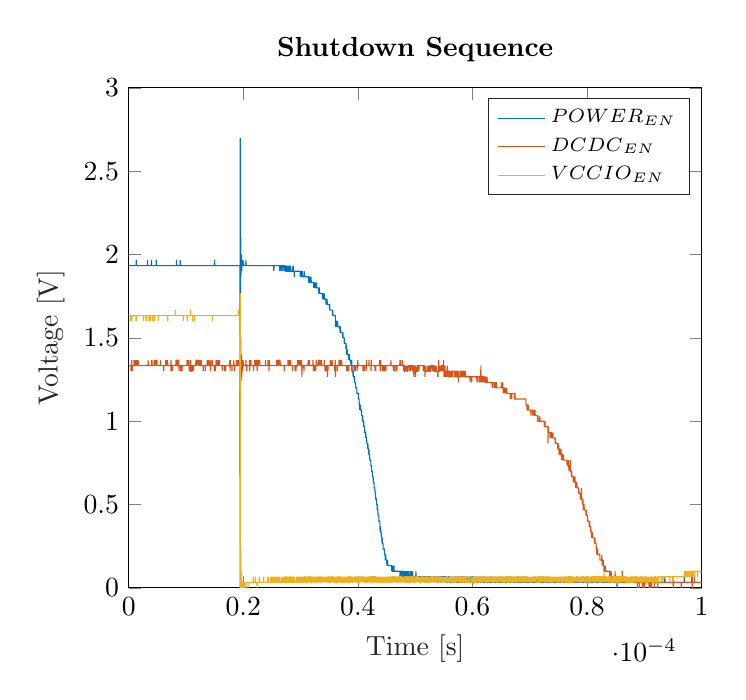
\begin{tikzpicture}

\begin{axis}[%
width=0.60\textwidth,
height=2.5in,
at={(0.758in,0.481in)},
scale only axis,
unbounded coords=jump,
xmin=0,
xmax=0.0001,
xlabel style={font=\color{white!15!black}},
xlabel={Time [s]},
ymin=0,
ymax=3,
ylabel style={font=\color{white!15!black}},
ylabel={Voltage [V]},
axis background/.style={fill=white},
title style={font=\bfseries},
title={Shutdown Sequence},
legend style={legend cell align=left, font=\scriptsize, align=left, draw=white!15!black}
]
\addplot [color=mycolor1]
  table[row sep=crcr]{%
-1.0339999967357e-08	1.93333\\
1.28966000012554e-06	1.93333\\
1.30966000000399e-06	1.96667\\
1.34966000020498e-06	1.93333\\
3.2496600002041e-06	1.93333\\
3.26966000008255e-06	1.96667\\
3.30965999983945e-06	1.93333\\
3.92966000006822e-06	1.93333\\
3.96965999982513e-06	1.96667\\
4.00966000002612e-06	1.93333\\
4.78966000017067e-06	1.93333\\
4.80966000004912e-06	1.96667\\
4.84965999980602e-06	1.93333\\
8.32965999997271e-06	1.93333\\
8.34965999985116e-06	1.96667\\
8.38966000005215e-06	1.93333\\
8.96966000007993e-06	1.93333\\
8.98965999995838e-06	1.96667\\
9.02966000015937e-06	1.93333\\
1.49696600000304e-05	1.93333\\
1.49896599999089e-05	1.96667\\
1.50296600001099e-05	1.93333\\
1.94296600000143e-05	1.93333\\
1.94496599998928e-05	0.666667\\
1.94696600002153e-05	2.7\\
1.95096599999722e-05	1.76667\\
1.95496600001732e-05	2.1\\
1.95896599999301e-05	1.86667\\
1.96096599998086e-05	2\\
1.96496600000096e-05	1.9\\
1.96896600002106e-05	2\\
1.97296599999675e-05	1.9\\
1.97496599998459e-05	1.96667\\
1.97896600000469e-05	1.93333\\
1.99496599999627e-05	1.93333\\
1.99696599998411e-05	1.96667\\
2.00096600000421e-05	1.93333\\
2.04296600001541e-05	1.93333\\
2.04496600000326e-05	1.96667\\
2.04896599997895e-05	1.93333\\
2.53096599998059e-05	1.93333\\
2.53296600001285e-05	1.9\\
2.53696599998854e-05	1.93333\\
2.63296599998242e-05	1.93333\\
2.63496600001467e-05	1.9\\
2.63896599999036e-05	1.93333\\
2.6489660000184e-05	1.93333\\
2.65096600000625e-05	1.9\\
2.65496599998194e-05	1.93333\\
2.67896600001372e-05	1.93333\\
2.68096600000156e-05	1.9\\
2.68496600002166e-05	1.93333\\
2.70696600002118e-05	1.93333\\
2.71096599999687e-05	1.9\\
2.71496600001697e-05	1.93333\\
2.72496600000061e-05	1.93333\\
2.7289660000207e-05	1.9\\
2.7329659999964e-05	1.93333\\
2.73696600001649e-05	1.9\\
2.74096599999218e-05	1.93333\\
2.74496600001228e-05	1.9\\
2.74896599998797e-05	1.9\\
2.75296600000807e-05	1.93333\\
2.75896600001602e-05	1.9\\
2.76496599997955e-05	1.9\\
2.76696600001181e-05	1.93333\\
2.7709659999875e-05	1.9\\
2.77296600001975e-05	1.93333\\
2.77496600000759e-05	1.9\\
2.77696599999544e-05	1.93333\\
2.78096600001554e-05	1.9\\
2.78896600001133e-05	1.9\\
2.79096599999917e-05	1.93333\\
2.79496600001927e-05	1.9\\
2.80296600001506e-05	1.9\\
2.80496600000291e-05	1.93333\\
2.80696599999075e-05	1.9\\
2.81096600001085e-05	1.93333\\
2.81496599998654e-05	1.9\\
2.82096599999448e-05	1.9\\
2.82496600001458e-05	1.93333\\
2.83096599997812e-05	1.9\\
2.86296600000568e-05	1.9\\
2.86496599999353e-05	1.93333\\
2.86896600001363e-05	1.9\\
2.87096600000147e-05	1.93333\\
2.87496600002157e-05	1.9\\
2.88696599999305e-05	1.9\\
2.8889659999809e-05	1.86667\\
2.892966000001e-05	1.9\\
2.99296600001497e-05	1.9\\
2.99496600000282e-05	1.86667\\
2.99896599997851e-05	1.9\\
3.00296599999861e-05	1.86667\\
3.00896600000655e-05	1.9\\
3.01296599998224e-05	1.86667\\
3.01696600000234e-05	1.9\\
3.01896599999019e-05	1.86667\\
3.02096599997803e-05	1.9\\
3.02496599999813e-05	1.86667\\
3.03096600000607e-05	1.9\\
3.03496599998176e-05	1.86667\\
3.06096600000139e-05	1.86667\\
3.06296599998923e-05	1.9\\
3.06696600000933e-05	1.86667\\
3.13896600001584e-05	1.86667\\
3.14096600000369e-05	1.83333\\
3.14496599997938e-05	1.86667\\
3.14896599999948e-05	1.83333\\
3.16096600001536e-05	1.83333\\
3.16296600000321e-05	1.86667\\
3.1669659999789e-05	1.83333\\
3.18096599998263e-05	1.83333\\
3.18296600001489e-05	1.86667\\
3.18696599999058e-05	1.83333\\
3.22896600000178e-05	1.83333\\
3.23096599998962e-05	1.8\\
3.23296600002188e-05	1.83333\\
3.23696599999757e-05	1.8\\
3.24296600000551e-05	1.83333\\
3.2469659999812e-05	1.8\\
3.24896600001345e-05	1.83333\\
3.25296599998914e-05	1.8\\
3.25696600000924e-05	1.83333\\
3.26096599998493e-05	1.8\\
3.26496600000503e-05	1.8\\
3.26696599999288e-05	1.83333\\
3.27096600001298e-05	1.8\\
3.27496599998867e-05	1.83333\\
3.27896600000877e-05	1.8\\
3.31496600001202e-05	1.8\\
3.31696599999987e-05	1.76667\\
3.32096600001996e-05	1.8\\
3.3269659999835e-05	1.8\\
3.3309660000036e-05	1.76667\\
3.37896599997833e-05	1.76667\\
3.38096600001059e-05	1.73333\\
3.38496599998628e-05	1.76667\\
3.39096599999422e-05	1.76667\\
3.39296599998207e-05	1.73333\\
3.39696600000217e-05	1.76667\\
3.40096599997786e-05	1.73333\\
3.40496599999796e-05	1.73333\\
3.40896600001805e-05	1.76667\\
3.4109660000059e-05	1.73333\\
3.41296599999374e-05	1.76667\\
3.41696600001384e-05	1.73333\\
3.44096600000121e-05	1.73333\\
3.44296599998906e-05	1.7\\
3.44496600002131e-05	1.73333\\
3.448965999997e-05	1.7\\
3.45096599998485e-05	1.73333\\
3.4529660000171e-05	1.7\\
3.45696599999279e-05	1.73333\\
3.46096600001289e-05	1.7\\
3.46296600000073e-05	1.73333\\
3.46696600002083e-05	1.7\\
3.50296599997968e-05	1.7\\
3.50696599999978e-05	1.66667\\
3.50896599998762e-05	1.7\\
3.51296600000772e-05	1.66667\\
3.55496600001892e-05	1.66667\\
3.55696600000677e-05	1.63333\\
3.56096599998246e-05	1.66667\\
3.5669659999904e-05	1.63333\\
3.60696600001376e-05	1.63333\\
3.6089660000016e-05	1.56667\\
3.6129660000217e-05	1.6\\
3.61896599998524e-05	1.6\\
3.62096600001749e-05	1.56667\\
3.62496599999318e-05	1.6\\
3.62896600001328e-05	1.6\\
3.63096600000112e-05	1.56667\\
3.63496600002122e-05	1.6\\
3.64096599998476e-05	1.56667\\
3.6469659999927e-05	1.6\\
3.6509660000128e-05	1.56667\\
3.68296599999596e-05	1.56667\\
3.68696600001606e-05	1.53333\\
3.69296599997959e-05	1.56667\\
3.69696599999969e-05	1.53333\\
3.7309660000151e-05	1.53333\\
3.73496599999079e-05	1.5\\
3.73896600001089e-05	1.53333\\
3.74296599998658e-05	1.5\\
3.76096600001041e-05	1.5\\
3.76296599999826e-05	1.46667\\
3.7649659999861e-05	1.5\\
3.7689660000062e-05	1.46667\\
3.79096600000572e-05	1.46667\\
3.79296599999357e-05	1.43333\\
3.79496599998141e-05	1.46667\\
3.79896600000151e-05	1.43333\\
3.80296600002161e-05	1.4\\
3.8069659999973e-05	1.43333\\
3.80896599998515e-05	1.4\\
3.81296600000525e-05	1.43333\\
3.81696599998094e-05	1.4\\
3.83696599999261e-05	1.4\\
3.84096600001271e-05	1.36667\\
3.8449659999884e-05	1.4\\
3.85096599999635e-05	1.4\\
3.85496600001645e-05	1.36667\\
3.87496599998371e-05	1.36667\\
3.87896600000381e-05	1.33333\\
3.8909660000197e-05	1.33333\\
3.89496599999539e-05	1.36667\\
3.89896600001549e-05	1.3\\
3.91296600001922e-05	1.3\\
3.91696599999491e-05	1.26667\\
3.91896599998276e-05	1.3\\
3.92296600000286e-05	1.26667\\
3.93696600000659e-05	1.26667\\
3.93896599999444e-05	1.23333\\
3.94096599998228e-05	1.26667\\
3.94496600000238e-05	1.23333\\
3.95896600000611e-05	1.23333\\
3.9629659999818e-05	1.2\\
3.98096600000564e-05	1.2\\
3.98496599998133e-05	1.16667\\
4.00696599998085e-05	1.16667\\
4.01096600000095e-05	1.13333\\
4.02096599998458e-05	1.13333\\
4.02496600000468e-05	1.1\\
4.03096600001263e-05	1.1\\
4.03296600000047e-05	1.06667\\
4.03696600002057e-05	1.1\\
4.04096599999626e-05	1.06667\\
4.04496600001636e-05	1.1\\
4.05096599997989e-05	1.06667\\
4.06296599999578e-05	1.06667\\
4.06696600001588e-05	1.03333\\
4.07896599998736e-05	1.03333\\
4.08096600001961e-05	1\\
4.0849659999953e-05	1.03333\\
4.0889660000154e-05	1\\
4.09896599999904e-05	1\\
4.10096599998688e-05	0.966667\\
4.10296600001914e-05	1\\
4.10696599999483e-05	0.966667\\
4.11696599997846e-05	0.966667\\
4.12096599999856e-05	0.933333\\
4.13496600000229e-05	0.933333\\
4.13696599999014e-05	0.9\\
4.13896599997798e-05	0.933333\\
4.14296599999808e-05	0.9\\
4.15296599998172e-05	0.9\\
4.15696600000182e-05	0.866667\\
4.17096600000555e-05	0.866667\\
4.17296599999339e-05	0.833333\\
4.17496599998124e-05	0.866667\\
4.17896600000134e-05	0.833333\\
4.18696599999713e-05	0.833333\\
4.19096600001723e-05	0.8\\
4.19296600000507e-05	0.833333\\
4.19696599998076e-05	0.8\\
4.20496600002096e-05	0.8\\
4.20896599999665e-05	0.766667\\
4.22496599998823e-05	0.766667\\
4.22896600000833e-05	0.733333\\
4.23696600000412e-05	0.733333\\
4.24096599997981e-05	0.7\\
4.25096600000785e-05	0.7\\
4.25496599998354e-05	0.666667\\
4.26696599999943e-05	0.666667\\
4.27096600001953e-05	0.633333\\
4.28096600000316e-05	0.633333\\
4.28496599997885e-05	0.6\\
4.29696599999474e-05	0.6\\
4.30096600001484e-05	0.566667\\
4.30896600001063e-05	0.566667\\
4.31296599998632e-05	0.533333\\
4.32496600000221e-05	0.533333\\
4.3289659999779e-05	0.5\\
4.33696600001809e-05	0.5\\
4.33896600000594e-05	0.466667\\
4.34096599999378e-05	0.5\\
4.34496600001388e-05	0.466667\\
4.34896599998957e-05	0.466667\\
4.35296600000967e-05	0.433333\\
4.36496599998115e-05	0.433333\\
4.36896600000125e-05	0.4\\
4.38296600000498e-05	0.4\\
4.38896600001293e-05	0.333333\\
4.39096600000077e-05	0.366667\\
4.39496600002087e-05	0.333333\\
4.39696600000872e-05	0.366667\\
4.40096599998441e-05	0.333333\\
4.40696599999235e-05	0.333333\\
4.41096600001245e-05	0.3\\
4.42096599999608e-05	0.3\\
4.42296599998393e-05	0.266667\\
4.42496600001618e-05	0.3\\
4.42896599999187e-05	0.266667\\
4.43896600001992e-05	0.266667\\
4.44296599999561e-05	0.233333\\
4.46096600001944e-05	0.233333\\
4.46496599999513e-05	0.2\\
4.47696600001102e-05	0.2\\
4.47896599999886e-05	0.166667\\
4.48296600001896e-05	0.2\\
4.48496600000681e-05	0.166667\\
4.48696599999465e-05	0.2\\
4.49096600001475e-05	0.166667\\
4.50296599998623e-05	0.166667\\
4.50696600000633e-05	0.133333\\
4.51096599998202e-05	0.166667\\
4.51696599998996e-05	0.133333\\
4.51896599997781e-05	0.166667\\
4.52296599999791e-05	0.133333\\
4.58696600000863e-05	0.133333\\
4.58896599999647e-05	0.1\\
4.59296600001657e-05	0.133333\\
4.59696599999226e-05	0.1\\
4.60096600001236e-05	0.133333\\
4.60496599998805e-05	0.1\\
4.62096599997963e-05	0.1\\
4.62296600001189e-05	0.133333\\
4.62696599998758e-05	0.1\\
4.63096600000767e-05	0.133333\\
4.63496599998336e-05	0.1\\
4.7329660000095e-05	0.1\\
4.73496599999734e-05	0.0666666999999999\\
4.73896600001744e-05	0.1\\
4.75096599998892e-05	0.1\\
4.75296600002117e-05	0.0666666999999999\\
4.75696599999686e-05	0.1\\
4.77896599999639e-05	0.1\\
4.78096599998423e-05	0.0666666999999999\\
4.78296600001649e-05	0.1\\
4.78496600000433e-05	0.0666666999999999\\
4.78896599998002e-05	0.1\\
4.79296600000012e-05	0.0666666999999999\\
4.79896600000806e-05	0.1\\
4.80096599999591e-05	0.0666666999999999\\
4.80496600001601e-05	0.1\\
4.8089659999917e-05	0.0666666999999999\\
4.81096599997954e-05	0.1\\
4.81496599999964e-05	0.0666666999999999\\
4.81696599998749e-05	0.1\\
4.81896600001974e-05	0.0666666999999999\\
4.82296599999543e-05	0.1\\
4.82696600001553e-05	0.0666666999999999\\
4.83096599999122e-05	0.0666666999999999\\
4.83296599997907e-05	0.1\\
4.83496600001132e-05	0.0666666999999999\\
4.83696599999917e-05	0.1\\
4.84096600001926e-05	0.0666666999999999\\
4.8509660000029e-05	0.0666666999999999\\
4.85296599999074e-05	0.1\\
4.85496599997859e-05	0.0666666999999999\\
4.85696600001084e-05	0.1\\
4.86096599998653e-05	0.0666666999999999\\
4.87896600001037e-05	0.0666666999999999\\
4.88096599999821e-05	0.1\\
4.88496600001831e-05	0.0666666999999999\\
4.90896600000568e-05	0.0666666999999999\\
4.91096599999352e-05	0.1\\
4.91496600001362e-05	0.0666666999999999\\
4.92896600001735e-05	0.0666666999999999\\
4.9309660000052e-05	0.1\\
4.93496599998089e-05	0.0666666999999999\\
4.95296600000472e-05	0.0666666999999999\\
4.95496599999257e-05	0.1\\
4.95896600001267e-05	0.0666666999999999\\
5.0109660000075e-05	0.0666666999999999\\
5.01296599999534e-05	0.1\\
5.01696600001544e-05	0.0666666999999999\\
5.16496600000416e-05	0.0666666999999999\\
5.166965999992e-05	0.0333332999999998\\
5.1709660000121e-05	0.0666666999999999\\
5.17296599999995e-05	0.0333332999999998\\
5.17696600002004e-05	0.0666666999999999\\
5.2049659999831e-05	0.0666666999999999\\
5.20696600001536e-05	0.0333332999999998\\
5.21096599999105e-05	0.0666666999999999\\
5.21296599997889e-05	0.0333332999999998\\
5.21696599999899e-05	0.0666666999999999\\
5.24496600000646e-05	0.0666666999999999\\
5.24896599998215e-05	0.0333332999999998\\
5.25296600000225e-05	0.0666666999999999\\
5.26896599999382e-05	0.0666666999999999\\
5.27096599998167e-05	0.0333332999999998\\
5.27496600000177e-05	0.0666666999999999\\
5.34696600000828e-05	0.0666666999999999\\
5.34896599999612e-05	0.0333332999999998\\
5.35296600001622e-05	0.0666666999999999\\
5.36096600001201e-05	0.0666666999999999\\
5.36296599999986e-05	0.0333332999999998\\
5.3649659999877e-05	0.0666666999999999\\
5.3689660000078e-05	0.0333332999999998\\
5.37496600001575e-05	0.0666666999999999\\
5.37696600000359e-05	0.0333332999999998\\
5.38096599997928e-05	0.0666666999999999\\
5.38696599998723e-05	0.0333332999999998\\
5.39096600000732e-05	0.0666666999999999\\
5.39496599998301e-05	0.0333332999999998\\
5.39696600001527e-05	0.0666666999999999\\
5.40096599999096e-05	0.0333332999999998\\
5.40496600001106e-05	0.0666666999999999\\
5.40896599998675e-05	0.0666666999999999\\
5.41296600000685e-05	0.0333332999999998\\
5.41896600001479e-05	0.0666666999999999\\
5.42296599999048e-05	0.0333332999999998\\
5.42496599997833e-05	0.0666666999999999\\
5.42696600001058e-05	0.0333332999999998\\
5.43096599998627e-05	0.0666666999999999\\
5.43696599999421e-05	0.0333332999999998\\
5.43896599998206e-05	0.0666666999999999\\
5.44096600001431e-05	0.0333332999999998\\
5.44496599999e-05	0.0666666999999999\\
5.4489660000101e-05	0.0333332999999998\\
5.45296599998579e-05	0.0666666999999999\\
5.45896599999374e-05	0.0666666999999999\\
5.46096599998158e-05	0.0333332999999998\\
5.46496600000168e-05	0.0666666999999999\\
5.4909660000213e-05	0.0666666999999999\\
5.49296600000915e-05	0.0333332999999998\\
5.49696599998484e-05	0.0666666999999999\\
5.50296599999278e-05	0.0333332999999998\\
5.50496599998063e-05	0.0666666999999999\\
5.50896600000073e-05	0.0333332999999998\\
5.51296600002082e-05	0.0666666999999999\\
5.52096600001661e-05	0.0666666999999999\\
5.52296600000446e-05	0.0333332999999998\\
5.52696599998015e-05	0.0666666999999999\\
5.53496600002035e-05	0.0666666999999999\\
5.53896599999604e-05	0.0333332999999998\\
5.54496600000398e-05	0.0666666999999999\\
5.55096600001193e-05	0.0333332999999998\\
5.55496599998762e-05	0.0333332999999998\\
5.55696600001987e-05	0.0666666999999999\\
5.55896600000771e-05	0.0333332999999998\\
5.56096599999556e-05	0.0666666999999999\\
5.56496600001566e-05	0.0333332999999998\\
5.56896599999135e-05	0.0666666999999999\\
5.57296600001145e-05	0.0333332999999998\\
5.57496599999929e-05	0.0666666999999999\\
5.57696599998714e-05	0.0333332999999998\\
5.57896600001939e-05	0.0666666999999999\\
5.58096600000724e-05	0.0333332999999998\\
5.58496599998293e-05	0.0666666999999999\\
5.59296599997872e-05	0.0666666999999999\\
5.59696599999882e-05	0.0333332999999998\\
5.60096600001891e-05	0.0666666999999999\\
5.6049659999946e-05	0.0333332999999998\\
5.6089660000147e-05	0.0333332999999998\\
5.61296599999039e-05	0.0666666999999999\\
5.61696600001049e-05	0.0333332999999998\\
5.61896599999834e-05	0.0666666999999999\\
5.62096599998618e-05	0.0333332999999998\\
5.62296600001844e-05	0.0666666999999999\\
5.62696599999413e-05	0.0333332999999998\\
5.63096600001423e-05	0.0666666999999999\\
5.63496599998992e-05	0.0333332999999998\\
5.64496600001796e-05	0.0333332999999998\\
5.6469660000058e-05	0.0666666999999999\\
5.65096599998149e-05	0.0333332999999998\\
5.65696599998944e-05	0.0666666999999999\\
5.66296599999738e-05	0.0333332999999998\\
5.66496599998523e-05	0.0666666999999999\\
5.66896600000533e-05	0.0333332999999998\\
5.67296599998102e-05	0.0666666999999999\\
5.67896599998896e-05	0.0333332999999998\\
5.68296600000906e-05	0.0333332999999998\\
5.68696599998475e-05	0.0666666999999999\\
5.69096600000485e-05	0.0333332999999998\\
5.69496599998054e-05	0.0333332999999998\\
5.69696600001279e-05	0.0666666999999999\\
5.70096599998848e-05	0.0333332999999998\\
5.70496600000858e-05	0.0666666999999999\\
5.70896599998427e-05	0.0333332999999998\\
5.71296600000437e-05	0.0666666999999999\\
5.72096600000016e-05	0.0666666999999999\\
5.72496600002026e-05	0.0333332999999998\\
5.72896599999595e-05	0.0333332999999998\\
5.73096599998379e-05	0.0666666999999999\\
5.73296600001605e-05	0.0333332999999998\\
5.73496600000389e-05	0.0666666999999999\\
5.73696599999174e-05	0.0333332999999998\\
5.73896599997958e-05	0.0666666999999999\\
5.74296599999968e-05	0.0333332999999998\\
5.75296599998332e-05	0.0333332999999998\\
5.75496600001557e-05	0.0666666999999999\\
5.75896599999126e-05	0.0333332999999998\\
5.76096599997911e-05	0.0666666999999999\\
5.76296600001136e-05	0.0333332999999998\\
5.76496599999921e-05	0.0666666999999999\\
5.7689660000193e-05	0.0333332999999998\\
5.77296599999499e-05	0.0666666999999999\\
5.77696600001509e-05	0.0333332999999998\\
5.77896600000294e-05	0.0666666999999999\\
5.78296599997863e-05	0.0333332999999998\\
5.79096600001883e-05	0.0333332999999998\\
5.79296600000667e-05	0.0666666999999999\\
5.79696599998236e-05	0.0333332999999998\\
5.80096600000246e-05	0.0666666999999999\\
5.80496599997815e-05	0.0333332999999998\\
5.80696600001041e-05	0.0666666999999999\\
5.8109659999861e-05	0.0333332999999998\\
5.81696599999404e-05	0.0333332999999998\\
5.82096600001414e-05	0.0666666999999999\\
5.82496599998983e-05	0.0666666999999999\\
5.82896600000993e-05	0.0333332999999998\\
5.83296599998562e-05	0.0666666999999999\\
5.83696600000572e-05	0.0333332999999998\\
5.83896599999356e-05	0.0666666999999999\\
5.84296600001366e-05	0.0333332999999998\\
5.8489660000216e-05	0.0666666999999999\\
5.85296599999729e-05	0.0333332999999998\\
5.86096599999308e-05	0.0333332999999998\\
5.86296599998093e-05	0.0666666999999999\\
5.86696600000103e-05	0.0333332999999998\\
5.87096600002113e-05	0.0333332999999998\\
5.87296600000897e-05	0.0666666999999999\\
5.87496599999682e-05	0.0333332999999998\\
5.87696599998466e-05	0.0666666999999999\\
5.88096600000476e-05	0.0333332999999998\\
5.89296600002065e-05	0.0333332999999998\\
5.89496600000849e-05	0.0666666999999999\\
5.89696599999634e-05	0.0333332999999998\\
5.89896599998418e-05	0.0666666999999999\\
5.90296600000428e-05	0.0333332999999998\\
5.90696599997997e-05	0.0333332999999998\\
5.91096600000007e-05	0.0666666999999999\\
5.91496600002017e-05	0.0333332999999998\\
5.91896599999586e-05	0.0333332999999998\\
5.92096599998371e-05	0.0666666999999999\\
5.92496600000381e-05	0.0333332999999998\\
5.93496599998744e-05	0.0333332999999998\\
5.93696600001969e-05	0.0666666999999999\\
5.94096599999538e-05	0.0333332999999998\\
5.95096599997902e-05	0.0333332999999998\\
5.95296600001127e-05	0.0666666999999999\\
5.95696599998696e-05	0.0333332999999998\\
5.96096600000706e-05	0.0333332999999998\\
5.96296599999491e-05	0.0666666999999999\\
5.96696600001501e-05	0.0333332999999998\\
5.98896600001453e-05	0.0333332999999998\\
5.99296599999022e-05	0.0666666999999999\\
5.99696600001032e-05	0.0666666999999999\\
6.00096599998601e-05	0.0333332999999998\\
6.01696600002199e-05	0.0333332999999998\\
6.02096599999769e-05	0.0666666999999999\\
6.02696600000563e-05	0.0333332999999998\\
6.03696599998926e-05	0.0333332999999998\\
6.04096600000936e-05	0.0666666999999999\\
6.04496599998505e-05	0.0333332999999998\\
6.0549660000131e-05	0.0333332999999998\\
6.05696600000094e-05	0.0666666999999999\\
6.06096600002104e-05	0.0333332999999998\\
6.06296600000888e-05	0.0666666999999999\\
6.06696599998457e-05	0.0333332999999998\\
6.08096599998831e-05	0.0333332999999998\\
6.08296600002056e-05	0.0666666999999999\\
6.08696599999625e-05	0.0333332999999998\\
6.0929660000042e-05	0.0333332999999998\\
6.09496599999204e-05	0.0666666999999999\\
6.09696599997989e-05	0.0333332999999998\\
6.09896600001214e-05	0.0666666999999999\\
6.10296599998783e-05	0.0333332999999998\\
6.10896599999577e-05	0.0333332999999998\\
6.11096599998362e-05	0.0666666999999999\\
6.11496600000372e-05	0.0333332999999998\\
6.12096600001166e-05	0.0333332999999998\\
6.12296599999951e-05	0.0666666999999999\\
6.12696600001961e-05	0.0333332999999998\\
6.12896600000745e-05	0.0666666999999999\\
6.13296599998314e-05	0.0333332999999998\\
6.1349660000154e-05	0.0666666999999999\\
6.13896599999109e-05	0.0333332999999998\\
6.14296600001119e-05	0.0333332999999998\\
6.14696599998688e-05	0.0666666999999999\\
6.15096600000697e-05	0.0333332999999998\\
6.15496599998266e-05	0.0666666999999999\\
6.15896600000276e-05	0.0333332999999998\\
6.16096599999061e-05	0.0666666999999999\\
6.16296599997845e-05	0.0333332999999998\\
6.16496600001071e-05	0.0666666999999999\\
6.16696599999855e-05	0.0333332999999998\\
6.17096600001865e-05	0.0666666999999999\\
6.17496599999434e-05	0.0333332999999998\\
6.17696599998219e-05	0.0666666999999999\\
6.18096600000229e-05	0.0333332999999998\\
6.18296599999013e-05	0.0666666999999999\\
6.18496599997798e-05	0.0333332999999998\\
6.18696600001023e-05	0.0666666999999999\\
6.18896599999808e-05	0.0333332999999998\\
6.19096599998592e-05	0.0666666999999999\\
6.19496600000602e-05	0.0333332999999998\\
6.20896600000975e-05	0.0333332999999998\\
6.2109659999976e-05	0.0666666999999999\\
6.2149660000177e-05	0.0333332999999998\\
6.21896599999339e-05	0.0666666999999999\\
6.22296600001349e-05	0.0333332999999998\\
6.2489659999887e-05	0.0333332999999998\\
6.25096600002095e-05	0.0666666999999999\\
6.2529660000088e-05	0.0333332999999998\\
6.25696599998449e-05	0.0666666999999999\\
6.26096600000459e-05	0.0333332999999998\\
6.26496599998028e-05	0.0333332999999998\\
6.26696600001253e-05	0.0666666999999999\\
6.27096599998822e-05	0.0333332999999998\\
6.29696600000784e-05	0.0333332999999998\\
6.29896599999569e-05	0.0666666999999999\\
6.30296600001579e-05	0.0333332999999998\\
6.33696599998679e-05	0.0333332999999998\\
6.34096600000689e-05	0.0666666999999999\\
6.34496599998258e-05	0.0333332999999998\\
6.37896599999799e-05	0.0333332999999998\\
6.38096599998583e-05	0.0666666999999999\\
6.38496600000593e-05	0.0333332999999998\\
6.38696599999378e-05	0.0666666999999999\\
6.38896599998162e-05	0.0333332999999998\\
6.39096600001388e-05	0.0666666999999999\\
6.39296600000172e-05	0.0333332999999998\\
6.39696600002182e-05	0.0666666999999999\\
6.40096599999751e-05	0.0333332999999998\\
6.44296600000871e-05	0.0333332999999998\\
6.44496599999655e-05	0.0666666999999999\\
6.44896600001665e-05	0.0333332999999998\\
6.46896599998392e-05	0.0333332999999998\\
6.47096600001618e-05	0.0666666999999999\\
6.47496599999187e-05	0.0333332999999998\\
6.48096599999981e-05	0.0333332999999998\\
6.48296599998766e-05	0.0666666999999999\\
6.48496600001991e-05	0.0333332999999998\\
6.48696600000775e-05	0.0666666999999999\\
6.49096599998344e-05	0.0333332999999998\\
6.50296599999933e-05	0.0333332999999998\\
6.50496599998718e-05	0.0666666999999999\\
6.50896600000728e-05	0.0333332999999998\\
6.51096599999512e-05	0.0666666999999999\\
6.51496600001522e-05	0.0333332999999998\\
6.53296599999464e-05	0.0333332999999998\\
6.53496599998249e-05	0.0666666999999999\\
6.53896600000259e-05	0.0333332999999998\\
6.572966000018e-05	0.0333332999999998\\
6.57696599999369e-05	0.0666666999999999\\
6.58096600001379e-05	0.0333332999999998\\
6.59296599998527e-05	0.0333332999999998\\
6.59496600001752e-05	0.0666666999999999\\
6.59896599999321e-05	0.0333332999999998\\
6.60296600001331e-05	0.0666666999999999\\
6.606965999989e-05	0.0333332999999998\\
6.61896600000489e-05	0.0333332999999998\\
6.62096599999273e-05	0.0666666999999999\\
6.62496600001283e-05	0.0333332999999998\\
6.63296600000862e-05	0.0333332999999998\\
6.63496599999647e-05	0.0666666999999999\\
6.63896600001657e-05	0.0333332999999998\\
6.6489660000002e-05	0.0333332999999998\\
6.65096599998805e-05	0.0666666999999999\\
6.65496600000814e-05	0.0333332999999998\\
6.67896599999551e-05	0.0333332999999998\\
6.68096599998336e-05	0.0666666999999999\\
6.68496600000346e-05	0.0333332999999998\\
6.71096599997867e-05	0.0333332999999998\\
6.71296600001092e-05	0.0666666999999999\\
6.71496599999877e-05	0.0333332999999998\\
6.71896600001887e-05	0.0666666999999999\\
6.72096600000671e-05	0.0333332999999998\\
6.72296599999456e-05	0.0666666999999999\\
6.7249659999824e-05	0.0333332999999998\\
6.72696600001466e-05	0.0666666999999999\\
6.7289660000025e-05	0.0333332999999998\\
6.73096599999035e-05	0.0666666999999999\\
6.73496600001044e-05	0.0333332999999998\\
6.77296600000155e-05	0.0333332999999998\\
6.77496599998939e-05	0.0666666999999999\\
6.77896600000949e-05	0.0333332999999998\\
6.79296600001322e-05	0.0333332999999998\\
6.79496600000107e-05	0.0666666999999999\\
6.79896600002117e-05	0.0333332999999998\\
6.82496599999638e-05	0.0333332999999998\\
6.82696599998422e-05	0.0666666999999999\\
6.83096600000432e-05	0.0333332999999998\\
6.83496599998001e-05	0.0333332999999998\\
6.83896600000011e-05	0.0666666999999999\\
6.84296600002021e-05	0.0333332999999998\\
6.85296600000385e-05	0.0333332999999998\\
6.85496599999169e-05	0.0666666999999999\\
6.85896600001179e-05	0.0333332999999998\\
6.86096599999964e-05	0.0666666999999999\\
6.86496600001973e-05	0.0333332999999998\\
6.87496600000337e-05	0.0333332999999998\\
6.87896599997906e-05	0.0666666999999999\\
6.88296599999916e-05	0.0333332999999998\\
6.92496600001036e-05	0.0333332999999998\\
6.9269659999982e-05	0.0666666999999999\\
6.9309660000183e-05	0.0333332999999998\\
6.95696599999351e-05	0.0333332999999998\\
6.95896599998136e-05	0.0666666999999999\\
6.96296600000146e-05	0.0333332999999998\\
7.05296599998739e-05	0.0333332999999998\\
7.05496600001965e-05	0.0666666999999999\\
7.05896599999534e-05	0.0333332999999998\\
7.08496600001496e-05	0.0333332999999998\\
7.0869660000028e-05	0.0666666999999999\\
7.09096599997849e-05	0.0333332999999998\\
7.12296600000606e-05	0.0333332999999998\\
7.1249659999939e-05	0.0666666999999999\\
7.128966000014e-05	0.0333332999999998\\
7.15896600000931e-05	0.0333332999999998\\
7.16096599999716e-05	0.0666666999999999\\
7.16496600001726e-05	0.0333332999999998\\
7.17096599998079e-05	0.0333332999999998\\
7.17296600001305e-05	0.0666666999999999\\
7.17696599998874e-05	0.0333332999999998\\
7.17896600002099e-05	0.0666666999999999\\
7.18296599999668e-05	0.0333332999999998\\
7.19496600001257e-05	0.0333332999999998\\
7.19696600000042e-05	0.0666666999999999\\
7.20096600002051e-05	0.0333332999999998\\
7.23896600001162e-05	0.0333332999999998\\
7.24096599999946e-05	0.0666666999999999\\
7.24496600001956e-05	0.0333332999999998\\
7.29496599998214e-05	0.0333332999999998\\
7.29696600001439e-05	0.0666666999999999\\
7.30096599999008e-05	0.0333332999999998\\
7.55096599998062e-05	0.0333332999999998\\
7.55296600001287e-05	0.0666666999999999\\
7.55696599998856e-05	0.0333332999999998\\
7.70696600000953e-05	0.0333332999999998\\
7.70896599999737e-05	0.0666666999999999\\
7.71296600001747e-05	0.0333332999999998\\
7.90096599998513e-05	0.0333332999999998\\
7.90296600001739e-05	0.0666666999999999\\
7.90696599999308e-05	0.0333332999999998\\
7.96096600002016e-05	0.0333332999999998\\
7.96296600000801e-05	0.0666666999999999\\
7.9669659999837e-05	0.0333332999999998\\
8.2869659999929e-05	0.0333332999999998\\
8.28896599998075e-05	0.0666666999999999\\
8.29296600000085e-05	0.0333332999999998\\
8.43696600001387e-05	0.0333332999999998\\
8.43896600000171e-05	0.0666666999999999\\
8.44296600002181e-05	0.0333332999999998\\
8.48696600002086e-05	0.0333332999999998\\
8.4889660000087e-05	0.0666666999999999\\
8.49296599998439e-05	0.0333332999999998\\
8.50296600001244e-05	0.0333332999999998\\
8.50496600000028e-05	0.0666666999999999\\
8.50896600002038e-05	0.0333332999999998\\
8.52096599999186e-05	0.0333332999999998\\
8.5229659999797e-05	0\\
8.5269659999998e-05	0.0333332999999998\\
8.62096600000584e-05	0.0333332999999998\\
8.62296599999368e-05	0.0666666999999999\\
8.62696600001378e-05	0.0333332999999998\\
8.84296599998891e-05	0.0333332999999998\\
8.84496600002116e-05	0.0666666999999999\\
8.84896599999685e-05	0.0333332999999998\\
8.99096600002203e-05	0.0333332999999998\\
8.99296600000987e-05	0.0666666999999999\\
8.99696599998556e-05	0.0333332999999998\\
9.01896599998508e-05	0.0333332999999998\\
9.02096600001734e-05	0.0666666999999999\\
9.02496599999303e-05	0.0333332999999998\\
9.11296599999112e-05	0.0333332999999998\\
9.11496599997896e-05	0.0666666999999999\\
9.11896599999906e-05	0.0333332999999998\\
9.35696600001812e-05	0.0333332999999998\\
9.35896600000596e-05	0.0666666999999999\\
9.36296599998165e-05	0.0333332999999998\\
9.50496600000683e-05	0.0333332999999998\\
9.50696599999468e-05	0.0666666999999999\\
9.51096600001478e-05	0.0333332999999998\\
9.69696599999459e-05	0.0333332999999998\\
9.69896599998243e-05	0.0666666999999999\\
9.70296600000253e-05	0.0333332999999998\\
9.82296599998378e-05	0.0333332999999998\\
9.82496600001603e-05	0.0666666999999999\\
9.82896599999172e-05	0.0333332999999998\\
9.83296600001182e-05	0.0666666999999999\\
9.83696599998751e-05	0.0333332999999998\\
9.83896600001977e-05	0.0666666999999999\\
9.84296599999546e-05	0.0333332999999998\\
0.000100009660000122	0.0333332999999998\\
};
\addlegendentry{$\text{POWER}_{\text{EN}}$}

\addplot [color=mycolor2]
  table[row sep=crcr]{%
-1.08000000054176e-08	1.33333\\
3.69199999905589e-07	1.33333\\
3.89200000006085e-07	1.3\\
4.2919999998503e-07	1.33333\\
4.89200000064471e-07	1.33333\\
5.29200000043417e-07	1.36667\\
5.69200000022363e-07	1.33333\\
6.09200000001309e-07	1.33333\\
6.29200000101804e-07	1.3\\
6.6920000008075e-07	1.33333\\
8.89200000075974e-07	1.33333\\
9.09199999954424e-07	1.36667\\
9.4919999993337e-07	1.33333\\
9.69200000033865e-07	1.36667\\
1.00920000001281e-06	1.33333\\
1.12919999994965e-06	1.33333\\
1.14920000005014e-06	1.36667\\
1.18920000002909e-06	1.33333\\
1.22920000000803e-06	1.33333\\
1.24920000010853e-06	1.36667\\
1.28920000008748e-06	1.33333\\
1.32920000006642e-06	1.36667\\
1.38919999992382e-06	1.33333\\
1.42919999990276e-06	1.36667\\
1.46920000010375e-06	1.33333\\
1.5092000000827e-06	1.36667\\
1.54920000006165e-06	1.33333\\
1.62920000001954e-06	1.33333\\
1.64919999989799e-06	1.36667\\
1.68920000009898e-06	1.33333\\
3.36920000010288e-06	1.33333\\
3.38919999998133e-06	1.36667\\
3.42919999996028e-06	1.33333\\
3.94919999990861e-06	1.33333\\
3.96920000000911e-06	1.36667\\
4.00919999998806e-06	1.33333\\
4.049199999967e-06	1.33333\\
4.0692000000675e-06	1.36667\\
4.10920000004644e-06	1.33333\\
4.42920000010005e-06	1.33333\\
4.4491999999785e-06	1.36667\\
4.48919999995745e-06	1.33333\\
4.5291999999364e-06	1.33333\\
4.54920000003689e-06	1.36667\\
4.58920000001584e-06	1.33333\\
4.62919999999478e-06	1.36667\\
4.66919999997373e-06	1.33333\\
4.68920000007422e-06	1.36667\\
4.70919999995267e-06	1.33333\\
4.74919999993162e-06	1.36667\\
4.78919999991056e-06	1.33333\\
4.82919999988951e-06	1.36667\\
4.88919999996895e-06	1.36667\\
4.90920000006945e-06	1.33333\\
4.9291999999479e-06	1.36667\\
4.96919999992684e-06	1.33333\\
5.50919999997568e-06	1.33333\\
5.52920000007617e-06	1.36667\\
5.56920000005512e-06	1.33333\\
6.08920000000346e-06	1.33333\\
6.10920000010395e-06	1.3\\
6.1492000000829e-06	1.33333\\
6.42919999993552e-06	1.33333\\
6.44920000003602e-06	1.36667\\
6.46919999991447e-06	1.33333\\
6.48920000001496e-06	1.36667\\
6.52919999999391e-06	1.33333\\
6.68919999990969e-06	1.33333\\
6.70920000001018e-06	1.36667\\
6.74919999998913e-06	1.33333\\
6.78919999996808e-06	1.36667\\
6.82919999994702e-06	1.33333\\
7.34919999989536e-06	1.33333\\
7.36919999999586e-06	1.3\\
7.38920000009635e-06	1.36667\\
7.4292000000753e-06	1.33333\\
7.56919999989059e-06	1.33333\\
7.58919999999108e-06	1.3\\
7.62919999997003e-06	1.33333\\
8.20919999999781e-06	1.33333\\
8.24919999997675e-06	1.36667\\
8.30920000005619e-06	1.36667\\
8.34920000003514e-06	1.33333\\
8.38920000001409e-06	1.36667\\
8.40919999989254e-06	1.33333\\
8.42919999999303e-06	1.36667\\
8.46919999997198e-06	1.33333\\
8.50919999995092e-06	1.33333\\
8.52920000005142e-06	1.36667\\
8.56920000003036e-06	1.33333\\
8.60920000000931e-06	1.33333\\
8.6292000001098e-06	1.36667\\
8.64919999998826e-06	1.33333\\
8.6891999999672e-06	1.36667\\
8.72919999994615e-06	1.36667\\
8.78920000002559e-06	1.3\\
8.82920000000453e-06	1.33333\\
9.06920000010025e-06	1.33333\\
9.0891999999787e-06	1.3\\
9.12919999995765e-06	1.33333\\
9.22920000001604e-06	1.33333\\
9.24919999989449e-06	1.3\\
9.28920000009548e-06	1.33333\\
9.30919999997393e-06	1.3\\
9.34919999995287e-06	1.33333\\
1.01491999999759e-05	1.33333\\
1.01692000000764e-05	1.36667\\
1.02092000000553e-05	1.33333\\
1.02492000000343e-05	1.36667\\
1.02691999999127e-05	1.33333\\
1.02892000000132e-05	1.36667\\
1.03291999999922e-05	1.33333\\
1.05092000000084e-05	1.33333\\
1.05292000001089e-05	1.36667\\
1.05692000000879e-05	1.3\\
1.06092000000668e-05	1.33333\\
1.07892000000831e-05	1.33333\\
1.08091999999615e-05	1.3\\
1.0829200000062e-05	1.36667\\
1.08891999999194e-05	1.3\\
1.09291999998984e-05	1.3\\
1.09692000000994e-05	1.33333\\
1.10092000000783e-05	1.33333\\
1.10291999999568e-05	1.3\\
1.10691999999357e-05	1.33333\\
1.11491999998936e-05	1.33333\\
1.11691999999941e-05	1.3\\
1.12091999999731e-05	1.33333\\
1.12692000000525e-05	1.33333\\
1.12891999999309e-05	1.3\\
1.13291999999099e-05	1.33333\\
1.16891999999424e-05	1.33333\\
1.17291999999214e-05	1.36667\\
1.17691999999003e-05	1.33333\\
1.18092000001013e-05	1.36667\\
1.18892000000592e-05	1.36667\\
1.19091999999377e-05	1.33333\\
1.19491999999166e-05	1.36667\\
1.19891999998956e-05	1.33333\\
1.20292000000966e-05	1.36667\\
1.21291999999329e-05	1.36667\\
1.21492000000334e-05	1.33333\\
1.21892000000123e-05	1.36667\\
1.22291999999913e-05	1.33333\\
1.22691999999702e-05	1.36667\\
1.23292000000497e-05	1.33333\\
1.24891999999655e-05	1.33333\\
1.25092000000659e-05	1.36667\\
1.25492000000449e-05	1.33333\\
1.26292000000028e-05	1.33333\\
1.26492000001033e-05	1.36667\\
1.26892000000822e-05	1.33333\\
1.29892000000353e-05	1.33333\\
1.30091999999138e-05	1.3\\
1.30491999998927e-05	1.33333\\
1.33291999999674e-05	1.33333\\
1.33492000000679e-05	1.3\\
1.33892000000468e-05	1.33333\\
1.36691999998995e-05	1.33333\\
1.36892e-05	1.36667\\
1.37092000001005e-05	1.33333\\
1.37492000000794e-05	1.36667\\
1.37892000000583e-05	1.33333\\
1.38292000000373e-05	1.33333\\
1.38692000000162e-05	1.36667\\
1.39091999999952e-05	1.33333\\
1.40092000000536e-05	1.33333\\
1.4029199999932e-05	1.36667\\
1.4069199999911e-05	1.33333\\
1.42491999999272e-05	1.33333\\
1.42692000000277e-05	1.3\\
1.42891999999062e-05	1.36667\\
1.43292000001072e-05	1.33333\\
1.45691999999809e-05	1.33333\\
1.45892000000813e-05	1.36667\\
1.46292000000603e-05	1.33333\\
1.49091999999129e-05	1.33333\\
1.49292000000134e-05	1.3\\
1.49691999999924e-05	1.33333\\
1.50891999999292e-05	1.33333\\
1.51092000000297e-05	1.3\\
1.51492000000086e-05	1.33333\\
1.52291999999665e-05	1.33333\\
1.5249200000067e-05	1.36667\\
1.5289200000046e-05	1.33333\\
1.53091999999244e-05	1.36667\\
1.53292000000249e-05	1.33333\\
1.53692000000039e-05	1.36667\\
1.54091999999828e-05	1.33333\\
1.54491999999617e-05	1.33333\\
1.54692000000622e-05	1.36667\\
1.55092000000412e-05	1.33333\\
1.55691999998986e-05	1.33333\\
1.55891999999991e-05	1.36667\\
1.5629199999978e-05	1.33333\\
1.56492000000785e-05	1.36667\\
1.56892000000575e-05	1.33333\\
1.57292000000364e-05	1.36667\\
1.57891999998938e-05	1.33333\\
1.58292000000948e-05	1.33333\\
1.58491999999733e-05	1.36667\\
1.58891999999522e-05	1.33333\\
1.62891999999637e-05	1.33333\\
1.63092000000642e-05	1.3\\
1.63492000000431e-05	1.33333\\
1.66891999999752e-05	1.33333\\
1.67092000000757e-05	1.3\\
1.67492000000546e-05	1.33333\\
1.6889200000092e-05	1.33333\\
1.69091999999704e-05	1.3\\
1.69491999999494e-05	1.33333\\
1.76292000000355e-05	1.33333\\
1.7649199999914e-05	1.36667\\
1.77091999999934e-05	1.3\\
1.77292000000939e-05	1.36667\\
1.77692000000729e-05	1.33333\\
1.80091999999465e-05	1.33333\\
1.8029200000047e-05	1.3\\
1.8069200000026e-05	1.33333\\
1.83292000000002e-05	1.33333\\
1.83492000001007e-05	1.36667\\
1.83892000000796e-05	1.33333\\
1.84891999999159e-05	1.33333\\
1.85092000000164e-05	1.3\\
1.85491999999954e-05	1.33333\\
1.87892000000911e-05	1.33333\\
1.88091999999696e-05	1.36667\\
1.88491999999485e-05	1.33333\\
1.88891999999274e-05	1.36667\\
1.89291999999064e-05	1.33333\\
1.90492000000653e-05	1.33333\\
1.90691999999437e-05	1.36667\\
1.90892000000442e-05	1.33333\\
1.91292000000232e-05	1.36667\\
1.91692000000021e-05	1.33333\\
1.91892000001026e-05	1.36667\\
1.92091999999811e-05	1.33333\\
1.92292000000815e-05	1.36667\\
1.92692000000605e-05	1.33333\\
1.94291999999763e-05	1.33333\\
1.94466999987597e-05	-0.3\\
nan	nan\\
1.94545846119443e-05	-0.3\\
1.94892000000557e-05	1.23333\\
1.95091999999342e-05	1.06667\\
1.95491999999131e-05	1.5\\
1.95891999998921e-05	1.23333\\
1.9629200000093e-05	1.36667\\
1.96491999999715e-05	1.26667\\
1.96891999999504e-05	1.4\\
1.97291999999294e-05	1.26667\\
1.97691999999083e-05	1.36667\\
1.98092000001093e-05	1.33333\\
1.98291999999878e-05	1.36667\\
1.98691999999667e-05	1.3\\
1.99091999999457e-05	1.33333\\
1.99292000000462e-05	1.3\\
1.99692000000251e-05	1.36667\\
2.00092000000041e-05	1.33333\\
2.0429199999894e-05	1.33333\\
2.0469200000095e-05	1.36667\\
2.05092000000739e-05	1.33333\\
2.05892000000318e-05	1.33333\\
2.06091999999103e-05	1.3\\
2.06491999998892e-05	1.33333\\
2.10692000000012e-05	1.33333\\
2.10892000001017e-05	1.36667\\
2.11091999999802e-05	1.3\\
2.11491999999591e-05	1.33333\\
2.13291999999754e-05	1.33333\\
2.13492000000759e-05	1.36667\\
2.13892000000548e-05	1.33333\\
2.17691999999658e-05	1.33333\\
2.17892000000663e-05	1.3\\
2.18292000000453e-05	1.33333\\
2.19491999999821e-05	1.33333\\
2.19692000000826e-05	1.36667\\
2.20092000000616e-05	1.33333\\
2.2069199999919e-05	1.33333\\
2.21091999998979e-05	1.36667\\
2.21492000000989e-05	1.33333\\
2.22891999999142e-05	1.33333\\
2.23092000000147e-05	1.36667\\
2.23291999998931e-05	1.33333\\
2.23692000000941e-05	1.36667\\
2.24291999999515e-05	1.3\\
2.24691999999305e-05	1.33333\\
2.25292000000099e-05	1.36667\\
2.25691999999889e-05	1.33333\\
2.26091999999678e-05	1.36667\\
2.26491999999467e-05	1.33333\\
2.26891999999257e-05	1.36667\\
2.27291999999046e-05	1.33333\\
2.2829199999963e-05	1.33333\\
2.2869199999942e-05	1.36667\\
2.29091999999209e-05	1.33333\\
2.38692000000817e-05	1.33333\\
2.38891999999602e-05	1.36667\\
2.39291999999391e-05	1.33333\\
2.42891999999717e-05	1.33333\\
2.43092000000722e-05	1.36667\\
2.43291999999506e-05	1.33333\\
2.43492000000511e-05	1.36667\\
2.43892000000301e-05	1.33333\\
2.4469199999988e-05	1.33333\\
2.44892000000885e-05	1.3\\
2.45292000000674e-05	1.36667\\
2.45692000000464e-05	1.33333\\
2.57891999999593e-05	1.33333\\
2.58092000000598e-05	1.36667\\
2.58291999999383e-05	1.33333\\
2.58492000000388e-05	1.36667\\
2.58691999999172e-05	1.33333\\
2.59091999998962e-05	1.36667\\
2.59492000000972e-05	1.33333\\
2.59691999999756e-05	1.36667\\
2.59892000000761e-05	1.33333\\
2.60091999999545e-05	1.36667\\
2.60491999999335e-05	1.33333\\
2.60891999999124e-05	1.33333\\
2.61291999998914e-05	1.36667\\
2.62092000000713e-05	1.36667\\
2.62291999999498e-05	1.33333\\
2.62691999999287e-05	1.36667\\
2.63492000001087e-05	1.36667\\
2.63892000000876e-05	1.33333\\
2.64292000000665e-05	1.36667\\
2.64692000000455e-05	1.33333\\
2.71292000000312e-05	1.33333\\
2.71491999999096e-05	1.3\\
2.71892000001106e-05	1.33333\\
2.77691999999163e-05	1.33333\\
2.77892000000168e-05	1.36667\\
2.78291999999958e-05	1.33333\\
2.78892000000752e-05	1.33333\\
2.79292000000542e-05	1.36667\\
2.79891999999116e-05	1.33333\\
2.80092000000121e-05	1.36667\\
2.8049199999991e-05	1.33333\\
2.81492000000494e-05	1.33333\\
2.81691999999278e-05	1.36667\\
2.82091999999068e-05	1.33333\\
2.82492000001078e-05	1.36667\\
2.83091999999652e-05	1.33333\\
2.85691999999393e-05	1.33333\\
2.85892000000398e-05	1.3\\
2.86292000000188e-05	1.33333\\
2.90091999999298e-05	1.33333\\
2.90491999999087e-05	1.3\\
2.90892000001097e-05	1.33333\\
2.91891999999461e-05	1.33333\\
2.92092000000466e-05	1.3\\
2.92492000000255e-05	1.33333\\
2.94491999999202e-05	1.33333\\
2.94692000000207e-05	1.36667\\
2.95091999999997e-05	1.33333\\
2.95491999999786e-05	1.36667\\
2.96092000000581e-05	1.33333\\
2.96691999999155e-05	1.36667\\
2.9689200000016e-05	1.33333\\
2.97291999999949e-05	1.36667\\
2.97492000000954e-05	1.33333\\
2.97892000000743e-05	1.36667\\
2.98091999999528e-05	1.33333\\
2.98491999999317e-05	1.36667\\
2.98891999999107e-05	1.33333\\
2.99092000000112e-05	1.36667\\
2.99491999999901e-05	1.33333\\
2.99891999999691e-05	1.36667\\
3.0029199999948e-05	1.33333\\
3.01091999999059e-05	1.33333\\
3.01292000000064e-05	1.36667\\
3.01492000001069e-05	1.33333\\
3.01892000000858e-05	1.36667\\
3.02292000000648e-05	1.26667\\
3.02891999999222e-05	1.33333\\
3.05491999998964e-05	1.33333\\
3.05892000000973e-05	1.3\\
3.06292000000763e-05	1.33333\\
3.1289200000062e-05	1.33333\\
3.13292000000409e-05	1.36667\\
3.13491999999194e-05	1.33333\\
3.13692000000199e-05	1.36667\\
3.14091999999988e-05	1.33333\\
3.15092000000572e-05	1.33333\\
3.15291999999356e-05	1.36667\\
3.15691999999146e-05	1.33333\\
3.21292000000639e-05	1.33333\\
3.21692000000429e-05	1.36667\\
3.22291999999003e-05	1.33333\\
3.22692000001013e-05	1.3\\
3.23092000000802e-05	1.33333\\
3.23492000000591e-05	1.33333\\
3.23892000000381e-05	1.3\\
3.24091999999165e-05	1.33333\\
3.2429200000017e-05	1.3\\
3.2469199999996e-05	1.33333\\
3.25091999999749e-05	1.3\\
3.25491999999539e-05	1.33333\\
3.26092000000333e-05	1.33333\\
3.26291999999118e-05	1.3\\
3.26691999998907e-05	1.33333\\
3.27291999999701e-05	1.33333\\
3.27492000000706e-05	1.36667\\
3.27892000000496e-05	1.33333\\
3.30892000000027e-05	1.33333\\
3.31092000001032e-05	1.36667\\
3.31492000000821e-05	1.33333\\
3.32091999999395e-05	1.36667\\
3.32491999999185e-05	1.36667\\
3.3269200000019e-05	1.33333\\
3.33091999999979e-05	1.36667\\
3.33491999999769e-05	1.36667\\
3.33692000000774e-05	1.33333\\
3.33891999999558e-05	1.36667\\
3.34092000000563e-05	1.33333\\
3.34492000000353e-05	1.36667\\
3.34892000000142e-05	1.33333\\
3.35091999998927e-05	1.36667\\
3.35291999999932e-05	1.33333\\
3.35492000000936e-05	1.36667\\
3.35691999999721e-05	1.33333\\
3.35892000000726e-05	1.36667\\
3.3609199999951e-05	1.33333\\
3.364919999993e-05	1.36667\\
3.36891999999089e-05	1.33333\\
3.41092000000209e-05	1.33333\\
3.41291999998994e-05	1.36667\\
3.41692000001004e-05	1.33333\\
3.42291999999578e-05	1.33333\\
3.42691999999367e-05	1.3\\
3.43091999999157e-05	1.33333\\
3.43691999999951e-05	1.3\\
3.4409199999974e-05	1.33333\\
3.44692000000535e-05	1.33333\\
3.44891999999319e-05	1.3\\
3.45291999999109e-05	1.33333\\
3.45492000000114e-05	1.3\\
3.45891999999903e-05	1.33333\\
3.46892000000487e-05	1.33333\\
3.47091999999272e-05	1.26667\\
3.47491999999061e-05	1.33333\\
3.47692000000066e-05	1.3\\
3.48091999999856e-05	1.33333\\
3.51491999999176e-05	1.33333\\
3.51692000000181e-05	1.36667\\
3.52091999999971e-05	1.33333\\
3.52692000000765e-05	1.33333\\
3.52891999999549e-05	1.36667\\
3.53291999999339e-05	1.33333\\
3.55491999999291e-05	1.33333\\
3.55692000000296e-05	1.36667\\
3.56092000000086e-05	1.33333\\
3.59292000000622e-05	1.33333\\
3.59491999999406e-05	1.3\\
3.59891999999196e-05	1.33333\\
3.6049199999999e-05	1.33333\\
3.60692000000995e-05	1.36667\\
3.6089199999978e-05	1.26667\\
3.61291999999569e-05	1.33333\\
3.63891999999311e-05	1.33333\\
3.64092000000316e-05	1.3\\
3.64492000000105e-05	1.33333\\
3.66892000001062e-05	1.33333\\
3.67091999999847e-05	1.36667\\
3.67292000000852e-05	1.33333\\
3.67692000000641e-05	1.36667\\
3.68092000000431e-05	1.36667\\
3.6849200000022e-05	1.33333\\
3.6889200000001e-05	1.36667\\
3.69291999999799e-05	1.33333\\
3.70692000000172e-05	1.33333\\
3.70891999998957e-05	1.36667\\
3.71292000000967e-05	1.33333\\
3.71692000000756e-05	1.36667\\
3.72092000000546e-05	1.33333\\
3.80092000000776e-05	1.33333\\
3.80492000000565e-05	1.3\\
3.80892000000355e-05	1.33333\\
3.81691999999934e-05	1.33333\\
3.81892000000938e-05	1.3\\
3.82292000000728e-05	1.33333\\
3.82891999999302e-05	1.33333\\
3.83092000000307e-05	1.3\\
3.83492000000096e-05	1.33333\\
3.83891999999886e-05	1.3\\
3.84291999999675e-05	1.33333\\
3.89091999999369e-05	1.33333\\
3.89292000000374e-05	1.3\\
3.89692000000164e-05	1.33333\\
3.93091999999484e-05	1.33333\\
3.93292000000489e-05	1.3\\
3.93692000000279e-05	1.33333\\
3.95291999999436e-05	1.33333\\
3.95492000000441e-05	1.3\\
3.95892000000231e-05	1.33333\\
3.98491999999973e-05	1.33333\\
3.98692000000977e-05	1.3\\
3.99092000000767e-05	1.33333\\
3.99492000000556e-05	1.33333\\
3.99892000000346e-05	1.36667\\
4.0049199999892e-05	1.33333\\
4.08692000000155e-05	1.33333\\
4.08891999998939e-05	1.3\\
4.09292000000949e-05	1.33333\\
4.11091999998892e-05	1.33333\\
4.11291999999897e-05	1.3\\
4.11691999999686e-05	1.33333\\
4.14291999999428e-05	1.33333\\
4.14492000000433e-05	1.3\\
4.15091999999007e-05	1.36667\\
4.15492000001016e-05	1.33333\\
4.19091999999122e-05	1.33333\\
4.19491999998911e-05	1.36667\\
4.19892000000921e-05	1.33333\\
4.22691999999447e-05	1.33333\\
4.22892000000452e-05	1.3\\
4.23292000000242e-05	1.36667\\
4.23692000000031e-05	1.33333\\
4.29892000000098e-05	1.33333\\
4.30092000001103e-05	1.3\\
4.30492000000893e-05	1.33333\\
4.31091999999467e-05	1.3\\
4.31491999999256e-05	1.33333\\
4.37492000000539e-05	1.33333\\
4.37691999999323e-05	1.36667\\
4.38091999999113e-05	1.33333\\
4.38292000000118e-05	1.36667\\
4.38491999998902e-05	1.33333\\
4.38691999999907e-05	1.36667\\
4.39091999999697e-05	1.3\\
4.39491999999486e-05	1.33333\\
4.39891999999276e-05	1.36667\\
4.40291999999065e-05	1.33333\\
4.42292000000233e-05	1.33333\\
4.42491999999017e-05	1.3\\
4.42892000001027e-05	1.33333\\
4.4429199999918e-05	1.33333\\
4.44492000000185e-05	1.3\\
4.44891999999975e-05	1.33333\\
4.46491999999132e-05	1.33333\\
4.46891999998922e-05	1.3\\
4.47292000000932e-05	1.33333\\
4.47692000000721e-05	1.3\\
4.48092000000511e-05	1.33333\\
4.484920000003e-05	1.33333\\
4.4889200000009e-05	1.3\\
4.49291999999879e-05	1.33333\\
4.57292000000109e-05	1.33333\\
4.57691999999899e-05	1.36667\\
4.58091999999688e-05	1.33333\\
4.61692000000014e-05	1.33333\\
4.62091999999803e-05	1.3\\
4.62491999999592e-05	1.33333\\
4.62891999999382e-05	1.3\\
4.63092000000387e-05	1.33333\\
4.63492000000176e-05	1.3\\
4.63891999999966e-05	1.33333\\
4.66292000000923e-05	1.33333\\
4.66491999999707e-05	1.3\\
4.66692000000712e-05	1.33333\\
4.66891999999497e-05	1.3\\
4.67092000000502e-05	1.33333\\
4.67492000000291e-05	1.3\\
4.67892000000081e-05	1.33333\\
4.68092000001086e-05	1.3\\
4.68492000000875e-05	1.33333\\
4.73091999999564e-05	1.33333\\
4.73491999999354e-05	1.36667\\
4.74092000000148e-05	1.33333\\
4.74491999999938e-05	1.36667\\
4.74891999999727e-05	1.33333\\
4.77491999999469e-05	1.33333\\
4.77891999999258e-05	1.36667\\
4.78492000000053e-05	1.33333\\
4.79892000000426e-05	1.33333\\
4.8009199999921e-05	1.3\\
4.80491999999e-05	1.33333\\
4.81292000000799e-05	1.33333\\
4.81692000000589e-05	1.3\\
4.82092000000378e-05	1.3\\
4.82492000000168e-05	1.33333\\
4.82891999999957e-05	1.3\\
4.83092000000962e-05	1.33333\\
4.83291999999746e-05	1.3\\
4.83492000000751e-05	1.33333\\
4.83691999999536e-05	1.3\\
4.83892000000541e-05	1.33333\\
4.8429200000033e-05	1.3\\
4.8469200000012e-05	1.33333\\
4.84891999998904e-05	1.3\\
4.85292000000914e-05	1.33333\\
4.85491999999699e-05	1.3\\
4.85891999999488e-05	1.33333\\
4.86291999999278e-05	1.3\\
4.86892000000072e-05	1.3\\
4.87092000001077e-05	1.33333\\
4.87492000000866e-05	1.3\\
4.8809199999944e-05	1.33333\\
4.90291999999393e-05	1.33333\\
4.90691999999182e-05	1.3\\
4.91091999998972e-05	1.33333\\
4.91892000000771e-05	1.33333\\
4.92091999999555e-05	1.3\\
4.92491999999345e-05	1.33333\\
4.94892000000302e-05	1.33333\\
4.95091999999087e-05	1.3\\
4.95492000001096e-05	1.33333\\
4.97492000000044e-05	1.33333\\
4.97692000001049e-05	1.26667\\
4.98092000000838e-05	1.3\\
4.98691999999412e-05	1.33333\\
4.98892000000417e-05	1.3\\
4.99292000000207e-05	1.33333\\
4.99691999999996e-05	1.3\\
5.00091999999785e-05	1.3\\
5.0029200000079e-05	1.33333\\
5.0069200000058e-05	1.26667\\
5.01291999999154e-05	1.33333\\
5.01691999998943e-05	1.3\\
5.03692000000111e-05	1.3\\
5.04091999999901e-05	1.33333\\
5.04692000000695e-05	1.33333\\
5.05092000000484e-05	1.3\\
5.05291999999269e-05	1.33333\\
5.05691999999058e-05	1.3\\
5.06291999999853e-05	1.33333\\
5.06492000000858e-05	1.3\\
5.06892000000647e-05	1.33333\\
5.13892000000293e-05	1.33333\\
5.14091999999078e-05	1.3\\
5.14492000001088e-05	1.33333\\
5.15491999999451e-05	1.33333\\
5.15891999999241e-05	1.3\\
5.1629199999903e-05	1.33333\\
5.1669200000104e-05	1.3\\
5.16891999999824e-05	1.33333\\
5.17092000000829e-05	1.26667\\
5.17691999999403e-05	1.33333\\
5.18091999999193e-05	1.3\\
5.2089199999994e-05	1.3\\
5.21092000000944e-05	1.33333\\
5.21492000000734e-05	1.3\\
5.22692000000102e-05	1.3\\
5.22892000001107e-05	1.33333\\
5.23292000000897e-05	1.3\\
5.23891999999471e-05	1.33333\\
5.2429199999926e-05	1.3\\
5.24892000000055e-05	1.33333\\
5.25291999999844e-05	1.3\\
5.26292000000428e-05	1.3\\
5.26692000000217e-05	1.33333\\
5.2889200000017e-05	1.33333\\
5.29291999999959e-05	1.3\\
5.29691999999748e-05	1.33333\\
5.30091999999538e-05	1.3\\
5.30491999999327e-05	1.33333\\
5.3229199999949e-05	1.33333\\
5.32492000000495e-05	1.3\\
5.3269199999928e-05	1.33333\\
5.32892000000285e-05	1.3\\
5.33292000000074e-05	1.33333\\
5.33691999999863e-05	1.3\\
5.34692000000447e-05	1.3\\
5.34891999999232e-05	1.33333\\
5.35291999999021e-05	1.3\\
5.36291999999605e-05	1.3\\
5.36691999999395e-05	1.33333\\
5.37091999999184e-05	1.3\\
5.39092000000352e-05	1.3\\
5.39291999999136e-05	1.26667\\
5.39691999998926e-05	1.3\\
5.39891999999931e-05	1.26667\\
5.4029199999972e-05	1.3\\
5.40892000000515e-05	1.3\\
5.41091999999299e-05	1.36667\\
5.41491999999089e-05	1.3\\
5.41692000000094e-05	1.33333\\
5.42091999999883e-05	1.3\\
5.43092000000467e-05	1.3\\
5.43492000000256e-05	1.33333\\
5.43892000000046e-05	1.3\\
5.44092000001051e-05	1.33333\\
5.4449200000084e-05	1.3\\
5.44691999999625e-05	1.33333\\
5.45091999999414e-05	1.3\\
5.45292000000419e-05	1.33333\\
5.45692000000209e-05	1.3\\
5.45891999998993e-05	1.33333\\
5.46091999999998e-05	1.3\\
5.46491999999787e-05	1.33333\\
5.46891999999577e-05	1.33333\\
5.47092000000582e-05	1.3\\
5.47492000000371e-05	1.33333\\
5.4829199999995e-05	1.33333\\
5.48492000000955e-05	1.3\\
5.48892000000745e-05	1.33333\\
5.49491999999319e-05	1.3\\
5.49692000000324e-05	1.36667\\
5.50291999998898e-05	1.26667\\
5.50692000000907e-05	1.33333\\
5.50891999999692e-05	1.3\\
5.51092000000697e-05	1.33333\\
5.51492000000486e-05	1.3\\
5.51892000000276e-05	1.3\\
5.5209199999906e-05	1.33333\\
5.5249200000107e-05	1.3\\
5.5289200000086e-05	1.26667\\
5.53292000000649e-05	1.3\\
5.55492000000601e-05	1.3\\
5.55691999999386e-05	1.26667\\
5.5629200000018e-05	1.33333\\
5.5669199999997e-05	1.3\\
5.57091999999759e-05	1.26667\\
5.57491999999549e-05	1.3\\
5.57891999999338e-05	1.26667\\
5.58291999999128e-05	1.26667\\
5.58691999998917e-05	1.3\\
5.59092000000927e-05	1.3\\
5.59492000000716e-05	1.26667\\
5.59892000000506e-05	1.26667\\
5.60292000000295e-05	1.3\\
5.60692000000085e-05	1.26667\\
5.61091999999874e-05	1.26667\\
5.61292000000879e-05	1.3\\
5.61692000000669e-05	1.26667\\
5.62092000000458e-05	1.3\\
5.62492000000248e-05	1.26667\\
5.62892000000037e-05	1.3\\
5.63291999999826e-05	1.26667\\
5.63691999999616e-05	1.3\\
5.63892000000621e-05	1.26667\\
5.6429200000041e-05	1.3\\
5.646920000002e-05	1.3\\
5.64891999998984e-05	1.26667\\
5.65292000000994e-05	1.3\\
5.6849199999931e-05	1.3\\
5.68692000000315e-05	1.26667\\
5.69092000000104e-05	1.3\\
5.69292000001109e-05	1.26667\\
5.69491999999894e-05	1.3\\
5.69891999999683e-05	1.26667\\
5.70892000000267e-05	1.26667\\
5.71292000000057e-05	1.3\\
5.72091999999635e-05	1.3\\
5.72491999999425e-05	1.26667\\
5.73291999999004e-05	1.26667\\
5.73492000000009e-05	1.3\\
5.73891999999798e-05	1.26667\\
5.74492000000593e-05	1.3\\
5.74691999999377e-05	1.26667\\
5.75091999999167e-05	1.3\\
5.75292000000172e-05	1.26667\\
5.75491999998956e-05	1.3\\
5.75691999999961e-05	1.23333\\
5.7609199999975e-05	1.26667\\
5.7649199999954e-05	1.3\\
5.76891999999329e-05	1.26667\\
5.79292000000287e-05	1.26667\\
5.79692000000076e-05	1.3\\
5.80091999999865e-05	1.3\\
5.80491999999655e-05	1.26667\\
5.81092000000449e-05	1.3\\
5.81492000000239e-05	1.26667\\
5.81892000000028e-05	1.3\\
5.83692000000191e-05	1.3\\
5.83891999998976e-05	1.26667\\
5.84292000000985e-05	1.3\\
5.84692000000775e-05	1.3\\
5.85092000000564e-05	1.26667\\
5.85291999999349e-05	1.3\\
5.85691999999138e-05	1.26667\\
5.87491999999301e-05	1.26667\\
5.87692000000306e-05	1.3\\
5.88092000000096e-05	1.26667\\
5.95692000000536e-05	1.26667\\
5.95891999999321e-05	1.23333\\
5.9629199999911e-05	1.26667\\
5.98491999999062e-05	1.26667\\
5.98692000000067e-05	1.23333\\
5.99091999999857e-05	1.26667\\
6.07491999999876e-05	1.26667\\
6.07891999999666e-05	1.23333\\
6.0849200000046e-05	1.26667\\
6.0889200000025e-05	1.26667\\
6.09091999999034e-05	1.23333\\
6.09492000001044e-05	1.26667\\
6.12092000000786e-05	1.26667\\
6.12492000000575e-05	1.23333\\
6.12892000000365e-05	1.26667\\
6.13292000000154e-05	1.23333\\
6.13691999999944e-05	1.26667\\
6.14491999999522e-05	1.26667\\
6.14692000000527e-05	1.33333\\
6.15092000000317e-05	1.23333\\
6.15492000000106e-05	1.26667\\
6.1649200000069e-05	1.26667\\
6.16691999999475e-05	1.23333\\
6.17091999999264e-05	1.26667\\
6.18491999999637e-05	1.26667\\
6.18692000000642e-05	1.23333\\
6.19092000000432e-05	1.26667\\
6.19492000000221e-05	1.26667\\
6.19691999999006e-05	1.23333\\
6.20092000001016e-05	1.26667\\
6.20492000000805e-05	1.26667\\
6.2069199999959e-05	1.23333\\
6.21091999999379e-05	1.26667\\
6.21491999999169e-05	1.23333\\
6.21891999998958e-05	1.26667\\
6.22292000000968e-05	1.23333\\
6.23291999999331e-05	1.23333\\
6.23492000000336e-05	1.26667\\
6.23892000000126e-05	1.23333\\
6.25091999999494e-05	1.23333\\
6.25491999999284e-05	1.26667\\
6.26092000000078e-05	1.23333\\
6.34092000000308e-05	1.23333\\
6.34492000000098e-05	1.2\\
6.34891999999887e-05	1.23333\\
6.37292000000844e-05	1.23333\\
6.37692000000634e-05	1.2\\
6.38092000000423e-05	1.23333\\
6.38492000000213e-05	1.2\\
6.38691999998997e-05	1.23333\\
6.38892000000002e-05	1.2\\
6.39092000001007e-05	1.23333\\
6.39291999999791e-05	1.2\\
6.39492000000796e-05	1.23333\\
6.39691999999581e-05	1.2\\
6.4009199999937e-05	1.23333\\
6.4049199999916e-05	1.2\\
6.40891999998949e-05	1.23333\\
6.41292000000959e-05	1.23333\\
6.41692000000749e-05	1.2\\
6.41891999999533e-05	1.23333\\
6.42291999999323e-05	1.2\\
6.50291999999553e-05	1.2\\
6.50691999999342e-05	1.23333\\
6.51091999999132e-05	1.2\\
6.5229200000072e-05	1.2\\
6.52491999999505e-05	1.23333\\
6.5269200000051e-05	1.2\\
6.52891999999294e-05	1.23333\\
6.53291999999084e-05	1.2\\
6.53692000001094e-05	1.2\\
6.53891999999878e-05	1.16667\\
6.54291999999668e-05	1.2\\
6.56292000000835e-05	1.2\\
6.5649199999962e-05	1.16667\\
6.56891999999409e-05	1.2\\
6.57291999999199e-05	1.16667\\
6.57691999998988e-05	1.2\\
6.58092000000998e-05	1.16667\\
6.58691999999572e-05	1.2\\
6.58892000000577e-05	1.16667\\
6.59091999999362e-05	1.2\\
6.59292000000367e-05	1.16667\\
6.59692000000156e-05	1.2\\
6.60091999999946e-05	1.16667\\
6.65892000000223e-05	1.16667\\
6.66091999999008e-05	1.13333\\
6.66492000001018e-05	1.16667\\
6.67091999999592e-05	1.16667\\
6.67292000000597e-05	1.13333\\
6.67692000000386e-05	1.16667\\
6.68491999999965e-05	1.16667\\
6.6869200000097e-05	1.13333\\
6.69092000000759e-05	1.16667\\
6.73092000000874e-05	1.16667\\
6.73492000000664e-05	1.13333\\
6.73892000000453e-05	1.13333\\
6.74292000000243e-05	1.16667\\
6.74692000000032e-05	1.13333\\
6.93091999999229e-05	1.13333\\
6.93491999999019e-05	1.1\\
6.94891999999392e-05	1.1\\
6.95092000000397e-05	1.06667\\
6.95291999999181e-05	1.1\\
6.95492000000186e-05	1.06667\\
6.95891999999976e-05	1.1\\
6.96291999999765e-05	1.06667\\
6.97491999999134e-05	1.06667\\
6.97692000000139e-05	1.1\\
6.98091999999928e-05	1.06667\\
7.01692000000254e-05	1.06667\\
7.02092000000043e-05	1.03333\\
7.02692000000837e-05	1.06667\\
7.05091999999574e-05	1.06667\\
7.05292000000579e-05	1.03333\\
7.05692000000369e-05	1.06667\\
7.06491999999947e-05	1.06667\\
7.06692000000952e-05	1.03333\\
7.06891999999737e-05	1.06667\\
7.07092000000742e-05	1.03333\\
7.07492000000531e-05	1.06667\\
7.08091999999105e-05	1.03333\\
7.08491999998895e-05	1.06667\\
7.08892000000905e-05	1.06667\\
7.09091999999689e-05	1.03333\\
7.09292000000694e-05	1.06667\\
7.09692000000484e-05	1.03333\\
7.13292000000809e-05	1.03333\\
7.13491999999594e-05	1\\
7.13692000000599e-05	1.03333\\
7.14092000000388e-05	1\\
7.14291999999173e-05	1.03333\\
7.14691999998962e-05	1\\
7.17292000000924e-05	1\\
7.17692000000714e-05	1.03333\\
7.18092000000503e-05	1\\
7.25291999998934e-05	1\\
7.25491999999939e-05	0.966667\\
7.25891999999728e-05	1\\
7.26492000000523e-05	0.966667\\
7.26691999999307e-05	1\\
7.27091999999097e-05	0.966667\\
7.31692000000006e-05	0.966667\\
7.31892000001011e-05	0.866667\\
7.322920000008e-05	0.933333\\
7.3269200000059e-05	0.966667\\
7.33092000000379e-05	0.933333\\
7.35091999999327e-05	0.933333\\
7.35292000000332e-05	0.9\\
7.35692000000121e-05	0.933333\\
7.37092000000494e-05	0.933333\\
7.37291999999279e-05	0.9\\
7.37492000000284e-05	0.933333\\
7.37892000000073e-05	0.9\\
7.38492000000868e-05	0.933333\\
7.39091999999442e-05	0.9\\
7.39292000000447e-05	0.933333\\
7.39692000000236e-05	0.9\\
7.4029200000103e-05	0.9\\
7.40491999999815e-05	0.933333\\
7.40891999999604e-05	0.9\\
7.44092000000141e-05	0.9\\
7.4449199999993e-05	0.866667\\
7.44692000000935e-05	0.9\\
7.45092000000724e-05	0.866667\\
7.4869200000105e-05	0.866667\\
7.49092000000839e-05	0.833333\\
7.49691999999413e-05	0.833333\\
7.49892000000418e-05	0.866667\\
7.50292000000208e-05	0.833333\\
7.50491999998992e-05	0.866667\\
7.51091999999787e-05	0.8\\
7.51491999999576e-05	0.833333\\
7.52092000000371e-05	0.833333\\
7.5249200000016e-05	0.8\\
7.52891999999949e-05	0.833333\\
7.53291999999739e-05	0.8\\
7.53691999999528e-05	0.8\\
7.53892000000533e-05	0.833333\\
7.54292000000323e-05	0.8\\
7.54692000000112e-05	0.833333\\
7.55091999999902e-05	0.8\\
7.55491999999691e-05	0.8\\
7.55692000000696e-05	0.766667\\
7.56092000000486e-05	0.8\\
7.57492000000859e-05	0.8\\
7.57691999999643e-05	0.766667\\
7.58091999999433e-05	0.8\\
7.58491999999222e-05	0.766667\\
7.58891999999012e-05	0.8\\
7.59292000001022e-05	0.766667\\
7.64892000000295e-05	0.766667\\
7.65292000000084e-05	0.733333\\
7.65691999999873e-05	0.766667\\
7.65892000000878e-05	0.733333\\
7.66091999999663e-05	0.766667\\
7.66491999999452e-05	0.733333\\
7.67492000000036e-05	0.733333\\
7.67692000001041e-05	0.766667\\
7.68092000000831e-05	0.733333\\
7.6849200000062e-05	0.7\\
7.6889200000041e-05	0.733333\\
7.69491999998984e-05	0.7\\
7.69691999999988e-05	0.733333\\
7.70091999999778e-05	0.7\\
7.70491999999567e-05	0.733333\\
7.70692000000572e-05	0.7\\
7.70891999999357e-05	0.766667\\
7.71291999999146e-05	0.7\\
7.72492000000735e-05	0.7\\
7.72892000000525e-05	0.666667\\
7.73292000000314e-05	0.7\\
7.73692000000104e-05	0.666667\\
7.75892000000056e-05	0.666667\\
7.76092000001061e-05	0.633333\\
7.7649200000085e-05	0.666667\\
7.7689200000064e-05	0.666667\\
7.77091999999424e-05	0.633333\\
7.77491999999214e-05	0.666667\\
7.77891999999003e-05	0.633333\\
7.78092000000008e-05	0.666667\\
7.78292000001013e-05	0.633333\\
7.78491999999797e-05	0.666667\\
7.78692000000802e-05	0.633333\\
7.79092000000592e-05	0.666667\\
7.79492000000381e-05	0.633333\\
7.80091999998955e-05	0.633333\\
7.8029199999996e-05	0.6\\
7.8069199999975e-05	0.633333\\
7.81091999999539e-05	0.633333\\
7.81491999999329e-05	0.6\\
7.81891999999118e-05	0.633333\\
7.82291999998908e-05	0.633333\\
7.82692000000917e-05	0.6\\
7.8489200000087e-05	0.6\\
7.85292000000659e-05	0.566667\\
7.85692000000449e-05	0.6\\
7.86092000000238e-05	0.566667\\
7.87892000000401e-05	0.566667\\
7.88091999999185e-05	0.533333\\
7.8829200000019e-05	0.566667\\
7.8869199999998e-05	0.533333\\
7.89091999999769e-05	0.533333\\
7.89292000000774e-05	0.566667\\
7.89692000000564e-05	0.533333\\
7.89891999999348e-05	0.566667\\
7.90092000000353e-05	0.533333\\
7.90291999999138e-05	0.6\\
7.90691999998927e-05	0.533333\\
7.91691999999511e-05	0.533333\\
7.91892000000516e-05	0.5\\
7.920919999993e-05	0.533333\\
7.9249199999909e-05	0.5\\
7.928920000011e-05	0.533333\\
7.93491999999674e-05	0.466667\\
7.94092000000468e-05	0.5\\
7.94892000000047e-05	0.5\\
7.95291999999836e-05	0.466667\\
7.98092000000583e-05	0.466667\\
7.98291999999368e-05	0.433333\\
7.98691999999157e-05	0.466667\\
7.99091999998947e-05	0.433333\\
8.0049199999932e-05	0.433333\\
8.00692000000325e-05	0.4\\
8.00891999999109e-05	0.433333\\
8.01291999998899e-05	0.4\\
8.03691999999856e-05	0.4\\
8.03892000000861e-05	0.366667\\
8.04091999999645e-05	0.4\\
8.04491999999435e-05	0.366667\\
8.0469200000044e-05	0.4\\
8.05092000000229e-05	0.366667\\
8.06092000000813e-05	0.366667\\
8.06291999999598e-05	0.333333\\
8.06691999999387e-05	0.366667\\
8.07091999999177e-05	0.333333\\
8.07892000000976e-05	0.333333\\
8.0809199999976e-05	0.3\\
8.0849199999955e-05	0.333333\\
8.08891999999339e-05	0.333333\\
8.09291999999129e-05	0.3\\
8.09492000000134e-05	0.333333\\
8.09891999999923e-05	0.3\\
8.13092000000459e-05	0.3\\
8.13492000000249e-05	0.266667\\
8.13892000000038e-05	0.3\\
8.14291999999828e-05	0.266667\\
8.15891999998986e-05	0.266667\\
8.16292000000995e-05	0.233333\\
8.16891999999569e-05	0.233333\\
8.17092000000574e-05	0.2\\
8.17492000000364e-05	0.233333\\
8.17892000000153e-05	0.233333\\
8.18291999999943e-05	0.2\\
8.18492000000948e-05	0.233333\\
8.18892000000737e-05	0.2\\
8.22292000000058e-05	0.2\\
8.22691999999847e-05	0.166667\\
8.25691999999378e-05	0.166667\\
8.25892000000383e-05	0.2\\
8.26491999998957e-05	0.133333\\
8.26892000000967e-05	0.166667\\
8.27292000000757e-05	0.133333\\
8.27692000000546e-05	0.166667\\
8.28092000000336e-05	0.133333\\
8.2829199999912e-05	0.166667\\
8.2869199999891e-05	0.133333\\
8.29492000000709e-05	0.133333\\
8.29691999999493e-05	0.1\\
8.30091999999283e-05	0.133333\\
8.30292000000288e-05	0.1\\
8.30692000000077e-05	0.133333\\
8.31292000000872e-05	0.1\\
8.31692000000661e-05	0.1\\
8.31891999999446e-05	0.133333\\
8.32291999999235e-05	0.1\\
8.39491999999886e-05	0.1\\
8.39891999999676e-05	0.0666667000000001\\
8.4049200000047e-05	0.0666667000000001\\
8.4089200000026e-05	0.1\\
8.41492000001054e-05	0.0666667000000001\\
8.41892000000843e-05	0.0666667000000001\\
8.42091999999628e-05	0.1\\
8.42491999999417e-05	0.0666667000000001\\
8.4889200000049e-05	0.0666667000000001\\
8.49091999999274e-05	0.1\\
8.49491999999064e-05	0.0333333\\
8.49892000001073e-05	0.0666667000000001\\
8.50091999999858e-05	0.0333333\\
8.50491999999647e-05	0.0666667000000001\\
8.50891999999437e-05	0.0666667000000001\\
8.51092000000442e-05	0.0333333\\
8.51492000000231e-05	0.0666667000000001\\
8.51691999999016e-05	0.0333333\\
8.52092000001026e-05	0.0666667000000001\\
8.52492000000815e-05	0.0333333\\
8.52892000000605e-05	0.0666667000000001\\
8.53292000000394e-05	0.0333333\\
8.53491999999179e-05	0.0666667000000001\\
8.53891999998968e-05	0.0333333\\
8.54091999999973e-05	0.0666667000000001\\
8.54491999999762e-05	0.0333333\\
8.54692000000767e-05	0.0666667000000001\\
8.55092000000557e-05	0.0333333\\
8.55291999999341e-05	0.0666667000000001\\
8.55691999999131e-05	0.0333333\\
8.55892000000136e-05	0.0666667000000001\\
8.56291999999925e-05	0.0333333\\
8.5649200000093e-05	0.0666667000000001\\
8.5689200000072e-05	0.0333333\\
8.57292000000509e-05	0.0666667000000001\\
8.57692000000299e-05	0.0333333\\
8.58891999999667e-05	0.0333333\\
8.59092000000672e-05	0.0666667000000001\\
8.59492000000461e-05	0.0333333\\
8.59691999999246e-05	0.0666667000000001\\
8.60091999999035e-05	0.0333333\\
8.60492000001045e-05	0.0333333\\
8.6069199999983e-05	0.0666667000000001\\
8.61091999999619e-05	0.0333333\\
8.61491999999409e-05	0.1\\
8.62092000000203e-05	0.0333333\\
8.62891999999782e-05	0.0333333\\
8.63092000000787e-05	0.0666667000000001\\
8.63492000000576e-05	0.0333333\\
8.63892000000366e-05	0.0666667000000001\\
8.64292000000155e-05	0.0333333\\
8.64691999999945e-05	0.0333333\\
8.6489200000095e-05	0.0666667000000001\\
8.65292000000739e-05	0.0333333\\
8.67892000000481e-05	0.0333333\\
8.68091999999265e-05	0.0666667000000001\\
8.6829200000027e-05	0.0333333\\
8.68491999999055e-05	0.0666667000000001\\
8.68892000001065e-05	0.0333333\\
8.83491999998931e-05	0.0333333\\
8.83892000000941e-05	0.0666667000000001\\
8.8429200000073e-05	0.0333333\\
8.87892000001056e-05	0.0333333\\
8.8809199999984e-05	-0.0333333\\
8.8849199999963e-05	0.0333333\\
8.91292000000377e-05	0.0333333\\
8.91491999999161e-05	0\\
8.91891999998951e-05	0.0333333\\
8.96692000000865e-05	0.0333333\\
8.96891999999649e-05	0\\
8.97291999999439e-05	0.0333333\\
8.99491999999391e-05	0.0333333\\
8.99692000000396e-05	0\\
9.00092000000186e-05	0.0333333\\
9.00491999999975e-05	0\\
9.00891999999764e-05	0.0333333\\
9.07891999999411e-05	0.0333333\\
9.08092000000416e-05	0\\
9.08492000000205e-05	0.0333333\\
9.08891999999994e-05	0.0333333\\
9.09092000000999e-05	0\\
9.09492000000789e-05	0.0333333\\
9.10091999999363e-05	0.0333333\\
9.10292000000368e-05	0\\
9.10491999999152e-05	0.0333333\\
9.10692000000157e-05	0\\
9.10891999998942e-05	0.0333333\\
9.11091999999947e-05	0\\
9.11491999999736e-05	0.0333333\\
9.12092000000531e-05	0.0333333\\
9.12291999999315e-05	0\\
9.12691999999105e-05	0.0333333\\
9.17091999999009e-05	0.0333333\\
9.17292000000014e-05	0\\
9.17691999999803e-05	0.0333333\\
9.23092000000292e-05	0.0333333\\
9.23291999999076e-05	0\\
9.23692000001086e-05	0.0333333\\
9.50092000000513e-05	0.0333333\\
9.50492000000303e-05	0\\
9.50892000000092e-05	0.0333333\\
9.6429200000081e-05	0.0333333\\
9.64491999999595e-05	0\\
9.64891999999384e-05	0.0333333\\
9.83091999999797e-05	0.0333333\\
9.83292000000802e-05	0.0666667000000001\\
9.83692000000591e-05	0\\
9.84092000000381e-05	0.0333333\\
9.87292000000917e-05	0.0333333\\
9.87491999999701e-05	0.0666667000000001\\
9.87891999999491e-05	0.0333333\\
0.000100009200000084	0.0333333\\
};
\addlegendentry{$\text{DCDC}_{\text{EN}}$}

\addplot [color=mycolor3]
  table[row sep=crcr]{%
-1.0339999967357e-08	1.63333\\
2.89659999985759e-07	1.63333\\
3.29659999964704e-07	1.6\\
3.6965999994365e-07	1.63333\\
5.29660000081478e-07	1.63333\\
5.49659999959928e-07	1.6\\
5.89659999938874e-07	1.63333\\
1.24965999992455e-06	1.63333\\
1.26966000002504e-06	1.6\\
1.30966000000399e-06	1.63333\\
1.34965999998293e-06	1.6\\
1.38965999996188e-06	1.63333\\
2.56965999989589e-06	1.63333\\
2.58965999999639e-06	1.6\\
2.62965999997533e-06	1.63333\\
2.98966000000789e-06	1.63333\\
3.00966000010838e-06	1.6\\
3.04966000008733e-06	1.63333\\
3.08966000006627e-06	1.6\\
3.12966000004522e-06	1.63333\\
3.52966000005672e-06	1.63333\\
3.54965999993517e-06	1.6\\
3.58965999991412e-06	1.63333\\
3.64965999999356e-06	1.63333\\
3.68965999997251e-06	1.6\\
3.72965999995145e-06	1.63333\\
3.78966000003089e-06	1.63333\\
3.80965999990934e-06	1.6\\
3.84966000011033e-06	1.63333\\
4.1696599999419e-06	1.63333\\
4.18966000004239e-06	1.6\\
4.22966000002134e-06	1.63333\\
4.46965999989501e-06	1.63333\\
4.48965999999551e-06	1.6\\
4.52965999997446e-06	1.63333\\
5.16966000008168e-06	1.63333\\
5.18965999996013e-06	1.6\\
5.22965999993907e-06	1.63333\\
6.78966000000614e-06	1.63333\\
6.80966000010663e-06	1.6\\
6.84966000008558e-06	1.63333\\
8.14965999995643e-06	1.63333\\
8.16966000005692e-06	1.66667\\
8.20966000003587e-06	1.63333\\
9.52966000000721e-06	1.63333\\
9.54966000010771e-06	1.6\\
9.58966000008665e-06	1.63333\\
1.02096600000934e-05	1.63333\\
1.02296599999718e-05	1.6\\
1.02696599999508e-05	1.63333\\
1.08096599999996e-05	1.63333\\
1.08296600001001e-05	1.66667\\
1.08696600000791e-05	1.63333\\
1.11496599999317e-05	1.63333\\
1.11696600000322e-05	1.6\\
1.12096600000111e-05	1.63333\\
1.14896600000858e-05	1.63333\\
1.15096599999642e-05	1.6\\
1.15496599999432e-05	1.63333\\
1.45896599998974e-05	1.63333\\
1.46096599999979e-05	1.6\\
1.46496599999768e-05	1.63333\\
1.91096599999607e-05	1.63333\\
1.91296600000612e-05	1.66667\\
1.91696600000402e-05	1.63333\\
1.94296600000143e-05	1.63333\\
1.94496599998928e-05	0.266667\\
1.94696599999933e-05	1.76667\\
1.95096599999722e-05	-0.133333\\
1.95496599999512e-05	0.233333\\
1.95696600000517e-05	-0.1\\
1.95896599999301e-05	-0.0666667000000001\\
1.96296599999091e-05	0.0666667000000001\\
1.96496600000096e-05	-0.0333333\\
1.96696600001101e-05	0\\
1.96896599999885e-05	0.1\\
1.97296599999675e-05	-0.0333333\\
1.97696599999464e-05	0.0333333\\
1.97896600000469e-05	0\\
1.98296600000258e-05	0.0333333\\
1.98696600000048e-05	0\\
1.98896600001053e-05	0.0333333\\
1.99296600000842e-05	0\\
1.99896599999416e-05	0.0333333\\
2.00496600000211e-05	0.0333333\\
2.00696599998995e-05	0\\
2.01096600001005e-05	0.0333333\\
2.03296600000957e-05	0.0333333\\
2.03496599999742e-05	0\\
2.03896599999531e-05	0.0333333\\
2.07896599999646e-05	0.0333333\\
2.08096600000651e-05	0\\
2.08496600000441e-05	0.0333333\\
2.1729660000025e-05	0.0333333\\
2.17496599999034e-05	0.0666667000000001\\
2.17896600001044e-05	0.0333333\\
2.20896600000575e-05	0.0333333\\
2.2109659999936e-05	0.0666667000000001\\
2.21496599999149e-05	0.0333333\\
2.23896600000106e-05	0.0333333\\
2.24096599998891e-05	0\\
2.24496600000901e-05	0.0333333\\
2.27696599999216e-05	0.0333333\\
2.27896600000221e-05	0.0666667000000001\\
2.28296600000011e-05	0.0333333\\
2.28496600001016e-05	0.0666667000000001\\
2.28896600000805e-05	0.0333333\\
2.35496600000662e-05	0.0333333\\
2.35696599999446e-05	0.0666667000000001\\
2.36096599999236e-05	0.0333333\\
2.42096600000519e-05	0.0333333\\
2.42496600000308e-05	0.0666667000000001\\
2.42896600000098e-05	0.0333333\\
2.43296599999887e-05	0.0333333\\
2.43496600000892e-05	0.0666667000000001\\
2.43896600000681e-05	0.0333333\\
2.47296600000002e-05	0.0333333\\
2.47496600001007e-05	0.0666667000000001\\
2.47696599999792e-05	0.0333333\\
2.47896600000796e-05	0.0666667000000001\\
2.48096599999581e-05	0.0333333\\
2.48296600000586e-05	0.0666667000000001\\
2.48696600000375e-05	0.0333333\\
2.50696599999323e-05	0.0333333\\
2.50896600000328e-05	0.0666667000000001\\
2.51296600000117e-05	0.0333333\\
2.5269660000049e-05	0.0333333\\
2.52896599999275e-05	0.0666667000000001\\
2.53296599999064e-05	0.0333333\\
2.53496600000069e-05	0.0666667000000001\\
2.53896599999859e-05	0.0333333\\
2.54296599999648e-05	0.0333333\\
2.54496600000653e-05	0.0666667000000001\\
2.54896600000443e-05	0.0333333\\
2.55496599999017e-05	0.0333333\\
2.55696600000022e-05	0.0666667000000001\\
2.56096599999811e-05	0.0333333\\
2.5689659999939e-05	0.0333333\\
2.57096600000395e-05	0.0666667000000001\\
2.57496600000184e-05	0.0333333\\
2.57896599999974e-05	0.0333333\\
2.58096600000979e-05	0.0666667000000001\\
2.58496600000768e-05	0.0333333\\
2.59696600000137e-05	0.0333333\\
2.59896599998921e-05	0.0666667000000001\\
2.60296600000931e-05	0.0333333\\
2.6069660000072e-05	0.0333333\\
2.60896599999505e-05	0.0666667000000001\\
2.6109660000051e-05	0.0333333\\
2.61296599999294e-05	0.0666667000000001\\
2.61496600000299e-05	0.0333333\\
2.61696599999084e-05	0.0666667000000001\\
2.62096600001094e-05	0.0333333\\
2.62696599999668e-05	0.0666667000000001\\
2.62896600000673e-05	0.0333333\\
2.63096599999457e-05	0.0666667000000001\\
2.63496599999247e-05	0.0333333\\
2.63896599999036e-05	0.0666667000000001\\
2.64296600001046e-05	0.0333333\\
2.66896600000788e-05	0.0333333\\
2.67296600000577e-05	0.0666667000000001\\
2.67696600000367e-05	0.0333333\\
2.69696599999314e-05	0.0333333\\
2.69896600000319e-05	0.0666667000000001\\
2.70096599999103e-05	0.0333333\\
2.70496599998893e-05	0.0666667000000001\\
2.70896600000903e-05	0.0333333\\
2.71296600000692e-05	0.0333333\\
2.71496599999477e-05	0.0666667000000001\\
2.71696600000482e-05	0.0333333\\
2.72096600000271e-05	0.0666667000000001\\
2.72296599999056e-05	0.0333333\\
2.72496600000061e-05	0.0666667000000001\\
2.7289659999985e-05	0.0333333\\
2.73496600000644e-05	0.0333333\\
2.73696599999429e-05	0.0666667000000001\\
2.73896600000434e-05	0.0333333\\
2.74096599999218e-05	0.0666667000000001\\
2.74296600000223e-05	0.0333333\\
2.74696600000013e-05	0.0666667000000001\\
2.75296600000807e-05	0.0666667000000001\\
2.75696600000597e-05	0.0333333\\
2.76296599999171e-05	0.0333333\\
2.7669659999896e-05	0.0666667000000001\\
2.76896599999965e-05	0.0333333\\
2.7709660000097e-05	0.0666667000000001\\
2.77496600000759e-05	0.0333333\\
2.77896600000549e-05	0.0666667000000001\\
2.78296600000338e-05	0.0333333\\
2.78896599998912e-05	0.0333333\\
2.79296600000922e-05	0.0666667000000001\\
2.79496599999707e-05	0.0333333\\
2.79896599999496e-05	0.0666667000000001\\
2.80296599999286e-05	0.0333333\\
2.80696599999075e-05	0.0333333\\
2.8089660000008e-05	0.0666667000000001\\
2.8129659999987e-05	0.0333333\\
2.81896600000664e-05	0.0333333\\
2.82296600000453e-05	0.0666667000000001\\
2.82696600000243e-05	0.0666667000000001\\
2.83096600000032e-05	0.0333333\\
2.83496599999822e-05	0.0666667000000001\\
2.83896599999611e-05	0.0333333\\
2.84896600000195e-05	0.0333333\\
2.8509659999898e-05	0.0666667000000001\\
2.8549660000099e-05	0.0333333\\
2.86296600000568e-05	0.0333333\\
2.86696600000358e-05	0.0666667000000001\\
2.87096600000147e-05	0.0333333\\
2.87496599999937e-05	0.0666667000000001\\
2.87896599999726e-05	0.0333333\\
2.88096600000731e-05	0.0666667000000001\\
2.88496600000521e-05	0.0333333\\
2.892966000001e-05	0.0333333\\
2.89496600001105e-05	0.0666667000000001\\
2.89896600000894e-05	0.0333333\\
2.9269659999942e-05	0.0333333\\
2.92896600000425e-05	0.0666667000000001\\
2.93296600000215e-05	0.0333333\\
2.93696600000004e-05	0.0666667000000001\\
2.94096599999794e-05	0.0333333\\
2.94496599999583e-05	0.0666667000000001\\
2.94896599999372e-05	0.0333333\\
2.95296599999162e-05	0.0333333\\
2.95496600000167e-05	0.0666667000000001\\
2.95896599999956e-05	0.0333333\\
2.96496600000751e-05	0.0666667000000001\\
2.96696599999535e-05	0.0333333\\
2.9689660000054e-05	0.0666667000000001\\
2.97096599999325e-05	0.0333333\\
2.9729660000033e-05	0.0666667000000001\\
2.97496599999114e-05	0.0333333\\
2.97896599998904e-05	0.0666667000000001\\
2.98296600000914e-05	0.0333333\\
2.98696600000703e-05	0.0333333\\
2.99096600000492e-05	0.0666667000000001\\
2.99696599999066e-05	0.0333333\\
3.0069659999965e-05	0.0333333\\
3.00896600000655e-05	0.0666667000000001\\
3.01296600000445e-05	0.0333333\\
3.01896599999019e-05	0.0333333\\
3.02096600000024e-05	0.0666667000000001\\
3.02496599999813e-05	0.0333333\\
3.02896599999603e-05	0.0333333\\
3.03096600000607e-05	0.0666667000000001\\
3.03496600000397e-05	0.0333333\\
3.03896600000186e-05	0.0333333\\
3.04096599998971e-05	0.0666667000000001\\
3.04296599999976e-05	0.0333333\\
3.04496600000981e-05	0.0666667000000001\\
3.0489660000077e-05	0.0333333\\
3.05896599999134e-05	0.0333333\\
3.06096600000139e-05	0.0666667000000001\\
3.06496599999928e-05	0.0333333\\
3.07296599999507e-05	0.0333333\\
3.07696599999296e-05	0.0666667000000001\\
3.08096599999086e-05	0.0666667000000001\\
3.08296600000091e-05	0.0333333\\
3.08496600001096e-05	0.0666667000000001\\
3.08896600000885e-05	0.0333333\\
3.09296600000675e-05	0.0666667000000001\\
3.09696600000464e-05	0.0333333\\
3.09896599999249e-05	0.0666667000000001\\
3.10296599999038e-05	0.0333333\\
3.12096599999201e-05	0.0333333\\
3.12296600000206e-05	0.0666667000000001\\
3.12696599999995e-05	0.0333333\\
3.13096599999785e-05	0.0666667000000001\\
3.13496599999574e-05	0.0333333\\
3.13696600000579e-05	0.0666667000000001\\
3.14096600000369e-05	0.0333333\\
3.14496600000158e-05	0.0666667000000001\\
3.14696599998943e-05	0.0333333\\
3.15096600000953e-05	0.0666667000000001\\
3.15496600000742e-05	0.0666667000000001\\
3.15696599999526e-05	0.0333333\\
3.16096599999316e-05	0.0666667000000001\\
3.170965999999e-05	0.0666667000000001\\
3.17496599999689e-05	0.0333333\\
3.18296599999268e-05	0.0333333\\
3.18496600000273e-05	0.0666667000000001\\
3.18896600000063e-05	0.0333333\\
3.19096600001068e-05	0.0666667000000001\\
3.19496600000857e-05	0.0333333\\
3.19896600000646e-05	0.0333333\\
3.20296600000436e-05	0.0666667000000001\\
3.2089659999901e-05	0.0333333\\
3.21096600000015e-05	0.0666667000000001\\
3.21496599999804e-05	0.0333333\\
3.21896599999594e-05	0.0666667000000001\\
3.22296599999383e-05	0.0333333\\
3.22496600000388e-05	0.0666667000000001\\
3.22896600000178e-05	0.0333333\\
3.23096599998962e-05	0.0666667000000001\\
3.23296599999967e-05	0.0333333\\
3.23696599999757e-05	0.0666667000000001\\
3.24096599999546e-05	0.0333333\\
3.24496599999335e-05	0.0666667000000001\\
3.24896599999125e-05	0.0333333\\
3.25296599998914e-05	0.0333333\\
3.25696600000924e-05	0.0666667000000001\\
3.26296599999498e-05	0.0333333\\
3.26496600000503e-05	0.0666667000000001\\
3.26696599999288e-05	0.0333333\\
3.27096599999077e-05	0.0666667000000001\\
3.27296600000082e-05	0.0333333\\
3.27496600001087e-05	0.0666667000000001\\
3.27696599999872e-05	0.0333333\\
3.27896600000877e-05	0.0666667000000001\\
3.28096599999661e-05	0.0333333\\
3.28296600000666e-05	0.0666667000000001\\
3.2849659999945e-05	0.0333333\\
3.2889659999924e-05	0.0666667000000001\\
3.29496600000034e-05	0.0333333\\
3.30096600000829e-05	0.0333333\\
3.30496600000618e-05	0.0666667000000001\\
3.30696599999403e-05	0.0333333\\
3.30896600000408e-05	0.0666667000000001\\
3.31096599999192e-05	0.0333333\\
3.31296600000197e-05	0.0666667000000001\\
3.31496599998982e-05	0.0333333\\
3.31696599999987e-05	0.0666667000000001\\
3.32096599999776e-05	0.0333333\\
3.32496599999565e-05	0.0666667000000001\\
3.3269660000057e-05	0.0333333\\
3.3309660000036e-05	0.0666667000000001\\
3.33896599999939e-05	0.0666667000000001\\
3.34096600000944e-05	0.0333333\\
3.34296599999728e-05	0.0666667000000001\\
3.34496600000733e-05	0.0333333\\
3.34896600000523e-05	0.0666667000000001\\
3.35496599999097e-05	0.0333333\\
3.35696600000102e-05	0.0666667000000001\\
3.36096599999891e-05	0.0333333\\
3.36696600000685e-05	0.0333333\\
3.3689659999947e-05	0.0666667000000001\\
3.37096600000475e-05	0.0333333\\
3.37496600000264e-05	0.0666667000000001\\
3.37696599999049e-05	0.0333333\\
3.37896600000054e-05	0.0666667000000001\\
3.38096600001059e-05	0.0333333\\
3.38296599999843e-05	0.0666667000000001\\
3.38496600000848e-05	0.0333333\\
3.38696599999633e-05	0.0666667000000001\\
3.39096599999422e-05	0.0333333\\
3.39496599999212e-05	0.0666667000000001\\
3.39896599999001e-05	0.0333333\\
3.40296600001011e-05	0.0666667000000001\\
3.406966000008e-05	0.0333333\\
3.41296599999374e-05	0.0666667000000001\\
3.41696599999164e-05	0.0333333\\
3.42096599998953e-05	0.0666667000000001\\
3.42496600000963e-05	0.0333333\\
3.42896600000753e-05	0.0666667000000001\\
3.43096599999537e-05	0.0333333\\
3.43296600000542e-05	0.0666667000000001\\
3.43696600000332e-05	0.0333333\\
3.43896599999116e-05	0.0666667000000001\\
3.44296599998906e-05	0.0333333\\
3.44496599999911e-05	0.0666667000000001\\
3.448965999997e-05	0.0333333\\
3.45296599999489e-05	0.0666667000000001\\
3.45496600000494e-05	0.0333333\\
3.45896600000284e-05	0.0666667000000001\\
3.46496600001078e-05	0.0333333\\
3.47096599999652e-05	0.0333333\\
3.47296600000657e-05	0.0666667000000001\\
3.47696600000447e-05	0.0333333\\
3.48096600000236e-05	0.0666667000000001\\
3.4909660000082e-05	0.0666667000000001\\
3.49496600000609e-05	0.0333333\\
3.49896600000399e-05	0.0333333\\
3.50096599999183e-05	0.0666667000000001\\
3.50496599998973e-05	0.0333333\\
3.50696599999978e-05	0.0666667000000001\\
3.51096599999767e-05	0.0333333\\
3.51496599999557e-05	0.0666667000000001\\
3.51896599999346e-05	0.0333333\\
3.53096600000935e-05	0.0333333\\
3.53496600000724e-05	0.0666667000000001\\
3.54496599999088e-05	0.0666667000000001\\
3.54696600000093e-05	0.0333333\\
3.55096599999882e-05	0.0666667000000001\\
3.55696600000677e-05	0.0666667000000001\\
3.55896599999461e-05	0.0333333\\
3.56296599999251e-05	0.0666667000000001\\
3.5669659999904e-05	0.0333333\\
3.5709660000105e-05	0.0666667000000001\\
3.57696599999624e-05	0.0333333\\
3.58096599999413e-05	0.0666667000000001\\
3.58496599999203e-05	0.0333333\\
3.59696600000792e-05	0.0333333\\
3.59896599999576e-05	0.0666667000000001\\
3.60096600000581e-05	0.0333333\\
3.60296599999366e-05	0.0666667000000001\\
3.60696599999155e-05	0.0333333\\
3.6129659999995e-05	0.0333333\\
3.61696599999739e-05	0.0666667000000001\\
3.62096599999528e-05	0.0333333\\
3.62496599999318e-05	0.0333333\\
3.62696600000323e-05	0.0666667000000001\\
3.63096600000112e-05	0.0333333\\
3.63496599999902e-05	0.0666667000000001\\
3.63696600000907e-05	0.0333333\\
3.63896599999691e-05	0.0666667000000001\\
3.64296599999481e-05	0.0333333\\
3.6469659999927e-05	0.0666667000000001\\
3.6509659999906e-05	0.0333333\\
3.6549660000107e-05	0.0333333\\
3.65896600000859e-05	0.0666667000000001\\
3.66496599999433e-05	0.0666667000000001\\
3.66896599999222e-05	0.0333333\\
3.67496600000017e-05	0.0666667000000001\\
3.68096600000811e-05	0.0666667000000001\\
3.68496600000601e-05	0.0333333\\
3.6889660000039e-05	0.0666667000000001\\
3.69096599999175e-05	0.0333333\\
3.69496599998964e-05	0.0666667000000001\\
3.70096599999759e-05	0.0333333\\
3.70496599999548e-05	0.0333333\\
3.70696600000553e-05	0.0666667000000001\\
3.70896599999337e-05	0.0333333\\
3.71096600000342e-05	0.0666667000000001\\
3.71496600000132e-05	0.0333333\\
3.72496600000716e-05	0.0333333\\
3.726965999995e-05	0.0666667000000001\\
3.7309659999929e-05	0.0333333\\
3.74496599999663e-05	0.0333333\\
3.74896599999452e-05	0.0666667000000001\\
3.75296599999242e-05	0.0333333\\
3.75896600000036e-05	0.0333333\\
3.76296599999826e-05	0.0666667000000001\\
3.76696599999615e-05	0.0333333\\
3.7729660000041e-05	0.0333333\\
3.77496599999194e-05	0.0666667000000001\\
3.77896599998984e-05	0.0333333\\
3.78096599999989e-05	0.0666667000000001\\
3.78496599999778e-05	0.0333333\\
3.79296599999357e-05	0.0333333\\
3.79496600000362e-05	0.0666667000000001\\
3.79896600000151e-05	0.0333333\\
3.80896600000735e-05	0.0333333\\
3.8109659999952e-05	0.0666667000000001\\
3.81496599999309e-05	0.0333333\\
3.82096600000104e-05	0.0333333\\
3.82296600001109e-05	0.0666667000000001\\
3.82696600000898e-05	0.0333333\\
3.83096600000687e-05	0.0333333\\
3.83496600000477e-05	0.0666667000000001\\
3.83896600000266e-05	0.0333333\\
3.84296600000056e-05	0.0666667000000001\\
3.8489660000085e-05	0.0666667000000001\\
3.85096599999635e-05	0.0333333\\
3.8529660000064e-05	0.0666667000000001\\
3.85696600000429e-05	0.0333333\\
3.86496600000008e-05	0.0333333\\
3.86896599999798e-05	0.0666667000000001\\
3.87496600000592e-05	0.0666667000000001\\
3.87696599999376e-05	0.0333333\\
3.87896600000381e-05	0.0666667000000001\\
3.88296600000171e-05	0.0333333\\
3.88496599998955e-05	0.0666667000000001\\
3.8869659999996e-05	0.0333333\\
3.8909659999975e-05	0.0666667000000001\\
3.89696600000544e-05	0.0333333\\
3.90096600000334e-05	0.0666667000000001\\
3.90496600000123e-05	0.0333333\\
3.90896599999913e-05	0.0333333\\
3.91296599999702e-05	0.0666667000000001\\
3.91696599999491e-05	0.0333333\\
3.91896600000496e-05	0.0666667000000001\\
3.92096599999281e-05	0.0333333\\
3.9249659999907e-05	0.0666667000000001\\
3.9289660000108e-05	0.0333333\\
3.9329660000087e-05	0.0666667000000001\\
3.93496599999654e-05	0.0333333\\
3.93896599999444e-05	0.0666667000000001\\
3.94296599999233e-05	0.0333333\\
3.94696599999023e-05	0.0666667000000001\\
3.94896600000028e-05	0.0333333\\
3.95296599999817e-05	0.0666667000000001\\
3.95696599999606e-05	0.0333333\\
3.95896600000611e-05	0.0666667000000001\\
3.96296600000401e-05	0.0333333\\
3.96496599999185e-05	0.0666667000000001\\
3.9669660000019e-05	0.0333333\\
3.9709659999998e-05	0.0666667000000001\\
3.97496599999769e-05	0.0666667000000001\\
3.97696600000774e-05	0.0333333\\
3.97896599999559e-05	0.0666667000000001\\
3.98096600000564e-05	0.0333333\\
3.98496600000353e-05	0.0666667000000001\\
3.98896600000143e-05	0.0333333\\
3.99496600000937e-05	0.0333333\\
3.99896600000726e-05	0.0666667000000001\\
4.00296600000516e-05	0.0333333\\
4.00696600000305e-05	0.0666667000000001\\
4.0089659999909e-05	0.0333333\\
4.012966000011e-05	0.0666667000000001\\
4.01696600000889e-05	0.0333333\\
4.02096600000679e-05	0.0333333\\
4.02496600000468e-05	0.0666667000000001\\
4.02696599999253e-05	0.0333333\\
4.03096599999042e-05	0.0666667000000001\\
4.03496600001052e-05	0.0333333\\
4.03896600000841e-05	0.0666667000000001\\
4.04296600000631e-05	0.0333333\\
4.04496599999415e-05	0.0666667000000001\\
4.0469660000042e-05	0.0333333\\
4.0509660000021e-05	0.0666667000000001\\
4.05696600001004e-05	0.0333333\\
4.06096600000794e-05	0.0666667000000001\\
4.06296599999578e-05	0.0333333\\
4.06696599999368e-05	0.0666667000000001\\
4.07296600000162e-05	0.0666667000000001\\
4.07496599998947e-05	0.0333333\\
4.07896600000957e-05	0.0666667000000001\\
4.0849659999953e-05	0.0666667000000001\\
4.0889659999932e-05	0.0333333\\
4.09096600000325e-05	0.0666667000000001\\
4.09496600000114e-05	0.0333333\\
4.09896599999904e-05	0.0666667000000001\\
4.10096600000909e-05	0.0333333\\
4.10496600000698e-05	0.0666667000000001\\
4.10696599999483e-05	0.0333333\\
4.10896600000488e-05	0.0666667000000001\\
4.11096599999272e-05	0.0333333\\
4.11296600000277e-05	0.0666667000000001\\
4.11496599999062e-05	0.0333333\\
4.11696600000067e-05	0.0666667000000001\\
4.11896600001072e-05	0.0333333\\
4.12096599999856e-05	0.0666667000000001\\
4.12496599999645e-05	0.0333333\\
4.12896599999435e-05	0.0333333\\
4.1309660000044e-05	0.0666667000000001\\
4.13296599999224e-05	0.0333333\\
4.13696599999014e-05	0.0666667000000001\\
4.14096600001024e-05	0.0333333\\
4.14296599999808e-05	0.0666667000000001\\
4.14496600000813e-05	0.0333333\\
4.14696599999598e-05	0.0666667000000001\\
4.15096599999387e-05	0.0333333\\
4.15496599999177e-05	0.0666667000000001\\
4.15896599998966e-05	0.0333333\\
4.16496599999761e-05	0.0333333\\
4.16696600000765e-05	0.0666667000000001\\
4.17096600000555e-05	0.0333333\\
4.17496600000344e-05	0.0666667000000001\\
4.17696599999129e-05	0.0333333\\
4.18096599998918e-05	0.0666667000000001\\
4.18696599999713e-05	0.0333333\\
4.19296600000507e-05	0.0666667000000001\\
4.19696600000297e-05	0.0333333\\
4.20096600000086e-05	0.0666667000000001\\
4.2069660000088e-05	0.0333333\\
4.2109660000067e-05	0.0666667000000001\\
4.21696599999244e-05	0.0666667000000001\\
4.22096599999033e-05	0.0333333\\
4.23096599999617e-05	0.0333333\\
4.23496599999407e-05	0.0666667000000001\\
4.24096600000201e-05	0.0666667000000001\\
4.24296599998986e-05	0.0333333\\
4.24696600000996e-05	0.0666667000000001\\
4.26696599999943e-05	0.0666667000000001\\
4.27096599999732e-05	0.0333333\\
4.27696600000527e-05	0.0333333\\
4.28096600000316e-05	0.0666667000000001\\
4.28496600000106e-05	0.0666667000000001\\
4.28896599999895e-05	0.0333333\\
4.29496600000689e-05	0.0666667000000001\\
4.29696599999474e-05	0.0333333\\
4.30096599999263e-05	0.0666667000000001\\
4.30696600000058e-05	0.0666667000000001\\
4.31096599999847e-05	0.0333333\\
4.31296600000852e-05	0.0666667000000001\\
4.31696600000642e-05	0.0333333\\
4.32096600000431e-05	0.0666667000000001\\
4.32296599999216e-05	0.0333333\\
4.32496600000221e-05	0.0666667000000001\\
4.3289660000001e-05	0.0333333\\
4.33496600000804e-05	0.0333333\\
4.33696599999589e-05	0.0666667000000001\\
4.34096599999378e-05	0.0333333\\
4.34296600000383e-05	0.0666667000000001\\
4.34696600000173e-05	0.0333333\\
4.35096599999962e-05	0.0666667000000001\\
4.35296600000967e-05	0.0333333\\
4.35496599999752e-05	0.0666667000000001\\
4.35896599999541e-05	0.0333333\\
4.36296599999331e-05	0.0666667000000001\\
4.3669659999912e-05	0.0333333\\
4.37296599999915e-05	0.0333333\\
4.37696599999704e-05	0.0666667000000001\\
4.37896600000709e-05	0.0333333\\
4.38096599999493e-05	0.0666667000000001\\
4.38296600000498e-05	0.0333333\\
4.38696600000288e-05	0.0666667000000001\\
4.39096600000077e-05	0.0333333\\
4.39696600000872e-05	0.0666667000000001\\
4.40096600000661e-05	0.0333333\\
4.40496600000451e-05	0.0666667000000001\\
4.4089660000024e-05	0.0333333\\
4.41696599999819e-05	0.0333333\\
4.41896600000824e-05	0.0666667000000001\\
4.42296600000613e-05	0.0333333\\
4.42896599999187e-05	0.0666667000000001\\
4.43296599998977e-05	0.0333333\\
4.44096600000776e-05	0.0333333\\
4.44496600000566e-05	0.0666667000000001\\
4.44896600000355e-05	0.0333333\\
4.45496599998929e-05	0.0333333\\
4.45696599999934e-05	0.0666667000000001\\
4.45896600000939e-05	0.0333333\\
4.46096599999724e-05	0.0666667000000001\\
4.46496599999513e-05	0.0333333\\
4.46896599999302e-05	0.0666667000000001\\
4.47096600000307e-05	0.0333333\\
4.47296599999092e-05	0.0666667000000001\\
4.47496600000097e-05	0.0333333\\
4.47696600001102e-05	0.0666667000000001\\
4.47896599999886e-05	0.0333333\\
4.48296599999676e-05	0.0666667000000001\\
4.48496600000681e-05	0.0333333\\
4.48696599999465e-05	0.0666667000000001\\
4.4889660000047e-05	0.0333333\\
4.49096599999255e-05	0.0666667000000001\\
4.49496599999044e-05	0.0333333\\
4.49896600001054e-05	0.0666667000000001\\
4.50496599999628e-05	0.0333333\\
4.50896599999417e-05	0.0333333\\
4.51296599999207e-05	0.0666667000000001\\
4.51496600000212e-05	0.0333333\\
4.51696599998996e-05	0.0666667000000001\\
4.52096600001006e-05	0.0333333\\
4.5269659999958e-05	0.0666667000000001\\
4.53296600000375e-05	0.0333333\\
4.53696600000164e-05	0.0666667000000001\\
4.54296600000959e-05	0.0333333\\
4.54696600000748e-05	0.0333333\\
4.55096600000537e-05	0.0666667000000001\\
4.55496600000327e-05	0.0333333\\
4.55696599999111e-05	0.0666667000000001\\
4.56096599998901e-05	0.0333333\\
4.56496600000911e-05	0.0333333\\
4.568966000007e-05	0.0666667000000001\\
4.5729660000049e-05	0.0666667000000001\\
4.57696600000279e-05	0.0333333\\
4.58096600000069e-05	0.0333333\\
4.58496599999858e-05	0.0666667000000001\\
4.58696600000863e-05	0.0333333\\
4.58896599999647e-05	0.0666667000000001\\
4.59096600000652e-05	0.0333333\\
4.59296599999437e-05	0.0666667000000001\\
4.59496600000442e-05	0.0333333\\
4.59896600000231e-05	0.0666667000000001\\
4.60296600000021e-05	0.0333333\\
4.60896600000815e-05	0.0666667000000001\\
4.61296600000605e-05	0.0666667000000001\\
4.61496599999389e-05	0.0333333\\
4.61696600000394e-05	0.0666667000000001\\
4.61896599999179e-05	0.0333333\\
4.62296599998968e-05	0.0666667000000001\\
4.62496599999973e-05	0.0333333\\
4.62896599999763e-05	0.0666667000000001\\
4.63296599999552e-05	0.0333333\\
4.63496600000557e-05	0.0666667000000001\\
4.63696599999341e-05	0.0333333\\
4.63896600000346e-05	0.0666667000000001\\
4.64096599999131e-05	0.0333333\\
4.64296600000136e-05	0.0666667000000001\\
4.6449659999892e-05	0.0333333\\
4.6489660000093e-05	0.0666667000000001\\
4.65496599999504e-05	0.0666667000000001\\
4.65696600000509e-05	0.0333333\\
4.65896599999294e-05	0.0666667000000001\\
4.66096600000299e-05	0.0333333\\
4.66496600000088e-05	0.0666667000000001\\
4.66896599999878e-05	0.0333333\\
4.67096600000882e-05	0.0666667000000001\\
4.67496600000672e-05	0.0333333\\
4.6869660000004e-05	0.0333333\\
4.68896600001045e-05	0.0666667000000001\\
4.6909659999983e-05	0.0333333\\
4.69296600000835e-05	0.0666667000000001\\
4.69696600000624e-05	0.0333333\\
4.70096600000414e-05	0.0666667000000001\\
4.70296599999198e-05	0.0333333\\
4.70696599998988e-05	0.0666667000000001\\
4.71096600000998e-05	0.0666667000000001\\
4.71296599999782e-05	0.0333333\\
4.71496600000787e-05	0.0666667000000001\\
4.71896600000576e-05	0.0333333\\
4.72296600000366e-05	0.0666667000000001\\
4.72696600000155e-05	0.0666667000000001\\
4.73096599999945e-05	0.0333333\\
4.73896599999524e-05	0.0333333\\
4.74296599999313e-05	0.0666667000000001\\
4.75696599999686e-05	0.0666667000000001\\
4.76096599999476e-05	0.0333333\\
4.76496599999265e-05	0.0666667000000001\\
4.7669660000027e-05	0.0333333\\
4.7709660000006e-05	0.0666667000000001\\
4.77496599999849e-05	0.0333333\\
4.77896599999639e-05	0.0666667000000001\\
4.78296599999428e-05	0.0333333\\
4.78896600000223e-05	0.0666667000000001\\
4.79096599999007e-05	0.0333333\\
4.79296600000012e-05	0.0666667000000001\\
4.79496600001017e-05	0.0333333\\
4.79896600000806e-05	0.0666667000000001\\
4.80096599999591e-05	0.0333333\\
4.8049659999938e-05	0.0666667000000001\\
4.8089659999917e-05	0.0333333\\
4.81096600000175e-05	0.0666667000000001\\
4.81496599999964e-05	0.0333333\\
4.82096600000759e-05	0.0666667000000001\\
4.82496600000548e-05	0.0666667000000001\\
4.82896600000338e-05	0.0333333\\
4.83296600000127e-05	0.0333333\\
4.83696599999917e-05	0.0666667000000001\\
4.84096599999706e-05	0.0333333\\
4.846966000005e-05	0.0333333\\
4.8509660000029e-05	0.0666667000000001\\
4.85496600000079e-05	0.0666667000000001\\
4.85896599999869e-05	0.0333333\\
4.86096600000874e-05	0.0666667000000001\\
4.86296599999658e-05	0.0333333\\
4.86496600000663e-05	0.0666667000000001\\
4.86896600000453e-05	0.0333333\\
4.87696600000032e-05	0.0333333\\
4.88096599999821e-05	0.0666667000000001\\
4.88696600000615e-05	0.0666667000000001\\
4.888965999994e-05	0.0333333\\
4.89096600000405e-05	0.0666667000000001\\
4.89496600000194e-05	0.0333333\\
4.89896599999984e-05	0.0333333\\
4.90096600000989e-05	0.0666667000000001\\
4.90296599999773e-05	0.0333333\\
4.90496600000778e-05	0.0666667000000001\\
4.90896600000568e-05	0.0333333\\
4.91296600000357e-05	0.0666667000000001\\
4.91696600000147e-05	0.0333333\\
4.92296600000941e-05	0.0666667000000001\\
4.9269660000073e-05	0.0666667000000001\\
4.9309660000052e-05	0.0333333\\
4.94496600000893e-05	0.0333333\\
4.94696599999678e-05	0.0666667000000001\\
4.94896600000683e-05	0.0333333\\
4.95296600000472e-05	0.0666667000000001\\
4.95696600000262e-05	0.0666667000000001\\
4.96096600000051e-05	0.0333333\\
4.96296600001056e-05	0.0666667000000001\\
4.96496599999841e-05	0.0333333\\
4.9689659999963e-05	0.0666667000000001\\
4.97296599999419e-05	0.0666667000000001\\
4.97696599999209e-05	0.0333333\\
4.98096599998998e-05	0.0333333\\
4.98296600000003e-05	0.0666667000000001\\
4.98496600001008e-05	0.0333333\\
4.98696599999793e-05	0.0666667000000001\\
4.99096599999582e-05	0.0333333\\
4.99896599999161e-05	0.0333333\\
5.00296599998951e-05	0.0666667000000001\\
5.00896599999745e-05	0.0333333\\
5.01296599999534e-05	0.0666667000000001\\
5.02696599999908e-05	0.0666667000000001\\
5.03096599999697e-05	0.0333333\\
5.03296600000702e-05	0.0666667000000001\\
5.03696600000492e-05	0.0333333\\
5.04096600000281e-05	0.0666667000000001\\
5.04496600000071e-05	0.0666667000000001\\
5.04696600001076e-05	0.0333333\\
5.0489659999986e-05	0.0666667000000001\\
5.05296599999649e-05	0.0333333\\
5.05896600000444e-05	0.0666667000000001\\
5.06096599999228e-05	0.0333333\\
5.06496599999018e-05	0.0666667000000001\\
5.06896600001028e-05	0.0333333\\
5.07296600000817e-05	0.0666667000000001\\
5.07696600000607e-05	0.0333333\\
5.09296599999765e-05	0.0333333\\
5.09696599999554e-05	0.0666667000000001\\
5.10096599999343e-05	0.0333333\\
5.11096599999927e-05	0.0333333\\
5.11496599999717e-05	0.0666667000000001\\
5.12096600000511e-05	0.0666667000000001\\
5.12296599999296e-05	0.0333333\\
5.12696599999085e-05	0.0666667000000001\\
5.13096600001095e-05	0.0333333\\
5.13496600000884e-05	0.0666667000000001\\
5.13696599999669e-05	0.0333333\\
5.13896600000674e-05	0.0666667000000001\\
5.14096599999458e-05	0.0333333\\
5.14296600000463e-05	0.0666667000000001\\
5.14696600000253e-05	0.0333333\\
5.14896599999037e-05	0.0666667000000001\\
5.15296600001047e-05	0.0333333\\
5.15496599999832e-05	0.0666667000000001\\
5.15696600000837e-05	0.0333333\\
5.16096600000626e-05	0.0666667000000001\\
5.166965999992e-05	0.0333333\\
5.16896600000205e-05	0.0666667000000001\\
5.17296599999995e-05	0.0333333\\
5.17696599999784e-05	0.0666667000000001\\
5.18096599999573e-05	0.0333333\\
5.19096600000157e-05	0.0333333\\
5.19496599999947e-05	0.0666667000000001\\
5.20296599999526e-05	0.0666667000000001\\
5.20696599999315e-05	0.0333333\\
5.21096599999105e-05	0.0666667000000001\\
5.21496599998894e-05	0.0333333\\
5.22296600000693e-05	0.0333333\\
5.22696600000483e-05	0.0666667000000001\\
5.22896599999267e-05	0.0333333\\
5.23096600000272e-05	0.0666667000000001\\
5.23496600000062e-05	0.0333333\\
5.23896599999851e-05	0.0666667000000001\\
5.24096600000856e-05	0.0333333\\
5.24296599999641e-05	0.0666667000000001\\
5.2469659999943e-05	0.0333333\\
5.24896600000435e-05	0.0666667000000001\\
5.2509659999922e-05	0.0333333\\
5.25496599999009e-05	0.0666667000000001\\
5.25896600001019e-05	0.0333333\\
5.26496599999593e-05	0.0333333\\
5.26696600000598e-05	0.0666667000000001\\
5.27096600000387e-05	0.0333333\\
5.27496600000177e-05	0.0666667000000001\\
5.2929660000034e-05	0.0666667000000001\\
5.29496599999124e-05	0.0333333\\
5.29896599998914e-05	0.0666667000000001\\
5.30296600000923e-05	0.0333333\\
5.30696600000713e-05	0.0666667000000001\\
5.31696599999076e-05	0.0666667000000001\\
5.32096600001086e-05	0.0333333\\
5.32496600000876e-05	0.0666667000000001\\
5.3269659999966e-05	0.0333333\\
5.3309659999945e-05	0.0666667000000001\\
5.33496599999239e-05	0.0333333\\
5.33896599999029e-05	0.0666667000000001\\
5.34096600000034e-05	0.0333333\\
5.34496599999823e-05	0.0666667000000001\\
5.34896599999612e-05	0.0333333\\
5.35096600000617e-05	0.0666667000000001\\
5.35496600000407e-05	0.0333333\\
5.35896600000196e-05	0.0666667000000001\\
5.36496600000991e-05	0.0666667000000001\\
5.3689660000078e-05	0.0333333\\
5.37496599999354e-05	0.0666667000000001\\
5.38096600000149e-05	0.0666667000000001\\
5.38496599999938e-05	0.0333333\\
5.38896599999727e-05	0.0333333\\
5.39096600000732e-05	0.0666667000000001\\
5.39496600000522e-05	0.0333333\\
5.40096599999096e-05	0.0333333\\
5.40496600001106e-05	0.0666667000000001\\
5.4069659999989e-05	0.0333333\\
5.4109659999968e-05	0.0666667000000001\\
5.41296600000685e-05	0.0333333\\
5.41696600000474e-05	0.0666667000000001\\
5.42096600000264e-05	0.0333333\\
5.42296599999048e-05	0.0666667000000001\\
5.42496600000053e-05	0.0333333\\
5.42696600001058e-05	0.0666667000000001\\
5.43096600000847e-05	0.0333333\\
5.43696599999421e-05	0.0666667000000001\\
5.44296600000216e-05	0.0333333\\
5.44496599999e-05	0.0666667000000001\\
5.4489660000101e-05	0.0333333\\
5.45496599999584e-05	0.0333333\\
5.45696600000589e-05	0.0666667000000001\\
5.46096600000379e-05	0.0333333\\
5.46296599999163e-05	0.0666667000000001\\
5.46496600000168e-05	0.0333333\\
5.46696599998953e-05	0.0666667000000001\\
5.47096600000962e-05	0.0333333\\
5.47296599999747e-05	0.0666667000000001\\
5.47496600000752e-05	0.0333333\\
5.47896600000541e-05	0.0666667000000001\\
5.48296600000331e-05	0.0333333\\
5.4869660000012e-05	0.0666667000000001\\
5.48896599998905e-05	0.0333333\\
5.4909659999991e-05	0.0666667000000001\\
5.49296600000915e-05	0.0333333\\
5.49696600000704e-05	0.0666667000000001\\
5.50296599999278e-05	0.0333333\\
5.50496600000283e-05	0.0666667000000001\\
5.50896600000073e-05	0.0333333\\
5.51296599999862e-05	0.0666667000000001\\
5.51496600000867e-05	0.0333333\\
5.51696599999651e-05	0.0666667000000001\\
5.52096599999441e-05	0.0333333\\
5.52296600000446e-05	0.0666667000000001\\
5.5249659999923e-05	0.0333333\\
5.5289659999902e-05	0.0666667000000001\\
5.53096600000025e-05	0.0333333\\
5.53496599999814e-05	0.0666667000000001\\
5.54096600000609e-05	0.0333333\\
5.54296599999393e-05	0.0666667000000001\\
5.54496600000398e-05	0.0333333\\
5.54896600000188e-05	0.0666667000000001\\
5.55496600000982e-05	0.0333333\\
5.55896600000771e-05	0.0666667000000001\\
5.56296600000561e-05	0.0333333\\
5.56896599999135e-05	0.0666667000000001\\
5.57296599998924e-05	0.0333333\\
5.57496599999929e-05	0.0666667000000001\\
5.57896599999719e-05	0.0333333\\
5.58296599999508e-05	0.0333333\\
5.58696599999298e-05	0.0666667000000001\\
5.59296600000092e-05	0.0333333\\
5.59696599999882e-05	0.0333333\\
5.60096599999671e-05	0.0666667000000001\\
5.60296600000676e-05	0.0333333\\
5.6049659999946e-05	0.0666667000000001\\
5.6089659999925e-05	0.0333333\\
5.61496600000044e-05	0.0666667000000001\\
5.61896599999834e-05	0.0333333\\
5.62296599999623e-05	0.0666667000000001\\
5.62496600000628e-05	0.0333333\\
5.62896600000418e-05	0.0666667000000001\\
5.63096599999202e-05	0.0333333\\
5.63296600000207e-05	0.0666667000000001\\
5.63696599999997e-05	0.0333333\\
5.63896600001002e-05	0.0666667000000001\\
5.64296600000791e-05	0.0333333\\
5.6469660000058e-05	0.0333333\\
5.64896599999365e-05	0.0666667000000001\\
5.65296599999154e-05	0.0333333\\
5.65696599998944e-05	0.0666667000000001\\
5.65896599999949e-05	0.0333333\\
5.66096600000954e-05	0.0666667000000001\\
5.66296599999738e-05	0.0333333\\
5.66696599999528e-05	0.0666667000000001\\
5.66896600000533e-05	0.0333333\\
5.67296600000322e-05	0.0666667000000001\\
5.67696600000112e-05	0.0333333\\
5.68296600000906e-05	0.0333333\\
5.6849659999969e-05	0.0666667000000001\\
5.68696600000695e-05	0.0333333\\
5.69096600000485e-05	0.0666667000000001\\
5.69496600000274e-05	0.0333333\\
5.69696599999059e-05	0.0666667000000001\\
5.70096600001069e-05	0.0333333\\
5.70496600000858e-05	0.0666667000000001\\
5.70896600000648e-05	0.0333333\\
5.71296600000437e-05	0.0333333\\
5.71696600000227e-05	0.0666667000000001\\
5.7269660000081e-05	0.0666667000000001\\
5.72896599999595e-05	0.0333333\\
5.730966000006e-05	0.0666667000000001\\
5.73296599999384e-05	0.0333333\\
5.73496600000389e-05	0.0666667000000001\\
5.73696599999174e-05	0.0333333\\
5.73896600000179e-05	0.0666667000000001\\
5.74296599999968e-05	0.0333333\\
5.74696599999758e-05	0.0666667000000001\\
5.74896600000763e-05	0.0333333\\
5.75096599999547e-05	0.0666667000000001\\
5.75296600000552e-05	0.0333333\\
5.75496599999337e-05	0.0666667000000001\\
5.75896599999126e-05	0.0333333\\
5.76496599999921e-05	0.0666667000000001\\
5.76696600000925e-05	0.0333333\\
5.7689659999971e-05	0.0666667000000001\\
5.77296599999499e-05	0.0333333\\
5.77496600000504e-05	0.0666667000000001\\
5.77896600000294e-05	0.0333333\\
5.78096599999078e-05	0.0666667000000001\\
5.78496600001088e-05	0.0333333\\
5.79096599999662e-05	0.0333333\\
5.79496599999452e-05	0.0666667000000001\\
5.79896599999241e-05	0.0666667000000001\\
5.80296599999031e-05	0.0333333\\
5.80496600000036e-05	0.0666667000000001\\
5.80896599999825e-05	0.0333333\\
5.8109660000083e-05	0.0666667000000001\\
5.81496600000619e-05	0.0333333\\
5.81896600000409e-05	0.0666667000000001\\
5.82096599999193e-05	0.0333333\\
5.82496599998983e-05	0.0666667000000001\\
5.83096599999777e-05	0.0333333\\
5.83896599999356e-05	0.0333333\\
5.84296599999146e-05	0.0666667000000001\\
5.84696599998935e-05	0.0333333\\
5.85096600000945e-05	0.0333333\\
5.85496600000734e-05	0.0666667000000001\\
5.85696599999519e-05	0.0333333\\
5.85896600000524e-05	0.0666667000000001\\
5.86296600000313e-05	0.0333333\\
5.86696600000103e-05	0.0666667000000001\\
5.87096599999892e-05	0.0333333\\
5.87296600000897e-05	0.0666667000000001\\
5.87496599999682e-05	0.0333333\\
5.87896599999471e-05	0.0666667000000001\\
5.88296599999261e-05	0.0666667000000001\\
5.8869659999905e-05	0.0333333\\
5.8909660000106e-05	0.0333333\\
5.89296599999845e-05	0.0666667000000001\\
5.89496600000849e-05	0.0333333\\
5.89696599999634e-05	0.0666667000000001\\
5.90096599999423e-05	0.0333333\\
5.92296599999376e-05	0.0333333\\
5.92496600000381e-05	0.0666667000000001\\
5.9289660000017e-05	0.0333333\\
5.9329659999996e-05	0.0333333\\
5.93496600000964e-05	0.0666667000000001\\
5.93896600000754e-05	0.0333333\\
5.94896599999117e-05	0.0333333\\
5.95096600000122e-05	0.0666667000000001\\
5.95496599999912e-05	0.0333333\\
5.98096599999653e-05	0.0333333\\
5.98296600000658e-05	0.0666667000000001\\
5.98696600000448e-05	0.0333333\\
5.99096600000237e-05	0.0666667000000001\\
5.99696600001032e-05	0.0333333\\
6.00096600000821e-05	0.0666667000000001\\
6.00496600000611e-05	0.0333333\\
6.01096599999185e-05	0.0333333\\
6.0129660000019e-05	0.0666667000000001\\
6.01496599998974e-05	0.0333333\\
6.01696599999979e-05	0.0666667000000001\\
6.01896600000984e-05	0.0333333\\
6.02296600000773e-05	0.0666667000000001\\
6.02496599999558e-05	0.0333333\\
6.02696600000563e-05	0.0666667000000001\\
6.03096600000352e-05	0.0333333\\
6.0469659999951e-05	0.0333333\\
6.050965999993e-05	0.0666667000000001\\
6.05896600001099e-05	0.0666667000000001\\
6.06096599999884e-05	0.0333333\\
6.06496599999673e-05	0.0666667000000001\\
6.06896599999462e-05	0.0333333\\
6.07496600000257e-05	0.0333333\\
6.07696599999041e-05	0.0666667000000001\\
6.08096600001051e-05	0.0333333\\
6.08296599999836e-05	0.0666667000000001\\
6.08696599999625e-05	0.0333333\\
6.09096599999415e-05	0.0666667000000001\\
6.0929660000042e-05	0.0333333\\
6.09696600000209e-05	0.0666667000000001\\
6.09896599998994e-05	0.0333333\\
6.10296600001003e-05	0.0666667000000001\\
6.10696600000793e-05	0.0333333\\
6.11096600000582e-05	0.0666667000000001\\
6.11296599999367e-05	0.0333333\\
6.11696599999156e-05	0.0666667000000001\\
6.12096599998946e-05	0.0333333\\
6.1269659999974e-05	0.0333333\\
6.1309659999953e-05	0.0666667000000001\\
6.13496599999319e-05	0.0333333\\
6.13896599999109e-05	0.0666667000000001\\
6.14096600000114e-05	0.0333333\\
6.14496599999903e-05	0.0666667000000001\\
6.14896599999692e-05	0.0333333\\
6.15296599999482e-05	0.0666667000000001\\
6.15896600000276e-05	0.0333333\\
6.16296600000066e-05	0.0333333\\
6.16496600001071e-05	0.0666667000000001\\
6.16696599999855e-05	0.0333333\\
6.17096599999645e-05	0.0666667000000001\\
6.17496599999434e-05	0.0666667000000001\\
6.17696600000439e-05	0.0333333\\
6.17896599999224e-05	0.0666667000000001\\
6.18096600000229e-05	0.0333333\\
6.18296599999013e-05	0.0666667000000001\\
6.18696600001023e-05	0.0333333\\
6.19096600000812e-05	0.0666667000000001\\
6.19696599999386e-05	0.0666667000000001\\
6.19896600000391e-05	0.0333333\\
6.20296600000181e-05	0.0666667000000001\\
6.20896600000975e-05	0.0333333\\
6.21496599999549e-05	0.0666667000000001\\
6.21696600000554e-05	0.0333333\\
6.22096600000344e-05	0.0666667000000001\\
6.22496600000133e-05	0.0333333\\
6.23096600000927e-05	0.0333333\\
6.23496600000717e-05	0.0666667000000001\\
6.23896600000506e-05	0.0333333\\
6.24296600000296e-05	0.0666667000000001\\
6.24696600000085e-05	0.0333333\\
6.25096599999875e-05	0.0666667000000001\\
6.2529660000088e-05	0.0333333\\
6.25496599999664e-05	0.0666667000000001\\
6.25896599999454e-05	0.0333333\\
6.26496600000248e-05	0.0666667000000001\\
6.26896600000038e-05	0.0333333\\
6.27496600000832e-05	0.0333333\\
6.27896600000621e-05	0.0666667000000001\\
6.28496599999195e-05	0.0333333\\
6.286966000002e-05	0.0666667000000001\\
6.28896599998985e-05	0.0333333\\
6.29296600000995e-05	0.0666667000000001\\
6.29496599999779e-05	0.0333333\\
6.29696600000784e-05	0.0666667000000001\\
6.29896599999569e-05	0.0333333\\
6.30296599999358e-05	0.0666667000000001\\
6.30896600000153e-05	0.0666667000000001\\
6.31296599999942e-05	0.0333333\\
6.31496600000947e-05	0.0666667000000001\\
6.31896600000736e-05	0.0333333\\
6.32296600000526e-05	0.0666667000000001\\
6.328965999991e-05	0.0666667000000001\\
6.33096600000105e-05	0.0333333\\
6.3329660000111e-05	0.0666667000000001\\
6.33496599999894e-05	0.0333333\\
6.33696600000899e-05	0.0666667000000001\\
6.33896599999684e-05	0.0333333\\
6.34096600000689e-05	0.0666667000000001\\
6.34496600000478e-05	0.0333333\\
6.34896600000268e-05	0.0666667000000001\\
6.35496600001062e-05	0.0333333\\
6.35896600000851e-05	0.0666667000000001\\
6.36296600000641e-05	0.0333333\\
6.3669660000043e-05	0.0333333\\
6.36896599999215e-05	0.0666667000000001\\
6.3709660000022e-05	0.0333333\\
6.37296599999004e-05	0.0666667000000001\\
6.37696600001014e-05	0.0333333\\
6.38296599999588e-05	0.0666667000000001\\
6.38696599999378e-05	0.0333333\\
6.38896600000383e-05	0.0666667000000001\\
6.39096599999167e-05	0.0333333\\
6.39296600000172e-05	0.0666667000000001\\
6.39496599998957e-05	0.0333333\\
6.39896600000966e-05	0.0666667000000001\\
6.40296600000756e-05	0.0333333\\
6.4089659999933e-05	0.0666667000000001\\
6.41296599999119e-05	0.0333333\\
6.41696599998909e-05	0.0666667000000001\\
6.41896599999914e-05	0.0333333\\
6.42096600000919e-05	0.0666667000000001\\
6.42496600000708e-05	0.0333333\\
6.42896600000498e-05	0.0333333\\
6.43096599999282e-05	0.0666667000000001\\
6.43296600000287e-05	0.0333333\\
6.43696600000077e-05	0.0666667000000001\\
6.44096599999866e-05	0.0666667000000001\\
6.44496599999655e-05	0.0333333\\
6.4469660000066e-05	0.0666667000000001\\
6.4509660000045e-05	0.0333333\\
6.45496600000239e-05	0.0666667000000001\\
6.45896600000029e-05	0.0333333\\
6.46096600001034e-05	0.0666667000000001\\
6.46296599999818e-05	0.0333333\\
6.46496600000823e-05	0.0666667000000001\\
6.46896600000613e-05	0.0333333\\
6.47296600000402e-05	0.0666667000000001\\
6.47696600000192e-05	0.0333333\\
6.48096599999981e-05	0.0666667000000001\\
6.48296600000986e-05	0.0333333\\
6.48696600000775e-05	0.0666667000000001\\
6.4889659999956e-05	0.0333333\\
6.49296599999349e-05	0.0666667000000001\\
6.49696599999139e-05	0.0666667000000001\\
6.49896600000144e-05	0.0333333\\
6.50096599998928e-05	0.0666667000000001\\
6.50296599999933e-05	0.0333333\\
6.50496600000938e-05	0.0666667000000001\\
6.50896600000728e-05	0.0333333\\
6.51096599999512e-05	0.0666667000000001\\
6.51496599999302e-05	0.0333333\\
6.51896599999091e-05	0.0666667000000001\\
6.52296600001101e-05	0.0333333\\
6.5269660000089e-05	0.0666667000000001\\
6.53296599999464e-05	0.0333333\\
6.54296600000048e-05	0.0333333\\
6.54696599999838e-05	0.0666667000000001\\
6.55096599999627e-05	0.0333333\\
6.55296600000632e-05	0.0666667000000001\\
6.55696600000422e-05	0.0333333\\
6.56696600001005e-05	0.0333333\\
6.5689659999979e-05	0.0666667000000001\\
6.57296599999579e-05	0.0333333\\
6.57896600000374e-05	0.0666667000000001\\
6.58496599998948e-05	0.0333333\\
6.58896600000958e-05	0.0666667000000001\\
6.59096599999742e-05	0.0333333\\
6.59496599999532e-05	0.0666667000000001\\
6.59896599999321e-05	0.0666667000000001\\
6.60296599999111e-05	0.0333333\\
6.606965999989e-05	0.0666667000000001\\
6.6109660000091e-05	0.0333333\\
6.61896600000489e-05	0.0333333\\
6.62096599999273e-05	0.0666667000000001\\
6.62496599999063e-05	0.0333333\\
6.62896600001073e-05	0.0666667000000001\\
6.63296600000862e-05	0.0333333\\
6.63896599999436e-05	0.0333333\\
6.64296599999226e-05	0.0666667000000001\\
6.65896600000604e-05	0.0666667000000001\\
6.66096599999388e-05	0.0333333\\
6.66296600000393e-05	0.0666667000000001\\
6.66496599999178e-05	0.0333333\\
6.66896599998967e-05	0.0666667000000001\\
6.67296600000977e-05	0.0333333\\
6.67496599999762e-05	0.0666667000000001\\
6.67896599999551e-05	0.0333333\\
6.68096600000556e-05	0.0666667000000001\\
6.68496600000346e-05	0.0333333\\
6.68896600000135e-05	0.0333333\\
6.6909659999892e-05	0.0666667000000001\\
6.69496600000929e-05	0.0333333\\
6.69896600000719e-05	0.0666667000000001\\
6.70296600000508e-05	0.0333333\\
6.70696600000298e-05	0.0333333\\
6.71096600000087e-05	0.0666667000000001\\
6.71496599999877e-05	0.0333333\\
6.71696600000882e-05	0.0666667000000001\\
6.72096600000671e-05	0.0333333\\
6.72696599999245e-05	0.0666667000000001\\
6.73096599999035e-05	0.0333333\\
6.7329660000004e-05	0.0666667000000001\\
6.73696599999829e-05	0.0333333\\
6.74296600000623e-05	0.0666667000000001\\
6.74896599999197e-05	0.0333333\\
6.75696600000997e-05	0.0333333\\
6.75896599999781e-05	0.0666667000000001\\
6.76096600000786e-05	0.0333333\\
6.76496600000576e-05	0.0666667000000001\\
6.7669659999936e-05	0.0333333\\
6.7709659999915e-05	0.0666667000000001\\
6.77496599998939e-05	0.0666667000000001\\
6.77696599999944e-05	0.0333333\\
6.78096599999733e-05	0.0666667000000001\\
6.78496599999523e-05	0.0666667000000001\\
6.78896599999312e-05	0.0333333\\
6.79296599999102e-05	0.0666667000000001\\
6.79696599998891e-05	0.0333333\\
6.80296599999686e-05	0.0666667000000001\\
6.80696599999475e-05	0.0666667000000001\\
6.81096599999265e-05	0.0333333\\
6.81696600000059e-05	0.0666667000000001\\
6.82096599999849e-05	0.0333333\\
6.82296600000853e-05	0.0666667000000001\\
6.82496599999638e-05	0.0333333\\
6.82696600000643e-05	0.0666667000000001\\
6.82896599999427e-05	0.0333333\\
6.83296599999217e-05	0.0666667000000001\\
6.83696599999006e-05	0.0333333\\
6.84096600001016e-05	0.0666667000000001\\
6.84296599999801e-05	0.0333333\\
6.84496600000806e-05	0.0666667000000001\\
6.84896600000595e-05	0.0333333\\
6.8509659999938e-05	0.0666667000000001\\
6.85296600000385e-05	0.0333333\\
6.85496599999169e-05	0.0666667000000001\\
6.85896599998959e-05	0.0333333\\
6.86096599999964e-05	0.0666667000000001\\
6.86296600000968e-05	0.0333333\\
6.86496599999753e-05	0.0666667000000001\\
6.86696600000758e-05	0.0333333\\
6.86896599999542e-05	0.0666667000000001\\
6.87096600000547e-05	0.0333333\\
6.87496600000337e-05	0.0666667000000001\\
6.87696599999121e-05	0.0333333\\
6.88096599998911e-05	0.0666667000000001\\
6.89496599999284e-05	0.0666667000000001\\
6.89896599999074e-05	0.0333333\\
6.90296600001084e-05	0.0666667000000001\\
6.90696600000873e-05	0.0333333\\
6.91096600000662e-05	0.0333333\\
6.91496600000452e-05	0.0666667000000001\\
6.91896600000241e-05	0.0666667000000001\\
6.92096599999026e-05	0.0333333\\
6.92496600001036e-05	0.0666667000000001\\
6.92896600000825e-05	0.0333333\\
6.93296600000615e-05	0.0666667000000001\\
6.93696600000404e-05	0.0666667000000001\\
6.93896599999189e-05	0.0333333\\
6.94296599998978e-05	0.0666667000000001\\
6.94496599999983e-05	0.0333333\\
6.94696600000988e-05	0.0666667000000001\\
6.95096600000777e-05	0.0333333\\
6.95496600000567e-05	0.0666667000000001\\
6.95696599999351e-05	0.0333333\\
6.96096599999141e-05	0.0666667000000001\\
6.9649659999893e-05	0.0333333\\
6.9689660000094e-05	0.0666667000000001\\
6.9729660000073e-05	0.0333333\\
6.97696600000519e-05	0.0666667000000001\\
6.97896599999304e-05	0.0333333\\
6.98296599999093e-05	0.0666667000000001\\
6.98696600001103e-05	0.0333333\\
6.98896599999888e-05	0.0666667000000001\\
6.99296599999677e-05	0.0333333\\
6.99896600000471e-05	0.0666667000000001\\
7.00096599999256e-05	0.0333333\\
7.00296600000261e-05	0.0666667000000001\\
7.0069660000005e-05	0.0333333\\
7.0109659999984e-05	0.0666667000000001\\
7.01496599999629e-05	0.0333333\\
7.02296599999208e-05	0.0333333\\
7.02696599998998e-05	0.0666667000000001\\
7.03296599999792e-05	0.0333333\\
7.03696599999581e-05	0.0666667000000001\\
7.03896600000586e-05	0.0333333\\
7.04296600000376e-05	0.0666667000000001\\
7.04696600000165e-05	0.0333333\\
7.05096599999955e-05	0.0666667000000001\\
7.05696600000749e-05	0.0333333\\
7.05896599999534e-05	0.0666667000000001\\
7.06296599999323e-05	0.0333333\\
7.06696599999113e-05	0.0666667000000001\\
7.07096599998902e-05	0.0333333\\
7.07496600000912e-05	0.0666667000000001\\
7.0869660000028e-05	0.0666667000000001\\
7.08896599999065e-05	0.0333333\\
7.0909660000007e-05	0.0666667000000001\\
7.09296600001075e-05	0.0333333\\
7.09496599999859e-05	0.0666667000000001\\
7.09696600000864e-05	0.0333333\\
7.10096600000654e-05	0.0666667000000001\\
7.10696599999228e-05	0.0333333\\
7.10896600000233e-05	0.0666667000000001\\
7.11296600000022e-05	0.0333333\\
7.14296599999553e-05	0.0333333\\
7.14696599999343e-05	0.0666667000000001\\
7.15096599999132e-05	0.0666667000000001\\
7.15496599998922e-05	0.0333333\\
7.16096599999716e-05	0.0666667000000001\\
7.16496599999505e-05	0.0333333\\
7.170966000003e-05	0.0333333\\
7.17496600000089e-05	0.0666667000000001\\
7.17696600001094e-05	0.0333333\\
7.18096600000884e-05	0.0666667000000001\\
7.18696599999458e-05	0.0666667000000001\\
7.18896600000463e-05	0.0333333\\
7.19296600000252e-05	0.0666667000000001\\
7.19496599999037e-05	0.0333333\\
7.19696600000042e-05	0.0666667000000001\\
7.20096599999831e-05	0.0333333\\
7.2049659999962e-05	0.0666667000000001\\
7.2089659999941e-05	0.0666667000000001\\
7.21296599999199e-05	0.0333333\\
7.21496600000204e-05	0.0666667000000001\\
7.21696599998989e-05	0.0333333\\
7.21896599999994e-05	0.0666667000000001\\
7.22296599999783e-05	0.0333333\\
7.22696599999573e-05	0.0666667000000001\\
7.22896600000578e-05	0.0333333\\
7.23096599999362e-05	0.0666667000000001\\
7.23296600000367e-05	0.0333333\\
7.23696600000157e-05	0.0666667000000001\\
7.24296600000951e-05	0.0666667000000001\\
7.2469660000074e-05	0.0333333\\
7.24896599999525e-05	0.0666667000000001\\
7.25296599999314e-05	0.0333333\\
7.25496600000319e-05	0.0666667000000001\\
7.25896600000109e-05	0.0333333\\
7.26296599999898e-05	0.0666667000000001\\
7.26896600000693e-05	0.0333333\\
7.27496599999267e-05	0.0666667000000001\\
7.27896599999056e-05	0.0333333\\
7.28296600001066e-05	0.0333333\\
7.28696600000855e-05	0.0666667000000001\\
7.29096600000645e-05	0.0666667000000001\\
7.29496600000434e-05	0.0333333\\
7.29696599999219e-05	0.0666667000000001\\
7.30096599999008e-05	0.0333333\\
7.30296600000013e-05	0.0666667000000001\\
7.30496600001018e-05	0.0333333\\
7.30896600000808e-05	0.0666667000000001\\
7.31296600000597e-05	0.0333333\\
7.31696600000387e-05	0.0666667000000001\\
7.32096600000176e-05	0.0333333\\
7.3269660000097e-05	0.0666667000000001\\
7.3309660000076e-05	0.0333333\\
7.33496600000549e-05	0.0666667000000001\\
7.33896600000339e-05	0.0666667000000001\\
7.34296600000128e-05	0.0333333\\
7.34696599999918e-05	0.0333333\\
7.35096599999707e-05	0.0666667000000001\\
7.35496599999497e-05	0.0333333\\
7.35896599999286e-05	0.0666667000000001\\
7.36496600000081e-05	0.0333333\\
7.36696600001085e-05	0.0666667000000001\\
7.3689659999987e-05	0.0333333\\
7.37096600000875e-05	0.0666667000000001\\
7.37496600000664e-05	0.0333333\\
7.37896600000454e-05	0.0666667000000001\\
7.38096599999238e-05	0.0333333\\
7.38496599999028e-05	0.0666667000000001\\
7.38896600001038e-05	0.0333333\\
7.39296600000827e-05	0.0333333\\
7.39496599999612e-05	0.0666667000000001\\
7.39896599999401e-05	0.0333333\\
7.40296599999191e-05	0.0666667000000001\\
7.40496600000196e-05	0.0333333\\
7.4069659999898e-05	0.0666667000000001\\
7.4109660000099e-05	0.0333333\\
7.41496600000779e-05	0.0666667000000001\\
7.41896600000569e-05	0.0333333\\
7.42496599999143e-05	0.0666667000000001\\
7.42696600000148e-05	0.0333333\\
7.43096599999937e-05	0.0666667000000001\\
7.43296600000942e-05	0.0333333\\
7.43696600000732e-05	0.0666667000000001\\
7.43896599999516e-05	0.0333333\\
7.44296599999306e-05	0.0666667000000001\\
7.44696599999095e-05	0.0333333\\
7.448966000001e-05	0.0666667000000001\\
7.45096600001105e-05	0.0333333\\
7.4529659999989e-05	0.0666667000000001\\
7.45496600000894e-05	0.0333333\\
7.45696599999679e-05	0.0666667000000001\\
7.45896600000684e-05	0.0333333\\
7.46096599999468e-05	0.0666667000000001\\
7.46496599999258e-05	0.0333333\\
7.46696600000263e-05	0.0666667000000001\\
7.47096600000052e-05	0.0333333\\
7.47296600001057e-05	0.0666667000000001\\
7.47696600000847e-05	0.0333333\\
7.48296599999421e-05	0.0666667000000001\\
7.4869659999921e-05	0.0333333\\
7.48896600000215e-05	0.0666667000000001\\
7.49296600000005e-05	0.0333333\\
7.49896600000799e-05	0.0333333\\
7.50096599999583e-05	0.0666667000000001\\
7.50496599999373e-05	0.0333333\\
7.50896599999162e-05	0.0333333\\
7.51296599998952e-05	0.0666667000000001\\
7.51696600000962e-05	0.0333333\\
7.52096600000751e-05	0.0666667000000001\\
7.52496600000541e-05	0.0333333\\
7.52696599999325e-05	0.0666667000000001\\
7.5289660000033e-05	0.0333333\\
7.5329660000012e-05	0.0666667000000001\\
7.53696599999909e-05	0.0333333\\
7.54096599999698e-05	0.0666667000000001\\
7.54296600000703e-05	0.0333333\\
7.54496599999488e-05	0.0666667000000001\\
7.54696600000493e-05	0.0333333\\
7.55096600000282e-05	0.0666667000000001\\
7.55696600001077e-05	0.0333333\\
7.57696600000024e-05	0.0333333\\
7.58096599999813e-05	0.0666667000000001\\
7.58496599999603e-05	0.0333333\\
7.58696600000608e-05	0.0666667000000001\\
7.59096600000397e-05	0.0333333\\
7.59496600000187e-05	0.0666667000000001\\
7.59696599998971e-05	0.0333333\\
7.60096600000981e-05	0.0666667000000001\\
7.60296599999766e-05	0.0333333\\
7.60696599999555e-05	0.0666667000000001\\
7.61096599999345e-05	0.0333333\\
7.6129660000035e-05	0.0666667000000001\\
7.61696600000139e-05	0.0333333\\
7.62096599999929e-05	0.0666667000000001\\
7.62896599999507e-05	0.0666667000000001\\
7.63296599999297e-05	0.0333333\\
7.64296599999881e-05	0.0333333\\
7.6469659999967e-05	0.0666667000000001\\
7.6509659999946e-05	0.0333333\\
7.65296600000465e-05	0.0666667000000001\\
7.65496599999249e-05	0.0333333\\
7.65896599999039e-05	0.0666667000000001\\
7.66296600001048e-05	0.0333333\\
7.66696600000838e-05	0.0666667000000001\\
7.67096600000627e-05	0.0333333\\
7.67496600000417e-05	0.0333333\\
7.67896600000206e-05	0.0666667000000001\\
7.68496600001001e-05	0.0666667000000001\\
7.6889660000079e-05	0.0333333\\
7.69496599999364e-05	0.0333333\\
7.69896599999154e-05	0.0666667000000001\\
7.71496600000532e-05	0.0666667000000001\\
7.71896600000321e-05	0.0333333\\
7.72296600000111e-05	0.0333333\\
7.726965999999e-05	0.0666667000000001\\
7.7309659999969e-05	0.0666667000000001\\
7.73496599999479e-05	0.0333333\\
7.73696600000484e-05	0.0666667000000001\\
7.74096600000274e-05	0.0333333\\
7.74496600000063e-05	0.0333333\\
7.74896599999852e-05	0.0666667000000001\\
7.75496600000647e-05	0.0333333\\
7.76096599999221e-05	0.0666667000000001\\
7.7649659999901e-05	0.0333333\\
7.76696600000015e-05	0.0666667000000001\\
7.77096599999805e-05	0.0333333\\
7.77696600000599e-05	0.0666667000000001\\
7.78296599999173e-05	0.0333333\\
7.78496600000178e-05	0.0666667000000001\\
7.78896599999968e-05	0.0333333\\
7.79096600000972e-05	0.0666667000000001\\
7.79296599999757e-05	0.0333333\\
7.79496600000762e-05	0.0666667000000001\\
7.79696599999546e-05	0.0333333\\
7.79896600000551e-05	0.0666667000000001\\
7.80096599999336e-05	0.0333333\\
7.80296600000341e-05	0.0666667000000001\\
7.80496599999125e-05	0.0333333\\
7.80896599998915e-05	0.0666667000000001\\
7.81296600000925e-05	0.0333333\\
7.81496599999709e-05	0.0666667000000001\\
7.81696600000714e-05	0.0333333\\
7.82096600000504e-05	0.0666667000000001\\
7.82496600000293e-05	0.0666667000000001\\
7.82696599999078e-05	0.0333333\\
7.83096600001087e-05	0.0666667000000001\\
7.83496600000877e-05	0.0333333\\
7.83696599999661e-05	0.0666667000000001\\
7.83896600000666e-05	0.0333333\\
7.84296600000456e-05	0.0666667000000001\\
7.8489659999903e-05	0.0333333\\
7.8529660000104e-05	0.0666667000000001\\
7.85496599999824e-05	0.0333333\\
7.85896599999614e-05	0.0666667000000001\\
7.86296599999403e-05	0.0333333\\
7.86696599999193e-05	0.0666667000000001\\
7.86896600000198e-05	0.0333333\\
7.87296599999987e-05	0.0666667000000001\\
7.87696599999776e-05	0.0333333\\
7.88096599999566e-05	0.0333333\\
7.88496599999355e-05	0.0666667000000001\\
7.8909660000015e-05	0.0333333\\
7.89296599998934e-05	0.0666667000000001\\
7.89696600000944e-05	0.0333333\\
7.90096600000734e-05	0.0666667000000001\\
7.90696599999308e-05	0.0333333\\
7.91296600000102e-05	0.0666667000000001\\
7.93496600000054e-05	0.0666667000000001\\
7.93896599999844e-05	0.0333333\\
7.94296599999633e-05	0.0666667000000001\\
7.94696599999423e-05	0.0333333\\
7.94896600000428e-05	0.0666667000000001\\
7.95096599999212e-05	0.0333333\\
7.95496599999002e-05	0.0666667000000001\\
7.95696600000007e-05	0.0333333\\
7.95896600001011e-05	0.0666667000000001\\
7.96096599999796e-05	0.0333333\\
7.96296600000801e-05	0.0666667000000001\\
7.9669660000059e-05	0.0333333\\
7.96896599999375e-05	0.0666667000000001\\
7.97296599999164e-05	0.0333333\\
7.98096600000964e-05	0.0333333\\
7.98496600000753e-05	0.0666667000000001\\
7.98896600000543e-05	0.0666667000000001\\
7.99296600000332e-05	0.0333333\\
7.99896599998906e-05	0.0666667000000001\\
8.00096599999911e-05	0.0333333\\
8.004965999997e-05	0.0666667000000001\\
8.0089659999949e-05	0.0333333\\
8.01296599999279e-05	0.0666667000000001\\
8.02096600001079e-05	0.0666667000000001\\
8.02496600000868e-05	0.0333333\\
8.02896600000658e-05	0.0333333\\
8.03096599999442e-05	0.0666667000000001\\
8.03496599999232e-05	0.0333333\\
8.03896599999021e-05	0.0333333\\
8.04096600000026e-05	0.0666667000000001\\
8.04296600001031e-05	0.0333333\\
8.04496599999815e-05	0.0666667000000001\\
8.04896599999605e-05	0.0333333\\
8.05296599999394e-05	0.0666667000000001\\
8.05496600000399e-05	0.0333333\\
8.05896600000189e-05	0.0666667000000001\\
8.06296599999978e-05	0.0333333\\
8.06696599999768e-05	0.0666667000000001\\
8.07296600000562e-05	0.0333333\\
8.07696600000352e-05	0.0666667000000001\\
8.08096600000141e-05	0.0333333\\
8.08496599999931e-05	0.0666667000000001\\
8.09696599999299e-05	0.0666667000000001\\
8.10096599999088e-05	0.0333333\\
8.10496600001098e-05	0.0666667000000001\\
8.10696599999883e-05	0.0333333\\
8.10896600000888e-05	0.0666667000000001\\
8.11096599999672e-05	0.0333333\\
8.11296600000677e-05	0.0666667000000001\\
8.11496599999462e-05	0.0333333\\
8.11896599999251e-05	0.0666667000000001\\
8.1269660000105e-05	0.0666667000000001\\
8.1309660000084e-05	0.0333333\\
8.13496600000629e-05	0.0333333\\
8.13896600000419e-05	0.0666667000000001\\
8.14296600000208e-05	0.0666667000000001\\
8.14496599998993e-05	0.0333333\\
8.14696599999998e-05	0.0666667000000001\\
8.14896600001003e-05	0.0333333\\
8.15296600000792e-05	0.0666667000000001\\
8.1689659999995e-05	0.0666667000000001\\
8.17096600000955e-05	0.0333333\\
8.17296599999739e-05	0.0666667000000001\\
8.17696599999529e-05	0.0333333\\
8.18096599999318e-05	0.0666667000000001\\
8.18696600000113e-05	0.0666667000000001\\
8.18896599998897e-05	0.0333333\\
8.19296600000907e-05	0.0666667000000001\\
8.19496599999692e-05	0.0333333\\
8.19696600000697e-05	0.0666667000000001\\
8.19896599999481e-05	0.0333333\\
8.20296599999271e-05	0.0666667000000001\\
8.2069659999906e-05	0.0666667000000001\\
8.20896600000065e-05	0.0333333\\
8.21296599999854e-05	0.0666667000000001\\
8.21896600000649e-05	0.0666667000000001\\
8.22296600000438e-05	0.0333333\\
8.22696600000228e-05	0.0333333\\
8.23096600000017e-05	0.0666667000000001\\
8.23496599999807e-05	0.0666667000000001\\
8.23896599999596e-05	0.0333333\\
8.24296599999386e-05	0.0333333\\
8.24696599999175e-05	0.0666667000000001\\
8.25096599998965e-05	0.0666667000000001\\
8.25496600000974e-05	0.0333333\\
8.25896600000764e-05	0.0666667000000001\\
8.26696600000343e-05	0.0666667000000001\\
8.26896599999127e-05	0.0333333\\
8.27096600000132e-05	0.0666667000000001\\
8.27296599998917e-05	0.0333333\\
8.27696600000927e-05	0.0666667000000001\\
8.28096600000716e-05	0.0333333\\
8.28496600000506e-05	0.0666667000000001\\
8.29296600000085e-05	0.0666667000000001\\
8.29496600001089e-05	0.1\\
8.29896600000879e-05	0.0333333\\
8.30496599999453e-05	0.0666667000000001\\
8.31096600000247e-05	0.0666667000000001\\
8.31496600000037e-05	0.0333333\\
8.32096600000831e-05	0.0666667000000001\\
8.32696599999405e-05	0.0666667000000001\\
8.3289660000041e-05	0.0333333\\
8.332966000002e-05	0.0666667000000001\\
8.33696599999989e-05	0.0333333\\
8.34096599999778e-05	0.0666667000000001\\
8.34296600000783e-05	0.0333333\\
8.34696600000573e-05	0.0666667000000001\\
8.35096600000362e-05	0.0333333\\
8.35296599999147e-05	0.0666667000000001\\
8.35696599998936e-05	0.0333333\\
8.36096600000946e-05	0.0666667000000001\\
8.36296599999731e-05	0.0333333\\
8.3669659999952e-05	0.0666667000000001\\
8.3709659999931e-05	0.0333333\\
8.37896600001109e-05	0.0333333\\
8.38296600000898e-05	0.0666667000000001\\
8.38696600000688e-05	0.0333333\\
8.38896599999472e-05	0.0666667000000001\\
8.39096600000477e-05	0.0333333\\
8.39496600000267e-05	0.0666667000000001\\
8.40096600001061e-05	0.0333333\\
8.40696599999635e-05	0.0666667000000001\\
8.41096599999425e-05	0.0333333\\
8.41496599999214e-05	0.0666667000000001\\
8.42096600000009e-05	0.0666667000000001\\
8.42496599999798e-05	0.0333333\\
8.42896599999587e-05	0.0333333\\
8.43096600000592e-05	0.0666667000000001\\
8.43296599999377e-05	0.0333333\\
8.43696599999166e-05	0.0666667000000001\\
8.43896600000171e-05	0.0333333\\
8.44296599999961e-05	0.0666667000000001\\
8.4469659999975e-05	0.0333333\\
8.4509659999954e-05	0.0333333\\
8.45496599999329e-05	0.0666667000000001\\
8.45896599999119e-05	0.0333333\\
8.46296599998908e-05	0.0333333\\
8.46696600000918e-05	0.0666667000000001\\
8.47096600000707e-05	0.0666667000000001\\
8.47296599999492e-05	0.0333333\\
8.47696599999281e-05	0.0666667000000001\\
8.48096599999071e-05	0.0333333\\
8.48496600001081e-05	0.0666667000000001\\
8.4889660000087e-05	0.0666667000000001\\
8.49096599999655e-05	0.0333333\\
8.49496599999444e-05	0.0666667000000001\\
8.49896599999234e-05	0.0666667000000001\\
8.50296599999023e-05	0.0333333\\
8.50696600001033e-05	0.0666667000000001\\
8.51096600000822e-05	0.0333333\\
8.51496600000612e-05	0.0333333\\
8.51696599999396e-05	0.0666667000000001\\
8.51896600000401e-05	0.0333333\\
8.52096599999186e-05	0.0666667000000001\\
8.52496599998975e-05	0.0333333\\
8.52896600000985e-05	0.0666667000000001\\
8.53496599999559e-05	0.0666667000000001\\
8.53896599999349e-05	0.0333333\\
8.54296599999138e-05	0.0333333\\
8.54696599998928e-05	0.0666667000000001\\
8.55096600000937e-05	0.0333333\\
8.55296599999722e-05	0.0666667000000001\\
8.55496600000727e-05	0.0333333\\
8.55896600000516e-05	0.0666667000000001\\
8.56696600000095e-05	0.0666667000000001\\
8.57096599999885e-05	0.0333333\\
8.57696600000679e-05	0.0666667000000001\\
8.57896599999464e-05	0.0333333\\
8.58296599999253e-05	0.0666667000000001\\
8.58696599999043e-05	0.0666667000000001\\
8.59096600001052e-05	0.0333333\\
8.59696599999626e-05	0.0666667000000001\\
8.60096599999416e-05	0.0666667000000001\\
8.60296600000421e-05	0.0333333\\
8.6069660000021e-05	0.0666667000000001\\
8.61296600001005e-05	0.0333333\\
8.61696600000794e-05	0.0666667000000001\\
8.62096600000584e-05	0.0666667000000001\\
8.62496600000373e-05	0.0333333\\
8.62696599999158e-05	0.0666667000000001\\
8.63096599998947e-05	0.0333333\\
8.63496600000957e-05	0.0666667000000001\\
8.65296599998899e-05	0.0666667000000001\\
8.65696600000909e-05	0.0333333\\
8.66096600000699e-05	0.0666667000000001\\
8.66296599999483e-05	0.0333333\\
8.66696599999273e-05	0.0666667000000001\\
8.67296600000067e-05	0.0666667000000001\\
8.67696599999856e-05	0.0333333\\
8.68096599999646e-05	0.0666667000000001\\
8.68496599999435e-05	0.0333333\\
8.6869660000044e-05	0.0666667000000001\\
8.6909660000023e-05	0.0333333\\
8.69496600000019e-05	0.0666667000000001\\
8.69896599999809e-05	0.0333333\\
8.70296599999598e-05	0.0333333\\
8.70496600000603e-05	0.0666667000000001\\
8.70696599999388e-05	0.0333333\\
8.71096599999177e-05	0.0666667000000001\\
8.71496599998967e-05	0.0333333\\
8.71696599999972e-05	0.0666667000000001\\
8.72096599999761e-05	0.0333333\\
8.7249659999955e-05	0.0666667000000001\\
8.7289659999934e-05	0.0333333\\
8.73096600000345e-05	0.0666667000000001\\
8.73496600000134e-05	0.0333333\\
8.73696599998919e-05	0.0666667000000001\\
8.73896599999924e-05	0.0333333\\
8.74096600000929e-05	0.0666667000000001\\
8.74496600000718e-05	0.0333333\\
8.74896600000508e-05	0.0333333\\
8.75296600000297e-05	0.0666667000000001\\
8.75496599999082e-05	0.0333333\\
8.75696600000087e-05	0.0666667000000001\\
8.76096599999876e-05	0.0333333\\
8.77696599999034e-05	0.0333333\\
8.78096600001044e-05	0.0666667000000001\\
8.78496600000833e-05	0.0666667000000001\\
8.78696599999618e-05	0.0333333\\
8.78896600000623e-05	0.0666667000000001\\
8.79296600000412e-05	0.0333333\\
8.79896599998986e-05	0.0333333\\
8.80296600000996e-05	0.0666667000000001\\
8.8089659999957e-05	0.0333333\\
8.81096600000575e-05	0.0666667000000001\\
8.81496600000364e-05	0.0333333\\
8.82096599998938e-05	0.0666667000000001\\
8.82296599999943e-05	0.0333333\\
8.82696599999733e-05	0.0666667000000001\\
8.83096599999522e-05	0.0333333\\
8.83296600000527e-05	0.0666667000000001\\
8.83496599999312e-05	0.0333333\\
8.83896599999101e-05	0.0666667000000001\\
8.84096600000106e-05	0.0333333\\
8.84496599999895e-05	0.0666667000000001\\
8.84896599999685e-05	0.0333333\\
8.85296599999474e-05	0.0666667000000001\\
8.85496600000479e-05	0.0333333\\
8.85896600000269e-05	0.0666667000000001\\
8.86496600001063e-05	0.0666667000000001\\
8.86696599999848e-05	0.0333333\\
8.87096599999637e-05	0.0666667000000001\\
8.87496599999427e-05	0.0333333\\
8.87896599999216e-05	0.0666667000000001\\
8.88296599999006e-05	0.0333333\\
8.88696600001015e-05	0.0666667000000001\\
8.89296599999589e-05	0.0333333\\
8.89496600000594e-05	0.0666667000000001\\
8.89896600000384e-05	0.0333333\\
8.90096599999168e-05	0.0666667000000001\\
8.90496599998958e-05	0.0333333\\
8.90896600000968e-05	0.0666667000000001\\
8.91296600000757e-05	0.0333333\\
8.91896599999331e-05	0.0666667000000001\\
8.92096600000336e-05	0.0333333\\
8.92496600000126e-05	0.0666667000000001\\
8.9309660000092e-05	0.0333333\\
8.93496600000709e-05	0.0666667000000001\\
8.93696599999494e-05	0.0333333\\
8.93896600000499e-05	0.0666667000000001\\
8.94096599999283e-05	0.0333333\\
8.94496599999073e-05	0.0666667000000001\\
8.95096599999867e-05	0.0666667000000001\\
8.95496599999657e-05	0.0333333\\
8.95896599999446e-05	0.0333333\\
8.96096600000451e-05	0.0666667000000001\\
8.96296599999236e-05	0.0333333\\
8.96496600000241e-05	0.0666667000000001\\
8.9689660000003e-05	0.0333333\\
8.97296599999819e-05	0.0666667000000001\\
8.97696599999609e-05	0.0333333\\
8.97896600000614e-05	0.0666667000000001\\
8.98296600000403e-05	0.0333333\\
8.98696600000193e-05	0.0666667000000001\\
8.99096599999982e-05	0.0333333\\
8.99496599999772e-05	0.0666667000000001\\
8.99696600000777e-05	0.0333333\\
9.00096600000566e-05	0.0666667000000001\\
9.00496600000356e-05	0.0333333\\
9.0069659999914e-05	0.0666667000000001\\
9.0109659999893e-05	0.0333333\\
9.01296599999935e-05	0.0666667000000001\\
9.01496600000939e-05	0.0333333\\
9.01896600000729e-05	0.0666667000000001\\
9.02496599999303e-05	0.0333333\\
9.02696600000308e-05	0.0666667000000001\\
9.02896599999092e-05	0.0333333\\
9.03096600000097e-05	0.0666667000000001\\
9.03496599999887e-05	0.0333333\\
9.03696600000892e-05	0.0666667000000001\\
9.03896599999676e-05	0.0333333\\
9.04096600000681e-05	0.0666667000000001\\
9.04296599999466e-05	0.0333333\\
9.04496600000471e-05	0.0666667000000001\\
9.0489660000026e-05	0.0333333\\
9.0529660000005e-05	0.0333333\\
9.05496600001054e-05	0.0666667000000001\\
9.05896600000844e-05	0.0333333\\
9.06296600000633e-05	0.0666667000000001\\
9.06696600000423e-05	0.0333333\\
9.06896599999207e-05	0.0666667000000001\\
9.07296599998997e-05	0.0333333\\
9.07496600000002e-05	0.0666667000000001\\
9.07696600001007e-05	0.0333333\\
9.07896599999791e-05	0.0666667000000001\\
9.08096600000796e-05	0.0333333\\
9.08496600000586e-05	0.0666667000000001\\
9.08896600000375e-05	0.0333333\\
9.09296600000165e-05	0.0666667000000001\\
9.09696599999954e-05	0.0333333\\
9.09896600000959e-05	0.0666667000000001\\
9.10096599999743e-05	0.0333333\\
9.10296600000748e-05	0.0666667000000001\\
9.10696600000538e-05	0.0333333\\
9.10896599999322e-05	0.0666667000000001\\
9.11096600000327e-05	0.0333333\\
9.11496600000117e-05	0.0666667000000001\\
9.12096600000911e-05	0.0333333\\
9.12496600000701e-05	0.0666667000000001\\
9.13096599999275e-05	0.0333333\\
9.13496599999064e-05	0.0666667000000001\\
9.13696600000069e-05	0.0333333\\
9.14096599999858e-05	0.0666667000000001\\
9.14696600000653e-05	0.0333333\\
9.15296599999227e-05	0.0333333\\
9.15496600000232e-05	0.0666667000000001\\
9.15696599999016e-05	0.0333333\\
9.15896600000021e-05	0.0666667000000001\\
9.16296599999811e-05	0.0333333\\
9.166965999996e-05	0.0333333\\
9.16896600000605e-05	0.0666667000000001\\
9.17296600000395e-05	0.0333333\\
9.17496599999179e-05	0.0666667000000001\\
9.17896599998969e-05	0.0333333\\
9.18296600000978e-05	0.0666667000000001\\
9.19296599999342e-05	0.0666667000000001\\
9.19696599999131e-05	0.0333333\\
9.20096599998921e-05	0.0666667000000001\\
9.20296599999926e-05	0.0333333\\
9.20496600000931e-05	0.0666667000000001\\
9.20696599999715e-05	0.0333333\\
9.21096599999505e-05	0.0666667000000001\\
9.2129660000051e-05	0.0333333\\
9.21696600000299e-05	0.0666667000000001\\
9.22296600001093e-05	0.0333333\\
9.22696600000883e-05	0.0333333\\
9.23096600000672e-05	0.0666667000000001\\
9.23296599999457e-05	0.0333333\\
9.23496600000462e-05	0.0666667000000001\\
9.23696599999246e-05	0.0333333\\
9.24096599999036e-05	0.0666667000000001\\
9.24496600001046e-05	0.0666667000000001\\
9.24896600000835e-05	0.0333333\\
9.2509659999962e-05	0.0666667000000001\\
9.25296600000625e-05	0.0333333\\
9.25696600000414e-05	0.0666667000000001\\
9.30096600000319e-05	0.0666667000000001\\
9.30496600000108e-05	0.0333333\\
9.30896599999897e-05	0.0666667000000001\\
9.32296600000271e-05	0.0666667000000001\\
9.32496599999055e-05	0.0333333\\
9.32896600001065e-05	0.0666667000000001\\
9.44096599999611e-05	0.0666667000000001\\
9.44296600000616e-05	0.0333333\\
9.44696600000405e-05	0.0666667000000001\\
9.49696600001104e-05	0.0666667000000001\\
9.49896599999889e-05	0.0333333\\
9.50096600000894e-05	0.0666667000000001\\
9.50296599999678e-05	0.0333333\\
9.50696599999468e-05	0.0666667000000001\\
9.69696599999459e-05	0.0666667000000001\\
9.69896600000464e-05	0.1\\
9.70296600000253e-05	0.0666667000000001\\
9.71496599999622e-05	0.0666667000000001\\
9.71696600000627e-05	0.1\\
9.72096600000416e-05	0.0666667000000001\\
9.72896599999995e-05	0.0666667000000001\\
9.73296599999784e-05	0.1\\
9.73696599999574e-05	0.0666667000000001\\
9.74496599999153e-05	0.0666667000000001\\
9.74696600000158e-05	0.1\\
9.75096599999947e-05	0.0666667000000001\\
9.75496599999737e-05	0.0666667000000001\\
9.75896599999526e-05	0.1\\
9.76296599999316e-05	0.0666667000000001\\
9.76696599999105e-05	0.1\\
9.7689660000011e-05	0.0666667000000001\\
9.77296599999899e-05	0.1\\
9.77496600000904e-05	0.0666667000000001\\
9.77896600000694e-05	0.1\\
9.78496599999268e-05	0.0666667000000001\\
9.78696600000273e-05	0.1\\
9.78896599999057e-05	0.0666667000000001\\
9.79296600001067e-05	0.1\\
9.79696600000857e-05	0.0666667000000001\\
9.80096600000646e-05	0.1\\
9.81296600000015e-05	0.1\\
9.81696599999804e-05	0.0666667000000001\\
9.82096599999593e-05	0.1\\
9.83296599998962e-05	0.1\\
9.83696600000972e-05	0.0666667000000001\\
9.84096600000761e-05	0.0666667000000001\\
9.84496600000551e-05	0.1\\
9.8489660000034e-05	0.1\\
9.85096599999125e-05	0.0666667000000001\\
9.85496599998914e-05	0.1\\
9.85896600000924e-05	0.0666667000000001\\
9.86496599999498e-05	0.1\\
9.86696600000503e-05	0.0666667000000001\\
9.87096600000292e-05	0.1\\
9.87896599999871e-05	0.1\\
9.88096600000876e-05	0.0666667000000001\\
9.88496600000666e-05	0.1\\
9.9289660000057e-05	0.1\\
9.93096599999355e-05	0.0666667000000001\\
9.93496599999144e-05	0.1\\
0.0001000096599999	0.1\\
};
\addlegendentry{$\text{VCCIO}_{\text{EN}}$}

\end{axis}
\end{tikzpicture}%
				\caption{Important signals measured doing shutdown of controllerboard with the Microzed inserted. It can be verified that \texttt{VCCIO\_EN}, \texttt{POWER\_EN} and \texttt{DCDC\_EN} are set to \texttt{GND} in that order, which is as inteded.}
				\label{fig:controllerboardv2_shutdown}
			\end{figure}

		\end{itemize}
	\end{itemize}
\end{itemize}
% paragraph verify_microzed_startup_shutdown_sequence (end)
\paragraph{Simulate No Emergency} % (fold)
\label{par:simulate_no_emergency}
\begin{itemize}
	\item Apply 5V to \texttt{EM\_END1} and \texttt{EM\_END2}.
	\begin{itemize}
		\item[\cmark] Verify that 0V is present on \texttt{EM\_END1\_OUT} and \texttt{EM\_END2\_OUT}.
	\end{itemize}
	\item Apply 0V to \texttt{EM\_END1} and \texttt{EM\_END2}.
	\begin{itemize}
		\item[\cmark] Verify that 5V is present on \texttt{EM\_END1\_OUT} and \texttt{EM\_END2\_OUT}.
	\end{itemize}
	\item Set signals \texttt{EM\_END1}, \texttt{EM\_END2} and \texttt{EM\_MCU} to 0V.
	\item Ensure \texttt{EM\_BTN} is set to 5V.
	\begin{itemize}
		\item[\cmark] Verify that 5V is present on \texttt{EM\_DIS}
	\end{itemize}
\end{itemize}
% paragraph simulate_no_emergency (end)
\paragraph{Simulate Emergency} % (fold)
\label{par:simulate_no_emergency}
\begin{itemize}
	\item Set signals \texttt{EM\_END1}, \texttt{EM\_END2} and \texttt{EM\_MCU} to 0V.
	\item Ensure \texttt{EM\_BTN} is set to 5V.
	\item For each signal, toggle to either 5V or 0V.
	\begin{itemize}
		\item[\cmark] Upon toggling one signal, verify that 0V is present on \texttt{EM\_DIS}.
	\end{itemize}
\end{itemize}
% paragraph simulate_no_emergency (end)
\paragraph{Verify Relay Circuitry Functionality} % (fold)
\label{par:verify_relay_circuitry}
\begin{itemize}
	\item Following the previous step, make \texttt{EM\_DIS} high.
	\item Apply 0V to \texttt{INRUSH}.
	\begin{itemize}
		\item[\cmark] Verify that 0V is present on the output of U5.
	\end{itemize}
	\item Apply 5V to \texttt{INRUSH}.
	\begin{itemize}
		\item[\cmark] Verify that 5V is present on the output of U5.
		\item[\xmark] Verify that 24V is present on \texttt{POWER\_IN}
		\begin{itemize}
			\item[-]  Measuring the voltage on \texttt{POWER\_IN} did to show the intended 24V, but approximately 6V. 
			Investigation showed that the footprint of the four $330 \mu F$ electrolytic capacitors is inversed. 
			Desoldering the capacitors and soldering in the correct orientation yields the expected behaviour and the 24V can be measured at \texttt{POWER\_IN}.
			The charging curve of the capacitors through the inrush current is shown in figure 
			\ref{fig:controllerboardv2_inrushcurrent_charge} and it can be seen that the initial charge of the capacitors takes approximately 1s. 

			\begin{figure}[h]
				\centering
			    % This file was created by matlab2tikz.
%
%The latest updates can be retrieved from
%  http://www.mathworks.com/matlabcentral/fileexchange/22022-matlab2tikz-matlab2tikz
%where you can also make suggestions and rate matlab2tikz.
%
\definecolor{mycolor1}{rgb}{0.00000,0.44700,0.74100}%
%
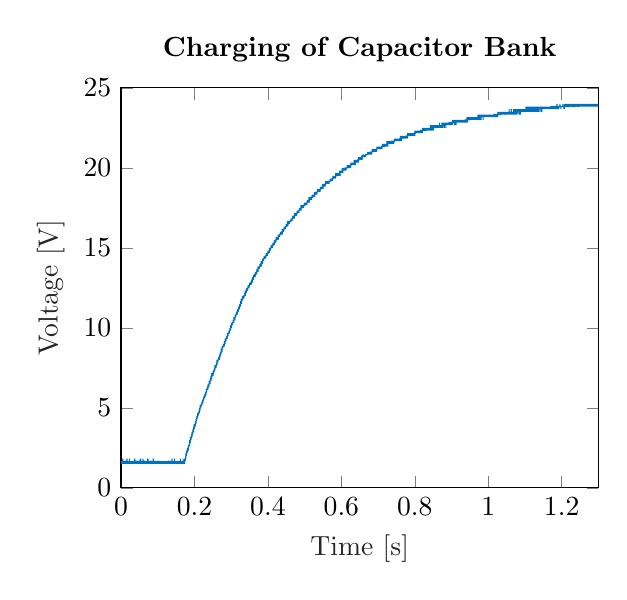
\begin{tikzpicture}

\begin{axis}[%
width=0.5\textwidth,
height=2in,
at={(0.758in,0.481in)},
scale only axis,
xmin=0,
xmax=1.3,
xlabel style={font=\color{white!15!black}},
xlabel={Time [s]},
ymin=0,
ymax=25,
ylabel style={font=\color{white!15!black}},
ylabel={Voltage [V]},
axis background/.style={fill=white},
title style={font=\bfseries},
title={Charging of Capacitor Bank}
]
\addplot [color=mycolor1, forget plot]
  table[row sep=crcr]{%
-1.68500000015115e-05	1.66667\\
0.000303150000000585	1.5\\
0.00068315000000041	1.66667\\
0.000923149999998429	1.5\\
0.00104315000000099	1.66667\\
0.00106315000000023	1.5\\
0.00144315000000006	1.66667\\
0.00174314999999936	1.5\\
0.0017631499999986	1.66667\\
0.0017831500000014	1.5\\
0.00216315000000122	1.66667\\
0.00222314999999895	1.5\\
0.00244315000000128	1.66667\\
0.00246315000000052	1.5\\
0.00266315000000006	1.66667\\
0.0026831499999993	1.5\\
0.00288314999999884	1.66667\\
0.00290315000000163	1.5\\
0.0029831499999986	1.66667\\
0.0030031500000014	1.5\\
0.00338315000000122	1.66667\\
0.00356315000000151	1.5\\
0.00358315000000076	1.66667\\
0.00362314999999924	1.5\\
0.00384315000000157	1.83333\\
0.00392314999999854	1.5\\
0.00400314999999907	1.66667\\
0.00402314999999831	1.5\\
0.00414315000000087	1.66667\\
0.00416315000000012	1.5\\
0.00424315000000064	1.66667\\
0.00428314999999913	1.5\\
0.00440315000000169	1.66667\\
0.00442315000000093	1.5\\
0.00468315000000175	1.66667\\
0.00470315000000099	1.5\\
0.00500315000000029	1.66667\\
0.00502314999999953	1.5\\
0.0051231499999993	1.83333\\
0.00534315000000163	1.5\\
0.00572315000000145	1.66667\\
0.0057431500000007	1.5\\
0.00604315	1.66667\\
0.00606314999999924	1.5\\
0.00608314999999848	1.66667\\
0.00610315000000128	1.5\\
0.00612315000000052	1.66667\\
0.00614314999999976	1.5\\
0.00628315000000157	1.66667\\
0.00630315000000081	1.5\\
0.00668315000000064	1.66667\\
0.00674314999999837	1.5\\
0.00698314999999994	1.66667\\
0.00700314999999918	1.5\\
0.00718314999999947	1.66667\\
0.00720314999999871	1.5\\
0.00724315000000075	1.66667\\
0.00726315	1.5\\
0.00744315000000029	1.66667\\
0.00746314999999953	1.5\\
0.00748314999999877	1.66667\\
0.00750315000000157	1.5\\
0.00788315000000139	1.66667\\
0.00804314999999889	1.5\\
0.00816315000000145	1.66667\\
0.00818315000000069	1.5\\
0.00836315000000099	1.66667\\
0.00838315000000023	1.5\\
0.00844315000000151	1.66667\\
0.00846315000000075	1.5\\
0.00850314999999924	1.66667\\
0.00852314999999848	1.5\\
0.00886314999999982	1.66667\\
0.00888314999999906	1.5\\
0.00890314999999831	1.66667\\
0.0089231500000011	1.5\\
0.00894315000000034	1.66667\\
0.00896314999999959	1.5\\
0.00902315000000087	1.66667\\
0.00904315000000011	1.5\\
0.00926314999999889	1.66667\\
0.00928315000000168	1.5\\
0.00936314999999865	1.66667\\
0.00940315000000069	1.5\\
0.00968315000000075	1.66667\\
0.00970314999999999	1.5\\
0.0100831499999998	1.66667\\
0.0101631500000003	1.5\\
0.0102631500000001	1.66667\\
0.0102831499999994	1.5\\
0.0106631499999992	1.66667\\
0.0110631499999982	1.66667\\
0.011083150000001	1.5\\
0.0113831500000003	1.66667\\
0.0114031499999996	1.5\\
0.0116231499999984	1.66667\\
0.0116431500000012	1.5\\
0.012023150000001	1.66667\\
0.0122431499999998	1.5\\
0.012263149999999	1.66667\\
0.012303150000001	1.5\\
0.0123631499999988	1.66667\\
0.0123831500000016	1.5\\
0.0127631500000014	1.66667\\
0.0131031499999992	1.5\\
0.0133031499999987	1.66667\\
0.0133231500000015	1.5\\
0.0134231500000013	1.66667\\
0.0134431500000005	1.5\\
0.0135431500000003	1.66667\\
0.0135631499999995	1.5\\
0.0139431499999993	1.66667\\
0.0143831500000005	1.66667\\
0.0144031499999997	1.5\\
0.0145431500000015	1.66667\\
0.01458315	1.5\\
0.0149631499999998	1.66667\\
0.0150831499999988	1.5\\
0.0152031500000014	1.66667\\
0.0152231500000006	1.5\\
0.0152431499999999	1.66667\\
0.0152631499999991	1.5\\
0.0156431499999989	1.66667\\
0.0157431499999987	1.5\\
0.0158431499999985	1.66667\\
0.0158631500000013	1.5\\
0.015963150000001	1.66667\\
0.0159831500000003	1.5\\
0.0160231499999988	1.66667\\
0.0160431500000016	1.5\\
0.0161031499999993	1.66667\\
0.0161431500000013	1.5\\
0.0162231499999983	1.83333\\
0.0163431500000009	1.5\\
0.0167231500000007	1.66667\\
0.0168231500000005	1.5\\
0.0168631499999989	1.66667\\
0.0168831500000017	1.5\\
0.0172631500000016	1.66667\\
0.0173231499999993	1.5\\
0.0173431499999985	1.66667\\
0.0173631500000013	1.5\\
0.0174231499999991	1.66667\\
0.0174631500000011	1.5\\
0.0176431500000014	1.66667\\
0.0176631500000006	1.5\\
0.0179031499999986	1.66667\\
0.0179231500000014	1.5\\
0.018123150000001	1.66667\\
0.0181431500000002	1.5\\
0.0181631499999995	1.66667\\
0.0181831499999987	1.5\\
0.0182631499999992	1.66667\\
0.0182831499999985	1.5\\
0.0184431499999995	1.66667\\
0.0184631499999988	1.5\\
0.0186431499999991	1.66667\\
0.0186631499999983	1.5\\
0.0187831500000009	1.66667\\
0.0188031500000001	1.5\\
0.0188431499999986	1.66667\\
0.0188631500000014	1.5\\
0.0190031499999996	1.66667\\
0.0190231499999989	1.5\\
0.0191831499999999	1.66667\\
0.0192031499999992	1.5\\
0.01946315	1.66667\\
0.0194831499999992	1.5\\
0.0196031500000018	1.66667\\
0.019623150000001	1.5\\
0.0196631499999995	1.66667\\
0.0196831499999988	1.5\\
0.01974315	1.66667\\
0.0197831499999985	1.5\\
0.0198231500000006	1.66667\\
0.0198431499999998	1.5\\
0.0200831500000014	1.66667\\
0.0201031500000006	1.5\\
0.0204831500000004	1.66667\\
0.020803149999999	1.5\\
0.0208231500000018	1.66667\\
0.020843150000001	1.5\\
0.0209431500000008	1.66667\\
0.02096315	1.5\\
0.0210631499999998	1.66667\\
0.0210831499999991	1.5\\
0.0211431500000003	1.66667\\
0.0211631499999996	1.5\\
0.0212831499999986	1.66667\\
0.0213031500000014	1.5\\
0.0216831500000012	1.66667\\
0.022023149999999	1.5\\
0.0224031499999988	1.66667\\
0.0225631499999999	1.5\\
0.0226231500000011	1.66667\\
0.0226431500000004	1.5\\
0.0228431499999999	1.83333\\
0.0228831499999984	1.5\\
0.0231831500000013	1.66667\\
0.0232031500000005	1.5\\
0.023243149999999	1.66667\\
0.0232631500000018	1.5\\
0.0235831500000003	1.66667\\
0.0236231499999988	1.5\\
0.0240031499999986	1.66667\\
0.0240431500000007	1.5\\
0.0241231500000012	1.66667\\
0.0241631499999997	1.5\\
0.0245431499999995	1.66667\\
0.0246831500000013	1.5\\
0.0247831500000011	1.66667\\
0.0248031500000003	1.5\\
0.0248431499999988	1.66667\\
0.0248631500000016	1.5\\
0.0249431499999986	1.66667\\
0.0250031499999999	1.5\\
0.0250631500000011	1.66667\\
0.0250831500000004	1.5\\
0.0253431500000012	1.66667\\
0.0254031499999989	1.5\\
0.0254831499999995	1.66667\\
0.0255031499999987	1.5\\
0.0256431500000005	1.66667\\
0.0256631499999997	1.5\\
0.0260431499999996	1.66667\\
0.0261231500000001	1.5\\
0.0261431499999993	1.66667\\
0.0261631499999986	1.5\\
0.0262431499999991	1.66667\\
0.0262631499999983	1.5\\
0.0266431500000017	1.66667\\
0.026663150000001	1.5\\
0.0268031499999992	1.66667\\
0.0268231499999985	1.5\\
0.0268431500000013	1.66667\\
0.0268631500000005	1.5\\
0.0268831499999997	1.66667\\
0.026903149999999	1.5\\
0.0269231500000018	1.66667\\
0.0269631500000003	1.5\\
0.0273431500000001	1.66667\\
0.0273631499999993	1.5\\
0.0276231500000002	1.66667\\
0.0276431499999994	1.5\\
0.0279231499999995	1.66667\\
0.0279431499999987	1.5\\
0.0279631500000015	1.66667\\
0.0279831500000007	1.5\\
0.0280431499999985	1.66667\\
0.0280631500000013	1.5\\
0.0280831500000005	1.66667\\
0.0281031499999997	1.5\\
0.028123149999999	1.66667\\
0.0281431500000018	1.5\\
0.0281831500000003	1.66667\\
0.0282231499999988	1.5\\
0.0283831499999998	1.66667\\
0.028403149999999	1.5\\
0.0285831499999993	1.66667\\
0.0286031499999986	1.5\\
0.0286231500000014	1.66667\\
0.0286431500000006	1.5\\
0.0287831499999989	1.66667\\
0.0288031500000017	1.5\\
0.0290031500000012	1.66667\\
0.0290231500000004	1.5\\
0.0292431499999992	1.66667\\
0.0292631499999985	1.5\\
0.0293631500000018	1.66667\\
0.029383150000001	1.5\\
0.0295831500000006	1.66667\\
0.0296031499999998	1.5\\
0.0296631500000011	1.66667\\
0.0296831500000003	1.5\\
0.0298631500000006	1.66667\\
0.0298831499999999	1.5\\
0.0302631499999997	1.66667\\
0.0304031500000015	1.5\\
0.030563149999999	1.66667\\
0.0305831500000018	1.5\\
0.0306831500000015	1.66667\\
0.0307031500000008	1.5\\
0.0310831500000006	1.66667\\
0.0312231499999989	1.5\\
0.0312631500000009	1.66667\\
0.0313031499999994	1.5\\
0.0315031499999989	1.66667\\
0.0315231500000017	1.5\\
0.0315831499999994	1.66667\\
0.0316031499999987	1.5\\
0.0317431500000005	1.66667\\
0.0317631499999997	1.5\\
0.0319231500000008	1.66667\\
0.03194315	1.5\\
0.0322231500000001	1.66667\\
0.0322431499999993	1.5\\
0.0325631500000014	1.66667\\
0.0325831500000007	1.5\\
0.0326831500000004	1.66667\\
0.0327031499999997	1.5\\
0.0329631500000005	1.66667\\
0.0329831499999997	1.5\\
0.0333631499999996	1.66667\\
0.0337231500000001	1.5\\
0.03410315	1.66667\\
0.0344231499999985	1.5\\
0.034503149999999	1.66667\\
0.0345231499999983	1.5\\
0.0348831499999989	1.66667\\
0.0349231500000009	1.5\\
0.0350231500000007	1.66667\\
0.0350431499999999	1.5\\
0.0351431499999997	1.66667\\
0.0351631499999989	1.5\\
0.0351831500000017	1.66667\\
0.035203150000001	1.5\\
0.0352231500000002	1.66667\\
0.0352431499999994	1.5\\
0.0356231499999993	1.66667\\
0.0358431500000016	1.5\\
0.0359431500000014	1.66667\\
0.0359631500000006	1.5\\
0.0363431500000004	1.66667\\
0.0363631499999997	1.5\\
0.03654315	1.66667\\
0.0365631499999992	1.5\\
0.0367431499999995	1.66667\\
0.0367631499999987	1.5\\
0.0368031500000008	1.66667\\
0.03682315	1.5\\
0.0368431499999993	1.66667\\
0.0368631499999985	1.5\\
0.0369631499999983	1.66667\\
0.0369831500000011	1.5\\
0.0370031500000003	1.66667\\
0.0370231499999996	1.5\\
0.0371231499999993	1.83333\\
0.0372031499999999	1.5\\
0.0373231499999989	1.66667\\
0.0373431500000017	1.5\\
0.0374031499999994	1.66667\\
0.0374231499999986	1.5\\
0.0376831499999994	1.66667\\
0.0377031499999987	1.5\\
0.0377831499999992	1.66667\\
0.0378031499999985	1.5\\
0.0378231500000012	1.83333\\
0.0380031500000015	1.5\\
0.0380231500000008	1.66667\\
0.0380631499999993	1.5\\
0.0382231500000003	1.66667\\
0.0382431499999996	1.5\\
0.0386231499999994	1.66667\\
0.0388231499999989	1.5\\
0.0389231499999987	1.66667\\
0.0389431500000015	1.5\\
0.039143150000001	1.66667\\
0.0391831499999995	1.5\\
0.0393631499999998	1.66667\\
0.039383149999999	1.5\\
0.0397631499999989	1.66667\\
0.0398231500000001	1.5\\
0.0398431499999994	1.66667\\
0.0398631499999986	1.5\\
0.0399031500000007	1.66667\\
0.0399231499999999	1.5\\
0.0399431499999992	1.66667\\
0.0399631499999984	1.5\\
0.0401231499999994	1.66667\\
0.0401431499999987	1.5\\
0.0401831500000007	1.66667\\
0.04020315	1.5\\
0.040363150000001	1.66667\\
0.0403831500000003	1.5\\
0.0407631500000001	1.66667\\
0.0412031500000012	1.66667\\
0.0412231500000004	1.5\\
0.0413431499999994	1.66667\\
0.0413631499999987	1.5\\
0.0416631500000015	1.66667\\
0.0416831500000008	1.5\\
0.0420231499999986	1.66667\\
0.0420431500000014	1.5\\
0.0422431500000009	1.66667\\
0.0422631500000001	1.5\\
0.0423631499999999	1.66667\\
0.0424031499999984	1.5\\
0.0426031500000015	1.66667\\
0.0426231500000007	1.5\\
0.0430031500000005	1.66667\\
0.0438431500000007	1.66667\\
0.04386315	1.5\\
0.0442431499999998	1.66667\\
0.0443231500000003	1.5\\
0.0445831500000011	1.66667\\
0.0446031500000004	1.5\\
0.0447431499999986	1.66667\\
0.0447631500000014	1.5\\
0.0451431500000012	1.66667\\
0.0454631499999998	1.5\\
0.0456431500000001	1.66667\\
0.0456631499999993	1.5\\
0.0459031500000009	1.66667\\
0.0459231500000001	1.5\\
0.04630315	1.66667\\
0.0464431500000018	1.5\\
0.0464831500000003	1.66667\\
0.0465031499999995	1.5\\
0.0465631500000008	1.66667\\
0.04658315	1.5\\
0.0468831499999993	1.66667\\
0.0469031499999986	1.5\\
0.0470231500000011	1.66667\\
0.0470431500000004	1.5\\
0.0471831499999986	1.66667\\
0.0472231500000007	1.5\\
0.0472831499999984	1.66667\\
0.0473031500000012	1.5\\
0.0473831500000017	1.66667\\
0.0474031500000009	1.5\\
0.0474631499999987	1.66667\\
0.0474831500000015	1.5\\
0.0475831500000012	1.66667\\
0.0476031500000005	1.5\\
0.047683150000001	1.66667\\
0.0477031500000002	1.5\\
0.04780315	1.66667\\
0.0478231499999993	1.5\\
0.0480831500000001	1.66667\\
0.0481031499999993	1.5\\
0.0481431500000014	1.66667\\
0.0481631500000006	1.5\\
0.0483631500000001	1.66667\\
0.0483831499999994	1.5\\
0.0487631499999992	1.66667\\
0.0492231499999995	1.66667\\
0.0492431499999988	1.5\\
0.0492831500000008	1.66667\\
0.0493031500000001	1.5\\
0.0493431499999986	1.66667\\
0.0493831500000006	1.5\\
0.0497431500000012	1.66667\\
0.0497631500000004	1.5\\
0.0499431500000007	1.66667\\
0.04996315	1.5\\
0.0502031500000015	1.66667\\
0.0502231500000008	1.5\\
0.0504831500000016	1.66667\\
0.0505231500000001	1.5\\
0.0506631499999983	1.66667\\
0.0506831500000011	1.5\\
0.0510431500000017	1.66667\\
0.0510631500000009	1.5\\
0.0512631500000005	1.66667\\
0.0512831499999997	1.5\\
0.051343150000001	1.66667\\
0.0513631500000002	1.5\\
0.05146315	1.66667\\
0.0515031499999985	1.5\\
0.0515231500000013	1.66667\\
0.0515431500000005	1.5\\
0.0516031499999983	1.66667\\
0.0516231500000011	1.5\\
0.0516431500000003	1.66667\\
0.0516631499999995	1.5\\
0.0518031500000014	1.66667\\
0.0518431499999998	1.5\\
0.0519031500000011	1.66667\\
0.0519231500000004	1.5\\
0.0519431499999996	1.66667\\
0.0519631499999988	1.5\\
0.0520831500000014	1.66667\\
0.0521031500000007	1.5\\
0.0522031500000004	1.66667\\
0.0522231499999997	1.5\\
0.0524231499999992	1.83333\\
0.0526631500000008	1.5\\
0.0528631500000003	1.66667\\
0.0529031499999988	1.5\\
0.0529631500000001	1.66667\\
0.0530031499999986	1.5\\
0.0530431500000006	1.66667\\
0.0530831499999991	1.5\\
0.0531031499999983	1.66667\\
0.0531231500000011	1.5\\
0.0533231500000007	1.66667\\
0.0533431499999999	1.5\\
0.0533631499999991	1.66667\\
0.0533831499999984	1.5\\
0.0534831500000017	1.66667\\
0.0535031500000009	1.5\\
0.053783150000001	1.66667\\
0.0538031500000002	1.5\\
0.0538831500000008	1.66667\\
0.05390315	1.5\\
0.0542831499999998	1.66667\\
0.0551431499999993	1.66667\\
0.0551631499999985	1.5\\
0.0555431499999983	1.66667\\
0.0555831500000004	1.5\\
0.0556031499999996	1.66667\\
0.0556231499999988	1.5\\
0.0558831499999997	1.66667\\
0.0559031499999989	1.5\\
0.0561231500000012	1.66667\\
0.0561431500000005	1.5\\
0.0563831499999985	1.66667\\
0.0564031500000013	1.5\\
0.0567831500000011	1.66667\\
0.0568031500000004	1.5\\
0.0571831500000002	1.66667\\
0.0573031499999992	1.5\\
0.0575231500000015	1.66667\\
0.0575431500000008	1.5\\
0.0577831499999988	1.66667\\
0.0578031500000016	1.5\\
0.0578431500000001	1.66667\\
0.0578631499999993	1.5\\
0.0580431499999996	1.66667\\
0.0580631499999988	1.5\\
0.0581631499999986	1.66667\\
0.0581831500000014	1.5\\
0.0582431499999991	1.66667\\
0.0582631499999984	1.5\\
0.0584231499999994	1.66667\\
0.0584431499999987	1.5\\
0.0585031499999999	1.66667\\
0.0585431499999984	1.5\\
0.0585631500000012	1.66667\\
0.0585831500000005	1.5\\
0.0588631500000005	1.66667\\
0.0588831499999998	1.5\\
0.0590231500000016	1.66667\\
0.0590431500000008	1.5\\
0.0591031499999985	1.66667\\
0.0591231500000013	1.5\\
0.0595031500000012	1.66667\\
0.0595631499999989	1.83333\\
0.0599431499999987	1.66667\\
0.0604431500000011	1.66667\\
0.0604631500000004	1.5\\
0.0608431500000002	1.66667\\
0.0611631499999987	1.5\\
0.0614231499999995	1.66667\\
0.0614431499999988	1.5\\
0.0616431499999983	1.66667\\
0.0616831500000004	1.5\\
0.0617231499999988	1.66667\\
0.0617431500000016	1.5\\
0.0617831500000001	1.66667\\
0.0618031499999994	1.5\\
0.0621231500000015	1.66667\\
0.0621431500000007	1.5\\
0.0623431500000002	1.66667\\
0.0623631499999995	1.5\\
0.0624631499999992	1.66667\\
0.0624831499999985	1.5\\
0.0626031500000011	1.66667\\
0.0626431499999995	1.5\\
0.0626631499999988	1.66667\\
0.0626831500000016	1.5\\
0.0627431499999993	1.66667\\
0.0627631499999985	1.5\\
0.0629831500000009	1.66667\\
0.0630031500000001	1.5\\
0.0633831499999999	1.66667\\
0.0638631499999995	1.66667\\
0.0638831499999988	1.5\\
0.0639831499999985	1.66667\\
0.0640031500000013	1.5\\
0.0641831500000016	1.66667\\
0.0642031500000009	1.5\\
0.0642231500000001	1.66667\\
0.0642431499999994	1.5\\
0.0644831500000009	1.66667\\
0.0645031500000002	1.5\\
0.0645431499999987	1.66667\\
0.0645631500000015	1.5\\
0.0649231499999985	1.66667\\
0.0649431500000013	1.5\\
0.0650831499999995	1.66667\\
0.0651031499999988	1.5\\
0.0651831499999993	1.66667\\
0.0652031499999985	1.5\\
0.0652231500000013	1.66667\\
0.0652831499999991	1.5\\
0.0653031499999983	1.66667\\
0.0653231500000011	1.5\\
0.0657031500000009	1.66667\\
0.0657231500000002	1.5\\
0.06610315	1.66667\\
0.066223149999999	1.5\\
0.0662431499999983	1.66667\\
0.066263150000001	1.5\\
0.0666431500000009	1.66667\\
0.0669231500000009	1.5\\
0.0670031500000015	1.66667\\
0.0670231500000007	1.5\\
0.0674031500000005	1.66667\\
0.0674631499999983	1.5\\
0.0675631500000016	1.66667\\
0.0675831500000008	1.5\\
0.0677631500000011	1.66667\\
0.0677831500000003	1.5\\
0.0680431500000012	1.66667\\
0.0680631500000004	1.5\\
0.0681031499999989	1.66667\\
0.0681231500000017	1.5\\
0.0683831499999989	1.66667\\
0.0684031500000017	1.5\\
0.06854315	1.66667\\
0.0685831499999985	1.5\\
0.0688031500000008	1.66667\\
0.0688231500000001	1.5\\
0.0688631499999985	1.66667\\
0.0688831500000013	1.5\\
0.0690031500000003	1.66667\\
0.0690231499999996	1.5\\
0.0690831500000009	1.66667\\
0.0691031500000001	1.5\\
0.0694831499999999	1.66667\\
0.069643150000001	1.5\\
0.0699431500000003	1.66667\\
0.0699631499999995	1.5\\
0.0701231500000006	1.66667\\
0.0701431499999998	1.5\\
0.0702031500000011	1.66667\\
0.0702231500000003	1.5\\
0.0702431499999996	1.66667\\
0.0702631499999988	1.5\\
0.0704231499999999	1.66667\\
0.0704631499999984	1.5\\
0.0705631500000017	1.66667\\
0.0705831500000009	1.5\\
0.0709631500000008	1.66667\\
0.07098315	1.5\\
0.0713631499999998	1.66667\\
0.0715631499999994	1.5\\
0.0716031500000014	1.66667\\
0.0716431499999999	1.5\\
0.0718231500000002	1.66667\\
0.0718431499999994	1.5\\
0.0719031500000007	1.83333\\
0.0720231499999997	1.5\\
0.0724031499999995	1.66667\\
0.0728631499999999	1.66667\\
0.0728831499999991	1.5\\
0.0732231500000005	1.83333\\
0.0736031500000003	1.66667\\
0.0740431500000014	1.66667\\
0.0740631500000006	1.5\\
0.0741231499999984	1.66667\\
0.0741431500000012	1.5\\
0.074523150000001	1.66667\\
0.0750031500000006	1.66667\\
0.0750231499999998	1.5\\
0.0750431499999991	1.66667\\
0.0750631499999983	1.5\\
0.0754431500000017	1.66667\\
0.0754631500000009	1.5\\
0.0757231500000017	1.66667\\
0.075743150000001	1.5\\
0.0759631499999998	1.66667\\
0.075983149999999	1.5\\
0.0760631499999995	1.66667\\
0.0760831499999988	1.5\\
0.0763631499999988	1.66667\\
0.0763831500000016	1.5\\
0.0764231500000001	1.66667\\
0.0764431499999993	1.5\\
0.0768231499999992	1.66667\\
0.0769231499999989	1.5\\
0.0770231499999987	1.66667\\
0.0770431500000015	1.5\\
0.0772231499999982	1.66667\\
0.077243150000001	1.5\\
0.0772631500000003	1.66667\\
0.0772831499999995	1.5\\
0.0773831499999993	1.66667\\
0.0774031499999985	1.5\\
0.0777831499999984	1.66667\\
0.0778831500000017	1.5\\
0.0779231500000002	1.66667\\
0.0779431499999994	1.5\\
0.0779831500000014	1.66667\\
0.0780031500000007	1.5\\
0.0782431499999987	1.66667\\
0.0782631500000015	1.5\\
0.0786231499999985	1.66667\\
0.0786431500000013	1.5\\
0.0788431500000009	1.66667\\
0.0788631500000001	1.5\\
0.0788831499999993	1.66667\\
0.0789031499999986	1.5\\
0.0792231500000007	1.66667\\
0.0792431499999999	1.5\\
0.0793231500000005	1.66667\\
0.0793431499999997	1.5\\
0.0793631499999989	1.66667\\
0.0793831500000017	1.5\\
0.07952315	1.66667\\
0.0795631499999985	1.5\\
0.0797431499999988	1.66667\\
0.0797631500000016	1.5\\
0.0797831500000008	1.66667\\
0.07980315	1.5\\
0.0801631500000006	1.66667\\
0.0801831499999999	1.5\\
0.0804031499999986	1.66667\\
0.0804231500000014	1.5\\
0.0805231500000012	1.66667\\
0.0805431500000005	1.5\\
0.0809231500000003	1.66667\\
0.0813831500000006	1.66667\\
0.0814231499999991	1.5\\
0.0814431499999984	1.66667\\
0.0814631500000011	1.5\\
0.0814831500000004	1.66667\\
0.0815031499999996	1.5\\
0.0816431500000014	1.66667\\
0.0816831499999999	1.5\\
0.0817031499999992	1.66667\\
0.0817231499999984	1.5\\
0.0818031499999989	1.66667\\
0.0818231500000017	1.5\\
0.081843150000001	1.66667\\
0.0818631500000002	1.5\\
0.082123150000001	1.66667\\
0.0821431500000003	1.5\\
0.0824231500000003	1.66667\\
0.0824631499999988	1.5\\
0.0825031500000009	1.66667\\
0.0825231500000001	1.5\\
0.0829031499999999	1.66667\\
0.0829831500000004	1.5\\
0.0832431500000013	1.66667\\
0.0832631500000005	1.5\\
0.0833631500000003	1.66667\\
0.0833831499999995	1.5\\
0.08346315	1.66667\\
0.0834831499999993	1.5\\
0.0835831499999991	1.66667\\
0.0836031499999983	1.5\\
0.0836231500000011	1.66667\\
0.0836431500000003	1.5\\
0.0837031500000016	1.66667\\
0.0837231500000009	1.5\\
0.0838631499999991	1.66667\\
0.0838831499999984	1.5\\
0.0842631500000017	1.66667\\
0.0843231499999995	1.5\\
0.0844231499999992	1.66667\\
0.0844431499999985	1.5\\
0.0848231499999983	1.66667\\
0.0849231500000016	1.5\\
0.0852031500000017	1.66667\\
0.0852231500000009	1.5\\
0.0852431500000002	1.66667\\
0.0852631499999994	1.5\\
0.0853231500000007	1.66667\\
0.0853431499999999	1.5\\
0.0853631499999992	1.66667\\
0.0853831499999984	1.5\\
0.0854431499999997	1.66667\\
0.0854631499999989	1.5\\
0.0857031500000005	1.66667\\
0.0857231499999997	1.5\\
0.0858231499999995	1.66667\\
0.0858431499999988	1.5\\
0.0860831500000003	1.66667\\
0.0861031499999996	1.5\\
0.0864831499999994	1.66667\\
0.0868631499999992	1.5\\
0.0869031500000013	1.66667\\
0.0869231500000005	1.5\\
0.0870231500000003	1.66667\\
0.0870431499999995	1.5\\
0.087243149999999	1.66667\\
0.0872631499999983	1.5\\
0.0875431499999983	1.66667\\
0.0875631500000011	1.5\\
0.0876431500000017	1.66667\\
0.0876831500000002	1.5\\
0.0877031499999994	1.83333\\
0.0877431500000014	1.5\\
0.0879631500000002	1.66667\\
0.0879831499999995	1.5\\
0.0883231500000008	1.66667\\
0.08834315	1.5\\
0.0885831500000016	1.66667\\
0.0886031500000009	1.5\\
0.0888031500000004	1.66667\\
0.0888231499999996	1.5\\
0.0892031499999995	1.66667\\
0.0892631500000007	1.5\\
0.0896431500000006	1.66667\\
0.0901231500000002	1.66667\\
0.0901431499999994	1.5\\
0.0902631499999984	1.66667\\
0.0902831500000012	1.5\\
0.090383150000001	1.66667\\
0.0904031500000002	1.5\\
0.0904631500000015	1.66667\\
0.0904831500000007	1.5\\
0.0905231499999992	1.66667\\
0.0905431499999985	1.5\\
0.0907231499999988	1.66667\\
0.0907431500000015	1.5\\
0.0910431500000008	1.66667\\
0.0910631500000001	1.5\\
0.0911031499999986	1.66667\\
0.0911431500000006	1.5\\
0.0915031500000012	1.66667\\
0.0915231500000004	1.5\\
0.09172315	1.66667\\
0.0917431499999992	1.5\\
0.0920831500000006	1.66667\\
0.0921031499999998	1.5\\
0.0924631500000004	1.66667\\
0.0924831499999996	1.5\\
0.0926831499999992	1.66667\\
0.0927031499999984	1.5\\
0.0929031500000015	1.66667\\
0.0929231500000007	1.5\\
0.09294315	1.66667\\
0.0929631499999992	1.5\\
0.0932431499999993	1.66667\\
0.0932631499999985	1.5\\
0.0932831500000013	1.66667\\
0.0933031500000006	1.5\\
0.0933631499999983	1.66667\\
0.0933831500000011	1.5\\
0.0934631500000016	1.66667\\
0.0934831500000008	1.5\\
0.0935231499999993	1.66667\\
0.0935431499999986	1.5\\
0.0935831500000006	1.66667\\
0.0936031499999999	1.5\\
0.0939231499999984	1.66667\\
0.0939431500000012	1.5\\
0.094043150000001	1.66667\\
0.0940631500000002	1.5\\
0.0942431500000005	1.66667\\
0.0942631499999997	1.5\\
0.0944631499999993	1.66667\\
0.0944831499999985	1.5\\
0.0946231500000003	1.66667\\
0.0946431499999996	1.5\\
0.0947631499999986	1.66667\\
0.0947831500000014	1.5\\
0.0948831500000011	1.66667\\
0.0949031500000004	1.5\\
0.0951831500000004	1.66667\\
0.0952031499999997	1.5\\
0.0952431500000017	1.66667\\
0.095263150000001	1.5\\
0.0952831500000002	1.66667\\
0.0953031499999994	1.5\\
0.0955831499999995	1.66667\\
0.0956031499999987	1.5\\
0.0957231500000013	1.66667\\
0.0957431500000006	1.5\\
0.0957631499999998	1.66667\\
0.095783149999999	1.5\\
0.0958431500000003	1.66667\\
0.0958631499999996	1.5\\
0.0961431499999996	1.66667\\
0.0961631499999989	1.5\\
0.0962831500000014	1.66667\\
0.0963031500000007	1.5\\
0.096483150000001	1.66667\\
0.0965031500000002	1.5\\
0.0965631500000015	1.66667\\
0.0965831500000007	1.5\\
0.0966831500000005	1.66667\\
0.0967031499999997	1.5\\
0.0969031499999993	1.66667\\
0.0969231499999985	1.5\\
0.0973031499999983	1.66667\\
0.0973831499999989	1.5\\
0.0974631499999994	1.66667\\
0.0974831499999986	1.5\\
0.0978031500000007	1.66667\\
0.09782315	1.5\\
0.0978831500000013	1.66667\\
0.0979031500000005	1.5\\
0.098223149999999	1.66667\\
0.0982431499999983	1.5\\
0.0982831500000003	1.66667\\
0.0983031499999996	1.5\\
0.0984631500000006	1.66667\\
0.0984831499999999	1.5\\
0.0988631499999997	1.66667\\
0.0992231500000003	1.5\\
0.0992431499999995	1.66667\\
0.0992631499999987	1.5\\
0.0993631499999985	1.66667\\
0.0994031500000006	1.5\\
0.0997831500000004	1.66667\\
0.0999231499999986	1.5\\
0.0999631500000007	1.66667\\
0.0999831499999999	1.5\\
0.10008315	1.66667\\
0.100103149999999	1.5\\
0.100143150000001	1.66667\\
0.10016315	1.5\\
0.10026315	1.66667\\
0.100283149999999	1.5\\
0.10034315	1.66667\\
0.10036315	1.5\\
0.100483149999999	1.66667\\
0.100503150000002	1.5\\
0.10054315	1.66667\\
0.100563149999999	1.5\\
0.100683149999998	1.66667\\
0.100703150000001	1.5\\
0.10072315	1.66667\\
0.10074315	1.5\\
0.101123149999999	1.66667\\
0.10166315	1.66667\\
0.10168315	1.5\\
0.101703149999999	1.66667\\
0.101723150000002	1.5\\
0.101803149999999	1.66667\\
0.101823150000001	1.5\\
0.102003150000002	1.66667\\
0.102023150000001	1.5\\
0.102063149999999	1.66667\\
0.102123150000001	1.5\\
0.10250315	1.66667\\
0.102623149999999	1.5\\
0.102843150000002	1.66667\\
0.102863150000001	1.5\\
0.102923149999999	1.66667\\
0.102943150000002	1.5\\
0.102963150000001	1.66667\\
0.10298315	1.5\\
0.103003149999999	1.66667\\
0.103023149999999	1.5\\
0.103403149999998	1.66667\\
0.103503150000002	1.5\\
0.103603150000001	1.66667\\
0.103623150000001	1.5\\
0.103683149999998	1.66667\\
0.10372315	1.5\\
0.10374315	1.66667\\
0.103763149999999	1.5\\
0.103843149999999	1.66667\\
0.103883150000001	1.5\\
0.103943149999999	1.66667\\
0.103963149999998	1.5\\
0.104043149999999	1.66667\\
0.104063150000002	1.5\\
0.104223149999999	1.66667\\
0.104243149999999	1.5\\
0.104363150000001	1.66667\\
0.10438315	1.5\\
0.10466315	1.66667\\
0.10468315	1.5\\
0.104783149999999	1.66667\\
0.104803149999999	1.5\\
0.105123150000001	1.66667\\
0.10514315	1.5\\
0.10522315	1.66667\\
0.10524315	1.5\\
0.105303150000001	1.66667\\
0.10532315	1.5\\
0.105563149999998	1.66667\\
0.105583150000001	1.5\\
0.105683150000001	1.66667\\
0.10570315	1.5\\
0.10590315	1.66667\\
0.105923149999999	1.5\\
0.105963150000001	1.66667\\
0.10598315	1.5\\
0.106023149999999	1.66667\\
0.106043150000001	1.5\\
0.106243150000001	1.66667\\
0.10626315	1.5\\
0.106303149999999	1.66667\\
0.106323150000001	1.5\\
0.106403149999998	1.66667\\
0.10644315	1.5\\
0.106683149999999	1.66667\\
0.106703150000001	1.5\\
0.106763149999999	1.66667\\
0.106783149999998	1.5\\
0.106883150000002	1.66667\\
0.106903150000001	1.5\\
0.107043149999999	1.66667\\
0.107063149999998	1.5\\
0.10720315	1.66667\\
0.107243149999999	1.5\\
0.10748315	1.66667\\
0.107503149999999	1.5\\
0.107523149999999	1.66667\\
0.107543150000001	1.5\\
0.107603149999999	1.66667\\
0.107643150000001	1.5\\
0.10766315	1.66667\\
0.10768315	1.5\\
0.107783149999999	1.66667\\
0.107823150000002	1.5\\
0.107843150000001	1.66667\\
0.10786315	1.5\\
0.107983149999999	1.66667\\
0.108003149999998	1.5\\
0.108123150000001	1.66667\\
0.10814315	1.5\\
0.108383150000002	1.66667\\
0.108403150000001	1.5\\
0.10842315	1.66667\\
0.108443149999999	1.5\\
0.108483150000001	1.66667\\
0.108503150000001	1.5\\
0.108583150000001	1.66667\\
0.10860315	1.5\\
0.10880315	1.66667\\
0.108823149999999	1.5\\
0.108923149999999	1.66667\\
0.108943150000002	1.5\\
0.10898315	1.66667\\
0.109003149999999	1.5\\
0.109063150000001	1.66667\\
0.109103149999999	1.5\\
0.109123149999999	1.66667\\
0.10918315	1.5\\
0.109203149999999	1.66667\\
0.109223149999998	1.5\\
0.109303149999999	1.66667\\
0.109323150000002	1.5\\
0.109483149999999	1.66667\\
0.109503149999998	1.5\\
0.109583149999999	1.66667\\
0.109603150000002	1.5\\
0.10992315	1.66667\\
0.109943149999999	1.5\\
0.110063149999998	1.66667\\
0.110083150000001	1.5\\
0.110163150000002	1.66667\\
0.110183150000001	1.5\\
0.11020315	1.66667\\
0.110223149999999	1.5\\
0.11040315	1.66667\\
0.110423149999999	1.5\\
0.110643150000001	1.66667\\
0.110663150000001	1.5\\
0.110743150000001	1.66667\\
0.11078315	1.5\\
0.110923150000001	1.66667\\
0.110943150000001	1.5\\
0.11096315	1.66667\\
0.110983149999999	1.5\\
0.11104315	1.66667\\
0.11106315	1.5\\
0.111123150000001	1.66667\\
0.11114315	1.5\\
0.111203150000001	1.66667\\
0.11124315	1.5\\
0.111403150000001	1.66667\\
0.11142315	1.5\\
0.111483150000002	1.66667\\
0.11152315	1.5\\
0.111603150000001	1.66667\\
0.11162315	1.5\\
0.111643149999999	1.66667\\
0.111663149999998	1.5\\
0.111683150000001	1.66667\\
0.11170315	1.5\\
0.11172315	1.66667\\
0.111763150000002	1.5\\
0.111863150000001	1.66667\\
0.11190315	1.5\\
0.112063150000001	1.66667\\
0.112103149999999	1.5\\
0.112203149999999	1.66667\\
0.112223149999998	1.5\\
0.112243150000001	1.66667\\
0.11226315	1.5\\
0.11228315	1.66667\\
0.112303149999999	1.5\\
0.112343150000001	1.66667\\
0.11236315	1.5\\
0.11246315	1.66667\\
0.112483149999999	1.5\\
0.112523150000001	1.66667\\
0.11254315	1.5\\
0.112703150000002	1.66667\\
0.112723150000001	1.5\\
0.112783149999998	1.66667\\
0.112803150000001	1.5\\
0.112823150000001	1.66667\\
0.11284315	1.5\\
0.112863149999999	1.66667\\
0.112883149999998	1.5\\
0.113003150000001	1.66667\\
0.11302315	1.5\\
0.11330315	1.66667\\
0.113323149999999	1.5\\
0.11340315	1.66667\\
0.113423149999999	1.5\\
0.113523149999999	1.66667\\
0.113543150000002	1.5\\
0.113563150000001	1.66667\\
0.11358315	1.5\\
0.113643150000001	1.66667\\
0.113663150000001	1.5\\
0.113843150000001	1.66667\\
0.11386315	1.5\\
0.114043150000001	1.66667\\
0.11406315	1.5\\
0.11424315	1.66667\\
0.114263149999999	1.5\\
0.11434315	1.66667\\
0.114363149999999	1.5\\
0.114683150000001	1.66667\\
0.11470315	1.5\\
0.114823149999999	1.66667\\
0.114843149999999	1.5\\
0.114863150000001	1.66667\\
0.114923149999999	1.5\\
0.115043150000002	1.66667\\
0.115063150000001	1.5\\
0.115103149999999	1.66667\\
0.115123149999999	1.5\\
0.115143150000002	1.66667\\
0.115163150000001	1.5\\
0.115303149999999	1.66667\\
0.115323149999998	1.5\\
0.115483149999999	1.66667\\
0.115503149999999	1.5\\
0.115803150000001	1.66667\\
0.115823150000001	1.5\\
0.115863149999999	1.66667\\
0.115883149999998	1.5\\
0.11594315	1.66667\\
0.115963149999999	1.5\\
0.116043149999999	1.66667\\
0.116063149999999	1.5\\
0.116143149999999	1.66667\\
0.116163149999998	1.5\\
0.116283150000001	1.66667\\
0.11630315	1.5\\
0.116323149999999	1.66667\\
0.116343149999999	1.5\\
0.116423149999999	1.66667\\
0.116443149999998	1.5\\
0.11650315	1.66667\\
0.116523149999999	1.5\\
0.116643150000002	1.66667\\
0.116663150000001	1.5\\
0.116743150000001	1.66667\\
0.116763150000001	1.5\\
0.11678315	1.66667\\
0.116803149999999	1.5\\
0.116943150000001	1.66667\\
0.11696315	1.5\\
0.116983149999999	1.66667\\
0.117003149999999	1.5\\
0.117043150000001	1.66667\\
0.11706315	1.5\\
0.117083149999999	1.66667\\
0.117103149999998	1.5\\
0.11724315	1.66667\\
0.117263149999999	1.5\\
0.117283149999999	1.66667\\
0.117303150000001	1.5\\
0.11734315	1.66667\\
0.117363149999999	1.5\\
0.117463149999999	1.66667\\
0.117483150000002	1.5\\
0.117683150000001	1.66667\\
0.117703150000001	1.5\\
0.11800315	1.66667\\
0.118023149999999	1.5\\
0.11810315	1.66667\\
0.118123149999999	1.5\\
0.118323149999998	1.66667\\
0.118343150000001	1.5\\
0.118543150000001	1.66667\\
0.11856315	1.5\\
0.11864315	1.66667\\
0.118683149999999	1.5\\
0.118823150000001	1.66667\\
0.11884315	1.5\\
0.118903150000001	1.66667\\
0.118923150000001	1.5\\
0.119003150000001	1.66667\\
0.11902315	1.5\\
0.119063149999999	1.66667\\
0.119083150000002	1.5\\
0.119103150000001	1.66667\\
0.119143149999999	1.5\\
0.11922315	1.66667\\
0.119243149999999	1.5\\
0.119343149999999	1.66667\\
0.119363150000002	1.5\\
0.119423149999999	1.66667\\
0.119443149999999	1.5\\
0.119523149999999	1.66667\\
0.119543149999998	1.5\\
0.11958315	1.66667\\
0.11960315	1.5\\
0.119723149999999	1.66667\\
0.119743150000001	1.5\\
0.11978315	1.66667\\
0.119803149999999	1.5\\
0.119823149999998	1.66667\\
0.119843150000001	1.5\\
0.11986315	1.66667\\
0.119903149999999	1.5\\
0.11996315	1.66667\\
0.119983149999999	1.5\\
0.120083149999999	1.66667\\
0.120103149999998	1.5\\
0.120303150000002	1.66667\\
0.120323150000001	1.5\\
0.12054315	1.66667\\
0.120563149999999	1.5\\
0.120583150000002	1.66667\\
0.120603150000001	1.5\\
0.120763149999998	1.66667\\
0.120783150000001	1.5\\
0.121143150000002	1.66667\\
0.121163150000001	1.5\\
0.121223149999999	1.66667\\
0.121243150000002	1.5\\
0.121263150000001	1.66667\\
0.121303149999999	1.5\\
0.121363150000001	1.66667\\
0.12138315	1.5\\
0.12146315	1.66667\\
0.12148315	1.5\\
0.121503149999999	1.66667\\
0.121523150000002	1.5\\
0.121603149999999	1.66667\\
0.121623150000001	1.5\\
0.121803150000002	1.66667\\
0.121823150000001	1.5\\
0.122063149999999	1.66667\\
0.122083150000002	1.5\\
0.122163149999999	1.66667\\
0.122183150000001	1.5\\
0.122283150000001	1.66667\\
0.12230315	1.5\\
0.122423149999999	1.66667\\
0.122443149999999	1.5\\
0.122463150000002	1.66667\\
0.122483150000001	1.5\\
0.122523149999999	1.66667\\
0.122543149999998	1.5\\
0.122583150000001	1.66667\\
0.12260315	1.5\\
0.122803149999999	1.66667\\
0.122823149999999	1.5\\
0.122943150000001	1.66667\\
0.12296315	1.5\\
0.123023150000002	1.66667\\
0.12306315	1.5\\
0.123103149999999	1.66667\\
0.123123150000001	1.5\\
0.123183149999999	1.66667\\
0.123203149999998	1.5\\
0.123283149999999	1.66667\\
0.123303150000002	1.5\\
0.12362315	1.66667\\
0.123643149999999	1.5\\
0.123683150000002	1.66667\\
0.123703150000001	1.5\\
0.12392315	1.66667\\
0.123943149999999	1.5\\
0.12410315	1.66667\\
0.124123149999999	1.5\\
0.124323149999999	1.66667\\
0.124343150000001	1.5\\
0.12438315	1.66667\\
0.124403149999999	1.5\\
0.12476315	1.66667\\
0.124783149999999	1.5\\
0.12484315	1.66667\\
0.124863149999999	1.5\\
0.125083149999998	1.66667\\
0.12514315	1.5\\
0.125363149999998	1.66667\\
0.125383150000001	1.5\\
0.125463150000002	1.66667\\
0.125483150000001	1.5\\
0.12550315	1.66667\\
0.125523149999999	1.5\\
0.125743150000002	1.66667\\
0.125763150000001	1.5\\
0.12578315	1.66667\\
0.125803149999999	1.5\\
0.125823149999999	1.66667\\
0.125863150000001	1.5\\
0.125903149999999	1.66667\\
0.125943150000001	1.5\\
0.12598315	1.66667\\
0.126003149999999	1.5\\
0.126043150000001	1.66667\\
0.12606315	1.5\\
0.126083149999999	1.66667\\
0.126103149999999	1.5\\
0.12616315	1.66667\\
0.126183149999999	1.5\\
0.12626315	1.66667\\
0.126303149999998	1.5\\
0.126383149999999	1.66667\\
0.126423150000001	1.5\\
0.12644315	1.66667\\
0.126463149999999	1.5\\
0.126483149999999	1.66667\\
0.126503150000001	1.5\\
0.12654315	1.66667\\
0.126563149999999	1.5\\
0.126683150000002	1.66667\\
0.126703150000001	1.5\\
0.126763149999999	1.66667\\
0.126783150000001	1.5\\
0.126863149999998	1.66667\\
0.126883150000001	1.5\\
0.126983150000001	1.66667\\
0.127023149999999	1.5\\
0.127063150000001	1.66667\\
0.127083150000001	1.5\\
0.127143149999998	1.66667\\
0.127163150000001	1.5\\
0.127263150000001	1.66667\\
0.12728315	1.5\\
0.127343150000002	1.66667\\
0.127363150000001	1.5\\
0.127683149999999	1.66667\\
0.127703149999999	1.5\\
0.128083149999998	1.66667\\
0.12840315	1.5\\
0.128663150000001	1.66667\\
0.128683150000001	1.5\\
0.12880315	1.66667\\
0.128823149999999	1.5\\
0.129023149999998	1.66667\\
0.129043150000001	1.5\\
0.129423150000001	1.66667\\
0.12992315	1.66667\\
0.129943149999999	1.5\\
0.130123149999999	1.66667\\
0.130163150000001	1.5\\
0.130343150000002	1.66667\\
0.130363150000001	1.5\\
0.13056315	1.66667\\
0.13058315	1.5\\
0.13094315	1.66667\\
0.130963149999999	1.5\\
0.130983149999999	1.66667\\
0.131003150000002	1.5\\
0.131063149999999	1.66667\\
0.131103150000001	1.5\\
0.131263149999999	1.66667\\
0.13132315	1.5\\
0.131443149999999	1.66667\\
0.131463149999998	1.5\\
0.131843150000002	1.66667\\
0.13226315	1.66667\\
0.132283149999999	1.5\\
0.132483149999999	1.66667\\
0.132503150000002	1.5\\
0.13274315	1.66667\\
0.132763149999999	1.5\\
0.132863149999999	1.66667\\
0.132903150000001	1.5\\
0.13292315	1.66667\\
0.132943149999999	1.5\\
0.13320315	1.66667\\
0.133243149999998	1.5\\
0.133623149999998	1.66667\\
0.133703149999999	1.5\\
0.13376315	1.66667\\
0.133783149999999	1.5\\
0.13386315	1.66667\\
0.133883149999999	1.5\\
0.134103150000001	1.66667\\
0.134123150000001	1.5\\
0.134183149999998	1.66667\\
0.134203150000001	1.5\\
0.134283150000002	1.66667\\
0.134303150000001	1.5\\
0.134343149999999	1.66667\\
0.134363149999999	1.5\\
0.13452315	1.66667\\
0.134543149999999	1.5\\
0.134683150000001	1.66667\\
0.13470315	1.5\\
0.13488315	1.66667\\
0.13490315	1.5\\
0.135283149999999	1.66667\\
0.135423150000001	1.5\\
0.135803150000001	1.66667\\
0.135883150000002	1.5\\
0.135943149999999	1.66667\\
0.135963149999998	1.5\\
0.136183150000001	1.66667\\
0.13620315	1.5\\
0.136263150000001	1.66667\\
0.136283150000001	1.5\\
0.136603149999999	1.66667\\
0.136623149999998	1.5\\
0.13676315	1.66667\\
0.136783149999999	1.5\\
0.136983149999999	1.66667\\
0.137003150000002	1.5\\
0.13704315	1.66667\\
0.137063149999999	1.5\\
0.137303150000001	1.66667\\
0.13732315	1.5\\
0.137583150000001	1.66667\\
0.13760315	1.5\\
0.137643149999999	1.66667\\
0.137663150000002	1.5\\
0.137783150000001	1.66667\\
0.13780315	1.5\\
0.137943150000002	1.66667\\
0.137963150000001	1.5\\
0.138123149999998	1.66667\\
0.138143150000001	1.5\\
0.138443150000001	1.66667\\
0.13846315	1.5\\
0.138803150000001	1.83333\\
0.13910315	1.5\\
0.139163150000002	1.66667\\
0.139183150000001	1.5\\
0.13930315	1.66667\\
0.139323149999999	1.5\\
0.139443150000002	1.66667\\
0.139463150000001	1.5\\
0.139503149999999	1.66667\\
0.139543150000002	1.5\\
0.139623149999998	1.66667\\
0.139663150000001	1.5\\
0.13986315	1.66667\\
0.139883149999999	1.5\\
0.14004315	1.66667\\
0.14006315	1.5\\
0.140083149999999	1.66667\\
0.140123150000001	1.5\\
0.140203150000001	1.66667\\
0.140223150000001	1.5\\
0.140303150000001	1.66667\\
0.14032315	1.5\\
0.14060315	1.66667\\
0.14062315	1.5\\
0.140843149999998	1.66667\\
0.140863150000001	1.5\\
0.141243150000001	1.66667\\
0.141343150000001	1.5\\
0.141723150000001	1.66667\\
0.141783149999998	1.5\\
0.141983150000002	1.66667\\
0.142003150000001	1.5\\
0.14222315	1.66667\\
0.142243149999999	1.5\\
0.142563150000001	1.66667\\
0.14258315	1.5\\
0.142803149999999	1.66667\\
0.142823150000002	1.5\\
0.142843150000001	1.66667\\
0.14286315	1.5\\
0.143023150000001	1.66667\\
0.14304315	1.5\\
0.143083149999999	1.66667\\
0.143103150000002	1.5\\
0.143123150000001	1.66667\\
0.14314315	1.5\\
0.143183149999999	1.66667\\
0.143223150000001	1.5\\
0.143283149999998	1.66667\\
0.143303150000001	1.5\\
0.143683150000001	1.66667\\
0.14370315	1.5\\
0.14380315	1.66667\\
0.143823149999999	1.5\\
0.14398315	1.66667\\
0.144023149999999	1.5\\
0.14408315	1.66667\\
0.144103149999999	1.5\\
0.14426315	1.66667\\
0.14428315	1.5\\
0.144303149999999	1.66667\\
0.144323150000002	1.5\\
0.144483149999999	1.66667\\
0.144503149999998	1.5\\
0.144543150000001	1.66667\\
0.14456315	1.5\\
0.144603149999998	1.66667\\
0.144623150000001	1.5\\
0.14474315	1.66667\\
0.144763149999999	1.5\\
0.14494315	1.66667\\
0.144963149999999	1.5\\
0.145343149999999	1.66667\\
0.145603149999999	1.83333\\
0.145843150000001	1.5\\
0.146043150000001	1.66667\\
0.14606315	1.5\\
0.146123150000001	1.66667\\
0.14614315	1.5\\
0.146223150000001	1.66667\\
0.146263149999999	1.5\\
0.146463149999999	1.66667\\
0.146483150000002	1.5\\
0.146863150000001	1.66667\\
0.146943149999998	1.5\\
0.147303149999999	1.66667\\
0.147323149999998	1.5\\
0.147443150000001	1.66667\\
0.14746315	1.5\\
0.14784315	1.66667\\
0.14802315	1.5\\
0.148203150000001	1.66667\\
0.14822315	1.5\\
0.148263149999998	1.66667\\
0.148283150000001	1.5\\
0.148343149999999	1.66667\\
0.148363150000002	1.5\\
0.14840315	1.66667\\
0.148423149999999	1.5\\
0.14858315	1.66667\\
0.14860315	1.5\\
0.148983149999999	1.66667\\
0.14906315	1.5\\
0.149423150000001	1.66667\\
0.14944315	1.5\\
0.149603150000001	1.66667\\
0.14962315	1.5\\
0.149643149999999	1.66667\\
0.149663149999999	1.5\\
0.149983150000001	1.66667\\
0.15000315	1.5\\
0.15010315	1.66667\\
0.150123149999999	1.5\\
0.150263150000001	1.66667\\
0.15028315	1.5\\
0.15036315	1.66667\\
0.15038315	1.5\\
0.150623150000001	1.66667\\
0.150643150000001	1.5\\
0.15084315	1.66667\\
0.150863149999999	1.5\\
0.15094315	1.66667\\
0.150963149999999	1.5\\
0.151163149999999	1.66667\\
0.151183150000001	1.5\\
0.151283150000001	1.66667\\
0.15130315	1.5\\
0.151463150000001	1.66667\\
0.151483150000001	1.5\\
0.15158315	1.66667\\
0.15160315	1.5\\
0.151863150000001	1.66667\\
0.15188315	1.5\\
0.152003149999999	1.66667\\
0.152023150000002	1.5\\
0.15206315	1.66667\\
0.152083149999999	1.5\\
0.152223150000001	1.66667\\
0.15224315	1.5\\
0.152363149999999	1.66667\\
0.152383149999999	1.5\\
0.152403150000001	1.66667\\
0.15244315	1.5\\
0.152483149999998	1.66667\\
0.152503150000001	1.5\\
0.15252315	1.66667\\
0.152563149999999	1.5\\
0.152663149999999	1.66667\\
0.152683150000001	1.5\\
0.15272315	1.66667\\
0.152743149999999	1.5\\
0.152963150000001	1.66667\\
0.152983150000001	1.5\\
0.153243150000002	1.66667\\
0.153263150000001	1.5\\
0.153603149999999	1.66667\\
0.15366315	1.5\\
0.153783149999999	1.66667\\
0.153823150000001	1.5\\
0.154203150000001	1.66667\\
0.154263149999998	1.5\\
0.154363149999998	1.66667\\
0.154383150000001	1.5\\
0.154443149999999	1.66667\\
0.154483150000001	1.5\\
0.154523149999999	1.66667\\
0.154543149999999	1.5\\
0.154723149999999	1.66667\\
0.154743150000002	1.5\\
0.154803149999999	1.66667\\
0.154843150000001	1.5\\
0.15488315	1.66667\\
0.154903149999999	1.5\\
0.15498315	1.66667\\
0.155003149999999	1.5\\
0.155123150000001	1.66667\\
0.155143150000001	1.5\\
0.155183149999999	1.66667\\
0.155203149999998	1.5\\
0.155363149999999	1.66667\\
0.155383149999999	1.5\\
0.15564315	1.66667\\
0.155663149999999	1.5\\
0.155703150000001	1.66667\\
0.15572315	1.5\\
0.15600315	1.66667\\
0.156023149999999	1.5\\
0.156063150000001	1.66667\\
0.156123149999999	1.5\\
0.156243150000002	1.66667\\
0.156263150000001	1.5\\
0.15628315	1.66667\\
0.156303149999999	1.5\\
0.15666315	1.66667\\
0.156683149999999	1.5\\
0.157003150000001	1.66667\\
0.157023150000001	1.5\\
0.15704315	1.66667\\
0.157063149999999	1.5\\
0.157083149999998	1.66667\\
0.157103150000001	1.5\\
0.15712315	1.66667\\
0.15714315	1.5\\
0.157163149999999	1.66667\\
0.157183150000002	1.5\\
0.157263149999999	1.66667\\
0.157283150000001	1.5\\
0.15742315	1.66667\\
0.157463150000002	1.5\\
0.157583150000001	1.66667\\
0.157623149999999	1.5\\
0.157723149999999	1.66667\\
0.157743150000002	1.5\\
0.157803149999999	1.66667\\
0.157823149999999	1.5\\
0.157843150000001	1.66667\\
0.157863150000001	1.5\\
0.15806315	1.66667\\
0.15808315	1.5\\
0.158383149999999	1.66667\\
0.158403150000002	1.5\\
0.158463149999999	1.66667\\
0.158483149999999	1.5\\
0.158583149999998	1.66667\\
0.158603150000001	1.5\\
0.15864315	1.66667\\
0.158663149999999	1.5\\
0.159043149999999	1.66667\\
0.159083150000001	1.5\\
0.159123149999999	1.66667\\
0.159163150000001	1.5\\
0.159223149999999	1.66667\\
0.159263150000001	1.5\\
0.159643150000001	1.66667\\
0.15976315	1.5\\
0.159803149999998	1.66667\\
0.159823150000001	1.5\\
0.15986315	1.66667\\
0.159883149999999	1.5\\
0.160023150000001	1.66667\\
0.16004315	1.5\\
0.160163149999999	1.66667\\
0.160183150000002	1.5\\
0.160303150000001	1.66667\\
0.16032315	1.5\\
0.160463150000002	1.66667\\
0.160483150000001	1.5\\
0.16060315	1.66667\\
0.160623149999999	1.5\\
0.160723149999999	1.66667\\
0.160743149999998	1.5\\
0.160863150000001	1.66667\\
0.16088315	1.5\\
0.16116315	1.66667\\
0.161183149999999	1.5\\
0.161303149999998	1.66667\\
0.161323150000001	1.5\\
0.16154315	1.83333\\
0.161583149999998	1.5\\
0.161683150000002	1.66667\\
0.161703150000001	1.5\\
0.16172315	1.66667\\
0.16174315	1.5\\
0.161903150000001	1.66667\\
0.16192315	1.5\\
0.161963149999998	1.66667\\
0.161983150000001	1.5\\
0.162363150000001	1.66667\\
0.162443150000001	1.5\\
0.162503149999999	1.66667\\
0.162523149999998	1.5\\
0.162703149999999	1.66667\\
0.162723150000001	1.5\\
0.162743150000001	1.66667\\
0.16276315	1.5\\
0.162803149999998	1.66667\\
0.162823150000001	1.5\\
0.163183149999998	1.66667\\
0.163203150000001	1.5\\
0.163283150000002	1.66667\\
0.163303150000001	1.5\\
0.163343149999999	1.66667\\
0.163383150000001	1.5\\
0.163743149999998	1.66667\\
0.163763150000001	1.5\\
0.163963150000001	1.66667\\
0.16398315	1.5\\
0.164103149999999	1.66667\\
0.164123150000002	1.5\\
0.164503150000002	1.66667\\
0.16454315	1.5\\
0.164703150000001	1.66667\\
0.16472315	1.5\\
0.16482315	1.66667\\
0.164843149999999	1.5\\
0.165143149999999	1.66667\\
0.165163150000001	1.5\\
0.16520315	1.66667\\
0.165223149999999	1.5\\
0.165603149999999	1.66667\\
0.165623149999998	1.5\\
0.165823150000001	1.66667\\
0.165843150000001	1.5\\
0.16594315	1.66667\\
0.165983149999999	1.5\\
0.166023150000001	1.66667\\
0.16604315	1.5\\
0.166103150000001	1.66667\\
0.166123150000001	1.5\\
0.166163149999999	1.66667\\
0.166183149999998	1.5\\
0.166563150000002	1.66667\\
0.16670315	1.5\\
0.16690315	1.66667\\
0.166923149999999	1.5\\
0.167003149999999	1.66667\\
0.167023149999999	1.5\\
0.167403149999998	1.66667\\
0.16764315	1.5\\
0.167963149999999	1.66667\\
0.167983150000001	1.5\\
0.16802315	1.66667\\
0.168043149999999	1.5\\
0.168063149999998	1.66667\\
0.168083150000001	1.5\\
0.16820315	1.66667\\
0.168223149999999	1.5\\
0.168443150000002	1.66667\\
0.168463150000001	1.5\\
0.168503149999999	1.66667\\
0.168523149999999	1.5\\
0.168903149999998	1.66667\\
0.168983149999999	1.5\\
0.169023150000001	1.83333\\
0.169403150000001	1.66667\\
0.169643149999999	1.5\\
0.169743149999999	1.66667\\
0.169763150000001	1.5\\
0.169863150000001	1.66667\\
0.16988315	1.5\\
0.170003149999999	1.66667\\
0.170023149999999	1.5\\
0.170403149999999	1.66667\\
0.170443150000001	1.5\\
0.170583149999999	1.66667\\
0.170603150000002	1.5\\
0.17074315	1.66667\\
0.170763149999999	1.5\\
0.170803150000001	1.66667\\
0.17082315	1.5\\
0.17084315	1.66667\\
0.170863149999999	1.5\\
0.170983150000001	1.66667\\
0.171003150000001	1.5\\
0.17102315	1.66667\\
0.171043149999999	1.5\\
0.17110315	1.66667\\
0.17112315	1.5\\
0.171143149999999	1.66667\\
0.171183150000001	1.5\\
0.171363150000001	1.66667\\
0.171423149999999	1.5\\
0.171563150000001	1.66667\\
0.17158315	1.5\\
0.171663150000001	1.66667\\
0.17168315	1.5\\
0.171703149999999	1.66667\\
0.171743150000001	1.5\\
0.171903149999999	1.66667\\
0.171923150000001	1.5\\
0.17196315	1.66667\\
0.171983149999999	1.5\\
0.172083149999999	1.66667\\
0.172103150000002	1.5\\
0.172123150000001	1.66667\\
0.17214315	1.5\\
0.17252315	1.66667\\
0.172683150000001	1.5\\
0.172723149999999	1.66667\\
0.172743149999999	1.5\\
0.173123149999999	1.66667\\
0.17326315	1.83333\\
0.173423150000001	1.66667\\
0.173443150000001	1.83333\\
0.173503149999998	1.66667\\
0.173523150000001	1.83333\\
0.173603150000002	1.66667\\
0.173623150000001	1.83333\\
0.17364315	1.66667\\
0.173663149999999	1.83333\\
0.173683149999999	1.66667\\
0.17374315	1.83333\\
0.173783149999998	1.66667\\
0.173803150000001	1.83333\\
0.17382315	1.66667\\
0.173883150000002	1.83333\\
0.174083150000001	1.66667\\
0.174103150000001	1.83333\\
0.174143149999999	1.66667\\
0.174263150000002	1.83333\\
0.174283150000001	1.66667\\
0.17430315	1.83333\\
0.174323149999999	1.66667\\
0.17450315	1.83333\\
0.174523149999999	1.66667\\
0.174603149999999	1.83333\\
0.174623149999999	1.66667\\
0.174643150000001	1.83333\\
0.174663150000001	1.66667\\
0.17468315	1.83333\\
0.174703149999999	1.66667\\
0.175083149999999	1.83333\\
0.17590315	1.83333\\
0.175923149999999	2\\
0.176163150000001	1.83333\\
0.176323150000002	2\\
0.17636315	1.83333\\
0.176403149999999	2\\
0.176423150000002	1.83333\\
0.176443150000001	2\\
0.17646315	1.83333\\
0.176503149999998	2\\
0.17656315	1.83333\\
0.17666315	2\\
0.176683149999999	1.83333\\
0.17684315	2.16667\\
0.177043149999999	2\\
0.177063149999999	2.16667\\
0.17712315	2\\
0.177163149999998	2.16667\\
0.17730315	2\\
0.177323149999999	2.16667\\
0.177383150000001	2\\
0.17740315	2.16667\\
0.177563150000001	2\\
0.17758315	2.16667\\
0.177703149999999	2\\
0.177723149999998	2.16667\\
0.177743150000001	2\\
0.17786315	2.16667\\
0.17788315	2\\
0.177903149999999	2.16667\\
0.177923150000002	2\\
0.178043150000001	2.16667\\
0.17806315	2\\
0.17834315	2.16667\\
0.178363149999999	2\\
0.178743149999999	2.16667\\
0.178863150000002	2.33333\\
0.17900315	2.16667\\
0.179023149999999	2.33333\\
0.179063150000001	2.16667\\
0.17908315	2.33333\\
0.179203149999999	2.16667\\
0.17928315	2.33333\\
0.179303149999999	2.16667\\
0.179343150000001	2.33333\\
0.17936315	2.16667\\
0.179443150000001	2.33333\\
0.17946315	2.16667\\
0.179483149999999	2.33333\\
0.179503149999999	2.16667\\
0.179543150000001	2.33333\\
0.17956315	2.16667\\
0.179583149999999	2.33333\\
0.179623150000001	2.16667\\
0.17964315	2.33333\\
0.17966315	2.16667\\
0.179683149999999	2.33333\\
0.179703150000002	2.16667\\
0.179723150000001	2.33333\\
0.179763149999999	2.16667\\
0.17992315	2.33333\\
0.17994315	2.16667\\
0.18002315	2.33333\\
0.180043149999999	2.16667\\
0.180423149999999	2.33333\\
0.18114315	2.33333\\
0.18116315	2.5\\
0.181323150000001	2.33333\\
0.181363149999999	2.5\\
0.18154315	2.33333\\
0.181583150000002	2.5\\
0.181603150000001	2.33333\\
0.18162315	2.5\\
0.181643149999999	2.33333\\
0.181703150000001	2.5\\
0.18172315	2.33333\\
0.181783150000001	2.5\\
0.18180315	2.33333\\
0.18182315	2.5\\
0.181863150000002	2.33333\\
0.181963150000001	2.5\\
0.18200315	2.33333\\
0.182123149999999	2.5\\
0.182143150000002	2.33333\\
0.18236315	2.5\\
0.18238315	2.33333\\
0.18276315	2.5\\
0.183143149999999	2.5\\
0.183163149999999	2.33333\\
0.183263149999998	2.66667\\
0.183483150000001	2.5\\
0.18350315	2.66667\\
0.18358315	2.5\\
0.183663150000001	2.66667\\
0.18368315	2.5\\
0.183723149999999	2.66667\\
0.183743150000002	2.5\\
0.183763150000001	2.66667\\
0.18378315	2.5\\
0.183803149999999	2.66667\\
0.183843150000001	2.5\\
0.183903149999999	2.66667\\
0.18396315	2.5\\
0.184223150000001	2.66667\\
0.18424315	2.5\\
0.18462315	2.66667\\
0.186183150000002	2.66667\\
0.186203150000001	2.83333\\
0.186343149999999	2.66667\\
0.186383150000001	2.83333\\
0.186463150000002	2.66667\\
0.186483150000001	2.83333\\
0.18650315	2.66667\\
0.186523149999999	2.83333\\
0.186563150000001	2.66667\\
0.186583150000001	2.83333\\
0.186803149999999	2.66667\\
0.186823149999999	2.83333\\
0.186863150000001	2.66667\\
0.18688315	2.83333\\
0.186923149999998	2.66667\\
0.18698315	2.83333\\
0.187023150000002	2.66667\\
0.18724315	3\\
0.187303150000002	2.83333\\
0.187323150000001	3\\
0.187363149999999	2.83333\\
0.187383149999999	3\\
0.187483149999998	2.66667\\
0.187523150000001	3\\
0.187563149999999	2.83333\\
0.18762315	3\\
0.187663149999999	2.83333\\
0.187703150000001	3\\
0.187743149999999	2.83333\\
0.187783150000001	3\\
0.187883150000001	2.83333\\
0.187943149999999	3\\
0.187963150000002	2.83333\\
0.18800315	3\\
0.188023149999999	2.83333\\
0.188143149999998	3\\
0.188163150000001	2.83333\\
0.18828315	3\\
0.188303149999999	2.83333\\
0.188363150000001	3\\
0.18838315	2.83333\\
0.18876315	3\\
0.189183150000002	3\\
0.189203150000001	3.16667\\
0.189283150000001	3\\
0.189303150000001	3.16667\\
0.189343149999999	3\\
0.189363149999998	3.16667\\
0.189463150000002	3\\
0.189483150000001	3.16667\\
0.189583150000001	3\\
0.18960315	3.16667\\
0.18978315	3\\
0.189803149999999	3.16667\\
0.18988315	3\\
0.189923149999998	3.16667\\
0.189943150000001	3\\
0.18998315	3.16667\\
0.19006315	3\\
0.190123150000002	3.16667\\
0.190143150000001	3\\
0.190223150000001	3.16667\\
0.190243150000001	3\\
0.190383149999999	3.16667\\
0.190403150000002	3\\
0.190783150000001	3.16667\\
0.19176315	3.16667\\
0.191783149999999	3.33333\\
0.191883149999999	3.16667\\
0.191903150000002	3.33333\\
0.191963149999999	3.16667\\
0.191983149999999	3.33333\\
0.19204315	3.16667\\
0.192063149999999	3.33333\\
0.192083149999998	3.16667\\
0.192103150000001	3.33333\\
0.19212315	3.16667\\
0.192163149999999	3.33333\\
0.192203150000001	3.16667\\
0.192243149999999	3.33333\\
0.192263149999999	3.16667\\
0.192283150000002	3.33333\\
0.19232315	3.16667\\
0.192343149999999	3.33333\\
0.192383150000001	3.16667\\
0.192403150000001	3.33333\\
0.19242315	3.16667\\
0.192443149999999	3.33333\\
0.192463149999998	3.16667\\
0.192663150000001	3.33333\\
0.192683150000001	3.16667\\
0.19280315	3.33333\\
0.192823149999999	3.16667\\
0.192943150000001	3.33333\\
0.192963150000001	3.16667\\
0.193123150000002	3.33333\\
0.193143150000001	3.16667\\
0.193483149999999	3.5\\
0.19382315	3.33333\\
0.193843149999999	3.5\\
0.193883150000001	3.33333\\
0.193903150000001	3.5\\
0.19392315	3.33333\\
0.193943149999999	3.5\\
0.194143149999999	3.33333\\
0.194223149999999	3.5\\
0.194243149999998	3.33333\\
0.194263150000001	3.5\\
0.19430315	3.33333\\
0.194343150000002	3.5\\
0.194403149999999	3.33333\\
0.194423149999999	3.5\\
0.194463150000001	3.33333\\
0.19476315	3.5\\
0.194783149999999	3.33333\\
0.194823150000001	3.5\\
0.194843150000001	3.33333\\
0.19486315	3.5\\
0.194883149999999	3.33333\\
0.19496315	3.5\\
0.195003150000002	3.33333\\
0.195383150000001	3.5\\
0.196123149999998	3.5\\
0.196143150000001	3.66667\\
0.196223150000002	3.5\\
0.19626315	3.66667\\
0.196423150000001	3.5\\
0.19646315	3.66667\\
0.196523150000001	3.5\\
0.19654315	3.66667\\
0.196583149999999	3.5\\
0.196623150000001	3.66667\\
0.19664315	3.5\\
0.196663149999999	3.66667\\
0.196683149999998	3.5\\
0.19672315	3.66667\\
0.19674315	3.5\\
0.196843149999999	3.66667\\
0.196863149999999	3.5\\
0.19692315	3.66667\\
0.196943149999999	3.5\\
0.197043149999999	3.66667\\
0.197063150000002	3.5\\
0.197423149999999	3.66667\\
0.197443150000002	3.5\\
0.197843150000001	3.83333\\
0.197923150000001	3.66667\\
0.19794315	3.83333\\
0.19796315	3.66667\\
0.197983149999999	3.83333\\
0.198023150000001	3.66667\\
0.198063149999999	3.83333\\
0.198083149999999	3.66667\\
0.19814315	3.83333\\
0.198203150000001	3.66667\\
0.19832315	3.83333\\
0.198363149999999	3.66667\\
0.198383150000002	3.83333\\
0.19842315	3.66667\\
0.19862315	3.83333\\
0.198643149999999	3.66667\\
0.198943150000002	3.83333\\
0.198963150000001	3.66667\\
0.199343150000001	3.83333\\
0.19944315	3.66667\\
0.199483149999999	4\\
0.199863149999999	3.83333\\
0.200283150000001	3.83333\\
0.20030315	4\\
0.20048315	3.83333\\
0.200503149999999	4\\
0.20068315	3.83333\\
0.200723150000002	4\\
0.20076315	3.83333\\
0.200803149999999	4\\
0.200843150000001	3.83333\\
0.200923150000001	4\\
0.20096315	3.83333\\
0.201003149999998	4\\
0.201023150000001	3.83333\\
0.201083149999999	4\\
0.201103150000002	3.83333\\
0.201123150000001	4\\
0.20114315	3.83333\\
0.201183149999999	4\\
0.201203150000001	3.83333\\
0.201383150000002	4\\
0.201403150000001	3.83333\\
0.201563149999998	4\\
0.201583150000001	3.83333\\
0.201663150000002	4\\
0.201683150000001	3.83333\\
0.20170315	4\\
0.201723149999999	3.83333\\
0.20190315	4\\
0.201923149999999	3.83333\\
0.202303149999999	4\\
0.202423150000001	4.16667\\
0.20274315	4\\
0.202763149999999	4.16667\\
0.20302315	4\\
0.203043149999999	4.16667\\
0.203063149999998	4\\
0.203083150000001	4.16667\\
0.20312315	4\\
0.203143149999999	4.16667\\
0.203163150000002	4\\
0.20320315	4.16667\\
0.203223149999999	4\\
0.203283150000001	4.16667\\
0.20330315	4\\
0.20340315	4.16667\\
0.203443149999998	4\\
0.203543150000002	4.16667\\
0.203563150000001	4\\
0.203603149999999	4.16667\\
0.203623149999999	4\\
0.203643150000001	4.16667\\
0.203663150000001	4\\
0.203923150000001	4.16667\\
0.203943150000001	4\\
0.20432315	4.16667\\
0.204663149999998	4.33333\\
0.204843149999999	4.16667\\
0.204863150000001	4.33333\\
0.205043150000002	4.16667\\
0.205063150000001	4.33333\\
0.205103149999999	4.16667\\
0.205163150000001	4.33333\\
0.205203149999999	4.16667\\
0.205223149999998	4.33333\\
0.205303149999999	4.16667\\
0.205323150000002	4.33333\\
0.20536315	4.16667\\
0.205483149999999	4.33333\\
0.205503149999998	4.16667\\
0.20554315	4.33333\\
0.20556315	4.16667\\
0.205663149999999	4.33333\\
0.205683149999999	4.16667\\
0.20574315	4.33333\\
0.205763149999999	4.16667\\
0.206143149999999	4.33333\\
0.206603149999999	4.33333\\
0.206643150000001	4.5\\
0.20676315	4.33333\\
0.20678315	4.5\\
0.206943150000001	4.33333\\
0.20696315	4.5\\
0.207003149999998	4.33333\\
0.207023150000001	4.5\\
0.207103149999998	4.33333\\
0.207123150000001	4.5\\
0.207183149999999	4.33333\\
0.207223150000001	4.5\\
0.20724315	4.33333\\
0.207303150000001	4.5\\
0.207363149999999	4.33333\\
0.207383149999998	4.5\\
0.207403150000001	4.33333\\
0.20744315	4.5\\
0.207483150000002	4.33333\\
0.20752315	4.5\\
0.207543149999999	4.33333\\
0.207563149999999	4.5\\
0.207603150000001	4.33333\\
0.20770315	4.5\\
0.20772315	4.33333\\
0.20790315	4.5\\
0.207923149999999	4.33333\\
0.208303149999999	4.5\\
0.20884315	4.5\\
0.208863149999999	4.66667\\
0.20894315	4.5\\
0.208983150000002	4.66667\\
0.209083150000001	4.5\\
0.209103150000001	4.66667\\
0.20920315	4.5\\
0.20922315	4.66667\\
0.209343149999999	4.5\\
0.209363150000001	4.66667\\
0.209383150000001	4.5\\
0.209423149999999	4.66667\\
0.209463150000001	4.5\\
0.209483150000001	4.66667\\
0.209523149999999	4.5\\
0.20958315	4.66667\\
0.20960315	4.5\\
0.209663150000001	4.66667\\
0.209703149999999	4.5\\
0.209983149999999	4.66667\\
0.210003149999999	4.5\\
0.210023150000001	4.66667\\
0.210043150000001	4.5\\
0.21042315	4.66667\\
0.211823150000001	4.66667\\
0.211863149999999	4.83333\\
0.211923150000001	4.66667\\
0.21194315	4.83333\\
0.212063149999999	4.66667\\
0.212083150000002	4.83333\\
0.212143149999999	4.66667\\
0.212163149999999	4.83333\\
0.212183150000001	4.66667\\
0.212203150000001	4.83333\\
0.212243149999999	4.66667\\
0.212263149999998	4.83333\\
0.21232315	4.66667\\
0.212383150000001	4.83333\\
0.21240315	4.66667\\
0.212423149999999	4.83333\\
0.212483150000001	4.66667\\
0.212543149999998	4.83333\\
0.21258315	4.66667\\
0.21260315	4.83333\\
0.212623149999999	4.66667\\
0.21278315	4.83333\\
0.212803149999999	4.66667\\
0.212923150000002	4.83333\\
0.212983149999999	4.66667\\
0.213023150000001	4.83333\\
0.213043150000001	4.66667\\
0.21306315	4.83333\\
0.213083149999999	4.66667\\
0.213463149999999	4.83333\\
0.213763149999998	5\\
0.213963150000001	4.83333\\
0.213983150000001	5\\
0.21400315	4.83333\\
0.214043149999998	5\\
0.21408315	4.83333\\
0.21410315	5\\
0.21428315	4.83333\\
0.214323149999998	5\\
0.214343150000001	4.83333\\
0.214363150000001	5\\
0.21438315	4.83333\\
0.214423150000002	5\\
0.214443150000001	4.83333\\
0.21446315	5\\
0.21448315	4.83333\\
0.214543150000001	5\\
0.21456315	4.83333\\
0.214583149999999	5\\
0.214623150000001	4.83333\\
0.214703149999998	5\\
0.214723150000001	4.83333\\
0.21474315	5\\
0.21476315	4.83333\\
0.214783149999999	5\\
0.214803150000002	4.83333\\
0.21502315	5\\
0.215063149999999	4.83333\\
0.215443149999999	5\\
0.215583150000001	5.16667\\
0.215903149999999	5\\
0.215923149999998	5.16667\\
0.216123150000001	5\\
0.216143150000001	5.16667\\
0.216203149999998	5\\
0.216223150000001	5.16667\\
0.216283149999999	5\\
0.216303150000002	5.16667\\
0.216383149999999	5\\
0.216423150000001	5.16667\\
0.21652315	5\\
0.216563149999999	5.16667\\
0.216603150000001	5\\
0.216663149999999	5.16667\\
0.216683150000001	5\\
0.216703150000001	5.16667\\
0.216763149999998	5\\
0.216783150000001	5.16667\\
0.21680315	5\\
0.216863150000002	5.16667\\
0.216883150000001	5\\
0.21690315	5.16667\\
0.216943149999999	5\\
0.217063150000001	5.16667\\
0.217083150000001	5\\
0.217243150000002	5.16667\\
0.217263150000001	5\\
0.217643150000001	5.16667\\
0.219143150000001	5.16667\\
0.21916315	5.33333\\
0.219383149999999	5.16667\\
0.219423150000001	5.33333\\
0.21944315	5.16667\\
0.219463149999999	5.33333\\
0.219483149999999	5.16667\\
0.219523150000001	5.33333\\
0.21962315	5.16667\\
0.219703150000001	5.33333\\
0.219743149999999	5.16667\\
0.219803150000001	5.33333\\
0.219843149999999	5.16667\\
0.21990315	5.33333\\
0.219983150000001	5.16667\\
0.220223149999999	5.33333\\
0.220243150000002	5.16667\\
0.22028315	5.33333\\
0.220303149999999	5.16667\\
0.220683149999999	5.33333\\
0.221463150000002	5.33333\\
0.221483150000001	5.5\\
0.22170315	5.33333\\
0.221723149999999	5.5\\
0.221763150000001	5.33333\\
0.221823149999999	5.5\\
0.221903149999999	5.33333\\
0.221923149999999	5.5\\
0.221963150000001	5.33333\\
0.22198315	5.5\\
0.222003149999999	5.33333\\
0.222043150000001	5.5\\
0.22206315	5.33333\\
0.22208315	5.5\\
0.22216315	5.33333\\
0.222203149999999	5.5\\
0.222223150000001	5.33333\\
0.222243150000001	5.5\\
0.222283149999999	5.33333\\
0.222323150000001	5.5\\
0.22234315	5.33333\\
0.22236315	5.5\\
0.222403150000002	5.33333\\
0.222483149999999	5.5\\
0.222503150000001	5.33333\\
0.22262315	5.5\\
0.22264315	5.33333\\
0.22302315	5.5\\
0.22310315	5.33333\\
0.22348315	5.5\\
0.224163149999999	5.5\\
0.224183150000002	5.66667\\
0.22422315	5.5\\
0.22424315	5.66667\\
0.224283150000002	5.5\\
0.224303150000001	5.66667\\
0.224343149999999	5.5\\
0.224363149999999	5.66667\\
0.224403150000001	5.5\\
0.224463149999998	5.66667\\
0.224483150000001	5.5\\
0.22450315	5.66667\\
0.224543149999999	5.5\\
0.224583150000001	5.66667\\
0.224623149999999	5.5\\
0.224663150000001	5.66667\\
0.224683150000001	5.5\\
0.22470315	5.66667\\
0.224763150000001	5.5\\
0.22480315	5.66667\\
0.224863150000001	5.5\\
0.224943150000001	5.66667\\
0.224963150000001	5.5\\
0.225023149999998	5.66667\\
0.225043150000001	5.5\\
0.225123150000002	5.66667\\
0.225143150000001	5.5\\
0.225183149999999	5.66667\\
0.225203149999999	5.5\\
0.225583149999999	5.66667\\
0.22564315	5.5\\
0.22602315	5.66667\\
0.227083149999999	5.66667\\
0.227103150000001	5.83333\\
0.227483150000001	5.66667\\
0.22752315	5.83333\\
0.227543149999999	5.66667\\
0.22760315	5.83333\\
0.227723149999999	5.66667\\
0.227743149999998	5.83333\\
0.22778315	5.66667\\
0.22780315	5.83333\\
0.227923149999999	5.66667\\
0.227943150000002	5.83333\\
0.227963150000001	5.66667\\
0.228003149999999	5.83333\\
0.228023149999999	5.66667\\
0.228043150000001	5.83333\\
0.228063150000001	5.66667\\
0.22808315	5.83333\\
0.228123149999998	5.66667\\
0.228143150000001	5.83333\\
0.22816315	5.66667\\
0.22818315	5.83333\\
0.228223150000002	5.66667\\
0.228303149999999	5.83333\\
0.228343150000001	5.66667\\
0.228403149999998	5.83333\\
0.22846315	5.66667\\
0.228603150000001	5.83333\\
0.228623150000001	5.66667\\
0.22900315	5.83333\\
0.229083150000001	5.66667\\
0.229463150000001	5.83333\\
0.229623149999998	6\\
0.229643150000001	5.83333\\
0.22966315	6\\
0.229803149999999	5.83333\\
0.229843150000001	6\\
0.229923150000001	5.83333\\
0.22994315	6\\
0.230003150000002	5.83333\\
0.23004315	6\\
0.230063149999999	5.83333\\
0.230083149999999	6\\
0.230123150000001	5.83333\\
0.23014315	6\\
0.230203150000001	5.83333\\
0.23022315	6\\
0.23024315	5.83333\\
0.230263149999999	6\\
0.23032315	5.83333\\
0.230343149999999	6\\
0.230483150000001	5.83333\\
0.230503150000001	6\\
0.230543149999999	5.83333\\
0.230643149999999	6\\
0.230683150000001	5.83333\\
0.231063150000001	6\\
0.231283149999999	5.83333\\
0.231663149999999	6\\
0.232223149999999	6\\
0.232263150000001	6.16667\\
0.23230315	6\\
0.232323149999999	6.16667\\
0.23248315	6\\
0.232503149999999	6.16667\\
0.232523149999999	6\\
0.232563150000001	6.16667\\
0.232603149999999	6\\
0.23286315	6.16667\\
0.232883149999999	6\\
0.232903149999999	6.16667\\
0.232923150000001	6\\
0.23296315	6.16667\\
0.232983149999999	6\\
0.233083149999999	6.16667\\
0.233103150000002	6\\
0.233483150000001	6.16667\\
0.235143149999999	6.16667\\
0.235183150000001	6.33333\\
0.23520315	6.16667\\
0.235223149999999	6.33333\\
0.235323149999999	6.16667\\
0.235343149999999	6.33333\\
0.235383150000001	6.16667\\
0.23540315	6.33333\\
0.235443149999998	6.16667\\
0.23550315	6.33333\\
0.235563150000001	6.16667\\
0.23558315	6.33333\\
0.235603149999999	6.16667\\
0.235643150000001	6.33333\\
0.235663150000001	6.16667\\
0.23568315	6.33333\\
0.235723149999998	6.16667\\
0.235743150000001	6.33333\\
0.23576315	6.16667\\
0.235923150000001	6.33333\\
0.23596315	6.16667\\
0.236023150000001	6.33333\\
0.23604315	6.16667\\
0.236083149999999	6.33333\\
0.236103150000002	6.16667\\
0.23614315	6.33333\\
0.236163149999999	6.16667\\
0.236183149999999	6.33333\\
0.236203150000001	6.16667\\
0.236223150000001	6.33333\\
0.236283149999998	6.16667\\
0.23632315	6.33333\\
0.23634315	6.16667\\
0.236383150000002	6.33333\\
0.236403150000001	6.16667\\
0.23642315	6.33333\\
0.236443149999999	6.16667\\
0.236643149999999	6.33333\\
0.236663149999998	6.16667\\
0.23672315	6.33333\\
0.236743149999999	6.16667\\
0.23708315	6.5\\
0.23746315	6.33333\\
0.237623150000001	6.5\\
0.237663149999999	6.33333\\
0.237683149999999	6.5\\
0.237763149999999	6.33333\\
0.237783149999998	6.5\\
0.237823150000001	6.33333\\
0.237863149999999	6.5\\
0.237963149999999	6.33333\\
0.23802315	6.5\\
0.23812315	6.33333\\
0.23820315	6.5\\
0.238243149999999	6.33333\\
0.238283150000001	6.5\\
0.238323149999999	6.33333\\
0.238363150000001	6.5\\
0.238383150000001	6.33333\\
0.238463150000001	6.5\\
0.23848315	6.33333\\
0.23858315	6.5\\
0.238623149999999	6.33333\\
0.238663150000001	6.5\\
0.238723149999998	6.33333\\
0.239103149999998	6.5\\
0.23924315	6.33333\\
0.239563149999999	6.5\\
0.239583150000001	6.33333\\
0.239963150000001	6.5\\
0.24028315	6.66667\\
0.240403149999999	6.5\\
0.240423150000002	6.66667\\
0.240603149999998	6.5\\
0.24064315	6.66667\\
0.24074315	6.5\\
0.240763149999999	6.66667\\
0.240963149999999	6.5\\
0.240983150000002	6.66667\\
0.241003150000001	6.5\\
0.241043149999999	6.66667\\
0.241063149999999	6.5\\
0.241103150000001	6.66667\\
0.24112315	6.5\\
0.241143149999999	6.66667\\
0.24120315	6.5\\
0.24122315	6.66667\\
0.241263150000002	6.5\\
0.24130315	6.66667\\
0.241323149999999	6.5\\
0.241343149999999	6.66667\\
0.241363150000002	6.5\\
0.241423149999999	6.66667\\
0.241443149999998	6.5\\
0.241703149999999	6.66667\\
0.241743150000001	6.5\\
0.242123150000001	6.66667\\
0.24224315	6.5\\
0.242643149999999	6.83333\\
0.242863150000002	6.66667\\
0.242883150000001	6.83333\\
0.242983150000001	6.66667\\
0.24300315	6.83333\\
0.243043149999998	6.66667\\
0.243063150000001	6.83333\\
0.24310315	6.66667\\
0.243143150000002	6.83333\\
0.243163150000001	6.66667\\
0.243203149999999	6.83333\\
0.243263150000001	6.66667\\
0.24328315	6.83333\\
0.243323149999998	6.66667\\
0.243343150000001	6.83333\\
0.24338315	6.66667\\
0.243423150000002	6.83333\\
0.243443150000001	6.66667\\
0.24346315	6.83333\\
0.243543150000001	6.66667\\
0.243623150000001	6.83333\\
0.24364315	6.66667\\
0.243763149999999	6.83333\\
0.243783149999999	6.66667\\
0.243823150000001	6.83333\\
0.24384315	6.66667\\
0.243923150000001	6.83333\\
0.243983149999998	6.66667\\
0.244103150000001	6.83333\\
0.244163149999999	6.66667\\
0.244283150000001	6.83333\\
0.24430315	6.66667\\
0.244663150000001	7\\
0.245043150000001	6.83333\\
0.245103149999998	6.66667\\
0.245183149999999	7\\
0.245403150000001	6.83333\\
0.245463149999999	7\\
0.245483149999998	6.83333\\
0.24552315	7\\
0.245583150000002	6.83333\\
0.245603150000001	7\\
0.24562315	6.83333\\
0.245683150000001	7\\
0.245703150000001	6.83333\\
0.245743149999999	7\\
0.245763149999998	6.83333\\
0.24580315	7\\
0.24582315	6.83333\\
0.246043149999998	7\\
0.246063150000001	6.83333\\
0.24610315	7\\
0.246143150000002	6.83333\\
0.246343150000001	7\\
0.246363150000001	6.83333\\
0.24638315	7\\
0.246403149999999	6.83333\\
0.246783149999999	7\\
0.246903150000001	7.16667\\
0.247143149999999	6.83333\\
0.247523149999999	7\\
0.248123150000001	7\\
0.248143150000001	7.16667\\
0.248303150000002	7\\
0.248323150000001	7.16667\\
0.24834315	7\\
0.248383149999999	7.16667\\
0.248563149999999	7\\
0.248583150000002	7.16667\\
0.248683150000002	7\\
0.248703150000001	7.16667\\
0.248743149999999	7\\
0.248763149999998	7.16667\\
0.248783150000001	7\\
0.248843149999999	7.16667\\
0.248983150000001	7\\
0.249163150000001	7.16667\\
0.24918315	7\\
0.24920315	7.16667\\
0.249223149999999	7\\
0.249243150000002	7.16667\\
0.24928315	7\\
0.24948315	7.16667\\
0.249503149999999	7\\
0.249543150000001	7.16667\\
0.249583149999999	7\\
0.249803150000002	7.16667\\
0.249823150000001	7\\
0.250203150000001	7.16667\\
0.25096315	7.16667\\
0.25098315	7\\
0.251043150000001	7.33333\\
0.251283149999999	7.16667\\
0.251303149999998	7.33333\\
0.25144315	7.16667\\
0.251463149999999	7.33333\\
0.251563149999999	7.16667\\
0.251583149999998	7.33333\\
0.25162315	7.16667\\
0.25164315	7.33333\\
0.251683150000002	7.16667\\
0.251703150000001	7.33333\\
0.25172315	7.16667\\
0.251763149999999	7.33333\\
0.251803150000001	7.16667\\
0.25182315	7.33333\\
0.251863149999998	7.16667\\
0.251883150000001	7.33333\\
0.25190315	7.16667\\
0.25192315	7.33333\\
0.251983150000001	7.16667\\
0.25200315	7.33333\\
0.252023149999999	7.16667\\
0.252123149999999	7.33333\\
0.252143149999998	7.16667\\
0.25218315	7.33333\\
0.25220315	7.16667\\
0.252223149999999	7.33333\\
0.252243150000002	7.16667\\
0.252263150000001	7.33333\\
0.25228315	7.16667\\
0.252363150000001	7.33333\\
0.25238315	7.16667\\
0.252403149999999	7.33333\\
0.252423149999998	7.16667\\
0.252783149999999	7.33333\\
0.252803149999998	7.16667\\
0.25284315	7.33333\\
0.25286315	7.16667\\
0.253243149999999	7.33333\\
0.254203149999999	7.33333\\
0.254243150000001	7.5\\
0.25426315	7.33333\\
0.254283149999999	7.5\\
0.254323150000001	7.33333\\
0.25434315	7.5\\
0.25436315	7.33333\\
0.254483149999999	7.5\\
0.254503150000001	7.33333\\
0.254523150000001	7.5\\
0.25454315	7.33333\\
0.25464315	7.5\\
0.254703150000001	7.33333\\
0.25482315	7.5\\
0.254843149999999	7.33333\\
0.254883150000001	7.5\\
0.254903150000001	7.33333\\
0.25492315	7.5\\
0.254943149999999	7.33333\\
0.25502315	7.5\\
0.255043149999999	7.33333\\
0.255423149999999	7.5\\
0.255603149999999	7.33333\\
0.255983149999999	7.5\\
0.256023150000001	7.66667\\
0.256083149999998	7.5\\
0.256103150000001	7.66667\\
0.256483150000001	7.5\\
0.25660315	7.66667\\
0.256623149999999	7.5\\
0.256663150000001	7.66667\\
0.256863150000001	7.5\\
0.256923149999999	7.66667\\
0.256943150000001	7.5\\
0.25698315	7.66667\\
0.257003149999999	7.5\\
0.257023149999998	7.66667\\
0.25706315	7.5\\
0.257103149999999	7.66667\\
0.257123150000002	7.5\\
0.257143150000001	7.66667\\
0.25716315	7.5\\
0.257243150000001	7.66667\\
0.25726315	7.5\\
0.257323150000001	7.66667\\
0.257343150000001	7.5\\
0.257383149999999	7.66667\\
0.257403149999998	7.5\\
0.25746315	7.66667\\
0.257503150000002	7.5\\
0.257603150000001	7.66667\\
0.257623150000001	7.5\\
0.257783150000002	7.66667\\
0.257803150000001	7.5\\
0.25802315	7.66667\\
0.258043149999999	7.5\\
0.258143149999999	7.66667\\
0.258163150000001	7.5\\
0.258523149999998	7.66667\\
0.258543150000001	7.5\\
0.258923150000001	7.66667\\
0.25950315	7.66667\\
0.25952315	7.83333\\
0.259583150000001	7.66667\\
0.25960315	7.83333\\
0.259623149999999	7.66667\\
0.259643149999999	7.83333\\
0.259683150000001	7.66667\\
0.259723149999999	7.83333\\
0.25980315	7.66667\\
0.259823149999999	7.83333\\
0.259843149999998	7.66667\\
0.259863150000001	7.83333\\
0.259923149999999	7.66667\\
0.259943150000002	7.83333\\
0.259963150000001	7.66667\\
0.25998315	7.83333\\
0.260003149999999	7.66667\\
0.26008315	7.83333\\
0.260103149999999	7.66667\\
0.26026315	7.83333\\
0.260283149999999	7.66667\\
0.260303149999999	7.83333\\
0.26036315	7.66667\\
0.260383149999999	7.83333\\
0.260403149999998	7.66667\\
0.26044315	7.83333\\
0.26046315	7.66667\\
0.260483149999999	7.83333\\
0.260503150000002	7.66667\\
0.260623150000001	7.83333\\
0.26064315	7.66667\\
0.260663149999999	7.83333\\
0.260683149999998	7.66667\\
0.260703150000001	7.83333\\
0.26072315	7.66667\\
0.26092315	7.83333\\
0.260963149999998	7.66667\\
0.261243149999999	7.83333\\
0.261263150000001	7.66667\\
0.261503149999999	8\\
0.261883149999999	7.83333\\
0.262123150000001	8\\
0.26234315	7.83333\\
0.262363149999999	8\\
0.262403150000001	7.83333\\
0.26242315	8\\
0.262463149999999	7.83333\\
0.262503150000001	8\\
0.26252315	7.83333\\
0.262543149999999	8\\
0.262563149999998	7.83333\\
0.26260315	8\\
0.26262315	7.83333\\
0.262643149999999	8\\
0.262663150000002	7.83333\\
0.262823149999999	8\\
0.262843149999998	7.83333\\
0.262863150000001	8\\
0.26288315	7.83333\\
0.262923149999999	8\\
0.262943150000002	7.83333\\
0.262963150000001	8\\
0.26298315	7.83333\\
0.263023149999999	8\\
0.263043150000001	7.83333\\
0.263103149999999	8\\
0.263123149999998	7.83333\\
0.263143150000001	8\\
0.26316315	7.83333\\
0.263403149999998	8\\
0.263443150000001	7.83333\\
0.26382315	8\\
0.26570315	8\\
0.265723149999999	8.16667\\
0.266103149999999	8\\
0.266123149999999	8.16667\\
0.266163150000001	8\\
0.26618315	8.16667\\
0.266203149999999	8\\
0.266223149999998	8.16667\\
0.266303149999999	8\\
0.266323150000002	8.16667\\
0.266383149999999	8\\
0.266403149999999	8.16667\\
0.26646315	8\\
0.266483149999999	8.16667\\
0.26654315	8\\
0.26656315	8.16667\\
0.266603150000002	8\\
0.266663149999999	8.16667\\
0.266683149999999	8\\
0.26674315	8.16667\\
0.266783149999998	8\\
0.266803150000001	8.16667\\
0.266863149999999	8\\
0.266943149999999	8.16667\\
0.266963149999999	8\\
0.26702315	8.16667\\
0.267043149999999	8\\
0.267063149999998	8.16667\\
0.267103150000001	8\\
0.267443149999998	8.16667\\
0.267463150000001	8\\
0.267843150000001	8.16667\\
0.268283149999998	8.16667\\
0.268303150000001	8.33333\\
0.268403150000001	8.16667\\
0.26842315	8.33333\\
0.268483150000002	8.16667\\
0.268503150000001	8.33333\\
0.268583150000001	8.16667\\
0.26862315	8.33333\\
0.26880315	8.16667\\
0.268823149999999	8.33333\\
0.268863150000001	8.16667\\
0.268883150000001	8.33333\\
0.268923149999999	8.16667\\
0.268943149999998	8.33333\\
0.26898315	8.16667\\
0.269023149999999	8.33333\\
0.269043150000002	8.16667\\
0.269063150000001	8.33333\\
0.269103149999999	8.16667\\
0.269123149999999	8.33333\\
0.269163150000001	8.16667\\
0.26918315	8.33333\\
0.269203149999999	8.16667\\
0.269223149999998	8.33333\\
0.26926315	8.16667\\
0.26964315	8.33333\\
0.26984315	8.16667\\
0.27022315	8.33333\\
0.270563150000001	8.5\\
0.270723149999998	8.33333\\
0.270743150000001	8.5\\
0.270803149999999	8.33333\\
0.270823150000002	8.5\\
0.27086315	8.33333\\
0.270903149999999	8.5\\
0.270923150000002	8.33333\\
0.27096315	8.5\\
0.27106315	8.33333\\
0.271083149999999	8.5\\
0.271103149999998	8.33333\\
0.27116315	8.5\\
0.271183149999999	8.33333\\
0.27124315	8.5\\
0.271263149999999	8.33333\\
0.27134315	8.5\\
0.271363149999999	8.33333\\
0.27152315	8.5\\
0.271543149999999	8.33333\\
0.271643149999999	8.5\\
0.271663149999998	8.33333\\
0.27170315	8.5\\
0.27172315	8.33333\\
0.271763150000002	8.5\\
0.271783150000001	8.33333\\
0.272163150000001	8.5\\
0.272503149999999	8.33333\\
0.272883149999998	8.5\\
0.27302315	8.66667\\
0.273383150000001	8.5\\
0.27340315	8.66667\\
0.273663150000001	8.5\\
0.27368315	8.66667\\
0.273743150000001	8.5\\
0.273763150000001	8.66667\\
0.273823149999998	8.5\\
0.27386315	8.66667\\
0.27388315	8.5\\
0.273923150000002	8.66667\\
0.274083149999999	8.5\\
0.274103149999998	8.66667\\
0.27416315	8.5\\
0.274183149999999	8.66667\\
0.274203150000002	8.5\\
0.274223150000001	8.66667\\
0.27424315	8.5\\
0.27434315	8.66667\\
0.274363149999999	8.5\\
0.274403150000001	8.66667\\
0.274423150000001	8.5\\
0.27480315	8.66667\\
0.27482315	8.5\\
0.27508315	8.83333\\
0.275163150000001	8.66667\\
0.27518315	8.83333\\
0.27546315	8.66667\\
0.275483149999999	8.83333\\
0.275523150000001	8.66667\\
0.275543150000001	8.83333\\
0.275583149999999	8.66667\\
0.275603149999998	8.83333\\
0.275623150000001	8.66667\\
0.275643150000001	8.83333\\
0.27566315	8.66667\\
0.275683149999999	8.83333\\
0.275703150000002	8.66667\\
0.275723150000001	8.83333\\
0.275783149999999	8.66667\\
0.275823150000001	8.83333\\
0.275863149999999	8.66667\\
0.275903150000001	8.83333\\
0.27602315	8.66667\\
0.27604315	8.83333\\
0.27612315	8.66667\\
0.276143149999999	8.83333\\
0.276163149999999	8.66667\\
0.276343149999999	8.83333\\
0.276363150000002	8.66667\\
0.27640315	8.83333\\
0.276423149999999	8.66667\\
0.276803149999999	8.83333\\
0.27904315	8.83333\\
0.279063149999999	9\\
0.27912315	8.83333\\
0.279143149999999	9\\
0.279243149999999	8.83333\\
0.279263149999998	9\\
0.279283150000001	8.83333\\
0.27932315	9\\
0.279343149999999	8.83333\\
0.279383150000001	9\\
0.279443149999999	8.83333\\
0.27950315	9\\
0.279523149999999	8.83333\\
0.279563150000001	9\\
0.27960315	8.83333\\
0.279643149999998	9\\
0.279663150000001	8.83333\\
0.27970315	9\\
0.279743150000002	8.83333\\
0.280123150000001	9\\
0.28016315	8.83333\\
0.280383149999999	9\\
0.280403150000001	8.83333\\
0.280783150000001	9\\
0.28090315	8.83333\\
0.28128315	9\\
0.281343150000001	9.16667\\
0.28156315	9\\
0.281603149999999	9.16667\\
0.28166315	9\\
0.281683149999999	9.16667\\
0.28174315	9\\
0.28176315	9.16667\\
0.281783149999999	9\\
0.281803150000002	9.16667\\
0.281823150000001	9\\
0.28184315	9.16667\\
0.28186315	9\\
0.281903150000002	9.16667\\
0.281923150000001	9\\
0.28194315	9.16667\\
0.282023150000001	9\\
0.28204315	9.16667\\
0.282083149999998	9\\
0.282103150000001	9.16667\\
0.28212315	9\\
0.282163149999999	9.16667\\
0.28222315	9\\
0.282243149999999	9.16667\\
0.282263149999999	9\\
0.282343149999999	9.16667\\
0.282383150000001	9\\
0.282463150000002	9.16667\\
0.282483150000001	9\\
0.282663150000001	9.16667\\
0.28268315	9\\
0.282723149999999	9.16667\\
0.282763150000001	9\\
0.283043150000001	9.16667\\
0.28306315	9\\
0.28344315	9.16667\\
0.28392315	9.16667\\
0.283943149999999	9.33333\\
0.284123149999999	9.16667\\
0.284143149999998	9.33333\\
0.284243150000002	9.16667\\
0.28428315	9.33333\\
0.284323149999999	9.16667\\
0.284343150000002	9.33333\\
0.284403149999999	9.16667\\
0.284443150000001	9.33333\\
0.284463150000001	9.16667\\
0.28448315	9.33333\\
0.284503149999999	9.16667\\
0.284523149999998	9.33333\\
0.284543150000001	9.16667\\
0.28458315	9.33333\\
0.284623150000002	9.16667\\
0.284643150000001	9.33333\\
0.28466315	9.16667\\
0.284683149999999	9.33333\\
0.284803149999998	9.16667\\
0.284823150000001	9.33333\\
0.284883149999999	9.16667\\
0.284903150000002	9.33333\\
0.284923150000001	9.16667\\
0.28512315	9.33333\\
0.285163149999999	9.16667\\
0.285303150000001	9.33333\\
0.285343149999999	9.16667\\
0.285443149999999	9.33333\\
0.28550315	9.16667\\
0.28552315	9.33333\\
0.285543149999999	9.16667\\
0.28578315	9.33333\\
0.285823149999999	9.16667\\
0.286023149999998	9.33333\\
0.286043150000001	9.16667\\
0.286423150000001	9.33333\\
0.28756315	9.33333\\
0.28758315	9.5\\
0.287723150000001	9.33333\\
0.287743150000001	9.5\\
0.28796315	9.33333\\
0.287983149999999	9.5\\
0.288123150000001	9.33333\\
0.288163149999999	9.5\\
0.288203150000001	9.33333\\
0.28822315	9.5\\
0.288403150000001	9.33333\\
0.288443149999999	9.5\\
0.28850315	9.33333\\
0.288543149999999	9.5\\
0.288563150000002	9.33333\\
0.288663150000001	9.5\\
0.288723149999999	9.33333\\
0.28878315	9.5\\
0.28880315	9.33333\\
0.288823149999999	9.5\\
0.288843150000002	9.33333\\
0.288943150000001	9.5\\
0.288963150000001	9.33333\\
0.289003149999999	9.5\\
0.289023149999998	9.33333\\
0.289243150000001	9.5\\
0.28926315	9.33333\\
0.28964315	9.5\\
0.289843149999999	9.66667\\
0.290023150500001	9.5\\
0.290043150500001	9.66667\\
0.290083150499999	9.5\\
0.290123150500001	9.66667\\
0.290143150500001	9.5\\
0.2901631505	9.66667\\
0.290203150500002	9.5\\
0.290223150500001	9.66667\\
0.290283150499999	9.5\\
0.290303150500002	9.66667\\
0.2903431505	9.5\\
0.290363150499999	9.66667\\
0.2905231505	9.5\\
0.2905431505	9.66667\\
0.290563150499999	9.5\\
0.290583150500002	9.66667\\
0.290663150499999	9.5\\
0.290703150500001	9.66667\\
0.290763150499998	9.5\\
0.2908031505	9.66667\\
0.2908231505	9.5\\
0.290843150499999	9.66667\\
0.2909031505	9.5\\
0.291043150499998	9.66667\\
0.291063150500001	9.5\\
0.2910831505	9.66667\\
0.2911031505	9.5\\
0.291123150499999	9.66667\\
0.291143150500002	9.5\\
0.291263150500001	9.66667\\
0.2912831505	9.5\\
0.291343150500001	9.66667\\
0.2913831505	9.5\\
0.291423150500002	9.66667\\
0.291443150500001	9.5\\
0.291823150500001	9.66667\\
0.293983150500001	9.66667\\
0.2940031505	9.83333\\
0.294063150500001	9.66667\\
0.2941031505	9.83333\\
0.2941831505	9.66667\\
0.2942031505	9.83333\\
0.294263150500001	9.66667\\
0.2942831505	9.83333\\
0.294403150499999	9.66667\\
0.294443150500001	9.83333\\
0.2944831505	9.66667\\
0.294503150499999	9.83333\\
0.294583150499999	9.66667\\
0.2946631505	9.83333\\
0.294683150499999	9.66667\\
0.294723150500001	9.83333\\
0.2947631505	9.66667\\
0.294883150499999	9.83333\\
0.294903150500001	9.66667\\
0.294983150499998	9.83333\\
0.295003150500001	9.66667\\
0.2951231505	9.83333\\
0.295183150500002	9.66667\\
0.295563150500001	9.83333\\
0.296423150500001	9.83333\\
0.2964431505	10\\
0.2966231505	9.83333\\
0.2966431505	10\\
0.2967231505	9.83333\\
0.296743150499999	10\\
0.296763150499999	9.83333\\
0.296783150500001	10\\
0.296843150499999	9.83333\\
0.296863150499998	10\\
0.296883150500001	9.83333\\
0.296943150499999	10\\
0.296963150500002	9.83333\\
0.297043150499999	10\\
0.297063150500001	9.83333\\
0.297083150500001	10\\
0.2971031505	9.83333\\
0.297123150499999	10\\
0.297163150500001	9.83333\\
0.297243150500002	10\\
0.297263150500001	9.83333\\
0.297363150500001	10\\
0.2973831505	9.83333\\
0.297523150500002	10\\
0.297543150500001	9.83333\\
0.2975831505	10\\
0.297603150499999	9.83333\\
0.297703150499999	10\\
0.297723150500001	9.83333\\
0.298023150500001	10\\
0.2980431505	9.83333\\
0.298343150499999	10\\
0.298363150499998	9.83333\\
0.298383150500001	10.1667\\
0.298763150500001	10\\
0.299223150460001	10\\
0.299243150460001	10.1667\\
0.29962315046	10\\
0.299743150459999	10.1667\\
0.299763150459999	10\\
0.299783150460001	10.1667\\
0.299863150459998	10\\
0.299903150456	10.1667\\
0.299943150455999	10\\
0.299963150456001	10.1667\\
0.300003150455701	10\\
0.300143150459999	10.1667\\
0.300183150460001	10\\
0.300223150459999	10.1667\\
0.300263150460001	10\\
0.30030315046	10.1667\\
0.300343150460002	10\\
0.300363150460001	10.1667\\
0.300403150459999	10\\
0.300443150460001	10.1667\\
0.300463150460001	10\\
0.300823150460001	10.1667\\
0.30084315046	10\\
0.3012231505	10.1667\\
0.301563150500002	10.3333\\
0.3018031505	10.1667\\
0.301823150499999	10.3333\\
0.302023150499998	10.1667\\
0.3020631505	10.3333\\
0.302243150500001	10.1667\\
0.302283150499999	10.3333\\
0.302303150499998	10.1667\\
0.302323150500001	10.3333\\
0.302583150499999	10.1667\\
0.302603150500001	10.3333\\
0.3026431505	10.1667\\
0.302663150499999	10.3333\\
0.302683150499998	10.1667\\
0.302703150500001	10.3333\\
0.3027231505	10.1667\\
0.3027431505	10.3333\\
0.302783150500002	10.1667\\
0.302803150500001	10.3333\\
0.3028231505	10.1667\\
0.3029231505	10.3333\\
0.302943150499999	10.1667\\
0.303043150499999	10.3333\\
0.303083150500001	10.1667\\
0.3031031505	10.3333\\
0.303123150499999	10.1667\\
0.303163150500001	10.3333\\
0.303183150500001	10.1667\\
0.303403150499999	10.3333\\
0.303423150499999	10.1667\\
0.303803150499999	10.3333\\
0.305383150499999	10.3333\\
0.305403150499998	10.5\\
0.305563150499999	10.3333\\
0.305583150499999	10.5\\
0.305683150499998	10.3333\\
0.305703150500001	10.5\\
0.3057231505	10.3333\\
0.3057431505	10.5\\
0.305863150499999	10.3333\\
0.305883150500001	10.5\\
0.3060231505	10.3333\\
0.306183150500001	10.5\\
0.3062031505	10.3333\\
0.306223150499999	10.5\\
0.306283150500001	10.3333\\
0.306343150499998	10.5\\
0.306363150500001	10.3333\\
0.3064031505	10.5\\
0.306443150500002	10.3333\\
0.306463150500001	10.5\\
0.3064831505	10.3333\\
0.3066631505	10.5\\
0.3066831505	10.3333\\
0.306703150499999	10.5\\
0.306723150500002	10.3333\\
0.3069631505	10.5\\
0.306983150499999	10.3333\\
0.307363150499999	10.5\\
0.3076031505	10.6667\\
0.3079831505	10.5\\
0.3085431505	10.5\\
0.308563150499999	10.6667\\
0.3087431505	10.5\\
0.308763150499999	10.6667\\
0.3088431505	10.5\\
0.308883150500002	10.6667\\
0.308963150499999	10.5\\
0.308983150500001	10.6667\\
0.3090231505	10.5\\
0.309043150499999	10.6667\\
0.3091231505	10.5\\
0.309163150500002	10.6667\\
0.309223150499999	10.5\\
0.309283150500001	10.6667\\
0.309323150499999	10.5\\
0.309363150500001	10.6667\\
0.3093831505	10.5\\
0.309503150499999	10.6667\\
0.309543150500001	10.5\\
0.309743150500001	10.6667\\
0.3097631505	10.5\\
0.309783150499999	10.6667\\
0.309803150499999	10.5\\
0.31010315	10.6667\\
0.310123149999999	10.5\\
0.310503149999999	10.6667\\
0.310703149999998	10.8333\\
0.311063149999999	10.6667\\
0.311083150000002	10.8333\\
0.31112315	10.6667\\
0.311143149999999	10.8333\\
0.311163149999999	10.6667\\
0.311183150000002	10.8333\\
0.311203150000001	10.6667\\
0.311243149999999	10.8333\\
0.311263149999998	10.6667\\
0.311303150000001	10.8333\\
0.31132315	10.6667\\
0.311343149999999	10.8333\\
0.311483150000001	10.6667\\
0.31150315	10.8333\\
0.311523149999999	10.6667\\
0.311583150000001	10.8333\\
0.311623149999999	10.6667\\
0.31168315	10.8333\\
0.31170315	10.6667\\
0.311843150000001	10.8333\\
0.31188315	10.6667\\
0.311903149999999	10.8333\\
0.311923149999998	10.6667\\
0.311943150000001	10.8333\\
0.31196315	10.6667\\
0.312003149999999	10.8333\\
0.312023150000002	10.6667\\
0.31206315	10.8333\\
0.312083149999999	10.6667\\
0.312463149999999	10.8333\\
0.312583149999998	10.6667\\
0.312963150000002	10.8333\\
0.31404315	10.8333\\
0.314063149999999	11\\
0.314443149999999	10.8333\\
0.314483150000001	11\\
0.31450315	10.8333\\
0.314523149999999	11\\
0.314543149999999	10.8333\\
0.314563150000001	11\\
0.314583150000001	10.8333\\
0.31460315	11\\
0.314623149999999	10.8333\\
0.31468315	11\\
0.314723149999999	10.8333\\
0.314743150000002	11\\
0.314763150000001	10.8333\\
0.31478315	11\\
0.314903149999999	10.8333\\
0.314963150000001	11\\
0.31498315	10.8333\\
0.315003149999999	11\\
0.315023149999998	10.8333\\
0.31506315	11\\
0.315123150000002	10.8333\\
0.315143150000001	11\\
0.315203149999999	10.8333\\
0.315283149999999	11\\
0.315323150000001	10.8333\\
0.315703150000001	11\\
0.315743149999999	10.8333\\
0.316123149999999	11\\
0.316903150000002	11\\
0.316923150000001	10.8333\\
0.31712315	11.1667\\
0.317203150000001	11\\
0.31722315	11.1667\\
0.317283150000002	11\\
0.317303150000001	11.1667\\
0.317363149999998	11\\
0.317383150000001	11.1667\\
0.31760315	11\\
0.317643149999999	11.1667\\
0.317663150000001	11\\
0.317683150000001	11.1667\\
0.31770315	11\\
0.317723149999999	11.1667\\
0.317763150000001	11\\
0.31778315	11.1667\\
0.31780315	11\\
0.317823149999999	11.1667\\
0.317903149999999	11\\
0.317943150000001	11.1667\\
0.317963150000001	11\\
0.318043150000001	11.1667\\
0.31806315	11\\
0.318103149999999	11.1667\\
0.31816315	11\\
0.318183149999999	11.1667\\
0.31826315	11\\
0.318283149999999	11.1667\\
0.318303149999998	11\\
0.31834315	11.1667\\
0.318423150000001	11\\
0.318483149999999	11.1667\\
0.318503150000002	11\\
0.318523150000001	11.1667\\
0.31854315	11\\
0.318683149999998	11.1667\\
0.31872315	11\\
0.319043149999999	11.1667\\
0.319063150000002	11\\
0.319183150000001	11.1667\\
0.31920315	11\\
0.31958315	11.1667\\
0.320563150000002	11.1667\\
0.32060315	11.3333\\
0.320643149999999	11.1667\\
0.32070315	11.3333\\
0.320763150000001	11.1667\\
0.32080315	11.3333\\
0.320863150000001	11.1667\\
0.32088315	11.3333\\
0.320943150000002	11.1667\\
0.321043150000001	11.3333\\
0.321103149999999	11.1667\\
0.321223150000002	11.3333\\
0.321243150000001	11.1667\\
0.32126315	11.3333\\
0.321283149999999	11.1667\\
0.321503150000002	11.3333\\
0.321523150000001	11.1667\\
0.321763149999999	11.3333\\
0.321783150000002	11.1667\\
0.321803150000001	11.3333\\
0.32182315	11.1667\\
0.321863149999999	11.3333\\
0.321883150000001	11.1667\\
0.322123149999999	11.3333\\
0.322143149999999	11.1667\\
0.322523149999999	11.3333\\
0.32322315	11.3333\\
0.32324315	11.5\\
0.323303150000001	11.3333\\
0.32332315	11.5\\
0.323403150000001	11.3333\\
0.323443149999999	11.5\\
0.323463149999998	11.3333\\
0.323483150000001	11.5\\
0.323643149999999	11.3333\\
0.323663150000002	11.5\\
0.323763150000001	11.3333\\
0.323783150000001	11.5\\
0.32380315	11.3333\\
0.323823149999999	11.5\\
0.323943150000002	11.3333\\
0.32398315	11.5\\
0.324143150000001	11.3333\\
0.324203149999999	11.5\\
0.324303149999999	11.3333\\
0.324323150000001	11.5\\
0.32436315	11.3333\\
0.324423150000001	11.5\\
0.32444315	11.3333\\
0.324523150000001	11.5\\
0.32454315	11.3333\\
0.324583149999999	11.5\\
0.324603150000002	11.3333\\
0.32482315	11.5\\
0.32484315	11.3333\\
0.324943149999999	11.5\\
0.324963149999999	11.3333\\
0.325243149999999	11.5\\
0.325263150000001	11.3333\\
0.325643150000001	11.5\\
0.325803149999999	11.6667\\
0.325923150000001	11.5\\
0.325943150000001	11.6667\\
0.326223150000001	11.5\\
0.32624315	11.6667\\
0.326263149999999	11.5\\
0.326283149999998	11.6667\\
0.326363149999999	11.5\\
0.326383150000002	11.6667\\
0.326443149999999	11.5\\
0.326483150000001	11.6667\\
0.326683150000001	11.5\\
0.32670315	11.6667\\
0.326783150000001	11.5\\
0.32680315	11.6667\\
0.326843149999998	11.5\\
0.326863150000001	11.6667\\
0.32688315	11.5\\
0.32690315	11.6667\\
0.326923149999999	11.5\\
0.326943150000002	11.6667\\
0.327023149999999	11.5\\
0.327063150000001	11.6667\\
0.327123149999998	11.5\\
0.327143150000001	11.6667\\
0.32718315	11.5\\
0.327223150000002	11.6667\\
0.32726315	11.5\\
0.327323150000002	11.6667\\
0.327343150000001	11.5\\
0.327403149999999	11.8333\\
0.327443150000001	11.5\\
0.32746315	11.6667\\
0.327483149999999	11.5\\
0.327503149999998	11.6667\\
0.327523150000001	11.5\\
0.32756315	11.6667\\
0.327583149999999	11.5\\
0.327763149999999	11.6667\\
0.327783149999998	11.5\\
0.327803150000001	11.6667\\
0.32782315	11.5\\
0.327863149999999	11.8333\\
0.328043149999999	11.6667\\
0.328063149999998	11.8333\\
0.328143149999999	11.6667\\
0.328163150000002	11.8333\\
0.328463150000001	11.6667\\
0.32848315	11.8333\\
0.328523149999999	11.6667\\
0.328543150000002	11.8333\\
0.32858315	11.6667\\
0.328603149999999	11.8333\\
0.328623149999999	11.6667\\
0.32868315	11.8333\\
0.328703149999999	11.6667\\
0.328723149999998	11.8333\\
0.32876315	11.6667\\
0.328803149999999	11.8333\\
0.328843150000001	11.6667\\
0.32886315	11.8333\\
0.328903149999999	11.6667\\
0.328923150000001	11.8333\\
0.329003149999998	11.6667\\
0.329023150000001	11.8333\\
0.329083149999999	11.6667\\
0.329103150000002	11.8333\\
0.329163149999999	11.6667\\
0.329183149999999	11.8333\\
0.329203150000001	11.6667\\
0.32924315	11.8333\\
0.329263149999999	11.6667\\
0.329383150000002	11.8333\\
0.329403150000001	11.6667\\
0.32952315	11.8333\\
0.329563149999998	11.6667\\
0.329603150000001	11.8333\\
0.32962315	11.6667\\
0.329843149999999	11.8333\\
0.329863150000001	11.6667\\
0.330243150000001	11.8333\\
0.330623150000001	12\\
0.331003150000001	11.8333\\
0.33196315	11.8333\\
0.331983149999999	12\\
0.33206315	11.8333\\
0.332083149999999	12\\
0.332283149999999	11.8333\\
0.332303150000001	12\\
0.332323150000001	11.8333\\
0.33234315	12\\
0.332403150000001	11.8333\\
0.33242315	12\\
0.33244315	11.8333\\
0.332463149999999	12\\
0.332563149999999	11.8333\\
0.332583150000001	12\\
0.33262315	11.8333\\
0.332643149999999	12\\
0.332743149999999	11.8333\\
0.332763150000002	12\\
0.332783150000001	11.8333\\
0.33280315	12\\
0.332883150000001	11.8333\\
0.33300315	12\\
0.333043150000002	11.8333\\
0.333163150000001	12\\
0.33318315	11.8333\\
0.333223149999998	12\\
0.33328315	11.8333\\
0.333483149999999	12\\
0.333503149999999	11.8333\\
0.333823150000001	12\\
0.33384315	11.8333\\
0.333903150000001	12\\
0.33392315	11.8333\\
0.33430315	12\\
0.33450315	11.8333\\
0.33488315	12\\
0.336443150000001	12\\
0.33646315	12.1667\\
0.336543150000001	12\\
0.33656315	12.1667\\
0.336703150000002	12\\
0.336723150000001	12.1667\\
0.33674315	12\\
0.336763149999999	12.1667\\
0.336783149999999	12\\
0.336803150000001	12.1667\\
0.336823150000001	12\\
0.336863149999999	12.1667\\
0.336883149999998	12\\
0.336903150000001	12.1667\\
0.33694315	12\\
0.336983150000002	12.1667\\
0.33702315	12\\
0.33704315	12.1667\\
0.337063149999999	12\\
0.33712315	12.1667\\
0.337143149999999	12\\
0.337163149999999	12.1667\\
0.337183150000001	12\\
0.33722315	12.1667\\
0.337263149999998	12\\
0.337283150000001	12.1667\\
0.33732315	12\\
0.337343149999999	12.1667\\
0.337363150000002	12\\
0.337383150000001	12.1667\\
0.33740315	12\\
0.337463150000001	12.1667\\
0.337483150000001	12\\
0.337563150000001	12.1667\\
0.33758315	12\\
0.337823149999998	12.1667\\
0.337843150000001	12\\
0.33806315	12.1667\\
0.338083149999999	12\\
0.338383149999999	12.3333\\
0.338563149999999	12\\
0.338843149999999	12.3333\\
0.339063150000001	12.1667\\
0.33908315	12.3333\\
0.339123149999999	12.1667\\
0.33918315	12.3333\\
0.33928315	12.1667\\
0.339303149999999	12.3333\\
0.339343150000001	12.1667\\
0.339363150000001	12.3333\\
0.339443150000001	12.1667\\
0.33946315	12.3333\\
0.339523150000002	12.1667\\
0.339543150000001	12.3333\\
0.339583149999999	12.1667\\
0.339603149999999	12.3333\\
0.33966315	12.1667\\
0.33976315	12.3333\\
0.339783149999999	12.1667\\
0.339883149999999	12.3333\\
0.339903150000001	12.1667\\
0.34002315	12.3333\\
0.340083150000002	12.1667\\
0.340163149999999	12.3333\\
0.340183150000001	12.1667\\
0.340203150000001	12.3333\\
0.34022315	12.1667\\
0.34060315	12.3333\\
0.34116315	12.3333\\
0.341183149999999	12.1667\\
0.341563149999999	12.3333\\
0.34246315	12.3333\\
0.34248315	12.5\\
0.34276315	12.3333\\
0.342783149999999	12.5\\
0.343003150000001	12.3333\\
0.34302315	12.5\\
0.34304315	12.3333\\
0.343063149999999	12.5\\
0.343103150000001	12.3333\\
0.34314315	12.5\\
0.343263149999999	12.3333\\
0.343283150000001	12.5\\
0.34332315	12.3333\\
0.343343149999999	12.5\\
0.343463150000002	12.3333\\
0.343483150000001	12.5\\
0.343563150000001	12.3333\\
0.343763150000001	12.5\\
0.343803149999999	12.3333\\
0.343823149999999	12.5\\
0.343843150000001	12.3333\\
0.34396315	12.5\\
0.34398315	12.3333\\
0.344083149999999	12.5\\
0.344123150000001	12.3333\\
0.344503150000001	12.5\\
0.344563149999999	12.3333\\
0.344943149999999	12.5\\
0.34632315	12.5\\
0.346343149999999	12.6667\\
0.346463150000002	12.5\\
0.346483150000001	12.6667\\
0.34660315	12.5\\
0.346623149999999	12.6667\\
0.34670315	12.5\\
0.346723149999999	12.6667\\
0.346763150000001	12.5\\
0.34678315	12.6667\\
0.346823149999999	12.5\\
0.346843150000002	12.6667\\
0.34698315	12.5\\
0.347003149999999	12.6667\\
0.34708315	12.5\\
0.347143150000001	12.6667\\
0.347183149999999	12.5\\
0.347223150000001	12.6667\\
0.347243150000001	12.5\\
0.347303149999998	12.6667\\
0.347323150000001	12.5\\
0.34734315	12.6667\\
0.347383149999999	12.5\\
0.34744315	12.6667\\
0.347483149999999	12.5\\
0.347503150000001	12.6667\\
0.347523150000001	12.5\\
0.34754315	12.6667\\
0.347563149999999	12.5\\
0.347583149999998	12.6667\\
0.347603150000001	12.5\\
0.34762315	12.6667\\
0.34764315	12.5\\
0.347663149999999	12.6667\\
0.347763149999999	12.5\\
0.347883150000001	12.6667\\
0.34790315	12.5\\
0.348083150000001	12.6667\\
0.34810315	12.5\\
0.348443150000001	12.6667\\
0.34848315	12.5\\
0.348503149999999	12.6667\\
0.348523149999998	12.5\\
0.348603149999999	12.6667\\
0.348623150000002	12.5\\
0.349003150000001	12.6667\\
0.35008315	12.6667\\
0.350103149999999	12.8333\\
0.350283149999999	12.6667\\
0.350303149999998	12.8333\\
0.350683149999998	12.6667\\
0.35074315	12.8333\\
0.35092315	12.6667\\
0.350943149999999	12.8333\\
0.350983150000001	12.6667\\
0.35102315	12.8333\\
0.351083150000001	12.6667\\
0.35110315	12.8333\\
0.351163150000001	12.6667\\
0.351183150000001	12.8333\\
0.35128315	12.6667\\
0.35130315	12.8333\\
0.351443150000001	12.6667\\
0.35148315	12.8333\\
0.351523149999998	12.6667\\
0.351543150000001	12.8333\\
0.35156315	12.6667\\
0.35158315	12.8333\\
0.351603149999999	12.6667\\
0.351623150000002	12.8333\\
0.35166315	12.6667\\
0.351703149999999	12.8333\\
0.351723150000002	12.6667\\
0.351743150000001	12.8333\\
0.351803149999999	12.6667\\
0.351923150000001	12.8333\\
0.35194315	12.6667\\
0.351983149999999	12.8333\\
0.352003150000002	12.6667\\
0.352123150000001	12.8333\\
0.35214315	12.6667\\
0.352203150000001	12.8333\\
0.35222315	12.6667\\
0.352263149999999	12.8333\\
0.352283150000002	12.6667\\
0.352303150000001	12.8333\\
0.35232315	12.6667\\
0.352543149999999	12.8333\\
0.35260315	12.6667\\
0.35298315	12.8333\\
0.353023149999999	12.6667\\
0.353143150000001	12.8333\\
0.35316315	12.6667\\
0.353283149999999	12.8333\\
0.353303149999999	12.6667\\
0.353683149999998	12.8333\\
0.354283150000001	12.8333\\
0.35430315	12.6667\\
0.35468315	12.8333\\
0.355263149999999	12.8333\\
0.355283150000002	13\\
0.355383150000002	12.8333\\
0.355403150000001	13\\
0.355723149999999	12.8333\\
0.355783150000001	13\\
0.355823149999999	12.8333\\
0.355843149999998	13\\
0.355863150000001	12.8333\\
0.35588315	13\\
0.35590315	12.8333\\
0.355923149999999	13\\
0.35598315	12.8333\\
0.356003149999999	13\\
0.356063150000001	12.8333\\
0.35608315	13\\
0.356123149999998	12.8333\\
0.356143150000001	13\\
0.356203149999999	12.8333\\
0.35626315	13\\
0.356283149999999	12.8333\\
0.356323150000001	13\\
0.356343150000001	12.8333\\
0.356383149999999	13\\
0.356423150000001	12.8333\\
0.356503150000002	13\\
0.356563149999999	12.8333\\
0.356683149999999	13\\
0.356703150000001	12.8333\\
0.35682315	13\\
0.35684315	12.8333\\
0.356863149999999	13\\
0.356883150000002	12.8333\\
0.356963149999999	13\\
0.35702315	12.8333\\
0.357063149999998	13\\
0.357083150000001	12.8333\\
0.35712315	13\\
0.357143149999999	12.8333\\
0.357183150000001	13\\
0.357243149999999	12.8333\\
0.35730315	13\\
0.357323149999999	12.8333\\
0.357603149999999	13.1667\\
0.357723150000002	13\\
0.357743150000001	13.1667\\
0.358003149999998	13\\
0.358023150000001	13.1667\\
0.35814315	13\\
0.358183149999999	13.1667\\
0.358263149999999	13\\
0.358283149999998	13.1667\\
0.358303150000001	13\\
0.35832315	13.1667\\
0.358383150000002	13\\
0.358403150000001	13.1667\\
0.358443149999999	13\\
0.358463149999999	13.1667\\
0.35860315	13\\
0.35862315	13.1667\\
0.358763150000001	13\\
0.35880315	13.1667\\
0.359023149999999	13\\
0.35908315	13.1667\\
0.359103149999999	13\\
0.359123149999999	13.1667\\
0.359143150000001	13\\
0.35918315	13.1667\\
0.359243150000001	13\\
0.35926315	13.1667\\
0.35928315	13\\
0.359343150000001	13.1667\\
0.359403149999999	13\\
0.35954315	13.1667\\
0.35956315	13\\
0.359583149999999	13.1667\\
0.359603150000002	13\\
0.359623150000001	13.1667\\
0.35964315	13\\
0.359683149999999	13.1667\\
0.359723150000001	13\\
0.359763149999999	13.1667\\
0.359783149999998	13\\
0.36010315	13.1667\\
0.36012315	13\\
0.360383150000001	13.1667\\
0.36040315	13\\
0.360643150000001	13.1667\\
0.360663150000001	13\\
0.36086315	13.1667\\
0.360883149999999	13\\
0.361263149999999	13.1667\\
0.361383150000002	13.3333\\
0.361763150000002	13.1667\\
0.362043150000002	13.3333\\
0.362243150000001	13.1667\\
0.36228315	13.3333\\
0.362303149999999	13.1667\\
0.362323150000002	13.3333\\
0.362443150000001	13.1667\\
0.362483149999999	13.3333\\
0.362503149999998	13.1667\\
0.36254315	13.3333\\
0.36256315	13.1667\\
0.362663149999999	13.3333\\
0.362683149999999	13.1667\\
0.362703150000002	13.3333\\
0.36274315	13.1667\\
0.362783149999998	13.3333\\
0.362823150000001	13.1667\\
0.36284315	13.3333\\
0.362863149999999	13.1667\\
0.363043149999999	13.3333\\
0.363063149999999	13.1667\\
0.363163149999998	13.3333\\
0.363183150000001	13.1667\\
0.36320315	13.3333\\
0.363283150000001	13.1667\\
0.363343149999999	13.3333\\
0.363423149999999	13.1667\\
0.36358315	13.3333\\
0.363603149999999	13.1667\\
0.363983149999999	13.3333\\
0.364123150000001	13.1667\\
0.364503150000001	13.3333\\
0.365223149999998	13.3333\\
0.365243150000001	13.1667\\
0.365623150000001	13.3333\\
0.365763149999999	13.5\\
0.366143149999999	13.3333\\
0.366383150000001	13.5\\
0.366563150000001	13.3333\\
0.36658315	13.5\\
0.36660315	13.3333\\
0.366623149999999	13.5\\
0.366643150000002	13.3333\\
0.366663150000001	13.5\\
0.366843150000001	13.3333\\
0.36686315	13.5\\
0.366903149999999	13.3333\\
0.366923150000002	13.5\\
0.366943150000001	13.3333\\
0.36696315	13.5\\
0.367023150000001	13.3333\\
0.367043150000001	13.5\\
0.36714315	13.3333\\
0.367183149999999	13.5\\
0.367203150000002	13.3333\\
0.367223150000001	13.5\\
0.36724315	13.3333\\
0.367323150000001	13.5\\
0.367363149999999	13.3333\\
0.367383149999998	13.5\\
0.36742315	13.3333\\
0.36744315	13.5\\
0.367463149999999	13.3333\\
0.367503150000001	13.5\\
0.367563149999999	13.3333\\
0.367583150000002	13.5\\
0.367603150000001	13.3333\\
0.367663149999998	13.5\\
0.367683150000001	13.3333\\
0.36772315	13.5\\
0.367783150000001	13.3333\\
0.367843149999999	13.5\\
0.367863150000002	13.3333\\
0.367923149999999	13.5\\
0.367943149999999	13.3333\\
0.367963150000001	13.5\\
0.367983150000001	13.3333\\
0.36800315	13.5\\
0.368043149999998	13.3333\\
0.368063150000001	13.5\\
0.36810315	13.3333\\
0.368143150000002	13.5\\
0.368163150000001	13.3333\\
0.368323149999998	13.5\\
0.368343150000001	13.3333\\
0.368723150000001	13.5\\
0.369063149999999	13.3333\\
0.369443149999999	13.5\\
0.370203149999998	13.5\\
0.370223150000001	13.6667\\
0.370283149999999	13.5\\
0.370303150000002	13.6667\\
0.370323150000001	13.5\\
0.37034315	13.6667\\
0.37072315	13.5\\
0.370983150000001	13.6667\\
0.37100315	13.5\\
0.371023149999999	13.6667\\
0.371043149999998	13.5\\
0.371063150000001	13.6667\\
0.37110315	13.5\\
0.371223149999999	13.6667\\
0.371323149999998	13.5\\
};
\addplot [color=mycolor1, forget plot]
  table[row sep=crcr]{%
0.371323149999998	13.5\\
0.371363150000001	13.6667\\
0.371443150000001	13.5\\
0.37146315	13.6667\\
0.37148315	13.5\\
0.371543150000001	13.6667\\
0.37156315	13.5\\
0.371603149999999	13.6667\\
0.371683149999999	13.5\\
0.371723150000001	13.6667\\
0.37174315	13.5\\
0.371803150000002	13.6667\\
0.371823150000001	13.5\\
0.371963149999999	13.6667\\
0.371983149999998	13.5\\
0.372083150000002	13.6667\\
0.372143149999999	13.5\\
0.372443149999999	13.6667\\
0.372463150000002	13.5\\
0.372543149999998	13.8333\\
0.372623149999999	13.5\\
0.372923149999998	13.6667\\
0.372943150000001	13.5\\
0.373323150000001	13.6667\\
0.373363149999999	13.8333\\
0.373503150000001	13.6667\\
0.37352315	13.8333\\
0.373643149999999	13.6667\\
0.373663149999999	13.8333\\
0.373843149999999	13.6667\\
0.373883150000001	13.8333\\
0.373983150000001	13.6667\\
0.37400315	13.8333\\
0.37410315	13.6667\\
0.374123149999999	13.8333\\
0.37418315	13.6667\\
0.37420315	13.8333\\
0.374243150000002	13.6667\\
0.374263150000001	13.8333\\
0.374343150000001	13.6667\\
0.37438315	13.8333\\
0.374523150000002	13.6667\\
0.374543150000001	13.8333\\
0.37456315	13.6667\\
0.374583149999999	13.8333\\
0.374603149999999	13.6667\\
0.374623150000001	13.8333\\
0.37466315	13.6667\\
0.374703149999998	13.8333\\
0.37474315	13.6667\\
0.374923150000001	13.8333\\
0.37494315	13.6667\\
0.374983149999998	13.8333\\
0.375023150000001	13.6667\\
0.375203150000001	13.8333\\
0.37522315	13.6667\\
0.375303150000001	13.8333\\
0.375343149999999	13.6667\\
0.37540315	13.8333\\
0.37542315	13.6667\\
0.375623149999999	13.8333\\
0.375643149999998	13.6667\\
0.37570315	13.8333\\
0.375723149999999	13.6667\\
0.375823149999999	13.8333\\
0.375843150000001	13.6667\\
0.376183149999999	13.8333\\
0.376203149999998	13.6667\\
0.376583149999998	13.8333\\
0.37664315	13.6667\\
0.377023149999999	13.8333\\
0.378283150000001	13.8333\\
0.378303150000001	14\\
0.378683150000001	13.8333\\
0.37880315	14\\
0.378843150000002	13.8333\\
0.378863150000001	14\\
0.37898315	13.8333\\
0.379003149999999	14\\
0.379023149999998	13.8333\\
0.379043150000001	14\\
0.379143150000001	13.8333\\
0.37916315	14\\
0.379303149999998	13.8333\\
0.379323150000001	14\\
0.37934315	13.8333\\
0.37936315	14\\
0.379483149999999	13.8333\\
0.379583149999998	14\\
0.37964315	13.8333\\
0.379663149999999	14\\
0.379703150000001	13.8333\\
0.379783150000002	14\\
0.379803150000001	13.8333\\
0.379883150000001	14\\
0.379903150000001	13.8333\\
0.380123149999999	14\\
0.380143149999999	13.8333\\
0.380183150000001	14\\
0.38020315	13.8333\\
0.38028315	14\\
0.38030315	13.8333\\
0.380683149999999	14\\
0.380803149999998	13.8333\\
0.380923150000001	14\\
0.38094315	13.8333\\
0.380963149999999	14\\
0.380983149999999	13.8333\\
0.381003150000002	14\\
0.381023150000001	13.8333\\
0.381063149999999	14\\
0.381083149999998	13.8333\\
0.381483150000001	14.1667\\
0.38152315	13.8333\\
0.38180315	14.1667\\
0.38188315	13.8333\\
0.382203149999999	14.1667\\
0.382343150000001	14\\
0.38236315	14.1667\\
0.382423150000001	14\\
0.38244315	14.1667\\
0.382523150000001	14\\
0.382563149999999	14.1667\\
0.38274315	14\\
0.382763149999999	14.1667\\
0.382783150000002	14\\
0.38282315	14.1667\\
0.382843149999999	14\\
0.382863149999999	14.1667\\
0.38292315	14\\
0.382963149999998	14.1667\\
0.38302315	14\\
0.383043149999999	14.1667\\
0.383063150000002	14\\
0.383083150000001	14.1667\\
0.38310315	14\\
0.383183150000001	14.1667\\
0.38320315	14\\
0.383223149999999	14.1667\\
0.38328315	14\\
0.383423149999999	14.1667\\
0.383443150000002	14\\
0.383503149999999	14.1667\\
0.383523149999998	14\\
0.383563150000001	14.1667\\
0.38358315	14\\
0.383823150000001	14.1667\\
0.383843150000001	14\\
0.38394315	14.1667\\
0.38396315	14\\
0.384063149999999	14.1667\\
0.384083149999999	14\\
0.38414315	14.1667\\
0.384163149999999	14\\
0.384283150000002	14.1667\\
0.38432315	14\\
0.38460315	14.1667\\
0.384623149999999	14\\
0.38498315	14.1667\\
0.385003149999999	14\\
0.385383149999999	14.1667\\
0.38574315	14.3333\\
0.38612315	14.1667\\
0.386263150000001	14.3333\\
0.386283150000001	14.1667\\
0.38630315	14.3333\\
0.386443150000002	14.1667\\
0.386463150000001	14.3333\\
0.38648315	14.1667\\
0.386503149999999	14.3333\\
0.386543150000001	14.1667\\
0.38658315	14.3333\\
0.386603149999999	14.1667\\
0.386623149999998	14.3333\\
0.38666315	14.1667\\
0.38668315	14.3333\\
0.386703149999999	14.1667\\
0.386723150000002	14.3333\\
0.386743150000001	14.1667\\
0.38676315	14.3333\\
0.386803149999999	14.1667\\
0.386823150000001	14.3333\\
0.386903149999998	14.1667\\
0.387023150000001	14.3333\\
0.387063149999999	14.1667\\
0.387083149999999	14.3333\\
0.387103150000002	14.1667\\
0.387163149999999	14.3333\\
0.387183149999998	14.1667\\
0.38724315	14.3333\\
0.387263149999999	14.1667\\
0.38742315	14.3333\\
0.387443149999999	14.1667\\
0.387463149999999	14.3333\\
0.387483150000001	14.1667\\
0.387783150000001	14.3333\\
0.38780315	14.1667\\
0.387843149999998	14.3333\\
0.38788315	14.1667\\
0.38798315	14.3333\\
0.388003149999999	14.1667\\
0.38808315	14.3333\\
0.388103149999999	14.1667\\
0.388143150000001	14.3333\\
0.38816315	14.1667\\
0.38854315	14.3333\\
0.390123150000001	14.3333\\
0.39014315	14.5\\
0.39052315	14.3333\\
0.390723149999999	14.5\\
0.390843149999998	14.3333\\
0.390863150000001	14.5\\
0.390943150000002	14.3333\\
0.390963150000001	14.5\\
0.39100315	14.3333\\
0.391023149999999	14.5\\
0.391123149999999	14.3333\\
0.391163150000001	14.5\\
0.391423150000001	14.3333\\
0.391443150000001	14.5\\
0.391503149999998	14.3333\\
0.39156315	14.5\\
0.391583149999999	14.3333\\
0.391603150000002	14.5\\
0.391663149999999	14.3333\\
0.391683149999999	14.5\\
0.391703150000001	14.3333\\
0.391723150000001	14.5\\
0.39174315	14.3333\\
0.391783149999998	14.5\\
0.391883150000002	14.3333\\
0.391903150000001	14.5\\
0.392043149999999	14.3333\\
0.392083150000001	14.5\\
0.392103150000001	14.3333\\
0.392143149999999	14.5\\
0.392163150000002	14.3333\\
0.392283150000001	14.5\\
0.39230315	14.3333\\
0.39248315	14.5\\
0.39250315	14.3333\\
0.392743150000001	14.5\\
0.39276315	14.3333\\
0.393023150000001	14.5\\
0.39304315	14.3333\\
0.393083149999999	14.5\\
0.393103150000002	14.3333\\
0.393483150000002	14.5\\
0.39380315	14.3333\\
0.39418315	14.5\\
0.394963149999999	14.5\\
0.395003150000001	14.6667\\
0.395163149999998	14.5\\
0.395183150000001	14.6667\\
0.395283150000001	14.5\\
0.39530315	14.6667\\
0.39540315	14.5\\
0.395423149999999	14.6667\\
0.39558315	14.5\\
0.395623149999999	14.6667\\
0.395643150000001	14.5\\
0.395663150000001	14.6667\\
0.39568315	14.5\\
0.395703149999999	14.6667\\
0.395763150000001	14.5\\
0.39578315	14.6667\\
0.395843150000001	14.5\\
0.39586315	14.6667\\
0.395923150000002	14.5\\
0.39596315	14.6667\\
0.395983149999999	14.5\\
0.396003149999999	14.6667\\
0.396023150000001	14.5\\
0.396043150000001	14.6667\\
0.396083149999999	14.5\\
0.396203150000002	14.6667\\
0.396223150000001	14.5\\
0.39634315	14.6667\\
0.396363149999999	14.5\\
0.39642315	14.6667\\
0.39644315	14.5\\
0.396483150000002	14.6667\\
0.396503150000001	14.5\\
0.396603150000001	14.6667\\
0.39662315	14.5\\
0.396843149999999	14.6667\\
0.396863150000001	14.5\\
0.397163150000001	14.6667\\
0.39718315	14.5\\
0.397303149999999	14.6667\\
0.397323149999998	14.5\\
0.397703150000002	14.6667\\
0.39792315	14.5\\
0.398143149999999	14.6667\\
0.398163149999998	14.5\\
0.398543149999998	14.6667\\
0.400263150000001	14.6667\\
0.40028315	14.8333\\
0.40066315	14.6667\\
0.40104315	14.8333\\
0.401343149999999	14.6667\\
0.401363150000002	14.8333\\
0.401383150000001	14.6667\\
0.401423149999999	14.8333\\
0.40158315	14.6667\\
0.40160315	14.8333\\
0.401703149999999	14.6667\\
0.401723149999999	14.8333\\
0.40178315	14.6667\\
0.401803149999999	14.8333\\
0.401863150000001	14.6667\\
0.40188315	14.8333\\
0.401923150000002	14.6667\\
0.401943150000001	14.8333\\
0.40198315	14.6667\\
0.402023150000002	14.8333\\
0.40206315	14.6667\\
0.402083149999999	14.8333\\
0.402403150000001	14.6667\\
0.402463149999999	14.8333\\
0.402483149999998	14.6667\\
0.40252315	14.8333\\
0.40254315	14.6667\\
0.402563149999999	14.8333\\
0.40262315	14.6667\\
0.402643149999999	14.8333\\
0.40272315	14.6667\\
0.402763149999998	14.8333\\
0.402783150000001	14.6667\\
0.40282315	14.8333\\
0.402843149999999	14.6667\\
0.402863150000002	14.8333\\
0.402883150000001	14.6667\\
0.402963150000001	14.8333\\
0.402983150000001	14.6667\\
0.403023149999999	14.8333\\
0.403043149999998	14.6667\\
0.403123149999999	14.8333\\
0.40318315	14.6667\\
0.40328315	14.8333\\
0.403323149999999	14.6667\\
0.403343150000001	14.8333\\
0.403443150000001	14.6667\\
0.403543150000001	14.8333\\
0.40356315	14.6667\\
0.40374315	14.8333\\
0.40376315	14.6667\\
0.40404315	15\\
0.404163149999999	14.8333\\
0.404203150000001	15\\
0.40422315	14.8333\\
0.404243149999999	15\\
0.404523149999999	14.8333\\
0.404543149999999	15\\
0.404583150000001	14.8333\\
0.40460315	15\\
0.404623149999999	14.8333\\
0.40468315	15\\
0.404763150000001	14.8333\\
0.40478315	15\\
0.404803149999999	14.8333\\
0.404823149999999	15\\
0.404843150000001	14.8333\\
0.404863150000001	15\\
0.40488315	14.8333\\
0.40496315	15\\
0.405043150000001	14.8333\\
0.405083149999999	15\\
0.405123150000001	14.8333\\
0.405143150000001	15\\
0.40516315	14.8333\\
0.405183149999999	15\\
0.405223150000001	14.8333\\
0.405303150000002	15\\
0.405323150000001	14.8333\\
0.405363149999999	15\\
0.405423150000001	14.8333\\
0.405503150000001	15\\
0.405583150000002	14.8333\\
0.40562315	15\\
0.40564315	14.8333\\
0.405683150000002	15\\
0.405743149999999	14.8333\\
0.405783150000001	15\\
0.40582315	14.8333\\
0.405883150000001	15\\
0.40590315	14.8333\\
0.40592315	15\\
0.405943149999999	14.8333\\
0.406063150000001	15\\
0.406083150000001	14.8333\\
0.406303149999999	15\\
0.406323149999999	14.8333\\
0.406403149999999	15\\
0.406423149999998	14.8333\\
0.406703149999998	15\\
0.406723150000001	14.8333\\
0.40686315	15\\
0.406883149999999	14.8333\\
0.407263149999999	15\\
0.408563149999999	15\\
0.408583149999998	15.1667\\
0.408683150000002	15\\
0.40872315	15.1667\\
0.408863149999998	15\\
0.408883150000001	15.1667\\
0.409123149999999	15\\
0.409143149999998	15.1667\\
0.409323149999999	15\\
0.409363150000001	15.1667\\
0.409463150000001	15\\
0.40948315	15.1667\\
0.409743150000001	15\\
0.40976315	15.1667\\
0.409823150000001	15\\
0.40984315	15.1667\\
0.40986315	15\\
0.409883149999999	15.1667\\
0.409903150000002	15\\
0.409963149999999	15.1667\\
0.409983149999999	15\\
0.410003150000001	15.1667\\
0.41004315	15\\
0.410063149999999	15.1667\\
0.410083149999998	15\\
0.410203150000001	15.1667\\
0.41022315	15\\
0.410263149999999	15.1667\\
0.410283150000001	15\\
0.410303150000001	15.1667\\
0.410363149999998	15\\
0.410443149999999	15.1667\\
0.410483150000001	15\\
0.410543149999999	15.1667\\
0.410563150000002	15\\
0.41070315	15.1667\\
0.410723149999999	15\\
0.41078315	15.1667\\
0.41080315	15\\
0.410843150000002	15.1667\\
0.410863150000001	15\\
0.411043150000001	15.1667\\
0.41106315	15\\
0.411183149999999	15.1667\\
0.411203149999999	15\\
0.411583149999998	15.1667\\
0.411683150000002	15\\
0.412063150000002	15.1667\\
0.41380315	15.1667\\
0.413823149999999	15.3333\\
0.414203149999999	15.1667\\
0.414383149999999	15.3333\\
0.414563149999999	15.1667\\
0.414583149999999	15.3333\\
0.414603150000001	15.1667\\
0.41464315	15.3333\\
0.414683149999998	15.1667\\
0.41474315	15.3333\\
0.41482315	15.1667\\
0.414863149999999	15.3333\\
0.415043149999999	15.1667\\
0.41510315	15.3333\\
0.415123149999999	15.1667\\
0.415143149999999	15.3333\\
0.415183150000001	15.1667\\
0.41520315	15.3333\\
0.415223149999999	15.1667\\
0.415243149999998	15.3333\\
0.415263150000001	15.1667\\
0.41528315	15.3333\\
0.41530315	15.1667\\
0.415323149999999	15.3333\\
0.415403149999999	15.1667\\
0.415423149999999	15.3333\\
0.415443150000002	15.1667\\
0.415463150000001	15.3333\\
0.415543150000001	15.1667\\
0.415563150000001	15.3333\\
0.41566315	15.1667\\
0.41568315	15.3333\\
0.415723150000002	15.1667\\
0.41576315	15.3333\\
0.415803149999999	15.1667\\
0.415823150000001	15.3333\\
0.415843150000001	15.1667\\
0.41586315	15.3333\\
0.415903149999998	15.1667\\
0.41594315	15.3333\\
0.41596315	15.1667\\
0.415983149999999	15.3333\\
0.416003150000002	15.1667\\
0.416023150000001	15.3333\\
0.41604315	15.1667\\
0.416123150000001	15.3333\\
0.41614315	15.1667\\
0.416263149999999	15.3333\\
0.416283150000002	15.1667\\
0.416383150000001	15.3333\\
0.416403150000001	15.1667\\
0.416463149999998	15.3333\\
0.416483150000001	15.1667\\
0.41670315	15.3333\\
0.416723149999999	15.1667\\
0.417103149999999	15.3333\\
0.417423150000001	15.1667\\
0.417803150000001	15.3333\\
0.417883150000002	15.5\\
0.418263150000001	15.3333\\
0.419203150000001	15.3333\\
0.419223150000001	15.5\\
0.419283149999998	15.3333\\
0.419303150000001	15.5\\
0.419363149999999	15.3333\\
0.419383150000002	15.5\\
0.419403150000001	15.3333\\
0.41942315	15.5\\
0.41970315	15.3333\\
0.419723149999999	15.5\\
0.419763150000001	15.3333\\
0.419783150000001	15.5\\
0.41980315	15.3333\\
0.419863150000001	15.5\\
0.420023149999999	15.3333\\
0.420043150000001	15.5\\
0.42018315	15.3333\\
0.42026315	15.5\\
0.420283149999999	15.3333\\
0.420323150000002	15.5\\
0.42036315	15.3333\\
0.420403149999999	15.5\\
0.420443150000001	15.3333\\
0.420523150000001	15.5\\
0.42054315	15.3333\\
0.420583149999999	15.5\\
0.420623150000001	15.3333\\
0.42082315	15.5\\
0.42084315	15.3333\\
0.420883150000002	15.5\\
0.42092315	15.3333\\
0.42130315	15.5\\
0.421323149999999	15.3333\\
0.421703149999999	15.5\\
0.42262315	15.5\\
0.422643149999999	15.6667\\
0.423023149999999	15.5\\
0.424143149999999	15.5\\
0.424163149999998	15.6667\\
0.424463150000001	15.5\\
0.42448315	15.6667\\
0.42486315	15.5\\
0.424943150000001	15.6667\\
0.42514315	15.5\\
0.425163149999999	15.6667\\
0.42534315	15.5\\
0.425363149999999	15.6667\\
0.425543149999999	15.5\\
0.425583150000001	15.6667\\
0.425663149999998	15.5\\
0.42570315	15.6667\\
0.425743149999999	15.5\\
0.425783150000001	15.6667\\
0.425843149999999	15.5\\
0.425863150000001	15.6667\\
0.42590315	15.5\\
0.425963150000001	15.6667\\
0.42598315	15.5\\
0.426023149999999	15.6667\\
0.426063150000001	15.5\\
0.42608315	15.6667\\
0.426143150000001	15.5\\
0.42618315	15.6667\\
0.426203149999999	15.5\\
0.426223149999998	15.6667\\
0.426243150000001	15.5\\
0.426303149999999	15.6667\\
0.426403149999999	15.5\\
0.42646315	15.6667\\
0.426483149999999	15.5\\
0.426523150000001	15.6667\\
0.426543150000001	15.5\\
0.426703150000002	15.6667\\
0.426723150000001	15.5\\
0.426783149999999	15.6667\\
0.426823150000001	15.5\\
0.426863149999999	15.6667\\
0.426903150000001	15.5\\
0.42692315	15.6667\\
0.42694315	15.5\\
0.427063149999999	15.6667\\
0.427083150000001	15.5\\
0.427103150000001	15.6667\\
0.42712315	15.5\\
0.42722315	15.6667\\
0.427243149999999	15.5\\
0.427443149999998	15.6667\\
0.427463150000001	15.5\\
0.427843150000001	15.6667\\
0.427943150000001	15.5\\
0.427983149999999	15.6667\\
0.428003149999999	15.5\\
0.428083149999999	15.8333\\
0.428383149999998	15.6667\\
0.428403150000001	15.8333\\
0.428503150000001	15.6667\\
0.42852315	15.8333\\
0.428603150000001	15.6667\\
0.428643149999999	15.8333\\
0.428843149999999	15.6667\\
0.428863150000002	15.8333\\
0.42910315	15.6667\\
0.429123149999999	15.8333\\
0.429243150000001	15.6667\\
0.429263150000001	15.8333\\
0.429303149999999	15.6667\\
0.429343150000001	15.8333\\
0.42938315	15.6667\\
0.429403149999999	15.8333\\
0.429443150000001	15.6667\\
0.42946315	15.8333\\
0.429483149999999	15.6667\\
0.429523150000001	15.8333\\
0.42956315	15.6667\\
0.429583149999999	15.8333\\
0.429603149999998	15.6667\\
0.429623150000001	15.8333\\
0.42964315	15.6667\\
0.429723150000001	15.8333\\
0.42974315	15.6667\\
0.429763149999999	15.8333\\
0.429803150000001	15.6667\\
0.429883149999998	15.8333\\
0.42992315	15.6667\\
0.42994315	15.8333\\
0.429983150000002	15.6667\\
0.430083150000002	15.8333\\
0.43012315	15.6667\\
0.43022315	15.8333\\
0.430243149999999	15.6667\\
0.430263149999998	15.8333\\
0.430283150000001	15.6667\\
0.43030315	15.8333\\
0.43032315	15.6667\\
0.430343149999999	15.8333\\
0.430363150000002	15.6667\\
0.43040315	15.8333\\
0.430463150000001	15.6667\\
0.43050315	15.8333\\
0.430523149999999	15.6667\\
0.430563150000001	15.8333\\
0.43058315	15.6667\\
0.430803149999999	15.8333\\
0.430823149999998	15.6667\\
0.430903149999999	15.8333\\
0.430923150000002	15.6667\\
0.430983149999999	15.8333\\
0.431003149999999	15.6667\\
0.431023150000001	15.8333\\
0.43106315	15.6667\\
0.43116315	15.8333\\
0.431183149999999	15.6667\\
0.431263149999999	15.8333\\
0.431283149999999	15.6667\\
0.431503150000001	15.8333\\
0.43152315	15.6667\\
0.43190315	15.8333\\
0.43396315	15.8333\\
0.43398315	16\\
0.434363149999999	15.8333\\
0.434683150000001	16\\
0.43472315	15.8333\\
0.434743149999999	16\\
0.434943149999999	15.8333\\
0.434963150000002	16\\
0.43500315	15.8333\\
0.435023149999999	16\\
0.43510315	15.8333\\
0.435123149999999	16\\
0.435163150000001	15.8333\\
0.43518315	16\\
0.435223149999999	15.8333\\
0.435243150000002	16\\
0.43528315	15.8333\\
0.435303149999999	16\\
0.435323149999999	15.8333\\
0.435343150000001	16\\
0.43538315	15.8333\\
0.435403149999999	16\\
0.435423149999998	15.8333\\
0.43548315	16\\
0.435503149999999	15.8333\\
0.435543150000001	16\\
0.435623150000001	15.8333\\
0.43566315	16\\
0.435723150000001	15.8333\\
0.435783149999999	16\\
0.435803150000002	15.8333\\
0.43584315	16\\
0.435903150000001	15.8333\\
0.435963149999999	16\\
0.435983149999998	15.8333\\
0.436003150000001	16\\
0.43612315	15.8333\\
0.436163149999999	16\\
0.43622315	15.8333\\
0.43642315	16\\
0.436443149999999	15.8333\\
0.436523149999999	16\\
0.436563150000001	15.8333\\
0.436663150000001	16\\
0.43668315	15.8333\\
0.43670315	16\\
0.436723149999999	15.8333\\
0.436903149999999	16\\
0.436923149999998	15.8333\\
0.43698315	16\\
0.437003149999999	15.8333\\
0.437023150000002	16\\
0.43706315	15.8333\\
0.437423150000001	16\\
0.43744315	15.8333\\
0.437463149999999	16\\
0.437483149999998	15.8333\\
0.437503150000001	16\\
0.437523150000001	15.8333\\
0.43772315	16\\
0.437743149999999	15.8333\\
0.438123149999999	16\\
0.438603149999999	16\\
0.438623150000002	16.1667\\
0.43894315	15.8333\\
0.43932315	16.1667\\
0.439483150000001	16\\
0.43950315	16.1667\\
0.439823149999999	16\\
0.439843150000002	16.1667\\
0.43998315	16\\
0.440003149999999	16.1667\\
0.440223150000001	16\\
0.44026315	16.1667\\
0.440283149999999	16\\
0.440303149999998	16.1667\\
0.44044315	16\\
0.440463149999999	16.1667\\
0.440503150000001	16\\
0.440523150000001	16.1667\\
0.44054315	16\\
0.440563149999999	16.1667\\
0.44072315	16\\
0.440743149999999	16.1667\\
0.440763149999999	16\\
0.440783150000001	16.1667\\
0.440883150000001	16\\
0.44090315	16.1667\\
0.440943149999999	16\\
0.440963150000002	16.1667\\
0.440983150000001	16\\
0.44100315	16.1667\\
0.441063150000002	16\\
0.441083150000001	16.1667\\
0.44110315	16\\
0.441123149999999	16.1667\\
0.441143149999998	16\\
0.441163150000001	16.1667\\
0.441183150000001	16\\
0.441223149999999	16.1667\\
0.441263150000001	16\\
0.44128315	16.1667\\
0.44130315	16\\
0.441363150000001	16.1667\\
0.44138315	16\\
0.441423149999999	16.1667\\
0.441463150000001	16\\
0.44148315	16.1667\\
0.441503149999999	16\\
0.441703149999999	16.1667\\
0.441743150000001	16\\
0.441783149999999	16.1667\\
0.441803149999998	16\\
0.441823150000001	16.1667\\
0.44184315	16\\
0.44222315	16.1667\\
0.442263149999999	16\\
0.442383150000001	16.1667\\
0.442403150000001	16\\
0.442483150000001	16.1667\\
0.44250315	16\\
0.442743149999998	16.1667\\
0.442763150000001	16\\
0.443143150000001	16.1667\\
0.444083150000001	16.1667\\
0.44410315	16.3333\\
0.44428315	16.1667\\
0.44430315	16.3333\\
0.444363150000001	16.1667\\
0.44438315	16.3333\\
0.44448315	16.1667\\
0.444503149999999	16.3333\\
0.444523149999998	16.1667\\
0.444543150000001	16.3333\\
0.44466315	16.1667\\
0.444683149999999	16.3333\\
0.444703149999999	16.1667\\
0.444743150000001	16.3333\\
0.444843150000001	16.1667\\
0.44486315	16.3333\\
0.444903150000002	16.1667\\
0.444923150000001	16.3333\\
0.445163149999999	16.1667\\
0.445183149999998	16.3333\\
0.44532315	16.1667\\
0.445363149999999	16.3333\\
0.445403150000001	16.1667\\
0.44542315	16.3333\\
0.44550315	16.1667\\
0.445543149999999	16.3333\\
0.44560315	16.1667\\
0.445663150000001	16.3333\\
0.445683150000001	16.1667\\
0.445723149999999	16.3333\\
0.445763150000001	16.1667\\
0.44578315	16.3333\\
0.445943150000002	16.1667\\
0.44598315	16.3333\\
0.44608315	16.1667\\
0.446103149999999	16.3333\\
0.44616315	16.1667\\
0.44618315	16.3333\\
0.446223150000002	16.1667\\
0.446243150000001	16.3333\\
0.446283149999999	16.1667\\
0.446303149999999	16.3333\\
0.446323150000001	16.1667\\
0.446343150000001	16.3333\\
0.44636315	16.1667\\
0.446423150000001	16.3333\\
0.44644315	16.1667\\
0.446503150000002	16.3333\\
0.446523150000001	16.1667\\
0.446563149999999	16.3333\\
0.446583149999999	16.1667\\
0.446623150000001	16.3333\\
0.44664315	16.1667\\
0.446703150000001	16.3333\\
0.44672315	16.1667\\
0.44674315	16.3333\\
0.446763149999999	16.1667\\
0.446803150000001	16.3333\\
0.446843149999999	16.1667\\
0.446883150000001	16.3333\\
0.446903150000001	16.1667\\
0.44692315	16.3333\\
0.446943149999999	16.1667\\
0.446983150000001	16.3333\\
0.44700315	16.1667\\
0.447163150000002	16.3333\\
0.447183150000001	16.1667\\
0.447263150000001	16.3333\\
0.447283150000001	16.1667\\
0.44730315	16.3333\\
0.447343150000002	16.1667\\
0.447523149999999	16.3333\\
0.447543150000001	16.1667\\
0.44758315	16.3333\\
0.447603149999999	16.1667\\
0.44776315	16.3333\\
0.447783149999999	16.1667\\
0.447883149999999	16.3333\\
0.447923150000001	16.1667\\
0.448023150000001	16.3333\\
0.44804315	16.1667\\
0.44842315	16.3333\\
0.449663149999999	16.3333\\
0.449683149999998	16.5\\
0.449763149999999	16.3333\\
0.449783150000002	16.5\\
0.449943149999999	16.3333\\
0.449983150000001	16.5\\
0.450063149999998	16.3333\\
0.45010315	16.5\\
0.450163150000002	16.3333\\
0.450183150000001	16.5\\
0.450223149999999	16.3333\\
0.450283150000001	16.5\\
0.450323149999999	16.3333\\
0.450343149999998	16.5\\
0.450423149999999	16.3333\\
0.450443150000002	16.5\\
0.450563150000001	16.3333\\
0.45058315	16.5\\
0.450643150000001	16.3333\\
0.45066315	16.5\\
0.450703149999999	16.3333\\
0.450723150000002	16.5\\
0.45076315	16.3333\\
0.450783149999999	16.5\\
0.450823150000002	16.3333\\
0.450843150000001	16.5\\
0.450903149999998	16.3333\\
0.450943150000001	16.5\\
0.45096315	16.3333\\
0.451003150000002	16.5\\
0.451023150000001	16.3333\\
0.451103150000002	16.5\\
0.451163149999999	16.3333\\
0.451203150000001	16.5\\
0.451223150000001	16.3333\\
0.451303150000001	16.5\\
0.45134315	16.3333\\
0.451363149999999	16.5\\
0.451383150000002	16.3333\\
0.451403150000001	16.5\\
0.45142315	16.3333\\
0.451443149999999	16.5\\
0.45152315	16.3333\\
0.451543149999999	16.5\\
0.451563149999998	16.3333\\
0.451583150000001	16.5\\
0.45170315	16.3333\\
0.45180315	16.5\\
0.451823149999999	16.3333\\
0.45190315	16.5\\
0.451923149999999	16.3333\\
0.452303149999999	16.5\\
0.452343150000001	16.3333\\
0.452723150000001	16.5\\
0.452943149999999	16.3333\\
0.453263150000002	16.6667\\
0.453643150000001	16.5\\
0.45424315	16.5\\
0.454263149999999	16.3333\\
0.454643149999999	16.5\\
0.455423150000001	16.5\\
0.455443150000001	16.6667\\
0.45564315	16.5\\
0.455663149999999	16.6667\\
0.455803150000001	16.5\\
0.455823150000001	16.6667\\
0.455883150000002	16.5\\
0.455903150000001	16.6667\\
0.45594315	16.5\\
0.455963149999999	16.6667\\
0.456003150000001	16.5\\
0.45602315	16.6667\\
0.456063149999999	16.5\\
0.456103150000001	16.6667\\
0.456163149999998	16.5\\
0.456183150000001	16.6667\\
0.456263150000002	16.5\\
0.45630315	16.6667\\
0.456363150000001	16.5\\
0.456383150000001	16.6667\\
0.456443149999998	16.5\\
0.456463150000001	16.6667\\
0.45648315	16.5\\
0.45650315	16.6667\\
0.456543150000002	16.5\\
0.45658315	16.6667\\
0.456663150000001	16.5\\
0.45668315	16.6667\\
0.456703149999999	16.5\\
0.45676315	16.6667\\
0.456823150000002	16.5\\
0.456843150000001	16.6667\\
0.456903149999999	16.5\\
0.456923150000001	16.6667\\
0.457003149999998	16.5\\
0.457023150000001	16.6667\\
0.457103150000002	16.5\\
0.45716315	16.6667\\
0.457203150000002	16.5\\
0.457223150000001	16.6667\\
0.457383149999998	16.5\\
0.457403150000001	16.6667\\
0.45742315	16.5\\
0.45744315	16.6667\\
0.457483150000002	16.5\\
0.457503150000001	16.6667\\
0.45752315	16.5\\
0.457543149999999	16.6667\\
0.457563149999999	16.5\\
0.457683150000001	16.6667\\
0.45770315	16.5\\
0.45772315	16.6667\\
0.457743149999999	16.5\\
0.457823149999999	16.6667\\
0.457843149999999	16.5\\
0.457863150000001	16.6667\\
0.45790315	16.5\\
0.458143150000001	16.6667\\
0.458163150000001	16.5\\
0.458303149999999	16.6667\\
0.458323150000002	16.5\\
0.458443150000001	16.6667\\
0.45846315	16.5\\
0.458703150000002	16.6667\\
0.458723150000001	16.5\\
0.458823150000001	16.6667\\
0.45884315	16.5\\
0.45922315	16.6667\\
0.462383150000001	16.6667\\
0.46240315	16.8333\\
0.462743150000001	16.6667\\
0.462763150000001	16.8333\\
0.462903149999999	16.6667\\
0.462923150000002	16.8333\\
0.46306315	16.6667\\
0.463083149999999	16.8333\\
0.463103149999998	16.6667\\
0.463123150000001	16.8333\\
0.463403150000001	16.6667\\
0.463423150000001	16.8333\\
0.463503150000001	16.6667\\
0.46352315	16.8333\\
0.463583150000002	16.6667\\
0.463603150000001	16.8333\\
0.46380315	16.6667\\
0.46382315	16.8333\\
0.463843149999999	16.6667\\
0.463883150000001	16.8333\\
0.463963150000001	16.6667\\
0.463983150000001	16.8333\\
0.46400315	16.6667\\
0.464023149999999	16.8333\\
0.464063150000001	16.6667\\
0.464123149999999	16.8333\\
0.464203149999999	16.6667\\
0.464223149999999	16.8333\\
0.464263150000001	16.6667\\
0.46428315	16.8333\\
0.464363150000001	16.6667\\
0.46438315	16.8333\\
0.464423150000002	16.6667\\
0.46446315	16.8333\\
0.46456315	16.6667\\
0.464583149999999	16.8333\\
0.464603149999999	16.6667\\
0.464643150000001	16.8333\\
0.46466315	16.6667\\
0.464683149999999	16.8333\\
0.46476315	16.6667\\
0.464783149999999	16.8333\\
0.464803150000002	16.6667\\
0.464823150000001	16.8333\\
0.46484315	16.6667\\
0.464963149999999	16.8333\\
0.465003150000001	16.6667\\
0.46512315	16.8333\\
0.465143149999999	16.6667\\
0.465183150000001	16.8333\\
0.465203150000001	16.6667\\
0.46522315	16.8333\\
0.465243149999999	16.6667\\
0.465523149999999	16.8333\\
0.465543149999998	16.6667\\
0.46570315	16.8333\\
0.465723149999999	16.6667\\
0.465763150000001	16.8333\\
0.465803149999999	16.6667\\
0.465843150000001	16.8333\\
0.465863150000001	16.6667\\
0.46624315	16.8333\\
0.467443150000001	16.8333\\
0.46746315	17\\
0.467703149999998	16.8333\\
0.467723150000001	17\\
0.467963149999999	16.8333\\
0.467983149999998	17\\
0.468083150000002	16.8333\\
0.46812315	17\\
0.468183150000002	16.8333\\
0.468203150000001	17\\
0.468243149999999	16.8333\\
0.468263149999999	17\\
0.46832315	16.8333\\
0.468343149999999	17\\
0.468463150000002	16.8333\\
0.468483150000001	17\\
0.46860315	16.8333\\
0.468643149999998	17\\
0.468723149999999	16.8333\\
0.468743150000002	17\\
0.468863150000001	16.8333\\
0.468923149999998	17\\
0.468943150000001	16.8333\\
0.46896315	17\\
0.46898315	16.8333\\
0.469003149999999	17\\
0.469083149999999	16.8333\\
0.469103149999999	17\\
0.469183149999999	16.8333\\
0.46924315	17\\
0.469283149999999	16.8333\\
0.469383149999999	17\\
0.46944315	16.8333\\
0.469483149999999	17\\
0.469503150000001	16.8333\\
0.46954315	17\\
0.469563149999999	16.8333\\
0.469583149999998	17\\
0.46964315	16.8333\\
0.46972315	17\\
0.469743149999999	16.8333\\
0.469803150000001	17\\
0.46982315	16.8333\\
0.469843149999999	17\\
0.469863149999998	16.8333\\
0.469883150000001	17\\
0.46990315	16.8333\\
0.469943149999999	17\\
0.469963150000002	16.8333\\
0.469983150000001	17\\
0.470023149999999	16.8333\\
0.470083150000001	17\\
0.47010315	16.8333\\
0.470123149999999	17\\
0.470143149999998	16.8333\\
0.470243150000002	17\\
0.47028315	16.8333\\
0.470323149999999	17\\
0.470343150000001	16.8333\\
0.470543150000001	17\\
0.47056315	16.8333\\
0.470643150000001	17\\
0.47066315	16.8333\\
0.47086315	17\\
0.470883149999999	16.8333\\
0.471023150000001	17\\
0.47104315	16.8333\\
0.47140315	17\\
0.47142315	16.8333\\
0.471443149999999	17\\
0.471463150000002	16.8333\\
0.471843150000002	17\\
0.471963150000001	17.1667\\
0.472103149999999	16.8333\\
0.472483149999999	17\\
0.472563149999999	17.1667\\
0.472803150000001	17\\
0.47282315	17.1667\\
0.47320315	17\\
0.473343150000002	17.1667\\
0.473643150000001	17\\
0.473683149999999	17.1667\\
0.473703149999999	17\\
0.473723150000001	17.1667\\
0.473783149999999	17\\
0.473803149999998	17.1667\\
0.47384315	17\\
0.47386315	17.1667\\
0.473903150000002	17\\
0.47394315	17.1667\\
0.473983149999999	17\\
0.474003150000001	17.1667\\
0.474083149999998	17\\
0.474103150000001	17.1667\\
0.47412315	17\\
0.474183150000002	17.1667\\
0.47422315	17\\
0.474303150000001	17.1667\\
0.474403150000001	17\\
0.47442315	17.1667\\
0.474443149999999	17\\
0.474463149999998	17.1667\\
0.474483150000001	17\\
0.474583150000001	17.1667\\
0.47460315	17\\
0.474643149999999	17.1667\\
0.474663150000001	17\\
0.47480315	17.1667\\
0.474823149999999	17\\
0.474843150000002	17.1667\\
0.47488315	17\\
0.474943150000001	17.1667\\
0.474963150000001	17\\
0.475043150000001	17.1667\\
0.47508315	17\\
0.475103149999999	17.1667\\
0.475123150000002	17\\
0.475143150000001	17.1667\\
0.475183149999999	17\\
0.47526315	17.1667\\
0.475283149999999	17\\
0.47534315	17.1667\\
0.47536315	17\\
0.475383149999999	17.1667\\
0.475403150000002	17\\
0.475423150000001	17.1667\\
0.47544315	17\\
0.475663149999999	17.1667\\
0.475683149999998	17\\
0.47574315	17.1667\\
0.475763149999999	17\\
0.47582315	17.1667\\
0.475843149999999	17\\
0.476223149999999	17.1667\\
0.476743150000001	17.1667\\
0.47676315	17\\
0.476803149999999	17.1667\\
0.476823150000001	17\\
0.477063149999999	17.1667\\
0.477123150000001	17\\
0.47750315	17.1667\\
0.479603149999999	17.1667\\
0.479623149999998	17.3333\\
0.480003150000002	17.1667\\
0.480203150000001	17.3333\\
0.48024315	17.1667\\
0.480263149999999	17.3333\\
0.480283150000002	17.1667\\
0.480303150000001	17.3333\\
0.48042315	17.1667\\
0.480443149999999	17.3333\\
0.480563149999998	17.1667\\
0.48062315	17.3333\\
0.480643149999999	17.1667\\
0.480663150000002	17.3333\\
0.480723149999999	17.1667\\
0.480743149999999	17.3333\\
0.480783150000001	17.1667\\
0.48080315	17.3333\\
0.480923149999999	17.1667\\
0.480963150000001	17.3333\\
0.48098315	17.1667\\
0.481063150000001	17.3333\\
0.48108315	17.1667\\
0.481103149999999	17.3333\\
0.48118315	17.1667\\
0.481243150000001	17.3333\\
0.48126315	17.1667\\
0.481283149999999	17.3333\\
0.48136315	17.1667\\
0.481383149999999	17.3333\\
0.481403149999998	17.1667\\
0.481423150000001	17.3333\\
0.48144315	17.1667\\
0.48146315	17.3333\\
0.481523150000001	17.1667\\
0.48154315	17.3333\\
0.481563149999999	17.1667\\
0.481583149999999	17.3333\\
0.481623150000001	17.1667\\
0.48164315	17.3333\\
0.481683149999999	17.1667\\
0.481723150000001	17.3333\\
0.481763149999999	17.1667\\
0.481783149999998	17.3333\\
0.48184315	17.1667\\
0.481863149999999	17.3333\\
0.481903150000001	17.1667\\
0.48192315	17.3333\\
0.481943149999999	17.1667\\
0.481963149999999	17.3333\\
0.481983150000001	17.1667\\
0.48202315	17.3333\\
0.482043149999999	17.1667\\
0.48210315	17.3333\\
0.48212315	17.1667\\
0.482183150000001	17.3333\\
0.48220315	17.1667\\
0.482243149999999	17.3333\\
0.482283150000001	17.1667\\
0.48230315	17.3333\\
0.482343149999998	17.1667\\
0.482443150000002	17.3333\\
0.482463150000001	17.1667\\
0.48258315	17.3333\\
0.482603149999999	17.1667\\
0.482623149999998	17.3333\\
0.482643150000001	17.1667\\
0.48286315	17.3333\\
0.482923150000001	17.1667\\
0.48296315	17.3333\\
0.483003149999998	17.1667\\
0.483083149999999	17.3333\\
0.483103150000002	17.1667\\
0.483303150000001	17.3333\\
0.48332315	17.1667\\
0.483503150000001	17.3333\\
0.48352315	17.1667\\
0.48362315	17.3333\\
0.483643149999999	17.1667\\
0.484003149999999	17.3333\\
0.484023149999999	17.1667\\
0.484403149999999	17.3333\\
0.485603149999999	17.3333\\
0.485623149999999	17.5\\
0.48576315	17.3333\\
0.48578315	17.5\\
0.48614315	17.3333\\
0.486163149999999	17.5\\
0.486203150000001	17.3333\\
0.486223150000001	17.5\\
0.486263149999999	17.3333\\
0.486283149999998	17.5\\
0.48632315	17.3333\\
0.48634315	17.5\\
0.486383150000002	17.3333\\
0.486403150000001	17.5\\
0.486463149999999	17.3333\\
0.48652315	17.5\\
0.486583150000001	17.3333\\
0.486603150000001	17.5\\
0.486643149999999	17.3333\\
0.486663149999998	17.5\\
0.48680315	17.3333\\
0.486823149999999	17.5\\
0.486943149999998	17.3333\\
0.486963150000001	17.5\\
0.48698315	17.3333\\
0.48700315	17.5\\
0.487223149999998	17.3333\\
0.487243150000001	17.5\\
0.487323150000002	17.3333\\
0.487343150000001	17.5\\
0.48736315	17.3333\\
0.487383149999999	17.5\\
0.487423150000001	17.3333\\
0.487443150000001	17.5\\
0.48746315	17.3333\\
0.487483149999999	17.5\\
0.487503149999998	17.3333\\
0.487523150000001	17.5\\
0.48754315	17.3333\\
0.48756315	17.5\\
0.487623150000001	17.3333\\
0.48774315	17.5\\
0.487763149999999	17.3333\\
0.487783149999998	17.5\\
0.487803150000001	17.3333\\
0.487863149999999	17.5\\
0.48792315	17.3333\\
0.488003150000001	17.5\\
0.48802315	17.3333\\
0.488063149999999	17.5\\
0.48812315	17.3333\\
0.48822315	17.5\\
0.488243149999999	17.3333\\
0.488563150000001	17.5\\
0.48858315	17.3333\\
0.488703149999999	17.5\\
0.488723149999998	17.3333\\
0.488823150000002	17.5\\
0.488843150000001	17.3333\\
0.489203150000002	17.5\\
0.489223150000001	17.3333\\
0.489323150000001	17.5\\
0.48934315	17.3333\\
0.489483150000002	17.5\\
0.489503150000001	17.3333\\
0.489883150000001	17.5\\
0.48998315	17.3333\\
0.49008315	17.6667\\
0.49046315	17.5\\
0.491343149999999	17.5\\
0.491363150000002	17.6667\\
0.491743150000001	17.5\\
0.492323150000001	17.5\\
0.49234315	17.6667\\
0.492663149999998	17.5\\
0.492683150000001	17.6667\\
0.492743149999999	17.5\\
0.492763149999998	17.6667\\
0.492863150000002	17.5\\
0.492883150000001	17.6667\\
0.492963150000001	17.5\\
0.49300315	17.6667\\
0.493023149999999	17.5\\
0.493043149999998	17.6667\\
0.49318315	17.5\\
0.493203149999999	17.6667\\
0.493223149999999	17.5\\
0.493243150000001	17.6667\\
0.493443150000001	17.5\\
0.49346315	17.6667\\
0.493483149999999	17.5\\
0.493503149999999	17.6667\\
0.493523150000001	17.5\\
0.493543150000001	17.6667\\
0.49356315	17.5\\
0.493583149999999	17.6667\\
0.493703150000002	17.5\\
0.493783149999999	17.6667\\
0.493803150000002	17.5\\
0.49384315	17.6667\\
0.493863149999999	17.5\\
0.493883149999998	17.6667\\
0.493903150000001	17.5\\
0.49394315	17.6667\\
0.493983149999998	17.5\\
0.494003150000001	17.6667\\
0.49402315	17.5\\
0.494063149999999	17.6667\\
0.494103150000001	17.5\\
0.494243149999999	17.6667\\
0.494263149999998	17.5\\
0.494283150000001	17.6667\\
0.49430315	17.5\\
0.494343149999999	17.6667\\
0.494363150000002	17.5\\
0.494423149999999	17.6667\\
0.494443149999999	17.5\\
0.494523149999999	17.6667\\
0.494563150000001	17.5\\
0.49460315	17.6667\\
0.49468315	17.5\\
0.494723149999999	17.6667\\
0.494743150000001	17.5\\
0.494803149999999	17.6667\\
0.494823149999998	17.5\\
0.49488315	17.6667\\
0.494923150000002	17.5\\
0.494943150000001	17.6667\\
0.49496315	17.5\\
0.495043150000001	17.6667\\
0.49506315	17.5\\
0.49526315	17.6667\\
0.495283149999999	17.5\\
0.495323150000001	17.6667\\
0.49534315	17.5\\
0.495403150000001	17.6667\\
0.495423150000001	17.5\\
0.495643149999999	17.6667\\
0.495683150000001	17.5\\
0.495783150000001	17.6667\\
0.49580315	17.5\\
0.49590315	17.6667\\
0.495923149999999	17.5\\
0.496303149999999	17.6667\\
0.496423149999998	17.5\\
0.496623150000001	17.6667\\
0.496643150000001	17.5\\
0.496883149999999	17.6667\\
0.496903150000001	17.5\\
0.497283150000001	17.6667\\
0.499363150000001	17.6667\\
0.49938315	17.8333\\
0.49976315	17.6667\\
0.500763150000001	17.6667\\
0.50078315	17.8333\\
0.500943150000001	17.6667\\
0.50096315	17.8333\\
0.501043150000001	17.6667\\
0.50106315	17.8333\\
0.50144315	17.6667\\
0.501503150000001	17.8333\\
0.501883150000001	17.6667\\
0.502143149999998	17.8333\\
0.50220315	17.6667\\
0.502243150000002	17.8333\\
0.502343150000002	17.6667\\
0.502403149999999	17.8333\\
0.502423149999998	17.6667\\
0.50248315	17.8333\\
0.502543150000001	17.6667\\
0.50258315	17.8333\\
0.502603149999999	17.6667\\
0.502623150000002	17.8333\\
0.502683149999999	17.6667\\
0.502703149999999	17.8333\\
0.502723150000001	17.6667\\
0.50276315	17.8333\\
0.502963149999999	17.6667\\
0.502983149999999	17.8333\\
0.503083149999998	17.6667\\
0.503103150000001	17.8333\\
0.503183150000002	17.6667\\
0.503203150000001	17.8333\\
0.50322315	17.6667\\
0.503243149999999	17.8333\\
0.503303150000001	17.6667\\
0.50332315	17.8333\\
0.503343149999999	17.6667\\
0.503383150000001	17.8333\\
0.503483150000001	17.6667\\
0.503543149999999	17.8333\\
0.503563150000002	17.6667\\
0.50360315	17.8333\\
0.503623149999999	17.6667\\
0.503643149999998	17.8333\\
0.503663150000001	17.6667\\
0.50370315	17.8333\\
0.503743150000002	17.6667\\
0.50378315	17.8333\\
0.50380315	17.6667\\
0.503843150000002	17.8333\\
0.50388315	17.6667\\
0.503943150000001	17.8333\\
0.504003149999999	17.6667\\
0.504043150000001	17.8333\\
0.50406315	17.6667\\
0.504123150000002	17.8333\\
0.504143150000001	17.6667\\
0.504243150000001	17.8333\\
0.50426315	17.6667\\
0.50436315	17.8333\\
0.504383149999999	17.6667\\
0.504583149999998	17.8333\\
0.504603150000001	17.6667\\
0.50472315	17.8333\\
0.504743149999999	17.6667\\
0.50482315	17.8333\\
0.504843149999999	17.6667\\
0.50492315	17.8333\\
0.504963150000002	17.6667\\
0.504983150000001	17.8333\\
0.50500315	17.6667\\
0.505063150000002	17.8333\\
0.505083150000001	17.6667\\
0.505143149999999	17.8333\\
0.505163150000001	17.6667\\
0.505223149999999	17.8333\\
0.505243149999998	17.6667\\
0.505603149999999	17.8333\\
0.505623150000002	17.6667\\
0.505723150000001	17.8333\\
0.505743150000001	17.6667\\
0.506123150000001	17.8333\\
0.507523150000001	17.8333\\
0.50754315	18\\
0.50764315	17.8333\\
0.507663149999999	18\\
0.50800315	17.8333\\
0.50802315	18\\
0.508063150000002	17.8333\\
0.508083150000001	18\\
0.50830315	17.8333\\
0.508323149999999	18\\
0.508343150000002	17.8333\\
0.508363150000001	18\\
0.508603149999999	17.8333\\
0.508643150000001	18\\
0.50876315	17.8333\\
0.508783149999999	18\\
0.508883149999999	17.8333\\
0.50896315	18\\
0.509083149999999	17.8333\\
0.50914315	18\\
0.509163149999999	17.8333\\
0.509183149999998	18\\
0.50922315	17.8333\\
0.509283150000002	18\\
0.50932315	17.8333\\
0.509343149999999	18\\
0.509403150000001	17.8333\\
0.509483150000001	18\\
0.50950315	17.8333\\
0.509563150000002	18\\
0.509583150000001	17.8333\\
0.50960315	18\\
0.509643149999999	17.8333\\
0.509663150000002	18\\
0.50980315	17.8333\\
0.509823149999999	18\\
0.509843150000002	17.8333\\
0.509863150000001	18\\
0.50988315	17.8333\\
0.50990315	18\\
0.509943150000002	17.8333\\
0.509963150000001	18\\
0.50998315	17.8333\\
0.510003149999999	18\\
0.51008315	17.8333\\
0.510103149999999	18\\
0.510123149999998	17.8333\\
0.51016315	18\\
0.51018315	17.8333\\
0.510223150000002	18\\
0.510243150000001	17.8333\\
0.510323150000001	18\\
0.510343150000001	17.8333\\
0.510403149999998	18\\
0.510423150000001	17.8333\\
0.510523150000001	18\\
0.51054315	17.8333\\
0.51064315	18\\
0.510663149999999	17.8333\\
0.510683149999998	18\\
0.51074315	17.8333\\
0.511003150000001	18\\
0.511043149999999	17.8333\\
0.511143149999999	18\\
0.511163150000002	17.8333\\
0.51120315	18\\
0.511243149999999	17.8333\\
0.511443150000002	18\\
0.511463150000001	17.8333\\
0.51158315	18\\
0.511603149999999	17.8333\\
0.511623149999998	18\\
0.511643150000001	17.8333\\
0.511723150000002	18.1667\\
0.512003150000002	17.8333\\
0.512383150000002	18\\
0.51242315	18.1667\\
0.512463149999999	17.8333\\
0.512863150000001	18.1667\\
0.513243150000001	18\\
0.513583149999999	18.1667\\
0.513963149999999	18\\
0.51402315	18.1667\\
0.514183150000001	18\\
0.51420315	18.1667\\
0.514423149999999	18\\
0.514443150000002	18.1667\\
0.514523149999999	18\\
0.514543150000002	18.1667\\
0.514563150000001	18\\
0.51458315	18.1667\\
0.514743150000001	18\\
0.51476315	18.1667\\
0.514943150000001	18\\
0.514983149999999	18.1667\\
0.51506315	18\\
0.515103150000002	18.1667\\
0.515123150000001	18\\
0.515163149999999	18.1667\\
0.515223150000001	18\\
0.515303150000001	18.1667\\
0.51534315	18\\
0.515383150000002	18.1667\\
0.515403150000001	18\\
0.515463149999999	18.1667\\
0.515483150000001	18\\
0.515503150000001	18.1667\\
0.515543149999999	18\\
0.515583150000001	18.1667\\
0.515643149999999	18\\
0.515663150000002	18.1667\\
0.51570315	18\\
0.515723149999999	18.1667\\
0.515743149999999	18\\
0.515783150000001	18.1667\\
0.51580315	18\\
0.515823149999999	18.1667\\
0.515843149999998	18\\
0.515863150000001	18.1667\\
0.515883150000001	18\\
0.515943150000002	18.1667\\
0.515963150000001	18\\
0.51598315	18.1667\\
0.51600315	18\\
0.516043150000002	18.1667\\
0.516063150000001	18\\
0.51608315	18.1667\\
0.516103149999999	18\\
0.516483149999999	18.1667\\
0.516883150000002	18.1667\\
0.516903150000001	18\\
0.516963149999999	18.1667\\
0.516983150000002	18\\
0.517143149999999	18.1667\\
0.517163150000002	18\\
0.517343149999999	18.1667\\
0.517363150000001	18\\
0.517743150000001	18.1667\\
0.518563149999999	18.1667\\
0.518583150000001	18\\
0.518963150000001	18.1667\\
0.52068315	18.1667\\
0.520703149999999	18.3333\\
0.520763150000001	18.1667\\
0.52078315	18.3333\\
0.52116315	18.1667\\
0.521543149999999	18.3333\\
0.521603150000001	18.1667\\
0.52162315	18.3333\\
0.52180315	18.1667\\
0.521823149999999	18.3333\\
0.521923149999999	18.1667\\
0.521943149999998	18.3333\\
0.52210315	18.1667\\
0.522123149999999	18.3333\\
0.522243150000001	18.1667\\
0.522263150000001	18.3333\\
0.522303149999999	18.1667\\
0.522323149999998	18.3333\\
0.522443150000001	18.1667\\
0.52246315	18.3333\\
0.52256315	18.1667\\
0.522583149999999	18.3333\\
0.52264315	18.1667\\
0.52266315	18.3333\\
0.522723150000001	18.1667\\
0.52274315	18.3333\\
0.522863149999999	18.1667\\
0.522883149999998	18.3333\\
0.52292315	18.1667\\
0.522963149999999	18.3333\\
0.523043149999999	18.1667\\
0.523083150000001	18.3333\\
0.523163149999998	18.1667\\
0.523183150000001	18.3333\\
0.52322315	18.1667\\
0.523243149999999	18.3333\\
0.523263150000002	18.1667\\
0.52330315	18.3333\\
0.52332315	18.1667\\
0.523343149999999	18.3333\\
0.523363150000002	18.1667\\
0.523443149999999	18.3333\\
0.523483150000001	18.1667\\
0.52350315	18.3333\\
0.523623149999999	18.1667\\
0.523663150000001	18.3333\\
0.523703149999999	18.1667\\
0.523723149999999	18.3333\\
0.523743150000001	18.1667\\
0.523763150000001	18.3333\\
0.523803149999999	18.1667\\
0.523843150000001	18.3333\\
0.52386315	18.1667\\
0.523923150000002	18.3333\\
0.52396315	18.1667\\
0.523983149999999	18.3333\\
0.524023150000001	18.1667\\
0.524083149999999	18.3333\\
0.52414315	18.1667\\
0.52416315	18.3333\\
0.524203150000002	18.1667\\
0.52424315	18.3333\\
0.524283149999999	18.1667\\
0.524303150000001	18.3333\\
0.524323150000001	18.1667\\
0.524423150000001	18.3333\\
0.52444315	18.1667\\
0.524483150000002	18.3333\\
0.52452315	18.1667\\
0.524603150000001	18.3333\\
0.524643149999999	18.1667\\
0.524883150000001	18.3333\\
0.52490315	18.1667\\
0.52508315	18.3333\\
0.52510315	18.1667\\
0.52528315	18.3333\\
0.525303149999999	18.1667\\
0.52538315	18.3333\\
0.525403149999999	18.1667\\
0.525503149999999	18.3333\\
0.525523150000001	18.1667\\
0.52576315	18.3333\\
0.525783149999999	18.1667\\
0.526083150000002	18.3333\\
0.526103150000001	18.1667\\
0.526443149999999	18.3333\\
0.526463150000001	18.1667\\
0.526663150000001	18.5\\
0.527043150000001	18.3333\\
0.527323150000001	18.1667\\
0.527703150000001	18.3333\\
0.527783150000001	18.5\\
0.527883150000001	18.3333\\
0.52790315	18.5\\
0.528163150000001	18.3333\\
0.52818315	18.5\\
0.528423149999998	18.3333\\
0.528443150000001	18.5\\
0.52846315	18.3333\\
0.52848315	18.5\\
0.528503149999999	18.3333\\
0.528523150000002	18.5\\
0.52856315	18.3333\\
0.528603149999999	18.5\\
0.52894315	18.3333\\
0.528963149999999	18.5\\
0.52912315	18.3333\\
0.529163149999999	18.5\\
0.529203150000001	18.3333\\
0.52922315	18.5\\
0.52930315	18.3333\\
0.52932315	18.5\\
0.529483150000001	18.3333\\
0.529523149999999	18.5\\
0.529563150000001	18.3333\\
0.529583150000001	18.5\\
0.52960315	18.3333\\
0.529623149999999	18.5\\
0.52968315	18.3333\\
0.52970315	18.5\\
0.529723149999999	18.3333\\
0.529743150000002	18.5\\
0.529763150000001	18.3333\\
0.529823149999999	18.5\\
0.529863150000001	18.3333\\
0.52988315	18.5\\
0.52996315	18.3333\\
0.52998315	18.5\\
0.530003149999999	18.3333\\
0.530103149999999	18.5\\
0.530143150000001	18.3333\\
0.530203149999998	18.5\\
0.530303150000002	18.3333\\
0.53034315	18.5\\
0.530363149999999	18.3333\\
0.530403150000001	18.5\\
0.53044315	18.3333\\
0.53054315	18.5\\
0.530563149999999	18.3333\\
0.53064315	18.5\\
0.530683150000002	18.3333\\
0.53072315	18.5\\
0.530743149999999	18.3333\\
0.53090315	18.5\\
0.530943149999999	18.3333\\
0.530963150000002	18.5\\
0.530983150000001	18.3333\\
0.531043149999999	18.5\\
0.531063150000001	18.3333\\
0.531083150000001	18.5\\
0.53110315	18.3333\\
0.531323149999999	18.5\\
0.531363150000001	18.3333\\
0.53138315	18.5\\
0.531403149999999	18.3333\\
0.531683149999999	18.5\\
0.531703149999998	18.3333\\
0.532083149999998	18.5\\
0.532163149999999	18.3333\\
0.532343149999999	18.5\\
0.532363149999998	18.3333\\
0.532743150000002	18.5\\
0.532843150000001	18.3333\\
0.533223150000001	18.5\\
0.53326315	18.3333\\
0.53364315	18.5\\
0.53486315	18.5\\
0.534883149999999	18.6667\\
0.535263149999999	18.5\\
0.535583150000001	18.6667\\
0.535923149999999	18.5\\
0.535943150000001	18.6667\\
0.536143150000001	18.5\\
0.53616315	18.6667\\
0.536303149999998	18.5\\
0.536323150000001	18.6667\\
0.536563149999999	18.5\\
0.536583149999998	18.6667\\
0.536683150000002	18.5\\
0.536703150000001	18.6667\\
0.53672315	18.5\\
0.536763149999999	18.6667\\
0.536803150000001	18.5\\
0.53682315	18.6667\\
0.53692315	18.5\\
0.536943149999999	18.6667\\
0.537123149999999	18.5\\
0.537143149999999	18.6667\\
0.537183150000001	18.5\\
0.53720315	18.6667\\
0.537263150000001	18.5\\
0.53730315	18.6667\\
0.537523149999998	18.5\\
0.537543150000001	18.6667\\
0.537643150000001	18.5\\
0.53766315	18.6667\\
0.538003150000002	18.5\\
0.53804315	18.6667\\
0.538063149999999	18.5\\
0.538123150000001	18.6667\\
0.538203150000001	18.5\\
0.53822315	18.6667\\
0.53824315	18.5\\
0.53832315	18.6667\\
0.538443149999999	18.5\\
0.538463149999998	18.6667\\
0.538483150000001	18.5\\
0.538543149999999	18.6667\\
0.538563150000002	18.5\\
0.53860315	18.6667\\
0.538643149999999	18.5\\
0.53870315	18.6667\\
0.538763150000001	18.5\\
0.539003149999999	18.6667\\
0.539023149999998	18.5\\
0.539043150000001	18.6667\\
0.53908315	18.5\\
0.539143150000001	18.6667\\
0.539203149999999	18.5\\
0.53926315	18.6667\\
0.539283149999999	18.5\\
0.539343150000001	18.6667\\
0.53936315	18.5\\
0.539383149999999	18.6667\\
0.53944315	18.5\\
0.53982315	18.6667\\
0.539843149999999	18.5\\
0.53992315	18.6667\\
0.539943149999999	18.5\\
0.540063150000002	18.6667\\
0.540083150000001	18.5\\
0.540143149999999	18.6667\\
0.540163150000001	18.5\\
0.54020315	18.6667\\
0.540223149999999	18.5\\
0.540263150000001	18.6667\\
0.54028315	18.5\\
0.540343150000002	18.6667\\
0.540363150000001	18.5\\
0.540543150000001	18.6667\\
0.540563150000001	18.5\\
0.54066315	18.6667\\
0.54068315	18.5\\
0.540703149999999	18.6667\\
0.540723150000002	18.5\\
0.540783149999999	18.6667\\
0.540803149999999	18.5\\
0.541023150000001	18.6667\\
0.541063149999999	18.5\\
0.541303150000001	18.6667\\
0.54132315	18.5\\
0.541683150000001	18.6667\\
0.54170315	18.5\\
0.54208315	18.6667\\
0.543163150000002	18.6667\\
0.543183150000001	18.8333\\
0.543283150000001	18.6667\\
0.54330315	18.8333\\
0.543503149999999	18.6667\\
0.543523149999999	18.8333\\
0.543783149999999	18.6667\\
0.543803149999999	18.8333\\
0.54394315	18.6667\\
0.54396315	18.8333\\
0.544163149999999	18.6667\\
0.544183149999999	18.8333\\
0.544263149999999	18.6667\\
0.544283150000002	18.8333\\
0.54452315	18.6667\\
0.544543149999999	18.8333\\
0.544563149999998	18.6667\\
0.544583150000001	18.8333\\
0.544763150000001	18.6667\\
0.544783150000001	18.8333\\
0.545003149999999	18.6667\\
0.545023149999999	18.8333\\
0.545063150000001	18.6667\\
0.54508315	18.8333\\
0.54518315	18.6667\\
0.545223150000002	18.8333\\
0.545243150000001	18.6667\\
0.54526315	18.8333\\
0.545303149999999	18.6667\\
0.545343150000001	18.8333\\
0.54536315	18.6667\\
0.545403149999999	18.8333\\
0.545423150000001	18.6667\\
0.545443150000001	18.8333\\
0.54546315	18.6667\\
0.545483149999999	18.8333\\
0.545523150000001	18.6667\\
0.54554315	18.8333\\
0.54556315	18.6667\\
0.545583149999999	18.8333\\
0.54564315	18.6667\\
0.545663149999999	18.8333\\
0.545683149999999	18.6667\\
0.545723150000001	18.8333\\
0.54574315	18.6667\\
0.545763149999999	18.8333\\
0.545803150000001	18.6667\\
0.545863149999999	18.8333\\
0.545943149999999	18.6667\\
0.54602315	18.8333\\
0.54612315	18.6667\\
0.546163150000002	18.8333\\
0.546183150000001	18.6667\\
0.54620315	18.8333\\
0.546223149999999	18.6667\\
0.546263150000001	18.8333\\
0.546283150000001	18.6667\\
0.546363150000001	18.8333\\
0.546443150000002	18.6667\\
0.546503149999999	18.8333\\
0.546523149999999	18.6667\\
0.546543150000002	18.8333\\
0.546563150000001	18.6667\\
0.54658315	18.8333\\
0.546603149999999	18.6667\\
0.546643150000001	18.8333\\
0.546663150000001	18.6667\\
0.54668315	18.8333\\
0.546703149999999	18.6667\\
0.546723150000002	18.8333\\
0.546743150000001	18.6667\\
0.54686315	18.8333\\
0.546883149999999	18.6667\\
0.546943150000001	18.8333\\
0.546983149999999	18.6667\\
0.547023150000001	18.8333\\
0.54704315	18.6667\\
0.54706315	18.8333\\
0.547083149999999	18.6667\\
0.547123150000001	18.8333\\
0.54714315	18.6667\\
0.547203150000001	18.8333\\
0.547223150000001	18.6667\\
0.547303150000001	18.8333\\
0.547383150000002	18.6667\\
0.54742315	18.8333\\
0.547443149999999	18.6667\\
0.547503150000001	18.8333\\
0.547563149999998	18.6667\\
0.547663150000002	18.8333\\
0.547683150000001	18.6667\\
0.547863150000001	18.8333\\
0.547883150000001	18.6667\\
0.54800315	18.8333\\
0.548023149999999	18.6667\\
0.548043150000002	18.8333\\
0.54808315	18.6667\\
0.548403149999999	18.8333\\
0.548443150000001	18.6667\\
0.548483149999999	18.8333\\
0.548503149999998	18.6667\\
0.54856315	18.8333\\
0.548583149999999	18.6667\\
0.548963149999999	18.8333\\
0.549323149999999	19\\
0.54950315	18.8333\\
0.549523149999999	19\\
0.549803149999999	18.8333\\
0.549823150000002	19\\
0.550003149999998	18.6667\\
0.550403150000001	19\\
0.550463149999999	18.8333\\
0.550483150000002	19\\
0.550603150000001	18.8333\\
0.55062315	19\\
0.550783150000001	18.8333\\
0.55080315	19\\
0.550823149999999	18.8333\\
0.550843149999999	19\\
0.55090315	18.8333\\
0.550923149999999	19\\
0.551023149999999	18.8333\\
0.551043150000002	19\\
0.551123149999999	18.8333\\
0.551143150000001	19\\
0.551223149999998	18.8333\\
0.551243150000001	19\\
0.551303149999999	18.8333\\
0.551323150000002	19\\
0.55136315	18.8333\\
0.551383149999999	19\\
0.551403149999999	18.8333\\
0.551443150000001	19\\
0.55146315	18.8333\\
0.551523150000001	19\\
0.55156315	18.8333\\
0.551603150000002	19\\
0.55164315	18.8333\\
0.55166315	19\\
0.551723150000001	18.8333\\
0.55174315	19\\
0.551763149999999	18.8333\\
0.551783149999999	19\\
0.551883149999998	18.8333\\
0.551903150000001	19\\
0.55194315	18.8333\\
0.551983150000002	19\\
0.552043149999999	18.8333\\
0.552063149999999	19\\
0.552083150000001	18.8333\\
0.552103150000001	19\\
0.55212315	18.8333\\
0.552183150000001	19\\
0.55220315	18.8333\\
0.552263150000002	19\\
0.55230315	18.8333\\
0.552323149999999	19\\
0.552343149999999	18.8333\\
0.552363150000001	19\\
0.55240315	18.8333\\
0.552423149999999	19\\
0.552443149999998	18.8333\\
0.552523149999999	19\\
0.552543150000002	18.8333\\
0.552623149999999	19\\
0.552643150000002	18.8333\\
0.552663150000001	19\\
0.55268315	18.8333\\
0.552723149999998	19\\
0.552743150000001	18.8333\\
0.552763150000001	19\\
0.55278315	18.8333\\
0.552843150000001	19\\
0.55288315	18.8333\\
0.552943150000001	19\\
0.55296315	18.8333\\
0.553003149999999	19\\
0.553023150000001	18.8333\\
0.553123150000001	19\\
0.55314315	18.8333\\
0.553263149999999	19\\
0.553283149999999	18.8333\\
0.55334315	19\\
0.553363149999999	18.8333\\
0.553403150000001	19\\
0.55344315	18.8333\\
0.553463149999999	19\\
0.553543149999999	18.8333\\
0.553783150000001	19\\
0.55380315	18.8333\\
0.553823149999999	19\\
0.553843149999999	18.8333\\
0.553923149999999	19\\
0.553943149999998	18.8333\\
0.554043150000002	19\\
0.554063150000001	18.8333\\
0.55410315	19\\
0.554123149999999	18.8333\\
0.554163150000001	19\\
0.55418315	18.8333\\
0.554203149999999	19\\
0.554243150000001	18.8333\\
0.554443150000001	19\\
0.55446315	18.8333\\
0.554543150000001	19\\
0.55456315	18.8333\\
0.554763149999999	19\\
0.554783149999999	18.8333\\
0.555163149999998	19\\
0.555523149999999	18.8333\\
0.55578315	19\\
0.555803149999999	18.8333\\
0.555843150000001	19\\
0.55586315	18.8333\\
0.55624315	19\\
0.557583149999999	19\\
0.557603149999998	19.1667\\
0.557623150000001	19\\
0.557643150000001	19.1667\\
0.55802315	19\\
0.558263149999998	19.1667\\
0.558463150000001	19\\
0.558483150000001	19.1667\\
0.558863150000001	19\\
0.558903149999999	19.1667\\
0.55926315	19\\
0.559283149999999	19.1667\\
0.559503150000001	19\\
0.55954315	19.1667\\
0.559763149999998	19\\
0.559783150000001	19.1667\\
0.559883150000001	19\\
0.55990315	19.1667\\
0.559983150000001	19\\
0.560023149999999	19.1667\\
0.56018315	19\\
0.560223149999999	19.1667\\
0.56028315	19\\
0.560303149999999	19.1667\\
0.560363150000001	19\\
0.560403149999999	19.1667\\
0.560623150000001	19\\
0.560643150000001	19.1667\\
0.560703149999998	19\\
0.560723150000001	19.1667\\
0.560803150000002	19\\
0.560823150000001	19.1667\\
0.56084315	19\\
0.560863149999999	19.1667\\
0.561103150000001	19\\
0.56112315	19.1667\\
0.561163149999999	19\\
0.561203150000001	19.1667\\
0.561343149999999	19\\
0.561363150000002	19.1667\\
0.561443149999999	19\\
0.561483150000001	19.1667\\
0.561523149999999	19\\
0.561543149999999	19.1667\\
0.561643149999998	19\\
0.56170315	19.1667\\
0.561923149999998	19\\
0.561943150000001	19.1667\\
0.56196315	19\\
0.56198315	19.1667\\
0.562023150000002	19\\
0.562043150000001	19.1667\\
0.562103149999999	19\\
0.562123150000001	19.1667\\
0.56224315	19\\
0.56226315	19.1667\\
0.562303150000002	19\\
0.562323150000001	19.1667\\
0.56234315	19\\
0.562423150000001	19.1667\\
0.562463149999999	19\\
0.562483149999998	19.1667\\
0.562503150000001	19\\
0.562523150000001	19.1667\\
0.562583150000002	19\\
0.562603150000001	19.1667\\
0.562703150000001	19\\
0.56272315	19.1667\\
0.562743149999999	19\\
0.562783150000001	19.1667\\
0.562803150000001	19\\
0.56282315	19.1667\\
0.562863149999998	19\\
0.563043149999999	19.1667\\
0.563063150000001	19\\
0.56328315	19.1667\\
0.563303149999999	19\\
0.563343150000001	19.1667\\
0.563363150000001	19\\
0.563443150000001	19.1667\\
0.563503149999999	19\\
0.563683149999999	19.1667\\
0.563703149999998	19\\
0.563803150000002	19.1667\\
0.563823150000001	19\\
0.56386315	19.1667\\
0.563883149999999	19\\
0.563903150000002	19.1667\\
0.563923150000001	19\\
0.56394315	19.1667\\
0.563963149999999	19\\
0.56404315	19.1667\\
0.564083149999998	19\\
0.564283150000001	19.1667\\
0.564303150000001	19\\
0.564543149999999	19.1667\\
0.564583150000001	19\\
0.56460315	19.1667\\
0.564643149999998	19\\
0.564903149999999	19.1667\\
0.564923149999998	19\\
0.565103149999999	19.1667\\
0.565123150000002	19\\
0.565243150000001	19.1667\\
0.56526315	19\\
0.565423150000001	19.1667\\
0.56544315	19\\
0.56582315	19.1667\\
0.566343150000002	19.1667\\
0.566363150000001	19\\
0.566743150000001	19.1667\\
0.569443150000001	19.1667\\
0.569463150000001	19.3333\\
0.569803149999998	19.1667\\
0.569823150000001	19.3333\\
0.570123150000001	19.1667\\
0.57014315	19.3333\\
0.570403150000001	19.1667\\
0.57042315	19.3333\\
0.570583150000001	19.1667\\
0.57060315	19.3333\\
0.570683150000001	19.1667\\
0.57070315	19.3333\\
0.570903149999999	19.1667\\
0.570923149999999	19.3333\\
0.571043150000001	19.1667\\
0.571063150000001	19.3333\\
0.571243150000001	19.1667\\
0.571303149999999	19.3333\\
0.571323150000001	19.1667\\
0.571343150000001	19.3333\\
0.57144315	19.1667\\
0.57146315	19.3333\\
0.571483149999999	19.1667\\
0.571523150000001	19.3333\\
0.57154315	19.1667\\
0.571583149999999	19.3333\\
0.57164315	19.1667\\
0.571663149999999	19.3333\\
0.571683149999998	19.1667\\
0.571703150000001	19.3333\\
0.57172315	19.1667\\
0.57174315	19.3333\\
0.571763149999999	19.1667\\
0.571803150000001	19.3333\\
0.57182315	19.1667\\
0.571863149999999	19.3333\\
0.571883150000001	19.1667\\
0.571903150000001	19.3333\\
0.571983150000001	19.1667\\
0.57200315	19.3333\\
0.57202315	19.1667\\
0.572123149999999	19.3333\\
0.572143149999999	19.1667\\
0.572183150000001	19.3333\\
0.572243149999998	19.1667\\
0.57230315	19.3333\\
0.572323149999999	19.1667\\
0.572343150000002	19.3333\\
0.572423149999999	19.1667\\
0.572463150000001	19.3333\\
0.57248315	19.1667\\
0.572523149999999	19.3333\\
0.572563150000001	19.1667\\
0.572643150000001	19.3333\\
0.57266315	19.1667\\
0.57286315	19.3333\\
0.572883149999999	19.1667\\
0.572903149999998	19.3333\\
0.572923150000001	19.1667\\
0.57294315	19.3333\\
0.572983149999999	19.1667\\
0.573023150000001	19.3333\\
0.57304315	19.1667\\
0.573083149999999	19.3333\\
0.573123150000001	19.1667\\
0.573163149999999	19.3333\\
0.573183149999998	19.1667\\
0.57322315	19.3333\\
0.57324315	19.1667\\
0.573343149999999	19.3333\\
0.573363149999999	19.1667\\
0.573643149999999	19.3333\\
0.573663150000002	19.1667\\
0.573683150000001	19.3333\\
0.57370315	19.1667\\
0.57390315	19.3333\\
0.573923149999999	19.1667\\
0.57416315	19.3333\\
0.57418315	19.1667\\
0.57436315	19.3333\\
0.574383149999999	19.1667\\
0.574403149999998	19.3333\\
0.574423150000001	19.1667\\
0.574803150000001	19.3333\\
0.57576315	19.3333\\
0.575783149999999	19.1667\\
0.576163149999999	19.3333\\
0.57698315	19.3333\\
0.577003149999999	19.5\\
0.577383149999999	19.3333\\
0.57774315	19.5\\
0.577763149999999	19.3333\\
0.577783149999998	19.5\\
0.578163150000002	19.3333\\
0.578263150000002	19.5\\
0.578283150000001	19.3333\\
0.57830315	19.5\\
0.578363150000001	19.3333\\
0.578383150000001	19.5\\
0.578523149999999	19.3333\\
0.578563150000001	19.5\\
0.578603149999999	19.3333\\
0.578623149999999	19.5\\
0.578643150000001	19.3333\\
0.578703149999999	19.5\\
0.57876315	19.3333\\
0.57878315	19.5\\
0.578843150000001	19.3333\\
0.57886315	19.5\\
0.579123150000001	19.3333\\
0.57914315	19.5\\
0.579183149999999	19.3333\\
0.579203150000001	19.5\\
0.579263149999999	19.3333\\
0.579283149999998	19.5\\
0.579463149999999	19.3333\\
0.579483150000002	19.5\\
0.579503150000001	19.3333\\
0.57952315	19.5\\
0.579563149999998	19.3333\\
0.579583150000001	19.5\\
0.57962315	19.3333\\
0.579643149999999	19.5\\
0.579683150000001	19.3333\\
0.57970315	19.5\\
0.57980315	19.3333\\
0.579823149999999	19.5\\
0.579883150000001	19.3333\\
0.57990315	19.5\\
0.579923149999999	19.3333\\
0.579963150000001	19.5\\
0.57998315	19.3333\\
0.58000315	19.5\\
0.580063150000001	19.3333\\
0.58008315	19.5\\
0.580103149999999	19.3333\\
0.580163150000001	19.5\\
0.58018315	19.3333\\
0.58026315	19.5\\
0.58028315	19.3333\\
0.580303149999999	19.5\\
0.580343150000001	19.3333\\
0.58036315	19.5\\
0.580423150000001	19.3333\\
0.580503149999998	19.5\\
0.580523150000001	19.3333\\
0.580603150000002	19.5\\
0.580703150000002	19.3333\\
0.580723150000001	19.5\\
0.58074315	19.3333\\
0.580823150000001	19.5\\
0.58084315	19.3333\\
0.58094315	19.5\\
0.580963149999999	19.3333\\
0.581103150000001	19.5\\
0.581143149999999	19.3333\\
0.581183150000001	19.5\\
0.58120315	19.3333\\
0.581243149999999	19.5\\
0.581283150000001	19.3333\\
0.58130315	19.5\\
0.581323149999999	19.3333\\
0.581363150000001	19.5\\
0.581383150000001	19.3333\\
0.581423149999999	19.5\\
0.58148315	19.3333\\
0.581523149999999	19.5\\
0.581563150000001	19.3333\\
0.581643150000001	19.5\\
0.581663150000001	19.3333\\
0.58168315	19.5\\
0.581703149999999	19.3333\\
0.581803149999999	19.5\\
0.581823150000002	19.3333\\
0.582043150000001	19.5\\
0.58206315	19.3333\\
0.58224315	19.5\\
0.582263149999999	19.3333\\
0.582283149999999	19.5\\
0.582303150000001	19.3333\\
0.582363149999999	19.5\\
0.582403150000001	19.3333\\
0.582463149999999	19.5\\
0.582483150000002	19.3333\\
0.582583150000001	19.5\\
0.582603150000001	19.3333\\
0.58262315	19.5\\
0.582643149999999	19.3333\\
0.582863150000001	19.5\\
0.582883150000001	19.3333\\
0.58290315	19.5\\
0.582923149999999	19.3333\\
0.58298315	19.5\\
0.58300315	19.3333\\
0.583263150000001	19.5\\
0.58328315	19.3333\\
0.58356315	19.5\\
0.583583149999999	19.3333\\
0.583823150000001	19.5\\
0.58384315	19.3333\\
0.58422315	19.5\\
0.584703149999999	19.5\\
0.584723149999999	19.6667\\
0.585103149999998	19.5\\
0.58544315	19.6667\\
0.58582315	19.5\\
0.585983150000001	19.6667\\
0.58636315	19.5\\
0.586763149999999	19.5\\
0.586783149999999	19.6667\\
0.586803150000001	19.5\\
0.586823150000001	19.6667\\
0.586903150000001	19.5\\
0.586923150000001	19.6667\\
0.586963149999999	19.5\\
0.586983150000002	19.6667\\
0.587363150000002	19.5\\
0.587383150000001	19.6667\\
0.58740315	19.5\\
0.587423149999999	19.6667\\
0.587523149999999	19.5\\
0.587543149999998	19.6667\\
0.587643150000002	19.5\\
0.587663150000001	19.6667\\
0.587763150000001	19.5\\
0.58778315	19.6667\\
0.587843150000001	19.5\\
0.58788315	19.6667\\
0.587943150000001	19.5\\
0.58796315	19.6667\\
0.588143150000001	19.5\\
0.58816315	19.6667\\
0.588303150000002	19.5\\
0.58834315	19.6667\\
0.588383149999999	19.5\\
0.588403150000001	19.6667\\
0.588423150000001	19.5\\
0.588463149999999	19.6667\\
0.588483150000002	19.5\\
0.588503150000001	19.6667\\
0.588563149999999	19.5\\
0.588583150000002	19.6667\\
0.588663149999999	19.5\\
0.58872315	19.6667\\
0.588783150000001	19.5\\
0.58882315	19.6667\\
0.588863150000002	19.5\\
0.588923149999999	19.6667\\
0.588943149999999	19.5\\
0.588983150000001	19.6667\\
0.58900315	19.5\\
0.58908315	19.6667\\
0.589123149999999	19.5\\
0.589143150000002	19.6667\\
0.589163150000001	19.5\\
0.589263150000001	19.6667\\
0.589303149999999	19.5\\
0.589363150000001	19.6667\\
0.58938315	19.5\\
0.58946315	19.6667\\
0.58948315	19.5\\
0.589503149999999	19.6667\\
0.589523150000002	19.5\\
0.589583149999999	19.6667\\
0.589603149999999	19.5\\
0.589623150000001	19.6667\\
0.589643150000001	19.5\\
0.58966315	19.6667\\
0.589683149999999	19.5\\
0.589723150000001	19.6667\\
0.58974315	19.5\\
0.589783149999999	19.6667\\
0.589823150000001	19.5\\
0.58984315	19.6667\\
0.589863149999999	19.5\\
0.589883149999999	19.6667\\
0.590003150000001	19.5\\
0.59002315	19.6667\\
0.59004315	19.5\\
0.59022315	19.6667\\
0.590243149999999	19.5\\
0.590283150000001	19.6667\\
0.59030315	19.5\\
0.59032315	19.6667\\
0.590343149999999	19.5\\
0.590383150000001	19.6667\\
0.590443149999999	19.5\\
0.59050315	19.6667\\
0.590523149999999	19.5\\
0.590623149999999	19.6667\\
0.590643150000002	19.5\\
0.59070315	19.6667\\
0.590723149999999	19.5\\
0.590743150000002	19.6667\\
0.590763150000001	19.5\\
0.590863150000001	19.6667\\
0.59088315	19.5\\
0.591023150000002	19.6667\\
0.591043150000001	19.5\\
0.591083149999999	19.6667\\
0.591103149999999	19.5\\
0.59116315	19.6667\\
0.591203149999998	19.5\\
0.591323150000001	19.6667\\
0.591363149999999	19.5\\
0.591743149999999	19.6667\\
0.59190315	19.5\\
0.592063150000001	19.6667\\
0.592083150000001	19.5\\
0.592163150000001	19.6667\\
0.59218315	19.5\\
0.59256315	19.6667\\
0.592643150000001	19.5\\
0.592883149999999	19.6667\\
0.592903150000001	19.5\\
0.593283150000001	19.6667\\
0.593483150000001	19.5\\
0.593803149999999	19.6667\\
0.593823149999999	19.5\\
0.594203149999998	19.6667\\
0.59464315	19.6667\\
0.594663149999999	19.5\\
0.595043149999999	19.6667\\
0.59538315	19.8333\\
0.59576315	19.6667\\
0.595983149999999	19.8333\\
0.596243149999999	19.5\\
0.596263149999999	19.8333\\
0.596643149999998	19.6667\\
0.596723149999999	19.5\\
0.59688315	19.8333\\
0.59698315	19.6667\\
0.597003149999999	19.8333\\
0.597023150000002	19.6667\\
0.597043150000001	19.8333\\
0.59708315	19.6667\\
0.597103149999999	19.8333\\
0.597183149999999	19.6667\\
0.597203149999999	19.8333\\
0.597583149999998	19.6667\\
0.59762315	19.8333\\
0.597663149999999	19.6667\\
0.597683150000002	19.8333\\
0.597843149999999	19.6667\\
0.597863149999998	19.8333\\
0.597983150000001	19.6667\\
0.59800315	19.8333\\
0.598083150000001	19.6667\\
0.59810315	19.8333\\
0.59820315	19.6667\\
0.598223149999999	19.8333\\
0.598263150000001	19.6667\\
0.59828315	19.8333\\
0.59830315	19.6667\\
0.598323149999999	19.8333\\
0.59838315	19.6667\\
0.598403149999999	19.8333\\
0.598463150000001	19.6667\\
0.59848315	19.8333\\
0.59866315	19.6667\\
0.598723150000001	19.8333\\
0.598783149999999	19.6667\\
0.598803149999998	19.8333\\
0.598823150000001	19.6667\\
0.59886315	19.8333\\
0.59894315	19.6667\\
0.598963149999999	19.8333\\
0.599003150000001	19.6667\\
0.599023150000001	19.8333\\
0.599063149999999	19.6667\\
0.599103150000001	19.8333\\
0.599163149999999	19.6667\\
0.599183150000002	19.8333\\
0.59922315	19.6667\\
0.599283150000002	19.8333\\
0.599343149999999	19.6667\\
0.599363149999999	19.8333\\
0.599483150000001	19.6667\\
0.59950315	19.8333\\
0.599563150000002	19.6667\\
0.599583150000001	19.8333\\
0.59960315	19.6667\\
0.599643149999999	19.8333\\
0.599663150000001	19.6667\\
0.599683150000001	19.8333\\
0.59970315	19.6667\\
0.599723149999999	19.8333\\
0.599743149999998	19.6667\\
0.59978315	19.8333\\
0.59980315	19.6667\\
0.599823149999999	19.8333\\
0.599863150000001	19.6667\\
0.599923149999999	19.8333\\
0.599963150000001	19.6667\\
0.59998315	19.8333\\
0.600003149999999	19.6667\\
0.600043150000001	19.8333\\
0.60006315	19.6667\\
0.60008315	19.8333\\
0.600123150000002	19.6667\\
0.600183149999999	19.8333\\
0.600223150000001	19.6667\\
0.600603150000001	19.8333\\
0.60074315	19.6667\\
0.600783150000002	19.8333\\
0.600803150000001	19.6667\\
0.60082315	19.8333\\
0.600863149999999	19.6667\\
0.600883150000001	19.8333\\
0.600903150000001	19.6667\\
0.60092315	19.8333\\
0.600943149999999	19.6667\\
0.600963149999998	19.8333\\
0.600983150000001	19.6667\\
0.601043149999999	19.8333\\
0.601063150000002	19.6667\\
0.601143149999999	19.8333\\
0.601163150000001	19.6667\\
0.601263150000001	19.8333\\
0.60130315	19.6667\\
0.601323149999999	19.8333\\
0.601343150000002	19.6667\\
0.601723150000002	19.8333\\
0.601923150000001	19.6667\\
0.602003150000002	19.8333\\
0.602023150000001	19.6667\\
0.602083149999999	19.8333\\
0.602103150000001	19.6667\\
0.602383150000001	20\\
0.602763150000001	19.8333\\
0.60298315	19.6667\\
0.60316315	19.8333\\
0.60318315	19.6667\\
0.603563149999999	19.8333\\
0.603663149999999	20\\
0.60392315	19.6667\\
0.604183150000001	20\\
0.604523149999999	19.8333\\
0.604543150000001	20\\
0.604843150000001	19.8333\\
0.60486315	20\\
0.60524315	19.8333\\
0.605343149999999	20\\
0.605563150000002	19.8333\\
0.60560315	20\\
0.605843149999998	19.8333\\
0.605863150000001	20\\
0.606043150000001	19.8333\\
0.606063150000001	20\\
0.606303149999999	19.8333\\
0.606323150000001	20\\
0.606383149999999	19.8333\\
0.606423150000001	20\\
0.606483149999999	19.8333\\
0.606523150000001	20\\
0.606563149999999	19.8333\\
0.606583149999999	20\\
0.606623150000001	19.8333\\
0.60664315	20\\
0.606703150000001	19.8333\\
0.606723150000001	20\\
0.606783150000002	19.8333\\
0.60684315	20\\
0.606963149999999	19.8333\\
0.607063149999998	20\\
0.607083150000001	19.8333\\
0.60710315	20\\
0.60712315	19.8333\\
0.607143149999999	20\\
0.607183150000001	19.8333\\
0.607223149999999	20\\
0.607243149999999	19.8333\\
0.607323149999999	20\\
0.60740315	19.8333\\
0.607423149999999	20\\
0.607443150000002	19.8333\\
0.607503149999999	20\\
0.607523149999999	19.8333\\
0.607543150000001	20\\
0.607563150000001	19.8333\\
0.607603149999999	20\\
0.607623149999998	19.8333\\
0.607843150000001	20\\
0.60786315	19.8333\\
0.607883149999999	20\\
0.607923150000001	19.8333\\
0.607943150000001	20\\
0.607983149999999	19.8333\\
0.608003150000002	20\\
0.608023150000001	19.8333\\
0.60806315	20\\
0.608103150000002	19.8333\\
0.608123150000001	20\\
0.60814315	19.8333\\
0.608163149999999	20\\
0.608183149999999	19.8333\\
0.60824315	20\\
0.608283149999998	19.8333\\
0.60832315	20\\
0.60834315	19.8333\\
0.608583150000001	20\\
0.60862315	19.8333\\
0.608823149999999	20\\
0.608843149999998	19.8333\\
0.608863150000001	20\\
0.60888315	19.8333\\
0.609023149999999	20\\
0.609043150000002	19.8333\\
0.609103149999999	20\\
0.609123149999999	19.8333\\
0.609163150000001	20\\
0.60918315	19.8333\\
0.609523150000001	20\\
0.60954315	19.8333\\
0.60956315	20\\
0.609583149999999	19.8333\\
0.609683149999999	20\\
0.609723150000001	19.8333\\
0.61010315	20\\
0.610283150000001	19.8333\\
0.610663150000001	20\\
0.610943150000001	19.8333\\
0.610983149999999	20\\
0.611003149999998	19.8333\\
0.611383150000002	20\\
0.612903150000001	20\\
0.61292315	19.8333\\
0.61330315	20\\
0.615963149999999	20\\
0.615983150000002	20.1667\\
0.616363150000002	20\\
0.616463150000001	20.1667\\
0.616763150000001	20\\
0.61678315	20.1667\\
0.616823149999998	20\\
0.61686315	20.1667\\
0.61724315	20\\
0.618123149999999	20\\
0.618143150000002	20.1667\\
0.61828315	20\\
0.618323149999998	20.1667\\
0.61836315	20\\
0.61838315	20.1667\\
0.618683149999999	20\\
0.618703150000002	20.1667\\
0.618803150000002	20\\
0.618823150000001	20.1667\\
0.618883149999998	20\\
0.618903150000001	20.1667\\
0.619003150000001	20\\
0.619063149999999	20.1667\\
0.619163149999999	20\\
0.619183150000001	20.1667\\
0.619203150000001	20\\
0.619243149999999	20.1667\\
0.619423149999999	20\\
0.619443149999999	20.1667\\
0.619743150000001	20\\
0.619763150000001	20.1667\\
0.619843150000001	20\\
0.619923150000002	20.1667\\
0.619983149999999	20\\
0.62006315	20.1667\\
0.620103149999998	20\\
0.620123150000001	20.1667\\
0.620143150000001	20\\
0.62016315	20.1667\\
0.620183149999999	20\\
0.620223150000001	20.1667\\
0.62026315	20\\
0.620283149999999	20.1667\\
0.62044315	20\\
0.620483149999998	20.1667\\
0.620503150000001	20\\
0.62052315	20.1667\\
0.62054315	20\\
0.620583150000002	20.1667\\
0.620643149999999	20\\
0.620663149999999	20.1667\\
0.620683150000001	20\\
0.620703150000001	20.1667\\
0.62072315	20\\
0.620743149999999	20.1667\\
0.620783150000001	20\\
0.62082315	20.1667\\
0.620843149999999	20\\
0.620943149999999	20.1667\\
0.620983150000001	20\\
0.62100315	20.1667\\
0.621063150000001	20\\
0.62110315	20.1667\\
0.621123149999999	20\\
0.621163150000001	20.1667\\
0.621203149999999	20\\
0.621243150000002	20.1667\\
0.62128315	20\\
0.621303149999999	20.1667\\
0.621343150000001	20\\
0.621363150000001	20.1667\\
0.62138315	20\\
0.621403149999999	20.1667\\
0.621423150000002	20\\
0.621503149999999	20.1667\\
0.621523150000002	20\\
0.62174315	20.1667\\
0.62176315	20\\
0.621783149999999	20.1667\\
0.621803150000002	20\\
0.621823150000001	20.1667\\
0.62184315	20\\
0.621923150000001	20.1667\\
0.621963149999999	20\\
0.62232315	20.1667\\
0.622343149999999	20\\
0.622423149999999	20.1667\\
0.622443149999999	20\\
0.62250315	20.1667\\
0.622523149999999	20\\
0.622863150000001	20.1667\\
0.62288315	20\\
0.623023150000002	20.1667\\
0.623043150000001	20\\
0.62306315	20.1667\\
0.623083149999999	20\\
0.62316315	20.1667\\
0.623183149999999	20\\
0.62324315	20.1667\\
0.623283149999999	20\\
0.62334315	20.1667\\
0.623363149999999	20\\
0.623423150000001	20.1667\\
0.62344315	20\\
0.623483149999998	20.1667\\
0.623503150000001	20\\
0.623843149999999	20.1667\\
0.623863150000002	20\\
0.62400315	20.1667\\
0.624023149999999	20\\
0.624083150000001	20.1667\\
0.62410315	20\\
0.62448315	20.1667\\
0.625243149999999	20.1667\\
0.625263149999999	20\\
0.625643149999998	20.1667\\
0.62596315	20.3333\\
0.626103149999999	20.1667\\
0.626123150000002	20.3333\\
0.62636315	20.1667\\
0.626383149999999	20.3333\\
0.626563149999999	20.1667\\
0.626583149999998	20.3333\\
0.626863149999998	20.1667\\
0.626883150000001	20.3333\\
0.627083150000001	20.1667\\
0.627123149999999	20.3333\\
0.627443150000001	20.1667\\
0.627463150000001	20.3333\\
0.627603149999999	20.1667\\
0.627623150000002	20.3333\\
0.62786315	20.1667\\
0.627883149999999	20.3333\\
0.628243149999999	20.1667\\
0.628263149999999	20.3333\\
0.628303150000001	20.1667\\
0.62832315	20.3333\\
0.628543149999999	20.1667\\
0.628563150000002	20.3333\\
0.62870315	20.1667\\
0.628723149999999	20.3333\\
0.62888315	20.1667\\
0.628903149999999	20.3333\\
0.628943150000001	20.1667\\
0.628963150000001	20.3333\\
0.629043150000001	20.1667\\
0.62906315	20.3333\\
0.629203149999999	20.1667\\
0.629223150000001	20.3333\\
0.629243150000001	20.1667\\
0.62926315	20.3333\\
0.629323150000001	20.1667\\
0.629403150000002	20.3333\\
0.62944315	20.1667\\
0.629463149999999	20.3333\\
0.629483149999999	20.1667\\
0.629523150000001	20.3333\\
0.629563149999999	20.1667\\
0.629583149999998	20.3333\\
0.629603150000001	20.1667\\
0.62962315	20.3333\\
0.629683150000002	20.1667\\
0.629703150000001	20.3333\\
0.62972315	20.1667\\
0.629783150000002	20.3333\\
0.629803150000001	20.1667\\
0.62982315	20.3333\\
0.629963150000002	20.1667\\
0.63000315	20.3333\\
0.630043149999999	20.1667\\
0.630063150000002	20.3333\\
0.63010315	20.1667\\
0.630123149999999	20.3333\\
0.63020315	20.1667\\
0.630223149999999	20.3333\\
0.630323149999999	20.1667\\
0.63038315	20.3333\\
0.630403149999999	20.1667\\
0.630443150000001	20.3333\\
0.630543150000001	20.1667\\
0.63058315	20.3333\\
0.630623150000002	20.1667\\
0.630643150000001	20.3333\\
0.630703149999999	20.1667\\
0.630723150000001	20.3333\\
0.630743150000001	20.1667\\
0.630783149999999	20.3333\\
0.630823150000001	20.1667\\
0.63084315	20.3333\\
0.63086315	20.1667\\
0.630923150000001	20.3333\\
0.63094315	20.1667\\
0.630983149999999	20.3333\\
0.631023150000001	20.1667\\
0.63104315	20.3333\\
0.631083149999998	20.1667\\
0.63114315	20.3333\\
0.631163149999999	20.1667\\
0.631303150000001	20.3333\\
0.63132315	20.1667\\
0.631343149999999	20.3333\\
0.631363149999999	20.1667\\
0.631383150000001	20.3333\\
0.631403150000001	20.1667\\
0.63142315	20.3333\\
0.63150315	20.1667\\
0.63152315	20.3333\\
0.631563150000002	20.1667\\
0.631623149999999	20.3333\\
0.631643149999999	20.1667\\
0.631723149999999	20.3333\\
0.631743149999998	20.1667\\
0.631763150000001	20.3333\\
0.63178315	20.1667\\
0.631943150000001	20.3333\\
0.631963150000001	20.1667\\
0.632003149999999	20.3333\\
0.632023149999998	20.1667\\
0.632123150000002	20.3333\\
0.63216315	20.1667\\
0.63226315	20.3333\\
0.632283149999999	20.1667\\
0.63246315	20.3333\\
0.632523150000001	20.1667\\
0.63254315	20.3333\\
0.632563149999999	20.1667\\
0.632663149999999	20.3333\\
0.632683149999998	20.1667\\
0.633063150000002	20.3333\\
0.63310315	20.1667\\
0.633223149999999	20.3333\\
0.633243149999998	20.1667\\
0.63328315	20.3333\\
0.633323149999999	20.1667\\
0.633363150000001	20.3333\\
0.63338315	20.1667\\
0.633403149999999	20.3333\\
0.633423149999999	20.1667\\
0.633563150000001	20.3333\\
0.63358315	20.1667\\
0.633703149999999	20.3333\\
0.633723150000002	20.1667\\
0.63396315	20.3333\\
0.633983149999999	20.1667\\
0.634123150000001	20.3333\\
0.63414315	20.1667\\
0.634383150000001	20.3333\\
0.634403150000001	20.1667\\
0.63442315	20.3333\\
0.634443149999999	20.1667\\
0.634743149999998	20.3333\\
0.634763150000001	20.1667\\
0.63490315	20.5\\
0.635283149999999	20.3333\\
0.635963149999998	20.3333\\
0.635983150000001	20.1667\\
0.636363150000001	20.3333\\
0.637063149999999	20.3333\\
0.637103150000002	20.5\\
0.637203150000001	20.3333\\
0.637223150000001	20.5\\
0.637263149999999	20.3333\\
0.637283150000002	20.5\\
0.637463149999999	20.3333\\
0.637483150000001	20.5\\
0.63760315	20.3333\\
0.63762315	20.5\\
0.63788315	20.1667\\
0.638023149999999	20.5\\
0.638203149999999	20.3333\\
0.638223150000002	20.5\\
0.638303149999999	20.3333\\
0.638323150000002	20.5\\
0.638423150000001	20.3333\\
0.638443150000001	20.5\\
0.638523150000001	20.3333\\
0.63854315	20.5\\
0.638623150000001	20.3333\\
0.638663149999999	20.5\\
0.638723150000001	20.3333\\
0.63874315	20.5\\
0.638763149999999	20.3333\\
0.638783149999998	20.5\\
0.638803150000001	20.3333\\
0.63882315	20.5\\
0.638863149999999	20.3333\\
0.638903150000001	20.5\\
0.638963149999999	20.3333\\
0.638983150000001	20.5\\
0.639223149999999	20.3333\\
0.639243149999999	20.5\\
0.639263150000001	20.3333\\
0.639283150000001	20.5\\
0.639343149999998	20.3333\\
0.639363150000001	20.5\\
0.63940315	20.3333\\
0.639443150000002	20.5\\
0.63948315	20.3333\\
0.639503149999999	20.5\\
0.639523149999999	20.3333\\
0.639643150000001	20.5\\
0.639663150000001	20.3333\\
0.63976315	20.5\\
0.63978315	20.3333\\
0.639883149999999	20.5\\
0.639983149999999	20.3333\\
0.64006315	20.5\\
0.640083149999999	20.3333\\
0.640103150000002	20.5\\
0.640123150000001	20.3333\\
0.640203150000001	20.5\\
0.640223150000001	20.3333\\
0.64024315	20.5\\
0.640303150000001	20.3333\\
0.640383150000002	20.5\\
0.64042315	20.3333\\
0.640443149999999	20.5\\
0.640463149999999	20.3333\\
0.640483150000001	20.5\\
0.640503150000001	20.3333\\
0.64052315	20.5\\
0.640563149999998	20.3333\\
0.64060315	20.5\\
0.64062315	20.3333\\
0.640643149999999	20.5\\
0.640663150000002	20.3333\\
0.64070315	20.5\\
0.640763150000002	20.3333\\
0.640863150000001	20.5\\
0.640943150000002	20.3333\\
0.64098315	20.5\\
0.64100315	20.3333\\
0.641043150000002	20.5\\
0.641063150000001	20.3333\\
0.64108315	20.5\\
0.641123149999999	20.3333\\
0.641203149999999	20.5\\
0.641243150000001	20.3333\\
0.64128315	20.5\\
0.641343150000001	20.3333\\
0.64136315	20.5\\
0.641383149999999	20.3333\\
0.641443150000001	20.5\\
0.64146315	20.3333\\
0.641503149999998	20.5\\
0.641523150000001	20.3333\\
0.641783149999998	20.5\\
0.64182315	20.3333\\
0.641863149999999	20.5\\
0.641903150000001	20.3333\\
0.641963149999999	20.5\\
0.64202315	20.3333\\
0.642163150000002	20.5\\
0.642183150000001	20.3333\\
0.642263150000002	20.5\\
0.642283150000001	20.3333\\
0.642343149999999	20.5\\
0.642383150000001	20.3333\\
0.642463150000001	20.5\\
0.64248315	20.3333\\
0.64286315	20.5\\
0.64304315	20.3333\\
0.643123150000001	20.5\\
0.64314315	20.3333\\
0.643223150000001	20.5\\
0.64324315	20.3333\\
0.64342315	20.5\\
0.643463149999999	20.3333\\
0.643543149999999	20.5\\
0.643563149999999	20.3333\\
0.64372315	20.5\\
0.643743149999999	20.3333\\
0.64398315	20.5\\
0.64400315	20.3333\\
0.644303149999999	20.5\\
0.644323150000002	20.3333\\
0.644703150000002	20.5\\
0.645183150000001	20.5\\
0.64520315	20.3333\\
0.645343149999999	20.5\\
0.645363150000001	20.3333\\
0.645743150000001	20.5\\
0.645903149999999	20.3333\\
0.646283149999999	20.5\\
0.64634315	20.6667\\
0.64672315	20.5\\
0.647763149999999	20.5\\
0.647783149999999	20.6667\\
0.648163149999998	20.5\\
0.64896315	20.5\\
0.648983149999999	20.6667\\
0.649083149999999	20.5\\
0.649103149999998	20.6667\\
0.649363149999999	20.5\\
0.649383149999998	20.6667\\
0.649763150000002	20.5\\
0.649863150000002	20.6667\\
0.650063150000001	20.5\\
0.65008315	20.6667\\
0.65018315	20.5\\
0.650223149999999	20.6667\\
0.650443150000001	20.5\\
0.65046315	20.6667\\
0.650503149999999	20.5\\
0.650603149999998	20.6667\\
0.650623150000001	20.5\\
0.650703150000002	20.6667\\
0.65074315	20.5\\
0.650783149999999	20.6667\\
0.650803150000002	20.5\\
0.65084315	20.6667\\
0.650903150000001	20.5\\
0.650923150000001	20.6667\\
0.650963149999999	20.5\\
0.650983150000002	20.6667\\
0.651103150000001	20.5\\
0.651143149999999	20.6667\\
0.65122315	20.5\\
0.651243149999999	20.6667\\
0.65132315	20.5\\
0.651363150000002	20.6667\\
0.651423149999999	20.5\\
0.651443149999999	20.6667\\
0.651483150000001	20.5\\
0.651563150000001	20.6667\\
0.65160315	20.5\\
0.651643150000002	20.6667\\
0.651723149999999	20.5\\
0.651743150000001	20.6667\\
0.651763150000001	20.5\\
0.651823149999998	20.6667\\
0.651843150000001	20.5\\
0.651943150000001	20.6667\\
0.65198315	20.5\\
0.652023150000002	20.6667\\
0.652043150000001	20.5\\
0.65206315	20.6667\\
0.652123150000001	20.5\\
0.652183149999999	20.6667\\
0.652203150000002	20.5\\
0.65226315	20.6667\\
0.652283149999999	20.5\\
0.652323150000001	20.6667\\
0.65244315	20.5\\
0.652483149999998	20.6667\\
0.65252315	20.5\\
0.65254315	20.6667\\
0.652563149999999	20.5\\
0.652603150000001	20.6667\\
0.65262315	20.5\\
0.652683150000001	20.6667\\
0.65272315	20.5\\
0.652743149999999	20.6667\\
0.652763149999998	20.5\\
0.652783150000001	20.6667\\
0.652843149999999	20.5\\
0.652863150000002	20.6667\\
0.652883150000001	20.5\\
0.652923149999999	20.6667\\
0.653023149999999	20.5\\
0.653143150000002	20.6667\\
0.65318315	20.5\\
0.653363150000001	20.6667\\
0.653423150000002	20.5\\
0.653543150000001	20.6667\\
0.653603149999999	20.5\\
0.653623150000001	20.6667\\
0.653643150000001	20.5\\
0.653703149999998	20.6667\\
0.653723150000001	20.5\\
0.653823150000001	20.6667\\
0.65384315	20.5\\
0.653923150000001	20.6667\\
0.65394315	20.5\\
0.653963149999999	20.6667\\
0.653983149999998	20.5\\
0.654143149999999	20.6667\\
0.654163149999999	20.5\\
0.654243149999999	20.6667\\
0.654263149999998	20.5\\
0.654283150000001	20.6667\\
0.65432315	20.5\\
0.654343149999999	20.6667\\
0.654383150000001	20.5\\
0.65442315	20.6667\\
0.654463150000002	20.5\\
0.654543149999999	20.6667\\
0.654563150000001	20.5\\
0.65468315	20.6667\\
0.65470315	20.5\\
0.654803149999999	20.6667\\
0.654823149999999	20.5\\
0.655203149999998	20.6667\\
0.65572315	20.6667\\
0.655743149999999	20.5\\
0.655943149999999	20.8333\\
0.656243150000002	20.5\\
0.656423149999998	20.8333\\
0.65648315	20.6667\\
0.656503149999999	20.8333\\
0.656603149999999	20.5\\
0.656643150000001	20.8333\\
0.65666315	20.5\\
0.656963149999999	20.8333\\
0.657303150000001	20.6667\\
0.657343149999999	20.8333\\
0.657483150000001	20.6667\\
0.65750315	20.8333\\
0.65768315	20.6667\\
0.65770315	20.8333\\
0.657803149999999	20.6667\\
0.657843150000001	20.8333\\
0.657903149999999	20.6667\\
0.657943150000001	20.8333\\
0.65808315	20.6667\\
0.658103149999999	20.8333\\
0.658123150000002	20.6667\\
0.658143150000001	20.8333\\
0.65816315	20.6667\\
0.658183149999999	20.8333\\
0.658203149999999	20.6667\\
0.65826315	20.8333\\
0.65836315	20.6667\\
0.658383149999999	20.8333\\
0.658663149999999	20.6667\\
0.658743149999999	20.8333\\
0.658783150000001	20.6667\\
0.65882315	20.8333\\
0.658863149999998	20.6667\\
0.658883150000001	20.8333\\
0.658983150000001	20.6667\\
0.65900315	20.8333\\
0.659043149999999	20.6667\\
0.659063150000001	20.8333\\
0.659123149999999	20.6667\\
0.659143149999998	20.8333\\
0.659163150000001	20.6667\\
0.65918315	20.8333\\
0.659243150000002	20.6667\\
0.659263150000001	20.8333\\
0.65928315	20.6667\\
0.65930315	20.8333\\
0.659443150000001	20.6667\\
0.659463150000001	20.8333\\
0.65948315	20.6667\\
0.659503149999999	20.8333\\
0.659523150000002	20.6667\\
0.65958315	20.8333\\
0.659643150000001	20.6667\\
0.65966315	20.8333\\
0.659703149999999	20.6667\\
0.65986315	20.8333\\
0.659903150000002	20.6667\\
0.659923150000001	20.8333\\
0.65994315	20.6667\\
0.660103150000001	20.8333\\
0.660163149999999	20.6667\\
0.660203150000001	20.8333\\
0.660243149999999	20.6667\\
0.660283150000001	20.8333\\
0.660303150000001	20.6667\\
0.660343149999999	20.8333\\
0.660363149999998	20.6667\\
0.660443149999999	20.8333\\
0.66050315	20.6667\\
0.660623149999999	20.8333\\
0.660643149999999	20.6667\\
0.660663150000001	20.8333\\
0.660683150000001	20.6667\\
0.660723149999999	20.8333\\
0.660743150000002	20.6667\\
0.66078315	20.8333\\
0.66088315	20.6667\\
0.660923149999999	20.8333\\
0.660943150000001	20.6667\\
0.661003149999999	20.8333\\
0.66106315	20.6667\\
0.661123150000002	20.8333\\
0.661143150000001	20.6667\\
0.661223150000001	20.8333\\
0.661243150000001	20.6667\\
0.661283149999999	20.8333\\
0.661323150000001	20.6667\\
0.661383149999999	20.8333\\
0.661403150000002	20.6667\\
0.66144315	20.8333\\
0.661503150000001	20.6667\\
0.661523150000001	20.8333\\
0.661563149999999	20.6667\\
0.661583149999998	20.8333\\
0.661603150000001	20.6667\\
0.661663149999999	20.8333\\
0.661683150000002	20.6667\\
0.661703150000001	20.8333\\
0.66174315	20.6667\\
0.661763149999999	20.8333\\
0.661783150000002	20.6667\\
0.66192315	20.8333\\
0.661963150000002	20.6667\\
0.66220315	20.8333\\
0.662223149999999	20.6667\\
0.662263150000001	20.8333\\
0.66228315	20.6667\\
0.66238315	20.8333\\
0.662423149999999	20.6667\\
0.66256315	20.8333\\
0.66258315	20.6667\\
0.662623150000002	20.8333\\
0.662643150000001	20.6667\\
0.662983149999999	20.8333\\
0.663003150000002	20.6667\\
0.663203150000001	20.8333\\
0.66324315	20.6667\\
0.663383150000001	20.8333\\
0.663403150000001	20.6667\\
0.663583150000001	20.8333\\
0.66360315	20.6667\\
0.663743149999998	20.8333\\
0.663763150000001	20.6667\\
0.663903149999999	20.8333\\
0.663923149999999	20.6667\\
0.664303149999999	20.8333\\
0.664343150000001	20.6667\\
0.664703150000001	20.8333\\
0.66472315	20.6667\\
0.66510315	20.8333\\
0.665263150000001	20.6667\\
0.665443150000002	20.8333\\
0.665463150000001	20.6667\\
0.66576315	20.8333\\
0.665783149999999	20.6667\\
0.66586315	20.8333\\
0.665883149999999	20.6667\\
0.666103150000001	20.8333\\
0.666123150000001	20.6667\\
0.66650315	20.8333\\
0.67140315	20.8333\\
0.671423149999999	21\\
0.67158315	20.8333\\
0.671603149999999	21\\
0.671723150000002	20.8333\\
0.671743150000001	21\\
0.67176315	20.8333\\
0.67178315	21\\
0.672163149999999	20.8333\\
0.672383150000002	21\\
0.67262315	20.8333\\
0.672643149999999	21\\
0.672963150000001	20.8333\\
0.67298315	21\\
0.673243150000001	20.8333\\
0.67326315	21\\
0.673383149999999	20.8333\\
0.673443150000001	21\\
0.67354315	20.8333\\
0.67356315	21\\
0.67364315	20.8333\\
0.673663149999999	21\\
0.673863149999999	20.8333\\
0.673883150000002	21\\
0.673983150000002	20.8333\\
0.674003150000001	21\\
0.674063149999999	20.8333\\
0.674083150000001	21\\
0.674263150000002	20.8333\\
0.674283150000001	21\\
0.674323149999999	20.8333\\
0.674343149999999	21\\
0.674363150000001	20.8333\\
0.674383150000001	21\\
0.674423149999999	20.8333\\
0.674443149999998	21\\
0.67448315	20.8333\\
0.67450315	21\\
0.674643150000001	20.8333\\
0.674663150000001	21\\
0.674743150000001	20.8333\\
0.67476315	21\\
0.674883149999999	20.8333\\
0.674923150000001	21\\
0.674943150000001	20.8333\\
0.67496315	21\\
0.675083149999999	20.8333\\
0.675103150000002	21\\
0.675163149999999	20.8333\\
0.675183149999999	21\\
0.67524315	20.8333\\
0.675263149999999	21\\
0.675403150000001	20.8333\\
0.67542315	21\\
0.675463149999999	20.8333\\
0.675483150000002	21\\
0.67552315	20.8333\\
0.675543149999999	21\\
0.675603150000001	20.8333\\
0.675643149999999	21\\
0.675683150000001	20.8333\\
0.67570315	21\\
0.675783150000001	20.8333\\
0.67580315	21\\
0.675823149999999	20.8333\\
0.675843149999999	21\\
0.675883150000001	20.8333\\
0.67590315	21\\
0.67608315	20.8333\\
0.676103149999999	21\\
0.676223149999998	20.8333\\
0.676243150000001	21\\
0.67626315	20.8333\\
0.676323150000002	21\\
0.676343150000001	20.8333\\
0.67636315	21\\
0.676383149999999	20.8333\\
0.676423150000002	21\\
0.676443150000001	20.8333\\
0.67646315	21\\
0.676523150000001	20.8333\\
0.676543150000001	21\\
0.67656315	20.8333\\
0.676583149999999	21\\
0.676623150000001	20.8333\\
0.67664315	21\\
0.67666315	20.8333\\
0.676723150000001	21\\
0.67674315	20.8333\\
0.676783149999999	21\\
0.676803150000001	20.8333\\
0.676823150000001	21\\
0.67684315	20.8333\\
0.676863149999999	21\\
0.676883149999998	20.8333\\
0.676903150000001	21\\
0.67692315	20.8333\\
0.676983150000002	21\\
0.67702315	20.8333\\
0.677103150000001	21\\
0.677143149999999	20.8333\\
0.677163149999998	21\\
0.677183150000001	20.8333\\
0.67720315	21\\
0.677243149999999	20.8333\\
0.677263150000002	21\\
0.677283150000001	20.8333\\
0.67730315	21\\
0.677323149999999	20.8333\\
0.677363150000001	21\\
0.677443149999998	20.8333\\
0.677463150000001	21\\
0.67748315	20.8333\\
0.677523149999999	21\\
0.677563150000001	20.8333\\
0.677603149999999	21\\
0.677723149999998	20.8333\\
0.677743150000001	21\\
0.67778315	20.8333\\
0.67788315	21\\
0.677903149999999	20.8333\\
0.677923150000002	21\\
0.67796315	20.8333\\
0.678023150000001	21\\
0.678043150000001	20.8333\\
0.67806315	21\\
0.678083149999999	20.8333\\
0.678103149999998	21\\
0.67814315	20.8333\\
0.67844315	21\\
0.678463149999999	20.8333\\
0.67852315	21\\
0.678543149999999	20.8333\\
0.678603150000001	21\\
0.678663149999998	20.8333\\
0.67872315	21\\
0.678743149999999	20.8333\\
0.678823149999999	21\\
0.678843149999999	20.8333\\
0.678863150000002	21\\
0.678883150000001	20.8333\\
0.678983150000001	21\\
0.679043150000002	20.8333\\
0.679063150000001	21\\
0.67908315	20.8333\\
0.67910315	21\\
0.679123149999999	20.8333\\
0.679203149999999	21\\
0.679243150000001	20.8333\\
0.67928315	21\\
0.679303149999999	20.8333\\
0.679403149999999	21\\
0.679423150000002	20.8333\\
0.679543150000001	21\\
0.67956315	20.8333\\
0.67966315	21\\
0.679683149999999	20.8333\\
0.67974315	21\\
0.679763149999999	20.8333\\
0.679783149999999	21\\
0.679803150000001	20.8333\\
0.67984315	21\\
0.679863149999999	20.8333\\
0.67992315	21\\
0.67994315	20.8333\\
0.68032315	21\\
0.68058315	20.8333\\
0.68068315	21\\
0.680703149999999	20.8333\\
0.681083149999999	21\\
0.682203149999999	21\\
0.682223149999999	20.8333\\
0.68256315	21\\
0.682583149999999	20.8333\\
0.682963149999999	21\\
0.68368315	21\\
0.683703149999999	21.1667\\
0.683803149999999	21\\
0.683823149999998	21.1667\\
0.684203149999998	21\\
0.684223150000001	21.1667\\
0.684603150000001	21\\
0.684943149999999	21.1667\\
0.685123149999999	21\\
0.685143150000002	21.1667\\
0.68518315	21\\
0.68520315	21.1667\\
0.685323149999999	21\\
0.685343150000001	21.1667\\
0.685723150000001	21\\
0.686103150000001	21.1667\\
0.686283150000001	21\\
0.686303150000001	21.1667\\
0.68642315	21\\
0.686443149999999	21.1667\\
0.686523149999999	21\\
0.686543149999999	21.1667\\
0.686563150000001	21\\
0.686583150000001	21.1667\\
0.686723149999999	21\\
0.686743150000002	21.1667\\
0.686763150000001	21\\
0.68678315	21.1667\\
0.686923149999998	21\\
0.686943150000001	21.1667\\
0.68698315	21\\
0.687003149999999	21.1667\\
0.687043150000001	21\\
0.68706315	21.1667\\
0.68744315	21\\
0.687683150000002	21.1667\\
0.687743149999999	21\\
0.687763149999999	21.1667\\
0.687983150000001	21\\
0.68800315	21.1667\\
0.688043149999999	21\\
0.688083150000001	21.1667\\
0.68810315	21\\
0.688123149999999	21.1667\\
0.688163150000001	21\\
0.68818315	21.1667\\
0.68820315	21\\
0.688223149999999	21.1667\\
0.688243150000002	21\\
0.68828315	21.1667\\
0.688303149999999	21\\
0.688323149999999	21.1667\\
0.68838315	21\\
0.688423149999998	21.1667\\
0.688523150000002	21\\
0.68856315	21.1667\\
0.688603149999999	21\\
0.688623150000002	21.1667\\
0.688723150000001	21\\
0.688743150000001	21.1667\\
0.68876315	21\\
0.688783149999999	21.1667\\
0.688883149999999	21\\
0.688903150000002	21.1667\\
0.688963149999999	21\\
0.688983149999999	21.1667\\
0.689023150000001	21\\
0.68904315	21.1667\\
0.689083149999998	21\\
0.68914315	21.1667\\
0.689243149999999	21\\
0.689283150000001	21.1667\\
0.689303150000001	21\\
0.68932315	21.1667\\
0.68940315	21\\
0.689443149999999	21.1667\\
0.689463150000002	21\\
0.689483150000001	21.1667\\
0.689523149999999	21\\
0.689543149999999	21.1667\\
0.689563150000001	21\\
0.689583150000001	21.1667\\
0.68960315	21\\
0.689663150000001	21.1667\\
0.689763150000001	21\\
0.689803149999999	21.1667\\
0.689823149999999	21\\
0.68988315	21.1667\\
0.689923149999998	21\\
0.689943150000001	21.1667\\
0.68998315	21\\
0.690023150000002	21.1667\\
0.69006315	21\\
0.69008315	21.1667\\
0.690103149999999	21\\
0.690143150000001	21.1667\\
0.69016315	21\\
0.690183149999999	21.1667\\
0.690203149999999	21\\
0.690243150000001	21.1667\\
0.690283149999999	21\\
0.690303149999998	21.1667\\
0.69034315	21\\
0.69036315	21.1667\\
0.69044315	21\\
0.690463149999999	21.1667\\
0.690483149999999	21\\
0.690583149999998	21.1667\\
0.69062315	21\\
0.690683150000002	21.1667\\
0.690703150000001	21\\
0.690743149999999	21.1667\\
0.690763149999999	21\\
0.690783150000001	21.1667\\
0.690843149999999	21\\
0.690943149999999	21.1667\\
0.690983150000001	21\\
0.691023149999999	21.1667\\
0.691043149999999	21\\
0.691063150000002	21.1667\\
0.69110315	21\\
0.69120315	21.1667\\
0.691223149999999	21\\
0.69138315	21.1667\\
0.691403149999999	21\\
0.69148315	21.1667\\
0.691503149999999	21\\
0.69158315	21.1667\\
0.691643150000001	21\\
0.691743150000001	21.1667\\
0.691803149999998	21\\
0.691883149999999	21.1667\\
0.691903150000002	21\\
0.691983149999999	21.1667\\
0.692003150000001	21\\
0.692283150000002	21.1667\\
0.692303150000001	21\\
0.692363149999998	21.1667\\
0.692403150000001	21\\
0.69242315	21.1667\\
0.692443149999999	21\\
0.69250315	21.1667\\
0.69252315	21\\
0.692583150000001	21.1667\\
0.69260315	21\\
0.692763150000001	21.1667\\
0.69280315	21\\
0.692863150000001	21.1667\\
0.69288315	21\\
0.693183149999999	21.1667\\
0.693203149999999	21\\
0.693303149999998	21.1667\\
0.693323150000001	21\\
0.693663149999999	21.1667\\
0.693703150000001	21\\
0.694083150000001	21.1667\\
0.694163150000001	21\\
0.694183150000001	21.1667\\
0.69420315	21\\
0.694403149999999	21.1667\\
0.694423149999999	21\\
0.69456315	21.1667\\
0.69458315	21\\
0.69496315	21.1667\\
0.695163149999999	21\\
0.695543149999999	21.1667\\
0.695683150000001	21\\
0.696063150000001	21.1667\\
0.69682315	21.1667\\
0.696843149999999	21.3333\\
0.697183150000001	21.1667\\
0.69720315	21.3333\\
0.69730315	21.1667\\
0.697323149999999	21.3333\\
0.69766315	21.1667\\
0.69768315	21.3333\\
0.69776315	21.1667\\
0.697783149999999	21.3333\\
0.697823150000001	21.1667\\
0.697843150000001	21.3333\\
0.698123150000001	21.1667\\
0.69814315	21.3333\\
0.698163149999999	21.1667\\
0.698183149999998	21.3333\\
0.69822315	21.1667\\
0.69824315	21.3333\\
0.698503150000001	21.1667\\
0.69852315	21.3333\\
0.698563150000002	21.1667\\
0.698583150000001	21.3333\\
0.698683150000001	21.1667\\
0.69870315	21.3333\\
0.698763150000001	21.1667\\
0.698783150000001	21.3333\\
0.698823149999999	21.1667\\
0.698843149999998	21.3333\\
0.699203149999999	21.1667\\
0.699223150000002	21.3333\\
0.69926315	21.1667\\
0.699283149999999	21.3333\\
0.699563149999999	21.1667\\
0.699583149999999	21.3333\\
0.69964315	21.1667\\
0.699663149999999	21.3333\\
0.699683149999998	21.1667\\
0.69974315	21.3333\\
0.69984315	21.1667\\
0.699863149999999	21.3333\\
0.699963149999999	21.1667\\
0.699983150000001	21.3333\\
0.700143149999999	21.1667\\
0.700163150000002	21.3333\\
0.700223149999999	21.1667\\
0.700263150000001	21.3333\\
0.700323149999999	21.1667\\
0.700343149999998	21.3333\\
0.700423149999999	21.1667\\
0.700443150000002	21.3333\\
0.700463150000001	21.1667\\
0.700503149999999	21.3333\\
0.700543150000001	21.1667\\
0.700563150000001	21.3333\\
0.70068315	21.1667\\
0.700703149999999	21.3333\\
0.700803149999999	21.1667\\
0.700823150000002	21.3333\\
0.70086315	21.1667\\
0.700883149999999	21.3333\\
0.700923150000001	21.1667\\
0.700943150000001	21.3333\\
0.700983149999999	21.1667\\
0.701023150000001	21.3333\\
0.70106315	21.1667\\
0.701083149999999	21.3333\\
0.701123150000001	21.1667\\
0.70114315	21.3333\\
0.701163149999999	21.1667\\
0.701183149999999	21.3333\\
0.701223150000001	21.1667\\
0.70124315	21.3333\\
0.701263149999999	21.1667\\
0.701283149999998	21.3333\\
0.701443149999999	21.1667\\
0.701463149999999	21.3333\\
0.701563149999998	21.1667\\
0.70162315	21.3333\\
0.701643149999999	21.1667\\
0.701683150000001	21.3333\\
0.701763150000001	21.1667\\
0.701783150000001	21.3333\\
0.701823149999999	21.1667\\
0.70188315	21.3333\\
0.70190315	21.1667\\
0.701943150000002	21.3333\\
0.701963150000001	21.1667\\
0.70198315	21.3333\\
0.702003149999999	21.1667\\
0.702023149999999	21.3333\\
0.70208315	21.1667\\
0.702123149999998	21.3333\\
0.702243150000001	21.1667\\
0.70228315	21.3333\\
0.702323150000002	21.1667\\
0.70236315	21.3333\\
0.702443150000001	21.1667\\
0.70246315	21.3333\\
0.702483149999999	21.1667\\
0.702503149999998	21.3333\\
0.702583149999999	21.1667\\
0.702603150000002	21.3333\\
0.702683149999999	21.1667\\
0.702703150000001	21.3333\\
0.702763149999999	21.1667\\
0.702783149999998	21.3333\\
0.702803150000001	21.1667\\
0.70282315	21.3333\\
0.702863149999999	21.1667\\
0.702963149999999	21.3333\\
0.70302315	21.1667\\
0.703163150000002	21.3333\\
0.70320315	21.1667\\
0.703263150000002	21.3333\\
0.703283150000001	21.1667\\
0.70330315	21.3333\\
0.703343149999998	21.1667\\
0.703383150000001	21.3333\\
0.70340315	21.1667\\
0.703443150000002	21.3333\\
0.703463150000001	21.1667\\
0.70350315	21.3333\\
0.703523149999999	21.1667\\
0.703603149999999	21.3333\\
0.703643150000001	21.1667\\
0.703703149999999	21.3333\\
0.70376315	21.1667\\
0.703903149999999	21.3333\\
0.703923150000001	21.1667\\
0.704003149999998	21.3333\\
0.704023150000001	21.1667\\
0.70414315	21.3333\\
0.704163149999999	21.1667\\
0.70424315	21.3333\\
0.70432315	21.1667\\
0.704383150000002	21.3333\\
0.704483150000002	21.1667\\
0.704563149999998	21.3333\\
0.704583150000001	21.1667\\
0.704743149999999	21.3333\\
0.704763150000002	21.1667\\
0.704783150000001	21.3333\\
0.704823149999999	21.1667\\
0.704883150000001	21.3333\\
0.70490315	21.1667\\
0.70500315	21.3333\\
0.705023149999999	21.1667\\
0.70508315	21.3333\\
0.705103149999999	21.1667\\
0.70518315	21.3333\\
0.705203149999999	21.1667\\
0.705343150000001	21.3333\\
0.705403149999999	21.1667\\
0.705423150000001	21.3333\\
0.705443150000001	21.1667\\
0.70556315	21.3333\\
0.705583149999999	21.1667\\
0.705623150000001	21.3333\\
0.705663149999999	21.1667\\
0.70594315	21.3333\\
0.705963149999999	21.1667\\
0.70622315	21.3333\\
0.706243149999999	21.1667\\
0.706423149999999	21.3333\\
0.706463150000001	21.1667\\
0.706843150000001	21.3333\\
0.707123150000001	21.1667\\
0.707403150000001	21.3333\\
0.70742315	21.1667\\
0.707783150000001	21.3333\\
0.70780315	21.1667\\
0.70818315	21.3333\\
0.708523150000001	21.1667\\
0.708903150000001	21.3333\\
0.709063149999999	21.1667\\
0.709443149999998	21.3333\\
0.709823150000002	21.3333\\
0.709843150000001	21.1667\\
0.71006315	21.3333\\
0.710083149999999	21.1667\\
0.710383149999998	21.3333\\
0.710403150000001	21.1667\\
0.710783150000001	21.3333\\
0.712063149999999	21.3333\\
0.712083150000002	21.5\\
0.712463150000001	21.3333\\
0.71306315	21.3333\\
0.713083149999999	21.5\\
0.713223150000001	21.3333\\
0.71324315	21.5\\
0.71344315	21.3333\\
0.713463149999999	21.5\\
0.713683150000001	21.3333\\
0.713703150000001	21.5\\
0.713923149999999	21.3333\\
0.713943149999999	21.5\\
0.71428315	21.3333\\
0.714303149999999	21.5\\
0.714603149999999	21.3333\\
0.714623150000001	21.5\\
0.715003150000001	21.3333\\
0.715083150000002	21.5\\
0.715463150000001	21.3333\\
0.715643150000002	21.5\\
0.715743150000002	21.3333\\
0.715763150000001	21.5\\
0.715823149999999	21.3333\\
0.715843150000001	21.5\\
0.716223150000001	21.3333\\
0.71680315	21.3333\\
0.71682315	21.5\\
0.716963150000002	21.3333\\
0.716983150000001	21.5\\
0.71700315	21.3333\\
0.717023149999999	21.5\\
0.71718315	21.3333\\
0.71720315	21.5\\
0.717223149999999	21.3333\\
0.717243150000002	21.5\\
0.717323149999999	21.3333\\
0.717343150000001	21.5\\
0.717423149999998	21.3333\\
0.71748315	21.5\\
0.717503149999999	21.3333\\
0.717523150000002	21.5\\
0.71756315	21.3333\\
0.717583149999999	21.5\\
0.717623150000001	21.3333\\
0.717703149999998	21.5\\
0.717723150000001	21.3333\\
0.71774315	21.5\\
0.717923150000001	21.3333\\
0.71794315	21.5\\
0.718003150000001	21.3333\\
0.71802315	21.5\\
0.71804315	21.3333\\
0.718083150000002	21.5\\
0.718103150000001	21.3333\\
0.71812315	21.5\\
0.71814315	21.3333\\
0.718163149999999	21.5\\
0.718243149999999	21.3333\\
0.718263149999999	21.5\\
0.718283150000001	21.3333\\
0.718303150000001	21.5\\
0.718343149999999	21.3333\\
0.718363150000002	21.5\\
0.718383150000001	21.3333\\
0.71840315	21.5\\
0.71842315	21.3333\\
0.718483150000001	21.5\\
0.718543149999999	21.3333\\
0.718563150000001	21.5\\
0.71860315	21.3333\\
0.718643149999998	21.5\\
0.718663150000001	21.3333\\
};
\addplot [color=mycolor1, forget plot]
  table[row sep=crcr]{%
0.718663150000001	21.3333\\
0.718723149999999	21.5\\
0.718763150000001	21.3333\\
0.71878315	21.5\\
0.718823149999999	21.3333\\
0.718843150000001	21.5\\
0.71888315	21.3333\\
0.718903149999999	21.5\\
0.71896315	21.3333\\
0.719023150000002	21.5\\
0.71906315	21.3333\\
0.719123150000001	21.5\\
0.71916315	21.3333\\
0.719183149999999	21.5\\
0.719203149999998	21.3333\\
0.719223150000001	21.5\\
0.71924315	21.3333\\
0.71926315	21.5\\
0.719283149999999	21.3333\\
0.71934315	21.5\\
0.71936315	21.3333\\
0.719403150000002	21.5\\
0.719423150000001	21.3333\\
0.719563149999999	21.5\\
0.719603150000001	21.3333\\
0.719663149999999	21.5\\
0.71972315	21.3333\\
0.719803150000001	21.5\\
0.71982315	21.3333\\
0.71990315	21.5\\
0.719943149999999	21.3333\\
0.72000315	21.5\\
0.720043149999999	21.3333\\
0.720063150000001	21.5\\
0.720083150000001	21.3333\\
0.72020315	21.5\\
0.720223149999999	21.3333\\
0.720263150000001	21.5\\
0.72028315	21.3333\\
0.720323149999999	21.5\\
0.72038315	21.3333\\
0.720403149999999	21.5\\
0.720443150000001	21.3333\\
0.720503149999999	21.5\\
0.720523150000002	21.3333\\
0.720543150000001	21.5\\
0.72056315	21.3333\\
0.72058315	21.5\\
0.720603149999999	21.3333\\
0.72066315	21.5\\
0.720703149999999	21.3333\\
0.720723150000001	21.5\\
0.72076315	21.3333\\
0.720783149999999	21.5\\
0.720803150000002	21.3333\\
0.720823150000001	21.5\\
0.72086315	21.3333\\
0.720983149999999	21.5\\
0.721023150000001	21.3333\\
0.72112315	21.5\\
0.721183150000002	21.3333\\
0.72122315	21.5\\
0.721243149999999	21.3333\\
0.72142315	21.5\\
0.721443149999999	21.3333\\
0.721463150000002	21.5\\
0.721483150000001	21.3333\\
0.721663150000001	21.5\\
0.72168315	21.3333\\
0.72170315	21.5\\
0.721723149999999	21.3333\\
0.722003149999999	21.5\\
0.722023150000002	21.3333\\
0.722043150000001	21.5\\
0.72206315	21.3333\\
0.72216315	21.5\\
0.722183149999999	21.3333\\
0.722283149999999	21.5\\
0.722323150000001	21.3333\\
0.722423150000001	21.5\\
0.72244315	21.3333\\
0.722463149999999	21.5\\
0.722483149999999	21.3333\\
0.722503150000001	21.5\\
0.722523150000001	21.3333\\
0.722563149999999	21.5\\
0.722583149999998	21.3333\\
0.72264315	21.5\\
0.722663149999999	21.3333\\
0.722703150000001	21.5\\
0.72272315	21.3333\\
0.722843149999999	21.5\\
0.722863149999998	21.3333\\
0.723043149999999	21.5\\
0.723083150000001	21.3333\\
0.72320315	21.5\\
0.723223149999999	21.3333\\
0.723263150000001	21.5\\
0.72328315	21.3333\\
0.723363150000001	21.5\\
0.72338315	21.3333\\
0.723703149999999	21.5\\
0.723723150000001	21.3333\\
0.723783149999999	21.5\\
0.723803149999998	21.3333\\
0.72386315	21.5\\
0.723883149999999	21.3333\\
0.724063149999999	21.5\\
0.724083149999998	21.3333\\
0.724163149999999	21.5\\
0.724183150000002	21.3333\\
0.72422315	21.5\\
0.72424315	21.3333\\
0.724383150000001	21.6667\\
0.724543149999999	21.5\\
0.724563150000002	21.6667\\
0.724943150000001	21.5\\
0.724963150000001	21.6667\\
0.72534315	21.5\\
0.72554315	21.6667\\
0.72564315	21.5\\
0.725663149999999	21.6667\\
0.725883150000001	21.5\\
0.725903150000001	21.6667\\
0.72630315	21.3333\\
0.726403149999999	21.6667\\
0.726463150000001	21.5\\
0.72648315	21.6667\\
0.726603149999999	21.5\\
0.726623150000002	21.6667\\
0.726703149999999	21.5\\
0.726723150000002	21.6667\\
0.726803149999999	21.5\\
0.726823150000001	21.6667\\
0.726903150000002	21.5\\
0.726923150000001	21.6667\\
0.727183149999998	21.5\\
0.727203150000001	21.6667\\
0.72724315	21.5\\
0.727263149999999	21.6667\\
0.727463149999998	21.5\\
0.727483150000001	21.6667\\
0.727683150000001	21.5\\
0.72770315	21.6667\\
0.72780315	21.5\\
0.727823149999999	21.6667\\
0.727863150000001	21.5\\
0.72788315	21.6667\\
0.728003149999999	21.5\\
0.728023149999999	21.6667\\
0.728043150000001	21.5\\
0.72808315	21.6667\\
0.728203149999999	21.5\\
0.728223150000002	21.6667\\
0.728323150000001	21.5\\
0.728343150000001	21.6667\\
0.72846315	21.5\\
0.728483149999999	21.6667\\
0.728503150000002	21.5\\
0.728523150000001	21.6667\\
0.728603150000001	21.5\\
0.728623150000001	21.6667\\
0.728663149999999	21.5\\
0.728683149999998	21.6667\\
0.728783150000002	21.5\\
0.72882315	21.6667\\
0.728883150000001	21.5\\
0.728903150000001	21.6667\\
0.729083150000001	21.5\\
0.72910315	21.6667\\
0.729123149999999	21.5\\
0.72920315	21.6667\\
0.729223149999999	21.5\\
0.729243149999999	21.6667\\
0.729283150000001	21.5\\
0.729323149999999	21.6667\\
0.72940315	21.5\\
0.729443150000002	21.6667\\
0.729463150000001	21.5\\
0.72948315	21.6667\\
0.729523149999999	21.5\\
0.729563150000001	21.6667\\
0.72958315	21.5\\
0.729623149999998	21.6667\\
0.72968315	21.5\\
0.729703149999999	21.6667\\
0.729903149999998	21.5\\
0.72994315	21.6667\\
0.730023150000001	21.5\\
0.73004315	21.6667\\
0.730063149999999	21.5\\
0.730083149999999	21.6667\\
0.730183149999998	21.5\\
0.730283150000002	21.6667\\
0.73032315	21.5\\
0.730343149999999	21.6667\\
0.730383150000002	21.5\\
0.730463149999999	21.6667\\
0.730483150000001	21.5\\
0.73052315	21.6667\\
0.730543149999999	21.5\\
0.730563150000002	21.6667\\
0.730643149999999	21.5\\
0.730663150000002	21.6667\\
0.73080315	21.5\\
0.730843149999998	21.6667\\
0.730863150000001	21.5\\
0.73088315	21.6667\\
0.730963150000001	21.5\\
0.73098315	21.6667\\
0.731003149999999	21.5\\
0.731023149999999	21.6667\\
0.731063150000001	21.5\\
0.731103149999999	21.6667\\
0.731143150000001	21.5\\
0.73118315	21.6667\\
0.731203149999999	21.5\\
0.731323150000001	21.6667\\
0.731343150000001	21.5\\
0.731403149999998	21.6667\\
0.731423150000001	21.5\\
0.731503150000002	21.6667\\
0.731523150000001	21.5\\
0.73154315	21.6667\\
0.731583149999999	21.5\\
0.731603150000002	21.6667\\
0.731623150000001	21.5\\
0.731663149999999	21.6667\\
0.731683149999999	21.5\\
0.731703150000001	21.6667\\
0.731763149999999	21.5\\
0.731803150000001	21.6667\\
0.73182315	21.5\\
0.731863149999999	21.6667\\
0.731883150000002	21.5\\
0.731943149999999	21.6667\\
0.731963149999999	21.5\\
0.731983150000001	21.6667\\
0.732063149999998	21.5\\
0.73210315	21.6667\\
0.73212315	21.5\\
0.732223149999999	21.6667\\
0.732283150000001	21.5\\
0.73238315	21.6667\\
0.73240315	21.5\\
0.732423149999999	21.6667\\
0.732443150000002	21.5\\
0.732523149999999	21.6667\\
0.732543150000001	21.5\\
0.732603149999999	21.6667\\
0.732623149999998	21.5\\
0.732643150000001	21.6667\\
0.73266315	21.5\\
0.732703149999999	21.6667\\
0.732743150000001	21.5\\
0.732843150000001	21.6667\\
0.73286315	21.5\\
0.732903149999999	21.6667\\
0.732923150000001	21.5\\
0.732943150000001	21.6667\\
0.73296315	21.5\\
0.732983149999999	21.6667\\
0.733003150000002	21.5\\
0.733163149999999	21.6667\\
0.733203150000001	21.5\\
0.73324315	21.6667\\
0.733283149999998	21.5\\
0.73332315	21.6667\\
0.73334315	21.5\\
0.733443149999999	21.6667\\
0.733463149999999	21.5\\
0.733543149999999	21.6667\\
0.733563149999998	21.5\\
0.733583150000001	21.6667\\
0.73360315	21.5\\
0.73370315	21.6667\\
0.733723149999999	21.5\\
0.733823149999999	21.6667\\
0.733843149999998	21.5\\
0.73390315	21.6667\\
0.733923149999999	21.5\\
0.733943150000002	21.6667\\
0.73398315	21.5\\
0.734023149999999	21.6667\\
0.734043150000002	21.5\\
0.734243150000001	21.6667\\
0.73426315	21.5\\
0.734383149999999	21.6667\\
0.734403149999999	21.5\\
0.734683149999999	21.6667\\
0.734703150000001	21.5\\
0.734783149999998	21.6667\\
0.734803150000001	21.5\\
0.73482315	21.6667\\
0.73484315	21.5\\
0.735063149999998	21.6667\\
0.735083150000001	21.5\\
0.735463150000001	21.6667\\
0.735903149999999	21.6667\\
0.735943150000001	21.5\\
0.736303150000001	21.6667\\
0.73634315	21.5\\
0.736463149999999	21.6667\\
0.736483150000002	21.5\\
0.736503150000001	21.6667\\
0.73652315	21.5\\
0.736783150000001	21.6667\\
0.73680315	21.5\\
0.737123149999999	21.6667\\
0.737143150000001	21.5\\
0.737523150000001	21.6667\\
0.73756315	21.5\\
0.737803150000001	21.6667\\
0.737823150000001	21.5\\
0.738063149999999	21.6667\\
0.738083150000001	21.5\\
0.738463150000001	21.6667\\
0.740803150000001	21.6667\\
0.740823150000001	21.5\\
0.74120315	21.6667\\
0.742463149999999	21.6667\\
0.742483150000002	21.5\\
0.742863150000002	21.6667\\
0.74526315	21.6667\\
0.745283149999999	21.8333\\
0.745603150000001	21.6667\\
0.74562315	21.8333\\
0.74600315	21.6667\\
0.746363150000001	21.8333\\
0.74674315	21.6667\\
0.74676315	21.8333\\
0.74684315	21.6667\\
0.746863149999999	21.8333\\
0.746963149999999	21.6667\\
0.746983149999998	21.8333\\
0.747203150000001	21.6667\\
0.74722315	21.8333\\
0.747523149999999	21.6667\\
0.747543149999998	21.8333\\
0.747843150000001	21.6667\\
0.747863150000001	21.8333\\
0.74824315	21.6667\\
0.74826315	21.8333\\
0.748383149999999	21.6667\\
0.748403150000001	21.8333\\
0.74852315	21.6667\\
0.74854315	21.8333\\
0.748643149999999	21.6667\\
0.748663149999999	21.8333\\
0.749043149999999	21.6667\\
0.74910315	21.8333\\
0.74928315	21.6667\\
0.749303149999999	21.8333\\
0.74938315	21.6667\\
0.749423149999998	21.8333\\
0.749443150000001	21.6667\\
0.74946315	21.8333\\
0.74976315	21.6667\\
0.749783149999999	21.8333\\
0.749883149999999	21.6667\\
0.749903150000002	21.8333\\
0.749923150000001	21.6667\\
0.74994315	21.8333\\
0.749963149999999	21.6667\\
0.749983149999998	21.8333\\
0.750003150000001	21.6667\\
0.750023150000001	21.8333\\
0.750083150000002	21.6667\\
0.750103150000001	21.8333\\
0.750183150000002	21.6667\\
0.750203150000001	21.8333\\
0.750243149999999	21.6667\\
0.750263149999999	21.8333\\
0.750343149999999	21.6667\\
0.750363149999998	21.8333\\
0.750383150000001	21.6667\\
0.75042315	21.8333\\
0.750463150000002	21.6667\\
0.75050315	21.8333\\
0.75060315	21.6667\\
0.750623149999999	21.8333\\
0.750803149999999	21.6667\\
0.750823149999999	21.8333\\
0.750923149999998	21.6667\\
0.750943150000001	21.8333\\
0.75106315	21.6667\\
0.751083149999999	21.8333\\
0.751103149999999	21.6667\\
0.751183149999999	21.8333\\
0.751223150000001	21.6667\\
0.751243150000001	21.8333\\
0.751323150000001	21.6667\\
0.75134315	21.8333\\
0.751483149999999	21.6667\\
0.751503150000001	21.8333\\
0.75154315	21.6667\\
0.751583149999998	21.8333\\
0.75162315	21.6667\\
0.75164315	21.8333\\
0.751663149999999	21.6667\\
0.751683150000002	21.8333\\
0.75172315	21.6667\\
0.751743149999999	21.8333\\
0.751783150000001	21.6667\\
0.75182315	21.8333\\
0.75192315	21.6667\\
0.751963150000002	21.8333\\
0.752043149999999	21.6667\\
0.752123149999999	21.8333\\
0.752143149999998	21.6667\\
0.752163150000001	21.8333\\
0.752223149999999	21.6667\\
0.752243150000002	21.8333\\
0.75228315	21.6667\\
0.752303149999999	21.8333\\
0.752323149999999	21.6667\\
0.752343150000002	21.8333\\
0.752363150000001	21.6667\\
0.75238315	21.8333\\
0.752463150000001	21.6667\\
0.752523150000002	21.8333\\
0.75258315	21.6667\\
0.752603149999999	21.8333\\
0.752623150000002	21.6667\\
0.752703149999999	21.8333\\
0.75276315	21.6667\\
0.75286315	21.8333\\
0.753003150000001	21.6667\\
0.75304315	21.8333\\
0.753063149999999	21.6667\\
0.753083149999998	21.8333\\
0.753103150000001	21.6667\\
0.75312315	21.8333\\
0.75314315	21.6667\\
0.753183150000002	21.8333\\
0.753203150000001	21.6667\\
0.753243149999999	21.8333\\
0.753283150000001	21.6667\\
0.753363149999998	21.8333\\
0.75340315	21.6667\\
0.753443149999999	21.8333\\
0.753523149999999	21.6667\\
0.753563150000002	21.8333\\
0.753583150000001	21.6667\\
0.753663150000001	21.8333\\
0.753683150000001	21.6667\\
0.753723149999999	21.8333\\
0.753743150000002	21.6667\\
0.753763150000001	21.8333\\
0.75378315	21.6667\\
0.753923149999999	21.8333\\
0.754003149999999	21.6667\\
0.754023149999998	21.8333\\
0.75406315	21.6667\\
0.75408315	21.8333\\
0.75416315	21.6667\\
0.75426315	21.8333\\
0.754283149999999	21.6667\\
0.754323150000001	21.8333\\
0.754423150000001	21.6667\\
0.75454315	21.8333\\
0.75464315	21.6667\\
0.754663149999999	21.8333\\
0.75472315	21.6667\\
0.754743149999999	21.8333\\
0.754763149999999	21.6667\\
0.754783150000002	21.8333\\
0.754843149999999	21.6667\\
0.754983150000001	21.8333\\
0.75500315	21.6667\\
0.75502315	21.8333\\
0.755043149999999	21.6667\\
0.75510315	21.8333\\
0.755143149999999	21.6667\\
0.755183150000001	21.8333\\
0.75520315	21.6667\\
0.755223149999999	21.8333\\
0.755263150000001	21.6667\\
0.75530315	21.8333\\
0.755323149999999	21.6667\\
0.755363150000001	21.8333\\
0.75538315	21.6667\\
0.755403149999999	21.8333\\
0.755423149999999	21.6667\\
0.755623150000002	21.8333\\
0.755643150000001	21.6667\\
0.755683149999999	21.8333\\
0.755703149999999	21.6667\\
0.755723150000001	21.8333\\
0.755783149999999	21.6667\\
0.755803149999998	21.8333\\
0.755823150000001	21.6667\\
0.756103150000001	21.8333\\
0.756123150000001	21.6667\\
0.75614315	21.8333\\
0.756163149999999	21.6667\\
0.756183150000002	21.8333\\
0.756203150000001	21.6667\\
0.75622315	21.8333\\
0.75624315	21.6667\\
0.756303150000001	21.8333\\
0.75632315	21.6667\\
0.75642315	21.8333\\
0.756463149999998	21.6667\\
0.75650315	21.8333\\
0.75652315	21.6667\\
0.756723149999999	21.8333\\
0.756743149999998	21.6667\\
0.756763150000001	21.8333\\
0.75678315	21.6667\\
0.75688315	21.8333\\
0.756923149999999	21.6667\\
0.756943150000001	21.8333\\
0.756963150000001	21.6667\\
0.75708315	21.8333\\
0.757123150000002	21.6667\\
0.757143150000001	21.8333\\
0.75716315	21.6667\\
0.757283149999999	21.8333\\
0.757303149999998	21.6667\\
0.75744315	21.8333\\
0.75746315	21.6667\\
0.757503150000002	21.8333\\
0.757523150000001	21.6667\\
0.75754315	21.8333\\
0.757563149999999	21.6667\\
0.757623150000001	21.8333\\
0.75764315	21.6667\\
0.757963149999998	21.8333\\
0.757983150000001	21.6667\\
0.758363150000001	21.8333\\
0.75858315	21.6667\\
0.75896315	21.8333\\
0.759103150000001	21.6667\\
0.759483150000001	21.8333\\
0.760523150000001	21.8333\\
0.76054315	21.6667\\
0.760583149999999	21.8333\\
0.760603150000001	21.6667\\
0.760983150000001	21.8333\\
0.76110315	22\\
0.761343149999998	21.6667\\
0.761723150000002	21.8333\\
0.761903149999998	22\\
0.76204315	21.8333\\
0.762063149999999	22\\
0.762263149999999	21.6667\\
0.762443149999999	21.8333\\
0.762463149999999	21.6667\\
0.762843149999998	21.8333\\
0.76288315	22\\
0.762923149999999	21.6667\\
0.763223150000002	22\\
0.763603150000002	21.8333\\
0.763683149999999	21.6667\\
0.764063149999998	21.8333\\
0.76420315	22\\
0.76430315	21.8333\\
0.764323149999999	22\\
0.764623149999998	21.8333\\
0.764643150000001	22\\
0.76476315	21.8333\\
0.764803149999999	22\\
0.764883149999999	21.8333\\
0.764903149999999	22\\
0.76504315	21.8333\\
0.76506315	22\\
0.765083149999999	21.8333\\
0.765103150000002	22\\
0.76524315	21.8333\\
0.765263149999999	22\\
0.765403150000001	21.8333\\
0.76542315	22\\
0.76552315	21.8333\\
0.765543149999999	22\\
0.765583150000001	21.8333\\
0.76560315	22\\
0.76562315	21.8333\\
0.765683150000001	22\\
0.765723149999999	21.8333\\
0.765743149999999	22\\
0.765823149999999	21.8333\\
0.765843149999998	22\\
0.765883150000001	21.8333\\
0.76590315	22\\
0.765963150000001	21.8333\\
0.76598315	22\\
0.766043150000002	21.8333\\
0.766063150000001	22\\
0.76626315	21.8333\\
0.76628315	22\\
0.766483149999999	21.8333\\
0.766503149999998	22\\
0.766883150000002	21.8333\\
0.76702315	22\\
0.76720315	21.8333\\
0.76722315	22\\
0.767343149999999	21.8333\\
0.767363150000001	22\\
0.767463150000001	21.8333\\
0.767543150000002	22\\
0.76758315	21.8333\\
0.767623149999999	22\\
0.767643150000001	21.8333\\
0.767663150000001	22\\
0.76776315	21.8333\\
0.767883149999999	22\\
0.767903149999999	21.8333\\
0.767923150000001	22\\
0.76806315	21.8333\\
0.768083149999999	22\\
0.768103150000002	21.8333\\
0.768123150000001	22\\
0.768163149999999	21.8333\\
0.768203150000002	22\\
0.768303150000001	21.8333\\
0.768323150000001	22\\
0.76834315	21.8333\\
0.768383150000002	22\\
0.768463149999999	21.8333\\
0.76852315	22\\
0.768563149999999	21.8333\\
0.768583150000001	22\\
0.768603150000001	21.8333\\
0.768643149999999	22\\
0.768683150000001	21.8333\\
0.76872315	22\\
0.768743149999999	21.8333\\
0.768763150000002	22\\
0.768923149999999	21.8333\\
0.76900315	22\\
0.769023149999999	21.8333\\
0.769043150000002	22\\
0.769063150000001	21.8333\\
0.769103149999999	22\\
0.769123149999999	21.8333\\
0.769143150000001	22\\
0.769203149999999	21.8333\\
0.769223149999998	22\\
0.769243150000001	21.8333\\
0.76926315	22\\
0.76928315	21.8333\\
0.769343150000001	22\\
0.76936315	21.8333\\
0.769383149999999	22\\
0.769403149999999	21.8333\\
0.769423150000001	22\\
0.769443150000001	21.8333\\
0.769503149999998	22\\
0.769523150000001	21.8333\\
0.76956315	22\\
0.769583149999999	21.8333\\
0.769603150000002	22\\
0.76966315	21.8333\\
0.769703150000002	22\\
0.769763149999999	21.8333\\
0.769783149999999	22\\
0.769823150000001	21.8333\\
0.769903150000001	22\\
0.770003150000001	21.8333\\
0.770063149999999	22\\
0.770103150000001	21.8333\\
0.770163149999998	22\\
0.77022315	21.8333\\
0.770263150000002	22\\
0.770323149999999	21.8333\\
0.770343149999999	22\\
0.770383150000001	21.8333\\
0.77040315	22\\
0.770443149999998	21.8333\\
0.770523149999999	22\\
0.770603149999999	21.8333\\
0.770623149999999	22\\
0.77068315	21.8333\\
0.770743150000001	22\\
0.77078315	21.8333\\
0.77096315	22\\
0.770983149999999	21.8333\\
0.771023150000001	22\\
0.771043150000001	21.8333\\
0.77106315	22\\
0.771083149999999	21.8333\\
0.771223150000001	22\\
0.77124315	21.8333\\
0.771303150000001	22\\
0.77134315	21.8333\\
0.771363149999999	22\\
0.77142315	21.8333\\
0.771463149999999	22\\
0.771503150000001	21.8333\\
0.77170315	22\\
0.77172315	21.8333\\
0.771783150000001	22\\
0.77180315	21.8333\\
0.771863150000001	22\\
0.771943149999998	21.8333\\
0.771983150000001	22\\
0.77200315	21.8333\\
0.77208315	22\\
0.77210315	21.8333\\
0.772143150000002	22\\
0.772163150000001	21.8333\\
0.77218315	22\\
0.772223149999999	21.8333\\
0.772303149999999	22\\
0.772323150000002	21.8333\\
0.77236315	22\\
0.77238315	21.8333\\
0.772443150000001	22\\
0.77246315	21.8333\\
0.772543150000001	22\\
0.77256315	21.8333\\
0.772583149999999	22\\
0.772603149999998	21.8333\\
0.77266315	22\\
0.772723150000001	21.8333\\
0.77274315	22\\
0.772803150000001	21.8333\\
0.772823150000001	22\\
0.772863149999999	21.8333\\
0.77292315	22\\
0.772963149999999	21.8333\\
0.773063149999999	22\\
0.773103150000001	21.8333\\
0.773163149999998	22\\
0.773203150000001	21.8333\\
0.773363150000002	22\\
0.773383150000001	21.8333\\
0.773483150000001	22\\
0.77350315	21.8333\\
0.773763150000001	22\\
0.77378315	21.8333\\
0.773823149999998	22\\
0.773843150000001	21.8333\\
0.774003149999999	22\\
0.774023150000001	21.8333\\
0.774223150000001	22\\
0.774263149999999	21.8333\\
0.774303150000001	22\\
0.774323150000001	21.8333\\
0.774603150000001	22\\
0.77462315	21.8333\\
0.774783150000001	22\\
0.77480315	21.8333\\
0.774943149999999	22\\
0.774963150000001	21.8333\\
0.775343150000001	22\\
0.775543150000001	21.8333\\
0.775623150000001	22\\
0.775643150000001	21.8333\\
0.77594315	22\\
0.775963149999999	21.8333\\
0.77602315	22\\
0.77604315	21.8333\\
0.776143149999999	22\\
0.776163149999999	21.8333\\
0.776543149999998	22\\
0.776703149999999	21.8333\\
0.776743150000001	22\\
0.776763150000001	21.8333\\
0.776863150000001	22\\
0.77688315	21.8333\\
0.77726315	22\\
0.77790315	22\\
0.777923149999999	21.8333\\
0.778023149999999	22\\
0.778043149999998	21.8333\\
0.778423150000002	22\\
0.77922315	22\\
0.779243149999999	21.8333\\
0.779623149999999	22\\
0.780603150000001	22\\
0.78062315	22.1667\\
0.78100315	22\\
0.78240315	22\\
0.78242315	22.1667\\
0.782803149999999	22\\
0.783183149999999	22.1667\\
0.783563149999999	22\\
0.78364315	22.1667\\
0.783843149999999	22\\
0.78390315	22.1667\\
0.783943149999999	22\\
0.783983150000001	22.1667\\
0.784363150000001	22\\
0.784463150000001	22.1667\\
0.78484315	22\\
0.78494315	22.1667\\
0.78522315	22\\
0.785243149999999	22.1667\\
0.785303150000001	22\\
0.78532315	22.1667\\
0.785343149999999	22\\
0.785383150000001	22.1667\\
0.78542315	22\\
0.785463150000002	22.1667\\
0.785623149999999	22\\
0.785643149999999	22.1667\\
0.785663150000001	22\\
0.785683150000001	22.1667\\
0.785743150000002	22\\
0.785763150000001	22.1667\\
0.785823149999999	22\\
0.785843150000002	22.1667\\
0.78588315	22\\
0.785903149999999	22.1667\\
0.785943150000001	22\\
0.785963150000001	22.1667\\
0.786183149999999	22\\
0.786223150000001	22.1667\\
0.786323150000001	22\\
0.78636315	22.1667\\
0.786503150000001	22\\
0.786563149999999	22.1667\\
0.78674315	22\\
0.786763149999999	22.1667\\
0.786903150000001	22\\
0.78692315	22.1667\\
0.786943149999999	22\\
0.786963150000002	22.1667\\
0.78700315	22\\
0.78702315	22.1667\\
0.787123149999999	22\\
0.787143149999999	22.1667\\
0.787263150000001	22\\
0.78728315	22.1667\\
0.787363150000001	22\\
0.78738315	22.1667\\
0.787683149999999	22\\
0.787703149999999	22.1667\\
0.787803149999998	22\\
0.787823150000001	22.1667\\
0.787923150000001	22\\
0.78794315	22.1667\\
0.788023150000001	22\\
0.78804315	22.1667\\
0.788083149999999	22\\
0.788123150000001	22.1667\\
0.788263149999999	22\\
0.788303150000001	22.1667\\
0.78832315	22\\
0.788343149999999	22.1667\\
0.788383150000001	22\\
0.78842315	22.1667\\
0.788563150000002	22\\
0.788663150000001	22.1667\\
0.788683150000001	22\\
0.788743149999998	22.1667\\
0.788763150000001	22\\
0.788823149999999	22.1667\\
0.788843150000002	22\\
0.788863150000001	22.1667\\
0.788923149999999	22\\
0.78898315	22.1667\\
0.789023149999998	22\\
0.789043150000001	22.1667\\
0.78906315	22\\
0.789123150000002	22.1667\\
0.789143150000001	22\\
0.78916315	22.1667\\
0.78918315	22\\
0.789223150000002	22.1667\\
0.789283149999999	22\\
0.789423150000001	22.1667\\
0.78944315	22\\
0.78946315	22.1667\\
0.789523150000001	22\\
0.789563149999999	22.1667\\
0.789623150000001	22\\
0.789663149999999	22.1667\\
0.789683149999998	22\\
0.789703150000001	22.1667\\
0.78972315	22\\
0.78974315	22.1667\\
0.789783150000002	22\\
0.789803150000001	22.1667\\
0.78982315	22\\
0.789843149999999	22.1667\\
0.789863149999999	22\\
0.789883150000001	22.1667\\
0.789903150000001	22\\
0.78992315	22.1667\\
0.789963149999998	22\\
0.789983150000001	22.1667\\
0.79000315	22\\
0.79002315	22.1667\\
0.790063150000002	22\\
0.79010315	22.1667\\
0.790123149999999	22\\
0.790323149999999	22.1667\\
0.790343150000002	22\\
0.790363150000001	22.1667\\
0.79038315	22\\
0.790443150000002	22.1667\\
0.790503149999999	22\\
0.790603149999999	22.1667\\
0.790643150000001	22\\
0.79066315	22.1667\\
0.790723150000002	22\\
0.790743150000001	22.1667\\
0.79076315	22\\
0.790843150000001	22.1667\\
0.790883149999999	22\\
0.79104315	22.1667\\
0.791083149999999	22\\
0.791123150000001	22.1667\\
0.791163149999999	22\\
0.79122315	22.1667\\
0.79124315	22\\
0.791283150000002	22.1667\\
0.79132315	22\\
0.791343149999999	22.1667\\
0.791363149999999	22\\
0.791383150000001	22.1667\\
0.791403150000001	22\\
0.791643149999999	22.1667\\
0.791683150000001	22\\
0.791843150000002	22.1667\\
0.791923149999999	22\\
0.79198315	22.1667\\
0.792023149999999	22\\
0.792043150000001	22.1667\\
0.792063150000001	22\\
0.792143150000001	22.1667\\
0.79218315	22\\
0.792243150000001	22.1667\\
0.792283149999999	22\\
0.792303149999999	22.1667\\
0.792323150000001	22\\
0.792343150000001	22.1667\\
0.79236315	22\\
0.792503150000002	22.1667\\
0.792523150000001	22\\
0.792583149999999	22.1667\\
0.792663149999999	22\\
0.792703150000001	22.1667\\
0.79274315	22\\
0.79282315	22.1667\\
0.792863149999999	22\\
0.79302315	22.1667\\
0.793043149999999	22\\
0.793063150000002	22.1667\\
0.79310315	22\\
0.793223149999999	22.1667\\
0.793243149999999	22\\
0.793263150000001	22.1667\\
0.793283150000001	22\\
0.79330315	22.1667\\
0.793323149999999	22\\
0.793623149999998	22.1667\\
0.793643150000001	22\\
0.793803149999999	22.1667\\
0.793823150000001	22\\
0.793883149999999	22.1667\\
0.793903149999998	22\\
0.794003150000002	22.1667\\
0.794023150000001	22\\
0.794123150000001	22.1667\\
0.79414315	22\\
0.79434315	22.1667\\
0.794363149999999	22\\
0.794463149999999	22.1667\\
0.794483150000001	22\\
0.794503150000001	22.1667\\
0.79452315	22\\
0.794643149999999	22.1667\\
0.794663150000002	22\\
0.794783150000001	22.1667\\
0.79480315	22\\
0.79488315	22.1667\\
0.79490315	22\\
0.79498315	22.1667\\
0.795003149999999	22\\
0.795103149999999	22.1667\\
0.795123149999998	22\\
0.795223150000002	22.1667\\
0.795243150000001	22\\
0.795303149999999	22.1667\\
0.795323150000002	22\\
0.795343150000001	22.1667\\
0.79536315	22\\
0.795383149999999	22.1667\\
0.795403149999999	22\\
0.79574315	22.1667\\
0.795763149999999	22\\
0.795863149999999	22.1667\\
0.795883150000002	22\\
0.795903150000001	22.1667\\
0.79592315	22\\
0.795983150000001	22.1667\\
0.796003150000001	22\\
0.79610315	22.1667\\
0.79612315	22\\
0.79620315	22.1667\\
0.796223149999999	22\\
0.796263150000001	22.1667\\
0.796283150000001	22\\
0.796423149999999	22.1667\\
0.796443150000002	22\\
0.796643150000001	22.1667\\
0.796663150000001	22\\
0.79704315	22.1667\\
0.797183149999999	22\\
0.797563149999998	22.1667\\
0.79760315	22\\
0.79798315	22.1667\\
0.798323150000002	22\\
0.798703150000001	22.1667\\
0.79912315	22.1667\\
0.799143149999999	22\\
0.799523149999999	22.1667\\
0.799883149999999	22\\
0.800203150000002	22.3333\\
0.800583150000001	22.1667\\
0.80062315	22.3333\\
0.800683150000001	22.1667\\
0.80070315	22.3333\\
0.80108315	22.1667\\
0.80146315	22.1667\\
0.801483149999999	22.3333\\
0.801723150000001	22.1667\\
0.80174315	22.3333\\
0.801883149999998	22.1667\\
0.801903150000001	22.3333\\
0.801983150000002	22.1667\\
0.802003150000001	22.3333\\
0.802043149999999	22.1667\\
0.802083150000001	22.3333\\
0.802463150000001	22.1667\\
0.802703149999999	22.3333\\
0.802763150000001	22.1667\\
0.80278315	22.3333\\
0.802803149999999	22.1667\\
0.802823150000002	22.3333\\
0.80296315	22.1667\\
0.802983149999999	22.3333\\
0.803003149999999	22.1667\\
0.803023150000001	22.3333\\
0.803043150000001	22.1667\\
0.80306315	22.3333\\
0.80316315	22.1667\\
0.803183149999999	22.3333\\
0.803223150000001	22.1667\\
0.80324315	22.3333\\
0.803263149999999	22.1667\\
0.803283149999999	22.3333\\
0.803583150000001	22.1667\\
0.803603150000001	22.3333\\
0.80362315	22.1667\\
0.803643149999999	22.3333\\
0.803863150000002	22.1667\\
0.803883150000001	22.3333\\
0.804263150000001	22.1667\\
0.804303149999999	22.3333\\
0.804403149999999	22.1667\\
0.804423150000002	22.3333\\
0.80466315	22.1667\\
0.804703150000002	22.3333\\
0.804763149999999	22.1667\\
0.804783149999999	22.3333\\
0.805043149999999	22.1667\\
0.805063149999999	22.3333\\
0.805143149999999	22.1667\\
0.805163149999998	22.3333\\
0.80522315	22.1667\\
0.805263150000002	22.3333\\
0.805283150000001	22.1667\\
0.805363150000002	22.3333\\
0.805423149999999	22.1667\\
0.805443149999999	22.3333\\
0.805463150000001	22.1667\\
0.805483150000001	22.3333\\
0.805543150000002	22.1667\\
0.805563150000001	22.3333\\
0.80558315	22.1667\\
0.805623149999999	22.3333\\
0.805703149999999	22.1667\\
0.805763150000001	22.3333\\
0.80578315	22.1667\\
0.805803149999999	22.3333\\
0.805843150000001	22.1667\\
0.80586315	22.3333\\
0.805923150000002	22.1667\\
0.806043150000001	22.3333\\
0.80606315	22.1667\\
0.806083149999999	22.3333\\
0.80614315	22.1667\\
0.806223150000001	22.3333\\
0.806403150000001	22.1667\\
0.806423150000001	22.3333\\
0.806503150000001	22.1667\\
0.806563149999999	22.3333\\
0.806603150000001	22.1667\\
0.80662315	22.3333\\
0.806643149999999	22.1667\\
0.806663149999999	22.3333\\
0.80672315	22.1667\\
0.806743149999999	22.3333\\
0.80680315	22.1667\\
0.806843149999999	22.3333\\
0.807023149999999	22.1667\\
0.807043149999998	22.3333\\
0.807243150000001	22.1667\\
0.807303149999999	22.3333\\
0.807343150000001	22.1667\\
0.807423150000002	22.3333\\
0.807443150000001	22.1667\\
0.80746315	22.3333\\
0.807603149999998	22.1667\\
0.807623150000001	22.3333\\
0.807683149999999	22.1667\\
0.807703150000002	22.3333\\
0.807723150000001	22.1667\\
0.80774315	22.3333\\
0.807823150000001	22.1667\\
0.80784315	22.3333\\
0.807883149999999	22.1667\\
0.807903150000001	22.3333\\
0.80794315	22.1667\\
0.807983150000002	22.3333\\
0.80804315	22.1667\\
0.808063149999999	22.3333\\
0.808083150000002	22.1667\\
0.80812315	22.3333\\
0.808143149999999	22.1667\\
0.808163149999999	22.3333\\
0.80822315	22.1667\\
0.808243149999999	22.3333\\
0.808263149999998	22.1667\\
0.808283150000001	22.3333\\
0.80830315	22.1667\\
0.80832315	22.3333\\
0.808363150000002	22.1667\\
0.808383150000001	22.3333\\
0.80840315	22.1667\\
0.808423149999999	22.3333\\
0.80850315	22.1667\\
0.808523149999999	22.3333\\
0.808543149999998	22.1667\\
0.808563150000001	22.3333\\
0.80860315	22.1667\\
0.808703149999999	22.3333\\
0.808723149999999	22.1667\\
0.808743150000002	22.3333\\
0.808763150000001	22.1667\\
0.808843150000001	22.3333\\
0.808863150000001	22.1667\\
0.80888315	22.3333\\
0.808903149999999	22.1667\\
0.808943150000001	22.3333\\
0.80896315	22.1667\\
0.80898315	22.3333\\
0.809003149999999	22.1667\\
0.809023150000002	22.3333\\
0.809043150000001	22.1667\\
0.80906315	22.3333\\
0.809123150000001	22.1667\\
0.809143150000001	22.3333\\
0.80916315	22.1667\\
0.80926315	22.3333\\
0.809283149999999	22.1667\\
0.809363149999999	22.3333\\
0.809403150000001	22.1667\\
0.809423150000001	22.3333\\
0.80952315	22.1667\\
0.809583150000002	22.3333\\
0.809603150000001	22.1667\\
0.809663149999999	22.3333\\
0.809683150000001	22.1667\\
0.809703150000001	22.3333\\
0.809763149999998	22.1667\\
0.80982315	22.3333\\
0.80990315	22.1667\\
0.81000315	22.3333\\
0.810063150000001	22.1667\\
0.81010315	22.3333\\
0.810123149999999	22.1667\\
0.81028315	22.3333\\
0.810303149999999	22.1667\\
0.810363150000001	22.3333\\
0.810423150000002	22.1667\\
0.810723150000001	22.3333\\
0.81076315	22.1667\\
0.810783149999999	22.3333\\
0.810803150000002	22.1667\\
0.810903150000001	22.3333\\
0.810923150000001	22.1667\\
0.811083150000002	22.3333\\
0.811103150000001	22.1667\\
0.811203150000001	22.3333\\
0.81122315	22.1667\\
0.811243149999999	22.3333\\
0.811283150000001	22.1667\\
0.811383150000001	22.3333\\
0.81142315	22.1667\\
0.811483150000001	22.3333\\
0.811583150000001	22.1667\\
0.811623149999999	22.3333\\
0.811643150000002	22.1667\\
0.811663150000001	22.3333\\
0.81168315	22.1667\\
0.811903149999999	22.3333\\
0.811923149999998	22.1667\\
0.811943150000001	22.3333\\
0.81196315	22.1667\\
0.812103149999999	22.3333\\
0.812143150000001	22.1667\\
0.812183149999999	22.3333\\
0.81224315	22.1667\\
0.81226315	22.3333\\
0.812323150000001	22.1667\\
0.81234315	22.3333\\
0.812383149999999	22.1667\\
0.812403150000002	22.3333\\
0.812423150000001	22.1667\\
0.81244315	22.3333\\
0.812463149999999	22.1667\\
0.812503150000001	22.3333\\
0.812523150000001	22.1667\\
0.81254315	22.3333\\
0.812563149999999	22.1667\\
0.812603150000001	22.3333\\
0.81262315	22.1667\\
0.812683150000002	22.3333\\
0.812703150000001	22.1667\\
0.81272315	22.3333\\
0.812743149999999	22.1667\\
0.812803150000001	22.3333\\
0.81282315	22.1667\\
0.812863150000002	22.3333\\
0.812883150000001	22.1667\\
0.813023149999999	22.3333\\
0.813043149999999	22.1667\\
0.813063150000001	22.3333\\
0.813123149999999	22.1667\\
0.81328315	22.3333\\
0.813323149999999	22.1667\\
0.813423149999998	22.3333\\
0.813443150000001	22.1667\\
0.813683149999999	22.3333\\
0.813703149999998	22.1667\\
0.813783149999999	22.3333\\
0.813823150000001	22.1667\\
0.814183150000002	22.3333\\
0.814203150000001	22.1667\\
0.814263149999999	22.3333\\
0.814283150000001	22.1667\\
0.814443149999999	22.3333\\
0.814463150000002	22.1667\\
0.814663150000001	22.3333\\
0.81468315	22.1667\\
0.81506315	22.3333\\
0.815583149999998	22.3333\\
0.815603150000001	22.1667\\
0.815703150000001	22.3333\\
0.81572315	22.1667\\
0.816043149999999	22.3333\\
0.816063150000002	22.1667\\
0.81630315	22.3333\\
0.816343150000002	22.1667\\
0.816423149999999	22.3333\\
0.816443150000001	22.1667\\
0.816743150000001	22.3333\\
0.81676315	22.1667\\
0.816963149999999	22.3333\\
0.816983149999999	22.1667\\
0.817363149999998	22.3333\\
0.81798315	22.3333\\
0.818003149999999	22.1667\\
0.81836315	22.3333\\
0.818383149999999	22.1667\\
0.818763149999999	22.3333\\
0.820463149999998	22.3333\\
0.82050315	22.1667\\
0.82088315	22.3333\\
0.821243150000001	22.5\\
0.821623150000001	22.3333\\
0.821683149999998	22.5\\
0.822063150000002	22.3333\\
0.822343150000002	22.5\\
0.822563150000001	22.3333\\
0.82258315	22.5\\
0.82296315	22.3333\\
0.825563150000001	22.3333\\
0.82558315	22.5\\
0.82596315	22.3333\\
0.82614315	22.5\\
0.82652315	22.3333\\
0.827303149999999	22.3333\\
0.827323150000002	22.5\\
0.827423150000001	22.3333\\
0.827443150000001	22.5\\
0.827483149999999	22.3333\\
0.827503150000002	22.5\\
0.827883150000002	22.3333\\
0.828083150000001	22.5\\
0.82810315	22.3333\\
0.828143149999999	22.5\\
0.828423149999999	22.3333\\
0.828463150000001	22.5\\
0.828523149999999	22.3333\\
0.828543150000002	22.5\\
0.828923150000001	22.3333\\
0.829403150000001	22.3333\\
0.82942315	22.5\\
0.82952315	22.3333\\
0.829543149999999	22.5\\
0.829663150000002	22.3333\\
0.829683150000001	22.5\\
0.82972315	22.3333\\
0.829763150000002	22.5\\
0.829783150000001	22.3333\\
0.82980315	22.5\\
0.829843149999999	22.3333\\
0.829863150000001	22.5\\
0.830123149999999	22.3333\\
0.830203149999999	22.5\\
0.830343150000001	22.3333\\
0.830383149999999	22.5\\
0.830403149999999	22.3333\\
0.830423150000001	22.5\\
0.830443150000001	22.3333\\
0.83046315	22.5\\
0.830523150000001	22.3333\\
0.83054315	22.5\\
0.83056315	22.3333\\
0.830583149999999	22.5\\
0.830663149999999	22.3333\\
0.830683149999999	22.5\\
0.830803150000001	22.3333\\
0.830823150000001	22.5\\
0.830883150000002	22.3333\\
0.830903150000001	22.5\\
0.83102315	22.3333\\
0.831043149999999	22.5\\
0.831183150000001	22.3333\\
0.83122315	22.5\\
0.83150315	22.3333\\
0.831523149999999	22.5\\
0.831663150000001	22.3333\\
0.831703149999999	22.5\\
0.831843150000001	22.3333\\
0.83186315	22.5\\
0.831883149999999	22.3333\\
0.831903149999999	22.5\\
0.831923150000001	22.3333\\
0.831943150000001	22.5\\
0.831983149999999	22.3333\\
0.832023150000001	22.5\\
0.83206315	22.3333\\
0.832103150000002	22.5\\
0.832203150000002	22.3333\\
0.832223150000001	22.5\\
0.83224315	22.3333\\
0.832283149999999	22.5\\
0.832383150000002	22.3333\\
0.832403150000001	22.5\\
0.83244315	22.3333\\
0.832463149999999	22.5\\
0.83252315	22.3333\\
0.832543149999999	22.5\\
0.832563149999999	22.3333\\
0.83262315	22.5\\
0.832683150000001	22.3333\\
0.83270315	22.5\\
0.83272315	22.3333\\
0.832783150000001	22.5\\
0.832923149999999	22.3333\\
0.832943149999998	22.5\\
0.83298315	22.3333\\
0.833023149999999	22.5\\
0.833103149999999	22.3333\\
0.833123149999999	22.5\\
0.833163150000001	22.3333\\
0.83318315	22.5\\
0.833203149999999	22.3333\\
0.833223149999998	22.5\\
0.833303149999999	22.3333\\
0.833323150000002	22.5\\
0.833343150000001	22.3333\\
0.83336315	22.5\\
0.833403149999999	22.3333\\
0.833423150000002	22.5\\
0.833443150000001	22.3333\\
0.833503149999999	22.5\\
0.83356315	22.3333\\
0.833583149999999	22.5\\
0.833623150000001	22.3333\\
0.83366315	22.5\\
0.833763149999999	22.3333\\
0.833863149999999	22.5\\
0.833883149999998	22.3333\\
0.83394315	22.5\\
0.833983150000002	22.3333\\
0.834003150000001	22.5\\
0.834063149999999	22.3333\\
0.834143149999999	22.5\\
0.834163149999998	22.3333\\
0.834243149999999	22.5\\
0.834263150000002	22.3333\\
0.83430315	22.5\\
0.834483150000001	22.3333\\
0.83450315	22.5\\
0.834543150000002	22.3333\\
0.83460315	22.5\\
0.83468315	22.3333\\
0.834703149999999	22.5\\
0.834763150000001	22.3333\\
0.83478315	22.5\\
0.834823150000002	22.3333\\
0.834843150000001	22.5\\
0.83488315	22.3333\\
0.834903149999999	22.5\\
0.834943150000001	22.3333\\
0.83496315	22.5\\
0.834983149999999	22.3333\\
0.835003149999999	22.5\\
0.835043150000001	22.3333\\
0.835103149999998	22.5\\
0.835123150000001	22.3333\\
0.83514315	22.5\\
0.83516315	22.3333\\
0.835203150000002	22.5\\
0.83524315	22.3333\\
0.835283149999999	22.5\\
0.835363149999999	22.3333\\
0.835383149999998	22.5\\
0.83544315	22.3333\\
0.835503150000001	22.5\\
0.83552315	22.3333\\
0.835583150000001	22.5\\
0.835603150000001	22.3333\\
0.83582315	22.5\\
0.835883150000001	22.3333\\
0.835923149999999	22.5\\
0.835943149999999	22.3333\\
0.835963150000001	22.5\\
0.836023149999999	22.3333\\
0.836143150000002	22.5\\
0.836163150000001	22.3333\\
0.83618315	22.5\\
0.836263150000001	22.3333\\
0.83628315	22.5\\
0.836323149999998	22.3333\\
0.836343150000001	22.5\\
0.83636315	22.3333\\
0.836403149999999	22.5\\
0.836423150000002	22.3333\\
0.836443150000001	22.5\\
0.836503149999999	22.3333\\
0.836543150000001	22.5\\
0.83656315	22.3333\\
0.836623150000001	22.5\\
0.836683149999999	22.3333\\
0.836703150000002	22.5\\
0.836723150000001	22.3333\\
0.83674315	22.5\\
0.836763149999999	22.3333\\
0.836783149999999	22.5\\
0.836803150000001	22.3333\\
0.836923150000001	22.5\\
0.83694315	22.3333\\
0.836983150000002	22.5\\
0.83702315	22.3333\\
0.83722315	22.5\\
0.837243149999999	22.3333\\
0.837343149999999	22.5\\
0.837363150000002	22.3333\\
0.837463150000001	22.5\\
0.837483150000001	22.3333\\
0.837543149999998	22.5\\
0.83760315	22.3333\\
0.837983149999999	22.5\\
0.83816315	22.3333\\
0.83826315	22.5\\
0.838283149999999	22.3333\\
0.838303150000002	22.5\\
0.838323150000001	22.3333\\
0.838383149999999	22.5\\
0.838403150000001	22.3333\\
0.83844315	22.5\\
0.838483150000002	22.3333\\
0.83852315	22.5\\
0.83854315	22.3333\\
0.838743149999999	22.5\\
0.838783150000001	22.3333\\
0.838983150000001	22.5\\
0.83900315	22.3333\\
0.839023149999999	22.5\\
0.839043149999998	22.3333\\
0.83908315	22.5\\
0.83910315	22.3333\\
0.83948315	22.5\\
0.839523150000002	22.3333\\
0.83966315	22.5\\
0.839703150000002	22.3333\\
0.839783149999999	22.5\\
0.839803150000002	22.3333\\
0.84002315	22.5\\
0.84004315	22.3333\\
0.840163149999999	22.5\\
0.840203150000001	22.3333\\
0.840263149999998	22.5\\
0.84030315	22.3333\\
0.840423149999999	22.5\\
0.840443149999999	22.3333\\
0.840623149999999	22.5\\
0.840643150000002	22.3333\\
0.84068315	22.5\\
0.84070315	22.3333\\
0.840803149999999	22.5\\
0.840823149999999	22.3333\\
0.840863150000001	22.5\\
0.84088315	22.3333\\
0.84126315	22.5\\
0.841423150000001	22.3333\\
0.841603150000001	22.5\\
0.84162315	22.3333\\
0.841643149999999	22.5\\
0.841663149999999	22.3333\\
0.841863150000002	22.5\\
0.841883150000001	22.3333\\
0.84218315	22.5\\
0.84220315	22.3333\\
0.842583149999999	22.5\\
0.842883149999999	22.6667\\
0.843263149999999	22.5\\
0.84332315	22.3333\\
0.843463150000002	22.5\\
0.843483150000001	22.3333\\
0.843723149999999	22.6667\\
0.84396315	22.3333\\
0.84426315	22.5\\
0.844283149999999	22.3333\\
0.844383149999999	22.5\\
0.844403150000002	22.3333\\
0.84454315	22.5\\
0.844563149999999	22.3333\\
0.844703150000001	22.5\\
0.84472315	22.3333\\
0.844843149999999	22.6667\\
0.845223149999999	22.5\\
0.84566315	22.5\\
0.845683149999999	22.3333\\
0.846063149999999	22.5\\
0.846743150000002	22.5\\
0.846763150000001	22.3333\\
0.846863150000001	22.6667\\
0.847243150000001	22.5\\
0.84736315	22.3333\\
0.847583149999998	22.5\\
0.847603150000001	22.3333\\
0.84782315	22.6667\\
0.847843149999999	22.5\\
0.847863149999998	22.6667\\
0.848243150000002	22.5\\
0.848263150000001	22.6667\\
0.84830315	22.5\\
0.848323149999999	22.6667\\
0.84838315	22.5\\
0.848403149999999	22.6667\\
0.84858315	22.3333\\
0.848883149999999	22.6667\\
0.848923150000001	22.3333\\
0.849303150000001	22.5\\
0.849583150000001	22.3333\\
0.849943150000001	22.5\\
0.849963150000001	22.3333\\
0.85034315	22.5\\
0.852403150000001	22.5\\
0.85242315	22.6667\\
0.852463149999998	22.5\\
0.852483150000001	22.6667\\
0.852863150000001	22.5\\
0.853063150000001	22.6667\\
0.853203149999999	22.5\\
0.853223150000002	22.6667\\
0.853303149999999	22.5\\
0.853323150000001	22.6667\\
0.853603150000001	22.5\\
0.853623150000001	22.6667\\
0.853983150000001	22.5\\
0.85402315	22.6667\\
0.85440315	22.5\\
0.854843150000001	22.5\\
0.85486315	22.6667\\
0.855003150000002	22.5\\
0.855023150000001	22.6667\\
0.855083149999999	22.5\\
0.855103150000001	22.6667\\
0.855363149999999	22.5\\
0.855383150000002	22.6667\\
0.855483150000001	22.5\\
0.855503150000001	22.6667\\
0.855723149999999	22.5\\
0.855743149999999	22.6667\\
0.856063150000001	22.5\\
0.85608315	22.6667\\
0.85616315	22.5\\
0.85618315	22.6667\\
0.856323150000001	22.5\\
0.856343150000001	22.6667\\
0.856383149999999	22.5\\
0.856403149999998	22.6667\\
0.856523150000001	22.5\\
0.85654315	22.6667\\
0.85692315	22.5\\
0.85702315	22.6667\\
0.857043149999999	22.5\\
0.857063149999998	22.6667\\
0.857183150000001	22.5\\
0.85720315	22.6667\\
0.85758315	22.5\\
0.85766315	22.6667\\
0.85768315	22.5\\
0.857703149999999	22.6667\\
0.85786315	22.5\\
0.85796315	22.6667\\
0.858003150000002	22.5\\
0.858023150000001	22.6667\\
0.858083149999999	22.5\\
0.858123150000001	22.6667\\
0.85842315	22.5\\
0.858443149999999	22.6667\\
0.858483150000001	22.5\\
0.858503150000001	22.6667\\
0.85860315	22.5\\
0.85862315	22.6667\\
0.858723149999999	22.5\\
0.858743149999999	22.6667\\
0.858763150000001	22.5\\
0.858783150000001	22.6667\\
0.85880315	22.5\\
0.858823149999999	22.6667\\
0.859043150000002	22.5\\
0.859063150000001	22.6667\\
0.85908315	22.5\\
0.859103149999999	22.6667\\
0.859123149999999	22.5\\
0.859143150000001	22.6667\\
0.859383149999999	22.5\\
0.859423150000001	22.6667\\
0.859723150000001	22.5\\
0.85974315	22.6667\\
0.859763149999999	22.5\\
0.859803150000001	22.6667\\
0.85982315	22.5\\
0.85984315	22.6667\\
0.859863149999999	22.5\\
0.859943149999999	22.6667\\
0.86012315	22.5\\
0.860163150000002	22.6667\\
0.86020315	22.5\\
0.860223149999999	22.6667\\
0.860263150000002	22.5\\
0.860283150000001	22.6667\\
0.86030315	22.5\\
0.860343149999999	22.6667\\
0.860363150000001	22.5\\
0.860383150000001	22.6667\\
0.86040315	22.5\\
0.860463150000001	22.6667\\
0.860643150000001	22.5\\
0.860663150000001	22.6667\\
0.860703149999999	22.5\\
0.860803149999999	22.6667\\
0.86086315	22.5\\
0.860883149999999	22.6667\\
0.860923150000001	22.5\\
0.860943150000001	22.6667\\
0.86096315	22.5\\
0.860983149999999	22.6667\\
0.861003149999998	22.5\\
0.86104315	22.6667\\
0.861083149999999	22.5\\
0.861123150000001	22.6667\\
0.861163149999999	22.5\\
0.861183149999999	22.6667\\
0.86124315	22.5\\
0.861263149999999	22.6667\\
0.861403150000001	22.5\\
0.86142315	22.6667\\
0.861463149999999	22.5\\
0.861483150000002	22.6667\\
0.861503150000001	22.5\\
0.861543149999999	22.6667\\
0.86162315	22.5\\
0.861643149999999	22.6667\\
0.861683150000001	22.5\\
0.86172315	22.6667\\
0.861823149999999	22.5\\
0.86190315	22.6667\\
0.862023149999999	22.5\\
0.862063150000001	22.6667\\
0.86208315	22.5\\
0.862103149999999	22.6667\\
0.862123149999999	22.5\\
0.862143150000001	22.6667\\
0.86228315	22.5\\
0.862403149999999	22.6667\\
0.862423150000001	22.5\\
0.862443150000001	22.6667\\
0.862483149999999	22.5\\
0.862503149999998	22.6667\\
0.86256315	22.5\\
0.862583149999999	22.6667\\
0.862603150000002	22.5\\
0.862623150000001	22.6667\\
0.862663149999999	22.5\\
0.862683149999999	22.6667\\
0.862723150000001	22.5\\
0.86274315	22.6667\\
0.862783149999998	22.5\\
0.862823150000001	22.6667\\
0.86284315	22.5\\
0.862863149999999	22.6667\\
0.862883150000002	22.5\\
0.862903150000001	22.6667\\
0.86292315	22.5\\
0.86294315	22.6667\\
0.862963149999999	22.5\\
0.863003150000001	22.6667\\
0.86302315	22.5\\
0.863043149999999	22.6667\\
0.863103150000001	22.5\\
0.863163149999998	22.6667\\
0.86330315	22.5\\
0.863343149999999	22.6667\\
0.863363150000001	22.5\\
0.863383150000001	22.6667\\
0.863523149999999	22.5\\
0.863603149999999	22.6667\\
0.863623149999999	22.5\\
0.86368315	22.6667\\
0.863703149999999	22.5\\
0.863723149999998	22.6667\\
0.86376315	22.5\\
0.86386315	22.6667\\
0.863923150000002	22.5\\
0.864023150000001	22.6667\\
0.864043150000001	22.5\\
0.86414315	22.6667\\
0.86416315	22.5\\
0.864183149999999	22.6667\\
0.864203150000002	22.5\\
0.864223150000001	22.6667\\
0.86424315	22.5\\
0.864283149999999	22.6667\\
0.864303150000001	22.5\\
0.864323150000001	22.6667\\
0.86434315	22.5\\
0.864383149999998	22.6667\\
0.86442315	22.5\\
0.864463149999999	22.6667\\
0.864483150000002	22.5\\
0.864503150000001	22.6667\\
0.86462315	22.5\\
0.864643149999999	22.6667\\
0.864683150000001	22.5\\
0.86472315	22.6667\\
0.864743149999999	22.5\\
0.864783150000001	22.6667\\
0.86480315	22.5\\
0.864863150000001	22.6667\\
0.86500315	22.5\\
0.865023149999999	22.6667\\
0.865043150000002	22.5\\
0.86508315	22.6667\\
0.865103149999999	22.5\\
0.865123149999999	22.6667\\
0.865143150000002	22.5\\
0.865163150000001	22.6667\\
0.86518315	22.5\\
0.865403149999999	22.6667\\
0.865443150000001	22.5\\
0.865503149999999	22.6667\\
0.865523150000001	22.5\\
0.865583149999999	22.6667\\
0.865603150000002	22.5\\
0.86564315	22.6667\\
0.86566315	22.5\\
0.865703150000002	22.6667\\
0.865723150000001	22.5\\
0.865763149999999	22.6667\\
0.865783149999999	22.5\\
0.865803150000001	22.6667\\
0.865883149999998	22.5\\
0.865903150000001	22.6667\\
0.86594315	22.5\\
0.865983150000002	22.6667\\
0.866003150000001	22.5\\
0.86602315	22.6667\\
0.866063149999999	22.5\\
0.866103150000001	22.6667\\
0.86612315	22.5\\
0.866163149999998	22.6667\\
0.86620315	22.5\\
0.866243149999999	22.6667\\
0.86630315	22.5\\
0.866343149999999	22.6667\\
0.866363150000002	22.5\\
0.86640315	22.6667\\
0.866423149999999	22.5\\
0.866483150000001	22.6667\\
0.866523149999999	22.5\\
0.866543150000002	22.6667\\
0.866563150000001	22.5\\
0.86660315	22.6667\\
0.866623149999999	22.5\\
0.866663150000001	22.6667\\
0.86668315	22.5\\
0.866743150000001	22.6667\\
0.866763150000001	22.5\\
0.866843150000001	22.6667\\
0.86688315	22.5\\
0.866903149999999	22.6667\\
0.867003149999999	22.5\\
0.867023150000001	22.6667\\
0.867043150000001	22.5\\
0.86716315	22.6667\\
0.867183149999999	22.5\\
0.867303150000001	22.6667\\
0.867323150000001	22.5\\
0.867383149999998	22.6667\\
0.867403150000001	22.5\\
0.86742315	22.6667\\
0.86744315	22.5\\
0.867463149999999	22.8333\\
0.867483150000002	22.5\\
0.867583150000002	22.6667\\
0.867603150000001	22.5\\
0.867743149999999	22.8333\\
0.867863150000002	22.5\\
0.86790315	22.6667\\
0.867923149999999	22.5\\
0.86800315	22.6667\\
0.868023149999999	22.5\\
0.868063150000001	22.6667\\
0.86808315	22.5\\
0.868163150000001	22.6667\\
0.868203149999999	22.5\\
0.868343150000001	22.6667\\
0.868403149999999	22.5\\
0.868683149999999	22.6667\\
0.868723150000001	22.5\\
0.86874315	22.6667\\
0.868763149999999	22.5\\
0.868863149999999	22.6667\\
0.868883149999998	22.5\\
0.868903150000001	22.6667\\
0.86894315	22.5\\
0.868963149999999	22.6667\\
0.868983150000002	22.5\\
0.86902315	22.6667\\
0.86904315	22.5\\
0.869103150000001	22.6667\\
0.86912315	22.5\\
0.86940315	22.6667\\
0.869423149999999	22.5\\
0.869463150000001	22.6667\\
0.869483150000001	22.5\\
0.869543149999998	22.6667\\
0.869563150000001	22.5\\
0.86978315	22.6667\\
0.869803149999999	22.5\\
0.870183149999999	22.6667\\
0.870203150000002	22.5\\
0.870483150000002	22.6667\\
0.870503150000001	22.5\\
0.870663149999999	22.6667\\
0.870683150000001	22.5\\
0.870703150000001	22.6667\\
0.87072315	22.5\\
0.87100315	22.6667\\
0.871023149999999	22.5\\
0.871063150000001	22.6667\\
0.87108315	22.5\\
0.871403149999999	22.6667\\
0.871423150000002	22.5\\
0.871803150000002	22.6667\\
0.87194315	22.5\\
0.872003150000001	22.6667\\
0.87204315	22.5\\
0.872063149999999	22.6667\\
0.87212315	22.5\\
0.872143149999999	22.6667\\
0.872163149999999	22.5\\
0.872183150000001	22.6667\\
0.872203150000001	22.5\\
0.87222315	22.6667\\
0.872243149999999	22.5\\
0.872423149999999	22.6667\\
0.872443149999999	22.5\\
0.872483150000001	22.6667\\
0.87250315	22.5\\
0.87260315	22.6667\\
0.872623149999999	22.5\\
0.87270315	22.6667\\
0.872723149999999	22.5\\
0.873103149999999	22.6667\\
0.87334315	22.5\\
0.873463149999999	22.6667\\
0.873483149999998	22.5\\
0.873863150000002	22.8333\\
0.874083150000001	22.6667\\
0.87410315	22.8333\\
0.874143150000002	22.5\\
0.874523150000002	22.6667\\
0.874723150000001	22.5\\
0.87484315	22.6667\\
0.874863149999999	22.5\\
0.875243149999999	22.6667\\
0.875283150000001	22.8333\\
0.87542315	22.6667\\
0.875443149999999	22.8333\\
0.875823149999999	22.6667\\
0.87644315	22.6667\\
0.876463149999999	22.8333\\
0.87654315	22.6667\\
0.876563149999999	22.8333\\
0.87692315	22.6667\\
0.876943149999999	22.8333\\
0.87720315	22.6667\\
0.877223149999999	22.8333\\
0.877323149999999	22.6667\\
0.877343150000002	22.8333\\
0.877443150000001	22.6667\\
0.877463150000001	22.8333\\
0.877783149999999	22.6667\\
0.877803150000002	22.8333\\
0.877923150000001	22.6667\\
0.87794315	22.8333\\
0.87832315	22.6667\\
0.878763150000001	22.6667\\
0.87878315	22.8333\\
0.878843150000002	22.6667\\
0.878863150000001	22.8333\\
0.878943150000001	22.6667\\
0.878963150000001	22.8333\\
0.87908315	22.6667\\
0.879103149999999	22.8333\\
0.87916315	22.5\\
0.879403150000002	22.8333\\
0.879603150000001	22.6667\\
0.87962315	22.8333\\
0.88000315	22.6667\\
0.880123149999999	22.8333\\
0.880163150000001	22.6667\\
0.880183150000001	22.8333\\
0.880243150000002	22.6667\\
0.880263150000001	22.8333\\
0.88030315	22.6667\\
0.880323149999999	22.8333\\
0.880343150000002	22.6667\\
0.880363150000001	22.8333\\
0.880643150000001	22.5\\
0.88066315	22.8333\\
0.880723150000001	22.6667\\
0.880743150000001	22.8333\\
0.88084315	22.6667\\
0.88086315	22.8333\\
0.880883149999999	22.6667\\
0.880923150000001	22.8333\\
0.880963149999999	22.6667\\
0.880983149999999	22.8333\\
0.88114315	22.6667\\
0.881163149999999	22.8333\\
0.88122315	22.6667\\
0.88124315	22.8333\\
0.881303150000001	22.6667\\
0.88132315	22.8333\\
0.881343149999999	22.6667\\
0.881363149999999	22.8333\\
0.881643149999999	22.6667\\
0.881663150000001	22.8333\\
0.881683150000001	22.6667\\
0.88170315	22.8333\\
0.88180315	22.6667\\
0.881823149999999	22.8333\\
0.881843150000002	22.6667\\
0.881863150000001	22.8333\\
0.88188315	22.6667\\
0.881903149999999	22.8333\\
0.881943150000001	22.6667\\
0.88198315	22.8333\\
0.88206315	22.6667\\
0.882103149999999	22.8333\\
0.882223150000002	22.6667\\
0.882243150000001	22.8333\\
0.882283149999999	22.6667\\
0.882323150000001	22.8333\\
0.882343150000001	22.6667\\
0.88236315	22.8333\\
0.882483149999999	22.6667\\
0.882503150000002	22.8333\\
0.882523150000001	22.6667\\
0.88254315	22.8333\\
0.88264315	22.6667\\
0.882663149999999	22.8333\\
0.882683150000002	22.6667\\
0.882703150000001	22.8333\\
0.882763149999999	22.6667\\
0.882783150000002	22.8333\\
0.88292315	22.6667\\
0.882943149999999	22.8333\\
0.88300315	22.6667\\
0.88302315	22.8333\\
0.883063150000002	22.6667\\
0.883083150000001	22.8333\\
0.883123149999999	22.6667\\
0.883143149999999	22.8333\\
0.883163150000001	22.6667\\
0.883223149999999	22.8333\\
0.883243149999998	22.6667\\
0.883263150000001	22.8333\\
0.88338315	22.6667\\
0.883423149999999	22.8333\\
0.883443150000002	22.6667\\
0.883463150000001	22.8333\\
0.88348315	22.6667\\
0.883503149999999	22.8333\\
0.883723150000002	22.6667\\
0.883803149999999	22.8333\\
0.883843150000001	22.6667\\
0.88386315	22.8333\\
0.883923150000001	22.6667\\
0.88394315	22.8333\\
0.883983149999999	22.6667\\
0.884003150000002	22.8333\\
0.884083149999999	22.6667\\
0.884103150000001	22.8333\\
0.884123150000001	22.6667\\
0.88414315	22.8333\\
0.884183149999998	22.6667\\
0.88424315	22.8333\\
0.884283150000002	22.6667\\
0.884303150000001	22.8333\\
0.884383150000001	22.6667\\
0.88442315	22.8333\\
0.884443149999999	22.6667\\
0.884463149999998	22.8333\\
0.884483150000001	22.6667\\
0.88450315	22.8333\\
0.88452315	22.6667\\
0.884543149999999	22.8333\\
0.884563150000002	22.6667\\
0.88460315	22.8333\\
0.884663150000002	22.5\\
0.884743149999998	22.8333\\
0.884763150000001	22.6667\\
0.884783150000001	22.8333\\
0.88480315	22.6667\\
0.884823149999999	22.8333\\
0.884843150000002	22.6667\\
0.884863150000001	22.8333\\
0.88488315	22.6667\\
0.884923149999999	22.8333\\
0.884943150000002	22.6667\\
0.884963150000001	22.8333\\
0.885043150000001	22.6667\\
0.88508315	22.8333\\
0.885103149999999	22.6667\\
0.88518315	22.8333\\
0.885223150000002	22.6667\\
0.88526315	22.8333\\
0.885303149999999	22.6667\\
0.885343150000001	22.8333\\
0.885403149999998	22.6667\\
0.885423150000001	22.8333\\
0.885563149999999	22.6667\\
0.885583149999999	22.8333\\
0.885623150000001	22.6667\\
0.885663149999999	22.8333\\
0.885703150000001	22.6667\\
0.88572315	22.8333\\
0.88574315	22.6667\\
0.885783150000002	22.8333\\
0.885803150000001	22.6667\\
0.885903150000001	22.8333\\
0.886003150000001	22.6667\\
0.88602315	22.8333\\
0.886043149999999	22.6667\\
0.886063150000002	22.8333\\
0.88610315	22.6667\\
0.886163150000002	22.8333\\
0.886183150000001	22.6667\\
0.88620315	22.8333\\
0.886283150000001	22.6667\\
0.88640315	22.8333\\
0.886463150000001	22.6667\\
0.88648315	22.8333\\
0.886543150000001	22.6667\\
0.886563150000001	22.8333\\
0.886643150000001	22.6667\\
0.88666315	22.8333\\
0.88676315	22.6667\\
0.886783149999999	22.8333\\
0.886803149999999	22.6667\\
0.886823150000001	22.8333\\
0.886843150000001	22.6667\\
0.88694315	22.8333\\
0.88696315	22.6667\\
0.887003150000002	22.8333\\
0.887063149999999	22.6667\\
0.887083149999999	22.8333\\
0.887203150000001	22.6667\\
0.887223150000001	22.8333\\
0.887263149999999	22.6667\\
0.887303150000001	22.8333\\
0.88734315	22.6667\\
0.887363149999999	22.8333\\
0.887443149999999	22.6667\\
0.887463149999999	22.8333\\
0.887483150000001	22.6667\\
0.887503150000001	22.8333\\
0.88752315	22.6667\\
0.88760315	22.8333\\
0.887643149999999	22.6667\\
0.887663150000002	22.8333\\
0.887683150000001	22.6667\\
0.88770315	22.8333\\
0.887723149999999	22.6667\\
0.887843149999998	22.8333\\
0.887863150000001	22.6667\\
0.88788315	22.8333\\
0.887923149999999	22.6667\\
0.888043150000001	22.8333\\
0.888103149999999	22.6667\\
0.888123149999998	22.8333\\
0.888143150000001	22.6667\\
0.88816315	22.8333\\
0.88826315	22.6667\\
0.888303149999999	22.8333\\
0.888323150000002	22.6667\\
0.88836315	22.8333\\
0.888383149999999	22.6667\\
0.88846315	22.8333\\
0.888483149999999	22.6667\\
0.88856315	22.8333\\
0.888583149999999	22.6667\\
0.888703150000001	22.8333\\
0.888723150000001	22.6667\\
0.888803150000001	22.8333\\
0.88884315	22.6667\\
0.888863149999999	22.8333\\
0.88892315	22.6667\\
0.888983150000001	22.8333\\
0.889003150000001	22.6667\\
0.88902315	22.8333\\
0.889043149999999	22.6667\\
0.889083150000001	22.8333\\
0.88910315	22.6667\\
0.88912315	22.8333\\
0.889143149999999	22.6667\\
0.889183150000001	22.8333\\
0.88920315	22.6667\\
0.889223149999999	22.8333\\
0.889243149999999	22.6667\\
0.889343149999998	22.8333\\
0.889363150000001	22.6667\\
0.88940315	22.8333\\
0.889423149999999	22.6667\\
0.889543150000002	22.8333\\
0.889563150000001	22.6667\\
0.88968315	22.8333\\
0.889703149999999	22.6667\\
0.889803149999999	22.8333\\
0.889823150000002	22.6667\\
0.889883149999999	22.8333\\
0.889903149999999	22.6667\\
0.88996315	22.8333\\
0.889983149999999	22.6667\\
0.890003150000002	22.8333\\
0.890023150000001	22.6667\\
0.890223150000001	22.8333\\
0.890263149999999	22.6667\\
0.89042315	22.8333\\
0.890443149999999	22.6667\\
0.890463149999999	22.8333\\
0.890483150000001	22.6667\\
0.890563149999998	22.8333\\
0.890583150000001	22.6667\\
0.890643149999999	22.8333\\
0.890663150000002	22.6667\\
0.890743149999999	22.8333\\
0.890763150000002	22.6667\\
0.890883150000001	22.8333\\
0.89090315	22.6667\\
0.891063150000001	22.8333\\
0.89108315	22.6667\\
0.89118315	22.8333\\
0.891203149999999	22.6667\\
0.891223150000002	22.8333\\
0.891243150000001	22.6667\\
0.891343150000001	22.8333\\
0.89136315	22.6667\\
0.891423150000001	22.8333\\
0.891443150000001	22.6667\\
0.891503149999998	22.8333\\
0.891523150000001	22.6667\\
0.89154315	22.8333\\
0.891583149999999	22.6667\\
0.891603150000002	22.8333\\
0.891623150000001	22.6667\\
0.891683149999999	22.8333\\
0.891723150000001	22.6667\\
0.89174315	22.8333\\
0.89182315	22.6667\\
0.891963149999999	22.8333\\
0.891983150000002	22.6667\\
0.892003150000001	22.8333\\
0.89202315	22.6667\\
0.892263150000002	22.8333\\
0.892283150000001	22.6667\\
0.89230315	22.8333\\
0.892323149999999	22.6667\\
0.892363150000001	22.8333\\
0.89240315	22.6667\\
0.89278315	22.8333\\
0.892883149999999	22.6667\\
0.892923150000001	22.8333\\
0.892943150000001	22.6667\\
0.892983149999999	22.8333\\
0.893003149999998	22.6667\\
0.893023150000001	22.8333\\
0.89306315	22.6667\\
0.893083149999999	22.8333\\
0.893123150000001	22.6667\\
0.893203150000002	22.8333\\
0.893223150000001	22.6667\\
0.893323150000001	22.8333\\
0.89334315	22.6667\\
0.89344315	22.8333\\
0.893463149999999	22.6667\\
0.893843149999999	22.8333\\
0.894783149999999	22.8333\\
0.894803150000001	22.6667\\
0.894903150000001	22.8333\\
0.89492315	22.6667\\
0.895083150000001	22.8333\\
0.895103150000001	22.6667\\
0.895143149999999	22.8333\\
0.895163149999998	22.6667\\
0.89522315	22.8333\\
0.895243149999999	22.6667\\
0.89548315	22.8333\\
0.89550315	22.6667\\
0.895523149999999	22.8333\\
0.895563150000001	22.6667\\
0.895723149999998	22.8333\\
0.895743150000001	22.6667\\
0.896023150000001	22.8333\\
0.896043150000001	22.6667\\
0.89642315	22.8333\\
0.897823150000001	22.8333\\
0.89784315	22.6667\\
0.89822315	22.8333\\
0.898383150000001	22.6667\\
0.898763150000001	22.8333\\
0.902283149999999	22.8333\\
0.902303150000002	22.6667\\
0.90262315	22.8333\\
0.902643149999999	22.6667\\
0.903023149999999	22.8333\\
0.903403149999999	22.8333\\
0.903423150000002	23\\
0.903803150000002	22.8333\\
0.90468315	22.8333\\
0.90470315	23\\
0.905083149999999	22.8333\\
0.905183149999999	23\\
0.905563149999999	22.8333\\
0.905883150000001	23\\
0.906263150000001	22.8333\\
0.906963149999999	22.8333\\
0.906983149999999	23\\
0.907003150000001	22.8333\\
0.907023150000001	23\\
0.90740315	22.8333\\
0.907623149999999	23\\
0.907763150000001	22.8333\\
0.90778315	23\\
0.90816315	22.8333\\
0.908283149999999	23\\
0.908663149999999	22.8333\\
0.908703150000001	22.6667\\
0.908783150000001	23\\
0.909163150000001	22.8333\\
0.90920315	23\\
0.90958315	22.8333\\
0.909703149999999	23\\
0.90986315	22.8333\\
0.909883149999999	23\\
0.90994315	22.8333\\
0.909963149999999	23\\
0.910243149999999	22.8333\\
0.910263149999999	23\\
0.910643149999999	22.8333\\
0.911403150000002	22.8333\\
0.911423150000001	23\\
0.911703150000001	22.8333\\
0.91172315	23\\
0.911783150000002	22.8333\\
0.91182315	23\\
0.911983150000001	22.8333\\
0.91200315	23\\
0.912063150000002	22.6667\\
0.912343150000002	23\\
0.912403149999999	22.8333\\
0.912423149999999	23\\
0.91248315	22.8333\\
0.912503149999999	23\\
0.912523149999998	22.8333\\
0.912543150000001	23\\
0.91258315	22.8333\\
0.912603149999999	23\\
0.912743150000001	22.8333\\
0.912783149999999	23\\
0.91284315	22.8333\\
0.91286315	23\\
0.912923150000001	22.8333\\
0.91294315	23\\
0.913003150000002	22.8333\\
0.91304315	23\\
0.913063149999999	22.8333\\
0.913083149999999	23\\
0.91314315	22.8333\\
0.913163149999999	23\\
0.913183150000002	22.8333\\
0.913203150000001	23\\
0.913263149999999	22.8333\\
0.913283150000002	23\\
0.91332315	22.8333\\
0.913343149999999	23\\
0.91352315	22.8333\\
0.913543149999999	23\\
0.913623149999999	22.8333\\
0.913643149999999	23\\
0.91378315	22.8333\\
0.91380315	23\\
0.913863150000001	22.8333\\
0.91388315	23\\
0.914003149999999	22.8333\\
0.914023149999998	23\\
0.91406315	22.8333\\
0.91408315	23\\
0.914143150000001	22.8333\\
0.91416315	23\\
0.91418315	22.8333\\
0.914203149999999	23\\
0.914223150000002	22.8333\\
0.914243150000001	23\\
0.914303149999999	22.8333\\
0.914323150000001	23\\
0.914383149999999	22.8333\\
0.914403150000002	23\\
0.91446315	22.8333\\
0.914483149999999	23\\
0.914683149999998	22.8333\\
0.91472315	23\\
0.91492315	22.8333\\
0.914943149999999	23\\
0.91500315	22.8333\\
0.91502315	23\\
0.91510315	22.8333\\
0.915143149999999	23\\
0.915163150000001	22.8333\\
0.915183150000001	23\\
0.915363150000001	22.8333\\
0.91538315	23\\
0.915463150000001	22.8333\\
0.91548315	23\\
0.915603149999999	22.8333\\
0.915643150000001	23\\
0.91568315	22.8333\\
0.915703149999999	23\\
0.915803149999999	22.8333\\
0.915843150000001	23\\
0.915883149999999	22.8333\\
0.915903149999998	23\\
0.91604315	22.8333\\
0.916063149999999	23\\
0.916123150000001	22.8333\\
0.91614315	23\\
0.916163149999999	22.8333\\
0.916203150000001	23\\
0.916363149999999	22.8333\\
0.916383150000001	23\\
0.916403150000001	22.8333\\
0.91642315	23\\
0.91660315	22.8333\\
0.916623149999999	23\\
0.916843150000002	22.8333\\
0.91688315	23\\
0.916923149999999	22.8333\\
0.916943150000002	23\\
0.917003149999999	22.8333\\
0.917023149999999	23\\
0.917343150000001	22.8333\\
0.91736315	23\\
0.917483149999999	22.8333\\
0.917503150000002	23\\
0.917603150000001	22.8333\\
0.91764315	23\\
0.917683149999998	22.8333\\
0.917703150000001	23\\
0.91772315	22.8333\\
0.917763149999999	23\\
0.917783150000002	22.8333\\
0.91782315	23\\
0.917843149999999	22.8333\\
0.917863149999999	23\\
0.918083150000001	22.8333\\
0.91810315	23\\
0.918163150000002	22.8333\\
0.918183150000001	23\\
0.91820315	22.8333\\
0.918243149999999	23\\
0.918263150000001	22.8333\\
0.91830315	23\\
0.918323149999999	22.8333\\
0.918343149999998	23\\
0.91840315	22.8333\\
0.918423149999999	23\\
0.918443150000002	22.8333\\
0.918463150000001	23\\
0.918703149999999	22.8333\\
0.918723150000002	23\\
0.918743150000001	22.8333\\
0.91876315	23\\
0.918803149999999	22.8333\\
0.918843150000001	23\\
0.918923150000001	22.8333\\
0.918983149999999	23\\
0.919023150000001	22.8333\\
0.91904315	23\\
0.919063149999999	22.8333\\
0.919083149999999	23\\
0.919103150000002	22.8333\\
0.91914315	23\\
0.919203150000001	22.8333\\
0.91924315	23\\
0.91932315	22.8333\\
0.91934315	23\\
0.919363149999999	22.8333\\
0.919383150000002	23\\
0.919443149999999	22.8333\\
0.919463149999999	23\\
0.919483150000001	22.8333\\
0.919503150000001	23\\
0.91952315	22.8333\\
0.919563149999998	23\\
0.919583150000001	22.8333\\
0.91960315	23\\
0.919663150000002	22.8333\\
0.919743149999999	23\\
0.919763150000001	22.8333\\
0.91980315	23\\
0.91988315	22.8333\\
0.919943150000002	23\\
0.920023149999999	22.8333\\
0.920063150000001	23\\
0.92008315	22.8333\\
0.92016315	23\\
0.920223150000002	22.8333\\
0.920283149999999	23\\
0.920323150000002	22.8333\\
0.920343150000001	23\\
0.920383149999999	22.8333\\
0.920403149999999	23\\
0.920443150000001	22.8333\\
0.92046315	23\\
0.92056315	22.8333\\
0.920583149999999	23\\
0.920623150000001	22.8333\\
0.92064315	23\\
0.920663149999999	22.8333\\
0.920683149999999	23\\
0.920783149999998	22.8333\\
0.92082315	23\\
0.920883150000002	22.8333\\
0.920903150000001	23\\
0.920943149999999	22.8333\\
0.920983150000001	23\\
0.921003150000001	22.8333\\
0.921043149999999	23\\
0.921063149999998	22.8333\\
0.92110315	23\\
0.921163150000002	22.8333\\
0.921183150000001	23\\
0.921223149999999	22.8333\\
0.921243149999999	23\\
0.921263150000001	22.8333\\
0.921283150000001	23\\
0.92130315	22.8333\\
0.921423149999999	23\\
0.921523149999999	22.8333\\
0.921563150000001	23\\
0.92158315	22.8333\\
0.921623149999999	23\\
0.921643150000001	22.8333\\
0.92168315	23\\
0.921703149999999	22.8333\\
0.92178315	23\\
0.921803149999999	22.8333\\
0.92186315	23\\
0.921883149999999	22.8333\\
0.921903149999999	23\\
0.921923150000001	22.8333\\
0.92196315	23\\
0.922003149999998	22.8333\\
0.92206315	23\\
0.922123150000001	22.8333\\
0.922263149999999	23\\
0.922303150000001	22.8333\\
0.92232315	23\\
0.92234315	22.8333\\
0.922403150000001	23\\
0.92242315	22.8333\\
0.922463149999999	23\\
0.922563149999998	22.8333\\
0.922583150000001	23\\
0.922643149999999	22.8333\\
0.92270315	23\\
0.922723149999999	22.8333\\
0.922743149999999	23\\
0.922763150000002	22.8333\\
0.922823149999999	23\\
0.922863150000001	22.8333\\
0.922943150000002	23\\
0.922963150000001	22.8333\\
0.92300315	23\\
0.923023149999999	22.8333\\
0.923043150000002	23\\
0.923123149999999	22.8333\\
0.923143150000001	23\\
0.923163150000001	22.8333\\
0.923223149999998	23\\
0.923243150000001	22.8333\\
0.923303149999999	23\\
0.923323150000002	22.8333\\
0.923343150000001	23\\
0.923383149999999	22.8333\\
0.923403149999999	23\\
0.923423150000001	22.8333\\
0.92346315	23\\
0.923523150000001	22.8333\\
0.92356315	23\\
0.923623150000001	22.8333\\
0.923703150000001	23\\
0.923723150000001	22.8333\\
0.92374315	23\\
0.923763149999999	22.8333\\
0.924043149999999	23\\
0.924063149999999	22.8333\\
0.924143149999999	23\\
0.924163150000002	22.8333\\
0.92420315	23\\
0.924263150000002	22.8333\\
0.924283150000001	23\\
0.92430315	22.8333\\
0.924343149999999	23\\
0.924363150000001	22.8333\\
0.924383150000001	23\\
0.92448315	22.8333\\
0.924523149999999	23\\
0.924543150000002	22.8333\\
0.924563150000001	23\\
0.92458315	22.8333\\
0.924603149999999	23\\
0.924623149999999	22.8333\\
0.924643150000001	23\\
0.924723149999998	22.8333\\
0.924743150000001	23\\
0.92478315	22.8333\\
0.924843150000001	23\\
0.92486315	22.8333\\
0.924903149999999	23\\
0.924923150000001	22.8333\\
0.924943150000001	23\\
0.925003149999998	22.8333\\
0.925023150000001	23\\
0.92504315	22.8333\\
0.925223150000001	23\\
0.92524315	22.8333\\
0.925283149999998	23\\
0.925303150000001	22.8333\\
0.925323150000001	23\\
0.92534315	22.8333\\
0.925383150000002	23\\
0.92544315	22.8333\\
0.925463149999999	23\\
0.925483150000002	22.8333\\
0.925583150000001	23\\
0.925603150000001	22.8333\\
0.925743149999999	23\\
0.925763150000002	22.8333\\
0.925843149999999	23\\
0.925883150000001	22.8333\\
0.926023149999999	23\\
0.926063150000001	22.8333\\
0.92608315	23\\
0.926123149999999	22.8333\\
0.926143150000001	23\\
0.926163150000001	22.8333\\
0.92618315	23\\
0.926203149999999	22.8333\\
0.926223149999998	23\\
0.926303149999999	22.8333\\
0.926323150000002	23\\
0.926343150000001	22.8333\\
0.92636315	23\\
0.926383149999999	22.8333\\
0.926483149999999	23\\
0.926503149999998	22.8333\\
0.92656315	23\\
0.926583149999999	22.8333\\
0.926623150000001	23\\
0.92664315	22.8333\\
0.926683149999999	23\\
0.926703150000002	22.8333\\
0.926723150000001	23\\
0.926783149999999	22.8333\\
0.92684315	23\\
0.926863149999999	22.8333\\
0.926903150000001	23\\
0.92694315	22.8333\\
0.926963149999999	23\\
0.926983150000002	22.8333\\
0.92702315	23\\
0.927043149999999	22.8333\\
0.927083150000001	23\\
0.927103150000001	22.8333\\
0.927143149999999	23\\
0.927163149999998	22.8333\\
0.927243149999999	23\\
0.927263150000002	22.8333\\
0.927283150000001	23\\
0.927343149999999	22.8333\\
0.927363150000001	23\\
0.927383150000001	22.8333\\
0.92758315	23\\
0.927603149999999	22.8333\\
0.927643150000002	23\\
0.927663150000001	22.8333\\
0.927703149999999	23\\
0.927723149999998	22.8333\\
0.928103150000002	23\\
0.928203150000002	22.8333\\
0.928223150000001	23\\
0.928263149999999	22.8333\\
0.928283149999999	23\\
0.928323150000001	22.8333\\
0.92834315	23\\
0.928363149999999	22.8333\\
0.928503150000001	23\\
0.92852315	22.8333\\
0.928663149999998	23\\
0.92870315	22.8333\\
0.928743149999999	23\\
0.928783150000001	22.8333\\
0.92880315	23\\
0.928823149999999	22.8333\\
0.928983150000001	23\\
0.92900315	22.8333\\
0.929063150000001	23\\
0.92910315	22.8333\\
0.929123149999999	23\\
0.929143150000002	22.8333\\
0.929163150000001	23\\
0.92918315	22.8333\\
0.92936315	23\\
0.929403149999999	22.8333\\
0.92946315	23\\
0.929483149999999	22.8333\\
0.929723150000001	23\\
0.92974315	22.8333\\
0.929783149999999	23\\
0.929803150000001	22.8333\\
0.930143149999999	23\\
0.930163149999998	22.8333\\
0.93022315	23\\
0.930263150000002	22.8333\\
0.930383150000001	23\\
0.930423149999999	22.8333\\
0.93060315	23\\
0.930623149999999	22.8333\\
0.930823149999998	23\\
0.93086315	22.8333\\
0.930983149999999	23\\
0.931003149999999	22.8333\\
0.93114315	23\\
0.93116315	22.8333\\
0.931223150000001	23\\
0.93124315	22.8333\\
0.931323150000001	23\\
0.93134315	22.8333\\
0.931403150000001	23\\
0.931423150000001	22.8333\\
0.931663149999999	23\\
0.931683150000001	22.8333\\
0.93172315	23\\
0.931743149999999	22.8333\\
0.931863150000002	23\\
0.931883150000001	22.8333\\
0.932123149999999	23\\
0.932143150000002	22.8333\\
0.93228315	23\\
0.932303149999999	22.8333\\
0.93238315	23\\
0.932403149999999	22.8333\\
0.932423150000002	23\\
0.932443150000001	22.8333\\
0.932503149999999	23\\
0.932523150000002	22.8333\\
0.932583149999999	23\\
0.932603149999998	22.8333\\
0.932703150000002	23\\
0.932723150000001	22.8333\\
0.93302315	23\\
0.93304315	22.8333\\
0.933143149999999	23\\
0.933163149999999	22.8333\\
0.93330315	23\\
0.93332315	22.8333\\
0.93340315	23\\
0.933423149999999	22.8333\\
0.933443149999999	23\\
0.933483150000001	22.8333\\
0.933543149999998	23\\
0.933563150000001	22.8333\\
0.933743150000002	23\\
0.933763150000001	22.8333\\
0.93388315	23\\
0.933903149999999	22.8333\\
0.93426315	23\\
0.934283149999999	22.8333\\
0.93444315	23\\
0.934463149999999	22.8333\\
0.934843149999999	23\\
0.934963150000002	22.8333\\
0.935063150000001	23\\
0.935083150000001	22.8333\\
0.935343150000001	23\\
0.935363150000001	22.8333\\
0.935403149999999	23\\
0.935423150000002	22.8333\\
0.935803150000002	23\\
0.93612315	22.8333\\
0.936383150000001	23\\
0.93640315	22.8333\\
0.936463150000002	23\\
0.936483150000001	22.8333\\
0.936663150000001	23\\
0.93668315	22.8333\\
0.936843150000001	23\\
0.936863150000001	22.8333\\
0.93696315	23\\
0.93698315	22.8333\\
0.937043150000001	23\\
0.93706315	22.8333\\
0.93744315	23\\
0.939903149999999	23\\
0.939923149999998	22.8333\\
0.939963150000001	23\\
0.93998315	22.8333\\
0.940183149999999	23\\
0.940203149999999	22.8333\\
0.940383149999999	23\\
0.940403150000002	22.8333\\
0.940783150000001	23\\
0.941423149999999	23\\
0.941443150000001	22.8333\\
0.941823150000001	23\\
0.94186315	23.1667\\
0.942103150000001	22.8333\\
0.942483150000001	23\\
0.943003149999999	23\\
0.943023149999998	22.8333\\
0.943183149999999	23.1667\\
0.943563149999999	23\\
0.945863150000001	23\\
0.94588315	23.1667\\
0.946063150000001	23\\
0.946103149999999	23.1667\\
0.946483149999999	23\\
0.947643150000001	23\\
0.94766315	23.1667\\
0.947823150000001	23\\
0.947843150000001	23.1667\\
0.948003150000002	23\\
0.948023150000001	23.1667\\
0.948203150000001	23\\
0.94822315	23.1667\\
0.948283150000002	23\\
0.948303150000001	23.1667\\
0.948483150000001	23\\
0.948503150000001	23.1667\\
0.948763150000001	23\\
0.948783150000001	23.1667\\
0.94888315	23\\
0.94890315	23.1667\\
0.948963150000001	23\\
0.94898315	23.1667\\
0.949003149999999	23\\
0.949063150000001	23.1667\\
0.94908315	23\\
0.949103149999999	23.1667\\
0.94916315	23\\
0.94918315	23.1667\\
0.94926315	23\\
0.949283149999999	23.1667\\
0.949423150000001	23\\
0.94944315	23.1667\\
0.949683149999998	23\\
0.949703150000001	23.1667\\
0.949763149999999	23\\
0.949783150000002	23.1667\\
0.950163150000002	23\\
0.950243149999999	23.1667\\
0.95058315	23\\
0.950603149999999	23.1667\\
0.950703149999999	23\\
0.950723150000002	23.1667\\
0.95096315	23\\
0.950983149999999	23.1667\\
0.951023150000001	23\\
0.95104315	23.1667\\
0.951183149999999	23\\
0.951203150000001	23.1667\\
0.95152315	23\\
0.951543149999999	23.1667\\
0.951563149999998	23\\
0.951583150000001	23.1667\\
0.951963150000001	23\\
0.952143150000001	23.1667\\
0.952243150000001	23\\
0.95226315	23.1667\\
0.952583149999999	23\\
0.952623150000001	23.1667\\
0.95264315	23\\
0.952663149999999	23.1667\\
0.952683149999999	23\\
0.952703150000001	23.1667\\
0.952903150000001	23\\
0.95292315	23.1667\\
0.952963149999999	23\\
0.953003150000001	23.1667\\
0.953063149999998	23\\
0.953083150000001	23.1667\\
0.95330315	23\\
0.953323149999999	23.1667\\
0.953623149999999	23\\
0.953643150000001	23.1667\\
0.953663150000001	23\\
0.953703149999999	23.1667\\
0.953723150000002	23\\
0.95376315	23.1667\\
0.95386315	23\\
0.953883149999999	23.1667\\
0.95404315	23\\
0.95406315	23.1667\\
0.954123150000001	23\\
0.95414315	23.1667\\
0.954263149999999	23\\
0.954303150000001	23.1667\\
0.954383150000002	23\\
0.95442315	23.1667\\
0.954683150000001	23\\
0.95470315	23.1667\\
0.95472315	23\\
0.954743149999999	23.1667\\
0.954763150000002	23\\
0.954783150000001	23.1667\\
0.95498315	23\\
0.955043150000002	23.1667\\
0.95508315	23\\
0.955123149999999	23.1667\\
0.95518315	23\\
0.955223149999998	23.1667\\
0.955323150000002	23\\
0.955343150000001	23.1667\\
0.955483149999999	23\\
0.955503149999998	23.1667\\
0.955523150000001	23\\
0.95554315	23.1667\\
0.955623150000001	23\\
0.95564315	23.1667\\
0.95574315	23\\
0.955763149999999	23.1667\\
0.955783149999998	23\\
0.955803150000001	23.1667\\
0.955883150000002	23\\
0.95592315	23.1667\\
0.95594315	23\\
0.955983150000002	23.1667\\
0.956083150000001	23\\
0.956103150000001	23.1667\\
0.956163150000002	23\\
0.956183150000001	23.1667\\
0.956263150000002	23\\
0.95630315	23.1667\\
0.956363150000001	23\\
0.956383150000001	23.1667\\
0.956463150000001	23\\
0.95648315	23.1667\\
0.956523149999999	23\\
0.956543150000002	23.1667\\
0.95658315	23\\
0.956603149999999	23.1667\\
0.95676315	23\\
0.95678315	23.1667\\
0.956803149999999	23\\
0.956823150000002	23.1667\\
0.95706315	23\\
0.957083149999999	23.1667\\
0.957223150000001	23\\
0.95724315	23.1667\\
0.957323150000001	23\\
0.957363149999999	23.1667\\
0.95744315	23\\
0.957463149999999	23.1667\\
0.957483150000002	23\\
0.957503150000001	23.1667\\
0.957603150000001	23\\
0.95762315	23.1667\\
0.95770315	23\\
0.95772315	23.1667\\
0.957743149999999	23\\
0.95780315	23.1667\\
0.957823149999999	23\\
0.957843149999999	23.1667\\
0.957883150000001	23\\
0.95790315	23.1667\\
0.958043150000002	23\\
0.958063150000001	23.1667\\
0.95808315	23\\
0.958143150000001	23.1667\\
0.95818315	23\\
0.958203149999999	23.1667\\
0.958243150000001	23\\
0.958303149999999	23.1667\\
0.958583149999999	23\\
0.958603150000002	23.1667\\
0.95864315	23\\
0.95866315	23.1667\\
0.95874315	23\\
0.958823150000001	23.1667\\
0.958903150000001	23\\
0.95892315	23.1667\\
0.959063149999999	23\\
0.959103150000001	23.1667\\
0.95912315	23\\
0.959143149999999	23.1667\\
0.959163149999998	23\\
0.959183150000001	23.1667\\
0.959243149999999	23\\
0.959323149999999	23.1667\\
0.959343149999999	23\\
0.959363150000001	23.1667\\
0.95940315	23\\
0.959423149999999	23.1667\\
0.959443149999998	23\\
0.959483150000001	23.1667\\
0.95950315	23\\
0.959543150000002	23.1667\\
0.959563150000001	23\\
0.95960315	23.1667\\
0.959643150000002	23\\
0.959663150000001	23.1667\\
0.95968315	23\\
0.959703149999999	23.1667\\
0.959743150000001	23\\
0.95978315	23.1667\\
0.959843150000001	23\\
0.95986315	23.1667\\
0.95988315	23\\
0.959923150000002	23.1667\\
0.95996315	23\\
0.959983149999999	23.1667\\
0.960003149999999	23\\
0.960043150000001	23.1667\\
0.96006315	23\\
0.960103149999998	23.1667\\
0.960123150000001	23\\
0.960183149999999	23.1667\\
0.960223150000001	23\\
0.960263149999999	23.1667\\
0.960283149999999	23\\
0.960303150000001	23.1667\\
0.96034315	23\\
0.960363149999999	23.1667\\
0.960383149999998	23\\
0.96052315	23.1667\\
0.960543149999999	23\\
0.960583150000001	23.1667\\
0.960683150000001	23\\
0.960703150000001	23.1667\\
0.96072315	23\\
0.960743149999999	23.1667\\
0.960763150000002	23\\
0.960963150000001	23.1667\\
0.96100315	23\\
0.961263150000001	23.1667\\
0.96128315	23\\
0.961323149999998	23.1667\\
0.96136315	23\\
0.96138315	23.1667\\
0.961403149999999	23\\
0.961423150000002	23.1667\\
0.961503149999999	23\\
0.961543150000001	23.1667\\
0.96156315	23\\
0.961583149999999	23.1667\\
0.961603149999998	23\\
0.96166315	23.1667\\
0.961683149999999	23\\
0.961783149999999	23.1667\\
0.961803150000001	23\\
0.961863149999999	23.1667\\
0.961883149999998	23\\
0.961923150000001	23.1667\\
0.96194315	23\\
0.961963149999999	23.1667\\
0.962003150000001	23\\
0.96202315	23.1667\\
0.96204315	23\\
0.962063149999999	23.1667\\
0.962163149999999	23\\
0.962183150000001	23.1667\\
0.962203150000001	23\\
0.96222315	23.1667\\
0.96230315	23\\
0.962363150000002	23.1667\\
0.96240315	23\\
0.962423149999999	23.1667\\
0.962443149999999	23\\
0.962463150000001	23.1667\\
0.96250315	23\\
0.96258315	23.1667\\
0.962623149999999	23\\
0.962723149999999	23.1667\\
0.962743150000001	23\\
0.96278315	23.1667\\
0.96286315	23\\
0.96288315	23.1667\\
0.962903149999999	23\\
0.962923150000002	23.1667\\
0.962943150000001	23\\
0.963203150000002	23.1667\\
0.963223150000001	23\\
0.963303150000002	23.1667\\
0.963323150000001	23\\
0.963403150000001	23.1667\\
0.963423150000001	23\\
0.96344315	23.1667\\
0.963463149999999	23\\
0.963663149999999	23.1667\\
0.963683150000001	23\\
0.963703150000001	23.1667\\
0.96372315	23\\
0.963923149999999	23.1667\\
0.963963150000001	23\\
0.964023149999999	23.1667\\
0.964043149999998	23\\
0.964143150000002	23.1667\\
0.964163150000001	23\\
0.96418315	23.1667\\
0.964203149999999	23\\
0.964223149999999	23.1667\\
0.964243150000001	23\\
0.964303149999999	23.1667\\
0.964323149999998	23\\
0.964403149999999	23.1667\\
0.96446315	23\\
0.96448315	23.1667\\
0.964503149999999	23\\
0.964583149999999	23.1667\\
0.964623150000001	23\\
0.964723150000001	23.1667\\
0.96476315	23\\
0.964823150000001	23.1667\\
0.96484315	23\\
0.964863149999999	23.1667\\
0.964883149999999	23\\
0.96494315	23.1667\\
0.964963149999999	23\\
0.965063149999999	23.1667\\
0.965083150000002	23\\
0.96532315	23.1667\\
0.965383150000001	23\\
0.965463150000001	23.1667\\
0.96550315	23\\
0.965623149999999	23.1667\\
0.965643150000002	23\\
0.96578315	23.1667\\
0.965803149999999	23\\
0.96588315	23.1667\\
0.965923150000002	23\\
0.96596315	23.1667\\
0.96598315	23\\
0.966023150000002	23.1667\\
0.966043150000001	23\\
0.966083149999999	23.1667\\
0.966103149999999	23\\
0.966183149999999	23.1667\\
0.96624315	23\\
0.96626315	23.1667\\
0.966283149999999	23\\
0.966383149999999	23.1667\\
0.966403150000001	23\\
0.966563149999999	23.1667\\
0.966603150000001	23\\
0.966983150000001	23.1667\\
0.967043149999999	23\\
0.96718315	23.1667\\
0.96720315	23\\
0.967303149999999	23.1667\\
0.967343150000001	23\\
0.967503149999999	23.1667\\
0.967523150000002	23\\
0.967623150000001	23.1667\\
0.967643150000001	23\\
0.967683149999999	23.1667\\
0.967703149999998	23\\
0.967903150000001	23.1667\\
0.967923150000001	23\\
0.968303150000001	23.1667\\
0.96842315	23\\
0.968763150000001	23.1667\\
0.96878315	23\\
0.968863150000001	23.1667\\
0.96888315	23\\
0.96926315	23.1667\\
0.96944315	23\\
0.969583150000002	23.1667\\
0.969603150000001	23\\
0.96990315	23.1667\\
0.96992315	23\\
0.970263150000001	23.1667\\
0.97028315	23\\
0.970363150000001	23.1667\\
0.97038315	23\\
0.97076315	23.1667\\
0.970883149999999	23\\
0.971163149999999	23.1667\\
0.971183150000002	23\\
0.971563150000001	23.1667\\
0.972003149999999	23.1667\\
0.972023150000002	23\\
0.972043150000001	23.3333\\
0.972203149999999	23\\
0.972583149999998	23.1667\\
0.97262315	23\\
0.97300315	23.1667\\
0.973263150000001	23\\
0.973423149999999	23.1667\\
0.973443150000001	23\\
0.973823150000001	23.1667\\
0.97386315	23\\
0.974023150000001	23.1667\\
0.97404315	23\\
0.974083149999998	23.3333\\
0.974283150000002	23.1667\\
0.974303150000001	23.3333\\
0.97470315	23\\
0.974903149999999	23.1667\\
0.974923149999999	23\\
0.975223150000001	23.3333\\
0.97544315	23\\
0.97582315	23.1667\\
0.976783149999999	23.1667\\
0.976803149999999	23\\
0.976843150000001	23.3333\\
0.97696315	23.1667\\
0.976983149999999	23.3333\\
0.977083149999999	23.1667\\
0.977103150000001	23.3333\\
0.977443149999999	23\\
0.977823149999999	23.1667\\
0.977923149999999	23\\
0.97816315	23.1667\\
0.97818315	23\\
0.978563149999999	23.1667\\
0.979503149999999	23.1667\\
0.979523149999999	23\\
0.979903149999998	23.1667\\
0.980203150000001	23.3333\\
0.980303150000001	23.1667\\
0.98032315	23.3333\\
0.980443149999999	23\\
0.980563150000002	23.3333\\
0.980763150000001	23.1667\\
0.980783150000001	23.3333\\
0.98080315	23.1667\\
0.980823149999999	23.3333\\
0.98098315	23.1667\\
0.981003149999999	23.3333\\
0.981383149999999	23.1667\\
0.981403149999998	23.3333\\
0.98144315	23.1667\\
0.98146315	23.3333\\
0.981483149999999	23.1667\\
0.981503150000002	23.3333\\
0.981703150000001	23.1667\\
0.981723150000001	23.3333\\
0.981783150000002	23.1667\\
0.981803150000001	23.3333\\
0.982183150000001	23.1667\\
0.982543150000001	23.3333\\
0.982743150000001	23.1667\\
0.982783149999999	23.3333\\
0.98304315	23.1667\\
0.98306315	23.3333\\
0.983203150000001	23.1667\\
0.983223150000001	23.3333\\
0.983283149999998	23.1667\\
0.983303150000001	23.3333\\
0.983563149999998	23.1667\\
0.983583150000001	23.3333\\
0.983663150000002	23.1667\\
0.983683150000001	23.3333\\
0.983723149999999	23.1667\\
0.983743149999999	23.3333\\
0.983843149999998	23.1667\\
0.983863150000001	23.3333\\
0.98388315	23.1667\\
0.983943150000002	23.3333\\
0.983963150000001	23.1667\\
0.98398315	23.3333\\
0.984003149999999	23.1667\\
0.984023149999999	23.3333\\
0.984243150000001	23.1667\\
0.98426315	23.3333\\
0.984303149999999	23.1667\\
0.984323150000002	23.3333\\
0.984703150000001	23.1667\\
0.984863149999999	23.3333\\
0.984883150000002	23.1667\\
0.984903150000001	23.3333\\
0.98492315	23.1667\\
0.984943149999999	23.3333\\
0.985223149999999	23.1667\\
0.985243149999999	23.3333\\
0.985623149999999	23.1667\\
0.985743150000001	23.3333\\
0.985823150000002	23.1667\\
0.985843150000001	23.3333\\
0.986083149999999	23.1667\\
0.986103150000002	23.3333\\
0.986163149999999	23\\
0.986223150000001	23.3333\\
0.986283149999998	23.1667\\
0.986303150000001	23.3333\\
0.986403150000001	23.1667\\
0.98642315	23.3333\\
0.98672315	23.1667\\
0.986743149999999	23.3333\\
0.98680315	23.1667\\
0.986823149999999	23.3333\\
0.987203149999999	23.1667\\
0.98726315	23.3333\\
0.98728315	23.1667\\
0.987303149999999	23.3333\\
0.987383149999999	23.1667\\
0.987403149999999	23.3333\\
0.987663149999999	23.1667\\
0.987703150000002	23.3333\\
0.987763149999999	23.1667\\
0.987783149999998	23.3333\\
0.987803150000001	23.1667\\
0.987863149999999	23.3333\\
0.987883150000002	23.1667\\
0.98792315	23.3333\\
0.988003150000001	23.1667\\
0.988043149999999	23.3333\\
0.988243149999999	23.1667\\
0.988263150000002	23.3333\\
0.988283150000001	23.1667\\
0.98830315	23.3333\\
0.988523149999999	23.1667\\
0.988543150000002	23.3333\\
0.988563150000001	23.1667\\
0.98858315	23.3333\\
0.988643150000001	23.1667\\
0.988743150000001	23.3333\\
0.988883149999999	23.1667\\
0.988903149999999	23.3333\\
0.988923150000002	23.1667\\
0.988943150000001	23.3333\\
0.98896315	23.1667\\
0.988983149999999	23.3333\\
0.989103150000002	23.1667\\
0.98914315	23.3333\\
0.989323150000001	23.1667\\
0.98934315	23.3333\\
0.989383149999998	23.1667\\
0.989403150000001	23.3333\\
0.98942315	23.1667\\
0.989463149999999	23.3333\\
0.989563149999999	23.1667\\
0.989583150000001	23.3333\\
0.989603150000001	23.1667\\
0.98962315	23.3333\\
0.98972315	23.1667\\
0.989763150000002	23.3333\\
0.990023149999999	23.1667\\
0.990043150000002	23.3333\\
0.990143150000002	23.1667\\
0.990163150000001	23.3333\\
0.99036315	23.1667\\
0.99038315	23.3333\\
0.990483149999999	23.1667\\
0.990503149999999	23.3333\\
0.99056315	23.1667\\
0.990583149999999	23.3333\\
0.99064315	23.1667\\
0.99066315	23.3333\\
0.990703150000002	23.1667\\
0.990763149999999	23.3333\\
0.990783149999999	23.1667\\
0.990803150000001	23.3333\\
0.990863149999999	23.1667\\
0.990903150000001	23.3333\\
0.99092315	23.1667\\
0.99094315	23.3333\\
0.991003150000001	23.1667\\
0.99102315	23.3333\\
0.991043149999999	23.1667\\
0.991083150000001	23.3333\\
0.991143149999999	23.1667\\
0.991163149999998	23.3333\\
0.991263150000002	23.1667\\
0.991283150000001	23.3333\\
0.99130315	23.1667\\
0.991323149999999	23.3333\\
0.991343149999999	23.1667\\
0.99140315	23.3333\\
0.991443149999998	23.1667\\
0.991463150000001	23.3333\\
0.991483150000001	23.1667\\
0.99150315	23.3333\\
0.99160315	23.1667\\
0.991623149999999	23.3333\\
0.991803149999999	23.1667\\
0.991823150000002	23.3333\\
0.991943150000001	23.1667\\
0.99196315	23.3333\\
0.992023150000001	23.1667\\
0.99206315	23.3333\\
0.99216315	23.1667\\
0.992183149999999	23.3333\\
0.992363149999999	23.1667\\
0.992383149999998	23.3333\\
0.992403150000001	23.1667\\
0.99242315	23.3333\\
0.992563149999999	23.1667\\
0.992583150000002	23.3333\\
0.992603150000001	23.1667\\
0.99262315	23.3333\\
0.992663149999998	23.1667\\
0.992683150000001	23.3333\\
0.992743149999999	23.1667\\
0.992763150000002	23.3333\\
0.99280315	23.1667\\
0.992843149999999	23.3333\\
0.992863150000002	23.1667\\
0.992923149999999	23.3333\\
0.992943149999999	23.1667\\
0.992963150000001	23.3333\\
0.99300315	23.1667\\
0.993023149999999	23.3333\\
0.99310315	23.1667\\
0.993143150000002	23.3333\\
0.993163150000001	23.1667\\
0.99318315	23.3333\\
0.993203149999999	23.1667\\
0.993223149999999	23.3333\\
0.993243150000001	23.1667\\
0.993263150000001	23.3333\\
0.99338315	23.1667\\
0.993403149999999	23.3333\\
0.993483149999999	23.1667\\
0.993523150000001	23.3333\\
0.99356315	23.1667\\
0.993603149999998	23.3333\\
0.993623150000001	23.1667\\
0.99364315	23.3333\\
0.99366315	23.1667\\
0.993683149999999	23.3333\\
0.993703150000002	23.1667\\
0.993723150000001	23.3333\\
0.993763149999999	23.1667\\
0.993783149999999	23.3333\\
0.993803150000002	23.1667\\
0.993823150000001	23.3333\\
0.993863149999999	23.1667\\
0.993883149999998	23.3333\\
0.993963149999999	23.1667\\
0.99402315	23.3333\\
0.994083150000002	23.1667\\
0.994103150000001	23.3333\\
0.99412315	23.1667\\
0.994203150000001	23.3333\\
0.994243149999999	23.1667\\
0.994263150000002	23.3333\\
0.99430315	23.1667\\
0.99432315	23.3333\\
0.994363150000002	23.1667\\
0.994383150000001	23.3333\\
0.99440315	23.1667\\
0.994443149999999	23.3333\\
0.994523149999999	23.1667\\
0.994543149999998	23.3333\\
0.994623149999999	23.1667\\
0.994643150000002	23.3333\\
0.994663150000001	23.1667\\
0.99468315	23.3333\\
0.994743150000001	23.1667\\
0.994763150000001	23.3333\\
0.994803149999999	23.1667\\
0.994843150000001	23.3333\\
0.99488315	23.1667\\
0.994903149999999	23.3333\\
0.994923150000002	23.1667\\
0.99496315	23.3333\\
0.995003149999999	23.1667\\
0.995023150000002	23.3333\\
0.995143150000001	23.1667\\
0.99524315	23.3333\\
0.99526315	23.1667\\
0.995283149999999	23.3333\\
0.995323150000001	23.1667\\
0.99534315	23.3333\\
0.995383149999999	23.1667\\
0.995423150000001	23.3333\\
0.995483150000002	23.1667\\
0.995503150000001	23.3333\\
0.99552315	23.1667\\
0.99554315	23.3333\\
0.995563149999999	23.1667\\
0.99562315	23.3333\\
0.995663149999999	23.1667\\
0.995743149999999	23.3333\\
0.995783150000001	23.1667\\
0.99580315	23.3333\\
0.995843149999999	23.1667\\
0.995863150000002	23.3333\\
0.995883150000001	23.1667\\
0.99590315	23.3333\\
0.995943149999999	23.1667\\
0.995963150000001	23.3333\\
0.99608315	23.1667\\
0.99610315	23.3333\\
0.996143150000002	23.1667\\
0.99628315	23.3333\\
0.996343150000001	23.1667\\
0.99638315	23.3333\\
0.996403149999999	23.1667\\
0.996423150000002	23.3333\\
0.996443150000001	23.1667\\
0.996503149999999	23.3333\\
0.996543150000001	23.1667\\
0.996583149999999	23.3333\\
0.996603149999999	23.1667\\
0.996683149999999	23.3333\\
0.996723150000001	23.1667\\
0.996783149999999	23.3333\\
0.996823150000001	23.1667\\
0.99702315	23.3333\\
0.99704315	23.1667\\
0.997063149999999	23.3333\\
0.997083150000002	23.1667\\
0.997103150000001	23.3333\\
0.99712315	23.1667\\
0.997143149999999	23.3333\\
0.997183150000001	23.1667\\
0.99722315	23.3333\\
0.997243149999999	23.1667\\
0.997363150000002	23.3333\\
0.99740315	23.1667\\
0.997443149999999	23.3333\\
0.997463150000002	23.1667\\
0.997483150000001	23.3333\\
0.99750315	23.1667\\
0.997523149999999	23.3333\\
0.997543149999998	23.1667\\
0.997583150000001	23.3333\\
0.99770315	23.1667\\
0.997723149999999	23.3333\\
0.997763150000001	23.1667\\
0.997843150000001	23.3333\\
0.997943150000001	23.1667\\
0.99798315	23.3333\\
0.998023150000002	23.1667\\
0.998043150000001	23.3333\\
0.99816315	23.1667\\
0.998303150000002	23.3333\\
0.99834315	23.1667\\
0.998363149999999	23.3333\\
0.998383149999999	23.1667\\
0.998403150000001	23.3333\\
0.998423150000001	23.1667\\
0.998563149999999	23.3333\\
0.998603150000001	23.1667\\
0.998663149999999	23.3333\\
0.998683150000002	23.1667\\
0.998803150000001	23.3333\\
0.99882315	23.1667\\
0.998943149999999	23.3333\\
0.998963150000002	23.1667\\
0.998983150000001	23.3333\\
0.99900315	23.1667\\
0.999043149999999	23.3333\\
0.999083150000001	23.1667\\
0.99910315	23.3333\\
0.999123149999999	23.1667\\
0.999143150000002	23.3333\\
0.999163150000001	23.1667\\
0.99920315	23.3333\\
0.999223149999999	23.1667\\
0.999263150000001	23.3333\\
0.999323149999999	23.1667\\
0.999363150000001	23.3333\\
0.999403149999999	23.1667\\
0.999503149999999	23.3333\\
0.999543150000001	23.1667\\
0.999583149999999	23.3333\\
0.999603149999999	23.1667\\
0.999863149999999	23.3333\\
0.999883149999999	23.1667\\
0.999903150000002	23.3333\\
0.999923150000001	23.1667\\
0.99994315	23.3333\\
0.999963149999999	23.1667\\
1.00002315	23.3333\\
1.00004315	23.1667\\
1.00012315	23.3333\\
1.00014315	23.1667\\
1.00016315	23.3333\\
1.00022315	23.1667\\
1.00030315	23.3333\\
1.00032315	23.1667\\
1.00044315	23.3333\\
1.00046315	23.1667\\
1.00050315	23.3333\\
1.00052315	23.1667\\
1.00054315	23.3333\\
1.00058315	23.1667\\
1.00066315	23.3333\\
1.00068315	23.1667\\
1.00070315	23.3333\\
1.00076315	23.1667\\
1.00078315	23.3333\\
1.00082315	23.1667\\
1.00100315	23.3333\\
1.00104315	23.1667\\
1.00108315	23.3333\\
1.00122315	23.1667\\
1.00130315	23.3333\\
1.00132315	23.1667\\
1.00134315	23.3333\\
1.00138315	23.1667\\
1.00150315	23.3333\\
1.00152315	23.1667\\
1.00162315	23.3333\\
1.00164315	23.1667\\
1.00166315	23.3333\\
1.00168315	23.1667\\
1.00172315	23.3333\\
1.00174315	23.1667\\
1.00182315	23.3333\\
1.00184315	23.1667\\
1.00198315	23.3333\\
1.00204315	23.1667\\
1.00210315	23.3333\\
1.00212315	23.1667\\
1.00218315	23.3333\\
1.00224315	23.1667\\
1.00238315	23.3333\\
1.00242315	23.1667\\
1.00246315	23.3333\\
1.00248315	23.1667\\
1.00250315	23.3333\\
1.00252315	23.1667\\
1.00254315	23.3333\\
1.00260315	23.1667\\
1.00266315	23.3333\\
1.00268315	23.1667\\
1.00270315	23.3333\\
1.00274315	23.1667\\
1.00280315	23.3333\\
1.00282315	23.1667\\
1.00288315	23.3333\\
1.00292315	23.1667\\
1.00304315	23.3333\\
1.00308315	23.1667\\
1.00310315	23.3333\\
1.00312315	23.1667\\
1.00318315	23.3333\\
1.00320315	23.1667\\
1.00330315	23.3333\\
1.00332315	23.1667\\
1.00334315	23.3333\\
1.00344315	23.1667\\
1.00346315	23.3333\\
1.00352315	23.1667\\
1.00354315	23.3333\\
1.00356315	23.1667\\
1.00360315	23.3333\\
1.00362315	23.1667\\
1.00364315	23.3333\\
1.00372315	23.1667\\
1.00388315	23.3333\\
1.00390315	23.1667\\
1.00394315	23.3333\\
1.00396315	23.1667\\
1.00400315	23.3333\\
1.00402315	23.1667\\
1.00406315	23.3333\\
1.00410315	23.1667\\
1.00426315	23.3333\\
1.00430315	23.1667\\
1.00442315	23.3333\\
1.00444315	23.1667\\
1.00476315	23.3333\\
1.00478315	23.1667\\
1.00502315	23.3333\\
1.00504315	23.1667\\
1.00506315	23.3333\\
1.00508315	23.1667\\
1.00536315	23.3333\\
1.00538315	23.1667\\
1.00556315	23.3333\\
1.00558315	23.1667\\
1.00566315	23.3333\\
1.00568315	23.1667\\
1.00572315	23.3333\\
1.00574315	23.1667\\
1.00584315	23.3333\\
1.00586315	23.1667\\
1.00618315	23.3333\\
1.00622315	23.1667\\
1.00640315	23.3333\\
1.00642315	23.1667\\
1.00650315	23.3333\\
1.00652315	23.1667\\
1.00654315	23.3333\\
1.00656315	23.1667\\
1.00662315	23.3333\\
1.00664315	23.1667\\
1.00678315	23.3333\\
1.00680315	23.1667\\
1.00684315	23.3333\\
1.00686315	23.1667\\
1.00692315	23.3333\\
1.00694315	23.1667\\
1.00702315	23.3333\\
1.00704315	23.1667\\
1.00722315	23.3333\\
1.00724315	23.1667\\
1.00734315	23.3333\\
1.00736315	23.1667\\
1.00744315	23.3333\\
1.00746315	23.1667\\
1.00774315	23.3333\\
1.00776315	23.1667\\
1.00794315	23.3333\\
1.00796315	23.1667\\
1.00814315	23.3333\\
1.00816315	23.1667\\
1.00832315	23.3333\\
1.00836315	23.1667\\
1.00874315	23.3333\\
1.00888315	23.1667\\
1.00896315	23.3333\\
1.00898315	23.1667\\
1.00910315	23.3333\\
1.00912315	23.1667\\
1.00918315	23.3333\\
1.00920315	23.1667\\
1.00936315	23.3333\\
1.00938315	23.1667\\
1.00954315	23.3333\\
1.00956315	23.1667\\
1.00962315	23.3333\\
1.00966315	23.1667\\
1.00968315	23.3333\\
1.00970315	23.1667\\
1.01006315	23.3333\\
1.01008315	23.1667\\
1.01026315	23.3333\\
1.01030315	23.1667\\
1.01068315	23.3333\\
1.01080315	23.1667\\
1.01086315	23.3333\\
1.01088315	23.1667\\
1.01114315	23.3333\\
1.01116315	23.1667\\
1.01118315	23.3333\\
1.01120315	23.1667\\
1.01148315	23.3333\\
1.01150315	23.1667\\
1.01156315	23.3333\\
1.01158315	23.1667\\
1.01184315	23.3333\\
1.01186315	23.1667\\
1.01188315	23.3333\\
1.01190315	23.1667\\
1.01206315	23.3333\\
1.01208315	23.1667\\
1.01214315	23.3333\\
1.01216315	23.1667\\
1.01234315	23.3333\\
1.01236315	23.1667\\
1.01252315	23.3333\\
1.01254315	23.1667\\
1.01264315	23.3333\\
1.01266315	23.1667\\
1.01278315	23.3333\\
1.01280315	23.1667\\
1.01282315	23.3333\\
1.01284315	23.1667\\
1.01322315	23.3333\\
1.01324315	23.1667\\
1.01326315	23.3333\\
1.01328315	23.1667\\
1.01330315	23.3333\\
1.01332315	23.1667\\
1.01334315	23.3333\\
1.01338315	23.1667\\
1.01340315	23.3333\\
1.01342315	23.1667\\
1.01354315	23.3333\\
1.01356315	23.1667\\
1.01364315	23.3333\\
1.01366315	23.1667\\
1.01382315	23.3333\\
1.01384315	23.1667\\
1.01400315	23.3333\\
1.01402315	23.1667\\
1.01422315	23.3333\\
1.01424315	23.1667\\
1.01444315	23.3333\\
1.01446315	23.1667\\
1.01470315	23.3333\\
1.01472315	23.1667\\
1.01500315	23.3333\\
1.01502315	23.1667\\
1.01540315	23.3333\\
1.01600315	23.3333\\
1.01602315	23.1667\\
1.01606315	23.3333\\
1.01608315	23.1667\\
1.01624315	23.3333\\
1.01626315	23.1667\\
1.01646315	23.3333\\
1.01648315	23.1667\\
1.01654315	23.3333\\
1.01656315	23.1667\\
1.01658315	23.3333\\
1.01660315	23.1667\\
1.01698315	23.3333\\
1.01810315	23.3333\\
1.01812315	23.1667\\
1.01814315	23.3333\\
1.01816315	23.1667\\
1.01822315	23.3333\\
1.01824315	23.1667\\
1.01846315	23.3333\\
1.01848315	23.1667\\
1.01886315	23.3333\\
1.01984315	23.3333\\
1.01986315	23.1667\\
1.02002315	23.3333\\
1.02004315	23.1667\\
1.02038315	23.3333\\
1.02040315	23.1667\\
1.02062315	23.3333\\
1.02064315	23.1667\\
1.02066315	23.3333\\
1.02068315	23.1667\\
1.02106315	23.3333\\
1.02338315	23.3333\\
1.02340315	23.1667\\
1.02378315	23.3333\\
1.02416315	23.1667\\
1.02454315	23.3333\\
1.02484315	23.1667\\
1.02522315	23.3333\\
1.02560315	23.1667\\
1.02598315	23.3333\\
1.02630315	23.5\\
1.02668315	23.3333\\
1.02756315	23.3333\\
1.02758315	23.5\\
1.02796315	23.3333\\
1.02874315	23.3333\\
1.02876315	23.5\\
1.02914315	23.3333\\
1.02970315	23.3333\\
1.02972315	23.5\\
1.03000315	23.3333\\
1.03002315	23.5\\
1.03040315	23.3333\\
1.03072315	23.5\\
1.03110315	23.3333\\
1.03118315	23.5\\
1.03128315	23.3333\\
1.03134315	23.5\\
1.03164315	23.3333\\
1.03166315	23.5\\
1.03180315	23.3333\\
1.03182315	23.5\\
1.03192315	23.3333\\
1.03194315	23.5\\
1.03232315	23.3333\\
1.03236315	23.5\\
1.03244315	23.3333\\
1.03248315	23.5\\
1.03256315	23.3333\\
1.03258315	23.5\\
1.03296315	23.3333\\
1.03310315	23.5\\
1.03324315	23.3333\\
1.03328315	23.5\\
1.03366315	23.3333\\
1.03414315	23.3333\\
1.03416315	23.5\\
1.03422315	23.3333\\
1.03424315	23.5\\
1.03426315	23.3333\\
1.03428315	23.5\\
1.03444315	23.3333\\
1.03446315	23.5\\
1.03450315	23.3333\\
1.03452315	23.5\\
1.03456315	23.3333\\
1.03458315	23.5\\
1.03464315	23.3333\\
1.03466315	23.5\\
1.03468315	23.3333\\
1.03470315	23.5\\
1.03496315	23.3333\\
1.03498315	23.5\\
1.03514315	23.3333\\
1.03518315	23.5\\
1.03520315	23.3333\\
1.03524315	23.5\\
1.03542315	23.3333\\
1.03546315	23.5\\
1.03576315	23.3333\\
1.03578315	23.5\\
1.03616315	23.3333\\
1.03626315	23.5\\
1.03632315	23.3333\\
1.03634315	23.5\\
1.03648315	23.3333\\
1.03650315	23.5\\
1.03676315	23.3333\\
1.03678315	23.5\\
1.03694315	23.3333\\
1.03696315	23.5\\
1.03722315	23.3333\\
1.03724315	23.5\\
1.03728315	23.3333\\
1.03730315	23.5\\
1.03736315	23.3333\\
1.03738315	23.5\\
1.03754315	23.3333\\
1.03756315	23.5\\
1.03760315	23.3333\\
1.03766315	23.5\\
1.03768315	23.3333\\
1.03770315	23.5\\
1.03784315	23.3333\\
1.03788315	23.5\\
1.03790315	23.3333\\
1.03792315	23.5\\
1.03798315	23.3333\\
1.03800315	23.5\\
1.03804315	23.3333\\
1.03806315	23.5\\
1.03808315	23.3333\\
1.03810315	23.5\\
1.03818315	23.3333\\
1.03820315	23.5\\
1.03824315	23.3333\\
1.03826315	23.5\\
1.03836315	23.3333\\
1.03840315	23.5\\
1.03844315	23.3333\\
1.03848315	23.5\\
1.03884315	23.3333\\
1.03886315	23.5\\
1.03890315	23.3333\\
1.03892315	23.5\\
1.03898315	23.3333\\
1.03902315	23.5\\
1.03904315	23.3333\\
1.03906315	23.5\\
1.03912315	23.3333\\
1.03914315	23.5\\
1.03916315	23.3333\\
1.03920315	23.5\\
1.03942315	23.3333\\
1.03952315	23.5\\
1.03956315	23.3333\\
1.03958315	23.5\\
1.03960315	23.3333\\
1.03962315	23.5\\
1.03968315	23.3333\\
1.03970315	23.5\\
1.03976315	23.3333\\
1.03978315	23.5\\
1.03982315	23.3333\\
1.03986315	23.5\\
1.03992315	23.3333\\
1.03994315	23.5\\
1.04006315	23.3333\\
1.04008315	23.5\\
1.04010315	23.3333\\
1.04012315	23.5\\
1.04022315	23.3333\\
1.04024315	23.5\\
1.04032315	23.3333\\
1.04034315	23.5\\
1.04042315	23.3333\\
1.04046315	23.5\\
1.04056315	23.3333\\
1.04060315	23.5\\
1.04062315	23.3333\\
1.04068315	23.5\\
1.04106315	23.3333\\
1.04124315	23.5\\
1.04128315	23.3333\\
1.04130315	23.5\\
1.04138315	23.3333\\
1.04144315	23.5\\
1.04152315	23.3333\\
1.04154315	23.5\\
1.04156315	23.3333\\
1.04160315	23.5\\
1.04162315	23.3333\\
1.04166315	23.5\\
1.04168315	23.3333\\
1.04170315	23.5\\
1.04182315	23.3333\\
1.04184315	23.5\\
1.04186315	23.3333\\
1.04188315	23.5\\
1.04190315	23.3333\\
1.04192315	23.5\\
1.04196315	23.3333\\
1.04198315	23.5\\
1.04206315	23.3333\\
1.04212315	23.5\\
1.04216315	23.3333\\
1.04218315	23.5\\
1.04220315	23.3333\\
1.04222315	23.5\\
1.04244315	23.3333\\
1.04246315	23.5\\
1.04252315	23.3333\\
1.04254315	23.5\\
1.04262315	23.3333\\
1.04264315	23.5\\
1.04278315	23.3333\\
1.04280315	23.5\\
1.04282315	23.3333\\
1.04284315	23.5\\
1.04288315	23.3333\\
1.04290315	23.5\\
1.04298315	23.3333\\
1.04302315	23.5\\
1.04306315	23.3333\\
1.04308315	23.5\\
1.04312315	23.3333\\
1.04314315	23.5\\
1.04318315	23.3333\\
1.04320315	23.5\\
1.04330315	23.3333\\
1.04332315	23.5\\
1.04358315	23.3333\\
1.04364315	23.5\\
1.04368315	23.3333\\
1.04370315	23.5\\
1.04376315	23.3333\\
1.04378315	23.5\\
1.04380315	23.3333\\
1.04382315	23.5\\
1.04390315	23.3333\\
1.04392315	23.5\\
1.04404315	23.3333\\
1.04408315	23.5\\
1.04420315	23.3333\\
1.04424315	23.5\\
1.04428315	23.3333\\
1.04432315	23.5\\
1.04434315	23.3333\\
1.04438315	23.5\\
};
\addplot [color=mycolor1, forget plot]
  table[row sep=crcr]{%
1.04438315	23.5\\
1.04444315	23.3333\\
1.04446315	23.5\\
1.04452315	23.3333\\
1.04456315	23.5\\
1.04458315	23.3333\\
1.04462315	23.5\\
1.04466315	23.3333\\
1.04468315	23.5\\
1.04484315	23.3333\\
1.04486315	23.5\\
1.04498315	23.3333\\
1.04504315	23.5\\
1.04506315	23.3333\\
1.04514315	23.5\\
1.04520315	23.3333\\
1.04526315	23.5\\
1.04528315	23.3333\\
1.04530315	23.5\\
1.04540315	23.3333\\
1.04542315	23.5\\
1.04546315	23.3333\\
1.04548315	23.5\\
1.04556315	23.3333\\
1.04560315	23.5\\
1.04562315	23.3333\\
1.04564315	23.5\\
1.04566315	23.3333\\
1.04568315	23.5\\
1.04570315	23.3333\\
1.04574315	23.5\\
1.04576315	23.3333\\
1.04580315	23.5\\
1.04586315	23.3333\\
1.04590315	23.5\\
1.04600315	23.3333\\
1.04602315	23.5\\
1.04604315	23.3333\\
1.04606315	23.5\\
1.04608315	23.3333\\
1.04620315	23.5\\
1.04622315	23.3333\\
1.04624315	23.5\\
1.04630315	23.3333\\
1.04638315	23.5\\
1.04640315	23.3333\\
1.04642315	23.5\\
1.04646315	23.3333\\
1.04648315	23.5\\
1.04650315	23.3333\\
1.04654315	23.5\\
1.04658315	23.3333\\
1.04662315	23.5\\
1.04674315	23.3333\\
1.04676315	23.5\\
1.04682315	23.3333\\
1.04696315	23.5\\
1.04702315	23.3333\\
1.04704315	23.5\\
1.04706315	23.3333\\
1.04708315	23.5\\
1.04718315	23.3333\\
1.04722315	23.5\\
1.04724315	23.3333\\
1.04730315	23.5\\
1.04732315	23.3333\\
1.04734315	23.5\\
1.04738315	23.3333\\
1.04740315	23.5\\
1.04746315	23.3333\\
1.04748315	23.5\\
1.04760315	23.3333\\
1.04764315	23.5\\
1.04770315	23.3333\\
1.04774315	23.5\\
1.04778315	23.3333\\
1.04780315	23.5\\
1.04784315	23.3333\\
1.04786315	23.5\\
1.04800315	23.3333\\
1.04802315	23.5\\
1.04804315	23.3333\\
1.04812315	23.5\\
1.04832315	23.3333\\
1.04834315	23.5\\
1.04836315	23.3333\\
1.04840315	23.5\\
1.04844315	23.3333\\
1.04846315	23.5\\
1.04848315	23.3333\\
1.04850315	23.5\\
1.04864315	23.3333\\
1.04870315	23.5\\
1.04878315	23.3333\\
1.04880315	23.5\\
1.04882315	23.3333\\
1.04884315	23.5\\
1.04886315	23.3333\\
1.04898315	23.5\\
1.04904315	23.3333\\
1.04906315	23.5\\
1.04908315	23.3333\\
1.04910315	23.5\\
1.04912315	23.3333\\
1.04914315	23.5\\
1.04916315	23.3333\\
1.04920315	23.5\\
1.04928315	23.3333\\
1.04934315	23.5\\
1.04942315	23.3333\\
1.04948315	23.5\\
1.04950315	23.3333\\
1.04958315	23.5\\
1.04964315	23.3333\\
1.04972315	23.5\\
1.04974315	23.3333\\
1.04978315	23.5\\
1.04982315	23.3333\\
1.04990315	23.5\\
1.04994315	23.3333\\
1.05000315	23.5\\
1.05002315	23.3333\\
1.05006315	23.5\\
1.05018315	23.3333\\
1.05020315	23.5\\
1.05022315	23.3333\\
1.05024315	23.5\\
1.05028315	23.3333\\
1.05030315	23.5\\
1.05044315	23.3333\\
1.05046315	23.5\\
1.05048315	23.3333\\
1.05050315	23.5\\
1.05060315	23.3333\\
1.05062315	23.5\\
1.05064315	23.3333\\
1.05066315	23.5\\
1.05070315	23.3333\\
1.05072315	23.5\\
1.05074315	23.3333\\
1.05076315	23.5\\
1.05080315	23.3333\\
1.05082315	23.5\\
1.05084315	23.3333\\
1.05092315	23.5\\
1.05096315	23.3333\\
1.05098315	23.5\\
1.05102315	23.3333\\
1.05104315	23.5\\
1.05106315	23.3333\\
1.05108315	23.5\\
1.05112315	23.3333\\
1.05118315	23.5\\
1.05128315	23.3333\\
1.05132315	23.5\\
1.05140315	23.3333\\
1.05142315	23.5\\
1.05144315	23.3333\\
1.05146315	23.5\\
1.05148315	23.3333\\
1.05150315	23.5\\
1.05152315	23.3333\\
1.05154315	23.5\\
1.05156315	23.3333\\
1.05162315	23.5\\
1.05170315	23.3333\\
1.05172315	23.5\\
1.05174315	23.3333\\
1.05176315	23.5\\
1.05188315	23.3333\\
1.05190315	23.5\\
1.05194315	23.3333\\
1.05196315	23.5\\
1.05204315	23.3333\\
1.05206315	23.5\\
1.05208315	23.3333\\
1.05214315	23.5\\
1.05218315	23.3333\\
1.05222315	23.5\\
1.05226315	23.3333\\
1.05230315	23.5\\
1.05232315	23.3333\\
1.05236315	23.5\\
1.05238315	23.3333\\
1.05240315	23.5\\
1.05242315	23.3333\\
1.05248315	23.5\\
1.05254315	23.3333\\
1.05262315	23.5\\
1.05264315	23.3333\\
1.05266315	23.5\\
1.05268315	23.3333\\
1.05272315	23.5\\
1.05280315	23.3333\\
1.05282315	23.5\\
1.05288315	23.3333\\
1.05290315	23.5\\
1.05294315	23.3333\\
1.05296315	23.5\\
1.05302315	23.3333\\
1.05306315	23.5\\
1.05308315	23.3333\\
1.05314315	23.5\\
1.05316315	23.3333\\
1.05318315	23.5\\
1.05320315	23.3333\\
1.05328315	23.5\\
1.05338315	23.3333\\
1.05340315	23.5\\
1.05342315	23.3333\\
1.05352315	23.5\\
1.05358315	23.3333\\
1.05366315	23.5\\
1.05368315	23.3333\\
1.05370315	23.5\\
1.05372315	23.3333\\
1.05378315	23.5\\
1.05380315	23.3333\\
1.05388315	23.5\\
1.05392315	23.3333\\
1.05394315	23.5\\
1.05396315	23.3333\\
1.05410315	23.5\\
1.05412315	23.3333\\
1.05416315	23.5\\
1.05420315	23.3333\\
1.05424315	23.5\\
1.05430315	23.3333\\
1.05434315	23.5\\
1.05436315	23.3333\\
1.05440315	23.5\\
1.05444315	23.3333\\
1.05446315	23.5\\
1.05450315	23.3333\\
1.05456315	23.5\\
1.05460315	23.3333\\
1.05466315	23.5\\
1.05468315	23.3333\\
1.05474315	23.5\\
1.05478315	23.3333\\
1.05480315	23.5\\
1.05484315	23.3333\\
1.05492315	23.5\\
1.05502315	23.3333\\
1.05506315	23.5\\
1.05508315	23.3333\\
1.05510315	23.5\\
1.05512315	23.3333\\
1.05516315	23.5\\
1.05522315	23.3333\\
1.05524315	23.5\\
1.05526315	23.3333\\
1.05536315	23.5\\
1.05538315	23.3333\\
1.05552315	23.5\\
1.05556315	23.3333\\
1.05560315	23.5\\
1.05562315	23.3333\\
1.05566315	23.5\\
1.05568315	23.3333\\
1.05570315	23.5\\
1.05574315	23.3333\\
1.05580315	23.5\\
1.05582315	23.3333\\
1.05584315	23.5\\
1.05586315	23.3333\\
1.05588315	23.5\\
1.05590315	23.3333\\
1.05592315	23.5\\
1.05594315	23.3333\\
1.05596315	23.5\\
1.05600315	23.3333\\
1.05614315	23.5\\
1.05618315	23.3333\\
1.05620315	23.5\\
1.05622315	23.3333\\
1.05636315	23.5\\
1.05640315	23.3333\\
1.05644315	23.5\\
1.05646315	23.3333\\
1.05656315	23.5\\
1.05658315	23.3333\\
1.05660315	23.5\\
1.05662315	23.3333\\
1.05664315	23.5\\
1.05668315	23.3333\\
1.05674315	23.5\\
1.05676315	23.3333\\
1.05680315	23.6667\\
1.05682315	23.3333\\
1.05710315	23.5\\
1.05712315	23.3333\\
1.05718315	23.5\\
1.05720315	23.3333\\
1.05734315	23.5\\
1.05738315	23.3333\\
1.05746315	23.5\\
1.05748315	23.3333\\
1.05750315	23.5\\
1.05754315	23.3333\\
1.05756315	23.5\\
1.05758315	23.3333\\
1.05778315	23.5\\
1.05782315	23.3333\\
1.05786315	23.5\\
1.05790315	23.3333\\
1.05798315	23.5\\
1.05804315	23.3333\\
1.05816315	23.5\\
1.05818315	23.3333\\
1.05834315	23.5\\
1.05838315	23.3333\\
1.05842315	23.5\\
1.05844315	23.3333\\
1.05854315	23.5\\
1.05856315	23.3333\\
1.05872315	23.5\\
1.05876315	23.3333\\
1.05882315	23.5\\
1.05884315	23.3333\\
1.05890315	23.5\\
1.05892315	23.3333\\
1.05906315	23.5\\
1.05908315	23.3333\\
1.05926315	23.5\\
1.05928315	23.3333\\
1.05930315	23.5\\
1.05936315	23.3333\\
1.05946315	23.5\\
1.05948315	23.3333\\
1.05954315	23.5\\
1.05956315	23.3333\\
1.05962315	23.5\\
1.05966315	23.3333\\
1.05976315	23.5\\
1.05980315	23.3333\\
1.05984315	23.5\\
1.05988315	23.3333\\
1.05992315	23.5\\
1.05994315	23.3333\\
1.05996315	23.5\\
1.05998315	23.3333\\
1.06006315	23.5\\
1.06008315	23.3333\\
1.06034315	23.5\\
1.06036315	23.3333\\
1.06040315	23.5\\
1.06042315	23.3333\\
1.06056315	23.5\\
1.06058315	23.3333\\
1.06072315	23.5\\
1.06074315	23.3333\\
1.06098315	23.5\\
1.06100315	23.3333\\
1.06102315	23.5\\
1.06104315	23.3333\\
1.06108315	23.5\\
1.06110315	23.3333\\
1.06132315	23.5\\
1.06136315	23.3333\\
1.06158315	23.5\\
1.06160315	23.3333\\
1.06166315	23.5\\
1.06168315	23.3333\\
1.06198315	23.5\\
1.06200315	23.3333\\
1.06202315	23.5\\
1.06204315	23.3333\\
1.06230315	23.5\\
1.06232315	23.3333\\
1.06246315	23.5\\
1.06248315	23.3333\\
1.06252315	23.6667\\
1.06254315	23.5\\
1.06256315	23.6667\\
1.06270315	23.3333\\
1.06284315	23.5\\
1.06286315	23.3333\\
1.06310315	23.5\\
1.06312315	23.3333\\
1.06316315	23.5\\
1.06318315	23.3333\\
1.06352315	23.5\\
1.06354315	23.3333\\
1.06366315	23.5\\
1.06368315	23.3333\\
1.06372315	23.5\\
1.06374315	23.3333\\
1.06386315	23.5\\
1.06390315	23.3333\\
1.06408315	23.5\\
1.06410315	23.3333\\
1.06448315	23.5\\
1.06452315	23.3333\\
1.06462315	23.5\\
1.06464315	23.3333\\
1.06490315	23.5\\
1.06492315	23.3333\\
1.06508315	23.5\\
1.06510315	23.3333\\
1.06514315	23.5\\
1.06516315	23.3333\\
1.06520315	23.5\\
1.06522315	23.3333\\
1.06526315	23.5\\
1.06528315	23.3333\\
1.06530315	23.5\\
1.06532315	23.3333\\
1.06550315	23.5\\
1.06552315	23.3333\\
1.06556315	23.5\\
1.06558315	23.3333\\
1.06562315	23.5\\
1.06564315	23.3333\\
1.06566315	23.5\\
1.06568315	23.3333\\
1.06576315	23.5\\
1.06578315	23.3333\\
1.06594315	23.5\\
1.06596315	23.3333\\
1.06600315	23.5\\
1.06604315	23.3333\\
1.06626315	23.5\\
1.06628315	23.3333\\
1.06656315	23.5\\
1.06658315	23.3333\\
1.06670315	23.5\\
1.06672315	23.3333\\
1.06682315	23.5\\
1.06684315	23.3333\\
1.06722315	23.5\\
1.06724315	23.3333\\
1.06726315	23.5\\
1.06728315	23.3333\\
1.06730315	23.5\\
1.06736315	23.3333\\
1.06762315	23.5\\
1.06764315	23.3333\\
1.06766315	23.5\\
1.06768315	23.3333\\
1.06800315	23.5\\
1.06802315	23.3333\\
1.06818315	23.5\\
1.06824315	23.3333\\
1.06828315	23.5\\
1.06830315	23.3333\\
1.06842315	23.5\\
1.06844315	23.3333\\
1.06850315	23.5\\
1.06852315	23.3333\\
1.06860315	23.5\\
1.06862315	23.3333\\
1.06864315	23.5\\
1.06868315	23.3333\\
1.06872315	23.5\\
1.06874315	23.3333\\
1.06908315	23.5\\
1.06910315	23.3333\\
1.06912315	23.6667\\
1.06948315	23.3333\\
1.06958315	23.5\\
1.06960315	23.3333\\
1.06974315	23.5\\
1.06976315	23.3333\\
1.06988315	23.5\\
1.06992315	23.3333\\
1.07018315	23.5\\
1.07020315	23.3333\\
1.07046315	23.5\\
1.07048315	23.3333\\
1.07062315	23.5\\
1.07064315	23.3333\\
1.07090315	23.5\\
1.07092315	23.3333\\
1.07094315	23.5\\
1.07098315	23.3333\\
1.07136315	23.5\\
1.07222315	23.5\\
1.07224315	23.6667\\
1.07262315	23.5\\
1.07310315	23.5\\
1.07312315	23.6667\\
1.07350315	23.5\\
1.07406315	23.5\\
1.07408315	23.6667\\
1.07412315	23.3333\\
1.07416315	23.5\\
1.07418315	23.3333\\
1.07456315	23.5\\
1.07508315	23.5\\
1.07510315	23.6667\\
1.07548315	23.5\\
1.07558315	23.3333\\
1.07576315	23.6667\\
1.07600315	23.5\\
1.07602315	23.6667\\
1.07606315	23.3333\\
1.07610315	23.5\\
1.07612315	23.3333\\
1.07618315	23.5\\
1.07620315	23.3333\\
1.07646315	23.6667\\
1.07684315	23.5\\
1.07712315	23.3333\\
1.07722315	23.5\\
1.07724315	23.3333\\
1.07762315	23.5\\
1.07766315	23.3333\\
1.07804315	23.5\\
1.07806315	23.3333\\
1.07844315	23.5\\
1.07886315	23.5\\
1.07888315	23.6667\\
1.07904315	23.5\\
1.07906315	23.6667\\
1.07940315	23.5\\
1.07942315	23.6667\\
1.07980315	23.5\\
1.08000315	23.6667\\
1.08012315	23.5\\
1.08014315	23.6667\\
1.08048315	23.5\\
1.08050315	23.6667\\
1.08088315	23.5\\
1.08142315	23.5\\
1.08144315	23.6667\\
1.08182315	23.5\\
1.08284315	23.5\\
1.08286315	23.6667\\
1.08324315	23.5\\
1.08352315	23.3333\\
1.08370315	23.6667\\
1.08384315	23.5\\
1.08386315	23.6667\\
1.08416315	23.5\\
1.08418315	23.6667\\
1.08444315	23.5\\
1.08446315	23.6667\\
1.08484315	23.5\\
1.08504315	23.6667\\
1.08520315	23.3333\\
1.08534315	23.6667\\
1.08572315	23.5\\
1.08578315	23.6667\\
1.08616315	23.5\\
1.08684315	23.5\\
1.08686315	23.6667\\
1.08692315	23.5\\
1.08694315	23.6667\\
1.08696315	23.5\\
1.08698315	23.6667\\
1.08704315	23.5\\
1.08706315	23.6667\\
1.08712315	23.5\\
1.08714315	23.6667\\
1.08716315	23.5\\
1.08718315	23.6667\\
1.08756315	23.5\\
1.08760315	23.6667\\
1.08784315	23.3333\\
1.08798315	23.6667\\
1.08832315	23.5\\
1.08834315	23.6667\\
1.08872315	23.5\\
1.08908315	23.6667\\
1.08940315	23.5\\
1.08944315	23.6667\\
1.08972315	23.5\\
1.08974315	23.6667\\
1.08978315	23.5\\
1.08980315	23.6667\\
1.09018315	23.5\\
1.09026315	23.6667\\
1.09034315	23.5\\
1.09036315	23.6667\\
1.09040315	23.5\\
1.09042315	23.6667\\
1.09064315	23.5\\
1.09070315	23.6667\\
1.09088315	23.5\\
1.09090315	23.6667\\
1.09122315	23.5\\
1.09124315	23.6667\\
1.09128315	23.5\\
1.09130315	23.6667\\
1.09136315	23.5\\
1.09138315	23.6667\\
1.09150315	23.5\\
1.09152315	23.6667\\
1.09186315	23.5\\
1.09188315	23.6667\\
1.09190315	23.5\\
1.09192315	23.6667\\
1.09204315	23.5\\
1.09206315	23.6667\\
1.09208315	23.5\\
1.09210315	23.6667\\
1.09236315	23.5\\
1.09238315	23.6667\\
1.09248315	23.5\\
1.09252315	23.6667\\
1.09258315	23.5\\
1.09260315	23.6667\\
1.09262315	23.5\\
1.09264315	23.6667\\
1.09268315	23.5\\
1.09272315	23.6667\\
1.09282315	23.5\\
1.09284315	23.6667\\
1.09310315	23.5\\
1.09314315	23.6667\\
1.09320315	23.5\\
1.09322315	23.6667\\
1.09334315	23.5\\
1.09336315	23.6667\\
1.09342315	23.5\\
1.09346315	23.6667\\
1.09348315	23.5\\
1.09350315	23.6667\\
1.09382315	23.5\\
1.09388315	23.6667\\
1.09396315	23.5\\
1.09398315	23.6667\\
1.09404315	23.5\\
1.09408315	23.6667\\
1.09412315	23.5\\
1.09414315	23.6667\\
1.09436315	23.5\\
1.09440315	23.6667\\
1.09442315	23.5\\
1.09444315	23.6667\\
1.09448315	23.5\\
1.09450315	23.6667\\
1.09456315	23.5\\
1.09458315	23.6667\\
1.09464315	23.5\\
1.09468315	23.6667\\
1.09490315	23.5\\
1.09492315	23.6667\\
1.09502315	23.5\\
1.09504315	23.6667\\
1.09510315	23.5\\
1.09512315	23.6667\\
1.09516315	23.5\\
1.09518315	23.6667\\
1.09522315	23.5\\
1.09524315	23.6667\\
1.09532315	23.5\\
1.09534315	23.6667\\
1.09536315	23.5\\
1.09538315	23.6667\\
1.09544315	23.5\\
1.09548315	23.6667\\
1.09560315	23.5\\
1.09564315	23.6667\\
1.09580315	23.5\\
1.09584315	23.6667\\
1.09586315	23.5\\
1.09588315	23.6667\\
1.09592315	23.5\\
1.09594315	23.6667\\
1.09596315	23.5\\
1.09598315	23.6667\\
1.09600315	23.5\\
1.09602315	23.6667\\
1.09608315	23.5\\
1.09610315	23.6667\\
1.09614315	23.5\\
1.09616315	23.6667\\
1.09628315	23.5\\
1.09630315	23.6667\\
1.09640315	23.5\\
1.09644315	23.6667\\
1.09650315	23.5\\
1.09652315	23.6667\\
1.09656315	23.5\\
1.09658315	23.6667\\
1.09676315	23.5\\
1.09682315	23.6667\\
1.09684315	23.5\\
1.09686315	23.6667\\
1.09688315	23.5\\
1.09690315	23.6667\\
1.09692315	23.5\\
1.09694315	23.6667\\
1.09696315	23.5\\
1.09698315	23.6667\\
1.09700315	23.5\\
1.09706315	23.6667\\
1.09724315	23.5\\
1.09730315	23.6667\\
1.09740315	23.5\\
1.09746315	23.6667\\
1.09752315	23.5\\
1.09754315	23.6667\\
1.09756315	23.5\\
1.09758315	23.6667\\
1.09772315	23.5\\
1.09774315	23.6667\\
1.09776315	23.5\\
1.09778315	23.6667\\
1.09780315	23.5\\
1.09788315	23.6667\\
1.09792315	23.5\\
1.09796315	23.6667\\
1.09800315	23.5\\
1.09802315	23.6667\\
1.09804315	23.5\\
1.09808315	23.6667\\
1.09818315	23.5\\
1.09820315	23.6667\\
1.09824315	23.5\\
1.09826315	23.6667\\
1.09830315	23.5\\
1.09832315	23.6667\\
1.09834315	23.5\\
1.09836315	23.6667\\
1.09840315	23.5\\
1.09842315	23.6667\\
1.09846315	23.5\\
1.09848315	23.6667\\
1.09850315	23.5\\
1.09854315	23.6667\\
1.09856315	23.5\\
1.09864315	23.6667\\
1.09878315	23.5\\
1.09880315	23.6667\\
1.09882315	23.5\\
1.09888315	23.6667\\
1.09890315	23.5\\
1.09892315	23.6667\\
1.09896315	23.5\\
1.09898315	23.6667\\
1.09906315	23.5\\
1.09910315	23.6667\\
1.09918315	23.5\\
1.09920315	23.6667\\
1.09932315	23.5\\
1.09938315	23.6667\\
1.09944315	23.5\\
1.09946315	23.6667\\
1.09954315	23.5\\
1.09960315	23.6667\\
1.09962315	23.5\\
1.09964315	23.6667\\
1.09968315	23.5\\
1.09974315	23.6667\\
1.09976315	23.5\\
1.09982315	23.6667\\
1.09984315	23.5\\
1.09990315	23.6667\\
1.09992315	23.5\\
1.09998315	23.6667\\
1.10000315	23.5\\
1.10002315	23.6667\\
1.10008315	23.5\\
1.10010315	23.6667\\
1.10018315	23.5\\
1.10020315	23.6667\\
1.10022315	23.5\\
1.10026315	23.6667\\
1.10032315	23.5\\
1.10034315	23.6667\\
1.10038315	23.5\\
1.10040315	23.6667\\
1.10054315	23.5\\
1.10060315	23.6667\\
1.10064315	23.5\\
1.10066315	23.6667\\
1.10070315	23.5\\
1.10074315	23.6667\\
1.10080315	23.5\\
1.10082315	23.6667\\
1.10092315	23.5\\
1.10098315	23.6667\\
1.10100315	23.5\\
1.10104315	23.6667\\
1.10106315	23.5\\
1.10108315	23.6667\\
1.10110315	23.5\\
1.10112315	23.6667\\
1.10120315	23.5\\
1.10122315	23.6667\\
1.10124315	23.5\\
1.10126315	23.6667\\
1.10132315	23.5\\
1.10138315	23.6667\\
1.10144315	23.5\\
1.10146315	23.6667\\
1.10148315	23.5\\
1.10150315	23.6667\\
1.10152315	23.5\\
1.10154315	23.6667\\
1.10156315	23.5\\
1.10158315	23.6667\\
1.10160315	23.5\\
1.10162315	23.6667\\
1.10164315	23.5\\
1.10166315	23.6667\\
1.10172315	23.5\\
1.10174315	23.6667\\
1.10176315	23.5\\
1.10178315	23.6667\\
1.10186315	23.5\\
1.10188315	23.6667\\
1.10190315	23.5\\
1.10192315	23.6667\\
1.10198315	23.5\\
1.10210315	23.6667\\
1.10212315	23.5\\
1.10214315	23.6667\\
1.10220315	23.5\\
1.10224315	23.6667\\
1.10226315	23.5\\
1.10228315	23.6667\\
1.10236315	23.5\\
1.10240315	23.6667\\
1.10244315	23.5\\
1.10248315	23.6667\\
1.10252315	23.5\\
1.10254315	23.6667\\
1.10256315	23.5\\
1.10258315	23.6667\\
1.10260315	23.5\\
1.10262315	23.8333\\
1.10268315	23.5\\
1.10276315	23.6667\\
1.10278315	23.5\\
1.10280315	23.6667\\
1.10284315	23.5\\
1.10288315	23.6667\\
1.10290315	23.5\\
1.10292315	23.6667\\
1.10296315	23.5\\
1.10298315	23.6667\\
1.10302315	23.5\\
1.10304315	23.6667\\
1.10306315	23.5\\
1.10314315	23.6667\\
1.10318315	23.5\\
1.10322315	23.6667\\
1.10324315	23.5\\
1.10330315	23.6667\\
1.10334315	23.5\\
1.10338315	23.6667\\
1.10344315	23.5\\
1.10346315	23.6667\\
1.10350315	23.5\\
1.10352315	23.6667\\
1.10354315	23.5\\
1.10356315	23.6667\\
1.10360315	23.5\\
1.10364315	23.6667\\
1.10366315	23.5\\
1.10374315	23.6667\\
1.10378315	23.5\\
1.10390315	23.6667\\
1.10402315	23.5\\
1.10410315	23.6667\\
1.10412315	23.5\\
1.10426315	23.6667\\
1.10428315	23.5\\
1.10430315	23.6667\\
1.10432315	23.5\\
1.10434315	23.6667\\
1.10436315	23.5\\
1.10446315	23.6667\\
1.10450315	23.5\\
1.10456315	23.6667\\
1.10460315	23.5\\
1.10466315	23.6667\\
1.10468315	23.5\\
1.10470315	23.8333\\
1.10472315	23.5\\
1.10474315	23.6667\\
1.10476315	23.5\\
1.10486315	23.6667\\
1.10488315	23.5\\
1.10494315	23.6667\\
1.10496315	23.5\\
1.10502315	23.6667\\
1.10506315	23.5\\
1.10514315	23.6667\\
1.10516315	23.5\\
1.10530315	23.6667\\
1.10532315	23.5\\
1.10540315	23.6667\\
1.10542315	23.5\\
1.10562315	23.8333\\
1.10564315	23.5\\
1.10566315	23.6667\\
1.10568315	23.5\\
1.10570315	23.6667\\
1.10572315	23.5\\
1.10576315	23.6667\\
1.10578315	23.5\\
1.10580315	23.6667\\
1.10582315	23.5\\
1.10586315	23.6667\\
1.10592315	23.5\\
1.10594315	23.6667\\
1.10596315	23.5\\
1.10600315	23.6667\\
1.10602315	23.5\\
1.10612315	23.6667\\
1.10616315	23.5\\
1.10620315	23.6667\\
1.10626315	23.5\\
1.10628315	23.6667\\
1.10630315	23.5\\
1.10634315	23.6667\\
1.10636315	23.5\\
1.10638315	23.6667\\
1.10642315	23.5\\
1.10644315	23.6667\\
1.10646315	23.5\\
1.10650315	23.6667\\
1.10652315	23.5\\
1.10660315	23.6667\\
1.10662315	23.5\\
1.10672315	23.6667\\
1.10674315	23.5\\
1.10678315	23.6667\\
1.10680315	23.5\\
1.10690315	23.6667\\
1.10692315	23.5\\
1.10694315	23.6667\\
1.10704315	23.5\\
1.10706315	23.6667\\
1.10712315	23.5\\
1.10716315	23.6667\\
1.10718315	23.5\\
1.10728315	23.6667\\
1.10734315	23.5\\
1.10736315	23.6667\\
1.10738315	23.5\\
1.10740315	23.6667\\
1.10744315	23.5\\
1.10746315	23.8333\\
1.10756315	23.5\\
1.10768315	23.6667\\
1.10770315	23.5\\
1.10800315	23.6667\\
1.10804315	23.5\\
1.10808315	23.6667\\
1.10810315	23.5\\
1.10818315	23.6667\\
1.10820315	23.5\\
1.10824315	23.6667\\
1.10828315	23.5\\
1.10832315	23.6667\\
1.10834315	23.5\\
1.10836315	23.6667\\
1.10838315	23.5\\
1.10842315	23.6667\\
1.10846315	23.5\\
1.10850315	23.6667\\
1.10852315	23.5\\
1.10858315	23.6667\\
1.10862315	23.5\\
1.10864315	23.6667\\
1.10870315	23.5\\
1.10872315	23.6667\\
1.10874315	23.5\\
1.10876315	23.6667\\
1.10888315	23.5\\
1.10902315	23.6667\\
1.10904315	23.5\\
1.10908315	23.6667\\
1.10910315	23.5\\
1.10914315	23.6667\\
1.10916315	23.5\\
1.10926315	23.6667\\
1.10930315	23.5\\
1.10950315	23.6667\\
1.10952315	23.5\\
1.10954315	23.6667\\
1.10958315	23.5\\
1.10964315	23.6667\\
1.10972315	23.5\\
1.10978315	23.6667\\
1.10982315	23.5\\
1.10990315	23.6667\\
1.10992315	23.5\\
1.10994315	23.6667\\
1.10998315	23.5\\
1.11000315	23.6667\\
1.11002315	23.5\\
1.11006315	23.6667\\
1.11010315	23.5\\
1.11012315	23.6667\\
1.11014315	23.5\\
1.11016315	23.6667\\
1.11018315	23.5\\
1.11022315	23.6667\\
1.11024315	23.5\\
1.11026315	23.6667\\
1.11030315	23.5\\
1.11032315	23.6667\\
1.11034315	23.5\\
1.11054315	23.6667\\
1.11056315	23.5\\
1.11058315	23.6667\\
1.11060315	23.5\\
1.11062315	23.6667\\
1.11064315	23.5\\
1.11066315	23.6667\\
1.11068315	23.5\\
1.11088315	23.8333\\
1.11096315	23.5\\
1.11098315	23.6667\\
1.11100315	23.5\\
1.11116315	23.6667\\
1.11118315	23.5\\
1.11122315	23.6667\\
1.11124315	23.5\\
1.11130315	23.6667\\
1.11132315	23.5\\
1.11136315	23.6667\\
1.11138315	23.5\\
1.11140315	23.6667\\
1.11142315	23.5\\
1.11146315	23.6667\\
1.11152315	23.5\\
1.11154315	23.6667\\
1.11158315	23.5\\
1.11160315	23.6667\\
1.11162315	23.5\\
1.11166315	23.6667\\
1.11168315	23.5\\
1.11170315	23.6667\\
1.11172315	23.5\\
1.11174315	23.6667\\
1.11176315	23.5\\
1.11178315	23.6667\\
1.11184315	23.5\\
1.11202315	23.6667\\
1.11204315	23.5\\
1.11206315	23.6667\\
1.11208315	23.5\\
1.11220315	23.6667\\
1.11224315	23.5\\
1.11234315	23.6667\\
1.11238315	23.5\\
1.11244315	23.6667\\
1.11248315	23.5\\
1.11252315	23.6667\\
1.11254315	23.5\\
1.11258315	23.6667\\
1.11260315	23.5\\
1.11262315	23.6667\\
1.11264315	23.5\\
1.11266315	23.6667\\
1.11268315	23.5\\
1.11274315	23.6667\\
1.11280315	23.5\\
1.11288315	23.6667\\
1.11290315	23.5\\
1.11298315	23.6667\\
1.11300315	23.5\\
1.11314315	23.6667\\
1.11316315	23.5\\
1.11322315	23.6667\\
1.11324315	23.5\\
1.11326315	23.6667\\
1.11328315	23.5\\
1.11330315	23.6667\\
1.11332315	23.5\\
1.11334315	23.6667\\
1.11336315	23.5\\
1.11344315	23.6667\\
1.11346315	23.5\\
1.11358315	23.6667\\
1.11360315	23.5\\
1.11362315	23.6667\\
1.11364315	23.5\\
1.11378315	23.6667\\
1.11380315	23.5\\
1.11384315	23.6667\\
1.11386315	23.5\\
1.11396315	23.6667\\
1.11398315	23.5\\
1.11414315	23.6667\\
1.11416315	23.5\\
1.11418315	23.8333\\
1.11428315	23.6667\\
1.11430315	23.8333\\
1.11432315	23.5\\
1.11442315	23.6667\\
1.11444315	23.5\\
1.11474315	23.6667\\
1.11476315	23.5\\
1.11482315	23.6667\\
1.11484315	23.5\\
1.11488315	23.6667\\
1.11490315	23.5\\
1.11492315	23.6667\\
1.11494315	23.5\\
1.11504315	23.6667\\
1.11506315	23.5\\
1.11516315	23.6667\\
1.11518315	23.5\\
1.11534315	23.6667\\
1.11536315	23.5\\
1.11544315	23.6667\\
1.11546315	23.5\\
1.11558315	23.6667\\
1.11560315	23.5\\
1.11564315	23.6667\\
1.11566315	23.5\\
1.11570315	23.6667\\
1.11572315	23.5\\
1.11594315	23.8333\\
1.11612315	23.5\\
1.11614315	23.6667\\
1.11616315	23.5\\
1.11618315	23.6667\\
1.11620315	23.5\\
1.11634315	23.6667\\
1.11636315	23.5\\
1.11644315	23.6667\\
1.11648315	23.5\\
1.11650315	23.6667\\
1.11652315	23.5\\
1.11666315	23.6667\\
1.11668315	23.5\\
1.11684315	23.6667\\
1.11686315	23.5\\
1.11696315	23.6667\\
1.11698315	23.5\\
1.11706315	23.6667\\
1.11708315	23.5\\
1.11712315	23.6667\\
1.11714315	23.5\\
1.11716315	23.8333\\
1.11732315	23.5\\
1.11736315	23.6667\\
1.11738315	23.5\\
1.11752315	23.6667\\
1.11754315	23.5\\
1.11762315	23.6667\\
1.11764315	23.5\\
1.11770315	23.8333\\
1.11788315	23.5\\
1.11802315	23.6667\\
1.11804315	23.5\\
1.11814315	23.8333\\
1.11818315	23.6667\\
1.11820315	23.8333\\
1.11848315	23.5\\
1.11888315	23.8333\\
1.11898315	23.5\\
1.11902315	23.8333\\
1.11908315	23.5\\
1.11914315	23.6667\\
1.11918315	23.5\\
1.11926315	23.6667\\
1.11928315	23.5\\
1.11944315	23.6667\\
1.11946315	23.5\\
1.11950315	23.8333\\
1.11960315	23.5\\
1.11974315	23.8333\\
1.11998315	23.5\\
1.12012315	23.6667\\
1.12014315	23.5\\
1.12040315	23.8333\\
1.12056315	23.5\\
1.12068315	23.6667\\
1.12070315	23.5\\
1.12074315	23.6667\\
1.12076315	23.5\\
1.12100315	23.6667\\
1.12102315	23.5\\
1.12124315	23.8333\\
1.12128315	23.5\\
1.12146315	23.6667\\
1.12148315	23.5\\
1.12158315	23.6667\\
1.12160315	23.5\\
1.12170315	23.8333\\
1.12188315	23.5\\
1.12192315	23.6667\\
1.12194315	23.5\\
1.12198315	23.6667\\
1.12200315	23.5\\
1.12238315	23.6667\\
1.12276315	23.6667\\
1.12278315	23.5\\
1.12286315	23.6667\\
1.12288315	23.5\\
1.12292315	23.8333\\
1.12300315	23.5\\
1.12310315	23.6667\\
1.12312315	23.5\\
1.12316315	23.6667\\
1.12318315	23.5\\
1.12320315	23.6667\\
1.12322315	23.5\\
1.12326315	23.6667\\
1.12328315	23.5\\
1.12336315	23.6667\\
1.12338315	23.5\\
1.12344315	23.6667\\
1.12346315	23.5\\
1.12362315	23.6667\\
1.12364315	23.5\\
1.12370315	23.8333\\
1.12408315	23.6667\\
1.12418315	23.8333\\
1.12426315	23.6667\\
1.12428315	23.8333\\
1.12444315	23.6667\\
1.12446315	23.8333\\
1.12452315	23.5\\
1.12462315	23.8333\\
1.12480315	23.5\\
1.12486315	23.8333\\
1.12490315	23.5\\
1.12502315	23.6667\\
1.12504315	23.5\\
1.12524315	23.8333\\
1.12530315	23.6667\\
1.12532315	23.8333\\
1.12550315	23.6667\\
1.12552315	23.8333\\
1.12558315	23.5\\
1.12562315	23.6667\\
1.12564315	23.5\\
1.12590315	23.8333\\
1.12594315	23.6667\\
1.12598315	23.8333\\
1.12600315	23.5\\
1.12610315	23.8333\\
1.12620315	23.6667\\
1.12622315	23.8333\\
1.12632315	23.5\\
1.12638315	23.6667\\
1.12640315	23.5\\
1.12678315	23.6667\\
1.12688315	23.8333\\
1.12698315	23.5\\
1.12706315	23.8333\\
1.12708315	23.5\\
1.12710315	23.8333\\
1.12714315	23.6667\\
1.12716315	23.8333\\
1.12728315	23.6667\\
1.12730315	23.8333\\
1.12748315	23.6667\\
1.12750315	23.8333\\
1.12760315	23.5\\
1.12766315	23.6667\\
1.12768315	23.5\\
1.12778315	23.6667\\
1.12780315	23.5\\
1.12790315	23.8333\\
1.12794315	23.6667\\
1.12796315	23.8333\\
1.12800315	23.6667\\
1.12802315	23.8333\\
1.12814315	23.5\\
1.12818315	23.8333\\
1.12822315	23.6667\\
1.12824315	23.8333\\
1.12832315	23.6667\\
1.12834315	23.8333\\
1.12854315	23.6667\\
1.12856315	23.8333\\
1.12894315	23.6667\\
1.12900315	23.8333\\
1.12906315	23.6667\\
1.12908315	23.8333\\
1.12912315	23.6667\\
1.12914315	23.8333\\
1.12930315	23.5\\
1.12968315	23.6667\\
1.12974315	23.8333\\
1.12992315	23.6667\\
1.12994315	23.8333\\
1.13016315	23.5\\
1.13056315	23.8333\\
1.13058315	23.5\\
1.13096315	23.6667\\
1.13112315	23.5\\
1.13126315	23.8333\\
1.13140315	23.6667\\
1.13142315	23.8333\\
1.13144315	23.6667\\
1.13146315	23.8333\\
1.13154315	23.5\\
1.13182315	23.6667\\
1.13184315	23.5\\
1.13186315	23.8333\\
1.13198315	23.6667\\
1.13200315	23.8333\\
1.13204315	23.6667\\
1.13206315	23.8333\\
1.13220315	23.6667\\
1.13224315	23.8333\\
1.13236315	23.6667\\
1.13238315	23.8333\\
1.13242315	23.6667\\
1.13244315	23.8333\\
1.13260315	23.6667\\
1.13262315	23.8333\\
1.13270315	23.5\\
1.13272315	23.8333\\
1.13280315	23.6667\\
1.13282315	23.8333\\
1.13292315	23.6667\\
1.13296315	23.8333\\
1.13300315	23.6667\\
1.13302315	23.8333\\
1.13316315	23.6667\\
1.13318315	23.8333\\
1.13344315	23.6667\\
1.13346315	23.8333\\
1.13348315	23.6667\\
1.13354315	23.8333\\
1.13356315	23.6667\\
1.13358315	23.8333\\
1.13364315	23.6667\\
1.13370315	23.8333\\
1.13390315	23.6667\\
1.13392315	23.8333\\
1.13396315	23.6667\\
1.13398315	23.8333\\
1.13408315	23.6667\\
1.13410315	23.8333\\
1.13420315	23.6667\\
1.13422315	23.8333\\
1.13432315	23.6667\\
1.13434315	23.8333\\
1.13436315	23.6667\\
1.13438315	23.8333\\
1.13442315	23.6667\\
1.13446315	23.8333\\
1.13448315	23.6667\\
1.13450315	23.8333\\
1.13468315	23.6667\\
1.13470315	23.8333\\
1.13480315	23.6667\\
1.13482315	23.8333\\
1.13484315	23.6667\\
1.13486315	23.8333\\
1.13488315	23.6667\\
1.13490315	23.8333\\
1.13502315	23.6667\\
1.13504315	23.8333\\
1.13508315	23.6667\\
1.13510315	23.8333\\
1.13516315	23.6667\\
1.13518315	23.8333\\
1.13522315	23.6667\\
1.13524315	23.8333\\
1.13534315	23.6667\\
1.13536315	23.8333\\
1.13552315	23.6667\\
1.13554315	23.8333\\
1.13566315	23.6667\\
1.13568315	23.8333\\
1.13574315	23.6667\\
1.13576315	23.8333\\
1.13578315	23.6667\\
1.13580315	23.8333\\
1.13598315	23.6667\\
1.13602315	23.8333\\
1.13606315	23.6667\\
1.13608315	23.8333\\
1.13618315	23.6667\\
1.13620315	23.8333\\
1.13630315	23.5\\
1.13652315	23.6667\\
1.13654315	23.5\\
1.13660315	23.8333\\
1.13668315	23.6667\\
1.13670315	23.8333\\
1.13674315	23.6667\\
1.13678315	23.8333\\
1.13684315	23.6667\\
1.13686315	23.8333\\
1.13696315	23.6667\\
1.13698315	23.8333\\
1.13708315	23.6667\\
1.13710315	23.8333\\
1.13714315	23.6667\\
1.13716315	23.8333\\
1.13736315	23.6667\\
1.13738315	23.8333\\
1.13740315	23.5\\
1.13744315	23.8333\\
1.13780315	23.6667\\
1.13784315	23.8333\\
1.13786315	23.6667\\
1.13788315	23.8333\\
1.13792315	23.6667\\
1.13794315	23.8333\\
1.13806315	23.5\\
1.13818315	23.8333\\
1.13828315	23.6667\\
1.13830315	23.8333\\
1.13832315	23.6667\\
1.13834315	23.8333\\
1.13836315	23.5\\
1.13842315	23.8333\\
1.13844315	23.5\\
1.13858315	23.8333\\
1.13864315	23.6667\\
1.13866315	23.8333\\
1.13876315	23.6667\\
1.13878315	23.8333\\
1.13892315	23.6667\\
1.13894315	23.8333\\
1.13896315	23.6667\\
1.13900315	23.8333\\
1.13908315	23.6667\\
1.13912315	23.8333\\
1.13918315	23.6667\\
1.13922315	23.8333\\
1.13928315	23.6667\\
1.13932315	23.8333\\
1.13934315	23.6667\\
1.13936315	23.8333\\
1.13938315	23.6667\\
1.13950315	23.8333\\
1.13952315	23.6667\\
1.13954315	23.8333\\
1.13960315	23.6667\\
1.13962315	23.8333\\
1.13964315	23.6667\\
1.13966315	23.8333\\
1.13968315	23.6667\\
1.13970315	23.8333\\
1.13972315	23.6667\\
1.13974315	23.8333\\
1.13982315	23.6667\\
1.13986315	23.8333\\
1.13992315	23.6667\\
1.13994315	23.8333\\
1.14000315	23.6667\\
1.14002315	23.8333\\
1.14010315	23.6667\\
1.14022315	23.8333\\
1.14028315	23.6667\\
1.14032315	23.8333\\
1.14040315	23.6667\\
1.14042315	23.8333\\
1.14048315	23.6667\\
1.14050315	23.8333\\
1.14056315	23.6667\\
1.14060315	23.8333\\
1.14062315	23.6667\\
1.14066315	23.8333\\
1.14068315	23.6667\\
1.14070315	23.8333\\
1.14074315	23.6667\\
1.14076315	23.8333\\
1.14084315	23.6667\\
1.14086315	23.8333\\
1.14088315	23.6667\\
1.14090315	23.8333\\
1.14096315	23.6667\\
1.14098315	23.8333\\
1.14110315	23.6667\\
1.14112315	23.8333\\
1.14116315	23.6667\\
1.14120315	23.8333\\
1.14124315	23.6667\\
1.14128315	23.8333\\
1.14130315	23.6667\\
1.14134315	23.8333\\
1.14136315	23.6667\\
1.14138315	23.8333\\
1.14142315	23.6667\\
1.14144315	23.8333\\
1.14148315	23.6667\\
1.14152315	23.8333\\
1.14158315	23.6667\\
1.14160315	23.8333\\
1.14162315	23.6667\\
1.14164315	23.8333\\
1.14168315	23.6667\\
1.14174315	23.8333\\
1.14176315	23.6667\\
1.14180315	23.8333\\
1.14194315	23.6667\\
1.14198315	23.8333\\
1.14200315	23.6667\\
1.14204315	23.8333\\
1.14210315	23.6667\\
1.14216315	23.8333\\
1.14220315	23.6667\\
1.14224315	23.8333\\
1.14236315	23.6667\\
1.14238315	23.8333\\
1.14244315	23.6667\\
1.14246315	23.8333\\
1.14250315	23.6667\\
1.14254315	23.8333\\
1.14258315	23.6667\\
1.14260315	23.8333\\
1.14264315	23.6667\\
1.14266315	23.8333\\
1.14276315	23.6667\\
1.14278315	23.8333\\
1.14306315	23.6667\\
1.14312315	23.8333\\
1.14326315	23.6667\\
1.14328315	23.8333\\
1.14330315	23.6667\\
1.14332315	23.8333\\
1.14336315	23.6667\\
1.14340315	23.8333\\
1.14342315	23.6667\\
1.14344315	23.8333\\
1.14348315	23.5\\
1.14350315	23.8333\\
1.14362315	23.6667\\
1.14364315	23.8333\\
1.14368315	23.6667\\
1.14370315	23.8333\\
1.14372315	23.6667\\
1.14374315	23.8333\\
1.14382315	23.6667\\
1.14384315	23.8333\\
1.14388315	23.6667\\
1.14390315	23.8333\\
1.14394315	23.6667\\
1.14396315	23.8333\\
1.14404315	23.6667\\
1.14408315	23.8333\\
1.14410315	23.6667\\
1.14414315	23.8333\\
1.14426315	23.6667\\
1.14430315	23.8333\\
1.14432315	23.6667\\
1.14434315	23.8333\\
1.14444315	23.6667\\
1.14446315	23.8333\\
1.14450315	23.6667\\
1.14452315	23.8333\\
1.14456315	23.6667\\
1.14458315	23.8333\\
1.14464315	23.5\\
1.14474315	23.8333\\
1.14476315	23.6667\\
1.14478315	23.8333\\
1.14480315	23.6667\\
1.14482315	23.8333\\
1.14488315	23.6667\\
1.14490315	23.8333\\
1.14500315	23.6667\\
1.14502315	23.8333\\
1.14504315	23.6667\\
1.14506315	23.8333\\
1.14508315	23.6667\\
1.14510315	23.8333\\
1.14514315	23.6667\\
1.14516315	23.8333\\
1.14528315	23.6667\\
1.14532315	23.8333\\
1.14540315	23.6667\\
1.14542315	23.8333\\
1.14544315	23.6667\\
1.14546315	23.8333\\
1.14552315	23.6667\\
1.14556315	23.8333\\
1.14560315	23.6667\\
1.14562315	23.8333\\
1.14572315	23.6667\\
1.14574315	23.8333\\
1.14580315	23.6667\\
1.14586315	23.8333\\
1.14594315	23.6667\\
1.14598315	23.8333\\
1.14600315	23.6667\\
1.14604315	23.8333\\
1.14606315	23.6667\\
1.14608315	23.8333\\
1.14612315	23.6667\\
1.14614315	23.8333\\
1.14618315	23.5\\
1.14624315	23.8333\\
1.14630315	23.6667\\
1.14632315	23.8333\\
1.14640315	23.6667\\
1.14642315	23.8333\\
1.14644315	23.6667\\
1.14646315	23.8333\\
1.14650315	23.6667\\
1.14652315	23.8333\\
1.14654315	23.6667\\
1.14656315	23.8333\\
1.14658315	23.6667\\
1.14660315	23.8333\\
1.14664315	23.6667\\
1.14666315	23.8333\\
1.14670315	23.6667\\
1.14674315	23.8333\\
1.14676315	23.6667\\
1.14682315	23.8333\\
1.14684315	23.6667\\
1.14686315	23.8333\\
1.14688315	23.6667\\
1.14694315	23.8333\\
1.14696315	23.6667\\
1.14704315	23.8333\\
1.14706315	23.6667\\
1.14708315	23.8333\\
1.14710315	23.6667\\
1.14714315	23.8333\\
1.14716315	23.6667\\
1.14718315	23.8333\\
1.14722315	23.6667\\
1.14732315	23.8333\\
1.14734315	23.6667\\
1.14736315	23.8333\\
1.14740315	23.6667\\
1.14746315	23.8333\\
1.14748315	23.6667\\
1.14750315	23.8333\\
1.14754315	23.6667\\
1.14764315	23.8333\\
1.14768315	23.6667\\
1.14770315	23.8333\\
1.14776315	23.6667\\
1.14780315	23.8333\\
1.14784315	23.6667\\
1.14790315	23.8333\\
1.14796315	23.6667\\
1.14798315	23.8333\\
1.14810315	23.6667\\
1.14822315	23.8333\\
1.14824315	23.6667\\
1.14826315	23.8333\\
1.14832315	23.6667\\
1.14836315	23.8333\\
1.14838315	23.6667\\
1.14850315	23.8333\\
1.14854315	23.6667\\
1.14860315	23.8333\\
1.14862315	23.6667\\
1.14864315	23.8333\\
1.14870315	23.6667\\
1.14872315	23.8333\\
1.14880315	23.6667\\
1.14882315	23.8333\\
1.14884315	23.6667\\
1.14886315	23.8333\\
1.14892315	23.6667\\
1.14896315	23.8333\\
1.14904315	23.6667\\
1.14906315	23.8333\\
1.14910315	23.6667\\
1.14914315	23.8333\\
1.14920315	23.6667\\
1.14922315	23.8333\\
1.14930315	23.6667\\
1.14932315	23.8333\\
1.14934315	23.6667\\
1.14936315	23.8333\\
1.14938315	23.6667\\
1.14940315	23.8333\\
1.14946315	23.6667\\
1.14948315	23.8333\\
1.14958315	23.6667\\
1.14960315	23.8333\\
1.14964315	23.6667\\
1.14966315	23.8333\\
1.14970315	23.6667\\
1.14974315	23.8333\\
1.14984315	23.6667\\
1.14986315	23.8333\\
1.14988315	23.6667\\
1.14990315	23.8333\\
1.14996315	23.6667\\
1.14998315	23.8333\\
1.15000315	23.6667\\
1.15002315	23.8333\\
1.15004315	23.6667\\
1.15006315	23.8333\\
1.15012315	23.6667\\
1.15014315	23.8333\\
1.15016315	23.6667\\
1.15018315	23.8333\\
1.15020315	23.6667\\
1.15024315	23.8333\\
1.15026315	23.6667\\
1.15028315	23.8333\\
1.15038315	23.6667\\
1.15044315	23.8333\\
1.15046315	23.6667\\
1.15050315	23.8333\\
1.15056315	23.6667\\
1.15062315	23.8333\\
1.15064315	23.6667\\
1.15072315	23.8333\\
1.15082315	23.6667\\
1.15102315	23.8333\\
1.15104315	23.6667\\
1.15106315	23.8333\\
1.15108315	23.6667\\
1.15112315	23.8333\\
1.15114315	23.6667\\
1.15120315	23.8333\\
1.15122315	23.6667\\
1.15124315	23.8333\\
1.15128315	23.6667\\
1.15134315	23.8333\\
1.15144315	23.6667\\
1.15148315	23.8333\\
1.15150315	23.6667\\
1.15152315	23.8333\\
1.15156315	23.6667\\
1.15158315	23.8333\\
1.15160315	23.6667\\
1.15166315	23.8333\\
1.15170315	23.6667\\
1.15176315	23.8333\\
1.15180315	23.6667\\
1.15186315	23.8333\\
1.15188315	23.6667\\
1.15190315	23.8333\\
1.15192315	23.6667\\
1.15194315	23.8333\\
1.15198315	23.6667\\
1.15208315	23.8333\\
1.15210315	23.6667\\
1.15212315	23.8333\\
1.15214315	23.6667\\
1.15216315	23.8333\\
1.15218315	23.6667\\
1.15222315	23.8333\\
1.15224315	23.6667\\
1.15226315	23.8333\\
1.15228315	23.6667\\
1.15232315	23.8333\\
1.15236315	23.6667\\
1.15240315	23.8333\\
1.15244315	23.6667\\
1.15248315	23.8333\\
1.15252315	23.6667\\
1.15264315	23.8333\\
1.15272315	23.6667\\
1.15280315	23.8333\\
1.15286315	23.6667\\
1.15298315	23.8333\\
1.15300315	23.6667\\
1.15302315	23.8333\\
1.15304315	23.6667\\
1.15308315	23.8333\\
1.15310315	23.6667\\
1.15314315	23.8333\\
1.15316315	23.6667\\
1.15322315	23.8333\\
1.15326315	23.6667\\
1.15334315	23.8333\\
1.15336315	23.6667\\
1.15338315	23.8333\\
1.15340315	23.6667\\
1.15346315	23.8333\\
1.15348315	23.6667\\
1.15350315	23.8333\\
1.15352315	23.6667\\
1.15356315	23.8333\\
1.15358315	23.6667\\
1.15366315	23.8333\\
1.15368315	23.6667\\
1.15370315	23.8333\\
1.15376315	23.6667\\
1.15378315	23.8333\\
1.15384315	23.6667\\
1.15390315	23.8333\\
1.15392315	23.6667\\
1.15394315	23.8333\\
1.15396315	23.6667\\
1.15402315	23.8333\\
1.15404315	23.6667\\
1.15408315	23.8333\\
1.15412315	23.6667\\
1.15416315	23.8333\\
1.15418315	23.6667\\
1.15422315	23.8333\\
1.15424315	23.6667\\
1.15426315	23.8333\\
1.15428315	23.6667\\
1.15430315	23.8333\\
1.15434315	23.6667\\
1.15436315	23.8333\\
1.15442315	23.6667\\
1.15448315	23.8333\\
1.15450315	23.6667\\
1.15454315	23.8333\\
1.15456315	23.6667\\
1.15458315	23.8333\\
1.15462315	23.6667\\
1.15470315	23.8333\\
1.15474315	23.6667\\
1.15478315	23.8333\\
1.15482315	23.6667\\
1.15484315	23.8333\\
1.15488315	23.6667\\
1.15506315	23.8333\\
1.15510315	23.6667\\
1.15514315	23.8333\\
1.15516315	23.6667\\
1.15524315	23.8333\\
1.15530315	23.6667\\
1.15534315	23.8333\\
1.15536315	23.6667\\
1.15544315	23.8333\\
1.15546315	23.6667\\
1.15548315	23.8333\\
1.15550315	23.6667\\
1.15552315	23.8333\\
1.15554315	23.6667\\
1.15558315	23.8333\\
1.15564315	23.6667\\
1.15574315	23.8333\\
1.15576315	23.6667\\
1.15578315	23.8333\\
1.15582315	23.6667\\
1.15586315	23.8333\\
1.15588315	23.6667\\
1.15590315	23.8333\\
1.15592315	23.6667\\
1.15598315	23.8333\\
1.15600315	23.6667\\
1.15604315	23.8333\\
1.15608315	23.6667\\
1.15610315	23.8333\\
1.15612315	23.6667\\
1.15616315	23.8333\\
1.15620315	23.6667\\
1.15644315	23.8333\\
1.15648315	23.6667\\
1.15660315	23.8333\\
1.15664315	23.6667\\
1.15670315	23.8333\\
1.15672315	23.6667\\
1.15678315	23.8333\\
1.15680315	23.6667\\
1.15690315	23.8333\\
1.15692315	23.6667\\
1.15694315	23.8333\\
1.15696315	23.6667\\
1.15704315	23.8333\\
1.15708315	23.6667\\
1.15710315	23.8333\\
1.15712315	23.6667\\
1.15714315	23.8333\\
1.15716315	23.6667\\
1.15720315	23.8333\\
1.15722315	23.6667\\
1.15726315	23.8333\\
1.15728315	23.6667\\
1.15732315	23.8333\\
1.15734315	23.6667\\
1.15740315	23.8333\\
1.15742315	23.6667\\
1.15748315	23.8333\\
1.15752315	23.6667\\
1.15762315	23.8333\\
1.15764315	23.6667\\
1.15776315	23.8333\\
1.15778315	23.6667\\
1.15780315	23.8333\\
1.15782315	23.6667\\
1.15784315	23.8333\\
1.15786315	23.6667\\
1.15788315	23.8333\\
1.15790315	23.6667\\
1.15802315	23.8333\\
1.15804315	23.6667\\
1.15808315	23.8333\\
1.15810315	23.6667\\
1.15818315	23.8333\\
1.15820315	23.6667\\
1.15822315	23.8333\\
1.15826315	23.6667\\
1.15828315	23.8333\\
1.15830315	23.6667\\
1.15836315	23.8333\\
1.15838315	23.6667\\
1.15840315	23.8333\\
1.15842315	23.6667\\
1.15868315	23.8333\\
1.15870315	23.6667\\
1.15872315	23.8333\\
1.15874315	23.6667\\
1.15878315	23.8333\\
1.15880315	23.6667\\
1.15886315	23.8333\\
1.15888315	23.6667\\
1.15898315	23.8333\\
1.15900315	23.6667\\
1.15906315	23.8333\\
1.15908315	23.6667\\
1.15910315	23.8333\\
1.15912315	23.6667\\
1.15918315	23.8333\\
1.15922315	23.6667\\
1.15924315	23.8333\\
1.15928315	23.6667\\
1.15940315	23.8333\\
1.15944315	23.6667\\
1.15948315	23.8333\\
1.15950315	23.6667\\
1.15952315	23.8333\\
1.15954315	23.6667\\
1.15960315	23.8333\\
1.15962315	23.6667\\
1.15974315	23.8333\\
1.15976315	23.6667\\
1.15986315	23.8333\\
1.15988315	23.6667\\
1.16008315	23.8333\\
1.16010315	23.6667\\
1.16028315	23.8333\\
1.16032315	23.6667\\
1.16034315	23.8333\\
1.16036315	23.6667\\
1.16042315	23.8333\\
1.16044315	23.6667\\
1.16048315	23.8333\\
1.16052315	23.6667\\
1.16060315	23.8333\\
1.16068315	23.6667\\
1.16086315	23.8333\\
1.16088315	23.6667\\
1.16090315	23.8333\\
1.16092315	23.6667\\
1.16098315	23.8333\\
1.16100315	23.6667\\
1.16102315	23.8333\\
1.16106315	23.6667\\
1.16114315	23.8333\\
1.16116315	23.6667\\
1.16118315	23.8333\\
1.16120315	23.6667\\
1.16122315	23.8333\\
1.16124315	23.6667\\
1.16128315	23.8333\\
1.16130315	23.6667\\
1.16146315	23.8333\\
1.16148315	23.6667\\
1.16160315	23.8333\\
1.16162315	23.6667\\
1.16174315	23.8333\\
1.16180315	23.6667\\
1.16192315	23.8333\\
1.16194315	23.6667\\
1.16200315	23.8333\\
1.16202315	23.6667\\
1.16208315	23.8333\\
1.16210315	23.6667\\
1.16224315	23.8333\\
1.16226315	23.6667\\
1.16240315	23.8333\\
1.16242315	23.6667\\
1.16254315	23.8333\\
1.16256315	23.6667\\
1.16270315	23.8333\\
1.16272315	23.6667\\
1.16286315	23.8333\\
1.16288315	23.6667\\
1.16292315	23.8333\\
1.16294315	23.6667\\
1.16308315	23.8333\\
1.16310315	23.6667\\
1.16314315	23.8333\\
1.16316315	23.6667\\
1.16336315	23.8333\\
1.16338315	23.6667\\
1.16350315	23.8333\\
1.16352315	23.6667\\
1.16360315	23.8333\\
1.16364315	23.6667\\
1.16374315	23.8333\\
1.16376315	23.6667\\
1.16380315	23.8333\\
1.16382315	23.6667\\
1.16390315	23.8333\\
1.16392315	23.6667\\
1.16418315	23.8333\\
1.16424315	23.6667\\
1.16432315	23.8333\\
1.16434315	23.6667\\
1.16438315	23.8333\\
1.16440315	23.6667\\
1.16454315	23.8333\\
1.16456315	23.6667\\
1.16462315	23.8333\\
1.16464315	23.6667\\
1.16472315	23.8333\\
1.16474315	23.6667\\
1.16482315	23.8333\\
1.16484315	23.6667\\
1.16486315	23.8333\\
1.16488315	23.6667\\
1.16506315	23.8333\\
1.16508315	23.6667\\
1.16546315	23.8333\\
1.16554315	23.6667\\
1.16580315	23.8333\\
1.16582315	23.6667\\
1.16588315	23.8333\\
1.16592315	23.6667\\
1.16596315	23.8333\\
1.16598315	23.6667\\
1.16604315	23.8333\\
1.16606315	23.6667\\
1.16622315	23.8333\\
1.16624315	23.6667\\
1.16634315	23.8333\\
1.16636315	23.6667\\
1.16646315	23.8333\\
1.16648315	23.6667\\
1.16658315	23.8333\\
1.16660315	23.6667\\
1.16672315	23.8333\\
1.16674315	23.6667\\
1.16698315	23.8333\\
1.16700315	23.6667\\
1.16704315	23.8333\\
1.16706315	23.6667\\
1.16724315	23.8333\\
1.16726315	23.6667\\
1.16742315	23.8333\\
1.16744315	23.6667\\
1.16764315	23.8333\\
1.16766315	23.6667\\
1.16768315	23.8333\\
1.16770315	23.6667\\
1.16774315	23.8333\\
1.16778315	23.6667\\
1.16800315	23.8333\\
1.16802315	23.6667\\
1.16832315	23.8333\\
1.16834315	23.6667\\
1.16836315	23.8333\\
1.16838315	23.6667\\
1.16862315	23.8333\\
1.16864315	23.6667\\
1.16900315	23.8333\\
1.16902315	23.6667\\
1.16922315	23.8333\\
1.16924315	23.6667\\
1.16940315	23.8333\\
1.16942315	23.6667\\
1.16980315	23.8333\\
1.16988315	23.6667\\
1.17002315	23.8333\\
1.17004315	23.6667\\
1.17026315	23.8333\\
1.17028315	23.6667\\
1.17066315	23.8333\\
1.17156315	23.8333\\
1.17158315	23.6667\\
1.17196315	23.8333\\
1.17200315	23.6667\\
1.17238315	23.8333\\
1.17272315	23.6667\\
1.17296315	23.8333\\
1.17298315	23.6667\\
1.17300315	23.8333\\
1.17302315	23.6667\\
1.17320315	23.8333\\
1.17322315	23.6667\\
1.17332315	23.8333\\
1.17334315	23.6667\\
1.17336315	23.8333\\
1.17340315	23.6667\\
1.17346315	23.8333\\
1.17348315	23.6667\\
1.17386315	23.8333\\
1.17392315	23.6667\\
1.17394315	23.8333\\
1.17396315	23.6667\\
1.17428315	23.8333\\
1.17430315	23.6667\\
1.17468315	23.8333\\
1.17472315	23.6667\\
1.17492315	23.8333\\
1.17494315	23.6667\\
1.17500315	23.8333\\
1.17502315	23.6667\\
1.17504315	23.8333\\
1.17506315	23.6667\\
1.17514315	23.8333\\
1.17516315	23.6667\\
1.17554315	23.8333\\
1.17596315	23.8333\\
1.17598315	23.6667\\
1.17620315	23.8333\\
1.17622315	23.6667\\
1.17660315	23.8333\\
1.17694315	23.6667\\
1.17732315	23.8333\\
1.17774315	23.8333\\
1.17776315	23.6667\\
1.17814315	23.8333\\
1.17996315	23.8333\\
1.17998315	23.6667\\
1.18036315	23.8333\\
1.18244315	23.8333\\
1.18246315	23.6667\\
1.18284315	23.8333\\
1.18406315	23.8333\\
1.18408315	23.6667\\
1.18428315	23.8333\\
1.18430315	23.6667\\
1.18466315	23.8333\\
1.18468315	23.6667\\
1.18500315	23.8333\\
1.18502315	23.6667\\
1.18540315	23.8333\\
1.18544315	23.6667\\
1.18582315	23.8333\\
1.18594315	23.6667\\
1.18622315	23.8333\\
1.18624315	23.6667\\
1.18662315	23.8333\\
1.18716315	23.8333\\
1.18718315	24\\
1.18738315	23.6667\\
1.18776315	23.8333\\
1.18834315	23.8333\\
1.18836315	23.6667\\
1.18874315	23.8333\\
1.19054315	23.8333\\
1.19056315	23.6667\\
1.19094315	23.8333\\
1.19146315	23.8333\\
1.19148315	23.6667\\
1.19186315	23.8333\\
1.19194315	23.6667\\
1.19232315	23.8333\\
1.19508315	23.8333\\
1.19510315	24\\
1.19548315	23.8333\\
1.19762315	23.8333\\
1.19764315	23.6667\\
1.19802315	23.8333\\
1.20368315	23.8333\\
1.20370315	24\\
1.20408315	23.8333\\
1.20590315	23.8333\\
1.20592315	23.6667\\
1.20630315	23.8333\\
1.20686315	23.8333\\
1.20688315	23.6667\\
1.20726315	23.8333\\
1.20818315	23.8333\\
1.20820315	24\\
1.20858315	23.8333\\
1.21040315	23.8333\\
1.21042315	24\\
1.21080315	23.8333\\
1.21118315	23.8333\\
1.21120315	24\\
1.21158315	23.8333\\
1.21364315	23.8333\\
1.21366315	24\\
1.21404315	23.8333\\
1.21696315	23.8333\\
1.21698315	24\\
1.21722315	23.8333\\
1.21724315	24\\
1.21762315	23.8333\\
1.21790315	24\\
1.21808315	23.8333\\
1.21810315	24\\
1.21848315	23.8333\\
1.21986315	23.8333\\
1.21988315	24\\
1.22026315	23.8333\\
1.22030315	24\\
1.22068315	23.8333\\
1.22094315	24\\
1.22096315	23.8333\\
1.22098315	24\\
1.22136315	23.8333\\
1.22204315	23.8333\\
1.22206315	24\\
1.22228315	23.8333\\
1.22230315	24\\
1.22258315	23.8333\\
1.22260315	24\\
1.22292315	23.8333\\
1.22294315	24\\
1.22332315	23.8333\\
1.22356315	24\\
1.22382315	23.8333\\
1.22384315	24\\
1.22396315	23.8333\\
1.22398315	24\\
1.22428315	23.8333\\
1.22430315	24\\
1.22464315	23.8333\\
1.22468315	24\\
1.22482315	23.8333\\
1.22484315	24\\
1.22522315	23.8333\\
1.22552315	24\\
1.22558315	23.8333\\
1.22560315	24\\
1.22568315	23.8333\\
1.22570315	24\\
1.22608315	23.8333\\
1.22616315	24\\
1.22620315	23.8333\\
1.22622315	24\\
1.22624315	23.8333\\
1.22626315	24\\
1.22664315	23.8333\\
1.22694315	24\\
1.22726315	23.8333\\
1.22728315	24\\
1.22766315	23.8333\\
1.22784315	24\\
1.22818315	23.8333\\
1.22820315	24\\
1.22858315	23.8333\\
1.22916315	23.8333\\
1.22918315	24\\
1.22932315	23.8333\\
1.22934315	24\\
1.22972315	23.8333\\
1.23022315	23.8333\\
1.23024315	24\\
1.23040315	23.8333\\
1.23042315	24\\
1.23078315	23.8333\\
1.23080315	24\\
1.23118315	23.8333\\
1.23168315	23.8333\\
1.23170315	24\\
1.23208315	23.8333\\
1.23212315	24\\
1.23250315	23.8333\\
1.23320315	23.8333\\
1.23322315	24\\
1.23360315	23.8333\\
1.23392315	24\\
1.23408315	23.8333\\
1.23410315	24\\
1.23422315	23.8333\\
1.23424315	24\\
1.23456315	23.8333\\
1.23458315	24\\
1.23496315	23.8333\\
1.23506315	24\\
1.23508315	23.8333\\
1.23510315	24\\
1.23514315	23.8333\\
1.23516315	24\\
1.23554315	23.8333\\
1.23640315	23.8333\\
1.23642315	24\\
1.23656315	23.8333\\
1.23658315	24\\
1.23660315	23.8333\\
1.23664315	24\\
1.23666315	23.8333\\
1.23668315	24\\
1.23680315	23.8333\\
1.23682315	24\\
1.23698315	23.8333\\
1.23700315	24\\
1.23720315	23.8333\\
1.23722315	24\\
1.23734315	23.8333\\
1.23736315	24\\
1.23754315	23.8333\\
1.23756315	24\\
1.23794315	23.8333\\
1.23816315	24\\
1.23830315	23.8333\\
1.23832315	24\\
1.23852315	23.8333\\
1.23854315	24\\
1.23858315	23.8333\\
1.23860315	24\\
1.23872315	23.8333\\
1.23874315	24\\
1.23890315	23.8333\\
1.23892315	24\\
1.23896315	23.8333\\
1.23898315	24\\
1.23914315	23.8333\\
1.23916315	24\\
1.23944315	23.8333\\
1.23946315	24\\
1.23954315	23.8333\\
1.23956315	24\\
1.23976315	23.8333\\
1.23978315	24\\
1.24016315	23.8333\\
1.24022315	24\\
1.24034315	23.8333\\
1.24036315	24\\
1.24040315	23.8333\\
1.24042315	24\\
1.24048315	23.8333\\
1.24050315	24\\
1.24088315	23.8333\\
1.24126315	24\\
1.24148315	23.8333\\
1.24150315	24\\
1.24188315	23.8333\\
1.24208315	24\\
1.24230315	23.8333\\
1.24232315	24\\
1.24248315	23.8333\\
1.24250315	24\\
1.24256315	23.8333\\
1.24258315	24\\
1.24296315	23.8333\\
1.24388315	23.8333\\
1.24390315	24\\
1.24404315	23.8333\\
1.24406315	24\\
1.24444315	23.8333\\
1.24472315	24\\
1.24486315	23.8333\\
1.24488315	24\\
1.24490315	23.8333\\
1.24492315	24\\
1.24498315	23.8333\\
1.24500315	24\\
1.24516315	23.8333\\
1.24518315	24\\
1.24544315	23.8333\\
1.24548315	24\\
1.24586315	23.8333\\
1.24630315	23.8333\\
1.24632315	24\\
1.24658315	23.8333\\
1.24660315	24\\
1.24698315	23.8333\\
1.24732315	24\\
1.24736315	23.8333\\
1.24740315	24\\
1.24752315	23.8333\\
1.24754315	24\\
1.24764315	23.8333\\
1.24766315	24\\
1.24768315	23.8333\\
1.24770315	24\\
1.24772315	23.8333\\
1.24774315	24\\
1.24786315	23.8333\\
1.24788315	24\\
1.24798315	23.8333\\
1.24800315	24\\
1.24832315	23.8333\\
1.24834315	24\\
1.24864315	23.8333\\
1.24866315	24\\
1.24904315	23.8333\\
1.24924315	24\\
1.24962315	23.8333\\
1.24966315	24\\
1.24986315	23.8333\\
1.24988315	24\\
1.24996315	23.8333\\
1.24998315	24\\
1.25018315	23.8333\\
1.25020315	24\\
1.25030315	23.8333\\
1.25032315	24\\
1.25036315	23.8333\\
1.25038315	24\\
1.25054315	23.8333\\
1.25056315	24\\
1.25070315	23.8333\\
1.25072315	24\\
1.25090315	23.8333\\
1.25092315	24\\
1.25096315	23.8333\\
1.25098315	24\\
1.25102315	23.8333\\
1.25104315	24\\
1.25112315	23.8333\\
1.25114315	24\\
1.25152315	23.8333\\
1.25184315	24\\
1.25188315	23.8333\\
1.25190315	24\\
1.25208315	23.8333\\
1.25210315	24\\
1.25218315	23.8333\\
1.25222315	24\\
1.25230315	23.8333\\
1.25234315	24\\
1.25264315	23.8333\\
1.25266315	24\\
1.25268315	23.8333\\
1.25270315	24\\
1.25272315	23.8333\\
1.25274315	24\\
1.25276315	23.8333\\
1.25278315	24\\
1.25288315	23.8333\\
1.25290315	24\\
1.25306315	23.8333\\
1.25308315	24\\
1.25310315	23.8333\\
1.25314315	24\\
1.25330315	23.8333\\
1.25332315	24\\
1.25334315	23.8333\\
1.25336315	24\\
1.25348315	23.8333\\
1.25354315	24\\
1.25370315	23.8333\\
1.25372315	24\\
1.25396315	23.8333\\
1.25400315	24\\
1.25422315	23.8333\\
1.25424315	24\\
1.25432315	23.8333\\
1.25434315	24\\
1.25438315	23.8333\\
1.25440315	24\\
1.25452315	23.8333\\
1.25454315	24\\
1.25456315	23.8333\\
1.25458315	24\\
1.25462315	23.8333\\
1.25464315	24\\
1.25470315	23.8333\\
1.25472315	24\\
1.25478315	23.8333\\
1.25480315	24\\
1.25492315	23.8333\\
1.25496315	24\\
1.25502315	23.8333\\
1.25504315	24\\
1.25506315	23.8333\\
1.25510315	24\\
1.25512315	23.8333\\
1.25514315	24\\
1.25518315	23.8333\\
1.25520315	24\\
1.25522315	23.8333\\
1.25524315	24\\
1.25528315	23.8333\\
1.25530315	24\\
1.25538315	23.8333\\
1.25540315	24\\
1.25552315	23.8333\\
1.25560315	24\\
1.25564315	23.8333\\
1.25566315	24\\
1.25578315	23.8333\\
1.25580315	24\\
1.25592315	23.8333\\
1.25594315	24\\
1.25598315	23.8333\\
1.25600315	24\\
1.25610315	23.8333\\
1.25612315	24\\
1.25618315	23.8333\\
1.25620315	24\\
1.25628315	23.8333\\
1.25632315	24\\
1.25636315	23.8333\\
1.25638315	24\\
1.25650315	23.8333\\
1.25652315	24\\
1.25654315	23.8333\\
1.25658315	24\\
1.25684315	23.8333\\
1.25686315	24\\
1.25708315	23.8333\\
1.25710315	24\\
1.25724315	23.8333\\
1.25726315	24\\
1.25732315	23.8333\\
1.25734315	24\\
1.25740315	23.8333\\
1.25742315	24\\
1.25746315	23.8333\\
1.25750315	24\\
1.25756315	23.8333\\
1.25758315	24\\
1.25784315	23.8333\\
1.25786315	24\\
1.25788315	23.8333\\
1.25790315	24\\
1.25812315	23.8333\\
1.25814315	24\\
1.25816315	23.8333\\
1.25818315	24\\
1.25820315	23.8333\\
1.25824315	24\\
1.25826315	23.8333\\
1.25828315	24\\
1.25832315	23.8333\\
1.25834315	24\\
1.25860315	23.8333\\
1.25862315	24\\
1.25900315	23.8333\\
1.25906315	24\\
1.25908315	23.8333\\
1.25912315	24\\
1.25914315	23.8333\\
1.25916315	24\\
1.25924315	23.8333\\
1.25928315	24\\
1.25930315	23.8333\\
1.25932315	24\\
1.25934315	23.8333\\
1.25936315	24\\
1.25940315	23.8333\\
1.25942315	24\\
1.25946315	23.8333\\
1.25948315	24\\
1.25952315	23.8333\\
1.25954315	24\\
1.25964315	23.8333\\
1.25966315	24\\
1.25984315	23.8333\\
1.25986315	24\\
1.25990315	23.8333\\
1.25994315	24\\
1.26024315	23.8333\\
1.26026315	24\\
1.26036315	23.8333\\
1.26038315	24\\
1.26048315	23.8333\\
1.26050315	24\\
1.26056315	23.8333\\
1.26060315	24\\
1.26066315	23.8333\\
1.26068315	24\\
1.26084315	23.8333\\
1.26086315	24\\
1.26088315	23.8333\\
1.26090315	24\\
1.26104315	23.8333\\
1.26106315	24\\
1.26116315	23.8333\\
1.26118315	24\\
1.26126315	23.8333\\
1.26128315	24\\
1.26144315	23.8333\\
1.26148315	24\\
1.26158315	23.8333\\
1.26160315	24\\
1.26164315	23.8333\\
1.26166315	24\\
1.26170315	23.8333\\
1.26174315	24\\
1.26192315	23.8333\\
1.26196315	24\\
1.26202315	23.8333\\
1.26204315	24\\
1.26208315	23.8333\\
1.26210315	24\\
1.26216315	23.8333\\
1.26220315	24\\
1.26226315	23.8333\\
1.26228315	24\\
1.26234315	23.8333\\
1.26236315	24\\
1.26238315	23.8333\\
1.26240315	24\\
1.26244315	23.8333\\
1.26246315	24\\
1.26254315	23.8333\\
1.26258315	24\\
1.26268315	23.8333\\
1.26270315	24\\
1.26284315	23.8333\\
1.26286315	24\\
1.26290315	23.8333\\
1.26292315	24\\
1.26296315	23.8333\\
1.26298315	24\\
1.26304315	23.8333\\
1.26306315	24\\
1.26318315	23.8333\\
1.26320315	24\\
1.26322315	23.8333\\
1.26324315	24\\
1.26332315	23.8333\\
1.26338315	24\\
1.26344315	23.8333\\
1.26346315	24\\
1.26354315	23.8333\\
1.26356315	24\\
1.26366315	23.8333\\
1.26368315	24\\
1.26370315	23.8333\\
1.26376315	24\\
1.26378315	23.8333\\
1.26380315	24\\
1.26382315	23.8333\\
1.26384315	24\\
1.26390315	23.8333\\
1.26392315	24\\
1.26398315	23.8333\\
1.26400315	24\\
1.26404315	23.8333\\
1.26410315	24\\
1.26412315	23.8333\\
1.26414315	24\\
1.26426315	23.8333\\
1.26430315	24\\
1.26434315	23.8333\\
1.26436315	24\\
1.26442315	23.8333\\
1.26446315	24\\
1.26456315	23.8333\\
1.26458315	24\\
1.26462315	23.8333\\
1.26466315	24\\
1.26472315	23.8333\\
1.26476315	24\\
1.26486315	23.8333\\
1.26490315	24\\
1.26492315	23.8333\\
1.26494315	24\\
1.26512315	23.8333\\
1.26518315	24\\
1.26526315	23.8333\\
1.26528315	24\\
1.26534315	23.8333\\
1.26536315	24\\
1.26540315	23.8333\\
1.26544315	24\\
1.26548315	23.8333\\
1.26550315	24\\
1.26558315	23.8333\\
1.26560315	24\\
1.26564315	23.8333\\
1.26568315	24\\
1.26572315	23.8333\\
1.26574315	24\\
1.26586315	23.8333\\
1.26592315	24\\
1.26594315	23.8333\\
1.26596315	24\\
1.26602315	23.8333\\
1.26604315	24\\
1.26612315	23.8333\\
1.26618315	24\\
1.26628315	23.8333\\
1.26630315	24\\
1.26636315	23.8333\\
1.26638315	24\\
1.26644315	23.8333\\
1.26646315	24\\
1.26656315	23.8333\\
1.26658315	24\\
1.26662315	23.8333\\
1.26664315	24\\
1.26668315	23.8333\\
1.26670315	24\\
1.26672315	23.8333\\
1.26676315	24\\
1.26678315	23.8333\\
1.26684315	24\\
1.26692315	23.8333\\
1.26696315	24\\
1.26698315	23.8333\\
1.26704315	24\\
1.26708315	23.8333\\
1.26712315	24\\
1.26718315	23.8333\\
1.26722315	24\\
1.26728315	23.8333\\
1.26730315	24\\
1.26732315	23.8333\\
1.26738315	24\\
1.26748315	23.8333\\
1.26750315	24\\
1.26758315	23.8333\\
1.26760315	24\\
1.26762315	23.8333\\
1.26764315	24\\
1.26768315	23.8333\\
1.26770315	24\\
1.26776315	23.8333\\
1.26778315	24\\
1.26784315	23.8333\\
1.26788315	24\\
1.26804315	23.8333\\
1.26806315	24\\
1.26818315	23.8333\\
1.26820315	24\\
1.26826315	23.8333\\
1.26828315	24\\
1.26832315	23.8333\\
1.26834315	24\\
1.26838315	23.8333\\
1.26842315	24\\
1.26846315	23.8333\\
1.26848315	24\\
1.26854315	23.8333\\
1.26856315	24\\
1.26858315	23.8333\\
1.26860315	24\\
1.26864315	23.8333\\
1.26866315	24\\
1.26872315	23.8333\\
1.26874315	24\\
1.26878315	23.8333\\
1.26880315	24\\
1.26886315	23.8333\\
1.26888315	24\\
1.26900315	23.8333\\
1.26902315	24\\
1.26914315	23.8333\\
1.26918315	24\\
1.26920315	23.8333\\
1.26922315	24\\
1.26936315	23.8333\\
1.26942315	24\\
1.26968315	23.8333\\
1.26970315	24\\
1.26984315	23.8333\\
1.26986315	24\\
1.26988315	23.8333\\
1.26992315	24\\
1.26994315	23.8333\\
1.26996315	24\\
1.27022315	23.8333\\
1.27024315	24\\
1.27026315	23.8333\\
1.27028315	24\\
1.27032315	23.8333\\
1.27034315	24\\
1.27042315	23.8333\\
1.27046315	24\\
1.27048315	23.8333\\
1.27050315	24\\
1.27054315	23.8333\\
1.27058315	24\\
1.27060315	23.8333\\
1.27066315	24\\
1.27068315	23.8333\\
1.27076315	24\\
1.27080315	23.8333\\
1.27082315	24\\
1.27084315	23.8333\\
1.27090315	24\\
1.27094315	23.8333\\
1.27096315	24\\
1.27098315	23.8333\\
1.27100315	24\\
1.27104315	23.8333\\
1.27106315	24\\
1.27110315	23.8333\\
1.27114315	24\\
1.27116315	23.8333\\
1.27118315	24\\
1.27124315	23.8333\\
1.27130315	24\\
1.27134315	23.8333\\
1.27140315	24\\
1.27148315	23.8333\\
1.27158315	24\\
1.27160315	23.8333\\
1.27162315	24\\
1.27166315	23.8333\\
1.27176315	24\\
1.27178315	23.8333\\
1.27180315	24\\
1.27182315	23.8333\\
1.27184315	24\\
1.27186315	23.8333\\
1.27188315	24\\
1.27190315	23.8333\\
1.27194315	24\\
1.27196315	23.8333\\
1.27210315	24\\
1.27212315	23.8333\\
1.27214315	24\\
1.27220315	23.8333\\
1.27224315	24\\
1.27226315	23.8333\\
1.27230315	24\\
1.27246315	23.8333\\
1.27250315	24\\
1.27254315	23.8333\\
1.27256315	24\\
1.27258315	23.8333\\
1.27260315	24\\
1.27264315	23.8333\\
1.27266315	24\\
1.27270315	23.8333\\
1.27272315	24\\
1.27274315	23.8333\\
1.27282315	24\\
1.27286315	23.8333\\
1.27288315	24\\
1.27290315	23.8333\\
1.27292315	24\\
1.27294315	23.8333\\
1.27296315	24\\
1.27298315	23.8333\\
1.27310315	24\\
1.27314315	23.8333\\
1.27318315	24\\
1.27320315	23.8333\\
1.27324315	24\\
1.27326315	23.8333\\
1.27330315	24\\
1.27332315	23.8333\\
1.27334315	24\\
1.27336315	23.8333\\
1.27338315	24\\
1.27346315	23.8333\\
1.27350315	24\\
1.27352315	23.8333\\
1.27358315	24\\
1.27360315	23.8333\\
1.27362315	24\\
1.27368315	23.8333\\
1.27374315	24\\
1.27392315	23.8333\\
1.27394315	24\\
1.27396315	23.8333\\
1.27400315	24\\
1.27402315	23.8333\\
1.27404315	24\\
1.27414315	23.8333\\
1.27422315	24\\
1.27424315	23.8333\\
1.27434315	24\\
1.27436315	23.8333\\
1.27438315	24\\
1.27440315	23.8333\\
1.27442315	24\\
1.27448315	23.8333\\
1.27454315	24\\
1.27462315	23.8333\\
1.27464315	24\\
1.27468315	23.8333\\
1.27470315	24\\
1.27476315	23.8333\\
1.27482315	24\\
1.27486315	23.8333\\
1.27492315	24\\
1.27498315	23.8333\\
1.27510315	24\\
1.27512315	23.8333\\
1.27514315	24\\
1.27516315	23.8333\\
1.27520315	24\\
1.27526315	23.8333\\
1.27536315	24\\
1.27542315	23.8333\\
1.27554315	24\\
1.27556315	23.8333\\
1.27580315	24\\
1.27582315	23.8333\\
1.27586315	24\\
1.27590315	23.8333\\
1.27598315	24\\
1.27600315	23.8333\\
1.27602315	24\\
1.27604315	23.8333\\
1.27614315	24\\
1.27616315	23.8333\\
1.27630315	24\\
1.27632315	23.8333\\
1.27634315	24\\
1.27640315	23.8333\\
1.27642315	24\\
1.27644315	23.8333\\
1.27654315	24\\
1.27656315	23.8333\\
1.27660315	24\\
1.27666315	23.8333\\
1.27676315	24\\
1.27678315	23.8333\\
1.27686315	24\\
1.27692315	23.8333\\
1.27698315	24\\
1.27718315	23.8333\\
1.27722315	24\\
1.27724315	23.8333\\
1.27728315	24\\
1.27736315	23.8333\\
1.27738315	24\\
1.27740315	23.8333\\
1.27742315	24\\
1.27744315	23.8333\\
1.27748315	24\\
1.27750315	23.8333\\
1.27752315	24\\
1.27758315	23.8333\\
1.27760315	24\\
1.27764315	23.8333\\
1.27768315	24\\
1.27770315	23.8333\\
1.27774315	24\\
1.27776315	23.8333\\
1.27778315	24\\
1.27780315	23.8333\\
1.27784315	24\\
1.27786315	23.8333\\
1.27788315	24\\
1.27790315	23.8333\\
1.27792315	24\\
1.27794315	23.8333\\
1.27796315	24\\
1.27800315	23.8333\\
1.27802315	24\\
1.27808315	23.8333\\
1.27810315	24\\
1.27812315	23.8333\\
1.27814315	24\\
1.27816315	23.8333\\
1.27818315	24\\
1.27820315	23.8333\\
1.27824315	24\\
1.27828315	23.8333\\
1.27834315	24\\
1.27838315	23.8333\\
1.27842315	24\\
1.27844315	23.8333\\
1.27850315	24\\
1.27854315	23.8333\\
1.27858315	24\\
1.27862315	23.8333\\
1.27864315	24\\
1.27866315	23.8333\\
1.27870315	24\\
1.27872315	23.8333\\
1.27876315	24\\
1.27880315	23.8333\\
1.27890315	24\\
1.27892315	23.8333\\
1.27894315	24\\
1.27898315	23.8333\\
1.27908315	24\\
1.27922315	23.8333\\
1.27924315	24\\
1.27926315	23.8333\\
1.27934315	24\\
1.27938315	23.8333\\
1.27942315	24\\
1.27944315	23.8333\\
1.27946315	24\\
1.27948315	23.8333\\
1.27952315	24\\
1.27956315	23.8333\\
1.27958315	24\\
1.27960315	23.8333\\
1.27964315	24\\
1.27968315	23.8333\\
1.27976315	24\\
1.27978315	23.8333\\
1.27980315	24\\
1.27986315	23.8333\\
1.27988315	24\\
1.27990315	23.8333\\
1.27994315	24\\
1.28000315	23.8333\\
1.28002315	24\\
1.28004315	23.8333\\
1.28008315	24\\
1.28014315	23.8333\\
1.28024315	24\\
1.28034315	23.8333\\
1.28036315	24\\
1.28040315	23.8333\\
1.28042315	24\\
1.28044315	23.8333\\
1.28046315	24\\
1.28048315	23.8333\\
1.28050315	24\\
1.28052315	23.8333\\
1.28056315	24\\
1.28058315	23.8333\\
1.28062315	24\\
1.28066315	23.8333\\
1.28068315	24\\
1.28072315	23.8333\\
1.28076315	24\\
1.28078315	23.8333\\
1.28082315	24\\
1.28084315	23.8333\\
1.28096315	24\\
1.28100315	23.8333\\
1.28102315	24\\
1.28112315	23.8333\\
1.28116315	24\\
1.28120315	23.8333\\
1.28128315	24\\
1.28130315	23.8333\\
1.28138315	24\\
1.28142315	23.8333\\
1.28154315	24\\
1.28156315	23.8333\\
1.28162315	24\\
1.28164315	23.8333\\
1.28166315	24\\
1.28170315	23.8333\\
1.28174315	24\\
1.28176315	23.8333\\
1.28178315	24\\
1.28184315	23.8333\\
1.28190315	24\\
1.28192315	23.8333\\
1.28194315	24\\
1.28196315	23.8333\\
1.28208315	24\\
1.28210315	23.8333\\
1.28220315	24\\
1.28222315	23.8333\\
1.28224315	24\\
1.28226315	23.8333\\
1.28236315	24\\
1.28238315	23.8333\\
1.28240315	24\\
1.28246315	23.8333\\
1.28250315	24\\
1.28252315	23.8333\\
1.28258315	24\\
1.28264315	23.8333\\
1.28268315	24\\
1.28272315	23.8333\\
1.28274315	24\\
1.28290315	23.8333\\
1.28292315	24\\
1.28302315	23.8333\\
1.28306315	24\\
1.28308315	23.8333\\
1.28310315	24\\
1.28312315	23.8333\\
1.28314315	24\\
1.28318315	23.8333\\
1.28322315	24\\
1.28326315	23.8333\\
1.28328315	24\\
1.28332315	23.8333\\
1.28334315	24\\
1.28340315	23.8333\\
1.28342315	24\\
1.28344315	23.8333\\
1.28346315	24\\
1.28348315	23.8333\\
1.28360315	24\\
1.28364315	23.8333\\
1.28370315	24\\
1.28372315	23.8333\\
1.28374315	24\\
1.28376315	23.8333\\
1.28378315	24\\
1.28380315	23.8333\\
1.28382315	24\\
1.28384315	23.8333\\
1.28388315	24\\
1.28390315	23.8333\\
1.28394315	24\\
1.28396315	23.8333\\
1.28404315	24\\
1.28408315	23.8333\\
1.28410315	24\\
1.28412315	23.8333\\
1.28420315	24\\
1.28424315	23.8333\\
1.28426315	24\\
1.28428315	23.8333\\
1.28430315	24\\
1.28434315	23.8333\\
1.28438315	24\\
1.28440315	23.8333\\
1.28442315	24\\
1.28446315	23.8333\\
1.28448315	24\\
1.28450315	23.8333\\
1.28452315	24\\
1.28454315	23.8333\\
1.28456315	24\\
1.28458315	23.8333\\
1.28462315	24\\
1.28480315	23.8333\\
1.28486315	24\\
1.28490315	23.8333\\
1.28494315	24\\
1.28496315	23.8333\\
1.28500315	24\\
1.28504315	23.8333\\
1.28506315	24\\
1.28510315	23.8333\\
1.28516315	24\\
1.28522315	23.8333\\
1.28524315	24\\
1.28526315	23.8333\\
1.28532315	24\\
1.28534315	23.8333\\
1.28536315	24\\
1.28540315	23.8333\\
1.28550315	24\\
1.28556315	23.8333\\
1.28558315	24\\
1.28562315	23.8333\\
1.28566315	24\\
1.28568315	23.8333\\
1.28570315	24\\
1.28576315	23.8333\\
1.28578315	24\\
1.28582315	23.8333\\
1.28584315	24\\
1.28588315	23.8333\\
1.28590315	24\\
1.28594315	23.8333\\
1.28596315	24\\
1.28598315	23.8333\\
1.28610315	24\\
1.28616315	23.8333\\
1.28618315	24\\
1.28620315	23.8333\\
1.28624315	24\\
1.28642315	23.8333\\
1.28646315	24\\
1.28648315	23.8333\\
1.28682315	24\\
1.28684315	23.8333\\
1.28688315	24\\
1.28692315	23.8333\\
1.28710315	24\\
1.28712315	23.8333\\
1.28714315	24\\
1.28720315	23.8333\\
1.28726315	24\\
1.28728315	23.8333\\
1.28734315	24\\
1.28738315	23.8333\\
1.28744315	24\\
1.28748315	23.8333\\
1.28752315	24\\
1.28766315	23.8333\\
1.28770315	24\\
1.28774315	23.8333\\
1.28778315	24\\
1.28780315	23.8333\\
1.28788315	24\\
1.28790315	23.8333\\
1.28792315	24\\
1.28794315	23.8333\\
1.28798315	24\\
1.28800315	23.8333\\
1.28810315	24\\
1.28812315	23.8333\\
1.28814315	24\\
1.28816315	23.8333\\
1.28826315	24\\
1.28828315	23.8333\\
1.28840315	24\\
1.28842315	23.8333\\
1.28854315	24\\
1.28856315	23.8333\\
1.28882315	24\\
1.28884315	23.8333\\
1.28888315	24\\
1.28890315	23.8333\\
1.28892315	24\\
1.28894315	23.8333\\
1.28902315	24\\
1.28908315	23.8333\\
1.28910315	24\\
1.28914315	23.8333\\
1.28920315	24\\
1.28922315	23.8333\\
1.28928315	24\\
1.28932315	23.8333\\
1.28934315	24\\
1.28936315	23.8333\\
1.28942315	24\\
1.28946315	23.8333\\
1.28954315	24\\
1.28956315	23.8333\\
1.28958315	24\\
1.28960315	23.8333\\
1.28970315	24\\
1.28972315	23.8333\\
1.28988315	24\\
1.28990315	23.8333\\
1.28998315	24\\
1.29000315	23.8333\\
1.29004315	24\\
1.29006315	23.8333\\
1.29008315	24\\
1.29010315	23.8333\\
1.29014315	24\\
1.29016315	23.8333\\
1.29018315	24\\
1.29020315	23.8333\\
1.29022315	24\\
1.29026315	23.8333\\
1.29034315	24\\
1.29036315	23.8333\\
1.29044315	24\\
1.29046315	23.8333\\
1.29054315	24\\
1.29056315	23.8333\\
1.29058315	24\\
1.29060315	23.8333\\
1.29066315	24\\
1.29070315	23.8333\\
1.29074315	24\\
1.29076315	23.8333\\
1.29082315	24\\
1.29084315	23.8333\\
1.29104315	24\\
1.29106315	23.8333\\
1.29116315	24\\
1.29118315	23.8333\\
1.29122315	24\\
1.29124315	23.8333\\
1.29132315	24\\
1.29142315	23.8333\\
1.29150315	24\\
1.29154315	23.8333\\
1.29162315	24\\
1.29164315	23.8333\\
1.29166315	24\\
1.29168315	23.8333\\
1.29170315	24\\
1.29174315	23.8333\\
1.29178315	24\\
1.29182315	23.8333\\
1.29186315	24\\
1.29188315	23.8333\\
1.29196315	24\\
1.29198315	23.8333\\
1.29206315	24\\
1.29208315	23.8333\\
1.29210315	24\\
1.29212315	23.8333\\
1.29216315	24\\
1.29218315	23.8333\\
1.29222315	24\\
1.29226315	23.8333\\
1.29230315	24\\
1.29232315	23.8333\\
1.29238315	24\\
1.29240315	23.8333\\
1.29246315	24\\
1.29248315	23.8333\\
1.29272315	24\\
1.29276315	23.8333\\
1.29278315	24\\
1.29282315	23.8333\\
1.29284315	24\\
1.29286315	23.8333\\
1.29288315	24\\
1.29292315	23.8333\\
1.29294315	24\\
1.29296315	23.8333\\
1.29298315	24\\
1.29304315	23.8333\\
1.29306315	24\\
1.29312315	23.8333\\
1.29318315	24\\
1.29322315	23.8333\\
1.29326315	24\\
1.29328315	23.8333\\
1.29354315	24\\
1.29356315	23.8333\\
1.29374315	24\\
1.29376315	23.8333\\
1.29378315	24\\
1.29380315	23.8333\\
1.29386315	24\\
1.29388315	23.8333\\
1.29390315	24\\
1.29392315	23.8333\\
1.29404315	24\\
1.29408315	23.8333\\
1.29414315	24\\
1.29416315	23.8333\\
1.29434315	24\\
1.29436315	23.8333\\
1.29474315	24\\
1.29476315	23.8333\\
1.29478315	24\\
1.29480315	23.8333\\
1.29486315	24\\
1.29488315	23.8333\\
1.29494315	24\\
1.29496315	23.8333\\
1.29506315	24\\
1.29508315	23.8333\\
1.29524315	24\\
1.29526315	23.8333\\
1.29534315	24\\
1.29536315	23.8333\\
1.29538315	24\\
1.29540315	23.8333\\
1.29564315	24\\
1.29566315	23.8333\\
1.29570315	24\\
1.29572315	23.8333\\
1.29574315	24\\
1.29580315	23.8333\\
1.29602315	24\\
1.29604315	23.8333\\
1.29610315	24\\
1.29612315	23.8333\\
1.29614315	24\\
1.29616315	23.8333\\
1.29630315	24\\
1.29632315	23.8333\\
1.29634315	24\\
1.29638315	23.8333\\
1.29644315	24\\
1.29648315	23.8333\\
1.29660315	24\\
1.29664315	23.8333\\
1.29678315	24\\
1.29680315	23.8333\\
1.29692315	24\\
1.29694315	23.8333\\
1.29712315	24\\
1.29714315	23.8333\\
1.29738315	24\\
1.29740315	23.8333\\
1.29752315	24\\
1.29754315	23.8333\\
1.29782315	24\\
1.29784315	23.8333\\
1.29788315	24\\
1.29790315	23.8333\\
1.29794315	24\\
1.29798315	23.8333\\
1.29836315	24\\
1.29854315	23.8333\\
1.29858315	24\\
1.29860315	23.8333\\
1.29862315	24\\
1.29864315	23.8333\\
1.29872315	24\\
1.29874315	23.8333\\
1.29906315	24\\
1.29908315	23.8333\\
1.29912315	24\\
1.29914315	23.8333\\
1.29918315	24\\
1.29920315	23.8333\\
1.29922315	24\\
1.29928315	23.8333\\
1.29934315	24\\
1.29936315	23.8333\\
1.29940315	24\\
1.29942315	23.8333\\
1.29964315	24\\
1.29968315	23.8333\\
1.29972315	24\\
1.29976315	23.8333\\
1.29980315	24\\
1.29982315	23.8333\\
1.29988315	24\\
1.29990315	23.8333\\
1.29994315	24\\
1.29996315	23.8333\\
1.3000032	24\\
};
\end{axis}
\end{tikzpicture}%
				\caption{Voltage measured on \texttt{POWER\_IN}, when the inrush relay is conducting. It can be seen that charging the capacitors takes approximately 1s. }
				\label{fig:controllerboardv2_inrushcurrent_charge}
			\end{figure}
 
		\end{itemize}
	\end{itemize}
	\item Apply 0V to \texttt{M\_RELAY}.
	\begin{itemize}
		\item Verify that 0V is present on the output of U6.
	\end{itemize}
	\item Apply 5V to \texttt{M\_RELAY}.
	\begin{itemize}
		\item Verify that 5V is present on the output of U6.
	\end{itemize}
	\item Apply 0V to \texttt{INRUSH}.
	\begin{itemize}
		\item Ensure that 24V is still present on \texttt{POWER\_IN}.
	\end{itemize}
\end{itemize}
% paragraph verify_relay_circuitry (end)
\paragraph{Verify Motor Driver Functionality} % (fold)
\label{par:verify_motor_driver_functionality}
\begin{itemize}
	\item Apply 5V to \texttt{DIS}.
	\item Apply 3.3V PWM to signals \texttt{PWMA} and \texttt{PWMB}.
	\begin{itemize}
		\item[\cmark] Verify corresponding 5V PWM on signals \texttt{PWM\_AL} and \texttt{PWM\_BL}.
		\item[\cmark] Verify that 0V is present on signals \texttt{MGATE\_BH}, \texttt{MGATE\_BL}, \texttt{MGATE\_AH} and \texttt{MGATE\_AL}
	\end{itemize}
	\item Apply 0V to \texttt{DIS}.
	\item Ensure that 24V is still present on \texttt{POWER\_IN}.
	\begin{itemize}
		\item[\xmark] Verify that 12V PWM is present on signals \texttt{MGATE\_AL} and \texttt{MGATE\_BL}.
		\begin{itemize}
			\item[-] \texttt{MGATE\_BL} works as intended.
			\texttt{MGATE\_AL} follows the correct switching pattern but is at 4.8V low and 7V high.  
		\end{itemize}
		\item Verify that 35V PWM is present on signals \texttt{MGATE\_AH} and \texttt{MGATE\_BH}.
		\begin{itemize}
			\item [-] \texttt{MGATE\_BH} works as intended.
			\texttt{MGATE\_AH} behaves similarly to \texttt{MGATE\_AL}, indicating a short circuit between the two signals.
			Tracking down and removing the short circuit resulted in the expected behaviour on both channels.
			See figure \ref{fig:controllerboardv2_gate_b} for a view of the signals on channel B.
		\end{itemize}
		\item[\cmark] Verify that deadtime exists between the two channels.
	\end{itemize}
\end{itemize}

\begin{figure}[h]
	\centering
    % This file was created by matlab2tikz.
%
%The latest updates can be retrieved from
%  http://www.mathworks.com/matlabcentral/fileexchange/22022-matlab2tikz-matlab2tikz
%where you can also make suggestions and rate matlab2tikz.
%
\definecolor{mycolor1}{rgb}{0.00000,0.44700,0.74100}%
\definecolor{mycolor2}{rgb}{0.85000,0.32500,0.09800}%
%
\begin{tikzpicture}

\begin{axis}[%
width=4.521in,
height=3.566in,
at={(0.758in,0.481in)},
scale only axis,
unbounded coords=jump,
xmin=0,
xmax=0.0002,
xlabel style={font=\color{white!15!black}},
xlabel={Time [s]},
ymin=0,
ymax=45,
ylabel style={font=\color{white!15!black}},
ylabel={Voltage [V]},
axis background/.style={fill=white},
title style={font=\bfseries},
title={Gate Signals on Channel B},
legend style={legend cell align=left, align=left, draw=white!15!black}
]
\addplot [color=mycolor1, forget plot]
  table[row sep=crcr]{%
5.30447998414729e-07	-0.333333000000003\\
5.3244799858021e-07	0\\
5.34447998745691e-07	-0.333333000000003\\
nan	nan\\
1.02044800343037e-06	-0.333333000000003\\
1.02244799649043e-06	0\\
1.02444799665591e-06	-0.333333000000003\\
nan	nan\\
1.03444799748331e-06	-0.333333000000003\\
1.03644799764879e-06	0\\
1.03844799781427e-06	-0.333333000000003\\
1.04044799797975e-06	0\\
1.04244799814524e-06	-0.333333000000003\\
nan	nan\\
1.0564479993036e-06	-0.333333000000003\\
1.06044799963456e-06	0\\
1.06244799980004e-06	-0.333333000000003\\
nan	nan\\
1.07444800079293e-06	-0.333333000000003\\
1.07644800095841e-06	0\\
1.07844800112389e-06	-0.333333000000003\\
nan	nan\\
1.10244800310966e-06	-0.333333000000003\\
1.10444800327514e-06	0\\
1.10644800344062e-06	-0.333333000000003\\
nan	nan\\
1.11844799732808e-06	-0.333333000000003\\
1.12044799749356e-06	0\\
1.12244799765904e-06	-0.333333000000003\\
nan	nan\\
1.13044799832096e-06	-0.333333000000003\\
1.13244799848644e-06	0\\
1.13444799865192e-06	-0.333333000000003\\
nan	nan\\
1.23844800015149e-06	-0.333333000000003\\
1.24044800031697e-06	0\\
1.24244800048245e-06	-0.333333000000003\\
nan	nan\\
1.2584480018063e-06	-0.333333000000003\\
1.26044800197178e-06	0\\
1.26244800213726e-06	-0.333333000000003\\
nan	nan\\
1.3284480004927e-06	-0.333333000000003\\
1.33244800082366e-06	0\\
1.33444800098914e-06	-0.333333000000003\\
nan	nan\\
1.35844800297491e-06	-0.333333000000003\\
1.36444800347135e-06	0\\
1.36844799669689e-06	-0.333333000000003\\
1.37044799686237e-06	0\\
1.37244799702785e-06	-0.333333000000003\\
nan	nan\\
1.37844799752429e-06	-0.333333000000003\\
1.38044799768977e-06	0\\
1.38244799785525e-06	-0.333333000000003\\
nan	nan\\
1.39044799851717e-06	-0.333333000000003\\
1.39444799884814e-06	0\\
1.3984479991791e-06	-0.333333000000003\\
1.40244799951006e-06	0\\
1.40444799967554e-06	-0.333333000000003\\
1.40644799984102e-06	0\\
1.4084480000065e-06	-0.333333000000003\\
nan	nan\\
1.41244800033746e-06	-0.333333000000003\\
1.41444800050294e-06	0\\
1.41644800066842e-06	-0.333333000000003\\
nan	nan\\
1.42644800149583e-06	-0.333333000000003\\
1.42844800166131e-06	0\\
1.43044800182679e-06	-0.333333000000003\\
nan	nan\\
1.43644800232323e-06	-0.333333000000003\\
1.44044800265419e-06	0\\
1.44444800298515e-06	-0.333333000000003\\
1.44844800331612e-06	0\\
1.4504480034816e-06	-0.333333000000003\\
1.45844799703809e-06	0\\
1.46244799736905e-06	-0.333333000000003\\
1.46644799770002e-06	0\\
1.4684479978655e-06	-0.333333000000003\\
1.47644799852742e-06	0\\
1.4784479986929e-06	-0.333333000000003\\
nan	nan\\
1.49044799968578e-06	-0.333333000000003\\
1.49844800034771e-06	0\\
1.50244800067867e-06	-0.333333000000003\\
1.50644800100963e-06	0\\
1.50844800117511e-06	-0.333333000000003\\
1.51244800150607e-06	0\\
1.51644800183703e-06	-0.333333000000003\\
1.52244800233348e-06	0\\
1.52444800249896e-06	-0.333333000000003\\
1.53444800332636e-06	0\\
1.53644800349184e-06	-0.333333000000003\\
nan	nan\\
1.54244799688286e-06	-0.333333000000003\\
1.55044799754478e-06	0\\
1.55244799771026e-06	-0.333333000000003\\
nan	nan\\
1.56244799853766e-06	-0.333333000000003\\
1.56644799886863e-06	0\\
1.56844799903411e-06	-0.333333000000003\\
nan	nan\\
1.59044800085439e-06	-0.333333000000003\\
1.59244800101987e-06	0\\
1.59444800118536e-06	-0.333333000000003\\
nan	nan\\
1.60444800201276e-06	-0.333333000000003\\
1.6104480025092e-06	0\\
1.61244800267468e-06	-0.333333000000003\\
1.62244800350209e-06	0\\
1.62444799656214e-06	-0.333333000000003\\
nan	nan\\
1.65644799920983e-06	-0.333333000000003\\
1.65844799937531e-06	0\\
1.66044799954079e-06	-0.333333000000003\\
nan	nan\\
1.67244800053368e-06	-0.333333000000003\\
1.69844800268493e-06	0\\
1.70244800301589e-06	-0.333333000000003\\
1.70444800318137e-06	0\\
1.70844800351233e-06	-0.333333000000003\\
1.71044799657238e-06	0\\
1.71244799673786e-06	-0.333333000000003\\
1.71644799706883e-06	0\\
1.71844799723431e-06	-0.333333000000003\\
nan	nan\\
1.72444799773075e-06	-0.333333000000003\\
1.72844799806171e-06	0\\
1.73044799822719e-06	-0.333333000000003\\
nan	nan\\
1.73844799888911e-06	-0.333333000000003\\
1.74244799922008e-06	0\\
1.74644799955104e-06	-0.333333000000003\\
1.750447999882e-06	0\\
1.75244800004748e-06	-0.333333000000003\\
nan	nan\\
1.76844800137133e-06	-0.333333000000003\\
1.77244800170229e-06	0\\
1.77644800203325e-06	-0.333333000000003\\
1.77844800219873e-06	0\\
1.78044800236421e-06	-0.333333000000003\\
nan	nan\\
1.78844800302613e-06	-0.333333000000003\\
1.80044799691359e-06	0\\
1.80444799724455e-06	-0.333333000000003\\
1.81044799774099e-06	0\\
1.81444799807196e-06	-0.333333000000003\\
1.82244799873388e-06	0\\
1.82444799889936e-06	-0.333333000000003\\
1.82844799923032e-06	0\\
1.83244799956128e-06	-0.333333000000003\\
1.86644800237445e-06	0\\
1.87044800270542e-06	-0.333333000000003\\
1.89644799775124e-06	0\\
1.89844799791672e-06	-0.333333000000003\\
1.95644800271566e-06	0\\
1.98444799792696e-06	-0.333333000000003\\
1.98844799825793e-06	0\\
1.99044799842341e-06	-0.333333000000003\\
2.00644799974725e-06	0\\
2.00844799991273e-06	-0.333333000000003\\
2.01244800024369e-06	0\\
2.01644800057466e-06	-0.333333000000003\\
2.04444800289139e-06	0\\
2.04844800322235e-06	-0.333333000000003\\
2.05244799644788e-06	0\\
2.05444799661336e-06	-0.333333000000003\\
2.05644799677884e-06	0\\
2.05844799694432e-06	-0.333333000000003\\
2.07644799843365e-06	0\\
2.07844799859913e-06	-0.333333000000003\\
2.08644799926105e-06	0\\
2.09044799959202e-06	-0.333333000000003\\
2.0924479997575e-06	0\\
2.09444799992298e-06	-0.333333000000003\\
2.12044800207423e-06	0\\
2.12444800240519e-06	-0.333333000000003\\
2.13244800306711e-06	0\\
2.13444800323259e-06	-0.333333000000003\\
2.15444799778197e-06	0\\
2.15644799794745e-06	-0.333333000000003\\
2.16444799860938e-06	0\\
2.16644799877486e-06	-0.333333000000003\\
2.18444800026418e-06	0\\
2.18644800042966e-06	-0.333333000000003\\
nan	nan\\
2.19044800076063e-06	-0.333333000000003\\
2.19844800142255e-06	0\\
2.20044800158803e-06	-0.333333000000003\\
2.24844799845414e-06	0\\
2.25044799861962e-06	-0.333333000000003\\
2.28844800176375e-06	0\\
2.29044800192924e-06	-0.333333000000003\\
2.30044800275664e-06	0\\
2.3044480030876e-06	-0.333333000000003\\
2.34444799929179e-06	0\\
2.34644799945727e-06	-0.333333000000003\\
2.36844800127756e-06	0\\
2.37044800144304e-06	-0.333333000000003\\
2.42844799913655e-06	0\\
2.48644799683007e-06	-0.333333000000003\\
2.54444800162901e-06	0\\
2.54644800179449e-06	-0.333333000000003\\
2.604447999488e-06	0\\
2.65844799685055e-06	-0.333333000000003\\
2.68644799916729e-06	0\\
2.68844799933277e-06	-0.333333000000003\\
nan	nan\\
2.69244799966373e-06	-0.333333000000003\\
2.70844800098757e-06	0\\
2.71044800115305e-06	-0.333333000000003\\
2.76844799884657e-06	0\\
2.82644799654008e-06	-0.333333000000003\\
2.88444800133902e-06	0\\
2.98244800234215e-06	0\\
2.98644800267311e-06	-0.333333000000003\\
3.04444800036663e-06	0\\
3.23444800187644e-06	0\\
3.23644800204193e-06	0.333333000000003\\
3.29444799973544e-06	0\\
3.32844800254861e-06	-0.333333000000003\\
3.38644800024213e-06	0\\
3.59444800324127e-06	0\\
3.59644800340675e-06	0.333333000000003\\
3.61044799745969e-06	0\\
3.61244799762517e-06	0.333333000000003\\
3.67044800242411e-06	0\\
3.84444800261008e-06	0\\
3.84644800277556e-06	0.333333000000003\\
3.85444800343748e-06	0\\
3.85644799649754e-06	0.333333000000003\\
3.88444799881427e-06	-0.333333000000003\\
3.88844799914523e-06	0\\
3.89044799931071e-06	-0.333333000000003\\
nan	nan\\
3.89444799964167e-06	-0.333333000000003\\
3.91644800146196e-06	0.333333000000003\\
3.92044800179292e-06	-0.333333000000003\\
3.97844799948643e-06	0\\
4.10644800297177e-06	0\\
4.10844800313726e-06	-0.333333000000003\\
4.16644800083077e-06	0\\
4.50844800070627e-06	0\\
4.51044800087175e-06	-0.333333000000003\\
4.56844799856526e-06	0\\
4.74644799908219e-06	0\\
4.74844799924767e-06	0.333333000000003\\
4.80644799694119e-06	0\\
4.85844800124369e-06	0.333333000000003\\
4.90244799777884e-06	0\\
4.90444799794432e-06	0.333333000000003\\
4.95444800208134e-06	0\\
4.95644800224682e-06	0.333333000000003\\
4.96444800290874e-06	0\\
4.96644800307422e-06	0.333333000000003\\
4.9684480032397e-06	0\\
4.97044800340518e-06	0.333333000000003\\
4.996447998451e-06	0\\
5.00644799927841e-06	0.333333000000003\\
5.02244800060225e-06	0\\
5.02444800076773e-06	0.333333000000003\\
5.08244799846125e-06	0\\
5.10444800028154e-06	0.333333000000003\\
5.12044800160538e-06	-0.333333000000003\\
5.15044799698217e-06	0.333333000000003\\
5.20844800178111e-06	0\\
5.38844800246352e-06	0\\
5.39244800279448e-06	0.333333000000003\\
5.450448000488e-06	0\\
5.58244799719887e-06	0\\
5.58644799752983e-06	0.333333000000003\\
5.64444800232877e-06	0\\
5.67044799737459e-06	0.333333000000003\\
5.72844800217354e-06	0\\
5.79444800052897e-06	0\\
5.79844800085993e-06	0.333333000000003\\
5.85644799855345e-06	0\\
5.89444800169758e-06	0.333333000000003\\
5.89644800186306e-06	0\\
5.89844800202854e-06	0.333333000000003\\
5.95644799972206e-06	0\\
6.01044799708461e-06	0.333333000000003\\
6.06844800188355e-06	0\\
6.21044799942183e-06	0\\
6.21244799958731e-06	0.333333000000003\\
6.27044799728083e-06	0\\
6.38844799993876e-06	0\\
6.39044800010424e-06	0.333333000000003\\
6.43844799697035e-06	0\\
6.4444479974668e-06	0.333333000000003\\
6.44844799779776e-06	0\\
6.45244799812872e-06	0.333333000000003\\
6.51044800292766e-06	0\\
6.68844800344459e-06	0\\
6.69044799650464e-06	-0.333333000000003\\
6.74844800130359e-06	0\\
6.97444799868663e-06	0\\
6.97644799885211e-06	0.333333000000003\\
7.03444799654562e-06	0\\
7.09244800134456e-06	0\\
7.09444800151005e-06	0.333333000000003\\
7.15244799920356e-06	0\\
7.20244800334058e-06	0.333333000000003\\
7.25244800037217e-06	0\\
7.25644800070313e-06	0.333333000000003\\
7.31444799839664e-06	0\\
7.34244800071338e-06	0.333333000000003\\
7.34444800087886e-06	0\\
7.34644800104434e-06	0.333333000000003\\
7.40444799873785e-06	0\\
7.41844799989622e-06	-0.333333000000003\\
7.42444800039266e-06	0\\
7.42644800055814e-06	-0.333333000000003\\
7.47244799725877e-06	0.333333000000003\\
7.53044800205771e-06	0\\
7.53444800238867e-06	0.333333000000003\\
7.55044799660709e-06	0\\
7.55244799677257e-06	0.333333000000003\\
7.5704479982619e-06	0\\
7.57244799842738e-06	0.333333000000003\\
7.63044800322632e-06	0\\
7.86444800127128e-06	0\\
7.86644800143677e-06	0.333333000000003\\
7.89644799681355e-06	0\\
7.89844799697903e-06	0.333333000000003\\
7.95644800177797e-06	0\\
7.97844799649283e-06	0.333333000000003\\
8.03644800129177e-06	0\\
8.16844799800265e-06	0\\
8.17244799833361e-06	0.333333000000003\\
8.17444799849909e-06	0\\
8.17644799866457e-06	0.333333000000003\\
8.23444800346351e-06	0\\
8.36644800017439e-06	0\\
8.37044800050535e-06	-0.333333000000003\\
8.42844799819886e-06	0\\
8.48444800283232e-06	0.333333000000003\\
8.49644799671978e-06	-0.333333000000003\\
8.55444800151872e-06	0\\
8.72644800153921e-06	0\\
8.72844800170469e-06	-0.333333000000003\\
8.78644799939821e-06	0\\
8.82044800221138e-06	-0.333333000000003\\
8.87844799990489e-06	0\\
8.95844799941869e-06	0\\
8.96044799958418e-06	0.333333000000003\\
9.01844799727769e-06	0\\
9.09244800340048e-06	0\\
9.09444799646053e-06	0.333333000000003\\
9.14244800043207e-06	0\\
9.14444800059755e-06	0.333333000000003\\
9.20244799829106e-06	0\\
9.23644800110424e-06	-0.333333000000003\\
9.27644799730842e-06	0.333333000000003\\
9.33444800210737e-06	0\\
9.55444799899396e-06	0\\
9.55644799915945e-06	0.333333000000003\\
9.61444799685296e-06	0\\
9.66444800098998e-06	-0.333333000000003\\
9.72244799868349e-06	0\\
1.00404479965732e-05	0\\
1.00424479967387e-05	0.333333000000003\\
1.01004480015376e-05	0\\
1.03564480014029e-05	0\\
1.03584480015684e-05	-0.333333000000003\\
1.03984479977726e-05	0\\
1.04024479981035e-05	-0.333333000000003\\
1.04604480029025e-05	0\\
1.07404479976481e-05	0\\
1.07424479978135e-05	-0.333333000000003\\
1.08004480026125e-05	0\\
1.0858448000306e-05	0\\
1.08604480004715e-05	0.333333000000003\\
1.0914447997834e-05	-0.333333000000003\\
1.0972448002633e-05	0\\
1.11604479968719e-05	0\\
1.11624479970374e-05	0.333333000000003\\
1.12204480018363e-05	0\\
1.12924480006882e-05	0\\
1.12944480008537e-05	0.333333000000003\\
1.13204480030049e-05	-0.333333000000003\\
1.13784480006984e-05	0\\
1.14204479970681e-05	0.333333000000003\\
1.14424479988884e-05	0\\
1.14444479990539e-05	0.333333000000003\\
1.15024479967474e-05	0\\
1.16284480000672e-05	0\\
1.16304480002327e-05	0.333333000000003\\
1.16884479979262e-05	0\\
1.1712447999912e-05	-0.333333000000003\\
1.17704479976055e-05	0\\
1.19704479999427e-05	0\\
1.19724480001082e-05	0.333333000000003\\
1.20304479978017e-05	0\\
1.21464480002942e-05	0\\
1.21484480004597e-05	0.333333000000003\\
1.22064479981532e-05	0\\
1.22084479983187e-05	0.333333000000003\\
1.22304480001389e-05	0\\
1.22324480003044e-05	0.333333000000003\\
1.22904479979979e-05	0\\
1.25224480029829e-05	0\\
1.25244480031483e-05	0.333333000000003\\
1.25824480008419e-05	0\\
1.26604480001902e-05	0\\
1.26624480003557e-05	-0.333333000000003\\
1.27224479982146e-05	0.333333000000003\\
1.27804480030136e-05	0\\
1.30044480002312e-05	0\\
1.30064480003966e-05	-0.333333000000003\\
1.30644479980901e-05	0\\
1.30944480005724e-05	-0.333333000000003\\
1.31024480012343e-05	0\\
1.31044480013998e-05	-0.333333000000003\\
1.31624479990933e-05	0\\
1.32984480032405e-05	0\\
1.3300448003406e-05	-0.333333000000003\\
1.33584480010995e-05	0\\
1.33624480014305e-05	0.333333000000003\\
1.3420447999124e-05	0\\
1.35244480006236e-05	0\\
1.35264480007891e-05	-0.333333000000003\\
1.3534448001451e-05	0\\
1.35364480016165e-05	-0.333333000000003\\
1.35664479969932e-05	0.333333000000003\\
1.36244480017922e-05	0\\
1.36824479994857e-05	0\\
1.36844479996512e-05	-0.333333000000003\\
1.37424479973447e-05	0\\
1.42444480033532e-05	0\\
1.42464480035187e-05	0.333333000000003\\
1.4270447998399e-05	-0.333333000000003\\
1.4328448003198e-05	0\\
1.44004480020499e-05	0\\
1.44024480022154e-05	0.333333000000003\\
1.44604479999089e-05	0\\
1.44664480004053e-05	0.333333000000003\\
1.45244479980988e-05	-0.333333000000003\\
1.45824480028978e-05	0\\
1.4672448003239e-05	0\\
1.46744480034044e-05	-0.333333000000003\\
1.4732448001098e-05	0\\
1.48604479974779e-05	0\\
1.48624479976434e-05	0.333333000000003\\
1.49144480019459e-05	-0.333333000000003\\
1.49724479996394e-05	0\\
1.52264479993391e-05	0\\
1.52284479995046e-05	-0.333333000000003\\
1.52864479971981e-05	0\\
1.5518448002183e-05	0\\
1.55204480023485e-05	-0.333333000000003\\
1.5578448000042e-05	0\\
1.58444480007347e-05	0\\
1.58464480009002e-05	-0.333333000000003\\
1.59044479985937e-05	0\\
1.59664479966182e-05	0\\
1.59684479967837e-05	0.333333000000003\\
1.60264480015826e-05	0\\
1.61264480027512e-05	0\\
1.61284480029167e-05	-0.333333000000003\\
1.61744479996173e-05	0\\
1.61764479997828e-05	-0.333333000000003\\
1.62344479974763e-05	0\\
1.62604479996276e-05	-0.333333000000003\\
1.63184479973211e-05	0\\
1.63684480014581e-05	-0.333333000000003\\
1.64144479981587e-05	0\\
1.64164479983242e-05	-0.333333000000003\\
1.64744480031231e-05	0\\
1.65604480031334e-05	0\\
1.65624480032989e-05	-0.333333000000003\\
1.66204480009924e-05	0\\
1.67624479985307e-05	0\\
1.67644479986961e-05	-0.333333000000003\\
1.68224480034951e-05	0\\
1.68584479993683e-05	-0.333333000000003\\
1.69164479970618e-05	0\\
1.71084479987371e-05	0\\
1.71104479989026e-05	-0.333333000000003\\
1.71684479965961e-05	0\\
1.718444799792e-05	-0.333333000000003\\
1.72424480027189e-05	0\\
1.72864479992541e-05	-0.333333000000003\\
1.73444479969476e-05	0\\
1.74804480010948e-05	0\\
1.74824480012603e-05	0.333333000000003\\
1.75304479981264e-05	0\\
1.75324479982919e-05	0.333333000000003\\
1.75904480030908e-05	0\\
1.80444479980224e-05	0\\
1.80464479981879e-05	-0.333333000000003\\
1.80544479988498e-05	0\\
1.80564479990153e-05	-0.333333000000003\\
1.80984480024904e-05	0.333333000000003\\
1.81584480003494e-05	-0.333333000000003\\
1.82184479982084e-05	0\\
1.82904479970603e-05	0\\
1.82924479972257e-05	0.333333000000003\\
1.83504480020247e-05	0\\
1.84564479965843e-05	0\\
1.84584479967498e-05	-0.333333000000003\\
1.85164480015487e-05	0\\
1.85624479982494e-05	0.333333000000003\\
1.86204480030483e-05	0\\
1.86664479997489e-05	-0.333333000000003\\
1.87204479971115e-05	0\\
1.8722447997277e-05	-0.333333000000003\\
1.87604480004211e-05	0.333333000000003\\
1.88184479981146e-05	0\\
1.89644480030893e-05	0\\
1.89684480034202e-05	-0.333333000000003\\
1.90264480011137e-05	0\\
1.90444480026031e-05	1.33333\\
1.9048448002934e-05	-2\\
nan	nan\\
1.9062447996987e-05	-0.666666999999997\\
1.90664479973179e-05	0\\
1.90684479974834e-05	-0.333333000000003\\
nan	nan\\
1.90804479984763e-05	-0.333333000000003\\
1.91064480006276e-05	0.333333000000003\\
1.91104480009585e-05	0\\
1.91804479996449e-05	15.6667\\
1.91864480001414e-05	14\\
1.92044480016307e-05	26\\
1.92104480021271e-05	28.3333\\
1.92164480026236e-05	26\\
1.9226448003451e-05	31.6667\\
1.92344479970075e-05	28\\
1.92424479976694e-05	31.6667\\
1.92484479981658e-05	29.6667\\
1.92604479991587e-05	31.3333\\
1.92624479993242e-05	31\\
1.92704479999861e-05	32.3333\\
1.9278448000648e-05	31.6667\\
1.92984480023028e-05	33.3333\\
1.93064480029648e-05	33\\
1.93324479980106e-05	34\\
1.93364479983416e-05	33.6667\\
1.93444479990035e-05	34.6667\\
1.93684480009892e-05	34.3333\\
1.93784480018167e-05	35\\
1.94004479965315e-05	34.6667\\
1.94084479971934e-05	35\\
1.94204479981863e-05	34.6667\\
1.94324479991792e-05	35\\
1.94504480006685e-05	34.6667\\
1.94624480016614e-05	35\\
1.94704480023233e-05	34.6667\\
1.94724480024888e-05	35\\
1.94804480031507e-05	34.6667\\
1.94924479970382e-05	35\\
1.95004479977001e-05	34.6667\\
1.95224479995204e-05	35\\
1.95324480003478e-05	34.6667\\
1.95344480005133e-05	35\\
1.95424480011752e-05	34.6667\\
1.95504480018371e-05	35\\
1.95544480021681e-05	34.6667\\
1.9566448003161e-05	35\\
1.9572447996552e-05	34.6667\\
1.96044479991997e-05	35\\
1.96384480020129e-05	34.6667\\
1.96664479972242e-05	35\\
1.96784479982171e-05	34.6667\\
1.96804479983825e-05	35\\
1.9686447998879e-05	34.6667\\
1.96884479990445e-05	35\\
1.96904479992099e-05	34.6667\\
1.97004480000373e-05	35\\
1.97124480010302e-05	34.6667\\
1.97344480028505e-05	35\\
1.9740448003347e-05	34.6667\\
1.97424480035124e-05	35\\
1.97444479965725e-05	34.6667\\
1.97524479972344e-05	35\\
1.98084480018679e-05	34.6667\\
1.98124480021988e-05	35\\
1.98304479965827e-05	34.6667\\
1.98364479970792e-05	35\\
1.98544479985685e-05	34.6667\\
1.9856447998734e-05	35\\
1.98784480005543e-05	34.6667\\
1.98844480010507e-05	35\\
1.99424479987442e-05	34.6667\\
1.99864480023848e-05	35\\
1.99924480028812e-05	34.6667\\
1.99944480030467e-05	35\\
2.00524480007402e-05	34.6667\\
2.00584480012367e-05	35\\
2.00624480015676e-05	34.6667\\
2.00644480017331e-05	35\\
2.01224479994266e-05	34.6667\\
2.02564480034084e-05	34.6667\\
2.02584479964685e-05	35\\
2.02704479974614e-05	34.6667\\
2.02744479977923e-05	35\\
2.02824479984542e-05	34.6667\\
2.02864479987852e-05	35\\
2.03044480002745e-05	34.6667\\
2.030644800044e-05	35\\
2.03264480020948e-05	34.6667\\
2.03304480024258e-05	35\\
2.03384480030877e-05	34.6667\\
2.03424480034187e-05	35\\
2.037044799863e-05	34.6667\\
2.03724479987955e-05	35\\
2.03904480002848e-05	34.6667\\
2.03964480007812e-05	35\\
2.04004480011122e-05	34.6667\\
2.04024480012777e-05	35\\
2.04264480032634e-05	34.6667\\
2.0430447996489e-05	35\\
2.04664479994676e-05	34.6667\\
2.04724479999641e-05	35\\
2.0476448000295e-05	34.6667\\
2.04824480007915e-05	35\\
2.05224479969957e-05	34.6667\\
2.05264479973266e-05	35\\
2.05284479974921e-05	34.6667\\
2.05304479976576e-05	35\\
2.0540447998485e-05	34.6667\\
2.05424479986505e-05	35\\
2.05464479989814e-05	34.6667\\
2.05524479994779e-05	35\\
2.05824480019601e-05	34.6667\\
2.05844480021256e-05	35\\
2.05884480024565e-05	34.6667\\
2.0590448002622e-05	35\\
2.0594448002953e-05	34.6667\\
2.05984480032839e-05	35\\
2.06044479966749e-05	34.6667\\
2.06104479971714e-05	35\\
2.06364479993226e-05	34.6667\\
2.06384479994881e-05	35\\
2.06964479971816e-05	34.6667\\
2.07464480013186e-05	35\\
2.08044479990122e-05	34.6667\\
2.08924479991879e-05	34.6667\\
2.08944479993534e-05	35\\
2.09524479970469e-05	34.6667\\
2.09624479978743e-05	35\\
2.09704479985362e-05	34.6667\\
2.09724479987017e-05	35\\
2.10304480035006e-05	34.6667\\
2.10564479985464e-05	35\\
2.10664479993738e-05	34.6667\\
2.10684479995393e-05	35\\
2.10744480000358e-05	34.6667\\
2.10764480002013e-05	35\\
2.11344479978948e-05	34.6667\\
2.1448448002559e-05	34.6667\\
2.14504480027244e-05	35\\
2.1508448000418e-05	34.6667\\
2.15424480032311e-05	35\\
2.16004480009246e-05	34.6667\\
2.17284479973046e-05	34.6667\\
2.173044799747e-05	34.3333\\
2.1788448002269e-05	34.6667\\
2.19184479988144e-05	34.6667\\
2.19204479989799e-05	35\\
2.19784479966734e-05	34.6667\\
2.21784479990106e-05	34.6667\\
2.21804479991761e-05	35\\
2.21904480000035e-05	34.6667\\
2.2192448000169e-05	35\\
2.22504479978625e-05	34.6667\\
2.23344479977072e-05	34.6667\\
2.23364479978727e-05	35\\
2.23944480026717e-05	34.6667\\
2.27524479967656e-05	34.6667\\
2.2754447996931e-05	35\\
2.281244800173e-05	34.6667\\
2.31104479979649e-05	34.6667\\
2.31124479981304e-05	35\\
2.31204479987923e-05	34.6667\\
2.31224479989578e-05	35\\
2.3156448001771e-05	34.6667\\
2.31604480021019e-05	35\\
2.32184479997954e-05	34.6667\\
2.32944479989783e-05	34.6667\\
2.32964479991438e-05	35\\
2.33544479968373e-05	34.6667\\
2.3606448003477e-05	34.6667\\
2.36104479967025e-05	35\\
2.36684480015015e-05	34.6667\\
2.37684480026701e-05	34.6667\\
2.37704480028356e-05	35\\
2.38284480005291e-05	34.6667\\
2.41864480017284e-05	34.6667\\
2.41884480018939e-05	35\\
2.42464479995874e-05	34.6667\\
2.43184479984393e-05	34.6667\\
2.43204479986048e-05	35\\
2.43784480034037e-05	34.6667\\
2.44284480004353e-05	35\\
2.44404480014282e-05	34.6667\\
2.44424480015937e-05	35\\
2.45004479992872e-05	34.6667\\
2.45084479999491e-05	35\\
2.45664479976426e-05	34.6667\\
2.4924447998842e-05	34.6667\\
2.49304479993384e-05	35\\
2.49884479970319e-05	34.6667\\
2.50284480003415e-05	35\\
2.50864479980351e-05	34.6667\\
2.51744479982108e-05	34.6667\\
2.51784479985417e-05	35\\
2.5204448000693e-05	34.6667\\
2.52064480008585e-05	35\\
2.52124480013549e-05	34.6667\\
2.52144480015204e-05	35\\
2.52724479992139e-05	34.6667\\
2.53504479985622e-05	34.6667\\
2.53524479987277e-05	35\\
2.53564479990587e-05	34.6667\\
2.53604479993896e-05	35\\
2.54184479970831e-05	34.6667\\
2.55604480017269e-05	34.6667\\
2.55624480018923e-05	35\\
2.55944479974346e-05	34.6667\\
2.55964479976001e-05	35\\
2.5600447997931e-05	34.6667\\
2.56024479980965e-05	35\\
2.56484480019026e-05	34.6667\\
2.56504480020681e-05	35\\
2.56924479984377e-05	34.6667\\
2.56984479989342e-05	35\\
2.57064479995961e-05	34.6667\\
2.57084479997616e-05	35\\
2.57664479974551e-05	34.6667\\
2.58124480012611e-05	35\\
2.58684479987892e-05	34.6667\\
2.58704479989547e-05	35\\
2.59284479966482e-05	34.6667\\
2.59504479984685e-05	35\\
2.59604479992959e-05	34.6667\\
2.59644479996268e-05	35\\
2.60224479973203e-05	34.6667\\
2.62624480029672e-05	34.6667\\
2.62644480031327e-05	35\\
2.63224480008262e-05	34.6667\\
2.63704479976923e-05	35\\
2.63824479986852e-05	34.6667\\
2.63844479988506e-05	35\\
2.64424479965442e-05	34.6667\\
2.68204479993983e-05	34.6667\\
2.68244479997293e-05	35\\
2.68284480000602e-05	34.6667\\
2.68324480003912e-05	35\\
2.68744479967609e-05	34.6667\\
2.68764479969263e-05	35\\
2.69344480017253e-05	34.6667\\
2.69784479982604e-05	35\\
2.70364480030594e-05	34.6667\\
2.70484479969468e-05	35\\
2.71064480017458e-05	34.6667\\
2.71244480032351e-05	35\\
2.71324479967916e-05	34.6667\\
2.71344479969571e-05	35\\
2.7192448001756e-05	34.6667\\
2.72064480029144e-05	35\\
2.72424479987876e-05	34.6667\\
2.72464479991186e-05	35\\
2.73044479968121e-05	34.6667\\
2.73924479969878e-05	34.6667\\
2.73944479971533e-05	35\\
2.74524480019522e-05	34.6667\\
2.74704480034416e-05	35\\
2.75284480011351e-05	34.6667\\
2.76744479990043e-05	34.6667\\
2.76764479991698e-05	35\\
2.77344479968633e-05	34.6667\\
2.77524479983526e-05	35\\
2.78104480031516e-05	34.6667\\
2.78324479978664e-05	35\\
2.78904480026654e-05	34.6667\\
2.79144479975457e-05	35\\
2.79724480023447e-05	34.6667\\
2.79824480031721e-05	35\\
2.80144479987143e-05	34.6667\\
2.80184479990453e-05	35\\
2.80644480028513e-05	34.6667\\
2.80664480030168e-05	35\\
2.80884479977317e-05	34.6667\\
2.80904479978972e-05	35\\
2.81024479988901e-05	34.6667\\
2.81044479990555e-05	35\\
2.81204480003794e-05	34.6667\\
2.81224480005449e-05	35\\
2.81324480013723e-05	34.6667\\
2.81344480015377e-05	35\\
2.81924479992313e-05	34.6667\\
2.8216448001217e-05	35\\
2.82224480017135e-05	34.6667\\
2.8224448001879e-05	35\\
2.82524479970903e-05	34.6667\\
2.82564479974212e-05	35\\
2.82904480002344e-05	34.6667\\
2.82944480005654e-05	35\\
2.83064480015582e-05	34.6667\\
2.83084480017237e-05	35\\
2.83284480033785e-05	34.6667\\
2.83324479966041e-05	35\\
2.8336447996935e-05	34.6667\\
2.8340447997266e-05	35\\
2.83984480020649e-05	34.6667\\
2.84044480025614e-05	35\\
2.84164479964488e-05	34.6667\\
2.84184479966143e-05	35\\
2.84324479977727e-05	34.6667\\
2.84364479981036e-05	35\\
2.84704480009168e-05	34.6667\\
2.84724480010823e-05	35\\
2.84844480020752e-05	34.6667\\
2.84884480024061e-05	35\\
2.85024479964591e-05	34.6667\\
2.85044479966245e-05	35\\
2.85124479972865e-05	34.6667\\
2.85164479976174e-05	35\\
2.85444479999342e-05	34.6667\\
2.85484480002651e-05	35\\
2.86064479979586e-05	34.6667\\
2.86664480029231e-05	34.6667\\
2.86724480034195e-05	35\\
2.86784479968105e-05	34.6667\\
2.8680447996976e-05	35\\
2.87384480017749e-05	34.6667\\
2.87664479969862e-05	35\\
2.88244480017852e-05	34.6667\\
2.88524479969965e-05	35\\
2.89104480017954e-05	34.6667\\
2.89224480027883e-05	35\\
2.89804480004818e-05	34.6667\\
2.90004480021366e-05	35\\
2.90584479998302e-05	34.6667\\
2.9180448002819e-05	34.6667\\
2.918444800315e-05	35\\
2.92244479993542e-05	34.6667\\
2.92264479995197e-05	35\\
2.92684480029948e-05	34.6667\\
2.92784479967167e-05	35\\
2.92824479970477e-05	34.6667\\
2.92884479975442e-05	35\\
2.92904479977096e-05	34.6667\\
2.92924479978751e-05	35\\
2.93484480025086e-05	34.6667\\
2.93524480028395e-05	35\\
2.93764479977199e-05	34.6667\\
2.93844479983818e-05	35\\
2.94204480013605e-05	34.6667\\
2.94244480016914e-05	35\\
2.94324480023533e-05	34.6667\\
2.94344480025188e-05	35\\
2.94624479977301e-05	34.6667\\
2.9470447998392e-05	35\\
2.94824479993849e-05	34.6667\\
2.94864479997159e-05	35\\
2.94884479998814e-05	34.6667\\
2.94904480000469e-05	35\\
2.95004480008743e-05	34.6667\\
2.95044480012052e-05	35\\
2.95084480015362e-05	34.6667\\
2.95144480020326e-05	35\\
2.95304480033565e-05	34.6667\\
2.95324480035219e-05	35\\
2.95424479972439e-05	34.6667\\
2.95444479974094e-05	35\\
2.96004480020429e-05	34.6667\\
2.96024480022083e-05	35\\
2.96224479967577e-05	34.6667\\
2.96264479970887e-05	35\\
2.96324479975851e-05	34.6667\\
2.96344479977506e-05	35\\
2.96604479999019e-05	34.6667\\
2.96644480002328e-05	35\\
2.96804480015567e-05	34.6667\\
2.96824480017222e-05	35\\
2.97144479972644e-05	34.6667\\
2.97164479974299e-05	35\\
2.97184479975954e-05	34.6667\\
2.97244479980918e-05	35\\
2.97484480000776e-05	34.6667\\
2.9754448000574e-05	35\\
2.97704480018979e-05	34.6667\\
2.97764480023943e-05	35\\
2.97804480027253e-05	34.6667\\
2.97844480030562e-05	35\\
2.97864480032217e-05	34.6667\\
2.97904480035527e-05	35\\
2.9814447998433e-05	34.6667\\
2.98164479985985e-05	35\\
2.98204479989295e-05	34.6667\\
2.98224479990949e-05	35\\
2.98304479997569e-05	34.6667\\
2.98324479999224e-05	35\\
2.98424480007498e-05	34.6667\\
2.98504480014117e-05	35\\
2.98564480019081e-05	34.6667\\
2.98604480022391e-05	35\\
2.98884479974504e-05	34.6667\\
2.98924479977813e-05	35\\
2.99204480000981e-05	34.6667\\
2.99264480005945e-05	35\\
2.99504480025803e-05	34.6667\\
2.99564480030767e-05	35\\
2.99604480034077e-05	34.6667\\
2.99664479967987e-05	35\\
2.99724479972951e-05	34.6667\\
2.99744479974606e-05	35\\
2.9988447998619e-05	34.6667\\
2.99944479991154e-05	35\\
3.00064480001083e-05	34.6667\\
3.00204480012667e-05	35\\
3.00244480015976e-05	34.6667\\
3.00324480022596e-05	35\\
3.00364480025905e-05	34.6667\\
3.0052447996809e-05	35\\
3.00584479973054e-05	34.6667\\
3.00724479984638e-05	35\\
3.00744479986292e-05	34.6667\\
3.00784479989602e-05	35\\
3.00824479992912e-05	34.6667\\
3.00964480004495e-05	35\\
3.01004480007805e-05	34.6667\\
3.0102448000946e-05	35\\
3.01144480019389e-05	34.6667\\
3.01184480022698e-05	35\\
3.01524479979776e-05	34.6667\\
3.01564479983085e-05	35\\
3.01944480014527e-05	34.6667\\
3.01984480017836e-05	35\\
3.0208448002611e-05	34.6667\\
3.02164480032729e-05	35\\
3.02344479976568e-05	34.6667\\
3.02384479979878e-05	35\\
3.02424479983188e-05	34.6667\\
3.02444479984842e-05	35\\
3.02584479996426e-05	34.6667\\
3.02704480006355e-05	35\\
3.02764480011319e-05	34.6667\\
3.02824480016284e-05	35\\
3.03024480032832e-05	34.6667\\
3.03044480034487e-05	35\\
3.03384479991564e-05	34.6667\\
3.03404479993219e-05	35\\
3.03564480006457e-05	34.6667\\
3.03584480008112e-05	35\\
3.03684480016386e-05	34.6667\\
3.03744480021351e-05	35\\
3.03804480026315e-05	34.6667\\
3.0386448003128e-05	35\\
3.04404480004905e-05	34.6667\\
3.0442448000656e-05	35\\
3.04644480024763e-05	34.6667\\
3.04704480029727e-05	35\\
3.04944479978531e-05	34.6667\\
3.05104479991769e-05	35\\
3.05164479996733e-05	34.6667\\
3.05184479998388e-05	35\\
3.05244480003353e-05	34.6667\\
3.05264480005007e-05	35\\
3.05844479981943e-05	34.6667\\
3.05924479988562e-05	35\\
3.06504479965497e-05	34.6667\\
3.0668447998039e-05	35\\
3.067244799837e-05	34.6667\\
3.06804479990319e-05	35\\
3.07024480008522e-05	34.6667\\
3.07044480010177e-05	35\\
3.07164480020106e-05	34.6667\\
3.0722448002507e-05	35\\
3.07564479982148e-05	34.6667\\
3.07584479983802e-05	35\\
3.07644479988767e-05	34.6667\\
3.07724479995386e-05	35\\
3.07984480016898e-05	34.6667\\
3.08044480021863e-05	35\\
3.08084480025173e-05	34.6667\\
3.08164480031792e-05	35\\
3.08224479965702e-05	34.6667\\
3.08324479973976e-05	35\\
3.08484479987214e-05	34.6667\\
3.08804480013691e-05	35\\
3.08824480015346e-05	34.6667\\
3.08844480017001e-05	35\\
3.08944480025275e-05	34.6667\\
3.0896448002693e-05	35\\
3.08984480028585e-05	34.6667\\
3.09024480031894e-05	35\\
3.09104479967459e-05	34.6667\\
3.09124479969114e-05	35\\
3.09144479970769e-05	34.6667\\
3.09184479974078e-05	35\\
3.09264479980698e-05	34.6667\\
3.09324479985662e-05	35\\
3.09444479995591e-05	34.6667\\
3.0952448000221e-05	35\\
3.09844480028687e-05	34.6667\\
3.09884480031997e-05	35\\
3.10464480008932e-05	34.6667\\
3.10804479966009e-05	35\\
3.10884479972628e-05	34.6667\\
3.10904479974283e-05	35\\
3.11124479992486e-05	34.6667\\
3.11144479994141e-05	35\\
3.11724479971076e-05	34.6667\\
3.12224480012446e-05	35\\
3.1232448002072e-05	34.6667\\
3.12384480025685e-05	35\\
3.12504479964559e-05	34.6667\\
3.12524479966214e-05	35\\
3.12584479971179e-05	34.6667\\
3.12664479977798e-05	35\\
3.12844479992691e-05	34.6667\\
3.12884479996001e-05	35\\
3.12904479997655e-05	34.6667\\
3.12944480000965e-05	35\\
3.1300448000593e-05	34.6667\\
3.13044480009239e-05	35\\
3.13144480017513e-05	34.6667\\
3.13184480020823e-05	35\\
3.13764479997758e-05	34.6667\\
3.14184480032509e-05	35\\
3.14304479971383e-05	34.6667\\
3.14344479974693e-05	35\\
3.1462447999786e-05	34.6667\\
3.1466448000117e-05	35\\
3.14764480009444e-05	34.6667\\
3.14784480011099e-05	35\\
3.14844480016063e-05	34.6667\\
3.14864480017718e-05	35\\
3.14944480024337e-05	34.6667\\
3.14964480025992e-05	35\\
3.15004480029302e-05	34.6667\\
3.15024480030957e-05	35\\
3.15404479991344e-05	34.6667\\
3.15424479992998e-05	35\\
3.16004479969934e-05	34.6667\\
3.16464480007994e-05	35\\
3.1696447997831e-05	34.6667\\
3.17064479986584e-05	35\\
3.17644480034573e-05	34.6667\\
3.17944479988341e-05	35\\
3.17964479989996e-05	34.6667\\
3.18004479993306e-05	35\\
3.18184480008199e-05	34.6667\\
3.18244480013163e-05	35\\
3.18484480033021e-05	34.6667\\
3.18504480034676e-05	35\\
3.19004480004992e-05	34.6667\\
3.1916448001823e-05	35\\
3.19284480028159e-05	34.6667\\
3.19344480033124e-05	35\\
3.19604479983582e-05	34.6667\\
3.19644479986891e-05	35\\
3.19664479988546e-05	34.6667\\
3.19684479990201e-05	35\\
3.19744479995165e-05	34.6667\\
3.19924480010059e-05	35\\
3.19984480015023e-05	34.6667\\
3.20024480018333e-05	35\\
3.20604479995268e-05	34.6667\\
3.20704480003542e-05	35\\
3.20784480010161e-05	34.6667\\
3.20844480015126e-05	35\\
3.20884480018435e-05	34.6667\\
3.20984480026709e-05	35\\
3.21164479970548e-05	34.6667\\
3.21184479972203e-05	35\\
3.21304479982132e-05	34.6667\\
3.21324479983787e-05	35\\
3.21484479997025e-05	34.6667\\
3.21524480000335e-05	35\\
3.21604480006954e-05	34.6667\\
3.21664480011918e-05	35\\
3.21924480033431e-05	34.6667\\
3.21984479967341e-05	35\\
3.2206447997396e-05	34.6667\\
3.2210447997727e-05	35\\
3.22224479987199e-05	34.6667\\
3.22284479992163e-05	35\\
3.22344479997128e-05	34.6667\\
3.22364479998782e-05	35\\
3.22424480003747e-05	34.6667\\
3.22444480005402e-05	35\\
3.23024479982337e-05	34.6667\\
3.23064479985646e-05	35\\
3.23284480003849e-05	34.6667\\
3.23324480007159e-05	35\\
3.23584480028671e-05	34.6667\\
3.23624480031981e-05	35\\
3.23684479965891e-05	34.6667\\
3.23744479970856e-05	35\\
3.2376447997251e-05	34.6667\\
3.23784479974165e-05	35\\
3.24084479998987e-05	34.6667\\
3.24104480000642e-05	35\\
3.24444480028774e-05	34.6667\\
3.24484480032083e-05	35\\
3.24504480033738e-05	34.6667\\
3.24524480035393e-05	35\\
3.24544479965994e-05	34.6667\\
3.24564479967648e-05	35\\
3.24604479970958e-05	34.6667\\
3.24624479972613e-05	35\\
3.24804479987506e-05	34.6667\\
3.2486447999247e-05	35\\
3.24884479994125e-05	34.6667\\
3.2490447999578e-05	35\\
3.24964480000745e-05	34.6667\\
3.25024480005709e-05	35\\
3.25144480015638e-05	34.6667\\
3.25164480017293e-05	35\\
3.25344480032186e-05	34.6667\\
3.25424479967751e-05	35\\
3.25584479980989e-05	34.6667\\
3.25604479982644e-05	35\\
3.25804479999192e-05	34.6667\\
3.25944480010776e-05	35\\
3.26084480022359e-05	34.6667\\
3.26184480030633e-05	35\\
3.26404479977782e-05	34.6667\\
3.26544479989366e-05	35\\
3.2660447999433e-05	34.6667\\
3.2664447999764e-05	35\\
3.26704480002604e-05	34.6667\\
3.26724480004259e-05	35\\
3.26784480009223e-05	34.6667\\
3.26844480014188e-05	35\\
3.27364479986159e-05	34.6667\\
3.27384479987813e-05	35\\
3.27464479994433e-05	34.6667\\
3.27524479999397e-05	35\\
3.27584480004361e-05	34.6667\\
3.27664480010981e-05	35\\
3.27864480027529e-05	34.6667\\
3.27944480034148e-05	35\\
3.28084479974677e-05	34.6667\\
3.28104479976332e-05	35\\
3.28224479986261e-05	34.6667\\
3.28264479989571e-05	35\\
3.2834447999619e-05	34.6667\\
3.28384479999499e-05	35\\
3.28704480025976e-05	34.6667\\
3.28744480029286e-05	35\\
3.28924479973125e-05	34.6667\\
3.28964479976435e-05	35\\
3.29064479984709e-05	34.6667\\
3.29144479991328e-05	35\\
3.29724479968263e-05	34.6667\\
3.30124480001359e-05	35\\
3.30264480012943e-05	34.6667\\
3.30344480019562e-05	35\\
3.30464480029491e-05	34.6667\\
3.30484480031146e-05	35\\
3.30504480032801e-05	34.6667\\
3.30524480034455e-05	35\\
3.30664479974985e-05	34.6667\\
3.3068447997664e-05	35\\
3.31044480006426e-05	34.6667\\
3.31084480009736e-05	35\\
3.31164480016355e-05	34.6667\\
3.3118448001801e-05	35\\
3.31204480019665e-05	34.6667\\
3.31244480022974e-05	35\\
3.31264480024629e-05	34.6667\\
3.31304480027939e-05	35\\
3.31464479970123e-05	34.6667\\
3.31504479973432e-05	35\\
3.31544479976742e-05	34.6667\\
3.31584479980052e-05	35\\
3.31624479983361e-05	34.6667\\
3.31764479994945e-05	35\\
3.31904480006529e-05	34.6667\\
3.31924480008183e-05	35\\
3.32104480023077e-05	34.6667\\
3.32144480026386e-05	35\\
3.3224448003466e-05	34.6667\\
3.32324479970225e-05	35\\
3.32364479973535e-05	34.6667\\
3.32464479981809e-05	35\\
3.32584479991738e-05	34.6667\\
3.32764480006631e-05	35\\
3.3284448001325e-05	34.6667\\
3.33024480028143e-05	35\\
3.33204479971982e-05	34.6667\\
3.33224479973637e-05	35\\
3.33404479988531e-05	34.6667\\
3.33424479990185e-05	35\\
3.33464479993495e-05	34.6667\\
3.33544480000114e-05	35\\
3.33904480029901e-05	34.6667\\
3.33924480031556e-05	35\\
3.34104479975394e-05	34.6667\\
3.34124479977049e-05	35\\
3.34164479980359e-05	34.6667\\
3.34224479985323e-05	35\\
3.34384479998562e-05	34.6667\\
3.34504480008491e-05	35\\
3.34564480013455e-05	34.6667\\
3.34644480020074e-05	35\\
3.35204479995355e-05	34.6667\\
3.35244479998664e-05	35\\
3.35404480011903e-05	34.6667\\
3.35424480013558e-05	35\\
3.35464480016867e-05	34.6667\\
3.35484480018522e-05	35\\
3.35804479973945e-05	34.6667\\
3.35824479975599e-05	35\\
3.36004479990493e-05	34.6667\\
3.36104479998767e-05	35\\
3.36144480002076e-05	34.6667\\
3.36164480003731e-05	35\\
3.3632448001697e-05	34.6667\\
3.36364480020279e-05	35\\
3.36504480031863e-05	34.6667\\
3.36604479969083e-05	35\\
3.36704479977357e-05	34.6667\\
3.36804479985631e-05	35\\
3.36864479990595e-05	34.6667\\
3.3692447999556e-05	35\\
3.37044480005488e-05	34.6667\\
3.37084480008798e-05	35\\
3.37164480015417e-05	34.6667\\
3.37224480020382e-05	35\\
3.37324480028656e-05	34.6667\\
3.3734448003031e-05	35\\
3.3748447997084e-05	34.6667\\
3.37544479975804e-05	35\\
3.37624479982424e-05	34.6667\\
3.37664479985733e-05	35\\
3.37704479989043e-05	34.6667\\
3.37884480003936e-05	35\\
3.37904480005591e-05	34.6667\\
3.379444800089e-05	35\\
3.38004480013865e-05	34.6667\\
3.3802448001552e-05	35\\
3.38084480020484e-05	34.6667\\
3.38124480023794e-05	35\\
3.38224480032068e-05	34.6667\\
3.38604479992455e-05	35\\
3.38664479997419e-05	34.6667\\
3.38804480009003e-05	35\\
3.38884480015622e-05	34.6667\\
3.38964480022241e-05	35\\
3.39104480033825e-05	34.6667\\
3.39164479967735e-05	35\\
3.39264479976009e-05	34.6667\\
3.39464479992557e-05	35\\
3.39484479994212e-05	34.6667\\
3.39624480005796e-05	35\\
3.39744480015725e-05	34.6667\\
3.39864480025653e-05	35\\
3.40224479984386e-05	34.6667\\
3.4024447998604e-05	35\\
3.40444480002589e-05	34.6667\\
3.40464480004243e-05	35\\
3.40684480022446e-05	34.6667\\
3.40704480024101e-05	35\\
3.40904479969595e-05	34.6667\\
3.40964479974559e-05	35\\
3.41004479977869e-05	34.6667\\
3.41024479979524e-05	35\\
3.41084479984488e-05	34.6667\\
3.41184479992762e-05	35\\
3.41224479996072e-05	34.6667\\
3.41344480006001e-05	35\\
3.4138448000931e-05	34.6667\\
3.41404480010965e-05	35\\
3.41664480032478e-05	34.6667\\
3.41724479966388e-05	35\\
3.41884479979626e-05	34.6667\\
3.41904479981281e-05	35\\
3.42264480011067e-05	34.6667\\
3.42284480012722e-05	35\\
3.42684479974764e-05	34.6667\\
3.42784479983038e-05	35\\
3.42804479984693e-05	34.6667\\
3.42984479999586e-05	35\\
3.43144480012825e-05	34.6667\\
3.43224480019444e-05	35\\
3.43264480022754e-05	34.6667\\
3.43304480026063e-05	35\\
3.43364480031028e-05	34.6667\\
3.43404480034337e-05	35\\
3.43424479964938e-05	34.6667\\
3.43444479966593e-05	35\\
3.43584479978176e-05	34.6667\\
3.43644479983141e-05	35\\
3.43664479984795e-05	34.6667\\
3.43704479988105e-05	35\\
3.43764479993069e-05	34.6667\\
3.43844479999689e-05	35\\
3.43864480001344e-05	34.6667\\
3.43904480004653e-05	35\\
3.43964480009618e-05	34.6667\\
3.44044480016237e-05	35\\
3.44064480017892e-05	34.6667\\
3.44084480019546e-05	35\\
3.4422448003113e-05	34.6667\\
3.44244480032785e-05	35\\
3.44564479988207e-05	34.6667\\
3.44584479989862e-05	35\\
3.44604479991517e-05	34.6667\\
3.44624479993172e-05	35\\
3.44664479996482e-05	34.6667\\
3.44744480003101e-05	35\\
3.45324479980036e-05	34.6667\\
3.45664480008168e-05	35\\
3.45724480013132e-05	34.6667\\
3.45744480014787e-05	35\\
3.45824480021406e-05	34.6667\\
3.45864480024716e-05	35\\
3.46104479973519e-05	34.6667\\
3.46164479978484e-05	35\\
3.46264479986758e-05	34.6667\\
3.46284479988412e-05	35\\
3.46464480003306e-05	34.6667\\
3.4648448000496e-05	35\\
3.46724480024818e-05	34.6667\\
3.46764480028128e-05	35\\
3.46784480029783e-05	34.6667\\
3.46824480033092e-05	35\\
3.46844480034747e-05	34.6667\\
3.46864479965348e-05	35\\
3.46904479968657e-05	34.6667\\
3.46984479975276e-05	35\\
3.47004479976931e-05	34.6667\\
3.47024479978586e-05	35\\
3.4712447998686e-05	34.6667\\
3.47264479998444e-05	35\\
3.47404480010027e-05	34.6667\\
3.47444480013337e-05	35\\
3.47464480014992e-05	34.6667\\
3.47524480019956e-05	35\\
3.4766448003154e-05	34.6667\\
3.47684480033195e-05	35\\
3.4772447996545e-05	34.6667\\
3.4776447996876e-05	35\\
3.47984479986962e-05	34.6667\\
3.48064479993582e-05	35\\
3.4822448000682e-05	34.6667\\
3.4826448001013e-05	35\\
3.48344480016749e-05	34.6667\\
3.48404480021713e-05	35\\
3.48484480028333e-05	34.6667\\
3.48504480029987e-05	35\\
3.48584479965552e-05	34.6667\\
3.48624479968862e-05	35\\
3.48704479975481e-05	34.6667\\
3.4882447998541e-05	35\\
3.49164480013542e-05	34.6667\\
3.4932448002678e-05	35\\
3.49344480028435e-05	34.6667\\
3.49444479965655e-05	35\\
3.49764479992132e-05	34.6667\\
3.49804479995441e-05	35\\
3.50004480011989e-05	34.6667\\
3.50084480018609e-05	35\\
3.50204480028538e-05	34.6667\\
3.50264480033502e-05	35\\
3.50304479965757e-05	34.6667\\
3.50444479977341e-05	35\\
3.50484479980651e-05	34.6667\\
3.50544479985615e-05	35\\
3.50624479992234e-05	34.6667\\
3.50684479997199e-05	35\\
3.50804480007127e-05	34.6667\\
3.50824480008782e-05	35\\
3.50864480012092e-05	34.6667\\
3.50904480015402e-05	35\\
3.50944480018711e-05	34.6667\\
3.51204479969169e-05	35\\
3.51244479972479e-05	34.6667\\
3.51264479974134e-05	35\\
3.51324479979098e-05	34.6667\\
3.51364479982408e-05	35\\
3.51384479984063e-05	34.6667\\
3.51544479997301e-05	35\\
3.51584480000611e-05	34.6667\\
3.5166448000723e-05	35\\
3.5170448001054e-05	34.6667\\
3.51724480012194e-05	35\\
3.51764480015504e-05	34.6667\\
3.51784480017159e-05	35\\
3.51864480023778e-05	34.6667\\
3.51984480033707e-05	35\\
3.52104479972581e-05	34.6667\\
3.52324479990784e-05	35\\
3.52504480005678e-05	34.6667\\
3.52544480008987e-05	35\\
3.52624480015606e-05	34.6667\\
3.52704480022226e-05	35\\
3.52944479971029e-05	34.6667\\
3.53004479975993e-05	35\\
3.53104479984268e-05	34.6667\\
3.53144479987577e-05	35\\
3.53504480017364e-05	34.6667\\
3.53584480023983e-05	35\\
3.53604480025638e-05	34.6667\\
3.53744479966167e-05	35\\
3.5400447998768e-05	34.6667\\
3.54044479990989e-05	35\\
3.54104479995954e-05	34.6667\\
3.54144479999263e-05	35\\
3.54164480000918e-05	34.6667\\
3.54244480007537e-05	35\\
3.5450448002905e-05	34.6667\\
3.54564480034014e-05	35\\
3.54684479972889e-05	34.6667\\
3.54964479996056e-05	35\\
3.55004479999366e-05	34.6667\\
3.55124480009295e-05	35\\
3.55184480014259e-05	34.6667\\
3.55204480015914e-05	35\\
3.55264480020878e-05	34.6667\\
3.55364480029152e-05	35\\
3.55484479968027e-05	34.6667\\
3.5562447997961e-05	35\\
3.55684479984575e-05	34.6667\\
3.56044480014361e-05	35\\
3.56184480025945e-05	34.6667\\
3.56224480029255e-05	35\\
3.56504479981368e-05	34.6667\\
3.56564479986332e-05	35\\
3.56724479999571e-05	34.6667\\
3.56844480009499e-05	35\\
3.56864480011154e-05	34.6667\\
3.56924480016119e-05	35\\
3.57104480031012e-05	34.6667\\
3.57164479964922e-05	35\\
3.57384479983125e-05	34.6667\\
3.5740447998478e-05	35\\
3.57604480001328e-05	34.6667\\
3.57664480006292e-05	35\\
3.57764480014566e-05	34.6667\\
3.5786448002284e-05	35\\
3.5794448002946e-05	34.6667\\
3.58004480034424e-05	35\\
3.58024479965025e-05	34.6667\\
3.58064479968334e-05	35\\
3.58164479976608e-05	34.6667\\
3.58244479983227e-05	35\\
3.58384479994811e-05	34.6667\\
3.58404479996466e-05	35\\
3.58484480003085e-05	34.6667\\
3.5850448000474e-05	35\\
3.59084479981675e-05	34.6667\\
3.59164479988294e-05	35\\
3.59344480003188e-05	34.6667\\
3.59404480008152e-05	35\\
3.59504480016426e-05	34.6667\\
3.59524480018081e-05	35\\
3.5956448002139e-05	34.6667\\
3.59584480023045e-05	35\\
3.60004479986742e-05	34.6667\\
3.60084479993361e-05	35\\
3.60284480009909e-05	34.6667\\
3.60304480011564e-05	35\\
3.60324480013219e-05	34.6667\\
3.60364480016528e-05	35\\
3.60384480018183e-05	34.6667\\
3.60404480019838e-05	35\\
3.60984479996773e-05	34.6667\\
3.61104480006702e-05	35\\
3.61404480031524e-05	34.6667\\
3.61504479968744e-05	35\\
3.61544479972054e-05	34.6667\\
3.61564479973708e-05	35\\
3.61624479978673e-05	34.6667\\
3.61644479980328e-05	35\\
3.61664479981982e-05	34.6667\\
3.61704479985292e-05	35\\
3.62284480033281e-05	34.6667\\
3.62384479970501e-05	35\\
3.62604479988704e-05	34.6667\\
3.62644479992014e-05	35\\
3.62664479993668e-05	34.6667\\
3.62744480000288e-05	35\\
3.62984480020145e-05	34.6667\\
3.6304448002511e-05	35\\
3.63064480026765e-05	34.6667\\
3.63084480028419e-05	35\\
3.63264479972258e-05	34.6667\\
3.63344479978878e-05	35\\
3.63524479993771e-05	34.6667\\
3.63544479995426e-05	35\\
3.6360448000039e-05	34.6667\\
3.636444800037e-05	35\\
3.63824480018593e-05	34.6667\\
3.63844480020248e-05	35\\
3.63964480030177e-05	34.6667\\
3.63984480031831e-05	35\\
3.6416447997567e-05	34.6667\\
3.64264479983945e-05	35\\
3.64384479993873e-05	34.6667\\
3.64424479997183e-05	35\\
3.64664480017041e-05	34.6667\\
3.64724480022005e-05	35\\
3.6478448002697e-05	34.6667\\
3.64804480028624e-05	35\\
3.65064479979083e-05	34.6667\\
3.65104479982392e-05	35\\
3.65164479987357e-05	34.6667\\
3.65264479995631e-05	35\\
3.65284479997285e-05	34.6667\\
3.65524480017143e-05	35\\
3.65664480028727e-05	34.6667\\
3.65724480033691e-05	35\\
3.65824479970911e-05	34.6667\\
3.66044479989114e-05	35\\
3.66124479995733e-05	34.6667\\
3.66224480004007e-05	35\\
3.66364480015591e-05	34.6667\\
3.66384480017246e-05	35\\
3.66424480020555e-05	34.6667\\
3.66544480030484e-05	35\\
3.66604480035448e-05	34.6667\\
3.66724479974323e-05	35\\
3.66924479990871e-05	34.6667\\
3.670444800008e-05	35\\
3.67144480009074e-05	34.6667\\
3.67184480012384e-05	35\\
3.67364480027277e-05	34.6667\\
3.67424480032241e-05	35\\
3.67444480033896e-05	34.6667\\
3.67464479964497e-05	35\\
3.67524479969461e-05	34.6667\\
3.67684479982699e-05	35\\
3.67704479984354e-05	34.6667\\
3.67744479987664e-05	35\\
3.68044480012486e-05	34.6667\\
3.68064480014141e-05	35\\
3.68644479991076e-05	34.6667\\
3.6878448000266e-05	35\\
3.68844480007624e-05	34.6667\\
3.69124480030791e-05	35\\
3.6930447997463e-05	34.6667\\
3.6938447998125e-05	35\\
3.69424479984559e-05	34.6667\\
3.69464479987869e-05	35\\
3.69624480001107e-05	34.6667\\
3.69744480011036e-05	35\\
3.69864480020965e-05	34.6667\\
3.69944480027584e-05	35\\
3.69964480029239e-05	34.6667\\
3.69984480030894e-05	35\\
3.70204479978042e-05	34.6667\\
3.70344479989626e-05	35\\
3.70784480026032e-05	34.6667\\
3.70864480032651e-05	35\\
3.71204479989728e-05	34.6667\\
3.71244479993038e-05	35\\
3.71404480006277e-05	34.6667\\
3.71464480011241e-05	35\\
3.7154448001786e-05	34.6667\\
3.71604480022825e-05	35\\
3.71724480032753e-05	34.6667\\
3.71924479978247e-05	35\\
3.72284480008034e-05	34.6667\\
3.72304480009689e-05	35\\
3.72424480019617e-05	34.6667\\
3.72544480029546e-05	35\\
3.72644479966766e-05	34.6667\\
3.72684479970076e-05	35\\
3.72724479973385e-05	34.6667\\
3.7274447997504e-05	35\\
3.73044479999862e-05	34.6667\\
3.73084480003172e-05	35\\
3.73204480013101e-05	34.6667\\
3.73224480014755e-05	35\\
3.73804479991691e-05	34.6667\\
3.74244480028096e-05	35\\
3.74464479975245e-05	34.6667\\
3.744844799769e-05	35\\
3.74564479983519e-05	34.6667\\
3.74604479986829e-05	35\\
3.74784480001722e-05	34.6667\\
3.74844480006686e-05	35\\
3.74864480008341e-05	34.6667\\
3.74884480009996e-05	35\\
3.75464479986931e-05	34.6667\\
3.76044480034921e-05	34.6667\\
3.76064479965521e-05	35\\
3.76244479980414e-05	34.6667\\
3.76284479983724e-05	35\\
3.76444479996962e-05	34.6667\\
3.76564480006891e-05	35\\
3.76764480023439e-05	34.6667\\
3.76844480030059e-05	35\\
3.76884480033368e-05	34.6667\\
3.76904480035023e-05	35\\
3.77004479972243e-05	34.6667\\
3.77044479975552e-05	35\\
3.77184479987136e-05	34.6667\\
3.77204479988791e-05	35\\
3.77344480000374e-05	34.6667\\
3.77384480003684e-05	35\\
3.77464480010303e-05	34.6667\\
3.77484480011958e-05	35\\
3.77524480015268e-05	34.6667\\
3.77564480018577e-05	35\\
3.77744480033471e-05	34.6667\\
3.77764480035125e-05	35\\
3.77904479975655e-05	34.6667\\
3.77964479980619e-05	35\\
3.78084479990548e-05	34.6667\\
3.78244480003787e-05	35\\
3.78304480008751e-05	34.6667\\
3.78324480010406e-05	35\\
3.78364480013715e-05	34.6667\\
3.7838448001537e-05	35\\
3.78524480026954e-05	34.6667\\
3.78584480031918e-05	35\\
3.78684479969138e-05	34.6667\\
3.78744479974102e-05	35\\
3.78924479988996e-05	34.6667\\
3.78964479992305e-05	35\\
3.79004479995615e-05	34.6667\\
3.79084480002234e-05	35\\
3.79564479970895e-05	34.6667\\
3.7962447997586e-05	35\\
3.79824479992408e-05	34.6667\\
3.79844479994063e-05	35\\
3.79904479999027e-05	34.6667\\
3.79924480000682e-05	35\\
3.80044480010611e-05	34.6667\\
3.80064480012265e-05	35\\
3.80104480015575e-05	34.6667\\
3.8012448001723e-05	35\\
3.80144480018885e-05	34.6667\\
3.80164480020539e-05	35\\
3.80484479975962e-05	34.6667\\
3.80524479979272e-05	35\\
3.80564479982581e-05	34.6667\\
3.80664479990855e-05	35\\
3.80764479999129e-05	34.6667\\
3.80824480004094e-05	35\\
3.80924480012368e-05	34.6667\\
3.80984480017332e-05	35\\
3.81084480025606e-05	34.6667\\
3.81244479967791e-05	35\\
3.81344479976065e-05	34.6667\\
3.81444479984339e-05	35\\
3.81604479997577e-05	34.6667\\
3.81624479999232e-05	35\\
3.81704480005851e-05	34.6667\\
3.81844480017435e-05	35\\
3.8186448001909e-05	34.6667\\
3.81904480022399e-05	35\\
3.82044480033983e-05	34.6667\\
3.82084479966238e-05	35\\
3.82224479977822e-05	34.6667\\
3.82324479986096e-05	35\\
3.8242447999437e-05	34.6667\\
3.82444479996025e-05	35\\
3.82504480000989e-05	34.6667\\
3.82524480002644e-05	35\\
3.82664480014228e-05	34.6667\\
3.82704480017537e-05	35\\
3.83284479994472e-05	34.6667\\
3.83544480015985e-05	35\\
3.83624480022604e-05	34.6667\\
3.83724480030878e-05	35\\
3.83824479968098e-05	34.6667\\
3.83984479981336e-05	35\\
3.84144479994575e-05	34.6667\\
3.84224480001194e-05	35\\
3.84284480006158e-05	34.6667\\
3.84304480007813e-05	35\\
3.84524480026016e-05	34.6667\\
3.84544480027671e-05	35\\
3.84704479969855e-05	34.6667\\
3.84744479973165e-05	35\\
3.84904479986403e-05	34.6667\\
3.84924479988058e-05	35\\
3.85304480019499e-05	34.6667\\
3.85424480029428e-05	35\\
3.85624479974922e-05	34.6667\\
3.85664479978232e-05	35\\
3.8582447999147e-05	34.6667\\
3.85844479993125e-05	35\\
3.85884479996434e-05	34.6667\\
3.85984480004709e-05	35\\
3.86184480021257e-05	34.6667\\
3.86264480027876e-05	35\\
3.86564479981644e-05	34.6667\\
3.86604479984953e-05	35\\
3.86864480006466e-05	34.6667\\
3.86884480008121e-05	35\\
3.86904480009775e-05	34.6667\\
3.86984480016395e-05	35\\
3.87124480027978e-05	34.6667\\
3.87144480029633e-05	35\\
3.87244479966853e-05	34.6667\\
3.87324479973472e-05	35\\
3.87384479978437e-05	34.6667\\
3.87504479988365e-05	35\\
3.87584479994985e-05	34.6667\\
3.87624479998294e-05	35\\
3.87644479999949e-05	34.6667\\
3.87744480008223e-05	35\\
3.87824480014842e-05	34.6667\\
3.87864480018152e-05	35\\
3.88004480029736e-05	34.6667\\
3.88044480033045e-05	35\\
3.88104479966955e-05	34.6667\\
3.88144479970265e-05	35\\
3.88224479976884e-05	34.6667\\
3.88264479980194e-05	35\\
3.88464479996742e-05	34.6667\\
3.88484479998397e-05	35\\
3.887044800166e-05	34.6667\\
3.88744480019909e-05	35\\
3.88964479967058e-05	34.6667\\
3.89024479972022e-05	35\\
3.89144479981951e-05	34.6667\\
3.8926447999188e-05	35\\
3.89404480003464e-05	34.6667\\
3.89424480005118e-05	35\\
3.89484480010083e-05	34.6667\\
3.8976448003325e-05	35\\
3.89844479968815e-05	34.6667\\
3.89944479977089e-05	35\\
3.89984479980399e-05	34.6667\\
3.90104479990327e-05	35\\
3.90304480006876e-05	34.6667\\
3.9036448001184e-05	35\\
3.9040448001515e-05	34.6667\\
3.90424480016804e-05	35\\
3.90484480021769e-05	32\\
3.90644480035007e-05	34.6667\\
3.90704479968917e-05	28.6667\\
3.90804479977191e-05	31.6667\\
3.90824479978846e-05	30.6667\\
3.9092447998712e-05	31.6667\\
3.9100447999374e-05	30.6667\\
3.91044479997049e-05	31\\
3.91664479977294e-05	26.3333\\
3.91724479982258e-05	32.6667\\
3.91884479995497e-05	23\\
3.91944480000461e-05	23.6667\\
3.92124480015354e-05	-1\\
nan	nan\\
3.92204480021974e-05	-0.333333000000003\\
3.92284480028593e-05	2\\
3.92344480033557e-05	0\\
3.92404479967468e-05	1.33333\\
3.92464479972432e-05	-0.333333000000003\\
nan	nan\\
3.92504479975742e-05	-0.666666999999997\\
3.92564479980706e-05	0.666666999999997\\
3.92604479984016e-05	-0.333333000000003\\
nan	nan\\
3.92824480002218e-05	-0.333333000000003\\
3.92864480005528e-05	0\\
3.92884480007183e-05	-0.333333000000003\\
nan	nan\\
4.1084448000106e-05	-0.333333000000003\\
4.10864480002715e-05	0\\
4.1088448000437e-05	-0.333333000000003\\
nan	nan\\
4.10944480009334e-05	-0.333333000000003\\
4.10964480010989e-05	0\\
4.10984480012644e-05	-0.333333000000003\\
nan	nan\\
4.11344479971376e-05	-0.333333000000003\\
4.11364479973031e-05	0\\
4.11384479974686e-05	-0.333333000000003\\
nan	nan\\
4.1194448002102e-05	-0.333333000000003\\
4.11964480022675e-05	0\\
4.1198448002433e-05	-0.333333000000003\\
4.1202448002764e-05	0\\
4.12044480029294e-05	-0.333333000000003\\
nan	nan\\
4.12364479984717e-05	-0.333333000000003\\
4.12384479986372e-05	0\\
4.12404479988027e-05	-0.333333000000003\\
nan	nan\\
4.12684480011194e-05	-0.333333000000003\\
4.12724480014504e-05	0\\
4.12744480016158e-05	-0.333333000000003\\
nan	nan\\
4.13324479993094e-05	-0.333333000000003\\
4.13344479994748e-05	0\\
4.13364479996403e-05	-0.333333000000003\\
nan	nan\\
4.13424480001368e-05	-0.333333000000003\\
4.13464480004677e-05	0\\
4.13484480006332e-05	-0.333333000000003\\
nan	nan\\
4.1364448001957e-05	-0.333333000000003\\
4.13664480021225e-05	0\\
4.1368448002288e-05	-0.333333000000003\\
nan	nan\\
4.14004479978303e-05	-0.333333000000003\\
4.14024479979958e-05	0\\
4.14044479981612e-05	-0.333333000000003\\
nan	nan\\
4.14364480008089e-05	-0.333333000000003\\
4.14424480013054e-05	0\\
4.14444480014708e-05	-0.333333000000003\\
nan	nan\\
4.14504480019673e-05	-0.333333000000003\\
4.14524480021328e-05	0\\
4.14544480022982e-05	-0.333333000000003\\
4.14604480027947e-05	0\\
4.14624480029602e-05	-0.333333000000003\\
nan	nan\\
4.14764479970131e-05	-0.333333000000003\\
4.14804479973441e-05	0\\
4.14824479975096e-05	-0.333333000000003\\
4.14864479978405e-05	0\\
4.14904479981715e-05	-0.333333000000003\\
4.14984479988334e-05	0\\
4.15004479989989e-05	-0.333333000000003\\
nan	nan\\
4.15044479993298e-05	-0.333333000000003\\
4.15064479994953e-05	0\\
4.15104479998263e-05	-0.333333000000003\\
4.15124479999918e-05	0\\
4.15144480001572e-05	-0.333333000000003\\
nan	nan\\
4.15504480031359e-05	-0.333333000000003\\
4.15524480033014e-05	0\\
4.15544480034669e-05	-0.333333000000003\\
nan	nan\\
4.15624479970234e-05	-0.333333000000003\\
4.15684479975198e-05	0\\
4.15704479976853e-05	-0.333333000000003\\
nan	nan\\
4.15804479985127e-05	-0.333333000000003\\
4.15824479986782e-05	0\\
4.15844479988436e-05	-0.333333000000003\\
nan	nan\\
4.15904479993401e-05	-0.333333000000003\\
4.1594447999671e-05	0\\
4.15964479998365e-05	-0.333333000000003\\
nan	nan\\
4.16044480004985e-05	-0.333333000000003\\
4.16064480006639e-05	0\\
4.16104480009949e-05	-0.333333000000003\\
4.16124480011604e-05	0\\
4.16144480013259e-05	-0.333333000000003\\
nan	nan\\
4.16184480016568e-05	-0.333333000000003\\
4.16224480019878e-05	0\\
4.16244480021533e-05	-0.333333000000003\\
nan	nan\\
4.16404480034771e-05	-0.333333000000003\\
4.16424479965372e-05	0\\
4.16444479967026e-05	-0.333333000000003\\
4.16484479970336e-05	0\\
4.16504479971991e-05	-0.333333000000003\\
nan	nan\\
4.165444799753e-05	-0.333333000000003\\
4.16564479976955e-05	0\\
4.1658447997861e-05	-0.333333000000003\\
nan	nan\\
4.16684479986884e-05	-0.333333000000003\\
4.16744479991848e-05	0\\
4.16764479993503e-05	-0.333333000000003\\
nan	nan\\
4.16804479996813e-05	-0.333333000000003\\
4.16844480000123e-05	0\\
4.16864480001777e-05	-0.333333000000003\\
nan	nan\\
4.16924480006742e-05	-0.333333000000003\\
4.16964480010051e-05	0\\
4.16984480011706e-05	-0.333333000000003\\
4.17104480021635e-05	0\\
4.1712448002329e-05	-0.333333000000003\\
nan	nan\\
4.17244480033219e-05	-0.333333000000003\\
4.17264480034873e-05	0\\
4.17284479965474e-05	-0.333333000000003\\
nan	nan\\
4.17624479993606e-05	-0.333333000000003\\
4.17664479996915e-05	0\\
4.1768447999857e-05	-0.333333000000003\\
nan	nan\\
4.17764480005189e-05	-0.333333000000003\\
4.17844480011809e-05	0\\
4.17864480013463e-05	-0.333333000000003\\
nan	nan\\
4.18064480030012e-05	-0.333333000000003\\
4.18204479970541e-05	0\\
4.18224479972196e-05	-0.333333000000003\\
4.18244479973851e-05	0\\
4.18264479975505e-05	-0.333333000000003\\
4.18304479978815e-05	0\\
4.1832447998047e-05	-0.333333000000003\\
nan	nan\\
4.18484479993708e-05	-0.333333000000003\\
4.18584480001982e-05	0\\
4.18624480005292e-05	-0.333333000000003\\
4.18644480006947e-05	0\\
4.18664480008601e-05	-0.333333000000003\\
nan	nan\\
4.18724480013566e-05	-0.333333000000003\\
4.18804480020185e-05	0\\
4.1882448002184e-05	-0.333333000000003\\
nan	nan\\
4.19004479965679e-05	-0.333333000000003\\
4.19204479982227e-05	0\\
4.19224479983882e-05	-0.333333000000003\\
nan	nan\\
4.19264479987191e-05	-0.333333000000003\\
4.19284479988846e-05	0\\
4.19324479992156e-05	-0.333333000000003\\
4.19444480002085e-05	0\\
4.19464480003739e-05	-0.333333000000003\\
nan	nan\\
4.19524480008704e-05	-0.333333000000003\\
4.19544480010359e-05	0\\
4.19584480013668e-05	-0.333333000000003\\
4.19604480015323e-05	0\\
4.19624480016978e-05	-0.333333000000003\\
4.19644480018633e-05	0\\
4.19664480020288e-05	-0.333333000000003\\
4.19684480021942e-05	0\\
4.19704480023597e-05	-0.333333000000003\\
4.19944479972401e-05	0\\
4.19964479974055e-05	-0.333333000000003\\
nan	nan\\
4.20004479977365e-05	-0.333333000000003\\
4.20064479982329e-05	0\\
4.20084479983984e-05	-0.333333000000003\\
4.20544480022045e-05	0\\
4.205644800237e-05	-0.333333000000003\\
4.20684480033628e-05	0\\
4.20724479965884e-05	-0.333333000000003\\
4.2112447999898e-05	0\\
4.21144480000635e-05	-0.333333000000003\\
4.21284480012218e-05	0\\
4.21304480013873e-05	-0.333333000000003\\
4.21524480032076e-05	0\\
4.21564480035386e-05	-0.333333000000003\\
4.21624479969296e-05	0\\
4.21644479970951e-05	-0.333333000000003\\
4.22104480009011e-05	0\\
4.22124480010666e-05	-0.333333000000003\\
4.22284480023905e-05	0\\
4.22324480027214e-05	-0.333333000000003\\
4.22484479969398e-05	0\\
4.22504479971053e-05	-0.333333000000003\\
4.22624479980982e-05	0\\
4.22644479982637e-05	-0.333333000000003\\
4.2278447999422e-05	0\\
4.22804479995875e-05	-0.333333000000003\\
4.22904480004149e-05	0\\
4.22924480005804e-05	-0.333333000000003\\
4.23504479982739e-05	0\\
4.23764480004252e-05	-0.333333000000003\\
4.24344479981187e-05	0\\
4.24784480017593e-05	-0.333333000000003\\
4.25284479987909e-05	0\\
4.25304479989563e-05	-0.333333000000003\\
4.25884479966498e-05	0\\
4.27664479971668e-05	0\\
4.27684479973323e-05	-0.333333000000003\\
4.28264480021312e-05	0\\
4.30024480024827e-05	0\\
4.30044480026481e-05	-0.333333000000003\\
nan	nan\\
4.30084480029791e-05	-0.333333000000003\\
4.30344479980249e-05	0\\
4.30364479981904e-05	-0.333333000000003\\
nan	nan\\
4.30404479985214e-05	-0.333333000000003\\
4.3080448001831e-05	0\\
4.30824480019965e-05	-0.333333000000003\\
4.30964480031548e-05	0\\
4.30984480033203e-05	-0.333333000000003\\
4.31564480010138e-05	0\\
4.32524480018515e-05	0\\
4.32544480020169e-05	-0.333333000000003\\
4.32704480033408e-05	0\\
4.32724480035063e-05	-0.333333000000003\\
nan	nan\\
4.32764479967318e-05	-0.333333000000003\\
4.32944479982211e-05	0\\
4.32964479983866e-05	-0.333333000000003\\
4.33184480002069e-05	0\\
4.33204480003724e-05	-0.333333000000003\\
4.33484480026891e-05	0\\
4.33504480028546e-05	-0.333333000000003\\
4.34084480005481e-05	0\\
4.34184480013755e-05	-0.333333000000003\\
4.34324480025339e-05	0\\
4.34344480026994e-05	-0.333333000000003\\
4.34704479985726e-05	0\\
4.34744479989035e-05	-0.333333000000003\\
4.34884480000619e-05	0\\
4.34904480002274e-05	-0.333333000000003\\
4.35104480018822e-05	0\\
4.35124480020477e-05	-0.333333000000003\\
4.35704479997412e-05	0\\
4.35744480000722e-05	-0.333333000000003\\
4.35764480002376e-05	0\\
4.35784480004031e-05	-0.333333000000003\\
4.36364479980966e-05	0\\
4.36424479985931e-05	-0.333333000000003\\
4.3700448003392e-05	0\\
4.375644800092e-05	-0.333333000000003\\
4.38024479976207e-05	0\\
4.38044479977862e-05	-0.333333000000003\\
4.38624480025851e-05	0\\
4.38684480030815e-05	-0.333333000000003\\
4.3870448003247e-05	0\\
4.38744479964726e-05	-0.333333000000003\\
4.39164479999476e-05	0\\
4.39184480001131e-05	-0.333333000000003\\
4.39764479978066e-05	0\\
4.40024479999579e-05	-0.333333000000003\\
4.40604479976514e-05	0\\
4.44884479975372e-05	0\\
4.44904479977026e-05	0.333333000000003\\
4.45484480025016e-05	0\\
4.46224480015189e-05	0\\
4.46244480016844e-05	0.333333000000003\\
4.46824479993779e-05	0\\
4.47544479982298e-05	0\\
4.47564479983953e-05	0.333333000000003\\
4.48144480031942e-05	0\\
4.49124479970919e-05	0\\
4.49204479977539e-05	0.333333000000003\\
4.49784480025528e-05	0\\
4.52604479974639e-05	0\\
4.52624479976294e-05	0.333333000000003\\
4.53204480024283e-05	0\\
4.54284479971534e-05	0\\
4.54304479973189e-05	-0.333333000000003\\
4.54884480021178e-05	0\\
4.55024480032762e-05	-0.333333000000003\\
4.55604480009697e-05	0\\
4.57384480014866e-05	0\\
4.57404480016521e-05	0.333333000000003\\
4.57984479993456e-05	0\\
4.58144480006695e-05	0.333333000000003\\
4.5872447998363e-05	0\\
4.58984480005142e-05	0.333333000000003\\
4.59324480033274e-05	0\\
4.59364479965529e-05	0.333333000000003\\
4.59944480013519e-05	0\\
4.6092448002355e-05	0\\
4.60984480028515e-05	0.333333000000003\\
4.61064480035134e-05	0\\
4.61084479965734e-05	0.333333000000003\\
4.61104479967389e-05	0\\
4.61124479969044e-05	0.333333000000003\\
4.61264479980628e-05	0\\
4.61304479983937e-05	0.333333000000003\\
4.61844480028617e-05	0\\
4.61864480030272e-05	0.333333000000003\\
4.62444480007207e-05	0\\
4.65304480030682e-05	0\\
4.65324480032336e-05	-0.333333000000003\\
4.65904480009272e-05	0\\
4.74544480013606e-05	0\\
4.7456448001526e-05	0.333333000000003\\
4.75064479985576e-05	-0.333333000000003\\
4.7524448000047e-05	0\\
4.75264480002124e-05	-0.333333000000003\\
4.75544480025292e-05	0\\
4.75584480028601e-05	-0.333333000000003\\
4.76164480005536e-05	0\\
4.78984480025701e-05	0\\
4.79044480030666e-05	0.333333000000003\\
4.79624480007601e-05	0\\
4.79764480019185e-05	0.333333000000003\\
4.8034447999612e-05	0\\
4.86684480023314e-05	0\\
4.86704480024969e-05	-0.333333000000003\\
4.86864479967153e-05	0\\
4.86884479968808e-05	-0.333333000000003\\
4.87464480016797e-05	0\\
4.87524480021762e-05	-0.333333000000003\\
4.88104479998697e-05	0\\
4.88404480023519e-05	-0.333333000000003\\
4.88984480000454e-05	0\\
4.89864480002211e-05	0\\
4.89884480003866e-05	-0.333333000000003\\
4.90404479975837e-05	0\\
4.90424479977492e-05	-0.333333000000003\\
4.91004480025481e-05	0\\
4.91764480017309e-05	0\\
4.91784480018964e-05	-0.333333000000003\\
4.92364479995899e-05	0\\
4.92604480015757e-05	0.333333000000003\\
4.93184479992692e-05	0\\
4.93204479994347e-05	0.333333000000003\\
4.93544480022479e-05	-0.333333000000003\\
4.93724479966318e-05	0.333333000000003\\
4.94304480014307e-05	0\\
4.94884479991242e-05	-0.333333000000003\\
4.95464479968177e-05	0\\
4.97864480024646e-05	0\\
4.978844800263e-05	-0.333333000000003\\
4.98464480003236e-05	0\\
4.99044479980171e-05	0\\
4.99064479981826e-05	0.333333000000003\\
4.99644480029815e-05	0\\
5.00084479995166e-05	0.333333000000003\\
5.00664479972102e-05	0\\
5.02044480015229e-05	0\\
5.02144480023503e-05	0.333333000000003\\
5.02724480000438e-05	-0.333333000000003\\
5.03304479977373e-05	0\\
5.04544480008917e-05	0\\
5.04564480010572e-05	0.333333000000003\\
5.04884479965995e-05	0\\
5.04904479967649e-05	0.333333000000003\\
5.04984479974269e-05	0\\
5.05024479977578e-05	0.333333000000003\\
5.05604480025568e-05	0\\
5.08524479982952e-05	0\\
5.08544479984607e-05	0.333333000000003\\
5.08644479992881e-05	-0.333333000000003\\
5.09224479969816e-05	0\\
5.10524480006325e-05	0\\
5.10544480007979e-05	-0.333333000000003\\
5.11124479984915e-05	0\\
5.11924479980053e-05	0\\
5.11944479981707e-05	-0.333333000000003\\
5.12524480029697e-05	0\\
5.14804480005182e-05	0\\
5.14824480006837e-05	-0.333333000000003\\
5.15404479983772e-05	0\\
5.15684480006939e-05	-0.333333000000003\\
5.161644799756e-05	0.333333000000003\\
5.1674448002359e-05	0\\
5.17444480010454e-05	0\\
5.17464480012109e-05	-0.333333000000003\\
5.17524480017073e-05	0\\
5.17544480018728e-05	-0.333333000000003\\
5.17764479965876e-05	0.333333000000003\\
5.18184480000627e-05	0\\
5.18224480003937e-05	0.333333000000003\\
5.18504480027104e-05	0\\
5.18524480028759e-05	0.333333000000003\\
5.19104480005694e-05	0\\
5.21524479992763e-05	0\\
5.21544479994418e-05	-0.333333000000003\\
5.22124479971353e-05	0\\
5.27524479991826e-05	0\\
5.2754447999348e-05	-0.333333000000003\\
5.276244800001e-05	0\\
5.27644480001754e-05	-0.333333000000003\\
5.28224479978689e-05	0\\
5.29784479965656e-05	0\\
5.29804479967311e-05	-0.333333000000003\\
5.303844800153e-05	0\\
5.31104480003819e-05	0\\
5.31124480005474e-05	0.333333000000003\\
5.31244480015403e-05	0\\
5.31264480017057e-05	0.333333000000003\\
5.31684479980754e-05	-0.333333000000003\\
5.31844479993993e-05	0\\
5.31864479995647e-05	-0.333333000000003\\
5.31944480002267e-05	0\\
5.31964480003921e-05	-0.333333000000003\\
5.32044480010541e-05	0\\
5.32064480012195e-05	-0.333333000000003\\
5.32584479984166e-05	0\\
5.32604479985821e-05	-0.333333000000003\\
5.32884480008988e-05	0\\
5.32904480010643e-05	-0.333333000000003\\
5.33484479987578e-05	0\\
5.33804480014055e-05	-0.333333000000003\\
5.3438447999099e-05	0\\
5.371844800095e-05	0\\
5.37204480011155e-05	-0.333333000000003\\
5.3778447998809e-05	0\\
5.38224480024496e-05	0.333333000000003\\
5.38804480001431e-05	0\\
5.39664480001534e-05	0\\
5.39684480003189e-05	-0.333333000000003\\
5.39744480008153e-05	0\\
5.39764480009808e-05	-0.333333000000003\\
nan	nan\\
5.39824480014772e-05	-0.333333000000003\\
5.4006448003463e-05	0\\
5.40104479966885e-05	-0.333333000000003\\
5.40204479975159e-05	0\\
5.40224479976814e-05	-0.333333000000003\\
5.40804480024804e-05	0\\
5.40884480031423e-05	-0.333333000000003\\
5.41464480008358e-05	0\\
5.42784479975467e-05	0\\
5.42804479977121e-05	-0.333333000000003\\
5.43324480020146e-05	0\\
5.43344480021801e-05	-0.333333000000003\\
5.43924479998736e-05	0\\
5.4576448000887e-05	0\\
5.45784480010525e-05	0.333333000000003\\
5.4636447998746e-05	0\\
5.48184479995939e-05	0\\
5.48204479997594e-05	-0.333333000000003\\
5.48364480010832e-05	0\\
5.48384480012487e-05	-0.333333000000003\\
5.48964479989422e-05	0\\
5.49064479997696e-05	-0.333333000000003\\
5.49644479974631e-05	0\\
5.50504479974734e-05	0\\
5.50524479976389e-05	-0.333333000000003\\
5.51024480017759e-05	0\\
5.51064480021068e-05	-0.333333000000003\\
5.51104480024378e-05	0\\
5.51124480026033e-05	-0.333333000000003\\
5.51344479973181e-05	0\\
5.51364479974836e-05	-0.333333000000003\\
5.51764480007932e-05	0\\
5.51784480009587e-05	-0.333333000000003\\
5.520444800311e-05	0\\
5.52064480032755e-05	-0.333333000000003\\
nan	nan\\
5.5210447996501e-05	-0.333333000000003\\
5.52484479996451e-05	0\\
5.52504479998106e-05	-0.333333000000003\\
5.53084479975041e-05	0\\
5.53344479996554e-05	-0.333333000000003\\
5.53504480009792e-05	0\\
5.53524480011447e-05	-0.333333000000003\\
5.54104479988382e-05	0\\
5.54124479990037e-05	-0.333333000000003\\
5.54184479995001e-05	0\\
5.54204479996656e-05	-0.333333000000003\\
5.54784479973591e-05	0\\
5.56744479993654e-05	0\\
5.56764479995309e-05	-0.333333000000003\\
5.57044480018476e-05	0\\
5.57084480021786e-05	-0.333333000000003\\
5.57404479977208e-05	0\\
5.57424479978863e-05	-0.333333000000003\\
5.58004480026852e-05	0\\
5.58024480028507e-05	-0.333333000000003\\
5.5830447998062e-05	0\\
5.58324479982275e-05	-0.333333000000003\\
5.58364479985585e-05	0\\
5.5838447998724e-05	-0.333333000000003\\
5.58604480005442e-05	0\\
5.58644480008752e-05	-0.333333000000003\\
5.59104479975758e-05	0\\
5.59124479977413e-05	-0.333333000000003\\
5.59704480025403e-05	0\\
5.6054448002385e-05	0\\
5.60564480025505e-05	-0.333333000000003\\
5.6114448000244e-05	0\\
5.61304480015679e-05	-0.333333000000003\\
nan	nan\\
5.61344480018988e-05	-0.333333000000003\\
5.61924479995923e-05	0\\
5.62464479969549e-05	-0.333333000000003\\
5.63044480017538e-05	0\\
5.63224480032432e-05	-0.333333000000003\\
5.63804480009367e-05	0\\
5.64904480029327e-05	0\\
5.64944480032636e-05	-0.333333000000003\\
5.65524480009572e-05	0\\
5.65804480032739e-05	-0.333333000000003\\
5.66384480009674e-05	0\\
5.66704479965097e-05	-0.333333000000003\\
5.67284480013086e-05	0\\
5.71904479969021e-05	0\\
5.71924479970676e-05	0.333333000000003\\
5.72504480018665e-05	0\\
5.74324480027144e-05	0\\
5.74344480028799e-05	0.333333000000003\\
5.74364480030454e-05	0\\
5.74384480032109e-05	0.333333000000003\\
5.74544479974293e-05	-0.333333000000003\\
5.74804479995805e-05	0\\
5.7482447999746e-05	-0.333333000000003\\
5.75024480014008e-05	0\\
5.75044480015663e-05	-0.333333000000003\\
nan	nan\\
5.75084480018972e-05	-0.333333000000003\\
5.75104480020627e-05	0\\
5.75124480022282e-05	-0.333333000000003\\
5.75704479999217e-05	0\\
5.76584480000975e-05	0\\
5.76604480002629e-05	-0.333333000000003\\
5.77184479979564e-05	0\\
5.77404479997767e-05	0.333333000000003\\
5.77984479974702e-05	0\\
5.79824479984836e-05	0\\
5.79844479986491e-05	-0.333333000000003\\
5.79984479998075e-05	0\\
5.80004479999729e-05	-0.333333000000003\\
5.80584479976665e-05	0\\
5.81324479966838e-05	0\\
5.81344479968493e-05	-0.333333000000003\\
5.81924480016482e-05	0\\
5.83504480005104e-05	0\\
5.83544480008413e-05	-0.333333000000003\\
5.84124479985348e-05	0\\
5.84184479990313e-05	-0.333333000000003\\
5.84444480011825e-05	0\\
5.8446448001348e-05	-0.333333000000003\\
5.8450448001679e-05	0\\
5.84524480018445e-05	-0.333333000000003\\
5.84604480025064e-05	0\\
5.84624480026719e-05	-0.333333000000003\\
5.85024479988761e-05	0\\
5.85044479990415e-05	-0.333333000000003\\
5.8562447996735e-05	0\\
5.873044800353e-05	0\\
5.87344479967555e-05	-0.333333000000003\\
5.87924480015545e-05	0\\
5.89844480032298e-05	0\\
5.89864480033953e-05	-0.333333000000003\\
5.90044479977792e-05	0\\
5.90064479979446e-05	-0.333333000000003\\
nan	nan\\
5.90124479984411e-05	-0.333333000000003\\
5.90444480010888e-05	1.33333\\
5.90484480014197e-05	-2.33333\\
nan	nan\\
5.90624480025781e-05	-0.333333000000003\\
5.90664480029091e-05	0.333333000000003\\
5.907044800324e-05	-0.666666999999997\\
nan	nan\\
5.9080447996962e-05	-0.333333000000003\\
5.90864479974584e-05	0\\
5.90884479976239e-05	-0.333333000000003\\
nan	nan\\
5.90944479981204e-05	-0.333333000000003\\
5.91044479989478e-05	0.333333000000003\\
5.91184480001061e-05	0\\
5.91824479982961e-05	15.6667\\
5.91884479987925e-05	14.6667\\
5.92104480006128e-05	28.6667\\
5.92164480011093e-05	26\\
5.92264480019367e-05	31.6667\\
5.92344480025986e-05	27.6667\\
5.92424480032605e-05	31.6667\\
5.9250447996817e-05	29.6667\\
5.92584479974789e-05	31.6667\\
5.92624479978099e-05	31\\
5.92704479984718e-05	32.3333\\
5.92784479991337e-05	31.6667\\
5.92984480007885e-05	33.3333\\
5.9304448001285e-05	32.6667\\
5.93304480034362e-05	34\\
5.93364479968272e-05	33.6667\\
5.93484479978201e-05	34.6667\\
5.93704479996404e-05	34.3333\\
5.93764480001369e-05	35\\
5.94024480022881e-05	34.6667\\
5.941044800295e-05	35\\
5.94184479965065e-05	34.6667\\
5.94304479974994e-05	35\\
5.94344479978304e-05	34.6667\\
5.94424479984923e-05	35\\
5.94504479991542e-05	34.6667\\
5.947444800114e-05	35\\
5.94804480016364e-05	34.6667\\
5.94924480026293e-05	35\\
5.95024480034567e-05	34.6667\\
5.95224479980061e-05	35\\
5.95244479981716e-05	34.6667\\
5.95264479983371e-05	35\\
5.95324479988335e-05	34.6667\\
5.95424479996609e-05	35\\
5.95504480003228e-05	34.6667\\
5.95544480006538e-05	35\\
5.95564480008193e-05	34.6667\\
5.9580448002805e-05	35\\
5.9584448003136e-05	34.6667\\
5.95864480033015e-05	35\\
5.9588448003467e-05	34.6667\\
5.95984479971889e-05	35\\
5.96344480001676e-05	34.6667\\
5.96364480003331e-05	35\\
5.96524480016569e-05	34.6667\\
5.96544480018224e-05	35\\
5.96604480023188e-05	34.6667\\
5.96624480024843e-05	35\\
5.96744480034772e-05	34.6667\\
5.96764479965373e-05	35\\
5.96784479967027e-05	34.6667\\
5.96824479970337e-05	35\\
5.9708447999185e-05	34.6667\\
5.97244480005088e-05	35\\
5.97484480024946e-05	34.6667\\
5.97524480028255e-05	35\\
5.97944479991952e-05	34.6667\\
5.97984479995262e-05	35\\
5.98084480003536e-05	34.6667\\
5.981444800085e-05	35\\
5.98224480015119e-05	34.6667\\
5.98424480031667e-05	35\\
5.98544479970542e-05	34.6667\\
5.98824479993709e-05	35\\
5.98984480006948e-05	34.6667\\
5.99024480010257e-05	35\\
5.99104480016877e-05	34.6667\\
5.99124480018531e-05	35\\
5.9924448002846e-05	34.6667\\
5.99264480030115e-05	35\\
5.99684479993812e-05	34.6667\\
5.99704479995466e-05	35\\
6.00224479967437e-05	34.6667\\
6.00264479970747e-05	35\\
6.00524479992259e-05	34.6667\\
6.00564479995569e-05	35\\
6.01144479972504e-05	34.6667\\
6.01684480017184e-05	35\\
6.01744480022148e-05	34.6667\\
6.01764480023803e-05	35\\
6.02344480000738e-05	34.6667\\
6.02524480015632e-05	35\\
6.0268448002887e-05	34.6667\\
6.02704480030525e-05	35\\
6.0272448003218e-05	34.6667\\
6.02764480035489e-05	35\\
6.03344480012424e-05	34.6667\\
6.03604480033937e-05	35\\
6.03704479971157e-05	34.6667\\
6.03764479976121e-05	35\\
6.0434448002411e-05	34.6667\\
6.04644479977878e-05	35\\
6.05224480025868e-05	34.6667\\
6.06204479964845e-05	34.6667\\
6.062244799665e-05	35\\
6.06524479991322e-05	34.6667\\
6.06544479992976e-05	35\\
6.07124479969912e-05	34.6667\\
6.09184479998248e-05	34.6667\\
6.09204479999903e-05	35\\
6.09784479976838e-05	34.6667\\
6.10284480018208e-05	35\\
6.10864479995143e-05	34.6667\\
6.12824480015206e-05	34.6667\\
6.1288448002017e-05	35\\
6.13444479995451e-05	34.6667\\
6.13464479997106e-05	35\\
6.14044479974041e-05	34.6667\\
6.1408447997735e-05	35\\
6.1466448002534e-05	34.6667\\
6.20004479969793e-05	34.6667\\
6.20044479973103e-05	35\\
6.20624480021092e-05	34.6667\\
6.21244480001337e-05	34.6667\\
6.21264480002992e-05	35\\
6.21844479979927e-05	34.6667\\
6.23724479993371e-05	34.6667\\
6.23744479995025e-05	35\\
6.2432447997196e-05	34.6667\\
6.25104479965444e-05	34.6667\\
6.25124479967099e-05	35\\
6.25364479986956e-05	34.6667\\
6.25404479990266e-05	35\\
6.25984479967201e-05	34.6667\\
6.2720447999709e-05	34.6667\\
6.27264480002054e-05	35\\
6.27284480003709e-05	34.6667\\
6.27304480005364e-05	35\\
6.27884479982299e-05	34.6667\\
6.29184480018807e-05	34.6667\\
6.29204480020462e-05	35\\
6.29784479997397e-05	34.6667\\
6.32224479986121e-05	34.6667\\
6.32244479987776e-05	35\\
6.32604480017562e-05	34.6667\\
6.32624480019217e-05	35\\
6.3290447997133e-05	34.6667\\
6.32924479972985e-05	35\\
6.33504480020974e-05	34.6667\\
6.34164480004529e-05	34.6667\\
6.34184480006184e-05	35\\
6.34764479983119e-05	34.6667\\
6.35484479971637e-05	34.6667\\
6.35524479974947e-05	35\\
6.36064480019627e-05	34.6667\\
6.36084480021282e-05	35\\
6.36664479998217e-05	34.6667\\
6.37004480026349e-05	35\\
6.37344479983426e-05	34.6667\\
6.37364479985081e-05	35\\
6.3748447999501e-05	34.6667\\
6.37524479998319e-05	35\\
6.37784480019832e-05	34.6667\\
6.37864480026451e-05	35\\
6.38204479983528e-05	34.6667\\
6.38244479986838e-05	35\\
6.38324479993457e-05	34.6667\\
6.38404480000077e-05	35\\
6.38464480005041e-05	34.6667\\
6.38484480006696e-05	35\\
6.3854448001166e-05	34.6667\\
6.38564480013315e-05	35\\
6.39104479986941e-05	34.6667\\
6.39124479988595e-05	35\\
6.3970447996553e-05	34.6667\\
6.41124480011968e-05	34.6667\\
6.41164480015277e-05	35\\
6.41744479992212e-05	34.6667\\
6.42304479967493e-05	35\\
6.42884480015482e-05	34.6667\\
6.43784480018894e-05	34.6667\\
6.43844480023859e-05	35\\
6.44044479969352e-05	34.6667\\
6.44064479971007e-05	35\\
6.44644480018997e-05	34.6667\\
6.44744480027271e-05	35\\
6.45324480004206e-05	34.6667\\
6.46564479964695e-05	34.6667\\
6.4658447996635e-05	35\\
6.47164480014339e-05	34.6667\\
6.4882448000958e-05	34.6667\\
6.48844480011235e-05	35\\
6.49064480029438e-05	34.6667\\
6.49084480031092e-05	35\\
6.49204479969967e-05	34.6667\\
6.49224479971622e-05	35\\
6.49804480019611e-05	34.6667\\
6.5218448000337e-05	34.6667\\
6.52204480005025e-05	35\\
6.52284480011645e-05	34.6667\\
6.52304480013299e-05	35\\
6.52384480019919e-05	34.6667\\
6.52404480021573e-05	35\\
6.52984479998509e-05	34.6667\\
6.53444479965515e-05	35\\
6.54004480011849e-05	34.6667\\
6.54024480013504e-05	35\\
6.54164480025088e-05	34.6667\\
6.54204480028397e-05	35\\
6.54784480005333e-05	34.6667\\
6.5502448002519e-05	35\\
6.55384479983923e-05	34.6667\\
6.55424479987232e-05	35\\
6.55784480017019e-05	34.6667\\
6.55804480018674e-05	35\\
6.56204479980715e-05	34.6667\\
6.56244479984025e-05	35\\
6.56824480032014e-05	34.6667\\
6.57004479975853e-05	35\\
6.57064479980818e-05	34.6667\\
6.57084479982473e-05	35\\
6.57244479995711e-05	34.6667\\
6.57284479999021e-05	35\\
6.57684480032117e-05	34.6667\\
6.57764479967682e-05	35\\
6.57904479979265e-05	34.6667\\
6.57944479982575e-05	35\\
6.58364480017326e-05	34.6667\\
6.58384480018981e-05	35\\
6.58684479972749e-05	34.6667\\
6.58704479974404e-05	35\\
6.58824479984332e-05	34.6667\\
6.58884479989297e-05	35\\
6.58904479990952e-05	34.6667\\
6.58944479994261e-05	35\\
6.59524479971196e-05	34.6667\\
6.6020448002746e-05	34.6667\\
6.60224480029115e-05	35\\
6.60284480034079e-05	34.6667\\
6.6030447996468e-05	35\\
6.60404479972954e-05	34.6667\\
6.60424479974608e-05	35\\
6.61004480022598e-05	34.6667\\
6.61584479999533e-05	34.6667\\
6.61624480002843e-05	35\\
6.62184479978123e-05	34.6667\\
6.62204479979778e-05	35\\
6.62784480027767e-05	34.6667\\
6.63204479991464e-05	35\\
6.63784479968399e-05	34.6667\\
6.63924479979983e-05	35\\
6.64124479996531e-05	34.6667\\
6.64144479998185e-05	35\\
6.64344480014734e-05	34.6667\\
6.64364480016388e-05	35\\
6.64784479980085e-05	34.6667\\
6.64844479985049e-05	35\\
6.65064480003252e-05	34.6667\\
6.65084480004907e-05	35\\
6.65224480016491e-05	34.6667\\
6.65244480018146e-05	35\\
6.65324480024765e-05	34.6667\\
6.6534448002642e-05	35\\
6.65704479985152e-05	34.6667\\
6.65744479988462e-05	35\\
6.66324479965397e-05	34.6667\\
6.66884480011731e-05	35\\
6.67464479988666e-05	34.6667\\
6.6756447999694e-05	35\\
6.6760448000025e-05	34.6667\\
6.67664480005215e-05	35\\
6.6824447998215e-05	34.6667\\
6.68544480006972e-05	35\\
6.68784480026829e-05	34.6667\\
6.68804480028484e-05	35\\
6.69384480005419e-05	34.6667\\
6.69484480013693e-05	35\\
6.69984479984009e-05	34.6667\\
6.70004479985664e-05	35\\
6.70064479990629e-05	34.6667\\
6.70084479992283e-05	35\\
6.70144479997248e-05	34.6667\\
6.70164479998903e-05	35\\
6.70464480023725e-05	34.6667\\
6.70524480028689e-05	35\\
6.71104480005624e-05	34.6667\\
6.7164447997925e-05	35\\
6.72224480027239e-05	34.6667\\
6.73004480020722e-05	34.6667\\
6.73024480022377e-05	35\\
6.73364479979455e-05	34.6667\\
6.73404479982764e-05	35\\
6.73864480020825e-05	34.6667\\
6.7388448002248e-05	35\\
6.74024480034063e-05	34.6667\\
6.74084479967973e-05	35\\
6.74644480014308e-05	34.6667\\
6.74684480017618e-05	35\\
6.74844480030856e-05	34.6667\\
6.74904479964766e-05	35\\
6.75484480012756e-05	34.6667\\
6.75784479966524e-05	35\\
6.75844479971488e-05	34.6667\\
6.75864479973143e-05	35\\
6.76444480021132e-05	34.6667\\
6.76664479968281e-05	35\\
6.767444799749e-05	34.6667\\
6.76804479979864e-05	35\\
6.76844479983174e-05	34.6667\\
6.76864479984829e-05	35\\
6.76904479988139e-05	34.6667\\
6.76924479989793e-05	35\\
6.77104480004687e-05	34.6667\\
6.77144480007996e-05	35\\
6.77184480011306e-05	34.6667\\
6.77204480012961e-05	35\\
6.77304480021235e-05	34.6667\\
6.77324480022889e-05	35\\
6.77344480024544e-05	34.6667\\
6.77364480026199e-05	35\\
6.77624479976657e-05	34.6667\\
6.77664479979967e-05	35\\
6.77764479988241e-05	34.6667\\
6.78024480009753e-05	35\\
6.78084480014718e-05	34.6667\\
6.78124480018027e-05	35\\
6.78264480029611e-05	34.6667\\
6.78284480031266e-05	35\\
6.78724479996617e-05	34.6667\\
6.78744479998272e-05	35\\
6.78804480003237e-05	34.6667\\
6.7894448001482e-05	35\\
6.79104480028059e-05	34.6667\\
6.79144480031368e-05	35\\
6.79344479976862e-05	34.6667\\
6.79384479980172e-05	35\\
6.79944480026506e-05	34.6667\\
6.80024480033126e-05	35\\
6.8018447997531e-05	34.6667\\
6.80204479976965e-05	35\\
6.80444479996822e-05	34.6667\\
6.80464479998477e-05	35\\
6.80824480028264e-05	34.6667\\
6.80844480029918e-05	35\\
6.80864480031573e-05	34.6667\\
6.80944479967138e-05	35\\
6.81164479985341e-05	34.6667\\
6.81184479986996e-05	35\\
6.8124447999196e-05	34.6667\\
6.81304479996925e-05	35\\
6.81564480018437e-05	34.6667\\
6.81664480026711e-05	35\\
6.81764480034985e-05	34.6667\\
6.81784479965586e-05	35\\
6.8192447997717e-05	34.6667\\
6.81964479980479e-05	35\\
6.82404480016885e-05	34.6667\\
6.8242448001854e-05	35\\
6.82664479967343e-05	34.6667\\
6.82784479977272e-05	35\\
6.82844479982236e-05	34.6667\\
6.82924479988856e-05	35\\
6.8302447999713e-05	34.6667\\
6.83124480005404e-05	35\\
6.83344480023607e-05	34.6667\\
6.83364480025261e-05	35\\
6.83604479974065e-05	34.6667\\
6.8362447997572e-05	35\\
6.83704479982339e-05	34.6667\\
6.83804479990613e-05	35\\
6.83984480005506e-05	34.6667\\
6.84024480008816e-05	35\\
6.84604479985751e-05	34.6667\\
6.84664479990715e-05	35\\
6.84704479994025e-05	34.6667\\
6.84744479997335e-05	35\\
6.84824480003954e-05	34.6667\\
6.84884480008918e-05	35\\
6.85464479985853e-05	34.6667\\
6.85664480002401e-05	35\\
6.86244479979337e-05	34.6667\\
6.86644480012433e-05	35\\
6.87224479989368e-05	34.6667\\
6.87964479979541e-05	34.6667\\
6.88004479982851e-05	35\\
6.88144479994435e-05	34.6667\\
6.88244480002709e-05	35\\
6.88284480006018e-05	34.6667\\
6.88304480007673e-05	35\\
6.88464480020912e-05	34.6667\\
6.88524480025876e-05	35\\
6.8868447996806e-05	34.6667\\
6.8872447997137e-05	35\\
6.88944479989573e-05	34.6667\\
6.88964479991228e-05	35\\
6.89544479968163e-05	34.6667\\
6.9046447997323e-05	34.6667\\
6.90484479974884e-05	35\\
6.90564479981504e-05	34.6667\\
6.90624479986468e-05	35\\
6.90684479991432e-05	34.6667\\
6.90724479994742e-05	35\\
6.90804480001361e-05	34.6667\\
6.90824480003016e-05	35\\
6.91204480034457e-05	34.6667\\
6.91224479965058e-05	35\\
6.91284479970022e-05	34.6667\\
6.91324479973332e-05	35\\
6.91364479976642e-05	34.6667\\
6.91464479984916e-05	35\\
6.9148447998657e-05	34.6667\\
6.91504479988225e-05	35\\
6.91784480011393e-05	34.6667\\
6.91844480016357e-05	35\\
6.91864480018012e-05	34.6667\\
6.91904480021321e-05	35\\
6.92104479966815e-05	34.6667\\
6.9212447996847e-05	35\\
6.92704480016459e-05	34.6667\\
6.93304479995049e-05	35\\
6.93884479971985e-05	34.6667\\
6.93924479975294e-05	35\\
6.94084479988533e-05	34.6667\\
6.94104479990187e-05	35\\
6.94344480010045e-05	34.6667\\
6.94444480018319e-05	35\\
6.94564480028248e-05	34.6667\\
6.94584480029903e-05	35\\
6.94704479968777e-05	34.6667\\
6.94744479972087e-05	35\\
6.94784479975397e-05	34.6667\\
6.94844479980361e-05	35\\
6.95324480020076e-05	34.6667\\
6.95344480021731e-05	35\\
6.9556447996888e-05	34.6667\\
6.95584479970535e-05	35\\
6.95664479977154e-05	34.6667\\
6.95804479988738e-05	35\\
6.95864479993702e-05	34.6667\\
6.95884479995357e-05	35\\
6.95944480000321e-05	34.6667\\
6.95984480003631e-05	35\\
6.96164480018524e-05	34.6667\\
6.96204480021834e-05	35\\
6.96424479968982e-05	34.6667\\
6.96444479970637e-05	35\\
6.96644479987185e-05	34.6667\\
6.96724479993804e-05	35\\
6.96924480010352e-05	34.6667\\
6.96944480012007e-05	35\\
6.9720448003352e-05	34.6667\\
6.97224480035175e-05	35\\
6.97424479980668e-05	34.6667\\
6.97464479983978e-05	35\\
6.98044480031967e-05	34.6667\\
6.984044799907e-05	35\\
6.98824480025451e-05	34.6667\\
6.98844480027105e-05	35\\
6.98984479967635e-05	34.6667\\
6.9900447996929e-05	35\\
6.99484480009005e-05	34.6667\\
6.99544480013969e-05	35\\
6.99604480018934e-05	34.6667\\
6.99624480020589e-05	35\\
6.99844479967737e-05	34.6667\\
6.99904479972702e-05	35\\
7.00044479984285e-05	34.6667\\
7.00204479997524e-05	35\\
7.00264480002488e-05	34.6667\\
7.00384480012417e-05	35\\
7.00504480022346e-05	34.6667\\
7.0056448002731e-05	35\\
7.00624480032275e-05	34.6667\\
7.00784479974459e-05	35\\
7.00804479976114e-05	34.6667\\
7.00964479989352e-05	35\\
7.01044479995971e-05	34.6667\\
7.01064479997626e-05	35\\
7.01244480012519e-05	34.6667\\
7.01264480014174e-05	35\\
7.01444480029068e-05	34.6667\\
7.01484480032377e-05	35\\
7.01504480034032e-05	34.6667\\
7.01524479964633e-05	35\\
7.01604479971252e-05	34.6667\\
7.01704479979526e-05	35\\
7.01844479991109e-05	34.6667\\
7.01964480001038e-05	35\\
7.01984480002693e-05	34.6667\\
7.02124480014277e-05	35\\
7.02184480019241e-05	34.6667\\
7.0226448002586e-05	35\\
7.02844480002796e-05	34.6667\\
7.04024480029375e-05	34.6667\\
7.04064480032685e-05	35\\
7.04224479974869e-05	34.6667\\
7.04244479976524e-05	35\\
7.04284479979833e-05	34.6667\\
7.04384479988107e-05	35\\
7.04744480017894e-05	34.6667\\
7.04784480021203e-05	35\\
7.04984479966697e-05	34.6667\\
7.05064479973316e-05	35\\
7.0516447998159e-05	34.6667\\
7.05224479986555e-05	35\\
7.0524447998821e-05	34.6667\\
7.05264479989864e-05	35\\
7.05424480003103e-05	34.6667\\
7.05444480004758e-05	35\\
7.05544480013032e-05	34.6667\\
7.05564480014687e-05	35\\
7.05624480019651e-05	34.6667\\
7.05684480024615e-05	35\\
7.06164479993276e-05	34.6667\\
7.06184479994931e-05	35\\
7.06244479999896e-05	34.6667\\
7.06264480001551e-05	35\\
7.0634448000817e-05	34.6667\\
7.06404480013134e-05	35\\
7.06504480021408e-05	34.6667\\
7.06524480023063e-05	35\\
7.06764479971866e-05	34.6667\\
7.06804479975176e-05	35\\
7.07084479998343e-05	34.6667\\
7.07144480003308e-05	35\\
7.07244480011582e-05	34.6667\\
7.07284480014891e-05	35\\
7.07324480018201e-05	34.6667\\
7.07344480019856e-05	35\\
7.07684479976933e-05	34.6667\\
7.07704479978588e-05	35\\
7.07744479981898e-05	34.6667\\
7.07764479983553e-05	35\\
7.07804479986862e-05	34.6667\\
7.07864479991827e-05	35\\
7.08124480013339e-05	34.6667\\
7.08144480014994e-05	35\\
7.08344480031542e-05	34.6667\\
7.08384480034852e-05	35\\
7.08784479996893e-05	34.6667\\
7.08804479998548e-05	35\\
7.08904480006822e-05	34.6667\\
7.08964480011787e-05	35\\
7.09544479988722e-05	34.6667\\
7.10184479970621e-05	34.6667\\
7.10224479973931e-05	35\\
7.10324479982205e-05	34.6667\\
7.1034447998386e-05	35\\
7.10724480015301e-05	34.6667\\
7.10744480016956e-05	35\\
7.1080448002192e-05	34.6667\\
7.10944480033504e-05	35\\
7.11144479978998e-05	34.6667\\
7.11164479980653e-05	35\\
7.11204479983962e-05	34.6667\\
7.11284479990582e-05	35\\
7.11364479997201e-05	34.6667\\
7.1140448000051e-05	35\\
7.11424480002165e-05	34.6667\\
7.1144448000382e-05	35\\
7.11544480012094e-05	34.6667\\
7.11584480015404e-05	35\\
7.11804480033607e-05	34.6667\\
7.11864479967517e-05	35\\
7.11944479974136e-05	34.6667\\
7.11964479975791e-05	35\\
7.1204447998241e-05	34.6667\\
7.12104479987374e-05	35\\
7.12124479989029e-05	34.6667\\
7.12284480002268e-05	35\\
7.12444480015506e-05	34.6667\\
7.1254448002378e-05	35\\
7.12604480028745e-05	34.6667\\
7.12644480032054e-05	35\\
7.13224480008989e-05	34.6667\\
7.13244480010644e-05	35\\
7.13304480015609e-05	34.6667\\
7.13384480022228e-05	35\\
7.13484480030502e-05	34.6667\\
7.13504480032157e-05	35\\
7.1378447998427e-05	34.6667\\
7.13804479985924e-05	35\\
7.14144480014056e-05	34.6667\\
7.14164480015711e-05	35\\
7.14464479969479e-05	34.6667\\
7.14504479972788e-05	35\\
7.14644479984372e-05	34.6667\\
7.14704479989337e-05	35\\
7.15124480024087e-05	34.6667\\
7.15144480025742e-05	35\\
7.15364479972891e-05	34.6667\\
7.15384479974546e-05	35\\
7.154044799762e-05	34.6667\\
7.1548447998282e-05	35\\
7.15784480007642e-05	34.6667\\
7.15864480014261e-05	35\\
7.16264479976303e-05	34.6667\\
7.16324479981267e-05	35\\
7.16364479984577e-05	34.6667\\
7.16404479987887e-05	35\\
7.16644480007744e-05	34.6667\\
7.16744480016018e-05	35\\
7.17084479973096e-05	34.6667\\
7.17104479974751e-05	35\\
7.17484480006192e-05	34.6667\\
7.17524480009502e-05	35\\
7.17944479973198e-05	34.6667\\
7.18004479978163e-05	35\\
7.18044479981472e-05	34.6667\\
7.18064479983127e-05	35\\
7.18104479986437e-05	34.6667\\
7.18144479989746e-05	35\\
7.18224479996366e-05	34.6667\\
7.1824447999802e-05	35\\
7.1828448000133e-05	34.6667\\
7.18304480002985e-05	35\\
7.1888447997992e-05	34.6667\\
7.19024479991504e-05	35\\
7.19444480026254e-05	34.6667\\
7.19464480027909e-05	35\\
7.19604479968439e-05	34.6667\\
7.19764479981677e-05	35\\
7.20004480001535e-05	34.6667\\
7.20164480014773e-05	35\\
7.20504479971851e-05	34.6667\\
7.2054447997516e-05	35\\
7.20604479980125e-05	34.6667\\
7.20704479988399e-05	35\\
7.21224480031424e-05	34.6667\\
7.21284479965334e-05	35\\
7.21484479981882e-05	34.6667\\
7.21564479988501e-05	35\\
7.21904480016633e-05	34.6667\\
7.22024480026562e-05	35\\
7.22064480029871e-05	34.6667\\
7.22164479967091e-05	35\\
7.22404479986949e-05	34.6667\\
7.22444479990259e-05	35\\
7.22504479995223e-05	34.6667\\
7.22524479996878e-05	35\\
7.22604480003497e-05	34.6667\\
7.22624480005152e-05	35\\
7.22924480029974e-05	34.6667\\
7.22944480031629e-05	35\\
7.23464480003599e-05	34.6667\\
7.23504480006909e-05	35\\
7.23884479967296e-05	34.6667\\
7.23924479970606e-05	35\\
7.24504480018595e-05	34.6667\\
7.24544480021905e-05	35\\
7.25004479988911e-05	34.6667\\
7.25044479992221e-05	35\\
7.25104479997185e-05	34.6667\\
7.25144480000495e-05	35\\
7.25184480003804e-05	34.6667\\
7.25204480005459e-05	35\\
7.25544480033591e-05	34.6667\\
7.25624479969156e-05	35\\
7.25704479975775e-05	34.6667\\
7.25764479980739e-05	35\\
7.26344480028729e-05	34.6667\\
7.27004480012283e-05	34.6667\\
7.27044480015593e-05	35\\
7.27624479992528e-05	34.6667\\
7.28024480025624e-05	35\\
7.28144479964499e-05	34.6667\\
7.28264479974428e-05	35\\
7.28304479977737e-05	34.6667\\
7.28344479981047e-05	35\\
7.28364479982702e-05	34.6667\\
7.28424479987666e-05	35\\
7.2852447999594e-05	34.6667\\
7.28544479997595e-05	35\\
7.28984480034001e-05	34.6667\\
7.29144479976185e-05	35\\
7.29404479997697e-05	34.6667\\
7.29424479999352e-05	35\\
7.29724480024174e-05	34.6667\\
7.29744480025829e-05	35\\
7.29804480030793e-05	34.6667\\
7.29824480032448e-05	35\\
7.29864479964704e-05	34.6667\\
7.29884479966358e-05	35\\
7.30124479986216e-05	34.6667\\
7.30144479987871e-05	35\\
7.30324480002764e-05	34.6667\\
7.30344480004419e-05	35\\
7.30404480009383e-05	34.6667\\
7.30624480027586e-05	35\\
7.30804479971425e-05	34.6667\\
7.3082447997308e-05	35\\
7.30844479974735e-05	34.6667\\
7.3086447997639e-05	35\\
7.31044479991283e-05	34.6667\\
7.31104479996247e-05	35\\
7.31144479999557e-05	34.6667\\
7.31164480001212e-05	35\\
7.31204480004521e-05	34.6667\\
7.31284480011141e-05	35\\
7.3136448001776e-05	34.6667\\
7.3140448002107e-05	35\\
7.31484480027689e-05	34.6667\\
7.31524480030998e-05	35\\
7.31564480034308e-05	34.6667\\
7.31624479968218e-05	35\\
7.32044480002969e-05	34.6667\\
7.32084480006279e-05	35\\
7.32324480026136e-05	34.6667\\
7.32444479965011e-05	35\\
7.32604479978249e-05	34.6667\\
7.32644479981559e-05	35\\
7.32844479998107e-05	34.6667\\
7.32864479999762e-05	35\\
7.32924480004726e-05	34.6667\\
7.32944480006381e-05	35\\
7.3310448001962e-05	34.6667\\
7.33164480024584e-05	35\\
7.33204480027894e-05	34.6667\\
7.33284480034513e-05	35\\
7.33324479966768e-05	34.6667\\
7.33344479968423e-05	35\\
7.33364479970078e-05	34.6667\\
7.33464479978352e-05	35\\
7.3362447999159e-05	34.6667\\
7.33784480004829e-05	35\\
7.33964480019722e-05	34.6667\\
7.34004480023032e-05	35\\
7.34084480029651e-05	34.6667\\
7.3412448003296e-05	35\\
7.34384479983419e-05	34.6667\\
7.34424479986728e-05	35\\
7.34604480001622e-05	34.6667\\
7.34684480008241e-05	35\\
7.3472448001155e-05	34.6667\\
7.34844480021479e-05	35\\
7.34924480028099e-05	34.6667\\
7.34984480033063e-05	35\\
7.35104479971938e-05	34.6667\\
7.35184479978557e-05	35\\
7.35204479980212e-05	34.6667\\
7.35304479988486e-05	35\\
7.35344479991795e-05	34.6667\\
7.3536447999345e-05	35\\
7.35544480008343e-05	34.6667\\
7.35564480009998e-05	35\\
7.35644480016617e-05	34.6667\\
7.35704480021582e-05	35\\
7.35724480023237e-05	34.6667\\
7.35744480024891e-05	35\\
7.35984479973695e-05	34.6667\\
7.3600447997535e-05	35\\
7.36084479981969e-05	34.6667\\
7.36124479985278e-05	35\\
7.36164479988588e-05	34.6667\\
7.36204479991898e-05	35\\
7.36224479993552e-05	34.6667\\
7.36364480005136e-05	35\\
7.36404480008446e-05	34.6667\\
7.36424480010101e-05	35\\
7.36564480021684e-05	34.6667\\
7.36644480028303e-05	35\\
7.36804479970488e-05	34.6667\\
7.36864479975452e-05	35\\
7.36884479977107e-05	34.6667\\
7.36944479982071e-05	35\\
7.37004479987036e-05	34.6667\\
7.3702447998869e-05	35\\
7.37124479996965e-05	34.6667\\
7.37264480008548e-05	35\\
7.37284480010203e-05	34.6667\\
7.37324480013513e-05	35\\
7.37364480016822e-05	34.6667\\
7.37424480021787e-05	35\\
7.37544480031715e-05	34.6667\\
7.37584480035025e-05	35\\
7.3766447997059e-05	34.6667\\
7.377044799739e-05	35\\
7.37844479985483e-05	34.6667\\
7.37864479987138e-05	35\\
7.37924479992103e-05	34.6667\\
7.38004479998722e-05	35\\
7.38024480000377e-05	34.6667\\
7.38044480002031e-05	35\\
7.38224480016925e-05	34.6667\\
7.38284480021889e-05	35\\
7.38564479974002e-05	34.6667\\
7.38584479975657e-05	35\\
7.38644479980621e-05	34.6667\\
7.38664479982276e-05	35\\
7.38684479983931e-05	34.6667\\
7.38704479985586e-05	35\\
7.38744479988895e-05	34.6667\\
7.38784479992205e-05	35\\
7.3880447999386e-05	34.6667\\
7.38824479995515e-05	35\\
7.38964480007098e-05	34.6667\\
7.39004480010408e-05	35\\
7.39044480013717e-05	34.6667\\
7.39104480018682e-05	35\\
7.3930448003523e-05	34.6667\\
7.39384479970795e-05	35\\
7.39544479984033e-05	34.6667\\
7.39564479985688e-05	35\\
7.39604479988998e-05	34.6667\\
7.39644479992307e-05	35\\
7.39764480002236e-05	34.6667\\
7.39784480003891e-05	35\\
7.39804480005546e-05	34.6667\\
7.3990448001382e-05	35\\
7.39984480020439e-05	34.6667\\
7.40064480027058e-05	35\\
7.40244479970897e-05	34.6667\\
7.40384479982481e-05	35\\
7.40404479984136e-05	34.6667\\
7.404644799891e-05	35\\
7.41044479966035e-05	34.6667\\
7.41124479972655e-05	35\\
7.41164479975964e-05	34.6667\\
7.41224479980929e-05	35\\
7.41524480005751e-05	34.6667\\
7.41584480010715e-05	35\\
7.41844480032228e-05	34.6667\\
7.41864480033883e-05	35\\
7.42264479995924e-05	34.6667\\
7.42404480007508e-05	35\\
7.42664480029021e-05	34.6667\\
7.42684480030675e-05	35\\
7.4284447997286e-05	34.6667\\
7.42904479977824e-05	35\\
7.42924479979479e-05	34.6667\\
7.43124479996027e-05	35\\
7.43144479997682e-05	34.6667\\
7.43164479999336e-05	35\\
7.43204480002646e-05	34.6667\\
7.43244480005956e-05	35\\
7.43584480034087e-05	34.6667\\
7.43604479964688e-05	35\\
7.43724479974617e-05	34.6667\\
7.43764479977926e-05	35\\
7.43784479979581e-05	34.6667\\
7.43804479981236e-05	35\\
7.43824479982891e-05	34.6667\\
7.43844479984546e-05	35\\
7.44144480009368e-05	34.6667\\
7.44164480011023e-05	35\\
7.44184480012677e-05	34.6667\\
7.44224480015987e-05	35\\
7.44304480022606e-05	34.6667\\
7.44324480024261e-05	35\\
7.44344480025916e-05	34.6667\\
7.4446447996479e-05	35\\
7.445044799681e-05	34.6667\\
7.44644479979684e-05	35\\
7.44784479991267e-05	34.6667\\
7.44824479994577e-05	35\\
7.44844479996232e-05	34.6667\\
7.44884479999541e-05	35\\
7.44924480002851e-05	34.6667\\
7.44964480006161e-05	35\\
7.45544479983096e-05	34.6667\\
7.45584479986405e-05	35\\
7.45624479989715e-05	34.6667\\
7.45684479994679e-05	35\\
7.45804480004608e-05	34.6667\\
7.45824480006263e-05	35\\
7.4610448002943e-05	34.6667\\
7.46184479964995e-05	35\\
7.46344479978234e-05	34.6667\\
7.46404479983198e-05	35\\
7.4670448000802e-05	34.6667\\
7.4674448001133e-05	35\\
7.46864480021259e-05	34.6667\\
7.46904480024568e-05	35\\
7.47084479968407e-05	34.6667\\
7.47124479971717e-05	35\\
7.47404479994884e-05	34.6667\\
7.47464479999849e-05	35\\
7.47504480003158e-05	34.6667\\
7.47584480009778e-05	35\\
7.4784448003129e-05	34.6667\\
7.48004479973474e-05	35\\
7.48044479976784e-05	34.6667\\
7.48224479991677e-05	35\\
7.48244479993332e-05	34.6667\\
7.48284479996641e-05	35\\
7.48324479999951e-05	34.6667\\
7.48364480003261e-05	35\\
7.4840448000657e-05	34.6667\\
7.48464480011535e-05	35\\
7.48624480024773e-05	34.6667\\
7.48644480026428e-05	35\\
7.48844479971922e-05	34.6667\\
7.48964479981851e-05	35\\
7.4908447999178e-05	34.6667\\
7.49104479993434e-05	35\\
7.49124479995089e-05	34.6667\\
7.49164479998399e-05	35\\
7.49224480003363e-05	34.6667\\
7.49384480016602e-05	35\\
7.49424480019911e-05	34.6667\\
7.49464480023221e-05	35\\
7.49524480028185e-05	34.6667\\
7.4964447996706e-05	35\\
7.49704479972024e-05	34.6667\\
7.49744479975334e-05	35\\
7.49764479976989e-05	34.6667\\
7.49804479980298e-05	35\\
7.49824479981953e-05	34.6667\\
7.49884479986918e-05	35\\
7.49924479990227e-05	34.6667\\
7.5014448000843e-05	35\\
7.5018448001174e-05	34.6667\\
7.50224480015049e-05	35\\
7.50564479972127e-05	34.6667\\
7.50624479977091e-05	35\\
7.50664479980401e-05	34.6667\\
7.50684479982056e-05	35\\
7.50904480000258e-05	34.6667\\
7.50944480003568e-05	35\\
7.50984480006878e-05	34.6667\\
7.51144480020116e-05	35\\
7.51224480026735e-05	34.6667\\
7.51264480030045e-05	35\\
7.51464479975539e-05	34.6667\\
7.51484479977194e-05	35\\
7.51644479990432e-05	34.6667\\
7.51684479993742e-05	35\\
7.51864480008635e-05	34.6667\\
7.51964480016909e-05	35\\
7.52264479970677e-05	34.6667\\
7.52284479972332e-05	35\\
7.52424479983915e-05	34.6667\\
7.5244447998557e-05	35\\
7.52464479987225e-05	34.6667\\
7.52524479992189e-05	35\\
7.52724480008737e-05	34.6667\\
7.52744480010392e-05	35\\
7.52904480023631e-05	34.6667\\
7.52924480025285e-05	35\\
7.53104479969124e-05	34.6667\\
7.53364479990637e-05	35\\
7.53464479998911e-05	34.6667\\
7.53484480000566e-05	35\\
7.53684480017114e-05	34.6667\\
7.53704480018769e-05	35\\
7.53804480027043e-05	34.6667\\
7.53884480033662e-05	35\\
7.54364480002323e-05	34.6667\\
7.54504480013907e-05	35\\
7.54564480018871e-05	34.6667\\
7.54624480023836e-05	35\\
7.54964479980913e-05	34.6667\\
7.54984479982568e-05	35\\
7.55124479994151e-05	34.6667\\
7.55164479997461e-05	35\\
7.55224480002425e-05	34.6667\\
7.5524448000408e-05	35\\
7.55264480005735e-05	34.6667\\
7.55364480014009e-05	35\\
7.55404480017319e-05	34.6667\\
7.55424480018974e-05	35\\
7.55524480027248e-05	34.6667\\
7.55584480032212e-05	35\\
7.55684479969432e-05	34.6667\\
7.55904479987635e-05	35\\
7.55984479994254e-05	34.6667\\
7.56144480007492e-05	35\\
7.56164480009147e-05	34.6667\\
7.56244480015766e-05	35\\
7.5638448002735e-05	34.6667\\
7.56404480029005e-05	35\\
7.56684479981118e-05	34.6667\\
7.56744479986082e-05	35\\
7.56764479987737e-05	34.6667\\
7.56784479989392e-05	35\\
7.56804479991047e-05	34.6667\\
7.56884479997666e-05	35\\
7.5702448000925e-05	34.6667\\
7.57064480012559e-05	35\\
7.57564479982875e-05	34.6667\\
7.57604479986185e-05	35\\
7.57724479996114e-05	34.6667\\
7.57764479999423e-05	35\\
7.57784480001078e-05	34.6667\\
7.57804480002733e-05	35\\
7.57904480011007e-05	34.6667\\
7.57924480012662e-05	35\\
7.58144480030865e-05	34.6667\\
7.58164480032519e-05	35\\
7.58284479971394e-05	34.6667\\
7.58404479981323e-05	35\\
7.58564479994561e-05	34.6667\\
7.58584479996216e-05	35\\
7.58664480002835e-05	34.6667\\
7.5868448000449e-05	35\\
7.58704480006145e-05	34.6667\\
7.587244800078e-05	35\\
7.58744480009454e-05	34.6667\\
7.58864480019383e-05	35\\
7.58924480024348e-05	34.6667\\
7.58944480026003e-05	35\\
7.59004480030967e-05	34.6667\\
7.59024480032622e-05	35\\
7.59084479966532e-05	34.6667\\
7.59124479969842e-05	35\\
7.59184479974806e-05	34.6667\\
7.5924447997977e-05	35\\
7.5928447998308e-05	34.6667\\
7.5932447998639e-05	35\\
7.59484479999628e-05	34.6667\\
7.59524480002938e-05	35\\
7.59764480022795e-05	34.6667\\
7.59804480026105e-05	35\\
7.59844480029415e-05	34.6667\\
7.59864480031069e-05	35\\
7.5992447996498e-05	34.6667\\
7.59944479966634e-05	35\\
7.59984479969944e-05	34.6667\\
7.60004479971599e-05	35\\
7.60104479979873e-05	34.6667\\
7.60144479983182e-05	35\\
7.60184479986492e-05	34.6667\\
7.60204479988147e-05	35\\
7.60304479996421e-05	34.6667\\
7.60344479999731e-05	35\\
7.60364480001385e-05	34.6667\\
7.60444480008005e-05	35\\
7.60584480019588e-05	34.6667\\
7.60604480021243e-05	35\\
7.60684480027862e-05	34.6667\\
7.60724480031172e-05	35\\
7.60804479966737e-05	34.6667\\
7.60824479968392e-05	35\\
7.60884479973356e-05	34.6667\\
7.61044479986595e-05	35\\
7.61104479991559e-05	34.6667\\
7.61144479994869e-05	35\\
7.61224480001488e-05	34.6667\\
7.61244480003143e-05	35\\
7.61364480013071e-05	34.6667\\
7.61404480016381e-05	35\\
7.61464480021345e-05	34.6667\\
7.61504480024655e-05	35\\
7.61544480027965e-05	34.6667\\
7.61604480032929e-05	35\\
7.61684479968494e-05	34.6667\\
7.61704479970149e-05	35\\
7.61784479976768e-05	34.6667\\
7.61824479980078e-05	35\\
7.61864479983387e-05	34.6667\\
7.62064479999935e-05	35\\
7.62104480003245e-05	34.6667\\
7.62144480006555e-05	35\\
7.62244480014829e-05	34.6667\\
7.62264480016484e-05	35\\
7.62284480018138e-05	34.6667\\
7.62364480024758e-05	35\\
7.62524479966942e-05	34.6667\\
7.62564479970251e-05	35\\
7.62764479986799e-05	34.6667\\
7.62884479996728e-05	35\\
7.62944480001693e-05	34.6667\\
7.63024480008312e-05	35\\
7.63084480013276e-05	34.6667\\
7.63144480018241e-05	35\\
7.6322448002486e-05	34.6667\\
7.63244480026515e-05	35\\
7.63344480034789e-05	34.6667\\
7.63444479972009e-05	35\\
7.64024480019998e-05	34.6667\\
7.64084480024962e-05	35\\
7.64124480028272e-05	34.6667\\
7.64144480029927e-05	35\\
7.64304479972111e-05	34.6667\\
7.64324479973766e-05	35\\
7.64464479985349e-05	34.6667\\
7.64524479990314e-05	35\\
7.64544479991969e-05	34.6667\\
7.64784480011826e-05	35\\
7.64844480016791e-05	34.6667\\
7.64904480021755e-05	35\\
7.64984480028374e-05	34.6667\\
7.65064480034994e-05	35\\
7.65104479967249e-05	34.6667\\
7.65284479982142e-05	35\\
7.65324479985452e-05	34.6667\\
7.65584480006964e-05	35\\
7.65664480013584e-05	34.6667\\
7.65764480021858e-05	35\\
7.65904480033441e-05	34.6667\\
7.65944479965697e-05	35\\
7.65964479967352e-05	34.6667\\
7.66004479970661e-05	35\\
7.66104479978935e-05	34.6667\\
7.66204479987209e-05	35\\
7.66244479990519e-05	34.6667\\
7.66284479993828e-05	35\\
7.66424480005412e-05	34.6667\\
7.66704480028579e-05	35\\
7.66804479965799e-05	34.6667\\
7.66844479969109e-05	35\\
7.67004479982347e-05	34.6667\\
7.67044479985657e-05	35\\
7.67104479990621e-05	34.6667\\
7.67164479995586e-05	35\\
7.6718447999724e-05	34.6667\\
7.6722448000055e-05	35\\
7.67344480010479e-05	34.6667\\
7.67364480012134e-05	35\\
7.67704479969211e-05	34.6667\\
7.67764479974176e-05	35\\
7.67884479984104e-05	34.6667\\
7.67904479985759e-05	35\\
7.67924479987414e-05	34.6667\\
7.68064479998998e-05	35\\
7.68104480002307e-05	34.6667\\
7.68124480003962e-05	35\\
7.68224480012236e-05	34.6667\\
7.68384480025475e-05	35\\
7.68504480035404e-05	34.6667\\
7.68564479969314e-05	35\\
7.68624479974278e-05	34.6667\\
7.68704479980897e-05	35\\
7.68724479982552e-05	34.6667\\
7.68764479985862e-05	35\\
7.68784479987517e-05	34.6667\\
7.68824479990826e-05	35\\
7.69124480015648e-05	34.6667\\
7.69144480017303e-05	35\\
7.69464479972726e-05	34.6667\\
7.69764479997548e-05	35\\
7.69784479999203e-05	34.6667\\
7.69844480004167e-05	35\\
7.69924480010786e-05	34.6667\\
7.7010448002568e-05	35\\
7.70124480027334e-05	34.6667\\
7.70224479964554e-05	35\\
7.70304479971173e-05	34.6667\\
7.70424479981102e-05	35\\
7.70464479984412e-05	34.6667\\
7.70584479994341e-05	35\\
7.70804480012544e-05	34.6667\\
7.70844480015853e-05	35\\
7.70884480019163e-05	34.6667\\
7.71004480029092e-05	35\\
7.71024480030746e-05	34.6667\\
7.71064480034056e-05	35\\
7.71084479964657e-05	34.6667\\
7.7126447997955e-05	35\\
7.71364479987824e-05	34.6667\\
7.71404479991133e-05	35\\
7.71464479996098e-05	34.6667\\
7.71504479999408e-05	35\\
7.71544480002717e-05	34.6667\\
7.71644480010991e-05	35\\
7.7176448002092e-05	34.6667\\
7.71844480027539e-05	35\\
7.71904480032504e-05	34.6667\\
7.72144479981307e-05	35\\
7.72224479987926e-05	34.6667\\
7.72284479992891e-05	35\\
7.72344479997855e-05	34.6667\\
7.72484480009439e-05	35\\
7.72504480011094e-05	34.6667\\
7.72524480012748e-05	35\\
7.72564480016058e-05	34.6667\\
7.72664480024332e-05	35\\
7.72684480025987e-05	34.6667\\
7.72704480027642e-05	35\\
7.72784480034261e-05	34.6667\\
7.72804479964861e-05	35\\
7.73044479984719e-05	34.6667\\
7.73104479989684e-05	35\\
7.73184479996303e-05	34.6667\\
7.73284480004577e-05	35\\
7.73344480009541e-05	34.6667\\
7.73364480011196e-05	35\\
7.7350448002278e-05	34.6667\\
7.73604480031054e-05	35\\
7.73684479966619e-05	34.6667\\
7.73744479971583e-05	35\\
7.73904479984822e-05	34.6667\\
7.73944479988131e-05	35\\
7.74044479996405e-05	34.6667\\
7.7406447999806e-05	35\\
7.74084479999715e-05	34.6667\\
7.74144480004679e-05	35\\
7.74224480011299e-05	34.6667\\
7.74264480014608e-05	35\\
7.74564479968376e-05	34.6667\\
7.74604479971686e-05	35\\
7.75084480011401e-05	34.6667\\
7.75104480013056e-05	35\\
7.7516448001802e-05	34.6667\\
7.75224480022985e-05	35\\
7.75284480027949e-05	34.6667\\
7.75364480034568e-05	35\\
7.75384479965169e-05	34.6667\\
7.75864480004884e-05	35\\
7.75904480008194e-05	34.6667\\
7.75984480014813e-05	35\\
7.76024480018123e-05	34.6667\\
7.76084480023087e-05	35\\
7.76104480024742e-05	34.6667\\
7.76184480031361e-05	35\\
7.76264479966926e-05	34.6667\\
7.76304479970236e-05	35\\
7.7632447997189e-05	34.6667\\
7.76344479973545e-05	35\\
7.763644799752e-05	34.6667\\
7.76484479985129e-05	35\\
7.76604479995058e-05	34.6667\\
7.76724480004987e-05	35\\
7.76744480006641e-05	34.6667\\
7.76764480008296e-05	35\\
7.76824480013261e-05	34.6667\\
7.7686448001657e-05	35\\
7.77044480031464e-05	34.6667\\
7.77124479967028e-05	35\\
7.77144479968683e-05	34.6667\\
7.77164479970338e-05	35\\
7.77304479981922e-05	34.6667\\
7.77444479993505e-05	35\\
7.77484479996815e-05	34.6667\\
7.77524480000125e-05	35\\
7.77544480001779e-05	34.6667\\
7.77744480018328e-05	35\\
7.77804480023292e-05	34.6667\\
7.77864480028256e-05	35\\
7.77884480029911e-05	34.6667\\
7.78144479980369e-05	35\\
7.78184479983679e-05	34.6667\\
7.78244479988643e-05	35\\
7.78344479996917e-05	34.6667\\
7.78384480000227e-05	35\\
7.78404480001882e-05	34.6667\\
7.78544480013466e-05	35\\
7.7860448001843e-05	34.6667\\
7.78624480020085e-05	35\\
7.7864448002174e-05	34.6667\\
7.78824479965579e-05	35\\
7.78844479967233e-05	34.6667\\
7.79004479980472e-05	35\\
7.79064479985436e-05	34.6667\\
7.7916447999371e-05	35\\
7.79364480010258e-05	34.6667\\
7.79404480013568e-05	35\\
7.79444480016878e-05	34.6667\\
7.79564480026806e-05	35\\
7.79584480028461e-05	34.6667\\
7.79624480031771e-05	35\\
7.7966448003508e-05	34.6667\\
7.79724479968991e-05	35\\
7.79824479977265e-05	34.6667\\
7.79844479978919e-05	35\\
7.79904479983884e-05	34.6667\\
7.80024479993813e-05	35\\
7.80144480003742e-05	34.6667\\
7.80224480010361e-05	35\\
7.80244480012016e-05	34.6667\\
7.8026448001367e-05	35\\
7.8034448002029e-05	34.6667\\
7.80444480028564e-05	35\\
7.80464480030219e-05	34.6667\\
7.80524480035183e-05	35\\
7.80564479967438e-05	34.6667\\
7.80664479975712e-05	35\\
7.80884479993915e-05	34.6667\\
7.81064480008808e-05	35\\
7.81084480010463e-05	34.6667\\
7.81404479965886e-05	35\\
7.81584479980779e-05	34.6667\\
7.81724479992363e-05	35\\
7.81824480000637e-05	34.6667\\
7.81844480002292e-05	35\\
7.81864480003946e-05	34.6667\\
7.82084480022149e-05	35\\
7.82104480023804e-05	34.6667\\
7.82524479987501e-05	35\\
7.82584479992465e-05	34.6667\\
7.8260447999412e-05	35\\
7.82664479999085e-05	34.6667\\
7.82904480018942e-05	35\\
7.83004480027216e-05	34.6667\\
7.83144479967746e-05	35\\
7.83184479971055e-05	34.6667\\
7.8320447997271e-05	35\\
7.83284479979329e-05	34.6667\\
7.83404479989258e-05	35\\
7.83464479994223e-05	34.6667\\
7.83544480000842e-05	35\\
7.83664480010771e-05	34.6667\\
7.83684480012425e-05	35\\
7.83864480027319e-05	34.6667\\
7.83904480030628e-05	35\\
7.83984479966193e-05	34.6667\\
7.84024479969503e-05	35\\
7.84044479971158e-05	34.6667\\
7.84124479977777e-05	35\\
7.84584480015837e-05	34.6667\\
7.84604480017492e-05	35\\
7.84644480020802e-05	34.6667\\
7.84744480029076e-05	35\\
7.84764480030731e-05	34.6667\\
7.8480448003404e-05	35\\
7.8494447997457e-05	34.6667\\
7.84984479977879e-05	35\\
7.85304480004356e-05	34.6667\\
7.85464480017595e-05	35\\
7.85644480032488e-05	34.6667\\
7.85824479976327e-05	35\\
7.85904479982946e-05	34.6667\\
7.85964479987911e-05	35\\
7.86024479992875e-05	34.6667\\
7.8604447999453e-05	35\\
7.86084479997839e-05	34.6667\\
7.86144480002804e-05	35\\
7.86164480004459e-05	34.6667\\
7.86264480012733e-05	35\\
7.86344480019352e-05	34.6667\\
7.8650448003259e-05	35\\
7.86564479966501e-05	34.6667\\
7.86624479971465e-05	35\\
7.86784479984703e-05	34.6667\\
7.86884479992978e-05	35\\
7.86904479994632e-05	34.6667\\
7.87084480009526e-05	35\\
7.87384480034348e-05	34.6667\\
7.87724479991425e-05	35\\
7.8774447999308e-05	34.6667\\
7.87764479994735e-05	35\\
7.87804479998044e-05	34.6667\\
7.87904480006318e-05	35\\
7.88084480021212e-05	34.6667\\
7.88104480022866e-05	35\\
7.88184480029486e-05	34.6667\\
7.88324479970015e-05	35\\
7.88364479973325e-05	34.6667\\
7.8838447997498e-05	35\\
7.88404479976634e-05	34.6667\\
7.88484479983254e-05	35\\
7.88504479984908e-05	34.6667\\
7.88644479996492e-05	35\\
7.88704480001456e-05	34.6667\\
7.88724480003111e-05	35\\
7.89084480032898e-05	34.6667\\
7.89144479966808e-05	35\\
7.89384479986666e-05	34.6667\\
7.89464479993285e-05	35\\
7.8948447999494e-05	34.6667\\
7.89504479996594e-05	35\\
7.89544479999904e-05	34.6667\\
7.89624480006523e-05	35\\
7.89664480009833e-05	34.6667\\
7.89724480014797e-05	35\\
7.89864480026381e-05	34.6667\\
7.89964480034655e-05	35\\
7.90064479971875e-05	34.6667\\
7.90184479981804e-05	35\\
7.90344479995042e-05	34.6667\\
7.90364479996697e-05	35\\
7.90404480000007e-05	34.6667\\
7.90424480001661e-05	35\\
7.90484480006626e-05	31.6667\\
7.90644480019864e-05	34.6667\\
7.90724480026483e-05	28.6667\\
7.90804480033103e-05	31.6667\\
7.90824480034757e-05	30.6667\\
7.90884479968668e-05	31.6667\\
7.90904479970322e-05	31.3333\\
7.90924479971977e-05	31.6667\\
7.90984479976942e-05	30.3333\\
7.91044479981906e-05	31\\
7.91664480033205e-05	26.3333\\
7.91724479967115e-05	32.6667\\
7.92044479993592e-05	4.66667\\
7.92124480000211e-05	-1\\
nan	nan\\
7.92184480005176e-05	-1\\
7.92264480011795e-05	2.33333\\
7.92344480018414e-05	0\\
7.92404480023379e-05	1.33333\\
7.92464480028343e-05	-0.666666999999997\\
nan	nan\\
7.92504480031653e-05	-0.666666999999997\\
7.92564479965563e-05	0.666666999999997\\
7.92604479968873e-05	-0.666666999999997\\
nan	nan\\
7.92684479975492e-05	-0.333333000000003\\
7.92704479977147e-05	0\\
7.92724479978801e-05	-0.333333000000003\\
nan	nan\\
7.92824479987075e-05	-0.333333000000003\\
7.9288447999204e-05	0\\
7.92904479993695e-05	-0.666666999999997\\
nan	nan\\
8.0762448000371e-05	-0.333333000000003\\
8.07644480005365e-05	0\\
8.0766448000702e-05	-0.333333000000003\\
nan	nan\\
8.08204479980645e-05	-0.333333000000003\\
8.082244799823e-05	0\\
8.08244479983955e-05	-0.333333000000003\\
nan	nan\\
8.10284480010637e-05	-0.333333000000003\\
8.10304480012292e-05	0\\
8.10324480013946e-05	-0.333333000000003\\
nan	nan\\
8.10984479997501e-05	-0.333333000000003\\
8.11004479999156e-05	0\\
8.1102448000081e-05	-0.333333000000003\\
nan	nan\\
8.11284480022323e-05	-0.333333000000003\\
8.11304480023978e-05	0\\
8.11324480025633e-05	-0.333333000000003\\
nan	nan\\
8.11544479972781e-05	-0.333333000000003\\
8.11564479974436e-05	0\\
8.11584479976091e-05	-0.333333000000003\\
nan	nan\\
8.1166447998271e-05	-0.333333000000003\\
8.11684479984365e-05	0\\
8.1170447998602e-05	-0.333333000000003\\
nan	nan\\
8.12064480015806e-05	-0.333333000000003\\
8.12124480020771e-05	0\\
8.12144480022425e-05	-0.333333000000003\\
nan	nan\\
8.12344479967919e-05	-0.333333000000003\\
8.12364479969574e-05	0\\
8.12404479972884e-05	-0.333333000000003\\
8.12444479976193e-05	0\\
8.12464479977848e-05	-0.333333000000003\\
nan	nan\\
8.12504479981158e-05	-0.333333000000003\\
8.12564479986122e-05	0\\
8.12584479987777e-05	-0.333333000000003\\
nan	nan\\
8.12704479997706e-05	-0.333333000000003\\
8.1272447999936e-05	0\\
8.12744480001015e-05	-0.333333000000003\\
nan	nan\\
8.12784480004325e-05	-0.333333000000003\\
8.12824480007635e-05	0\\
8.12844480009289e-05	-0.333333000000003\\
nan	nan\\
8.12924480015909e-05	-0.333333000000003\\
8.12964480019218e-05	0\\
8.12984480020873e-05	-0.333333000000003\\
nan	nan\\
8.13304479976296e-05	-0.333333000000003\\
8.1332447997795e-05	0\\
8.13344479979605e-05	-0.333333000000003\\
nan	nan\\
8.13524479994499e-05	-0.333333000000003\\
8.13564479997808e-05	0\\
8.13584479999463e-05	-0.333333000000003\\
nan	nan\\
8.13764480014356e-05	-0.333333000000003\\
8.13784480016011e-05	0\\
8.13804480017666e-05	-0.333333000000003\\
8.13884480024285e-05	0\\
8.13924480027595e-05	-0.333333000000003\\
8.13944480029249e-05	0\\
8.13964480030904e-05	-0.333333000000003\\
8.13984480032559e-05	0\\
8.14004480034214e-05	-0.333333000000003\\
nan	nan\\
8.14084479969779e-05	-0.333333000000003\\
8.14104479971434e-05	0\\
8.14124479973088e-05	-0.333333000000003\\
nan	nan\\
8.14364479992946e-05	-0.333333000000003\\
8.14384479994601e-05	0\\
8.14404479996256e-05	-0.333333000000003\\
nan	nan\\
8.14484480002875e-05	-0.333333000000003\\
8.14524480006185e-05	0\\
8.14544480007839e-05	-0.333333000000003\\
8.14584480011149e-05	0\\
8.14604480012804e-05	-0.333333000000003\\
nan	nan\\
8.14764480026042e-05	-0.333333000000003\\
8.14804480029352e-05	0\\
8.14824480031007e-05	-0.333333000000003\\
nan	nan\\
8.15024479976501e-05	-0.333333000000003\\
8.1506447997981e-05	0\\
8.15084479981465e-05	-0.333333000000003\\
nan	nan\\
8.15184479989739e-05	-0.333333000000003\\
8.15204479991394e-05	0\\
8.15224479993049e-05	-0.333333000000003\\
8.15304479999668e-05	0\\
8.15344480002977e-05	-0.333333000000003\\
8.15384480006287e-05	0\\
8.15404480007942e-05	-0.333333000000003\\
nan	nan\\
8.15464480012906e-05	-0.333333000000003\\
8.15484480014561e-05	0\\
8.15524480017871e-05	-0.333333000000003\\
8.1556448002118e-05	0\\
8.15584480022835e-05	-0.333333000000003\\
nan	nan\\
8.15704480032764e-05	-0.333333000000003\\
8.15884479976603e-05	0\\
8.15904479978258e-05	-0.333333000000003\\
nan	nan\\
8.15964479983222e-05	-0.333333000000003\\
8.15984479984877e-05	0\\
8.16004479986532e-05	-0.333333000000003\\
nan	nan\\
8.16044479989841e-05	-0.333333000000003\\
8.16084479993151e-05	0\\
8.16104479994806e-05	-0.333333000000003\\
8.16124479996461e-05	0\\
8.16144479998115e-05	-0.333333000000003\\
8.1616447999977e-05	0\\
8.16184480001425e-05	-0.333333000000003\\
nan	nan\\
8.16324480013009e-05	-0.333333000000003\\
8.16364480016318e-05	0\\
8.16404480019628e-05	-0.333333000000003\\
8.16504480027902e-05	0\\
8.16524480029557e-05	-0.333333000000003\\
nan	nan\\
8.16584480034521e-05	-0.333333000000003\\
8.16604479965122e-05	0\\
8.16624479966777e-05	-0.333333000000003\\
nan	nan\\
8.1680447998167e-05	-0.333333000000003\\
8.16824479983325e-05	0\\
8.16844479984979e-05	-0.333333000000003\\
nan	nan\\
8.16884479988289e-05	-0.333333000000003\\
8.17064480003182e-05	0\\
8.17104480006492e-05	-0.333333000000003\\
8.17204480014766e-05	0\\
8.17244480018076e-05	-0.333333000000003\\
8.1726448001973e-05	0\\
8.17284480021385e-05	-0.333333000000003\\
nan	nan\\
8.1734448002635e-05	-0.333333000000003\\
8.17444480034624e-05	0\\
8.17464479965224e-05	-0.333333000000003\\
nan	nan\\
8.17604479976808e-05	-0.333333000000003\\
8.17624479978463e-05	0\\
8.17644479980117e-05	-0.333333000000003\\
nan	nan\\
8.17704479985082e-05	-0.333333000000003\\
8.1794448000494e-05	0\\
8.17964480006594e-05	-0.333333000000003\\
nan	nan\\
8.18004480009904e-05	-0.333333000000003\\
8.18024480011559e-05	0\\
8.18044480013214e-05	-0.333333000000003\\
8.18064480014868e-05	0\\
8.18084480016523e-05	-0.333333000000003\\
nan	nan\\
8.18124480019833e-05	-0.333333000000003\\
8.18164480023142e-05	0\\
8.18184480024797e-05	-0.333333000000003\\
8.18404479971946e-05	0\\
8.18444479975255e-05	-0.333333000000003\\
8.18644479991804e-05	0\\
8.18664479993458e-05	-0.333333000000003\\
8.18704479996768e-05	0\\
8.18724479998423e-05	-0.333333000000003\\
8.19224479968739e-05	0\\
8.19264479972048e-05	-0.333333000000003\\
8.19344479978668e-05	0\\
8.19384479981977e-05	-0.333333000000003\\
8.1956447999687e-05	0\\
8.1960448000018e-05	-0.333333000000003\\
8.19684480006799e-05	0\\
8.19724480010109e-05	-0.333333000000003\\
8.19864480021693e-05	0\\
8.19884480023347e-05	-0.333333000000003\\
nan	nan\\
8.19964480029967e-05	-0.333333000000003\\
8.2024447998208e-05	0\\
8.20284479985389e-05	-0.333333000000003\\
8.20344479990354e-05	0\\
8.20384479993663e-05	-0.333333000000003\\
8.20404479995318e-05	0\\
8.20424479996973e-05	-0.333333000000003\\
8.20724480021795e-05	0\\
8.2074448002345e-05	-0.333333000000003\\
8.20804480028414e-05	0\\
8.20844480031724e-05	-0.333333000000003\\
8.21064479978872e-05	0\\
8.21084479980527e-05	-0.333333000000003\\
8.21204479990456e-05	0\\
8.21224479992111e-05	-0.333333000000003\\
8.21284479997075e-05	0\\
8.21324480000385e-05	-0.333333000000003\\
8.2134448000204e-05	0\\
8.21364480003695e-05	-0.333333000000003\\
nan	nan\\
8.21404480007004e-05	-0.333333000000003\\
8.21464480011969e-05	0\\
8.21484480013623e-05	-0.333333000000003\\
nan	nan\\
8.21584480021897e-05	-0.333333000000003\\
8.21624480025207e-05	0\\
8.21644480026862e-05	-0.333333000000003\\
nan	nan\\
8.21744480035136e-05	-0.333333000000003\\
8.21824479970701e-05	0\\
8.21844479972356e-05	-0.333333000000003\\
nan	nan\\
8.21924479978975e-05	-0.333333000000003\\
8.22084479992213e-05	0\\
8.22104479993868e-05	-0.333333000000003\\
8.22124479995523e-05	0\\
8.22144479997178e-05	-0.333333000000003\\
nan	nan\\
8.2240448001869e-05	-0.333333000000003\\
8.22444480022e-05	0\\
8.22464480023655e-05	-0.333333000000003\\
nan	nan\\
8.22504480026964e-05	-0.333333000000003\\
8.22624479965839e-05	0\\
8.22644479967494e-05	-0.333333000000003\\
nan	nan\\
8.22744479975768e-05	-0.333333000000003\\
8.22764479977423e-05	0\\
8.22784479979077e-05	-0.333333000000003\\
8.2300447999728e-05	0\\
8.23024479998935e-05	-0.333333000000003\\
8.23064480002245e-05	0\\
8.23104480005554e-05	-0.333333000000003\\
8.23124480007209e-05	0\\
8.23144480008864e-05	-0.333333000000003\\
8.23184480012173e-05	0\\
8.23204480013828e-05	-0.333333000000003\\
nan	nan\\
8.23324480023757e-05	-0.333333000000003\\
8.23444480033686e-05	0\\
8.23464480035341e-05	-0.333333000000003\\
nan	nan\\
8.23504479967596e-05	-0.333333000000003\\
8.23764479989109e-05	0\\
8.23784479990763e-05	-0.333333000000003\\
nan	nan\\
8.23824479994073e-05	-0.333333000000003\\
8.24064480013931e-05	0\\
8.24084480015586e-05	-0.333333000000003\\
8.24484479977627e-05	0\\
8.24504479979282e-05	-0.333333000000003\\
8.24604479987556e-05	0\\
8.24624479989211e-05	-0.333333000000003\\
8.25204479966146e-05	0\\
8.25444479986004e-05	-0.333333000000003\\
8.25464479987659e-05	0\\
8.25484479989314e-05	-0.333333000000003\\
nan	nan\\
8.25544479994278e-05	-0.333333000000003\\
8.2588448002241e-05	0\\
8.25904480024064e-05	-0.333333000000003\\
8.26004480032339e-05	0\\
8.26024480033993e-05	-0.333333000000003\\
8.26064479966249e-05	0\\
8.26084479967903e-05	-0.333333000000003\\
8.26164479974523e-05	0\\
8.26204479977832e-05	-0.333333000000003\\
8.26684480017548e-05	0\\
8.26724480020857e-05	-0.333333000000003\\
8.26824480029131e-05	0\\
8.26864480032441e-05	-0.333333000000003\\
8.27024479974625e-05	0\\
8.27064479977935e-05	-0.333333000000003\\
8.27264479994483e-05	0\\
8.27304479997792e-05	-0.333333000000003\\
8.27424480007721e-05	0\\
};
\addplot [color=mycolor1, forget plot]
  table[row sep=crcr]{%
8.27424480007721e-05	0\\
8.27444480009376e-05	-0.333333000000003\\
8.28024479986311e-05	0\\
8.28404480017753e-05	-0.333333000000003\\
8.28584480032646e-05	0\\
8.28624479964901e-05	-0.333333000000003\\
8.28644479966556e-05	0\\
8.28664479968211e-05	-0.333333000000003\\
8.28924479989723e-05	0\\
8.28944479991378e-05	-0.333333000000003\\
8.29224480014545e-05	0\\
8.292444800162e-05	-0.333333000000003\\
nan	nan\\
8.2928448001951e-05	-0.333333000000003\\
8.29444480032748e-05	0\\
8.29464480034403e-05	-0.333333000000003\\
8.30044480011338e-05	0\\
8.3040447997007e-05	-0.333333000000003\\
8.3098448001806e-05	0\\
8.31064480024679e-05	-0.333333000000003\\
8.31304479973483e-05	0\\
8.31324479975137e-05	-0.333333000000003\\
8.31904480023127e-05	0\\
8.34044479987028e-05	0\\
8.34064479988683e-05	-0.333333000000003\\
8.34164479996957e-05	0\\
8.34184479998612e-05	-0.333333000000003\\
8.34324480010196e-05	0\\
8.3434448001185e-05	-0.333333000000003\\
8.34924479988786e-05	0\\
8.37984480028808e-05	0\\
8.38004480030463e-05	-0.333333000000003\\
8.38584480007398e-05	0\\
8.38664480014017e-05	-0.333333000000003\\
8.38704480017327e-05	0\\
8.38724480018982e-05	-0.333333000000003\\
8.39304479995917e-05	0\\
8.39944479977817e-05	0\\
8.39964479979471e-05	-0.333333000000003\\
8.40544480027461e-05	0\\
8.58524480022993e-05	0\\
8.58584480027957e-05	0.333333000000003\\
8.59164480004893e-05	0\\
8.60784479996823e-05	0\\
8.60804479998478e-05	0.333333000000003\\
8.61384479975413e-05	0\\
8.61664479998581e-05	0.333333000000003\\
8.62244479975516e-05	0\\
8.64524480022055e-05	0\\
8.6454448002371e-05	-0.333333000000003\\
8.65124480000645e-05	0\\
8.65284480013884e-05	-0.333333000000003\\
8.65864479990819e-05	0\\
8.66044480005712e-05	0.333333000000003\\
8.66624479982647e-05	0\\
8.66744479992576e-05	-0.333333000000003\\
8.6684448000085e-05	0.333333000000003\\
8.67424479977785e-05	0\\
8.68084480032394e-05	0\\
8.68104480034049e-05	0.333333000000003\\
8.68684480010984e-05	0\\
8.69924479971473e-05	0\\
8.69944479973128e-05	-0.333333000000003\\
8.70524480021118e-05	0\\
8.71364480019565e-05	0\\
8.7138448002122e-05	0.333333000000003\\
8.71664479973333e-05	0\\
8.71704479976643e-05	0.333333000000003\\
8.72284480024632e-05	0\\
8.73604479991741e-05	0\\
8.73624479993396e-05	0.333333000000003\\
8.73864480013253e-05	0\\
8.73884480014908e-05	0.333333000000003\\
8.74464479991843e-05	0\\
8.7478448001832e-05	0.333333000000003\\
8.75364479995255e-05	0\\
8.76044479980465e-05	0\\
8.76064479982119e-05	-0.333333000000003\\
8.76644480030109e-05	0\\
8.77164480002079e-05	0.333333000000003\\
8.77744479979015e-05	0\\
8.79204480028761e-05	0\\
8.79224480030416e-05	-0.333333000000003\\
8.79804480007351e-05	0\\
8.85144480022859e-05	0\\
8.85224480029478e-05	0.333333000000003\\
8.85804480006414e-05	0\\
8.85864480011378e-05	0.333333000000003\\
8.86444479988313e-05	0\\
8.88484480014995e-05	0\\
8.8850448001665e-05	0.333333000000003\\
8.88684480031543e-05	0\\
8.88724480034853e-05	0.333333000000003\\
8.89304480011788e-05	0\\
8.90544479972277e-05	0\\
8.90564479973932e-05	-0.333333000000003\\
8.91144480021921e-05	0\\
8.94304479999164e-05	0\\
8.94324480000819e-05	0.333333000000003\\
8.94904479977754e-05	0\\
9.00344480001536e-05	0\\
9.00364480003191e-05	-0.333333000000003\\
9.00944479980126e-05	0\\
9.03944480015184e-05	0\\
9.03964480016839e-05	0.333333000000003\\
9.04504479990464e-05	0\\
9.04524479992119e-05	0.333333000000003\\
9.04804480015287e-05	0\\
9.04824480016941e-05	0.333333000000003\\
9.0494448002687e-05	-0.333333000000003\\
9.05524480003805e-05	0\\
9.05744480022008e-05	-0.333333000000003\\
9.06244479992324e-05	0.333333000000003\\
9.06624480023765e-05	-0.333333000000003\\
9.07204480000701e-05	0\\
9.08044479999148e-05	0\\
9.08064480000803e-05	-0.333333000000003\\
9.08404480028935e-05	0.333333000000003\\
9.08784479989322e-05	-0.333333000000003\\
9.09364479966257e-05	0\\
9.11144479971426e-05	0\\
9.11164479973081e-05	0.333333000000003\\
9.11744480021071e-05	0\\
9.17084479965524e-05	0\\
9.17104479967179e-05	-0.333333000000003\\
9.17684480015168e-05	0\\
9.17864480030062e-05	0.333333000000003\\
9.1812447998052e-05	-0.333333000000003\\
9.1816447998383e-05	0\\
9.18184479985484e-05	-0.333333000000003\\
9.18764480033474e-05	0\\
9.19084479988896e-05	-0.333333000000003\\
9.19664479965832e-05	0\\
9.21644479987549e-05	0\\
9.21664479989204e-05	-0.333333000000003\\
9.22244479966139e-05	0\\
9.22804480012474e-05	-0.333333000000003\\
9.23184479972861e-05	0.333333000000003\\
9.2376448002085e-05	0\\
9.27704479991576e-05	0\\
9.2772447999323e-05	-0.333333000000003\\
9.27984480014743e-05	0\\
9.28004480016398e-05	-0.333333000000003\\
9.28584479993333e-05	0\\
9.28824480013191e-05	0.333333000000003\\
9.29404479990126e-05	0\\
9.30304479993538e-05	0\\
9.30324479995193e-05	0.333333000000003\\
9.30904479972128e-05	0\\
9.33024480005429e-05	0\\
9.33044480007084e-05	-0.333333000000003\\
9.33084480010393e-05	0\\
9.33104480012048e-05	-0.333333000000003\\
9.33444479969125e-05	0\\
9.3346447997078e-05	-0.333333000000003\\
9.3404448001877e-05	0\\
9.41064480031173e-05	0\\
9.41104480034483e-05	-0.333333000000003\\
9.41684480011418e-05	0\\
9.41964480034585e-05	-0.333333000000003\\
9.42504480008211e-05	0\\
9.42524480009865e-05	-0.333333000000003\\
nan	nan\\
9.42564480013175e-05	-0.333333000000003\\
9.4314447999011e-05	0\\
9.43564480024861e-05	-0.333333000000003\\
9.44144480001796e-05	0\\
9.45824479998691e-05	0\\
9.45844480000346e-05	-0.333333000000003\\
9.46044480016894e-05	0\\
9.46064480018549e-05	-0.333333000000003\\
9.46644479995484e-05	0\\
9.47284479977384e-05	0\\
9.47304479979039e-05	-0.333333000000003\\
9.47884480027028e-05	0\\
9.48564480012237e-05	0\\
9.48584480013892e-05	-0.333333000000003\\
9.48904479969315e-05	0\\
9.48944479972624e-05	-0.333333000000003\\
9.49164479990827e-05	0\\
9.49184479992482e-05	-0.333333000000003\\
9.49764479969417e-05	0\\
9.51744479991135e-05	0\\
9.51764479992789e-05	-0.333333000000003\\
9.5218448002754e-05	0.333333000000003\\
9.52524479984618e-05	-0.333333000000003\\
9.52624479992892e-05	0\\
9.52664479996201e-05	-0.333333000000003\\
9.53244479973137e-05	0\\
9.54784480029502e-05	0\\
9.54804480031157e-05	0.333333000000003\\
9.55024479978306e-05	-0.333333000000003\\
9.55524480019676e-05	0\\
9.55544480021331e-05	-0.333333000000003\\
nan	nan\\
9.5558448002464e-05	-0.333333000000003\\
9.5566448003126e-05	0\\
9.55684480032915e-05	-0.333333000000003\\
9.56084479994956e-05	0\\
9.56104479996611e-05	-0.333333000000003\\
9.56404480021433e-05	0\\
9.56424480023088e-05	-0.333333000000003\\
9.57004480000023e-05	0\\
9.5792448000509e-05	0\\
9.579644800084e-05	-0.333333000000003\\
9.58124480021638e-05	0\\
9.58144480023293e-05	-0.333333000000003\\
9.58724480000228e-05	0\\
9.58904480015121e-05	-0.333333000000003\\
9.59484479992057e-05	0\\
9.613644800055e-05	0\\
9.61384480007155e-05	-0.333333000000003\\
9.6196447998409e-05	0\\
9.62164480000638e-05	-0.333333000000003\\
nan	nan\\
9.62224480005602e-05	-0.333333000000003\\
9.62384480018841e-05	0\\
9.62404480020496e-05	-0.333333000000003\\
9.62984479997431e-05	0\\
9.63504479969401e-05	-0.333333000000003\\
9.64004480010772e-05	0\\
9.64044480014081e-05	-0.333333000000003\\
9.64144480022355e-05	0\\
9.6416448002401e-05	-0.333333000000003\\
9.64744480000945e-05	0\\
9.65064480027422e-05	-0.333333000000003\\
9.65484479991119e-05	0\\
9.65524479994428e-05	-0.333333000000003\\
9.66104479971364e-05	0\\
9.67464480012836e-05	0\\
9.67484480014491e-05	-0.333333000000003\\
9.68024479988117e-05	0\\
9.68064479991426e-05	-0.333333000000003\\
9.68644479968361e-05	0\\
9.6930448002297e-05	0\\
9.69324480024625e-05	-0.333333000000003\\
9.6990448000156e-05	0\\
9.70044480013144e-05	0.333333000000003\\
9.70584479986769e-05	-0.333333000000003\\
9.70944480016556e-05	0.333333000000003\\
9.71524479993491e-05	0\\
9.71584479998455e-05	-0.333333000000003\\
9.71664480005074e-05	0\\
9.71684480006729e-05	-0.333333000000003\\
9.72264479983664e-05	0\\
9.72764480025035e-05	-0.333333000000003\\
9.73024479975493e-05	0\\
9.73044479977148e-05	-0.333333000000003\\
9.73624480025137e-05	0\\
9.74064479990489e-05	-0.333333000000003\\
9.74644479967424e-05	0\\
9.77904480023994e-05	0\\
9.77924480025649e-05	-0.333333000000003\\
9.78504480002584e-05	0\\
9.79864479973003e-05	0\\
9.79884479974658e-05	-0.333333000000003\\
9.79964479981277e-05	0\\
9.79984479982932e-05	-0.333333000000003\\
9.80044479987896e-05	0\\
9.80064479989551e-05	-0.333333000000003\\
9.80504480025957e-05	0\\
9.80524480027611e-05	-0.333333000000003\\
9.81104480004547e-05	0\\
9.82164480021197e-05	0\\
9.82184480022852e-05	-0.333333000000003\\
9.82764479999787e-05	0\\
9.83284479971758e-05	-0.333333000000003\\
9.83624479999889e-05	0\\
9.83644480001544e-05	-0.333333000000003\\
nan	nan\\
9.83684480004854e-05	-0.333333000000003\\
9.84264479981789e-05	0\\
9.84464479998337e-05	-0.333333000000003\\
9.84904480034743e-05	0\\
9.84944479966998e-05	-0.333333000000003\\
9.85524480014988e-05	0\\
9.85624480023262e-05	-0.333333000000003\\
9.85764480034845e-05	0\\
9.85804479967101e-05	-0.333333000000003\\
9.85904479975375e-05	0\\
9.85924479977029e-05	-0.333333000000003\\
9.86064479988613e-05	0\\
9.86084479990268e-05	-0.333333000000003\\
9.8634448001178e-05	0\\
9.86364480013435e-05	-0.333333000000003\\
9.8694447999037e-05	0\\
9.8754447996896e-05	0\\
9.87564479970615e-05	-0.333333000000003\\
9.88144480018605e-05	0\\
9.8864447998892e-05	-0.333333000000003\\
9.88664479990575e-05	0\\
9.8868447999223e-05	-0.333333000000003\\
9.89264479969165e-05	0\\
9.90404479992435e-05	0\\
9.90444479995745e-05	1.33333\\
9.90484479999054e-05	-2\\
nan	nan\\
9.90624480010638e-05	-0.333333000000003\\
9.90684480015602e-05	0\\
9.90704480017257e-05	-0.666666999999997\\
nan	nan\\
9.90784480023876e-05	-0.666666999999997\\
9.9088448003215e-05	0\\
9.90904480033805e-05	-0.333333000000003\\
nan	nan\\
9.9094447996606e-05	-0.333333000000003\\
9.9102447997268e-05	0.333333000000003\\
9.91124479980954e-05	0\\
9.91824479967818e-05	15.6667\\
9.91884479972782e-05	14.6667\\
9.92104479990985e-05	28.6667\\
9.92184479997604e-05	26.3333\\
9.92264480004224e-05	31.6667\\
9.92344480010843e-05	27.6667\\
9.92444480019117e-05	31.6667\\
9.92504480024081e-05	29.6667\\
9.925844800307e-05	31.6667\\
9.9262448003401e-05	31\\
9.92704479969575e-05	32.3333\\
9.92804479977849e-05	31.6667\\
9.93004479994397e-05	33.3333\\
9.93064479999362e-05	33\\
9.93304480019219e-05	34\\
9.93384480025838e-05	33.6667\\
9.93464480032458e-05	34.6667\\
9.93564479969677e-05	34.3333\\
9.93584479971332e-05	34.6667\\
9.93684479979606e-05	34.3333\\
9.93804479989535e-05	35\\
9.94024480007738e-05	34.6667\\
9.94104480014357e-05	35\\
9.94204480022631e-05	34.6667\\
9.94264480027596e-05	35\\
9.94364479964815e-05	34.6667\\
9.9442447996978e-05	35\\
9.94524479978054e-05	34.6667\\
9.94604479984673e-05	35\\
9.94664479989638e-05	34.6667\\
9.94784479999566e-05	35\\
9.94804480001221e-05	34.6667\\
9.9492448001115e-05	35\\
9.95004480017769e-05	34.6667\\
9.95084480024389e-05	35\\
9.95104480026043e-05	34.6667\\
9.95124480027698e-05	35\\
9.95144480029353e-05	34.6667\\
9.95304479971537e-05	35\\
9.95324479973192e-05	34.6667\\
9.95444479983121e-05	35\\
9.95504479988085e-05	34.6667\\
9.9552447998974e-05	35\\
9.95584479994704e-05	34.6667\\
9.95784480011253e-05	35\\
9.95804480012907e-05	34.6667\\
9.96384479989842e-05	35\\
9.96844480027903e-05	34.6667\\
9.96984479968432e-05	35\\
9.97004479970087e-05	34.6667\\
9.97304479994909e-05	35\\
9.97324479996564e-05	34.6667\\
9.97364479999874e-05	35\\
9.97524480013112e-05	34.6667\\
9.97884479971844e-05	35\\
9.98164479995012e-05	34.6667\\
9.98204479998321e-05	35\\
9.98244480001631e-05	34.6667\\
9.9832448000825e-05	35\\
9.9836448001156e-05	34.6667\\
9.98384480013215e-05	35\\
9.98484480021489e-05	34.6667\\
9.98524480024798e-05	35\\
9.98584480029763e-05	34.6667\\
9.98624480033072e-05	35\\
9.98644480034727e-05	34.6667\\
9.98724479970292e-05	35\\
9.98884479983531e-05	34.6667\\
9.99124480003388e-05	35\\
9.99144480005043e-05	34.6667\\
9.99184480008353e-05	35\\
9.99204480010008e-05	34.6667\\
9.9946448003152e-05	35\\
9.99544479967085e-05	34.6667\\
9.99584479970395e-05	35\\
9.99604479972049e-05	34.6667\\
9.99904479996871e-05	35\\
9.99984480003491e-05	34.6667\\
0.000100022448002335	35\\
0.000100028448002831	34.6667\\
0.000100032448003162	35\\
0.000100034448003328	34.6667\\
0.000100038447996553	35\\
0.000100042447996884	34.6667\\
0.00010004444799705	35\\
0.000100060447998374	34.6667\\
0.000100062447998539	35\\
0.000100064447998705	34.6667\\
0.000100076447999697	35\\
0.000100092448001021	34.6667\\
0.000100094448001187	35\\
0.000100136447997556	34.6667\\
0.000100142447998053	35\\
0.00010015244799888	34.6667\\
0.000100156447999211	35\\
0.000100178448001031	34.6667\\
0.000100186448001693	35\\
0.000100196448002521	34.6667\\
0.000100202448003017	35\\
0.000100226447997898	34.6667\\
0.000100228447998063	35\\
0.000100240447999056	34.6667\\
0.000100244447999387	35\\
0.000100288448003027	34.6667\\
0.000100290448003193	35\\
0.000100348448000886	34.6667\\
0.000100358448001714	35\\
0.000100380448003534	34.6667\\
0.00010038444799676	35\\
0.000100418447999573	34.6667\\
0.000100424448000069	35\\
0.000100432448000731	34.6667\\
0.000100434448000897	35\\
0.000100454448002552	34.6667\\
0.000100466448003544	35\\
0.000100482447997763	34.6667\\
0.000100498447999087	35\\
0.000100530448001734	34.6667\\
0.000100534448002065	35\\
0.000100550448003389	34.6667\\
0.000100562447997277	35\\
0.000100572447998104	34.6667\\
0.0001005784479986	35\\
0.000100628448002738	34.6667\\
0.000100636448003399	35\\
0.000100644447996956	34.6667\\
0.000100654447997783	35\\
0.000100658447998114	34.6667\\
0.00010066044799828	35\\
0.000100662447998445	34.6667\\
0.000100666447998776	35\\
0.000100670447999107	34.6667\\
0.000100674447999438	35\\
0.000100688448000597	34.6667\\
0.000100690448000762	35\\
0.000100714448002748	34.6667\\
0.000100718448003079	35\\
0.000100728447996801	34.6667\\
0.000100742447997959	35\\
0.000100744447998125	34.6667\\
0.000100748447998456	35\\
0.000100760447999448	34.6667\\
0.000100762447999614	35\\
0.000100782448001269	34.6667\\
0.000100784448001434	35\\
0.000100830447998135	34.6667\\
0.0001008324479983	35\\
0.000100840447998962	34.6667\\
0.000100844447999293	35\\
0.000100852447999955	34.6667\\
0.000100856448000286	35\\
0.00010091444799798	34.6667\\
0.000100962448001951	35\\
0.000100968448002448	34.6667\\
0.000100970448002613	35\\
0.00010098044800344	34.6667\\
0.0001009824479965	35\\
0.00010100044799799	34.6667\\
0.000101002447998155	35\\
0.000101006447998486	34.6667\\
0.000101008447998652	35\\
0.000101024447999976	34.6667\\
0.000101028448000307	35\\
0.000101086447998	34.6667\\
0.000101156447996686	34.6667\\
0.000101158447996852	35\\
0.000101164447997348	34.6667\\
0.000101176447998341	35\\
0.000101182447998838	34.6667\\
0.000101184447999003	35\\
0.000101192447999665	34.6667\\
0.000101198448000162	35\\
0.000101208448000989	34.6667\\
0.000101210448001154	35\\
0.000101260447998186	34.6667\\
0.000101262447998351	35\\
0.000101294448000999	34.6667\\
0.000101296448001165	35\\
0.000101330447996872	34.6667\\
0.000101332447997038	35\\
0.000101336447997369	34.6667\\
0.000101338447997534	35\\
0.000101388448001671	34.6667\\
0.000101392448002002	35\\
0.000101450447999696	34.6667\\
0.000101486448002674	35\\
0.000101504447997058	34.6667\\
0.000101506447997224	35\\
0.000101562448001857	34.6667\\
0.000101564448002023	35\\
0.000101576448003016	34.6667\\
0.000101578448003181	35\\
0.000101608447998558	34.6667\\
0.000101610447998723	35\\
0.000101640448001206	34.6667\\
0.000101646448001702	35\\
0.000101704447999396	34.6667\\
0.000101822448002054	34.6667\\
0.000101826448002384	35\\
0.000101834448003046	34.6667\\
0.000101836448003212	35\\
0.000101894448000905	34.6667\\
0.000101924448003388	35\\
0.000101982448001081	34.6667\\
0.000102062448000595	34.6667\\
0.000102066448000926	35\\
0.000102072448001422	34.6667\\
0.000102076448001753	35\\
0.000102134447999447	34.6667\\
0.000102224447999788	34.6667\\
0.000102226447999954	35\\
0.000102246448001608	34.6667\\
0.000102248448001774	35\\
0.000102306447999467	34.6667\\
0.00010231844800046	35\\
0.000102376447998154	34.6667\\
0.000102504448001639	34.6667\\
0.000102506448001805	35\\
0.000102528447996519	34.6667\\
0.000102534447997016	35\\
0.000102592448001815	34.6667\\
0.000102692448002983	34.6667\\
0.000102704447996871	35\\
0.000102708447997202	34.6667\\
0.000102710447997367	35\\
0.000102768448002166	34.6667\\
0.000102782448003325	35\\
0.000102798447997543	34.6667\\
0.000102800447997708	35\\
0.00010282644799986	34.6667\\
0.000102828448000025	35\\
0.000102886447997719	34.6667\\
0.000102920448000532	35\\
0.000102960447996736	34.6667\\
0.000102962447996902	35\\
0.000103020448001701	34.6667\\
0.000103096448000883	34.6667\\
0.000103098448001049	35\\
0.000103112448002207	34.6667\\
0.000103114448002373	35\\
0.000103172448000066	34.6667\\
0.000103588447998959	34.6667\\
0.000103590447999125	35\\
0.000103648447996818	34.6667\\
0.000103974448002475	34.6667\\
0.000103976448002641	35\\
0.000103990447996694	34.6667\\
0.000103994447997025	35\\
0.000104024447999507	34.6667\\
0.000104028447999838	35\\
0.000104086447997531	34.6667\\
0.00010412244800051	35\\
0.000104180447998203	34.6667\\
0.000104228448002175	35\\
0.000104286447999868	34.6667\\
0.00010431244800202	35\\
0.000104320448002682	34.6667\\
0.000104322448002847	35\\
0.000104380448000541	34.6667\\
0.000104528447998575	34.6667\\
0.000104534447999072	35\\
0.000104546448000065	34.6667\\
0.00010454844800023	35\\
0.00010458844800354	34.6667\\
0.000104594447996931	35\\
0.000104628447999744	34.6667\\
0.000104638448000571	35\\
0.000104690447997768	34.6667\\
0.000104696447998265	35\\
0.000104730448001078	34.6667\\
0.000104736448001574	35\\
0.000104794447999268	34.6667\\
0.000104838448002909	35\\
0.000104896448000602	34.6667\\
0.000105076448001284	34.6667\\
0.00010507844800145	35\\
0.000105136447999143	34.6667\\
0.000105218447998823	34.6667\\
0.000105220447998988	35\\
0.000105240448000643	34.6667\\
0.000105242448000809	35\\
0.000105288447997509	34.6667\\
0.000105290447997675	35\\
0.000105348448002474	34.6667\\
0.00010535444800297	35\\
0.000105404448000002	34.6667\\
0.000105408448000333	35\\
0.000105448447996537	34.6667\\
0.000105454447997033	35\\
0.000105472447998523	34.6667\\
0.000105478447999019	35\\
0.000105520448002494	34.6667\\
0.000105524448002825	35\\
0.000105530448003321	34.6667\\
0.000105536447996712	35\\
0.000105548447997705	34.6667\\
0.000105550447997871	35\\
0.000105572447999691	34.6667\\
0.000105574447999857	35\\
0.00010563244799755	34.6667\\
0.000105770448001863	34.6667\\
0.000105772448002028	35\\
0.000105806447997736	34.6667\\
0.000105810447998067	35\\
0.000105852448001542	34.6667\\
0.000105856448001873	35\\
0.000105914447999567	34.6667\\
0.000106092448000084	34.6667\\
0.000106094448000249	35\\
0.000106142447997115	34.6667\\
0.000106144447997281	35\\
0.000106148447997612	34.6667\\
0.000106150447997777	35\\
0.000106168447999266	34.6667\\
0.000106170447999432	35\\
0.000106180448000259	34.6667\\
0.000106182448000425	35\\
0.000106220447996463	34.6667\\
0.000106222447996629	35\\
0.00010622644799696	34.6667\\
0.000106228447997125	35\\
0.000106254447999277	34.6667\\
0.000106258447999608	35\\
0.000106278448001262	34.6667\\
0.000106284448001759	35\\
0.000106328447998294	34.6667\\
0.000106336447998956	35\\
0.000106394447996649	34.6667\\
0.00010641644799847	35\\
0.000106468448002772	34.6667\\
0.000106470448002938	35\\
0.000106528448000631	34.6667\\
0.000106532448000962	35\\
0.000106540448001624	34.6667\\
0.000106544448001955	35\\
0.000106578447997663	34.6667\\
0.000106580447997828	35\\
0.00010660644799998	34.6667\\
0.000106616448000807	35\\
0.000106640448002793	34.6667\\
0.000106644448003124	35\\
0.000106670447998169	34.6667\\
0.0001066744479985	35\\
0.000106682447999162	34.6667\\
0.000106686447999493	35\\
0.000106722448002472	34.6667\\
0.000106724448002637	35\\
0.000106782448000331	34.6667\\
0.000106802448001986	35\\
0.000106844447998355	34.6667\\
0.000106846447998521	35\\
0.00010690444800332	34.6667\\
0.000106930447998366	35\\
0.000106962448001013	34.6667\\
0.000106964448001179	35\\
0.000107000447997052	34.6667\\
0.000107008447997714	35\\
0.00010701044799788	34.6667\\
0.000107012447998045	35\\
0.000107070448002844	34.6667\\
0.00010707644800334	35\\
0.000107134448001034	34.6667\\
0.000107264447997579	34.6667\\
0.000107266447997745	35\\
0.000107324448002544	34.6667\\
0.000107360447998417	35\\
0.000107382448000237	34.6667\\
0.000107400448001727	35\\
0.000107408448002388	34.6667\\
0.000107410448002554	35\\
0.000107440447997931	34.6667\\
0.000107446447998427	35\\
0.000107462447999751	34.6667\\
0.000107464447999917	35\\
0.000107518447997279	34.6667\\
0.000107534447998603	35\\
0.000107540447999099	34.6667\\
0.000107548447999761	35\\
0.000107578448002243	34.6667\\
0.000107580448002409	35\\
0.000107638448000102	34.6667\\
0.000107674448003081	35\\
0.000107710447998954	34.6667\\
0.00010771244799912	35\\
0.000107770447996813	34.6667\\
0.000107774447997144	35\\
0.000107790447998468	34.6667\\
0.000107792447998634	35\\
0.000107834448002109	34.6667\\
0.000107836448002274	35\\
0.000107848448003267	34.6667\\
0.000107852447996493	35\\
0.000107910448001292	34.6667\\
0.000107952447997661	35\\
0.00010801044800246	34.6667\\
0.000108022448003453	35\\
0.000108032447997175	34.6667\\
0.000108036447997506	35\\
0.000108084448001478	34.6667\\
0.000108092448002139	35\\
0.000108130447998178	34.6667\\
0.000108132447998344	35\\
0.000108144447999337	34.6667\\
0.000108148447999667	35\\
0.000108150447999833	34.6667\\
0.000108166448001157	35\\
0.000108208447997526	34.6667\\
0.000108210447997692	35\\
0.000108218447998354	34.6667\\
0.000108220447998519	35\\
0.000108254448001333	34.6667\\
0.000108256448001498	35\\
0.000108278448003318	34.6667\\
0.000108280448003484	35\\
0.000108322447999853	34.6667\\
0.000108326448000184	35\\
0.000108384447997878	34.6667\\
0.000108390447998374	35\\
0.000108396447998871	34.6667\\
0.000108406447999698	35\\
0.000108448448003173	34.6667\\
0.00010845644799673	35\\
0.000108474447998219	34.6667\\
0.00010847844799855	35\\
0.000108520448002025	34.6667\\
0.000108524448002356	35\\
0.000108556447997898	34.6667\\
0.000108558447998064	35\\
0.000108584448000215	34.6667\\
0.000108588448000546	35\\
0.000108594448001043	34.6667\\
0.000108596448001208	35\\
0.000108654447998902	34.6667\\
0.000108680448001053	35\\
0.000108720447997257	34.6667\\
0.000108724447997588	35\\
0.000108752447999905	34.6667\\
0.000108756448000236	35\\
0.000108784448002552	34.6667\\
0.000108786448002718	35\\
0.000108796448003545	34.6667\\
0.000108798447996605	35\\
0.000108804447997102	34.6667\\
0.000108808447997433	35\\
0.000108832447999418	34.6667\\
0.000108836447999749	35\\
0.000108844448000411	34.6667\\
0.000108856448001404	35\\
0.000108868448002397	34.6667\\
0.000108878448003225	35\\
0.000108886447996781	34.6667\\
0.000108888447996947	35\\
0.000108900447997939	34.6667\\
0.000108902447998105	35\\
0.000108910447998767	34.6667\\
0.000108916447999263	35\\
0.000108924447999925	34.6667\\
0.000108928448000256	35\\
0.000108942448001415	34.6667\\
0.000108950448002076	35\\
0.000108974447996957	34.6667\\
0.000108976447997122	35\\
0.000108978447997288	34.6667\\
0.000108984447997784	35\\
0.00010898644799795	34.6667\\
0.000108988447998115	35\\
0.000109000447999108	34.6667\\
0.000109004447999439	35\\
0.000109042448002583	34.6667\\
0.000109046448002914	35\\
0.000109082447998787	34.6667\\
0.000109086447999118	35\\
0.000109096447999946	34.6667\\
0.000109098448000111	35\\
0.00010913444800309	34.6667\\
0.000109142447996646	35\\
0.000109172447999129	34.6667\\
0.000109174447999294	35\\
0.000109178447999625	34.6667\\
0.000109188448000452	35\\
0.000109234447997153	34.6667\\
0.000109238447997484	35\\
0.000109248447998311	34.6667\\
0.000109250447998477	35\\
0.000109256447998973	34.6667\\
0.00010926244799947	35\\
0.000109272448000297	34.6667\\
0.000109282448001125	35\\
0.000109292448001952	34.6667\\
0.000109300448002614	35\\
0.000109358448000307	34.6667\\
0.000109364448000804	35\\
0.000109390448002955	34.6667\\
0.000109396448003451	35\\
0.000109422447998497	34.6667\\
0.000109424447998663	35\\
0.000109444448000318	34.6667\\
0.000109446448000483	35\\
0.000109490447997018	34.6667\\
0.000109492447997184	35\\
0.000109494447997349	34.6667\\
0.000109496447997515	35\\
0.000109554448002314	34.6667\\
0.000109568448003472	35\\
0.000109598447998849	34.6667\\
0.000109608447999676	35\\
0.000109622448000835	34.6667\\
0.000109628448001331	35\\
0.00010964644800282	34.6667\\
0.000109648448002986	35\\
0.000109690447999355	34.6667\\
0.000109692447999521	35\\
0.0001097284480025	34.6667\\
0.000109736448003162	35\\
0.000109746447996883	34.6667\\
0.00010975244799738	35\\
0.000109778447999531	34.6667\\
0.000109780447999697	35\\
0.000109794448000855	34.6667\\
0.000109802448001517	35\\
0.000109810448002179	34.6667\\
0.000109820448003006	35\\
0.000109836447997225	34.6667\\
0.000109840447997556	35\\
0.000109854447998714	34.6667\\
0.00010986044799921	35\\
0.000109886448001362	34.6667\\
0.000109892448001858	35\\
0.000109910448003347	34.6667\\
0.000109918447996904	35\\
0.000109944447999055	34.6667\\
0.000109954447999883	35\\
0.000109974448001537	34.6667\\
0.000109978448001868	35\\
0.000109982448002199	34.6667\\
0.000109988448002696	35\\
0.00011000644799708	34.6667\\
0.000110008447997245	35\\
0.000110018447998073	34.6667\\
0.000110034447999396	35\\
0.000110066448002044	34.6667\\
0.000110072448002541	35\\
0.000110078448003037	34.6667\\
0.000110080448003202	35\\
0.000110106447998248	34.6667\\
0.000110108447998414	35\\
0.000110110447998579	34.6667\\
0.000110112447998745	35\\
0.000110126447999903	34.6667\\
0.000110134448000565	35\\
0.000110136448000731	34.6667\\
0.000110140448001061	35\\
0.000110152448002054	34.6667\\
0.000110158448002551	35\\
0.00011019644799859	34.6667\\
0.000110206447999417	35\\
0.000110220448000575	34.6667\\
0.000110224448000906	35\\
0.000110234448001734	34.6667\\
0.000110242448002396	35\\
0.000110244448002561	34.6667\\
0.000110246448002727	35\\
0.00011026444799711	34.6667\\
0.000110266447997276	35\\
0.000110306448000586	34.6667\\
0.000110310448000916	35\\
0.000110318448001578	34.6667\\
0.000110320448001744	35\\
0.000110322448001909	34.6667\\
0.000110324448002075	35\\
0.000110328448002406	34.6667\\
0.000110330448002571	35\\
0.000110332448002737	34.6667\\
0.000110336448003068	35\\
0.000110380447999603	34.6667\\
0.000110382447999768	35\\
0.000110398448001092	34.6667\\
0.000110406448001754	35\\
0.000110412448002251	34.6667\\
0.000110418448002747	35\\
0.000110422448003078	34.6667\\
0.000110430447996634	35\\
0.000110436447997131	34.6667\\
0.000110438447997296	35\\
0.000110462447999282	34.6667\\
0.000110468447999779	35\\
0.000110512448003419	34.6667\\
0.000110514447996479	35\\
0.000110538447998465	34.6667\\
0.000110544447998961	35\\
0.000110548447999292	34.6667\\
0.000110550447999458	35\\
0.00011055844800012	34.6667\\
0.000110562448000451	35\\
0.000110588448002602	34.6667\\
0.000110594448003098	35\\
0.000110606447996986	34.6667\\
0.000110612447997482	35\\
0.000110638447999634	34.6667\\
0.000110654448000957	35\\
0.000110668448002116	34.6667\\
0.000110672448002447	35\\
0.000110678448002943	34.6667\\
0.00011068444800344	35\\
0.000110718447999147	34.6667\\
0.000110728447999975	35\\
0.000110740448000968	34.6667\\
0.000110742448001133	35\\
0.000110752448001961	34.6667\\
0.000110754448002126	35\\
0.000110768448003284	34.6667\\
0.00011077044800345	35\\
0.00011077244799651	34.6667\\
0.000110774447996675	35\\
0.000110778447997006	34.6667\\
0.000110780447997172	35\\
0.000110784447997503	34.6667\\
0.000110790447997999	35\\
0.000110800447998827	34.6667\\
0.000110802447998992	35\\
0.000110810447999654	34.6667\\
0.000110818448000316	35\\
0.000110830448001309	34.6667\\
0.000110840448002136	35\\
0.000110866447997182	34.6667\\
0.000110868447997348	35\\
0.000110870447997513	34.6667\\
0.000110872447997679	35\\
0.00011087644799801	34.6667\\
0.000110878447998175	35\\
0.000110910448000823	34.6667\\
0.000110924448001981	35\\
0.00011094444799653	34.6667\\
0.000110946447996696	35\\
0.000110954447997358	34.6667\\
0.000110956447997523	35\\
0.000110970447998682	34.6667\\
0.00011098444799984	35\\
0.000110988448000171	34.6667\\
0.000110990448000337	35\\
0.000110992448000502	34.6667\\
0.000110994448000667	35\\
0.000110998448000998	34.6667\\
0.000111000448001164	35\\
0.000111014448002322	34.6667\\
0.000111016448002488	35\\
0.000111030447996541	34.6667\\
0.000111044447997699	35\\
0.00011104844799803	34.6667\\
0.000111050447998196	35\\
0.000111100448002333	34.6667\\
0.000111106448002829	35\\
0.000111146447999033	34.6667\\
0.00011115244799953	35\\
0.000111158448000026	34.6667\\
0.000111160448000192	35\\
0.000111184448002177	34.6667\\
0.000111190448002674	35\\
0.000111220447998051	34.6667\\
0.000111222447998216	35\\
0.000111230447998878	34.6667\\
0.000111234447999209	35\\
0.000111266448001857	34.6667\\
0.000111276448002684	35\\
0.000111334448000378	34.6667\\
0.000111358448002363	35\\
0.000111416448000057	34.6667\\
0.000111444448002374	35\\
0.000111462447996757	34.6667\\
0.000111464447996923	35\\
0.000111468447997254	34.6667\\
0.000111470447997419	35\\
0.000111528448002218	34.6667\\
0.000111542448003377	35\\
0.00011160044800107	34.6667\\
0.000111632447996612	35\\
0.000111674448000088	34.6667\\
0.000111678448000418	35\\
0.000111694448001742	34.6667\\
0.000111698448002073	35\\
0.000111734447997947	34.6667\\
0.000111736447998112	35\\
0.000111780448001753	34.6667\\
0.00011179044800258	35\\
0.000111824447998288	34.6667\\
0.000111826447998453	35\\
0.000111834447999115	34.6667\\
0.000111848448000273	35\\
0.000111850448000439	34.6667\\
0.00011185444800077	35\\
0.000111868448001928	34.6667\\
0.000111870448002094	35\\
0.000111928447999787	34.6667\\
0.000111986447997481	35\\
0.00011204444800228	34.6667\\
0.000112066447996995	35\\
0.000112094447999311	34.6667\\
0.000112096447999477	35\\
0.000112142448003283	34.6667\\
0.000112152447997005	35\\
0.000112196448000645	34.6667\\
0.000112198448000811	35\\
0.000112202448001142	34.6667\\
0.000112204448001307	35\\
0.000112212448001969	34.6667\\
0.000112214448002135	35\\
0.000112222448002797	34.6667\\
0.000112232447996519	35\\
0.00011223644799685	34.6667\\
0.000112238447997015	35\\
0.000112242447997346	34.6667\\
0.000112244447997512	35\\
0.000112252447998173	34.6667\\
0.000112256447998504	35\\
0.000112264447999166	34.6667\\
0.000112266447999332	35\\
0.000112324447997025	34.6667\\
0.000112328447997356	35\\
0.000112330447997522	34.6667\\
0.000112336447998018	35\\
0.000112340447998349	34.6667\\
0.000112346447998846	35\\
0.000112354447999508	34.6667\\
0.000112356447999673	35\\
0.000112368448000666	34.6667\\
0.000112376448001328	35\\
0.000112380448001659	34.6667\\
0.000112392448002652	35\\
0.000112394448002817	34.6667\\
0.000112396448002983	35\\
0.000112398448003148	34.6667\\
0.000112404447996539	35\\
0.000112458448001007	34.6667\\
0.000112460448001173	35\\
0.000112472448002165	34.6667\\
0.000112480448002827	35\\
0.000112506447997873	34.6667\\
0.000112508447998039	35\\
0.000112516447998701	34.6667\\
0.000112520447999032	35\\
0.000112528447999694	34.6667\\
0.000112532448000024	35\\
0.000112544448001017	34.6667\\
0.000112546448001183	35\\
0.000112566448002838	34.6667\\
0.0001125744480035	35\\
0.000112578447996725	34.6667\\
0.000112582447997056	35\\
0.000112640448001855	34.6667\\
0.000112650448002682	35\\
0.000112652448002848	34.6667\\
0.00011266044800351	35\\
0.000112678447997894	34.6667\\
0.000112688447998721	35\\
0.000112698447999549	34.6667\\
0.000112702447999879	35\\
0.000112708448000376	34.6667\\
0.000112710448000541	35\\
0.000112712448000707	34.6667\\
0.000112714448000872	35\\
0.000112734448002527	34.6667\\
0.000112740448003024	35\\
0.000112752447996911	34.6667\\
0.000112774447998731	35\\
0.000112776447998897	34.6667\\
0.000112782447999393	35\\
0.000112818448002372	34.6667\\
0.000112826448003034	35\\
0.000112870447999569	34.6667\\
0.0001128744479999	35\\
0.000112892448001389	34.6667\\
0.000112894448001555	35\\
0.000112898448001886	34.6667\\
0.000112900448002051	35\\
0.000112926447997097	34.6667\\
0.000112932447997593	35\\
0.000112936447997924	34.6667\\
0.00011293844799809	35\\
0.000112950447999083	34.6667\\
0.000112954447999414	35\\
0.00011296044799991	34.6667\\
0.000112962448000076	35\\
0.000112980448001565	34.6667\\
0.000112992448002558	35\\
0.000112996448002889	34.6667\\
0.000112998448003054	35\\
0.000113010447996942	34.6667\\
0.000113012447997107	35\\
0.000113018447997604	34.6667\\
0.0001130244479981	35\\
0.000113068448001741	34.6667\\
0.000113072448002072	35\\
0.000113076448002403	34.6667\\
0.000113080448002734	35\\
0.000113084448003065	34.6667\\
0.000113088448003396	35\\
0.000113092447996621	34.6667\\
0.000113096447996952	35\\
0.000113154448001751	34.6667\\
0.000113162448002413	35\\
0.000113176447996466	34.6667\\
0.000113180447996797	35\\
0.000113210447999279	34.6667\\
0.000113212447999445	35\\
0.000113226448000603	34.6667\\
0.000113228448000768	35\\
0.000113232448001099	34.6667\\
0.000113234448001265	35\\
0.000113250448002589	34.6667\\
0.000113252448002754	35\\
0.000113274447997469	34.6667\\
0.000113282447998131	35\\
0.000113306448000117	34.6667\\
0.000113310448000448	35\\
0.000113322448001441	34.6667\\
0.000113324448001606	35\\
0.00011336444799781	34.6667\\
0.000113368447998141	35\\
0.0001133824479993	34.6667\\
0.000113398448000623	35\\
0.000113428448003106	34.6667\\
0.000113436447996662	35\\
0.000113454447998151	34.6667\\
0.000113456447998317	35\\
0.000113462447998813	34.6667\\
0.00011346844799931	35\\
0.000113482448000468	34.6667\\
0.000113486448000799	35\\
0.000113500448001957	34.6667\\
0.000113502448002123	35\\
0.000113504448002288	34.6667\\
0.00011351244800295	35\\
0.000113514448003116	34.6667\\
0.000113522447996672	35\\
0.000113528447997169	34.6667\\
0.000113530447997334	35\\
0.000113536447997831	34.6667\\
0.000113540447998162	35\\
0.000113552447999155	34.6667\\
0.000113556447999485	35\\
0.000113558447999651	34.6667\\
0.000113562447999982	35\\
0.000113570448000644	34.6667\\
0.00011357644800114	35\\
0.000113600448003126	34.6667\\
0.000113606447996517	35\\
0.000113648447999992	34.6667\\
0.000113650448000158	35\\
0.000113656448000654	34.6667\\
0.000113664448001316	35\\
0.000113678448002474	34.6667\\
0.00011368044800264	35\\
0.00011372244799901	34.6667\\
0.000113724447999175	35\\
0.000113782447996869	34.6667\\
0.0001137864479972	35\\
0.000113806447998854	34.6667\\
0.000113810447999185	35\\
0.000113868447996879	34.6667\\
0.000113874447997375	35\\
0.000113900447999526	34.6667\\
0.000113904447999857	35\\
0.000113910448000354	34.6667\\
0.000113918448001016	35\\
0.000113920448001181	34.6667\\
0.000113928448001843	35\\
0.00011393444800234	34.6667\\
0.000113936448002505	35\\
0.000113940448002836	34.6667\\
0.000113944448003167	35\\
0.000113950447996558	34.6667\\
0.000113956447997055	35\\
0.000114014448001853	34.6667\\
0.000114036447996568	35\\
0.000114042447997065	34.6667\\
0.000114046447997396	35\\
0.000114052447997892	34.6667\\
0.000114056447998223	35\\
0.000114068447999216	34.6667\\
0.000114072447999547	35\\
0.000114082448000374	34.6667\\
0.00011408444800054	35\\
0.000114088448000871	34.6667\\
0.000114090448001036	35\\
0.000114092448001202	34.6667\\
0.000114096448001533	35\\
0.000114122447996579	34.6667\\
0.00011412644799691	35\\
0.000114128447997075	34.6667\\
0.000114168448000385	35\\
0.000114176448001047	34.6667\\
0.000114184448001708	35\\
0.000114200448003032	34.6667\\
0.000114206448003529	35\\
0.000114210447996754	34.6667\\
0.000114226447998078	35\\
0.000114230447998409	34.6667\\
0.00011423444799874	35\\
0.00011427444800205	34.6667\\
0.000114278448002381	35\\
0.000114292448003539	34.6667\\
0.000114296447996765	35\\
0.000114302447997261	34.6667\\
0.000114306447997592	35\\
0.000114308447997757	34.6667\\
0.000114310447997923	35\\
0.000114326447999247	34.6667\\
0.000114330447999578	35\\
0.000114346448000902	34.6667\\
0.000114350448001233	35\\
0.000114354448001563	34.6667\\
0.000114356448001729	35\\
0.000114374448003218	34.6667\\
0.000114386447997106	35\\
0.000114388447997271	34.6667\\
0.000114398447998099	35\\
0.000114456448002898	34.6667\\
0.000114506447999929	35\\
0.000114514448000591	34.6667\\
0.000114522448001253	35\\
0.000114580447998947	34.6667\\
0.000114598448000436	35\\
0.000114612448001594	34.6667\\
0.000114618448002091	35\\
0.000114622448002422	34.6667\\
0.000114628448002918	35\\
0.000114632448003249	34.6667\\
0.000114642447996971	35\\
0.000114644447997136	34.6667\\
0.000114646447997302	35\\
0.000114654447997964	34.6667\\
0.000114658447998295	35\\
0.000114662447998626	34.6667\\
0.000114666447998957	35\\
0.000114676447999784	34.6667\\
0.00011467844799995	35\\
0.000114684448000446	34.6667\\
0.000114688448000777	35\\
0.000114690448000943	34.6667\\
0.00011470044800177	35\\
0.000114704448002101	34.6667\\
0.000114718448003259	35\\
0.00011472444799665	34.6667\\
0.000114736447997643	35\\
0.000114740447997974	34.6667\\
0.000114746447998471	35\\
0.000114760447999629	34.6667\\
0.00011476444799996	35\\
0.000114766448000125	34.6667\\
0.000114770448000456	35\\
0.000114782448001449	34.6667\\
0.000114792448002277	35\\
0.000114832447998481	34.6667\\
0.000114848447999805	35\\
0.000114856448000467	34.6667\\
0.00011487244800179	35\\
0.000114880448002452	34.6667\\
0.000114886448002949	35\\
0.000114888448003114	34.6667\\
0.00011489044800328	35\\
0.000114902447997167	34.6667\\
0.000114908447997664	35\\
0.00011491444799816	34.6667\\
0.000114932447999649	35\\
0.000114934447999815	34.6667\\
0.00011493644799998	35\\
0.000114944448000642	34.6667\\
0.000114952448001304	35\\
0.000114958448001801	34.6667\\
0.000114970448002794	35\\
0.000114994447997674	34.6667\\
0.000115006447998667	35\\
0.000115028448000487	34.6667\\
0.000115036448001149	35\\
0.000115038448001314	34.6667\\
0.000115044448001811	35\\
0.000115064448003466	34.6667\\
0.000115078447997519	35\\
0.000115080447997684	34.6667\\
0.000115086447998181	35\\
0.000115090447998512	34.6667\\
0.000115098447999173	35\\
0.000115102447999504	34.6667\\
0.000115116448000663	35\\
0.00011512644800149	34.6667\\
0.000115142448002814	35\\
0.000115150448003476	34.6667\\
0.000115152447996536	35\\
0.000115178447998687	34.6667\\
0.000115182447999018	35\\
0.000115208448001169	34.6667\\
0.000115222448002328	35\\
0.000115234448003321	34.6667\\
0.000115244447997043	35\\
0.00011525444799787	34.6667\\
0.000115260447998367	35\\
0.00011527644799969	34.6667\\
0.000115280448000021	35\\
0.000115308448002338	34.6667\\
0.000115312448002669	35\\
0.000115318448003165	34.6667\\
0.000115332447997218	35\\
0.00011534044799788	34.6667\\
0.000115354447999039	35\\
0.000115370448000363	34.6667\\
0.000115374448000694	35\\
0.00011538044800119	34.6667\\
0.000115390448002017	35\\
0.000115400448002845	34.6667\\
0.00011540244800301	35\\
0.000115428447998056	34.6667\\
0.000115432447998387	35\\
0.000115446447999545	34.6667\\
0.000115448447999711	35\\
0.000115462448000869	34.6667\\
0.000115464448001035	35\\
0.000115522447998728	34.6667\\
0.000115566448002369	35\\
0.000115572448002865	34.6667\\
0.000115574448003031	35\\
0.000115576448003196	34.6667\\
0.000115580448003527	35\\
0.000115586447996918	34.6667\\
0.000115590447997249	35\\
0.000115602447998242	34.6667\\
0.000115604447998408	35\\
0.000115662448003206	34.6667\\
0.000115674447997094	35\\
0.000115684447997921	34.6667\\
0.000115696447998914	35\\
0.00011569844799908	34.6667\\
0.000115712448000238	35\\
0.000115730448001727	34.6667\\
0.000115732448001893	35\\
0.000115750448003382	34.6667\\
0.000115760447997104	35\\
0.000115776447998428	34.6667\\
0.000115782447998924	35\\
0.000115812448001407	34.6667\\
0.000115816448001738	35\\
0.000115830448002896	34.6667\\
0.000115846447997114	35\\
0.000115852447997611	34.6667\\
0.000115858447998107	35\\
0.000115868447998935	34.6667\\
0.000115880447999928	35\\
0.000115882448000093	34.6667\\
0.000115886448000424	35\\
0.00011588844800059	34.6667\\
0.00011591044800241	35\\
0.000115914448002741	34.6667\\
0.000115924447996463	35\\
0.000115932447997125	34.6667\\
0.000115942447997952	35\\
0.000115950447998614	34.6667\\
0.000115960447999441	35\\
0.000115968448000103	34.6667\\
0.000115976448000765	35\\
0.000116022447997466	34.6667\\
0.000116042447999121	35\\
0.000116048447999617	34.6667\\
0.000116058448000445	35\\
0.000116064448000941	34.6667\\
0.000116070448001437	35\\
0.000116074448001768	34.6667\\
0.000116078448002099	35\\
0.000116086448002761	34.6667\\
0.000116096447996483	35\\
0.000116112447997807	34.6667\\
0.000116116447998138	35\\
0.000116120447998469	34.6667\\
0.000116122447998634	35\\
0.00011614644800062	34.6667\\
0.000116154448001282	35\\
0.000116158448001613	34.6667\\
0.000116162448001944	35\\
0.000116168448002441	34.6667\\
0.000116170448002606	35\\
0.000116180448003433	34.6667\\
0.000116194447997486	35\\
0.000116198447997817	34.6667\\
0.000116206447998479	35\\
0.000116208447998645	34.6667\\
0.000116218447999472	35\\
0.000116222447999803	34.6667\\
0.00011623244800063	35\\
0.000116254448002451	34.6667\\
0.000116256448002616	35\\
0.000116272447996835	34.6667\\
0.000116278447997331	35\\
0.000116280447997497	34.6667\\
0.000116286447997993	35\\
0.000116298447998986	34.6667\\
0.000116304447999482	35\\
0.000116316448000475	34.6667\\
0.000116318448000641	35\\
0.000116350448003288	34.6667\\
0.000116352448003454	35\\
0.000116358447996845	34.6667\\
0.00011636044799701	35\\
0.000116416448001644	34.6667\\
0.00011642244800214	35\\
0.000116426448002471	34.6667\\
0.000116440447996524	35\\
0.000116480447999834	34.6667\\
0.000116490448000661	35\\
0.000116494448000992	34.6667\\
0.000116498448001323	35\\
0.0001165284479967	34.6667\\
0.000116536447997362	35\\
0.00011655044799852	34.6667\\
0.000116552447998686	35\\
0.000116562447999513	34.6667\\
0.000116570448000175	35\\
0.000116600448002657	34.6667\\
0.000116604448002988	35\\
0.000116606448003154	34.6667\\
0.000116610448003485	35\\
0.000116618447997041	34.6667\\
0.000116624447997538	35\\
0.000116632447998199	34.6667\\
0.000116640447998861	35\\
0.000116642447999027	34.6667\\
0.000116650447999689	35\\
0.000116680448002171	34.6667\\
0.000116692448003164	35\\
0.000116728447999037	34.6667\\
0.000116734447999534	35\\
0.00011674044800003	34.6667\\
0.000116756448001354	35\\
0.000116786447996731	34.6667\\
0.000116792447997227	35\\
0.000116798447997724	34.6667\\
0.000116800447997889	35\\
0.000116820447999544	34.6667\\
0.000116822447999709	35\\
0.000116838448001033	34.6667\\
0.000116840448001199	35\\
0.000116850448002026	34.6667\\
0.000116870447996575	35\\
0.000116876447997072	34.6667\\
0.000116878447997237	35\\
0.000116884447997734	34.6667\\
0.00011689044799823	35\\
0.000116892447998396	34.6667\\
0.000116894447998561	35\\
0.000116900447999058	34.6667\\
0.000116916448000381	35\\
0.000116922448000878	34.6667\\
0.000116938448002202	35\\
0.000116940448002367	34.6667\\
0.00011695244800336	35\\
0.000116954448003526	34.6667\\
0.000116958447996751	35\\
0.000116966447997413	34.6667\\
0.00011697244799791	35\\
0.000116984447998902	34.6667\\
0.000116998448000061	35\\
0.000117002448000392	34.6667\\
0.000117006448000723	35\\
0.000117010448001054	34.6667\\
0.00011701644800155	35\\
0.000117046447996927	34.6667\\
0.000117064447998416	35\\
0.000117078447999575	34.6667\\
0.000117082447999906	35\\
0.000117090448000567	34.6667\\
0.000117116448002719	35\\
0.000117118448002884	34.6667\\
0.000117124448003381	35\\
0.000117134447997103	34.6667\\
0.000117138447997434	35\\
0.000117148447998261	34.6667\\
0.000117154447998757	35\\
0.00011718444800124	34.6667\\
0.000117188448001571	35\\
0.000117198448002398	34.6667\\
0.000117202448002729	35\\
0.000117224447997444	34.6667\\
0.000117236447998437	35\\
0.000117254447999926	34.6667\\
0.000117256448000091	35\\
0.000117258448000257	34.6667\\
0.000117262448000588	35\\
0.000117278448001912	34.6667\\
0.000117314447997785	35\\
0.000117322447998447	34.6667\\
0.000117326447998778	35\\
0.00011735644800126	34.6667\\
0.000117358448001426	35\\
0.000117360448001591	34.6667\\
0.000117364448001922	35\\
0.000117408447998457	34.6667\\
0.000117412447998788	35\\
0.000117422447999616	34.6667\\
0.000117424447999781	35\\
0.000117478447997144	34.6667\\
0.00011748444799764	35\\
0.000117500447998964	34.6667\\
0.000117504447999295	35\\
0.00011752444800095	34.6667\\
0.000117526448001115	35\\
0.000117528448001281	34.6667\\
0.000117536448001943	35\\
0.000117538448002108	34.6667\\
0.000117542448002439	35\\
0.000117562447996988	34.6667\\
0.000117576447998147	35\\
0.000117592447999471	34.6667\\
0.000117594447999636	35\\
0.000117602448000298	34.6667\\
0.000117606448000629	35\\
0.000117612448001125	34.6667\\
0.000117618448001622	35\\
0.000117624448002118	34.6667\\
0.000117628448002449	35\\
0.000117630448002615	34.6667\\
0.000117640448003442	35\\
0.000117658447997826	34.6667\\
0.000117664447998322	35\\
0.000117670447998819	34.6667\\
0.00011767444799915	35\\
0.000117676447999315	34.6667\\
0.000117684447999977	35\\
0.000117690448000474	34.6667\\
0.000117692448000639	35\\
0.00011769644800097	34.6667\\
0.000117704448001632	35\\
0.000117710448002128	34.6667\\
0.000117716448002625	35\\
0.000117720448002956	34.6667\\
0.000117726448003452	35\\
0.000117736447997174	34.6667\\
0.00011773844799734	35\\
0.000117754447998664	34.6667\\
0.000117756447998829	35\\
0.000117802448002635	34.6667\\
0.000117810448003297	35\\
0.000117822447997185	34.6667\\
0.000117826447997516	35\\
0.000117834447998177	34.6667\\
0.000117836447998343	35\\
0.000117844447999005	34.6667\\
0.000117854447999832	35\\
0.000117856447999998	34.6667\\
0.000117866448000825	35\\
0.000117872448001322	34.6667\\
0.000117882448002149	35\\
0.000117892448002976	34.6667\\
0.000117896448003307	35\\
0.000117954448001001	34.6667\\
0.000117968448002159	35\\
0.000117994447997205	34.6667\\
0.000118010447998529	35\\
0.000118030448000184	34.6667\\
0.000118046448001508	35\\
0.000118050448001839	34.6667\\
0.000118056448002335	35\\
0.000118068448003328	34.6667\\
0.000118076447996884	35\\
0.00011807844799705	34.6667\\
0.000118082447997381	35\\
0.000118096447998539	34.6667\\
0.000118098447998705	35\\
0.00011812244800069	34.6667\\
0.000118124448000856	35\\
0.000118160447996729	34.6667\\
0.000118168447997391	35\\
0.000118180447998384	34.6667\\
0.000118188447999046	35\\
0.000118192447999377	34.6667\\
0.000118196447999708	35\\
0.000118198447999873	34.6667\\
0.000118206448000535	35\\
0.000118212448001032	34.6667\\
0.000118216448001363	35\\
0.000118230448002521	34.6667\\
0.000118234448002852	35\\
0.000118238448003183	34.6667\\
0.000118246447996739	35\\
0.000118248447996905	34.6667\\
0.00011825044799707	35\\
0.000118254447997401	34.6667\\
0.000118280447999553	35\\
0.000118286448000049	34.6667\\
0.000118298448001042	35\\
0.000118314448002366	34.6667\\
0.000118320448002862	35\\
0.000118328448003524	34.6667\\
0.000118330447996584	35\\
0.000118336447997081	34.6667\\
0.000118338447997246	35\\
0.000118340447997412	34.6667\\
0.000118350447998239	35\\
0.000118370447999894	34.6667\\
0.00011837644800039	35\\
0.000118382448000887	34.6667\\
0.000118394448001879	35\\
0.000118426447997422	34.6667\\
0.000118436447998249	35\\
0.000118454447999738	34.6667\\
0.000118466448000731	35\\
0.000118468448000897	34.6667\\
0.000118470448001062	35\\
0.000118476448001559	34.6667\\
0.000118482448002055	35\\
0.000118486448002386	34.6667\\
0.000118488448002552	35\\
0.000118490448002717	34.6667\\
0.000118502447996605	35\\
0.00011852644799859	34.6667\\
0.000118528447998756	35\\
0.000118530447998921	34.6667\\
0.000118536447999418	35\\
0.00011854444800008	34.6667\\
0.000118546448000245	35\\
0.000118552448000742	34.6667\\
0.000118556448001073	35\\
0.0001185664480019	34.6667\\
0.000118578448002893	35\\
0.000118582448003224	34.6667\\
0.000118592447996946	35\\
0.000118596447997277	34.6667\\
0.00011860844799827	35\\
0.000118618447999097	34.6667\\
0.000118622447999428	35\\
0.000118628447999924	34.6667\\
0.000118636448000586	35\\
0.000118646448001414	34.6667\\
0.000118648448001579	35\\
0.000118668448003234	34.6667\\
0.000118686447997618	35\\
0.000118692447998114	34.6667\\
0.000118696447998445	35\\
0.000118698447998611	34.6667\\
0.000118706447999273	35\\
0.000118722448000597	34.6667\\
0.000118728448001093	35\\
0.000118734448001589	34.6667\\
0.000118750448002913	35\\
0.000118754448003244	34.6667\\
0.00011875844799647	35\\
0.000118764447996966	34.6667\\
0.000118768447997297	35\\
0.00011878044799829	34.6667\\
0.000118800447999945	35\\
0.00011880244800011	34.6667\\
0.000118806448000441	35\\
0.000118812448000938	34.6667\\
0.000118828448002262	35\\
0.000118836448002924	34.6667\\
0.000118838448003089	35\\
0.00011884244800342	34.6667\\
0.000118846447996646	35\\
0.000118848447996811	34.6667\\
0.000118850447996977	35\\
0.000118852447997142	34.6667\\
0.0001188664479983	35\\
0.000118870447998631	34.6667\\
0.000118872447998797	35\\
0.000118874447998962	34.6667\\
0.000118894448000617	35\\
0.000118914448002272	34.6667\\
0.000118922448002934	35\\
0.000118924448003099	34.6667\\
0.000118934447996821	35\\
0.000118938447997152	34.6667\\
0.00011894844799798	35\\
0.000118986448001124	34.6667\\
0.000118988448001289	35\\
0.000119006448002779	34.6667\\
0.00011901044800311	35\\
0.000119024447997162	34.6667\\
0.000119026447997328	35\\
0.00011903444799799	34.6667\\
0.000119038447998321	35\\
0.000119040447998486	34.6667\\
0.000119042447998652	35\\
0.000119048447999148	32\\
0.000119066448000638	34.6667\\
0.000119070448000969	28.3333\\
0.000119080448001796	31.3333\\
0.000119082448001961	30.6667\\
0.000119088448002458	31.6667\\
0.00011909644800312	30.3333\\
0.000119104447996676	31\\
0.000119126447998497	29\\
0.000119128447998662	29.3333\\
0.000119164448001641	26.3333\\
0.000119172448002303	32.6667\\
0.000119188447996521	23.3333\\
0.000119192447996852	23.6667\\
0.000119210447998341	-0.333333000000003\\
nan	nan\\
0.000119222447999334	-0.333333000000003\\
0.000119228447999831	1.66667\\
0.000119234448000327	0\\
0.000119240448000824	1.33333\\
0.00011924644800132	-1\\
nan	nan\\
0.000119250448001651	-0.666666999999997\\
0.000119254448001982	1\\
0.000119260448002478	-0.666666999999997\\
nan	nan\\
0.000119266448002975	-0.666666999999997\\
0.000119270448003306	0\\
0.000119272448003471	-0.666666999999997\\
nan	nan\\
0.000119280447997028	-0.666666999999997\\
0.000119284447997359	0.333333000000003\\
0.00011928844799769	-0.333333000000003\\
nan	nan\\
0.000120988448003345	-0.333333000000003\\
0.000120992447996571	0\\
0.000120994447996736	-0.333333000000003\\
nan	nan\\
0.00012111444799956	-0.333333000000003\\
0.000121116447999725	0\\
0.000121118447999891	-0.333333000000003\\
nan	nan\\
0.000121142448001876	-0.333333000000003\\
0.000121144448002042	0\\
0.000121146448002207	-0.333333000000003\\
nan	nan\\
0.000121168447996922	-0.333333000000003\\
0.000121170447997088	0\\
0.000121172447997253	-0.333333000000003\\
nan	nan\\
0.000121238448002714	-0.333333000000003\\
0.000121240448002879	0\\
0.000121242448003045	-0.333333000000003\\
nan	nan\\
0.000121260447997429	-0.333333000000003\\
0.000121262447997594	0\\
0.00012126444799776	-0.333333000000003\\
nan	nan\\
0.000121294448000242	-0.333333000000003\\
0.000121296448000408	0\\
0.000121298448000573	-0.333333000000003\\
nan	nan\\
0.00012132644800289	-0.333333000000003\\
0.000121336447996612	0\\
0.000121338447996777	-0.333333000000003\\
nan	nan\\
0.000121370447999425	-0.333333000000003\\
0.000121376447999921	0\\
0.000121378448000087	-0.333333000000003\\
nan	nan\\
0.000121384448000583	-0.333333000000003\\
0.000121388448000914	0\\
0.000121392448001245	-0.333333000000003\\
0.000121402448002073	0\\
0.000121406448002404	-0.333333000000003\\
0.0001214124480029	0\\
0.000121414448003065	-0.333333000000003\\
0.000121416448003231	0\\
0.000121418448003396	-0.333333000000003\\
nan	nan\\
0.000121422447996622	-0.333333000000003\\
0.000121424447996787	0\\
0.000121426447996953	-0.333333000000003\\
nan	nan\\
0.000121488448002083	-0.333333000000003\\
0.000121494448002579	0\\
0.00012149844800291	-0.333333000000003\\
0.000121500448003076	0\\
0.000121504448003407	-0.333333000000003\\
0.000121508447996632	0\\
0.000121512447996963	-0.333333000000003\\
0.000121520447997625	0\\
0.000121522447997791	-0.333333000000003\\
0.000121534447998783	0\\
0.000121538447999114	-0.333333000000003\\
0.00012154044799928	0\\
0.000121542447999445	-0.333333000000003\\
nan	nan\\
0.000121546447999776	-0.333333000000003\\
0.000121550448000107	0\\
0.000121552448000273	-0.333333000000003\\
nan	nan\\
0.000121558448000769	-0.333333000000003\\
0.000121560448000935	0\\
0.0001215624480011	-0.333333000000003\\
nan	nan\\
0.000121580448002589	-0.333333000000003\\
0.000121582448002755	0\\
0.00012158444800292	-0.333333000000003\\
0.000121586448003086	0\\
0.000121588448003251	-0.333333000000003\\
nan	nan\\
0.000121614447998297	-0.333333000000003\\
0.000121616447998463	0\\
0.000121620447998794	-0.333333000000003\\
0.000121630447999621	0\\
0.000121634447999952	-0.333333000000003\\
0.000121636448000118	0\\
0.000121638448000283	-0.333333000000003\\
nan	nan\\
0.000121646448000945	-0.333333000000003\\
0.000121654448001607	0\\
0.000121658448001938	-0.333333000000003\\
0.000121660448002103	0\\
0.000121662448002269	-0.333333000000003\\
0.000121672448003096	0\\
0.000121674448003262	-0.333333000000003\\
nan	nan\\
0.00012169044799748	-0.333333000000003\\
0.000121692447997646	0\\
0.000121696447997977	-0.333333000000003\\
0.000121700447998307	0\\
0.000121702447998473	-0.333333000000003\\
0.000121704447998638	0\\
0.000121706447998804	-0.333333000000003\\
nan	nan\\
0.000121714447999466	-0.333333000000003\\
0.000121726448000459	0\\
0.000121728448000624	-0.333333000000003\\
nan	nan\\
0.000121736448001286	-0.333333000000003\\
0.000121738448001452	0\\
0.000121740448001617	-0.333333000000003\\
0.000121742448001783	0\\
0.000121744448001948	-0.333333000000003\\
nan	nan\\
0.00012175244800261	-0.333333000000003\\
0.000121756448002941	0\\
0.000121758448003106	-0.333333000000003\\
0.000121762448003437	0\\
0.000121764447996497	-0.333333000000003\\
nan	nan\\
0.000121778447997656	-0.333333000000003\\
0.000121780447997821	0\\
0.000121784447998152	-0.333333000000003\\
0.000121786447998318	0\\
0.000121788447998483	-0.333333000000003\\
nan	nan\\
0.00012179444799898	-0.333333000000003\\
0.000121796447999145	0\\
0.000121798447999311	-0.333333000000003\\
0.000121800447999476	0\\
0.000121804447999807	-0.333333000000003\\
0.000121810448000303	0\\
0.000121814448000634	-0.333333000000003\\
0.000121830448001958	0\\
0.000121832448002124	-0.333333000000003\\
0.000121846448003282	0\\
0.000121848448003448	-0.333333000000003\\
0.000121852447996673	0\\
0.000121856447997004	-0.333333000000003\\
0.000121862447997501	0\\
0.000121864447997666	-0.333333000000003\\
nan	nan\\
0.000121870447998162	-0.333333000000003\\
0.000121874447998493	0\\
0.000121876447998659	-0.333333000000003\\
0.000121898448000479	0\\
0.000121900448000645	-0.333333000000003\\
0.000121918448002134	0\\
0.0001219204480023	-0.333333000000003\\
0.000121922448002465	0\\
0.00012192444800263	-0.333333000000003\\
nan	nan\\
0.000121928448002961	-0.333333000000003\\
0.000121930448003127	0\\
0.000121934448003458	-0.333333000000003\\
0.000121946447997345	0\\
0.000121948447997511	-0.333333000000003\\
0.000121952447997842	0\\
0.000121954447998007	-0.333333000000003\\
0.000121962447998669	0\\
0.000121964447998835	-0.333333000000003\\
nan	nan\\
0.000121968447999166	-0.333333000000003\\
0.000121998448001648	0\\
0.000122000448001813	-0.333333000000003\\
0.000122004448002144	0\\
0.00012200644800231	-0.333333000000003\\
0.000122024447996694	0\\
0.000122026447996859	-0.333333000000003\\
0.000122036447997687	0\\
0.000122038447997852	-0.333333000000003\\
0.000122054447999176	0\\
0.000122056447999341	-0.333333000000003\\
0.000122060447999672	0\\
0.000122062447999838	-0.333333000000003\\
0.000122064448000003	0\\
0.000122066448000169	-0.333333000000003\\
0.000122076448000996	0\\
0.000122078448001162	-0.333333000000003\\
nan	nan\\
0.000122082448001493	-0.333333000000003\\
0.000122108447996538	0\\
0.000122112447996869	-0.333333000000003\\
0.000122126447998028	0\\
0.000122128447998193	-0.333333000000003\\
0.000122164448001172	0\\
0.000122168448001503	-0.333333000000003\\
0.000122174448001999	0\\
0.000122176448002165	-0.333333000000003\\
0.00012219844799688	0\\
0.000122200447997045	-0.333333000000003\\
0.000122204447997376	0\\
0.000122206447997542	-0.333333000000003\\
0.00012226444800234	0\\
0.000122278448003499	-0.333333000000003\\
0.00012228444799689	0\\
0.000122286447997055	-0.333333000000003\\
nan	nan\\
0.000122290447997386	-0.333333000000003\\
0.000122324448000199	0\\
0.000122326448000365	-0.333333000000003\\
nan	nan\\
0.000122330448000696	-0.333333000000003\\
0.000122354448002682	0\\
0.000122356448002847	-0.333333000000003\\
nan	nan\\
0.000122360448003178	-0.333333000000003\\
0.000122372447997066	0\\
0.000122374447997231	-0.333333000000003\\
0.000122384447998058	0\\
0.000122386447998224	-0.333333000000003\\
0.00012239244799872	0\\
0.000122394447998886	-0.333333000000003\\
0.000122408448000044	0\\
0.00012241044800021	-0.333333000000003\\
nan	nan\\
0.000122416448000706	-0.333333000000003\\
0.0001224744479984	0\\
0.000122492447999889	-0.333333000000003\\
0.000122540447996755	0\\
0.000122542447996921	-0.333333000000003\\
0.00012260044800172	0\\
0.0001226244479966	-0.333333000000003\\
0.000122682448001399	0\\
0.000122698448002723	-0.333333000000003\\
0.00012271044799661	0\\
0.000122712447996776	-0.333333000000003\\
0.000122768448001409	0\\
0.000122770448001575	-0.333333000000003\\
0.000122828447999268	0\\
0.000122880447996465	-0.333333000000003\\
0.000122938448001264	0\\
0.000123114448001616	0\\
0.000123116448001781	-0.333333000000003\\
0.000123174447999475	0\\
0.000123190448000798	-0.333333000000003\\
nan	nan\\
0.000123194448001129	-0.333333000000003\\
0.000123232447997168	0\\
0.000123234447997334	-0.333333000000003\\
0.000123238447997664	0\\
0.000123242447997995	-0.333333000000003\\
0.000123300448002794	0\\
0.000123380448002308	0\\
0.000123382448002474	0.333333000000003\\
0.00012341244799785	-0.333333000000003\\
0.000123422447998678	0\\
0.000123426447999009	-0.333333000000003\\
0.000123478448003311	0\\
0.000123480448003477	-0.333333000000003\\
0.000123486447996868	0\\
0.000123488447997033	-0.333333000000003\\
0.000123546448001832	0\\
0.000123670447997881	0\\
0.000123672447998047	-0.333333000000003\\
0.000123694447999867	0\\
0.000123696448000032	-0.333333000000003\\
0.000123754447997726	0\\
0.000123928447997912	0\\
0.000123932447998243	0.333333000000003\\
0.000123990448003042	0\\
0.000124270447997787	0\\
0.000124272447997953	-0.333333000000003\\
0.000124330448002752	0\\
0.000124538447998646	0\\
0.000124540447998811	0.333333000000003\\
0.000124598447996505	0\\
0.000124974447999193	0\\
0.000124978447999524	0.333333000000003\\
0.000125036447997218	0\\
0.000125296447997414	0\\
0.000125298447997579	-0.333333000000003\\
0.000125358448002544	0.333333000000003\\
0.000125416448000237	0\\
0.000125714447996472	0\\
0.000125716447996638	0.333333000000003\\
0.000125774448001437	0\\
0.000126200448001157	0\\
0.000126202448001322	0.333333000000003\\
0.000126260447999016	0\\
0.00012627644800034	0.333333000000003\\
0.000126334447998033	0\\
0.000126388448002501	0.333333000000003\\
0.000126446448000195	0\\
0.000126560448002522	0\\
0.000126562448002687	0.333333000000003\\
0.000126584447997402	0\\
0.000126586447997568	0.333333000000003\\
0.000126644448002367	0\\
0.000126690447999067	0.333333000000003\\
0.00012672444800188	0\\
0.000126726448002046	0.333333000000003\\
0.000126746447996595	0\\
0.000126750447996926	0.333333000000003\\
0.000126754447997257	0\\
0.000126756447997423	0.333333000000003\\
0.000126802448001229	0\\
0.000126804448001394	0.333333000000003\\
0.000126824448003049	0\\
0.000126832447996605	0.333333000000003\\
0.000126890448001404	0\\
0.00012691644799645	0.333333000000003\\
0.000126944447998767	0\\
0.000126946447998932	0.333333000000003\\
0.000126986448002242	-0.333333000000003\\
0.000127044447999936	0\\
0.000127144448001104	0\\
0.00012714644800127	-0.333333000000003\\
0.000127188447997639	0\\
0.000127190447997805	-0.333333000000003\\
0.000127248448002604	0\\
0.000127266447996988	-0.333333000000003\\
0.000127312448000794	0.333333000000003\\
0.000127370447998487	0\\
0.000127384447999646	0.333333000000003\\
0.000127394448000473	-0.333333000000003\\
0.00012742244800279	0.333333000000003\\
0.000127480448000483	0\\
0.000127714447998528	0\\
0.000127716447998694	-0.333333000000003\\
0.000127752448001672	0.333333000000003\\
0.000127766448002831	0\\
0.000127768448002996	0.333333000000003\\
0.00012782644800069	0\\
0.00012784844800251	0.333333000000003\\
0.000127858448003337	0\\
0.000127864447996728	0.333333000000003\\
0.000127896447999376	0\\
0.000127904448000038	0.333333000000003\\
0.000127962447997731	0\\
0.000128176448001227	0\\
0.000128178448001393	0.333333000000003\\
0.000128236447999086	0\\
0.000128248448000079	0.333333000000003\\
0.000128268448001734	0\\
0.000128272448002065	0.333333000000003\\
0.000128330447999758	0\\
0.000128434448001258	0\\
0.000128436448001423	0.333333000000003\\
0.000128464447996635	0\\
0.0001284664479968	0.333333000000003\\
0.000128524448001599	0\\
0.000128560447997472	0.333333000000003\\
0.000128618448002271	0\\
0.000128660447998641	-0.333333000000003\\
0.00012871844800344	0\\
0.000128894447996686	0\\
0.000128896447996851	0.333333000000003\\
0.00012895444800165	0\\
0.000128992447997689	-0.333333000000003\\
0.000129050448002488	0\\
0.000129254447998051	0\\
0.000129258447998382	0.333333000000003\\
0.000129316448003181	0\\
0.000129520447998743	0\\
0.000129522447998909	-0.333333000000003\\
0.000129538448000233	0\\
0.000129540448000398	-0.333333000000003\\
0.000129598447998092	0\\
0.000129718448000915	0\\
0.000129724448001411	0.333333000000003\\
0.000129756447996954	0\\
0.000129760447997285	0.333333000000003\\
0.000129818448002084	0\\
0.000129858447998288	-0.333333000000003\\
0.000129916448003087	0\\
0.00012997444800078	0\\
0.000129978448001111	0.333333000000003\\
0.000130036447998805	0\\
0.000130786447996911	0\\
0.000130788447997077	0.333333000000003\\
0.000130806447998566	0\\
0.000130808447998731	0.333333000000003\\
0.000130838448001214	0\\
0.00013084444800171	0.333333000000003\\
0.000130902447999404	0\\
0.000130968447997759	0\\
0.000130970447997925	-0.333333000000003\\
0.000131028448002724	0\\
0.000131164447999765	0\\
0.000131168448000096	-0.333333000000003\\
0.00013122644799779	0\\
0.000131328447999124	0\\
0.000131330447999289	-0.333333000000003\\
0.000131388447996983	0\\
0.000131458448002775	0\\
0.00013146044800294	-0.333333000000003\\
0.000131518448000634	0\\
0.000131532448001792	-0.333333000000003\\
0.000131554447996507	0.333333000000003\\
0.000131612448001306	0\\
0.000131630448002795	0.333333000000003\\
0.000131658447998007	-0.333333000000003\\
0.000131676447999496	0\\
0.000131678447999661	-0.333333000000003\\
0.000131730447996858	0.333333000000003\\
0.000131734447997189	0\\
0.000131736447997355	0.333333000000003\\
0.000131794448002154	0\\
0.000132124448001036	0\\
0.000132126448001202	-0.333333000000003\\
0.000132184447998895	0\\
0.000132298448001222	0\\
0.000132302448001553	-0.333333000000003\\
0.000132360447999247	0\\
0.000132380448000902	-0.333333000000003\\
0.000132388448001564	0\\
0.000132390448001729	-0.333333000000003\\
0.000132448447999423	0\\
0.000132514447997778	0\\
0.000132516447997943	-0.333333000000003\\
0.000132574448002742	0\\
0.000132632448000436	-0.333333000000003\\
0.000132688447997964	0\\
0.000132690447998129	-0.333333000000003\\
0.000132748448002928	0\\
0.000133348448002835	0\\
0.000133352448003166	-0.333333000000003\\
0.000133354448003331	0\\
0.000133356448003497	-0.333333000000003\\
0.00013341444800119	0\\
0.000133426448002183	-0.333333000000003\\
0.000133452447997229	0\\
0.000133454447997394	-0.333333000000003\\
nan	nan\\
0.000133458447997725	-0.333333000000003\\
0.000133466447998387	0\\
0.000133468447998553	-0.333333000000003\\
nan	nan\\
0.000133472447998884	-0.333333000000003\\
0.000133530447996577	0\\
0.000133620447996918	0\\
0.000133622447997084	-0.333333000000003\\
0.00013364644799907	0\\
0.000133650447999401	-0.333333000000003\\
0.000133708447997094	0\\
0.000133712447997425	-0.333333000000003\\
0.000133734447999245	0\\
0.000133736447999411	-0.333333000000003\\
0.000133790447996773	0\\
0.000133794447997104	-0.333333000000003\\
0.000133852448001903	0\\
0.000134036448002917	0\\
0.000134040448003248	-0.333333000000003\\
0.000134070447998624	0\\
0.000134074447998955	-0.333333000000003\\
0.000134132447996649	0\\
0.000134376448002627	0\\
0.000134378448002792	-0.333333000000003\\
0.000134436448000486	0\\
0.000134502447998841	0\\
0.000134504447999007	-0.333333000000003\\
0.0001345624479967	0\\
0.000134974448002367	0\\
0.000134976448002533	-0.333333000000003\\
0.000135034448000226	0\\
0.00013509244799792	-0.333333000000003\\
0.000135150448002719	0\\
0.000135160448003546	-0.333333000000003\\
0.00013521844800124	0\\
0.000135276447998933	0\\
0.000135278447999099	-0.333333000000003\\
0.000135336447996792	0\\
0.000135508447996813	0\\
0.000135510447996978	-0.333333000000003\\
0.000135568448001777	0\\
0.000135610447998147	-0.333333000000003\\
0.000135618447998809	0.333333000000003\\
0.000135650448001456	-0.333333000000003\\
0.00013570844799915	0\\
0.000135726448000639	0.333333000000003\\
0.000135744448002129	-0.333333000000003\\
0.000135746448002294	0\\
0.00013574844800246	-0.333333000000003\\
0.000135806448000153	0\\
0.000135964447999015	0\\
0.000135966447999181	-0.333333000000003\\
0.000136024447996874	0\\
0.000136032447997536	-0.333333000000003\\
0.000136090448002335	0\\
0.000136130447998539	-0.333333000000003\\
0.000136188448003338	0\\
0.000136224447999211	0.333333000000003\\
0.000136282447996905	0\\
0.000136516448002055	0\\
0.000136518448002221	-0.333333000000003\\
0.000136522448002552	0\\
0.000136524448002717	-0.333333000000003\\
0.000136582448000411	0\\
0.000136640447998104	-0.333333000000003\\
0.000136698448002903	0\\
0.000136772448001921	0\\
0.000136774448002086	-0.333333000000003\\
0.00013683244799978	0\\
0.000136890447997473	0\\
0.000136892447997639	-0.333333000000003\\
0.000136926448000452	0.333333000000003\\
0.000136984447998145	0\\
0.000137146447997338	0\\
0.000137148447997504	-0.333333000000003\\
0.000137156447998166	0\\
0.000137160447998497	-0.333333000000003\\
0.000137218448003296	0\\
0.000137268448000327	-0.333333000000003\\
0.000137316447997193	0.333333000000003\\
0.000137374448001992	0\\
0.000137406447997535	-0.333333000000003\\
0.000137464448002333	0\\
0.000137570447996893	0\\
0.000137572447997059	-0.333333000000003\\
0.000137630448001858	0\\
0.000137688447999551	-0.333333000000003\\
0.000137746447997245	0\\
0.000137774447999561	-0.333333000000003\\
0.000137820448003367	0\\
0.000137822448003533	-0.333333000000003\\
0.000137880448001226	0\\
0.000137924447997761	-0.333333000000003\\
0.00013798244800256	0\\
0.000138016447998268	0.333333000000003\\
0.000138020447998599	-0.333333000000003\\
0.000138078448003398	0\\
0.000138232448001929	0\\
0.000138234448002095	-0.333333000000003\\
0.000138292447999788	0\\
0.000138368447998971	0\\
0.000138370447999137	-0.333333000000003\\
0.000138412448002612	0\\
0.000138414448002777	-0.333333000000003\\
0.000138472448000471	0\\
0.000138528447997999	-0.333333000000003\\
0.000138586448002798	0\\
0.000138666448002311	0\\
0.000138668448002477	-0.333333000000003\\
0.00013872644800017	0\\
0.000138880447998702	0\\
0.000138882447998867	-0.333333000000003\\
0.000138908448001018	0.333333000000003\\
0.000138966447998712	0\\
0.000139040447997729	0\\
0.00013904444799806	1.33333\\
0.000139048447998391	-2.33333\\
nan	nan\\
0.000139062447999549	-0.333333000000003\\
0.00013906644799988	0\\
0.000139068448000046	-0.333333000000003\\
nan	nan\\
0.000139078448000873	-0.666666999999997\\
0.00013910644800319	0.333333000000003\\
0.000139110448003521	0\\
0.000139182448002373	15.6667\\
0.000139188448002869	14.6667\\
0.000139210447997584	28.6667\\
0.000139216447998081	26\\
0.000139226447998908	31.6667\\
0.00013923444799957	27.6667\\
0.000139242448000232	32\\
0.000139250448000894	29.6667\\
0.000139258448001556	31.6667\\
0.000139262448001887	31\\
0.000139272448002714	32.3333\\
0.000139278448003211	31.6667\\
0.000139300447997925	33.3333\\
0.000139304447998256	32.6667\\
0.000139332448000573	34\\
0.000139336448000904	33.6667\\
0.000139346448001731	34.6667\\
0.000139356448002559	34.3333\\
0.00013936044800289	34.6667\\
0.000139368448003552	34.3333\\
0.000139378447997274	35\\
0.000139392447998432	34.6667\\
0.000139394447998598	35\\
0.000139402447999259	34.6667\\
0.000139412448000087	35\\
0.000139422448000914	34.6667\\
0.000139428448001411	35\\
0.000139432448001742	34.6667\\
0.000139442448002569	35\\
0.000139444448002735	34.6667\\
0.0001394464480029	35\\
0.000139450448003231	34.6667\\
0.000139462447997118	35\\
0.000139468447997615	34.6667\\
0.000139472447997946	35\\
0.000139484447998939	34.6667\\
0.000139490447999435	35\\
0.000139500448000263	34.6667\\
0.000139558447997956	35\\
0.000139618448002921	35\\
0.000139622448003252	34.6667\\
0.000139662447999456	35\\
0.000139664447999621	34.6667\\
0.000139672448000283	35\\
0.000139674448000449	34.6667\\
0.000139690448001772	35\\
0.000139694448002103	34.6667\\
0.000139710448003427	35\\
0.000139712447996487	34.6667\\
0.000139716447996818	35\\
0.000139720447997149	34.6667\\
0.00013972444799748	35\\
0.000139728447997811	34.6667\\
0.000139734447998308	35\\
0.0001397464479993	34.6667\\
0.000139748447999466	35\\
0.000139756448000128	34.6667\\
0.000139760448000459	35\\
0.000139772448001452	34.6667\\
0.000139776448001783	35\\
0.000139798447996498	34.6667\\
0.000139802447996829	35\\
0.000139804447996994	34.6667\\
0.000139814447997821	35\\
0.000139854448001131	34.6667\\
0.000139856448001296	35\\
0.000139858448001462	34.6667\\
0.000139864448001958	35\\
0.000139900447997832	34.6667\\
0.000139904447998163	35\\
0.000139906447998328	34.6667\\
0.000139908447998494	35\\
0.000139910447998659	34.6667\\
0.00013991444799899	35\\
0.000139920447999486	34.6667\\
0.000139928448000148	35\\
0.000139972447996684	34.6667\\
0.000139976447997014	35\\
0.000140030448001482	34.6667\\
0.000140034448001813	35\\
0.000140066447997356	34.6667\\
0.000140072447997852	35\\
0.00014012644800232	34.6667\\
0.000140138448003313	35\\
0.000140148447997035	34.6667\\
0.000140156447997697	35\\
0.00014016844799869	34.6667\\
0.000140172447999021	35\\
0.000140204448001668	34.6667\\
0.000140206448001834	35\\
0.000140216448002661	34.6667\\
0.000140222448003158	35\\
0.000140252447998535	34.6667\\
0.000140260447999196	35\\
0.000140296448002175	34.6667\\
0.000140316447996724	35\\
0.000140330447997883	34.6667\\
0.000140334447998214	35\\
0.000140382448002185	34.6667\\
0.000140384448002351	35\\
0.000140396448003344	34.6667\\
0.000140400447996569	35\\
0.000140410447997397	34.6667\\
0.000140414447997728	35\\
0.000140472448002527	34.6667\\
0.000140538448000882	34.6667\\
0.000140544448001378	35\\
0.000140602447999072	34.6667\\
0.00014065644800354	35\\
0.000140686447998917	34.6667\\
0.000140690447999248	35\\
0.00014069844799991	34.6667\\
0.000140700448000075	35\\
0.000140758447997769	34.6667\\
0.000141002447996641	34.6667\\
0.000141004447996806	35\\
0.000141062448001605	34.6667\\
0.00014146444799934	34.6667\\
0.000141466447999505	35\\
0.000141524447997199	34.6667\\
0.000141534447998026	35\\
0.000141592448002825	34.6667\\
0.000141828448001036	34.6667\\
0.000141830448001201	35\\
0.000141888447998895	34.6667\\
0.000142062447999081	34.6667\\
0.000142066447999412	35\\
0.000142124447997105	34.6667\\
0.000142374447996474	34.6667\\
0.000142376447996639	35\\
0.000142434448001438	34.6667\\
0.000142598448000797	34.6667\\
0.000142604448001293	35\\
0.000142662447998987	34.6667\\
0.000142692448001469	35\\
0.000142750447999163	34.6667\\
0.000142818447997684	34.6667\\
0.000142820447997849	35\\
0.000142878448002648	34.6667\\
0.000143008447999193	34.6667\\
0.000143010447999359	35\\
0.000143020448000186	34.6667\\
0.000143022448000352	35\\
0.000143080447998045	34.6667\\
0.000143134448002513	35\\
0.000143192448000207	34.6667\\
0.000143214448002027	35\\
0.00014327244799972	34.6667\\
0.000143348447998903	34.6667\\
0.000143352447999234	35\\
0.000143392448002544	34.6667\\
0.000143394448002709	35\\
0.000143452448000403	34.6667\\
0.000143562448002399	34.6667\\
0.000143568448002895	35\\
0.000143580447996783	34.6667\\
0.000143582447996948	35\\
0.000143640448001747	34.6667\\
0.000143786447999616	34.6667\\
0.000143788447999782	35\\
0.000143804448001106	34.6667\\
0.000143806448001271	35\\
0.000143864447998965	34.6667\\
0.000143886448000785	35\\
0.000143922447996658	34.6667\\
0.000143926447996989	35\\
0.000143932447997486	34.6667\\
0.000143934447997651	35\\
0.000143954447999306	34.6667\\
0.000143956447999471	35\\
0.000143998448002947	34.6667\\
0.000144004448003443	35\\
0.000144008447996669	34.6667\\
0.000144010447996834	35\\
0.000144020447997661	34.6667\\
0.000144022447997827	35\\
0.000144038447999151	34.6667\\
0.000144040447999316	35\\
0.000144044447999647	34.6667\\
0.000144046447999813	35\\
0.000144054448000475	34.6667\\
0.00014405644800064	35\\
0.000144114447998334	34.6667\\
0.000144172448003133	35\\
0.000144230448000826	34.6667\\
0.000144842448001725	34.6667\\
0.000144844448001891	35\\
0.000144902447999584	34.6667\\
0.000144930448001901	35\\
0.000144952447996616	34.6667\\
0.000144954447996781	35\\
0.000144956447996947	34.6667\\
0.000144958447997112	35\\
0.000144980447998933	34.6667\\
0.000144984447999263	35\\
0.000145042447996957	34.6667\\
0.000145090448000929	35\\
0.000145104448002087	34.6667\\
0.000145114448002914	35\\
0.000145132447997298	34.6667\\
0.000145138447997795	35\\
0.00014514044799796	34.6667\\
0.000145142447998126	35\\
0.000145184448001601	34.6667\\
0.000145186448001766	35\\
0.000145198448002759	34.6667\\
0.00014520244800309	35\\
0.000145214447996977	34.6667\\
0.000145216447997143	35\\
0.000145222447997639	34.6667\\
0.000145224447997805	35\\
0.000145232447998467	34.6667\\
0.000145236447998798	35\\
0.000145276448002107	34.6667\\
0.000145280448002438	35\\
0.000145282448002604	34.6667\\
0.000145284448002769	35\\
0.000145298447996822	34.6667\\
0.000145302447997153	35\\
0.00014533044799947	34.6667\\
0.000145332447999635	35\\
0.000145390447997329	34.6667\\
0.000145404447998487	35\\
0.000145408447998818	34.6667\\
0.000145412447999149	35\\
0.000145424448000142	34.6667\\
0.000145432448000804	35\\
0.000145490447998498	34.6667\\
0.000145534448002138	35\\
0.000145544448002966	34.6667\\
0.000145552447996522	35\\
0.000145568447997846	34.6667\\
0.000145572447998177	35\\
0.000145574447998342	34.6667\\
0.000145576447998508	35\\
0.000145590447999666	34.6667\\
0.000145592447999832	35\\
0.000145610448001321	34.6667\\
0.000145614448001652	35\\
0.000145622448002314	34.6667\\
0.000145626448002645	35\\
0.000145664447998683	34.6667\\
0.000145666447998849	35\\
0.000145672447999345	34.6667\\
0.000145674447999511	35\\
0.000145690448000835	34.6667\\
0.000145694448001166	35\\
0.000145704448001993	34.6667\\
0.000145706448002159	35\\
0.000145708448002324	34.6667\\
0.00014571044800249	35\\
0.000145768448000183	34.6667\\
0.00014577844800101	35\\
0.000145832447998373	34.6667\\
0.000145834447998539	35\\
0.000145892448003337	34.6667\\
0.000145900447996894	35\\
0.000145958448001693	34.6667\\
0.000145998447997897	35\\
0.0001460504480022	34.6667\\
0.000146052448002365	35\\
0.000146072447996914	34.6667\\
0.00014607444799708	35\\
0.000146076447997245	34.6667\\
0.000146078447997411	35\\
0.00014611844800072	34.6667\\
0.000146124448001217	35\\
0.000146156447996759	34.6667\\
0.000146166447997587	35\\
0.000146170447997918	34.6667\\
0.000146172447998083	35\\
0.000146192447999738	34.6667\\
0.000146194447999903	35\\
0.000146252447997597	34.6667\\
0.000146420447997286	34.6667\\
0.000146422447997452	35\\
0.000146480448002251	34.6667\\
0.000146508447997462	35\\
0.00014651844799829	34.6667\\
0.000146520447998455	35\\
0.000146560448001765	34.6667\\
0.000146564448002096	35\\
0.000146618447999458	34.6667\\
0.000146620447999624	35\\
0.000146678447997317	34.6667\\
0.000146682447997648	35\\
0.000146718448000627	34.6667\\
0.00014673044800162	35\\
0.000146788447999313	34.6667\\
0.000146806448000802	35\\
0.000146810448001133	34.6667\\
0.000146812448001299	35\\
0.000146868447998827	34.6667\\
0.000146870447998992	35\\
0.000146928447996686	34.6667\\
0.000146946447998175	35\\
0.000146970448000161	34.6667\\
0.000146972448000326	35\\
0.000147002448002809	34.6667\\
0.000147004448002974	35\\
0.000147032447998185	34.6667\\
0.000147034447998351	35\\
0.00014709244800315	34.6667\\
0.000147124447998692	35\\
0.000147132447999354	34.6667\\
0.00014713444799952	35\\
0.000147192447997213	34.6667\\
0.000147298447998878	34.6667\\
0.000147300447999044	35\\
0.000147322448000864	34.6667\\
0.000147324448001029	35\\
0.000147364447997234	34.6667\\
0.000147366447997399	35\\
0.000147406448000709	34.6667\\
0.000147408448000874	35\\
0.000147466447998568	34.6667\\
0.00014751844800287	35\\
0.000147564447999571	34.6667\\
0.000147566447999736	35\\
0.000147578448000729	34.6667\\
0.000147580448000895	35\\
0.000147630447997926	34.6667\\
0.000147632447998092	35\\
0.000147690448002891	34.6667\\
0.000147822447999602	34.6667\\
0.000147834448000594	35\\
0.00014783644800076	34.6667\\
0.000147850448001918	35\\
0.000147896447998619	34.6667\\
0.000147898447998784	35\\
0.000147914448000108	34.6667\\
0.000147916448000274	35\\
0.000147934448001763	34.6667\\
0.00014794444800259	35\\
0.00014796444799714	34.6667\\
0.000147966447997305	35\\
0.000148000448000118	34.6667\\
0.000148002448000284	35\\
0.000148028448002435	34.6667\\
0.000148034448002932	35\\
0.000148076447999301	34.6667\\
0.00014809044800046	35\\
0.000148092448000625	34.6667\\
0.000148100448001287	35\\
0.000148110448002114	34.6667\\
0.00014811244800228	35\\
0.000148124448003273	34.6667\\
0.000148126448003438	35\\
0.000148156447998815	34.6667\\
0.000148160447999146	35\\
0.00014821844799684	34.6667\\
0.000148228447997667	35\\
0.000148286448002466	34.6667\\
0.000148308447997181	35\\
0.000148310447997346	34.6667\\
0.000148312447997512	35\\
0.000148334447999332	34.6667\\
0.000148336447999498	35\\
0.000148358448001318	34.6667\\
0.000148364448001814	35\\
0.000148422447999508	34.6667\\
0.000148480447997201	34.6667\\
0.000148482447997367	35\\
0.000148484447997532	34.6667\\
0.000148486447997698	35\\
0.000148506447999353	34.6667\\
0.000148508447999518	35\\
0.000148530448001338	34.6667\\
0.000148532448001504	35\\
0.000148540448002166	34.6667\\
0.000148544448002497	35\\
0.00014855644800349	34.6667\\
0.000148562447996881	35\\
0.000148566447997212	34.6667\\
0.000148576447998039	35\\
0.000148578447998204	34.6667\\
0.000148584447998701	35\\
0.000148588447999032	34.6667\\
0.000148596447999694	35\\
0.000148618448001514	34.6667\\
0.00014862044800168	35\\
0.000148630448002507	34.6667\\
0.000148632448002672	35\\
0.000148640448003334	34.6667\\
0.0001486424480035	35\\
0.000148682447999704	34.6667\\
0.000148686448000035	35\\
0.000148712448002186	34.6667\\
0.000148716448002517	35\\
0.000148720448002848	34.6667\\
0.000148722448003014	35\\
0.000148780448000707	34.6667\\
0.000148788448001369	35\\
0.000148800448002362	34.6667\\
0.000148812448003355	35\\
0.000148836447998235	34.6667\\
0.000148840447998566	35\\
0.000148860448000221	34.6667\\
0.000148864448000552	35\\
0.000148922447998245	34.6667\\
0.00014898244800321	35\\
0.000148990447996766	34.6667\\
0.000148996447997263	35\\
0.000149016447998918	34.6667\\
0.000149018447999083	35\\
0.000149024447999579	34.6667\\
0.000149026447999745	35\\
0.000149044448001234	34.6667\\
0.000149048448001565	35\\
0.000149070448003386	34.6667\\
0.000149080447997108	35\\
0.000149084447997438	34.6667\\
0.000149090447997935	35\\
0.000149100447998762	34.6667\\
0.000149106447999259	35\\
0.000149108447999424	34.6667\\
0.000149120448000417	35\\
0.000149130448001245	34.6667\\
0.000149138448001906	35\\
0.000149150448002899	34.6667\\
0.000149152448003065	35\\
0.000149162447996787	34.6667\\
0.000149164447996952	35\\
0.000149190447999104	34.6667\\
0.0001491964479996	35\\
0.000149206448000427	34.6667\\
0.000149210448000758	35\\
0.000149214448001089	34.6667\\
0.000149220448001586	35\\
0.000149238448003075	34.6667\\
0.000149240448003241	35\\
0.00014926044799779	34.6667\\
0.000149264447998121	35\\
0.000149272447998783	34.6667\\
0.000149286447999941	35\\
0.00014932244800292	34.6667\\
0.000149324448003085	35\\
0.000149382448000779	34.6667\\
0.000149410448003096	35\\
0.000149422447996983	34.6667\\
0.00014943244799781	35\\
0.000149438447998307	34.6667\\
0.000149442447998638	35\\
0.000149448447999134	34.6667\\
0.000149452447999465	35\\
0.000149466448000624	34.6667\\
0.000149474448001286	35\\
0.000149486448002278	34.6667\\
0.000149504447996662	35\\
0.000149526447998483	34.6667\\
0.000149532447998979	35\\
0.000149562448001461	34.6667\\
0.000149570448002123	35\\
0.000149584448003282	34.6667\\
0.000149590447996673	35\\
0.000149626447999651	34.6667\\
0.000149630447999982	35\\
0.000149688447997676	34.6667\\
0.000149696447998338	35\\
0.000149698447998503	34.6667\\
0.000149704447999	35\\
0.000149720448000323	34.6667\\
0.000149724448000654	35\\
0.000149730448001151	34.6667\\
0.000149732448001316	35\\
0.000149752448002971	34.6667\\
0.000149756448003302	35\\
0.000149800447999837	34.6667\\
0.000149802448000003	35\\
0.000149814448000996	34.6667\\
0.000149820448001492	35\\
0.000149832448002485	34.6667\\
0.00014983444800265	35\\
0.000149850447996869	34.6667\\
0.0001498544479972	35\\
0.000149864447998027	34.6667\\
0.000149868447998358	35\\
0.000149890448000178	34.6667\\
0.000149914448002164	35\\
0.00014991644800233	34.6667\\
0.000149918448002495	35\\
0.000149920448002661	34.6667\\
0.000149926448003157	35\\
0.000149930448003488	34.6667\\
0.000149936447996879	35\\
0.000149944447997541	34.6667\\
0.000149950447998037	35\\
0.000149956447998534	34.6667\\
0.000149966447999361	35\\
0.000149970447999692	34.6667\\
0.000149974448000023	35\\
0.000150000448002174	34.6667\\
0.000150012448003167	35\\
0.000150014448003333	34.6667\\
0.000150022447996889	35\\
0.00015002644799722	34.6667\\
0.000150028447997386	35\\
0.000150030447997551	34.6667\\
0.000150034447997882	35\\
0.000150036447998048	34.6667\\
0.000150038447998213	35\\
0.000150072448001026	34.6667\\
0.000150080448001688	35\\
0.000150082448001854	34.6667\\
0.000150090448002516	35\\
0.000150102448003508	34.6667\\
0.000150106447996734	35\\
0.00015013044799872	34.6667\\
0.000150132447998885	35\\
0.000150142447999713	34.6667\\
0.000150154448000706	35\\
0.000150164448001533	34.6667\\
0.000150170448002029	35\\
0.000150182448003022	34.6667\\
0.000150184448003188	35\\
0.000150200447997406	34.6667\\
0.000150206447997903	35\\
0.000150236448000385	34.6667\\
0.000150240448000716	35\\
0.000150242448000881	34.6667\\
0.000150246448001212	35\\
0.000150250448001543	34.6667\\
0.00015025644800204	35\\
0.000150258448002205	34.6667\\
0.000150262448002536	35\\
0.000150268448003033	34.6667\\
0.000150270448003198	35\\
0.000150290447997747	34.6667\\
0.000150292447997913	35\\
0.000150332448001222	34.6667\\
0.000150334448001388	35\\
0.000150338448001719	34.6667\\
0.00015034244800205	35\\
0.000150400447999743	34.6667\\
0.00015042844800206	35\\
0.000150440448003053	34.6667\\
0.000150444448003384	35\\
0.000150458447997437	34.6667\\
0.000150466447998099	35\\
0.000150476447998926	34.6667\\
0.000150488447999919	35\\
0.000150490448000085	34.6667\\
0.00015049244800025	35\\
0.000150512448001905	34.6667\\
0.000150518448002401	35\\
0.000150542447997282	34.6667\\
0.000150546447997613	35\\
0.00015055644799844	34.6667\\
0.000150558447998606	35\\
0.000150566447999267	34.6667\\
0.000150572447999764	35\\
0.000150576448000095	34.6667\\
0.000150582448000591	35\\
0.000150584448000757	34.6667\\
0.000150590448001253	35\\
0.000150594448001584	34.6667\\
0.00015059644800175	35\\
0.000150600448002081	34.6667\\
0.000150604448002412	35\\
0.000150610448002908	34.6667\\
0.000150612448003073	35\\
0.000150616448003404	34.6667\\
0.000150628447997292	35\\
0.000150630447997457	34.6667\\
0.000150634447997788	35\\
0.000150640447998285	34.6667\\
0.000150648447998947	35\\
0.000150658447999774	34.6667\\
0.000150662448000105	35\\
0.000150694448002753	34.6667\\
0.000150700448003249	35\\
0.000150704447996475	34.6667\\
0.000150710447996971	35\\
0.000150714447997302	34.6667\\
0.000150728447998461	35\\
0.000150752448000446	34.6667\\
0.000150756448000777	35\\
0.000150760448001108	34.6667\\
0.000150762448001274	35\\
0.00015079244799665	34.6667\\
0.000150794447996816	35\\
0.000150826447999464	34.6667\\
0.000150830447999795	35\\
0.000150846448001118	34.6667\\
0.000150850448001449	35\\
0.000150858448002111	34.6667\\
0.000150866448002773	35\\
0.00015087244800327	34.6667\\
0.000150884447997157	35\\
0.000150914447999639	34.6667\\
0.000150922448000301	35\\
0.000150924448000467	34.6667\\
0.000150926448000632	35\\
0.000150950448002618	34.6667\\
0.000150952448002784	35\\
0.000150970447997167	34.6667\\
0.000150972447997333	35\\
0.000150978447997829	34.6667\\
0.000150980447997995	35\\
0.000150992447998988	34.6667\\
0.000150996447999319	35\\
0.00015100044799965	34.6667\\
0.000151002447999815	35\\
0.000151046448003456	34.6667\\
0.000151050447996681	35\\
0.000151058447997343	34.6667\\
0.000151062447997674	35\\
0.000151066447998005	34.6667\\
0.000151074447998667	35\\
0.000151088447999825	34.6667\\
0.000151094448000322	35\\
0.000151100448000818	34.6667\\
0.000151104448001149	35\\
0.000151128448003135	34.6667\\
0.0001511304480033	35\\
0.000151134447996526	34.6667\\
0.000151138447996857	35\\
0.000151156447998346	34.6667\\
0.000151158447998512	35\\
0.000151174447999836	34.6667\\
0.000151178448000167	35\\
0.000151202448002152	34.6667\\
0.000151214448003145	35\\
0.000151218448003476	34.6667\\
0.000151224447996867	35\\
0.00015123644799786	34.6667\\
0.000151240447998191	35\\
0.000151260447999846	34.6667\\
0.000151270448000673	35\\
0.00015127644800117	34.6667\\
0.000151290448002328	35\\
0.00015129844800299	34.6667\\
0.000151300448003155	35\\
0.000151320447997705	34.6667\\
0.000151330447998532	35\\
0.000151358448000849	34.6667\\
0.000151360448001014	35\\
0.00015136244800118	34.6667\\
0.000151372448002007	35\\
0.000151376448002338	34.6667\\
0.000151380448002669	35\\
0.000151384448003	34.6667\\
0.000151396447996888	35\\
0.000151398447997053	34.6667\\
0.000151416447998542	35\\
0.000151464448002514	34.6667\\
0.000151466448002679	35\\
0.000151478447996567	34.6667\\
0.000151480447996732	35\\
0.000151510447999215	34.6667\\
0.00015151244799938	35\\
0.000151532448001035	34.6667\\
0.000151538448001531	35\\
0.000151574447997405	34.6667\\
0.000151584447998232	35\\
0.000151588447998563	34.6667\\
0.000151594447999059	35\\
0.00015159844799939	34.6667\\
0.000151600447999556	35\\
0.000151658447997249	34.6667\\
0.00015168044799907	35\\
0.000151684447999401	34.6667\\
0.000151688447999732	35\\
0.000151700448000724	34.6667\\
0.00015170244800089	35\\
0.000151720448002379	34.6667\\
0.000151722448002545	35\\
0.000151738447996763	34.6667\\
0.000151740447996929	35\\
0.000151746447997425	34.6667\\
0.000151748447997591	35\\
0.000151774447999742	34.6667\\
0.000151780448000238	35\\
0.000151826447996939	34.6667\\
0.000151828447997104	35\\
0.00015187444800091	34.6667\\
0.000151878448001241	35\\
0.000151910447996784	34.6667\\
0.000151914447997115	35\\
0.0001519384479991	34.6667\\
0.000151944447999597	35\\
0.000151992447996463	34.6667\\
0.000151996447996794	35\\
0.00015200244799729	34.6667\\
0.000152004447997456	35\\
0.000152010447997952	34.6667\\
0.000152016447998449	35\\
0.000152046448000931	34.6667\\
0.000152050448001262	35\\
0.000152058448001924	34.6667\\
0.00015206444800242	35\\
0.000152078447996473	34.6667\\
0.000152080447996639	35\\
0.00015210644799879	34.6667\\
0.000152110447999121	35\\
0.000152112447999286	34.6667\\
0.000152118447999783	35\\
0.000152124448000279	34.6667\\
0.000152126448000445	35\\
0.000152184447998138	34.6667\\
0.000152258447997156	34.6667\\
0.000152260447997321	35\\
0.000152310448001458	34.6667\\
0.00015231844800212	35\\
0.000152320448002286	34.6667\\
0.000152322448002451	35\\
0.000152362447998655	34.6667\\
0.000152364447998821	35\\
0.000152378447999979	34.6667\\
0.000152380448000144	35\\
0.000152406448002296	34.6667\\
0.000152410448002627	35\\
0.000152422447996514	34.6667\\
0.000152426447996845	35\\
0.000152430447997176	34.6667\\
0.000152434447997507	35\\
0.000152478448001148	34.6667\\
0.000152480448001313	35\\
0.000152494448002471	34.6667\\
0.000152506448003464	35\\
0.000152512447996855	34.6667\\
0.000152514447997021	35\\
0.000152524447997848	34.6667\\
0.000152526447998014	35\\
0.000152540447999172	34.6667\\
0.00015255444800033	35\\
0.000152564448001158	34.6667\\
0.000152566448001323	35\\
0.000152568448001489	34.6667\\
0.000152570448001654	35\\
0.00015257244800182	34.6667\\
0.000152586448002978	35\\
0.000152602447997197	34.6667\\
0.000152610447997859	35\\
0.000152622447998851	34.6667\\
0.000152630447999513	35\\
0.00015263644800001	34.6667\\
0.000152652448001334	35\\
0.00015268244799671	34.6667\\
0.000152688447997207	35\\
0.0001527004479982	34.6667\\
0.000152710447999027	35\\
0.000152768447996721	34.6667\\
0.000152784447998044	35\\
0.000152828448001685	34.6667\\
0.000152836448002347	35\\
0.000152886447999379	34.6667\\
0.00015289044799971	35\\
0.000152910448001364	34.6667\\
0.000152920448002192	35\\
0.000152968447999058	34.6667\\
0.000152974447999554	35\\
0.000153008448002367	34.6667\\
0.000153018448003195	35\\
0.000153048447998572	34.6667\\
0.000153050447998737	35\\
0.000153108448003536	34.6667\\
0.000153164448001064	35\\
0.000153202447997103	34.6667\\
0.000153204447997268	35\\
0.000153262448002067	34.6667\\
0.000153270448002729	35\\
0.000153294447997609	34.6667\\
0.000153296447997775	35\\
0.000153302447998271	34.6667\\
0.000153304447998437	35\\
0.000153330448000588	34.6667\\
0.000153346448001912	35\\
0.000153354448002574	34.6667\\
0.000153358448002905	35\\
0.000153386447998116	34.6667\\
0.000153390447998447	35\\
0.000153412448000267	34.6667\\
0.000153414448000433	35\\
0.000153422448001095	34.6667\\
0.000153428448001591	35\\
0.000153456447996803	34.6667\\
0.000153460447997134	35\\
0.000153470447997961	34.6667\\
0.000153476447998457	35\\
0.000153490447999616	34.6667\\
0.000153500448000443	35\\
0.000153510448001271	34.6667\\
0.000153516448001767	35\\
0.000153518448001932	34.6667\\
0.000153524448002429	35\\
0.000153526448002594	34.6667\\
0.000153530448002925	35\\
0.000153536448003422	34.6667\\
0.000153546447997144	35\\
0.000153566447998799	34.6667\\
0.000153578447999791	35\\
0.000153584448000288	34.6667\\
0.000153588448000619	35\\
0.000153646447998312	34.6667\\
0.000153726447997826	34.6667\\
0.000153728447997992	35\\
0.000153750447999812	34.6667\\
0.000153752447999977	35\\
0.000153758448000474	34.6667\\
0.00015376444800097	35\\
0.00015378244800246	34.6667\\
0.000153796447996513	35\\
0.000153812447997836	34.6667\\
0.000153814447998002	35\\
0.000153872448002801	34.6667\\
0.000153882447996523	35\\
0.000153886447996854	34.6667\\
0.000153888447997019	35\\
0.000153894447997516	34.6667\\
0.000153904447998343	35\\
0.000153916447999336	34.6667\\
0.000153922447999832	35\\
0.000153944448001653	34.6667\\
0.000153952448002315	35\\
0.000153966448003473	34.6667\\
0.000153968447996533	35\\
0.000153986447998022	34.6667\\
0.000153992447998519	35\\
0.000153994447998684	34.6667\\
0.000154000447999181	35\\
0.000154030448001663	34.6667\\
0.000154034448001994	35\\
0.000154044448002821	34.6667\\
0.000154052448003483	35\\
0.000154066447997536	34.6667\\
0.000154078447998529	35\\
0.000154080447998695	34.6667\\
0.00015408244799886	35\\
0.000154084447999026	34.6667\\
0.000154090447999522	35\\
0.000154102448000515	34.6667\\
0.00015410444800068	35\\
0.000154106448000846	34.6667\\
0.000154110448001177	35\\
0.000154114448001508	34.6667\\
0.000154126448002501	35\\
0.000154132448002997	34.6667\\
0.000154134448003163	35\\
0.000154138448003494	34.6667\\
0.000154140447996554	35\\
0.000154160447998208	34.6667\\
0.000154162447998374	35\\
0.000154166447998705	34.6667\\
0.000154170447999036	35\\
0.000154188448000525	34.6667\\
0.000154192448000856	35\\
0.00015420844800218	34.6667\\
0.000154210448002345	35\\
0.000154214448002676	34.6667\\
0.000154220448003173	35\\
0.000154222448003338	34.6667\\
0.000154226447996564	35\\
0.000154228447996729	34.6667\\
0.000154236447997391	35\\
0.000154238447997557	34.6667\\
0.000154240447997722	35\\
0.000154248447998384	34.6667\\
0.000154254447998881	35\\
0.000154282448001197	34.6667\\
0.000154296448002356	35\\
0.000154310448003514	34.6667\\
0.000154318447997071	35\\
0.00015435844800038	34.6667\\
0.000154362448000711	35\\
0.000154366448001042	34.6667\\
0.000154370448001373	35\\
0.000154376448001869	34.6667\\
0.000154382448002366	35\\
0.000154384448002531	34.6667\\
0.000154394448003359	35\\
0.000154396448003524	34.6667\\
0.000154398447996584	35\\
0.000154402447996915	34.6667\\
0.000154406447997246	35\\
0.000154408447997412	34.6667\\
0.000154414447997908	35\\
0.000154418447998239	34.6667\\
0.000154420447998405	35\\
0.000154428447999067	34.6667\\
0.000154430447999232	35\\
0.000154438447999894	34.6667\\
0.000154450448000887	35\\
0.000154474448002873	34.6667\\
0.000154524447999904	35\\
0.000154540448001228	34.6667\\
0.000154554448002386	35\\
0.000154564448003214	34.6667\\
0.00015457244799677	35\\
0.000154584447997763	34.6667\\
0.000154586447997929	35\\
0.000154592447998425	34.6667\\
0.000154596447998756	35\\
0.000154600447999087	34.6667\\
0.000154602447999252	35\\
0.000154618448000576	34.6667\\
0.000154628448001404	35\\
0.000154660447996946	34.6667\\
0.000154670447997773	35\\
0.00015467644799827	34.6667\\
0.000154678447998435	35\\
0.000154686447999097	34.6667\\
0.000154690447999428	35\\
0.000154696447999925	34.6667\\
0.00015469844800009	35\\
0.00015474044799646	34.6667\\
0.000154746447996956	35\\
0.000154760447998115	34.6667\\
0.000154786448000266	35\\
0.000154794448000928	34.6667\\
0.000154818448002914	35\\
0.00015484844799829	34.6667\\
0.000154854447998787	35\\
0.000154864447999614	34.6667\\
0.000154872448000276	35\\
0.000154878448000773	34.6667\\
0.000154890448001765	35\\
0.000154904448002924	34.6667\\
0.000154916447996811	35\\
0.000154922447997308	34.6667\\
0.000154926447997639	35\\
0.000154934447998301	34.6667\\
0.000154940447998797	35\\
0.000154956448000121	34.6667\\
0.000154958448000286	35\\
0.000154962448000617	34.6667\\
0.000154966448000948	35\\
0.000154970448001279	34.6667\\
0.000154980448002107	35\\
0.000154998447996491	34.6667\\
0.000155002447996822	35\\
0.000155008447997318	34.6667\\
0.000155010447997483	35\\
0.000155012447997649	34.6667\\
0.000155014447997814	35\\
0.000155036447999635	34.6667\\
0.000155054448001124	35\\
0.000155072448002613	34.6667\\
0.000155100447997825	35\\
0.000155112447998818	34.6667\\
0.000155114447998983	35\\
0.000155126447999976	34.6667\\
0.000155132448000472	35\\
0.000155144448001465	34.6667\\
0.000155150448001962	35\\
0.000155160448002789	34.6667\\
0.000155174447996842	35\\
0.000155186447997835	34.6667\\
0.000155194447998497	35\\
0.000155202447999159	34.6667\\
0.000155204447999324	35\\
0.00015520644799949	34.6667\\
0.000155218448000483	35\\
0.000155220448000648	34.6667\\
0.000155222448000814	35\\
0.000155234448001806	34.6667\\
0.000155240448002303	35\\
0.00015527044799768	34.6667\\
0.000155274447998011	35\\
0.000155280447998507	34.6667\\
0.000155284447998838	35\\
0.000155308448000824	34.6667\\
0.000155324448002148	35\\
0.000155326448002313	34.6667\\
0.000155338448003306	35\\
0.000155346447996862	34.6667\\
0.000155360447998021	35\\
0.000155370447998848	34.6667\\
0.000155376447999345	35\\
0.000155390448000503	34.6667\\
0.000155396448000999	35\\
0.000155440447997535	34.6667\\
0.0001554424479977	35\\
0.000155450447998362	34.6667\\
0.000155462447999355	35\\
0.000155474448000348	34.6667\\
0.000155484448001175	35\\
0.000155490448001672	34.6667\\
0.000155494448002003	35\\
0.000155508448003161	34.6667\\
0.000155516447996717	35\\
0.000155524447997379	34.6667\\
0.00015552844799771	35\\
0.000155534447998207	34.6667\\
0.000155536447998372	35\\
0.000155538447998538	34.6667\\
0.000155540447998703	35\\
0.000155542447998869	34.6667\\
0.000155544447999034	35\\
0.000155552447999696	34.6667\\
0.000155556448000027	35\\
0.000155560448000358	34.6667\\
0.00015556844800102	35\\
0.000155570448001185	34.6667\\
0.000155574448001516	35\\
0.000155582448002178	34.6667\\
0.000155592448003006	35\\
0.000155604447996893	34.6667\\
0.000155618447998052	35\\
0.000155620447998217	34.6667\\
0.000155622447998383	35\\
0.000155630447999044	34.6667\\
0.000155638447999706	35\\
0.000155642448000037	34.6667\\
0.000155650448000699	35\\
0.000155660448001527	34.6667\\
0.000155664448001858	35\\
0.000155694447997234	34.6667\\
0.0001556964479974	35\\
0.000155698447997565	34.6667\\
0.000155714447998889	35\\
0.000155720447999386	34.6667\\
0.000155726447999882	35\\
0.000155750448001868	34.6667\\
0.000155756448002364	35\\
0.000155760448002695	34.6667\\
0.000155764448003026	35\\
0.000155780447997245	34.6667\\
0.000155800447998899	35\\
0.000155818448000389	34.6667\\
0.000155854448003367	35\\
0.000155856448003533	34.6667\\
0.000155860447996758	35\\
0.000155888447999075	34.6667\\
0.000155892447999406	35\\
0.000155896447999737	34.6667\\
0.000155900448000068	35\\
0.000155902448000234	34.6667\\
0.00015590844800073	35\\
0.000155910448000895	34.6667\\
0.000155912448001061	35\\
0.000155916448001392	34.6667\\
0.000155938448003212	35\\
0.000155940448003378	34.6667\\
0.000155960447997927	35\\
0.000155966447998424	34.6667\\
0.00015597244799892	35\\
0.000155982447999747	34.6667\\
0.000155996448000906	35\\
0.000156030447996613	34.6667\\
0.00015603644799711	35\\
0.000156040447997441	34.6667\\
0.000156044447997772	35\\
0.000156050447998268	34.6667\\
0.000156056447998765	35\\
0.00015605844799893	34.6667\\
0.000156064447999427	35\\
0.00015608044800075	34.6667\\
0.000156092448001743	35\\
0.000156094448001909	34.6667\\
0.000156116447996624	35\\
0.000156118447996789	34.6667\\
0.000156126447997451	35\\
0.000156146447999106	34.6667\\
0.000156150447999437	35\\
0.000156156447999933	34.6667\\
0.000156164448000595	35\\
0.000156174448001423	34.6667\\
0.000156178448001754	35\\
0.000156210447997296	34.6667\\
0.000156212447997461	35\\
0.000156214447997627	34.6667\\
0.000156218447997958	35\\
0.000156222447998289	34.6667\\
0.000156228447998785	35\\
0.000156252448000771	34.6667\\
0.000156258448001267	35\\
0.000156274448002591	34.6667\\
0.000156286447996479	35\\
0.000156298447997472	34.6667\\
0.000156306447998134	35\\
0.000156324447999623	34.6667\\
0.000156332448000285	35\\
0.000156338448000781	34.6667\\
0.000156346448001443	35\\
0.000156348448001609	34.6667\\
0.000156358448002436	35\\
0.000156372447996489	34.6667\\
0.000156374447996654	35\\
0.000156380447997151	34.6667\\
0.000156384447997482	35\\
0.00015639844799864	34.6667\\
0.000156402447998971	35\\
0.000156410447999633	34.6667\\
0.000156414447999964	35\\
0.000156426448000957	34.6667\\
0.000156432448001453	35\\
0.000156434448001619	34.6667\\
0.000156436448001784	35\\
0.000156442448002281	34.6667\\
0.000156446448002612	35\\
0.000156468447997327	34.6667\\
0.000156470447997492	35\\
0.000156472447997658	34.6667\\
0.000156476447997989	35\\
0.000156492447999312	34.6667\\
0.000156496447999643	35\\
0.000156516448001298	34.6667\\
0.000156518448001464	35\\
0.000156528448002291	34.6667\\
0.000156534448002787	35\\
0.000156538448003118	34.6667\\
0.000156542448003449	35\\
0.000156550447997006	34.6667\\
0.000156556447997502	35\\
0.000156574447998992	34.6667\\
0.000156576447999157	35\\
0.000156594448000646	34.6667\\
0.000156596448000812	35\\
0.000156600448001143	34.6667\\
0.000156606448001639	35\\
0.000156638447997182	34.6667\\
0.000156642447997513	35\\
0.000156644447997678	34.6667\\
0.000156648447998009	35\\
0.00015665244799834	34.6667\\
0.000156664447999333	35\\
0.000156678448000491	34.6667\\
0.000156680448000657	35\\
0.000156684448000988	34.6667\\
0.000156690448001484	35\\
0.000156730447997688	34.6667\\
0.000156736447998185	35\\
0.00015673844799835	34.6667\\
0.000156744447998847	35\\
0.000156748447999178	34.6667\\
0.000156752447999509	35\\
0.00015675644799984	34.6667\\
0.000156774448001329	35\\
0.000156780448001825	34.6667\\
0.000156786448002322	35\\
0.000156792448002818	34.6667\\
0.000156810447997202	35\\
0.000156862448001505	34.6667\\
0.000156868448002001	35\\
0.000156870448002167	34.6667\\
0.000156876448002663	35\\
0.000156878448002828	34.6667\\
0.00015688644800349	35\\
0.000156892447996881	34.6667\\
0.000156902447997709	35\\
0.000156912447998536	34.6667\\
0.000156934448000356	35\\
0.000156938448000687	34.6667\\
0.000156948448001515	35\\
0.00015695044800168	34.6667\\
0.000156954448002011	35\\
0.000156980447997057	34.6667\\
0.000156982447997223	35\\
0.000156986447997554	34.6667\\
0.000156990447997885	35\\
0.000156996447998381	34.6667\\
0.000157012447999705	35\\
0.00015701444799987	34.6667\\
0.000157022448000532	35\\
0.000157028448001029	34.6667\\
0.000157040448002022	35\\
0.000157042448002187	34.6667\\
0.000157052448003014	35\\
0.000157062447996736	34.6667\\
0.000157066447997067	35\\
0.000157086447998722	34.6667\\
0.000157098447999715	35\\
0.000157114448001039	34.6667\\
0.000157120448001535	35\\
0.000157130448002363	34.6667\\
0.000157136448002859	35\\
0.000157142448003356	34.6667\\
0.000157144448003521	35\\
0.000157150447996912	34.6667\\
0.000157164447998071	35\\
0.000157172447998732	34.6667\\
0.000157178447999229	35\\
0.000157180447999394	34.6667\\
0.000157200448001049	35\\
0.000157232447996591	34.6667\\
0.000157236447996922	35\\
0.000157238447997088	34.6667\\
0.000157262447999074	35\\
0.000157270447999736	34.6667\\
0.000157276448000232	35\\
0.000157280448000563	34.6667\\
0.000157288448001225	35\\
0.000157292448001556	34.6667\\
0.000157296448001887	35\\
0.000157298448002052	34.6667\\
0.000157300448002218	35\\
0.00015730844800288	34.6667\\
0.000157310448003045	35\\
0.000157316448003542	34.6667\\
0.000157320447996767	35\\
0.000157342447998587	34.6667\\
0.000157344447998753	35\\
0.000157376448001401	34.6667\\
0.000157378448001566	35\\
0.000157382448001897	34.6667\\
0.000157386448002228	35\\
0.000157444447999922	34.6667\\
0.000157450448000418	35\\
0.000157502447997615	34.6667\\
0.000157516447998773	35\\
0.00015752244799927	34.6667\\
0.000157526447999601	35\\
0.000157550448001587	34.6667\\
0.000157552448001752	35\\
0.000157570448003241	34.6667\\
0.000157572448003407	35\\
0.000157592447997956	34.6667\\
0.000157594447998122	35\\
0.000157600447998618	34.6667\\
0.000157604447998949	35\\
0.000157662447996643	34.6667\\
0.000157666447996974	35\\
0.000157670447997305	34.6667\\
0.00015767244799747	35\\
0.000157674447997636	34.6667\\
0.000157682447998297	35\\
0.000157702447999952	34.6667\\
0.000157718448001276	35\\
0.000157720448001442	34.6667\\
0.000157728448002104	35\\
0.000157736448002765	34.6667\\
0.000157740448003096	35\\
0.000157742448003262	34.6667\\
0.000157744448003427	35\\
0.000157746447996487	34.6667\\
0.000157756447997315	35\\
0.00015777644799897	34.6667\\
0.000157780447999301	35\\
0.000157786447999797	34.6667\\
0.000157802448001121	35\\
0.000157846447997656	34.6667\\
0.000157848447997821	35\\
0.000157880448000469	34.6667\\
0.000157882448000635	35\\
0.0001578844480008	34.6667\\
0.000157892448001462	35\\
0.000157896448001793	34.6667\\
0.000157902448002289	35\\
0.000157950447999156	34.6667\\
0.000157956447999652	35\\
0.000157960447999983	34.6667\\
0.000157972448000976	35\\
0.000157976448001307	34.6667\\
0.000157984448001969	35\\
0.000157994448002796	34.6667\\
0.000158006447996684	35\\
0.000158014447997346	34.6667\\
0.000158020447997842	35\\
0.000158028447998504	34.6667\\
0.000158030447998669	35\\
0.000158036447999166	34.6667\\
0.000158042447999662	35\\
0.000158050448000324	34.6667\\
0.000158068448001814	35\\
0.000158070448001979	34.6667\\
0.000158086448003303	35\\
0.000158104447997687	34.6667\\
0.000158112447998349	35\\
0.000158128447999673	34.6667\\
0.000158130447999838	35\\
0.000158136448000334	34.6667\\
0.000158142448000831	35\\
0.000158198447998359	34.6667\\
0.000158204447998855	35\\
0.000158206447999021	34.6667\\
0.000158208447999186	35\\
0.000158214447999683	34.6667\\
0.000158218448000014	35\\
0.000158234448001338	34.6667\\
0.000158238448001669	35\\
0.000158244448002165	34.6667\\
0.000158248448002496	35\\
0.000158250448002661	34.6667\\
0.000158252448002827	35\\
0.000158260448003489	34.6667\\
0.000158270447997211	35\\
0.000158284447998369	34.6667\\
0.000158292447999031	35\\
0.000158308448000355	34.6667\\
0.000158312448000686	35\\
0.000158318448001182	34.6667\\
0.000158320448001348	35\\
0.000158334448002506	34.6667\\
0.000158338448002837	35\\
0.000158344448003334	34.6667\\
0.000158346448003499	35\\
0.000158386447999703	34.6667\\
0.0001583924480002	35\\
0.000158428448003178	34.6667\\
0.000158430448003344	35\\
0.000158436447996735	34.6667\\
0.0001584384479969	35\\
0.000158472447999713	34.6667\\
0.000158476448000044	35\\
0.000158486448000872	34.6667\\
0.000158494448001534	35\\
0.000158508448002692	34.6667\\
0.000158510448002858	35\\
0.00015852044799658	34.6667\\
0.000158522447996745	35\\
0.000158526447997076	34.6667\\
0.000158538447998069	35\\
0.000158548447998896	34.6667\\
0.000158554447999393	35\\
0.000158556447999558	34.6667\\
0.000158562448000055	35\\
0.000158572448000882	34.6667\\
0.000158574448001048	35\\
0.000158576448001213	34.6667\\
0.00015858244800171	35\\
0.00015860644799659	34.6667\\
0.000158608447996755	35\\
0.000158656448000727	34.6667\\
0.000158662448001223	35\\
0.00015869044800354	34.6667\\
0.000158698447997097	35\\
0.000158700447997262	34.6667\\
0.000158706447997758	35\\
0.000158712447998255	34.6667\\
0.00015871444799842	35\\
0.000158718447998751	34.6667\\
0.000158722447999082	35\\
0.000158724447999248	34.6667\\
0.000158742448000737	35\\
0.000158750448001399	34.6667\\
0.00015875444800173	35\\
0.000158768448002888	34.6667\\
0.000158772448003219	35\\
0.000158786447997272	34.6667\\
0.000158792447997769	35\\
0.000158798447998265	34.6667\\
0.000158826448000582	35\\
0.000158832448001078	34.6667\\
0.000158838448001575	35\\
0.00015884044800174	34.6667\\
0.000158846448002237	35\\
0.000158848448002402	34.6667\\
0.000158850448002568	35\\
0.000158868447996952	34.6667\\
0.000158874447997448	35\\
0.000158886447998441	34.6667\\
0.000158888447998606	35\\
0.000158898447999434	34.6667\\
0.000158916448000923	35\\
0.000158930448002081	34.6667\\
0.000158936448002578	35\\
0.000158948447996465	34.6667\\
0.000158954447996962	35\\
0.000158972447998451	34.6667\\
0.000158974447998617	35\\
0.000158978447998948	34.6667\\
0.000158980447999113	35\\
0.000158988447999775	34.6667\\
0.000158992448000106	35\\
0.000158994448000271	34.6667\\
0.000159014448001926	35\\
0.000159020448002423	34.6667\\
0.000159024448002754	35\\
0.000159032448003416	34.6667\\
0.000159038447996807	35\\
0.000159048447997634	32\\
0.000159064447998958	34.6667\\
0.000159070447999454	28\\
0.000159080448000282	31.3333\\
0.000159082448000447	30.6667\\
0.000159088448000944	31.6667\\
0.000159090448001109	31.3333\\
0.000159092448001275	31.6667\\
0.000159098448001771	30.3333\\
0.000159102448002102	31\\
0.000159164448000126	26.3333\\
0.000159172448000788	32.6667\\
0.000159188448002112	23\\
0.000159194448002609	23.3333\\
0.000159212447996993	-1\\
nan	nan\\
0.000159220447997654	-0.666666999999997\\
0.000159228447998316	1.66667\\
0.000159234447998813	0\\
0.000159240447999309	1.33333\\
0.000159246447999806	-0.666666999999997\\
nan	nan\\
0.000159250448000137	-0.666666999999997\\
0.000159254448000468	1\\
0.000159260448000964	-0.666666999999997\\
nan	nan\\
0.000159266448001461	-0.333333000000003\\
0.000159270448001791	0\\
0.000159272448001957	-0.333333000000003\\
nan	nan\\
0.000159280448002619	-0.666666999999997\\
0.000159286448003115	0\\
0.000159288448003281	-0.333333000000003\\
nan	nan\\
0.000160998448002658	-0.333333000000003\\
0.000161002448002989	0\\
0.000161004448003155	-0.333333000000003\\
nan	nan\\
0.000161116447998211	-0.333333000000003\\
0.000161120447998542	0\\
0.000161122447998707	-0.333333000000003\\
nan	nan\\
0.000161132447999535	-0.333333000000003\\
0.0001611344479997	0\\
0.000161136447999866	-0.333333000000003\\
0.000161138448000031	0\\
0.000161140448000197	-0.333333000000003\\
nan	nan\\
0.000161148448000858	-0.333333000000003\\
0.000161152448001189	0\\
0.000161154448001355	-0.333333000000003\\
nan	nan\\
0.00016117444800301	-0.333333000000003\\
0.000161176448003175	0\\
0.000161178448003341	-0.333333000000003\\
nan	nan\\
0.000161186447996897	-0.333333000000003\\
0.000161188447997063	0\\
0.000161190447997228	-0.333333000000003\\
nan	nan\\
0.000161222447999876	-0.333333000000003\\
0.000161224448000041	0\\
0.000161226448000207	-0.333333000000003\\
nan	nan\\
0.000161230448000538	-0.333333000000003\\
0.000161232448000703	0\\
0.000161234448000869	-0.333333000000003\\
0.0001612384480012	0\\
0.000161240448001365	-0.333333000000003\\
nan	nan\\
0.000161252448002358	-0.333333000000003\\
0.000161256448002689	0\\
0.000161258448002854	-0.333333000000003\\
nan	nan\\
0.000161264448003351	-0.333333000000003\\
0.000161268447996576	0\\
0.000161270447996742	-0.333333000000003\\
0.000161282447997735	0\\
0.0001612844479979	-0.333333000000003\\
nan	nan\\
0.000161288447998231	-0.333333000000003\\
0.000161292447998562	0\\
0.000161294447998728	-0.333333000000003\\
nan	nan\\
0.000161322448001044	-0.333333000000003\\
0.000161328448001541	0\\
0.000161330448001706	-0.333333000000003\\
0.000161344448002865	0\\
0.00016134644800303	-0.333333000000003\\
0.000161362447997249	0\\
0.000161364447997414	-0.333333000000003\\
nan	nan\\
0.000161370447997911	-0.333333000000003\\
0.000161372447998076	0\\
0.000161374447998242	-0.333333000000003\\
0.000161376447998407	0\\
0.000161378447998572	-0.333333000000003\\
nan	nan\\
0.000161392447999731	-0.333333000000003\\
0.000161396448000062	0\\
0.000161398448000227	-0.333333000000003\\
0.000161400448000393	0\\
0.000161402448000558	-0.333333000000003\\
nan	nan\\
0.000161444447996928	-0.333333000000003\\
0.000161454447997755	0\\
0.000161456447997921	-0.333333000000003\\
nan	nan\\
0.000161466447998748	-0.333333000000003\\
0.000161470447999079	0\\
0.000161472447999245	-0.333333000000003\\
nan	nan\\
0.000161480447999907	-0.333333000000003\\
0.000161484448000238	0\\
0.000161486448000403	-0.333333000000003\\
nan	nan\\
0.000161500448001561	-0.333333000000003\\
0.000161502448001727	0\\
0.000161504448001892	-0.333333000000003\\
nan	nan\\
0.000161512448002554	-0.333333000000003\\
0.000161516448002885	0\\
0.000161518448003051	-0.333333000000003\\
nan	nan\\
0.000161528447996773	-0.333333000000003\\
0.000161530447996938	0\\
0.000161532447997104	-0.333333000000003\\
nan	nan\\
0.000161540447997766	-0.333333000000003\\
0.000161542447997931	0\\
0.000161544447998097	-0.333333000000003\\
nan	nan\\
0.000161548447998427	-0.333333000000003\\
0.000161554447998924	0\\
0.000161556447999089	-0.333333000000003\\
nan	nan\\
0.000161570448000248	-0.333333000000003\\
0.000161584448001406	0\\
0.000161586448001572	-0.333333000000003\\
nan	nan\\
0.000161594448002234	-0.333333000000003\\
0.000161598448002565	0\\
0.00016160044800273	-0.333333000000003\\
nan	nan\\
0.000161604448003061	-0.333333000000003\\
0.000161606448003226	0\\
0.000161608448003392	-0.333333000000003\\
nan	nan\\
0.000161636447998603	-0.333333000000003\\
0.000161638447998769	0\\
0.0001616424479991	-0.333333000000003\\
0.000161648447999596	0\\
0.000161650447999762	-0.333333000000003\\
0.000161652447999927	0\\
0.000161654448000093	-0.333333000000003\\
nan	nan\\
0.000161660448000589	-0.333333000000003\\
0.000161668448001251	0\\
0.000161672448001582	-0.333333000000003\\
0.000161674448001747	0\\
0.000161676448001913	-0.333333000000003\\
nan	nan\\
0.00016168644800274	-0.333333000000003\\
0.000161688448002906	0\\
0.000161692448003237	-0.333333000000003\\
0.000161696447996462	0\\
0.000161698447996628	-0.333333000000003\\
nan	nan\\
0.000161708447997455	-0.333333000000003\\
0.000161712447997786	0\\
0.000161714447997952	-0.333333000000003\\
nan	nan\\
0.000161752448001096	-0.333333000000003\\
0.000161754448001261	0\\
0.000161756448001427	-0.333333000000003\\
nan	nan\\
0.00016177244800275	-0.333333000000003\\
0.000161782447996472	0\\
0.000161784447996638	-0.333333000000003\\
0.000161788447996969	0\\
0.000161790447997134	-0.333333000000003\\
nan	nan\\
0.000161796447997631	-0.333333000000003\\
0.000161822447999782	0\\
0.000161824447999948	-0.333333000000003\\
nan	nan\\
0.000161828448000279	-0.333333000000003\\
0.000161830448000444	0\\
0.000161832448000609	-0.333333000000003\\
nan	nan\\
0.000161838448001106	-0.333333000000003\\
0.000161840448001271	0\\
0.000161844448001602	-0.333333000000003\\
0.000161866448003423	0\\
0.000161868447996483	-0.333333000000003\\
nan	nan\\
0.00016187844799731	-0.333333000000003\\
0.000161884447997807	0\\
0.000161886447997972	-0.333333000000003\\
0.000161894447998634	0\\
0.000161896447998799	-0.333333000000003\\
nan	nan\\
0.000161902447999296	-0.333333000000003\\
0.000161908447999792	0\\
0.000161910447999958	-0.333333000000003\\
0.00016191844800062	0\\
0.000161920448000785	-0.333333000000003\\
0.000161930448001613	0\\
0.000161932448001778	-0.333333000000003\\
0.000161942448002605	0\\
0.000161944448002771	-0.333333000000003\\
0.000161946448002936	0\\
0.000161948448003102	-0.333333000000003\\
0.000161952448003433	0\\
0.000161956447996658	-0.333333000000003\\
0.00016196444799732	0\\
0.000161968447997651	-0.333333000000003\\
0.00016198244799881	0\\
0.000161984447998975	-0.333333000000003\\
0.000161994447999803	0\\
0.000161998448000134	-0.333333000000003\\
0.000162020448001954	0\\
0.000162022448002119	-0.333333000000003\\
0.000162056447997827	0\\
0.000162058447997993	-0.333333000000003\\
0.000162076447999482	0\\
0.000162080447999813	-0.333333000000003\\
0.00016211244800246	0\\
0.000162114448002626	-0.333333000000003\\
0.00016215444799883	0\\
0.000162156447998996	-0.333333000000003\\
0.000162180448000981	0\\
0.000162182448001147	-0.333333000000003\\
0.000162184448001312	0\\
0.000162186448001478	-0.333333000000003\\
0.000162244447999171	0\\
0.000162268448001157	-0.333333000000003\\
0.000162298447996534	0\\
0.000162302447996865	-0.333333000000003\\
0.000162320447998354	0\\
0.00016232244799852	-0.333333000000003\\
nan	nan\\
0.000162328447999016	-0.333333000000003\\
0.000162356448001333	0\\
0.000162358448001498	-0.333333000000003\\
nan	nan\\
0.000162362448001829	-0.333333000000003\\
0.000162374448002822	0\\
0.000162376448002988	-0.333333000000003\\
nan	nan\\
0.000162380448003319	-0.333333000000003\\
0.000162406447998364	0\\
0.00016240844799853	-0.333333000000003\\
0.000162464448003163	0\\
0.000162468448003494	-0.333333000000003\\
0.000162480447997382	0\\
0.000162482447997547	-0.333333000000003\\
0.000162510447999864	0\\
0.000162514448000195	-0.333333000000003\\
0.000162528448001353	0\\
0.000162530448001519	-0.333333000000003\\
0.000162538448002181	0\\
0.000162540448002346	-0.333333000000003\\
0.00016259844800004	0\\
0.000162912447997599	0\\
0.000162914447997764	-0.333333000000003\\
0.000162942448000081	0\\
0.000162944448000246	-0.333333000000003\\
0.00016300244799794	0\\
0.000163136448001922	0\\
0.000163138448002087	-0.333333000000003\\
0.000163196447999781	0\\
0.000163286448000122	0\\
0.000163288448000287	-0.333333000000003\\
0.000163314448002438	0\\
0.000163316448002604	-0.333333000000003\\
0.000163374448000297	0\\
0.000163494448003121	0\\
0.000163496448003286	-0.333333000000003\\
0.00016355444800098	0\\
0.000163826448002169	0\\
0.0001638304480025	0.333333000000003\\
0.00016387244799887	-0.333333000000003\\
0.000163930447996563	0\\
0.000164098448003358	0\\
0.000164100448003524	0.333333000000003\\
0.000164158448001217	0\\
0.000164240448000896	0\\
0.000164242448001062	0.333333000000003\\
0.000164300447998755	0\\
0.000164346448002561	0.333333000000003\\
0.000164398447999758	-0.333333000000003\\
0.000164414448001082	0\\
0.000164416448001248	-0.333333000000003\\
0.000164436448002903	0\\
0.000164438448003068	-0.333333000000003\\
0.000164496448000762	0\\
0.0001646384479983	0\\
0.000164646447998962	0.333333000000003\\
0.000164686448002271	0\\
0.000164688448002437	0.333333000000003\\
0.00016474644800013	0\\
0.00016476444800162	0.333333000000003\\
0.000164822447999313	0\\
0.000165016448001154	0\\
0.00016502244800165	0.333333000000003\\
0.000165060447997689	0\\
0.000165062447997855	0.333333000000003\\
0.000165080447999344	0\\
0.000165084447999675	0.333333000000003\\
0.000165130448003481	0\\
0.000165132447996541	0.333333000000003\\
0.00016519044800134	0\\
0.000165312447997223	0\\
0.000165320447997885	0.333333000000003\\
0.000165354448000699	0\\
0.000165360448001195	0.333333000000003\\
0.000165418447998888	0\\
0.000165478447996747	0.333333000000003\\
0.000165506447999064	0\\
0.000165514447999726	0.333333000000003\\
0.000165524448000554	0\\
0.000165526448000719	0.333333000000003\\
0.000165584447998413	0\\
0.000165686447999747	0\\
0.000165688447999912	0.333333000000003\\
0.000165746447997606	0\\
0.000165776448000088	0.333333000000003\\
0.000165834447997781	0\\
0.000165896448002911	0\\
0.000165898448003077	0.333333000000003\\
0.00016595644800077	0\\
0.000166018447998795	0\\
0.00016602044799896	-0.333333000000003\\
0.000166080447996819	0.333333000000003\\
0.000166138448001618	0\\
0.000166234448002456	0\\
0.000166240448002952	0.333333000000003\\
0.000166266447997998	0\\
0.000166272447998494	0.333333000000003\\
0.000166294448000315	0\\
0.00016629644800048	0.333333000000003\\
0.000166354447998174	0\\
0.000166548448000015	0\\
0.00016655044800018	0.333333000000003\\
0.000166608447997874	0\\
0.000166618447998701	-0.333333000000003\\
0.0001666764480035	0\\
0.000166744448002021	0\\
0.000166746448002186	-0.333333000000003\\
0.000166806448000045	0.333333000000003\\
0.000166864447997739	0\\
0.000166938447996756	0\\
0.000166942447997087	0.333333000000003\\
0.00016699444800139	0\\
0.000166996448001555	0.333333000000003\\
0.000167054447999249	0\\
0.000167124447997935	0\\
0.000167130447998431	0.333333000000003\\
0.000167186448003065	0\\
0.000167190448003396	0.333333000000003\\
0.000167198447996952	0\\
0.000167206447997614	0.333333000000003\\
0.000167210447997945	0\\
0.000167214447998276	0.333333000000003\\
0.000167254448001586	0\\
0.000167258448001917	0.333333000000003\\
0.000167312447999279	0\\
0.000167314447999445	0.333333000000003\\
0.00016731644799961	0\\
0.000167322448000107	0.333333000000003\\
0.000167342448001762	-0.333333000000003\\
};
\addplot [color=mycolor1]
  table[row sep=crcr]{%
0.000167342448001762	-0.333333000000003\\
0.000167348448002258	0.333333000000003\\
0.000167378447997635	0\\
0.0001673804479978	0.333333000000003\\
0.000167402447999621	0\\
0.000167408448000117	0.333333000000003\\
0.000167418448000944	0\\
0.000167428448001772	0.333333000000003\\
0.000167478447998803	0\\
0.000167486447999465	0.333333000000003\\
0.000167522448002444	0\\
0.000167526448002775	0.333333000000003\\
0.000167584448000468	0\\
0.000167604448002123	0.333333000000003\\
0.000167606448002289	0\\
0.000167612448002785	0.333333000000003\\
0.000167670448000479	0\\
0.000167796447996693	0\\
0.000167798447996859	0.333333000000003\\
0.000167856448001658	0\\
0.000168088447999537	0\\
0.000168090447999703	0.333333000000003\\
0.000168104448000861	0\\
0.000168106448001026	0.333333000000003\\
0.000168136448003509	-0.333333000000003\\
0.000168194448001202	0\\
0.000168396447996599	0\\
0.000168398447996765	-0.333333000000003\\
0.000168454448001398	0\\
0.000168456448001564	-0.333333000000003\\
0.000168514447999257	0\\
0.000168700448000436	0\\
0.000168714448001595	0.333333000000003\\
0.000168748447997302	0\\
0.000168754447997799	0.333333000000003\\
0.000168812448002598	0\\
0.000168832447997147	0.333333000000003\\
0.000168842447997974	0\\
0.000168846447998305	0.333333000000003\\
0.000168904448003104	0\\
0.000169390448000684	0\\
0.000169392448000849	0.333333000000003\\
0.000169450447998543	0\\
0.000169732448000559	0\\
0.000169734448000725	-0.333333000000003\\
0.000169750448002048	0\\
0.000169752448002214	-0.333333000000003\\
0.000169810447999907	0\\
0.000169816448000404	-0.333333000000003\\
0.000169874447998097	0\\
0.00016988644799909	-0.333333000000003\\
0.000169944447996784	0\\
0.000169964447998439	0.333333000000003\\
0.000170022448003238	0\\
0.000170178448001934	0\\
0.0001701804480021	0.333333000000003\\
0.000170238447999793	0\\
0.000170288447996825	0.333333000000003\\
0.000170346448001624	0\\
0.00017052044800181	0\\
0.000170524448002141	0.333333000000003\\
0.000170572447999007	-0.333333000000003\\
0.0001706304479967	0\\
0.000170798448003495	0\\
0.000170800447996555	0.333333000000003\\
0.000170818447998045	-0.333333000000003\\
0.000170876448002844	0\\
0.00017118244799974	0\\
0.000171186448000071	0.333333000000003\\
0.000171244447997765	0\\
0.000171296448002067	-0.333333000000003\\
0.000171306448002895	0.333333000000003\\
0.000171364448000588	0\\
0.000171404447996792	0.333333000000003\\
0.000171462448001591	0\\
0.000171532448000278	0\\
0.000171538448000774	0.333333000000003\\
0.000171570448003422	-0.333333000000003\\
0.000171628448001115	0\\
0.000171834447996844	0\\
0.000171838447997175	0.333333000000003\\
0.000171896448001974	0\\
0.000172100447997536	0\\
0.000172104447997867	0.333333000000003\\
0.000172162448002666	0\\
0.000172228448001022	0\\
0.000172230448001187	-0.333333000000003\\
0.000172272447997557	0\\
0.000172274447997722	-0.333333000000003\\
0.000172332448002521	0\\
0.000172424448003028	0\\
0.000172426448003193	0.333333000000003\\
0.000172470447999729	-0.333333000000003\\
0.000172528447997422	0\\
0.00017256044800007	-0.333333000000003\\
0.000172600448003379	0.333333000000003\\
0.000172658448001073	0\\
0.00017268644800339	-0.333333000000003\\
0.000172730447999925	0\\
0.00017273244800009	-0.333333000000003\\
0.000172790447997784	0\\
0.000173274448002303	0\\
0.000173278448002634	0.333333000000003\\
0.000173336448000327	0\\
0.000173362448002479	-0.333333000000003\\
0.000173420448000172	0\\
0.000173804448003523	0\\
0.000173806447996583	-0.333333000000003\\
0.000173864448001382	0\\
0.0001739844479971	0\\
0.000173986447997265	-0.333333000000003\\
0.000174020448000078	0.333333000000003\\
0.000174076447997606	-0.333333000000003\\
0.000174134448002405	0\\
0.00017449644799683	0\\
0.000174498447996996	-0.333333000000003\\
0.000174556448001795	0\\
0.000174910448002663	0\\
0.000174912448002829	-0.333333000000003\\
0.000174970448000522	0\\
0.000175104447997398	0\\
0.000175106447997564	-0.333333000000003\\
0.000175164448002363	0\\
0.000175168448002694	-0.333333000000003\\
0.000175226448000387	0\\
0.000175284447998081	-0.333333000000003\\
0.00017534244800288	0\\
0.000175536447997615	0\\
0.000175540447997946	-0.333333000000003\\
0.000175598448002745	0\\
0.000175626447997956	-0.333333000000003\\
0.000175684448002755	0\\
0.0001759184480008	0\\
0.000175920448000966	-0.333333000000003\\
0.000175978447998659	0\\
0.000176226447997863	0\\
0.000176228447998028	-0.333333000000003\\
0.000176238447998855	0\\
0.000176240447999021	-0.333333000000003\\
0.000176272448001669	0\\
0.000176276448002	-0.333333000000003\\
0.0001763224479987	0\\
0.000176324447998866	-0.333333000000003\\
0.000176382447996559	0\\
0.000176502447999383	0\\
0.000176504447999548	-0.333333000000003\\
0.000176562447997242	0\\
0.00017659844800022	0.333333000000003\\
0.000176646447997086	-0.333333000000003\\
0.000176670447999072	0\\
0.000176672447999238	-0.333333000000003\\
0.000176730447996931	0\\
0.000176976448003074	0\\
0.00017697844800324	-0.333333000000003\\
0.000177036448000933	0\\
0.000177174447998141	0\\
0.000177176447998306	0.333333000000003\\
0.000177234448003105	0\\
0.000177302448001626	0\\
0.000177304448001792	-0.333333000000003\\
0.000177320448003115	0\\
0.000177324448003446	-0.333333000000003\\
0.000177376448000643	0\\
0.000177378448000809	-0.333333000000003\\
0.000177428447997841	0\\
0.000177430447998006	-0.333333000000003\\
0.000177456448000157	0.333333000000003\\
0.000177514447997851	0\\
0.000177614447999019	0\\
0.000177616447999185	-0.333333000000003\\
0.000177674447996878	0\\
0.000177836448003177	0\\
0.000177838448003342	0.333333000000003\\
0.000177896448001036	0\\
0.00017799844800237	0\\
0.000178000448002535	-0.333333000000003\\
0.000178050447999567	0.333333000000003\\
0.00017806244800056	-0.333333000000003\\
0.000178120447998253	0\\
0.000178140447999908	-0.333333000000003\\
0.000178198447997602	0\\
0.000178334448001749	0\\
0.000178336448001915	-0.333333000000003\\
0.000178394447999608	0\\
0.000178472447998956	0\\
0.000178474447999122	-0.333333000000003\\
0.000178486448000115	0\\
0.000178490448000446	-0.333333000000003\\
0.000178514448002431	0\\
0.000178516448002597	-0.333333000000003\\
0.00017857444800029	0\\
0.000178604448002773	-0.333333000000003\\
0.000178622447997157	0\\
0.000178624447997322	-0.333333000000003\\
0.000178682448002121	0\\
0.000178700447996505	-0.333333000000003\\
0.000178758448001304	0\\
0.000178960447996701	0\\
0.000178962447996867	0.333333000000003\\
0.000179020448001665	0\\
0.000179028448002327	0.333333000000003\\
0.000179034448002824	-0.333333000000003\\
0.000179044447996546	1.33333\\
0.000179048447996877	-2.33333\\
nan	nan\\
0.000179062447998035	-0.333333000000003\\
0.000179064447998201	0.333333000000003\\
0.000179068447998532	-0.333333000000003\\
nan	nan\\
0.000179078447999359	-0.333333000000003\\
0.000179088448000186	0\\
0.000179092448000517	-0.333333000000003\\
0.00017910444800151	0.333333000000003\\
0.000179110448002007	0\\
0.000179182448000859	15.6667\\
0.000179188448001355	15\\
0.000179210448003175	29\\
0.000179216447996566	26\\
0.000179226447997394	31.6667\\
0.000179234447998056	27.6667\\
0.000179242447998718	32\\
0.00017925044799938	29.6667\\
0.000179258448000041	31.6667\\
0.000179264448000538	31\\
0.0001792724480012	32.3333\\
0.000179278448001696	31.6667\\
0.000179300448003517	33.3333\\
0.000179306447996908	32.6667\\
0.000179332447999059	34\\
0.00017933644799939	33.6667\\
0.000179350448000548	34.6667\\
0.00017935844800121	34.3333\\
0.000179360448001376	34.6667\\
0.000179370448002203	34.3333\\
0.00017938044800303	35\\
0.00017940044799758	34.6667\\
0.000179410447998407	35\\
0.000179420447999235	34.6667\\
0.000179432448000227	35\\
0.000179434448000393	34.6667\\
0.000179442448001055	35\\
0.000179452448001882	34.6667\\
0.000179464448002875	35\\
0.000179468448003206	34.6667\\
0.000179474447996597	35\\
0.000179480447997094	34.6667\\
0.000179494447998252	35\\
0.000179498447998583	34.6667\\
0.000179524448000734	35\\
0.000179532448001396	34.6667\\
0.000179544448002389	35\\
0.000179554448003216	34.6667\\
0.000179562447996773	35\\
0.000179566447997104	34.6667\\
0.000179574447997766	35\\
0.000179576447997931	34.6667\\
0.000179596447999586	35\\
0.000179610448000744	34.6667\\
0.000179620448001572	35\\
0.000179622448001737	34.6667\\
0.000179626448002068	35\\
0.000179628448002234	34.6667\\
0.000179638448003061	35\\
0.00017965844799761	34.6667\\
0.000179662447997941	35\\
0.000179674447998934	34.6667\\
0.000179690448000258	35\\
0.000179692448000424	34.6667\\
0.000179718448002575	35\\
0.000179722448002906	34.6667\\
0.000179730447996462	35\\
0.000179732447996628	34.6667\\
0.000179756447998614	35\\
0.00017976244799911	34.6667\\
0.000179780448000599	35\\
0.000179792448001592	34.6667\\
0.000179814448003413	35\\
0.000179816447996473	34.6667\\
0.000179832447997796	35\\
0.000179838447998293	34.6667\\
0.000179844447998789	35\\
0.000179846447998955	34.6667\\
0.00017984844799912	35\\
0.000179868448000775	34.6667\\
0.000179872448001106	35\\
0.000179886448002264	34.6667\\
0.000179904447996648	35\\
0.000179948448000289	34.6667\\
0.000179950448000454	35\\
0.000179954448000785	34.6667\\
0.000179962448001447	35\\
0.000179968448001944	34.6667\\
0.000179970448002109	35\\
0.00017997444800244	34.6667\\
0.000179976448002606	35\\
0.000180004447997817	34.6667\\
0.000180006447997982	35\\
0.00018001644799881	34.6667\\
0.000180018447998975	35\\
0.000180020447999141	34.6667\\
0.000180026447999637	35\\
0.000180054448001954	34.6667\\
0.000180058448002285	35\\
0.000180064448002781	34.6667\\
0.000180066448002947	35\\
0.000180120448000309	34.6667\\
0.000180122448000475	35\\
0.000180128448000971	34.6667\\
0.000180130448001137	35\\
0.00018018844799883	34.6667\\
0.000180222448001643	35\\
0.000180280447999337	34.6667\\
0.000180294448000495	35\\
0.000180310448001819	34.6667\\
0.000180312448001985	35\\
0.000180364447999182	34.6667\\
0.000180374448000009	35\\
0.00018040044800216	34.6667\\
0.000180406448002657	35\\
0.000180456447999688	34.6667\\
0.00018046444800035	35\\
0.000180522447998044	34.6667\\
0.000180534447999037	35\\
0.00018059244799673	34.6667\\
0.000180606447997889	35\\
0.00018061044799822	34.6667\\
0.000180616447998716	35\\
0.000180674448003515	34.6667\\
0.000180690447997733	35\\
0.000180748448002532	34.6667\\
0.00018078244799824	35\\
0.000180840448003039	34.6667\\
0.000180884447999574	35\\
0.000180898448000733	34.6667\\
0.000180900448000898	35\\
0.000180958447998592	34.6667\\
0.00018097244799975	35\\
0.000180990448001239	34.6667\\
0.000180992448001405	35\\
0.000181050447999098	34.6667\\
0.000181086448002077	35\\
0.000181106447996626	34.6667\\
0.000181108447996792	35\\
0.000181166448001591	34.6667\\
0.000181174448002253	35\\
0.000181232447999946	34.6667\\
0.000181300447998467	34.6667\\
0.000181306447998963	35\\
0.000181364447996657	34.6667\\
0.000181370447997153	35\\
0.000181428448001952	34.6667\\
0.000181436448002614	35\\
0.000181494448000308	34.6667\\
0.000181632447997515	34.6667\\
0.000181634447997681	35\\
0.00018169244800248	34.6667\\
0.000181996447999211	34.6667\\
0.000181998447999376	35\\
0.00018205644799707	34.6667\\
0.000182230447997256	34.6667\\
0.000182232447997421	35\\
0.00018229044800222	34.6667\\
0.000182294448002551	35\\
0.00018233244799859	34.6667\\
0.000182334447998755	35\\
0.000182392447996449	34.6667\\
0.000182400447997111	35\\
0.00018245844800191	34.6667\\
0.00018265044799648	34.6667\\
0.000182654447996811	35\\
0.00018271244800161	34.6667\\
0.000183168447996707	34.6667\\
0.000183170447996872	35\\
0.000183194447998858	34.6667\\
0.000183198447999189	35\\
0.000183206447999851	34.6667\\
0.000183208448000016	35\\
0.00018326644799771	34.6667\\
0.000183680448003543	34.6667\\
0.000183682447996603	35\\
0.000183702447998257	34.6667\\
0.000183706447998588	35\\
0.000183764448003387	34.6667\\
0.000183884447999105	34.6667\\
0.000183886447999271	35\\
0.000183944447996964	34.6667\\
0.000184224447998815	34.6667\\
0.000184228447999146	35\\
0.00018428644799684	34.6667\\
0.000184610448002331	34.6667\\
0.000184614448002662	35\\
0.000184622448003324	34.6667\\
0.00018462444800349	35\\
0.000184682448001183	34.6667\\
0.000184716447996891	35\\
0.000184762448000697	34.6667\\
0.000184764448000863	35\\
0.000184822447998556	34.6667\\
0.000184826447998887	35\\
0.000184830447999218	34.6667\\
0.000184832447999383	35\\
0.000184854448001204	34.6667\\
0.000184858448001535	35\\
0.000184916447999228	34.6667\\
0.000184948448001876	35\\
0.000185006447999569	34.6667\\
0.000185022448000893	35\\
0.000185032448001721	34.6667\\
0.000185034448001886	35\\
0.00018509244799958	34.6667\\
0.000185344447999114	34.6667\\
0.000185346447999279	35\\
0.000185404447996973	34.6667\\
0.00018558244799749	34.6667\\
0.000185586447997821	35\\
0.00018564444800262	34.6667\\
0.000185676447998162	35\\
0.000185692447999486	34.6667\\
0.000185698447999982	35\\
0.000185722448001968	34.6667\\
0.000185724448002134	35\\
0.000185746447996848	34.6667\\
0.000185750447997179	35\\
0.000185808448001978	34.6667\\
0.000185856447998844	35\\
0.000185886448001327	34.6667\\
0.000185890448001658	35\\
0.000185914447996538	34.6667\\
0.000185916447996703	35\\
0.000185974448001502	34.6667\\
0.000186144448001357	34.6667\\
0.000186152448002019	35\\
0.000186210447999713	34.6667\\
0.000186306448000551	34.6667\\
0.000186310448000881	35\\
0.000186314448001212	34.6667\\
0.000186318448001543	35\\
0.000186358447997748	34.6667\\
0.000186360447997913	35\\
0.000186418448002712	34.6667\\
0.000186448447998089	35\\
0.00018649644800206	34.6667\\
0.000186500448002391	35\\
0.000186544447998926	34.6667\\
0.000186546447999092	35\\
0.000186604447996785	34.6667\\
0.000186718447999112	34.6667\\
0.000186720447999278	35\\
0.000186732448000271	34.6667\\
0.000186734448000436	35\\
0.000186780447997137	34.6667\\
0.000186782447997302	35\\
0.000186800447998792	34.6667\\
0.000186802447998957	35\\
0.000186808447999454	34.6667\\
0.000186812447999785	35\\
0.000186870447997478	34.6667\\
0.000186910448000788	35\\
0.000186914448001119	34.6667\\
0.00018691844800145	35\\
0.000186926448002112	34.6667\\
0.000186932448002608	35\\
0.000186936448002939	34.6667\\
0.00018694044800327	35\\
0.000186946447996661	34.6667\\
0.000186948447996826	35\\
0.00018696444799815	34.6667\\
0.000186966447998316	35\\
0.000186974447998978	34.6667\\
0.000186976447999143	35\\
0.000186996448000798	34.6667\\
0.000187006448001625	35\\
0.000187016448002453	34.6667\\
0.000187018448002618	35\\
0.000187038447997168	34.6667\\
0.000187044447997664	35\\
0.000187074448000146	34.6667\\
0.000187076448000312	35\\
0.000187134447998005	34.6667\\
0.000187198448003301	34.6667\\
0.000187204447996692	35\\
0.000187262448001491	34.6667\\
0.000187294447997033	35\\
0.000187338448000673	34.6667\\
0.000187350448001666	35\\
0.00018740844799936	34.6667\\
0.000187444448002339	35\\
0.000187446448002504	34.6667\\
0.000187450448002835	35\\
0.000187456448003331	34.6667\\
0.000187458448003497	35\\
0.00018751644800119	34.6667\\
0.000187578447999215	34.6667\\
0.00018758044799938	35\\
0.000187632447996577	34.6667\\
0.000187638447997074	35\\
0.000187642447997405	34.6667\\
0.00018764444799757	35\\
0.000187656447998563	34.6667\\
0.000187660447998894	35\\
0.000187668447999556	34.6667\\
0.000187676448000218	35\\
0.000187698448002038	34.6667\\
0.000187702448002369	35\\
0.000187704448002535	34.6667\\
0.000187710448003031	35\\
0.000187762448000228	34.6667\\
0.000187766448000559	35\\
0.00018777044800089	34.6667\\
0.000187774448001221	35\\
0.000187818447997756	34.6667\\
0.000187822447998087	35\\
0.000187850448000404	34.6667\\
0.000187852448000569	35\\
0.000187880448002886	34.6667\\
0.000187882448003052	35\\
0.000187886448003383	34.6667\\
0.000187888448003548	35\\
0.00018789844799727	34.6667\\
0.000187900447997436	35\\
0.000187930447999918	34.6667\\
0.000187932448000083	35\\
0.000187934448000249	34.6667\\
0.000187936448000414	35\\
0.000187948448001407	34.6667\\
0.000187952448001738	35\\
0.000188010447999432	34.6667\\
0.000188018448000093	35\\
0.000188050448002741	34.6667\\
0.000188054448003072	35\\
0.000188112448000766	34.6667\\
0.000188130448002255	35\\
0.000188184447999618	34.6667\\
0.000188188447999948	35\\
0.000188192448000279	34.6667\\
0.00018819644800061	35\\
0.000188200448000941	34.6667\\
0.000188204448001272	35\\
0.000188206448001438	34.6667\\
0.000188208448001603	35\\
0.000188210448001769	34.6667\\
0.000188212448001934	35\\
0.000188230448003424	34.6667\\
0.000188236447996815	35\\
0.000188242447997311	34.6667\\
0.000188248447997807	35\\
0.000188290448001283	34.6667\\
0.000188294448001614	35\\
0.000188306448002606	34.6667\\
0.000188308448002772	35\\
0.000188316448003434	34.6667\\
0.000188320447996659	35\\
0.000188360447999969	34.6667\\
0.0001883644480003	35\\
0.000188422447997993	34.6667\\
0.000188434447998986	35\\
0.000188458448000972	34.6667\\
0.000188462448001303	35\\
0.000188466448001634	34.6667\\
0.000188474448002296	35\\
0.000188494447996845	34.6667\\
0.000188500447997342	35\\
0.00018853644800032	34.6667\\
0.000188538448000486	35\\
0.000188560448002306	34.6667\\
0.000188568448002968	35\\
0.000188588447997518	34.6667\\
0.000188592447997848	35\\
0.000188630448000993	34.6667\\
0.000188632448001158	35\\
0.000188666447996866	34.6667\\
0.000188670447997197	35\\
0.000188710448000506	34.6667\\
0.000188714448000837	35\\
0.000188724448001665	34.6667\\
0.000188728448001996	35\\
0.00018874444800332	34.6667\\
0.000188750447996711	35\\
0.000188796448000517	34.6667\\
0.000188800448000848	35\\
0.000188818448002337	34.6667\\
0.000188820448002502	35\\
0.000188834447996555	34.6667\\
0.000188842447997217	35\\
0.000188856447998376	34.6667\\
0.000188860447998707	35\\
0.000188864447999038	34.6667\\
0.000188868447999369	35\\
0.000188888448001023	34.6667\\
0.000188890448001189	35\\
0.000188906448002513	34.6667\\
0.000188924447996897	35\\
0.000188930447997393	34.6667\\
0.000188932447997558	35\\
0.000188938447998055	34.6667\\
0.000188946447998717	35\\
0.000188948447998882	34.6667\\
0.000188952447999213	35\\
0.000188976448001199	34.6667\\
0.000188990448002357	35\\
0.000188996448002854	34.6667\\
0.000189008447996741	35\\
0.000189012447997072	34.6667\\
0.000189014447997238	35\\
0.000189028447998396	34.6667\\
0.000189050448000216	35\\
0.000189060448001044	34.6667\\
0.00018906644800154	35\\
0.000189088448003361	34.6667\\
0.000189102447997413	35\\
0.000189138448000392	34.6667\\
0.000189140448000558	35\\
0.000189198447998251	34.6667\\
0.000189230448000899	35\\
0.000189232448001064	34.6667\\
0.000189240448001726	35\\
0.000189244448002057	34.6667\\
0.000189252448002719	35\\
0.000189290447998758	34.6667\\
0.000189294447999089	35\\
0.000189296447999254	34.6667\\
0.000189302447999751	35\\
0.000189306448000082	34.6667\\
0.000189308448000247	35\\
0.000189316448000909	34.6667\\
0.000189318448001075	35\\
0.000189326448001736	34.6667\\
0.000189328448001902	35\\
0.000189360447997444	34.6667\\
0.000189364447997775	35\\
0.000189366447997941	34.6667\\
0.000189368447998106	35\\
0.000189372447998437	34.6667\\
0.000189376447998768	35\\
0.000189378447998934	34.6667\\
0.00018938444799943	35\\
0.000189388447999761	34.6667\\
0.000189390447999926	35\\
0.000189392448000092	34.6667\\
0.000189398448000588	35\\
0.000189400448000754	34.6667\\
0.000189402448000919	35\\
0.00018942444800274	34.6667\\
0.000189434447996462	35\\
0.000189446447997454	34.6667\\
0.000189452447997951	35\\
0.000189464447998944	34.6667\\
0.000189466447999109	35\\
0.000189476447999937	34.6667\\
0.000189478448000102	35\\
0.000189496448001591	34.6667\\
0.000189498448001757	35\\
0.000189514448003081	34.6667\\
0.000189522447996637	35\\
0.000189536447997796	34.6667\\
0.000189542447998292	35\\
0.000189544447998458	34.6667\\
0.00018955244799912	35\\
0.000189564448000112	34.6667\\
0.000189566448000278	35\\
0.000189598448002926	34.6667\\
0.000189600448003091	35\\
0.00018962044799764	34.6667\\
0.000189624447997971	35\\
0.000189632447998633	34.6667\\
0.00018963844799913	35\\
0.000189640447999295	34.6667\\
0.000189646447999792	35\\
0.000189654448000454	34.6667\\
0.000189656448000619	35\\
0.000189658448000785	34.6667\\
0.000189664448001281	35\\
0.000189694447996658	34.6667\\
0.000189696447996823	35\\
0.000189714447998313	34.6667\\
0.000189716447998478	35\\
0.000189728447999471	34.6667\\
0.000189736448000133	35\\
0.000189740448000464	34.6667\\
0.000189742448000629	35\\
0.000189752448001457	34.6667\\
0.000189756448001788	35\\
0.000189762448002284	34.6667\\
0.00018976444800245	35\\
0.000189776448003443	34.6667\\
0.000189778447996503	35\\
0.000189794447997826	34.6667\\
0.000189804447998654	35\\
0.000189822448000143	34.6667\\
0.000189824448000309	35\\
0.000189826448000474	34.6667\\
0.000189832448000971	35\\
0.000189844448001963	34.6667\\
0.000189846448002129	35\\
0.000189888447998499	34.6667\\
0.000189890447998664	35\\
0.000189912448000484	34.6667\\
0.000189918448000981	35\\
0.000189976447998674	34.6667\\
0.000189992447999998	35\\
0.000189998448000495	34.6667\\
0.00019000044800066	35\\
0.000190024448002646	34.6667\\
0.000190026448002811	35\\
0.000190028448002977	34.6667\\
0.000190030448003142	35\\
0.000190040447996864	34.6667\\
0.000190044447997195	35\\
0.000190084448000505	34.6667\\
0.00019008644800067	35\\
0.000190090448001001	34.6667\\
0.000190092448001167	35\\
0.000190098448001663	34.6667\\
0.00019010444800216	35\\
0.000190118448003318	34.6667\\
0.000190120448003483	35\\
0.000190140447998033	34.6667\\
0.000190142447998198	35\\
0.000190166448000184	34.6667\\
0.000190172448000681	35\\
0.000190192448002335	34.6667\\
0.000190202448003163	35\\
0.000190238447999036	34.6667\\
0.000190240447999201	35\\
0.000190270448001684	34.6667\\
0.000190272448001849	35\\
0.000190286448003008	34.6667\\
0.000190292448003504	35\\
0.00019034044800037	34.6667\\
0.000190346448000867	35\\
0.00019040444799856	34.6667\\
0.000190434448001042	35\\
0.000190478447997577	34.6667\\
0.000190492447998736	35\\
0.000190506447999894	34.6667\\
0.00019050844800006	35\\
0.000190528448001714	34.6667\\
0.000190534448002211	35\\
0.000190546448003204	34.6667\\
0.000190552447996595	35\\
0.000190574447998415	34.6667\\
0.000190582447999077	35\\
0.00019059444800007	34.6667\\
0.000190598448000401	35\\
0.000190622448002387	34.6667\\
0.000190624448002552	35\\
0.000190632448003214	34.6667\\
0.000190638447996605	35\\
0.00019068044800008	34.6667\\
0.000190686448000577	35\\
0.00019074444799827	34.6667\\
0.000190770448000421	35\\
0.000190774448000752	34.6667\\
0.000190786448001745	35\\
0.000190794448002407	34.6667\\
0.000190798448002738	35\\
0.000190810447996625	34.6667\\
0.000190814447996956	35\\
0.000190822447997618	34.6667\\
0.000190824447997784	35\\
0.000190850447999935	34.6667\\
0.000190866448001259	35\\
0.000190880448002417	34.6667\\
0.000190886448002914	35\\
0.000190902447997132	34.6667\\
0.000190904447997298	35\\
0.000190910447997794	34.6667\\
0.000190914447998125	35\\
0.000190920447998622	34.6667\\
0.000190924447998952	35\\
0.000190944448000607	34.6667\\
0.000190950448001104	35\\
0.000190958448001766	34.6667\\
0.000190962448002097	35\\
0.000190982447996646	34.6667\\
0.000190988447997142	35\\
0.000191024448000121	34.6667\\
0.000191026448000287	35\\
0.000191028448000452	34.6667\\
0.000191036448001114	35\\
0.000191052448002438	34.6667\\
0.0001910604480031	35\\
0.000191066447996491	34.6667\\
0.000191068447996656	35\\
0.000191074447997153	34.6667\\
0.000191076447997318	35\\
0.00019108444799798	34.6667\\
0.000191090447998477	35\\
0.000191094447998807	34.6667\\
0.000191096447998973	35\\
0.000191098447999138	34.6667\\
0.000191100447999304	35\\
0.000191110448000131	34.6667\\
0.000191112448000297	35\\
0.000191130448001786	34.6667\\
0.000191136448002283	35\\
0.000191140448002614	34.6667\\
0.00019114644800311	35\\
0.000191158447996997	34.6667\\
0.000191174447998321	35\\
0.000191202448000638	34.6667\\
0.000191204448000803	35\\
0.000191206448000969	34.6667\\
0.000191218448001962	35\\
0.000191224448002458	34.6667\\
0.000191238447996511	35\\
0.000191248447997339	34.6667\\
0.000191256447998001	35\\
0.000191264447998662	34.6667\\
0.000191284448000317	35\\
0.000191290448000814	34.6667\\
0.000191292448000979	35\\
0.00019129644800131	34.6667\\
0.000191298448001476	35\\
0.000191312448002634	34.6667\\
0.000191320448003296	35\\
0.000191344447998176	34.6667\\
0.000191362447999666	35\\
0.00019138244800132	34.6667\\
0.000191386448001651	35\\
0.000191412447996697	34.6667\\
0.000191426447997856	35\\
0.000191436447998683	34.6667\\
0.000191438447998848	35\\
0.000191444447999345	34.6667\\
0.000191450447999841	35\\
0.000191490448003151	34.6667\\
0.000191494448003482	35\\
0.000191504447997204	34.6667\\
0.000191506447997369	35\\
0.000191522447998693	34.6667\\
0.000191526447999024	35\\
0.000191532447999521	34.6667\\
0.000191536447999852	35\\
0.000191542448000348	34.6667\\
0.000191544448000514	35\\
0.000191562448002003	34.6667\\
0.000191566448002334	35\\
0.000191602447998207	34.6667\\
0.000191606447998538	35\\
0.000191628448000358	34.6667\\
0.00019163644800102	35\\
0.000191656448002675	34.6667\\
0.00019165844800284	35\\
0.000191676447997224	34.6667\\
0.000191682447997721	35\\
0.00019174044800252	34.6667\\
0.000191750448003347	35\\
0.000191752448003513	34.6667\\
0.000191756447996738	35\\
0.000191780447998724	34.6667\\
0.000191784447999055	35\\
0.000191812448001372	34.6667\\
0.000191814448001537	35\\
0.00019185044799741	34.6667\\
0.000191852447997576	35\\
0.000191870447999065	34.6667\\
0.000191874447999396	35\\
0.00019189044800072	34.6667\\
0.000191896448001216	35\\
0.000191908448002209	34.6667\\
0.000191914448002706	35\\
0.00019193244799709	34.6667\\
0.000191942447997917	35\\
0.000191946447998248	34.6667\\
0.000191948447998413	35\\
0.000191982448001227	34.6667\\
0.000191984448001392	35\\
0.000192006448003212	34.6667\\
0.000192010448003543	35\\
0.000192014447996769	34.6667\\
0.0001920184479971	35\\
0.000192030447998093	34.6667\\
0.000192044447999251	35\\
0.000192048447999582	34.6667\\
0.000192052447999913	35\\
0.000192066448001071	34.6667\\
0.000192070448001402	35\\
0.000192074448001733	34.6667\\
0.000192084448002561	35\\
0.000192096447996448	34.6667\\
0.000192098447996614	35\\
0.000192108447997441	34.6667\\
0.000192110447997607	35\\
0.000192150448000916	34.6667\\
0.000192154448001247	35\\
0.000192168448002406	34.6667\\
0.000192182447996458	35\\
0.000192228448000265	34.6667\\
0.00019223044800043	35\\
0.000192236448000926	34.6667\\
0.000192240448001257	35\\
0.000192242448001423	34.6667\\
0.000192244448001588	35\\
0.00019225244800225	34.6667\\
0.000192256448002581	35\\
0.000192264448003243	34.6667\\
0.000192266448003409	35\\
0.000192270447996634	34.6667\\
0.000192276447997131	35\\
0.000192300447999116	34.6667\\
0.000192306447999613	35\\
0.00019231644800044	34.6667\\
0.000192320448000771	35\\
0.000192326448001268	34.6667\\
0.000192332448001764	35\\
0.000192344448002757	34.6667\\
0.000192348448003088	35\\
0.000192388447999292	34.6667\\
0.000192390447999458	35\\
0.00019240244800045	34.6667\\
0.000192410448001112	35\\
0.000192426448002436	34.6667\\
0.000192428448002602	35\\
0.000192434448003098	34.6667\\
0.000192440447996489	35\\
0.000192464447998475	34.6667\\
0.00019246644799864	35\\
0.000192468447998806	34.6667\\
0.000192470447998971	35\\
0.000192496448001123	34.6667\\
0.000192504448001785	35\\
0.000192526447996499	34.6667\\
0.000192528447996665	35\\
0.000192566447999809	34.6667\\
0.00019257044800014	35\\
0.000192580448000967	34.6667\\
0.000192590448001795	35\\
0.000192596448002291	34.6667\\
0.000192602448002788	35\\
0.000192606448003119	34.6667\\
0.000192608448003284	35\\
0.00019261044800345	34.6667\\
0.000192614447996675	35\\
0.000192618447997006	34.6667\\
0.000192622447997337	35\\
0.000192636447998495	34.6667\\
0.000192644447999157	35\\
0.000192660448000481	34.6667\\
0.000192664448000812	35\\
0.000192700447996685	34.6667\\
0.000192704447997016	35\\
0.000192712447997678	34.6667\\
0.000192714447997844	35\\
0.000192732447999333	34.6667\\
0.00019273844799983	35\\
0.000192772448002643	34.6667\\
0.000192774448002808	35\\
0.000192778448003139	34.6667\\
0.000192780448003305	35\\
0.00019278244800347	34.6667\\
0.00019278444799653	35\\
0.000192790447997027	34.6667\\
0.000192794447997358	35\\
0.000192826448000005	34.6667\\
0.000192830448000336	35\\
0.000192838448000998	34.6667\\
0.000192842448001329	35\\
0.00019286844800348	34.6667\\
0.00019287044799654	35\\
0.000192886447997864	34.6667\\
0.00019288844799803	35\\
0.000192918448000512	34.6667\\
0.000192922448000843	35\\
0.000192930448001505	34.6667\\
0.000192936448002001	35\\
0.000192938448002167	34.6667\\
0.000192942448002498	35\\
0.000192958447996716	34.6667\\
0.000192964447997213	35\\
0.000192994447999695	34.6667\\
0.000192998448000026	35\\
0.000193002448000357	34.6667\\
0.000193008448000853	35\\
0.000193040448003501	34.6667\\
0.000193046447996892	35\\
0.000193052447997388	34.6667\\
0.000193056447997719	35\\
0.000193064447998381	34.6667\\
0.000193066447998547	35\\
0.000193068447998712	34.6667\\
0.000193076447999374	35\\
0.000193084448000036	34.6667\\
0.000193096448001029	35\\
0.000193104448001691	34.6667\\
0.000193112448002353	35\\
0.000193114448002518	34.6667\\
0.000193116448002684	35\\
0.000193128447996571	34.6667\\
0.000193130447996737	35\\
0.000193136447997233	34.6667\\
0.000193156447998888	35\\
0.00019316444799955	34.6667\\
0.000193172448000212	35\\
0.000193196448002197	34.6667\\
0.000193224447997409	35\\
0.000193238447998567	34.6667\\
0.000193244447999064	35\\
0.000193248447999395	34.6667\\
0.00019325044799956	35\\
0.000193256448000056	34.6667\\
0.000193292448003035	35\\
0.000193296448003366	34.6667\\
0.000193298448003532	35\\
0.000193300447996592	34.6667\\
0.000193312447997585	35\\
0.000193322447998412	34.6667\\
0.000193330447999074	35\\
0.000193332447999239	34.6667\\
0.000193356448001225	35\\
0.000193358448001391	34.6667\\
0.000193360448001556	35\\
0.000193370448002383	34.6667\\
0.000193372448002549	35\\
0.000193384448003542	34.6667\\
0.000193390447996933	35\\
0.000193402447997926	34.6667\\
0.000193404447998091	35\\
0.000193420447999415	34.6667\\
0.000193422447999581	35\\
0.000193424447999746	34.6667\\
0.000193434448000573	35\\
0.000193436448000739	34.6667\\
0.00019344044800107	35\\
0.000193466448003221	34.6667\\
0.000193470448003552	35\\
0.000193472447996612	34.6667\\
0.000193484447997605	35\\
0.000193496447998598	34.6667\\
0.000193502447999094	35\\
0.00019350444799926	34.6667\\
0.000193512447999922	35\\
0.000193528448001246	34.6667\\
0.000193534448001742	35\\
0.000193536448001908	34.6667\\
0.000193552448003231	35\\
0.000193582447998608	34.6667\\
0.000193586447998939	35\\
0.00019359044799927	34.6667\\
0.000193594447999601	35\\
0.000193600448000097	34.6667\\
0.000193604448000428	35\\
0.000193608448000759	34.6667\\
0.000193610448000925	35\\
0.000193640448003407	34.6667\\
0.000193652447997295	35\\
0.000193664447998287	34.6667\\
0.000193672447998949	35\\
0.000193678447999446	34.6667\\
0.000193680447999611	35\\
0.000193700448001266	34.6667\\
0.000193702448001432	35\\
0.000193714448002424	34.6667\\
0.00019371644800259	35\\
0.000193724448003252	34.6667\\
0.000193726448003417	35\\
0.000193730447996643	34.6667\\
0.000193734447996974	35\\
0.000193770447999952	34.6667\\
0.000193772448000118	35\\
0.000193774448000283	34.6667\\
0.000193778448000614	35\\
0.000193794448001938	34.6667\\
0.000193800448002435	35\\
0.000193816447996653	34.6667\\
0.000193818447996819	35\\
0.000193820447996984	34.6667\\
0.00019382244799715	35\\
0.000193850447999466	34.6667\\
0.000193854447999797	35\\
0.000193860448000294	34.6667\\
0.000193862448000459	35\\
0.000193870448001121	34.6667\\
0.000193872448001287	35\\
0.000193892448002941	34.6667\\
0.000193896448003272	35\\
0.00019393044799898	34.6667\\
0.000193932447999146	35\\
0.000193940447999807	34.6667\\
0.000193942447999973	35\\
0.00019397044800229	34.6667\\
0.000193972448002455	35\\
0.000194014447998825	34.6667\\
0.00019401644799899	35\\
0.000194024447999652	34.6667\\
0.000194026447999818	35\\
0.000194030448000149	34.6667\\
0.000194032448000314	35\\
0.000194044448001307	34.6667\\
0.000194052448001969	35\\
0.000194078447997015	34.6667\\
0.00019408044799718	35\\
0.000194130448001317	34.6667\\
0.000194152448003138	35\\
0.000194164447997025	34.6667\\
0.000194166447997191	35\\
0.000194170447997521	34.6667\\
0.000194198447999838	35\\
0.000194240448003313	34.6667\\
0.000194246447996704	35\\
0.000194250447997035	34.6667\\
0.000194254447997366	35\\
0.000194280447999517	34.6667\\
0.000194288448000179	35\\
0.000194320448002827	34.6667\\
0.000194322448002993	35\\
0.000194328448003489	34.6667\\
0.000194332447996715	35\\
0.00019433444799688	34.6667\\
0.000194336447997046	35\\
0.000194342447997542	34.6667\\
0.000194354447998535	35\\
0.0001943564479987	34.6667\\
0.000194362447999197	35\\
0.000194384448001017	34.6667\\
0.000194386448001183	35\\
0.000194394448001844	34.6667\\
0.00019439644800201	35\\
0.000194412448003334	34.6667\\
0.000194416447996559	35\\
0.000194424447997221	34.6667\\
0.000194426447997387	35\\
0.000194428447997552	34.6667\\
0.000194430447997718	35\\
0.000194446447999042	34.6667\\
0.000194450447999372	35\\
0.000194456447999869	34.6667\\
0.000194458448000034	35\\
0.0001944604480002	34.6667\\
0.000194464448000531	35\\
0.00019448244800202	34.6667\\
0.000194488448002517	35\\
0.000194492448002848	34.6667\\
0.000194516447997728	35\\
0.000194522447998224	34.6667\\
0.000194526447998555	35\\
0.000194530447998886	34.6667\\
0.000194534447999217	35\\
0.000194538447999548	34.6667\\
0.000194596447997242	35\\
0.000194630448000055	34.6667\\
0.00019463244800022	35\\
0.000194634448000386	34.6667\\
0.000194636448000551	35\\
0.00019465044800171	34.6667\\
0.000194658448002372	35\\
0.000194682447997252	34.6667\\
0.000194684447997417	35\\
0.000194686447997583	34.6667\\
0.000194690447997914	35\\
0.000194726448000893	34.6667\\
0.000194730448001224	35\\
0.000194742448002216	34.6667\\
0.000194748448002713	35\\
0.000194750448002878	34.6667\\
0.000194756448003375	35\\
0.00019475844800354	34.6667\\
0.000194766447997097	35\\
0.000194772447997593	34.6667\\
0.000194776447997924	35\\
0.000194806448000406	34.6667\\
0.000194830448002392	35\\
0.000194838448003054	34.6667\\
0.00019484044800322	35\\
0.00019484444800355	34.6667\\
0.000194846447996611	35\\
0.000194854447997272	34.6667\\
0.000194860447997769	35\\
0.000194862447997934	34.6667\\
0.000194866447998265	35\\
0.000194874447998927	34.6667\\
0.000194880447999424	35\\
0.000194898448000913	34.6667\\
0.000194902448001244	35\\
0.000194914448002237	34.6667\\
0.000194922448002899	35\\
0.000194934447996786	34.6667\\
0.000194944447997614	35\\
0.000194948447997945	34.6667\\
0.000194952447998276	35\\
0.000194954447998441	34.6667\\
0.000194956447998607	35\\
0.000194960447998938	34.6667\\
0.000194974448000096	35\\
0.000194984448000923	34.6667\\
0.00019499044800142	35\\
0.000194992448001585	34.6667\\
0.000195024447997127	35\\
0.000195048447999113	34.6667\\
0.000195082448001926	35\\
0.000195092448002754	34.6667\\
0.000195102447996476	35\\
0.000195126447998462	34.6667\\
0.000195128447998627	35\\
0.000195142447999785	34.6667\\
0.000195168448001937	35\\
0.000195172448002268	34.6667\\
0.000195186448003426	35\\
0.000195194447996982	34.6667\\
0.000195200447997479	35\\
0.00019520444799781	34.6667\\
0.000195214447998637	35\\
0.000195220447999134	34.6667\\
0.000195222447999299	35\\
0.000195228447999796	34.6667\\
0.000195234448000292	35\\
0.000195268448003105	34.6667\\
0.000195274447996496	35\\
0.000195278447996827	34.6667\\
0.000195284447997324	35\\
0.000195294447998151	34.6667\\
0.000195302447998813	35\\
0.000195306447999144	34.6667\\
0.000195310447999475	35\\
0.000195358448003446	34.6667\\
0.000195364447996837	35\\
0.000195372447997499	34.6667\\
0.000195374447997665	35\\
0.000195388447998823	34.6667\\
0.00019539444799932	35\\
0.000195412448000809	34.6667\\
0.000195414448000975	35\\
0.000195472447998668	34.6667\\
0.00019550244800115	35\\
0.000195508448001647	34.6667\\
0.000195518448002474	35\\
0.000195524448002971	34.6667\\
0.000195528448003301	35\\
0.000195534447996693	34.6667\\
0.000195538447997023	35\\
0.000195546447997685	34.6667\\
0.000195550447998016	35\\
0.000195552447998182	34.6667\\
0.000195560447998844	35\\
0.000195576448000168	34.6667\\
0.000195580448000499	35\\
0.00019558444800083	34.6667\\
0.000195586448000995	35\\
0.000195590448001326	34.6667\\
0.000195596448001822	35\\
0.000195616448003477	34.6667\\
0.000195618447996537	35\\
0.000195628447997365	34.6667\\
0.00019563044799753	35\\
0.000195632447997696	34.6667\\
0.000195646447998854	35\\
0.000195666448000509	34.6667\\
0.000195674448001171	35\\
0.000195682448001833	34.6667\\
0.000195704447996548	35\\
0.00019571644799754	34.6667\\
0.000195718447997706	35\\
0.000195726447998368	34.6667\\
0.00019573444799903	35\\
0.000195752448000519	34.6667\\
0.000195758448001015	35\\
0.000195762448001346	34.6667\\
0.000195764448001512	35\\
0.000195770448002008	34.6667\\
0.000195776448002505	35\\
0.000195784448003167	34.6667\\
0.000195794447996889	35\\
0.000195800447997385	34.6667\\
0.000195806447997882	35\\
0.000195808447998047	34.6667\\
0.000195818447998874	35\\
0.000195828447999702	34.6667\\
0.00019584244800086	35\\
0.000195846448001191	34.6667\\
0.000195850448001522	35\\
0.000195854448001853	34.6667\\
0.000195858448002184	35\\
0.000195862448002515	34.6667\\
0.000195870448003177	35\\
0.000195882447997064	34.6667\\
0.00019588444799723	35\\
0.00019590644799905	34.6667\\
0.000195918448000043	35\\
0.000195926448000705	34.6667\\
0.000195928448000871	35\\
0.000195930448001036	34.6667\\
0.000195944448002194	35\\
0.00019594644800236	34.6667\\
0.000195956448003187	35\\
0.000195960448003518	34.6667\\
0.000195980447998068	35\\
0.00019599244799906	34.6667\\
0.000196000447999722	35\\
0.000196002447999888	34.6667\\
0.000196006448000219	35\\
0.00019601044800055	34.6667\\
0.000196022448001543	35\\
0.000196026448001874	34.6667\\
0.00019603244800237	35\\
0.000196044448003363	34.6667\\
0.000196046448003528	35\\
0.000196080447999236	34.6667\\
0.000196084447999567	35\\
0.000196100448000891	34.6667\\
0.000196104448001222	35\\
0.000196126448003042	34.6667\\
0.000196128448003208	35\\
0.000196150447997923	34.6667\\
0.000196152447998088	35\\
0.000196154447998254	34.6667\\
0.000196168447999412	35\\
0.000196176448000074	34.6667\\
0.000196180448000405	35\\
0.000196190448001232	34.6667\\
0.00019620044800206	35\\
0.000196202448002225	34.6667\\
0.000196210448002887	35\\
0.000196212448003052	34.6667\\
0.000196214448003218	35\\
0.000196228447997271	34.6667\\
0.000196234447997767	35\\
0.000196236447997933	34.6667\\
0.000196248447998926	35\\
0.000196256447999588	34.6667\\
0.000196262448000084	35\\
0.00019628644800207	34.6667\\
0.000196288448002235	35\\
0.000196300448003228	34.6667\\
0.000196304447996454	35\\
0.000196314447997281	34.6667\\
0.000196316447997447	35\\
0.000196318447997612	34.6667\\
0.000196326447998274	35\\
0.000196346447999929	34.6667\\
0.000196366448001584	35\\
0.000196368448001749	34.6667\\
0.000196382448002907	35\\
0.000196390447996464	34.6667\\
0.000196392447996629	35\\
0.000196394447996795	34.6667\\
0.000196400447997291	35\\
0.000196406447997788	34.6667\\
0.000196422447999112	35\\
0.000196426447999443	34.6667\\
0.00019643644800027	35\\
0.000196440448000601	34.6667\\
0.000196472448003249	35\\
0.000196474448003414	34.6667\\
0.000196480447996805	35\\
0.000196484447997136	34.6667\\
0.000196486447997302	35\\
0.000196498447998295	34.6667\\
0.000196502447998625	35\\
0.000196504447998791	34.6667\\
0.000196512447999453	35\\
0.000196518447999949	34.6667\\
0.000196520448000115	35\\
0.000196528448000777	34.6667\\
0.000196536448001439	35\\
0.000196538448001604	34.6667\\
0.000196560448003424	35\\
0.000196572447997312	34.6667\\
0.000196578447997808	35\\
0.00019658644799847	34.6667\\
0.000196594447999132	35\\
0.00019660444799996	34.6667\\
0.000196622448001449	35\\
0.000196642448003104	34.6667\\
0.00019665044799666	35\\
0.000196656447997157	34.6667\\
0.000196658447997322	35\\
0.000196662447997653	34.6667\\
0.000196674447998646	35\\
0.000196678447998977	34.6667\\
0.000196680447999142	35\\
0.00019669044799997	34.6667\\
0.000196702448000963	35\\
0.000196708448001459	34.6667\\
0.000196716448002121	35\\
0.000196728448003114	34.6667\\
0.000196740447997001	35\\
0.000196778448000146	34.6667\\
0.000196780448000311	35\\
0.000196784448000642	34.6667\\
0.000196790448001138	35\\
0.000196804448002297	34.6667\\
0.000196810448002793	35\\
0.000196820447996515	34.6667\\
0.000196828447997177	35\\
0.000196838447998005	34.6667\\
0.000196842447998336	35\\
0.000196846447998666	34.6667\\
0.000196852447999163	35\\
0.000196856447999494	34.6667\\
0.000196866448000321	35\\
0.00019688044800148	34.6667\\
0.000196890448002307	35\\
0.000196898448002969	34.6667\\
0.000196904448003465	35\\
0.000196906447996525	34.6667\\
0.000196914447997187	35\\
0.000196918447997518	34.6667\\
0.000196956448000662	35\\
0.000196958448000828	34.6667\\
0.000196970448001821	35\\
0.000196976448002317	34.6667\\
0.000196984448002979	35\\
0.000196986448003145	34.6667\\
0.000196990448003476	35\\
0.000196992447996536	34.6667\\
0.000197010447998025	35\\
0.000197022447999018	34.6667\\
0.000197034448000011	35\\
0.000197038448000342	34.6667\\
0.000197048448001169	35\\
0.000197050448001335	34.6667\\
0.000197058448001997	35\\
0.000197064448002493	34.6667\\
0.000197066448002658	35\\
0.000197068448002824	34.6667\\
0.000197072448003155	35\\
0.000197076448003486	34.6667\\
0.000197092447997704	35\\
0.000197108447999028	34.6667\\
0.000197114447999525	35\\
0.000197128448000683	34.6667\\
0.000197134448001179	35\\
0.000197148448002338	34.6667\\
0.000197152448002669	35\\
0.000197160448003331	34.6667\\
0.000197164447996556	35\\
0.000197166447996722	34.6667\\
0.000197168447996887	35\\
0.000197170447997053	34.6667\\
0.000197174447997384	35\\
0.000197178447997715	34.6667\\
0.000197182447998046	35\\
0.000197188447998542	34.6667\\
0.000197192447998873	35\\
0.000197210448000362	34.6667\\
0.000197212448000528	35\\
0.000197214448000693	34.6667\\
0.000197216448000859	35\\
0.00019722044800119	34.6667\\
0.000197228448001852	35\\
0.000197240448002844	34.6667\\
0.000197244448003175	35\\
0.000197268447998056	34.6667\\
0.000197274447998552	35\\
0.000197292448000042	34.6667\\
0.000197296448000372	35\\
0.000197308448001365	34.6667\\
0.000197338447996742	35\\
0.000197374447999721	34.6667\\
0.000197378448000052	35\\
0.000197406448002369	34.6667\\
0.000197408448002534	35\\
0.000197418448003361	34.6667\\
0.000197426447996918	35\\
0.000197438447997911	34.6667\\
0.000197448447998738	35\\
0.000197466448000228	34.6667\\
0.000197470448000558	35\\
0.000197498448002875	34.6667\\
0.000197506448003537	35\\
0.000197512447996928	34.6667\\
0.000197514447997094	35\\
0.000197528447998252	34.6667\\
0.000197536447998914	35\\
0.000197540447999245	34.6667\\
0.000197548447999907	35\\
0.000197578448002389	34.6667\\
0.000197580448002554	35\\
0.000197586448003051	34.6667\\
0.000197590448003382	35\\
0.000197596447996773	34.6667\\
0.000197604447997435	35\\
0.000197612447998097	34.6667\\
0.000197616447998428	35\\
0.000197618447998593	34.6667\\
0.000197620447998759	35\\
0.000197652448001406	34.6667\\
0.000197654448001572	35\\
0.000197680447996618	34.6667\\
0.000197686447997114	35\\
0.000197696447997942	34.6667\\
0.000197698447998107	35\\
0.000197704447998603	34.6667\\
0.0001977104479991	35\\
0.000197724448000258	34.6667\\
0.000197728448000589	35\\
0.000197734448001086	34.6667\\
0.000197736448001251	35\\
0.000197742448001748	34.6667\\
0.000197744448001913	35\\
0.000197746448002079	34.6667\\
0.00019775444800274	35\\
0.000197756448002906	34.6667\\
0.000197766447996628	35\\
0.000197788447998448	34.6667\\
0.00019779644799911	35\\
0.000197798447999276	34.6667\\
0.000197804447999772	35\\
0.000197824448001427	34.6667\\
0.000197828448001758	35\\
0.000197830448001923	34.6667\\
0.00019783644800242	35\\
0.000197840448002751	34.6667\\
0.000197846448003247	35\\
0.000197862447997466	34.6667\\
0.000197866447997797	35\\
0.000197876447998624	34.6667\\
0.000197880447998955	35\\
0.00019788244799912	34.6667\\
0.000197888447999617	35\\
0.000197890447999782	34.6667\\
0.000197894448000113	35\\
0.000197902448000775	34.6667\\
0.000197916448001934	35\\
0.000197942447996979	34.6667\\
0.000197944447997145	35\\
0.000197960447998469	34.6667\\
0.0001979644479988	35\\
0.000198010448002606	34.6667\\
0.000198014448002937	35\\
0.000198030447997155	34.6667\\
0.000198040447997982	35\\
0.000198042447998148	34.6667\\
0.000198044447998313	35\\
0.000198054447999141	34.6667\\
0.00019807244800063	35\\
0.000198080448001292	34.6667\\
0.000198082448001458	35\\
0.00019809044800212	34.6667\\
0.00019809444800245	35\\
0.000198100448002947	34.6667\\
0.000198102448003112	35\\
0.000198116447997165	34.6667\\
0.000198118447997331	35\\
0.000198124447997827	34.6667\\
0.000198132447998489	35\\
0.000198152448000144	34.6667\\
0.000198156448000475	35\\
0.000198160448000806	34.6667\\
0.000198168448001468	35\\
0.000198202447997176	34.6667\\
0.000198206447997507	35\\
0.00019822244799883	34.6667\\
0.000198224447998996	35\\
0.000198278448003464	34.6667\\
0.000198280447996524	35\\
0.000198302447998344	34.6667\\
0.000198306447998675	35\\
0.000198312447999172	34.6667\\
0.000198320447999834	35\\
0.000198346448001985	34.6667\\
0.000198356448002812	35\\
0.000198366447996534	34.6667\\
0.000198372447997031	35\\
0.000198384447998023	34.6667\\
0.000198388447998354	35\\
0.000198392447998685	34.6667\\
0.000198394447998851	35\\
0.00019841244800034	34.6667\\
0.00019843444800216	35\\
0.000198448448003319	34.6667\\
0.000198460447997206	35\\
0.000198470447998034	34.6667\\
0.000198472447998199	35\\
0.00019849844800035	34.6667\\
0.00019851644800184	35\\
0.000198518448002005	34.6667\\
0.000198520448002171	35\\
0.000198522448002336	34.6667\\
0.000198526448002667	35\\
0.000198528448002833	34.6667\\
0.000198560447998375	35\\
0.00019856244799854	34.6667\\
0.000198570447999202	35\\
0.000198576447999699	34.6667\\
0.000198586448000526	35\\
0.000198624447996565	34.6667\\
0.000198642447998054	35\\
0.000198648447998551	34.6667\\
0.000198652447998882	35\\
0.000198662447999709	34.6667\\
0.000198670448000371	35\\
0.000198674448000702	34.6667\\
0.000198682448001364	35\\
0.00019868844800186	34.6667\\
0.000198690448002026	35\\
0.000198692448002191	34.6667\\
0.000198696448002522	35\\
0.000198698448002688	34.6667\\
0.000198704448003184	35\\
0.000198722447997568	34.6667\\
0.000198736447998726	35\\
0.000198740447999057	34.6667\\
0.000198746447999554	35\\
0.00019875244800005	34.6667\\
0.000198754448000216	35\\
0.000198756448000381	34.6667\\
0.00019877044800154	35\\
0.000198778448002201	34.6667\\
0.000198780448002367	35\\
0.000198782448002532	34.6667\\
0.000198786448002863	35\\
0.000198826447999068	34.6667\\
0.000198828447999233	35\\
0.000198844448000557	34.6667\\
0.000198846448000722	35\\
0.000198852448001219	34.6667\\
0.00019885644800155	35\\
0.000198862448002046	34.6667\\
0.000198886447996927	35\\
0.000198888447997092	34.6667\\
0.000198890447997258	35\\
0.000198892447997423	34.6667\\
0.000198900447998085	35\\
0.00019890244799825	34.6667\\
0.000198918447999574	35\\
0.000198922447999905	34.6667\\
0.000198924448000071	35\\
0.000198938448001229	34.6667\\
0.000198944448001726	35\\
0.000198954448002553	34.6667\\
0.000198960448003049	35\\
0.000198966448003546	34.6667\\
0.000198974447997102	35\\
0.00019898444799793	34.6667\\
0.000198988447998261	35\\
0.000199000450002984	34.6667\\
};
\addlegendentry{High side}

\addplot [color=mycolor2, forget plot]
  table[row sep=crcr]{%
-1.55199941787032e-09	11.6667\\
8.44799963317655e-09	11.5\\
6.64480008794044e-08	11.6667\\
1.80447999653666e-07	11.6667\\
1.82447999819146e-07	11.5\\
2.04447999863078e-07	11.8333\\
2.62447999332949e-07	11.6667\\
5.34448000522048e-07	11.6667\\
5.42447999407614e-07	11.8333\\
5.84447999329996e-07	11.6667\\
5.9644800032288e-07	11.8333\\
6.1444800003585e-07	11.6667\\
6.16448000201331e-07	11.8333\\
6.22448000697773e-07	11.6667\\
6.24448000863254e-07	11.8333\\
6.30447999583339e-07	11.6667\\
6.3244799974882e-07	11.8333\\
6.40448000410743e-07	11.6667\\
6.42448000576223e-07	11.8333\\
6.44448000741704e-07	11.6667\\
6.46447999130828e-07	11.8333\\
6.48447999296309e-07	11.6667\\
6.5244799962727e-07	11.8333\\
6.56447999958232e-07	11.6667\\
6.60448000289193e-07	11.8333\\
6.72447999505721e-07	11.6667\\
6.74447999671202e-07	11.8333\\
6.80448000167644e-07	11.6667\\
6.84448000498605e-07	11.8333\\
6.88448000829567e-07	11.6667\\
6.94447999549652e-07	11.8333\\
7.24448000255506e-07	11.6667\\
7.26448000420987e-07	11.8333\\
7.80447999559897e-07	11.6667\\
7.84447999890858e-07	11.8333\\
7.92448000552781e-07	11.6667\\
7.94448000718262e-07	11.8333\\
7.96448000883743e-07	11.6667\\
7.98447999272867e-07	11.8333\\
8.02447999603828e-07	11.6667\\
8.10448000265751e-07	11.8333\\
8.20447999316798e-07	11.6667\\
8.22447999482279e-07	11.8333\\
8.30448000144202e-07	11.6667\\
8.38448000806125e-07	11.8333\\
8.40447999195248e-07	11.6667\\
8.42447999360729e-07	11.8333\\
8.4444799952621e-07	11.6667\\
8.54448000353614e-07	11.8333\\
8.58448000684575e-07	11.6667\\
8.74448000232064e-07	11.8333\\
8.86447999448592e-07	11.6667\\
8.92447999945034e-07	11.8333\\
9.00448000606957e-07	11.6667\\
9.04447999161562e-07	11.8333\\
9.06447999327042e-07	11.6667\\
9.08447999492523e-07	11.8333\\
9.16448000154446e-07	11.6667\\
9.74447999624317e-07	11.8333\\
9.84448000451721e-07	11.6667\\
1.00044799999921e-06	11.8333\\
1.00244800016469e-06	11.6667\\
1.05844799946908e-06	11.8333\\
1.06244799980004e-06	11.6667\\
1.07244800062745e-06	11.8333\\
1.08044799951301e-06	11.6667\\
1.13844800075924e-06	11.8333\\
1.14844799981029e-06	11.6667\\
1.18844799956719e-06	11.8333\\
1.19044799973267e-06	11.6667\\
1.24444800064794e-06	11.8333\\
1.24844799920254e-06	11.6667\\
1.27044799924647e-06	11.8333\\
1.27244799941195e-06	11.6667\\
1.29444799945588e-06	11.8333\\
1.29644799962136e-06	11.6667\\
1.35444800086759e-06	11.8333\\
1.3584479994222e-06	11.6667\\
1.41644800066842e-06	11.8333\\
1.5284479992772e-06	11.8333\\
1.53044799944269e-06	12\\
1.58844800068891e-06	11.8333\\
1.6044480002364e-06	11.6667\\
1.62644800028033e-06	11.8333\\
1.62844800044581e-06	11.6667\\
1.68644799991569e-06	11.8333\\
2.1824480000987e-06	11.8333\\
2.18644800042966e-06	12\\
2.20444800014263e-06	11.8333\\
2.20644800030811e-06	12\\
2.25044800039598e-06	11.8333\\
2.25444800072694e-06	12\\
2.31244800019681e-06	11.8333\\
2.37444799999764e-06	11.8333\\
2.38044800049408e-06	12\\
2.38844799937965e-06	11.8333\\
2.39444799987609e-06	12\\
2.45244799934596e-06	11.8333\\
2.46844800066981e-06	12\\
2.48844800054826e-06	11.8333\\
2.49044800071374e-06	12\\
2.52244799980872e-06	11.8333\\
2.52844800030516e-06	12\\
2.54444799985265e-06	11.8333\\
2.54644800001813e-06	12\\
2.55444800068005e-06	11.8333\\
2.55844799923466e-06	12\\
2.59444800043696e-06	11.8333\\
2.59844800076792e-06	12\\
2.63444800019386e-06	11.8333\\
2.63844800052482e-06	12\\
2.65244799990683e-06	11.8333\\
2.65444800007231e-06	12\\
2.67844800028172e-06	11.8333\\
2.6804480004472e-06	12\\
2.69644799999469e-06	11.8333\\
2.69844800016017e-06	12\\
2.70844799921122e-06	11.8333\\
2.7104479993767e-06	12\\
2.71644799987314e-06	11.8333\\
2.71844800003862e-06	12\\
2.7204480002041e-06	11.8333\\
2.72844800086602e-06	12\\
2.74444800041351e-06	11.8333\\
2.75444799946456e-06	12\\
2.77044800078841e-06	11.8333\\
2.77244799917753e-06	12\\
2.78644800033589e-06	11.8333\\
2.79244800083234e-06	12\\
2.85044800030221e-06	11.8333\\
2.87444800051162e-06	12\\
2.87844800084258e-06	11.8333\\
2.88044799923171e-06	12\\
2.90244799927564e-06	11.8333\\
2.90444799944112e-06	12\\
2.90844799977208e-06	11.8333\\
2.91244800010304e-06	12\\
2.94244800080889e-06	11.8333\\
2.94844799952898e-06	12\\
2.95444800002542e-06	11.8333\\
2.95844800035638e-06	12\\
2.9864479991204e-06	11.8333\\
2.99044799945136e-06	12\\
2.99244799961684e-06	11.8333\\
2.99444799978232e-06	12\\
3.02844800081914e-06	11.8333\\
3.03044799920826e-06	12\\
3.03644799970471e-06	11.8333\\
3.03844799987019e-06	12\\
3.04044800003567e-06	11.8333\\
3.04244800020115e-06	12\\
3.05044800086307e-06	11.8333\\
3.05244799925219e-06	12.1667\\
3.06644800041056e-06	11.8333\\
3.07244799913065e-06	12\\
3.08644800028901e-06	11.8333\\
3.08844800045449e-06	12\\
3.09044800061997e-06	11.8333\\
3.09244800078545e-06	12\\
3.11444800082938e-06	11.8333\\
3.11844799938399e-06	12\\
3.12244799971495e-06	11.8333\\
3.12644800004591e-06	12\\
3.16444799963733e-06	11.8333\\
3.16644799980281e-06	12\\
3.16844799996829e-06	11.8333\\
3.17244800029925e-06	12\\
3.17644800063022e-06	11.8333\\
3.18644799968126e-06	12\\
3.20044800083963e-06	11.8333\\
3.20444799939423e-06	12\\
3.20644799955971e-06	11.8333\\
3.20844799972519e-06	12\\
3.26644799919507e-06	11.8333\\
3.27444799985699e-06	12\\
3.27644800002247e-06	11.8333\\
3.28044800035343e-06	12\\
3.288447999239e-06	11.8333\\
3.29044799940448e-06	12\\
3.29444799973544e-06	11.8333\\
3.2984480000664e-06	12\\
3.32044800011033e-06	11.8333\\
3.32244800027581e-06	12\\
3.32844800077225e-06	11.8333\\
3.34444800031974e-06	12\\
3.35444799937079e-06	11.8333\\
3.36044799986723e-06	12\\
3.36244800003271e-06	11.8333\\
3.38044799974568e-06	12\\
3.38244799991116e-06	11.8333\\
3.40044799962413e-06	12\\
3.4044479999551e-06	11.8333\\
3.40644800012058e-06	12\\
3.41244800061702e-06	11.8333\\
3.41644799917162e-06	12\\
3.43644800082643e-06	11.8333\\
3.43844799921555e-06	12\\
3.444447999712e-06	11.8333\\
3.45844800087036e-06	12\\
3.46644799975593e-06	11.8333\\
3.47444800041785e-06	12\\
3.4844479994689e-06	11.8333\\
3.48844799979986e-06	12\\
3.50044800079274e-06	11.8333\\
3.50444799934735e-06	12\\
3.50644799951283e-06	11.8333\\
3.51044799984379e-06	12.1667\\
3.53044799972224e-06	11.8333\\
3.53844800038416e-06	12\\
3.54444800088061e-06	11.8333\\
3.54844799943521e-06	12\\
3.55844800026262e-06	11.8333\\
3.5604480004281e-06	12\\
3.56844799931366e-06	11.8333\\
3.57044799947914e-06	12\\
3.57644799997558e-06	11.8333\\
3.58444800063751e-06	12\\
3.59044799935759e-06	11.8333\\
3.600448000185e-06	12\\
3.60844800084692e-06	11.8333\\
3.61244799940152e-06	12\\
3.61444799956701e-06	11.8333\\
3.62044800006345e-06	12\\
3.64244800010738e-06	11.8333\\
3.64644800043834e-06	12\\
3.64844800060382e-06	11.8333\\
3.65244799915843e-06	12\\
3.65644799948939e-06	11.8333\\
3.65844799965487e-06	12\\
3.66044799982035e-06	11.8333\\
3.66444800015131e-06	12\\
3.66644800031679e-06	11.8333\\
3.67844799953332e-06	12\\
3.68844800036072e-06	11.8333\\
3.69444800085716e-06	12\\
3.70244799974273e-06	11.8333\\
3.70644800007369e-06	12\\
3.70844800023917e-06	11.8333\\
3.7204479994557e-06	12\\
3.7304480002831e-06	11.8333\\
3.74644799983059e-06	12\\
3.75044800016155e-06	11.8333\\
3.75244800032704e-06	12\\
3.75844800082348e-06	11.8333\\
3.76244799937808e-06	12\\
3.76444799954356e-06	11.8333\\
3.78844799975298e-06	12\\
3.79044799991846e-06	11.8333\\
3.7964480004149e-06	12\\
3.79844800058038e-06	11.8333\\
3.80044800074586e-06	12\\
3.80444799930046e-06	11.8333\\
3.81444800012787e-06	12\\
3.82444799917891e-06	11.8333\\
3.83444800000632e-06	12\\
3.83844800033728e-06	11.8333\\
3.84644799922285e-06	12\\
3.86244800054669e-06	11.8333\\
3.86444800071217e-06	12\\
3.86844799926678e-06	11.8333\\
3.8764479999287e-06	12\\
3.88444800059062e-06	11.8333\\
3.89244799947619e-06	12\\
3.89444799964167e-06	11.8333\\
3.90844800080004e-06	12\\
3.92844800067849e-06	11.8333\\
3.93244799923309e-06	12\\
3.93444799939857e-06	11.8333\\
3.93644799956405e-06	12\\
3.94844800055694e-06	11.8333\\
3.95044800072242e-06	12\\
3.95444799927702e-06	11.8333\\
3.96444800010443e-06	12\\
3.97044800060087e-06	11.8333\\
3.98644800014836e-06	12\\
3.9924480006448e-06	11.8333\\
4.00644800002681e-06	12\\
4.05844800077659e-06	11.8333\\
4.0624479993312e-06	12\\
4.06444799949668e-06	11.8333\\
4.06644799966216e-06	12\\
4.06844799982764e-06	11.8333\\
4.0724480001586e-06	12\\
4.07644800048956e-06	11.8333\\
4.09644800036801e-06	12\\
4.10044800069898e-06	11.8333\\
4.10244800086446e-06	12\\
4.10444799925358e-06	11.8333\\
4.10644799941906e-06	12\\
4.11044799975002e-06	11.8333\\
4.12844799946299e-06	12\\
4.13244799979395e-06	11.8333\\
4.15444799983788e-06	12.1667\\
4.17644799988182e-06	11.8333\\
4.18444800054374e-06	12\\
4.19244799942931e-06	11.8333\\
4.20044800009123e-06	12\\
4.21044799914227e-06	11.8333\\
4.23044800079708e-06	12\\
4.23644799951717e-06	11.8333\\
4.24244800001361e-06	12\\
4.25444799923014e-06	11.8333\\
4.26044799972658e-06	12\\
4.26244799989206e-06	11.8333\\
4.2684480003885e-06	12\\
4.27844799943955e-06	11.8333\\
4.28044799960503e-06	12\\
4.28244799977051e-06	11.8333\\
4.31044800031088e-06	12\\
4.31444800064185e-06	11.8333\\
4.3344480005203e-06	12\\
4.34244799940586e-06	11.8333\\
4.35244800023327e-06	12\\
4.36244799928431e-06	11.8333\\
4.36844799978076e-06	12\\
4.3744480002772e-06	11.8333\\
4.39244799999017e-06	12\\
4.39644800032113e-06	11.8333\\
4.4244480008615e-06	12\\
4.42644799925063e-06	11.8333\\
4.45244799962552e-06	12\\
4.45644799995648e-06	11.8333\\
4.46044800028744e-06	12\\
4.46244800045292e-06	11.8333\\
4.4644480006184e-06	12\\
4.46644800078388e-06	11.8333\\
4.49244799938242e-06	12.1667\\
4.53644799947028e-06	11.8333\\
4.55244800079413e-06	12\\
4.55644799934873e-06	11.8333\\
4.56844800034162e-06	12\\
4.5704480005071e-06	11.8333\\
4.59244800055103e-06	12\\
4.59444800071651e-06	11.8333\\
4.60844800009852e-06	12\\
4.610448000264e-06	11.8333\\
4.66844799973387e-06	12\\
4.71244799982173e-06	11.8333\\
4.72844799936922e-06	12.1667\\
4.78644800061545e-06	12\\
4.79844799983198e-06	12.1667\\
4.8064480004939e-06	11.8333\\
4.84244799991984e-06	12.1667\\
4.85244800074724e-06	11.8333\\
4.86244799979829e-06	12.1667\\
4.92044799926816e-06	12\\
4.93644800059201e-06	12.1667\\
4.99444800006188e-06	12\\
5.1084480006125e-06	12\\
5.11044800077798e-06	12.1667\\
5.11844799966354e-06	12\\
5.12044799982903e-06	12.1667\\
5.13644799937651e-06	12\\
5.138447999542e-06	12.1667\\
5.1884480001263e-06	11.8333\\
5.2284479998832e-06	12.1667\\
5.28644799935307e-06	12\\
5.32244800055537e-06	12.1667\\
5.37044799919784e-06	12\\
5.37244799936332e-06	12.1667\\
5.43044800060954e-06	12\\
5.47844799925201e-06	12.1667\\
5.49244800041038e-06	12\\
5.49444800057586e-06	12.1667\\
5.49844799913046e-06	12\\
5.50044799929594e-06	12.1667\\
5.52244799933987e-06	12\\
5.52444799950536e-06	12.1667\\
5.54644799954929e-06	12\\
5.55044799988025e-06	12.1667\\
5.60844799935012e-06	12\\
5.74444799994467e-06	12\\
5.75044800044111e-06	11.8333\\
5.80844799991098e-06	12\\
5.82244799929299e-06	11.8333\\
5.88044800053922e-06	12\\
5.89644800008671e-06	12.1667\\
5.95444799955658e-06	12\\
6.01844799952289e-06	12\\
6.02044799968837e-06	12.1667\\
6.02844800035029e-06	11.8333\\
6.05644799911431e-06	12.1667\\
6.0684480001072e-06	11.8333\\
6.10644799969862e-06	12.1667\\
6.13244800007351e-06	12\\
6.13444800023899e-06	12.1667\\
6.16444799916849e-06	12\\
6.16644799933397e-06	12.1667\\
6.20244800053626e-06	12\\
6.20444800070175e-06	12.1667\\
6.26244800017162e-06	12\\
6.29844799959756e-06	11.8333\\
6.3544480006783e-06	12\\
6.35644800084378e-06	11.8333\\
6.41444800031366e-06	12\\
6.45644800023604e-06	12.1667\\
6.47244799978353e-06	11.8333\\
6.47444799994901e-06	12\\
6.47644800011449e-06	11.8333\\
6.53444799958436e-06	12\\
6.61844799942912e-06	12\\
6.6204479995946e-06	12.1667\\
6.62444799992556e-06	12\\
6.62644800009105e-06	12.1667\\
6.63244800058749e-06	12\\
6.63444800075297e-06	12.1667\\
6.63844799930757e-06	12\\
6.64044799947305e-06	12.1667\\
6.68044799922995e-06	12\\
6.68244799939544e-06	12.1667\\
6.72444799931782e-06	12\\
6.72844799964878e-06	12.1667\\
6.74244800080714e-06	12\\
6.74444799919627e-06	12.1667\\
6.76444800085108e-06	12\\
6.77244799973664e-06	12.1667\\
6.78844799928413e-06	12\\
6.79044799944961e-06	12.1667\\
6.8164479998245e-06	12\\
6.82244800032095e-06	12.1667\\
6.84044800003392e-06	12\\
6.84444800036488e-06	12.1667\\
6.88044799979082e-06	12\\
6.88444800012178e-06	12.1667\\
6.90644800016571e-06	12\\
6.91444800082763e-06	12.1667\\
6.93644800087156e-06	12\\
6.93844799926069e-06	12.1667\\
6.96644799980106e-06	12\\
6.97044800013202e-06	12.1667\\
7.00044800083788e-06	11.8333\\
7.00444799939248e-06	12.1667\\
7.01044799988892e-06	12\\
7.01244800005441e-06	12.1667\\
7.03244799993286e-06	11.8333\\
7.05044799964583e-06	12.1667\\
7.05844800030775e-06	12\\
7.06044800047323e-06	12.1667\\
7.06644799919331e-06	12\\
7.0684479993588e-06	12.1667\\
7.07044799952428e-06	12\\
7.07244799968976e-06	12.1667\\
7.13044799915963e-06	12\\
7.15644799953452e-06	12.1667\\
7.17244800085837e-06	12\\
7.18244799990941e-06	12.1667\\
7.18644800024038e-06	11.8333\\
7.24444799971025e-06	12.1667\\
7.24644799987573e-06	12\\
7.25044800020669e-06	12.1667\\
7.26844799991966e-06	12\\
7.2744480004161e-06	12.1667\\
7.30244799918012e-06	12\\
7.3044479993456e-06	12.1667\\
7.34044800054789e-06	12\\
7.34644799926798e-06	12.1667\\
7.36044800042635e-06	12\\
7.36844799931191e-06	12.1667\\
7.37844800013931e-06	12\\
7.38244800047028e-06	12.1667\\
7.41844799989622e-06	12\\
7.4204480000617e-06	12.1667\\
7.42844800072362e-06	12\\
7.43044799911274e-06	12.1667\\
7.44244800010563e-06	12\\
7.44444800027111e-06	12.1667\\
7.44844800060207e-06	12\\
7.45044800076755e-06	12.1667\\
7.45444799932216e-06	12\\
7.45644799948764e-06	12.1667\\
7.45844799965312e-06	12\\
7.4604479998186e-06	12.1667\\
7.470448000646e-06	12\\
7.47444799920061e-06	12.1667\\
7.48044799969705e-06	12\\
7.48444800002801e-06	12.1667\\
7.50444799990646e-06	12\\
7.5104480004029e-06	12.1667\\
7.55244800032528e-06	12\\
7.56244799937633e-06	12.1667\\
7.57444800036922e-06	12\\
7.58444799942026e-06	12.1667\\
7.59844800057863e-06	12\\
7.60244799913323e-06	12.1667\\
7.60644799946419e-06	12\\
7.61044799979516e-06	12.1667\\
7.61244799996064e-06	12\\
7.61444800012612e-06	12.1667\\
7.62244800078804e-06	12\\
7.62444799917716e-06	12.1667\\
7.6564480000485e-06	12\\
7.66844799926503e-06	12.1667\\
7.67244799959599e-06	12\\
7.67644799992695e-06	12.1667\\
7.68444800058887e-06	12\\
7.68844799914348e-06	12.1667\\
7.71044799918741e-06	12\\
7.71244799935289e-06	12.1667\\
7.73244799923134e-06	12\\
7.73444799939682e-06	12.1667\\
7.74244800005874e-06	12\\
7.74844800055519e-06	12.1667\\
7.75044800072067e-06	12\\
7.75444799927527e-06	12.1667\\
7.8024479996941e-06	12\\
7.80444799985958e-06	12.1667\\
7.81044800035602e-06	12\\
7.81444800068698e-06	12.1667\\
7.81644800085246e-06	12\\
7.81844799924158e-06	12.1667\\
7.83244800039995e-06	12\\
7.84044799928552e-06	12.1667\\
7.85844800077484e-06	12\\
7.86244799932945e-06	12.1667\\
7.87844800065329e-06	12\\
7.88044800081877e-06	12.1667\\
7.88844799970434e-06	11.8333\\
7.8924480000353e-06	12.1667\\
7.91844800041019e-06	12\\
7.92044800057567e-06	12.1667\\
7.95044799950517e-06	12\\
7.95244799967065e-06	12.1667\\
7.98444800054199e-06	12\\
7.98644800070747e-06	12.1667\\
8.00044800008948e-06	12\\
8.00644800058592e-06	12.1667\\
8.04044799984638e-06	12\\
8.04444800017734e-06	12.1667\\
8.04644800034282e-06	12\\
8.05444799922839e-06	12.1667\\
8.05844799955935e-06	12\\
8.07244800071771e-06	12.1667\\
8.07444800088319e-06	12\\
8.08444799993424e-06	12.1667\\
8.08644800009972e-06	12\\
8.0884480002652e-06	12.1667\\
8.09244800059616e-06	12\\
8.09444800076164e-06	12.1667\\
8.09644799915077e-06	12\\
8.10044799948173e-06	12.1667\\
8.1184479991947e-06	12\\
8.12444799969114e-06	12.1667\\
8.14244799940411e-06	12\\
8.14644799973507e-06	12.1667\\
8.16644799961352e-06	12\\
8.168447999779e-06	12.1667\\
8.17044799994449e-06	12\\
8.17244800010997e-06	12.1667\\
8.18644799949197e-06	12\\
8.18844799965746e-06	12.1667\\
8.23844800024176e-06	12\\
8.24244800057272e-06	12.1667\\
8.2444480007382e-06	12\\
8.24644799912733e-06	12.1667\\
8.25244799962377e-06	12\\
8.25444799978925e-06	12.1667\\
8.26844799917126e-06	12\\
8.27044799933674e-06	12.1667\\
8.28644800066058e-06	12\\
8.28844800082607e-06	12.1667\\
8.3144479994246e-06	12\\
8.31844799975556e-06	12.1667\\
8.32244800008652e-06	12\\
8.324448000252e-06	12.1667\\
8.33244799913757e-06	12\\
8.33844799963401e-06	12.1667\\
8.38244799972188e-06	12\\
8.38444799988736e-06	12.1667\\
8.41444800059321e-06	12\\
8.41644800075869e-06	12.1667\\
8.42244799947878e-06	12\\
8.42444799964426e-06	12.1667\\
8.43244800030618e-06	12\\
8.43444800047166e-06	12.1667\\
8.44044799919175e-06	12\\
8.44444799952271e-06	12.1667\\
8.45244800018463e-06	12\\
8.45844800068107e-06	12.1667\\
8.47844800055952e-06	12\\
8.48244799911413e-06	12.1667\\
8.49044799977605e-06	12\\
8.49244799994153e-06	12.1667\\
8.49444800010701e-06	12\\
8.50044800060346e-06	12.1667\\
8.52644799920199e-06	12\\
8.52844799936747e-06	12.1667\\
8.54844799924592e-06	12\\
8.55244799957688e-06	12.1667\\
8.57244799945533e-06	12\\
8.57444799962082e-06	12.1667\\
8.5864480006137e-06	12\\
8.58844800077918e-06	12.1667\\
8.60244800016119e-06	12\\
8.60444800032667e-06	12.1667\\
8.60644800049215e-06	12\\
8.60844800065763e-06	12.1667\\
8.63044800070156e-06	12\\
8.63244800086704e-06	12.1667\\
8.64444800008357e-06	12\\
8.64844800041453e-06	12.1667\\
8.65044800058001e-06	12\\
8.65244800074549e-06	12.1667\\
8.66444799996202e-06	12\\
8.6664480001275e-06	12.1667\\
8.67644799917855e-06	12\\
8.68444799984047e-06	12.1667\\
8.69844799922248e-06	12\\
8.70244799955344e-06	12.1667\\
8.70844800004988e-06	12\\
8.72044799926641e-06	12.1667\\
8.73044800009382e-06	12\\
8.7324480002593e-06	12.1667\\
8.74444799947582e-06	12\\
8.7464479996413e-06	12.1667\\
8.74844799980679e-06	12\\
8.75844800063419e-06	12.1667\\
8.76444799935427e-06	12\\
8.76644799951976e-06	12.1667\\
8.7824480008436e-06	12\\
8.78444799923273e-06	12.1667\\
8.80644799927666e-06	12\\
8.80844799944214e-06	12.1667\\
8.82444800076598e-06	11.8333\\
8.83244799965155e-06	12.1667\\
8.83444799981703e-06	12\\
8.83644799998251e-06	12.1667\\
8.85244799953e-06	12\\
8.85444799969548e-06	12.1667\\
8.86444800052288e-06	12\\
8.86644800068837e-06	12.1667\\
8.88244800023585e-06	12\\
8.88444800040133e-06	12.1667\\
8.9024480001143e-06	12\\
8.90444800027979e-06	12.1667\\
8.90844800061075e-06	12\\
8.91444799933083e-06	12.1667\\
8.92044799982727e-06	12\\
8.92444800015824e-06	12.1667\\
8.93444799920928e-06	12\\
8.94044799970573e-06	12.1667\\
8.95044800053313e-06	12\\
8.95244800069861e-06	12.1667\\
8.96044799958418e-06	12\\
8.96444799991514e-06	12.1667\\
8.98244799962811e-06	12\\
8.98844800012455e-06	12.1667\\
8.99644800078647e-06	12\\
8.9984479991756e-06	12.1667\\
9.00644799983752e-06	12\\
9.01244800033396e-06	12.1667\\
9.01444800049944e-06	12\\
9.01644800066492e-06	12.1667\\
9.02444799955049e-06	12\\
9.03044800004693e-06	12.1667\\
9.0584480005873e-06	12\\
9.06044800075279e-06	12.1667\\
9.08244800079672e-06	12\\
9.08444799918584e-06	12.1667\\
9.0884479995168e-06	12\\
9.09444800001324e-06	12.1667\\
9.10244800067517e-06	12\\
9.10444800084065e-06	12.1667\\
9.10644799922977e-06	12\\
9.10844799939525e-06	12.1667\\
9.12244800055362e-06	12\\
9.1244480007191e-06	12.1667\\
9.13644799993563e-06	12\\
9.14044800026659e-06	12.1667\\
9.14244800043207e-06	12\\
9.14444800059755e-06	12.1667\\
9.1544479996486e-06	12\\
9.164448000476e-06	12.1667\\
9.16644800064148e-06	12\\
9.17044799919609e-06	12.1667\\
9.17444799952705e-06	12\\
9.17644799969253e-06	12.1667\\
9.18444800035445e-06	12\\
9.18644800051993e-06	12.1667\\
9.20244800006742e-06	12\\
9.20644800039838e-06	12.1667\\
9.21644799944943e-06	12\\
9.21844799961491e-06	12.1667\\
9.22044799978039e-06	12\\
9.23044800060779e-06	12.1667\\
9.23244800077327e-06	12\\
9.2344479991624e-06	12.1667\\
9.23844799949336e-06	11.8333\\
9.25844799937181e-06	12.1667\\
9.26444799986825e-06	12\\
9.26644800003373e-06	12.1667\\
9.27044800036469e-06	12\\
9.27244800053018e-06	12.1667\\
9.30444799962515e-06	12\\
9.30644799979063e-06	12.1667\\
9.3104480001216e-06	12\\
9.31244800028708e-06	12.1667\\
9.33844800066197e-06	12\\
9.34844799971302e-06	12.1667\\
9.35844800054042e-06	12\\
9.36244800087138e-06	12.1667\\
9.36644799942599e-06	12\\
9.37044799975695e-06	12.1667\\
9.38844799946992e-06	12\\
9.3904479996354e-06	12.1667\\
9.40444800079376e-06	12\\
9.41444799984481e-06	12.1667\\
9.42244800050673e-06	12\\
9.42844799922682e-06	12.1667\\
9.45044799927075e-06	12\\
9.45244799943623e-06	12.1667\\
9.47444799948016e-06	12\\
9.47844799981112e-06	12.1667\\
9.48644800047305e-06	12\\
9.49244799919313e-06	12.1667\\
9.49844799968957e-06	12\\
9.50244800002054e-06	12.1667\\
9.51644799940254e-06	12\\
9.51844799956802e-06	12.1667\\
9.56044799949041e-06	12\\
9.56244799965589e-06	12.1667\\
9.58044799936886e-06	12\\
9.58244799953434e-06	12.1667\\
9.5864479998653e-06	12\\
9.58844800003078e-06	12.1667\\
9.59244800036174e-06	12\\
9.5964480006927e-06	12.1667\\
9.62444799945672e-06	12\\
9.6264479996222e-06	12.1667\\
9.62844799978768e-06	12\\
9.63044799995316e-06	12.1667\\
9.64844799966613e-06	12\\
9.65244799999709e-06	12.1667\\
9.65844800049354e-06	12\\
9.6624480008245e-06	12.1667\\
9.66444799921362e-06	11.8333\\
9.67644800020651e-06	12.1667\\
9.70844799930148e-06	12\\
9.71044799946696e-06	12.1667\\
9.71244799963245e-06	12\\
9.71644799996341e-06	12.1667\\
9.7324479995109e-06	12\\
9.73444799967638e-06	12.1667\\
9.74644800066926e-06	12\\
9.75244799938935e-06	12.1667\\
9.7724479992678e-06	12\\
9.77644799959876e-06	12.1667\\
9.7824480000952e-06	12\\
9.78444800026068e-06	12.1667\\
9.79444799931173e-06	12\\
9.79644799947721e-06	12.1667\\
9.79844799964269e-06	12\\
9.80844800047009e-06	12.1667\\
9.86444799977448e-06	12\\
9.86644799993996e-06	12.1667\\
9.91244800019331e-06	12\\
9.91444800035879e-06	12.1667\\
9.91644800052427e-06	12\\
9.92044800085523e-06	12.1667\\
9.95044799978473e-06	12\\
9.95244799995021e-06	12.1667\\
9.95444800011569e-06	12\\
9.95644800028117e-06	12.1667\\
1.0000448000369e-05	12\\
1.00024480005345e-05	12.1667\\
1.0036447999795e-05	12\\
1.00404480001259e-05	12.1667\\
1.00444480004569e-05	12\\
1.00464480006224e-05	12.1667\\
1.00484480007879e-05	12\\
1.0050447999177e-05	12.1667\\
1.00824480000483e-05	12\\
1.00884480005448e-05	12.1667\\
1.01044480000922e-05	12\\
1.01084480004232e-05	12.1667\\
1.01324480006326e-05	12\\
1.01384479993527e-05	12.1667\\
1.01584479992312e-05	12\\
1.01604479993966e-05	12.1667\\
1.01664479998931e-05	12\\
1.0174448000555e-05	12.1667\\
1.01804479992751e-05	12\\
1.0184447999606e-05	12.1667\\
1.0188447999937e-05	12\\
1.01904480001025e-05	12.1667\\
1.02004479991535e-05	12\\
1.02044479994845e-05	12.1667\\
1.02164480004774e-05	12\\
1.02184480006429e-05	12.1667\\
1.02664479992853e-05	12\\
1.02684479994508e-05	12.1667\\
1.02904479994947e-05	12\\
1.02944479998257e-05	12.1667\\
1.03144479997042e-05	12\\
1.03164479998696e-05	12.1667\\
1.03184480000351e-05	12\\
1.03244480005316e-05	12.1667\\
1.03284480008625e-05	12\\
1.03424480002445e-05	12.1667\\
1.0348448000741e-05	12\\
1.03664480004539e-05	12.1667\\
1.03684480006194e-05	12\\
1.03744479993395e-05	12.1667\\
1.0376447999505e-05	12\\
1.0394447999218e-05	12.1667\\
1.04004479997144e-05	12\\
1.04064480002108e-05	12.1667\\
1.04084480003763e-05	12\\
1.04184479994274e-05	12.1667\\
1.04204479995929e-05	12\\
1.04244479999238e-05	12.1667\\
1.04284480002548e-05	12\\
1.04364479991403e-05	12.1667\\
1.04404479994713e-05	12\\
1.04484480001332e-05	12.1667\\
1.04504480002987e-05	12\\
1.04524480004642e-05	12.1667\\
1.04624479995152e-05	12\\
1.04684480000117e-05	12.1667\\
1.04844479995592e-05	12\\
1.04864479997246e-05	12.1667\\
1.0496448000552e-05	12\\
1.04984480007175e-05	12.1667\\
1.05024479992721e-05	12\\
1.05064479996031e-05	12.1667\\
1.0514448000265e-05	12\\
1.05164480004305e-05	12.1667\\
1.05304479998125e-05	12\\
1.05344480001435e-05	12.1667\\
1.0536448000309e-05	12\\
1.05384480004744e-05	12.1667\\
1.05424480008054e-05	12\\
1.05444479991945e-05	12.1667\\
1.054644799936e-05	12\\
1.05584480003529e-05	12.1667\\
1.05684479994039e-05	12\\
1.05704479995694e-05	12.1667\\
1.05744479999004e-05	11.8333\\
1.05764480000659e-05	12.1667\\
1.06044480006062e-05	12\\
1.06084479991608e-05	12.1667\\
1.06304479992048e-05	12\\
1.06424480001976e-05	12.1667\\
1.06484480006941e-05	12\\
1.06544479994142e-05	12.1667\\
1.06604479999106e-05	12\\
1.0670448000738e-05	12.1667\\
1.06784479996236e-05	12\\
1.06804479997891e-05	12.1667\\
1.0688448000451e-05	12\\
1.06904480006165e-05	12.1667\\
1.0692448000782e-05	12\\
1.07044479999985e-05	12.1667\\
1.07104480004949e-05	12\\
1.07224479997114e-05	12.1667\\
1.07284480002079e-05	12\\
1.07304480003734e-05	12.1667\\
1.07344480007043e-05	12\\
1.07364480008698e-05	12.1667\\
1.07444479997554e-05	12\\
1.07464479999209e-05	12.1667\\
1.07504480002518e-05	12\\
1.07524480004173e-05	12.1667\\
1.07604479993029e-05	12\\
1.07644479996338e-05	12.1667\\
1.07724480002958e-05	12\\
1.07804479991813e-05	12.1667\\
1.07944480003397e-05	12\\
1.08004480008361e-05	12.1667\\
1.08084479997217e-05	12\\
1.08244479992692e-05	12.1667\\
1.08284479996001e-05	12\\
1.08304479997656e-05	12.1667\\
1.08384480004275e-05	12\\
1.0840448000593e-05	12.1667\\
1.08444479991476e-05	12\\
1.08504479996441e-05	12.1667\\
1.08524479998096e-05	12\\
1.0854447999975e-05	12.1667\\
1.08664479991916e-05	12\\
1.08824480005154e-05	12.1667\\
1.08844480006809e-05	12\\
1.08864480008464e-05	12.1667\\
1.0890447999401e-05	12\\
1.09044480005593e-05	12.1667\\
1.09124479994449e-05	12\\
1.09144479996104e-05	12.1667\\
1.09224480002723e-05	12\\
1.09244480004378e-05	12.1667\\
1.09344479994888e-05	12\\
1.09364479996543e-05	12.1667\\
1.09384479998198e-05	12\\
1.09424480001508e-05	12.1667\\
1.09484480006472e-05	12\\
1.09524479992018e-05	12.1667\\
1.09604479998637e-05	12\\
1.09624480000292e-05	12.1667\\
1.09664480003602e-05	12\\
1.09744479992457e-05	12.1667\\
1.09804479997422e-05	12\\
1.09844480000731e-05	12.1667\\
1.09964479992897e-05	12\\
1.10004479996206e-05	12.1667\\
1.10084480002826e-05	12\\
1.10124480006135e-05	12.1667\\
1.10164479991681e-05	12\\
1.10204479994991e-05	12.1667\\
1.102444799983e-05	12\\
1.1028448000161e-05	12.1667\\
1.10384479992121e-05	12\\
1.10504480002049e-05	12.1667\\
1.10584480008669e-05	12\\
1.1060447999256e-05	12.1667\\
1.10744480004143e-05	12\\
1.10844479994654e-05	12.1667\\
1.10904479999618e-05	12\\
1.10944480002928e-05	12.1667\\
1.11004480007892e-05	12\\
1.11044479993438e-05	12.1667\\
1.11104479998403e-05	12\\
1.11164480003367e-05	12.1667\\
1.11224480008332e-05	12\\
1.11324479998842e-05	12.1667\\
1.11464479992662e-05	12\\
1.11484479994317e-05	12.1667\\
1.11544479999282e-05	12\\
1.11604480004246e-05	12.1667\\
1.11644480007556e-05	12\\
1.11704479994756e-05	12.1667\\
1.11744479998066e-05	12\\
1.11864480007995e-05	12.1667\\
1.11944479996851e-05	12\\
1.12044480005125e-05	12.1667\\
1.12064480006779e-05	12\\
1.12084480008434e-05	12.1667\\
1.1212447999398e-05	12\\
1.12224480002254e-05	12.1667\\
1.12304480008873e-05	12\\
1.12384479997729e-05	12.1667\\
1.12464480004348e-05	12\\
1.12684480004788e-05	12.1667\\
1.12744479991989e-05	12\\
1.12784479995298e-05	12.1667\\
1.12804479996953e-05	12\\
1.13024479997392e-05	12.1667\\
1.13084480002357e-05	12\\
1.13184479992867e-05	12.1667\\
1.13224479996177e-05	12\\
1.13324480004451e-05	12.1667\\
1.1354448000489e-05	12\\
1.13564480006545e-05	12.1667\\
1.135844800082e-05	12\\
1.13604479992091e-05	12.1667\\
1.13664479997055e-05	12\\
1.14024479991315e-05	12.1667\\
1.14064479994624e-05	12\\
1.14124479999589e-05	12.1667\\
1.14244479991754e-05	12\\
1.14444480008302e-05	12.1667\\
1.14504479995503e-05	12\\
1.14524479997158e-05	12.1667\\
1.14544479998813e-05	12\\
1.14584480002122e-05	12.1667\\
1.14624480005432e-05	12\\
1.14644480007087e-05	12.1667\\
1.14764479999252e-05	12\\
1.14824480004216e-05	12.1667\\
1.14864480007526e-05	12\\
1.14944479996382e-05	12.1667\\
1.14984479999691e-05	12\\
1.15044480004656e-05	12.1667\\
1.15104479991857e-05	12\\
1.15124479993511e-05	12.1667\\
1.15164479996821e-05	12\\
1.15184479998476e-05	12.1667\\
1.15264480005095e-05	12\\
1.15304480008405e-05	12.1667\\
1.15404479998915e-05	12\\
1.1542448000057e-05	12.1667\\
1.15484480005534e-05	12\\
1.15504480007189e-05	12.1667\\
1.15624479999354e-05	12\\
1.15644480001009e-05	12.1667\\
1.15704480005974e-05	12\\
1.15844479999794e-05	12.1667\\
1.15864480001449e-05	12\\
1.15964479991959e-05	12.1667\\
1.15984479993614e-05	12\\
1.16004479995269e-05	12.1667\\
1.16024479996923e-05	12\\
1.16204479994053e-05	12.1667\\
1.16304480002327e-05	12\\
1.16384479991183e-05	12.1667\\
1.16404479992838e-05	12\\
1.16464479997802e-05	12.1667\\
1.16564480006076e-05	12\\
1.16644479994932e-05	12.1667\\
1.1680448000817e-05	12\\
1.16824479992061e-05	12.1667\\
1.1712447999912e-05	12\\
1.17144480000775e-05	12.1667\\
1.17204480005739e-05	12\\
1.17284479994595e-05	12.1667\\
1.1730447999625e-05	12\\
1.17344479999559e-05	12.1667\\
1.17384480002869e-05	12\\
1.17404480004524e-05	12.1667\\
1.17604480003308e-05	12\\
1.17684479992164e-05	12.1667\\
1.17824480003748e-05	12\\
1.17844480005402e-05	12.1667\\
1.17904479992603e-05	12\\
1.17944479995913e-05	12.1667\\
1.18064480005842e-05	12\\
1.18104479991388e-05	12.1667\\
1.18324479991827e-05	12\\
1.18344479993482e-05	12.1667\\
1.18584479995576e-05	12\\
1.1864448000054e-05	12.1667\\
1.19044479998109e-05	12\\
1.19064479999764e-05	12.1667\\
1.19184479991929e-05	12\\
1.19204479993584e-05	12.1667\\
1.19264479998549e-05	12\\
1.19284480000204e-05	12.1667\\
1.19304480001858e-05	12\\
1.19344480005168e-05	12.1667\\
1.19364480006823e-05	12\\
1.19384480008478e-05	12.1667\\
1.19424479994024e-05	12\\
1.19484479998988e-05	12.1667\\
1.19584480007262e-05	12\\
1.19624479992808e-05	12.1667\\
1.19724480001082e-05	12\\
1.19784480006047e-05	12.1667\\
1.19864479994902e-05	12\\
1.19884479996557e-05	12.1667\\
1.19984480004831e-05	12\\
1.20004480006486e-05	12.1667\\
1.20164480001961e-05	12\\
1.20184480003616e-05	12.1667\\
1.20404480004055e-05	12\\
1.20444480007365e-05	12.1667\\
1.2056447999953e-05	12\\
1.20604480002839e-05	12.1667\\
1.20624480004494e-05	12\\
1.20644480006149e-05	12.1667\\
1.20744479996659e-05	12\\
1.20764479998314e-05	12.1667\\
1.20964479997099e-05	12\\
1.20984479998754e-05	12.1667\\
1.21004480000408e-05	12\\
1.21024480002063e-05	12.1667\\
1.21144479994229e-05	12\\
1.21164479995883e-05	12.1667\\
1.21184479997538e-05	12\\
1.21244480002503e-05	12.1667\\
1.21364479994668e-05	12\\
1.21384479996323e-05	12.1667\\
1.21404479997977e-05	12\\
1.21424479999632e-05	12.1667\\
1.21564479993452e-05	12\\
1.21624479998417e-05	12.1667\\
1.21804479995546e-05	12\\
1.2194448000713e-05	12.1667\\
1.22064479999295e-05	12\\
1.2208448000095e-05	12.1667\\
1.22164480007569e-05	12\\
1.22364480006354e-05	12.1667\\
1.22384480008009e-05	12\\
1.22464479996864e-05	12.1667\\
1.22524480001829e-05	12\\
1.22604480008448e-05	12.1667\\
1.22624479992339e-05	12\\
1.22724480000613e-05	12.1667\\
1.22744480002268e-05	12\\
1.22844479992779e-05	12.1667\\
1.23004480006017e-05	12\\
1.23064479993218e-05	12.1667\\
1.23164480001492e-05	12\\
1.23224480006456e-05	12.1667\\
1.23264479992002e-05	12\\
1.23284479993657e-05	12.1667\\
1.23304479995312e-05	12\\
1.23384480001931e-05	12.1667\\
1.23444480006896e-05	12\\
1.2346448000855e-05	12.1667\\
1.23484479992442e-05	12\\
1.2364448000568e-05	12.1667\\
1.23704479992881e-05	12\\
1.23744479996191e-05	12.1667\\
1.237844799995e-05	12\\
1.23804480001155e-05	12.1667\\
1.23864480006119e-05	12\\
1.23944479994975e-05	12.1667\\
1.2396447999663e-05	12\\
1.24064480004904e-05	12.1667\\
1.24084480006559e-05	12\\
1.24124479992105e-05	12.1667\\
1.2414447999376e-05	12\\
1.24244480002034e-05	12.1667\\
1.24284480005343e-05	12\\
1.24324480008653e-05	12.1667\\
1.24364479994199e-05	12\\
1.24384479995854e-05	12.1667\\
1.24444480000818e-05	12\\
1.24564479992983e-05	12.1667\\
1.24684480002912e-05	12\\
1.24864480000042e-05	12.1667\\
1.24904480003352e-05	12\\
1.25004479993862e-05	12.1667\\
1.25104480002136e-05	12\\
1.25124480003791e-05	12.1667\\
1.25284479999266e-05	12\\
1.2534448000423e-05	12.1667\\
1.25364480005885e-05	12\\
1.2538448000754e-05	12.1667\\
1.25404479991431e-05	12\\
1.25544480003015e-05	12.1667\\
1.2556448000467e-05	12\\
1.25724480000144e-05	12.1667\\
1.25784480005109e-05	12\\
1.25964480002239e-05	12.1667\\
1.25984480003893e-05	12\\
1.26004480005548e-05	12.1667\\
1.26104479996059e-05	12\\
1.26164480001023e-05	12.1667\\
1.26184480002678e-05	12\\
1.26204480004333e-05	12.1667\\
1.26224480005988e-05	12\\
1.26404480003117e-05	12.1667\\
1.26464480008082e-05	12\\
1.26664480006866e-05	12.1667\\
1.26704479992412e-05	12\\
1.26844480003996e-05	12.1667\\
1.26884480007305e-05	12\\
1.27024480001126e-05	12.1667\\
1.2708448000609e-05	12\\
1.27144479993291e-05	12.1667\\
1.2726448000322e-05	12\\
1.27284480004874e-05	12.1667\\
1.27324480008184e-05	12\\
1.2736447999373e-05	12.1667\\
1.27444480000349e-05	11.8333\\
1.27464480002004e-05	12.1667\\
1.27524480006969e-05	12\\
1.27584479994169e-05	12.1667\\
1.27664480000789e-05	12\\
1.27824479996264e-05	12.1667\\
1.27844479997918e-05	12\\
1.27884480001228e-05	12.1667\\
1.27904480002883e-05	12\\
1.27924480004538e-05	12.1667\\
1.27964480007847e-05	12\\
1.28064479998358e-05	12.1667\\
1.28184480008287e-05	12\\
1.28264479997142e-05	12.1667\\
1.28304480000452e-05	12\\
1.28324480002107e-05	12.1667\\
1.28344480003761e-05	12\\
1.28384480007071e-05	12.1667\\
1.28404480008726e-05	12\\
1.28704479998021e-05	12.1667\\
1.28764480002985e-05	12\\
1.28844479991841e-05	12.1667\\
1.28864479993496e-05	12\\
1.29124479997245e-05	12.1667\\
1.29164480000554e-05	12\\
1.29384480000994e-05	12.1667\\
1.29544479996468e-05	12\\
1.29564479998123e-05	12.1667\\
1.29644480004742e-05	12\\
1.29724479993598e-05	12.1667\\
1.29784479998563e-05	12\\
1.29904480008491e-05	12.1667\\
1.29944479994037e-05	12\\
1.30004479999002e-05	12.1667\\
1.30024480000657e-05	12\\
1.30164479994477e-05	12.1667\\
1.30404479996571e-05	12\\
1.30564479992046e-05	12.1667\\
1.30604479995355e-05	12\\
1.3062447999701e-05	12.1667\\
1.30684480001975e-05	12\\
1.30944480005724e-05	12.1667\\
1.30964480007378e-05	12\\
1.3098447999127e-05	12.1667\\
1.31024479994579e-05	12\\
1.31044479996234e-05	12.1667\\
1.31064479997889e-05	12\\
1.31204479991709e-05	12.1667\\
1.31264479996673e-05	12\\
1.31444479993803e-05	12.1667\\
1.31544480002077e-05	12\\
1.31564480003732e-05	12.1667\\
1.31724479999207e-05	12\\
1.31744480000862e-05	12.1667\\
1.31764480002516e-05	12\\
1.31784480004171e-05	12.1667\\
1.31804480005826e-05	12\\
1.31924479997991e-05	12.1667\\
1.32104479995121e-05	12\\
1.32164480000085e-05	12.1667\\
1.3218448000174e-05	12\\
1.32204480003395e-05	12.1667\\
1.32284479992251e-05	12\\
1.3240448000218e-05	12.1667\\
1.32464480007144e-05	12\\
1.32524479994345e-05	12.1667\\
1.32544479996e-05	12\\
1.32564479997654e-05	12.1667\\
1.32824480001403e-05	12\\
1.32844480003058e-05	12.1667\\
1.32864480004713e-05	12\\
1.32884480006368e-05	12.1667\\
1.32944479993569e-05	12\\
1.32964479995223e-05	12.1667\\
1.33004479998533e-05	12\\
1.33024480000188e-05	12.1667\\
1.33184479995663e-05	12\\
1.33264480002282e-05	12.1667\\
1.33344479991138e-05	12\\
1.33384479994447e-05	12.1667\\
1.33504480004376e-05	12\\
1.33544480007686e-05	12.1667\\
1.33684480001506e-05	12\\
1.33724480004815e-05	12.1667\\
1.33904480001945e-05	12\\
1.33944480005255e-05	12.1667\\
1.3396448000691e-05	12\\
1.33984480008564e-05	12.1667\\
1.34084479999075e-05	12\\
1.34124480002384e-05	12.1667\\
1.34164480005694e-05	12\\
1.34304479999514e-05	12.1667\\
1.34484479996644e-05	12\\
1.34504479998299e-05	12.1667\\
1.34564480003263e-05	12\\
1.34604480006573e-05	12.1667\\
1.34684479995428e-05	12\\
1.34704479997083e-05	12.1667\\
1.34724479998738e-05	12\\
1.34744480000393e-05	12.1667\\
1.34804480005357e-05	12\\
1.34824480007012e-05	12.1667\\
1.34884479994213e-05	12\\
1.35024480005796e-05	12.1667\\
1.35044480007451e-05	12\\
1.35084479992997e-05	12.1667\\
1.35124479996307e-05	12\\
1.35144479997962e-05	12.1667\\
1.35184480001271e-05	12\\
1.35204480002926e-05	12.1667\\
1.35224480004581e-05	12\\
1.35244480006236e-05	12.1667\\
1.35424480003365e-05	12\\
1.35604480000495e-05	12.1667\\
1.3562448000215e-05	12\\
1.35704480008769e-05	12.1667\\
1.3572447999266e-05	12\\
1.3580447999928e-05	12.1667\\
1.35924479991445e-05	12\\
1.35964479994755e-05	12.1667\\
1.35984479996409e-05	12\\
1.36004479998064e-05	12.1667\\
1.36044480001374e-05	12\\
1.36064480003029e-05	12.1667\\
1.36104480006338e-05	12\\
1.36244480000158e-05	12.1667\\
1.36284480003468e-05	12\\
1.36304480005123e-05	12.1667\\
1.36404479995633e-05	12\\
1.36464480000598e-05	12.1667\\
1.36484480002252e-05	12\\
1.36524480005562e-05	12.1667\\
1.36644479997727e-05	12\\
1.36704480002692e-05	12.1667\\
1.36884479999821e-05	12\\
1.36964480006441e-05	12.1667\\
1.37064479996951e-05	12\\
1.3718448000688e-05	12.1667\\
1.37224479992426e-05	12\\
1.37244479994081e-05	12.1667\\
1.37664479993305e-05	12\\
1.37804480004888e-05	12.1667\\
1.37864479992089e-05	12\\
1.38004480003673e-05	12.1667\\
1.38164479999148e-05	12\\
1.38204480002457e-05	12.1667\\
1.38264480007422e-05	12\\
1.38324479994623e-05	12.1667\\
1.38384479999587e-05	12\\
1.38424480002897e-05	12.1667\\
1.38464480006206e-05	12\\
1.38504479991752e-05	12.1667\\
1.3888448000543e-05	12\\
1.38904480007085e-05	12.1667\\
1.39084480004215e-05	12\\
1.39144479991415e-05	12.1667\\
1.3920447999638e-05	12\\
1.39284480002999e-05	12.1667\\
1.39364479991855e-05	12\\
1.3938447999351e-05	12.1667\\
1.39444479998474e-05	12\\
1.39544480006748e-05	12.1667\\
1.39584479992294e-05	12\\
1.39664479998913e-05	12.1667\\
1.39724480003878e-05	12\\
1.39764480007187e-05	12.1667\\
1.39884479999353e-05	12\\
1.39924480002662e-05	12.1667\\
1.40004479991518e-05	12\\
1.40104479999792e-05	12.1667\\
1.40164480004756e-05	12\\
1.40324480000231e-05	12.1667\\
1.40364480003541e-05	12\\
1.40424480008505e-05	12.1667\\
1.40444479992397e-05	12\\
1.40464479994051e-05	12.1667\\
1.40564480002325e-05	12\\
1.4076448000111e-05	12.1667\\
1.40784480002765e-05	12\\
1.4086447999162e-05	12.1667\\
1.40984480001549e-05	12\\
1.41124479995369e-05	12.1667\\
1.41204480001988e-05	12\\
1.41344479995809e-05	12.1667\\
1.41364479997463e-05	12\\
1.41404480000773e-05	12.1667\\
1.41544479994593e-05	12\\
1.41564479996248e-05	12.1667\\
1.41584479997903e-05	12\\
1.41624480001212e-05	12.1667\\
1.41664480004522e-05	12\\
1.41744479993378e-05	12.1667\\
1.41964479993817e-05	12\\
1.41984479995472e-05	12.1667\\
1.42004479997127e-05	12\\
1.42444479998005e-05	12.1667\\
1.4250448000297e-05	12\\
1.42584479991825e-05	12.1667\\
1.42624479995135e-05	12\\
1.4264447999679e-05	12.1667\\
1.42664479998444e-05	12\\
1.42744480005064e-05	12.1667\\
1.42764480006718e-05	12\\
1.42824479993919e-05	12.1667\\
1.42844479995574e-05	12\\
1.42864479997229e-05	12.1667\\
1.42884479998884e-05	12\\
1.42964480005503e-05	12.1667\\
1.42984480007158e-05	11.8333\\
1.43104479999323e-05	12.1667\\
1.43144480002633e-05	12\\
1.43224479991488e-05	12.1667\\
1.43244479993143e-05	12\\
1.43464479993582e-05	12.1667\\
1.43504479996892e-05	12\\
1.43524479998547e-05	12.1667\\
1.43564480001857e-05	12\\
1.43704479995677e-05	12.1667\\
1.43764480000641e-05	12\\
1.43884479992806e-05	12.1667\\
1.4398448000108e-05	12\\
1.44044480006045e-05	12.1667\\
1.440644800077e-05	12\\
1.44084479991591e-05	12.1667\\
1.44104479993246e-05	12\\
1.44184479999865e-05	12.1667\\
1.44284480008139e-05	12\\
1.44424480001959e-05	12.1667\\
1.44544479994124e-05	12\\
1.44664480004053e-05	12.1667\\
1.44704480007363e-05	12\\
1.44724479991254e-05	12.1667\\
1.44764479994564e-05	12\\
1.44824479999528e-05	12.1667\\
1.44844480001183e-05	12\\
1.45084480003277e-05	12.1667\\
1.45124480006587e-05	12\\
1.45204479995442e-05	12.1667\\
1.45224479997097e-05	12\\
1.45244479998752e-05	12.1667\\
1.45264480000407e-05	12\\
1.45424479995881e-05	12.1667\\
1.45444479997536e-05	12\\
1.4568447999963e-05	12.1667\\
1.45704480001285e-05	12\\
1.45804479991796e-05	12.1667\\
1.4582447999345e-05	12\\
1.45844479995105e-05	12.1667\\
1.45884479998415e-05	12\\
1.46304479997639e-05	12.1667\\
1.46364480002603e-05	12\\
1.46504479996423e-05	12.1667\\
1.46564480001388e-05	12\\
1.46904479993992e-05	12.1667\\
1.46984480000611e-05	12\\
1.47144479996086e-05	12.1667\\
1.47184479999396e-05	12\\
1.47324479993216e-05	12.1667\\
1.47344479994871e-05	12\\
1.47484480006455e-05	12.1667\\
1.47524479992001e-05	12\\
1.47544479993655e-05	12.1667\\
1.47584479996965e-05	12\\
1.47684480005239e-05	12.1667\\
1.47704480006894e-05	12\\
1.47724480008549e-05	12.1667\\
1.47844480000714e-05	12\\
1.47964479992879e-05	12.1667\\
1.47984479994534e-05	12\\
1.48024479997844e-05	12.1667\\
1.48064480001153e-05	12\\
1.48244479998283e-05	12.1667\\
1.48264479999938e-05	12\\
1.48284480001593e-05	12.1667\\
1.48344480006557e-05	12\\
1.48364480008212e-05	12.1667\\
1.48384479992103e-05	12\\
1.48764480005781e-05	12.1667\\
1.48804479991327e-05	12\\
1.48824479992982e-05	12.1667\\
1.4898448000622e-05	12\\
1.49024479991766e-05	12.1667\\
1.49044479993421e-05	12\\
1.49104479998385e-05	12.1667\\
1.4912448000004e-05	12\\
1.4916448000335e-05	12.1667\\
1.49224480008314e-05	12\\
1.4926447999386e-05	12.1667\\
1.49284479995515e-05	12\\
1.49364480002134e-05	12.1667\\
1.49384480003789e-05	12\\
1.49424480007099e-05	12.1667\\
1.49504479995954e-05	12\\
1.49584480002574e-05	12.1667\\
1.49624480005883e-05	12\\
1.49704479994739e-05	12.1667\\
1.49784480001358e-05	12\\
1.49964479998488e-05	12.1667\\
1.50004480001797e-05	12\\
1.50064480006762e-05	12.1667\\
1.50084480008417e-05	12\\
1.50104479992308e-05	12.1667\\
1.50144479995618e-05	12\\
1.50244480003892e-05	12.1667\\
1.50284480007201e-05	12\\
1.50364479996057e-05	12.1667\\
1.50424480001021e-05	12\\
1.50524479991532e-05	12.1667\\
1.50624479999806e-05	12\\
1.50644480001461e-05	12.1667\\
1.50704480006425e-05	12\\
1.5082447999859e-05	12.1667\\
1.50844480000245e-05	12\\
1.508644800019e-05	12.1667\\
1.50924480006864e-05	12\\
1.5104447999903e-05	12.1667\\
1.51124480005649e-05	12\\
1.51304480002779e-05	12.1667\\
1.51344480006088e-05	12\\
1.51444479996599e-05	12.1667\\
1.51464479998253e-05	12\\
1.51504480001563e-05	12.1667\\
1.51564480006527e-05	12\\
1.51604479992073e-05	12.1667\\
1.51684479998693e-05	12\\
1.51804480008622e-05	12.1667\\
1.51824479992513e-05	12\\
1.51864479995822e-05	12.1667\\
1.51884479997477e-05	12\\
1.52144480001226e-05	12.1667\\
1.52244479991737e-05	12\\
1.5242448000663e-05	12.1667\\
1.52484479993831e-05	12\\
1.5252447999714e-05	12.1667\\
1.5260448000376e-05	12\\
1.52644480007069e-05	12.1667\\
1.52664480008724e-05	12\\
1.52764479999234e-05	12.1667\\
1.52804480002544e-05	12\\
1.52864480007509e-05	12.1667\\
1.52924479994709e-05	12\\
1.53024480002983e-05	12.1667\\
1.53044480004638e-05	12\\
1.53064480006293e-05	12.1667\\
1.53124479993494e-05	12\\
1.53364479995588e-05	12.1667\\
1.53404479998898e-05	12\\
1.53824479998121e-05	12.1667\\
1.53844479999776e-05	12\\
1.53864480001431e-05	12.1667\\
1.53904480004741e-05	12\\
1.54184479992381e-05	12.1667\\
1.5422447999569e-05	12\\
1.54344480005619e-05	12.1667\\
1.5440447999282e-05	12\\
1.54584480007713e-05	12.1667\\
1.54604479991605e-05	12\\
1.55044479992483e-05	12.1667\\
1.55064479994138e-05	12\\
1.55224480007377e-05	12.1667\\
1.55364480001197e-05	12\\
1.55524479996672e-05	12.1667\\
1.55584480001636e-05	12\\
1.556444800066e-05	12.1667\\
1.55664480008255e-05	12\\
1.55724479995456e-05	12.1667\\
1.55764479998766e-05	12\\
1.5586448000704e-05	12.1667\\
1.55904479992586e-05	12\\
1.55924479994241e-05	12.1667\\
1.55944479995895e-05	12\\
1.55984479999205e-05	12.1667\\
1.5600448000086e-05	12\\
1.56044480004169e-05	12.1667\\
1.56084480007479e-05	12\\
1.5610447999137e-05	12.1667\\
1.56264480004609e-05	12\\
1.56344479993464e-05	12.1667\\
1.56384479996774e-05	12\\
1.56484480005048e-05	12.1667\\
1.56524480008358e-05	12\\
1.56624479998868e-05	12.1667\\
1.56724480007142e-05	12\\
1.56824479997653e-05	12.1667\\
1.56844479999307e-05	12\\
1.56924480005927e-05	12.1667\\
1.56944480007581e-05	12\\
1.56964479991473e-05	12.1667\\
1.57004479994782e-05	12\\
1.57044479998092e-05	12.1667\\
1.57104480003056e-05	12\\
1.57124480004711e-05	12.1667\\
1.57204479993567e-05	12\\
1.57464479997316e-05	12.1667\\
1.5752448000228e-05	12\\
1.57644479994445e-05	12.1667\\
1.57804480007684e-05	12\\
1.57924479999849e-05	12.1667\\
1.57944480001504e-05	12\\
1.57984480004814e-05	12.1667\\
1.58024480008123e-05	12\\
1.58084479995324e-05	12.1667\\
1.58124479998634e-05	12\\
1.58164480001943e-05	12.1667\\
1.58244480008563e-05	12\\
1.58384480002383e-05	12.1667\\
1.58544479997857e-05	12\\
1.58624480004477e-05	12.1667\\
1.58644480006132e-05	12\\
1.58764479998297e-05	12.1667\\
1.58844480004916e-05	12\\
1.58864480006571e-05	12.1667\\
1.58904479992117e-05	12\\
1.58924479993772e-05	12.1667\\
1.59124479992556e-05	12\\
1.59144479994211e-05	12.1667\\
1.59244480002485e-05	12\\
1.59304480007449e-05	12.1667\\
1.59424479999615e-05	12\\
1.59504480006234e-05	12.1667\\
1.5958447999509e-05	12\\
1.59644480000054e-05	12.1667\\
1.59664480001709e-05	12\\
1.59684480003364e-05	12.1667\\
1.59964480008767e-05	12\\
1.60024479995968e-05	12.1667\\
1.60084480000933e-05	12\\
1.60124480004242e-05	12.1667\\
1.60224479994753e-05	12\\
1.60304480001372e-05	12.1667\\
1.60324480003027e-05	12\\
1.60364480006336e-05	12.1667\\
1.60404479991882e-05	12\\
1.60584480006776e-05	12.1667\\
1.60604480008431e-05	12\\
1.6078448000556e-05	12.1667\\
1.60884479996071e-05	12\\
1.60904479997726e-05	12.1667\\
1.6092447999938e-05	12\\
1.60944480001035e-05	12.1667\\
1.61004480006e-05	12\\
1.61044479991546e-05	12.1667\\
1.610644799932e-05	12\\
1.61204480004784e-05	12.1667\\
1.61224480006439e-05	12\\
1.61244480008094e-05	12.1667\\
1.6128447999364e-05	12\\
1.61404480003569e-05	12.1667\\
1.61424480005223e-05	12\\
1.61444480006878e-05	12.1667\\
1.61484479992424e-05	12\\
1.61544479997389e-05	12.1667\\
1.61584480000698e-05	12\\
1.61684479991209e-05	12.1667\\
1.61744479996173e-05	12\\
1.61844480004447e-05	12.1667\\
1.61904479991648e-05	12\\
1.61984479998267e-05	12.1667\\
1.62004479999922e-05	12\\
1.62084480006541e-05	12.1667\\
1.62164479995397e-05	12\\
1.62184479997052e-05	12.1667\\
1.62204479998707e-05	12\\
1.62384479995836e-05	12.1667\\
1.62444480000801e-05	12\\
1.62564479992966e-05	12.1667\\
1.62584479994621e-05	12\\
1.6262447999793e-05	12.1667\\
1.6266448000124e-05	12\\
1.62824479996715e-05	12.1667\\
1.62884480001679e-05	12\\
1.62944480006644e-05	12.1667\\
1.63024479995499e-05	12\\
1.63104480002119e-05	12.1667\\
1.63144480005428e-05	12\\
1.63184480008738e-05	12.1667\\
1.63284479999248e-05	12\\
1.63564480004652e-05	12.1667\\
1.63584480006307e-05	12\\
1.6404448000884e-05	12.1667\\
1.64064479992732e-05	12\\
1.64264479991516e-05	12.1667\\
1.6436447999979e-05	12\\
1.64444480006409e-05	12.1667\\
1.64484479991955e-05	12\\
1.64664480006849e-05	12.1667\\
1.64704479992395e-05	12\\
1.64804480000669e-05	12.1667\\
1.64844480003978e-05	12\\
1.64944479994489e-05	12.1667\\
1.65004479999453e-05	12\\
1.65164479994928e-05	12.1667\\
1.65244480001547e-05	12\\
1.65404479997022e-05	12.1667\\
1.65424479998677e-05	12\\
1.65484480003641e-05	12.1667\\
1.65544480008606e-05	12\\
1.65764479991282e-05	12.1667\\
1.65824479996246e-05	12\\
1.6610448000165e-05	12.1667\\
1.66184480008269e-05	12\\
1.66324480002089e-05	12.1667\\
1.66344480003744e-05	12\\
1.664244799926e-05	12.1667\\
1.66444479994254e-05	12\\
1.66524480000874e-05	12.1667\\
1.66544480002528e-05	12\\
1.66564480004183e-05	12.1667\\
1.66584480005838e-05	12\\
1.66684479996349e-05	12.1667\\
1.66704479998003e-05	12\\
1.66824480007932e-05	12.1667\\
1.66904479996788e-05	12\\
1.66924479998443e-05	12.1667\\
1.66984480003407e-05	12\\
1.67044480008371e-05	12.1667\\
1.67084479993918e-05	12\\
1.67104479995572e-05	12.1667\\
1.67124479997227e-05	12\\
1.67224480005501e-05	12.1667\\
1.67304479994357e-05	12\\
1.67364479999321e-05	12.1667\\
1.67524479994796e-05	12\\
1.67604480001415e-05	12.1667\\
1.6766448000638e-05	12\\
1.678044800002e-05	12.1667\\
1.67824480001855e-05	12\\
1.67884480006819e-05	12.1667\\
1.67964479995675e-05	12\\
1.68004479998984e-05	12.1667\\
1.68024480000639e-05	12\\
1.68084480005604e-05	12.1667\\
1.68144479992804e-05	12\\
1.68164479994459e-05	12.1667\\
1.68184479996114e-05	12\\
1.68264480002733e-05	12.1667\\
1.68284480004388e-05	12\\
1.68324480007698e-05	12.1667\\
1.68344479991589e-05	12\\
1.68444479999863e-05	12.1667\\
1.68464480001518e-05	12\\
1.68544480008137e-05	12.1667\\
1.68584479993683e-05	12\\
1.68624479996993e-05	12.1667\\
1.68664480000302e-05	12\\
1.68684480001957e-05	12.1667\\
1.68804479994122e-05	12\\
1.68884480000742e-05	12.1667\\
1.68904480002396e-05	12\\
1.69064479997871e-05	12.1667\\
1.691844800078e-05	12\\
1.69264479996656e-05	12.1667\\
1.6936448000493e-05	12\\
1.69424479992131e-05	12.1667\\
1.6950447999875e-05	12\\
1.69804480005809e-05	12.1667\\
1.69824480007463e-05	12\\
1.69964480001283e-05	12.1667\\
1.69984480002938e-05	12\\
1.70024480006248e-05	12.1667\\
1.70064479991794e-05	12\\
1.70104479995103e-05	12.1667\\
1.70244480006687e-05	12\\
1.70424480003817e-05	12.1667\\
1.70484480008781e-05	12\\
1.70604480000947e-05	12.1667\\
1.70684480007566e-05	12\\
1.70744479994767e-05	12.1667\\
1.70764479996421e-05	12\\
1.70904480008005e-05	12.1667\\
1.70984479996861e-05	12\\
1.7102448000017e-05	12.1667\\
1.71044480001825e-05	12\\
1.71224479998955e-05	12.1667\\
1.7124448000061e-05	12\\
1.7138447999443e-05	12.1667\\
1.71404479996085e-05	12\\
1.71464480001049e-05	12.1667\\
1.71484480002704e-05	12\\
1.71504480004359e-05	12.1667\\
1.71524480006013e-05	12\\
1.71544480007668e-05	12.1667\\
1.71584479993214e-05	12\\
1.71644479998179e-05	12.1667\\
1.71704480003143e-05	12\\
1.71764480008108e-05	12.1667\\
1.71804479993654e-05	12\\
1.71844479996963e-05	12.1667\\
1.71864479998618e-05	12\\
1.71904480001928e-05	12.1667\\
1.71924480003582e-05	12\\
1.72044479995748e-05	12.1667\\
1.72064479997402e-05	12\\
1.72164480005677e-05	12.1667\\
1.72184480007331e-05	12\\
1.72344480002806e-05	12.1667\\
1.72424479991662e-05	12\\
1.72444479993317e-05	12.1667\\
1.72464479994971e-05	12\\
1.72484479996626e-05	12.1667\\
1.72564480003246e-05	12\\
1.7272447999872e-05	12.1667\\
1.72784480003685e-05	12\\
1.7280448000534e-05	12.1667\\
1.72824480006994e-05	12\\
1.73004480004124e-05	12.1667\\
1.73024480005779e-05	12\\
1.73044480007434e-05	12.1667\\
1.73064479991325e-05	12\\
1.73104479994635e-05	12.1667\\
1.73124479996289e-05	12\\
1.73284479991764e-05	12.1667\\
1.73464480006658e-05	12\\
1.73544479995513e-05	12.1667\\
1.73604480000478e-05	12\\
1.73644480003787e-05	12.1667\\
1.73864480004227e-05	12\\
1.73884480005881e-05	12.1667\\
1.74084480004666e-05	12\\
1.74224479998486e-05	12.1667\\
1.7432448000676e-05	12\\
1.74584479992745e-05	12.1667\\
1.746044799944e-05	12\\
1.7464447999771e-05	12.1667\\
1.74684480001019e-05	12\\
1.74724480004329e-05	12.1667\\
1.74744480005984e-05	12\\
1.74904480001459e-05	12.1667\\
1.75004479991969e-05	12\\
1.75104480000243e-05	12.1667\\
1.75124480001898e-05	12\\
1.75144480003553e-05	12.1667\\
1.75184480006862e-05	12\\
1.75224479992409e-05	12.1667\\
1.75264479995718e-05	12\\
1.75304479999028e-05	12.1667\\
1.75344480002337e-05	12\\
1.75364480003992e-05	12.1667\\
1.75404480007302e-05	12\\
1.75424479991193e-05	12.1667\\
1.75544480001122e-05	12\\
1.75784480003216e-05	12.1667\\
1.75824480006526e-05	12\\
1.7602448000531e-05	12.1667\\
1.76124479995821e-05	12\\
1.76144479997475e-05	12.1667\\
1.76284479991295e-05	12\\
1.7630447999295e-05	12.1667\\
1.76324479994605e-05	12\\
1.76444480004534e-05	12.1667\\
1.76484480007844e-05	12\\
1.76584479998354e-05	12.1667\\
1.76664480004973e-05	12\\
1.76944479992613e-05	12.1667\\
1.76984479995923e-05	12\\
1.77084480004197e-05	12.1667\\
1.77124480007507e-05	12\\
1.77184479994708e-05	12.1667\\
1.77304480004636e-05	12\\
1.77344480007946e-05	12.1667\\
1.77384479993492e-05	12\\
1.77404479995147e-05	12.1667\\
1.77424479996802e-05	12\\
1.77464480000111e-05	12.1667\\
1.77604479993931e-05	12\\
1.7772448000386e-05	12.1667\\
1.77784480008825e-05	12\\
1.78024479993155e-05	12.1667\\
1.7808447999812e-05	12\\
1.78144480003084e-05	12.1667\\
1.78184480006394e-05	12\\
1.78444479992379e-05	12.1667\\
1.78464479994034e-05	12\\
1.78564480002308e-05	12.1667\\
1.78664479992818e-05	12\\
1.78764480001092e-05	12.1667\\
1.78904479994912e-05	12\\
1.79124479995352e-05	12.1667\\
1.79184480000316e-05	12\\
1.79224480003626e-05	12.1667\\
1.7928448000859e-05	12\\
1.79344479995791e-05	12.1667\\
1.79444480004065e-05	12\\
1.79764479995015e-05	12.1667\\
1.79804479998324e-05	12\\
1.80084480003728e-05	12.1667\\
1.80164479992584e-05	12\\
1.80204479995894e-05	12.1667\\
1.80284480002513e-05	12\\
1.80364479991368e-05	12.1667\\
1.80504480002952e-05	12\\
1.80584479991808e-05	12.1667\\
1.80604479993463e-05	12\\
1.80744480005046e-05	12.1667\\
1.80764480006701e-05	12\\
1.80824479993902e-05	12.1667\\
1.80844479995557e-05	12\\
1.80864479997211e-05	12.1667\\
1.80884479998866e-05	12\\
1.81224479991471e-05	12.1667\\
1.81284479996435e-05	12\\
1.81324479999745e-05	12.1667\\
1.81364480003054e-05	12\\
1.81464479993565e-05	12.1667\\
1.8148447999522e-05	12\\
1.81664479992349e-05	12.1667\\
1.81744479998969e-05	12\\
1.81824480005588e-05	12.1667\\
1.81884479992789e-05	12\\
1.82384479998632e-05	12.1667\\
1.82404480000287e-05	12\\
1.8268448000569e-05	12.1667\\
1.82744479992891e-05	12\\
1.8282447999951e-05	12.1667\\
1.82844480001165e-05	12\\
1.82964479993331e-05	12.1667\\
1.82984479994985e-05	12\\
1.83524480004138e-05	12.1667\\
1.83544480005793e-05	12\\
1.83804479991778e-05	12.1667\\
1.83824479993433e-05	12\\
1.83864479996743e-05	12.1667\\
1.83884479998397e-05	12\\
1.83964480005017e-05	12.1667\\
1.84024479992217e-05	12\\
1.84144480002146e-05	12.1667\\
1.84164480003801e-05	12\\
1.847444799985e-05	12.1667\\
1.84844480006774e-05	12\\
1.85084480008868e-05	12.1667\\
1.85124479994414e-05	12\\
1.85244480004343e-05	12.1667\\
1.85264480005998e-05	12\\
1.85284480007653e-05	12.1667\\
1.85324479993199e-05	12\\
1.85404479999818e-05	12.1667\\
1.85464480004782e-05	12\\
1.86044479999481e-05	12.1667\\
1.86364480008194e-05	12\\
1.86664479997489e-05	12.1667\\
1.86724480002454e-05	12\\
1.86884479997929e-05	12.1667\\
1.86904479999583e-05	12\\
1.87184480004987e-05	12.1667\\
1.87244479992188e-05	12\\
1.87464479992627e-05	12.1667\\
1.87524479997592e-05	12\\
1.87684479993067e-05	12.1667\\
1.87704479994721e-05	12\\
1.88284480007184e-05	12.1667\\
1.88364479996039e-05	12\\
1.88944480008502e-05	12.1667\\
1.89224479996142e-05	12\\
1.89304480002761e-05	12.1667\\
1.89324480004416e-05	12\\
1.89904479999115e-05	12.1667\\
1.90104479997899e-05	12\\
1.90224480007828e-05	12.1667\\
1.90244479991719e-05	12\\
1.90344479999993e-05	12.1667\\
1.90404480004958e-05	10.3333\\
1.90464479992158e-05	3.5\\
1.90504479995468e-05	6.66667\\
1.90544479998778e-05	6.16667\\
1.90604480003742e-05	8\\
1.90724479995907e-05	6.16667\\
1.90764479999217e-05	6.66667\\
1.90904479993037e-05	5.66667\\
1.90964479998001e-05	5.83333\\
1.91064480006276e-05	5\\
1.9108448000793e-05	5.16667\\
1.91624479999319e-05	2.5\\
1.91704480005939e-05	4.66667\\
1.91724480007593e-05	4.33333\\
1.9176447999314e-05	7.5\\
1.91884480003068e-05	0.833333\\
1.92004479995234e-05	4.33333\\
1.92144480006817e-05	1.16667\\
1.92164480008472e-05	1.33333\\
1.92184479992363e-05	1.16667\\
1.92264479998983e-05	2.5\\
1.92344480005602e-05	0.333333\\
1.92444479996112e-05	1.33333\\
1.92604479991587e-05	0.333333\\
1.92664479996552e-05	0.833333\\
1.92724480001516e-05	-0.166667\\
nan	nan\\
1.92764480004826e-05	-0.166667\\
1.92824479992026e-05	0.5\\
1.92884479996991e-05	-0.166667\\
1.9296448000361e-05	0.666667\\
1.93024480008575e-05	-0.166667\\
nan	nan\\
1.93064479994121e-05	-0.333333\\
1.9314448000074e-05	0.5\\
1.93224480007359e-05	0.166667\\
1.93264479992905e-05	0.5\\
1.93364480001179e-05	0\\
1.93444480007798e-05	0.5\\
1.93664480008238e-05	0.166667\\
1.93804480002058e-05	0.5\\
1.93944479995878e-05	0.166667\\
1.94184479997972e-05	0.333333\\
1.94224480001282e-05	0.166667\\
1.94404479998411e-05	0.333333\\
1.94424480000066e-05	0.166667\\
1.94464480003376e-05	0.333333\\
1.94504480006685e-05	0.166667\\
1.9466448000216e-05	0.333333\\
1.94724480007125e-05	0.166667\\
1.94744480008779e-05	0.333333\\
1.94764479992671e-05	0.166667\\
1.9480447999598e-05	0.333333\\
1.94824479997635e-05	0.166667\\
1.94944480007564e-05	0.333333\\
1.94964479991455e-05	0.166667\\
1.95164480008003e-05	0.333333\\
1.95744480002702e-05	0.166667\\
1.96644480006114e-05	0.166667\\
1.96664480007769e-05	0\\
1.96824480003244e-05	0.166667\\
1.96864480006553e-05	0\\
1.97284480005777e-05	0.166667\\
1.97304480007432e-05	0\\
1.97384479996288e-05	0.166667\\
1.97424479999597e-05	0\\
1.97484480004562e-05	0.166667\\
1.97544479991763e-05	0\\
1.97624479998382e-05	0.166667\\
1.97704480005001e-05	0\\
1.97724480006656e-05	0.166667\\
1.97844479998821e-05	0\\
1.97944480007095e-05	0.166667\\
1.97984479992641e-05	0\\
1.9810448000257e-05	0.166667\\
1.98184479991426e-05	0\\
1.9820447999308e-05	0.166667\\
1.98224479994735e-05	0\\
1.9824447999639e-05	0.166667\\
1.98264479998045e-05	0\\
1.9842447999352e-05	0.166667\\
1.98564480005103e-05	0\\
1.98584480006758e-05	0.166667\\
1.98604480008413e-05	0\\
1.98624479992304e-05	0.166667\\
1.98644479993959e-05	0\\
1.98664479995614e-05	0.166667\\
1.98804480007198e-05	0\\
1.98904479997708e-05	0.166667\\
1.99144479999802e-05	0\\
1.99204480004767e-05	0.166667\\
1.99284479993622e-05	0\\
1.99324479996932e-05	0.166667\\
1.99404480003551e-05	0\\
1.99444480006861e-05	0.166667\\
1.99584480000681e-05	0\\
1.9962448000399e-05	0.166667\\
1.99864480006084e-05	0\\
1.99924479993285e-05	0.166667\\
2.00504480005748e-05	0\\
2.00604479996258e-05	0.166667\\
2.00784479993388e-05	0\\
2.00804479995043e-05	0.166667\\
2.00904480003317e-05	0\\
2.00924480004971e-05	0.166667\\
2.01404479991396e-05	-0.166667\\
2.01424479993051e-05	0\\
2.01444479994706e-05	-0.166667\\
nan	nan\\
2.0150447999967e-05	-0.166667\\
2.02044480008823e-05	0.166667\\
2.02384480001427e-05	0\\
2.02404480003082e-05	0.166667\\
2.02564479998557e-05	0\\
2.02584480000212e-05	0.166667\\
2.02604480001867e-05	0\\
2.02624480003522e-05	0.166667\\
2.02944479994471e-05	0\\
2.02964479996126e-05	0.166667\\
2.03124479991601e-05	-0.166667\\
2.03484480003624e-05	0.166667\\
2.03524480006934e-05	0\\
2.03544480008588e-05	0.166667\\
2.03844479997883e-05	0\\
2.03864479999538e-05	0.166667\\
2.04044479996668e-05	-0.166667\\
2.04124480003287e-05	0.166667\\
2.04384480007036e-05	0\\
2.04404480008691e-05	0.166667\\
2.04604480007475e-05	-0.166667\\
2.04704479997986e-05	0.166667\\
2.05284479992685e-05	0\\
2.05564479998088e-05	0.166667\\
2.05884480006802e-05	-0.166667\\
2.05944479994002e-05	0.166667\\
2.06524480006465e-05	0\\
2.06964480007343e-05	0.166667\\
2.07244479994984e-05	0\\
2.07284479998293e-05	0.166667\\
2.07344480003258e-05	-0.166667\\
2.07404480008222e-05	0.166667\\
2.07904479996301e-05	0\\
2.07924479997956e-05	0.166667\\
2.07944479999611e-05	0\\
2.07964480001266e-05	0.166667\\
2.0802448000623e-05	0\\
2.08044480007885e-05	0.166667\\
2.08184480001705e-05	0\\
2.0820448000336e-05	0.166667\\
2.08224480005015e-05	0\\
2.0824448000667e-05	0.166667\\
2.08264480008324e-05	0\\
2.08284479992216e-05	0.166667\\
2.0830447999387e-05	0\\
2.0834447999718e-05	0.166667\\
2.08924479991879e-05	0\\
2.09444479999377e-05	0.166667\\
2.09464480001031e-05	0\\
2.09484480002686e-05	0.166667\\
2.09884480000255e-05	0\\
2.09924480003565e-05	0.166667\\
2.10304479999479e-05	0\\
2.10324480001134e-05	0.166667\\
2.10564480003228e-05	0\\
2.10584480004883e-05	0.166667\\
2.10684479995393e-05	-0.166667\\
2.10744480000358e-05	0.166667\\
2.10784480003667e-05	0\\
2.10804480005322e-05	0.166667\\
2.11124479996272e-05	0\\
2.11144479997927e-05	0.166667\\
2.11344479996711e-05	0\\
2.11364479998366e-05	0.166667\\
2.11524479993841e-05	0\\
2.11584479998805e-05	0.166667\\
2.1164448000377e-05	0\\
2.1178447999759e-05	0.166667\\
2.12004479998029e-05	0\\
2.12024479999684e-05	0.166667\\
2.12124480007958e-05	0\\
2.12144479991849e-05	0.166667\\
2.12224479998468e-05	0\\
2.12244480000123e-05	0.166667\\
2.12304480005088e-05	0\\
2.12344480008397e-05	0.166667\\
2.12404479995598e-05	0\\
2.12444479998908e-05	0.166667\\
2.12504480003872e-05	0\\
2.12604479994383e-05	0.166667\\
2.12624479996038e-05	0\\
2.12644479997692e-05	0.166667\\
2.12764480007621e-05	0\\
2.12784479991512e-05	0.166667\\
2.12844479996477e-05	0\\
2.12884479999786e-05	0.166667\\
2.13004479991952e-05	0\\
2.13024479993607e-05	0.166667\\
2.13044479995261e-05	0\\
2.13064479996916e-05	0.166667\\
2.13404480007284e-05	0\\
2.1344447999283e-05	0.166667\\
2.13464479994485e-05	0\\
2.1352447999945e-05	0.166667\\
2.13544480001104e-05	0\\
2.13584480004414e-05	0.166667\\
2.13604480006069e-05	0\\
2.13704479996579e-05	0.166667\\
2.13784480003198e-05	0\\
2.13844480008163e-05	0.166667\\
2.13864479992054e-05	0\\
2.13924479997019e-05	0.166667\\
2.13964480000328e-05	-0.166667\\
2.14124479995803e-05	0.166667\\
2.14264480007387e-05	0\\
2.14304479992933e-05	0.166667\\
2.14424480002862e-05	0\\
2.14464480006171e-05	0.166667\\
2.14604479999991e-05	0\\
2.14624480001646e-05	0.166667\\
2.15104480005834e-05	0\\
2.15164479993035e-05	0.166667\\
2.15204479996345e-05	0\\
2.15244479999654e-05	0.166667\\
2.15344480007928e-05	0\\
2.15384479993475e-05	0.166667\\
2.15404479995129e-05	0\\
2.15444479998439e-05	0.166667\\
2.15704480002188e-05	0\\
2.15744480005498e-05	0.166667\\
2.15764480007152e-05	-0.166667\\
nan	nan\\
2.15804479992698e-05	-0.166667\\
2.15904480000972e-05	0\\
2.15924480002627e-05	-0.166667\\
2.15984480007592e-05	0.166667\\
2.16184480006376e-05	0\\
2.16244479993577e-05	0.166667\\
2.16524479998981e-05	0\\
2.16544480000636e-05	0.166667\\
2.16644479991146e-05	0\\
2.16684479994456e-05	0.166667\\
2.1688447999324e-05	0\\
2.16904479994895e-05	0.166667\\
2.16944479998205e-05	0\\
2.16984480001514e-05	0.166667\\
2.17064480008133e-05	0\\
2.17144479996989e-05	0.166667\\
2.17184480000299e-05	0\\
2.17244480005263e-05	0.166667\\
2.17324479994119e-05	0\\
2.17384479999083e-05	0.166667\\
2.17424480002393e-05	0\\
2.17444480004048e-05	0.166667\\
2.17544479994558e-05	0\\
2.17644480002832e-05	0.166667\\
2.18024479998746e-05	0\\
2.18084480003711e-05	0.166667\\
2.18104480005366e-05	0\\
2.18144480008675e-05	0.166667\\
2.18384479993006e-05	0\\
2.18404479994661e-05	0.166667\\
2.18724480003374e-05	0\\
2.18744480005029e-05	0.166667\\
2.18884479998849e-05	0\\
2.18964480005468e-05	0.166667\\
2.19084479997633e-05	-0.166667\\
2.19184480005907e-05	0.166667\\
2.19244479993108e-05	0\\
2.19264479994763e-05	0.166667\\
2.19284479996418e-05	0\\
2.19304479998073e-05	0.166667\\
2.19364480003037e-05	0\\
2.19464479993547e-05	0.166667\\
2.19564480001821e-05	0\\
2.19644480008441e-05	0.166667\\
2.19844480007225e-05	0\\
2.19884479992771e-05	0.166667\\
2.19924479996081e-05	0\\
2.19984480001045e-05	0.166667\\
2.20104479993211e-05	0\\
2.20224480003139e-05	0.166667\\
2.20344479995305e-05	0\\
2.2036447999696e-05	0.166667\\
2.20504480008543e-05	0\\
2.20544479994089e-05	0.166667\\
2.20624480000708e-05	0\\
2.20664480004018e-05	0.166667\\
2.20704480007328e-05	0\\
2.20744479992874e-05	0.166667\\
2.20824479999493e-05	0\\
2.20844480001148e-05	0.166667\\
2.20864480002803e-05	0\\
2.20944479991658e-05	0.166667\\
2.21304480003681e-05	0\\
2.21384479992537e-05	0.166667\\
2.21584479991321e-05	0\\
2.21604479992976e-05	0.166667\\
2.21764480006215e-05	0\\
2.21784480007869e-05	0.166667\\
2.2192448000169e-05	0\\
2.21984480006654e-05	0.166667\\
2.22124480000474e-05	0\\
2.22164480003784e-05	0.166667\\
2.22184480005438e-05	0\\
2.22224480008748e-05	0.166667\\
2.22244479992639e-05	0\\
2.22284479995949e-05	0.166667\\
2.22344480000913e-05	0\\
2.22364480002568e-05	0.166667\\
2.22544479999698e-05	0\\
2.22584480003007e-05	0.166667\\
2.22724479996828e-05	0\\
2.22784480001792e-05	0.166667\\
2.22904479993957e-05	0\\
2.22944479997267e-05	0.166667\\
2.22964479998922e-05	0\\
2.22984480000576e-05	0.166667\\
2.23024480003886e-05	0\\
2.23044480005541e-05	0.166667\\
2.23064480007196e-05	0\\
2.23084480008851e-05	0.166667\\
2.23204480001016e-05	0\\
2.23284480007635e-05	0.166667\\
2.23304479991526e-05	0\\
2.23664480003549e-05	0.166667\\
2.23724480008514e-05	0\\
2.23744479992405e-05	0.166667\\
2.2376447999406e-05	0\\
2.23844480000679e-05	0.166667\\
2.23944479991189e-05	0\\
2.24004479996154e-05	0.166667\\
2.24124480006083e-05	0\\
2.24144480007737e-05	0.166667\\
2.24164479991629e-05	0\\
2.24184479993284e-05	0.166667\\
2.24304480003212e-05	0\\
2.24344480006522e-05	0.166667\\
2.24404479993723e-05	0\\
2.24444479997032e-05	0.166667\\
2.24464479998687e-05	0\\
2.24504480001997e-05	0.166667\\
2.24644479995817e-05	0\\
2.24724480002436e-05	0.166667\\
2.24744480004091e-05	0\\
2.24804479991292e-05	0.166667\\
2.24824479992947e-05	0\\
2.24844479994601e-05	0.166667\\
2.25024479991731e-05	0\\
2.2528447999548e-05	0.166667\\
2.25304479997135e-05	0\\
2.2532447999879e-05	0.166667\\
2.25384480003754e-05	0\\
2.25524479997574e-05	0.166667\\
2.25644480007503e-05	0\\
2.25664479991394e-05	0.166667\\
2.25724479996359e-05	0\\
2.25784480001323e-05	0.166667\\
2.25824480004633e-05	0\\
2.26144479995583e-05	0.166667\\
2.26164479997237e-05	0\\
2.26524479991497e-05	0.166667\\
2.26544479993152e-05	0\\
2.26584479996461e-05	0.166667\\
2.26624479999771e-05	0\\
2.2684448000021e-05	0.166667\\
2.26864480001865e-05	0\\
2.2716447999116e-05	0.166667\\
2.27184479992815e-05	0\\
2.27304480002744e-05	0.166667\\
2.27384479991599e-05	0\\
2.27444479996564e-05	0.166667\\
2.27464479998218e-05	0\\
2.27644479995348e-05	0.166667\\
2.27664479997003e-05	0\\
2.27744480003622e-05	0.166667\\
2.28044479992917e-05	0\\
2.28064479994572e-05	0.166667\\
2.28084479996227e-05	0\\
2.28144480001191e-05	0.166667\\
2.28204480006156e-05	0\\
2.2822448000781e-05	0.166667\\
2.28244479991702e-05	0\\
2.28344479999976e-05	0.166667\\
2.2836448000163e-05	0\\
2.28464479992141e-05	0.166667\\
2.28484479993796e-05	0\\
2.28644480007034e-05	0.166667\\
2.28664480008689e-05	0\\
2.28784480000854e-05	0.166667\\
2.28804480002509e-05	0\\
2.28884479991365e-05	0.166667\\
2.2890447999302e-05	0\\
2.29024480002948e-05	0.166667\\
2.29064480006258e-05	0\\
2.29404479998863e-05	0.166667\\
2.29424480000517e-05	0\\
2.29784479994777e-05	0.166667\\
2.29804479996432e-05	0\\
2.30064480000181e-05	0.166667\\
2.30084480001835e-05	0\\
2.30184479992346e-05	0.166667\\
2.30224479995655e-05	0\\
2.30484479999404e-05	0.166667\\
2.30544480004369e-05	0\\
2.30744480003153e-05	0.166667\\
2.30764480004808e-05	0\\
2.31224480007342e-05	0.166667\\
2.31284479994542e-05	0\\
2.31464479991672e-05	0.166667\\
2.31484479993327e-05	0\\
2.31504479994982e-05	0.166667\\
2.31524479996637e-05	0\\
2.31724479995421e-05	0.166667\\
2.31744479997076e-05	0\\
2.32064480005789e-05	0.166667\\
2.32104479991335e-05	0\\
2.32204479999609e-05	0.166667\\
2.32244480002919e-05	0\\
2.32324479991775e-05	0.166667\\
2.32384479996739e-05	0\\
2.32464480003358e-05	0.166667\\
2.32564479993869e-05	0\\
2.32844479999272e-05	0.166667\\
2.32904480004237e-05	0\\
2.33084480001367e-05	0.166667\\
2.33124480004676e-05	0\\
2.33184479991877e-05	0.166667\\
2.33224479995187e-05	0\\
2.33324480003461e-05	0.166667\\
2.33384480008425e-05	0\\
2.33784480005994e-05	0.166667\\
2.33844479993195e-05	0\\
2.34344479999038e-05	0.166667\\
2.34384480002348e-05	0\\
2.34724479994952e-05	0.166667\\
2.34744479996607e-05	0\\
2.34864480006536e-05	0.166667\\
2.34884480008191e-05	0\\
2.35144479994176e-05	0.166667\\
2.35184479997486e-05	0\\
2.35364479994615e-05	0.166667\\
2.3542447999958e-05	0\\
2.35484480004544e-05	0.166667\\
2.35504480006199e-05	0\\
2.35824479997149e-05	0.166667\\
2.35844479998804e-05	0\\
2.36084480000898e-05	0.166667\\
2.36124480004207e-05	0\\
2.36164480007517e-05	0.166667\\
2.36184479991408e-05	0\\
2.36504480000121e-05	0.166667\\
2.36584480006741e-05	0\\
2.36944480001e-05	0.166667\\
2.36964480002655e-05	0\\
2.37024480007619e-05	0.166667\\
2.37044479991511e-05	0\\
2.37104479996475e-05	0.166667\\
2.37184480003094e-05	0\\
2.37524479995699e-05	0.166667\\
2.37544479997354e-05	0\\
2.37804480001103e-05	0.166667\\
2.37824480002757e-05	0\\
2.37884480007722e-05	0.166667\\
2.37904479991613e-05	0\\
2.37924479993268e-05	0.166667\\
2.37944479994923e-05	0\\
2.38044480003197e-05	0.166667\\
2.38204479998672e-05	0\\
2.38284480005291e-05	0.166667\\
2.38304480006946e-05	0\\
2.38364479994146e-05	0.166667\\
2.38404479997456e-05	0\\
2.38524480007385e-05	0.166667\\
2.38544479991276e-05	0\\
2.38664480001205e-05	0.166667\\
2.3878447999337e-05	0\\
2.38924480004954e-05	0.166667\\
2.38964480008264e-05	0\\
2.39064479998774e-05	0.166667\\
2.39204479992594e-05	0\\
2.39324480002523e-05	0.166667\\
2.39364480005833e-05	0\\
2.39384480007487e-05	0.166667\\
2.39404479991379e-05	0\\
2.39424479993033e-05	0.166667\\
2.39484479997998e-05	0\\
2.39524480001307e-05	0.166667\\
2.39564480004617e-05	0\\
2.39664479995128e-05	0.166667\\
2.39704479998437e-05	0\\
2.39764480003402e-05	0.166667\\
2.39824480008366e-05	0\\
2.39884479995567e-05	0.166667\\
2.39964480002186e-05	0\\
2.40084479994351e-05	0.166667\\
2.4020448000428e-05	0\\
2.40404480003065e-05	0.166667\\
2.40464480008029e-05	0\\
2.4056447999854e-05	0.166667\\
2.40584480000194e-05	0\\
2.40644480005159e-05	0.166667\\
2.40664480006814e-05	0\\
2.41004479999418e-05	0.166667\\
2.41084480006037e-05	0\\
2.41144479993238e-05	0.166667\\
2.41204479998203e-05	0\\
2.41724480005701e-05	0.166667\\
2.41764479991247e-05	0\\
2.41784479992901e-05	0.166667\\
2.41804479994556e-05	0\\
2.41864479999521e-05	0.166667\\
2.41884480001175e-05	0\\
2.41924480004485e-05	0.166667\\
2.4194448000614e-05	0\\
2.42064479998305e-05	0.166667\\
2.42104480001615e-05	0\\
2.42144480004924e-05	0.166667\\
2.42164480006579e-05	0\\
2.42744480001278e-05	0.166667\\
2.43004480005027e-05	0\\
2.43584479999726e-05	0.166667\\
2.43764479996855e-05	0\\
2.43844480003474e-05	0.166667\\
2.43864480005129e-05	0\\
2.4392447999233e-05	0.166667\\
2.4396447999564e-05	0\\
2.44004479998949e-05	0.166667\\
2.44044480002259e-05	0\\
2.44624479996958e-05	0.166667\\
2.44884480000707e-05	0\\
2.45084479999491e-05	0.166667\\
2.45104480001146e-05	0\\
2.45244479994966e-05	0.166667\\
2.45264479996621e-05	0\\
2.45564480003679e-05	0.166667\\
2.45584480005334e-05	0\\
2.46164480000033e-05	0.166667\\
2.46444480005437e-05	0\\
2.46584479999257e-05	0.166667\\
2.46624480002566e-05	0\\
2.46804479999696e-05	0.166667\\
2.46824480001351e-05	0\\
2.46884480006315e-05	0.166667\\
2.46924479991861e-05	0\\
2.46944479993516e-05	0.166667\\
2.46964479995171e-05	0\\
2.4704448000179e-05	0.166667\\
2.470844800051e-05	0\\
2.47524480005978e-05	0.166667\\
2.47544480007633e-05	0\\
2.47664479999798e-05	0.166667\\
2.47684480001453e-05	0\\
2.48224479992842e-05	0.166667\\
2.48244479994497e-05	0\\
2.48464479994936e-05	0.166667\\
2.48484479996591e-05	0\\
2.4860448000652e-05	0.166667\\
2.48644479992066e-05	0\\
2.48864479992505e-05	0.166667\\
2.4888447999416e-05	0\\
2.49164479999564e-05	0.166667\\
2.49204480002874e-05	0\\
2.49424480003313e-05	0.166667\\
2.49464480006623e-05	0\\
2.49484480008277e-05	0.166667\\
2.49504479992169e-05	0\\
2.49664480005407e-05	0.166667\\
2.49704480008717e-05	0\\
2.49744479994263e-05	0.166667\\
2.49784479997572e-05	0\\
2.49804479999227e-05	0.166667\\
2.49824480000882e-05	0\\
2.50364479992271e-05	0.166667\\
2.50384479993926e-05	0\\
2.50564480008819e-05	0.166667\\
2.50604479994365e-05	0\\
2.5062447999602e-05	0.166667\\
2.50644479997675e-05	0\\
2.51224479992374e-05	0.166667\\
2.51684479994907e-05	0\\
2.51984480001965e-05	0.166667\\
2.5200448000362e-05	0\\
2.52024480005275e-05	0.166667\\
2.5204448000693e-05	0\\
2.52104479994131e-05	0.166667\\
2.52124479995786e-05	0\\
2.52164479999095e-05	0.166667\\
2.52204480002405e-05	0\\
2.52304479992915e-05	0.166667\\
2.5232447999457e-05	0\\
2.52624480001629e-05	0.166667\\
2.52644480003283e-05	0\\
2.52664480004938e-05	0.166667\\
2.52724479992139e-05	0\\
2.52764479995449e-05	0.166667\\
2.52804479998758e-05	0\\
2.52944479992578e-05	0.166667\\
2.52984479995888e-05	0\\
2.53244479999637e-05	0.166667\\
2.53384479993457e-05	0\\
2.53464480000076e-05	0.166667\\
2.53504480003386e-05	0\\
2.53544480006695e-05	0.166667\\
2.53584479992242e-05	0\\
2.53664479998861e-05	0.166667\\
2.53724480003825e-05	0\\
2.53764480007135e-05	0.166667\\
2.53864479997645e-05	0\\
2.538844799993e-05	0.166667\\
2.5392448000261e-05	0\\
2.53944480004265e-05	0.166667\\
2.5402447999312e-05	0\\
2.54484479995654e-05	0.166667\\
2.54524479998963e-05	0\\
2.54744479999403e-05	0.166667\\
2.54764480001057e-05	0\\
2.54784480002712e-05	0.166667\\
2.54804480004367e-05	0\\
2.54884479993223e-05	0.166667\\
2.55084479992007e-05	0\\
2.55384479999066e-05	0.166667\\
2.5540448000072e-05	0\\
2.55464480005685e-05	0.166667\\
2.55524479992886e-05	0\\
2.55684480006124e-05	0.166667\\
2.5572447999167e-05	0\\
2.55804479998289e-05	0.166667\\
2.5594447999211e-05	0\\
2.56144480008658e-05	0.166667\\
2.56164479992549e-05	0\\
2.56204479995858e-05	0.166667\\
2.56304480004133e-05	0\\
2.56364479991333e-05	0.166667\\
2.56384479992988e-05	0\\
2.56404479994643e-05	0.166667\\
2.56444479997953e-05	0\\
2.56464479999607e-05	0.166667\\
2.56564480007881e-05	0\\
2.56664479998392e-05	0.166667\\
2.56684480000047e-05	0\\
2.56764480006666e-05	0.166667\\
2.56864479997176e-05	0\\
2.5696448000545e-05	0.166667\\
2.57024479992651e-05	0\\
2.57084479997616e-05	0.166667\\
2.57124480000925e-05	0\\
2.5718448000589e-05	0.166667\\
2.57224479991436e-05	0\\
2.57404480006329e-05	0.166667\\
2.57424480007984e-05	0\\
2.57584480003459e-05	0.166667\\
2.57624480006768e-05	0\\
2.57644480008423e-05	0.166667\\
2.57744479998934e-05	0\\
2.57924479996063e-05	0.166667\\
2.58104479993193e-05	0\\
2.58124479994848e-05	0.166667\\
2.58144479996503e-05	0\\
2.58504480008526e-05	0.166667\\
2.58544479994072e-05	0\\
2.58604479999036e-05	0.166667\\
2.58684480005655e-05	0\\
2.58784479996166e-05	0.166667\\
2.58804479997821e-05	0\\
2.59304480003664e-05	0.166667\\
2.59344480006973e-05	0\\
2.59624479994613e-05	0.166667\\
2.59644479996268e-05	0\\
2.59664479997923e-05	0.166667\\
2.59684479999578e-05	0\\
2.59844479995053e-05	0.166667\\
2.59884479998362e-05	0\\
2.60264479994277e-05	0.166667\\
2.60284479995931e-05	0\\
2.60384480004205e-05	0.166667\\
2.60424480007515e-05	0\\
2.60524479998026e-05	0.166667\\
2.60564480001335e-05	0\\
2.606844799935e-05	0.166667\\
2.60704479995155e-05	0\\
2.6072447999681e-05	0.166667\\
2.60744479998465e-05	0\\
2.60784480001774e-05	0.166667\\
2.60864480008394e-05	0\\
2.61204480000998e-05	0.166667\\
2.61224480002653e-05	0\\
2.61604479998567e-05	0.166667\\
2.61624480000222e-05	0\\
2.61984479994481e-05	0.166667\\
2.62004479996136e-05	0\\
2.6232448000485e-05	0.166667\\
2.62344480006504e-05	0\\
2.62664479997454e-05	0.166667\\
2.62724480002419e-05	0\\
2.62944480002858e-05	0.166667\\
2.63004480007822e-05	0\\
2.63144480001642e-05	0.166667\\
2.63164480003297e-05	0\\
2.63184480004952e-05	0.166667\\
2.63204480006607e-05	0\\
2.63264479993808e-05	0.166667\\
2.63324479998772e-05	0\\
2.63384480003737e-05	0.166667\\
2.63464479992592e-05	0\\
2.63484479994247e-05	0.166667\\
2.63504479995902e-05	0\\
2.63584480002521e-05	0.166667\\
2.63664479991377e-05	0\\
2.63704479994686e-05	0.166667\\
2.63764479999651e-05	0\\
2.63944479996781e-05	0.166667\\
2.640244800034e-05	0\\
2.64084480008364e-05	0.166667\\
2.6412447999391e-05	0\\
2.64324479992695e-05	0.166667\\
2.6434447999435e-05	0\\
2.64424480000969e-05	0.166667\\
2.64464480004278e-05	0\\
2.64484480005933e-05	0.166667\\
2.64544479993134e-05	0\\
2.64604479998098e-05	0.166667\\
2.64624479999753e-05	0\\
2.64664480003063e-05	0.166667\\
2.64684480004718e-05	0\\
2.65264479999416e-05	0.166667\\
2.65764480005259e-05	0\\
2.66344479999958e-05	0.166667\\
2.66944479996312e-05	0\\
2.6724448000337e-05	0.166667\\
2.67264480005025e-05	0\\
2.67344479993881e-05	0.166667\\
2.67404479998845e-05	0\\
2.67484480005464e-05	0.166667\\
2.67504480007119e-05	0\\
2.68024479996853e-05	0.166667\\
2.68084480001818e-05	0\\
2.68504480001042e-05	0.166667\\
2.68524480002696e-05	0\\
2.68724480001481e-05	0.166667\\
2.68744480003136e-05	0\\
2.68824479991991e-05	0.166667\\
2.68844479993646e-05	0\\
2.68924480000265e-05	0.166667\\
2.6898448000523e-05	0\\
2.69044479992431e-05	0.166667\\
2.69064479994086e-05	0\\
2.69284479994525e-05	0.166667\\
2.69324479997834e-05	0\\
2.69364480001144e-05	0.166667\\
2.69404480004454e-05	0\\
2.69484479993309e-05	0.166667\\
2.69504479994964e-05	0\\
2.69564479999929e-05	0.166667\\
2.69584480001583e-05	0\\
2.69744479997058e-05	0.166667\\
2.69824480003678e-05	0\\
2.69924479994188e-05	0.166667\\
2.69944479995843e-05	0\\
2.70204479999592e-05	0.166667\\
2.70264480004556e-05	0\\
2.70364479995067e-05	0.166667\\
2.70384479996721e-05	0\\
2.70424480000031e-05	0.166667\\
2.70464480003341e-05	0\\
2.70604479997161e-05	0.166667\\
2.70664480002125e-05	0\\
2.7072448000709e-05	0.166667\\
2.70764479992636e-05	0\\
2.7096447999142e-05	0.166667\\
2.70984479993075e-05	0\\
2.71024479996385e-05	0.166667\\
2.71124480004659e-05	0\\
2.71524480002228e-05	0.166667\\
2.71544480003882e-05	0\\
2.71724480001012e-05	0.166667\\
2.71744480002667e-05	0\\
2.71824479991523e-05	0.166667\\
2.71844479993177e-05	0\\
2.71864479994832e-05	0.166667\\
2.71904479998142e-05	0\\
2.72064479993617e-05	0.166667\\
2.72084479995272e-05	0\\
2.72164480001891e-05	0.166667\\
2.72184480003546e-05	0\\
2.72444480007294e-05	0.166667\\
2.72484479992841e-05	0\\
2.72504479994495e-05	0.166667\\
2.72584480001115e-05	0\\
2.72784479999899e-05	0.166667\\
2.72844480004863e-05	0\\
2.72864480006518e-05	0.166667\\
2.72964479997029e-05	0\\
2.72984479998684e-05	0.166667\\
2.73024480001993e-05	0\\
2.73524480007836e-05	0.166667\\
2.73604479996692e-05	0\\
2.73644480000002e-05	0.166667\\
2.73684480003311e-05	0\\
2.73744480008276e-05	0.166667\\
2.73784479993822e-05	0\\
2.73864480000441e-05	0.166667\\
2.73884480002096e-05	0\\
2.74004479994261e-05	0.166667\\
2.74044479997571e-05	0\\
2.74284479999665e-05	0.166667\\
2.74344480004629e-05	0\\
2.7440447999183e-05	0.166667\\
2.74544480003414e-05	0\\
2.74584480006723e-05	0.166667\\
2.74604480008378e-05	0\\
2.74624479992269e-05	0.166667\\
2.74644479993924e-05	0\\
2.74664479995579e-05	0.166667\\
2.74684479997234e-05	0\\
2.74704479998888e-05	0.166667\\
2.74804480007163e-05	0\\
2.74924479999328e-05	0.166667\\
2.74964480002637e-05	0\\
2.75064479993148e-05	0.166667\\
2.75284479993587e-05	0\\
2.75324479996897e-05	0.166667\\
2.75364480000206e-05	0\\
2.75584480000646e-05	0.166667\\
2.75624480003955e-05	0\\
2.75804480001085e-05	0.166667\\
2.75844480004395e-05	0\\
2.75864480006049e-05	0.166667\\
2.75884480007704e-05	0\\
2.76344479992474e-05	0.166667\\
2.76404479997439e-05	0\\
2.76524480007367e-05	0.166667\\
2.76664480001187e-05	0\\
2.76804479995008e-05	0.166667\\
2.76864479999972e-05	0\\
2.76924480004936e-05	0.166667\\
2.76944480006591e-05	0\\
2.77004479993792e-05	0.166667\\
2.77024479995447e-05	0\\
2.77224479994231e-05	0.166667\\
2.77264479997541e-05	0\\
2.7738448000747e-05	0.166667\\
2.77404479991361e-05	0\\
2.77724480000074e-05	0.166667\\
2.77784480005039e-05	0\\
2.78004480005478e-05	0.166667\\
2.78204480004263e-05	0\\
2.78264479991464e-05	0.166667\\
2.78284479993118e-05	0\\
2.78444480006357e-05	0.166667\\
2.78544479996867e-05	0\\
2.78604480001832e-05	0.166667\\
2.78704479992342e-05	0\\
2.78784479998961e-05	0.166667\\
2.78804480000616e-05	0\\
2.7904448000271e-05	0.166667\\
2.79064480004365e-05	0\\
2.7908448000602e-05	0.166667\\
2.79104480007675e-05	0\\
2.79144479993221e-05	0.166667\\
2.79164479994876e-05	0\\
2.79204479998185e-05	0.166667\\
2.7922447999984e-05	0\\
2.79324480008114e-05	0.166667\\
2.79384479995315e-05	0\\
2.79424479998625e-05	0.166667\\
2.79464480001934e-05	0\\
2.79504480005244e-05	0.166667\\
2.79524480006899e-05	0\\
2.79624479997409e-05	0.166667\\
2.79704480004028e-05	0\\
2.79744480007338e-05	0.166667\\
2.79784479992884e-05	0\\
2.79904480002813e-05	0.166667\\
2.79984479991668e-05	0\\
2.80124480003252e-05	0.166667\\
2.80204479992108e-05	0\\
2.80264479997072e-05	0.166667\\
2.80284479998727e-05	0\\
2.80344480003691e-05	0.166667\\
2.80404480008656e-05	0\\
2.80544480002476e-05	0.166667\\
2.80584480005786e-05	0\\
2.8060448000744e-05	0.166667\\
2.80764480002915e-05	0\\
2.80944480000045e-05	0.166667\\
2.80984480003355e-05	0\\
2.81004480005009e-05	0.166667\\
2.81144479998829e-05	0\\
2.81204480003794e-05	0.166667\\
2.81224480005449e-05	0\\
2.81804480000147e-05	0.166667\\
2.82004479998932e-05	0\\
2.82104480007206e-05	0.166667\\
2.82124480008861e-05	0\\
2.82144479992752e-05	0.166667\\
2.82164479994407e-05	0\\
2.82404479996501e-05	0.166667\\
2.8244447999981e-05	0\\
2.8252448000643e-05	0.166667\\
2.8262447999694e-05	0\\
2.82644479998595e-05	0.166667\\
2.82684480001905e-05	0\\
2.82864479999034e-05	0.166667\\
2.82884480000689e-05	0\\
2.829844799912e-05	0.166667\\
2.83004479992854e-05	0\\
2.83444479993733e-05	0.166667\\
2.83484479997043e-05	0\\
2.84064479991741e-05	0.166667\\
2.8422448000498e-05	0\\
2.84284479992181e-05	0.166667\\
2.8432447999549e-05	0\\
2.843644799988e-05	0.166667\\
2.84384480000455e-05	0\\
2.84444480005419e-05	0.166667\\
2.84464480007074e-05	0\\
2.8450447999262e-05	0.166667\\
2.84524479994275e-05	0\\
2.8454447999593e-05	0.166667\\
2.84584479999239e-05	0\\
2.84664480005858e-05	0.166667\\
2.84684480007513e-05	0\\
2.84724479993059e-05	0.166667\\
2.84784479998024e-05	0\\
2.84884480006298e-05	0.166667\\
2.84904480007953e-05	0\\
2.84944479993499e-05	0.166667\\
2.84984479996808e-05	0\\
2.85024480000118e-05	0.166667\\
2.85064480003427e-05	0\\
2.85084480005082e-05	0.166667\\
2.85124480008392e-05	0\\
2.85284480003867e-05	0.166667\\
2.85304480005522e-05	0\\
2.85404479996032e-05	0.166667\\
2.85444479999342e-05	0\\
2.85464480000996e-05	0.166667\\
2.85484480002651e-05	0\\
2.85524480005961e-05	0.166667\\
2.85564479991507e-05	0\\
2.85584479993162e-05	0.166667\\
2.85624479996471e-05	0\\
2.85664479999781e-05	0.166667\\
2.85684480001436e-05	0\\
2.857444800064e-05	0.166667\\
2.85784479991946e-05	0\\
2.85804479993601e-05	0.166667\\
2.85824479995256e-05	0\\
2.8610448000066e-05	0.166667\\
2.86144480003969e-05	0\\
2.86164480005624e-05	0.166667\\
2.86184480007279e-05	0\\
2.86524479999883e-05	0.166667\\
2.86544480001538e-05	0\\
2.86584480004848e-05	0.166667\\
2.86604480006503e-05	0\\
2.86764480001978e-05	0.166667\\
2.86884479994143e-05	0\\
2.87464480006605e-05	0.166667\\
2.87564479997116e-05	0\\
2.87744479994245e-05	0.166667\\
2.877644799959e-05	0\\
2.8794447999303e-05	0.166667\\
2.87964479994685e-05	0\\
2.88084480004613e-05	0.166667\\
2.88104480006268e-05	0\\
2.88424479997218e-05	0.166667\\
2.88444479998873e-05	0\\
2.88564480008802e-05	0.166667\\
2.88644479997657e-05	0\\
2.88724480004277e-05	0.166667\\
2.88764480007586e-05	0\\
2.88804479993132e-05	0.166667\\
2.88864479998097e-05	0\\
2.88964480006371e-05	0.166667\\
2.89024479993572e-05	0\\
2.89164480005155e-05	0.166667\\
2.89424479991141e-05	0\\
2.89444479992795e-05	0.166667\\
2.89524479999415e-05	0\\
2.89564480002724e-05	0.166667\\
2.89604480006034e-05	0\\
2.8964447999158e-05	0.166667\\
2.89704479996544e-05	0\\
2.89724479998199e-05	0.166667\\
2.89764480001509e-05	0\\
2.89784480003163e-05	0.166667\\
2.89824480006473e-05	0\\
2.89844480008128e-05	0.166667\\
2.89904479995329e-05	0\\
2.89944479998638e-05	0.166667\\
2.89984480001948e-05	0\\
2.90044480006912e-05	0.166667\\
2.90124479995768e-05	0\\
2.90144479997423e-05	0.166667\\
2.90204480002387e-05	0\\
2.90284479991243e-05	0.166667\\
2.90304479992898e-05	0\\
2.90384479999517e-05	0.166667\\
2.90424480002827e-05	0\\
2.90444480004481e-05	0.166667\\
2.90464480006136e-05	0\\
2.90564479996647e-05	0.166667\\
2.90604479999956e-05	0\\
2.90624480001611e-05	0.166667\\
2.90684480006576e-05	0\\
2.90744479993776e-05	0.166667\\
2.90784479997086e-05	0\\
2.90824480000396e-05	0.166667\\
2.90904480007015e-05	0\\
2.90984479995871e-05	0.166667\\
2.91004479997525e-05	0\\
2.91104480005799e-05	0.166667\\
2.91164479993e-05	0\\
2.91244479999619e-05	0.166667\\
2.91264480001274e-05	0\\
2.91284480002929e-05	0.166667\\
2.91304480004584e-05	0\\
2.91504480003368e-05	0.166667\\
2.91584479992224e-05	0\\
2.91884479999283e-05	0.166667\\
2.91944480004247e-05	0\\
2.91964480005902e-05	0.166667\\
2.92004479991448e-05	0\\
2.92064479996412e-05	0.166667\\
2.92144480003032e-05	0\\
2.92224479991887e-05	0.166667\\
2.92364480003471e-05	0\\
2.9240448000678e-05	0.166667\\
2.92424480008435e-05	0\\
2.92444479992326e-05	0.166667\\
2.92484479995636e-05	0\\
2.92664479992766e-05	0.166667\\
2.92684479994421e-05	0\\
2.92824480006004e-05	0.166667\\
2.92844480007659e-05	0\\
2.93024480004789e-05	0.166667\\
2.93044480006444e-05	0\\
2.93204480001918e-05	0.166667\\
2.93224480003573e-05	0\\
2.93364479997393e-05	0.166667\\
2.93444480004013e-05	0\\
2.93604479999487e-05	0.166667\\
2.93724479991653e-05	0\\
2.93764479994962e-05	0.166667\\
2.93804479998272e-05	0\\
2.93884480004891e-05	0.166667\\
2.93984479995402e-05	0\\
2.94044480000366e-05	0.166667\\
2.9414448000864e-05	0\\
2.94184479994186e-05	0.166667\\
2.94204479995841e-05	0\\
2.94244479999151e-05	0.166667\\
2.9428448000246e-05	0\\
2.94344480007425e-05	0.166667\\
2.94384479992971e-05	0\\
2.9442447999628e-05	0.166667\\
2.94484480001245e-05	0\\
2.945044800029e-05	0.166667\\
2.94524480004554e-05	0\\
2.94544480006209e-05	0.166667\\
2.94624479995065e-05	0\\
2.94664479998374e-05	0.166667\\
2.94704480001684e-05	0\\
2.94764480006648e-05	0.166667\\
2.94804479992195e-05	0\\
2.94824479993849e-05	0.166667\\
2.94884479998814e-05	0\\
2.94904480000469e-05	0.166667\\
2.94964480005433e-05	0\\
2.94984480007088e-05	0.166667\\
2.95024479992634e-05	0\\
2.95064479995943e-05	0.166667\\
2.95104479999253e-05	0\\
2.95184480005872e-05	0.166667\\
2.95284479996383e-05	0\\
2.95344480001347e-05	0.166667\\
2.95384480004657e-05	0\\
2.95524479998477e-05	0.166667\\
2.95564480001786e-05	0\\
2.95604480005096e-05	0.166667\\
2.95704479995607e-05	0\\
2.9584448000719e-05	0.166667\\
2.95904479994391e-05	0\\
2.95964479999355e-05	0.166667\\
2.96004480002665e-05	0\\
2.96104479993176e-05	0.166667\\
2.96144479996485e-05	0\\
2.9616447999814e-05	0.166667\\
2.96224480003104e-05	0\\
2.96244480004759e-05	0.166667\\
2.96284480008069e-05	0\\
2.9630447999196e-05	0.166667\\
2.96324479993615e-05	0\\
2.96404480000234e-05	0.166667\\
2.96484480006853e-05	0\\
2.96564479995709e-05	0.166667\\
2.96624480000673e-05	0\\
2.96664480003983e-05	0.166667\\
2.96744479992839e-05	0\\
2.96784479996148e-05	0.166667\\
2.96824479999458e-05	0\\
2.96844480001113e-05	0.166667\\
2.97004479996588e-05	0\\
2.97064480001552e-05	0.166667\\
2.97124480006516e-05	0\\
2.97184479993717e-05	0.166667\\
2.97224479997027e-05	0\\
2.97244479998682e-05	0.166667\\
2.97304480003646e-05	0\\
2.97324480005301e-05	0.166667\\
2.97384479992502e-05	0\\
2.97424479995811e-05	0.166667\\
2.97464479999121e-05	0\\
2.9754448000574e-05	0.166667\\
2.97604479992941e-05	0\\
2.97844479995035e-05	0.166667\\
2.9790448e-05	0\\
2.97964480004964e-05	0.166667\\
2.97984480006619e-05	0\\
2.98024479992165e-05	0.166667\\
2.98064479995475e-05	0\\
2.98124480000439e-05	0.166667\\
2.98144480002094e-05	0\\
2.98164480003749e-05	0.166667\\
2.98224480008713e-05	0\\
2.98264479994259e-05	0.166667\\
2.98324479999224e-05	0\\
2.98364480002533e-05	0.166667\\
2.98404480005843e-05	0\\
2.98424480007498e-05	0.166667\\
2.98464479993044e-05	0\\
2.98504479996353e-05	0.166667\\
2.98544479999663e-05	0\\
2.98584480002972e-05	0.166667\\
2.98604480004627e-05	0\\
2.98624480006282e-05	0.166667\\
2.98804480003412e-05	0\\
2.98884479992267e-05	0.166667\\
2.98964479998887e-05	0\\
2.99044480005506e-05	0.166667\\
2.99104479992707e-05	0\\
2.99164479997671e-05	0.166667\\
2.99204480000981e-05	0\\
2.99224480002636e-05	0.166667\\
2.99444480003075e-05	0\\
2.99504480008039e-05	0.166667\\
2.99624480000205e-05	0\\
2.99824479998989e-05	0.166667\\
2.99884480003954e-05	0\\
2.99984479994464e-05	0.166667\\
3.00084480002738e-05	0\\
3.00124480006048e-05	0.166667\\
3.00164479991594e-05	0\\
3.00184479993248e-05	0.166667\\
3.00284480001523e-05	0\\
3.00344480006487e-05	0.166667\\
3.00404479993688e-05	0\\
3.00484480000307e-05	0.166667\\
3.00504480001962e-05	0\\
3.00564480006926e-05	0.166667\\
3.00624479994127e-05	0\\
3.00704480000746e-05	0.166667\\
3.00724480002401e-05	0\\
3.01004480007805e-05	0.166667\\
3.01044479993351e-05	0\\
3.01144480001625e-05	0.166667\\
3.0116448000328e-05	0\\
3.01204480006589e-05	0.166667\\
3.01244479992135e-05	0\\
3.01464479992575e-05	0.166667\\
3.0148447999423e-05	0\\
3.01504479995884e-05	0.166667\\
3.01524479997539e-05	0\\
3.01564480000849e-05	0.166667\\
3.01644480007468e-05	0\\
3.01664479991359e-05	0.166667\\
3.01684479993014e-05	0\\
3.02024480003382e-05	0.166667\\
3.02084480008347e-05	0\\
3.02124479993893e-05	0.166667\\
3.02144479995547e-05	0\\
3.02164479997202e-05	0.166667\\
3.02184479998857e-05	0\\
3.02324479992677e-05	0.166667\\
3.02404479999296e-05	0\\
3.02564479994771e-05	0.166667\\
3.02584479996426e-05	0\\
3.02644480001391e-05	0.166667\\
3.026844800047e-05	0\\
3.02744479991901e-05	0.166667\\
3.02764479993556e-05	0\\
3.02844480000175e-05	0.166667\\
3.0286448000183e-05	0\\
3.02924480006794e-05	0.166667\\
3.02984479993995e-05	0\\
3.03084480002269e-05	0.166667\\
3.03244479997744e-05	0\\
3.03284480001054e-05	0.166667\\
3.03364480007673e-05	0\\
3.03524480003148e-05	0.166667\\
3.03564480006457e-05	0\\
3.03584480008112e-05	0.166667\\
3.03644479995313e-05	0\\
3.03664479996968e-05	0.166667\\
3.03764480005242e-05	0\\
3.03784480006897e-05	0.166667\\
3.03824479992443e-05	0\\
3.03844479994098e-05	0.166667\\
3.03924480000717e-05	0\\
3.03964480004026e-05	0.166667\\
3.04004480007336e-05	0\\
3.04084479996192e-05	0.166667\\
3.04124479999501e-05	0\\
3.04364480001595e-05	0.166667\\
3.04464479992106e-05	0\\
3.04544479998725e-05	0.166667\\
3.0456448000038e-05	0\\
3.047044799942e-05	0.166667\\
3.04824480004129e-05	0\\
3.0488447999133e-05	0.166667\\
3.04944479996294e-05	0\\
3.05124479993424e-05	0.166667\\
3.05184479998388e-05	0\\
3.05384479997173e-05	0.166667\\
3.05484480005447e-05	0\\
3.05524480008756e-05	0.166667\\
3.05544479992648e-05	0\\
3.05584479995957e-05	0.166667\\
3.05624479999267e-05	0\\
3.05704480005886e-05	0.166667\\
3.05784479994742e-05	0\\
3.05824479998051e-05	0.166667\\
3.05844479999706e-05	0\\
3.05924480006325e-05	0.166667\\
3.05964479991871e-05	0\\
3.06044479998491e-05	0.166667\\
3.060844800018e-05	0\\
3.06104480003455e-05	0.166667\\
3.06144480006765e-05	0\\
3.06184479992311e-05	0.166667\\
3.06284480000585e-05	0\\
3.0630448000224e-05	0.166667\\
3.06384480008859e-05	0\\
3.0640447999275e-05	0.166667\\
3.06464479997715e-05	0\\
3.06504480001024e-05	0.166667\\
3.06524480002679e-05	0\\
3.06604479991535e-05	0.166667\\
3.06684479998154e-05	0\\
3.06784480006428e-05	0.166667\\
3.06944480001903e-05	0\\
3.06964480003558e-05	0.166667\\
3.07084479995723e-05	0\\
3.07104479997378e-05	0.166667\\
3.07144480000687e-05	0\\
3.07184480003997e-05	0.166667\\
3.07204480005652e-05	0\\
3.07304479996162e-05	0.166667\\
3.07324479997817e-05	0\\
3.07344479999472e-05	0.166667\\
3.07584480001566e-05	0\\
3.0764448000653e-05	0.166667\\
3.07684479992076e-05	0\\
3.07804480002005e-05	0.166667\\
3.0786448000697e-05	0\\
3.07884480008624e-05	0.166667\\
3.07944479995825e-05	0\\
3.0800448000079e-05	0.166667\\
3.08024480002445e-05	0\\
3.08124479992955e-05	0.166667\\
3.0814447999461e-05	0\\
3.08164479996265e-05	0.166667\\
3.08204479999574e-05	0\\
3.08244480002884e-05	0.166667\\
3.08304480007848e-05	0\\
3.08344479993394e-05	0.166667\\
3.08384479996704e-05	0\\
3.08464480003323e-05	0.166667\\
3.08504480006633e-05	0\\
3.08544479992179e-05	0.166667\\
3.08564479993834e-05	0\\
3.08604479997143e-05	0.166667\\
3.08684480003762e-05	0\\
3.08724480007072e-05	0.166667\\
3.08744480008727e-05	0\\
3.08764479992618e-05	0.166667\\
3.08784479994273e-05	0\\
3.08864480000892e-05	0.166667\\
3.08964479991403e-05	0\\
3.09184479991842e-05	0.166667\\
3.09204479993497e-05	0\\
3.09324480003426e-05	0.166667\\
3.09504480000555e-05	0\\
3.0952448000221e-05	0.166667\\
3.09624479992721e-05	0\\
3.0966447999603e-05	0.166667\\
3.09724480000995e-05	0\\
3.09744480002649e-05	0.166667\\
3.09764480004304e-05	0\\
3.09784480005959e-05	0.166667\\
3.09824479991505e-05	0\\
3.0984447999316e-05	0.166667\\
3.0988447999647e-05	0\\
3.09924479999779e-05	0.166667\\
3.09984480004744e-05	0\\
3.10144480000218e-05	0.166667\\
3.10224480006838e-05	0\\
3.10344479999003e-05	0.166667\\
3.10404480003967e-05	0\\
3.10544479997787e-05	0.166667\\
3.10584480001097e-05	0\\
3.10604480002752e-05	0.166667\\
3.10644480006061e-05	0\\
3.10764479998227e-05	0.166667\\
3.10784479999882e-05	0\\
3.10844480004846e-05	0.166667\\
3.10864480006501e-05	0\\
3.10884480008156e-05	0.166667\\
3.1104448000363e-05	0\\
3.1108448000694e-05	0.166667\\
3.11104480008595e-05	0\\
3.11204479999105e-05	0.166667\\
3.11304480007379e-05	0\\
3.11324479991271e-05	0.166667\\
3.114444800012e-05	0\\
3.1154447999171e-05	0.166667\\
3.11564479993365e-05	0\\
3.11744480008258e-05	0.166667\\
3.11804479995459e-05	0\\
3.11864480000423e-05	0.166667\\
3.11884480002078e-05	0\\
3.11904480003733e-05	0.166667\\
3.12024479995898e-05	0\\
3.12164480007482e-05	0.166667\\
3.12204479993028e-05	0\\
3.12424479993467e-05	0.166667\\
3.12484479998432e-05	0\\
3.12504480000086e-05	0.166667\\
3.12724480000526e-05	0\\
3.12764480003835e-05	0.166667\\
3.12904479997655e-05	0\\
3.1296448000262e-05	0.166667\\
3.1310447999644e-05	0\\
3.13204480004714e-05	0.166667\\
3.1328447999357e-05	0\\
3.13444480006808e-05	0.166667\\
3.13644480005593e-05	0\\
3.13664480007247e-05	0.166667\\
3.13684479991139e-05	0\\
3.13764479997758e-05	0.166667\\
3.13844480004377e-05	0\\
3.14104480008126e-05	0.166667\\
3.14264480003601e-05	0\\
3.14284480005256e-05	0.166667\\
3.14504480005695e-05	0\\
3.14544479991241e-05	0.166667\\
3.14884480001609e-05	0\\
3.14924480004919e-05	0.166667\\
3.14944480006574e-05	0\\
3.15004479993775e-05	0.166667\\
3.15044479997084e-05	0\\
3.15064479998739e-05	0.166667\\
3.15124480003703e-05	0\\
3.15184480008668e-05	0.166667\\
3.15304480000833e-05	0\\
3.15344480004143e-05	0.166667\\
3.15444479994653e-05	0\\
3.15464479996308e-05	0.166667\\
3.15544480002927e-05	0\\
3.15664479995093e-05	0.166667\\
3.15784480005021e-05	0\\
3.15904479997187e-05	0.166667\\
3.1604448000877e-05	0\\
3.16084479994316e-05	0.166667\\
3.16144479999281e-05	0\\
3.16164480000936e-05	0.166667\\
3.16344479998065e-05	0\\
3.1636447999972e-05	0.166667\\
3.16444480006339e-05	0\\
3.1650447999354e-05	0.166667\\
3.16604480001814e-05	0\\
3.16744479995634e-05	0.166667\\
3.16824480002253e-05	0\\
3.16864480005563e-05	0.166667\\
3.17024480001038e-05	0\\
3.17144479993203e-05	0.166667\\
3.17204479998168e-05	0\\
3.17244480001477e-05	0.166667\\
3.17624479997392e-05	0\\
3.17644479999046e-05	0.166667\\
3.17704480004011e-05	0\\
3.17764479991212e-05	0.166667\\
3.18024479994961e-05	0\\
3.18044479996615e-05	0.166667\\
3.18124480003235e-05	0\\
3.18184480008199e-05	0.166667\\
3.182444799954e-05	0\\
3.18264479997055e-05	0.166667\\
3.18304480000364e-05	0\\
3.18324480002019e-05	0.166667\\
3.18344480003674e-05	0\\
3.18364480005329e-05	0.166667\\
3.18664479994624e-05	0\\
3.18684479996278e-05	0.166667\\
3.18764480002898e-05	0\\
3.18844479991753e-05	0.166667\\
3.18904479996718e-05	0\\
3.18944480000027e-05	0.166667\\
3.19144479998812e-05	0\\
3.19204480003776e-05	0.166667\\
3.19224480005431e-05	0\\
3.19324479995942e-05	0.166667\\
3.19344479997596e-05	0\\
3.19364479999251e-05	0.166667\\
3.19464480007525e-05	0\\
3.19484479991416e-05	0.166667\\
3.19504479993071e-05	0\\
3.19524479994726e-05	0.166667\\
3.19544479996381e-05	0\\
3.19644480004655e-05	0.166667\\
3.19684480007965e-05	0\\
3.19824480001785e-05	0.166667\\
3.19904480008404e-05	0\\
3.19964479995605e-05	0.166667\\
3.20024480000569e-05	0\\
3.20064480003879e-05	0.166667\\
3.20084480005534e-05	0\\
3.20244480001008e-05	0.166667\\
3.20404479996483e-05	0\\
3.20424479998138e-05	0.166667\\
3.20524480006412e-05	0\\
3.20544480008067e-05	0.166667\\
3.20584479993613e-05	0\\
3.20604479995268e-05	0.166667\\
3.20624479996923e-05	0\\
3.20664480000232e-05	0.166667\\
3.20684480001887e-05	0\\
3.20784479992398e-05	0.166667\\
3.20844479997362e-05	0\\
3.20864479999017e-05	0.166667\\
3.20964480007291e-05	0\\
3.21024479994492e-05	0.166667\\
3.21064479997801e-05	0\\
3.21084479999456e-05	0.166667\\
3.21124480002766e-05	0\\
3.21424479992061e-05	0.166667\\
3.21524480000335e-05	0\\
3.21584480005299e-05	0.166667\\
3.21604480006954e-05	0\\
3.21664479994155e-05	0.166667\\
3.21704479997464e-05	0\\
3.21764480002429e-05	0.166667\\
3.21784480004084e-05	0\\
3.21904479996249e-05	0.166667\\
3.22244480006617e-05	0\\
3.22264480008272e-05	0.166667\\
3.22344479997128e-05	0\\
3.22544479995912e-05	0.166667\\
3.22604480000876e-05	0\\
3.22664480005841e-05	0.166667\\
3.22704479991387e-05	0\\
3.22724479993042e-05	0.166667\\
3.230244800001e-05	0\\
3.23044480001755e-05	0.166667\\
3.23084480005065e-05	0\\
3.2316447999392e-05	0.166667\\
3.2324448000054e-05	0\\
3.23404479996015e-05	0.166667\\
3.23464480000979e-05	0\\
3.23484480002634e-05	0.166667\\
3.23504480004289e-05	0\\
3.23544480007598e-05	0.166667\\
3.23584479993144e-05	0\\
3.23604479994799e-05	0.166667\\
3.23684480001418e-05	0\\
3.23764480008037e-05	0.166667\\
3.23864479998548e-05	0\\
3.23904480001858e-05	0.166667\\
3.24004479992368e-05	0\\
3.24024479994023e-05	0.166667\\
3.24104480000642e-05	0\\
3.24164480005606e-05	0.166667\\
3.24244479994462e-05	0\\
3.24344480002736e-05	0.166667\\
3.24384480006046e-05	0\\
3.24544480001521e-05	0.166667\\
3.24564480003176e-05	0\\
3.24604480006485e-05	0.166667\\
3.24644479992031e-05	0\\
3.24684479995341e-05	0.166667\\
3.24704479996996e-05	0\\
3.24984480002399e-05	0.166667\\
3.25064479991255e-05	0\\
3.25184480001184e-05	0.166667\\
3.25284479991694e-05	0\\
3.25384479999968e-05	0.166667\\
3.25404480001623e-05	0\\
3.25464480006588e-05	0.166667\\
3.25664480005372e-05	0\\
3.25684480007027e-05	0.166667\\
3.25764479995883e-05	0\\
3.25784479997537e-05	0.166667\\
3.25824480000847e-05	0\\
3.25864480004157e-05	0.166667\\
3.25904480007466e-05	0\\
3.25924479991357e-05	0.166667\\
3.26024479999631e-05	0\\
3.26184479995106e-05	0.166667\\
3.26224479998416e-05	0\\
3.2628448000338e-05	0.166667\\
3.2632448000669e-05	0\\
3.26344480008345e-05	0.166667\\
3.26364479992236e-05	0\\
3.2646448000051e-05	0.166667\\
3.2660447999433e-05	0\\
3.26624479995985e-05	0.166667\\
3.26804479993115e-05	0\\
3.26824479994769e-05	0.166667\\
3.26844479996424e-05	0\\
3.26864479998079e-05	0.166667\\
3.26904480001389e-05	0\\
3.27044479995209e-05	0.166667\\
3.27124480001828e-05	0\\
3.27384480005577e-05	0.166667\\
3.27424479991123e-05	0\\
3.27484479996087e-05	0.166667\\
3.27544480001052e-05	0\\
3.27564480002707e-05	0.166667\\
3.27604480006016e-05	0\\
3.27644479991562e-05	0.166667\\
3.27764480001491e-05	0\\
3.27784480003146e-05	0.166667\\
3.27864479992002e-05	0\\
3.27884479993656e-05	0.166667\\
3.27904479995311e-05	0\\
3.27964480000276e-05	0.166667\\
3.28004480003585e-05	0\\
3.28144479997405e-05	0.166667\\
3.2816447999906e-05	0\\
3.2820448000237e-05	0.166667\\
3.28244480005679e-05	0\\
3.28284479991225e-05	0.166667\\
3.2834447999619e-05	0\\
3.28424480002809e-05	0.166667\\
3.28484480007774e-05	0\\
3.2852447999332e-05	0.166667\\
3.28584479998284e-05	0\\
3.28724479992104e-05	0.166667\\
3.28924480008652e-05	0\\
3.28984479995853e-05	0.166667\\
3.29004479997508e-05	0\\
3.29064480002472e-05	0.166667\\
3.29324480006221e-05	0\\
3.29384479993422e-05	0.166667\\
3.29404479995077e-05	0\\
3.29504480003351e-05	0.166667\\
3.29564480008315e-05	0\\
3.29684480000481e-05	0.166667\\
3.2986447999761e-05	0\\
3.29884479999265e-05	0.166667\\
3.29964480005884e-05	0\\
3.3004447999474e-05	0.166667\\
3.30204480007978e-05	0\\
3.3022447999187e-05	0.166667\\
3.30264479995179e-05	0\\
3.30284479996834e-05	0.166667\\
3.30464479993964e-05	0\\
3.30484479995619e-05	0.166667\\
3.30524479998928e-05	0\\
3.30544480000583e-05	0.166667\\
3.30624480007202e-05	0\\
3.30664479992748e-05	0.166667\\
3.30704479996058e-05	0\\
3.30724479997713e-05	0.166667\\
3.30764480001022e-05	0\\
3.30784480002677e-05	0.166667\\
3.30804480004332e-05	0\\
3.30844480007642e-05	0.166667\\
3.30904479994842e-05	0\\
3.30944479998152e-05	0.166667\\
3.30984480001462e-05	0\\
3.31004480003116e-05	0.166667\\
3.31124479995282e-05	0\\
3.31144479996937e-05	0.166667\\
3.31204480001901e-05	0\\
3.31244480005211e-05	0.166667\\
3.31264480006865e-05	0\\
3.3128448000852e-05	0.166667\\
3.31324479994066e-05	0\\
3.3160447999947e-05	0.166667\\
3.31684480006089e-05	0\\
3.31804479998254e-05	0.166667\\
3.31844480001564e-05	0\\
3.31864480003219e-05	0.166667\\
3.31964479993729e-05	0\\
3.31984479995384e-05	0.166667\\
3.32044480000349e-05	0\\
3.32144480008623e-05	0.166667\\
3.32304480004098e-05	0\\
3.32324480005752e-05	0.166667\\
3.32384479992953e-05	0\\
3.32484480001227e-05	0.166667\\
3.32524480004537e-05	0\\
3.32624479995047e-05	0.166667\\
3.32744480004976e-05	0\\
3.32804479992177e-05	0.166667\\
3.33024479992616e-05	0\\
3.33044479994271e-05	0.166667\\
3.33064479995926e-05	0\\
3.33084479997581e-05	0.166667\\
3.331644800042e-05	0\\
3.33224479991401e-05	0.166667\\
3.33284479996365e-05	0\\
3.3330447999802e-05	0.166667\\
3.33364480002984e-05	0\\
3.33384480004639e-05	0.166667\\
3.3344447999184e-05	0\\
3.3348447999515e-05	0.166667\\
3.33504479996805e-05	0\\
3.33544480000114e-05	0.166667\\
3.33604480005079e-05	0\\
3.33644480008388e-05	0.166667\\
3.33684479993934e-05	0\\
3.33744479998899e-05	0.166667\\
3.33944479997683e-05	0\\
3.33964479999338e-05	0.166667\\
3.33984480000993e-05	0\\
3.34004480002648e-05	0.166667\\
3.34144479996468e-05	0\\
3.34184479999777e-05	0.166667\\
3.34204480001432e-05	0\\
3.34264480006397e-05	0.166667\\
3.34304479991943e-05	0\\
3.34364479996907e-05	0.166667\\
3.34444480003526e-05	0\\
3.34524479992382e-05	0.166667\\
3.34884480004405e-05	0\\
3.3490448000606e-05	0.166667\\
3.35284480001974e-05	0\\
3.35364480008593e-05	0.166667\\
3.35524480004068e-05	0\\
3.35544480005723e-05	0.166667\\
3.35844479995018e-05	0\\
3.35864479996673e-05	0.166667\\
3.36004480008256e-05	0\\
3.36024479992147e-05	0.166667\\
3.36204480007041e-05	0\\
3.36244479992587e-05	0.166667\\
3.36524479997991e-05	0\\
3.36544479999645e-05	0.166667\\
3.365644800013e-05	0\\
3.3660448000461e-05	0.166667\\
3.3670447999512e-05	0\\
3.36844480006704e-05	0.166667\\
3.36864480008359e-05	0\\
3.36944479997214e-05	0.166667\\
3.37104479992689e-05	0\\
3.37264480005928e-05	0.166667\\
3.37304479991474e-05	0\\
3.37384479998093e-05	0.166667\\
3.37404479999748e-05	0\\
3.37424480001403e-05	0.166667\\
3.37624480000187e-05	0\\
3.37784479995662e-05	0.166667\\
3.37844480000626e-05	0\\
3.37864480002281e-05	0.166667\\
3.37884480003936e-05	0\\
3.37904480005591e-05	0.166667\\
3.37944479991137e-05	0\\
3.37984479994446e-05	0.166667\\
3.38164479991576e-05	0\\
3.38204479994886e-05	0.166667\\
3.3826447999985e-05	0\\
3.38324480004815e-05	0.166667\\
3.38384479992015e-05	0\\
3.3840447999367e-05	0.166667\\
3.38504480001944e-05	0\\
3.38584480008564e-05	0.166667\\
3.3862447999411e-05	0\\
3.38644479995764e-05	0.166667\\
3.38784480007348e-05	0\\
3.38844479994549e-05	0.166667\\
3.38884479997859e-05	0\\
3.38904479999513e-05	0.166667\\
3.38984480006133e-05	0\\
3.39004480007787e-05	0.166667\\
3.39044479993333e-05	0\\
3.39104479998298e-05	0.166667\\
3.39124479999953e-05	0\\
3.39244479992118e-05	0.166667\\
3.39264479993773e-05	0\\
3.39304479997082e-05	0.166667\\
3.39424480007011e-05	0\\
3.39524479997522e-05	0.166667\\
3.39664479991342e-05	0\\
3.39684479992997e-05	0.166667\\
3.39764479999616e-05	0\\
3.39844480006235e-05	0.166667\\
3.39984480000055e-05	0\\
3.40024480003365e-05	0.166667\\
3.4004448000502e-05	0\\
3.40064480006674e-05	0.166667\\
3.40124479993875e-05	0\\
3.4014447999553e-05	0.166667\\
3.40164479997185e-05	0\\
3.4032447999266e-05	0.166667\\
3.40344479994314e-05	0\\
3.40364479995969e-05	0.166667\\
3.40404479999279e-05	0\\
3.40444480002589e-05	0.166667\\
3.40484480005898e-05	0\\
3.40524479991444e-05	0.166667\\
3.40544479993099e-05	0\\
3.40604479998063e-05	0.166667\\
3.40644480001373e-05	0\\
3.40664480003028e-05	0.166667\\
3.40684480004683e-05	0\\
3.40744479991884e-05	0.166667\\
3.41104480003906e-05	0\\
3.41204479994417e-05	0.166667\\
3.41464479998166e-05	0\\
3.4152448000313e-05	0.166667\\
3.4156448000644e-05	0\\
3.41644479995296e-05	0.166667\\
3.41764480005224e-05	0\\
3.41864479995735e-05	0.166667\\
3.41924480000699e-05	0\\
3.4202447999121e-05	0.166667\\
3.42064479994519e-05	0\\
3.42124479999484e-05	0.166667\\
3.42144480001139e-05	0\\
3.42344479999923e-05	0.166667\\
3.42364480001578e-05	0\\
3.42384480003233e-05	0.166667\\
3.42424480006542e-05	0\\
3.42464479992088e-05	0.166667\\
3.42664480008636e-05	0\\
3.42744479997492e-05	0.166667\\
3.42764479999147e-05	0\\
3.43024480002896e-05	0.166667\\
3.4308448000786e-05	0\\
3.43144479995061e-05	0.166667\\
3.43164479996716e-05	0\\
3.4326448000499e-05	0.166667\\
3.433044800083e-05	0\\
3.43484480005429e-05	0.166667\\
3.43504480007084e-05	0\\
3.4358447999594e-05	0.166667\\
3.43644480000904e-05	0\\
3.43704480005869e-05	0.166667\\
3.43724480007523e-05	0\\
3.43764479993069e-05	0.166667\\
3.43884480002998e-05	0\\
3.44024479996818e-05	0.166667\\
3.44044479998473e-05	0\\
3.44084480001783e-05	0.166667\\
3.44104480003438e-05	0\\
3.44144480006747e-05	0.166667\\
3.44204479993948e-05	0\\
3.44224479995603e-05	0.166667\\
3.44284480000567e-05	0\\
3.44324480003877e-05	0.166667\\
3.44444479996042e-05	0\\
3.44484479999352e-05	0.166667\\
3.44544480004316e-05	0\\
3.44584480007626e-05	0.166667\\
3.44764480004756e-05	0\\
3.4478448000641e-05	0.166667\\
3.44804480008065e-05	0\\
3.44824479991956e-05	0.166667\\
3.44904479998576e-05	0\\
3.44984480005195e-05	0.166667\\
3.4510447999736e-05	0\\
3.45124479999015e-05	0.166667\\
3.4514448000067e-05	0\\
3.45224480007289e-05	0.166667\\
3.4524447999118e-05	0\\
3.45324479997799e-05	0.166667\\
3.45364480001109e-05	0\\
3.45604480003203e-05	0.166667\\
3.45624480004858e-05	0\\
3.45644480006513e-05	0.166667\\
3.45664480008168e-05	0\\
3.45684479992059e-05	0.166667\\
3.45704479993714e-05	0\\
3.45724479995368e-05	0.166667\\
3.45984479999117e-05	0\\
3.46004480000772e-05	0.166667\\
3.46084480007391e-05	0\\
3.46144479994592e-05	0.166667\\
3.46284480006176e-05	0\\
3.46344479993377e-05	0.166667\\
3.46404479998341e-05	0\\
3.4648448000496e-05	0.166667\\
3.4652448000827e-05	0\\
3.46564479993816e-05	0.166667\\
3.46584479995471e-05	0\\
3.46644480000435e-05	0.166667\\
3.467044800054e-05	0\\
3.46784479994255e-05	0.166667\\
3.4680447999591e-05	0\\
3.46864480000875e-05	0.166667\\
3.46884480002529e-05	0\\
3.46944480007494e-05	0.166667\\
3.46964479991385e-05	0\\
3.47084480001314e-05	0.166667\\
3.47124480004624e-05	0\\
3.47144480006278e-05	0.166667\\
3.47184479991824e-05	0\\
3.47224479995134e-05	0.166667\\
3.47244479996789e-05	0\\
3.47464479997228e-05	0.166667\\
3.47504480000538e-05	0\\
3.47664479996013e-05	0.166667\\
3.47884479996452e-05	0\\
3.47984480004726e-05	0.166667\\
3.48004480006381e-05	0\\
3.48064479993582e-05	0.166667\\
3.48084479995237e-05	0\\
3.48164480001856e-05	0.166667\\
3.48204480005165e-05	0\\
3.48324479997331e-05	0.166667\\
3.48344479998985e-05	0\\
3.4836448000064e-05	0.166667\\
3.4840448000395e-05	0\\
3.48464479991151e-05	0.166667\\
3.4854447999777e-05	0\\
3.48564479999425e-05	0.166667\\
3.4858448000108e-05	0\\
3.48624480004389e-05	0.166667\\
3.4868447999159e-05	0\\
3.48764479998209e-05	0.166667\\
3.48824480003174e-05	0\\
3.48844480004828e-05	0.166667\\
3.48864480006483e-05	0\\
3.48884480008138e-05	0.166667\\
3.49024480001958e-05	0\\
3.49044480003613e-05	0.166667\\
3.49204479999088e-05	0\\
3.49264480004052e-05	0.166667\\
3.49324479991253e-05	0\\
3.49344479992908e-05	0.166667\\
3.49384479996218e-05	0\\
3.49424479999527e-05	0.166667\\
3.49504480006146e-05	0\\
3.49624479998312e-05	0.166667\\
3.49704480004931e-05	0\\
3.49804479995441e-05	0.166667\\
3.49824479997096e-05	0\\
3.49884480002061e-05	0.166667\\
3.4992448000537e-05	0\\
3.49944480007025e-05	0.166667\\
3.4996448000868e-05	0\\
3.49984479992571e-05	0.166667\\
3.50084480000845e-05	0\\
3.501044800025e-05	0.166667\\
3.50184479991356e-05	0\\
3.5024447999632e-05	0.166667\\
3.5028447999963e-05	0\\
3.50324480002939e-05	0.166667\\
3.50364480006249e-05	0\\
3.5042447999345e-05	0.166667\\
3.50504480000069e-05	0\\
3.50524480001724e-05	0.166667\\
3.50564480005033e-05	0\\
3.50624479992234e-05	0.166667\\
3.50664479995544e-05	0\\
3.50744480002163e-05	0.166667\\
3.50764480003818e-05	0\\
3.50844479992674e-05	0.166667\\
3.50864479994328e-05	0\\
3.50964480002602e-05	0.166667\\
3.50984480004257e-05	0\\
3.51004480005912e-05	0.166667\\
3.51184480003042e-05	0\\
3.51264479991897e-05	0.166667\\
3.51284479993552e-05	0\\
3.51324479996862e-05	0.166667\\
3.51364480000171e-05	0\\
3.51384480001826e-05	0.166667\\
3.51404480003481e-05	0\\
3.51484479992337e-05	0.166667\\
3.51524479995646e-05	0\\
3.5162448000392e-05	0.166667\\
3.51644480005575e-05	0\\
3.51744479996086e-05	0.166667\\
3.5176447999774e-05	0\\
3.5180448000105e-05	0.166667\\
3.51864480006014e-05	0\\
3.51884480007669e-05	0.166667\\
3.51924479993215e-05	0\\
3.5194447999487e-05	0.166667\\
3.5198447999818e-05	0\\
3.52084480006454e-05	0.166667\\
3.52124479992e-05	0\\
3.52144479993655e-05	0.166667\\
3.52204479998619e-05	0\\
3.52224480000274e-05	0.166667\\
3.52284480005238e-05	0\\
3.52324480008548e-05	0.166667\\
3.52564479992878e-05	0\\
3.52644479999498e-05	0.166667\\
3.52784479993318e-05	0\\
3.52844479998282e-05	0.166667\\
3.52884480001592e-05	0\\
3.52944480006556e-05	0.166667\\
3.53024479995412e-05	0\\
3.53064479998721e-05	0.166667\\
3.53104480002031e-05	0\\
3.53124480003686e-05	0.166667\\
3.53204479992542e-05	0\\
3.53304480000816e-05	0.166667\\
3.5332448000247e-05	0\\
3.5336448000578e-05	0.166667\\
3.53384480007435e-05	0\\
3.53404479991326e-05	0.166667\\
3.53484479997945e-05	0\\
3.53704479998385e-05	0.166667\\
3.53724480000039e-05	0\\
3.53764480003349e-05	0.166667\\
3.53804480006659e-05	0\\
3.53824480008313e-05	0.166667\\
3.53944480000479e-05	0\\
3.53964480002134e-05	0.166667\\
3.54164480000918e-05	0\\
3.54184480002573e-05	0.166667\\
3.54484479991868e-05	0\\
3.54504479993523e-05	0.166667\\
3.54544479996832e-05	0\\
3.54604480001797e-05	0.166667\\
3.54704479992307e-05	0\\
3.54764479997272e-05	0.166667\\
3.54824480002236e-05	0\\
3.5502448000102e-05	0.166667\\
3.5506448000433e-05	0\\
3.55084480005985e-05	0.166667\\
3.55184479996495e-05	0\\
3.5520447999815e-05	0.166667\\
3.55284480004769e-05	0\\
3.55304480006424e-05	0.166667\\
3.55324480008079e-05	0\\
3.5534447999197e-05	0.166667\\
3.5538447999528e-05	0\\
3.55464480001899e-05	0.166667\\
3.55484480003554e-05	0\\
3.5556447999241e-05	0.166667\\
3.55664480000684e-05	0\\
3.55684480002338e-05	0.166667\\
3.55824479996159e-05	0\\
3.55944480006087e-05	0.166667\\
3.55964480007742e-05	0\\
3.56064479998253e-05	0.166667\\
3.56184480008181e-05	0\\
3.56264479997037e-05	0.166667\\
3.56324480002002e-05	0\\
3.56444479994167e-05	0.166667\\
3.56464479995822e-05	0\\
3.56504479999131e-05	0.166667\\
3.56564480004096e-05	0\\
3.56644479992951e-05	0.166667\\
3.56684479996261e-05	0\\
3.56844479991736e-05	0.166667\\
3.569044799967e-05	0\\
3.57044480008284e-05	0.166667\\
3.57064479992175e-05	0\\
3.57144479998794e-05	0.166667\\
3.57204480003759e-05	0\\
3.57324479995924e-05	0.166667\\
3.57364479999234e-05	0\\
3.57384480000889e-05	0.166667\\
3.57424480004198e-05	0\\
3.57504479993054e-05	0.166667\\
3.57704479991838e-05	0\\
3.57744479995148e-05	0.166667\\
3.57864480005077e-05	0\\
3.57884480006732e-05	0.166667\\
3.57944479993932e-05	0\\
3.58004479998897e-05	0.166667\\
3.58144479992717e-05	0\\
3.58244480000991e-05	0.166667\\
3.58264480002646e-05	0\\
3.58384479994811e-05	0.166667\\
3.58404479996466e-05	0\\
3.58524480006395e-05	0.166667\\
3.5868448000187e-05	0\\
3.58704480003524e-05	0.166667\\
3.58724480005179e-05	-0.166667\\
3.58844479997344e-05	0.166667\\
3.58904480002309e-05	0\\
3.59024479994474e-05	0.166667\\
3.59104480001093e-05	0\\
3.59164480006058e-05	0.166667\\
3.59204479991604e-05	0\\
3.59224479993259e-05	0.166667\\
3.59244479994913e-05	0\\
3.59264479996568e-05	0.166667\\
3.59284479998223e-05	0\\
3.59304479999878e-05	0.166667\\
3.59424479992043e-05	0\\
3.59484479997008e-05	0.166667\\
3.59504479998662e-05	0\\
3.59564480003627e-05	0.166667\\
3.59644479992483e-05	0\\
3.59804480005721e-05	0.166667\\
3.59824480007376e-05	0\\
3.59844479991267e-05	0.166667\\
3.59864479992922e-05	0\\
3.59904479996231e-05	0.166667\\
3.59944479999541e-05	0\\
3.602444800066e-05	0.166667\\
3.60264480008254e-05	0\\
3.603044799938e-05	0.166667\\
3.60324479995455e-05	0\\
3.60464480007039e-05	0.166667\\
3.60584479999204e-05	0\\
3.60604480000859e-05	0.166667\\
3.60724479993024e-05	0\\
3.60744479994679e-05	0.166667\\
3.60844480002953e-05	0\\
3.61004479998428e-05	0.166667\\
3.61064480003392e-05	0\\
3.61084480005047e-05	0.166667\\
3.61124480008357e-05	0\\
3.61144479992248e-05	0.166667\\
3.61164479993903e-05	0\\
3.61224479998867e-05	0.166667\\
3.61244480000522e-05	0\\
3.61284480003832e-05	0.166667\\
3.61304480005487e-05	0\\
3.61404479995997e-05	0.166667\\
3.61464480000961e-05	0\\
3.61544480007581e-05	0.166667\\
3.61584479993127e-05	0\\
3.61624479996436e-05	0.166667\\
3.61804479993566e-05	0\\
3.62064479997315e-05	0.166667\\
3.6208447999897e-05	0\\
3.62124480002279e-05	0.166667\\
3.62344480002719e-05	0\\
3.62404480007683e-05	0.166667\\
3.62444479993229e-05	0\\
3.62564480003158e-05	0.166667\\
3.62604480006468e-05	0\\
3.62664479993668e-05	0.166667\\
3.62724479998633e-05	0\\
3.62764480001943e-05	0.166667\\
3.62784480003597e-05	0\\
3.62884479994108e-05	0.166667\\
3.62904479995763e-05	0\\
3.63024480005691e-05	0.166667\\
3.63064479991237e-05	0\\
3.63304479993332e-05	0.166667\\
3.63324479994986e-05	0\\
3.63344479996641e-05	0.166667\\
3.63404480001606e-05	0\\
3.6342448000326e-05	0.166667\\
3.63444480004915e-05	0\\
3.63484480008225e-05	0.166667\\
3.63504479992116e-05	0\\
3.63584479998735e-05	0.166667\\
3.636444800037e-05	0\\
3.63764479995865e-05	0.166667\\
3.63804479999175e-05	0\\
3.63904480007449e-05	0.166667\\
3.64004479997959e-05	0\\
3.64024479999614e-05	0.166667\\
3.64044480001269e-05	0\\
3.64064480002924e-05	0.166667\\
3.64224479998398e-05	0\\
3.64264480001708e-05	0.166667\\
3.64384479993873e-05	0\\
3.64424479997183e-05	0.166667\\
3.64464480000493e-05	0\\
3.64564480008767e-05	0.166667\\
3.64644479997622e-05	0\\
3.64704480002587e-05	0.166667\\
3.64764480007551e-05	0\\
3.64824479994752e-05	0.166667\\
3.64864479998062e-05	0\\
3.64884479999716e-05	0.166667\\
3.65004479991882e-05	0\\
3.65064479996846e-05	0.166667\\
3.65104480000156e-05	0\\
3.6516448000512e-05	0.166667\\
3.6520448000843e-05	0\\
3.65264479995631e-05	0.166667\\
3.65404480007214e-05	0\\
3.6544447999276e-05	0.166667\\
3.65464479994415e-05	0\\
3.6548447999607e-05	0.166667\\
3.65684479994854e-05	0\\
3.65704479996509e-05	0.166667\\
3.65884479993639e-05	0\\
3.65924479996949e-05	0.166667\\
3.66044480006877e-05	0\\
3.66064480008532e-05	0.166667\\
3.66144479997388e-05	0\\
3.66164479999043e-05	0.166667\\
};
\addplot [color=mycolor2, forget plot]
  table[row sep=crcr]{%
3.66164479999043e-05	0.166667\\
3.66264480007317e-05	0\\
3.66324479994518e-05	0.166667\\
3.66344479996172e-05	0\\
3.66464480006101e-05	0.166667\\
3.66564479996612e-05	0\\
3.66684480006541e-05	0.166667\\
3.66764479995396e-05	0\\
3.66844480002015e-05	0.166667\\
3.66924480008635e-05	0\\
3.66964479994181e-05	0.166667\\
3.6700447999749e-05	0\\
3.670444800008e-05	0.166667\\
3.67064480002455e-05	0\\
3.6714447999131e-05	0.166667\\
3.67164479992965e-05	0\\
3.6722447999793e-05	0.166667\\
3.67264480001239e-05	0\\
3.67324480006204e-05	0.166667\\
3.67384479993405e-05	0\\
3.67444479998369e-05	0.166667\\
3.67484480001679e-05	0\\
3.67584479992189e-05	0.166667\\
3.67604479993844e-05	0\\
3.67624479995499e-05	0.166667\\
3.67684480000463e-05	0\\
3.67764480007082e-05	0.166667\\
3.67884479999248e-05	0\\
3.68004479991413e-05	0.166667\\
3.68064479996377e-05	0\\
3.68164480004651e-05	0.166667\\
3.68204480007961e-05	0\\
3.68224479991852e-05	0.166667\\
3.68444479992291e-05	0\\
3.68524479998911e-05	0.166667\\
3.6860448000553e-05	0\\
3.6864448000884e-05	0.166667\\
3.68684479994386e-05	0\\
3.68844480007624e-05	0.166667\\
3.68864479991515e-05	0\\
3.6888447999317e-05	0.166667\\
3.69004480003099e-05	0\\
3.69024480004754e-05	0.166667\\
3.69124479995264e-05	0\\
3.69144479996919e-05	0.166667\\
3.69164479998574e-05	0\\
3.69204480001883e-05	0.166667\\
3.69224480003538e-05	0\\
3.69244480005193e-05	0.166667\\
3.69264480006848e-05	0\\
3.69284480008503e-05	0.166667\\
3.69364479997358e-05	0\\
3.69404480000668e-05	0.166667\\
3.69444480003978e-05	0\\
3.69504479991178e-05	0.166667\\
3.69544479994488e-05	0\\
3.69604479999452e-05	0.166667\\
3.69764479994927e-05	0\\
3.69824479999892e-05	0.166667\\
3.69964479993712e-05	0\\
3.69984479995367e-05	0.166667\\
3.70004479997021e-05	0\\
3.70064480001986e-05	0.166667\\
3.70144480008605e-05	0\\
3.70184479994151e-05	0.166667\\
3.7030448000408e-05	0\\
3.7034448000739e-05	0.166667\\
3.7040447999459e-05	0\\
3.70424479996245e-05	0.166667\\
3.70464479999555e-05	0\\
3.70564480007829e-05	0.166667\\
3.7062447999503e-05	0\\
3.70764480006613e-05	0.166667\\
3.70824479993814e-05	0\\
3.70844479995469e-05	0.166667\\
3.71004480008708e-05	0\\
3.71084479997563e-05	0.166667\\
3.71184480005837e-05	0\\
3.71224479991383e-05	0.166667\\
3.71424480007931e-05	0\\
3.71464479993477e-05	0.166667\\
3.71584480003406e-05	0\\
3.71624480006716e-05	0.166667\\
3.71764480000536e-05	0\\
3.71804480003846e-05	0.166667\\
3.718244800055e-05	0\\
3.71844480007155e-05	0.166667\\
3.71904479994356e-05	0\\
3.71924479996011e-05	0.166667\\
3.72304479991925e-05	0\\
3.7232447999358e-05	0.166667\\
3.72464480005164e-05	0\\
3.72624480000638e-05	0.166667\\
3.72704480007258e-05	0\\
3.72804479997768e-05	0.166667\\
3.73004479996553e-05	0\\
3.73044479999862e-05	0.166667\\
3.73124480006481e-05	0\\
3.73144480008136e-05	0.166667\\
3.73184479993682e-05	0\\
3.73204479995337e-05	0.166667\\
3.73224479996992e-05	0\\
3.73244479998647e-05	0.166667\\
3.73424479995776e-05	0\\
3.73464479999086e-05	0.166667\\
3.7356448000736e-05	0\\
3.73604479992906e-05	0.166667\\
3.73644479996216e-05	0\\
3.73664479997871e-05	0.166667\\
3.73824479993345e-05	0\\
3.73924480001619e-05	0.166667\\
3.74004480008239e-05	0\\
3.74044479993785e-05	0.166667\\
3.74164480003714e-05	0\\
3.74224480008678e-05	0.166667\\
3.74504479996318e-05	0\\
3.74524479997973e-05	0.166667\\
3.74564480001283e-05	0\\
3.74624480006247e-05	0.166667\\
3.74824480005032e-05	0\\
3.74844480006686e-05	0.166667\\
3.75004480002161e-05	0\\
3.75024480003816e-05	0.166667\\
3.75284480007565e-05	0\\
3.75324479993111e-05	0.166667\\
3.75384479998075e-05	0\\
3.75424480001385e-05	0.166667\\
3.7544448000304e-05	0\\
3.75464480004695e-05	0.166667\\
3.75904480005573e-05	0\\
3.75944479991119e-05	0.166667\\
3.76004479996084e-05	0\\
3.76024479997739e-05	0.166667\\
3.76064480001048e-05	0\\
3.76084480002703e-05	0.166667\\
3.76344480006452e-05	0\\
3.76364480008107e-05	0.166667\\
3.76404479993653e-05	0\\
3.76484480000272e-05	0.166667\\
3.76544480005236e-05	0\\
3.76584480008546e-05	0.166667\\
3.76664479997402e-05	0\\
3.76784480007331e-05	0.166667\\
3.76924480001151e-05	0\\
3.7696448000446e-05	0.166667\\
3.77044479993316e-05	0\\
3.77064479994971e-05	0.166667\\
3.77204480006554e-05	0\\
3.77264479993755e-05	0.166667\\
3.77504479995849e-05	0\\
3.77524479997504e-05	0.166667\\
3.77664479991324e-05	0\\
3.77684479992979e-05	0.166667\\
3.77844480006218e-05	0\\
3.77924479995073e-05	0.166667\\
3.78124479993858e-05	0\\
3.78184479998822e-05	0.166667\\
3.78244480003787e-05	0\\
3.78264480005441e-05	0.166667\\
3.78304480008751e-05	0\\
3.78344479994297e-05	0.166667\\
3.78484480005881e-05	0\\
3.78524479991427e-05	0.166667\\
3.78564479994736e-05	0\\
3.78644480001356e-05	0.166667\\
3.78684480004665e-05	0\\
3.78724480007975e-05	0.166667\\
3.78784479995176e-05	0\\
3.7880447999683e-05	0.166667\\
3.7884448000014e-05	0\\
3.78944480008414e-05	0.166667\\
3.7902447999727e-05	0\\
3.79064480000579e-05	0.166667\\
3.79164480008853e-05	0\\
3.79184479992745e-05	0.166667\\
3.79264479999364e-05	0\\
3.79324480004328e-05	0.166667\\
3.79364480007638e-05	0\\
3.79424479994839e-05	0.166667\\
3.79464479998148e-05	-0.166667\\
3.79564480006422e-05	0.166667\\
3.79584480008077e-05	0\\
3.79604479991968e-05	0.166667\\
3.79624479993623e-05	0\\
3.79664479996933e-05	0.166667\\
3.79804480008517e-05	0\\
3.79844479994063e-05	0.166667\\
3.80044479992847e-05	0\\
3.80064479994502e-05	0.166667\\
3.80164480002776e-05	0\\
3.80204480006086e-05	0.166667\\
3.80264479993286e-05	0\\
3.80304479996596e-05	0.166667\\
3.80424480006525e-05	0\\
3.8044448000818e-05	0.166667\\
3.80484479993726e-05	0\\
3.80504479995381e-05	0.166667\\
3.80804480002439e-05	0\\
3.80884479991295e-05	0.166667\\
3.81224480001663e-05	0\\
3.81244480003318e-05	0.166667\\
3.81364479995483e-05	0\\
3.81384479997138e-05	0.166667\\
3.81444480002102e-05	0\\
3.81464480003757e-05	0.166667\\
3.81604479997577e-05	0\\
3.81624479999232e-05	0.166667\\
3.81784479994707e-05	0\\
3.81904480004636e-05	0.166667\\
3.81964479991836e-05	0\\
3.82004479995146e-05	0.166667\\
3.82044479998456e-05	0\\
3.82064480000111e-05	0.166667\\
3.8210448000342e-05	0\\
3.82204479993931e-05	0.166667\\
3.82224479995585e-05	0\\
3.8228448000055e-05	0.166667\\
3.8242447999437e-05	0\\
3.82504480000989e-05	0.166667\\
3.82524480002644e-05	0\\
3.82564480005954e-05	0.166667\\
3.82684479998119e-05	0\\
3.82724480001428e-05	0.166667\\
3.82824479991939e-05	0\\
3.82944480001868e-05	0.166667\\
3.82964480003523e-05	0\\
3.83064479994033e-05	0.166667\\
3.83084479995688e-05	0\\
3.83204480005617e-05	0.166667\\
3.83244479991163e-05	0\\
3.83284479994472e-05	0.166667\\
3.83324479997782e-05	0\\
3.83424480006056e-05	0.166667\\
3.83524479996566e-05	0\\
3.83564479999876e-05	0.166667\\
3.83584480001531e-05	0\\
3.83704479993696e-05	0.166667\\
3.83764479998661e-05	0\\
3.83784480000315e-05	0.166667\\
3.8384448000528e-05	0\\
3.84004480000755e-05	0.166667\\
3.84104479991265e-05	0\\
3.8412447999292e-05	0.166667\\
3.84184479997884e-05	0\\
3.84264480004504e-05	0.166667\\
3.84304480007813e-05	0\\
3.84404479998324e-05	0.166667\\
3.84424479999979e-05	0\\
3.84464480003288e-05	0.166667\\
3.84844479999202e-05	0\\
3.84924480005822e-05	0.166667\\
3.85024479996332e-05	0\\
3.85044479997987e-05	0.166667\\
3.85064479999642e-05	0\\
3.85164480007916e-05	0.166667\\
3.85184479991807e-05	0\\
3.85224479995117e-05	0.166667\\
3.853644800067e-05	0\\
3.85384480008355e-05	0.166667\\
3.85404479992246e-05	0\\
3.85484479998865e-05	0.166667\\
3.8550448000052e-05	0\\
3.85664479995995e-05	0.166667\\
3.8568447999765e-05	0\\
3.85764480004269e-05	0.166667\\
3.8582447999147e-05	0\\
3.8586447999478e-05	0.166667\\
3.85884479996434e-05	0\\
3.85944480001399e-05	0.166667\\
3.85964480003054e-05	0\\
3.86064479993564e-05	0.166667\\
3.86124479998529e-05	0\\
3.86224480006803e-05	0.166667\\
3.86264479992349e-05	0\\
3.86284479994004e-05	0.166667\\
3.86304479995658e-05	0\\
3.86344479998968e-05	0.166667\\
3.86404480003932e-05	0\\
3.86424480005587e-05	0.166667\\
3.86444480007242e-05	0\\
3.86544479997752e-05	0.166667\\
3.86724479994882e-05	0\\
3.86824480003156e-05	0.166667\\
3.86964479996976e-05	0\\
3.86984479998631e-05	0.166667\\
3.87084480006905e-05	0\\
3.87164479995761e-05	0.166667\\
3.87184479997416e-05	0\\
3.87324479991236e-05	0.166667\\
3.8742447999951e-05	0\\
3.8756447999333e-05	0.166667\\
3.87584479994985e-05	0\\
3.87604479996639e-05	0.166667\\
3.87664480001604e-05	0\\
3.87684480003259e-05	0.166667\\
3.87784479993769e-05	0\\
3.87844479998734e-05	0.166667\\
3.88064479999173e-05	0\\
3.88084480000828e-05	0.166667\\
3.88144480005792e-05	0\\
3.88204479992993e-05	0.166667\\
3.88264479997957e-05	0\\
3.88284479999612e-05	0.166667\\
3.88324480002922e-05	0\\
3.88364480006231e-05	0.166667\\
3.88444479995087e-05	0\\
3.88464479996742e-05	0.166667\\
3.88484479998397e-05	0\\
3.88624479992217e-05	0.166667\\
3.88644479993872e-05	0\\
3.88784480005455e-05	0.166667\\
3.8880448000711e-05	0\\
3.88884479995966e-05	0.166667\\
3.88924479999275e-05	0\\
3.89004480005894e-05	0.166667\\
3.89024480007549e-05	0\\
3.89144479999715e-05	0.166667\\
3.89164480001369e-05	0\\
3.89364480000154e-05	0.166667\\
3.89444480006773e-05	0\\
3.89584480000593e-05	0.166667\\
3.89644480005558e-05	0\\
3.89684480008867e-05	0.166667\\
3.89744479996068e-05	0\\
3.89784479999378e-05	0.166667\\
3.89924479993198e-05	0\\
3.89984479998162e-05	0.166667\\
3.90004479999817e-05	0\\
3.90024480001472e-05	0.166667\\
3.90064480004781e-05	0\\
3.90124479991982e-05	0.166667\\
3.90224480000256e-05	0\\
3.90284480005221e-05	0.166667\\
3.9032448000853e-05	0\\
3.90404479997386e-05	3.16667\\
3.90444480000696e-05	-0.666667\\
3.9046448000235e-05	0.166667\\
3.90484480004005e-05	-0.666667\\
nan	nan\\
3.90664480001135e-05	-0.166667\\
3.90704480004445e-05	1.16667\\
3.90744480007754e-05	-0.333333\\
nan	nan\\
3.907844799933e-05	-0.166667\\
3.90844479998265e-05	0.5\\
3.90884480001574e-05	0.166667\\
3.90924480004884e-05	0.333333\\
3.90944480006539e-05	0.166667\\
3.90984479992085e-05	0.5\\
3.91104480002014e-05	0.166667\\
3.91204479992524e-05	0.333333\\
3.91244479995834e-05	0.166667\\
3.91304480000798e-05	0.5\\
3.91404479991309e-05	0.166667\\
3.91564480004547e-05	0.333333\\
3.91624479991748e-05	0\\
3.91684479996712e-05	11.6667\\
3.91884479995497e-05	4.66667\\
3.92004480005426e-05	7.66667\\
3.92124479997591e-05	4\\
3.92424480004649e-05	6.83333\\
3.92464480007959e-05	6.5\\
3.92584480000124e-05	8\\
3.92644480005089e-05	7.33333\\
3.9270447999229e-05	8.66667\\
3.92784479998909e-05	8\\
3.92864480005528e-05	9.66667\\
3.92924479992729e-05	8.83333\\
3.93024480001003e-05	9.66667\\
3.93064480004313e-05	9.16667\\
3.93164479994823e-05	10.1667\\
3.93224479999787e-05	9.83333\\
3.93324480008062e-05	10.5\\
3.93384479995262e-05	10.3333\\
3.93444480000227e-05	11\\
3.93524480006846e-05	10.5\\
3.93744480007285e-05	11.3333\\
3.93804479994486e-05	11\\
3.94324480001984e-05	11.5\\
3.94364480005294e-05	11.3333\\
3.94424479992495e-05	11.6667\\
3.94524480000769e-05	11.5\\
3.94564480004078e-05	11.6667\\
3.94684479996243e-05	11.5\\
3.94764480002863e-05	11.6667\\
3.94964480001647e-05	11.5\\
3.94984480003302e-05	11.6667\\
3.95004480004957e-05	11.5\\
3.95064479992158e-05	11.6667\\
3.95124479997122e-05	11.5\\
3.95224480005396e-05	11.6667\\
3.95244480007051e-05	11.5\\
3.95364479999216e-05	11.6667\\
3.95424480004181e-05	11.5\\
3.9546448000749e-05	11.6667\\
3.95564479998001e-05	11.5\\
3.9564448000462e-05	11.6667\\
3.95724479993476e-05	11.5\\
3.96104480007153e-05	11.6667\\
3.96124480008808e-05	11.5\\
3.96604479995233e-05	11.6667\\
3.96624479996888e-05	11.5\\
3.97204479991586e-05	11.6667\\
3.97784480004049e-05	11.5\\
3.98024480006143e-05	11.6667\\
3.98044480007798e-05	11.5\\
3.98624480002496e-05	11.6667\\
4.03124480001793e-05	11.6667\\
4.03164480005103e-05	11.8333\\
4.03184480006757e-05	11.6667\\
4.03244479993958e-05	11.8333\\
4.03684479994837e-05	11.6667\\
4.03724479998147e-05	11.8333\\
4.0422448000399e-05	11.6667\\
4.04244480005644e-05	11.8333\\
4.04484480007739e-05	11.6667\\
4.0450447999163e-05	11.8333\\
4.04944479992508e-05	11.6667\\
4.05044480000782e-05	11.8333\\
4.05064480002437e-05	11.6667\\
4.05104480005747e-05	11.8333\\
4.05124480007402e-05	11.6667\\
4.05204479996257e-05	11.8333\\
4.05444479998351e-05	11.6667\\
4.05484480001661e-05	11.8333\\
4.05524480004971e-05	11.6667\\
4.0574448000541e-05	11.8333\\
4.05864479997575e-05	11.6667\\
4.06004479991395e-05	11.8333\\
4.06104479999669e-05	11.6667\\
4.06324480000109e-05	11.8333\\
4.06444479992274e-05	11.6667\\
4.06564480002203e-05	11.8333\\
4.06624480007167e-05	11.6667\\
4.06664479992713e-05	11.8333\\
4.06984480001427e-05	11.6667\\
4.07044480006391e-05	11.8333\\
4.07064480008046e-05	11.6667\\
4.07084479991937e-05	11.8333\\
4.07104479993592e-05	11.6667\\
4.07244480005176e-05	11.8333\\
4.07304479992376e-05	11.6667\\
4.0758447999778e-05	11.8333\\
4.07664480004399e-05	11.6667\\
4.077244799916e-05	11.8333\\
4.07744479993255e-05	11.6667\\
4.07844480001529e-05	11.8333\\
4.07904480006493e-05	11.6667\\
4.08024479998659e-05	11.8333\\
4.08104480005278e-05	11.6667\\
4.08124480006933e-05	11.8333\\
4.08264480000753e-05	11.6667\\
4.08324480005717e-05	11.8333\\
4.08364479991263e-05	11.6667\\
4.08384479992918e-05	11.8333\\
4.08464479999537e-05	11.6667\\
4.08564480007811e-05	11.8333\\
4.08584479991703e-05	11.6667\\
4.08804479992142e-05	11.8333\\
4.08864479997106e-05	11.6667\\
4.0900448000869e-05	11.8333\\
4.09044479994236e-05	11.6667\\
4.09124480000855e-05	11.8333\\
4.0918448000582e-05	11.6667\\
4.09244479993021e-05	11.8333\\
4.0928447999633e-05	11.6667\\
4.09304479997985e-05	11.8333\\
4.09404480006259e-05	11.6667\\
4.09524479998424e-05	11.8333\\
4.09564480001734e-05	11.6667\\
4.09584480003389e-05	11.8333\\
4.09604480005044e-05	11.6667\\
4.09644480008353e-05	11.8333\\
4.09744479998864e-05	11.6667\\
4.09804480003828e-05	11.8333\\
4.09884479992684e-05	11.6667\\
4.09924479995993e-05	11.8333\\
4.09944479997648e-05	11.6667\\
4.09964479999303e-05	11.8333\\
4.09984480000958e-05	11.6667\\
4.10264480006362e-05	11.8333\\
4.10284480008016e-05	11.6667\\
4.10464480005146e-05	11.8333\\
4.10484480006801e-05	11.6667\\
4.110644800015e-05	11.8333\\
4.11184479993665e-05	11.6667\\
4.11304480003594e-05	11.8333\\
4.11324480005248e-05	11.6667\\
4.11344480006903e-05	11.8333\\
4.11404479994104e-05	11.6667\\
4.11984480006566e-05	11.8333\\
4.12204480007006e-05	11.6667\\
4.12784480001704e-05	11.8333\\
4.14484480000255e-05	11.8333\\
4.14504480001909e-05	11.6667\\
4.15084479996608e-05	11.8333\\
4.18204480006068e-05	11.8333\\
4.18224480007723e-05	12\\
4.18284479994924e-05	11.8333\\
4.18324479998233e-05	12\\
4.18904479992932e-05	11.8333\\
4.20144480006712e-05	11.8333\\
4.20164480008367e-05	12\\
4.20744480003066e-05	11.8333\\
4.21324479997764e-05	11.8333\\
4.21364480001074e-05	12\\
4.21404480004384e-05	11.8333\\
4.21444480007693e-05	12\\
4.21584480001513e-05	11.8333\\
4.21604480003168e-05	12\\
4.22184479997867e-05	11.8333\\
4.22664480002055e-05	12\\
4.2286448000084e-05	11.8333\\
4.22884480002494e-05	12\\
4.23464479997193e-05	11.8333\\
4.23644479994323e-05	12\\
4.24224480006785e-05	11.8333\\
4.2438448000226e-05	12\\
4.2452447999608e-05	11.8333\\
4.24544479997735e-05	12\\
4.24584480001045e-05	11.8333\\
4.24624480004354e-05	12\\
4.24784479999829e-05	11.8333\\
4.24824480003139e-05	12\\
4.25004480000268e-05	11.8333\\
4.25024480001923e-05	12\\
4.25524480007766e-05	11.8333\\
4.25544479991657e-05	12\\
4.25744480008206e-05	11.8333\\
4.25764479992097e-05	12\\
4.25784479993752e-05	11.8333\\
4.25844479998716e-05	12\\
4.2594448000699e-05	11.8333\\
4.25964480008645e-05	12\\
4.25984479992536e-05	11.8333\\
4.26044479997501e-05	12\\
4.26184479991321e-05	11.8333\\
4.26244479996285e-05	12\\
4.26324480002904e-05	11.8333\\
4.26344480004559e-05	12\\
4.26484479998379e-05	11.8333\\
4.26504480000034e-05	12\\
4.26544480003344e-05	11.8333\\
4.26704479998818e-05	12\\
4.26864479994293e-05	11.8333\\
4.26964480002567e-05	12\\
4.26984480004222e-05	11.8333\\
4.27044479991423e-05	12\\
4.27124479998042e-05	11.8333\\
4.27184480003007e-05	12\\
4.27204480004661e-05	11.8333\\
4.27224480006316e-05	12\\
4.27384480001791e-05	11.8333\\
4.27564479998921e-05	12\\
4.2764448000554e-05	11.8333\\
4.27704479992741e-05	12\\
4.2778447999936e-05	11.8333\\
4.27884480007634e-05	12\\
4.2792447999318e-05	11.8333\\
4.27944479994835e-05	12\\
4.280044799998e-05	11.8333\\
4.28024480001454e-05	12\\
4.28604479996153e-05	11.8333\\
4.28664480001117e-05	12\\
4.28704480004427e-05	11.8333\\
4.28724480006082e-05	12\\
4.29044479997032e-05	11.8333\\
4.29144480005306e-05	12\\
4.29284479999126e-05	11.8333\\
4.29364480005745e-05	12\\
4.29444479994601e-05	11.8333\\
4.2952448000122e-05	12\\
4.29644479993385e-05	11.8333\\
4.2970447999835e-05	12\\
4.29724480000004e-05	11.8333\\
4.29744480001659e-05	12\\
4.2984447999217e-05	11.8333\\
4.29864479993824e-05	12\\
4.29964480002099e-05	11.8333\\
4.30004480005408e-05	12\\
4.30164480000883e-05	11.8333\\
4.30184480002538e-05	12\\
4.30204480004193e-05	11.8333\\
4.30284479993048e-05	12\\
4.30344479998013e-05	11.8333\\
4.30364479999668e-05	12\\
4.30444480006287e-05	11.8333\\
4.30564479998452e-05	12\\
4.30624480003416e-05	11.8333\\
4.30664480006726e-05	12\\
4.30884480007165e-05	11.8333\\
4.30924479992711e-05	12\\
4.30944479994366e-05	11.8333\\
4.31004479999331e-05	12\\
4.31064480004295e-05	11.8333\\
4.31164479994806e-05	12\\
4.3118447999646e-05	11.8333\\
4.31284480004734e-05	12\\
4.31444480000209e-05	11.8333\\
4.31504480005174e-05	12\\
4.31904480002743e-05	11.8333\\
4.31944480006052e-05	12\\
4.31984479991598e-05	11.8333\\
4.32004479993253e-05	12\\
4.32064479998218e-05	11.8333\\
4.32124480003182e-05	12\\
4.32364480005276e-05	11.8333\\
4.32444479994132e-05	12\\
4.32524480000751e-05	11.8333\\
4.32584480005715e-05	12\\
4.3260448000737e-05	11.8333\\
4.32684479996226e-05	12\\
4.32764480002845e-05	11.8333\\
4.3288447999501e-05	12\\
4.3296448000163e-05	11.8333\\
4.32984480003284e-05	12\\
4.33044480008249e-05	11.8333\\
4.3306447999214e-05	12\\
4.33244480007033e-05	11.8333\\
4.33264480008688e-05	12\\
4.33304479994234e-05	11.8333\\
4.33344479997544e-05	12\\
4.33424480004163e-05	11.8333\\
4.33464480007473e-05	12\\
4.33484479991364e-05	11.8333\\
4.33504479993019e-05	12\\
4.33544479996328e-05	11.8333\\
4.33664480006257e-05	12\\
4.33744479995113e-05	11.8333\\
4.33764479996768e-05	12\\
4.33904480008351e-05	11.8333\\
4.33944479993897e-05	12\\
4.34044480002171e-05	11.8333\\
4.34064480003826e-05	12\\
4.34104480007136e-05	11.8333\\
4.34164479994337e-05	12\\
4.34224479999301e-05	11.8333\\
4.34324480007575e-05	12\\
4.34404479996431e-05	11.8333\\
4.34504480004705e-05	12\\
4.34724480005144e-05	11.8333\\
4.34804479994e-05	12\\
4.35004479992784e-05	11.8333\\
4.35044479996094e-05	12\\
4.35084479999404e-05	11.8333\\
4.35144480004368e-05	12\\
4.35164480006023e-05	11.8333\\
4.35224479993224e-05	12\\
4.35284479998188e-05	11.8333\\
4.35384480006462e-05	12\\
4.35884479994542e-05	11.8333\\
4.35944479999506e-05	12\\
4.35964480001161e-05	11.8333\\
4.35984480002816e-05	12\\
4.36124479996636e-05	11.8333\\
4.36164479999945e-05	12\\
4.3622448000491e-05	11.8333\\
4.36344479997075e-05	12\\
4.36424480003694e-05	11.8333\\
4.36464480007004e-05	12\\
4.36484480008659e-05	11.8333\\
4.36644480004134e-05	12\\
4.36664480005788e-05	11.8333\\
4.36884480006228e-05	12\\
4.37004479998393e-05	11.8333\\
4.37024480000048e-05	12\\
4.37044480001703e-05	11.8333\\
4.37144479992213e-05	12\\
4.37164479993868e-05	11.8333\\
4.37224479998832e-05	12\\
4.37244480000487e-05	11.8333\\
4.37364479992652e-05	12\\
4.37444479999272e-05	11.8333\\
4.37824479995186e-05	12\\
4.37864479998495e-05	11.8333\\
4.37904480001805e-05	12\\
4.37964480006769e-05	11.8333\\
4.3810448000059e-05	12\\
4.38164480005554e-05	11.8333\\
4.38184480007209e-05	12\\
4.38224479992755e-05	11.8333\\
4.38304479999374e-05	12\\
4.38344480002684e-05	11.8333\\
4.38364480004338e-05	12\\
4.38404480007648e-05	11.8333\\
4.38424479991539e-05	12\\
4.38444479993194e-05	11.8333\\
4.38544480001468e-05	12\\
4.38564480003123e-05	11.8333\\
4.38844480008527e-05	12\\
4.38864479992418e-05	11.8333\\
4.38904479995728e-05	12\\
4.38984480002347e-05	11.8333\\
4.39044480007311e-05	12\\
4.39064479991202e-05	11.8333\\
4.39104479994512e-05	12\\
4.39244480006096e-05	11.8333\\
4.39324479994951e-05	12\\
4.39404480001571e-05	11.8333\\
4.39424480003225e-05	12\\
4.3944448000488e-05	11.8333\\
4.3966448000532e-05	12\\
4.39684480006974e-05	11.8333\\
4.39864480004104e-05	12\\
4.3994447999296e-05	11.8333\\
4.39964479994615e-05	12\\
4.40004479997924e-05	11.8333\\
4.40164479993399e-05	12\\
4.40204479996709e-05	11.8333\\
4.40584479992623e-05	12\\
4.40604479994278e-05	11.8333\\
4.40624479995932e-05	12\\
4.40644479997587e-05	11.8333\\
4.40764480007516e-05	12\\
4.40824479994717e-05	11.8333\\
4.40904480001336e-05	12.1667\\
4.40984480007955e-05	11.8333\\
4.41124480001776e-05	12\\
4.41164480005085e-05	11.8333\\
4.41404480007179e-05	12\\
4.41444479992725e-05	11.8333\\
4.41784480003093e-05	12\\
4.41804480004748e-05	11.8333\\
4.42204480002317e-05	12\\
4.42264480007282e-05	11.8333\\
4.42404480001102e-05	12.1667\\
4.42464480006066e-05	11.8333\\
4.42564479996577e-05	12.1667\\
4.42824480000326e-05	11.8333\\
4.42944479992491e-05	12\\
4.429844799958e-05	11.8333\\
4.43144479991275e-05	12\\
4.43184479994585e-05	11.8333\\
4.43284480002859e-05	12.1667\\
4.43524480004953e-05	12\\
4.43564480008263e-05	12.1667\\
4.43964480005832e-05	11.8333\\
4.44124480001307e-05	12.1667\\
4.44304479998436e-05	11.8333\\
4.44364480003401e-05	12.1667\\
4.44484479995566e-05	11.8333\\
4.4490447999479e-05	12\\
4.44924479996445e-05	11.8333\\
4.45504479991143e-05	12\\
4.45824479999857e-05	11.8333\\
4.46404479994555e-05	12\\
4.46804479992124e-05	11.8333\\
4.46864479997089e-05	12\\
4.46884479998744e-05	11.8333\\
4.47024479992564e-05	12\\
4.47044479994219e-05	11.8333\\
4.47164480004147e-05	12\\
4.47204480007457e-05	11.8333\\
4.47744479998846e-05	12\\
4.47804480003811e-05	11.8333\\
4.47964479999285e-05	12\\
4.48044480005905e-05	11.8333\\
4.48404480000164e-05	12.1667\\
4.48924480007662e-05	12\\
4.48964479993208e-05	12.1667\\
4.49424479995741e-05	11.8333\\
4.49484480000706e-05	12\\
4.49504480002361e-05	11.8333\\
4.49964480004894e-05	12\\
4.50024479992095e-05	11.8333\\
4.50084479997059e-05	12.1667\\
4.50244479992534e-05	11.8333\\
4.50484479994628e-05	12.1667\\
4.50844480006651e-05	12\\
4.50864480008306e-05	12.1667\\
4.51304479991421e-05	11.8333\\
4.5142448000135e-05	12\\
4.51444480003005e-05	11.8333\\
4.51864480002229e-05	12\\
4.51904480005538e-05	11.8333\\
4.51924480007193e-05	12\\
4.51964479992739e-05	11.8333\\
4.52084480002668e-05	12\\
4.52104480004323e-05	11.8333\\
4.52404479993618e-05	12\\
4.52424479995273e-05	11.8333\\
4.52544480005201e-05	12\\
4.52584480008511e-05	11.8333\\
4.52904479999461e-05	12\\
4.5294448000277e-05	11.8333\\
4.53324479998685e-05	12\\
4.53404480005304e-05	11.8333\\
4.53644480007398e-05	12\\
4.53664479991289e-05	11.8333\\
4.53684479992944e-05	12\\
4.53744479997908e-05	11.8333\\
4.53844480006182e-05	12\\
4.53864480007837e-05	11.8333\\
4.54004480001657e-05	12\\
4.54024480003312e-05	11.8333\\
4.54184479998787e-05	12\\
4.54224480002097e-05	11.8333\\
4.54344479994262e-05	12\\
4.54384479997572e-05	11.8333\\
4.54784479995141e-05	12\\
4.54804479996795e-05	11.8333\\
4.55384479991494e-05	12\\
4.55964480003956e-05	12\\
4.55984480005611e-05	11.8333\\
4.5656448000031e-05	12\\
4.56864480007368e-05	12.1667\\
4.56944479996224e-05	12\\
4.56984479999534e-05	12.1667\\
4.57024480002843e-05	11.8333\\
4.57064480006153e-05	12.1667\\
4.57324479992138e-05	12\\
4.57344479993793e-05	12.1667\\
4.57424480000412e-05	12\\
4.57464480003722e-05	12.1667\\
4.57604479997542e-05	12\\
4.57644480000852e-05	12.1667\\
4.57984479993456e-05	12\\
4.58004479995111e-05	12.1667\\
4.5822447999555e-05	11.8333\\
4.58604479991465e-05	12.1667\\
4.58884479996868e-05	12\\
4.58904479998523e-05	12.1667\\
4.59064479993998e-05	12\\
4.59084479995653e-05	12.1667\\
4.59104479997308e-05	12\\
4.59124479998962e-05	12.1667\\
4.59404480004366e-05	12\\
4.59464479991567e-05	12.1667\\
4.59484479993222e-05	12\\
4.59504479994877e-05	12.1667\\
4.60044480004029e-05	12\\
4.60064480005684e-05	12.1667\\
4.60644480000383e-05	12\\
4.60784479994203e-05	12.1667\\
4.60884480002477e-05	12\\
4.60924480005787e-05	12.1667\\
4.61244479996736e-05	12\\
4.61264479998391e-05	12.1667\\
4.6170447999927e-05	12\\
4.61724480000925e-05	12.1667\\
4.61784480005889e-05	12\\
4.61804480007544e-05	12.1667\\
4.61864479994745e-05	12\\
4.61884479996399e-05	12.1667\\
4.61944480001364e-05	12\\
4.61964480003019e-05	12.1667\\
4.62424480005552e-05	12\\
4.62444480007207e-05	12.1667\\
4.62544479997717e-05	12\\
4.62604480002682e-05	12.1667\\
4.62644480005991e-05	12\\
4.62684479991538e-05	12.1667\\
4.62884480008086e-05	12\\
4.62924479993632e-05	12.1667\\
4.63124479992416e-05	12\\
4.63144479994071e-05	12.1667\\
4.63184479997381e-05	12\\
4.63204479999035e-05	12.1667\\
4.63304480007309e-05	12\\
4.63324479991201e-05	12.1667\\
4.63904480003663e-05	12\\
4.64004479994173e-05	12.1667\\
4.64444479995052e-05	12\\
4.64464479996707e-05	12.1667\\
4.6460448000829e-05	12\\
4.64664479995491e-05	12.1667\\
4.64684479997146e-05	12\\
4.64704479998801e-05	12.1667\\
4.652844799935e-05	12\\
4.65624480003868e-05	11.8333\\
4.65724479994378e-05	12.1667\\
4.66164479995257e-05	12\\
4.66204479998567e-05	12.1667\\
4.66264480003531e-05	12\\
4.66304480006841e-05	12.1667\\
4.66604479996136e-05	12\\
4.6662447999779e-05	12.1667\\
4.66744480007719e-05	12\\
4.66784479993265e-05	12.1667\\
4.67304480000763e-05	12\\
4.67344480004073e-05	12.1667\\
4.67524480001202e-05	12\\
4.67544480002857e-05	12.1667\\
4.67684479996677e-05	12\\
4.67724479999987e-05	12.1667\\
4.67784480004951e-05	12\\
4.67804480006606e-05	12.1667\\
4.67864479993807e-05	11.8333\\
4.68104479995901e-05	12.1667\\
4.68464480007924e-05	12\\
4.68484479991815e-05	12.1667\\
4.68524479995125e-05	12\\
4.68564479998435e-05	12.1667\\
4.68684480008363e-05	12\\
4.68724479993909e-05	12.1667\\
4.68744479995564e-05	12\\
4.68864480005493e-05	12.1667\\
4.68984479997658e-05	12\\
4.69104480007587e-05	12.1667\\
4.69404479996882e-05	12\\
4.69464480001847e-05	12.1667\\
4.70044479996545e-05	12\\
4.70484479997424e-05	12.1667\\
4.70664479994554e-05	12\\
4.70704479997863e-05	12.1667\\
4.70804480006137e-05	12\\
4.70864479993338e-05	12.1667\\
4.71004480004922e-05	12\\
4.71024480006577e-05	12.1667\\
4.71064479992123e-05	12\\
4.71084479993777e-05	12.1667\\
4.71144479998742e-05	12\\
4.71224480005361e-05	12.1667\\
4.71364479999181e-05	12\\
4.71384480000836e-05	12.1667\\
4.71484479991346e-05	12\\
4.71524479994656e-05	12.1667\\
4.7158447999962e-05	11.8333\\
4.7176447999675e-05	12.1667\\
4.72164479994319e-05	12\\
4.72184479995974e-05	12.1667\\
4.72284480004248e-05	12\\
4.72304480005903e-05	12.1667\\
4.72544480007997e-05	12\\
4.72564479991888e-05	12.1667\\
4.72584479993543e-05	12\\
4.72604479995198e-05	12.1667\\
4.72744480006781e-05	12\\
4.72764480008436e-05	12.1667\\
4.73124480002696e-05	12\\
4.7314448000435e-05	12.1667\\
4.73244479994861e-05	12\\
4.73264479996516e-05	12.1667\\
4.73304479999825e-05	12\\
4.73344480003135e-05	12.1667\\
4.73704479997394e-05	12\\
4.73784480004014e-05	12.1667\\
4.74124479996618e-05	12\\
4.74204480003237e-05	12.1667\\
4.74284479992093e-05	12\\
4.74344479997058e-05	12.1667\\
4.74924479991756e-05	12\\
4.7502448000003e-05	12.1667\\
4.75044480001685e-05	12\\
4.7506448000334e-05	12.1667\\
4.75084480004995e-05	12\\
4.7510448000665e-05	12.1667\\
4.75424479997599e-05	12\\
4.75524480005873e-05	12.1667\\
4.76064479997262e-05	12\\
4.76084479998917e-05	12.1667\\
4.76124480002227e-05	12\\
4.76184480007191e-05	12.1667\\
4.76684479995271e-05	12\\
4.76704479996926e-05	12.1667\\
4.76744480000235e-05	12\\
4.76784480003545e-05	12.1667\\
4.76984480002329e-05	12\\
4.77004480003984e-05	12.1667\\
4.77124479996149e-05	12\\
4.77144479997804e-05	12.1667\\
4.77264480007733e-05	12\\
4.77304479993279e-05	12.1667\\
4.77584479998683e-05	12\\
4.77604480000338e-05	12.1667\\
4.77824480000777e-05	12\\
4.77904480007396e-05	12.1667\\
4.77984479996252e-05	12\\
4.78064480002871e-05	12.1667\\
4.78144479991727e-05	12\\
4.78204479996691e-05	12.1667\\
4.78244480000001e-05	12\\
4.78264480001656e-05	12.1667\\
4.7828448000331e-05	12\\
4.78344480008275e-05	12.1667\\
4.78364479992166e-05	12\\
4.78444479998785e-05	12.1667\\
4.78704480002534e-05	12\\
4.78804479993045e-05	12.1667\\
4.78884479999664e-05	12\\
4.78964480006283e-05	12.1667\\
4.79164480005068e-05	12\\
4.79304479998888e-05	12.1667\\
4.79324480000543e-05	12\\
4.79344480002197e-05	12.1667\\
4.79384480005507e-05	12\\
4.79424480008817e-05	12.1667\\
4.79484479996017e-05	12\\
4.79544480000982e-05	12.1667\\
4.79564480002637e-05	12\\
4.79684479994802e-05	12.1667\\
4.79704479996457e-05	12\\
4.79724479998112e-05	12.1667\\
4.79784480003076e-05	12\\
4.79944479998551e-05	12.1667\\
4.80004480003515e-05	12\\
4.8006448000848e-05	12.1667\\
4.80324479994465e-05	12\\
4.8034447999612e-05	12.1667\\
4.80544479994904e-05	12\\
4.80644480003178e-05	12.1667\\
4.80724479992034e-05	12\\
4.80824480000308e-05	12.1667\\
4.80904480006927e-05	12\\
4.81004479997438e-05	12.1667\\
4.81124480007367e-05	12\\
4.81244479999532e-05	12.1667\\
4.81264480001187e-05	12\\
4.81304480004496e-05	12.1667\\
4.81424479996662e-05	12\\
4.8154448000659e-05	12.1667\\
4.81584479992136e-05	12\\
4.81604479993791e-05	12.1667\\
4.81644479997101e-05	12\\
4.81744480005375e-05	12.1667\\
4.81884479999195e-05	12\\
4.8190448000085e-05	12.1667\\
4.8200447999136e-05	12\\
4.82124480001289e-05	12.1667\\
4.82204480007908e-05	12\\
4.822244799918e-05	12.1667\\
4.82244479993454e-05	12\\
4.82304479998419e-05	12.1667\\
4.82324480000074e-05	12\\
4.82344480001728e-05	12.1667\\
4.82544480000513e-05	12\\
4.82624480007132e-05	12.1667\\
4.82664479992678e-05	12\\
4.82704479995988e-05	12.1667\\
4.82804480004262e-05	12\\
4.82844480007572e-05	12.1667\\
4.82884479993118e-05	12\\
4.82924479996427e-05	12.1667\\
4.82984480001392e-05	12\\
4.83004480003046e-05	12.1667\\
4.83024480004701e-05	12\\
4.83144479996866e-05	12.1667\\
4.83204480001831e-05	12\\
4.83384479998961e-05	12.1667\\
4.8342448000227e-05	12\\
4.83444480003925e-05	12.1667\\
4.83504479991126e-05	12\\
4.83544479994436e-05	12.1667\\
4.8378447999653e-05	12\\
4.83944479992005e-05	12.1667\\
4.84004479996969e-05	12\\
4.84124480006898e-05	12.1667\\
4.84164479992444e-05	12\\
4.84184479994099e-05	12.1667\\
4.84224479997408e-05	12\\
4.84244479999063e-05	12.1667\\
4.84264480000718e-05	12\\
4.84284480002373e-05	12.1667\\
4.84324480005682e-05	12\\
4.84504480002812e-05	12.1667\\
4.84564480007776e-05	12\\
4.84604479993322e-05	12.1667\\
4.84624479994977e-05	12\\
4.84704480001596e-05	12.1667\\
4.84724480003251e-05	12\\
4.84744480004906e-05	12.1667\\
4.84764480006561e-05	12\\
4.84784480008216e-05	12.1667\\
4.84864479997071e-05	12\\
4.84884479998726e-05	12.1667\\
4.84924480002036e-05	12\\
4.84944480003691e-05	12.1667\\
4.8512448000082e-05	12\\
4.8516448000413e-05	12.1667\\
4.8520448000744e-05	12\\
4.85224479991331e-05	12.1667\\
4.8530447999795e-05	12\\
4.8544447999177e-05	12.1667\\
4.85544480000044e-05	12\\
4.85684479993864e-05	12.1667\\
4.85704479995519e-05	12\\
4.85744479998829e-05	12.1667\\
4.85764480000483e-05	12\\
4.86184479999707e-05	12.1667\\
4.86464480005111e-05	12\\
4.86524479992312e-05	12.1667\\
4.86664480003896e-05	12\\
4.86764479994406e-05	12.1667\\
4.86784479996061e-05	12\\
4.86844480001025e-05	12.1667\\
4.8686448000268e-05	12\\
4.86924480007644e-05	12.1667\\
4.8696447999319e-05	12\\
4.87064480001465e-05	12.1667\\
4.87124480006429e-05	12\\
4.87164479991975e-05	12.1667\\
4.87244479998594e-05	12\\
4.87284480001904e-05	12.1667\\
4.87324480005213e-05	12\\
4.87364480008523e-05	12.1667\\
4.87384479992414e-05	12\\
4.87444479997379e-05	12.1667\\
4.87524480003998e-05	12\\
4.87624479994508e-05	12.1667\\
4.87724480002782e-05	12\\
4.87784480007747e-05	12.1667\\
4.87824479993293e-05	12\\
4.87884479998257e-05	12.1667\\
4.87924480001567e-05	12\\
4.87944480003222e-05	12.1667\\
4.88044479993732e-05	12\\
4.88084479997042e-05	12.1667\\
4.88124480000351e-05	12\\
4.88244479992517e-05	12.1667\\
4.88404480005755e-05	12\\
4.88444479991301e-05	12.1667\\
4.88484479994611e-05	12\\
4.8852447999792e-05	12.1667\\
4.8860448000454e-05	12\\
4.88644480007849e-05	12.1667\\
4.88684479993395e-05	12\\
4.88724479996705e-05	12.1667\\
4.88844480006634e-05	12\\
4.88944479997144e-05	12.1667\\
4.89024480003764e-05	12\\
4.89044480005418e-05	12.1667\\
4.89284480007512e-05	12\\
4.89304479991404e-05	12.1667\\
4.89404479999678e-05	12\\
4.89424480001333e-05	12.1667\\
4.89524479991843e-05	12\\
4.89644480001772e-05	12.1667\\
4.89704480006736e-05	12\\
4.89724480008391e-05	12.1667\\
4.89764479993937e-05	12\\
4.89844480000556e-05	12.1667\\
4.89924480007176e-05	12\\
4.8994448000883e-05	12.1667\\
4.9008448000265e-05	12\\
4.9012448000596e-05	12.1667\\
4.90144480007615e-05	12\\
4.90164479991506e-05	12.1667\\
4.90684479999004e-05	12\\
4.90704480000659e-05	12.1667\\
4.90804479991169e-05	12\\
4.90844479994479e-05	12.1667\\
4.91384480003632e-05	12\\
4.91484479994142e-05	12.1667\\
4.91724479996236e-05	12\\
4.91764479999546e-05	12.1667\\
4.92064480006604e-05	11.8333\\
4.9210447999215e-05	12\\
4.92124479993805e-05	11.8333\\
4.92164479997115e-05	12.1667\\
4.92224480002079e-05	12\\
4.92244480003734e-05	12.1667\\
4.9232447999259e-05	12\\
4.92344479994244e-05	12.1667\\
4.92424480000864e-05	12\\
4.92564479994684e-05	12.1667\\
4.92644480001303e-05	12\\
4.92664480002958e-05	12.1667\\
4.92724480007922e-05	12\\
4.92744479991813e-05	12.1667\\
4.92804479996778e-05	12\\
4.92844480000088e-05	12.1667\\
4.92904480005052e-05	12\\
4.92924480006707e-05	12.1667\\
4.92944480008362e-05	12\\
4.92964479992253e-05	12.1667\\
4.93164480008801e-05	12\\
4.93224479996002e-05	12.1667\\
4.93304480002621e-05	12\\
4.93404479993131e-05	12.1667\\
4.9352448000306e-05	12\\
4.93544480004715e-05	12.1667\\
4.93624479993571e-05	12\\
4.9366447999688e-05	12.1667\\
4.93684479998535e-05	12\\
4.937444800035e-05	12.1667\\
4.93984480005594e-05	12\\
4.94044479992795e-05	12.1667\\
4.94064479994449e-05	12\\
4.94084479996104e-05	12.1667\\
4.94164480002723e-05	12\\
4.94184480004378e-05	12.1667\\
4.94404480004818e-05	12\\
4.94424480006472e-05	12.1667\\
4.94484479993673e-05	12\\
4.94504479995328e-05	12.1667\\
4.94624480005257e-05	12\\
4.94704479994112e-05	12.1667\\
4.94744479997422e-05	12\\
4.94824480004041e-05	12.1667\\
4.94864480007351e-05	12\\
4.94924479994552e-05	12.1667\\
4.94964479997861e-05	12\\
4.95004480001171e-05	12.1667\\
4.9508448000779e-05	12\\
4.95104479991682e-05	12.1667\\
4.95144479994991e-05	12\\
4.95164479996646e-05	12.1667\\
4.95244480003265e-05	12\\
4.9536447999543e-05	12.1667\\
4.9544448000205e-05	12\\
4.95564479994215e-05	12.1667\\
4.95624479999179e-05	12\\
4.95644480000834e-05	12.1667\\
4.95804479996309e-05	12\\
4.96044479998403e-05	12.1667\\
4.96084480001713e-05	12\\
4.96124480005022e-05	12.1667\\
4.96184479992223e-05	12\\
4.96204479993878e-05	12.1667\\
4.96304480002152e-05	12\\
4.96344480005462e-05	12.1667\\
4.96384480008771e-05	12\\
4.96524480002591e-05	12.1667\\
4.96544480004246e-05	12\\
4.96584480007556e-05	12.1667\\
4.96664479996412e-05	12\\
4.96684479998066e-05	12.1667\\
4.96704479999721e-05	12\\
4.96724480001376e-05	12.1667\\
4.96824479991886e-05	12\\
4.96844479993541e-05	12.1667\\
4.96984480005125e-05	12\\
4.9700448000678e-05	12.1667\\
4.97184480003909e-05	12\\
4.97204480005564e-05	12.1667\\
4.97264479992765e-05	12\\
4.97344479999384e-05	12.1667\\
4.97424480006003e-05	12\\
4.97444480007658e-05	12.1667\\
4.9746447999155e-05	12\\
4.97484479993204e-05	12.1667\\
4.97544479998169e-05	12\\
4.97604480003133e-05	12.1667\\
4.97704479993644e-05	12\\
4.97724479995298e-05	12.1667\\
4.97764479998608e-05	12\\
4.97964479997393e-05	12.1667\\
4.97984479999047e-05	12\\
4.98064480005667e-05	12.1667\\
4.98104479991213e-05	12\\
4.98164479996177e-05	12.1667\\
4.98184479997832e-05	12\\
4.98244480002796e-05	12.1667\\
4.98344479993307e-05	12\\
4.98384479996616e-05	12.1667\\
4.98404479998271e-05	12\\
4.98424479999926e-05	12.1667\\
4.985244800082e-05	12\\
4.9866448000202e-05	12.1667\\
4.98744480008639e-05	12\\
4.98764479992531e-05	12.1667\\
4.98784479994185e-05	12\\
4.98864480000805e-05	12.1667\\
4.98944480007424e-05	12\\
4.99004479994625e-05	12.1667\\
4.99044479997934e-05	12\\
4.99144480006208e-05	12.1667\\
4.99404479992194e-05	12\\
4.99464479997158e-05	12.1667\\
4.99484479998813e-05	12\\
4.99544480003777e-05	12.1667\\
4.99644479994288e-05	12\\
4.99844479993072e-05	12.1667\\
4.99924479999692e-05	12\\
5.00004480006311e-05	12.1667\\
5.00024480007966e-05	12\\
5.00064479993512e-05	12.1667\\
5.00084479995166e-05	12\\
5.00204480005095e-05	12.1667\\
5.00304479995606e-05	12\\
5.00344479998915e-05	12.1667\\
5.00444480007189e-05	12\\
5.00524479996045e-05	12.1667\\
5.00604480002664e-05	12\\
5.00664480007629e-05	12.1667\\
5.00784479999794e-05	12\\
5.00804480001449e-05	12.1667\\
5.00824480003104e-05	12\\
5.00844480004758e-05	12.1667\\
5.00924479993614e-05	12\\
5.01004480000233e-05	12.1667\\
5.01024480001888e-05	12\\
5.01104480008507e-05	12.1667\\
5.01164479995708e-05	12\\
5.01204479999018e-05	12.1667\\
5.01264480003982e-05	12\\
5.01364479994493e-05	12.1667\\
5.01524480007731e-05	12\\
5.01544479991622e-05	12.1667\\
5.01584479994932e-05	12\\
5.01684480003206e-05	12.1667\\
5.01704480004861e-05	12\\
5.01744480008171e-05	12.1667\\
5.01764479992062e-05	12\\
5.01824479997026e-05	12.1667\\
5.01844479998681e-05	12\\
5.01864480000336e-05	12.1667\\
5.019244800053e-05	12\\
5.01984479992501e-05	12.1667\\
5.02084480000775e-05	12\\
5.02224479994595e-05	12.1667\\
5.0224447999625e-05	12\\
5.02264479997905e-05	12.1667\\
5.02304480001214e-05	12\\
5.02364480006179e-05	12.1667\\
5.02404479991725e-05	12\\
5.02524480001654e-05	12.1667\\
5.02604480008273e-05	12\\
5.02864479994258e-05	12.1667\\
5.02984480004187e-05	12\\
5.03164480001317e-05	12.1667\\
5.03184480002972e-05	12\\
5.03304479995137e-05	12.1667\\
5.03364480000101e-05	12\\
5.03384480001756e-05	12.1667\\
5.03524479995576e-05	12\\
5.03544479997231e-05	12.1667\\
5.0366448000716e-05	12\\
5.03724479994361e-05	12.1667\\
5.03784479999325e-05	12\\
5.03824480002635e-05	12.1667\\
5.03924479993145e-05	12\\
5.03964479996455e-05	12.1667\\
5.0398447999811e-05	12\\
5.04004479999764e-05	12.1667\\
5.04164479995239e-05	12\\
5.04184479996894e-05	12.1667\\
5.04224480000204e-05	12\\
5.04284480005168e-05	12.1667\\
5.04304480006823e-05	12\\
5.04384479995679e-05	12.1667\\
5.04504480005608e-05	12\\
5.04524480007262e-05	12.1667\\
5.04644479999428e-05	12\\
5.04684480002737e-05	12.1667\\
5.04804479994903e-05	12\\
5.04824479996557e-05	12.1667\\
5.05104480001961e-05	12\\
5.05124480003616e-05	12.1667\\
5.05244479995781e-05	12\\
5.05284479999091e-05	12.1667\\
5.05404479991256e-05	12\\
5.05484479997875e-05	12.1667\\
5.0550447999953e-05	12\\
5.05564480004494e-05	12.1667\\
5.0564447999335e-05	12\\
5.05664479995005e-05	12.1667\\
5.06044480008683e-05	12\\
5.06184480002503e-05	12.1667\\
5.06204480004158e-05	12\\
5.06304479994668e-05	12.1667\\
5.06344479997978e-05	12\\
5.06364479999633e-05	12.1667\\
5.06664480006691e-05	12\\
5.06684480008346e-05	12.1667\\
5.06724479993892e-05	12\\
5.06744479995547e-05	12.1667\\
5.0710448000757e-05	12\\
5.07124479991461e-05	12.1667\\
5.0720447999808e-05	12\\
5.07264480003045e-05	12.1667\\
5.07544480008448e-05	12\\
5.07604479995649e-05	12.1667\\
5.07624479997304e-05	12\\
5.07644479998959e-05	12.1667\\
5.07664480000614e-05	12\\
5.07704480003923e-05	12.1667\\
5.07764479991124e-05	12\\
5.07844479997743e-05	12.1667\\
5.07864479999398e-05	12\\
5.07984479991563e-05	12.1667\\
5.08004479993218e-05	12\\
5.08044479996528e-05	12.1667\\
5.08064479998183e-05	12\\
5.08084479999837e-05	12.1667\\
5.08104480001492e-05	12\\
5.08184480008111e-05	12.1667\\
5.08344480003586e-05	12\\
5.08364480005241e-05	12.1667\\
5.08384480006896e-05	12\\
5.08404480008551e-05	12.1667\\
5.08464479995752e-05	12\\
5.0858448000568e-05	12.1667\\
5.08704479997846e-05	12\\
5.0876448000281e-05	12.1667\\
5.08924479998285e-05	12\\
5.09044480008214e-05	12.1667\\
5.0908447999376e-05	12\\
5.0912447999707e-05	12.1667\\
5.09144479998724e-05	12\\
5.09184480002034e-05	12.1667\\
5.09224480005344e-05	12\\
5.09304479994199e-05	12.1667\\
5.09364479999164e-05	12\\
5.09384480000818e-05	12.1667\\
5.09404480002473e-05	12\\
5.09424480004128e-05	12.1667\\
5.09504479992984e-05	12\\
5.09524479994639e-05	12.1667\\
5.09624480002913e-05	12\\
5.09644480004567e-05	12.1667\\
5.09904480008316e-05	12\\
5.09924479992208e-05	12.1667\\
5.10024480000482e-05	12\\
5.10064480003791e-05	12.1667\\
5.10084480005446e-05	12\\
5.10124480008756e-05	12.1667\\
5.10144479992647e-05	12\\
5.10164479994302e-05	12.1667\\
5.10204479997611e-05	12\\
5.10264480002576e-05	12.1667\\
5.10524480006325e-05	12\\
5.10584479993526e-05	12.1667\\
5.10624479996835e-05	12\\
5.106844800018e-05	12.1667\\
5.10704480003454e-05	12\\
5.10844479997274e-05	12.1667\\
5.10944480005548e-05	12\\
5.11064479997714e-05	12.1667\\
5.11084479999369e-05	12\\
5.11144480004333e-05	12.1667\\
5.11184480007643e-05	12\\
5.11224479993189e-05	12.1667\\
5.11324480001463e-05	12\\
5.11364480004772e-05	12.1667\\
5.11404480008082e-05	12\\
5.11484479996938e-05	12.1667\\
5.11604480006866e-05	12\\
5.11684479995722e-05	12.1667\\
5.11704479997377e-05	12\\
5.11724479999032e-05	12.1667\\
5.11804480005651e-05	12\\
5.11864479992852e-05	12.1667\\
5.12004480004435e-05	12\\
5.1202448000609e-05	12.1667\\
5.12064479991636e-05	12\\
5.12084479993291e-05	12.1667\\
5.12484480008624e-05	12\\
5.12564479997479e-05	12.1667\\
5.12584479999134e-05	12\\
5.12624480002444e-05	12.1667\\
5.12704479991299e-05	12\\
5.12724479992954e-05	12.1667\\
5.12744479994609e-05	12\\
5.12784479997919e-05	12.1667\\
5.12924479991739e-05	12\\
5.12984479996703e-05	12.1667\\
5.13004479998358e-05	12\\
5.13184479995488e-05	12.1667\\
5.13204479997142e-05	12\\
5.13244480000452e-05	12.1667\\
5.13264480002107e-05	12\\
5.13304480005417e-05	12.1667\\
5.13364479992617e-05	12\\
5.13424479997582e-05	12.1667\\
5.13484480002546e-05	12\\
5.13564479991402e-05	12.1667\\
5.13584479993057e-05	12\\
5.13604479994711e-05	12.1667\\
5.13684480001331e-05	12\\
5.1376448000795e-05	12.1667\\
5.13844479996806e-05	12\\
5.13964480006734e-05	12.1667\\
5.14104480000555e-05	12\\
5.14144480003864e-05	12.1667\\
5.14184480007174e-05	12\\
5.14284479997684e-05	12.1667\\
5.14324480000994e-05	12\\
5.14404480007613e-05	12.1667\\
5.14564480003088e-05	12\\
5.14584480004743e-05	12.1667\\
5.14624480008052e-05	12\\
5.14704479996908e-05	12.1667\\
5.14864479992383e-05	12\\
5.14964480000657e-05	12.1667\\
5.14984480002312e-05	12\\
5.15004480003967e-05	12.1667\\
5.15084479992822e-05	12\\
5.15224480004406e-05	12.1667\\
5.15324479994916e-05	12\\
5.1542448000319e-05	12.1667\\
5.1556447999701e-05	12\\
5.1560448000032e-05	12.1667\\
5.15624480001975e-05	12\\
5.15684480006939e-05	12.1667\\
5.15704480008594e-05	12\\
5.15724479992485e-05	12.1667\\
5.15824480000759e-05	12\\
5.15864480004069e-05	12.1667\\
5.15984479996234e-05	12\\
5.16044480001199e-05	12.1667\\
5.16064480002854e-05	12\\
5.16144479991709e-05	12.1667\\
5.16204479996674e-05	12\\
5.16304480004948e-05	12.1667\\
5.16344480008257e-05	12\\
5.16384479993803e-05	12.1667\\
5.16424479997113e-05	12\\
5.16444479998768e-05	12.1667\\
5.16464480000423e-05	12\\
5.16544480007042e-05	12.1667\\
5.16584479992588e-05	12\\
5.16724480004171e-05	12.1667\\
5.16744480005826e-05	12\\
5.16804479993027e-05	12.1667\\
5.1698448000792e-05	12\\
5.17064479996776e-05	12.1667\\
5.17144480003395e-05	12\\
5.1744447999269e-05	12.1667\\
5.17604480005929e-05	12\\
5.17624480007584e-05	12.1667\\
5.18064480008462e-05	12\\
5.18104479994008e-05	12.1667\\
5.18184480000627e-05	12\\
5.18204480002282e-05	12.1667\\
5.18284479991138e-05	12\\
5.18384479999412e-05	12.1667\\
5.18404480001067e-05	12\\
5.18524479993232e-05	12.1667\\
5.18664480004816e-05	12\\
5.1868448000647e-05	12.1667\\
5.18784479996981e-05	12\\
5.1890448000691e-05	12.1667\\
5.18924480008565e-05	12\\
5.18944479992456e-05	12.1667\\
5.18964479994111e-05	12\\
5.19064480002385e-05	12.1667\\
5.1908448000404e-05	12\\
5.1914447999124e-05	12.1667\\
5.19204479996205e-05	12\\
5.1922447999786e-05	12.1667\\
5.19304480004479e-05	12\\
5.19464479999954e-05	12.1667\\
5.19504480003263e-05	12\\
5.19544480006573e-05	12.1667\\
5.19564480008228e-05	12\\
5.19604479993774e-05	12.1667\\
5.19624479995429e-05	12\\
5.19664479998738e-05	12.1667\\
5.19724480003703e-05	12\\
5.19744480005357e-05	12.1667\\
5.19804479992558e-05	12\\
5.19824479994213e-05	12.1667\\
5.19844479995868e-05	12\\
5.19864479997523e-05	12.1667\\
5.19904480000832e-05	12\\
5.19924480002487e-05	12.1667\\
5.19964480005797e-05	12\\
5.20364480003366e-05	12.1667\\
5.20444479992221e-05	12\\
5.20544480000495e-05	12.1667\\
5.20584480003805e-05	12\\
5.20664479992661e-05	12.1667\\
5.2070447999597e-05	12\\
5.20964479999719e-05	12.1667\\
5.20984480001374e-05	12\\
5.21004480003029e-05	12.1667\\
5.21044480006339e-05	12\\
5.21064480007993e-05	12.1667\\
5.21084479991885e-05	12\\
5.21104479993539e-05	12.1667\\
5.21184480000159e-05	12\\
5.21224480003468e-05	12.1667\\
5.21324479993979e-05	12\\
5.21424480002253e-05	12.1667\\
5.21484480007217e-05	12\\
5.21644480002692e-05	12.1667\\
5.21704480007656e-05	12\\
5.21744479993203e-05	12.1667\\
5.21804479998167e-05	12\\
5.21844480001477e-05	12.1667\\
5.21964479993642e-05	12\\
5.22024479998606e-05	12.1667\\
5.22284480002355e-05	12\\
5.22364479991211e-05	12.1667\\
5.22644479996615e-05	12\\
5.22684479999924e-05	12.1667\\
5.22764480006543e-05	12\\
5.22904480000363e-05	12.1667\\
5.22924480002018e-05	12\\
5.22984480006983e-05	12.1667\\
5.23044479994184e-05	12\\
5.23124480000803e-05	12.1667\\
5.23144480002458e-05	12\\
5.23164480004112e-05	12.1667\\
5.23224479991313e-05	12\\
5.23304479997933e-05	12.1667\\
5.23464479993407e-05	12\\
5.23544480000027e-05	12.1667\\
5.23624480006646e-05	12\\
5.23684479993847e-05	12.1667\\
5.23764480000466e-05	12\\
5.23804480003776e-05	12.1667\\
5.2382448000543e-05	12\\
5.23844480007085e-05	12.1667\\
5.23904479994286e-05	12\\
5.2396447999925e-05	12.1667\\
5.23984480000905e-05	12\\
5.2400448000256e-05	12.1667\\
5.2404448000587e-05	12\\
5.24084479991416e-05	12.1667\\
5.24124479994725e-05	12\\
5.24204480001345e-05	12.1667\\
5.24224480002999e-05	12\\
5.2432447999351e-05	12.1667\\
5.24404480000129e-05	12\\
5.24464480005093e-05	12.1667\\
5.24484480006748e-05	12\\
5.24544479993949e-05	12.1667\\
5.24684480005533e-05	12\\
5.24724480008842e-05	12.1667\\
5.24744479992734e-05	12\\
5.24784479996043e-05	12.1667\\
5.24804479997698e-05	12\\
5.25024479998137e-05	12.1667\\
5.25064480001447e-05	12\\
5.25144480008066e-05	12.1667\\
5.25324480005196e-05	12\\
5.25364480008506e-05	12.1667\\
5.25404479994052e-05	12\\
5.25484480000671e-05	12.1667\\
5.25504480002326e-05	12\\
5.2552448000398e-05	12.1667\\
5.25664479997801e-05	12\\
5.2570448000111e-05	12.1667\\
5.25804479991621e-05	12\\
5.25904479999895e-05	12.1667\\
5.25924480001549e-05	12\\
5.25944480003204e-05	12.1667\\
5.25984480006514e-05	12\\
5.2602447999206e-05	12.1667\\
5.2606447999537e-05	12\\
5.26084479997024e-05	12.1667\\
5.26184480005298e-05	12\\
5.26224480008608e-05	12.1667\\
5.26424480007393e-05	12\\
5.26444479991284e-05	12.1667\\
5.26484479994593e-05	12\\
5.26564480001213e-05	12.1667\\
5.26584480002867e-05	12\\
5.26624480006177e-05	12.1667\\
5.26644480007832e-05	12\\
5.26664479991723e-05	12.1667\\
5.26724479996687e-05	12\\
5.26784480001652e-05	12.1667\\
5.26924479995472e-05	12\\
5.26944479997127e-05	12.1667\\
5.27364479996351e-05	12\\
5.2744448000297e-05	12.1667\\
5.27504480007934e-05	12\\
5.27564479995135e-05	12.1667\\
5.27604479998445e-05	12\\
5.27724480008374e-05	12.1667\\
5.27784479995574e-05	12\\
5.27844480000539e-05	12.1667\\
5.27904480005503e-05	12\\
5.27944480008813e-05	12.1667\\
5.28004479996014e-05	12\\
5.28044479999323e-05	12.1667\\
5.28084480002633e-05	12\\
5.28244479998108e-05	12.1667\\
5.28284480001417e-05	12\\
5.28484480000202e-05	12.1667\\
5.28564480006821e-05	12\\
5.28664479997332e-05	12.1667\\
5.28844479994461e-05	12\\
5.28924480001081e-05	12.1667\\
5.290044800077e-05	12\\
5.29044479993246e-05	12.1667\\
5.29124479999865e-05	12\\
5.29164480003175e-05	12.1667\\
5.2918448000483e-05	12\\
5.29204480006484e-05	12.1667\\
5.29224480008139e-05	12\\
5.2924447999203e-05	12.1667\\
5.2928447999534e-05	12\\
5.2932447999865e-05	12.1667\\
5.29344480000304e-05	12\\
5.29364480001959e-05	12.1667\\
5.29404480005269e-05	12\\
5.29444480008578e-05	12.1667\\
5.29524479997434e-05	12\\
5.29564480000744e-05	12.1667\\
5.29644480007363e-05	12\\
5.29744479997873e-05	12.1667\\
5.29784480001183e-05	12\\
5.29944479996658e-05	12.1667\\
5.29984479999968e-05	12\\
5.30124479993788e-05	12.1667\\
5.30144479995442e-05	12\\
5.30164479997097e-05	12.1667\\
5.30244480003716e-05	12\\
5.30304480008681e-05	12.1667\\
5.30384479997537e-05	12\\
5.30424480000846e-05	12.1667\\
5.30464480004156e-05	12\\
5.30484480005811e-05	12.1667\\
5.30684480004595e-05	12\\
5.30764479993451e-05	12.1667\\
5.30964479992235e-05	12\\
5.310244799972e-05	12.1667\\
5.31144480007129e-05	12\\
5.31164480008783e-05	12.1667\\
5.31184479992675e-05	12\\
5.31244479997639e-05	12.1667\\
5.31304480002603e-05	12\\
5.31464479998078e-05	12.1667\\
5.31544480004698e-05	12\\
5.31784480006792e-05	12.1667\\
5.31864479995647e-05	12\\
5.31984480005576e-05	12.1667\\
5.32064479994432e-05	12\\
5.32164480002706e-05	12.1667\\
5.32184480004361e-05	12\\
5.32344479999836e-05	12.1667\\
5.324044800048e-05	12\\
5.32464479992001e-05	12.1667\\
5.32484479993656e-05	12\\
5.3250447999531e-05	12.1667\\
5.3254447999862e-05	12\\
5.32644480006894e-05	12.1667\\
5.32884479991225e-05	12\\
5.32904479992879e-05	12.1667\\
5.33044480004463e-05	12\\
5.33224480001593e-05	12.1667\\
5.33264480004902e-05	12\\
5.33304480008212e-05	12.1667\\
5.33404479998723e-05	12\\
5.33484480005342e-05	12.1667\\
5.33504480006997e-05	12\\
5.33624479999162e-05	12.1667\\
5.33724480007436e-05	12\\
5.33784479994637e-05	12.1667\\
5.34024479996731e-05	12\\
5.3406448000004e-05	12.1667\\
5.3410448000335e-05	12\\
5.34164480008315e-05	12.1667\\
5.34204479993861e-05	12\\
5.34364480007099e-05	12.1667\\
5.34404479992645e-05	12\\
5.34504480000919e-05	12.1667\\
5.34564480005884e-05	12\\
5.34624479993084e-05	12.1667\\
5.34644479994739e-05	12\\
5.34724480001358e-05	12.1667\\
5.34744480003013e-05	12\\
5.34784480006323e-05	12.1667\\
5.34864479995178e-05	12\\
5.34924480000143e-05	12.1667\\
5.34944480001798e-05	12\\
5.35104479997273e-05	12.1667\\
5.35144480000582e-05	12\\
5.35364480001022e-05	12.1667\\
5.35404480004331e-05	12\\
5.3566448000808e-05	12.1667\\
5.35704479993626e-05	12\\
5.36044480003994e-05	12.1667\\
5.3612447999285e-05	12\\
5.36264480004434e-05	12.1667\\
5.36284480006088e-05	12\\
5.36404479998254e-05	12.1667\\
5.36444480001563e-05	12\\
5.36584479995383e-05	12.1667\\
5.36624479998693e-05	12\\
5.36644480000348e-05	12.1667\\
5.36664480002003e-05	12\\
5.36744480008622e-05	12.1667\\
5.36784479994168e-05	11.8333\\
5.36944480007406e-05	12.1667\\
5.36984479992952e-05	12\\
5.37084480001226e-05	12.1667\\
5.37224479995047e-05	12\\
5.37264479998356e-05	12.1667\\
5.37284480000011e-05	12\\
5.3736448000663e-05	12.1667\\
5.37464479997141e-05	12\\
5.37484479998795e-05	12.1667\\
5.3754448000376e-05	12\\
5.37704479999235e-05	12.1667\\
5.37744480002544e-05	12\\
5.37784480005854e-05	12.1667\\
5.37804480007509e-05	12\\
5.37944480001329e-05	12.1667\\
5.37984480004638e-05	12\\
5.38024480007948e-05	12.1667\\
5.38084479995149e-05	12\\
5.38184480003423e-05	12.1667\\
5.38244480008387e-05	12\\
5.38404480003862e-05	12.1667\\
5.38504479994373e-05	12\\
5.38604480002647e-05	12.1667\\
5.38624480004302e-05	12\\
5.38684479991502e-05	12.1667\\
5.38744479996467e-05	12\\
5.38864480006396e-05	12.1667\\
5.38904479991942e-05	12\\
5.38944479995251e-05	12.1667\\
5.38984479998561e-05	12\\
5.39144479994036e-05	12.1667\\
5.3924448000231e-05	12\\
5.39304480007274e-05	12.1667\\
5.39324479991166e-05	12\\
5.3934447999282e-05	12.1667\\
5.3938447999613e-05	12\\
5.39484480004404e-05	12.1667\\
5.39544479991605e-05	12\\
5.39704480004843e-05	12.1667\\
5.39724480006498e-05	12\\
5.39764479992044e-05	12.1667\\
5.39784479993699e-05	12\\
5.39844479998663e-05	12.1667\\
5.39864480000318e-05	12\\
5.39904480003628e-05	12.1667\\
5.39944480006938e-05	12\\
5.39964480008592e-05	12.1667\\
5.39984479992484e-05	12\\
5.40244479996232e-05	12.1667\\
5.40304480001197e-05	12\\
5.40424479993362e-05	12.1667\\
5.40484479998327e-05	12\\
5.40864479994241e-05	12.1667\\
5.4090447999755e-05	12\\
5.41164480001299e-05	12.1667\\
5.41204480004609e-05	12\\
5.41224480006264e-05	12.1667\\
5.4126447999181e-05	12\\
5.41304479995119e-05	12.1667\\
5.41324479996774e-05	12\\
5.41344479998429e-05	12.1667\\
5.41364480000084e-05	12\\
5.41424480005048e-05	12.1667\\
5.41484479992249e-05	12\\
5.41524479995559e-05	12.1667\\
5.41544479997214e-05	12\\
5.41604480002178e-05	12.1667\\
5.41644480005488e-05	12\\
5.41684480008797e-05	12.1667\\
5.41824480002617e-05	12\\
5.42004479999747e-05	12.1667\\
5.42024480001402e-05	12\\
5.42244480001841e-05	12.1667\\
5.42284480005151e-05	12\\
5.42864479999849e-05	12.1667\\
5.4300447999367e-05	12\\
5.43344480004038e-05	12.1667\\
5.43364480005692e-05	12\\
5.43444479994548e-05	12.1667\\
5.43484479997858e-05	12\\
5.43544480002822e-05	12.1667\\
5.43624479991678e-05	12\\
5.43744480001607e-05	12.1667\\
5.43804480006571e-05	12\\
5.43844479992117e-05	12.1667\\
5.43904479997082e-05	12\\
5.43964480002046e-05	12.1667\\
5.44144479999176e-05	12\\
5.44264479991341e-05	12.1667\\
5.44444480006234e-05	12\\
5.4452447999509e-05	12.1667\\
5.44604480001709e-05	12\\
5.44664480006674e-05	12.1667\\
5.44744479995529e-05	12\\
5.44764479997184e-05	12.1667\\
5.44884480007113e-05	12\\
5.44924479992659e-05	12.1667\\
5.44984479997623e-05	12\\
5.45024480000933e-05	12.1667\\
5.45084480005897e-05	12\\
5.45204479998063e-05	12.1667\\
5.45264480003027e-05	12\\
5.45284480004682e-05	12.1667\\
5.45344479991883e-05	12\\
5.45464480001812e-05	12.1667\\
5.45504480005121e-05	12\\
5.45564479992322e-05	12.1667\\
5.45604479995632e-05	12\\
5.45624479997286e-05	12.1667\\
5.45664480000596e-05	12\\
5.45744480007215e-05	12.1667\\
5.45784479992761e-05	12\\
5.45884480001035e-05	12.1667\\
5.45944480006e-05	12\\
5.45964480007655e-05	12.1667\\
5.46004479993201e-05	12\\
5.4608447999982e-05	12.1667\\
5.46104480001475e-05	12\\
5.46144480004784e-05	12.1667\\
5.46164480006439e-05	12\\
5.46204479991985e-05	12.1667\\
5.46284479998604e-05	12\\
5.46304480000259e-05	12.1667\\
5.46344480003569e-05	12\\
5.46364480005224e-05	12.1667\\
5.46704479997828e-05	12\\
5.46744480001138e-05	12.1667\\
5.46804480006102e-05	12\\
5.46824480007757e-05	12.1667\\
5.46924479998268e-05	12\\
5.46944479999922e-05	12.1667\\
5.46964480001577e-05	12\\
5.46984480003232e-05	12.1667\\
5.47024480006542e-05	12\\
5.47104479995397e-05	12.1667\\
5.47124479997052e-05	12\\
5.47224480005326e-05	12.1667\\
5.47304479994182e-05	12\\
5.47344479997491e-05	12.1667\\
5.47384480000801e-05	12\\
5.47504479992966e-05	12.1667\\
5.47584479999585e-05	12\\
5.4768448000786e-05	12.1667\\
5.47704479991751e-05	12\\
5.47724479993406e-05	12.1667\\
5.47804480000025e-05	12\\
5.4782448000168e-05	12.1667\\
5.479644799955e-05	12\\
5.48024480000464e-05	12.1667\\
5.48084480005429e-05	12\\
5.48104480007083e-05	12.1667\\
5.48404479996378e-05	12\\
5.48584479993508e-05	12.1667\\
5.48664480000127e-05	12\\
5.48704480003437e-05	12.1667\\
5.48764480008401e-05	12\\
5.48784479992293e-05	12.1667\\
5.48804479993947e-05	12\\
5.48824479995602e-05	12.1667\\
5.48864479998912e-05	12\\
5.48904480002221e-05	12.1667\\
5.48924480003876e-05	12\\
5.48944480005531e-05	12.1667\\
5.48964480007186e-05	12\\
5.49064479997696e-05	12.1667\\
5.49144480004315e-05	12\\
5.49244479994826e-05	12.1667\\
5.49324480001445e-05	12\\
5.49404480008064e-05	12.1667\\
5.49604480006849e-05	12\\
5.49644479992395e-05	12.1667\\
5.49684479995705e-05	12\\
5.49724479999014e-05	12.1667\\
5.49744480000669e-05	12\\
5.49804480005633e-05	12.1667\\
5.50104479994928e-05	12\\
5.50124479996583e-05	12.1667\\
5.50244480006512e-05	12\\
5.50284479992058e-05	12.1667\\
5.50364479998677e-05	12\\
5.50404480001987e-05	12.1667\\
5.50464480006951e-05	12\\
5.50484480008606e-05	12.1667\\
5.50504479992497e-05	12\\
5.50544479995807e-05	12.1667\\
5.50584479999117e-05	12\\
5.50624480002426e-05	12.1667\\
5.50644480004081e-05	12\\
5.50664480005736e-05	12.1667\\
5.50804479999556e-05	12\\
5.50824480001211e-05	12.1667\\
5.5090448000783e-05	12\\
5.50924479991721e-05	12.1667\\
5.5108448000496e-05	12\\
5.51164479993815e-05	12.1667\\
5.5118447999547e-05	12\\
5.51204479997125e-05	12.1667\\
5.51244480000435e-05	12\\
5.513644799926e-05	12.1667\\
5.51504480004184e-05	12\\
5.51524480005838e-05	12.1667\\
5.51564479991384e-05	12\\
5.51604479994694e-05	12.1667\\
5.51724480004623e-05	12\\
5.51864479998443e-05	12.1667\\
5.51944480005062e-05	12\\
5.52024479993918e-05	12.1667\\
5.52064479997227e-05	12\\
5.52144480003847e-05	12.1667\\
5.52184480007156e-05	12\\
5.52244479994357e-05	12.1667\\
5.52284479997667e-05	12\\
5.52304479999322e-05	12.1667\\
5.52344480002631e-05	12\\
5.52424479991487e-05	12.1667\\
5.52444479993142e-05	12\\
5.52464479994796e-05	12.1667\\
5.52484479996451e-05	12\\
5.52524479999761e-05	12.1667\\
5.52584480004725e-05	12\\
5.5260448000638e-05	12.1667\\
5.52684479995236e-05	12\\
5.52724479998545e-05	12.1667\\
5.52824480006819e-05	12\\
5.52864479992365e-05	12.1667\\
5.5288447999402e-05	12\\
5.52944479998985e-05	12.1667\\
5.53004480003949e-05	12\\
5.53044480007259e-05	12.1667\\
5.53124479996114e-05	12\\
5.53164479999424e-05	12.1667\\
5.53204480002734e-05	12\\
5.53344479996554e-05	12.1667\\
5.53404480001518e-05	12\\
5.53464480006483e-05	12.1667\\
5.53524479993683e-05	12\\
5.53584479998648e-05	12.1667\\
5.53604480000303e-05	12\\
5.53664480005267e-05	12.1667\\
5.53724479992468e-05	12\\
5.53844480002397e-05	12.1667\\
5.53964479994562e-05	12\\
5.54044480001181e-05	12.1667\\
5.54084480004491e-05	12\\
5.54144479991692e-05	12.1667\\
5.54184479995001e-05	12\\
5.54404479995441e-05	12.1667\\
5.5448448000206e-05	12\\
5.54524480005369e-05	12.1667\\
5.54564480008679e-05	12\\
5.5458447999257e-05	12.1667\\
5.54604479994225e-05	12\\
5.54704480002499e-05	12.1667\\
5.54744480005809e-05	12\\
5.54944480004593e-05	12.1667\\
5.54964480006248e-05	12\\
5.55044479995104e-05	12.1667\\
5.55084479998413e-05	12\\
5.55184480006687e-05	12.1667\\
5.55224479992233e-05	12\\
5.55444479992673e-05	12.1667\\
5.55464479994328e-05	12\\
5.55484479995982e-05	12.1667\\
5.55504479997637e-05	12\\
5.55604480005911e-05	12.1667\\
5.55704479996422e-05	12\\
5.55724479998077e-05	12.1667\\
5.55764480001386e-05	12\\
5.55804480004696e-05	12.1667\\
5.55844480008005e-05	12\\
5.56204480002265e-05	12.1667\\
5.5622448000392e-05	12\\
5.5632447999443e-05	12.1667\\
5.56384479999394e-05	12\\
5.56784479996963e-05	12.1667\\
5.56844480001928e-05	12\\
5.56944479992438e-05	12.1667\\
5.56964479994093e-05	12\\
5.57044480000712e-05	12.1667\\
5.57124480007332e-05	12\\
5.57144479991223e-05	12.1667\\
5.57184479994532e-05	12\\
5.57224479997842e-05	12.1667\\
5.57364479991662e-05	12\\
5.57444479998281e-05	12.1667\\
5.57484480001591e-05	12\\
5.57504480003246e-05	12.1667\\
5.57524480004901e-05	12\\
5.57544480006555e-05	12.1667\\
5.57584479992101e-05	12\\
5.57624479995411e-05	12.1667\\
5.5774448000534e-05	12\\
5.5778448000865e-05	12.1667\\
5.5784447999585e-05	12\\
5.57984480007434e-05	12.1667\\
5.58044479994635e-05	12\\
5.58084479997945e-05	12.1667\\
5.58104479999599e-05	12\\
5.58224479991765e-05	12.1667\\
5.58244479993419e-05	12\\
5.58264479995074e-05	12.1667\\
5.58364480003348e-05	12\\
5.58444479992204e-05	12.1667\\
5.58464479993859e-05	12\\
5.58564480002133e-05	12.1667\\
5.58604480005442e-05	12\\
5.58724479997608e-05	12.1667\\
5.58824480005882e-05	12\\
5.58964479999702e-05	12.1667\\
5.59004480003011e-05	12\\
5.5958447999771e-05	12.1667\\
5.5962448000102e-05	12\\
5.59684480005984e-05	12.1667\\
5.59704480007639e-05	12\\
5.5972447999153e-05	12.1667\\
5.59744479993185e-05	12\\
5.59864480003114e-05	12.1667\\
5.60004479996934e-05	12\\
5.60104480005208e-05	12.1667\\
5.60144480008518e-05	12\\
5.60724480003216e-05	12.1667\\
5.60824479993727e-05	12\\
5.60844479995382e-05	12.1667\\
5.60884479998691e-05	12\\
5.61084479997476e-05	12.1667\\
5.6110447999913e-05	12\\
5.61124480000785e-05	12.1667\\
5.61164480004095e-05	12\\
5.61244479992951e-05	12.1667\\
5.61424480007844e-05	12\\
5.61564480001664e-05	12.1667\\
5.61664479992174e-05	12\\
5.61864480008722e-05	12.1667\\
5.61884479992614e-05	12\\
5.61904479994269e-05	12.1667\\
5.61924479995923e-05	12\\
5.62324479993492e-05	12.1667\\
5.62384479998457e-05	12\\
5.62484480006731e-05	12.1667\\
5.62504480008386e-05	12\\
5.62564479995586e-05	12.1667\\
5.62584479997241e-05	12\\
5.62764479994371e-05	12.1667\\
5.62804479997681e-05	12\\
5.63364480008488e-05	12.1667\\
5.63404479994034e-05	12\\
5.63584479991164e-05	12.1667\\
5.63644479996128e-05	12\\
5.63924480001532e-05	12.1667\\
5.63984480006496e-05	12\\
5.64064479995352e-05	12.1667\\
5.64104479998662e-05	12\\
5.64144480001971e-05	12.1667\\
5.64184480005281e-05	12\\
5.6476447999998e-05	12.1667\\
5.64964479998764e-05	12\\
5.65424480001298e-05	12.1667\\
5.65464480004607e-05	12\\
5.65584479996772e-05	12.1667\\
5.65604479998427e-05	12\\
5.65984479994341e-05	12.1667\\
5.66044479999306e-05	12\\
5.66124480005925e-05	12.1667\\
5.6614448000758e-05	12\\
5.6638447999191e-05	12.1667\\
5.66404479993565e-05	12\\
5.66484480000184e-05	12.1667\\
5.66544480005149e-05	12\\
5.66624479994005e-05	12.1667\\
5.66644479995659e-05	12\\
5.67104479998193e-05	12.1667\\
5.67124479999848e-05	12\\
5.67404480005251e-05	12.1667\\
5.67444480008561e-05	12\\
5.67484479994107e-05	12.1667\\
5.67504479995762e-05	12\\
5.67644480007345e-05	12.1667\\
5.67704479994546e-05	12\\
5.67744479997856e-05	12.1667\\
5.67784480001166e-05	12\\
5.68184479998735e-05	12.1667\\
5.68264480005354e-05	12\\
5.68364479995864e-05	12.1667\\
5.68404479999174e-05	12\\
5.68464480004138e-05	12.1667\\
5.68544479992994e-05	12\\
5.68824479998398e-05	12.1667\\
5.68864480001707e-05	12\\
5.68944480008327e-05	12.1667\\
5.68964479992218e-05	12\\
5.68984479993873e-05	12.1667\\
5.69024479997182e-05	12\\
5.6954448000468e-05	12.1667\\
5.69604479991881e-05	12\\
5.69664479996845e-05	12.1667\\
5.6972448000181e-05	12\\
5.69884479997285e-05	12.1667\\
5.69904479998939e-05	12\\
5.69944480002249e-05	12.1667\\
5.69964480003904e-05	12\\
5.7004447999276e-05	12.1667\\
5.70064479994414e-05	12\\
5.70164480002688e-05	12.1667\\
5.70224480007653e-05	12\\
5.70284479994854e-05	12.1667\\
5.70304479996508e-05	12\\
5.70704479994077e-05	12.1667\\
5.70724479995732e-05	12\\
5.70744479997387e-05	12.1667\\
5.70764479999042e-05	12\\
5.70884479991207e-05	12.1667\\
5.70904479992862e-05	12\\
5.70924479994517e-05	12.1667\\
5.70944479996172e-05	12\\
5.70984479999481e-05	12.1667\\
5.71004480001136e-05	12\\
5.71084480007755e-05	12.1667\\
5.71104479991646e-05	12\\
5.71144479994956e-05	12.1667\\
5.71184479998266e-05	12\\
5.7128448000654e-05	12.1667\\
5.71344479993741e-05	12\\
5.71404479998705e-05	12.1667\\
5.7142448000036e-05	12\\
5.71504480006979e-05	12.1667\\
5.7156447999418e-05	12\\
5.71684480004109e-05	12.1667\\
5.71724480007418e-05	12\\
5.71984479993404e-05	12.1667\\
5.72004479995059e-05	12\\
5.72344480005427e-05	12.1667\\
5.72384480008736e-05	12\\
5.72464479997592e-05	12.1667\\
5.72524480002556e-05	12\\
5.72764480004651e-05	12.1667\\
5.72824479991851e-05	12\\
5.72844479993506e-05	12.1667\\
5.72884479996816e-05	12\\
5.7298448000509e-05	12.1667\\
5.73024480008399e-05	12\\
5.730844799956e-05	12.1667\\
5.73104479997255e-05	12\\
5.73224480007184e-05	12.1667\\
5.7326447999273e-05	12\\
5.73324479997694e-05	12.1667\\
5.73344479999349e-05	12\\
5.73544479998134e-05	12.1667\\
5.73584480001443e-05	12\\
5.73984479999012e-05	12.1667\\
5.74004480000667e-05	12\\
5.74184479997797e-05	12.1667\\
5.74204479999452e-05	12\\
5.74224480001106e-05	12.1667\\
5.74264480004416e-05	12\\
5.74764479992496e-05	12.1667\\
5.7478447999415e-05	12\\
5.74804479995805e-05	12.1667\\
5.7486448000077e-05	12\\
5.74984479992935e-05	12.1667\\
5.75024479996245e-05	12\\
5.75364480006613e-05	12.1667\\
5.75384480008267e-05	12\\
5.75684479997562e-05	12.1667\\
5.75704479999217e-05	12\\
5.75884479996347e-05	12.1667\\
5.75904479998002e-05	12\\
5.76004480006276e-05	12.1667\\
5.76044479991822e-05	12\\
5.76544479997665e-05	12.1667\\
5.76584480000975e-05	12\\
5.76644480005939e-05	12.1667\\
5.76664480007594e-05	12\\
5.76844480004723e-05	12.1667\\
5.76984479998544e-05	12\\
5.77004480000198e-05	12.1667\\
5.77024480001853e-05	12\\
5.77064480005163e-05	12.1667\\
5.77164479995673e-05	12\\
5.77204479998983e-05	12.1667\\
5.77224480000638e-05	12\\
5.77244480002292e-05	12.1667\\
5.77264480003947e-05	12\\
5.77424479999422e-05	12.1667\\
5.77444480001077e-05	12\\
5.77504480006041e-05	12.1667\\
5.77624479998207e-05	12\\
5.77804479995336e-05	12.1667\\
5.77824479996991e-05	12\\
5.77864480000301e-05	12.1667\\
5.77884480001956e-05	12\\
5.77924480005265e-05	12.1667\\
5.7794448000692e-05	12\\
5.78064479999085e-05	12.1667\\
5.7808448000074e-05	12\\
5.7812448000405e-05	12.1667\\
5.78184479991251e-05	12\\
5.78424479993345e-05	12.1667\\
5.78464479996654e-05	12\\
5.78824480008677e-05	12.1667\\
5.78844479992568e-05	12\\
5.78944480000843e-05	12.1667\\
5.78984480004152e-05	12\\
5.79064479993008e-05	12.1667\\
5.79084479994663e-05	12\\
5.79364480000066e-05	12.1667\\
5.79384480001721e-05	12\\
5.79664480007125e-05	12.1667\\
5.7968448000878e-05	12\\
5.79724479994326e-05	12.1667\\
5.79744479995981e-05	12\\
5.79764479997635e-05	12.1667\\
5.7978447999929e-05	12\\
5.79804480000945e-05	12.1667\\
5.79864480005909e-05	12\\
5.79944479994765e-05	12.1667\\
5.80024480001384e-05	12\\
5.80124479991895e-05	12.1667\\
5.8014447999355e-05	12\\
5.80204479998514e-05	12.1667\\
5.80244480001824e-05	12\\
5.80344479992334e-05	12.1667\\
5.80364479993989e-05	12\\
5.80464480002263e-05	12.1667\\
5.80524480007227e-05	12\\
5.80664480001047e-05	12.1667\\
5.80684480002702e-05	12\\
5.80744480007667e-05	12.1667\\
5.80964480008106e-05	12\\
5.81224479994091e-05	12.1667\\
5.81264479997401e-05	12\\
5.81324480002365e-05	12.1667\\
5.81364480005675e-05	12\\
5.8138448000733e-05	12.1667\\
5.8148447999784e-05	12\\
5.8166447999497e-05	12.1667\\
5.8170447999828e-05	12\\
5.818444799921e-05	12.1667\\
5.81884479995409e-05	12\\
5.81924479998719e-05	12.1667\\
5.81944480000374e-05	12\\
5.82144479999158e-05	12.1667\\
5.82224480005777e-05	12\\
5.82444480006217e-05	12.1667\\
5.82464480007872e-05	12\\
5.82624480003346e-05	12.1667\\
5.82664480006656e-05	12\\
5.82724479993857e-05	12.1667\\
5.82744479995512e-05	12\\
5.82784479998821e-05	12.1667\\
5.82804480000476e-05	12\\
5.82824480002131e-05	12.1667\\
5.82864480005441e-05	12\\
5.8290448000875e-05	12.1667\\
5.82924479992641e-05	12\\
5.82944479994296e-05	12.1667\\
5.82984479997606e-05	12\\
5.83004479999261e-05	12.1667\\
5.83024480000915e-05	12\\
5.8304448000257e-05	12.1667\\
5.8308448000588e-05	12\\
5.8318447999639e-05	12.1667\\
5.83204479998045e-05	12\\
5.83244480001355e-05	12.1667\\
5.83344479991865e-05	12\\
5.8336447999352e-05	12.1667\\
5.8340447999683e-05	12\\
5.83484480003449e-05	12.1667\\
5.83564479992305e-05	12\\
5.83644479998924e-05	12.1667\\
5.83684480002233e-05	12\\
5.83744480007198e-05	12.1667\\
5.83804479994399e-05	12\\
5.83844479997708e-05	12.1667\\
5.83904480002673e-05	12\\
5.83924480004328e-05	12.1667\\
5.83944480005982e-05	12\\
5.84084479999802e-05	12.1667\\
5.84124480003112e-05	12\\
5.84144480004767e-05	12.1667\\
5.84184480008076e-05	12\\
5.84384480006861e-05	12.1667\\
5.84424479992407e-05	12\\
5.84444479994062e-05	12.1667\\
5.84544480002336e-05	12\\
5.84624479991191e-05	12.1667\\
5.84844479991631e-05	12\\
5.8488447999494e-05	12.1667\\
5.84904479996595e-05	12\\
5.84944479999905e-05	12.1667\\
5.8496448000156e-05	12\\
5.84984480003214e-05	12.1667\\
5.85044480008179e-05	12\\
5.85124479997035e-05	12.1667\\
5.85264480008618e-05	12\\
5.85644480004532e-05	12.1667\\
5.85684480007842e-05	12\\
5.85724479993388e-05	12.1667\\
5.85744479995043e-05	12\\
5.85824480001662e-05	12.1667\\
5.85864480004972e-05	12\\
5.85884480006627e-05	12.1667\\
5.86024480000447e-05	12\\
5.86044480002101e-05	12.1667\\
5.86104480007066e-05	12\\
5.86364479993051e-05	12.1667\\
5.86424479998016e-05	12\\
5.8644447999967e-05	12.1667\\
5.86464480001325e-05	12\\
5.86564479991836e-05	12.1667\\
5.86604479995145e-05	12\\
5.86704480003419e-05	12.1667\\
5.86744480006729e-05	12\\
5.86784479992275e-05	12.1667\\
5.8680447999393e-05	12\\
5.87064479997679e-05	12.1667\\
5.87144480004298e-05	12\\
5.87164480005953e-05	12.1667\\
5.87184480007608e-05	12\\
5.87224479993154e-05	12.1667\\
5.87264479996463e-05	12\\
5.87304479999773e-05	12.1667\\
5.87544480001867e-05	12\\
5.87604480006831e-05	12.1667\\
5.87704479997342e-05	12\\
5.87724479998997e-05	12.1667\\
5.87904479996126e-05	12\\
5.8804448000771e-05	12.1667\\
5.88124479996566e-05	12\\
5.88144479998221e-05	12.1667\\
5.8818448000153e-05	12\\
5.8822448000484e-05	12.1667\\
5.88244480006495e-05	12\\
5.88424480003624e-05	12.1667\\
5.88444480005279e-05	12\\
5.88524479994135e-05	12.1667\\
5.88564479997444e-05	12\\
5.88584479999099e-05	12.1667\\
5.88604480000754e-05	12\\
5.88724479992919e-05	12.1667\\
5.88744479994574e-05	12\\
5.88764479996229e-05	12.1667\\
5.88924479991704e-05	12\\
5.88944479993359e-05	12.1667\\
5.88964479995013e-05	12\\
5.88984479996668e-05	12.1667\\
5.89004479998323e-05	12\\
5.89144479992143e-05	12.1667\\
5.89224479998762e-05	12\\
5.89264480002072e-05	12.1667\\
5.89284480003727e-05	12\\
5.89304480005381e-05	12.1667\\
5.89364479992582e-05	12\\
5.89404479995892e-05	12.1667\\
5.89464480000856e-05	12\\
5.89484480002511e-05	12.1667\\
5.89504480004166e-05	12\\
5.89584479993022e-05	12.1667\\
5.89604479994676e-05	12\\
5.8974448000626e-05	12.1667\\
5.89764480007915e-05	12\\
5.8988448000008e-05	12.1667\\
5.8992448000339e-05	12\\
5.90084479998865e-05	12.1667\\
5.9010448000052e-05	12\\
5.90124480002174e-05	12.1667\\
5.90144480003829e-05	12\\
5.90204480008794e-05	12.1667\\
5.90264479995994e-05	12\\
5.90324480000959e-05	12.1667\\
5.90404480007578e-05	10.1667\\
5.90464479994779e-05	3.33333\\
5.90504479998089e-05	6.5\\
5.90544480001398e-05	6.16667\\
5.90584480004708e-05	8.16667\\
5.90724479998528e-05	6\\
5.90784480003492e-05	6.5\\
5.9158447999863e-05	2.66667\\
5.9162448000194e-05	2.5\\
5.91704480008559e-05	4.66667\\
5.9172447999245e-05	4.33333\\
5.91784479997415e-05	7.33333\\
5.91884480005689e-05	0.833333\\
5.92004479997854e-05	4.33333\\
5.92204479996639e-05	1.16667\\
5.92264480001603e-05	2.5\\
5.92344480008222e-05	0.166667\\
5.92464480000388e-05	1.16667\\
5.92604479994208e-05	0.333333\\
5.92664479999172e-05	1\\
5.92764480007446e-05	-0.166667\\
5.92824479994647e-05	0.666667\\
5.92904480001266e-05	-0.166667\\
5.92984480007885e-05	0.666667\\
5.93024479993431e-05	-0.166667\\
nan	nan\\
5.93064479996741e-05	-0.333333\\
5.9314448000336e-05	0.5\\
5.93224479992216e-05	0\\
5.9328447999718e-05	0.5\\
5.933644800038e-05	-0.166667\\
5.93544480000929e-05	0.333333\\
5.93684479994749e-05	0.166667\\
5.93864479991879e-05	0.333333\\
5.93964480000153e-05	0.166667\\
5.94184480000592e-05	0.333333\\
5.94244480005557e-05	0.166667\\
5.94344479996067e-05	0.333333\\
5.94544479994852e-05	0.166667\\
5.94644480003126e-05	0.333333\\
5.9488448000522e-05	0.166667\\
5.94904480006875e-05	0.333333\\
5.95104480005659e-05	0.166667\\
5.95144479991205e-05	0.333333\\
5.95724480003668e-05	0.166667\\
5.96044479994617e-05	0\\
5.9662448000708e-05	0.166667\\
5.96944479998029e-05	0\\
5.97264480006743e-05	0.166667\\
5.97284480008398e-05	0\\
5.97324479993944e-05	0.166667\\
5.97384479998908e-05	0\\
5.97524479992728e-05	0.166667\\
5.97564479996038e-05	0\\
5.97604479999347e-05	0.166667\\
5.97664480004312e-05	0\\
5.97684480005967e-05	0.166667\\
5.97764479994822e-05	0\\
5.97784479996477e-05	0.166667\\
5.97864480003096e-05	0\\
5.97884480004751e-05	0.166667\\
5.97924480008061e-05	0\\
5.97964479993607e-05	0.166667\\
5.98004479996916e-05	-0.166667\\
5.98124480006845e-05	0.166667\\
5.98264480000665e-05	0\\
5.9828448000232e-05	0.166667\\
5.98524480004414e-05	0\\
5.98544480006069e-05	0.166667\\
5.98564480007724e-05	0\\
5.98584479991615e-05	0.166667\\
5.9860447999327e-05	0\\
5.98624479994925e-05	0.166667\\
5.98704480001544e-05	-0.166667\\
5.98864479997019e-05	0.166667\\
5.99044479994149e-05	0\\
5.99084479997458e-05	0.166667\\
5.99264479994588e-05	0\\
5.99324479999552e-05	0.166667\\
5.99344480001207e-05	-0.166667\\
5.99924479995906e-05	0\\
6.00004480002525e-05	0.166667\\
6.00064480007489e-05	-0.166667\\
6.00184479999655e-05	0.166667\\
6.00264480006274e-05	0\\
6.00284480007929e-05	0.166667\\
6.00864480002627e-05	0\\
6.01124480006376e-05	0.166667\\
6.01204479995232e-05	0\\
6.01264480000196e-05	0.166667\\
6.01364480008471e-05	-0.166667\\
6.01604479992801e-05	0.166667\\
6.0186447999655e-05	0\\
6.01884479998205e-05	0.166667\\
6.02224480008573e-05	0\\
6.02244479992464e-05	0.166667\\
6.02824480004926e-05	0\\
6.02944479997092e-05	0.166667\\
6.03204480000841e-05	0\\
6.0324448000415e-05	0.166667\\
6.03724480008339e-05	-0.166667\\
6.04304480003037e-05	0\\
6.04624479993987e-05	-0.166667\\
6.04704480000606e-05	0.166667\\
6.05284479995305e-05	0\\
6.06144479995407e-05	0\\
6.06164479997062e-05	0.166667\\
6.06184479998717e-05	0\\
6.06204480000372e-05	0.166667\\
6.06284480006991e-05	0\\
6.06304480008646e-05	0.166667\\
6.0668448000456e-05	-0.166667\\
6.07044479998819e-05	0.166667\\
6.07264479999259e-05	0\\
6.07284480000914e-05	0.166667\\
6.07604479991863e-05	0\\
6.07624479993518e-05	0.166667\\
6.07644479995173e-05	0\\
6.07664479996828e-05	0.166667\\
6.07944480002232e-05	-0.166667\\
6.08144480001016e-05	0\\
6.08164480002671e-05	-0.166667\\
6.08264479993181e-05	0.166667\\
6.08804480002334e-05	0\\
6.08824480003989e-05	0.166667\\
6.09124479993284e-05	0\\
6.09144479994939e-05	0.166667\\
6.09644480000782e-05	-0.166667\\
6.09824479997911e-05	0.166667\\
6.10324480003754e-05	0\\
6.10344480005409e-05	0.166667\\
6.10764480004633e-05	0\\
6.10784480006288e-05	0.166667\\
6.11044479992273e-05	-0.166667\\
6.11124479998892e-05	0.166667\\
6.11264479992712e-05	-0.166667\\
6.11344479999332e-05	0.166667\\
6.1164448000639e-05	0\\
6.11664480008045e-05	0.166667\\
6.12064480005614e-05	0\\
6.1210447999116e-05	0.166667\\
6.12244480002744e-05	0\\
6.12264480004399e-05	0.166667\\
6.12504480006493e-05	0\\
6.12584479995348e-05	0.166667\\
6.12744480008587e-05	0\\
6.12764479992478e-05	0.166667\\
6.12964479991263e-05	0\\
6.12984479992917e-05	0.166667\\
6.13244479996666e-05	0\\
6.13264479998321e-05	0.166667\\
6.13424479993796e-05	0\\
6.1348447999876e-05	0.166667\\
6.1356448000538e-05	0\\
6.13584480007034e-05	0.166667\\
6.13604480008689e-05	0\\
6.13764480004164e-05	0.166667\\
6.13904479997984e-05	0\\
6.13924479999639e-05	0.166667\\
6.13944480001294e-05	0\\
6.14024480007913e-05	0.166667\\
6.14104479996769e-05	0\\
6.14144480000078e-05	0.166667\\
6.14184480003388e-05	0\\
6.14224480006698e-05	0.166667\\
6.14344479998863e-05	0\\
6.14364480000518e-05	0.166667\\
6.14404480003827e-05	0\\
6.14424480005482e-05	0.166667\\
6.14564479999302e-05	-0.166667\\
6.14624480004267e-05	0.166667\\
6.14704479993122e-05	0\\
6.14724479994777e-05	0.166667\\
6.14884480008016e-05	0\\
6.14924479993562e-05	0.166667\\
6.14984479998526e-05	0\\
6.15004480000181e-05	0.166667\\
6.15124479992346e-05	0\\
6.15164479995656e-05	0.166667\\
6.15244480002275e-05	0\\
6.15284480005585e-05	0.166667\\
6.15484480004369e-05	0\\
6.15524480007679e-05	0.166667\\
6.15564479993225e-05	0\\
6.15664480001499e-05	0.166667\\
6.15704480004808e-05	0\\
6.15724480006463e-05	0.166667\\
6.15984479992449e-05	0\\
6.16064479999068e-05	0.166667\\
6.16284479999507e-05	0\\
6.16344480004472e-05	0.166667\\
6.16424479993327e-05	0\\
6.16544480003256e-05	0.166667\\
6.16744480002041e-05	0\\
6.16764480003695e-05	0.166667\\
6.16804480007005e-05	0\\
6.1682448000866e-05	0.166667\\
6.16864479994206e-05	0\\
6.1696448000248e-05	0.166667\\
6.16984480004135e-05	0\\
6.1706447999299e-05	0.166667\\
6.1714447999961e-05	0\\
6.17224480006229e-05	0.166667\\
6.17264479991775e-05	0\\
6.1728447999343e-05	0.166667\\
6.17364480000049e-05	0\\
6.17404480003358e-05	0.166667\\
6.17444480006668e-05	0\\
6.17464480008323e-05	0.166667\\
6.17484479992214e-05	0\\
6.17564479998833e-05	0.166667\\
6.17604480002143e-05	0\\
6.17744479995963e-05	0.166667\\
6.17764479997618e-05	0\\
6.17824480002582e-05	0.166667\\
6.17904479991438e-05	0\\
6.17964479996402e-05	0.166667\\
6.17984479998057e-05	0\\
6.18204479998496e-05	0.166667\\
6.18224480000151e-05	0\\
6.18324480008425e-05	0.166667\\
6.18344479992317e-05	0\\
6.18444480000591e-05	0.166667\\
6.18464480002245e-05	0\\
6.18504480005555e-05	0.166667\\
6.1870448000434e-05	0\\
6.1876447999154e-05	0.166667\\
6.18824479996505e-05	0\\
6.1884447999816e-05	0.166667\\
6.18884480001469e-05	0\\
6.1898447999198e-05	0.166667\\
6.19064479998599e-05	0\\
6.19124480003563e-05	0.166667\\
6.19144480005218e-05	0\\
6.19164480006873e-05	0.166667\\
6.19204479992419e-05	0\\
6.19244479995729e-05	0.166667\\
6.19264479997383e-05	0\\
6.19324480002348e-05	0.166667\\
6.19404479991204e-05	0\\
6.19444479994513e-05	0.166667\\
6.19484479997823e-05	0\\
6.19504479999478e-05	0.166667\\
6.19724479999917e-05	0\\
6.19884479995392e-05	0.166667\\
6.20104479995831e-05	0\\
6.2022448000576e-05	0.166667\\
6.2032447999627e-05	0\\
6.20384480001235e-05	0.166667\\
6.2040448000289e-05	0\\
6.20444480006199e-05	0.166667\\
6.20464480007854e-05	0\\
6.2054447999671e-05	0.166667\\
6.20564479998365e-05	0\\
6.20644480004984e-05	0.166667\\
6.20704479992185e-05	0\\
6.20784479998804e-05	0.166667\\
6.20804480000459e-05	0\\
6.20864480005423e-05	0.166667\\
6.20884480007078e-05	0\\
6.20904480008733e-05	0.166667\\
6.21024480000898e-05	0\\
6.21164479994718e-05	0.166667\\
6.21184479996373e-05	0\\
6.21364479993503e-05	0.166667\\
6.21424479998467e-05	0\\
6.21484480003431e-05	0.166667\\
6.21504480005086e-05	0\\
6.21564479992287e-05	0.166667\\
6.21584479993942e-05	0\\
6.21724480005525e-05	0.166667\\
6.21804479994381e-05	0\\
6.21864479999346e-05	0.166667\\
6.21904480002655e-05	0\\
6.2192448000431e-05	0.166667\\
6.2196448000762e-05	0\\
6.22044479996475e-05	0.166667\\
6.2206447999813e-05	0\\
6.2210448000144e-05	0.166667\\
6.22164480006404e-05	0\\
6.22264479996915e-05	0.166667\\
6.22304480000224e-05	0\\
6.22384480006843e-05	0.166667\\
6.22404480008498e-05	0\\
6.22424479992389e-05	0.166667\\
6.22444479994044e-05	0\\
6.22504479999009e-05	0.166667\\
6.22584480005628e-05	0\\
6.22644479992829e-05	0.166667\\
6.22664479994484e-05	0\\
6.22864479993268e-05	0.166667\\
6.23024480006507e-05	0\\
6.23184480001981e-05	0.166667\\
6.23304479994147e-05	0\\
6.23384480000766e-05	0.166667\\
6.23424480004076e-05	0\\
6.23464480007385e-05	0.166667\\
6.2358447999955e-05	0\\
6.2362448000286e-05	0.166667\\
6.23644480004515e-05	0\\
6.2366448000617e-05	0.166667\\
6.23684480007825e-05	0\\
6.23884480006609e-05	0.166667\\
6.24064480003739e-05	0\\
6.24144479992594e-05	0.166667\\
6.24184479995904e-05	0\\
6.24204479997559e-05	0.166667\\
6.24224479999214e-05	0\\
6.24264480002523e-05	0.166667\\
6.24304480005833e-05	0\\
6.24364479993034e-05	0.166667\\
6.24404479996343e-05	0\\
6.24424479997998e-05	0.166667\\
6.24524480006272e-05	0\\
6.24604479995128e-05	0.166667\\
6.24644479998437e-05	0\\
6.24704480003402e-05	0.166667\\
6.24744480006711e-05	0\\
6.24784479992258e-05	0.166667\\
6.24804479993912e-05	0\\
6.24824479995567e-05	0.166667\\
6.24864479998877e-05	0\\
6.24944480005496e-05	0.166667\\
6.24984480008806e-05	0\\
6.25044479996006e-05	0.166667\\
6.25064479997661e-05	0\\
6.25084479999316e-05	0.166667\\
6.25124480002626e-05	0\\
6.2518448000759e-05	0.166667\\
6.25204479991481e-05	0\\
6.25244479994791e-05	0.166667\\
6.2550447999854e-05	0\\
6.25524480000195e-05	0.166667\\
6.25584480005159e-05	0\\
6.2564447999236e-05	0.166667\\
6.25704479997324e-05	0\\
6.25744480000634e-05	0.166667\\
6.25784480003944e-05	0\\
6.25984480002728e-05	0.166667\\
6.26004480004383e-05	0\\
6.26044480007693e-05	0.166667\\
6.26064479991584e-05	0\\
6.26164479999858e-05	0.166667\\
6.26204480003167e-05	0\\
6.26284479992023e-05	0.166667\\
6.26324479995333e-05	0\\
6.26384480000297e-05	0.166667\\
6.26524479994117e-05	0\\
6.26564479997427e-05	0.166667\\
6.26684480007356e-05	0\\
6.26724479992902e-05	0.166667\\
6.26864480004485e-05	0\\
6.2688448000614e-05	0.166667\\
6.26944479993341e-05	0\\
6.27004479998305e-05	0.166667\\
6.2706448000327e-05	0\\
6.27124480008234e-05	0.166667\\
6.2716447999378e-05	0\\
6.27184479995435e-05	0.166667\\
6.27464480000839e-05	0\\
6.27504480004148e-05	0.166667\\
6.27544480007458e-05	0\\
6.27564479991349e-05	0.166667\\
6.27604479994659e-05	0\\
6.27684480001278e-05	0.166667\\
6.27724480004588e-05	0\\
6.27764480007897e-05	0.166667\\
6.27824479995098e-05	-0.166667\\
6.27864479998408e-05	0.166667\\
6.27984480008337e-05	0\\
6.28044479995538e-05	0.166667\\
6.28244479994322e-05	0\\
6.28264479995977e-05	0.166667\\
6.28284479997632e-05	0\\
6.28324480000941e-05	0.166667\\
6.28344480002596e-05	0\\
6.28524479999726e-05	0.166667\\
6.28604480006345e-05	0\\
6.28624480008e-05	0.166667\\
6.28844480008439e-05	0\\
6.2886447999233e-05	0.166667\\
6.29184480001044e-05	0\\
6.29224480004353e-05	0.166667\\
6.29544479995303e-05	0\\
6.29584479998613e-05	0.166667\\
6.29644480003577e-05	0\\
6.29704480008542e-05	0.166667\\
6.29784479997397e-05	0\\
6.29804479999052e-05	0.166667\\
6.29864480004017e-05	0\\
6.29884480005671e-05	0.166667\\
6.29984479996182e-05	0\\
6.30164479993311e-05	0.166667\\
6.3028448000324e-05	0\\
6.30624479995845e-05	0.166667\\
6.30664479999155e-05	0\\
6.30684480000809e-05	0.166667\\
6.30804479992975e-05	0\\
6.30844479996284e-05	0.166667\\
6.30944480004558e-05	0\\
6.30984480007868e-05	0.166667\\
6.31024479993414e-05	0\\
6.31084479998378e-05	0.166667\\
6.31164480004998e-05	0\\
6.31224479992198e-05	0.166667\\
6.31264479995508e-05	0\\
6.31284479997163e-05	0.166667\\
6.31384480005437e-05	0\\
6.31404480007092e-05	0.166667\\
6.31444479992638e-05	0\\
6.31564480002567e-05	0.166667\\
6.31604480005876e-05	0\\
6.3184448000797e-05	0.166667\\
6.31944479998481e-05	0\\
6.32044480006755e-05	0.166667\\
6.3206448000841e-05	0\\
6.32084479992301e-05	0.166667\\
6.32104479993956e-05	0\\
6.3216447999892e-05	0.166667\\
6.32184480000575e-05	0\\
6.32244480005539e-05	0.166667\\
6.32284480008849e-05	0\\
6.32384479999359e-05	0.166667\\
6.32404480001014e-05	0\\
6.32504479991525e-05	0.166667\\
6.3252447999318e-05	0\\
6.32624480001454e-05	0.166667\\
6.32684480006418e-05	0\\
6.32704480008073e-05	0.166667\\
6.32724479991964e-05	0\\
6.32784479996928e-05	0.166667\\
6.32804479998583e-05	0\\
6.32844480001893e-05	0.166667\\
6.32864480003548e-05	0\\
6.32924480008512e-05	0.166667\\
6.32944479992403e-05	-0.166667\\
6.33044480000677e-05	0.166667\\
6.33084480003987e-05	0\\
6.33224479997807e-05	0.166667\\
6.33244479999462e-05	0\\
6.33304480004426e-05	0.166667\\
6.33384479993282e-05	0\\
6.33424479996592e-05	0.166667\\
6.33464479999901e-05	0\\
6.33484480001556e-05	0.166667\\
6.33504480003211e-05	0\\
6.33604479993721e-05	0.166667\\
6.33664479998686e-05	0\\
6.3372448000365e-05	0.166667\\
6.33804479992506e-05	0\\
6.340444799946e-05	0.166667\\
6.34104479999564e-05	0\\
6.34124480001219e-05	0.166667\\
6.34204480007838e-05	0\\
6.3422447999173e-05	0.166667\\
6.34244479993384e-05	0\\
6.34284479996694e-05	0.166667\\
6.34344480001658e-05	0\\
6.34384480004968e-05	0.166667\\
6.34464479993824e-05	0\\
6.34524479998788e-05	0.166667\\
6.34584480003753e-05	0\\
6.34624480007062e-05	0.166667\\
6.34684479994263e-05	0\\
6.34784480002537e-05	0.166667\\
6.34824480005847e-05	0\\
6.34904479994702e-05	0.166667\\
6.34924479996357e-05	0\\
6.35024480004631e-05	0.166667\\
6.35044480006286e-05	0\\
6.35064480007941e-05	0.166667\\
6.3524448000507e-05	0\\
6.35304479992271e-05	0.166667\\
6.35384479998891e-05	0\\
6.35404480000545e-05	0.166667\\
6.354244800022e-05	0\\
6.35484480007165e-05	0.166667\\
6.35544479994365e-05	0\\
6.3556447999602e-05	0.166667\\
6.35624480000985e-05	0\\
6.3574447999315e-05	0.166667\\
6.35824479999769e-05	0\\
6.36024479998554e-05	0.166667\\
6.36044480000209e-05	0\\
6.36204479995683e-05	0.166667\\
6.36284480002303e-05	0\\
6.36444479997778e-05	0.166667\\
6.36484480001087e-05	0\\
6.36584479991598e-05	0.166667\\
6.36604479993252e-05	0\\
6.36644479996562e-05	0.166667\\
6.36664479998217e-05	0\\
6.37024479992476e-05	0.166667\\
6.37044479994131e-05	0\\
6.3716448000406e-05	0.166667\\
6.37184480005715e-05	0\\
6.37504479996664e-05	0.166667\\
6.37544479999974e-05	0\\
6.37704479995449e-05	0.166667\\
6.37744479998759e-05	0\\
6.38324479993457e-05	0.166667\\
6.3896447999312e-05	0.166667\\
6.38984479994775e-05	0\\
6.39564480007238e-05	0.166667\\
6.40164480003591e-05	0.166667\\
6.40184480005246e-05	0\\
6.40644480007779e-05	0.166667\\
6.40664479991671e-05	0\\
6.41244480004133e-05	0.166667\\
6.41284480007442e-05	0\\
6.41424480001263e-05	0.166667\\
6.41484480006227e-05	0\\
6.41524479991773e-05	0.166667\\
6.41564479995083e-05	0\\
6.41664480003357e-05	0.166667\\
6.41684480005011e-05	0\\
6.41744479992212e-05	0.166667\\
6.41764479993867e-05	0\\
6.41964479992652e-05	0.166667\\
6.41984479994306e-05	0\\
6.42104480004235e-05	0.166667\\
6.4212448000589e-05	0\\
6.4226447999971e-05	0.166667\\
6.42344480006329e-05	0\\
6.42384479991875e-05	0.166667\\
6.4240447999353e-05	0\\
6.42424479995185e-05	0.166667\\
6.4244447999684e-05	0\\
6.42484480000149e-05	0.166667\\
6.42564480006769e-05	0\\
6.42704480000589e-05	0.166667\\
6.42764480005553e-05	0\\
6.42804480008863e-05	0.166667\\
6.42904479999373e-05	0\\
6.43004480007647e-05	0.166667\\
6.43084479996503e-05	0\\
6.43104479998158e-05	0.166667\\
6.43164480003122e-05	0\\
6.43184480004777e-05	0.166667\\
6.43224480008087e-05	0\\
6.43244479991978e-05	0.166667\\
6.43304479996942e-05	0\\
6.43324479998597e-05	0.166667\\
6.43344480000252e-05	0\\
6.43464479992417e-05	0.166667\\
6.43524479997382e-05	0\\
6.43544479999036e-05	0.166667\\
6.43564480000691e-05	0\\
6.43704479994511e-05	0.166667\\
6.43724479996166e-05	0\\
6.4386448000775e-05	0.166667\\
6.43904479993296e-05	0\\
6.44084480008189e-05	0.166667\\
6.4410447999208e-05	0\\
6.4414447999539e-05	0.166667\\
6.441844799987e-05	0\\
6.4432447999252e-05	0.166667\\
6.44364479995829e-05	0\\
6.44944480008292e-05	0.166667\\
6.45084480002112e-05	0\\
6.45184479992622e-05	0.166667\\
6.45204479994277e-05	0\\
6.45764480005084e-05	0.166667\\
6.45784480006739e-05	0\\
6.45804480008394e-05	0.166667\\
6.4584447999394e-05	0\\
6.45984480005524e-05	0.166667\\
6.46084479996034e-05	0\\
6.46144480000999e-05	0.166667\\
6.46164480002653e-05	0\\
6.46384480003093e-05	0.166667\\
6.46424480006402e-05	0\\
6.46464479991948e-05	0.166667\\
6.46504479995258e-05	0\\
6.46524479996913e-05	0.166667\\
6.46564480000222e-05	0\\
6.46704479994042e-05	0.166667\\
6.46724479995697e-05	0\\
6.46764479999007e-05	0.166667\\
6.46804480002316e-05	0\\
6.46884479991172e-05	0.166667\\
6.46904479992827e-05	0\\
6.47044480004411e-05	0.166667\\
6.4708448000772e-05	0\\
6.47124479993266e-05	0.166667\\
6.47204479999886e-05	0\\
6.4736447999536e-05	0.166667\\
6.4740447999867e-05	0\\
6.47604479997455e-05	0.166667\\
6.47684480004074e-05	0\\
6.47724480007383e-05	0.166667\\
6.47744479991275e-05	0\\
6.47764479992929e-05	0.166667\\
6.47804479996239e-05	0\\
6.47984479993369e-05	0.166667\\
6.48004479995024e-05	0\\
6.48024479996678e-05	0.166667\\
6.48064479999988e-05	0\\
6.48204479993808e-05	0.166667\\
6.48224479995463e-05	0\\
6.48284480000427e-05	0.166667\\
6.48304480002082e-05	0\\
6.48384480008701e-05	0.166667\\
6.48404479992593e-05	0\\
6.48444479995902e-05	0.166667\\
6.48464479997557e-05	0\\
6.48544480004176e-05	0.166667\\
6.48564480005831e-05	0\\
6.48624479993032e-05	0.166667\\
6.48664479996341e-05	0\\
6.48684479997996e-05	0.166667\\
6.48704479999651e-05	0\\
6.4878448000627e-05	0.166667\\
6.48804480007925e-05	0\\
6.48844479993471e-05	0.166667\\
6.489644800034e-05	0\\
6.49184480003839e-05	0.166667\\
6.49244480008804e-05	0\\
6.49464479991479e-05	0.166667\\
6.49524479996444e-05	0\\
6.49624480004718e-05	0.166667\\
6.49804480001848e-05	0\\
6.50124479992797e-05	0.166667\\
6.50144479994452e-05	0\\
6.50204479999417e-05	0.166667\\
6.50244480002726e-05	0\\
6.50344479993237e-05	0.166667\\
6.50384479996546e-05	0\\
6.50464480003166e-05	0.166667\\
6.50504480006475e-05	0\\
6.5052448000813e-05	0.166667\\
6.50544479992021e-05	0\\
6.5062447999864e-05	0.166667\\
6.50644480000295e-05	0\\
6.50784479994115e-05	0.166667\\
6.5080447999577e-05	0\\
6.50824479997425e-05	0.166667\\
6.5084447999908e-05	0\\
6.50924480005699e-05	0.166667\\
6.51004479994555e-05	0\\
6.51084480001174e-05	0.166667\\
6.51104480002829e-05	0\\
6.51144480006138e-05	0.166667\\
6.51164480007793e-05	0\\
6.51324480003268e-05	0.166667\\
6.51364480006578e-05	0\\
6.51444479995433e-05	0.166667\\
6.51464479997088e-05	0\\
6.51544480003707e-05	0.166667\\
6.51564480005362e-05	0\\
6.51664479995873e-05	0.166667\\
6.51684479997527e-05	0\\
6.51704479999182e-05	0.166667\\
6.51724480000837e-05	0\\
6.51984480004586e-05	0.166667\\
6.52004480006241e-05	0\\
6.52204480005025e-05	0.166667\\
6.5222448000668e-05	0\\
6.52304479995536e-05	0.166667\\
6.52324479997191e-05	0\\
6.52344479998845e-05	0.166667\\
6.52384480002155e-05	0\\
6.52604480002594e-05	0.166667\\
6.52624480004249e-05	0\\
6.52644480005904e-05	0.166667\\
6.52664480007559e-05	0\\
6.52784479999724e-05	0.166667\\
6.52824480003034e-05	0\\
6.53024480001818e-05	0.166667\\
6.53124479992329e-05	0\\
6.53244480002257e-05	0.166667\\
6.53284480005567e-05	0\\
6.53344479992768e-05	0.166667\\
6.53364479994423e-05	0\\
6.53424479999387e-05	0.166667\\
6.53524480007661e-05	0\\
6.53704480004791e-05	0.166667\\
6.53884480001921e-05	0\\
6.53904480003575e-05	0.166667\\
6.53944480006885e-05	0\\
6.54164480007324e-05	0.166667\\
6.54184479991216e-05	0\\
6.5424447999618e-05	0.166667\\
6.54304480001144e-05	0\\
6.54404479991655e-05	0.166667\\
6.5442447999331e-05	0\\
6.54584480006548e-05	0.166667\\
6.54604480008203e-05	0\\
6.54704479998713e-05	0.166667\\
6.54744480002023e-05	0\\
6.54804480006987e-05	0.166667\\
6.54824480008642e-05	0\\
6.54964480002462e-05	0.166667\\
6.54984480004117e-05	0\\
6.55004480005772e-05	0.166667\\
6.55024480007427e-05	0\\
6.55044479991318e-05	0.166667\\
6.55104479996282e-05	0\\
6.55204480004556e-05	0.166667\\
6.55224480006211e-05	0\\
6.55264479991757e-05	0.166667\\
6.55284479993412e-05	0\\
6.55524479995506e-05	0.166667\\
6.55584480000471e-05	0\\
6.55744479995946e-05	0.166667\\
6.557644799976e-05	0\\
6.56084480006314e-05	0.166667\\
6.5612447999186e-05	0\\
6.56704480004322e-05	0.166667\\
6.56844479998142e-05	0\\
6.57084480000236e-05	0.166667\\
6.57104480001891e-05	0\\
6.5732448000233e-05	0.166667\\
6.5736448000564e-05	0\\
6.57404479991186e-05	0.166667\\
6.57424479992841e-05	0\\
6.5746447999615e-05	0.166667\\
6.5750447999946e-05	0\\
6.57564480004424e-05	0.166667\\
6.57624479991625e-05	0\\
6.5768447999659e-05	0.166667\\
6.57704479998245e-05	0\\
6.57904479997029e-05	0.166667\\
6.57924479998684e-05	0\\
6.58324479996253e-05	0.166667\\
6.58344479997908e-05	0\\
6.58444480006182e-05	0.166667\\
6.58464480007837e-05	0\\
6.59004479999226e-05	0.166667\\
6.59044480002535e-05	0\\
6.59084480005845e-05	0.166667\\
6.59184479996355e-05	0\\
6.59224479999665e-05	0.166667\\
6.5924448000132e-05	0\\
6.59364479993485e-05	0.166667\\
6.59444480000104e-05	0\\
6.59864479999328e-05	0.166667\\
6.59904480002638e-05	0\\
6.59984479991493e-05	0.166667\\
6.60084479999767e-05	0\\
6.60224479993587e-05	0.166667\\
6.60284479998552e-05	0\\
6.60464479995682e-05	0.166667\\
6.60524480000646e-05	0\\
6.60884479994905e-05	0.166667\\
6.60924479998215e-05	0\\
6.61004480004834e-05	0.166667\\
6.61024480006489e-05	0\\
6.61144479998654e-05	0.166667\\
6.61184480001964e-05	0\\
6.61284479992474e-05	0.166667\\
6.61344479997439e-05	0\\
6.61644480004497e-05	0.166667\\
6.61684480007807e-05	0\\
6.61764479996663e-05	0.166667\\
6.61784479998317e-05	0\\
6.61864480004937e-05	0.166667\\
6.61904480008246e-05	0\\
6.61964479995447e-05	0.166667\\
6.61984479997102e-05	0\\
6.62044480002066e-05	0.166667\\
6.62084480005376e-05	0\\
6.62104480007031e-05	0.166667\\
6.62264480002506e-05	0\\
6.62344479991361e-05	0.166667\\
6.62384479994671e-05	0\\
6.62484480002945e-05	0.166667\\
6.62544480007909e-05	0\\
6.6268448000173e-05	0.166667\\
6.62744480006694e-05	0\\
6.63064479997644e-05	0.166667\\
6.63084479999299e-05	0\\
6.63204479991464e-05	0.166667\\
6.63284479998083e-05	0\\
6.63484479996868e-05	0.166667\\
6.63504479998522e-05	0\\
6.64084479993221e-05	0.166667\\
6.64104479994876e-05	0\\
6.6420448000315e-05	0.166667\\
6.64264480008114e-05	0\\
6.64424480003589e-05	0.166667\\
6.64444480005244e-05	0\\
6.64584479999064e-05	0.166667\\
6.64644480004029e-05	0\\
6.64664480005683e-05	0.166667\\
6.64804479999503e-05	0\\
6.65164479993763e-05	0.166667\\
6.65184479995418e-05	0\\
6.65244480000382e-05	0.166667\\
6.65324480007001e-05	0\\
6.65344480008656e-05	0.166667\\
6.65364479992547e-05	0\\
6.65404479995857e-05	0.166667\\
6.65424479997512e-05	0\\
6.65444479999167e-05	0.166667\\
6.65484480002476e-05	0\\
6.65584479992987e-05	0.166667\\
6.65684480001261e-05	0\\
6.659044800017e-05	0.166667\\
6.65924480003355e-05	0\\
6.65984480008319e-05	0.166667\\
6.66064479997175e-05	0\\
6.66244479994305e-05	0.166667\\
6.66264479995959e-05	0\\
6.66404480007543e-05	0.166667\\
6.66544480001363e-05	0\\
6.66564480003018e-05	0.166667\\
6.66584480004673e-05	0\\
6.67064480008861e-05	0.166667\\
6.67104479994407e-05	0\\
6.67124479996062e-05	0.166667\\
6.67184480001026e-05	0\\
6.67224480004336e-05	0.166667\\
6.67244480005991e-05	0\\
6.67324479994846e-05	0.166667\\
6.67344479996501e-05	0\\
6.6746448000643e-05	0.166667\\
6.6760448000025e-05	0\\
6.6764448000356e-05	0.166667\\
6.67664480005215e-05	0\\
6.67724479992415e-05	0.166667\\
6.67764479995725e-05	0\\
6.67884480005654e-05	0.166667\\
6.67904480007309e-05	0\\
6.679244799912e-05	0.166667\\
6.67944479992855e-05	0\\
6.68144479991639e-05	0.166667\\
6.68224479998258e-05	0\\
6.68344480008187e-05	0.166667\\
6.68444479998698e-05	0\\
6.68524480005317e-05	0.166667\\
6.68604479994173e-05	0\\
6.68724480004101e-05	0.166667\\
6.68844479996267e-05	0\\
6.68924480002886e-05	0.166667\\
6.68964480006196e-05	0\\
6.69004479991742e-05	0.166667\\
6.69144480003325e-05	0\\
6.6920448000829e-05	0.166667\\
6.693044799988e-05	0\\
6.6934448000211e-05	0.166667\\
6.69364480003765e-05	0\\
6.69384480005419e-05	0.166667\\
6.69424480008729e-05	0\\
6.69524479999239e-05	0.166667\\
6.69544480000894e-05	0\\
6.69624480007514e-05	0.166667\\
6.69644479991405e-05	0\\
6.69824480006298e-05	0.166667\\
6.69864479991844e-05	0\\
6.69984480001773e-05	0.166667\\
6.70024480005083e-05	0\\
6.70064480008392e-05	0.166667\\
6.70124479995593e-05	0\\
6.70204480002212e-05	0.166667\\
6.70224480003867e-05	0\\
6.70304479992723e-05	0.166667\\
6.70344479996032e-05	0\\
6.70384479999342e-05	0.166667\\
6.70484480007616e-05	0\\
6.70504479991507e-05	0.166667\\
6.70544479994817e-05	0\\
6.70564479996472e-05	0.166667\\
6.70604479999781e-05	0\\
6.70804479998566e-05	0.166667\\
6.7086448000353e-05	0\\
6.71104480005624e-05	0.166667\\
6.71164479992825e-05	0\\
6.7118447999448e-05	0.166667\\
6.71264480001099e-05	0\\
6.7136447999161e-05	0.166667\\
6.71384479993264e-05	0\\
6.71484480001538e-05	0.166667\\
6.71504480003193e-05	0\\
6.71624479995359e-05	0.166667\\
6.71684480000323e-05	0\\
6.71724480003633e-05	0.166667\\
6.71804479992488e-05	0\\
6.71964480005727e-05	0.166667\\
6.71984480007382e-05	0\\
6.72104479999547e-05	0.166667\\
6.72144480002856e-05	0\\
6.72184480006166e-05	0.166667\\
6.72244479993367e-05	0\\
6.72324479999986e-05	0.166667\\
6.72384480004951e-05	0\\
6.72504479997116e-05	0.166667\\
6.72544480000425e-05	0\\
6.72644480008699e-05	0.166667\\
6.727044799959e-05	0\\
6.72804480004174e-05	0.166667\\
6.72824480005829e-05	0\\
6.72864479991375e-05	0.166667\\
6.7292447999634e-05	0\\
6.72944479997994e-05	0.166667\\
6.72964479999649e-05	0\\
6.73304479992254e-05	0.166667\\
6.73384479998873e-05	0\\
6.73484480007147e-05	0.166667\\
6.73524479992693e-05	0\\
6.73684480005932e-05	0.166667\\
6.73704480007586e-05	0\\
6.73764479994787e-05	0.166667\\
6.73804479998097e-05	0\\
6.73964479993572e-05	0.166667\\
6.73984479995227e-05	0\\
6.74104480005155e-05	0.166667\\
6.74184479994011e-05	0\\
6.74244479998976e-05	0.166667\\
6.74324480005595e-05	0\\
6.7440447999445e-05	0.166667\\
6.7444447999776e-05	0\\
6.74464479999415e-05	0.166667\\
6.74504480002724e-05	0\\
6.74904480000293e-05	0.166667\\
6.74924480001948e-05	0\\
6.75204480007352e-05	0.166667\\
6.75284479996208e-05	0\\
6.75324479999517e-05	0.166667\\
6.75344480001172e-05	0\\
6.75404480006137e-05	0.166667\\
6.75424480007791e-05	0\\
6.75444479991683e-05	0.166667\\
6.75464479993337e-05	0\\
6.75584480003266e-05	0.166667\\
6.75624480006576e-05	0\\
6.7596447999918e-05	0.166667\\
6.7600448000249e-05	0\\
6.76204480001275e-05	0.166667\\
6.76244480004584e-05	0\\
6.76264480006239e-05	0.166667\\
6.76284480007894e-05	0\\
6.76484480006678e-05	0.166667\\
6.76524479992224e-05	0\\
6.77104480004687e-05	0.166667\\
6.77324480005126e-05	0\\
6.77424479995636e-05	0.166667\\
6.77464479998946e-05	0\\
6.7766447999773e-05	0.166667\\
6.77724480002695e-05	0\\
6.77984480006444e-05	0.166667\\
6.7802447999199e-05	0\\
6.78244479992429e-05	0.166667\\
6.78264479994084e-05	0\\
6.78544479999488e-05	0.166667\\
6.78564480001143e-05	0\\
6.78744479998272e-05	0.166667\\
6.78784480001582e-05	0\\
6.78904479993747e-05	0.166667\\
6.79024480003676e-05	0\\
6.79064480006986e-05	0.166667\\
6.79124479994186e-05	0\\
6.7926448000577e-05	0.166667\\
6.79284480007425e-05	0\\
6.794444800029e-05	0.166667\\
6.79524479991755e-05	0\\
6.80044479999253e-05	0.166667\\
6.80184479993073e-05	0\\
6.80584480008406e-05	0.166667\\
6.80604479992297e-05	0\\
6.80724480002226e-05	0.166667\\
6.8078448000719e-05	0\\
6.80864479996046e-05	0.166667\\
6.80904479999356e-05	0\\
6.8096448000432e-05	0.166667\\
6.8100448000763e-05	0\\
6.81084479996485e-05	0.166667\\
6.8110447999814e-05	0\\
6.81124479999795e-05	0.166667\\
6.8114448000145e-05	0\\
6.81724479996149e-05	0.166667\\
6.81824480004423e-05	0\\
6.81884479991623e-05	0.166667\\
6.81924479994933e-05	0\\
6.81964479998243e-05	0.166667\\
6.81984479999898e-05	0\\
6.82044480004862e-05	0.166667\\
6.82084480008172e-05	0\\
6.82144479995372e-05	0.166667\\
6.82184479998682e-05	0\\
6.82344479994157e-05	0.166667\\
6.82384479997467e-05	0\\
6.82424480000776e-05	0.166667\\
6.82504480007395e-05	0\\
6.82564479994596e-05	0.166667\\
6.82644480001215e-05	0\\
6.82724480007835e-05	0.166667\\
6.8288448000331e-05	0\\
6.82904480004964e-05	0.166667\\
6.82944480008274e-05	0\\
6.8298447999382e-05	0.166667\\
6.83264479999224e-05	0\\
6.83284480000879e-05	0.166667\\
6.83344480005843e-05	0\\
6.83384479991389e-05	0.166667\\
6.83484479999663e-05	0\\
6.83544480004628e-05	0.166667\\
6.83564480006282e-05	0\\
6.83584480007937e-05	0.166667\\
6.83664479996793e-05	0\\
6.83704480000102e-05	0.166667\\
6.83744480003412e-05	0\\
6.84044479992707e-05	0.166667\\
6.84124479999326e-05	0\\
6.84284479994801e-05	0.166667\\
6.84344479999766e-05	0\\
6.8444448000804e-05	0.166667\\
6.84484479993586e-05	0\\
6.84604480003514e-05	0.166667\\
6.84644480006824e-05	0\\
6.8472447999568e-05	0.166667\\
6.84784480000644e-05	0\\
6.84944479996119e-05	0.166667\\
6.85004480001083e-05	0\\
6.85064480006048e-05	0.166667\\
6.85104479991594e-05	0\\
6.85124479993249e-05	0.166667\\
6.85144479994904e-05	0\\
6.85224480001523e-05	0.166667\\
6.85304480008142e-05	0\\
6.85464480003617e-05	0.166667\\
6.85544479992473e-05	0\\
6.85724480007366e-05	0.166667\\
6.85744479991257e-05	0\\
6.85764479992912e-05	0.166667\\
6.85904480004496e-05	0\\
6.86024479996661e-05	0.166667\\
6.86044479998316e-05	0\\
6.86164480008244e-05	0.166667\\
6.86204479993791e-05	0\\
6.862444799971e-05	0.166667\\
6.86264479998755e-05	0\\
6.86344480005374e-05	0.166667\\
6.86364480007029e-05	0\\
6.86444479995885e-05	0.166667\\
6.86504480000849e-05	0\\
6.86524480002504e-05	0.166667\\
6.8660447999136e-05	0\\
6.86624479993014e-05	0.166667\\
6.86704479999634e-05	0\\
6.86944480001728e-05	0.166667\\
6.87064479993893e-05	0\\
6.87104479997203e-05	0.166667\\
6.87224480007131e-05	0\\
6.87264479992677e-05	0.166667\\
6.87304479995987e-05	0\\
6.87344479999297e-05	0.166667\\
6.87404480004261e-05	-0.166667\\
6.87464479991462e-05	0.166667\\
6.87504479994772e-05	0\\
6.87524479996426e-05	0.166667\\
6.87644480006355e-05	0\\
6.87704479993556e-05	0.166667\\
6.87744479996866e-05	0\\
6.88084480007234e-05	0.166667\\
6.88104479991125e-05	0\\
6.88264480004364e-05	0.166667\\
6.88284480006018e-05	0\\
6.88324479991564e-05	0.166667\\
6.88344479993219e-05	0\\
6.88364479994874e-05	0.166667\\
6.88484480004803e-05	0\\
6.88504480006458e-05	0.166667\\
6.88524480008113e-05	0\\
6.88604479996968e-05	0.166667\\
6.88644480000278e-05	0\\
6.88724480006897e-05	0.166667\\
6.88764479992443e-05	0\\
6.88824479997407e-05	0.166667\\
6.88844479999062e-05	0\\
6.89004479994537e-05	0.166667\\
6.89024479996192e-05	0\\
6.89084480001156e-05	0.166667\\
6.89164480007776e-05	0\\
6.89204479993322e-05	0.166667\\
6.89244479996631e-05	0\\
6.89464479997071e-05	0.166667\\
6.89564480005345e-05	0\\
6.89624479992546e-05	0.166667\\
6.896444799942e-05	0\\
6.89664479995855e-05	0.166667\\
6.8968447999751e-05	0\\
6.89804480007439e-05	0.166667\\
6.89964480002914e-05	0\\
6.90144480000043e-05	0.166667\\
6.90204480005008e-05	0\\
6.90304479995518e-05	0.166667\\
6.90384480002137e-05	0\\
6.90424480005447e-05	0.166667\\
6.90444480007102e-05	0\\
6.90484479992648e-05	0.166667\\
6.90504479994303e-05	0\\
6.90524479995958e-05	0.166667\\
6.90584480000922e-05	0\\
6.90684479991432e-05	0.166667\\
6.90744479996397e-05	0\\
6.90984479998491e-05	0.166667\\
6.91044480003455e-05	0\\
6.9120447999893e-05	0.166667\\
6.91224480000585e-05	0\\
6.91324480008859e-05	0.166667\\
6.9134447999275e-05	0\\
6.91744480008083e-05	0.166667\\
6.91764479991974e-05	0\\
6.91804479995284e-05	0.166667\\
6.91824479996939e-05	0\\
6.92284479999472e-05	0.166667\\
6.92344480004436e-05	0\\
6.92384480007746e-05	0.166667\\
6.92484479998257e-05	0\\
6.92504479999911e-05	0.166667\\
6.92564480004876e-05	0\\
6.92624479992077e-05	0.166667\\
6.92684479997041e-05	0\\
6.92704479998696e-05	0.166667\\
6.92824480008625e-05	0\\
6.92964480002445e-05	0.166667\\
6.93024480007409e-05	0\\
6.93324479996704e-05	0.166667\\
6.93444480006633e-05	0\\
6.93464480008288e-05	0.166667\\
6.93484479992179e-05	0\\
6.93524479995489e-05	0.166667\\
6.93584480000453e-05	0\\
6.93644480005418e-05	0.166667\\
6.93664480007072e-05	0\\
6.93744479995928e-05	0.166667\\
6.93844480004202e-05	0\\
6.93864480005857e-05	0.166667\\
6.93884480007512e-05	0\\
6.93964479996367e-05	0.166667\\
6.94064480004641e-05	0\\
6.94184479996807e-05	0.166667\\
6.94224480000116e-05	0\\
6.94304480006736e-05	0.166667\\
6.94484480003865e-05	0\\
6.94584479994376e-05	0.166667\\
6.94704480004305e-05	0\\
6.94744480007614e-05	0.166667\\
6.94764479991505e-05	0\\
6.94804479994815e-05	0.166667\\
6.94904480003089e-05	0\\
6.94964480008053e-05	0.166667\\
6.94984479991945e-05	0\\
6.95024479995254e-05	0.166667\\
6.95044479996909e-05	0\\
6.95104480001874e-05	0.166667\\
6.95164480006838e-05	0\\
6.95184480008493e-05	0.166667\\
6.95204479992384e-05	0\\
6.95224479994039e-05	0.166667\\
6.95244479995694e-05	0\\
6.95304480000658e-05	0.166667\\
6.95324480002313e-05	0\\
6.95504479999443e-05	0.166667\\
6.95644479993263e-05	0\\
6.95764480003191e-05	0.166667\\
6.95864479993702e-05	0\\
6.95904479997012e-05	0.166667\\
6.95924479998666e-05	0\\
6.95964480001976e-05	0.166667\\
6.96004480005286e-05	0\\
6.96064479992486e-05	0.166667\\
6.96104479995796e-05	0\\
6.96264479991271e-05	0.166667\\
6.96284479992926e-05	0\\
6.96304479994581e-05	0.166667\\
6.9634447999789e-05	0\\
6.963844800012e-05	0.166667\\
6.96404480002855e-05	0\\
6.9652447999502e-05	0.166667\\
6.96544479996675e-05	0\\
6.96684480008258e-05	0.166667\\
6.96864480005388e-05	0\\
6.96904480008698e-05	0.166667\\
6.96944479994244e-05	0\\
6.96964479995899e-05	0.166667\\
6.97004479999208e-05	0\\
6.97044480002518e-05	0.166667\\
6.97104480007482e-05	0\\
6.97284480004612e-05	0.166667\\
6.97344479991813e-05	0\\
6.97444480000087e-05	0.166667\\
6.97464480001742e-05	0\\
6.97484480003396e-05	0.166667\\
6.97504480005051e-05	0\\
6.97544480008361e-05	0.166667\\
6.97704480003836e-05	0\\
6.977644800088e-05	0.166667\\
6.97784479992691e-05	0\\
6.97804479994346e-05	0.166667\\
6.97844479997656e-05	0\\
6.97884480000965e-05	0.166667\\
6.9794448000593e-05	0\\
6.9804447999644e-05	0.166667\\
6.98144480004714e-05	0\\
6.98164480006369e-05	0.166667\\
6.98204479991915e-05	0\\
6.9826447999688e-05	0.166667\\
6.98284479998534e-05	0\\
6.98344480003499e-05	0.166667\\
6.98384480006808e-05	0\\
6.98464479995664e-05	0.166667\\
6.98484479997319e-05	0\\
6.98504479998974e-05	0.166667\\
6.98544480002283e-05	0\\
6.98684479996103e-05	0.166667\\
6.98764480002723e-05	0\\
6.98844479991578e-05	0.166667\\
6.98864479993233e-05	0\\
6.99004480004817e-05	0.166667\\
6.99164480000292e-05	0\\
6.99244480006911e-05	0.166667\\
6.99304479994112e-05	0\\
6.99364479999076e-05	0.166667\\
6.99384480000731e-05	0\\
6.99544479996206e-05	0.166667\\
6.99564479997861e-05	0\\
6.99764479996645e-05	0.166667\\
6.99804479999955e-05	0\\
7.00024480000394e-05	0.166667\\
7.00064480003704e-05	0\\
7.00084480005359e-05	0.166667\\
7.00124480008668e-05	0\\
7.00244480000833e-05	0.166667\\
7.00264480002488e-05	0\\
7.00484480002928e-05	0.166667\\
7.00524480006237e-05	0\\
7.00604479995093e-05	0.166667\\
7.00684480001712e-05	0\\
7.00744480006676e-05	0.166667\\
7.00784479992222e-05	0\\
7.00804479993877e-05	0.166667\\
7.00924480003806e-05	0\\
7.00984480008771e-05	0.166667\\
7.01024479994317e-05	0\\
7.01084479999281e-05	0.166667\\
7.01184480007555e-05	0\\
7.01224479993101e-05	0.166667\\
7.01264479996411e-05	0\\
7.01324480001375e-05	0.166667\\
7.0138448000634e-05	0\\
7.0144447999354e-05	0.166667\\
7.01464479995195e-05	0\\
7.01624480008434e-05	0.166667\\
7.01684479995635e-05	0\\
7.01764480002254e-05	0.166667\\
7.01784480003909e-05	0\\
7.01864479992764e-05	0.166667\\
7.01904479996074e-05	0\\
7.01924479997729e-05	0.166667\\
7.01964480001038e-05	0\\
7.02104479994858e-05	0.166667\\
7.02144479998168e-05	0\\
7.02264480008097e-05	0.166667\\
7.02284479991988e-05	0\\
7.02404480001917e-05	0.166667\\
7.02504479992427e-05	0\\
7.02564479997392e-05	0.166667\\
7.02584479999047e-05	0\\
7.02644480004011e-05	0.166667\\
7.02724479992867e-05	0\\
7.02804479999486e-05	0.166667\\
7.0286448000445e-05	0\\
7.02924479991651e-05	0.166667\\
7.02944479993306e-05	0\\
7.0300447999827e-05	0.166667\\
7.0304448000158e-05	0\\
7.03064480003235e-05	0.166667\\
7.0308448000489e-05	0\\
7.03104480006544e-05	0.166667\\
7.0322447999871e-05	0\\
7.03264480002019e-05	0.166667\\
7.0336447999253e-05	0\\
7.03384479994185e-05	0.166667\\
7.03404479995839e-05	0\\
7.03424479997494e-05	0.166667\\
7.03504480004113e-05	0\\
7.03524480005768e-05	0.166667\\
7.03684480001243e-05	0\\
7.03704480002898e-05	0.166667\\
7.03764480007862e-05	0\\
7.03884480000028e-05	0.166667\\
7.04004479992193e-05	0\\
7.04164480005431e-05	0.166667\\
7.04204480008741e-05	0\\
7.04264479995942e-05	0.166667\\
7.04324480000906e-05	0\\
7.04404480007526e-05	0.166667\\
7.04564480003e-05	0\\
7.04584480004655e-05	0.166667\\
7.04724479998475e-05	0\\
7.0474448000013e-05	0.166667\\
7.04864479992295e-05	0\\
7.0492447999726e-05	0.166667\\
7.05024480005534e-05	0\\
7.05264480007628e-05	0.166667\\
7.05284479991519e-05	0\\
7.05324479994829e-05	0.166667\\
7.05364479998138e-05	0\\
7.05404480001448e-05	0.166667\\
7.05444480004758e-05	0\\
7.05544479995268e-05	0.166667\\
7.05584479998578e-05	0\\
7.05604480000233e-05	0.166667\\
7.05664480005197e-05	0\\
7.05724479992398e-05	0.166667\\
7.05784479997362e-05	0\\
7.05824480000672e-05	0.166667\\
7.05844480002327e-05	0\\
7.05984479996147e-05	0.166667\\
7.06004479997802e-05	0\\
7.06024479999456e-05	0.166667\\
7.06044480001111e-05	0\\
7.06144479991622e-05	0.166667\\
7.06204479996586e-05	0\\
7.06284480003205e-05	0.166667\\
7.06364479992061e-05	0\\
7.06384479993716e-05	0.166667\\
7.06404479995371e-05	0\\
7.06424479997025e-05	0.166667\\
7.0644447999868e-05	0\\
7.06464480000335e-05	0.166667\\
7.06504480003645e-05	0\\
7.06524480005299e-05	0.166667\\
7.06544480006954e-05	0\\
7.06564480008609e-05	0.166667\\
7.06744480005739e-05	0\\
7.06764480007394e-05	0.166667\\
7.06944480004523e-05	0\\
7.06964480006178e-05	0.166667\\
7.07004479991724e-05	0\\
7.07024479993379e-05	0.166667\\
7.07164480004963e-05	0\\
7.07204480008272e-05	0.166667\\
7.07224479992163e-05	-0.166667\\
7.07444479992603e-05	0.166667\\
7.07524479999222e-05	0\\
7.07544480000877e-05	0.166667\\
7.07564480002532e-05	0\\
7.07704479996352e-05	0.166667\\
7.07764480001316e-05	0\\
7.07784480002971e-05	0.166667\\
7.07804480004626e-05	0\\
7.07844480007935e-05	0.166667\\
7.07884479993481e-05	0\\
7.08024480005065e-05	0.166667\\
7.0804448000672e-05	0\\
7.0822448000385e-05	0.166667\\
7.08264480007159e-05	0\\
7.08284480008814e-05	0.166667\\
7.08344479996015e-05	0\\
7.08464480005944e-05	0.166667\\
7.08684480006383e-05	0\\
7.08724479991929e-05	0.166667\\
7.08884480005167e-05	0\\
7.08944479992368e-05	0.166667\\
7.09104480005607e-05	0\\
7.09164479992808e-05	0.166667\\
7.09184479994462e-05	0\\
7.09264480001082e-05	0.166667\\
7.09364479991592e-05	0\\
7.09384479993247e-05	0.166667\\
7.09404479994902e-05	0\\
7.09504480003176e-05	0.166667\\
7.0956448000814e-05	0\\
7.09584479992031e-05	0.166667\\
7.09684480000305e-05	0\\
7.09724480003615e-05	0.166667\\
7.0974448000527e-05	0\\
7.09764480006925e-05	0.166667\\
7.09804479992471e-05	0\\
7.10084479997874e-05	0.166667\\
7.10104479999529e-05	0\\
7.10144480002839e-05	0.166667\\
7.10364480003278e-05	0\\
7.10384480004933e-05	0.166667\\
7.10424480008243e-05	0\\
7.10504479997098e-05	0.166667\\
7.10604480005372e-05	0\\
7.10664479992573e-05	0.166667\\
7.10684479994228e-05	0\\
7.10764480000847e-05	0.166667\\
7.10804480004157e-05	0\\
7.10824480005812e-05	0.166667\\
7.10864479991358e-05	0\\
7.10904479994667e-05	0.166667\\
7.10944479997977e-05	0\\
7.11024480004596e-05	0.166667\\
7.11084479991797e-05	0\\
7.11104479993452e-05	0.166667\\
7.11164479998416e-05	0\\
7.11284480008345e-05	0.166667\\
7.11324479993891e-05	0\\
7.11344479995546e-05	0.166667\\
7.11364479997201e-05	0\\
7.11384479998856e-05	0.166667\\
7.1144448000382e-05	0\\
7.11504480008784e-05	0.166667\\
7.1154447999433e-05	0\\
7.11564479995985e-05	0.166667\\
7.1158447999764e-05	0\\
7.1162448000095e-05	0.166667\\
7.11644480002604e-05	0\\
7.11784479996425e-05	0.166667\\
7.11844480001389e-05	0\\
7.11904480006353e-05	0.166667\\
7.12024479998519e-05	0\\
7.12124480006793e-05	0.166667\\
7.12164479992339e-05	0\\
7.12344480007232e-05	0.166667\\
7.12424479996088e-05	0\\
7.12504480002707e-05	0.166667\\
7.12524480004362e-05	0\\
7.12544480006017e-05	0.166667\\
7.12664479998182e-05	0\\
7.12864479996966e-05	0.166667\\
7.12904480000276e-05	0\\
7.12924480001931e-05	0.166667\\
7.12984480006895e-05	0\\
7.13064479995751e-05	0.166667\\
7.1310447999906e-05	0\\
7.1314448000237e-05	0.166667\\
7.1318448000568e-05	0\\
7.13424480007774e-05	0.166667\\
7.13484479994975e-05	0\\
7.13504479996629e-05	0.166667\\
7.13544479999939e-05	0\\
7.13564480001594e-05	0.166667\\
7.13644480008213e-05	0\\
7.13684479993759e-05	0.166667\\
7.13704479995414e-05	0\\
7.13744479998724e-05	0.166667\\
7.13764480000378e-05	0\\
7.13864480008652e-05	0.166667\\
7.13904479994198e-05	0\\
7.13984480000818e-05	0.166667\\
7.14024480004127e-05	0\\
7.14084479991328e-05	0.166667\\
7.14144479996293e-05	0\\
7.14164479997947e-05	0.166667\\
7.14264480006221e-05	0\\
7.14324479993422e-05	0.166667\\
7.14344479995077e-05	0\\
7.14364479996732e-05	0.166667\\
7.14384479998387e-05	0\\
7.14604479998826e-05	0.166667\\
7.1466448000379e-05	0\\
7.14684480005445e-05	0.166667\\
7.14724480008755e-05	0\\
7.14784479995956e-05	0.166667\\
7.14804479997611e-05	0\\
7.1488448000423e-05	0.166667\\
7.15064480001359e-05	0\\
7.15244479998489e-05	0.166667\\
7.15264480000144e-05	0\\
7.15484480000583e-05	0.166667\\
7.15524480003893e-05	0\\
7.15664479997713e-05	0.166667\\
7.15724480002677e-05	0\\
7.15984480006426e-05	0.166667\\
7.16084479996937e-05	0\\
7.16104479998592e-05	0.166667\\
7.16124480000246e-05	0\\
7.1640448000565e-05	0.166667\\
7.16444479991196e-05	0\\
7.16464479992851e-05	0.166667\\
7.16504479996161e-05	0\\
7.16524479997815e-05	0.166667\\
7.1654447999947e-05	0\\
7.1658448000278e-05	0.166667\\
7.16624480006089e-05	0\\
7.16644480007744e-05	0.166667\\
7.16704479994945e-05	0\\
7.16804480003219e-05	0.166667\\
7.16884479992075e-05	0\\
7.16964479998694e-05	0.166667\\
7.17024480003658e-05	0\\
7.17064480006968e-05	0.166667\\
7.17084480008623e-05	0\\
7.17144479995824e-05	0.166667\\
7.17224480002443e-05	0\\
7.17364479996263e-05	0.166667\\
7.17424480001227e-05	0\\
7.17464480004537e-05	0.166667\\
7.17484480006192e-05	0\\
7.17504480007847e-05	0.166667\\
7.17524479991738e-05	0\\
7.17564479995048e-05	0.166667\\
7.17684480004976e-05	0\\
7.17744479992177e-05	0.166667\\
7.17804479997142e-05	0\\
7.17844480000451e-05	0.166667\\
7.17924480007071e-05	0\\
7.181044800042e-05	0.166667\\
7.18364480007949e-05	0\\
7.18404479993495e-05	0.166667\\
7.18444479996805e-05	0\\
7.1846447999846e-05	0.166667\\
7.18484480000114e-05	0\\
7.18504480001769e-05	0.166667\\
7.18704480000554e-05	0\\
7.18784480007173e-05	0.166667\\
7.18844479994374e-05	0\\
7.18864479996029e-05	0.166667\\
7.19044479993158e-05	0\\
7.19104479998123e-05	0.166667\\
7.19124479999778e-05	0\\
7.19164480003087e-05	0.166667\\
7.19264479993598e-05	0\\
7.19344480000217e-05	0.166667\\
7.19424480006836e-05	0\\
7.19524479997347e-05	0.166667\\
7.19564480000656e-05	0\\
7.19684479992821e-05	0.166667\\
7.19784480001096e-05	0\\
7.1984448000606e-05	0.166667\\
7.19864480007715e-05	0\\
7.19884479991606e-05	0.166667\\
7.1994447999657e-05	0\\
7.19964479998225e-05	0.166667\\
7.20004480001535e-05	0\\
7.20084480008154e-05	0.166667\\
7.201244799937e-05	0\\
7.2016447999701e-05	0.166667\\
7.20224480001974e-05	0\\
7.20284480006939e-05	0.166667\\
7.20304480008593e-05	0\\
7.20324479992485e-05	0.166667\\
7.20404479999104e-05	0\\
7.20424480000759e-05	0.166667\\
7.20484480005723e-05	-0.166667\\
7.20604479997888e-05	0.166667\\
7.20644480001198e-05	0\\
7.20724480007817e-05	0.166667\\
7.20764479993363e-05	0\\
7.20824479998328e-05	0.166667\\
7.20924480006602e-05	0\\
7.20964479992148e-05	0.166667\\
7.21024479997112e-05	0\\
7.21044479998767e-05	0.166667\\
7.21184479992587e-05	0\\
7.21224479995897e-05	0.166667\\
7.21284480000861e-05	0\\
7.21304480002516e-05	0.166667\\
7.21404479993026e-05	0\\
7.21444479996336e-05	0.166667\\
7.21604479991811e-05	0\\
7.21664479996775e-05	0.166667\\
7.2168447999843e-05	0\\
7.21704480000085e-05	0.166667\\
7.2182447999225e-05	0\\
7.21844479993905e-05	0.166667\\
7.22064479994344e-05	0\\
7.22104479997654e-05	0.166667\\
7.22224480007583e-05	0\\
7.22284479994784e-05	0.166667\\
7.22364480001403e-05	0\\
7.22424480006367e-05	0.166667\\
7.22484479993568e-05	0\\
7.22504479995223e-05	0.166667\\
7.22524479996878e-05	0\\
7.22564480000187e-05	0.166667\\
7.22584480001842e-05	0\\
};
\addplot [color=mycolor2, forget plot]
  table[row sep=crcr]{%
7.22584480001842e-05	0\\
7.22704479994007e-05	0.166667\\
7.22804480002281e-05	0\\
7.22904479992792e-05	0.166667\\
7.22924479994447e-05	0\\
7.23044480004376e-05	0.166667\\
7.23184479998196e-05	0\\
7.2324448000316e-05	0.166667\\
7.23264480004815e-05	0\\
7.23344479993671e-05	0.166667\\
7.2338447999698e-05	0\\
7.2356447999411e-05	0.166667\\
7.23624479999074e-05	0\\
7.23664480002384e-05	0.166667\\
7.23684480004039e-05	0\\
7.23764479992894e-05	0.166667\\
7.23844479999514e-05	0\\
7.23884480002823e-05	0.166667\\
7.23924480006133e-05	0\\
7.24084480001608e-05	0.166667\\
7.24224479995428e-05	0\\
7.24324480003702e-05	0.166667\\
7.24344480005357e-05	0\\
7.24364480007011e-05	0.166667\\
7.24404479992558e-05	0\\
7.24464479997522e-05	0.166667\\
7.24504480000832e-05	0\\
7.24584480007451e-05	0.166667\\
7.24604479991342e-05	0\\
7.24644479994652e-05	0.166667\\
7.24964480003365e-05	0\\
7.2498448000502e-05	0.166667\\
7.2508447999553e-05	0\\
7.2526447999266e-05	0.166667\\
7.2530447999597e-05	0\\
7.25344479999279e-05	0.166667\\
7.25444480007553e-05	0\\
7.25484479993099e-05	0.166667\\
7.25544479998064e-05	0\\
7.25604480003028e-05	0.166667\\
7.25704479993539e-05	0\\
7.25724479995193e-05	0.166667\\
7.25784480000158e-05	0\\
7.25804480001813e-05	0.166667\\
7.26064480005562e-05	0\\
7.26184479997727e-05	0.166667\\
7.26204479999382e-05	0\\
7.26304480007656e-05	0.166667\\
7.26424479999821e-05	0\\
7.26544479991986e-05	0.166667\\
7.26624479998605e-05	0\\
7.26704480005225e-05	0.166667\\
7.2700447999452e-05	0\\
7.27064479999484e-05	0.166667\\
7.27104480002794e-05	-0.166667\\
7.27184479991649e-05	0.166667\\
7.27224479994959e-05	0\\
7.27264479998269e-05	0.166667\\
7.27304480001578e-05	0\\
7.27324480003233e-05	0.166667\\
7.27364480006543e-05	0\\
7.27384480008197e-05	0.166667\\
7.27444479995398e-05	0\\
7.27484479998708e-05	0.166667\\
7.27564480005327e-05	0\\
7.27644479994183e-05	0.166667\\
7.27804480007421e-05	0\\
7.27844479992967e-05	0.166667\\
7.27864479994622e-05	0\\
7.28004480006206e-05	0.166667\\
7.28024480007861e-05	0\\
7.28084479995061e-05	0.166667\\
7.28104479996716e-05	0\\
7.28164480001681e-05	0.166667\\
7.2820448000499e-05	0\\
7.2838448000212e-05	0.166667\\
7.28404480003775e-05	0\\
7.2848447999263e-05	0.166667\\
7.28764479998034e-05	0\\
7.28804480001344e-05	0.166667\\
7.28844480004653e-05	0\\
7.28864480006308e-05	0.166667\\
7.28964479996819e-05	0\\
7.29024480001783e-05	0.166667\\
7.29084480006748e-05	0\\
7.29104480008402e-05	0.166667\\
7.29144479993948e-05	0\\
7.29584479994827e-05	0.166667\\
7.29604479996482e-05	0\\
7.29644479999791e-05	0.166667\\
7.29684480003101e-05	0\\
7.29744480008065e-05	0.166667\\
7.29804479995266e-05	0\\
7.29844479998576e-05	0.166667\\
7.29984479992396e-05	0\\
7.30024479995706e-05	0.166667\\
7.3012448000398e-05	0\\
7.30144480005634e-05	0.166667\\
7.30184479991181e-05	0\\
7.30204479992835e-05	0.166667\\
7.30304480001109e-05	0\\
7.30364480006074e-05	0.166667\\
7.30464479996584e-05	0\\
7.30604480008168e-05	0.166667\\
7.30644479993714e-05	0\\
7.30684479997024e-05	0.166667\\
7.30824480008607e-05	0\\
7.30844479992498e-05	0.166667\\
7.30944480000773e-05	0\\
7.31064479992938e-05	0.166667\\
7.31084479994593e-05	0\\
7.31304479995032e-05	0.166667\\
7.31324479996687e-05	0\\
7.31344479998342e-05	0.166667\\
7.3146448000827e-05	0\\
7.31564479998781e-05	0.166667\\
7.31584480000436e-05	0\\
7.3168448000871e-05	0.166667\\
7.31704479992601e-05	0\\
7.31744479995911e-05	0.166667\\
7.31764479997565e-05	0\\
7.31864480005839e-05	0.166667\\
7.3192447999304e-05	0\\
7.32044480002969e-05	0.166667\\
7.32084480006279e-05	0\\
7.32204479998444e-05	0.166667\\
7.32244480001754e-05	0\\
7.32444480000538e-05	0.166667\\
7.32464480002193e-05	0\\
7.32804479994797e-05	0.166667\\
7.32824479996452e-05	0\\
7.32864479999762e-05	0.166667\\
7.32884480001417e-05	0\\
7.32984479991927e-05	0.166667\\
7.33044479996892e-05	0\\
7.33124480003511e-05	0.166667\\
7.33144480005166e-05	0\\
7.33204479992366e-05	0.166667\\
7.33304480000641e-05	0\\
7.33324480002295e-05	0.166667\\
7.3338448000726e-05	0\\
7.33404479991151e-05	0.166667\\
7.33444479994461e-05	0\\
7.33464479996115e-05	0.166667\\
7.33504479999425e-05	0\\
7.3352448000108e-05	0.166667\\
7.33584480006044e-05	0\\
7.33604480007699e-05	0.166667\\
7.3362447999159e-05	0\\
7.3370447999821e-05	0.166667\\
7.33744480001519e-05	0\\
7.33804480006484e-05	0.166667\\
7.33944480000304e-05	0\\
7.34004480005268e-05	0.166667\\
7.34024480006923e-05	0\\
7.34064479992469e-05	0.166667\\
7.34084479994124e-05	0\\
7.34104479995779e-05	0.166667\\
7.34124479997433e-05	0\\
7.34224480005707e-05	0.166667\\
7.34344479997873e-05	0\\
7.34584479999967e-05	0.166667\\
7.34604480001622e-05	0\\
7.34644480004931e-05	0.166667\\
7.34744479995442e-05	0\\
7.34764479997096e-05	0.166667\\
7.34804480000406e-05	0\\
7.34844480003716e-05	0.166667\\
7.34864480005371e-05	0\\
7.34944479994226e-05	0.166667\\
7.34984479997536e-05	0\\
7.35024480000845e-05	0.166667\\
7.350444800025e-05	0\\
7.35064480004155e-05	0.166667\\
7.35104480007465e-05	0\\
7.35244480001285e-05	0.166667\\
7.35284480004594e-05	0\\
7.35344479991795e-05	0.166667\\
7.35384479995105e-05	0\\
7.35444480000069e-05	0.166667\\
7.35484480003379e-05	0\\
7.35524480006688e-05	0.166667\\
7.35584479993889e-05	0\\
7.35644479998854e-05	0.166667\\
7.35744480007128e-05	0\\
7.35984479991458e-05	0.166667\\
7.36004479993113e-05	0\\
7.36024479994768e-05	0.166667\\
7.36144480004697e-05	0\\
7.36244479995207e-05	0.166667\\
7.36284479998517e-05	0\\
7.36444479993992e-05	0.166667\\
7.36564480003921e-05	0\\
7.36724479999395e-05	0.166667\\
7.3674448000105e-05	0\\
7.36804480006015e-05	0.166667\\
7.36844479991561e-05	0\\
7.36984480003144e-05	0.166667\\
7.37084479993655e-05	0\\
7.37324479995749e-05	0.166667\\
7.37424480004023e-05	0\\
7.37484479991224e-05	0.166667\\
7.37504479992879e-05	0\\
7.37604480001153e-05	0.166667\\
7.37724479993318e-05	0\\
7.37844480003247e-05	0.166667\\
7.37864480004902e-05	0\\
7.38024480000377e-05	0.166667\\
7.38044480002031e-05	0\\
7.38244480000816e-05	0.166667\\
7.3830448000578e-05	0\\
7.38384479994636e-05	0.166667\\
7.384444799996e-05	0\\
7.38464480001255e-05	0.166667\\
7.38504480004565e-05	0\\
7.38564479991766e-05	0.166667\\
7.3858447999342e-05	0\\
7.38644479998385e-05	0.166667\\
7.3866448000004e-05	0\\
7.38724480005004e-05	0.166667\\
7.38744480006659e-05	0\\
7.38764480008314e-05	0.166667\\
7.38784479992205e-05	0\\
7.38824479995515e-05	0.166667\\
7.38884480000479e-05	0\\
7.38904480002134e-05	0.166667\\
7.39004479992644e-05	0\\
7.39024479994299e-05	0.166667\\
7.39104480000918e-05	0\\
7.39164480005883e-05	0.166667\\
7.39244479994738e-05	0\\
7.39304479999703e-05	0.166667\\
7.39364480004667e-05	0\\
7.39424479991868e-05	0.166667\\
7.39584480005107e-05	0\\
7.39624480008416e-05	0.166667\\
7.39984480002676e-05	0\\
7.4000448000433e-05	0.166667\\
7.40164479999805e-05	0\\
7.4022448000477e-05	0.166667\\
7.40264480008079e-05	0\\
7.40304479993625e-05	0.166667\\
7.40404480001899e-05	0\\
7.40464480006864e-05	0.166667\\
7.40604480000684e-05	0\\
7.40764479996159e-05	0.166667\\
7.40824480001123e-05	0\\
7.40864480004433e-05	0.166667\\
7.40884480006088e-05	0\\
7.40964479994943e-05	0.166667\\
7.41004479998253e-05	0\\
7.41044480001563e-05	0.166667\\
7.41084480004872e-05	0\\
7.41144479992073e-05	0.166667\\
7.41164479993728e-05	0\\
7.41184479995383e-05	0.166667\\
7.41204479997037e-05	0\\
7.41224479998692e-05	0.166667\\
7.41244480000347e-05	0\\
7.41284480003657e-05	0.166667\\
7.41324480006966e-05	0\\
7.41364479992512e-05	0.166667\\
7.41404479995822e-05	0\\
7.41444479999132e-05	0.166667\\
7.41504480004096e-05	0\\
7.41544480007406e-05	0.166667\\
7.41564479991297e-05	0\\
7.41604479994606e-05	0.166667\\
7.4174448000619e-05	0\\
7.41764480007845e-05	0.166667\\
7.41784479991736e-05	0\\
7.41804479993391e-05	0.166667\\
7.4188448000001e-05	0\\
7.41904480001665e-05	0.166667\\
7.4202447999383e-05	0\\
7.42084479998795e-05	0.166667\\
7.42124480002104e-05	0\\
7.42144480003759e-05	0.166667\\
7.42204480008724e-05	0\\
7.42284479997579e-05	0.166667\\
7.42304479999234e-05	0\\
7.42344480002544e-05	0.166667\\
7.42444479993054e-05	0\\
7.42464479994709e-05	0.166667\\
7.42504479998018e-05	0\\
7.42544480001328e-05	0.166667\\
7.42604480006293e-05	0\\
7.42664479993493e-05	0.166667\\
7.42784480003422e-05	0\\
7.42844480008387e-05	0.166667\\
7.42924479997242e-05	0\\
7.42944479998897e-05	0.166667\\
7.43044480007171e-05	0\\
7.43124479996027e-05	0.166667\\
7.43144479997682e-05	0\\
7.43164479999336e-05	0.166667\\
7.43224480004301e-05	0\\
7.43304479993157e-05	0.166667\\
7.4344448000474e-05	0\\
7.43464480006395e-05	0.166667\\
7.43564479996905e-05	0\\
7.4362448000187e-05	0.166667\\
7.43704480008489e-05	0\\
7.4376447999569e-05	0.166667\\
7.43984479996129e-05	0\\
7.44144479991604e-05	0.166667\\
7.44264480001533e-05	0\\
7.44304480004843e-05	0.166667\\
7.44404479995353e-05	0\\
7.44424479997008e-05	0.166667\\
7.44504480003627e-05	0\\
7.44524480005282e-05	0.166667\\
7.44544480006937e-05	0\\
7.44584479992483e-05	0.166667\\
7.44644479997447e-05	0\\
7.44664479999102e-05	0.166667\\
7.44804479992922e-05	0\\
7.44824479994577e-05	0.166667\\
7.44884479999541e-05	0\\
7.44924480002851e-05	0.166667\\
7.45064479996671e-05	0\\
7.45124480001635e-05	0.166667\\
7.45224479992146e-05	0\\
7.45304479998765e-05	0.166667\\
7.4532448000042e-05	0\\
7.45404480007039e-05	0.166667\\
7.45564480002514e-05	0\\
7.45584480004169e-05	0.166667\\
7.45664479993025e-05	0\\
7.45704479996334e-05	0.166667\\
7.45764480001299e-05	0\\
7.45784480002953e-05	0.166667\\
7.45884479993464e-05	0\\
7.45944479998428e-05	0.166667\\
7.45984480001738e-05	0\\
7.46064480008357e-05	0.166667\\
7.46284480008796e-05	0\\
7.46364479997652e-05	0.166667\\
7.46484480007581e-05	0\\
7.46564479996437e-05	0.166667\\
7.46824480000186e-05	0\\
7.46864480003495e-05	0.166667\\
7.4688448000515e-05	0\\
7.4692448000846e-05	0.166667\\
7.4698447999566e-05	0\\
7.4716447999279e-05	0.166667\\
7.47304480004374e-05	0\\
7.47384479993229e-05	0.166667\\
7.47484480001503e-05	0\\
7.47544480006468e-05	0.166667\\
7.47804479992453e-05	0\\
7.47824479994108e-05	0.166667\\
7.47864479997418e-05	0\\
7.47924480002382e-05	0.166667\\
7.47944480004037e-05	0\\
7.47964480005692e-05	0.166667\\
7.48004479991238e-05	0\\
7.48024479992893e-05	0.166667\\
7.48124480001167e-05	0\\
7.48144480002821e-05	0.166667\\
7.48244479993332e-05	0\\
7.48264479994987e-05	0.166667\\
7.48304479998296e-05	0\\
7.48424480008225e-05	0.166667\\
7.48844480007449e-05	0\\
7.48924479996305e-05	0.166667\\
7.48964479999614e-05	0\\
7.48984480001269e-05	0.166667\\
7.49104479993434e-05	0\\
7.49124479995089e-05	0.166667\\
7.49224480003363e-05	0\\
7.49244480005018e-05	0.166667\\
7.49504480008767e-05	0\\
7.49544479994313e-05	0.166667\\
7.49724479991443e-05	0\\
7.49824479999717e-05	0.166667\\
7.5010448000512e-05	0\\
7.50224479997286e-05	0.166667\\
7.5032448000556e-05	0\\
7.50384479992761e-05	0.166667\\
7.5042447999607e-05	0\\
7.50444479997725e-05	0.166667\\
7.50564480007654e-05	0\\
7.506044799932e-05	0.166667\\
7.51024479992424e-05	0\\
7.51104479999043e-05	0.166667\\
7.51124480000698e-05	0\\
7.51144480002353e-05	0.166667\\
7.51304479997827e-05	0\\
7.51324479999482e-05	0.166667\\
7.51344480001137e-05	0\\
7.51384480004447e-05	0.166667\\
7.51444479991648e-05	0\\
7.51464479993302e-05	0.166667\\
7.51504479996612e-05	0\\
7.51524479998267e-05	0.166667\\
7.52104479992965e-05	0\\
7.52224480002894e-05	0.166667\\
7.52264480006204e-05	0\\
7.52284480007859e-05	0.166667\\
7.52484480006643e-05	0\\
7.52604479998809e-05	0.166667\\
7.53004479996378e-05	0\\
7.53124480006306e-05	0.166667\\
7.53264480000126e-05	0\\
7.53344480006746e-05	0.166667\\
7.53404479993947e-05	0\\
7.53424479995601e-05	0.166667\\
7.53504480002221e-05	0\\
7.5354448000553e-05	0.166667\\
7.53624479994386e-05	0\\
7.53644479996041e-05	0.166667\\
7.53744480004315e-05	0\\
7.53784480007624e-05	0.166667\\
7.53844479994825e-05	0\\
7.53884479998135e-05	0.166667\\
7.53984480006409e-05	0\\
7.54004480008064e-05	0.166667\\
7.54184480005193e-05	0\\
7.54204480006848e-05	0.166667\\
7.54364480002323e-05	0\\
7.54424480007287e-05	0.166667\\
7.54464479992834e-05	0\\
7.54524479997798e-05	0.166667\\
7.54564480001108e-05	0\\
7.54584480002762e-05	0.166667\\
7.54644480007727e-05	0\\
7.54664479991618e-05	0.166667\\
7.54764479999892e-05	0\\
7.54784480001547e-05	0.166667\\
7.54804480003202e-05	0\\
7.54824480004856e-05	0.166667\\
7.55024480003641e-05	0\\
7.55084480008605e-05	0.166667\\
7.55104479992497e-05	0\\
7.55144479995806e-05	0.166667\\
7.55324479992936e-05	0\\
7.55364479996246e-05	0.166667\\
7.5542448000121e-05	0\\
7.5556447999503e-05	0.166667\\
7.55664480003304e-05	0\\
7.55704480006614e-05	0.166667\\
7.55724480008269e-05	0\\
7.5574447999216e-05	0.166667\\
7.55844480000434e-05	0\\
7.56104480004183e-05	0.166667\\
7.56124480005838e-05	0\\
7.56204479994693e-05	0.166667\\
7.56304480002967e-05	0\\
7.56344480006277e-05	0.166667\\
7.56424479995133e-05	0\\
7.56464479998442e-05	0.166667\\
7.56484480000097e-05	0\\
7.56564480006716e-05	0.166667\\
7.56744480003846e-05	0\\
7.56844479994356e-05	0.166667\\
7.57044479993141e-05	0\\
7.5708447999645e-05	0.166667\\
7.57384480003509e-05	0\\
7.57484479994019e-05	0.166667\\
7.57504479995674e-05	0\\
7.57604480003948e-05	0.166667\\
7.57684479992804e-05	0\\
7.57704479994459e-05	0.166667\\
7.57944479996553e-05	0\\
7.57964479998208e-05	0.166667\\
7.58004480001517e-05	0\\
7.58024480003172e-05	0.166667\\
7.58124479993683e-05	0\\
7.58144479995337e-05	0.166667\\
7.58184479998647e-05	0\\
7.58244480003611e-05	0.166667\\
7.58324479992467e-05	0\\
7.58384479997432e-05	0.166667\\
7.58464480004051e-05	0\\
7.5850448000736e-05	0.166667\\
7.58784479995001e-05	0\\
7.5882447999831e-05	0.166667\\
7.58904480004929e-05	0\\
7.58924480006584e-05	0.166667\\
7.59144480007024e-05	0\\
7.5918447999257e-05	0.166667\\
7.59204479994224e-05	0\\
7.59244479997534e-05	0.166667\\
7.59284480000844e-05	0\\
7.59344480005808e-05	0.166667\\
7.59384479991354e-05	0\\
7.59404479993009e-05	0.166667\\
7.59444479996318e-05	0\\
7.59484479999628e-05	0.166667\\
7.59504480001283e-05	0\\
7.59524480002938e-05	0.166667\\
7.59584480007902e-05	0\\
7.59724480001722e-05	0.166667\\
7.59844479993887e-05	0\\
7.59884479997197e-05	0.166667\\
7.59984480005471e-05	0\\
7.60004480007126e-05	0.166667\\
7.60064479994327e-05	0\\
7.60144480000946e-05	0.166667\\
7.60244479991457e-05	0\\
7.60284479994766e-05	0.166667\\
7.60324479998076e-05	0\\
7.60364480001385e-05	0.166667\\
7.60544479998515e-05	0\\
7.6056448000017e-05	0.166667\\
7.60664480008444e-05	0\\
7.6070447999399e-05	0.166667\\
7.60804480002264e-05	0\\
7.60844480005574e-05	0.166667\\
7.60964479997739e-05	0\\
7.60984479999394e-05	0.166667\\
7.61044480004358e-05	0\\
7.61064480006013e-05	0.166667\\
7.61184479998178e-05	0\\
7.61224480001488e-05	0.166667\\
7.61264480004797e-05	0\\
7.61284480006452e-05	0.166667\\
7.61304480008107e-05	0\\
7.61324479991998e-05	0.166667\\
7.61364479995308e-05	0\\
7.61384479996963e-05	0.166667\\
7.61484480005237e-05	0\\
7.61524480008546e-05	0.166667\\
7.61644480000712e-05	0\\
7.61684480004021e-05	0.166667\\
7.61824479997841e-05	0\\
7.61884480002806e-05	0.166667\\
7.621244800049e-05	0\\
7.62204479993756e-05	0.166667\\
7.62344480005339e-05	0\\
7.62364480006994e-05	0.166667\\
7.62484479999159e-05	0\\
7.62524480002469e-05	0.166667\\
7.62724480001253e-05	0\\
7.62784480006218e-05	0.166667\\
7.62844479993419e-05	0\\
7.62884479996728e-05	0.166667\\
7.62904479998383e-05	0\\
7.63044479992203e-05	0.166667\\
7.63124479998822e-05	0\\
7.63204480005442e-05	0.166667\\
7.63224480007096e-05	0\\
7.63264479992642e-05	0.166667\\
7.63284479994297e-05	0\\
7.63304479995952e-05	0.166667\\
7.63424480005881e-05	0\\
7.63484479993082e-05	0.166667\\
7.63544479998046e-05	0\\
7.63604480003011e-05	0.166667\\
7.63764479998486e-05	0\\
7.6378448000014e-05	0.166667\\
7.63804480001795e-05	0\\
7.63884480008414e-05	0.166667\\
7.6392447999396e-05	0\\
7.6396447999727e-05	0.166667\\
7.6400448000058e-05	0\\
7.64124479992745e-05	0.166667\\
7.64404479998149e-05	0\\
7.64424479999803e-05	0.166667\\
7.64604479996933e-05	0\\
7.64684480003552e-05	0.166667\\
7.64964479991193e-05	0\\
7.65004479994502e-05	0.166667\\
7.65224479994941e-05	0\\
7.65244479996596e-05	0.166667\\
7.65264479998251e-05	0\\
7.65304480001561e-05	0.166667\\
7.65404479992071e-05	0\\
7.65444479995381e-05	0.166667\\
7.65644479994165e-05	0\\
7.6566447999582e-05	0.166667\\
7.65784480005749e-05	0\\
7.65824479991295e-05	0.166667\\
7.65964480002879e-05	0\\
7.65984480004533e-05	0.166667\\
7.66244480008282e-05	0\\
7.66324479997138e-05	0.166667\\
7.66384480002102e-05	0\\
7.66424480005412e-05	0.166667\\
7.66524479995923e-05	0\\
7.66584480000887e-05	0.166667\\
7.66744479996362e-05	0\\
7.66784479999671e-05	0.166667\\
7.66964479996801e-05	0\\
7.67004480000111e-05	0.166667\\
7.67124479992276e-05	0\\
7.67204479998895e-05	0.166667\\
7.67484480004299e-05	0\\
7.67524480007609e-05	0.166667\\
7.67604479996464e-05	0\\
7.67644479999774e-05	0.166667\\
7.67664480001429e-05	0\\
7.67804479995249e-05	0.166667\\
7.68064479998998e-05	0\\
7.68104480002307e-05	0.166667\\
7.68124480003962e-05	0\\
7.68144480005617e-05	0.166667\\
7.68164480007272e-05	0\\
7.68244479996127e-05	0.166667\\
7.68304480001092e-05	0\\
7.68344480004401e-05	0.166667\\
7.68364480006056e-05	0\\
7.68384480007711e-05	0.166667\\
7.68404479991602e-05	0\\
7.68464479996567e-05	0.166667\\
7.68724480000316e-05	0\\
7.6878448000528e-05	0.166667\\
7.68984480004065e-05	0\\
7.69024480007374e-05	0.166667\\
7.69084479994575e-05	0\\
7.6910447999623e-05	0.166667\\
7.69164480001194e-05	0\\
7.69204480004504e-05	0.166667\\
7.69604480002073e-05	0\\
7.69724479994238e-05	0.166667\\
7.69784479999203e-05	0\\
7.69884480007477e-05	0.166667\\
7.69924479993023e-05	0\\
7.70084480006261e-05	0.166667\\
7.70164479995117e-05	0\\
7.70324480008355e-05	0.166667\\
7.70444480000521e-05	0\\
7.70464480002175e-05	0.166667\\
7.70504480005485e-05	0\\
7.70564479992686e-05	0.166667\\
7.71024479995219e-05	0\\
7.71124480003493e-05	0.166667\\
7.71184480008458e-05	0\\
7.71204479992349e-05	0.166667\\
7.71244479995659e-05	0\\
7.71324480002278e-05	0.166667\\
7.71364480005587e-05	0\\
7.71384480007242e-05	0.166667\\
7.71444479994443e-05	0\\
7.71484479997753e-05	0.166667\\
7.71504479999408e-05	0\\
7.71544480002717e-05	0.166667\\
7.71584480006027e-05	0\\
7.71624479991573e-05	0.166667\\
7.71704479998192e-05	0\\
7.71724479999847e-05	0.166667\\
7.71764480003156e-05	0\\
7.71784480004811e-05	0.166667\\
7.71864479993667e-05	0\\
7.71924479998631e-05	0.166667\\
7.71984480003596e-05	0\\
7.72064479992451e-05	0.166667\\
7.72124479997416e-05	0\\
7.72164480000725e-05	0.166667\\
7.7218448000238e-05	0\\
7.72244480007345e-05	0.166667\\
7.72284479992891e-05	0\\
7.72424480004474e-05	0.166667\\
7.72484479991675e-05	0\\
7.7254447999664e-05	0.166667\\
7.72584479999949e-05	0\\
7.72604480001604e-05	0.166667\\
7.72664480006569e-05	0\\
7.72704479992115e-05	0.166667\\
7.72724479993769e-05	0\\
7.73004479999173e-05	0.166667\\
7.73024480000828e-05	0\\
7.73064480004138e-05	0.166667\\
7.73084480005792e-05	0\\
7.73144479992993e-05	0.166667\\
7.73184479996303e-05	0\\
7.73244480001267e-05	0.166667\\
7.73284480004577e-05	0\\
7.73324480007886e-05	0.166667\\
7.73364479993432e-05	0\\
7.73424479998397e-05	0.166667\\
7.73504480005016e-05	0\\
7.73564479992217e-05	0.166667\\
7.73604479995527e-05	0\\
7.73644479998836e-05	0.166667\\
7.73804479994311e-05	0\\
7.73904480002585e-05	0.166667\\
7.74004479993096e-05	0\\
7.74044479996405e-05	0.166667\\
7.7406447999806e-05	0\\
7.74164480006334e-05	0.166667\\
7.74224479993535e-05	0\\
7.74284479998499e-05	0.166667\\
7.74384480006773e-05	0\\
7.74404480008428e-05	0.166667\\
7.74784480004342e-05	0\\
7.74804480005997e-05	0.166667\\
7.74844479991543e-05	0\\
7.74884479994853e-05	0.166667\\
7.74984480003127e-05	0\\
7.75124479996947e-05	0.166667\\
7.75204480003566e-05	0\\
7.75224480005221e-05	0.166667\\
7.75324479995732e-05	0\\
7.75404480002351e-05	0.166667\\
7.75424480004006e-05	0\\
7.75464480007315e-05	0.166667\\
7.75604480001135e-05	0\\
7.756644800061e-05	0.166667\\
7.75744479994955e-05	0\\
7.7576447999661e-05	0.166667\\
7.7580447999992e-05	0\\
7.75844480003229e-05	0.166667\\
7.75904480008194e-05	0\\
7.75924479992085e-05	0.166667\\
7.76024480000359e-05	0\\
7.76044480002014e-05	0.166667\\
7.76184479995834e-05	0\\
7.76224479999144e-05	0.166667\\
7.76384479994618e-05	0\\
7.76404479996273e-05	0.166667\\
7.76544480007857e-05	0\\
7.76564479991748e-05	0.166667\\
7.76604479995058e-05	0\\
7.76724480004987e-05	0.166667\\
7.76824479995497e-05	0\\
7.76924480003771e-05	0.166667\\
7.77024479994282e-05	0\\
7.77104480000901e-05	0.166667\\
7.7714448000421e-05	0\\
7.77224479993066e-05	0.166667\\
7.77424479991851e-05	0\\
7.77524480000125e-05	0.166667\\
7.77544480001779e-05	0\\
7.77564480003434e-05	0.166667\\
7.77664479993945e-05	0\\
7.77984480002658e-05	0.166667\\
7.78064479991514e-05	0\\
7.78164479999788e-05	0.166667\\
7.78204480003097e-05	0\\
7.78224480004752e-05	0.166667\\
7.78284479991953e-05	0\\
7.78564479997357e-05	0.166667\\
7.78624480002321e-05	0\\
7.78724479992832e-05	0.166667\\
7.78824480001106e-05	0\\
7.78844480002761e-05	0.166667\\
7.78864480004415e-05	0\\
7.7888448000607e-05	0.166667\\
7.78904480007725e-05	0\\
7.79044480001545e-05	0.166667\\
7.79184479995365e-05	0\\
7.79284480003639e-05	0.166667\\
7.79464480000769e-05	0\\
7.79584479992934e-05	0.166667\\
7.79644479997899e-05	0\\
7.79704480002863e-05	0.166667\\
7.79904480001647e-05	0\\
7.79924480003302e-05	0.166667\\
7.79944480004957e-05	0\\
7.80024479993813e-05	0.166667\\
7.80124480002087e-05	0\\
7.80164480005396e-05	0.166667\\
7.80184480007051e-05	0\\
7.80224479992597e-05	0.166667\\
7.80264479995907e-05	0\\
7.80364480004181e-05	0.166667\\
7.80384480005836e-05	0\\
7.80564480002965e-05	0.166667\\
7.80664479993476e-05	0\\
7.80744480000095e-05	0.166667\\
7.80844480008369e-05	0\\
7.8086447999226e-05	0.166667\\
7.80884479993915e-05	0\\
7.8090447999557e-05	0.166667\\
7.80964480000534e-05	0\\
7.81024480005499e-05	0.166667\\
7.81104479994355e-05	0\\
7.81164479999319e-05	0.166667\\
7.81204480002629e-05	0\\
7.81224480004283e-05	0.166667\\
7.81364479998103e-05	0\\
7.81384479999758e-05	0.166667\\
7.81644480003507e-05	0\\
7.81684480006817e-05	0.166667\\
7.81824480000637e-05	0\\
7.81864480003946e-05	0.166667\\
7.81924479991147e-05	0\\
7.81984479996112e-05	0.166667\\
7.82264480001515e-05	0\\
7.82344480008135e-05	0.166667\\
7.82444479998645e-05	0\\
7.824644800003e-05	0.166667\\
7.82544480006919e-05	0\\
7.82624479995775e-05	0.166667\\
7.8264447999743e-05	0\\
7.82664479999085e-05	0.166667\\
7.82904480001179e-05	0\\
7.82924480002833e-05	0.166667\\
7.83064479996654e-05	0\\
7.83164480004928e-05	0.166667\\
7.83264479995438e-05	0\\
7.83344480002057e-05	0.166667\\
7.83424480008676e-05	0\\
7.83464479994223e-05	0.166667\\
7.83504479997532e-05	0\\
7.83564480002497e-05	0.166667\\
7.83624480007461e-05	0\\
7.83664479993007e-05	0.166667\\
7.83684479994662e-05	0\\
7.83704479996317e-05	0.166667\\
7.83804480004591e-05	0\\
7.838444800079e-05	0.166667\\
7.83924479996756e-05	0\\
7.8398448000172e-05	0.166667\\
7.84004480003375e-05	0\\
7.8402448000503e-05	0.166667\\
7.84324479994325e-05	0\\
7.84404480000944e-05	0.166667\\
7.84444480004254e-05	0\\
7.84464480005909e-05	0.166667\\
7.84584479998074e-05	0\\
7.84604479999729e-05	0.166667\\
7.84824480000168e-05	0\\
7.84944479992333e-05	0.166667\\
7.85124480007227e-05	0\\
7.85164479992773e-05	0.166667\\
7.85284480002701e-05	0\\
7.85364479991557e-05	0.166667\\
7.85504480003141e-05	0\\
7.85524480004796e-05	0.166667\\
7.85584479991996e-05	0\\
7.85604479993651e-05	0.166667\\
7.8568448000027e-05	0\\
7.85744480005235e-05	0.166667\\
7.85804479992436e-05	0\\
7.85824479994091e-05	0.166667\\
7.85944480004019e-05	0\\
7.85984480007329e-05	0.166667\\
7.86104479999494e-05	0\\
7.86164480004459e-05	0.166667\\
7.86184480006114e-05	0\\
7.86204480007768e-05	0.166667\\
7.86604480005337e-05	0\\
7.86644480008647e-05	0.166667\\
7.86724479997503e-05	0\\
7.86884479992978e-05	0.166667\\
7.87084479991762e-05	0\\
7.87124479995072e-05	0.166667\\
7.87344479995511e-05	0\\
7.87364479997166e-05	0.166667\\
7.87444480003785e-05	0\\
7.87504480008749e-05	0.166667\\
7.87844480001354e-05	0\\
7.87864480003009e-05	0.166667\\
7.87924480007973e-05	0\\
7.87944479991864e-05	0.166667\\
7.88264480000578e-05	0\\
7.88284480002233e-05	0.166667\\
7.88324480005542e-05	0\\
7.88384479992743e-05	0.166667\\
7.88444479997708e-05	0\\
7.88484480001017e-05	0.166667\\
7.88544480005982e-05	0\\
7.88604479993182e-05	0.166667\\
7.88644479996492e-05	0\\
7.88664479998147e-05	0.166667\\
7.88744480004766e-05	0\\
7.88764480006421e-05	0.166667\\
7.88784480008076e-05	0\\
7.88804479991967e-05	0.166667\\
7.88924480001896e-05	0\\
7.89044479994061e-05	0.166667\\
7.89144480002335e-05	0\\
7.89184480005645e-05	0.166667\\
7.89404480006084e-05	0\\
7.8944447999163e-05	0.166667\\
7.89464479993285e-05	0\\
7.8948447999494e-05	0.166667\\
7.89504479996594e-05	0\\
7.89544479999904e-05	0.166667\\
7.89584480003214e-05	0\\
7.89624480006523e-05	0.166667\\
7.89704479995379e-05	0\\
7.89724479997034e-05	0.166667\\
7.90044480005747e-05	0\\
7.90144479996258e-05	0.166667\\
7.90244480004532e-05	0\\
7.90264480006186e-05	0.166667\\
7.90324479993387e-05	0\\
7.90404480000007e-05	3.33333\\
7.90444480003316e-05	-0.666667\\
7.90464480004971e-05	0\\
7.90484480006626e-05	-0.833333\\
nan	nan\\
7.90544479993827e-05	-0.333333\\
7.90564479995481e-05	0\\
7.90584479997136e-05	-0.333333\\
nan	nan\\
7.90664480003755e-05	-0.333333\\
7.90704480007065e-05	1.16667\\
7.90764479994266e-05	-0.5\\
7.90844480000885e-05	0.5\\
7.90944479991396e-05	0.166667\\
7.90984479994705e-05	0.5\\
7.91104480004634e-05	0.166667\\
7.9118447999349e-05	0.5\\
7.91264480000109e-05	0.333333\\
7.91284480001764e-05	0.5\\
7.91404479993929e-05	0.166667\\
7.91564480007168e-05	0.333333\\
7.91624479994368e-05	0\\
7.91644479996023e-05	0.166667\\
7.91684479999333e-05	11.6667\\
7.91884479998117e-05	4.66667\\
7.92004480008046e-05	7.66667\\
7.92124480000211e-05	4\\
7.92444479991161e-05	6.66667\\
7.92484479994471e-05	6.5\\
7.92584480002745e-05	8\\
7.92624480006054e-05	7.16667\\
7.92724479996565e-05	8.66667\\
7.92784480001529e-05	7.83333\\
7.92864480008149e-05	9.66667\\
7.92924479995349e-05	8.83333\\
7.93024480003623e-05	9.66667\\
7.93084480008588e-05	9.33333\\
7.93164479997444e-05	10.1667\\
7.93204480000753e-05	9.83333\\
7.93324479992918e-05	10.5\\
7.93384479997883e-05	10.3333\\
7.93444480002847e-05	10.8333\\
7.93544479993358e-05	10.6667\\
7.93764479993797e-05	11.3333\\
7.93824479998761e-05	11\\
7.93984479994236e-05	11.5\\
7.94104480004165e-05	11.3333\\
7.94704480000519e-05	11.6667\\
7.94844479994339e-05	11.5\\
7.94884479997648e-05	11.6667\\
7.94984480005922e-05	11.5\\
7.95044479993123e-05	11.6667\\
7.95104479998088e-05	11.5\\
7.95164480003052e-05	11.6667\\
7.95204480006362e-05	11.5\\
7.95324479998527e-05	11.6667\\
7.95344480000182e-05	11.5\\
7.95384480003491e-05	11.6667\\
7.95424480006801e-05	11.5\\
7.95444480008456e-05	11.6667\\
7.95464479992347e-05	11.5\\
7.95664479991132e-05	11.6667\\
7.95704479994441e-05	11.5\\
7.95844480006025e-05	11.6667\\
7.95944479996535e-05	11.5\\
7.9596447999819e-05	11.6667\\
7.96024480003155e-05	11.5\\
7.96084480008119e-05	11.6667\\
7.9618447999863e-05	11.5\\
7.96264480005249e-05	11.6667\\
7.96344479994104e-05	11.5\\
7.96404479999069e-05	11.6667\\
7.96464480004033e-05	11.5\\
7.96664480002818e-05	11.6667\\
7.96684480004473e-05	11.5\\
7.97264479999171e-05	11.6667\\
7.97624479993431e-05	11.5\\
7.97864479995525e-05	11.6667\\
7.9788447999718e-05	11.5\\
7.98464479991878e-05	11.6667\\
7.98724479995627e-05	11.5\\
7.9930448000809e-05	11.6667\\
8.02744480008499e-05	11.6667\\
8.02764479992391e-05	11.8333\\
8.03144480006068e-05	11.6667\\
8.03164480007723e-05	11.8333\\
8.03604480008602e-05	11.6667\\
8.03644479994148e-05	11.8333\\
8.0422448000661e-05	11.6667\\
8.04624480004179e-05	11.8333\\
8.05044480003403e-05	11.6667\\
8.05064480005058e-05	11.8333\\
8.05184479997223e-05	11.6667\\
8.05204479998878e-05	11.8333\\
8.05504480005936e-05	11.6667\\
8.05624479998102e-05	11.8333\\
8.06124480003945e-05	11.6667\\
8.06144480005599e-05	11.8333\\
8.0628447999942e-05	11.6667\\
8.06304480001074e-05	11.8333\\
8.0642447999324e-05	11.6667\\
8.06544480003168e-05	11.8333\\
8.06724480000298e-05	11.6667\\
8.06804480006917e-05	11.8333\\
8.06824480008572e-05	11.6667\\
8.06864479994118e-05	11.8333\\
8.06924479999083e-05	11.6667\\
8.06944480000737e-05	11.8333\\
8.07044479991248e-05	11.6667\\
8.07104479996212e-05	11.8333\\
8.07284479993342e-05	11.6667\\
8.07324479996652e-05	11.8333\\
8.07424480004926e-05	11.6667\\
8.07444480006581e-05	11.8333\\
8.0762448000371e-05	11.6667\\
8.0776447999753e-05	11.8333\\
8.07784479999185e-05	11.6667\\
8.07824480002495e-05	11.8333\\
8.0790447999135e-05	11.6667\\
8.07924479993005e-05	11.8333\\
8.0794447999466e-05	11.6667\\
8.0812447999179e-05	11.8333\\
8.08284480005028e-05	11.6667\\
8.08324480008338e-05	11.8333\\
8.08344479992229e-05	11.6667\\
8.08364479993884e-05	11.8333\\
8.08384479995539e-05	11.6667\\
8.08424479998848e-05	11.8333\\
8.08504480005467e-05	11.6667\\
8.08744480007562e-05	11.8333\\
8.08764479991453e-05	11.6667\\
8.08784479993108e-05	11.8333\\
8.08804479994762e-05	11.6667\\
8.09064479998511e-05	11.8333\\
8.09104480001821e-05	11.6667\\
8.09484479997735e-05	11.8333\\
8.0950447999939e-05	11.6667\\
8.09604480007664e-05	11.8333\\
8.0968447999652e-05	11.6667\\
8.09884479995304e-05	11.8333\\
8.09944480000269e-05	11.6667\\
8.10164480000708e-05	11.8333\\
8.10224480005672e-05	11.6667\\
8.10264479991218e-05	11.8333\\
8.10284479992873e-05	11.6667\\
8.10424480004457e-05	11.8333\\
8.10484479991658e-05	11.6667\\
8.10624480003241e-05	11.8333\\
8.10644480004896e-05	11.6667\\
8.11224479999595e-05	11.8333\\
8.11884480000913e-05	11.8333\\
8.11904480002568e-05	11.6667\\
8.12124480003007e-05	11.8333\\
8.12164480006317e-05	11.6667\\
8.12744480001015e-05	11.8333\\
8.13924479992068e-05	11.8333\\
8.13944479993722e-05	11.6667\\
8.14524480006185e-05	11.8333\\
8.16884480006053e-05	11.8333\\
8.16904480007707e-05	12\\
8.16964479994908e-05	11.8333\\
8.16984479996563e-05	12\\
8.17564479991262e-05	11.8333\\
8.18704479996768e-05	11.8333\\
8.18724479998423e-05	12\\
8.19304479993122e-05	11.8333\\
8.19404480001396e-05	12\\
8.19764479995655e-05	11.8333\\
8.19804479998965e-05	12\\
8.20384479993663e-05	11.8333\\
8.21184480006565e-05	11.8333\\
8.2120448000822e-05	12\\
8.21724479997954e-05	11.8333\\
8.21744479999609e-05	12\\
8.22324479994307e-05	11.8333\\
8.22564479996402e-05	12\\
8.2268448000633e-05	11.8333\\
8.22704480007985e-05	12\\
8.23244479999374e-05	11.8333\\
8.23264480001029e-05	12\\
8.23604479993634e-05	11.8333\\
8.23624479995289e-05	12\\
8.24204480007751e-05	11.8333\\
8.25104479993399e-05	11.8333\\
8.25124479995054e-05	12\\
8.25684480005862e-05	11.8333\\
8.25704480007516e-05	12\\
8.26284480002215e-05	11.8333\\
8.26364480008834e-05	12\\
8.26784480008058e-05	11.8333\\
8.26824479993604e-05	12\\
8.27124480000663e-05	11.8333\\
8.27144480002318e-05	12\\
8.27304479997792e-05	11.8333\\
8.27324479999447e-05	12\\
8.27584480003196e-05	11.8333\\
8.27604480004851e-05	12\\
8.27684479993707e-05	11.8333\\
8.27704479995361e-05	12\\
8.27784480001981e-05	11.8333\\
8.278644800086e-05	12\\
8.2800448000242e-05	11.8333\\
8.2804448000573e-05	12\\
8.28364479996679e-05	11.8333\\
8.28424480001644e-05	12\\
8.28484480006608e-05	11.8333\\
8.28524479992154e-05	12\\
8.29104480004617e-05	11.8333\\
8.29324480005056e-05	12\\
8.2952448000384e-05	11.8333\\
8.2956448000715e-05	12\\
8.29644479996006e-05	11.8333\\
8.29724480002625e-05	12\\
8.29984480006374e-05	11.8333\\
8.30044479993575e-05	12\\
8.30124480000194e-05	11.8333\\
8.30244479992359e-05	12\\
8.30564480001073e-05	11.8333\\
8.30644480007692e-05	12\\
8.30764479999857e-05	11.8333\\
8.30784480001512e-05	12\\
8.30804480003167e-05	11.8333\\
8.30824480004821e-05	12\\
8.30964479998642e-05	11.8333\\
8.30984480000296e-05	12\\
8.31004480001951e-05	11.8333\\
8.31064480006916e-05	12\\
8.3108448000857e-05	11.8333\\
8.31104479992462e-05	12\\
8.31164479997426e-05	11.8333\\
8.3122448000239e-05	12\\
8.31344479994556e-05	11.8333\\
8.3140447999952e-05	12\\
8.31484480006139e-05	11.8333\\
8.31504480007794e-05	12\\
8.31564479994995e-05	11.8333\\
8.3158447999665e-05	12\\
8.31664480003269e-05	11.8333\\
8.31704480006579e-05	12\\
8.31844480000399e-05	11.8333\\
8.31864480002054e-05	12\\
8.32004479995874e-05	11.8333\\
8.32224479996313e-05	12\\
8.32284480001277e-05	11.8333\\
8.32344480006242e-05	12\\
8.32424479995097e-05	11.8333\\
8.32504480001717e-05	12\\
8.32524480003372e-05	11.8333\\
8.32704480000501e-05	12\\
8.32764480005466e-05	11.8333\\
8.32824479992667e-05	12\\
8.32904479999286e-05	11.8333\\
8.33184480004689e-05	12\\
8.33304479996855e-05	11.8333\\
8.33384480003474e-05	12\\
8.33444480008438e-05	11.8333\\
8.3346447999233e-05	12\\
8.33504479995639e-05	11.8333\\
8.33544479998949e-05	12\\
8.33564480000604e-05	11.8333\\
8.33644480007223e-05	12.1667\\
8.33804480002698e-05	11.8333\\
8.33964479998173e-05	12\\
8.34024480003137e-05	11.8333\\
8.34184479998612e-05	12\\
8.34244480003576e-05	11.8333\\
8.34464480004016e-05	12\\
8.34484480005671e-05	11.8333\\
8.34504480007325e-05	12\\
8.34524479991217e-05	11.8333\\
8.34544479992871e-05	12\\
8.34564479994526e-05	11.8333\\
8.34724480007765e-05	12\\
8.34764479993311e-05	11.8333\\
8.34824479998275e-05	12\\
8.3488448000324e-05	11.8333\\
8.35044479998714e-05	12\\
8.35064480000369e-05	11.8333\\
8.35204479994189e-05	12\\
8.35244479997499e-05	11.8333\\
8.35384479991319e-05	12\\
8.35404479992974e-05	11.8333\\
8.35424479994629e-05	12\\
8.35464479997938e-05	11.8333\\
8.35664479996723e-05	12\\
8.35684479998378e-05	11.8333\\
8.35744480003342e-05	12.1667\\
8.35904479998817e-05	12\\
8.35924480000472e-05	12.1667\\
8.36044479992637e-05	11.8333\\
8.36324479998041e-05	12\\
8.3636448000135e-05	11.8333\\
8.3640448000466e-05	12\\
8.36464479991861e-05	11.8333\\
8.36564480000135e-05	12\\
8.36624480005099e-05	11.8333\\
8.36804480002229e-05	12\\
8.36824480003884e-05	11.8333\\
8.36944479996049e-05	12\\
8.36964479997704e-05	11.8333\\
8.37124479993179e-05	12\\
8.37144479994834e-05	11.8333\\
8.37184479998143e-05	12\\
8.37204479999798e-05	11.8333\\
8.37284480006417e-05	12\\
8.37304480008072e-05	11.8333\\
8.37404479998582e-05	12\\
8.37424480000237e-05	11.8333\\
8.37564479994057e-05	12\\
8.37584479995712e-05	11.8333\\
8.37864480001116e-05	12\\
8.37904480004426e-05	11.8333\\
8.38044479998246e-05	12\\
8.380644799999e-05	11.8333\\
8.3820447999372e-05	12\\
8.3824447999703e-05	11.8333\\
8.38364480006959e-05	12\\
8.3842447999416e-05	11.8333\\
8.38484479999124e-05	12\\
8.38504480000779e-05	11.8333\\
8.38624479992944e-05	12\\
8.38664479996254e-05	11.8333\\
8.38764480004528e-05	12\\
8.38784480006183e-05	11.8333\\
8.38864479995038e-05	12\\
8.38884479996693e-05	11.8333\\
8.39424480005846e-05	12\\
8.39484479993047e-05	11.8333\\
8.39544479998011e-05	12\\
8.39564479999666e-05	11.8333\\
8.39684479991831e-05	12\\
8.39744479996796e-05	11.8333\\
8.3998447999889e-05	12\\
8.40064480005509e-05	11.8333\\
8.40104480008819e-05	12\\
8.4016447999602e-05	11.8333\\
8.40204479999329e-05	12\\
8.40224480000984e-05	11.8333\\
8.40344479993149e-05	12\\
8.40384479996459e-05	11.8333\\
8.40404479998114e-05	12\\
8.40424479999768e-05	11.8333\\
8.40484480004733e-05	12\\
8.40584479995243e-05	11.8333\\
8.40644480000208e-05	12\\
8.40844479998992e-05	11.8333\\
8.40864480000647e-05	12\\
8.40884480002302e-05	11.8333\\
8.41144480006051e-05	12\\
8.41164480007706e-05	11.8333\\
8.41304480001526e-05	12\\
8.4136448000649e-05	11.8333\\
8.41524480001965e-05	12\\
8.41604480008584e-05	11.8333\\
8.4168447999744e-05	12\\
8.41764480004059e-05	11.8333\\
8.41804480007369e-05	12\\
8.4182447999126e-05	11.8333\\
8.41884479996224e-05	12\\
8.42064479993354e-05	11.8333\\
8.42084479995009e-05	12\\
8.42144479999973e-05	11.8333\\
8.42204480004938e-05	12\\
8.42304479995448e-05	11.8333\\
8.42324479997103e-05	12\\
8.42404480003722e-05	11.8333\\
8.42424480005377e-05	12\\
8.42504479994233e-05	11.8333\\
8.42544479997542e-05	12\\
8.42604480002507e-05	11.8333\\
8.42764479997982e-05	12\\
8.42924479993457e-05	11.8333\\
8.43004480000076e-05	12\\
8.43084480006695e-05	11.8333\\
8.43164479995551e-05	12\\
8.43324480008789e-05	11.8333\\
8.4338447999599e-05	12\\
8.434244799993e-05	11.8333\\
8.43484480004264e-05	12\\
8.43504480005919e-05	11.8333\\
8.4356447999312e-05	12\\
8.43624479998084e-05	11.8333\\
8.43884480001833e-05	12\\
8.43924480005143e-05	11.8333\\
8.44144480005582e-05	12\\
8.44164480007237e-05	11.8333\\
8.44544480003151e-05	12\\
8.44564480004806e-05	11.8333\\
8.44684479996971e-05	12\\
8.44704479998626e-05	11.8333\\
8.44824480008555e-05	12\\
8.44884479995756e-05	11.8333\\
8.45144479999504e-05	12\\
8.45184480002814e-05	11.8333\\
8.45344479998289e-05	12\\
8.45364479999944e-05	11.8333\\
8.45384480001599e-05	12\\
8.45404480003253e-05	11.8333\\
8.45984479997952e-05	12\\
8.46364479993866e-05	11.8333\\
8.4646448000214e-05	12\\
8.46484480003795e-05	11.8333\\
8.46744480007544e-05	12\\
8.4678447999309e-05	11.8333\\
8.468244799964e-05	12\\
8.46884480001364e-05	11.8333\\
8.46904480003019e-05	12\\
8.46924480004674e-05	11.8333\\
8.47304480000588e-05	12\\
8.47324480002243e-05	11.8333\\
8.47904479996942e-05	12\\
8.47964480001906e-05	11.8333\\
8.48224480005655e-05	12.1667\\
8.4834447999782e-05	11.8333\\
8.48924479992519e-05	12\\
8.49324480007851e-05	11.8333\\
8.49564479992182e-05	12.1667\\
8.50144480004644e-05	12\\
8.50324480001774e-05	11.8333\\
8.50364480005084e-05	12.1667\\
8.50784480004307e-05	12\\
8.50804480005962e-05	12.1667\\
8.51124479996912e-05	12\\
8.51164480000222e-05	12.1667\\
8.5174447999492e-05	12\\
8.51844480003194e-05	12.1667\\
8.52424479997893e-05	12\\
8.52464480001203e-05	12.1667\\
8.52544480007822e-05	12\\
8.52564479991713e-05	12.1667\\
8.52904480002081e-05	12\\
8.52924480003736e-05	12.1667\\
8.53024479994247e-05	12\\
8.53044479995901e-05	12.1667\\
8.53064479997556e-05	12\\
8.53084479999211e-05	12.1667\\
8.53544480001744e-05	12\\
8.53564480003399e-05	12.1667\\
8.53684479995565e-05	11.8333\\
8.53764480002184e-05	12.1667\\
8.54144479998098e-05	11.8333\\
8.54744479994451e-05	12.1667\\
8.54884480006035e-05	12\\
8.54944479993236e-05	12.1667\\
8.5514447999202e-05	12\\
8.55164479993675e-05	12.1667\\
8.55744480006138e-05	12\\
8.55924480003267e-05	11.8333\\
8.56024479993778e-05	12.1667\\
8.56144480003707e-05	12\\
8.56184480007016e-05	12.1667\\
8.56584480004585e-05	11.8333\\
8.56944479998845e-05	12\\
8.56964480000499e-05	11.8333\\
8.57164479999284e-05	12.1667\\
8.57404480001378e-05	12\\
8.57424480003033e-05	12.1667\\
8.57524479993543e-05	12\\
8.57544479995198e-05	12.1667\\
8.5812448000766e-05	12\\
8.58184479994861e-05	12.1667\\
8.583444800081e-05	12\\
8.58364479991991e-05	12.1667\\
8.58384479993646e-05	12\\
8.58424479996955e-05	12.1667\\
8.58604479994085e-05	12\\
8.58644479997395e-05	12.1667\\
8.58704480002359e-05	12\\
8.58724480004014e-05	12.1667\\
8.58784479991215e-05	12\\
8.58864479997834e-05	12.1667\\
8.59304479998713e-05	12\\
8.59324480000367e-05	12.1667\\
8.59904479995066e-05	12\\
8.60884480005097e-05	12\\
8.60904480006752e-05	12.1667\\
8.61324480005976e-05	11.8333\\
8.61404479994832e-05	12\\
8.61444479998141e-05	11.8333\\
8.61484480001451e-05	12.1667\\
8.61784480008509e-05	11.8333\\
8.62364480003208e-05	12\\
8.63044480006181e-05	12\\
8.63064480007836e-05	11.8333\\
8.6344448000375e-05	12.1667\\
8.6372447999139e-05	11.8333\\
8.64304480003852e-05	12\\
8.64724480003076e-05	11.8333\\
8.65304479997775e-05	12\\
8.65664479992034e-05	11.8333\\
8.66184479999532e-05	12\\
8.66204480001187e-05	11.8333\\
8.66684480005375e-05	12.1667\\
8.6670448000703e-05	12\\
8.66724480008685e-05	12.1667\\
8.66764479994231e-05	12\\
8.66784479995886e-05	12.1667\\
8.66824479999195e-05	12\\
8.6684448000085e-05	12.1667\\
8.67064480001289e-05	12\\
8.67104480004599e-05	12.1667\\
8.67184479993455e-05	12\\
8.6720447999511e-05	12.1667\\
8.67304480003384e-05	12\\
8.67324480005038e-05	12.1667\\
8.67384479992239e-05	12\\
8.67404479993894e-05	12.1667\\
8.67664479997643e-05	12\\
8.67684479999298e-05	12.1667\\
8.67704480000953e-05	11.8333\\
8.67984480006356e-05	12.1667\\
8.68044479993557e-05	11.8333\\
8.68124480000176e-05	12.1667\\
8.6840448000558e-05	12\\
8.68424480007235e-05	12.1667\\
8.68504479996091e-05	12\\
8.68564480001055e-05	12.1667\\
8.68664479991565e-05	12\\
8.68704479994875e-05	12.1667\\
8.68844480006459e-05	12\\
8.68864480008114e-05	12.1667\\
8.69044480005243e-05	12\\
8.69084480008553e-05	12.1667\\
8.69324479992883e-05	12\\
8.69344479994538e-05	12.1667\\
8.69604479998287e-05	12\\
8.69644480001597e-05	12.1667\\
8.69784479995417e-05	12\\
8.69804479997072e-05	12.1667\\
8.69904480005346e-05	12\\
8.69924480007001e-05	12.1667\\
8.69964479992547e-05	12\\
8.70024479997511e-05	12.1667\\
8.70044479999166e-05	12\\
8.70064480000821e-05	12.1667\\
8.70204479994641e-05	12\\
8.7024447999795e-05	12.1667\\
8.7028448000126e-05	12\\
8.7032448000457e-05	12.1667\\
8.7046447999839e-05	12\\
8.70504480001699e-05	12.1667\\
8.70824479992649e-05	12\\
8.70844479994304e-05	12.1667\\
8.70864479995959e-05	12\\
8.70884479997613e-05	12.1667\\
8.71104479998053e-05	12\\
8.71124479999708e-05	12.1667\\
8.71244479991873e-05	12\\
8.71324479998492e-05	12.1667\\
8.71404480005111e-05	12\\
8.71484479993967e-05	12.1667\\
8.71524479997277e-05	12\\
8.71584480002241e-05	12.1667\\
8.7166448000886e-05	12\\
8.71684479992751e-05	12.1667\\
8.71724479996061e-05	12\\
8.7180448000268e-05	12.1667\\
8.71824480004335e-05	12\\
8.71864480007645e-05	12.1667\\
8.71924479994846e-05	12\\
8.71964479998155e-05	12.1667\\
8.7202448000312e-05	12\\
8.7212447999363e-05	12.1667\\
8.72304480008523e-05	12\\
8.72364479995724e-05	12.1667\\
8.72724480007747e-05	12\\
8.72764479993293e-05	12.1667\\
8.72924480006532e-05	12\\
8.72944480008186e-05	12.1667\\
8.73304480002446e-05	12\\
8.73324480004101e-05	12.1667\\
8.73744480003324e-05	12\\
8.73764480004979e-05	12.1667\\
8.73804480008289e-05	12\\
8.7382447999218e-05	12.1667\\
8.7386447999549e-05	12\\
8.73904479998799e-05	12.1667\\
8.74064479994274e-05	12\\
8.74084479995929e-05	12.1667\\
8.74144480000894e-05	12\\
8.74164480002548e-05	12.1667\\
8.74204480005858e-05	12\\
8.74224480007513e-05	12.1667\\
8.74424480006297e-05	12\\
8.74584480001772e-05	12.1667\\
8.74684479992283e-05	12\\
8.74744479997247e-05	12.1667\\
8.74824480003866e-05	12\\
8.74904479992722e-05	12.1667\\
8.74944479996032e-05	12\\
8.7506448000596e-05	12.1667\\
8.75264480004745e-05	12\\
8.752844800064e-05	12.1667\\
8.75524480008494e-05	12\\
8.7556447999404e-05	12.1667\\
8.75624479999004e-05	12\\
8.75644480000659e-05	12.1667\\
8.75684480003969e-05	12\\
8.75704480005624e-05	12.1667\\
8.7574447999117e-05	12\\
8.75864480001098e-05	12.1667\\
8.76024479996573e-05	12\\
8.76064479999883e-05	12.1667\\
8.76604479991272e-05	12\\
8.76644479994582e-05	12.1667\\
8.76704479999546e-05	12\\
8.76744480002856e-05	12.1667\\
8.77104479997115e-05	12\\
8.77144480000425e-05	12.1667\\
8.77244480008699e-05	12\\
8.773044799959e-05	12.1667\\
8.77444480007483e-05	12\\
8.77484479993029e-05	12.1667\\
8.77784480000088e-05	12\\
8.77804480001743e-05	12.1667\\
8.77864480006707e-05	12\\
8.77904479992253e-05	12.1667\\
8.78024480002182e-05	12\\
8.78064480005492e-05	12.1667\\
8.78344479993132e-05	12\\
8.78464480003061e-05	12.1667\\
8.78744480008464e-05	12\\
8.78764479992356e-05	12.1667\\
8.78904480003939e-05	12\\
8.78944480007249e-05	12.1667\\
8.79124480004378e-05	12\\
8.79164480007688e-05	12.1667\\
8.79264479998199e-05	12\\
8.79344480004818e-05	12.1667\\
8.79504480000293e-05	12\\
8.79544480003602e-05	12.1667\\
8.79584480006912e-05	12\\
8.79624479992458e-05	12.1667\\
8.79904479997862e-05	12\\
8.79924479999517e-05	12.1667\\
8.79984480004481e-05	12\\
8.80044479991682e-05	12.1667\\
8.8020448000492e-05	12\\
8.80224480006575e-05	12.1667\\
8.8048447999256e-05	12\\
8.80504479994215e-05	12.1667\\
8.81084480006677e-05	12\\
8.81164479995533e-05	12.1667\\
8.81264480003807e-05	11.8333\\
8.81504480005901e-05	12.1667\\
8.81564479993102e-05	12\\
8.81584479994757e-05	12.1667\\
8.81784479993541e-05	12\\
8.81804479995196e-05	12.1667\\
8.8194448000678e-05	12\\
8.81964480008435e-05	12.1667\\
8.82364480006004e-05	12\\
8.8240447999155e-05	12.1667\\
8.82564480004788e-05	12\\
8.82604480008098e-05	12.1667\\
8.82724480000263e-05	11.8333\\
8.82884479995738e-05	12.1667\\
8.82964480002357e-05	12\\
8.82984480004012e-05	12.1667\\
8.83044479991213e-05	12\\
8.83064479992868e-05	12.1667\\
8.83084479994523e-05	12\\
8.83124479997832e-05	12.1667\\
8.83164480001142e-05	11.8333\\
8.83224480006106e-05	12.1667\\
8.83484479992092e-05	12\\
8.83504479993746e-05	12.1667\\
8.83864480005769e-05	12\\
8.8396447999628e-05	12.1667\\
8.84004479999589e-05	12\\
8.84064480004554e-05	12.1667\\
8.84204479998374e-05	12\\
8.84224480000029e-05	12.1667\\
8.84304480006648e-05	12\\
8.84324480008303e-05	12.1667\\
8.84604479995943e-05	12\\
8.84704480004217e-05	12.1667\\
8.84744480007527e-05	12\\
8.84824479996382e-05	12.1667\\
8.85024479995167e-05	12\\
8.85044479996822e-05	12.1667\\
8.85064479998476e-05	12\\
8.85084480000131e-05	12.1667\\
8.85144480005096e-05	12\\
8.85184480008405e-05	12.1667\\
8.85264479997261e-05	12\\
8.85324480002225e-05	12.1667\\
8.85364480005535e-05	12\\
8.8538448000719e-05	12.1667\\
8.85404480008845e-05	12\\
8.85444479994391e-05	12.1667\\
8.85464479996045e-05	12\\
8.854844799977e-05	12.1667\\
8.85504479999355e-05	12\\
8.85604480007629e-05	12.1667\\
8.85884479995269e-05	12\\
8.85944480000234e-05	12.1667\\
8.85964480001888e-05	12\\
8.85984480003543e-05	12.1667\\
8.86044480008508e-05	12\\
8.86064479992399e-05	12.1667\\
8.86144479999018e-05	12\\
8.86204480003983e-05	12.1667\\
8.86264479991183e-05	12\\
8.86344479997803e-05	12.1667\\
8.86464480007731e-05	12\\
8.86484479991623e-05	12.1667\\
8.86504479993278e-05	12\\
8.86544479996587e-05	12.1667\\
8.86804480000336e-05	12\\
8.868644800053e-05	12.1667\\
8.86884480006955e-05	12\\
8.86944479994156e-05	12.1667\\
8.8704448000243e-05	12\\
8.87064480004085e-05	12.1667\\
8.87124479991286e-05	12\\
8.87144479992941e-05	12.1667\\
8.87164479994595e-05	12\\
8.8718447999625e-05	12.1667\\
8.87204479997905e-05	12\\
8.87244480001215e-05	12.1667\\
8.87284480004524e-05	12\\
8.87324480007834e-05	12.1667\\
8.87384479995035e-05	12\\
8.87444479999999e-05	12.1667\\
8.87484480003309e-05	12\\
8.87504480004964e-05	12.1667\\
8.87524480006618e-05	12\\
8.87544480008273e-05	12.1667\\
8.87704480003748e-05	12\\
8.87764480008713e-05	12.1667\\
8.87804479994259e-05	12\\
8.87844479997568e-05	12.1667\\
8.87904480002533e-05	12\\
8.87964480007497e-05	12.1667\\
8.88044479996353e-05	12\\
8.88064479998008e-05	12.1667\\
8.88144480004627e-05	12\\
8.88164480006282e-05	12.1667\\
8.88184480007936e-05	12\\
8.88244479995137e-05	12.1667\\
8.8878448000429e-05	12\\
8.88804480005945e-05	12.1667\\
8.88944479999765e-05	12\\
8.8896448000142e-05	12.1667\\
8.8906447999193e-05	12\\
8.89084479993585e-05	12.1667\\
8.89184480001859e-05	12\\
8.89264480008478e-05	12.1667\\
8.89284479992369e-05	12\\
8.89304479994024e-05	12.1667\\
8.89444480005608e-05	12\\
8.89464480007263e-05	12.1667\\
8.89544479996118e-05	12\\
8.89564479997773e-05	12.1667\\
8.89604480001083e-05	12\\
8.89644480004392e-05	12.1667\\
8.89744479994903e-05	12\\
8.89764479996558e-05	12.1667\\
8.89944479993687e-05	12\\
8.89984479996997e-05	12.1667\\
8.90164479994127e-05	12\\
8.90184479995781e-05	12.1667\\
8.90344479991256e-05	12\\
8.90464480001185e-05	12.1667\\
8.90604479995005e-05	12\\
8.90644479998315e-05	12.1667\\
8.90724480004934e-05	12\\
8.90764480008244e-05	12.1667\\
8.9080447999379e-05	12\\
8.90824479995445e-05	12.1667\\
8.90844479997099e-05	12\\
8.90864479998754e-05	12.1667\\
8.90884480000409e-05	12\\
8.90904480002064e-05	12.1667\\
8.91224479993014e-05	12\\
8.91244479994668e-05	12.1667\\
8.91464479995108e-05	12\\
8.91484479996763e-05	12.1667\\
8.91684479995547e-05	12\\
8.91704479997202e-05	12.1667\\
8.91724479998857e-05	12\\
8.91744480000511e-05	12.1667\\
8.91784480003821e-05	12\\
8.91964480000951e-05	12.1667\\
8.91984480002606e-05	12\\
8.9200448000426e-05	12.1667\\
8.9204448000757e-05	12\\
8.92064479991461e-05	12.1667\\
8.92084479993116e-05	12\\
8.92124479996426e-05	12.1667\\
8.9214447999808e-05	12\\
8.92244480006354e-05	12.1667\\
8.9232447999521e-05	12\\
8.9236447999852e-05	12.1667\\
8.92484480008449e-05	12\\
8.92524479993995e-05	12.1667\\
8.92544479995649e-05	12\\
8.92624480002269e-05	12.1667\\
8.92724479992779e-05	12\\
8.92904480007672e-05	12.1667\\
8.93064480003147e-05	12\\
8.93084480004802e-05	12.1667\\
8.93664479999501e-05	12\\
8.9374448000612e-05	12.1667\\
8.93824479994976e-05	12\\
8.93844479996631e-05	12.1667\\
8.93964480006559e-05	12\\
8.9406447999707e-05	12.1667\\
8.94084479998725e-05	12\\
8.94104480000379e-05	12.1667\\
8.94144480003689e-05	12\\
8.94164480005344e-05	12.1667\\
8.942444799942e-05	12\\
8.94264479995854e-05	12.1667\\
8.94544480001258e-05	12\\
8.94624480007877e-05	12.1667\\
8.94924479997172e-05	12\\
8.94944479998827e-05	12.1667\\
8.95004480003792e-05	12\\
8.95024480005446e-05	12.1667\\
8.95184480000921e-05	12\\
8.95204480002576e-05	12.1667\\
8.9548448000798e-05	12\\
8.95544479995181e-05	12.1667\\
8.9580447999893e-05	12\\
8.95924480008858e-05	12.1667\\
8.96084480004333e-05	12\\
8.96104480005988e-05	12.1667\\
8.96184479994844e-05	12\\
8.96264480001463e-05	12.1667\\
8.96664479999032e-05	12\\
8.96684480000687e-05	12.1667\\
8.96724480003996e-05	12\\
8.96804479992852e-05	12.1667\\
8.96884479999471e-05	12\\
8.96904480001126e-05	12.1667\\
8.97164480004875e-05	12\\
8.97204480008185e-05	12.1667\\
8.97344480002005e-05	12\\
8.9736448000366e-05	12.1667\\
8.97524479999134e-05	12\\
8.97564480002444e-05	12.1667\\
8.97744479999574e-05	12\\
8.97784480002883e-05	12.1667\\
8.97804480004538e-05	11.8333\\
8.97924479996703e-05	12.1667\\
8.97964480000013e-05	12\\
8.97984480001668e-05	12.1667\\
8.98124479995488e-05	12\\
8.98144479997143e-05	12.1667\\
8.98164479998798e-05	12\\
8.98184480000452e-05	12.1667\\
8.98524479993057e-05	12\\
8.98644480002986e-05	12.1667\\
8.98824480000115e-05	12\\
8.9884448000177e-05	12.1667\\
8.98904480006735e-05	12\\
8.98944479992281e-05	12.1667\\
8.99004479997245e-05	12\\
8.9906448000221e-05	12.1667\\
8.99124480007174e-05	12\\
8.9916447999272e-05	12.1667\\
8.99184479994375e-05	12\\
8.9920447999603e-05	12.1667\\
8.99364479991505e-05	12\\
8.99484480001433e-05	12.1667\\
8.99504480003088e-05	12\\
8.99544480006398e-05	12.1667\\
8.99664479998563e-05	12\\
8.99704480001873e-05	12.1667\\
8.99884479999002e-05	12\\
8.99924480002312e-05	12.1667\\
8.99964480005622e-05	12\\
9.00024479992823e-05	12.1667\\
9.00064479996132e-05	12\\
9.00084479997787e-05	12.1667\\
9.00504479997011e-05	12\\
9.00524479998666e-05	12.1667\\
9.00644480008594e-05	12\\
9.00664479992486e-05	12.1667\\
9.01024480004509e-05	12\\
9.01044480006163e-05	12.1667\\
9.01124479995019e-05	11.8333\\
9.01244480004948e-05	12.1667\\
9.01324479993804e-05	11.8333\\
9.01504480008697e-05	12.1667\\
9.01584479997553e-05	12\\
9.01684480005827e-05	12.1667\\
9.01904480006266e-05	12\\
9.01924480007921e-05	12.1667\\
9.0210448000505e-05	12\\
9.02124480006705e-05	12.1667\\
9.0214448000836e-05	12\\
9.02164479992251e-05	12.1667\\
9.02484480000965e-05	12\\
9.02544480005929e-05	12.1667\\
9.02684479999749e-05	12\\
9.02704480001404e-05	12.1667\\
9.03104479998973e-05	12\\
9.03124480000628e-05	12.1667\\
9.03144480002283e-05	12\\
9.03164480003937e-05	12.1667\\
9.03664479992017e-05	12\\
9.03724479996981e-05	12.1667\\
9.03764480000291e-05	12\\
9.038044800036e-05	12.1667\\
9.03944479997421e-05	12\\
9.03964479999075e-05	12.1667\\
9.0398448000073e-05	12\\
9.04044480005695e-05	12.1667\\
9.0430447999168e-05	12\\
9.04404479999954e-05	12.1667\\
9.04504480008228e-05	12\\
9.04544479993774e-05	12.1667\\
9.04684480005358e-05	12\\
9.04724480008667e-05	12.1667\\
9.04904480005797e-05	12\\
9.04964479992998e-05	12.1667\\
9.04984479994653e-05	12\\
9.05004479996308e-05	12.1667\\
9.05024479997962e-05	12\\
9.05084480002927e-05	12.1667\\
9.05464479998841e-05	12\\
9.05484480000496e-05	12.1667\\
9.05744480004245e-05	12\\
9.0586447999641e-05	12.1667\\
9.05944480003029e-05	12\\
9.0604447999354e-05	12.1667\\
9.06124480000159e-05	12\\
9.06144480001814e-05	12.1667\\
9.06224480008433e-05	12\\
9.06404480005563e-05	12.1667\\
9.06424480007217e-05	12\\
9.06444480008872e-05	12.1667\\
9.06584480002692e-05	12\\
9.06604480004347e-05	12.1667\\
9.06664479991548e-05	12\\
9.06884479991987e-05	12.1667\\
9.06944479996952e-05	12\\
9.06984480000261e-05	12.1667\\
9.07004480001916e-05	12\\
9.07044480005226e-05	12.1667\\
9.07064480006881e-05	12\\
9.07084480008535e-05	12.1667\\
9.07104479992427e-05	12\\
9.07124479994081e-05	12.1667\\
9.07204480000701e-05	12\\
9.07344479994521e-05	12.1667\\
9.0738447999783e-05	12\\
9.07544479993305e-05	12.1667\\
9.07624479999924e-05	12\\
9.07684480004889e-05	12.1667\\
9.07784479995399e-05	12\\
9.07844480000364e-05	12.1667\\
9.07864480002019e-05	12\\
9.07904480005328e-05	12.1667\\
9.07944480008638e-05	12\\
9.07984479994184e-05	12.1667\\
9.08084480002458e-05	12\\
9.08184479992968e-05	12.1667\\
9.08204479994623e-05	12\\
9.08224479996278e-05	12.1667\\
9.08264479999588e-05	12\\
9.08304480002897e-05	12.1667\\
9.08344480006207e-05	12\\
9.08384479991753e-05	12.1667\\
9.08424479995062e-05	12\\
9.08504480001682e-05	12.1667\\
9.08584480008301e-05	12\\
9.08624479993847e-05	12.1667\\
9.08664479997157e-05	12\\
9.08684479998811e-05	12.1667\\
9.08744480003776e-05	12\\
9.08964480004215e-05	12.1667\\
9.09104479998035e-05	12\\
9.09184480004654e-05	12.1667\\
9.09284479995165e-05	12\\
9.09364480001784e-05	12.1667\\
9.09444480008403e-05	12\\
9.09464479992295e-05	12.1667\\
9.09524479997259e-05	12\\
9.09564480000569e-05	12.1667\\
9.09604480003878e-05	12\\
9.09624480005533e-05	12.1667\\
9.09884479991518e-05	12\\
9.09944479996483e-05	12.1667\\
9.09984479999792e-05	12\\
9.10004480001447e-05	12.1667\\
9.10024480003102e-05	12\\
9.10044480004757e-05	12.1667\\
9.10064480006412e-05	12\\
9.10084480008067e-05	12.1667\\
9.10204480000232e-05	12\\
9.10244480003541e-05	12.1667\\
9.10264480005196e-05	12\\
9.10324479992397e-05	12.1667\\
9.10384479997361e-05	12\\
9.10424480000671e-05	12.1667\\
9.10524479991182e-05	12\\
9.10544479992836e-05	12.1667\\
9.1064448000111e-05	12\\
9.10664480002765e-05	12.1667\\
9.1068448000442e-05	12\\
9.10844479999895e-05	12.1667\\
9.10944480008169e-05	12\\
9.11024479997025e-05	12.1667\\
9.11104480003644e-05	12\\
9.111844799925e-05	12.1667\\
9.11284480000774e-05	12\\
9.11344480005738e-05	12.1667\\
9.11384479991284e-05	12\\
9.11404479992939e-05	12.1667\\
9.11424479994594e-05	12\\
9.11444479996248e-05	12.1667\\
9.11504480001213e-05	12\\
9.11524480002868e-05	12.1667\\
9.11624479993378e-05	12\\
9.11724480001652e-05	12.1667\\
9.11764480004962e-05	12\\
9.11844479993817e-05	12.1667\\
9.11964480003746e-05	12\\
9.12044479992602e-05	12.1667\\
9.12064479994257e-05	12\\
9.12164480002531e-05	12.1667\\
9.1242448000628e-05	12\\
9.12544479998445e-05	12.1667\\
9.12644480006719e-05	12\\
9.12664480008374e-05	12.1667\\
9.12804480002194e-05	12\\
9.12884480008813e-05	12.1667\\
9.13004480000978e-05	12\\
9.13044480004288e-05	12.1667\\
9.13104479991489e-05	12\\
9.13204479999763e-05	12.1667\\
9.13224480001418e-05	12\\
9.13384479996893e-05	12.1667\\
9.13524480008476e-05	12\\
9.13584479995677e-05	12.1667\\
9.13684480003951e-05	12\\
9.13964479991591e-05	12.1667\\
9.14004479994901e-05	12\\
9.14024479996556e-05	12.1667\\
9.14104480003175e-05	12\\
9.1412448000483e-05	12.1667\\
9.14284480000305e-05	12\\
9.14324480003614e-05	12.1667\\
9.1440447999247e-05	12\\
9.14524480002399e-05	12.1667\\
9.14624479992909e-05	12\\
9.14644479994564e-05	12.1667\\
9.14664479996219e-05	12\\
9.14704479999529e-05	12.1667\\
9.14904479998313e-05	12\\
9.14924479999968e-05	12.1667\\
9.14964480003277e-05	12\\
9.15064479993788e-05	12.1667\\
9.15084479995443e-05	12\\
9.15104479997098e-05	12.1667\\
9.15124479998752e-05	12\\
9.15164480002062e-05	12.1667\\
9.15224480007026e-05	12\\
9.15284479994227e-05	12.1667\\
9.15344479999192e-05	12\\
9.15444480007466e-05	12.1667\\
9.15704479993451e-05	12\\
9.1578448000007e-05	12.1667\\
9.1592447999389e-05	12\\
9.15944479995545e-05	12.1667\\
9.16104480008784e-05	12\\
9.16164479995984e-05	12.1667\\
9.16324479991459e-05	12\\
9.16444480001388e-05	12.1667\\
9.16464480003043e-05	12\\
9.16564479993554e-05	12.1667\\
9.16584479995208e-05	12\\
9.16604479996863e-05	12.1667\\
9.16724480006792e-05	12\\
9.16804479995648e-05	12.1667\\
9.16824479997302e-05	12\\
9.16864480000612e-05	12.1667\\
9.16924480005576e-05	12\\
9.16964479991123e-05	12.1667\\
9.17044479997742e-05	12\\
9.17064479999397e-05	12.1667\\
9.17164480007671e-05	12\\
9.17224479994871e-05	12.1667\\
9.17304480001491e-05	12\\
9.173444800048e-05	12.1667\\
9.17444479995311e-05	12\\
9.1748447999862e-05	12.1667\\
9.1752448000193e-05	12\\
9.17544480003585e-05	12.1667\\
9.17604480008549e-05	12\\
9.17644479994095e-05	12.1667\\
9.1770447999906e-05	12\\
9.17744480002369e-05	12.1667\\
9.18224480006558e-05	12\\
9.18244480008212e-05	12.1667\\
9.18384480002032e-05	12\\
9.18464480008652e-05	12.1667\\
9.18504479994198e-05	12\\
9.18584480000817e-05	12.1667\\
9.18704479992982e-05	12\\
9.18724479994637e-05	12.1667\\
9.19164479995516e-05	12\\
9.19304480007099e-05	12.1667\\
9.19464480002574e-05	12\\
9.19484480004229e-05	12.1667\\
9.19584479994739e-05	12\\
9.19604479996394e-05	12.1667\\
9.19944480006762e-05	12\\
9.19964480008417e-05	12.1667\\
9.20044479997273e-05	12\\
9.20164480007202e-05	12.1667\\
9.20184480008857e-05	12\\
9.20224479994403e-05	12.1667\\
9.20284479999367e-05	12\\
9.20304480001022e-05	12.1667\\
9.20424479993187e-05	12\\
9.20444479994842e-05	12.1667\\
9.20564480004771e-05	12\\
9.20584480006426e-05	12.1667\\
9.20644479993626e-05	12\\
9.20664479995281e-05	12.1667\\
9.2082448000852e-05	12\\
9.20944480000685e-05	12.1667\\
9.2106447999285e-05	12\\
9.2110447999616e-05	12.1667\\
9.21144479999469e-05	12\\
9.21304479994944e-05	12.1667\\
9.21364479999909e-05	12\\
9.21424480004873e-05	12.1667\\
9.21764479997478e-05	12\\
9.21784479999133e-05	12.1667\\
9.21884480007407e-05	12\\
9.21944479994607e-05	12.1667\\
9.21984479997917e-05	12\\
9.22024480001227e-05	12.1667\\
9.22084480006191e-05	12\\
9.22164479995047e-05	12.1667\\
9.22184479996702e-05	12\\
9.22244480001666e-05	12.1667\\
9.22284480004976e-05	12\\
9.22444480000451e-05	12.1667\\
9.2252448000707e-05	12\\
9.22584479994271e-05	12.1667\\
9.22604479995925e-05	12\\
9.2262447999758e-05	12.1667\\
9.227644799914e-05	12\\
9.22964480007948e-05	12.1667\\
9.23144480005078e-05	12\\
9.23224479993934e-05	12.1667\\
9.23304480000553e-05	12\\
9.23344480003863e-05	12.1667\\
9.23364480005517e-05	12\\
9.23564480004302e-05	12.1667\\
9.23664479994812e-05	12\\
9.23744480001432e-05	12.1667\\
9.23884479995252e-05	12\\
9.23944480000216e-05	12.1667\\
9.23964480001871e-05	12\\
9.24004480005181e-05	12.1667\\
9.24124479997346e-05	12\\
9.24144479999001e-05	12.1667\\
9.2418448000231e-05	12\\
9.24284479992821e-05	12.1667\\
9.24344479997785e-05	12\\
9.24464480007714e-05	12.1667\\
9.24564479998224e-05	12\\
9.24604480001534e-05	12.1667\\
9.24624480003189e-05	12\\
9.24644480004844e-05	12.1667\\
9.24804480000319e-05	12\\
9.24924479992484e-05	12.1667\\
9.25064480004067e-05	12\\
9.25084480005722e-05	12.1667\\
9.25104480007377e-05	12\\
9.25144479992923e-05	12.1667\\
9.25224479999542e-05	12\\
9.25304480006162e-05	12.1667\\
9.25384479995017e-05	12\\
9.25424479998327e-05	12.1667\\
9.25504480004946e-05	12\\
9.25544480008256e-05	12.1667\\
9.25584479993802e-05	12\\
9.25724480005385e-05	12.1667\\
9.25784479992586e-05	12\\
9.25804479994241e-05	12.1667\\
9.25864479999206e-05	12\\
9.2588448000086e-05	12.1667\\
9.25944480005825e-05	12\\
9.2596448000748e-05	12.1667\\
9.26044479996335e-05	12\\
9.26144480004609e-05	12.1667\\
9.26164480006264e-05	12\\
9.26364480005049e-05	12.1667\\
9.26504479998869e-05	12\\
9.26584480005488e-05	12.1667\\
9.26664479994344e-05	12\\
9.26804480005927e-05	12.1667\\
9.26824480007582e-05	12\\
9.26864479993128e-05	12.1667\\
9.26904479996438e-05	12\\
9.27024480006367e-05	12.1667\\
9.27044480008021e-05	12\\
9.27164480000187e-05	12.1667\\
9.27264480008461e-05	12\\
9.27384480000626e-05	12.1667\\
9.27464480007245e-05	12\\
9.2758447999941e-05	12.1667\\
9.2762448000272e-05	12\\
9.2772447999323e-05	12.1667\\
9.2780447999985e-05	12\\
9.27884480006469e-05	12.1667\\
9.2794447999367e-05	12\\
9.28064480003599e-05	12.1667\\
9.28084480005253e-05	12\\
9.28144479992454e-05	12.1667\\
9.28184479995764e-05	12\\
9.28264480002383e-05	12.1667\\
9.28284480004038e-05	12\\
9.28664479999952e-05	12.1667\\
9.28684480001607e-05	12\\
9.28864479998737e-05	12.1667\\
9.28944480005356e-05	12\\
9.29044479995866e-05	12.1667\\
9.29064479997521e-05	12\\
9.29084479999176e-05	12.1667\\
9.29104480000831e-05	12\\
9.29224479992996e-05	12.1667\\
9.2928447999796e-05	12\\
9.29624480008329e-05	12.1667\\
9.2968447999553e-05	12\\
9.29764480002149e-05	12.1667\\
9.29864479992659e-05	12\\
9.30004480004243e-05	12.1667\\
9.30024480005898e-05	12\\
9.30124479996408e-05	12.1667\\
9.30144479998063e-05	12\\
9.30164479999718e-05	12.1667\\
9.30204480003027e-05	12\\
9.30424480003467e-05	12.1667\\
9.30484480008431e-05	12\\
9.30684480007216e-05	12.1667\\
9.3084448000269e-05	12\\
9.30864480004345e-05	12.1667\\
9.30944479993201e-05	12\\
9.3102447999982e-05	12.1667\\
9.31104480006439e-05	12\\
9.3120447999695e-05	12.1667\\
9.31304480005224e-05	12\\
9.31344480008534e-05	12.1667\\
9.31424479997389e-05	12\\
9.31444479999044e-05	12.1667\\
9.31504480004008e-05	12\\
9.31524480005663e-05	12.1667\\
9.31664479999483e-05	12\\
9.31764480007757e-05	12.1667\\
9.32004479992088e-05	12\\
9.32044479995398e-05	12.1667\\
9.32084479998707e-05	12\\
9.32124480002017e-05	12.1667\\
9.32224479992527e-05	12\\
9.32344480002456e-05	12.1667\\
9.32484479996276e-05	12\\
9.32524479999586e-05	12.1667\\
9.32604480006205e-05	12\\
9.32644479991751e-05	12.1667\\
9.32704479996715e-05	12\\
9.3276448000168e-05	12.1667\\
9.32784480003335e-05	12\\
9.3286447999219e-05	12.1667\\
9.32924479997155e-05	12\\
9.33004480003774e-05	12.1667\\
9.33104479994284e-05	12\\
9.33124479995939e-05	12.1667\\
9.33144479997594e-05	12\\
9.33224480004213e-05	12.1667\\
9.33364479998033e-05	12\\
9.33384479999688e-05	12.1667\\
9.33504479991853e-05	12\\
9.33524479993508e-05	12.1667\\
9.33644480003437e-05	12\\
9.33664480005092e-05	12.1667\\
9.33684480006747e-05	12\\
9.33724479992293e-05	12.1667\\
9.33824480000567e-05	12\\
9.33864480003876e-05	12.1667\\
9.33904480007186e-05	12\\
9.33964479994387e-05	12.1667\\
9.34004479997697e-05	12\\
9.34204479996481e-05	12.1667\\
9.34244479999791e-05	12\\
9.34344480008065e-05	12.1667\\
9.34444479998575e-05	12\\
9.3446448000023e-05	12.1667\\
9.34524480005194e-05	12\\
9.34544480006849e-05	12.1667\\
9.34624479995705e-05	12\\
9.3464447999736e-05	12.1667\\
9.34704480002324e-05	12\\
9.34724480003979e-05	12.1667\\
9.34744480005634e-05	12\\
9.34764480007289e-05	12.1667\\
9.35004479991619e-05	12\\
9.35024479993274e-05	12.1667\\
9.35044479994929e-05	12\\
9.35104479999893e-05	12.1667\\
9.35164480004858e-05	12\\
9.35204480008167e-05	12.1667\\
9.35224479992058e-05	12\\
9.35384480005297e-05	12.1667\\
9.35404480006952e-05	12\\
9.35424480008606e-05	12.1667\\
9.35444479992498e-05	12\\
9.35664479992937e-05	12.1667\\
9.35744479999556e-05	12\\
9.3584448000783e-05	12.1667\\
9.35884479993376e-05	12\\
9.35924479996686e-05	12.1667\\
9.35944479998341e-05	12\\
9.36084479992161e-05	12.1667\\
9.36104479993816e-05	12\\
9.36144479997125e-05	12.1667\\
9.36264480007054e-05	12\\
9.36364479997565e-05	12.1667\\
9.36404480000874e-05	12\\
9.36424480002529e-05	12.1667\\
9.36504479991385e-05	12\\
9.36604479999659e-05	12.1667\\
9.36704480007933e-05	12\\
9.36804479998443e-05	12.1667\\
9.36824480000098e-05	12\\
9.36844480001753e-05	12.1667\\
9.36884480005062e-05	12\\
9.37084480003847e-05	12.1667\\
9.37124480007157e-05	12\\
9.37144480008811e-05	12.1667\\
9.37204479996012e-05	12\\
9.37224479997667e-05	12.1667\\
9.37244479999322e-05	12\\
9.37304480004286e-05	12.1667\\
9.37424479996452e-05	12\\
9.37504480003071e-05	12.1667\\
9.37564480008035e-05	12\\
9.37604479993581e-05	12.1667\\
9.37624479995236e-05	12\\
9.37644479996891e-05	12.1667\\
9.38024479992805e-05	12\\
9.38144480002734e-05	12.1667\\
9.38164480004389e-05	12\\
9.38264479994899e-05	12.1667\\
9.38344480001518e-05	12\\
9.38384480004828e-05	12.1667\\
9.38464479993684e-05	12\\
9.38524479998648e-05	12.1667\\
9.38544480000303e-05	12\\
9.38624480006922e-05	12.1667\\
9.38824480005707e-05	12\\
9.38984480001182e-05	12.1667\\
9.39044480006146e-05	12\\
9.39164479998311e-05	12.1667\\
9.39204480001621e-05	12\\
9.39364479997096e-05	12.1667\\
9.3956447999588e-05	12\\
9.39664480004154e-05	12.1667\\
9.39724479991355e-05	12\\
9.3974447999301e-05	12.1667\\
9.40004479996759e-05	12\\
9.40124480006688e-05	12.1667\\
9.40564480007566e-05	12\\
9.40624479994767e-05	12.1667\\
9.40884479998516e-05	12\\
9.40964480005135e-05	12.1667\\
9.41004480008445e-05	12\\
9.41044479993991e-05	12.1667\\
9.4112448000061e-05	12\\
9.4116448000392e-05	12.1667\\
9.41324479999395e-05	12\\
9.41384480004359e-05	12.1667\\
9.41504479996524e-05	12\\
9.41564480001489e-05	12.1667\\
9.41584480003144e-05	12\\
9.41604480004798e-05	12.1667\\
9.41644480008108e-05	12\\
9.41764480000273e-05	12.1667\\
9.41784480001928e-05	12\\
9.41824480005238e-05	12.1667\\
9.41864480008547e-05	12\\
9.41944479997403e-05	12.1667\\
9.41984480000713e-05	12\\
9.42084479991223e-05	12.1667\\
9.42124479994533e-05	12\\
9.42184479999497e-05	12.1667\\
9.42204480001152e-05	12\\
9.42304479991662e-05	12.1667\\
9.42384479998282e-05	12\\
9.42404479999936e-05	12.1667\\
9.42604479998721e-05	12\\
9.42624480000376e-05	12.1667\\
9.4268448000534e-05	12\\
9.42704480006995e-05	12.1667\\
9.42944479991326e-05	12\\
9.4296447999298e-05	12.1667\\
9.43304480003349e-05	12\\
9.43364480008313e-05	12.1667\\
9.43384479992204e-05	12\\
9.43464479998823e-05	12.1667\\
9.43484480000478e-05	12\\
9.43544480005443e-05	12.1667\\
9.43584480008752e-05	12\\
9.43604479992644e-05	12.1667\\
9.43624479994298e-05	12\\
9.43684479999263e-05	12.1667\\
9.43804479991428e-05	12\\
9.43884479998047e-05	12.1667\\
9.43944480003012e-05	12\\
9.44004480007976e-05	12.1667\\
9.44044479993522e-05	12\\
9.44104479998487e-05	12.1667\\
9.44204480006761e-05	12\\
9.44264479993961e-05	12.1667\\
9.44284479995616e-05	12\\
9.44324479998926e-05	12.1667\\
9.444244800072e-05	12\\
9.4456448000102e-05	12.1667\\
9.4470447999484e-05	12\\
9.44724479996495e-05	12.1667\\
9.44864480008079e-05	12\\
9.4488447999197e-05	12.1667\\
9.45004480001899e-05	12\\
9.45024480003553e-05	12.1667\\
9.45164479997374e-05	12\\
9.45224480002338e-05	12.1667\\
9.45264480005648e-05	12\\
9.45324479992848e-05	12.1667\\
9.45464480004432e-05	12\\
9.45564479994943e-05	12.1667\\
9.45644480001562e-05	12\\
9.45744479992072e-05	12.1667\\
9.45804479997037e-05	12\\
9.45964479992512e-05	12.1667\\
9.46004479995821e-05	12\\
9.46324480004535e-05	12.1667\\
9.46344480006189e-05	12\\
9.46364480007844e-05	12.1667\\
9.464444799967e-05	12\\
9.46464479998355e-05	12.1667\\
9.46584480008283e-05	12\\
9.46664479997139e-05	12.1667\\
9.46744480003758e-05	12\\
9.46764480005413e-05	12.1667\\
9.47284479995147e-05	12\\
9.47324479998457e-05	12.1667\\
9.47384480003421e-05	12\\
9.47424480006731e-05	12.1667\\
9.47504479995587e-05	12\\
9.47564480000551e-05	12.1667\\
9.47664480008825e-05	12\\
9.47684479992716e-05	12.1667\\
9.47764479999336e-05	11.8333\\
9.47844480005955e-05	12.1667\\
9.4796447999812e-05	12\\
9.47984479999775e-05	12.1667\\
9.4814447999525e-05	12\\
9.48164479996905e-05	12.1667\\
9.48224480001869e-05	12\\
9.48304480008488e-05	12.1667\\
9.48484480005618e-05	12\\
9.48684480004403e-05	12.1667\\
9.48704480006057e-05	12\\
9.48744479991603e-05	12.1667\\
9.48764479993258e-05	12\\
9.48804479996568e-05	12.1667\\
9.48844479999877e-05	12\\
9.48884480003187e-05	12.1667\\
9.49004479995352e-05	12\\
9.49064480000317e-05	12.1667\\
9.49264479999101e-05	12\\
9.49304480002411e-05	12.1667\\
9.49324480004066e-05	12\\
9.49364480007375e-05	12.1667\\
9.49604479991706e-05	12\\
9.49684479998325e-05	12.1667\\
9.4970447999998e-05	12\\
9.49784480006599e-05	12.1667\\
9.50064479994239e-05	12\\
9.50084479995894e-05	12.1667\\
9.50144480000858e-05	12\\
9.50164480002513e-05	12.1667\\
9.50344479999643e-05	12\\
9.50364480001298e-05	12.1667\\
9.50384480002953e-05	11.8333\\
9.50464479991808e-05	12.1667\\
9.50704479993902e-05	12\\
9.50724479995557e-05	12.1667\\
9.50804480002176e-05	12\\
9.50884480008796e-05	12.1667\\
9.50944479995997e-05	12\\
9.50964479997651e-05	12.1667\\
9.51004480000961e-05	12\\
9.51064480005925e-05	12.1667\\
9.5136447999522e-05	12\\
9.51484480005149e-05	12.1667\\
9.51504480006804e-05	12\\
9.51564479994005e-05	12.1667\\
9.51604479997314e-05	12\\
9.51644480000624e-05	12.1667\\
9.51704480005588e-05	12\\
9.51764479992789e-05	12.1667\\
9.51804479996099e-05	12\\
9.51904480004373e-05	12.1667\\
9.51924480006028e-05	12\\
9.52044479998193e-05	12.1667\\
9.52084480001503e-05	12\\
9.52124480004812e-05	12.1667\\
9.52164480008122e-05	12\\
9.52184479992013e-05	12.1667\\
9.52284480000287e-05	12\\
9.52324480003597e-05	12.1667\\
9.52344480005252e-05	12\\
9.52404479992452e-05	12.1667\\
9.52424479994107e-05	12\\
9.52504480000727e-05	12.1667\\
9.52624479992892e-05	12\\
9.52744480002821e-05	12.1667\\
9.52844479993331e-05	12\\
9.5296448000326e-05	12.1667\\
9.5300448000657e-05	12\\
9.53124479998735e-05	12.1667\\
9.53504479994649e-05	12\\
9.53644480006233e-05	12.1667\\
9.53724479995088e-05	12\\
9.53744479996743e-05	12.1667\\
9.53804480001708e-05	12\\
9.53824480003362e-05	12.1667\\
9.53844480005017e-05	12\\
9.53864480006672e-05	12.1667\\
9.53924479993873e-05	12\\
9.53944479995528e-05	12.1667\\
9.53964479997182e-05	12\\
9.54044480003802e-05	12.1667\\
9.54124479992657e-05	11.8333\\
9.54184479997622e-05	12.1667\\
9.54284480005896e-05	12\\
9.54304480007551e-05	12.1667\\
9.54424479999716e-05	12\\
9.5448448000468e-05	12.1667\\
9.54504480006335e-05	12\\
9.54564479993536e-05	12.1667\\
9.54604479996846e-05	12\\
9.5466448000181e-05	12.1667\\
9.5480447999563e-05	12\\
9.54964480008869e-05	12.1667\\
9.55024479996069e-05	12\\
9.55104480002689e-05	12.1667\\
9.55124480004343e-05	12\\
9.55164480007653e-05	12.1667\\
9.55344480004783e-05	12\\
9.55384480008092e-05	12.1667\\
9.55404479991984e-05	12\\
9.55464479996948e-05	12.1667\\
9.55624479992423e-05	12\\
9.55664479995733e-05	12.1667\\
9.55704479999042e-05	12\\
9.55724480000697e-05	12.1667\\
9.55864479994517e-05	12\\
9.55944480001136e-05	12.1667\\
9.56004480006101e-05	12\\
9.56044479991647e-05	12.1667\\
9.56144479999921e-05	12\\
9.56164480001576e-05	12.1667\\
9.5618448000323e-05	12\\
9.5622448000654e-05	12.1667\\
9.56244480008195e-05	12\\
9.56264479992086e-05	12.1667\\
9.56324479997051e-05	12\\
9.5636448000036e-05	12.1667\\
9.56524479995835e-05	12\\
9.5654447999749e-05	12.1667\\
9.56784479999584e-05	12\\
9.56824480002894e-05	12.1667\\
9.56844480004548e-05	12\\
9.56904479991749e-05	12.1667\\
9.56924479993404e-05	12\\
9.56964479996714e-05	12.1667\\
9.56984479998368e-05	12\\
9.57004480000023e-05	12.1667\\
9.57124479992189e-05	12\\
9.57144479993843e-05	12.1667\\
9.57164479995498e-05	12\\
9.57224480000463e-05	12.1667\\
9.57284480005427e-05	12\\
9.57364479994283e-05	12.1667\\
9.57384479995937e-05	11.8333\\
9.57424479999247e-05	12.1667\\
9.57444480000902e-05	12\\
9.57504480005866e-05	12.1667\\
9.57664480001341e-05	12\\
9.57704480004651e-05	12.1667\\
9.57944480006745e-05	12\\
9.58004479993946e-05	12.1667\\
9.5806447999891e-05	12\\
9.58084480000565e-05	12.1667\\
9.58184480008839e-05	12\\
9.5824447999604e-05	12.1667\\
9.58344480004314e-05	12\\
9.58384480007624e-05	12.1667\\
9.58444479994824e-05	12\\
9.58484479998134e-05	12.1667\\
9.58624479991954e-05	12\\
9.58644479993609e-05	12.1667\\
9.58724480000228e-05	12\\
9.58744480001883e-05	12.1667\\
9.58764480003538e-05	12\\
9.58824480008502e-05	12.1667\\
9.58944480000667e-05	12\\
9.58984480003977e-05	12.1667\\
9.59104479996142e-05	12\\
9.59124479997797e-05	12.1667\\
9.59184480002762e-05	12\\
9.59224480006071e-05	12.1667\\
9.59244480007726e-05	12\\
9.59264479991617e-05	12.1667\\
9.59344479998236e-05	12\\
9.59364479999891e-05	12.1667\\
9.59484479992057e-05	12\\
9.59504479993711e-05	12.1667\\
9.59644480005295e-05	12\\
9.59684480008605e-05	12.1667\\
9.59864480005734e-05	12\\
9.59884480007389e-05	12.1667\\
9.5994447999459e-05	12\\
9.59964479996245e-05	12.1667\\
9.60004479999554e-05	12\\
9.60044480002864e-05	12.1667\\
9.60064480004519e-05	12\\
9.60144479993374e-05	12.1667\\
9.60164479995029e-05	12\\
9.60184479996684e-05	12.1667\\
9.60304480006613e-05	12\\
9.60324480008268e-05	12.1667\\
9.60404479997123e-05	12\\
9.60424479998778e-05	12.1667\\
9.60504480005397e-05	12\\
9.60604479995908e-05	12.1667\\
9.60644479999218e-05	12\\
9.60664480000872e-05	12.1667\\
9.60724480005837e-05	12\\
9.60824479996347e-05	12.1667\\
9.60844479998002e-05	12\\
9.60904480002966e-05	12.1667\\
9.61044479996787e-05	12\\
9.61124480003406e-05	12.1667\\
9.61144480005061e-05	12\\
9.6118448000837e-05	12.1667\\
9.61204479992261e-05	12\\
9.61284479998881e-05	12.1667\\
9.61384480007155e-05	12\\
9.61424479992701e-05	12.1667\\
9.61484479997665e-05	12\\
9.6150447999932e-05	12.1667\\
9.61584480005939e-05	12\\
9.61744480001414e-05	12.1667\\
9.61804480006379e-05	12\\
9.61904479996889e-05	12.1667\\
9.61984480003508e-05	12\\
9.62124479997328e-05	12.1667\\
9.62224480005602e-05	12\\
9.62264479991148e-05	12.1667\\
9.62284479992803e-05	12\\
9.62304479994458e-05	12.1667\\
9.62444480006042e-05	12\\
9.62484479991588e-05	12.1667\\
9.62604480001517e-05	12\\
9.62644480004826e-05	12.1667\\
9.62664480006481e-05	12\\
9.62684480008136e-05	12.1667\\
9.62704479992027e-05	12\\
9.62764479996991e-05	12.1667\\
9.62824480001956e-05	12\\
9.62904480008575e-05	12.1667\\
9.62964479995776e-05	12\\
9.62984479997431e-05	12.1667\\
9.6302448000074e-05	12\\
9.63044480002395e-05	12.1667\\
9.6316447999456e-05	12\\
9.63184479996215e-05	12.1667\\
9.63264480002834e-05	12\\
9.63284480004489e-05	12.1667\\
9.63384479995e-05	12\\
9.63464480001619e-05	12.1667\\
9.63504480004929e-05	12\\
9.63684480002058e-05	12.1667\\
9.63924480004152e-05	12\\
9.63964480007462e-05	12.1667\\
9.64044479996318e-05	12\\
9.64104480001282e-05	12.1667\\
9.64124480002937e-05	12\\
9.64144480004592e-05	12.1667\\
9.64164480006247e-05	12\\
9.64204479991793e-05	12.1667\\
9.64344480003376e-05	12\\
9.64384480006686e-05	12.1667\\
9.64424479992232e-05	12\\
9.64444479993887e-05	12.1667\\
9.64484479997196e-05	12\\
9.64564480003816e-05	12.1667\\
9.64644479992671e-05	12\\
9.64664479994326e-05	12.1667\\
9.6472447999929e-05	12\\
9.647644800026e-05	12.1667\\
9.64844479991456e-05	12\\
9.64884479994765e-05	12.1667\\
9.6490447999642e-05	12\\
9.6494447999973e-05	12.1667\\
9.64984480003039e-05	12\\
9.65044480008004e-05	12.1667\\
9.65184480001824e-05	12\\
9.65204480003479e-05	12.1667\\
9.65384480000608e-05	12\\
9.65444480005573e-05	12.1667\\
9.65604480001048e-05	12\\
9.65624480002703e-05	12.1667\\
9.65644480004357e-05	12\\
9.65684480007667e-05	12.1667\\
9.65704479991558e-05	12\\
9.65744479994868e-05	12.1667\\
9.65764479996523e-05	12\\
9.65844480003142e-05	12.1667\\
9.65884480006451e-05	12\\
9.65964479995307e-05	12.1667\\
9.66024480000272e-05	12\\
9.66104480006891e-05	12.1667\\
9.66164479994092e-05	12\\
9.66204479997401e-05	12.1667\\
9.66224479999056e-05	12\\
9.66244480000711e-05	12.1667\\
9.66264480002366e-05	12\\
9.6628448000402e-05	12.1667\\
9.6632448000733e-05	12\\
9.66344479991221e-05	12.1667\\
9.6646448000115e-05	12\\
9.66484480002805e-05	12.1667\\
9.66544480007769e-05	12\\
9.6660447999497e-05	12.1667\\
9.66624479996625e-05	12\\
9.66684480001589e-05	12.1667\\
9.66724480004899e-05	12\\
9.66804479993755e-05	12.1667\\
9.66844479997064e-05	12\\
9.66964480006993e-05	12.1667\\
9.66984480008648e-05	12\\
9.67064479997504e-05	12.1667\\
9.67084479999158e-05	12\\
9.67204479991324e-05	12.1667\\
9.67224479992979e-05	12\\
9.67284479997943e-05	12.1667\\
9.67384480006217e-05	12\\
9.67444479993418e-05	12.1667\\
9.67464479995073e-05	12\\
9.67684479995512e-05	12.1667\\
9.67784480003786e-05	12\\
9.67824480007096e-05	12.1667\\
9.67864479992642e-05	12\\
9.67884479994296e-05	12.1667\\
9.67924479997606e-05	12\\
9.67944479999261e-05	12.1667\\
9.67964480000916e-05	12\\
9.68104479994736e-05	12.1667\\
9.68124479996391e-05	12\\
9.68184480001355e-05	12.1667\\
9.6820448000301e-05	12\\
9.68264480007974e-05	12.1667\\
9.6830447999352e-05	12\\
9.6838448000014e-05	12.1667\\
9.68424480003449e-05	12\\
9.68564479997269e-05	12.1667\\
9.68624480002234e-05	12\\
9.68764479996054e-05	12.1667\\
9.68884480005983e-05	12\\
9.68924479991529e-05	12.1667\\
9.68984479996493e-05	12\\
9.69004479998148e-05	12.1667\\
9.69084480004767e-05	12\\
9.69104480006422e-05	12.1667\\
9.69124480008077e-05	12\\
9.69144479991968e-05	12.1667\\
9.69184479995278e-05	12\\
9.69264480001897e-05	12.1667\\
9.69384479994062e-05	12\\
9.69444479999026e-05	12.1667\\
9.69544480007301e-05	12\\
9.6994448000487e-05	12.1667\\
9.7000447999207e-05	12\\
9.70204480008618e-05	12.1667\\
9.70304479999129e-05	12\\
9.70504479997913e-05	12.1667\\
9.70544480001223e-05	12\\
9.70584480004533e-05	12.1667\\
9.70644479991734e-05	12\\
9.70724479998353e-05	12.1667\\
9.70804480004972e-05	12\\
9.70824480006627e-05	12.1667\\
9.70864479992173e-05	12\\
9.71024480005411e-05	12.1667\\
9.71084479992612e-05	12\\
9.71104479994267e-05	12.1667\\
9.71144479997577e-05	12\\
9.71164479999231e-05	12.1667\\
9.71364479998016e-05	12\\
9.71384479999671e-05	12.1667\\
9.71404480001326e-05	12\\
9.71484480007945e-05	12.1667\\
9.71504479991836e-05	12\\
9.71544479995146e-05	12.1667\\
9.715644799968e-05	12\\
9.7160448000011e-05	12.1667\\
9.71684480006729e-05	12\\
9.7178447999724e-05	12.1667\\
9.71824480000549e-05	12\\
9.71864480003859e-05	12.1667\\
9.71924480008823e-05	12\\
9.72084480004298e-05	12.1667\\
9.72164479993154e-05	12\\
9.72264480001428e-05	12.1667\\
9.72284480003083e-05	12\\
9.72344480008047e-05	12.1667\\
9.72424479996903e-05	12\\
9.72504480003522e-05	12.1667\\
9.72564480008486e-05	12\\
9.72784479991162e-05	12.1667\\
9.72824479994472e-05	12\\
9.7298448000771e-05	12.1667\\
9.73044479994911e-05	12\\
9.73064479996566e-05	12.1667\\
9.73084479998221e-05	12\\
9.73144480003185e-05	12.1667\\
9.7326447999535e-05	12\\
9.73464479994135e-05	12.1667\\
9.73564480002409e-05	12\\
9.73724479997884e-05	12.1667\\
9.73804480004503e-05	12\\
9.73904479995014e-05	12.1667\\
9.73984480001633e-05	12\\
9.74144479997108e-05	12.1667\\
9.74164479998763e-05	12\\
9.74264480007037e-05	12.1667\\
9.74284480008691e-05	12\\
9.74324479994237e-05	12.1667\\
9.74344479995892e-05	12\\
9.74384479999202e-05	12.1667\\
9.74404480000857e-05	12\\
9.74504479991367e-05	12.1667\\
9.74544479994677e-05	12\\
9.74604479999641e-05	12.1667\\
9.74624480001296e-05	12\\
9.74844480001735e-05	12.1667\\
9.74984479995555e-05	12\\
9.75124480007139e-05	12.1667\\
9.75204479995995e-05	12\\
9.75284480002614e-05	12.1667\\
9.75404479994779e-05	12\\
9.75584479991909e-05	12.1667\\
9.75604479993564e-05	12\\
9.75664479998528e-05	12.1667\\
9.75684480000183e-05	12\\
9.75744480005147e-05	12.1667\\
9.75764480006802e-05	12\\
9.75864479997313e-05	12.1667\\
9.75884479998967e-05	12\\
9.75964480005587e-05	12.1667\\
9.75984480007241e-05	12\\
9.76144480002716e-05	12.1667\\
9.76224479991572e-05	12\\
9.76304479998191e-05	12.1667\\
9.76344480001501e-05	12\\
9.76464479993666e-05	12.1667\\
9.76484479995321e-05	12\\
9.76524479998631e-05	12.1667\\
9.76544480000285e-05	12\\
9.7674447999907e-05	12.1667\\
9.76764480000725e-05	12\\
9.76804480004034e-05	12.1667\\
9.76824480005689e-05	12\\
9.77104479993329e-05	12.1667\\
9.77144479996639e-05	12\\
9.77184479999949e-05	12.1667\\
9.77304479992114e-05	12\\
9.77324479993769e-05	12.1667\\
9.77484480007007e-05	12\\
9.77504480008662e-05	12.1667\\
9.77524479992553e-05	12\\
9.77664480004137e-05	12.1667\\
9.77724479991338e-05	12\\
9.77744479992992e-05	12.1667\\
9.77764479994647e-05	12\\
9.77784479996302e-05	12.1667\\
9.77844480001266e-05	12\\
9.77964479993432e-05	12.1667\\
9.78004479996741e-05	12\\
9.78104480005015e-05	12.1667\\
9.783044800038e-05	12\\
9.78344480007109e-05	12.1667\\
9.7840447999431e-05	12\\
9.78464479999275e-05	12.1667\\
9.7858447999144e-05	12\\
9.78644479996404e-05	12.1667\\
9.78784480007988e-05	12\\
9.78864479996844e-05	12.1667\\
9.79064479995628e-05	12\\
9.79124480000593e-05	12.1667\\
9.79144480002248e-05	12\\
9.79244479992758e-05	12.1667\\
9.79284479996068e-05	12\\
9.79304479997722e-05	12.1667\\
9.79424480007651e-05	12\\
9.79464479993197e-05	12.1667\\
9.79564480001471e-05	12\\
9.79624480006436e-05	12.1667\\
9.79644480008091e-05	12\\
9.79684479993637e-05	12.1667\\
9.79724479996946e-05	12\\
9.7982448000522e-05	12.1667\\
9.7986448000853e-05	12\\
9.79944479997386e-05	12.1667\\
9.7996447999904e-05	12\\
9.80064480007314e-05	12.1667\\
9.80084479991206e-05	12\\
9.80164479997825e-05	12.1667\\
9.8018447999948e-05	12\\
9.80284480007754e-05	12.1667\\
9.80304479991645e-05	12\\
9.80364479996609e-05	12.1667\\
9.80484480006538e-05	12\\
9.80524479992084e-05	12.1667\\
9.80584479997049e-05	12\\
9.80824479999143e-05	12.1667\\
9.80864480002452e-05	12\\
9.80884480004107e-05	12.1667\\
9.81184479993402e-05	12\\
9.81224479996712e-05	12.1667\\
9.81244479998367e-05	12\\
9.81364480008295e-05	12.1667\\
9.81464479998806e-05	12\\
9.8156448000708e-05	12.1667\\
9.81784480007519e-05	12\\
9.81804479991411e-05	12.1667\\
9.81864479996375e-05	12\\
9.81984480006304e-05	12.1667\\
9.82064479995159e-05	12\\
9.82144480001779e-05	12.1667\\
9.82264479993944e-05	12\\
9.82284479995599e-05	12.1667\\
9.82304479997254e-05	12\\
9.82464479992728e-05	12.1667\\
9.82484479994383e-05	12\\
9.82524479997693e-05	12.1667\\
9.82544479999348e-05	12\\
9.82564480001002e-05	12.1667\\
9.82604480004312e-05	12\\
9.82844480006406e-05	12.1667\\
9.82864480008061e-05	12\\
9.82944479996917e-05	12.1667\\
9.82964479998572e-05	12\\
9.83164479997356e-05	12.1667\\
9.83304479991176e-05	12\\
9.83324479992831e-05	12.1667\\
9.83344479994486e-05	12\\
9.83504480007724e-05	12.1667\\
9.83564479994925e-05	12\\
9.83604479998235e-05	12.1667\\
9.83684480004854e-05	12\\
9.83804479997019e-05	12.1667\\
9.83924480006948e-05	12\\
9.83964479992494e-05	12.1667\\
9.84124480005732e-05	12\\
9.84144480007387e-05	12.1667\\
9.84164479991279e-05	12\\
9.84264479999553e-05	12.1667\\
9.84364480007827e-05	12\\
9.84564480006611e-05	12.1667\\
9.84624479993812e-05	12\\
9.84664479997122e-05	12.1667\\
9.84744480003741e-05	12\\
9.84884479997561e-05	12.1667\\
9.84924480000871e-05	12\\
9.85104479998e-05	12.1667\\
9.8514448000131e-05	12\\
9.8532447999844e-05	12.1667\\
9.85344480000094e-05	12\\
9.85364480001749e-05	12.1667\\
9.85404480005059e-05	12\\
9.85484479993914e-05	12.1667\\
9.85604480003843e-05	12\\
9.85724479996009e-05	12.1667\\
9.85824480004283e-05	12\\
9.85924479994793e-05	12.1667\\
9.86164479996887e-05	12\\
9.86184479998542e-05	12.1667\\
9.86304480008471e-05	12\\
9.86344479994017e-05	12.1667\\
9.86364479995672e-05	12\\
9.86504480007255e-05	12.1667\\
9.86564479994456e-05	12\\
9.86604479997766e-05	12.1667\\
9.86744479991586e-05	12\\
9.86764479993241e-05	12.1667\\
9.8680447999655e-05	12\\
9.86864480001515e-05	12.1667\\
9.86944480008134e-05	12\\
9.8698447999368e-05	12.1667\\
9.87104480003609e-05	12\\
9.87124480005264e-05	12.1667\\
9.87144480006918e-05	12\\
9.87164480008573e-05	12.1667\\
9.87224479995774e-05	12\\
9.87264479999084e-05	12.1667\\
9.87284480000739e-05	12\\
9.87364480007358e-05	12.1667\\
9.87464479997868e-05	12\\
9.87504480001178e-05	12.1667\\
9.87644479994998e-05	12\\
9.87784480006582e-05	12.1667\\
9.87804480008236e-05	12\\
9.87884479997092e-05	12.1667\\
9.87904479998747e-05	12\\
9.87984480005366e-05	12.1667\\
9.88004480007021e-05	12\\
9.88164480002496e-05	12.1667\\
9.88184480004151e-05	12\\
9.8822448000746e-05	12.1667\\
9.88284479994661e-05	12\\
9.88344479999625e-05	12.1667\\
9.8836448000128e-05	12\\
9.884444800079e-05	12.1667\\
9.88484479993446e-05	12\\
9.885044799951e-05	12.1667\\
9.88524479996755e-05	12\\
9.88564480000065e-05	12.1667\\
9.8868447999223e-05	12\\
9.89044480004253e-05	12.1667\\
9.89104479991454e-05	12\\
9.89124479993109e-05	12.1667\\
9.89144479994764e-05	12\\
9.89544479992333e-05	12.1667\\
9.89584479995642e-05	12\\
9.89604479997297e-05	12.1667\\
9.89624479998952e-05	12\\
9.89644480000607e-05	12.1667\\
9.89684480003916e-05	12\\
9.89744480008881e-05	12.1667\\
9.89804479996081e-05	12\\
9.89904480004355e-05	12.1667\\
9.89984479993211e-05	12\\
9.90044479998176e-05	12.1667\\
9.90124480004795e-05	12\\
9.90224479995305e-05	12.1667\\
9.90264479998615e-05	12\\
9.90324480003579e-05	12.1667\\
9.90404479992435e-05	10.3333\\
9.90464479997399e-05	3.33333\\
9.90504480000709e-05	6.66667\\
9.90544480004019e-05	6.16667\\
9.90604479991219e-05	8\\
9.90724480001148e-05	6\\
9.90784480006113e-05	6.5\\
9.91584480001251e-05	2.66667\\
9.91684479991761e-05	3.33333\\
9.91704479993416e-05	4.5\\
9.91724479995071e-05	4.16667\\
9.91784480000035e-05	7.16667\\
9.91884480008309e-05	1\\
9.92004480000475e-05	4.33333\\
9.92144479994295e-05	1.16667\\
9.92164479995949e-05	1.33333\\
9.92204479999259e-05	1.16667\\
9.92284480005878e-05	2.5\\
9.92344479993079e-05	0.166667\\
9.92464480003008e-05	1.16667\\
9.92604479996828e-05	0.333333\\
9.92664480001793e-05	0.833333\\
9.92744480008412e-05	-0.333333\\
9.92824479997267e-05	0.5\\
9.92904480003887e-05	-0.166667\\
9.92984479992742e-05	0.666667\\
9.93024479996052e-05	-0.166667\\
nan	nan\\
9.93084480001016e-05	-0.166667\\
9.93144480005981e-05	0.5\\
9.93204479993182e-05	0\\
9.93284479999801e-05	0.333333\\
9.9336448000642e-05	0\\
9.93484479998585e-05	0.333333\\
9.9368447999737e-05	0.166667\\
9.938644799945e-05	0.333333\\
9.93924479999464e-05	0\\
9.94044479991629e-05	0.333333\\
9.94084479994939e-05	0.166667\\
9.94144479999903e-05	0.333333\\
9.94244480008177e-05	0.166667\\
9.94344479998688e-05	0.333333\\
9.94404480003652e-05	0.166667\\
9.94484479992508e-05	0.333333\\
9.94524479995818e-05	0.166667\\
9.94644480005746e-05	0.333333\\
9.94724479994602e-05	0.166667\\
9.94764479997912e-05	0.333333\\
9.95004480000006e-05	0.166667\\
9.95024480001661e-05	0.333333\\
9.95044480003315e-05	0.166667\\
9.9510448000828e-05	0.333333\\
9.95684480002978e-05	0.166667\\
9.9704447999116e-05	0.166667\\
9.9712447999778e-05	0\\
9.97204480004399e-05	0.166667\\
9.97304479994909e-05	0\\
9.97564479998658e-05	0.166667\\
9.97604480001968e-05	0\\
9.97624480003623e-05	0.166667\\
9.97764479997443e-05	0\\
9.97804480000752e-05	0.166667\\
9.97864480005717e-05	0\\
9.97944479994572e-05	0.166667\\
9.98184479996667e-05	0\\
9.98204479998321e-05	0.166667\\
9.9832448000825e-05	0\\
9.98344479992141e-05	0.166667\\
9.9850448000538e-05	0\\
9.98524480007035e-05	0.166667\\
9.9860447999589e-05	0\\
9.9868448000251e-05	0.166667\\
9.99264479997208e-05	0\\
9.99404480008792e-05	0.166667\\
9.99604480007577e-05	0\\
9.99624479991468e-05	0.166667\\
0.000100020448000393	0\\
0.00010008844800069	0\\
0.000100092447999245	-0.166667\\
0.000100114447999289	0\\
0.000100116447999454	-0.166667\\
0.000100168448000204	0\\
0.00010017044800037	-0.166667\\
0.000100182447999586	0.166667\\
0.000100190448000248	-0.166667\\
0.000100208447999961	0\\
0.000100212448000292	-0.166667\\
0.000100240448000832	0\\
0.000100242447999221	-0.166667\\
nan	nan\\
0.000100246447999552	-0.166667\\
0.000100282448000755	0.166667\\
0.000100292447999806	-0.166667\\
0.000100318448000181	0\\
0.000100320448000346	-0.166667\\
0.00010034244800039	0\\
0.000100344448000556	-0.166667\\
0.000100392447999198	0\\
0.000100394447999363	-0.166667\\
0.000100398447999694	0\\
0.000100402448000025	-0.166667\\
0.000100408448000522	0\\
0.000100410448000687	-0.166667\\
0.000100464447999826	0\\
0.000100468448000157	-0.166667\\
0.000100482447999539	0\\
0.000100484447999705	-0.166667\\
0.000100490448000201	0\\
0.000100492448000367	-0.166667\\
0.000100514448000411	0\\
0.000100516448000576	-0.166667\\
nan	nan\\
0.000100522447999296	-0.166667\\
0.00010054444799934	0\\
0.000100546447999506	-0.166667\\
0.000100604448000752	0\\
0.000100746448000066	0\\
0.000100748448000232	-0.166667\\
0.000100770448000276	0\\
0.000100772448000441	-0.166667\\
0.000100776448000772	0\\
0.000100778447999161	-0.166667\\
0.000100794448000485	0.166667\\
0.000100842447999128	0\\
0.000100846447999459	0.166667\\
0.00010085044799979	-0.166667\\
nan	nan\\
0.000100854448000121	-0.166667\\
0.000100858448000452	0.166667\\
0.000100892447999712	0\\
0.000100896448000043	0.166667\\
0.000100948448000793	-0.166667\\
0.000100952447999347	0.166667\\
0.000100992448000881	0\\
0.00010099444799927	0.166667\\
0.000101004448000097	0\\
0.000101008448000428	0.166667\\
0.000101066447999898	0\\
0.000101070448000229	0.166667\\
0.00010108044799928	0\\
0.000101082447999445	0.166667\\
0.000101086447999776	0\\
0.000101088447999942	0.166667\\
0.00010110844799982	0\\
0.000101110447999986	0.166667\\
0.000101138448000526	0\\
0.000101140448000692	0.166667\\
0.000101172447999787	0\\
0.000101178448000283	0.166667\\
0.000101186447999169	0\\
0.0001011904479995	0.166667\\
0.000101198448000162	0\\
0.000101200448000327	0.166667\\
0.000101204448000658	-0.166667\\
0.000101248448000746	0.166667\\
0.000101284448000172	0\\
0.000101286448000337	0.166667\\
0.000101294447999223	0\\
0.000101300447999719	0.166667\\
0.000101306448000216	0\\
0.000101308448000381	0.166667\\
0.000101310448000547	0\\
0.000101312448000712	0.166667\\
0.000101314448000878	0\\
0.000101316447999267	0.166667\\
0.000101320447999598	0\\
0.000101322447999763	0.166667\\
0.000101330448000425	0\\
0.000101332448000591	0.166667\\
0.000101334448000756	0\\
0.000101336447999145	0.166667\\
0.000101358447999189	0\\
0.000101360447999355	0.166667\\
0.000101368448000017	0\\
0.000101374448000513	0.166667\\
0.000101394448000391	0\\
0.000101402447999277	0.166667\\
0.000101422447999155	0\\
0.000101424447999321	0.166667\\
0.000101440448000645	0\\
0.00010144244800081	0.166667\\
0.000101444447999199	0\\
0.000101450447999696	0.166667\\
0.000101480448000402	0\\
0.000101482448000567	0.166667\\
0.000101488447999287	0\\
0.000101492447999618	0.166667\\
0.000101498448000115	0\\
0.00010150044800028	0.166667\\
0.000101532447999375	0\\
0.000101534447999541	0.166667\\
0.000101560447999915	0\\
0.000101564448000246	0.166667\\
0.000101568448000577	0\\
0.000101576447999463	0.166667\\
0.000101590448000621	0\\
0.000101598447999507	0.166667\\
0.000101600447999672	0\\
0.000101618447999385	0.166667\\
0.000101622447999716	0\\
0.000101626448000047	0.166667\\
0.000101684447999517	0\\
0.000101704447999396	0.166667\\
0.000101708447999727	0\\
0.000101710447999892	0.166667\\
0.00010173044799977	0\\
0.000101732447999936	0.166667\\
0.000101784448000686	-0.166667\\
0.000101800448000233	0.166667\\
0.000101818447999946	0\\
0.000101822448000277	0.166667\\
0.000101838447999825	0\\
0.00010184044799999	0.166667\\
0.000101846448000487	0\\
0.000101850448000818	0.166667\\
0.000101874447999251	0\\
0.000101880447999747	0.166667\\
0.00010189844799946	0\\
0.000101906448000122	0.166667\\
0.000101934448000662	0\\
0.000101936448000828	0.166667\\
0.000101946447999879	0\\
0.000101952448000375	0.166667\\
0.000101968447999923	0\\
0.000101972448000254	0.166667\\
0.000102002447999183	0\\
0.000102004447999349	0.166667\\
0.000102006447999514	0\\
0.000102010447999845	0.166667\\
0.000102018448000507	0\\
0.000102026447999393	0.166667\\
0.000102028447999558	0\\
0.000102034448000055	0.166667\\
0.00010203644800022	0\\
0.000102038448000386	0.166667\\
0.000102048447999437	0\\
0.000102056448000098	0.166667\\
0.000102058448000264	0\\
0.000102062448000595	0.166667\\
0.000102076447999977	0\\
0.000102084448000639	0.166667\\
0.000102092447999524	0\\
0.00010209444799969	0.166667\\
0.000102106448000683	0\\
0.000102108448000848	0.166667\\
0.000102110447999237	0\\
0.000102114447999568	0.166667\\
0.00010212244800023	0\\
0.000102124448000396	0.166667\\
0.000102132447999281	0\\
0.000102134447999447	0.166667\\
0.000102138447999778	0\\
0.000102142448000109	0.166667\\
0.000102144448000274	0\\
0.00010214644800044	0.166667\\
0.000102150448000771	0\\
0.00010215244799916	0.166667\\
0.000102166448000318	0\\
0.000102172448000815	0.166667\\
0.000102178447999535	0\\
0.000102184448000031	0.166667\\
0.000102190448000528	0\\
0.000102208448000241	0.166667\\
0.000102228448000119	0\\
0.000102230448000284	0.166667\\
0.000102236448000781	0\\
0.000102240447999336	0.166667\\
0.000102246447999832	0\\
0.000102256448000659	0.166667\\
0.000102274448000372	0\\
0.000102282447999258	0.166667\\
0.000102296448000416	0\\
0.000102306447999467	0.166667\\
0.000102330447999677	0\\
0.000102334448000008	0.166667\\
0.00010234244800067	0\\
0.000102346447999224	0.166667\\
0.000102350447999555	0\\
0.000102352447999721	0.166667\\
0.000102360448000383	0\\
0.000102398447999974	0.166667\\
0.000102418447999852	0\\
0.000102422448000183	0.166667\\
0.000102426448000514	0\\
0.000102430448000845	0.166667\\
0.000102436447999565	0\\
0.000102438447999731	0.166667\\
0.000102440447999896	0\\
0.000102444448000227	0.166667\\
0.000102458447999609	0\\
0.000102460447999775	0.166667\\
0.000102468448000437	0\\
0.00010248644800015	0.166667\\
0.000102488448000315	0\\
0.000102494448000812	0.166667\\
0.000102498447999366	0\\
0.000102502447999697	0.166667\\
0.000102508448000194	0\\
0.000102524447999741	0.166667\\
0.000102542447999454	0\\
0.000102546447999785	0.166667\\
0.000102548447999951	0\\
0.000102550448000116	0.166667\\
0.000102552448000282	0\\
0.000102560447999167	0.166667\\
0.000102564447999498	0\\
0.000102574448000325	0.166667\\
0.000102582447999211	0\\
0.000102592448000038	0.166667\\
0.000102596448000369	0\\
0.000102598448000535	0.166667\\
0.000102608447999586	0\\
0.000102614448000082	0.166667\\
0.000102624447999133	0\\
0.000102626447999299	0.166667\\
0.000102634447999961	0\\
0.000102648447999343	0.166667\\
0.000102650447999508	0\\
0.000102674447999718	0.166667\\
0.000102676447999883	0\\
0.000102700448000093	0.166667\\
0.000102702448000258	0\\
0.000102758447999562	0.166667\\
0.000102760447999728	0\\
0.000102794448000765	0.166667\\
0.000102798447999319	0\\
0.000102804447999816	0.166667\\
0.000102810448000312	0\\
0.000102818447999198	0.166667\\
0.00010282644799986	0\\
0.000102832448000356	0.166667\\
0.000102840447999242	0\\
0.00010286044799912	0.166667\\
0.000102862447999286	0\\
0.000102890447999826	0.166667\\
0.000102892447999992	0\\
0.000102902448000819	0.166667\\
0.00010291244799987	0\\
0.000102916448000201	0.166667\\
0.000102924448000863	0\\
0.000102938448000245	0.166667\\
0.00010294644799913	0\\
0.000102978448000002	0.166667\\
0.000102980448000167	0\\
0.000102992447999384	0.166667\\
0.000102994447999549	0\\
0.00010299844799988	0.166667\\
0.000103000448000046	0\\
0.000103018447999759	0.166667\\
0.000103020447999924	0\\
0.00010302244800009	0.166667\\
0.000103024448000255	0\\
0.000103032447999141	0.166667\\
0.000103034447999306	0\\
0.000103054447999185	0.166667\\
0.00010305644799935	0\\
0.000103058447999516	0.166667\\
0.000103060447999681	0\\
0.00010308044799956	0.166667\\
0.000103086448000056	0\\
0.000103138448000806	0.166667\\
0.00010314244799936	0\\
0.000103164447999404	0.166667\\
0.000103172448000066	0\\
0.000103178448000563	0.166667\\
0.000103182447999117	0\\
0.000103196448000276	0.166667\\
0.000103202448000772	0\\
0.000103206447999327	0.166667\\
0.000103208447999492	0\\
0.000103228447999371	0.166667\\
0.000103230447999536	0\\
0.000103250447999415	0.166667\\
0.00010325244799958	0\\
0.000103268447999127	0.166667\\
0.000103274447999624	0\\
0.000103276447999789	0.166667\\
0.000103278447999955	0\\
0.000103336447999425	0.166667\\
0.000103350448000583	0\\
0.000103380447999513	0.166667\\
0.000103382447999678	0\\
0.0001034244479996	0.166667\\
0.000103426447999766	0\\
0.00010344844799981	0.166667\\
0.000103450447999975	0\\
0.000103462447999192	0.166667\\
0.000103468447999688	0\\
0.000103486447999401	0.166667\\
0.000103488447999567	0\\
0.000103494448000063	0.166667\\
0.000103502448000725	0\\
0.000103520448000438	0.166667\\
0.000103524448000769	0\\
0.000103548447999202	0.166667\\
0.00010355844800003	0\\
0.000103596447999621	0.166667\\
0.000103598447999786	0\\
0.000103636447999378	0.166667\\
0.000103640447999709	0\\
0.0001036784479993	0.166667\\
0.000103682447999631	0\\
0.000103692448000459	0.166667\\
0.00010369644800079	0\\
0.000103704447999675	0.166667\\
0.000103716448000668	0\\
0.000103722447999388	0.166667\\
0.000103724447999554	0\\
0.000103756448000425	0.166667\\
0.00010375844800059	0\\
0.000103770447999807	0.166667\\
0.000103774448000138	0\\
0.000103808447999398	0.166667\\
0.000103810447999564	0\\
0.000103826448000888	0.166667\\
0.000103832447999608	0\\
0.000103858447999983	0.166667\\
0.000103860448000148	0\\
0.000103880448000027	0.166667\\
0.000103882448000192	0\\
0.000103894447999409	0.166667\\
0.000103900447999905	0\\
0.000103908448000567	0.166667\\
0.000103916447999453	0\\
0.000103924448000114	0.166667\\
0.000103936447999331	0\\
0.000103940447999662	0.166667\\
0.000103944447999993	0\\
0.000103952448000655	0.166667\\
0.00010395444800082	0\\
0.000103958447999375	0.166667\\
0.00010396044799954	0\\
0.000103966448000037	0.166667\\
0.000103968448000202	0\\
0.000103978447999253	0.166667\\
0.000103986447999915	0\\
0.000104008447999959	0.166667\\
0.000104014448000456	0\\
0.000104058448000544	0.166667\\
0.000104060448000709	0\\
0.000104064447999264	0.166667\\
0.00010407044799976	0\\
0.000104084447999142	0.166667\\
0.000104092447999804	0\\
0.0001040984480003	0.166667\\
0.000104102448000631	0\\
0.000104108447999351	0.166667\\
0.000104114447999848	0\\
0.000104118448000179	0.166667\\
0.000104124448000675	0\\
0.000104134447999726	0.166667\\
0.000104138448000057	0\\
0.000104148448000885	0.166667\\
0.000104150447999274	0\\
0.00010415644799977	0.166667\\
0.000104162448000267	0\\
0.000104168448000763	0.166667\\
0.000104170447999152	0\\
0.000104172447999318	0.166667\\
0.000104174447999483	0\\
0.00010418044799998	0.166667\\
0.000104186448000476	0\\
0.000104192447999196	0.166667\\
0.000104198447999693	0\\
0.00010423244800073	0.166667\\
0.000104236447999284	0\\
0.000104242447999781	0.166667\\
0.000104252448000608	0\\
0.000104260447999494	0.166667\\
0.00010426644799999	0\\
0.000104314448000409	0.166667\\
0.000104320447999129	0\\
0.000104342447999173	0.166667\\
0.000104344447999338	0\\
0.000104354448000166	0.166667\\
0.000104356448000331	0\\
0.000104396448000088	0.166667\\
0.000104398448000254	0\\
0.000104416447999967	0.166667\\
0.000104418448000132	0\\
0.000104460448000054	0.166667\\
0.000104464448000385	0\\
0.000104480447999933	0.166667\\
0.000104482448000098	0\\
0.000104488448000595	0.166667\\
0.000104494447999315	0\\
0.000104506448000308	0.166667\\
0.000104508448000473	0\\
0.000104512448000804	0.166667\\
0.000104514447999193	0\\
0.000104526448000186	0.166667\\
0.000104528448000352	0\\
0.000104538447999403	0.166667\\
0.000104540447999568	0\\
0.000104562447999612	0.166667\\
0.000104568448000109	0\\
0.000104602447999369	0.166667\\
0.0001046064479997	0\\
0.000104620448000858	0.166667\\
0.000104622447999247	0\\
0.000104646447999457	0.166667\\
0.000104648447999622	0\\
0.000104670447999666	0.166667\\
0.000104676448000163	0\\
0.000104702448000538	0.166667\\
0.000104706448000869	0\\
0.000104720448000251	0.166667\\
0.000104722448000416	0\\
0.000104728447999136	0.166667\\
0.000104730447999302	0\\
0.000104742448000295	0.166667\\
0.00010474444800046	0\\
0.000104776447999555	0.166667\\
0.00010477844799972	0\\
0.000104780447999886	0.166667\\
0.000104782448000051	0\\
0.000104784448000217	0.166667\\
0.000104790448000713	0\\
0.000104820447999643	0.166667\\
0.000104822447999808	0\\
0.000104824447999974	0.166667\\
0.000104826448000139	0\\
0.000104834448000801	0.166667\\
0.000104838447999356	0\\
0.000104870448000227	0.166667\\
0.000104872448000393	0\\
0.000104874448000558	0.166667\\
0.000104876448000724	0\\
0.000104908447999819	0.166667\\
0.000104910447999984	0\\
0.000104930447999863	0.166667\\
0.000104932448000028	0\\
0.000104980448000447	0.166667\\
0.000104982448000612	0\\
0.000105000448000325	0.166667\\
0.000105004448000656	0\\
0.0001050264480007	0.166667\\
0.00010503244799942	0\\
0.000105034447999586	0.166667\\
0.000105046448000579	0\\
0.000105060447999961	0.166667\\
0.000105062448000126	0\\
0.000105068448000623	0.166667\\
0.000105072447999177	0\\
0.00010511844799943	0.166667\\
0.000105120447999596	0\\
0.000105140447999474	0.166667\\
0.000105144447999805	0\\
0.000105150448000302	0.166667\\
0.000105158447999187	0\\
0.000105202447999275	0.166667\\
0.000105204447999441	0\\
0.000105218448000599	0.166667\\
0.000105226447999485	0\\
0.00010522844799965	0.166667\\
0.000105230447999816	0\\
0.000105240448000643	0.166667\\
0.000105244447999198	0\\
0.000105256448000191	0.166667\\
0.000105258448000356	0\\
0.000105260448000521	0.166667\\
0.000105262448000687	0\\
0.000105288447999285	0.166667\\
0.000105292447999616	0\\
0.000105294447999782	0.166667\\
0.000105296447999947	0\\
0.000105308447999164	0.166667\\
0.000105318447999991	0\\
0.000105320448000157	0.166667\\
0.000105322448000322	0\\
0.000105334447999539	0.166667\\
0.00010533844799987	0\\
0.000105358447999748	0.166667\\
0.000105368448000576	0\\
0.000105370448000741	0.166667\\
0.00010537244799913	0\\
0.000105382447999958	0.166667\\
0.000105384448000123	0\\
0.000105388448000454	0.166667\\
0.00010539044800062	0\\
0.000105394447999174	0.166667\\
0.000105398447999505	0\\
0.000105404448000002	0.166667\\
0.000105406448000167	0\\
0.000105414448000829	0.166667\\
0.000105416447999218	0\\
0.000105434448000707	0.166667\\
0.000105438447999262	0\\
0.000105468447999968	0.166667\\
0.000105470448000133	0\\
0.00010548244799935	0.166667\\
0.000105486447999681	0\\
0.000105506447999559	0.166667\\
0.00010551044799989	0\\
0.000105546447999316	0.166667\\
0.000105558448000309	0\\
0.00010556244800064	0.166667\\
0.00010556844799936	0\\
0.000105570447999526	0.166667\\
0.000105572447999691	0\\
0.000105578448000188	0.166667\\
0.000105588447999239	0\\
0.000105602448000397	0.166667\\
0.000105604448000562	0\\
0.00010562044800011	0.166667\\
0.000105624448000441	0\\
0.000105632447999326	0.166667\\
0.000105634447999492	0\\
0.000105642448000154	0.166667\\
0.000105644448000319	0\\
0.00010564844800065	0.166667\\
0.000105650448000816	0\\
0.000105660447999867	0.166667\\
0.000105668448000529	0\\
0.000105680447999745	0.166667\\
0.000105696447999293	0\\
0.000105724447999833	0.166667\\
0.000105726447999999	0\\
0.000105738447999215	0.166667\\
0.000105740447999381	0\\
0.000105756448000704	0.166667\\
0.000105760447999259	0\\
0.000105782447999303	0.166667\\
0.000105784447999469	0\\
0.000105810447999843	0.166667\\
0.000105820448000671	0\\
0.000105824447999225	0.166667\\
0.000105840448000549	0\\
0.000105852447999766	0.166667\\
0.000105856448000097	0\\
0.000105866447999148	0.166667\\
0.000105876447999975	0\\
0.000105880448000306	0.166667\\
0.000105888447999192	0\\
0.000105892447999523	0.166667\\
0.000105894447999688	0\\
0.000105896447999854	0.166667\\
0.000105898448000019	0\\
0.000105904448000516	0.166667\\
0.000105914447999567	0\\
0.000105916447999732	0.166667\\
0.000105918447999898	0\\
0.000105920448000063	0.166667\\
0.000105922448000229	0\\
0.000105934447999445	0.166667\\
0.000105942448000107	0\\
0.000105952447999158	0.166667\\
0.000105954447999324	0\\
0.000105968448000482	0.166667\\
0.000105970448000647	0\\
0.000105994448000857	0.166667\\
0.000106002447999742	0\\
0.000106022447999621	0.166667\\
0.000106024447999786	0\\
0.000106028448000117	0.166667\\
0.000106030448000283	0\\
0.000106038447999168	0.166667\\
0.000106042447999499	0\\
0.00010604644799983	0.166667\\
0.000106050448000161	0\\
0.00010607044800004	0.166667\\
0.000106072448000205	0\\
0.000106078448000702	0.166667\\
0.000106082447999256	0\\
0.000106100448000745	0.166667\\
0.000106106447999466	0\\
0.000106110447999797	0.166667\\
0.000106112447999962	0\\
0.000106120448000624	0.166667\\
0.000106124447999179	0\\
0.000106128447999509	0.166667\\
0.000106130447999675	0\\
0.00010613244799984	0.166667\\
0.000106136448000171	0\\
0.000106138448000337	0.166667\\
0.000106146447999222	0\\
0.000106158448000215	0.166667\\
0.000106160448000381	0\\
0.000106168447999266	0.166667\\
0.000106170447999432	0\\
0.000106172447999597	0.166667\\
0.000106174447999763	0\\
0.000106180448000259	0.166667\\
0.000106182448000425	0\\
0.00010619044799931	0.166667\\
0.000106192447999476	0\\
0.000106240447999895	0.166667\\
0.000106246448000391	0\\
0.000106264448000104	0.166667\\
0.00010626644800027	0\\
0.000106304447999861	0.166667\\
0.000106306448000026	0\\
0.000106308448000192	0.166667\\
0.000106310448000357	0\\
0.000106326447999905	0.166667\\
0.000106330448000236	0\\
0.000106340447999287	0.166667\\
0.000106344447999618	0\\
0.000106376448000489	0.166667\\
0.000106384447999375	0\\
0.000106388447999706	0.166667\\
0.000106390447999871	0\\
0.000106406447999419	0.166667\\
0.000106408447999584	0\\
0.000106428447999463	0.166667\\
0.000106436448000125	0\\
0.000106444448000786	0.166667\\
0.00010646844799922	0\\
0.000106476447999881	0.166667\\
0.000106480448000212	0\\
0.000106488448000874	0.166667\\
0.000106490447999263	0\\
0.000106500448000091	0.166667\\
0.000106502448000256	0\\
0.000106516447999638	0.166667\\
0.000106518447999804	0\\
0.000106520447999969	0.166667\\
0.0001065244480003	0\\
0.000106534447999351	0.166667\\
0.000106542448000013	0\\
0.000106546448000344	0.166667\\
0.00010654844800051	0\\
0.000106552448000841	0.166667\\
0.000106558447999561	0\\
0.000106564448000057	0.166667\\
0.000106568448000388	0\\
0.000106570448000554	0.166667\\
0.000106572448000719	0\\
0.000106576447999274	0.166667\\
0.000106578447999439	0\\
0.000106600447999483	0.166667\\
0.00010661044800031	0\\
0.000106624447999693	0.166667\\
0.000106630448000189	0\\
0.000106632448000354	0.166667\\
0.00010663444800052	0\\
0.000106656448000564	0.166667\\
0.000106662447999284	0\\
0.000106670447999946	0.166667\\
0.000106672448000111	0\\
0.000106678448000608	0.166667\\
0.000106682447999162	0\\
0.000106684447999328	0.166667\\
0.00010669244799999	0\\
0.00010675044799946	0.166667\\
0.000106784448000496	0\\
0.000106804448000375	0.166667\\
0.00010681244799926	0\\
0.000106832447999139	0.166667\\
0.000106834447999304	0\\
0.000106838447999635	0.166667\\
0.000106840447999801	0\\
0.000106848448000463	0.166667\\
0.000106850448000628	0\\
0.000106908448000098	0.166667\\
0.000106928447999977	0\\
0.000106940447999193	0.166667\\
0.000106942447999359	0\\
0.00010694644799969	0.166667\\
0.000106948447999855	0\\
0.000106956448000517	0.166667\\
0.000106960448000848	0\\
0.00010697444800023	0.166667\\
0.000106976448000395	0\\
0.000106986447999446	0.166667\\
0.000106996448000274	0\\
0.000107052447999578	0.166667\\
0.000107054447999744	0\\
0.000107058448000075	0.166667\\
0.000107062448000406	0\\
0.000107070447999291	0.166667\\
0.000107080448000119	0\\
0.00010708444800045	0.166667\\
0.000107086448000615	0\\
0.000107092447999335	0.166667\\
0.000107094447999501	0\\
0.000107136447999423	0.166667\\
0.000107142447999919	0\\
0.000107168448000294	0.166667\\
0.000107174448000791	0\\
0.00010717644799918	0.166667\\
0.000107178447999345	0\\
0.000107206447999886	0.166667\\
0.000107212448000382	0\\
0.000107266447999521	0.166667\\
0.000107268447999687	0\\
0.0001072864479994	0.166667\\
0.000107290447999731	0\\
0.000107318448000271	0.166667\\
0.000107324448000767	0\\
0.000107326447999156	0.166667\\
0.000107328447999322	0\\
0.000107334447999818	0.166667\\
0.000107338448000149	0\\
0.00010734244800048	0.166667\\
0.000107350447999366	0\\
0.000107360448000193	0.166667\\
0.000107362448000359	0\\
0.000107376447999741	0.166667\\
0.000107378447999906	0\\
0.000107380448000072	0.166667\\
0.000107382448000237	0\\
0.000107394447999454	0.166667\\
0.000107398447999785	0\\
0.000107404448000281	0.166667\\
0.000107408448000612	0\\
0.000107430448000656	0.166667\\
0.000107434447999211	0\\
0.000107444448000038	0.166667\\
0.000107446448000204	0\\
0.000107448448000369	0.166667\\
0.000107450448000534	0\\
0.000107468448000247	0.166667\\
0.000107474448000744	0\\
0.000107480447999464	0.166667\\
0.000107482447999629	0\\
0.000107484447999795	0.166667\\
0.000107502447999508	0\\
0.000107508448000004	0.166667\\
0.000107514448000501	0\\
0.000107522447999386	0.166667\\
0.000107524447999552	0\\
0.000107532448000214	0.166667\\
0.000107534448000379	0\\
0.000107560448000754	0.166667\\
0.000107566447999474	0\\
0.000107572447999971	0.166667\\
0.000107574448000136	0\\
0.000107594448000015	0.166667\\
0.000107598448000346	0\\
0.000107608447999397	0.166667\\
0.000107610447999562	0\\
0.000107616448000059	0.166667\\
0.00010762044800039	0\\
0.000107626448000886	0.166667\\
0.000107628447999275	0\\
0.000107642448000433	0.166667\\
0.000107644448000599	0\\
0.000107646448000764	0.166667\\
0.000107648447999154	0\\
0.000107650447999319	0.166667\\
0.000107656447999815	0\\
0.000107660448000146	0.166667\\
0.000107664448000477	0\\
0.000107672447999363	0.166667\\
0.000107678447999859	0\\
0.000107684448000356	0.166667\\
0.000107686448000521	0\\
0.000107688448000687	0.166667\\
0.000107690448000852	0\\
0.000107692447999241	0.166667\\
0.000107704448000234	0\\
0.000107708448000565	0.166667\\
0.000107710448000731	0\\
0.000107734447999164	0.166667\\
0.00010774044799966	0\\
0.000107744447999991	0.166667\\
0.000107746448000157	0\\
0.000107754448000819	0.166667\\
0.000107768448000201	0\\
0.000107770448000366	0.166667\\
0.000107772448000532	0\\
0.000107776448000863	0.166667\\
0.000107790448000245	0\\
0.00010779844799913	0.166667\\
0.000107802447999461	0\\
0.000107804447999627	0.166667\\
0.000107806447999792	0\\
0.000107810448000123	0.166667\\
0.000107812448000288	0\\
0.000107858448000542	0.166667\\
0.000107862448000873	0\\
0.000107870447999758	0.166667\\
0.000107874448000089	0\\
0.000107876448000255	0.166667\\
0.000107882448000751	0\\
0.00010788444799914	0.166667\\
0.000107888447999471	0\\
0.000107892447999802	0.166667\\
0.000107896448000133	0\\
0.000107900448000464	0.166667\\
0.000107904448000795	0\\
0.000107906447999184	0.166667\\
0.00010790844799935	0\\
0.000107912447999681	0.166667\\
0.000107920448000343	0\\
0.000107922448000508	0.166667\\
0.000107924448000674	0\\
0.000107932447999559	0.166667\\
0.000107940448000221	0\\
0.000107942448000387	0.166667\\
0.000107952447999438	0\\
0.000107962448000265	0.166667\\
0.000107966448000596	0\\
0.000107972447999316	0.166667\\
0.000107974447999482	0\\
0.000107978447999812	0.166667\\
0.000107986448000474	0\\
0.000107998447999691	0.166667\\
0.000108004448000187	0\\
0.000108006448000353	0.166667\\
0.000108008448000518	0\\
0.000108010448000684	0.166667\\
0.000108012448000849	0\\
0.000108014447999238	0.166667\\
0.000108018447999569	0\\
0.000108024448000066	0.166667\\
0.000108042447999779	0\\
0.00010804644800011	0.166667\\
0.000108050448000441	0\\
0.000108064447999823	0.166667\\
0.000108082447999536	0\\
0.000108084447999701	0.166667\\
0.000108088448000032	0\\
0.000108092448000363	0.166667\\
0.000108106447999745	0\\
0.000108110448000076	0.166667\\
0.000108124447999458	0\\
0.000108128447999789	0.166667\\
0.000108136448000451	0\\
0.000108142447999171	0.166667\\
0.000108156448000329	0\\
0.000108158448000495	0.166667\\
0.000108164447999215	0\\
0.000108170447999711	0.166667\\
0.000108178448000373	0\\
0.000108182448000704	0.166667\\
0.000108186447999259	0\\
0.000108194447999921	0.166667\\
0.000108202448000583	0\\
0.000108204448000748	0.166667\\
0.000108206447999137	0\\
0.000108216447999965	0.166667\\
0.000108224448000627	0\\
0.000108228447999181	0.166667\\
0.000108230447999347	0\\
0.000108234447999678	0.166667\\
0.000108240448000174	0\\
0.000108272447999269	0.166667\\
0.000108274447999435	0\\
0.000108284448000262	0.166667\\
0.000108286448000428	0\\
0.000108292447999148	0.166667\\
0.000108296447999479	0\\
0.00010830044799981	0.166667\\
0.000108302447999975	0\\
0.00010830444800014	0.166667\\
0.000108306448000306	0\\
0.000108312448000802	0.166667\\
0.000108316447999357	0\\
0.000108336447999235	0.166667\\
0.000108338447999401	0\\
0.000108350448000394	0.166667\\
0.000108352448000559	0\\
0.000108358447999279	0.166667\\
0.00010836244799961	0\\
0.000108380447999323	0.166667\\
0.000108390448000151	0\\
0.000108400447999202	0.166667\\
0.000108404447999533	0\\
0.000108418448000691	0.166667\\
0.000108422447999246	0\\
0.000108432448000073	0.166667\\
0.000108436448000404	0\\
0.00010843844800057	0.166667\\
0.000108440448000735	0\\
0.000108442447999124	0.166667\\
0.00010844444799929	0\\
0.000108460448000613	0.166667\\
0.000108464447999168	0\\
0.00010847244799983	0.166667\\
0.000108476448000161	0\\
0.000108482448000657	0.166667\\
0.000108484448000823	0\\
0.000108512447999587	0.166667\\
0.000108514447999752	0\\
0.000108528447999134	0.166667\\
0.000108534447999631	0\\
0.000108540448000127	0.166667\\
0.000108548448000789	0\\
0.000108556447999675	0.166667\\
0.000108560448000006	0\\
0.000108588448000546	0.166667\\
0.000108608448000425	0\\
0.000108612448000756	0.166667\\
0.00010861644799931	0\\
0.000108634448000799	0.166667\\
0.000108636447999189	0\\
0.000108642447999685	0.166667\\
0.000108646448000016	0\\
0.000108654448000678	0.166667\\
0.000108656448000843	0\\
0.000108664447999729	0.166667\\
0.000108672448000391	0\\
0.000108688447999938	0.166667\\
0.000108692448000269	0\\
0.000108712448000148	0.166667\\
0.000108716448000479	0\\
0.000108744447999243	0.166667\\
0.000108748447999574	0\\
0.000108762448000732	0.166667\\
0.000108764447999121	0\\
0.000108766447999287	0.166667\\
0.000108770447999618	0\\
0.000108792447999662	0.166667\\
0.000108796447999993	0\\
0.000108814447999706	0.166667\\
0.000108822448000367	0\\
0.000108824448000533	0.166667\\
0.000108826448000698	0\\
0.000108862448000124	0.166667\\
0.000108866448000455	0\\
0.000108880447999837	0.166667\\
0.000108886448000334	0\\
0.00010889244800083	0.166667\\
0.00010889844799955	0\\
0.000108912448000709	0.166667\\
0.000108914448000874	0\\
0.000108916447999263	0.166667\\
0.00010892244799976	0\\
0.000108924447999925	0.166667\\
0.000108930448000422	0\\
0.000108948448000135	0.166667\\
0.000108954448000631	0\\
0.000108966447999848	0.166667\\
0.000108970448000179	0\\
0.000108974448000509	0.166667\\
0.00010897844800084	0\\
0.000109022447999152	0.166667\\
0.000109024447999317	0\\
0.000109046447999361	0.166667\\
0.000109054448000023	0\\
0.000109068447999405	0.166667\\
0.000109072447999736	0\\
0.000109086447999118	0.166667\\
0.000109098448000111	0\\
0.000109106448000773	0.166667\\
0.000109108447999162	0\\
0.000109122448000321	0.166667\\
0.000109130447999206	0\\
0.000109140448000034	0.166667\\
0.000109142448000199	0\\
0.00010914644800053	0.166667\\
0.000109150448000861	0\\
0.000109156447999581	0.166667\\
0.000109162448000077	0\\
0.000109166448000408	0.166667\\
0.000109170448000739	0\\
0.000109172447999129	0.166667\\
0.000109178447999625	0\\
0.000109192448000783	0.166667\\
0.000109198447999503	0\\
0.000109206448000165	0.166667\\
0.000109208448000331	0\\
0.000109210448000496	0.166667\\
0.000109212448000662	0\\
0.000109216447999216	0.166667\\
0.000109220447999547	0\\
0.000109248448000088	0.166667\\
};
\addplot [color=mycolor2, forget plot]
  table[row sep=crcr]{%
0.000109248448000088	0.166667\\
0.00010925644800075	0\\
0.000109260447999304	0.166667\\
0.00010926244799947	0\\
0.000109306447999558	0.166667\\
0.000109308447999723	0\\
0.000109338448000429	0.166667\\
0.00010934244800076	0\\
0.000109364448000804	0.166667\\
0.000109366447999193	0\\
0.000109370447999524	0.166667\\
0.000109372447999689	0\\
0.000109382448000517	0.166667\\
0.000109386448000848	0\\
0.000109410447999281	0.166667\\
0.000109412447999446	0\\
0.000109454447999369	0.166667\\
0.000109460447999865	0\\
0.000109494447999126	0.166667\\
0.000109500447999622	0\\
0.000109518447999335	0.166667\\
0.0001095204479995	0\\
0.000109550448000206	0.166667\\
0.000109558448000868	0\\
0.00010957244800025	0.166667\\
0.000109574448000416	0\\
0.000109584447999467	0.166667\\
0.000109586447999632	0\\
0.000109588447999798	0.166667\\
0.000109590447999963	0\\
0.000109592448000129	0.166667\\
0.00010959644800046	0\\
0.000109632447999886	0.166667\\
0.000109642448000713	0\\
0.000109648447999433	0.166667\\
0.000109650447999599	0\\
0.000109664448000757	0.166667\\
0.000109670447999477	0\\
0.000109684448000635	0.166667\\
0.000109686448000801	0\\
0.000109696447999852	0.166667\\
0.000109698448000017	0\\
0.000109706448000679	0.166667\\
0.000109710447999234	0\\
0.000109722448000227	0.166667\\
0.000109724448000392	0\\
0.000109728448000723	0.166667\\
0.000109730447999112	0\\
0.000109732447999278	0.166667\\
0.000109736447999609	0\\
0.00010974044799994	0.166667\\
0.000109742448000105	0\\
0.000109744448000271	0.166667\\
0.000109748448000602	0\\
0.000109754447999322	0.166667\\
0.000109770448000646	0\\
0.000109772448000811	0.166667\\
0.0001097744479992	0\\
0.000109782447999862	0.166667\\
0.000109786448000193	0\\
0.000109788448000359	0.166667\\
0.00010979244800069	0\\
0.000109796447999244	0.166667\\
0.000109802447999741	0\\
0.00010986044799921	0.166667\\
0.000109872448000203	0\\
0.000109886447999585	0.166667\\
0.000109896448000413	0\\
0.000109900448000744	0.166667\\
0.000109904447999298	0\\
0.000109960448000379	0.166667\\
0.000109962448000545	0\\
0.000109966448000876	0.166667\\
0.000109972447999596	0\\
0.000109974447999761	0.166667\\
0.000109982448000423	0\\
0.000109992447999474	0.166667\\
0.000109996447999805	0\\
0.000110006448000632	0.166667\\
0.000110008448000798	0\\
0.000110016447999683	0.166667\\
0.000110018447999849	0\\
0.00011002244800018	0.166667\\
0.000110024448000345	0\\
0.000110026448000511	0.166667\\
0.000110030448000842	0\\
0.000110038447999727	0.166667\\
0.000110052448000886	0\\
0.00011005644799944	0.166667\\
0.000110060447999771	0\\
0.000110064448000102	0.166667\\
0.000110066448000268	0\\
0.000110070448000599	0.166667\\
0.000110078447999484	0\\
0.00011008044799965	0.166667\\
0.000110084447999981	0\\
0.000110114448000687	0.166667\\
0.000110122447999572	0\\
0.00011013844799912	0.166667\\
0.000110144447999616	0\\
0.000110148447999947	0.166667\\
0.000110150448000113	0\\
0.000110154448000443	0.166667\\
0.000110156448000609	0\\
0.000110168447999826	0.166667\\
0.000110180448000818	0\\
0.000110204447999251	0.166667\\
0.000110208447999582	0\\
0.000110248447999339	0.166667\\
0.000110256448000001	0\\
0.000110258448000167	0.166667\\
0.000110266448000829	0\\
0.000110268447999218	0.166667\\
0.000110274447999714	0\\
0.000110296447999758	0.166667\\
0.000110302448000255	0\\
0.000110330448000795	0.166667\\
0.000110332447999184	0\\
0.000110348448000508	0.166667\\
0.000110352448000839	0\\
0.000110356447999393	0.166667\\
0.00011036244799989	0\\
0.000110370448000552	0.166667\\
0.000110372448000717	0\\
0.000110430448000187	0.166667\\
0.000110452448000231	0\\
0.000110470447999944	0.166667\\
0.00011047244800011	0\\
0.000110482447999161	0.166667\\
0.000110484447999326	0\\
0.000110526447999248	0.166667\\
0.000110528447999414	0\\
0.000110532447999745	0.166667\\
0.00011053444799991	0\\
0.000110536448000076	0.166667\\
0.000110538448000241	0\\
0.000110582448000329	0.166667\\
0.00011058644800066	0\\
0.000110598447999877	0.166667\\
0.000110600448000042	0\\
0.000110606448000539	0.166667\\
0.00011061044800087	0\\
0.000110618447999755	0.166667\\
0.000110620447999921	0\\
0.000110628448000583	0.166667\\
0.000110636447999468	0\\
0.000110650448000627	0.166667\\
0.000110652448000792	0\\
0.000110658447999512	0.166667\\
0.000110662447999843	0\\
0.000110670448000505	0.166667\\
0.00011067244800067	0\\
0.000110690448000383	0.166667\\
0.000110692448000549	0\\
0.000110710448000262	0.166667\\
0.000110712448000427	0\\
0.000110726447999809	0.166667\\
0.000110728447999975	0\\
0.000110766447999566	0.166667\\
0.000110770447999897	0\\
0.000110772448000063	0.166667\\
0.000110774448000228	0\\
0.000110776448000394	0.166667\\
0.000110784447999279	0\\
0.000110798448000438	0.166667\\
0.000110800448000603	0\\
0.000110802448000769	0.166667\\
0.00011081244799982	0\\
0.000110824448000812	0.166667\\
0.000110826447999202	0\\
0.000110848447999246	0.166667\\
0.000110850447999411	0\\
0.000110854447999742	0.166667\\
0.000110864448000569	0\\
0.000110866448000735	0.166667\\
0.000110876447999786	0\\
0.000110896447999664	0.166667\\
0.00011089844799983	0\\
0.000110904448000326	0.166667\\
0.000110908448000657	0\\
0.000110922448000039	0.166667\\
0.00011092644800037	0\\
0.000110928448000536	0.166667\\
0.000110934447999256	0\\
0.000110940447999752	0.166667\\
0.000110944448000083	0\\
0.000110946448000249	0.166667\\
0.000110948448000414	0\\
0.00011095044800058	0.166667\\
0.000110958447999465	0\\
0.000110972448000624	0.166667\\
0.000110980447999509	0\\
0.000110982447999675	0.166667\\
0.000110990448000337	0\\
0.000110992448000502	0.166667\\
0.000110994448000667	0\\
0.000111002447999553	0.166667\\
0.000111006447999884	0\\
0.000111010448000215	0.166667\\
0.00011101244800038	0\\
0.000111016448000711	0.166667\\
0.000111018448000877	0\\
0.000111024447999597	0.166667\\
0.000111030448000093	0\\
0.00011103644800059	0.166667\\
0.000111040447999144	0\\
0.000111052448000137	0.166667\\
0.000111062447999188	0\\
0.000111064447999354	0.166667\\
0.00011107044799985	0\\
0.000111096448000225	0.166667\\
0.000111104448000887	0\\
0.000111108447999442	0.166667\\
0.000111116448000104	0\\
0.000111124448000766	0.166667\\
0.000111132447999651	0\\
0.000111178447999905	0.166667\\
0.000111184448000401	0\\
0.000111196447999617	0.166667\\
0.000111198447999783	0\\
0.000111212447999165	0.166667\\
0.000111228448000489	0\\
0.000111252448000698	0.166667\\
0.000111256447999253	0\\
0.000111258447999418	0.166667\\
0.000111262447999749	0\\
0.000111280447999462	0.166667\\
0.000111286447999959	0\\
0.00011129044800029	0.166667\\
0.000111296448000786	0\\
0.000111306447999837	0.166667\\
0.000111310448000168	0\\
0.000111312448000334	0.166667\\
0.00011131844800083	0\\
0.000111320447999219	0.166667\\
0.00011132444799955	0\\
0.000111342447999263	0.166667\\
0.000111344447999429	0\\
0.000111346447999594	0.166667\\
0.00011135244800009	0\\
0.000111356448000421	0.166667\\
0.000111360448000752	0\\
0.000111366447999472	0.166667\\
0.000111372447999969	0\\
0.000111380448000631	0.166667\\
0.000111388447999516	0\\
0.000111400448000509	0.166667\\
0.00011140444800084	0\\
0.000111408447999395	0.166667\\
0.00011141044799956	0\\
0.000111416448000057	0.166667\\
0.000111428447999273	0\\
0.000111438448000101	0.166667\\
0.000111446448000763	0\\
0.000111454447999648	0.166667\\
0.000111484448000354	0\\
0.000111490448000851	0.166667\\
0.000111494447999405	0\\
0.000111496447999571	0.166667\\
0.000111502448000067	0\\
0.000111506448000398	0.166667\\
0.000111514447999284	0\\
0.000111522447999945	0.166667\\
0.000111526448000276	0\\
0.000111528448000442	0.166667\\
0.000111530448000607	0\\
0.00011154844800032	0.166667\\
0.000111564447999868	0\\
0.000111570448000364	0.166667\\
0.00011157244800053	0\\
0.000111584447999746	0.166667\\
0.000111586447999912	0\\
0.000111588448000077	0.166667\\
0.000111592448000408	0\\
0.000111598447999128	0.166667\\
0.000111602447999459	0\\
0.00011160644799979	0.166667\\
0.000111610448000121	0\\
0.000111614448000452	0.166667\\
0.000111618448000783	0\\
0.000111622447999338	0.166667\\
0.000111626447999669	0\\
0.000111630448	0.166667\\
0.000111632448000165	0\\
0.000111636448000496	0.166667\\
0.000111638448000662	0\\
0.000111644447999382	0.166667\\
0.000111650447999878	0\\
0.000111654448000209	0.166667\\
0.00011165844800054	0\\
0.000111662448000871	0.166667\\
0.00011166444799926	0\\
0.000111678448000418	0.166667\\
0.000111684447999139	0\\
0.000111690447999635	0.166667\\
0.000111698448000297	0\\
0.000111700448000462	0.166667\\
0.000111708447999348	0\\
0.000111730447999392	0.166667\\
0.000111740448000219	0\\
0.000111742448000385	0.166667\\
0.000111748448000881	0\\
0.000111752447999436	0.166667\\
0.000111764448000429	0\\
0.000111770447999149	0.166667\\
0.00011177444799948	-0.166667\\
0.000111788448000638	0.166667\\
0.00011180244800002	0\\
0.000111806448000351	0.166667\\
0.000111810448000682	0\\
0.000111824448000064	0.166667\\
0.000111838447999446	0\\
0.000111840447999612	0.166667\\
0.00011185444800077	0\\
0.000111856447999159	0.166667\\
0.000111866447999986	0\\
0.000111870448000317	0.166667\\
0.000111882447999534	0\\
0.000111886447999865	0.166667\\
0.000111890448000196	0\\
0.000111892448000361	0.166667\\
0.000111906447999743	0\\
0.000111916448000571	0.166667\\
0.000111930447999953	0\\
0.000111938448000615	0.166667\\
0.000111944447999335	0\\
0.000111954448000162	0.166667\\
0.000111958448000493	0\\
0.000111976448000206	0.166667\\
0.000111978448000372	0\\
0.000111988447999423	0.166667\\
0.000111990447999588	0\\
0.000111992447999754	0.166667\\
0.000111994447999919	0\\
0.000111996448000085	0.166667\\
0.000112002448000581	0\\
0.000112008447999301	0.166667\\
0.000112010447999467	0\\
0.000112012447999632	0.166667\\
0.000112018448000129	0\\
0.000112020448000294	0.166667\\
0.00011202644800079	0\\
0.000112030447999345	0.166667\\
0.000112034447999676	0\\
0.000112036447999841	0.166667\\
0.000112040448000172	0\\
0.000112044448000503	0.166667\\
0.000112046448000669	0\\
0.000112048448000834	0.166667\\
0.000112050447999223	0\\
0.000112054447999554	0.166667\\
0.000112060448000051	0\\
0.000112062448000216	0.166667\\
0.000112064448000382	0\\
0.000112070448000878	0.166667\\
0.000112072447999267	0\\
0.000112074447999433	0.166667\\
0.000112078447999764	0\\
0.000112098447999642	0.166667\\
0.000112104448000139	0\\
0.000112112448000801	0.166667\\
0.00011211444799919	0\\
0.000112122447999852	0.166667\\
0.000112126448000183	0\\
0.000112128448000348	0.166667\\
0.000112136447999234	0\\
0.000112138447999399	0.166667\\
0.00011214244799973	0\\
0.000112146448000061	0.166667\\
0.000112160447999443	0\\
0.000112164447999774	0.166667\\
0.00011216644799994	0\\
0.000112168448000105	0.166667\\
0.000112170448000271	0\\
0.000112174448000602	0.166667\\
0.000112198448000811	0\\
0.0001122004479992	0.166667\\
0.000112202447999366	0\\
0.000112208447999862	0.166667\\
0.000112212448000193	0\\
0.000112214448000358	0.166667\\
0.000112220448000855	0\\
0.000112224447999409	0.166667\\
0.00011222844799974	0\\
0.000112232448000071	0.166667\\
0.000112238448000568	0\\
0.000112250447999784	0.166667\\
0.00011225244799995	0\\
0.000112258448000446	0.166667\\
0.000112260448000612	0\\
0.000112272447999828	0.166667\\
0.000112274447999994	0\\
0.000112282448000656	0.166667\\
0.000112288447999376	0\\
0.000112298448000203	0.166667\\
0.000112300448000369	0\\
0.000112306448000865	0.166667\\
0.000112308447999254	0\\
0.00011231044799942	0.166667\\
0.000112312447999585	0\\
0.000112354447999508	0.166667\\
0.000112360448000004	0\\
0.000112364448000335	0.166667\\
0.0001123664480005	0\\
0.000112368448000666	0.166667\\
0.000112384448000213	0\\
0.000112388448000544	0.166667\\
0.00011239044800071	0\\
0.000112398447999595	0.166667\\
0.000112402447999926	0\\
0.000112408448000423	0.166667\\
0.000112420447999639	0\\
0.000112422447999805	0.166667\\
0.00011242444799997	0\\
0.000112430448000467	0.166667\\
0.000112440447999518	0\\
0.000112444447999849	0.166667\\
0.00011244844800018	0\\
0.000112458447999231	0.166667\\
0.000112462447999562	0\\
0.000112468448000058	0.166667\\
0.00011247644800072	0\\
0.000112478448000886	0.166667\\
0.000112480447999275	0\\
0.000112486447999771	0.166667\\
0.000112504447999484	0\\
0.000112508447999815	0.166667\\
0.000112516448000477	0\\
0.000112518448000642	0.166667\\
0.000112538448000521	0\\
0.000112542448000852	0.166667\\
0.000112560448000565	0\\
0.000112564447999119	0.166667\\
0.000112572447999781	0\\
0.000112576448000112	0.166667\\
0.000112578448000278	0\\
0.000112580448000443	0.166667\\
0.000112594447999825	0\\
0.000112596447999991	0.166667\\
0.000112598448000156	0\\
0.000112614447999704	0.166667\\
0.0001126204480002	0\\
0.000112628448000862	0.166667\\
0.000112632447999417	0\\
0.000112640448000079	0.166667\\
0.00011264444800041	0\\
0.00011265044799913	0.166667\\
0.000112652447999295	0\\
0.000112654447999461	0.166667\\
0.000112658447999792	0\\
0.000112662448000123	0.166667\\
0.000112674447999339	0\\
0.000112684448000167	0.166667\\
0.000112690448000663	0\\
0.000112692448000828	0.166667\\
0.000112708448000376	0\\
0.000112724447999923	0.166667\\
0.000112728448000254	0\\
0.000112744447999802	0.166667\\
0.000112752448000464	0\\
0.000112756448000795	0.166667\\
0.000112758447999184	0\\
0.000112766447999846	0.166667\\
0.000112770448000177	0\\
0.000112778448000839	0.166667\\
0.000112780447999228	0\\
0.00011278844799989	0.166667\\
0.000112798448000717	0\\
0.000112800448000883	0.166667\\
0.000112802447999272	0\\
0.000112806447999603	0.166667\\
0.000112808447999768	0\\
0.00011281644800043	0.166667\\
0.000112818448000596	0\\
0.000112820448000761	0.166667\\
0.00011282244799915	0\\
0.000112838448000474	0.166667\\
0.000112842448000805	0\\
0.00011284644799936	0.166667\\
0.000112856448000187	0\\
0.000112858448000352	0.166667\\
0.000112866447999238	0\\
0.000112884448000727	0.166667\\
0.000112894447999778	0\\
0.000112896447999944	0.166667\\
0.000112904448000606	0\\
0.000112912447999491	0.166667\\
0.000112918447999988	0\\
0.000112922448000319	0.166667\\
0.00011292644800065	0\\
0.000112934447999535	0.166667\\
0.000112940448000032	0\\
0.000112944448000363	0.166667\\
0.000112950448000859	0\\
0.000112958447999745	0.166667\\
0.000112962448000076	0\\
0.000112970448000738	0.166667\\
0.000112974447999292	0\\
0.000112978447999623	0.166667\\
0.000112980447999789	0\\
0.000112982447999954	0.166667\\
0.00011298444800012	0\\
0.000112990448000616	0.166667\\
0.000112996447999336	0\\
0.000113006448000164	0.166667\\
0.000113010448000495	0\\
0.00011301244800066	0.166667\\
0.00011301844799938	0\\
0.000113030448000373	0.166667\\
0.000113032448000538	0\\
0.000113034448000704	0.166667\\
0.000113056448000748	0\\
0.000113060447999302	0.166667\\
0.000113062447999468	0\\
0.000113066447999799	0.166667\\
0.000113072448000295	0\\
0.000113074448000461	0.166667\\
0.000113078448000792	0\\
0.000113084447999512	0.166667\\
0.000113090448000008	0\\
0.000113092448000174	0.166667\\
0.000113102447999225	0\\
0.000113106447999556	0.166667\\
0.000113108447999721	0\\
0.000113116448000383	0.166667\\
0.000113124447999269	0\\
0.000113142448000758	0.166667\\
0.000113162448000637	0\\
0.000113178448000184	0.166667\\
0.00011318044800035	0\\
0.000113184448000681	0.166667\\
0.000113194447999732	0\\
0.000113196447999897	0.166667\\
0.000113198448000063	0\\
0.000113202448000393	0.166667\\
0.000113204448000559	0\\
0.000113208447999114	0.166667\\
0.000113212447999445	0\\
0.000113222448000272	0.166667\\
0.000113224448000437	0\\
0.000113226448000603	0.166667\\
0.000113228448000768	0\\
0.000113230447999157	0.166667\\
0.000113238447999819	0\\
0.000113244448000316	0.166667\\
0.000113256447999532	0\\
0.000113260447999863	0.166667\\
0.00011326644800036	0\\
0.000113274447999245	0.166667\\
0.000113284448000073	0\\
0.000113290448000569	0.166667\\
0.000113292448000735	0\\
0.000113298447999455	0.166667\\
0.000113302447999786	0\\
0.000113308448000282	0.166667\\
0.000113314448000779	0\\
0.000113318447999333	0.166667\\
0.00011335244800037	0\\
0.000113362447999421	0.166667\\
0.000113380447999134	0\\
0.0001133824479993	0.166667\\
0.00011338644799963	0\\
0.000113390447999961	0.166667\\
0.000113394448000292	0\\
0.000113396448000458	0.166667\\
0.000113418448000502	0\\
0.000113426447999387	0.166667\\
0.000113432447999884	0\\
0.000113444448000877	0.166667\\
0.000113454447999928	0\\
0.000113456448000093	0.166667\\
0.000113486448000799	0\\
0.00011349644799985	0.166667\\
0.000113498448000016	0\\
0.000113500448000181	0.166667\\
0.000113508448000843	0\\
0.000113526448000556	0.166667\\
0.000113528448000721	0\\
0.000113536447999607	0.166667\\
0.00011358244799986	0\\
0.000113588448000357	0.166667\\
0.000113600447999573	0\\
0.000113608448000235	0.166667\\
0.000113614448000732	0\\
0.000113628448000114	0.166667\\
0.000113638447999165	0\\
0.000113642447999496	0.166667\\
0.000113652448000323	0\\
0.000113666447999705	0.166667\\
0.000113668447999871	0\\
0.000113678448000698	0.166667\\
0.000113682447999253	0\\
0.000113686447999584	0.166667\\
0.000113688447999749	0\\
0.000113694448000246	0.166667\\
0.000113706447999462	0\\
0.000113708447999628	0.166667\\
0.000113714448000124	0\\
0.000113716448000289	0.166667\\
0.000113718448000455	0\\
0.000113724447999175	0.166667\\
0.000113728447999506	0\\
0.00011374444800083	0.166667\\
0.000113748447999384	0\\
0.000113754447999881	0.166667\\
0.000113762448000543	0\\
0.000113770447999428	0.166667\\
0.000113772447999594	0\\
0.000113786448000752	0.166667\\
0.000113798447999969	0\\
0.000113814447999516	0.166667\\
0.000113816447999682	0\\
0.000113840447999891	0.166667\\
0.000113850448000719	0\\
0.000113854447999273	0.166667\\
0.000113866448000266	0\\
0.000113870448000597	0.166667\\
0.000113872448000762	0\\
0.000113880447999648	0.166667\\
0.000113882447999814	0\\
0.00011388844800031	0.166667\\
0.000113920447999405	0\\
0.00011392244799957	0.166667\\
0.000113924447999736	0\\
0.000113926447999901	0.166667\\
0.000113930448000232	0\\
0.000113940447999283	0.166667\\
0.00011394644799978	0\\
0.000113952448000276	0.166667\\
0.000113954448000442	0\\
0.00011397444800032	0.166667\\
0.000113976448000486	0\\
0.000113982447999206	0.166667\\
0.000113986447999537	0\\
0.000113988447999702	0.166667\\
0.000114002448000861	0\\
0.00011400444799925	0.166667\\
0.000114022448000739	0\\
0.000114044448000783	0.166667\\
0.000114048447999338	0\\
0.000114056447999999	0.166667\\
0.000114062448000496	0\\
0.000114064448000661	0.166667\\
0.000114068447999216	0\\
0.00011408444800054	0.166667\\
0.000114094447999591	0\\
0.000114098447999922	0.166667\\
0.000114102448000253	0\\
0.000114110447999138	0.166667\\
0.0001141184479998	0\\
0.000114122448000131	0.166667\\
0.000114132447999182	0\\
0.000114144448000175	0.166667\\
0.000114148448000506	0\\
0.000114158447999557	0.166667\\
0.000114160447999723	0\\
0.000114166448000219	0.166667\\
0.000114168448000385	0\\
0.000114178447999436	0.166667\\
0.000114180447999601	0\\
0.000114186448000098	0.166667\\
0.000114188448000263	0\\
0.00011420044799948	0.166667\\
0.000114202447999645	0\\
0.000114210448000307	0.166667\\
0.000114212448000472	0\\
0.000114234448000516	0.166667\\
0.000114238448000847	0\\
0.000114240447999236	0.166667\\
0.000114242447999402	0\\
0.000114258448000726	0.166667\\
0.000114264447999446	0\\
0.000114270447999942	0.166667\\
0.000114276448000439	0\\
0.00011428644799949	0.166667\\
0.000114306447999368	0\\
0.000114308447999534	0.166667\\
0.000114310447999699	0\\
0.000114322448000692	0.166667\\
0.000114326447999247	0\\
0.000114328447999412	0.166667\\
0.000114330447999578	0\\
0.000114336448000074	0.166667\\
0.000114344448000736	0\\
0.000114350447999456	0.166667\\
0.000114360448000284	0\\
0.000114364448000615	0.166667\\
0.00011440044800004	0\\
0.000114418447999753	0.166667\\
0.000114428448000581	0\\
0.000114440447999797	0.166667\\
0.000114442447999963	0\\
0.000114444448000128	0.166667\\
0.000114454447999179	0\\
0.000114456447999345	0.166667\\
0.000114464448000007	0\\
0.000114468448000338	0.166667\\
0.000114470448000503	0\\
0.000114476447999223	0.166667\\
0.000114486448000051	0\\
0.000114488448000216	0.166667\\
0.000114494448000713	0\\
0.000114502447999598	0.166667\\
0.000114514448000591	0\\
0.000114516448000757	0.166667\\
0.000114520447999311	0\\
0.000114530448000139	0.166667\\
0.000114532448000304	0\\
0.000114546447999686	0.166667\\
0.000114558448000679	0\\
0.000114560448000844	0.166667\\
0.000114564447999399	0\\
0.000114566447999565	0.166667\\
0.00011456844799973	0\\
0.000114576448000392	0.166667\\
0.000114582447999112	0\\
0.000114584447999277	0.166667\\
0.00011459644800027	0\\
0.000114602448000767	0.166667\\
0.000114606447999321	0\\
0.000114612447999818	0.166667\\
0.000114624448000811	0\\
0.000114628447999365	0.166667\\
0.000114632447999696	0\\
0.000114650447999409	0.166667\\
0.000114656447999906	0\\
0.000114660448000237	0.166667\\
0.000114684448000446	0\\
0.000114686448000612	0.166667\\
0.000114690447999166	0\\
0.000114698447999828	0.166667\\
0.000114710448000821	0\\
0.00011471244799921	0.166667\\
0.000114722448000038	0\\
0.000114726448000368	0.166667\\
0.000114738447999585	0\\
0.000114748448000412	0.166667\\
0.000114754447999132	-0.166667\\
0.000114762447999794	0.166667\\
0.000114768448000291	0\\
0.000114772448000622	0.166667\\
0.000114778447999342	0\\
0.000114784447999838	0.166667\\
0.000114794448000666	0\\
0.000114800447999386	0.166667\\
0.000114828447999926	0\\
0.000114832448000257	0.166667\\
0.000114842447999308	0\\
0.000114852448000136	0.166667\\
0.000114854448000301	0\\
0.000114858448000632	0.166667\\
0.000114886447999396	0\\
0.000114892447999893	0.166667\\
0.000114894448000058	0\\
0.00011490244800072	0.166667\\
0.000114906447999275	0\\
0.000114918448000267	0.166667\\
0.000114930447999484	0\\
0.000114932447999649	0.166667\\
0.000114934447999815	0\\
0.000114942448000477	0.166667\\
0.000114946448000808	0\\
0.000114948447999197	0.166667\\
0.000114952447999528	0\\
0.000114954447999693	0.166667\\
0.000114984448000399	0\\
0.000114986448000565	0.166667\\
0.000114992447999285	0\\
0.000114996447999616	0.166667\\
0.000115010448000774	0\\
0.000115014447999329	0.166667\\
0.00011501844799966	0\\
0.000115036447999373	0.166667\\
0.0001150464480002	0\\
0.000115056447999251	0.166667\\
0.000115060447999582	0\\
0.000115062447999748	0.166667\\
0.000115066448000078	0\\
0.000115078447999295	0.166667\\
0.000115086447999957	0\\
0.000115096448000784	0.166667\\
0.000115098447999173	0\\
0.000115106447999835	0.166667\\
0.000115108448000001	0\\
0.000115110448000166	0.166667\\
0.000115116448000663	0\\
0.000115128447999879	0.166667\\
0.00011513244800021	0\\
0.000115136448000541	0.166667\\
0.000115138448000707	0\\
0.000115142447999261	0.166667\\
0.000115176448000298	0\\
0.000115180448000629	0.166667\\
0.000115182448000795	0\\
0.000115184447999184	0.166667\\
0.00011519044799968	0\\
0.000115194448000011	0.166667\\
0.000115200448000508	0\\
0.000115202448000673	0.166667\\
0.000115206447999228	0\\
0.000115220448000386	0.166667\\
0.000115224448000717	0\\
0.000115234447999768	0.166667\\
0.000115236447999933	0\\
0.000115246448000761	0.166667\\
0.000115250447999315	0\\
0.000115254447999646	0.166667\\
0.000115270447999194	0\\
0.000115280448000021	0.166667\\
0.000115282448000187	0\\
0.000115284448000352	0.166667\\
0.000115292447999238	0\\
0.000115304448000231	0.166667\\
0.000115316447999447	0\\
0.000115320447999778	0.166667\\
0.000115330448000606	0\\
0.000115342447999822	0.166667\\
0.000115364447999866	0\\
0.000115368448000197	0.166667\\
0.000115376448000859	0\\
0.000115382447999579	0.166667\\
0.000115396448000737	0\\
0.000115400447999292	0.166667\\
0.000115404447999623	0\\
0.000115412448000285	0.166667\\
0.00011541444800045	-0.166667\\
0.000115424447999501	0.166667\\
0.000115428447999832	0\\
0.000115436448000494	0.166667\\
0.00011543844800066	0\\
0.000115448447999711	0.166667\\
0.000115452448000042	0\\
0.000115454448000207	0.166667\\
0.000115456448000373	0\\
0.000115460448000704	0.166667\\
0.000115464447999258	0\\
0.000115466447999424	0.166667\\
0.000115476448000251	0\\
0.000115478448000417	0.166667\\
0.000115486447999302	0\\
0.000115488447999468	0.166667\\
0.000115492447999799	0\\
0.00011549644800013	0.166667\\
0.000115498448000295	0\\
0.000115534447999721	0.166667\\
0.000115546448000714	0\\
0.000115548448000879	0.166667\\
0.0001155544479996	0\\
0.000115556447999765	0.166667\\
0.000115558447999931	0\\
0.000115570447999147	0.166667\\
0.000115584448000305	0\\
0.000115592447999191	0.166667\\
0.000115600447999853	0\\
0.000115606448000349	0.166667\\
0.000115608448000515	0\\
0.000115612448000846	0.166667\\
0.000115650448000437	0\\
0.000115656447999157	0.166667\\
0.000115686447999863	0\\
0.000115690448000194	0.166667\\
0.000115694448000525	0\\
0.000115696448000691	0.166667\\
0.000115720447999124	0\\
0.000115722447999289	0.166667\\
0.00011572644799962	0\\
0.000115734448000282	0.166667\\
0.000115736448000447	0\\
0.000115742447999168	0.166667\\
0.000115748447999664	0\\
0.00011575444800016	0.166667\\
0.000115756448000326	0\\
0.000115760448000657	0.166667\\
0.000115762448000822	0\\
0.000115764447999211	0.166667\\
0.000115776448000204	0\\
0.000115780448000535	0.166667\\
0.000115806447999134	0\\
0.000115822448000458	0.166667\\
0.000115842448000336	0\\
0.000115844448000502	0.166667\\
0.000115858447999884	0\\
0.000115862448000215	0.166667\\
0.000115872447999266	0\\
0.000115876447999597	0.166667\\
0.00011588844800059	0\\
0.000115898447999641	0.166667\\
0.000115908448000468	0\\
0.000115912448000799	0.166667\\
0.000115918447999519	0\\
0.00011592244799985	0.166667\\
0.000115932448000677	0\\
0.000115938447999397	0.166667\\
0.000115940447999563	0\\
0.000115958447999276	0.166667\\
0.000115964447999772	0\\
0.000115970448000269	0.166667\\
0.00011598044799932	0\\
0.000115984447999651	0.166667\\
0.000116000447999198	0\\
0.000116002447999364	0.166667\\
0.000116004447999529	0\\
0.000116014448000357	0.166667\\
0.000116020448000853	0\\
0.000116022447999242	0.166667\\
0.000116030447999904	0\\
0.000116042447999121	0.166667\\
0.000116044447999286	0\\
0.000116048447999617	0.166667\\
0.000116050447999783	0\\
0.000116054448000114	0.166667\\
0.00011606044800061	0\\
0.000116072447999827	0.166667\\
0.000116078448000323	0\\
0.000116080448000488	0.166667\\
0.000116082448000654	0\\
0.000116106448000863	0.166667\\
0.000116108447999252	0\\
0.000116110447999418	0.166667\\
0.000116120448000245	0\\
0.000116136447999793	0.166667\\
0.000116138447999958	0\\
0.000116144448000455	0.166667\\
0.00011614644800062	0\\
0.000116150447999175	0.166667\\
0.000116156447999671	0\\
0.000116172447999219	0.166667\\
0.000116178447999715	0\\
0.000116180447999881	0.166667\\
0.000116194447999263	0\\
0.000116196447999428	0.166667\\
0.000116198447999594	0\\
0.000116200447999759	0.166667\\
0.000116210448000587	0\\
0.000116214447999141	0.166667\\
0.000116220447999638	0\\
0.000116224447999969	0.166667\\
0.0001162284480003	0\\
0.000116230448000465	0.166667\\
0.00011623244800063	0\\
0.000116254448000674	0.166667\\
0.000116260447999395	0\\
0.000116272448000387	0.166667\\
0.000116282447999438	0\\
0.000116288447999935	0.166667\\
0.000116292448000266	0\\
0.000116294448000431	0.166667\\
0.000116304447999482	0\\
0.000116322447999195	0.166667\\
0.000116324447999361	0\\
0.000116332448000023	0.166667\\
0.000116334448000188	0\\
0.000116376448000111	0.166667\\
0.000116398448000155	0\\
0.000116402448000485	0.166667\\
0.000116410447999371	0\\
0.000116414447999702	0.166667\\
0.000116418448000033	0\\
0.000116422448000364	0.166667\\
0.00011642844800086	0\\
0.000116432447999415	0.166667\\
0.00011643444799958	0\\
0.000116436447999746	0.166667\\
0.000116448448000739	0\\
0.000116450447999128	0.166667\\
0.000116452447999293	0\\
0.000116456447999624	0.166667\\
0.000116460447999955	0\\
0.000116466448000452	0.166667\\
0.000116470448000783	0\\
0.000116476447999503	0.166667\\
0.000116482447999999	0\\
0.000116514448000871	0.166667\\
0.000116522447999756	0\\
0.000116524447999922	0.166667\\
0.000116530448000418	0\\
0.000116550448000297	0.166667\\
0.000116560447999348	0\\
0.000116566447999844	0.166667\\
0.000116572448000341	0\\
0.000116578448000837	0.166667\\
0.000116580447999226	0\\
0.000116588447999888	0.166667\\
0.000116592448000219	0\\
0.000116594448000384	0.166667\\
0.000116598448000715	0\\
0.000116604447999435	0.166667\\
0.000116614448000263	0\\
0.00011663044799981	0.166667\\
0.000116634448000141	0\\
0.000116636448000307	0.166667\\
0.000116638448000472	0\\
0.000116642448000803	0.166667\\
0.000116650447999689	0\\
0.00011665444800002	0.166667\\
0.000116662448000682	0\\
0.000116666447999236	0.166667\\
0.000116670447999567	0\\
0.00011668244800056	0.166667\\
0.000116684448000726	0\\
0.000116690447999446	0.166667\\
0.000116698448000108	0\\
0.000116700448000273	0.166667\\
0.000116702448000439	0\\
0.000116710447999324	0.166667\\
0.00011671244799949	0\\
0.000116718447999986	0.166667\\
0.000116720448000152	0\\
0.000116736447999699	0.166667\\
0.000116738447999865	-0.166667\\
0.000116746448000526	0.166667\\
0.000116752447999247	0\\
0.000116758447999743	0.166667\\
0.000116764448000239	0\\
0.00011676844800057	0.166667\\
0.00011677444799929	0\\
0.000116790448000614	0.166667\\
0.000116796447999334	0\\
0.000116816447999213	0.166667\\
0.000116818447999378	0\\
0.000116836448000868	0.166667\\
0.000116840447999422	0\\
0.000116846447999919	0.166667\\
0.000116848448000084	0\\
0.000116874448000459	0.166667\\
0.000116876448000625	0\\
0.000116890448000007	0.166667\\
0.000116898448000669	0\\
0.000116902447999223	0.166667\\
0.000116906447999554	0\\
0.00011690844799972	0.166667\\
0.000116910447999885	0\\
0.000116920448000712	0.166667\\
0.000116924447999267	0\\
0.000116956448000138	0.166667\\
0.000116962448000635	0\\
0.00011697044799952	0.166667\\
0.000116972447999686	0\\
0.000116978448000182	0.166667\\
0.000116982448000513	0\\
0.000116984448000679	0.166667\\
0.000116996447999895	0\\
0.000117010447999277	0.166667\\
0.000117012447999443	0\\
0.000117014447999608	0.166667\\
0.000117016447999774	0\\
0.000117034447999487	0.166667\\
0.000117036447999652	0\\
0.000117040447999983	0.166667\\
0.000117044448000314	0\\
0.000117066448000358	0.166667\\
0.000117074447999244	0\\
0.000117088448000402	0.166667\\
0.000117094447999122	0\\
0.000117102447999784	0.166667\\
0.000117104447999949	0\\
0.000117130448000324	0.166667\\
0.00011713244800049	0\\
0.000117136448000821	0.166667\\
0.00011713844799921	0\\
0.00011719044799996	0.166667\\
0.000117194448000291	0\\
0.000117196448000456	0.166667\\
0.000117198448000622	0\\
0.000117210447999838	0.166667\\
0.000117226447999386	0\\
0.000117242448000709	0.166667\\
0.000117244448000875	0\\
0.000117282448000466	0.166667\\
0.000117288447999186	0\\
0.000117296447999848	0.166667\\
0.000117300448000179	0\\
0.000117322448000223	0.166667\\
0.000117326448000554	0\\
0.00011732844800072	0.166667\\
0.000117330448000885	0\\
0.000117340447999936	0.166667\\
0.000117342448000102	0\\
0.000117346448000433	0.166667\\
0.000117350448000764	0\\
0.000117352447999153	0.166667\\
0.000117358447999649	0\\
0.000117360447999815	0.166667\\
0.00011736244799998	0\\
0.000117370448000642	0.166667\\
0.000117388448000355	0\\
0.000117396447999241	0.166667\\
0.000117402447999737	0\\
0.00011742044799945	0.166667\\
0.000117424447999781	0\\
0.000117428448000112	0.166667\\
0.000117434448000608	0\\
0.000117438447999163	0.166667\\
0.000117450448000156	0\\
0.000117452448000321	0.166667\\
0.0001174724480002	0\\
0.000117478448000696	0.166667\\
0.000117490447999913	0\\
0.000117494448000244	0.166667\\
0.000117502447999129	0\\
0.000117516448000288	0.166667\\
0.000117522448000784	0\\
0.000117528447999504	0.166667\\
0.00011753044799967	0\\
0.000117532447999835	0.166667\\
0.000117534448000001	0\\
0.000117536448000166	0.166667\\
0.000117552447999714	0\\
0.000117556448000045	0.166667\\
0.00011755844800021	0\\
0.000117564448000707	0.166667\\
0.000117566448000872	0\\
0.000117568447999261	0.166667\\
0.000117572447999592	0\\
0.000117580448000254	0.166667\\
0.00011758844799914	0\\
0.000117594447999636	0.166667\\
0.000117596447999802	0\\
0.000117606448000629	0.166667\\
0.000117612447999349	0\\
0.00011761644799968	0.166667\\
0.000117624448000342	0\\
0.000117626448000507	0.166667\\
0.000117630448000838	0\\
0.000117632447999227	0.166667\\
0.000117650448000717	0\\
0.000117652448000882	0.166667\\
0.000117654447999271	0\\
0.000117656447999437	0.166667\\
0.000117666448000264	0\\
0.00011766844800043	0.166667\\
0.000117678447999481	0\\
0.000117684447999977	0.166667\\
0.000117686448000143	0\\
0.000117688448000308	0.166667\\
0.000117706448000021	0\\
0.000117716448000849	0.166667\\
0.000117720447999403	0\\
0.0001177264479999	0.166667\\
0.000117734448000562	0\\
0.000117740447999282	0.166667\\
0.000117756448000605	0\\
0.000117758448000771	0.166667\\
0.000117764447999491	0\\
0.000117770447999987	0.166667\\
0.000117774448000318	0\\
0.000117780448000815	0.166667\\
0.000117786447999535	0\\
0.000117794448000197	0.166667\\
0.000117796448000362	0\\
0.000117814448000075	0.166667\\
0.000117828447999457	0\\
0.000117832447999788	0.166667\\
0.000117844448000781	0\\
0.000117848447999336	0.166667\\
0.000117850447999501	0\\
0.000117854447999832	0.166667\\
0.000117862448000494	0\\
0.00011786444800066	0.166667\\
0.000117866448000825	0\\
0.000117872447999545	0.166667\\
0.000117888448000869	0\\
0.000117892447999424	0.166667\\
0.000117906448000582	0\\
0.000117908448000748	0.166667\\
0.000117914447999468	0\\
0.000117920447999964	0.166667\\
0.00011792244800013	0\\
0.000117936447999512	0.166667\\
0.000117938447999677	0\\
0.000117940447999842	0.166667\\
0.000117946448000339	0\\
0.000117948448000504	0.166667\\
0.000117962447999886	0\\
0.000117968448000383	0.166667\\
0.000117974448000879	0\\
0.000117976447999268	0.166667\\
0.000117978447999434	0\\
0.000117988448000261	0.166667\\
0.000117998447999312	0\\
0.000118002447999643	0.166667\\
0.000118010448000305	0\\
0.000118012448000471	0.166667\\
0.000118020447999356	0\\
0.000118030448000184	0.166667\\
0.000118040447999235	0\\
0.0001180424479994	0.166667\\
0.000118048447999897	0\\
0.000118050448000062	0.166667\\
0.000118052448000228	0\\
0.000118060447999113	0.166667\\
0.00011806644799961	0\\
0.000118072448000106	0.166667\\
0.000118078448000603	0\\
0.000118080448000768	0.166667\\
0.000118088447999654	0\\
0.000118090447999819	0.166667\\
0.00011809444800015	0\\
0.000118104447999201	0.166667\\
0.000118112447999863	0\\
0.000118114448000028	0.166667\\
0.00011812244800069	0\\
0.000118124448000856	0.166667\\
0.00011812844799941	0\\
0.000118134447999907	0.166667\\
0.000118136448000072	0\\
0.000118138448000238	0.166667\\
0.000118146447999123	0\\
0.000118154447999785	0.166667\\
0.000118156447999951	0\\
0.000118160448000282	0.166667\\
0.000118162448000447	0\\
0.000118168447999167	0.166667\\
0.000118172447999498	0\\
0.000118174447999664	0.166667\\
0.000118178447999995	0\\
0.000118196447999708	0.166667\\
0.000118202448000204	0\\
0.000118214447999421	0.166667\\
0.000118216447999586	0\\
0.000118218447999752	0.166667\\
0.000118228448000579	0\\
0.000118230448000745	0.166667\\
0.000118232447999134	0\\
0.000118242447999961	0.166667\\
0.000118248448000458	0\\
0.000118254447999178	0.166667\\
0.000118258447999509	0\\
0.000118272448000667	0.166667\\
0.000118278447999387	0\\
0.000118280447999553	0.166667\\
0.000118282447999718	0\\
0.000118284447999883	0.166667\\
0.000118286448000049	0\\
0.000118310448000258	0.166667\\
0.000118312448000424	0\\
0.000118314448000589	0.166667\\
0.000118320447999309	0\\
0.00011832444799964	0.166667\\
0.000118326447999806	0\\
0.000118330448000137	0.166667\\
0.000118352448000181	0\\
0.000118368447999728	0.166667\\
0.00011837644800039	0\\
0.000118390447999772	0.166667\\
0.000118398448000434	0\\
0.000118410447999651	0.166667\\
0.000118420448000478	0\\
0.000118428447999364	0.166667\\
0.000118436448000026	0\\
0.000118440448000356	0.166667\\
0.0001184624480004	0\\
0.000118464448000566	0.166667\\
0.000118470447999286	0\\
0.000118478447999948	0.166667\\
0.00011848644800061	0\\
0.000118490447999164	0.166667\\
0.000118496447999661	0\\
0.000118498447999826	0.166667\\
0.000118500447999992	0\\
0.000118504448000323	0.166667\\
0.000118510448000819	0\\
0.000118524448000201	0.166667\\
0.000118526448000367	0\\
0.000118532448000863	0.166667\\
0.000118536447999418	0\\
0.000118540447999749	0.166667\\
0.000118546448000245	0\\
0.000118560447999627	0.166667\\
0.000118568448000289	0\\
0.000118570448000455	0.166667\\
0.000118580447999506	0\\
0.000118588448000168	0.166667\\
0.000118590448000333	0\\
0.000118596448000829	0.166667\\
0.000118598447999219	0\\
0.000118600447999384	0.166667\\
0.000118608448000046	0\\
0.000118624447999593	0.166667\\
0.00011863044800009	0\\
0.000118634448000421	0.166667\\
0.000118638448000752	0\\
0.000118640447999141	0.166667\\
0.000118642447999306	0\\
0.000118662447999185	0.166667\\
0.00011866444799935	0\\
0.000118678448000509	0.166667\\
0.00011868244800084	0\\
0.000118704448000884	0.166667\\
0.000118706447999273	0\\
0.000118710447999604	0.166667\\
0.000118714447999935	0\\
0.000118720448000431	0.166667\\
0.000118728447999317	0\\
0.000118738448000144	0.166667\\
0.00011874044800031	0\\
0.000118742448000475	0.166667\\
0.000118744448000641	0\\
0.000118750447999361	0.166667\\
0.00011877444799957	0\\
0.000118782448000232	0.166667\\
0.000118784448000397	0\\
0.000118798447999779	0.166667\\
0.000118804448000276	0\\
0.000118814447999327	0.166667\\
0.000118818447999658	0\\
0.000118822447999989	0.166667\\
0.000118836447999371	0\\
0.000118846448000198	0.166667\\
0.000118848448000364	0\\
0.00011885444800086	0.166667\\
0.000118858447999415	0\\
0.000118864447999911	0.166667\\
0.000118868448000242	0\\
0.000118880447999459	0.166667\\
0.000118882447999624	0\\
0.00011888444799979	0.166667\\
0.000118898447999172	0\\
0.000118904447999668	0.166667\\
0.000118910448000165	0\\
0.000118918448000827	0.166667\\
0.000118934448000374	0\\
0.000118952448000087	0.166667\\
0.000118960448000749	0\\
0.000118974448000131	0.166667\\
0.000118976448000296	0\\
0.000118982448000793	0.166667\\
0.000118988447999513	0\\
0.000118994448000009	0.166667\\
0.00011899844800034	0\\
0.000119012447999722	0.166667\\
0.000119020448000384	0\\
0.00011902844799927	0.166667\\
0.000119032447999601	0\\
0.000119040448000263	3.16667\\
0.000119044448000594	-0.5\\
0.000119046448000759	0.166667\\
0.000119048447999148	-0.666667\\
nan	nan\\
0.000119066448000638	-0.166667\\
0.000119070447999192	1.16667\\
0.000119074447999523	-0.333333\\
nan	nan\\
0.000119078447999854	-0.166667\\
0.000119084448000351	0.5\\
0.000119088448000682	0.166667\\
0.000119098447999733	0.5\\
0.000119110448000725	0.166667\\
0.000119154448000813	0.333333\\
0.000119160447999533	0\\
0.000119162447999699	0.166667\\
0.00011916644800003	11.8333\\
0.000119186447999908	4.66667\\
0.00011920044799929	7.66667\\
0.000119212448000283	4.33333\\
0.000119256448000371	8.16667\\
0.000119264447999257	7.16667\\
0.000119270447999753	8.83333\\
0.000119278448000415	8\\
0.000119286447999301	9.66667\\
0.000119292447999797	8.83333\\
0.000119302448000624	9.66667\\
0.000119306447999179	9.33333\\
0.000119314447999841	10.3333\\
0.000119320448000337	9.83333\\
0.000119332447999554	10.5\\
0.000119336447999885	10.3333\\
0.000119344448000547	11\\
0.000119352447999432	10.6667\\
0.000119376447999642	11.3333\\
0.000119380447999973	11.1667\\
0.000119440447999608	11.5\\
0.000119474448000645	11.6667\\
0.00011948244799953	11.5\\
0.000119490448000192	11.6667\\
0.000119494448000523	11.5\\
0.000119504447999574	11.6667\\
0.000119512448000236	11.5\\
0.000119524447999453	11.6667\\
0.000119528447999784	11.5\\
0.000119532448000115	11.6667\\
0.000119540448000777	11.5\\
0.000119582448000699	11.6667\\
0.000119588447999419	11.5\\
0.000119594447999916	11.6667\\
0.000119596448000081	11.5\\
0.000119618448000125	11.6667\\
0.00011962044800029	11.5\\
0.000119668448000709	11.6667\\
0.000119674447999429	11.5\\
0.000119684448000257	11.6667\\
0.000119686448000422	11.5\\
0.000119744447999892	11.6667\\
0.000119758447999274	11.5\\
0.00011981644800052	11.6667\\
0.000120076448000717	11.6667\\
0.000120078448000882	11.8333\\
0.000120086447999768	11.6667\\
0.000120088447999933	11.8333\\
0.00012012844799969	11.6667\\
0.000120130447999856	11.8333\\
0.000120176448000109	11.6667\\
0.000120178448000274	11.8333\\
0.000120236447999744	11.6667\\
0.000120274447999336	11.8333\\
0.000120300447999711	11.6667\\
0.000120304448000041	11.8333\\
0.000120318447999423	11.6667\\
0.000120320447999589	11.8333\\
0.000120328448000251	11.6667\\
0.000120330448000416	11.8333\\
0.000120356448000791	11.6667\\
0.00012035844799918	11.8333\\
0.000120370448000173	11.6667\\
0.000120374448000504	11.8333\\
0.000120386447999721	11.6667\\
0.000120388447999886	11.8333\\
0.000120430447999809	11.6667\\
0.000120432447999974	11.8333\\
0.000120442448000802	11.6667\\
0.000120458448000349	11.8333\\
0.000120460448000514	11.6667\\
0.000120466447999235	11.8333\\
0.0001204684479994	11.6667\\
0.000120470447999566	11.8333\\
0.00012049644799994	11.6667\\
0.000120512447999488	11.8333\\
0.000120514447999653	11.6667\\
0.000120516447999819	11.8333\\
0.000120518447999984	11.6667\\
0.000120524448000481	11.8333\\
0.000120558447999741	11.6667\\
0.000120570448000734	11.8333\\
0.000120576447999454	11.6667\\
0.000120596447999333	11.8333\\
0.000120604447999995	11.6667\\
0.000120630448000369	11.8333\\
0.000120632448000535	11.6667\\
0.000120648448000082	11.8333\\
0.000120650448000248	11.6667\\
0.000120658447999134	11.8333\\
0.000120660447999299	11.6667\\
0.000120662447999464	11.8333\\
0.00012066444799963	11.6667\\
0.000120672448000292	11.8333\\
0.000120688447999839	11.6667\\
0.000120690448000005	11.8333\\
0.00012069244800017	11.6667\\
0.000120706447999552	11.8333\\
0.000120708447999718	11.6667\\
0.000120712448000049	11.8333\\
0.000120718448000545	11.6667\\
0.000120726447999431	11.8333\\
0.000120728447999596	11.6667\\
0.000120732447999927	11.8333\\
0.000120736448000258	11.6667\\
0.000120738448000424	11.8333\\
0.000120746447999309	11.6667\\
0.00012075044799964	11.8333\\
0.000120754447999971	11.6667\\
0.000120784448000677	11.8333\\
0.000120808448000886	11.6667\\
0.000120814447999607	11.8333\\
0.000120816447999772	11.6667\\
0.000120822448000268	11.8333\\
0.000120824448000434	11.6667\\
0.000120862448000025	11.8333\\
0.000120872448000853	11.6667\\
0.000120884448000069	11.8333\\
0.0001208884480004	11.6667\\
0.00012091244800061	11.8333\\
0.000120914448000775	11.6667\\
0.000120916447999164	11.8333\\
0.000120920447999495	11.6667\\
0.000120964447999583	11.8333\\
0.000120966447999749	11.6667\\
0.00012100444799934	11.8333\\
0.000121006447999505	11.6667\\
0.000121042448000708	11.8333\\
0.000121044448000873	11.6667\\
0.000121060448000421	11.8333\\
0.000121064448000752	11.6667\\
0.00012110844800084	11.8333\\
0.000121112447999394	11.6667\\
0.000121146448000431	11.8333\\
0.000121148448000596	11.6667\\
0.000121206448000066	11.8333\\
0.000121230448000276	11.6667\\
0.000121288447999746	11.8333\\
0.000121308447999624	11.6667\\
0.00012136644800087	11.8333\\
0.000121596448000361	11.8333\\
0.000121598448000526	11.6667\\
0.000121656447999996	11.8333\\
0.000122028448000577	11.8333\\
0.000122030448000743	12\\
0.000122034447999297	11.8333\\
0.000122036447999463	12\\
0.00012204644800029	11.8333\\
0.000122050448000621	12\\
0.000122060447999672	11.8333\\
0.000122062447999838	12\\
0.0001220704480005	11.8333\\
0.000122074448000831	12\\
0.000122114448000588	11.8333\\
0.000122116448000753	12\\
0.000122174448000223	11.8333\\
0.000122198448000432	12\\
0.000122256447999902	11.8333\\
0.000122294447999494	12\\
0.000122346448000243	11.8333\\
0.000122348448000409	12\\
0.000122376447999173	11.8333\\
0.000122380447999504	12\\
0.000122430448000088	11.8333\\
0.000122432448000254	12\\
0.000122484447999227	11.8333\\
0.000122490447999724	12\\
0.000122548447999193	11.8333\\
0.000122566448000683	12\\
0.000122596447999612	11.8333\\
0.000122598447999778	12\\
0.000122656447999248	11.8333\\
0.000122694448000615	12\\
0.000122710448000163	11.8333\\
0.000122714448000494	12\\
0.000122718448000825	11.8333\\
0.00012272644799971	12\\
0.000122740448000869	11.8333\\
0.000122744447999423	12\\
0.000122766447999467	11.8333\\
0.000122768447999633	12\\
0.000122814447999886	11.8333\\
0.000122816448000052	12\\
0.000122834447999765	11.8333\\
0.000122838448000095	12\\
0.000122844448000592	11.8333\\
0.000122848447999147	12\\
0.00012288844800068	11.8333\\
0.0001228944479994	12\\
0.000122900447999896	11.8333\\
0.000122904448000227	12\\
0.000122906448000393	11.8333\\
0.000122908448000558	12\\
0.000122916447999444	11.8333\\
0.000122928448000437	12\\
0.000122934447999157	11.8333\\
0.000122936447999322	12\\
0.000122948448000315	11.8333\\
0.000122950448000481	12\\
0.000122958447999366	11.8333\\
0.00012297444800069	12\\
0.000122984447999741	11.8333\\
0.000122986447999907	12\\
0.000122992448000403	11.8333\\
0.000122996448000734	12\\
0.000122998447999123	11.8333\\
0.000123000447999289	12\\
0.000123006447999785	11.8333\\
0.000123010448000116	12\\
0.000123016448000612	11.8333\\
0.000123018448000778	12\\
0.000123024447999498	11.8333\\
0.000123030447999994	12\\
0.000123036448000491	11.8333\\
0.000123040448000822	12\\
0.000123050447999873	11.8333\\
0.000123052448000038	12\\
0.0001230604480007	11.8333\\
0.000123064447999255	12\\
0.000123070447999751	11.8333\\
0.000123078448000413	12\\
0.000123094447999961	11.8333\\
0.000123106447999177	12\\
0.000123108447999343	11.8333\\
0.000123114447999839	12\\
0.000123122448000501	11.8333\\
0.000123136447999883	12\\
0.000123164448000423	11.8333\\
0.000123166448000589	12\\
0.000123190448000798	11.8333\\
0.000123192447999187	12\\
0.000123196447999518	11.8333\\
0.000123202448000015	12\\
0.000123222447999893	11.8333\\
0.00012322844800039	12\\
0.000123240447999606	11.8333\\
0.000123242447999772	12\\
0.000123244447999937	11.8333\\
0.000123248448000268	12\\
0.000123252448000599	11.8333\\
0.000123266447999981	12\\
0.000123268448000147	11.8333\\
0.000123276448000809	12\\
0.000123278447999198	11.8333\\
0.000123282447999529	12\\
0.00012328644799986	11.8333\\
0.000123292448000356	12\\
0.000123300447999242	11.8333\\
0.000123304447999573	12\\
0.000123318448000731	11.8333\\
0.00012332044799912	12\\
0.000123330447999948	11.8333\\
0.000123332448000113	12\\
0.000123340448000775	11.8333\\
0.000123342447999164	12\\
0.00012334844799966	11.8333\\
0.000123354448000157	12\\
0.00012337244799987	11.8333\\
0.000123378448000366	12\\
0.000123418448000123	11.8333\\
0.000123426448000785	12\\
0.00012343044799934	11.8333\\
0.000123434447999671	12\\
0.000123438448000002	11.8333\\
0.000123452447999384	12\\
0.000123454447999549	11.8333\\
0.000123470448000873	12\\
0.000123488448000586	11.8333\\
0.000123490448000751	12\\
0.000123492447999141	11.8333\\
0.000123498447999637	12\\
0.000123500447999803	11.8333\\
0.000123508448000464	12\\
0.000123532448000674	11.8333\\
0.000123534448000839	12\\
0.000123538447999394	11.8333\\
0.000123540447999559	12\\
0.000123552448000552	11.8333\\
0.000123556448000883	12\\
0.000123562447999603	11.8333\\
0.000123564447999769	12\\
0.0001235684480001	11.8333\\
0.000123572448000431	12\\
0.00012359644800064	11.8333\\
0.000123604447999526	12\\
0.000123612448000188	11.8333\\
0.00012362044800085	12\\
0.000123628447999735	11.8333\\
0.000123646447999448	12\\
0.000123652447999945	11.8333\\
0.000123658448000441	12\\
0.000123660448000606	11.8333\\
0.00012368244800065	12\\
0.000123684448000816	11.8333\\
0.000123690447999536	12\\
0.000123698448000198	11.8333\\
0.000123718448000076	12\\
0.000123720448000242	11.8333\\
0.000123730447999293	12\\
0.000123732447999458	11.8333\\
0.000123734447999624	12\\
0.000123738447999955	11.8333\\
0.000123748448000782	12\\
0.000123750447999171	11.8333\\
0.000123762448000164	12\\
0.00012376444800033	11.8333\\
0.000123772447999215	12\\
0.000123774447999381	11.8333\\
0.000123778447999712	12\\
0.000123780447999877	11.8333\\
0.000123786448000374	12\\
0.000123794447999259	11.8333\\
0.000123804448000087	12\\
0.0001238224479998	11.8333\\
0.000123824447999965	12\\
0.000123832448000627	11.8333\\
0.000123836447999182	12\\
0.000123840447999513	11.8333\\
0.000123854448000671	12\\
0.000123862447999556	11.8333\\
0.000123874448000549	12\\
0.000123880447999269	11.8333\\
0.0001238844479996	12\\
0.000123890448000097	11.8333\\
0.000123910447999975	12\\
0.000123912448000141	11.8333\\
0.000123930447999854	12\\
0.000123932448000019	11.8333\\
0.00012396044800056	12\\
0.000123964447999114	11.8333\\
0.000123988447999324	12\\
0.000123990447999489	11.8333\\
0.00012402244800036	12\\
0.000124028448000857	11.8333\\
0.000124066448000448	12\\
0.000124072447999168	11.8333\\
0.000124112448000702	12\\
0.000124118447999422	11.8333\\
0.000124128448000249	12\\
0.00012413244800058	11.8333\\
0.000124178448000833	12\\
0.000124182447999388	11.8333\\
0.000124208447999763	12\\
0.000124214448000259	11.8333\\
0.000124222447999145	12\\
0.000124226447999476	11.8333\\
0.000124228447999641	12\\
0.000124230447999807	11.8333\\
0.000124254448000016	12\\
0.000124258448000347	11.8333\\
0.000124294447999773	12.1667\\
0.000124310447999321	11.8333\\
0.000124344448000357	12.1667\\
0.000124368448000567	12\\
0.000124374447999287	12.1667\\
0.000124408448000324	12\\
0.000124410448000489	12.1667\\
0.000124450448000246	11.8333\\
0.000124456448000743	12.1667\\
0.000124480447999176	12\\
0.000124482447999341	12.1667\\
0.000124488447999838	12\\
0.000124492448000169	12.1667\\
0.000124532447999925	12\\
0.000124534448000091	12.1667\\
0.000124542448000753	11.8333\\
0.000124548447999473	12.1667\\
0.000124564448000797	12\\
0.000124566447999186	12.1667\\
0.000124568447999351	12\\
0.000124570447999517	12.1667\\
0.000124628448000763	12\\
0.000124634447999483	12.1667\\
0.000124670448000685	11.8333\\
0.000124682447999902	12.1667\\
0.000124696447999284	12\\
0.000124700447999615	12.1667\\
0.000124736448000817	12\\
0.000124740447999372	12.1667\\
0.000124798448000618	12\\
0.00012487044799947	12\\
0.000124872447999635	11.8333\\
0.000124930448000882	12\\
0.000124994448000848	12\\
0.000124996447999237	11.8333\\
0.000125054448000483	12\\
0.000125070448000031	12.1667\\
0.000125082447999247	11.8333\\
0.000125108447999622	12.1667\\
0.000125126447999335	12\\
0.000125128447999501	12.1667\\
0.000125148447999379	11.8333\\
0.000125164448000703	12.1667\\
0.000125182448000416	12\\
0.000125184448000581	12.1667\\
0.000125242448000051	12\\
0.000125274447999146	12.1667\\
0.000125332448000393	12\\
0.000125350448000106	11.8333\\
0.000125358448000767	12.1667\\
0.000125408447999575	12\\
0.000125410447999741	12.1667\\
0.000125448447999332	11.8333\\
0.000125474447999707	12\\
0.000125476447999873	11.8333\\
0.000125484448000535	12.1667\\
0.000125494447999586	12\\
0.000125496447999751	12.1667\\
0.000125538447999674	12\\
0.000125542448000004	12.1667\\
0.000125586448000092	11.8333\\
0.000125622447999518	12.1667\\
0.000125634448000511	11.8333\\
0.000125660448000886	12\\
0.000125662447999275	11.8333\\
0.000125670447999937	12.1667\\
0.000125728447999407	12\\
0.000125750447999451	12.1667\\
0.000125776447999826	11.8333\\
0.000125806448000532	12.1667\\
0.000125818447999748	12\\
0.000125822448000079	12.1667\\
0.000125858447999505	12\\
0.000125860447999671	12.1667\\
0.000125868448000332	12\\
0.000125878447999384	12.1667\\
0.000125924447999637	12\\
0.000125926447999802	12.1667\\
0.000125934448000464	12\\
0.000125938448000795	12.1667\\
0.000125956448000508	12\\
0.000125962447999228	12.1667\\
0.000125974448000221	12\\
0.000125976448000387	12.1667\\
0.000125998448000431	12\\
0.000126004447999151	12.1667\\
0.000126042448000518	12\\
0.000126048447999239	12.1667\\
0.000126068447999117	12\\
0.000126070447999282	12.1667\\
0.000126078447999944	11.8333\\
0.000126118447999701	12.1667\\
0.000126176447999171	12\\
0.000126228447999921	12.1667\\
0.00012625244800013	12\\
0.000126254448000296	12.1667\\
0.000126312447999766	12\\
0.000126314447999931	12.1667\\
0.00012633444799981	12\\
0.000126336447999975	12.1667\\
0.000126352447999523	12\\
0.000126354447999688	12.1667\\
0.000126412447999158	12\\
0.000126418447999654	12.1667\\
0.000126428448000482	12\\
0.000126432448000813	12.1667\\
0.000126438447999533	11.8333\\
0.000126444448000029	12.1667\\
0.000126476447999124	12\\
0.000126484447999786	12.1667\\
0.000126488448000117	12\\
0.000126490448000283	12.1667\\
0.000126494448000614	12\\
0.000126496448000779	12.1667\\
0.000126528447999874	12\\
0.000126534448000371	12.1667\\
0.000126554448000249	12\\
0.000126556448000414	12.1667\\
0.00012655844800058	12\\
0.000126560448000745	12.1667\\
0.000126568447999631	12\\
0.000126570447999796	12.1667\\
0.000126572447999962	12\\
0.000126574448000127	12.1667\\
0.000126578448000458	12\\
0.000126580448000624	12.1667\\
0.000126622448000546	12\\
0.000126626448000877	12.1667\\
0.000126666448000634	12\\
0.0001266684480008	12.1667\\
0.000126680448000016	12\\
0.000126688448000678	12.1667\\
0.000126696447999564	12\\
0.000126698447999729	12.1667\\
0.000126724448000104	12\\
0.000126728448000435	12.1667\\
0.000126742447999817	12\\
0.000126746448000148	12.1667\\
0.000126776448000854	12\\
0.000126786447999905	12.1667\\
0.000126794448000567	12\\
0.000126798447999121	12.1667\\
0.00012684044800082	12\\
0.000126842447999209	12.1667\\
0.000126850447999871	12\\
0.000126854448000202	12.1667\\
0.000126860448000699	12\\
0.000126866447999419	12.1667\\
0.000126910447999506	12\\
0.000126912447999672	12.1667\\
0.00012693244799955	12\\
0.000126934447999716	12.1667\\
0.000126960448000091	12\\
0.000126962448000256	12.1667\\
0.000126972447999307	12\\
0.000126976447999638	12.1667\\
0.000126990448000797	12\\
0.000126998447999682	12.1667\\
0.000127010448000675	12\\
0.000127020447999726	12.1667\\
0.000127034448000884	12\\
0.000127036447999274	12.1667\\
0.000127038447999439	11.8333\\
0.000127046448000101	12.1667\\
0.000127056447999152	12\\
0.000127058447999318	12.1667\\
0.000127062447999648	12\\
0.000127064447999814	12.1667\\
0.000127118448000729	12\\
0.000127120447999118	12.1667\\
0.00012712844799978	12\\
0.000127134448000277	12.1667\\
0.000127140448000773	12\\
0.000127142447999162	12.1667\\
0.000127156448000321	12\\
0.000127158448000486	12.1667\\
0.000127178448000365	12\\
0.000127182448000696	12.1667\\
0.000127192447999747	12\\
0.000127200448000409	12.1667\\
0.000127212447999625	12\\
0.000127216447999956	12.1667\\
0.000127220448000287	12\\
0.000127222448000452	12.1667\\
0.000127228447999173	12\\
0.000127232447999504	12.1667\\
0.000127240448000165	12\\
0.000127242448000331	12.1667\\
0.000127268448000706	12\\
0.000127270448000871	12.1667\\
0.000127300447999801	12\\
0.000127302447999966	12.1667\\
0.000127304448000132	12\\
0.000127306448000297	12.1667\\
0.000127330448000507	12\\
0.000127332448000672	12.1667\\
0.000127342447999723	12\\
0.000127344447999889	12.1667\\
0.000127354448000716	12\\
0.000127356448000882	12.1667\\
0.000127370448000264	12\\
0.000127374448000594	12.1667\\
0.000127380447999315	12\\
0.00012738244799948	12.1667\\
0.000127402447999359	12\\
0.000127404447999524	12.1667\\
0.00012743444800023	11.8333\\
0.000127452447999943	12.1667\\
0.000127470447999656	12\\
0.000127476448000152	12.1667\\
0.000127502448000527	12\\
0.000127504448000693	12.1667\\
0.000127524448000571	12\\
0.000127528447999126	12.1667\\
0.000127546448000615	12\\
0.000127552447999335	12.1667\\
0.000127568448000659	12\\
0.000127570448000824	12.1667\\
0.000127596447999423	12\\
0.000127600447999754	12.1667\\
0.000127620447999632	12\\
0.000127628448000294	12.1667\\
0.000127642447999676	12\\
0.000127646448000007	12.1667\\
0.000127658447999224	12\\
0.000127660447999389	12.1667\\
0.000127670448000217	12\\
0.000127686447999764	12.1667\\
0.000127696448000592	12\\
0.000127702447999312	12.1667\\
0.000127710447999974	12\\
0.00012771644800047	12.1667\\
0.000127720448000801	12\\
0.000127728447999687	12.1667\\
0.000127734448000183	12\\
0.000127744447999234	12.1667\\
0.000127746447999399	12\\
0.000127754448000061	12.1667\\
0.000127760448000558	12\\
0.000127764447999112	12.1667\\
0.000127772447999774	12\\
0.00012777444799994	12.1667\\
0.000127782448000602	12\\
0.000127796447999984	12.1667\\
0.000127800448000315	12\\
0.0001278084479992	12.1667\\
0.000127810447999366	12\\
0.000127824448000524	12.1667\\
0.000127828448000855	12\\
0.000127846448000568	12.1667\\
0.000127854447999454	12\\
0.000127858447999785	12.1667\\
0.000127862448000116	12\\
0.000127866448000447	12.1667\\
0.000127868448000612	12\\
0.00012788444800016	12.1667\\
0.00012788844800049	12\\
0.000127910448000534	12.1667\\
0.000127914448000865	12\\
0.000127932448000578	12.1667\\
0.000127936447999133	12\\
0.000127950448000291	12.1667\\
0.000127956448000788	12\\
0.000127958447999177	12.1667\\
0.000127964447999673	12\\
0.000127968448000004	12.1667\\
0.00012797044800017	12\\
0.000127976448000666	12.1667\\
0.000127984447999552	12\\
0.000127990448000048	12.1667\\
0.000127992448000214	12\\
0.000127994448000379	12.1667\\
0.000128002447999265	12\\
0.00012800444799943	12.1667\\
0.000128006447999596	12\\
0.000128008447999761	12.1667\\
0.000128022447999143	12\\
0.000128030447999805	12.1667\\
0.000128038448000467	12\\
0.000128046447999353	12.1667\\
0.000128048447999518	12\\
0.000128064448000842	12.1667\\
0.000128074447999893	12\\
0.000128076448000058	12.1667\\
0.000128082448000555	12\\
0.00012808444800072	12.1667\\
0.00012809044799944	12\\
0.000128098448000102	12.1667\\
0.000128108447999153	12\\
0.000128118447999981	12.1667\\
0.000128122448000312	12\\
0.000128134447999528	12.1667\\
0.000128140448000025	12\\
0.000128146448000521	12.1667\\
0.000128150448000852	12\\
0.00012817244799912	12.1667\\
0.000128176447999451	12\\
0.000128178447999616	12.1667\\
0.000128188448000444	12\\
0.000128206448000157	12.1667\\
0.000128210448000488	12\\
0.000128218447999373	12.1667\\
0.000128220447999539	12\\
0.000128230448000366	12.1667\\
0.000128234448000697	12\\
0.000128236448000862	12.1667\\
0.000128238447999252	12\\
0.000128242447999583	12.1667\\
0.000128244447999748	12\\
0.000128250448000244	12.1667\\
0.00012825244800041	12\\
0.00012825844799913	12.1667\\
0.000128268447999957	12\\
0.000128272448000288	12.1667\\
0.000128284447999505	12\\
0.000128290448000001	12.1667\\
0.000128294448000332	12\\
0.000128296448000498	12.1667\\
0.000128300448000829	12\\
0.000128306447999549	12.1667\\
0.000128308447999714	12\\
0.000128324447999262	12.1667\\
0.000128336448000255	12\\
0.000128342448000751	12.1667\\
0.00012834444799914	12\\
0.000128352447999802	12.1667\\
0.000128356448000133	12\\
0.000128358448000299	12.1667\\
0.00012836244800063	12\\
0.000128364448000795	12.1667\\
0.00012836844799935	12\\
0.000128372447999681	12.1667\\
0.000128374447999846	12\\
0.000128378448000177	12.1667\\
0.000128380448000343	12\\
0.000128392447999559	12.1667\\
0.000128402448000386	12\\
0.000128406448000717	12.1667\\
0.000128416447999768	12\\
0.000128418447999934	12.1667\\
0.000128422448000265	12\\
0.000128428448000761	12.1667\\
0.000128432447999316	12\\
0.000128436447999647	12.1667\\
0.000128442448000143	12\\
0.00012845444799936	12.1667\\
0.000128464448000187	12\\
0.000128466448000353	12.1667\\
0.000128468448000518	12\\
0.000128470448000684	12.1667\\
0.000128472448000849	12\\
0.000128474447999238	12.1667\\
0.000128478447999569	12\\
0.0001284824479999	12.1667\\
0.000128490448000562	12\\
0.000128492448000728	12.1667\\
0.000128502447999779	12\\
0.000128508448000275	12.1667\\
0.000128514448000772	12\\
0.000128528448000154	12.1667\\
0.00012854044799937	12\\
0.000128556448000694	12.1667\\
0.000128558448000859	12\\
0.000128560447999249	12.1667\\
0.000128562447999414	12\\
0.000128578448000738	12.1667\\
0.000128582447999293	12\\
0.000128586447999623	12.1667\\
0.000128588447999789	12\\
0.000128604447999336	12.1667\\
0.000128606447999502	12\\
0.000128616448000329	12.1667\\
0.000128618448000495	12\\
0.00012862644799938	12.1667\\
0.000128628447999546	12\\
0.000128634448000042	12.1667\\
0.00012864444800087	12\\
0.000128646447999259	12.1667\\
0.000128648447999424	12\\
0.000128656448000086	12.1667\\
0.000128668447999303	12\\
0.00012867844800013	12.1667\\
0.000128682448000461	12\\
0.000128688447999181	12.1667\\
0.000128706448000671	12\\
0.000128708448000836	12.1667\\
0.000128712447999391	12\\
0.000128728448000714	12.1667\\
0.000128738447999766	12\\
0.000128748448000593	12.1667\\
0.000128754447999313	12\\
0.000128760447999809	12.1667\\
0.000128768448000471	12\\
0.000128778447999522	12.1667\\
0.000128790448000515	12\\
0.000128792448000681	12.1667\\
0.000128798447999401	12\\
0.000128802447999732	12.1667\\
0.000128818447999279	12\\
0.000128820447999445	12.1667\\
0.00012882244799961	12\\
0.000128830448000272	12.1667\\
0.000128834448000603	12\\
0.000128844447999654	12.1667\\
0.000128850448000151	12\\
0.000128854448000482	12.1667\\
0.000128862447999367	12\\
0.000128864447999533	12.1667\\
0.000128890447999908	12\\
0.000128896448000404	12.1667\\
0.000128912447999951	12\\
0.000128914448000117	12.1667\\
0.000128948447999377	12\\
0.000128950447999543	12.1667\\
0.000128966448000867	12\\
0.000128968447999256	12.1667\\
0.000128974447999752	12\\
0.000128978448000083	12.1667\\
0.000128996447999796	12\\
0.000129002448000293	12.1667\\
0.000129004448000458	12\\
0.000129006448000624	12.1667\\
0.000129016447999675	12\\
0.000129020448000006	12.1667\\
0.000129030448000833	12\\
0.000129032447999222	12.1667\\
0.000129034447999388	12\\
0.000129038447999719	12.1667\\
0.000129046448000381	12\\
0.000129050448000712	12.1667\\
0.000129054447999266	12\\
0.000129056447999432	12.1667\\
0.000129078447999476	12\\
0.000129080447999641	12.1667\\
0.000129094448000799	12\\
0.000129098447999354	12.1667\\
0.00012910444799985	12\\
0.000129106448000016	12.1667\\
0.000129140447999276	12\\
0.000129144447999607	12.1667\\
0.000129148447999938	12\\
0.000129150448000104	12.1667\\
0.000129164447999486	12\\
0.000129166447999651	12.1667\\
0.000129168447999817	12\\
0.000129174448000313	12.1667\\
0.000129178448000644	12\\
0.00012918644799953	12.1667\\
0.000129212447999905	12\\
0.000129216448000236	12.1667\\
0.000129246447999165	12\\
0.000129250447999496	12.1667\\
0.00012927244799954	12\\
0.000129274447999705	12.1667\\
0.000129280448000202	12\\
0.000129286448000698	12.1667\\
0.000129290447999253	12\\
0.000129298447999915	12.1667\\
0.000129312447999297	12\\
0.000129314447999462	12.1667\\
0.000129322448000124	12\\
0.000129326448000455	12.1667\\
0.000129328448000621	12\\
0.000129336447999506	12.1667\\
0.000129356447999385	12\\
0.00012935844799955	12.1667\\
0.000129372448000709	12\\
0.000129374448000874	12.1667\\
0.000129376447999263	12\\
0.000129378447999429	12.1667\\
0.000129388448000256	12\\
0.000129396447999142	12.1667\\
0.000129404447999804	12\\
0.0001294104480003	12.1667\\
0.000129426447999847	12\\
0.000129436448000675	12.1667\\
0.00012943844800084	12\\
0.000129442447999395	12.1667\\
0.000129456448000553	12\\
0.000129458448000719	12.1667\\
0.000129460448000884	12\\
0.000129472448000101	12.1667\\
0.000129476448000432	12\\
0.000129484447999317	12.1667\\
0.000129486447999483	12\\
0.000129504447999196	12.1667\\
0.000129506447999361	12\\
0.000129516448000189	12.1667\\
0.000129522448000685	12\\
0.000129532447999736	12.1667\\
0.000129542448000564	12\\
0.000129556447999946	12.1667\\
0.000129558448000111	12\\
0.000129560448000277	12.1667\\
0.000129564448000608	12\\
0.000129566448000773	12.1667\\
0.000129568447999162	12\\
0.000129576447999824	12.1667\\
0.00012957844799999	12\\
0.000129580448000155	12.1667\\
0.000129584448000486	12\\
0.000129592447999372	12.1667\\
0.000129602448000199	12\\
0.000129604448000364	12.1667\\
0.000129628448000574	12\\
0.000129630448000739	12.1667\\
0.000129634447999294	12\\
0.000129646448000287	12.1667\\
0.000129656447999338	12\\
0.000129660447999669	12.1667\\
0.000129662447999834	12\\
0.000129674448000827	12.1667\\
0.000129696448000871	12\\
0.000129712448000419	12.1667\\
0.000129714448000584	12\\
0.00012971644800075	12.1667\\
0.000129718447999139	12\\
0.000129720447999304	12.1667\\
0.000129726447999801	12\\
0.000129738448000793	12.1667\\
0.000129742447999348	12\\
0.000129746447999679	12.1667\\
0.000129748447999845	12\\
0.000129760448000837	12.1667\\
0.000129762447999227	12\\
0.000129766447999557	12.1667\\
0.000129768447999723	12\\
0.000129782448000881	12.1667\\
0.000129792447999932	12\\
0.000129796448000263	12.1667\\
0.000129798448000429	12\\
0.00012980244800076	12.1667\\
0.000129804447999149	12\\
0.000129810447999645	12.1667\\
0.000129818448000307	12\\
0.000129820448000473	12.1667\\
0.000129822448000638	12\\
0.000129832447999689	12.1667\\
0.000129838448000186	12\\
0.000129840448000351	12.1667\\
0.000129842448000517	12\\
0.000129846448000848	12.1667\\
0.000129848447999237	12\\
0.000129850447999402	12.1667\\
0.000129856447999899	12\\
0.000129858448000064	12.1667\\
0.00012986044800023	12\\
0.000129886448000605	12.1667\\
0.000129892447999325	12\\
0.000129928448000527	12.1667\\
0.000129930448000692	12\\
0.000129956447999291	12.1667\\
0.000129958447999456	12\\
0.000130016448000703	12.1667\\
0.000130028447999919	12\\
0.000130034448000416	12.1667\\
0.000130036448000581	12\\
0.000130042447999301	12.1667\\
0.000130048447999798	12\\
0.000130058448000625	12.1667\\
0.000130064447999345	12\\
0.000130076448000338	12.1667\\
0.000130098448000382	12\\
0.000130102448000713	12.1667\\
0.000130108447999433	12\\
0.000130114447999929	12.1667\\
0.00013011844800026	12\\
0.000130122448000591	12.1667\\
0.000130128447999311	12\\
0.00013014244800047	12.1667\\
0.000130146448000801	12\\
0.000130154447999686	12.1667\\
0.000130158448000017	12\\
0.000130166448000679	12.1667\\
0.000130170447999234	12\\
0.000130186448000558	12.1667\\
0.000130188448000723	12\\
0.000130204448000271	12.1667\\
0.000130206448000436	12\\
0.000130208448000602	12.1667\\
0.000130210448000767	12\\
0.000130216447999487	12.1667\\
0.000130218447999653	12\\
0.000130246448000193	12.1667\\
0.000130248448000359	12\\
0.000130250448000524	12.1667\\
0.000130254448000855	12\\
0.000130256447999244	12.1667\\
0.000130260447999575	12\\
0.000130270448000402	12.1667\\
0.000130272448000568	12\\
0.000130282447999619	12.1667\\
0.000130300447999332	12\\
0.000130304447999663	12.1667\\
0.00013031444800049	12\\
0.000130330448000038	12.1667\\
0.0001303384480007	12\\
0.000130340448000865	12.1667\\
0.000130346447999585	12\\
0.000130354448000247	12.1667\\
0.000130356448000413	12\\
0.000130362447999133	12.1667\\
0.000130368447999629	12\\
0.000130376448000291	12.1667\\
0.000130388447999508	12\\
0.000130390447999673	12.1667\\
0.000130404448000832	12\\
0.000130406447999221	12.1667\\
0.000130410447999552	12\\
0.000130416448000048	12.1667\\
0.000130420448000379	12\\
0.000130422448000544	12.1667\\
0.000130456447999805	12\\
0.000130462448000301	12.1667\\
0.000130470447999187	12\\
0.000130484448000345	12.1667\\
0.000130488448000676	12\\
0.000130494447999396	12.1667\\
0.000130504448000224	12\\
0.000130506448000389	12.1667\\
0.00013051044800072	12\\
0.00013051644799944	12.1667\\
0.000130522447999937	12\\
0.000130530448000599	12.1667\\
0.000130534447999153	12\\
0.00013054044799965	12.1667\\
0.000130544447999981	12\\
0.000130550448000477	12.1667\\
0.000130560447999528	12\\
0.000130562447999694	12.1667\\
0.000130574448000687	12\\
0.000130578447999241	12.1667\\
0.000130588448000069	12\\
0.000130594448000565	12.1667\\
0.00013059644800073	12\\
0.000130606447999781	12.1667\\
0.000130614448000443	12\\
0.000130618448000774	12.1667\\
0.00013062644799966	12\\
0.000130632448000156	12.1667\\
0.000130634448000322	12\\
0.000130644447999373	12.1667\\
0.000130656448000366	12\\
0.000130664447999251	12.1667\\
0.000130696448000123	12\\
0.000130700448000454	12.1667\\
0.000130704448000785	12\\
0.000130708447999339	12.1667\\
0.000130718448000167	12\\
0.000130720448000332	12.1667\\
0.000130722448000498	12\\
0.000130726448000829	12.1667\\
0.000130732447999549	12\\
0.000130734447999714	12.1667\\
0.000130738448000045	12\\
0.000130746448000707	12.1667\\
0.000130750447999262	12\\
0.000130756447999758	12.1667\\
0.000130768448000751	12\\
0.00013077044799914	12.1667\\
0.000130772447999306	12\\
0.000130776447999637	12.1667\\
0.000130796447999515	12\\
0.000130808448000508	12.1667\\
0.000130810448000673	12\\
0.000130814447999228	12.1667\\
0.00013082244799989	12\\
0.000130824448000055	12.1667\\
0.000130832448000717	12\\
0.000130840447999603	12.1667\\
0.000130848448000265	12\\
0.000130852448000596	12.1667\\
0.000130854448000761	12\\
0.000130862447999647	12.1667\\
0.000130864447999812	12\\
0.000130866447999978	12.1667\\
0.000130870448000309	12\\
0.000130878447999194	12.1667\\
0.00013088044799936	12\\
0.000130884447999691	12.1667\\
0.000130888448000022	12\\
0.000130892448000353	12.1667\\
0.000130894448000518	12\\
0.000130898448000849	12.1667\\
0.000130902447999404	12\\
0.000130906447999735	12.1667\\
0.000130922447999282	12\\
0.000130926447999613	12.1667\\
0.000130930447999944	12\\
0.000130934448000275	12.1667\\
0.000130938448000606	12\\
0.000130956448000319	12.1667\\
0.000130958448000484	12\\
0.000130970447999701	12.1667\\
0.000130976448000197	12\\
0.000130978448000363	12.1667\\
0.000130984448000859	12\\
0.000130988447999414	12.1667\\
0.000130992447999745	12\\
0.000131010447999458	12.1667\\
0.00013101844800012	12\\
0.000131022448000451	12.1667\\
0.000131028447999171	12\\
0.000131038447999998	12.1667\\
0.000131044448000495	12\\
0.000131050447999215	12.1667\\
0.00013105244799938	12\\
0.000131054447999546	12.1667\\
0.000131056447999711	12\\
0.000131062448000208	12.1667\\
0.000131064448000373	12\\
0.00013107044800087	12.1667\\
0.000131072447999259	12\\
0.000131074447999424	12.1667\\
0.000131080447999921	12\\
0.000131086448000417	12.1667\\
0.000131110448000626	12\\
0.000131112448000792	12.1667\\
0.000131126448000174	12\\
0.00013113244800067	12.1667\\
0.00013113844799939	12\\
0.000131144447999887	12.1667\\
0.000131148448000218	12\\
0.00013115644800088	12.1667\\
0.000131164447999765	12\\
0.000131168448000096	12.1667\\
0.000131170448000262	12\\
0.000131174448000593	12.1667\\
0.000131176448000758	12\\
0.000131194448000471	12.1667\\
0.000131196448000637	12\\
0.000131206447999688	12.1667\\
0.000131212448000184	12\\
0.00013121444800035	12.1667\\
0.000131216448000515	12\\
0.000131220448000846	12.1667\\
0.000131226447999566	12\\
0.000131232448000063	12.1667\\
0.000131234448000228	12\\
0.000131252447999941	12.1667\\
0.000131254448000107	12\\
0.000131258448000438	12.1667\\
0.000131260448000603	12\\
0.000131262448000768	12.1667\\
0.000131264447999158	12\\
0.000131274447999985	12.1667\\
0.000131290447999532	12\\
0.000131298448000194	12.1667\\
0.00013130044800036	12\\
0.000131302448000525	12.1667\\
0.000131310447999411	12\\
0.000131322448000404	12.1667\\
0.000131328447999124	12\\
0.000131332447999455	12.1667\\
0.000131336447999786	12\\
0.000131338447999951	12.1667\\
0.000131340448000117	12\\
0.000131346448000613	12.1667\\
0.000131350447999168	12\\
0.000131352447999333	12.1667\\
0.00013135844799983	12\\
0.000131370448000823	12.1667\\
0.000131380447999874	12\\
0.000131388448000536	12.1667\\
0.000131390448000701	12\\
0.000131392448000867	12.1667\\
0.000131394447999256	12\\
0.000131406448000249	12.1667\\
0.000131408448000414	12\\
0.00013141044800058	12.1667\\
0.000131414447999134	12\\
0.000131432448000623	12.1667\\
0.000131434448000789	12\\
0.000131446448000005	12.1667\\
0.000131454448000667	12\\
0.000131476448000711	12.1667\\
0.000131482447999431	12\\
0.000131486447999762	12.1667\\
0.000131492448000259	12\\
0.000131498448000755	12.1667\\
0.000131510447999972	12\\
0.000131522447999188	12.1667\\
0.000131524447999354	12\\
0.00013153044799985	12.1667\\
0.000131534448000181	12\\
0.000131542448000843	12.1667\\
0.000131544447999232	12\\
0.000131550447999729	12.1667\\
0.000131570447999607	12\\
0.000131598448000148	12.1667\\
0.000131600448000313	12\\
0.00013161644799986	12.1667\\
0.000131620448000191	12\\
0.000131634447999573	12.1667\\
0.000131642448000235	12\\
0.000131656447999617	12.1667\\
0.000131658447999783	12\\
0.000131670448000776	12.1667\\
0.00013167444799933	12\\
0.000131676447999496	12.1667\\
0.000131680447999827	12\\
0.000131702447999871	12.1667\\
0.000131708448000367	12\\
0.00013172644800008	12.1667\\
0.000131732448000577	12\\
0.000131766447999837	12.1667\\
0.000131768448000003	12\\
0.000131770448000168	12.1667\\
0.000131772448000333	12\\
0.000131776448000664	12.1667\\
0.00013178444799955	12\\
0.000131792448000212	12.1667\\
0.000131794448000377	12\\
0.000131804447999428	12.1667\\
0.000131806447999594	12\\
0.000131816448000421	12.1667\\
0.000131818448000587	12\\
0.000131820448000752	12.1667\\
0.000131824447999307	12\\
0.000131838448000465	12.1667\\
0.000131842448000796	12\\
0.000131844447999185	12.1667\\
0.000131848447999516	12\\
0.000131858448000344	12.1667\\
0.000131862448000675	12\\
0.000131866447999229	12.1667\\
0.000131868447999395	12\\
0.000131916447999814	12.1667\\
0.000131918447999979	12\\
0.000131928448000806	12.1667\\
0.000131930447999196	12\\
0.000131954447999405	12.1667\\
0.000131958447999736	12\\
0.000131966448000398	12.1667\\
0.000131972447999118	12\\
0.000131986448000276	12.1667\\
0.000131988448000442	12\\
0.000131992448000773	12.1667\\
0.000131998447999493	12\\
0.000132046447999912	12.1667\\
0.000132054448000574	12\\
0.000132056448000739	12.1667\\
0.000132068447999956	12\\
0.000132126447999426	12.1667\\
0.000132182448000506	12\\
0.000132190447999392	12.1667\\
0.000132196447999888	12\\
0.000132222448000263	12.1667\\
0.00013222844800076	12\\
0.000132238447999811	12.1667\\
0.000132240447999976	12\\
0.000132246448000473	12.1667\\
0.000132250448000804	12\\
0.000132252447999193	12.1667\\
0.000132260447999855	12\\
0.000132280447999733	12.1667\\
0.000132282447999899	12\\
0.000132294447999115	12.1667\\
0.000132302447999777	12\\
0.000132316447999159	12.1667\\
0.000132318447999324	12\\
0.000132332448000483	12.1667\\
0.000132336448000814	12\\
0.00013234844800003	12.1667\\
0.000132352448000361	12\\
0.000132380447999125	12.1667\\
0.000132382447999291	12\\
0.000132398448000615	12.1667\\
0.00013240044800078	12\\
0.000132414448000162	12.1667\\
0.000132416448000328	12\\
0.000132460448000415	12.1667\\
0.000132462448000581	12\\
0.000132472447999632	12.1667\\
0.000132474447999797	12\\
0.000132478448000128	12.1667\\
0.00013248644800079	12\\
0.000132500448000172	12.1667\\
0.000132504448000503	12\\
0.000132520448000051	12.1667\\
0.000132522448000216	12\\
0.00013257444799919	12.1667\\
0.000132580447999686	12\\
0.000132596447999234	12.1667\\
0.000132600447999565	12\\
0.000132620447999443	12.1667\\
0.000132622447999609	12\\
0.000132624447999774	12.1667\\
0.00013262644799994	12\\
0.00013263044800027	12.1667\\
0.000132634448000601	12\\
0.000132652448000314	12.1667\\
0.00013265444800048	12\\
0.000132666447999696	12.1667\\
0.000132676448000524	12\\
0.000132678448000689	12.1667\\
0.000132680448000855	12\\
0.000132694448000237	12.1667\\
0.000132696448000402	12\\
0.000132706447999453	12.1667\\
0.000132708447999619	12\\
0.000132724447999166	12.1667\\
0.000132726447999332	12\\
0.000132748447999376	12.1667\\
0.000132750447999541	12\\
0.000132766448000865	12.1667\\
0.000132768447999254	12\\
0.000132774447999751	12.1667\\
0.000132780448000247	12\\
0.000132784448000578	12.1667\\
0.000132792447999464	12\\
0.00013279844799996	12.1667\\
0.000132804448000456	12\\
0.000132810447999177	12.1667\\
0.000132816447999673	12\\
0.000132828448000666	12.1667\\
0.000132830448000831	12\\
0.000132842448000048	12.1667\\
0.000132848448000544	12\\
0.000132852448000875	12.1667\\
0.00013285644799943	12\\
0.000132868448000423	12.1667\\
0.000132874447999143	12\\
0.000132878447999474	12.1667\\
0.000132880447999639	12\\
0.000132890448000467	12.1667\\
0.000132898447999352	12\\
0.000132910448000345	12.1667\\
0.000132916448000842	12\\
0.000132938448000886	12.1667\\
0.000132940447999275	12\\
0.000132948447999937	12.1667\\
0.000132950448000102	12\\
0.000132986447999528	12.1667\\
0.000132988447999693	12\\
0.000133014448000068	12.1667\\
0.000133018448000399	12\\
0.000133048447999329	12.1667\\
0.000133058448000156	12\\
0.000133062448000487	12.1667\\
0.000133064448000653	12\\
0.000133066448000818	12.1667\\
0.000133078448000035	12\\
0.000133082448000366	12.1667\\
0.000133086448000697	12\\
0.000133088448000862	12.1667\\
0.000133096447999748	12\\
0.000133100448000079	12.1667\\
0.000133102448000244	12\\
0.000133106448000575	12.1667\\
0.00013311044799913	12\\
0.000133122448000123	12.1667\\
0.000133124448000288	12\\
0.000133134447999339	12.1667\\
0.000133152448000828	12\\
0.000133158447999548	12.1667\\
0.000133164448000045	12\\
0.000133170448000541	12.1667\\
0.000133178447999427	12\\
0.00013319644799914	12.1667\\
0.000133198447999305	12\\
0.000133206447999967	12.1667\\
0.000133214448000629	12\\
0.000133216448000795	12.1667\\
0.000133228448000011	12\\
0.000133242447999393	12.1667\\
0.000133244447999559	12\\
0.000133250448000055	12.1667\\
0.000133252448000221	12\\
0.000133288447999647	12.1667\\
0.000133296448000308	12\\
0.000133304447999194	12.1667\\
0.00013331044799969	12\\
0.000133314448000021	12.1667\\
0.000133322448000683	12\\
0.000133352447999613	12.1667\\
0.00013336844799916	12\\
0.000133380448000153	12.1667\\
0.000133384448000484	12\\
0.00013339244799937	12.1667\\
0.000133398447999866	12\\
0.000133400448000032	12.1667\\
0.000133402448000197	12\\
0.000133410448000859	12.1667\\
0.000133414447999414	12\\
0.000133416447999579	12.1667\\
0.000133426448000407	12\\
0.000133454447999171	12.1667\\
0.000133456447999336	12\\
0.000133470448000494	12.1667\\
0.000133480447999546	12\\
0.000133486448000042	12.1667\\
0.000133488448000207	12\\
0.000133492448000538	12.1667\\
0.000133496448000869	12\\
0.000133508448000086	12.1667\\
0.000133512448000417	12\\
0.000133526447999799	12.1667\\
0.00013353044800013	12\\
0.000133538448000792	12.1667\\
0.000133546447999677	12\\
0.0001335884479996	12.1667\\
0.000133594448000096	12\\
0.000133604447999147	12.1667\\
0.000133606447999313	12\\
0.000133618448000306	12.1667\\
0.000133624448000802	12\\
0.000133640448000349	12.1667\\
0.00013364444800068	12\\
0.000133648447999235	12.1667\\
0.000133650447999401	12\\
0.000133658448000062	12.1667\\
0.000133662448000393	12\\
0.000133694447999488	12.1667\\
0.000133700447999985	12\\
0.000133724448000194	12.1667\\
0.000133728448000525	12\\
0.000133754447999124	12.1667\\
0.000133758447999455	12\\
0.000133766448000117	12.1667\\
0.000133770448000448	12\\
0.000133782447999664	12.1667\\
0.00013378444799983	12\\
0.000133788448000161	12.1667\\
0.000133792448000492	12\\
0.000133804447999708	12.1667\\
0.000133810448000204	12\\
0.000133822447999421	12.1667\\
0.000133826447999752	12\\
0.000133844447999465	12.1667\\
0.000133850447999961	12\\
0.000133852448000127	12.1667\\
0.000133854448000292	12\\
0.000133856448000458	12.1667\\
0.000133858448000623	12\\
0.000133860448000789	12.1667\\
0.000133866447999509	12\\
0.00013387044799984	12.1667\\
0.000133872448000005	12\\
0.000133874448000171	12.1667\\
0.000133878448000502	12\\
0.000133896448000215	12.1667\\
0.000133902448000711	12\\
0.000133912447999762	12.1667\\
0.000133918448000259	12\\
0.000133920448000424	12.1667\\
0.000133926447999144	12\\
0.000133930447999475	12.1667\\
0.000133936447999972	12\\
0.000133952447999519	12.1667\\
0.000133958448000016	12\\
0.000133968448000843	12.1667\\
0.000133976447999729	12\\
0.000133982448000225	12.1667\\
0.000133988448000721	12\\
0.000134022447999982	12.1667\\
0.000134026448000313	12\\
0.000134032448000809	12.1667\\
0.000134036447999364	12\\
0.000134048448000357	12.1667\\
0.000134050448000522	12\\
0.000134054448000853	12.1667\\
0.000134058447999408	12\\
0.000134062447999739	12.1667\\
0.000134068448000235	12\\
0.000134070448000401	12.1667\\
0.000134076447999121	12\\
0.000134084447999783	12.1667\\
0.000134088448000114	12\\
0.00013410044799933	12.1667\\
0.000134106447999827	12\\
0.000134116448000654	12.1667\\
0.000134122447999374	12\\
0.00013412444799954	12.1667\\
0.000134128447999871	12\\
0.000134136448000532	12.1667\\
0.000134142447999253	12\\
0.000134148447999749	12.1667\\
0.000134156448000411	12\\
0.000134164447999296	12.1667\\
0.000134168447999627	12\\
0.00013418044800062	12.1667\\
0.000134182448000786	12\\
0.00013418644799934	12.1667\\
0.000134194448000002	12\\
0.000134206447999219	12.1667\\
0.000134216448000046	12\\
0.000134252447999472	12.1667\\
0.000134254447999638	12\\
0.000134272447999351	12.1667\\
0.000134274447999516	12\\
0.000134278447999847	12.1667\\
0.000134286448000509	12\\
0.00013429044800084	12.1667\\
0.000134292447999229	12\\
0.000134306448000387	12.1667\\
0.000134308448000553	12\\
0.000134320447999769	12.1667\\
0.000134322447999935	12\\
0.000134326448000266	12.1667\\
0.000134328448000431	12\\
0.000134332448000762	12.1667\\
0.000134334447999152	12\\
0.000134336447999317	12.1667\\
0.000134342447999813	12\\
0.000134344447999979	12.1667\\
0.000134346448000144	12\\
0.000134356447999195	12.1667\\
0.000134360447999526	12\\
0.000134368448000188	12.1667\\
0.000134384447999736	12\\
0.000134386447999901	12.1667\\
0.000134390448000232	12\\
0.000134392448000398	12.1667\\
0.000134394448000563	12\\
0.000134430447999989	12.1667\\
0.00013443444800032	12\\
0.000134438448000651	12.1667\\
0.000134440448000817	12\\
0.000134446447999537	12.1667\\
0.000134448447999702	12\\
0.000134450447999868	12.1667\\
0.000134452448000033	12\\
0.000134466447999415	12.1667\\
0.000134468447999581	12\\
0.000134472447999912	12.1667\\
0.000134478448000408	12\\
0.000134482448000739	12.1667\\
0.000134488447999459	12\\
0.000134496448000121	12.1667\\
0.000134498448000286	12\\
0.000134502448000617	12.1667\\
0.000134504448000783	12\\
0.000134512447999668	12.1667\\
0.000134516447999999	12\\
0.000134528447999216	12.1667\\
0.000134534447999712	12\\
0.000134538448000043	12.1667\\
0.000134542448000374	12\\
0.00013455044799926	12.1667\\
0.000134554447999591	12\\
0.000134568448000749	12.1667\\
0.000134572447999304	12\\
0.000134596447999513	12.1667\\
0.000134600447999844	12\\
0.000134616447999392	12.1667\\
0.000134618447999557	12\\
0.000134634448000881	12.1667\\
0.000134644447999932	12\\
0.000134654448000759	12.1667\\
0.000134656447999149	12\\
0.000134666447999976	12.1667\\
0.000134668448000141	12\\
0.000134676448000803	12.1667\\
0.000134680447999358	12\\
0.00013471644800056	12.1667\\
0.000134718448000726	12\\
0.00013472244799928	12.1667\\
0.000134730447999942	12\\
0.000134734448000273	12.1667\\
0.00013474644799949	12\\
0.000134760448000648	12.1667\\
0.000134762448000814	12\\
0.000134768447999534	12.1667\\
0.000134770447999699	12\\
0.00013477444800003	12.1667\\
0.000134776448000196	12\\
0.000134784448000858	12.1667\\
0.000134790447999578	12\\
0.000134796448000074	12.1667\\
0.000134804448000736	12\\
0.000134814447999787	12.1667\\
0.000134816447999953	12\\
0.00013482644800078	12.1667\\
0.000134830447999335	12\\
0.000134834447999665	12.1667\\
0.000134842448000327	12\\
0.000134848448000824	12.1667\\
0.000134852447999378	12\\
0.000134866448000537	12.1667\\
0.000134870448000868	12\\
0.000134880447999919	12.1667\\
0.000134882448000084	12\\
0.00013488444800025	12.1667\\
0.000134886448000415	12\\
0.000134888448000581	12.1667\\
0.000134896447999466	12\\
0.000134898447999632	12.1667\\
0.000134902447999963	12\\
0.000134906448000294	12.1667\\
0.000134910448000625	12\\
0.000134914447999179	12.1667\\
0.000134922447999841	12\\
0.000134926448000172	12.1667\\
0.000134930448000503	12\\
0.00013494244799972	12.1667\\
0.000134954448000713	12\\
0.000134964447999764	12.1667\\
0.000134972448000426	12\\
0.000134978447999146	12.1667\\
0.000134982447999477	12\\
0.000134984447999642	12.1667\\
0.000134988447999973	12\\
0.000134992448000304	12.1667\\
0.000135006447999686	12\\
0.000135012448000182	12.1667\\
0.000135020448000844	12\\
0.00013502844799973	12.1667\\
0.000135034448000226	12\\
0.000135058448000436	12.1667\\
0.000135068447999487	12\\
0.000135074447999983	12.1667\\
0.000135082448000645	12\\
0.000135084448000811	12.1667\\
0.000135088447999365	12\\
0.000135090447999531	12.1667\\
0.000135094447999862	12\\
0.000135096448000027	12.1667\\
0.000135102448000524	12\\
0.000135106448000855	12.1667\\
0.000135110447999409	12\\
0.00013511444799974	12.1667\\
0.000135122448000402	12\\
0.000135124448000568	12.1667\\
0.000135134447999619	12\\
0.000135140448000115	12.1667\\
0.000135162448000159	12\\
0.000135174447999376	12.1667\\
0.000135194447999254	12\\
0.000135196447999419	12.1667\\
0.000135208448000412	12\\
0.000135210448000578	12.1667\\
0.000135220447999629	12\\
0.000135228448000291	12.1667\\
0.000135236447999176	12\\
0.000135240447999507	12.1667\\
0.000135264447999717	12\\
0.000135274448000544	12.1667\\
0.00013528244799943	12\\
0.000135292448000257	12.1667\\
0.000135294448000423	12\\
0.000135298448000754	12.1667\\
0.000135302447999308	12\\
0.000135306447999639	12.1667\\
0.00013531044799997	12\\
0.000135340448000676	12.1667\\
0.000135342448000841	12\\
0.000135352447999892	12.1667\\
0.000135356448000223	12\\
0.000135372447999771	12.1667\\
0.000135376448000102	12\\
0.000135394447999815	12.1667\\
0.000135400448000311	12\\
0.000135438447999903	12.1667\\
0.000135440448000068	12\\
0.000135458447999781	12.1667\\
0.000135460447999947	12\\
0.000135474447999329	12.1667\\
0.00013547844799966	12\\
0.000135496447999373	12.1667\\
0.000135500447999704	12\\
0.000135558447999173	12.1667\\
0.000135588447999879	12\\
0.000135606447999592	12.1667\\
0.000135610447999923	12\\
0.000135636448000298	12.1667\\
0.000135640448000629	12\\
0.000135664448000838	12.1667\\
0.000135666447999228	12\\
0.000135704448000595	12.1667\\
0.000135706448000761	12\\
0.000135724448000474	12.1667\\
0.000135726448000639	12\\
0.000135740448000021	12.1667\\
0.000135742448000187	12\\
0.000135776447999447	12.1667\\
0.000135784448000109	12\\
0.000135790448000606	12.1667\\
0.000135798447999491	12\\
0.000135808448000319	12.1667\\
0.000135810448000484	12\\
0.00013581244800065	12.1667\\
0.000135814448000815	12\\
0.000135820447999535	12.1667\\
0.000135822447999701	12\\
0.000135824447999866	12.1667\\
0.000135826448000032	12\\
0.000135838447999248	12.1667\\
0.000135840447999414	12\\
0.000135852448000406	12.1667\\
0.000135856448000737	12\\
0.000135876448000616	12.1667\\
0.000135878448000781	12\\
0.000135894448000329	12.1667\\
0.00013589844800066	12\\
0.000135906447999545	12.1667\\
0.000135910447999876	12\\
0.000135916448000373	12.1667\\
0.000135920448000704	12\\
0.000135934448000086	12.1667\\
0.000135940448000582	12\\
0.000135946447999302	12.1667\\
0.000135950447999633	12\\
0.00013598444800067	12.1667\\
0.000135986448000835	12\\
0.000136002448000383	12.1667\\
0.000136010447999269	12\\
0.000136034447999478	12.1667\\
0.000136046448000471	12\\
0.000136052447999191	12.1667\\
0.000136060447999853	12\\
0.000136062448000018	12.1667\\
0.000136066448000349	12\\
0.000136074447999235	12.1667\\
0.0001360764479994	12\\
0.000136098447999444	12.1667\\
0.000136102447999775	12\\
0.000136120447999488	12.1667\\
0.00013612844800015	12\\
0.00013615244800036	12.1667\\
0.000136154448000525	12\\
0.000136190447999951	12.1667\\
0.000136194448000282	12\\
0.00013621444800016	12.1667\\
0.000136216448000326	12\\
0.000136248447999421	12.1667\\
0.000136252447999752	12\\
0.000136256448000083	12.1667\\
0.000136260448000414	12\\
0.000136266447999134	12.1667\\
0.000136276447999961	12\\
0.000136288447999178	12.1667\\
0.00013629644799984	12\\
0.000136298448000005	12.1667\\
0.000136302448000336	12\\
0.000136306448000667	12.1667\\
0.000136312447999387	12\\
0.000136318447999884	12.1667\\
0.000136322448000215	12\\
0.00013632444800038	12.1667\\
0.000136326448000545	12\\
0.000136336447999597	12.1667\\
0.000136342448000093	12\\
0.000136370448000633	12.1667\\
0.000136372448000799	12\\
0.000136400447999563	12.1667\\
0.000136402447999728	12\\
0.000136412448000556	12.1667\\
0.000136418447999276	12\\
0.000136448447999982	12.1667\\
0.000136458448000809	12\\
0.000136470448000026	12.1667\\
0.000136474448000357	12\\
0.000136500448000731	12.1667\\
0.000136502447999121	12\\
0.000136536448000157	12.1667\\
0.000136546447999208	12\\
0.000136548447999374	12.1667\\
0.000136550447999539	12\\
0.000136570447999418	12.1667\\
0.000136576447999914	12\\
0.000136584448000576	12.1667\\
0.000136586448000742	12\\
0.000136598447999958	12.1667\\
0.000136610447999175	12\\
0.000136616447999671	12.1667\\
0.000136626448000499	12\\
0.000136652448000874	12.1667\\
0.000136662447999925	12\\
0.00013666444800009	12.1667\\
0.000136666448000256	12\\
0.000136672448000752	12.1667\\
0.000136676447999307	12\\
0.000136680447999638	12.1667\\
0.000136682447999803	12\\
0.000136684447999968	12.1667\\
0.000136686448000134	12\\
0.00013669244800063	12.1667\\
0.000136702447999681	12\\
0.000136732448000387	12.1667\\
0.000136742447999438	12\\
0.000136746447999769	12.1667\\
0.0001367504480001	12\\
0.000136756448000597	12.1667\\
0.000136772448000144	12\\
0.000136780448000806	12.1667\\
0.000136782447999195	12\\
0.000136812447999901	12.1667\\
0.000136814448000067	12\\
0.000136830447999614	12.1667\\
0.00013683244799978	12\\
0.000136834447999945	12.1667\\
0.000136836448000111	12\\
0.000136840448000441	12.1667\\
0.000136844448000772	12\\
0.00013686044800032	12.1667\\
0.000136862448000485	12\\
0.000136896447999746	12.1667\\
0.000136898447999911	12\\
0.000136910447999128	12.1667\\
0.000136912447999293	12\\
0.000136928448000617	12.1667\\
0.000136936447999503	12\\
0.000136982447999756	12.1667\\
0.000136986448000087	12\\
0.000136998447999304	12.1667\\
0.0001370044479998	12\\
0.000137016448000793	12.1667\\
0.000137020447999348	12\\
0.000137042447999391	12.1667\\
0.000137048447999888	12\\
0.000137050448000053	12.1667\\
0.00013705644800055	12\\
0.000137068447999766	12.1667\\
0.000137072448000097	12\\
0.000137096448000307	12.1667\\
0.000137098448000472	12\\
0.000137104447999192	12.1667\\
0.000137106447999358	12\\
0.000137116448000185	12.1667\\
0.000137120448000516	12\\
0.000137130447999567	12.1667\\
0.000137136448000064	12\\
0.00013714244800056	12.1667\\
0.000137144448000726	12\\
0.000137166448000769	12.1667\\
0.000137170447999324	12\\
0.00013717244799949	12.1667\\
0.000137174447999655	12\\
0.000137188448000813	12.1667\\
0.000137194447999534	12\\
0.000137196447999699	12.1667\\
0.000137198447999864	12\\
0.00013720044800003	12.1667\\
0.000137204448000361	12\\
0.000137208448000692	12.1667\\
0.000137210448000857	12\\
0.000137216447999577	12.1667\\
0.000137222448000074	12\\
0.000137236447999456	12.1667\\
0.000137238447999621	12\\
0.000137242447999952	12.1667\\
0.000137246448000283	12\\
0.0001372584479995	12.1667\\
0.000137260447999665	12\\
0.000137280447999544	12.1667\\
0.000137282447999709	12\\
0.000137288448000206	12.1667\\
0.000137294448000702	12\\
0.000137298447999257	12.1667\\
0.000137304447999753	12\\
0.000137322447999466	12.1667\\
0.000137324447999632	12\\
0.000137328447999963	12.1667\\
0.000137330448000128	12\\
0.000137334448000459	12.1667\\
0.000137348447999841	12\\
0.000137362447999223	12.1667\\
0.000137368447999719	12\\
0.000137384447999267	12.1667\\
0.000137388447999598	12\\
0.000137394448000094	12.1667\\
0.00013739644800026	12\\
0.000137398448000425	12.1667\\
0.000137400448000591	12\\
0.000137402448000756	12.1667\\
0.000137404447999145	12\\
0.000137406447999311	12.1667\\
0.000137410447999642	12\\
0.000137412447999807	12.1667\\
0.000137416448000138	12\\
0.000137420448000469	12.1667\\
0.000137422448000635	12\\
0.00013743044799952	12.1667\\
0.000137432447999686	12\\
0.000137444448000679	12.1667\\
0.000137450447999399	12\\
0.000137474447999608	12.1667\\
0.000137478447999939	12\\
0.000137528448000523	12.1667\\
0.000137530448000689	12\\
0.000137536447999409	12.1667\\
0.000137542447999905	12\\
0.000137564447999949	12.1667\\
0.000137566448000115	12\\
0.000137574448000777	12.1667\\
0.000137578447999331	12\\
0.000137584447999828	12.1667\\
0.000137590448000324	12\\
0.000137594448000655	12.1667\\
0.00013759844799921	12\\
0.000137610448000203	12.1667\\
0.000137614448000534	12\\
0.000137640447999132	12.1667\\
0.00013765044799996	12\\
0.000137654448000291	12.1667\\
0.000137660448000787	12\\
0.000137664447999342	12.1667\\
0.000137666447999507	12\\
0.000137680448000665	12.1667\\
0.000137682448000831	12\\
0.000137688447999551	12.1667\\
0.000137692447999882	12\\
0.000137694448000047	12.1667\\
0.000137696448000213	12\\
0.000137706447999264	12.1667\\
0.000137710447999595	12\\
0.00013773644799997	12.1667\\
0.000137742448000466	12\\
0.000137744448000632	12.1667\\
0.000137750447999352	12\\
0.000137760448000179	12.1667\\
0.000137762448000345	12\\
0.000137766448000676	12.1667\\
0.00013777044799923	12\\
0.000137772447999396	12.1667\\
0.000137782448000223	12\\
0.000137786448000554	12.1667\\
0.00013778844800072	12\\
0.000137802448000102	12.1667\\
0.000137806448000433	12\\
0.000137808448000598	12.1667\\
0.000137816447999484	12\\
0.000137818447999649	12.1667\\
0.000137826448000311	12\\
0.000137836447999362	12.1667\\
0.00013784644800019	12\\
0.000137848448000355	12.1667\\
0.00013785044800052	12\\
0.000137864447999902	12.1667\\
0.000137870448000399	12\\
0.00013788044799945	12.1667\\
0.000137886447999946	12\\
0.000137890448000277	12.1667\\
0.000137892448000443	12\\
0.000137902447999494	12.1667\\
0.000137906447999825	12\\
0.000137910448000156	12.1667\\
0.000137914448000487	12\\
0.000137922447999372	12.1667\\
0.000137928447999869	12\\
0.000137940448000862	12.1667\\
0.000137958448000575	12\\
0.000137976448000288	12.1667\\
0.000137980448000619	12\\
0.000137982448000784	12.1667\\
0.000137992447999835	12\\
0.00013801844800021	12.1667\\
0.000138020448000375	12\\
0.00013804644800075	12.1667\\
0.000138050447999305	12\\
0.000138064448000463	12.1667\\
0.000138070447999183	12\\
0.000138072447999349	12.1667\\
0.000138074447999514	12\\
0.000138078447999845	12.1667\\
0.000138080448000011	12\\
0.000138106448000386	12.1667\\
0.000138110448000717	12\\
0.000138124448000099	12.1667\\
0.000138130448000595	12\\
0.000138138447999481	12.1667\\
0.000138140447999646	12\\
0.000138158447999359	12.1667\\
0.000138168448000187	12\\
0.000138192448000396	12.1667\\
0.000138194448000561	12\\
0.000138204447999613	12.1667\\
0.000138210448000109	12\\
0.000138212448000274	12.1667\\
0.00013822044799916	12\\
0.000138234448000318	12.1667\\
0.000138240448000815	12\\
0.000138244447999369	12.1667\\
0.000138246447999535	12\\
0.000138254448000197	12.1667\\
0.000138262448000859	12\\
0.00013827244799991	12.1667\\
0.000138280448000572	12\\
0.000138282448000737	12.1667\\
0.000138286447999292	12\\
0.000138292447999788	12.1667\\
0.000138296448000119	12\\
0.000138354447999589	12.1667\\
0.000138360448000086	12\\
0.000138368448000747	12.1667\\
0.000138370447999137	12\\
0.000138388448000626	12.1667\\
0.00013839244799918	12\\
0.000138406448000339	12.1667\\
0.000138408448000504	12\\
0.000138428448000383	12.1667\\
0.000138430448000548	12\\
0.000138436447999268	12.1667\\
0.00013844444799993	12\\
0.000138450448000427	12.1667\\
0.000138462447999643	12\\
0.000138490448000184	12.1667\\
0.000138492448000349	12\\
0.000138524447999444	12.1667\\
0.000138528447999775	12\\
0.000138540448000768	12.1667\\
0.000138544447999323	12\\
0.000138560448000646	12.1667\\
0.000138566447999366	12\\
0.000138568447999532	12.1667\\
0.000138570447999697	12\\
0.000138586447999245	12.1667\\
0.000138596448000072	12\\
0.00013861244799962	12.1667\\
0.000138614447999785	12\\
0.000138636447999829	12.1667\\
0.000138642448000326	12\\
0.000138646448000657	12.1667\\
0.000138648448000822	12\\
0.000138650447999211	12.1667\\
0.000138656447999708	12\\
0.000138668448000701	12.1667\\
0.000138670448000866	12\\
0.000138672447999255	12.1667\\
0.000138674447999421	12\\
0.000138680447999917	12.1667\\
0.000138690448000744	12\\
0.000138694447999299	12.1667\\
0.000138720447999674	12\\
0.000138742447999718	12.1667\\
0.000138744447999883	12\\
0.000138746448000049	12.1667\\
0.000138756448000876	12\\
0.000138758447999265	12.1667\\
0.000138762447999596	12\\
0.000138770448000258	12.1667\\
0.000138772448000424	12\\
0.000138782447999475	12.1667\\
0.000138790448000137	12\\
0.000138796448000633	12.1667\\
0.000138798448000799	12\\
0.000138812448000181	12.1667\\
0.00013883644800039	12\\
0.000138846447999441	12.1667\\
0.000138864447999154	12\\
0.000138886447999198	12.1667\\
0.000138898448000191	12\\
0.000138902448000522	12.1667\\
0.000138906448000853	12\\
0.000138916447999904	12.1667\\
0.000138924448000566	12\\
0.000138936447999782	12.1667\\
0.000138938447999948	12\\
0.000138942448000279	12.1667\\
0.00013895244799933	12\\
0.000138954447999495	12.1667\\
0.000138960447999992	12\\
0.000138966448000488	12.1667\\
0.000138970448000819	12\\
0.000138974447999374	12.1667\\
0.000138978447999705	12\\
0.000138982448000036	12.1667\\
0.000138984448000201	12\\
0.000138986448000367	12.1667\\
0.000138992448000863	12\\
0.000138994447999252	12.1667\\
0.000139000447999749	12\\
0.000139002447999914	12.1667\\
0.000139012448000742	12\\
0.000139014447999131	12.1667\\
0.000139016447999296	12\\
0.000139020447999627	12.1667\\
0.000139026448000124	12\\
0.000139034448000785	12.1667\\
0.000139040447999506	9.83333\\
0.000139046448000002	3.5\\
0.000139050448000333	6.66667\\
0.000139054448000664	6.16667\\
0.000139058447999219	8.16667\\
0.000139072448000377	6.16667\\
0.000139076448000708	6.66667\\
0.000139162448000718	2.5\\
0.000139170447999604	4.66667\\
0.000139172447999769	4.33333\\
0.000139178448000266	7\\
0.000139188447999317	0.833333\\
0.00013920044800031	4.16667\\
0.000139220448000188	1.16667\\
0.000139226448000684	2.5\\
0.000139236447999735	0.333333\\
0.000139244448000397	1.33333\\
0.000139260447999945	0.333333\\
0.000139268448000607	0.833333\\
0.000139276447999492	-0.166667\\
0.000139282447999989	0.5\\
0.000139290448000651	-0.166667\\
0.000139298447999536	0.666667\\
0.000139302447999867	-0.166667\\
nan	nan\\
0.000139308448000364	-0.166667\\
0.00013931444800086	0.5\\
0.00013932044799958	0\\
0.000139328448000242	0.5\\
0.000139336447999128	0\\
0.000139348448000121	0.333333\\
0.000139354448000617	0.166667\\
0.000139356448000783	0.333333\\
0.000139366447999834	0.166667\\
0.000139386447999712	0.333333\\
0.000139394448000374	0.166667\\
0.000139402447999259	0.333333\\
0.000139404447999425	0.166667\\
0.000139416448000418	0.333333\\
0.000139422447999138	0.166667\\
0.0001394304479998	0.5\\
0.000139434448000131	0.166667\\
0.000139444447999182	0.333333\\
0.000139452447999844	0.166667\\
0.000139466447999226	0.333333\\
0.000139474447999888	0.166667\\
0.000139478448000219	0.333333\\
0.000139498448000097	0.166667\\
0.000139502448000428	0.333333\\
0.000139508447999148	0.166667\\
0.000139510447999314	0.333333\\
0.00013956844800056	0.166667\\
0.00013965444800057	0.166667\\
0.000139656448000736	0\\
0.000139688447999831	0.166667\\
0.000139692448000162	0\\
0.00013971244800004	0.166667\\
0.000139714448000205	0\\
0.000139718448000536	0.166667\\
0.000139726447999422	0\\
0.000139728447999588	0.166667\\
0.000139734448000084	0\\
0.000139736448000249	0.166667\\
0.00013974044800058	0\\
0.0001397464479993	0.166667\\
0.000139748447999466	0\\
0.000139752447999797	0.166667\\
0.000139754447999962	0\\
0.000139760448000459	0.166667\\
0.000139766447999179	0\\
0.000139772447999675	0.166667\\
0.000139778448000172	0\\
0.000139784448000668	0.166667\\
0.000139788447999223	0\\
0.000139794447999719	0.166667\\
0.000139802448000381	0\\
0.000139804448000547	0.166667\\
0.000139840447999973	0\\
0.000139844448000304	0.166667\\
0.000139852447999189	0\\
0.000139862448000017	0.166667\\
0.000139870448000678	0\\
0.000139874447999233	0.166667\\
0.00013988044799973	0\\
0.000139882447999895	0.166667\\
0.000139916447999155	0\\
0.000139924447999817	0.166667\\
0.00013994244799953	0\\
0.000139946447999861	0.166667\\
0.000139996448000446	0\\
0.000140000448000777	0.166667\\
0.000140040448000534	-0.166667\\
0.000140072447999628	0.166667\\
0.000140130448000875	0\\
0.000140146448000422	-0.166667\\
0.000140204447999892	0\\
0.000140244447999649	-0.166667\\
nan	nan\\
0.00014024844799998	-0.166667\\
0.000140268447999858	0\\
0.000140270448000024	-0.166667\\
0.000140328447999494	0\\
0.000140366448000862	-0.166667\\
0.000140368447999251	0\\
0.000140370447999416	-0.166667\\
0.000140420448	0.166667\\
0.00014047844799947	0\\
0.000140542447999437	0\\
0.000140546447999768	-0.166667\\
0.000140582447999194	0.166667\\
0.000140622448000727	-0.166667\\
0.000140624447999116	0\\
0.000140626447999281	-0.166667\\
0.000140644448000771	0\\
0.00014064644799916	-0.166667\\
0.000140704448000406	0\\
0.000140734447999336	0.166667\\
0.000140750448000659	0\\
0.000140754447999214	0.166667\\
0.000140756447999379	-0.166667\\
0.000140774448000869	0.166667\\
0.000140790448000416	0\\
0.000140792448000582	0.166667\\
0.000140800447999467	0\\
0.000140802447999633	0.166667\\
0.000140820447999346	0\\
0.000140822447999511	0.166667\\
0.000140854448000383	-0.166667\\
0.000140896448000305	0.166667\\
0.000140944448000724	0\\
0.000140948447999278	0.166667\\
0.000140996447999697	-0.166667\\
0.000141046448000282	0\\
0.000141048448000447	-0.166667\\
0.000141050448000613	0\\
0.000141052448000778	-0.166667\\
0.000141084447999873	0\\
0.000141088448000204	-0.166667\\
0.000141092448000535	0\\
0.0001410944480007	-0.166667\\
0.000141128447999961	0.166667\\
0.000141158448000667	0\\
0.000141160448000832	0.166667\\
0.000141164447999387	0\\
0.000141166447999552	0.166667\\
0.000141222448000633	0\\
0.000141224448000798	0.166667\\
0.000141228447999353	0\\
0.000141232447999684	0.166667\\
0.000141248447999232	-0.166667\\
0.000141260448000224	0.166667\\
0.000141318447999694	0\\
0.000141332448000853	0.166667\\
0.000141382447999661	-0.166667\\
0.000141394448000653	0.166667\\
0.000141422447999417	0\\
0.000141428447999914	0.166667\\
0.000141448447999792	0\\
0.000141450447999958	0.166667\\
0.000141508447999428	0\\
0.000141514447999924	0.166667\\
0.000141518448000255	0\\
0.000141520448000421	0.166667\\
0.000141522448000586	0\\
0.000141526447999141	0.166667\\
0.000141542448000465	0\\
0.00014154444800063	0.166667\\
0.000141558448000012	0\\
0.000141564448000508	0.166667\\
0.000141572447999394	0\\
0.000141576447999725	0.166667\\
0.000141588448000718	0\\
0.000141592447999273	0.166667\\
0.000141598447999769	0\\
0.0001416024480001	0.166667\\
0.000141608448000596	0\\
0.000141614447999316	0.166667\\
0.000141622447999978	0\\
0.000141624448000144	0.166667\\
0.000141640447999691	0\\
0.000141642447999857	0.166667\\
0.000141666448000066	0\\
0.000141674448000728	0.166667\\
0.000141678447999283	0\\
0.000141692448000441	0.166667\\
0.000141704447999658	0\\
0.000141708447999989	0.166667\\
0.000141718448000816	0\\
0.000141730448000033	0.166667\\
0.000141732448000198	0\\
0.000141734448000363	0.166667\\
0.000141742447999249	0\\
0.00014174644799958	0.166667\\
0.000141752448000076	0\\
0.000141760448000738	0.166667\\
0.000141764447999293	0\\
0.000141770447999789	0.166667\\
0.000141776448000286	0\\
0.000141784447999171	0.166667\\
0.000141788447999502	0\\
0.000141790447999668	0.166667\\
0.000141796448000164	0\\
0.00014179844800033	0.166667\\
0.000141802448000661	0\\
0.000141810447999546	0.166667\\
0.000141812447999712	0\\
0.000141816448000043	0.166667\\
0.000141818448000208	0\\
0.000141822448000539	0.166667\\
0.00014182644800087	0\\
0.000141838448000087	0.166667\\
0.000141840448000252	0\\
0.000141864448000462	0.166667\\
0.000141868448000793	0\\
0.000141878447999844	0.166667\\
0.00014188444800034	0\\
0.000141896447999557	0.166667\\
0.000141902448000053	0\\
0.000141930448000593	0.166667\\
0.000141932448000759	0\\
0.000141936447999313	0.166667\\
0.00014194244799981	0\\
0.000141950448000472	0.166667\\
0.000141952448000637	0\\
0.000141954448000803	0.166667\\
0.000141964447999854	0\\
0.00014197044800035	0.166667\\
0.000141974448000681	0\\
0.000141980447999401	0.166667\\
0.000141986447999898	0\\
0.000141996448000725	0.166667\\
0.00014200044799928	0\\
0.000142010448000107	0.166667\\
0.000142014448000438	0\\
0.000142024447999489	0.166667\\
0.000142062448000857	0\\
0.000142078448000404	0.166667\\
0.000142082448000735	0\\
0.000142088447999456	0.166667\\
0.000142096448000117	0\\
0.000142102448000614	0.166667\\
0.000142104448000779	0\\
0.000142106447999168	0.166667\\
0.000142112447999665	0\\
0.000142118448000161	0.166667\\
0.000142120448000327	0\\
0.000142148448000867	0.166667\\
0.000142156447999753	0\\
0.000142158447999918	0.166667\\
0.000142164448000415	0\\
0.000142168448000746	0.166667\\
0.000142170447999135	0\\
0.000142180447999962	0.166667\\
0.000142186448000459	0\\
0.00014219644799951	0.166667\\
0.000142218447999554	0\\
0.000142222447999885	0.166667\\
0.00014222444800005	0\\
0.000142226448000216	0.166667\\
0.000142232448000712	0\\
0.000142238447999432	0.166667\\
0.000142242447999763	0\\
0.000142246448000094	0.166667\\
0.000142248448000259	0\\
0.000142260447999476	0.166667\\
0.000142262447999641	0\\
0.000142274448000634	0.166667\\
0.000142278447999189	0\\
0.000142288448000016	0.166667\\
0.000142290448000182	0\\
0.000142296448000678	0.166667\\
0.000142298448000844	0\\
0.000142302447999398	0.166667\\
0.000142304447999564	0\\
0.000142308447999895	0.166667\\
0.000142314448000391	0\\
0.000142326447999608	0.166667\\
0.000142328447999773	0\\
0.000142348447999652	0.166667\\
0.000142350447999817	0\\
0.000142356448000314	0.166667\\
0.000142358448000479	0\\
0.000142366447999365	0.166667\\
0.00014236844799953	0\\
0.000142370447999696	0.166667\\
0.000142374448000027	0\\
0.000142376448000192	0.166667\\
0.000142378448000358	0\\
0.000142386447999243	0.166667\\
0.000142388447999409	0\\
0.000142410447999453	0.166667\\
0.000142412447999618	0\\
0.000142422448000445	0.166667\\
0.000142432447999497	0\\
0.000142442448000324	0.166667\\
0.000142444448000489	0\\
0.00014244844800082	0.166667\\
0.000142452447999375	0\\
0.000142458447999871	0.166667\\
0.000142460448000037	0\\
0.000142462448000202	0.166667\\
0.000142470448000864	0\\
0.00014247844799975	0.166667\\
0.000142484448000246	0\\
0.000142520447999672	0.166667\\
0.000142522447999838	0\\
0.000142524448000003	0.166667\\
0.0001425304480005	0\\
0.000142534448000831	0.166667\\
0.000142544447999882	0\\
0.000142558447999264	0.166667\\
0.00014256444799976	0\\
0.000142568448000091	0.166667\\
0.000142570448000257	0\\
0.000142572448000422	0.166667\\
0.000142574448000587	0\\
0.000142580447999308	0.166667\\
0.000142584447999639	0\\
0.000142620448000841	0.166667\\
0.00014262244799923	0\\
0.000142626447999561	0.166667\\
0.000142630447999892	0\\
0.000142632448000057	0.166667\\
0.000142636448000388	0\\
0.000142640448000719	0.166667\\
0.000142646447999439	0\\
0.000142682448000642	0.166667\\
0.000142684448000807	0\\
0.000142686447999196	0.166667\\
0.000142688447999362	0\\
0.00014270244800052	0.166667\\
0.000142704448000686	0\\
0.000142712447999571	0.166667\\
0.000142714447999737	0\\
0.000142738447999946	0.166667\\
0.000142746448000608	0\\
0.000142752447999328	0.166667\\
0.000142772447999207	0\\
0.00014279444799925	0.166667\\
0.000142798447999581	0\\
0.000142802447999912	0.166667\\
0.000142820447999625	0\\
0.000142826448000122	0.166667\\
0.000142828448000287	0\\
0.000142838447999338	0.166667\\
0.000142846448	0\\
0.000142848448000166	0.166667\\
0.000142854448000662	0\\
0.000142860447999382	0.166667\\
0.000142864447999713	0\\
0.000142866447999879	0.166667\\
0.000142882447999426	0\\
0.000142886447999757	0.166667\\
0.000142892448000254	-0.166667\\
0.000142902447999305	0.166667\\
0.000142916448000463	0\\
0.000142922447999183	0.166667\\
0.000142924447999349	0\\
0.000142926447999514	0.166667\\
0.000142930447999845	0\\
0.000142934448000176	0.166667\\
0.000142938448000507	0\\
0.000142940448000672	0.166667\\
0.000142952447999889	0\\
0.000142962448000716	0.166667\\
0.000142978448000264	0\\
0.000142980448000429	0.166667\\
0.000142994447999811	0\\
0.000143008447999193	0.166667\\
0.000143012447999524	0\\
0.000143016447999855	0.166667\\
0.000143020448000186	0\\
0.000143024448000517	0.166667\\
0.000143040448000065	0\\
0.000143056447999612	0.166667\\
0.00014306644800044	0\\
0.000143070448000771	0.166667\\
0.000143076447999491	0\\
0.000143086448000318	0.166667\\
0.000143088448000483	0\\
0.000143112448000693	0.166667\\
0.000143116447999247	0\\
0.000143122447999744	0.166667\\
0.00014312844800024	0\\
0.000143130448000406	0.166667\\
0.000143132448000571	0\\
0.000143138447999291	0.166667\\
0.000143156448000781	0\\
0.000143176448000659	0.166667\\
0.000143184447999545	0\\
0.000143190448000041	0.166667\\
0.000143194448000372	0\\
0.000143196448000538	0.166667\\
0.000143214448000251	0\\
0.000143218448000582	0.166667\\
0.000143226447999467	0\\
0.000143234448000129	0.166667\\
0.00014323844800046	0\\
0.000143242448000791	0.166667\\
0.000143262448000669	0\\
0.000143266447999224	0.166667\\
0.000143270447999555	0\\
0.000143274447999886	0.166667\\
0.000143278448000217	0\\
0.000143280448000382	0.166667\\
0.000143282448000548	0\\
0.000143294447999764	0.166667\\
0.000143298448000095	0\\
0.000143304448000592	0.166667\\
0.000143306448000757	0\\
0.000143326448000636	0.166667\\
0.00014333044799919	0\\
0.000143342448000183	0.166667\\
0.00014334844800068	0\\
0.000143350448000845	0.166667\\
0.000143356447999565	0\\
0.000143360447999896	0.166667\\
0.000143364448000227	0\\
0.000143366448000393	0.166667\\
0.000143372447999113	0\\
0.000143378447999609	0.166667\\
0.000143384448000106	0\\
0.000143392448000768	0.166667\\
0.000143398447999488	0\\
0.000143400447999653	0.166667\\
0.00014340644800015	0\\
0.000143422447999697	0.166667\\
0.000143436448000855	0\\
0.000143460447999288	0.166667\\
0.000143462447999454	0\\
0.000143472448000281	0.166667\\
0.000143478448000778	0\\
0.00014349244800016	0.166667\\
0.000143496448000491	0\\
0.000143506447999542	0.166667\\
0.000143510447999873	0\\
0.00014355044799963	0.166667\\
0.000143554447999961	0\\
0.000143574447999839	0.166667\\
0.000143580448000336	0\\
0.000143588447999221	0.166667\\
0.000143592447999552	0\\
0.000143594447999718	0.166667\\
0.000143598448000049	0\\
0.000143604448000545	0.166667\\
0.000143608448000876	0\\
0.000143610447999265	0.166667\\
0.000143614447999596	0\\
0.000143616447999761	0.166667\\
0.000143640447999971	0\\
0.000143644448000302	0.166667\\
0.000143656447999518	0\\
0.000143658447999684	0.166667\\
0.00014366444800018	0\\
0.000143670448000677	0.166667\\
0.000143672448000842	0\\
0.000143674447999231	0.166667\\
0.000143680447999728	0\\
0.00014368844800039	0.166667\\
0.000143698447999441	0\\
0.000143700447999606	0.166667\\
0.000143704447999937	0\\
0.000143714448000765	0.166667\\
0.00014372244799965	0\\
0.000143732448000478	0.166667\\
0.000143736448000809	0\\
0.000143754448000522	0.166667\\
0.000143756448000687	0\\
0.000143768447999904	0.166667\\
0.000143772448000234	0\\
0.0001437744480004	0.166667\\
0.000143776448000565	0\\
0.000143784447999451	0.166667\\
0.000143786447999616	0\\
0.000143802447999164	0.166667\\
0.000143804447999329	0\\
0.000143806447999495	0.166667\\
0.00014380844799966	0\\
0.000143810447999826	0.166667\\
0.000143812447999991	0\\
0.000143816448000322	0.166667\\
0.000143824447999208	0\\
0.000143826447999373	0.166667\\
0.000143830447999704	0\\
0.000143844448000863	0.166667\\
0.000143852447999748	0\\
0.000143854447999914	0.166667\\
0.00014386044800041	0\\
0.000143882448000454	0.166667\\
0.000143888447999174	0\\
0.000143902448000333	0.166667\\
0.000143910447999218	0\\
0.000143912447999384	0.166667\\
0.000143916447999715	0\\
0.000143920448000046	0.166667\\
0.000143932447999262	0\\
0.00014394644800042	0.166667\\
0.000143948448000586	0\\
0.000143954447999306	0.166667\\
0.000143956447999471	0\\
0.000143960447999802	0.166667\\
0.000143962447999968	0\\
0.00014397044800063	0.166667\\
0.000143972448000795	0\\
0.000143986448000177	0.166667\\
0.000143998447999394	0\\
0.000144006448000056	0.166667\\
0.000144012448000552	0\\
0.000144018447999272	0.166667\\
0.000144020447999438	0\\
0.000144024447999769	0.166667\\
0.000144032448000431	0\\
0.000144042447999482	0.166667\\
0.000144046447999813	0\\
0.000144048447999978	0.166667\\
0.000144050448000144	0\\
0.00014405644800064	0.166667\\
0.000144060447999195	0\\
0.000144066447999691	0.166667\\
0.000144070448000022	0\\
0.000144076448000519	0.166667\\
0.000144082447999239	0\\
0.000144116448000275	0.166667\\
0.000144120448000606	0\\
0.000144128447999492	0.166667\\
0.000144130447999657	0\\
0.000144138448000319	0.166667\\
0.000144144448000816	0\\
0.000144154447999867	0.166667\\
0.000144162448000529	0\\
0.000144168447999249	0.166667\\
0.00014417244799958	0\\
0.000144178448000076	0.166667\\
0.000144184448000573	0\\
0.000144188447999127	0.166667\\
0.000144190447999293	0\\
0.000144212447999337	0.166667\\
0.000144214447999502	0\\
0.000144216447999668	0.166667\\
0.000144220447999999	0\\
0.000144234447999381	0.166667\\
0.000144238447999712	0\\
0.000144250448000705	0.166667\\
0.000144254447999259	0\\
0.000144264448000087	0.166667\\
0.000144266448000252	0\\
0.000144270448000583	0.166667\\
0.000144272448000748	0\\
0.000144308448000174	0.166667\\
0.00014431044800034	0\\
0.000144336448000715	0.166667\\
0.00014433844800088	0\\
0.000144342447999435	0.166667\\
0.000144346447999766	0\\
0.000144358448000759	0.166667\\
0.000144360447999148	0\\
0.000144370447999975	0.166667\\
0.000144372448000141	0\\
0.000144430447999611	0.166667\\
0.000144440448000438	0\\
0.000144466448000813	0.166667\\
0.000144470447999367	0\\
0.000144492447999411	0.166667\\
0.000144494447999577	0\\
0.000144498447999908	0.166667\\
0.000144502448000239	0\\
0.00014450644800057	0.166667\\
0.000144510447999124	0\\
0.000144544448000161	0.166667\\
0.000144546448000327	0\\
0.000144582447999753	0.166667\\
0.000144586448000084	0\\
0.000144604447999797	0.166667\\
0.000144606447999962	0\\
0.000144616448000789	0.166667\\
0.00014462244799951	0\\
0.000144624447999675	0.166667\\
0.000144628448000006	0\\
0.000144638448000833	0.166667\\
0.000144640447999222	0\\
0.000144656448000546	0.166667\\
0.000144664447999432	0\\
0.000144668447999763	0.166667\\
0.000144670447999928	0\\
0.000144686447999476	0.166667\\
0.000144694448000138	0\\
0.000144696448000303	0.166667\\
0.000144698448000469	0\\
0.000144700448000634	0.166667\\
0.000144716448000182	0\\
0.000144726447999233	0.166667\\
0.000144730447999564	0\\
0.000144748447999277	0.166667\\
0.000144752447999608	0\\
0.000144754447999773	0.166667\\
0.000144756447999939	0\\
0.000144758448000104	0.166667\\
0.00014476044800027	0\\
0.000144768447999155	0.166667\\
0.000144778447999983	0\\
0.000144780448000148	0.166667\\
0.00014478844800081	0\\
0.000144798447999861	0.166667\\
0.000144804448000357	0\\
0.000144810448000854	0.166667\\
0.000144814447999408	0\\
0.00014482244800007	0.166667\\
0.000144828448000567	0\\
0.000144832447999121	0.166667\\
0.000144834447999287	0\\
0.000144844448000114	0.166667\\
0.000144852448000776	0\\
0.000144858447999496	0.166667\\
0.000144860447999662	0\\
0.00014487444800082	0.166667\\
0.00014488044799954	0\\
0.000144888448000202	0.166667\\
0.000144890448000368	0\\
0.000144898447999253	0.166667\\
0.00014490444799975	0\\
0.000144910448000246	0.166667\\
0.000144916448000743	0\\
0.000144944447999507	0.166667\\
0.000144950448000003	0\\
0.00014496044800083	0.166667\\
0.000144968447999716	0\\
0.000144970447999881	0.166667\\
0.000144972448000047	0\\
0.000144980448000709	0.166667\\
0.000144988447999594	0\\
};
\addplot [color=mycolor2, forget plot]
  table[row sep=crcr]{%
0.000144988447999594	0\\
0.000144992447999925	0.166667\\
0.000144996448000256	0\\
0.000145010447999638	0.166667\\
0.0001450184480003	0\\
0.000145024448000797	0.166667\\
0.000145032447999682	0\\
0.00014504244800051	0.166667\\
0.000145050447999395	0\\
0.000145058448000057	0.166667\\
0.000145062448000388	0\\
0.000145068448000885	0.166667\\
0.000145070447999274	0\\
0.000145072447999439	0.166667\\
0.00014507644799977	0\\
0.000145078447999936	0.166667\\
0.000145082448000267	0\\
0.000145098447999814	0.166667\\
0.00014510044799998	0\\
0.000145104448000311	0.166667\\
0.00014512844800052	0\\
0.000145130448000685	0.166667\\
0.000145132448000851	0\\
0.000145140447999736	0.166667\\
0.000145154447999118	0\\
0.000145160447999615	0.166667\\
0.00014516244799978	0\\
0.000145172448000608	0.166667\\
0.000145176447999162	0\\
0.000145180447999493	0.166667\\
0.000145184447999824	0\\
0.000145190448000321	0.166667\\
0.000145198447999206	0\\
0.000145202447999537	0.166667\\
0.000145210448000199	-0.166667\\
0.000145228447999912	0.166667\\
0.000145230448000078	0\\
0.000145234448000409	0.166667\\
0.000145242447999294	0\\
0.000145246447999625	0.166667\\
0.000145248447999791	0\\
0.000145260448000784	0.166667\\
0.000145262447999173	0\\
0.000145268447999669	0.166667\\
0.000145270447999835	0\\
0.000145272448	0.166667\\
0.000145274448000166	0\\
0.000145278448000496	0.166667\\
0.000145282448000827	0\\
0.000145284447999217	0.166667\\
0.000145288447999548	0\\
0.000145294448000044	0.166667\\
0.000145316448000088	0\\
0.000145318448000253	0.166667\\
0.000145322448000584	0\\
0.000145326447999139	0.166667\\
0.000145328447999304	0\\
0.000145332447999635	0.166667\\
0.000145340448000297	0\\
0.000145360448000176	0.166667\\
0.000145364448000507	0\\
0.000145370447999227	0.166667\\
0.000145372447999392	0\\
0.000145386448000551	0.166667\\
0.000145390448000882	-0.166667\\
0.000145420447999811	0.166667\\
0.000145422447999977	0\\
0.000145426448000308	0.166667\\
0.000145428448000473	0\\
0.000145438447999524	0.166667\\
0.00014544044799969	0\\
0.000145450448000517	0.166667\\
0.000145452448000682	0\\
0.000145458447999403	0.166667\\
0.000145460447999568	0\\
0.000145504447999656	0.166667\\
0.000145520447999203	0\\
0.000145536448000527	0.166667\\
0.000145542447999247	0\\
0.000145548447999744	0.166667\\
0.000145550447999909	0\\
0.000145552448000075	0.166667\\
0.00014555444800024	0\\
0.000145558448000571	0.166667\\
0.000145560448000737	0\\
0.000145566447999457	0.166667\\
0.000145568447999622	0\\
0.000145570447999788	0.166667\\
0.000145572447999953	0\\
0.000145574448000119	0.166667\\
0.000145576448000284	0\\
0.00014557844800045	0.166667\\
0.000145588447999501	0\\
0.000145594447999997	0.166667\\
0.000145598448000328	0\\
0.000145604448000825	0.166667\\
0.000145610447999545	0\\
0.000145616448000041	0.166667\\
0.000145620448000372	0\\
0.000145622448000537	0.166667\\
0.000145624448000703	0\\
0.000145652447999467	0.166667\\
0.000145654447999632	0\\
0.00014566444800046	0.166667\\
0.000145666448000625	0\\
0.000145672447999345	0.166667\\
0.000145674447999511	0\\
0.000145680448000007	0.166667\\
0.000145682448000173	0\\
0.00014569844799972	0.166667\\
0.000145700447999886	0\\
0.000145708448000548	0.166667\\
0.000145710448000713	0\\
0.000145716447999433	0.166667\\
0.00014572244799993	0\\
0.000145734447999146	0.166667\\
0.000145744447999974	0\\
0.00014575044800047	0.166667\\
0.000145752448000636	0\\
0.00014575644799919	0.166667\\
0.000145758447999356	0\\
0.000145764447999852	0.166667\\
0.000145766448000018	0\\
0.000145770448000349	0.166667\\
0.000145772448000514	0\\
0.000145798447999113	0.166667\\
0.000145800447999278	0\\
0.000145804447999609	0.166667\\
0.000145806447999774	0\\
0.000145812448000271	0.166667\\
0.000145816448000602	0\\
0.000145824447999487	0.166667\\
0.000145828447999818	0\\
0.000145834448000315	0.166667\\
0.000145840448000811	0\\
0.00014586644799941	0.166667\\
0.000145872447999906	0\\
0.000145888447999454	0.166667\\
0.000145892447999785	0\\
0.000145902448000612	0.166667\\
0.000145904448000778	0\\
0.000145908447999332	0.166667\\
0.000145916447999994	0\\
0.000145926448000822	0.166667\\
0.000145938448000038	0\\
0.000145966448000578	0.166667\\
0.000145970447999133	0\\
0.000145986448000457	0.166667\\
0.000145988448000622	0\\
0.000146000447999839	0.166667\\
0.00014600444800017	0\\
0.000146024448000048	0.166667\\
0.000146044447999927	0\\
0.000146048448000258	0.166667\\
0.000146056447999143	0\\
0.000146064447999805	0.166667\\
0.000146068448000136	0\\
0.000146070448000302	0.166667\\
0.000146072448000467	0\\
0.000146074448000633	0.166667\\
0.000146076448000798	0\\
0.000146078447999187	0.166667\\
0.000146082447999518	0\\
0.000146084447999684	0.166667\\
0.000146086447999849	0\\
0.00014609044800018	0.166667\\
0.000146094448000511	0\\
0.000146100447999231	0.166667\\
0.000146106447999728	0\\
0.000146108447999893	0.166667\\
0.000146120448000886	0\\
0.000146128447999772	0.166667\\
0.000146132448000102	0\\
0.000146138448000599	0.166667\\
0.000146140448000764	0\\
0.00014614844799965	0.166667\\
0.000146150447999815	0\\
0.000146154448000146	0.166667\\
0.000146156448000312	0\\
0.000146168447999528	0.166667\\
0.000146172447999859	0\\
0.000146178448000356	0.166667\\
0.000146182448000687	0\\
0.000146190447999572	0.166667\\
0.000146192447999738	0\\
0.000146198448000234	0.166667\\
0.000146208447999285	0\\
0.000146210447999451	0.166667\\
0.000146220448000278	0\\
0.000146230447999329	0.166667\\
0.000146232447999495	0\\
0.000146236447999826	0.166667\\
0.000146238447999991	0\\
0.000146264448000366	0.166667\\
0.000146274447999417	0\\
0.000146282448000079	0.166667\\
0.000146288448000575	0\\
0.000146290448000741	0.166667\\
0.00014629244799913	0\\
0.000146304448000123	0.166667\\
0.000146312448000785	0\\
0.000146324448000001	0.166667\\
0.000146326448000167	0\\
0.000146332448000663	0.166667\\
0.000146342447999714	0\\
0.000146364447999758	0.166667\\
0.000146368448000089	0\\
0.000146394448000464	0.166667\\
0.00014639644800063	0\\
0.000146436448000387	0.166667\\
0.000146438448000552	0\\
0.000146442448000883	0.166667\\
0.000146452447999934	0\\
0.000146464447999151	0.166667\\
0.000146466447999316	0\\
0.000146478448000309	0.166667\\
0.000146480448000474	0\\
0.00014648244800064	0.166667\\
0.000146484448000805	0\\
0.000146490447999525	0.166667\\
0.000146502448000518	0\\
0.000146518448000066	0.166667\\
0.000146524448000562	0\\
0.000146530447999282	0.166667\\
0.000146532447999448	0\\
0.00014654044800011	0.166667\\
0.000146542448000275	0\\
0.000146554447999492	0.166667\\
0.000146556447999657	0\\
0.000146558447999823	0.166667\\
0.000146562448000154	0\\
0.00014656844800065	0.166667\\
0.00014657444799937	0\\
0.000146576447999536	0.166667\\
0.000146578447999701	0\\
0.000146580447999867	0.166667\\
0.000146582448000032	0\\
0.00014659844799958	0.166667\\
0.000146604448000076	0\\
0.000146630448000451	0.166667\\
0.000146632448000616	0\\
0.000146634448000782	0.166667\\
0.000146636447999171	0\\
0.000146652448000495	0.166667\\
0.00014665444800066	0\\
0.000146664447999711	0.166667\\
0.000146666447999877	0\\
0.000146692448000252	0.166667\\
0.000146698448000748	0\\
0.000146714448000296	0.166667\\
0.000146716448000461	0\\
0.000146726447999512	0.166667\\
0.000146730447999843	0\\
0.000146740448000671	0.166667\\
0.000146748447999556	0\\
0.000146750447999722	0.166667\\
0.000146754448000053	0\\
0.000146762448000715	0.166667\\
0.000146766447999269	0\\
0.000146782448000593	0.166667\\
0.000146784448000759	0\\
0.000146792447999644	0.166667\\
0.00014679444799981	0\\
0.000146798448000141	0.166667\\
0.000146800448000306	0\\
0.000146808447999192	0.166667\\
0.000146810447999357	0\\
0.000146812447999523	0.166667\\
0.00014682244800035	0\\
0.000146826448000681	0.166667\\
0.000146838447999897	0\\
0.000146842448000228	0.166667\\
0.000146846448000559	0\\
0.000146860447999941	0.166667\\
0.000146862448000107	-0.166667\\
0.000146872447999158	0.166667\\
0.000146878447999654	0\\
0.000146900447999698	0.166667\\
0.000146906448000195	0\\
0.000146916447999246	0.166667\\
0.000146918447999411	0\\
0.000146920447999577	0.166667\\
0.000146922447999742	0\\
0.000146930448000404	0.166667\\
0.00014693844799929	0\\
0.000146952448000448	0.166667\\
0.000146956448000779	0\\
0.000146960447999334	0.166667\\
0.000146980447999212	0\\
0.000146982447999378	0.166667\\
0.000146984447999543	0\\
0.000146990448000039	0.166667\\
0.000146992448000205	0\\
0.000146996448000536	0.166667\\
0.000146998448000701	0\\
0.000147002447999256	0.166667\\
0.000147010447999918	0\\
0.000147012448000083	0.166667\\
0.000147014448000249	0\\
0.000147020448000745	0.166667\\
0.000147022447999134	0\\
0.000147026447999465	0.166667\\
0.000147040448000624	0\\
0.000147042448000789	0.166667\\
0.000147048447999509	0\\
0.000147056448000171	0.166667\\
0.000147058448000337	0\\
0.000147064448000833	0.166667\\
0.000147068447999388	0\\
0.000147078448000215	0.166667\\
0.000147080448000381	0\\
0.000147084448000712	0.166667\\
0.000147108447999145	0\\
0.00014711044799931	0.166667\\
0.000147112447999476	0\\
0.000147122448000303	0.166667\\
0.000147138447999851	0\\
0.000147140448000016	0.166667\\
0.000147148448000678	0\\
0.000147152447999233	0.166667\\
0.000147158447999729	0\\
0.000147166448000391	0.166667\\
0.000147168448000556	0\\
0.000147170448000722	0.166667\\
0.000147174447999276	0\\
0.000147192448000766	0.166667\\
0.000147200447999651	0\\
0.000147204447999982	0.166667\\
0.000147208448000313	0\\
0.000147212448000644	0.166667\\
0.000147224447999861	0\\
0.000147242447999574	0.166667\\
0.000147250448000236	0\\
0.000147268447999949	0.166667\\
0.000147270448000114	0\\
0.000147314448000202	0.166667\\
0.000147316448000367	0\\
0.000147346447999297	0.166667\\
0.000147348447999462	0\\
0.00014735844800029	0.166667\\
0.000147364448000786	0\\
0.000147368447999341	0.166667\\
0.000147378448000168	0\\
0.000147390447999385	0.166667\\
0.000147402448000378	0\\
0.00014741644799976	0.166667\\
0.000147422448000256	0\\
0.000147424448000422	0.166667\\
0.000147426448000587	0\\
0.000147428448000753	0.166667\\
0.000147442448000135	0\\
0.0001474444480003	0.166667\\
0.000147446448000466	0\\
0.000147494448000884	0.166667\\
0.000147496447999274	0\\
0.000147500447999604	0.166667\\
0.000147508448000266	0\\
0.000147520447999483	0.166667\\
0.000147528448000145	0\\
0.000147536448000807	0.166667\\
0.000147540447999361	0\\
0.000147544447999692	0.166667\\
0.000147548448000023	0\\
0.000147558448000851	0.166667\\
0.00014756044799924	0\\
0.000147572448000233	0.166667\\
0.000147574448000398	0\\
0.000147580447999118	0.166667\\
0.000147582447999284	0\\
0.000147586447999615	0.166667\\
0.00014758844799978	0\\
0.000147590447999946	0.166667\\
0.000147598448000608	0\\
0.000147614448000155	0.166667\\
0.000147616448000321	0\\
0.000147636448000199	0.166667\\
0.000147638448000365	0\\
0.00014764044800053	0.166667\\
0.000147642448000695	0\\
0.000147660448000408	0.166667\\
0.000147664448000739	0\\
0.000147668447999294	0.166667\\
0.000147670447999459	0\\
0.00014767444799979	0.166667\\
0.000147678448000121	0\\
0.000147682448000452	0.166667\\
0.000147686448000783	0\\
0.000147694447999669	0.166667\\
0.000147696447999834	0\\
0.000147704448000496	0.166667\\
0.000147710447999216	0\\
0.000147722448000209	0.166667\\
0.000147724448000375	0\\
0.000147728448000706	0.166667\\
0.000147752447999139	0\\
0.000147770448000628	0.166667\\
0.000147772448000794	0\\
0.000147776447999348	0.166667\\
0.000147778447999514	0\\
0.000147780447999679	0.166667\\
0.000147782447999845	0\\
0.000147786448000176	0.166667\\
0.000147788448000341	0\\
0.000147792448000672	0.166667\\
0.000147796447999227	0\\
0.000147818447999271	0.166667\\
0.000147820447999436	0\\
0.000147834448000594	0.166667\\
0.000147838447999149	0\\
0.00014784244799948	0.166667\\
0.000147844447999645	0\\
0.000147854448000473	0.166667\\
0.000147858448000804	0\\
0.000147866447999689	0.166667\\
0.000147868447999855	0\\
0.000147890447999899	0.166667\\
0.000147892448000064	0\\
0.00014789444800023	0.166667\\
0.000147896448000395	0\\
0.000147898448000561	0.166667\\
0.000147900448000726	0\\
0.000147918448000439	0.166667\\
0.00014792244800077	0\\
0.000147924447999159	0.166667\\
0.000147926447999325	0\\
0.000147938448000318	0.166667\\
0.000147942448000649	0\\
0.0001479524479997	0.166667\\
0.000147956448000031	0\\
0.000147960448000362	0.166667\\
0.000147976447999909	0\\
0.000148002448000284	0.166667\\
0.000148004448000449	0\\
0.000148036447999544	0.166667\\
0.000148042448000041	0\\
0.000148058447999588	0.166667\\
0.000148072448000747	0\\
0.000148086448000129	0.166667\\
0.000148094448000791	0\\
0.000148116448000835	0.166667\\
0.000148122447999555	0\\
0.000148144447999599	0.166667\\
0.000148146447999764	0\\
0.000148152448000261	0.166667\\
0.000148154448000426	0\\
0.000148160447999146	0.166667\\
0.000148162447999312	0\\
0.000148164447999477	0.166667\\
0.000148168447999808	0\\
0.000148170447999973	0.166667\\
0.000148172448000139	0\\
0.00014818244799919	0.166667\\
0.000148190447999852	0\\
0.000148196448000348	0.166667\\
0.000148202448000845	0\\
0.00014821044799973	0.166667\\
0.000148216448000227	0\\
0.000148226447999278	0.166667\\
0.000148232447999774	0\\
0.000148246447999156	0.166667\\
0.000148248447999322	0\\
0.000148250447999487	0.166667\\
0.000148260448000315	0\\
0.00014826244800048	0.166667\\
0.000148278448000028	0\\
0.000148282448000359	0.166667\\
0.000148290447999244	0\\
0.00014829244799941	0.166667\\
0.000148296447999741	0\\
0.000148300448000072	0.166667\\
0.000148302448000237	0\\
0.000148306448000568	0.166667\\
0.000148308448000734	0\\
0.000148312447999288	0.166667\\
0.000148316447999619	0\\
0.000148324448000281	0.166667\\
0.000148326448000446	0\\
0.000148340447999828	0.166667\\
0.000148342447999994	0\\
0.000148358447999541	0.166667\\
0.000148360447999707	0\\
0.000148366448000203	0.166667\\
0.000148374448000865	0\\
0.000148376447999254	0.166667\\
0.000148386448000082	0\\
0.000148390448000413	0.166667\\
0.000148400447999464	0\\
0.000148408448000126	0.166667\\
0.000148420447999342	0\\
0.000148424447999673	0.166667\\
0.000148426447999839	0\\
0.000148436448000666	0.166667\\
0.000148438448000832	0\\
0.000148444447999552	0.166667\\
0.000148446447999717	0\\
0.000148448447999883	0.166667\\
0.000148452448000214	0\\
0.000148468447999761	0.166667\\
0.000148470447999927	0\\
0.000148472448000092	0.166667\\
0.000148482447999143	0\\
0.000148492447999971	0.166667\\
0.000148494448000136	0\\
0.000148496448000301	0.166667\\
0.000148504447999187	0\\
0.00014851644800018	0.166667\\
0.000148522448000676	0\\
0.000148530447999562	0.166667\\
0.000148536448000058	0\\
0.000148542448000555	0.166667\\
0.00014854444800072	0\\
0.000148546448000886	0.166667\\
0.000148552447999606	0\\
0.000148562448000433	0.166667\\
0.000148566448000764	0\\
0.000148568447999153	0.166667\\
0.000148570447999319	0\\
0.000148576447999815	0.166667\\
0.000148594447999528	0\\
0.000148596447999694	0.166667\\
0.000148610448000852	0\\
0.000148614447999407	0.166667\\
0.000148620447999903	0\\
0.000148622448000069	0.166667\\
0.000148634447999285	0\\
0.000148646448000278	0.166667\\
0.000148668448000322	0\\
0.000148678447999373	0.166667\\
0.000148680447999539	0\\
0.000148682447999704	0.166667\\
0.0001486884480002	0\\
0.000148692448000531	0.166667\\
0.000148694448000697	0\\
0.000148698447999251	0.166667\\
0.000148704447999748	0\\
0.00014871244800041	0.166667\\
0.00014871844799913	0\\
0.000148722447999461	0.166667\\
0.000148726447999792	0\\
0.000148728447999957	0.166667\\
0.000148732448000288	0\\
0.000148734448000454	0.166667\\
0.000148740447999174	0\\
0.00014874644799967	0.166667\\
0.000148750448000001	0\\
0.000148756448000498	0.166667\\
0.000148758448000663	0\\
0.000148764447999383	0.166667\\
0.000148766447999549	0\\
0.000148768447999714	0.166667\\
0.00014877044799988	0\\
0.000148772448000045	0.166667\\
0.000148774448000211	0\\
0.000148776448000376	0.166667\\
0.000148780448000707	0\\
0.000148786447999427	0.166667\\
0.00014879844800042	0\\
0.000148800448000586	0.166667\\
0.000148808447999471	0\\
0.000148820448000464	0.166667\\
0.000148822448000629	0\\
0.000148830447999515	0.166667\\
0.000148836448000012	0\\
0.000148838448000177	0.166667\\
0.000148840448000342	0\\
0.000148846448000839	0.166667\\
0.000148850447999394	0\\
0.000148872447999437	0.166667\\
0.000148874447999603	0\\
0.000148892447999316	0.166667\\
0.000148906448000474	0\\
0.00014890844800064	0.166667\\
0.000148910448000805	0\\
0.000148924448000187	0.166667\\
0.000148926448000353	0\\
0.000148934447999238	0.166667\\
0.000148936447999404	0\\
0.000148938447999569	0.166667\\
0.000148964447999944	0\\
0.000148968448000275	0.166667\\
0.000148976447999161	0\\
0.000148978447999326	0.166667\\
0.000148986447999988	0\\
0.000148988448000154	0.166667\\
0.00014899444800065	0\\
0.000148996448000815	0.166667\\
0.000149010448000197	0\\
0.000149018448000859	0.166667\\
0.000149026447999745	0\\
0.00014902844799991	0.166667\\
0.000149032448000241	0\\
0.000149042447999292	0.166667\\
0.000149066447999502	0\\
0.000149070447999833	0.166667\\
0.000149074448000164	0\\
0.000149076448000329	0.166667\\
0.000149082448000826	0\\
0.00014908644799938	0.166667\\
0.000149092447999877	0\\
0.000149098448000373	0.166667\\
0.000149114447999921	0\\
0.000149132447999634	0.166667\\
0.000149134447999799	0\\
0.000149136447999965	0.166667\\
0.000149142448000461	0\\
0.000149144448000627	0.166667\\
0.000149152447999512	0\\
0.00014916644800067	0.166667\\
0.000149170447999225	0\\
0.000149176447999722	0.166667\\
0.000149180448000052	-0.166667\\
0.000149186448000549	0.166667\\
0.000149194447999434	0\\
0.000149198447999765	0.166667\\
0.000149206448000427	0\\
0.000149208448000593	0.166667\\
0.000149210448000758	0\\
0.000149222447999975	0.166667\\
0.000149228448000471	0\\
0.000149232448000802	0.166667\\
0.000149242447999853	0\\
0.00014928244799961	0.166667\\
0.000149286447999941	0\\
0.000149288448000107	0.166667\\
0.000149292448000438	0\\
0.000149296448000769	0.166667\\
0.000149298447999158	0\\
0.00014930644799982	0.166667\\
0.000149308447999985	0\\
0.000149316448000647	0.166667\\
0.000149322447999367	0\\
0.000149328447999864	0.166667\\
0.000149330448000029	0\\
0.00014933444800036	0.166667\\
0.000149336448000525	0\\
0.000149360448000735	0.166667\\
0.000149364447999289	0\\
0.000149384447999168	0.166667\\
0.000149386447999333	0\\
0.000149388447999499	0.166667\\
0.000149390447999664	0\\
0.000149398448000326	0.166667\\
0.000149408447999377	0\\
0.000149416448000039	0.166667\\
0.000149432447999587	0\\
0.000149476447999675	0.166667\\
0.000149482448000171	0\\
0.000149488448000668	0.166667\\
0.000149490448000833	0\\
0.000149500447999884	0.166667\\
0.000149504448000215	0\\
0.000149508448000546	0.166667\\
0.000149516447999432	0\\
0.00014953644799931	0.166667\\
0.000149538447999475	0\\
0.000149542447999806	0.166667\\
0.000149544447999972	0\\
0.000149546448000137	0.166667\\
0.000149548448000303	0\\
0.000149562447999685	0.166667\\
0.000149566448000016	0\\
0.000149578447999232	0.166667\\
0.000149584447999729	0\\
0.00014958844800006	0.166667\\
0.000149592448000391	0\\
0.000149602447999442	0.166667\\
0.000149606447999773	0\\
0.000149610448000104	0.166667\\
0.000149614448000435	0\\
0.0001496164480006	0.166667\\
0.000149628447999817	0\\
0.000149636448000479	0.166667\\
0.000149638448000644	0\\
0.000149692447999783	0.166667\\
0.000149696448000114	0\\
0.000149700448000445	0.333333\\
0.000149718448000158	0\\
0.000149724448000654	0.166667\\
0.00014972644800082	0\\
0.000149728447999209	0.166667\\
0.000149738448000036	0\\
0.000149746448000698	0.166667\\
0.000149748448000864	0\\
0.000149758447999915	0.166667\\
0.00014976044800008	0\\
0.000149762448000246	0.166667\\
0.000149764448000411	0\\
0.000149772447999297	0.166667\\
0.000149776447999628	0\\
0.00014978444800029	0.166667\\
0.000149790448000786	0\\
0.000149792447999175	0.166667\\
0.000149796447999506	0\\
0.000149840447999594	0.166667\\
0.00014984244799976	0\\
0.000149854448000752	0.166667\\
0.000149856447999142	0\\
0.000149862447999638	0.166667\\
0.000149872448000465	0\\
0.000149880447999351	0.166667\\
0.000149884447999682	0\\
0.00014990444799956	0.166667\\
0.000149906447999726	0\\
0.000149912448000222	0.166667\\
0.000149916448000553	0\\
0.000149926447999604	0.166667\\
0.000149954448000145	0\\
0.000149958448000476	0.166667\\
0.000149968447999527	0\\
0.000149976448000189	0.166667\\
0.000149978448000354	0\\
0.000149988447999405	0.166667\\
0.000149990447999571	0\\
0.000150004448000729	0.166667\\
0.000150006447999118	0\\
0.000150008447999284	0.166667\\
0.000150030447999328	0\\
0.00015004244800032	0.166667\\
0.000150054447999537	0\\
0.000150056447999702	0.166667\\
0.000150060448000033	0\\
0.00015006644800053	0.166667\\
0.000150068448000695	0\\
0.000150078447999746	0.166667\\
0.000150082448000077	0\\
0.000150084448000243	0.166667\\
0.000150096447999459	0\\
0.00015010044799979	0.166667\\
0.000150106448000287	0\\
0.000150116447999338	0.166667\\
0.000150118447999503	0\\
0.000150138447999382	0.166667\\
0.000150144447999878	0\\
0.000150146448000044	0.166667\\
0.00015015244800054	0\\
0.000150154448000706	0.166667\\
0.000150156448000871	0\\
0.00015015844799926	0.166667\\
0.000150160447999426	0\\
0.000150170448000253	0.166667\\
0.000150178447999139	0\\
0.000150186447999801	0.166667\\
0.000150190448000131	0\\
0.000150194448000462	0.166667\\
0.000150198448000793	0\\
0.000150214448000341	0.166667\\
0.000150218448000672	0\\
0.000150234448000219	0.166667\\
0.000150250447999767	0\\
0.000150256448000263	0.166667\\
0.000150278448000307	0\\
0.000150282448000638	0.166667\\
0.000150284448000804	0\\
0.000150288447999358	0.166667\\
0.000150294447999855	0\\
0.000150306448000848	0.166667\\
0.000150310447999402	0\\
0.000150324448000561	0.166667\\
0.000150330447999281	0\\
0.000150332447999446	0.166667\\
0.000150334447999612	0\\
0.000150338447999943	0.166667\\
0.000150340448000108	0\\
0.000150352447999325	0.166667\\
0.000150358447999821	0\\
0.000150366448000483	0.166667\\
0.000150370448000814	0\\
0.000150372447999203	0.166667\\
0.000150380447999865	0\\
0.000150386448000361	0.166667\\
0.000150400447999743	0\\
0.000150408448000405	0.166667\\
0.000150422447999787	0\\
0.000150428448000284	0.166667\\
0.00015046444799971	0\\
0.000150468448000041	0.166667\\
0.000150470448000206	0\\
0.000150486447999754	0.166667\\
0.000150488447999919	0\\
0.000150490448000085	0.166667\\
0.000150494448000416	0\\
0.000150496448000581	0.166667\\
0.000150504447999467	-0.166667\\
0.000150516448000459	0.166667\\
0.00015052044800079	0\\
0.000150528447999676	0.166667\\
0.000150536448000338	0\\
0.000150540448000669	0.166667\\
0.00015055044799972	0\\
0.000150554448000051	0.166667\\
0.000150570447999598	0\\
0.000150572447999764	0.166667\\
0.000150580448000426	0\\
0.000150584448000757	0.166667\\
0.000150586447999146	0\\
0.000150588447999311	0.166667\\
0.000150596447999973	0\\
0.00015060244800047	0.166667\\
0.000150612447999521	0\\
0.000150618448000017	0.166667\\
0.000150630447999234	0\\
0.000150632447999399	0.166667\\
0.000150634447999565	0\\
0.00015063644799973	0.166667\\
0.000150644448000392	0\\
0.000150652447999278	0.166667\\
0.000150654447999443	0\\
0.000150656447999609	0.166667\\
0.000150664448000271	0\\
0.000150666448000436	0.166667\\
0.000150680447999818	0\\
0.000150682447999984	0.166667\\
0.000150690448000645	0\\
0.000150698447999531	0.166667\\
0.000150702447999862	0\\
0.000150704448000027	0.166667\\
0.000150708448000358	0\\
0.000150736447999122	0.166667\\
0.000150754448000612	0\\
0.000150756448000777	0.166667\\
0.000150766447999828	0\\
0.000150770448000159	0.166667\\
0.000150782447999376	0\\
0.000150786447999707	0.166667\\
0.000150790448000038	0\\
0.000150794448000369	0.166667\\
0.000150796448000534	0\\
0.000150800448000865	0.166667\\
0.000150810447999916	0\\
0.000150814448000247	0.166667\\
0.000150822447999133	0\\
0.000150828447999629	0.166667\\
0.000150838448000457	0\\
0.000150846447999342	0.166667\\
0.000150876448000048	0\\
0.000150878448000213	0.166667\\
0.000150882448000544	0\\
0.00015088444800071	0.166667\\
0.000150888447999264	0\\
0.000150892447999595	0.166667\\
0.000150898448000092	0\\
0.000150906448000754	0.166667\\
0.000150908447999143	0\\
0.000150910447999308	0.166667\\
0.000150934447999518	0\\
0.000150938447999849	0.166667\\
0.000150944448000345	0\\
0.000150948448000676	0.166667\\
0.00015097044800072	0\\
0.000150972448000886	0.166667\\
0.000150974447999275	0\\
0.000150990448000599	0.166667\\
0.000150992448000764	0\\
0.000150996447999319	0.166667\\
0.000151010448000477	0\\
0.000151012448000643	0.166667\\
0.000151018447999363	0\\
0.000151030448000355	0.166667\\
0.000151034448000686	0\\
0.000151038447999241	0.166667\\
0.000151044447999737	0\\
0.000151046447999903	0.166667\\
0.000151060447999285	0\\
0.00015106244799945	0.166667\\
0.000151072448000278	0\\
0.000151078448000774	0.166667\\
0.000151084447999494	0\\
0.00015108644799966	0.166667\\
0.000151096448000487	0\\
0.000151110447999869	0.166667\\
0.000151112448000035	0\\
0.0001511144480002	0.166667\\
0.000151118448000531	0\\
0.000151122448000862	0.166667\\
0.000151128447999582	0\\
0.000151130447999748	0.166667\\
0.000151158448000288	0\\
0.000151162448000619	0.166667\\
0.00015117244799967	0\\
0.000151182448000498	0.166667\\
0.000151188447999218	0\\
0.000151212447999427	0.166667\\
0.000151218447999923	0\\
0.00015122444800042	0.166667\\
0.000151226448000585	0\\
0.000151228448000751	0.166667\\
0.00015123044799914	0\\
0.000151232447999305	0.166667\\
0.000151242448000133	0\\
0.000151252447999184	0.166667\\
0.000151254447999349	0\\
0.000151256447999515	0.166667\\
0.000151264448000177	0\\
0.000151268448000508	0.166667\\
0.000151272448000839	0\\
0.000151274447999228	0.166667\\
0.000151280447999724	0\\
0.000151290448000552	0.166667\\
0.000151292448000717	0\\
0.000151300447999603	0.166667\\
0.000151308448000265	0\\
0.000151332448000474	0.166667\\
0.000151336448000805	0\\
0.000151344447999691	0.166667\\
0.000151352448000353	0\\
0.000151366447999735	0.166667\\
0.000151372448000231	0\\
0.000151380447999117	0.166667\\
0.000151388447999778	0\\
0.000151390447999944	0.166667\\
0.000151392448000109	0\\
0.00015140244799916	0.166667\\
0.000151404447999326	0\\
0.000151408447999657	0.166667\\
0.000151410447999822	0\\
0.000151418448000484	0.166667\\
0.000151422448000815	0\\
0.00015142644799937	0.166667\\
0.000151430447999701	0\\
0.000151434448000032	0.166667\\
0.000151436448000197	0\\
0.000151438448000363	0.166667\\
0.00015145444799991	0\\
0.000151456448000076	0.166667\\
0.000151480448000285	0\\
0.000151482448000451	0.166667\\
0.000151486448000782	0\\
0.000151494447999667	0.166667\\
0.000151502448000329	0\\
0.000151520448000042	0.166667\\
0.000151524448000373	0\\
0.000151538447999755	0.166667\\
0.000151548448000582	0\\
0.000151562447999964	0.166667\\
0.000151566448000295	0\\
0.000151570448000626	0.166667\\
0.000151572448000792	0\\
0.000151578447999512	0.166667\\
0.000151590448000505	0\\
0.000151602447999721	0.166667\\
0.000151604447999887	0\\
0.000151606448000052	0.166667\\
0.000151610448000383	0\\
0.000151642447999478	0.166667\\
0.000151644447999644	0\\
0.000151646447999809	0.166667\\
0.000151652448000306	0\\
0.000151654448000471	0.166667\\
0.000151656448000637	0\\
0.00015167444800035	0.166667\\
0.000151682447999235	0\\
0.000151684447999401	0.166667\\
0.000151686447999566	0\\
0.000151690447999897	0.166667\\
0.000151694448000228	0\\
0.000151704447999279	0.166667\\
0.000151712447999941	0\\
0.000151724447999158	0.166667\\
0.000151740448000481	0\\
0.000151742448000647	0.166667\\
0.000151748447999367	0\\
0.000151758448000194	0.166667\\
0.000151772447999576	0\\
0.000151774447999742	0.166667\\
0.000151776447999907	0\\
0.000151778448000073	0.166667\\
0.000151782448000404	0\\
0.000151784448000569	0.166667\\
0.000151800448000117	0\\
0.000151806448000613	0.166667\\
0.00015181844799983	0\\
0.000151824448000326	0.166667\\
0.000151834447999377	0\\
0.000151838447999708	0.166667\\
0.000151858447999587	0\\
0.000151860447999752	0.166667\\
0.000151862447999918	0\\
0.000151866448000249	0.166667\\
0.000151878447999465	0\\
0.000151882447999796	0.166667\\
0.000151890448000458	0\\
0.000151898447999343	0.166667\\
0.000151910448000336	0\\
0.000151912448000502	0.166667\\
0.000151916448000833	0\\
0.000151918447999222	0.166667\\
0.00015195644800059	0\\
0.000151958448000755	0.166667\\
0.00015196244799931	0\\
0.000151964447999475	0.166667\\
0.000151972448000137	0\\
0.000151974448000303	0.166667\\
0.00015201444800006	0\\
0.000152022448000722	0.166667\\
0.000152024448000887	0\\
0.000152028447999442	0.166667\\
0.0001520424480006	0\\
0.000152054447999816	0.166667\\
0.000152062448000478	0\\
0.000152066448000809	0.166667\\
0.000152072447999529	0\\
0.000152124448000279	0.166667\\
0.000152130448000776	0\\
0.000152136447999496	0.166667\\
0.000152140447999827	0\\
0.000152144448000158	0.166667\\
0.000152146448000323	0\\
0.000152154447999209	0.166667\\
0.000152164448000036	0\\
0.000152170448000533	0.166667\\
0.000152172448000698	0\\
0.000152180447999584	0.166667\\
0.00015218644800008	0\\
0.000152198447999297	0.166667\\
0.00015221444800062	0\\
0.000152222447999506	0.166667\\
0.000152236448000664	0\\
0.000152240447999219	0.166667\\
0.00015224444799955	0\\
0.000152248447999881	0.166667\\
0.000152254448000377	0\\
0.000152258448000708	0.166667\\
0.000152262447999263	0\\
0.000152264447999428	0.166667\\
0.000152266447999594	0\\
0.000152274448000256	0.166667\\
0.000152284447999307	0\\
0.000152288447999638	0.166667\\
0.0001522964480003	0\\
0.000152300448000631	0.166667\\
0.000152306447999351	0\\
0.000152308447999516	0.166667\\
0.000152312447999847	0\\
0.000152320448000509	0.166667\\
0.000152322448000675	0\\
0.000152340448000388	0.166667\\
0.000152344448000719	0\\
0.000152352447999604	0.166667\\
0.000152364448000597	0\\
0.000152366448000762	0.166667\\
0.000152368447999152	0\\
0.000152378447999979	0.166667\\
0.000152380448000144	0\\
0.000152384448000475	0.166667\\
0.000152388448000806	0\\
0.000152390447999196	0.166667\\
0.000152396447999692	0\\
0.000152402448000188	0.166667\\
0.000152404448000354	0\\
0.00015241644799957	0.166667\\
0.000152418447999736	0\\
0.000152424448000232	0.166667\\
0.000152426448000398	0\\
0.000152432447999118	0.166667\\
0.00015244044799978	0\\
0.000152456447999327	0.166667\\
0.000152458447999493	0\\
0.000152460447999658	0.166667\\
0.000152462447999824	0\\
0.000152472448000651	0.166667\\
0.000152478447999371	0\\
0.000152486448000033	0.166667\\
0.00015249244800053	0\\
0.000152508448000077	0.166667\\
0.000152518447999128	0\\
0.000152528447999956	0.166667\\
0.000152530448000121	0\\
0.000152542447999338	0.166667\\
0.000152548447999834	0\\
0.00015255444800033	0.166667\\
0.000152556448000496	0\\
0.000152566447999547	0.166667\\
0.000152570447999878	0\\
0.000152590447999756	0.166667\\
0.000152592447999922	0\\
0.0001526124479998	0.166667\\
0.000152614447999966	0\\
0.000152618448000297	0.166667\\
0.000152620448000462	0\\
0.000152624448000793	0.166667\\
0.000152632447999679	0\\
0.000152642448000506	0.166667\\
0.000152650447999392	0\\
0.000152656447999888	0.166667\\
0.000152660448000219	0\\
0.00015267044799927	0.166667\\
0.000152676447999767	0\\
0.000152698447999811	0.166667\\
0.000152700447999976	0\\
0.000152742447999898	0.166667\\
0.000152746448000229	0\\
0.000152752448000726	0.166667\\
0.00015275644799928	0\\
0.000152762447999777	0.166667\\
0.000152768448000273	0\\
0.000152770448000439	0.166667\\
0.000152782447999655	0\\
0.000152784447999821	0.166667\\
0.000152786447999986	0\\
0.000152788448000152	0.166667\\
0.000152794448000648	0\\
0.000152796448000814	0.166667\\
0.000152800447999368	0\\
0.000152802447999534	0.166667\\
0.000152804447999699	0\\
0.000152806447999865	0.166667\\
0.00015280844800003	0\\
0.000152816448000692	0.166667\\
0.000152820447999247	-0.166667\\
0.000152828447999909	0.166667\\
0.000152848447999787	0\\
0.000152854448000284	0.166667\\
0.0001528664479995	0\\
0.000152878448000493	0.166667\\
0.00015289444800004	0\\
0.000152902448000702	0.166667\\
0.000152916448000084	0\\
0.000152920448000415	0.166667\\
0.000152924448000746	0\\
0.000152926447999135	0.166667\\
0.000152958448000007	0\\
0.000152962448000338	0.166667\\
0.000152966448000669	0\\
0.000152974447999554	0.166667\\
0.000152984448000382	0\\
0.000152990448000878	0.166667\\
0.000152994447999433	0\\
0.000153000447999929	0.166667\\
0.000153006448000426	0\\
0.000153012447999146	0.166667\\
0.000153020447999808	0\\
0.000153022447999973	0.166667\\
0.00015302844800047	0\\
0.000153032448000801	0.166667\\
0.000153050448000513	0\\
0.000153058447999399	0.166667\\
0.000153060447999565	0\\
0.000153066448000061	0.166667\\
0.000153092448000436	0\\
0.000153104447999652	0.166667\\
0.000153108447999983	0\\
0.000153112448000314	0.166667\\
0.000153116448000645	0\\
0.000153124447999531	0.166667\\
0.000153130448000027	0\\
0.000153132448000193	0.166667\\
0.000153134448000358	0\\
0.00015314844799974	0.166667\\
0.000153152448000071	0\\
0.000153160448000733	0.166667\\
0.000153184447999166	0\\
0.000153190447999663	0.166667\\
0.00015320644799921	0\\
0.000153210447999541	0.166667\\
0.000153220448000368	0\\
0.000153224448000699	0.166667\\
0.00015323044799942	0\\
0.000153232447999585	0.166667\\
0.000153234447999751	0\\
0.000153236447999916	0.166667\\
0.000153240448000247	0\\
0.000153246448000743	0.166667\\
0.000153252447999463	0\\
0.00015325844799996	0.166667\\
0.000153262448000291	0\\
0.000153272447999342	0.166667\\
0.000153274447999507	0\\
0.000153282448000169	0.166667\\
0.000153290448000831	0\\
0.000153296447999551	0.166667\\
0.000153306448000379	0\\
0.000153308448000544	0.166667\\
0.000153318447999595	0\\
0.000153330448000588	0.166667\\
0.000153336447999308	0\\
0.00015334444799997	0.166667\\
0.000153358447999352	0\\
0.000153366448000014	0.166667\\
0.00015336844800018	0\\
0.000153370448000345	0.166667\\
0.000153372448000511	0\\
0.000153374448000676	0.166667\\
0.000153380447999396	0\\
0.000153406447999771	0.166667\\
0.000153414448000433	0\\
0.00015343044799998	0.166667\\
0.000153436448000477	0\\
0.000153452448000024	0.166667\\
0.000153456448000355	0\\
0.000153480448000565	0.166667\\
0.000153484447999119	0\\
0.000153500448000443	0.166667\\
0.00015351244799966	0\\
0.000153514447999825	0.166667\\
0.000153522448000487	0\\
0.000153532447999538	0.166667\\
0.000153534447999704	0\\
0.000153538448000035	0.166667\\
0.000153542448000366	0\\
0.000153546448000697	0.166667\\
0.000153558447999913	0\\
0.00015356844800074	0.166667\\
0.00015357044799913	0\\
0.000153574447999461	0.166667\\
0.000153590448000784	0\\
0.000153592447999173	0.166667\\
0.000153600447999835	0\\
0.000153602448000001	0.166667\\
0.000153606448000332	0\\
0.000153614447999217	0.166667\\
0.000153618447999548	0\\
0.000153622447999879	0.166667\\
0.000153632448000707	0\\
0.000153636447999261	0.166667\\
0.000153638447999427	0\\
0.000153640447999592	0.166667\\
0.000153642447999758	0\\
0.00015365644799914	0.166667\\
0.000153670448000298	0\\
0.00015368444799968	0.166667\\
0.000153688448000011	0\\
0.000153690448000177	0.166667\\
0.000153692448000342	0\\
0.000153714448000386	0.166667\\
0.000153716448000552	0\\
0.000153718448000717	0.166667\\
0.000153720448000882	0\\
0.000153726447999603	0.166667\\
0.000153732448000099	0\\
0.000153738448000595	0.166667\\
0.00015374244799915	0\\
0.000153756448000308	0.166667\\
0.000153764447999194	0\\
0.000153774448000021	0.166667\\
0.000153782448000683	0\\
0.000153784448000849	0.166667\\
0.000153800448000396	0\\
0.000153804448000727	0.166667\\
0.000153824448000606	0\\
0.00015382844799916	0.166667\\
0.000153830447999326	0\\
0.000153834447999657	0.166667\\
0.000153856447999701	0\\
0.000153862448000197	0.166667\\
0.000153868448000694	0\\
0.000153870448000859	0.166667\\
0.000153872447999248	0\\
0.000153884448000241	0.166667\\
0.000153894447999292	0\\
0.000153898447999623	0.166667\\
0.000153904448000119	0\\
0.00015390844800045	0.166667\\
0.000153916447999336	0\\
0.000153924447999998	0.166667\\
0.000153940447999545	0\\
0.000153942447999711	0.166667\\
0.000153944447999876	0\\
0.000153946448000042	0.166667\\
0.000153960447999424	0\\
0.000153962447999589	0.166667\\
0.00015396644799992	0\\
0.000153970448000251	0.166667\\
0.000153972448000417	0\\
0.000153978447999137	0.166667\\
0.000153988447999964	0\\
0.000153994448000461	0.166667\\
0.000154000447999181	0\\
0.000154014448000339	0.166667\\
0.00015402444799939	0\\
0.000154050447999765	0.166667\\
0.000154054448000096	0\\
0.000154060448000592	0.166667\\
0.000154062448000758	0\\
0.000154068447999478	0.166667\\
0.000154086447999191	0\\
0.000154130447999279	0.166667\\
0.000154132447999444	0\\
0.000154140448000106	0.166667\\
0.000154148448000768	0\\
0.000154154447999488	0.166667\\
0.000154156447999654	0\\
0.000154158447999819	0.166667\\
0.000154168448000647	0\\
0.000154170448000812	0.166667\\
0.000154174447999367	0\\
0.00015418644800036	0.166667\\
0.000154188448000525	0\\
0.000154196447999411	0.166667\\
0.000154206448000238	0\\
0.000154222447999786	0.166667\\
0.000154224447999951	0\\
0.000154226448000117	0.166667\\
0.000154232448000613	0\\
0.000154236447999168	0.166667\\
0.000154238447999333	0\\
0.000154240447999499	0.166667\\
0.000154250448000326	0\\
0.000154254448000657	0.166667\\
0.000154276448000701	0\\
0.000154278448000866	0.166667\\
0.000154280447999255	0\\
0.000154282447999421	0.166667\\
0.000154292448000248	0\\
0.000154296448000579	0.166667\\
0.00015430644799963	0\\
0.000154324447999343	0.166667\\
0.00015433044799984	0\\
0.000154338448000502	0.166667\\
0.000154342448000833	0\\
0.000154356448000215	0.166667\\
0.00015435844800038	0\\
0.000154376448000093	0.166667\\
0.000154394447999806	0\\
0.000154404448000633	0.166667\\
0.000154426448000677	0\\
0.000154432447999397	0.166667\\
0.0001544684480006	0\\
0.000154472447999154	0.166667\\
0.000154480447999816	0\\
0.000154486448000313	0.166667\\
0.000154488448000478	0\\
0.000154490448000644	0.166667\\
0.000154512448000688	0\\
0.000154514448000853	0.166667\\
0.000154518447999408	0\\
0.000154524447999904	0.166667\\
0.000154530448000401	0\\
0.000154532448000566	0.166667\\
0.000154536447999121	0\\
0.000154544447999783	0.166667\\
0.000154550448000279	0\\
0.000154552448000445	0.166667\\
0.00015455444800061	0\\
0.000154562447999496	0.166667\\
0.000154580447999209	0\\
0.000154582447999374	0.166667\\
0.000154590448000036	0\\
0.000154592448000201	0.166667\\
0.000154602447999252	0\\
0.000154604447999418	0.166667\\
0.00015461244800008	0\\
0.000154616448000411	0.166667\\
0.000154622447999131	0\\
0.000154630447999793	0.166667\\
0.000154638448000455	0\\
0.000154644447999175	0.166667\\
0.000154650447999671	0\\
0.000154654448000002	0.166667\\
0.000154662448000664	0\\
0.000154668447999384	0.166667\\
0.000154672447999715	0\\
0.000154674447999881	0.166667\\
0.000154682448000543	0\\
0.000154688447999263	0.166667\\
0.000154690447999428	0\\
0.000154706448000752	0.166667\\
0.000154716447999803	0\\
0.000154718447999969	0.166667\\
0.000154720448000134	0\\
0.0001547224480003	0.166667\\
0.000154728448000796	0\\
0.000154732447999351	0.166667\\
0.000154738447999847	0\\
0.000154748448000674	0.166667\\
0.00015475644799956	0\\
0.000154762448000056	0.166667\\
0.000154764448000222	0\\
0.000154766448000387	0.166667\\
0.000154772448000884	0\\
0.000154774447999273	0.166667\\
0.000154778447999604	0\\
0.0001547844480001	0.166667\\
0.000154790448000597	0\\
0.000154798447999482	0.166667\\
0.000154800447999648	0\\
0.000154802447999813	0.166667\\
0.000154810448000475	0\\
0.000154824447999857	0.166667\\
0.000154832448000519	0\\
0.000154844447999736	0.166667\\
0.000154848448000067	0\\
0.000154856448000729	0.166667\\
0.000154860447999283	0\\
0.00015486644799978	0.166667\\
0.000154868447999945	0\\
0.000154874448000442	0.166667\\
0.000154882447999327	0\\
0.000154886447999658	0.166667\\
0.000154888447999824	0\\
0.000154898448000651	0.166667\\
0.000154904447999371	0\\
0.000154908447999702	0.166667\\
0.000154926447999415	0\\
0.000154940448000573	0.166667\\
0.00015495244799979	0\\
0.000154968447999337	0.166667\\
0.000154972447999668	0\\
0.000154986448000827	0.166667\\
0.000154990447999381	0\\
0.000155008448000871	0.166667\\
0.000155012447999425	0\\
0.000155014447999591	0.166667\\
0.000155024448000418	0\\
0.000155026448000584	0.166667\\
0.000155048448000628	0\\
0.000155050448000793	0.166667\\
0.000155060447999844	0\\
0.000155068448000506	0.166667\\
0.000155072448000837	0\\
0.000155076447999392	0.166667\\
0.000155084448000053	0\\
0.00015509644799927	0.166667\\
0.000155104447999932	0\\
0.000155106448000097	0.166667\\
0.000155108448000263	0\\
0.000155120447999479	0.166667\\
0.000155122447999645	0\\
0.000155134448000638	0.166667\\
0.000155138447999192	-0.166667\\
0.000155146447999854	0.166667\\
0.000155180447999115	0\\
0.00015518244799928	0.166667\\
0.000155198448000604	0\\
0.000155202447999159	0.166667\\
0.000155204447999324	0\\
0.000155210447999821	0.166667\\
0.000155212447999986	0\\
0.000155214448000152	0.166667\\
0.000155216448000317	0\\
0.000155218448000483	0.166667\\
0.000155220448000648	0\\
0.000155222448000814	0.166667\\
0.000155226447999368	0\\
0.000155228447999534	0.166667\\
0.000155230447999699	0\\
0.000155232447999865	0.166667\\
0.000155240448000526	0\\
0.000155244448000857	0.166667\\
0.000155258448000239	0\\
0.000155278448000118	0.166667\\
0.000155284448000614	0\\
0.000155290447999334	0.166667\\
0.000155300448000162	0\\
0.000155310447999213	0.166667\\
0.000155314447999544	0\\
0.00015532044800004	0.166667\\
0.000155324448000371	0\\
0.000155330448000868	0.166667\\
0.000155340447999919	-0.166667\\
0.000155352447999135	0.166667\\
0.000155354447999301	0\\
0.00015537244800079	0.166667\\
0.000155376447999345	0\\
0.000155384448000007	0.166667\\
0.000155396447999223	0\\
0.000155400447999554	0.166667\\
0.000155404447999885	0\\
0.000155408448000216	0.166667\\
0.000155414448000712	0\\
0.000155416448000878	0.166667\\
0.000155420447999433	0\\
0.000155424447999764	0.166667\\
0.000155428448000094	0\\
0.000155432448000425	0.166667\\
0.0001554584480008	0\\
0.00015546444799952	0.166667\\
0.000155474448000348	0\\
0.000155478448000679	0.166667\\
0.000155482447999233	0\\
0.000155490447999895	0.166667\\
0.000155496448000392	0\\
0.000155498448000557	0.166667\\
0.000155504447999277	0\\
0.000155510447999774	0.166667\\
0.000155522448000767	0\\
0.000155528447999487	0.166667\\
0.000155536448000149	0\\
0.000155538448000314	0.166667\\
0.00015554044800048	0\\
0.0001555464479992	0.166667\\
0.000155548447999365	0\\
0.000155550447999531	0.166667\\
0.000155560448000358	0\\
0.000155568447999244	0.166667\\
0.000155572447999575	0\\
0.000155578448000071	0.166667\\
0.000155584448000567	0\\
0.000155586448000733	0.166667\\
0.000155588447999122	0\\
0.000155598447999949	0.166667\\
0.000155600448000115	0\\
0.000155606448000611	0.166667\\
0.000155618447999828	0\\
0.00015562644800049	0.166667\\
0.00015563244799921	0\\
0.000155636447999541	0.166667\\
0.000155640447999872	0\\
0.000155652448000865	0.166667\\
0.000155654447999254	0\\
0.000155658447999585	0.166667\\
0.000155666448000247	0\\
0.000155674447999132	0.166667\\
0.000155678447999463	0\\
0.000155688448000291	0.166667\\
0.000155694448000787	0\\
0.000155696447999176	0.166667\\
0.000155698447999342	0\\
0.000155700447999507	0.166667\\
0.000155702447999673	0\\
0.0001557124480005	0.166667\\
0.000155714448000666	0\\
0.000155720447999386	0.166667\\
0.000155722447999551	0\\
0.000155726447999882	0.166667\\
0.000155730448000213	0\\
0.000155732448000379	0.166667\\
0.000155746447999761	0\\
0.00015577044799997	0.166667\\
0.000155772448000135	0\\
0.000155780448000797	0.166667\\
0.000155782447999187	0\\
0.000155796448000345	0.166667\\
0.000155800448000676	0\\
0.000155802448000841	0.166667\\
0.000155814448000058	0\\
0.000155816448000223	0.166667\\
0.00015582244800072	0\\
0.000155824448000885	0.166667\\
0.000155832447999771	0\\
0.000155838448000267	0.166667\\
0.000155844448000764	0\\
0.000155854447999815	0.166667\\
0.000155860448000311	0\\
0.000155862448000477	0.166667\\
0.000155896447999737	0\\
0.00015591444799945	0.166667\\
0.000155916447999616	0\\
0.000155928448000608	0.166667\\
0.000155930448000774	0\\
0.000155936447999494	0.166667\\
0.000155940447999825	0\\
0.000155948448000487	0.166667\\
0.000155954447999207	0\\
0.000155968448000365	0.166667\\
0.000155970448000531	0\\
0.000155982447999747	0.166667\\
0.000155984447999913	0\\
0.00015599444800074	0.166667\\
0.000155998447999295	0\\
0.000156004447999791	0.166667\\
0.000156010448000288	0\\
0.000156012448000453	0.166667\\
0.000156014448000619	0\\
0.000156016448000784	0.166667\\
0.000156018447999173	0\\
0.000156026447999835	0.166667\\
0.000156028448000001	0\\
0.000156038448000828	0.166667\\
0.000156044447999548	0\\
0.000156046447999714	0.166667\\
0.000156048447999879	0\\
0.00015605244800021	0.166667\\
0.000156064447999427	0\\
0.000156072448000089	0.166667\\
0.000156074448000254	0\\
0.000156092447999967	0.166667\\
0.000156094448000133	0\\
0.000156096448000298	0.166667\\
0.000156106447999349	0\\
0.000156108447999515	0.166667\\
0.000156120448000507	0\\
0.000156126447999227	0.166667\\
0.000156136448000055	0\\
0.000156150447999437	0.166667\\
0.000156152447999602	0\\
0.000156154447999768	0.166667\\
0.000156156447999933	0\\
0.000156174447999646	0.166667\\
0.000156178447999977	0\\
0.000156182448000308	0.166667\\
0.000156184448000474	0\\
0.000156190447999194	0.166667\\
0.000156194447999525	0\\
0.000156216447999569	0.166667\\
0.000156228448000562	0\\
0.00015624844800044	0.166667\\
0.000156250448000606	0\\
0.000156252448000771	0.166667\\
0.00015625444799916	0\\
0.000156260447999657	0.166667\\
0.000156274448000815	0\\
0.000156276447999204	0.166667\\
0.0001562824479997	0\\
0.000156286448000031	0.166667\\
0.000156292448000528	0\\
0.000156310448000241	0.166667\\
0.000156314448000572	0\\
0.000156326447999788	0.166667\\
0.000156328447999954	0\\
0.00015634044799917	0.166667\\
0.000156344447999501	0\\
0.000156346447999667	0.166667\\
0.000156350447999998	0\\
0.00015635844800066	0.166667\\
0.000156366447999545	0\\
0.000156384447999258	0.166667\\
0.000156396448000251	0\\
0.000156408447999468	0.166667\\
0.000156420448000461	0\\
0.000156424448000791	0.166667\\
0.000156428447999346	0\\
0.000156430447999512	0.166667\\
0.000156442448000504	0\\
0.00015645044799939	0.166667\\
0.000156452447999555	0\\
0.000156456447999886	0.166667\\
0.000156464448000548	0\\
0.000156476447999765	0.166667\\
0.000156492447999312	0\\
0.000156496447999643	0.166667\\
0.000156498447999809	0\\
0.00015650244800014	0.166667\\
0.000156508448000636	0\\
0.000156524448000184	0.166667\\
0.000156534447999235	0\\
0.000156540447999731	0.166667\\
0.000156546448000228	0\\
0.000156554447999113	0.166667\\
0.00015656044799961	0\\
0.000156564447999941	0.166667\\
0.000156568448000272	0\\
0.000156574448000768	0.166667\\
0.000156582447999654	0\\
0.000156584447999819	0.166667\\
0.000156586447999985	0\\
0.000156606447999863	0.166667\\
0.000156614448000525	0\\
0.000156620447999245	0.166667\\
0.000156624447999576	0\\
0.000156626447999741	0.166667\\
0.000156630448000072	0\\
0.000156640447999123	0.166667\\
0.000156648447999785	0\\
0.000156656448000447	0.166667\\
0.000156678448000491	0\\
0.000156682448000822	0.166667\\
0.000156686447999377	0\\
0.000156688447999542	0.166667\\
0.000156692447999873	0\\
0.00015669844800037	0.166667\\
0.000156704448000866	0\\
0.000156708447999421	0.166667\\
0.000156710447999586	0\\
0.000156712447999752	0.166667\\
0.000156716448000083	0\\
0.000156720448000414	0.166667\\
0.000156726447999134	0\\
0.000156734447999796	0.166667\\
0.000156740448000292	0\\
0.000156746448000789	0.166667\\
0.000156748447999178	0\\
0.000156758448000005	0.166667\\
0.000156774447999553	0\\
0.000156778447999883	0.166667\\
0.000156782448000214	0\\
0.000156790448000876	0.166667\\
0.000156796447999596	0\\
0.000156812447999144	0.166667\\
0.000156822447999971	0\\
0.000156828448000468	0.166667\\
0.000156830448000633	0\\
0.000156840447999684	0.166667\\
0.000156846448000181	0\\
0.000156854448000843	0.166667\\
0.000156858447999397	0\\
0.000156866448000059	0.166667\\
0.000156880447999441	0\\
0.000156886447999938	0.166667\\
0.000156890448000269	0\\
0.0001568944480006	0.166667\\
0.000156896448000765	0\\
0.000156898447999154	0.166667\\
0.00015690044799932	0\\
0.000156904447999651	0.166667\\
0.000156914448000478	0\\
0.000156932448000191	0.166667\\
0.000156944447999408	0\\
0.000156946447999573	0.166667\\
0.0001569564480004	0\\
0.000156958448000566	0.166667\\
0.000156964447999286	0\\
0.000156972447999948	0.166667\\
0.000156978448000444	0\\
0.000156988447999495	0.166667\\
0.000156994447999992	0\\
0.000157008447999374	0.166667\\
0.00015701444799987	0\\
0.000157016448000036	0.166667\\
0.000157022448000532	0\\
0.000157026448000863	0.166667\\
0.00015703844800008	0\\
0.000157046448000742	0.166667\\
0.000157050447999296	0\\
0.000157058447999958	0.166667\\
0.000157076447999671	0\\
0.000157082448000168	0.166667\\
0.000157090448000829	0\\
0.000157092447999219	0.166667\\
0.000157098447999715	0\\
0.000157102448000046	0.166667\\
0.000157108448000542	0\\
0.000157120447999759	0.166667\\
0.000157126448000255	0\\
0.000157132448000752	0.166667\\
0.000157142447999803	0\\
0.000157144447999968	0.166667\\
0.00015715244800063	0\\
0.00015715844799935	0.166667\\
0.000157164447999847	0\\
0.000157166448000012	0.166667\\
0.000157170448000343	0\\
0.000157174448000674	0.166667\\
0.000157184447999725	0\\
0.000157186447999891	0.166667\\
0.000157188448000056	0\\
0.000157192448000387	0.166667\\
0.000157200447999273	0\\
0.000157204447999604	0.166667\\
0.0001572104480001	0\\
0.000157222447999317	0.166667\\
0.000157230447999979	0\\
0.000157232448000144	0.166667\\
0.00015723444800031	0\\
0.000157238448000641	0.166667\\
0.000157252448000023	0\\
0.000157256448000354	0.166667\\
0.00015726844799957	0\\
0.000157272447999901	0.166667\\
0.000157278448000397	0\\
0.000157282448000728	0.166667\\
0.000157298448000276	0\\
0.000157302448000607	0.166667\\
0.000157312447999658	0\\
0.000157314447999823	0.166667\\
0.000157322448000485	0\\
0.000157326448000816	0.166667\\
0.000157330447999371	0\\
0.000157338448000033	0.166667\\
0.000157340448000198	0\\
0.00015734844800086	0.166667\\
0.000157350447999249	0\\
0.000157356447999746	0.166667\\
0.000157360448000077	0\\
0.000157366448000573	0.166667\\
0.000157370447999128	0\\
0.000157418447999547	0.166667\\
0.000157428448000374	0\\
0.000157432448000705	0.166667\\
0.000157448448000252	0\\
0.000157452448000583	0.166667\\
0.000157462447999634	0\\
0.000157468448000131	0.166667\\
0.000157480447999347	0\\
0.000157490448000175	0.166667\\
0.00015749244800034	0\\
0.000157494448000506	0.166667\\
0.000157500447999226	0\\
0.000157508447999888	0.166667\\
0.000157510448000053	0\\
0.000157512448000219	0.166667\\
0.000157518448000715	0\\
0.000157520448000881	0.166667\\
0.000157526447999601	0\\
0.000157558448000472	0.166667\\
0.000157562448000803	0\\
0.000157564447999192	0.166667\\
0.000157568447999523	0\\
0.000157580448000516	0.166667\\
0.000157586447999236	0\\
0.000157588447999402	0.166667\\
0.000157590447999567	0\\
0.000157592447999733	0.166667\\
0.000157594447999898	0\\
0.000157614447999777	0.166667\\
0.000157618448000107	0\\
0.000157624448000604	0.166667\\
0.000157628447999159	0\\
0.000157634447999655	0.166667\\
0.00015763644799982	0\\
0.000157650447999202	0.166667\\
0.000157652447999368	0\\
0.000157656447999699	0.166667\\
0.000157666448000526	0\\
0.000157668448000692	0.166667\\
0.000157674447999412	0\\
0.000157676447999577	0.166667\\
0.000157698447999621	0\\
0.000157704448000118	0.166667\\
0.000157708448000449	0\\
0.0001577184479995	0.166667\\
0.000157720447999665	0\\
0.000157722447999831	0.166667\\
0.000157730448000493	0\\
0.000157732448000658	0.166667\\
0.000157736447999213	0\\
0.000157738447999378	0.166667\\
0.000157748448000206	0\\
0.000157750448000371	0.166667\\
0.000157752448000537	0\\
0.000157754448000702	0.166667\\
0.000157764447999753	0\\
0.000157768448000084	0.166667\\
0.000157776448000746	0\\
0.000157780447999301	0.166667\\
0.000157794448000459	0\\
0.00015780444799951	0.166667\\
0.000157814448000337	0\\
0.000157818448000668	0.166667\\
0.000157820448000834	0\\
0.000157822447999223	0.166667\\
0.000157826447999554	0\\
0.000157834448000216	0.166667\\
0.000157838448000547	0\\
0.000157844447999267	0.166667\\
0.000157850447999763	0\\
0.000157868447999476	0.166667\\
0.000157876448000138	0\\
0.000157894447999851	0.166667\\
0.000157896448000017	0\\
0.000157910447999399	0.166667\\
0.000157912447999564	0\\
0.000157918448000061	0.166667\\
0.000157938447999939	0\\
0.000157954447999487	0.166667\\
0.000157956447999652	0\\
0.000157966448000479	0.166667\\
0.00015797044800081	0\\
0.00015797644799953	0.166667\\
0.000157982448000027	0\\
0.000157986448000358	0.166667\\
0.000157990448000689	0\\
0.000157992448000854	0.166667\\
0.000158010448000567	0\\
0.000158026448000115	0.166667\\
0.000158036447999166	0\\
0.000158040447999497	0.166667\\
0.000158050448000324	0\\
0.000158054448000655	0.166667\\
0.000158062447999541	0\\
0.000158066447999872	0.166667\\
0.000158074448000534	0\\
0.000158076448000699	0.166667\\
0.000158082447999419	0\\
0.000158084447999585	0.166667\\
0.000158098448000743	0\\
0.000158100447999132	0.166667\\
0.000158106447999629	0\\
0.000158112448000125	0.166667\\
0.000158120448000787	0\\
0.000158136448000334	0.166667\\
0.000158146447999385	0\\
0.000158162448000709	0.166667\\
0.000158164448000875	0\\
0.000158174447999926	0.166667\\
0.000158176448000091	0\\
0.000158178448000257	0.166667\\
0.000158184448000753	0\\
0.000158188447999308	0.166667\\
0.000158190447999473	0\\
0.000158192447999639	0.166667\\
0.000158208447999186	0\\
0.000158218448000014	0.166667\\
0.000158222448000345	0\\
0.000158226448000676	0.166667\\
0.000158228448000841	0\\
0.00015824844800072	0.166667\\
0.000158252447999274	0\\
0.000158256447999605	0.166667\\
0.000158258447999771	0\\
0.000158266448000433	0.166667\\
0.000158276447999484	0\\
0.000158278447999649	0.166667\\
0.000158284448000146	0\\
0.000158286448000311	0.166667\\
0.000158294447999197	0\\
0.000158296447999362	0.166667\\
0.000158302447999858	0\\
0.000158308448000355	0.166667\\
0.00015831044800052	0\\
0.000158318447999406	0.166667\\
0.000158326448000068	0\\
0.000158328448000233	0.166667\\
0.000158342447999615	0\\
0.000158346447999946	0.166667\\
0.000158356448000774	0\\
0.000158374448000487	0.166667\\
0.000158382447999372	0\\
0.000158386447999703	0.166667\\
0.000158388447999869	0\\
0.0001583924480002	0.166667\\
0.000158402447999251	0\\
0.000158404447999416	0.166667\\
0.000158436448000288	0\\
0.000158444447999173	0.166667\\
0.000158452447999835	0\\
0.000158454448000001	0.166667\\
0.000158488447999261	0\\
0.000158490447999426	0.166667\\
0.000158520448000132	0\\
0.000158522448000298	0.166667\\
0.000158534447999514	0\\
0.000158544448000342	0.166667\\
0.000158550448000838	0\\
0.000158554447999393	0.166667\\
0.000158570448000717	0\\
0.000158574447999271	0.166667\\
0.000158576447999437	0\\
0.000158578447999602	0.166667\\
0.000158584448000099	0\\
0.000158586448000264	0.166667\\
0.000158606448000143	0\\
0.000158608448000308	0.166667\\
0.000158620447999525	0\\
0.000158626448000021	0.166667\\
0.000158630448000352	0\\
0.000158640447999403	0.166667\\
0.000158676448000605	0\\
0.000158678448000771	0.166667\\
0.000158696448000484	0\\
0.000158702447999204	0.166667\\
0.000158710447999866	0\\
0.000158712448000031	0.166667\\
0.000158714448000197	0\\
0.000158718448000528	0.166667\\
0.000158728447999579	0\\
0.000158734448000075	0.166667\\
0.000158736448000241	0\\
0.000158738448000406	0.166667\\
0.000158768447999336	0\\
0.000158774447999832	0.166667\\
0.000158782448000494	0\\
0.000158788447999214	0.166667\\
0.000158792447999545	0\\
0.000158794447999711	0.166667\\
0.000158796447999876	0\\
0.000158800448000207	0.166667\\
0.000158804448000538	0\\
0.000158808448000869	0.166667\\
0.000158820448000085	0\\
0.000158826448000582	0.166667\\
0.000158832447999302	0\\
0.000158848448000626	0.166667\\
0.000158850448000791	0\\
0.000158862448000008	0.166667\\
0.00015887044800067	0\\
0.00015887644799939	0.166667\\
0.000158880447999721	0\\
0.000158886448000217	0.166667\\
0.000158888448000383	0\\
0.000158894448000879	0.166667\\
0.000158896447999268	0\\
0.000158900447999599	0.166667\\
0.000158908448000261	0\\
0.000158912448000592	0.166667\\
0.000158922447999643	0\\
0.000158926447999974	0.166667\\
0.00015892844800014	0\\
0.000158936448000802	0.166667\\
0.000158938447999191	0\\
0.000158940447999356	0.166667\\
0.000158944447999687	0\\
0.000158958448000845	0.166667\\
0.000158964447999566	0\\
0.000158974448000393	0.166667\\
0.000158978448000724	0\\
0.000158980447999113	0.166667\\
0.00015899044799994	0\\
0.000158992448000106	0.166667\\
0.000159002447999157	0\\
0.000159012447999984	0.166667\\
0.000159020448000646	-0.166667\\
0.000159026447999366	0.166667\\
0.000159030447999697	0\\
0.000159040448000525	3.33333\\
0.000159044448000856	-0.666667\\
0.000159046447999245	0.166667\\
0.00015904844799941	-1\\
nan	nan\\
0.000159066447999123	-0.166667\\
0.000159070447999454	1.16667\\
0.000159074447999785	-0.333333\\
nan	nan\\
0.000159078448000116	-0.166667\\
0.000159084448000613	0.5\\
0.000159092447999498	0.166667\\
0.000159104448000491	0.333333\\
0.000159110447999211	0.166667\\
0.000159118447999873	0.5\\
0.00015912444800037	0.166667\\
0.000159130448000866	0.5\\
0.000159140447999917	0.166667\\
0.000159152447999134	0.333333\\
0.000159162447999961	-0.166667\\
0.000159168448000457	11.1667\\
0.000159188448000336	4.66667\\
0.000159200447999552	7.66667\\
0.000159212448000545	4.16667\\
0.00015924444799964	6.66667\\
0.000159248447999971	6.5\\
0.000159256448000633	8.16667\\
0.000159262447999353	7.16667\\
0.000159270448000015	8.83333\\
0.000159278448000677	7.83333\\
0.000159286447999563	9.5\\
0.000159294448000225	9\\
0.000159300448000721	9.66667\\
0.000159308447999607	9.33333\\
0.000159316448000268	10.1667\\
0.000159322448000765	9.83333\\
0.000159332447999816	10.5\\
0.000159336448000147	10.3333\\
0.000159344448000809	11\\
0.000159352447999694	10.6667\\
0.000159376447999904	11.3333\\
0.0001593824480004	11\\
0.000159404448000444	11.3333\\
0.00015940644800061	11.1667\\
0.000159442448000036	11.6667\\
0.000159454447999252	11.5\\
0.000159458447999583	11.6667\\
0.000159472448000741	11.5\\
0.000159474447999131	11.6667\\
0.000159484447999958	11.5\\
0.000159490448000454	11.6667\\
0.00015949844799934	11.5\\
0.000159504447999836	11.6667\\
0.000159514448000664	11.5\\
0.000159534448000542	11.6667\\
0.000159544447999593	11.5\\
0.00015960244800084	11.6667\\
0.000159618448000387	11.5\\
0.000159642448000596	11.6667\\
0.000159646447999151	11.5\\
0.000159672447999526	11.6667\\
0.000159674447999691	11.5\\
0.000159732447999161	11.6667\\
0.000159758447999536	11.5\\
0.000159776447999249	11.6667\\
0.000159782447999746	11.5\\
0.000159840447999215	11.6667\\
0.00016011444800057	11.6667\\
0.000160116448000736	11.8333\\
0.000160174448000205	11.6667\\
0.000160364447999939	11.6667\\
0.00016036844800027	11.8333\\
0.00016042644799974	11.6667\\
0.000160456448000446	11.8333\\
0.000160468447999662	11.6667\\
0.000160470447999828	11.8333\\
0.000160474448000159	11.6667\\
0.000160476448000324	11.8333\\
0.000160502448000699	11.6667\\
0.000160508447999419	11.8333\\
0.000160546448000787	11.6667\\
0.000160548447999176	11.8333\\
0.000160552447999507	11.6667\\
0.000160554447999672	11.8333\\
0.000160590448000875	11.6667\\
0.000160596447999595	11.8333\\
0.000160616447999473	11.6667\\
0.000160620447999804	11.8333\\
0.000160678447999274	11.6667\\
0.000160696448000763	11.8333\\
0.000160702447999483	11.6667\\
0.000160704447999649	11.8333\\
0.000160734448000355	11.6667\\
0.000160738448000686	11.8333\\
0.000160740448000851	11.6667\\
0.000160746447999571	11.8333\\
0.000160750447999902	11.6667\\
0.000160768447999615	11.8333\\
0.000160776448000277	11.6667\\
0.000160786447999328	11.8333\\
0.00016079444799999	11.6667\\
0.000160796448000156	11.8333\\
0.000160802448000652	11.6667\\
0.000160808447999372	11.8333\\
0.000160810447999538	11.6667\\
0.000160828447999251	11.8333\\
0.000160848447999129	11.6667\\
0.000160850447999294	11.8333\\
0.000160866448000618	11.6667\\
0.000160874447999504	11.8333\\
0.000160878447999835	11.6667\\
0.000160880448	11.8333\\
0.000160890448000828	11.6667\\
0.000160896447999548	11.8333\\
0.000160902448000044	11.6667\\
0.000160908448000541	11.8333\\
0.000160912448000872	11.6667\\
0.00016093244800075	11.8333\\
0.000160934447999139	11.6667\\
0.00016093844799947	11.8333\\
0.000160942447999801	11.6667\\
0.000160954448000794	11.8333\\
0.000160958447999349	11.6667\\
0.000160970448000342	11.8333\\
0.000160972448000507	11.6667\\
0.000160978447999227	11.8333\\
0.000160984447999724	11.6667\\
0.00016099044800022	11.8333\\
0.000160992448000385	11.6667\\
0.000161014448000429	11.8333\\
0.00016101844800076	11.6667\\
0.00016104844799969	11.8333\\
0.000161050447999855	11.6667\\
0.000161062448000848	11.8333\\
0.000161064447999237	11.6667\\
0.000161080448000561	11.8333\\
0.000161086447999281	11.6667\\
0.00016110044800044	11.8333\\
0.000161102448000605	11.6667\\
0.000161118448000153	11.8333\\
0.000161124448000649	11.6667\\
0.000161176447999622	11.8333\\
0.000161178447999788	11.6667\\
0.000161236447999258	11.8333\\
0.00016138244800068	11.8333\\
0.000161384448000845	11.6667\\
0.000161442448000315	11.8333\\
0.000161754447999485	11.8333\\
0.000161758447999816	12\\
0.000161816447999286	11.8333\\
0.000161828448000279	12\\
0.000161886447999748	11.8333\\
0.00016191844800062	12\\
0.000161930447999836	11.8333\\
0.000161932448000002	12\\
0.000161990447999472	11.8333\\
0.000162006448000795	12\\
0.000162032447999394	11.8333\\
0.000162034447999559	12\\
0.000162042448000221	11.8333\\
0.000162044448000387	12\\
0.000162050448000883	11.8333\\
0.000162052447999272	12\\
0.000162088448000475	11.8333\\
0.00016209044800064	12\\
0.00016214844800011	11.8333\\
0.000162178448000816	12\\
0.000162182447999371	11.8333\\
0.000162184447999536	12\\
0.000162224447999293	11.8333\\
0.000162228447999624	12\\
0.000162272447999712	11.8333\\
0.000162274447999877	12\\
0.000162332447999347	11.8333\\
0.000162338447999844	12\\
0.000162348448000671	11.8333\\
0.000162352447999226	12\\
0.000162410448000472	11.8333\\
0.000162414448000803	12\\
0.000162416447999192	11.8333\\
0.000162418447999357	12\\
0.00016243044800035	11.8333\\
0.000162432448000516	12\\
0.000162440447999401	11.8333\\
0.000162442447999567	12\\
0.000162500448000813	11.8333\\
0.000162518448000526	12\\
0.000162568447999334	11.8333\\
0.000162570447999499	12\\
0.000162596447999874	11.8333\\
0.00016259844800004	12\\
0.000162602448000371	11.8333\\
0.000162608448000867	12\\
0.000162614447999587	11.8333\\
0.000162620448000084	12\\
0.00016262644800058	11.8333\\
0.000162630447999135	12\\
0.000162640447999962	11.8333\\
0.000162642448000128	12\\
0.000162658447999675	11.8333\\
0.000162660447999841	12\\
0.00016268444800005	11.8333\\
0.000162686448000215	12\\
0.000162692448000712	11.8333\\
0.000162696447999267	12\\
0.000162698447999432	11.8333\\
0.000162704447999928	12\\
0.000162708448000259	11.8333\\
0.00016271844799931	12\\
0.000162744447999685	11.8333\\
0.000162750448000182	12\\
0.000162766447999729	11.8333\\
0.00016277044800006	12\\
0.000162796448000435	11.8333\\
0.000162798448000601	12\\
0.000162804447999321	11.8333\\
0.000162806447999486	12\\
0.000162818448000479	11.8333\\
0.000162820448000645	12\\
0.000162826447999365	11.8333\\
0.000162846447999243	12\\
0.00016285244799974	11.8333\\
0.000162854447999905	12\\
0.000162862448000567	11.8333\\
0.000162864448000732	12\\
0.000162868447999287	11.8333\\
0.000162878448000114	12\\
0.000162890447999331	11.8333\\
0.000162896447999827	12\\
0.000162898447999993	11.8333\\
0.000162900448000158	12\\
0.00016290844800082	11.8333\\
0.000162910447999209	12\\
0.000162918447999871	11.8333\\
0.000162922448000202	12\\
0.000162928448000699	11.8333\\
0.000162930448000864	12\\
0.000162934447999419	11.8333\\
0.000162942448000081	12\\
0.000162946448000412	11.8333\\
0.000162950448000743	12\\
0.000162952447999132	11.8333\\
0.000162958447999628	12\\
0.000162968448000456	11.8333\\
0.000162970448000621	12\\
0.000162992448000665	11.8333\\
0.000163004447999882	12\\
0.000163010448000378	11.8333\\
0.000163022447999595	12\\
0.00016302444799976	11.8333\\
0.000163034448000587	12\\
0.000163036448000753	11.8333\\
0.000163046447999804	12\\
0.000163060447999186	11.8333\\
0.00016308244799923	12\\
0.000163084447999395	11.8333\\
0.000163090447999892	12\\
0.000163092448000057	11.8333\\
0.000163106447999439	12\\
0.000163108447999605	11.8333\\
0.000163112447999936	12\\
0.000163114448000101	11.8333\\
0.000163124447999152	12\\
0.000163128447999483	11.8333\\
0.000163138448000311	12\\
0.000163142448000642	11.8333\\
0.000163158448000189	12\\
0.000163164448000686	11.8333\\
0.000163186448000729	12\\
0.000163190447999284	11.8333\\
0.000163196447999781	12\\
0.000163204448000442	11.8333\\
0.000163230448000817	12\\
0.000163232447999206	11.8333\\
0.000163270448000574	12\\
0.000163274447999129	11.8333\\
0.000163298447999338	12\\
0.000163300447999504	11.8333\\
0.000163304447999835	12\\
0.000163306448	11.8333\\
0.000163346447999757	12\\
0.000163348447999923	11.8333\\
0.000163362447999305	12\\
0.000163372448000132	11.8333\\
0.000163378448000628	12\\
0.000163380448000794	11.8333\\
0.000163384447999348	12\\
0.000163386447999514	11.8333\\
0.000163390447999845	12\\
0.000163396448000341	11.8333\\
0.000163400448000672	12\\
0.000163404447999227	11.8333\\
0.000163408447999558	12\\
0.000163410447999723	11.8333\\
0.000163418448000385	12\\
0.000163424448000882	11.8333\\
0.000163432447999767	12\\
0.000163438448000264	11.8333\\
0.000163468447999193	12\\
0.000163472447999524	11.8333\\
0.000163476447999855	12\\
0.000163478448000021	11.8333\\
0.000163520447999943	12\\
0.000163522448000109	11.8333\\
0.000163540447999821	12\\
0.000163542447999987	11.8333\\
0.000163600447999457	12\\
0.000163616448000781	11.8333\\
0.000163674448000251	12\\
0.000163682447999136	11.8333\\
0.000163684447999302	12\\
0.000163686447999467	11.8333\\
0.000163716448000173	12\\
0.000163720448000504	11.8333\\
0.00016373244799972	12\\
0.000163734447999886	11.8333\\
0.000163752447999599	12\\
0.000163758448000095	11.8333\\
0.000163796447999687	12\\
0.000163798447999852	11.8333\\
0.000163824448000227	12\\
0.000163828448000558	11.8333\\
0.000163860447999653	12\\
0.000163864447999984	11.8333\\
0.000163876447999201	12\\
0.000163880447999531	11.8333\\
0.000163886448000028	12\\
0.000163888448000193	11.8333\\
0.000163904447999741	12\\
0.000163908448000072	11.8333\\
0.000163920447999288	12\\
0.000163922447999454	11.8333\\
0.000163946447999663	12\\
0.000163950447999994	11.8333\\
0.000163956448000491	12\\
0.000163960448000822	11.8333\\
0.000163962447999211	12\\
0.000163964447999376	11.8333\\
0.000164004447999133	12\\
0.00016401044799963	11.8333\\
0.000164036448000004	12.1667\\
0.000164090447999143	11.8333\\
0.000164092447999309	12.1667\\
0.000164094447999474	12\\
0.00016409644799964	12.1667\\
0.000164126448000346	11.8333\\
0.000164166448000103	12\\
0.000164168448000268	11.8333\\
0.000164198447999198	12\\
0.000164200447999363	11.8333\\
0.000164222447999407	12\\
0.000164226447999738	11.8333\\
0.000164264447999329	12\\
0.00016426844799966	11.8333\\
0.000164278448000488	12.1667\\
0.000164282448000819	11.8333\\
0.000164332447999627	12\\
0.000164334447999792	11.8333\\
0.000164358448000002	12\\
0.000164364448000498	11.8333\\
0.000164422447999968	12\\
0.00016452244799936	12\\
0.000164524447999526	12.1667\\
0.000164538448000684	11.8333\\
0.000164552448000066	12\\
0.000164554448000231	11.8333\\
0.000164596448000154	12\\
0.000164598448000319	11.8333\\
0.000164648447999127	12\\
0.000164650447999293	11.8333\\
0.000164674447999502	12\\
0.000164676447999668	11.8333\\
0.000164722447999921	12\\
0.000164728448000417	11.8333\\
0.000164786447999887	12\\
0.000164836448000472	12.1667\\
0.000164860448000681	12\\
0.000164862448000846	12.1667\\
0.000164918448000151	12\\
0.000164922448000482	12.1667\\
0.000164928447999202	11.8333\\
0.000164956447999742	12.1667\\
0.000164974447999455	12\\
0.000164976447999621	12.1667\\
0.000164978447999786	12\\
0.000164980447999952	12.1667\\
0.000164988448000614	12\\
0.000164992447999168	12.1667\\
0.000164998447999665	12\\
0.00016500044799983	12.1667\\
0.000165010448000658	12\\
0.000165018447999543	12.1667\\
0.000165034448000867	12\\
0.000165038447999422	12.1667\\
0.000165050448000414	12\\
0.000165056447999135	12.1667\\
0.000165060447999466	12\\
0.000165064447999796	12.1667\\
0.000165118448000712	12\\
0.000165120448000877	12.1667\\
0.000165124447999432	11.8333\\
0.000165182448000678	12\\
0.000165188447999398	11.8333\\
0.000165198448000226	12.1667\\
0.00016525444799953	12\\
0.000165256447999695	12.1667\\
0.000165260448000026	11.8333\\
0.000165270448000854	12.1667\\
0.000165284448000236	12\\
0.000165286448000401	12.1667\\
0.000165292447999121	12\\
0.000165298447999618	12.1667\\
0.000165342447999706	12\\
0.000165344447999871	12.1667\\
0.000165362447999584	12\\
0.000165366447999915	12.1667\\
0.000165372448000412	12\\
0.000165378447999132	12.1667\\
0.000165390448000124	12\\
0.00016539244800029	12.1667\\
0.000165394448000455	12\\
0.000165396448000621	12.1667\\
0.000165416448000499	12\\
0.000165424447999385	12.1667\\
0.000165434448000212	12\\
0.000165436448000378	12.1667\\
0.000165440448000709	12\\
0.000165442448000874	12.1667\\
0.000165448447999594	12\\
0.00016545044799976	12.1667\\
0.000165466447999307	12\\
0.000165468447999473	12.1667\\
0.000165470447999638	12\\
0.000165472447999804	12.1667\\
0.000165474447999969	12\\
0.000165480448000466	12.1667\\
0.000165482448000631	12\\
0.000165484448000797	12.1667\\
0.000165510447999395	12\\
0.000165514447999726	12.1667\\
0.000165532447999439	12\\
0.000165534447999605	12.1667\\
0.000165538447999936	12\\
0.000165540448000101	12.1667\\
0.000165548448000763	11.8333\\
0.000165552447999318	12.1667\\
0.000165596447999405	12\\
0.000165600447999736	12.1667\\
0.000165658447999206	12\\
0.000165664447999703	11.8333\\
0.000165696448000574	12.1667\\
0.000165720448000783	12\\
0.000165726447999504	12.1667\\
0.000165728447999669	12\\
0.000165730447999834	12.1667\\
0.000165732448	12\\
0.000165734448000165	12.1667\\
0.000165742448000827	12\\
0.000165744447999217	12.1667\\
0.000165762448000706	12\\
0.00016576644799926	12.1667\\
0.000165770447999591	12\\
0.000165772447999757	12.1667\\
0.000165776448000088	12\\
0.000165780448000419	12.1667\\
0.000165786447999139	12\\
0.000165788447999304	12.1667\\
0.000165794447999801	12\\
0.000165796447999966	12.1667\\
0.000165822448000341	12\\
0.000165824448000507	12.1667\\
0.000165826448000672	12\\
0.000165828448000838	12.1667\\
0.000165852447999271	12\\
0.000165854447999436	12.1667\\
0.000165890448000638	12\\
0.000165892448000804	12.1667\\
0.000165898447999524	12\\
0.00016590044799969	12.1667\\
0.000165922447999733	11.8333\\
0.000165932448000561	12.1667\\
0.000165968447999987	12\\
0.000165970448000152	12.1667\\
0.000165990448000031	12\\
0.000165994448000362	12.1667\\
0.000165996448000527	12\\
0.000165998448000693	12.1667\\
0.000166002447999247	12\\
0.000166010447999909	12.1667\\
0.00016601444800024	12\\
0.000166018448000571	12.1667\\
0.000166026447999457	12\\
0.000166030447999788	12.1667\\
0.000166032447999953	12\\
0.000166034448000119	12.1667\\
0.00016604244800078	11.8333\\
0.000166054447999997	12.1667\\
0.000166060448000493	12\\
0.000166066447999214	12.1667\\
0.000166070447999545	12\\
0.000166076448000041	12.1667\\
0.000166078448000206	12\\
0.000166086448000868	12.1667\\
0.000166122448000294	12\\
0.00016613044799918	12.1667\\
0.000166132447999345	12\\
0.000166142448000173	12.1667\\
0.000166162448000051	12\\
0.000166164448000217	12.1667\\
0.000166198447999477	11.8333\\
0.000166212448000636	12.1667\\
0.00016621644799919	12\\
0.000166220447999521	12.1667\\
0.000166230448000348	12\\
0.000166232448000514	12.1667\\
0.000166272448000271	12\\
0.000166274448000436	12.1667\\
0.000166290447999984	12\\
0.000166292448000149	12.1667\\
0.000166294448000315	12\\
0.000166298448000646	12.1667\\
0.00016632044800069	12\\
0.000166324447999244	12.1667\\
0.000166330447999741	12\\
0.000166332447999906	12.1667\\
0.000166360448000447	12\\
0.000166362448000612	12.1667\\
0.000166388447999211	12\\
0.000166394447999707	12.1667\\
0.0001664064480007	12\\
0.00016641244799942	12.1667\\
0.000166430447999133	12\\
0.000166432447999298	12.1667\\
0.000166438447999795	12\\
0.000166442448000126	12.1667\\
0.000166446448000457	12\\
0.000166458447999673	12.1667\\
0.000166462448000004	11.8333\\
0.000166466448000335	12.1667\\
0.000166510448000423	12\\
0.000166512448000589	12.1667\\
0.000166518447999309	12\\
0.000166524447999805	12.1667\\
0.000166540447999353	12\\
0.000166542447999518	12.1667\\
0.000166548448000015	12\\
0.000166552448000346	12.1667\\
0.000166558448000842	12\\
0.000166560447999231	12.1667\\
0.000166582447999275	11.8333\\
0.000166592448000102	12.1667\\
0.000166628447999528	12\\
0.000166630447999694	12.1667\\
0.000166640448000521	12\\
0.000166646447999241	12.1667\\
0.000166658448000234	12\\
0.0001666604480004	12.1667\\
0.000166696447999826	12\\
0.000166698447999991	12.1667\\
0.000166716447999704	12\\
0.00016671844799987	12.1667\\
0.000166724448000366	11.8333\\
0.000166740447999913	12.1667\\
0.000166742448000079	12\\
0.000166744448000244	12.1667\\
0.000166750448000741	12\\
0.000166756447999461	12.1667\\
0.000166758447999626	12\\
0.000166760447999792	12.1667\\
0.000166818447999262	12\\
0.000166834448000586	12.1667\\
0.000166836448000751	12\\
0.00016683844799914	12.1667\\
0.000166854448000464	12\\
0.00016685644800063	12.1667\\
0.000166874448000343	12\\
0.000166882447999228	12.1667\\
0.000166892448000056	12\\
0.000166896448000386	12.1667\\
0.000166904447999272	12\\
0.000166906447999438	12.1667\\
0.00016691844800043	12\\
0.000166924447999151	12.1667\\
0.000166934447999978	12\\
0.000166936448000143	12.1667\\
0.000166938448000309	12\\
0.00016694244800064	12.1667\\
0.000166980448000231	12\\
0.000166982448000397	12.1667\\
0.000166990447999282	12\\
0.000166996447999779	12.1667\\
0.000167026448000485	12\\
0.00016702844800065	12.1667\\
0.000167052448000859	12\\
0.000167054447999249	12.1667\\
0.000167068448000407	12\\
0.000167070448000572	12.1667\\
0.000167076447999293	12\\
0.000167078447999458	12.1667\\
0.000167088448000285	12\\
0.000167090448000451	12.1667\\
0.000167092448000616	12\\
0.000167096447999171	12.1667\\
0.000167140447999259	12\\
0.000167146447999755	12.1667\\
0.000167158448000748	12\\
0.000167162447999303	12.1667\\
0.000167164447999468	12\\
0.000167166447999634	12.1667\\
0.000167178448000627	12\\
0.000167180448000792	12.1667\\
0.000167216448000218	12\\
0.000167218448000384	12.1667\\
0.000167222448000715	12\\
0.00016722444800088	12.1667\\
0.000167226447999269	12\\
0.0001672304479996	12.1667\\
0.000167250447999479	12\\
0.000167254447999809	12.1667\\
0.000167300448000063	12\\
0.000167302448000228	12.1667\\
0.000167312447999279	12\\
0.000167314447999445	12.1667\\
0.000167320447999941	12\\
0.000167326448000438	12.1667\\
0.000167332447999158	12\\
0.000167336447999489	12.1667\\
0.000167366448000195	12\\
0.00016736844800036	12.1667\\
0.000167374448000857	12\\
0.000167378447999411	12.1667\\
0.000167380447999577	12\\
0.000167382447999742	12.1667\\
0.000167396447999124	12\\
0.00016739844799929	12.1667\\
0.000167402447999621	12\\
0.000167408448000117	12.1667\\
0.000167410448000282	12\\
0.000167412448000448	12.1667\\
0.000167414448000613	12\\
0.000167420447999334	12.1667\\
0.000167448447999874	12\\
0.000167450448000039	12.1667\\
0.000167482447999134	12\\
0.000167486447999465	12.1667\\
0.000167514448000006	12\\
0.000167518448000337	12.1667\\
0.000167522448000668	12\\
0.000167534447999884	12.1667\\
0.000167538448000215	12\\
0.000167542448000546	12.1667\\
0.000167544448000712	12\\
0.000167546448000877	12.1667\\
0.000167578447999972	12\\
0.000167584448000468	12.1667\\
0.00016759844799985	12\\
0.000167606448000512	12.1667\\
0.000167630448000722	12\\
0.000167634447999276	12.1667\\
0.000167638447999607	12\\
0.000167642447999938	12.1667\\
0.000167644448000104	12\\
0.000167646448000269	12.1667\\
0.000167658447999486	12\\
0.000167660447999651	12.1667\\
0.000167664447999982	12\\
0.000167666448000148	12.1667\\
0.000167672448000644	12\\
0.00016767444800081	12.1667\\
0.000167688448000192	12\\
0.000167690448000357	12.1667\\
0.000167696448000854	12\\
0.000167698447999243	12.1667\\
0.00016770844800007	12\\
0.000167710448000236	12.1667\\
0.000167728447999949	12\\
0.00016773644800061	12.1667\\
0.000167738448000776	12\\
0.000167740447999165	12.1667\\
0.000167752448000158	12\\
0.00016776044800082	12.1667\\
0.000167768447999705	12\\
0.000167772448000036	12.1667\\
0.000167780448000698	12\\
0.000167782448000864	12.1667\\
0.000167802448000742	12\\
0.000167804447999131	12.1667\\
0.000167820448000455	12\\
0.000167822448000621	12.1667\\
0.000167838448000168	12\\
0.000167842448000499	12.1667\\
0.000167850447999385	12\\
0.00016785244799955	12.1667\\
0.000167868448000874	12\\
0.000167872447999429	12.1667\\
0.000167880448000091	12\\
0.000167882448000256	12.1667\\
0.000167910448000796	12\\
0.000167920447999848	12.1667\\
0.000167924448000178	12\\
0.000167930448000675	12.1667\\
0.000167942447999891	12\\
0.000167948448000388	12.1667\\
0.000167954448000884	12\\
0.000167958447999439	12.1667\\
0.000167976447999152	12\\
0.000167978447999317	12.1667\\
0.000167984447999814	12\\
0.000167986447999979	12.1667\\
0.000168006447999858	12\\
0.000168008448000023	12.1667\\
0.000168012448000354	12\\
0.00016801444800052	12.1667\\
0.000168062447999162	12\\
0.000168064447999328	12.1667\\
0.000168084447999206	12\\
0.000168096448000199	12.1667\\
0.000168108447999415	12\\
0.000168112447999746	12.1667\\
0.000168122448000574	12\\
0.000168124448000739	12.1667\\
0.00016813444799979	12\\
0.000168136447999956	12.1667\\
0.000168138448000121	12\\
0.000168148447999172	12.1667\\
0.000168154447999669	12\\
0.000168158448	12.1667\\
0.000168170447999216	12\\
0.000168178447999878	12.1667\\
0.000168196447999591	12\\
0.000168198447999757	12.1667\\
0.000168204448000253	12\\
0.000168206448000419	12.1667\\
0.000168220447999801	12\\
0.000168222447999966	12.1667\\
0.000168232448000794	12\\
0.000168234447999183	12.1667\\
0.000168242447999845	12\\
0.000168248448000341	12.1667\\
0.000168254448000837	11.8333\\
0.00016827244800055	12.1667\\
0.000168306447999811	12\\
0.000168308447999976	12.1667\\
0.000168328447999855	12\\
0.000168332448000186	12.1667\\
0.000168376448000274	12\\
0.000168378448000439	12.1667\\
0.000168416448000031	12\\
0.000168418448000196	12.1667\\
0.000168456447999787	12\\
0.000168458447999953	12.1667\\
0.000168472447999335	12\\
0.000168476447999666	12.1667\\
0.000168482448000162	12\\
0.000168484448000328	12.1667\\
0.000168494447999379	12\\
0.000168496447999544	12.1667\\
0.000168522447999919	12\\
0.000168528448000416	12.1667\\
0.000168538447999467	12\\
0.000168540447999632	12.1667\\
0.000168546448000129	12\\
0.000168554448000791	12.1667\\
0.000168560447999511	12\\
0.000168566448000007	12.1667\\
0.000168580447999389	12\\
0.000168582447999555	12.1667\\
0.000168610448000095	12\\
0.00016861244800026	12.1667\\
0.000168624447999477	12\\
0.000168632448000139	12.1667\\
0.00016863644800047	12\\
0.000168640448000801	12.1667\\
0.00016864244799919	12\\
0.000168644447999355	12.1667\\
0.000168652448000017	12\\
0.000168656448000348	12.1667\\
0.000168658448000514	12\\
0.000168660448000679	12.1667\\
0.000168662448000845	12\\
0.000168666447999399	12.1667\\
0.000168682448000723	12\\
0.000168684447999112	12.1667\\
0.000168696448000105	12\\
0.000168698448000271	12.1667\\
0.000168700448000436	12\\
0.000168710447999487	12.1667\\
0.000168726448000811	12\\
0.000168732447999531	12.1667\\
0.000168760448000072	12\\
0.000168774447999454	12.1667\\
0.000168790448000777	12\\
0.000168792447999166	12.1667\\
0.000168794447999332	12\\
0.000168798447999663	12.1667\\
0.000168800447999828	12\\
0.000168802447999994	12.1667\\
0.000168806448000325	12\\
0.00016881444799921	12.1667\\
0.000168816447999376	12\\
0.000168828448000369	12.1667\\
0.000168830448000534	12\\
0.000168834448000865	12.1667\\
0.00016883844799942	12\\
0.000168850448000413	12.1667\\
0.000168856447999133	12\\
0.000168860447999464	12.1667\\
0.000168862447999629	12\\
0.000168876448000788	12.1667\\
0.000168882447999508	12\\
0.000168886447999839	12.1667\\
0.000168888448000004	12\\
0.000168894448000501	12.1667\\
0.000168904447999552	12\\
0.000168908447999883	12.1667\\
0.000168916448000545	12\\
0.00016892444799943	12.1667\\
0.000168928447999761	12\\
0.000168934448000257	12.1667\\
0.000168944447999309	12\\
0.000168994447999893	12.1667\\
0.000168998448000224	12\\
0.000169006448000886	12.1667\\
0.000169016447999937	12\\
0.000169046448000643	12.1667\\
0.000169052447999363	12\\
0.00016906244800019	12.1667\\
0.000169072447999241	12\\
0.000169078447999738	12.1667\\
0.000169080447999903	12\\
0.000169082448000069	12.1667\\
0.00016909244799912	12\\
0.000169098447999616	12.1667\\
0.000169102447999947	12\\
0.000169104448000112	12.1667\\
0.000169106448000278	12\\
0.000169108448000443	12.1667\\
0.000169112448000774	12\\
0.000169122447999825	12.1667\\
0.000169128448000322	12\\
0.000169142447999704	12.1667\\
0.0001691484480002	12\\
0.000169156448000862	12.1667\\
0.000169160447999417	12\\
0.000169162447999582	12.1667\\
0.000169170448000244	12\\
0.000169174448000575	12.1667\\
0.000169188447999957	12\\
0.000169198448000785	12.1667\\
0.000169200447999174	12\\
0.000169226447999549	12.1667\\
0.000169238448000542	12\\
0.000169244447999262	12.1667\\
0.000169248447999593	12\\
0.000169250447999758	12.1667\\
0.000169254448000089	12\\
0.000169260448000585	12.1667\\
0.000169276448000133	12\\
0.000169280448000464	12.1667\\
0.000169284448000795	12\\
0.000169286447999184	12.1667\\
0.000169290447999515	12\\
0.000169298448000177	12.1667\\
0.000169300448000342	12\\
0.000169304448000673	12.1667\\
0.000169312447999559	12\\
0.000169324448000552	12.1667\\
0.000169328448000883	12\\
0.000169334447999603	12.1667\\
0.000169336447999768	12\\
0.000169346448000596	12.1667\\
0.00016935044799915	12\\
0.000169356447999647	12.1667\\
0.000169360447999978	12\\
0.000169362448000143	12.1667\\
0.000169366448000474	12\\
0.000169376447999525	12.1667\\
0.000169386448000353	12\\
0.000169396447999404	12.1667\\
0.000169410448000562	12\\
0.000169412448000728	12.1667\\
0.000169418447999448	12\\
0.000169420447999613	12.1667\\
0.000169422447999779	12\\
0.000169424447999944	12.1667\\
0.000169428448000275	12\\
0.00016946044799937	12.1667\\
0.000169466447999866	12\\
0.000169478448000859	12.1667\\
0.000169482447999414	12\\
0.000169496448000572	12.1667\\
0.000169500447999127	12\\
0.000169506447999623	12.1667\\
0.000169520448000782	12\\
0.000169560448000539	12.1667\\
0.00016956444800087	12\\
0.000169574447999921	12.1667\\
0.000169578448000252	12\\
0.000169582448000583	12.1667\\
0.000169592447999634	12\\
0.000169594447999799	12.1667\\
0.000169596447999965	12\\
0.000169610447999347	12.1667\\
0.000169618448000008	12\\
0.00016962644800067	12.1667\\
0.000169634447999556	12\\
0.000169640448000052	12.1667\\
0.000169642448000218	12\\
0.000169644448000383	12.1667\\
0.00016965044800088	12\\
0.000169664448000262	12.1667\\
0.000169670448000758	12\\
0.000169678447999644	12.1667\\
0.000169692448000802	12\\
0.000169694447999191	12.1667\\
0.000169696447999357	12\\
0.000169704448000019	12.1667\\
0.000169714448000846	12\\
0.000169726448000063	12.1667\\
0.000169744447999776	12\\
0.000169748448000107	12.1667\\
0.000169762447999489	12\\
0.000169764447999654	12.1667\\
0.000169768447999985	12\\
0.000169774448000481	12.1667\\
0.000169778448000812	12\\
0.000169780447999202	12.1667\\
0.000169786447999698	12\\
0.000169790448000029	12.1667\\
0.000169802447999245	12\\
0.000169808447999742	12.1667\\
0.000169812448000073	12\\
0.000169816448000404	12.1667\\
0.000169832447999951	12\\
0.000169854447999995	12.1667\\
0.000169858448000326	12\\
0.000169860448000492	12.1667\\
0.00016988044800037	12\\
0.000169888447999256	12.1667\\
0.000169898448000083	12\\
0.00016990444800058	12.1667\\
0.0001699104479993	12\\
0.000169914447999631	12.1667\\
0.000169922448000293	12\\
0.000169926448000624	12.1667\\
0.000169928448000789	12\\
0.000169930447999178	12.1667\\
0.000169946448000502	12\\
0.000169954447999388	12.1667\\
0.000169958447999718	12\\
0.000169960447999884	12.1667\\
0.000169976447999431	11.8333\\
0.000169998447999475	12.1667\\
0.000170002447999806	12\\
0.000170006448000137	12.1667\\
0.000170010448000468	12\\
0.000170012448000634	12.1667\\
0.000170020447999519	12\\
0.000170022447999685	12.1667\\
0.000170026448000016	12\\
0.000170030448000347	12.1667\\
0.000170032448000512	12\\
0.000170034448000678	12.1667\\
0.00017004844800006	12\\
0.000170054448000556	12.1667\\
0.000170066447999773	12\\
0.000170068447999938	12.1667\\
0.000170122448000853	12\\
0.000170124447999243	12.1667\\
0.000170126447999408	12\\
0.000170128447999573	12.1667\\
0.000170142448000732	12\\
0.000170144447999121	12.1667\\
0.000170164448000776	12\\
0.000170166447999165	12.1667\\
0.00017016844799933	12\\
0.000170172447999661	12.1667\\
0.000170178448000158	12\\
0.000170184448000654	12.1667\\
0.00017018644800082	12\\
0.00017019244799954	12.1667\\
0.000170202448000367	12\\
0.000170206448000698	12.1667\\
0.000170214447999584	12\\
0.000170218447999915	12.1667\\
0.000170226448000577	12\\
0.000170228448000742	12.1667\\
0.000170230447999131	12\\
0.000170232447999297	12.1667\\
0.000170248448000621	12\\
0.000170258447999672	12.1667\\
0.000170274447999219	12\\
0.000170280447999716	12.1667\\
0.000170292448000708	12\\
0.000170300447999594	12.1667\\
0.000170302447999759	12\\
0.000170304447999925	12.1667\\
0.000170322447999638	12\\
0.000170326447999969	12.1667\\
0.000170328448000134	12\\
0.000170332448000465	12.1667\\
0.000170342447999516	12\\
0.000170346447999847	12.1667\\
0.000170360447999229	12\\
0.000170362447999395	12.1667\\
0.000170380448000884	12\\
0.000170384447999439	12.1667\\
0.000170398448000597	11.8333\\
0.000170424447999196	12.1667\\
0.000170428447999527	12\\
0.000170430447999692	12.1667\\
0.000170434448000023	12\\
0.000170442448000685	12.1667\\
0.000170448447999405	12\\
0.000170450447999571	12.1667\\
0.000170470447999449	12\\
0.000170476447999945	12.1667\\
0.000170482448000442	12\\
0.000170484448000607	12.1667\\
0.000170490447999327	12\\
0.000170498447999989	12.1667\\
0.000170500448000155	12\\
0.00017050244800032	12.1667\\
0.000170508448000817	12\\
0.000170512447999371	12.1667\\
0.000170516447999702	12\\
0.000170518447999868	12.1667\\
0.000170524448000364	12\\
0.000170530448000861	12.1667\\
0.000170534447999415	12\\
0.000170550448000739	12.1667\\
0.000170568448000452	12\\
0.000170584448	12.1667\\
0.000170604447999878	12\\
0.000170608448000209	12.1667\\
0.000170610448000375	12\\
0.000170622447999591	12.1667\\
0.000170624447999757	12\\
0.000170628448000087	12.1667\\
0.0001706464479998	12\\
0.000170648447999966	12.1667\\
0.000170652448000297	12\\
0.000170658448000793	12.1667\\
0.000170672448000175	12\\
0.000170676448000506	12.1667\\
0.000170690447999888	12\\
0.000170696448000385	12.1667\\
0.000170734447999976	12\\
0.000170744448000804	12.1667\\
0.000170746447999193	12\\
0.000170762448000517	12.1667\\
0.000170774447999733	12\\
0.000170790447999281	12.1667\\
0.000170794447999612	12\\
0.000170816447999655	12.1667\\
0.000170818447999821	12\\
0.000170824448000317	12.1667\\
0.000170826448000483	12\\
0.000170830448000814	12.1667\\
0.000170838447999699	12\\
0.000170844448000196	12.1667\\
0.000170850448000692	12\\
0.000170856447999412	12.1667\\
0.000170860447999743	12\\
0.000170862447999909	12.1667\\
0.000170876447999291	12\\
0.000170880447999622	12.1667\\
0.000170882447999787	12\\
0.000170884447999953	12.1667\\
0.000170888448000284	12\\
0.000170896447999169	12.1667\\
0.000170898447999335	12\\
0.000170908448000162	12.1667\\
0.000170914448000659	12\\
0.00017092444799971	12.1667\\
0.000170940447999257	12\\
0.000170944447999588	12.1667\\
0.000170954448000415	12\\
0.000170962447999301	12.1667\\
0.000170966447999632	12\\
0.000170974448000294	12.1667\\
0.000170982447999179	12\\
0.000170994448000172	12.1667\\
0.000170998448000503	12\\
0.000171000448000669	12.1667\\
0.000171002448000834	12\\
0.000171008447999554	12.1667\\
0.000171012447999885	12\\
0.000171024448000878	12.1667\\
0.00017103844800026	12\\
0.000171040448000426	12.1667\\
0.000171042448000591	12\\
0.000171056447999973	12.1667\\
0.000171060448000304	12\\
0.00017106244800047	12.1667\\
0.000171064448000635	12\\
0.000171066448000801	12.1667\\
0.000171070447999355	12\\
0.000171072447999521	12.1667\\
0.000171074447999686	12\\
0.000171076447999852	12.1667\\
0.000171086448000679	12\\
0.000171088448000845	12.1667\\
0.000171100448000061	12\\
0.000171106448000558	12.1667\\
0.000171108448000723	12\\
0.000171114447999443	12.1667\\
0.00017112444800027	12\\
0.000171128448000601	12.1667\\
0.000171132447999156	12\\
0.000171138447999652	12.1667\\
0.000171142447999983	12\\
0.000171144448000149	12.1667\\
0.000171172448000689	12\\
0.000171180447999575	12.1667\\
0.00017118244799974	12\\
0.000171196447999122	12.1667\\
0.000171200447999453	12\\
0.000171212448000446	12.1667\\
0.000171218447999166	12\\
0.000171250448000038	12.1667\\
0.000171254448000369	12\\
0.000171278448000578	12.1667\\
0.000171284447999298	12\\
0.00017129244799996	12.1667\\
0.000171298448000456	12\\
0.000171300448000622	12.1667\\
0.000171302448000787	12\\
0.000171310447999673	12.1667\\
0.000171312447999838	12\\
0.000171316448000169	12.1667\\
0.0001713204480005	12\\
0.000171342448000544	12.1667\\
0.000171346448000875	12\\
0.000171348447999264	12.1667\\
0.00017135044799943	12\\
0.000171356447999926	12.1667\\
0.000171372447999474	12\\
0.000171390447999187	12.1667\\
0.000171392447999352	12\\
0.000171408448000676	12.1667\\
0.000171410448000842	12\\
0.000171416447999562	12.1667\\
0.000171420447999893	12\\
0.00017143644799944	12.1667\\
0.000171440447999771	12\\
0.000171446448000268	12.1667\\
0.000171450448000598	12\\
0.000171452448000764	12.1667\\
0.000171454447999153	12\\
0.000171456447999319	12.1667\\
0.000171458447999484	12\\
0.000171470448000477	12.1667\\
0.000171474448000808	12\\
0.000171478447999363	12.1667\\
0.000171480447999528	12\\
0.000171484447999859	12.1667\\
0.000171486448000024	12\\
0.000171490448000355	12.1667\\
0.000171496448000852	12\\
0.000171508448000068	12.1667\\
0.000171514448000565	12\\
0.00017152244799945	12.1667\\
0.000171526447999781	12\\
0.000171528447999947	12.1667\\
0.000171550447999991	12\\
0.000171580448000697	12.1667\\
0.000171582448000862	12\\
0.000171594448000079	12.1667\\
0.000171612447999792	12\\
0.000171618448000288	12.1667\\
0.000171620448000454	12\\
0.000171622448000619	12.1667\\
0.000171628447999339	12\\
0.000171654447999714	12.1667\\
0.000171662448000376	12\\
0.000171670447999261	12.1667\\
0.000171672447999427	12\\
0.000171674447999592	12.1667\\
0.000171676447999758	12\\
0.00017169044799914	12.1667\\
0.000171692447999305	12\\
0.000171694447999471	12.1667\\
0.000171698447999802	12\\
0.000171702448000133	12.1667\\
0.000171704448000298	12\\
0.000171732448000839	12.1667\\
0.000171734447999228	12\\
0.000171756447999272	12.1667\\
0.000171760447999603	12\\
0.000171764447999934	12.1667\\
0.00017177044800043	12\\
0.000171774448000761	12.1667\\
0.000171778447999316	12\\
0.000171790448000309	12.1667\\
0.000171798447999194	12\\
0.000171810448000187	12.1667\\
0.000171814448000518	12\\
0.000171822447999403	12.1667\\
0.000171832448000231	12\\
0.000171842447999282	12.1667\\
0.000171852448000109	12\\
0.000171854448000275	12.1667\\
0.000171860448000771	12\\
0.000171864447999326	12.1667\\
0.000171870447999822	12\\
0.000171874448000153	12.1667\\
0.00017188044800065	12\\
0.000171888447999535	12.1667\\
0.000171890447999701	12\\
0.000171894448000032	12.1667\\
0.000171896448000197	12\\
0.000171898448000363	12.1667\\
0.000171900448000528	12\\
0.000171904448000859	12.1667\\
0.000171906447999248	12\\
0.000171908447999414	12.1667\\
0.000171930447999458	12\\
0.000171934447999789	12.1667\\
0.000171946448000782	12\\
0.000171952447999502	12.1667\\
0.000171958447999998	12\\
0.000171964448000494	12.1667\\
0.00017197244799938	12\\
0.000171976447999711	12.1667\\
0.000171982448000207	12\\
0.000171986448000538	12.1667\\
0.000171990448000869	12\\
0.000171994447999424	12.1667\\
0.000171998447999755	12\\
0.000172004448000251	12.1667\\
0.000172008448000582	12\\
0.000172010448000748	12.1667\\
0.000172012447999137	12\\
0.000172020447999799	12.1667\\
0.000172032448000792	12\\
0.000172036447999346	12.1667\\
0.000172038447999512	12\\
0.000172042447999843	12.1667\\
0.000172044448000008	12\\
0.000172054448000836	12.1667\\
0.00017205844799939	12\\
0.000172066448000052	12.1667\\
0.000172080447999434	12\\
0.0001720824479996	12.1667\\
0.000172084447999765	12\\
0.000172092448000427	12.1667\\
0.000172102447999478	12\\
0.000172108447999975	12.1667\\
0.00017211044800014	12\\
0.000172112448000306	12.1667\\
0.000172118448000802	12\\
0.000172124447999522	12.1667\\
0.000172136448000515	12\\
0.000172140448000846	12.1667\\
0.000172154448000228	12\\
0.000172160448000724	12.1667\\
0.000172172447999941	12\\
0.000172182448000768	12.1667\\
0.000172190447999654	12\\
0.000172198448000316	12.1667\\
0.000172214447999863	12\\
0.000172218448000194	12.1667\\
0.000172234447999742	12\\
0.000172238448000073	12.1667\\
0.000172274447999499	12\\
0.000172286448000492	12.1667\\
0.000172294447999377	12\\
0.000172298447999708	12.1667\\
0.000172310448000701	12\\
0.000172348448000292	12.1667\\
0.000172358447999343	12\\
0.000172372448000502	12.1667\\
0.000172376448000833	12\\
0.000172398448000877	12.1667\\
0.000172406447999762	12\\
0.000172442447999188	12.1667\\
0.000172446447999519	12\\
0.00017245044799985	12.1667\\
0.000172454448000181	12\\
0.000172482448000721	12.1667\\
0.000172484448000887	12\\
0.000172486447999276	12.1667\\
0.000172490447999607	12\\
0.000172520448000313	12.1667\\
0.000172524448000644	12\\
0.000172534447999695	12.1667\\
0.000172538448000026	12\\
0.000172552447999408	12.1667\\
0.000172558447999904	12\\
0.00017256044800007	12.1667\\
0.000172562448000235	12\\
0.000172576447999617	12.1667\\
0.000172580447999948	12\\
0.000172598447999661	12.1667\\
0.000172602447999992	12\\
0.000172616447999374	12.1667\\
0.000172624448000036	12\\
0.000172630448000533	12.1667\\
0.000172638447999418	12\\
0.000172642447999749	12.1667\\
0.000172648448000245	12\\
0.000172650448000411	12.1667\\
0.000172652448000576	12\\
0.000172656447999131	12.1667\\
0.000172664447999793	12\\
0.000172666447999958	12.1667\\
0.000172670448000289	12\\
0.000172684447999671	12.1667\\
0.000172688448000002	12\\
0.000172708447999881	12.1667\\
0.000172710448000046	12\\
0.000172714448000377	12.1667\\
0.000172734448000256	12\\
0.000172736448000421	12.1667\\
0.000172740448000752	12\\
0.000172746447999472	12.1667\\
0.000172748447999638	12\\
0.000172766447999351	12.1667\\
0.000172770447999682	12\\
0.000172772447999847	12.1667\\
0.000172782448000675	12\\
0.00017278444800084	12.1667\\
0.000172786447999229	12\\
0.00017279044799956	12.1667\\
0.000172796448000057	12\\
0.000172800448000388	12.1667\\
0.000172804448000718	12\\
0.000172810447999439	12.1667\\
0.000172812447999604	12\\
0.00017281444799977	12.1667\\
0.0001728184480001	12\\
0.000172826448000762	12.1667\\
0.000172828447999152	12\\
0.000172840448000144	12.1667\\
0.000172844448000475	12\\
0.000172854447999526	12.1667\\
0.000172862448000188	12\\
0.000172864448000354	12.1667\\
0.000172872447999239	12\\
0.000172884448000232	12.1667\\
0.000172890448000729	12\\
0.000172892447999118	12.1667\\
0.000172894447999283	12\\
0.000172908448000442	12.1667\\
0.000172916447999327	12\\
0.000172920447999658	12.1667\\
0.000172922447999824	12\\
0.00017292844800032	12.1667\\
0.000172930448000486	12\\
0.000172956448000861	12.1667\\
0.000172964447999746	12\\
0.000172984447999625	12.1667\\
0.00017298644799979	12\\
0.000172998448000783	12.1667\\
0.000173000447999172	12\\
0.000173018448000661	12.1667\\
0.000173020448000827	12\\
0.000173028447999712	12.1667\\
0.000173032448000043	12\\
0.000173042448000871	12.1667\\
0.00017304444799926	12\\
0.000173054448000087	12.1667\\
0.000173058448000418	12\\
0.000173068447999469	12.1667\\
0.000173074447999966	12\\
0.000173080448000462	12.1667\\
0.000173082448000628	12\\
0.000173104448000672	12.1667\\
0.000173112447999557	12\\
0.000173152447999314	12.1667\\
0.000173156447999645	12\\
0.000173198447999567	12.1667\\
0.000173202447999898	12\\
0.000173224447999942	12.1667\\
0.000173230448000439	12\\
0.000173244447999821	12.1667\\
0.000173250448000317	12\\
0.000173260447999368	12.1667\\
0.000173262447999534	12\\
0.000173272448000361	12.1667\\
0.000173278448000858	12\\
0.000173280447999247	12.1667\\
0.000173288447999909	12\\
0.000173294448000405	12.1667\\
0.000173298448000736	12\\
0.000173308447999787	12.1667\\
0.000173324447999335	12\\
0.000173346447999378	12.1667\\
0.000173350447999709	12\\
0.000173372447999753	12.1667\\
0.000173374447999919	12\\
0.000173376448000084	12.1667\\
0.00017337844800025	12\\
0.000173380448000415	12.1667\\
0.000173384448000746	12\\
0.000173392447999632	12.1667\\
0.000173396447999963	12\\
0.00017341244799951	12.1667\\
0.000173414447999676	12\\
0.000173424448000503	12.1667\\
0.000173426448000669	12\\
0.000173438447999885	12.1667\\
0.000173440448000051	12\\
0.000173444448000382	12.1667\\
0.000173462448000095	12\\
0.000173476447999477	12.1667\\
0.000173478447999642	12\\
0.00017349444799919	12.1667\\
0.000173502447999851	12\\
0.000173512448000679	12.1667\\
0.000173516447999233	12\\
0.000173528448000226	12.1667\\
0.000173530448000392	12\\
0.000173532448000557	12.1667\\
0.000173536447999112	12\\
0.000173566447999818	12.1667\\
0.000173568447999983	12\\
0.00017357444800048	12.1667\\
0.0001735804479992	12\\
0.000173598448000689	12.1667\\
0.000173600448000855	12\\
0.000173612448000071	12.1667\\
0.000173614448000237	12\\
0.000173622447999122	12.1667\\
0.000173626447999453	12\\
0.000173630447999784	12.1667\\
0.000173636448000281	12\\
0.000173642448000777	12.1667\\
0.000173648447999497	12\\
0.000173650447999663	12.1667\\
0.000173652447999828	12\\
0.000173656448000159	12.1667\\
0.000173658448000324	12\\
0.00017366644799921	12.1667\\
0.000173668447999376	12\\
0.000173674447999872	12.1667\\
0.000173684448000699	12\\
0.000173690447999419	12.1667\\
0.000173692447999585	12\\
0.000173698448000081	12.1667\\
0.000173700448000247	12\\
0.000173714447999629	12.1667\\
0.00017371844799996	12\\
0.000173744448000335	12.1667\\
0.0001737464480005	12\\
0.000173748448000666	12.1667\\
0.00017375244799922	12\\
0.000173790448000588	12.1667\\
0.000173792448000754	12\\
0.000173824447999849	12.1667\\
0.000173828448000179	12\\
0.000173834448000676	12.1667\\
0.000173836448000841	12\\
0.000173848448000058	12.1667\\
0.000173850448000223	12\\
0.000173858448000885	12.1667\\
0.000173868447999936	12\\
0.000173876448000598	12.1667\\
0.000173878448000764	12\\
0.000173884447999484	12.1667\\
0.000173888447999815	12\\
0.000173920448000686	12.1667\\
0.000173922448000852	12\\
0.000173926447999406	12.1667\\
0.000173928447999572	12\\
0.000173974447999825	12.1667\\
0.000173976447999991	12\\
0.000174006448000696	12.1667\\
0.000174018447999913	12\\
0.00017402844800074	12.1667\\
0.000174032447999295	12\\
0.00017403444799946	12.1667\\
0.000174038447999791	12\\
0.000174044448000288	12.1667\\
0.000174048448000619	12\\
0.000174062448000001	12.1667\\
0.000174064448000166	12\\
0.000174076447999383	12.1667\\
0.000174084448000045	12\\
0.000174088448000376	12.1667\\
0.000174090448000541	12\\
0.000174092448000707	12.1667\\
0.000174094448000872	12\\
0.000174096447999261	12.1667\\
0.000174100447999592	12\\
0.000174106448000089	12.1667\\
0.000174114448000751	12\\
0.000174124447999802	12.1667\\
0.000174130448000298	12\\
0.000174132448000464	12.1667\\
0.000174138447999184	12\\
0.000174142447999515	12.1667\\
0.00017414444799968	12\\
0.000174158448000838	12.1667\\
0.000174160447999228	12\\
0.000174162447999393	12.1667\\
0.000174166447999724	12\\
0.00017416844799989	12.1667\\
0.000174170448000055	12\\
0.000174188447999768	12.1667\\
0.000174198448000595	12\\
0.000174216448000308	12.1667\\
0.000174218448000474	12\\
0.000174222448000805	12.1667\\
0.000174224447999194	12\\
0.000174228447999525	12.1667\\
0.00017423044799969	12\\
0.000174238448000352	12.1667\\
0.000174244448000849	12\\
0.000174248447999403	12.1667\\
0.000174250447999569	12\\
0.000174256448000065	12.1667\\
0.000174264448000727	12\\
0.000174286448000771	12.1667\\
0.00017428844799916	12\\
0.000174296447999822	12.1667\\
0.000174316447999701	12\\
0.000174318447999866	12.1667\\
0.000174320448000032	12\\
0.00017434044799991	12.1667\\
0.000174344448000241	12\\
0.000174348448000572	12.1667\\
0.000174350448000737	12\\
0.000174358447999623	12.1667\\
0.000174364448000119	12\\
0.000174382447999832	12.1667\\
0.00017439244800066	12\\
0.000174396447999214	12.1667\\
0.000174402447999711	12\\
0.000174406448000042	12.1667\\
0.000174410448000373	12\\
0.000174418447999258	12.1667\\
0.000174422447999589	12\\
0.00017442644799992	12.1667\\
0.000174438447999137	12\\
0.000174466447999677	12.1667\\
0.000174472448000174	12\\
0.000174482447999225	12.1667\\
0.00017448444799939	12\\
0.000174488447999721	12.1667\\
0.000174490447999887	12\\
0.000174494448000218	12.1667\\
0.000174500448000714	12\\
0.000174514448000096	12.1667\\
0.000174518448000427	12\\
0.000174522448000758	12.1667\\
0.000174526447999312	12\\
0.00017453644800014	12.1667\\
0.000174542448000636	12\\
0.000174550447999522	12.1667\\
0.000174554447999853	12\\
0.000174556448000018	12.1667\\
0.000174560448000349	12\\
0.000174568447999235	12.1667\\
0.000174574447999731	12\\
0.000174582448000393	12.1667\\
0.000174588447999113	12\\
0.000174596447999775	12.1667\\
0.000174598447999941	12\\
0.000174618447999819	12.1667\\
0.000174630448000812	12\\
0.000174634447999367	12.1667\\
0.000174638447999698	12\\
0.000174652448000856	12.1667\\
0.000174660447999742	12\\
0.000174668448000403	12.1667\\
0.000174676447999289	12\\
0.000174688448000282	12.1667\\
0.000174690448000447	12\\
0.000174696447999168	12.1667\\
0.000174700447999498	12\\
0.000174710448000326	12.1667\\
0.000174712448000491	12\\
0.000174724447999708	12.1667\\
0.000174726447999873	12\\
0.000174728448000039	12.1667\\
0.00017473244800037	12\\
0.000174742447999421	12.1667\\
0.000174754448000414	12\\
0.000174756448000579	12.1667\\
0.000174758448000745	12\\
0.000174764447999465	12.1667\\
0.000174768447999796	12\\
0.000174774448000292	12.1667\\
0.000174776448000458	12\\
0.000174786447999509	12.1667\\
0.000174792448000005	12\\
0.000174794448000171	12.1667\\
0.000174796448000336	12\\
0.000174820448000546	12.1667\\
0.000174824448000876	12\\
0.000174828447999431	12.1667\\
0.000174830447999597	12\\
0.000174834447999928	12.1667\\
0.000174840448000424	12\\
0.000174842448000589	12.1667\\
0.000174844448000755	12\\
0.00017484844799931	12.1667\\
0.000174850447999475	12\\
0.000174852447999641	12.1667\\
0.000174860448000302	12\\
0.000174866448000799	12.1667\\
0.000174868447999188	12\\
0.000174872447999519	12.1667\\
0.000174884448000512	12\\
0.000174888448000843	12.1667\\
0.000174892447999397	12\\
0.000174906448000556	12.1667\\
0.000174908448000721	12\\
0.000174912447999276	12.1667\\
0.000174914447999441	12\\
0.000174926448000434	12.1667\\
0.0001749284480006	12\\
0.000174974448000853	12.1667\\
0.000174976447999242	12\\
0.000174978447999408	12.1667\\
0.000174980447999573	12\\
0.000174982447999739	12.1667\\
0.000174988448000235	12\\
0.000175002447999617	12.1667\\
0.000175006447999948	12\\
0.00017502044799933	12.1667\\
0.000175026447999826	12\\
0.000175030448000157	12.1667\\
0.000175032448000323	12\\
0.000175042447999374	12.1667\\
0.000175046447999705	12\\
0.00017507244800008	12.1667\\
0.000175076448000411	12\\
0.000175084447999296	12.1667\\
0.000175086447999462	12\\
0.000175126447999219	12.1667\\
0.000175128447999384	12\\
0.000175136448000046	12.1667\\
0.000175142448000543	12\\
0.000175144448000708	12.1667\\
0.000175148447999263	12\\
0.000175152447999594	12.1667\\
0.000175154447999759	12\\
0.000175172447999472	12.1667\\
0.000175174447999638	12\\
0.000175176447999803	12.1667\\
0.000175178447999969	12\\
0.000175184448000465	12.1667\\
0.00017518644800063	12\\
0.0001752444480001	12.1667\\
0.000175304447999736	12\\
0.000175312448000398	12.1667\\
0.000175316448000729	12\\
0.000175320447999283	12.1667\\
0.00017532644799978	12\\
0.000175334448000442	12.1667\\
0.000175338448000772	12\\
0.000175352448000154	12.1667\\
0.000175364447999371	12\\
0.000175368447999702	12.1667\\
0.000175372448000033	12\\
0.000175376448000364	12.1667\\
0.000175380448000695	12\\
0.00017538244800086	12.1667\\
0.000175384447999249	12\\
0.000175392447999911	12.1667\\
0.000175398448000408	12\\
0.000175408447999459	12.1667\\
0.000175410447999624	12\\
0.00017541244799979	12.1667\\
0.000175414447999955	12\\
0.000175420448000452	12.1667\\
0.000175422448000617	12\\
0.000175426447999172	12.1667\\
0.000175430447999503	12\\
0.000175432447999668	12.1667\\
0.000175434447999834	12\\
0.00017544044800033	12.1667\\
0.000175452447999547	12\\
0.00017546444800054	12.1667\\
0.000175468448000871	12\\
0.000175472447999425	12.1667\\
0.000175476447999756	12\\
0.000175486448000584	12.1667\\
0.000175492447999304	12\\
0.000175494447999469	12.1667\\
0.000175496447999635	12\\
0.000175510448000793	12.1667\\
0.000175512447999182	12\\
0.000175516447999513	12.1667\\
0.000175522448000009	12\\
0.000175532448000837	12.1667\\
0.000175536447999391	12\\
0.000175540447999722	12.1667\\
0.000175546448000219	12\\
0.000175562447999766	12.1667\\
0.000175566448000097	12\\
0.000175568448000263	12.1667\\
0.000175570448000428	12\\
0.000175588448000141	12.1667\\
0.000175594448000638	12\\
0.000175596448000803	12.1667\\
0.000175600447999358	12\\
0.000175606447999854	12.1667\\
0.00017560844800002	12\\
0.000175620447999236	12.1667\\
0.000175626447999733	12\\
0.00017563644800056	12.1667\\
0.000175638448000726	12\\
0.00017564244799928	12.1667\\
0.000175648447999777	12\\
0.00017569444800003	12.1667\\
0.000175696448000195	12\\
0.000175720448000405	12.1667\\
0.00017572244800057	12\\
0.000175762448000327	12.1667\\
0.000175764448000493	12\\
0.000175774447999544	12.1667\\
0.000175786448000537	12\\
0.000175806448000415	12.1667\\
0.000175808448000581	12\\
0.000175820447999797	12.1667\\
0.000175824448000128	12\\
0.000175828448000459	12.1667\\
0.000175830448000625	12\\
0.000175836447999345	12.1667\\
0.00017583844799951	12\\
0.000175846448000172	12.1667\\
0.000175854448000834	12\\
0.000175864447999885	12.1667\\
0.000175868448000216	12\\
0.00017589044800026	12.1667\\
0.000175894448000591	12\\
0.000175944447999399	12.1667\\
0.00017594844799973	12\\
0.000175958448000557	12.1667\\
0.000175960448000723	12\\
0.000175992447999818	12.1667\\
0.00017600044800048	12\\
0.000176008447999365	12.1667\\
0.000176024448000689	12\\
0.000176050447999287	12.1667\\
0.000176052447999453	12\\
0.000176058447999949	12.1667\\
0.000176060448000115	12\\
0.000176082448000159	12.1667\\
0.000176090448000821	12\\
0.000176100447999872	12.1667\\
0.000176116447999419	12\\
0.00017612044799975	12.1667\\
0.000176122447999916	12\\
0.000176128448000412	12.1667\\
0.000176134447999132	12\\
0.000176138447999463	12.1667\\
0.000176148448000291	12\\
0.000176152448000622	12.1667\\
0.000176174448000666	12\\
0.000176176448000831	12.1667\\
0.000176182447999551	12\\
0.000176210448000091	12.1667\\
0.000176218448000753	12\\
0.000176222447999308	12.1667\\
0.000176224447999473	12\\
0.000176228447999804	12.1667\\
0.000176244447999352	12\\
0.000176256448000345	12.1667\\
0.000176260448000676	12\\
0.000176262448000841	12.1667\\
0.000176280448000554	12\\
0.00017628244800072	12.1667\\
0.000176284448000885	12\\
0.000176286447999274	12.1667\\
0.000176290447999605	12\\
0.000176298448000267	12.1667\\
0.000176308447999318	12\\
0.00017631644799998	12.1667\\
0.000176320448000311	12\\
0.000176326448000808	12.1667\\
0.000176328447999197	12\\
0.00017634044800019	12.1667\\
0.000176354447999572	12\\
0.000176358447999903	12.1667\\
0.000176360448000068	12\\
0.00017636844800073	12.1667\\
0.000176370447999119	12\\
0.000176372447999285	12.1667\\
0.000176376447999615	12\\
0.000176380447999946	12.1667\\
0.000176382448000112	12\\
0.000176384448000277	12.1667\\
0.00017640244799999	12\\
0.000176406448000321	12.1667\\
0.000176428448000365	12\\
0.000176432448000696	12.1667\\
0.000176440447999582	12\\
0.000176442447999747	12.1667\\
0.000176448448000244	12\\
0.000176452448000575	12.1667\\
0.000176462447999626	12\\
0.000176466447999957	12.1667\\
0.000176472448000453	12\\
0.000176474448000619	12.1667\\
0.000176478447999173	12\\
0.000176480447999339	12.1667\\
0.00017648444799967	12\\
0.000176504447999548	12.1667\\
0.00017651244800021	12\\
0.000176520448000872	12.1667\\
0.000176524447999427	12\\
0.000176530447999923	12.1667\\
0.00017654044800075	12\\
0.00017654244799914	12.1667\\
0.000176548447999636	12\\
0.000176550447999801	12.1667\\
0.000176556448000298	12\\
0.000176566447999349	12.1667\\
0.00017657044799968	12\\
0.000176608447999271	12.1667\\
0.000176614447999768	12\\
0.000176626448000761	12.1667\\
0.000176632447999481	12\\
0.000176636447999812	12.1667\\
0.000176638447999977	12\\
0.000176654447999525	12.1667\\
0.000176660448000021	12\\
0.000176664448000352	12.1667\\
0.000176666448000518	12\\
0.000176676447999569	12.1667\\
0.000176678447999734	12\\
0.000176686448000396	12.1667\\
0.000176694447999282	12\\
0.0001767424479997	12.1667\\
0.000176744447999866	12\\
0.000176770448000241	12.1667\\
0.000176772448000406	12\\
0.000176802447999336	12.1667\\
0.000176806447999667	12\\
0.000176828447999711	12.1667\\
0.000176830447999876	12\\
0.000176840448000704	12.1667\\
0.000176844447999258	12\\
0.000176846447999424	12.1667\\
0.000176848447999589	12\\
0.000176870447999633	12.1667\\
0.000176872447999799	12\\
0.000176876448000129	12.1667\\
0.000176878448000295	12\\
0.000176922448000383	12.1667\\
0.000176926448000714	12\\
0.000176932447999434	12.1667\\
0.000176934447999599	12\\
0.000176948448000758	12.1667\\
0.000176950447999147	12\\
0.000176956447999643	12.1667\\
0.00017696244800014	12\\
0.00017699044800068	12.1667\\
0.000176994447999235	12\\
0.000177008448000393	12.1667\\
0.000177012448000724	12\\
0.000177034448000768	12.1667\\
0.000177036447999157	12\\
0.000177060447999366	12.1667\\
0.000177062447999532	12\\
0.000177066447999863	12.1667\\
0.000177072448000359	12\\
0.000177108447999785	12.1667\\
0.000177112448000116	12\\
0.000177118448000613	12.1667\\
0.000177122447999167	12\\
0.000177126447999498	12.1667\\
0.000177128447999664	12\\
0.000177142448000822	12.1667\\
0.000177144447999211	12\\
0.000177156448000204	12.1667\\
0.000177162448000701	12\\
0.000177170447999586	12.1667\\
0.000177174447999917	12\\
0.000177188447999299	12.1667\\
0.000177190447999465	12\\
0.000177202448000457	12.1667\\
0.000177208447999178	12\\
0.000177218448000005	12.1667\\
0.00017722044800017	12\\
0.000177232447999387	12.1667\\
0.000177234447999552	12\\
0.000177248448000711	12.1667\\
0.000177250448000876	12\\
0.000177254447999431	12.1667\\
0.000177256447999596	12\\
0.000177280447999806	12.1667\\
0.000177282447999971	12\\
0.000177286448000302	12.1667\\
0.000177290448000633	12\\
0.000177296447999353	12.1667\\
0.000177300447999684	12\\
0.000177308448000346	12.1667\\
0.000177310448000512	12\\
0.000177312448000677	12.1667\\
0.000177324447999894	12\\
0.000177338447999276	12.1667\\
0.000177340447999441	12\\
0.000177342447999607	12.1667\\
0.000177344447999772	12\\
0.000177380447999198	12.1667\\
0.000177382447999364	12\\
0.000177392448000191	12.1667\\
0.000177394448000356	12\\
0.000177400448000853	12.1667\\
0.0001774164480004	12\\
0.000177426447999451	12.1667\\
0.000177430447999782	12\\
0.000177452447999826	12.1667\\
0.000177456448000157	12\\
0.000177458448000323	12.1667\\
0.000177460448000488	12\\
0.000177482448000532	12.1667\\
0.000177488447999252	12\\
0.000177490447999418	12.1667\\
0.000177494447999749	12\\
0.00017752644800062	12.1667\\
0.000177528448000785	12\\
0.000177540448000002	12.1667\\
0.000177542448000167	12\\
0.000177558447999715	12.1667\\
0.00017756044799988	12\\
0.000177562448000046	12.1667\\
0.000177564448000211	12\\
0.000177596447999306	12.1667\\
0.000177600447999637	12\\
0.000177604447999968	12.1667\\
0.000177606448000134	12\\
0.000177626448000012	12.1667\\
0.000177628448000178	12\\
0.000177632448000509	12.1667\\
0.00017763644800084	12\\
0.000177650448000222	12.1667\\
0.000177652448000387	12\\
0.000177668447999935	12.1667\\
0.000177674448000431	12\\
0.000177676448000597	12.1667\\
0.000177678448000762	12\\
0.000177680447999151	12.1667\\
0.000177682447999317	12\\
0.00017772244800085	12.1667\\
0.000177724447999239	12\\
0.000177734448000066	12.1667\\
0.000177738448000397	12\\
0.000177754447999945	12.1667\\
0.000177758448000276	12\\
0.000177766447999161	12.1667\\
0.000177770447999492	12\\
0.000177774447999823	12.1667\\
0.000177776447999989	12\\
0.000177786448000816	12.1667\\
0.000177788447999205	12\\
0.000177792447999536	12.1667\\
0.000177798448000033	12\\
0.000177806448000695	12.1667\\
0.00017781444799958	12\\
0.000177816447999746	12.1667\\
0.000177822448000242	12\\
0.000177828448000739	12.1667\\
0.000177836447999624	12\\
0.000177856447999503	12.1667\\
0.000177858447999668	12\\
0.000177888448000374	12.1667\\
0.000177890448000539	12\\
0.000177902447999756	12.1667\\
0.000177908448000252	12\\
0.000177916447999138	12.1667\\
0.000177922447999634	12\\
0.000177944447999678	12.1667\\
0.000177948448000009	12\\
0.000177950448000175	12.1667\\
0.000177954448000506	12\\
0.000177958448000837	12.1667\\
0.000177964447999557	12\\
0.000177974448000384	12.1667\\
0.000177980448000881	12\\
0.00017798244799927	12.1667\\
0.000177988447999766	12\\
0.000177998448000594	12.1667\\
0.000178000448000759	12\\
0.000178016448000307	12.1667\\
0.000178020448000638	12\\
0.000178030447999689	12.1667\\
0.000178042448000681	12\\
0.000178048447999402	12.1667\\
0.000178050447999567	12\\
0.000178060448000394	12.1667\\
0.00017806244800056	12\\
0.000178064448000725	12.1667\\
0.00017806844799928	12\\
0.000178072447999611	12.1667\\
0.000178074447999776	12\\
0.000178088447999158	12.1667\\
0.000178090447999324	12\\
0.000178108448000813	12.1667\\
0.000178112447999368	12\\
0.000178160447999787	12.1667\\
0.000178168448000449	12\\
0.000178192448000658	12.1667\\
0.000178194448000824	12\\
0.000178196447999213	12.1667\\
0.000178204447999875	12\\
0.000178208448000206	12.1667\\
0.0001782404479993	12\\
0.000178246447999797	12.1667\\
0.000178254448000459	12\\
0.000178256448000624	12.1667\\
0.000178280448000834	12\\
0.00017829244800005	12.1667\\
0.000178294448000216	12\\
0.000178298448000547	12.1667\\
0.000178300448000712	12\\
0.000178310447999763	12.1667\\
0.000178328447999476	12\\
0.000178358448000182	12.1667\\
0.000178360448000348	12\\
0.000178366448000844	12.1667\\
0.000178368447999233	12\\
};
\addplot [color=mycolor2]
  table[row sep=crcr]{%
0.000178368447999233	12\\
0.000178370447999399	12.1667\\
0.000178372447999564	12\\
0.00017837444799973	12.1667\\
0.000178380448000226	12\\
0.000178382448000391	12.1667\\
0.000178392447999443	12\\
0.000178396447999773	12.1667\\
0.000178404448000435	12\\
0.000178448448000523	12.1667\\
0.000178450448000689	12\\
0.000178454447999243	12.1667\\
0.000178456447999409	12\\
0.000178466448000236	12.1667\\
0.000178474447999122	12\\
0.000178492448000611	12.1667\\
0.000178496447999166	12\\
0.000178510448000324	12.1667\\
0.00017851844799921	12\\
0.000178526447999872	12.1667\\
0.000178528448000037	12\\
0.000178566447999629	12.1667\\
0.000178572448000125	12\\
0.000178590447999838	12.1667\\
0.000178596448000334	12\\
0.000178600448000665	12.1667\\
0.000178606447999385	12\\
0.000178618448000378	12.1667\\
0.000178626447999264	12\\
0.000178634447999926	12.1667\\
0.000178636448000091	12\\
0.000178638448000257	12.1667\\
0.000178640448000422	12\\
0.000178644448000753	12.1667\\
0.000178646447999142	12\\
0.000178648447999308	12.1667\\
0.000178650447999473	12\\
0.00017865644799997	12.1667\\
0.000178660448000301	12\\
0.000178668447999186	12.1667\\
0.000178670447999352	12\\
0.000178698447999892	12.1667\\
0.000178702448000223	12\\
0.00017871444799944	12.1667\\
0.000178728448000598	12\\
0.00017874244799998	12.1667\\
0.000178750448000642	12\\
0.000178754447999196	12.1667\\
0.000178758447999527	12\\
0.000178760447999693	12.1667\\
0.000178764448000024	12\\
0.000178780447999571	12.1667\\
0.000178784447999902	12\\
0.000178796447999119	12.1667\\
0.00017880044799945	12\\
0.000178806447999946	12.1667\\
0.000178808448000112	12\\
0.000178810448000277	12.1667\\
0.000178818447999163	12\\
0.000178822447999494	12.1667\\
0.000178830448000156	12\\
0.000178838448000818	12.1667\\
0.000178840447999207	12\\
0.000178864447999416	12.1667\\
0.000178868447999747	12\\
0.00017888644799946	12.1667\\
0.000178888447999626	12\\
0.00017893844800021	12.1667\\
0.000178940448000375	12\\
0.00017896644800075	12.1667\\
0.000178980448000132	12\\
0.000178988448000794	12.1667\\
0.000178994447999514	12\\
0.000179008448000673	12.1667\\
0.000179012447999227	12\\
0.000179020447999889	12.1667\\
0.000179022448000055	12\\
0.000179038447999602	12.1667\\
0.000179046448000264	3.5\\
0.000179050448000595	6.66667\\
0.00017905444799915	6.16667\\
0.000179058447999481	8.16667\\
0.000179070448000473	6\\
0.000179076447999194	6.66667\\
0.000179092448000517	5.66667\\
0.000179096448000848	5.83333\\
0.000179164447999369	2.66667\\
0.000179178448000528	7.16667\\
0.000179188447999579	0.833333\\
0.000179200448000572	4\\
0.00017922044800045	1\\
0.000179228447999336	2.5\\
0.000179234447999832	0.166667\\
0.000179244448000659	1.16667\\
0.000179262448000372	0.333333\\
0.000179268448000869	0.833333\\
0.000179276447999754	-0.333333\\
0.000179282448000251	0.666667\\
0.000179290447999136	-0.166667\\
0.000179298447999798	0.833333\\
0.000179302448000129	-0.166667\\
nan	nan\\
0.000179308448000626	-0.166667\\
0.000179314447999346	0.5\\
0.000179322448000008	0\\
0.000179328448000504	0.5\\
0.00017933644799939	-0.166667\\
0.000179348448000383	0.333333\\
0.000179354448000879	0.166667\\
0.000179358447999434	0.333333\\
0.000179366448000096	0.166667\\
0.000179376447999147	0.5\\
0.000179394448000636	0.166667\\
0.000179404447999687	0.333333\\
0.000179408448000018	0.166667\\
0.000179418448000845	0.333333\\
0.000179424447999565	0.166667\\
0.000179434448000393	0.333333\\
0.000179440447999113	0.166667\\
0.000179446447999609	0.333333\\
0.000179454448000271	0.166667\\
0.000179462447999157	0.333333\\
0.00017947444800015	0.166667\\
0.000179478448000481	0.333333\\
0.000179490447999697	0.166667\\
0.000179494448000028	0.333333\\
0.000179552447999498	0.166667\\
0.000179638447999508	0.166667\\
0.000179640447999674	0\\
0.000179674448000711	0.166667\\
0.000179676448000876	0\\
0.000179692448000424	0.166667\\
0.000179694448000589	0\\
0.000179716448000633	0.166667\\
0.000179720447999188	0\\
0.00017972844799985	0.166667\\
0.000179730448000015	0\\
0.000179742447999232	0.166667\\
0.000179754448000224	0\\
0.00017975644800039	0.166667\\
0.000179758448000555	0\\
0.000179764447999275	0.166667\\
0.000179766447999441	0\\
0.000179772447999937	0.166667\\
0.000179776448000268	0\\
0.000179782448000765	0.166667\\
0.000179786447999319	0\\
0.00017979044799965	0.166667\\
0.000179802448000643	0\\
0.000179804448000809	0.166667\\
0.000179812447999694	0\\
0.00017981444799986	0.166667\\
0.00017987244799933	0\\
0.000179896447999539	0.166667\\
0.00017990044799987	0\\
0.000179902448000036	0.166667\\
0.000179916447999418	0\\
0.000179922447999914	0.166667\\
0.000179936447999296	-0.166667\\
0.000179960447999505	0.166667\\
0.000179968448000167	-0.166667\\
0.000180026447999637	0\\
0.000180050447999847	-0.166667\\
0.000180064447999229	0\\
0.00018006844799956	-0.166667\\
0.000180072447999891	0\\
0.000180076448000221	-0.166667\\
0.000180086447999273	0\\
0.000180088447999438	-0.166667\\
0.000180090447999603	0\\
0.000180092447999769	-0.166667\\
nan	nan\\
0.0001800964480001	-0.166667\\
0.000180106447999151	0\\
0.000180108447999316	-0.166667\\
0.000180114447999813	0\\
0.000180116447999978	-0.166667\\
0.000180146448000684	0\\
0.00018014844800085	-0.166667\\
nan	nan\\
0.00018015444799957	-0.166667\\
0.000180202447999989	0\\
0.000180204448000154	-0.166667\\
0.000180210448000651	0\\
0.000180212448000816	-0.166667\\
0.000180218447999536	0\\
0.000180222447999867	-0.166667\\
0.000180236447999249	0\\
0.000180238447999415	-0.166667\\
0.000180278447999171	0\\
0.000180280447999337	-0.166667\\
0.000180294448000495	0\\
0.000180296448000661	-0.166667\\
0.000180298448000826	0\\
0.000180302447999381	-0.166667\\
0.000180356448000296	0\\
0.000180358448000462	-0.166667\\
0.000180386447999226	0\\
0.000180388447999391	-0.166667\\
0.000180446448000637	0\\
0.00018048844800056	0.166667\\
0.00018054644800003	0\\
0.000180618448000658	0\\
0.000180620448000823	0.166667\\
0.000180634448000205	0\\
0.000180636448000371	0.166667\\
0.0001806664479993	0\\
0.000180668447999466	0.166667\\
0.000180672447999797	0\\
0.000180676448000128	0.166667\\
0.000180680448000459	-0.166667\\
0.000180686447999179	0.166667\\
0.000180702448000503	-0.166667\\
0.000180722448000381	0.166667\\
0.000180732447999432	0\\
0.000180734447999598	0.166667\\
0.000180792448000844	0\\
0.000180846447999983	0.166667\\
0.000180860447999365	0\\
0.000180872448000358	0.166667\\
0.000180904447999453	0\\
0.000180906447999618	0.166667\\
0.000180916448000445	0\\
0.000180924447999331	0.166667\\
0.00018094444799921	0\\
0.000180946447999375	0.166667\\
0.00018094844799954	0\\
0.000180956448000202	0.166667\\
0.000180966447999253	0\\
0.000180978448000246	0.166667\\
0.000181002448000456	0\\
0.000181004448000621	0.166667\\
0.000181022448000334	0\\
0.0001810244480005	0.166667\\
0.000181044448000378	0\\
0.000181046448000544	0.166667\\
0.00018105844799976	0\\
0.000181062448000091	0.166667\\
0.000181070448000753	0\\
0.000181074447999308	0.166667\\
0.000181076447999473	0\\
0.000181078447999639	0.166667\\
0.000181084448000135	0\\
0.000181094447999186	0.166667\\
0.000181112448000675	0\\
0.000181114448000841	0.166667\\
0.000181122447999726	0\\
0.000181126448000057	0.166667\\
0.000181146447999936	0\\
0.000181150448000267	0.166667\\
0.000181152448000432	0\\
0.000181162447999483	0.166667\\
0.000181172448000311	0\\
0.000181174448000476	0.166667\\
0.000181176448000642	0\\
0.000181194448000355	0.166667\\
0.000181198448000686	0\\
0.000181200448000851	0.166667\\
0.00018120244799924	0\\
0.000181204447999406	0.166667\\
0.000181208447999737	0\\
0.000181212448000068	0.166667\\
0.00018122044800073	0\\
0.000181222447999119	0.166667\\
0.000181262448000652	0\\
0.000181272447999703	0.166667\\
0.000181278448000199	0\\
0.000181286448000861	0.166667\\
0.000181296447999912	0\\
0.00018130644800074	0.166667\\
0.000181324448000453	0\\
0.000181330447999173	0.166667\\
0.000181334447999504	0\\
0.000181338447999835	0.166667\\
0.000181340448	0\\
0.000181342448000166	0.166667\\
0.000181344448000331	0\\
0.000181346448000497	0.166667\\
0.000181350448000828	0\\
0.000181352447999217	0.166667\\
0.000181358447999713	0\\
0.000181360447999879	0.166667\\
0.000181368448000541	0\\
0.000181372448000872	0.166667\\
0.000181374447999261	0\\
0.00018139244800075	0.166667\\
0.000181394447999139	0\\
0.000181402447999801	0.166667\\
0.000181404447999967	0\\
0.000181406448000132	0.166667\\
0.000181426448000011	0\\
0.000181434448000672	0.166667\\
0.000181442447999558	0\\
0.000181446447999889	0.166667\\
0.00018145044800022	0\\
0.000181458448000882	0.166667\\
0.000181460447999271	0\\
0.000181470448000098	0.166667\\
0.00018147844800076	0\\
0.000181482447999315	0.166667\\
0.000181488447999811	0\\
0.000181494448000308	0.166667\\
0.000181496448000473	0\\
0.000181504447999359	0.166667\\
0.00018150844799969	0\\
0.000181510447999855	0.166667\\
0.000181512448000021	0\\
0.000181514448000186	0.166667\\
0.000181522448000848	0\\
0.000181524447999237	0.166667\\
0.000181530447999734	0\\
0.000181532447999899	0.166667\\
0.000181534448000065	0\\
0.000181540448000561	0.166667\\
0.000181548447999447	0\\
0.000181552447999778	0.166667\\
0.000181570447999491	0\\
0.000181576447999987	0.166667\\
0.000181586448000814	0\\
0.000181588447999204	0.166667\\
0.0001815944479997	0\\
0.000181596447999866	0.166667\\
0.000181600448000196	0\\
0.000181602448000362	0.166667\\
0.000181606448000693	0\\
0.000181608448000858	0.166667\\
0.000181612447999413	0\\
0.000181616447999744	0.166667\\
0.000181624448000406	0\\
0.000181638447999788	0.166667\\
0.00018164644800045	0\\
0.000181650448000781	0.166667\\
0.000181656447999501	0\\
0.000181662447999997	0.166667\\
0.000181670448000659	0\\
0.00018168044799971	0.166667\\
0.000181688448000372	0\\
0.000181714448000747	0.166667\\
0.000181716447999136	0\\
0.000181726447999964	0.166667\\
0.000181730448000295	0\\
0.00018173244800046	0.166667\\
0.000181734448000626	0\\
0.00018173844799918	0.166667\\
0.000181744447999677	0\\
0.000181750448000173	0.166667\\
0.000181754448000504	0\\
0.000181758448000835	0.166667\\
0.00018176244799939	0\\
0.000181764447999555	0.166667\\
0.000181772448000217	0\\
0.000181800448000757	0.166667\\
0.000181808447999643	0\\
0.000181830447999687	0.166667\\
0.000181840448000514	0\\
0.000181850447999565	0.166667\\
0.000181854447999896	0\\
0.000181866447999113	0.166667\\
0.000181880448000271	0\\
0.000181888447999157	0.166667\\
0.000181890447999322	0\\
0.000181910447999201	0.166667\\
0.000181914447999532	0\\
0.000181926448000524	0.166667\\
0.000181938447999741	0\\
0.000181940447999906	0.166667\\
0.000181942448000072	0\\
0.000181948448000568	0.166667\\
0.000181956447999454	0\\
0.000181978447999498	0.166667\\
0.000181980447999663	0\\
0.00018198644800016	0.166667\\
0.000181988448000325	0\\
0.000181998447999376	0.166667\\
0.000182006448000038	0\\
0.000182008448000204	0.166667\\
0.000182016448000866	0\\
0.000182018447999255	0.166667\\
0.000182024447999751	0\\
0.000182026447999917	0.166667\\
0.000182028448000082	0\\
0.000182032448000413	0.166667\\
0.000182042447999464	0\\
0.000182054448000457	0.166667\\
0.000182090447999883	0\\
0.000182094448000214	0.166667\\
0.000182098448000545	0\\
0.00018210044800071	0.166667\\
0.000182102448000876	0\\
0.000182114448000092	0.166667\\
0.000182124447999144	0\\
0.000182132447999805	0.166667\\
0.000182136448000136	0\\
0.000182138448000302	0.166667\\
0.000182140448000467	0\\
0.000182146447999187	0.166667\\
0.000182152447999684	0\\
0.000182154447999849	0.166667\\
0.000182160448000346	0\\
0.000182170447999397	0.166667\\
0.000182178448000059	0\\
0.000182180448000224	0.166667\\
0.00018218244800039	0\\
0.000182184448000555	0.166667\\
0.000182186448000721	0\\
0.000182188448000886	0.166667\\
0.000182192447999441	0\\
0.000182196447999772	0.166667\\
0.000182200448000103	0\\
0.000182210447999154	0.166667\\
0.000182212447999319	0\\
0.000182218447999816	0.166667\\
0.000182222448000147	0\\
0.000182246448000356	0.166667\\
0.000182250448000687	0\\
0.000182252448000852	0.166667\\
0.000182254447999242	0\\
0.000182256447999407	0.166667\\
0.000182260447999738	0\\
0.000182272448000731	0.166667\\
0.000182276447999286	0\\
0.000182282447999782	0.166667\\
0.000182288448000278	0\\
0.000182296447999164	0.166667\\
0.000182310448000322	0\\
0.000182314448000653	0.166667\\
0.000182320447999373	0\\
0.000182322447999539	0.166667\\
0.00018232644799987	0\\
0.000182332448000366	0.166667\\
0.000182344447999583	0\\
0.000182362447999296	0.166667\\
0.000182370447999958	0\\
0.00018238444799934	0.166667\\
0.000182386447999505	0\\
0.000182390447999836	0.166667\\
0.000182392448000002	0\\
0.000182396448000333	0.166667\\
0.000182400448000664	0\\
0.000182406447999384	0.166667\\
0.000182410447999715	0\\
0.000182416448000211	0.166667\\
0.000182418448000377	0\\
0.00018244044800042	0.166667\\
0.000182442448000586	0\\
0.000182452447999637	0.166667\\
0.000182462448000464	0\\
0.00018246444800063	0.166667\\
0.000182466448000795	0\\
0.000182496447999725	0.166667\\
0.00018249844799989	0\\
0.000182504448000387	0.166667\\
0.000182506448000552	0\\
0.000182510448000883	0.166667\\
0.000182512447999272	0\\
0.000182520447999934	0.166667\\
0.000182526448000431	0\\
0.00018255044800064	0.166667\\
0.000182554447999195	0\\
0.000182596447999117	0.166667\\
0.000182598447999283	0\\
0.000182600447999448	0.166667\\
0.000182602447999614	0\\
0.000182612448000441	0.166667\\
0.000182618447999161	0\\
0.000182632448000319	0.166667\\
0.000182634448000485	0\\
0.000182688447999624	0.166667\\
0.000182690447999789	0\\
0.000182698448000451	0.166667\\
0.000182700448000617	0\\
0.000182724448000826	0.166667\\
0.000182726447999215	0\\
0.00018274644800087	0.166667\\
0.000182748447999259	0\\
0.00018275244799959	0.166667\\
0.000182754447999756	0\\
0.000182760448000252	0.166667\\
0.000182762448000418	0\\
0.000182784448000461	0.166667\\
0.000182786448000627	0\\
0.000182794447999512	0.166667\\
0.000182800448000009	0\\
0.000182808448000671	0.166667\\
0.000182812447999225	0\\
0.000182830448000715	0.166667\\
0.00018283244800088	0\\
0.000182844448000097	0.166667\\
0.000182848448000428	0\\
0.000182864447999975	0.166667\\
0.000182866448000141	0\\
0.000182872448000637	0.166667\\
0.000182874448000803	0\\
0.000182900447999401	0.166667\\
0.000182902447999567	0\\
0.000182922447999445	0.166667\\
0.000182926447999776	0\\
0.000182944447999489	0.166667\\
0.000182946447999655	0\\
0.000182992447999908	0.166667\\
0.000182994448000073	0\\
0.000183052447999543	0.166667\\
0.000183078447999918	0\\
0.000183090447999135	0.166667\\
0.0001830924479993	0\\
0.000183126448000337	0.166667\\
0.000183130448000668	0\\
0.000183180447999476	0.166667\\
0.000183182447999641	0\\
0.000183186447999972	0.166667\\
0.000183188448000138	0\\
0.000183234448000391	0.166667\\
0.000183236448000557	0\\
0.000183244447999442	0.166667\\
0.000183246447999608	0\\
0.000183274448000148	0.166667\\
0.000183278448000479	0\\
0.000183336447999949	0.166667\\
0.000183362448000324	0\\
0.000183418447999628	0.166667\\
0.000183420447999794	0\\
0.000183458447999385	0.166667\\
0.000183462447999716	0\\
0.000183520447999186	0.166667\\
0.000183524447999517	0\\
0.000183568447999605	0.166667\\
0.000183572447999936	0\\
0.000183574448000101	0.166667\\
0.000183576448000267	0\\
0.000183588447999483	0.166667\\
0.000183596448000145	0\\
0.000183606447999196	0.166667\\
0.000183614447999858	0\\
0.000183648447999119	0.166667\\
0.000183652447999449	0\\
0.000183700447999868	0.166667\\
0.000183702448000034	0\\
0.00018370844800053	0.166667\\
0.00018371444799925	0\\
0.000183726448000243	0.166667\\
0.000183730448000574	0\\
0.000183740447999625	0.166667\\
0.000183744447999956	0\\
0.000183774448000662	0.166667\\
0.000183776448000827	0\\
0.000183778447999217	0.166667\\
0.000183782447999548	0\\
0.000183788448000044	0.166667\\
0.00018379444800054	0\\
0.000183802447999426	0.166667\\
0.000183804447999592	0\\
0.000183814448000419	0.166667\\
0.000183820447999139	0\\
0.00018385244800001	0.166667\\
0.000183860448000672	0\\
0.000183912447999646	0.166667\\
0.000183920448000308	0\\
0.000183936447999855	0.166667\\
0.000183944448000517	0\\
0.000183952447999403	0.166667\\
0.000183954447999568	0\\
0.000183958447999899	0.166667\\
0.000183964448000395	0\\
0.00018399644799949	0.166667\\
0.000183998447999656	0\\
0.000184006448000318	0.166667\\
0.000184010448000649	0\\
0.000184026448000196	0.166667\\
0.000184034448000858	0\\
0.000184074448000615	0.166667\\
0.00018407844799917	0\\
0.000184118448000703	0.166667\\
0.000184124447999423	0\\
0.000184142447999136	0.166667\\
0.000184144447999302	0\\
0.000184148447999632	0.166667\\
0.000184150447999798	0\\
0.00018416444799918	0.166667\\
0.000184166447999345	0\\
0.000184206448000879	0.166667\\
0.000184208447999268	0\\
0.000184212447999599	0.166667\\
0.00018421644799993	0\\
0.000184228447999146	0.166667\\
0.000184230447999312	0\\
0.000184234447999643	0.166667\\
0.000184238447999974	0\\
0.000184254447999521	0.166667\\
0.000184256447999687	0\\
0.000184266448000514	0.166667\\
0.000184270448000845	0\\
0.000184318447999487	0.166667\\
0.000184320447999653	0\\
0.000184334448000811	0.166667\\
0.0001843364479992	0\\
0.000184346448000028	0.166667\\
0.00018435444800069	0\\
0.000184362447999575	0.166667\\
0.000184364447999741	0\\
0.000184374448000568	0.166667\\
0.000184376448000734	0\\
0.000184382447999454	0.166667\\
0.000184384447999619	0\\
0.000184394448000447	0.166667\\
0.000184398448000778	0\\
0.000184456448000248	0.166667\\
0.000184548448000754	0.166667\\
0.000184550447999143	0\\
0.000184554447999474	0.166667\\
0.00018455644799964	0\\
0.000184570448000798	0.166667\\
0.000184572447999187	0\\
0.000184600447999728	0.166667\\
0.000184604448000059	0\\
0.000184620447999606	0.166667\\
0.000184624447999937	0\\
0.000184634448000764	0.166667\\
0.000184636447999154	0\\
0.0001846944480004	0.166667\\
0.00018478044800041	0.166667\\
0.000184788447999296	0\\
0.000184846448000542	0.166667\\
0.000184850448000873	0\\
0.000184908448000343	0.166667\\
0.000184934448000718	0\\
0.000184962447999482	0.166667\\
0.000184964447999647	0\\
0.000184980447999195	0.166667\\
0.000184990448000022	0\\
0.000184994448000353	0.166667\\
0.000184996448000518	0\\
0.000185026447999448	0.166667\\
0.000185030447999779	0\\
0.000185058448000319	0.166667\\
0.000185060448000485	0\\
0.000185112447999458	0.166667\\
0.000185116447999789	0\\
0.000185146448000495	0.166667\\
0.00018514844800066	0\\
0.000185176447999424	0.166667\\
0.000185180447999755	0\\
0.000185204447999965	0.166667\\
0.00018520644800013	0\\
0.000185224447999843	0.166667\\
0.00018523044800034	0\\
0.000185232448000505	0.166667\\
0.000185234448000671	0\\
0.000185250448000218	0.166667\\
0.000185252448000384	0\\
0.000185260447999269	0.166667\\
0.000185266447999766	0\\
0.000185324447999236	0.166667\\
0.000185366447999158	0\\
0.000185424448000404	0.166667\\
0.000185438447999786	0\\
0.000185494448000867	0.166667\\
0.000185498447999422	0\\
0.000185538447999178	0.166667\\
0.000185540447999344	0\\
0.00018557044800005	0.166667\\
0.000185576448000546	0\\
0.000185590447999928	0.166667\\
0.000185596448000425	0\\
0.000185606447999476	0.166667\\
0.000185608447999641	0\\
0.000185616448000303	0.166667\\
0.000185620448000634	0\\
0.000185624447999189	0.166667\\
0.00018562844799952	0\\
0.000185646447999233	0.166667\\
0.00018565644800006	0\\
0.000185668447999277	0.166667\\
0.000185672447999607	0\\
0.000185692447999486	0.166667\\
0.000185696447999817	0\\
0.000185702448000313	0.166667\\
0.000185704448000479	0\\
0.000185762447999949	0.166667\\
0.00018580044799954	0\\
0.000185818447999253	0.166667\\
0.000185820447999419	0\\
0.000185876448000499	0.166667\\
0.000185878448000665	0\\
0.00018588644799955	0.166667\\
0.000185890447999881	0\\
0.000185902448000874	0.166667\\
0.000185912447999925	0\\
0.000185920448000587	0.166667\\
0.000185930447999638	0\\
0.000185946447999186	0.166667\\
0.000185950447999517	0\\
0.000185974447999726	0.166667\\
0.000185978448000057	0\\
0.000186002448000266	0.166667\\
0.000186004448000432	0\\
0.000186006448000597	0.166667\\
0.000186016447999648	0\\
0.000186032447999196	0.166667\\
0.000186034447999361	0\\
0.000186036447999527	0.166667\\
0.000186040447999858	0\\
0.000186050448000685	0.166667\\
0.00018605444799924	0\\
0.000186062447999902	0.166667\\
0.000186064448000067	0\\
0.000186072448000729	0.166667\\
0.000186076447999284	0\\
0.000186080447999615	0.166667\\
0.000186084447999946	0\\
0.000186102447999659	0.166667\\
0.00018610644799999	0\\
0.000186114448000652	0.166667\\
0.000186122447999537	0\\
0.000186126447999868	0.166667\\
0.000186132448000365	0\\
0.00018614044799925	0.166667\\
0.000186142447999416	0\\
0.000186144447999581	0.166667\\
0.000186146447999747	0\\
0.000186154448000408	0.166667\\
0.000186158448000739	0\\
0.00018616444799946	0.166667\\
0.00018616844799979	0\\
0.000186176448000452	0.166667\\
0.000186178448000618	0\\
0.000186180448000783	0.166667\\
0.000186184447999338	0\\
0.000186186447999503	0.166667\\
0.000186188447999669	0\\
0.000186236448000088	0.166667\\
0.000186240448000419	0\\
0.000186254447999801	0.166667\\
0.000186260448000297	0\\
0.000186276447999845	0.166667\\
0.000186282448000341	0\\
0.000186286448000672	0.166667\\
0.000186288448000838	0\\
0.000186312447999271	0.166667\\
0.000186314447999436	0\\
0.000186318447999767	0.166667\\
0.000186320447999933	0\\
0.000186378447999402	0.166667\\
0.000186406447999943	0\\
0.000186456448000527	0.166667\\
0.000186462447999247	0\\
0.000186464447999413	0.166667\\
0.000186466447999578	0\\
0.000186468447999744	0.166667\\
0.000186476448000406	0\\
0.000186482447999126	0.166667\\
0.000186486447999457	0\\
0.000186488447999622	0.166667\\
0.000186494448000118	0\\
0.000186512447999831	0.166667\\
0.000186514447999997	0\\
0.000186518448000328	0.166667\\
0.000186520448000493	0\\
0.00018653244799971	0.166667\\
0.000186534447999875	0\\
0.000186544448000703	0.166667\\
0.000186548447999257	0\\
0.000186552447999588	0.166667\\
0.000186556447999919	0\\
0.000186586448000625	0.166667\\
0.00018659044799918	0\\
0.000186624448000217	0.166667\\
0.000186626448000382	0\\
0.000186636447999433	0.166667\\
0.00018664244799993	0\\
0.000186654447999146	0.166667\\
0.000186656447999312	0\\
0.000186714448000558	0.166667\\
0.000186732448000271	0\\
0.000186740447999156	0.166667\\
0.000186742447999322	0\\
0.000186800448000568	0.166667\\
0.000186808447999454	0\\
0.00018681444799995	0.166667\\
0.000186820448000447	0\\
0.000186828447999332	0.166667\\
0.000186838448000159	0\\
0.000186860448000203	0.166667\\
0.000186862448000369	0\\
0.0001868664480007	0.166667\\
0.000186868448000865	0\\
0.000186898447999795	0.166667\\
0.00018690044799996	0\\
0.000186916447999508	0.166667\\
0.000186920447999839	0\\
0.000186938447999552	0.166667\\
0.000186940447999717	0\\
0.000186976447999143	0.166667\\
0.000186978447999309	0\\
0.000186990448000302	0.166667\\
0.000186992448000467	0\\
0.000187016448000676	0.166667\\
0.000187018448000842	0\\
0.000187022447999396	0.166667\\
0.000187024447999562	0\\
0.000187036448000555	0.166667\\
0.000187042447999275	0\\
0.000187064447999319	0.166667\\
0.00018706844799965	0\\
0.000187082448000808	0.166667\\
0.000187084447999197	0\\
0.00018709644800019	0.166667\\
0.000187104448000852	0\\
0.000187114447999903	0.166667\\
0.000187118448000234	0\\
0.00018712644799912	0.166667\\
0.000187134447999782	0\\
0.000187136447999947	0.166667\\
0.000187138448000113	0\\
0.000187152447999495	0.166667\\
0.000187156447999826	0\\
0.000187162448000322	0.166667\\
0.000187164448000487	0\\
0.000187166448000653	0.166667\\
0.000187170447999208	0\\
0.000187172447999373	0.166667\\
0.0001871824480002	0\\
0.000187188448000697	0.166667\\
0.000187190448000862	0\\
0.000187200447999913	0.166667\\
0.000187202448000079	0\\
0.000187226448000288	0.166667\\
0.000187228448000454	0\\
0.000187236447999339	0.166667\\
0.00018724044799967	0\\
0.000187248448000332	0.166667\\
0.000187252448000663	0\\
0.000187260447999549	0.166667\\
0.000187262447999714	0\\
0.000187274448000707	0.166667\\
0.000187278447999262	0\\
0.000187280447999427	0.166667\\
0.00018729244800042	0\\
0.000187296448000751	0.166667\\
0.000187302447999471	0\\
0.000187324447999515	0.166667\\
0.000187328447999846	0\\
0.000187330448000012	0.166667\\
0.000187336448000508	0\\
0.000187338448000673	0.166667\\
0.000187340448000839	0\\
0.000187356448000386	0.166667\\
0.000187360448000717	0\\
0.000187362448000883	0.166667\\
0.000187376448000265	0\\
0.00018737844800043	0.166667\\
0.000187380448000596	0\\
0.000187394447999978	0.166667\\
0.000187396448000143	0\\
0.000187406447999194	0.166667\\
0.000187410447999525	0\\
0.000187412447999691	0.166667\\
0.000187422448000518	0\\
0.000187428447999238	0.166667\\
0.000187434447999735	0\\
0.000187438448000066	0.166667\\
0.000187446448000728	0\\
0.000187454447999613	0.166667\\
0.000187458447999944	0\\
0.000187468448000772	0.166667\\
0.000187474447999492	0\\
0.000187486448000485	0.166667\\
0.000187490448000815	0\\
0.000187492447999205	0.166667\\
0.00018752244799991	0\\
0.000187544447999954	0.166667\\
0.00018754644800012	0\\
0.000187562447999667	0.166667\\
0.000187568448000164	0\\
0.000187578447999215	0.166667\\
0.000187582447999546	-0.166667\\
0.000187590448000208	0.166667\\
0.000187596448000704	0\\
0.000187602447999424	0.166667\\
0.00018760444799959	0\\
0.000187618448000748	0.166667\\
0.000187622447999303	0\\
0.00018763244800013	0.166667\\
0.000187638448000627	0\\
0.000187642447999181	0.166667\\
0.000187646447999512	0\\
0.000187662448000836	0.166667\\
0.000187664447999225	0\\
0.000187666447999391	0.166667\\
0.000187670447999722	0\\
0.000187674448000053	0.166667\\
0.000187680448000549	0\\
0.000187712447999644	0.166667\\
0.000187716447999975	0\\
0.000187728447999191	0.166667\\
0.000187730447999357	0\\
0.000187732447999522	0.166667\\
0.000187734447999688	0\\
0.000187760448000063	0.166667\\
0.000187766448000559	0\\
0.000187782448000107	0.166667\\
0.000187786448000438	0\\
0.000187790448000769	0.166667\\
0.000187796447999489	0\\
0.000187798447999654	0.166667\\
0.00018780044799982	0\\
0.000187814447999202	0.166667\\
0.000187816447999367	0\\
0.000187818447999533	0.166667\\
0.000187820447999698	0\\
0.000187840447999577	0.166667\\
0.000187844447999908	0\\
0.000187854448000735	0.166667\\
0.00018785844799929	0\\
0.000187882447999499	0.166667\\
0.000187884447999664	0\\
0.00018788644799983	0.166667\\
0.000187888447999995	0\\
0.000187894448000492	0.166667\\
0.000187900447999212	0\\
0.000187908447999874	0.166667\\
0.000187916448000536	0\\
0.000187940448000745	0.166667\\
0.0001879444479993	0\\
0.000188002448000546	0.166667\\
0.000188008447999266	0\\
0.000188018448000093	0.166667\\
0.000188020448000259	0\\
0.00018803044799931	0.166667\\
0.000188036447999806	0\\
0.000188038447999972	0.166667\\
0.000188040448000137	0\\
0.00018805844799985	0.166667\\
0.000188064448000347	0\\
0.000188066448000512	0.166667\\
0.000188070448000843	0\\
0.000188076447999563	0.166667\\
0.000188078447999729	0\\
0.000188084448000225	0.166667\\
0.000188086448000391	0\\
0.000188092448000887	0.166667\\
0.000188096447999442	0\\
0.000188098447999607	0.166667\\
0.000188100447999773	0\\
0.000188106448000269	0.166667\\
0.000188108448000435	0\\
0.0001881104480006	0.166667\\
0.00018813444800081	0\\
0.000188142447999695	0.166667\\
0.000188144447999861	0\\
0.000188154448000688	0.166667\\
0.000188160447999408	0\\
0.000188166447999905	0.166667\\
0.00018816844800007	0\\
0.000188188447999948	0.166667\\
0.000188192448000279	0\\
0.00018819644800061	0.166667\\
0.000188202447999331	0\\
0.000188204447999496	0.166667\\
0.000188212448000158	0\\
0.000188238448000533	0.166667\\
0.000188244447999253	0\\
0.000188264447999131	0.166667\\
0.000188266447999297	0\\
0.00018827844800029	0.166667\\
0.000188280448000455	0\\
0.000188282448000621	0.166667\\
0.000188286447999175	0\\
0.000188288447999341	0.166667\\
0.000188290447999506	0\\
0.000188292447999672	0.166667\\
0.000188294447999837	0\\
0.000188302448000499	0.166667\\
0.000188308447999219	0\\
0.000188310447999385	0.166667\\
0.00018831244799955	0\\
0.00018833644799976	0.166667\\
0.000188340448000091	0\\
0.00018839844799956	0.166667\\
0.000188410448000553	0\\
0.00018842244799977	0.166667\\
0.000188426448000101	0\\
0.000188438447999317	0.166667\\
0.000188442447999648	0\\
0.000188500447999118	0.166667\\
0.000188526447999493	0\\
0.000188534448000155	0.166667\\
0.000188538448000486	0\\
0.000188574447999912	0.166667\\
0.000188576448000077	0\\
0.000188584448000739	0.166667\\
0.000188586447999128	0\\
0.000188592447999625	0.166667\\
0.00018859444799979	0\\
0.000188618448	0.166667\\
0.000188620448000165	0\\
0.000188662448000088	0.166667\\
0.000188664448000253	0\\
0.000188696447999348	0.166667\\
0.000188698447999514	0\\
0.000188702447999844	0.166667\\
0.000188706448000175	0\\
0.000188708448000341	0.166667\\
0.000188714448000837	0\\
0.000188716447999226	0.166667\\
0.000188718447999392	0\\
0.000188724447999888	0.166667\\
0.000188726448000054	0\\
0.000188746447999932	0.166667\\
0.000188748448000098	0\\
0.000188752448000429	0.166667\\
0.000188758447999149	0\\
0.000188778448000804	0.166667\\
0.000188780447999193	0\\
0.000188824447999281	0.166667\\
0.000188830447999777	0\\
0.00018884244800077	0.166667\\
0.000188844447999159	0\\
0.00018890044800024	0.166667\\
0.000188906448000736	0\\
0.000188914447999622	0.166667\\
0.000188918447999953	0\\
0.000188930447999169	0.166667\\
0.000188932447999335	0\\
0.000188936447999666	0.166667\\
0.000188938447999831	0\\
0.00018895844799971	0.166667\\
0.000188960447999875	0\\
0.00018901644799918	0.166667\\
0.000189032448000503	0\\
0.000189042447999554	0.166667\\
0.000189048448000051	0\\
0.000189056448000713	0.166667\\
0.000189060447999267	0\\
0.000189068447999929	0.166667\\
0.00018907244800026	0\\
0.000189084447999477	0.166667\\
0.000189088447999808	0\\
0.000189094448000304	0.166667\\
0.00018909644800047	0\\
0.000189098448000635	0.166667\\
0.000189100448000801	0\\
0.000189106447999521	0.166667\\
0.000189108447999686	0\\
0.000189122448000845	0.166667\\
0.000189124447999234	0\\
0.000189144447999112	0.166667\\
0.000189150447999609	0\\
0.000189190447999366	0.166667\\
0.000189196447999862	0\\
0.000189198448000027	0.166667\\
0.000189206448000689	0\\
0.000189210447999244	0.166667\\
0.00018921644799974	0\\
0.000189222448000237	0.166667\\
0.000189228448000733	0\\
0.000189234447999453	0.166667\\
0.000189238447999784	0\\
0.000189254447999332	0.166667\\
0.000189260447999828	0\\
0.000189262447999994	0.166667\\
0.000189264448000159	0\\
0.000189280447999707	0.166667\\
0.000189282447999872	0\\
0.000189330448000291	0.166667\\
0.000189332448000457	0\\
0.000189334448000622	0.166667\\
0.000189340447999342	0\\
0.000189344447999673	0.166667\\
0.000189348448000004	0\\
0.000189362447999386	0.166667\\
0.000189364447999552	0\\
0.000189390447999926	0.166667\\
0.000189400448000754	0\\
0.000189402447999143	0.166667\\
0.000189404447999308	0\\
0.000189416448000301	0.166667\\
0.000189420448000632	0\\
0.000189430447999683	0.166667\\
0.000189434448000014	0\\
0.00018943644800018	0.166667\\
0.000189438448000345	0\\
0.000189458448000224	0.166667\\
0.000189460448000389	0\\
0.00018947044799944	0.166667\\
0.000189472447999606	0\\
0.000189478448000102	0.166667\\
0.000189482448000433	0\\
0.00018949444799965	0.166667\\
0.000189498447999981	0\\
0.000189500448000146	0.166667\\
0.000189504448000477	0\\
0.000189516447999694	0.166667\\
0.000189518447999859	0\\
0.000189530448000852	0.166667\\
0.000189534447999407	0\\
0.000189536447999572	0.166667\\
0.000189548448000565	0\\
0.00018955244799912	0.166667\\
0.00018955644799945	0\\
0.000189562447999947	0.166667\\
0.000189570448000609	0\\
0.000189578447999494	0.166667\\
0.000189582447999825	0\\
0.000189586448000156	0.166667\\
0.000189594448000818	0\\
0.000189604447999869	0.166667\\
0.0001896084480002	0\\
0.000189614448000697	0.166667\\
0.000189628448000079	0\\
0.000189652448000288	0.166667\\
0.000189654448000454	0\\
0.000189662447999339	0.166667\\
0.000189674448000332	0\\
0.000189680448000829	0.166667\\
0.000189684447999383	0\\
0.000189686447999549	0.166667\\
0.000189688447999714	0\\
0.000189692448000045	0.166667\\
0.000189694448000211	0\\
0.000189696448000376	0.166667\\
0.000189700448000707	0\\
0.000189702448000872	0.166667\\
0.000189704447999262	0\\
0.000189708447999593	0.166667\\
0.000189710447999758	0\\
0.000189712447999923	0.166667\\
0.000189722448000751	0\\
0.00018972444799914	0.166667\\
0.000189728447999471	0\\
0.000189732447999802	0.166667\\
0.000189742448000629	0\\
0.000189746447999184	0.166667\\
0.000189790447999272	0\\
0.000189792447999437	0.166667\\
0.000189824448000309	0\\
0.00018982844800064	0.166667\\
0.000189832447999194	0\\
0.00018983444799936	0.166667\\
0.000189836447999525	0\\
0.000189838447999691	0.166667\\
0.000189840447999856	0\\
0.000189842448000022	0.166667\\
0.000189850448000684	0\\
0.000189854447999238	0.166667\\
0.000189860447999735	0\\
0.000189878447999448	0.166667\\
0.000189880447999613	0\\
0.000189882447999778	0.166667\\
0.000189886448000109	0\\
0.000189894448000771	0.166667\\
0.000189900447999491	0\\
0.000189916448000815	0.166667\\
0.000189944447999579	0\\
0.000189952448000241	0.166667\\
0.000189954448000407	0\\
0.000189982447999171	0.166667\\
0.000189992447999998	0\\
0.000190018448000373	0.166667\\
0.000190024448000869	0\\
0.00019003044799959	0.166667\\
0.000190042448000582	0\\
0.000190044448000748	0.166667\\
0.000190046447999137	0\\
0.000190048447999303	0.166667\\
0.000190050447999468	0\\
0.000190076447999843	0.166667\\
0.000190082448000339	0\\
0.000190100448000052	0.166667\\
0.000190106448000549	0\\
0.000190114447999434	0.166667\\
0.0001901164479996	0\\
0.000190120447999931	0.166667\\
0.000190122448000096	0\\
0.000190128448000593	0.166667\\
0.000190130448000758	0\\
0.000190146448000306	0.166667\\
0.000190148448000471	0\\
0.000190160447999688	0.166667\\
0.000190170448000515	0\\
0.000190176447999235	0.166667\\
0.000190182447999732	0\\
0.000190184447999897	0.166667\\
0.000190186448000063	0\\
0.000190188448000228	0.166667\\
0.00019020244799961	0\\
0.000190206447999941	0.166667\\
0.000190208448000107	0\\
0.000190210448000272	0.166667\\
0.000190220447999323	0\\
0.000190226447999819	0.166667\\
0.000190242447999367	0\\
0.000190248447999863	0.166667\\
0.00019025444800036	0\\
0.000190260448000856	0.166667\\
0.000190262447999245	0\\
0.000190268447999742	0.166667\\
0.000190270447999907	0\\
0.000190272448000073	0.166667\\
0.000190274448000238	0\\
0.000190276448000404	0.166667\\
0.000190294448000117	0\\
0.000190296448000282	0.166667\\
0.000190302448000779	0\\
0.000190306447999333	0.166667\\
0.00019031244799983	0\\
0.000190314447999995	0.166667\\
0.000190342448000536	0\\
0.000190348447999256	0.166667\\
0.000190350447999421	0\\
0.000190352447999587	0.166667\\
0.000190356447999918	0\\
0.000190358448000083	0.166667\\
0.000190382448000292	0\\
0.000190386448000623	0.166667\\
0.000190388448000789	0\\
0.000190392447999344	0.166667\\
0.000190394447999509	0\\
0.000190400448000005	0.166667\\
0.000190402448000171	0\\
0.000190404448000336	0.166667\\
0.000190408448000667	0\\
0.000190412447999222	0.166667\\
0.000190414447999387	0\\
0.000190422448000049	0.166667\\
0.000190430448000711	0\\
0.000190432448000877	0.166667\\
0.000190444448000093	0\\
0.000190448448000424	0.166667\\
0.000190452448000755	0\\
0.000190458447999475	0.166667\\
0.000190462447999806	0\\
0.000190464447999972	0.166667\\
0.000190466448000137	0\\
0.000190472448000634	0.166667\\
0.000190480447999519	0\\
0.000190496448000843	0.166667\\
0.000190500447999398	0\\
0.000190506447999894	0.166667\\
0.000190510448000225	0\\
0.000190512448000391	0.166667\\
0.000190514448000556	0\\
0.000190516448000722	0.166667\\
0.000190520447999276	0\\
0.000190532448000269	0.166667\\
0.000190544447999486	0\\
0.000190548447999817	0.166667\\
0.000190550447999982	0\\
0.000190556448000478	0.166667\\
0.000190564447999364	0\\
0.000190578448000522	0.166667\\
0.000190582448000853	0\\
0.000190584447999242	0.166667\\
0.000190586447999408	0\\
0.000190604447999121	0.166667\\
0.000190610447999617	0\\
0.000190614447999948	0.166667\\
0.00019062244800061	0\\
0.00019062844799933	0.166667\\
0.000190630447999496	0\\
0.000190638448000158	0.166667\\
0.000190642448000489	0\\
0.00019064644800082	0.166667\\
0.000190656447999871	0\\
0.000190672447999418	0.166667\\
0.000190678447999915	0\\
0.000190686448000577	0.166667\\
0.000190690447999131	0\\
0.000190730448000664	0.166667\\
0.000190734447999219	0\\
0.00019073844799955	0.166667\\
0.000190740447999715	0\\
0.000190742447999881	0.166667\\
0.000190744448000046	0\\
0.000190756447999263	0.166667\\
0.000190758447999428	0\\
0.000190764447999925	0.166667\\
0.00019076644800009	0\\
0.000190772448000587	0.166667\\
0.000190782447999638	0\\
0.0001907904480003	0.166667\\
0.000190794448000631	0\\
0.000190834448000388	0.166667\\
0.000190836448000553	0\\
0.000190844447999439	0.166667\\
0.000190846447999604	0\\
0.000190856448000432	0.166667\\
0.000190860448000763	0\\
0.000190862447999152	0.166667\\
0.000190868447999648	0\\
0.000190872447999979	0.166667\\
0.000190874448000145	0\\
0.000190878448000475	0.166667\\
0.000190882448000806	0\\
0.000190888447999527	0.166667\\
0.000190894448000023	0\\
0.000190924448000729	0.166667\\
0.000190932447999614	0\\
0.00019093444799978	0.166667\\
0.000190942448000442	0\\
0.000190944448000607	0.166667\\
0.000190970447999206	0\\
0.000190972447999371	0.166667\\
0.000190978447999868	0\\
0.000190984448000364	0.166667\\
0.00019098644800053	0\\
0.000191002448000077	0.166667\\
0.000191014447999294	0\\
0.000191038447999503	0.166667\\
0.000191040447999669	0\\
0.000191042447999834	0.166667\\
0.000191044448	0\\
0.000191054448000827	0.166667\\
0.000191062447999713	0\\
0.000191070448000374	0.166667\\
0.000191076448000871	0\\
0.000191084447999756	0.166667\\
0.000191088448000087	0\\
0.000191100447999304	0.166667\\
0.0001911064479998	0\\
0.000191108447999966	0.166667\\
0.000191110448000131	0\\
0.000191116448000628	0.166667\\
0.000191128447999844	0\\
0.00019113044800001	0.166667\\
0.000191132448000175	0\\
0.000191138448000672	0.166667\\
0.000191140448000837	0\\
0.000191144447999392	0.166667\\
0.000191150447999888	0\\
0.000191154448000219	0.166667\\
0.000191156448000385	0\\
0.000191178448000429	0.166667\\
0.000191184447999149	0\\
0.000191198448000307	0.166667\\
0.000191200448000473	0\\
0.000191218448000186	0.166667\\
0.000191226448000847	0\\
0.000191242448000395	0.166667\\
0.000191246448000726	0\\
0.000191260448000108	0.166667\\
0.000191262448000273	0\\
0.000191266448000604	0.166667\\
0.000191276447999655	0\\
0.000191298447999699	0.166667\\
0.000191300447999865	0\\
0.000191320447999743	0.166667\\
0.000191322447999909	0\\
0.00019132644800024	0.166667\\
0.000191332448000736	0\\
0.000191334447999125	0.166667\\
0.000191336447999291	0\\
0.000191356447999169	0.166667\\
0.000191358447999335	0\\
0.000191392448000371	0.166667\\
0.000191394448000537	0\\
0.000191402447999423	0.166667\\
0.000191408447999919	0\\
0.000191414448000415	0.166667\\
0.000191418448000746	0\\
0.000191424447999466	0.166667\\
0.000191428447999797	0\\
0.000191434448000294	0.166667\\
0.000191436448000459	0\\
0.000191448447999676	0.166667\\
0.000191450447999841	0\\
0.000191452448000007	0.166667\\
0.000191458448000503	0\\
0.000191462448000834	0.166667\\
0.000191466447999389	0\\
0.000191492447999764	0.166667\\
0.000191494447999929	0\\
0.000191500448000426	0.166667\\
0.000191502448000591	0\\
0.000191504448000757	0.166667\\
0.000191508447999311	0\\
0.000191510447999477	0.166667\\
0.000191512447999642	0\\
0.000191520448000304	0.166667\\
0.000191530447999355	0\\
0.000191538448000017	0.166667\\
0.000191540448000183	0\\
0.000191548448000844	0.166667\\
0.00019155644799973	0\\
0.000191564448000392	0.166667\\
0.000191566448000557	0\\
0.000191570447999112	0.166667\\
0.000191574447999443	0\\
0.000191580447999939	0.166667\\
0.000191582448000105	0\\
0.000191590448000767	0.166667\\
0.000191596447999487	0\\
0.000191600447999818	0.166667\\
0.000191602447999983	0\\
0.000191618447999531	0.166667\\
0.000191620447999696	0\\
0.000191624448000027	0.166667\\
0.000191634448000855	0\\
0.000191638447999409	0.166667\\
0.000191644447999906	0\\
0.000191646448000071	0.166667\\
0.000191650448000402	0\\
0.000191652448000568	0.166667\\
0.000191660447999453	0\\
0.000191674448000612	0.166667\\
0.000191676448000777	0\\
0.000191678447999166	0.166667\\
0.00019169444800049	0\\
0.000191696448000656	0.166667\\
0.000191710448000038	0\\
0.000191720448000865	0.166667\\
0.000191722447999254	0\\
0.000191732448000081	0.166667\\
0.000191736448000412	0\\
0.000191742447999133	0.166667\\
0.000191746447999463	0\\
0.000191756448000291	0.166667\\
0.000191762448000787	0\\
0.000191768447999507	0.166667\\
0.000191770447999673	0\\
0.000191774448000004	0.166667\\
0.000191778448000335	0\\
0.0001917804480005	0.166667\\
0.000191788447999386	0\\
0.000191790447999551	0.166667\\
0.000191794447999882	0\\
0.000191800448000379	0.166667\\
0.00019180444800071	0\\
0.000191806448000875	0.166667\\
0.000191808447999264	0\\
0.000191816447999926	0.166667\\
0.000191818448000092	0\\
0.000191828447999143	0.166667\\
0.000191830447999308	0\\
0.000191834447999639	0.166667\\
0.000191836447999805	0\\
0.000191840448000136	0.166667\\
0.000191850447999187	0\\
0.000191866448000511	0.166667\\
0.000191876447999562	0\\
0.000191880447999893	0.166667\\
0.000191888448000554	0\\
0.000191904448000102	0.166667\\
0.000191906448000267	0\\
0.000191920447999649	0.166667\\
0.000191922447999815	0\\
0.00019192444799998	0.166667\\
0.000191930448000477	0\\
0.000191942447999693	0.166667\\
0.000191954448000686	0\\
0.000191958447999241	0.166667\\
0.000191960447999406	0\\
0.000191962447999572	0.166667\\
0.000191964447999737	0\\
0.000191966447999903	0.166667\\
0.000191972448000399	0\\
0.000191974448000565	0.166667\\
0.00019197644800073	0\\
0.000191978447999119	0.166667\\
0.000191984447999616	0\\
0.000192004447999494	0.166667\\
0.000192012448000156	0\\
0.000192024447999373	0.166667\\
0.000192040448000697	0\\
0.000192042448000862	0.166667\\
0.000192052447999913	0\\
0.00019206444799913	0.166667\\
0.000192070447999626	0\\
0.000192076448000122	0.166667\\
0.000192082448000619	0\\
0.000192086447999174	0.166667\\
0.000192098448000166	0\\
0.000192112447999548	0.166667\\
0.000192122448000376	0\\
0.00019214444800042	0.166667\\
0.000192146448000585	0\\
0.000192154447999471	0.166667\\
0.000192164448000298	0\\
0.000192166448000464	0.166667\\
0.000192168448000629	0\\
0.000192174447999349	0.166667\\
0.000192180447999846	0\\
0.000192188448000508	0.166667\\
0.000192190448000673	0\\
0.000192192448000839	0.166667\\
0.000192200447999724	0\\
0.000192212448000717	0.166667\\
0.000192218447999437	0\\
0.000192224447999934	0.166667\\
0.000192234448000761	0\\
0.00019223644799915	0.166667\\
0.000192240447999481	0\\
0.000192242447999647	0.166667\\
0.000192244447999812	0\\
0.000192252448000474	0.166667\\
0.000192256448000805	0\\
0.000192262447999525	0.166667\\
0.00019226444799969	0\\
0.000192286447999734	0.166667\\
0.000192292448000231	0\\
0.000192298448000727	0.166667\\
0.000192300447999116	0\\
0.000192312448000109	0.166667\\
0.000192314448000275	0\\
0.000192324447999326	0.166667\\
0.000192326447999491	0\\
0.000192328447999657	0.166667\\
0.000192330447999822	0\\
0.000192348447999535	0.166667\\
0.000192350447999701	0\\
0.000192352447999866	0.166667\\
0.000192356448000197	0\\
0.000192366447999248	0.166667\\
0.000192368447999414	0\\
0.000192372447999745	0.166667\\
0.000192386447999127	0\\
0.000192396447999954	0.166667\\
0.00019239844800012	0\\
0.000192418447999998	0.166667\\
0.000192422448000329	0\\
0.00019242644800066	0.166667\\
0.000192430447999214	0\\
0.000192444448000373	0.166667\\
0.000192446448000538	0\\
0.000192450448000869	0.166667\\
0.000192454447999424	0\\
0.000192458447999755	0.166667\\
0.00019246044799992	0\\
0.000192470448000748	0.166667\\
0.000192472447999137	0\\
0.000192486448000295	0.166667\\
0.000192490448000626	0\\
0.000192494447999181	0.166667\\
0.000192496447999346	0\\
0.000192508448000339	0.166667\\
0.000192510448000505	0\\
0.000192516447999225	0.166667\\
0.000192522447999721	0\\
0.000192526448000052	0.166667\\
0.000192528448000218	0\\
0.000192534448000714	0.166667\\
0.00019253644800088	0\\
0.0001925424479996	0.166667\\
0.000192546447999931	0\\
0.000192558447999147	0.166667\\
0.000192560447999313	0\\
0.000192580447999191	0.166667\\
0.000192582447999357	0\\
0.000192588447999853	0.166667\\
0.000192592448000184	0\\
0.000192594448000349	0.166667\\
0.000192616448000393	0\\
0.000192620448000724	0.166667\\
0.00019262844799961	0\\
0.000192648447999488	0.166667\\
0.000192654447999985	0\\
0.00019265644800015	0.166667\\
0.000192660448000481	0\\
0.000192662448000647	0.166667\\
0.000192666447999201	0\\
0.000192674447999863	0.166667\\
0.000192688447999245	0\\
0.000192690447999411	0.166667\\
0.000192694447999742	0\\
0.000192702448000404	0.166667\\
0.000192704448000569	0\\
0.000192716447999786	0.166667\\
0.000192724448000448	0\\
0.000192726448000613	0.166667\\
0.000192732447999333	0\\
0.000192734447999499	0.166667\\
0.000192736447999664	0\\
0.00019273844799983	0.166667\\
0.000192744448000326	0\\
0.000192750448000822	0.166667\\
0.000192752447999212	0\\
0.000192776447999421	0.166667\\
0.000192780447999752	0\\
0.000192790448000579	0.166667\\
0.000192794447999134	0\\
0.000192802447999796	0.166667\\
0.000192810448000458	0\\
0.000192816447999178	0.166667\\
0.000192822447999674	0\\
0.000192874448000424	0.166667\\
0.000192880447999144	0\\
0.000192898448000633	0.166667\\
0.000192900448000799	0\\
0.000192902447999188	0.166667\\
0.00019291044799985	0\\
0.000192930447999728	0.166667\\
0.000192934448000059	0\\
0.000192942448000721	0.166667\\
0.000192956448000103	0\\
0.000192964448000765	0.166667\\
0.00019296844799932	0\\
0.000192978448000147	0.166667\\
0.000192992447999529	0\\
0.00019299644799986	0.166667\\
0.000193002448000357	0\\
0.000193022448000235	0.166667\\
0.000193028448000732	0\\
0.000193032447999286	0.166667\\
0.000193036447999617	0\\
0.00019304844800061	0.166667\\
0.000193050448000776	0\\
0.00019305444799933	0.166667\\
0.000193060447999827	-0.166667\\
0.000193070448000654	0.166667\\
0.000193074447999209	0\\
0.000193080447999705	0.166667\\
0.000193086448000201	0\\
0.000193090448000532	0.166667\\
0.000193092448000698	0\\
0.000193112448000576	0.166667\\
0.000193114448000742	0\\
0.000193130448000289	0.166667\\
0.000193132448000455	0\\
0.00019314044799934	0.166667\\
0.000193160447999219	0\\
0.000193162447999384	0.166667\\
0.00019316444799955	0\\
0.000193168447999881	0.166667\\
0.000193170448000046	0\\
0.000193180448000874	0.166667\\
0.000193194448000256	0\\
0.000193204447999307	0.166667\\
0.000193212447999969	0\\
0.000193220448000631	0.166667\\
0.000193236448000178	0\\
0.000193238448000344	0.166667\\
0.000193246447999229	0\\
0.000193248447999395	0.166667\\
0.00019325044799956	0\\
0.000193254447999891	0.166667\\
0.000193256448000056	0\\
0.000193258448000222	0.166667\\
0.000193260448000387	0\\
0.000193268447999273	0.166667\\
0.0001932784480001	0\\
0.000193286448000762	0.166667\\
0.000193288447999151	0\\
0.000193290447999317	0.166667\\
0.000193292447999482	0\\
0.000193304448000475	0.166667\\
0.000193308448000806	0\\
0.000193310447999195	0.166667\\
0.000193314447999526	0\\
0.000193322448000188	0.166667\\
0.000193326448000519	0\\
0.000193340447999901	0.166667\\
0.000193342448000067	0\\
0.000193344448000232	0.166667\\
0.000193352447999118	0\\
0.000193358447999614	0.166667\\
0.00019336044799978	0\\
0.000193362447999945	0.166667\\
0.000193364448000111	0\\
0.000193384447999989	0.166667\\
0.000193386448000155	0\\
0.00019338844800032	0.166667\\
0.000193394448000817	0\\
0.000193410448000364	0.166667\\
0.000193422447999581	0\\
0.000193426447999911	0.166667\\
0.000193428448000077	0\\
0.000193440447999293	0.166667\\
0.000193442447999459	0\\
0.000193448447999955	0.166667\\
0.000193462447999337	0\\
0.000193468447999834	0.166667\\
0.000193470447999999	0\\
0.00019347444800033	0.166667\\
0.000193480448000827	0\\
0.000193496448000374	0.166667\\
0.000193500448000705	0\\
0.00019350444799926	0.166667\\
0.000193506447999425	0\\
0.000193508447999591	0.166667\\
0.000193510447999756	0\\
0.000193518448000418	0.166667\\
0.000193520448000584	0\\
0.000193526447999304	0.166667\\
0.000193530447999635	0\\
0.000193536448000131	0.166667\\
0.000193546447999182	0\\
0.000193548447999348	0.166667\\
0.000193552447999679	0\\
0.000193558448000175	0.166667\\
0.000193592447999436	0\\
0.000193594447999601	0.166667\\
0.000193604448000428	0\\
0.000193610447999149	0.166667\\
0.000193616447999645	0\\
0.00019361844799981	0.166667\\
0.000193624448000307	0\\
0.000193628448000638	0.166667\\
0.000193630448000803	0\\
0.00019364244800002	0.166667\\
0.000193656447999402	0\\
0.000193660447999733	0.166667\\
0.000193666448000229	0\\
0.000193678447999446	0.166667\\
0.000193680447999611	0\\
0.000193698447999324	0.166667\\
0.000193702447999655	0\\
0.000193704447999821	0.166667\\
0.000193706447999986	0\\
0.000193708448000152	0.166667\\
0.000193714448000648	0\\
0.000193716448000814	0.166667\\
0.000193724447999699	0\\
0.000193726447999865	0.166667\\
0.00019372844800003	0\\
0.000193732448000361	0.166667\\
0.000193734448000527	0\\
0.000193736448000692	0.166667\\
0.000193738448000857	0\\
0.000193748447999909	0.166667\\
0.000193750448000074	0\\
0.000193754448000405	0.166667\\
0.000193762447999291	0\\
0.000193766447999622	0.166667\\
0.000193770447999952	0\\
0.000193772448000118	0.166667\\
0.000193782447999169	0\\
0.000193784447999334	0.166667\\
0.000193794448000162	0\\
0.000193804447999213	0.166667\\
0.000193810447999709	0\\
0.000193818448000371	0.166667\\
0.000193822448000702	0\\
0.000193824448000868	0.166667\\
0.000193830447999588	0\\
0.000193836448000084	0.166667\\
0.000193842448000581	0\\
0.000193844448000746	0.166667\\
0.000193862448000459	0\\
0.000193864448000625	0.166667\\
0.000193874447999676	0\\
0.000193878448000007	0.166667\\
0.000193882448000338	0\\
0.000193888448000834	0.166667\\
0.000193894447999554	0\\
0.00019389644799972	0.166667\\
0.000193898447999885	0\\
0.000193910448000878	0.166667\\
0.000193918447999764	0\\
0.000193920447999929	0.166667\\
0.000193922448000095	0\\
0.000193932447999146	0.166667\\
0.000193940447999807	0\\
0.000193948448000469	0.166667\\
0.0001939524480008	0\\
0.000193954447999189	0.166667\\
0.000193960447999686	0\\
0.000193966448000182	0.166667\\
0.000193980447999564	0\\
0.000193988448000226	0.166667\\
0.000193990448000392	0\\
0.000194000447999443	0.166667\\
0.000194002447999608	0\\
0.000194004447999774	0.166667\\
0.000194008448000105	0\\
0.00019401044800027	0.166667\\
0.000194020447999321	0\\
0.000194024447999652	0.166667\\
0.000194030448000149	0\\
0.000194032448000314	0.166667\\
0.000194038448000811	0\\
0.000194050448000027	0.166667\\
0.000194052448000193	-0.166667\\
0.000194064447999409	0.166667\\
0.00019406844799974	0\\
0.000194072448000071	0.166667\\
0.000194086447999453	0\\
0.000194094448000115	0.166667\\
0.000194098448000446	0\\
0.000194102448000777	0.166667\\
0.000194104447999166	0\\
0.000194106447999332	0.166667\\
0.000194116448000159	0\\
0.000194136448000037	0.166667\\
0.000194142448000534	0\\
0.000194144448000699	0.166667\\
0.000194148447999254	0\\
0.000194152447999585	0.166667\\
0.00019415444799975	0\\
0.000194156447999916	0.166667\\
0.000194158448000081	0\\
0.000194160448000247	0.166667\\
0.000194166448000743	0\\
0.000194168447999132	0.166667\\
0.000194170447999298	0\\
0.000194186448000622	0.166667\\
0.000194188448000787	0\\
0.000194198447999838	0.166667\\
0.000194204448000335	0\\
0.000194210448000831	0.166667\\
0.000194214447999386	0\\
0.000194222448000048	0.166667\\
0.000194226448000379	0\\
0.000194228448000544	0.166667\\
0.000194238447999595	0\\
0.000194240447999761	0.166667\\
0.000194248448000423	0\\
0.000194252448000753	0.166667\\
0.000194254447999143	0\\
0.000194268448000301	0.166667\\
0.000194272448000632	0\\
0.000194274448000797	0.166667\\
0.000194280447999517	0\\
0.000194288448000179	0.166667\\
0.000194290448000345	0\\
0.000194294448000676	0.166667\\
0.000194296448000841	0\\
0.000194312448000389	0.166667\\
0.000194314448000554	0\\
0.00019432244799944	0.166667\\
0.000194336448000598	0\\
0.000194342447999318	0.166667\\
0.000194352448000146	0\\
0.000194354448000311	0.166667\\
0.000194358448000642	0\\
0.000194360448000808	0.166667\\
0.000194376448000355	0\\
0.000194380448000686	0.166667\\
0.000194388447999572	0\\
0.000194390447999737	0.166667\\
0.000194392447999903	0\\
0.000194394448000068	0.166667\\
0.000194398448000399	0\\
0.00019440244800073	0.166667\\
0.000194410447999616	0\\
0.000194416448000112	0.166667\\
0.000194418448000278	0\\
0.000194430447999494	0.166667\\
0.000194440448000321	0\\
0.000194444448000652	0.166667\\
0.000194458448000034	0\\
0.000194462448000365	0.166667\\
0.000194476447999747	0\\
0.00019448844800074	0.166667\\
0.000194490447999129	0\\
0.000194496447999626	0.166667\\
0.000194512447999173	0\\
0.000194516447999504	0.166667\\
0.000194520447999835	0\\
0.000194528448000497	0.166667\\
0.000194532448000828	0\\
0.000194534447999217	0.166667\\
0.000194542447999879	0\\
0.00019454644800021	0.166667\\
0.000194552448000707	0\\
0.000194554448000872	0.166667\\
0.000194558447999427	0\\
0.000194568448000254	0.166667\\
0.000194580447999471	0\\
0.000194586447999967	0.166667\\
0.000194588448000133	0\\
0.000194590448000298	0.166667\\
0.000194592448000463	0\\
0.000194608448000011	0.166667\\
0.000194614448000507	0\\
0.000194620447999228	0.166667\\
0.000194636448000551	0\\
0.000194638448000717	0.166667\\
0.000194646447999602	0\\
0.000194652448000099	0.166667\\
0.000194658448000595	0\\
0.000194660448000761	0.166667\\
0.00019466244799915	0\\
0.000194674448000143	0.166667\\
0.000194680448000639	0\\
0.000194692447999856	0.166667\\
0.000194694448000021	0\\
0.000194706447999238	0.166667\\
0.000194718448000231	0\\
0.000194724448000727	0.166667\\
0.000194732447999613	0\\
0.000194734447999778	0.166667\\
0.000194738448000109	0\\
0.000194746448000771	0.166667\\
0.00019474844799916	0\\
0.000194754447999657	0.166667\\
0.000194756447999822	0\\
0.000194758447999988	0.166667\\
0.000194768448000815	0\\
0.000194770447999204	0.166667\\
0.000194774447999535	0\\
0.000194784448000362	0.166667\\
0.000194794447999413	0\\
0.000194802448000075	0.166667\\
0.000194812447999126	0\\
0.000194814447999292	0.166667\\
0.000194854448000825	0\\
0.00019485844799938	0.166667\\
0.000194868448000207	0\\
0.000194872448000538	0.166667\\
0.000194876448000869	0\\
0.000194882447999589	0.166667\\
0.00019488644799992	0\\
0.000194890448000251	0.166667\\
0.000194894448000582	0\\
0.000194900447999302	0.166667\\
0.000194906447999799	0\\
0.000194914448000461	0.166667\\
0.000194924447999512	0\\
0.000194928447999843	0.166667\\
0.000194934448000339	0\\
0.00019494444799939	0.166667\\
0.000194954448000217	0\\
0.000194956448000383	0.166667\\
0.000194968447999599	0\\
0.000194974448000096	0.166667\\
0.000194980448000592	0\\
0.000194982448000758	0.166667\\
0.000195016448000018	0\\
0.000195036447999897	0.166667\\
0.000195048447999113	0\\
0.000195056447999775	0.166667\\
0.000195062448000272	0\\
0.000195066448000603	0.166667\\
0.000195068448000768	0\\
0.000195074447999488	0.166667\\
0.000195086448000481	0\\
0.000195094447999367	0.166667\\
0.000195098447999698	0\\
0.000195100447999863	0.166667\\
0.000195106448000359	0\\
0.00019511044800069	0.166667\\
0.000195118447999576	0\\
0.000195120447999741	0.166667\\
0.000195124448000072	0\\
0.000195144447999951	0.166667\\
0.000195154448000778	0\\
0.000195156447999167	0.166667\\
0.000195158447999333	0\\
0.00019516844800016	0.166667\\
0.000195186447999873	0\\
0.00019519244800037	0.166667\\
0.000195198448000866	0\\
0.000195204447999586	0.166667\\
0.000195208447999917	0\\
0.000195214448000414	0.166667\\
0.000195238448000623	0\\
0.000195242447999178	0.166667\\
0.000195248447999674	0\\
0.000195258448000502	0.166667\\
0.000195264447999222	0\\
0.000195276448000214	0.166667\\
0.00019527844800038	0\\
0.000195280448000545	0.166667\\
0.000195290447999596	0\\
0.000195292447999762	0.166667\\
0.000195298448000258	0\\
0.000195310447999475	0.166667\\
0.00019531244799964	0\\
0.000195314447999806	0.166667\\
0.000195316447999971	0\\
0.000195318448000137	0.166667\\
0.000195320448000302	0\\
0.000195334447999684	0.166667\\
0.00019533644799985	0\\
0.000195342448000346	0.166667\\
0.000195352447999397	0\\
0.000195356447999728	0.166667\\
0.000195368448000721	0\\
0.000195370448000887	0.166667\\
0.000195372447999276	0\\
0.000195374447999441	0.166667\\
0.000195384448000269	0\\
0.000195386448000434	0.166667\\
0.000195404448000147	0\\
0.000195408448000478	0.166667\\
0.000195412448000809	0\\
0.000195414447999198	0.166667\\
0.000195424448000026	0\\
0.000195430448000522	0.166667\\
0.000195434448000853	0\\
0.000195438447999408	0.166667\\
0.000195448448000235	0\\
0.000195452448000566	0.166667\\
0.000195454448000731	0\\
0.000195456447999121	0.166667\\
0.000195464447999782	0\\
0.000195470448000279	0.166667\\
0.00019547444800061	0\\
0.000195482447999495	0.166667\\
0.000195490448000157	0\\
0.000195494448000488	0.166667\\
0.000195498448000819	0\\
0.000195500447999208	0.166667\\
0.00019550844799987	0\\
0.000195520448000863	0.166667\\
0.000195530447999914	0\\
0.000195536448000411	0.166667\\
0.000195538448000576	0\\
0.000195542447999131	0.166667\\
0.000195544447999296	0\\
0.000195546447999462	0.166667\\
0.000195552447999958	0\\
0.000195554448000124	0.166667\\
0.000195558448000455	0\\
0.000195564447999175	0.166667\\
0.000195570447999671	0\\
0.000195578448000333	0.166667\\
0.000195582448000664	0\\
0.000195604448000708	0.166667\\
0.00019561844800009	0\\
0.000195620448000255	0.166667\\
0.000195626448000752	0\\
0.000195632447999472	0.166667\\
0.000195636447999803	0\\
0.000195638447999968	0.166667\\
0.000195642448000299	0\\
0.000195648448000796	0.166667\\
0.000195662448000178	0\\
0.000195668448000674	0.166667\\
0.00019567044800084	0\\
0.000195674447999394	0.166667\\
0.00019567644799956	0\\
0.000195680447999891	0.166667\\
0.000195682448000056	0\\
0.000195690448000718	0.166667\\
0.000195722447999813	0\\
0.000195726448000144	0.166667\\
0.000195730448000475	0\\
0.000195732448000641	0.166667\\
0.000195748448000188	0\\
0.000195754448000685	0.166667\\
0.000195770448000232	0\\
0.000195772448000398	0.166667\\
0.000195776448000728	0\\
0.000195782447999449	0.166667\\
0.000195792448000276	0\\
0.000195794448000441	0.166667\\
0.000195822447999205	0\\
0.000195824447999371	0.166667\\
0.000195830447999867	0\\
0.00019584244800086	0.166667\\
0.000195846447999415	0\\
0.000195852447999911	0.166667\\
0.000195862448000739	0\\
0.000195864447999128	0.166667\\
0.000195870447999624	0\\
0.000195876448000121	0.166667\\
0.000195898448000165	0\\
0.000195902448000496	0.166667\\
0.000195904448000661	0\\
0.000195906448000827	0.166667\\
0.000195908447999216	0\\
0.000195914447999712	0.166667\\
0.000195918448000043	0\\
0.000195920448000209	0.166667\\
0.000195934447999591	0\\
0.000195936447999756	0.166667\\
0.000195950447999138	0\\
0.000195952447999304	0.166667\\
0.000195968448000627	0\\
0.000195972447999182	0.166667\\
0.000195980447999844	0\\
0.000195982448000009	0.166667\\
0.00019601644799927	0\\
0.000196020447999601	0.166667\\
0.000196022447999766	0\\
0.000196030448000428	0.166667\\
0.000196042447999645	0\\
0.000196048448000141	0.166667\\
0.000196054448000638	0\\
0.000196058447999192	0.166667\\
0.000196072448000351	0\\
0.000196078448000847	0.166667\\
0.000196094448000395	-0.166667\\
0.000196100447999115	0.166667\\
0.000196116448000438	0\\
0.000196122447999159	0.166667\\
0.000196124447999324	0\\
0.00019612644799949	0.166667\\
0.00019613044799982	0\\
0.000196136448000317	0.166667\\
0.000196152447999864	0\\
0.00019615444800003	0.166667\\
0.000196156448000195	0\\
0.000196160448000526	0.166667\\
0.000196178448000239	0\\
0.00019618244800057	0.166667\\
0.000196194447999787	0\\
0.000196196447999952	0.166667\\
0.000196218447999996	0\\
0.000196220448000162	0.166667\\
0.000196230447999213	-0.166667\\
0.000196244448000371	0.166667\\
0.000196246448000537	0\\
0.000196250448000868	0.166667\\
0.000196290448000624	0\\
0.000196300447999675	0.166667\\
0.000196312448000668	0\\
0.000196314448000834	0.166667\\
0.000196352448000425	0\\
0.000196354448000591	0.166667\\
0.000196362447999476	0\\
0.000196364447999642	0.166667\\
0.000196374448000469	0\\
0.000196392448000182	0.166667\\
0.00019640844799973	0\\
0.000196416448000392	0.166667\\
0.000196422448000888	0\\
0.000196426447999443	0.166667\\
0.000196430447999774	0\\
0.000196434448000105	0.166667\\
0.000196444447999156	0\\
0.000196446447999321	0.166667\\
0.000196448447999487	0\\
0.000196460448000479	0.166667\\
0.000196480448000358	0\\
0.000196482448000523	0.166667\\
0.000196496447999905	0\\
0.000196498448000071	0.166667\\
0.000196502448000402	0\\
0.000196504448000567	0.166667\\
0.000196506448000733	0\\
0.000196508447999122	0.166667\\
0.000196510447999287	0\\
0.000196514447999618	0.166667\\
0.000196520448000115	-0.166667\\
0.000196526448000611	0.166667\\
0.000196536447999662	0\\
0.000196538447999828	0.166667\\
0.000196542448000159	0\\
0.000196544448000324	0.166667\\
0.00019654644800049	0\\
0.00019655244799921	0.166667\\
0.000196558447999706	0\\
0.000196560447999872	0.166667\\
0.000196564448000203	0\\
0.000196566448000368	0.166667\\
0.000196570448000699	0\\
0.000196572448000865	0.166667\\
0.000196578447999585	0\\
0.000196582447999916	0.166667\\
0.00019660444799996	0\\
0.000196608448000291	0.166667\\
0.000196610448000456	0\\
0.000196614448000787	0.166667\\
0.000196622447999673	0\\
0.000196626448000004	0.166667\\
0.000196628448000169	0\\
0.000196634448000665	0.166667\\
0.000196636448000831	0\\
0.000196648448000047	0.166667\\
0.000196654448000544	0\\
0.000196680447999142	0.166667\\
0.000196688447999804	0\\
0.000196696448000466	0.166667\\
0.000196702447999186	0\\
0.000196708447999683	0.166667\\
0.000196710447999848	0\\
0.000196714448000179	0.166667\\
0.00019671844800051	0\\
0.000196722448000841	0.166667\\
0.000196738448000389	0\\
0.000196752447999771	0.166667\\
0.000196754447999936	0\\
0.000196766447999153	0.166667\\
0.000196768447999318	0\\
0.000196772447999649	0.166667\\
0.000196780448000311	0\\
0.000196786448000807	0.166667\\
0.000196788447999197	0\\
0.000196790447999362	0.166667\\
0.000196792447999528	0\\
0.000196794447999693	0.166667\\
0.000196820448000068	0\\
0.000196822448000233	0.166667\\
0.000196830447999119	0\\
0.000196832447999284	0.166667\\
0.00019683444799945	0\\
0.000196838447999781	0.166667\\
0.000196840447999946	0\\
0.000196846448000443	0.166667\\
0.000196856447999494	0\\
0.00019686244799999	0.166667\\
0.000196892448000696	0\\
0.000196898447999416	0.166667\\
0.000196906448000078	0\\
0.00019691444800074	0.166667\\
0.000196918447999295	0\\
0.00019692044799946	0.166667\\
0.000196934448000619	0\\
0.000196936448000784	0.166667\\
0.000196942447999504	0\\
0.00019694444799967	0.166667\\
0.000196952448000332	0\\
0.000196958448000828	0.166667\\
0.000196962447999383	0\\
0.000196980448000872	0.166667\\
0.000196982447999261	0\\
0.000196986447999592	0.166667\\
0.000196996448000419	0\\
0.000197002447999139	0.166667\\
0.000197004447999305	0\\
0.000197012447999967	0.166667\\
0.000197020448000629	0\\
0.000197026447999349	0.166667\\
0.000197034448000011	0\\
0.000197040448000507	0.166667\\
0.000197042448000673	0\\
0.000197046447999227	0.166667\\
0.000197094447999646	0\\
0.000197096447999812	0.166667\\
0.000197098447999977	0\\
0.000197102448000308	0.166667\\
0.000197104448000474	0\\
0.000197106448000639	0.166667\\
0.000197128448000683	0\\
0.000197148448000561	0.166667\\
0.000197156447999447	0\\
0.000197160447999778	0.166667\\
0.000197170448000605	0\\
0.000197178447999491	0.166667\\
0.000197188448000318	0\\
0.000197190448000484	0.166667\\
0.000197192448000649	0\\
0.000197200447999535	0.166667\\
0.000197206448000031	0\\
0.000197208448000197	0.166667\\
0.00019722644799991	0\\
0.000197232448000406	0.166667\\
0.000197242447999457	0\\
0.000197244447999623	0.166667\\
0.000197246447999788	0\\
0.000197248447999954	0.166667\\
0.000197252448000285	0\\
0.000197264447999501	0.166667\\
0.000197272448000163	0\\
0.000197274448000329	0.166667\\
0.00019727844800066	0\\
0.00019728444799938	0.166667\\
0.000197302448000869	0\\
0.000197304447999258	0.166667\\
0.000197310447999755	0\\
0.000197314448000085	0.166667\\
0.000197322448000747	0\\
0.000197324447999137	0.166667\\
0.000197356448000008	0\\
0.000197360448000339	0.166667\\
0.000197366448000835	0\\
0.000197372447999555	0.166667\\
0.000197396447999765	0\\
0.00019739844799993	0.166667\\
0.000197400448000096	0\\
0.000197406448000592	0.166667\\
0.000197414447999478	0\\
0.000197416447999643	0.166667\\
0.000197430448000802	0\\
0.000197446448000349	0.166667\\
0.000197448448000515	0\\
0.00019745044800068	0.166667\\
0.000197454447999235	0\\
0.000197462447999897	0.166667\\
0.000197464448000062	0\\
0.000197466448000228	0.166667\\
0.000197468448000393	0\\
0.000197470448000558	0.166667\\
0.000197494448000768	0\\
0.000197498447999322	0.166667\\
0.000197504447999819	0\\
0.00019750844800015	0.166667\\
0.000197514448000646	0\\
0.000197532448000359	0.166667\\
0.000197538448000856	0\\
0.000197544447999576	0.166667\\
0.000197550448000072	0\\
0.000197552448000238	0.166667\\
0.000197554448000403	0\\
0.000197558448000734	0.166667\\
0.000197562447999289	0\\
0.000197564447999454	0.166667\\
0.00019759444800016	0\\
0.000197596448000326	0.166667\\
0.000197640448000413	0\\
0.000197650447999465	0.166667\\
0.000197662448000457	0\\
0.000197664448000623	0.166667\\
0.000197674447999674	0\\
0.000197676447999839	0.166667\\
0.000197682448000336	0\\
0.000197686448000667	0.166667\\
0.000197688448000832	0\\
0.000197690447999221	0.166667\\
0.000197694447999552	0\\
0.00019770444800038	0.166667\\
0.000197708448000711	0\\
0.000197710448000876	0.166667\\
0.000197726448000424	0\\
0.000197728448000589	0.166667\\
0.000197730448000755	0\\
0.000197732447999144	0.166667\\
0.000197736447999475	0\\
0.00019773844799964	0.166667\\
0.000197742447999971	0\\
0.000197748448000468	0.166667\\
0.000197784447999894	0\\
0.000197786448000059	0.166667\\
0.000197814448000599	0\\
0.000197816448000765	0.166667\\
0.000197826447999816	0\\
0.000197830448000147	0.166667\\
0.000197836448000643	0\\
0.000197838448000809	0.166667\\
0.000197846447999694	0\\
0.00019784844799986	0.166667\\
0.00019790644799933	0\\
0.000197914447999992	0.166667\\
0.000197928447999374	0\\
0.000197930447999539	0.166667\\
0.000197972447999462	0\\
0.000197974447999627	0.166667\\
0.000198028448000542	0\\
0.000198034447999262	0.166667\\
0.000198040447999759	0\\
0.000198042447999924	0.166667\\
0.000198052448000752	0\\
0.000198056447999306	0.166667\\
0.000198058447999472	0\\
0.000198062447999803	0.166667\\
0.000198064447999968	0\\
0.000198066448000134	0.166667\\
0.00019809644800084	0\\
0.000198098447999229	0.166667\\
0.000198126447999769	0\\
0.000198128447999935	0.166667\\
0.000198142447999317	0\\
0.000198144447999482	0.166667\\
0.000198148447999813	0\\
0.000198152448000144	0.166667\\
0.000198154448000309	0\\
0.000198160448000806	0.166667\\
0.000198164447999361	0\\
0.000198170447999857	0.166667\\
0.000198180448000684	0\\
0.00019818244800085	0.166667\\
0.000198206447999283	0\\
0.000198212447999779	0.166667\\
0.00019821644800011	0\\
0.000198218448000276	0.166667\\
0.000198232447999658	0\\
0.000198234447999823	0.166667\\
0.000198236447999989	0\\
0.000198238448000154	0.166667\\
0.000198248447999205	0\\
0.000198250447999371	0.166667\\
0.000198266448000695	0\\
0.00019827444799958	0.166667\\
0.000198282448000242	0\\
0.000198296447999624	0.166667\\
0.000198312447999172	0\\
0.000198320447999834	0.166667\\
0.000198338447999546	0\\
0.000198346448000208	0.166667\\
0.000198350448000539	0\\
0.000198352448000705	0.166667\\
0.00019836044799959	0\\
0.000198368448000252	0.166667\\
0.000198380447999469	0\\
0.0001983844479998	0.166667\\
0.000198390448000296	0\\
0.000198396448000793	0.166667\\
0.000198400447999347	0\\
0.000198422447999391	0.166667\\
0.000198424447999557	0\\
0.000198430448000053	0.166667\\
0.000198432448000219	0\\
0.000198438448000715	0.166667\\
0.00019844244799927	0\\
0.000198446447999601	0.166667\\
0.000198448447999766	0\\
0.000198456448000428	0.166667\\
0.000198460448000759	0\\
0.000198472447999976	0.166667\\
0.000198494448000019	0\\
0.000198502448000681	0.166667\\
0.000198508447999401	0\\
0.00019852244800056	0.166667\\
0.000198536447999942	0\\
0.000198538448000107	0.166667\\
0.000198554447999655	0\\
0.00019855644799982	0.166667\\
0.000198564448000482	0\\
0.000198586448000526	0.166667\\
0.000198590448000857	0\\
0.000198596447999577	0.166667\\
0.000198610448000736	0\\
0.00019861444799929	0.166667\\
0.000198616447999456	0\\
0.00019863244800078	0.166667\\
0.000198636447999334	0\\
0.0001986384479995	0.166667\\
0.000198644447999996	0\\
0.000198646448000162	0.166667\\
0.000198650448000492	0\\
0.000198652448000658	0.166667\\
0.000198660447999544	0\\
0.000198664447999874	0.166667\\
0.000198670448000371	0\\
0.000198678447999256	0.166667\\
0.000198692448000415	0\\
0.000198696448000746	0.166667\\
0.000198698447999135	0\\
0.000198708447999962	0.166667\\
0.000198716448000624	0\\
0.000198720447999179	0.166667\\
0.000198722447999344	0\\
0.00019872444799951	0.166667\\
0.000198732448000172	0\\
0.000198734448000337	0.166667\\
0.000198738448000668	0\\
0.000198740448000834	0.166667\\
0.000198754448000216	0\\
0.000198762448000878	0.166667\\
0.000198766447999432	0\\
0.000198770447999763	0.166667\\
0.000198772447999929	0\\
0.000198774448000094	0.166667\\
0.00019877644800026	0\\
0.000198782448000756	0.166667\\
0.000198792447999807	0\\
0.000198796448000138	0.166667\\
0.000198798448000304	0\\
0.000198802448000635	0.166667\\
0.00019881044799952	0\\
0.000198832447999564	0.166667\\
0.00019883844800006	0\\
0.000198844448000557	0.166667\\
0.000198860448000104	0\\
0.000198872447999321	0.166667\\
0.000198878447999817	0\\
0.000198882448000148	0.166667\\
0.000198884448000314	0\\
0.000198892447999199	0.166667\\
0.000198906448000358	0\\
0.000198910448000689	0.166667\\
0.000198918447999574	0\\
0.000198922447999905	0.166667\\
0.000198930448000567	0\\
0.000198944447999949	0.166667\\
0.000198954448000777	0\\
0.000198958447999331	0.166667\\
0.000198962447999662	0\\
0.000198968448000159	0.166667\\
0.000198970448000324	0\\
0.00019897244800049	0.166667\\
0.000198974448000655	0\\
0.00019897844799921	0.166667\\
0.000198982447999541	0\\
0.000198990448000202	0.166667\\
0.000198992448000368	0\\
0.000198994448000533	0.166667\\
0.000199000449999431	0\\
};
\addlegendentry{Low side}

\end{axis}
\end{tikzpicture}%
	\caption{Gate signals as produced by the motor driver.}
	\label{fig:controllerboardv2_gate_b}
\end{figure}
% paragraph verify_motor_driver_functionality (end)

\paragraph{Verify NRF24L01 Module functionality} % (fold)
\label{par:verify_nrf24l01_module_functionality}
\begin{itemize}
	\item Apply 3.3V to signals \texttt{RF\_MISO}, \texttt{RF\_MOSI}, \texttt{RF\_SCK}, \texttt{RF\_CSN} and \texttt{RF\_CE}.
	\begin{itemize}
		\item Verify that 3.3V is present on the corresponding signals on the NRF24L01 module (component U1).
	\end{itemize}
\end{itemize}
% paragraph verify_nrf24l01_module_functionality (end)

\paragraph{Verify Shunt Amplifier Functionality} % (fold)
\label{par:verify_shunt_amplifier_functionality}

% paragraph verify_shunt_amplifier_functionality (end)
% section controller_board_verification_procedure (end)